\documentclass[10pt]{article}
\usepackage[a4paper,margin=1.3cm,top=1.5cm,bottom=1.5cm]{geometry}
\usepackage{amsmath,amssymb,booktabs,longtable,array,xcolor,pifont,enumitem}
\usepackage{tikz}
\usepackage[hidelinks,bookmarksnumbered]{hyperref}
\setlength{\parindent}{0pt}
\setlength{\fboxsep}{2pt}
\definecolor{fluxred}{HTML}{D62728}
\definecolor{occ1}{HTML}{9ECAE1}
\definecolor{occ2}{HTML}{08519C}
\definecolor{partc}{HTML}{B15928}
\definecolor{iotac}{HTML}{6A3D9A}
\newcommand{\rs}{0.15}
\tikzset{
  fluxon/.style={line width=2.2pt,draw=fluxred,line cap=round},
  fluxoff/.style={line width=0.5pt,draw=gray!70,dash pattern=on 1.5pt off 1.5pt},
  jlab/.style={fill=white,inner sep=0.4pt,font=\tiny},
  site/.style={circle,minimum size=0.3cm,inner sep=0pt,font=\scriptsize},
  evensite/.style={draw=black,line width=0.5pt},
  oddsite/.style={draw=black,line width=1.3pt},
  part/.style={text=partc,font=\scriptsize\bfseries,inner sep=0.5pt},
  iot/.style={text=iotac,font=\tiny\bfseries,inner sep=0.5pt},
}
\newlength{\cardhii}\setlength{\cardhii}{4.25cm}
\newlength{\cardhiii}\setlength{\cardhiii}{4.25cm}
\newlength{\cardhiv}\setlength{\cardhiv}{4.85cm}
\newcommand{\cardh}[1]{\ifcase#1\or\or\cardhii\or\cardhiii\or\cardhiv\fi}
\begin{document}
\begin{center}{\LARGE\bfseries Catalogue of the physical states}\\[4pt]
{\large SU(2) lattice gauge theory with staggered quarks on $2\times2$, $2\times3$ and $2\times4$ ladders}\\[2pt]
{\small generated 2026-10-28 from repository commit \texttt{261222c}}\end{center}
\tableofcontents
\section{What is in this catalogue}
\begin{itemize}[leftmargin=*,itemsep=1pt]
\item How to read the pictures and labels (section~\ref{sec:legend}).
\item Why a configuration can be unphysical, with checked examples (section~\ref{sec:invalid}).
\item The lowest energy levels of every baryon sector of every lattice (section~\ref{sec:spectra}).
\item For each lattice and sector $B$: the ground state and excited states 1--3, each drawn as its dominant
configurations with amplitude and weight (sections~\ref{sec:eig2}--\ref{sec:eig4}).
\item Every physical state of $2\times2$ (82) and $2\times3$ (1\,727), one picture each, sector by sector
(sections~\ref{sec:all2}--\ref{sec:all3}).  The $2\times4$ ladder has 37\,165 physical states (about 2\,000 pages if
drawn); all of them are listed in the companion file\\
\texttt{reports/physical\_states\_catalogue\_all\_states.csv}.
\end{itemize}
\subsection*{Number of physical (gauge-invariant) states per baryon sector}
\begin{center}\begin{tabular}{l r l}\toprule lattice & total & per sector $B$\\\midrule
$2\times2$ & 82 & $-2$:\,2, $-1$:\,20, $+0$:\,38, $+1$:\,20, $+2$:\,2\\
$2\times3$ & 1{,}727 & $-3$:\,4, $-2$:\,95, $-1$:\,426, $+0$:\,677, $+1$:\,426, $+2$:\,95, $+3$:\,4\\
$2\times4$ & 37{,}165 & $-4$:\,8, $-3$:\,350, $-2$:\,2869, $-1$:\,8934, $+0$:\,12843, $+1$:\,8934, $+2$:\,2869, $+3$:\,350, $+4$:\,8\\
\bottomrule\end{tabular}\end{center}
\subsection*{Model and parameters}
Hamiltonian (\texttt{src/skqd/hamiltonian.py}), links truncated at $j_{\max}=\tfrac12$:
\[ H=\sum_{l}H^{\rm hop}_l+m\sum_x(-1)^{x_1+x_2}n_x+\frac{g^2}{2}\sum_l j_l(j_l+1)-\frac{1}{2g^2}\sum_P\big(W_P+W_P^\dagger\big),\qquad
g^2=4,\ \ m=\tfrac{3}{16}g^2=0.75 . \]
Energies and eigenvectors are exact diagonalisations of each sector (\texttt{numpy eigh}, or \texttt{scipy eigsh} for
the two largest $2\times4$ sectors) of the package's own Hamiltonian (\texttt{skqd.exact.Model}); the ground-state
energies equal the stored references \texttt{validation/E3.json} (section~\ref{sec:spectra}).  Bit strings come from
\texttt{skqd.codec.Codec}.
\clearpage\section{How to read the pictures}\label{sec:legend}
\begin{center}
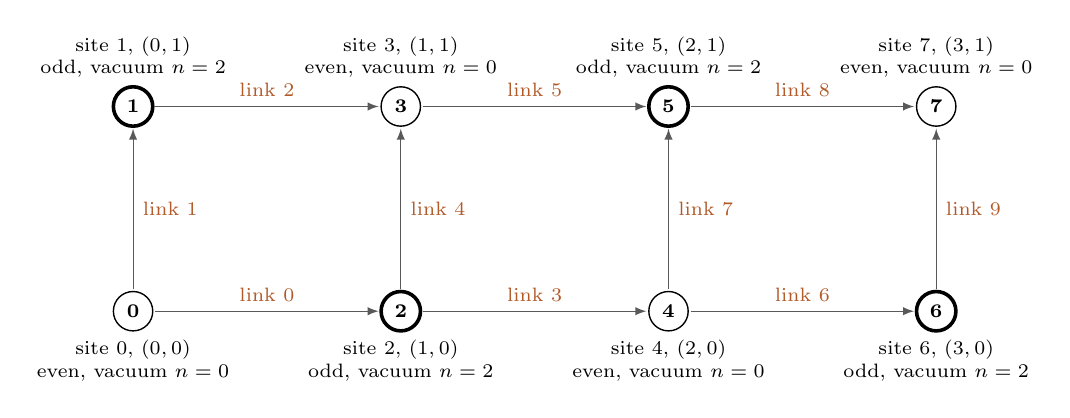
\begin{tikzpicture}[x=3.4cm,y=2.6cm]
\draw[-latex,gray!70!black,shorten >=8pt,shorten <=8pt] (0,0) -- (1,0) node[midway,above,font=\scriptsize,text=partc] {link 0};
\draw[-latex,gray!70!black,shorten >=8pt,shorten <=8pt] (0,0) -- (0,1) node[midway,right,font=\scriptsize,text=partc] {link 1};
\draw[-latex,gray!70!black,shorten >=8pt,shorten <=8pt] (0,1) -- (1,1) node[midway,above,font=\scriptsize,text=partc] {link 2};
\draw[-latex,gray!70!black,shorten >=8pt,shorten <=8pt] (1,0) -- (2,0) node[midway,above,font=\scriptsize,text=partc] {link 3};
\draw[-latex,gray!70!black,shorten >=8pt,shorten <=8pt] (1,0) -- (1,1) node[midway,right,font=\scriptsize,text=partc] {link 4};
\draw[-latex,gray!70!black,shorten >=8pt,shorten <=8pt] (1,1) -- (2,1) node[midway,above,font=\scriptsize,text=partc] {link 5};
\draw[-latex,gray!70!black,shorten >=8pt,shorten <=8pt] (2,0) -- (3,0) node[midway,above,font=\scriptsize,text=partc] {link 6};
\draw[-latex,gray!70!black,shorten >=8pt,shorten <=8pt] (2,0) -- (2,1) node[midway,right,font=\scriptsize,text=partc] {link 7};
\draw[-latex,gray!70!black,shorten >=8pt,shorten <=8pt] (2,1) -- (3,1) node[midway,above,font=\scriptsize,text=partc] {link 8};
\draw[-latex,gray!70!black,shorten >=8pt,shorten <=8pt] (3,0) -- (3,1) node[midway,right,font=\scriptsize,text=partc] {link 9};
\node[site,evensite,fill=white,minimum size=0.5cm] at (0,0) {\textbf{0}};
\node[below=7pt,font=\scriptsize,align=center] at (0,0) {site 0, $(0,0)$\\even, vacuum $n=0$};
\node[site,oddsite,fill=white,minimum size=0.5cm] at (0,1) {\textbf{1}};
\node[above=7pt,font=\scriptsize,align=center] at (0,1) {site 1, $(0,1)$\\odd, vacuum $n=2$};
\node[site,oddsite,fill=white,minimum size=0.5cm] at (1,0) {\textbf{2}};
\node[below=7pt,font=\scriptsize,align=center] at (1,0) {site 2, $(1,0)$\\odd, vacuum $n=2$};
\node[site,evensite,fill=white,minimum size=0.5cm] at (1,1) {\textbf{3}};
\node[above=7pt,font=\scriptsize,align=center] at (1,1) {site 3, $(1,1)$\\even, vacuum $n=0$};
\node[site,evensite,fill=white,minimum size=0.5cm] at (2,0) {\textbf{4}};
\node[below=7pt,font=\scriptsize,align=center] at (2,0) {site 4, $(2,0)$\\even, vacuum $n=0$};
\node[site,oddsite,fill=white,minimum size=0.5cm] at (2,1) {\textbf{5}};
\node[above=7pt,font=\scriptsize,align=center] at (2,1) {site 5, $(2,1)$\\odd, vacuum $n=2$};
\node[site,oddsite,fill=white,minimum size=0.5cm] at (3,0) {\textbf{6}};
\node[below=7pt,font=\scriptsize,align=center] at (3,0) {site 6, $(3,0)$\\odd, vacuum $n=2$};
\node[site,evensite,fill=white,minimum size=0.5cm] at (3,1) {\textbf{7}};
\node[above=7pt,font=\scriptsize,align=center] at (3,1) {site 7, $(3,1)$\\even, vacuum $n=0$};
\end{tikzpicture}\\[2pt]{\small The $2\times4$ ladder; $2\times2$ and $2\times3$ are its first two or three columns.}\end{center}

\paragraph{Sites and quarks (staggered fermions).}  Each site holds a quark field with two colours, so its occupation is
$n=0,1,2$: the number in the circle (white $=0$, half-filled $=1$, dark $=2$).  In the staggered (Dirac-sea) vacuum
$n=0$ on \emph{even} sites ($x_1+x_2$ even, thin circle) and $n=2$ on \emph{odd} sites (thick circle).  Particles are
deviations from that vacuum, written next to the site in brown:
\begin{center}\begin{tabular}{lccc}\toprule & $n=0$ & $n=1$ & $n=2$\\\midrule
even site & vacuum & $q$ (one quark) & $2q$ (two quarks)\\
odd site & $2\bar q$ (two holes) & $\bar q$ (one hole = antiquark) & vacuum\\\bottomrule\end{tabular}\end{center}
The mass term $m\sum_x(-1)^{x_1+x_2}n_x$ makes every quark or antiquark cost energy $m$ relative to the vacuum.

\paragraph{Links (colour-electric flux).}  Each link carries $j=0$ (grey dashed, ``$0$'': no flux) or $j=\tfrac12$ (red,
``$\tfrac12$'': one unit of flux), with electric energy $\frac{g^2}{2}j(j+1)=\frac38 g^2$ per flux link.

\paragraph{Gauss's law and the intertwiner $\iota$.}  At every site the colour spins arriving there (each flux link
brings $\tfrac12$; $n=1$ brings $\tfrac12$; $n=0,2$ bring $0$) must add up to total spin $0$, so their number must be
even.  At an interior site with flux on all three links and $n=1$ there are two ways to do this, labelled $\iota=0,1$
(purple, shown only there).

\paragraph{Baryon number $B$.}  $B=\tfrac12\sum_x\big(n_x-n^{\rm vac}_x\big)$.  In SU(2) a baryon is two quarks, so $B=1$
means two extra quarks, while quark--antiquark pairs (mesons) have $B=0$.  The Hamiltonian conserves $B$, so each $B$
is a separate sector; the SKQD work of this project uses $B=0$ ($2B=0$) and $B=1$ ($2B=2$).

\paragraph{The text under each picture.}
\begin{itemize}[leftmargin=*,itemsep=0pt]
\item \#$k$: position in the package's basis list (\texttt{skqd.basis}); ``\#$i$ in sector'': position inside its sector.
\item $E_{\rm diag}$: diagonal energy of that configuration alone (mass $+$ electric terms) -- not an eigenvalue.
\item bits: the qubit encoding (\texttt{skqd.codec}), one group per site $0,1,2,\dots$; in each group the flux bits of the
site's links in link-number order, then the matter bit ($n/2$, or $\iota$ at a three-flux $n=1$ site).
\item $n=(\dots)$ per site, $j=(\dots)$ per link in link-number order.
\item In the eigenstate sections: $c$ = amplitude of the configuration in the eigenstate (global phase fixed so the
largest amplitude is real and positive) and $|c|^2$ its weight.
\end{itemize}
\clearpage\section{Unphysical configurations: examples}\label{sec:invalid}
A configuration is physical only if Gauss's law holds at \emph{every} site.  Each example below was checked against the package: it is not in the basis, and \texttt{skqd.vertex.kernel\_dim} $=0$ (no singlet) at the sites marked \textcolor{red}{\ding{55}}.\par\medskip
\noindent
\begin{minipage}[t]{0.48\textwidth}\centering\textbf{(a) Open flux string}\\[2pt]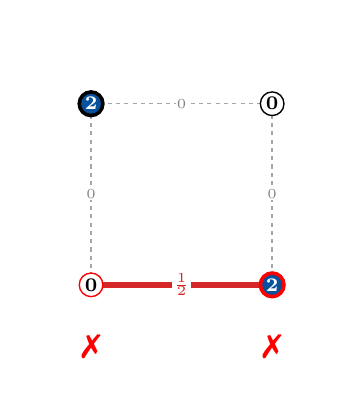
\begin{tikzpicture}[x=2.3cm,y=2.3cm,baseline=(current bounding box.center)]
\draw[fluxon] (0,0) -- (1,0) node[midway,jlab,text=fluxred] {$\tfrac12$};
\draw[fluxoff] (0,0) -- (0,1) node[midway,jlab,text=gray] {$0$};
\draw[fluxoff] (0,1) -- (1,1) node[midway,jlab,text=gray] {$0$};
\draw[fluxoff] (1,0) -- (1,1) node[midway,jlab,text=gray] {$0$};
\node[site,evensite,draw=red,fill=white] at (0,0) {\textbf{0}};
\node[text=red,font=\large] at (0,0+-1*0.34) {\ding{55}};
\node[site,oddsite,fill=occ2] at (0,1) {\textcolor{white}{\textbf{2}}};
\node[site,oddsite,draw=red,fill=occ2] at (1,0) {\textcolor{white}{\textbf{2}}};
\node[text=red,font=\large] at (1,0+-1*0.34) {\ding{55}};
\node[site,evensite,fill=white] at (1,1) {\textbf{0}};
\useasboundingbox (-0.35,-0.42) rectangle (1.35,1.42);
\end{tikzpicture}\\[2pt]\raggedright\small One flux link with nothing at its ends: each end site has a single spin-$\tfrac12$ and no partner. Flux must close into a loop or end on charges.\end{minipage}\hfill
\begin{minipage}[t]{0.48\textwidth}\centering\textbf{(b) Lone quark}\\[2pt]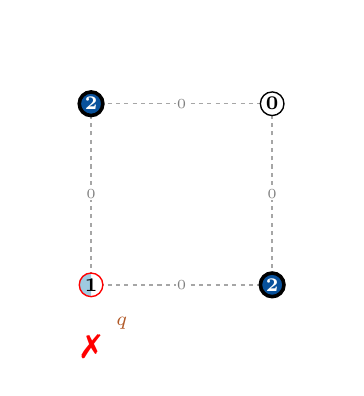
\begin{tikzpicture}[x=2.3cm,y=2.3cm,baseline=(current bounding box.center)]
\draw[fluxoff] (0,0) -- (1,0) node[midway,jlab,text=gray] {$0$};
\draw[fluxoff] (0,0) -- (0,1) node[midway,jlab,text=gray] {$0$};
\draw[fluxoff] (0,1) -- (1,1) node[midway,jlab,text=gray] {$0$};
\draw[fluxoff] (1,0) -- (1,1) node[midway,jlab,text=gray] {$0$};
\fill[white] (0,0) circle[radius=0.15cm];
\fill[occ1] (0,0) ++(90:0.15cm) arc[start angle=90,end angle=270,radius=0.15cm] -- cycle;
\node[site,evensite,draw=red,fill=none] at (0,0) {\textbf{1}};
\node[part] at (0+0.17,0+-1*0.21) {$q$};
\node[text=red,font=\large] at (0,0+-1*0.34) {\ding{55}};
\node[site,oddsite,fill=occ2] at (0,1) {\textcolor{white}{\textbf{2}}};
\node[site,oddsite,fill=occ2] at (1,0) {\textcolor{white}{\textbf{2}}};
\node[site,evensite,fill=white] at (1,1) {\textbf{0}};
\useasboundingbox (-0.35,-0.42) rectangle (1.35,1.42);
\end{tikzpicture}\\[2pt]\raggedright\small One quark ($n=1$) on site 0 with no flux: an isolated colour charge whose spin-$\tfrac12$ has nothing to pair with.\end{minipage}\par\bigskip\noindent
\begin{minipage}[t]{0.48\textwidth}\centering\textbf{(c) Flux loop with a stray quark}\\[2pt]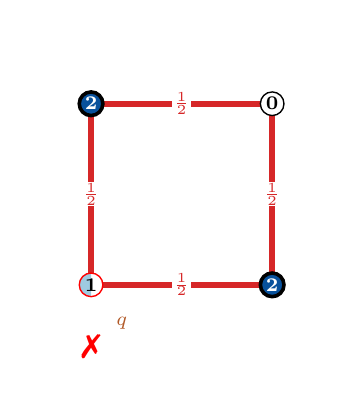
\begin{tikzpicture}[x=2.3cm,y=2.3cm,baseline=(current bounding box.center)]
\draw[fluxon] (0,0) -- (1,0) node[midway,jlab,text=fluxred] {$\tfrac12$};
\draw[fluxon] (0,0) -- (0,1) node[midway,jlab,text=fluxred] {$\tfrac12$};
\draw[fluxon] (0,1) -- (1,1) node[midway,jlab,text=fluxred] {$\tfrac12$};
\draw[fluxon] (1,0) -- (1,1) node[midway,jlab,text=fluxred] {$\tfrac12$};
\fill[white] (0,0) circle[radius=0.15cm];
\fill[occ1] (0,0) ++(90:0.15cm) arc[start angle=90,end angle=270,radius=0.15cm] -- cycle;
\node[site,evensite,draw=red,fill=none] at (0,0) {\textbf{1}};
\node[part] at (0+0.17,0+-1*0.21) {$q$};
\node[text=red,font=\large] at (0,0+-1*0.34) {\ding{55}};
\node[site,oddsite,fill=occ2] at (0,1) {\textcolor{white}{\textbf{2}}};
\node[site,oddsite,fill=occ2] at (1,0) {\textcolor{white}{\textbf{2}}};
\node[site,evensite,fill=white] at (1,1) {\textbf{0}};
\useasboundingbox (-0.35,-0.42) rectangle (1.35,1.42);
\end{tikzpicture}\\[2pt]\raggedright\small The closed loop alone is fine, but site 0 also has a quark: two flux links $+$ one quark $=$ three spin-$\tfrac12$ objects, so no spin 0.\end{minipage}\hfill
\begin{minipage}[t]{0.48\textwidth}\centering\textbf{(d) String with only one end on a quark}\\[2pt]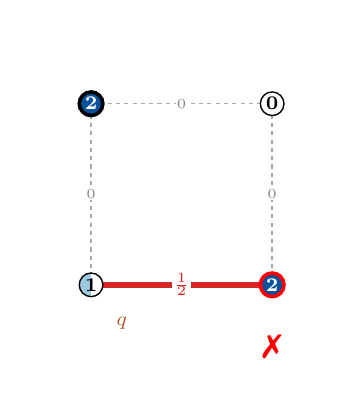
\begin{tikzpicture}[x=2.3cm,y=2.3cm,baseline=(current bounding box.center)]
\draw[fluxon] (0,0) -- (1,0) node[midway,jlab,text=fluxred] {$\tfrac12$};
\draw[fluxoff] (0,0) -- (0,1) node[midway,jlab,text=gray] {$0$};
\draw[fluxoff] (0,1) -- (1,1) node[midway,jlab,text=gray] {$0$};
\draw[fluxoff] (1,0) -- (1,1) node[midway,jlab,text=gray] {$0$};
\fill[white] (0,0) circle[radius=0.15cm];
\fill[occ1] (0,0) ++(90:0.15cm) arc[start angle=90,end angle=270,radius=0.15cm] -- cycle;
\node[site,evensite,fill=none] at (0,0) {\textbf{1}};
\node[part] at (0+0.17,0+-1*0.21) {$q$};
\node[site,oddsite,fill=occ2] at (0,1) {\textcolor{white}{\textbf{2}}};
\node[site,oddsite,draw=red,fill=occ2] at (1,0) {\textcolor{white}{\textbf{2}}};
\node[text=red,font=\large] at (1,0+-1*0.34) {\ding{55}};
\node[site,evensite,fill=white] at (1,1) {\textbf{0}};
\useasboundingbox (-0.35,-0.42) rectangle (1.35,1.42);
\end{tikzpicture}\\[2pt]\raggedright\small Site 0 is fine (flux $+$ quark pair up), but site 2 at the other end has nothing to pair with. A valid meson would also have $n=1$ at site 2.\end{minipage}\par\bigskip\noindent
\subsection*{Bit strings that are not states}
The qubit encoding can also produce strings that describe no state; the decoder (\texttt{skqd.codec.Codec.decode}) rejects them:
\begin{center}\begin{tabular}{l l l}\toprule & bits (sites 0,1,2,3) & decoder\\\midrule
physical state \#3 & \texttt{000 000 001 001} & \texttt{accepted}\\
one copy of link 0 changed & \texttt{100 000 001 001} & \texttt{link}\\
corner with one flux, matter bit 1 & \texttt{011 100 000 000} & \texttt{flag}\\
\bottomrule\end{tabular}\end{center}
\begin{itemize}[leftmargin=*,itemsep=0pt]
\item \texttt{link}: every link is stored at both of its end sites; a physical state has equal copies.
\item \texttt{flag}: a matter-bit value the site's flux pattern does not allow ($n$ is already forced).
\item \texttt{sector}: a perfectly physical state, rejected only because its $B$ is not the one being studied -- it belongs to another sector of this catalogue.
\end{itemize}
Configurations like (a)--(d) cannot even be written in this encoding: it stores only Gauss-law-respecting site states
(6 per corner site, 13 per interior site), which is why bit-level errors appear as \texttt{link} or \texttt{flag}
rejections instead.\clearpage\section{Energy levels of every sector}\label{sec:spectra}
$E_0$ is the ground state, $E_1,E_2,E_3$ the first three excited states ($g^2=4$, $m=0.75$).  An asterisk marks a degenerate level; inside a degenerate level the individual eigenvectors are not unique.  Last column: largest difference from the stored references \texttt{validation/E3.json}.\par\medskip
\subsection*{$2\times2$}\begin{center}\begin{tabular}{r r r r r r l}\toprule$B$ & dim & $E_0$ & $E_1$ & $E_2$ & $E_3$ & check vs E3.json\\\midrule
$-2$ & 2 & $-0.01040$ & $+6.01040$ &  &  & \\
$-1$ & 20 & $-1.86159$ & $-1.81975$ & $+0.20823$ & $+0.45056$ & \\
$+0$ & 38 & $-3.64077$ & $-0.96224$ & $-0.85057$$^*$ & $-0.85057$$^*$ & $0.0e+00$\\
$+1$ & 20 & $-1.86159$ & $-1.81975$ & $+0.20823$ & $+0.45056$ & $0.0e+00$\\
$+2$ & 2 & $-0.01040$ & $+6.01040$ &  &  & \\
\bottomrule\end{tabular}\end{center}
\subsection*{$2\times3$}\begin{center}\begin{tabular}{r r r r r r l}\toprule$B$ & dim & $E_0$ & $E_1$ & $E_2$ & $E_3$ & check vs E3.json\\\midrule
$-3$ & 4 & $-0.02077$ & $+6.00000$ & $+6.01034$ & $+9.01043$ & \\
$-2$ & 95 & $-2.01182$ & $-1.86224$ & $-1.84389$ & $-0.08366$ & \\
$-1$ & 426 & $-3.82608$ & $-3.80173$ & $-3.66866$ & $-1.65288$ & \\
$+0$ & 677 & $-5.60260$ & $-2.88860$ & $-2.86518$ & $-2.77702$ & $0.0e+00$\\
$+1$ & 426 & $-3.82608$ & $-3.80173$ & $-3.66866$ & $-1.65288$ & $0.0e+00$\\
$+2$ & 95 & $-2.01182$ & $-1.86224$ & $-1.84389$ & $-0.08366$ & $0.0e+00$\\
$+3$ & 4 & $-0.02077$ & $+6.00000$ & $+6.01034$ & $+9.01043$ & \\
\bottomrule\end{tabular}\end{center}
\subsection*{$2\times4$}\begin{center}\begin{tabular}{r r r r r r l}\toprule$B$ & dim & $E_0$ & $E_1$ & $E_2$ & $E_3$ & check vs E3.json\\\midrule
$-4$ & 8 & $-0.03115$ & $+5.98961$ & $+5.99480$ & $+6.00511$ & \\
$-3$ & 350 & $-2.04626$ & $-2.00136$ & $-1.86629$ & $-1.86041$ & \\
$-2$ & 2869 & $-3.98809$ & $-3.85262$ & $-3.85197$ & $-3.81386$ & \\
$-1$ & 8934 & $-5.78016$ & $-5.77413$ & $-5.65409$ & $-5.62806$ & \\
$+0$ & 12843 & $-7.56521$ & $-4.84360$ & $-4.83747$ & $-4.73660$ & $3.6e-14$\\
$+1$ & 8934 & $-5.78016$ & $-5.77413$ & $-5.65409$ & $-5.62806$ & $2.0e-14$\\
$+2$ & 2869 & $-3.98809$ & $-3.85262$ & $-3.85197$ & $-3.81386$ & \\
$+3$ & 350 & $-2.04626$ & $-2.00136$ & $-1.86629$ & $-1.86041$ & \\
$+4$ & 8 & $-0.03115$ & $+5.98961$ & $+5.99480$ & $+6.00511$ & \\
\bottomrule\end{tabular}\end{center}\clearpage\section{Eigenstates of the $2\times2$ ladder}\label{sec:eig2}
\subsection{$2\times2${,} sector $B=-2$ (2 physical states)}
\begin{center}\small\begin{tabular}{l l r r r}\toprule level & & configs drawn & weight covered & participation ratio\\\midrule\colorbox{orange!8}{$E_0=-0.010399$} & ground state & 1 & 99.8\% & 1.0\\
\colorbox{cyan!7}{$E_1=+6.010399$} & excited state 1 & 1 & 99.8\% & 1.0\\\bottomrule\end{tabular}\end{center}
\small Most important configurations of each level (largest weight first, up to 6 or until 95\% of the weight is covered); cards of one level share a colour.  Participation ratio $=1/\sum|c|^4$ $\approx$ number of configurations the state is spread over.\par\smallskip
\noindent\fcolorbox{gray!45}{orange!8}{\begin{minipage}[t][\cardh2][t]{0.235\textwidth}\centering
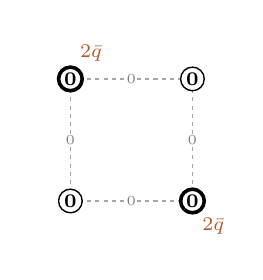
\begin{tikzpicture}[x=1.55cm,y=1.55cm,baseline=(current bounding box.center)]
\draw[fluxoff] (0,0) -- (1,0) node[midway,jlab,text=gray] {$0$};
\draw[fluxoff] (0,0) -- (0,1) node[midway,jlab,text=gray] {$0$};
\draw[fluxoff] (0,1) -- (1,1) node[midway,jlab,text=gray] {$0$};
\draw[fluxoff] (1,0) -- (1,1) node[midway,jlab,text=gray] {$0$};
\node[site,evensite,fill=white] at (0,0) {\textbf{0}};
\node[site,oddsite,fill=white] at (0,1) {\textbf{0}};
\node[part] at (0+0.17,1+1*0.21) {$2\bar q$};
\node[site,oddsite,fill=white] at (1,0) {\textbf{0}};
\node[part] at (1+0.17,0+-1*0.21) {$2\bar q$};
\node[site,evensite,fill=white] at (1,1) {\textbf{0}};
\useasboundingbox (-0.35,-0.42) rectangle (1.35,1.42);
\end{tikzpicture}
\par\vspace{1pt}\raggedright\tiny \textbf{\#0} ($B{=}-2$, \#0 in sector)\ \ $E_{\rm diag}=+0.000$\\ $E_0$ (ground state): $c=+0.9991$, $|c|^2=0.9983$\\ \texttt{000 000 000 000}\\ $n=(0\,0\,0\,0)$\ \ $j=(0\,0\,0\,0)$\end{minipage}}
\hfill
\fcolorbox{gray!45}{cyan!7}{\begin{minipage}[t][\cardh2][t]{0.235\textwidth}\centering
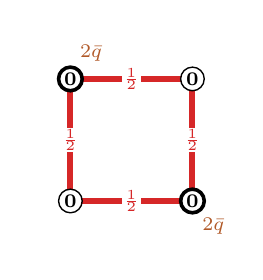
\begin{tikzpicture}[x=1.55cm,y=1.55cm,baseline=(current bounding box.center)]
\draw[fluxon] (0,0) -- (1,0) node[midway,jlab,text=fluxred] {$\tfrac12$};
\draw[fluxon] (0,0) -- (0,1) node[midway,jlab,text=fluxred] {$\tfrac12$};
\draw[fluxon] (0,1) -- (1,1) node[midway,jlab,text=fluxred] {$\tfrac12$};
\draw[fluxon] (1,0) -- (1,1) node[midway,jlab,text=fluxred] {$\tfrac12$};
\node[site,evensite,fill=white] at (0,0) {\textbf{0}};
\node[site,oddsite,fill=white] at (0,1) {\textbf{0}};
\node[part] at (0+0.17,1+1*0.21) {$2\bar q$};
\node[site,oddsite,fill=white] at (1,0) {\textbf{0}};
\node[part] at (1+0.17,0+-1*0.21) {$2\bar q$};
\node[site,evensite,fill=white] at (1,1) {\textbf{0}};
\useasboundingbox (-0.35,-0.42) rectangle (1.35,1.42);
\end{tikzpicture}
\par\vspace{1pt}\raggedright\tiny \textbf{\#66} ($B{=}-2$, \#1 in sector)\ \ $E_{\rm diag}=+6.000$\\ $E_1$ (excited state 1): $c=+0.9991$, $|c|^2=0.9983$\\ \texttt{110 110 110 110}\\ $n=(0\,0\,0\,0)$\ \ $j=(\frac12\,\frac12\,\frac12\,\frac12)$\end{minipage}}
\hfill
\par\vspace{3pt}\noindent
\clearpage
\subsection{$2\times2${,} sector $B=-1$ (20 physical states)}
\begin{center}\small\begin{tabular}{l l r r r}\toprule level & & configs drawn & weight covered & participation ratio\\\midrule\colorbox{orange!8}{$E_0=-1.861588$} & ground state & 5 & 95.6\% & 2.6\\
\colorbox{cyan!7}{$E_1=-1.819745$} & excited state 1 & 4 & 95.3\% & 2.4\\
\colorbox{green!7}{$E_2=+0.208229$} & excited state 2 & 6 & 76.0\% & 8.1\\
\colorbox{magenta!6}{$E_3=+0.450558$} & excited state 3 & 6 & 71.4\% & 8.9\\\bottomrule\end{tabular}\end{center}
\small Most important configurations of each level (largest weight first, up to 6 or until 95\% of the weight is covered); cards of one level share a colour.  Participation ratio $=1/\sum|c|^4$ $\approx$ number of configurations the state is spread over.\par\smallskip
\noindent\fcolorbox{gray!45}{orange!8}{\begin{minipage}[t][\cardh2][t]{0.235\textwidth}\centering
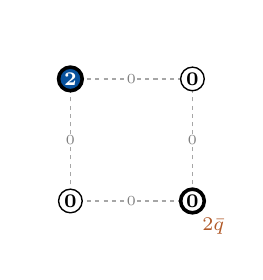
\begin{tikzpicture}[x=1.55cm,y=1.55cm,baseline=(current bounding box.center)]
\draw[fluxoff] (0,0) -- (1,0) node[midway,jlab,text=gray] {$0$};
\draw[fluxoff] (0,0) -- (0,1) node[midway,jlab,text=gray] {$0$};
\draw[fluxoff] (0,1) -- (1,1) node[midway,jlab,text=gray] {$0$};
\draw[fluxoff] (1,0) -- (1,1) node[midway,jlab,text=gray] {$0$};
\node[site,evensite,fill=white] at (0,0) {\textbf{0}};
\node[site,oddsite,fill=occ2] at (0,1) {\textcolor{white}{\textbf{2}}};
\node[site,oddsite,fill=white] at (1,0) {\textbf{0}};
\node[part] at (1+0.17,0+-1*0.21) {$2\bar q$};
\node[site,evensite,fill=white] at (1,1) {\textbf{0}};
\useasboundingbox (-0.35,-0.42) rectangle (1.35,1.42);
\end{tikzpicture}
\par\vspace{1pt}\raggedright\tiny \textbf{\#4} ($B{=}-1$, \#2 in sector)\ \ $E_{\rm diag}=-1.500$\\ $E_0$ (ground state): $c=+0.6614$, $|c|^2=0.4375$\\ \texttt{000 001 000 000}\\ $n=(0\,2\,0\,0)$\ \ $j=(0\,0\,0\,0)$\end{minipage}}
\hfill
\fcolorbox{gray!45}{orange!8}{\begin{minipage}[t][\cardh2][t]{0.235\textwidth}\centering
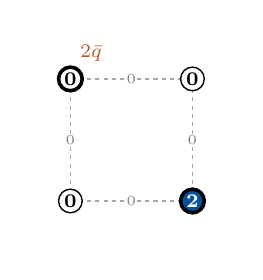
\begin{tikzpicture}[x=1.55cm,y=1.55cm,baseline=(current bounding box.center)]
\draw[fluxoff] (0,0) -- (1,0) node[midway,jlab,text=gray] {$0$};
\draw[fluxoff] (0,0) -- (0,1) node[midway,jlab,text=gray] {$0$};
\draw[fluxoff] (0,1) -- (1,1) node[midway,jlab,text=gray] {$0$};
\draw[fluxoff] (1,0) -- (1,1) node[midway,jlab,text=gray] {$0$};
\node[site,evensite,fill=white] at (0,0) {\textbf{0}};
\node[site,oddsite,fill=white] at (0,1) {\textbf{0}};
\node[part] at (0+0.17,1+1*0.21) {$2\bar q$};
\node[site,oddsite,fill=occ2] at (1,0) {\textcolor{white}{\textbf{2}}};
\node[site,evensite,fill=white] at (1,1) {\textbf{0}};
\useasboundingbox (-0.35,-0.42) rectangle (1.35,1.42);
\end{tikzpicture}
\par\vspace{1pt}\raggedright\tiny \textbf{\#2} ($B{=}-1$, \#1 in sector)\ \ $E_{\rm diag}=-1.500$\\ $E_0$ (ground state): $c=-0.6614$, $|c|^2=0.4375$\\ \texttt{000 000 001 000}\\ $n=(0\,0\,2\,0)$\ \ $j=(0\,0\,0\,0)$\end{minipage}}
\hfill
\fcolorbox{gray!45}{orange!8}{\begin{minipage}[t][\cardh2][t]{0.235\textwidth}\centering
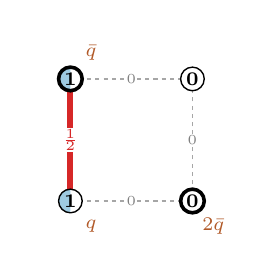
\begin{tikzpicture}[x=1.55cm,y=1.55cm,baseline=(current bounding box.center)]
\draw[fluxoff] (0,0) -- (1,0) node[midway,jlab,text=gray] {$0$};
\draw[fluxon] (0,0) -- (0,1) node[midway,jlab,text=fluxred] {$\tfrac12$};
\draw[fluxoff] (0,1) -- (1,1) node[midway,jlab,text=gray] {$0$};
\draw[fluxoff] (1,0) -- (1,1) node[midway,jlab,text=gray] {$0$};
\fill[white] (0,0) circle[radius=0.15cm];
\fill[occ1] (0,0) ++(90:0.15cm) arc[start angle=90,end angle=270,radius=0.15cm] -- cycle;
\node[site,evensite,fill=none] at (0,0) {\textbf{1}};
\node[part] at (0+0.17,0+-1*0.21) {$q$};
\fill[white] (0,1) circle[radius=0.15cm];
\fill[occ1] (0,1) ++(90:0.15cm) arc[start angle=90,end angle=270,radius=0.15cm] -- cycle;
\node[site,oddsite,fill=none] at (0,1) {\textbf{1}};
\node[part] at (0+0.17,1+1*0.21) {$\bar q$};
\node[site,oddsite,fill=white] at (1,0) {\textbf{0}};
\node[part] at (1+0.17,0+-1*0.21) {$2\bar q$};
\node[site,evensite,fill=white] at (1,1) {\textbf{0}};
\useasboundingbox (-0.35,-0.42) rectangle (1.35,1.42);
\end{tikzpicture}
\par\vspace{1pt}\raggedright\tiny \textbf{\#28} ($B{=}-1$, \#7 in sector)\ \ $E_{\rm diag}=+1.500$\\ $E_0$ (ground state): $c=+0.1645$, $|c|^2=0.0271$\\ \texttt{010 100 000 000}\\ $n=(1\,1\,0\,0)$\ \ $j=(0\,\frac12\,0\,0)$\end{minipage}}
\hfill
\fcolorbox{gray!45}{orange!8}{\begin{minipage}[t][\cardh2][t]{0.235\textwidth}\centering
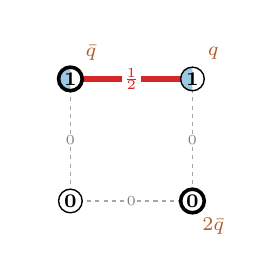
\begin{tikzpicture}[x=1.55cm,y=1.55cm,baseline=(current bounding box.center)]
\draw[fluxoff] (0,0) -- (1,0) node[midway,jlab,text=gray] {$0$};
\draw[fluxoff] (0,0) -- (0,1) node[midway,jlab,text=gray] {$0$};
\draw[fluxon] (0,1) -- (1,1) node[midway,jlab,text=fluxred] {$\tfrac12$};
\draw[fluxoff] (1,0) -- (1,1) node[midway,jlab,text=gray] {$0$};
\node[site,evensite,fill=white] at (0,0) {\textbf{0}};
\fill[white] (0,1) circle[radius=0.15cm];
\fill[occ1] (0,1) ++(90:0.15cm) arc[start angle=90,end angle=270,radius=0.15cm] -- cycle;
\node[site,oddsite,fill=none] at (0,1) {\textbf{1}};
\node[part] at (0+0.17,1+1*0.21) {$\bar q$};
\node[site,oddsite,fill=white] at (1,0) {\textbf{0}};
\node[part] at (1+0.17,0+-1*0.21) {$2\bar q$};
\fill[white] (1,1) circle[radius=0.15cm];
\fill[occ1] (1,1) ++(90:0.15cm) arc[start angle=90,end angle=270,radius=0.15cm] -- cycle;
\node[site,evensite,fill=none] at (1,1) {\textbf{1}};
\node[part] at (1+0.17,1+1*0.21) {$q$};
\useasboundingbox (-0.35,-0.42) rectangle (1.35,1.42);
\end{tikzpicture}
\par\vspace{1pt}\raggedright\tiny \textbf{\#20} ($B{=}-1$, \#5 in sector)\ \ $E_{\rm diag}=+1.500$\\ $E_0$ (ground state): $c=-0.1645i$, $|c|^2=0.0271$\\ \texttt{000 010 000 100}\\ $n=(0\,1\,0\,1)$\ \ $j=(0\,0\,\frac12\,0)$\end{minipage}}
\par\vspace{3pt}\noindent
\fcolorbox{gray!45}{orange!8}{\begin{minipage}[t][\cardh2][t]{0.235\textwidth}\centering
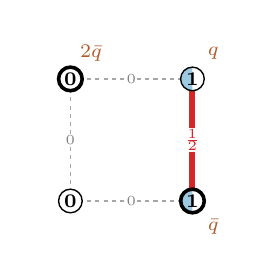
\begin{tikzpicture}[x=1.55cm,y=1.55cm,baseline=(current bounding box.center)]
\draw[fluxoff] (0,0) -- (1,0) node[midway,jlab,text=gray] {$0$};
\draw[fluxoff] (0,0) -- (0,1) node[midway,jlab,text=gray] {$0$};
\draw[fluxoff] (0,1) -- (1,1) node[midway,jlab,text=gray] {$0$};
\draw[fluxon] (1,0) -- (1,1) node[midway,jlab,text=fluxred] {$\tfrac12$};
\node[site,evensite,fill=white] at (0,0) {\textbf{0}};
\node[site,oddsite,fill=white] at (0,1) {\textbf{0}};
\node[part] at (0+0.17,1+1*0.21) {$2\bar q$};
\fill[white] (1,0) circle[radius=0.15cm];
\fill[occ1] (1,0) ++(90:0.15cm) arc[start angle=90,end angle=270,radius=0.15cm] -- cycle;
\node[site,oddsite,fill=none] at (1,0) {\textbf{1}};
\node[part] at (1+0.17,0+-1*0.21) {$\bar q$};
\fill[white] (1,1) circle[radius=0.15cm];
\fill[occ1] (1,1) ++(90:0.15cm) arc[start angle=90,end angle=270,radius=0.15cm] -- cycle;
\node[site,evensite,fill=none] at (1,1) {\textbf{1}};
\node[part] at (1+0.17,1+1*0.21) {$q$};
\useasboundingbox (-0.35,-0.42) rectangle (1.35,1.42);
\end{tikzpicture}
\par\vspace{1pt}\raggedright\tiny \textbf{\#16} ($B{=}-1$, \#4 in sector)\ \ $E_{\rm diag}=+1.500$\\ $E_0$ (ground state): $c=+0.1645$, $|c|^2=0.0271$\\ \texttt{000 000 010 010}\\ $n=(0\,0\,1\,1)$\ \ $j=(0\,0\,0\,\frac12)$\end{minipage}}
\hfill
\fcolorbox{gray!45}{cyan!7}{\begin{minipage}[t][\cardh2][t]{0.235\textwidth}\centering
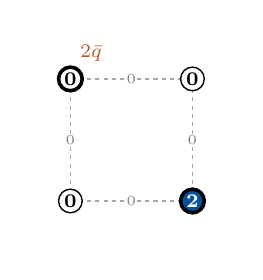
\begin{tikzpicture}[x=1.55cm,y=1.55cm,baseline=(current bounding box.center)]
\draw[fluxoff] (0,0) -- (1,0) node[midway,jlab,text=gray] {$0$};
\draw[fluxoff] (0,0) -- (0,1) node[midway,jlab,text=gray] {$0$};
\draw[fluxoff] (0,1) -- (1,1) node[midway,jlab,text=gray] {$0$};
\draw[fluxoff] (1,0) -- (1,1) node[midway,jlab,text=gray] {$0$};
\node[site,evensite,fill=white] at (0,0) {\textbf{0}};
\node[site,oddsite,fill=white] at (0,1) {\textbf{0}};
\node[part] at (0+0.17,1+1*0.21) {$2\bar q$};
\node[site,oddsite,fill=occ2] at (1,0) {\textcolor{white}{\textbf{2}}};
\node[site,evensite,fill=white] at (1,1) {\textbf{0}};
\useasboundingbox (-0.35,-0.42) rectangle (1.35,1.42);
\end{tikzpicture}
\par\vspace{1pt}\raggedright\tiny \textbf{\#2} ($B{=}-1$, \#1 in sector)\ \ $E_{\rm diag}=-1.500$\\ $E_1$ (excited state 1): $c=+0.6745$, $|c|^2=0.4549$\\ \texttt{000 000 001 000}\\ $n=(0\,0\,2\,0)$\ \ $j=(0\,0\,0\,0)$\end{minipage}}
\hfill
\fcolorbox{gray!45}{cyan!7}{\begin{minipage}[t][\cardh2][t]{0.235\textwidth}\centering
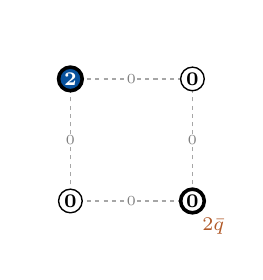
\begin{tikzpicture}[x=1.55cm,y=1.55cm,baseline=(current bounding box.center)]
\draw[fluxoff] (0,0) -- (1,0) node[midway,jlab,text=gray] {$0$};
\draw[fluxoff] (0,0) -- (0,1) node[midway,jlab,text=gray] {$0$};
\draw[fluxoff] (0,1) -- (1,1) node[midway,jlab,text=gray] {$0$};
\draw[fluxoff] (1,0) -- (1,1) node[midway,jlab,text=gray] {$0$};
\node[site,evensite,fill=white] at (0,0) {\textbf{0}};
\node[site,oddsite,fill=occ2] at (0,1) {\textcolor{white}{\textbf{2}}};
\node[site,oddsite,fill=white] at (1,0) {\textbf{0}};
\node[part] at (1+0.17,0+-1*0.21) {$2\bar q$};
\node[site,evensite,fill=white] at (1,1) {\textbf{0}};
\useasboundingbox (-0.35,-0.42) rectangle (1.35,1.42);
\end{tikzpicture}
\par\vspace{1pt}\raggedright\tiny \textbf{\#4} ($B{=}-1$, \#2 in sector)\ \ $E_{\rm diag}=-1.500$\\ $E_1$ (excited state 1): $c=+0.6745$, $|c|^2=0.4549$\\ \texttt{000 001 000 000}\\ $n=(0\,2\,0\,0)$\ \ $j=(0\,0\,0\,0)$\end{minipage}}
\hfill
\fcolorbox{gray!45}{cyan!7}{\begin{minipage}[t][\cardh2][t]{0.235\textwidth}\centering
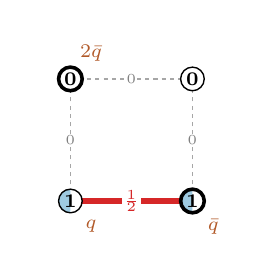
\begin{tikzpicture}[x=1.55cm,y=1.55cm,baseline=(current bounding box.center)]
\draw[fluxon] (0,0) -- (1,0) node[midway,jlab,text=fluxred] {$\tfrac12$};
\draw[fluxoff] (0,0) -- (0,1) node[midway,jlab,text=gray] {$0$};
\draw[fluxoff] (0,1) -- (1,1) node[midway,jlab,text=gray] {$0$};
\draw[fluxoff] (1,0) -- (1,1) node[midway,jlab,text=gray] {$0$};
\fill[white] (0,0) circle[radius=0.15cm];
\fill[occ1] (0,0) ++(90:0.15cm) arc[start angle=90,end angle=270,radius=0.15cm] -- cycle;
\node[site,evensite,fill=none] at (0,0) {\textbf{1}};
\node[part] at (0+0.17,0+-1*0.21) {$q$};
\node[site,oddsite,fill=white] at (0,1) {\textbf{0}};
\node[part] at (0+0.17,1+1*0.21) {$2\bar q$};
\fill[white] (1,0) circle[radius=0.15cm];
\fill[occ1] (1,0) ++(90:0.15cm) arc[start angle=90,end angle=270,radius=0.15cm] -- cycle;
\node[site,oddsite,fill=none] at (1,0) {\textbf{1}};
\node[part] at (1+0.17,0+-1*0.21) {$\bar q$};
\node[site,evensite,fill=white] at (1,1) {\textbf{0}};
\useasboundingbox (-0.35,-0.42) rectangle (1.35,1.42);
\end{tikzpicture}
\par\vspace{1pt}\raggedright\tiny \textbf{\#41} ($B{=}-1$, \#10 in sector)\ \ $E_{\rm diag}=+1.500$\\ $E_1$ (excited state 1): $c=+0.1477i$, $|c|^2=0.0218$\\ \texttt{100 000 100 000}\\ $n=(1\,0\,1\,0)$\ \ $j=(\frac12\,0\,0\,0)$\end{minipage}}
\par\vspace{3pt}\noindent
\fcolorbox{gray!45}{cyan!7}{\begin{minipage}[t][\cardh2][t]{0.235\textwidth}\centering
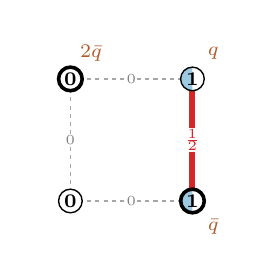
\begin{tikzpicture}[x=1.55cm,y=1.55cm,baseline=(current bounding box.center)]
\draw[fluxoff] (0,0) -- (1,0) node[midway,jlab,text=gray] {$0$};
\draw[fluxoff] (0,0) -- (0,1) node[midway,jlab,text=gray] {$0$};
\draw[fluxoff] (0,1) -- (1,1) node[midway,jlab,text=gray] {$0$};
\draw[fluxon] (1,0) -- (1,1) node[midway,jlab,text=fluxred] {$\tfrac12$};
\node[site,evensite,fill=white] at (0,0) {\textbf{0}};
\node[site,oddsite,fill=white] at (0,1) {\textbf{0}};
\node[part] at (0+0.17,1+1*0.21) {$2\bar q$};
\fill[white] (1,0) circle[radius=0.15cm];
\fill[occ1] (1,0) ++(90:0.15cm) arc[start angle=90,end angle=270,radius=0.15cm] -- cycle;
\node[site,oddsite,fill=none] at (1,0) {\textbf{1}};
\node[part] at (1+0.17,0+-1*0.21) {$\bar q$};
\fill[white] (1,1) circle[radius=0.15cm];
\fill[occ1] (1,1) ++(90:0.15cm) arc[start angle=90,end angle=270,radius=0.15cm] -- cycle;
\node[site,evensite,fill=none] at (1,1) {\textbf{1}};
\node[part] at (1+0.17,1+1*0.21) {$q$};
\useasboundingbox (-0.35,-0.42) rectangle (1.35,1.42);
\end{tikzpicture}
\par\vspace{1pt}\raggedright\tiny \textbf{\#16} ($B{=}-1$, \#4 in sector)\ \ $E_{\rm diag}=+1.500$\\ $E_1$ (excited state 1): $c=-0.1477$, $|c|^2=0.0218$\\ \texttt{000 000 010 010}\\ $n=(0\,0\,1\,1)$\ \ $j=(0\,0\,0\,\frac12)$\end{minipage}}
\hfill
\fcolorbox{gray!45}{green!7}{\begin{minipage}[t][\cardh2][t]{0.235\textwidth}\centering
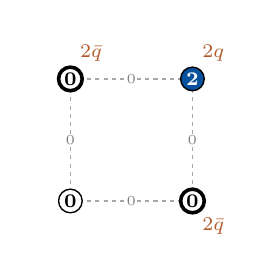
\begin{tikzpicture}[x=1.55cm,y=1.55cm,baseline=(current bounding box.center)]
\draw[fluxoff] (0,0) -- (1,0) node[midway,jlab,text=gray] {$0$};
\draw[fluxoff] (0,0) -- (0,1) node[midway,jlab,text=gray] {$0$};
\draw[fluxoff] (0,1) -- (1,1) node[midway,jlab,text=gray] {$0$};
\draw[fluxoff] (1,0) -- (1,1) node[midway,jlab,text=gray] {$0$};
\node[site,evensite,fill=white] at (0,0) {\textbf{0}};
\node[site,oddsite,fill=white] at (0,1) {\textbf{0}};
\node[part] at (0+0.17,1+1*0.21) {$2\bar q$};
\node[site,oddsite,fill=white] at (1,0) {\textbf{0}};
\node[part] at (1+0.17,0+-1*0.21) {$2\bar q$};
\node[site,evensite,fill=occ2] at (1,1) {\textcolor{white}{\textbf{2}}};
\node[part] at (1+0.17,1+1*0.21) {$2q$};
\useasboundingbox (-0.35,-0.42) rectangle (1.35,1.42);
\end{tikzpicture}
\par\vspace{1pt}\raggedright\tiny \textbf{\#1} ($B{=}-1$, \#0 in sector)\ \ $E_{\rm diag}=+1.500$\\ $E_2$ (excited state 2): $c=+0.3796$, $|c|^2=0.1441$\\ \texttt{000 000 000 001}\\ $n=(0\,0\,0\,2)$\ \ $j=(0\,0\,0\,0)$\end{minipage}}
\hfill
\fcolorbox{gray!45}{green!7}{\begin{minipage}[t][\cardh2][t]{0.235\textwidth}\centering
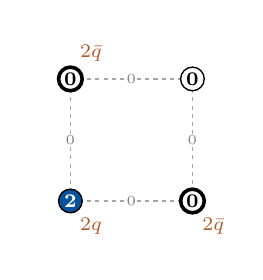
\begin{tikzpicture}[x=1.55cm,y=1.55cm,baseline=(current bounding box.center)]
\draw[fluxoff] (0,0) -- (1,0) node[midway,jlab,text=gray] {$0$};
\draw[fluxoff] (0,0) -- (0,1) node[midway,jlab,text=gray] {$0$};
\draw[fluxoff] (0,1) -- (1,1) node[midway,jlab,text=gray] {$0$};
\draw[fluxoff] (1,0) -- (1,1) node[midway,jlab,text=gray] {$0$};
\node[site,evensite,fill=occ2] at (0,0) {\textcolor{white}{\textbf{2}}};
\node[part] at (0+0.17,0+-1*0.21) {$2q$};
\node[site,oddsite,fill=white] at (0,1) {\textbf{0}};
\node[part] at (0+0.17,1+1*0.21) {$2\bar q$};
\node[site,oddsite,fill=white] at (1,0) {\textbf{0}};
\node[part] at (1+0.17,0+-1*0.21) {$2\bar q$};
\node[site,evensite,fill=white] at (1,1) {\textbf{0}};
\useasboundingbox (-0.35,-0.42) rectangle (1.35,1.42);
\end{tikzpicture}
\par\vspace{1pt}\raggedright\tiny \textbf{\#8} ($B{=}-1$, \#3 in sector)\ \ $E_{\rm diag}=+1.500$\\ $E_2$ (excited state 2): $c=+0.3796$, $|c|^2=0.1441$\\ \texttt{001 000 000 000}\\ $n=(2\,0\,0\,0)$\ \ $j=(0\,0\,0\,0)$\end{minipage}}
\hfill
\fcolorbox{gray!45}{green!7}{\begin{minipage}[t][\cardh2][t]{0.235\textwidth}\centering
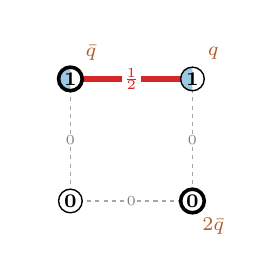
\begin{tikzpicture}[x=1.55cm,y=1.55cm,baseline=(current bounding box.center)]
\draw[fluxoff] (0,0) -- (1,0) node[midway,jlab,text=gray] {$0$};
\draw[fluxoff] (0,0) -- (0,1) node[midway,jlab,text=gray] {$0$};
\draw[fluxon] (0,1) -- (1,1) node[midway,jlab,text=fluxred] {$\tfrac12$};
\draw[fluxoff] (1,0) -- (1,1) node[midway,jlab,text=gray] {$0$};
\node[site,evensite,fill=white] at (0,0) {\textbf{0}};
\fill[white] (0,1) circle[radius=0.15cm];
\fill[occ1] (0,1) ++(90:0.15cm) arc[start angle=90,end angle=270,radius=0.15cm] -- cycle;
\node[site,oddsite,fill=none] at (0,1) {\textbf{1}};
\node[part] at (0+0.17,1+1*0.21) {$\bar q$};
\node[site,oddsite,fill=white] at (1,0) {\textbf{0}};
\node[part] at (1+0.17,0+-1*0.21) {$2\bar q$};
\fill[white] (1,1) circle[radius=0.15cm];
\fill[occ1] (1,1) ++(90:0.15cm) arc[start angle=90,end angle=270,radius=0.15cm] -- cycle;
\node[site,evensite,fill=none] at (1,1) {\textbf{1}};
\node[part] at (1+0.17,1+1*0.21) {$q$};
\useasboundingbox (-0.35,-0.42) rectangle (1.35,1.42);
\end{tikzpicture}
\par\vspace{1pt}\raggedright\tiny \textbf{\#20} ($B{=}-1$, \#5 in sector)\ \ $E_{\rm diag}=+1.500$\\ $E_2$ (excited state 2): $c=+0.3436i$, $|c|^2=0.1180$\\ \texttt{000 010 000 100}\\ $n=(0\,1\,0\,1)$\ \ $j=(0\,0\,\frac12\,0)$\end{minipage}}
\par\vspace{3pt}\noindent
\fcolorbox{gray!45}{green!7}{\begin{minipage}[t][\cardh2][t]{0.235\textwidth}\centering
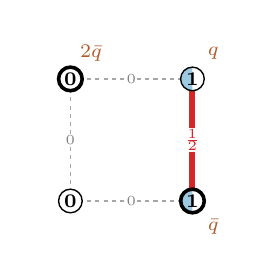
\begin{tikzpicture}[x=1.55cm,y=1.55cm,baseline=(current bounding box.center)]
\draw[fluxoff] (0,0) -- (1,0) node[midway,jlab,text=gray] {$0$};
\draw[fluxoff] (0,0) -- (0,1) node[midway,jlab,text=gray] {$0$};
\draw[fluxoff] (0,1) -- (1,1) node[midway,jlab,text=gray] {$0$};
\draw[fluxon] (1,0) -- (1,1) node[midway,jlab,text=fluxred] {$\tfrac12$};
\node[site,evensite,fill=white] at (0,0) {\textbf{0}};
\node[site,oddsite,fill=white] at (0,1) {\textbf{0}};
\node[part] at (0+0.17,1+1*0.21) {$2\bar q$};
\fill[white] (1,0) circle[radius=0.15cm];
\fill[occ1] (1,0) ++(90:0.15cm) arc[start angle=90,end angle=270,radius=0.15cm] -- cycle;
\node[site,oddsite,fill=none] at (1,0) {\textbf{1}};
\node[part] at (1+0.17,0+-1*0.21) {$\bar q$};
\fill[white] (1,1) circle[radius=0.15cm];
\fill[occ1] (1,1) ++(90:0.15cm) arc[start angle=90,end angle=270,radius=0.15cm] -- cycle;
\node[site,evensite,fill=none] at (1,1) {\textbf{1}};
\node[part] at (1+0.17,1+1*0.21) {$q$};
\useasboundingbox (-0.35,-0.42) rectangle (1.35,1.42);
\end{tikzpicture}
\par\vspace{1pt}\raggedright\tiny \textbf{\#16} ($B{=}-1$, \#4 in sector)\ \ $E_{\rm diag}=+1.500$\\ $E_2$ (excited state 2): $c=-0.3436$, $|c|^2=0.1180$\\ \texttt{000 000 010 010}\\ $n=(0\,0\,1\,1)$\ \ $j=(0\,0\,0\,\frac12)$\end{minipage}}
\hfill
\fcolorbox{gray!45}{green!7}{\begin{minipage}[t][\cardh2][t]{0.235\textwidth}\centering
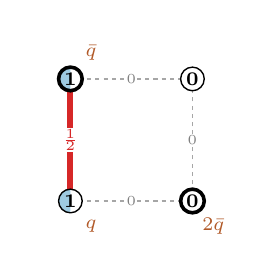
\begin{tikzpicture}[x=1.55cm,y=1.55cm,baseline=(current bounding box.center)]
\draw[fluxoff] (0,0) -- (1,0) node[midway,jlab,text=gray] {$0$};
\draw[fluxon] (0,0) -- (0,1) node[midway,jlab,text=fluxred] {$\tfrac12$};
\draw[fluxoff] (0,1) -- (1,1) node[midway,jlab,text=gray] {$0$};
\draw[fluxoff] (1,0) -- (1,1) node[midway,jlab,text=gray] {$0$};
\fill[white] (0,0) circle[radius=0.15cm];
\fill[occ1] (0,0) ++(90:0.15cm) arc[start angle=90,end angle=270,radius=0.15cm] -- cycle;
\node[site,evensite,fill=none] at (0,0) {\textbf{1}};
\node[part] at (0+0.17,0+-1*0.21) {$q$};
\fill[white] (0,1) circle[radius=0.15cm];
\fill[occ1] (0,1) ++(90:0.15cm) arc[start angle=90,end angle=270,radius=0.15cm] -- cycle;
\node[site,oddsite,fill=none] at (0,1) {\textbf{1}};
\node[part] at (0+0.17,1+1*0.21) {$\bar q$};
\node[site,oddsite,fill=white] at (1,0) {\textbf{0}};
\node[part] at (1+0.17,0+-1*0.21) {$2\bar q$};
\node[site,evensite,fill=white] at (1,1) {\textbf{0}};
\useasboundingbox (-0.35,-0.42) rectangle (1.35,1.42);
\end{tikzpicture}
\par\vspace{1pt}\raggedright\tiny \textbf{\#28} ($B{=}-1$, \#7 in sector)\ \ $E_{\rm diag}=+1.500$\\ $E_2$ (excited state 2): $c=+0.3436$, $|c|^2=0.1180$\\ \texttt{010 100 000 000}\\ $n=(1\,1\,0\,0)$\ \ $j=(0\,\frac12\,0\,0)$\end{minipage}}
\hfill
\fcolorbox{gray!45}{green!7}{\begin{minipage}[t][\cardh2][t]{0.235\textwidth}\centering
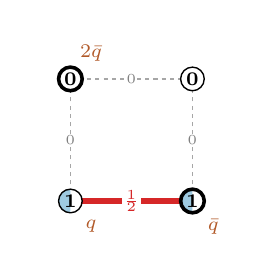
\begin{tikzpicture}[x=1.55cm,y=1.55cm,baseline=(current bounding box.center)]
\draw[fluxon] (0,0) -- (1,0) node[midway,jlab,text=fluxred] {$\tfrac12$};
\draw[fluxoff] (0,0) -- (0,1) node[midway,jlab,text=gray] {$0$};
\draw[fluxoff] (0,1) -- (1,1) node[midway,jlab,text=gray] {$0$};
\draw[fluxoff] (1,0) -- (1,1) node[midway,jlab,text=gray] {$0$};
\fill[white] (0,0) circle[radius=0.15cm];
\fill[occ1] (0,0) ++(90:0.15cm) arc[start angle=90,end angle=270,radius=0.15cm] -- cycle;
\node[site,evensite,fill=none] at (0,0) {\textbf{1}};
\node[part] at (0+0.17,0+-1*0.21) {$q$};
\node[site,oddsite,fill=white] at (0,1) {\textbf{0}};
\node[part] at (0+0.17,1+1*0.21) {$2\bar q$};
\fill[white] (1,0) circle[radius=0.15cm];
\fill[occ1] (1,0) ++(90:0.15cm) arc[start angle=90,end angle=270,radius=0.15cm] -- cycle;
\node[site,oddsite,fill=none] at (1,0) {\textbf{1}};
\node[part] at (1+0.17,0+-1*0.21) {$\bar q$};
\node[site,evensite,fill=white] at (1,1) {\textbf{0}};
\useasboundingbox (-0.35,-0.42) rectangle (1.35,1.42);
\end{tikzpicture}
\par\vspace{1pt}\raggedright\tiny \textbf{\#41} ($B{=}-1$, \#10 in sector)\ \ $E_{\rm diag}=+1.500$\\ $E_2$ (excited state 2): $c=-0.3436i$, $|c|^2=0.1180$\\ \texttt{100 000 100 000}\\ $n=(1\,0\,1\,0)$\ \ $j=(\frac12\,0\,0\,0)$\end{minipage}}
\hfill
\fcolorbox{gray!45}{magenta!6}{\begin{minipage}[t][\cardh2][t]{0.235\textwidth}\centering
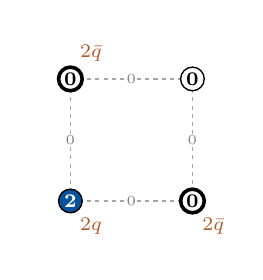
\begin{tikzpicture}[x=1.55cm,y=1.55cm,baseline=(current bounding box.center)]
\draw[fluxoff] (0,0) -- (1,0) node[midway,jlab,text=gray] {$0$};
\draw[fluxoff] (0,0) -- (0,1) node[midway,jlab,text=gray] {$0$};
\draw[fluxoff] (0,1) -- (1,1) node[midway,jlab,text=gray] {$0$};
\draw[fluxoff] (1,0) -- (1,1) node[midway,jlab,text=gray] {$0$};
\node[site,evensite,fill=occ2] at (0,0) {\textcolor{white}{\textbf{2}}};
\node[part] at (0+0.17,0+-1*0.21) {$2q$};
\node[site,oddsite,fill=white] at (0,1) {\textbf{0}};
\node[part] at (0+0.17,1+1*0.21) {$2\bar q$};
\node[site,oddsite,fill=white] at (1,0) {\textbf{0}};
\node[part] at (1+0.17,0+-1*0.21) {$2\bar q$};
\node[site,evensite,fill=white] at (1,1) {\textbf{0}};
\useasboundingbox (-0.35,-0.42) rectangle (1.35,1.42);
\end{tikzpicture}
\par\vspace{1pt}\raggedright\tiny \textbf{\#8} ($B{=}-1$, \#3 in sector)\ \ $E_{\rm diag}=+1.500$\\ $E_3$ (excited state 3): $c=+0.4136$, $|c|^2=0.1711$\\ \texttt{001 000 000 000}\\ $n=(2\,0\,0\,0)$\ \ $j=(0\,0\,0\,0)$\end{minipage}}
\par\vspace{3pt}\noindent
\fcolorbox{gray!45}{magenta!6}{\begin{minipage}[t][\cardh2][t]{0.235\textwidth}\centering
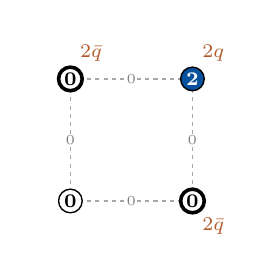
\begin{tikzpicture}[x=1.55cm,y=1.55cm,baseline=(current bounding box.center)]
\draw[fluxoff] (0,0) -- (1,0) node[midway,jlab,text=gray] {$0$};
\draw[fluxoff] (0,0) -- (0,1) node[midway,jlab,text=gray] {$0$};
\draw[fluxoff] (0,1) -- (1,1) node[midway,jlab,text=gray] {$0$};
\draw[fluxoff] (1,0) -- (1,1) node[midway,jlab,text=gray] {$0$};
\node[site,evensite,fill=white] at (0,0) {\textbf{0}};
\node[site,oddsite,fill=white] at (0,1) {\textbf{0}};
\node[part] at (0+0.17,1+1*0.21) {$2\bar q$};
\node[site,oddsite,fill=white] at (1,0) {\textbf{0}};
\node[part] at (1+0.17,0+-1*0.21) {$2\bar q$};
\node[site,evensite,fill=occ2] at (1,1) {\textcolor{white}{\textbf{2}}};
\node[part] at (1+0.17,1+1*0.21) {$2q$};
\useasboundingbox (-0.35,-0.42) rectangle (1.35,1.42);
\end{tikzpicture}
\par\vspace{1pt}\raggedright\tiny \textbf{\#1} ($B{=}-1$, \#0 in sector)\ \ $E_{\rm diag}=+1.500$\\ $E_3$ (excited state 3): $c=-0.4136$, $|c|^2=0.1711$\\ \texttt{000 000 000 001}\\ $n=(0\,0\,0\,2)$\ \ $j=(0\,0\,0\,0)$\end{minipage}}
\hfill
\fcolorbox{gray!45}{magenta!6}{\begin{minipage}[t][\cardh2][t]{0.235\textwidth}\centering
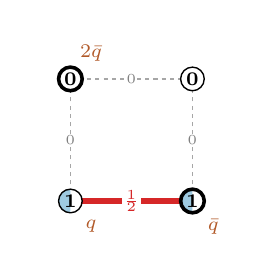
\begin{tikzpicture}[x=1.55cm,y=1.55cm,baseline=(current bounding box.center)]
\draw[fluxon] (0,0) -- (1,0) node[midway,jlab,text=fluxred] {$\tfrac12$};
\draw[fluxoff] (0,0) -- (0,1) node[midway,jlab,text=gray] {$0$};
\draw[fluxoff] (0,1) -- (1,1) node[midway,jlab,text=gray] {$0$};
\draw[fluxoff] (1,0) -- (1,1) node[midway,jlab,text=gray] {$0$};
\fill[white] (0,0) circle[radius=0.15cm];
\fill[occ1] (0,0) ++(90:0.15cm) arc[start angle=90,end angle=270,radius=0.15cm] -- cycle;
\node[site,evensite,fill=none] at (0,0) {\textbf{1}};
\node[part] at (0+0.17,0+-1*0.21) {$q$};
\node[site,oddsite,fill=white] at (0,1) {\textbf{0}};
\node[part] at (0+0.17,1+1*0.21) {$2\bar q$};
\fill[white] (1,0) circle[radius=0.15cm];
\fill[occ1] (1,0) ++(90:0.15cm) arc[start angle=90,end angle=270,radius=0.15cm] -- cycle;
\node[site,oddsite,fill=none] at (1,0) {\textbf{1}};
\node[part] at (1+0.17,0+-1*0.21) {$\bar q$};
\node[site,evensite,fill=white] at (1,1) {\textbf{0}};
\useasboundingbox (-0.35,-0.42) rectangle (1.35,1.42);
\end{tikzpicture}
\par\vspace{1pt}\raggedright\tiny \textbf{\#41} ($B{=}-1$, \#10 in sector)\ \ $E_{\rm diag}=+1.500$\\ $E_3$ (excited state 3): $c=-0.3050i$, $|c|^2=0.0930$\\ \texttt{100 000 100 000}\\ $n=(1\,0\,1\,0)$\ \ $j=(\frac12\,0\,0\,0)$\end{minipage}}
\hfill
\fcolorbox{gray!45}{magenta!6}{\begin{minipage}[t][\cardh2][t]{0.235\textwidth}\centering
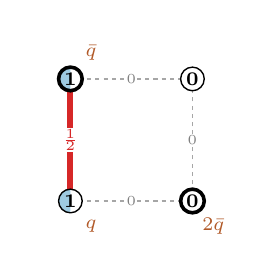
\begin{tikzpicture}[x=1.55cm,y=1.55cm,baseline=(current bounding box.center)]
\draw[fluxoff] (0,0) -- (1,0) node[midway,jlab,text=gray] {$0$};
\draw[fluxon] (0,0) -- (0,1) node[midway,jlab,text=fluxred] {$\tfrac12$};
\draw[fluxoff] (0,1) -- (1,1) node[midway,jlab,text=gray] {$0$};
\draw[fluxoff] (1,0) -- (1,1) node[midway,jlab,text=gray] {$0$};
\fill[white] (0,0) circle[radius=0.15cm];
\fill[occ1] (0,0) ++(90:0.15cm) arc[start angle=90,end angle=270,radius=0.15cm] -- cycle;
\node[site,evensite,fill=none] at (0,0) {\textbf{1}};
\node[part] at (0+0.17,0+-1*0.21) {$q$};
\fill[white] (0,1) circle[radius=0.15cm];
\fill[occ1] (0,1) ++(90:0.15cm) arc[start angle=90,end angle=270,radius=0.15cm] -- cycle;
\node[site,oddsite,fill=none] at (0,1) {\textbf{1}};
\node[part] at (0+0.17,1+1*0.21) {$\bar q$};
\node[site,oddsite,fill=white] at (1,0) {\textbf{0}};
\node[part] at (1+0.17,0+-1*0.21) {$2\bar q$};
\node[site,evensite,fill=white] at (1,1) {\textbf{0}};
\useasboundingbox (-0.35,-0.42) rectangle (1.35,1.42);
\end{tikzpicture}
\par\vspace{1pt}\raggedright\tiny \textbf{\#28} ($B{=}-1$, \#7 in sector)\ \ $E_{\rm diag}=+1.500$\\ $E_3$ (excited state 3): $c=+0.3050$, $|c|^2=0.0930$\\ \texttt{010 100 000 000}\\ $n=(1\,1\,0\,0)$\ \ $j=(0\,\frac12\,0\,0)$\end{minipage}}
\hfill
\fcolorbox{gray!45}{magenta!6}{\begin{minipage}[t][\cardh2][t]{0.235\textwidth}\centering
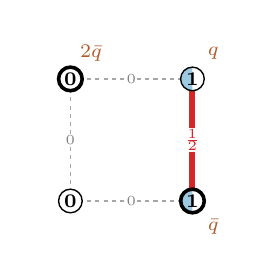
\begin{tikzpicture}[x=1.55cm,y=1.55cm,baseline=(current bounding box.center)]
\draw[fluxoff] (0,0) -- (1,0) node[midway,jlab,text=gray] {$0$};
\draw[fluxoff] (0,0) -- (0,1) node[midway,jlab,text=gray] {$0$};
\draw[fluxoff] (0,1) -- (1,1) node[midway,jlab,text=gray] {$0$};
\draw[fluxon] (1,0) -- (1,1) node[midway,jlab,text=fluxred] {$\tfrac12$};
\node[site,evensite,fill=white] at (0,0) {\textbf{0}};
\node[site,oddsite,fill=white] at (0,1) {\textbf{0}};
\node[part] at (0+0.17,1+1*0.21) {$2\bar q$};
\fill[white] (1,0) circle[radius=0.15cm];
\fill[occ1] (1,0) ++(90:0.15cm) arc[start angle=90,end angle=270,radius=0.15cm] -- cycle;
\node[site,oddsite,fill=none] at (1,0) {\textbf{1}};
\node[part] at (1+0.17,0+-1*0.21) {$\bar q$};
\fill[white] (1,1) circle[radius=0.15cm];
\fill[occ1] (1,1) ++(90:0.15cm) arc[start angle=90,end angle=270,radius=0.15cm] -- cycle;
\node[site,evensite,fill=none] at (1,1) {\textbf{1}};
\node[part] at (1+0.17,1+1*0.21) {$q$};
\useasboundingbox (-0.35,-0.42) rectangle (1.35,1.42);
\end{tikzpicture}
\par\vspace{1pt}\raggedright\tiny \textbf{\#16} ($B{=}-1$, \#4 in sector)\ \ $E_{\rm diag}=+1.500$\\ $E_3$ (excited state 3): $c=+0.3050$, $|c|^2=0.0930$\\ \texttt{000 000 010 010}\\ $n=(0\,0\,1\,1)$\ \ $j=(0\,0\,0\,\frac12)$\end{minipage}}
\par\vspace{3pt}\noindent
\fcolorbox{gray!45}{magenta!6}{\begin{minipage}[t][\cardh2][t]{0.235\textwidth}\centering
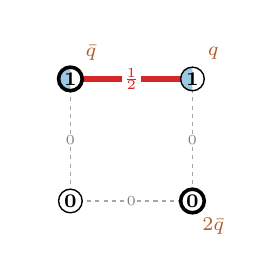
\begin{tikzpicture}[x=1.55cm,y=1.55cm,baseline=(current bounding box.center)]
\draw[fluxoff] (0,0) -- (1,0) node[midway,jlab,text=gray] {$0$};
\draw[fluxoff] (0,0) -- (0,1) node[midway,jlab,text=gray] {$0$};
\draw[fluxon] (0,1) -- (1,1) node[midway,jlab,text=fluxred] {$\tfrac12$};
\draw[fluxoff] (1,0) -- (1,1) node[midway,jlab,text=gray] {$0$};
\node[site,evensite,fill=white] at (0,0) {\textbf{0}};
\fill[white] (0,1) circle[radius=0.15cm];
\fill[occ1] (0,1) ++(90:0.15cm) arc[start angle=90,end angle=270,radius=0.15cm] -- cycle;
\node[site,oddsite,fill=none] at (0,1) {\textbf{1}};
\node[part] at (0+0.17,1+1*0.21) {$\bar q$};
\node[site,oddsite,fill=white] at (1,0) {\textbf{0}};
\node[part] at (1+0.17,0+-1*0.21) {$2\bar q$};
\fill[white] (1,1) circle[radius=0.15cm];
\fill[occ1] (1,1) ++(90:0.15cm) arc[start angle=90,end angle=270,radius=0.15cm] -- cycle;
\node[site,evensite,fill=none] at (1,1) {\textbf{1}};
\node[part] at (1+0.17,1+1*0.21) {$q$};
\useasboundingbox (-0.35,-0.42) rectangle (1.35,1.42);
\end{tikzpicture}
\par\vspace{1pt}\raggedright\tiny \textbf{\#20} ($B{=}-1$, \#5 in sector)\ \ $E_{\rm diag}=+1.500$\\ $E_3$ (excited state 3): $c=-0.3050i$, $|c|^2=0.0930$\\ \texttt{000 010 000 100}\\ $n=(0\,1\,0\,1)$\ \ $j=(0\,0\,\frac12\,0)$\end{minipage}}
\hfill
\par\vspace{3pt}\noindent
\clearpage
\subsection{$2\times2${,} sector $B=+0$ (38 physical states)}
\begin{center}\small\begin{tabular}{l l r r r}\toprule level & & configs drawn & weight covered & participation ratio\\\midrule\colorbox{orange!8}{$E_0=-3.640767$} & ground state & 5 & 98.3\% & 1.5\\
\colorbox{cyan!7}{$E_1=-0.962245$} & excited state 1 & 6 & 71.0\% & 9.2\\
\colorbox{green!7}{$E_2=-0.850567$} & excited state 2, degenerate with $E_{3}$ & 4 & 96.1\% & 4.3\\
\colorbox{magenta!6}{$E_3=-0.850567$} & excited state 3, degenerate with $E_{2}$ & 4 & 96.1\% & 4.3\\\bottomrule\end{tabular}\end{center}
\small Most important configurations of each level (largest weight first, up to 6 or until 95\% of the weight is covered); cards of one level share a colour.  Participation ratio $=1/\sum|c|^4$ $\approx$ number of configurations the state is spread over.\par\smallskip
\noindent\fcolorbox{gray!45}{orange!8}{\begin{minipage}[t][\cardh2][t]{0.235\textwidth}\centering
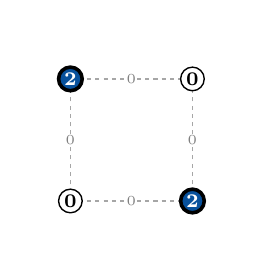
\begin{tikzpicture}[x=1.55cm,y=1.55cm,baseline=(current bounding box.center)]
\draw[fluxoff] (0,0) -- (1,0) node[midway,jlab,text=gray] {$0$};
\draw[fluxoff] (0,0) -- (0,1) node[midway,jlab,text=gray] {$0$};
\draw[fluxoff] (0,1) -- (1,1) node[midway,jlab,text=gray] {$0$};
\draw[fluxoff] (1,0) -- (1,1) node[midway,jlab,text=gray] {$0$};
\node[site,evensite,fill=white] at (0,0) {\textbf{0}};
\node[site,oddsite,fill=occ2] at (0,1) {\textcolor{white}{\textbf{2}}};
\node[site,oddsite,fill=occ2] at (1,0) {\textcolor{white}{\textbf{2}}};
\node[site,evensite,fill=white] at (1,1) {\textbf{0}};
\useasboundingbox (-0.35,-0.42) rectangle (1.35,1.42);
\end{tikzpicture}
\par\vspace{1pt}\raggedright\tiny \textbf{\#6} ($B{=}0$, \#2 in sector)\ \ $E_{\rm diag}=-3.000$\\ $E_0$ (ground state): $c=+0.9053$, $|c|^2=0.8195$\\ \texttt{000 001 001 000}\\ $n=(0\,2\,2\,0)$\ \ $j=(0\,0\,0\,0)$\end{minipage}}
\hfill
\fcolorbox{gray!45}{orange!8}{\begin{minipage}[t][\cardh2][t]{0.235\textwidth}\centering
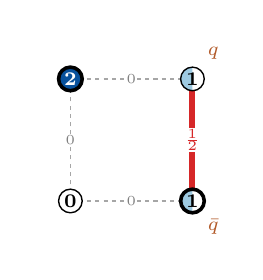
\begin{tikzpicture}[x=1.55cm,y=1.55cm,baseline=(current bounding box.center)]
\draw[fluxoff] (0,0) -- (1,0) node[midway,jlab,text=gray] {$0$};
\draw[fluxoff] (0,0) -- (0,1) node[midway,jlab,text=gray] {$0$};
\draw[fluxoff] (0,1) -- (1,1) node[midway,jlab,text=gray] {$0$};
\draw[fluxon] (1,0) -- (1,1) node[midway,jlab,text=fluxred] {$\tfrac12$};
\node[site,evensite,fill=white] at (0,0) {\textbf{0}};
\node[site,oddsite,fill=occ2] at (0,1) {\textcolor{white}{\textbf{2}}};
\fill[white] (1,0) circle[radius=0.15cm];
\fill[occ1] (1,0) ++(90:0.15cm) arc[start angle=90,end angle=270,radius=0.15cm] -- cycle;
\node[site,oddsite,fill=none] at (1,0) {\textbf{1}};
\node[part] at (1+0.17,0+-1*0.21) {$\bar q$};
\fill[white] (1,1) circle[radius=0.15cm];
\fill[occ1] (1,1) ++(90:0.15cm) arc[start angle=90,end angle=270,radius=0.15cm] -- cycle;
\node[site,evensite,fill=none] at (1,1) {\textbf{1}};
\node[part] at (1+0.17,1+1*0.21) {$q$};
\useasboundingbox (-0.35,-0.42) rectangle (1.35,1.42);
\end{tikzpicture}
\par\vspace{1pt}\raggedright\tiny \textbf{\#17} ($B{=}0$, \#6 in sector)\ \ $E_{\rm diag}=+0.000$\\ $E_0$ (ground state): $c=-0.2019$, $|c|^2=0.0408$\\ \texttt{000 001 010 010}\\ $n=(0\,2\,1\,1)$\ \ $j=(0\,0\,0\,\frac12)$\end{minipage}}
\hfill
\fcolorbox{gray!45}{orange!8}{\begin{minipage}[t][\cardh2][t]{0.235\textwidth}\centering
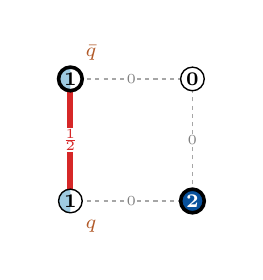
\begin{tikzpicture}[x=1.55cm,y=1.55cm,baseline=(current bounding box.center)]
\draw[fluxoff] (0,0) -- (1,0) node[midway,jlab,text=gray] {$0$};
\draw[fluxon] (0,0) -- (0,1) node[midway,jlab,text=fluxred] {$\tfrac12$};
\draw[fluxoff] (0,1) -- (1,1) node[midway,jlab,text=gray] {$0$};
\draw[fluxoff] (1,0) -- (1,1) node[midway,jlab,text=gray] {$0$};
\fill[white] (0,0) circle[radius=0.15cm];
\fill[occ1] (0,0) ++(90:0.15cm) arc[start angle=90,end angle=270,radius=0.15cm] -- cycle;
\node[site,evensite,fill=none] at (0,0) {\textbf{1}};
\node[part] at (0+0.17,0+-1*0.21) {$q$};
\fill[white] (0,1) circle[radius=0.15cm];
\fill[occ1] (0,1) ++(90:0.15cm) arc[start angle=90,end angle=270,radius=0.15cm] -- cycle;
\node[site,oddsite,fill=none] at (0,1) {\textbf{1}};
\node[part] at (0+0.17,1+1*0.21) {$\bar q$};
\node[site,oddsite,fill=occ2] at (1,0) {\textcolor{white}{\textbf{2}}};
\node[site,evensite,fill=white] at (1,1) {\textbf{0}};
\useasboundingbox (-0.35,-0.42) rectangle (1.35,1.42);
\end{tikzpicture}
\par\vspace{1pt}\raggedright\tiny \textbf{\#30} ($B{=}0$, \#13 in sector)\ \ $E_{\rm diag}=+0.000$\\ $E_0$ (ground state): $c=+0.2019$, $|c|^2=0.0408$\\ \texttt{010 100 001 000}\\ $n=(1\,1\,2\,0)$\ \ $j=(0\,\frac12\,0\,0)$\end{minipage}}
\hfill
\fcolorbox{gray!45}{orange!8}{\begin{minipage}[t][\cardh2][t]{0.235\textwidth}\centering
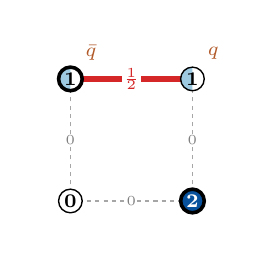
\begin{tikzpicture}[x=1.55cm,y=1.55cm,baseline=(current bounding box.center)]
\draw[fluxoff] (0,0) -- (1,0) node[midway,jlab,text=gray] {$0$};
\draw[fluxoff] (0,0) -- (0,1) node[midway,jlab,text=gray] {$0$};
\draw[fluxon] (0,1) -- (1,1) node[midway,jlab,text=fluxred] {$\tfrac12$};
\draw[fluxoff] (1,0) -- (1,1) node[midway,jlab,text=gray] {$0$};
\node[site,evensite,fill=white] at (0,0) {\textbf{0}};
\fill[white] (0,1) circle[radius=0.15cm];
\fill[occ1] (0,1) ++(90:0.15cm) arc[start angle=90,end angle=270,radius=0.15cm] -- cycle;
\node[site,oddsite,fill=none] at (0,1) {\textbf{1}};
\node[part] at (0+0.17,1+1*0.21) {$\bar q$};
\node[site,oddsite,fill=occ2] at (1,0) {\textcolor{white}{\textbf{2}}};
\fill[white] (1,1) circle[radius=0.15cm];
\fill[occ1] (1,1) ++(90:0.15cm) arc[start angle=90,end angle=270,radius=0.15cm] -- cycle;
\node[site,evensite,fill=none] at (1,1) {\textbf{1}};
\node[part] at (1+0.17,1+1*0.21) {$q$};
\useasboundingbox (-0.35,-0.42) rectangle (1.35,1.42);
\end{tikzpicture}
\par\vspace{1pt}\raggedright\tiny \textbf{\#21} ($B{=}0$, \#8 in sector)\ \ $E_{\rm diag}=+0.000$\\ $E_0$ (ground state): $c=-0.2019i$, $|c|^2=0.0408$\\ \texttt{000 010 001 100}\\ $n=(0\,1\,2\,1)$\ \ $j=(0\,0\,\frac12\,0)$\end{minipage}}
\par\vspace{3pt}\noindent
\fcolorbox{gray!45}{orange!8}{\begin{minipage}[t][\cardh2][t]{0.235\textwidth}\centering
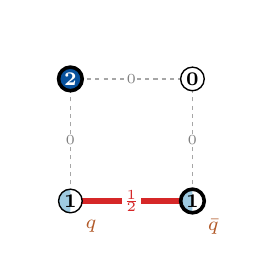
\begin{tikzpicture}[x=1.55cm,y=1.55cm,baseline=(current bounding box.center)]
\draw[fluxon] (0,0) -- (1,0) node[midway,jlab,text=fluxred] {$\tfrac12$};
\draw[fluxoff] (0,0) -- (0,1) node[midway,jlab,text=gray] {$0$};
\draw[fluxoff] (0,1) -- (1,1) node[midway,jlab,text=gray] {$0$};
\draw[fluxoff] (1,0) -- (1,1) node[midway,jlab,text=gray] {$0$};
\fill[white] (0,0) circle[radius=0.15cm];
\fill[occ1] (0,0) ++(90:0.15cm) arc[start angle=90,end angle=270,radius=0.15cm] -- cycle;
\node[site,evensite,fill=none] at (0,0) {\textbf{1}};
\node[part] at (0+0.17,0+-1*0.21) {$q$};
\node[site,oddsite,fill=occ2] at (0,1) {\textcolor{white}{\textbf{2}}};
\fill[white] (1,0) circle[radius=0.15cm];
\fill[occ1] (1,0) ++(90:0.15cm) arc[start angle=90,end angle=270,radius=0.15cm] -- cycle;
\node[site,oddsite,fill=none] at (1,0) {\textbf{1}};
\node[part] at (1+0.17,0+-1*0.21) {$\bar q$};
\node[site,evensite,fill=white] at (1,1) {\textbf{0}};
\useasboundingbox (-0.35,-0.42) rectangle (1.35,1.42);
\end{tikzpicture}
\par\vspace{1pt}\raggedright\tiny \textbf{\#43} ($B{=}0$, \#20 in sector)\ \ $E_{\rm diag}=+0.000$\\ $E_0$ (ground state): $c=+0.2019i$, $|c|^2=0.0408$\\ \texttt{100 001 100 000}\\ $n=(1\,2\,1\,0)$\ \ $j=(\frac12\,0\,0\,0)$\end{minipage}}
\hfill
\fcolorbox{gray!45}{cyan!7}{\begin{minipage}[t][\cardh2][t]{0.235\textwidth}\centering
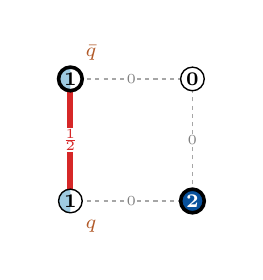
\begin{tikzpicture}[x=1.55cm,y=1.55cm,baseline=(current bounding box.center)]
\draw[fluxoff] (0,0) -- (1,0) node[midway,jlab,text=gray] {$0$};
\draw[fluxon] (0,0) -- (0,1) node[midway,jlab,text=fluxred] {$\tfrac12$};
\draw[fluxoff] (0,1) -- (1,1) node[midway,jlab,text=gray] {$0$};
\draw[fluxoff] (1,0) -- (1,1) node[midway,jlab,text=gray] {$0$};
\fill[white] (0,0) circle[radius=0.15cm];
\fill[occ1] (0,0) ++(90:0.15cm) arc[start angle=90,end angle=270,radius=0.15cm] -- cycle;
\node[site,evensite,fill=none] at (0,0) {\textbf{1}};
\node[part] at (0+0.17,0+-1*0.21) {$q$};
\fill[white] (0,1) circle[radius=0.15cm];
\fill[occ1] (0,1) ++(90:0.15cm) arc[start angle=90,end angle=270,radius=0.15cm] -- cycle;
\node[site,oddsite,fill=none] at (0,1) {\textbf{1}};
\node[part] at (0+0.17,1+1*0.21) {$\bar q$};
\node[site,oddsite,fill=occ2] at (1,0) {\textcolor{white}{\textbf{2}}};
\node[site,evensite,fill=white] at (1,1) {\textbf{0}};
\useasboundingbox (-0.35,-0.42) rectangle (1.35,1.42);
\end{tikzpicture}
\par\vspace{1pt}\raggedright\tiny \textbf{\#30} ($B{=}0$, \#13 in sector)\ \ $E_{\rm diag}=+0.000$\\ $E_1$ (excited state 1): $c=+0.3530$, $|c|^2=0.1246$\\ \texttt{010 100 001 000}\\ $n=(1\,1\,2\,0)$\ \ $j=(0\,\frac12\,0\,0)$\end{minipage}}
\hfill
\fcolorbox{gray!45}{cyan!7}{\begin{minipage}[t][\cardh2][t]{0.235\textwidth}\centering
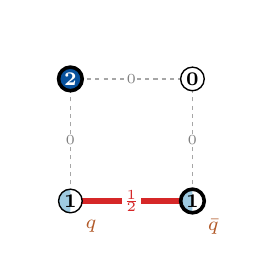
\begin{tikzpicture}[x=1.55cm,y=1.55cm,baseline=(current bounding box.center)]
\draw[fluxon] (0,0) -- (1,0) node[midway,jlab,text=fluxred] {$\tfrac12$};
\draw[fluxoff] (0,0) -- (0,1) node[midway,jlab,text=gray] {$0$};
\draw[fluxoff] (0,1) -- (1,1) node[midway,jlab,text=gray] {$0$};
\draw[fluxoff] (1,0) -- (1,1) node[midway,jlab,text=gray] {$0$};
\fill[white] (0,0) circle[radius=0.15cm];
\fill[occ1] (0,0) ++(90:0.15cm) arc[start angle=90,end angle=270,radius=0.15cm] -- cycle;
\node[site,evensite,fill=none] at (0,0) {\textbf{1}};
\node[part] at (0+0.17,0+-1*0.21) {$q$};
\node[site,oddsite,fill=occ2] at (0,1) {\textcolor{white}{\textbf{2}}};
\fill[white] (1,0) circle[radius=0.15cm];
\fill[occ1] (1,0) ++(90:0.15cm) arc[start angle=90,end angle=270,radius=0.15cm] -- cycle;
\node[site,oddsite,fill=none] at (1,0) {\textbf{1}};
\node[part] at (1+0.17,0+-1*0.21) {$\bar q$};
\node[site,evensite,fill=white] at (1,1) {\textbf{0}};
\useasboundingbox (-0.35,-0.42) rectangle (1.35,1.42);
\end{tikzpicture}
\par\vspace{1pt}\raggedright\tiny \textbf{\#43} ($B{=}0$, \#20 in sector)\ \ $E_{\rm diag}=+0.000$\\ $E_1$ (excited state 1): $c=-0.3530i$, $|c|^2=0.1246$\\ \texttt{100 001 100 000}\\ $n=(1\,2\,1\,0)$\ \ $j=(\frac12\,0\,0\,0)$\end{minipage}}
\hfill
\fcolorbox{gray!45}{cyan!7}{\begin{minipage}[t][\cardh2][t]{0.235\textwidth}\centering
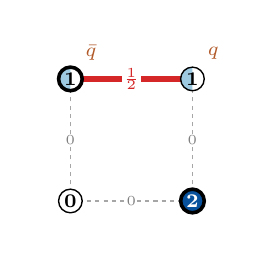
\begin{tikzpicture}[x=1.55cm,y=1.55cm,baseline=(current bounding box.center)]
\draw[fluxoff] (0,0) -- (1,0) node[midway,jlab,text=gray] {$0$};
\draw[fluxoff] (0,0) -- (0,1) node[midway,jlab,text=gray] {$0$};
\draw[fluxon] (0,1) -- (1,1) node[midway,jlab,text=fluxred] {$\tfrac12$};
\draw[fluxoff] (1,0) -- (1,1) node[midway,jlab,text=gray] {$0$};
\node[site,evensite,fill=white] at (0,0) {\textbf{0}};
\fill[white] (0,1) circle[radius=0.15cm];
\fill[occ1] (0,1) ++(90:0.15cm) arc[start angle=90,end angle=270,radius=0.15cm] -- cycle;
\node[site,oddsite,fill=none] at (0,1) {\textbf{1}};
\node[part] at (0+0.17,1+1*0.21) {$\bar q$};
\node[site,oddsite,fill=occ2] at (1,0) {\textcolor{white}{\textbf{2}}};
\fill[white] (1,1) circle[radius=0.15cm];
\fill[occ1] (1,1) ++(90:0.15cm) arc[start angle=90,end angle=270,radius=0.15cm] -- cycle;
\node[site,evensite,fill=none] at (1,1) {\textbf{1}};
\node[part] at (1+0.17,1+1*0.21) {$q$};
\useasboundingbox (-0.35,-0.42) rectangle (1.35,1.42);
\end{tikzpicture}
\par\vspace{1pt}\raggedright\tiny \textbf{\#21} ($B{=}0$, \#8 in sector)\ \ $E_{\rm diag}=+0.000$\\ $E_1$ (excited state 1): $c=+0.3530i$, $|c|^2=0.1246$\\ \texttt{000 010 001 100}\\ $n=(0\,1\,2\,1)$\ \ $j=(0\,0\,\frac12\,0)$\end{minipage}}
\par\vspace{3pt}\noindent
\fcolorbox{gray!45}{cyan!7}{\begin{minipage}[t][\cardh2][t]{0.235\textwidth}\centering
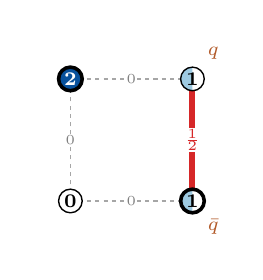
\begin{tikzpicture}[x=1.55cm,y=1.55cm,baseline=(current bounding box.center)]
\draw[fluxoff] (0,0) -- (1,0) node[midway,jlab,text=gray] {$0$};
\draw[fluxoff] (0,0) -- (0,1) node[midway,jlab,text=gray] {$0$};
\draw[fluxoff] (0,1) -- (1,1) node[midway,jlab,text=gray] {$0$};
\draw[fluxon] (1,0) -- (1,1) node[midway,jlab,text=fluxred] {$\tfrac12$};
\node[site,evensite,fill=white] at (0,0) {\textbf{0}};
\node[site,oddsite,fill=occ2] at (0,1) {\textcolor{white}{\textbf{2}}};
\fill[white] (1,0) circle[radius=0.15cm];
\fill[occ1] (1,0) ++(90:0.15cm) arc[start angle=90,end angle=270,radius=0.15cm] -- cycle;
\node[site,oddsite,fill=none] at (1,0) {\textbf{1}};
\node[part] at (1+0.17,0+-1*0.21) {$\bar q$};
\fill[white] (1,1) circle[radius=0.15cm];
\fill[occ1] (1,1) ++(90:0.15cm) arc[start angle=90,end angle=270,radius=0.15cm] -- cycle;
\node[site,evensite,fill=none] at (1,1) {\textbf{1}};
\node[part] at (1+0.17,1+1*0.21) {$q$};
\useasboundingbox (-0.35,-0.42) rectangle (1.35,1.42);
\end{tikzpicture}
\par\vspace{1pt}\raggedright\tiny \textbf{\#17} ($B{=}0$, \#6 in sector)\ \ $E_{\rm diag}=+0.000$\\ $E_1$ (excited state 1): $c=-0.3530$, $|c|^2=0.1246$\\ \texttt{000 001 010 010}\\ $n=(0\,2\,1\,1)$\ \ $j=(0\,0\,0\,\frac12)$\end{minipage}}
\hfill
\fcolorbox{gray!45}{cyan!7}{\begin{minipage}[t][\cardh2][t]{0.235\textwidth}\centering
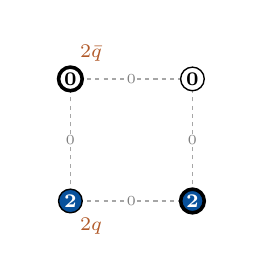
\begin{tikzpicture}[x=1.55cm,y=1.55cm,baseline=(current bounding box.center)]
\draw[fluxoff] (0,0) -- (1,0) node[midway,jlab,text=gray] {$0$};
\draw[fluxoff] (0,0) -- (0,1) node[midway,jlab,text=gray] {$0$};
\draw[fluxoff] (0,1) -- (1,1) node[midway,jlab,text=gray] {$0$};
\draw[fluxoff] (1,0) -- (1,1) node[midway,jlab,text=gray] {$0$};
\node[site,evensite,fill=occ2] at (0,0) {\textcolor{white}{\textbf{2}}};
\node[part] at (0+0.17,0+-1*0.21) {$2q$};
\node[site,oddsite,fill=white] at (0,1) {\textbf{0}};
\node[part] at (0+0.17,1+1*0.21) {$2\bar q$};
\node[site,oddsite,fill=occ2] at (1,0) {\textcolor{white}{\textbf{2}}};
\node[site,evensite,fill=white] at (1,1) {\textbf{0}};
\useasboundingbox (-0.35,-0.42) rectangle (1.35,1.42);
\end{tikzpicture}
\par\vspace{1pt}\raggedright\tiny \textbf{\#10} ($B{=}0$, \#4 in sector)\ \ $E_{\rm diag}=+0.000$\\ $E_1$ (excited state 1): $c=+0.3253$, $|c|^2=0.1058$\\ \texttt{001 000 001 000}\\ $n=(2\,0\,2\,0)$\ \ $j=(0\,0\,0\,0)$\end{minipage}}
\hfill
\fcolorbox{gray!45}{cyan!7}{\begin{minipage}[t][\cardh2][t]{0.235\textwidth}\centering
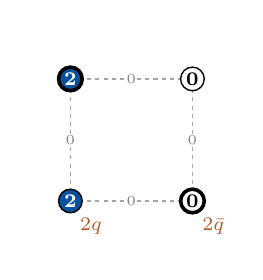
\begin{tikzpicture}[x=1.55cm,y=1.55cm,baseline=(current bounding box.center)]
\draw[fluxoff] (0,0) -- (1,0) node[midway,jlab,text=gray] {$0$};
\draw[fluxoff] (0,0) -- (0,1) node[midway,jlab,text=gray] {$0$};
\draw[fluxoff] (0,1) -- (1,1) node[midway,jlab,text=gray] {$0$};
\draw[fluxoff] (1,0) -- (1,1) node[midway,jlab,text=gray] {$0$};
\node[site,evensite,fill=occ2] at (0,0) {\textcolor{white}{\textbf{2}}};
\node[part] at (0+0.17,0+-1*0.21) {$2q$};
\node[site,oddsite,fill=occ2] at (0,1) {\textcolor{white}{\textbf{2}}};
\node[site,oddsite,fill=white] at (1,0) {\textbf{0}};
\node[part] at (1+0.17,0+-1*0.21) {$2\bar q$};
\node[site,evensite,fill=white] at (1,1) {\textbf{0}};
\useasboundingbox (-0.35,-0.42) rectangle (1.35,1.42);
\end{tikzpicture}
\par\vspace{1pt}\raggedright\tiny \textbf{\#12} ($B{=}0$, \#5 in sector)\ \ $E_{\rm diag}=+0.000$\\ $E_1$ (excited state 1): $c=+0.3253$, $|c|^2=0.1058$\\ \texttt{001 001 000 000}\\ $n=(2\,2\,0\,0)$\ \ $j=(0\,0\,0\,0)$\end{minipage}}
\hfill
\fcolorbox{gray!45}{green!7}{\begin{minipage}[t][\cardh2][t]{0.235\textwidth}\centering
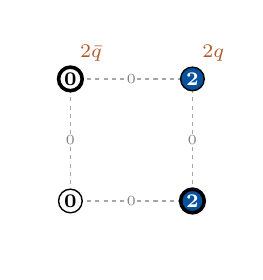
\begin{tikzpicture}[x=1.55cm,y=1.55cm,baseline=(current bounding box.center)]
\draw[fluxoff] (0,0) -- (1,0) node[midway,jlab,text=gray] {$0$};
\draw[fluxoff] (0,0) -- (0,1) node[midway,jlab,text=gray] {$0$};
\draw[fluxoff] (0,1) -- (1,1) node[midway,jlab,text=gray] {$0$};
\draw[fluxoff] (1,0) -- (1,1) node[midway,jlab,text=gray] {$0$};
\node[site,evensite,fill=white] at (0,0) {\textbf{0}};
\node[site,oddsite,fill=white] at (0,1) {\textbf{0}};
\node[part] at (0+0.17,1+1*0.21) {$2\bar q$};
\node[site,oddsite,fill=occ2] at (1,0) {\textcolor{white}{\textbf{2}}};
\node[site,evensite,fill=occ2] at (1,1) {\textcolor{white}{\textbf{2}}};
\node[part] at (1+0.17,1+1*0.21) {$2q$};
\useasboundingbox (-0.35,-0.42) rectangle (1.35,1.42);
\end{tikzpicture}
\par\vspace{1pt}\raggedright\tiny \textbf{\#3} ($B{=}0$, \#0 in sector)\ \ $E_{\rm diag}=+0.000$\\ $E_2$ (excited state 2): $c=+0.4915$, $|c|^2=0.2415$\\ \texttt{000 000 001 001}\\ $n=(0\,0\,2\,2)$\ \ $j=(0\,0\,0\,0)$\end{minipage}}
\par\vspace{3pt}\noindent
\fcolorbox{gray!45}{green!7}{\begin{minipage}[t][\cardh2][t]{0.235\textwidth}\centering
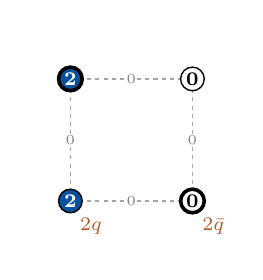
\begin{tikzpicture}[x=1.55cm,y=1.55cm,baseline=(current bounding box.center)]
\draw[fluxoff] (0,0) -- (1,0) node[midway,jlab,text=gray] {$0$};
\draw[fluxoff] (0,0) -- (0,1) node[midway,jlab,text=gray] {$0$};
\draw[fluxoff] (0,1) -- (1,1) node[midway,jlab,text=gray] {$0$};
\draw[fluxoff] (1,0) -- (1,1) node[midway,jlab,text=gray] {$0$};
\node[site,evensite,fill=occ2] at (0,0) {\textcolor{white}{\textbf{2}}};
\node[part] at (0+0.17,0+-1*0.21) {$2q$};
\node[site,oddsite,fill=occ2] at (0,1) {\textcolor{white}{\textbf{2}}};
\node[site,oddsite,fill=white] at (1,0) {\textbf{0}};
\node[part] at (1+0.17,0+-1*0.21) {$2\bar q$};
\node[site,evensite,fill=white] at (1,1) {\textbf{0}};
\useasboundingbox (-0.35,-0.42) rectangle (1.35,1.42);
\end{tikzpicture}
\par\vspace{1pt}\raggedright\tiny \textbf{\#12} ($B{=}0$, \#5 in sector)\ \ $E_{\rm diag}=+0.000$\\ $E_2$ (excited state 2): $c=-0.4915$, $|c|^2=0.2415$\\ \texttt{001 001 000 000}\\ $n=(2\,2\,0\,0)$\ \ $j=(0\,0\,0\,0)$\end{minipage}}
\hfill
\fcolorbox{gray!45}{green!7}{\begin{minipage}[t][\cardh2][t]{0.235\textwidth}\centering
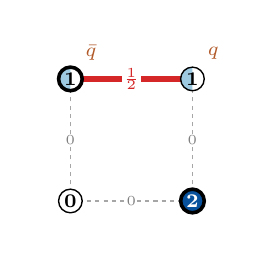
\begin{tikzpicture}[x=1.55cm,y=1.55cm,baseline=(current bounding box.center)]
\draw[fluxoff] (0,0) -- (1,0) node[midway,jlab,text=gray] {$0$};
\draw[fluxoff] (0,0) -- (0,1) node[midway,jlab,text=gray] {$0$};
\draw[fluxon] (0,1) -- (1,1) node[midway,jlab,text=fluxred] {$\tfrac12$};
\draw[fluxoff] (1,0) -- (1,1) node[midway,jlab,text=gray] {$0$};
\node[site,evensite,fill=white] at (0,0) {\textbf{0}};
\fill[white] (0,1) circle[radius=0.15cm];
\fill[occ1] (0,1) ++(90:0.15cm) arc[start angle=90,end angle=270,radius=0.15cm] -- cycle;
\node[site,oddsite,fill=none] at (0,1) {\textbf{1}};
\node[part] at (0+0.17,1+1*0.21) {$\bar q$};
\node[site,oddsite,fill=occ2] at (1,0) {\textcolor{white}{\textbf{2}}};
\fill[white] (1,1) circle[radius=0.15cm];
\fill[occ1] (1,1) ++(90:0.15cm) arc[start angle=90,end angle=270,radius=0.15cm] -- cycle;
\node[site,evensite,fill=none] at (1,1) {\textbf{1}};
\node[part] at (1+0.17,1+1*0.21) {$q$};
\useasboundingbox (-0.35,-0.42) rectangle (1.35,1.42);
\end{tikzpicture}
\par\vspace{1pt}\raggedright\tiny \textbf{\#21} ($B{=}0$, \#8 in sector)\ \ $E_{\rm diag}=+0.000$\\ $E_2$ (excited state 2): $c=+0.4890i$, $|c|^2=0.2392$\\ \texttt{000 010 001 100}\\ $n=(0\,1\,2\,1)$\ \ $j=(0\,0\,\frac12\,0)$\end{minipage}}
\hfill
\fcolorbox{gray!45}{green!7}{\begin{minipage}[t][\cardh2][t]{0.235\textwidth}\centering
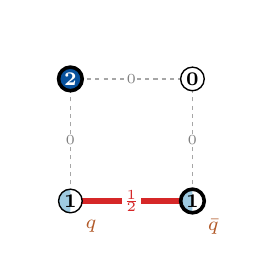
\begin{tikzpicture}[x=1.55cm,y=1.55cm,baseline=(current bounding box.center)]
\draw[fluxon] (0,0) -- (1,0) node[midway,jlab,text=fluxred] {$\tfrac12$};
\draw[fluxoff] (0,0) -- (0,1) node[midway,jlab,text=gray] {$0$};
\draw[fluxoff] (0,1) -- (1,1) node[midway,jlab,text=gray] {$0$};
\draw[fluxoff] (1,0) -- (1,1) node[midway,jlab,text=gray] {$0$};
\fill[white] (0,0) circle[radius=0.15cm];
\fill[occ1] (0,0) ++(90:0.15cm) arc[start angle=90,end angle=270,radius=0.15cm] -- cycle;
\node[site,evensite,fill=none] at (0,0) {\textbf{1}};
\node[part] at (0+0.17,0+-1*0.21) {$q$};
\node[site,oddsite,fill=occ2] at (0,1) {\textcolor{white}{\textbf{2}}};
\fill[white] (1,0) circle[radius=0.15cm];
\fill[occ1] (1,0) ++(90:0.15cm) arc[start angle=90,end angle=270,radius=0.15cm] -- cycle;
\node[site,oddsite,fill=none] at (1,0) {\textbf{1}};
\node[part] at (1+0.17,0+-1*0.21) {$\bar q$};
\node[site,evensite,fill=white] at (1,1) {\textbf{0}};
\useasboundingbox (-0.35,-0.42) rectangle (1.35,1.42);
\end{tikzpicture}
\par\vspace{1pt}\raggedright\tiny \textbf{\#43} ($B{=}0$, \#20 in sector)\ \ $E_{\rm diag}=+0.000$\\ $E_2$ (excited state 2): $c=+0.4890i$, $|c|^2=0.2392$\\ \texttt{100 001 100 000}\\ $n=(1\,2\,1\,0)$\ \ $j=(\frac12\,0\,0\,0)$\end{minipage}}
\hfill
\fcolorbox{gray!45}{magenta!6}{\begin{minipage}[t][\cardh2][t]{0.235\textwidth}\centering
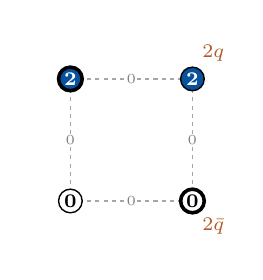
\begin{tikzpicture}[x=1.55cm,y=1.55cm,baseline=(current bounding box.center)]
\draw[fluxoff] (0,0) -- (1,0) node[midway,jlab,text=gray] {$0$};
\draw[fluxoff] (0,0) -- (0,1) node[midway,jlab,text=gray] {$0$};
\draw[fluxoff] (0,1) -- (1,1) node[midway,jlab,text=gray] {$0$};
\draw[fluxoff] (1,0) -- (1,1) node[midway,jlab,text=gray] {$0$};
\node[site,evensite,fill=white] at (0,0) {\textbf{0}};
\node[site,oddsite,fill=occ2] at (0,1) {\textcolor{white}{\textbf{2}}};
\node[site,oddsite,fill=white] at (1,0) {\textbf{0}};
\node[part] at (1+0.17,0+-1*0.21) {$2\bar q$};
\node[site,evensite,fill=occ2] at (1,1) {\textcolor{white}{\textbf{2}}};
\node[part] at (1+0.17,1+1*0.21) {$2q$};
\useasboundingbox (-0.35,-0.42) rectangle (1.35,1.42);
\end{tikzpicture}
\par\vspace{1pt}\raggedright\tiny \textbf{\#5} ($B{=}0$, \#1 in sector)\ \ $E_{\rm diag}=+0.000$\\ $E_3$ (excited state 3): $c=+0.4915$, $|c|^2=0.2415$\\ \texttt{000 001 000 001}\\ $n=(0\,2\,0\,2)$\ \ $j=(0\,0\,0\,0)$\end{minipage}}
\par\vspace{3pt}\noindent
\fcolorbox{gray!45}{magenta!6}{\begin{minipage}[t][\cardh2][t]{0.235\textwidth}\centering
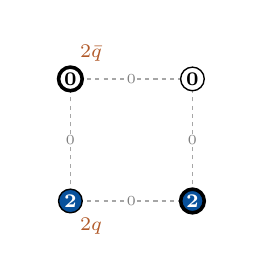
\begin{tikzpicture}[x=1.55cm,y=1.55cm,baseline=(current bounding box.center)]
\draw[fluxoff] (0,0) -- (1,0) node[midway,jlab,text=gray] {$0$};
\draw[fluxoff] (0,0) -- (0,1) node[midway,jlab,text=gray] {$0$};
\draw[fluxoff] (0,1) -- (1,1) node[midway,jlab,text=gray] {$0$};
\draw[fluxoff] (1,0) -- (1,1) node[midway,jlab,text=gray] {$0$};
\node[site,evensite,fill=occ2] at (0,0) {\textcolor{white}{\textbf{2}}};
\node[part] at (0+0.17,0+-1*0.21) {$2q$};
\node[site,oddsite,fill=white] at (0,1) {\textbf{0}};
\node[part] at (0+0.17,1+1*0.21) {$2\bar q$};
\node[site,oddsite,fill=occ2] at (1,0) {\textcolor{white}{\textbf{2}}};
\node[site,evensite,fill=white] at (1,1) {\textbf{0}};
\useasboundingbox (-0.35,-0.42) rectangle (1.35,1.42);
\end{tikzpicture}
\par\vspace{1pt}\raggedright\tiny \textbf{\#10} ($B{=}0$, \#4 in sector)\ \ $E_{\rm diag}=+0.000$\\ $E_3$ (excited state 3): $c=-0.4915$, $|c|^2=0.2415$\\ \texttt{001 000 001 000}\\ $n=(2\,0\,2\,0)$\ \ $j=(0\,0\,0\,0)$\end{minipage}}
\hfill
\fcolorbox{gray!45}{magenta!6}{\begin{minipage}[t][\cardh2][t]{0.235\textwidth}\centering
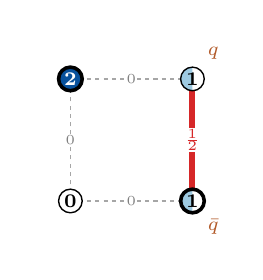
\begin{tikzpicture}[x=1.55cm,y=1.55cm,baseline=(current bounding box.center)]
\draw[fluxoff] (0,0) -- (1,0) node[midway,jlab,text=gray] {$0$};
\draw[fluxoff] (0,0) -- (0,1) node[midway,jlab,text=gray] {$0$};
\draw[fluxoff] (0,1) -- (1,1) node[midway,jlab,text=gray] {$0$};
\draw[fluxon] (1,0) -- (1,1) node[midway,jlab,text=fluxred] {$\tfrac12$};
\node[site,evensite,fill=white] at (0,0) {\textbf{0}};
\node[site,oddsite,fill=occ2] at (0,1) {\textcolor{white}{\textbf{2}}};
\fill[white] (1,0) circle[radius=0.15cm];
\fill[occ1] (1,0) ++(90:0.15cm) arc[start angle=90,end angle=270,radius=0.15cm] -- cycle;
\node[site,oddsite,fill=none] at (1,0) {\textbf{1}};
\node[part] at (1+0.17,0+-1*0.21) {$\bar q$};
\fill[white] (1,1) circle[radius=0.15cm];
\fill[occ1] (1,1) ++(90:0.15cm) arc[start angle=90,end angle=270,radius=0.15cm] -- cycle;
\node[site,evensite,fill=none] at (1,1) {\textbf{1}};
\node[part] at (1+0.17,1+1*0.21) {$q$};
\useasboundingbox (-0.35,-0.42) rectangle (1.35,1.42);
\end{tikzpicture}
\par\vspace{1pt}\raggedright\tiny \textbf{\#17} ($B{=}0$, \#6 in sector)\ \ $E_{\rm diag}=+0.000$\\ $E_3$ (excited state 3): $c=-0.4890$, $|c|^2=0.2392$\\ \texttt{000 001 010 010}\\ $n=(0\,2\,1\,1)$\ \ $j=(0\,0\,0\,\frac12)$\end{minipage}}
\hfill
\fcolorbox{gray!45}{magenta!6}{\begin{minipage}[t][\cardh2][t]{0.235\textwidth}\centering
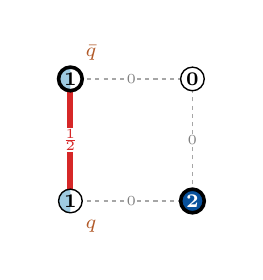
\begin{tikzpicture}[x=1.55cm,y=1.55cm,baseline=(current bounding box.center)]
\draw[fluxoff] (0,0) -- (1,0) node[midway,jlab,text=gray] {$0$};
\draw[fluxon] (0,0) -- (0,1) node[midway,jlab,text=fluxred] {$\tfrac12$};
\draw[fluxoff] (0,1) -- (1,1) node[midway,jlab,text=gray] {$0$};
\draw[fluxoff] (1,0) -- (1,1) node[midway,jlab,text=gray] {$0$};
\fill[white] (0,0) circle[radius=0.15cm];
\fill[occ1] (0,0) ++(90:0.15cm) arc[start angle=90,end angle=270,radius=0.15cm] -- cycle;
\node[site,evensite,fill=none] at (0,0) {\textbf{1}};
\node[part] at (0+0.17,0+-1*0.21) {$q$};
\fill[white] (0,1) circle[radius=0.15cm];
\fill[occ1] (0,1) ++(90:0.15cm) arc[start angle=90,end angle=270,radius=0.15cm] -- cycle;
\node[site,oddsite,fill=none] at (0,1) {\textbf{1}};
\node[part] at (0+0.17,1+1*0.21) {$\bar q$};
\node[site,oddsite,fill=occ2] at (1,0) {\textcolor{white}{\textbf{2}}};
\node[site,evensite,fill=white] at (1,1) {\textbf{0}};
\useasboundingbox (-0.35,-0.42) rectangle (1.35,1.42);
\end{tikzpicture}
\par\vspace{1pt}\raggedright\tiny \textbf{\#30} ($B{=}0$, \#13 in sector)\ \ $E_{\rm diag}=+0.000$\\ $E_3$ (excited state 3): $c=-0.4890$, $|c|^2=0.2392$\\ \texttt{010 100 001 000}\\ $n=(1\,1\,2\,0)$\ \ $j=(0\,\frac12\,0\,0)$\end{minipage}}
\hfill
\par\vspace{3pt}\noindent
\clearpage
\subsection{$2\times2${,} sector $B=+1$ (20 physical states)}
\begin{center}\small\begin{tabular}{l l r r r}\toprule level & & configs drawn & weight covered & participation ratio\\\midrule\colorbox{orange!8}{$E_0=-1.861588$} & ground state & 5 & 95.6\% & 2.6\\
\colorbox{cyan!7}{$E_1=-1.819745$} & excited state 1 & 4 & 95.3\% & 2.4\\
\colorbox{green!7}{$E_2=+0.208229$} & excited state 2 & 6 & 76.0\% & 8.1\\
\colorbox{magenta!6}{$E_3=+0.450558$} & excited state 3 & 6 & 71.4\% & 8.9\\\bottomrule\end{tabular}\end{center}
\small Most important configurations of each level (largest weight first, up to 6 or until 95\% of the weight is covered); cards of one level share a colour.  Participation ratio $=1/\sum|c|^4$ $\approx$ number of configurations the state is spread over.\par\smallskip
\noindent\fcolorbox{gray!45}{orange!8}{\begin{minipage}[t][\cardh2][t]{0.235\textwidth}\centering
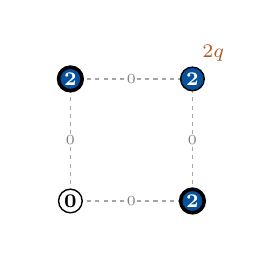
\begin{tikzpicture}[x=1.55cm,y=1.55cm,baseline=(current bounding box.center)]
\draw[fluxoff] (0,0) -- (1,0) node[midway,jlab,text=gray] {$0$};
\draw[fluxoff] (0,0) -- (0,1) node[midway,jlab,text=gray] {$0$};
\draw[fluxoff] (0,1) -- (1,1) node[midway,jlab,text=gray] {$0$};
\draw[fluxoff] (1,0) -- (1,1) node[midway,jlab,text=gray] {$0$};
\node[site,evensite,fill=white] at (0,0) {\textbf{0}};
\node[site,oddsite,fill=occ2] at (0,1) {\textcolor{white}{\textbf{2}}};
\node[site,oddsite,fill=occ2] at (1,0) {\textcolor{white}{\textbf{2}}};
\node[site,evensite,fill=occ2] at (1,1) {\textcolor{white}{\textbf{2}}};
\node[part] at (1+0.17,1+1*0.21) {$2q$};
\useasboundingbox (-0.35,-0.42) rectangle (1.35,1.42);
\end{tikzpicture}
\par\vspace{1pt}\raggedright\tiny \textbf{\#7} ($B{=}1$, \#0 in sector)\ \ $E_{\rm diag}=-1.500$\\ $E_0$ (ground state): $c=+0.6614$, $|c|^2=0.4375$\\ \texttt{000 001 001 001}\\ $n=(0\,2\,2\,2)$\ \ $j=(0\,0\,0\,0)$\end{minipage}}
\hfill
\fcolorbox{gray!45}{orange!8}{\begin{minipage}[t][\cardh2][t]{0.235\textwidth}\centering
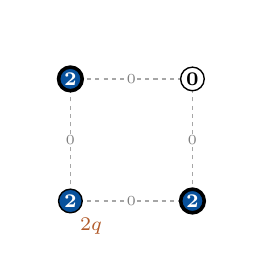
\begin{tikzpicture}[x=1.55cm,y=1.55cm,baseline=(current bounding box.center)]
\draw[fluxoff] (0,0) -- (1,0) node[midway,jlab,text=gray] {$0$};
\draw[fluxoff] (0,0) -- (0,1) node[midway,jlab,text=gray] {$0$};
\draw[fluxoff] (0,1) -- (1,1) node[midway,jlab,text=gray] {$0$};
\draw[fluxoff] (1,0) -- (1,1) node[midway,jlab,text=gray] {$0$};
\node[site,evensite,fill=occ2] at (0,0) {\textcolor{white}{\textbf{2}}};
\node[part] at (0+0.17,0+-1*0.21) {$2q$};
\node[site,oddsite,fill=occ2] at (0,1) {\textcolor{white}{\textbf{2}}};
\node[site,oddsite,fill=occ2] at (1,0) {\textcolor{white}{\textbf{2}}};
\node[site,evensite,fill=white] at (1,1) {\textbf{0}};
\useasboundingbox (-0.35,-0.42) rectangle (1.35,1.42);
\end{tikzpicture}
\par\vspace{1pt}\raggedright\tiny \textbf{\#14} ($B{=}1$, \#3 in sector)\ \ $E_{\rm diag}=-1.500$\\ $E_0$ (ground state): $c=-0.6614$, $|c|^2=0.4375$\\ \texttt{001 001 001 000}\\ $n=(2\,2\,2\,0)$\ \ $j=(0\,0\,0\,0)$\end{minipage}}
\hfill
\fcolorbox{gray!45}{orange!8}{\begin{minipage}[t][\cardh2][t]{0.235\textwidth}\centering
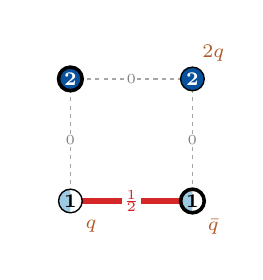
\begin{tikzpicture}[x=1.55cm,y=1.55cm,baseline=(current bounding box.center)]
\draw[fluxon] (0,0) -- (1,0) node[midway,jlab,text=fluxred] {$\tfrac12$};
\draw[fluxoff] (0,0) -- (0,1) node[midway,jlab,text=gray] {$0$};
\draw[fluxoff] (0,1) -- (1,1) node[midway,jlab,text=gray] {$0$};
\draw[fluxoff] (1,0) -- (1,1) node[midway,jlab,text=gray] {$0$};
\fill[white] (0,0) circle[radius=0.15cm];
\fill[occ1] (0,0) ++(90:0.15cm) arc[start angle=90,end angle=270,radius=0.15cm] -- cycle;
\node[site,evensite,fill=none] at (0,0) {\textbf{1}};
\node[part] at (0+0.17,0+-1*0.21) {$q$};
\node[site,oddsite,fill=occ2] at (0,1) {\textcolor{white}{\textbf{2}}};
\fill[white] (1,0) circle[radius=0.15cm];
\fill[occ1] (1,0) ++(90:0.15cm) arc[start angle=90,end angle=270,radius=0.15cm] -- cycle;
\node[site,oddsite,fill=none] at (1,0) {\textbf{1}};
\node[part] at (1+0.17,0+-1*0.21) {$\bar q$};
\node[site,evensite,fill=occ2] at (1,1) {\textcolor{white}{\textbf{2}}};
\node[part] at (1+0.17,1+1*0.21) {$2q$};
\useasboundingbox (-0.35,-0.42) rectangle (1.35,1.42);
\end{tikzpicture}
\par\vspace{1pt}\raggedright\tiny \textbf{\#44} ($B{=}1$, \#10 in sector)\ \ $E_{\rm diag}=+1.500$\\ $E_0$ (ground state): $c=+0.1645i$, $|c|^2=0.0271$\\ \texttt{100 001 100 001}\\ $n=(1\,2\,1\,2)$\ \ $j=(\frac12\,0\,0\,0)$\end{minipage}}
\hfill
\fcolorbox{gray!45}{orange!8}{\begin{minipage}[t][\cardh2][t]{0.235\textwidth}\centering
\begin{tikzpicture}[x=1.55cm,y=1.55cm,baseline=(current bounding box.center)]
\draw[fluxoff] (0,0) -- (1,0) node[midway,jlab,text=gray] {$0$};
\draw[fluxon] (0,0) -- (0,1) node[midway,jlab,text=fluxred] {$\tfrac12$};
\draw[fluxoff] (0,1) -- (1,1) node[midway,jlab,text=gray] {$0$};
\draw[fluxoff] (1,0) -- (1,1) node[midway,jlab,text=gray] {$0$};
\fill[white] (0,0) circle[radius=0.15cm];
\fill[occ1] (0,0) ++(90:0.15cm) arc[start angle=90,end angle=270,radius=0.15cm] -- cycle;
\node[site,evensite,fill=none] at (0,0) {\textbf{1}};
\node[part] at (0+0.17,0+-1*0.21) {$q$};
\fill[white] (0,1) circle[radius=0.15cm];
\fill[occ1] (0,1) ++(90:0.15cm) arc[start angle=90,end angle=270,radius=0.15cm] -- cycle;
\node[site,oddsite,fill=none] at (0,1) {\textbf{1}};
\node[part] at (0+0.17,1+1*0.21) {$\bar q$};
\node[site,oddsite,fill=occ2] at (1,0) {\textcolor{white}{\textbf{2}}};
\node[site,evensite,fill=occ2] at (1,1) {\textcolor{white}{\textbf{2}}};
\node[part] at (1+0.17,1+1*0.21) {$2q$};
\useasboundingbox (-0.35,-0.42) rectangle (1.35,1.42);
\end{tikzpicture}
\par\vspace{1pt}\raggedright\tiny \textbf{\#31} ($B{=}1$, \#7 in sector)\ \ $E_{\rm diag}=+1.500$\\ $E_0$ (ground state): $c=+0.1645$, $|c|^2=0.0271$\\ \texttt{010 100 001 001}\\ $n=(1\,1\,2\,2)$\ \ $j=(0\,\frac12\,0\,0)$\end{minipage}}
\par\vspace{3pt}\noindent
\fcolorbox{gray!45}{orange!8}{\begin{minipage}[t][\cardh2][t]{0.235\textwidth}\centering
\begin{tikzpicture}[x=1.55cm,y=1.55cm,baseline=(current bounding box.center)]
\draw[fluxoff] (0,0) -- (1,0) node[midway,jlab,text=gray] {$0$};
\draw[fluxoff] (0,0) -- (0,1) node[midway,jlab,text=gray] {$0$};
\draw[fluxon] (0,1) -- (1,1) node[midway,jlab,text=fluxred] {$\tfrac12$};
\draw[fluxoff] (1,0) -- (1,1) node[midway,jlab,text=gray] {$0$};
\node[site,evensite,fill=occ2] at (0,0) {\textcolor{white}{\textbf{2}}};
\node[part] at (0+0.17,0+-1*0.21) {$2q$};
\fill[white] (0,1) circle[radius=0.15cm];
\fill[occ1] (0,1) ++(90:0.15cm) arc[start angle=90,end angle=270,radius=0.15cm] -- cycle;
\node[site,oddsite,fill=none] at (0,1) {\textbf{1}};
\node[part] at (0+0.17,1+1*0.21) {$\bar q$};
\node[site,oddsite,fill=occ2] at (1,0) {\textcolor{white}{\textbf{2}}};
\fill[white] (1,1) circle[radius=0.15cm];
\fill[occ1] (1,1) ++(90:0.15cm) arc[start angle=90,end angle=270,radius=0.15cm] -- cycle;
\node[site,evensite,fill=none] at (1,1) {\textbf{1}};
\node[part] at (1+0.17,1+1*0.21) {$q$};
\useasboundingbox (-0.35,-0.42) rectangle (1.35,1.42);
\end{tikzpicture}
\par\vspace{1pt}\raggedright\tiny \textbf{\#23} ($B{=}1$, \#5 in sector)\ \ $E_{\rm diag}=+1.500$\\ $E_0$ (ground state): $c=+0.1645i$, $|c|^2=0.0271$\\ \texttt{001 010 001 100}\\ $n=(2\,1\,2\,1)$\ \ $j=(0\,0\,\frac12\,0)$\end{minipage}}
\hfill
\fcolorbox{gray!45}{cyan!7}{\begin{minipage}[t][\cardh2][t]{0.235\textwidth}\centering
\begin{tikzpicture}[x=1.55cm,y=1.55cm,baseline=(current bounding box.center)]
\draw[fluxoff] (0,0) -- (1,0) node[midway,jlab,text=gray] {$0$};
\draw[fluxoff] (0,0) -- (0,1) node[midway,jlab,text=gray] {$0$};
\draw[fluxoff] (0,1) -- (1,1) node[midway,jlab,text=gray] {$0$};
\draw[fluxoff] (1,0) -- (1,1) node[midway,jlab,text=gray] {$0$};
\node[site,evensite,fill=occ2] at (0,0) {\textcolor{white}{\textbf{2}}};
\node[part] at (0+0.17,0+-1*0.21) {$2q$};
\node[site,oddsite,fill=occ2] at (0,1) {\textcolor{white}{\textbf{2}}};
\node[site,oddsite,fill=occ2] at (1,0) {\textcolor{white}{\textbf{2}}};
\node[site,evensite,fill=white] at (1,1) {\textbf{0}};
\useasboundingbox (-0.35,-0.42) rectangle (1.35,1.42);
\end{tikzpicture}
\par\vspace{1pt}\raggedright\tiny \textbf{\#14} ($B{=}1$, \#3 in sector)\ \ $E_{\rm diag}=-1.500$\\ $E_1$ (excited state 1): $c=+0.6745$, $|c|^2=0.4549$\\ \texttt{001 001 001 000}\\ $n=(2\,2\,2\,0)$\ \ $j=(0\,0\,0\,0)$\end{minipage}}
\hfill
\fcolorbox{gray!45}{cyan!7}{\begin{minipage}[t][\cardh2][t]{0.235\textwidth}\centering
\begin{tikzpicture}[x=1.55cm,y=1.55cm,baseline=(current bounding box.center)]
\draw[fluxoff] (0,0) -- (1,0) node[midway,jlab,text=gray] {$0$};
\draw[fluxoff] (0,0) -- (0,1) node[midway,jlab,text=gray] {$0$};
\draw[fluxoff] (0,1) -- (1,1) node[midway,jlab,text=gray] {$0$};
\draw[fluxoff] (1,0) -- (1,1) node[midway,jlab,text=gray] {$0$};
\node[site,evensite,fill=white] at (0,0) {\textbf{0}};
\node[site,oddsite,fill=occ2] at (0,1) {\textcolor{white}{\textbf{2}}};
\node[site,oddsite,fill=occ2] at (1,0) {\textcolor{white}{\textbf{2}}};
\node[site,evensite,fill=occ2] at (1,1) {\textcolor{white}{\textbf{2}}};
\node[part] at (1+0.17,1+1*0.21) {$2q$};
\useasboundingbox (-0.35,-0.42) rectangle (1.35,1.42);
\end{tikzpicture}
\par\vspace{1pt}\raggedright\tiny \textbf{\#7} ($B{=}1$, \#0 in sector)\ \ $E_{\rm diag}=-1.500$\\ $E_1$ (excited state 1): $c=+0.6745$, $|c|^2=0.4549$\\ \texttt{000 001 001 001}\\ $n=(0\,2\,2\,2)$\ \ $j=(0\,0\,0\,0)$\end{minipage}}
\hfill
\fcolorbox{gray!45}{cyan!7}{\begin{minipage}[t][\cardh2][t]{0.235\textwidth}\centering
\begin{tikzpicture}[x=1.55cm,y=1.55cm,baseline=(current bounding box.center)]
\draw[fluxoff] (0,0) -- (1,0) node[midway,jlab,text=gray] {$0$};
\draw[fluxoff] (0,0) -- (0,1) node[midway,jlab,text=gray] {$0$};
\draw[fluxon] (0,1) -- (1,1) node[midway,jlab,text=fluxred] {$\tfrac12$};
\draw[fluxoff] (1,0) -- (1,1) node[midway,jlab,text=gray] {$0$};
\node[site,evensite,fill=occ2] at (0,0) {\textcolor{white}{\textbf{2}}};
\node[part] at (0+0.17,0+-1*0.21) {$2q$};
\fill[white] (0,1) circle[radius=0.15cm];
\fill[occ1] (0,1) ++(90:0.15cm) arc[start angle=90,end angle=270,radius=0.15cm] -- cycle;
\node[site,oddsite,fill=none] at (0,1) {\textbf{1}};
\node[part] at (0+0.17,1+1*0.21) {$\bar q$};
\node[site,oddsite,fill=occ2] at (1,0) {\textcolor{white}{\textbf{2}}};
\fill[white] (1,1) circle[radius=0.15cm];
\fill[occ1] (1,1) ++(90:0.15cm) arc[start angle=90,end angle=270,radius=0.15cm] -- cycle;
\node[site,evensite,fill=none] at (1,1) {\textbf{1}};
\node[part] at (1+0.17,1+1*0.21) {$q$};
\useasboundingbox (-0.35,-0.42) rectangle (1.35,1.42);
\end{tikzpicture}
\par\vspace{1pt}\raggedright\tiny \textbf{\#23} ($B{=}1$, \#5 in sector)\ \ $E_{\rm diag}=+1.500$\\ $E_1$ (excited state 1): $c=-0.1477i$, $|c|^2=0.0218$\\ \texttt{001 010 001 100}\\ $n=(2\,1\,2\,1)$\ \ $j=(0\,0\,\frac12\,0)$\end{minipage}}
\par\vspace{3pt}\noindent
\fcolorbox{gray!45}{cyan!7}{\begin{minipage}[t][\cardh2][t]{0.235\textwidth}\centering
\begin{tikzpicture}[x=1.55cm,y=1.55cm,baseline=(current bounding box.center)]
\draw[fluxoff] (0,0) -- (1,0) node[midway,jlab,text=gray] {$0$};
\draw[fluxoff] (0,0) -- (0,1) node[midway,jlab,text=gray] {$0$};
\draw[fluxoff] (0,1) -- (1,1) node[midway,jlab,text=gray] {$0$};
\draw[fluxon] (1,0) -- (1,1) node[midway,jlab,text=fluxred] {$\tfrac12$};
\node[site,evensite,fill=occ2] at (0,0) {\textcolor{white}{\textbf{2}}};
\node[part] at (0+0.17,0+-1*0.21) {$2q$};
\node[site,oddsite,fill=occ2] at (0,1) {\textcolor{white}{\textbf{2}}};
\fill[white] (1,0) circle[radius=0.15cm];
\fill[occ1] (1,0) ++(90:0.15cm) arc[start angle=90,end angle=270,radius=0.15cm] -- cycle;
\node[site,oddsite,fill=none] at (1,0) {\textbf{1}};
\node[part] at (1+0.17,0+-1*0.21) {$\bar q$};
\fill[white] (1,1) circle[radius=0.15cm];
\fill[occ1] (1,1) ++(90:0.15cm) arc[start angle=90,end angle=270,radius=0.15cm] -- cycle;
\node[site,evensite,fill=none] at (1,1) {\textbf{1}};
\node[part] at (1+0.17,1+1*0.21) {$q$};
\useasboundingbox (-0.35,-0.42) rectangle (1.35,1.42);
\end{tikzpicture}
\par\vspace{1pt}\raggedright\tiny \textbf{\#19} ($B{=}1$, \#4 in sector)\ \ $E_{\rm diag}=+1.500$\\ $E_1$ (excited state 1): $c=-0.1477$, $|c|^2=0.0218$\\ \texttt{001 001 010 010}\\ $n=(2\,2\,1\,1)$\ \ $j=(0\,0\,0\,\frac12)$\end{minipage}}
\hfill
\fcolorbox{gray!45}{green!7}{\begin{minipage}[t][\cardh2][t]{0.235\textwidth}\centering
\begin{tikzpicture}[x=1.55cm,y=1.55cm,baseline=(current bounding box.center)]
\draw[fluxoff] (0,0) -- (1,0) node[midway,jlab,text=gray] {$0$};
\draw[fluxoff] (0,0) -- (0,1) node[midway,jlab,text=gray] {$0$};
\draw[fluxoff] (0,1) -- (1,1) node[midway,jlab,text=gray] {$0$};
\draw[fluxoff] (1,0) -- (1,1) node[midway,jlab,text=gray] {$0$};
\node[site,evensite,fill=occ2] at (0,0) {\textcolor{white}{\textbf{2}}};
\node[part] at (0+0.17,0+-1*0.21) {$2q$};
\node[site,oddsite,fill=white] at (0,1) {\textbf{0}};
\node[part] at (0+0.17,1+1*0.21) {$2\bar q$};
\node[site,oddsite,fill=occ2] at (1,0) {\textcolor{white}{\textbf{2}}};
\node[site,evensite,fill=occ2] at (1,1) {\textcolor{white}{\textbf{2}}};
\node[part] at (1+0.17,1+1*0.21) {$2q$};
\useasboundingbox (-0.35,-0.42) rectangle (1.35,1.42);
\end{tikzpicture}
\par\vspace{1pt}\raggedright\tiny \textbf{\#11} ($B{=}1$, \#1 in sector)\ \ $E_{\rm diag}=+1.500$\\ $E_2$ (excited state 2): $c=+0.3796$, $|c|^2=0.1441$\\ \texttt{001 000 001 001}\\ $n=(2\,0\,2\,2)$\ \ $j=(0\,0\,0\,0)$\end{minipage}}
\hfill
\fcolorbox{gray!45}{green!7}{\begin{minipage}[t][\cardh2][t]{0.235\textwidth}\centering
\begin{tikzpicture}[x=1.55cm,y=1.55cm,baseline=(current bounding box.center)]
\draw[fluxoff] (0,0) -- (1,0) node[midway,jlab,text=gray] {$0$};
\draw[fluxoff] (0,0) -- (0,1) node[midway,jlab,text=gray] {$0$};
\draw[fluxoff] (0,1) -- (1,1) node[midway,jlab,text=gray] {$0$};
\draw[fluxoff] (1,0) -- (1,1) node[midway,jlab,text=gray] {$0$};
\node[site,evensite,fill=occ2] at (0,0) {\textcolor{white}{\textbf{2}}};
\node[part] at (0+0.17,0+-1*0.21) {$2q$};
\node[site,oddsite,fill=occ2] at (0,1) {\textcolor{white}{\textbf{2}}};
\node[site,oddsite,fill=white] at (1,0) {\textbf{0}};
\node[part] at (1+0.17,0+-1*0.21) {$2\bar q$};
\node[site,evensite,fill=occ2] at (1,1) {\textcolor{white}{\textbf{2}}};
\node[part] at (1+0.17,1+1*0.21) {$2q$};
\useasboundingbox (-0.35,-0.42) rectangle (1.35,1.42);
\end{tikzpicture}
\par\vspace{1pt}\raggedright\tiny \textbf{\#13} ($B{=}1$, \#2 in sector)\ \ $E_{\rm diag}=+1.500$\\ $E_2$ (excited state 2): $c=+0.3796$, $|c|^2=0.1441$\\ \texttt{001 001 000 001}\\ $n=(2\,2\,0\,2)$\ \ $j=(0\,0\,0\,0)$\end{minipage}}
\hfill
\fcolorbox{gray!45}{green!7}{\begin{minipage}[t][\cardh2][t]{0.235\textwidth}\centering
\begin{tikzpicture}[x=1.55cm,y=1.55cm,baseline=(current bounding box.center)]
\draw[fluxoff] (0,0) -- (1,0) node[midway,jlab,text=gray] {$0$};
\draw[fluxon] (0,0) -- (0,1) node[midway,jlab,text=fluxred] {$\tfrac12$};
\draw[fluxoff] (0,1) -- (1,1) node[midway,jlab,text=gray] {$0$};
\draw[fluxoff] (1,0) -- (1,1) node[midway,jlab,text=gray] {$0$};
\fill[white] (0,0) circle[radius=0.15cm];
\fill[occ1] (0,0) ++(90:0.15cm) arc[start angle=90,end angle=270,radius=0.15cm] -- cycle;
\node[site,evensite,fill=none] at (0,0) {\textbf{1}};
\node[part] at (0+0.17,0+-1*0.21) {$q$};
\fill[white] (0,1) circle[radius=0.15cm];
\fill[occ1] (0,1) ++(90:0.15cm) arc[start angle=90,end angle=270,radius=0.15cm] -- cycle;
\node[site,oddsite,fill=none] at (0,1) {\textbf{1}};
\node[part] at (0+0.17,1+1*0.21) {$\bar q$};
\node[site,oddsite,fill=occ2] at (1,0) {\textcolor{white}{\textbf{2}}};
\node[site,evensite,fill=occ2] at (1,1) {\textcolor{white}{\textbf{2}}};
\node[part] at (1+0.17,1+1*0.21) {$2q$};
\useasboundingbox (-0.35,-0.42) rectangle (1.35,1.42);
\end{tikzpicture}
\par\vspace{1pt}\raggedright\tiny \textbf{\#31} ($B{=}1$, \#7 in sector)\ \ $E_{\rm diag}=+1.500$\\ $E_2$ (excited state 2): $c=+0.3436$, $|c|^2=0.1180$\\ \texttt{010 100 001 001}\\ $n=(1\,1\,2\,2)$\ \ $j=(0\,\frac12\,0\,0)$\end{minipage}}
\par\vspace{3pt}\noindent
\fcolorbox{gray!45}{green!7}{\begin{minipage}[t][\cardh2][t]{0.235\textwidth}\centering
\begin{tikzpicture}[x=1.55cm,y=1.55cm,baseline=(current bounding box.center)]
\draw[fluxoff] (0,0) -- (1,0) node[midway,jlab,text=gray] {$0$};
\draw[fluxoff] (0,0) -- (0,1) node[midway,jlab,text=gray] {$0$};
\draw[fluxon] (0,1) -- (1,1) node[midway,jlab,text=fluxred] {$\tfrac12$};
\draw[fluxoff] (1,0) -- (1,1) node[midway,jlab,text=gray] {$0$};
\node[site,evensite,fill=occ2] at (0,0) {\textcolor{white}{\textbf{2}}};
\node[part] at (0+0.17,0+-1*0.21) {$2q$};
\fill[white] (0,1) circle[radius=0.15cm];
\fill[occ1] (0,1) ++(90:0.15cm) arc[start angle=90,end angle=270,radius=0.15cm] -- cycle;
\node[site,oddsite,fill=none] at (0,1) {\textbf{1}};
\node[part] at (0+0.17,1+1*0.21) {$\bar q$};
\node[site,oddsite,fill=occ2] at (1,0) {\textcolor{white}{\textbf{2}}};
\fill[white] (1,1) circle[radius=0.15cm];
\fill[occ1] (1,1) ++(90:0.15cm) arc[start angle=90,end angle=270,radius=0.15cm] -- cycle;
\node[site,evensite,fill=none] at (1,1) {\textbf{1}};
\node[part] at (1+0.17,1+1*0.21) {$q$};
\useasboundingbox (-0.35,-0.42) rectangle (1.35,1.42);
\end{tikzpicture}
\par\vspace{1pt}\raggedright\tiny \textbf{\#23} ($B{=}1$, \#5 in sector)\ \ $E_{\rm diag}=+1.500$\\ $E_2$ (excited state 2): $c=+0.3436i$, $|c|^2=0.1180$\\ \texttt{001 010 001 100}\\ $n=(2\,1\,2\,1)$\ \ $j=(0\,0\,\frac12\,0)$\end{minipage}}
\hfill
\fcolorbox{gray!45}{green!7}{\begin{minipage}[t][\cardh2][t]{0.235\textwidth}\centering
\begin{tikzpicture}[x=1.55cm,y=1.55cm,baseline=(current bounding box.center)]
\draw[fluxon] (0,0) -- (1,0) node[midway,jlab,text=fluxred] {$\tfrac12$};
\draw[fluxoff] (0,0) -- (0,1) node[midway,jlab,text=gray] {$0$};
\draw[fluxoff] (0,1) -- (1,1) node[midway,jlab,text=gray] {$0$};
\draw[fluxoff] (1,0) -- (1,1) node[midway,jlab,text=gray] {$0$};
\fill[white] (0,0) circle[radius=0.15cm];
\fill[occ1] (0,0) ++(90:0.15cm) arc[start angle=90,end angle=270,radius=0.15cm] -- cycle;
\node[site,evensite,fill=none] at (0,0) {\textbf{1}};
\node[part] at (0+0.17,0+-1*0.21) {$q$};
\node[site,oddsite,fill=occ2] at (0,1) {\textcolor{white}{\textbf{2}}};
\fill[white] (1,0) circle[radius=0.15cm];
\fill[occ1] (1,0) ++(90:0.15cm) arc[start angle=90,end angle=270,radius=0.15cm] -- cycle;
\node[site,oddsite,fill=none] at (1,0) {\textbf{1}};
\node[part] at (1+0.17,0+-1*0.21) {$\bar q$};
\node[site,evensite,fill=occ2] at (1,1) {\textcolor{white}{\textbf{2}}};
\node[part] at (1+0.17,1+1*0.21) {$2q$};
\useasboundingbox (-0.35,-0.42) rectangle (1.35,1.42);
\end{tikzpicture}
\par\vspace{1pt}\raggedright\tiny \textbf{\#44} ($B{=}1$, \#10 in sector)\ \ $E_{\rm diag}=+1.500$\\ $E_2$ (excited state 2): $c=-0.3436i$, $|c|^2=0.1180$\\ \texttt{100 001 100 001}\\ $n=(1\,2\,1\,2)$\ \ $j=(\frac12\,0\,0\,0)$\end{minipage}}
\hfill
\fcolorbox{gray!45}{green!7}{\begin{minipage}[t][\cardh2][t]{0.235\textwidth}\centering
\begin{tikzpicture}[x=1.55cm,y=1.55cm,baseline=(current bounding box.center)]
\draw[fluxoff] (0,0) -- (1,0) node[midway,jlab,text=gray] {$0$};
\draw[fluxoff] (0,0) -- (0,1) node[midway,jlab,text=gray] {$0$};
\draw[fluxoff] (0,1) -- (1,1) node[midway,jlab,text=gray] {$0$};
\draw[fluxon] (1,0) -- (1,1) node[midway,jlab,text=fluxred] {$\tfrac12$};
\node[site,evensite,fill=occ2] at (0,0) {\textcolor{white}{\textbf{2}}};
\node[part] at (0+0.17,0+-1*0.21) {$2q$};
\node[site,oddsite,fill=occ2] at (0,1) {\textcolor{white}{\textbf{2}}};
\fill[white] (1,0) circle[radius=0.15cm];
\fill[occ1] (1,0) ++(90:0.15cm) arc[start angle=90,end angle=270,radius=0.15cm] -- cycle;
\node[site,oddsite,fill=none] at (1,0) {\textbf{1}};
\node[part] at (1+0.17,0+-1*0.21) {$\bar q$};
\fill[white] (1,1) circle[radius=0.15cm];
\fill[occ1] (1,1) ++(90:0.15cm) arc[start angle=90,end angle=270,radius=0.15cm] -- cycle;
\node[site,evensite,fill=none] at (1,1) {\textbf{1}};
\node[part] at (1+0.17,1+1*0.21) {$q$};
\useasboundingbox (-0.35,-0.42) rectangle (1.35,1.42);
\end{tikzpicture}
\par\vspace{1pt}\raggedright\tiny \textbf{\#19} ($B{=}1$, \#4 in sector)\ \ $E_{\rm diag}=+1.500$\\ $E_2$ (excited state 2): $c=-0.3436$, $|c|^2=0.1180$\\ \texttt{001 001 010 010}\\ $n=(2\,2\,1\,1)$\ \ $j=(0\,0\,0\,\frac12)$\end{minipage}}
\hfill
\fcolorbox{gray!45}{magenta!6}{\begin{minipage}[t][\cardh2][t]{0.235\textwidth}\centering
\begin{tikzpicture}[x=1.55cm,y=1.55cm,baseline=(current bounding box.center)]
\draw[fluxoff] (0,0) -- (1,0) node[midway,jlab,text=gray] {$0$};
\draw[fluxoff] (0,0) -- (0,1) node[midway,jlab,text=gray] {$0$};
\draw[fluxoff] (0,1) -- (1,1) node[midway,jlab,text=gray] {$0$};
\draw[fluxoff] (1,0) -- (1,1) node[midway,jlab,text=gray] {$0$};
\node[site,evensite,fill=occ2] at (0,0) {\textcolor{white}{\textbf{2}}};
\node[part] at (0+0.17,0+-1*0.21) {$2q$};
\node[site,oddsite,fill=occ2] at (0,1) {\textcolor{white}{\textbf{2}}};
\node[site,oddsite,fill=white] at (1,0) {\textbf{0}};
\node[part] at (1+0.17,0+-1*0.21) {$2\bar q$};
\node[site,evensite,fill=occ2] at (1,1) {\textcolor{white}{\textbf{2}}};
\node[part] at (1+0.17,1+1*0.21) {$2q$};
\useasboundingbox (-0.35,-0.42) rectangle (1.35,1.42);
\end{tikzpicture}
\par\vspace{1pt}\raggedright\tiny \textbf{\#13} ($B{=}1$, \#2 in sector)\ \ $E_{\rm diag}=+1.500$\\ $E_3$ (excited state 3): $c=+0.4136$, $|c|^2=0.1711$\\ \texttt{001 001 000 001}\\ $n=(2\,2\,0\,2)$\ \ $j=(0\,0\,0\,0)$\end{minipage}}
\par\vspace{3pt}\noindent
\fcolorbox{gray!45}{magenta!6}{\begin{minipage}[t][\cardh2][t]{0.235\textwidth}\centering
\begin{tikzpicture}[x=1.55cm,y=1.55cm,baseline=(current bounding box.center)]
\draw[fluxoff] (0,0) -- (1,0) node[midway,jlab,text=gray] {$0$};
\draw[fluxoff] (0,0) -- (0,1) node[midway,jlab,text=gray] {$0$};
\draw[fluxoff] (0,1) -- (1,1) node[midway,jlab,text=gray] {$0$};
\draw[fluxoff] (1,0) -- (1,1) node[midway,jlab,text=gray] {$0$};
\node[site,evensite,fill=occ2] at (0,0) {\textcolor{white}{\textbf{2}}};
\node[part] at (0+0.17,0+-1*0.21) {$2q$};
\node[site,oddsite,fill=white] at (0,1) {\textbf{0}};
\node[part] at (0+0.17,1+1*0.21) {$2\bar q$};
\node[site,oddsite,fill=occ2] at (1,0) {\textcolor{white}{\textbf{2}}};
\node[site,evensite,fill=occ2] at (1,1) {\textcolor{white}{\textbf{2}}};
\node[part] at (1+0.17,1+1*0.21) {$2q$};
\useasboundingbox (-0.35,-0.42) rectangle (1.35,1.42);
\end{tikzpicture}
\par\vspace{1pt}\raggedright\tiny \textbf{\#11} ($B{=}1$, \#1 in sector)\ \ $E_{\rm diag}=+1.500$\\ $E_3$ (excited state 3): $c=-0.4136$, $|c|^2=0.1711$\\ \texttt{001 000 001 001}\\ $n=(2\,0\,2\,2)$\ \ $j=(0\,0\,0\,0)$\end{minipage}}
\hfill
\fcolorbox{gray!45}{magenta!6}{\begin{minipage}[t][\cardh2][t]{0.235\textwidth}\centering
\begin{tikzpicture}[x=1.55cm,y=1.55cm,baseline=(current bounding box.center)]
\draw[fluxoff] (0,0) -- (1,0) node[midway,jlab,text=gray] {$0$};
\draw[fluxoff] (0,0) -- (0,1) node[midway,jlab,text=gray] {$0$};
\draw[fluxoff] (0,1) -- (1,1) node[midway,jlab,text=gray] {$0$};
\draw[fluxon] (1,0) -- (1,1) node[midway,jlab,text=fluxred] {$\tfrac12$};
\node[site,evensite,fill=occ2] at (0,0) {\textcolor{white}{\textbf{2}}};
\node[part] at (0+0.17,0+-1*0.21) {$2q$};
\node[site,oddsite,fill=occ2] at (0,1) {\textcolor{white}{\textbf{2}}};
\fill[white] (1,0) circle[radius=0.15cm];
\fill[occ1] (1,0) ++(90:0.15cm) arc[start angle=90,end angle=270,radius=0.15cm] -- cycle;
\node[site,oddsite,fill=none] at (1,0) {\textbf{1}};
\node[part] at (1+0.17,0+-1*0.21) {$\bar q$};
\fill[white] (1,1) circle[radius=0.15cm];
\fill[occ1] (1,1) ++(90:0.15cm) arc[start angle=90,end angle=270,radius=0.15cm] -- cycle;
\node[site,evensite,fill=none] at (1,1) {\textbf{1}};
\node[part] at (1+0.17,1+1*0.21) {$q$};
\useasboundingbox (-0.35,-0.42) rectangle (1.35,1.42);
\end{tikzpicture}
\par\vspace{1pt}\raggedright\tiny \textbf{\#19} ($B{=}1$, \#4 in sector)\ \ $E_{\rm diag}=+1.500$\\ $E_3$ (excited state 3): $c=-0.3050$, $|c|^2=0.0930$\\ \texttt{001 001 010 010}\\ $n=(2\,2\,1\,1)$\ \ $j=(0\,0\,0\,\frac12)$\end{minipage}}
\hfill
\fcolorbox{gray!45}{magenta!6}{\begin{minipage}[t][\cardh2][t]{0.235\textwidth}\centering
\begin{tikzpicture}[x=1.55cm,y=1.55cm,baseline=(current bounding box.center)]
\draw[fluxoff] (0,0) -- (1,0) node[midway,jlab,text=gray] {$0$};
\draw[fluxon] (0,0) -- (0,1) node[midway,jlab,text=fluxred] {$\tfrac12$};
\draw[fluxoff] (0,1) -- (1,1) node[midway,jlab,text=gray] {$0$};
\draw[fluxoff] (1,0) -- (1,1) node[midway,jlab,text=gray] {$0$};
\fill[white] (0,0) circle[radius=0.15cm];
\fill[occ1] (0,0) ++(90:0.15cm) arc[start angle=90,end angle=270,radius=0.15cm] -- cycle;
\node[site,evensite,fill=none] at (0,0) {\textbf{1}};
\node[part] at (0+0.17,0+-1*0.21) {$q$};
\fill[white] (0,1) circle[radius=0.15cm];
\fill[occ1] (0,1) ++(90:0.15cm) arc[start angle=90,end angle=270,radius=0.15cm] -- cycle;
\node[site,oddsite,fill=none] at (0,1) {\textbf{1}};
\node[part] at (0+0.17,1+1*0.21) {$\bar q$};
\node[site,oddsite,fill=occ2] at (1,0) {\textcolor{white}{\textbf{2}}};
\node[site,evensite,fill=occ2] at (1,1) {\textcolor{white}{\textbf{2}}};
\node[part] at (1+0.17,1+1*0.21) {$2q$};
\useasboundingbox (-0.35,-0.42) rectangle (1.35,1.42);
\end{tikzpicture}
\par\vspace{1pt}\raggedright\tiny \textbf{\#31} ($B{=}1$, \#7 in sector)\ \ $E_{\rm diag}=+1.500$\\ $E_3$ (excited state 3): $c=-0.3050$, $|c|^2=0.0930$\\ \texttt{010 100 001 001}\\ $n=(1\,1\,2\,2)$\ \ $j=(0\,\frac12\,0\,0)$\end{minipage}}
\hfill
\fcolorbox{gray!45}{magenta!6}{\begin{minipage}[t][\cardh2][t]{0.235\textwidth}\centering
\begin{tikzpicture}[x=1.55cm,y=1.55cm,baseline=(current bounding box.center)]
\draw[fluxoff] (0,0) -- (1,0) node[midway,jlab,text=gray] {$0$};
\draw[fluxoff] (0,0) -- (0,1) node[midway,jlab,text=gray] {$0$};
\draw[fluxon] (0,1) -- (1,1) node[midway,jlab,text=fluxred] {$\tfrac12$};
\draw[fluxoff] (1,0) -- (1,1) node[midway,jlab,text=gray] {$0$};
\node[site,evensite,fill=occ2] at (0,0) {\textcolor{white}{\textbf{2}}};
\node[part] at (0+0.17,0+-1*0.21) {$2q$};
\fill[white] (0,1) circle[radius=0.15cm];
\fill[occ1] (0,1) ++(90:0.15cm) arc[start angle=90,end angle=270,radius=0.15cm] -- cycle;
\node[site,oddsite,fill=none] at (0,1) {\textbf{1}};
\node[part] at (0+0.17,1+1*0.21) {$\bar q$};
\node[site,oddsite,fill=occ2] at (1,0) {\textcolor{white}{\textbf{2}}};
\fill[white] (1,1) circle[radius=0.15cm];
\fill[occ1] (1,1) ++(90:0.15cm) arc[start angle=90,end angle=270,radius=0.15cm] -- cycle;
\node[site,evensite,fill=none] at (1,1) {\textbf{1}};
\node[part] at (1+0.17,1+1*0.21) {$q$};
\useasboundingbox (-0.35,-0.42) rectangle (1.35,1.42);
\end{tikzpicture}
\par\vspace{1pt}\raggedright\tiny \textbf{\#23} ($B{=}1$, \#5 in sector)\ \ $E_{\rm diag}=+1.500$\\ $E_3$ (excited state 3): $c=-0.3050i$, $|c|^2=0.0930$\\ \texttt{001 010 001 100}\\ $n=(2\,1\,2\,1)$\ \ $j=(0\,0\,\frac12\,0)$\end{minipage}}
\par\vspace{3pt}\noindent
\fcolorbox{gray!45}{magenta!6}{\begin{minipage}[t][\cardh2][t]{0.235\textwidth}\centering
\begin{tikzpicture}[x=1.55cm,y=1.55cm,baseline=(current bounding box.center)]
\draw[fluxon] (0,0) -- (1,0) node[midway,jlab,text=fluxred] {$\tfrac12$};
\draw[fluxoff] (0,0) -- (0,1) node[midway,jlab,text=gray] {$0$};
\draw[fluxoff] (0,1) -- (1,1) node[midway,jlab,text=gray] {$0$};
\draw[fluxoff] (1,0) -- (1,1) node[midway,jlab,text=gray] {$0$};
\fill[white] (0,0) circle[radius=0.15cm];
\fill[occ1] (0,0) ++(90:0.15cm) arc[start angle=90,end angle=270,radius=0.15cm] -- cycle;
\node[site,evensite,fill=none] at (0,0) {\textbf{1}};
\node[part] at (0+0.17,0+-1*0.21) {$q$};
\node[site,oddsite,fill=occ2] at (0,1) {\textcolor{white}{\textbf{2}}};
\fill[white] (1,0) circle[radius=0.15cm];
\fill[occ1] (1,0) ++(90:0.15cm) arc[start angle=90,end angle=270,radius=0.15cm] -- cycle;
\node[site,oddsite,fill=none] at (1,0) {\textbf{1}};
\node[part] at (1+0.17,0+-1*0.21) {$\bar q$};
\node[site,evensite,fill=occ2] at (1,1) {\textcolor{white}{\textbf{2}}};
\node[part] at (1+0.17,1+1*0.21) {$2q$};
\useasboundingbox (-0.35,-0.42) rectangle (1.35,1.42);
\end{tikzpicture}
\par\vspace{1pt}\raggedright\tiny \textbf{\#44} ($B{=}1$, \#10 in sector)\ \ $E_{\rm diag}=+1.500$\\ $E_3$ (excited state 3): $c=-0.3050i$, $|c|^2=0.0930$\\ \texttt{100 001 100 001}\\ $n=(1\,2\,1\,2)$\ \ $j=(\frac12\,0\,0\,0)$\end{minipage}}
\hfill
\par\vspace{3pt}\noindent
\clearpage
\subsection{$2\times2${,} sector $B=+2$ (2 physical states)}
\begin{center}\small\begin{tabular}{l l r r r}\toprule level & & configs drawn & weight covered & participation ratio\\\midrule\colorbox{orange!8}{$E_0=-0.010399$} & ground state & 1 & 99.8\% & 1.0\\
\colorbox{cyan!7}{$E_1=+6.010399$} & excited state 1 & 1 & 99.8\% & 1.0\\\bottomrule\end{tabular}\end{center}
\small Most important configurations of each level (largest weight first, up to 6 or until 95\% of the weight is covered); cards of one level share a colour.  Participation ratio $=1/\sum|c|^4$ $\approx$ number of configurations the state is spread over.\par\smallskip
\noindent\fcolorbox{gray!45}{orange!8}{\begin{minipage}[t][\cardh2][t]{0.235\textwidth}\centering
\begin{tikzpicture}[x=1.55cm,y=1.55cm,baseline=(current bounding box.center)]
\draw[fluxoff] (0,0) -- (1,0) node[midway,jlab,text=gray] {$0$};
\draw[fluxoff] (0,0) -- (0,1) node[midway,jlab,text=gray] {$0$};
\draw[fluxoff] (0,1) -- (1,1) node[midway,jlab,text=gray] {$0$};
\draw[fluxoff] (1,0) -- (1,1) node[midway,jlab,text=gray] {$0$};
\node[site,evensite,fill=occ2] at (0,0) {\textcolor{white}{\textbf{2}}};
\node[part] at (0+0.17,0+-1*0.21) {$2q$};
\node[site,oddsite,fill=occ2] at (0,1) {\textcolor{white}{\textbf{2}}};
\node[site,oddsite,fill=occ2] at (1,0) {\textcolor{white}{\textbf{2}}};
\node[site,evensite,fill=occ2] at (1,1) {\textcolor{white}{\textbf{2}}};
\node[part] at (1+0.17,1+1*0.21) {$2q$};
\useasboundingbox (-0.35,-0.42) rectangle (1.35,1.42);
\end{tikzpicture}
\par\vspace{1pt}\raggedright\tiny \textbf{\#15} ($B{=}2$, \#0 in sector)\ \ $E_{\rm diag}=+0.000$\\ $E_0$ (ground state): $c=+0.9991$, $|c|^2=0.9983$\\ \texttt{001 001 001 001}\\ $n=(2\,2\,2\,2)$\ \ $j=(0\,0\,0\,0)$\end{minipage}}
\hfill
\fcolorbox{gray!45}{cyan!7}{\begin{minipage}[t][\cardh2][t]{0.235\textwidth}\centering
\begin{tikzpicture}[x=1.55cm,y=1.55cm,baseline=(current bounding box.center)]
\draw[fluxon] (0,0) -- (1,0) node[midway,jlab,text=fluxred] {$\tfrac12$};
\draw[fluxon] (0,0) -- (0,1) node[midway,jlab,text=fluxred] {$\tfrac12$};
\draw[fluxon] (0,1) -- (1,1) node[midway,jlab,text=fluxred] {$\tfrac12$};
\draw[fluxon] (1,0) -- (1,1) node[midway,jlab,text=fluxred] {$\tfrac12$};
\node[site,evensite,fill=occ2] at (0,0) {\textcolor{white}{\textbf{2}}};
\node[part] at (0+0.17,0+-1*0.21) {$2q$};
\node[site,oddsite,fill=occ2] at (0,1) {\textcolor{white}{\textbf{2}}};
\node[site,oddsite,fill=occ2] at (1,0) {\textcolor{white}{\textbf{2}}};
\node[site,evensite,fill=occ2] at (1,1) {\textcolor{white}{\textbf{2}}};
\node[part] at (1+0.17,1+1*0.21) {$2q$};
\useasboundingbox (-0.35,-0.42) rectangle (1.35,1.42);
\end{tikzpicture}
\par\vspace{1pt}\raggedright\tiny \textbf{\#81} ($B{=}2$, \#1 in sector)\ \ $E_{\rm diag}=+6.000$\\ $E_1$ (excited state 1): $c=+0.9991$, $|c|^2=0.9983$\\ \texttt{111 111 111 111}\\ $n=(2\,2\,2\,2)$\ \ $j=(\frac12\,\frac12\,\frac12\,\frac12)$\end{minipage}}
\hfill
\par\vspace{3pt}\noindent
\clearpage
\clearpage\section{Eigenstates of the $2\times3$ ladder}\label{sec:eig3}
\subsection{$2\times3${,} sector $B=-3$ (4 physical states)}
\begin{center}\small\begin{tabular}{l l r r r}\toprule level & & configs drawn & weight covered & participation ratio\\\midrule\colorbox{orange!8}{$E_0=-0.020773$} & ground state & 1 & 99.7\% & 1.0\\
\colorbox{cyan!7}{$E_1=+6.000000$} & excited state 1 & 2 & 100.0\% & 2.0\\
\colorbox{green!7}{$E_2=+6.010345$} & excited state 2 & 2 & 99.3\% & 2.0\\
\colorbox{magenta!6}{$E_3=+9.010429$} & excited state 3 & 1 & 99.7\% & 1.0\\\bottomrule\end{tabular}\end{center}
\small Most important configurations of each level (largest weight first, up to 6 or until 95\% of the weight is covered); cards of one level share a colour.  Participation ratio $=1/\sum|c|^4$ $\approx$ number of configurations the state is spread over.\par\smallskip
\noindent\fcolorbox{gray!45}{orange!8}{\begin{minipage}[t][\cardh3][t]{0.315\textwidth}\centering
\begin{tikzpicture}[x=1.75cm,y=1.75cm,baseline=(current bounding box.center)]
\draw[fluxoff] (0,0) -- (1,0) node[midway,jlab,text=gray] {$0$};
\draw[fluxoff] (0,0) -- (0,1) node[midway,jlab,text=gray] {$0$};
\draw[fluxoff] (0,1) -- (1,1) node[midway,jlab,text=gray] {$0$};
\draw[fluxoff] (1,0) -- (2,0) node[midway,jlab,text=gray] {$0$};
\draw[fluxoff] (1,0) -- (1,1) node[midway,jlab,text=gray] {$0$};
\draw[fluxoff] (1,1) -- (2,1) node[midway,jlab,text=gray] {$0$};
\draw[fluxoff] (2,0) -- (2,1) node[midway,jlab,text=gray] {$0$};
\node[site,evensite,fill=white] at (0,0) {\textbf{0}};
\node[site,oddsite,fill=white] at (0,1) {\textbf{0}};
\node[part] at (0+0.17,1+1*0.21) {$2\bar q$};
\node[site,oddsite,fill=white] at (1,0) {\textbf{0}};
\node[part] at (1+0.17,0+-1*0.21) {$2\bar q$};
\node[site,evensite,fill=white] at (1,1) {\textbf{0}};
\node[site,evensite,fill=white] at (2,0) {\textbf{0}};
\node[site,oddsite,fill=white] at (2,1) {\textbf{0}};
\node[part] at (2+0.17,1+1*0.21) {$2\bar q$};
\useasboundingbox (-0.35,-0.42) rectangle (2.35,1.42);
\end{tikzpicture}
\par\vspace{1pt}\raggedright\tiny \textbf{\#0} ($B{=}-3$, \#0 in sector)\ \ $E_{\rm diag}=+0.000$\\ $E_0$ (ground state): $c=+0.9983$, $|c|^2=0.9966$\\ \texttt{000 000 0000 0000 000 000}\\ $n=(0\,0\,0\,0\,0\,0)$\ \ $j=(0\,0\,0\,0\,0\,0\,0)$\end{minipage}}
\hfill
\fcolorbox{gray!45}{cyan!7}{\begin{minipage}[t][\cardh3][t]{0.315\textwidth}\centering
\begin{tikzpicture}[x=1.75cm,y=1.75cm,baseline=(current bounding box.center)]
\draw[fluxoff] (0,0) -- (1,0) node[midway,jlab,text=gray] {$0$};
\draw[fluxoff] (0,0) -- (0,1) node[midway,jlab,text=gray] {$0$};
\draw[fluxoff] (0,1) -- (1,1) node[midway,jlab,text=gray] {$0$};
\draw[fluxon] (1,0) -- (2,0) node[midway,jlab,text=fluxred] {$\tfrac12$};
\draw[fluxon] (1,0) -- (1,1) node[midway,jlab,text=fluxred] {$\tfrac12$};
\draw[fluxon] (1,1) -- (2,1) node[midway,jlab,text=fluxred] {$\tfrac12$};
\draw[fluxon] (2,0) -- (2,1) node[midway,jlab,text=fluxred] {$\tfrac12$};
\node[site,evensite,fill=white] at (0,0) {\textbf{0}};
\node[site,oddsite,fill=white] at (0,1) {\textbf{0}};
\node[part] at (0+0.17,1+1*0.21) {$2\bar q$};
\node[site,oddsite,fill=white] at (1,0) {\textbf{0}};
\node[part] at (1+0.17,0+-1*0.21) {$2\bar q$};
\node[site,evensite,fill=white] at (1,1) {\textbf{0}};
\node[site,evensite,fill=white] at (2,0) {\textbf{0}};
\node[site,oddsite,fill=white] at (2,1) {\textbf{0}};
\node[part] at (2+0.17,1+1*0.21) {$2\bar q$};
\useasboundingbox (-0.35,-0.42) rectangle (2.35,1.42);
\end{tikzpicture}
\par\vspace{1pt}\raggedright\tiny \textbf{\#264} ($B{=}-3$, \#1 in sector)\ \ $E_{\rm diag}=+6.000$\\ $E_1$ (excited state 1): $c=+0.7071$, $|c|^2=0.5000$\\ \texttt{000 000 0110 0110 110 110}\\ $n=(0\,0\,0\,0\,0\,0)$\ \ $j=(0\,0\,0\,\frac12\,\frac12\,\frac12\,\frac12)$\end{minipage}}
\hfill
\fcolorbox{gray!45}{cyan!7}{\begin{minipage}[t][\cardh3][t]{0.315\textwidth}\centering
\begin{tikzpicture}[x=1.75cm,y=1.75cm,baseline=(current bounding box.center)]
\draw[fluxon] (0,0) -- (1,0) node[midway,jlab,text=fluxred] {$\tfrac12$};
\draw[fluxon] (0,0) -- (0,1) node[midway,jlab,text=fluxred] {$\tfrac12$};
\draw[fluxon] (0,1) -- (1,1) node[midway,jlab,text=fluxred] {$\tfrac12$};
\draw[fluxoff] (1,0) -- (2,0) node[midway,jlab,text=gray] {$0$};
\draw[fluxon] (1,0) -- (1,1) node[midway,jlab,text=fluxred] {$\tfrac12$};
\draw[fluxoff] (1,1) -- (2,1) node[midway,jlab,text=gray] {$0$};
\draw[fluxoff] (2,0) -- (2,1) node[midway,jlab,text=gray] {$0$};
\node[site,evensite,fill=white] at (0,0) {\textbf{0}};
\node[site,oddsite,fill=white] at (0,1) {\textbf{0}};
\node[part] at (0+0.17,1+1*0.21) {$2\bar q$};
\node[site,oddsite,fill=white] at (1,0) {\textbf{0}};
\node[part] at (1+0.17,0+-1*0.21) {$2\bar q$};
\node[site,evensite,fill=white] at (1,1) {\textbf{0}};
\node[site,evensite,fill=white] at (2,0) {\textbf{0}};
\node[site,oddsite,fill=white] at (2,1) {\textbf{0}};
\node[part] at (2+0.17,1+1*0.21) {$2\bar q$};
\useasboundingbox (-0.35,-0.42) rectangle (2.35,1.42);
\end{tikzpicture}
\par\vspace{1pt}\raggedright\tiny \textbf{\#1327} ($B{=}-3$, \#2 in sector)\ \ $E_{\rm diag}=+6.000$\\ $E_1$ (excited state 1): $c=-0.7071$, $|c|^2=0.5000$\\ \texttt{110 110 1010 1100 000 000}\\ $n=(0\,0\,0\,0\,0\,0)$\ \ $j=(\frac12\,\frac12\,\frac12\,0\,\frac12\,0\,0)$\end{minipage}}
\par\vspace{3pt}\noindent
\fcolorbox{gray!45}{green!7}{\begin{minipage}[t][\cardh3][t]{0.315\textwidth}\centering
\begin{tikzpicture}[x=1.75cm,y=1.75cm,baseline=(current bounding box.center)]
\draw[fluxon] (0,0) -- (1,0) node[midway,jlab,text=fluxred] {$\tfrac12$};
\draw[fluxon] (0,0) -- (0,1) node[midway,jlab,text=fluxred] {$\tfrac12$};
\draw[fluxon] (0,1) -- (1,1) node[midway,jlab,text=fluxred] {$\tfrac12$};
\draw[fluxoff] (1,0) -- (2,0) node[midway,jlab,text=gray] {$0$};
\draw[fluxon] (1,0) -- (1,1) node[midway,jlab,text=fluxred] {$\tfrac12$};
\draw[fluxoff] (1,1) -- (2,1) node[midway,jlab,text=gray] {$0$};
\draw[fluxoff] (2,0) -- (2,1) node[midway,jlab,text=gray] {$0$};
\node[site,evensite,fill=white] at (0,0) {\textbf{0}};
\node[site,oddsite,fill=white] at (0,1) {\textbf{0}};
\node[part] at (0+0.17,1+1*0.21) {$2\bar q$};
\node[site,oddsite,fill=white] at (1,0) {\textbf{0}};
\node[part] at (1+0.17,0+-1*0.21) {$2\bar q$};
\node[site,evensite,fill=white] at (1,1) {\textbf{0}};
\node[site,evensite,fill=white] at (2,0) {\textbf{0}};
\node[site,oddsite,fill=white] at (2,1) {\textbf{0}};
\node[part] at (2+0.17,1+1*0.21) {$2\bar q$};
\useasboundingbox (-0.35,-0.42) rectangle (2.35,1.42);
\end{tikzpicture}
\par\vspace{1pt}\raggedright\tiny \textbf{\#1327} ($B{=}-3$, \#2 in sector)\ \ $E_{\rm diag}=+6.000$\\ $E_2$ (excited state 2): $c=+0.7047$, $|c|^2=0.4965$\\ \texttt{110 110 1010 1100 000 000}\\ $n=(0\,0\,0\,0\,0\,0)$\ \ $j=(\frac12\,\frac12\,\frac12\,0\,\frac12\,0\,0)$\end{minipage}}
\hfill
\fcolorbox{gray!45}{green!7}{\begin{minipage}[t][\cardh3][t]{0.315\textwidth}\centering
\begin{tikzpicture}[x=1.75cm,y=1.75cm,baseline=(current bounding box.center)]
\draw[fluxoff] (0,0) -- (1,0) node[midway,jlab,text=gray] {$0$};
\draw[fluxoff] (0,0) -- (0,1) node[midway,jlab,text=gray] {$0$};
\draw[fluxoff] (0,1) -- (1,1) node[midway,jlab,text=gray] {$0$};
\draw[fluxon] (1,0) -- (2,0) node[midway,jlab,text=fluxred] {$\tfrac12$};
\draw[fluxon] (1,0) -- (1,1) node[midway,jlab,text=fluxred] {$\tfrac12$};
\draw[fluxon] (1,1) -- (2,1) node[midway,jlab,text=fluxred] {$\tfrac12$};
\draw[fluxon] (2,0) -- (2,1) node[midway,jlab,text=fluxred] {$\tfrac12$};
\node[site,evensite,fill=white] at (0,0) {\textbf{0}};
\node[site,oddsite,fill=white] at (0,1) {\textbf{0}};
\node[part] at (0+0.17,1+1*0.21) {$2\bar q$};
\node[site,oddsite,fill=white] at (1,0) {\textbf{0}};
\node[part] at (1+0.17,0+-1*0.21) {$2\bar q$};
\node[site,evensite,fill=white] at (1,1) {\textbf{0}};
\node[site,evensite,fill=white] at (2,0) {\textbf{0}};
\node[site,oddsite,fill=white] at (2,1) {\textbf{0}};
\node[part] at (2+0.17,1+1*0.21) {$2\bar q$};
\useasboundingbox (-0.35,-0.42) rectangle (2.35,1.42);
\end{tikzpicture}
\par\vspace{1pt}\raggedright\tiny \textbf{\#264} ($B{=}-3$, \#1 in sector)\ \ $E_{\rm diag}=+6.000$\\ $E_2$ (excited state 2): $c=+0.7047$, $|c|^2=0.4965$\\ \texttt{000 000 0110 0110 110 110}\\ $n=(0\,0\,0\,0\,0\,0)$\ \ $j=(0\,0\,0\,\frac12\,\frac12\,\frac12\,\frac12)$\end{minipage}}
\hfill
\fcolorbox{gray!45}{magenta!6}{\begin{minipage}[t][\cardh3][t]{0.315\textwidth}\centering
\begin{tikzpicture}[x=1.75cm,y=1.75cm,baseline=(current bounding box.center)]
\draw[fluxon] (0,0) -- (1,0) node[midway,jlab,text=fluxred] {$\tfrac12$};
\draw[fluxon] (0,0) -- (0,1) node[midway,jlab,text=fluxred] {$\tfrac12$};
\draw[fluxon] (0,1) -- (1,1) node[midway,jlab,text=fluxred] {$\tfrac12$};
\draw[fluxon] (1,0) -- (2,0) node[midway,jlab,text=fluxred] {$\tfrac12$};
\draw[fluxoff] (1,0) -- (1,1) node[midway,jlab,text=gray] {$0$};
\draw[fluxon] (1,1) -- (2,1) node[midway,jlab,text=fluxred] {$\tfrac12$};
\draw[fluxon] (2,0) -- (2,1) node[midway,jlab,text=fluxred] {$\tfrac12$};
\node[site,evensite,fill=white] at (0,0) {\textbf{0}};
\node[site,oddsite,fill=white] at (0,1) {\textbf{0}};
\node[part] at (0+0.17,1+1*0.21) {$2\bar q$};
\node[site,oddsite,fill=white] at (1,0) {\textbf{0}};
\node[part] at (1+0.17,0+-1*0.21) {$2\bar q$};
\node[site,evensite,fill=white] at (1,1) {\textbf{0}};
\node[site,evensite,fill=white] at (2,0) {\textbf{0}};
\node[site,oddsite,fill=white] at (2,1) {\textbf{0}};
\node[part] at (2+0.17,1+1*0.21) {$2\bar q$};
\useasboundingbox (-0.35,-0.42) rectangle (2.35,1.42);
\end{tikzpicture}
\par\vspace{1pt}\raggedright\tiny \textbf{\#1519} ($B{=}-3$, \#3 in sector)\ \ $E_{\rm diag}=+9.000$\\ $E_3$ (excited state 3): $c=+0.9983$, $|c|^2=0.9965$\\ \texttt{110 110 1100 1010 110 110}\\ $n=(0\,0\,0\,0\,0\,0)$\ \ $j=(\frac12\,\frac12\,\frac12\,\frac12\,0\,\frac12\,\frac12)$\end{minipage}}
\par\vspace{3pt}\noindent
\clearpage
\subsection{$2\times3${,} sector $B=-2$ (95 physical states)}
\begin{center}\small\begin{tabular}{l l r r r}\toprule level & & configs drawn & weight covered & participation ratio\\\midrule\colorbox{orange!8}{$E_0=-2.011825$} & ground state & 5 & 95.7\% & 1.5\\
\colorbox{cyan!7}{$E_1=-1.862243$} & excited state 1 & 6 & 96.1\% & 2.8\\
\colorbox{green!7}{$E_2=-1.843885$} & excited state 2 & 5 & 96.8\% & 2.5\\
\colorbox{magenta!6}{$E_3=-0.083661$} & excited state 3 & 6 & 77.6\% & 8.1\\\bottomrule\end{tabular}\end{center}
\small Most important configurations of each level (largest weight first, up to 6 or until 95\% of the weight is covered); cards of one level share a colour.  Participation ratio $=1/\sum|c|^4$ $\approx$ number of configurations the state is spread over.\par\smallskip
\noindent\fcolorbox{gray!45}{orange!8}{\begin{minipage}[t][\cardh3][t]{0.315\textwidth}\centering
\begin{tikzpicture}[x=1.75cm,y=1.75cm,baseline=(current bounding box.center)]
\draw[fluxoff] (0,0) -- (1,0) node[midway,jlab,text=gray] {$0$};
\draw[fluxoff] (0,0) -- (0,1) node[midway,jlab,text=gray] {$0$};
\draw[fluxoff] (0,1) -- (1,1) node[midway,jlab,text=gray] {$0$};
\draw[fluxoff] (1,0) -- (2,0) node[midway,jlab,text=gray] {$0$};
\draw[fluxoff] (1,0) -- (1,1) node[midway,jlab,text=gray] {$0$};
\draw[fluxoff] (1,1) -- (2,1) node[midway,jlab,text=gray] {$0$};
\draw[fluxoff] (2,0) -- (2,1) node[midway,jlab,text=gray] {$0$};
\node[site,evensite,fill=white] at (0,0) {\textbf{0}};
\node[site,oddsite,fill=white] at (0,1) {\textbf{0}};
\node[part] at (0+0.17,1+1*0.21) {$2\bar q$};
\node[site,oddsite,fill=occ2] at (1,0) {\textcolor{white}{\textbf{2}}};
\node[site,evensite,fill=white] at (1,1) {\textbf{0}};
\node[site,evensite,fill=white] at (2,0) {\textbf{0}};
\node[site,oddsite,fill=white] at (2,1) {\textbf{0}};
\node[part] at (2+0.17,1+1*0.21) {$2\bar q$};
\useasboundingbox (-0.35,-0.42) rectangle (2.35,1.42);
\end{tikzpicture}
\par\vspace{1pt}\raggedright\tiny \textbf{\#8} ($B{=}-2$, \#3 in sector)\ \ $E_{\rm diag}=-1.500$\\ $E_0$ (ground state): $c=+0.9008$, $|c|^2=0.8115$\\ \texttt{000 000 0001 0000 000 000}\\ $n=(0\,0\,2\,0\,0\,0)$\ \ $j=(0\,0\,0\,0\,0\,0\,0)$\end{minipage}}
\hfill
\fcolorbox{gray!45}{orange!8}{\begin{minipage}[t][\cardh3][t]{0.315\textwidth}\centering
\begin{tikzpicture}[x=1.75cm,y=1.75cm,baseline=(current bounding box.center)]
\draw[fluxoff] (0,0) -- (1,0) node[midway,jlab,text=gray] {$0$};
\draw[fluxoff] (0,0) -- (0,1) node[midway,jlab,text=gray] {$0$};
\draw[fluxoff] (0,1) -- (1,1) node[midway,jlab,text=gray] {$0$};
\draw[fluxoff] (1,0) -- (2,0) node[midway,jlab,text=gray] {$0$};
\draw[fluxon] (1,0) -- (1,1) node[midway,jlab,text=fluxred] {$\tfrac12$};
\draw[fluxoff] (1,1) -- (2,1) node[midway,jlab,text=gray] {$0$};
\draw[fluxoff] (2,0) -- (2,1) node[midway,jlab,text=gray] {$0$};
\node[site,evensite,fill=white] at (0,0) {\textbf{0}};
\node[site,oddsite,fill=white] at (0,1) {\textbf{0}};
\node[part] at (0+0.17,1+1*0.21) {$2\bar q$};
\fill[white] (1,0) circle[radius=0.15cm];
\fill[occ1] (1,0) ++(90:0.15cm) arc[start angle=90,end angle=270,radius=0.15cm] -- cycle;
\node[site,oddsite,fill=none] at (1,0) {\textbf{1}};
\node[part] at (1+0.17,0+-1*0.21) {$\bar q$};
\fill[white] (1,1) circle[radius=0.15cm];
\fill[occ1] (1,1) ++(90:0.15cm) arc[start angle=90,end angle=270,radius=0.15cm] -- cycle;
\node[site,evensite,fill=none] at (1,1) {\textbf{1}};
\node[part] at (1+0.17,1+1*0.21) {$q$};
\node[site,evensite,fill=white] at (2,0) {\textbf{0}};
\node[site,oddsite,fill=white] at (2,1) {\textbf{0}};
\node[part] at (2+0.17,1+1*0.21) {$2\bar q$};
\useasboundingbox (-0.35,-0.42) rectangle (2.35,1.42);
\end{tikzpicture}
\par\vspace{1pt}\raggedright\tiny \textbf{\#112} ($B{=}-2$, \#9 in sector)\ \ $E_{\rm diag}=+1.500$\\ $E_0$ (ground state): $c=-0.2138$, $|c|^2=0.0457$\\ \texttt{000 000 0010 0100 000 000}\\ $n=(0\,0\,1\,1\,0\,0)$\ \ $j=(0\,0\,0\,0\,\frac12\,0\,0)$\end{minipage}}
\hfill
\fcolorbox{gray!45}{orange!8}{\begin{minipage}[t][\cardh3][t]{0.315\textwidth}\centering
\begin{tikzpicture}[x=1.75cm,y=1.75cm,baseline=(current bounding box.center)]
\draw[fluxoff] (0,0) -- (1,0) node[midway,jlab,text=gray] {$0$};
\draw[fluxoff] (0,0) -- (0,1) node[midway,jlab,text=gray] {$0$};
\draw[fluxoff] (0,1) -- (1,1) node[midway,jlab,text=gray] {$0$};
\draw[fluxon] (1,0) -- (2,0) node[midway,jlab,text=fluxred] {$\tfrac12$};
\draw[fluxoff] (1,0) -- (1,1) node[midway,jlab,text=gray] {$0$};
\draw[fluxoff] (1,1) -- (2,1) node[midway,jlab,text=gray] {$0$};
\draw[fluxoff] (2,0) -- (2,1) node[midway,jlab,text=gray] {$0$};
\node[site,evensite,fill=white] at (0,0) {\textbf{0}};
\node[site,oddsite,fill=white] at (0,1) {\textbf{0}};
\node[part] at (0+0.17,1+1*0.21) {$2\bar q$};
\fill[white] (1,0) circle[radius=0.15cm];
\fill[occ1] (1,0) ++(90:0.15cm) arc[start angle=90,end angle=270,radius=0.15cm] -- cycle;
\node[site,oddsite,fill=none] at (1,0) {\textbf{1}};
\node[part] at (1+0.17,0+-1*0.21) {$\bar q$};
\node[site,evensite,fill=white] at (1,1) {\textbf{0}};
\fill[white] (2,0) circle[radius=0.15cm];
\fill[occ1] (2,0) ++(90:0.15cm) arc[start angle=90,end angle=270,radius=0.15cm] -- cycle;
\node[site,evensite,fill=none] at (2,0) {\textbf{1}};
\node[part] at (2+0.17,0+-1*0.21) {$q$};
\node[site,oddsite,fill=white] at (2,1) {\textbf{0}};
\node[part] at (2+0.17,1+1*0.21) {$2\bar q$};
\useasboundingbox (-0.35,-0.42) rectangle (2.35,1.42);
\end{tikzpicture}
\par\vspace{1pt}\raggedright\tiny \textbf{\#164} ($B{=}-2$, \#12 in sector)\ \ $E_{\rm diag}=+1.500$\\ $E_0$ (ground state): $c=-0.2064i$, $|c|^2=0.0426$\\ \texttt{000 000 0100 0000 100 000}\\ $n=(0\,0\,1\,0\,1\,0)$\ \ $j=(0\,0\,0\,\frac12\,0\,0\,0)$\end{minipage}}
\par\vspace{3pt}\noindent
\fcolorbox{gray!45}{orange!8}{\begin{minipage}[t][\cardh3][t]{0.315\textwidth}\centering
\begin{tikzpicture}[x=1.75cm,y=1.75cm,baseline=(current bounding box.center)]
\draw[fluxon] (0,0) -- (1,0) node[midway,jlab,text=fluxred] {$\tfrac12$};
\draw[fluxoff] (0,0) -- (0,1) node[midway,jlab,text=gray] {$0$};
\draw[fluxoff] (0,1) -- (1,1) node[midway,jlab,text=gray] {$0$};
\draw[fluxoff] (1,0) -- (2,0) node[midway,jlab,text=gray] {$0$};
\draw[fluxoff] (1,0) -- (1,1) node[midway,jlab,text=gray] {$0$};
\draw[fluxoff] (1,1) -- (2,1) node[midway,jlab,text=gray] {$0$};
\draw[fluxoff] (2,0) -- (2,1) node[midway,jlab,text=gray] {$0$};
\fill[white] (0,0) circle[radius=0.15cm];
\fill[occ1] (0,0) ++(90:0.15cm) arc[start angle=90,end angle=270,radius=0.15cm] -- cycle;
\node[site,evensite,fill=none] at (0,0) {\textbf{1}};
\node[part] at (0+0.17,0+-1*0.21) {$q$};
\node[site,oddsite,fill=white] at (0,1) {\textbf{0}};
\node[part] at (0+0.17,1+1*0.21) {$2\bar q$};
\fill[white] (1,0) circle[radius=0.15cm];
\fill[occ1] (1,0) ++(90:0.15cm) arc[start angle=90,end angle=270,radius=0.15cm] -- cycle;
\node[site,oddsite,fill=none] at (1,0) {\textbf{1}};
\node[part] at (1+0.17,0+-1*0.21) {$\bar q$};
\node[site,evensite,fill=white] at (1,1) {\textbf{0}};
\node[site,evensite,fill=white] at (2,0) {\textbf{0}};
\node[site,oddsite,fill=white] at (2,1) {\textbf{0}};
\node[part] at (2+0.17,1+1*0.21) {$2\bar q$};
\useasboundingbox (-0.35,-0.42) rectangle (2.35,1.42);
\end{tikzpicture}
\par\vspace{1pt}\raggedright\tiny \textbf{\#786} ($B{=}-2$, \#44 in sector)\ \ $E_{\rm diag}=+1.500$\\ $E_0$ (ground state): $c=+0.2064i$, $|c|^2=0.0426$\\ \texttt{100 000 1000 0000 000 000}\\ $n=(1\,0\,1\,0\,0\,0)$\ \ $j=(\frac12\,0\,0\,0\,0\,0\,0)$\end{minipage}}
\hfill
\fcolorbox{gray!45}{orange!8}{\begin{minipage}[t][\cardh3][t]{0.315\textwidth}\centering
\begin{tikzpicture}[x=1.75cm,y=1.75cm,baseline=(current bounding box.center)]
\draw[fluxoff] (0,0) -- (1,0) node[midway,jlab,text=gray] {$0$};
\draw[fluxoff] (0,0) -- (0,1) node[midway,jlab,text=gray] {$0$};
\draw[fluxoff] (0,1) -- (1,1) node[midway,jlab,text=gray] {$0$};
\draw[fluxoff] (1,0) -- (2,0) node[midway,jlab,text=gray] {$0$};
\draw[fluxoff] (1,0) -- (1,1) node[midway,jlab,text=gray] {$0$};
\draw[fluxoff] (1,1) -- (2,1) node[midway,jlab,text=gray] {$0$};
\draw[fluxoff] (2,0) -- (2,1) node[midway,jlab,text=gray] {$0$};
\node[site,evensite,fill=white] at (0,0) {\textbf{0}};
\node[site,oddsite,fill=white] at (0,1) {\textbf{0}};
\node[part] at (0+0.17,1+1*0.21) {$2\bar q$};
\node[site,oddsite,fill=white] at (1,0) {\textbf{0}};
\node[part] at (1+0.17,0+-1*0.21) {$2\bar q$};
\node[site,evensite,fill=white] at (1,1) {\textbf{0}};
\node[site,evensite,fill=white] at (2,0) {\textbf{0}};
\node[site,oddsite,fill=occ2] at (2,1) {\textcolor{white}{\textbf{2}}};
\useasboundingbox (-0.35,-0.42) rectangle (2.35,1.42);
\end{tikzpicture}
\par\vspace{1pt}\raggedright\tiny \textbf{\#1} ($B{=}-2$, \#0 in sector)\ \ $E_{\rm diag}=-1.500$\\ $E_0$ (ground state): $c=-0.1222$, $|c|^2=0.0149$\\ \texttt{000 000 0000 0000 000 001}\\ $n=(0\,0\,0\,0\,0\,2)$\ \ $j=(0\,0\,0\,0\,0\,0\,0)$\end{minipage}}
\hfill
\fcolorbox{gray!45}{cyan!7}{\begin{minipage}[t][\cardh3][t]{0.315\textwidth}\centering
\begin{tikzpicture}[x=1.75cm,y=1.75cm,baseline=(current bounding box.center)]
\draw[fluxoff] (0,0) -- (1,0) node[midway,jlab,text=gray] {$0$};
\draw[fluxoff] (0,0) -- (0,1) node[midway,jlab,text=gray] {$0$};
\draw[fluxoff] (0,1) -- (1,1) node[midway,jlab,text=gray] {$0$};
\draw[fluxoff] (1,0) -- (2,0) node[midway,jlab,text=gray] {$0$};
\draw[fluxoff] (1,0) -- (1,1) node[midway,jlab,text=gray] {$0$};
\draw[fluxoff] (1,1) -- (2,1) node[midway,jlab,text=gray] {$0$};
\draw[fluxoff] (2,0) -- (2,1) node[midway,jlab,text=gray] {$0$};
\node[site,evensite,fill=white] at (0,0) {\textbf{0}};
\node[site,oddsite,fill=occ2] at (0,1) {\textcolor{white}{\textbf{2}}};
\node[site,oddsite,fill=white] at (1,0) {\textbf{0}};
\node[part] at (1+0.17,0+-1*0.21) {$2\bar q$};
\node[site,evensite,fill=white] at (1,1) {\textbf{0}};
\node[site,evensite,fill=white] at (2,0) {\textbf{0}};
\node[site,oddsite,fill=white] at (2,1) {\textbf{0}};
\node[part] at (2+0.17,1+1*0.21) {$2\bar q$};
\useasboundingbox (-0.35,-0.42) rectangle (2.35,1.42);
\end{tikzpicture}
\par\vspace{1pt}\raggedright\tiny \textbf{\#16} ($B{=}-2$, \#4 in sector)\ \ $E_{\rm diag}=-1.500$\\ $E_1$ (excited state 1): $c=+0.6502$, $|c|^2=0.4228$\\ \texttt{000 001 0000 0000 000 000}\\ $n=(0\,2\,0\,0\,0\,0)$\ \ $j=(0\,0\,0\,0\,0\,0\,0)$\end{minipage}}
\par\vspace{3pt}\noindent
\fcolorbox{gray!45}{cyan!7}{\begin{minipage}[t][\cardh3][t]{0.315\textwidth}\centering
\begin{tikzpicture}[x=1.75cm,y=1.75cm,baseline=(current bounding box.center)]
\draw[fluxoff] (0,0) -- (1,0) node[midway,jlab,text=gray] {$0$};
\draw[fluxoff] (0,0) -- (0,1) node[midway,jlab,text=gray] {$0$};
\draw[fluxoff] (0,1) -- (1,1) node[midway,jlab,text=gray] {$0$};
\draw[fluxoff] (1,0) -- (2,0) node[midway,jlab,text=gray] {$0$};
\draw[fluxoff] (1,0) -- (1,1) node[midway,jlab,text=gray] {$0$};
\draw[fluxoff] (1,1) -- (2,1) node[midway,jlab,text=gray] {$0$};
\draw[fluxoff] (2,0) -- (2,1) node[midway,jlab,text=gray] {$0$};
\node[site,evensite,fill=white] at (0,0) {\textbf{0}};
\node[site,oddsite,fill=white] at (0,1) {\textbf{0}};
\node[part] at (0+0.17,1+1*0.21) {$2\bar q$};
\node[site,oddsite,fill=white] at (1,0) {\textbf{0}};
\node[part] at (1+0.17,0+-1*0.21) {$2\bar q$};
\node[site,evensite,fill=white] at (1,1) {\textbf{0}};
\node[site,evensite,fill=white] at (2,0) {\textbf{0}};
\node[site,oddsite,fill=occ2] at (2,1) {\textcolor{white}{\textbf{2}}};
\useasboundingbox (-0.35,-0.42) rectangle (2.35,1.42);
\end{tikzpicture}
\par\vspace{1pt}\raggedright\tiny \textbf{\#1} ($B{=}-2$, \#0 in sector)\ \ $E_{\rm diag}=-1.500$\\ $E_1$ (excited state 1): $c=+0.6502$, $|c|^2=0.4228$\\ \texttt{000 000 0000 0000 000 001}\\ $n=(0\,0\,0\,0\,0\,2)$\ \ $j=(0\,0\,0\,0\,0\,0\,0)$\end{minipage}}
\hfill
\fcolorbox{gray!45}{cyan!7}{\begin{minipage}[t][\cardh3][t]{0.315\textwidth}\centering
\begin{tikzpicture}[x=1.75cm,y=1.75cm,baseline=(current bounding box.center)]
\draw[fluxoff] (0,0) -- (1,0) node[midway,jlab,text=gray] {$0$};
\draw[fluxoff] (0,0) -- (0,1) node[midway,jlab,text=gray] {$0$};
\draw[fluxoff] (0,1) -- (1,1) node[midway,jlab,text=gray] {$0$};
\draw[fluxoff] (1,0) -- (2,0) node[midway,jlab,text=gray] {$0$};
\draw[fluxoff] (1,0) -- (1,1) node[midway,jlab,text=gray] {$0$};
\draw[fluxoff] (1,1) -- (2,1) node[midway,jlab,text=gray] {$0$};
\draw[fluxoff] (2,0) -- (2,1) node[midway,jlab,text=gray] {$0$};
\node[site,evensite,fill=white] at (0,0) {\textbf{0}};
\node[site,oddsite,fill=white] at (0,1) {\textbf{0}};
\node[part] at (0+0.17,1+1*0.21) {$2\bar q$};
\node[site,oddsite,fill=occ2] at (1,0) {\textcolor{white}{\textbf{2}}};
\node[site,evensite,fill=white] at (1,1) {\textbf{0}};
\node[site,evensite,fill=white] at (2,0) {\textbf{0}};
\node[site,oddsite,fill=white] at (2,1) {\textbf{0}};
\node[part] at (2+0.17,1+1*0.21) {$2\bar q$};
\useasboundingbox (-0.35,-0.42) rectangle (2.35,1.42);
\end{tikzpicture}
\par\vspace{1pt}\raggedright\tiny \textbf{\#8} ($B{=}-2$, \#3 in sector)\ \ $E_{\rm diag}=-1.500$\\ $E_1$ (excited state 1): $c=+0.1948$, $|c|^2=0.0380$\\ \texttt{000 000 0001 0000 000 000}\\ $n=(0\,0\,2\,0\,0\,0)$\ \ $j=(0\,0\,0\,0\,0\,0\,0)$\end{minipage}}
\hfill
\fcolorbox{gray!45}{cyan!7}{\begin{minipage}[t][\cardh3][t]{0.315\textwidth}\centering
\begin{tikzpicture}[x=1.75cm,y=1.75cm,baseline=(current bounding box.center)]
\draw[fluxoff] (0,0) -- (1,0) node[midway,jlab,text=gray] {$0$};
\draw[fluxoff] (0,0) -- (0,1) node[midway,jlab,text=gray] {$0$};
\draw[fluxon] (0,1) -- (1,1) node[midway,jlab,text=fluxred] {$\tfrac12$};
\draw[fluxoff] (1,0) -- (2,0) node[midway,jlab,text=gray] {$0$};
\draw[fluxoff] (1,0) -- (1,1) node[midway,jlab,text=gray] {$0$};
\draw[fluxoff] (1,1) -- (2,1) node[midway,jlab,text=gray] {$0$};
\draw[fluxoff] (2,0) -- (2,1) node[midway,jlab,text=gray] {$0$};
\node[site,evensite,fill=white] at (0,0) {\textbf{0}};
\fill[white] (0,1) circle[radius=0.15cm];
\fill[occ1] (0,1) ++(90:0.15cm) arc[start angle=90,end angle=270,radius=0.15cm] -- cycle;
\node[site,oddsite,fill=none] at (0,1) {\textbf{1}};
\node[part] at (0+0.17,1+1*0.21) {$\bar q$};
\node[site,oddsite,fill=white] at (1,0) {\textbf{0}};
\node[part] at (1+0.17,0+-1*0.21) {$2\bar q$};
\fill[white] (1,1) circle[radius=0.15cm];
\fill[occ1] (1,1) ++(90:0.15cm) arc[start angle=90,end angle=270,radius=0.15cm] -- cycle;
\node[site,evensite,fill=none] at (1,1) {\textbf{1}};
\node[part] at (1+0.17,1+1*0.21) {$q$};
\node[site,evensite,fill=white] at (2,0) {\textbf{0}};
\node[site,oddsite,fill=white] at (2,1) {\textbf{0}};
\node[part] at (2+0.17,1+1*0.21) {$2\bar q$};
\useasboundingbox (-0.35,-0.42) rectangle (2.35,1.42);
\end{tikzpicture}
\par\vspace{1pt}\raggedright\tiny \textbf{\#328} ($B{=}-2$, \#24 in sector)\ \ $E_{\rm diag}=+1.500$\\ $E_1$ (excited state 1): $c=-0.1657i$, $|c|^2=0.0275$\\ \texttt{000 010 0000 1000 000 000}\\ $n=(0\,1\,0\,1\,0\,0)$\ \ $j=(0\,0\,\frac12\,0\,0\,0\,0)$\end{minipage}}
\par\vspace{3pt}\noindent
\fcolorbox{gray!45}{cyan!7}{\begin{minipage}[t][\cardh3][t]{0.315\textwidth}\centering
\begin{tikzpicture}[x=1.75cm,y=1.75cm,baseline=(current bounding box.center)]
\draw[fluxoff] (0,0) -- (1,0) node[midway,jlab,text=gray] {$0$};
\draw[fluxoff] (0,0) -- (0,1) node[midway,jlab,text=gray] {$0$};
\draw[fluxoff] (0,1) -- (1,1) node[midway,jlab,text=gray] {$0$};
\draw[fluxoff] (1,0) -- (2,0) node[midway,jlab,text=gray] {$0$};
\draw[fluxoff] (1,0) -- (1,1) node[midway,jlab,text=gray] {$0$};
\draw[fluxon] (1,1) -- (2,1) node[midway,jlab,text=fluxred] {$\tfrac12$};
\draw[fluxoff] (2,0) -- (2,1) node[midway,jlab,text=gray] {$0$};
\node[site,evensite,fill=white] at (0,0) {\textbf{0}};
\node[site,oddsite,fill=white] at (0,1) {\textbf{0}};
\node[part] at (0+0.17,1+1*0.21) {$2\bar q$};
\node[site,oddsite,fill=white] at (1,0) {\textbf{0}};
\node[part] at (1+0.17,0+-1*0.21) {$2\bar q$};
\fill[white] (1,1) circle[radius=0.15cm];
\fill[occ1] (1,1) ++(90:0.15cm) arc[start angle=90,end angle=270,radius=0.15cm] -- cycle;
\node[site,evensite,fill=none] at (1,1) {\textbf{1}};
\node[part] at (1+0.17,1+1*0.21) {$q$};
\node[site,evensite,fill=white] at (2,0) {\textbf{0}};
\fill[white] (2,1) circle[radius=0.15cm];
\fill[occ1] (2,1) ++(90:0.15cm) arc[start angle=90,end angle=270,radius=0.15cm] -- cycle;
\node[site,oddsite,fill=none] at (2,1) {\textbf{1}};
\node[part] at (2+0.17,1+1*0.21) {$\bar q$};
\useasboundingbox (-0.35,-0.42) rectangle (2.35,1.42);
\end{tikzpicture}
\par\vspace{1pt}\raggedright\tiny \textbf{\#80} ($B{=}-2$, \#7 in sector)\ \ $E_{\rm diag}=+1.500$\\ $E_1$ (excited state 1): $c=+0.1657i$, $|c|^2=0.0275$\\ \texttt{000 000 0000 0010 000 100}\\ $n=(0\,0\,0\,1\,0\,1)$\ \ $j=(0\,0\,0\,0\,0\,\frac12\,0)$\end{minipage}}
\hfill
\fcolorbox{gray!45}{cyan!7}{\begin{minipage}[t][\cardh3][t]{0.315\textwidth}\centering
\begin{tikzpicture}[x=1.75cm,y=1.75cm,baseline=(current bounding box.center)]
\draw[fluxoff] (0,0) -- (1,0) node[midway,jlab,text=gray] {$0$};
\draw[fluxon] (0,0) -- (0,1) node[midway,jlab,text=fluxred] {$\tfrac12$};
\draw[fluxoff] (0,1) -- (1,1) node[midway,jlab,text=gray] {$0$};
\draw[fluxoff] (1,0) -- (2,0) node[midway,jlab,text=gray] {$0$};
\draw[fluxoff] (1,0) -- (1,1) node[midway,jlab,text=gray] {$0$};
\draw[fluxoff] (1,1) -- (2,1) node[midway,jlab,text=gray] {$0$};
\draw[fluxoff] (2,0) -- (2,1) node[midway,jlab,text=gray] {$0$};
\fill[white] (0,0) circle[radius=0.15cm];
\fill[occ1] (0,0) ++(90:0.15cm) arc[start angle=90,end angle=270,radius=0.15cm] -- cycle;
\node[site,evensite,fill=none] at (0,0) {\textbf{1}};
\node[part] at (0+0.17,0+-1*0.21) {$q$};
\fill[white] (0,1) circle[radius=0.15cm];
\fill[occ1] (0,1) ++(90:0.15cm) arc[start angle=90,end angle=270,radius=0.15cm] -- cycle;
\node[site,oddsite,fill=none] at (0,1) {\textbf{1}};
\node[part] at (0+0.17,1+1*0.21) {$\bar q$};
\node[site,oddsite,fill=white] at (1,0) {\textbf{0}};
\node[part] at (1+0.17,0+-1*0.21) {$2\bar q$};
\node[site,evensite,fill=white] at (1,1) {\textbf{0}};
\node[site,evensite,fill=white] at (2,0) {\textbf{0}};
\node[site,oddsite,fill=white] at (2,1) {\textbf{0}};
\node[part] at (2+0.17,1+1*0.21) {$2\bar q$};
\useasboundingbox (-0.35,-0.42) rectangle (2.35,1.42);
\end{tikzpicture}
\par\vspace{1pt}\raggedright\tiny \textbf{\#516} ($B{=}-2$, \#33 in sector)\ \ $E_{\rm diag}=+1.500$\\ $E_1$ (excited state 1): $c=+0.1486$, $|c|^2=0.0221$\\ \texttt{010 100 0000 0000 000 000}\\ $n=(1\,1\,0\,0\,0\,0)$\ \ $j=(0\,\frac12\,0\,0\,0\,0\,0)$\end{minipage}}
\hfill
\fcolorbox{gray!45}{green!7}{\begin{minipage}[t][\cardh3][t]{0.315\textwidth}\centering
\begin{tikzpicture}[x=1.75cm,y=1.75cm,baseline=(current bounding box.center)]
\draw[fluxoff] (0,0) -- (1,0) node[midway,jlab,text=gray] {$0$};
\draw[fluxoff] (0,0) -- (0,1) node[midway,jlab,text=gray] {$0$};
\draw[fluxoff] (0,1) -- (1,1) node[midway,jlab,text=gray] {$0$};
\draw[fluxoff] (1,0) -- (2,0) node[midway,jlab,text=gray] {$0$};
\draw[fluxoff] (1,0) -- (1,1) node[midway,jlab,text=gray] {$0$};
\draw[fluxoff] (1,1) -- (2,1) node[midway,jlab,text=gray] {$0$};
\draw[fluxoff] (2,0) -- (2,1) node[midway,jlab,text=gray] {$0$};
\node[site,evensite,fill=white] at (0,0) {\textbf{0}};
\node[site,oddsite,fill=white] at (0,1) {\textbf{0}};
\node[part] at (0+0.17,1+1*0.21) {$2\bar q$};
\node[site,oddsite,fill=white] at (1,0) {\textbf{0}};
\node[part] at (1+0.17,0+-1*0.21) {$2\bar q$};
\node[site,evensite,fill=white] at (1,1) {\textbf{0}};
\node[site,evensite,fill=white] at (2,0) {\textbf{0}};
\node[site,oddsite,fill=occ2] at (2,1) {\textcolor{white}{\textbf{2}}};
\useasboundingbox (-0.35,-0.42) rectangle (2.35,1.42);
\end{tikzpicture}
\par\vspace{1pt}\raggedright\tiny \textbf{\#1} ($B{=}-2$, \#0 in sector)\ \ $E_{\rm diag}=-1.500$\\ $E_2$ (excited state 2): $c=+0.6695$, $|c|^2=0.4483$\\ \texttt{000 000 0000 0000 000 001}\\ $n=(0\,0\,0\,0\,0\,2)$\ \ $j=(0\,0\,0\,0\,0\,0\,0)$\end{minipage}}
\par\vspace{3pt}\noindent
\fcolorbox{gray!45}{green!7}{\begin{minipage}[t][\cardh3][t]{0.315\textwidth}\centering
\begin{tikzpicture}[x=1.75cm,y=1.75cm,baseline=(current bounding box.center)]
\draw[fluxoff] (0,0) -- (1,0) node[midway,jlab,text=gray] {$0$};
\draw[fluxoff] (0,0) -- (0,1) node[midway,jlab,text=gray] {$0$};
\draw[fluxoff] (0,1) -- (1,1) node[midway,jlab,text=gray] {$0$};
\draw[fluxoff] (1,0) -- (2,0) node[midway,jlab,text=gray] {$0$};
\draw[fluxoff] (1,0) -- (1,1) node[midway,jlab,text=gray] {$0$};
\draw[fluxoff] (1,1) -- (2,1) node[midway,jlab,text=gray] {$0$};
\draw[fluxoff] (2,0) -- (2,1) node[midway,jlab,text=gray] {$0$};
\node[site,evensite,fill=white] at (0,0) {\textbf{0}};
\node[site,oddsite,fill=occ2] at (0,1) {\textcolor{white}{\textbf{2}}};
\node[site,oddsite,fill=white] at (1,0) {\textbf{0}};
\node[part] at (1+0.17,0+-1*0.21) {$2\bar q$};
\node[site,evensite,fill=white] at (1,1) {\textbf{0}};
\node[site,evensite,fill=white] at (2,0) {\textbf{0}};
\node[site,oddsite,fill=white] at (2,1) {\textbf{0}};
\node[part] at (2+0.17,1+1*0.21) {$2\bar q$};
\useasboundingbox (-0.35,-0.42) rectangle (2.35,1.42);
\end{tikzpicture}
\par\vspace{1pt}\raggedright\tiny \textbf{\#16} ($B{=}-2$, \#4 in sector)\ \ $E_{\rm diag}=-1.500$\\ $E_2$ (excited state 2): $c=-0.6695$, $|c|^2=0.4483$\\ \texttt{000 001 0000 0000 000 000}\\ $n=(0\,2\,0\,0\,0\,0)$\ \ $j=(0\,0\,0\,0\,0\,0\,0)$\end{minipage}}
\hfill
\fcolorbox{gray!45}{green!7}{\begin{minipage}[t][\cardh3][t]{0.315\textwidth}\centering
\begin{tikzpicture}[x=1.75cm,y=1.75cm,baseline=(current bounding box.center)]
\draw[fluxoff] (0,0) -- (1,0) node[midway,jlab,text=gray] {$0$};
\draw[fluxoff] (0,0) -- (0,1) node[midway,jlab,text=gray] {$0$};
\draw[fluxoff] (0,1) -- (1,1) node[midway,jlab,text=gray] {$0$};
\draw[fluxoff] (1,0) -- (2,0) node[midway,jlab,text=gray] {$0$};
\draw[fluxoff] (1,0) -- (1,1) node[midway,jlab,text=gray] {$0$};
\draw[fluxoff] (1,1) -- (2,1) node[midway,jlab,text=gray] {$0$};
\draw[fluxon] (2,0) -- (2,1) node[midway,jlab,text=fluxred] {$\tfrac12$};
\node[site,evensite,fill=white] at (0,0) {\textbf{0}};
\node[site,oddsite,fill=white] at (0,1) {\textbf{0}};
\node[part] at (0+0.17,1+1*0.21) {$2\bar q$};
\node[site,oddsite,fill=white] at (1,0) {\textbf{0}};
\node[part] at (1+0.17,0+-1*0.21) {$2\bar q$};
\node[site,evensite,fill=white] at (1,1) {\textbf{0}};
\fill[white] (2,0) circle[radius=0.15cm];
\fill[occ1] (2,0) ++(90:0.15cm) arc[start angle=90,end angle=270,radius=0.15cm] -- cycle;
\node[site,evensite,fill=none] at (2,0) {\textbf{1}};
\node[part] at (2+0.17,0+-1*0.21) {$q$};
\fill[white] (2,1) circle[radius=0.15cm];
\fill[occ1] (2,1) ++(90:0.15cm) arc[start angle=90,end angle=270,radius=0.15cm] -- cycle;
\node[site,oddsite,fill=none] at (2,1) {\textbf{1}};
\node[part] at (2+0.17,1+1*0.21) {$\bar q$};
\useasboundingbox (-0.35,-0.42) rectangle (2.35,1.42);
\end{tikzpicture}
\par\vspace{1pt}\raggedright\tiny \textbf{\#64} ($B{=}-2$, \#6 in sector)\ \ $E_{\rm diag}=+1.500$\\ $E_2$ (excited state 2): $c=+0.1572$, $|c|^2=0.0247$\\ \texttt{000 000 0000 0000 010 010}\\ $n=(0\,0\,0\,0\,1\,1)$\ \ $j=(0\,0\,0\,0\,0\,0\,\frac12)$\end{minipage}}
\hfill
\fcolorbox{gray!45}{green!7}{\begin{minipage}[t][\cardh3][t]{0.315\textwidth}\centering
\begin{tikzpicture}[x=1.75cm,y=1.75cm,baseline=(current bounding box.center)]
\draw[fluxoff] (0,0) -- (1,0) node[midway,jlab,text=gray] {$0$};
\draw[fluxon] (0,0) -- (0,1) node[midway,jlab,text=fluxred] {$\tfrac12$};
\draw[fluxoff] (0,1) -- (1,1) node[midway,jlab,text=gray] {$0$};
\draw[fluxoff] (1,0) -- (2,0) node[midway,jlab,text=gray] {$0$};
\draw[fluxoff] (1,0) -- (1,1) node[midway,jlab,text=gray] {$0$};
\draw[fluxoff] (1,1) -- (2,1) node[midway,jlab,text=gray] {$0$};
\draw[fluxoff] (2,0) -- (2,1) node[midway,jlab,text=gray] {$0$};
\fill[white] (0,0) circle[radius=0.15cm];
\fill[occ1] (0,0) ++(90:0.15cm) arc[start angle=90,end angle=270,radius=0.15cm] -- cycle;
\node[site,evensite,fill=none] at (0,0) {\textbf{1}};
\node[part] at (0+0.17,0+-1*0.21) {$q$};
\fill[white] (0,1) circle[radius=0.15cm];
\fill[occ1] (0,1) ++(90:0.15cm) arc[start angle=90,end angle=270,radius=0.15cm] -- cycle;
\node[site,oddsite,fill=none] at (0,1) {\textbf{1}};
\node[part] at (0+0.17,1+1*0.21) {$\bar q$};
\node[site,oddsite,fill=white] at (1,0) {\textbf{0}};
\node[part] at (1+0.17,0+-1*0.21) {$2\bar q$};
\node[site,evensite,fill=white] at (1,1) {\textbf{0}};
\node[site,evensite,fill=white] at (2,0) {\textbf{0}};
\node[site,oddsite,fill=white] at (2,1) {\textbf{0}};
\node[part] at (2+0.17,1+1*0.21) {$2\bar q$};
\useasboundingbox (-0.35,-0.42) rectangle (2.35,1.42);
\end{tikzpicture}
\par\vspace{1pt}\raggedright\tiny \textbf{\#516} ($B{=}-2$, \#33 in sector)\ \ $E_{\rm diag}=+1.500$\\ $E_2$ (excited state 2): $c=-0.1572$, $|c|^2=0.0247$\\ \texttt{010 100 0000 0000 000 000}\\ $n=(1\,1\,0\,0\,0\,0)$\ \ $j=(0\,\frac12\,0\,0\,0\,0\,0)$\end{minipage}}
\par\vspace{3pt}\noindent
\fcolorbox{gray!45}{green!7}{\begin{minipage}[t][\cardh3][t]{0.315\textwidth}\centering
\begin{tikzpicture}[x=1.75cm,y=1.75cm,baseline=(current bounding box.center)]
\draw[fluxoff] (0,0) -- (1,0) node[midway,jlab,text=gray] {$0$};
\draw[fluxoff] (0,0) -- (0,1) node[midway,jlab,text=gray] {$0$};
\draw[fluxoff] (0,1) -- (1,1) node[midway,jlab,text=gray] {$0$};
\draw[fluxoff] (1,0) -- (2,0) node[midway,jlab,text=gray] {$0$};
\draw[fluxoff] (1,0) -- (1,1) node[midway,jlab,text=gray] {$0$};
\draw[fluxon] (1,1) -- (2,1) node[midway,jlab,text=fluxred] {$\tfrac12$};
\draw[fluxoff] (2,0) -- (2,1) node[midway,jlab,text=gray] {$0$};
\node[site,evensite,fill=white] at (0,0) {\textbf{0}};
\node[site,oddsite,fill=white] at (0,1) {\textbf{0}};
\node[part] at (0+0.17,1+1*0.21) {$2\bar q$};
\node[site,oddsite,fill=white] at (1,0) {\textbf{0}};
\node[part] at (1+0.17,0+-1*0.21) {$2\bar q$};
\fill[white] (1,1) circle[radius=0.15cm];
\fill[occ1] (1,1) ++(90:0.15cm) arc[start angle=90,end angle=270,radius=0.15cm] -- cycle;
\node[site,evensite,fill=none] at (1,1) {\textbf{1}};
\node[part] at (1+0.17,1+1*0.21) {$q$};
\node[site,evensite,fill=white] at (2,0) {\textbf{0}};
\fill[white] (2,1) circle[radius=0.15cm];
\fill[occ1] (2,1) ++(90:0.15cm) arc[start angle=90,end angle=270,radius=0.15cm] -- cycle;
\node[site,oddsite,fill=none] at (2,1) {\textbf{1}};
\node[part] at (2+0.17,1+1*0.21) {$\bar q$};
\useasboundingbox (-0.35,-0.42) rectangle (2.35,1.42);
\end{tikzpicture}
\par\vspace{1pt}\raggedright\tiny \textbf{\#80} ($B{=}-2$, \#7 in sector)\ \ $E_{\rm diag}=+1.500$\\ $E_2$ (excited state 2): $c=+0.1491i$, $|c|^2=0.0222$\\ \texttt{000 000 0000 0010 000 100}\\ $n=(0\,0\,0\,1\,0\,1)$\ \ $j=(0\,0\,0\,0\,0\,\frac12\,0)$\end{minipage}}
\hfill
\fcolorbox{gray!45}{magenta!6}{\begin{minipage}[t][\cardh3][t]{0.315\textwidth}\centering
\begin{tikzpicture}[x=1.75cm,y=1.75cm,baseline=(current bounding box.center)]
\draw[fluxoff] (0,0) -- (1,0) node[midway,jlab,text=gray] {$0$};
\draw[fluxoff] (0,0) -- (0,1) node[midway,jlab,text=gray] {$0$};
\draw[fluxoff] (0,1) -- (1,1) node[midway,jlab,text=gray] {$0$};
\draw[fluxoff] (1,0) -- (2,0) node[midway,jlab,text=gray] {$0$};
\draw[fluxoff] (1,0) -- (1,1) node[midway,jlab,text=gray] {$0$};
\draw[fluxoff] (1,1) -- (2,1) node[midway,jlab,text=gray] {$0$};
\draw[fluxoff] (2,0) -- (2,1) node[midway,jlab,text=gray] {$0$};
\node[site,evensite,fill=white] at (0,0) {\textbf{0}};
\node[site,oddsite,fill=white] at (0,1) {\textbf{0}};
\node[part] at (0+0.17,1+1*0.21) {$2\bar q$};
\node[site,oddsite,fill=white] at (1,0) {\textbf{0}};
\node[part] at (1+0.17,0+-1*0.21) {$2\bar q$};
\node[site,evensite,fill=occ2] at (1,1) {\textcolor{white}{\textbf{2}}};
\node[part] at (1+0.17,1+1*0.21) {$2q$};
\node[site,evensite,fill=white] at (2,0) {\textbf{0}};
\node[site,oddsite,fill=white] at (2,1) {\textbf{0}};
\node[part] at (2+0.17,1+1*0.21) {$2\bar q$};
\useasboundingbox (-0.35,-0.42) rectangle (2.35,1.42);
\end{tikzpicture}
\par\vspace{1pt}\raggedright\tiny \textbf{\#4} ($B{=}-2$, \#2 in sector)\ \ $E_{\rm diag}=+1.500$\\ $E_3$ (excited state 3): $c=+0.4864$, $|c|^2=0.2366$\\ \texttt{000 000 0000 0001 000 000}\\ $n=(0\,0\,0\,2\,0\,0)$\ \ $j=(0\,0\,0\,0\,0\,0\,0)$\end{minipage}}
\hfill
\fcolorbox{gray!45}{magenta!6}{\begin{minipage}[t][\cardh3][t]{0.315\textwidth}\centering
\begin{tikzpicture}[x=1.75cm,y=1.75cm,baseline=(current bounding box.center)]
\draw[fluxoff] (0,0) -- (1,0) node[midway,jlab,text=gray] {$0$};
\draw[fluxoff] (0,0) -- (0,1) node[midway,jlab,text=gray] {$0$};
\draw[fluxoff] (0,1) -- (1,1) node[midway,jlab,text=gray] {$0$};
\draw[fluxoff] (1,0) -- (2,0) node[midway,jlab,text=gray] {$0$};
\draw[fluxon] (1,0) -- (1,1) node[midway,jlab,text=fluxred] {$\tfrac12$};
\draw[fluxoff] (1,1) -- (2,1) node[midway,jlab,text=gray] {$0$};
\draw[fluxoff] (2,0) -- (2,1) node[midway,jlab,text=gray] {$0$};
\node[site,evensite,fill=white] at (0,0) {\textbf{0}};
\node[site,oddsite,fill=white] at (0,1) {\textbf{0}};
\node[part] at (0+0.17,1+1*0.21) {$2\bar q$};
\fill[white] (1,0) circle[radius=0.15cm];
\fill[occ1] (1,0) ++(90:0.15cm) arc[start angle=90,end angle=270,radius=0.15cm] -- cycle;
\node[site,oddsite,fill=none] at (1,0) {\textbf{1}};
\node[part] at (1+0.17,0+-1*0.21) {$\bar q$};
\fill[white] (1,1) circle[radius=0.15cm];
\fill[occ1] (1,1) ++(90:0.15cm) arc[start angle=90,end angle=270,radius=0.15cm] -- cycle;
\node[site,evensite,fill=none] at (1,1) {\textbf{1}};
\node[part] at (1+0.17,1+1*0.21) {$q$};
\node[site,evensite,fill=white] at (2,0) {\textbf{0}};
\node[site,oddsite,fill=white] at (2,1) {\textbf{0}};
\node[part] at (2+0.17,1+1*0.21) {$2\bar q$};
\useasboundingbox (-0.35,-0.42) rectangle (2.35,1.42);
\end{tikzpicture}
\par\vspace{1pt}\raggedright\tiny \textbf{\#112} ($B{=}-2$, \#9 in sector)\ \ $E_{\rm diag}=+1.500$\\ $E_3$ (excited state 3): $c=-0.3864$, $|c|^2=0.1493$\\ \texttt{000 000 0010 0100 000 000}\\ $n=(0\,0\,1\,1\,0\,0)$\ \ $j=(0\,0\,0\,0\,\frac12\,0\,0)$\end{minipage}}
\par\vspace{3pt}\noindent
\fcolorbox{gray!45}{magenta!6}{\begin{minipage}[t][\cardh3][t]{0.315\textwidth}\centering
\begin{tikzpicture}[x=1.75cm,y=1.75cm,baseline=(current bounding box.center)]
\draw[fluxoff] (0,0) -- (1,0) node[midway,jlab,text=gray] {$0$};
\draw[fluxoff] (0,0) -- (0,1) node[midway,jlab,text=gray] {$0$};
\draw[fluxon] (0,1) -- (1,1) node[midway,jlab,text=fluxred] {$\tfrac12$};
\draw[fluxoff] (1,0) -- (2,0) node[midway,jlab,text=gray] {$0$};
\draw[fluxoff] (1,0) -- (1,1) node[midway,jlab,text=gray] {$0$};
\draw[fluxoff] (1,1) -- (2,1) node[midway,jlab,text=gray] {$0$};
\draw[fluxoff] (2,0) -- (2,1) node[midway,jlab,text=gray] {$0$};
\node[site,evensite,fill=white] at (0,0) {\textbf{0}};
\fill[white] (0,1) circle[radius=0.15cm];
\fill[occ1] (0,1) ++(90:0.15cm) arc[start angle=90,end angle=270,radius=0.15cm] -- cycle;
\node[site,oddsite,fill=none] at (0,1) {\textbf{1}};
\node[part] at (0+0.17,1+1*0.21) {$\bar q$};
\node[site,oddsite,fill=white] at (1,0) {\textbf{0}};
\node[part] at (1+0.17,0+-1*0.21) {$2\bar q$};
\fill[white] (1,1) circle[radius=0.15cm];
\fill[occ1] (1,1) ++(90:0.15cm) arc[start angle=90,end angle=270,radius=0.15cm] -- cycle;
\node[site,evensite,fill=none] at (1,1) {\textbf{1}};
\node[part] at (1+0.17,1+1*0.21) {$q$};
\node[site,evensite,fill=white] at (2,0) {\textbf{0}};
\node[site,oddsite,fill=white] at (2,1) {\textbf{0}};
\node[part] at (2+0.17,1+1*0.21) {$2\bar q$};
\useasboundingbox (-0.35,-0.42) rectangle (2.35,1.42);
\end{tikzpicture}
\par\vspace{1pt}\raggedright\tiny \textbf{\#328} ($B{=}-2$, \#24 in sector)\ \ $E_{\rm diag}=+1.500$\\ $E_3$ (excited state 3): $c=+0.3446i$, $|c|^2=0.1187$\\ \texttt{000 010 0000 1000 000 000}\\ $n=(0\,1\,0\,1\,0\,0)$\ \ $j=(0\,0\,\frac12\,0\,0\,0\,0)$\end{minipage}}
\hfill
\fcolorbox{gray!45}{magenta!6}{\begin{minipage}[t][\cardh3][t]{0.315\textwidth}\centering
\begin{tikzpicture}[x=1.75cm,y=1.75cm,baseline=(current bounding box.center)]
\draw[fluxoff] (0,0) -- (1,0) node[midway,jlab,text=gray] {$0$};
\draw[fluxoff] (0,0) -- (0,1) node[midway,jlab,text=gray] {$0$};
\draw[fluxoff] (0,1) -- (1,1) node[midway,jlab,text=gray] {$0$};
\draw[fluxoff] (1,0) -- (2,0) node[midway,jlab,text=gray] {$0$};
\draw[fluxoff] (1,0) -- (1,1) node[midway,jlab,text=gray] {$0$};
\draw[fluxon] (1,1) -- (2,1) node[midway,jlab,text=fluxred] {$\tfrac12$};
\draw[fluxoff] (2,0) -- (2,1) node[midway,jlab,text=gray] {$0$};
\node[site,evensite,fill=white] at (0,0) {\textbf{0}};
\node[site,oddsite,fill=white] at (0,1) {\textbf{0}};
\node[part] at (0+0.17,1+1*0.21) {$2\bar q$};
\node[site,oddsite,fill=white] at (1,0) {\textbf{0}};
\node[part] at (1+0.17,0+-1*0.21) {$2\bar q$};
\fill[white] (1,1) circle[radius=0.15cm];
\fill[occ1] (1,1) ++(90:0.15cm) arc[start angle=90,end angle=270,radius=0.15cm] -- cycle;
\node[site,evensite,fill=none] at (1,1) {\textbf{1}};
\node[part] at (1+0.17,1+1*0.21) {$q$};
\node[site,evensite,fill=white] at (2,0) {\textbf{0}};
\fill[white] (2,1) circle[radius=0.15cm];
\fill[occ1] (2,1) ++(90:0.15cm) arc[start angle=90,end angle=270,radius=0.15cm] -- cycle;
\node[site,oddsite,fill=none] at (2,1) {\textbf{1}};
\node[part] at (2+0.17,1+1*0.21) {$\bar q$};
\useasboundingbox (-0.35,-0.42) rectangle (2.35,1.42);
\end{tikzpicture}
\par\vspace{1pt}\raggedright\tiny \textbf{\#80} ($B{=}-2$, \#7 in sector)\ \ $E_{\rm diag}=+1.500$\\ $E_3$ (excited state 3): $c=-0.3446i$, $|c|^2=0.1187$\\ \texttt{000 000 0000 0010 000 100}\\ $n=(0\,0\,0\,1\,0\,1)$\ \ $j=(0\,0\,0\,0\,0\,\frac12\,0)$\end{minipage}}
\hfill
\fcolorbox{gray!45}{magenta!6}{\begin{minipage}[t][\cardh3][t]{0.315\textwidth}\centering
\begin{tikzpicture}[x=1.75cm,y=1.75cm,baseline=(current bounding box.center)]
\draw[fluxoff] (0,0) -- (1,0) node[midway,jlab,text=gray] {$0$};
\draw[fluxoff] (0,0) -- (0,1) node[midway,jlab,text=gray] {$0$};
\draw[fluxon] (0,1) -- (1,1) node[midway,jlab,text=fluxred] {$\tfrac12$};
\draw[fluxoff] (1,0) -- (2,0) node[midway,jlab,text=gray] {$0$};
\draw[fluxon] (1,0) -- (1,1) node[midway,jlab,text=fluxred] {$\tfrac12$};
\draw[fluxoff] (1,1) -- (2,1) node[midway,jlab,text=gray] {$0$};
\draw[fluxoff] (2,0) -- (2,1) node[midway,jlab,text=gray] {$0$};
\node[site,evensite,fill=white] at (0,0) {\textbf{0}};
\fill[white] (0,1) circle[radius=0.15cm];
\fill[occ1] (0,1) ++(90:0.15cm) arc[start angle=90,end angle=270,radius=0.15cm] -- cycle;
\node[site,oddsite,fill=none] at (0,1) {\textbf{1}};
\node[part] at (0+0.17,1+1*0.21) {$\bar q$};
\fill[white] (1,0) circle[radius=0.15cm];
\fill[occ1] (1,0) ++(90:0.15cm) arc[start angle=90,end angle=270,radius=0.15cm] -- cycle;
\node[site,oddsite,fill=none] at (1,0) {\textbf{1}};
\node[part] at (1+0.17,0+-1*0.21) {$\bar q$};
\node[site,evensite,fill=white] at (1,1) {\textbf{0}};
\node[site,evensite,fill=white] at (2,0) {\textbf{0}};
\node[site,oddsite,fill=white] at (2,1) {\textbf{0}};
\node[part] at (2+0.17,1+1*0.21) {$2\bar q$};
\useasboundingbox (-0.35,-0.42) rectangle (2.35,1.42);
\end{tikzpicture}
\par\vspace{1pt}\raggedright\tiny \textbf{\#380} ($B{=}-2$, \#27 in sector)\ \ $E_{\rm diag}=+1.500$\\ $E_3$ (excited state 3): $c=-0.2760i$, $|c|^2=0.0762$\\ \texttt{000 010 0010 1100 000 000}\\ $n=(0\,1\,1\,0\,0\,0)$\ \ $j=(0\,0\,\frac12\,0\,\frac12\,0\,0)$\end{minipage}}
\par\vspace{3pt}\noindent
\fcolorbox{gray!45}{magenta!6}{\begin{minipage}[t][\cardh3][t]{0.315\textwidth}\centering
\begin{tikzpicture}[x=1.75cm,y=1.75cm,baseline=(current bounding box.center)]
\draw[fluxoff] (0,0) -- (1,0) node[midway,jlab,text=gray] {$0$};
\draw[fluxoff] (0,0) -- (0,1) node[midway,jlab,text=gray] {$0$};
\draw[fluxoff] (0,1) -- (1,1) node[midway,jlab,text=gray] {$0$};
\draw[fluxoff] (1,0) -- (2,0) node[midway,jlab,text=gray] {$0$};
\draw[fluxon] (1,0) -- (1,1) node[midway,jlab,text=fluxred] {$\tfrac12$};
\draw[fluxon] (1,1) -- (2,1) node[midway,jlab,text=fluxred] {$\tfrac12$};
\draw[fluxoff] (2,0) -- (2,1) node[midway,jlab,text=gray] {$0$};
\node[site,evensite,fill=white] at (0,0) {\textbf{0}};
\node[site,oddsite,fill=white] at (0,1) {\textbf{0}};
\node[part] at (0+0.17,1+1*0.21) {$2\bar q$};
\fill[white] (1,0) circle[radius=0.15cm];
\fill[occ1] (1,0) ++(90:0.15cm) arc[start angle=90,end angle=270,radius=0.15cm] -- cycle;
\node[site,oddsite,fill=none] at (1,0) {\textbf{1}};
\node[part] at (1+0.17,0+-1*0.21) {$\bar q$};
\node[site,evensite,fill=white] at (1,1) {\textbf{0}};
\node[site,evensite,fill=white] at (2,0) {\textbf{0}};
\fill[white] (2,1) circle[radius=0.15cm];
\fill[occ1] (2,1) ++(90:0.15cm) arc[start angle=90,end angle=270,radius=0.15cm] -- cycle;
\node[site,oddsite,fill=none] at (2,1) {\textbf{1}};
\node[part] at (2+0.17,1+1*0.21) {$\bar q$};
\useasboundingbox (-0.35,-0.42) rectangle (2.35,1.42);
\end{tikzpicture}
\par\vspace{1pt}\raggedright\tiny \textbf{\#132} ($B{=}-2$, \#10 in sector)\ \ $E_{\rm diag}=+1.500$\\ $E_3$ (excited state 3): $c=+0.2760i$, $|c|^2=0.0762$\\ \texttt{000 000 0010 0110 000 100}\\ $n=(0\,0\,1\,0\,0\,1)$\ \ $j=(0\,0\,0\,0\,\frac12\,\frac12\,0)$\end{minipage}}
\hfill
\par\vspace{3pt}\noindent
\clearpage
\subsection{$2\times3${,} sector $B=-1$ (426 physical states)}
\begin{center}\small\begin{tabular}{l l r r r}\toprule level & & configs drawn & weight covered & participation ratio\\\midrule\colorbox{orange!8}{$E_0=-3.826084$} & ground state & 6 & 82.8\% & 3.6\\
\colorbox{cyan!7}{$E_1=-3.801728$} & excited state 1 & 6 & 86.2\% & 3.2\\
\colorbox{green!7}{$E_2=-3.668656$} & excited state 2 & 6 & 95.9\% & 1.6\\
\colorbox{magenta!6}{$E_3=-1.652884$} & excited state 3 & 6 & 38.2\% & 20.3\\\bottomrule\end{tabular}\end{center}
\small Most important configurations of each level (largest weight first, up to 6 or until 95\% of the weight is covered); cards of one level share a colour.  Participation ratio $=1/\sum|c|^4$ $\approx$ number of configurations the state is spread over.\par\smallskip
\noindent\fcolorbox{gray!45}{orange!8}{\begin{minipage}[t][\cardh3][t]{0.315\textwidth}\centering
\begin{tikzpicture}[x=1.75cm,y=1.75cm,baseline=(current bounding box.center)]
\draw[fluxoff] (0,0) -- (1,0) node[midway,jlab,text=gray] {$0$};
\draw[fluxoff] (0,0) -- (0,1) node[midway,jlab,text=gray] {$0$};
\draw[fluxoff] (0,1) -- (1,1) node[midway,jlab,text=gray] {$0$};
\draw[fluxoff] (1,0) -- (2,0) node[midway,jlab,text=gray] {$0$};
\draw[fluxoff] (1,0) -- (1,1) node[midway,jlab,text=gray] {$0$};
\draw[fluxoff] (1,1) -- (2,1) node[midway,jlab,text=gray] {$0$};
\draw[fluxoff] (2,0) -- (2,1) node[midway,jlab,text=gray] {$0$};
\node[site,evensite,fill=white] at (0,0) {\textbf{0}};
\node[site,oddsite,fill=white] at (0,1) {\textbf{0}};
\node[part] at (0+0.17,1+1*0.21) {$2\bar q$};
\node[site,oddsite,fill=occ2] at (1,0) {\textcolor{white}{\textbf{2}}};
\node[site,evensite,fill=white] at (1,1) {\textbf{0}};
\node[site,evensite,fill=white] at (2,0) {\textbf{0}};
\node[site,oddsite,fill=occ2] at (2,1) {\textcolor{white}{\textbf{2}}};
\useasboundingbox (-0.35,-0.42) rectangle (2.35,1.42);
\end{tikzpicture}
\par\vspace{1pt}\raggedright\tiny \textbf{\#9} ($B{=}-1$, \#3 in sector)\ \ $E_{\rm diag}=-3.000$\\ $E_0$ (ground state): $c=+0.6098$, $|c|^2=0.3719$\\ \texttt{000 000 0001 0000 000 001}\\ $n=(0\,0\,2\,0\,0\,2)$\ \ $j=(0\,0\,0\,0\,0\,0\,0)$\end{minipage}}
\hfill
\fcolorbox{gray!45}{orange!8}{\begin{minipage}[t][\cardh3][t]{0.315\textwidth}\centering
\begin{tikzpicture}[x=1.75cm,y=1.75cm,baseline=(current bounding box.center)]
\draw[fluxoff] (0,0) -- (1,0) node[midway,jlab,text=gray] {$0$};
\draw[fluxoff] (0,0) -- (0,1) node[midway,jlab,text=gray] {$0$};
\draw[fluxoff] (0,1) -- (1,1) node[midway,jlab,text=gray] {$0$};
\draw[fluxoff] (1,0) -- (2,0) node[midway,jlab,text=gray] {$0$};
\draw[fluxoff] (1,0) -- (1,1) node[midway,jlab,text=gray] {$0$};
\draw[fluxoff] (1,1) -- (2,1) node[midway,jlab,text=gray] {$0$};
\draw[fluxoff] (2,0) -- (2,1) node[midway,jlab,text=gray] {$0$};
\node[site,evensite,fill=white] at (0,0) {\textbf{0}};
\node[site,oddsite,fill=occ2] at (0,1) {\textcolor{white}{\textbf{2}}};
\node[site,oddsite,fill=occ2] at (1,0) {\textcolor{white}{\textbf{2}}};
\node[site,evensite,fill=white] at (1,1) {\textbf{0}};
\node[site,evensite,fill=white] at (2,0) {\textbf{0}};
\node[site,oddsite,fill=white] at (2,1) {\textbf{0}};
\node[part] at (2+0.17,1+1*0.21) {$2\bar q$};
\useasboundingbox (-0.35,-0.42) rectangle (2.35,1.42);
\end{tikzpicture}
\par\vspace{1pt}\raggedright\tiny \textbf{\#24} ($B{=}-1$, \#9 in sector)\ \ $E_{\rm diag}=-3.000$\\ $E_0$ (ground state): $c=+0.6098$, $|c|^2=0.3719$\\ \texttt{000 001 0001 0000 000 000}\\ $n=(0\,2\,2\,0\,0\,0)$\ \ $j=(0\,0\,0\,0\,0\,0\,0)$\end{minipage}}
\hfill
\fcolorbox{gray!45}{orange!8}{\begin{minipage}[t][\cardh3][t]{0.315\textwidth}\centering
\begin{tikzpicture}[x=1.75cm,y=1.75cm,baseline=(current bounding box.center)]
\draw[fluxoff] (0,0) -- (1,0) node[midway,jlab,text=gray] {$0$};
\draw[fluxoff] (0,0) -- (0,1) node[midway,jlab,text=gray] {$0$};
\draw[fluxoff] (0,1) -- (1,1) node[midway,jlab,text=gray] {$0$};
\draw[fluxoff] (1,0) -- (2,0) node[midway,jlab,text=gray] {$0$};
\draw[fluxoff] (1,0) -- (1,1) node[midway,jlab,text=gray] {$0$};
\draw[fluxon] (1,1) -- (2,1) node[midway,jlab,text=fluxred] {$\tfrac12$};
\draw[fluxoff] (2,0) -- (2,1) node[midway,jlab,text=gray] {$0$};
\node[site,evensite,fill=white] at (0,0) {\textbf{0}};
\node[site,oddsite,fill=white] at (0,1) {\textbf{0}};
\node[part] at (0+0.17,1+1*0.21) {$2\bar q$};
\node[site,oddsite,fill=occ2] at (1,0) {\textcolor{white}{\textbf{2}}};
\fill[white] (1,1) circle[radius=0.15cm];
\fill[occ1] (1,1) ++(90:0.15cm) arc[start angle=90,end angle=270,radius=0.15cm] -- cycle;
\node[site,evensite,fill=none] at (1,1) {\textbf{1}};
\node[part] at (1+0.17,1+1*0.21) {$q$};
\node[site,evensite,fill=white] at (2,0) {\textbf{0}};
\fill[white] (2,1) circle[radius=0.15cm];
\fill[occ1] (2,1) ++(90:0.15cm) arc[start angle=90,end angle=270,radius=0.15cm] -- cycle;
\node[site,oddsite,fill=none] at (2,1) {\textbf{1}};
\node[part] at (2+0.17,1+1*0.21) {$\bar q$};
\useasboundingbox (-0.35,-0.42) rectangle (2.35,1.42);
\end{tikzpicture}
\par\vspace{1pt}\raggedright\tiny \textbf{\#82} ($B{=}-1$, \#20 in sector)\ \ $E_{\rm diag}=+0.000$\\ $E_0$ (ground state): $c=+0.1490i$, $|c|^2=0.0222$\\ \texttt{000 000 0001 0010 000 100}\\ $n=(0\,0\,2\,1\,0\,1)$\ \ $j=(0\,0\,0\,0\,0\,\frac12\,0)$\end{minipage}}
\par\vspace{3pt}\noindent
\fcolorbox{gray!45}{orange!8}{\begin{minipage}[t][\cardh3][t]{0.315\textwidth}\centering
\begin{tikzpicture}[x=1.75cm,y=1.75cm,baseline=(current bounding box.center)]
\draw[fluxoff] (0,0) -- (1,0) node[midway,jlab,text=gray] {$0$};
\draw[fluxoff] (0,0) -- (0,1) node[midway,jlab,text=gray] {$0$};
\draw[fluxon] (0,1) -- (1,1) node[midway,jlab,text=fluxred] {$\tfrac12$};
\draw[fluxoff] (1,0) -- (2,0) node[midway,jlab,text=gray] {$0$};
\draw[fluxoff] (1,0) -- (1,1) node[midway,jlab,text=gray] {$0$};
\draw[fluxoff] (1,1) -- (2,1) node[midway,jlab,text=gray] {$0$};
\draw[fluxoff] (2,0) -- (2,1) node[midway,jlab,text=gray] {$0$};
\node[site,evensite,fill=white] at (0,0) {\textbf{0}};
\fill[white] (0,1) circle[radius=0.15cm];
\fill[occ1] (0,1) ++(90:0.15cm) arc[start angle=90,end angle=270,radius=0.15cm] -- cycle;
\node[site,oddsite,fill=none] at (0,1) {\textbf{1}};
\node[part] at (0+0.17,1+1*0.21) {$\bar q$};
\node[site,oddsite,fill=occ2] at (1,0) {\textcolor{white}{\textbf{2}}};
\fill[white] (1,1) circle[radius=0.15cm];
\fill[occ1] (1,1) ++(90:0.15cm) arc[start angle=90,end angle=270,radius=0.15cm] -- cycle;
\node[site,evensite,fill=none] at (1,1) {\textbf{1}};
\node[part] at (1+0.17,1+1*0.21) {$q$};
\node[site,evensite,fill=white] at (2,0) {\textbf{0}};
\node[site,oddsite,fill=white] at (2,1) {\textbf{0}};
\node[part] at (2+0.17,1+1*0.21) {$2\bar q$};
\useasboundingbox (-0.35,-0.42) rectangle (2.35,1.42);
\end{tikzpicture}
\par\vspace{1pt}\raggedright\tiny \textbf{\#332} ($B{=}-1$, \#82 in sector)\ \ $E_{\rm diag}=+0.000$\\ $E_0$ (ground state): $c=-0.1490i$, $|c|^2=0.0222$\\ \texttt{000 010 0001 1000 000 000}\\ $n=(0\,1\,2\,1\,0\,0)$\ \ $j=(0\,0\,\frac12\,0\,0\,0\,0)$\end{minipage}}
\hfill
\fcolorbox{gray!45}{orange!8}{\begin{minipage}[t][\cardh3][t]{0.315\textwidth}\centering
\begin{tikzpicture}[x=1.75cm,y=1.75cm,baseline=(current bounding box.center)]
\draw[fluxon] (0,0) -- (1,0) node[midway,jlab,text=fluxred] {$\tfrac12$};
\draw[fluxoff] (0,0) -- (0,1) node[midway,jlab,text=gray] {$0$};
\draw[fluxoff] (0,1) -- (1,1) node[midway,jlab,text=gray] {$0$};
\draw[fluxoff] (1,0) -- (2,0) node[midway,jlab,text=gray] {$0$};
\draw[fluxoff] (1,0) -- (1,1) node[midway,jlab,text=gray] {$0$};
\draw[fluxoff] (1,1) -- (2,1) node[midway,jlab,text=gray] {$0$};
\draw[fluxoff] (2,0) -- (2,1) node[midway,jlab,text=gray] {$0$};
\fill[white] (0,0) circle[radius=0.15cm];
\fill[occ1] (0,0) ++(90:0.15cm) arc[start angle=90,end angle=270,radius=0.15cm] -- cycle;
\node[site,evensite,fill=none] at (0,0) {\textbf{1}};
\node[part] at (0+0.17,0+-1*0.21) {$q$};
\node[site,oddsite,fill=white] at (0,1) {\textbf{0}};
\node[part] at (0+0.17,1+1*0.21) {$2\bar q$};
\fill[white] (1,0) circle[radius=0.15cm];
\fill[occ1] (1,0) ++(90:0.15cm) arc[start angle=90,end angle=270,radius=0.15cm] -- cycle;
\node[site,oddsite,fill=none] at (1,0) {\textbf{1}};
\node[part] at (1+0.17,0+-1*0.21) {$\bar q$};
\node[site,evensite,fill=white] at (1,1) {\textbf{0}};
\node[site,evensite,fill=white] at (2,0) {\textbf{0}};
\node[site,oddsite,fill=occ2] at (2,1) {\textcolor{white}{\textbf{2}}};
\useasboundingbox (-0.35,-0.42) rectangle (2.35,1.42);
\end{tikzpicture}
\par\vspace{1pt}\raggedright\tiny \textbf{\#787} ($B{=}-1$, \#194 in sector)\ \ $E_{\rm diag}=+0.000$\\ $E_0$ (ground state): $c=+0.1414i$, $|c|^2=0.0200$\\ \texttt{100 000 1000 0000 000 001}\\ $n=(1\,0\,1\,0\,0\,2)$\ \ $j=(\frac12\,0\,0\,0\,0\,0\,0)$\end{minipage}}
\hfill
\fcolorbox{gray!45}{orange!8}{\begin{minipage}[t][\cardh3][t]{0.315\textwidth}\centering
\begin{tikzpicture}[x=1.75cm,y=1.75cm,baseline=(current bounding box.center)]
\draw[fluxoff] (0,0) -- (1,0) node[midway,jlab,text=gray] {$0$};
\draw[fluxoff] (0,0) -- (0,1) node[midway,jlab,text=gray] {$0$};
\draw[fluxoff] (0,1) -- (1,1) node[midway,jlab,text=gray] {$0$};
\draw[fluxon] (1,0) -- (2,0) node[midway,jlab,text=fluxred] {$\tfrac12$};
\draw[fluxoff] (1,0) -- (1,1) node[midway,jlab,text=gray] {$0$};
\draw[fluxoff] (1,1) -- (2,1) node[midway,jlab,text=gray] {$0$};
\draw[fluxoff] (2,0) -- (2,1) node[midway,jlab,text=gray] {$0$};
\node[site,evensite,fill=white] at (0,0) {\textbf{0}};
\node[site,oddsite,fill=occ2] at (0,1) {\textcolor{white}{\textbf{2}}};
\fill[white] (1,0) circle[radius=0.15cm];
\fill[occ1] (1,0) ++(90:0.15cm) arc[start angle=90,end angle=270,radius=0.15cm] -- cycle;
\node[site,oddsite,fill=none] at (1,0) {\textbf{1}};
\node[part] at (1+0.17,0+-1*0.21) {$\bar q$};
\node[site,evensite,fill=white] at (1,1) {\textbf{0}};
\fill[white] (2,0) circle[radius=0.15cm];
\fill[occ1] (2,0) ++(90:0.15cm) arc[start angle=90,end angle=270,radius=0.15cm] -- cycle;
\node[site,evensite,fill=none] at (2,0) {\textbf{1}};
\node[part] at (2+0.17,0+-1*0.21) {$q$};
\node[site,oddsite,fill=white] at (2,1) {\textbf{0}};
\node[part] at (2+0.17,1+1*0.21) {$2\bar q$};
\useasboundingbox (-0.35,-0.42) rectangle (2.35,1.42);
\end{tikzpicture}
\par\vspace{1pt}\raggedright\tiny \textbf{\#168} ($B{=}-1$, \#42 in sector)\ \ $E_{\rm diag}=+0.000$\\ $E_0$ (ground state): $c=-0.1414i$, $|c|^2=0.0200$\\ \texttt{000 001 0100 0000 100 000}\\ $n=(0\,2\,1\,0\,1\,0)$\ \ $j=(0\,0\,0\,\frac12\,0\,0\,0)$\end{minipage}}
\par\vspace{3pt}\noindent
\fcolorbox{gray!45}{cyan!7}{\begin{minipage}[t][\cardh3][t]{0.315\textwidth}\centering
\begin{tikzpicture}[x=1.75cm,y=1.75cm,baseline=(current bounding box.center)]
\draw[fluxoff] (0,0) -- (1,0) node[midway,jlab,text=gray] {$0$};
\draw[fluxoff] (0,0) -- (0,1) node[midway,jlab,text=gray] {$0$};
\draw[fluxoff] (0,1) -- (1,1) node[midway,jlab,text=gray] {$0$};
\draw[fluxoff] (1,0) -- (2,0) node[midway,jlab,text=gray] {$0$};
\draw[fluxoff] (1,0) -- (1,1) node[midway,jlab,text=gray] {$0$};
\draw[fluxoff] (1,1) -- (2,1) node[midway,jlab,text=gray] {$0$};
\draw[fluxoff] (2,0) -- (2,1) node[midway,jlab,text=gray] {$0$};
\node[site,evensite,fill=white] at (0,0) {\textbf{0}};
\node[site,oddsite,fill=occ2] at (0,1) {\textcolor{white}{\textbf{2}}};
\node[site,oddsite,fill=occ2] at (1,0) {\textcolor{white}{\textbf{2}}};
\node[site,evensite,fill=white] at (1,1) {\textbf{0}};
\node[site,evensite,fill=white] at (2,0) {\textbf{0}};
\node[site,oddsite,fill=white] at (2,1) {\textbf{0}};
\node[part] at (2+0.17,1+1*0.21) {$2\bar q$};
\useasboundingbox (-0.35,-0.42) rectangle (2.35,1.42);
\end{tikzpicture}
\par\vspace{1pt}\raggedright\tiny \textbf{\#24} ($B{=}-1$, \#9 in sector)\ \ $E_{\rm diag}=-3.000$\\ $E_1$ (excited state 1): $c=+0.6254$, $|c|^2=0.3912$\\ \texttt{000 001 0001 0000 000 000}\\ $n=(0\,2\,2\,0\,0\,0)$\ \ $j=(0\,0\,0\,0\,0\,0\,0)$\end{minipage}}
\hfill
\fcolorbox{gray!45}{cyan!7}{\begin{minipage}[t][\cardh3][t]{0.315\textwidth}\centering
\begin{tikzpicture}[x=1.75cm,y=1.75cm,baseline=(current bounding box.center)]
\draw[fluxoff] (0,0) -- (1,0) node[midway,jlab,text=gray] {$0$};
\draw[fluxoff] (0,0) -- (0,1) node[midway,jlab,text=gray] {$0$};
\draw[fluxoff] (0,1) -- (1,1) node[midway,jlab,text=gray] {$0$};
\draw[fluxoff] (1,0) -- (2,0) node[midway,jlab,text=gray] {$0$};
\draw[fluxoff] (1,0) -- (1,1) node[midway,jlab,text=gray] {$0$};
\draw[fluxoff] (1,1) -- (2,1) node[midway,jlab,text=gray] {$0$};
\draw[fluxoff] (2,0) -- (2,1) node[midway,jlab,text=gray] {$0$};
\node[site,evensite,fill=white] at (0,0) {\textbf{0}};
\node[site,oddsite,fill=white] at (0,1) {\textbf{0}};
\node[part] at (0+0.17,1+1*0.21) {$2\bar q$};
\node[site,oddsite,fill=occ2] at (1,0) {\textcolor{white}{\textbf{2}}};
\node[site,evensite,fill=white] at (1,1) {\textbf{0}};
\node[site,evensite,fill=white] at (2,0) {\textbf{0}};
\node[site,oddsite,fill=occ2] at (2,1) {\textcolor{white}{\textbf{2}}};
\useasboundingbox (-0.35,-0.42) rectangle (2.35,1.42);
\end{tikzpicture}
\par\vspace{1pt}\raggedright\tiny \textbf{\#9} ($B{=}-1$, \#3 in sector)\ \ $E_{\rm diag}=-3.000$\\ $E_1$ (excited state 1): $c=-0.6254$, $|c|^2=0.3912$\\ \texttt{000 000 0001 0000 000 001}\\ $n=(0\,0\,2\,0\,0\,2)$\ \ $j=(0\,0\,0\,0\,0\,0\,0)$\end{minipage}}
\hfill
\fcolorbox{gray!45}{cyan!7}{\begin{minipage}[t][\cardh3][t]{0.315\textwidth}\centering
\begin{tikzpicture}[x=1.75cm,y=1.75cm,baseline=(current bounding box.center)]
\draw[fluxoff] (0,0) -- (1,0) node[midway,jlab,text=gray] {$0$};
\draw[fluxoff] (0,0) -- (0,1) node[midway,jlab,text=gray] {$0$};
\draw[fluxoff] (0,1) -- (1,1) node[midway,jlab,text=gray] {$0$};
\draw[fluxon] (1,0) -- (2,0) node[midway,jlab,text=fluxred] {$\tfrac12$};
\draw[fluxoff] (1,0) -- (1,1) node[midway,jlab,text=gray] {$0$};
\draw[fluxoff] (1,1) -- (2,1) node[midway,jlab,text=gray] {$0$};
\draw[fluxoff] (2,0) -- (2,1) node[midway,jlab,text=gray] {$0$};
\node[site,evensite,fill=white] at (0,0) {\textbf{0}};
\node[site,oddsite,fill=occ2] at (0,1) {\textcolor{white}{\textbf{2}}};
\fill[white] (1,0) circle[radius=0.15cm];
\fill[occ1] (1,0) ++(90:0.15cm) arc[start angle=90,end angle=270,radius=0.15cm] -- cycle;
\node[site,oddsite,fill=none] at (1,0) {\textbf{1}};
\node[part] at (1+0.17,0+-1*0.21) {$\bar q$};
\node[site,evensite,fill=white] at (1,1) {\textbf{0}};
\fill[white] (2,0) circle[radius=0.15cm];
\fill[occ1] (2,0) ++(90:0.15cm) arc[start angle=90,end angle=270,radius=0.15cm] -- cycle;
\node[site,evensite,fill=none] at (2,0) {\textbf{1}};
\node[part] at (2+0.17,0+-1*0.21) {$q$};
\node[site,oddsite,fill=white] at (2,1) {\textbf{0}};
\node[part] at (2+0.17,1+1*0.21) {$2\bar q$};
\useasboundingbox (-0.35,-0.42) rectangle (2.35,1.42);
\end{tikzpicture}
\par\vspace{1pt}\raggedright\tiny \textbf{\#168} ($B{=}-1$, \#42 in sector)\ \ $E_{\rm diag}=+0.000$\\ $E_1$ (excited state 1): $c=-0.1427i$, $|c|^2=0.0204$\\ \texttt{000 001 0100 0000 100 000}\\ $n=(0\,2\,1\,0\,1\,0)$\ \ $j=(0\,0\,0\,\frac12\,0\,0\,0)$\end{minipage}}
\par\vspace{3pt}\noindent
\fcolorbox{gray!45}{cyan!7}{\begin{minipage}[t][\cardh3][t]{0.315\textwidth}\centering
\begin{tikzpicture}[x=1.75cm,y=1.75cm,baseline=(current bounding box.center)]
\draw[fluxon] (0,0) -- (1,0) node[midway,jlab,text=fluxred] {$\tfrac12$};
\draw[fluxoff] (0,0) -- (0,1) node[midway,jlab,text=gray] {$0$};
\draw[fluxoff] (0,1) -- (1,1) node[midway,jlab,text=gray] {$0$};
\draw[fluxoff] (1,0) -- (2,0) node[midway,jlab,text=gray] {$0$};
\draw[fluxoff] (1,0) -- (1,1) node[midway,jlab,text=gray] {$0$};
\draw[fluxoff] (1,1) -- (2,1) node[midway,jlab,text=gray] {$0$};
\draw[fluxoff] (2,0) -- (2,1) node[midway,jlab,text=gray] {$0$};
\fill[white] (0,0) circle[radius=0.15cm];
\fill[occ1] (0,0) ++(90:0.15cm) arc[start angle=90,end angle=270,radius=0.15cm] -- cycle;
\node[site,evensite,fill=none] at (0,0) {\textbf{1}};
\node[part] at (0+0.17,0+-1*0.21) {$q$};
\node[site,oddsite,fill=white] at (0,1) {\textbf{0}};
\node[part] at (0+0.17,1+1*0.21) {$2\bar q$};
\fill[white] (1,0) circle[radius=0.15cm];
\fill[occ1] (1,0) ++(90:0.15cm) arc[start angle=90,end angle=270,radius=0.15cm] -- cycle;
\node[site,oddsite,fill=none] at (1,0) {\textbf{1}};
\node[part] at (1+0.17,0+-1*0.21) {$\bar q$};
\node[site,evensite,fill=white] at (1,1) {\textbf{0}};
\node[site,evensite,fill=white] at (2,0) {\textbf{0}};
\node[site,oddsite,fill=occ2] at (2,1) {\textcolor{white}{\textbf{2}}};
\useasboundingbox (-0.35,-0.42) rectangle (2.35,1.42);
\end{tikzpicture}
\par\vspace{1pt}\raggedright\tiny \textbf{\#787} ($B{=}-1$, \#194 in sector)\ \ $E_{\rm diag}=+0.000$\\ $E_1$ (excited state 1): $c=-0.1427i$, $|c|^2=0.0204$\\ \texttt{100 000 1000 0000 000 001}\\ $n=(1\,0\,1\,0\,0\,2)$\ \ $j=(\frac12\,0\,0\,0\,0\,0\,0)$\end{minipage}}
\hfill
\fcolorbox{gray!45}{cyan!7}{\begin{minipage}[t][\cardh3][t]{0.315\textwidth}\centering
\begin{tikzpicture}[x=1.75cm,y=1.75cm,baseline=(current bounding box.center)]
\draw[fluxoff] (0,0) -- (1,0) node[midway,jlab,text=gray] {$0$};
\draw[fluxon] (0,0) -- (0,1) node[midway,jlab,text=fluxred] {$\tfrac12$};
\draw[fluxoff] (0,1) -- (1,1) node[midway,jlab,text=gray] {$0$};
\draw[fluxoff] (1,0) -- (2,0) node[midway,jlab,text=gray] {$0$};
\draw[fluxoff] (1,0) -- (1,1) node[midway,jlab,text=gray] {$0$};
\draw[fluxoff] (1,1) -- (2,1) node[midway,jlab,text=gray] {$0$};
\draw[fluxoff] (2,0) -- (2,1) node[midway,jlab,text=gray] {$0$};
\fill[white] (0,0) circle[radius=0.15cm];
\fill[occ1] (0,0) ++(90:0.15cm) arc[start angle=90,end angle=270,radius=0.15cm] -- cycle;
\node[site,evensite,fill=none] at (0,0) {\textbf{1}};
\node[part] at (0+0.17,0+-1*0.21) {$q$};
\fill[white] (0,1) circle[radius=0.15cm];
\fill[occ1] (0,1) ++(90:0.15cm) arc[start angle=90,end angle=270,radius=0.15cm] -- cycle;
\node[site,oddsite,fill=none] at (0,1) {\textbf{1}};
\node[part] at (0+0.17,1+1*0.21) {$\bar q$};
\node[site,oddsite,fill=occ2] at (1,0) {\textcolor{white}{\textbf{2}}};
\node[site,evensite,fill=white] at (1,1) {\textbf{0}};
\node[site,evensite,fill=white] at (2,0) {\textbf{0}};
\node[site,oddsite,fill=white] at (2,1) {\textbf{0}};
\node[part] at (2+0.17,1+1*0.21) {$2\bar q$};
\useasboundingbox (-0.35,-0.42) rectangle (2.35,1.42);
\end{tikzpicture}
\par\vspace{1pt}\raggedright\tiny \textbf{\#524} ($B{=}-1$, \#130 in sector)\ \ $E_{\rm diag}=+0.000$\\ $E_1$ (excited state 1): $c=+0.1398$, $|c|^2=0.0195$\\ \texttt{010 100 0001 0000 000 000}\\ $n=(1\,1\,2\,0\,0\,0)$\ \ $j=(0\,\frac12\,0\,0\,0\,0\,0)$\end{minipage}}
\hfill
\fcolorbox{gray!45}{cyan!7}{\begin{minipage}[t][\cardh3][t]{0.315\textwidth}\centering
\begin{tikzpicture}[x=1.75cm,y=1.75cm,baseline=(current bounding box.center)]
\draw[fluxoff] (0,0) -- (1,0) node[midway,jlab,text=gray] {$0$};
\draw[fluxoff] (0,0) -- (0,1) node[midway,jlab,text=gray] {$0$};
\draw[fluxoff] (0,1) -- (1,1) node[midway,jlab,text=gray] {$0$};
\draw[fluxoff] (1,0) -- (2,0) node[midway,jlab,text=gray] {$0$};
\draw[fluxoff] (1,0) -- (1,1) node[midway,jlab,text=gray] {$0$};
\draw[fluxoff] (1,1) -- (2,1) node[midway,jlab,text=gray] {$0$};
\draw[fluxon] (2,0) -- (2,1) node[midway,jlab,text=fluxred] {$\tfrac12$};
\node[site,evensite,fill=white] at (0,0) {\textbf{0}};
\node[site,oddsite,fill=white] at (0,1) {\textbf{0}};
\node[part] at (0+0.17,1+1*0.21) {$2\bar q$};
\node[site,oddsite,fill=occ2] at (1,0) {\textcolor{white}{\textbf{2}}};
\node[site,evensite,fill=white] at (1,1) {\textbf{0}};
\fill[white] (2,0) circle[radius=0.15cm];
\fill[occ1] (2,0) ++(90:0.15cm) arc[start angle=90,end angle=270,radius=0.15cm] -- cycle;
\node[site,evensite,fill=none] at (2,0) {\textbf{1}};
\node[part] at (2+0.17,0+-1*0.21) {$q$};
\fill[white] (2,1) circle[radius=0.15cm];
\fill[occ1] (2,1) ++(90:0.15cm) arc[start angle=90,end angle=270,radius=0.15cm] -- cycle;
\node[site,oddsite,fill=none] at (2,1) {\textbf{1}};
\node[part] at (2+0.17,1+1*0.21) {$\bar q$};
\useasboundingbox (-0.35,-0.42) rectangle (2.35,1.42);
\end{tikzpicture}
\par\vspace{1pt}\raggedright\tiny \textbf{\#66} ($B{=}-1$, \#16 in sector)\ \ $E_{\rm diag}=+0.000$\\ $E_1$ (excited state 1): $c=-0.1398$, $|c|^2=0.0195$\\ \texttt{000 000 0001 0000 010 010}\\ $n=(0\,0\,2\,0\,1\,1)$\ \ $j=(0\,0\,0\,0\,0\,0\,\frac12)$\end{minipage}}
\par\vspace{3pt}\noindent
\fcolorbox{gray!45}{green!7}{\begin{minipage}[t][\cardh3][t]{0.315\textwidth}\centering
\begin{tikzpicture}[x=1.75cm,y=1.75cm,baseline=(current bounding box.center)]
\draw[fluxoff] (0,0) -- (1,0) node[midway,jlab,text=gray] {$0$};
\draw[fluxoff] (0,0) -- (0,1) node[midway,jlab,text=gray] {$0$};
\draw[fluxoff] (0,1) -- (1,1) node[midway,jlab,text=gray] {$0$};
\draw[fluxoff] (1,0) -- (2,0) node[midway,jlab,text=gray] {$0$};
\draw[fluxoff] (1,0) -- (1,1) node[midway,jlab,text=gray] {$0$};
\draw[fluxoff] (1,1) -- (2,1) node[midway,jlab,text=gray] {$0$};
\draw[fluxoff] (2,0) -- (2,1) node[midway,jlab,text=gray] {$0$};
\node[site,evensite,fill=white] at (0,0) {\textbf{0}};
\node[site,oddsite,fill=occ2] at (0,1) {\textcolor{white}{\textbf{2}}};
\node[site,oddsite,fill=white] at (1,0) {\textbf{0}};
\node[part] at (1+0.17,0+-1*0.21) {$2\bar q$};
\node[site,evensite,fill=white] at (1,1) {\textbf{0}};
\node[site,evensite,fill=white] at (2,0) {\textbf{0}};
\node[site,oddsite,fill=occ2] at (2,1) {\textcolor{white}{\textbf{2}}};
\useasboundingbox (-0.35,-0.42) rectangle (2.35,1.42);
\end{tikzpicture}
\par\vspace{1pt}\raggedright\tiny \textbf{\#17} ($B{=}-1$, \#6 in sector)\ \ $E_{\rm diag}=-3.000$\\ $E_2$ (excited state 2): $c=+0.8844$, $|c|^2=0.7822$\\ \texttt{000 001 0000 0000 000 001}\\ $n=(0\,2\,0\,0\,0\,2)$\ \ $j=(0\,0\,0\,0\,0\,0\,0)$\end{minipage}}
\hfill
\fcolorbox{gray!45}{green!7}{\begin{minipage}[t][\cardh3][t]{0.315\textwidth}\centering
\begin{tikzpicture}[x=1.75cm,y=1.75cm,baseline=(current bounding box.center)]
\draw[fluxoff] (0,0) -- (1,0) node[midway,jlab,text=gray] {$0$};
\draw[fluxoff] (0,0) -- (0,1) node[midway,jlab,text=gray] {$0$};
\draw[fluxoff] (0,1) -- (1,1) node[midway,jlab,text=gray] {$0$};
\draw[fluxoff] (1,0) -- (2,0) node[midway,jlab,text=gray] {$0$};
\draw[fluxoff] (1,0) -- (1,1) node[midway,jlab,text=gray] {$0$};
\draw[fluxoff] (1,1) -- (2,1) node[midway,jlab,text=gray] {$0$};
\draw[fluxon] (2,0) -- (2,1) node[midway,jlab,text=fluxred] {$\tfrac12$};
\node[site,evensite,fill=white] at (0,0) {\textbf{0}};
\node[site,oddsite,fill=occ2] at (0,1) {\textcolor{white}{\textbf{2}}};
\node[site,oddsite,fill=white] at (1,0) {\textbf{0}};
\node[part] at (1+0.17,0+-1*0.21) {$2\bar q$};
\node[site,evensite,fill=white] at (1,1) {\textbf{0}};
\fill[white] (2,0) circle[radius=0.15cm];
\fill[occ1] (2,0) ++(90:0.15cm) arc[start angle=90,end angle=270,radius=0.15cm] -- cycle;
\node[site,evensite,fill=none] at (2,0) {\textbf{1}};
\node[part] at (2+0.17,0+-1*0.21) {$q$};
\fill[white] (2,1) circle[radius=0.15cm];
\fill[occ1] (2,1) ++(90:0.15cm) arc[start angle=90,end angle=270,radius=0.15cm] -- cycle;
\node[site,oddsite,fill=none] at (2,1) {\textbf{1}};
\node[part] at (2+0.17,1+1*0.21) {$\bar q$};
\useasboundingbox (-0.35,-0.42) rectangle (2.35,1.42);
\end{tikzpicture}
\par\vspace{1pt}\raggedright\tiny \textbf{\#68} ($B{=}-1$, \#17 in sector)\ \ $E_{\rm diag}=+0.000$\\ $E_2$ (excited state 2): $c=+0.2057$, $|c|^2=0.0423$\\ \texttt{000 001 0000 0000 010 010}\\ $n=(0\,2\,0\,0\,1\,1)$\ \ $j=(0\,0\,0\,0\,0\,0\,\frac12)$\end{minipage}}
\hfill
\fcolorbox{gray!45}{green!7}{\begin{minipage}[t][\cardh3][t]{0.315\textwidth}\centering
\begin{tikzpicture}[x=1.75cm,y=1.75cm,baseline=(current bounding box.center)]
\draw[fluxoff] (0,0) -- (1,0) node[midway,jlab,text=gray] {$0$};
\draw[fluxon] (0,0) -- (0,1) node[midway,jlab,text=fluxred] {$\tfrac12$};
\draw[fluxoff] (0,1) -- (1,1) node[midway,jlab,text=gray] {$0$};
\draw[fluxoff] (1,0) -- (2,0) node[midway,jlab,text=gray] {$0$};
\draw[fluxoff] (1,0) -- (1,1) node[midway,jlab,text=gray] {$0$};
\draw[fluxoff] (1,1) -- (2,1) node[midway,jlab,text=gray] {$0$};
\draw[fluxoff] (2,0) -- (2,1) node[midway,jlab,text=gray] {$0$};
\fill[white] (0,0) circle[radius=0.15cm];
\fill[occ1] (0,0) ++(90:0.15cm) arc[start angle=90,end angle=270,radius=0.15cm] -- cycle;
\node[site,evensite,fill=none] at (0,0) {\textbf{1}};
\node[part] at (0+0.17,0+-1*0.21) {$q$};
\fill[white] (0,1) circle[radius=0.15cm];
\fill[occ1] (0,1) ++(90:0.15cm) arc[start angle=90,end angle=270,radius=0.15cm] -- cycle;
\node[site,oddsite,fill=none] at (0,1) {\textbf{1}};
\node[part] at (0+0.17,1+1*0.21) {$\bar q$};
\node[site,oddsite,fill=white] at (1,0) {\textbf{0}};
\node[part] at (1+0.17,0+-1*0.21) {$2\bar q$};
\node[site,evensite,fill=white] at (1,1) {\textbf{0}};
\node[site,evensite,fill=white] at (2,0) {\textbf{0}};
\node[site,oddsite,fill=occ2] at (2,1) {\textcolor{white}{\textbf{2}}};
\useasboundingbox (-0.35,-0.42) rectangle (2.35,1.42);
\end{tikzpicture}
\par\vspace{1pt}\raggedright\tiny \textbf{\#517} ($B{=}-1$, \#127 in sector)\ \ $E_{\rm diag}=+0.000$\\ $E_2$ (excited state 2): $c=+0.2057$, $|c|^2=0.0423$\\ \texttt{010 100 0000 0000 000 001}\\ $n=(1\,1\,0\,0\,0\,2)$\ \ $j=(0\,\frac12\,0\,0\,0\,0\,0)$\end{minipage}}
\par\vspace{3pt}\noindent
\fcolorbox{gray!45}{green!7}{\begin{minipage}[t][\cardh3][t]{0.315\textwidth}\centering
\begin{tikzpicture}[x=1.75cm,y=1.75cm,baseline=(current bounding box.center)]
\draw[fluxoff] (0,0) -- (1,0) node[midway,jlab,text=gray] {$0$};
\draw[fluxoff] (0,0) -- (0,1) node[midway,jlab,text=gray] {$0$};
\draw[fluxoff] (0,1) -- (1,1) node[midway,jlab,text=gray] {$0$};
\draw[fluxoff] (1,0) -- (2,0) node[midway,jlab,text=gray] {$0$};
\draw[fluxoff] (1,0) -- (1,1) node[midway,jlab,text=gray] {$0$};
\draw[fluxon] (1,1) -- (2,1) node[midway,jlab,text=fluxred] {$\tfrac12$};
\draw[fluxoff] (2,0) -- (2,1) node[midway,jlab,text=gray] {$0$};
\node[site,evensite,fill=white] at (0,0) {\textbf{0}};
\node[site,oddsite,fill=occ2] at (0,1) {\textcolor{white}{\textbf{2}}};
\node[site,oddsite,fill=white] at (1,0) {\textbf{0}};
\node[part] at (1+0.17,0+-1*0.21) {$2\bar q$};
\fill[white] (1,1) circle[radius=0.15cm];
\fill[occ1] (1,1) ++(90:0.15cm) arc[start angle=90,end angle=270,radius=0.15cm] -- cycle;
\node[site,evensite,fill=none] at (1,1) {\textbf{1}};
\node[part] at (1+0.17,1+1*0.21) {$q$};
\node[site,evensite,fill=white] at (2,0) {\textbf{0}};
\fill[white] (2,1) circle[radius=0.15cm];
\fill[occ1] (2,1) ++(90:0.15cm) arc[start angle=90,end angle=270,radius=0.15cm] -- cycle;
\node[site,oddsite,fill=none] at (2,1) {\textbf{1}};
\node[part] at (2+0.17,1+1*0.21) {$\bar q$};
\useasboundingbox (-0.35,-0.42) rectangle (2.35,1.42);
\end{tikzpicture}
\par\vspace{1pt}\raggedright\tiny \textbf{\#84} ($B{=}-1$, \#21 in sector)\ \ $E_{\rm diag}=+0.000$\\ $E_2$ (excited state 2): $c=+0.1999i$, $|c|^2=0.0400$\\ \texttt{000 001 0000 0010 000 100}\\ $n=(0\,2\,0\,1\,0\,1)$\ \ $j=(0\,0\,0\,0\,0\,\frac12\,0)$\end{minipage}}
\hfill
\fcolorbox{gray!45}{green!7}{\begin{minipage}[t][\cardh3][t]{0.315\textwidth}\centering
\begin{tikzpicture}[x=1.75cm,y=1.75cm,baseline=(current bounding box.center)]
\draw[fluxoff] (0,0) -- (1,0) node[midway,jlab,text=gray] {$0$};
\draw[fluxoff] (0,0) -- (0,1) node[midway,jlab,text=gray] {$0$};
\draw[fluxon] (0,1) -- (1,1) node[midway,jlab,text=fluxred] {$\tfrac12$};
\draw[fluxoff] (1,0) -- (2,0) node[midway,jlab,text=gray] {$0$};
\draw[fluxoff] (1,0) -- (1,1) node[midway,jlab,text=gray] {$0$};
\draw[fluxoff] (1,1) -- (2,1) node[midway,jlab,text=gray] {$0$};
\draw[fluxoff] (2,0) -- (2,1) node[midway,jlab,text=gray] {$0$};
\node[site,evensite,fill=white] at (0,0) {\textbf{0}};
\fill[white] (0,1) circle[radius=0.15cm];
\fill[occ1] (0,1) ++(90:0.15cm) arc[start angle=90,end angle=270,radius=0.15cm] -- cycle;
\node[site,oddsite,fill=none] at (0,1) {\textbf{1}};
\node[part] at (0+0.17,1+1*0.21) {$\bar q$};
\node[site,oddsite,fill=white] at (1,0) {\textbf{0}};
\node[part] at (1+0.17,0+-1*0.21) {$2\bar q$};
\fill[white] (1,1) circle[radius=0.15cm];
\fill[occ1] (1,1) ++(90:0.15cm) arc[start angle=90,end angle=270,radius=0.15cm] -- cycle;
\node[site,evensite,fill=none] at (1,1) {\textbf{1}};
\node[part] at (1+0.17,1+1*0.21) {$q$};
\node[site,evensite,fill=white] at (2,0) {\textbf{0}};
\node[site,oddsite,fill=occ2] at (2,1) {\textcolor{white}{\textbf{2}}};
\useasboundingbox (-0.35,-0.42) rectangle (2.35,1.42);
\end{tikzpicture}
\par\vspace{1pt}\raggedright\tiny \textbf{\#329} ($B{=}-1$, \#80 in sector)\ \ $E_{\rm diag}=+0.000$\\ $E_2$ (excited state 2): $c=-0.1999i$, $|c|^2=0.0400$\\ \texttt{000 010 0000 1000 000 001}\\ $n=(0\,1\,0\,1\,0\,2)$\ \ $j=(0\,0\,\frac12\,0\,0\,0\,0)$\end{minipage}}
\hfill
\fcolorbox{gray!45}{green!7}{\begin{minipage}[t][\cardh3][t]{0.315\textwidth}\centering
\begin{tikzpicture}[x=1.75cm,y=1.75cm,baseline=(current bounding box.center)]
\draw[fluxoff] (0,0) -- (1,0) node[midway,jlab,text=gray] {$0$};
\draw[fluxoff] (0,0) -- (0,1) node[midway,jlab,text=gray] {$0$};
\draw[fluxoff] (0,1) -- (1,1) node[midway,jlab,text=gray] {$0$};
\draw[fluxoff] (1,0) -- (2,0) node[midway,jlab,text=gray] {$0$};
\draw[fluxoff] (1,0) -- (1,1) node[midway,jlab,text=gray] {$0$};
\draw[fluxoff] (1,1) -- (2,1) node[midway,jlab,text=gray] {$0$};
\draw[fluxoff] (2,0) -- (2,1) node[midway,jlab,text=gray] {$0$};
\node[site,evensite,fill=white] at (0,0) {\textbf{0}};
\node[site,oddsite,fill=white] at (0,1) {\textbf{0}};
\node[part] at (0+0.17,1+1*0.21) {$2\bar q$};
\node[site,oddsite,fill=occ2] at (1,0) {\textcolor{white}{\textbf{2}}};
\node[site,evensite,fill=white] at (1,1) {\textbf{0}};
\node[site,evensite,fill=white] at (2,0) {\textbf{0}};
\node[site,oddsite,fill=occ2] at (2,1) {\textcolor{white}{\textbf{2}}};
\useasboundingbox (-0.35,-0.42) rectangle (2.35,1.42);
\end{tikzpicture}
\par\vspace{1pt}\raggedright\tiny \textbf{\#9} ($B{=}-1$, \#3 in sector)\ \ $E_{\rm diag}=-3.000$\\ $E_2$ (excited state 2): $c=+0.1110$, $|c|^2=0.0123$\\ \texttt{000 000 0001 0000 000 001}\\ $n=(0\,0\,2\,0\,0\,2)$\ \ $j=(0\,0\,0\,0\,0\,0\,0)$\end{minipage}}
\par\vspace{3pt}\noindent
\fcolorbox{gray!45}{magenta!6}{\begin{minipage}[t][\cardh3][t]{0.315\textwidth}\centering
\begin{tikzpicture}[x=1.75cm,y=1.75cm,baseline=(current bounding box.center)]
\draw[fluxoff] (0,0) -- (1,0) node[midway,jlab,text=gray] {$0$};
\draw[fluxoff] (0,0) -- (0,1) node[midway,jlab,text=gray] {$0$};
\draw[fluxoff] (0,1) -- (1,1) node[midway,jlab,text=gray] {$0$};
\draw[fluxoff] (1,0) -- (2,0) node[midway,jlab,text=gray] {$0$};
\draw[fluxoff] (1,0) -- (1,1) node[midway,jlab,text=gray] {$0$};
\draw[fluxoff] (1,1) -- (2,1) node[midway,jlab,text=gray] {$0$};
\draw[fluxoff] (2,0) -- (2,1) node[midway,jlab,text=gray] {$0$};
\node[site,evensite,fill=occ2] at (0,0) {\textcolor{white}{\textbf{2}}};
\node[part] at (0+0.17,0+-1*0.21) {$2q$};
\node[site,oddsite,fill=white] at (0,1) {\textbf{0}};
\node[part] at (0+0.17,1+1*0.21) {$2\bar q$};
\node[site,oddsite,fill=white] at (1,0) {\textbf{0}};
\node[part] at (1+0.17,0+-1*0.21) {$2\bar q$};
\node[site,evensite,fill=white] at (1,1) {\textbf{0}};
\node[site,evensite,fill=white] at (2,0) {\textbf{0}};
\node[site,oddsite,fill=occ2] at (2,1) {\textcolor{white}{\textbf{2}}};
\useasboundingbox (-0.35,-0.42) rectangle (2.35,1.42);
\end{tikzpicture}
\par\vspace{1pt}\raggedright\tiny \textbf{\#33} ($B{=}-1$, \#10 in sector)\ \ $E_{\rm diag}=+0.000$\\ $E_3$ (excited state 3): $c=+0.2638$, $|c|^2=0.0696$\\ \texttt{001 000 0000 0000 000 001}\\ $n=(2\,0\,0\,0\,0\,2)$\ \ $j=(0\,0\,0\,0\,0\,0\,0)$\end{minipage}}
\hfill
\fcolorbox{gray!45}{magenta!6}{\begin{minipage}[t][\cardh3][t]{0.315\textwidth}\centering
\begin{tikzpicture}[x=1.75cm,y=1.75cm,baseline=(current bounding box.center)]
\draw[fluxoff] (0,0) -- (1,0) node[midway,jlab,text=gray] {$0$};
\draw[fluxoff] (0,0) -- (0,1) node[midway,jlab,text=gray] {$0$};
\draw[fluxoff] (0,1) -- (1,1) node[midway,jlab,text=gray] {$0$};
\draw[fluxoff] (1,0) -- (2,0) node[midway,jlab,text=gray] {$0$};
\draw[fluxoff] (1,0) -- (1,1) node[midway,jlab,text=gray] {$0$};
\draw[fluxoff] (1,1) -- (2,1) node[midway,jlab,text=gray] {$0$};
\draw[fluxoff] (2,0) -- (2,1) node[midway,jlab,text=gray] {$0$};
\node[site,evensite,fill=white] at (0,0) {\textbf{0}};
\node[site,oddsite,fill=occ2] at (0,1) {\textcolor{white}{\textbf{2}}};
\node[site,oddsite,fill=white] at (1,0) {\textbf{0}};
\node[part] at (1+0.17,0+-1*0.21) {$2\bar q$};
\node[site,evensite,fill=white] at (1,1) {\textbf{0}};
\node[site,evensite,fill=occ2] at (2,0) {\textcolor{white}{\textbf{2}}};
\node[part] at (2+0.17,0+-1*0.21) {$2q$};
\node[site,oddsite,fill=white] at (2,1) {\textbf{0}};
\node[part] at (2+0.17,1+1*0.21) {$2\bar q$};
\useasboundingbox (-0.35,-0.42) rectangle (2.35,1.42);
\end{tikzpicture}
\par\vspace{1pt}\raggedright\tiny \textbf{\#18} ($B{=}-1$, \#7 in sector)\ \ $E_{\rm diag}=+0.000$\\ $E_3$ (excited state 3): $c=-0.2638$, $|c|^2=0.0696$\\ \texttt{000 001 0000 0000 001 000}\\ $n=(0\,2\,0\,0\,2\,0)$\ \ $j=(0\,0\,0\,0\,0\,0\,0)$\end{minipage}}
\hfill
\fcolorbox{gray!45}{magenta!6}{\begin{minipage}[t][\cardh3][t]{0.315\textwidth}\centering
\begin{tikzpicture}[x=1.75cm,y=1.75cm,baseline=(current bounding box.center)]
\draw[fluxon] (0,0) -- (1,0) node[midway,jlab,text=fluxred] {$\tfrac12$};
\draw[fluxoff] (0,0) -- (0,1) node[midway,jlab,text=gray] {$0$};
\draw[fluxoff] (0,1) -- (1,1) node[midway,jlab,text=gray] {$0$};
\draw[fluxoff] (1,0) -- (2,0) node[midway,jlab,text=gray] {$0$};
\draw[fluxoff] (1,0) -- (1,1) node[midway,jlab,text=gray] {$0$};
\draw[fluxoff] (1,1) -- (2,1) node[midway,jlab,text=gray] {$0$};
\draw[fluxoff] (2,0) -- (2,1) node[midway,jlab,text=gray] {$0$};
\fill[white] (0,0) circle[radius=0.15cm];
\fill[occ1] (0,0) ++(90:0.15cm) arc[start angle=90,end angle=270,radius=0.15cm] -- cycle;
\node[site,evensite,fill=none] at (0,0) {\textbf{1}};
\node[part] at (0+0.17,0+-1*0.21) {$q$};
\node[site,oddsite,fill=white] at (0,1) {\textbf{0}};
\node[part] at (0+0.17,1+1*0.21) {$2\bar q$};
\fill[white] (1,0) circle[radius=0.15cm];
\fill[occ1] (1,0) ++(90:0.15cm) arc[start angle=90,end angle=270,radius=0.15cm] -- cycle;
\node[site,oddsite,fill=none] at (1,0) {\textbf{1}};
\node[part] at (1+0.17,0+-1*0.21) {$\bar q$};
\node[site,evensite,fill=white] at (1,1) {\textbf{0}};
\node[site,evensite,fill=white] at (2,0) {\textbf{0}};
\node[site,oddsite,fill=occ2] at (2,1) {\textcolor{white}{\textbf{2}}};
\useasboundingbox (-0.35,-0.42) rectangle (2.35,1.42);
\end{tikzpicture}
\par\vspace{1pt}\raggedright\tiny \textbf{\#787} ($B{=}-1$, \#194 in sector)\ \ $E_{\rm diag}=+0.000$\\ $E_3$ (excited state 3): $c=-0.2471i$, $|c|^2=0.0610$\\ \texttt{100 000 1000 0000 000 001}\\ $n=(1\,0\,1\,0\,0\,2)$\ \ $j=(\frac12\,0\,0\,0\,0\,0\,0)$\end{minipage}}
\par\vspace{3pt}\noindent
\fcolorbox{gray!45}{magenta!6}{\begin{minipage}[t][\cardh3][t]{0.315\textwidth}\centering
\begin{tikzpicture}[x=1.75cm,y=1.75cm,baseline=(current bounding box.center)]
\draw[fluxoff] (0,0) -- (1,0) node[midway,jlab,text=gray] {$0$};
\draw[fluxoff] (0,0) -- (0,1) node[midway,jlab,text=gray] {$0$};
\draw[fluxoff] (0,1) -- (1,1) node[midway,jlab,text=gray] {$0$};
\draw[fluxon] (1,0) -- (2,0) node[midway,jlab,text=fluxred] {$\tfrac12$};
\draw[fluxoff] (1,0) -- (1,1) node[midway,jlab,text=gray] {$0$};
\draw[fluxoff] (1,1) -- (2,1) node[midway,jlab,text=gray] {$0$};
\draw[fluxoff] (2,0) -- (2,1) node[midway,jlab,text=gray] {$0$};
\node[site,evensite,fill=white] at (0,0) {\textbf{0}};
\node[site,oddsite,fill=occ2] at (0,1) {\textcolor{white}{\textbf{2}}};
\fill[white] (1,0) circle[radius=0.15cm];
\fill[occ1] (1,0) ++(90:0.15cm) arc[start angle=90,end angle=270,radius=0.15cm] -- cycle;
\node[site,oddsite,fill=none] at (1,0) {\textbf{1}};
\node[part] at (1+0.17,0+-1*0.21) {$\bar q$};
\node[site,evensite,fill=white] at (1,1) {\textbf{0}};
\fill[white] (2,0) circle[radius=0.15cm];
\fill[occ1] (2,0) ++(90:0.15cm) arc[start angle=90,end angle=270,radius=0.15cm] -- cycle;
\node[site,evensite,fill=none] at (2,0) {\textbf{1}};
\node[part] at (2+0.17,0+-1*0.21) {$q$};
\node[site,oddsite,fill=white] at (2,1) {\textbf{0}};
\node[part] at (2+0.17,1+1*0.21) {$2\bar q$};
\useasboundingbox (-0.35,-0.42) rectangle (2.35,1.42);
\end{tikzpicture}
\par\vspace{1pt}\raggedright\tiny \textbf{\#168} ($B{=}-1$, \#42 in sector)\ \ $E_{\rm diag}=+0.000$\\ $E_3$ (excited state 3): $c=-0.2471i$, $|c|^2=0.0610$\\ \texttt{000 001 0100 0000 100 000}\\ $n=(0\,2\,1\,0\,1\,0)$\ \ $j=(0\,0\,0\,\frac12\,0\,0\,0)$\end{minipage}}
\hfill
\fcolorbox{gray!45}{magenta!6}{\begin{minipage}[t][\cardh3][t]{0.315\textwidth}\centering
\begin{tikzpicture}[x=1.75cm,y=1.75cm,baseline=(current bounding box.center)]
\draw[fluxon] (0,0) -- (1,0) node[midway,jlab,text=fluxred] {$\tfrac12$};
\draw[fluxon] (0,0) -- (0,1) node[midway,jlab,text=fluxred] {$\tfrac12$};
\draw[fluxoff] (0,1) -- (1,1) node[midway,jlab,text=gray] {$0$};
\draw[fluxoff] (1,0) -- (2,0) node[midway,jlab,text=gray] {$0$};
\draw[fluxoff] (1,0) -- (1,1) node[midway,jlab,text=gray] {$0$};
\draw[fluxoff] (1,1) -- (2,1) node[midway,jlab,text=gray] {$0$};
\draw[fluxoff] (2,0) -- (2,1) node[midway,jlab,text=gray] {$0$};
\node[site,evensite,fill=white] at (0,0) {\textbf{0}};
\fill[white] (0,1) circle[radius=0.15cm];
\fill[occ1] (0,1) ++(90:0.15cm) arc[start angle=90,end angle=270,radius=0.15cm] -- cycle;
\node[site,oddsite,fill=none] at (0,1) {\textbf{1}};
\node[part] at (0+0.17,1+1*0.21) {$\bar q$};
\fill[white] (1,0) circle[radius=0.15cm];
\fill[occ1] (1,0) ++(90:0.15cm) arc[start angle=90,end angle=270,radius=0.15cm] -- cycle;
\node[site,oddsite,fill=none] at (1,0) {\textbf{1}};
\node[part] at (1+0.17,0+-1*0.21) {$\bar q$};
\node[site,evensite,fill=white] at (1,1) {\textbf{0}};
\node[site,evensite,fill=white] at (2,0) {\textbf{0}};
\node[site,oddsite,fill=occ2] at (2,1) {\textcolor{white}{\textbf{2}}};
\useasboundingbox (-0.35,-0.42) rectangle (2.35,1.42);
\end{tikzpicture}
\par\vspace{1pt}\raggedright\tiny \textbf{\#1088} ($B{=}-1$, \#268 in sector)\ \ $E_{\rm diag}=+0.000$\\ $E_3$ (excited state 3): $c=+0.2461i$, $|c|^2=0.0606$\\ \texttt{110 100 1000 0000 000 001}\\ $n=(0\,1\,1\,0\,0\,2)$\ \ $j=(\frac12\,\frac12\,0\,0\,0\,0\,0)$\end{minipage}}
\hfill
\fcolorbox{gray!45}{magenta!6}{\begin{minipage}[t][\cardh3][t]{0.315\textwidth}\centering
\begin{tikzpicture}[x=1.75cm,y=1.75cm,baseline=(current bounding box.center)]
\draw[fluxoff] (0,0) -- (1,0) node[midway,jlab,text=gray] {$0$};
\draw[fluxoff] (0,0) -- (0,1) node[midway,jlab,text=gray] {$0$};
\draw[fluxoff] (0,1) -- (1,1) node[midway,jlab,text=gray] {$0$};
\draw[fluxon] (1,0) -- (2,0) node[midway,jlab,text=fluxred] {$\tfrac12$};
\draw[fluxoff] (1,0) -- (1,1) node[midway,jlab,text=gray] {$0$};
\draw[fluxoff] (1,1) -- (2,1) node[midway,jlab,text=gray] {$0$};
\draw[fluxon] (2,0) -- (2,1) node[midway,jlab,text=fluxred] {$\tfrac12$};
\node[site,evensite,fill=white] at (0,0) {\textbf{0}};
\node[site,oddsite,fill=occ2] at (0,1) {\textcolor{white}{\textbf{2}}};
\fill[white] (1,0) circle[radius=0.15cm];
\fill[occ1] (1,0) ++(90:0.15cm) arc[start angle=90,end angle=270,radius=0.15cm] -- cycle;
\node[site,oddsite,fill=none] at (1,0) {\textbf{1}};
\node[part] at (1+0.17,0+-1*0.21) {$\bar q$};
\node[site,evensite,fill=white] at (1,1) {\textbf{0}};
\node[site,evensite,fill=white] at (2,0) {\textbf{0}};
\fill[white] (2,1) circle[radius=0.15cm];
\fill[occ1] (2,1) ++(90:0.15cm) arc[start angle=90,end angle=270,radius=0.15cm] -- cycle;
\node[site,oddsite,fill=none] at (2,1) {\textbf{1}};
\node[part] at (2+0.17,1+1*0.21) {$\bar q$};
\useasboundingbox (-0.35,-0.42) rectangle (2.35,1.42);
\end{tikzpicture}
\par\vspace{1pt}\raggedright\tiny \textbf{\#184} ($B{=}-1$, \#46 in sector)\ \ $E_{\rm diag}=+0.000$\\ $E_3$ (excited state 3): $c=-0.2461i$, $|c|^2=0.0606$\\ \texttt{000 001 0100 0000 110 010}\\ $n=(0\,2\,1\,0\,0\,1)$\ \ $j=(0\,0\,0\,\frac12\,0\,0\,\frac12)$\end{minipage}}
\par\vspace{3pt}\noindent
\clearpage
\subsection{$2\times3${,} sector $B=+0$ (677 physical states)}
\begin{center}\small\begin{tabular}{l l r r r}\toprule level & & configs drawn & weight covered & participation ratio\\\midrule\colorbox{orange!8}{$E_0=-5.602600$} & ground state & 6 & 89.1\% & 1.9\\
\colorbox{cyan!7}{$E_1=-2.888603$} & excited state 1 & 6 & 61.1\% & 12.2\\
\colorbox{green!7}{$E_2=-2.865178$} & excited state 2 & 6 & 68.2\% & 9.7\\
\colorbox{magenta!6}{$E_3=-2.777016$} & excited state 3 & 6 & 64.4\% & 11.2\\\bottomrule\end{tabular}\end{center}
\small Most important configurations of each level (largest weight first, up to 6 or until 95\% of the weight is covered); cards of one level share a colour.  Participation ratio $=1/\sum|c|^4$ $\approx$ number of configurations the state is spread over.\par\smallskip
\noindent\fcolorbox{gray!45}{orange!8}{\begin{minipage}[t][\cardh3][t]{0.315\textwidth}\centering
\begin{tikzpicture}[x=1.75cm,y=1.75cm,baseline=(current bounding box.center)]
\draw[fluxoff] (0,0) -- (1,0) node[midway,jlab,text=gray] {$0$};
\draw[fluxoff] (0,0) -- (0,1) node[midway,jlab,text=gray] {$0$};
\draw[fluxoff] (0,1) -- (1,1) node[midway,jlab,text=gray] {$0$};
\draw[fluxoff] (1,0) -- (2,0) node[midway,jlab,text=gray] {$0$};
\draw[fluxoff] (1,0) -- (1,1) node[midway,jlab,text=gray] {$0$};
\draw[fluxoff] (1,1) -- (2,1) node[midway,jlab,text=gray] {$0$};
\draw[fluxoff] (2,0) -- (2,1) node[midway,jlab,text=gray] {$0$};
\node[site,evensite,fill=white] at (0,0) {\textbf{0}};
\node[site,oddsite,fill=occ2] at (0,1) {\textcolor{white}{\textbf{2}}};
\node[site,oddsite,fill=occ2] at (1,0) {\textcolor{white}{\textbf{2}}};
\node[site,evensite,fill=white] at (1,1) {\textbf{0}};
\node[site,evensite,fill=white] at (2,0) {\textbf{0}};
\node[site,oddsite,fill=occ2] at (2,1) {\textcolor{white}{\textbf{2}}};
\useasboundingbox (-0.35,-0.42) rectangle (2.35,1.42);
\end{tikzpicture}
\par\vspace{1pt}\raggedright\tiny \textbf{\#25} ($B{=}0$, \#7 in sector)\ \ $E_{\rm diag}=-4.500$\\ $E_0$ (ground state): $c=+0.8468$, $|c|^2=0.7171$\\ \texttt{000 001 0001 0000 000 001}\\ $n=(0\,2\,2\,0\,0\,2)$\ \ $j=(0\,0\,0\,0\,0\,0\,0)$\end{minipage}}
\hfill
\fcolorbox{gray!45}{orange!8}{\begin{minipage}[t][\cardh3][t]{0.315\textwidth}\centering
\begin{tikzpicture}[x=1.75cm,y=1.75cm,baseline=(current bounding box.center)]
\draw[fluxoff] (0,0) -- (1,0) node[midway,jlab,text=gray] {$0$};
\draw[fluxon] (0,0) -- (0,1) node[midway,jlab,text=fluxred] {$\tfrac12$};
\draw[fluxoff] (0,1) -- (1,1) node[midway,jlab,text=gray] {$0$};
\draw[fluxoff] (1,0) -- (2,0) node[midway,jlab,text=gray] {$0$};
\draw[fluxoff] (1,0) -- (1,1) node[midway,jlab,text=gray] {$0$};
\draw[fluxoff] (1,1) -- (2,1) node[midway,jlab,text=gray] {$0$};
\draw[fluxoff] (2,0) -- (2,1) node[midway,jlab,text=gray] {$0$};
\fill[white] (0,0) circle[radius=0.15cm];
\fill[occ1] (0,0) ++(90:0.15cm) arc[start angle=90,end angle=270,radius=0.15cm] -- cycle;
\node[site,evensite,fill=none] at (0,0) {\textbf{1}};
\node[part] at (0+0.17,0+-1*0.21) {$q$};
\fill[white] (0,1) circle[radius=0.15cm];
\fill[occ1] (0,1) ++(90:0.15cm) arc[start angle=90,end angle=270,radius=0.15cm] -- cycle;
\node[site,oddsite,fill=none] at (0,1) {\textbf{1}};
\node[part] at (0+0.17,1+1*0.21) {$\bar q$};
\node[site,oddsite,fill=occ2] at (1,0) {\textcolor{white}{\textbf{2}}};
\node[site,evensite,fill=white] at (1,1) {\textbf{0}};
\node[site,evensite,fill=white] at (2,0) {\textbf{0}};
\node[site,oddsite,fill=occ2] at (2,1) {\textcolor{white}{\textbf{2}}};
\useasboundingbox (-0.35,-0.42) rectangle (2.35,1.42);
\end{tikzpicture}
\par\vspace{1pt}\raggedright\tiny \textbf{\#525} ($B{=}0$, \#195 in sector)\ \ $E_{\rm diag}=-1.500$\\ $E_0$ (ground state): $c=+0.1892$, $|c|^2=0.0358$\\ \texttt{010 100 0001 0000 000 001}\\ $n=(1\,1\,2\,0\,0\,2)$\ \ $j=(0\,\frac12\,0\,0\,0\,0\,0)$\end{minipage}}
\hfill
\fcolorbox{gray!45}{orange!8}{\begin{minipage}[t][\cardh3][t]{0.315\textwidth}\centering
\begin{tikzpicture}[x=1.75cm,y=1.75cm,baseline=(current bounding box.center)]
\draw[fluxoff] (0,0) -- (1,0) node[midway,jlab,text=gray] {$0$};
\draw[fluxoff] (0,0) -- (0,1) node[midway,jlab,text=gray] {$0$};
\draw[fluxoff] (0,1) -- (1,1) node[midway,jlab,text=gray] {$0$};
\draw[fluxoff] (1,0) -- (2,0) node[midway,jlab,text=gray] {$0$};
\draw[fluxoff] (1,0) -- (1,1) node[midway,jlab,text=gray] {$0$};
\draw[fluxoff] (1,1) -- (2,1) node[midway,jlab,text=gray] {$0$};
\draw[fluxon] (2,0) -- (2,1) node[midway,jlab,text=fluxred] {$\tfrac12$};
\node[site,evensite,fill=white] at (0,0) {\textbf{0}};
\node[site,oddsite,fill=occ2] at (0,1) {\textcolor{white}{\textbf{2}}};
\node[site,oddsite,fill=occ2] at (1,0) {\textcolor{white}{\textbf{2}}};
\node[site,evensite,fill=white] at (1,1) {\textbf{0}};
\fill[white] (2,0) circle[radius=0.15cm];
\fill[occ1] (2,0) ++(90:0.15cm) arc[start angle=90,end angle=270,radius=0.15cm] -- cycle;
\node[site,evensite,fill=none] at (2,0) {\textbf{1}};
\node[part] at (2+0.17,0+-1*0.21) {$q$};
\fill[white] (2,1) circle[radius=0.15cm];
\fill[occ1] (2,1) ++(90:0.15cm) arc[start angle=90,end angle=270,radius=0.15cm] -- cycle;
\node[site,oddsite,fill=none] at (2,1) {\textbf{1}};
\node[part] at (2+0.17,1+1*0.21) {$\bar q$};
\useasboundingbox (-0.35,-0.42) rectangle (2.35,1.42);
\end{tikzpicture}
\par\vspace{1pt}\raggedright\tiny \textbf{\#70} ($B{=}0$, \#22 in sector)\ \ $E_{\rm diag}=-1.500$\\ $E_0$ (ground state): $c=+0.1892$, $|c|^2=0.0358$\\ \texttt{000 001 0001 0000 010 010}\\ $n=(0\,2\,2\,0\,1\,1)$\ \ $j=(0\,0\,0\,0\,0\,0\,\frac12)$\end{minipage}}
\par\vspace{3pt}\noindent
\fcolorbox{gray!45}{orange!8}{\begin{minipage}[t][\cardh3][t]{0.315\textwidth}\centering
\begin{tikzpicture}[x=1.75cm,y=1.75cm,baseline=(current bounding box.center)]
\draw[fluxoff] (0,0) -- (1,0) node[midway,jlab,text=gray] {$0$};
\draw[fluxoff] (0,0) -- (0,1) node[midway,jlab,text=gray] {$0$};
\draw[fluxon] (0,1) -- (1,1) node[midway,jlab,text=fluxred] {$\tfrac12$};
\draw[fluxoff] (1,0) -- (2,0) node[midway,jlab,text=gray] {$0$};
\draw[fluxoff] (1,0) -- (1,1) node[midway,jlab,text=gray] {$0$};
\draw[fluxoff] (1,1) -- (2,1) node[midway,jlab,text=gray] {$0$};
\draw[fluxoff] (2,0) -- (2,1) node[midway,jlab,text=gray] {$0$};
\node[site,evensite,fill=white] at (0,0) {\textbf{0}};
\fill[white] (0,1) circle[radius=0.15cm];
\fill[occ1] (0,1) ++(90:0.15cm) arc[start angle=90,end angle=270,radius=0.15cm] -- cycle;
\node[site,oddsite,fill=none] at (0,1) {\textbf{1}};
\node[part] at (0+0.17,1+1*0.21) {$\bar q$};
\node[site,oddsite,fill=occ2] at (1,0) {\textcolor{white}{\textbf{2}}};
\fill[white] (1,1) circle[radius=0.15cm];
\fill[occ1] (1,1) ++(90:0.15cm) arc[start angle=90,end angle=270,radius=0.15cm] -- cycle;
\node[site,evensite,fill=none] at (1,1) {\textbf{1}};
\node[part] at (1+0.17,1+1*0.21) {$q$};
\node[site,evensite,fill=white] at (2,0) {\textbf{0}};
\node[site,oddsite,fill=occ2] at (2,1) {\textcolor{white}{\textbf{2}}};
\useasboundingbox (-0.35,-0.42) rectangle (2.35,1.42);
\end{tikzpicture}
\par\vspace{1pt}\raggedright\tiny \textbf{\#333} ($B{=}0$, \#117 in sector)\ \ $E_{\rm diag}=-1.500$\\ $E_0$ (ground state): $c=-0.1845i$, $|c|^2=0.0340$\\ \texttt{000 010 0001 1000 000 001}\\ $n=(0\,1\,2\,1\,0\,2)$\ \ $j=(0\,0\,\frac12\,0\,0\,0\,0)$\end{minipage}}
\hfill
\fcolorbox{gray!45}{orange!8}{\begin{minipage}[t][\cardh3][t]{0.315\textwidth}\centering
\begin{tikzpicture}[x=1.75cm,y=1.75cm,baseline=(current bounding box.center)]
\draw[fluxoff] (0,0) -- (1,0) node[midway,jlab,text=gray] {$0$};
\draw[fluxoff] (0,0) -- (0,1) node[midway,jlab,text=gray] {$0$};
\draw[fluxoff] (0,1) -- (1,1) node[midway,jlab,text=gray] {$0$};
\draw[fluxon] (1,0) -- (2,0) node[midway,jlab,text=fluxred] {$\tfrac12$};
\draw[fluxoff] (1,0) -- (1,1) node[midway,jlab,text=gray] {$0$};
\draw[fluxoff] (1,1) -- (2,1) node[midway,jlab,text=gray] {$0$};
\draw[fluxoff] (2,0) -- (2,1) node[midway,jlab,text=gray] {$0$};
\node[site,evensite,fill=white] at (0,0) {\textbf{0}};
\node[site,oddsite,fill=occ2] at (0,1) {\textcolor{white}{\textbf{2}}};
\fill[white] (1,0) circle[radius=0.15cm];
\fill[occ1] (1,0) ++(90:0.15cm) arc[start angle=90,end angle=270,radius=0.15cm] -- cycle;
\node[site,oddsite,fill=none] at (1,0) {\textbf{1}};
\node[part] at (1+0.17,0+-1*0.21) {$\bar q$};
\node[site,evensite,fill=white] at (1,1) {\textbf{0}};
\fill[white] (2,0) circle[radius=0.15cm];
\fill[occ1] (2,0) ++(90:0.15cm) arc[start angle=90,end angle=270,radius=0.15cm] -- cycle;
\node[site,evensite,fill=none] at (2,0) {\textbf{1}};
\node[part] at (2+0.17,0+-1*0.21) {$q$};
\node[site,oddsite,fill=occ2] at (2,1) {\textcolor{white}{\textbf{2}}};
\useasboundingbox (-0.35,-0.42) rectangle (2.35,1.42);
\end{tikzpicture}
\par\vspace{1pt}\raggedright\tiny \textbf{\#169} ($B{=}0$, \#59 in sector)\ \ $E_{\rm diag}=-1.500$\\ $E_0$ (ground state): $c=-0.1845i$, $|c|^2=0.0340$\\ \texttt{000 001 0100 0000 100 001}\\ $n=(0\,2\,1\,0\,1\,2)$\ \ $j=(0\,0\,0\,\frac12\,0\,0\,0)$\end{minipage}}
\hfill
\fcolorbox{gray!45}{orange!8}{\begin{minipage}[t][\cardh3][t]{0.315\textwidth}\centering
\begin{tikzpicture}[x=1.75cm,y=1.75cm,baseline=(current bounding box.center)]
\draw[fluxoff] (0,0) -- (1,0) node[midway,jlab,text=gray] {$0$};
\draw[fluxoff] (0,0) -- (0,1) node[midway,jlab,text=gray] {$0$};
\draw[fluxoff] (0,1) -- (1,1) node[midway,jlab,text=gray] {$0$};
\draw[fluxoff] (1,0) -- (2,0) node[midway,jlab,text=gray] {$0$};
\draw[fluxoff] (1,0) -- (1,1) node[midway,jlab,text=gray] {$0$};
\draw[fluxon] (1,1) -- (2,1) node[midway,jlab,text=fluxred] {$\tfrac12$};
\draw[fluxoff] (2,0) -- (2,1) node[midway,jlab,text=gray] {$0$};
\node[site,evensite,fill=white] at (0,0) {\textbf{0}};
\node[site,oddsite,fill=occ2] at (0,1) {\textcolor{white}{\textbf{2}}};
\node[site,oddsite,fill=occ2] at (1,0) {\textcolor{white}{\textbf{2}}};
\fill[white] (1,1) circle[radius=0.15cm];
\fill[occ1] (1,1) ++(90:0.15cm) arc[start angle=90,end angle=270,radius=0.15cm] -- cycle;
\node[site,evensite,fill=none] at (1,1) {\textbf{1}};
\node[part] at (1+0.17,1+1*0.21) {$q$};
\node[site,evensite,fill=white] at (2,0) {\textbf{0}};
\fill[white] (2,1) circle[radius=0.15cm];
\fill[occ1] (2,1) ++(90:0.15cm) arc[start angle=90,end angle=270,radius=0.15cm] -- cycle;
\node[site,oddsite,fill=none] at (2,1) {\textbf{1}};
\node[part] at (2+0.17,1+1*0.21) {$\bar q$};
\useasboundingbox (-0.35,-0.42) rectangle (2.35,1.42);
\end{tikzpicture}
\par\vspace{1pt}\raggedright\tiny \textbf{\#86} ($B{=}0$, \#28 in sector)\ \ $E_{\rm diag}=-1.500$\\ $E_0$ (ground state): $c=+0.1845i$, $|c|^2=0.0340$\\ \texttt{000 001 0001 0010 000 100}\\ $n=(0\,2\,2\,1\,0\,1)$\ \ $j=(0\,0\,0\,0\,0\,\frac12\,0)$\end{minipage}}
\par\vspace{3pt}\noindent
\fcolorbox{gray!45}{cyan!7}{\begin{minipage}[t][\cardh3][t]{0.315\textwidth}\centering
\begin{tikzpicture}[x=1.75cm,y=1.75cm,baseline=(current bounding box.center)]
\draw[fluxoff] (0,0) -- (1,0) node[midway,jlab,text=gray] {$0$};
\draw[fluxon] (0,0) -- (0,1) node[midway,jlab,text=fluxred] {$\tfrac12$};
\draw[fluxoff] (0,1) -- (1,1) node[midway,jlab,text=gray] {$0$};
\draw[fluxoff] (1,0) -- (2,0) node[midway,jlab,text=gray] {$0$};
\draw[fluxoff] (1,0) -- (1,1) node[midway,jlab,text=gray] {$0$};
\draw[fluxoff] (1,1) -- (2,1) node[midway,jlab,text=gray] {$0$};
\draw[fluxoff] (2,0) -- (2,1) node[midway,jlab,text=gray] {$0$};
\fill[white] (0,0) circle[radius=0.15cm];
\fill[occ1] (0,0) ++(90:0.15cm) arc[start angle=90,end angle=270,radius=0.15cm] -- cycle;
\node[site,evensite,fill=none] at (0,0) {\textbf{1}};
\node[part] at (0+0.17,0+-1*0.21) {$q$};
\fill[white] (0,1) circle[radius=0.15cm];
\fill[occ1] (0,1) ++(90:0.15cm) arc[start angle=90,end angle=270,radius=0.15cm] -- cycle;
\node[site,oddsite,fill=none] at (0,1) {\textbf{1}};
\node[part] at (0+0.17,1+1*0.21) {$\bar q$};
\node[site,oddsite,fill=occ2] at (1,0) {\textcolor{white}{\textbf{2}}};
\node[site,evensite,fill=white] at (1,1) {\textbf{0}};
\node[site,evensite,fill=white] at (2,0) {\textbf{0}};
\node[site,oddsite,fill=occ2] at (2,1) {\textcolor{white}{\textbf{2}}};
\useasboundingbox (-0.35,-0.42) rectangle (2.35,1.42);
\end{tikzpicture}
\par\vspace{1pt}\raggedright\tiny \textbf{\#525} ($B{=}0$, \#195 in sector)\ \ $E_{\rm diag}=-1.500$\\ $E_1$ (excited state 1): $c=+0.3713$, $|c|^2=0.1379$\\ \texttt{010 100 0001 0000 000 001}\\ $n=(1\,1\,2\,0\,0\,2)$\ \ $j=(0\,\frac12\,0\,0\,0\,0\,0)$\end{minipage}}
\hfill
\fcolorbox{gray!45}{cyan!7}{\begin{minipage}[t][\cardh3][t]{0.315\textwidth}\centering
\begin{tikzpicture}[x=1.75cm,y=1.75cm,baseline=(current bounding box.center)]
\draw[fluxoff] (0,0) -- (1,0) node[midway,jlab,text=gray] {$0$};
\draw[fluxoff] (0,0) -- (0,1) node[midway,jlab,text=gray] {$0$};
\draw[fluxoff] (0,1) -- (1,1) node[midway,jlab,text=gray] {$0$};
\draw[fluxoff] (1,0) -- (2,0) node[midway,jlab,text=gray] {$0$};
\draw[fluxoff] (1,0) -- (1,1) node[midway,jlab,text=gray] {$0$};
\draw[fluxoff] (1,1) -- (2,1) node[midway,jlab,text=gray] {$0$};
\draw[fluxon] (2,0) -- (2,1) node[midway,jlab,text=fluxred] {$\tfrac12$};
\node[site,evensite,fill=white] at (0,0) {\textbf{0}};
\node[site,oddsite,fill=occ2] at (0,1) {\textcolor{white}{\textbf{2}}};
\node[site,oddsite,fill=occ2] at (1,0) {\textcolor{white}{\textbf{2}}};
\node[site,evensite,fill=white] at (1,1) {\textbf{0}};
\fill[white] (2,0) circle[radius=0.15cm];
\fill[occ1] (2,0) ++(90:0.15cm) arc[start angle=90,end angle=270,radius=0.15cm] -- cycle;
\node[site,evensite,fill=none] at (2,0) {\textbf{1}};
\node[part] at (2+0.17,0+-1*0.21) {$q$};
\fill[white] (2,1) circle[radius=0.15cm];
\fill[occ1] (2,1) ++(90:0.15cm) arc[start angle=90,end angle=270,radius=0.15cm] -- cycle;
\node[site,oddsite,fill=none] at (2,1) {\textbf{1}};
\node[part] at (2+0.17,1+1*0.21) {$\bar q$};
\useasboundingbox (-0.35,-0.42) rectangle (2.35,1.42);
\end{tikzpicture}
\par\vspace{1pt}\raggedright\tiny \textbf{\#70} ($B{=}0$, \#22 in sector)\ \ $E_{\rm diag}=-1.500$\\ $E_1$ (excited state 1): $c=-0.3713$, $|c|^2=0.1379$\\ \texttt{000 001 0001 0000 010 010}\\ $n=(0\,2\,2\,0\,1\,1)$\ \ $j=(0\,0\,0\,0\,0\,0\,\frac12)$\end{minipage}}
\hfill
\fcolorbox{gray!45}{cyan!7}{\begin{minipage}[t][\cardh3][t]{0.315\textwidth}\centering
\begin{tikzpicture}[x=1.75cm,y=1.75cm,baseline=(current bounding box.center)]
\draw[fluxoff] (0,0) -- (1,0) node[midway,jlab,text=gray] {$0$};
\draw[fluxoff] (0,0) -- (0,1) node[midway,jlab,text=gray] {$0$};
\draw[fluxoff] (0,1) -- (1,1) node[midway,jlab,text=gray] {$0$};
\draw[fluxoff] (1,0) -- (2,0) node[midway,jlab,text=gray] {$0$};
\draw[fluxoff] (1,0) -- (1,1) node[midway,jlab,text=gray] {$0$};
\draw[fluxoff] (1,1) -- (2,1) node[midway,jlab,text=gray] {$0$};
\draw[fluxoff] (2,0) -- (2,1) node[midway,jlab,text=gray] {$0$};
\node[site,evensite,fill=occ2] at (0,0) {\textcolor{white}{\textbf{2}}};
\node[part] at (0+0.17,0+-1*0.21) {$2q$};
\node[site,oddsite,fill=white] at (0,1) {\textbf{0}};
\node[part] at (0+0.17,1+1*0.21) {$2\bar q$};
\node[site,oddsite,fill=occ2] at (1,0) {\textcolor{white}{\textbf{2}}};
\node[site,evensite,fill=white] at (1,1) {\textbf{0}};
\node[site,evensite,fill=white] at (2,0) {\textbf{0}};
\node[site,oddsite,fill=occ2] at (2,1) {\textcolor{white}{\textbf{2}}};
\useasboundingbox (-0.35,-0.42) rectangle (2.35,1.42);
\end{tikzpicture}
\par\vspace{1pt}\raggedright\tiny \textbf{\#41} ($B{=}0$, \#13 in sector)\ \ $E_{\rm diag}=-1.500$\\ $E_1$ (excited state 1): $c=+0.3580$, $|c|^2=0.1281$\\ \texttt{001 000 0001 0000 000 001}\\ $n=(2\,0\,2\,0\,0\,2)$\ \ $j=(0\,0\,0\,0\,0\,0\,0)$\end{minipage}}
\par\vspace{3pt}\noindent
\fcolorbox{gray!45}{cyan!7}{\begin{minipage}[t][\cardh3][t]{0.315\textwidth}\centering
\begin{tikzpicture}[x=1.75cm,y=1.75cm,baseline=(current bounding box.center)]
\draw[fluxoff] (0,0) -- (1,0) node[midway,jlab,text=gray] {$0$};
\draw[fluxoff] (0,0) -- (0,1) node[midway,jlab,text=gray] {$0$};
\draw[fluxoff] (0,1) -- (1,1) node[midway,jlab,text=gray] {$0$};
\draw[fluxoff] (1,0) -- (2,0) node[midway,jlab,text=gray] {$0$};
\draw[fluxoff] (1,0) -- (1,1) node[midway,jlab,text=gray] {$0$};
\draw[fluxoff] (1,1) -- (2,1) node[midway,jlab,text=gray] {$0$};
\draw[fluxoff] (2,0) -- (2,1) node[midway,jlab,text=gray] {$0$};
\node[site,evensite,fill=white] at (0,0) {\textbf{0}};
\node[site,oddsite,fill=occ2] at (0,1) {\textcolor{white}{\textbf{2}}};
\node[site,oddsite,fill=occ2] at (1,0) {\textcolor{white}{\textbf{2}}};
\node[site,evensite,fill=white] at (1,1) {\textbf{0}};
\node[site,evensite,fill=occ2] at (2,0) {\textcolor{white}{\textbf{2}}};
\node[part] at (2+0.17,0+-1*0.21) {$2q$};
\node[site,oddsite,fill=white] at (2,1) {\textbf{0}};
\node[part] at (2+0.17,1+1*0.21) {$2\bar q$};
\useasboundingbox (-0.35,-0.42) rectangle (2.35,1.42);
\end{tikzpicture}
\par\vspace{1pt}\raggedright\tiny \textbf{\#26} ($B{=}0$, \#8 in sector)\ \ $E_{\rm diag}=-1.500$\\ $E_1$ (excited state 1): $c=-0.3580$, $|c|^2=0.1281$\\ \texttt{000 001 0001 0000 001 000}\\ $n=(0\,2\,2\,0\,2\,0)$\ \ $j=(0\,0\,0\,0\,0\,0\,0)$\end{minipage}}
\hfill
\fcolorbox{gray!45}{cyan!7}{\begin{minipage}[t][\cardh3][t]{0.315\textwidth}\centering
\begin{tikzpicture}[x=1.75cm,y=1.75cm,baseline=(current bounding box.center)]
\draw[fluxoff] (0,0) -- (1,0) node[midway,jlab,text=gray] {$0$};
\draw[fluxoff] (0,0) -- (0,1) node[midway,jlab,text=gray] {$0$};
\draw[fluxon] (0,1) -- (1,1) node[midway,jlab,text=fluxred] {$\tfrac12$};
\draw[fluxoff] (1,0) -- (2,0) node[midway,jlab,text=gray] {$0$};
\draw[fluxoff] (1,0) -- (1,1) node[midway,jlab,text=gray] {$0$};
\draw[fluxoff] (1,1) -- (2,1) node[midway,jlab,text=gray] {$0$};
\draw[fluxoff] (2,0) -- (2,1) node[midway,jlab,text=gray] {$0$};
\node[site,evensite,fill=white] at (0,0) {\textbf{0}};
\fill[white] (0,1) circle[radius=0.15cm];
\fill[occ1] (0,1) ++(90:0.15cm) arc[start angle=90,end angle=270,radius=0.15cm] -- cycle;
\node[site,oddsite,fill=none] at (0,1) {\textbf{1}};
\node[part] at (0+0.17,1+1*0.21) {$\bar q$};
\node[site,oddsite,fill=occ2] at (1,0) {\textcolor{white}{\textbf{2}}};
\fill[white] (1,1) circle[radius=0.15cm];
\fill[occ1] (1,1) ++(90:0.15cm) arc[start angle=90,end angle=270,radius=0.15cm] -- cycle;
\node[site,evensite,fill=none] at (1,1) {\textbf{1}};
\node[part] at (1+0.17,1+1*0.21) {$q$};
\node[site,evensite,fill=white] at (2,0) {\textbf{0}};
\node[site,oddsite,fill=occ2] at (2,1) {\textcolor{white}{\textbf{2}}};
\useasboundingbox (-0.35,-0.42) rectangle (2.35,1.42);
\end{tikzpicture}
\par\vspace{1pt}\raggedright\tiny \textbf{\#333} ($B{=}0$, \#117 in sector)\ \ $E_{\rm diag}=-1.500$\\ $E_1$ (excited state 1): $c=+0.1993i$, $|c|^2=0.0397$\\ \texttt{000 010 0001 1000 000 001}\\ $n=(0\,1\,2\,1\,0\,2)$\ \ $j=(0\,0\,\frac12\,0\,0\,0\,0)$\end{minipage}}
\hfill
\fcolorbox{gray!45}{cyan!7}{\begin{minipage}[t][\cardh3][t]{0.315\textwidth}\centering
\begin{tikzpicture}[x=1.75cm,y=1.75cm,baseline=(current bounding box.center)]
\draw[fluxoff] (0,0) -- (1,0) node[midway,jlab,text=gray] {$0$};
\draw[fluxoff] (0,0) -- (0,1) node[midway,jlab,text=gray] {$0$};
\draw[fluxoff] (0,1) -- (1,1) node[midway,jlab,text=gray] {$0$};
\draw[fluxon] (1,0) -- (2,0) node[midway,jlab,text=fluxred] {$\tfrac12$};
\draw[fluxoff] (1,0) -- (1,1) node[midway,jlab,text=gray] {$0$};
\draw[fluxoff] (1,1) -- (2,1) node[midway,jlab,text=gray] {$0$};
\draw[fluxoff] (2,0) -- (2,1) node[midway,jlab,text=gray] {$0$};
\node[site,evensite,fill=white] at (0,0) {\textbf{0}};
\node[site,oddsite,fill=occ2] at (0,1) {\textcolor{white}{\textbf{2}}};
\fill[white] (1,0) circle[radius=0.15cm];
\fill[occ1] (1,0) ++(90:0.15cm) arc[start angle=90,end angle=270,radius=0.15cm] -- cycle;
\node[site,oddsite,fill=none] at (1,0) {\textbf{1}};
\node[part] at (1+0.17,0+-1*0.21) {$\bar q$};
\node[site,evensite,fill=white] at (1,1) {\textbf{0}};
\fill[white] (2,0) circle[radius=0.15cm];
\fill[occ1] (2,0) ++(90:0.15cm) arc[start angle=90,end angle=270,radius=0.15cm] -- cycle;
\node[site,evensite,fill=none] at (2,0) {\textbf{1}};
\node[part] at (2+0.17,0+-1*0.21) {$q$};
\node[site,oddsite,fill=occ2] at (2,1) {\textcolor{white}{\textbf{2}}};
\useasboundingbox (-0.35,-0.42) rectangle (2.35,1.42);
\end{tikzpicture}
\par\vspace{1pt}\raggedright\tiny \textbf{\#169} ($B{=}0$, \#59 in sector)\ \ $E_{\rm diag}=-1.500$\\ $E_1$ (excited state 1): $c=-0.1993i$, $|c|^2=0.0397$\\ \texttt{000 001 0100 0000 100 001}\\ $n=(0\,2\,1\,0\,1\,2)$\ \ $j=(0\,0\,0\,\frac12\,0\,0\,0)$\end{minipage}}
\par\vspace{3pt}\noindent
\fcolorbox{gray!45}{green!7}{\begin{minipage}[t][\cardh3][t]{0.315\textwidth}\centering
\begin{tikzpicture}[x=1.75cm,y=1.75cm,baseline=(current bounding box.center)]
\draw[fluxoff] (0,0) -- (1,0) node[midway,jlab,text=gray] {$0$};
\draw[fluxoff] (0,0) -- (0,1) node[midway,jlab,text=gray] {$0$};
\draw[fluxoff] (0,1) -- (1,1) node[midway,jlab,text=gray] {$0$};
\draw[fluxoff] (1,0) -- (2,0) node[midway,jlab,text=gray] {$0$};
\draw[fluxoff] (1,0) -- (1,1) node[midway,jlab,text=gray] {$0$};
\draw[fluxoff] (1,1) -- (2,1) node[midway,jlab,text=gray] {$0$};
\draw[fluxoff] (2,0) -- (2,1) node[midway,jlab,text=gray] {$0$};
\node[site,evensite,fill=occ2] at (0,0) {\textcolor{white}{\textbf{2}}};
\node[part] at (0+0.17,0+-1*0.21) {$2q$};
\node[site,oddsite,fill=white] at (0,1) {\textbf{0}};
\node[part] at (0+0.17,1+1*0.21) {$2\bar q$};
\node[site,oddsite,fill=occ2] at (1,0) {\textcolor{white}{\textbf{2}}};
\node[site,evensite,fill=white] at (1,1) {\textbf{0}};
\node[site,evensite,fill=white] at (2,0) {\textbf{0}};
\node[site,oddsite,fill=occ2] at (2,1) {\textcolor{white}{\textbf{2}}};
\useasboundingbox (-0.35,-0.42) rectangle (2.35,1.42);
\end{tikzpicture}
\par\vspace{1pt}\raggedright\tiny \textbf{\#41} ($B{=}0$, \#13 in sector)\ \ $E_{\rm diag}=-1.500$\\ $E_2$ (excited state 2): $c=+0.4018$, $|c|^2=0.1615$\\ \texttt{001 000 0001 0000 000 001}\\ $n=(2\,0\,2\,0\,0\,2)$\ \ $j=(0\,0\,0\,0\,0\,0\,0)$\end{minipage}}
\hfill
\fcolorbox{gray!45}{green!7}{\begin{minipage}[t][\cardh3][t]{0.315\textwidth}\centering
\begin{tikzpicture}[x=1.75cm,y=1.75cm,baseline=(current bounding box.center)]
\draw[fluxoff] (0,0) -- (1,0) node[midway,jlab,text=gray] {$0$};
\draw[fluxoff] (0,0) -- (0,1) node[midway,jlab,text=gray] {$0$};
\draw[fluxoff] (0,1) -- (1,1) node[midway,jlab,text=gray] {$0$};
\draw[fluxoff] (1,0) -- (2,0) node[midway,jlab,text=gray] {$0$};
\draw[fluxoff] (1,0) -- (1,1) node[midway,jlab,text=gray] {$0$};
\draw[fluxoff] (1,1) -- (2,1) node[midway,jlab,text=gray] {$0$};
\draw[fluxoff] (2,0) -- (2,1) node[midway,jlab,text=gray] {$0$};
\node[site,evensite,fill=white] at (0,0) {\textbf{0}};
\node[site,oddsite,fill=occ2] at (0,1) {\textcolor{white}{\textbf{2}}};
\node[site,oddsite,fill=occ2] at (1,0) {\textcolor{white}{\textbf{2}}};
\node[site,evensite,fill=white] at (1,1) {\textbf{0}};
\node[site,evensite,fill=occ2] at (2,0) {\textcolor{white}{\textbf{2}}};
\node[part] at (2+0.17,0+-1*0.21) {$2q$};
\node[site,oddsite,fill=white] at (2,1) {\textbf{0}};
\node[part] at (2+0.17,1+1*0.21) {$2\bar q$};
\useasboundingbox (-0.35,-0.42) rectangle (2.35,1.42);
\end{tikzpicture}
\par\vspace{1pt}\raggedright\tiny \textbf{\#26} ($B{=}0$, \#8 in sector)\ \ $E_{\rm diag}=-1.500$\\ $E_2$ (excited state 2): $c=+0.4018$, $|c|^2=0.1615$\\ \texttt{000 001 0001 0000 001 000}\\ $n=(0\,2\,2\,0\,2\,0)$\ \ $j=(0\,0\,0\,0\,0\,0\,0)$\end{minipage}}
\hfill
\fcolorbox{gray!45}{green!7}{\begin{minipage}[t][\cardh3][t]{0.315\textwidth}\centering
\begin{tikzpicture}[x=1.75cm,y=1.75cm,baseline=(current bounding box.center)]
\draw[fluxoff] (0,0) -- (1,0) node[midway,jlab,text=gray] {$0$};
\draw[fluxoff] (0,0) -- (0,1) node[midway,jlab,text=gray] {$0$};
\draw[fluxoff] (0,1) -- (1,1) node[midway,jlab,text=gray] {$0$};
\draw[fluxoff] (1,0) -- (2,0) node[midway,jlab,text=gray] {$0$};
\draw[fluxoff] (1,0) -- (1,1) node[midway,jlab,text=gray] {$0$};
\draw[fluxoff] (1,1) -- (2,1) node[midway,jlab,text=gray] {$0$};
\draw[fluxon] (2,0) -- (2,1) node[midway,jlab,text=fluxred] {$\tfrac12$};
\node[site,evensite,fill=white] at (0,0) {\textbf{0}};
\node[site,oddsite,fill=occ2] at (0,1) {\textcolor{white}{\textbf{2}}};
\node[site,oddsite,fill=occ2] at (1,0) {\textcolor{white}{\textbf{2}}};
\node[site,evensite,fill=white] at (1,1) {\textbf{0}};
\fill[white] (2,0) circle[radius=0.15cm];
\fill[occ1] (2,0) ++(90:0.15cm) arc[start angle=90,end angle=270,radius=0.15cm] -- cycle;
\node[site,evensite,fill=none] at (2,0) {\textbf{1}};
\node[part] at (2+0.17,0+-1*0.21) {$q$};
\fill[white] (2,1) circle[radius=0.15cm];
\fill[occ1] (2,1) ++(90:0.15cm) arc[start angle=90,end angle=270,radius=0.15cm] -- cycle;
\node[site,oddsite,fill=none] at (2,1) {\textbf{1}};
\node[part] at (2+0.17,1+1*0.21) {$\bar q$};
\useasboundingbox (-0.35,-0.42) rectangle (2.35,1.42);
\end{tikzpicture}
\par\vspace{1pt}\raggedright\tiny \textbf{\#70} ($B{=}0$, \#22 in sector)\ \ $E_{\rm diag}=-1.500$\\ $E_2$ (excited state 2): $c=+0.3890$, $|c|^2=0.1513$\\ \texttt{000 001 0001 0000 010 010}\\ $n=(0\,2\,2\,0\,1\,1)$\ \ $j=(0\,0\,0\,0\,0\,0\,\frac12)$\end{minipage}}
\par\vspace{3pt}\noindent
\fcolorbox{gray!45}{green!7}{\begin{minipage}[t][\cardh3][t]{0.315\textwidth}\centering
\begin{tikzpicture}[x=1.75cm,y=1.75cm,baseline=(current bounding box.center)]
\draw[fluxoff] (0,0) -- (1,0) node[midway,jlab,text=gray] {$0$};
\draw[fluxon] (0,0) -- (0,1) node[midway,jlab,text=fluxred] {$\tfrac12$};
\draw[fluxoff] (0,1) -- (1,1) node[midway,jlab,text=gray] {$0$};
\draw[fluxoff] (1,0) -- (2,0) node[midway,jlab,text=gray] {$0$};
\draw[fluxoff] (1,0) -- (1,1) node[midway,jlab,text=gray] {$0$};
\draw[fluxoff] (1,1) -- (2,1) node[midway,jlab,text=gray] {$0$};
\draw[fluxoff] (2,0) -- (2,1) node[midway,jlab,text=gray] {$0$};
\fill[white] (0,0) circle[radius=0.15cm];
\fill[occ1] (0,0) ++(90:0.15cm) arc[start angle=90,end angle=270,radius=0.15cm] -- cycle;
\node[site,evensite,fill=none] at (0,0) {\textbf{1}};
\node[part] at (0+0.17,0+-1*0.21) {$q$};
\fill[white] (0,1) circle[radius=0.15cm];
\fill[occ1] (0,1) ++(90:0.15cm) arc[start angle=90,end angle=270,radius=0.15cm] -- cycle;
\node[site,oddsite,fill=none] at (0,1) {\textbf{1}};
\node[part] at (0+0.17,1+1*0.21) {$\bar q$};
\node[site,oddsite,fill=occ2] at (1,0) {\textcolor{white}{\textbf{2}}};
\node[site,evensite,fill=white] at (1,1) {\textbf{0}};
\node[site,evensite,fill=white] at (2,0) {\textbf{0}};
\node[site,oddsite,fill=occ2] at (2,1) {\textcolor{white}{\textbf{2}}};
\useasboundingbox (-0.35,-0.42) rectangle (2.35,1.42);
\end{tikzpicture}
\par\vspace{1pt}\raggedright\tiny \textbf{\#525} ($B{=}0$, \#195 in sector)\ \ $E_{\rm diag}=-1.500$\\ $E_2$ (excited state 2): $c=+0.3890$, $|c|^2=0.1513$\\ \texttt{010 100 0001 0000 000 001}\\ $n=(1\,1\,2\,0\,0\,2)$\ \ $j=(0\,\frac12\,0\,0\,0\,0\,0)$\end{minipage}}
\hfill
\fcolorbox{gray!45}{green!7}{\begin{minipage}[t][\cardh3][t]{0.315\textwidth}\centering
\begin{tikzpicture}[x=1.75cm,y=1.75cm,baseline=(current bounding box.center)]
\draw[fluxoff] (0,0) -- (1,0) node[midway,jlab,text=gray] {$0$};
\draw[fluxon] (0,0) -- (0,1) node[midway,jlab,text=fluxred] {$\tfrac12$};
\draw[fluxoff] (0,1) -- (1,1) node[midway,jlab,text=gray] {$0$};
\draw[fluxoff] (1,0) -- (2,0) node[midway,jlab,text=gray] {$0$};
\draw[fluxoff] (1,0) -- (1,1) node[midway,jlab,text=gray] {$0$};
\draw[fluxoff] (1,1) -- (2,1) node[midway,jlab,text=gray] {$0$};
\draw[fluxon] (2,0) -- (2,1) node[midway,jlab,text=fluxred] {$\tfrac12$};
\fill[white] (0,0) circle[radius=0.15cm];
\fill[occ1] (0,0) ++(90:0.15cm) arc[start angle=90,end angle=270,radius=0.15cm] -- cycle;
\node[site,evensite,fill=none] at (0,0) {\textbf{1}};
\node[part] at (0+0.17,0+-1*0.21) {$q$};
\fill[white] (0,1) circle[radius=0.15cm];
\fill[occ1] (0,1) ++(90:0.15cm) arc[start angle=90,end angle=270,radius=0.15cm] -- cycle;
\node[site,oddsite,fill=none] at (0,1) {\textbf{1}};
\node[part] at (0+0.17,1+1*0.21) {$\bar q$};
\node[site,oddsite,fill=occ2] at (1,0) {\textcolor{white}{\textbf{2}}};
\node[site,evensite,fill=white] at (1,1) {\textbf{0}};
\fill[white] (2,0) circle[radius=0.15cm];
\fill[occ1] (2,0) ++(90:0.15cm) arc[start angle=90,end angle=270,radius=0.15cm] -- cycle;
\node[site,evensite,fill=none] at (2,0) {\textbf{1}};
\node[part] at (2+0.17,0+-1*0.21) {$q$};
\fill[white] (2,1) circle[radius=0.15cm];
\fill[occ1] (2,1) ++(90:0.15cm) arc[start angle=90,end angle=270,radius=0.15cm] -- cycle;
\node[site,oddsite,fill=none] at (2,1) {\textbf{1}};
\node[part] at (2+0.17,1+1*0.21) {$\bar q$};
\useasboundingbox (-0.35,-0.42) rectangle (2.35,1.42);
\end{tikzpicture}
\par\vspace{1pt}\raggedright\tiny \textbf{\#534} ($B{=}0$, \#199 in sector)\ \ $E_{\rm diag}=+1.500$\\ $E_2$ (excited state 2): $c=+0.1793$, $|c|^2=0.0321$\\ \texttt{010 100 0001 0000 010 010}\\ $n=(1\,1\,2\,0\,1\,1)$\ \ $j=(0\,\frac12\,0\,0\,0\,0\,\frac12)$\end{minipage}}
\hfill
\fcolorbox{gray!45}{green!7}{\begin{minipage}[t][\cardh3][t]{0.315\textwidth}\centering
\begin{tikzpicture}[x=1.75cm,y=1.75cm,baseline=(current bounding box.center)]
\draw[fluxoff] (0,0) -- (1,0) node[midway,jlab,text=gray] {$0$};
\draw[fluxoff] (0,0) -- (0,1) node[midway,jlab,text=gray] {$0$};
\draw[fluxoff] (0,1) -- (1,1) node[midway,jlab,text=gray] {$0$};
\draw[fluxoff] (1,0) -- (2,0) node[midway,jlab,text=gray] {$0$};
\draw[fluxoff] (1,0) -- (1,1) node[midway,jlab,text=gray] {$0$};
\draw[fluxon] (1,1) -- (2,1) node[midway,jlab,text=fluxred] {$\tfrac12$};
\draw[fluxoff] (2,0) -- (2,1) node[midway,jlab,text=gray] {$0$};
\node[site,evensite,fill=white] at (0,0) {\textbf{0}};
\node[site,oddsite,fill=occ2] at (0,1) {\textcolor{white}{\textbf{2}}};
\node[site,oddsite,fill=occ2] at (1,0) {\textcolor{white}{\textbf{2}}};
\fill[white] (1,1) circle[radius=0.15cm];
\fill[occ1] (1,1) ++(90:0.15cm) arc[start angle=90,end angle=270,radius=0.15cm] -- cycle;
\node[site,evensite,fill=none] at (1,1) {\textbf{1}};
\node[part] at (1+0.17,1+1*0.21) {$q$};
\node[site,evensite,fill=white] at (2,0) {\textbf{0}};
\fill[white] (2,1) circle[radius=0.15cm];
\fill[occ1] (2,1) ++(90:0.15cm) arc[start angle=90,end angle=270,radius=0.15cm] -- cycle;
\node[site,oddsite,fill=none] at (2,1) {\textbf{1}};
\node[part] at (2+0.17,1+1*0.21) {$\bar q$};
\useasboundingbox (-0.35,-0.42) rectangle (2.35,1.42);
\end{tikzpicture}
\par\vspace{1pt}\raggedright\tiny \textbf{\#86} ($B{=}0$, \#28 in sector)\ \ $E_{\rm diag}=-1.500$\\ $E_2$ (excited state 2): $c=-0.1545i$, $|c|^2=0.0239$\\ \texttt{000 001 0001 0010 000 100}\\ $n=(0\,2\,2\,1\,0\,1)$\ \ $j=(0\,0\,0\,0\,0\,\frac12\,0)$\end{minipage}}
\par\vspace{3pt}\noindent
\fcolorbox{gray!45}{magenta!6}{\begin{minipage}[t][\cardh3][t]{0.315\textwidth}\centering
\begin{tikzpicture}[x=1.75cm,y=1.75cm,baseline=(current bounding box.center)]
\draw[fluxon] (0,0) -- (1,0) node[midway,jlab,text=fluxred] {$\tfrac12$};
\draw[fluxoff] (0,0) -- (0,1) node[midway,jlab,text=gray] {$0$};
\draw[fluxoff] (0,1) -- (1,1) node[midway,jlab,text=gray] {$0$};
\draw[fluxoff] (1,0) -- (2,0) node[midway,jlab,text=gray] {$0$};
\draw[fluxoff] (1,0) -- (1,1) node[midway,jlab,text=gray] {$0$};
\draw[fluxoff] (1,1) -- (2,1) node[midway,jlab,text=gray] {$0$};
\draw[fluxoff] (2,0) -- (2,1) node[midway,jlab,text=gray] {$0$};
\fill[white] (0,0) circle[radius=0.15cm];
\fill[occ1] (0,0) ++(90:0.15cm) arc[start angle=90,end angle=270,radius=0.15cm] -- cycle;
\node[site,evensite,fill=none] at (0,0) {\textbf{1}};
\node[part] at (0+0.17,0+-1*0.21) {$q$};
\node[site,oddsite,fill=occ2] at (0,1) {\textcolor{white}{\textbf{2}}};
\fill[white] (1,0) circle[radius=0.15cm];
\fill[occ1] (1,0) ++(90:0.15cm) arc[start angle=90,end angle=270,radius=0.15cm] -- cycle;
\node[site,oddsite,fill=none] at (1,0) {\textbf{1}};
\node[part] at (1+0.17,0+-1*0.21) {$\bar q$};
\node[site,evensite,fill=white] at (1,1) {\textbf{0}};
\node[site,evensite,fill=white] at (2,0) {\textbf{0}};
\node[site,oddsite,fill=occ2] at (2,1) {\textcolor{white}{\textbf{2}}};
\useasboundingbox (-0.35,-0.42) rectangle (2.35,1.42);
\end{tikzpicture}
\par\vspace{1pt}\raggedright\tiny \textbf{\#795} ($B{=}0$, \#309 in sector)\ \ $E_{\rm diag}=-1.500$\\ $E_3$ (excited state 3): $c=+0.3360$, $|c|^2=0.1129$\\ \texttt{100 001 1000 0000 000 001}\\ $n=(1\,2\,1\,0\,0\,2)$\ \ $j=(\frac12\,0\,0\,0\,0\,0\,0)$\end{minipage}}
\hfill
\fcolorbox{gray!45}{magenta!6}{\begin{minipage}[t][\cardh3][t]{0.315\textwidth}\centering
\begin{tikzpicture}[x=1.75cm,y=1.75cm,baseline=(current bounding box.center)]
\draw[fluxoff] (0,0) -- (1,0) node[midway,jlab,text=gray] {$0$};
\draw[fluxoff] (0,0) -- (0,1) node[midway,jlab,text=gray] {$0$};
\draw[fluxoff] (0,1) -- (1,1) node[midway,jlab,text=gray] {$0$};
\draw[fluxoff] (1,0) -- (2,0) node[midway,jlab,text=gray] {$0$};
\draw[fluxoff] (1,0) -- (1,1) node[midway,jlab,text=gray] {$0$};
\draw[fluxon] (1,1) -- (2,1) node[midway,jlab,text=fluxred] {$\tfrac12$};
\draw[fluxoff] (2,0) -- (2,1) node[midway,jlab,text=gray] {$0$};
\node[site,evensite,fill=white] at (0,0) {\textbf{0}};
\node[site,oddsite,fill=occ2] at (0,1) {\textcolor{white}{\textbf{2}}};
\node[site,oddsite,fill=occ2] at (1,0) {\textcolor{white}{\textbf{2}}};
\fill[white] (1,1) circle[radius=0.15cm];
\fill[occ1] (1,1) ++(90:0.15cm) arc[start angle=90,end angle=270,radius=0.15cm] -- cycle;
\node[site,evensite,fill=none] at (1,1) {\textbf{1}};
\node[part] at (1+0.17,1+1*0.21) {$q$};
\node[site,evensite,fill=white] at (2,0) {\textbf{0}};
\fill[white] (2,1) circle[radius=0.15cm];
\fill[occ1] (2,1) ++(90:0.15cm) arc[start angle=90,end angle=270,radius=0.15cm] -- cycle;
\node[site,oddsite,fill=none] at (2,1) {\textbf{1}};
\node[part] at (2+0.17,1+1*0.21) {$\bar q$};
\useasboundingbox (-0.35,-0.42) rectangle (2.35,1.42);
\end{tikzpicture}
\par\vspace{1pt}\raggedright\tiny \textbf{\#86} ($B{=}0$, \#28 in sector)\ \ $E_{\rm diag}=-1.500$\\ $E_3$ (excited state 3): $c=+0.3360$, $|c|^2=0.1129$\\ \texttt{000 001 0001 0010 000 100}\\ $n=(0\,2\,2\,1\,0\,1)$\ \ $j=(0\,0\,0\,0\,0\,\frac12\,0)$\end{minipage}}
\hfill
\fcolorbox{gray!45}{magenta!6}{\begin{minipage}[t][\cardh3][t]{0.315\textwidth}\centering
\begin{tikzpicture}[x=1.75cm,y=1.75cm,baseline=(current bounding box.center)]
\draw[fluxoff] (0,0) -- (1,0) node[midway,jlab,text=gray] {$0$};
\draw[fluxoff] (0,0) -- (0,1) node[midway,jlab,text=gray] {$0$};
\draw[fluxon] (0,1) -- (1,1) node[midway,jlab,text=fluxred] {$\tfrac12$};
\draw[fluxoff] (1,0) -- (2,0) node[midway,jlab,text=gray] {$0$};
\draw[fluxoff] (1,0) -- (1,1) node[midway,jlab,text=gray] {$0$};
\draw[fluxoff] (1,1) -- (2,1) node[midway,jlab,text=gray] {$0$};
\draw[fluxoff] (2,0) -- (2,1) node[midway,jlab,text=gray] {$0$};
\node[site,evensite,fill=white] at (0,0) {\textbf{0}};
\fill[white] (0,1) circle[radius=0.15cm];
\fill[occ1] (0,1) ++(90:0.15cm) arc[start angle=90,end angle=270,radius=0.15cm] -- cycle;
\node[site,oddsite,fill=none] at (0,1) {\textbf{1}};
\node[part] at (0+0.17,1+1*0.21) {$\bar q$};
\node[site,oddsite,fill=occ2] at (1,0) {\textcolor{white}{\textbf{2}}};
\fill[white] (1,1) circle[radius=0.15cm];
\fill[occ1] (1,1) ++(90:0.15cm) arc[start angle=90,end angle=270,radius=0.15cm] -- cycle;
\node[site,evensite,fill=none] at (1,1) {\textbf{1}};
\node[part] at (1+0.17,1+1*0.21) {$q$};
\node[site,evensite,fill=white] at (2,0) {\textbf{0}};
\node[site,oddsite,fill=occ2] at (2,1) {\textcolor{white}{\textbf{2}}};
\useasboundingbox (-0.35,-0.42) rectangle (2.35,1.42);
\end{tikzpicture}
\par\vspace{1pt}\raggedright\tiny \textbf{\#333} ($B{=}0$, \#117 in sector)\ \ $E_{\rm diag}=-1.500$\\ $E_3$ (excited state 3): $c=+0.3360$, $|c|^2=0.1129$\\ \texttt{000 010 0001 1000 000 001}\\ $n=(0\,1\,2\,1\,0\,2)$\ \ $j=(0\,0\,\frac12\,0\,0\,0\,0)$\end{minipage}}
\par\vspace{3pt}\noindent
\fcolorbox{gray!45}{magenta!6}{\begin{minipage}[t][\cardh3][t]{0.315\textwidth}\centering
\begin{tikzpicture}[x=1.75cm,y=1.75cm,baseline=(current bounding box.center)]
\draw[fluxoff] (0,0) -- (1,0) node[midway,jlab,text=gray] {$0$};
\draw[fluxoff] (0,0) -- (0,1) node[midway,jlab,text=gray] {$0$};
\draw[fluxoff] (0,1) -- (1,1) node[midway,jlab,text=gray] {$0$};
\draw[fluxon] (1,0) -- (2,0) node[midway,jlab,text=fluxred] {$\tfrac12$};
\draw[fluxoff] (1,0) -- (1,1) node[midway,jlab,text=gray] {$0$};
\draw[fluxoff] (1,1) -- (2,1) node[midway,jlab,text=gray] {$0$};
\draw[fluxoff] (2,0) -- (2,1) node[midway,jlab,text=gray] {$0$};
\node[site,evensite,fill=white] at (0,0) {\textbf{0}};
\node[site,oddsite,fill=occ2] at (0,1) {\textcolor{white}{\textbf{2}}};
\fill[white] (1,0) circle[radius=0.15cm];
\fill[occ1] (1,0) ++(90:0.15cm) arc[start angle=90,end angle=270,radius=0.15cm] -- cycle;
\node[site,oddsite,fill=none] at (1,0) {\textbf{1}};
\node[part] at (1+0.17,0+-1*0.21) {$\bar q$};
\node[site,evensite,fill=white] at (1,1) {\textbf{0}};
\fill[white] (2,0) circle[radius=0.15cm];
\fill[occ1] (2,0) ++(90:0.15cm) arc[start angle=90,end angle=270,radius=0.15cm] -- cycle;
\node[site,evensite,fill=none] at (2,0) {\textbf{1}};
\node[part] at (2+0.17,0+-1*0.21) {$q$};
\node[site,oddsite,fill=occ2] at (2,1) {\textcolor{white}{\textbf{2}}};
\useasboundingbox (-0.35,-0.42) rectangle (2.35,1.42);
\end{tikzpicture}
\par\vspace{1pt}\raggedright\tiny \textbf{\#169} ($B{=}0$, \#59 in sector)\ \ $E_{\rm diag}=-1.500$\\ $E_3$ (excited state 3): $c=+0.3360$, $|c|^2=0.1129$\\ \texttt{000 001 0100 0000 100 001}\\ $n=(0\,2\,1\,0\,1\,2)$\ \ $j=(0\,0\,0\,\frac12\,0\,0\,0)$\end{minipage}}
\hfill
\fcolorbox{gray!45}{magenta!6}{\begin{minipage}[t][\cardh3][t]{0.315\textwidth}\centering
\begin{tikzpicture}[x=1.75cm,y=1.75cm,baseline=(current bounding box.center)]
\draw[fluxoff] (0,0) -- (1,0) node[midway,jlab,text=gray] {$0$};
\draw[fluxoff] (0,0) -- (0,1) node[midway,jlab,text=gray] {$0$};
\draw[fluxoff] (0,1) -- (1,1) node[midway,jlab,text=gray] {$0$};
\draw[fluxoff] (1,0) -- (2,0) node[midway,jlab,text=gray] {$0$};
\draw[fluxoff] (1,0) -- (1,1) node[midway,jlab,text=gray] {$0$};
\draw[fluxoff] (1,1) -- (2,1) node[midway,jlab,text=gray] {$0$};
\draw[fluxoff] (2,0) -- (2,1) node[midway,jlab,text=gray] {$0$};
\node[site,evensite,fill=occ2] at (0,0) {\textcolor{white}{\textbf{2}}};
\node[part] at (0+0.17,0+-1*0.21) {$2q$};
\node[site,oddsite,fill=occ2] at (0,1) {\textcolor{white}{\textbf{2}}};
\node[site,oddsite,fill=white] at (1,0) {\textbf{0}};
\node[part] at (1+0.17,0+-1*0.21) {$2\bar q$};
\node[site,evensite,fill=white] at (1,1) {\textbf{0}};
\node[site,evensite,fill=white] at (2,0) {\textbf{0}};
\node[site,oddsite,fill=occ2] at (2,1) {\textcolor{white}{\textbf{2}}};
\useasboundingbox (-0.35,-0.42) rectangle (2.35,1.42);
\end{tikzpicture}
\par\vspace{1pt}\raggedright\tiny \textbf{\#49} ($B{=}0$, \#16 in sector)\ \ $E_{\rm diag}=-1.500$\\ $E_3$ (excited state 3): $c=+0.3099i$, $|c|^2=0.0960$\\ \texttt{001 001 0000 0000 000 001}\\ $n=(2\,2\,0\,0\,0\,2)$\ \ $j=(0\,0\,0\,0\,0\,0\,0)$\end{minipage}}
\hfill
\fcolorbox{gray!45}{magenta!6}{\begin{minipage}[t][\cardh3][t]{0.315\textwidth}\centering
\begin{tikzpicture}[x=1.75cm,y=1.75cm,baseline=(current bounding box.center)]
\draw[fluxoff] (0,0) -- (1,0) node[midway,jlab,text=gray] {$0$};
\draw[fluxoff] (0,0) -- (0,1) node[midway,jlab,text=gray] {$0$};
\draw[fluxoff] (0,1) -- (1,1) node[midway,jlab,text=gray] {$0$};
\draw[fluxoff] (1,0) -- (2,0) node[midway,jlab,text=gray] {$0$};
\draw[fluxoff] (1,0) -- (1,1) node[midway,jlab,text=gray] {$0$};
\draw[fluxoff] (1,1) -- (2,1) node[midway,jlab,text=gray] {$0$};
\draw[fluxoff] (2,0) -- (2,1) node[midway,jlab,text=gray] {$0$};
\node[site,evensite,fill=white] at (0,0) {\textbf{0}};
\node[site,oddsite,fill=occ2] at (0,1) {\textcolor{white}{\textbf{2}}};
\node[site,oddsite,fill=occ2] at (1,0) {\textcolor{white}{\textbf{2}}};
\node[site,evensite,fill=occ2] at (1,1) {\textcolor{white}{\textbf{2}}};
\node[part] at (1+0.17,1+1*0.21) {$2q$};
\node[site,evensite,fill=white] at (2,0) {\textbf{0}};
\node[site,oddsite,fill=white] at (2,1) {\textbf{0}};
\node[part] at (2+0.17,1+1*0.21) {$2\bar q$};
\useasboundingbox (-0.35,-0.42) rectangle (2.35,1.42);
\end{tikzpicture}
\par\vspace{1pt}\raggedright\tiny \textbf{\#28} ($B{=}0$, \#9 in sector)\ \ $E_{\rm diag}=-1.500$\\ $E_3$ (excited state 3): $c=+0.3099i$, $|c|^2=0.0960$\\ \texttt{000 001 0001 0001 000 000}\\ $n=(0\,2\,2\,2\,0\,0)$\ \ $j=(0\,0\,0\,0\,0\,0\,0)$\end{minipage}}
\par\vspace{3pt}\noindent
\clearpage
\subsection{$2\times3${,} sector $B=+1$ (426 physical states)}
\begin{center}\small\begin{tabular}{l l r r r}\toprule level & & configs drawn & weight covered & participation ratio\\\midrule\colorbox{orange!8}{$E_0=-3.826084$} & ground state & 6 & 82.8\% & 3.6\\
\colorbox{cyan!7}{$E_1=-3.801728$} & excited state 1 & 6 & 86.2\% & 3.2\\
\colorbox{green!7}{$E_2=-3.668656$} & excited state 2 & 6 & 95.9\% & 1.6\\
\colorbox{magenta!6}{$E_3=-1.652884$} & excited state 3 & 6 & 38.2\% & 20.3\\\bottomrule\end{tabular}\end{center}
\small Most important configurations of each level (largest weight first, up to 6 or until 95\% of the weight is covered); cards of one level share a colour.  Participation ratio $=1/\sum|c|^4$ $\approx$ number of configurations the state is spread over.\par\smallskip
\noindent\fcolorbox{gray!45}{orange!8}{\begin{minipage}[t][\cardh3][t]{0.315\textwidth}\centering
\begin{tikzpicture}[x=1.75cm,y=1.75cm,baseline=(current bounding box.center)]
\draw[fluxoff] (0,0) -- (1,0) node[midway,jlab,text=gray] {$0$};
\draw[fluxoff] (0,0) -- (0,1) node[midway,jlab,text=gray] {$0$};
\draw[fluxoff] (0,1) -- (1,1) node[midway,jlab,text=gray] {$0$};
\draw[fluxoff] (1,0) -- (2,0) node[midway,jlab,text=gray] {$0$};
\draw[fluxoff] (1,0) -- (1,1) node[midway,jlab,text=gray] {$0$};
\draw[fluxoff] (1,1) -- (2,1) node[midway,jlab,text=gray] {$0$};
\draw[fluxoff] (2,0) -- (2,1) node[midway,jlab,text=gray] {$0$};
\node[site,evensite,fill=occ2] at (0,0) {\textcolor{white}{\textbf{2}}};
\node[part] at (0+0.17,0+-1*0.21) {$2q$};
\node[site,oddsite,fill=occ2] at (0,1) {\textcolor{white}{\textbf{2}}};
\node[site,oddsite,fill=occ2] at (1,0) {\textcolor{white}{\textbf{2}}};
\node[site,evensite,fill=white] at (1,1) {\textbf{0}};
\node[site,evensite,fill=white] at (2,0) {\textbf{0}};
\node[site,oddsite,fill=occ2] at (2,1) {\textcolor{white}{\textbf{2}}};
\useasboundingbox (-0.35,-0.42) rectangle (2.35,1.42);
\end{tikzpicture}
\par\vspace{1pt}\raggedright\tiny \textbf{\#57} ($B{=}1$, \#12 in sector)\ \ $E_{\rm diag}=-3.000$\\ $E_0$ (ground state): $c=+0.6098$, $|c|^2=0.3719$\\ \texttt{001 001 0001 0000 000 001}\\ $n=(2\,2\,2\,0\,0\,2)$\ \ $j=(0\,0\,0\,0\,0\,0\,0)$\end{minipage}}
\hfill
\fcolorbox{gray!45}{orange!8}{\begin{minipage}[t][\cardh3][t]{0.315\textwidth}\centering
\begin{tikzpicture}[x=1.75cm,y=1.75cm,baseline=(current bounding box.center)]
\draw[fluxoff] (0,0) -- (1,0) node[midway,jlab,text=gray] {$0$};
\draw[fluxoff] (0,0) -- (0,1) node[midway,jlab,text=gray] {$0$};
\draw[fluxoff] (0,1) -- (1,1) node[midway,jlab,text=gray] {$0$};
\draw[fluxoff] (1,0) -- (2,0) node[midway,jlab,text=gray] {$0$};
\draw[fluxoff] (1,0) -- (1,1) node[midway,jlab,text=gray] {$0$};
\draw[fluxoff] (1,1) -- (2,1) node[midway,jlab,text=gray] {$0$};
\draw[fluxoff] (2,0) -- (2,1) node[midway,jlab,text=gray] {$0$};
\node[site,evensite,fill=white] at (0,0) {\textbf{0}};
\node[site,oddsite,fill=occ2] at (0,1) {\textcolor{white}{\textbf{2}}};
\node[site,oddsite,fill=occ2] at (1,0) {\textcolor{white}{\textbf{2}}};
\node[site,evensite,fill=white] at (1,1) {\textbf{0}};
\node[site,evensite,fill=occ2] at (2,0) {\textcolor{white}{\textbf{2}}};
\node[part] at (2+0.17,0+-1*0.21) {$2q$};
\node[site,oddsite,fill=occ2] at (2,1) {\textcolor{white}{\textbf{2}}};
\useasboundingbox (-0.35,-0.42) rectangle (2.35,1.42);
\end{tikzpicture}
\par\vspace{1pt}\raggedright\tiny \textbf{\#27} ($B{=}1$, \#2 in sector)\ \ $E_{\rm diag}=-3.000$\\ $E_0$ (ground state): $c=+0.6098$, $|c|^2=0.3719$\\ \texttt{000 001 0001 0000 001 001}\\ $n=(0\,2\,2\,0\,2\,2)$\ \ $j=(0\,0\,0\,0\,0\,0\,0)$\end{minipage}}
\hfill
\fcolorbox{gray!45}{orange!8}{\begin{minipage}[t][\cardh3][t]{0.315\textwidth}\centering
\begin{tikzpicture}[x=1.75cm,y=1.75cm,baseline=(current bounding box.center)]
\draw[fluxoff] (0,0) -- (1,0) node[midway,jlab,text=gray] {$0$};
\draw[fluxoff] (0,0) -- (0,1) node[midway,jlab,text=gray] {$0$};
\draw[fluxoff] (0,1) -- (1,1) node[midway,jlab,text=gray] {$0$};
\draw[fluxon] (1,0) -- (2,0) node[midway,jlab,text=fluxred] {$\tfrac12$};
\draw[fluxoff] (1,0) -- (1,1) node[midway,jlab,text=gray] {$0$};
\draw[fluxoff] (1,1) -- (2,1) node[midway,jlab,text=gray] {$0$};
\draw[fluxoff] (2,0) -- (2,1) node[midway,jlab,text=gray] {$0$};
\node[site,evensite,fill=occ2] at (0,0) {\textcolor{white}{\textbf{2}}};
\node[part] at (0+0.17,0+-1*0.21) {$2q$};
\node[site,oddsite,fill=occ2] at (0,1) {\textcolor{white}{\textbf{2}}};
\fill[white] (1,0) circle[radius=0.15cm];
\fill[occ1] (1,0) ++(90:0.15cm) arc[start angle=90,end angle=270,radius=0.15cm] -- cycle;
\node[site,oddsite,fill=none] at (1,0) {\textbf{1}};
\node[part] at (1+0.17,0+-1*0.21) {$\bar q$};
\node[site,evensite,fill=white] at (1,1) {\textbf{0}};
\fill[white] (2,0) circle[radius=0.15cm];
\fill[occ1] (2,0) ++(90:0.15cm) arc[start angle=90,end angle=270,radius=0.15cm] -- cycle;
\node[site,evensite,fill=none] at (2,0) {\textbf{1}};
\node[part] at (2+0.17,0+-1*0.21) {$q$};
\node[site,oddsite,fill=occ2] at (2,1) {\textcolor{white}{\textbf{2}}};
\useasboundingbox (-0.35,-0.42) rectangle (2.35,1.42);
\end{tikzpicture}
\par\vspace{1pt}\raggedright\tiny \textbf{\#177} ($B{=}1$, \#42 in sector)\ \ $E_{\rm diag}=+0.000$\\ $E_0$ (ground state): $c=-0.1490i$, $|c|^2=0.0222$\\ \texttt{001 001 0100 0000 100 001}\\ $n=(2\,2\,1\,0\,1\,2)$\ \ $j=(0\,0\,0\,\frac12\,0\,0\,0)$\end{minipage}}
\par\vspace{3pt}\noindent
\fcolorbox{gray!45}{orange!8}{\begin{minipage}[t][\cardh3][t]{0.315\textwidth}\centering
\begin{tikzpicture}[x=1.75cm,y=1.75cm,baseline=(current bounding box.center)]
\draw[fluxon] (0,0) -- (1,0) node[midway,jlab,text=fluxred] {$\tfrac12$};
\draw[fluxoff] (0,0) -- (0,1) node[midway,jlab,text=gray] {$0$};
\draw[fluxoff] (0,1) -- (1,1) node[midway,jlab,text=gray] {$0$};
\draw[fluxoff] (1,0) -- (2,0) node[midway,jlab,text=gray] {$0$};
\draw[fluxoff] (1,0) -- (1,1) node[midway,jlab,text=gray] {$0$};
\draw[fluxoff] (1,1) -- (2,1) node[midway,jlab,text=gray] {$0$};
\draw[fluxoff] (2,0) -- (2,1) node[midway,jlab,text=gray] {$0$};
\fill[white] (0,0) circle[radius=0.15cm];
\fill[occ1] (0,0) ++(90:0.15cm) arc[start angle=90,end angle=270,radius=0.15cm] -- cycle;
\node[site,evensite,fill=none] at (0,0) {\textbf{1}};
\node[part] at (0+0.17,0+-1*0.21) {$q$};
\node[site,oddsite,fill=occ2] at (0,1) {\textcolor{white}{\textbf{2}}};
\fill[white] (1,0) circle[radius=0.15cm];
\fill[occ1] (1,0) ++(90:0.15cm) arc[start angle=90,end angle=270,radius=0.15cm] -- cycle;
\node[site,oddsite,fill=none] at (1,0) {\textbf{1}};
\node[part] at (1+0.17,0+-1*0.21) {$\bar q$};
\node[site,evensite,fill=white] at (1,1) {\textbf{0}};
\node[site,evensite,fill=occ2] at (2,0) {\textcolor{white}{\textbf{2}}};
\node[part] at (2+0.17,0+-1*0.21) {$2q$};
\node[site,oddsite,fill=occ2] at (2,1) {\textcolor{white}{\textbf{2}}};
\useasboundingbox (-0.35,-0.42) rectangle (2.35,1.42);
\end{tikzpicture}
\par\vspace{1pt}\raggedright\tiny \textbf{\#797} ($B{=}1$, \#195 in sector)\ \ $E_{\rm diag}=+0.000$\\ $E_0$ (ground state): $c=+0.1490i$, $|c|^2=0.0222$\\ \texttt{100 001 1000 0000 001 001}\\ $n=(1\,2\,1\,0\,2\,2)$\ \ $j=(\frac12\,0\,0\,0\,0\,0\,0)$\end{minipage}}
\hfill
\fcolorbox{gray!45}{orange!8}{\begin{minipage}[t][\cardh3][t]{0.315\textwidth}\centering
\begin{tikzpicture}[x=1.75cm,y=1.75cm,baseline=(current bounding box.center)]
\draw[fluxoff] (0,0) -- (1,0) node[midway,jlab,text=gray] {$0$};
\draw[fluxoff] (0,0) -- (0,1) node[midway,jlab,text=gray] {$0$};
\draw[fluxon] (0,1) -- (1,1) node[midway,jlab,text=fluxred] {$\tfrac12$};
\draw[fluxoff] (1,0) -- (2,0) node[midway,jlab,text=gray] {$0$};
\draw[fluxoff] (1,0) -- (1,1) node[midway,jlab,text=gray] {$0$};
\draw[fluxoff] (1,1) -- (2,1) node[midway,jlab,text=gray] {$0$};
\draw[fluxoff] (2,0) -- (2,1) node[midway,jlab,text=gray] {$0$};
\node[site,evensite,fill=occ2] at (0,0) {\textcolor{white}{\textbf{2}}};
\node[part] at (0+0.17,0+-1*0.21) {$2q$};
\fill[white] (0,1) circle[radius=0.15cm];
\fill[occ1] (0,1) ++(90:0.15cm) arc[start angle=90,end angle=270,radius=0.15cm] -- cycle;
\node[site,oddsite,fill=none] at (0,1) {\textbf{1}};
\node[part] at (0+0.17,1+1*0.21) {$\bar q$};
\node[site,oddsite,fill=occ2] at (1,0) {\textcolor{white}{\textbf{2}}};
\fill[white] (1,1) circle[radius=0.15cm];
\fill[occ1] (1,1) ++(90:0.15cm) arc[start angle=90,end angle=270,radius=0.15cm] -- cycle;
\node[site,evensite,fill=none] at (1,1) {\textbf{1}};
\node[part] at (1+0.17,1+1*0.21) {$q$};
\node[site,evensite,fill=white] at (2,0) {\textbf{0}};
\node[site,oddsite,fill=occ2] at (2,1) {\textcolor{white}{\textbf{2}}};
\useasboundingbox (-0.35,-0.42) rectangle (2.35,1.42);
\end{tikzpicture}
\par\vspace{1pt}\raggedright\tiny \textbf{\#341} ($B{=}1$, \#82 in sector)\ \ $E_{\rm diag}=+0.000$\\ $E_0$ (ground state): $c=-0.1414i$, $|c|^2=0.0200$\\ \texttt{001 010 0001 1000 000 001}\\ $n=(2\,1\,2\,1\,0\,2)$\ \ $j=(0\,0\,\frac12\,0\,0\,0\,0)$\end{minipage}}
\hfill
\fcolorbox{gray!45}{orange!8}{\begin{minipage}[t][\cardh3][t]{0.315\textwidth}\centering
\begin{tikzpicture}[x=1.75cm,y=1.75cm,baseline=(current bounding box.center)]
\draw[fluxoff] (0,0) -- (1,0) node[midway,jlab,text=gray] {$0$};
\draw[fluxoff] (0,0) -- (0,1) node[midway,jlab,text=gray] {$0$};
\draw[fluxoff] (0,1) -- (1,1) node[midway,jlab,text=gray] {$0$};
\draw[fluxoff] (1,0) -- (2,0) node[midway,jlab,text=gray] {$0$};
\draw[fluxoff] (1,0) -- (1,1) node[midway,jlab,text=gray] {$0$};
\draw[fluxon] (1,1) -- (2,1) node[midway,jlab,text=fluxred] {$\tfrac12$};
\draw[fluxoff] (2,0) -- (2,1) node[midway,jlab,text=gray] {$0$};
\node[site,evensite,fill=white] at (0,0) {\textbf{0}};
\node[site,oddsite,fill=occ2] at (0,1) {\textcolor{white}{\textbf{2}}};
\node[site,oddsite,fill=occ2] at (1,0) {\textcolor{white}{\textbf{2}}};
\fill[white] (1,1) circle[radius=0.15cm];
\fill[occ1] (1,1) ++(90:0.15cm) arc[start angle=90,end angle=270,radius=0.15cm] -- cycle;
\node[site,evensite,fill=none] at (1,1) {\textbf{1}};
\node[part] at (1+0.17,1+1*0.21) {$q$};
\node[site,evensite,fill=occ2] at (2,0) {\textcolor{white}{\textbf{2}}};
\node[part] at (2+0.17,0+-1*0.21) {$2q$};
\fill[white] (2,1) circle[radius=0.15cm];
\fill[occ1] (2,1) ++(90:0.15cm) arc[start angle=90,end angle=270,radius=0.15cm] -- cycle;
\node[site,oddsite,fill=none] at (2,1) {\textbf{1}};
\node[part] at (2+0.17,1+1*0.21) {$\bar q$};
\useasboundingbox (-0.35,-0.42) rectangle (2.35,1.42);
\end{tikzpicture}
\par\vspace{1pt}\raggedright\tiny \textbf{\#87} ($B{=}1$, \#19 in sector)\ \ $E_{\rm diag}=+0.000$\\ $E_0$ (ground state): $c=+0.1414i$, $|c|^2=0.0200$\\ \texttt{000 001 0001 0010 001 100}\\ $n=(0\,2\,2\,1\,2\,1)$\ \ $j=(0\,0\,0\,0\,0\,\frac12\,0)$\end{minipage}}
\par\vspace{3pt}\noindent
\fcolorbox{gray!45}{cyan!7}{\begin{minipage}[t][\cardh3][t]{0.315\textwidth}\centering
\begin{tikzpicture}[x=1.75cm,y=1.75cm,baseline=(current bounding box.center)]
\draw[fluxoff] (0,0) -- (1,0) node[midway,jlab,text=gray] {$0$};
\draw[fluxoff] (0,0) -- (0,1) node[midway,jlab,text=gray] {$0$};
\draw[fluxoff] (0,1) -- (1,1) node[midway,jlab,text=gray] {$0$};
\draw[fluxoff] (1,0) -- (2,0) node[midway,jlab,text=gray] {$0$};
\draw[fluxoff] (1,0) -- (1,1) node[midway,jlab,text=gray] {$0$};
\draw[fluxoff] (1,1) -- (2,1) node[midway,jlab,text=gray] {$0$};
\draw[fluxoff] (2,0) -- (2,1) node[midway,jlab,text=gray] {$0$};
\node[site,evensite,fill=white] at (0,0) {\textbf{0}};
\node[site,oddsite,fill=occ2] at (0,1) {\textcolor{white}{\textbf{2}}};
\node[site,oddsite,fill=occ2] at (1,0) {\textcolor{white}{\textbf{2}}};
\node[site,evensite,fill=white] at (1,1) {\textbf{0}};
\node[site,evensite,fill=occ2] at (2,0) {\textcolor{white}{\textbf{2}}};
\node[part] at (2+0.17,0+-1*0.21) {$2q$};
\node[site,oddsite,fill=occ2] at (2,1) {\textcolor{white}{\textbf{2}}};
\useasboundingbox (-0.35,-0.42) rectangle (2.35,1.42);
\end{tikzpicture}
\par\vspace{1pt}\raggedright\tiny \textbf{\#27} ($B{=}1$, \#2 in sector)\ \ $E_{\rm diag}=-3.000$\\ $E_1$ (excited state 1): $c=+0.6254$, $|c|^2=0.3912$\\ \texttt{000 001 0001 0000 001 001}\\ $n=(0\,2\,2\,0\,2\,2)$\ \ $j=(0\,0\,0\,0\,0\,0\,0)$\end{minipage}}
\hfill
\fcolorbox{gray!45}{cyan!7}{\begin{minipage}[t][\cardh3][t]{0.315\textwidth}\centering
\begin{tikzpicture}[x=1.75cm,y=1.75cm,baseline=(current bounding box.center)]
\draw[fluxoff] (0,0) -- (1,0) node[midway,jlab,text=gray] {$0$};
\draw[fluxoff] (0,0) -- (0,1) node[midway,jlab,text=gray] {$0$};
\draw[fluxoff] (0,1) -- (1,1) node[midway,jlab,text=gray] {$0$};
\draw[fluxoff] (1,0) -- (2,0) node[midway,jlab,text=gray] {$0$};
\draw[fluxoff] (1,0) -- (1,1) node[midway,jlab,text=gray] {$0$};
\draw[fluxoff] (1,1) -- (2,1) node[midway,jlab,text=gray] {$0$};
\draw[fluxoff] (2,0) -- (2,1) node[midway,jlab,text=gray] {$0$};
\node[site,evensite,fill=occ2] at (0,0) {\textcolor{white}{\textbf{2}}};
\node[part] at (0+0.17,0+-1*0.21) {$2q$};
\node[site,oddsite,fill=occ2] at (0,1) {\textcolor{white}{\textbf{2}}};
\node[site,oddsite,fill=occ2] at (1,0) {\textcolor{white}{\textbf{2}}};
\node[site,evensite,fill=white] at (1,1) {\textbf{0}};
\node[site,evensite,fill=white] at (2,0) {\textbf{0}};
\node[site,oddsite,fill=occ2] at (2,1) {\textcolor{white}{\textbf{2}}};
\useasboundingbox (-0.35,-0.42) rectangle (2.35,1.42);
\end{tikzpicture}
\par\vspace{1pt}\raggedright\tiny \textbf{\#57} ($B{=}1$, \#12 in sector)\ \ $E_{\rm diag}=-3.000$\\ $E_1$ (excited state 1): $c=-0.6254$, $|c|^2=0.3912$\\ \texttt{001 001 0001 0000 000 001}\\ $n=(2\,2\,2\,0\,0\,2)$\ \ $j=(0\,0\,0\,0\,0\,0\,0)$\end{minipage}}
\hfill
\fcolorbox{gray!45}{cyan!7}{\begin{minipage}[t][\cardh3][t]{0.315\textwidth}\centering
\begin{tikzpicture}[x=1.75cm,y=1.75cm,baseline=(current bounding box.center)]
\draw[fluxoff] (0,0) -- (1,0) node[midway,jlab,text=gray] {$0$};
\draw[fluxoff] (0,0) -- (0,1) node[midway,jlab,text=gray] {$0$};
\draw[fluxoff] (0,1) -- (1,1) node[midway,jlab,text=gray] {$0$};
\draw[fluxoff] (1,0) -- (2,0) node[midway,jlab,text=gray] {$0$};
\draw[fluxoff] (1,0) -- (1,1) node[midway,jlab,text=gray] {$0$};
\draw[fluxon] (1,1) -- (2,1) node[midway,jlab,text=fluxred] {$\tfrac12$};
\draw[fluxoff] (2,0) -- (2,1) node[midway,jlab,text=gray] {$0$};
\node[site,evensite,fill=white] at (0,0) {\textbf{0}};
\node[site,oddsite,fill=occ2] at (0,1) {\textcolor{white}{\textbf{2}}};
\node[site,oddsite,fill=occ2] at (1,0) {\textcolor{white}{\textbf{2}}};
\fill[white] (1,1) circle[radius=0.15cm];
\fill[occ1] (1,1) ++(90:0.15cm) arc[start angle=90,end angle=270,radius=0.15cm] -- cycle;
\node[site,evensite,fill=none] at (1,1) {\textbf{1}};
\node[part] at (1+0.17,1+1*0.21) {$q$};
\node[site,evensite,fill=occ2] at (2,0) {\textcolor{white}{\textbf{2}}};
\node[part] at (2+0.17,0+-1*0.21) {$2q$};
\fill[white] (2,1) circle[radius=0.15cm];
\fill[occ1] (2,1) ++(90:0.15cm) arc[start angle=90,end angle=270,radius=0.15cm] -- cycle;
\node[site,oddsite,fill=none] at (2,1) {\textbf{1}};
\node[part] at (2+0.17,1+1*0.21) {$\bar q$};
\useasboundingbox (-0.35,-0.42) rectangle (2.35,1.42);
\end{tikzpicture}
\par\vspace{1pt}\raggedright\tiny \textbf{\#87} ($B{=}1$, \#19 in sector)\ \ $E_{\rm diag}=+0.000$\\ $E_1$ (excited state 1): $c=+0.1427i$, $|c|^2=0.0204$\\ \texttt{000 001 0001 0010 001 100}\\ $n=(0\,2\,2\,1\,2\,1)$\ \ $j=(0\,0\,0\,0\,0\,\frac12\,0)$\end{minipage}}
\par\vspace{3pt}\noindent
\fcolorbox{gray!45}{cyan!7}{\begin{minipage}[t][\cardh3][t]{0.315\textwidth}\centering
\begin{tikzpicture}[x=1.75cm,y=1.75cm,baseline=(current bounding box.center)]
\draw[fluxoff] (0,0) -- (1,0) node[midway,jlab,text=gray] {$0$};
\draw[fluxoff] (0,0) -- (0,1) node[midway,jlab,text=gray] {$0$};
\draw[fluxon] (0,1) -- (1,1) node[midway,jlab,text=fluxred] {$\tfrac12$};
\draw[fluxoff] (1,0) -- (2,0) node[midway,jlab,text=gray] {$0$};
\draw[fluxoff] (1,0) -- (1,1) node[midway,jlab,text=gray] {$0$};
\draw[fluxoff] (1,1) -- (2,1) node[midway,jlab,text=gray] {$0$};
\draw[fluxoff] (2,0) -- (2,1) node[midway,jlab,text=gray] {$0$};
\node[site,evensite,fill=occ2] at (0,0) {\textcolor{white}{\textbf{2}}};
\node[part] at (0+0.17,0+-1*0.21) {$2q$};
\fill[white] (0,1) circle[radius=0.15cm];
\fill[occ1] (0,1) ++(90:0.15cm) arc[start angle=90,end angle=270,radius=0.15cm] -- cycle;
\node[site,oddsite,fill=none] at (0,1) {\textbf{1}};
\node[part] at (0+0.17,1+1*0.21) {$\bar q$};
\node[site,oddsite,fill=occ2] at (1,0) {\textcolor{white}{\textbf{2}}};
\fill[white] (1,1) circle[radius=0.15cm];
\fill[occ1] (1,1) ++(90:0.15cm) arc[start angle=90,end angle=270,radius=0.15cm] -- cycle;
\node[site,evensite,fill=none] at (1,1) {\textbf{1}};
\node[part] at (1+0.17,1+1*0.21) {$q$};
\node[site,evensite,fill=white] at (2,0) {\textbf{0}};
\node[site,oddsite,fill=occ2] at (2,1) {\textcolor{white}{\textbf{2}}};
\useasboundingbox (-0.35,-0.42) rectangle (2.35,1.42);
\end{tikzpicture}
\par\vspace{1pt}\raggedright\tiny \textbf{\#341} ($B{=}1$, \#82 in sector)\ \ $E_{\rm diag}=+0.000$\\ $E_1$ (excited state 1): $c=+0.1427i$, $|c|^2=0.0204$\\ \texttt{001 010 0001 1000 000 001}\\ $n=(2\,1\,2\,1\,0\,2)$\ \ $j=(0\,0\,\frac12\,0\,0\,0\,0)$\end{minipage}}
\hfill
\fcolorbox{gray!45}{cyan!7}{\begin{minipage}[t][\cardh3][t]{0.315\textwidth}\centering
\begin{tikzpicture}[x=1.75cm,y=1.75cm,baseline=(current bounding box.center)]
\draw[fluxoff] (0,0) -- (1,0) node[midway,jlab,text=gray] {$0$};
\draw[fluxon] (0,0) -- (0,1) node[midway,jlab,text=fluxred] {$\tfrac12$};
\draw[fluxoff] (0,1) -- (1,1) node[midway,jlab,text=gray] {$0$};
\draw[fluxoff] (1,0) -- (2,0) node[midway,jlab,text=gray] {$0$};
\draw[fluxoff] (1,0) -- (1,1) node[midway,jlab,text=gray] {$0$};
\draw[fluxoff] (1,1) -- (2,1) node[midway,jlab,text=gray] {$0$};
\draw[fluxoff] (2,0) -- (2,1) node[midway,jlab,text=gray] {$0$};
\fill[white] (0,0) circle[radius=0.15cm];
\fill[occ1] (0,0) ++(90:0.15cm) arc[start angle=90,end angle=270,radius=0.15cm] -- cycle;
\node[site,evensite,fill=none] at (0,0) {\textbf{1}};
\node[part] at (0+0.17,0+-1*0.21) {$q$};
\fill[white] (0,1) circle[radius=0.15cm];
\fill[occ1] (0,1) ++(90:0.15cm) arc[start angle=90,end angle=270,radius=0.15cm] -- cycle;
\node[site,oddsite,fill=none] at (0,1) {\textbf{1}};
\node[part] at (0+0.17,1+1*0.21) {$\bar q$};
\node[site,oddsite,fill=occ2] at (1,0) {\textcolor{white}{\textbf{2}}};
\node[site,evensite,fill=white] at (1,1) {\textbf{0}};
\node[site,evensite,fill=occ2] at (2,0) {\textcolor{white}{\textbf{2}}};
\node[part] at (2+0.17,0+-1*0.21) {$2q$};
\node[site,oddsite,fill=occ2] at (2,1) {\textcolor{white}{\textbf{2}}};
\useasboundingbox (-0.35,-0.42) rectangle (2.35,1.42);
\end{tikzpicture}
\par\vspace{1pt}\raggedright\tiny \textbf{\#527} ($B{=}1$, \#128 in sector)\ \ $E_{\rm diag}=+0.000$\\ $E_1$ (excited state 1): $c=+0.1398$, $|c|^2=0.0195$\\ \texttt{010 100 0001 0000 001 001}\\ $n=(1\,1\,2\,0\,2\,2)$\ \ $j=(0\,\frac12\,0\,0\,0\,0\,0)$\end{minipage}}
\hfill
\fcolorbox{gray!45}{cyan!7}{\begin{minipage}[t][\cardh3][t]{0.315\textwidth}\centering
\begin{tikzpicture}[x=1.75cm,y=1.75cm,baseline=(current bounding box.center)]
\draw[fluxoff] (0,0) -- (1,0) node[midway,jlab,text=gray] {$0$};
\draw[fluxoff] (0,0) -- (0,1) node[midway,jlab,text=gray] {$0$};
\draw[fluxoff] (0,1) -- (1,1) node[midway,jlab,text=gray] {$0$};
\draw[fluxoff] (1,0) -- (2,0) node[midway,jlab,text=gray] {$0$};
\draw[fluxoff] (1,0) -- (1,1) node[midway,jlab,text=gray] {$0$};
\draw[fluxoff] (1,1) -- (2,1) node[midway,jlab,text=gray] {$0$};
\draw[fluxon] (2,0) -- (2,1) node[midway,jlab,text=fluxred] {$\tfrac12$};
\node[site,evensite,fill=occ2] at (0,0) {\textcolor{white}{\textbf{2}}};
\node[part] at (0+0.17,0+-1*0.21) {$2q$};
\node[site,oddsite,fill=occ2] at (0,1) {\textcolor{white}{\textbf{2}}};
\node[site,oddsite,fill=occ2] at (1,0) {\textcolor{white}{\textbf{2}}};
\node[site,evensite,fill=white] at (1,1) {\textbf{0}};
\fill[white] (2,0) circle[radius=0.15cm];
\fill[occ1] (2,0) ++(90:0.15cm) arc[start angle=90,end angle=270,radius=0.15cm] -- cycle;
\node[site,evensite,fill=none] at (2,0) {\textbf{1}};
\node[part] at (2+0.17,0+-1*0.21) {$q$};
\fill[white] (2,1) circle[radius=0.15cm];
\fill[occ1] (2,1) ++(90:0.15cm) arc[start angle=90,end angle=270,radius=0.15cm] -- cycle;
\node[site,oddsite,fill=none] at (2,1) {\textbf{1}};
\node[part] at (2+0.17,1+1*0.21) {$\bar q$};
\useasboundingbox (-0.35,-0.42) rectangle (2.35,1.42);
\end{tikzpicture}
\par\vspace{1pt}\raggedright\tiny \textbf{\#78} ($B{=}1$, \#18 in sector)\ \ $E_{\rm diag}=+0.000$\\ $E_1$ (excited state 1): $c=-0.1398$, $|c|^2=0.0195$\\ \texttt{001 001 0001 0000 010 010}\\ $n=(2\,2\,2\,0\,1\,1)$\ \ $j=(0\,0\,0\,0\,0\,0\,\frac12)$\end{minipage}}
\par\vspace{3pt}\noindent
\fcolorbox{gray!45}{green!7}{\begin{minipage}[t][\cardh3][t]{0.315\textwidth}\centering
\begin{tikzpicture}[x=1.75cm,y=1.75cm,baseline=(current bounding box.center)]
\draw[fluxoff] (0,0) -- (1,0) node[midway,jlab,text=gray] {$0$};
\draw[fluxoff] (0,0) -- (0,1) node[midway,jlab,text=gray] {$0$};
\draw[fluxoff] (0,1) -- (1,1) node[midway,jlab,text=gray] {$0$};
\draw[fluxoff] (1,0) -- (2,0) node[midway,jlab,text=gray] {$0$};
\draw[fluxoff] (1,0) -- (1,1) node[midway,jlab,text=gray] {$0$};
\draw[fluxoff] (1,1) -- (2,1) node[midway,jlab,text=gray] {$0$};
\draw[fluxoff] (2,0) -- (2,1) node[midway,jlab,text=gray] {$0$};
\node[site,evensite,fill=white] at (0,0) {\textbf{0}};
\node[site,oddsite,fill=occ2] at (0,1) {\textcolor{white}{\textbf{2}}};
\node[site,oddsite,fill=occ2] at (1,0) {\textcolor{white}{\textbf{2}}};
\node[site,evensite,fill=occ2] at (1,1) {\textcolor{white}{\textbf{2}}};
\node[part] at (1+0.17,1+1*0.21) {$2q$};
\node[site,evensite,fill=white] at (2,0) {\textbf{0}};
\node[site,oddsite,fill=occ2] at (2,1) {\textcolor{white}{\textbf{2}}};
\useasboundingbox (-0.35,-0.42) rectangle (2.35,1.42);
\end{tikzpicture}
\par\vspace{1pt}\raggedright\tiny \textbf{\#29} ($B{=}1$, \#3 in sector)\ \ $E_{\rm diag}=-3.000$\\ $E_2$ (excited state 2): $c=+0.8844$, $|c|^2=0.7822$\\ \texttt{000 001 0001 0001 000 001}\\ $n=(0\,2\,2\,2\,0\,2)$\ \ $j=(0\,0\,0\,0\,0\,0\,0)$\end{minipage}}
\hfill
\fcolorbox{gray!45}{green!7}{\begin{minipage}[t][\cardh3][t]{0.315\textwidth}\centering
\begin{tikzpicture}[x=1.75cm,y=1.75cm,baseline=(current bounding box.center)]
\draw[fluxoff] (0,0) -- (1,0) node[midway,jlab,text=gray] {$0$};
\draw[fluxon] (0,0) -- (0,1) node[midway,jlab,text=fluxred] {$\tfrac12$};
\draw[fluxoff] (0,1) -- (1,1) node[midway,jlab,text=gray] {$0$};
\draw[fluxoff] (1,0) -- (2,0) node[midway,jlab,text=gray] {$0$};
\draw[fluxoff] (1,0) -- (1,1) node[midway,jlab,text=gray] {$0$};
\draw[fluxoff] (1,1) -- (2,1) node[midway,jlab,text=gray] {$0$};
\draw[fluxoff] (2,0) -- (2,1) node[midway,jlab,text=gray] {$0$};
\fill[white] (0,0) circle[radius=0.15cm];
\fill[occ1] (0,0) ++(90:0.15cm) arc[start angle=90,end angle=270,radius=0.15cm] -- cycle;
\node[site,evensite,fill=none] at (0,0) {\textbf{1}};
\node[part] at (0+0.17,0+-1*0.21) {$q$};
\fill[white] (0,1) circle[radius=0.15cm];
\fill[occ1] (0,1) ++(90:0.15cm) arc[start angle=90,end angle=270,radius=0.15cm] -- cycle;
\node[site,oddsite,fill=none] at (0,1) {\textbf{1}};
\node[part] at (0+0.17,1+1*0.21) {$\bar q$};
\node[site,oddsite,fill=occ2] at (1,0) {\textcolor{white}{\textbf{2}}};
\node[site,evensite,fill=occ2] at (1,1) {\textcolor{white}{\textbf{2}}};
\node[part] at (1+0.17,1+1*0.21) {$2q$};
\node[site,evensite,fill=white] at (2,0) {\textbf{0}};
\node[site,oddsite,fill=occ2] at (2,1) {\textcolor{white}{\textbf{2}}};
\useasboundingbox (-0.35,-0.42) rectangle (2.35,1.42);
\end{tikzpicture}
\par\vspace{1pt}\raggedright\tiny \textbf{\#529} ($B{=}1$, \#129 in sector)\ \ $E_{\rm diag}=+0.000$\\ $E_2$ (excited state 2): $c=+0.2057$, $|c|^2=0.0423$\\ \texttt{010 100 0001 0001 000 001}\\ $n=(1\,1\,2\,2\,0\,2)$\ \ $j=(0\,\frac12\,0\,0\,0\,0\,0)$\end{minipage}}
\hfill
\fcolorbox{gray!45}{green!7}{\begin{minipage}[t][\cardh3][t]{0.315\textwidth}\centering
\begin{tikzpicture}[x=1.75cm,y=1.75cm,baseline=(current bounding box.center)]
\draw[fluxoff] (0,0) -- (1,0) node[midway,jlab,text=gray] {$0$};
\draw[fluxoff] (0,0) -- (0,1) node[midway,jlab,text=gray] {$0$};
\draw[fluxoff] (0,1) -- (1,1) node[midway,jlab,text=gray] {$0$};
\draw[fluxoff] (1,0) -- (2,0) node[midway,jlab,text=gray] {$0$};
\draw[fluxoff] (1,0) -- (1,1) node[midway,jlab,text=gray] {$0$};
\draw[fluxoff] (1,1) -- (2,1) node[midway,jlab,text=gray] {$0$};
\draw[fluxon] (2,0) -- (2,1) node[midway,jlab,text=fluxred] {$\tfrac12$};
\node[site,evensite,fill=white] at (0,0) {\textbf{0}};
\node[site,oddsite,fill=occ2] at (0,1) {\textcolor{white}{\textbf{2}}};
\node[site,oddsite,fill=occ2] at (1,0) {\textcolor{white}{\textbf{2}}};
\node[site,evensite,fill=occ2] at (1,1) {\textcolor{white}{\textbf{2}}};
\node[part] at (1+0.17,1+1*0.21) {$2q$};
\fill[white] (2,0) circle[radius=0.15cm];
\fill[occ1] (2,0) ++(90:0.15cm) arc[start angle=90,end angle=270,radius=0.15cm] -- cycle;
\node[site,evensite,fill=none] at (2,0) {\textbf{1}};
\node[part] at (2+0.17,0+-1*0.21) {$q$};
\fill[white] (2,1) circle[radius=0.15cm];
\fill[occ1] (2,1) ++(90:0.15cm) arc[start angle=90,end angle=270,radius=0.15cm] -- cycle;
\node[site,oddsite,fill=none] at (2,1) {\textbf{1}};
\node[part] at (2+0.17,1+1*0.21) {$\bar q$};
\useasboundingbox (-0.35,-0.42) rectangle (2.35,1.42);
\end{tikzpicture}
\par\vspace{1pt}\raggedright\tiny \textbf{\#71} ($B{=}1$, \#15 in sector)\ \ $E_{\rm diag}=+0.000$\\ $E_2$ (excited state 2): $c=+0.2057$, $|c|^2=0.0423$\\ \texttt{000 001 0001 0001 010 010}\\ $n=(0\,2\,2\,2\,1\,1)$\ \ $j=(0\,0\,0\,0\,0\,0\,\frac12)$\end{minipage}}
\par\vspace{3pt}\noindent
\fcolorbox{gray!45}{green!7}{\begin{minipage}[t][\cardh3][t]{0.315\textwidth}\centering
\begin{tikzpicture}[x=1.75cm,y=1.75cm,baseline=(current bounding box.center)]
\draw[fluxoff] (0,0) -- (1,0) node[midway,jlab,text=gray] {$0$};
\draw[fluxoff] (0,0) -- (0,1) node[midway,jlab,text=gray] {$0$};
\draw[fluxoff] (0,1) -- (1,1) node[midway,jlab,text=gray] {$0$};
\draw[fluxon] (1,0) -- (2,0) node[midway,jlab,text=fluxred] {$\tfrac12$};
\draw[fluxoff] (1,0) -- (1,1) node[midway,jlab,text=gray] {$0$};
\draw[fluxoff] (1,1) -- (2,1) node[midway,jlab,text=gray] {$0$};
\draw[fluxoff] (2,0) -- (2,1) node[midway,jlab,text=gray] {$0$};
\node[site,evensite,fill=white] at (0,0) {\textbf{0}};
\node[site,oddsite,fill=occ2] at (0,1) {\textcolor{white}{\textbf{2}}};
\fill[white] (1,0) circle[radius=0.15cm];
\fill[occ1] (1,0) ++(90:0.15cm) arc[start angle=90,end angle=270,radius=0.15cm] -- cycle;
\node[site,oddsite,fill=none] at (1,0) {\textbf{1}};
\node[part] at (1+0.17,0+-1*0.21) {$\bar q$};
\node[site,evensite,fill=occ2] at (1,1) {\textcolor{white}{\textbf{2}}};
\node[part] at (1+0.17,1+1*0.21) {$2q$};
\fill[white] (2,0) circle[radius=0.15cm];
\fill[occ1] (2,0) ++(90:0.15cm) arc[start angle=90,end angle=270,radius=0.15cm] -- cycle;
\node[site,evensite,fill=none] at (2,0) {\textbf{1}};
\node[part] at (2+0.17,0+-1*0.21) {$q$};
\node[site,oddsite,fill=occ2] at (2,1) {\textcolor{white}{\textbf{2}}};
\useasboundingbox (-0.35,-0.42) rectangle (2.35,1.42);
\end{tikzpicture}
\par\vspace{1pt}\raggedright\tiny \textbf{\#171} ($B{=}1$, \#40 in sector)\ \ $E_{\rm diag}=+0.000$\\ $E_2$ (excited state 2): $c=-0.1999i$, $|c|^2=0.0400$\\ \texttt{000 001 0100 0001 100 001}\\ $n=(0\,2\,1\,2\,1\,2)$\ \ $j=(0\,0\,0\,\frac12\,0\,0\,0)$\end{minipage}}
\hfill
\fcolorbox{gray!45}{green!7}{\begin{minipage}[t][\cardh3][t]{0.315\textwidth}\centering
\begin{tikzpicture}[x=1.75cm,y=1.75cm,baseline=(current bounding box.center)]
\draw[fluxon] (0,0) -- (1,0) node[midway,jlab,text=fluxred] {$\tfrac12$};
\draw[fluxoff] (0,0) -- (0,1) node[midway,jlab,text=gray] {$0$};
\draw[fluxoff] (0,1) -- (1,1) node[midway,jlab,text=gray] {$0$};
\draw[fluxoff] (1,0) -- (2,0) node[midway,jlab,text=gray] {$0$};
\draw[fluxoff] (1,0) -- (1,1) node[midway,jlab,text=gray] {$0$};
\draw[fluxoff] (1,1) -- (2,1) node[midway,jlab,text=gray] {$0$};
\draw[fluxoff] (2,0) -- (2,1) node[midway,jlab,text=gray] {$0$};
\fill[white] (0,0) circle[radius=0.15cm];
\fill[occ1] (0,0) ++(90:0.15cm) arc[start angle=90,end angle=270,radius=0.15cm] -- cycle;
\node[site,evensite,fill=none] at (0,0) {\textbf{1}};
\node[part] at (0+0.17,0+-1*0.21) {$q$};
\node[site,oddsite,fill=occ2] at (0,1) {\textcolor{white}{\textbf{2}}};
\fill[white] (1,0) circle[radius=0.15cm];
\fill[occ1] (1,0) ++(90:0.15cm) arc[start angle=90,end angle=270,radius=0.15cm] -- cycle;
\node[site,oddsite,fill=none] at (1,0) {\textbf{1}};
\node[part] at (1+0.17,0+-1*0.21) {$\bar q$};
\node[site,evensite,fill=occ2] at (1,1) {\textcolor{white}{\textbf{2}}};
\node[part] at (1+0.17,1+1*0.21) {$2q$};
\node[site,evensite,fill=white] at (2,0) {\textbf{0}};
\node[site,oddsite,fill=occ2] at (2,1) {\textcolor{white}{\textbf{2}}};
\useasboundingbox (-0.35,-0.42) rectangle (2.35,1.42);
\end{tikzpicture}
\par\vspace{1pt}\raggedright\tiny \textbf{\#799} ($B{=}1$, \#196 in sector)\ \ $E_{\rm diag}=+0.000$\\ $E_2$ (excited state 2): $c=+0.1999i$, $|c|^2=0.0400$\\ \texttt{100 001 1000 0001 000 001}\\ $n=(1\,2\,1\,2\,0\,2)$\ \ $j=(\frac12\,0\,0\,0\,0\,0\,0)$\end{minipage}}
\hfill
\fcolorbox{gray!45}{green!7}{\begin{minipage}[t][\cardh3][t]{0.315\textwidth}\centering
\begin{tikzpicture}[x=1.75cm,y=1.75cm,baseline=(current bounding box.center)]
\draw[fluxoff] (0,0) -- (1,0) node[midway,jlab,text=gray] {$0$};
\draw[fluxoff] (0,0) -- (0,1) node[midway,jlab,text=gray] {$0$};
\draw[fluxoff] (0,1) -- (1,1) node[midway,jlab,text=gray] {$0$};
\draw[fluxoff] (1,0) -- (2,0) node[midway,jlab,text=gray] {$0$};
\draw[fluxoff] (1,0) -- (1,1) node[midway,jlab,text=gray] {$0$};
\draw[fluxoff] (1,1) -- (2,1) node[midway,jlab,text=gray] {$0$};
\draw[fluxoff] (2,0) -- (2,1) node[midway,jlab,text=gray] {$0$};
\node[site,evensite,fill=occ2] at (0,0) {\textcolor{white}{\textbf{2}}};
\node[part] at (0+0.17,0+-1*0.21) {$2q$};
\node[site,oddsite,fill=occ2] at (0,1) {\textcolor{white}{\textbf{2}}};
\node[site,oddsite,fill=occ2] at (1,0) {\textcolor{white}{\textbf{2}}};
\node[site,evensite,fill=white] at (1,1) {\textbf{0}};
\node[site,evensite,fill=white] at (2,0) {\textbf{0}};
\node[site,oddsite,fill=occ2] at (2,1) {\textcolor{white}{\textbf{2}}};
\useasboundingbox (-0.35,-0.42) rectangle (2.35,1.42);
\end{tikzpicture}
\par\vspace{1pt}\raggedright\tiny \textbf{\#57} ($B{=}1$, \#12 in sector)\ \ $E_{\rm diag}=-3.000$\\ $E_2$ (excited state 2): $c=+0.1110$, $|c|^2=0.0123$\\ \texttt{001 001 0001 0000 000 001}\\ $n=(2\,2\,2\,0\,0\,2)$\ \ $j=(0\,0\,0\,0\,0\,0\,0)$\end{minipage}}
\par\vspace{3pt}\noindent
\fcolorbox{gray!45}{magenta!6}{\begin{minipage}[t][\cardh3][t]{0.315\textwidth}\centering
\begin{tikzpicture}[x=1.75cm,y=1.75cm,baseline=(current bounding box.center)]
\draw[fluxoff] (0,0) -- (1,0) node[midway,jlab,text=gray] {$0$};
\draw[fluxoff] (0,0) -- (0,1) node[midway,jlab,text=gray] {$0$};
\draw[fluxoff] (0,1) -- (1,1) node[midway,jlab,text=gray] {$0$};
\draw[fluxoff] (1,0) -- (2,0) node[midway,jlab,text=gray] {$0$};
\draw[fluxoff] (1,0) -- (1,1) node[midway,jlab,text=gray] {$0$};
\draw[fluxoff] (1,1) -- (2,1) node[midway,jlab,text=gray] {$0$};
\draw[fluxoff] (2,0) -- (2,1) node[midway,jlab,text=gray] {$0$};
\node[site,evensite,fill=occ2] at (0,0) {\textcolor{white}{\textbf{2}}};
\node[part] at (0+0.17,0+-1*0.21) {$2q$};
\node[site,oddsite,fill=white] at (0,1) {\textbf{0}};
\node[part] at (0+0.17,1+1*0.21) {$2\bar q$};
\node[site,oddsite,fill=occ2] at (1,0) {\textcolor{white}{\textbf{2}}};
\node[site,evensite,fill=occ2] at (1,1) {\textcolor{white}{\textbf{2}}};
\node[part] at (1+0.17,1+1*0.21) {$2q$};
\node[site,evensite,fill=white] at (2,0) {\textbf{0}};
\node[site,oddsite,fill=occ2] at (2,1) {\textcolor{white}{\textbf{2}}};
\useasboundingbox (-0.35,-0.42) rectangle (2.35,1.42);
\end{tikzpicture}
\par\vspace{1pt}\raggedright\tiny \textbf{\#45} ($B{=}1$, \#7 in sector)\ \ $E_{\rm diag}=+0.000$\\ $E_3$ (excited state 3): $c=+0.2638$, $|c|^2=0.0696$\\ \texttt{001 000 0001 0001 000 001}\\ $n=(2\,0\,2\,2\,0\,2)$\ \ $j=(0\,0\,0\,0\,0\,0\,0)$\end{minipage}}
\hfill
\fcolorbox{gray!45}{magenta!6}{\begin{minipage}[t][\cardh3][t]{0.315\textwidth}\centering
\begin{tikzpicture}[x=1.75cm,y=1.75cm,baseline=(current bounding box.center)]
\draw[fluxoff] (0,0) -- (1,0) node[midway,jlab,text=gray] {$0$};
\draw[fluxoff] (0,0) -- (0,1) node[midway,jlab,text=gray] {$0$};
\draw[fluxoff] (0,1) -- (1,1) node[midway,jlab,text=gray] {$0$};
\draw[fluxoff] (1,0) -- (2,0) node[midway,jlab,text=gray] {$0$};
\draw[fluxoff] (1,0) -- (1,1) node[midway,jlab,text=gray] {$0$};
\draw[fluxoff] (1,1) -- (2,1) node[midway,jlab,text=gray] {$0$};
\draw[fluxoff] (2,0) -- (2,1) node[midway,jlab,text=gray] {$0$};
\node[site,evensite,fill=white] at (0,0) {\textbf{0}};
\node[site,oddsite,fill=occ2] at (0,1) {\textcolor{white}{\textbf{2}}};
\node[site,oddsite,fill=occ2] at (1,0) {\textcolor{white}{\textbf{2}}};
\node[site,evensite,fill=occ2] at (1,1) {\textcolor{white}{\textbf{2}}};
\node[part] at (1+0.17,1+1*0.21) {$2q$};
\node[site,evensite,fill=occ2] at (2,0) {\textcolor{white}{\textbf{2}}};
\node[part] at (2+0.17,0+-1*0.21) {$2q$};
\node[site,oddsite,fill=white] at (2,1) {\textbf{0}};
\node[part] at (2+0.17,1+1*0.21) {$2\bar q$};
\useasboundingbox (-0.35,-0.42) rectangle (2.35,1.42);
\end{tikzpicture}
\par\vspace{1pt}\raggedright\tiny \textbf{\#30} ($B{=}1$, \#4 in sector)\ \ $E_{\rm diag}=+0.000$\\ $E_3$ (excited state 3): $c=-0.2638$, $|c|^2=0.0696$\\ \texttt{000 001 0001 0001 001 000}\\ $n=(0\,2\,2\,2\,2\,0)$\ \ $j=(0\,0\,0\,0\,0\,0\,0)$\end{minipage}}
\hfill
\fcolorbox{gray!45}{magenta!6}{\begin{minipage}[t][\cardh3][t]{0.315\textwidth}\centering
\begin{tikzpicture}[x=1.75cm,y=1.75cm,baseline=(current bounding box.center)]
\draw[fluxoff] (0,0) -- (1,0) node[midway,jlab,text=gray] {$0$};
\draw[fluxoff] (0,0) -- (0,1) node[midway,jlab,text=gray] {$0$};
\draw[fluxon] (0,1) -- (1,1) node[midway,jlab,text=fluxred] {$\tfrac12$};
\draw[fluxoff] (1,0) -- (2,0) node[midway,jlab,text=gray] {$0$};
\draw[fluxoff] (1,0) -- (1,1) node[midway,jlab,text=gray] {$0$};
\draw[fluxoff] (1,1) -- (2,1) node[midway,jlab,text=gray] {$0$};
\draw[fluxoff] (2,0) -- (2,1) node[midway,jlab,text=gray] {$0$};
\node[site,evensite,fill=occ2] at (0,0) {\textcolor{white}{\textbf{2}}};
\node[part] at (0+0.17,0+-1*0.21) {$2q$};
\fill[white] (0,1) circle[radius=0.15cm];
\fill[occ1] (0,1) ++(90:0.15cm) arc[start angle=90,end angle=270,radius=0.15cm] -- cycle;
\node[site,oddsite,fill=none] at (0,1) {\textbf{1}};
\node[part] at (0+0.17,1+1*0.21) {$\bar q$};
\node[site,oddsite,fill=occ2] at (1,0) {\textcolor{white}{\textbf{2}}};
\fill[white] (1,1) circle[radius=0.15cm];
\fill[occ1] (1,1) ++(90:0.15cm) arc[start angle=90,end angle=270,radius=0.15cm] -- cycle;
\node[site,evensite,fill=none] at (1,1) {\textbf{1}};
\node[part] at (1+0.17,1+1*0.21) {$q$};
\node[site,evensite,fill=white] at (2,0) {\textbf{0}};
\node[site,oddsite,fill=occ2] at (2,1) {\textcolor{white}{\textbf{2}}};
\useasboundingbox (-0.35,-0.42) rectangle (2.35,1.42);
\end{tikzpicture}
\par\vspace{1pt}\raggedright\tiny \textbf{\#341} ($B{=}1$, \#82 in sector)\ \ $E_{\rm diag}=+0.000$\\ $E_3$ (excited state 3): $c=+0.2471i$, $|c|^2=0.0610$\\ \texttt{001 010 0001 1000 000 001}\\ $n=(2\,1\,2\,1\,0\,2)$\ \ $j=(0\,0\,\frac12\,0\,0\,0\,0)$\end{minipage}}
\par\vspace{3pt}\noindent
\fcolorbox{gray!45}{magenta!6}{\begin{minipage}[t][\cardh3][t]{0.315\textwidth}\centering
\begin{tikzpicture}[x=1.75cm,y=1.75cm,baseline=(current bounding box.center)]
\draw[fluxoff] (0,0) -- (1,0) node[midway,jlab,text=gray] {$0$};
\draw[fluxoff] (0,0) -- (0,1) node[midway,jlab,text=gray] {$0$};
\draw[fluxoff] (0,1) -- (1,1) node[midway,jlab,text=gray] {$0$};
\draw[fluxoff] (1,0) -- (2,0) node[midway,jlab,text=gray] {$0$};
\draw[fluxoff] (1,0) -- (1,1) node[midway,jlab,text=gray] {$0$};
\draw[fluxon] (1,1) -- (2,1) node[midway,jlab,text=fluxred] {$\tfrac12$};
\draw[fluxoff] (2,0) -- (2,1) node[midway,jlab,text=gray] {$0$};
\node[site,evensite,fill=white] at (0,0) {\textbf{0}};
\node[site,oddsite,fill=occ2] at (0,1) {\textcolor{white}{\textbf{2}}};
\node[site,oddsite,fill=occ2] at (1,0) {\textcolor{white}{\textbf{2}}};
\fill[white] (1,1) circle[radius=0.15cm];
\fill[occ1] (1,1) ++(90:0.15cm) arc[start angle=90,end angle=270,radius=0.15cm] -- cycle;
\node[site,evensite,fill=none] at (1,1) {\textbf{1}};
\node[part] at (1+0.17,1+1*0.21) {$q$};
\node[site,evensite,fill=occ2] at (2,0) {\textcolor{white}{\textbf{2}}};
\node[part] at (2+0.17,0+-1*0.21) {$2q$};
\fill[white] (2,1) circle[radius=0.15cm];
\fill[occ1] (2,1) ++(90:0.15cm) arc[start angle=90,end angle=270,radius=0.15cm] -- cycle;
\node[site,oddsite,fill=none] at (2,1) {\textbf{1}};
\node[part] at (2+0.17,1+1*0.21) {$\bar q$};
\useasboundingbox (-0.35,-0.42) rectangle (2.35,1.42);
\end{tikzpicture}
\par\vspace{1pt}\raggedright\tiny \textbf{\#87} ($B{=}1$, \#19 in sector)\ \ $E_{\rm diag}=+0.000$\\ $E_3$ (excited state 3): $c=+0.2471i$, $|c|^2=0.0610$\\ \texttt{000 001 0001 0010 001 100}\\ $n=(0\,2\,2\,1\,2\,1)$\ \ $j=(0\,0\,0\,0\,0\,\frac12\,0)$\end{minipage}}
\hfill
\fcolorbox{gray!45}{magenta!6}{\begin{minipage}[t][\cardh3][t]{0.315\textwidth}\centering
\begin{tikzpicture}[x=1.75cm,y=1.75cm,baseline=(current bounding box.center)]
\draw[fluxoff] (0,0) -- (1,0) node[midway,jlab,text=gray] {$0$};
\draw[fluxon] (0,0) -- (0,1) node[midway,jlab,text=fluxred] {$\tfrac12$};
\draw[fluxon] (0,1) -- (1,1) node[midway,jlab,text=fluxred] {$\tfrac12$};
\draw[fluxoff] (1,0) -- (2,0) node[midway,jlab,text=gray] {$0$};
\draw[fluxoff] (1,0) -- (1,1) node[midway,jlab,text=gray] {$0$};
\draw[fluxoff] (1,1) -- (2,1) node[midway,jlab,text=gray] {$0$};
\draw[fluxoff] (2,0) -- (2,1) node[midway,jlab,text=gray] {$0$};
\fill[white] (0,0) circle[radius=0.15cm];
\fill[occ1] (0,0) ++(90:0.15cm) arc[start angle=90,end angle=270,radius=0.15cm] -- cycle;
\node[site,evensite,fill=none] at (0,0) {\textbf{1}};
\node[part] at (0+0.17,0+-1*0.21) {$q$};
\node[site,oddsite,fill=occ2] at (0,1) {\textcolor{white}{\textbf{2}}};
\node[site,oddsite,fill=occ2] at (1,0) {\textcolor{white}{\textbf{2}}};
\fill[white] (1,1) circle[radius=0.15cm];
\fill[occ1] (1,1) ++(90:0.15cm) arc[start angle=90,end angle=270,radius=0.15cm] -- cycle;
\node[site,evensite,fill=none] at (1,1) {\textbf{1}};
\node[part] at (1+0.17,1+1*0.21) {$q$};
\node[site,evensite,fill=white] at (2,0) {\textbf{0}};
\node[site,oddsite,fill=occ2] at (2,1) {\textcolor{white}{\textbf{2}}};
\useasboundingbox (-0.35,-0.42) rectangle (2.35,1.42);
\end{tikzpicture}
\par\vspace{1pt}\raggedright\tiny \textbf{\#611} ($B{=}1$, \#149 in sector)\ \ $E_{\rm diag}=+0.000$\\ $E_3$ (excited state 3): $c=-0.2461i$, $|c|^2=0.0606$\\ \texttt{010 111 0001 1000 000 001}\\ $n=(1\,2\,2\,1\,0\,2)$\ \ $j=(0\,\frac12\,\frac12\,0\,0\,0\,0)$\end{minipage}}
\hfill
\fcolorbox{gray!45}{magenta!6}{\begin{minipage}[t][\cardh3][t]{0.315\textwidth}\centering
\begin{tikzpicture}[x=1.75cm,y=1.75cm,baseline=(current bounding box.center)]
\draw[fluxoff] (0,0) -- (1,0) node[midway,jlab,text=gray] {$0$};
\draw[fluxoff] (0,0) -- (0,1) node[midway,jlab,text=gray] {$0$};
\draw[fluxoff] (0,1) -- (1,1) node[midway,jlab,text=gray] {$0$};
\draw[fluxoff] (1,0) -- (2,0) node[midway,jlab,text=gray] {$0$};
\draw[fluxoff] (1,0) -- (1,1) node[midway,jlab,text=gray] {$0$};
\draw[fluxon] (1,1) -- (2,1) node[midway,jlab,text=fluxred] {$\tfrac12$};
\draw[fluxon] (2,0) -- (2,1) node[midway,jlab,text=fluxred] {$\tfrac12$};
\node[site,evensite,fill=white] at (0,0) {\textbf{0}};
\node[site,oddsite,fill=occ2] at (0,1) {\textcolor{white}{\textbf{2}}};
\node[site,oddsite,fill=occ2] at (1,0) {\textcolor{white}{\textbf{2}}};
\fill[white] (1,1) circle[radius=0.15cm];
\fill[occ1] (1,1) ++(90:0.15cm) arc[start angle=90,end angle=270,radius=0.15cm] -- cycle;
\node[site,evensite,fill=none] at (1,1) {\textbf{1}};
\node[part] at (1+0.17,1+1*0.21) {$q$};
\fill[white] (2,0) circle[radius=0.15cm];
\fill[occ1] (2,0) ++(90:0.15cm) arc[start angle=90,end angle=270,radius=0.15cm] -- cycle;
\node[site,evensite,fill=none] at (2,0) {\textbf{1}};
\node[part] at (2+0.17,0+-1*0.21) {$q$};
\node[site,oddsite,fill=occ2] at (2,1) {\textcolor{white}{\textbf{2}}};
\useasboundingbox (-0.35,-0.42) rectangle (2.35,1.42);
\end{tikzpicture}
\par\vspace{1pt}\raggedright\tiny \textbf{\#103} ($B{=}1$, \#23 in sector)\ \ $E_{\rm diag}=+0.000$\\ $E_3$ (excited state 3): $c=-0.2461i$, $|c|^2=0.0606$\\ \texttt{000 001 0001 0010 010 111}\\ $n=(0\,2\,2\,1\,1\,2)$\ \ $j=(0\,0\,0\,0\,0\,\frac12\,\frac12)$\end{minipage}}
\par\vspace{3pt}\noindent
\clearpage
\subsection{$2\times3${,} sector $B=+2$ (95 physical states)}
\begin{center}\small\begin{tabular}{l l r r r}\toprule level & & configs drawn & weight covered & participation ratio\\\midrule\colorbox{orange!8}{$E_0=-2.011825$} & ground state & 5 & 95.7\% & 1.5\\
\colorbox{cyan!7}{$E_1=-1.862243$} & excited state 1 & 6 & 96.1\% & 2.8\\
\colorbox{green!7}{$E_2=-1.843885$} & excited state 2 & 5 & 96.8\% & 2.5\\
\colorbox{magenta!6}{$E_3=-0.083661$} & excited state 3 & 6 & 77.6\% & 8.1\\\bottomrule\end{tabular}\end{center}
\small Most important configurations of each level (largest weight first, up to 6 or until 95\% of the weight is covered); cards of one level share a colour.  Participation ratio $=1/\sum|c|^4$ $\approx$ number of configurations the state is spread over.\par\smallskip
\noindent\fcolorbox{gray!45}{orange!8}{\begin{minipage}[t][\cardh3][t]{0.315\textwidth}\centering
\begin{tikzpicture}[x=1.75cm,y=1.75cm,baseline=(current bounding box.center)]
\draw[fluxoff] (0,0) -- (1,0) node[midway,jlab,text=gray] {$0$};
\draw[fluxoff] (0,0) -- (0,1) node[midway,jlab,text=gray] {$0$};
\draw[fluxoff] (0,1) -- (1,1) node[midway,jlab,text=gray] {$0$};
\draw[fluxoff] (1,0) -- (2,0) node[midway,jlab,text=gray] {$0$};
\draw[fluxoff] (1,0) -- (1,1) node[midway,jlab,text=gray] {$0$};
\draw[fluxoff] (1,1) -- (2,1) node[midway,jlab,text=gray] {$0$};
\draw[fluxoff] (2,0) -- (2,1) node[midway,jlab,text=gray] {$0$};
\node[site,evensite,fill=occ2] at (0,0) {\textcolor{white}{\textbf{2}}};
\node[part] at (0+0.17,0+-1*0.21) {$2q$};
\node[site,oddsite,fill=occ2] at (0,1) {\textcolor{white}{\textbf{2}}};
\node[site,oddsite,fill=occ2] at (1,0) {\textcolor{white}{\textbf{2}}};
\node[site,evensite,fill=white] at (1,1) {\textbf{0}};
\node[site,evensite,fill=occ2] at (2,0) {\textcolor{white}{\textbf{2}}};
\node[part] at (2+0.17,0+-1*0.21) {$2q$};
\node[site,oddsite,fill=occ2] at (2,1) {\textcolor{white}{\textbf{2}}};
\useasboundingbox (-0.35,-0.42) rectangle (2.35,1.42);
\end{tikzpicture}
\par\vspace{1pt}\raggedright\tiny \textbf{\#59} ($B{=}2$, \#3 in sector)\ \ $E_{\rm diag}=-1.500$\\ $E_0$ (ground state): $c=+0.9008$, $|c|^2=0.8115$\\ \texttt{001 001 0001 0000 001 001}\\ $n=(2\,2\,2\,0\,2\,2)$\ \ $j=(0\,0\,0\,0\,0\,0\,0)$\end{minipage}}
\hfill
\fcolorbox{gray!45}{orange!8}{\begin{minipage}[t][\cardh3][t]{0.315\textwidth}\centering
\begin{tikzpicture}[x=1.75cm,y=1.75cm,baseline=(current bounding box.center)]
\draw[fluxoff] (0,0) -- (1,0) node[midway,jlab,text=gray] {$0$};
\draw[fluxoff] (0,0) -- (0,1) node[midway,jlab,text=gray] {$0$};
\draw[fluxoff] (0,1) -- (1,1) node[midway,jlab,text=gray] {$0$};
\draw[fluxoff] (1,0) -- (2,0) node[midway,jlab,text=gray] {$0$};
\draw[fluxon] (1,0) -- (1,1) node[midway,jlab,text=fluxred] {$\tfrac12$};
\draw[fluxoff] (1,1) -- (2,1) node[midway,jlab,text=gray] {$0$};
\draw[fluxoff] (2,0) -- (2,1) node[midway,jlab,text=gray] {$0$};
\node[site,evensite,fill=occ2] at (0,0) {\textcolor{white}{\textbf{2}}};
\node[part] at (0+0.17,0+-1*0.21) {$2q$};
\node[site,oddsite,fill=occ2] at (0,1) {\textcolor{white}{\textbf{2}}};
\fill[white] (1,0) circle[radius=0.15cm];
\fill[occ1] (1,0) ++(90:0.15cm) arc[start angle=90,end angle=270,radius=0.15cm] -- cycle;
\node[site,oddsite,fill=none] at (1,0) {\textbf{1}};
\node[part] at (1+0.17,0+-1*0.21) {$\bar q$};
\fill[white] (1,1) circle[radius=0.15cm];
\fill[occ1] (1,1) ++(90:0.15cm) arc[start angle=90,end angle=270,radius=0.15cm] -- cycle;
\node[site,evensite,fill=none] at (1,1) {\textbf{1}};
\node[part] at (1+0.17,1+1*0.21) {$q$};
\node[site,evensite,fill=occ2] at (2,0) {\textcolor{white}{\textbf{2}}};
\node[part] at (2+0.17,0+-1*0.21) {$2q$};
\node[site,oddsite,fill=occ2] at (2,1) {\textcolor{white}{\textbf{2}}};
\useasboundingbox (-0.35,-0.42) rectangle (2.35,1.42);
\end{tikzpicture}
\par\vspace{1pt}\raggedright\tiny \textbf{\#127} ($B{=}2$, \#9 in sector)\ \ $E_{\rm diag}=+1.500$\\ $E_0$ (ground state): $c=-0.2138$, $|c|^2=0.0457$\\ \texttt{001 001 0010 0100 001 001}\\ $n=(2\,2\,1\,1\,2\,2)$\ \ $j=(0\,0\,0\,0\,\frac12\,0\,0)$\end{minipage}}
\hfill
\fcolorbox{gray!45}{orange!8}{\begin{minipage}[t][\cardh3][t]{0.315\textwidth}\centering
\begin{tikzpicture}[x=1.75cm,y=1.75cm,baseline=(current bounding box.center)]
\draw[fluxoff] (0,0) -- (1,0) node[midway,jlab,text=gray] {$0$};
\draw[fluxoff] (0,0) -- (0,1) node[midway,jlab,text=gray] {$0$};
\draw[fluxon] (0,1) -- (1,1) node[midway,jlab,text=fluxred] {$\tfrac12$};
\draw[fluxoff] (1,0) -- (2,0) node[midway,jlab,text=gray] {$0$};
\draw[fluxoff] (1,0) -- (1,1) node[midway,jlab,text=gray] {$0$};
\draw[fluxoff] (1,1) -- (2,1) node[midway,jlab,text=gray] {$0$};
\draw[fluxoff] (2,0) -- (2,1) node[midway,jlab,text=gray] {$0$};
\node[site,evensite,fill=occ2] at (0,0) {\textcolor{white}{\textbf{2}}};
\node[part] at (0+0.17,0+-1*0.21) {$2q$};
\fill[white] (0,1) circle[radius=0.15cm];
\fill[occ1] (0,1) ++(90:0.15cm) arc[start angle=90,end angle=270,radius=0.15cm] -- cycle;
\node[site,oddsite,fill=none] at (0,1) {\textbf{1}};
\node[part] at (0+0.17,1+1*0.21) {$\bar q$};
\node[site,oddsite,fill=occ2] at (1,0) {\textcolor{white}{\textbf{2}}};
\fill[white] (1,1) circle[radius=0.15cm];
\fill[occ1] (1,1) ++(90:0.15cm) arc[start angle=90,end angle=270,radius=0.15cm] -- cycle;
\node[site,evensite,fill=none] at (1,1) {\textbf{1}};
\node[part] at (1+0.17,1+1*0.21) {$q$};
\node[site,evensite,fill=occ2] at (2,0) {\textcolor{white}{\textbf{2}}};
\node[part] at (2+0.17,0+-1*0.21) {$2q$};
\node[site,oddsite,fill=occ2] at (2,1) {\textcolor{white}{\textbf{2}}};
\useasboundingbox (-0.35,-0.42) rectangle (2.35,1.42);
\end{tikzpicture}
\par\vspace{1pt}\raggedright\tiny \textbf{\#343} ($B{=}2$, \#24 in sector)\ \ $E_{\rm diag}=+1.500$\\ $E_0$ (ground state): $c=-0.2064i$, $|c|^2=0.0426$\\ \texttt{001 010 0001 1000 001 001}\\ $n=(2\,1\,2\,1\,2\,2)$\ \ $j=(0\,0\,\frac12\,0\,0\,0\,0)$\end{minipage}}
\par\vspace{3pt}\noindent
\fcolorbox{gray!45}{orange!8}{\begin{minipage}[t][\cardh3][t]{0.315\textwidth}\centering
\begin{tikzpicture}[x=1.75cm,y=1.75cm,baseline=(current bounding box.center)]
\draw[fluxoff] (0,0) -- (1,0) node[midway,jlab,text=gray] {$0$};
\draw[fluxoff] (0,0) -- (0,1) node[midway,jlab,text=gray] {$0$};
\draw[fluxoff] (0,1) -- (1,1) node[midway,jlab,text=gray] {$0$};
\draw[fluxoff] (1,0) -- (2,0) node[midway,jlab,text=gray] {$0$};
\draw[fluxoff] (1,0) -- (1,1) node[midway,jlab,text=gray] {$0$};
\draw[fluxon] (1,1) -- (2,1) node[midway,jlab,text=fluxred] {$\tfrac12$};
\draw[fluxoff] (2,0) -- (2,1) node[midway,jlab,text=gray] {$0$};
\node[site,evensite,fill=occ2] at (0,0) {\textcolor{white}{\textbf{2}}};
\node[part] at (0+0.17,0+-1*0.21) {$2q$};
\node[site,oddsite,fill=occ2] at (0,1) {\textcolor{white}{\textbf{2}}};
\node[site,oddsite,fill=occ2] at (1,0) {\textcolor{white}{\textbf{2}}};
\fill[white] (1,1) circle[radius=0.15cm];
\fill[occ1] (1,1) ++(90:0.15cm) arc[start angle=90,end angle=270,radius=0.15cm] -- cycle;
\node[site,evensite,fill=none] at (1,1) {\textbf{1}};
\node[part] at (1+0.17,1+1*0.21) {$q$};
\node[site,evensite,fill=occ2] at (2,0) {\textcolor{white}{\textbf{2}}};
\node[part] at (2+0.17,0+-1*0.21) {$2q$};
\fill[white] (2,1) circle[radius=0.15cm];
\fill[occ1] (2,1) ++(90:0.15cm) arc[start angle=90,end angle=270,radius=0.15cm] -- cycle;
\node[site,oddsite,fill=none] at (2,1) {\textbf{1}};
\node[part] at (2+0.17,1+1*0.21) {$\bar q$};
\useasboundingbox (-0.35,-0.42) rectangle (2.35,1.42);
\end{tikzpicture}
\par\vspace{1pt}\raggedright\tiny \textbf{\#95} ($B{=}2$, \#7 in sector)\ \ $E_{\rm diag}=+1.500$\\ $E_0$ (ground state): $c=+0.2064i$, $|c|^2=0.0426$\\ \texttt{001 001 0001 0010 001 100}\\ $n=(2\,2\,2\,1\,2\,1)$\ \ $j=(0\,0\,0\,0\,0\,\frac12\,0)$\end{minipage}}
\hfill
\fcolorbox{gray!45}{orange!8}{\begin{minipage}[t][\cardh3][t]{0.315\textwidth}\centering
\begin{tikzpicture}[x=1.75cm,y=1.75cm,baseline=(current bounding box.center)]
\draw[fluxoff] (0,0) -- (1,0) node[midway,jlab,text=gray] {$0$};
\draw[fluxoff] (0,0) -- (0,1) node[midway,jlab,text=gray] {$0$};
\draw[fluxoff] (0,1) -- (1,1) node[midway,jlab,text=gray] {$0$};
\draw[fluxoff] (1,0) -- (2,0) node[midway,jlab,text=gray] {$0$};
\draw[fluxoff] (1,0) -- (1,1) node[midway,jlab,text=gray] {$0$};
\draw[fluxoff] (1,1) -- (2,1) node[midway,jlab,text=gray] {$0$};
\draw[fluxoff] (2,0) -- (2,1) node[midway,jlab,text=gray] {$0$};
\node[site,evensite,fill=occ2] at (0,0) {\textcolor{white}{\textbf{2}}};
\node[part] at (0+0.17,0+-1*0.21) {$2q$};
\node[site,oddsite,fill=occ2] at (0,1) {\textcolor{white}{\textbf{2}}};
\node[site,oddsite,fill=occ2] at (1,0) {\textcolor{white}{\textbf{2}}};
\node[site,evensite,fill=occ2] at (1,1) {\textcolor{white}{\textbf{2}}};
\node[part] at (1+0.17,1+1*0.21) {$2q$};
\node[site,evensite,fill=white] at (2,0) {\textbf{0}};
\node[site,oddsite,fill=occ2] at (2,1) {\textcolor{white}{\textbf{2}}};
\useasboundingbox (-0.35,-0.42) rectangle (2.35,1.42);
\end{tikzpicture}
\par\vspace{1pt}\raggedright\tiny \textbf{\#61} ($B{=}2$, \#4 in sector)\ \ $E_{\rm diag}=-1.500$\\ $E_0$ (ground state): $c=-0.1222$, $|c|^2=0.0149$\\ \texttt{001 001 0001 0001 000 001}\\ $n=(2\,2\,2\,2\,0\,2)$\ \ $j=(0\,0\,0\,0\,0\,0\,0)$\end{minipage}}
\hfill
\fcolorbox{gray!45}{cyan!7}{\begin{minipage}[t][\cardh3][t]{0.315\textwidth}\centering
\begin{tikzpicture}[x=1.75cm,y=1.75cm,baseline=(current bounding box.center)]
\draw[fluxoff] (0,0) -- (1,0) node[midway,jlab,text=gray] {$0$};
\draw[fluxoff] (0,0) -- (0,1) node[midway,jlab,text=gray] {$0$};
\draw[fluxoff] (0,1) -- (1,1) node[midway,jlab,text=gray] {$0$};
\draw[fluxoff] (1,0) -- (2,0) node[midway,jlab,text=gray] {$0$};
\draw[fluxoff] (1,0) -- (1,1) node[midway,jlab,text=gray] {$0$};
\draw[fluxoff] (1,1) -- (2,1) node[midway,jlab,text=gray] {$0$};
\draw[fluxoff] (2,0) -- (2,1) node[midway,jlab,text=gray] {$0$};
\node[site,evensite,fill=white] at (0,0) {\textbf{0}};
\node[site,oddsite,fill=occ2] at (0,1) {\textcolor{white}{\textbf{2}}};
\node[site,oddsite,fill=occ2] at (1,0) {\textcolor{white}{\textbf{2}}};
\node[site,evensite,fill=occ2] at (1,1) {\textcolor{white}{\textbf{2}}};
\node[part] at (1+0.17,1+1*0.21) {$2q$};
\node[site,evensite,fill=occ2] at (2,0) {\textcolor{white}{\textbf{2}}};
\node[part] at (2+0.17,0+-1*0.21) {$2q$};
\node[site,oddsite,fill=occ2] at (2,1) {\textcolor{white}{\textbf{2}}};
\useasboundingbox (-0.35,-0.42) rectangle (2.35,1.42);
\end{tikzpicture}
\par\vspace{1pt}\raggedright\tiny \textbf{\#31} ($B{=}2$, \#0 in sector)\ \ $E_{\rm diag}=-1.500$\\ $E_1$ (excited state 1): $c=+0.6502$, $|c|^2=0.4228$\\ \texttt{000 001 0001 0001 001 001}\\ $n=(0\,2\,2\,2\,2\,2)$\ \ $j=(0\,0\,0\,0\,0\,0\,0)$\end{minipage}}
\par\vspace{3pt}\noindent
\fcolorbox{gray!45}{cyan!7}{\begin{minipage}[t][\cardh3][t]{0.315\textwidth}\centering
\begin{tikzpicture}[x=1.75cm,y=1.75cm,baseline=(current bounding box.center)]
\draw[fluxoff] (0,0) -- (1,0) node[midway,jlab,text=gray] {$0$};
\draw[fluxoff] (0,0) -- (0,1) node[midway,jlab,text=gray] {$0$};
\draw[fluxoff] (0,1) -- (1,1) node[midway,jlab,text=gray] {$0$};
\draw[fluxoff] (1,0) -- (2,0) node[midway,jlab,text=gray] {$0$};
\draw[fluxoff] (1,0) -- (1,1) node[midway,jlab,text=gray] {$0$};
\draw[fluxoff] (1,1) -- (2,1) node[midway,jlab,text=gray] {$0$};
\draw[fluxoff] (2,0) -- (2,1) node[midway,jlab,text=gray] {$0$};
\node[site,evensite,fill=occ2] at (0,0) {\textcolor{white}{\textbf{2}}};
\node[part] at (0+0.17,0+-1*0.21) {$2q$};
\node[site,oddsite,fill=occ2] at (0,1) {\textcolor{white}{\textbf{2}}};
\node[site,oddsite,fill=occ2] at (1,0) {\textcolor{white}{\textbf{2}}};
\node[site,evensite,fill=occ2] at (1,1) {\textcolor{white}{\textbf{2}}};
\node[part] at (1+0.17,1+1*0.21) {$2q$};
\node[site,evensite,fill=white] at (2,0) {\textbf{0}};
\node[site,oddsite,fill=occ2] at (2,1) {\textcolor{white}{\textbf{2}}};
\useasboundingbox (-0.35,-0.42) rectangle (2.35,1.42);
\end{tikzpicture}
\par\vspace{1pt}\raggedright\tiny \textbf{\#61} ($B{=}2$, \#4 in sector)\ \ $E_{\rm diag}=-1.500$\\ $E_1$ (excited state 1): $c=+0.6502$, $|c|^2=0.4228$\\ \texttt{001 001 0001 0001 000 001}\\ $n=(2\,2\,2\,2\,0\,2)$\ \ $j=(0\,0\,0\,0\,0\,0\,0)$\end{minipage}}
\hfill
\fcolorbox{gray!45}{cyan!7}{\begin{minipage}[t][\cardh3][t]{0.315\textwidth}\centering
\begin{tikzpicture}[x=1.75cm,y=1.75cm,baseline=(current bounding box.center)]
\draw[fluxoff] (0,0) -- (1,0) node[midway,jlab,text=gray] {$0$};
\draw[fluxoff] (0,0) -- (0,1) node[midway,jlab,text=gray] {$0$};
\draw[fluxoff] (0,1) -- (1,1) node[midway,jlab,text=gray] {$0$};
\draw[fluxoff] (1,0) -- (2,0) node[midway,jlab,text=gray] {$0$};
\draw[fluxoff] (1,0) -- (1,1) node[midway,jlab,text=gray] {$0$};
\draw[fluxoff] (1,1) -- (2,1) node[midway,jlab,text=gray] {$0$};
\draw[fluxoff] (2,0) -- (2,1) node[midway,jlab,text=gray] {$0$};
\node[site,evensite,fill=occ2] at (0,0) {\textcolor{white}{\textbf{2}}};
\node[part] at (0+0.17,0+-1*0.21) {$2q$};
\node[site,oddsite,fill=occ2] at (0,1) {\textcolor{white}{\textbf{2}}};
\node[site,oddsite,fill=occ2] at (1,0) {\textcolor{white}{\textbf{2}}};
\node[site,evensite,fill=white] at (1,1) {\textbf{0}};
\node[site,evensite,fill=occ2] at (2,0) {\textcolor{white}{\textbf{2}}};
\node[part] at (2+0.17,0+-1*0.21) {$2q$};
\node[site,oddsite,fill=occ2] at (2,1) {\textcolor{white}{\textbf{2}}};
\useasboundingbox (-0.35,-0.42) rectangle (2.35,1.42);
\end{tikzpicture}
\par\vspace{1pt}\raggedright\tiny \textbf{\#59} ($B{=}2$, \#3 in sector)\ \ $E_{\rm diag}=-1.500$\\ $E_1$ (excited state 1): $c=+0.1948$, $|c|^2=0.0380$\\ \texttt{001 001 0001 0000 001 001}\\ $n=(2\,2\,2\,0\,2\,2)$\ \ $j=(0\,0\,0\,0\,0\,0\,0)$\end{minipage}}
\hfill
\fcolorbox{gray!45}{cyan!7}{\begin{minipage}[t][\cardh3][t]{0.315\textwidth}\centering
\begin{tikzpicture}[x=1.75cm,y=1.75cm,baseline=(current bounding box.center)]
\draw[fluxon] (0,0) -- (1,0) node[midway,jlab,text=fluxred] {$\tfrac12$};
\draw[fluxoff] (0,0) -- (0,1) node[midway,jlab,text=gray] {$0$};
\draw[fluxoff] (0,1) -- (1,1) node[midway,jlab,text=gray] {$0$};
\draw[fluxoff] (1,0) -- (2,0) node[midway,jlab,text=gray] {$0$};
\draw[fluxoff] (1,0) -- (1,1) node[midway,jlab,text=gray] {$0$};
\draw[fluxoff] (1,1) -- (2,1) node[midway,jlab,text=gray] {$0$};
\draw[fluxoff] (2,0) -- (2,1) node[midway,jlab,text=gray] {$0$};
\fill[white] (0,0) circle[radius=0.15cm];
\fill[occ1] (0,0) ++(90:0.15cm) arc[start angle=90,end angle=270,radius=0.15cm] -- cycle;
\node[site,evensite,fill=none] at (0,0) {\textbf{1}};
\node[part] at (0+0.17,0+-1*0.21) {$q$};
\node[site,oddsite,fill=occ2] at (0,1) {\textcolor{white}{\textbf{2}}};
\fill[white] (1,0) circle[radius=0.15cm];
\fill[occ1] (1,0) ++(90:0.15cm) arc[start angle=90,end angle=270,radius=0.15cm] -- cycle;
\node[site,oddsite,fill=none] at (1,0) {\textbf{1}};
\node[part] at (1+0.17,0+-1*0.21) {$\bar q$};
\node[site,evensite,fill=occ2] at (1,1) {\textcolor{white}{\textbf{2}}};
\node[part] at (1+0.17,1+1*0.21) {$2q$};
\node[site,evensite,fill=occ2] at (2,0) {\textcolor{white}{\textbf{2}}};
\node[part] at (2+0.17,0+-1*0.21) {$2q$};
\node[site,oddsite,fill=occ2] at (2,1) {\textcolor{white}{\textbf{2}}};
\useasboundingbox (-0.35,-0.42) rectangle (2.35,1.42);
\end{tikzpicture}
\par\vspace{1pt}\raggedright\tiny \textbf{\#801} ($B{=}2$, \#44 in sector)\ \ $E_{\rm diag}=+1.500$\\ $E_1$ (excited state 1): $c=+0.1657i$, $|c|^2=0.0275$\\ \texttt{100 001 1000 0001 001 001}\\ $n=(1\,2\,1\,2\,2\,2)$\ \ $j=(\frac12\,0\,0\,0\,0\,0\,0)$\end{minipage}}
\par\vspace{3pt}\noindent
\fcolorbox{gray!45}{cyan!7}{\begin{minipage}[t][\cardh3][t]{0.315\textwidth}\centering
\begin{tikzpicture}[x=1.75cm,y=1.75cm,baseline=(current bounding box.center)]
\draw[fluxoff] (0,0) -- (1,0) node[midway,jlab,text=gray] {$0$};
\draw[fluxoff] (0,0) -- (0,1) node[midway,jlab,text=gray] {$0$};
\draw[fluxoff] (0,1) -- (1,1) node[midway,jlab,text=gray] {$0$};
\draw[fluxon] (1,0) -- (2,0) node[midway,jlab,text=fluxred] {$\tfrac12$};
\draw[fluxoff] (1,0) -- (1,1) node[midway,jlab,text=gray] {$0$};
\draw[fluxoff] (1,1) -- (2,1) node[midway,jlab,text=gray] {$0$};
\draw[fluxoff] (2,0) -- (2,1) node[midway,jlab,text=gray] {$0$};
\node[site,evensite,fill=occ2] at (0,0) {\textcolor{white}{\textbf{2}}};
\node[part] at (0+0.17,0+-1*0.21) {$2q$};
\node[site,oddsite,fill=occ2] at (0,1) {\textcolor{white}{\textbf{2}}};
\fill[white] (1,0) circle[radius=0.15cm];
\fill[occ1] (1,0) ++(90:0.15cm) arc[start angle=90,end angle=270,radius=0.15cm] -- cycle;
\node[site,oddsite,fill=none] at (1,0) {\textbf{1}};
\node[part] at (1+0.17,0+-1*0.21) {$\bar q$};
\node[site,evensite,fill=occ2] at (1,1) {\textcolor{white}{\textbf{2}}};
\node[part] at (1+0.17,1+1*0.21) {$2q$};
\fill[white] (2,0) circle[radius=0.15cm];
\fill[occ1] (2,0) ++(90:0.15cm) arc[start angle=90,end angle=270,radius=0.15cm] -- cycle;
\node[site,evensite,fill=none] at (2,0) {\textbf{1}};
\node[part] at (2+0.17,0+-1*0.21) {$q$};
\node[site,oddsite,fill=occ2] at (2,1) {\textcolor{white}{\textbf{2}}};
\useasboundingbox (-0.35,-0.42) rectangle (2.35,1.42);
\end{tikzpicture}
\par\vspace{1pt}\raggedright\tiny \textbf{\#179} ($B{=}2$, \#12 in sector)\ \ $E_{\rm diag}=+1.500$\\ $E_1$ (excited state 1): $c=-0.1657i$, $|c|^2=0.0275$\\ \texttt{001 001 0100 0001 100 001}\\ $n=(2\,2\,1\,2\,1\,2)$\ \ $j=(0\,0\,0\,\frac12\,0\,0\,0)$\end{minipage}}
\hfill
\fcolorbox{gray!45}{cyan!7}{\begin{minipage}[t][\cardh3][t]{0.315\textwidth}\centering
\begin{tikzpicture}[x=1.75cm,y=1.75cm,baseline=(current bounding box.center)]
\draw[fluxoff] (0,0) -- (1,0) node[midway,jlab,text=gray] {$0$};
\draw[fluxon] (0,0) -- (0,1) node[midway,jlab,text=fluxred] {$\tfrac12$};
\draw[fluxoff] (0,1) -- (1,1) node[midway,jlab,text=gray] {$0$};
\draw[fluxoff] (1,0) -- (2,0) node[midway,jlab,text=gray] {$0$};
\draw[fluxoff] (1,0) -- (1,1) node[midway,jlab,text=gray] {$0$};
\draw[fluxoff] (1,1) -- (2,1) node[midway,jlab,text=gray] {$0$};
\draw[fluxoff] (2,0) -- (2,1) node[midway,jlab,text=gray] {$0$};
\fill[white] (0,0) circle[radius=0.15cm];
\fill[occ1] (0,0) ++(90:0.15cm) arc[start angle=90,end angle=270,radius=0.15cm] -- cycle;
\node[site,evensite,fill=none] at (0,0) {\textbf{1}};
\node[part] at (0+0.17,0+-1*0.21) {$q$};
\fill[white] (0,1) circle[radius=0.15cm];
\fill[occ1] (0,1) ++(90:0.15cm) arc[start angle=90,end angle=270,radius=0.15cm] -- cycle;
\node[site,oddsite,fill=none] at (0,1) {\textbf{1}};
\node[part] at (0+0.17,1+1*0.21) {$\bar q$};
\node[site,oddsite,fill=occ2] at (1,0) {\textcolor{white}{\textbf{2}}};
\node[site,evensite,fill=occ2] at (1,1) {\textcolor{white}{\textbf{2}}};
\node[part] at (1+0.17,1+1*0.21) {$2q$};
\node[site,evensite,fill=occ2] at (2,0) {\textcolor{white}{\textbf{2}}};
\node[part] at (2+0.17,0+-1*0.21) {$2q$};
\node[site,oddsite,fill=occ2] at (2,1) {\textcolor{white}{\textbf{2}}};
\useasboundingbox (-0.35,-0.42) rectangle (2.35,1.42);
\end{tikzpicture}
\par\vspace{1pt}\raggedright\tiny \textbf{\#531} ($B{=}2$, \#33 in sector)\ \ $E_{\rm diag}=+1.500$\\ $E_1$ (excited state 1): $c=+0.1486$, $|c|^2=0.0221$\\ \texttt{010 100 0001 0001 001 001}\\ $n=(1\,1\,2\,2\,2\,2)$\ \ $j=(0\,\frac12\,0\,0\,0\,0\,0)$\end{minipage}}
\hfill
\fcolorbox{gray!45}{green!7}{\begin{minipage}[t][\cardh3][t]{0.315\textwidth}\centering
\begin{tikzpicture}[x=1.75cm,y=1.75cm,baseline=(current bounding box.center)]
\draw[fluxoff] (0,0) -- (1,0) node[midway,jlab,text=gray] {$0$};
\draw[fluxoff] (0,0) -- (0,1) node[midway,jlab,text=gray] {$0$};
\draw[fluxoff] (0,1) -- (1,1) node[midway,jlab,text=gray] {$0$};
\draw[fluxoff] (1,0) -- (2,0) node[midway,jlab,text=gray] {$0$};
\draw[fluxoff] (1,0) -- (1,1) node[midway,jlab,text=gray] {$0$};
\draw[fluxoff] (1,1) -- (2,1) node[midway,jlab,text=gray] {$0$};
\draw[fluxoff] (2,0) -- (2,1) node[midway,jlab,text=gray] {$0$};
\node[site,evensite,fill=occ2] at (0,0) {\textcolor{white}{\textbf{2}}};
\node[part] at (0+0.17,0+-1*0.21) {$2q$};
\node[site,oddsite,fill=occ2] at (0,1) {\textcolor{white}{\textbf{2}}};
\node[site,oddsite,fill=occ2] at (1,0) {\textcolor{white}{\textbf{2}}};
\node[site,evensite,fill=occ2] at (1,1) {\textcolor{white}{\textbf{2}}};
\node[part] at (1+0.17,1+1*0.21) {$2q$};
\node[site,evensite,fill=white] at (2,0) {\textbf{0}};
\node[site,oddsite,fill=occ2] at (2,1) {\textcolor{white}{\textbf{2}}};
\useasboundingbox (-0.35,-0.42) rectangle (2.35,1.42);
\end{tikzpicture}
\par\vspace{1pt}\raggedright\tiny \textbf{\#61} ($B{=}2$, \#4 in sector)\ \ $E_{\rm diag}=-1.500$\\ $E_2$ (excited state 2): $c=+0.6695$, $|c|^2=0.4483$\\ \texttt{001 001 0001 0001 000 001}\\ $n=(2\,2\,2\,2\,0\,2)$\ \ $j=(0\,0\,0\,0\,0\,0\,0)$\end{minipage}}
\par\vspace{3pt}\noindent
\fcolorbox{gray!45}{green!7}{\begin{minipage}[t][\cardh3][t]{0.315\textwidth}\centering
\begin{tikzpicture}[x=1.75cm,y=1.75cm,baseline=(current bounding box.center)]
\draw[fluxoff] (0,0) -- (1,0) node[midway,jlab,text=gray] {$0$};
\draw[fluxoff] (0,0) -- (0,1) node[midway,jlab,text=gray] {$0$};
\draw[fluxoff] (0,1) -- (1,1) node[midway,jlab,text=gray] {$0$};
\draw[fluxoff] (1,0) -- (2,0) node[midway,jlab,text=gray] {$0$};
\draw[fluxoff] (1,0) -- (1,1) node[midway,jlab,text=gray] {$0$};
\draw[fluxoff] (1,1) -- (2,1) node[midway,jlab,text=gray] {$0$};
\draw[fluxoff] (2,0) -- (2,1) node[midway,jlab,text=gray] {$0$};
\node[site,evensite,fill=white] at (0,0) {\textbf{0}};
\node[site,oddsite,fill=occ2] at (0,1) {\textcolor{white}{\textbf{2}}};
\node[site,oddsite,fill=occ2] at (1,0) {\textcolor{white}{\textbf{2}}};
\node[site,evensite,fill=occ2] at (1,1) {\textcolor{white}{\textbf{2}}};
\node[part] at (1+0.17,1+1*0.21) {$2q$};
\node[site,evensite,fill=occ2] at (2,0) {\textcolor{white}{\textbf{2}}};
\node[part] at (2+0.17,0+-1*0.21) {$2q$};
\node[site,oddsite,fill=occ2] at (2,1) {\textcolor{white}{\textbf{2}}};
\useasboundingbox (-0.35,-0.42) rectangle (2.35,1.42);
\end{tikzpicture}
\par\vspace{1pt}\raggedright\tiny \textbf{\#31} ($B{=}2$, \#0 in sector)\ \ $E_{\rm diag}=-1.500$\\ $E_2$ (excited state 2): $c=-0.6695$, $|c|^2=0.4483$\\ \texttt{000 001 0001 0001 001 001}\\ $n=(0\,2\,2\,2\,2\,2)$\ \ $j=(0\,0\,0\,0\,0\,0\,0)$\end{minipage}}
\hfill
\fcolorbox{gray!45}{green!7}{\begin{minipage}[t][\cardh3][t]{0.315\textwidth}\centering
\begin{tikzpicture}[x=1.75cm,y=1.75cm,baseline=(current bounding box.center)]
\draw[fluxoff] (0,0) -- (1,0) node[midway,jlab,text=gray] {$0$};
\draw[fluxoff] (0,0) -- (0,1) node[midway,jlab,text=gray] {$0$};
\draw[fluxoff] (0,1) -- (1,1) node[midway,jlab,text=gray] {$0$};
\draw[fluxoff] (1,0) -- (2,0) node[midway,jlab,text=gray] {$0$};
\draw[fluxoff] (1,0) -- (1,1) node[midway,jlab,text=gray] {$0$};
\draw[fluxoff] (1,1) -- (2,1) node[midway,jlab,text=gray] {$0$};
\draw[fluxon] (2,0) -- (2,1) node[midway,jlab,text=fluxred] {$\tfrac12$};
\node[site,evensite,fill=occ2] at (0,0) {\textcolor{white}{\textbf{2}}};
\node[part] at (0+0.17,0+-1*0.21) {$2q$};
\node[site,oddsite,fill=occ2] at (0,1) {\textcolor{white}{\textbf{2}}};
\node[site,oddsite,fill=occ2] at (1,0) {\textcolor{white}{\textbf{2}}};
\node[site,evensite,fill=occ2] at (1,1) {\textcolor{white}{\textbf{2}}};
\node[part] at (1+0.17,1+1*0.21) {$2q$};
\fill[white] (2,0) circle[radius=0.15cm];
\fill[occ1] (2,0) ++(90:0.15cm) arc[start angle=90,end angle=270,radius=0.15cm] -- cycle;
\node[site,evensite,fill=none] at (2,0) {\textbf{1}};
\node[part] at (2+0.17,0+-1*0.21) {$q$};
\fill[white] (2,1) circle[radius=0.15cm];
\fill[occ1] (2,1) ++(90:0.15cm) arc[start angle=90,end angle=270,radius=0.15cm] -- cycle;
\node[site,oddsite,fill=none] at (2,1) {\textbf{1}};
\node[part] at (2+0.17,1+1*0.21) {$\bar q$};
\useasboundingbox (-0.35,-0.42) rectangle (2.35,1.42);
\end{tikzpicture}
\par\vspace{1pt}\raggedright\tiny \textbf{\#79} ($B{=}2$, \#6 in sector)\ \ $E_{\rm diag}=+1.500$\\ $E_2$ (excited state 2): $c=+0.1572$, $|c|^2=0.0247$\\ \texttt{001 001 0001 0001 010 010}\\ $n=(2\,2\,2\,2\,1\,1)$\ \ $j=(0\,0\,0\,0\,0\,0\,\frac12)$\end{minipage}}
\hfill
\fcolorbox{gray!45}{green!7}{\begin{minipage}[t][\cardh3][t]{0.315\textwidth}\centering
\begin{tikzpicture}[x=1.75cm,y=1.75cm,baseline=(current bounding box.center)]
\draw[fluxoff] (0,0) -- (1,0) node[midway,jlab,text=gray] {$0$};
\draw[fluxon] (0,0) -- (0,1) node[midway,jlab,text=fluxred] {$\tfrac12$};
\draw[fluxoff] (0,1) -- (1,1) node[midway,jlab,text=gray] {$0$};
\draw[fluxoff] (1,0) -- (2,0) node[midway,jlab,text=gray] {$0$};
\draw[fluxoff] (1,0) -- (1,1) node[midway,jlab,text=gray] {$0$};
\draw[fluxoff] (1,1) -- (2,1) node[midway,jlab,text=gray] {$0$};
\draw[fluxoff] (2,0) -- (2,1) node[midway,jlab,text=gray] {$0$};
\fill[white] (0,0) circle[radius=0.15cm];
\fill[occ1] (0,0) ++(90:0.15cm) arc[start angle=90,end angle=270,radius=0.15cm] -- cycle;
\node[site,evensite,fill=none] at (0,0) {\textbf{1}};
\node[part] at (0+0.17,0+-1*0.21) {$q$};
\fill[white] (0,1) circle[radius=0.15cm];
\fill[occ1] (0,1) ++(90:0.15cm) arc[start angle=90,end angle=270,radius=0.15cm] -- cycle;
\node[site,oddsite,fill=none] at (0,1) {\textbf{1}};
\node[part] at (0+0.17,1+1*0.21) {$\bar q$};
\node[site,oddsite,fill=occ2] at (1,0) {\textcolor{white}{\textbf{2}}};
\node[site,evensite,fill=occ2] at (1,1) {\textcolor{white}{\textbf{2}}};
\node[part] at (1+0.17,1+1*0.21) {$2q$};
\node[site,evensite,fill=occ2] at (2,0) {\textcolor{white}{\textbf{2}}};
\node[part] at (2+0.17,0+-1*0.21) {$2q$};
\node[site,oddsite,fill=occ2] at (2,1) {\textcolor{white}{\textbf{2}}};
\useasboundingbox (-0.35,-0.42) rectangle (2.35,1.42);
\end{tikzpicture}
\par\vspace{1pt}\raggedright\tiny \textbf{\#531} ($B{=}2$, \#33 in sector)\ \ $E_{\rm diag}=+1.500$\\ $E_2$ (excited state 2): $c=-0.1572$, $|c|^2=0.0247$\\ \texttt{010 100 0001 0001 001 001}\\ $n=(1\,1\,2\,2\,2\,2)$\ \ $j=(0\,\frac12\,0\,0\,0\,0\,0)$\end{minipage}}
\par\vspace{3pt}\noindent
\fcolorbox{gray!45}{green!7}{\begin{minipage}[t][\cardh3][t]{0.315\textwidth}\centering
\begin{tikzpicture}[x=1.75cm,y=1.75cm,baseline=(current bounding box.center)]
\draw[fluxoff] (0,0) -- (1,0) node[midway,jlab,text=gray] {$0$};
\draw[fluxoff] (0,0) -- (0,1) node[midway,jlab,text=gray] {$0$};
\draw[fluxoff] (0,1) -- (1,1) node[midway,jlab,text=gray] {$0$};
\draw[fluxon] (1,0) -- (2,0) node[midway,jlab,text=fluxred] {$\tfrac12$};
\draw[fluxoff] (1,0) -- (1,1) node[midway,jlab,text=gray] {$0$};
\draw[fluxoff] (1,1) -- (2,1) node[midway,jlab,text=gray] {$0$};
\draw[fluxoff] (2,0) -- (2,1) node[midway,jlab,text=gray] {$0$};
\node[site,evensite,fill=occ2] at (0,0) {\textcolor{white}{\textbf{2}}};
\node[part] at (0+0.17,0+-1*0.21) {$2q$};
\node[site,oddsite,fill=occ2] at (0,1) {\textcolor{white}{\textbf{2}}};
\fill[white] (1,0) circle[radius=0.15cm];
\fill[occ1] (1,0) ++(90:0.15cm) arc[start angle=90,end angle=270,radius=0.15cm] -- cycle;
\node[site,oddsite,fill=none] at (1,0) {\textbf{1}};
\node[part] at (1+0.17,0+-1*0.21) {$\bar q$};
\node[site,evensite,fill=occ2] at (1,1) {\textcolor{white}{\textbf{2}}};
\node[part] at (1+0.17,1+1*0.21) {$2q$};
\fill[white] (2,0) circle[radius=0.15cm];
\fill[occ1] (2,0) ++(90:0.15cm) arc[start angle=90,end angle=270,radius=0.15cm] -- cycle;
\node[site,evensite,fill=none] at (2,0) {\textbf{1}};
\node[part] at (2+0.17,0+-1*0.21) {$q$};
\node[site,oddsite,fill=occ2] at (2,1) {\textcolor{white}{\textbf{2}}};
\useasboundingbox (-0.35,-0.42) rectangle (2.35,1.42);
\end{tikzpicture}
\par\vspace{1pt}\raggedright\tiny \textbf{\#179} ($B{=}2$, \#12 in sector)\ \ $E_{\rm diag}=+1.500$\\ $E_2$ (excited state 2): $c=-0.1491i$, $|c|^2=0.0222$\\ \texttt{001 001 0100 0001 100 001}\\ $n=(2\,2\,1\,2\,1\,2)$\ \ $j=(0\,0\,0\,\frac12\,0\,0\,0)$\end{minipage}}
\hfill
\fcolorbox{gray!45}{magenta!6}{\begin{minipage}[t][\cardh3][t]{0.315\textwidth}\centering
\begin{tikzpicture}[x=1.75cm,y=1.75cm,baseline=(current bounding box.center)]
\draw[fluxoff] (0,0) -- (1,0) node[midway,jlab,text=gray] {$0$};
\draw[fluxoff] (0,0) -- (0,1) node[midway,jlab,text=gray] {$0$};
\draw[fluxoff] (0,1) -- (1,1) node[midway,jlab,text=gray] {$0$};
\draw[fluxoff] (1,0) -- (2,0) node[midway,jlab,text=gray] {$0$};
\draw[fluxoff] (1,0) -- (1,1) node[midway,jlab,text=gray] {$0$};
\draw[fluxoff] (1,1) -- (2,1) node[midway,jlab,text=gray] {$0$};
\draw[fluxoff] (2,0) -- (2,1) node[midway,jlab,text=gray] {$0$};
\node[site,evensite,fill=occ2] at (0,0) {\textcolor{white}{\textbf{2}}};
\node[part] at (0+0.17,0+-1*0.21) {$2q$};
\node[site,oddsite,fill=occ2] at (0,1) {\textcolor{white}{\textbf{2}}};
\node[site,oddsite,fill=white] at (1,0) {\textbf{0}};
\node[part] at (1+0.17,0+-1*0.21) {$2\bar q$};
\node[site,evensite,fill=occ2] at (1,1) {\textcolor{white}{\textbf{2}}};
\node[part] at (1+0.17,1+1*0.21) {$2q$};
\node[site,evensite,fill=occ2] at (2,0) {\textcolor{white}{\textbf{2}}};
\node[part] at (2+0.17,0+-1*0.21) {$2q$};
\node[site,oddsite,fill=occ2] at (2,1) {\textcolor{white}{\textbf{2}}};
\useasboundingbox (-0.35,-0.42) rectangle (2.35,1.42);
\end{tikzpicture}
\par\vspace{1pt}\raggedright\tiny \textbf{\#55} ($B{=}2$, \#2 in sector)\ \ $E_{\rm diag}=+1.500$\\ $E_3$ (excited state 3): $c=+0.4864$, $|c|^2=0.2366$\\ \texttt{001 001 0000 0001 001 001}\\ $n=(2\,2\,0\,2\,2\,2)$\ \ $j=(0\,0\,0\,0\,0\,0\,0)$\end{minipage}}
\hfill
\fcolorbox{gray!45}{magenta!6}{\begin{minipage}[t][\cardh3][t]{0.315\textwidth}\centering
\begin{tikzpicture}[x=1.75cm,y=1.75cm,baseline=(current bounding box.center)]
\draw[fluxoff] (0,0) -- (1,0) node[midway,jlab,text=gray] {$0$};
\draw[fluxoff] (0,0) -- (0,1) node[midway,jlab,text=gray] {$0$};
\draw[fluxoff] (0,1) -- (1,1) node[midway,jlab,text=gray] {$0$};
\draw[fluxoff] (1,0) -- (2,0) node[midway,jlab,text=gray] {$0$};
\draw[fluxon] (1,0) -- (1,1) node[midway,jlab,text=fluxred] {$\tfrac12$};
\draw[fluxoff] (1,1) -- (2,1) node[midway,jlab,text=gray] {$0$};
\draw[fluxoff] (2,0) -- (2,1) node[midway,jlab,text=gray] {$0$};
\node[site,evensite,fill=occ2] at (0,0) {\textcolor{white}{\textbf{2}}};
\node[part] at (0+0.17,0+-1*0.21) {$2q$};
\node[site,oddsite,fill=occ2] at (0,1) {\textcolor{white}{\textbf{2}}};
\fill[white] (1,0) circle[radius=0.15cm];
\fill[occ1] (1,0) ++(90:0.15cm) arc[start angle=90,end angle=270,radius=0.15cm] -- cycle;
\node[site,oddsite,fill=none] at (1,0) {\textbf{1}};
\node[part] at (1+0.17,0+-1*0.21) {$\bar q$};
\fill[white] (1,1) circle[radius=0.15cm];
\fill[occ1] (1,1) ++(90:0.15cm) arc[start angle=90,end angle=270,radius=0.15cm] -- cycle;
\node[site,evensite,fill=none] at (1,1) {\textbf{1}};
\node[part] at (1+0.17,1+1*0.21) {$q$};
\node[site,evensite,fill=occ2] at (2,0) {\textcolor{white}{\textbf{2}}};
\node[part] at (2+0.17,0+-1*0.21) {$2q$};
\node[site,oddsite,fill=occ2] at (2,1) {\textcolor{white}{\textbf{2}}};
\useasboundingbox (-0.35,-0.42) rectangle (2.35,1.42);
\end{tikzpicture}
\par\vspace{1pt}\raggedright\tiny \textbf{\#127} ($B{=}2$, \#9 in sector)\ \ $E_{\rm diag}=+1.500$\\ $E_3$ (excited state 3): $c=-0.3864$, $|c|^2=0.1493$\\ \texttt{001 001 0010 0100 001 001}\\ $n=(2\,2\,1\,1\,2\,2)$\ \ $j=(0\,0\,0\,0\,\frac12\,0\,0)$\end{minipage}}
\par\vspace{3pt}\noindent
\fcolorbox{gray!45}{magenta!6}{\begin{minipage}[t][\cardh3][t]{0.315\textwidth}\centering
\begin{tikzpicture}[x=1.75cm,y=1.75cm,baseline=(current bounding box.center)]
\draw[fluxoff] (0,0) -- (1,0) node[midway,jlab,text=gray] {$0$};
\draw[fluxoff] (0,0) -- (0,1) node[midway,jlab,text=gray] {$0$};
\draw[fluxoff] (0,1) -- (1,1) node[midway,jlab,text=gray] {$0$};
\draw[fluxon] (1,0) -- (2,0) node[midway,jlab,text=fluxred] {$\tfrac12$};
\draw[fluxoff] (1,0) -- (1,1) node[midway,jlab,text=gray] {$0$};
\draw[fluxoff] (1,1) -- (2,1) node[midway,jlab,text=gray] {$0$};
\draw[fluxoff] (2,0) -- (2,1) node[midway,jlab,text=gray] {$0$};
\node[site,evensite,fill=occ2] at (0,0) {\textcolor{white}{\textbf{2}}};
\node[part] at (0+0.17,0+-1*0.21) {$2q$};
\node[site,oddsite,fill=occ2] at (0,1) {\textcolor{white}{\textbf{2}}};
\fill[white] (1,0) circle[radius=0.15cm];
\fill[occ1] (1,0) ++(90:0.15cm) arc[start angle=90,end angle=270,radius=0.15cm] -- cycle;
\node[site,oddsite,fill=none] at (1,0) {\textbf{1}};
\node[part] at (1+0.17,0+-1*0.21) {$\bar q$};
\node[site,evensite,fill=occ2] at (1,1) {\textcolor{white}{\textbf{2}}};
\node[part] at (1+0.17,1+1*0.21) {$2q$};
\fill[white] (2,0) circle[radius=0.15cm];
\fill[occ1] (2,0) ++(90:0.15cm) arc[start angle=90,end angle=270,radius=0.15cm] -- cycle;
\node[site,evensite,fill=none] at (2,0) {\textbf{1}};
\node[part] at (2+0.17,0+-1*0.21) {$q$};
\node[site,oddsite,fill=occ2] at (2,1) {\textcolor{white}{\textbf{2}}};
\useasboundingbox (-0.35,-0.42) rectangle (2.35,1.42);
\end{tikzpicture}
\par\vspace{1pt}\raggedright\tiny \textbf{\#179} ($B{=}2$, \#12 in sector)\ \ $E_{\rm diag}=+1.500$\\ $E_3$ (excited state 3): $c=+0.3446i$, $|c|^2=0.1187$\\ \texttt{001 001 0100 0001 100 001}\\ $n=(2\,2\,1\,2\,1\,2)$\ \ $j=(0\,0\,0\,\frac12\,0\,0\,0)$\end{minipage}}
\hfill
\fcolorbox{gray!45}{magenta!6}{\begin{minipage}[t][\cardh3][t]{0.315\textwidth}\centering
\begin{tikzpicture}[x=1.75cm,y=1.75cm,baseline=(current bounding box.center)]
\draw[fluxon] (0,0) -- (1,0) node[midway,jlab,text=fluxred] {$\tfrac12$};
\draw[fluxoff] (0,0) -- (0,1) node[midway,jlab,text=gray] {$0$};
\draw[fluxoff] (0,1) -- (1,1) node[midway,jlab,text=gray] {$0$};
\draw[fluxoff] (1,0) -- (2,0) node[midway,jlab,text=gray] {$0$};
\draw[fluxoff] (1,0) -- (1,1) node[midway,jlab,text=gray] {$0$};
\draw[fluxoff] (1,1) -- (2,1) node[midway,jlab,text=gray] {$0$};
\draw[fluxoff] (2,0) -- (2,1) node[midway,jlab,text=gray] {$0$};
\fill[white] (0,0) circle[radius=0.15cm];
\fill[occ1] (0,0) ++(90:0.15cm) arc[start angle=90,end angle=270,radius=0.15cm] -- cycle;
\node[site,evensite,fill=none] at (0,0) {\textbf{1}};
\node[part] at (0+0.17,0+-1*0.21) {$q$};
\node[site,oddsite,fill=occ2] at (0,1) {\textcolor{white}{\textbf{2}}};
\fill[white] (1,0) circle[radius=0.15cm];
\fill[occ1] (1,0) ++(90:0.15cm) arc[start angle=90,end angle=270,radius=0.15cm] -- cycle;
\node[site,oddsite,fill=none] at (1,0) {\textbf{1}};
\node[part] at (1+0.17,0+-1*0.21) {$\bar q$};
\node[site,evensite,fill=occ2] at (1,1) {\textcolor{white}{\textbf{2}}};
\node[part] at (1+0.17,1+1*0.21) {$2q$};
\node[site,evensite,fill=occ2] at (2,0) {\textcolor{white}{\textbf{2}}};
\node[part] at (2+0.17,0+-1*0.21) {$2q$};
\node[site,oddsite,fill=occ2] at (2,1) {\textcolor{white}{\textbf{2}}};
\useasboundingbox (-0.35,-0.42) rectangle (2.35,1.42);
\end{tikzpicture}
\par\vspace{1pt}\raggedright\tiny \textbf{\#801} ($B{=}2$, \#44 in sector)\ \ $E_{\rm diag}=+1.500$\\ $E_3$ (excited state 3): $c=-0.3446i$, $|c|^2=0.1187$\\ \texttt{100 001 1000 0001 001 001}\\ $n=(1\,2\,1\,2\,2\,2)$\ \ $j=(\frac12\,0\,0\,0\,0\,0\,0)$\end{minipage}}
\hfill
\fcolorbox{gray!45}{magenta!6}{\begin{minipage}[t][\cardh3][t]{0.315\textwidth}\centering
\begin{tikzpicture}[x=1.75cm,y=1.75cm,baseline=(current bounding box.center)]
\draw[fluxoff] (0,0) -- (1,0) node[midway,jlab,text=gray] {$0$};
\draw[fluxoff] (0,0) -- (0,1) node[midway,jlab,text=gray] {$0$};
\draw[fluxoff] (0,1) -- (1,1) node[midway,jlab,text=gray] {$0$};
\draw[fluxon] (1,0) -- (2,0) node[midway,jlab,text=fluxred] {$\tfrac12$};
\draw[fluxon] (1,0) -- (1,1) node[midway,jlab,text=fluxred] {$\tfrac12$};
\draw[fluxoff] (1,1) -- (2,1) node[midway,jlab,text=gray] {$0$};
\draw[fluxoff] (2,0) -- (2,1) node[midway,jlab,text=gray] {$0$};
\node[site,evensite,fill=occ2] at (0,0) {\textcolor{white}{\textbf{2}}};
\node[part] at (0+0.17,0+-1*0.21) {$2q$};
\node[site,oddsite,fill=occ2] at (0,1) {\textcolor{white}{\textbf{2}}};
\node[site,oddsite,fill=occ2] at (1,0) {\textcolor{white}{\textbf{2}}};
\fill[white] (1,1) circle[radius=0.15cm];
\fill[occ1] (1,1) ++(90:0.15cm) arc[start angle=90,end angle=270,radius=0.15cm] -- cycle;
\node[site,evensite,fill=none] at (1,1) {\textbf{1}};
\node[part] at (1+0.17,1+1*0.21) {$q$};
\fill[white] (2,0) circle[radius=0.15cm];
\fill[occ1] (2,0) ++(90:0.15cm) arc[start angle=90,end angle=270,radius=0.15cm] -- cycle;
\node[site,evensite,fill=none] at (2,0) {\textbf{1}};
\node[part] at (2+0.17,0+-1*0.21) {$q$};
\node[site,oddsite,fill=occ2] at (2,1) {\textcolor{white}{\textbf{2}}};
\useasboundingbox (-0.35,-0.42) rectangle (2.35,1.42);
\end{tikzpicture}
\par\vspace{1pt}\raggedright\tiny \textbf{\#231} ($B{=}2$, \#15 in sector)\ \ $E_{\rm diag}=+1.500$\\ $E_3$ (excited state 3): $c=-0.2760i$, $|c|^2=0.0762$\\ \texttt{001 001 0111 0100 100 001}\\ $n=(2\,2\,2\,1\,1\,2)$\ \ $j=(0\,0\,0\,\frac12\,\frac12\,0\,0)$\end{minipage}}
\par\vspace{3pt}\noindent
\fcolorbox{gray!45}{magenta!6}{\begin{minipage}[t][\cardh3][t]{0.315\textwidth}\centering
\begin{tikzpicture}[x=1.75cm,y=1.75cm,baseline=(current bounding box.center)]
\draw[fluxon] (0,0) -- (1,0) node[midway,jlab,text=fluxred] {$\tfrac12$};
\draw[fluxoff] (0,0) -- (0,1) node[midway,jlab,text=gray] {$0$};
\draw[fluxoff] (0,1) -- (1,1) node[midway,jlab,text=gray] {$0$};
\draw[fluxoff] (1,0) -- (2,0) node[midway,jlab,text=gray] {$0$};
\draw[fluxon] (1,0) -- (1,1) node[midway,jlab,text=fluxred] {$\tfrac12$};
\draw[fluxoff] (1,1) -- (2,1) node[midway,jlab,text=gray] {$0$};
\draw[fluxoff] (2,0) -- (2,1) node[midway,jlab,text=gray] {$0$};
\fill[white] (0,0) circle[radius=0.15cm];
\fill[occ1] (0,0) ++(90:0.15cm) arc[start angle=90,end angle=270,radius=0.15cm] -- cycle;
\node[site,evensite,fill=none] at (0,0) {\textbf{1}};
\node[part] at (0+0.17,0+-1*0.21) {$q$};
\node[site,oddsite,fill=occ2] at (0,1) {\textcolor{white}{\textbf{2}}};
\node[site,oddsite,fill=occ2] at (1,0) {\textcolor{white}{\textbf{2}}};
\fill[white] (1,1) circle[radius=0.15cm];
\fill[occ1] (1,1) ++(90:0.15cm) arc[start angle=90,end angle=270,radius=0.15cm] -- cycle;
\node[site,evensite,fill=none] at (1,1) {\textbf{1}};
\node[part] at (1+0.17,1+1*0.21) {$q$};
\node[site,evensite,fill=occ2] at (2,0) {\textcolor{white}{\textbf{2}}};
\node[part] at (2+0.17,0+-1*0.21) {$2q$};
\node[site,oddsite,fill=occ2] at (2,1) {\textcolor{white}{\textbf{2}}};
\useasboundingbox (-0.35,-0.42) rectangle (2.35,1.42);
\end{tikzpicture}
\par\vspace{1pt}\raggedright\tiny \textbf{\#829} ($B{=}2$, \#45 in sector)\ \ $E_{\rm diag}=+1.500$\\ $E_3$ (excited state 3): $c=-0.2760i$, $|c|^2=0.0762$\\ \texttt{100 001 1011 0100 001 001}\\ $n=(1\,2\,2\,1\,2\,2)$\ \ $j=(\frac12\,0\,0\,0\,\frac12\,0\,0)$\end{minipage}}
\hfill
\par\vspace{3pt}\noindent
\clearpage
\subsection{$2\times3${,} sector $B=+3$ (4 physical states)}
\begin{center}\small\begin{tabular}{l l r r r}\toprule level & & configs drawn & weight covered & participation ratio\\\midrule\colorbox{orange!8}{$E_0=-0.020773$} & ground state & 1 & 99.7\% & 1.0\\
\colorbox{cyan!7}{$E_1=+6.000000$} & excited state 1 & 2 & 100.0\% & 2.0\\
\colorbox{green!7}{$E_2=+6.010345$} & excited state 2 & 2 & 99.3\% & 2.0\\
\colorbox{magenta!6}{$E_3=+9.010429$} & excited state 3 & 1 & 99.7\% & 1.0\\\bottomrule\end{tabular}\end{center}
\small Most important configurations of each level (largest weight first, up to 6 or until 95\% of the weight is covered); cards of one level share a colour.  Participation ratio $=1/\sum|c|^4$ $\approx$ number of configurations the state is spread over.\par\smallskip
\noindent\fcolorbox{gray!45}{orange!8}{\begin{minipage}[t][\cardh3][t]{0.315\textwidth}\centering
\begin{tikzpicture}[x=1.75cm,y=1.75cm,baseline=(current bounding box.center)]
\draw[fluxoff] (0,0) -- (1,0) node[midway,jlab,text=gray] {$0$};
\draw[fluxoff] (0,0) -- (0,1) node[midway,jlab,text=gray] {$0$};
\draw[fluxoff] (0,1) -- (1,1) node[midway,jlab,text=gray] {$0$};
\draw[fluxoff] (1,0) -- (2,0) node[midway,jlab,text=gray] {$0$};
\draw[fluxoff] (1,0) -- (1,1) node[midway,jlab,text=gray] {$0$};
\draw[fluxoff] (1,1) -- (2,1) node[midway,jlab,text=gray] {$0$};
\draw[fluxoff] (2,0) -- (2,1) node[midway,jlab,text=gray] {$0$};
\node[site,evensite,fill=occ2] at (0,0) {\textcolor{white}{\textbf{2}}};
\node[part] at (0+0.17,0+-1*0.21) {$2q$};
\node[site,oddsite,fill=occ2] at (0,1) {\textcolor{white}{\textbf{2}}};
\node[site,oddsite,fill=occ2] at (1,0) {\textcolor{white}{\textbf{2}}};
\node[site,evensite,fill=occ2] at (1,1) {\textcolor{white}{\textbf{2}}};
\node[part] at (1+0.17,1+1*0.21) {$2q$};
\node[site,evensite,fill=occ2] at (2,0) {\textcolor{white}{\textbf{2}}};
\node[part] at (2+0.17,0+-1*0.21) {$2q$};
\node[site,oddsite,fill=occ2] at (2,1) {\textcolor{white}{\textbf{2}}};
\useasboundingbox (-0.35,-0.42) rectangle (2.35,1.42);
\end{tikzpicture}
\par\vspace{1pt}\raggedright\tiny \textbf{\#63} ($B{=}3$, \#0 in sector)\ \ $E_{\rm diag}=+0.000$\\ $E_0$ (ground state): $c=+0.9983$, $|c|^2=0.9966$\\ \texttt{001 001 0001 0001 001 001}\\ $n=(2\,2\,2\,2\,2\,2)$\ \ $j=(0\,0\,0\,0\,0\,0\,0)$\end{minipage}}
\hfill
\fcolorbox{gray!45}{cyan!7}{\begin{minipage}[t][\cardh3][t]{0.315\textwidth}\centering
\begin{tikzpicture}[x=1.75cm,y=1.75cm,baseline=(current bounding box.center)]
\draw[fluxoff] (0,0) -- (1,0) node[midway,jlab,text=gray] {$0$};
\draw[fluxoff] (0,0) -- (0,1) node[midway,jlab,text=gray] {$0$};
\draw[fluxoff] (0,1) -- (1,1) node[midway,jlab,text=gray] {$0$};
\draw[fluxon] (1,0) -- (2,0) node[midway,jlab,text=fluxred] {$\tfrac12$};
\draw[fluxon] (1,0) -- (1,1) node[midway,jlab,text=fluxred] {$\tfrac12$};
\draw[fluxon] (1,1) -- (2,1) node[midway,jlab,text=fluxred] {$\tfrac12$};
\draw[fluxon] (2,0) -- (2,1) node[midway,jlab,text=fluxred] {$\tfrac12$};
\node[site,evensite,fill=occ2] at (0,0) {\textcolor{white}{\textbf{2}}};
\node[part] at (0+0.17,0+-1*0.21) {$2q$};
\node[site,oddsite,fill=occ2] at (0,1) {\textcolor{white}{\textbf{2}}};
\node[site,oddsite,fill=occ2] at (1,0) {\textcolor{white}{\textbf{2}}};
\node[site,evensite,fill=occ2] at (1,1) {\textcolor{white}{\textbf{2}}};
\node[part] at (1+0.17,1+1*0.21) {$2q$};
\node[site,evensite,fill=occ2] at (2,0) {\textcolor{white}{\textbf{2}}};
\node[part] at (2+0.17,0+-1*0.21) {$2q$};
\node[site,oddsite,fill=occ2] at (2,1) {\textcolor{white}{\textbf{2}}};
\useasboundingbox (-0.35,-0.42) rectangle (2.35,1.42);
\end{tikzpicture}
\par\vspace{1pt}\raggedright\tiny \textbf{\#327} ($B{=}3$, \#1 in sector)\ \ $E_{\rm diag}=+6.000$\\ $E_1$ (excited state 1): $c=+0.7071$, $|c|^2=0.5000$\\ \texttt{001 001 0111 0111 111 111}\\ $n=(2\,2\,2\,2\,2\,2)$\ \ $j=(0\,0\,0\,\frac12\,\frac12\,\frac12\,\frac12)$\end{minipage}}
\hfill
\fcolorbox{gray!45}{cyan!7}{\begin{minipage}[t][\cardh3][t]{0.315\textwidth}\centering
\begin{tikzpicture}[x=1.75cm,y=1.75cm,baseline=(current bounding box.center)]
\draw[fluxon] (0,0) -- (1,0) node[midway,jlab,text=fluxred] {$\tfrac12$};
\draw[fluxon] (0,0) -- (0,1) node[midway,jlab,text=fluxred] {$\tfrac12$};
\draw[fluxon] (0,1) -- (1,1) node[midway,jlab,text=fluxred] {$\tfrac12$};
\draw[fluxoff] (1,0) -- (2,0) node[midway,jlab,text=gray] {$0$};
\draw[fluxon] (1,0) -- (1,1) node[midway,jlab,text=fluxred] {$\tfrac12$};
\draw[fluxoff] (1,1) -- (2,1) node[midway,jlab,text=gray] {$0$};
\draw[fluxoff] (2,0) -- (2,1) node[midway,jlab,text=gray] {$0$};
\node[site,evensite,fill=occ2] at (0,0) {\textcolor{white}{\textbf{2}}};
\node[part] at (0+0.17,0+-1*0.21) {$2q$};
\node[site,oddsite,fill=occ2] at (0,1) {\textcolor{white}{\textbf{2}}};
\node[site,oddsite,fill=occ2] at (1,0) {\textcolor{white}{\textbf{2}}};
\node[site,evensite,fill=occ2] at (1,1) {\textcolor{white}{\textbf{2}}};
\node[part] at (1+0.17,1+1*0.21) {$2q$};
\node[site,evensite,fill=occ2] at (2,0) {\textcolor{white}{\textbf{2}}};
\node[part] at (2+0.17,0+-1*0.21) {$2q$};
\node[site,oddsite,fill=occ2] at (2,1) {\textcolor{white}{\textbf{2}}};
\useasboundingbox (-0.35,-0.42) rectangle (2.35,1.42);
\end{tikzpicture}
\par\vspace{1pt}\raggedright\tiny \textbf{\#1390} ($B{=}3$, \#2 in sector)\ \ $E_{\rm diag}=+6.000$\\ $E_1$ (excited state 1): $c=-0.7071$, $|c|^2=0.5000$\\ \texttt{111 111 1011 1101 001 001}\\ $n=(2\,2\,2\,2\,2\,2)$\ \ $j=(\frac12\,\frac12\,\frac12\,0\,\frac12\,0\,0)$\end{minipage}}
\par\vspace{3pt}\noindent
\fcolorbox{gray!45}{green!7}{\begin{minipage}[t][\cardh3][t]{0.315\textwidth}\centering
\begin{tikzpicture}[x=1.75cm,y=1.75cm,baseline=(current bounding box.center)]
\draw[fluxon] (0,0) -- (1,0) node[midway,jlab,text=fluxred] {$\tfrac12$};
\draw[fluxon] (0,0) -- (0,1) node[midway,jlab,text=fluxred] {$\tfrac12$};
\draw[fluxon] (0,1) -- (1,1) node[midway,jlab,text=fluxred] {$\tfrac12$};
\draw[fluxoff] (1,0) -- (2,0) node[midway,jlab,text=gray] {$0$};
\draw[fluxon] (1,0) -- (1,1) node[midway,jlab,text=fluxred] {$\tfrac12$};
\draw[fluxoff] (1,1) -- (2,1) node[midway,jlab,text=gray] {$0$};
\draw[fluxoff] (2,0) -- (2,1) node[midway,jlab,text=gray] {$0$};
\node[site,evensite,fill=occ2] at (0,0) {\textcolor{white}{\textbf{2}}};
\node[part] at (0+0.17,0+-1*0.21) {$2q$};
\node[site,oddsite,fill=occ2] at (0,1) {\textcolor{white}{\textbf{2}}};
\node[site,oddsite,fill=occ2] at (1,0) {\textcolor{white}{\textbf{2}}};
\node[site,evensite,fill=occ2] at (1,1) {\textcolor{white}{\textbf{2}}};
\node[part] at (1+0.17,1+1*0.21) {$2q$};
\node[site,evensite,fill=occ2] at (2,0) {\textcolor{white}{\textbf{2}}};
\node[part] at (2+0.17,0+-1*0.21) {$2q$};
\node[site,oddsite,fill=occ2] at (2,1) {\textcolor{white}{\textbf{2}}};
\useasboundingbox (-0.35,-0.42) rectangle (2.35,1.42);
\end{tikzpicture}
\par\vspace{1pt}\raggedright\tiny \textbf{\#1390} ($B{=}3$, \#2 in sector)\ \ $E_{\rm diag}=+6.000$\\ $E_2$ (excited state 2): $c=+0.7047$, $|c|^2=0.4965$\\ \texttt{111 111 1011 1101 001 001}\\ $n=(2\,2\,2\,2\,2\,2)$\ \ $j=(\frac12\,\frac12\,\frac12\,0\,\frac12\,0\,0)$\end{minipage}}
\hfill
\fcolorbox{gray!45}{green!7}{\begin{minipage}[t][\cardh3][t]{0.315\textwidth}\centering
\begin{tikzpicture}[x=1.75cm,y=1.75cm,baseline=(current bounding box.center)]
\draw[fluxoff] (0,0) -- (1,0) node[midway,jlab,text=gray] {$0$};
\draw[fluxoff] (0,0) -- (0,1) node[midway,jlab,text=gray] {$0$};
\draw[fluxoff] (0,1) -- (1,1) node[midway,jlab,text=gray] {$0$};
\draw[fluxon] (1,0) -- (2,0) node[midway,jlab,text=fluxred] {$\tfrac12$};
\draw[fluxon] (1,0) -- (1,1) node[midway,jlab,text=fluxred] {$\tfrac12$};
\draw[fluxon] (1,1) -- (2,1) node[midway,jlab,text=fluxred] {$\tfrac12$};
\draw[fluxon] (2,0) -- (2,1) node[midway,jlab,text=fluxred] {$\tfrac12$};
\node[site,evensite,fill=occ2] at (0,0) {\textcolor{white}{\textbf{2}}};
\node[part] at (0+0.17,0+-1*0.21) {$2q$};
\node[site,oddsite,fill=occ2] at (0,1) {\textcolor{white}{\textbf{2}}};
\node[site,oddsite,fill=occ2] at (1,0) {\textcolor{white}{\textbf{2}}};
\node[site,evensite,fill=occ2] at (1,1) {\textcolor{white}{\textbf{2}}};
\node[part] at (1+0.17,1+1*0.21) {$2q$};
\node[site,evensite,fill=occ2] at (2,0) {\textcolor{white}{\textbf{2}}};
\node[part] at (2+0.17,0+-1*0.21) {$2q$};
\node[site,oddsite,fill=occ2] at (2,1) {\textcolor{white}{\textbf{2}}};
\useasboundingbox (-0.35,-0.42) rectangle (2.35,1.42);
\end{tikzpicture}
\par\vspace{1pt}\raggedright\tiny \textbf{\#327} ($B{=}3$, \#1 in sector)\ \ $E_{\rm diag}=+6.000$\\ $E_2$ (excited state 2): $c=+0.7047$, $|c|^2=0.4965$\\ \texttt{001 001 0111 0111 111 111}\\ $n=(2\,2\,2\,2\,2\,2)$\ \ $j=(0\,0\,0\,\frac12\,\frac12\,\frac12\,\frac12)$\end{minipage}}
\hfill
\fcolorbox{gray!45}{magenta!6}{\begin{minipage}[t][\cardh3][t]{0.315\textwidth}\centering
\begin{tikzpicture}[x=1.75cm,y=1.75cm,baseline=(current bounding box.center)]
\draw[fluxon] (0,0) -- (1,0) node[midway,jlab,text=fluxred] {$\tfrac12$};
\draw[fluxon] (0,0) -- (0,1) node[midway,jlab,text=fluxred] {$\tfrac12$};
\draw[fluxon] (0,1) -- (1,1) node[midway,jlab,text=fluxred] {$\tfrac12$};
\draw[fluxon] (1,0) -- (2,0) node[midway,jlab,text=fluxred] {$\tfrac12$};
\draw[fluxoff] (1,0) -- (1,1) node[midway,jlab,text=gray] {$0$};
\draw[fluxon] (1,1) -- (2,1) node[midway,jlab,text=fluxred] {$\tfrac12$};
\draw[fluxon] (2,0) -- (2,1) node[midway,jlab,text=fluxred] {$\tfrac12$};
\node[site,evensite,fill=occ2] at (0,0) {\textcolor{white}{\textbf{2}}};
\node[part] at (0+0.17,0+-1*0.21) {$2q$};
\node[site,oddsite,fill=occ2] at (0,1) {\textcolor{white}{\textbf{2}}};
\node[site,oddsite,fill=occ2] at (1,0) {\textcolor{white}{\textbf{2}}};
\node[site,evensite,fill=occ2] at (1,1) {\textcolor{white}{\textbf{2}}};
\node[part] at (1+0.17,1+1*0.21) {$2q$};
\node[site,evensite,fill=occ2] at (2,0) {\textcolor{white}{\textbf{2}}};
\node[part] at (2+0.17,0+-1*0.21) {$2q$};
\node[site,oddsite,fill=occ2] at (2,1) {\textcolor{white}{\textbf{2}}};
\useasboundingbox (-0.35,-0.42) rectangle (2.35,1.42);
\end{tikzpicture}
\par\vspace{1pt}\raggedright\tiny \textbf{\#1582} ($B{=}3$, \#3 in sector)\ \ $E_{\rm diag}=+9.000$\\ $E_3$ (excited state 3): $c=+0.9983$, $|c|^2=0.9965$\\ \texttt{111 111 1101 1011 111 111}\\ $n=(2\,2\,2\,2\,2\,2)$\ \ $j=(\frac12\,\frac12\,\frac12\,\frac12\,0\,\frac12\,\frac12)$\end{minipage}}
\par\vspace{3pt}\noindent
\clearpage
\clearpage\section{Eigenstates of the $2\times4$ ladder}\label{sec:eig4}
\subsection{$2\times4${,} sector $B=-4$ (8 physical states)}
\begin{center}\small\begin{tabular}{l l r r r}\toprule level & & configs drawn & weight covered & participation ratio\\\midrule\colorbox{orange!8}{$E_0=-0.031148$} & ground state & 1 & 99.5\% & 1.0\\
\colorbox{cyan!7}{$E_1=+5.989612$} & excited state 1 & 3 & 99.7\% & 3.0\\
\colorbox{green!7}{$E_2=+5.994801$} & excited state 2 & 2 & 99.8\% & 2.0\\
\colorbox{magenta!6}{$E_3=+6.005115$} & excited state 3 & 3 & 98.9\% & 2.0\\\bottomrule\end{tabular}\end{center}
\small Most important configurations of each level (largest weight first, up to 6 or until 95\% of the weight is covered); cards of one level share a colour.  Participation ratio $=1/\sum|c|^4$ $\approx$ number of configurations the state is spread over.\par\smallskip
\noindent\fcolorbox{gray!45}{orange!8}{\begin{minipage}[t][\cardh4][t]{0.48\textwidth}\centering
\begin{tikzpicture}[x=2.05cm,y=2.05cm,baseline=(current bounding box.center)]
\draw[fluxoff] (0,0) -- (1,0) node[midway,jlab,text=gray] {$0$};
\draw[fluxoff] (0,0) -- (0,1) node[midway,jlab,text=gray] {$0$};
\draw[fluxoff] (0,1) -- (1,1) node[midway,jlab,text=gray] {$0$};
\draw[fluxoff] (1,0) -- (2,0) node[midway,jlab,text=gray] {$0$};
\draw[fluxoff] (1,0) -- (1,1) node[midway,jlab,text=gray] {$0$};
\draw[fluxoff] (1,1) -- (2,1) node[midway,jlab,text=gray] {$0$};
\draw[fluxoff] (2,0) -- (3,0) node[midway,jlab,text=gray] {$0$};
\draw[fluxoff] (2,0) -- (2,1) node[midway,jlab,text=gray] {$0$};
\draw[fluxoff] (2,1) -- (3,1) node[midway,jlab,text=gray] {$0$};
\draw[fluxoff] (3,0) -- (3,1) node[midway,jlab,text=gray] {$0$};
\node[site,evensite,fill=white] at (0,0) {\textbf{0}};
\node[site,oddsite,fill=white] at (0,1) {\textbf{0}};
\node[part] at (0+0.17,1+1*0.21) {$2\bar q$};
\node[site,oddsite,fill=white] at (1,0) {\textbf{0}};
\node[part] at (1+0.17,0+-1*0.21) {$2\bar q$};
\node[site,evensite,fill=white] at (1,1) {\textbf{0}};
\node[site,evensite,fill=white] at (2,0) {\textbf{0}};
\node[site,oddsite,fill=white] at (2,1) {\textbf{0}};
\node[part] at (2+0.17,1+1*0.21) {$2\bar q$};
\node[site,oddsite,fill=white] at (3,0) {\textbf{0}};
\node[part] at (3+0.17,0+-1*0.21) {$2\bar q$};
\node[site,evensite,fill=white] at (3,1) {\textbf{0}};
\useasboundingbox (-0.35,-0.42) rectangle (3.35,1.42);
\end{tikzpicture}
\par\vspace{1pt}\raggedright\tiny \textbf{\#0} ($B{=}-4$, \#0 in sector)\ \ $E_{\rm diag}=+0.000$\\ $E_0$ (ground state): $c=+0.9974$, $|c|^2=0.9948$\\ \texttt{000 000 0000 0000 0000 0000 000 000}\\ $n=(0\,0\,0\,0\,0\,0\,0\,0)$\ \ $j=(0\,0\,0\,0\,0\,0\,0\,0\,0\,0)$\end{minipage}}
\hfill
\fcolorbox{gray!45}{cyan!7}{\begin{minipage}[t][\cardh4][t]{0.48\textwidth}\centering
\begin{tikzpicture}[x=2.05cm,y=2.05cm,baseline=(current bounding box.center)]
\draw[fluxoff] (0,0) -- (1,0) node[midway,jlab,text=gray] {$0$};
\draw[fluxoff] (0,0) -- (0,1) node[midway,jlab,text=gray] {$0$};
\draw[fluxoff] (0,1) -- (1,1) node[midway,jlab,text=gray] {$0$};
\draw[fluxon] (1,0) -- (2,0) node[midway,jlab,text=fluxred] {$\tfrac12$};
\draw[fluxon] (1,0) -- (1,1) node[midway,jlab,text=fluxred] {$\tfrac12$};
\draw[fluxon] (1,1) -- (2,1) node[midway,jlab,text=fluxred] {$\tfrac12$};
\draw[fluxoff] (2,0) -- (3,0) node[midway,jlab,text=gray] {$0$};
\draw[fluxon] (2,0) -- (2,1) node[midway,jlab,text=fluxred] {$\tfrac12$};
\draw[fluxoff] (2,1) -- (3,1) node[midway,jlab,text=gray] {$0$};
\draw[fluxoff] (3,0) -- (3,1) node[midway,jlab,text=gray] {$0$};
\node[site,evensite,fill=white] at (0,0) {\textbf{0}};
\node[site,oddsite,fill=white] at (0,1) {\textbf{0}};
\node[part] at (0+0.17,1+1*0.21) {$2\bar q$};
\node[site,oddsite,fill=white] at (1,0) {\textbf{0}};
\node[part] at (1+0.17,0+-1*0.21) {$2\bar q$};
\node[site,evensite,fill=white] at (1,1) {\textbf{0}};
\node[site,evensite,fill=white] at (2,0) {\textbf{0}};
\node[site,oddsite,fill=white] at (2,1) {\textbf{0}};
\node[part] at (2+0.17,1+1*0.21) {$2\bar q$};
\node[site,oddsite,fill=white] at (3,0) {\textbf{0}};
\node[part] at (3+0.17,0+-1*0.21) {$2\bar q$};
\node[site,evensite,fill=white] at (3,1) {\textbf{0}};
\useasboundingbox (-0.35,-0.42) rectangle (3.35,1.42);
\end{tikzpicture}
\par\vspace{1pt}\raggedright\tiny \textbf{\#5308} ($B{=}-4$, \#2 in sector)\ \ $E_{\rm diag}=+6.000$\\ $E_1$ (excited state 1): $c=+0.5779$, $|c|^2=0.3340$\\ \texttt{000 000 0110 0110 1010 1100 000 000}\\ $n=(0\,0\,0\,0\,0\,0\,0\,0)$\ \ $j=(0\,0\,0\,\frac12\,\frac12\,\frac12\,0\,\frac12\,0\,0)$\end{minipage}}
\par\vspace{3pt}\noindent
\fcolorbox{gray!45}{cyan!7}{\begin{minipage}[t][\cardh4][t]{0.48\textwidth}\centering
\begin{tikzpicture}[x=2.05cm,y=2.05cm,baseline=(current bounding box.center)]
\draw[fluxon] (0,0) -- (1,0) node[midway,jlab,text=fluxred] {$\tfrac12$};
\draw[fluxon] (0,0) -- (0,1) node[midway,jlab,text=fluxred] {$\tfrac12$};
\draw[fluxon] (0,1) -- (1,1) node[midway,jlab,text=fluxred] {$\tfrac12$};
\draw[fluxoff] (1,0) -- (2,0) node[midway,jlab,text=gray] {$0$};
\draw[fluxon] (1,0) -- (1,1) node[midway,jlab,text=fluxred] {$\tfrac12$};
\draw[fluxoff] (1,1) -- (2,1) node[midway,jlab,text=gray] {$0$};
\draw[fluxoff] (2,0) -- (3,0) node[midway,jlab,text=gray] {$0$};
\draw[fluxoff] (2,0) -- (2,1) node[midway,jlab,text=gray] {$0$};
\draw[fluxoff] (2,1) -- (3,1) node[midway,jlab,text=gray] {$0$};
\draw[fluxoff] (3,0) -- (3,1) node[midway,jlab,text=gray] {$0$};
\node[site,evensite,fill=white] at (0,0) {\textbf{0}};
\node[site,oddsite,fill=white] at (0,1) {\textbf{0}};
\node[part] at (0+0.17,1+1*0.21) {$2\bar q$};
\node[site,oddsite,fill=white] at (1,0) {\textbf{0}};
\node[part] at (1+0.17,0+-1*0.21) {$2\bar q$};
\node[site,evensite,fill=white] at (1,1) {\textbf{0}};
\node[site,evensite,fill=white] at (2,0) {\textbf{0}};
\node[site,oddsite,fill=white] at (2,1) {\textbf{0}};
\node[part] at (2+0.17,1+1*0.21) {$2\bar q$};
\node[site,oddsite,fill=white] at (3,0) {\textbf{0}};
\node[part] at (3+0.17,0+-1*0.21) {$2\bar q$};
\node[site,evensite,fill=white] at (3,1) {\textbf{0}};
\useasboundingbox (-0.35,-0.42) rectangle (3.35,1.42);
\end{tikzpicture}
\par\vspace{1pt}\raggedright\tiny \textbf{\#28477} ($B{=}-4$, \#4 in sector)\ \ $E_{\rm diag}=+6.000$\\ $E_1$ (excited state 1): $c=-0.5758$, $|c|^2=0.3316$\\ \texttt{110 110 1010 1100 0000 0000 000 000}\\ $n=(0\,0\,0\,0\,0\,0\,0\,0)$\ \ $j=(\frac12\,\frac12\,\frac12\,0\,\frac12\,0\,0\,0\,0\,0)$\end{minipage}}
\hfill
\fcolorbox{gray!45}{cyan!7}{\begin{minipage}[t][\cardh4][t]{0.48\textwidth}\centering
\begin{tikzpicture}[x=2.05cm,y=2.05cm,baseline=(current bounding box.center)]
\draw[fluxoff] (0,0) -- (1,0) node[midway,jlab,text=gray] {$0$};
\draw[fluxoff] (0,0) -- (0,1) node[midway,jlab,text=gray] {$0$};
\draw[fluxoff] (0,1) -- (1,1) node[midway,jlab,text=gray] {$0$};
\draw[fluxoff] (1,0) -- (2,0) node[midway,jlab,text=gray] {$0$};
\draw[fluxoff] (1,0) -- (1,1) node[midway,jlab,text=gray] {$0$};
\draw[fluxoff] (1,1) -- (2,1) node[midway,jlab,text=gray] {$0$};
\draw[fluxon] (2,0) -- (3,0) node[midway,jlab,text=fluxred] {$\tfrac12$};
\draw[fluxon] (2,0) -- (2,1) node[midway,jlab,text=fluxred] {$\tfrac12$};
\draw[fluxon] (2,1) -- (3,1) node[midway,jlab,text=fluxred] {$\tfrac12$};
\draw[fluxon] (3,0) -- (3,1) node[midway,jlab,text=fluxred] {$\tfrac12$};
\node[site,evensite,fill=white] at (0,0) {\textbf{0}};
\node[site,oddsite,fill=white] at (0,1) {\textbf{0}};
\node[part] at (0+0.17,1+1*0.21) {$2\bar q$};
\node[site,oddsite,fill=white] at (1,0) {\textbf{0}};
\node[part] at (1+0.17,0+-1*0.21) {$2\bar q$};
\node[site,evensite,fill=white] at (1,1) {\textbf{0}};
\node[site,evensite,fill=white] at (2,0) {\textbf{0}};
\node[site,oddsite,fill=white] at (2,1) {\textbf{0}};
\node[part] at (2+0.17,1+1*0.21) {$2\bar q$};
\node[site,oddsite,fill=white] at (3,0) {\textbf{0}};
\node[part] at (3+0.17,0+-1*0.21) {$2\bar q$};
\node[site,evensite,fill=white] at (3,1) {\textbf{0}};
\useasboundingbox (-0.35,-0.42) rectangle (3.35,1.42);
\end{tikzpicture}
\par\vspace{1pt}\raggedright\tiny \textbf{\#1056} ($B{=}-4$, \#1 in sector)\ \ $E_{\rm diag}=+6.000$\\ $E_1$ (excited state 1): $c=-0.5758$, $|c|^2=0.3316$\\ \texttt{000 000 0000 0000 0110 0110 110 110}\\ $n=(0\,0\,0\,0\,0\,0\,0\,0)$\ \ $j=(0\,0\,0\,0\,0\,0\,\frac12\,\frac12\,\frac12\,\frac12)$\end{minipage}}
\par\vspace{3pt}\noindent
\fcolorbox{gray!45}{green!7}{\begin{minipage}[t][\cardh4][t]{0.48\textwidth}\centering
\begin{tikzpicture}[x=2.05cm,y=2.05cm,baseline=(current bounding box.center)]
\draw[fluxoff] (0,0) -- (1,0) node[midway,jlab,text=gray] {$0$};
\draw[fluxoff] (0,0) -- (0,1) node[midway,jlab,text=gray] {$0$};
\draw[fluxoff] (0,1) -- (1,1) node[midway,jlab,text=gray] {$0$};
\draw[fluxoff] (1,0) -- (2,0) node[midway,jlab,text=gray] {$0$};
\draw[fluxoff] (1,0) -- (1,1) node[midway,jlab,text=gray] {$0$};
\draw[fluxoff] (1,1) -- (2,1) node[midway,jlab,text=gray] {$0$};
\draw[fluxon] (2,0) -- (3,0) node[midway,jlab,text=fluxred] {$\tfrac12$};
\draw[fluxon] (2,0) -- (2,1) node[midway,jlab,text=fluxred] {$\tfrac12$};
\draw[fluxon] (2,1) -- (3,1) node[midway,jlab,text=fluxred] {$\tfrac12$};
\draw[fluxon] (3,0) -- (3,1) node[midway,jlab,text=fluxred] {$\tfrac12$};
\node[site,evensite,fill=white] at (0,0) {\textbf{0}};
\node[site,oddsite,fill=white] at (0,1) {\textbf{0}};
\node[part] at (0+0.17,1+1*0.21) {$2\bar q$};
\node[site,oddsite,fill=white] at (1,0) {\textbf{0}};
\node[part] at (1+0.17,0+-1*0.21) {$2\bar q$};
\node[site,evensite,fill=white] at (1,1) {\textbf{0}};
\node[site,evensite,fill=white] at (2,0) {\textbf{0}};
\node[site,oddsite,fill=white] at (2,1) {\textbf{0}};
\node[part] at (2+0.17,1+1*0.21) {$2\bar q$};
\node[site,oddsite,fill=white] at (3,0) {\textbf{0}};
\node[part] at (3+0.17,0+-1*0.21) {$2\bar q$};
\node[site,evensite,fill=white] at (3,1) {\textbf{0}};
\useasboundingbox (-0.35,-0.42) rectangle (3.35,1.42);
\end{tikzpicture}
\par\vspace{1pt}\raggedright\tiny \textbf{\#1056} ($B{=}-4$, \#1 in sector)\ \ $E_{\rm diag}=+6.000$\\ $E_2$ (excited state 2): $c=+0.7065$, $|c|^2=0.4991$\\ \texttt{000 000 0000 0000 0110 0110 110 110}\\ $n=(0\,0\,0\,0\,0\,0\,0\,0)$\ \ $j=(0\,0\,0\,0\,0\,0\,\frac12\,\frac12\,\frac12\,\frac12)$\end{minipage}}
\hfill
\fcolorbox{gray!45}{green!7}{\begin{minipage}[t][\cardh4][t]{0.48\textwidth}\centering
\begin{tikzpicture}[x=2.05cm,y=2.05cm,baseline=(current bounding box.center)]
\draw[fluxon] (0,0) -- (1,0) node[midway,jlab,text=fluxred] {$\tfrac12$};
\draw[fluxon] (0,0) -- (0,1) node[midway,jlab,text=fluxred] {$\tfrac12$};
\draw[fluxon] (0,1) -- (1,1) node[midway,jlab,text=fluxred] {$\tfrac12$};
\draw[fluxoff] (1,0) -- (2,0) node[midway,jlab,text=gray] {$0$};
\draw[fluxon] (1,0) -- (1,1) node[midway,jlab,text=fluxred] {$\tfrac12$};
\draw[fluxoff] (1,1) -- (2,1) node[midway,jlab,text=gray] {$0$};
\draw[fluxoff] (2,0) -- (3,0) node[midway,jlab,text=gray] {$0$};
\draw[fluxoff] (2,0) -- (2,1) node[midway,jlab,text=gray] {$0$};
\draw[fluxoff] (2,1) -- (3,1) node[midway,jlab,text=gray] {$0$};
\draw[fluxoff] (3,0) -- (3,1) node[midway,jlab,text=gray] {$0$};
\node[site,evensite,fill=white] at (0,0) {\textbf{0}};
\node[site,oddsite,fill=white] at (0,1) {\textbf{0}};
\node[part] at (0+0.17,1+1*0.21) {$2\bar q$};
\node[site,oddsite,fill=white] at (1,0) {\textbf{0}};
\node[part] at (1+0.17,0+-1*0.21) {$2\bar q$};
\node[site,evensite,fill=white] at (1,1) {\textbf{0}};
\node[site,evensite,fill=white] at (2,0) {\textbf{0}};
\node[site,oddsite,fill=white] at (2,1) {\textbf{0}};
\node[part] at (2+0.17,1+1*0.21) {$2\bar q$};
\node[site,oddsite,fill=white] at (3,0) {\textbf{0}};
\node[part] at (3+0.17,0+-1*0.21) {$2\bar q$};
\node[site,evensite,fill=white] at (3,1) {\textbf{0}};
\useasboundingbox (-0.35,-0.42) rectangle (3.35,1.42);
\end{tikzpicture}
\par\vspace{1pt}\raggedright\tiny \textbf{\#28477} ($B{=}-4$, \#4 in sector)\ \ $E_{\rm diag}=+6.000$\\ $E_2$ (excited state 2): $c=-0.7065$, $|c|^2=0.4991$\\ \texttt{110 110 1010 1100 0000 0000 000 000}\\ $n=(0\,0\,0\,0\,0\,0\,0\,0)$\ \ $j=(\frac12\,\frac12\,\frac12\,0\,\frac12\,0\,0\,0\,0\,0)$\end{minipage}}
\par\vspace{3pt}\noindent
\fcolorbox{gray!45}{magenta!6}{\begin{minipage}[t][\cardh4][t]{0.48\textwidth}\centering
\begin{tikzpicture}[x=2.05cm,y=2.05cm,baseline=(current bounding box.center)]
\draw[fluxoff] (0,0) -- (1,0) node[midway,jlab,text=gray] {$0$};
\draw[fluxoff] (0,0) -- (0,1) node[midway,jlab,text=gray] {$0$};
\draw[fluxoff] (0,1) -- (1,1) node[midway,jlab,text=gray] {$0$};
\draw[fluxon] (1,0) -- (2,0) node[midway,jlab,text=fluxred] {$\tfrac12$};
\draw[fluxon] (1,0) -- (1,1) node[midway,jlab,text=fluxred] {$\tfrac12$};
\draw[fluxon] (1,1) -- (2,1) node[midway,jlab,text=fluxred] {$\tfrac12$};
\draw[fluxoff] (2,0) -- (3,0) node[midway,jlab,text=gray] {$0$};
\draw[fluxon] (2,0) -- (2,1) node[midway,jlab,text=fluxred] {$\tfrac12$};
\draw[fluxoff] (2,1) -- (3,1) node[midway,jlab,text=gray] {$0$};
\draw[fluxoff] (3,0) -- (3,1) node[midway,jlab,text=gray] {$0$};
\node[site,evensite,fill=white] at (0,0) {\textbf{0}};
\node[site,oddsite,fill=white] at (0,1) {\textbf{0}};
\node[part] at (0+0.17,1+1*0.21) {$2\bar q$};
\node[site,oddsite,fill=white] at (1,0) {\textbf{0}};
\node[part] at (1+0.17,0+-1*0.21) {$2\bar q$};
\node[site,evensite,fill=white] at (1,1) {\textbf{0}};
\node[site,evensite,fill=white] at (2,0) {\textbf{0}};
\node[site,oddsite,fill=white] at (2,1) {\textbf{0}};
\node[part] at (2+0.17,1+1*0.21) {$2\bar q$};
\node[site,oddsite,fill=white] at (3,0) {\textbf{0}};
\node[part] at (3+0.17,0+-1*0.21) {$2\bar q$};
\node[site,evensite,fill=white] at (3,1) {\textbf{0}};
\useasboundingbox (-0.35,-0.42) rectangle (3.35,1.42);
\end{tikzpicture}
\par\vspace{1pt}\raggedright\tiny \textbf{\#5308} ($B{=}-4$, \#2 in sector)\ \ $E_{\rm diag}=+6.000$\\ $E_3$ (excited state 3): $c=+0.8129$, $|c|^2=0.6608$\\ \texttt{000 000 0110 0110 1010 1100 000 000}\\ $n=(0\,0\,0\,0\,0\,0\,0\,0)$\ \ $j=(0\,0\,0\,\frac12\,\frac12\,\frac12\,0\,\frac12\,0\,0)$\end{minipage}}
\hfill
\fcolorbox{gray!45}{magenta!6}{\begin{minipage}[t][\cardh4][t]{0.48\textwidth}\centering
\begin{tikzpicture}[x=2.05cm,y=2.05cm,baseline=(current bounding box.center)]
\draw[fluxon] (0,0) -- (1,0) node[midway,jlab,text=fluxred] {$\tfrac12$};
\draw[fluxon] (0,0) -- (0,1) node[midway,jlab,text=fluxred] {$\tfrac12$};
\draw[fluxon] (0,1) -- (1,1) node[midway,jlab,text=fluxred] {$\tfrac12$};
\draw[fluxoff] (1,0) -- (2,0) node[midway,jlab,text=gray] {$0$};
\draw[fluxon] (1,0) -- (1,1) node[midway,jlab,text=fluxred] {$\tfrac12$};
\draw[fluxoff] (1,1) -- (2,1) node[midway,jlab,text=gray] {$0$};
\draw[fluxoff] (2,0) -- (3,0) node[midway,jlab,text=gray] {$0$};
\draw[fluxoff] (2,0) -- (2,1) node[midway,jlab,text=gray] {$0$};
\draw[fluxoff] (2,1) -- (3,1) node[midway,jlab,text=gray] {$0$};
\draw[fluxoff] (3,0) -- (3,1) node[midway,jlab,text=gray] {$0$};
\node[site,evensite,fill=white] at (0,0) {\textbf{0}};
\node[site,oddsite,fill=white] at (0,1) {\textbf{0}};
\node[part] at (0+0.17,1+1*0.21) {$2\bar q$};
\node[site,oddsite,fill=white] at (1,0) {\textbf{0}};
\node[part] at (1+0.17,0+-1*0.21) {$2\bar q$};
\node[site,evensite,fill=white] at (1,1) {\textbf{0}};
\node[site,evensite,fill=white] at (2,0) {\textbf{0}};
\node[site,oddsite,fill=white] at (2,1) {\textbf{0}};
\node[part] at (2+0.17,1+1*0.21) {$2\bar q$};
\node[site,oddsite,fill=white] at (3,0) {\textbf{0}};
\node[part] at (3+0.17,0+-1*0.21) {$2\bar q$};
\node[site,evensite,fill=white] at (3,1) {\textbf{0}};
\useasboundingbox (-0.35,-0.42) rectangle (3.35,1.42);
\end{tikzpicture}
\par\vspace{1pt}\raggedright\tiny \textbf{\#28477} ($B{=}-4$, \#4 in sector)\ \ $E_{\rm diag}=+6.000$\\ $E_3$ (excited state 3): $c=+0.4051$, $|c|^2=0.1641$\\ \texttt{110 110 1010 1100 0000 0000 000 000}\\ $n=(0\,0\,0\,0\,0\,0\,0\,0)$\ \ $j=(\frac12\,\frac12\,\frac12\,0\,\frac12\,0\,0\,0\,0\,0)$\end{minipage}}
\par\vspace{3pt}\noindent
\fcolorbox{gray!45}{magenta!6}{\begin{minipage}[t][\cardh4][t]{0.48\textwidth}\centering
\begin{tikzpicture}[x=2.05cm,y=2.05cm,baseline=(current bounding box.center)]
\draw[fluxoff] (0,0) -- (1,0) node[midway,jlab,text=gray] {$0$};
\draw[fluxoff] (0,0) -- (0,1) node[midway,jlab,text=gray] {$0$};
\draw[fluxoff] (0,1) -- (1,1) node[midway,jlab,text=gray] {$0$};
\draw[fluxoff] (1,0) -- (2,0) node[midway,jlab,text=gray] {$0$};
\draw[fluxoff] (1,0) -- (1,1) node[midway,jlab,text=gray] {$0$};
\draw[fluxoff] (1,1) -- (2,1) node[midway,jlab,text=gray] {$0$};
\draw[fluxon] (2,0) -- (3,0) node[midway,jlab,text=fluxred] {$\tfrac12$};
\draw[fluxon] (2,0) -- (2,1) node[midway,jlab,text=fluxred] {$\tfrac12$};
\draw[fluxon] (2,1) -- (3,1) node[midway,jlab,text=fluxred] {$\tfrac12$};
\draw[fluxon] (3,0) -- (3,1) node[midway,jlab,text=fluxred] {$\tfrac12$};
\node[site,evensite,fill=white] at (0,0) {\textbf{0}};
\node[site,oddsite,fill=white] at (0,1) {\textbf{0}};
\node[part] at (0+0.17,1+1*0.21) {$2\bar q$};
\node[site,oddsite,fill=white] at (1,0) {\textbf{0}};
\node[part] at (1+0.17,0+-1*0.21) {$2\bar q$};
\node[site,evensite,fill=white] at (1,1) {\textbf{0}};
\node[site,evensite,fill=white] at (2,0) {\textbf{0}};
\node[site,oddsite,fill=white] at (2,1) {\textbf{0}};
\node[part] at (2+0.17,1+1*0.21) {$2\bar q$};
\node[site,oddsite,fill=white] at (3,0) {\textbf{0}};
\node[part] at (3+0.17,0+-1*0.21) {$2\bar q$};
\node[site,evensite,fill=white] at (3,1) {\textbf{0}};
\useasboundingbox (-0.35,-0.42) rectangle (3.35,1.42);
\end{tikzpicture}
\par\vspace{1pt}\raggedright\tiny \textbf{\#1056} ($B{=}-4$, \#1 in sector)\ \ $E_{\rm diag}=+6.000$\\ $E_3$ (excited state 3): $c=+0.4051$, $|c|^2=0.1641$\\ \texttt{000 000 0000 0000 0110 0110 110 110}\\ $n=(0\,0\,0\,0\,0\,0\,0\,0)$\ \ $j=(0\,0\,0\,0\,0\,0\,\frac12\,\frac12\,\frac12\,\frac12)$\end{minipage}}
\hfill
\par\vspace{3pt}\noindent
\clearpage
\subsection{$2\times4${,} sector $B=-3$ (350 physical states)}
\begin{center}\small\begin{tabular}{l l r r r}\toprule level & & configs drawn & weight covered & participation ratio\\\midrule\colorbox{orange!8}{$E_0=-2.046259$} & ground state & 6 & 90.0\% & 3.1\\
\colorbox{cyan!7}{$E_1=-2.001363$} & excited state 1 & 6 & 94.1\% & 2.7\\
\colorbox{green!7}{$E_2=-1.866292$} & excited state 2 & 5 & 95.5\% & 2.6\\
\colorbox{magenta!6}{$E_3=-1.860414$} & excited state 3 & 6 & 95.7\% & 2.7\\\bottomrule\end{tabular}\end{center}
\small Most important configurations of each level (largest weight first, up to 6 or until 95\% of the weight is covered); cards of one level share a colour.  Participation ratio $=1/\sum|c|^4$ $\approx$ number of configurations the state is spread over.\par\smallskip
\noindent\fcolorbox{gray!45}{orange!8}{\begin{minipage}[t][\cardh4][t]{0.48\textwidth}\centering
\begin{tikzpicture}[x=2.05cm,y=2.05cm,baseline=(current bounding box.center)]
\draw[fluxoff] (0,0) -- (1,0) node[midway,jlab,text=gray] {$0$};
\draw[fluxoff] (0,0) -- (0,1) node[midway,jlab,text=gray] {$0$};
\draw[fluxoff] (0,1) -- (1,1) node[midway,jlab,text=gray] {$0$};
\draw[fluxoff] (1,0) -- (2,0) node[midway,jlab,text=gray] {$0$};
\draw[fluxoff] (1,0) -- (1,1) node[midway,jlab,text=gray] {$0$};
\draw[fluxoff] (1,1) -- (2,1) node[midway,jlab,text=gray] {$0$};
\draw[fluxoff] (2,0) -- (3,0) node[midway,jlab,text=gray] {$0$};
\draw[fluxoff] (2,0) -- (2,1) node[midway,jlab,text=gray] {$0$};
\draw[fluxoff] (2,1) -- (3,1) node[midway,jlab,text=gray] {$0$};
\draw[fluxoff] (3,0) -- (3,1) node[midway,jlab,text=gray] {$0$};
\node[site,evensite,fill=white] at (0,0) {\textbf{0}};
\node[site,oddsite,fill=white] at (0,1) {\textbf{0}};
\node[part] at (0+0.17,1+1*0.21) {$2\bar q$};
\node[site,oddsite,fill=white] at (1,0) {\textbf{0}};
\node[part] at (1+0.17,0+-1*0.21) {$2\bar q$};
\node[site,evensite,fill=white] at (1,1) {\textbf{0}};
\node[site,evensite,fill=white] at (2,0) {\textbf{0}};
\node[site,oddsite,fill=occ2] at (2,1) {\textcolor{white}{\textbf{2}}};
\node[site,oddsite,fill=white] at (3,0) {\textbf{0}};
\node[part] at (3+0.17,0+-1*0.21) {$2\bar q$};
\node[site,evensite,fill=white] at (3,1) {\textbf{0}};
\useasboundingbox (-0.35,-0.42) rectangle (3.35,1.42);
\end{tikzpicture}
\par\vspace{1pt}\raggedright\tiny \textbf{\#4} ($B{=}-3$, \#2 in sector)\ \ $E_{\rm diag}=-1.500$\\ $E_0$ (ground state): $c=+0.6321$, $|c|^2=0.3995$\\ \texttt{000 000 0000 0000 0000 0001 000 000}\\ $n=(0\,0\,0\,0\,0\,2\,0\,0)$\ \ $j=(0\,0\,0\,0\,0\,0\,0\,0\,0\,0)$\end{minipage}}
\hfill
\fcolorbox{gray!45}{orange!8}{\begin{minipage}[t][\cardh4][t]{0.48\textwidth}\centering
\begin{tikzpicture}[x=2.05cm,y=2.05cm,baseline=(current bounding box.center)]
\draw[fluxoff] (0,0) -- (1,0) node[midway,jlab,text=gray] {$0$};
\draw[fluxoff] (0,0) -- (0,1) node[midway,jlab,text=gray] {$0$};
\draw[fluxoff] (0,1) -- (1,1) node[midway,jlab,text=gray] {$0$};
\draw[fluxoff] (1,0) -- (2,0) node[midway,jlab,text=gray] {$0$};
\draw[fluxoff] (1,0) -- (1,1) node[midway,jlab,text=gray] {$0$};
\draw[fluxoff] (1,1) -- (2,1) node[midway,jlab,text=gray] {$0$};
\draw[fluxoff] (2,0) -- (3,0) node[midway,jlab,text=gray] {$0$};
\draw[fluxoff] (2,0) -- (2,1) node[midway,jlab,text=gray] {$0$};
\draw[fluxoff] (2,1) -- (3,1) node[midway,jlab,text=gray] {$0$};
\draw[fluxoff] (3,0) -- (3,1) node[midway,jlab,text=gray] {$0$};
\node[site,evensite,fill=white] at (0,0) {\textbf{0}};
\node[site,oddsite,fill=white] at (0,1) {\textbf{0}};
\node[part] at (0+0.17,1+1*0.21) {$2\bar q$};
\node[site,oddsite,fill=occ2] at (1,0) {\textcolor{white}{\textbf{2}}};
\node[site,evensite,fill=white] at (1,1) {\textbf{0}};
\node[site,evensite,fill=white] at (2,0) {\textbf{0}};
\node[site,oddsite,fill=white] at (2,1) {\textbf{0}};
\node[part] at (2+0.17,1+1*0.21) {$2\bar q$};
\node[site,oddsite,fill=white] at (3,0) {\textbf{0}};
\node[part] at (3+0.17,0+-1*0.21) {$2\bar q$};
\node[site,evensite,fill=white] at (3,1) {\textbf{0}};
\useasboundingbox (-0.35,-0.42) rectangle (3.35,1.42);
\end{tikzpicture}
\par\vspace{1pt}\raggedright\tiny \textbf{\#32} ($B{=}-3$, \#5 in sector)\ \ $E_{\rm diag}=-1.500$\\ $E_0$ (ground state): $c=-0.6321$, $|c|^2=0.3995$\\ \texttt{000 000 0001 0000 0000 0000 000 000}\\ $n=(0\,0\,2\,0\,0\,0\,0\,0)$\ \ $j=(0\,0\,0\,0\,0\,0\,0\,0\,0\,0)$\end{minipage}}
\par\vspace{3pt}\noindent
\fcolorbox{gray!45}{orange!8}{\begin{minipage}[t][\cardh4][t]{0.48\textwidth}\centering
\begin{tikzpicture}[x=2.05cm,y=2.05cm,baseline=(current bounding box.center)]
\draw[fluxoff] (0,0) -- (1,0) node[midway,jlab,text=gray] {$0$};
\draw[fluxoff] (0,0) -- (0,1) node[midway,jlab,text=gray] {$0$};
\draw[fluxoff] (0,1) -- (1,1) node[midway,jlab,text=gray] {$0$};
\draw[fluxoff] (1,0) -- (2,0) node[midway,jlab,text=gray] {$0$};
\draw[fluxoff] (1,0) -- (1,1) node[midway,jlab,text=gray] {$0$};
\draw[fluxon] (1,1) -- (2,1) node[midway,jlab,text=fluxred] {$\tfrac12$};
\draw[fluxoff] (2,0) -- (3,0) node[midway,jlab,text=gray] {$0$};
\draw[fluxoff] (2,0) -- (2,1) node[midway,jlab,text=gray] {$0$};
\draw[fluxoff] (2,1) -- (3,1) node[midway,jlab,text=gray] {$0$};
\draw[fluxoff] (3,0) -- (3,1) node[midway,jlab,text=gray] {$0$};
\node[site,evensite,fill=white] at (0,0) {\textbf{0}};
\node[site,oddsite,fill=white] at (0,1) {\textbf{0}};
\node[part] at (0+0.17,1+1*0.21) {$2\bar q$};
\node[site,oddsite,fill=white] at (1,0) {\textbf{0}};
\node[part] at (1+0.17,0+-1*0.21) {$2\bar q$};
\fill[white] (1,1) circle[radius=0.15cm];
\fill[occ1] (1,1) ++(90:0.15cm) arc[start angle=90,end angle=270,radius=0.15cm] -- cycle;
\node[site,evensite,fill=none] at (1,1) {\textbf{1}};
\node[part] at (1+0.17,1+1*0.21) {$q$};
\node[site,evensite,fill=white] at (2,0) {\textbf{0}};
\fill[white] (2,1) circle[radius=0.15cm];
\fill[occ1] (2,1) ++(90:0.15cm) arc[start angle=90,end angle=270,radius=0.15cm] -- cycle;
\node[site,oddsite,fill=none] at (2,1) {\textbf{1}};
\node[part] at (2+0.17,1+1*0.21) {$\bar q$};
\node[site,oddsite,fill=white] at (3,0) {\textbf{0}};
\node[part] at (3+0.17,0+-1*0.21) {$2\bar q$};
\node[site,evensite,fill=white] at (3,1) {\textbf{0}};
\useasboundingbox (-0.35,-0.42) rectangle (3.35,1.42);
\end{tikzpicture}
\par\vspace{1pt}\raggedright\tiny \textbf{\#1312} ($B{=}-3$, \#28 in sector)\ \ $E_{\rm diag}=+1.500$\\ $E_0$ (ground state): $c=+0.1589i$, $|c|^2=0.0253$\\ \texttt{000 000 0000 0010 0000 1000 000 000}\\ $n=(0\,0\,0\,1\,0\,1\,0\,0)$\ \ $j=(0\,0\,0\,0\,0\,\frac12\,0\,0\,0\,0)$\end{minipage}}
\hfill
\fcolorbox{gray!45}{orange!8}{\begin{minipage}[t][\cardh4][t]{0.48\textwidth}\centering
\begin{tikzpicture}[x=2.05cm,y=2.05cm,baseline=(current bounding box.center)]
\draw[fluxoff] (0,0) -- (1,0) node[midway,jlab,text=gray] {$0$};
\draw[fluxoff] (0,0) -- (0,1) node[midway,jlab,text=gray] {$0$};
\draw[fluxoff] (0,1) -- (1,1) node[midway,jlab,text=gray] {$0$};
\draw[fluxon] (1,0) -- (2,0) node[midway,jlab,text=fluxred] {$\tfrac12$};
\draw[fluxoff] (1,0) -- (1,1) node[midway,jlab,text=gray] {$0$};
\draw[fluxoff] (1,1) -- (2,1) node[midway,jlab,text=gray] {$0$};
\draw[fluxoff] (2,0) -- (3,0) node[midway,jlab,text=gray] {$0$};
\draw[fluxoff] (2,0) -- (2,1) node[midway,jlab,text=gray] {$0$};
\draw[fluxoff] (2,1) -- (3,1) node[midway,jlab,text=gray] {$0$};
\draw[fluxoff] (3,0) -- (3,1) node[midway,jlab,text=gray] {$0$};
\node[site,evensite,fill=white] at (0,0) {\textbf{0}};
\node[site,oddsite,fill=white] at (0,1) {\textbf{0}};
\node[part] at (0+0.17,1+1*0.21) {$2\bar q$};
\fill[white] (1,0) circle[radius=0.15cm];
\fill[occ1] (1,0) ++(90:0.15cm) arc[start angle=90,end angle=270,radius=0.15cm] -- cycle;
\node[site,oddsite,fill=none] at (1,0) {\textbf{1}};
\node[part] at (1+0.17,0+-1*0.21) {$\bar q$};
\node[site,evensite,fill=white] at (1,1) {\textbf{0}};
\fill[white] (2,0) circle[radius=0.15cm];
\fill[occ1] (2,0) ++(90:0.15cm) arc[start angle=90,end angle=270,radius=0.15cm] -- cycle;
\node[site,evensite,fill=none] at (2,0) {\textbf{1}};
\node[part] at (2+0.17,0+-1*0.21) {$q$};
\node[site,oddsite,fill=white] at (2,1) {\textbf{0}};
\node[part] at (2+0.17,1+1*0.21) {$2\bar q$};
\node[site,oddsite,fill=white] at (3,0) {\textbf{0}};
\node[part] at (3+0.17,0+-1*0.21) {$2\bar q$};
\node[site,evensite,fill=white] at (3,1) {\textbf{0}};
\useasboundingbox (-0.35,-0.42) rectangle (3.35,1.42);
\end{tikzpicture}
\par\vspace{1pt}\raggedright\tiny \textbf{\#3144} ($B{=}-3$, \#48 in sector)\ \ $E_{\rm diag}=+1.500$\\ $E_0$ (ground state): $c=+0.1589i$, $|c|^2=0.0253$\\ \texttt{000 000 0100 0000 1000 0000 000 000}\\ $n=(0\,0\,1\,0\,1\,0\,0\,0)$\ \ $j=(0\,0\,0\,\frac12\,0\,0\,0\,0\,0\,0)$\end{minipage}}
\par\vspace{3pt}\noindent
\fcolorbox{gray!45}{orange!8}{\begin{minipage}[t][\cardh4][t]{0.48\textwidth}\centering
\begin{tikzpicture}[x=2.05cm,y=2.05cm,baseline=(current bounding box.center)]
\draw[fluxoff] (0,0) -- (1,0) node[midway,jlab,text=gray] {$0$};
\draw[fluxoff] (0,0) -- (0,1) node[midway,jlab,text=gray] {$0$};
\draw[fluxoff] (0,1) -- (1,1) node[midway,jlab,text=gray] {$0$};
\draw[fluxoff] (1,0) -- (2,0) node[midway,jlab,text=gray] {$0$};
\draw[fluxoff] (1,0) -- (1,1) node[midway,jlab,text=gray] {$0$};
\draw[fluxoff] (1,1) -- (2,1) node[midway,jlab,text=gray] {$0$};
\draw[fluxoff] (2,0) -- (3,0) node[midway,jlab,text=gray] {$0$};
\draw[fluxon] (2,0) -- (2,1) node[midway,jlab,text=fluxred] {$\tfrac12$};
\draw[fluxoff] (2,1) -- (3,1) node[midway,jlab,text=gray] {$0$};
\draw[fluxoff] (3,0) -- (3,1) node[midway,jlab,text=gray] {$0$};
\node[site,evensite,fill=white] at (0,0) {\textbf{0}};
\node[site,oddsite,fill=white] at (0,1) {\textbf{0}};
\node[part] at (0+0.17,1+1*0.21) {$2\bar q$};
\node[site,oddsite,fill=white] at (1,0) {\textbf{0}};
\node[part] at (1+0.17,0+-1*0.21) {$2\bar q$};
\node[site,evensite,fill=white] at (1,1) {\textbf{0}};
\fill[white] (2,0) circle[radius=0.15cm];
\fill[occ1] (2,0) ++(90:0.15cm) arc[start angle=90,end angle=270,radius=0.15cm] -- cycle;
\node[site,evensite,fill=none] at (2,0) {\textbf{1}};
\node[part] at (2+0.17,0+-1*0.21) {$q$};
\fill[white] (2,1) circle[radius=0.15cm];
\fill[occ1] (2,1) ++(90:0.15cm) arc[start angle=90,end angle=270,radius=0.15cm] -- cycle;
\node[site,oddsite,fill=none] at (2,1) {\textbf{1}};
\node[part] at (2+0.17,1+1*0.21) {$\bar q$};
\node[site,oddsite,fill=white] at (3,0) {\textbf{0}};
\node[part] at (3+0.17,0+-1*0.21) {$2\bar q$};
\node[site,evensite,fill=white] at (3,1) {\textbf{0}};
\useasboundingbox (-0.35,-0.42) rectangle (3.35,1.42);
\end{tikzpicture}
\par\vspace{1pt}\raggedright\tiny \textbf{\#448} ($B{=}-3$, \#11 in sector)\ \ $E_{\rm diag}=+1.500$\\ $E_0$ (ground state): $c=+0.1583$, $|c|^2=0.0250$\\ \texttt{000 000 0000 0000 0010 0100 000 000}\\ $n=(0\,0\,0\,0\,1\,1\,0\,0)$\ \ $j=(0\,0\,0\,0\,0\,0\,0\,\frac12\,0\,0)$\end{minipage}}
\hfill
\fcolorbox{gray!45}{orange!8}{\begin{minipage}[t][\cardh4][t]{0.48\textwidth}\centering
\begin{tikzpicture}[x=2.05cm,y=2.05cm,baseline=(current bounding box.center)]
\draw[fluxoff] (0,0) -- (1,0) node[midway,jlab,text=gray] {$0$};
\draw[fluxoff] (0,0) -- (0,1) node[midway,jlab,text=gray] {$0$};
\draw[fluxoff] (0,1) -- (1,1) node[midway,jlab,text=gray] {$0$};
\draw[fluxoff] (1,0) -- (2,0) node[midway,jlab,text=gray] {$0$};
\draw[fluxon] (1,0) -- (1,1) node[midway,jlab,text=fluxred] {$\tfrac12$};
\draw[fluxoff] (1,1) -- (2,1) node[midway,jlab,text=gray] {$0$};
\draw[fluxoff] (2,0) -- (3,0) node[midway,jlab,text=gray] {$0$};
\draw[fluxoff] (2,0) -- (2,1) node[midway,jlab,text=gray] {$0$};
\draw[fluxoff] (2,1) -- (3,1) node[midway,jlab,text=gray] {$0$};
\draw[fluxoff] (3,0) -- (3,1) node[midway,jlab,text=gray] {$0$};
\node[site,evensite,fill=white] at (0,0) {\textbf{0}};
\node[site,oddsite,fill=white] at (0,1) {\textbf{0}};
\node[part] at (0+0.17,1+1*0.21) {$2\bar q$};
\fill[white] (1,0) circle[radius=0.15cm];
\fill[occ1] (1,0) ++(90:0.15cm) arc[start angle=90,end angle=270,radius=0.15cm] -- cycle;
\node[site,oddsite,fill=none] at (1,0) {\textbf{1}};
\node[part] at (1+0.17,0+-1*0.21) {$\bar q$};
\fill[white] (1,1) circle[radius=0.15cm];
\fill[occ1] (1,1) ++(90:0.15cm) arc[start angle=90,end angle=270,radius=0.15cm] -- cycle;
\node[site,evensite,fill=none] at (1,1) {\textbf{1}};
\node[part] at (1+0.17,1+1*0.21) {$q$};
\node[site,evensite,fill=white] at (2,0) {\textbf{0}};
\node[site,oddsite,fill=white] at (2,1) {\textbf{0}};
\node[part] at (2+0.17,1+1*0.21) {$2\bar q$};
\node[site,oddsite,fill=white] at (3,0) {\textbf{0}};
\node[part] at (3+0.17,0+-1*0.21) {$2\bar q$};
\node[site,evensite,fill=white] at (3,1) {\textbf{0}};
\useasboundingbox (-0.35,-0.42) rectangle (3.35,1.42);
\end{tikzpicture}
\par\vspace{1pt}\raggedright\tiny \textbf{\#2064} ($B{=}-3$, \#37 in sector)\ \ $E_{\rm diag}=+1.500$\\ $E_0$ (ground state): $c=+0.1583$, $|c|^2=0.0250$\\ \texttt{000 000 0010 0100 0000 0000 000 000}\\ $n=(0\,0\,1\,1\,0\,0\,0\,0)$\ \ $j=(0\,0\,0\,0\,\frac12\,0\,0\,0\,0\,0)$\end{minipage}}
\par\vspace{3pt}\noindent
\fcolorbox{gray!45}{cyan!7}{\begin{minipage}[t][\cardh4][t]{0.48\textwidth}\centering
\begin{tikzpicture}[x=2.05cm,y=2.05cm,baseline=(current bounding box.center)]
\draw[fluxoff] (0,0) -- (1,0) node[midway,jlab,text=gray] {$0$};
\draw[fluxoff] (0,0) -- (0,1) node[midway,jlab,text=gray] {$0$};
\draw[fluxoff] (0,1) -- (1,1) node[midway,jlab,text=gray] {$0$};
\draw[fluxoff] (1,0) -- (2,0) node[midway,jlab,text=gray] {$0$};
\draw[fluxoff] (1,0) -- (1,1) node[midway,jlab,text=gray] {$0$};
\draw[fluxoff] (1,1) -- (2,1) node[midway,jlab,text=gray] {$0$};
\draw[fluxoff] (2,0) -- (3,0) node[midway,jlab,text=gray] {$0$};
\draw[fluxoff] (2,0) -- (2,1) node[midway,jlab,text=gray] {$0$};
\draw[fluxoff] (2,1) -- (3,1) node[midway,jlab,text=gray] {$0$};
\draw[fluxoff] (3,0) -- (3,1) node[midway,jlab,text=gray] {$0$};
\node[site,evensite,fill=white] at (0,0) {\textbf{0}};
\node[site,oddsite,fill=white] at (0,1) {\textbf{0}};
\node[part] at (0+0.17,1+1*0.21) {$2\bar q$};
\node[site,oddsite,fill=occ2] at (1,0) {\textcolor{white}{\textbf{2}}};
\node[site,evensite,fill=white] at (1,1) {\textbf{0}};
\node[site,evensite,fill=white] at (2,0) {\textbf{0}};
\node[site,oddsite,fill=white] at (2,1) {\textbf{0}};
\node[part] at (2+0.17,1+1*0.21) {$2\bar q$};
\node[site,oddsite,fill=white] at (3,0) {\textbf{0}};
\node[part] at (3+0.17,0+-1*0.21) {$2\bar q$};
\node[site,evensite,fill=white] at (3,1) {\textbf{0}};
\useasboundingbox (-0.35,-0.42) rectangle (3.35,1.42);
\end{tikzpicture}
\par\vspace{1pt}\raggedright\tiny \textbf{\#32} ($B{=}-3$, \#5 in sector)\ \ $E_{\rm diag}=-1.500$\\ $E_1$ (excited state 1): $c=+0.6540$, $|c|^2=0.4277$\\ \texttt{000 000 0001 0000 0000 0000 000 000}\\ $n=(0\,0\,2\,0\,0\,0\,0\,0)$\ \ $j=(0\,0\,0\,0\,0\,0\,0\,0\,0\,0)$\end{minipage}}
\hfill
\fcolorbox{gray!45}{cyan!7}{\begin{minipage}[t][\cardh4][t]{0.48\textwidth}\centering
\begin{tikzpicture}[x=2.05cm,y=2.05cm,baseline=(current bounding box.center)]
\draw[fluxoff] (0,0) -- (1,0) node[midway,jlab,text=gray] {$0$};
\draw[fluxoff] (0,0) -- (0,1) node[midway,jlab,text=gray] {$0$};
\draw[fluxoff] (0,1) -- (1,1) node[midway,jlab,text=gray] {$0$};
\draw[fluxoff] (1,0) -- (2,0) node[midway,jlab,text=gray] {$0$};
\draw[fluxoff] (1,0) -- (1,1) node[midway,jlab,text=gray] {$0$};
\draw[fluxoff] (1,1) -- (2,1) node[midway,jlab,text=gray] {$0$};
\draw[fluxoff] (2,0) -- (3,0) node[midway,jlab,text=gray] {$0$};
\draw[fluxoff] (2,0) -- (2,1) node[midway,jlab,text=gray] {$0$};
\draw[fluxoff] (2,1) -- (3,1) node[midway,jlab,text=gray] {$0$};
\draw[fluxoff] (3,0) -- (3,1) node[midway,jlab,text=gray] {$0$};
\node[site,evensite,fill=white] at (0,0) {\textbf{0}};
\node[site,oddsite,fill=white] at (0,1) {\textbf{0}};
\node[part] at (0+0.17,1+1*0.21) {$2\bar q$};
\node[site,oddsite,fill=white] at (1,0) {\textbf{0}};
\node[part] at (1+0.17,0+-1*0.21) {$2\bar q$};
\node[site,evensite,fill=white] at (1,1) {\textbf{0}};
\node[site,evensite,fill=white] at (2,0) {\textbf{0}};
\node[site,oddsite,fill=occ2] at (2,1) {\textcolor{white}{\textbf{2}}};
\node[site,oddsite,fill=white] at (3,0) {\textbf{0}};
\node[part] at (3+0.17,0+-1*0.21) {$2\bar q$};
\node[site,evensite,fill=white] at (3,1) {\textbf{0}};
\useasboundingbox (-0.35,-0.42) rectangle (3.35,1.42);
\end{tikzpicture}
\par\vspace{1pt}\raggedright\tiny \textbf{\#4} ($B{=}-3$, \#2 in sector)\ \ $E_{\rm diag}=-1.500$\\ $E_1$ (excited state 1): $c=+0.6540$, $|c|^2=0.4277$\\ \texttt{000 000 0000 0000 0000 0001 000 000}\\ $n=(0\,0\,0\,0\,0\,2\,0\,0)$\ \ $j=(0\,0\,0\,0\,0\,0\,0\,0\,0\,0)$\end{minipage}}
\par\vspace{3pt}\noindent
\fcolorbox{gray!45}{cyan!7}{\begin{minipage}[t][\cardh4][t]{0.48\textwidth}\centering
\begin{tikzpicture}[x=2.05cm,y=2.05cm,baseline=(current bounding box.center)]
\draw[fluxon] (0,0) -- (1,0) node[midway,jlab,text=fluxred] {$\tfrac12$};
\draw[fluxoff] (0,0) -- (0,1) node[midway,jlab,text=gray] {$0$};
\draw[fluxoff] (0,1) -- (1,1) node[midway,jlab,text=gray] {$0$};
\draw[fluxoff] (1,0) -- (2,0) node[midway,jlab,text=gray] {$0$};
\draw[fluxoff] (1,0) -- (1,1) node[midway,jlab,text=gray] {$0$};
\draw[fluxoff] (1,1) -- (2,1) node[midway,jlab,text=gray] {$0$};
\draw[fluxoff] (2,0) -- (3,0) node[midway,jlab,text=gray] {$0$};
\draw[fluxoff] (2,0) -- (2,1) node[midway,jlab,text=gray] {$0$};
\draw[fluxoff] (2,1) -- (3,1) node[midway,jlab,text=gray] {$0$};
\draw[fluxoff] (3,0) -- (3,1) node[midway,jlab,text=gray] {$0$};
\fill[white] (0,0) circle[radius=0.15cm];
\fill[occ1] (0,0) ++(90:0.15cm) arc[start angle=90,end angle=270,radius=0.15cm] -- cycle;
\node[site,evensite,fill=none] at (0,0) {\textbf{1}};
\node[part] at (0+0.17,0+-1*0.21) {$q$};
\node[site,oddsite,fill=white] at (0,1) {\textbf{0}};
\node[part] at (0+0.17,1+1*0.21) {$2\bar q$};
\fill[white] (1,0) circle[radius=0.15cm];
\fill[occ1] (1,0) ++(90:0.15cm) arc[start angle=90,end angle=270,radius=0.15cm] -- cycle;
\node[site,oddsite,fill=none] at (1,0) {\textbf{1}};
\node[part] at (1+0.17,0+-1*0.21) {$\bar q$};
\node[site,evensite,fill=white] at (1,1) {\textbf{0}};
\node[site,evensite,fill=white] at (2,0) {\textbf{0}};
\node[site,oddsite,fill=white] at (2,1) {\textbf{0}};
\node[part] at (2+0.17,1+1*0.21) {$2\bar q$};
\node[site,oddsite,fill=white] at (3,0) {\textbf{0}};
\node[part] at (3+0.17,0+-1*0.21) {$2\bar q$};
\node[site,evensite,fill=white] at (3,1) {\textbf{0}};
\useasboundingbox (-0.35,-0.42) rectangle (3.35,1.42);
\end{tikzpicture}
\par\vspace{1pt}\raggedright\tiny \textbf{\#16795} ($B{=}-3$, \#163 in sector)\ \ $E_{\rm diag}=+1.500$\\ $E_1$ (excited state 1): $c=+0.1501i$, $|c|^2=0.0225$\\ \texttt{100 000 1000 0000 0000 0000 000 000}\\ $n=(1\,0\,1\,0\,0\,0\,0\,0)$\ \ $j=(\frac12\,0\,0\,0\,0\,0\,0\,0\,0\,0)$\end{minipage}}
\hfill
\fcolorbox{gray!45}{cyan!7}{\begin{minipage}[t][\cardh4][t]{0.48\textwidth}\centering
\begin{tikzpicture}[x=2.05cm,y=2.05cm,baseline=(current bounding box.center)]
\draw[fluxoff] (0,0) -- (1,0) node[midway,jlab,text=gray] {$0$};
\draw[fluxoff] (0,0) -- (0,1) node[midway,jlab,text=gray] {$0$};
\draw[fluxoff] (0,1) -- (1,1) node[midway,jlab,text=gray] {$0$};
\draw[fluxoff] (1,0) -- (2,0) node[midway,jlab,text=gray] {$0$};
\draw[fluxoff] (1,0) -- (1,1) node[midway,jlab,text=gray] {$0$};
\draw[fluxoff] (1,1) -- (2,1) node[midway,jlab,text=gray] {$0$};
\draw[fluxoff] (2,0) -- (3,0) node[midway,jlab,text=gray] {$0$};
\draw[fluxoff] (2,0) -- (2,1) node[midway,jlab,text=gray] {$0$};
\draw[fluxon] (2,1) -- (3,1) node[midway,jlab,text=fluxred] {$\tfrac12$};
\draw[fluxoff] (3,0) -- (3,1) node[midway,jlab,text=gray] {$0$};
\node[site,evensite,fill=white] at (0,0) {\textbf{0}};
\node[site,oddsite,fill=white] at (0,1) {\textbf{0}};
\node[part] at (0+0.17,1+1*0.21) {$2\bar q$};
\node[site,oddsite,fill=white] at (1,0) {\textbf{0}};
\node[part] at (1+0.17,0+-1*0.21) {$2\bar q$};
\node[site,evensite,fill=white] at (1,1) {\textbf{0}};
\node[site,evensite,fill=white] at (2,0) {\textbf{0}};
\fill[white] (2,1) circle[radius=0.15cm];
\fill[occ1] (2,1) ++(90:0.15cm) arc[start angle=90,end angle=270,radius=0.15cm] -- cycle;
\node[site,oddsite,fill=none] at (2,1) {\textbf{1}};
\node[part] at (2+0.17,1+1*0.21) {$\bar q$};
\node[site,oddsite,fill=white] at (3,0) {\textbf{0}};
\node[part] at (3+0.17,0+-1*0.21) {$2\bar q$};
\fill[white] (3,1) circle[radius=0.15cm];
\fill[occ1] (3,1) ++(90:0.15cm) arc[start angle=90,end angle=270,radius=0.15cm] -- cycle;
\node[site,evensite,fill=none] at (3,1) {\textbf{1}};
\node[part] at (3+0.17,1+1*0.21) {$q$};
\useasboundingbox (-0.35,-0.42) rectangle (3.35,1.42);
\end{tikzpicture}
\par\vspace{1pt}\raggedright\tiny \textbf{\#320} ($B{=}-3$, \#9 in sector)\ \ $E_{\rm diag}=+1.500$\\ $E_1$ (excited state 1): $c=-0.1501i$, $|c|^2=0.0225$\\ \texttt{000 000 0000 0000 0000 0010 000 100}\\ $n=(0\,0\,0\,0\,0\,1\,0\,1)$\ \ $j=(0\,0\,0\,0\,0\,0\,0\,0\,\frac12\,0)$\end{minipage}}
\par\vspace{3pt}\noindent
\fcolorbox{gray!45}{cyan!7}{\begin{minipage}[t][\cardh4][t]{0.48\textwidth}\centering
\begin{tikzpicture}[x=2.05cm,y=2.05cm,baseline=(current bounding box.center)]
\draw[fluxoff] (0,0) -- (1,0) node[midway,jlab,text=gray] {$0$};
\draw[fluxoff] (0,0) -- (0,1) node[midway,jlab,text=gray] {$0$};
\draw[fluxoff] (0,1) -- (1,1) node[midway,jlab,text=gray] {$0$};
\draw[fluxoff] (1,0) -- (2,0) node[midway,jlab,text=gray] {$0$};
\draw[fluxon] (1,0) -- (1,1) node[midway,jlab,text=fluxred] {$\tfrac12$};
\draw[fluxoff] (1,1) -- (2,1) node[midway,jlab,text=gray] {$0$};
\draw[fluxoff] (2,0) -- (3,0) node[midway,jlab,text=gray] {$0$};
\draw[fluxoff] (2,0) -- (2,1) node[midway,jlab,text=gray] {$0$};
\draw[fluxoff] (2,1) -- (3,1) node[midway,jlab,text=gray] {$0$};
\draw[fluxoff] (3,0) -- (3,1) node[midway,jlab,text=gray] {$0$};
\node[site,evensite,fill=white] at (0,0) {\textbf{0}};
\node[site,oddsite,fill=white] at (0,1) {\textbf{0}};
\node[part] at (0+0.17,1+1*0.21) {$2\bar q$};
\fill[white] (1,0) circle[radius=0.15cm];
\fill[occ1] (1,0) ++(90:0.15cm) arc[start angle=90,end angle=270,radius=0.15cm] -- cycle;
\node[site,oddsite,fill=none] at (1,0) {\textbf{1}};
\node[part] at (1+0.17,0+-1*0.21) {$\bar q$};
\fill[white] (1,1) circle[radius=0.15cm];
\fill[occ1] (1,1) ++(90:0.15cm) arc[start angle=90,end angle=270,radius=0.15cm] -- cycle;
\node[site,evensite,fill=none] at (1,1) {\textbf{1}};
\node[part] at (1+0.17,1+1*0.21) {$q$};
\node[site,evensite,fill=white] at (2,0) {\textbf{0}};
\node[site,oddsite,fill=white] at (2,1) {\textbf{0}};
\node[part] at (2+0.17,1+1*0.21) {$2\bar q$};
\node[site,oddsite,fill=white] at (3,0) {\textbf{0}};
\node[part] at (3+0.17,0+-1*0.21) {$2\bar q$};
\node[site,evensite,fill=white] at (3,1) {\textbf{0}};
\useasboundingbox (-0.35,-0.42) rectangle (3.35,1.42);
\end{tikzpicture}
\par\vspace{1pt}\raggedright\tiny \textbf{\#2064} ($B{=}-3$, \#37 in sector)\ \ $E_{\rm diag}=+1.500$\\ $E_1$ (excited state 1): $c=-0.1430$, $|c|^2=0.0205$\\ \texttt{000 000 0010 0100 0000 0000 000 000}\\ $n=(0\,0\,1\,1\,0\,0\,0\,0)$\ \ $j=(0\,0\,0\,0\,\frac12\,0\,0\,0\,0\,0)$\end{minipage}}
\hfill
\fcolorbox{gray!45}{cyan!7}{\begin{minipage}[t][\cardh4][t]{0.48\textwidth}\centering
\begin{tikzpicture}[x=2.05cm,y=2.05cm,baseline=(current bounding box.center)]
\draw[fluxoff] (0,0) -- (1,0) node[midway,jlab,text=gray] {$0$};
\draw[fluxoff] (0,0) -- (0,1) node[midway,jlab,text=gray] {$0$};
\draw[fluxoff] (0,1) -- (1,1) node[midway,jlab,text=gray] {$0$};
\draw[fluxoff] (1,0) -- (2,0) node[midway,jlab,text=gray] {$0$};
\draw[fluxoff] (1,0) -- (1,1) node[midway,jlab,text=gray] {$0$};
\draw[fluxoff] (1,1) -- (2,1) node[midway,jlab,text=gray] {$0$};
\draw[fluxoff] (2,0) -- (3,0) node[midway,jlab,text=gray] {$0$};
\draw[fluxon] (2,0) -- (2,1) node[midway,jlab,text=fluxred] {$\tfrac12$};
\draw[fluxoff] (2,1) -- (3,1) node[midway,jlab,text=gray] {$0$};
\draw[fluxoff] (3,0) -- (3,1) node[midway,jlab,text=gray] {$0$};
\node[site,evensite,fill=white] at (0,0) {\textbf{0}};
\node[site,oddsite,fill=white] at (0,1) {\textbf{0}};
\node[part] at (0+0.17,1+1*0.21) {$2\bar q$};
\node[site,oddsite,fill=white] at (1,0) {\textbf{0}};
\node[part] at (1+0.17,0+-1*0.21) {$2\bar q$};
\node[site,evensite,fill=white] at (1,1) {\textbf{0}};
\fill[white] (2,0) circle[radius=0.15cm];
\fill[occ1] (2,0) ++(90:0.15cm) arc[start angle=90,end angle=270,radius=0.15cm] -- cycle;
\node[site,evensite,fill=none] at (2,0) {\textbf{1}};
\node[part] at (2+0.17,0+-1*0.21) {$q$};
\fill[white] (2,1) circle[radius=0.15cm];
\fill[occ1] (2,1) ++(90:0.15cm) arc[start angle=90,end angle=270,radius=0.15cm] -- cycle;
\node[site,oddsite,fill=none] at (2,1) {\textbf{1}};
\node[part] at (2+0.17,1+1*0.21) {$\bar q$};
\node[site,oddsite,fill=white] at (3,0) {\textbf{0}};
\node[part] at (3+0.17,0+-1*0.21) {$2\bar q$};
\node[site,evensite,fill=white] at (3,1) {\textbf{0}};
\useasboundingbox (-0.35,-0.42) rectangle (3.35,1.42);
\end{tikzpicture}
\par\vspace{1pt}\raggedright\tiny \textbf{\#448} ($B{=}-3$, \#11 in sector)\ \ $E_{\rm diag}=+1.500$\\ $E_1$ (excited state 1): $c=+0.1430$, $|c|^2=0.0205$\\ \texttt{000 000 0000 0000 0010 0100 000 000}\\ $n=(0\,0\,0\,0\,1\,1\,0\,0)$\ \ $j=(0\,0\,0\,0\,0\,0\,0\,\frac12\,0\,0)$\end{minipage}}
\par\vspace{3pt}\noindent
\fcolorbox{gray!45}{green!7}{\begin{minipage}[t][\cardh4][t]{0.48\textwidth}\centering
\begin{tikzpicture}[x=2.05cm,y=2.05cm,baseline=(current bounding box.center)]
\draw[fluxoff] (0,0) -- (1,0) node[midway,jlab,text=gray] {$0$};
\draw[fluxoff] (0,0) -- (0,1) node[midway,jlab,text=gray] {$0$};
\draw[fluxoff] (0,1) -- (1,1) node[midway,jlab,text=gray] {$0$};
\draw[fluxoff] (1,0) -- (2,0) node[midway,jlab,text=gray] {$0$};
\draw[fluxoff] (1,0) -- (1,1) node[midway,jlab,text=gray] {$0$};
\draw[fluxoff] (1,1) -- (2,1) node[midway,jlab,text=gray] {$0$};
\draw[fluxoff] (2,0) -- (3,0) node[midway,jlab,text=gray] {$0$};
\draw[fluxoff] (2,0) -- (2,1) node[midway,jlab,text=gray] {$0$};
\draw[fluxoff] (2,1) -- (3,1) node[midway,jlab,text=gray] {$0$};
\draw[fluxoff] (3,0) -- (3,1) node[midway,jlab,text=gray] {$0$};
\node[site,evensite,fill=white] at (0,0) {\textbf{0}};
\node[site,oddsite,fill=white] at (0,1) {\textbf{0}};
\node[part] at (0+0.17,1+1*0.21) {$2\bar q$};
\node[site,oddsite,fill=white] at (1,0) {\textbf{0}};
\node[part] at (1+0.17,0+-1*0.21) {$2\bar q$};
\node[site,evensite,fill=white] at (1,1) {\textbf{0}};
\node[site,evensite,fill=white] at (2,0) {\textbf{0}};
\node[site,oddsite,fill=white] at (2,1) {\textbf{0}};
\node[part] at (2+0.17,1+1*0.21) {$2\bar q$};
\node[site,oddsite,fill=occ2] at (3,0) {\textcolor{white}{\textbf{2}}};
\node[site,evensite,fill=white] at (3,1) {\textbf{0}};
\useasboundingbox (-0.35,-0.42) rectangle (3.35,1.42);
\end{tikzpicture}
\par\vspace{1pt}\raggedright\tiny \textbf{\#2} ($B{=}-3$, \#1 in sector)\ \ $E_{\rm diag}=-1.500$\\ $E_2$ (excited state 2): $c=+0.6632$, $|c|^2=0.4399$\\ \texttt{000 000 0000 0000 0000 0000 001 000}\\ $n=(0\,0\,0\,0\,0\,0\,2\,0)$\ \ $j=(0\,0\,0\,0\,0\,0\,0\,0\,0\,0)$\end{minipage}}
\hfill
\fcolorbox{gray!45}{green!7}{\begin{minipage}[t][\cardh4][t]{0.48\textwidth}\centering
\begin{tikzpicture}[x=2.05cm,y=2.05cm,baseline=(current bounding box.center)]
\draw[fluxoff] (0,0) -- (1,0) node[midway,jlab,text=gray] {$0$};
\draw[fluxoff] (0,0) -- (0,1) node[midway,jlab,text=gray] {$0$};
\draw[fluxoff] (0,1) -- (1,1) node[midway,jlab,text=gray] {$0$};
\draw[fluxoff] (1,0) -- (2,0) node[midway,jlab,text=gray] {$0$};
\draw[fluxoff] (1,0) -- (1,1) node[midway,jlab,text=gray] {$0$};
\draw[fluxoff] (1,1) -- (2,1) node[midway,jlab,text=gray] {$0$};
\draw[fluxoff] (2,0) -- (3,0) node[midway,jlab,text=gray] {$0$};
\draw[fluxoff] (2,0) -- (2,1) node[midway,jlab,text=gray] {$0$};
\draw[fluxoff] (2,1) -- (3,1) node[midway,jlab,text=gray] {$0$};
\draw[fluxoff] (3,0) -- (3,1) node[midway,jlab,text=gray] {$0$};
\node[site,evensite,fill=white] at (0,0) {\textbf{0}};
\node[site,oddsite,fill=occ2] at (0,1) {\textcolor{white}{\textbf{2}}};
\node[site,oddsite,fill=white] at (1,0) {\textbf{0}};
\node[part] at (1+0.17,0+-1*0.21) {$2\bar q$};
\node[site,evensite,fill=white] at (1,1) {\textbf{0}};
\node[site,evensite,fill=white] at (2,0) {\textbf{0}};
\node[site,oddsite,fill=white] at (2,1) {\textbf{0}};
\node[part] at (2+0.17,1+1*0.21) {$2\bar q$};
\node[site,oddsite,fill=white] at (3,0) {\textbf{0}};
\node[part] at (3+0.17,0+-1*0.21) {$2\bar q$};
\node[site,evensite,fill=white] at (3,1) {\textbf{0}};
\useasboundingbox (-0.35,-0.42) rectangle (3.35,1.42);
\end{tikzpicture}
\par\vspace{1pt}\raggedright\tiny \textbf{\#64} ($B{=}-3$, \#6 in sector)\ \ $E_{\rm diag}=-1.500$\\ $E_2$ (excited state 2): $c=+0.6632$, $|c|^2=0.4399$\\ \texttt{000 001 0000 0000 0000 0000 000 000}\\ $n=(0\,2\,0\,0\,0\,0\,0\,0)$\ \ $j=(0\,0\,0\,0\,0\,0\,0\,0\,0\,0)$\end{minipage}}
\par\vspace{3pt}\noindent
\fcolorbox{gray!45}{green!7}{\begin{minipage}[t][\cardh4][t]{0.48\textwidth}\centering
\begin{tikzpicture}[x=2.05cm,y=2.05cm,baseline=(current bounding box.center)]
\draw[fluxoff] (0,0) -- (1,0) node[midway,jlab,text=gray] {$0$};
\draw[fluxoff] (0,0) -- (0,1) node[midway,jlab,text=gray] {$0$};
\draw[fluxoff] (0,1) -- (1,1) node[midway,jlab,text=gray] {$0$};
\draw[fluxoff] (1,0) -- (2,0) node[midway,jlab,text=gray] {$0$};
\draw[fluxoff] (1,0) -- (1,1) node[midway,jlab,text=gray] {$0$};
\draw[fluxoff] (1,1) -- (2,1) node[midway,jlab,text=gray] {$0$};
\draw[fluxon] (2,0) -- (3,0) node[midway,jlab,text=fluxred] {$\tfrac12$};
\draw[fluxoff] (2,0) -- (2,1) node[midway,jlab,text=gray] {$0$};
\draw[fluxoff] (2,1) -- (3,1) node[midway,jlab,text=gray] {$0$};
\draw[fluxoff] (3,0) -- (3,1) node[midway,jlab,text=gray] {$0$};
\node[site,evensite,fill=white] at (0,0) {\textbf{0}};
\node[site,oddsite,fill=white] at (0,1) {\textbf{0}};
\node[part] at (0+0.17,1+1*0.21) {$2\bar q$};
\node[site,oddsite,fill=white] at (1,0) {\textbf{0}};
\node[part] at (1+0.17,0+-1*0.21) {$2\bar q$};
\node[site,evensite,fill=white] at (1,1) {\textbf{0}};
\fill[white] (2,0) circle[radius=0.15cm];
\fill[occ1] (2,0) ++(90:0.15cm) arc[start angle=90,end angle=270,radius=0.15cm] -- cycle;
\node[site,evensite,fill=none] at (2,0) {\textbf{1}};
\node[part] at (2+0.17,0+-1*0.21) {$q$};
\node[site,oddsite,fill=white] at (2,1) {\textbf{0}};
\node[part] at (2+0.17,1+1*0.21) {$2\bar q$};
\fill[white] (3,0) circle[radius=0.15cm];
\fill[occ1] (3,0) ++(90:0.15cm) arc[start angle=90,end angle=270,radius=0.15cm] -- cycle;
\node[site,oddsite,fill=none] at (3,0) {\textbf{1}};
\node[part] at (3+0.17,0+-1*0.21) {$\bar q$};
\node[site,evensite,fill=white] at (3,1) {\textbf{0}};
\useasboundingbox (-0.35,-0.42) rectangle (3.35,1.42);
\end{tikzpicture}
\par\vspace{1pt}\raggedright\tiny \textbf{\#656} ($B{=}-3$, \#14 in sector)\ \ $E_{\rm diag}=+1.500$\\ $E_2$ (excited state 2): $c=+0.1604i$, $|c|^2=0.0257$\\ \texttt{000 000 0000 0000 0100 0000 100 000}\\ $n=(0\,0\,0\,0\,1\,0\,1\,0)$\ \ $j=(0\,0\,0\,0\,0\,0\,\frac12\,0\,0\,0)$\end{minipage}}
\hfill
\fcolorbox{gray!45}{green!7}{\begin{minipage}[t][\cardh4][t]{0.48\textwidth}\centering
\begin{tikzpicture}[x=2.05cm,y=2.05cm,baseline=(current bounding box.center)]
\draw[fluxoff] (0,0) -- (1,0) node[midway,jlab,text=gray] {$0$};
\draw[fluxoff] (0,0) -- (0,1) node[midway,jlab,text=gray] {$0$};
\draw[fluxon] (0,1) -- (1,1) node[midway,jlab,text=fluxred] {$\tfrac12$};
\draw[fluxoff] (1,0) -- (2,0) node[midway,jlab,text=gray] {$0$};
\draw[fluxoff] (1,0) -- (1,1) node[midway,jlab,text=gray] {$0$};
\draw[fluxoff] (1,1) -- (2,1) node[midway,jlab,text=gray] {$0$};
\draw[fluxoff] (2,0) -- (3,0) node[midway,jlab,text=gray] {$0$};
\draw[fluxoff] (2,0) -- (2,1) node[midway,jlab,text=gray] {$0$};
\draw[fluxoff] (2,1) -- (3,1) node[midway,jlab,text=gray] {$0$};
\draw[fluxoff] (3,0) -- (3,1) node[midway,jlab,text=gray] {$0$};
\node[site,evensite,fill=white] at (0,0) {\textbf{0}};
\fill[white] (0,1) circle[radius=0.15cm];
\fill[occ1] (0,1) ++(90:0.15cm) arc[start angle=90,end angle=270,radius=0.15cm] -- cycle;
\node[site,oddsite,fill=none] at (0,1) {\textbf{1}};
\node[part] at (0+0.17,1+1*0.21) {$\bar q$};
\node[site,oddsite,fill=white] at (1,0) {\textbf{0}};
\node[part] at (1+0.17,0+-1*0.21) {$2\bar q$};
\fill[white] (1,1) circle[radius=0.15cm];
\fill[occ1] (1,1) ++(90:0.15cm) arc[start angle=90,end angle=270,radius=0.15cm] -- cycle;
\node[site,evensite,fill=none] at (1,1) {\textbf{1}};
\node[part] at (1+0.17,1+1*0.21) {$q$};
\node[site,evensite,fill=white] at (2,0) {\textbf{0}};
\node[site,oddsite,fill=white] at (2,1) {\textbf{0}};
\node[part] at (2+0.17,1+1*0.21) {$2\bar q$};
\node[site,oddsite,fill=white] at (3,0) {\textbf{0}};
\node[part] at (3+0.17,0+-1*0.21) {$2\bar q$};
\node[site,evensite,fill=white] at (3,1) {\textbf{0}};
\useasboundingbox (-0.35,-0.42) rectangle (3.35,1.42);
\end{tikzpicture}
\par\vspace{1pt}\raggedright\tiny \textbf{\#6908} ($B{=}-3$, \#103 in sector)\ \ $E_{\rm diag}=+1.500$\\ $E_2$ (excited state 2): $c=-0.1604i$, $|c|^2=0.0257$\\ \texttt{000 010 0000 1000 0000 0000 000 000}\\ $n=(0\,1\,0\,1\,0\,0\,0\,0)$\ \ $j=(0\,0\,\frac12\,0\,0\,0\,0\,0\,0\,0)$\end{minipage}}
\par\vspace{3pt}\noindent
\fcolorbox{gray!45}{green!7}{\begin{minipage}[t][\cardh4][t]{0.48\textwidth}\centering
\begin{tikzpicture}[x=2.05cm,y=2.05cm,baseline=(current bounding box.center)]
\draw[fluxoff] (0,0) -- (1,0) node[midway,jlab,text=gray] {$0$};
\draw[fluxoff] (0,0) -- (0,1) node[midway,jlab,text=gray] {$0$};
\draw[fluxoff] (0,1) -- (1,1) node[midway,jlab,text=gray] {$0$};
\draw[fluxoff] (1,0) -- (2,0) node[midway,jlab,text=gray] {$0$};
\draw[fluxoff] (1,0) -- (1,1) node[midway,jlab,text=gray] {$0$};
\draw[fluxoff] (1,1) -- (2,1) node[midway,jlab,text=gray] {$0$};
\draw[fluxoff] (2,0) -- (3,0) node[midway,jlab,text=gray] {$0$};
\draw[fluxoff] (2,0) -- (2,1) node[midway,jlab,text=gray] {$0$};
\draw[fluxoff] (2,1) -- (3,1) node[midway,jlab,text=gray] {$0$};
\draw[fluxon] (3,0) -- (3,1) node[midway,jlab,text=fluxred] {$\tfrac12$};
\node[site,evensite,fill=white] at (0,0) {\textbf{0}};
\node[site,oddsite,fill=white] at (0,1) {\textbf{0}};
\node[part] at (0+0.17,1+1*0.21) {$2\bar q$};
\node[site,oddsite,fill=white] at (1,0) {\textbf{0}};
\node[part] at (1+0.17,0+-1*0.21) {$2\bar q$};
\node[site,evensite,fill=white] at (1,1) {\textbf{0}};
\node[site,evensite,fill=white] at (2,0) {\textbf{0}};
\node[site,oddsite,fill=white] at (2,1) {\textbf{0}};
\node[part] at (2+0.17,1+1*0.21) {$2\bar q$};
\fill[white] (3,0) circle[radius=0.15cm];
\fill[occ1] (3,0) ++(90:0.15cm) arc[start angle=90,end angle=270,radius=0.15cm] -- cycle;
\node[site,oddsite,fill=none] at (3,0) {\textbf{1}};
\node[part] at (3+0.17,0+-1*0.21) {$\bar q$};
\fill[white] (3,1) circle[radius=0.15cm];
\fill[occ1] (3,1) ++(90:0.15cm) arc[start angle=90,end angle=270,radius=0.15cm] -- cycle;
\node[site,evensite,fill=none] at (3,1) {\textbf{1}};
\node[part] at (3+0.17,1+1*0.21) {$q$};
\useasboundingbox (-0.35,-0.42) rectangle (3.35,1.42);
\end{tikzpicture}
\par\vspace{1pt}\raggedright\tiny \textbf{\#256} ($B{=}-3$, \#8 in sector)\ \ $E_{\rm diag}=+1.500$\\ $E_2$ (excited state 2): $c=-0.1544$, $|c|^2=0.0238$\\ \texttt{000 000 0000 0000 0000 0000 010 010}\\ $n=(0\,0\,0\,0\,0\,0\,1\,1)$\ \ $j=(0\,0\,0\,0\,0\,0\,0\,0\,0\,\frac12)$\end{minipage}}
\hfill
\fcolorbox{gray!45}{magenta!6}{\begin{minipage}[t][\cardh4][t]{0.48\textwidth}\centering
\begin{tikzpicture}[x=2.05cm,y=2.05cm,baseline=(current bounding box.center)]
\draw[fluxoff] (0,0) -- (1,0) node[midway,jlab,text=gray] {$0$};
\draw[fluxoff] (0,0) -- (0,1) node[midway,jlab,text=gray] {$0$};
\draw[fluxoff] (0,1) -- (1,1) node[midway,jlab,text=gray] {$0$};
\draw[fluxoff] (1,0) -- (2,0) node[midway,jlab,text=gray] {$0$};
\draw[fluxoff] (1,0) -- (1,1) node[midway,jlab,text=gray] {$0$};
\draw[fluxoff] (1,1) -- (2,1) node[midway,jlab,text=gray] {$0$};
\draw[fluxoff] (2,0) -- (3,0) node[midway,jlab,text=gray] {$0$};
\draw[fluxoff] (2,0) -- (2,1) node[midway,jlab,text=gray] {$0$};
\draw[fluxoff] (2,1) -- (3,1) node[midway,jlab,text=gray] {$0$};
\draw[fluxoff] (3,0) -- (3,1) node[midway,jlab,text=gray] {$0$};
\node[site,evensite,fill=white] at (0,0) {\textbf{0}};
\node[site,oddsite,fill=occ2] at (0,1) {\textcolor{white}{\textbf{2}}};
\node[site,oddsite,fill=white] at (1,0) {\textbf{0}};
\node[part] at (1+0.17,0+-1*0.21) {$2\bar q$};
\node[site,evensite,fill=white] at (1,1) {\textbf{0}};
\node[site,evensite,fill=white] at (2,0) {\textbf{0}};
\node[site,oddsite,fill=white] at (2,1) {\textbf{0}};
\node[part] at (2+0.17,1+1*0.21) {$2\bar q$};
\node[site,oddsite,fill=white] at (3,0) {\textbf{0}};
\node[part] at (3+0.17,0+-1*0.21) {$2\bar q$};
\node[site,evensite,fill=white] at (3,1) {\textbf{0}};
\useasboundingbox (-0.35,-0.42) rectangle (3.35,1.42);
\end{tikzpicture}
\par\vspace{1pt}\raggedright\tiny \textbf{\#64} ($B{=}-3$, \#6 in sector)\ \ $E_{\rm diag}=-1.500$\\ $E_3$ (excited state 3): $c=+0.6568$, $|c|^2=0.4314$\\ \texttt{000 001 0000 0000 0000 0000 000 000}\\ $n=(0\,2\,0\,0\,0\,0\,0\,0)$\ \ $j=(0\,0\,0\,0\,0\,0\,0\,0\,0\,0)$\end{minipage}}
\par\vspace{3pt}\noindent
\fcolorbox{gray!45}{magenta!6}{\begin{minipage}[t][\cardh4][t]{0.48\textwidth}\centering
\begin{tikzpicture}[x=2.05cm,y=2.05cm,baseline=(current bounding box.center)]
\draw[fluxoff] (0,0) -- (1,0) node[midway,jlab,text=gray] {$0$};
\draw[fluxoff] (0,0) -- (0,1) node[midway,jlab,text=gray] {$0$};
\draw[fluxoff] (0,1) -- (1,1) node[midway,jlab,text=gray] {$0$};
\draw[fluxoff] (1,0) -- (2,0) node[midway,jlab,text=gray] {$0$};
\draw[fluxoff] (1,0) -- (1,1) node[midway,jlab,text=gray] {$0$};
\draw[fluxoff] (1,1) -- (2,1) node[midway,jlab,text=gray] {$0$};
\draw[fluxoff] (2,0) -- (3,0) node[midway,jlab,text=gray] {$0$};
\draw[fluxoff] (2,0) -- (2,1) node[midway,jlab,text=gray] {$0$};
\draw[fluxoff] (2,1) -- (3,1) node[midway,jlab,text=gray] {$0$};
\draw[fluxoff] (3,0) -- (3,1) node[midway,jlab,text=gray] {$0$};
\node[site,evensite,fill=white] at (0,0) {\textbf{0}};
\node[site,oddsite,fill=white] at (0,1) {\textbf{0}};
\node[part] at (0+0.17,1+1*0.21) {$2\bar q$};
\node[site,oddsite,fill=white] at (1,0) {\textbf{0}};
\node[part] at (1+0.17,0+-1*0.21) {$2\bar q$};
\node[site,evensite,fill=white] at (1,1) {\textbf{0}};
\node[site,evensite,fill=white] at (2,0) {\textbf{0}};
\node[site,oddsite,fill=white] at (2,1) {\textbf{0}};
\node[part] at (2+0.17,1+1*0.21) {$2\bar q$};
\node[site,oddsite,fill=occ2] at (3,0) {\textcolor{white}{\textbf{2}}};
\node[site,evensite,fill=white] at (3,1) {\textbf{0}};
\useasboundingbox (-0.35,-0.42) rectangle (3.35,1.42);
\end{tikzpicture}
\par\vspace{1pt}\raggedright\tiny \textbf{\#2} ($B{=}-3$, \#1 in sector)\ \ $E_{\rm diag}=-1.500$\\ $E_3$ (excited state 3): $c=-0.6568$, $|c|^2=0.4314$\\ \texttt{000 000 0000 0000 0000 0000 001 000}\\ $n=(0\,0\,0\,0\,0\,0\,2\,0)$\ \ $j=(0\,0\,0\,0\,0\,0\,0\,0\,0\,0)$\end{minipage}}
\hfill
\fcolorbox{gray!45}{magenta!6}{\begin{minipage}[t][\cardh4][t]{0.48\textwidth}\centering
\begin{tikzpicture}[x=2.05cm,y=2.05cm,baseline=(current bounding box.center)]
\draw[fluxoff] (0,0) -- (1,0) node[midway,jlab,text=gray] {$0$};
\draw[fluxoff] (0,0) -- (0,1) node[midway,jlab,text=gray] {$0$};
\draw[fluxon] (0,1) -- (1,1) node[midway,jlab,text=fluxred] {$\tfrac12$};
\draw[fluxoff] (1,0) -- (2,0) node[midway,jlab,text=gray] {$0$};
\draw[fluxoff] (1,0) -- (1,1) node[midway,jlab,text=gray] {$0$};
\draw[fluxoff] (1,1) -- (2,1) node[midway,jlab,text=gray] {$0$};
\draw[fluxoff] (2,0) -- (3,0) node[midway,jlab,text=gray] {$0$};
\draw[fluxoff] (2,0) -- (2,1) node[midway,jlab,text=gray] {$0$};
\draw[fluxoff] (2,1) -- (3,1) node[midway,jlab,text=gray] {$0$};
\draw[fluxoff] (3,0) -- (3,1) node[midway,jlab,text=gray] {$0$};
\node[site,evensite,fill=white] at (0,0) {\textbf{0}};
\fill[white] (0,1) circle[radius=0.15cm];
\fill[occ1] (0,1) ++(90:0.15cm) arc[start angle=90,end angle=270,radius=0.15cm] -- cycle;
\node[site,oddsite,fill=none] at (0,1) {\textbf{1}};
\node[part] at (0+0.17,1+1*0.21) {$\bar q$};
\node[site,oddsite,fill=white] at (1,0) {\textbf{0}};
\node[part] at (1+0.17,0+-1*0.21) {$2\bar q$};
\fill[white] (1,1) circle[radius=0.15cm];
\fill[occ1] (1,1) ++(90:0.15cm) arc[start angle=90,end angle=270,radius=0.15cm] -- cycle;
\node[site,evensite,fill=none] at (1,1) {\textbf{1}};
\node[part] at (1+0.17,1+1*0.21) {$q$};
\node[site,evensite,fill=white] at (2,0) {\textbf{0}};
\node[site,oddsite,fill=white] at (2,1) {\textbf{0}};
\node[part] at (2+0.17,1+1*0.21) {$2\bar q$};
\node[site,oddsite,fill=white] at (3,0) {\textbf{0}};
\node[part] at (3+0.17,0+-1*0.21) {$2\bar q$};
\node[site,evensite,fill=white] at (3,1) {\textbf{0}};
\useasboundingbox (-0.35,-0.42) rectangle (3.35,1.42);
\end{tikzpicture}
\par\vspace{1pt}\raggedright\tiny \textbf{\#6908} ($B{=}-3$, \#103 in sector)\ \ $E_{\rm diag}=+1.500$\\ $E_3$ (excited state 3): $c=-0.1543i$, $|c|^2=0.0238$\\ \texttt{000 010 0000 1000 0000 0000 000 000}\\ $n=(0\,1\,0\,1\,0\,0\,0\,0)$\ \ $j=(0\,0\,\frac12\,0\,0\,0\,0\,0\,0\,0)$\end{minipage}}
\par\vspace{3pt}\noindent
\fcolorbox{gray!45}{magenta!6}{\begin{minipage}[t][\cardh4][t]{0.48\textwidth}\centering
\begin{tikzpicture}[x=2.05cm,y=2.05cm,baseline=(current bounding box.center)]
\draw[fluxoff] (0,0) -- (1,0) node[midway,jlab,text=gray] {$0$};
\draw[fluxoff] (0,0) -- (0,1) node[midway,jlab,text=gray] {$0$};
\draw[fluxoff] (0,1) -- (1,1) node[midway,jlab,text=gray] {$0$};
\draw[fluxoff] (1,0) -- (2,0) node[midway,jlab,text=gray] {$0$};
\draw[fluxoff] (1,0) -- (1,1) node[midway,jlab,text=gray] {$0$};
\draw[fluxoff] (1,1) -- (2,1) node[midway,jlab,text=gray] {$0$};
\draw[fluxon] (2,0) -- (3,0) node[midway,jlab,text=fluxred] {$\tfrac12$};
\draw[fluxoff] (2,0) -- (2,1) node[midway,jlab,text=gray] {$0$};
\draw[fluxoff] (2,1) -- (3,1) node[midway,jlab,text=gray] {$0$};
\draw[fluxoff] (3,0) -- (3,1) node[midway,jlab,text=gray] {$0$};
\node[site,evensite,fill=white] at (0,0) {\textbf{0}};
\node[site,oddsite,fill=white] at (0,1) {\textbf{0}};
\node[part] at (0+0.17,1+1*0.21) {$2\bar q$};
\node[site,oddsite,fill=white] at (1,0) {\textbf{0}};
\node[part] at (1+0.17,0+-1*0.21) {$2\bar q$};
\node[site,evensite,fill=white] at (1,1) {\textbf{0}};
\fill[white] (2,0) circle[radius=0.15cm];
\fill[occ1] (2,0) ++(90:0.15cm) arc[start angle=90,end angle=270,radius=0.15cm] -- cycle;
\node[site,evensite,fill=none] at (2,0) {\textbf{1}};
\node[part] at (2+0.17,0+-1*0.21) {$q$};
\node[site,oddsite,fill=white] at (2,1) {\textbf{0}};
\node[part] at (2+0.17,1+1*0.21) {$2\bar q$};
\fill[white] (3,0) circle[radius=0.15cm];
\fill[occ1] (3,0) ++(90:0.15cm) arc[start angle=90,end angle=270,radius=0.15cm] -- cycle;
\node[site,oddsite,fill=none] at (3,0) {\textbf{1}};
\node[part] at (3+0.17,0+-1*0.21) {$\bar q$};
\node[site,evensite,fill=white] at (3,1) {\textbf{0}};
\useasboundingbox (-0.35,-0.42) rectangle (3.35,1.42);
\end{tikzpicture}
\par\vspace{1pt}\raggedright\tiny \textbf{\#656} ($B{=}-3$, \#14 in sector)\ \ $E_{\rm diag}=+1.500$\\ $E_3$ (excited state 3): $c=-0.1543i$, $|c|^2=0.0238$\\ \texttt{000 000 0000 0000 0100 0000 100 000}\\ $n=(0\,0\,0\,0\,1\,0\,1\,0)$\ \ $j=(0\,0\,0\,0\,0\,0\,\frac12\,0\,0\,0)$\end{minipage}}
\hfill
\fcolorbox{gray!45}{magenta!6}{\begin{minipage}[t][\cardh4][t]{0.48\textwidth}\centering
\begin{tikzpicture}[x=2.05cm,y=2.05cm,baseline=(current bounding box.center)]
\draw[fluxoff] (0,0) -- (1,0) node[midway,jlab,text=gray] {$0$};
\draw[fluxon] (0,0) -- (0,1) node[midway,jlab,text=fluxred] {$\tfrac12$};
\draw[fluxoff] (0,1) -- (1,1) node[midway,jlab,text=gray] {$0$};
\draw[fluxoff] (1,0) -- (2,0) node[midway,jlab,text=gray] {$0$};
\draw[fluxoff] (1,0) -- (1,1) node[midway,jlab,text=gray] {$0$};
\draw[fluxoff] (1,1) -- (2,1) node[midway,jlab,text=gray] {$0$};
\draw[fluxoff] (2,0) -- (3,0) node[midway,jlab,text=gray] {$0$};
\draw[fluxoff] (2,0) -- (2,1) node[midway,jlab,text=gray] {$0$};
\draw[fluxoff] (2,1) -- (3,1) node[midway,jlab,text=gray] {$0$};
\draw[fluxoff] (3,0) -- (3,1) node[midway,jlab,text=gray] {$0$};
\fill[white] (0,0) circle[radius=0.15cm];
\fill[occ1] (0,0) ++(90:0.15cm) arc[start angle=90,end angle=270,radius=0.15cm] -- cycle;
\node[site,evensite,fill=none] at (0,0) {\textbf{1}};
\node[part] at (0+0.17,0+-1*0.21) {$q$};
\fill[white] (0,1) circle[radius=0.15cm];
\fill[occ1] (0,1) ++(90:0.15cm) arc[start angle=90,end angle=270,radius=0.15cm] -- cycle;
\node[site,oddsite,fill=none] at (0,1) {\textbf{1}};
\node[part] at (0+0.17,1+1*0.21) {$\bar q$};
\node[site,oddsite,fill=white] at (1,0) {\textbf{0}};
\node[part] at (1+0.17,0+-1*0.21) {$2\bar q$};
\node[site,evensite,fill=white] at (1,1) {\textbf{0}};
\node[site,evensite,fill=white] at (2,0) {\textbf{0}};
\node[site,oddsite,fill=white] at (2,1) {\textbf{0}};
\node[part] at (2+0.17,1+1*0.21) {$2\bar q$};
\node[site,oddsite,fill=white] at (3,0) {\textbf{0}};
\node[part] at (3+0.17,0+-1*0.21) {$2\bar q$};
\node[site,evensite,fill=white] at (3,1) {\textbf{0}};
\useasboundingbox (-0.35,-0.42) rectangle (3.35,1.42);
\end{tikzpicture}
\par\vspace{1pt}\raggedright\tiny \textbf{\#10988} ($B{=}-3$, \#131 in sector)\ \ $E_{\rm diag}=+1.500$\\ $E_3$ (excited state 3): $c=+0.1519$, $|c|^2=0.0231$\\ \texttt{010 100 0000 0000 0000 0000 000 000}\\ $n=(1\,1\,0\,0\,0\,0\,0\,0)$\ \ $j=(0\,\frac12\,0\,0\,0\,0\,0\,0\,0\,0)$\end{minipage}}
\par\vspace{3pt}\noindent
\fcolorbox{gray!45}{magenta!6}{\begin{minipage}[t][\cardh4][t]{0.48\textwidth}\centering
\begin{tikzpicture}[x=2.05cm,y=2.05cm,baseline=(current bounding box.center)]
\draw[fluxoff] (0,0) -- (1,0) node[midway,jlab,text=gray] {$0$};
\draw[fluxoff] (0,0) -- (0,1) node[midway,jlab,text=gray] {$0$};
\draw[fluxoff] (0,1) -- (1,1) node[midway,jlab,text=gray] {$0$};
\draw[fluxoff] (1,0) -- (2,0) node[midway,jlab,text=gray] {$0$};
\draw[fluxoff] (1,0) -- (1,1) node[midway,jlab,text=gray] {$0$};
\draw[fluxoff] (1,1) -- (2,1) node[midway,jlab,text=gray] {$0$};
\draw[fluxoff] (2,0) -- (3,0) node[midway,jlab,text=gray] {$0$};
\draw[fluxoff] (2,0) -- (2,1) node[midway,jlab,text=gray] {$0$};
\draw[fluxoff] (2,1) -- (3,1) node[midway,jlab,text=gray] {$0$};
\draw[fluxon] (3,0) -- (3,1) node[midway,jlab,text=fluxred] {$\tfrac12$};
\node[site,evensite,fill=white] at (0,0) {\textbf{0}};
\node[site,oddsite,fill=white] at (0,1) {\textbf{0}};
\node[part] at (0+0.17,1+1*0.21) {$2\bar q$};
\node[site,oddsite,fill=white] at (1,0) {\textbf{0}};
\node[part] at (1+0.17,0+-1*0.21) {$2\bar q$};
\node[site,evensite,fill=white] at (1,1) {\textbf{0}};
\node[site,evensite,fill=white] at (2,0) {\textbf{0}};
\node[site,oddsite,fill=white] at (2,1) {\textbf{0}};
\node[part] at (2+0.17,1+1*0.21) {$2\bar q$};
\fill[white] (3,0) circle[radius=0.15cm];
\fill[occ1] (3,0) ++(90:0.15cm) arc[start angle=90,end angle=270,radius=0.15cm] -- cycle;
\node[site,oddsite,fill=none] at (3,0) {\textbf{1}};
\node[part] at (3+0.17,0+-1*0.21) {$\bar q$};
\fill[white] (3,1) circle[radius=0.15cm];
\fill[occ1] (3,1) ++(90:0.15cm) arc[start angle=90,end angle=270,radius=0.15cm] -- cycle;
\node[site,evensite,fill=none] at (3,1) {\textbf{1}};
\node[part] at (3+0.17,1+1*0.21) {$q$};
\useasboundingbox (-0.35,-0.42) rectangle (3.35,1.42);
\end{tikzpicture}
\par\vspace{1pt}\raggedright\tiny \textbf{\#256} ($B{=}-3$, \#8 in sector)\ \ $E_{\rm diag}=+1.500$\\ $E_3$ (excited state 3): $c=+0.1519$, $|c|^2=0.0231$\\ \texttt{000 000 0000 0000 0000 0000 010 010}\\ $n=(0\,0\,0\,0\,0\,0\,1\,1)$\ \ $j=(0\,0\,0\,0\,0\,0\,0\,0\,0\,\frac12)$\end{minipage}}
\hfill
\par\vspace{3pt}\noindent
\clearpage
\subsection{$2\times4${,} sector $B=-2$ (2{,}869 physical states)}
\begin{center}\small\begin{tabular}{l l r r r}\toprule level & & configs drawn & weight covered & participation ratio\\\midrule\colorbox{orange!8}{$E_0=-3.988089$} & ground state & 6 & 87.4\% & 2.0\\
\colorbox{cyan!7}{$E_1=-3.852621$} & excited state 1 & 6 & 75.3\% & 7.5\\
\colorbox{green!7}{$E_2=-3.851970$} & excited state 2 & 6 & 78.3\% & 6.3\\
\colorbox{magenta!6}{$E_3=-3.813863$} & excited state 3 & 6 & 80.6\% & 5.8\\\bottomrule\end{tabular}\end{center}
\small Most important configurations of each level (largest weight first, up to 6 or until 95\% of the weight is covered); cards of one level share a colour.  Participation ratio $=1/\sum|c|^4$ $\approx$ number of configurations the state is spread over.\par\smallskip
\noindent\fcolorbox{gray!45}{orange!8}{\begin{minipage}[t][\cardh4][t]{0.48\textwidth}\centering
\begin{tikzpicture}[x=2.05cm,y=2.05cm,baseline=(current bounding box.center)]
\draw[fluxoff] (0,0) -- (1,0) node[midway,jlab,text=gray] {$0$};
\draw[fluxoff] (0,0) -- (0,1) node[midway,jlab,text=gray] {$0$};
\draw[fluxoff] (0,1) -- (1,1) node[midway,jlab,text=gray] {$0$};
\draw[fluxoff] (1,0) -- (2,0) node[midway,jlab,text=gray] {$0$};
\draw[fluxoff] (1,0) -- (1,1) node[midway,jlab,text=gray] {$0$};
\draw[fluxoff] (1,1) -- (2,1) node[midway,jlab,text=gray] {$0$};
\draw[fluxoff] (2,0) -- (3,0) node[midway,jlab,text=gray] {$0$};
\draw[fluxoff] (2,0) -- (2,1) node[midway,jlab,text=gray] {$0$};
\draw[fluxoff] (2,1) -- (3,1) node[midway,jlab,text=gray] {$0$};
\draw[fluxoff] (3,0) -- (3,1) node[midway,jlab,text=gray] {$0$};
\node[site,evensite,fill=white] at (0,0) {\textbf{0}};
\node[site,oddsite,fill=white] at (0,1) {\textbf{0}};
\node[part] at (0+0.17,1+1*0.21) {$2\bar q$};
\node[site,oddsite,fill=occ2] at (1,0) {\textcolor{white}{\textbf{2}}};
\node[site,evensite,fill=white] at (1,1) {\textbf{0}};
\node[site,evensite,fill=white] at (2,0) {\textbf{0}};
\node[site,oddsite,fill=occ2] at (2,1) {\textcolor{white}{\textbf{2}}};
\node[site,oddsite,fill=white] at (3,0) {\textbf{0}};
\node[part] at (3+0.17,0+-1*0.21) {$2\bar q$};
\node[site,evensite,fill=white] at (3,1) {\textbf{0}};
\useasboundingbox (-0.35,-0.42) rectangle (3.35,1.42);
\end{tikzpicture}
\par\vspace{1pt}\raggedright\tiny \textbf{\#36} ($B{=}-2$, \#12 in sector)\ \ $E_{\rm diag}=-3.000$\\ $E_0$ (ground state): $c=+0.8343$, $|c|^2=0.6961$\\ \texttt{000 000 0001 0000 0000 0001 000 000}\\ $n=(0\,0\,2\,0\,0\,2\,0\,0)$\ \ $j=(0\,0\,0\,0\,0\,0\,0\,0\,0\,0)$\end{minipage}}
\hfill
\fcolorbox{gray!45}{orange!8}{\begin{minipage}[t][\cardh4][t]{0.48\textwidth}\centering
\begin{tikzpicture}[x=2.05cm,y=2.05cm,baseline=(current bounding box.center)]
\draw[fluxoff] (0,0) -- (1,0) node[midway,jlab,text=gray] {$0$};
\draw[fluxoff] (0,0) -- (0,1) node[midway,jlab,text=gray] {$0$};
\draw[fluxoff] (0,1) -- (1,1) node[midway,jlab,text=gray] {$0$};
\draw[fluxoff] (1,0) -- (2,0) node[midway,jlab,text=gray] {$0$};
\draw[fluxoff] (1,0) -- (1,1) node[midway,jlab,text=gray] {$0$};
\draw[fluxoff] (1,1) -- (2,1) node[midway,jlab,text=gray] {$0$};
\draw[fluxoff] (2,0) -- (3,0) node[midway,jlab,text=gray] {$0$};
\draw[fluxoff] (2,0) -- (2,1) node[midway,jlab,text=gray] {$0$};
\draw[fluxon] (2,1) -- (3,1) node[midway,jlab,text=fluxred] {$\tfrac12$};
\draw[fluxoff] (3,0) -- (3,1) node[midway,jlab,text=gray] {$0$};
\node[site,evensite,fill=white] at (0,0) {\textbf{0}};
\node[site,oddsite,fill=white] at (0,1) {\textbf{0}};
\node[part] at (0+0.17,1+1*0.21) {$2\bar q$};
\node[site,oddsite,fill=occ2] at (1,0) {\textcolor{white}{\textbf{2}}};
\node[site,evensite,fill=white] at (1,1) {\textbf{0}};
\node[site,evensite,fill=white] at (2,0) {\textbf{0}};
\fill[white] (2,1) circle[radius=0.15cm];
\fill[occ1] (2,1) ++(90:0.15cm) arc[start angle=90,end angle=270,radius=0.15cm] -- cycle;
\node[site,oddsite,fill=none] at (2,1) {\textbf{1}};
\node[part] at (2+0.17,1+1*0.21) {$\bar q$};
\node[site,oddsite,fill=white] at (3,0) {\textbf{0}};
\node[part] at (3+0.17,0+-1*0.21) {$2\bar q$};
\fill[white] (3,1) circle[radius=0.15cm];
\fill[occ1] (3,1) ++(90:0.15cm) arc[start angle=90,end angle=270,radius=0.15cm] -- cycle;
\node[site,evensite,fill=none] at (3,1) {\textbf{1}};
\node[part] at (3+0.17,1+1*0.21) {$q$};
\useasboundingbox (-0.35,-0.42) rectangle (3.35,1.42);
\end{tikzpicture}
\par\vspace{1pt}\raggedright\tiny \textbf{\#328} ($B{=}-2$, \#37 in sector)\ \ $E_{\rm diag}=+0.000$\\ $E_0$ (ground state): $c=-0.1919i$, $|c|^2=0.0368$\\ \texttt{000 000 0001 0000 0000 0010 000 100}\\ $n=(0\,0\,2\,0\,0\,1\,0\,1)$\ \ $j=(0\,0\,0\,0\,0\,0\,0\,0\,\frac12\,0)$\end{minipage}}
\par\vspace{3pt}\noindent
\fcolorbox{gray!45}{orange!8}{\begin{minipage}[t][\cardh4][t]{0.48\textwidth}\centering
\begin{tikzpicture}[x=2.05cm,y=2.05cm,baseline=(current bounding box.center)]
\draw[fluxon] (0,0) -- (1,0) node[midway,jlab,text=fluxred] {$\tfrac12$};
\draw[fluxoff] (0,0) -- (0,1) node[midway,jlab,text=gray] {$0$};
\draw[fluxoff] (0,1) -- (1,1) node[midway,jlab,text=gray] {$0$};
\draw[fluxoff] (1,0) -- (2,0) node[midway,jlab,text=gray] {$0$};
\draw[fluxoff] (1,0) -- (1,1) node[midway,jlab,text=gray] {$0$};
\draw[fluxoff] (1,1) -- (2,1) node[midway,jlab,text=gray] {$0$};
\draw[fluxoff] (2,0) -- (3,0) node[midway,jlab,text=gray] {$0$};
\draw[fluxoff] (2,0) -- (2,1) node[midway,jlab,text=gray] {$0$};
\draw[fluxoff] (2,1) -- (3,1) node[midway,jlab,text=gray] {$0$};
\draw[fluxoff] (3,0) -- (3,1) node[midway,jlab,text=gray] {$0$};
\fill[white] (0,0) circle[radius=0.15cm];
\fill[occ1] (0,0) ++(90:0.15cm) arc[start angle=90,end angle=270,radius=0.15cm] -- cycle;
\node[site,evensite,fill=none] at (0,0) {\textbf{1}};
\node[part] at (0+0.17,0+-1*0.21) {$q$};
\node[site,oddsite,fill=white] at (0,1) {\textbf{0}};
\node[part] at (0+0.17,1+1*0.21) {$2\bar q$};
\fill[white] (1,0) circle[radius=0.15cm];
\fill[occ1] (1,0) ++(90:0.15cm) arc[start angle=90,end angle=270,radius=0.15cm] -- cycle;
\node[site,oddsite,fill=none] at (1,0) {\textbf{1}};
\node[part] at (1+0.17,0+-1*0.21) {$\bar q$};
\node[site,evensite,fill=white] at (1,1) {\textbf{0}};
\node[site,evensite,fill=white] at (2,0) {\textbf{0}};
\node[site,oddsite,fill=occ2] at (2,1) {\textcolor{white}{\textbf{2}}};
\node[site,oddsite,fill=white] at (3,0) {\textbf{0}};
\node[part] at (3+0.17,0+-1*0.21) {$2\bar q$};
\node[site,evensite,fill=white] at (3,1) {\textbf{0}};
\useasboundingbox (-0.35,-0.42) rectangle (3.35,1.42);
\end{tikzpicture}
\par\vspace{1pt}\raggedright\tiny \textbf{\#16799} ($B{=}-2$, \#1313 in sector)\ \ $E_{\rm diag}=+0.000$\\ $E_0$ (ground state): $c=+0.1919i$, $|c|^2=0.0368$\\ \texttt{100 000 1000 0000 0000 0001 000 000}\\ $n=(1\,0\,1\,0\,0\,2\,0\,0)$\ \ $j=(\frac12\,0\,0\,0\,0\,0\,0\,0\,0\,0)$\end{minipage}}
\hfill
\fcolorbox{gray!45}{orange!8}{\begin{minipage}[t][\cardh4][t]{0.48\textwidth}\centering
\begin{tikzpicture}[x=2.05cm,y=2.05cm,baseline=(current bounding box.center)]
\draw[fluxoff] (0,0) -- (1,0) node[midway,jlab,text=gray] {$0$};
\draw[fluxoff] (0,0) -- (0,1) node[midway,jlab,text=gray] {$0$};
\draw[fluxoff] (0,1) -- (1,1) node[midway,jlab,text=gray] {$0$};
\draw[fluxoff] (1,0) -- (2,0) node[midway,jlab,text=gray] {$0$};
\draw[fluxoff] (1,0) -- (1,1) node[midway,jlab,text=gray] {$0$};
\draw[fluxon] (1,1) -- (2,1) node[midway,jlab,text=fluxred] {$\tfrac12$};
\draw[fluxoff] (2,0) -- (3,0) node[midway,jlab,text=gray] {$0$};
\draw[fluxoff] (2,0) -- (2,1) node[midway,jlab,text=gray] {$0$};
\draw[fluxoff] (2,1) -- (3,1) node[midway,jlab,text=gray] {$0$};
\draw[fluxoff] (3,0) -- (3,1) node[midway,jlab,text=gray] {$0$};
\node[site,evensite,fill=white] at (0,0) {\textbf{0}};
\node[site,oddsite,fill=white] at (0,1) {\textbf{0}};
\node[part] at (0+0.17,1+1*0.21) {$2\bar q$};
\node[site,oddsite,fill=occ2] at (1,0) {\textcolor{white}{\textbf{2}}};
\fill[white] (1,1) circle[radius=0.15cm];
\fill[occ1] (1,1) ++(90:0.15cm) arc[start angle=90,end angle=270,radius=0.15cm] -- cycle;
\node[site,evensite,fill=none] at (1,1) {\textbf{1}};
\node[part] at (1+0.17,1+1*0.21) {$q$};
\node[site,evensite,fill=white] at (2,0) {\textbf{0}};
\fill[white] (2,1) circle[radius=0.15cm];
\fill[occ1] (2,1) ++(90:0.15cm) arc[start angle=90,end angle=270,radius=0.15cm] -- cycle;
\node[site,oddsite,fill=none] at (2,1) {\textbf{1}};
\node[part] at (2+0.17,1+1*0.21) {$\bar q$};
\node[site,oddsite,fill=white] at (3,0) {\textbf{0}};
\node[part] at (3+0.17,0+-1*0.21) {$2\bar q$};
\node[site,evensite,fill=white] at (3,1) {\textbf{0}};
\useasboundingbox (-0.35,-0.42) rectangle (3.35,1.42);
\end{tikzpicture}
\par\vspace{1pt}\raggedright\tiny \textbf{\#1320} ($B{=}-2$, \#133 in sector)\ \ $E_{\rm diag}=+0.000$\\ $E_0$ (ground state): $c=+0.1868i$, $|c|^2=0.0349$\\ \texttt{000 000 0001 0010 0000 1000 000 000}\\ $n=(0\,0\,2\,1\,0\,1\,0\,0)$\ \ $j=(0\,0\,0\,0\,0\,\frac12\,0\,0\,0\,0)$\end{minipage}}
\par\vspace{3pt}\noindent
\fcolorbox{gray!45}{orange!8}{\begin{minipage}[t][\cardh4][t]{0.48\textwidth}\centering
\begin{tikzpicture}[x=2.05cm,y=2.05cm,baseline=(current bounding box.center)]
\draw[fluxoff] (0,0) -- (1,0) node[midway,jlab,text=gray] {$0$};
\draw[fluxoff] (0,0) -- (0,1) node[midway,jlab,text=gray] {$0$};
\draw[fluxoff] (0,1) -- (1,1) node[midway,jlab,text=gray] {$0$};
\draw[fluxon] (1,0) -- (2,0) node[midway,jlab,text=fluxred] {$\tfrac12$};
\draw[fluxoff] (1,0) -- (1,1) node[midway,jlab,text=gray] {$0$};
\draw[fluxoff] (1,1) -- (2,1) node[midway,jlab,text=gray] {$0$};
\draw[fluxoff] (2,0) -- (3,0) node[midway,jlab,text=gray] {$0$};
\draw[fluxoff] (2,0) -- (2,1) node[midway,jlab,text=gray] {$0$};
\draw[fluxoff] (2,1) -- (3,1) node[midway,jlab,text=gray] {$0$};
\draw[fluxoff] (3,0) -- (3,1) node[midway,jlab,text=gray] {$0$};
\node[site,evensite,fill=white] at (0,0) {\textbf{0}};
\node[site,oddsite,fill=white] at (0,1) {\textbf{0}};
\node[part] at (0+0.17,1+1*0.21) {$2\bar q$};
\fill[white] (1,0) circle[radius=0.15cm];
\fill[occ1] (1,0) ++(90:0.15cm) arc[start angle=90,end angle=270,radius=0.15cm] -- cycle;
\node[site,oddsite,fill=none] at (1,0) {\textbf{1}};
\node[part] at (1+0.17,0+-1*0.21) {$\bar q$};
\node[site,evensite,fill=white] at (1,1) {\textbf{0}};
\fill[white] (2,0) circle[radius=0.15cm];
\fill[occ1] (2,0) ++(90:0.15cm) arc[start angle=90,end angle=270,radius=0.15cm] -- cycle;
\node[site,evensite,fill=none] at (2,0) {\textbf{1}};
\node[part] at (2+0.17,0+-1*0.21) {$q$};
\node[site,oddsite,fill=occ2] at (2,1) {\textcolor{white}{\textbf{2}}};
\node[site,oddsite,fill=white] at (3,0) {\textbf{0}};
\node[part] at (3+0.17,0+-1*0.21) {$2\bar q$};
\node[site,evensite,fill=white] at (3,1) {\textbf{0}};
\useasboundingbox (-0.35,-0.42) rectangle (3.35,1.42);
\end{tikzpicture}
\par\vspace{1pt}\raggedright\tiny \textbf{\#3148} ($B{=}-2$, \#286 in sector)\ \ $E_{\rm diag}=+0.000$\\ $E_0$ (ground state): $c=-0.1868i$, $|c|^2=0.0349$\\ \texttt{000 000 0100 0000 1000 0001 000 000}\\ $n=(0\,0\,1\,0\,1\,2\,0\,0)$\ \ $j=(0\,0\,0\,\frac12\,0\,0\,0\,0\,0\,0)$\end{minipage}}
\hfill
\fcolorbox{gray!45}{orange!8}{\begin{minipage}[t][\cardh4][t]{0.48\textwidth}\centering
\begin{tikzpicture}[x=2.05cm,y=2.05cm,baseline=(current bounding box.center)]
\draw[fluxoff] (0,0) -- (1,0) node[midway,jlab,text=gray] {$0$};
\draw[fluxoff] (0,0) -- (0,1) node[midway,jlab,text=gray] {$0$};
\draw[fluxoff] (0,1) -- (1,1) node[midway,jlab,text=gray] {$0$};
\draw[fluxoff] (1,0) -- (2,0) node[midway,jlab,text=gray] {$0$};
\draw[fluxon] (1,0) -- (1,1) node[midway,jlab,text=fluxred] {$\tfrac12$};
\draw[fluxoff] (1,1) -- (2,1) node[midway,jlab,text=gray] {$0$};
\draw[fluxoff] (2,0) -- (3,0) node[midway,jlab,text=gray] {$0$};
\draw[fluxoff] (2,0) -- (2,1) node[midway,jlab,text=gray] {$0$};
\draw[fluxoff] (2,1) -- (3,1) node[midway,jlab,text=gray] {$0$};
\draw[fluxoff] (3,0) -- (3,1) node[midway,jlab,text=gray] {$0$};
\node[site,evensite,fill=white] at (0,0) {\textbf{0}};
\node[site,oddsite,fill=white] at (0,1) {\textbf{0}};
\node[part] at (0+0.17,1+1*0.21) {$2\bar q$};
\fill[white] (1,0) circle[radius=0.15cm];
\fill[occ1] (1,0) ++(90:0.15cm) arc[start angle=90,end angle=270,radius=0.15cm] -- cycle;
\node[site,oddsite,fill=none] at (1,0) {\textbf{1}};
\node[part] at (1+0.17,0+-1*0.21) {$\bar q$};
\fill[white] (1,1) circle[radius=0.15cm];
\fill[occ1] (1,1) ++(90:0.15cm) arc[start angle=90,end angle=270,radius=0.15cm] -- cycle;
\node[site,evensite,fill=none] at (1,1) {\textbf{1}};
\node[part] at (1+0.17,1+1*0.21) {$q$};
\node[site,evensite,fill=white] at (2,0) {\textbf{0}};
\node[site,oddsite,fill=occ2] at (2,1) {\textcolor{white}{\textbf{2}}};
\node[site,oddsite,fill=white] at (3,0) {\textbf{0}};
\node[part] at (3+0.17,0+-1*0.21) {$2\bar q$};
\node[site,evensite,fill=white] at (3,1) {\textbf{0}};
\useasboundingbox (-0.35,-0.42) rectangle (3.35,1.42);
\end{tikzpicture}
\par\vspace{1pt}\raggedright\tiny \textbf{\#2068} ($B{=}-2$, \#197 in sector)\ \ $E_{\rm diag}=+0.000$\\ $E_0$ (ground state): $c=-0.1866$, $|c|^2=0.0348$\\ \texttt{000 000 0010 0100 0000 0001 000 000}\\ $n=(0\,0\,1\,1\,0\,2\,0\,0)$\ \ $j=(0\,0\,0\,0\,\frac12\,0\,0\,0\,0\,0)$\end{minipage}}
\par\vspace{3pt}\noindent
\fcolorbox{gray!45}{cyan!7}{\begin{minipage}[t][\cardh4][t]{0.48\textwidth}\centering
\begin{tikzpicture}[x=2.05cm,y=2.05cm,baseline=(current bounding box.center)]
\draw[fluxoff] (0,0) -- (1,0) node[midway,jlab,text=gray] {$0$};
\draw[fluxoff] (0,0) -- (0,1) node[midway,jlab,text=gray] {$0$};
\draw[fluxoff] (0,1) -- (1,1) node[midway,jlab,text=gray] {$0$};
\draw[fluxoff] (1,0) -- (2,0) node[midway,jlab,text=gray] {$0$};
\draw[fluxoff] (1,0) -- (1,1) node[midway,jlab,text=gray] {$0$};
\draw[fluxoff] (1,1) -- (2,1) node[midway,jlab,text=gray] {$0$};
\draw[fluxoff] (2,0) -- (3,0) node[midway,jlab,text=gray] {$0$};
\draw[fluxoff] (2,0) -- (2,1) node[midway,jlab,text=gray] {$0$};
\draw[fluxoff] (2,1) -- (3,1) node[midway,jlab,text=gray] {$0$};
\draw[fluxoff] (3,0) -- (3,1) node[midway,jlab,text=gray] {$0$};
\node[site,evensite,fill=white] at (0,0) {\textbf{0}};
\node[site,oddsite,fill=occ2] at (0,1) {\textcolor{white}{\textbf{2}}};
\node[site,oddsite,fill=white] at (1,0) {\textbf{0}};
\node[part] at (1+0.17,0+-1*0.21) {$2\bar q$};
\node[site,evensite,fill=white] at (1,1) {\textbf{0}};
\node[site,evensite,fill=white] at (2,0) {\textbf{0}};
\node[site,oddsite,fill=occ2] at (2,1) {\textcolor{white}{\textbf{2}}};
\node[site,oddsite,fill=white] at (3,0) {\textbf{0}};
\node[part] at (3+0.17,0+-1*0.21) {$2\bar q$};
\node[site,evensite,fill=white] at (3,1) {\textbf{0}};
\useasboundingbox (-0.35,-0.42) rectangle (3.35,1.42);
\end{tikzpicture}
\par\vspace{1pt}\raggedright\tiny \textbf{\#68} ($B{=}-2$, \#17 in sector)\ \ $E_{\rm diag}=-3.000$\\ $E_1$ (excited state 1): $c=+0.4755$, $|c|^2=0.2261$\\ \texttt{000 001 0000 0000 0000 0001 000 000}\\ $n=(0\,2\,0\,0\,0\,2\,0\,0)$\ \ $j=(0\,0\,0\,0\,0\,0\,0\,0\,0\,0)$\end{minipage}}
\hfill
\fcolorbox{gray!45}{cyan!7}{\begin{minipage}[t][\cardh4][t]{0.48\textwidth}\centering
\begin{tikzpicture}[x=2.05cm,y=2.05cm,baseline=(current bounding box.center)]
\draw[fluxoff] (0,0) -- (1,0) node[midway,jlab,text=gray] {$0$};
\draw[fluxoff] (0,0) -- (0,1) node[midway,jlab,text=gray] {$0$};
\draw[fluxoff] (0,1) -- (1,1) node[midway,jlab,text=gray] {$0$};
\draw[fluxoff] (1,0) -- (2,0) node[midway,jlab,text=gray] {$0$};
\draw[fluxoff] (1,0) -- (1,1) node[midway,jlab,text=gray] {$0$};
\draw[fluxoff] (1,1) -- (2,1) node[midway,jlab,text=gray] {$0$};
\draw[fluxoff] (2,0) -- (3,0) node[midway,jlab,text=gray] {$0$};
\draw[fluxoff] (2,0) -- (2,1) node[midway,jlab,text=gray] {$0$};
\draw[fluxoff] (2,1) -- (3,1) node[midway,jlab,text=gray] {$0$};
\draw[fluxoff] (3,0) -- (3,1) node[midway,jlab,text=gray] {$0$};
\node[site,evensite,fill=white] at (0,0) {\textbf{0}};
\node[site,oddsite,fill=white] at (0,1) {\textbf{0}};
\node[part] at (0+0.17,1+1*0.21) {$2\bar q$};
\node[site,oddsite,fill=occ2] at (1,0) {\textcolor{white}{\textbf{2}}};
\node[site,evensite,fill=white] at (1,1) {\textbf{0}};
\node[site,evensite,fill=white] at (2,0) {\textbf{0}};
\node[site,oddsite,fill=white] at (2,1) {\textbf{0}};
\node[part] at (2+0.17,1+1*0.21) {$2\bar q$};
\node[site,oddsite,fill=occ2] at (3,0) {\textcolor{white}{\textbf{2}}};
\node[site,evensite,fill=white] at (3,1) {\textbf{0}};
\useasboundingbox (-0.35,-0.42) rectangle (3.35,1.42);
\end{tikzpicture}
\par\vspace{1pt}\raggedright\tiny \textbf{\#34} ($B{=}-2$, \#11 in sector)\ \ $E_{\rm diag}=-3.000$\\ $E_1$ (excited state 1): $c=+0.4755$, $|c|^2=0.2261$\\ \texttt{000 000 0001 0000 0000 0000 001 000}\\ $n=(0\,0\,2\,0\,0\,0\,2\,0)$\ \ $j=(0\,0\,0\,0\,0\,0\,0\,0\,0\,0)$\end{minipage}}
\par\vspace{3pt}\noindent
\fcolorbox{gray!45}{cyan!7}{\begin{minipage}[t][\cardh4][t]{0.48\textwidth}\centering
\begin{tikzpicture}[x=2.05cm,y=2.05cm,baseline=(current bounding box.center)]
\draw[fluxoff] (0,0) -- (1,0) node[midway,jlab,text=gray] {$0$};
\draw[fluxoff] (0,0) -- (0,1) node[midway,jlab,text=gray] {$0$};
\draw[fluxoff] (0,1) -- (1,1) node[midway,jlab,text=gray] {$0$};
\draw[fluxoff] (1,0) -- (2,0) node[midway,jlab,text=gray] {$0$};
\draw[fluxoff] (1,0) -- (1,1) node[midway,jlab,text=gray] {$0$};
\draw[fluxoff] (1,1) -- (2,1) node[midway,jlab,text=gray] {$0$};
\draw[fluxoff] (2,0) -- (3,0) node[midway,jlab,text=gray] {$0$};
\draw[fluxoff] (2,0) -- (2,1) node[midway,jlab,text=gray] {$0$};
\draw[fluxoff] (2,1) -- (3,1) node[midway,jlab,text=gray] {$0$};
\draw[fluxoff] (3,0) -- (3,1) node[midway,jlab,text=gray] {$0$};
\node[site,evensite,fill=white] at (0,0) {\textbf{0}};
\node[site,oddsite,fill=occ2] at (0,1) {\textcolor{white}{\textbf{2}}};
\node[site,oddsite,fill=occ2] at (1,0) {\textcolor{white}{\textbf{2}}};
\node[site,evensite,fill=white] at (1,1) {\textbf{0}};
\node[site,evensite,fill=white] at (2,0) {\textbf{0}};
\node[site,oddsite,fill=white] at (2,1) {\textbf{0}};
\node[part] at (2+0.17,1+1*0.21) {$2\bar q$};
\node[site,oddsite,fill=white] at (3,0) {\textbf{0}};
\node[part] at (3+0.17,0+-1*0.21) {$2\bar q$};
\node[site,evensite,fill=white] at (3,1) {\textbf{0}};
\useasboundingbox (-0.35,-0.42) rectangle (3.35,1.42);
\end{tikzpicture}
\par\vspace{1pt}\raggedright\tiny \textbf{\#96} ($B{=}-2$, \#20 in sector)\ \ $E_{\rm diag}=-3.000$\\ $E_1$ (excited state 1): $c=-0.3412$, $|c|^2=0.1164$\\ \texttt{000 001 0001 0000 0000 0000 000 000}\\ $n=(0\,2\,2\,0\,0\,0\,0\,0)$\ \ $j=(0\,0\,0\,0\,0\,0\,0\,0\,0\,0)$\end{minipage}}
\hfill
\fcolorbox{gray!45}{cyan!7}{\begin{minipage}[t][\cardh4][t]{0.48\textwidth}\centering
\begin{tikzpicture}[x=2.05cm,y=2.05cm,baseline=(current bounding box.center)]
\draw[fluxoff] (0,0) -- (1,0) node[midway,jlab,text=gray] {$0$};
\draw[fluxoff] (0,0) -- (0,1) node[midway,jlab,text=gray] {$0$};
\draw[fluxoff] (0,1) -- (1,1) node[midway,jlab,text=gray] {$0$};
\draw[fluxoff] (1,0) -- (2,0) node[midway,jlab,text=gray] {$0$};
\draw[fluxoff] (1,0) -- (1,1) node[midway,jlab,text=gray] {$0$};
\draw[fluxoff] (1,1) -- (2,1) node[midway,jlab,text=gray] {$0$};
\draw[fluxoff] (2,0) -- (3,0) node[midway,jlab,text=gray] {$0$};
\draw[fluxoff] (2,0) -- (2,1) node[midway,jlab,text=gray] {$0$};
\draw[fluxoff] (2,1) -- (3,1) node[midway,jlab,text=gray] {$0$};
\draw[fluxoff] (3,0) -- (3,1) node[midway,jlab,text=gray] {$0$};
\node[site,evensite,fill=white] at (0,0) {\textbf{0}};
\node[site,oddsite,fill=white] at (0,1) {\textbf{0}};
\node[part] at (0+0.17,1+1*0.21) {$2\bar q$};
\node[site,oddsite,fill=white] at (1,0) {\textbf{0}};
\node[part] at (1+0.17,0+-1*0.21) {$2\bar q$};
\node[site,evensite,fill=white] at (1,1) {\textbf{0}};
\node[site,evensite,fill=white] at (2,0) {\textbf{0}};
\node[site,oddsite,fill=occ2] at (2,1) {\textcolor{white}{\textbf{2}}};
\node[site,oddsite,fill=occ2] at (3,0) {\textcolor{white}{\textbf{2}}};
\node[site,evensite,fill=white] at (3,1) {\textbf{0}};
\useasboundingbox (-0.35,-0.42) rectangle (3.35,1.42);
\end{tikzpicture}
\par\vspace{1pt}\raggedright\tiny \textbf{\#6} ($B{=}-2$, \#2 in sector)\ \ $E_{\rm diag}=-3.000$\\ $E_1$ (excited state 1): $c=-0.3412$, $|c|^2=0.1164$\\ \texttt{000 000 0000 0000 0000 0001 001 000}\\ $n=(0\,0\,0\,0\,0\,2\,2\,0)$\ \ $j=(0\,0\,0\,0\,0\,0\,0\,0\,0\,0)$\end{minipage}}
\par\vspace{3pt}\noindent
\fcolorbox{gray!45}{cyan!7}{\begin{minipage}[t][\cardh4][t]{0.48\textwidth}\centering
\begin{tikzpicture}[x=2.05cm,y=2.05cm,baseline=(current bounding box.center)]
\draw[fluxoff] (0,0) -- (1,0) node[midway,jlab,text=gray] {$0$};
\draw[fluxoff] (0,0) -- (0,1) node[midway,jlab,text=gray] {$0$};
\draw[fluxoff] (0,1) -- (1,1) node[midway,jlab,text=gray] {$0$};
\draw[fluxoff] (1,0) -- (2,0) node[midway,jlab,text=gray] {$0$};
\draw[fluxoff] (1,0) -- (1,1) node[midway,jlab,text=gray] {$0$};
\draw[fluxoff] (1,1) -- (2,1) node[midway,jlab,text=gray] {$0$};
\draw[fluxoff] (2,0) -- (3,0) node[midway,jlab,text=gray] {$0$};
\draw[fluxoff] (2,0) -- (2,1) node[midway,jlab,text=gray] {$0$};
\draw[fluxoff] (2,1) -- (3,1) node[midway,jlab,text=gray] {$0$};
\draw[fluxoff] (3,0) -- (3,1) node[midway,jlab,text=gray] {$0$};
\node[site,evensite,fill=white] at (0,0) {\textbf{0}};
\node[site,oddsite,fill=white] at (0,1) {\textbf{0}};
\node[part] at (0+0.17,1+1*0.21) {$2\bar q$};
\node[site,oddsite,fill=occ2] at (1,0) {\textcolor{white}{\textbf{2}}};
\node[site,evensite,fill=white] at (1,1) {\textbf{0}};
\node[site,evensite,fill=white] at (2,0) {\textbf{0}};
\node[site,oddsite,fill=occ2] at (2,1) {\textcolor{white}{\textbf{2}}};
\node[site,oddsite,fill=white] at (3,0) {\textbf{0}};
\node[part] at (3+0.17,0+-1*0.21) {$2\bar q$};
\node[site,evensite,fill=white] at (3,1) {\textbf{0}};
\useasboundingbox (-0.35,-0.42) rectangle (3.35,1.42);
\end{tikzpicture}
\par\vspace{1pt}\raggedright\tiny \textbf{\#36} ($B{=}-2$, \#12 in sector)\ \ $E_{\rm diag}=-3.000$\\ $E_1$ (excited state 1): $c=+0.1939$, $|c|^2=0.0376$\\ \texttt{000 000 0001 0000 0000 0001 000 000}\\ $n=(0\,0\,2\,0\,0\,2\,0\,0)$\ \ $j=(0\,0\,0\,0\,0\,0\,0\,0\,0\,0)$\end{minipage}}
\hfill
\fcolorbox{gray!45}{cyan!7}{\begin{minipage}[t][\cardh4][t]{0.48\textwidth}\centering
\begin{tikzpicture}[x=2.05cm,y=2.05cm,baseline=(current bounding box.center)]
\draw[fluxoff] (0,0) -- (1,0) node[midway,jlab,text=gray] {$0$};
\draw[fluxoff] (0,0) -- (0,1) node[midway,jlab,text=gray] {$0$};
\draw[fluxoff] (0,1) -- (1,1) node[midway,jlab,text=gray] {$0$};
\draw[fluxoff] (1,0) -- (2,0) node[midway,jlab,text=gray] {$0$};
\draw[fluxoff] (1,0) -- (1,1) node[midway,jlab,text=gray] {$0$};
\draw[fluxoff] (1,1) -- (2,1) node[midway,jlab,text=gray] {$0$};
\draw[fluxoff] (2,0) -- (3,0) node[midway,jlab,text=gray] {$0$};
\draw[fluxoff] (2,0) -- (2,1) node[midway,jlab,text=gray] {$0$};
\draw[fluxoff] (2,1) -- (3,1) node[midway,jlab,text=gray] {$0$};
\draw[fluxoff] (3,0) -- (3,1) node[midway,jlab,text=gray] {$0$};
\node[site,evensite,fill=white] at (0,0) {\textbf{0}};
\node[site,oddsite,fill=occ2] at (0,1) {\textcolor{white}{\textbf{2}}};
\node[site,oddsite,fill=white] at (1,0) {\textbf{0}};
\node[part] at (1+0.17,0+-1*0.21) {$2\bar q$};
\node[site,evensite,fill=white] at (1,1) {\textbf{0}};
\node[site,evensite,fill=white] at (2,0) {\textbf{0}};
\node[site,oddsite,fill=white] at (2,1) {\textbf{0}};
\node[part] at (2+0.17,1+1*0.21) {$2\bar q$};
\node[site,oddsite,fill=occ2] at (3,0) {\textcolor{white}{\textbf{2}}};
\node[site,evensite,fill=white] at (3,1) {\textbf{0}};
\useasboundingbox (-0.35,-0.42) rectangle (3.35,1.42);
\end{tikzpicture}
\par\vspace{1pt}\raggedright\tiny \textbf{\#66} ($B{=}-2$, \#16 in sector)\ \ $E_{\rm diag}=-3.000$\\ $E_1$ (excited state 1): $c=-0.1729$, $|c|^2=0.0299$\\ \texttt{000 001 0000 0000 0000 0000 001 000}\\ $n=(0\,2\,0\,0\,0\,0\,2\,0)$\ \ $j=(0\,0\,0\,0\,0\,0\,0\,0\,0\,0)$\end{minipage}}
\par\vspace{3pt}\noindent
\fcolorbox{gray!45}{green!7}{\begin{minipage}[t][\cardh4][t]{0.48\textwidth}\centering
\begin{tikzpicture}[x=2.05cm,y=2.05cm,baseline=(current bounding box.center)]
\draw[fluxoff] (0,0) -- (1,0) node[midway,jlab,text=gray] {$0$};
\draw[fluxoff] (0,0) -- (0,1) node[midway,jlab,text=gray] {$0$};
\draw[fluxoff] (0,1) -- (1,1) node[midway,jlab,text=gray] {$0$};
\draw[fluxoff] (1,0) -- (2,0) node[midway,jlab,text=gray] {$0$};
\draw[fluxoff] (1,0) -- (1,1) node[midway,jlab,text=gray] {$0$};
\draw[fluxoff] (1,1) -- (2,1) node[midway,jlab,text=gray] {$0$};
\draw[fluxoff] (2,0) -- (3,0) node[midway,jlab,text=gray] {$0$};
\draw[fluxoff] (2,0) -- (2,1) node[midway,jlab,text=gray] {$0$};
\draw[fluxoff] (2,1) -- (3,1) node[midway,jlab,text=gray] {$0$};
\draw[fluxoff] (3,0) -- (3,1) node[midway,jlab,text=gray] {$0$};
\node[site,evensite,fill=white] at (0,0) {\textbf{0}};
\node[site,oddsite,fill=white] at (0,1) {\textbf{0}};
\node[part] at (0+0.17,1+1*0.21) {$2\bar q$};
\node[site,oddsite,fill=occ2] at (1,0) {\textcolor{white}{\textbf{2}}};
\node[site,evensite,fill=white] at (1,1) {\textbf{0}};
\node[site,evensite,fill=white] at (2,0) {\textbf{0}};
\node[site,oddsite,fill=white] at (2,1) {\textbf{0}};
\node[part] at (2+0.17,1+1*0.21) {$2\bar q$};
\node[site,oddsite,fill=occ2] at (3,0) {\textcolor{white}{\textbf{2}}};
\node[site,evensite,fill=white] at (3,1) {\textbf{0}};
\useasboundingbox (-0.35,-0.42) rectangle (3.35,1.42);
\end{tikzpicture}
\par\vspace{1pt}\raggedright\tiny \textbf{\#34} ($B{=}-2$, \#11 in sector)\ \ $E_{\rm diag}=-3.000$\\ $E_2$ (excited state 2): $c=+0.4993$, $|c|^2=0.2493$\\ \texttt{000 000 0001 0000 0000 0000 001 000}\\ $n=(0\,0\,2\,0\,0\,0\,2\,0)$\ \ $j=(0\,0\,0\,0\,0\,0\,0\,0\,0\,0)$\end{minipage}}
\hfill
\fcolorbox{gray!45}{green!7}{\begin{minipage}[t][\cardh4][t]{0.48\textwidth}\centering
\begin{tikzpicture}[x=2.05cm,y=2.05cm,baseline=(current bounding box.center)]
\draw[fluxoff] (0,0) -- (1,0) node[midway,jlab,text=gray] {$0$};
\draw[fluxoff] (0,0) -- (0,1) node[midway,jlab,text=gray] {$0$};
\draw[fluxoff] (0,1) -- (1,1) node[midway,jlab,text=gray] {$0$};
\draw[fluxoff] (1,0) -- (2,0) node[midway,jlab,text=gray] {$0$};
\draw[fluxoff] (1,0) -- (1,1) node[midway,jlab,text=gray] {$0$};
\draw[fluxoff] (1,1) -- (2,1) node[midway,jlab,text=gray] {$0$};
\draw[fluxoff] (2,0) -- (3,0) node[midway,jlab,text=gray] {$0$};
\draw[fluxoff] (2,0) -- (2,1) node[midway,jlab,text=gray] {$0$};
\draw[fluxoff] (2,1) -- (3,1) node[midway,jlab,text=gray] {$0$};
\draw[fluxoff] (3,0) -- (3,1) node[midway,jlab,text=gray] {$0$};
\node[site,evensite,fill=white] at (0,0) {\textbf{0}};
\node[site,oddsite,fill=occ2] at (0,1) {\textcolor{white}{\textbf{2}}};
\node[site,oddsite,fill=white] at (1,0) {\textbf{0}};
\node[part] at (1+0.17,0+-1*0.21) {$2\bar q$};
\node[site,evensite,fill=white] at (1,1) {\textbf{0}};
\node[site,evensite,fill=white] at (2,0) {\textbf{0}};
\node[site,oddsite,fill=occ2] at (2,1) {\textcolor{white}{\textbf{2}}};
\node[site,oddsite,fill=white] at (3,0) {\textbf{0}};
\node[part] at (3+0.17,0+-1*0.21) {$2\bar q$};
\node[site,evensite,fill=white] at (3,1) {\textbf{0}};
\useasboundingbox (-0.35,-0.42) rectangle (3.35,1.42);
\end{tikzpicture}
\par\vspace{1pt}\raggedright\tiny \textbf{\#68} ($B{=}-2$, \#17 in sector)\ \ $E_{\rm diag}=-3.000$\\ $E_2$ (excited state 2): $c=-0.4993$, $|c|^2=0.2493$\\ \texttt{000 001 0000 0000 0000 0001 000 000}\\ $n=(0\,2\,0\,0\,0\,2\,0\,0)$\ \ $j=(0\,0\,0\,0\,0\,0\,0\,0\,0\,0)$\end{minipage}}
\par\vspace{3pt}\noindent
\fcolorbox{gray!45}{green!7}{\begin{minipage}[t][\cardh4][t]{0.48\textwidth}\centering
\begin{tikzpicture}[x=2.05cm,y=2.05cm,baseline=(current bounding box.center)]
\draw[fluxoff] (0,0) -- (1,0) node[midway,jlab,text=gray] {$0$};
\draw[fluxoff] (0,0) -- (0,1) node[midway,jlab,text=gray] {$0$};
\draw[fluxoff] (0,1) -- (1,1) node[midway,jlab,text=gray] {$0$};
\draw[fluxoff] (1,0) -- (2,0) node[midway,jlab,text=gray] {$0$};
\draw[fluxoff] (1,0) -- (1,1) node[midway,jlab,text=gray] {$0$};
\draw[fluxoff] (1,1) -- (2,1) node[midway,jlab,text=gray] {$0$};
\draw[fluxoff] (2,0) -- (3,0) node[midway,jlab,text=gray] {$0$};
\draw[fluxoff] (2,0) -- (2,1) node[midway,jlab,text=gray] {$0$};
\draw[fluxoff] (2,1) -- (3,1) node[midway,jlab,text=gray] {$0$};
\draw[fluxoff] (3,0) -- (3,1) node[midway,jlab,text=gray] {$0$};
\node[site,evensite,fill=white] at (0,0) {\textbf{0}};
\node[site,oddsite,fill=white] at (0,1) {\textbf{0}};
\node[part] at (0+0.17,1+1*0.21) {$2\bar q$};
\node[site,oddsite,fill=white] at (1,0) {\textbf{0}};
\node[part] at (1+0.17,0+-1*0.21) {$2\bar q$};
\node[site,evensite,fill=white] at (1,1) {\textbf{0}};
\node[site,evensite,fill=white] at (2,0) {\textbf{0}};
\node[site,oddsite,fill=occ2] at (2,1) {\textcolor{white}{\textbf{2}}};
\node[site,oddsite,fill=occ2] at (3,0) {\textcolor{white}{\textbf{2}}};
\node[site,evensite,fill=white] at (3,1) {\textbf{0}};
\useasboundingbox (-0.35,-0.42) rectangle (3.35,1.42);
\end{tikzpicture}
\par\vspace{1pt}\raggedright\tiny \textbf{\#6} ($B{=}-2$, \#2 in sector)\ \ $E_{\rm diag}=-3.000$\\ $E_2$ (excited state 2): $c=-0.3568$, $|c|^2=0.1273$\\ \texttt{000 000 0000 0000 0000 0001 001 000}\\ $n=(0\,0\,0\,0\,0\,2\,2\,0)$\ \ $j=(0\,0\,0\,0\,0\,0\,0\,0\,0\,0)$\end{minipage}}
\hfill
\fcolorbox{gray!45}{green!7}{\begin{minipage}[t][\cardh4][t]{0.48\textwidth}\centering
\begin{tikzpicture}[x=2.05cm,y=2.05cm,baseline=(current bounding box.center)]
\draw[fluxoff] (0,0) -- (1,0) node[midway,jlab,text=gray] {$0$};
\draw[fluxoff] (0,0) -- (0,1) node[midway,jlab,text=gray] {$0$};
\draw[fluxoff] (0,1) -- (1,1) node[midway,jlab,text=gray] {$0$};
\draw[fluxoff] (1,0) -- (2,0) node[midway,jlab,text=gray] {$0$};
\draw[fluxoff] (1,0) -- (1,1) node[midway,jlab,text=gray] {$0$};
\draw[fluxoff] (1,1) -- (2,1) node[midway,jlab,text=gray] {$0$};
\draw[fluxoff] (2,0) -- (3,0) node[midway,jlab,text=gray] {$0$};
\draw[fluxoff] (2,0) -- (2,1) node[midway,jlab,text=gray] {$0$};
\draw[fluxoff] (2,1) -- (3,1) node[midway,jlab,text=gray] {$0$};
\draw[fluxoff] (3,0) -- (3,1) node[midway,jlab,text=gray] {$0$};
\node[site,evensite,fill=white] at (0,0) {\textbf{0}};
\node[site,oddsite,fill=occ2] at (0,1) {\textcolor{white}{\textbf{2}}};
\node[site,oddsite,fill=occ2] at (1,0) {\textcolor{white}{\textbf{2}}};
\node[site,evensite,fill=white] at (1,1) {\textbf{0}};
\node[site,evensite,fill=white] at (2,0) {\textbf{0}};
\node[site,oddsite,fill=white] at (2,1) {\textbf{0}};
\node[part] at (2+0.17,1+1*0.21) {$2\bar q$};
\node[site,oddsite,fill=white] at (3,0) {\textbf{0}};
\node[part] at (3+0.17,0+-1*0.21) {$2\bar q$};
\node[site,evensite,fill=white] at (3,1) {\textbf{0}};
\useasboundingbox (-0.35,-0.42) rectangle (3.35,1.42);
\end{tikzpicture}
\par\vspace{1pt}\raggedright\tiny \textbf{\#96} ($B{=}-2$, \#20 in sector)\ \ $E_{\rm diag}=-3.000$\\ $E_2$ (excited state 2): $c=+0.3568$, $|c|^2=0.1273$\\ \texttt{000 001 0001 0000 0000 0000 000 000}\\ $n=(0\,2\,2\,0\,0\,0\,0\,0)$\ \ $j=(0\,0\,0\,0\,0\,0\,0\,0\,0\,0)$\end{minipage}}
\par\vspace{3pt}\noindent
\fcolorbox{gray!45}{green!7}{\begin{minipage}[t][\cardh4][t]{0.48\textwidth}\centering
\begin{tikzpicture}[x=2.05cm,y=2.05cm,baseline=(current bounding box.center)]
\draw[fluxoff] (0,0) -- (1,0) node[midway,jlab,text=gray] {$0$};
\draw[fluxoff] (0,0) -- (0,1) node[midway,jlab,text=gray] {$0$};
\draw[fluxoff] (0,1) -- (1,1) node[midway,jlab,text=gray] {$0$};
\draw[fluxoff] (1,0) -- (2,0) node[midway,jlab,text=gray] {$0$};
\draw[fluxon] (1,0) -- (1,1) node[midway,jlab,text=fluxred] {$\tfrac12$};
\draw[fluxoff] (1,1) -- (2,1) node[midway,jlab,text=gray] {$0$};
\draw[fluxoff] (2,0) -- (3,0) node[midway,jlab,text=gray] {$0$};
\draw[fluxoff] (2,0) -- (2,1) node[midway,jlab,text=gray] {$0$};
\draw[fluxoff] (2,1) -- (3,1) node[midway,jlab,text=gray] {$0$};
\draw[fluxoff] (3,0) -- (3,1) node[midway,jlab,text=gray] {$0$};
\node[site,evensite,fill=white] at (0,0) {\textbf{0}};
\node[site,oddsite,fill=white] at (0,1) {\textbf{0}};
\node[part] at (0+0.17,1+1*0.21) {$2\bar q$};
\fill[white] (1,0) circle[radius=0.15cm];
\fill[occ1] (1,0) ++(90:0.15cm) arc[start angle=90,end angle=270,radius=0.15cm] -- cycle;
\node[site,oddsite,fill=none] at (1,0) {\textbf{1}};
\node[part] at (1+0.17,0+-1*0.21) {$\bar q$};
\fill[white] (1,1) circle[radius=0.15cm];
\fill[occ1] (1,1) ++(90:0.15cm) arc[start angle=90,end angle=270,radius=0.15cm] -- cycle;
\node[site,evensite,fill=none] at (1,1) {\textbf{1}};
\node[part] at (1+0.17,1+1*0.21) {$q$};
\node[site,evensite,fill=white] at (2,0) {\textbf{0}};
\node[site,oddsite,fill=white] at (2,1) {\textbf{0}};
\node[part] at (2+0.17,1+1*0.21) {$2\bar q$};
\node[site,oddsite,fill=occ2] at (3,0) {\textcolor{white}{\textbf{2}}};
\node[site,evensite,fill=white] at (3,1) {\textbf{0}};
\useasboundingbox (-0.35,-0.42) rectangle (3.35,1.42);
\end{tikzpicture}
\par\vspace{1pt}\raggedright\tiny \textbf{\#2066} ($B{=}-2$, \#196 in sector)\ \ $E_{\rm diag}=+0.000$\\ $E_2$ (excited state 2): $c=-0.1220$, $|c|^2=0.0149$\\ \texttt{000 000 0010 0100 0000 0000 001 000}\\ $n=(0\,0\,1\,1\,0\,0\,2\,0)$\ \ $j=(0\,0\,0\,0\,\frac12\,0\,0\,0\,0\,0)$\end{minipage}}
\hfill
\fcolorbox{gray!45}{green!7}{\begin{minipage}[t][\cardh4][t]{0.48\textwidth}\centering
\begin{tikzpicture}[x=2.05cm,y=2.05cm,baseline=(current bounding box.center)]
\draw[fluxoff] (0,0) -- (1,0) node[midway,jlab,text=gray] {$0$};
\draw[fluxoff] (0,0) -- (0,1) node[midway,jlab,text=gray] {$0$};
\draw[fluxoff] (0,1) -- (1,1) node[midway,jlab,text=gray] {$0$};
\draw[fluxoff] (1,0) -- (2,0) node[midway,jlab,text=gray] {$0$};
\draw[fluxoff] (1,0) -- (1,1) node[midway,jlab,text=gray] {$0$};
\draw[fluxoff] (1,1) -- (2,1) node[midway,jlab,text=gray] {$0$};
\draw[fluxoff] (2,0) -- (3,0) node[midway,jlab,text=gray] {$0$};
\draw[fluxon] (2,0) -- (2,1) node[midway,jlab,text=fluxred] {$\tfrac12$};
\draw[fluxoff] (2,1) -- (3,1) node[midway,jlab,text=gray] {$0$};
\draw[fluxoff] (3,0) -- (3,1) node[midway,jlab,text=gray] {$0$};
\node[site,evensite,fill=white] at (0,0) {\textbf{0}};
\node[site,oddsite,fill=occ2] at (0,1) {\textcolor{white}{\textbf{2}}};
\node[site,oddsite,fill=white] at (1,0) {\textbf{0}};
\node[part] at (1+0.17,0+-1*0.21) {$2\bar q$};
\node[site,evensite,fill=white] at (1,1) {\textbf{0}};
\fill[white] (2,0) circle[radius=0.15cm];
\fill[occ1] (2,0) ++(90:0.15cm) arc[start angle=90,end angle=270,radius=0.15cm] -- cycle;
\node[site,evensite,fill=none] at (2,0) {\textbf{1}};
\node[part] at (2+0.17,0+-1*0.21) {$q$};
\fill[white] (2,1) circle[radius=0.15cm];
\fill[occ1] (2,1) ++(90:0.15cm) arc[start angle=90,end angle=270,radius=0.15cm] -- cycle;
\node[site,oddsite,fill=none] at (2,1) {\textbf{1}};
\node[part] at (2+0.17,1+1*0.21) {$\bar q$};
\node[site,oddsite,fill=white] at (3,0) {\textbf{0}};
\node[part] at (3+0.17,0+-1*0.21) {$2\bar q$};
\node[site,evensite,fill=white] at (3,1) {\textbf{0}};
\useasboundingbox (-0.35,-0.42) rectangle (3.35,1.42);
\end{tikzpicture}
\par\vspace{1pt}\raggedright\tiny \textbf{\#464} ($B{=}-2$, \#50 in sector)\ \ $E_{\rm diag}=+0.000$\\ $E_2$ (excited state 2): $c=-0.1220$, $|c|^2=0.0149$\\ \texttt{000 001 0000 0000 0010 0100 000 000}\\ $n=(0\,2\,0\,0\,1\,1\,0\,0)$\ \ $j=(0\,0\,0\,0\,0\,0\,0\,\frac12\,0\,0)$\end{minipage}}
\par\vspace{3pt}\noindent
\fcolorbox{gray!45}{magenta!6}{\begin{minipage}[t][\cardh4][t]{0.48\textwidth}\centering
\begin{tikzpicture}[x=2.05cm,y=2.05cm,baseline=(current bounding box.center)]
\draw[fluxoff] (0,0) -- (1,0) node[midway,jlab,text=gray] {$0$};
\draw[fluxoff] (0,0) -- (0,1) node[midway,jlab,text=gray] {$0$};
\draw[fluxoff] (0,1) -- (1,1) node[midway,jlab,text=gray] {$0$};
\draw[fluxoff] (1,0) -- (2,0) node[midway,jlab,text=gray] {$0$};
\draw[fluxoff] (1,0) -- (1,1) node[midway,jlab,text=gray] {$0$};
\draw[fluxoff] (1,1) -- (2,1) node[midway,jlab,text=gray] {$0$};
\draw[fluxoff] (2,0) -- (3,0) node[midway,jlab,text=gray] {$0$};
\draw[fluxoff] (2,0) -- (2,1) node[midway,jlab,text=gray] {$0$};
\draw[fluxoff] (2,1) -- (3,1) node[midway,jlab,text=gray] {$0$};
\draw[fluxoff] (3,0) -- (3,1) node[midway,jlab,text=gray] {$0$};
\node[site,evensite,fill=white] at (0,0) {\textbf{0}};
\node[site,oddsite,fill=occ2] at (0,1) {\textcolor{white}{\textbf{2}}};
\node[site,oddsite,fill=occ2] at (1,0) {\textcolor{white}{\textbf{2}}};
\node[site,evensite,fill=white] at (1,1) {\textbf{0}};
\node[site,evensite,fill=white] at (2,0) {\textbf{0}};
\node[site,oddsite,fill=white] at (2,1) {\textbf{0}};
\node[part] at (2+0.17,1+1*0.21) {$2\bar q$};
\node[site,oddsite,fill=white] at (3,0) {\textbf{0}};
\node[part] at (3+0.17,0+-1*0.21) {$2\bar q$};
\node[site,evensite,fill=white] at (3,1) {\textbf{0}};
\useasboundingbox (-0.35,-0.42) rectangle (3.35,1.42);
\end{tikzpicture}
\par\vspace{1pt}\raggedright\tiny \textbf{\#96} ($B{=}-2$, \#20 in sector)\ \ $E_{\rm diag}=-3.000$\\ $E_3$ (excited state 3): $c=+0.5110$, $|c|^2=0.2611$\\ \texttt{000 001 0001 0000 0000 0000 000 000}\\ $n=(0\,2\,2\,0\,0\,0\,0\,0)$\ \ $j=(0\,0\,0\,0\,0\,0\,0\,0\,0\,0)$\end{minipage}}
\hfill
\fcolorbox{gray!45}{magenta!6}{\begin{minipage}[t][\cardh4][t]{0.48\textwidth}\centering
\begin{tikzpicture}[x=2.05cm,y=2.05cm,baseline=(current bounding box.center)]
\draw[fluxoff] (0,0) -- (1,0) node[midway,jlab,text=gray] {$0$};
\draw[fluxoff] (0,0) -- (0,1) node[midway,jlab,text=gray] {$0$};
\draw[fluxoff] (0,1) -- (1,1) node[midway,jlab,text=gray] {$0$};
\draw[fluxoff] (1,0) -- (2,0) node[midway,jlab,text=gray] {$0$};
\draw[fluxoff] (1,0) -- (1,1) node[midway,jlab,text=gray] {$0$};
\draw[fluxoff] (1,1) -- (2,1) node[midway,jlab,text=gray] {$0$};
\draw[fluxoff] (2,0) -- (3,0) node[midway,jlab,text=gray] {$0$};
\draw[fluxoff] (2,0) -- (2,1) node[midway,jlab,text=gray] {$0$};
\draw[fluxoff] (2,1) -- (3,1) node[midway,jlab,text=gray] {$0$};
\draw[fluxoff] (3,0) -- (3,1) node[midway,jlab,text=gray] {$0$};
\node[site,evensite,fill=white] at (0,0) {\textbf{0}};
\node[site,oddsite,fill=white] at (0,1) {\textbf{0}};
\node[part] at (0+0.17,1+1*0.21) {$2\bar q$};
\node[site,oddsite,fill=white] at (1,0) {\textbf{0}};
\node[part] at (1+0.17,0+-1*0.21) {$2\bar q$};
\node[site,evensite,fill=white] at (1,1) {\textbf{0}};
\node[site,evensite,fill=white] at (2,0) {\textbf{0}};
\node[site,oddsite,fill=occ2] at (2,1) {\textcolor{white}{\textbf{2}}};
\node[site,oddsite,fill=occ2] at (3,0) {\textcolor{white}{\textbf{2}}};
\node[site,evensite,fill=white] at (3,1) {\textbf{0}};
\useasboundingbox (-0.35,-0.42) rectangle (3.35,1.42);
\end{tikzpicture}
\par\vspace{1pt}\raggedright\tiny \textbf{\#6} ($B{=}-2$, \#2 in sector)\ \ $E_{\rm diag}=-3.000$\\ $E_3$ (excited state 3): $c=+0.5110$, $|c|^2=0.2611$\\ \texttt{000 000 0000 0000 0000 0001 001 000}\\ $n=(0\,0\,0\,0\,0\,2\,2\,0)$\ \ $j=(0\,0\,0\,0\,0\,0\,0\,0\,0\,0)$\end{minipage}}
\par\vspace{3pt}\noindent
\fcolorbox{gray!45}{magenta!6}{\begin{minipage}[t][\cardh4][t]{0.48\textwidth}\centering
\begin{tikzpicture}[x=2.05cm,y=2.05cm,baseline=(current bounding box.center)]
\draw[fluxoff] (0,0) -- (1,0) node[midway,jlab,text=gray] {$0$};
\draw[fluxoff] (0,0) -- (0,1) node[midway,jlab,text=gray] {$0$};
\draw[fluxoff] (0,1) -- (1,1) node[midway,jlab,text=gray] {$0$};
\draw[fluxoff] (1,0) -- (2,0) node[midway,jlab,text=gray] {$0$};
\draw[fluxoff] (1,0) -- (1,1) node[midway,jlab,text=gray] {$0$};
\draw[fluxoff] (1,1) -- (2,1) node[midway,jlab,text=gray] {$0$};
\draw[fluxoff] (2,0) -- (3,0) node[midway,jlab,text=gray] {$0$};
\draw[fluxoff] (2,0) -- (2,1) node[midway,jlab,text=gray] {$0$};
\draw[fluxoff] (2,1) -- (3,1) node[midway,jlab,text=gray] {$0$};
\draw[fluxoff] (3,0) -- (3,1) node[midway,jlab,text=gray] {$0$};
\node[site,evensite,fill=white] at (0,0) {\textbf{0}};
\node[site,oddsite,fill=occ2] at (0,1) {\textcolor{white}{\textbf{2}}};
\node[site,oddsite,fill=white] at (1,0) {\textbf{0}};
\node[part] at (1+0.17,0+-1*0.21) {$2\bar q$};
\node[site,evensite,fill=white] at (1,1) {\textbf{0}};
\node[site,evensite,fill=white] at (2,0) {\textbf{0}};
\node[site,oddsite,fill=occ2] at (2,1) {\textcolor{white}{\textbf{2}}};
\node[site,oddsite,fill=white] at (3,0) {\textbf{0}};
\node[part] at (3+0.17,0+-1*0.21) {$2\bar q$};
\node[site,evensite,fill=white] at (3,1) {\textbf{0}};
\useasboundingbox (-0.35,-0.42) rectangle (3.35,1.42);
\end{tikzpicture}
\par\vspace{1pt}\raggedright\tiny \textbf{\#68} ($B{=}-2$, \#17 in sector)\ \ $E_{\rm diag}=-3.000$\\ $E_3$ (excited state 3): $c=+0.3575$, $|c|^2=0.1278$\\ \texttt{000 001 0000 0000 0000 0001 000 000}\\ $n=(0\,2\,0\,0\,0\,2\,0\,0)$\ \ $j=(0\,0\,0\,0\,0\,0\,0\,0\,0\,0)$\end{minipage}}
\hfill
\fcolorbox{gray!45}{magenta!6}{\begin{minipage}[t][\cardh4][t]{0.48\textwidth}\centering
\begin{tikzpicture}[x=2.05cm,y=2.05cm,baseline=(current bounding box.center)]
\draw[fluxoff] (0,0) -- (1,0) node[midway,jlab,text=gray] {$0$};
\draw[fluxoff] (0,0) -- (0,1) node[midway,jlab,text=gray] {$0$};
\draw[fluxoff] (0,1) -- (1,1) node[midway,jlab,text=gray] {$0$};
\draw[fluxoff] (1,0) -- (2,0) node[midway,jlab,text=gray] {$0$};
\draw[fluxoff] (1,0) -- (1,1) node[midway,jlab,text=gray] {$0$};
\draw[fluxoff] (1,1) -- (2,1) node[midway,jlab,text=gray] {$0$};
\draw[fluxoff] (2,0) -- (3,0) node[midway,jlab,text=gray] {$0$};
\draw[fluxoff] (2,0) -- (2,1) node[midway,jlab,text=gray] {$0$};
\draw[fluxoff] (2,1) -- (3,1) node[midway,jlab,text=gray] {$0$};
\draw[fluxoff] (3,0) -- (3,1) node[midway,jlab,text=gray] {$0$};
\node[site,evensite,fill=white] at (0,0) {\textbf{0}};
\node[site,oddsite,fill=white] at (0,1) {\textbf{0}};
\node[part] at (0+0.17,1+1*0.21) {$2\bar q$};
\node[site,oddsite,fill=occ2] at (1,0) {\textcolor{white}{\textbf{2}}};
\node[site,evensite,fill=white] at (1,1) {\textbf{0}};
\node[site,evensite,fill=white] at (2,0) {\textbf{0}};
\node[site,oddsite,fill=white] at (2,1) {\textbf{0}};
\node[part] at (2+0.17,1+1*0.21) {$2\bar q$};
\node[site,oddsite,fill=occ2] at (3,0) {\textcolor{white}{\textbf{2}}};
\node[site,evensite,fill=white] at (3,1) {\textbf{0}};
\useasboundingbox (-0.35,-0.42) rectangle (3.35,1.42);
\end{tikzpicture}
\par\vspace{1pt}\raggedright\tiny \textbf{\#34} ($B{=}-2$, \#11 in sector)\ \ $E_{\rm diag}=-3.000$\\ $E_3$ (excited state 3): $c=+0.3575$, $|c|^2=0.1278$\\ \texttt{000 000 0001 0000 0000 0000 001 000}\\ $n=(0\,0\,2\,0\,0\,0\,2\,0)$\ \ $j=(0\,0\,0\,0\,0\,0\,0\,0\,0\,0)$\end{minipage}}
\par\vspace{3pt}\noindent
\fcolorbox{gray!45}{magenta!6}{\begin{minipage}[t][\cardh4][t]{0.48\textwidth}\centering
\begin{tikzpicture}[x=2.05cm,y=2.05cm,baseline=(current bounding box.center)]
\draw[fluxoff] (0,0) -- (1,0) node[midway,jlab,text=gray] {$0$};
\draw[fluxoff] (0,0) -- (0,1) node[midway,jlab,text=gray] {$0$};
\draw[fluxon] (0,1) -- (1,1) node[midway,jlab,text=fluxred] {$\tfrac12$};
\draw[fluxoff] (1,0) -- (2,0) node[midway,jlab,text=gray] {$0$};
\draw[fluxoff] (1,0) -- (1,1) node[midway,jlab,text=gray] {$0$};
\draw[fluxoff] (1,1) -- (2,1) node[midway,jlab,text=gray] {$0$};
\draw[fluxoff] (2,0) -- (3,0) node[midway,jlab,text=gray] {$0$};
\draw[fluxoff] (2,0) -- (2,1) node[midway,jlab,text=gray] {$0$};
\draw[fluxoff] (2,1) -- (3,1) node[midway,jlab,text=gray] {$0$};
\draw[fluxoff] (3,0) -- (3,1) node[midway,jlab,text=gray] {$0$};
\node[site,evensite,fill=white] at (0,0) {\textbf{0}};
\fill[white] (0,1) circle[radius=0.15cm];
\fill[occ1] (0,1) ++(90:0.15cm) arc[start angle=90,end angle=270,radius=0.15cm] -- cycle;
\node[site,oddsite,fill=none] at (0,1) {\textbf{1}};
\node[part] at (0+0.17,1+1*0.21) {$\bar q$};
\node[site,oddsite,fill=occ2] at (1,0) {\textcolor{white}{\textbf{2}}};
\fill[white] (1,1) circle[radius=0.15cm];
\fill[occ1] (1,1) ++(90:0.15cm) arc[start angle=90,end angle=270,radius=0.15cm] -- cycle;
\node[site,evensite,fill=none] at (1,1) {\textbf{1}};
\node[part] at (1+0.17,1+1*0.21) {$q$};
\node[site,evensite,fill=white] at (2,0) {\textbf{0}};
\node[site,oddsite,fill=white] at (2,1) {\textbf{0}};
\node[part] at (2+0.17,1+1*0.21) {$2\bar q$};
\node[site,oddsite,fill=white] at (3,0) {\textbf{0}};
\node[part] at (3+0.17,0+-1*0.21) {$2\bar q$};
\node[site,evensite,fill=white] at (3,1) {\textbf{0}};
\useasboundingbox (-0.35,-0.42) rectangle (3.35,1.42);
\end{tikzpicture}
\par\vspace{1pt}\raggedright\tiny \textbf{\#6924} ($B{=}-2$, \#624 in sector)\ \ $E_{\rm diag}=+0.000$\\ $E_3$ (excited state 3): $c=-0.1179i$, $|c|^2=0.0139$\\ \texttt{000 010 0001 1000 0000 0000 000 000}\\ $n=(0\,1\,2\,1\,0\,0\,0\,0)$\ \ $j=(0\,0\,\frac12\,0\,0\,0\,0\,0\,0\,0)$\end{minipage}}
\hfill
\fcolorbox{gray!45}{magenta!6}{\begin{minipage}[t][\cardh4][t]{0.48\textwidth}\centering
\begin{tikzpicture}[x=2.05cm,y=2.05cm,baseline=(current bounding box.center)]
\draw[fluxoff] (0,0) -- (1,0) node[midway,jlab,text=gray] {$0$};
\draw[fluxoff] (0,0) -- (0,1) node[midway,jlab,text=gray] {$0$};
\draw[fluxoff] (0,1) -- (1,1) node[midway,jlab,text=gray] {$0$};
\draw[fluxoff] (1,0) -- (2,0) node[midway,jlab,text=gray] {$0$};
\draw[fluxoff] (1,0) -- (1,1) node[midway,jlab,text=gray] {$0$};
\draw[fluxoff] (1,1) -- (2,1) node[midway,jlab,text=gray] {$0$};
\draw[fluxon] (2,0) -- (3,0) node[midway,jlab,text=fluxred] {$\tfrac12$};
\draw[fluxoff] (2,0) -- (2,1) node[midway,jlab,text=gray] {$0$};
\draw[fluxoff] (2,1) -- (3,1) node[midway,jlab,text=gray] {$0$};
\draw[fluxoff] (3,0) -- (3,1) node[midway,jlab,text=gray] {$0$};
\node[site,evensite,fill=white] at (0,0) {\textbf{0}};
\node[site,oddsite,fill=white] at (0,1) {\textbf{0}};
\node[part] at (0+0.17,1+1*0.21) {$2\bar q$};
\node[site,oddsite,fill=white] at (1,0) {\textbf{0}};
\node[part] at (1+0.17,0+-1*0.21) {$2\bar q$};
\node[site,evensite,fill=white] at (1,1) {\textbf{0}};
\fill[white] (2,0) circle[radius=0.15cm];
\fill[occ1] (2,0) ++(90:0.15cm) arc[start angle=90,end angle=270,radius=0.15cm] -- cycle;
\node[site,evensite,fill=none] at (2,0) {\textbf{1}};
\node[part] at (2+0.17,0+-1*0.21) {$q$};
\node[site,oddsite,fill=occ2] at (2,1) {\textcolor{white}{\textbf{2}}};
\fill[white] (3,0) circle[radius=0.15cm];
\fill[occ1] (3,0) ++(90:0.15cm) arc[start angle=90,end angle=270,radius=0.15cm] -- cycle;
\node[site,oddsite,fill=none] at (3,0) {\textbf{1}};
\node[part] at (3+0.17,0+-1*0.21) {$\bar q$};
\node[site,evensite,fill=white] at (3,1) {\textbf{0}};
\useasboundingbox (-0.35,-0.42) rectangle (3.35,1.42);
\end{tikzpicture}
\par\vspace{1pt}\raggedright\tiny \textbf{\#658} ($B{=}-2$, \#66 in sector)\ \ $E_{\rm diag}=+0.000$\\ $E_3$ (excited state 3): $c=+0.1179i$, $|c|^2=0.0139$\\ \texttt{000 000 0000 0000 0100 0001 100 000}\\ $n=(0\,0\,0\,0\,1\,2\,1\,0)$\ \ $j=(0\,0\,0\,0\,0\,0\,\frac12\,0\,0\,0)$\end{minipage}}
\par\vspace{3pt}\noindent
\clearpage
\subsection{$2\times4${,} sector $B=-1$ (8{,}934 physical states)}
\begin{center}\small\begin{tabular}{l l r r r}\toprule level & & configs drawn & weight covered & participation ratio\\\midrule\colorbox{orange!8}{$E_0=-5.780163$} & ground state & 6 & 70.7\% & 4.8\\
\colorbox{cyan!7}{$E_1=-5.774128$} & excited state 1 & 6 & 74.5\% & 4.3\\
\colorbox{green!7}{$E_2=-5.654088$} & excited state 2 & 6 & 73.0\% & 4.6\\
\colorbox{magenta!6}{$E_3=-5.628065$} & excited state 3 & 6 & 77.9\% & 4.0\\\bottomrule\end{tabular}\end{center}
\small Most important configurations of each level (largest weight first, up to 6 or until 95\% of the weight is covered); cards of one level share a colour.  Participation ratio $=1/\sum|c|^4$ $\approx$ number of configurations the state is spread over.\par\smallskip
\noindent\fcolorbox{gray!45}{orange!8}{\begin{minipage}[t][\cardh4][t]{0.48\textwidth}\centering
\begin{tikzpicture}[x=2.05cm,y=2.05cm,baseline=(current bounding box.center)]
\draw[fluxoff] (0,0) -- (1,0) node[midway,jlab,text=gray] {$0$};
\draw[fluxoff] (0,0) -- (0,1) node[midway,jlab,text=gray] {$0$};
\draw[fluxoff] (0,1) -- (1,1) node[midway,jlab,text=gray] {$0$};
\draw[fluxoff] (1,0) -- (2,0) node[midway,jlab,text=gray] {$0$};
\draw[fluxoff] (1,0) -- (1,1) node[midway,jlab,text=gray] {$0$};
\draw[fluxoff] (1,1) -- (2,1) node[midway,jlab,text=gray] {$0$};
\draw[fluxoff] (2,0) -- (3,0) node[midway,jlab,text=gray] {$0$};
\draw[fluxoff] (2,0) -- (2,1) node[midway,jlab,text=gray] {$0$};
\draw[fluxoff] (2,1) -- (3,1) node[midway,jlab,text=gray] {$0$};
\draw[fluxoff] (3,0) -- (3,1) node[midway,jlab,text=gray] {$0$};
\node[site,evensite,fill=white] at (0,0) {\textbf{0}};
\node[site,oddsite,fill=white] at (0,1) {\textbf{0}};
\node[part] at (0+0.17,1+1*0.21) {$2\bar q$};
\node[site,oddsite,fill=occ2] at (1,0) {\textcolor{white}{\textbf{2}}};
\node[site,evensite,fill=white] at (1,1) {\textbf{0}};
\node[site,evensite,fill=white] at (2,0) {\textbf{0}};
\node[site,oddsite,fill=occ2] at (2,1) {\textcolor{white}{\textbf{2}}};
\node[site,oddsite,fill=occ2] at (3,0) {\textcolor{white}{\textbf{2}}};
\node[site,evensite,fill=white] at (3,1) {\textbf{0}};
\useasboundingbox (-0.35,-0.42) rectangle (3.35,1.42);
\end{tikzpicture}
\par\vspace{1pt}\raggedright\tiny \textbf{\#38} ($B{=}-1$, \#12 in sector)\ \ $E_{\rm diag}=-4.500$\\ $E_0$ (ground state): $c=+0.5655$, $|c|^2=0.3198$\\ \texttt{000 000 0001 0000 0000 0001 001 000}\\ $n=(0\,0\,2\,0\,0\,2\,2\,0)$\ \ $j=(0\,0\,0\,0\,0\,0\,0\,0\,0\,0)$\end{minipage}}
\hfill
\fcolorbox{gray!45}{orange!8}{\begin{minipage}[t][\cardh4][t]{0.48\textwidth}\centering
\begin{tikzpicture}[x=2.05cm,y=2.05cm,baseline=(current bounding box.center)]
\draw[fluxoff] (0,0) -- (1,0) node[midway,jlab,text=gray] {$0$};
\draw[fluxoff] (0,0) -- (0,1) node[midway,jlab,text=gray] {$0$};
\draw[fluxoff] (0,1) -- (1,1) node[midway,jlab,text=gray] {$0$};
\draw[fluxoff] (1,0) -- (2,0) node[midway,jlab,text=gray] {$0$};
\draw[fluxoff] (1,0) -- (1,1) node[midway,jlab,text=gray] {$0$};
\draw[fluxoff] (1,1) -- (2,1) node[midway,jlab,text=gray] {$0$};
\draw[fluxoff] (2,0) -- (3,0) node[midway,jlab,text=gray] {$0$};
\draw[fluxoff] (2,0) -- (2,1) node[midway,jlab,text=gray] {$0$};
\draw[fluxoff] (2,1) -- (3,1) node[midway,jlab,text=gray] {$0$};
\draw[fluxoff] (3,0) -- (3,1) node[midway,jlab,text=gray] {$0$};
\node[site,evensite,fill=white] at (0,0) {\textbf{0}};
\node[site,oddsite,fill=occ2] at (0,1) {\textcolor{white}{\textbf{2}}};
\node[site,oddsite,fill=occ2] at (1,0) {\textcolor{white}{\textbf{2}}};
\node[site,evensite,fill=white] at (1,1) {\textbf{0}};
\node[site,evensite,fill=white] at (2,0) {\textbf{0}};
\node[site,oddsite,fill=occ2] at (2,1) {\textcolor{white}{\textbf{2}}};
\node[site,oddsite,fill=white] at (3,0) {\textbf{0}};
\node[part] at (3+0.17,0+-1*0.21) {$2\bar q$};
\node[site,evensite,fill=white] at (3,1) {\textbf{0}};
\useasboundingbox (-0.35,-0.42) rectangle (3.35,1.42);
\end{tikzpicture}
\par\vspace{1pt}\raggedright\tiny \textbf{\#100} ($B{=}-1$, \#32 in sector)\ \ $E_{\rm diag}=-4.500$\\ $E_0$ (ground state): $c=-0.5655$, $|c|^2=0.3198$\\ \texttt{000 001 0001 0000 0000 0001 000 000}\\ $n=(0\,2\,2\,0\,0\,2\,0\,0)$\ \ $j=(0\,0\,0\,0\,0\,0\,0\,0\,0\,0)$\end{minipage}}
\par\vspace{3pt}\noindent
\fcolorbox{gray!45}{orange!8}{\begin{minipage}[t][\cardh4][t]{0.48\textwidth}\centering
\begin{tikzpicture}[x=2.05cm,y=2.05cm,baseline=(current bounding box.center)]
\draw[fluxon] (0,0) -- (1,0) node[midway,jlab,text=fluxred] {$\tfrac12$};
\draw[fluxoff] (0,0) -- (0,1) node[midway,jlab,text=gray] {$0$};
\draw[fluxoff] (0,1) -- (1,1) node[midway,jlab,text=gray] {$0$};
\draw[fluxoff] (1,0) -- (2,0) node[midway,jlab,text=gray] {$0$};
\draw[fluxoff] (1,0) -- (1,1) node[midway,jlab,text=gray] {$0$};
\draw[fluxoff] (1,1) -- (2,1) node[midway,jlab,text=gray] {$0$};
\draw[fluxoff] (2,0) -- (3,0) node[midway,jlab,text=gray] {$0$};
\draw[fluxoff] (2,0) -- (2,1) node[midway,jlab,text=gray] {$0$};
\draw[fluxoff] (2,1) -- (3,1) node[midway,jlab,text=gray] {$0$};
\draw[fluxoff] (3,0) -- (3,1) node[midway,jlab,text=gray] {$0$};
\fill[white] (0,0) circle[radius=0.15cm];
\fill[occ1] (0,0) ++(90:0.15cm) arc[start angle=90,end angle=270,radius=0.15cm] -- cycle;
\node[site,evensite,fill=none] at (0,0) {\textbf{1}};
\node[part] at (0+0.17,0+-1*0.21) {$q$};
\node[site,oddsite,fill=white] at (0,1) {\textbf{0}};
\node[part] at (0+0.17,1+1*0.21) {$2\bar q$};
\fill[white] (1,0) circle[radius=0.15cm];
\fill[occ1] (1,0) ++(90:0.15cm) arc[start angle=90,end angle=270,radius=0.15cm] -- cycle;
\node[site,oddsite,fill=none] at (1,0) {\textbf{1}};
\node[part] at (1+0.17,0+-1*0.21) {$\bar q$};
\node[site,evensite,fill=white] at (1,1) {\textbf{0}};
\node[site,evensite,fill=white] at (2,0) {\textbf{0}};
\node[site,oddsite,fill=occ2] at (2,1) {\textcolor{white}{\textbf{2}}};
\node[site,oddsite,fill=occ2] at (3,0) {\textcolor{white}{\textbf{2}}};
\node[site,evensite,fill=white] at (3,1) {\textbf{0}};
\useasboundingbox (-0.35,-0.42) rectangle (3.35,1.42);
\end{tikzpicture}
\par\vspace{1pt}\raggedright\tiny \textbf{\#16801} ($B{=}-1$, \#4036 in sector)\ \ $E_{\rm diag}=-1.500$\\ $E_0$ (ground state): $c=+0.1311i$, $|c|^2=0.0172$\\ \texttt{100 000 1000 0000 0000 0001 001 000}\\ $n=(1\,0\,1\,0\,0\,2\,2\,0)$\ \ $j=(\frac12\,0\,0\,0\,0\,0\,0\,0\,0\,0)$\end{minipage}}
\hfill
\fcolorbox{gray!45}{orange!8}{\begin{minipage}[t][\cardh4][t]{0.48\textwidth}\centering
\begin{tikzpicture}[x=2.05cm,y=2.05cm,baseline=(current bounding box.center)]
\draw[fluxoff] (0,0) -- (1,0) node[midway,jlab,text=gray] {$0$};
\draw[fluxoff] (0,0) -- (0,1) node[midway,jlab,text=gray] {$0$};
\draw[fluxoff] (0,1) -- (1,1) node[midway,jlab,text=gray] {$0$};
\draw[fluxoff] (1,0) -- (2,0) node[midway,jlab,text=gray] {$0$};
\draw[fluxoff] (1,0) -- (1,1) node[midway,jlab,text=gray] {$0$};
\draw[fluxoff] (1,1) -- (2,1) node[midway,jlab,text=gray] {$0$};
\draw[fluxoff] (2,0) -- (3,0) node[midway,jlab,text=gray] {$0$};
\draw[fluxoff] (2,0) -- (2,1) node[midway,jlab,text=gray] {$0$};
\draw[fluxon] (2,1) -- (3,1) node[midway,jlab,text=fluxred] {$\tfrac12$};
\draw[fluxoff] (3,0) -- (3,1) node[midway,jlab,text=gray] {$0$};
\node[site,evensite,fill=white] at (0,0) {\textbf{0}};
\node[site,oddsite,fill=occ2] at (0,1) {\textcolor{white}{\textbf{2}}};
\node[site,oddsite,fill=occ2] at (1,0) {\textcolor{white}{\textbf{2}}};
\node[site,evensite,fill=white] at (1,1) {\textbf{0}};
\node[site,evensite,fill=white] at (2,0) {\textbf{0}};
\fill[white] (2,1) circle[radius=0.15cm];
\fill[occ1] (2,1) ++(90:0.15cm) arc[start angle=90,end angle=270,radius=0.15cm] -- cycle;
\node[site,oddsite,fill=none] at (2,1) {\textbf{1}};
\node[part] at (2+0.17,1+1*0.21) {$\bar q$};
\node[site,oddsite,fill=white] at (3,0) {\textbf{0}};
\node[part] at (3+0.17,0+-1*0.21) {$2\bar q$};
\fill[white] (3,1) circle[radius=0.15cm];
\fill[occ1] (3,1) ++(90:0.15cm) arc[start angle=90,end angle=270,radius=0.15cm] -- cycle;
\node[site,evensite,fill=none] at (3,1) {\textbf{1}};
\node[part] at (3+0.17,1+1*0.21) {$q$};
\useasboundingbox (-0.35,-0.42) rectangle (3.35,1.42);
\end{tikzpicture}
\par\vspace{1pt}\raggedright\tiny \textbf{\#344} ($B{=}-1$, \#80 in sector)\ \ $E_{\rm diag}=-1.500$\\ $E_0$ (ground state): $c=+0.1311i$, $|c|^2=0.0172$\\ \texttt{000 001 0001 0000 0000 0010 000 100}\\ $n=(0\,2\,2\,0\,0\,1\,0\,1)$\ \ $j=(0\,0\,0\,0\,0\,0\,0\,0\,\frac12\,0)$\end{minipage}}
\par\vspace{3pt}\noindent
\fcolorbox{gray!45}{orange!8}{\begin{minipage}[t][\cardh4][t]{0.48\textwidth}\centering
\begin{tikzpicture}[x=2.05cm,y=2.05cm,baseline=(current bounding box.center)]
\draw[fluxoff] (0,0) -- (1,0) node[midway,jlab,text=gray] {$0$};
\draw[fluxoff] (0,0) -- (0,1) node[midway,jlab,text=gray] {$0$};
\draw[fluxoff] (0,1) -- (1,1) node[midway,jlab,text=gray] {$0$};
\draw[fluxoff] (1,0) -- (2,0) node[midway,jlab,text=gray] {$0$};
\draw[fluxoff] (1,0) -- (1,1) node[midway,jlab,text=gray] {$0$};
\draw[fluxon] (1,1) -- (2,1) node[midway,jlab,text=fluxred] {$\tfrac12$};
\draw[fluxoff] (2,0) -- (3,0) node[midway,jlab,text=gray] {$0$};
\draw[fluxoff] (2,0) -- (2,1) node[midway,jlab,text=gray] {$0$};
\draw[fluxoff] (2,1) -- (3,1) node[midway,jlab,text=gray] {$0$};
\draw[fluxoff] (3,0) -- (3,1) node[midway,jlab,text=gray] {$0$};
\node[site,evensite,fill=white] at (0,0) {\textbf{0}};
\node[site,oddsite,fill=white] at (0,1) {\textbf{0}};
\node[part] at (0+0.17,1+1*0.21) {$2\bar q$};
\node[site,oddsite,fill=occ2] at (1,0) {\textcolor{white}{\textbf{2}}};
\fill[white] (1,1) circle[radius=0.15cm];
\fill[occ1] (1,1) ++(90:0.15cm) arc[start angle=90,end angle=270,radius=0.15cm] -- cycle;
\node[site,evensite,fill=none] at (1,1) {\textbf{1}};
\node[part] at (1+0.17,1+1*0.21) {$q$};
\node[site,evensite,fill=white] at (2,0) {\textbf{0}};
\fill[white] (2,1) circle[radius=0.15cm];
\fill[occ1] (2,1) ++(90:0.15cm) arc[start angle=90,end angle=270,radius=0.15cm] -- cycle;
\node[site,oddsite,fill=none] at (2,1) {\textbf{1}};
\node[part] at (2+0.17,1+1*0.21) {$\bar q$};
\node[site,oddsite,fill=occ2] at (3,0) {\textcolor{white}{\textbf{2}}};
\node[site,evensite,fill=white] at (3,1) {\textbf{0}};
\useasboundingbox (-0.35,-0.42) rectangle (3.35,1.42);
\end{tikzpicture}
\par\vspace{1pt}\raggedright\tiny \textbf{\#1322} ($B{=}-1$, \#304 in sector)\ \ $E_{\rm diag}=-1.500$\\ $E_0$ (ground state): $c=+0.1283i$, $|c|^2=0.0165$\\ \texttt{000 000 0001 0010 0000 1000 001 000}\\ $n=(0\,0\,2\,1\,0\,1\,2\,0)$\ \ $j=(0\,0\,0\,0\,0\,\frac12\,0\,0\,0\,0)$\end{minipage}}
\hfill
\fcolorbox{gray!45}{orange!8}{\begin{minipage}[t][\cardh4][t]{0.48\textwidth}\centering
\begin{tikzpicture}[x=2.05cm,y=2.05cm,baseline=(current bounding box.center)]
\draw[fluxoff] (0,0) -- (1,0) node[midway,jlab,text=gray] {$0$};
\draw[fluxoff] (0,0) -- (0,1) node[midway,jlab,text=gray] {$0$};
\draw[fluxoff] (0,1) -- (1,1) node[midway,jlab,text=gray] {$0$};
\draw[fluxon] (1,0) -- (2,0) node[midway,jlab,text=fluxred] {$\tfrac12$};
\draw[fluxoff] (1,0) -- (1,1) node[midway,jlab,text=gray] {$0$};
\draw[fluxoff] (1,1) -- (2,1) node[midway,jlab,text=gray] {$0$};
\draw[fluxoff] (2,0) -- (3,0) node[midway,jlab,text=gray] {$0$};
\draw[fluxoff] (2,0) -- (2,1) node[midway,jlab,text=gray] {$0$};
\draw[fluxoff] (2,1) -- (3,1) node[midway,jlab,text=gray] {$0$};
\draw[fluxoff] (3,0) -- (3,1) node[midway,jlab,text=gray] {$0$};
\node[site,evensite,fill=white] at (0,0) {\textbf{0}};
\node[site,oddsite,fill=occ2] at (0,1) {\textcolor{white}{\textbf{2}}};
\fill[white] (1,0) circle[radius=0.15cm];
\fill[occ1] (1,0) ++(90:0.15cm) arc[start angle=90,end angle=270,radius=0.15cm] -- cycle;
\node[site,oddsite,fill=none] at (1,0) {\textbf{1}};
\node[part] at (1+0.17,0+-1*0.21) {$\bar q$};
\node[site,evensite,fill=white] at (1,1) {\textbf{0}};
\fill[white] (2,0) circle[radius=0.15cm];
\fill[occ1] (2,0) ++(90:0.15cm) arc[start angle=90,end angle=270,radius=0.15cm] -- cycle;
\node[site,evensite,fill=none] at (2,0) {\textbf{1}};
\node[part] at (2+0.17,0+-1*0.21) {$q$};
\node[site,oddsite,fill=occ2] at (2,1) {\textcolor{white}{\textbf{2}}};
\node[site,oddsite,fill=white] at (3,0) {\textbf{0}};
\node[part] at (3+0.17,0+-1*0.21) {$2\bar q$};
\node[site,evensite,fill=white] at (3,1) {\textbf{0}};
\useasboundingbox (-0.35,-0.42) rectangle (3.35,1.42);
\end{tikzpicture}
\par\vspace{1pt}\raggedright\tiny \textbf{\#3164} ($B{=}-1$, \#746 in sector)\ \ $E_{\rm diag}=-1.500$\\ $E_0$ (ground state): $c=+0.1283i$, $|c|^2=0.0165$\\ \texttt{000 001 0100 0000 1000 0001 000 000}\\ $n=(0\,2\,1\,0\,1\,2\,0\,0)$\ \ $j=(0\,0\,0\,\frac12\,0\,0\,0\,0\,0\,0)$\end{minipage}}
\par\vspace{3pt}\noindent
\fcolorbox{gray!45}{cyan!7}{\begin{minipage}[t][\cardh4][t]{0.48\textwidth}\centering
\begin{tikzpicture}[x=2.05cm,y=2.05cm,baseline=(current bounding box.center)]
\draw[fluxoff] (0,0) -- (1,0) node[midway,jlab,text=gray] {$0$};
\draw[fluxoff] (0,0) -- (0,1) node[midway,jlab,text=gray] {$0$};
\draw[fluxoff] (0,1) -- (1,1) node[midway,jlab,text=gray] {$0$};
\draw[fluxoff] (1,0) -- (2,0) node[midway,jlab,text=gray] {$0$};
\draw[fluxoff] (1,0) -- (1,1) node[midway,jlab,text=gray] {$0$};
\draw[fluxoff] (1,1) -- (2,1) node[midway,jlab,text=gray] {$0$};
\draw[fluxoff] (2,0) -- (3,0) node[midway,jlab,text=gray] {$0$};
\draw[fluxoff] (2,0) -- (2,1) node[midway,jlab,text=gray] {$0$};
\draw[fluxoff] (2,1) -- (3,1) node[midway,jlab,text=gray] {$0$};
\draw[fluxoff] (3,0) -- (3,1) node[midway,jlab,text=gray] {$0$};
\node[site,evensite,fill=white] at (0,0) {\textbf{0}};
\node[site,oddsite,fill=occ2] at (0,1) {\textcolor{white}{\textbf{2}}};
\node[site,oddsite,fill=occ2] at (1,0) {\textcolor{white}{\textbf{2}}};
\node[site,evensite,fill=white] at (1,1) {\textbf{0}};
\node[site,evensite,fill=white] at (2,0) {\textbf{0}};
\node[site,oddsite,fill=occ2] at (2,1) {\textcolor{white}{\textbf{2}}};
\node[site,oddsite,fill=white] at (3,0) {\textbf{0}};
\node[part] at (3+0.17,0+-1*0.21) {$2\bar q$};
\node[site,evensite,fill=white] at (3,1) {\textbf{0}};
\useasboundingbox (-0.35,-0.42) rectangle (3.35,1.42);
\end{tikzpicture}
\par\vspace{1pt}\raggedright\tiny \textbf{\#100} ($B{=}-1$, \#32 in sector)\ \ $E_{\rm diag}=-4.500$\\ $E_1$ (excited state 1): $c=+0.5811$, $|c|^2=0.3377$\\ \texttt{000 001 0001 0000 0000 0001 000 000}\\ $n=(0\,2\,2\,0\,0\,2\,0\,0)$\ \ $j=(0\,0\,0\,0\,0\,0\,0\,0\,0\,0)$\end{minipage}}
\hfill
\fcolorbox{gray!45}{cyan!7}{\begin{minipage}[t][\cardh4][t]{0.48\textwidth}\centering
\begin{tikzpicture}[x=2.05cm,y=2.05cm,baseline=(current bounding box.center)]
\draw[fluxoff] (0,0) -- (1,0) node[midway,jlab,text=gray] {$0$};
\draw[fluxoff] (0,0) -- (0,1) node[midway,jlab,text=gray] {$0$};
\draw[fluxoff] (0,1) -- (1,1) node[midway,jlab,text=gray] {$0$};
\draw[fluxoff] (1,0) -- (2,0) node[midway,jlab,text=gray] {$0$};
\draw[fluxoff] (1,0) -- (1,1) node[midway,jlab,text=gray] {$0$};
\draw[fluxoff] (1,1) -- (2,1) node[midway,jlab,text=gray] {$0$};
\draw[fluxoff] (2,0) -- (3,0) node[midway,jlab,text=gray] {$0$};
\draw[fluxoff] (2,0) -- (2,1) node[midway,jlab,text=gray] {$0$};
\draw[fluxoff] (2,1) -- (3,1) node[midway,jlab,text=gray] {$0$};
\draw[fluxoff] (3,0) -- (3,1) node[midway,jlab,text=gray] {$0$};
\node[site,evensite,fill=white] at (0,0) {\textbf{0}};
\node[site,oddsite,fill=white] at (0,1) {\textbf{0}};
\node[part] at (0+0.17,1+1*0.21) {$2\bar q$};
\node[site,oddsite,fill=occ2] at (1,0) {\textcolor{white}{\textbf{2}}};
\node[site,evensite,fill=white] at (1,1) {\textbf{0}};
\node[site,evensite,fill=white] at (2,0) {\textbf{0}};
\node[site,oddsite,fill=occ2] at (2,1) {\textcolor{white}{\textbf{2}}};
\node[site,oddsite,fill=occ2] at (3,0) {\textcolor{white}{\textbf{2}}};
\node[site,evensite,fill=white] at (3,1) {\textbf{0}};
\useasboundingbox (-0.35,-0.42) rectangle (3.35,1.42);
\end{tikzpicture}
\par\vspace{1pt}\raggedright\tiny \textbf{\#38} ($B{=}-1$, \#12 in sector)\ \ $E_{\rm diag}=-4.500$\\ $E_1$ (excited state 1): $c=+0.5811$, $|c|^2=0.3377$\\ \texttt{000 000 0001 0000 0000 0001 001 000}\\ $n=(0\,0\,2\,0\,0\,2\,2\,0)$\ \ $j=(0\,0\,0\,0\,0\,0\,0\,0\,0\,0)$\end{minipage}}
\par\vspace{3pt}\noindent
\fcolorbox{gray!45}{cyan!7}{\begin{minipage}[t][\cardh4][t]{0.48\textwidth}\centering
\begin{tikzpicture}[x=2.05cm,y=2.05cm,baseline=(current bounding box.center)]
\draw[fluxoff] (0,0) -- (1,0) node[midway,jlab,text=gray] {$0$};
\draw[fluxoff] (0,0) -- (0,1) node[midway,jlab,text=gray] {$0$};
\draw[fluxoff] (0,1) -- (1,1) node[midway,jlab,text=gray] {$0$};
\draw[fluxoff] (1,0) -- (2,0) node[midway,jlab,text=gray] {$0$};
\draw[fluxoff] (1,0) -- (1,1) node[midway,jlab,text=gray] {$0$};
\draw[fluxoff] (1,1) -- (2,1) node[midway,jlab,text=gray] {$0$};
\draw[fluxoff] (2,0) -- (3,0) node[midway,jlab,text=gray] {$0$};
\draw[fluxoff] (2,0) -- (2,1) node[midway,jlab,text=gray] {$0$};
\draw[fluxon] (2,1) -- (3,1) node[midway,jlab,text=fluxred] {$\tfrac12$};
\draw[fluxoff] (3,0) -- (3,1) node[midway,jlab,text=gray] {$0$};
\node[site,evensite,fill=white] at (0,0) {\textbf{0}};
\node[site,oddsite,fill=occ2] at (0,1) {\textcolor{white}{\textbf{2}}};
\node[site,oddsite,fill=occ2] at (1,0) {\textcolor{white}{\textbf{2}}};
\node[site,evensite,fill=white] at (1,1) {\textbf{0}};
\node[site,evensite,fill=white] at (2,0) {\textbf{0}};
\fill[white] (2,1) circle[radius=0.15cm];
\fill[occ1] (2,1) ++(90:0.15cm) arc[start angle=90,end angle=270,radius=0.15cm] -- cycle;
\node[site,oddsite,fill=none] at (2,1) {\textbf{1}};
\node[part] at (2+0.17,1+1*0.21) {$\bar q$};
\node[site,oddsite,fill=white] at (3,0) {\textbf{0}};
\node[part] at (3+0.17,0+-1*0.21) {$2\bar q$};
\fill[white] (3,1) circle[radius=0.15cm];
\fill[occ1] (3,1) ++(90:0.15cm) arc[start angle=90,end angle=270,radius=0.15cm] -- cycle;
\node[site,evensite,fill=none] at (3,1) {\textbf{1}};
\node[part] at (3+0.17,1+1*0.21) {$q$};
\useasboundingbox (-0.35,-0.42) rectangle (3.35,1.42);
\end{tikzpicture}
\par\vspace{1pt}\raggedright\tiny \textbf{\#344} ($B{=}-1$, \#80 in sector)\ \ $E_{\rm diag}=-1.500$\\ $E_1$ (excited state 1): $c=-0.1333i$, $|c|^2=0.0178$\\ \texttt{000 001 0001 0000 0000 0010 000 100}\\ $n=(0\,2\,2\,0\,0\,1\,0\,1)$\ \ $j=(0\,0\,0\,0\,0\,0\,0\,0\,\frac12\,0)$\end{minipage}}
\hfill
\fcolorbox{gray!45}{cyan!7}{\begin{minipage}[t][\cardh4][t]{0.48\textwidth}\centering
\begin{tikzpicture}[x=2.05cm,y=2.05cm,baseline=(current bounding box.center)]
\draw[fluxon] (0,0) -- (1,0) node[midway,jlab,text=fluxred] {$\tfrac12$};
\draw[fluxoff] (0,0) -- (0,1) node[midway,jlab,text=gray] {$0$};
\draw[fluxoff] (0,1) -- (1,1) node[midway,jlab,text=gray] {$0$};
\draw[fluxoff] (1,0) -- (2,0) node[midway,jlab,text=gray] {$0$};
\draw[fluxoff] (1,0) -- (1,1) node[midway,jlab,text=gray] {$0$};
\draw[fluxoff] (1,1) -- (2,1) node[midway,jlab,text=gray] {$0$};
\draw[fluxoff] (2,0) -- (3,0) node[midway,jlab,text=gray] {$0$};
\draw[fluxoff] (2,0) -- (2,1) node[midway,jlab,text=gray] {$0$};
\draw[fluxoff] (2,1) -- (3,1) node[midway,jlab,text=gray] {$0$};
\draw[fluxoff] (3,0) -- (3,1) node[midway,jlab,text=gray] {$0$};
\fill[white] (0,0) circle[radius=0.15cm];
\fill[occ1] (0,0) ++(90:0.15cm) arc[start angle=90,end angle=270,radius=0.15cm] -- cycle;
\node[site,evensite,fill=none] at (0,0) {\textbf{1}};
\node[part] at (0+0.17,0+-1*0.21) {$q$};
\node[site,oddsite,fill=white] at (0,1) {\textbf{0}};
\node[part] at (0+0.17,1+1*0.21) {$2\bar q$};
\fill[white] (1,0) circle[radius=0.15cm];
\fill[occ1] (1,0) ++(90:0.15cm) arc[start angle=90,end angle=270,radius=0.15cm] -- cycle;
\node[site,oddsite,fill=none] at (1,0) {\textbf{1}};
\node[part] at (1+0.17,0+-1*0.21) {$\bar q$};
\node[site,evensite,fill=white] at (1,1) {\textbf{0}};
\node[site,evensite,fill=white] at (2,0) {\textbf{0}};
\node[site,oddsite,fill=occ2] at (2,1) {\textcolor{white}{\textbf{2}}};
\node[site,oddsite,fill=occ2] at (3,0) {\textcolor{white}{\textbf{2}}};
\node[site,evensite,fill=white] at (3,1) {\textbf{0}};
\useasboundingbox (-0.35,-0.42) rectangle (3.35,1.42);
\end{tikzpicture}
\par\vspace{1pt}\raggedright\tiny \textbf{\#16801} ($B{=}-1$, \#4036 in sector)\ \ $E_{\rm diag}=-1.500$\\ $E_1$ (excited state 1): $c=+0.1333i$, $|c|^2=0.0178$\\ \texttt{100 000 1000 0000 0000 0001 001 000}\\ $n=(1\,0\,1\,0\,0\,2\,2\,0)$\ \ $j=(\frac12\,0\,0\,0\,0\,0\,0\,0\,0\,0)$\end{minipage}}
\par\vspace{3pt}\noindent
\fcolorbox{gray!45}{cyan!7}{\begin{minipage}[t][\cardh4][t]{0.48\textwidth}\centering
\begin{tikzpicture}[x=2.05cm,y=2.05cm,baseline=(current bounding box.center)]
\draw[fluxoff] (0,0) -- (1,0) node[midway,jlab,text=gray] {$0$};
\draw[fluxon] (0,0) -- (0,1) node[midway,jlab,text=fluxred] {$\tfrac12$};
\draw[fluxoff] (0,1) -- (1,1) node[midway,jlab,text=gray] {$0$};
\draw[fluxoff] (1,0) -- (2,0) node[midway,jlab,text=gray] {$0$};
\draw[fluxoff] (1,0) -- (1,1) node[midway,jlab,text=gray] {$0$};
\draw[fluxoff] (1,1) -- (2,1) node[midway,jlab,text=gray] {$0$};
\draw[fluxoff] (2,0) -- (3,0) node[midway,jlab,text=gray] {$0$};
\draw[fluxoff] (2,0) -- (2,1) node[midway,jlab,text=gray] {$0$};
\draw[fluxoff] (2,1) -- (3,1) node[midway,jlab,text=gray] {$0$};
\draw[fluxoff] (3,0) -- (3,1) node[midway,jlab,text=gray] {$0$};
\fill[white] (0,0) circle[radius=0.15cm];
\fill[occ1] (0,0) ++(90:0.15cm) arc[start angle=90,end angle=270,radius=0.15cm] -- cycle;
\node[site,evensite,fill=none] at (0,0) {\textbf{1}};
\node[part] at (0+0.17,0+-1*0.21) {$q$};
\fill[white] (0,1) circle[radius=0.15cm];
\fill[occ1] (0,1) ++(90:0.15cm) arc[start angle=90,end angle=270,radius=0.15cm] -- cycle;
\node[site,oddsite,fill=none] at (0,1) {\textbf{1}};
\node[part] at (0+0.17,1+1*0.21) {$\bar q$};
\node[site,oddsite,fill=occ2] at (1,0) {\textcolor{white}{\textbf{2}}};
\node[site,evensite,fill=white] at (1,1) {\textbf{0}};
\node[site,evensite,fill=white] at (2,0) {\textbf{0}};
\node[site,oddsite,fill=occ2] at (2,1) {\textcolor{white}{\textbf{2}}};
\node[site,oddsite,fill=white] at (3,0) {\textbf{0}};
\node[part] at (3+0.17,0+-1*0.21) {$2\bar q$};
\node[site,evensite,fill=white] at (3,1) {\textbf{0}};
\useasboundingbox (-0.35,-0.42) rectangle (3.35,1.42);
\end{tikzpicture}
\par\vspace{1pt}\raggedright\tiny \textbf{\#11024} ($B{=}-1$, \#2628 in sector)\ \ $E_{\rm diag}=-1.500$\\ $E_1$ (excited state 1): $c=+0.1298$, $|c|^2=0.0169$\\ \texttt{010 100 0001 0000 0000 0001 000 000}\\ $n=(1\,1\,2\,0\,0\,2\,0\,0)$\ \ $j=(0\,\frac12\,0\,0\,0\,0\,0\,0\,0\,0)$\end{minipage}}
\hfill
\fcolorbox{gray!45}{cyan!7}{\begin{minipage}[t][\cardh4][t]{0.48\textwidth}\centering
\begin{tikzpicture}[x=2.05cm,y=2.05cm,baseline=(current bounding box.center)]
\draw[fluxoff] (0,0) -- (1,0) node[midway,jlab,text=gray] {$0$};
\draw[fluxoff] (0,0) -- (0,1) node[midway,jlab,text=gray] {$0$};
\draw[fluxoff] (0,1) -- (1,1) node[midway,jlab,text=gray] {$0$};
\draw[fluxoff] (1,0) -- (2,0) node[midway,jlab,text=gray] {$0$};
\draw[fluxoff] (1,0) -- (1,1) node[midway,jlab,text=gray] {$0$};
\draw[fluxoff] (1,1) -- (2,1) node[midway,jlab,text=gray] {$0$};
\draw[fluxoff] (2,0) -- (3,0) node[midway,jlab,text=gray] {$0$};
\draw[fluxoff] (2,0) -- (2,1) node[midway,jlab,text=gray] {$0$};
\draw[fluxoff] (2,1) -- (3,1) node[midway,jlab,text=gray] {$0$};
\draw[fluxon] (3,0) -- (3,1) node[midway,jlab,text=fluxred] {$\tfrac12$};
\node[site,evensite,fill=white] at (0,0) {\textbf{0}};
\node[site,oddsite,fill=white] at (0,1) {\textbf{0}};
\node[part] at (0+0.17,1+1*0.21) {$2\bar q$};
\node[site,oddsite,fill=occ2] at (1,0) {\textcolor{white}{\textbf{2}}};
\node[site,evensite,fill=white] at (1,1) {\textbf{0}};
\node[site,evensite,fill=white] at (2,0) {\textbf{0}};
\node[site,oddsite,fill=occ2] at (2,1) {\textcolor{white}{\textbf{2}}};
\fill[white] (3,0) circle[radius=0.15cm];
\fill[occ1] (3,0) ++(90:0.15cm) arc[start angle=90,end angle=270,radius=0.15cm] -- cycle;
\node[site,oddsite,fill=none] at (3,0) {\textbf{1}};
\node[part] at (3+0.17,0+-1*0.21) {$\bar q$};
\fill[white] (3,1) circle[radius=0.15cm];
\fill[occ1] (3,1) ++(90:0.15cm) arc[start angle=90,end angle=270,radius=0.15cm] -- cycle;
\node[site,evensite,fill=none] at (3,1) {\textbf{1}};
\node[part] at (3+0.17,1+1*0.21) {$q$};
\useasboundingbox (-0.35,-0.42) rectangle (3.35,1.42);
\end{tikzpicture}
\par\vspace{1pt}\raggedright\tiny \textbf{\#265} ($B{=}-1$, \#59 in sector)\ \ $E_{\rm diag}=-1.500$\\ $E_1$ (excited state 1): $c=-0.1298$, $|c|^2=0.0169$\\ \texttt{000 000 0001 0000 0000 0001 010 010}\\ $n=(0\,0\,2\,0\,0\,2\,1\,1)$\ \ $j=(0\,0\,0\,0\,0\,0\,0\,0\,0\,\frac12)$\end{minipage}}
\par\vspace{3pt}\noindent
\fcolorbox{gray!45}{green!7}{\begin{minipage}[t][\cardh4][t]{0.48\textwidth}\centering
\begin{tikzpicture}[x=2.05cm,y=2.05cm,baseline=(current bounding box.center)]
\draw[fluxoff] (0,0) -- (1,0) node[midway,jlab,text=gray] {$0$};
\draw[fluxoff] (0,0) -- (0,1) node[midway,jlab,text=gray] {$0$};
\draw[fluxoff] (0,1) -- (1,1) node[midway,jlab,text=gray] {$0$};
\draw[fluxoff] (1,0) -- (2,0) node[midway,jlab,text=gray] {$0$};
\draw[fluxoff] (1,0) -- (1,1) node[midway,jlab,text=gray] {$0$};
\draw[fluxoff] (1,1) -- (2,1) node[midway,jlab,text=gray] {$0$};
\draw[fluxoff] (2,0) -- (3,0) node[midway,jlab,text=gray] {$0$};
\draw[fluxoff] (2,0) -- (2,1) node[midway,jlab,text=gray] {$0$};
\draw[fluxoff] (2,1) -- (3,1) node[midway,jlab,text=gray] {$0$};
\draw[fluxoff] (3,0) -- (3,1) node[midway,jlab,text=gray] {$0$};
\node[site,evensite,fill=white] at (0,0) {\textbf{0}};
\node[site,oddsite,fill=occ2] at (0,1) {\textcolor{white}{\textbf{2}}};
\node[site,oddsite,fill=occ2] at (1,0) {\textcolor{white}{\textbf{2}}};
\node[site,evensite,fill=white] at (1,1) {\textbf{0}};
\node[site,evensite,fill=white] at (2,0) {\textbf{0}};
\node[site,oddsite,fill=white] at (2,1) {\textbf{0}};
\node[part] at (2+0.17,1+1*0.21) {$2\bar q$};
\node[site,oddsite,fill=occ2] at (3,0) {\textcolor{white}{\textbf{2}}};
\node[site,evensite,fill=white] at (3,1) {\textbf{0}};
\useasboundingbox (-0.35,-0.42) rectangle (3.35,1.42);
\end{tikzpicture}
\par\vspace{1pt}\raggedright\tiny \textbf{\#98} ($B{=}-1$, \#31 in sector)\ \ $E_{\rm diag}=-4.500$\\ $E_2$ (excited state 2): $c=+0.5723$, $|c|^2=0.3275$\\ \texttt{000 001 0001 0000 0000 0000 001 000}\\ $n=(0\,2\,2\,0\,0\,0\,2\,0)$\ \ $j=(0\,0\,0\,0\,0\,0\,0\,0\,0\,0)$\end{minipage}}
\hfill
\fcolorbox{gray!45}{green!7}{\begin{minipage}[t][\cardh4][t]{0.48\textwidth}\centering
\begin{tikzpicture}[x=2.05cm,y=2.05cm,baseline=(current bounding box.center)]
\draw[fluxoff] (0,0) -- (1,0) node[midway,jlab,text=gray] {$0$};
\draw[fluxoff] (0,0) -- (0,1) node[midway,jlab,text=gray] {$0$};
\draw[fluxoff] (0,1) -- (1,1) node[midway,jlab,text=gray] {$0$};
\draw[fluxoff] (1,0) -- (2,0) node[midway,jlab,text=gray] {$0$};
\draw[fluxoff] (1,0) -- (1,1) node[midway,jlab,text=gray] {$0$};
\draw[fluxoff] (1,1) -- (2,1) node[midway,jlab,text=gray] {$0$};
\draw[fluxoff] (2,0) -- (3,0) node[midway,jlab,text=gray] {$0$};
\draw[fluxoff] (2,0) -- (2,1) node[midway,jlab,text=gray] {$0$};
\draw[fluxoff] (2,1) -- (3,1) node[midway,jlab,text=gray] {$0$};
\draw[fluxoff] (3,0) -- (3,1) node[midway,jlab,text=gray] {$0$};
\node[site,evensite,fill=white] at (0,0) {\textbf{0}};
\node[site,oddsite,fill=occ2] at (0,1) {\textcolor{white}{\textbf{2}}};
\node[site,oddsite,fill=white] at (1,0) {\textbf{0}};
\node[part] at (1+0.17,0+-1*0.21) {$2\bar q$};
\node[site,evensite,fill=white] at (1,1) {\textbf{0}};
\node[site,evensite,fill=white] at (2,0) {\textbf{0}};
\node[site,oddsite,fill=occ2] at (2,1) {\textcolor{white}{\textbf{2}}};
\node[site,oddsite,fill=occ2] at (3,0) {\textcolor{white}{\textbf{2}}};
\node[site,evensite,fill=white] at (3,1) {\textbf{0}};
\useasboundingbox (-0.35,-0.42) rectangle (3.35,1.42);
\end{tikzpicture}
\par\vspace{1pt}\raggedright\tiny \textbf{\#70} ($B{=}-1$, \#22 in sector)\ \ $E_{\rm diag}=-4.500$\\ $E_2$ (excited state 2): $c=-0.5723$, $|c|^2=0.3275$\\ \texttt{000 001 0000 0000 0000 0001 001 000}\\ $n=(0\,2\,0\,0\,0\,2\,2\,0)$\ \ $j=(0\,0\,0\,0\,0\,0\,0\,0\,0\,0)$\end{minipage}}
\par\vspace{3pt}\noindent
\fcolorbox{gray!45}{green!7}{\begin{minipage}[t][\cardh4][t]{0.48\textwidth}\centering
\begin{tikzpicture}[x=2.05cm,y=2.05cm,baseline=(current bounding box.center)]
\draw[fluxoff] (0,0) -- (1,0) node[midway,jlab,text=gray] {$0$};
\draw[fluxoff] (0,0) -- (0,1) node[midway,jlab,text=gray] {$0$};
\draw[fluxoff] (0,1) -- (1,1) node[midway,jlab,text=gray] {$0$};
\draw[fluxoff] (1,0) -- (2,0) node[midway,jlab,text=gray] {$0$};
\draw[fluxoff] (1,0) -- (1,1) node[midway,jlab,text=gray] {$0$};
\draw[fluxoff] (1,1) -- (2,1) node[midway,jlab,text=gray] {$0$};
\draw[fluxoff] (2,0) -- (3,0) node[midway,jlab,text=gray] {$0$};
\draw[fluxoff] (2,0) -- (2,1) node[midway,jlab,text=gray] {$0$};
\draw[fluxoff] (2,1) -- (3,1) node[midway,jlab,text=gray] {$0$};
\draw[fluxoff] (3,0) -- (3,1) node[midway,jlab,text=gray] {$0$};
\node[site,evensite,fill=white] at (0,0) {\textbf{0}};
\node[site,oddsite,fill=white] at (0,1) {\textbf{0}};
\node[part] at (0+0.17,1+1*0.21) {$2\bar q$};
\node[site,oddsite,fill=occ2] at (1,0) {\textcolor{white}{\textbf{2}}};
\node[site,evensite,fill=white] at (1,1) {\textbf{0}};
\node[site,evensite,fill=white] at (2,0) {\textbf{0}};
\node[site,oddsite,fill=occ2] at (2,1) {\textcolor{white}{\textbf{2}}};
\node[site,oddsite,fill=occ2] at (3,0) {\textcolor{white}{\textbf{2}}};
\node[site,evensite,fill=white] at (3,1) {\textbf{0}};
\useasboundingbox (-0.35,-0.42) rectangle (3.35,1.42);
\end{tikzpicture}
\par\vspace{1pt}\raggedright\tiny \textbf{\#38} ($B{=}-1$, \#12 in sector)\ \ $E_{\rm diag}=-4.500$\\ $E_2$ (excited state 2): $c=-0.1397$, $|c|^2=0.0195$\\ \texttt{000 000 0001 0000 0000 0001 001 000}\\ $n=(0\,0\,2\,0\,0\,2\,2\,0)$\ \ $j=(0\,0\,0\,0\,0\,0\,0\,0\,0\,0)$\end{minipage}}
\hfill
\fcolorbox{gray!45}{green!7}{\begin{minipage}[t][\cardh4][t]{0.48\textwidth}\centering
\begin{tikzpicture}[x=2.05cm,y=2.05cm,baseline=(current bounding box.center)]
\draw[fluxoff] (0,0) -- (1,0) node[midway,jlab,text=gray] {$0$};
\draw[fluxoff] (0,0) -- (0,1) node[midway,jlab,text=gray] {$0$};
\draw[fluxoff] (0,1) -- (1,1) node[midway,jlab,text=gray] {$0$};
\draw[fluxoff] (1,0) -- (2,0) node[midway,jlab,text=gray] {$0$};
\draw[fluxoff] (1,0) -- (1,1) node[midway,jlab,text=gray] {$0$};
\draw[fluxoff] (1,1) -- (2,1) node[midway,jlab,text=gray] {$0$};
\draw[fluxoff] (2,0) -- (3,0) node[midway,jlab,text=gray] {$0$};
\draw[fluxoff] (2,0) -- (2,1) node[midway,jlab,text=gray] {$0$};
\draw[fluxoff] (2,1) -- (3,1) node[midway,jlab,text=gray] {$0$};
\draw[fluxoff] (3,0) -- (3,1) node[midway,jlab,text=gray] {$0$};
\node[site,evensite,fill=white] at (0,0) {\textbf{0}};
\node[site,oddsite,fill=occ2] at (0,1) {\textcolor{white}{\textbf{2}}};
\node[site,oddsite,fill=occ2] at (1,0) {\textcolor{white}{\textbf{2}}};
\node[site,evensite,fill=white] at (1,1) {\textbf{0}};
\node[site,evensite,fill=white] at (2,0) {\textbf{0}};
\node[site,oddsite,fill=occ2] at (2,1) {\textcolor{white}{\textbf{2}}};
\node[site,oddsite,fill=white] at (3,0) {\textbf{0}};
\node[part] at (3+0.17,0+-1*0.21) {$2\bar q$};
\node[site,evensite,fill=white] at (3,1) {\textbf{0}};
\useasboundingbox (-0.35,-0.42) rectangle (3.35,1.42);
\end{tikzpicture}
\par\vspace{1pt}\raggedright\tiny \textbf{\#100} ($B{=}-1$, \#32 in sector)\ \ $E_{\rm diag}=-4.500$\\ $E_2$ (excited state 2): $c=+0.1397$, $|c|^2=0.0195$\\ \texttt{000 001 0001 0000 0000 0001 000 000}\\ $n=(0\,2\,2\,0\,0\,2\,0\,0)$\ \ $j=(0\,0\,0\,0\,0\,0\,0\,0\,0\,0)$\end{minipage}}
\par\vspace{3pt}\noindent
\fcolorbox{gray!45}{green!7}{\begin{minipage}[t][\cardh4][t]{0.48\textwidth}\centering
\begin{tikzpicture}[x=2.05cm,y=2.05cm,baseline=(current bounding box.center)]
\draw[fluxoff] (0,0) -- (1,0) node[midway,jlab,text=gray] {$0$};
\draw[fluxoff] (0,0) -- (0,1) node[midway,jlab,text=gray] {$0$};
\draw[fluxoff] (0,1) -- (1,1) node[midway,jlab,text=gray] {$0$};
\draw[fluxon] (1,0) -- (2,0) node[midway,jlab,text=fluxred] {$\tfrac12$};
\draw[fluxoff] (1,0) -- (1,1) node[midway,jlab,text=gray] {$0$};
\draw[fluxoff] (1,1) -- (2,1) node[midway,jlab,text=gray] {$0$};
\draw[fluxoff] (2,0) -- (3,0) node[midway,jlab,text=gray] {$0$};
\draw[fluxoff] (2,0) -- (2,1) node[midway,jlab,text=gray] {$0$};
\draw[fluxoff] (2,1) -- (3,1) node[midway,jlab,text=gray] {$0$};
\draw[fluxoff] (3,0) -- (3,1) node[midway,jlab,text=gray] {$0$};
\node[site,evensite,fill=white] at (0,0) {\textbf{0}};
\node[site,oddsite,fill=occ2] at (0,1) {\textcolor{white}{\textbf{2}}};
\fill[white] (1,0) circle[radius=0.15cm];
\fill[occ1] (1,0) ++(90:0.15cm) arc[start angle=90,end angle=270,radius=0.15cm] -- cycle;
\node[site,oddsite,fill=none] at (1,0) {\textbf{1}};
\node[part] at (1+0.17,0+-1*0.21) {$\bar q$};
\node[site,evensite,fill=white] at (1,1) {\textbf{0}};
\fill[white] (2,0) circle[radius=0.15cm];
\fill[occ1] (2,0) ++(90:0.15cm) arc[start angle=90,end angle=270,radius=0.15cm] -- cycle;
\node[site,evensite,fill=none] at (2,0) {\textbf{1}};
\node[part] at (2+0.17,0+-1*0.21) {$q$};
\node[site,oddsite,fill=white] at (2,1) {\textbf{0}};
\node[part] at (2+0.17,1+1*0.21) {$2\bar q$};
\node[site,oddsite,fill=occ2] at (3,0) {\textcolor{white}{\textbf{2}}};
\node[site,evensite,fill=white] at (3,1) {\textbf{0}};
\useasboundingbox (-0.35,-0.42) rectangle (3.35,1.42);
\end{tikzpicture}
\par\vspace{1pt}\raggedright\tiny \textbf{\#3162} ($B{=}-1$, \#745 in sector)\ \ $E_{\rm diag}=-1.500$\\ $E_2$ (excited state 2): $c=-0.1345i$, $|c|^2=0.0181$\\ \texttt{000 001 0100 0000 1000 0000 001 000}\\ $n=(0\,2\,1\,0\,1\,0\,2\,0)$\ \ $j=(0\,0\,0\,\frac12\,0\,0\,0\,0\,0\,0)$\end{minipage}}
\hfill
\fcolorbox{gray!45}{green!7}{\begin{minipage}[t][\cardh4][t]{0.48\textwidth}\centering
\begin{tikzpicture}[x=2.05cm,y=2.05cm,baseline=(current bounding box.center)]
\draw[fluxoff] (0,0) -- (1,0) node[midway,jlab,text=gray] {$0$};
\draw[fluxoff] (0,0) -- (0,1) node[midway,jlab,text=gray] {$0$};
\draw[fluxoff] (0,1) -- (1,1) node[midway,jlab,text=gray] {$0$};
\draw[fluxoff] (1,0) -- (2,0) node[midway,jlab,text=gray] {$0$};
\draw[fluxoff] (1,0) -- (1,1) node[midway,jlab,text=gray] {$0$};
\draw[fluxon] (1,1) -- (2,1) node[midway,jlab,text=fluxred] {$\tfrac12$};
\draw[fluxoff] (2,0) -- (3,0) node[midway,jlab,text=gray] {$0$};
\draw[fluxoff] (2,0) -- (2,1) node[midway,jlab,text=gray] {$0$};
\draw[fluxoff] (2,1) -- (3,1) node[midway,jlab,text=gray] {$0$};
\draw[fluxoff] (3,0) -- (3,1) node[midway,jlab,text=gray] {$0$};
\node[site,evensite,fill=white] at (0,0) {\textbf{0}};
\node[site,oddsite,fill=occ2] at (0,1) {\textcolor{white}{\textbf{2}}};
\node[site,oddsite,fill=white] at (1,0) {\textbf{0}};
\node[part] at (1+0.17,0+-1*0.21) {$2\bar q$};
\fill[white] (1,1) circle[radius=0.15cm];
\fill[occ1] (1,1) ++(90:0.15cm) arc[start angle=90,end angle=270,radius=0.15cm] -- cycle;
\node[site,evensite,fill=none] at (1,1) {\textbf{1}};
\node[part] at (1+0.17,1+1*0.21) {$q$};
\node[site,evensite,fill=white] at (2,0) {\textbf{0}};
\fill[white] (2,1) circle[radius=0.15cm];
\fill[occ1] (2,1) ++(90:0.15cm) arc[start angle=90,end angle=270,radius=0.15cm] -- cycle;
\node[site,oddsite,fill=none] at (2,1) {\textbf{1}};
\node[part] at (2+0.17,1+1*0.21) {$\bar q$};
\node[site,oddsite,fill=occ2] at (3,0) {\textcolor{white}{\textbf{2}}};
\node[site,evensite,fill=white] at (3,1) {\textbf{0}};
\useasboundingbox (-0.35,-0.42) rectangle (3.35,1.42);
\end{tikzpicture}
\par\vspace{1pt}\raggedright\tiny \textbf{\#1330} ($B{=}-1$, \#307 in sector)\ \ $E_{\rm diag}=-1.500$\\ $E_2$ (excited state 2): $c=-0.1345i$, $|c|^2=0.0181$\\ \texttt{000 001 0000 0010 0000 1000 001 000}\\ $n=(0\,2\,0\,1\,0\,1\,2\,0)$\ \ $j=(0\,0\,0\,0\,0\,\frac12\,0\,0\,0\,0)$\end{minipage}}
\par\vspace{3pt}\noindent
\fcolorbox{gray!45}{magenta!6}{\begin{minipage}[t][\cardh4][t]{0.48\textwidth}\centering
\begin{tikzpicture}[x=2.05cm,y=2.05cm,baseline=(current bounding box.center)]
\draw[fluxoff] (0,0) -- (1,0) node[midway,jlab,text=gray] {$0$};
\draw[fluxoff] (0,0) -- (0,1) node[midway,jlab,text=gray] {$0$};
\draw[fluxoff] (0,1) -- (1,1) node[midway,jlab,text=gray] {$0$};
\draw[fluxoff] (1,0) -- (2,0) node[midway,jlab,text=gray] {$0$};
\draw[fluxoff] (1,0) -- (1,1) node[midway,jlab,text=gray] {$0$};
\draw[fluxoff] (1,1) -- (2,1) node[midway,jlab,text=gray] {$0$};
\draw[fluxoff] (2,0) -- (3,0) node[midway,jlab,text=gray] {$0$};
\draw[fluxoff] (2,0) -- (2,1) node[midway,jlab,text=gray] {$0$};
\draw[fluxoff] (2,1) -- (3,1) node[midway,jlab,text=gray] {$0$};
\draw[fluxoff] (3,0) -- (3,1) node[midway,jlab,text=gray] {$0$};
\node[site,evensite,fill=white] at (0,0) {\textbf{0}};
\node[site,oddsite,fill=occ2] at (0,1) {\textcolor{white}{\textbf{2}}};
\node[site,oddsite,fill=white] at (1,0) {\textbf{0}};
\node[part] at (1+0.17,0+-1*0.21) {$2\bar q$};
\node[site,evensite,fill=white] at (1,1) {\textbf{0}};
\node[site,evensite,fill=white] at (2,0) {\textbf{0}};
\node[site,oddsite,fill=occ2] at (2,1) {\textcolor{white}{\textbf{2}}};
\node[site,oddsite,fill=occ2] at (3,0) {\textcolor{white}{\textbf{2}}};
\node[site,evensite,fill=white] at (3,1) {\textbf{0}};
\useasboundingbox (-0.35,-0.42) rectangle (3.35,1.42);
\end{tikzpicture}
\par\vspace{1pt}\raggedright\tiny \textbf{\#70} ($B{=}-1$, \#22 in sector)\ \ $E_{\rm diag}=-4.500$\\ $E_3$ (excited state 3): $c=+0.5929$, $|c|^2=0.3515$\\ \texttt{000 001 0000 0000 0000 0001 001 000}\\ $n=(0\,2\,0\,0\,0\,2\,2\,0)$\ \ $j=(0\,0\,0\,0\,0\,0\,0\,0\,0\,0)$\end{minipage}}
\hfill
\fcolorbox{gray!45}{magenta!6}{\begin{minipage}[t][\cardh4][t]{0.48\textwidth}\centering
\begin{tikzpicture}[x=2.05cm,y=2.05cm,baseline=(current bounding box.center)]
\draw[fluxoff] (0,0) -- (1,0) node[midway,jlab,text=gray] {$0$};
\draw[fluxoff] (0,0) -- (0,1) node[midway,jlab,text=gray] {$0$};
\draw[fluxoff] (0,1) -- (1,1) node[midway,jlab,text=gray] {$0$};
\draw[fluxoff] (1,0) -- (2,0) node[midway,jlab,text=gray] {$0$};
\draw[fluxoff] (1,0) -- (1,1) node[midway,jlab,text=gray] {$0$};
\draw[fluxoff] (1,1) -- (2,1) node[midway,jlab,text=gray] {$0$};
\draw[fluxoff] (2,0) -- (3,0) node[midway,jlab,text=gray] {$0$};
\draw[fluxoff] (2,0) -- (2,1) node[midway,jlab,text=gray] {$0$};
\draw[fluxoff] (2,1) -- (3,1) node[midway,jlab,text=gray] {$0$};
\draw[fluxoff] (3,0) -- (3,1) node[midway,jlab,text=gray] {$0$};
\node[site,evensite,fill=white] at (0,0) {\textbf{0}};
\node[site,oddsite,fill=occ2] at (0,1) {\textcolor{white}{\textbf{2}}};
\node[site,oddsite,fill=occ2] at (1,0) {\textcolor{white}{\textbf{2}}};
\node[site,evensite,fill=white] at (1,1) {\textbf{0}};
\node[site,evensite,fill=white] at (2,0) {\textbf{0}};
\node[site,oddsite,fill=white] at (2,1) {\textbf{0}};
\node[part] at (2+0.17,1+1*0.21) {$2\bar q$};
\node[site,oddsite,fill=occ2] at (3,0) {\textcolor{white}{\textbf{2}}};
\node[site,evensite,fill=white] at (3,1) {\textbf{0}};
\useasboundingbox (-0.35,-0.42) rectangle (3.35,1.42);
\end{tikzpicture}
\par\vspace{1pt}\raggedright\tiny \textbf{\#98} ($B{=}-1$, \#31 in sector)\ \ $E_{\rm diag}=-4.500$\\ $E_3$ (excited state 3): $c=+0.5929$, $|c|^2=0.3515$\\ \texttt{000 001 0001 0000 0000 0000 001 000}\\ $n=(0\,2\,2\,0\,0\,0\,2\,0)$\ \ $j=(0\,0\,0\,0\,0\,0\,0\,0\,0\,0)$\end{minipage}}
\par\vspace{3pt}\noindent
\fcolorbox{gray!45}{magenta!6}{\begin{minipage}[t][\cardh4][t]{0.48\textwidth}\centering
\begin{tikzpicture}[x=2.05cm,y=2.05cm,baseline=(current bounding box.center)]
\draw[fluxoff] (0,0) -- (1,0) node[midway,jlab,text=gray] {$0$};
\draw[fluxon] (0,0) -- (0,1) node[midway,jlab,text=fluxred] {$\tfrac12$};
\draw[fluxoff] (0,1) -- (1,1) node[midway,jlab,text=gray] {$0$};
\draw[fluxoff] (1,0) -- (2,0) node[midway,jlab,text=gray] {$0$};
\draw[fluxoff] (1,0) -- (1,1) node[midway,jlab,text=gray] {$0$};
\draw[fluxoff] (1,1) -- (2,1) node[midway,jlab,text=gray] {$0$};
\draw[fluxoff] (2,0) -- (3,0) node[midway,jlab,text=gray] {$0$};
\draw[fluxoff] (2,0) -- (2,1) node[midway,jlab,text=gray] {$0$};
\draw[fluxoff] (2,1) -- (3,1) node[midway,jlab,text=gray] {$0$};
\draw[fluxoff] (3,0) -- (3,1) node[midway,jlab,text=gray] {$0$};
\fill[white] (0,0) circle[radius=0.15cm];
\fill[occ1] (0,0) ++(90:0.15cm) arc[start angle=90,end angle=270,radius=0.15cm] -- cycle;
\node[site,evensite,fill=none] at (0,0) {\textbf{1}};
\node[part] at (0+0.17,0+-1*0.21) {$q$};
\fill[white] (0,1) circle[radius=0.15cm];
\fill[occ1] (0,1) ++(90:0.15cm) arc[start angle=90,end angle=270,radius=0.15cm] -- cycle;
\node[site,oddsite,fill=none] at (0,1) {\textbf{1}};
\node[part] at (0+0.17,1+1*0.21) {$\bar q$};
\node[site,oddsite,fill=white] at (1,0) {\textbf{0}};
\node[part] at (1+0.17,0+-1*0.21) {$2\bar q$};
\node[site,evensite,fill=white] at (1,1) {\textbf{0}};
\node[site,evensite,fill=white] at (2,0) {\textbf{0}};
\node[site,oddsite,fill=occ2] at (2,1) {\textcolor{white}{\textbf{2}}};
\node[site,oddsite,fill=occ2] at (3,0) {\textcolor{white}{\textbf{2}}};
\node[site,evensite,fill=white] at (3,1) {\textbf{0}};
\useasboundingbox (-0.35,-0.42) rectangle (3.35,1.42);
\end{tikzpicture}
\par\vspace{1pt}\raggedright\tiny \textbf{\#10994} ($B{=}-1$, \#2618 in sector)\ \ $E_{\rm diag}=-1.500$\\ $E_3$ (excited state 3): $c=+0.1383$, $|c|^2=0.0191$\\ \texttt{010 100 0000 0000 0000 0001 001 000}\\ $n=(1\,1\,0\,0\,0\,2\,2\,0)$\ \ $j=(0\,\frac12\,0\,0\,0\,0\,0\,0\,0\,0)$\end{minipage}}
\hfill
\fcolorbox{gray!45}{magenta!6}{\begin{minipage}[t][\cardh4][t]{0.48\textwidth}\centering
\begin{tikzpicture}[x=2.05cm,y=2.05cm,baseline=(current bounding box.center)]
\draw[fluxoff] (0,0) -- (1,0) node[midway,jlab,text=gray] {$0$};
\draw[fluxoff] (0,0) -- (0,1) node[midway,jlab,text=gray] {$0$};
\draw[fluxoff] (0,1) -- (1,1) node[midway,jlab,text=gray] {$0$};
\draw[fluxoff] (1,0) -- (2,0) node[midway,jlab,text=gray] {$0$};
\draw[fluxoff] (1,0) -- (1,1) node[midway,jlab,text=gray] {$0$};
\draw[fluxoff] (1,1) -- (2,1) node[midway,jlab,text=gray] {$0$};
\draw[fluxoff] (2,0) -- (3,0) node[midway,jlab,text=gray] {$0$};
\draw[fluxoff] (2,0) -- (2,1) node[midway,jlab,text=gray] {$0$};
\draw[fluxoff] (2,1) -- (3,1) node[midway,jlab,text=gray] {$0$};
\draw[fluxon] (3,0) -- (3,1) node[midway,jlab,text=fluxred] {$\tfrac12$};
\node[site,evensite,fill=white] at (0,0) {\textbf{0}};
\node[site,oddsite,fill=occ2] at (0,1) {\textcolor{white}{\textbf{2}}};
\node[site,oddsite,fill=occ2] at (1,0) {\textcolor{white}{\textbf{2}}};
\node[site,evensite,fill=white] at (1,1) {\textbf{0}};
\node[site,evensite,fill=white] at (2,0) {\textbf{0}};
\node[site,oddsite,fill=white] at (2,1) {\textbf{0}};
\node[part] at (2+0.17,1+1*0.21) {$2\bar q$};
\fill[white] (3,0) circle[radius=0.15cm];
\fill[occ1] (3,0) ++(90:0.15cm) arc[start angle=90,end angle=270,radius=0.15cm] -- cycle;
\node[site,oddsite,fill=none] at (3,0) {\textbf{1}};
\node[part] at (3+0.17,0+-1*0.21) {$\bar q$};
\fill[white] (3,1) circle[radius=0.15cm];
\fill[occ1] (3,1) ++(90:0.15cm) arc[start angle=90,end angle=270,radius=0.15cm] -- cycle;
\node[site,evensite,fill=none] at (3,1) {\textbf{1}};
\node[part] at (3+0.17,1+1*0.21) {$q$};
\useasboundingbox (-0.35,-0.42) rectangle (3.35,1.42);
\end{tikzpicture}
\par\vspace{1pt}\raggedright\tiny \textbf{\#280} ($B{=}-1$, \#65 in sector)\ \ $E_{\rm diag}=-1.500$\\ $E_3$ (excited state 3): $c=-0.1383$, $|c|^2=0.0191$\\ \texttt{000 001 0001 0000 0000 0000 010 010}\\ $n=(0\,2\,2\,0\,0\,0\,1\,1)$\ \ $j=(0\,0\,0\,0\,0\,0\,0\,0\,0\,\frac12)$\end{minipage}}
\par\vspace{3pt}\noindent
\fcolorbox{gray!45}{magenta!6}{\begin{minipage}[t][\cardh4][t]{0.48\textwidth}\centering
\begin{tikzpicture}[x=2.05cm,y=2.05cm,baseline=(current bounding box.center)]
\draw[fluxoff] (0,0) -- (1,0) node[midway,jlab,text=gray] {$0$};
\draw[fluxoff] (0,0) -- (0,1) node[midway,jlab,text=gray] {$0$};
\draw[fluxoff] (0,1) -- (1,1) node[midway,jlab,text=gray] {$0$};
\draw[fluxoff] (1,0) -- (2,0) node[midway,jlab,text=gray] {$0$};
\draw[fluxoff] (1,0) -- (1,1) node[midway,jlab,text=gray] {$0$};
\draw[fluxoff] (1,1) -- (2,1) node[midway,jlab,text=gray] {$0$};
\draw[fluxon] (2,0) -- (3,0) node[midway,jlab,text=fluxred] {$\tfrac12$};
\draw[fluxoff] (2,0) -- (2,1) node[midway,jlab,text=gray] {$0$};
\draw[fluxoff] (2,1) -- (3,1) node[midway,jlab,text=gray] {$0$};
\draw[fluxoff] (3,0) -- (3,1) node[midway,jlab,text=gray] {$0$};
\node[site,evensite,fill=white] at (0,0) {\textbf{0}};
\node[site,oddsite,fill=occ2] at (0,1) {\textcolor{white}{\textbf{2}}};
\node[site,oddsite,fill=white] at (1,0) {\textbf{0}};
\node[part] at (1+0.17,0+-1*0.21) {$2\bar q$};
\node[site,evensite,fill=white] at (1,1) {\textbf{0}};
\fill[white] (2,0) circle[radius=0.15cm];
\fill[occ1] (2,0) ++(90:0.15cm) arc[start angle=90,end angle=270,radius=0.15cm] -- cycle;
\node[site,evensite,fill=none] at (2,0) {\textbf{1}};
\node[part] at (2+0.17,0+-1*0.21) {$q$};
\node[site,oddsite,fill=occ2] at (2,1) {\textcolor{white}{\textbf{2}}};
\fill[white] (3,0) circle[radius=0.15cm];
\fill[occ1] (3,0) ++(90:0.15cm) arc[start angle=90,end angle=270,radius=0.15cm] -- cycle;
\node[site,oddsite,fill=none] at (3,0) {\textbf{1}};
\node[part] at (3+0.17,0+-1*0.21) {$\bar q$};
\node[site,evensite,fill=white] at (3,1) {\textbf{0}};
\useasboundingbox (-0.35,-0.42) rectangle (3.35,1.42);
\end{tikzpicture}
\par\vspace{1pt}\raggedright\tiny \textbf{\#674} ($B{=}-1$, \#157 in sector)\ \ $E_{\rm diag}=-1.500$\\ $E_3$ (excited state 3): $c=+0.1370i$, $|c|^2=0.0188$\\ \texttt{000 001 0000 0000 0100 0001 100 000}\\ $n=(0\,2\,0\,0\,1\,2\,1\,0)$\ \ $j=(0\,0\,0\,0\,0\,0\,\frac12\,0\,0\,0)$\end{minipage}}
\hfill
\fcolorbox{gray!45}{magenta!6}{\begin{minipage}[t][\cardh4][t]{0.48\textwidth}\centering
\begin{tikzpicture}[x=2.05cm,y=2.05cm,baseline=(current bounding box.center)]
\draw[fluxoff] (0,0) -- (1,0) node[midway,jlab,text=gray] {$0$};
\draw[fluxoff] (0,0) -- (0,1) node[midway,jlab,text=gray] {$0$};
\draw[fluxon] (0,1) -- (1,1) node[midway,jlab,text=fluxred] {$\tfrac12$};
\draw[fluxoff] (1,0) -- (2,0) node[midway,jlab,text=gray] {$0$};
\draw[fluxoff] (1,0) -- (1,1) node[midway,jlab,text=gray] {$0$};
\draw[fluxoff] (1,1) -- (2,1) node[midway,jlab,text=gray] {$0$};
\draw[fluxoff] (2,0) -- (3,0) node[midway,jlab,text=gray] {$0$};
\draw[fluxoff] (2,0) -- (2,1) node[midway,jlab,text=gray] {$0$};
\draw[fluxoff] (2,1) -- (3,1) node[midway,jlab,text=gray] {$0$};
\draw[fluxoff] (3,0) -- (3,1) node[midway,jlab,text=gray] {$0$};
\node[site,evensite,fill=white] at (0,0) {\textbf{0}};
\fill[white] (0,1) circle[radius=0.15cm];
\fill[occ1] (0,1) ++(90:0.15cm) arc[start angle=90,end angle=270,radius=0.15cm] -- cycle;
\node[site,oddsite,fill=none] at (0,1) {\textbf{1}};
\node[part] at (0+0.17,1+1*0.21) {$\bar q$};
\node[site,oddsite,fill=occ2] at (1,0) {\textcolor{white}{\textbf{2}}};
\fill[white] (1,1) circle[radius=0.15cm];
\fill[occ1] (1,1) ++(90:0.15cm) arc[start angle=90,end angle=270,radius=0.15cm] -- cycle;
\node[site,evensite,fill=none] at (1,1) {\textbf{1}};
\node[part] at (1+0.17,1+1*0.21) {$q$};
\node[site,evensite,fill=white] at (2,0) {\textbf{0}};
\node[site,oddsite,fill=white] at (2,1) {\textbf{0}};
\node[part] at (2+0.17,1+1*0.21) {$2\bar q$};
\node[site,oddsite,fill=occ2] at (3,0) {\textcolor{white}{\textbf{2}}};
\node[site,evensite,fill=white] at (3,1) {\textbf{0}};
\useasboundingbox (-0.35,-0.42) rectangle (3.35,1.42);
\end{tikzpicture}
\par\vspace{1pt}\raggedright\tiny \textbf{\#6926} ($B{=}-1$, \#1631 in sector)\ \ $E_{\rm diag}=-1.500$\\ $E_3$ (excited state 3): $c=-0.1370i$, $|c|^2=0.0188$\\ \texttt{000 010 0001 1000 0000 0000 001 000}\\ $n=(0\,1\,2\,1\,0\,0\,2\,0)$\ \ $j=(0\,0\,\frac12\,0\,0\,0\,0\,0\,0\,0)$\end{minipage}}
\par\vspace{3pt}\noindent
\clearpage
\subsection{$2\times4${,} sector $B=+0$ (12{,}843 physical states)}
\begin{center}\small\begin{tabular}{l l r r r}\toprule level & & configs drawn & weight covered & participation ratio\\\midrule\colorbox{orange!8}{$E_0=-7.565214$} & ground state & 6 & 77.9\% & 2.5\\
\colorbox{cyan!7}{$E_1=-4.843599$} & excited state 1 & 6 & 52.8\% & 16.3\\
\colorbox{green!7}{$E_2=-4.837465$} & excited state 2 & 6 & 57.6\% & 13.3\\
\colorbox{magenta!6}{$E_3=-4.736602$} & excited state 3 & 6 & 42.7\% & 20.9\\\bottomrule\end{tabular}\end{center}
\small Most important configurations of each level (largest weight first, up to 6 or until 95\% of the weight is covered); cards of one level share a colour.  Participation ratio $=1/\sum|c|^4$ $\approx$ number of configurations the state is spread over.\par\smallskip
\noindent\fcolorbox{gray!45}{orange!8}{\begin{minipage}[t][\cardh4][t]{0.48\textwidth}\centering
\begin{tikzpicture}[x=2.05cm,y=2.05cm,baseline=(current bounding box.center)]
\draw[fluxoff] (0,0) -- (1,0) node[midway,jlab,text=gray] {$0$};
\draw[fluxoff] (0,0) -- (0,1) node[midway,jlab,text=gray] {$0$};
\draw[fluxoff] (0,1) -- (1,1) node[midway,jlab,text=gray] {$0$};
\draw[fluxoff] (1,0) -- (2,0) node[midway,jlab,text=gray] {$0$};
\draw[fluxoff] (1,0) -- (1,1) node[midway,jlab,text=gray] {$0$};
\draw[fluxoff] (1,1) -- (2,1) node[midway,jlab,text=gray] {$0$};
\draw[fluxoff] (2,0) -- (3,0) node[midway,jlab,text=gray] {$0$};
\draw[fluxoff] (2,0) -- (2,1) node[midway,jlab,text=gray] {$0$};
\draw[fluxoff] (2,1) -- (3,1) node[midway,jlab,text=gray] {$0$};
\draw[fluxoff] (3,0) -- (3,1) node[midway,jlab,text=gray] {$0$};
\node[site,evensite,fill=white] at (0,0) {\textbf{0}};
\node[site,oddsite,fill=occ2] at (0,1) {\textcolor{white}{\textbf{2}}};
\node[site,oddsite,fill=occ2] at (1,0) {\textcolor{white}{\textbf{2}}};
\node[site,evensite,fill=white] at (1,1) {\textbf{0}};
\node[site,evensite,fill=white] at (2,0) {\textbf{0}};
\node[site,oddsite,fill=occ2] at (2,1) {\textcolor{white}{\textbf{2}}};
\node[site,oddsite,fill=occ2] at (3,0) {\textcolor{white}{\textbf{2}}};
\node[site,evensite,fill=white] at (3,1) {\textbf{0}};
\useasboundingbox (-0.35,-0.42) rectangle (3.35,1.42);
\end{tikzpicture}
\par\vspace{1pt}\raggedright\tiny \textbf{\#102} ($B{=}0$, \#27 in sector)\ \ $E_{\rm diag}=-6.000$\\ $E_0$ (ground state): $c=+0.7918$, $|c|^2=0.6269$\\ \texttt{000 001 0001 0000 0000 0001 001 000}\\ $n=(0\,2\,2\,0\,0\,2\,2\,0)$\ \ $j=(0\,0\,0\,0\,0\,0\,0\,0\,0\,0)$\end{minipage}}
\hfill
\fcolorbox{gray!45}{orange!8}{\begin{minipage}[t][\cardh4][t]{0.48\textwidth}\centering
\begin{tikzpicture}[x=2.05cm,y=2.05cm,baseline=(current bounding box.center)]
\draw[fluxoff] (0,0) -- (1,0) node[midway,jlab,text=gray] {$0$};
\draw[fluxoff] (0,0) -- (0,1) node[midway,jlab,text=gray] {$0$};
\draw[fluxoff] (0,1) -- (1,1) node[midway,jlab,text=gray] {$0$};
\draw[fluxoff] (1,0) -- (2,0) node[midway,jlab,text=gray] {$0$};
\draw[fluxoff] (1,0) -- (1,1) node[midway,jlab,text=gray] {$0$};
\draw[fluxoff] (1,1) -- (2,1) node[midway,jlab,text=gray] {$0$};
\draw[fluxoff] (2,0) -- (3,0) node[midway,jlab,text=gray] {$0$};
\draw[fluxoff] (2,0) -- (2,1) node[midway,jlab,text=gray] {$0$};
\draw[fluxoff] (2,1) -- (3,1) node[midway,jlab,text=gray] {$0$};
\draw[fluxon] (3,0) -- (3,1) node[midway,jlab,text=fluxred] {$\tfrac12$};
\node[site,evensite,fill=white] at (0,0) {\textbf{0}};
\node[site,oddsite,fill=occ2] at (0,1) {\textcolor{white}{\textbf{2}}};
\node[site,oddsite,fill=occ2] at (1,0) {\textcolor{white}{\textbf{2}}};
\node[site,evensite,fill=white] at (1,1) {\textbf{0}};
\node[site,evensite,fill=white] at (2,0) {\textbf{0}};
\node[site,oddsite,fill=occ2] at (2,1) {\textcolor{white}{\textbf{2}}};
\fill[white] (3,0) circle[radius=0.15cm];
\fill[occ1] (3,0) ++(90:0.15cm) arc[start angle=90,end angle=270,radius=0.15cm] -- cycle;
\node[site,oddsite,fill=none] at (3,0) {\textbf{1}};
\node[part] at (3+0.17,0+-1*0.21) {$\bar q$};
\fill[white] (3,1) circle[radius=0.15cm];
\fill[occ1] (3,1) ++(90:0.15cm) arc[start angle=90,end angle=270,radius=0.15cm] -- cycle;
\node[site,evensite,fill=none] at (3,1) {\textbf{1}};
\node[part] at (3+0.17,1+1*0.21) {$q$};
\useasboundingbox (-0.35,-0.42) rectangle (3.35,1.42);
\end{tikzpicture}
\par\vspace{1pt}\raggedright\tiny \textbf{\#281} ($B{=}0$, \#77 in sector)\ \ $E_{\rm diag}=-3.000$\\ $E_0$ (ground state): $c=-0.1769$, $|c|^2=0.0313$\\ \texttt{000 001 0001 0000 0000 0001 010 010}\\ $n=(0\,2\,2\,0\,0\,2\,1\,1)$\ \ $j=(0\,0\,0\,0\,0\,0\,0\,0\,0\,\frac12)$\end{minipage}}
\par\vspace{3pt}\noindent
\fcolorbox{gray!45}{orange!8}{\begin{minipage}[t][\cardh4][t]{0.48\textwidth}\centering
\begin{tikzpicture}[x=2.05cm,y=2.05cm,baseline=(current bounding box.center)]
\draw[fluxoff] (0,0) -- (1,0) node[midway,jlab,text=gray] {$0$};
\draw[fluxon] (0,0) -- (0,1) node[midway,jlab,text=fluxred] {$\tfrac12$};
\draw[fluxoff] (0,1) -- (1,1) node[midway,jlab,text=gray] {$0$};
\draw[fluxoff] (1,0) -- (2,0) node[midway,jlab,text=gray] {$0$};
\draw[fluxoff] (1,0) -- (1,1) node[midway,jlab,text=gray] {$0$};
\draw[fluxoff] (1,1) -- (2,1) node[midway,jlab,text=gray] {$0$};
\draw[fluxoff] (2,0) -- (3,0) node[midway,jlab,text=gray] {$0$};
\draw[fluxoff] (2,0) -- (2,1) node[midway,jlab,text=gray] {$0$};
\draw[fluxoff] (2,1) -- (3,1) node[midway,jlab,text=gray] {$0$};
\draw[fluxoff] (3,0) -- (3,1) node[midway,jlab,text=gray] {$0$};
\fill[white] (0,0) circle[radius=0.15cm];
\fill[occ1] (0,0) ++(90:0.15cm) arc[start angle=90,end angle=270,radius=0.15cm] -- cycle;
\node[site,evensite,fill=none] at (0,0) {\textbf{1}};
\node[part] at (0+0.17,0+-1*0.21) {$q$};
\fill[white] (0,1) circle[radius=0.15cm];
\fill[occ1] (0,1) ++(90:0.15cm) arc[start angle=90,end angle=270,radius=0.15cm] -- cycle;
\node[site,oddsite,fill=none] at (0,1) {\textbf{1}};
\node[part] at (0+0.17,1+1*0.21) {$\bar q$};
\node[site,oddsite,fill=occ2] at (1,0) {\textcolor{white}{\textbf{2}}};
\node[site,evensite,fill=white] at (1,1) {\textbf{0}};
\node[site,evensite,fill=white] at (2,0) {\textbf{0}};
\node[site,oddsite,fill=occ2] at (2,1) {\textcolor{white}{\textbf{2}}};
\node[site,oddsite,fill=occ2] at (3,0) {\textcolor{white}{\textbf{2}}};
\node[site,evensite,fill=white] at (3,1) {\textbf{0}};
\useasboundingbox (-0.35,-0.42) rectangle (3.35,1.42);
\end{tikzpicture}
\par\vspace{1pt}\raggedright\tiny \textbf{\#11026} ($B{=}0$, \#3662 in sector)\ \ $E_{\rm diag}=-3.000$\\ $E_0$ (ground state): $c=+0.1769$, $|c|^2=0.0313$\\ \texttt{010 100 0001 0000 0000 0001 001 000}\\ $n=(1\,1\,2\,0\,0\,2\,2\,0)$\ \ $j=(0\,\frac12\,0\,0\,0\,0\,0\,0\,0\,0)$\end{minipage}}
\hfill
\fcolorbox{gray!45}{orange!8}{\begin{minipage}[t][\cardh4][t]{0.48\textwidth}\centering
\begin{tikzpicture}[x=2.05cm,y=2.05cm,baseline=(current bounding box.center)]
\draw[fluxon] (0,0) -- (1,0) node[midway,jlab,text=fluxred] {$\tfrac12$};
\draw[fluxoff] (0,0) -- (0,1) node[midway,jlab,text=gray] {$0$};
\draw[fluxoff] (0,1) -- (1,1) node[midway,jlab,text=gray] {$0$};
\draw[fluxoff] (1,0) -- (2,0) node[midway,jlab,text=gray] {$0$};
\draw[fluxoff] (1,0) -- (1,1) node[midway,jlab,text=gray] {$0$};
\draw[fluxoff] (1,1) -- (2,1) node[midway,jlab,text=gray] {$0$};
\draw[fluxoff] (2,0) -- (3,0) node[midway,jlab,text=gray] {$0$};
\draw[fluxoff] (2,0) -- (2,1) node[midway,jlab,text=gray] {$0$};
\draw[fluxoff] (2,1) -- (3,1) node[midway,jlab,text=gray] {$0$};
\draw[fluxoff] (3,0) -- (3,1) node[midway,jlab,text=gray] {$0$};
\fill[white] (0,0) circle[radius=0.15cm];
\fill[occ1] (0,0) ++(90:0.15cm) arc[start angle=90,end angle=270,radius=0.15cm] -- cycle;
\node[site,evensite,fill=none] at (0,0) {\textbf{1}};
\node[part] at (0+0.17,0+-1*0.21) {$q$};
\node[site,oddsite,fill=occ2] at (0,1) {\textcolor{white}{\textbf{2}}};
\fill[white] (1,0) circle[radius=0.15cm];
\fill[occ1] (1,0) ++(90:0.15cm) arc[start angle=90,end angle=270,radius=0.15cm] -- cycle;
\node[site,oddsite,fill=none] at (1,0) {\textbf{1}};
\node[part] at (1+0.17,0+-1*0.21) {$\bar q$};
\node[site,evensite,fill=white] at (1,1) {\textbf{0}};
\node[site,evensite,fill=white] at (2,0) {\textbf{0}};
\node[site,oddsite,fill=occ2] at (2,1) {\textcolor{white}{\textbf{2}}};
\node[site,oddsite,fill=occ2] at (3,0) {\textcolor{white}{\textbf{2}}};
\node[site,evensite,fill=white] at (3,1) {\textbf{0}};
\useasboundingbox (-0.35,-0.42) rectangle (3.35,1.42);
\end{tikzpicture}
\par\vspace{1pt}\raggedright\tiny \textbf{\#16833} ($B{=}0$, \#5783 in sector)\ \ $E_{\rm diag}=-3.000$\\ $E_0$ (ground state): $c=+0.1727i$, $|c|^2=0.0298$\\ \texttt{100 001 1000 0000 0000 0001 001 000}\\ $n=(1\,2\,1\,0\,0\,2\,2\,0)$\ \ $j=(\frac12\,0\,0\,0\,0\,0\,0\,0\,0\,0)$\end{minipage}}
\par\vspace{3pt}\noindent
\fcolorbox{gray!45}{orange!8}{\begin{minipage}[t][\cardh4][t]{0.48\textwidth}\centering
\begin{tikzpicture}[x=2.05cm,y=2.05cm,baseline=(current bounding box.center)]
\draw[fluxoff] (0,0) -- (1,0) node[midway,jlab,text=gray] {$0$};
\draw[fluxoff] (0,0) -- (0,1) node[midway,jlab,text=gray] {$0$};
\draw[fluxoff] (0,1) -- (1,1) node[midway,jlab,text=gray] {$0$};
\draw[fluxoff] (1,0) -- (2,0) node[midway,jlab,text=gray] {$0$};
\draw[fluxoff] (1,0) -- (1,1) node[midway,jlab,text=gray] {$0$};
\draw[fluxoff] (1,1) -- (2,1) node[midway,jlab,text=gray] {$0$};
\draw[fluxoff] (2,0) -- (3,0) node[midway,jlab,text=gray] {$0$};
\draw[fluxoff] (2,0) -- (2,1) node[midway,jlab,text=gray] {$0$};
\draw[fluxon] (2,1) -- (3,1) node[midway,jlab,text=fluxred] {$\tfrac12$};
\draw[fluxoff] (3,0) -- (3,1) node[midway,jlab,text=gray] {$0$};
\node[site,evensite,fill=white] at (0,0) {\textbf{0}};
\node[site,oddsite,fill=occ2] at (0,1) {\textcolor{white}{\textbf{2}}};
\node[site,oddsite,fill=occ2] at (1,0) {\textcolor{white}{\textbf{2}}};
\node[site,evensite,fill=white] at (1,1) {\textbf{0}};
\node[site,evensite,fill=white] at (2,0) {\textbf{0}};
\fill[white] (2,1) circle[radius=0.15cm];
\fill[occ1] (2,1) ++(90:0.15cm) arc[start angle=90,end angle=270,radius=0.15cm] -- cycle;
\node[site,oddsite,fill=none] at (2,1) {\textbf{1}};
\node[part] at (2+0.17,1+1*0.21) {$\bar q$};
\node[site,oddsite,fill=occ2] at (3,0) {\textcolor{white}{\textbf{2}}};
\fill[white] (3,1) circle[radius=0.15cm];
\fill[occ1] (3,1) ++(90:0.15cm) arc[start angle=90,end angle=270,radius=0.15cm] -- cycle;
\node[site,evensite,fill=none] at (3,1) {\textbf{1}};
\node[part] at (3+0.17,1+1*0.21) {$q$};
\useasboundingbox (-0.35,-0.42) rectangle (3.35,1.42);
\end{tikzpicture}
\par\vspace{1pt}\raggedright\tiny \textbf{\#345} ($B{=}0$, \#97 in sector)\ \ $E_{\rm diag}=-3.000$\\ $E_0$ (ground state): $c=-0.1727i$, $|c|^2=0.0298$\\ \texttt{000 001 0001 0000 0000 0010 001 100}\\ $n=(0\,2\,2\,0\,0\,1\,2\,1)$\ \ $j=(0\,0\,0\,0\,0\,0\,0\,0\,\frac12\,0)$\end{minipage}}
\hfill
\fcolorbox{gray!45}{orange!8}{\begin{minipage}[t][\cardh4][t]{0.48\textwidth}\centering
\begin{tikzpicture}[x=2.05cm,y=2.05cm,baseline=(current bounding box.center)]
\draw[fluxoff] (0,0) -- (1,0) node[midway,jlab,text=gray] {$0$};
\draw[fluxoff] (0,0) -- (0,1) node[midway,jlab,text=gray] {$0$};
\draw[fluxoff] (0,1) -- (1,1) node[midway,jlab,text=gray] {$0$};
\draw[fluxoff] (1,0) -- (2,0) node[midway,jlab,text=gray] {$0$};
\draw[fluxoff] (1,0) -- (1,1) node[midway,jlab,text=gray] {$0$};
\draw[fluxoff] (1,1) -- (2,1) node[midway,jlab,text=gray] {$0$};
\draw[fluxon] (2,0) -- (3,0) node[midway,jlab,text=fluxred] {$\tfrac12$};
\draw[fluxoff] (2,0) -- (2,1) node[midway,jlab,text=gray] {$0$};
\draw[fluxoff] (2,1) -- (3,1) node[midway,jlab,text=gray] {$0$};
\draw[fluxoff] (3,0) -- (3,1) node[midway,jlab,text=gray] {$0$};
\node[site,evensite,fill=white] at (0,0) {\textbf{0}};
\node[site,oddsite,fill=occ2] at (0,1) {\textcolor{white}{\textbf{2}}};
\node[site,oddsite,fill=occ2] at (1,0) {\textcolor{white}{\textbf{2}}};
\node[site,evensite,fill=white] at (1,1) {\textbf{0}};
\fill[white] (2,0) circle[radius=0.15cm];
\fill[occ1] (2,0) ++(90:0.15cm) arc[start angle=90,end angle=270,radius=0.15cm] -- cycle;
\node[site,evensite,fill=none] at (2,0) {\textbf{1}};
\node[part] at (2+0.17,0+-1*0.21) {$q$};
\node[site,oddsite,fill=occ2] at (2,1) {\textcolor{white}{\textbf{2}}};
\fill[white] (3,0) circle[radius=0.15cm];
\fill[occ1] (3,0) ++(90:0.15cm) arc[start angle=90,end angle=270,radius=0.15cm] -- cycle;
\node[site,oddsite,fill=none] at (3,0) {\textbf{1}};
\node[part] at (3+0.17,0+-1*0.21) {$\bar q$};
\node[site,evensite,fill=white] at (3,1) {\textbf{0}};
\useasboundingbox (-0.35,-0.42) rectangle (3.35,1.42);
\end{tikzpicture}
\par\vspace{1pt}\raggedright\tiny \textbf{\#682} ($B{=}0$, \#204 in sector)\ \ $E_{\rm diag}=-3.000$\\ $E_0$ (ground state): $c=+0.1727i$, $|c|^2=0.0298$\\ \texttt{000 001 0001 0000 0100 0001 100 000}\\ $n=(0\,2\,2\,0\,1\,2\,1\,0)$\ \ $j=(0\,0\,0\,0\,0\,0\,\frac12\,0\,0\,0)$\end{minipage}}
\par\vspace{3pt}\noindent
\fcolorbox{gray!45}{cyan!7}{\begin{minipage}[t][\cardh4][t]{0.48\textwidth}\centering
\begin{tikzpicture}[x=2.05cm,y=2.05cm,baseline=(current bounding box.center)]
\draw[fluxoff] (0,0) -- (1,0) node[midway,jlab,text=gray] {$0$};
\draw[fluxoff] (0,0) -- (0,1) node[midway,jlab,text=gray] {$0$};
\draw[fluxoff] (0,1) -- (1,1) node[midway,jlab,text=gray] {$0$};
\draw[fluxoff] (1,0) -- (2,0) node[midway,jlab,text=gray] {$0$};
\draw[fluxoff] (1,0) -- (1,1) node[midway,jlab,text=gray] {$0$};
\draw[fluxoff] (1,1) -- (2,1) node[midway,jlab,text=gray] {$0$};
\draw[fluxoff] (2,0) -- (3,0) node[midway,jlab,text=gray] {$0$};
\draw[fluxoff] (2,0) -- (2,1) node[midway,jlab,text=gray] {$0$};
\draw[fluxoff] (2,1) -- (3,1) node[midway,jlab,text=gray] {$0$};
\draw[fluxoff] (3,0) -- (3,1) node[midway,jlab,text=gray] {$0$};
\node[site,evensite,fill=white] at (0,0) {\textbf{0}};
\node[site,oddsite,fill=occ2] at (0,1) {\textcolor{white}{\textbf{2}}};
\node[site,oddsite,fill=occ2] at (1,0) {\textcolor{white}{\textbf{2}}};
\node[site,evensite,fill=white] at (1,1) {\textbf{0}};
\node[site,evensite,fill=white] at (2,0) {\textbf{0}};
\node[site,oddsite,fill=occ2] at (2,1) {\textcolor{white}{\textbf{2}}};
\node[site,oddsite,fill=white] at (3,0) {\textbf{0}};
\node[part] at (3+0.17,0+-1*0.21) {$2\bar q$};
\node[site,evensite,fill=occ2] at (3,1) {\textcolor{white}{\textbf{2}}};
\node[part] at (3+0.17,1+1*0.21) {$2q$};
\useasboundingbox (-0.35,-0.42) rectangle (3.35,1.42);
\end{tikzpicture}
\par\vspace{1pt}\raggedright\tiny \textbf{\#101} ($B{=}0$, \#26 in sector)\ \ $E_{\rm diag}=-3.000$\\ $E_1$ (excited state 1): $c=+0.3399$, $|c|^2=0.1155$\\ \texttt{000 001 0001 0000 0000 0001 000 001}\\ $n=(0\,2\,2\,0\,0\,2\,0\,2)$\ \ $j=(0\,0\,0\,0\,0\,0\,0\,0\,0\,0)$\end{minipage}}
\hfill
\fcolorbox{gray!45}{cyan!7}{\begin{minipage}[t][\cardh4][t]{0.48\textwidth}\centering
\begin{tikzpicture}[x=2.05cm,y=2.05cm,baseline=(current bounding box.center)]
\draw[fluxoff] (0,0) -- (1,0) node[midway,jlab,text=gray] {$0$};
\draw[fluxoff] (0,0) -- (0,1) node[midway,jlab,text=gray] {$0$};
\draw[fluxoff] (0,1) -- (1,1) node[midway,jlab,text=gray] {$0$};
\draw[fluxoff] (1,0) -- (2,0) node[midway,jlab,text=gray] {$0$};
\draw[fluxoff] (1,0) -- (1,1) node[midway,jlab,text=gray] {$0$};
\draw[fluxoff] (1,1) -- (2,1) node[midway,jlab,text=gray] {$0$};
\draw[fluxoff] (2,0) -- (3,0) node[midway,jlab,text=gray] {$0$};
\draw[fluxoff] (2,0) -- (2,1) node[midway,jlab,text=gray] {$0$};
\draw[fluxoff] (2,1) -- (3,1) node[midway,jlab,text=gray] {$0$};
\draw[fluxoff] (3,0) -- (3,1) node[midway,jlab,text=gray] {$0$};
\node[site,evensite,fill=occ2] at (0,0) {\textcolor{white}{\textbf{2}}};
\node[part] at (0+0.17,0+-1*0.21) {$2q$};
\node[site,oddsite,fill=white] at (0,1) {\textbf{0}};
\node[part] at (0+0.17,1+1*0.21) {$2\bar q$};
\node[site,oddsite,fill=occ2] at (1,0) {\textcolor{white}{\textbf{2}}};
\node[site,evensite,fill=white] at (1,1) {\textbf{0}};
\node[site,evensite,fill=white] at (2,0) {\textbf{0}};
\node[site,oddsite,fill=occ2] at (2,1) {\textcolor{white}{\textbf{2}}};
\node[site,oddsite,fill=occ2] at (3,0) {\textcolor{white}{\textbf{2}}};
\node[site,evensite,fill=white] at (3,1) {\textbf{0}};
\useasboundingbox (-0.35,-0.42) rectangle (3.35,1.42);
\end{tikzpicture}
\par\vspace{1pt}\raggedright\tiny \textbf{\#166} ($B{=}0$, \#47 in sector)\ \ $E_{\rm diag}=-3.000$\\ $E_1$ (excited state 1): $c=+0.3399$, $|c|^2=0.1155$\\ \texttt{001 000 0001 0000 0000 0001 001 000}\\ $n=(2\,0\,2\,0\,0\,2\,2\,0)$\ \ $j=(0\,0\,0\,0\,0\,0\,0\,0\,0\,0)$\end{minipage}}
\par\vspace{3pt}\noindent
\fcolorbox{gray!45}{cyan!7}{\begin{minipage}[t][\cardh4][t]{0.48\textwidth}\centering
\begin{tikzpicture}[x=2.05cm,y=2.05cm,baseline=(current bounding box.center)]
\draw[fluxoff] (0,0) -- (1,0) node[midway,jlab,text=gray] {$0$};
\draw[fluxoff] (0,0) -- (0,1) node[midway,jlab,text=gray] {$0$};
\draw[fluxoff] (0,1) -- (1,1) node[midway,jlab,text=gray] {$0$};
\draw[fluxoff] (1,0) -- (2,0) node[midway,jlab,text=gray] {$0$};
\draw[fluxoff] (1,0) -- (1,1) node[midway,jlab,text=gray] {$0$};
\draw[fluxoff] (1,1) -- (2,1) node[midway,jlab,text=gray] {$0$};
\draw[fluxoff] (2,0) -- (3,0) node[midway,jlab,text=gray] {$0$};
\draw[fluxoff] (2,0) -- (2,1) node[midway,jlab,text=gray] {$0$};
\draw[fluxoff] (2,1) -- (3,1) node[midway,jlab,text=gray] {$0$};
\draw[fluxon] (3,0) -- (3,1) node[midway,jlab,text=fluxred] {$\tfrac12$};
\node[site,evensite,fill=white] at (0,0) {\textbf{0}};
\node[site,oddsite,fill=occ2] at (0,1) {\textcolor{white}{\textbf{2}}};
\node[site,oddsite,fill=occ2] at (1,0) {\textcolor{white}{\textbf{2}}};
\node[site,evensite,fill=white] at (1,1) {\textbf{0}};
\node[site,evensite,fill=white] at (2,0) {\textbf{0}};
\node[site,oddsite,fill=occ2] at (2,1) {\textcolor{white}{\textbf{2}}};
\fill[white] (3,0) circle[radius=0.15cm];
\fill[occ1] (3,0) ++(90:0.15cm) arc[start angle=90,end angle=270,radius=0.15cm] -- cycle;
\node[site,oddsite,fill=none] at (3,0) {\textbf{1}};
\node[part] at (3+0.17,0+-1*0.21) {$\bar q$};
\fill[white] (3,1) circle[radius=0.15cm];
\fill[occ1] (3,1) ++(90:0.15cm) arc[start angle=90,end angle=270,radius=0.15cm] -- cycle;
\node[site,evensite,fill=none] at (3,1) {\textbf{1}};
\node[part] at (3+0.17,1+1*0.21) {$q$};
\useasboundingbox (-0.35,-0.42) rectangle (3.35,1.42);
\end{tikzpicture}
\par\vspace{1pt}\raggedright\tiny \textbf{\#281} ($B{=}0$, \#77 in sector)\ \ $E_{\rm diag}=-3.000$\\ $E_1$ (excited state 1): $c=-0.3385$, $|c|^2=0.1146$\\ \texttt{000 001 0001 0000 0000 0001 010 010}\\ $n=(0\,2\,2\,0\,0\,2\,1\,1)$\ \ $j=(0\,0\,0\,0\,0\,0\,0\,0\,0\,\frac12)$\end{minipage}}
\hfill
\fcolorbox{gray!45}{cyan!7}{\begin{minipage}[t][\cardh4][t]{0.48\textwidth}\centering
\begin{tikzpicture}[x=2.05cm,y=2.05cm,baseline=(current bounding box.center)]
\draw[fluxoff] (0,0) -- (1,0) node[midway,jlab,text=gray] {$0$};
\draw[fluxon] (0,0) -- (0,1) node[midway,jlab,text=fluxred] {$\tfrac12$};
\draw[fluxoff] (0,1) -- (1,1) node[midway,jlab,text=gray] {$0$};
\draw[fluxoff] (1,0) -- (2,0) node[midway,jlab,text=gray] {$0$};
\draw[fluxoff] (1,0) -- (1,1) node[midway,jlab,text=gray] {$0$};
\draw[fluxoff] (1,1) -- (2,1) node[midway,jlab,text=gray] {$0$};
\draw[fluxoff] (2,0) -- (3,0) node[midway,jlab,text=gray] {$0$};
\draw[fluxoff] (2,0) -- (2,1) node[midway,jlab,text=gray] {$0$};
\draw[fluxoff] (2,1) -- (3,1) node[midway,jlab,text=gray] {$0$};
\draw[fluxoff] (3,0) -- (3,1) node[midway,jlab,text=gray] {$0$};
\fill[white] (0,0) circle[radius=0.15cm];
\fill[occ1] (0,0) ++(90:0.15cm) arc[start angle=90,end angle=270,radius=0.15cm] -- cycle;
\node[site,evensite,fill=none] at (0,0) {\textbf{1}};
\node[part] at (0+0.17,0+-1*0.21) {$q$};
\fill[white] (0,1) circle[radius=0.15cm];
\fill[occ1] (0,1) ++(90:0.15cm) arc[start angle=90,end angle=270,radius=0.15cm] -- cycle;
\node[site,oddsite,fill=none] at (0,1) {\textbf{1}};
\node[part] at (0+0.17,1+1*0.21) {$\bar q$};
\node[site,oddsite,fill=occ2] at (1,0) {\textcolor{white}{\textbf{2}}};
\node[site,evensite,fill=white] at (1,1) {\textbf{0}};
\node[site,evensite,fill=white] at (2,0) {\textbf{0}};
\node[site,oddsite,fill=occ2] at (2,1) {\textcolor{white}{\textbf{2}}};
\node[site,oddsite,fill=occ2] at (3,0) {\textcolor{white}{\textbf{2}}};
\node[site,evensite,fill=white] at (3,1) {\textbf{0}};
\useasboundingbox (-0.35,-0.42) rectangle (3.35,1.42);
\end{tikzpicture}
\par\vspace{1pt}\raggedright\tiny \textbf{\#11026} ($B{=}0$, \#3662 in sector)\ \ $E_{\rm diag}=-3.000$\\ $E_1$ (excited state 1): $c=+0.3385$, $|c|^2=0.1146$\\ \texttt{010 100 0001 0000 0000 0001 001 000}\\ $n=(1\,1\,2\,0\,0\,2\,2\,0)$\ \ $j=(0\,\frac12\,0\,0\,0\,0\,0\,0\,0\,0)$\end{minipage}}
\par\vspace{3pt}\noindent
\fcolorbox{gray!45}{cyan!7}{\begin{minipage}[t][\cardh4][t]{0.48\textwidth}\centering
\begin{tikzpicture}[x=2.05cm,y=2.05cm,baseline=(current bounding box.center)]
\draw[fluxoff] (0,0) -- (1,0) node[midway,jlab,text=gray] {$0$};
\draw[fluxoff] (0,0) -- (0,1) node[midway,jlab,text=gray] {$0$};
\draw[fluxoff] (0,1) -- (1,1) node[midway,jlab,text=gray] {$0$};
\draw[fluxoff] (1,0) -- (2,0) node[midway,jlab,text=gray] {$0$};
\draw[fluxoff] (1,0) -- (1,1) node[midway,jlab,text=gray] {$0$};
\draw[fluxoff] (1,1) -- (2,1) node[midway,jlab,text=gray] {$0$};
\draw[fluxoff] (2,0) -- (3,0) node[midway,jlab,text=gray] {$0$};
\draw[fluxoff] (2,0) -- (2,1) node[midway,jlab,text=gray] {$0$};
\draw[fluxon] (2,1) -- (3,1) node[midway,jlab,text=fluxred] {$\tfrac12$};
\draw[fluxoff] (3,0) -- (3,1) node[midway,jlab,text=gray] {$0$};
\node[site,evensite,fill=white] at (0,0) {\textbf{0}};
\node[site,oddsite,fill=occ2] at (0,1) {\textcolor{white}{\textbf{2}}};
\node[site,oddsite,fill=occ2] at (1,0) {\textcolor{white}{\textbf{2}}};
\node[site,evensite,fill=white] at (1,1) {\textbf{0}};
\node[site,evensite,fill=white] at (2,0) {\textbf{0}};
\fill[white] (2,1) circle[radius=0.15cm];
\fill[occ1] (2,1) ++(90:0.15cm) arc[start angle=90,end angle=270,radius=0.15cm] -- cycle;
\node[site,oddsite,fill=none] at (2,1) {\textbf{1}};
\node[part] at (2+0.17,1+1*0.21) {$\bar q$};
\node[site,oddsite,fill=occ2] at (3,0) {\textcolor{white}{\textbf{2}}};
\fill[white] (3,1) circle[radius=0.15cm];
\fill[occ1] (3,1) ++(90:0.15cm) arc[start angle=90,end angle=270,radius=0.15cm] -- cycle;
\node[site,evensite,fill=none] at (3,1) {\textbf{1}};
\node[part] at (3+0.17,1+1*0.21) {$q$};
\useasboundingbox (-0.35,-0.42) rectangle (3.35,1.42);
\end{tikzpicture}
\par\vspace{1pt}\raggedright\tiny \textbf{\#345} ($B{=}0$, \#97 in sector)\ \ $E_{\rm diag}=-3.000$\\ $E_1$ (excited state 1): $c=+0.1839i$, $|c|^2=0.0338$\\ \texttt{000 001 0001 0000 0000 0010 001 100}\\ $n=(0\,2\,2\,0\,0\,1\,2\,1)$\ \ $j=(0\,0\,0\,0\,0\,0\,0\,0\,\frac12\,0)$\end{minipage}}
\hfill
\fcolorbox{gray!45}{cyan!7}{\begin{minipage}[t][\cardh4][t]{0.48\textwidth}\centering
\begin{tikzpicture}[x=2.05cm,y=2.05cm,baseline=(current bounding box.center)]
\draw[fluxoff] (0,0) -- (1,0) node[midway,jlab,text=gray] {$0$};
\draw[fluxoff] (0,0) -- (0,1) node[midway,jlab,text=gray] {$0$};
\draw[fluxoff] (0,1) -- (1,1) node[midway,jlab,text=gray] {$0$};
\draw[fluxoff] (1,0) -- (2,0) node[midway,jlab,text=gray] {$0$};
\draw[fluxoff] (1,0) -- (1,1) node[midway,jlab,text=gray] {$0$};
\draw[fluxoff] (1,1) -- (2,1) node[midway,jlab,text=gray] {$0$};
\draw[fluxon] (2,0) -- (3,0) node[midway,jlab,text=fluxred] {$\tfrac12$};
\draw[fluxoff] (2,0) -- (2,1) node[midway,jlab,text=gray] {$0$};
\draw[fluxoff] (2,1) -- (3,1) node[midway,jlab,text=gray] {$0$};
\draw[fluxoff] (3,0) -- (3,1) node[midway,jlab,text=gray] {$0$};
\node[site,evensite,fill=white] at (0,0) {\textbf{0}};
\node[site,oddsite,fill=occ2] at (0,1) {\textcolor{white}{\textbf{2}}};
\node[site,oddsite,fill=occ2] at (1,0) {\textcolor{white}{\textbf{2}}};
\node[site,evensite,fill=white] at (1,1) {\textbf{0}};
\fill[white] (2,0) circle[radius=0.15cm];
\fill[occ1] (2,0) ++(90:0.15cm) arc[start angle=90,end angle=270,radius=0.15cm] -- cycle;
\node[site,evensite,fill=none] at (2,0) {\textbf{1}};
\node[part] at (2+0.17,0+-1*0.21) {$q$};
\node[site,oddsite,fill=occ2] at (2,1) {\textcolor{white}{\textbf{2}}};
\fill[white] (3,0) circle[radius=0.15cm];
\fill[occ1] (3,0) ++(90:0.15cm) arc[start angle=90,end angle=270,radius=0.15cm] -- cycle;
\node[site,oddsite,fill=none] at (3,0) {\textbf{1}};
\node[part] at (3+0.17,0+-1*0.21) {$\bar q$};
\node[site,evensite,fill=white] at (3,1) {\textbf{0}};
\useasboundingbox (-0.35,-0.42) rectangle (3.35,1.42);
\end{tikzpicture}
\par\vspace{1pt}\raggedright\tiny \textbf{\#682} ($B{=}0$, \#204 in sector)\ \ $E_{\rm diag}=-3.000$\\ $E_1$ (excited state 1): $c=-0.1839i$, $|c|^2=0.0338$\\ \texttt{000 001 0001 0000 0100 0001 100 000}\\ $n=(0\,2\,2\,0\,1\,2\,1\,0)$\ \ $j=(0\,0\,0\,0\,0\,0\,\frac12\,0\,0\,0)$\end{minipage}}
\par\vspace{3pt}\noindent
\fcolorbox{gray!45}{green!7}{\begin{minipage}[t][\cardh4][t]{0.48\textwidth}\centering
\begin{tikzpicture}[x=2.05cm,y=2.05cm,baseline=(current bounding box.center)]
\draw[fluxoff] (0,0) -- (1,0) node[midway,jlab,text=gray] {$0$};
\draw[fluxon] (0,0) -- (0,1) node[midway,jlab,text=fluxred] {$\tfrac12$};
\draw[fluxoff] (0,1) -- (1,1) node[midway,jlab,text=gray] {$0$};
\draw[fluxoff] (1,0) -- (2,0) node[midway,jlab,text=gray] {$0$};
\draw[fluxoff] (1,0) -- (1,1) node[midway,jlab,text=gray] {$0$};
\draw[fluxoff] (1,1) -- (2,1) node[midway,jlab,text=gray] {$0$};
\draw[fluxoff] (2,0) -- (3,0) node[midway,jlab,text=gray] {$0$};
\draw[fluxoff] (2,0) -- (2,1) node[midway,jlab,text=gray] {$0$};
\draw[fluxoff] (2,1) -- (3,1) node[midway,jlab,text=gray] {$0$};
\draw[fluxoff] (3,0) -- (3,1) node[midway,jlab,text=gray] {$0$};
\fill[white] (0,0) circle[radius=0.15cm];
\fill[occ1] (0,0) ++(90:0.15cm) arc[start angle=90,end angle=270,radius=0.15cm] -- cycle;
\node[site,evensite,fill=none] at (0,0) {\textbf{1}};
\node[part] at (0+0.17,0+-1*0.21) {$q$};
\fill[white] (0,1) circle[radius=0.15cm];
\fill[occ1] (0,1) ++(90:0.15cm) arc[start angle=90,end angle=270,radius=0.15cm] -- cycle;
\node[site,oddsite,fill=none] at (0,1) {\textbf{1}};
\node[part] at (0+0.17,1+1*0.21) {$\bar q$};
\node[site,oddsite,fill=occ2] at (1,0) {\textcolor{white}{\textbf{2}}};
\node[site,evensite,fill=white] at (1,1) {\textbf{0}};
\node[site,evensite,fill=white] at (2,0) {\textbf{0}};
\node[site,oddsite,fill=occ2] at (2,1) {\textcolor{white}{\textbf{2}}};
\node[site,oddsite,fill=occ2] at (3,0) {\textcolor{white}{\textbf{2}}};
\node[site,evensite,fill=white] at (3,1) {\textbf{0}};
\useasboundingbox (-0.35,-0.42) rectangle (3.35,1.42);
\end{tikzpicture}
\par\vspace{1pt}\raggedright\tiny \textbf{\#11026} ($B{=}0$, \#3662 in sector)\ \ $E_{\rm diag}=-3.000$\\ $E_2$ (excited state 2): $c=+0.3682$, $|c|^2=0.1356$\\ \texttt{010 100 0001 0000 0000 0001 001 000}\\ $n=(1\,1\,2\,0\,0\,2\,2\,0)$\ \ $j=(0\,\frac12\,0\,0\,0\,0\,0\,0\,0\,0)$\end{minipage}}
\hfill
\fcolorbox{gray!45}{green!7}{\begin{minipage}[t][\cardh4][t]{0.48\textwidth}\centering
\begin{tikzpicture}[x=2.05cm,y=2.05cm,baseline=(current bounding box.center)]
\draw[fluxoff] (0,0) -- (1,0) node[midway,jlab,text=gray] {$0$};
\draw[fluxoff] (0,0) -- (0,1) node[midway,jlab,text=gray] {$0$};
\draw[fluxoff] (0,1) -- (1,1) node[midway,jlab,text=gray] {$0$};
\draw[fluxoff] (1,0) -- (2,0) node[midway,jlab,text=gray] {$0$};
\draw[fluxoff] (1,0) -- (1,1) node[midway,jlab,text=gray] {$0$};
\draw[fluxoff] (1,1) -- (2,1) node[midway,jlab,text=gray] {$0$};
\draw[fluxoff] (2,0) -- (3,0) node[midway,jlab,text=gray] {$0$};
\draw[fluxoff] (2,0) -- (2,1) node[midway,jlab,text=gray] {$0$};
\draw[fluxoff] (2,1) -- (3,1) node[midway,jlab,text=gray] {$0$};
\draw[fluxon] (3,0) -- (3,1) node[midway,jlab,text=fluxred] {$\tfrac12$};
\node[site,evensite,fill=white] at (0,0) {\textbf{0}};
\node[site,oddsite,fill=occ2] at (0,1) {\textcolor{white}{\textbf{2}}};
\node[site,oddsite,fill=occ2] at (1,0) {\textcolor{white}{\textbf{2}}};
\node[site,evensite,fill=white] at (1,1) {\textbf{0}};
\node[site,evensite,fill=white] at (2,0) {\textbf{0}};
\node[site,oddsite,fill=occ2] at (2,1) {\textcolor{white}{\textbf{2}}};
\fill[white] (3,0) circle[radius=0.15cm];
\fill[occ1] (3,0) ++(90:0.15cm) arc[start angle=90,end angle=270,radius=0.15cm] -- cycle;
\node[site,oddsite,fill=none] at (3,0) {\textbf{1}};
\node[part] at (3+0.17,0+-1*0.21) {$\bar q$};
\fill[white] (3,1) circle[radius=0.15cm];
\fill[occ1] (3,1) ++(90:0.15cm) arc[start angle=90,end angle=270,radius=0.15cm] -- cycle;
\node[site,evensite,fill=none] at (3,1) {\textbf{1}};
\node[part] at (3+0.17,1+1*0.21) {$q$};
\useasboundingbox (-0.35,-0.42) rectangle (3.35,1.42);
\end{tikzpicture}
\par\vspace{1pt}\raggedright\tiny \textbf{\#281} ($B{=}0$, \#77 in sector)\ \ $E_{\rm diag}=-3.000$\\ $E_2$ (excited state 2): $c=+0.3682$, $|c|^2=0.1356$\\ \texttt{000 001 0001 0000 0000 0001 010 010}\\ $n=(0\,2\,2\,0\,0\,2\,1\,1)$\ \ $j=(0\,0\,0\,0\,0\,0\,0\,0\,0\,\frac12)$\end{minipage}}
\par\vspace{3pt}\noindent
\fcolorbox{gray!45}{green!7}{\begin{minipage}[t][\cardh4][t]{0.48\textwidth}\centering
\begin{tikzpicture}[x=2.05cm,y=2.05cm,baseline=(current bounding box.center)]
\draw[fluxoff] (0,0) -- (1,0) node[midway,jlab,text=gray] {$0$};
\draw[fluxoff] (0,0) -- (0,1) node[midway,jlab,text=gray] {$0$};
\draw[fluxoff] (0,1) -- (1,1) node[midway,jlab,text=gray] {$0$};
\draw[fluxoff] (1,0) -- (2,0) node[midway,jlab,text=gray] {$0$};
\draw[fluxoff] (1,0) -- (1,1) node[midway,jlab,text=gray] {$0$};
\draw[fluxoff] (1,1) -- (2,1) node[midway,jlab,text=gray] {$0$};
\draw[fluxoff] (2,0) -- (3,0) node[midway,jlab,text=gray] {$0$};
\draw[fluxoff] (2,0) -- (2,1) node[midway,jlab,text=gray] {$0$};
\draw[fluxoff] (2,1) -- (3,1) node[midway,jlab,text=gray] {$0$};
\draw[fluxoff] (3,0) -- (3,1) node[midway,jlab,text=gray] {$0$};
\node[site,evensite,fill=occ2] at (0,0) {\textcolor{white}{\textbf{2}}};
\node[part] at (0+0.17,0+-1*0.21) {$2q$};
\node[site,oddsite,fill=white] at (0,1) {\textbf{0}};
\node[part] at (0+0.17,1+1*0.21) {$2\bar q$};
\node[site,oddsite,fill=occ2] at (1,0) {\textcolor{white}{\textbf{2}}};
\node[site,evensite,fill=white] at (1,1) {\textbf{0}};
\node[site,evensite,fill=white] at (2,0) {\textbf{0}};
\node[site,oddsite,fill=occ2] at (2,1) {\textcolor{white}{\textbf{2}}};
\node[site,oddsite,fill=occ2] at (3,0) {\textcolor{white}{\textbf{2}}};
\node[site,evensite,fill=white] at (3,1) {\textbf{0}};
\useasboundingbox (-0.35,-0.42) rectangle (3.35,1.42);
\end{tikzpicture}
\par\vspace{1pt}\raggedright\tiny \textbf{\#166} ($B{=}0$, \#47 in sector)\ \ $E_{\rm diag}=-3.000$\\ $E_2$ (excited state 2): $c=+0.3583$, $|c|^2=0.1284$\\ \texttt{001 000 0001 0000 0000 0001 001 000}\\ $n=(2\,0\,2\,0\,0\,2\,2\,0)$\ \ $j=(0\,0\,0\,0\,0\,0\,0\,0\,0\,0)$\end{minipage}}
\hfill
\fcolorbox{gray!45}{green!7}{\begin{minipage}[t][\cardh4][t]{0.48\textwidth}\centering
\begin{tikzpicture}[x=2.05cm,y=2.05cm,baseline=(current bounding box.center)]
\draw[fluxoff] (0,0) -- (1,0) node[midway,jlab,text=gray] {$0$};
\draw[fluxoff] (0,0) -- (0,1) node[midway,jlab,text=gray] {$0$};
\draw[fluxoff] (0,1) -- (1,1) node[midway,jlab,text=gray] {$0$};
\draw[fluxoff] (1,0) -- (2,0) node[midway,jlab,text=gray] {$0$};
\draw[fluxoff] (1,0) -- (1,1) node[midway,jlab,text=gray] {$0$};
\draw[fluxoff] (1,1) -- (2,1) node[midway,jlab,text=gray] {$0$};
\draw[fluxoff] (2,0) -- (3,0) node[midway,jlab,text=gray] {$0$};
\draw[fluxoff] (2,0) -- (2,1) node[midway,jlab,text=gray] {$0$};
\draw[fluxoff] (2,1) -- (3,1) node[midway,jlab,text=gray] {$0$};
\draw[fluxoff] (3,0) -- (3,1) node[midway,jlab,text=gray] {$0$};
\node[site,evensite,fill=white] at (0,0) {\textbf{0}};
\node[site,oddsite,fill=occ2] at (0,1) {\textcolor{white}{\textbf{2}}};
\node[site,oddsite,fill=occ2] at (1,0) {\textcolor{white}{\textbf{2}}};
\node[site,evensite,fill=white] at (1,1) {\textbf{0}};
\node[site,evensite,fill=white] at (2,0) {\textbf{0}};
\node[site,oddsite,fill=occ2] at (2,1) {\textcolor{white}{\textbf{2}}};
\node[site,oddsite,fill=white] at (3,0) {\textbf{0}};
\node[part] at (3+0.17,0+-1*0.21) {$2\bar q$};
\node[site,evensite,fill=occ2] at (3,1) {\textcolor{white}{\textbf{2}}};
\node[part] at (3+0.17,1+1*0.21) {$2q$};
\useasboundingbox (-0.35,-0.42) rectangle (3.35,1.42);
\end{tikzpicture}
\par\vspace{1pt}\raggedright\tiny \textbf{\#101} ($B{=}0$, \#26 in sector)\ \ $E_{\rm diag}=-3.000$\\ $E_2$ (excited state 2): $c=-0.3583$, $|c|^2=0.1284$\\ \texttt{000 001 0001 0000 0000 0001 000 001}\\ $n=(0\,2\,2\,0\,0\,2\,0\,2)$\ \ $j=(0\,0\,0\,0\,0\,0\,0\,0\,0\,0)$\end{minipage}}
\par\vspace{3pt}\noindent
\fcolorbox{gray!45}{green!7}{\begin{minipage}[t][\cardh4][t]{0.48\textwidth}\centering
\begin{tikzpicture}[x=2.05cm,y=2.05cm,baseline=(current bounding box.center)]
\draw[fluxoff] (0,0) -- (1,0) node[midway,jlab,text=gray] {$0$};
\draw[fluxoff] (0,0) -- (0,1) node[midway,jlab,text=gray] {$0$};
\draw[fluxon] (0,1) -- (1,1) node[midway,jlab,text=fluxred] {$\tfrac12$};
\draw[fluxoff] (1,0) -- (2,0) node[midway,jlab,text=gray] {$0$};
\draw[fluxoff] (1,0) -- (1,1) node[midway,jlab,text=gray] {$0$};
\draw[fluxoff] (1,1) -- (2,1) node[midway,jlab,text=gray] {$0$};
\draw[fluxoff] (2,0) -- (3,0) node[midway,jlab,text=gray] {$0$};
\draw[fluxoff] (2,0) -- (2,1) node[midway,jlab,text=gray] {$0$};
\draw[fluxoff] (2,1) -- (3,1) node[midway,jlab,text=gray] {$0$};
\draw[fluxoff] (3,0) -- (3,1) node[midway,jlab,text=gray] {$0$};
\node[site,evensite,fill=white] at (0,0) {\textbf{0}};
\fill[white] (0,1) circle[radius=0.15cm];
\fill[occ1] (0,1) ++(90:0.15cm) arc[start angle=90,end angle=270,radius=0.15cm] -- cycle;
\node[site,oddsite,fill=none] at (0,1) {\textbf{1}};
\node[part] at (0+0.17,1+1*0.21) {$\bar q$};
\node[site,oddsite,fill=occ2] at (1,0) {\textcolor{white}{\textbf{2}}};
\fill[white] (1,1) circle[radius=0.15cm];
\fill[occ1] (1,1) ++(90:0.15cm) arc[start angle=90,end angle=270,radius=0.15cm] -- cycle;
\node[site,evensite,fill=none] at (1,1) {\textbf{1}};
\node[part] at (1+0.17,1+1*0.21) {$q$};
\node[site,evensite,fill=white] at (2,0) {\textbf{0}};
\node[site,oddsite,fill=occ2] at (2,1) {\textcolor{white}{\textbf{2}}};
\node[site,oddsite,fill=occ2] at (3,0) {\textcolor{white}{\textbf{2}}};
\node[site,evensite,fill=white] at (3,1) {\textbf{0}};
\useasboundingbox (-0.35,-0.42) rectangle (3.35,1.42);
\end{tikzpicture}
\par\vspace{1pt}\raggedright\tiny \textbf{\#6930} ($B{=}0$, \#2212 in sector)\ \ $E_{\rm diag}=-3.000$\\ $E_2$ (excited state 2): $c=+0.1544i$, $|c|^2=0.0238$\\ \texttt{000 010 0001 1000 0000 0001 001 000}\\ $n=(0\,1\,2\,1\,0\,2\,2\,0)$\ \ $j=(0\,0\,\frac12\,0\,0\,0\,0\,0\,0\,0)$\end{minipage}}
\hfill
\fcolorbox{gray!45}{green!7}{\begin{minipage}[t][\cardh4][t]{0.48\textwidth}\centering
\begin{tikzpicture}[x=2.05cm,y=2.05cm,baseline=(current bounding box.center)]
\draw[fluxon] (0,0) -- (1,0) node[midway,jlab,text=fluxred] {$\tfrac12$};
\draw[fluxoff] (0,0) -- (0,1) node[midway,jlab,text=gray] {$0$};
\draw[fluxoff] (0,1) -- (1,1) node[midway,jlab,text=gray] {$0$};
\draw[fluxoff] (1,0) -- (2,0) node[midway,jlab,text=gray] {$0$};
\draw[fluxoff] (1,0) -- (1,1) node[midway,jlab,text=gray] {$0$};
\draw[fluxoff] (1,1) -- (2,1) node[midway,jlab,text=gray] {$0$};
\draw[fluxoff] (2,0) -- (3,0) node[midway,jlab,text=gray] {$0$};
\draw[fluxoff] (2,0) -- (2,1) node[midway,jlab,text=gray] {$0$};
\draw[fluxoff] (2,1) -- (3,1) node[midway,jlab,text=gray] {$0$};
\draw[fluxoff] (3,0) -- (3,1) node[midway,jlab,text=gray] {$0$};
\fill[white] (0,0) circle[radius=0.15cm];
\fill[occ1] (0,0) ++(90:0.15cm) arc[start angle=90,end angle=270,radius=0.15cm] -- cycle;
\node[site,evensite,fill=none] at (0,0) {\textbf{1}};
\node[part] at (0+0.17,0+-1*0.21) {$q$};
\node[site,oddsite,fill=occ2] at (0,1) {\textcolor{white}{\textbf{2}}};
\fill[white] (1,0) circle[radius=0.15cm];
\fill[occ1] (1,0) ++(90:0.15cm) arc[start angle=90,end angle=270,radius=0.15cm] -- cycle;
\node[site,oddsite,fill=none] at (1,0) {\textbf{1}};
\node[part] at (1+0.17,0+-1*0.21) {$\bar q$};
\node[site,evensite,fill=white] at (1,1) {\textbf{0}};
\node[site,evensite,fill=white] at (2,0) {\textbf{0}};
\node[site,oddsite,fill=occ2] at (2,1) {\textcolor{white}{\textbf{2}}};
\node[site,oddsite,fill=occ2] at (3,0) {\textcolor{white}{\textbf{2}}};
\node[site,evensite,fill=white] at (3,1) {\textbf{0}};
\useasboundingbox (-0.35,-0.42) rectangle (3.35,1.42);
\end{tikzpicture}
\par\vspace{1pt}\raggedright\tiny \textbf{\#16833} ($B{=}0$, \#5783 in sector)\ \ $E_{\rm diag}=-3.000$\\ $E_2$ (excited state 2): $c=-0.1544i$, $|c|^2=0.0238$\\ \texttt{100 001 1000 0000 0000 0001 001 000}\\ $n=(1\,2\,1\,0\,0\,2\,2\,0)$\ \ $j=(\frac12\,0\,0\,0\,0\,0\,0\,0\,0\,0)$\end{minipage}}
\par\vspace{3pt}\noindent
\fcolorbox{gray!45}{magenta!6}{\begin{minipage}[t][\cardh4][t]{0.48\textwidth}\centering
\begin{tikzpicture}[x=2.05cm,y=2.05cm,baseline=(current bounding box.center)]
\draw[fluxoff] (0,0) -- (1,0) node[midway,jlab,text=gray] {$0$};
\draw[fluxoff] (0,0) -- (0,1) node[midway,jlab,text=gray] {$0$};
\draw[fluxoff] (0,1) -- (1,1) node[midway,jlab,text=gray] {$0$};
\draw[fluxoff] (1,0) -- (2,0) node[midway,jlab,text=gray] {$0$};
\draw[fluxoff] (1,0) -- (1,1) node[midway,jlab,text=gray] {$0$};
\draw[fluxoff] (1,1) -- (2,1) node[midway,jlab,text=gray] {$0$};
\draw[fluxon] (2,0) -- (3,0) node[midway,jlab,text=fluxred] {$\tfrac12$};
\draw[fluxoff] (2,0) -- (2,1) node[midway,jlab,text=gray] {$0$};
\draw[fluxoff] (2,1) -- (3,1) node[midway,jlab,text=gray] {$0$};
\draw[fluxoff] (3,0) -- (3,1) node[midway,jlab,text=gray] {$0$};
\node[site,evensite,fill=white] at (0,0) {\textbf{0}};
\node[site,oddsite,fill=occ2] at (0,1) {\textcolor{white}{\textbf{2}}};
\node[site,oddsite,fill=occ2] at (1,0) {\textcolor{white}{\textbf{2}}};
\node[site,evensite,fill=white] at (1,1) {\textbf{0}};
\fill[white] (2,0) circle[radius=0.15cm];
\fill[occ1] (2,0) ++(90:0.15cm) arc[start angle=90,end angle=270,radius=0.15cm] -- cycle;
\node[site,evensite,fill=none] at (2,0) {\textbf{1}};
\node[part] at (2+0.17,0+-1*0.21) {$q$};
\node[site,oddsite,fill=occ2] at (2,1) {\textcolor{white}{\textbf{2}}};
\fill[white] (3,0) circle[radius=0.15cm];
\fill[occ1] (3,0) ++(90:0.15cm) arc[start angle=90,end angle=270,radius=0.15cm] -- cycle;
\node[site,oddsite,fill=none] at (3,0) {\textbf{1}};
\node[part] at (3+0.17,0+-1*0.21) {$\bar q$};
\node[site,evensite,fill=white] at (3,1) {\textbf{0}};
\useasboundingbox (-0.35,-0.42) rectangle (3.35,1.42);
\end{tikzpicture}
\par\vspace{1pt}\raggedright\tiny \textbf{\#682} ($B{=}0$, \#204 in sector)\ \ $E_{\rm diag}=-3.000$\\ $E_3$ (excited state 3): $c=+0.2728$, $|c|^2=0.0744$\\ \texttt{000 001 0001 0000 0100 0001 100 000}\\ $n=(0\,2\,2\,0\,1\,2\,1\,0)$\ \ $j=(0\,0\,0\,0\,0\,0\,\frac12\,0\,0\,0)$\end{minipage}}
\hfill
\fcolorbox{gray!45}{magenta!6}{\begin{minipage}[t][\cardh4][t]{0.48\textwidth}\centering
\begin{tikzpicture}[x=2.05cm,y=2.05cm,baseline=(current bounding box.center)]
\draw[fluxoff] (0,0) -- (1,0) node[midway,jlab,text=gray] {$0$};
\draw[fluxoff] (0,0) -- (0,1) node[midway,jlab,text=gray] {$0$};
\draw[fluxon] (0,1) -- (1,1) node[midway,jlab,text=fluxred] {$\tfrac12$};
\draw[fluxoff] (1,0) -- (2,0) node[midway,jlab,text=gray] {$0$};
\draw[fluxoff] (1,0) -- (1,1) node[midway,jlab,text=gray] {$0$};
\draw[fluxoff] (1,1) -- (2,1) node[midway,jlab,text=gray] {$0$};
\draw[fluxoff] (2,0) -- (3,0) node[midway,jlab,text=gray] {$0$};
\draw[fluxoff] (2,0) -- (2,1) node[midway,jlab,text=gray] {$0$};
\draw[fluxoff] (2,1) -- (3,1) node[midway,jlab,text=gray] {$0$};
\draw[fluxoff] (3,0) -- (3,1) node[midway,jlab,text=gray] {$0$};
\node[site,evensite,fill=white] at (0,0) {\textbf{0}};
\fill[white] (0,1) circle[radius=0.15cm];
\fill[occ1] (0,1) ++(90:0.15cm) arc[start angle=90,end angle=270,radius=0.15cm] -- cycle;
\node[site,oddsite,fill=none] at (0,1) {\textbf{1}};
\node[part] at (0+0.17,1+1*0.21) {$\bar q$};
\node[site,oddsite,fill=occ2] at (1,0) {\textcolor{white}{\textbf{2}}};
\fill[white] (1,1) circle[radius=0.15cm];
\fill[occ1] (1,1) ++(90:0.15cm) arc[start angle=90,end angle=270,radius=0.15cm] -- cycle;
\node[site,evensite,fill=none] at (1,1) {\textbf{1}};
\node[part] at (1+0.17,1+1*0.21) {$q$};
\node[site,evensite,fill=white] at (2,0) {\textbf{0}};
\node[site,oddsite,fill=occ2] at (2,1) {\textcolor{white}{\textbf{2}}};
\node[site,oddsite,fill=occ2] at (3,0) {\textcolor{white}{\textbf{2}}};
\node[site,evensite,fill=white] at (3,1) {\textbf{0}};
\useasboundingbox (-0.35,-0.42) rectangle (3.35,1.42);
\end{tikzpicture}
\par\vspace{1pt}\raggedright\tiny \textbf{\#6930} ($B{=}0$, \#2212 in sector)\ \ $E_{\rm diag}=-3.000$\\ $E_3$ (excited state 3): $c=+0.2728$, $|c|^2=0.0744$\\ \texttt{000 010 0001 1000 0000 0001 001 000}\\ $n=(0\,1\,2\,1\,0\,2\,2\,0)$\ \ $j=(0\,0\,\frac12\,0\,0\,0\,0\,0\,0\,0)$\end{minipage}}
\par\vspace{3pt}\noindent
\fcolorbox{gray!45}{magenta!6}{\begin{minipage}[t][\cardh4][t]{0.48\textwidth}\centering
\begin{tikzpicture}[x=2.05cm,y=2.05cm,baseline=(current bounding box.center)]
\draw[fluxon] (0,0) -- (1,0) node[midway,jlab,text=fluxred] {$\tfrac12$};
\draw[fluxoff] (0,0) -- (0,1) node[midway,jlab,text=gray] {$0$};
\draw[fluxoff] (0,1) -- (1,1) node[midway,jlab,text=gray] {$0$};
\draw[fluxoff] (1,0) -- (2,0) node[midway,jlab,text=gray] {$0$};
\draw[fluxoff] (1,0) -- (1,1) node[midway,jlab,text=gray] {$0$};
\draw[fluxoff] (1,1) -- (2,1) node[midway,jlab,text=gray] {$0$};
\draw[fluxoff] (2,0) -- (3,0) node[midway,jlab,text=gray] {$0$};
\draw[fluxoff] (2,0) -- (2,1) node[midway,jlab,text=gray] {$0$};
\draw[fluxoff] (2,1) -- (3,1) node[midway,jlab,text=gray] {$0$};
\draw[fluxoff] (3,0) -- (3,1) node[midway,jlab,text=gray] {$0$};
\fill[white] (0,0) circle[radius=0.15cm];
\fill[occ1] (0,0) ++(90:0.15cm) arc[start angle=90,end angle=270,radius=0.15cm] -- cycle;
\node[site,evensite,fill=none] at (0,0) {\textbf{1}};
\node[part] at (0+0.17,0+-1*0.21) {$q$};
\node[site,oddsite,fill=occ2] at (0,1) {\textcolor{white}{\textbf{2}}};
\fill[white] (1,0) circle[radius=0.15cm];
\fill[occ1] (1,0) ++(90:0.15cm) arc[start angle=90,end angle=270,radius=0.15cm] -- cycle;
\node[site,oddsite,fill=none] at (1,0) {\textbf{1}};
\node[part] at (1+0.17,0+-1*0.21) {$\bar q$};
\node[site,evensite,fill=white] at (1,1) {\textbf{0}};
\node[site,evensite,fill=white] at (2,0) {\textbf{0}};
\node[site,oddsite,fill=occ2] at (2,1) {\textcolor{white}{\textbf{2}}};
\node[site,oddsite,fill=occ2] at (3,0) {\textcolor{white}{\textbf{2}}};
\node[site,evensite,fill=white] at (3,1) {\textbf{0}};
\useasboundingbox (-0.35,-0.42) rectangle (3.35,1.42);
\end{tikzpicture}
\par\vspace{1pt}\raggedright\tiny \textbf{\#16833} ($B{=}0$, \#5783 in sector)\ \ $E_{\rm diag}=-3.000$\\ $E_3$ (excited state 3): $c=+0.2728$, $|c|^2=0.0744$\\ \texttt{100 001 1000 0000 0000 0001 001 000}\\ $n=(1\,2\,1\,0\,0\,2\,2\,0)$\ \ $j=(\frac12\,0\,0\,0\,0\,0\,0\,0\,0\,0)$\end{minipage}}
\hfill
\fcolorbox{gray!45}{magenta!6}{\begin{minipage}[t][\cardh4][t]{0.48\textwidth}\centering
\begin{tikzpicture}[x=2.05cm,y=2.05cm,baseline=(current bounding box.center)]
\draw[fluxoff] (0,0) -- (1,0) node[midway,jlab,text=gray] {$0$};
\draw[fluxoff] (0,0) -- (0,1) node[midway,jlab,text=gray] {$0$};
\draw[fluxoff] (0,1) -- (1,1) node[midway,jlab,text=gray] {$0$};
\draw[fluxoff] (1,0) -- (2,0) node[midway,jlab,text=gray] {$0$};
\draw[fluxoff] (1,0) -- (1,1) node[midway,jlab,text=gray] {$0$};
\draw[fluxoff] (1,1) -- (2,1) node[midway,jlab,text=gray] {$0$};
\draw[fluxoff] (2,0) -- (3,0) node[midway,jlab,text=gray] {$0$};
\draw[fluxoff] (2,0) -- (2,1) node[midway,jlab,text=gray] {$0$};
\draw[fluxon] (2,1) -- (3,1) node[midway,jlab,text=fluxred] {$\tfrac12$};
\draw[fluxoff] (3,0) -- (3,1) node[midway,jlab,text=gray] {$0$};
\node[site,evensite,fill=white] at (0,0) {\textbf{0}};
\node[site,oddsite,fill=occ2] at (0,1) {\textcolor{white}{\textbf{2}}};
\node[site,oddsite,fill=occ2] at (1,0) {\textcolor{white}{\textbf{2}}};
\node[site,evensite,fill=white] at (1,1) {\textbf{0}};
\node[site,evensite,fill=white] at (2,0) {\textbf{0}};
\fill[white] (2,1) circle[radius=0.15cm];
\fill[occ1] (2,1) ++(90:0.15cm) arc[start angle=90,end angle=270,radius=0.15cm] -- cycle;
\node[site,oddsite,fill=none] at (2,1) {\textbf{1}};
\node[part] at (2+0.17,1+1*0.21) {$\bar q$};
\node[site,oddsite,fill=occ2] at (3,0) {\textcolor{white}{\textbf{2}}};
\fill[white] (3,1) circle[radius=0.15cm];
\fill[occ1] (3,1) ++(90:0.15cm) arc[start angle=90,end angle=270,radius=0.15cm] -- cycle;
\node[site,evensite,fill=none] at (3,1) {\textbf{1}};
\node[part] at (3+0.17,1+1*0.21) {$q$};
\useasboundingbox (-0.35,-0.42) rectangle (3.35,1.42);
\end{tikzpicture}
\par\vspace{1pt}\raggedright\tiny \textbf{\#345} ($B{=}0$, \#97 in sector)\ \ $E_{\rm diag}=-3.000$\\ $E_3$ (excited state 3): $c=+0.2728$, $|c|^2=0.0744$\\ \texttt{000 001 0001 0000 0000 0010 001 100}\\ $n=(0\,2\,2\,0\,0\,1\,2\,1)$\ \ $j=(0\,0\,0\,0\,0\,0\,0\,0\,\frac12\,0)$\end{minipage}}
\par\vspace{3pt}\noindent
\fcolorbox{gray!45}{magenta!6}{\begin{minipage}[t][\cardh4][t]{0.48\textwidth}\centering
\begin{tikzpicture}[x=2.05cm,y=2.05cm,baseline=(current bounding box.center)]
\draw[fluxoff] (0,0) -- (1,0) node[midway,jlab,text=gray] {$0$};
\draw[fluxoff] (0,0) -- (0,1) node[midway,jlab,text=gray] {$0$};
\draw[fluxoff] (0,1) -- (1,1) node[midway,jlab,text=gray] {$0$};
\draw[fluxoff] (1,0) -- (2,0) node[midway,jlab,text=gray] {$0$};
\draw[fluxoff] (1,0) -- (1,1) node[midway,jlab,text=gray] {$0$};
\draw[fluxoff] (1,1) -- (2,1) node[midway,jlab,text=gray] {$0$};
\draw[fluxoff] (2,0) -- (3,0) node[midway,jlab,text=gray] {$0$};
\draw[fluxoff] (2,0) -- (2,1) node[midway,jlab,text=gray] {$0$};
\draw[fluxoff] (2,1) -- (3,1) node[midway,jlab,text=gray] {$0$};
\draw[fluxoff] (3,0) -- (3,1) node[midway,jlab,text=gray] {$0$};
\node[site,evensite,fill=white] at (0,0) {\textbf{0}};
\node[site,oddsite,fill=occ2] at (0,1) {\textcolor{white}{\textbf{2}}};
\node[site,oddsite,fill=occ2] at (1,0) {\textcolor{white}{\textbf{2}}};
\node[site,evensite,fill=white] at (1,1) {\textbf{0}};
\node[site,evensite,fill=occ2] at (2,0) {\textcolor{white}{\textbf{2}}};
\node[part] at (2+0.17,0+-1*0.21) {$2q$};
\node[site,oddsite,fill=occ2] at (2,1) {\textcolor{white}{\textbf{2}}};
\node[site,oddsite,fill=white] at (3,0) {\textbf{0}};
\node[part] at (3+0.17,0+-1*0.21) {$2\bar q$};
\node[site,evensite,fill=white] at (3,1) {\textbf{0}};
\useasboundingbox (-0.35,-0.42) rectangle (3.35,1.42);
\end{tikzpicture}
\par\vspace{1pt}\raggedright\tiny \textbf{\#108} ($B{=}0$, \#30 in sector)\ \ $E_{\rm diag}=-3.000$\\ $E_3$ (excited state 3): $c=+0.2541i$, $|c|^2=0.0646$\\ \texttt{000 001 0001 0000 0001 0001 000 000}\\ $n=(0\,2\,2\,0\,2\,2\,0\,0)$\ \ $j=(0\,0\,0\,0\,0\,0\,0\,0\,0\,0)$\end{minipage}}
\hfill
\fcolorbox{gray!45}{magenta!6}{\begin{minipage}[t][\cardh4][t]{0.48\textwidth}\centering
\begin{tikzpicture}[x=2.05cm,y=2.05cm,baseline=(current bounding box.center)]
\draw[fluxoff] (0,0) -- (1,0) node[midway,jlab,text=gray] {$0$};
\draw[fluxoff] (0,0) -- (0,1) node[midway,jlab,text=gray] {$0$};
\draw[fluxoff] (0,1) -- (1,1) node[midway,jlab,text=gray] {$0$};
\draw[fluxoff] (1,0) -- (2,0) node[midway,jlab,text=gray] {$0$};
\draw[fluxoff] (1,0) -- (1,1) node[midway,jlab,text=gray] {$0$};
\draw[fluxoff] (1,1) -- (2,1) node[midway,jlab,text=gray] {$0$};
\draw[fluxoff] (2,0) -- (3,0) node[midway,jlab,text=gray] {$0$};
\draw[fluxoff] (2,0) -- (2,1) node[midway,jlab,text=gray] {$0$};
\draw[fluxoff] (2,1) -- (3,1) node[midway,jlab,text=gray] {$0$};
\draw[fluxoff] (3,0) -- (3,1) node[midway,jlab,text=gray] {$0$};
\node[site,evensite,fill=white] at (0,0) {\textbf{0}};
\node[site,oddsite,fill=white] at (0,1) {\textbf{0}};
\node[part] at (0+0.17,1+1*0.21) {$2\bar q$};
\node[site,oddsite,fill=occ2] at (1,0) {\textcolor{white}{\textbf{2}}};
\node[site,evensite,fill=occ2] at (1,1) {\textcolor{white}{\textbf{2}}};
\node[part] at (1+0.17,1+1*0.21) {$2q$};
\node[site,evensite,fill=white] at (2,0) {\textbf{0}};
\node[site,oddsite,fill=occ2] at (2,1) {\textcolor{white}{\textbf{2}}};
\node[site,oddsite,fill=occ2] at (3,0) {\textcolor{white}{\textbf{2}}};
\node[site,evensite,fill=white] at (3,1) {\textbf{0}};
\useasboundingbox (-0.35,-0.42) rectangle (3.35,1.42);
\end{tikzpicture}
\par\vspace{1pt}\raggedright\tiny \textbf{\#54} ($B{=}0$, \#11 in sector)\ \ $E_{\rm diag}=-3.000$\\ $E_3$ (excited state 3): $c=-0.2541i$, $|c|^2=0.0646$\\ \texttt{000 000 0001 0001 0000 0001 001 000}\\ $n=(0\,0\,2\,2\,0\,2\,2\,0)$\ \ $j=(0\,0\,0\,0\,0\,0\,0\,0\,0\,0)$\end{minipage}}
\par\vspace{3pt}\noindent
\clearpage
\subsection{$2\times4${,} sector $B=+1$ (8{,}934 physical states)}
\begin{center}\small\begin{tabular}{l l r r r}\toprule level & & configs drawn & weight covered & participation ratio\\\midrule\colorbox{orange!8}{$E_0=-5.780163$} & ground state & 6 & 70.7\% & 4.8\\
\colorbox{cyan!7}{$E_1=-5.774128$} & excited state 1 & 6 & 74.5\% & 4.3\\
\colorbox{green!7}{$E_2=-5.654088$} & excited state 2 & 6 & 73.0\% & 4.6\\
\colorbox{magenta!6}{$E_3=-5.628065$} & excited state 3 & 6 & 77.9\% & 4.0\\\bottomrule\end{tabular}\end{center}
\small Most important configurations of each level (largest weight first, up to 6 or until 95\% of the weight is covered); cards of one level share a colour.  Participation ratio $=1/\sum|c|^4$ $\approx$ number of configurations the state is spread over.\par\smallskip
\noindent\fcolorbox{gray!45}{orange!8}{\begin{minipage}[t][\cardh4][t]{0.48\textwidth}\centering
\begin{tikzpicture}[x=2.05cm,y=2.05cm,baseline=(current bounding box.center)]
\draw[fluxoff] (0,0) -- (1,0) node[midway,jlab,text=gray] {$0$};
\draw[fluxoff] (0,0) -- (0,1) node[midway,jlab,text=gray] {$0$};
\draw[fluxoff] (0,1) -- (1,1) node[midway,jlab,text=gray] {$0$};
\draw[fluxoff] (1,0) -- (2,0) node[midway,jlab,text=gray] {$0$};
\draw[fluxoff] (1,0) -- (1,1) node[midway,jlab,text=gray] {$0$};
\draw[fluxoff] (1,1) -- (2,1) node[midway,jlab,text=gray] {$0$};
\draw[fluxoff] (2,0) -- (3,0) node[midway,jlab,text=gray] {$0$};
\draw[fluxoff] (2,0) -- (2,1) node[midway,jlab,text=gray] {$0$};
\draw[fluxoff] (2,1) -- (3,1) node[midway,jlab,text=gray] {$0$};
\draw[fluxoff] (3,0) -- (3,1) node[midway,jlab,text=gray] {$0$};
\node[site,evensite,fill=white] at (0,0) {\textbf{0}};
\node[site,oddsite,fill=occ2] at (0,1) {\textcolor{white}{\textbf{2}}};
\node[site,oddsite,fill=occ2] at (1,0) {\textcolor{white}{\textbf{2}}};
\node[site,evensite,fill=white] at (1,1) {\textbf{0}};
\node[site,evensite,fill=white] at (2,0) {\textbf{0}};
\node[site,oddsite,fill=occ2] at (2,1) {\textcolor{white}{\textbf{2}}};
\node[site,oddsite,fill=occ2] at (3,0) {\textcolor{white}{\textbf{2}}};
\node[site,evensite,fill=occ2] at (3,1) {\textcolor{white}{\textbf{2}}};
\node[part] at (3+0.17,1+1*0.21) {$2q$};
\useasboundingbox (-0.35,-0.42) rectangle (3.35,1.42);
\end{tikzpicture}
\par\vspace{1pt}\raggedright\tiny \textbf{\#103} ($B{=}1$, \#11 in sector)\ \ $E_{\rm diag}=-4.500$\\ $E_0$ (ground state): $c=+0.5655$, $|c|^2=0.3198$\\ \texttt{000 001 0001 0000 0000 0001 001 001}\\ $n=(0\,2\,2\,0\,0\,2\,2\,2)$\ \ $j=(0\,0\,0\,0\,0\,0\,0\,0\,0\,0)$\end{minipage}}
\hfill
\fcolorbox{gray!45}{orange!8}{\begin{minipage}[t][\cardh4][t]{0.48\textwidth}\centering
\begin{tikzpicture}[x=2.05cm,y=2.05cm,baseline=(current bounding box.center)]
\draw[fluxoff] (0,0) -- (1,0) node[midway,jlab,text=gray] {$0$};
\draw[fluxoff] (0,0) -- (0,1) node[midway,jlab,text=gray] {$0$};
\draw[fluxoff] (0,1) -- (1,1) node[midway,jlab,text=gray] {$0$};
\draw[fluxoff] (1,0) -- (2,0) node[midway,jlab,text=gray] {$0$};
\draw[fluxoff] (1,0) -- (1,1) node[midway,jlab,text=gray] {$0$};
\draw[fluxoff] (1,1) -- (2,1) node[midway,jlab,text=gray] {$0$};
\draw[fluxoff] (2,0) -- (3,0) node[midway,jlab,text=gray] {$0$};
\draw[fluxoff] (2,0) -- (2,1) node[midway,jlab,text=gray] {$0$};
\draw[fluxoff] (2,1) -- (3,1) node[midway,jlab,text=gray] {$0$};
\draw[fluxoff] (3,0) -- (3,1) node[midway,jlab,text=gray] {$0$};
\node[site,evensite,fill=occ2] at (0,0) {\textcolor{white}{\textbf{2}}};
\node[part] at (0+0.17,0+-1*0.21) {$2q$};
\node[site,oddsite,fill=occ2] at (0,1) {\textcolor{white}{\textbf{2}}};
\node[site,oddsite,fill=occ2] at (1,0) {\textcolor{white}{\textbf{2}}};
\node[site,evensite,fill=white] at (1,1) {\textbf{0}};
\node[site,evensite,fill=white] at (2,0) {\textbf{0}};
\node[site,oddsite,fill=occ2] at (2,1) {\textcolor{white}{\textbf{2}}};
\node[site,oddsite,fill=occ2] at (3,0) {\textcolor{white}{\textbf{2}}};
\node[site,evensite,fill=white] at (3,1) {\textbf{0}};
\useasboundingbox (-0.35,-0.42) rectangle (3.35,1.42);
\end{tikzpicture}
\par\vspace{1pt}\raggedright\tiny \textbf{\#230} ($B{=}1$, \#48 in sector)\ \ $E_{\rm diag}=-4.500$\\ $E_0$ (ground state): $c=-0.5655$, $|c|^2=0.3198$\\ \texttt{001 001 0001 0000 0000 0001 001 000}\\ $n=(2\,2\,2\,0\,0\,2\,2\,0)$\ \ $j=(0\,0\,0\,0\,0\,0\,0\,0\,0\,0)$\end{minipage}}
\par\vspace{3pt}\noindent
\fcolorbox{gray!45}{orange!8}{\begin{minipage}[t][\cardh4][t]{0.48\textwidth}\centering
\begin{tikzpicture}[x=2.05cm,y=2.05cm,baseline=(current bounding box.center)]
\draw[fluxoff] (0,0) -- (1,0) node[midway,jlab,text=gray] {$0$};
\draw[fluxoff] (0,0) -- (0,1) node[midway,jlab,text=gray] {$0$};
\draw[fluxoff] (0,1) -- (1,1) node[midway,jlab,text=gray] {$0$};
\draw[fluxoff] (1,0) -- (2,0) node[midway,jlab,text=gray] {$0$};
\draw[fluxoff] (1,0) -- (1,1) node[midway,jlab,text=gray] {$0$};
\draw[fluxoff] (1,1) -- (2,1) node[midway,jlab,text=gray] {$0$};
\draw[fluxon] (2,0) -- (3,0) node[midway,jlab,text=fluxred] {$\tfrac12$};
\draw[fluxoff] (2,0) -- (2,1) node[midway,jlab,text=gray] {$0$};
\draw[fluxoff] (2,1) -- (3,1) node[midway,jlab,text=gray] {$0$};
\draw[fluxoff] (3,0) -- (3,1) node[midway,jlab,text=gray] {$0$};
\node[site,evensite,fill=white] at (0,0) {\textbf{0}};
\node[site,oddsite,fill=occ2] at (0,1) {\textcolor{white}{\textbf{2}}};
\node[site,oddsite,fill=occ2] at (1,0) {\textcolor{white}{\textbf{2}}};
\node[site,evensite,fill=white] at (1,1) {\textbf{0}};
\fill[white] (2,0) circle[radius=0.15cm];
\fill[occ1] (2,0) ++(90:0.15cm) arc[start angle=90,end angle=270,radius=0.15cm] -- cycle;
\node[site,evensite,fill=none] at (2,0) {\textbf{1}};
\node[part] at (2+0.17,0+-1*0.21) {$q$};
\node[site,oddsite,fill=occ2] at (2,1) {\textcolor{white}{\textbf{2}}};
\fill[white] (3,0) circle[radius=0.15cm];
\fill[occ1] (3,0) ++(90:0.15cm) arc[start angle=90,end angle=270,radius=0.15cm] -- cycle;
\node[site,oddsite,fill=none] at (3,0) {\textbf{1}};
\node[part] at (3+0.17,0+-1*0.21) {$\bar q$};
\node[site,evensite,fill=occ2] at (3,1) {\textcolor{white}{\textbf{2}}};
\node[part] at (3+0.17,1+1*0.21) {$2q$};
\useasboundingbox (-0.35,-0.42) rectangle (3.35,1.42);
\end{tikzpicture}
\par\vspace{1pt}\raggedright\tiny \textbf{\#683} ($B{=}1$, \#152 in sector)\ \ $E_{\rm diag}=-1.500$\\ $E_0$ (ground state): $c=+0.1311i$, $|c|^2=0.0172$\\ \texttt{000 001 0001 0000 0100 0001 100 001}\\ $n=(0\,2\,2\,0\,1\,2\,1\,2)$\ \ $j=(0\,0\,0\,0\,0\,0\,\frac12\,0\,0\,0)$\end{minipage}}
\hfill
\fcolorbox{gray!45}{orange!8}{\begin{minipage}[t][\cardh4][t]{0.48\textwidth}\centering
\begin{tikzpicture}[x=2.05cm,y=2.05cm,baseline=(current bounding box.center)]
\draw[fluxoff] (0,0) -- (1,0) node[midway,jlab,text=gray] {$0$};
\draw[fluxoff] (0,0) -- (0,1) node[midway,jlab,text=gray] {$0$};
\draw[fluxon] (0,1) -- (1,1) node[midway,jlab,text=fluxred] {$\tfrac12$};
\draw[fluxoff] (1,0) -- (2,0) node[midway,jlab,text=gray] {$0$};
\draw[fluxoff] (1,0) -- (1,1) node[midway,jlab,text=gray] {$0$};
\draw[fluxoff] (1,1) -- (2,1) node[midway,jlab,text=gray] {$0$};
\draw[fluxoff] (2,0) -- (3,0) node[midway,jlab,text=gray] {$0$};
\draw[fluxoff] (2,0) -- (2,1) node[midway,jlab,text=gray] {$0$};
\draw[fluxoff] (2,1) -- (3,1) node[midway,jlab,text=gray] {$0$};
\draw[fluxoff] (3,0) -- (3,1) node[midway,jlab,text=gray] {$0$};
\node[site,evensite,fill=occ2] at (0,0) {\textcolor{white}{\textbf{2}}};
\node[part] at (0+0.17,0+-1*0.21) {$2q$};
\fill[white] (0,1) circle[radius=0.15cm];
\fill[occ1] (0,1) ++(90:0.15cm) arc[start angle=90,end angle=270,radius=0.15cm] -- cycle;
\node[site,oddsite,fill=none] at (0,1) {\textbf{1}};
\node[part] at (0+0.17,1+1*0.21) {$\bar q$};
\node[site,oddsite,fill=occ2] at (1,0) {\textcolor{white}{\textbf{2}}};
\fill[white] (1,1) circle[radius=0.15cm];
\fill[occ1] (1,1) ++(90:0.15cm) arc[start angle=90,end angle=270,radius=0.15cm] -- cycle;
\node[site,evensite,fill=none] at (1,1) {\textbf{1}};
\node[part] at (1+0.17,1+1*0.21) {$q$};
\node[site,evensite,fill=white] at (2,0) {\textbf{0}};
\node[site,oddsite,fill=occ2] at (2,1) {\textcolor{white}{\textbf{2}}};
\node[site,oddsite,fill=occ2] at (3,0) {\textcolor{white}{\textbf{2}}};
\node[site,evensite,fill=white] at (3,1) {\textbf{0}};
\useasboundingbox (-0.35,-0.42) rectangle (3.35,1.42);
\end{tikzpicture}
\par\vspace{1pt}\raggedright\tiny \textbf{\#6962} ($B{=}1$, \#1635 in sector)\ \ $E_{\rm diag}=-1.500$\\ $E_0$ (ground state): $c=+0.1311i$, $|c|^2=0.0172$\\ \texttt{001 010 0001 1000 0000 0001 001 000}\\ $n=(2\,1\,2\,1\,0\,2\,2\,0)$\ \ $j=(0\,0\,\frac12\,0\,0\,0\,0\,0\,0\,0)$\end{minipage}}
\par\vspace{3pt}\noindent
\fcolorbox{gray!45}{orange!8}{\begin{minipage}[t][\cardh4][t]{0.48\textwidth}\centering
\begin{tikzpicture}[x=2.05cm,y=2.05cm,baseline=(current bounding box.center)]
\draw[fluxoff] (0,0) -- (1,0) node[midway,jlab,text=gray] {$0$};
\draw[fluxoff] (0,0) -- (0,1) node[midway,jlab,text=gray] {$0$};
\draw[fluxoff] (0,1) -- (1,1) node[midway,jlab,text=gray] {$0$};
\draw[fluxoff] (1,0) -- (2,0) node[midway,jlab,text=gray] {$0$};
\draw[fluxoff] (1,0) -- (1,1) node[midway,jlab,text=gray] {$0$};
\draw[fluxon] (1,1) -- (2,1) node[midway,jlab,text=fluxred] {$\tfrac12$};
\draw[fluxoff] (2,0) -- (3,0) node[midway,jlab,text=gray] {$0$};
\draw[fluxoff] (2,0) -- (2,1) node[midway,jlab,text=gray] {$0$};
\draw[fluxoff] (2,1) -- (3,1) node[midway,jlab,text=gray] {$0$};
\draw[fluxoff] (3,0) -- (3,1) node[midway,jlab,text=gray] {$0$};
\node[site,evensite,fill=white] at (0,0) {\textbf{0}};
\node[site,oddsite,fill=occ2] at (0,1) {\textcolor{white}{\textbf{2}}};
\node[site,oddsite,fill=occ2] at (1,0) {\textcolor{white}{\textbf{2}}};
\fill[white] (1,1) circle[radius=0.15cm];
\fill[occ1] (1,1) ++(90:0.15cm) arc[start angle=90,end angle=270,radius=0.15cm] -- cycle;
\node[site,evensite,fill=none] at (1,1) {\textbf{1}};
\node[part] at (1+0.17,1+1*0.21) {$q$};
\node[site,evensite,fill=white] at (2,0) {\textbf{0}};
\fill[white] (2,1) circle[radius=0.15cm];
\fill[occ1] (2,1) ++(90:0.15cm) arc[start angle=90,end angle=270,radius=0.15cm] -- cycle;
\node[site,oddsite,fill=none] at (2,1) {\textbf{1}};
\node[part] at (2+0.17,1+1*0.21) {$\bar q$};
\node[site,oddsite,fill=occ2] at (3,0) {\textcolor{white}{\textbf{2}}};
\node[site,evensite,fill=occ2] at (3,1) {\textcolor{white}{\textbf{2}}};
\node[part] at (3+0.17,1+1*0.21) {$2q$};
\useasboundingbox (-0.35,-0.42) rectangle (3.35,1.42);
\end{tikzpicture}
\par\vspace{1pt}\raggedright\tiny \textbf{\#1339} ($B{=}1$, \#302 in sector)\ \ $E_{\rm diag}=-1.500$\\ $E_0$ (ground state): $c=+0.1283i$, $|c|^2=0.0165$\\ \texttt{000 001 0001 0010 0000 1000 001 001}\\ $n=(0\,2\,2\,1\,0\,1\,2\,2)$\ \ $j=(0\,0\,0\,0\,0\,\frac12\,0\,0\,0\,0)$\end{minipage}}
\hfill
\fcolorbox{gray!45}{orange!8}{\begin{minipage}[t][\cardh4][t]{0.48\textwidth}\centering
\begin{tikzpicture}[x=2.05cm,y=2.05cm,baseline=(current bounding box.center)]
\draw[fluxoff] (0,0) -- (1,0) node[midway,jlab,text=gray] {$0$};
\draw[fluxoff] (0,0) -- (0,1) node[midway,jlab,text=gray] {$0$};
\draw[fluxoff] (0,1) -- (1,1) node[midway,jlab,text=gray] {$0$};
\draw[fluxon] (1,0) -- (2,0) node[midway,jlab,text=fluxred] {$\tfrac12$};
\draw[fluxoff] (1,0) -- (1,1) node[midway,jlab,text=gray] {$0$};
\draw[fluxoff] (1,1) -- (2,1) node[midway,jlab,text=gray] {$0$};
\draw[fluxoff] (2,0) -- (3,0) node[midway,jlab,text=gray] {$0$};
\draw[fluxoff] (2,0) -- (2,1) node[midway,jlab,text=gray] {$0$};
\draw[fluxoff] (2,1) -- (3,1) node[midway,jlab,text=gray] {$0$};
\draw[fluxoff] (3,0) -- (3,1) node[midway,jlab,text=gray] {$0$};
\node[site,evensite,fill=occ2] at (0,0) {\textcolor{white}{\textbf{2}}};
\node[part] at (0+0.17,0+-1*0.21) {$2q$};
\node[site,oddsite,fill=occ2] at (0,1) {\textcolor{white}{\textbf{2}}};
\fill[white] (1,0) circle[radius=0.15cm];
\fill[occ1] (1,0) ++(90:0.15cm) arc[start angle=90,end angle=270,radius=0.15cm] -- cycle;
\node[site,oddsite,fill=none] at (1,0) {\textbf{1}};
\node[part] at (1+0.17,0+-1*0.21) {$\bar q$};
\node[site,evensite,fill=white] at (1,1) {\textbf{0}};
\fill[white] (2,0) circle[radius=0.15cm];
\fill[occ1] (2,0) ++(90:0.15cm) arc[start angle=90,end angle=270,radius=0.15cm] -- cycle;
\node[site,evensite,fill=none] at (2,0) {\textbf{1}};
\node[part] at (2+0.17,0+-1*0.21) {$q$};
\node[site,oddsite,fill=occ2] at (2,1) {\textcolor{white}{\textbf{2}}};
\node[site,oddsite,fill=occ2] at (3,0) {\textcolor{white}{\textbf{2}}};
\node[site,evensite,fill=white] at (3,1) {\textbf{0}};
\useasboundingbox (-0.35,-0.42) rectangle (3.35,1.42);
\end{tikzpicture}
\par\vspace{1pt}\raggedright\tiny \textbf{\#3198} ($B{=}1$, \#749 in sector)\ \ $E_{\rm diag}=-1.500$\\ $E_0$ (ground state): $c=+0.1283i$, $|c|^2=0.0165$\\ \texttt{001 001 0100 0000 1000 0001 001 000}\\ $n=(2\,2\,1\,0\,1\,2\,2\,0)$\ \ $j=(0\,0\,0\,\frac12\,0\,0\,0\,0\,0\,0)$\end{minipage}}
\par\vspace{3pt}\noindent
\fcolorbox{gray!45}{cyan!7}{\begin{minipage}[t][\cardh4][t]{0.48\textwidth}\centering
\begin{tikzpicture}[x=2.05cm,y=2.05cm,baseline=(current bounding box.center)]
\draw[fluxoff] (0,0) -- (1,0) node[midway,jlab,text=gray] {$0$};
\draw[fluxoff] (0,0) -- (0,1) node[midway,jlab,text=gray] {$0$};
\draw[fluxoff] (0,1) -- (1,1) node[midway,jlab,text=gray] {$0$};
\draw[fluxoff] (1,0) -- (2,0) node[midway,jlab,text=gray] {$0$};
\draw[fluxoff] (1,0) -- (1,1) node[midway,jlab,text=gray] {$0$};
\draw[fluxoff] (1,1) -- (2,1) node[midway,jlab,text=gray] {$0$};
\draw[fluxoff] (2,0) -- (3,0) node[midway,jlab,text=gray] {$0$};
\draw[fluxoff] (2,0) -- (2,1) node[midway,jlab,text=gray] {$0$};
\draw[fluxoff] (2,1) -- (3,1) node[midway,jlab,text=gray] {$0$};
\draw[fluxoff] (3,0) -- (3,1) node[midway,jlab,text=gray] {$0$};
\node[site,evensite,fill=occ2] at (0,0) {\textcolor{white}{\textbf{2}}};
\node[part] at (0+0.17,0+-1*0.21) {$2q$};
\node[site,oddsite,fill=occ2] at (0,1) {\textcolor{white}{\textbf{2}}};
\node[site,oddsite,fill=occ2] at (1,0) {\textcolor{white}{\textbf{2}}};
\node[site,evensite,fill=white] at (1,1) {\textbf{0}};
\node[site,evensite,fill=white] at (2,0) {\textbf{0}};
\node[site,oddsite,fill=occ2] at (2,1) {\textcolor{white}{\textbf{2}}};
\node[site,oddsite,fill=occ2] at (3,0) {\textcolor{white}{\textbf{2}}};
\node[site,evensite,fill=white] at (3,1) {\textbf{0}};
\useasboundingbox (-0.35,-0.42) rectangle (3.35,1.42);
\end{tikzpicture}
\par\vspace{1pt}\raggedright\tiny \textbf{\#230} ($B{=}1$, \#48 in sector)\ \ $E_{\rm diag}=-4.500$\\ $E_1$ (excited state 1): $c=+0.5811$, $|c|^2=0.3377$\\ \texttt{001 001 0001 0000 0000 0001 001 000}\\ $n=(2\,2\,2\,0\,0\,2\,2\,0)$\ \ $j=(0\,0\,0\,0\,0\,0\,0\,0\,0\,0)$\end{minipage}}
\hfill
\fcolorbox{gray!45}{cyan!7}{\begin{minipage}[t][\cardh4][t]{0.48\textwidth}\centering
\begin{tikzpicture}[x=2.05cm,y=2.05cm,baseline=(current bounding box.center)]
\draw[fluxoff] (0,0) -- (1,0) node[midway,jlab,text=gray] {$0$};
\draw[fluxoff] (0,0) -- (0,1) node[midway,jlab,text=gray] {$0$};
\draw[fluxoff] (0,1) -- (1,1) node[midway,jlab,text=gray] {$0$};
\draw[fluxoff] (1,0) -- (2,0) node[midway,jlab,text=gray] {$0$};
\draw[fluxoff] (1,0) -- (1,1) node[midway,jlab,text=gray] {$0$};
\draw[fluxoff] (1,1) -- (2,1) node[midway,jlab,text=gray] {$0$};
\draw[fluxoff] (2,0) -- (3,0) node[midway,jlab,text=gray] {$0$};
\draw[fluxoff] (2,0) -- (2,1) node[midway,jlab,text=gray] {$0$};
\draw[fluxoff] (2,1) -- (3,1) node[midway,jlab,text=gray] {$0$};
\draw[fluxoff] (3,0) -- (3,1) node[midway,jlab,text=gray] {$0$};
\node[site,evensite,fill=white] at (0,0) {\textbf{0}};
\node[site,oddsite,fill=occ2] at (0,1) {\textcolor{white}{\textbf{2}}};
\node[site,oddsite,fill=occ2] at (1,0) {\textcolor{white}{\textbf{2}}};
\node[site,evensite,fill=white] at (1,1) {\textbf{0}};
\node[site,evensite,fill=white] at (2,0) {\textbf{0}};
\node[site,oddsite,fill=occ2] at (2,1) {\textcolor{white}{\textbf{2}}};
\node[site,oddsite,fill=occ2] at (3,0) {\textcolor{white}{\textbf{2}}};
\node[site,evensite,fill=occ2] at (3,1) {\textcolor{white}{\textbf{2}}};
\node[part] at (3+0.17,1+1*0.21) {$2q$};
\useasboundingbox (-0.35,-0.42) rectangle (3.35,1.42);
\end{tikzpicture}
\par\vspace{1pt}\raggedright\tiny \textbf{\#103} ($B{=}1$, \#11 in sector)\ \ $E_{\rm diag}=-4.500$\\ $E_1$ (excited state 1): $c=+0.5811$, $|c|^2=0.3377$\\ \texttt{000 001 0001 0000 0000 0001 001 001}\\ $n=(0\,2\,2\,0\,0\,2\,2\,2)$\ \ $j=(0\,0\,0\,0\,0\,0\,0\,0\,0\,0)$\end{minipage}}
\par\vspace{3pt}\noindent
\fcolorbox{gray!45}{cyan!7}{\begin{minipage}[t][\cardh4][t]{0.48\textwidth}\centering
\begin{tikzpicture}[x=2.05cm,y=2.05cm,baseline=(current bounding box.center)]
\draw[fluxoff] (0,0) -- (1,0) node[midway,jlab,text=gray] {$0$};
\draw[fluxoff] (0,0) -- (0,1) node[midway,jlab,text=gray] {$0$};
\draw[fluxon] (0,1) -- (1,1) node[midway,jlab,text=fluxred] {$\tfrac12$};
\draw[fluxoff] (1,0) -- (2,0) node[midway,jlab,text=gray] {$0$};
\draw[fluxoff] (1,0) -- (1,1) node[midway,jlab,text=gray] {$0$};
\draw[fluxoff] (1,1) -- (2,1) node[midway,jlab,text=gray] {$0$};
\draw[fluxoff] (2,0) -- (3,0) node[midway,jlab,text=gray] {$0$};
\draw[fluxoff] (2,0) -- (2,1) node[midway,jlab,text=gray] {$0$};
\draw[fluxoff] (2,1) -- (3,1) node[midway,jlab,text=gray] {$0$};
\draw[fluxoff] (3,0) -- (3,1) node[midway,jlab,text=gray] {$0$};
\node[site,evensite,fill=occ2] at (0,0) {\textcolor{white}{\textbf{2}}};
\node[part] at (0+0.17,0+-1*0.21) {$2q$};
\fill[white] (0,1) circle[radius=0.15cm];
\fill[occ1] (0,1) ++(90:0.15cm) arc[start angle=90,end angle=270,radius=0.15cm] -- cycle;
\node[site,oddsite,fill=none] at (0,1) {\textbf{1}};
\node[part] at (0+0.17,1+1*0.21) {$\bar q$};
\node[site,oddsite,fill=occ2] at (1,0) {\textcolor{white}{\textbf{2}}};
\fill[white] (1,1) circle[radius=0.15cm];
\fill[occ1] (1,1) ++(90:0.15cm) arc[start angle=90,end angle=270,radius=0.15cm] -- cycle;
\node[site,evensite,fill=none] at (1,1) {\textbf{1}};
\node[part] at (1+0.17,1+1*0.21) {$q$};
\node[site,evensite,fill=white] at (2,0) {\textbf{0}};
\node[site,oddsite,fill=occ2] at (2,1) {\textcolor{white}{\textbf{2}}};
\node[site,oddsite,fill=occ2] at (3,0) {\textcolor{white}{\textbf{2}}};
\node[site,evensite,fill=white] at (3,1) {\textbf{0}};
\useasboundingbox (-0.35,-0.42) rectangle (3.35,1.42);
\end{tikzpicture}
\par\vspace{1pt}\raggedright\tiny \textbf{\#6962} ($B{=}1$, \#1635 in sector)\ \ $E_{\rm diag}=-1.500$\\ $E_1$ (excited state 1): $c=-0.1333i$, $|c|^2=0.0178$\\ \texttt{001 010 0001 1000 0000 0001 001 000}\\ $n=(2\,1\,2\,1\,0\,2\,2\,0)$\ \ $j=(0\,0\,\frac12\,0\,0\,0\,0\,0\,0\,0)$\end{minipage}}
\hfill
\fcolorbox{gray!45}{cyan!7}{\begin{minipage}[t][\cardh4][t]{0.48\textwidth}\centering
\begin{tikzpicture}[x=2.05cm,y=2.05cm,baseline=(current bounding box.center)]
\draw[fluxoff] (0,0) -- (1,0) node[midway,jlab,text=gray] {$0$};
\draw[fluxoff] (0,0) -- (0,1) node[midway,jlab,text=gray] {$0$};
\draw[fluxoff] (0,1) -- (1,1) node[midway,jlab,text=gray] {$0$};
\draw[fluxoff] (1,0) -- (2,0) node[midway,jlab,text=gray] {$0$};
\draw[fluxoff] (1,0) -- (1,1) node[midway,jlab,text=gray] {$0$};
\draw[fluxoff] (1,1) -- (2,1) node[midway,jlab,text=gray] {$0$};
\draw[fluxon] (2,0) -- (3,0) node[midway,jlab,text=fluxred] {$\tfrac12$};
\draw[fluxoff] (2,0) -- (2,1) node[midway,jlab,text=gray] {$0$};
\draw[fluxoff] (2,1) -- (3,1) node[midway,jlab,text=gray] {$0$};
\draw[fluxoff] (3,0) -- (3,1) node[midway,jlab,text=gray] {$0$};
\node[site,evensite,fill=white] at (0,0) {\textbf{0}};
\node[site,oddsite,fill=occ2] at (0,1) {\textcolor{white}{\textbf{2}}};
\node[site,oddsite,fill=occ2] at (1,0) {\textcolor{white}{\textbf{2}}};
\node[site,evensite,fill=white] at (1,1) {\textbf{0}};
\fill[white] (2,0) circle[radius=0.15cm];
\fill[occ1] (2,0) ++(90:0.15cm) arc[start angle=90,end angle=270,radius=0.15cm] -- cycle;
\node[site,evensite,fill=none] at (2,0) {\textbf{1}};
\node[part] at (2+0.17,0+-1*0.21) {$q$};
\node[site,oddsite,fill=occ2] at (2,1) {\textcolor{white}{\textbf{2}}};
\fill[white] (3,0) circle[radius=0.15cm];
\fill[occ1] (3,0) ++(90:0.15cm) arc[start angle=90,end angle=270,radius=0.15cm] -- cycle;
\node[site,oddsite,fill=none] at (3,0) {\textbf{1}};
\node[part] at (3+0.17,0+-1*0.21) {$\bar q$};
\node[site,evensite,fill=occ2] at (3,1) {\textcolor{white}{\textbf{2}}};
\node[part] at (3+0.17,1+1*0.21) {$2q$};
\useasboundingbox (-0.35,-0.42) rectangle (3.35,1.42);
\end{tikzpicture}
\par\vspace{1pt}\raggedright\tiny \textbf{\#683} ($B{=}1$, \#152 in sector)\ \ $E_{\rm diag}=-1.500$\\ $E_1$ (excited state 1): $c=+0.1333i$, $|c|^2=0.0178$\\ \texttt{000 001 0001 0000 0100 0001 100 001}\\ $n=(0\,2\,2\,0\,1\,2\,1\,2)$\ \ $j=(0\,0\,0\,0\,0\,0\,\frac12\,0\,0\,0)$\end{minipage}}
\par\vspace{3pt}\noindent
\fcolorbox{gray!45}{cyan!7}{\begin{minipage}[t][\cardh4][t]{0.48\textwidth}\centering
\begin{tikzpicture}[x=2.05cm,y=2.05cm,baseline=(current bounding box.center)]
\draw[fluxoff] (0,0) -- (1,0) node[midway,jlab,text=gray] {$0$};
\draw[fluxoff] (0,0) -- (0,1) node[midway,jlab,text=gray] {$0$};
\draw[fluxoff] (0,1) -- (1,1) node[midway,jlab,text=gray] {$0$};
\draw[fluxoff] (1,0) -- (2,0) node[midway,jlab,text=gray] {$0$};
\draw[fluxoff] (1,0) -- (1,1) node[midway,jlab,text=gray] {$0$};
\draw[fluxoff] (1,1) -- (2,1) node[midway,jlab,text=gray] {$0$};
\draw[fluxoff] (2,0) -- (3,0) node[midway,jlab,text=gray] {$0$};
\draw[fluxoff] (2,0) -- (2,1) node[midway,jlab,text=gray] {$0$};
\draw[fluxoff] (2,1) -- (3,1) node[midway,jlab,text=gray] {$0$};
\draw[fluxon] (3,0) -- (3,1) node[midway,jlab,text=fluxred] {$\tfrac12$};
\node[site,evensite,fill=occ2] at (0,0) {\textcolor{white}{\textbf{2}}};
\node[part] at (0+0.17,0+-1*0.21) {$2q$};
\node[site,oddsite,fill=occ2] at (0,1) {\textcolor{white}{\textbf{2}}};
\node[site,oddsite,fill=occ2] at (1,0) {\textcolor{white}{\textbf{2}}};
\node[site,evensite,fill=white] at (1,1) {\textbf{0}};
\node[site,evensite,fill=white] at (2,0) {\textbf{0}};
\node[site,oddsite,fill=occ2] at (2,1) {\textcolor{white}{\textbf{2}}};
\fill[white] (3,0) circle[radius=0.15cm];
\fill[occ1] (3,0) ++(90:0.15cm) arc[start angle=90,end angle=270,radius=0.15cm] -- cycle;
\node[site,oddsite,fill=none] at (3,0) {\textbf{1}};
\node[part] at (3+0.17,0+-1*0.21) {$\bar q$};
\fill[white] (3,1) circle[radius=0.15cm];
\fill[occ1] (3,1) ++(90:0.15cm) arc[start angle=90,end angle=270,radius=0.15cm] -- cycle;
\node[site,evensite,fill=none] at (3,1) {\textbf{1}};
\node[part] at (3+0.17,1+1*0.21) {$q$};
\useasboundingbox (-0.35,-0.42) rectangle (3.35,1.42);
\end{tikzpicture}
\par\vspace{1pt}\raggedright\tiny \textbf{\#313} ($B{=}1$, \#68 in sector)\ \ $E_{\rm diag}=-1.500$\\ $E_1$ (excited state 1): $c=-0.1298$, $|c|^2=0.0169$\\ \texttt{001 001 0001 0000 0000 0001 010 010}\\ $n=(2\,2\,2\,0\,0\,2\,1\,1)$\ \ $j=(0\,0\,0\,0\,0\,0\,0\,0\,0\,\frac12)$\end{minipage}}
\hfill
\fcolorbox{gray!45}{cyan!7}{\begin{minipage}[t][\cardh4][t]{0.48\textwidth}\centering
\begin{tikzpicture}[x=2.05cm,y=2.05cm,baseline=(current bounding box.center)]
\draw[fluxoff] (0,0) -- (1,0) node[midway,jlab,text=gray] {$0$};
\draw[fluxon] (0,0) -- (0,1) node[midway,jlab,text=fluxred] {$\tfrac12$};
\draw[fluxoff] (0,1) -- (1,1) node[midway,jlab,text=gray] {$0$};
\draw[fluxoff] (1,0) -- (2,0) node[midway,jlab,text=gray] {$0$};
\draw[fluxoff] (1,0) -- (1,1) node[midway,jlab,text=gray] {$0$};
\draw[fluxoff] (1,1) -- (2,1) node[midway,jlab,text=gray] {$0$};
\draw[fluxoff] (2,0) -- (3,0) node[midway,jlab,text=gray] {$0$};
\draw[fluxoff] (2,0) -- (2,1) node[midway,jlab,text=gray] {$0$};
\draw[fluxoff] (2,1) -- (3,1) node[midway,jlab,text=gray] {$0$};
\draw[fluxoff] (3,0) -- (3,1) node[midway,jlab,text=gray] {$0$};
\fill[white] (0,0) circle[radius=0.15cm];
\fill[occ1] (0,0) ++(90:0.15cm) arc[start angle=90,end angle=270,radius=0.15cm] -- cycle;
\node[site,evensite,fill=none] at (0,0) {\textbf{1}};
\node[part] at (0+0.17,0+-1*0.21) {$q$};
\fill[white] (0,1) circle[radius=0.15cm];
\fill[occ1] (0,1) ++(90:0.15cm) arc[start angle=90,end angle=270,radius=0.15cm] -- cycle;
\node[site,oddsite,fill=none] at (0,1) {\textbf{1}};
\node[part] at (0+0.17,1+1*0.21) {$\bar q$};
\node[site,oddsite,fill=occ2] at (1,0) {\textcolor{white}{\textbf{2}}};
\node[site,evensite,fill=white] at (1,1) {\textbf{0}};
\node[site,evensite,fill=white] at (2,0) {\textbf{0}};
\node[site,oddsite,fill=occ2] at (2,1) {\textcolor{white}{\textbf{2}}};
\node[site,oddsite,fill=occ2] at (3,0) {\textcolor{white}{\textbf{2}}};
\node[site,evensite,fill=occ2] at (3,1) {\textcolor{white}{\textbf{2}}};
\node[part] at (3+0.17,1+1*0.21) {$2q$};
\useasboundingbox (-0.35,-0.42) rectangle (3.35,1.42);
\end{tikzpicture}
\par\vspace{1pt}\raggedright\tiny \textbf{\#11027} ($B{=}1$, \#2621 in sector)\ \ $E_{\rm diag}=-1.500$\\ $E_1$ (excited state 1): $c=+0.1298$, $|c|^2=0.0169$\\ \texttt{010 100 0001 0000 0000 0001 001 001}\\ $n=(1\,1\,2\,0\,0\,2\,2\,2)$\ \ $j=(0\,\frac12\,0\,0\,0\,0\,0\,0\,0\,0)$\end{minipage}}
\par\vspace{3pt}\noindent
\fcolorbox{gray!45}{green!7}{\begin{minipage}[t][\cardh4][t]{0.48\textwidth}\centering
\begin{tikzpicture}[x=2.05cm,y=2.05cm,baseline=(current bounding box.center)]
\draw[fluxoff] (0,0) -- (1,0) node[midway,jlab,text=gray] {$0$};
\draw[fluxoff] (0,0) -- (0,1) node[midway,jlab,text=gray] {$0$};
\draw[fluxoff] (0,1) -- (1,1) node[midway,jlab,text=gray] {$0$};
\draw[fluxoff] (1,0) -- (2,0) node[midway,jlab,text=gray] {$0$};
\draw[fluxoff] (1,0) -- (1,1) node[midway,jlab,text=gray] {$0$};
\draw[fluxoff] (1,1) -- (2,1) node[midway,jlab,text=gray] {$0$};
\draw[fluxoff] (2,0) -- (3,0) node[midway,jlab,text=gray] {$0$};
\draw[fluxoff] (2,0) -- (2,1) node[midway,jlab,text=gray] {$0$};
\draw[fluxoff] (2,1) -- (3,1) node[midway,jlab,text=gray] {$0$};
\draw[fluxoff] (3,0) -- (3,1) node[midway,jlab,text=gray] {$0$};
\node[site,evensite,fill=white] at (0,0) {\textbf{0}};
\node[site,oddsite,fill=occ2] at (0,1) {\textcolor{white}{\textbf{2}}};
\node[site,oddsite,fill=occ2] at (1,0) {\textcolor{white}{\textbf{2}}};
\node[site,evensite,fill=white] at (1,1) {\textbf{0}};
\node[site,evensite,fill=occ2] at (2,0) {\textcolor{white}{\textbf{2}}};
\node[part] at (2+0.17,0+-1*0.21) {$2q$};
\node[site,oddsite,fill=occ2] at (2,1) {\textcolor{white}{\textbf{2}}};
\node[site,oddsite,fill=occ2] at (3,0) {\textcolor{white}{\textbf{2}}};
\node[site,evensite,fill=white] at (3,1) {\textbf{0}};
\useasboundingbox (-0.35,-0.42) rectangle (3.35,1.42);
\end{tikzpicture}
\par\vspace{1pt}\raggedright\tiny \textbf{\#110} ($B{=}1$, \#14 in sector)\ \ $E_{\rm diag}=-4.500$\\ $E_2$ (excited state 2): $c=+0.5723$, $|c|^2=0.3275$\\ \texttt{000 001 0001 0000 0001 0001 001 000}\\ $n=(0\,2\,2\,0\,2\,2\,2\,0)$\ \ $j=(0\,0\,0\,0\,0\,0\,0\,0\,0\,0)$\end{minipage}}
\hfill
\fcolorbox{gray!45}{green!7}{\begin{minipage}[t][\cardh4][t]{0.48\textwidth}\centering
\begin{tikzpicture}[x=2.05cm,y=2.05cm,baseline=(current bounding box.center)]
\draw[fluxoff] (0,0) -- (1,0) node[midway,jlab,text=gray] {$0$};
\draw[fluxoff] (0,0) -- (0,1) node[midway,jlab,text=gray] {$0$};
\draw[fluxoff] (0,1) -- (1,1) node[midway,jlab,text=gray] {$0$};
\draw[fluxoff] (1,0) -- (2,0) node[midway,jlab,text=gray] {$0$};
\draw[fluxoff] (1,0) -- (1,1) node[midway,jlab,text=gray] {$0$};
\draw[fluxoff] (1,1) -- (2,1) node[midway,jlab,text=gray] {$0$};
\draw[fluxoff] (2,0) -- (3,0) node[midway,jlab,text=gray] {$0$};
\draw[fluxoff] (2,0) -- (2,1) node[midway,jlab,text=gray] {$0$};
\draw[fluxoff] (2,1) -- (3,1) node[midway,jlab,text=gray] {$0$};
\draw[fluxoff] (3,0) -- (3,1) node[midway,jlab,text=gray] {$0$};
\node[site,evensite,fill=white] at (0,0) {\textbf{0}};
\node[site,oddsite,fill=occ2] at (0,1) {\textcolor{white}{\textbf{2}}};
\node[site,oddsite,fill=occ2] at (1,0) {\textcolor{white}{\textbf{2}}};
\node[site,evensite,fill=occ2] at (1,1) {\textcolor{white}{\textbf{2}}};
\node[part] at (1+0.17,1+1*0.21) {$2q$};
\node[site,evensite,fill=white] at (2,0) {\textbf{0}};
\node[site,oddsite,fill=occ2] at (2,1) {\textcolor{white}{\textbf{2}}};
\node[site,oddsite,fill=occ2] at (3,0) {\textcolor{white}{\textbf{2}}};
\node[site,evensite,fill=white] at (3,1) {\textbf{0}};
\useasboundingbox (-0.35,-0.42) rectangle (3.35,1.42);
\end{tikzpicture}
\par\vspace{1pt}\raggedright\tiny \textbf{\#118} ($B{=}1$, \#17 in sector)\ \ $E_{\rm diag}=-4.500$\\ $E_2$ (excited state 2): $c=-0.5723$, $|c|^2=0.3275$\\ \texttt{000 001 0001 0001 0000 0001 001 000}\\ $n=(0\,2\,2\,2\,0\,2\,2\,0)$\ \ $j=(0\,0\,0\,0\,0\,0\,0\,0\,0\,0)$\end{minipage}}
\par\vspace{3pt}\noindent
\fcolorbox{gray!45}{green!7}{\begin{minipage}[t][\cardh4][t]{0.48\textwidth}\centering
\begin{tikzpicture}[x=2.05cm,y=2.05cm,baseline=(current bounding box.center)]
\draw[fluxoff] (0,0) -- (1,0) node[midway,jlab,text=gray] {$0$};
\draw[fluxoff] (0,0) -- (0,1) node[midway,jlab,text=gray] {$0$};
\draw[fluxoff] (0,1) -- (1,1) node[midway,jlab,text=gray] {$0$};
\draw[fluxoff] (1,0) -- (2,0) node[midway,jlab,text=gray] {$0$};
\draw[fluxoff] (1,0) -- (1,1) node[midway,jlab,text=gray] {$0$};
\draw[fluxoff] (1,1) -- (2,1) node[midway,jlab,text=gray] {$0$};
\draw[fluxoff] (2,0) -- (3,0) node[midway,jlab,text=gray] {$0$};
\draw[fluxoff] (2,0) -- (2,1) node[midway,jlab,text=gray] {$0$};
\draw[fluxoff] (2,1) -- (3,1) node[midway,jlab,text=gray] {$0$};
\draw[fluxoff] (3,0) -- (3,1) node[midway,jlab,text=gray] {$0$};
\node[site,evensite,fill=white] at (0,0) {\textbf{0}};
\node[site,oddsite,fill=occ2] at (0,1) {\textcolor{white}{\textbf{2}}};
\node[site,oddsite,fill=occ2] at (1,0) {\textcolor{white}{\textbf{2}}};
\node[site,evensite,fill=white] at (1,1) {\textbf{0}};
\node[site,evensite,fill=white] at (2,0) {\textbf{0}};
\node[site,oddsite,fill=occ2] at (2,1) {\textcolor{white}{\textbf{2}}};
\node[site,oddsite,fill=occ2] at (3,0) {\textcolor{white}{\textbf{2}}};
\node[site,evensite,fill=occ2] at (3,1) {\textcolor{white}{\textbf{2}}};
\node[part] at (3+0.17,1+1*0.21) {$2q$};
\useasboundingbox (-0.35,-0.42) rectangle (3.35,1.42);
\end{tikzpicture}
\par\vspace{1pt}\raggedright\tiny \textbf{\#103} ($B{=}1$, \#11 in sector)\ \ $E_{\rm diag}=-4.500$\\ $E_2$ (excited state 2): $c=+0.1397$, $|c|^2=0.0195$\\ \texttt{000 001 0001 0000 0000 0001 001 001}\\ $n=(0\,2\,2\,0\,0\,2\,2\,2)$\ \ $j=(0\,0\,0\,0\,0\,0\,0\,0\,0\,0)$\end{minipage}}
\hfill
\fcolorbox{gray!45}{green!7}{\begin{minipage}[t][\cardh4][t]{0.48\textwidth}\centering
\begin{tikzpicture}[x=2.05cm,y=2.05cm,baseline=(current bounding box.center)]
\draw[fluxoff] (0,0) -- (1,0) node[midway,jlab,text=gray] {$0$};
\draw[fluxoff] (0,0) -- (0,1) node[midway,jlab,text=gray] {$0$};
\draw[fluxoff] (0,1) -- (1,1) node[midway,jlab,text=gray] {$0$};
\draw[fluxoff] (1,0) -- (2,0) node[midway,jlab,text=gray] {$0$};
\draw[fluxoff] (1,0) -- (1,1) node[midway,jlab,text=gray] {$0$};
\draw[fluxoff] (1,1) -- (2,1) node[midway,jlab,text=gray] {$0$};
\draw[fluxoff] (2,0) -- (3,0) node[midway,jlab,text=gray] {$0$};
\draw[fluxoff] (2,0) -- (2,1) node[midway,jlab,text=gray] {$0$};
\draw[fluxoff] (2,1) -- (3,1) node[midway,jlab,text=gray] {$0$};
\draw[fluxoff] (3,0) -- (3,1) node[midway,jlab,text=gray] {$0$};
\node[site,evensite,fill=occ2] at (0,0) {\textcolor{white}{\textbf{2}}};
\node[part] at (0+0.17,0+-1*0.21) {$2q$};
\node[site,oddsite,fill=occ2] at (0,1) {\textcolor{white}{\textbf{2}}};
\node[site,oddsite,fill=occ2] at (1,0) {\textcolor{white}{\textbf{2}}};
\node[site,evensite,fill=white] at (1,1) {\textbf{0}};
\node[site,evensite,fill=white] at (2,0) {\textbf{0}};
\node[site,oddsite,fill=occ2] at (2,1) {\textcolor{white}{\textbf{2}}};
\node[site,oddsite,fill=occ2] at (3,0) {\textcolor{white}{\textbf{2}}};
\node[site,evensite,fill=white] at (3,1) {\textbf{0}};
\useasboundingbox (-0.35,-0.42) rectangle (3.35,1.42);
\end{tikzpicture}
\par\vspace{1pt}\raggedright\tiny \textbf{\#230} ($B{=}1$, \#48 in sector)\ \ $E_{\rm diag}=-4.500$\\ $E_2$ (excited state 2): $c=-0.1397$, $|c|^2=0.0195$\\ \texttt{001 001 0001 0000 0000 0001 001 000}\\ $n=(2\,2\,2\,0\,0\,2\,2\,0)$\ \ $j=(0\,0\,0\,0\,0\,0\,0\,0\,0\,0)$\end{minipage}}
\par\vspace{3pt}\noindent
\fcolorbox{gray!45}{green!7}{\begin{minipage}[t][\cardh4][t]{0.48\textwidth}\centering
\begin{tikzpicture}[x=2.05cm,y=2.05cm,baseline=(current bounding box.center)]
\draw[fluxoff] (0,0) -- (1,0) node[midway,jlab,text=gray] {$0$};
\draw[fluxoff] (0,0) -- (0,1) node[midway,jlab,text=gray] {$0$};
\draw[fluxoff] (0,1) -- (1,1) node[midway,jlab,text=gray] {$0$};
\draw[fluxoff] (1,0) -- (2,0) node[midway,jlab,text=gray] {$0$};
\draw[fluxoff] (1,0) -- (1,1) node[midway,jlab,text=gray] {$0$};
\draw[fluxon] (1,1) -- (2,1) node[midway,jlab,text=fluxred] {$\tfrac12$};
\draw[fluxoff] (2,0) -- (3,0) node[midway,jlab,text=gray] {$0$};
\draw[fluxoff] (2,0) -- (2,1) node[midway,jlab,text=gray] {$0$};
\draw[fluxoff] (2,1) -- (3,1) node[midway,jlab,text=gray] {$0$};
\draw[fluxoff] (3,0) -- (3,1) node[midway,jlab,text=gray] {$0$};
\node[site,evensite,fill=white] at (0,0) {\textbf{0}};
\node[site,oddsite,fill=occ2] at (0,1) {\textcolor{white}{\textbf{2}}};
\node[site,oddsite,fill=occ2] at (1,0) {\textcolor{white}{\textbf{2}}};
\fill[white] (1,1) circle[radius=0.15cm];
\fill[occ1] (1,1) ++(90:0.15cm) arc[start angle=90,end angle=270,radius=0.15cm] -- cycle;
\node[site,evensite,fill=none] at (1,1) {\textbf{1}};
\node[part] at (1+0.17,1+1*0.21) {$q$};
\node[site,evensite,fill=occ2] at (2,0) {\textcolor{white}{\textbf{2}}};
\node[part] at (2+0.17,0+-1*0.21) {$2q$};
\fill[white] (2,1) circle[radius=0.15cm];
\fill[occ1] (2,1) ++(90:0.15cm) arc[start angle=90,end angle=270,radius=0.15cm] -- cycle;
\node[site,oddsite,fill=none] at (2,1) {\textbf{1}};
\node[part] at (2+0.17,1+1*0.21) {$\bar q$};
\node[site,oddsite,fill=occ2] at (3,0) {\textcolor{white}{\textbf{2}}};
\node[site,evensite,fill=white] at (3,1) {\textbf{0}};
\useasboundingbox (-0.35,-0.42) rectangle (3.35,1.42);
\end{tikzpicture}
\par\vspace{1pt}\raggedright\tiny \textbf{\#1342} ($B{=}1$, \#304 in sector)\ \ $E_{\rm diag}=-1.500$\\ $E_2$ (excited state 2): $c=+0.1345i$, $|c|^2=0.0181$\\ \texttt{000 001 0001 0010 0001 1000 001 000}\\ $n=(0\,2\,2\,1\,2\,1\,2\,0)$\ \ $j=(0\,0\,0\,0\,0\,\frac12\,0\,0\,0\,0)$\end{minipage}}
\hfill
\fcolorbox{gray!45}{green!7}{\begin{minipage}[t][\cardh4][t]{0.48\textwidth}\centering
\begin{tikzpicture}[x=2.05cm,y=2.05cm,baseline=(current bounding box.center)]
\draw[fluxoff] (0,0) -- (1,0) node[midway,jlab,text=gray] {$0$};
\draw[fluxoff] (0,0) -- (0,1) node[midway,jlab,text=gray] {$0$};
\draw[fluxoff] (0,1) -- (1,1) node[midway,jlab,text=gray] {$0$};
\draw[fluxon] (1,0) -- (2,0) node[midway,jlab,text=fluxred] {$\tfrac12$};
\draw[fluxoff] (1,0) -- (1,1) node[midway,jlab,text=gray] {$0$};
\draw[fluxoff] (1,1) -- (2,1) node[midway,jlab,text=gray] {$0$};
\draw[fluxoff] (2,0) -- (3,0) node[midway,jlab,text=gray] {$0$};
\draw[fluxoff] (2,0) -- (2,1) node[midway,jlab,text=gray] {$0$};
\draw[fluxoff] (2,1) -- (3,1) node[midway,jlab,text=gray] {$0$};
\draw[fluxoff] (3,0) -- (3,1) node[midway,jlab,text=gray] {$0$};
\node[site,evensite,fill=white] at (0,0) {\textbf{0}};
\node[site,oddsite,fill=occ2] at (0,1) {\textcolor{white}{\textbf{2}}};
\fill[white] (1,0) circle[radius=0.15cm];
\fill[occ1] (1,0) ++(90:0.15cm) arc[start angle=90,end angle=270,radius=0.15cm] -- cycle;
\node[site,oddsite,fill=none] at (1,0) {\textbf{1}};
\node[part] at (1+0.17,0+-1*0.21) {$\bar q$};
\node[site,evensite,fill=occ2] at (1,1) {\textcolor{white}{\textbf{2}}};
\node[part] at (1+0.17,1+1*0.21) {$2q$};
\fill[white] (2,0) circle[radius=0.15cm];
\fill[occ1] (2,0) ++(90:0.15cm) arc[start angle=90,end angle=270,radius=0.15cm] -- cycle;
\node[site,evensite,fill=none] at (2,0) {\textbf{1}};
\node[part] at (2+0.17,0+-1*0.21) {$q$};
\node[site,oddsite,fill=occ2] at (2,1) {\textcolor{white}{\textbf{2}}};
\node[site,oddsite,fill=occ2] at (3,0) {\textcolor{white}{\textbf{2}}};
\node[site,evensite,fill=white] at (3,1) {\textbf{0}};
\useasboundingbox (-0.35,-0.42) rectangle (3.35,1.42);
\end{tikzpicture}
\par\vspace{1pt}\raggedright\tiny \textbf{\#3174} ($B{=}1$, \#742 in sector)\ \ $E_{\rm diag}=-1.500$\\ $E_2$ (excited state 2): $c=+0.1345i$, $|c|^2=0.0181$\\ \texttt{000 001 0100 0001 1000 0001 001 000}\\ $n=(0\,2\,1\,2\,1\,2\,2\,0)$\ \ $j=(0\,0\,0\,\frac12\,0\,0\,0\,0\,0\,0)$\end{minipage}}
\par\vspace{3pt}\noindent
\fcolorbox{gray!45}{magenta!6}{\begin{minipage}[t][\cardh4][t]{0.48\textwidth}\centering
\begin{tikzpicture}[x=2.05cm,y=2.05cm,baseline=(current bounding box.center)]
\draw[fluxoff] (0,0) -- (1,0) node[midway,jlab,text=gray] {$0$};
\draw[fluxoff] (0,0) -- (0,1) node[midway,jlab,text=gray] {$0$};
\draw[fluxoff] (0,1) -- (1,1) node[midway,jlab,text=gray] {$0$};
\draw[fluxoff] (1,0) -- (2,0) node[midway,jlab,text=gray] {$0$};
\draw[fluxoff] (1,0) -- (1,1) node[midway,jlab,text=gray] {$0$};
\draw[fluxoff] (1,1) -- (2,1) node[midway,jlab,text=gray] {$0$};
\draw[fluxoff] (2,0) -- (3,0) node[midway,jlab,text=gray] {$0$};
\draw[fluxoff] (2,0) -- (2,1) node[midway,jlab,text=gray] {$0$};
\draw[fluxoff] (2,1) -- (3,1) node[midway,jlab,text=gray] {$0$};
\draw[fluxoff] (3,0) -- (3,1) node[midway,jlab,text=gray] {$0$};
\node[site,evensite,fill=white] at (0,0) {\textbf{0}};
\node[site,oddsite,fill=occ2] at (0,1) {\textcolor{white}{\textbf{2}}};
\node[site,oddsite,fill=occ2] at (1,0) {\textcolor{white}{\textbf{2}}};
\node[site,evensite,fill=occ2] at (1,1) {\textcolor{white}{\textbf{2}}};
\node[part] at (1+0.17,1+1*0.21) {$2q$};
\node[site,evensite,fill=white] at (2,0) {\textbf{0}};
\node[site,oddsite,fill=occ2] at (2,1) {\textcolor{white}{\textbf{2}}};
\node[site,oddsite,fill=occ2] at (3,0) {\textcolor{white}{\textbf{2}}};
\node[site,evensite,fill=white] at (3,1) {\textbf{0}};
\useasboundingbox (-0.35,-0.42) rectangle (3.35,1.42);
\end{tikzpicture}
\par\vspace{1pt}\raggedright\tiny \textbf{\#118} ($B{=}1$, \#17 in sector)\ \ $E_{\rm diag}=-4.500$\\ $E_3$ (excited state 3): $c=+0.5929$, $|c|^2=0.3515$\\ \texttt{000 001 0001 0001 0000 0001 001 000}\\ $n=(0\,2\,2\,2\,0\,2\,2\,0)$\ \ $j=(0\,0\,0\,0\,0\,0\,0\,0\,0\,0)$\end{minipage}}
\hfill
\fcolorbox{gray!45}{magenta!6}{\begin{minipage}[t][\cardh4][t]{0.48\textwidth}\centering
\begin{tikzpicture}[x=2.05cm,y=2.05cm,baseline=(current bounding box.center)]
\draw[fluxoff] (0,0) -- (1,0) node[midway,jlab,text=gray] {$0$};
\draw[fluxoff] (0,0) -- (0,1) node[midway,jlab,text=gray] {$0$};
\draw[fluxoff] (0,1) -- (1,1) node[midway,jlab,text=gray] {$0$};
\draw[fluxoff] (1,0) -- (2,0) node[midway,jlab,text=gray] {$0$};
\draw[fluxoff] (1,0) -- (1,1) node[midway,jlab,text=gray] {$0$};
\draw[fluxoff] (1,1) -- (2,1) node[midway,jlab,text=gray] {$0$};
\draw[fluxoff] (2,0) -- (3,0) node[midway,jlab,text=gray] {$0$};
\draw[fluxoff] (2,0) -- (2,1) node[midway,jlab,text=gray] {$0$};
\draw[fluxoff] (2,1) -- (3,1) node[midway,jlab,text=gray] {$0$};
\draw[fluxoff] (3,0) -- (3,1) node[midway,jlab,text=gray] {$0$};
\node[site,evensite,fill=white] at (0,0) {\textbf{0}};
\node[site,oddsite,fill=occ2] at (0,1) {\textcolor{white}{\textbf{2}}};
\node[site,oddsite,fill=occ2] at (1,0) {\textcolor{white}{\textbf{2}}};
\node[site,evensite,fill=white] at (1,1) {\textbf{0}};
\node[site,evensite,fill=occ2] at (2,0) {\textcolor{white}{\textbf{2}}};
\node[part] at (2+0.17,0+-1*0.21) {$2q$};
\node[site,oddsite,fill=occ2] at (2,1) {\textcolor{white}{\textbf{2}}};
\node[site,oddsite,fill=occ2] at (3,0) {\textcolor{white}{\textbf{2}}};
\node[site,evensite,fill=white] at (3,1) {\textbf{0}};
\useasboundingbox (-0.35,-0.42) rectangle (3.35,1.42);
\end{tikzpicture}
\par\vspace{1pt}\raggedright\tiny \textbf{\#110} ($B{=}1$, \#14 in sector)\ \ $E_{\rm diag}=-4.500$\\ $E_3$ (excited state 3): $c=+0.5929$, $|c|^2=0.3515$\\ \texttt{000 001 0001 0000 0001 0001 001 000}\\ $n=(0\,2\,2\,0\,2\,2\,2\,0)$\ \ $j=(0\,0\,0\,0\,0\,0\,0\,0\,0\,0)$\end{minipage}}
\par\vspace{3pt}\noindent
\fcolorbox{gray!45}{magenta!6}{\begin{minipage}[t][\cardh4][t]{0.48\textwidth}\centering
\begin{tikzpicture}[x=2.05cm,y=2.05cm,baseline=(current bounding box.center)]
\draw[fluxoff] (0,0) -- (1,0) node[midway,jlab,text=gray] {$0$};
\draw[fluxon] (0,0) -- (0,1) node[midway,jlab,text=fluxred] {$\tfrac12$};
\draw[fluxoff] (0,1) -- (1,1) node[midway,jlab,text=gray] {$0$};
\draw[fluxoff] (1,0) -- (2,0) node[midway,jlab,text=gray] {$0$};
\draw[fluxoff] (1,0) -- (1,1) node[midway,jlab,text=gray] {$0$};
\draw[fluxoff] (1,1) -- (2,1) node[midway,jlab,text=gray] {$0$};
\draw[fluxoff] (2,0) -- (3,0) node[midway,jlab,text=gray] {$0$};
\draw[fluxoff] (2,0) -- (2,1) node[midway,jlab,text=gray] {$0$};
\draw[fluxoff] (2,1) -- (3,1) node[midway,jlab,text=gray] {$0$};
\draw[fluxoff] (3,0) -- (3,1) node[midway,jlab,text=gray] {$0$};
\fill[white] (0,0) circle[radius=0.15cm];
\fill[occ1] (0,0) ++(90:0.15cm) arc[start angle=90,end angle=270,radius=0.15cm] -- cycle;
\node[site,evensite,fill=none] at (0,0) {\textbf{1}};
\node[part] at (0+0.17,0+-1*0.21) {$q$};
\fill[white] (0,1) circle[radius=0.15cm];
\fill[occ1] (0,1) ++(90:0.15cm) arc[start angle=90,end angle=270,radius=0.15cm] -- cycle;
\node[site,oddsite,fill=none] at (0,1) {\textbf{1}};
\node[part] at (0+0.17,1+1*0.21) {$\bar q$};
\node[site,oddsite,fill=occ2] at (1,0) {\textcolor{white}{\textbf{2}}};
\node[site,evensite,fill=occ2] at (1,1) {\textcolor{white}{\textbf{2}}};
\node[part] at (1+0.17,1+1*0.21) {$2q$};
\node[site,evensite,fill=white] at (2,0) {\textbf{0}};
\node[site,oddsite,fill=occ2] at (2,1) {\textcolor{white}{\textbf{2}}};
\node[site,oddsite,fill=occ2] at (3,0) {\textcolor{white}{\textbf{2}}};
\node[site,evensite,fill=white] at (3,1) {\textbf{0}};
\useasboundingbox (-0.35,-0.42) rectangle (3.35,1.42);
\end{tikzpicture}
\par\vspace{1pt}\raggedright\tiny \textbf{\#11042} ($B{=}1$, \#2627 in sector)\ \ $E_{\rm diag}=-1.500$\\ $E_3$ (excited state 3): $c=+0.1383$, $|c|^2=0.0191$\\ \texttt{010 100 0001 0001 0000 0001 001 000}\\ $n=(1\,1\,2\,2\,0\,2\,2\,0)$\ \ $j=(0\,\frac12\,0\,0\,0\,0\,0\,0\,0\,0)$\end{minipage}}
\hfill
\fcolorbox{gray!45}{magenta!6}{\begin{minipage}[t][\cardh4][t]{0.48\textwidth}\centering
\begin{tikzpicture}[x=2.05cm,y=2.05cm,baseline=(current bounding box.center)]
\draw[fluxoff] (0,0) -- (1,0) node[midway,jlab,text=gray] {$0$};
\draw[fluxoff] (0,0) -- (0,1) node[midway,jlab,text=gray] {$0$};
\draw[fluxoff] (0,1) -- (1,1) node[midway,jlab,text=gray] {$0$};
\draw[fluxoff] (1,0) -- (2,0) node[midway,jlab,text=gray] {$0$};
\draw[fluxoff] (1,0) -- (1,1) node[midway,jlab,text=gray] {$0$};
\draw[fluxoff] (1,1) -- (2,1) node[midway,jlab,text=gray] {$0$};
\draw[fluxoff] (2,0) -- (3,0) node[midway,jlab,text=gray] {$0$};
\draw[fluxoff] (2,0) -- (2,1) node[midway,jlab,text=gray] {$0$};
\draw[fluxoff] (2,1) -- (3,1) node[midway,jlab,text=gray] {$0$};
\draw[fluxon] (3,0) -- (3,1) node[midway,jlab,text=fluxred] {$\tfrac12$};
\node[site,evensite,fill=white] at (0,0) {\textbf{0}};
\node[site,oddsite,fill=occ2] at (0,1) {\textcolor{white}{\textbf{2}}};
\node[site,oddsite,fill=occ2] at (1,0) {\textcolor{white}{\textbf{2}}};
\node[site,evensite,fill=white] at (1,1) {\textbf{0}};
\node[site,evensite,fill=occ2] at (2,0) {\textcolor{white}{\textbf{2}}};
\node[part] at (2+0.17,0+-1*0.21) {$2q$};
\node[site,oddsite,fill=occ2] at (2,1) {\textcolor{white}{\textbf{2}}};
\fill[white] (3,0) circle[radius=0.15cm];
\fill[occ1] (3,0) ++(90:0.15cm) arc[start angle=90,end angle=270,radius=0.15cm] -- cycle;
\node[site,oddsite,fill=none] at (3,0) {\textbf{1}};
\node[part] at (3+0.17,0+-1*0.21) {$\bar q$};
\fill[white] (3,1) circle[radius=0.15cm];
\fill[occ1] (3,1) ++(90:0.15cm) arc[start angle=90,end angle=270,radius=0.15cm] -- cycle;
\node[site,evensite,fill=none] at (3,1) {\textbf{1}};
\node[part] at (3+0.17,1+1*0.21) {$q$};
\useasboundingbox (-0.35,-0.42) rectangle (3.35,1.42);
\end{tikzpicture}
\par\vspace{1pt}\raggedright\tiny \textbf{\#283} ($B{=}1$, \#58 in sector)\ \ $E_{\rm diag}=-1.500$\\ $E_3$ (excited state 3): $c=-0.1383$, $|c|^2=0.0191$\\ \texttt{000 001 0001 0000 0001 0001 010 010}\\ $n=(0\,2\,2\,0\,2\,2\,1\,1)$\ \ $j=(0\,0\,0\,0\,0\,0\,0\,0\,0\,\frac12)$\end{minipage}}
\par\vspace{3pt}\noindent
\fcolorbox{gray!45}{magenta!6}{\begin{minipage}[t][\cardh4][t]{0.48\textwidth}\centering
\begin{tikzpicture}[x=2.05cm,y=2.05cm,baseline=(current bounding box.center)]
\draw[fluxoff] (0,0) -- (1,0) node[midway,jlab,text=gray] {$0$};
\draw[fluxoff] (0,0) -- (0,1) node[midway,jlab,text=gray] {$0$};
\draw[fluxoff] (0,1) -- (1,1) node[midway,jlab,text=gray] {$0$};
\draw[fluxoff] (1,0) -- (2,0) node[midway,jlab,text=gray] {$0$};
\draw[fluxoff] (1,0) -- (1,1) node[midway,jlab,text=gray] {$0$};
\draw[fluxoff] (1,1) -- (2,1) node[midway,jlab,text=gray] {$0$};
\draw[fluxoff] (2,0) -- (3,0) node[midway,jlab,text=gray] {$0$};
\draw[fluxoff] (2,0) -- (2,1) node[midway,jlab,text=gray] {$0$};
\draw[fluxon] (2,1) -- (3,1) node[midway,jlab,text=fluxred] {$\tfrac12$};
\draw[fluxoff] (3,0) -- (3,1) node[midway,jlab,text=gray] {$0$};
\node[site,evensite,fill=white] at (0,0) {\textbf{0}};
\node[site,oddsite,fill=occ2] at (0,1) {\textcolor{white}{\textbf{2}}};
\node[site,oddsite,fill=occ2] at (1,0) {\textcolor{white}{\textbf{2}}};
\node[site,evensite,fill=occ2] at (1,1) {\textcolor{white}{\textbf{2}}};
\node[part] at (1+0.17,1+1*0.21) {$2q$};
\node[site,evensite,fill=white] at (2,0) {\textbf{0}};
\fill[white] (2,1) circle[radius=0.15cm];
\fill[occ1] (2,1) ++(90:0.15cm) arc[start angle=90,end angle=270,radius=0.15cm] -- cycle;
\node[site,oddsite,fill=none] at (2,1) {\textbf{1}};
\node[part] at (2+0.17,1+1*0.21) {$\bar q$};
\node[site,oddsite,fill=occ2] at (3,0) {\textcolor{white}{\textbf{2}}};
\fill[white] (3,1) circle[radius=0.15cm];
\fill[occ1] (3,1) ++(90:0.15cm) arc[start angle=90,end angle=270,radius=0.15cm] -- cycle;
\node[site,evensite,fill=none] at (3,1) {\textbf{1}};
\node[part] at (3+0.17,1+1*0.21) {$q$};
\useasboundingbox (-0.35,-0.42) rectangle (3.35,1.42);
\end{tikzpicture}
\par\vspace{1pt}\raggedright\tiny \textbf{\#349} ($B{=}1$, \#74 in sector)\ \ $E_{\rm diag}=-1.500$\\ $E_3$ (excited state 3): $c=-0.1370i$, $|c|^2=0.0188$\\ \texttt{000 001 0001 0001 0000 0010 001 100}\\ $n=(0\,2\,2\,2\,0\,1\,2\,1)$\ \ $j=(0\,0\,0\,0\,0\,0\,0\,0\,\frac12\,0)$\end{minipage}}
\hfill
\fcolorbox{gray!45}{magenta!6}{\begin{minipage}[t][\cardh4][t]{0.48\textwidth}\centering
\begin{tikzpicture}[x=2.05cm,y=2.05cm,baseline=(current bounding box.center)]
\draw[fluxon] (0,0) -- (1,0) node[midway,jlab,text=fluxred] {$\tfrac12$};
\draw[fluxoff] (0,0) -- (0,1) node[midway,jlab,text=gray] {$0$};
\draw[fluxoff] (0,1) -- (1,1) node[midway,jlab,text=gray] {$0$};
\draw[fluxoff] (1,0) -- (2,0) node[midway,jlab,text=gray] {$0$};
\draw[fluxoff] (1,0) -- (1,1) node[midway,jlab,text=gray] {$0$};
\draw[fluxoff] (1,1) -- (2,1) node[midway,jlab,text=gray] {$0$};
\draw[fluxoff] (2,0) -- (3,0) node[midway,jlab,text=gray] {$0$};
\draw[fluxoff] (2,0) -- (2,1) node[midway,jlab,text=gray] {$0$};
\draw[fluxoff] (2,1) -- (3,1) node[midway,jlab,text=gray] {$0$};
\draw[fluxoff] (3,0) -- (3,1) node[midway,jlab,text=gray] {$0$};
\fill[white] (0,0) circle[radius=0.15cm];
\fill[occ1] (0,0) ++(90:0.15cm) arc[start angle=90,end angle=270,radius=0.15cm] -- cycle;
\node[site,evensite,fill=none] at (0,0) {\textbf{1}};
\node[part] at (0+0.17,0+-1*0.21) {$q$};
\node[site,oddsite,fill=occ2] at (0,1) {\textcolor{white}{\textbf{2}}};
\fill[white] (1,0) circle[radius=0.15cm];
\fill[occ1] (1,0) ++(90:0.15cm) arc[start angle=90,end angle=270,radius=0.15cm] -- cycle;
\node[site,oddsite,fill=none] at (1,0) {\textbf{1}};
\node[part] at (1+0.17,0+-1*0.21) {$\bar q$};
\node[site,evensite,fill=white] at (1,1) {\textbf{0}};
\node[site,evensite,fill=occ2] at (2,0) {\textcolor{white}{\textbf{2}}};
\node[part] at (2+0.17,0+-1*0.21) {$2q$};
\node[site,oddsite,fill=occ2] at (2,1) {\textcolor{white}{\textbf{2}}};
\node[site,oddsite,fill=occ2] at (3,0) {\textcolor{white}{\textbf{2}}};
\node[site,evensite,fill=white] at (3,1) {\textbf{0}};
\useasboundingbox (-0.35,-0.42) rectangle (3.35,1.42);
\end{tikzpicture}
\par\vspace{1pt}\raggedright\tiny \textbf{\#16841} ($B{=}1$, \#4042 in sector)\ \ $E_{\rm diag}=-1.500$\\ $E_3$ (excited state 3): $c=+0.1370i$, $|c|^2=0.0188$\\ \texttt{100 001 1000 0000 0001 0001 001 000}\\ $n=(1\,2\,1\,0\,2\,2\,2\,0)$\ \ $j=(\frac12\,0\,0\,0\,0\,0\,0\,0\,0\,0)$\end{minipage}}
\par\vspace{3pt}\noindent
\clearpage
\subsection{$2\times4${,} sector $B=+2$ (2{,}869 physical states)}
\begin{center}\small\begin{tabular}{l l r r r}\toprule level & & configs drawn & weight covered & participation ratio\\\midrule\colorbox{orange!8}{$E_0=-3.988089$} & ground state & 6 & 87.4\% & 2.0\\
\colorbox{cyan!7}{$E_1=-3.852621$} & excited state 1 & 6 & 75.3\% & 7.5\\
\colorbox{green!7}{$E_2=-3.851970$} & excited state 2 & 6 & 78.3\% & 6.3\\
\colorbox{magenta!6}{$E_3=-3.813863$} & excited state 3 & 6 & 80.6\% & 5.8\\\bottomrule\end{tabular}\end{center}
\small Most important configurations of each level (largest weight first, up to 6 or until 95\% of the weight is covered); cards of one level share a colour.  Participation ratio $=1/\sum|c|^4$ $\approx$ number of configurations the state is spread over.\par\smallskip
\noindent\fcolorbox{gray!45}{orange!8}{\begin{minipage}[t][\cardh4][t]{0.48\textwidth}\centering
\begin{tikzpicture}[x=2.05cm,y=2.05cm,baseline=(current bounding box.center)]
\draw[fluxoff] (0,0) -- (1,0) node[midway,jlab,text=gray] {$0$};
\draw[fluxoff] (0,0) -- (0,1) node[midway,jlab,text=gray] {$0$};
\draw[fluxoff] (0,1) -- (1,1) node[midway,jlab,text=gray] {$0$};
\draw[fluxoff] (1,0) -- (2,0) node[midway,jlab,text=gray] {$0$};
\draw[fluxoff] (1,0) -- (1,1) node[midway,jlab,text=gray] {$0$};
\draw[fluxoff] (1,1) -- (2,1) node[midway,jlab,text=gray] {$0$};
\draw[fluxoff] (2,0) -- (3,0) node[midway,jlab,text=gray] {$0$};
\draw[fluxoff] (2,0) -- (2,1) node[midway,jlab,text=gray] {$0$};
\draw[fluxoff] (2,1) -- (3,1) node[midway,jlab,text=gray] {$0$};
\draw[fluxoff] (3,0) -- (3,1) node[midway,jlab,text=gray] {$0$};
\node[site,evensite,fill=occ2] at (0,0) {\textcolor{white}{\textbf{2}}};
\node[part] at (0+0.17,0+-1*0.21) {$2q$};
\node[site,oddsite,fill=occ2] at (0,1) {\textcolor{white}{\textbf{2}}};
\node[site,oddsite,fill=occ2] at (1,0) {\textcolor{white}{\textbf{2}}};
\node[site,evensite,fill=white] at (1,1) {\textbf{0}};
\node[site,evensite,fill=white] at (2,0) {\textbf{0}};
\node[site,oddsite,fill=occ2] at (2,1) {\textcolor{white}{\textbf{2}}};
\node[site,oddsite,fill=occ2] at (3,0) {\textcolor{white}{\textbf{2}}};
\node[site,evensite,fill=occ2] at (3,1) {\textcolor{white}{\textbf{2}}};
\node[part] at (3+0.17,1+1*0.21) {$2q$};
\useasboundingbox (-0.35,-0.42) rectangle (3.35,1.42);
\end{tikzpicture}
\par\vspace{1pt}\raggedright\tiny \textbf{\#231} ($B{=}2$, \#18 in sector)\ \ $E_{\rm diag}=-3.000$\\ $E_0$ (ground state): $c=+0.8343$, $|c|^2=0.6961$\\ \texttt{001 001 0001 0000 0000 0001 001 001}\\ $n=(2\,2\,2\,0\,0\,2\,2\,2)$\ \ $j=(0\,0\,0\,0\,0\,0\,0\,0\,0\,0)$\end{minipage}}
\hfill
\fcolorbox{gray!45}{orange!8}{\begin{minipage}[t][\cardh4][t]{0.48\textwidth}\centering
\begin{tikzpicture}[x=2.05cm,y=2.05cm,baseline=(current bounding box.center)]
\draw[fluxoff] (0,0) -- (1,0) node[midway,jlab,text=gray] {$0$};
\draw[fluxoff] (0,0) -- (0,1) node[midway,jlab,text=gray] {$0$};
\draw[fluxon] (0,1) -- (1,1) node[midway,jlab,text=fluxred] {$\tfrac12$};
\draw[fluxoff] (1,0) -- (2,0) node[midway,jlab,text=gray] {$0$};
\draw[fluxoff] (1,0) -- (1,1) node[midway,jlab,text=gray] {$0$};
\draw[fluxoff] (1,1) -- (2,1) node[midway,jlab,text=gray] {$0$};
\draw[fluxoff] (2,0) -- (3,0) node[midway,jlab,text=gray] {$0$};
\draw[fluxoff] (2,0) -- (2,1) node[midway,jlab,text=gray] {$0$};
\draw[fluxoff] (2,1) -- (3,1) node[midway,jlab,text=gray] {$0$};
\draw[fluxoff] (3,0) -- (3,1) node[midway,jlab,text=gray] {$0$};
\node[site,evensite,fill=occ2] at (0,0) {\textcolor{white}{\textbf{2}}};
\node[part] at (0+0.17,0+-1*0.21) {$2q$};
\fill[white] (0,1) circle[radius=0.15cm];
\fill[occ1] (0,1) ++(90:0.15cm) arc[start angle=90,end angle=270,radius=0.15cm] -- cycle;
\node[site,oddsite,fill=none] at (0,1) {\textbf{1}};
\node[part] at (0+0.17,1+1*0.21) {$\bar q$};
\node[site,oddsite,fill=occ2] at (1,0) {\textcolor{white}{\textbf{2}}};
\fill[white] (1,1) circle[radius=0.15cm];
\fill[occ1] (1,1) ++(90:0.15cm) arc[start angle=90,end angle=270,radius=0.15cm] -- cycle;
\node[site,evensite,fill=none] at (1,1) {\textbf{1}};
\node[part] at (1+0.17,1+1*0.21) {$q$};
\node[site,evensite,fill=white] at (2,0) {\textbf{0}};
\node[site,oddsite,fill=occ2] at (2,1) {\textcolor{white}{\textbf{2}}};
\node[site,oddsite,fill=occ2] at (3,0) {\textcolor{white}{\textbf{2}}};
\node[site,evensite,fill=occ2] at (3,1) {\textcolor{white}{\textbf{2}}};
\node[part] at (3+0.17,1+1*0.21) {$2q$};
\useasboundingbox (-0.35,-0.42) rectangle (3.35,1.42);
\end{tikzpicture}
\par\vspace{1pt}\raggedright\tiny \textbf{\#6963} ($B{=}2$, \#622 in sector)\ \ $E_{\rm diag}=+0.000$\\ $E_0$ (ground state): $c=-0.1919i$, $|c|^2=0.0368$\\ \texttt{001 010 0001 1000 0000 0001 001 001}\\ $n=(2\,1\,2\,1\,0\,2\,2\,2)$\ \ $j=(0\,0\,\frac12\,0\,0\,0\,0\,0\,0\,0)$\end{minipage}}
\par\vspace{3pt}\noindent
\fcolorbox{gray!45}{orange!8}{\begin{minipage}[t][\cardh4][t]{0.48\textwidth}\centering
\begin{tikzpicture}[x=2.05cm,y=2.05cm,baseline=(current bounding box.center)]
\draw[fluxoff] (0,0) -- (1,0) node[midway,jlab,text=gray] {$0$};
\draw[fluxoff] (0,0) -- (0,1) node[midway,jlab,text=gray] {$0$};
\draw[fluxoff] (0,1) -- (1,1) node[midway,jlab,text=gray] {$0$};
\draw[fluxoff] (1,0) -- (2,0) node[midway,jlab,text=gray] {$0$};
\draw[fluxoff] (1,0) -- (1,1) node[midway,jlab,text=gray] {$0$};
\draw[fluxoff] (1,1) -- (2,1) node[midway,jlab,text=gray] {$0$};
\draw[fluxon] (2,0) -- (3,0) node[midway,jlab,text=fluxred] {$\tfrac12$};
\draw[fluxoff] (2,0) -- (2,1) node[midway,jlab,text=gray] {$0$};
\draw[fluxoff] (2,1) -- (3,1) node[midway,jlab,text=gray] {$0$};
\draw[fluxoff] (3,0) -- (3,1) node[midway,jlab,text=gray] {$0$};
\node[site,evensite,fill=occ2] at (0,0) {\textcolor{white}{\textbf{2}}};
\node[part] at (0+0.17,0+-1*0.21) {$2q$};
\node[site,oddsite,fill=occ2] at (0,1) {\textcolor{white}{\textbf{2}}};
\node[site,oddsite,fill=occ2] at (1,0) {\textcolor{white}{\textbf{2}}};
\node[site,evensite,fill=white] at (1,1) {\textbf{0}};
\fill[white] (2,0) circle[radius=0.15cm];
\fill[occ1] (2,0) ++(90:0.15cm) arc[start angle=90,end angle=270,radius=0.15cm] -- cycle;
\node[site,evensite,fill=none] at (2,0) {\textbf{1}};
\node[part] at (2+0.17,0+-1*0.21) {$q$};
\node[site,oddsite,fill=occ2] at (2,1) {\textcolor{white}{\textbf{2}}};
\fill[white] (3,0) circle[radius=0.15cm];
\fill[occ1] (3,0) ++(90:0.15cm) arc[start angle=90,end angle=270,radius=0.15cm] -- cycle;
\node[site,oddsite,fill=none] at (3,0) {\textbf{1}};
\node[part] at (3+0.17,0+-1*0.21) {$\bar q$};
\node[site,evensite,fill=occ2] at (3,1) {\textcolor{white}{\textbf{2}}};
\node[part] at (3+0.17,1+1*0.21) {$2q$};
\useasboundingbox (-0.35,-0.42) rectangle (3.35,1.42);
\end{tikzpicture}
\par\vspace{1pt}\raggedright\tiny \textbf{\#715} ($B{=}2$, \#68 in sector)\ \ $E_{\rm diag}=+0.000$\\ $E_0$ (ground state): $c=+0.1919i$, $|c|^2=0.0368$\\ \texttt{001 001 0001 0000 0100 0001 100 001}\\ $n=(2\,2\,2\,0\,1\,2\,1\,2)$\ \ $j=(0\,0\,0\,0\,0\,0\,\frac12\,0\,0\,0)$\end{minipage}}
\hfill
\fcolorbox{gray!45}{orange!8}{\begin{minipage}[t][\cardh4][t]{0.48\textwidth}\centering
\begin{tikzpicture}[x=2.05cm,y=2.05cm,baseline=(current bounding box.center)]
\draw[fluxoff] (0,0) -- (1,0) node[midway,jlab,text=gray] {$0$};
\draw[fluxoff] (0,0) -- (0,1) node[midway,jlab,text=gray] {$0$};
\draw[fluxoff] (0,1) -- (1,1) node[midway,jlab,text=gray] {$0$};
\draw[fluxon] (1,0) -- (2,0) node[midway,jlab,text=fluxred] {$\tfrac12$};
\draw[fluxoff] (1,0) -- (1,1) node[midway,jlab,text=gray] {$0$};
\draw[fluxoff] (1,1) -- (2,1) node[midway,jlab,text=gray] {$0$};
\draw[fluxoff] (2,0) -- (3,0) node[midway,jlab,text=gray] {$0$};
\draw[fluxoff] (2,0) -- (2,1) node[midway,jlab,text=gray] {$0$};
\draw[fluxoff] (2,1) -- (3,1) node[midway,jlab,text=gray] {$0$};
\draw[fluxoff] (3,0) -- (3,1) node[midway,jlab,text=gray] {$0$};
\node[site,evensite,fill=occ2] at (0,0) {\textcolor{white}{\textbf{2}}};
\node[part] at (0+0.17,0+-1*0.21) {$2q$};
\node[site,oddsite,fill=occ2] at (0,1) {\textcolor{white}{\textbf{2}}};
\fill[white] (1,0) circle[radius=0.15cm];
\fill[occ1] (1,0) ++(90:0.15cm) arc[start angle=90,end angle=270,radius=0.15cm] -- cycle;
\node[site,oddsite,fill=none] at (1,0) {\textbf{1}};
\node[part] at (1+0.17,0+-1*0.21) {$\bar q$};
\node[site,evensite,fill=white] at (1,1) {\textbf{0}};
\fill[white] (2,0) circle[radius=0.15cm];
\fill[occ1] (2,0) ++(90:0.15cm) arc[start angle=90,end angle=270,radius=0.15cm] -- cycle;
\node[site,evensite,fill=none] at (2,0) {\textbf{1}};
\node[part] at (2+0.17,0+-1*0.21) {$q$};
\node[site,oddsite,fill=occ2] at (2,1) {\textcolor{white}{\textbf{2}}};
\node[site,oddsite,fill=occ2] at (3,0) {\textcolor{white}{\textbf{2}}};
\node[site,evensite,fill=occ2] at (3,1) {\textcolor{white}{\textbf{2}}};
\node[part] at (3+0.17,1+1*0.21) {$2q$};
\useasboundingbox (-0.35,-0.42) rectangle (3.35,1.42);
\end{tikzpicture}
\par\vspace{1pt}\raggedright\tiny \textbf{\#3199} ($B{=}2$, \#286 in sector)\ \ $E_{\rm diag}=+0.000$\\ $E_0$ (ground state): $c=-0.1868i$, $|c|^2=0.0349$\\ \texttt{001 001 0100 0000 1000 0001 001 001}\\ $n=(2\,2\,1\,0\,1\,2\,2\,2)$\ \ $j=(0\,0\,0\,\frac12\,0\,0\,0\,0\,0\,0)$\end{minipage}}
\par\vspace{3pt}\noindent
\fcolorbox{gray!45}{orange!8}{\begin{minipage}[t][\cardh4][t]{0.48\textwidth}\centering
\begin{tikzpicture}[x=2.05cm,y=2.05cm,baseline=(current bounding box.center)]
\draw[fluxoff] (0,0) -- (1,0) node[midway,jlab,text=gray] {$0$};
\draw[fluxoff] (0,0) -- (0,1) node[midway,jlab,text=gray] {$0$};
\draw[fluxoff] (0,1) -- (1,1) node[midway,jlab,text=gray] {$0$};
\draw[fluxoff] (1,0) -- (2,0) node[midway,jlab,text=gray] {$0$};
\draw[fluxoff] (1,0) -- (1,1) node[midway,jlab,text=gray] {$0$};
\draw[fluxon] (1,1) -- (2,1) node[midway,jlab,text=fluxred] {$\tfrac12$};
\draw[fluxoff] (2,0) -- (3,0) node[midway,jlab,text=gray] {$0$};
\draw[fluxoff] (2,0) -- (2,1) node[midway,jlab,text=gray] {$0$};
\draw[fluxoff] (2,1) -- (3,1) node[midway,jlab,text=gray] {$0$};
\draw[fluxoff] (3,0) -- (3,1) node[midway,jlab,text=gray] {$0$};
\node[site,evensite,fill=occ2] at (0,0) {\textcolor{white}{\textbf{2}}};
\node[part] at (0+0.17,0+-1*0.21) {$2q$};
\node[site,oddsite,fill=occ2] at (0,1) {\textcolor{white}{\textbf{2}}};
\node[site,oddsite,fill=occ2] at (1,0) {\textcolor{white}{\textbf{2}}};
\fill[white] (1,1) circle[radius=0.15cm];
\fill[occ1] (1,1) ++(90:0.15cm) arc[start angle=90,end angle=270,radius=0.15cm] -- cycle;
\node[site,evensite,fill=none] at (1,1) {\textbf{1}};
\node[part] at (1+0.17,1+1*0.21) {$q$};
\node[site,evensite,fill=white] at (2,0) {\textbf{0}};
\fill[white] (2,1) circle[radius=0.15cm];
\fill[occ1] (2,1) ++(90:0.15cm) arc[start angle=90,end angle=270,radius=0.15cm] -- cycle;
\node[site,oddsite,fill=none] at (2,1) {\textbf{1}};
\node[part] at (2+0.17,1+1*0.21) {$\bar q$};
\node[site,oddsite,fill=occ2] at (3,0) {\textcolor{white}{\textbf{2}}};
\node[site,evensite,fill=occ2] at (3,1) {\textcolor{white}{\textbf{2}}};
\node[part] at (3+0.17,1+1*0.21) {$2q$};
\useasboundingbox (-0.35,-0.42) rectangle (3.35,1.42);
\end{tikzpicture}
\par\vspace{1pt}\raggedright\tiny \textbf{\#1371} ($B{=}2$, \#133 in sector)\ \ $E_{\rm diag}=+0.000$\\ $E_0$ (ground state): $c=+0.1868i$, $|c|^2=0.0349$\\ \texttt{001 001 0001 0010 0000 1000 001 001}\\ $n=(2\,2\,2\,1\,0\,1\,2\,2)$\ \ $j=(0\,0\,0\,0\,0\,\frac12\,0\,0\,0\,0)$\end{minipage}}
\hfill
\fcolorbox{gray!45}{orange!8}{\begin{minipage}[t][\cardh4][t]{0.48\textwidth}\centering
\begin{tikzpicture}[x=2.05cm,y=2.05cm,baseline=(current bounding box.center)]
\draw[fluxoff] (0,0) -- (1,0) node[midway,jlab,text=gray] {$0$};
\draw[fluxoff] (0,0) -- (0,1) node[midway,jlab,text=gray] {$0$};
\draw[fluxoff] (0,1) -- (1,1) node[midway,jlab,text=gray] {$0$};
\draw[fluxoff] (1,0) -- (2,0) node[midway,jlab,text=gray] {$0$};
\draw[fluxoff] (1,0) -- (1,1) node[midway,jlab,text=gray] {$0$};
\draw[fluxoff] (1,1) -- (2,1) node[midway,jlab,text=gray] {$0$};
\draw[fluxoff] (2,0) -- (3,0) node[midway,jlab,text=gray] {$0$};
\draw[fluxon] (2,0) -- (2,1) node[midway,jlab,text=fluxred] {$\tfrac12$};
\draw[fluxoff] (2,1) -- (3,1) node[midway,jlab,text=gray] {$0$};
\draw[fluxoff] (3,0) -- (3,1) node[midway,jlab,text=gray] {$0$};
\node[site,evensite,fill=occ2] at (0,0) {\textcolor{white}{\textbf{2}}};
\node[part] at (0+0.17,0+-1*0.21) {$2q$};
\node[site,oddsite,fill=occ2] at (0,1) {\textcolor{white}{\textbf{2}}};
\node[site,oddsite,fill=occ2] at (1,0) {\textcolor{white}{\textbf{2}}};
\node[site,evensite,fill=white] at (1,1) {\textbf{0}};
\fill[white] (2,0) circle[radius=0.15cm];
\fill[occ1] (2,0) ++(90:0.15cm) arc[start angle=90,end angle=270,radius=0.15cm] -- cycle;
\node[site,evensite,fill=none] at (2,0) {\textbf{1}};
\node[part] at (2+0.17,0+-1*0.21) {$q$};
\fill[white] (2,1) circle[radius=0.15cm];
\fill[occ1] (2,1) ++(90:0.15cm) arc[start angle=90,end angle=270,radius=0.15cm] -- cycle;
\node[site,oddsite,fill=none] at (2,1) {\textbf{1}};
\node[part] at (2+0.17,1+1*0.21) {$\bar q$};
\node[site,oddsite,fill=occ2] at (3,0) {\textcolor{white}{\textbf{2}}};
\node[site,evensite,fill=occ2] at (3,1) {\textcolor{white}{\textbf{2}}};
\node[part] at (3+0.17,1+1*0.21) {$2q$};
\useasboundingbox (-0.35,-0.42) rectangle (3.35,1.42);
\end{tikzpicture}
\par\vspace{1pt}\raggedright\tiny \textbf{\#507} ($B{=}2$, \#49 in sector)\ \ $E_{\rm diag}=+0.000$\\ $E_0$ (ground state): $c=+0.1866$, $|c|^2=0.0348$\\ \texttt{001 001 0001 0000 0010 0100 001 001}\\ $n=(2\,2\,2\,0\,1\,1\,2\,2)$\ \ $j=(0\,0\,0\,0\,0\,0\,0\,\frac12\,0\,0)$\end{minipage}}
\par\vspace{3pt}\noindent
\fcolorbox{gray!45}{cyan!7}{\begin{minipage}[t][\cardh4][t]{0.48\textwidth}\centering
\begin{tikzpicture}[x=2.05cm,y=2.05cm,baseline=(current bounding box.center)]
\draw[fluxoff] (0,0) -- (1,0) node[midway,jlab,text=gray] {$0$};
\draw[fluxoff] (0,0) -- (0,1) node[midway,jlab,text=gray] {$0$};
\draw[fluxoff] (0,1) -- (1,1) node[midway,jlab,text=gray] {$0$};
\draw[fluxoff] (1,0) -- (2,0) node[midway,jlab,text=gray] {$0$};
\draw[fluxoff] (1,0) -- (1,1) node[midway,jlab,text=gray] {$0$};
\draw[fluxoff] (1,1) -- (2,1) node[midway,jlab,text=gray] {$0$};
\draw[fluxoff] (2,0) -- (3,0) node[midway,jlab,text=gray] {$0$};
\draw[fluxoff] (2,0) -- (2,1) node[midway,jlab,text=gray] {$0$};
\draw[fluxoff] (2,1) -- (3,1) node[midway,jlab,text=gray] {$0$};
\draw[fluxoff] (3,0) -- (3,1) node[midway,jlab,text=gray] {$0$};
\node[site,evensite,fill=occ2] at (0,0) {\textcolor{white}{\textbf{2}}};
\node[part] at (0+0.17,0+-1*0.21) {$2q$};
\node[site,oddsite,fill=occ2] at (0,1) {\textcolor{white}{\textbf{2}}};
\node[site,oddsite,fill=occ2] at (1,0) {\textcolor{white}{\textbf{2}}};
\node[site,evensite,fill=white] at (1,1) {\textbf{0}};
\node[site,evensite,fill=occ2] at (2,0) {\textcolor{white}{\textbf{2}}};
\node[part] at (2+0.17,0+-1*0.21) {$2q$};
\node[site,oddsite,fill=occ2] at (2,1) {\textcolor{white}{\textbf{2}}};
\node[site,oddsite,fill=occ2] at (3,0) {\textcolor{white}{\textbf{2}}};
\node[site,evensite,fill=white] at (3,1) {\textbf{0}};
\useasboundingbox (-0.35,-0.42) rectangle (3.35,1.42);
\end{tikzpicture}
\par\vspace{1pt}\raggedright\tiny \textbf{\#238} ($B{=}2$, \#21 in sector)\ \ $E_{\rm diag}=-3.000$\\ $E_1$ (excited state 1): $c=+0.4755$, $|c|^2=0.2261$\\ \texttt{001 001 0001 0000 0001 0001 001 000}\\ $n=(2\,2\,2\,0\,2\,2\,2\,0)$\ \ $j=(0\,0\,0\,0\,0\,0\,0\,0\,0\,0)$\end{minipage}}
\hfill
\fcolorbox{gray!45}{cyan!7}{\begin{minipage}[t][\cardh4][t]{0.48\textwidth}\centering
\begin{tikzpicture}[x=2.05cm,y=2.05cm,baseline=(current bounding box.center)]
\draw[fluxoff] (0,0) -- (1,0) node[midway,jlab,text=gray] {$0$};
\draw[fluxoff] (0,0) -- (0,1) node[midway,jlab,text=gray] {$0$};
\draw[fluxoff] (0,1) -- (1,1) node[midway,jlab,text=gray] {$0$};
\draw[fluxoff] (1,0) -- (2,0) node[midway,jlab,text=gray] {$0$};
\draw[fluxoff] (1,0) -- (1,1) node[midway,jlab,text=gray] {$0$};
\draw[fluxoff] (1,1) -- (2,1) node[midway,jlab,text=gray] {$0$};
\draw[fluxoff] (2,0) -- (3,0) node[midway,jlab,text=gray] {$0$};
\draw[fluxoff] (2,0) -- (2,1) node[midway,jlab,text=gray] {$0$};
\draw[fluxoff] (2,1) -- (3,1) node[midway,jlab,text=gray] {$0$};
\draw[fluxoff] (3,0) -- (3,1) node[midway,jlab,text=gray] {$0$};
\node[site,evensite,fill=white] at (0,0) {\textbf{0}};
\node[site,oddsite,fill=occ2] at (0,1) {\textcolor{white}{\textbf{2}}};
\node[site,oddsite,fill=occ2] at (1,0) {\textcolor{white}{\textbf{2}}};
\node[site,evensite,fill=occ2] at (1,1) {\textcolor{white}{\textbf{2}}};
\node[part] at (1+0.17,1+1*0.21) {$2q$};
\node[site,evensite,fill=white] at (2,0) {\textbf{0}};
\node[site,oddsite,fill=occ2] at (2,1) {\textcolor{white}{\textbf{2}}};
\node[site,oddsite,fill=occ2] at (3,0) {\textcolor{white}{\textbf{2}}};
\node[site,evensite,fill=occ2] at (3,1) {\textcolor{white}{\textbf{2}}};
\node[part] at (3+0.17,1+1*0.21) {$2q$};
\useasboundingbox (-0.35,-0.42) rectangle (3.35,1.42);
\end{tikzpicture}
\par\vspace{1pt}\raggedright\tiny \textbf{\#119} ($B{=}2$, \#3 in sector)\ \ $E_{\rm diag}=-3.000$\\ $E_1$ (excited state 1): $c=+0.4755$, $|c|^2=0.2261$\\ \texttt{000 001 0001 0001 0000 0001 001 001}\\ $n=(0\,2\,2\,2\,0\,2\,2\,2)$\ \ $j=(0\,0\,0\,0\,0\,0\,0\,0\,0\,0)$\end{minipage}}
\par\vspace{3pt}\noindent
\fcolorbox{gray!45}{cyan!7}{\begin{minipage}[t][\cardh4][t]{0.48\textwidth}\centering
\begin{tikzpicture}[x=2.05cm,y=2.05cm,baseline=(current bounding box.center)]
\draw[fluxoff] (0,0) -- (1,0) node[midway,jlab,text=gray] {$0$};
\draw[fluxoff] (0,0) -- (0,1) node[midway,jlab,text=gray] {$0$};
\draw[fluxoff] (0,1) -- (1,1) node[midway,jlab,text=gray] {$0$};
\draw[fluxoff] (1,0) -- (2,0) node[midway,jlab,text=gray] {$0$};
\draw[fluxoff] (1,0) -- (1,1) node[midway,jlab,text=gray] {$0$};
\draw[fluxoff] (1,1) -- (2,1) node[midway,jlab,text=gray] {$0$};
\draw[fluxoff] (2,0) -- (3,0) node[midway,jlab,text=gray] {$0$};
\draw[fluxoff] (2,0) -- (2,1) node[midway,jlab,text=gray] {$0$};
\draw[fluxoff] (2,1) -- (3,1) node[midway,jlab,text=gray] {$0$};
\draw[fluxoff] (3,0) -- (3,1) node[midway,jlab,text=gray] {$0$};
\node[site,evensite,fill=occ2] at (0,0) {\textcolor{white}{\textbf{2}}};
\node[part] at (0+0.17,0+-1*0.21) {$2q$};
\node[site,oddsite,fill=occ2] at (0,1) {\textcolor{white}{\textbf{2}}};
\node[site,oddsite,fill=occ2] at (1,0) {\textcolor{white}{\textbf{2}}};
\node[site,evensite,fill=occ2] at (1,1) {\textcolor{white}{\textbf{2}}};
\node[part] at (1+0.17,1+1*0.21) {$2q$};
\node[site,evensite,fill=white] at (2,0) {\textbf{0}};
\node[site,oddsite,fill=occ2] at (2,1) {\textcolor{white}{\textbf{2}}};
\node[site,oddsite,fill=occ2] at (3,0) {\textcolor{white}{\textbf{2}}};
\node[site,evensite,fill=white] at (3,1) {\textbf{0}};
\useasboundingbox (-0.35,-0.42) rectangle (3.35,1.42);
\end{tikzpicture}
\par\vspace{1pt}\raggedright\tiny \textbf{\#246} ($B{=}2$, \#24 in sector)\ \ $E_{\rm diag}=-3.000$\\ $E_1$ (excited state 1): $c=-0.3412$, $|c|^2=0.1164$\\ \texttt{001 001 0001 0001 0000 0001 001 000}\\ $n=(2\,2\,2\,2\,0\,2\,2\,0)$\ \ $j=(0\,0\,0\,0\,0\,0\,0\,0\,0\,0)$\end{minipage}}
\hfill
\fcolorbox{gray!45}{cyan!7}{\begin{minipage}[t][\cardh4][t]{0.48\textwidth}\centering
\begin{tikzpicture}[x=2.05cm,y=2.05cm,baseline=(current bounding box.center)]
\draw[fluxoff] (0,0) -- (1,0) node[midway,jlab,text=gray] {$0$};
\draw[fluxoff] (0,0) -- (0,1) node[midway,jlab,text=gray] {$0$};
\draw[fluxoff] (0,1) -- (1,1) node[midway,jlab,text=gray] {$0$};
\draw[fluxoff] (1,0) -- (2,0) node[midway,jlab,text=gray] {$0$};
\draw[fluxoff] (1,0) -- (1,1) node[midway,jlab,text=gray] {$0$};
\draw[fluxoff] (1,1) -- (2,1) node[midway,jlab,text=gray] {$0$};
\draw[fluxoff] (2,0) -- (3,0) node[midway,jlab,text=gray] {$0$};
\draw[fluxoff] (2,0) -- (2,1) node[midway,jlab,text=gray] {$0$};
\draw[fluxoff] (2,1) -- (3,1) node[midway,jlab,text=gray] {$0$};
\draw[fluxoff] (3,0) -- (3,1) node[midway,jlab,text=gray] {$0$};
\node[site,evensite,fill=white] at (0,0) {\textbf{0}};
\node[site,oddsite,fill=occ2] at (0,1) {\textcolor{white}{\textbf{2}}};
\node[site,oddsite,fill=occ2] at (1,0) {\textcolor{white}{\textbf{2}}};
\node[site,evensite,fill=white] at (1,1) {\textbf{0}};
\node[site,evensite,fill=occ2] at (2,0) {\textcolor{white}{\textbf{2}}};
\node[part] at (2+0.17,0+-1*0.21) {$2q$};
\node[site,oddsite,fill=occ2] at (2,1) {\textcolor{white}{\textbf{2}}};
\node[site,oddsite,fill=occ2] at (3,0) {\textcolor{white}{\textbf{2}}};
\node[site,evensite,fill=occ2] at (3,1) {\textcolor{white}{\textbf{2}}};
\node[part] at (3+0.17,1+1*0.21) {$2q$};
\useasboundingbox (-0.35,-0.42) rectangle (3.35,1.42);
\end{tikzpicture}
\par\vspace{1pt}\raggedright\tiny \textbf{\#111} ($B{=}2$, \#2 in sector)\ \ $E_{\rm diag}=-3.000$\\ $E_1$ (excited state 1): $c=-0.3412$, $|c|^2=0.1164$\\ \texttt{000 001 0001 0000 0001 0001 001 001}\\ $n=(0\,2\,2\,0\,2\,2\,2\,2)$\ \ $j=(0\,0\,0\,0\,0\,0\,0\,0\,0\,0)$\end{minipage}}
\par\vspace{3pt}\noindent
\fcolorbox{gray!45}{cyan!7}{\begin{minipage}[t][\cardh4][t]{0.48\textwidth}\centering
\begin{tikzpicture}[x=2.05cm,y=2.05cm,baseline=(current bounding box.center)]
\draw[fluxoff] (0,0) -- (1,0) node[midway,jlab,text=gray] {$0$};
\draw[fluxoff] (0,0) -- (0,1) node[midway,jlab,text=gray] {$0$};
\draw[fluxoff] (0,1) -- (1,1) node[midway,jlab,text=gray] {$0$};
\draw[fluxoff] (1,0) -- (2,0) node[midway,jlab,text=gray] {$0$};
\draw[fluxoff] (1,0) -- (1,1) node[midway,jlab,text=gray] {$0$};
\draw[fluxoff] (1,1) -- (2,1) node[midway,jlab,text=gray] {$0$};
\draw[fluxoff] (2,0) -- (3,0) node[midway,jlab,text=gray] {$0$};
\draw[fluxoff] (2,0) -- (2,1) node[midway,jlab,text=gray] {$0$};
\draw[fluxoff] (2,1) -- (3,1) node[midway,jlab,text=gray] {$0$};
\draw[fluxoff] (3,0) -- (3,1) node[midway,jlab,text=gray] {$0$};
\node[site,evensite,fill=occ2] at (0,0) {\textcolor{white}{\textbf{2}}};
\node[part] at (0+0.17,0+-1*0.21) {$2q$};
\node[site,oddsite,fill=occ2] at (0,1) {\textcolor{white}{\textbf{2}}};
\node[site,oddsite,fill=occ2] at (1,0) {\textcolor{white}{\textbf{2}}};
\node[site,evensite,fill=white] at (1,1) {\textbf{0}};
\node[site,evensite,fill=white] at (2,0) {\textbf{0}};
\node[site,oddsite,fill=occ2] at (2,1) {\textcolor{white}{\textbf{2}}};
\node[site,oddsite,fill=occ2] at (3,0) {\textcolor{white}{\textbf{2}}};
\node[site,evensite,fill=occ2] at (3,1) {\textcolor{white}{\textbf{2}}};
\node[part] at (3+0.17,1+1*0.21) {$2q$};
\useasboundingbox (-0.35,-0.42) rectangle (3.35,1.42);
\end{tikzpicture}
\par\vspace{1pt}\raggedright\tiny \textbf{\#231} ($B{=}2$, \#18 in sector)\ \ $E_{\rm diag}=-3.000$\\ $E_1$ (excited state 1): $c=+0.1939$, $|c|^2=0.0376$\\ \texttt{001 001 0001 0000 0000 0001 001 001}\\ $n=(2\,2\,2\,0\,0\,2\,2\,2)$\ \ $j=(0\,0\,0\,0\,0\,0\,0\,0\,0\,0)$\end{minipage}}
\hfill
\fcolorbox{gray!45}{cyan!7}{\begin{minipage}[t][\cardh4][t]{0.48\textwidth}\centering
\begin{tikzpicture}[x=2.05cm,y=2.05cm,baseline=(current bounding box.center)]
\draw[fluxoff] (0,0) -- (1,0) node[midway,jlab,text=gray] {$0$};
\draw[fluxoff] (0,0) -- (0,1) node[midway,jlab,text=gray] {$0$};
\draw[fluxoff] (0,1) -- (1,1) node[midway,jlab,text=gray] {$0$};
\draw[fluxoff] (1,0) -- (2,0) node[midway,jlab,text=gray] {$0$};
\draw[fluxoff] (1,0) -- (1,1) node[midway,jlab,text=gray] {$0$};
\draw[fluxoff] (1,1) -- (2,1) node[midway,jlab,text=gray] {$0$};
\draw[fluxoff] (2,0) -- (3,0) node[midway,jlab,text=gray] {$0$};
\draw[fluxoff] (2,0) -- (2,1) node[midway,jlab,text=gray] {$0$};
\draw[fluxoff] (2,1) -- (3,1) node[midway,jlab,text=gray] {$0$};
\draw[fluxoff] (3,0) -- (3,1) node[midway,jlab,text=gray] {$0$};
\node[site,evensite,fill=white] at (0,0) {\textbf{0}};
\node[site,oddsite,fill=occ2] at (0,1) {\textcolor{white}{\textbf{2}}};
\node[site,oddsite,fill=occ2] at (1,0) {\textcolor{white}{\textbf{2}}};
\node[site,evensite,fill=occ2] at (1,1) {\textcolor{white}{\textbf{2}}};
\node[part] at (1+0.17,1+1*0.21) {$2q$};
\node[site,evensite,fill=occ2] at (2,0) {\textcolor{white}{\textbf{2}}};
\node[part] at (2+0.17,0+-1*0.21) {$2q$};
\node[site,oddsite,fill=occ2] at (2,1) {\textcolor{white}{\textbf{2}}};
\node[site,oddsite,fill=occ2] at (3,0) {\textcolor{white}{\textbf{2}}};
\node[site,evensite,fill=white] at (3,1) {\textbf{0}};
\useasboundingbox (-0.35,-0.42) rectangle (3.35,1.42);
\end{tikzpicture}
\par\vspace{1pt}\raggedright\tiny \textbf{\#126} ($B{=}2$, \#6 in sector)\ \ $E_{\rm diag}=-3.000$\\ $E_1$ (excited state 1): $c=-0.1729$, $|c|^2=0.0299$\\ \texttt{000 001 0001 0001 0001 0001 001 000}\\ $n=(0\,2\,2\,2\,2\,2\,2\,0)$\ \ $j=(0\,0\,0\,0\,0\,0\,0\,0\,0\,0)$\end{minipage}}
\par\vspace{3pt}\noindent
\fcolorbox{gray!45}{green!7}{\begin{minipage}[t][\cardh4][t]{0.48\textwidth}\centering
\begin{tikzpicture}[x=2.05cm,y=2.05cm,baseline=(current bounding box.center)]
\draw[fluxoff] (0,0) -- (1,0) node[midway,jlab,text=gray] {$0$};
\draw[fluxoff] (0,0) -- (0,1) node[midway,jlab,text=gray] {$0$};
\draw[fluxoff] (0,1) -- (1,1) node[midway,jlab,text=gray] {$0$};
\draw[fluxoff] (1,0) -- (2,0) node[midway,jlab,text=gray] {$0$};
\draw[fluxoff] (1,0) -- (1,1) node[midway,jlab,text=gray] {$0$};
\draw[fluxoff] (1,1) -- (2,1) node[midway,jlab,text=gray] {$0$};
\draw[fluxoff] (2,0) -- (3,0) node[midway,jlab,text=gray] {$0$};
\draw[fluxoff] (2,0) -- (2,1) node[midway,jlab,text=gray] {$0$};
\draw[fluxoff] (2,1) -- (3,1) node[midway,jlab,text=gray] {$0$};
\draw[fluxoff] (3,0) -- (3,1) node[midway,jlab,text=gray] {$0$};
\node[site,evensite,fill=white] at (0,0) {\textbf{0}};
\node[site,oddsite,fill=occ2] at (0,1) {\textcolor{white}{\textbf{2}}};
\node[site,oddsite,fill=occ2] at (1,0) {\textcolor{white}{\textbf{2}}};
\node[site,evensite,fill=occ2] at (1,1) {\textcolor{white}{\textbf{2}}};
\node[part] at (1+0.17,1+1*0.21) {$2q$};
\node[site,evensite,fill=white] at (2,0) {\textbf{0}};
\node[site,oddsite,fill=occ2] at (2,1) {\textcolor{white}{\textbf{2}}};
\node[site,oddsite,fill=occ2] at (3,0) {\textcolor{white}{\textbf{2}}};
\node[site,evensite,fill=occ2] at (3,1) {\textcolor{white}{\textbf{2}}};
\node[part] at (3+0.17,1+1*0.21) {$2q$};
\useasboundingbox (-0.35,-0.42) rectangle (3.35,1.42);
\end{tikzpicture}
\par\vspace{1pt}\raggedright\tiny \textbf{\#119} ($B{=}2$, \#3 in sector)\ \ $E_{\rm diag}=-3.000$\\ $E_2$ (excited state 2): $c=+0.4993$, $|c|^2=0.2493$\\ \texttt{000 001 0001 0001 0000 0001 001 001}\\ $n=(0\,2\,2\,2\,0\,2\,2\,2)$\ \ $j=(0\,0\,0\,0\,0\,0\,0\,0\,0\,0)$\end{minipage}}
\hfill
\fcolorbox{gray!45}{green!7}{\begin{minipage}[t][\cardh4][t]{0.48\textwidth}\centering
\begin{tikzpicture}[x=2.05cm,y=2.05cm,baseline=(current bounding box.center)]
\draw[fluxoff] (0,0) -- (1,0) node[midway,jlab,text=gray] {$0$};
\draw[fluxoff] (0,0) -- (0,1) node[midway,jlab,text=gray] {$0$};
\draw[fluxoff] (0,1) -- (1,1) node[midway,jlab,text=gray] {$0$};
\draw[fluxoff] (1,0) -- (2,0) node[midway,jlab,text=gray] {$0$};
\draw[fluxoff] (1,0) -- (1,1) node[midway,jlab,text=gray] {$0$};
\draw[fluxoff] (1,1) -- (2,1) node[midway,jlab,text=gray] {$0$};
\draw[fluxoff] (2,0) -- (3,0) node[midway,jlab,text=gray] {$0$};
\draw[fluxoff] (2,0) -- (2,1) node[midway,jlab,text=gray] {$0$};
\draw[fluxoff] (2,1) -- (3,1) node[midway,jlab,text=gray] {$0$};
\draw[fluxoff] (3,0) -- (3,1) node[midway,jlab,text=gray] {$0$};
\node[site,evensite,fill=occ2] at (0,0) {\textcolor{white}{\textbf{2}}};
\node[part] at (0+0.17,0+-1*0.21) {$2q$};
\node[site,oddsite,fill=occ2] at (0,1) {\textcolor{white}{\textbf{2}}};
\node[site,oddsite,fill=occ2] at (1,0) {\textcolor{white}{\textbf{2}}};
\node[site,evensite,fill=white] at (1,1) {\textbf{0}};
\node[site,evensite,fill=occ2] at (2,0) {\textcolor{white}{\textbf{2}}};
\node[part] at (2+0.17,0+-1*0.21) {$2q$};
\node[site,oddsite,fill=occ2] at (2,1) {\textcolor{white}{\textbf{2}}};
\node[site,oddsite,fill=occ2] at (3,0) {\textcolor{white}{\textbf{2}}};
\node[site,evensite,fill=white] at (3,1) {\textbf{0}};
\useasboundingbox (-0.35,-0.42) rectangle (3.35,1.42);
\end{tikzpicture}
\par\vspace{1pt}\raggedright\tiny \textbf{\#238} ($B{=}2$, \#21 in sector)\ \ $E_{\rm diag}=-3.000$\\ $E_2$ (excited state 2): $c=-0.4993$, $|c|^2=0.2493$\\ \texttt{001 001 0001 0000 0001 0001 001 000}\\ $n=(2\,2\,2\,0\,2\,2\,2\,0)$\ \ $j=(0\,0\,0\,0\,0\,0\,0\,0\,0\,0)$\end{minipage}}
\par\vspace{3pt}\noindent
\fcolorbox{gray!45}{green!7}{\begin{minipage}[t][\cardh4][t]{0.48\textwidth}\centering
\begin{tikzpicture}[x=2.05cm,y=2.05cm,baseline=(current bounding box.center)]
\draw[fluxoff] (0,0) -- (1,0) node[midway,jlab,text=gray] {$0$};
\draw[fluxoff] (0,0) -- (0,1) node[midway,jlab,text=gray] {$0$};
\draw[fluxoff] (0,1) -- (1,1) node[midway,jlab,text=gray] {$0$};
\draw[fluxoff] (1,0) -- (2,0) node[midway,jlab,text=gray] {$0$};
\draw[fluxoff] (1,0) -- (1,1) node[midway,jlab,text=gray] {$0$};
\draw[fluxoff] (1,1) -- (2,1) node[midway,jlab,text=gray] {$0$};
\draw[fluxoff] (2,0) -- (3,0) node[midway,jlab,text=gray] {$0$};
\draw[fluxoff] (2,0) -- (2,1) node[midway,jlab,text=gray] {$0$};
\draw[fluxoff] (2,1) -- (3,1) node[midway,jlab,text=gray] {$0$};
\draw[fluxoff] (3,0) -- (3,1) node[midway,jlab,text=gray] {$0$};
\node[site,evensite,fill=white] at (0,0) {\textbf{0}};
\node[site,oddsite,fill=occ2] at (0,1) {\textcolor{white}{\textbf{2}}};
\node[site,oddsite,fill=occ2] at (1,0) {\textcolor{white}{\textbf{2}}};
\node[site,evensite,fill=white] at (1,1) {\textbf{0}};
\node[site,evensite,fill=occ2] at (2,0) {\textcolor{white}{\textbf{2}}};
\node[part] at (2+0.17,0+-1*0.21) {$2q$};
\node[site,oddsite,fill=occ2] at (2,1) {\textcolor{white}{\textbf{2}}};
\node[site,oddsite,fill=occ2] at (3,0) {\textcolor{white}{\textbf{2}}};
\node[site,evensite,fill=occ2] at (3,1) {\textcolor{white}{\textbf{2}}};
\node[part] at (3+0.17,1+1*0.21) {$2q$};
\useasboundingbox (-0.35,-0.42) rectangle (3.35,1.42);
\end{tikzpicture}
\par\vspace{1pt}\raggedright\tiny \textbf{\#111} ($B{=}2$, \#2 in sector)\ \ $E_{\rm diag}=-3.000$\\ $E_2$ (excited state 2): $c=-0.3568$, $|c|^2=0.1273$\\ \texttt{000 001 0001 0000 0001 0001 001 001}\\ $n=(0\,2\,2\,0\,2\,2\,2\,2)$\ \ $j=(0\,0\,0\,0\,0\,0\,0\,0\,0\,0)$\end{minipage}}
\hfill
\fcolorbox{gray!45}{green!7}{\begin{minipage}[t][\cardh4][t]{0.48\textwidth}\centering
\begin{tikzpicture}[x=2.05cm,y=2.05cm,baseline=(current bounding box.center)]
\draw[fluxoff] (0,0) -- (1,0) node[midway,jlab,text=gray] {$0$};
\draw[fluxoff] (0,0) -- (0,1) node[midway,jlab,text=gray] {$0$};
\draw[fluxoff] (0,1) -- (1,1) node[midway,jlab,text=gray] {$0$};
\draw[fluxoff] (1,0) -- (2,0) node[midway,jlab,text=gray] {$0$};
\draw[fluxoff] (1,0) -- (1,1) node[midway,jlab,text=gray] {$0$};
\draw[fluxoff] (1,1) -- (2,1) node[midway,jlab,text=gray] {$0$};
\draw[fluxoff] (2,0) -- (3,0) node[midway,jlab,text=gray] {$0$};
\draw[fluxoff] (2,0) -- (2,1) node[midway,jlab,text=gray] {$0$};
\draw[fluxoff] (2,1) -- (3,1) node[midway,jlab,text=gray] {$0$};
\draw[fluxoff] (3,0) -- (3,1) node[midway,jlab,text=gray] {$0$};
\node[site,evensite,fill=occ2] at (0,0) {\textcolor{white}{\textbf{2}}};
\node[part] at (0+0.17,0+-1*0.21) {$2q$};
\node[site,oddsite,fill=occ2] at (0,1) {\textcolor{white}{\textbf{2}}};
\node[site,oddsite,fill=occ2] at (1,0) {\textcolor{white}{\textbf{2}}};
\node[site,evensite,fill=occ2] at (1,1) {\textcolor{white}{\textbf{2}}};
\node[part] at (1+0.17,1+1*0.21) {$2q$};
\node[site,evensite,fill=white] at (2,0) {\textbf{0}};
\node[site,oddsite,fill=occ2] at (2,1) {\textcolor{white}{\textbf{2}}};
\node[site,oddsite,fill=occ2] at (3,0) {\textcolor{white}{\textbf{2}}};
\node[site,evensite,fill=white] at (3,1) {\textbf{0}};
\useasboundingbox (-0.35,-0.42) rectangle (3.35,1.42);
\end{tikzpicture}
\par\vspace{1pt}\raggedright\tiny \textbf{\#246} ($B{=}2$, \#24 in sector)\ \ $E_{\rm diag}=-3.000$\\ $E_2$ (excited state 2): $c=+0.3568$, $|c|^2=0.1273$\\ \texttt{001 001 0001 0001 0000 0001 001 000}\\ $n=(2\,2\,2\,2\,0\,2\,2\,0)$\ \ $j=(0\,0\,0\,0\,0\,0\,0\,0\,0\,0)$\end{minipage}}
\par\vspace{3pt}\noindent
\fcolorbox{gray!45}{green!7}{\begin{minipage}[t][\cardh4][t]{0.48\textwidth}\centering
\begin{tikzpicture}[x=2.05cm,y=2.05cm,baseline=(current bounding box.center)]
\draw[fluxoff] (0,0) -- (1,0) node[midway,jlab,text=gray] {$0$};
\draw[fluxoff] (0,0) -- (0,1) node[midway,jlab,text=gray] {$0$};
\draw[fluxoff] (0,1) -- (1,1) node[midway,jlab,text=gray] {$0$};
\draw[fluxoff] (1,0) -- (2,0) node[midway,jlab,text=gray] {$0$};
\draw[fluxoff] (1,0) -- (1,1) node[midway,jlab,text=gray] {$0$};
\draw[fluxoff] (1,1) -- (2,1) node[midway,jlab,text=gray] {$0$};
\draw[fluxoff] (2,0) -- (3,0) node[midway,jlab,text=gray] {$0$};
\draw[fluxon] (2,0) -- (2,1) node[midway,jlab,text=fluxred] {$\tfrac12$};
\draw[fluxoff] (2,1) -- (3,1) node[midway,jlab,text=gray] {$0$};
\draw[fluxoff] (3,0) -- (3,1) node[midway,jlab,text=gray] {$0$};
\node[site,evensite,fill=white] at (0,0) {\textbf{0}};
\node[site,oddsite,fill=occ2] at (0,1) {\textcolor{white}{\textbf{2}}};
\node[site,oddsite,fill=occ2] at (1,0) {\textcolor{white}{\textbf{2}}};
\node[site,evensite,fill=occ2] at (1,1) {\textcolor{white}{\textbf{2}}};
\node[part] at (1+0.17,1+1*0.21) {$2q$};
\fill[white] (2,0) circle[radius=0.15cm];
\fill[occ1] (2,0) ++(90:0.15cm) arc[start angle=90,end angle=270,radius=0.15cm] -- cycle;
\node[site,evensite,fill=none] at (2,0) {\textbf{1}};
\node[part] at (2+0.17,0+-1*0.21) {$q$};
\fill[white] (2,1) circle[radius=0.15cm];
\fill[occ1] (2,1) ++(90:0.15cm) arc[start angle=90,end angle=270,radius=0.15cm] -- cycle;
\node[site,oddsite,fill=none] at (2,1) {\textbf{1}};
\node[part] at (2+0.17,1+1*0.21) {$\bar q$};
\node[site,oddsite,fill=occ2] at (3,0) {\textcolor{white}{\textbf{2}}};
\node[site,evensite,fill=occ2] at (3,1) {\textcolor{white}{\textbf{2}}};
\node[part] at (3+0.17,1+1*0.21) {$2q$};
\useasboundingbox (-0.35,-0.42) rectangle (3.35,1.42);
\end{tikzpicture}
\par\vspace{1pt}\raggedright\tiny \textbf{\#479} ($B{=}2$, \#46 in sector)\ \ $E_{\rm diag}=+0.000$\\ $E_2$ (excited state 2): $c=+0.1220$, $|c|^2=0.0149$\\ \texttt{000 001 0001 0001 0010 0100 001 001}\\ $n=(0\,2\,2\,2\,1\,1\,2\,2)$\ \ $j=(0\,0\,0\,0\,0\,0\,0\,\frac12\,0\,0)$\end{minipage}}
\hfill
\fcolorbox{gray!45}{green!7}{\begin{minipage}[t][\cardh4][t]{0.48\textwidth}\centering
\begin{tikzpicture}[x=2.05cm,y=2.05cm,baseline=(current bounding box.center)]
\draw[fluxoff] (0,0) -- (1,0) node[midway,jlab,text=gray] {$0$};
\draw[fluxoff] (0,0) -- (0,1) node[midway,jlab,text=gray] {$0$};
\draw[fluxoff] (0,1) -- (1,1) node[midway,jlab,text=gray] {$0$};
\draw[fluxoff] (1,0) -- (2,0) node[midway,jlab,text=gray] {$0$};
\draw[fluxon] (1,0) -- (1,1) node[midway,jlab,text=fluxred] {$\tfrac12$};
\draw[fluxoff] (1,1) -- (2,1) node[midway,jlab,text=gray] {$0$};
\draw[fluxoff] (2,0) -- (3,0) node[midway,jlab,text=gray] {$0$};
\draw[fluxoff] (2,0) -- (2,1) node[midway,jlab,text=gray] {$0$};
\draw[fluxoff] (2,1) -- (3,1) node[midway,jlab,text=gray] {$0$};
\draw[fluxoff] (3,0) -- (3,1) node[midway,jlab,text=gray] {$0$};
\node[site,evensite,fill=occ2] at (0,0) {\textcolor{white}{\textbf{2}}};
\node[part] at (0+0.17,0+-1*0.21) {$2q$};
\node[site,oddsite,fill=occ2] at (0,1) {\textcolor{white}{\textbf{2}}};
\fill[white] (1,0) circle[radius=0.15cm];
\fill[occ1] (1,0) ++(90:0.15cm) arc[start angle=90,end angle=270,radius=0.15cm] -- cycle;
\node[site,oddsite,fill=none] at (1,0) {\textbf{1}};
\node[part] at (1+0.17,0+-1*0.21) {$\bar q$};
\fill[white] (1,1) circle[radius=0.15cm];
\fill[occ1] (1,1) ++(90:0.15cm) arc[start angle=90,end angle=270,radius=0.15cm] -- cycle;
\node[site,evensite,fill=none] at (1,1) {\textbf{1}};
\node[part] at (1+0.17,1+1*0.21) {$q$};
\node[site,evensite,fill=occ2] at (2,0) {\textcolor{white}{\textbf{2}}};
\node[part] at (2+0.17,0+-1*0.21) {$2q$};
\node[site,oddsite,fill=occ2] at (2,1) {\textcolor{white}{\textbf{2}}};
\node[site,oddsite,fill=occ2] at (3,0) {\textcolor{white}{\textbf{2}}};
\node[site,evensite,fill=white] at (3,1) {\textbf{0}};
\useasboundingbox (-0.35,-0.42) rectangle (3.35,1.42);
\end{tikzpicture}
\par\vspace{1pt}\raggedright\tiny \textbf{\#2126} ($B{=}2$, \#200 in sector)\ \ $E_{\rm diag}=+0.000$\\ $E_2$ (excited state 2): $c=+0.1220$, $|c|^2=0.0149$\\ \texttt{001 001 0010 0100 0001 0001 001 000}\\ $n=(2\,2\,1\,1\,2\,2\,2\,0)$\ \ $j=(0\,0\,0\,0\,\frac12\,0\,0\,0\,0\,0)$\end{minipage}}
\par\vspace{3pt}\noindent
\fcolorbox{gray!45}{magenta!6}{\begin{minipage}[t][\cardh4][t]{0.48\textwidth}\centering
\begin{tikzpicture}[x=2.05cm,y=2.05cm,baseline=(current bounding box.center)]
\draw[fluxoff] (0,0) -- (1,0) node[midway,jlab,text=gray] {$0$};
\draw[fluxoff] (0,0) -- (0,1) node[midway,jlab,text=gray] {$0$};
\draw[fluxoff] (0,1) -- (1,1) node[midway,jlab,text=gray] {$0$};
\draw[fluxoff] (1,0) -- (2,0) node[midway,jlab,text=gray] {$0$};
\draw[fluxoff] (1,0) -- (1,1) node[midway,jlab,text=gray] {$0$};
\draw[fluxoff] (1,1) -- (2,1) node[midway,jlab,text=gray] {$0$};
\draw[fluxoff] (2,0) -- (3,0) node[midway,jlab,text=gray] {$0$};
\draw[fluxoff] (2,0) -- (2,1) node[midway,jlab,text=gray] {$0$};
\draw[fluxoff] (2,1) -- (3,1) node[midway,jlab,text=gray] {$0$};
\draw[fluxoff] (3,0) -- (3,1) node[midway,jlab,text=gray] {$0$};
\node[site,evensite,fill=occ2] at (0,0) {\textcolor{white}{\textbf{2}}};
\node[part] at (0+0.17,0+-1*0.21) {$2q$};
\node[site,oddsite,fill=occ2] at (0,1) {\textcolor{white}{\textbf{2}}};
\node[site,oddsite,fill=occ2] at (1,0) {\textcolor{white}{\textbf{2}}};
\node[site,evensite,fill=occ2] at (1,1) {\textcolor{white}{\textbf{2}}};
\node[part] at (1+0.17,1+1*0.21) {$2q$};
\node[site,evensite,fill=white] at (2,0) {\textbf{0}};
\node[site,oddsite,fill=occ2] at (2,1) {\textcolor{white}{\textbf{2}}};
\node[site,oddsite,fill=occ2] at (3,0) {\textcolor{white}{\textbf{2}}};
\node[site,evensite,fill=white] at (3,1) {\textbf{0}};
\useasboundingbox (-0.35,-0.42) rectangle (3.35,1.42);
\end{tikzpicture}
\par\vspace{1pt}\raggedright\tiny \textbf{\#246} ($B{=}2$, \#24 in sector)\ \ $E_{\rm diag}=-3.000$\\ $E_3$ (excited state 3): $c=+0.5110$, $|c|^2=0.2611$\\ \texttt{001 001 0001 0001 0000 0001 001 000}\\ $n=(2\,2\,2\,2\,0\,2\,2\,0)$\ \ $j=(0\,0\,0\,0\,0\,0\,0\,0\,0\,0)$\end{minipage}}
\hfill
\fcolorbox{gray!45}{magenta!6}{\begin{minipage}[t][\cardh4][t]{0.48\textwidth}\centering
\begin{tikzpicture}[x=2.05cm,y=2.05cm,baseline=(current bounding box.center)]
\draw[fluxoff] (0,0) -- (1,0) node[midway,jlab,text=gray] {$0$};
\draw[fluxoff] (0,0) -- (0,1) node[midway,jlab,text=gray] {$0$};
\draw[fluxoff] (0,1) -- (1,1) node[midway,jlab,text=gray] {$0$};
\draw[fluxoff] (1,0) -- (2,0) node[midway,jlab,text=gray] {$0$};
\draw[fluxoff] (1,0) -- (1,1) node[midway,jlab,text=gray] {$0$};
\draw[fluxoff] (1,1) -- (2,1) node[midway,jlab,text=gray] {$0$};
\draw[fluxoff] (2,0) -- (3,0) node[midway,jlab,text=gray] {$0$};
\draw[fluxoff] (2,0) -- (2,1) node[midway,jlab,text=gray] {$0$};
\draw[fluxoff] (2,1) -- (3,1) node[midway,jlab,text=gray] {$0$};
\draw[fluxoff] (3,0) -- (3,1) node[midway,jlab,text=gray] {$0$};
\node[site,evensite,fill=white] at (0,0) {\textbf{0}};
\node[site,oddsite,fill=occ2] at (0,1) {\textcolor{white}{\textbf{2}}};
\node[site,oddsite,fill=occ2] at (1,0) {\textcolor{white}{\textbf{2}}};
\node[site,evensite,fill=white] at (1,1) {\textbf{0}};
\node[site,evensite,fill=occ2] at (2,0) {\textcolor{white}{\textbf{2}}};
\node[part] at (2+0.17,0+-1*0.21) {$2q$};
\node[site,oddsite,fill=occ2] at (2,1) {\textcolor{white}{\textbf{2}}};
\node[site,oddsite,fill=occ2] at (3,0) {\textcolor{white}{\textbf{2}}};
\node[site,evensite,fill=occ2] at (3,1) {\textcolor{white}{\textbf{2}}};
\node[part] at (3+0.17,1+1*0.21) {$2q$};
\useasboundingbox (-0.35,-0.42) rectangle (3.35,1.42);
\end{tikzpicture}
\par\vspace{1pt}\raggedright\tiny \textbf{\#111} ($B{=}2$, \#2 in sector)\ \ $E_{\rm diag}=-3.000$\\ $E_3$ (excited state 3): $c=+0.5110$, $|c|^2=0.2611$\\ \texttt{000 001 0001 0000 0001 0001 001 001}\\ $n=(0\,2\,2\,0\,2\,2\,2\,2)$\ \ $j=(0\,0\,0\,0\,0\,0\,0\,0\,0\,0)$\end{minipage}}
\par\vspace{3pt}\noindent
\fcolorbox{gray!45}{magenta!6}{\begin{minipage}[t][\cardh4][t]{0.48\textwidth}\centering
\begin{tikzpicture}[x=2.05cm,y=2.05cm,baseline=(current bounding box.center)]
\draw[fluxoff] (0,0) -- (1,0) node[midway,jlab,text=gray] {$0$};
\draw[fluxoff] (0,0) -- (0,1) node[midway,jlab,text=gray] {$0$};
\draw[fluxoff] (0,1) -- (1,1) node[midway,jlab,text=gray] {$0$};
\draw[fluxoff] (1,0) -- (2,0) node[midway,jlab,text=gray] {$0$};
\draw[fluxoff] (1,0) -- (1,1) node[midway,jlab,text=gray] {$0$};
\draw[fluxoff] (1,1) -- (2,1) node[midway,jlab,text=gray] {$0$};
\draw[fluxoff] (2,0) -- (3,0) node[midway,jlab,text=gray] {$0$};
\draw[fluxoff] (2,0) -- (2,1) node[midway,jlab,text=gray] {$0$};
\draw[fluxoff] (2,1) -- (3,1) node[midway,jlab,text=gray] {$0$};
\draw[fluxoff] (3,0) -- (3,1) node[midway,jlab,text=gray] {$0$};
\node[site,evensite,fill=occ2] at (0,0) {\textcolor{white}{\textbf{2}}};
\node[part] at (0+0.17,0+-1*0.21) {$2q$};
\node[site,oddsite,fill=occ2] at (0,1) {\textcolor{white}{\textbf{2}}};
\node[site,oddsite,fill=occ2] at (1,0) {\textcolor{white}{\textbf{2}}};
\node[site,evensite,fill=white] at (1,1) {\textbf{0}};
\node[site,evensite,fill=occ2] at (2,0) {\textcolor{white}{\textbf{2}}};
\node[part] at (2+0.17,0+-1*0.21) {$2q$};
\node[site,oddsite,fill=occ2] at (2,1) {\textcolor{white}{\textbf{2}}};
\node[site,oddsite,fill=occ2] at (3,0) {\textcolor{white}{\textbf{2}}};
\node[site,evensite,fill=white] at (3,1) {\textbf{0}};
\useasboundingbox (-0.35,-0.42) rectangle (3.35,1.42);
\end{tikzpicture}
\par\vspace{1pt}\raggedright\tiny \textbf{\#238} ($B{=}2$, \#21 in sector)\ \ $E_{\rm diag}=-3.000$\\ $E_3$ (excited state 3): $c=+0.3575$, $|c|^2=0.1278$\\ \texttt{001 001 0001 0000 0001 0001 001 000}\\ $n=(2\,2\,2\,0\,2\,2\,2\,0)$\ \ $j=(0\,0\,0\,0\,0\,0\,0\,0\,0\,0)$\end{minipage}}
\hfill
\fcolorbox{gray!45}{magenta!6}{\begin{minipage}[t][\cardh4][t]{0.48\textwidth}\centering
\begin{tikzpicture}[x=2.05cm,y=2.05cm,baseline=(current bounding box.center)]
\draw[fluxoff] (0,0) -- (1,0) node[midway,jlab,text=gray] {$0$};
\draw[fluxoff] (0,0) -- (0,1) node[midway,jlab,text=gray] {$0$};
\draw[fluxoff] (0,1) -- (1,1) node[midway,jlab,text=gray] {$0$};
\draw[fluxoff] (1,0) -- (2,0) node[midway,jlab,text=gray] {$0$};
\draw[fluxoff] (1,0) -- (1,1) node[midway,jlab,text=gray] {$0$};
\draw[fluxoff] (1,1) -- (2,1) node[midway,jlab,text=gray] {$0$};
\draw[fluxoff] (2,0) -- (3,0) node[midway,jlab,text=gray] {$0$};
\draw[fluxoff] (2,0) -- (2,1) node[midway,jlab,text=gray] {$0$};
\draw[fluxoff] (2,1) -- (3,1) node[midway,jlab,text=gray] {$0$};
\draw[fluxoff] (3,0) -- (3,1) node[midway,jlab,text=gray] {$0$};
\node[site,evensite,fill=white] at (0,0) {\textbf{0}};
\node[site,oddsite,fill=occ2] at (0,1) {\textcolor{white}{\textbf{2}}};
\node[site,oddsite,fill=occ2] at (1,0) {\textcolor{white}{\textbf{2}}};
\node[site,evensite,fill=occ2] at (1,1) {\textcolor{white}{\textbf{2}}};
\node[part] at (1+0.17,1+1*0.21) {$2q$};
\node[site,evensite,fill=white] at (2,0) {\textbf{0}};
\node[site,oddsite,fill=occ2] at (2,1) {\textcolor{white}{\textbf{2}}};
\node[site,oddsite,fill=occ2] at (3,0) {\textcolor{white}{\textbf{2}}};
\node[site,evensite,fill=occ2] at (3,1) {\textcolor{white}{\textbf{2}}};
\node[part] at (3+0.17,1+1*0.21) {$2q$};
\useasboundingbox (-0.35,-0.42) rectangle (3.35,1.42);
\end{tikzpicture}
\par\vspace{1pt}\raggedright\tiny \textbf{\#119} ($B{=}2$, \#3 in sector)\ \ $E_{\rm diag}=-3.000$\\ $E_3$ (excited state 3): $c=+0.3575$, $|c|^2=0.1278$\\ \texttt{000 001 0001 0001 0000 0001 001 001}\\ $n=(0\,2\,2\,2\,0\,2\,2\,2)$\ \ $j=(0\,0\,0\,0\,0\,0\,0\,0\,0\,0)$\end{minipage}}
\par\vspace{3pt}\noindent
\fcolorbox{gray!45}{magenta!6}{\begin{minipage}[t][\cardh4][t]{0.48\textwidth}\centering
\begin{tikzpicture}[x=2.05cm,y=2.05cm,baseline=(current bounding box.center)]
\draw[fluxoff] (0,0) -- (1,0) node[midway,jlab,text=gray] {$0$};
\draw[fluxoff] (0,0) -- (0,1) node[midway,jlab,text=gray] {$0$};
\draw[fluxoff] (0,1) -- (1,1) node[midway,jlab,text=gray] {$0$};
\draw[fluxoff] (1,0) -- (2,0) node[midway,jlab,text=gray] {$0$};
\draw[fluxoff] (1,0) -- (1,1) node[midway,jlab,text=gray] {$0$};
\draw[fluxoff] (1,1) -- (2,1) node[midway,jlab,text=gray] {$0$};
\draw[fluxoff] (2,0) -- (3,0) node[midway,jlab,text=gray] {$0$};
\draw[fluxoff] (2,0) -- (2,1) node[midway,jlab,text=gray] {$0$};
\draw[fluxon] (2,1) -- (3,1) node[midway,jlab,text=fluxred] {$\tfrac12$};
\draw[fluxoff] (3,0) -- (3,1) node[midway,jlab,text=gray] {$0$};
\node[site,evensite,fill=occ2] at (0,0) {\textcolor{white}{\textbf{2}}};
\node[part] at (0+0.17,0+-1*0.21) {$2q$};
\node[site,oddsite,fill=occ2] at (0,1) {\textcolor{white}{\textbf{2}}};
\node[site,oddsite,fill=occ2] at (1,0) {\textcolor{white}{\textbf{2}}};
\node[site,evensite,fill=occ2] at (1,1) {\textcolor{white}{\textbf{2}}};
\node[part] at (1+0.17,1+1*0.21) {$2q$};
\node[site,evensite,fill=white] at (2,0) {\textbf{0}};
\fill[white] (2,1) circle[radius=0.15cm];
\fill[occ1] (2,1) ++(90:0.15cm) arc[start angle=90,end angle=270,radius=0.15cm] -- cycle;
\node[site,oddsite,fill=none] at (2,1) {\textbf{1}};
\node[part] at (2+0.17,1+1*0.21) {$\bar q$};
\node[site,oddsite,fill=occ2] at (3,0) {\textcolor{white}{\textbf{2}}};
\fill[white] (3,1) circle[radius=0.15cm];
\fill[occ1] (3,1) ++(90:0.15cm) arc[start angle=90,end angle=270,radius=0.15cm] -- cycle;
\node[site,evensite,fill=none] at (3,1) {\textbf{1}};
\node[part] at (3+0.17,1+1*0.21) {$q$};
\useasboundingbox (-0.35,-0.42) rectangle (3.35,1.42);
\end{tikzpicture}
\par\vspace{1pt}\raggedright\tiny \textbf{\#381} ($B{=}2$, \#38 in sector)\ \ $E_{\rm diag}=+0.000$\\ $E_3$ (excited state 3): $c=-0.1179i$, $|c|^2=0.0139$\\ \texttt{001 001 0001 0001 0000 0010 001 100}\\ $n=(2\,2\,2\,2\,0\,1\,2\,1)$\ \ $j=(0\,0\,0\,0\,0\,0\,0\,0\,\frac12\,0)$\end{minipage}}
\hfill
\fcolorbox{gray!45}{magenta!6}{\begin{minipage}[t][\cardh4][t]{0.48\textwidth}\centering
\begin{tikzpicture}[x=2.05cm,y=2.05cm,baseline=(current bounding box.center)]
\draw[fluxon] (0,0) -- (1,0) node[midway,jlab,text=fluxred] {$\tfrac12$};
\draw[fluxoff] (0,0) -- (0,1) node[midway,jlab,text=gray] {$0$};
\draw[fluxoff] (0,1) -- (1,1) node[midway,jlab,text=gray] {$0$};
\draw[fluxoff] (1,0) -- (2,0) node[midway,jlab,text=gray] {$0$};
\draw[fluxoff] (1,0) -- (1,1) node[midway,jlab,text=gray] {$0$};
\draw[fluxoff] (1,1) -- (2,1) node[midway,jlab,text=gray] {$0$};
\draw[fluxoff] (2,0) -- (3,0) node[midway,jlab,text=gray] {$0$};
\draw[fluxoff] (2,0) -- (2,1) node[midway,jlab,text=gray] {$0$};
\draw[fluxoff] (2,1) -- (3,1) node[midway,jlab,text=gray] {$0$};
\draw[fluxoff] (3,0) -- (3,1) node[midway,jlab,text=gray] {$0$};
\fill[white] (0,0) circle[radius=0.15cm];
\fill[occ1] (0,0) ++(90:0.15cm) arc[start angle=90,end angle=270,radius=0.15cm] -- cycle;
\node[site,evensite,fill=none] at (0,0) {\textbf{1}};
\node[part] at (0+0.17,0+-1*0.21) {$q$};
\node[site,oddsite,fill=occ2] at (0,1) {\textcolor{white}{\textbf{2}}};
\fill[white] (1,0) circle[radius=0.15cm];
\fill[occ1] (1,0) ++(90:0.15cm) arc[start angle=90,end angle=270,radius=0.15cm] -- cycle;
\node[site,oddsite,fill=none] at (1,0) {\textbf{1}};
\node[part] at (1+0.17,0+-1*0.21) {$\bar q$};
\node[site,evensite,fill=white] at (1,1) {\textbf{0}};
\node[site,evensite,fill=occ2] at (2,0) {\textcolor{white}{\textbf{2}}};
\node[part] at (2+0.17,0+-1*0.21) {$2q$};
\node[site,oddsite,fill=occ2] at (2,1) {\textcolor{white}{\textbf{2}}};
\node[site,oddsite,fill=occ2] at (3,0) {\textcolor{white}{\textbf{2}}};
\node[site,evensite,fill=occ2] at (3,1) {\textcolor{white}{\textbf{2}}};
\node[part] at (3+0.17,1+1*0.21) {$2q$};
\useasboundingbox (-0.35,-0.42) rectangle (3.35,1.42);
\end{tikzpicture}
\par\vspace{1pt}\raggedright\tiny \textbf{\#16842} ($B{=}2$, \#1312 in sector)\ \ $E_{\rm diag}=+0.000$\\ $E_3$ (excited state 3): $c=+0.1179i$, $|c|^2=0.0139$\\ \texttt{100 001 1000 0000 0001 0001 001 001}\\ $n=(1\,2\,1\,0\,2\,2\,2\,2)$\ \ $j=(\frac12\,0\,0\,0\,0\,0\,0\,0\,0\,0)$\end{minipage}}
\par\vspace{3pt}\noindent
\clearpage
\subsection{$2\times4${,} sector $B=+3$ (350 physical states)}
\begin{center}\small\begin{tabular}{l l r r r}\toprule level & & configs drawn & weight covered & participation ratio\\\midrule\colorbox{orange!8}{$E_0=-2.046259$} & ground state & 6 & 90.0\% & 3.1\\
\colorbox{cyan!7}{$E_1=-2.001363$} & excited state 1 & 6 & 94.1\% & 2.7\\
\colorbox{green!7}{$E_2=-1.866292$} & excited state 2 & 5 & 95.5\% & 2.6\\
\colorbox{magenta!6}{$E_3=-1.860414$} & excited state 3 & 6 & 95.7\% & 2.7\\\bottomrule\end{tabular}\end{center}
\small Most important configurations of each level (largest weight first, up to 6 or until 95\% of the weight is covered); cards of one level share a colour.  Participation ratio $=1/\sum|c|^4$ $\approx$ number of configurations the state is spread over.\par\smallskip
\noindent\fcolorbox{gray!45}{orange!8}{\begin{minipage}[t][\cardh4][t]{0.48\textwidth}\centering
\begin{tikzpicture}[x=2.05cm,y=2.05cm,baseline=(current bounding box.center)]
\draw[fluxoff] (0,0) -- (1,0) node[midway,jlab,text=gray] {$0$};
\draw[fluxoff] (0,0) -- (0,1) node[midway,jlab,text=gray] {$0$};
\draw[fluxoff] (0,1) -- (1,1) node[midway,jlab,text=gray] {$0$};
\draw[fluxoff] (1,0) -- (2,0) node[midway,jlab,text=gray] {$0$};
\draw[fluxoff] (1,0) -- (1,1) node[midway,jlab,text=gray] {$0$};
\draw[fluxoff] (1,1) -- (2,1) node[midway,jlab,text=gray] {$0$};
\draw[fluxoff] (2,0) -- (3,0) node[midway,jlab,text=gray] {$0$};
\draw[fluxoff] (2,0) -- (2,1) node[midway,jlab,text=gray] {$0$};
\draw[fluxoff] (2,1) -- (3,1) node[midway,jlab,text=gray] {$0$};
\draw[fluxoff] (3,0) -- (3,1) node[midway,jlab,text=gray] {$0$};
\node[site,evensite,fill=occ2] at (0,0) {\textcolor{white}{\textbf{2}}};
\node[part] at (0+0.17,0+-1*0.21) {$2q$};
\node[site,oddsite,fill=occ2] at (0,1) {\textcolor{white}{\textbf{2}}};
\node[site,oddsite,fill=occ2] at (1,0) {\textcolor{white}{\textbf{2}}};
\node[site,evensite,fill=white] at (1,1) {\textbf{0}};
\node[site,evensite,fill=occ2] at (2,0) {\textcolor{white}{\textbf{2}}};
\node[part] at (2+0.17,0+-1*0.21) {$2q$};
\node[site,oddsite,fill=occ2] at (2,1) {\textcolor{white}{\textbf{2}}};
\node[site,oddsite,fill=occ2] at (3,0) {\textcolor{white}{\textbf{2}}};
\node[site,evensite,fill=occ2] at (3,1) {\textcolor{white}{\textbf{2}}};
\node[part] at (3+0.17,1+1*0.21) {$2q$};
\useasboundingbox (-0.35,-0.42) rectangle (3.35,1.42);
\end{tikzpicture}
\par\vspace{1pt}\raggedright\tiny \textbf{\#239} ($B{=}3$, \#3 in sector)\ \ $E_{\rm diag}=-1.500$\\ $E_0$ (ground state): $c=+0.6321$, $|c|^2=0.3995$\\ \texttt{001 001 0001 0000 0001 0001 001 001}\\ $n=(2\,2\,2\,0\,2\,2\,2\,2)$\ \ $j=(0\,0\,0\,0\,0\,0\,0\,0\,0\,0)$\end{minipage}}
\hfill
\fcolorbox{gray!45}{orange!8}{\begin{minipage}[t][\cardh4][t]{0.48\textwidth}\centering
\begin{tikzpicture}[x=2.05cm,y=2.05cm,baseline=(current bounding box.center)]
\draw[fluxoff] (0,0) -- (1,0) node[midway,jlab,text=gray] {$0$};
\draw[fluxoff] (0,0) -- (0,1) node[midway,jlab,text=gray] {$0$};
\draw[fluxoff] (0,1) -- (1,1) node[midway,jlab,text=gray] {$0$};
\draw[fluxoff] (1,0) -- (2,0) node[midway,jlab,text=gray] {$0$};
\draw[fluxoff] (1,0) -- (1,1) node[midway,jlab,text=gray] {$0$};
\draw[fluxoff] (1,1) -- (2,1) node[midway,jlab,text=gray] {$0$};
\draw[fluxoff] (2,0) -- (3,0) node[midway,jlab,text=gray] {$0$};
\draw[fluxoff] (2,0) -- (2,1) node[midway,jlab,text=gray] {$0$};
\draw[fluxoff] (2,1) -- (3,1) node[midway,jlab,text=gray] {$0$};
\draw[fluxoff] (3,0) -- (3,1) node[midway,jlab,text=gray] {$0$};
\node[site,evensite,fill=occ2] at (0,0) {\textcolor{white}{\textbf{2}}};
\node[part] at (0+0.17,0+-1*0.21) {$2q$};
\node[site,oddsite,fill=occ2] at (0,1) {\textcolor{white}{\textbf{2}}};
\node[site,oddsite,fill=occ2] at (1,0) {\textcolor{white}{\textbf{2}}};
\node[site,evensite,fill=occ2] at (1,1) {\textcolor{white}{\textbf{2}}};
\node[part] at (1+0.17,1+1*0.21) {$2q$};
\node[site,evensite,fill=white] at (2,0) {\textbf{0}};
\node[site,oddsite,fill=occ2] at (2,1) {\textcolor{white}{\textbf{2}}};
\node[site,oddsite,fill=occ2] at (3,0) {\textcolor{white}{\textbf{2}}};
\node[site,evensite,fill=occ2] at (3,1) {\textcolor{white}{\textbf{2}}};
\node[part] at (3+0.17,1+1*0.21) {$2q$};
\useasboundingbox (-0.35,-0.42) rectangle (3.35,1.42);
\end{tikzpicture}
\par\vspace{1pt}\raggedright\tiny \textbf{\#247} ($B{=}3$, \#4 in sector)\ \ $E_{\rm diag}=-1.500$\\ $E_0$ (ground state): $c=-0.6321$, $|c|^2=0.3995$\\ \texttt{001 001 0001 0001 0000 0001 001 001}\\ $n=(2\,2\,2\,2\,0\,2\,2\,2)$\ \ $j=(0\,0\,0\,0\,0\,0\,0\,0\,0\,0)$\end{minipage}}
\par\vspace{3pt}\noindent
\fcolorbox{gray!45}{orange!8}{\begin{minipage}[t][\cardh4][t]{0.48\textwidth}\centering
\begin{tikzpicture}[x=2.05cm,y=2.05cm,baseline=(current bounding box.center)]
\draw[fluxoff] (0,0) -- (1,0) node[midway,jlab,text=gray] {$0$};
\draw[fluxoff] (0,0) -- (0,1) node[midway,jlab,text=gray] {$0$};
\draw[fluxoff] (0,1) -- (1,1) node[midway,jlab,text=gray] {$0$};
\draw[fluxoff] (1,0) -- (2,0) node[midway,jlab,text=gray] {$0$};
\draw[fluxoff] (1,0) -- (1,1) node[midway,jlab,text=gray] {$0$};
\draw[fluxon] (1,1) -- (2,1) node[midway,jlab,text=fluxred] {$\tfrac12$};
\draw[fluxoff] (2,0) -- (3,0) node[midway,jlab,text=gray] {$0$};
\draw[fluxoff] (2,0) -- (2,1) node[midway,jlab,text=gray] {$0$};
\draw[fluxoff] (2,1) -- (3,1) node[midway,jlab,text=gray] {$0$};
\draw[fluxoff] (3,0) -- (3,1) node[midway,jlab,text=gray] {$0$};
\node[site,evensite,fill=occ2] at (0,0) {\textcolor{white}{\textbf{2}}};
\node[part] at (0+0.17,0+-1*0.21) {$2q$};
\node[site,oddsite,fill=occ2] at (0,1) {\textcolor{white}{\textbf{2}}};
\node[site,oddsite,fill=occ2] at (1,0) {\textcolor{white}{\textbf{2}}};
\fill[white] (1,1) circle[radius=0.15cm];
\fill[occ1] (1,1) ++(90:0.15cm) arc[start angle=90,end angle=270,radius=0.15cm] -- cycle;
\node[site,evensite,fill=none] at (1,1) {\textbf{1}};
\node[part] at (1+0.17,1+1*0.21) {$q$};
\node[site,evensite,fill=occ2] at (2,0) {\textcolor{white}{\textbf{2}}};
\node[part] at (2+0.17,0+-1*0.21) {$2q$};
\fill[white] (2,1) circle[radius=0.15cm];
\fill[occ1] (2,1) ++(90:0.15cm) arc[start angle=90,end angle=270,radius=0.15cm] -- cycle;
\node[site,oddsite,fill=none] at (2,1) {\textbf{1}};
\node[part] at (2+0.17,1+1*0.21) {$\bar q$};
\node[site,oddsite,fill=occ2] at (3,0) {\textcolor{white}{\textbf{2}}};
\node[site,evensite,fill=occ2] at (3,1) {\textcolor{white}{\textbf{2}}};
\node[part] at (3+0.17,1+1*0.21) {$2q$};
\useasboundingbox (-0.35,-0.42) rectangle (3.35,1.42);
\end{tikzpicture}
\par\vspace{1pt}\raggedright\tiny \textbf{\#1375} ($B{=}3$, \#28 in sector)\ \ $E_{\rm diag}=+1.500$\\ $E_0$ (ground state): $c=+0.1589i$, $|c|^2=0.0253$\\ \texttt{001 001 0001 0010 0001 1000 001 001}\\ $n=(2\,2\,2\,1\,2\,1\,2\,2)$\ \ $j=(0\,0\,0\,0\,0\,\frac12\,0\,0\,0\,0)$\end{minipage}}
\hfill
\fcolorbox{gray!45}{orange!8}{\begin{minipage}[t][\cardh4][t]{0.48\textwidth}\centering
\begin{tikzpicture}[x=2.05cm,y=2.05cm,baseline=(current bounding box.center)]
\draw[fluxoff] (0,0) -- (1,0) node[midway,jlab,text=gray] {$0$};
\draw[fluxoff] (0,0) -- (0,1) node[midway,jlab,text=gray] {$0$};
\draw[fluxoff] (0,1) -- (1,1) node[midway,jlab,text=gray] {$0$};
\draw[fluxon] (1,0) -- (2,0) node[midway,jlab,text=fluxred] {$\tfrac12$};
\draw[fluxoff] (1,0) -- (1,1) node[midway,jlab,text=gray] {$0$};
\draw[fluxoff] (1,1) -- (2,1) node[midway,jlab,text=gray] {$0$};
\draw[fluxoff] (2,0) -- (3,0) node[midway,jlab,text=gray] {$0$};
\draw[fluxoff] (2,0) -- (2,1) node[midway,jlab,text=gray] {$0$};
\draw[fluxoff] (2,1) -- (3,1) node[midway,jlab,text=gray] {$0$};
\draw[fluxoff] (3,0) -- (3,1) node[midway,jlab,text=gray] {$0$};
\node[site,evensite,fill=occ2] at (0,0) {\textcolor{white}{\textbf{2}}};
\node[part] at (0+0.17,0+-1*0.21) {$2q$};
\node[site,oddsite,fill=occ2] at (0,1) {\textcolor{white}{\textbf{2}}};
\fill[white] (1,0) circle[radius=0.15cm];
\fill[occ1] (1,0) ++(90:0.15cm) arc[start angle=90,end angle=270,radius=0.15cm] -- cycle;
\node[site,oddsite,fill=none] at (1,0) {\textbf{1}};
\node[part] at (1+0.17,0+-1*0.21) {$\bar q$};
\node[site,evensite,fill=occ2] at (1,1) {\textcolor{white}{\textbf{2}}};
\node[part] at (1+0.17,1+1*0.21) {$2q$};
\fill[white] (2,0) circle[radius=0.15cm];
\fill[occ1] (2,0) ++(90:0.15cm) arc[start angle=90,end angle=270,radius=0.15cm] -- cycle;
\node[site,evensite,fill=none] at (2,0) {\textbf{1}};
\node[part] at (2+0.17,0+-1*0.21) {$q$};
\node[site,oddsite,fill=occ2] at (2,1) {\textcolor{white}{\textbf{2}}};
\node[site,oddsite,fill=occ2] at (3,0) {\textcolor{white}{\textbf{2}}};
\node[site,evensite,fill=occ2] at (3,1) {\textcolor{white}{\textbf{2}}};
\node[part] at (3+0.17,1+1*0.21) {$2q$};
\useasboundingbox (-0.35,-0.42) rectangle (3.35,1.42);
\end{tikzpicture}
\par\vspace{1pt}\raggedright\tiny \textbf{\#3207} ($B{=}3$, \#48 in sector)\ \ $E_{\rm diag}=+1.500$\\ $E_0$ (ground state): $c=+0.1589i$, $|c|^2=0.0253$\\ \texttt{001 001 0100 0001 1000 0001 001 001}\\ $n=(2\,2\,1\,2\,1\,2\,2\,2)$\ \ $j=(0\,0\,0\,\frac12\,0\,0\,0\,0\,0\,0)$\end{minipage}}
\par\vspace{3pt}\noindent
\fcolorbox{gray!45}{orange!8}{\begin{minipage}[t][\cardh4][t]{0.48\textwidth}\centering
\begin{tikzpicture}[x=2.05cm,y=2.05cm,baseline=(current bounding box.center)]
\draw[fluxoff] (0,0) -- (1,0) node[midway,jlab,text=gray] {$0$};
\draw[fluxoff] (0,0) -- (0,1) node[midway,jlab,text=gray] {$0$};
\draw[fluxoff] (0,1) -- (1,1) node[midway,jlab,text=gray] {$0$};
\draw[fluxoff] (1,0) -- (2,0) node[midway,jlab,text=gray] {$0$};
\draw[fluxon] (1,0) -- (1,1) node[midway,jlab,text=fluxred] {$\tfrac12$};
\draw[fluxoff] (1,1) -- (2,1) node[midway,jlab,text=gray] {$0$};
\draw[fluxoff] (2,0) -- (3,0) node[midway,jlab,text=gray] {$0$};
\draw[fluxoff] (2,0) -- (2,1) node[midway,jlab,text=gray] {$0$};
\draw[fluxoff] (2,1) -- (3,1) node[midway,jlab,text=gray] {$0$};
\draw[fluxoff] (3,0) -- (3,1) node[midway,jlab,text=gray] {$0$};
\node[site,evensite,fill=occ2] at (0,0) {\textcolor{white}{\textbf{2}}};
\node[part] at (0+0.17,0+-1*0.21) {$2q$};
\node[site,oddsite,fill=occ2] at (0,1) {\textcolor{white}{\textbf{2}}};
\fill[white] (1,0) circle[radius=0.15cm];
\fill[occ1] (1,0) ++(90:0.15cm) arc[start angle=90,end angle=270,radius=0.15cm] -- cycle;
\node[site,oddsite,fill=none] at (1,0) {\textbf{1}};
\node[part] at (1+0.17,0+-1*0.21) {$\bar q$};
\fill[white] (1,1) circle[radius=0.15cm];
\fill[occ1] (1,1) ++(90:0.15cm) arc[start angle=90,end angle=270,radius=0.15cm] -- cycle;
\node[site,evensite,fill=none] at (1,1) {\textbf{1}};
\node[part] at (1+0.17,1+1*0.21) {$q$};
\node[site,evensite,fill=occ2] at (2,0) {\textcolor{white}{\textbf{2}}};
\node[part] at (2+0.17,0+-1*0.21) {$2q$};
\node[site,oddsite,fill=occ2] at (2,1) {\textcolor{white}{\textbf{2}}};
\node[site,oddsite,fill=occ2] at (3,0) {\textcolor{white}{\textbf{2}}};
\node[site,evensite,fill=occ2] at (3,1) {\textcolor{white}{\textbf{2}}};
\node[part] at (3+0.17,1+1*0.21) {$2q$};
\useasboundingbox (-0.35,-0.42) rectangle (3.35,1.42);
\end{tikzpicture}
\par\vspace{1pt}\raggedright\tiny \textbf{\#2127} ($B{=}3$, \#37 in sector)\ \ $E_{\rm diag}=+1.500$\\ $E_0$ (ground state): $c=-0.1583$, $|c|^2=0.0250$\\ \texttt{001 001 0010 0100 0001 0001 001 001}\\ $n=(2\,2\,1\,1\,2\,2\,2\,2)$\ \ $j=(0\,0\,0\,0\,\frac12\,0\,0\,0\,0\,0)$\end{minipage}}
\hfill
\fcolorbox{gray!45}{orange!8}{\begin{minipage}[t][\cardh4][t]{0.48\textwidth}\centering
\begin{tikzpicture}[x=2.05cm,y=2.05cm,baseline=(current bounding box.center)]
\draw[fluxoff] (0,0) -- (1,0) node[midway,jlab,text=gray] {$0$};
\draw[fluxoff] (0,0) -- (0,1) node[midway,jlab,text=gray] {$0$};
\draw[fluxoff] (0,1) -- (1,1) node[midway,jlab,text=gray] {$0$};
\draw[fluxoff] (1,0) -- (2,0) node[midway,jlab,text=gray] {$0$};
\draw[fluxoff] (1,0) -- (1,1) node[midway,jlab,text=gray] {$0$};
\draw[fluxoff] (1,1) -- (2,1) node[midway,jlab,text=gray] {$0$};
\draw[fluxoff] (2,0) -- (3,0) node[midway,jlab,text=gray] {$0$};
\draw[fluxon] (2,0) -- (2,1) node[midway,jlab,text=fluxred] {$\tfrac12$};
\draw[fluxoff] (2,1) -- (3,1) node[midway,jlab,text=gray] {$0$};
\draw[fluxoff] (3,0) -- (3,1) node[midway,jlab,text=gray] {$0$};
\node[site,evensite,fill=occ2] at (0,0) {\textcolor{white}{\textbf{2}}};
\node[part] at (0+0.17,0+-1*0.21) {$2q$};
\node[site,oddsite,fill=occ2] at (0,1) {\textcolor{white}{\textbf{2}}};
\node[site,oddsite,fill=occ2] at (1,0) {\textcolor{white}{\textbf{2}}};
\node[site,evensite,fill=occ2] at (1,1) {\textcolor{white}{\textbf{2}}};
\node[part] at (1+0.17,1+1*0.21) {$2q$};
\fill[white] (2,0) circle[radius=0.15cm];
\fill[occ1] (2,0) ++(90:0.15cm) arc[start angle=90,end angle=270,radius=0.15cm] -- cycle;
\node[site,evensite,fill=none] at (2,0) {\textbf{1}};
\node[part] at (2+0.17,0+-1*0.21) {$q$};
\fill[white] (2,1) circle[radius=0.15cm];
\fill[occ1] (2,1) ++(90:0.15cm) arc[start angle=90,end angle=270,radius=0.15cm] -- cycle;
\node[site,oddsite,fill=none] at (2,1) {\textbf{1}};
\node[part] at (2+0.17,1+1*0.21) {$\bar q$};
\node[site,oddsite,fill=occ2] at (3,0) {\textcolor{white}{\textbf{2}}};
\node[site,evensite,fill=occ2] at (3,1) {\textcolor{white}{\textbf{2}}};
\node[part] at (3+0.17,1+1*0.21) {$2q$};
\useasboundingbox (-0.35,-0.42) rectangle (3.35,1.42);
\end{tikzpicture}
\par\vspace{1pt}\raggedright\tiny \textbf{\#511} ($B{=}3$, \#11 in sector)\ \ $E_{\rm diag}=+1.500$\\ $E_0$ (ground state): $c=-0.1583$, $|c|^2=0.0250$\\ \texttt{001 001 0001 0001 0010 0100 001 001}\\ $n=(2\,2\,2\,2\,1\,1\,2\,2)$\ \ $j=(0\,0\,0\,0\,0\,0\,0\,\frac12\,0\,0)$\end{minipage}}
\par\vspace{3pt}\noindent
\fcolorbox{gray!45}{cyan!7}{\begin{minipage}[t][\cardh4][t]{0.48\textwidth}\centering
\begin{tikzpicture}[x=2.05cm,y=2.05cm,baseline=(current bounding box.center)]
\draw[fluxoff] (0,0) -- (1,0) node[midway,jlab,text=gray] {$0$};
\draw[fluxoff] (0,0) -- (0,1) node[midway,jlab,text=gray] {$0$};
\draw[fluxoff] (0,1) -- (1,1) node[midway,jlab,text=gray] {$0$};
\draw[fluxoff] (1,0) -- (2,0) node[midway,jlab,text=gray] {$0$};
\draw[fluxoff] (1,0) -- (1,1) node[midway,jlab,text=gray] {$0$};
\draw[fluxoff] (1,1) -- (2,1) node[midway,jlab,text=gray] {$0$};
\draw[fluxoff] (2,0) -- (3,0) node[midway,jlab,text=gray] {$0$};
\draw[fluxoff] (2,0) -- (2,1) node[midway,jlab,text=gray] {$0$};
\draw[fluxoff] (2,1) -- (3,1) node[midway,jlab,text=gray] {$0$};
\draw[fluxoff] (3,0) -- (3,1) node[midway,jlab,text=gray] {$0$};
\node[site,evensite,fill=occ2] at (0,0) {\textcolor{white}{\textbf{2}}};
\node[part] at (0+0.17,0+-1*0.21) {$2q$};
\node[site,oddsite,fill=occ2] at (0,1) {\textcolor{white}{\textbf{2}}};
\node[site,oddsite,fill=occ2] at (1,0) {\textcolor{white}{\textbf{2}}};
\node[site,evensite,fill=occ2] at (1,1) {\textcolor{white}{\textbf{2}}};
\node[part] at (1+0.17,1+1*0.21) {$2q$};
\node[site,evensite,fill=white] at (2,0) {\textbf{0}};
\node[site,oddsite,fill=occ2] at (2,1) {\textcolor{white}{\textbf{2}}};
\node[site,oddsite,fill=occ2] at (3,0) {\textcolor{white}{\textbf{2}}};
\node[site,evensite,fill=occ2] at (3,1) {\textcolor{white}{\textbf{2}}};
\node[part] at (3+0.17,1+1*0.21) {$2q$};
\useasboundingbox (-0.35,-0.42) rectangle (3.35,1.42);
\end{tikzpicture}
\par\vspace{1pt}\raggedright\tiny \textbf{\#247} ($B{=}3$, \#4 in sector)\ \ $E_{\rm diag}=-1.500$\\ $E_1$ (excited state 1): $c=+0.6540$, $|c|^2=0.4277$\\ \texttt{001 001 0001 0001 0000 0001 001 001}\\ $n=(2\,2\,2\,2\,0\,2\,2\,2)$\ \ $j=(0\,0\,0\,0\,0\,0\,0\,0\,0\,0)$\end{minipage}}
\hfill
\fcolorbox{gray!45}{cyan!7}{\begin{minipage}[t][\cardh4][t]{0.48\textwidth}\centering
\begin{tikzpicture}[x=2.05cm,y=2.05cm,baseline=(current bounding box.center)]
\draw[fluxoff] (0,0) -- (1,0) node[midway,jlab,text=gray] {$0$};
\draw[fluxoff] (0,0) -- (0,1) node[midway,jlab,text=gray] {$0$};
\draw[fluxoff] (0,1) -- (1,1) node[midway,jlab,text=gray] {$0$};
\draw[fluxoff] (1,0) -- (2,0) node[midway,jlab,text=gray] {$0$};
\draw[fluxoff] (1,0) -- (1,1) node[midway,jlab,text=gray] {$0$};
\draw[fluxoff] (1,1) -- (2,1) node[midway,jlab,text=gray] {$0$};
\draw[fluxoff] (2,0) -- (3,0) node[midway,jlab,text=gray] {$0$};
\draw[fluxoff] (2,0) -- (2,1) node[midway,jlab,text=gray] {$0$};
\draw[fluxoff] (2,1) -- (3,1) node[midway,jlab,text=gray] {$0$};
\draw[fluxoff] (3,0) -- (3,1) node[midway,jlab,text=gray] {$0$};
\node[site,evensite,fill=occ2] at (0,0) {\textcolor{white}{\textbf{2}}};
\node[part] at (0+0.17,0+-1*0.21) {$2q$};
\node[site,oddsite,fill=occ2] at (0,1) {\textcolor{white}{\textbf{2}}};
\node[site,oddsite,fill=occ2] at (1,0) {\textcolor{white}{\textbf{2}}};
\node[site,evensite,fill=white] at (1,1) {\textbf{0}};
\node[site,evensite,fill=occ2] at (2,0) {\textcolor{white}{\textbf{2}}};
\node[part] at (2+0.17,0+-1*0.21) {$2q$};
\node[site,oddsite,fill=occ2] at (2,1) {\textcolor{white}{\textbf{2}}};
\node[site,oddsite,fill=occ2] at (3,0) {\textcolor{white}{\textbf{2}}};
\node[site,evensite,fill=occ2] at (3,1) {\textcolor{white}{\textbf{2}}};
\node[part] at (3+0.17,1+1*0.21) {$2q$};
\useasboundingbox (-0.35,-0.42) rectangle (3.35,1.42);
\end{tikzpicture}
\par\vspace{1pt}\raggedright\tiny \textbf{\#239} ($B{=}3$, \#3 in sector)\ \ $E_{\rm diag}=-1.500$\\ $E_1$ (excited state 1): $c=+0.6540$, $|c|^2=0.4277$\\ \texttt{001 001 0001 0000 0001 0001 001 001}\\ $n=(2\,2\,2\,0\,2\,2\,2\,2)$\ \ $j=(0\,0\,0\,0\,0\,0\,0\,0\,0\,0)$\end{minipage}}
\par\vspace{3pt}\noindent
\fcolorbox{gray!45}{cyan!7}{\begin{minipage}[t][\cardh4][t]{0.48\textwidth}\centering
\begin{tikzpicture}[x=2.05cm,y=2.05cm,baseline=(current bounding box.center)]
\draw[fluxoff] (0,0) -- (1,0) node[midway,jlab,text=gray] {$0$};
\draw[fluxoff] (0,0) -- (0,1) node[midway,jlab,text=gray] {$0$};
\draw[fluxoff] (0,1) -- (1,1) node[midway,jlab,text=gray] {$0$};
\draw[fluxoff] (1,0) -- (2,0) node[midway,jlab,text=gray] {$0$};
\draw[fluxoff] (1,0) -- (1,1) node[midway,jlab,text=gray] {$0$};
\draw[fluxoff] (1,1) -- (2,1) node[midway,jlab,text=gray] {$0$};
\draw[fluxon] (2,0) -- (3,0) node[midway,jlab,text=fluxred] {$\tfrac12$};
\draw[fluxoff] (2,0) -- (2,1) node[midway,jlab,text=gray] {$0$};
\draw[fluxoff] (2,1) -- (3,1) node[midway,jlab,text=gray] {$0$};
\draw[fluxoff] (3,0) -- (3,1) node[midway,jlab,text=gray] {$0$};
\node[site,evensite,fill=occ2] at (0,0) {\textcolor{white}{\textbf{2}}};
\node[part] at (0+0.17,0+-1*0.21) {$2q$};
\node[site,oddsite,fill=occ2] at (0,1) {\textcolor{white}{\textbf{2}}};
\node[site,oddsite,fill=occ2] at (1,0) {\textcolor{white}{\textbf{2}}};
\node[site,evensite,fill=occ2] at (1,1) {\textcolor{white}{\textbf{2}}};
\node[part] at (1+0.17,1+1*0.21) {$2q$};
\fill[white] (2,0) circle[radius=0.15cm];
\fill[occ1] (2,0) ++(90:0.15cm) arc[start angle=90,end angle=270,radius=0.15cm] -- cycle;
\node[site,evensite,fill=none] at (2,0) {\textbf{1}};
\node[part] at (2+0.17,0+-1*0.21) {$q$};
\node[site,oddsite,fill=occ2] at (2,1) {\textcolor{white}{\textbf{2}}};
\fill[white] (3,0) circle[radius=0.15cm];
\fill[occ1] (3,0) ++(90:0.15cm) arc[start angle=90,end angle=270,radius=0.15cm] -- cycle;
\node[site,oddsite,fill=none] at (3,0) {\textbf{1}};
\node[part] at (3+0.17,0+-1*0.21) {$\bar q$};
\node[site,evensite,fill=occ2] at (3,1) {\textcolor{white}{\textbf{2}}};
\node[part] at (3+0.17,1+1*0.21) {$2q$};
\useasboundingbox (-0.35,-0.42) rectangle (3.35,1.42);
\end{tikzpicture}
\par\vspace{1pt}\raggedright\tiny \textbf{\#719} ($B{=}3$, \#14 in sector)\ \ $E_{\rm diag}=+1.500$\\ $E_1$ (excited state 1): $c=+0.1501i$, $|c|^2=0.0225$\\ \texttt{001 001 0001 0001 0100 0001 100 001}\\ $n=(2\,2\,2\,2\,1\,2\,1\,2)$\ \ $j=(0\,0\,0\,0\,0\,0\,\frac12\,0\,0\,0)$\end{minipage}}
\hfill
\fcolorbox{gray!45}{cyan!7}{\begin{minipage}[t][\cardh4][t]{0.48\textwidth}\centering
\begin{tikzpicture}[x=2.05cm,y=2.05cm,baseline=(current bounding box.center)]
\draw[fluxoff] (0,0) -- (1,0) node[midway,jlab,text=gray] {$0$};
\draw[fluxoff] (0,0) -- (0,1) node[midway,jlab,text=gray] {$0$};
\draw[fluxon] (0,1) -- (1,1) node[midway,jlab,text=fluxred] {$\tfrac12$};
\draw[fluxoff] (1,0) -- (2,0) node[midway,jlab,text=gray] {$0$};
\draw[fluxoff] (1,0) -- (1,1) node[midway,jlab,text=gray] {$0$};
\draw[fluxoff] (1,1) -- (2,1) node[midway,jlab,text=gray] {$0$};
\draw[fluxoff] (2,0) -- (3,0) node[midway,jlab,text=gray] {$0$};
\draw[fluxoff] (2,0) -- (2,1) node[midway,jlab,text=gray] {$0$};
\draw[fluxoff] (2,1) -- (3,1) node[midway,jlab,text=gray] {$0$};
\draw[fluxoff] (3,0) -- (3,1) node[midway,jlab,text=gray] {$0$};
\node[site,evensite,fill=occ2] at (0,0) {\textcolor{white}{\textbf{2}}};
\node[part] at (0+0.17,0+-1*0.21) {$2q$};
\fill[white] (0,1) circle[radius=0.15cm];
\fill[occ1] (0,1) ++(90:0.15cm) arc[start angle=90,end angle=270,radius=0.15cm] -- cycle;
\node[site,oddsite,fill=none] at (0,1) {\textbf{1}};
\node[part] at (0+0.17,1+1*0.21) {$\bar q$};
\node[site,oddsite,fill=occ2] at (1,0) {\textcolor{white}{\textbf{2}}};
\fill[white] (1,1) circle[radius=0.15cm];
\fill[occ1] (1,1) ++(90:0.15cm) arc[start angle=90,end angle=270,radius=0.15cm] -- cycle;
\node[site,evensite,fill=none] at (1,1) {\textbf{1}};
\node[part] at (1+0.17,1+1*0.21) {$q$};
\node[site,evensite,fill=occ2] at (2,0) {\textcolor{white}{\textbf{2}}};
\node[part] at (2+0.17,0+-1*0.21) {$2q$};
\node[site,oddsite,fill=occ2] at (2,1) {\textcolor{white}{\textbf{2}}};
\node[site,oddsite,fill=occ2] at (3,0) {\textcolor{white}{\textbf{2}}};
\node[site,evensite,fill=occ2] at (3,1) {\textcolor{white}{\textbf{2}}};
\node[part] at (3+0.17,1+1*0.21) {$2q$};
\useasboundingbox (-0.35,-0.42) rectangle (3.35,1.42);
\end{tikzpicture}
\par\vspace{1pt}\raggedright\tiny \textbf{\#6971} ($B{=}3$, \#103 in sector)\ \ $E_{\rm diag}=+1.500$\\ $E_1$ (excited state 1): $c=-0.1501i$, $|c|^2=0.0225$\\ \texttt{001 010 0001 1000 0001 0001 001 001}\\ $n=(2\,1\,2\,1\,2\,2\,2\,2)$\ \ $j=(0\,0\,\frac12\,0\,0\,0\,0\,0\,0\,0)$\end{minipage}}
\par\vspace{3pt}\noindent
\fcolorbox{gray!45}{cyan!7}{\begin{minipage}[t][\cardh4][t]{0.48\textwidth}\centering
\begin{tikzpicture}[x=2.05cm,y=2.05cm,baseline=(current bounding box.center)]
\draw[fluxoff] (0,0) -- (1,0) node[midway,jlab,text=gray] {$0$};
\draw[fluxoff] (0,0) -- (0,1) node[midway,jlab,text=gray] {$0$};
\draw[fluxoff] (0,1) -- (1,1) node[midway,jlab,text=gray] {$0$};
\draw[fluxoff] (1,0) -- (2,0) node[midway,jlab,text=gray] {$0$};
\draw[fluxoff] (1,0) -- (1,1) node[midway,jlab,text=gray] {$0$};
\draw[fluxoff] (1,1) -- (2,1) node[midway,jlab,text=gray] {$0$};
\draw[fluxoff] (2,0) -- (3,0) node[midway,jlab,text=gray] {$0$};
\draw[fluxon] (2,0) -- (2,1) node[midway,jlab,text=fluxred] {$\tfrac12$};
\draw[fluxoff] (2,1) -- (3,1) node[midway,jlab,text=gray] {$0$};
\draw[fluxoff] (3,0) -- (3,1) node[midway,jlab,text=gray] {$0$};
\node[site,evensite,fill=occ2] at (0,0) {\textcolor{white}{\textbf{2}}};
\node[part] at (0+0.17,0+-1*0.21) {$2q$};
\node[site,oddsite,fill=occ2] at (0,1) {\textcolor{white}{\textbf{2}}};
\node[site,oddsite,fill=occ2] at (1,0) {\textcolor{white}{\textbf{2}}};
\node[site,evensite,fill=occ2] at (1,1) {\textcolor{white}{\textbf{2}}};
\node[part] at (1+0.17,1+1*0.21) {$2q$};
\fill[white] (2,0) circle[radius=0.15cm];
\fill[occ1] (2,0) ++(90:0.15cm) arc[start angle=90,end angle=270,radius=0.15cm] -- cycle;
\node[site,evensite,fill=none] at (2,0) {\textbf{1}};
\node[part] at (2+0.17,0+-1*0.21) {$q$};
\fill[white] (2,1) circle[radius=0.15cm];
\fill[occ1] (2,1) ++(90:0.15cm) arc[start angle=90,end angle=270,radius=0.15cm] -- cycle;
\node[site,oddsite,fill=none] at (2,1) {\textbf{1}};
\node[part] at (2+0.17,1+1*0.21) {$\bar q$};
\node[site,oddsite,fill=occ2] at (3,0) {\textcolor{white}{\textbf{2}}};
\node[site,evensite,fill=occ2] at (3,1) {\textcolor{white}{\textbf{2}}};
\node[part] at (3+0.17,1+1*0.21) {$2q$};
\useasboundingbox (-0.35,-0.42) rectangle (3.35,1.42);
\end{tikzpicture}
\par\vspace{1pt}\raggedright\tiny \textbf{\#511} ($B{=}3$, \#11 in sector)\ \ $E_{\rm diag}=+1.500$\\ $E_1$ (excited state 1): $c=+0.1430$, $|c|^2=0.0205$\\ \texttt{001 001 0001 0001 0010 0100 001 001}\\ $n=(2\,2\,2\,2\,1\,1\,2\,2)$\ \ $j=(0\,0\,0\,0\,0\,0\,0\,\frac12\,0\,0)$\end{minipage}}
\hfill
\fcolorbox{gray!45}{cyan!7}{\begin{minipage}[t][\cardh4][t]{0.48\textwidth}\centering
\begin{tikzpicture}[x=2.05cm,y=2.05cm,baseline=(current bounding box.center)]
\draw[fluxoff] (0,0) -- (1,0) node[midway,jlab,text=gray] {$0$};
\draw[fluxoff] (0,0) -- (0,1) node[midway,jlab,text=gray] {$0$};
\draw[fluxoff] (0,1) -- (1,1) node[midway,jlab,text=gray] {$0$};
\draw[fluxoff] (1,0) -- (2,0) node[midway,jlab,text=gray] {$0$};
\draw[fluxon] (1,0) -- (1,1) node[midway,jlab,text=fluxred] {$\tfrac12$};
\draw[fluxoff] (1,1) -- (2,1) node[midway,jlab,text=gray] {$0$};
\draw[fluxoff] (2,0) -- (3,0) node[midway,jlab,text=gray] {$0$};
\draw[fluxoff] (2,0) -- (2,1) node[midway,jlab,text=gray] {$0$};
\draw[fluxoff] (2,1) -- (3,1) node[midway,jlab,text=gray] {$0$};
\draw[fluxoff] (3,0) -- (3,1) node[midway,jlab,text=gray] {$0$};
\node[site,evensite,fill=occ2] at (0,0) {\textcolor{white}{\textbf{2}}};
\node[part] at (0+0.17,0+-1*0.21) {$2q$};
\node[site,oddsite,fill=occ2] at (0,1) {\textcolor{white}{\textbf{2}}};
\fill[white] (1,0) circle[radius=0.15cm];
\fill[occ1] (1,0) ++(90:0.15cm) arc[start angle=90,end angle=270,radius=0.15cm] -- cycle;
\node[site,oddsite,fill=none] at (1,0) {\textbf{1}};
\node[part] at (1+0.17,0+-1*0.21) {$\bar q$};
\fill[white] (1,1) circle[radius=0.15cm];
\fill[occ1] (1,1) ++(90:0.15cm) arc[start angle=90,end angle=270,radius=0.15cm] -- cycle;
\node[site,evensite,fill=none] at (1,1) {\textbf{1}};
\node[part] at (1+0.17,1+1*0.21) {$q$};
\node[site,evensite,fill=occ2] at (2,0) {\textcolor{white}{\textbf{2}}};
\node[part] at (2+0.17,0+-1*0.21) {$2q$};
\node[site,oddsite,fill=occ2] at (2,1) {\textcolor{white}{\textbf{2}}};
\node[site,oddsite,fill=occ2] at (3,0) {\textcolor{white}{\textbf{2}}};
\node[site,evensite,fill=occ2] at (3,1) {\textcolor{white}{\textbf{2}}};
\node[part] at (3+0.17,1+1*0.21) {$2q$};
\useasboundingbox (-0.35,-0.42) rectangle (3.35,1.42);
\end{tikzpicture}
\par\vspace{1pt}\raggedright\tiny \textbf{\#2127} ($B{=}3$, \#37 in sector)\ \ $E_{\rm diag}=+1.500$\\ $E_1$ (excited state 1): $c=-0.1430$, $|c|^2=0.0205$\\ \texttt{001 001 0010 0100 0001 0001 001 001}\\ $n=(2\,2\,1\,1\,2\,2\,2\,2)$\ \ $j=(0\,0\,0\,0\,\frac12\,0\,0\,0\,0\,0)$\end{minipage}}
\par\vspace{3pt}\noindent
\fcolorbox{gray!45}{green!7}{\begin{minipage}[t][\cardh4][t]{0.48\textwidth}\centering
\begin{tikzpicture}[x=2.05cm,y=2.05cm,baseline=(current bounding box.center)]
\draw[fluxoff] (0,0) -- (1,0) node[midway,jlab,text=gray] {$0$};
\draw[fluxoff] (0,0) -- (0,1) node[midway,jlab,text=gray] {$0$};
\draw[fluxoff] (0,1) -- (1,1) node[midway,jlab,text=gray] {$0$};
\draw[fluxoff] (1,0) -- (2,0) node[midway,jlab,text=gray] {$0$};
\draw[fluxoff] (1,0) -- (1,1) node[midway,jlab,text=gray] {$0$};
\draw[fluxoff] (1,1) -- (2,1) node[midway,jlab,text=gray] {$0$};
\draw[fluxoff] (2,0) -- (3,0) node[midway,jlab,text=gray] {$0$};
\draw[fluxoff] (2,0) -- (2,1) node[midway,jlab,text=gray] {$0$};
\draw[fluxoff] (2,1) -- (3,1) node[midway,jlab,text=gray] {$0$};
\draw[fluxoff] (3,0) -- (3,1) node[midway,jlab,text=gray] {$0$};
\node[site,evensite,fill=occ2] at (0,0) {\textcolor{white}{\textbf{2}}};
\node[part] at (0+0.17,0+-1*0.21) {$2q$};
\node[site,oddsite,fill=occ2] at (0,1) {\textcolor{white}{\textbf{2}}};
\node[site,oddsite,fill=occ2] at (1,0) {\textcolor{white}{\textbf{2}}};
\node[site,evensite,fill=occ2] at (1,1) {\textcolor{white}{\textbf{2}}};
\node[part] at (1+0.17,1+1*0.21) {$2q$};
\node[site,evensite,fill=occ2] at (2,0) {\textcolor{white}{\textbf{2}}};
\node[part] at (2+0.17,0+-1*0.21) {$2q$};
\node[site,oddsite,fill=occ2] at (2,1) {\textcolor{white}{\textbf{2}}};
\node[site,oddsite,fill=occ2] at (3,0) {\textcolor{white}{\textbf{2}}};
\node[site,evensite,fill=white] at (3,1) {\textbf{0}};
\useasboundingbox (-0.35,-0.42) rectangle (3.35,1.42);
\end{tikzpicture}
\par\vspace{1pt}\raggedright\tiny \textbf{\#254} ($B{=}3$, \#7 in sector)\ \ $E_{\rm diag}=-1.500$\\ $E_2$ (excited state 2): $c=+0.6632$, $|c|^2=0.4399$\\ \texttt{001 001 0001 0001 0001 0001 001 000}\\ $n=(2\,2\,2\,2\,2\,2\,2\,0)$\ \ $j=(0\,0\,0\,0\,0\,0\,0\,0\,0\,0)$\end{minipage}}
\hfill
\fcolorbox{gray!45}{green!7}{\begin{minipage}[t][\cardh4][t]{0.48\textwidth}\centering
\begin{tikzpicture}[x=2.05cm,y=2.05cm,baseline=(current bounding box.center)]
\draw[fluxoff] (0,0) -- (1,0) node[midway,jlab,text=gray] {$0$};
\draw[fluxoff] (0,0) -- (0,1) node[midway,jlab,text=gray] {$0$};
\draw[fluxoff] (0,1) -- (1,1) node[midway,jlab,text=gray] {$0$};
\draw[fluxoff] (1,0) -- (2,0) node[midway,jlab,text=gray] {$0$};
\draw[fluxoff] (1,0) -- (1,1) node[midway,jlab,text=gray] {$0$};
\draw[fluxoff] (1,1) -- (2,1) node[midway,jlab,text=gray] {$0$};
\draw[fluxoff] (2,0) -- (3,0) node[midway,jlab,text=gray] {$0$};
\draw[fluxoff] (2,0) -- (2,1) node[midway,jlab,text=gray] {$0$};
\draw[fluxoff] (2,1) -- (3,1) node[midway,jlab,text=gray] {$0$};
\draw[fluxoff] (3,0) -- (3,1) node[midway,jlab,text=gray] {$0$};
\node[site,evensite,fill=white] at (0,0) {\textbf{0}};
\node[site,oddsite,fill=occ2] at (0,1) {\textcolor{white}{\textbf{2}}};
\node[site,oddsite,fill=occ2] at (1,0) {\textcolor{white}{\textbf{2}}};
\node[site,evensite,fill=occ2] at (1,1) {\textcolor{white}{\textbf{2}}};
\node[part] at (1+0.17,1+1*0.21) {$2q$};
\node[site,evensite,fill=occ2] at (2,0) {\textcolor{white}{\textbf{2}}};
\node[part] at (2+0.17,0+-1*0.21) {$2q$};
\node[site,oddsite,fill=occ2] at (2,1) {\textcolor{white}{\textbf{2}}};
\node[site,oddsite,fill=occ2] at (3,0) {\textcolor{white}{\textbf{2}}};
\node[site,evensite,fill=occ2] at (3,1) {\textcolor{white}{\textbf{2}}};
\node[part] at (3+0.17,1+1*0.21) {$2q$};
\useasboundingbox (-0.35,-0.42) rectangle (3.35,1.42);
\end{tikzpicture}
\par\vspace{1pt}\raggedright\tiny \textbf{\#127} ($B{=}3$, \#0 in sector)\ \ $E_{\rm diag}=-1.500$\\ $E_2$ (excited state 2): $c=+0.6632$, $|c|^2=0.4399$\\ \texttt{000 001 0001 0001 0001 0001 001 001}\\ $n=(0\,2\,2\,2\,2\,2\,2\,2)$\ \ $j=(0\,0\,0\,0\,0\,0\,0\,0\,0\,0)$\end{minipage}}
\par\vspace{3pt}\noindent
\fcolorbox{gray!45}{green!7}{\begin{minipage}[t][\cardh4][t]{0.48\textwidth}\centering
\begin{tikzpicture}[x=2.05cm,y=2.05cm,baseline=(current bounding box.center)]
\draw[fluxoff] (0,0) -- (1,0) node[midway,jlab,text=gray] {$0$};
\draw[fluxoff] (0,0) -- (0,1) node[midway,jlab,text=gray] {$0$};
\draw[fluxoff] (0,1) -- (1,1) node[midway,jlab,text=gray] {$0$};
\draw[fluxoff] (1,0) -- (2,0) node[midway,jlab,text=gray] {$0$};
\draw[fluxoff] (1,0) -- (1,1) node[midway,jlab,text=gray] {$0$};
\draw[fluxoff] (1,1) -- (2,1) node[midway,jlab,text=gray] {$0$};
\draw[fluxoff] (2,0) -- (3,0) node[midway,jlab,text=gray] {$0$};
\draw[fluxoff] (2,0) -- (2,1) node[midway,jlab,text=gray] {$0$};
\draw[fluxon] (2,1) -- (3,1) node[midway,jlab,text=fluxred] {$\tfrac12$};
\draw[fluxoff] (3,0) -- (3,1) node[midway,jlab,text=gray] {$0$};
\node[site,evensite,fill=occ2] at (0,0) {\textcolor{white}{\textbf{2}}};
\node[part] at (0+0.17,0+-1*0.21) {$2q$};
\node[site,oddsite,fill=occ2] at (0,1) {\textcolor{white}{\textbf{2}}};
\node[site,oddsite,fill=occ2] at (1,0) {\textcolor{white}{\textbf{2}}};
\node[site,evensite,fill=occ2] at (1,1) {\textcolor{white}{\textbf{2}}};
\node[part] at (1+0.17,1+1*0.21) {$2q$};
\node[site,evensite,fill=occ2] at (2,0) {\textcolor{white}{\textbf{2}}};
\node[part] at (2+0.17,0+-1*0.21) {$2q$};
\fill[white] (2,1) circle[radius=0.15cm];
\fill[occ1] (2,1) ++(90:0.15cm) arc[start angle=90,end angle=270,radius=0.15cm] -- cycle;
\node[site,oddsite,fill=none] at (2,1) {\textbf{1}};
\node[part] at (2+0.17,1+1*0.21) {$\bar q$};
\node[site,oddsite,fill=occ2] at (3,0) {\textcolor{white}{\textbf{2}}};
\fill[white] (3,1) circle[radius=0.15cm];
\fill[occ1] (3,1) ++(90:0.15cm) arc[start angle=90,end angle=270,radius=0.15cm] -- cycle;
\node[site,evensite,fill=none] at (3,1) {\textbf{1}};
\node[part] at (3+0.17,1+1*0.21) {$q$};
\useasboundingbox (-0.35,-0.42) rectangle (3.35,1.42);
\end{tikzpicture}
\par\vspace{1pt}\raggedright\tiny \textbf{\#383} ($B{=}3$, \#9 in sector)\ \ $E_{\rm diag}=+1.500$\\ $E_2$ (excited state 2): $c=-0.1604i$, $|c|^2=0.0257$\\ \texttt{001 001 0001 0001 0001 0010 001 100}\\ $n=(2\,2\,2\,2\,2\,1\,2\,1)$\ \ $j=(0\,0\,0\,0\,0\,0\,0\,0\,\frac12\,0)$\end{minipage}}
\hfill
\fcolorbox{gray!45}{green!7}{\begin{minipage}[t][\cardh4][t]{0.48\textwidth}\centering
\begin{tikzpicture}[x=2.05cm,y=2.05cm,baseline=(current bounding box.center)]
\draw[fluxon] (0,0) -- (1,0) node[midway,jlab,text=fluxred] {$\tfrac12$};
\draw[fluxoff] (0,0) -- (0,1) node[midway,jlab,text=gray] {$0$};
\draw[fluxoff] (0,1) -- (1,1) node[midway,jlab,text=gray] {$0$};
\draw[fluxoff] (1,0) -- (2,0) node[midway,jlab,text=gray] {$0$};
\draw[fluxoff] (1,0) -- (1,1) node[midway,jlab,text=gray] {$0$};
\draw[fluxoff] (1,1) -- (2,1) node[midway,jlab,text=gray] {$0$};
\draw[fluxoff] (2,0) -- (3,0) node[midway,jlab,text=gray] {$0$};
\draw[fluxoff] (2,0) -- (2,1) node[midway,jlab,text=gray] {$0$};
\draw[fluxoff] (2,1) -- (3,1) node[midway,jlab,text=gray] {$0$};
\draw[fluxoff] (3,0) -- (3,1) node[midway,jlab,text=gray] {$0$};
\fill[white] (0,0) circle[radius=0.15cm];
\fill[occ1] (0,0) ++(90:0.15cm) arc[start angle=90,end angle=270,radius=0.15cm] -- cycle;
\node[site,evensite,fill=none] at (0,0) {\textbf{1}};
\node[part] at (0+0.17,0+-1*0.21) {$q$};
\node[site,oddsite,fill=occ2] at (0,1) {\textcolor{white}{\textbf{2}}};
\fill[white] (1,0) circle[radius=0.15cm];
\fill[occ1] (1,0) ++(90:0.15cm) arc[start angle=90,end angle=270,radius=0.15cm] -- cycle;
\node[site,oddsite,fill=none] at (1,0) {\textbf{1}};
\node[part] at (1+0.17,0+-1*0.21) {$\bar q$};
\node[site,evensite,fill=occ2] at (1,1) {\textcolor{white}{\textbf{2}}};
\node[part] at (1+0.17,1+1*0.21) {$2q$};
\node[site,evensite,fill=occ2] at (2,0) {\textcolor{white}{\textbf{2}}};
\node[part] at (2+0.17,0+-1*0.21) {$2q$};
\node[site,oddsite,fill=occ2] at (2,1) {\textcolor{white}{\textbf{2}}};
\node[site,oddsite,fill=occ2] at (3,0) {\textcolor{white}{\textbf{2}}};
\node[site,evensite,fill=occ2] at (3,1) {\textcolor{white}{\textbf{2}}};
\node[part] at (3+0.17,1+1*0.21) {$2q$};
\useasboundingbox (-0.35,-0.42) rectangle (3.35,1.42);
\end{tikzpicture}
\par\vspace{1pt}\raggedright\tiny \textbf{\#16858} ($B{=}3$, \#163 in sector)\ \ $E_{\rm diag}=+1.500$\\ $E_2$ (excited state 2): $c=+0.1604i$, $|c|^2=0.0257$\\ \texttt{100 001 1000 0001 0001 0001 001 001}\\ $n=(1\,2\,1\,2\,2\,2\,2\,2)$\ \ $j=(\frac12\,0\,0\,0\,0\,0\,0\,0\,0\,0)$\end{minipage}}
\par\vspace{3pt}\noindent
\fcolorbox{gray!45}{green!7}{\begin{minipage}[t][\cardh4][t]{0.48\textwidth}\centering
\begin{tikzpicture}[x=2.05cm,y=2.05cm,baseline=(current bounding box.center)]
\draw[fluxoff] (0,0) -- (1,0) node[midway,jlab,text=gray] {$0$};
\draw[fluxoff] (0,0) -- (0,1) node[midway,jlab,text=gray] {$0$};
\draw[fluxoff] (0,1) -- (1,1) node[midway,jlab,text=gray] {$0$};
\draw[fluxoff] (1,0) -- (2,0) node[midway,jlab,text=gray] {$0$};
\draw[fluxoff] (1,0) -- (1,1) node[midway,jlab,text=gray] {$0$};
\draw[fluxoff] (1,1) -- (2,1) node[midway,jlab,text=gray] {$0$};
\draw[fluxoff] (2,0) -- (3,0) node[midway,jlab,text=gray] {$0$};
\draw[fluxoff] (2,0) -- (2,1) node[midway,jlab,text=gray] {$0$};
\draw[fluxoff] (2,1) -- (3,1) node[midway,jlab,text=gray] {$0$};
\draw[fluxon] (3,0) -- (3,1) node[midway,jlab,text=fluxred] {$\tfrac12$};
\node[site,evensite,fill=occ2] at (0,0) {\textcolor{white}{\textbf{2}}};
\node[part] at (0+0.17,0+-1*0.21) {$2q$};
\node[site,oddsite,fill=occ2] at (0,1) {\textcolor{white}{\textbf{2}}};
\node[site,oddsite,fill=occ2] at (1,0) {\textcolor{white}{\textbf{2}}};
\node[site,evensite,fill=occ2] at (1,1) {\textcolor{white}{\textbf{2}}};
\node[part] at (1+0.17,1+1*0.21) {$2q$};
\node[site,evensite,fill=occ2] at (2,0) {\textcolor{white}{\textbf{2}}};
\node[part] at (2+0.17,0+-1*0.21) {$2q$};
\node[site,oddsite,fill=occ2] at (2,1) {\textcolor{white}{\textbf{2}}};
\fill[white] (3,0) circle[radius=0.15cm];
\fill[occ1] (3,0) ++(90:0.15cm) arc[start angle=90,end angle=270,radius=0.15cm] -- cycle;
\node[site,oddsite,fill=none] at (3,0) {\textbf{1}};
\node[part] at (3+0.17,0+-1*0.21) {$\bar q$};
\fill[white] (3,1) circle[radius=0.15cm];
\fill[occ1] (3,1) ++(90:0.15cm) arc[start angle=90,end angle=270,radius=0.15cm] -- cycle;
\node[site,evensite,fill=none] at (3,1) {\textbf{1}};
\node[part] at (3+0.17,1+1*0.21) {$q$};
\useasboundingbox (-0.35,-0.42) rectangle (3.35,1.42);
\end{tikzpicture}
\par\vspace{1pt}\raggedright\tiny \textbf{\#319} ($B{=}3$, \#8 in sector)\ \ $E_{\rm diag}=+1.500$\\ $E_2$ (excited state 2): $c=-0.1544$, $|c|^2=0.0238$\\ \texttt{001 001 0001 0001 0001 0001 010 010}\\ $n=(2\,2\,2\,2\,2\,2\,1\,1)$\ \ $j=(0\,0\,0\,0\,0\,0\,0\,0\,0\,\frac12)$\end{minipage}}
\hfill
\fcolorbox{gray!45}{magenta!6}{\begin{minipage}[t][\cardh4][t]{0.48\textwidth}\centering
\begin{tikzpicture}[x=2.05cm,y=2.05cm,baseline=(current bounding box.center)]
\draw[fluxoff] (0,0) -- (1,0) node[midway,jlab,text=gray] {$0$};
\draw[fluxoff] (0,0) -- (0,1) node[midway,jlab,text=gray] {$0$};
\draw[fluxoff] (0,1) -- (1,1) node[midway,jlab,text=gray] {$0$};
\draw[fluxoff] (1,0) -- (2,0) node[midway,jlab,text=gray] {$0$};
\draw[fluxoff] (1,0) -- (1,1) node[midway,jlab,text=gray] {$0$};
\draw[fluxoff] (1,1) -- (2,1) node[midway,jlab,text=gray] {$0$};
\draw[fluxoff] (2,0) -- (3,0) node[midway,jlab,text=gray] {$0$};
\draw[fluxoff] (2,0) -- (2,1) node[midway,jlab,text=gray] {$0$};
\draw[fluxoff] (2,1) -- (3,1) node[midway,jlab,text=gray] {$0$};
\draw[fluxoff] (3,0) -- (3,1) node[midway,jlab,text=gray] {$0$};
\node[site,evensite,fill=white] at (0,0) {\textbf{0}};
\node[site,oddsite,fill=occ2] at (0,1) {\textcolor{white}{\textbf{2}}};
\node[site,oddsite,fill=occ2] at (1,0) {\textcolor{white}{\textbf{2}}};
\node[site,evensite,fill=occ2] at (1,1) {\textcolor{white}{\textbf{2}}};
\node[part] at (1+0.17,1+1*0.21) {$2q$};
\node[site,evensite,fill=occ2] at (2,0) {\textcolor{white}{\textbf{2}}};
\node[part] at (2+0.17,0+-1*0.21) {$2q$};
\node[site,oddsite,fill=occ2] at (2,1) {\textcolor{white}{\textbf{2}}};
\node[site,oddsite,fill=occ2] at (3,0) {\textcolor{white}{\textbf{2}}};
\node[site,evensite,fill=occ2] at (3,1) {\textcolor{white}{\textbf{2}}};
\node[part] at (3+0.17,1+1*0.21) {$2q$};
\useasboundingbox (-0.35,-0.42) rectangle (3.35,1.42);
\end{tikzpicture}
\par\vspace{1pt}\raggedright\tiny \textbf{\#127} ($B{=}3$, \#0 in sector)\ \ $E_{\rm diag}=-1.500$\\ $E_3$ (excited state 3): $c=+0.6568$, $|c|^2=0.4314$\\ \texttt{000 001 0001 0001 0001 0001 001 001}\\ $n=(0\,2\,2\,2\,2\,2\,2\,2)$\ \ $j=(0\,0\,0\,0\,0\,0\,0\,0\,0\,0)$\end{minipage}}
\par\vspace{3pt}\noindent
\fcolorbox{gray!45}{magenta!6}{\begin{minipage}[t][\cardh4][t]{0.48\textwidth}\centering
\begin{tikzpicture}[x=2.05cm,y=2.05cm,baseline=(current bounding box.center)]
\draw[fluxoff] (0,0) -- (1,0) node[midway,jlab,text=gray] {$0$};
\draw[fluxoff] (0,0) -- (0,1) node[midway,jlab,text=gray] {$0$};
\draw[fluxoff] (0,1) -- (1,1) node[midway,jlab,text=gray] {$0$};
\draw[fluxoff] (1,0) -- (2,0) node[midway,jlab,text=gray] {$0$};
\draw[fluxoff] (1,0) -- (1,1) node[midway,jlab,text=gray] {$0$};
\draw[fluxoff] (1,1) -- (2,1) node[midway,jlab,text=gray] {$0$};
\draw[fluxoff] (2,0) -- (3,0) node[midway,jlab,text=gray] {$0$};
\draw[fluxoff] (2,0) -- (2,1) node[midway,jlab,text=gray] {$0$};
\draw[fluxoff] (2,1) -- (3,1) node[midway,jlab,text=gray] {$0$};
\draw[fluxoff] (3,0) -- (3,1) node[midway,jlab,text=gray] {$0$};
\node[site,evensite,fill=occ2] at (0,0) {\textcolor{white}{\textbf{2}}};
\node[part] at (0+0.17,0+-1*0.21) {$2q$};
\node[site,oddsite,fill=occ2] at (0,1) {\textcolor{white}{\textbf{2}}};
\node[site,oddsite,fill=occ2] at (1,0) {\textcolor{white}{\textbf{2}}};
\node[site,evensite,fill=occ2] at (1,1) {\textcolor{white}{\textbf{2}}};
\node[part] at (1+0.17,1+1*0.21) {$2q$};
\node[site,evensite,fill=occ2] at (2,0) {\textcolor{white}{\textbf{2}}};
\node[part] at (2+0.17,0+-1*0.21) {$2q$};
\node[site,oddsite,fill=occ2] at (2,1) {\textcolor{white}{\textbf{2}}};
\node[site,oddsite,fill=occ2] at (3,0) {\textcolor{white}{\textbf{2}}};
\node[site,evensite,fill=white] at (3,1) {\textbf{0}};
\useasboundingbox (-0.35,-0.42) rectangle (3.35,1.42);
\end{tikzpicture}
\par\vspace{1pt}\raggedright\tiny \textbf{\#254} ($B{=}3$, \#7 in sector)\ \ $E_{\rm diag}=-1.500$\\ $E_3$ (excited state 3): $c=-0.6568$, $|c|^2=0.4314$\\ \texttt{001 001 0001 0001 0001 0001 001 000}\\ $n=(2\,2\,2\,2\,2\,2\,2\,0)$\ \ $j=(0\,0\,0\,0\,0\,0\,0\,0\,0\,0)$\end{minipage}}
\hfill
\fcolorbox{gray!45}{magenta!6}{\begin{minipage}[t][\cardh4][t]{0.48\textwidth}\centering
\begin{tikzpicture}[x=2.05cm,y=2.05cm,baseline=(current bounding box.center)]
\draw[fluxon] (0,0) -- (1,0) node[midway,jlab,text=fluxred] {$\tfrac12$};
\draw[fluxoff] (0,0) -- (0,1) node[midway,jlab,text=gray] {$0$};
\draw[fluxoff] (0,1) -- (1,1) node[midway,jlab,text=gray] {$0$};
\draw[fluxoff] (1,0) -- (2,0) node[midway,jlab,text=gray] {$0$};
\draw[fluxoff] (1,0) -- (1,1) node[midway,jlab,text=gray] {$0$};
\draw[fluxoff] (1,1) -- (2,1) node[midway,jlab,text=gray] {$0$};
\draw[fluxoff] (2,0) -- (3,0) node[midway,jlab,text=gray] {$0$};
\draw[fluxoff] (2,0) -- (2,1) node[midway,jlab,text=gray] {$0$};
\draw[fluxoff] (2,1) -- (3,1) node[midway,jlab,text=gray] {$0$};
\draw[fluxoff] (3,0) -- (3,1) node[midway,jlab,text=gray] {$0$};
\fill[white] (0,0) circle[radius=0.15cm];
\fill[occ1] (0,0) ++(90:0.15cm) arc[start angle=90,end angle=270,radius=0.15cm] -- cycle;
\node[site,evensite,fill=none] at (0,0) {\textbf{1}};
\node[part] at (0+0.17,0+-1*0.21) {$q$};
\node[site,oddsite,fill=occ2] at (0,1) {\textcolor{white}{\textbf{2}}};
\fill[white] (1,0) circle[radius=0.15cm];
\fill[occ1] (1,0) ++(90:0.15cm) arc[start angle=90,end angle=270,radius=0.15cm] -- cycle;
\node[site,oddsite,fill=none] at (1,0) {\textbf{1}};
\node[part] at (1+0.17,0+-1*0.21) {$\bar q$};
\node[site,evensite,fill=occ2] at (1,1) {\textcolor{white}{\textbf{2}}};
\node[part] at (1+0.17,1+1*0.21) {$2q$};
\node[site,evensite,fill=occ2] at (2,0) {\textcolor{white}{\textbf{2}}};
\node[part] at (2+0.17,0+-1*0.21) {$2q$};
\node[site,oddsite,fill=occ2] at (2,1) {\textcolor{white}{\textbf{2}}};
\node[site,oddsite,fill=occ2] at (3,0) {\textcolor{white}{\textbf{2}}};
\node[site,evensite,fill=occ2] at (3,1) {\textcolor{white}{\textbf{2}}};
\node[part] at (3+0.17,1+1*0.21) {$2q$};
\useasboundingbox (-0.35,-0.42) rectangle (3.35,1.42);
\end{tikzpicture}
\par\vspace{1pt}\raggedright\tiny \textbf{\#16858} ($B{=}3$, \#163 in sector)\ \ $E_{\rm diag}=+1.500$\\ $E_3$ (excited state 3): $c=+0.1543i$, $|c|^2=0.0238$\\ \texttt{100 001 1000 0001 0001 0001 001 001}\\ $n=(1\,2\,1\,2\,2\,2\,2\,2)$\ \ $j=(\frac12\,0\,0\,0\,0\,0\,0\,0\,0\,0)$\end{minipage}}
\par\vspace{3pt}\noindent
\fcolorbox{gray!45}{magenta!6}{\begin{minipage}[t][\cardh4][t]{0.48\textwidth}\centering
\begin{tikzpicture}[x=2.05cm,y=2.05cm,baseline=(current bounding box.center)]
\draw[fluxoff] (0,0) -- (1,0) node[midway,jlab,text=gray] {$0$};
\draw[fluxoff] (0,0) -- (0,1) node[midway,jlab,text=gray] {$0$};
\draw[fluxoff] (0,1) -- (1,1) node[midway,jlab,text=gray] {$0$};
\draw[fluxoff] (1,0) -- (2,0) node[midway,jlab,text=gray] {$0$};
\draw[fluxoff] (1,0) -- (1,1) node[midway,jlab,text=gray] {$0$};
\draw[fluxoff] (1,1) -- (2,1) node[midway,jlab,text=gray] {$0$};
\draw[fluxoff] (2,0) -- (3,0) node[midway,jlab,text=gray] {$0$};
\draw[fluxoff] (2,0) -- (2,1) node[midway,jlab,text=gray] {$0$};
\draw[fluxon] (2,1) -- (3,1) node[midway,jlab,text=fluxred] {$\tfrac12$};
\draw[fluxoff] (3,0) -- (3,1) node[midway,jlab,text=gray] {$0$};
\node[site,evensite,fill=occ2] at (0,0) {\textcolor{white}{\textbf{2}}};
\node[part] at (0+0.17,0+-1*0.21) {$2q$};
\node[site,oddsite,fill=occ2] at (0,1) {\textcolor{white}{\textbf{2}}};
\node[site,oddsite,fill=occ2] at (1,0) {\textcolor{white}{\textbf{2}}};
\node[site,evensite,fill=occ2] at (1,1) {\textcolor{white}{\textbf{2}}};
\node[part] at (1+0.17,1+1*0.21) {$2q$};
\node[site,evensite,fill=occ2] at (2,0) {\textcolor{white}{\textbf{2}}};
\node[part] at (2+0.17,0+-1*0.21) {$2q$};
\fill[white] (2,1) circle[radius=0.15cm];
\fill[occ1] (2,1) ++(90:0.15cm) arc[start angle=90,end angle=270,radius=0.15cm] -- cycle;
\node[site,oddsite,fill=none] at (2,1) {\textbf{1}};
\node[part] at (2+0.17,1+1*0.21) {$\bar q$};
\node[site,oddsite,fill=occ2] at (3,0) {\textcolor{white}{\textbf{2}}};
\fill[white] (3,1) circle[radius=0.15cm];
\fill[occ1] (3,1) ++(90:0.15cm) arc[start angle=90,end angle=270,radius=0.15cm] -- cycle;
\node[site,evensite,fill=none] at (3,1) {\textbf{1}};
\node[part] at (3+0.17,1+1*0.21) {$q$};
\useasboundingbox (-0.35,-0.42) rectangle (3.35,1.42);
\end{tikzpicture}
\par\vspace{1pt}\raggedright\tiny \textbf{\#383} ($B{=}3$, \#9 in sector)\ \ $E_{\rm diag}=+1.500$\\ $E_3$ (excited state 3): $c=+0.1543i$, $|c|^2=0.0238$\\ \texttt{001 001 0001 0001 0001 0010 001 100}\\ $n=(2\,2\,2\,2\,2\,1\,2\,1)$\ \ $j=(0\,0\,0\,0\,0\,0\,0\,0\,\frac12\,0)$\end{minipage}}
\hfill
\fcolorbox{gray!45}{magenta!6}{\begin{minipage}[t][\cardh4][t]{0.48\textwidth}\centering
\begin{tikzpicture}[x=2.05cm,y=2.05cm,baseline=(current bounding box.center)]
\draw[fluxoff] (0,0) -- (1,0) node[midway,jlab,text=gray] {$0$};
\draw[fluxon] (0,0) -- (0,1) node[midway,jlab,text=fluxred] {$\tfrac12$};
\draw[fluxoff] (0,1) -- (1,1) node[midway,jlab,text=gray] {$0$};
\draw[fluxoff] (1,0) -- (2,0) node[midway,jlab,text=gray] {$0$};
\draw[fluxoff] (1,0) -- (1,1) node[midway,jlab,text=gray] {$0$};
\draw[fluxoff] (1,1) -- (2,1) node[midway,jlab,text=gray] {$0$};
\draw[fluxoff] (2,0) -- (3,0) node[midway,jlab,text=gray] {$0$};
\draw[fluxoff] (2,0) -- (2,1) node[midway,jlab,text=gray] {$0$};
\draw[fluxoff] (2,1) -- (3,1) node[midway,jlab,text=gray] {$0$};
\draw[fluxoff] (3,0) -- (3,1) node[midway,jlab,text=gray] {$0$};
\fill[white] (0,0) circle[radius=0.15cm];
\fill[occ1] (0,0) ++(90:0.15cm) arc[start angle=90,end angle=270,radius=0.15cm] -- cycle;
\node[site,evensite,fill=none] at (0,0) {\textbf{1}};
\node[part] at (0+0.17,0+-1*0.21) {$q$};
\fill[white] (0,1) circle[radius=0.15cm];
\fill[occ1] (0,1) ++(90:0.15cm) arc[start angle=90,end angle=270,radius=0.15cm] -- cycle;
\node[site,oddsite,fill=none] at (0,1) {\textbf{1}};
\node[part] at (0+0.17,1+1*0.21) {$\bar q$};
\node[site,oddsite,fill=occ2] at (1,0) {\textcolor{white}{\textbf{2}}};
\node[site,evensite,fill=occ2] at (1,1) {\textcolor{white}{\textbf{2}}};
\node[part] at (1+0.17,1+1*0.21) {$2q$};
\node[site,evensite,fill=occ2] at (2,0) {\textcolor{white}{\textbf{2}}};
\node[part] at (2+0.17,0+-1*0.21) {$2q$};
\node[site,oddsite,fill=occ2] at (2,1) {\textcolor{white}{\textbf{2}}};
\node[site,oddsite,fill=occ2] at (3,0) {\textcolor{white}{\textbf{2}}};
\node[site,evensite,fill=occ2] at (3,1) {\textcolor{white}{\textbf{2}}};
\node[part] at (3+0.17,1+1*0.21) {$2q$};
\useasboundingbox (-0.35,-0.42) rectangle (3.35,1.42);
\end{tikzpicture}
\par\vspace{1pt}\raggedright\tiny \textbf{\#11051} ($B{=}3$, \#131 in sector)\ \ $E_{\rm diag}=+1.500$\\ $E_3$ (excited state 3): $c=+0.1519$, $|c|^2=0.0231$\\ \texttt{010 100 0001 0001 0001 0001 001 001}\\ $n=(1\,1\,2\,2\,2\,2\,2\,2)$\ \ $j=(0\,\frac12\,0\,0\,0\,0\,0\,0\,0\,0)$\end{minipage}}
\par\vspace{3pt}\noindent
\fcolorbox{gray!45}{magenta!6}{\begin{minipage}[t][\cardh4][t]{0.48\textwidth}\centering
\begin{tikzpicture}[x=2.05cm,y=2.05cm,baseline=(current bounding box.center)]
\draw[fluxoff] (0,0) -- (1,0) node[midway,jlab,text=gray] {$0$};
\draw[fluxoff] (0,0) -- (0,1) node[midway,jlab,text=gray] {$0$};
\draw[fluxoff] (0,1) -- (1,1) node[midway,jlab,text=gray] {$0$};
\draw[fluxoff] (1,0) -- (2,0) node[midway,jlab,text=gray] {$0$};
\draw[fluxoff] (1,0) -- (1,1) node[midway,jlab,text=gray] {$0$};
\draw[fluxoff] (1,1) -- (2,1) node[midway,jlab,text=gray] {$0$};
\draw[fluxoff] (2,0) -- (3,0) node[midway,jlab,text=gray] {$0$};
\draw[fluxoff] (2,0) -- (2,1) node[midway,jlab,text=gray] {$0$};
\draw[fluxoff] (2,1) -- (3,1) node[midway,jlab,text=gray] {$0$};
\draw[fluxon] (3,0) -- (3,1) node[midway,jlab,text=fluxred] {$\tfrac12$};
\node[site,evensite,fill=occ2] at (0,0) {\textcolor{white}{\textbf{2}}};
\node[part] at (0+0.17,0+-1*0.21) {$2q$};
\node[site,oddsite,fill=occ2] at (0,1) {\textcolor{white}{\textbf{2}}};
\node[site,oddsite,fill=occ2] at (1,0) {\textcolor{white}{\textbf{2}}};
\node[site,evensite,fill=occ2] at (1,1) {\textcolor{white}{\textbf{2}}};
\node[part] at (1+0.17,1+1*0.21) {$2q$};
\node[site,evensite,fill=occ2] at (2,0) {\textcolor{white}{\textbf{2}}};
\node[part] at (2+0.17,0+-1*0.21) {$2q$};
\node[site,oddsite,fill=occ2] at (2,1) {\textcolor{white}{\textbf{2}}};
\fill[white] (3,0) circle[radius=0.15cm];
\fill[occ1] (3,0) ++(90:0.15cm) arc[start angle=90,end angle=270,radius=0.15cm] -- cycle;
\node[site,oddsite,fill=none] at (3,0) {\textbf{1}};
\node[part] at (3+0.17,0+-1*0.21) {$\bar q$};
\fill[white] (3,1) circle[radius=0.15cm];
\fill[occ1] (3,1) ++(90:0.15cm) arc[start angle=90,end angle=270,radius=0.15cm] -- cycle;
\node[site,evensite,fill=none] at (3,1) {\textbf{1}};
\node[part] at (3+0.17,1+1*0.21) {$q$};
\useasboundingbox (-0.35,-0.42) rectangle (3.35,1.42);
\end{tikzpicture}
\par\vspace{1pt}\raggedright\tiny \textbf{\#319} ($B{=}3$, \#8 in sector)\ \ $E_{\rm diag}=+1.500$\\ $E_3$ (excited state 3): $c=+0.1519$, $|c|^2=0.0231$\\ \texttt{001 001 0001 0001 0001 0001 010 010}\\ $n=(2\,2\,2\,2\,2\,2\,1\,1)$\ \ $j=(0\,0\,0\,0\,0\,0\,0\,0\,0\,\frac12)$\end{minipage}}
\hfill
\par\vspace{3pt}\noindent
\clearpage
\subsection{$2\times4${,} sector $B=+4$ (8 physical states)}
\begin{center}\small\begin{tabular}{l l r r r}\toprule level & & configs drawn & weight covered & participation ratio\\\midrule\colorbox{orange!8}{$E_0=-0.031148$} & ground state & 1 & 99.5\% & 1.0\\
\colorbox{cyan!7}{$E_1=+5.989612$} & excited state 1 & 3 & 99.7\% & 3.0\\
\colorbox{green!7}{$E_2=+5.994801$} & excited state 2 & 2 & 99.8\% & 2.0\\
\colorbox{magenta!6}{$E_3=+6.005115$} & excited state 3 & 3 & 98.9\% & 2.0\\\bottomrule\end{tabular}\end{center}
\small Most important configurations of each level (largest weight first, up to 6 or until 95\% of the weight is covered); cards of one level share a colour.  Participation ratio $=1/\sum|c|^4$ $\approx$ number of configurations the state is spread over.\par\smallskip
\noindent\fcolorbox{gray!45}{orange!8}{\begin{minipage}[t][\cardh4][t]{0.48\textwidth}\centering
\begin{tikzpicture}[x=2.05cm,y=2.05cm,baseline=(current bounding box.center)]
\draw[fluxoff] (0,0) -- (1,0) node[midway,jlab,text=gray] {$0$};
\draw[fluxoff] (0,0) -- (0,1) node[midway,jlab,text=gray] {$0$};
\draw[fluxoff] (0,1) -- (1,1) node[midway,jlab,text=gray] {$0$};
\draw[fluxoff] (1,0) -- (2,0) node[midway,jlab,text=gray] {$0$};
\draw[fluxoff] (1,0) -- (1,1) node[midway,jlab,text=gray] {$0$};
\draw[fluxoff] (1,1) -- (2,1) node[midway,jlab,text=gray] {$0$};
\draw[fluxoff] (2,0) -- (3,0) node[midway,jlab,text=gray] {$0$};
\draw[fluxoff] (2,0) -- (2,1) node[midway,jlab,text=gray] {$0$};
\draw[fluxoff] (2,1) -- (3,1) node[midway,jlab,text=gray] {$0$};
\draw[fluxoff] (3,0) -- (3,1) node[midway,jlab,text=gray] {$0$};
\node[site,evensite,fill=occ2] at (0,0) {\textcolor{white}{\textbf{2}}};
\node[part] at (0+0.17,0+-1*0.21) {$2q$};
\node[site,oddsite,fill=occ2] at (0,1) {\textcolor{white}{\textbf{2}}};
\node[site,oddsite,fill=occ2] at (1,0) {\textcolor{white}{\textbf{2}}};
\node[site,evensite,fill=occ2] at (1,1) {\textcolor{white}{\textbf{2}}};
\node[part] at (1+0.17,1+1*0.21) {$2q$};
\node[site,evensite,fill=occ2] at (2,0) {\textcolor{white}{\textbf{2}}};
\node[part] at (2+0.17,0+-1*0.21) {$2q$};
\node[site,oddsite,fill=occ2] at (2,1) {\textcolor{white}{\textbf{2}}};
\node[site,oddsite,fill=occ2] at (3,0) {\textcolor{white}{\textbf{2}}};
\node[site,evensite,fill=occ2] at (3,1) {\textcolor{white}{\textbf{2}}};
\node[part] at (3+0.17,1+1*0.21) {$2q$};
\useasboundingbox (-0.35,-0.42) rectangle (3.35,1.42);
\end{tikzpicture}
\par\vspace{1pt}\raggedright\tiny \textbf{\#255} ($B{=}4$, \#0 in sector)\ \ $E_{\rm diag}=+0.000$\\ $E_0$ (ground state): $c=+0.9974$, $|c|^2=0.9948$\\ \texttt{001 001 0001 0001 0001 0001 001 001}\\ $n=(2\,2\,2\,2\,2\,2\,2\,2)$\ \ $j=(0\,0\,0\,0\,0\,0\,0\,0\,0\,0)$\end{minipage}}
\hfill
\fcolorbox{gray!45}{cyan!7}{\begin{minipage}[t][\cardh4][t]{0.48\textwidth}\centering
\begin{tikzpicture}[x=2.05cm,y=2.05cm,baseline=(current bounding box.center)]
\draw[fluxoff] (0,0) -- (1,0) node[midway,jlab,text=gray] {$0$};
\draw[fluxoff] (0,0) -- (0,1) node[midway,jlab,text=gray] {$0$};
\draw[fluxoff] (0,1) -- (1,1) node[midway,jlab,text=gray] {$0$};
\draw[fluxon] (1,0) -- (2,0) node[midway,jlab,text=fluxred] {$\tfrac12$};
\draw[fluxon] (1,0) -- (1,1) node[midway,jlab,text=fluxred] {$\tfrac12$};
\draw[fluxon] (1,1) -- (2,1) node[midway,jlab,text=fluxred] {$\tfrac12$};
\draw[fluxoff] (2,0) -- (3,0) node[midway,jlab,text=gray] {$0$};
\draw[fluxon] (2,0) -- (2,1) node[midway,jlab,text=fluxred] {$\tfrac12$};
\draw[fluxoff] (2,1) -- (3,1) node[midway,jlab,text=gray] {$0$};
\draw[fluxoff] (3,0) -- (3,1) node[midway,jlab,text=gray] {$0$};
\node[site,evensite,fill=occ2] at (0,0) {\textcolor{white}{\textbf{2}}};
\node[part] at (0+0.17,0+-1*0.21) {$2q$};
\node[site,oddsite,fill=occ2] at (0,1) {\textcolor{white}{\textbf{2}}};
\node[site,oddsite,fill=occ2] at (1,0) {\textcolor{white}{\textbf{2}}};
\node[site,evensite,fill=occ2] at (1,1) {\textcolor{white}{\textbf{2}}};
\node[part] at (1+0.17,1+1*0.21) {$2q$};
\node[site,evensite,fill=occ2] at (2,0) {\textcolor{white}{\textbf{2}}};
\node[part] at (2+0.17,0+-1*0.21) {$2q$};
\node[site,oddsite,fill=occ2] at (2,1) {\textcolor{white}{\textbf{2}}};
\node[site,oddsite,fill=occ2] at (3,0) {\textcolor{white}{\textbf{2}}};
\node[site,evensite,fill=occ2] at (3,1) {\textcolor{white}{\textbf{2}}};
\node[part] at (3+0.17,1+1*0.21) {$2q$};
\useasboundingbox (-0.35,-0.42) rectangle (3.35,1.42);
\end{tikzpicture}
\par\vspace{1pt}\raggedright\tiny \textbf{\#5563} ($B{=}4$, \#2 in sector)\ \ $E_{\rm diag}=+6.000$\\ $E_1$ (excited state 1): $c=+0.5779$, $|c|^2=0.3340$\\ \texttt{001 001 0111 0111 1011 1101 001 001}\\ $n=(2\,2\,2\,2\,2\,2\,2\,2)$\ \ $j=(0\,0\,0\,\frac12\,\frac12\,\frac12\,0\,\frac12\,0\,0)$\end{minipage}}
\par\vspace{3pt}\noindent
\fcolorbox{gray!45}{cyan!7}{\begin{minipage}[t][\cardh4][t]{0.48\textwidth}\centering
\begin{tikzpicture}[x=2.05cm,y=2.05cm,baseline=(current bounding box.center)]
\draw[fluxon] (0,0) -- (1,0) node[midway,jlab,text=fluxred] {$\tfrac12$};
\draw[fluxon] (0,0) -- (0,1) node[midway,jlab,text=fluxred] {$\tfrac12$};
\draw[fluxon] (0,1) -- (1,1) node[midway,jlab,text=fluxred] {$\tfrac12$};
\draw[fluxoff] (1,0) -- (2,0) node[midway,jlab,text=gray] {$0$};
\draw[fluxon] (1,0) -- (1,1) node[midway,jlab,text=fluxred] {$\tfrac12$};
\draw[fluxoff] (1,1) -- (2,1) node[midway,jlab,text=gray] {$0$};
\draw[fluxoff] (2,0) -- (3,0) node[midway,jlab,text=gray] {$0$};
\draw[fluxoff] (2,0) -- (2,1) node[midway,jlab,text=gray] {$0$};
\draw[fluxoff] (2,1) -- (3,1) node[midway,jlab,text=gray] {$0$};
\draw[fluxoff] (3,0) -- (3,1) node[midway,jlab,text=gray] {$0$};
\node[site,evensite,fill=occ2] at (0,0) {\textcolor{white}{\textbf{2}}};
\node[part] at (0+0.17,0+-1*0.21) {$2q$};
\node[site,oddsite,fill=occ2] at (0,1) {\textcolor{white}{\textbf{2}}};
\node[site,oddsite,fill=occ2] at (1,0) {\textcolor{white}{\textbf{2}}};
\node[site,evensite,fill=occ2] at (1,1) {\textcolor{white}{\textbf{2}}};
\node[part] at (1+0.17,1+1*0.21) {$2q$};
\node[site,evensite,fill=occ2] at (2,0) {\textcolor{white}{\textbf{2}}};
\node[part] at (2+0.17,0+-1*0.21) {$2q$};
\node[site,oddsite,fill=occ2] at (2,1) {\textcolor{white}{\textbf{2}}};
\node[site,oddsite,fill=occ2] at (3,0) {\textcolor{white}{\textbf{2}}};
\node[site,evensite,fill=occ2] at (3,1) {\textcolor{white}{\textbf{2}}};
\node[part] at (3+0.17,1+1*0.21) {$2q$};
\useasboundingbox (-0.35,-0.42) rectangle (3.35,1.42);
\end{tikzpicture}
\par\vspace{1pt}\raggedright\tiny \textbf{\#28732} ($B{=}4$, \#4 in sector)\ \ $E_{\rm diag}=+6.000$\\ $E_1$ (excited state 1): $c=-0.5758$, $|c|^2=0.3316$\\ \texttt{111 111 1011 1101 0001 0001 001 001}\\ $n=(2\,2\,2\,2\,2\,2\,2\,2)$\ \ $j=(\frac12\,\frac12\,\frac12\,0\,\frac12\,0\,0\,0\,0\,0)$\end{minipage}}
\hfill
\fcolorbox{gray!45}{cyan!7}{\begin{minipage}[t][\cardh4][t]{0.48\textwidth}\centering
\begin{tikzpicture}[x=2.05cm,y=2.05cm,baseline=(current bounding box.center)]
\draw[fluxoff] (0,0) -- (1,0) node[midway,jlab,text=gray] {$0$};
\draw[fluxoff] (0,0) -- (0,1) node[midway,jlab,text=gray] {$0$};
\draw[fluxoff] (0,1) -- (1,1) node[midway,jlab,text=gray] {$0$};
\draw[fluxoff] (1,0) -- (2,0) node[midway,jlab,text=gray] {$0$};
\draw[fluxoff] (1,0) -- (1,1) node[midway,jlab,text=gray] {$0$};
\draw[fluxoff] (1,1) -- (2,1) node[midway,jlab,text=gray] {$0$};
\draw[fluxon] (2,0) -- (3,0) node[midway,jlab,text=fluxred] {$\tfrac12$};
\draw[fluxon] (2,0) -- (2,1) node[midway,jlab,text=fluxred] {$\tfrac12$};
\draw[fluxon] (2,1) -- (3,1) node[midway,jlab,text=fluxred] {$\tfrac12$};
\draw[fluxon] (3,0) -- (3,1) node[midway,jlab,text=fluxred] {$\tfrac12$};
\node[site,evensite,fill=occ2] at (0,0) {\textcolor{white}{\textbf{2}}};
\node[part] at (0+0.17,0+-1*0.21) {$2q$};
\node[site,oddsite,fill=occ2] at (0,1) {\textcolor{white}{\textbf{2}}};
\node[site,oddsite,fill=occ2] at (1,0) {\textcolor{white}{\textbf{2}}};
\node[site,evensite,fill=occ2] at (1,1) {\textcolor{white}{\textbf{2}}};
\node[part] at (1+0.17,1+1*0.21) {$2q$};
\node[site,evensite,fill=occ2] at (2,0) {\textcolor{white}{\textbf{2}}};
\node[part] at (2+0.17,0+-1*0.21) {$2q$};
\node[site,oddsite,fill=occ2] at (2,1) {\textcolor{white}{\textbf{2}}};
\node[site,oddsite,fill=occ2] at (3,0) {\textcolor{white}{\textbf{2}}};
\node[site,evensite,fill=occ2] at (3,1) {\textcolor{white}{\textbf{2}}};
\node[part] at (3+0.17,1+1*0.21) {$2q$};
\useasboundingbox (-0.35,-0.42) rectangle (3.35,1.42);
\end{tikzpicture}
\par\vspace{1pt}\raggedright\tiny \textbf{\#1311} ($B{=}4$, \#1 in sector)\ \ $E_{\rm diag}=+6.000$\\ $E_1$ (excited state 1): $c=-0.5758$, $|c|^2=0.3316$\\ \texttt{001 001 0001 0001 0111 0111 111 111}\\ $n=(2\,2\,2\,2\,2\,2\,2\,2)$\ \ $j=(0\,0\,0\,0\,0\,0\,\frac12\,\frac12\,\frac12\,\frac12)$\end{minipage}}
\par\vspace{3pt}\noindent
\fcolorbox{gray!45}{green!7}{\begin{minipage}[t][\cardh4][t]{0.48\textwidth}\centering
\begin{tikzpicture}[x=2.05cm,y=2.05cm,baseline=(current bounding box.center)]
\draw[fluxoff] (0,0) -- (1,0) node[midway,jlab,text=gray] {$0$};
\draw[fluxoff] (0,0) -- (0,1) node[midway,jlab,text=gray] {$0$};
\draw[fluxoff] (0,1) -- (1,1) node[midway,jlab,text=gray] {$0$};
\draw[fluxoff] (1,0) -- (2,0) node[midway,jlab,text=gray] {$0$};
\draw[fluxoff] (1,0) -- (1,1) node[midway,jlab,text=gray] {$0$};
\draw[fluxoff] (1,1) -- (2,1) node[midway,jlab,text=gray] {$0$};
\draw[fluxon] (2,0) -- (3,0) node[midway,jlab,text=fluxred] {$\tfrac12$};
\draw[fluxon] (2,0) -- (2,1) node[midway,jlab,text=fluxred] {$\tfrac12$};
\draw[fluxon] (2,1) -- (3,1) node[midway,jlab,text=fluxred] {$\tfrac12$};
\draw[fluxon] (3,0) -- (3,1) node[midway,jlab,text=fluxred] {$\tfrac12$};
\node[site,evensite,fill=occ2] at (0,0) {\textcolor{white}{\textbf{2}}};
\node[part] at (0+0.17,0+-1*0.21) {$2q$};
\node[site,oddsite,fill=occ2] at (0,1) {\textcolor{white}{\textbf{2}}};
\node[site,oddsite,fill=occ2] at (1,0) {\textcolor{white}{\textbf{2}}};
\node[site,evensite,fill=occ2] at (1,1) {\textcolor{white}{\textbf{2}}};
\node[part] at (1+0.17,1+1*0.21) {$2q$};
\node[site,evensite,fill=occ2] at (2,0) {\textcolor{white}{\textbf{2}}};
\node[part] at (2+0.17,0+-1*0.21) {$2q$};
\node[site,oddsite,fill=occ2] at (2,1) {\textcolor{white}{\textbf{2}}};
\node[site,oddsite,fill=occ2] at (3,0) {\textcolor{white}{\textbf{2}}};
\node[site,evensite,fill=occ2] at (3,1) {\textcolor{white}{\textbf{2}}};
\node[part] at (3+0.17,1+1*0.21) {$2q$};
\useasboundingbox (-0.35,-0.42) rectangle (3.35,1.42);
\end{tikzpicture}
\par\vspace{1pt}\raggedright\tiny \textbf{\#1311} ($B{=}4$, \#1 in sector)\ \ $E_{\rm diag}=+6.000$\\ $E_2$ (excited state 2): $c=+0.7065$, $|c|^2=0.4991$\\ \texttt{001 001 0001 0001 0111 0111 111 111}\\ $n=(2\,2\,2\,2\,2\,2\,2\,2)$\ \ $j=(0\,0\,0\,0\,0\,0\,\frac12\,\frac12\,\frac12\,\frac12)$\end{minipage}}
\hfill
\fcolorbox{gray!45}{green!7}{\begin{minipage}[t][\cardh4][t]{0.48\textwidth}\centering
\begin{tikzpicture}[x=2.05cm,y=2.05cm,baseline=(current bounding box.center)]
\draw[fluxon] (0,0) -- (1,0) node[midway,jlab,text=fluxred] {$\tfrac12$};
\draw[fluxon] (0,0) -- (0,1) node[midway,jlab,text=fluxred] {$\tfrac12$};
\draw[fluxon] (0,1) -- (1,1) node[midway,jlab,text=fluxred] {$\tfrac12$};
\draw[fluxoff] (1,0) -- (2,0) node[midway,jlab,text=gray] {$0$};
\draw[fluxon] (1,0) -- (1,1) node[midway,jlab,text=fluxred] {$\tfrac12$};
\draw[fluxoff] (1,1) -- (2,1) node[midway,jlab,text=gray] {$0$};
\draw[fluxoff] (2,0) -- (3,0) node[midway,jlab,text=gray] {$0$};
\draw[fluxoff] (2,0) -- (2,1) node[midway,jlab,text=gray] {$0$};
\draw[fluxoff] (2,1) -- (3,1) node[midway,jlab,text=gray] {$0$};
\draw[fluxoff] (3,0) -- (3,1) node[midway,jlab,text=gray] {$0$};
\node[site,evensite,fill=occ2] at (0,0) {\textcolor{white}{\textbf{2}}};
\node[part] at (0+0.17,0+-1*0.21) {$2q$};
\node[site,oddsite,fill=occ2] at (0,1) {\textcolor{white}{\textbf{2}}};
\node[site,oddsite,fill=occ2] at (1,0) {\textcolor{white}{\textbf{2}}};
\node[site,evensite,fill=occ2] at (1,1) {\textcolor{white}{\textbf{2}}};
\node[part] at (1+0.17,1+1*0.21) {$2q$};
\node[site,evensite,fill=occ2] at (2,0) {\textcolor{white}{\textbf{2}}};
\node[part] at (2+0.17,0+-1*0.21) {$2q$};
\node[site,oddsite,fill=occ2] at (2,1) {\textcolor{white}{\textbf{2}}};
\node[site,oddsite,fill=occ2] at (3,0) {\textcolor{white}{\textbf{2}}};
\node[site,evensite,fill=occ2] at (3,1) {\textcolor{white}{\textbf{2}}};
\node[part] at (3+0.17,1+1*0.21) {$2q$};
\useasboundingbox (-0.35,-0.42) rectangle (3.35,1.42);
\end{tikzpicture}
\par\vspace{1pt}\raggedright\tiny \textbf{\#28732} ($B{=}4$, \#4 in sector)\ \ $E_{\rm diag}=+6.000$\\ $E_2$ (excited state 2): $c=-0.7065$, $|c|^2=0.4991$\\ \texttt{111 111 1011 1101 0001 0001 001 001}\\ $n=(2\,2\,2\,2\,2\,2\,2\,2)$\ \ $j=(\frac12\,\frac12\,\frac12\,0\,\frac12\,0\,0\,0\,0\,0)$\end{minipage}}
\par\vspace{3pt}\noindent
\fcolorbox{gray!45}{magenta!6}{\begin{minipage}[t][\cardh4][t]{0.48\textwidth}\centering
\begin{tikzpicture}[x=2.05cm,y=2.05cm,baseline=(current bounding box.center)]
\draw[fluxoff] (0,0) -- (1,0) node[midway,jlab,text=gray] {$0$};
\draw[fluxoff] (0,0) -- (0,1) node[midway,jlab,text=gray] {$0$};
\draw[fluxoff] (0,1) -- (1,1) node[midway,jlab,text=gray] {$0$};
\draw[fluxon] (1,0) -- (2,0) node[midway,jlab,text=fluxred] {$\tfrac12$};
\draw[fluxon] (1,0) -- (1,1) node[midway,jlab,text=fluxred] {$\tfrac12$};
\draw[fluxon] (1,1) -- (2,1) node[midway,jlab,text=fluxred] {$\tfrac12$};
\draw[fluxoff] (2,0) -- (3,0) node[midway,jlab,text=gray] {$0$};
\draw[fluxon] (2,0) -- (2,1) node[midway,jlab,text=fluxred] {$\tfrac12$};
\draw[fluxoff] (2,1) -- (3,1) node[midway,jlab,text=gray] {$0$};
\draw[fluxoff] (3,0) -- (3,1) node[midway,jlab,text=gray] {$0$};
\node[site,evensite,fill=occ2] at (0,0) {\textcolor{white}{\textbf{2}}};
\node[part] at (0+0.17,0+-1*0.21) {$2q$};
\node[site,oddsite,fill=occ2] at (0,1) {\textcolor{white}{\textbf{2}}};
\node[site,oddsite,fill=occ2] at (1,0) {\textcolor{white}{\textbf{2}}};
\node[site,evensite,fill=occ2] at (1,1) {\textcolor{white}{\textbf{2}}};
\node[part] at (1+0.17,1+1*0.21) {$2q$};
\node[site,evensite,fill=occ2] at (2,0) {\textcolor{white}{\textbf{2}}};
\node[part] at (2+0.17,0+-1*0.21) {$2q$};
\node[site,oddsite,fill=occ2] at (2,1) {\textcolor{white}{\textbf{2}}};
\node[site,oddsite,fill=occ2] at (3,0) {\textcolor{white}{\textbf{2}}};
\node[site,evensite,fill=occ2] at (3,1) {\textcolor{white}{\textbf{2}}};
\node[part] at (3+0.17,1+1*0.21) {$2q$};
\useasboundingbox (-0.35,-0.42) rectangle (3.35,1.42);
\end{tikzpicture}
\par\vspace{1pt}\raggedright\tiny \textbf{\#5563} ($B{=}4$, \#2 in sector)\ \ $E_{\rm diag}=+6.000$\\ $E_3$ (excited state 3): $c=+0.8129$, $|c|^2=0.6608$\\ \texttt{001 001 0111 0111 1011 1101 001 001}\\ $n=(2\,2\,2\,2\,2\,2\,2\,2)$\ \ $j=(0\,0\,0\,\frac12\,\frac12\,\frac12\,0\,\frac12\,0\,0)$\end{minipage}}
\hfill
\fcolorbox{gray!45}{magenta!6}{\begin{minipage}[t][\cardh4][t]{0.48\textwidth}\centering
\begin{tikzpicture}[x=2.05cm,y=2.05cm,baseline=(current bounding box.center)]
\draw[fluxon] (0,0) -- (1,0) node[midway,jlab,text=fluxred] {$\tfrac12$};
\draw[fluxon] (0,0) -- (0,1) node[midway,jlab,text=fluxred] {$\tfrac12$};
\draw[fluxon] (0,1) -- (1,1) node[midway,jlab,text=fluxred] {$\tfrac12$};
\draw[fluxoff] (1,0) -- (2,0) node[midway,jlab,text=gray] {$0$};
\draw[fluxon] (1,0) -- (1,1) node[midway,jlab,text=fluxred] {$\tfrac12$};
\draw[fluxoff] (1,1) -- (2,1) node[midway,jlab,text=gray] {$0$};
\draw[fluxoff] (2,0) -- (3,0) node[midway,jlab,text=gray] {$0$};
\draw[fluxoff] (2,0) -- (2,1) node[midway,jlab,text=gray] {$0$};
\draw[fluxoff] (2,1) -- (3,1) node[midway,jlab,text=gray] {$0$};
\draw[fluxoff] (3,0) -- (3,1) node[midway,jlab,text=gray] {$0$};
\node[site,evensite,fill=occ2] at (0,0) {\textcolor{white}{\textbf{2}}};
\node[part] at (0+0.17,0+-1*0.21) {$2q$};
\node[site,oddsite,fill=occ2] at (0,1) {\textcolor{white}{\textbf{2}}};
\node[site,oddsite,fill=occ2] at (1,0) {\textcolor{white}{\textbf{2}}};
\node[site,evensite,fill=occ2] at (1,1) {\textcolor{white}{\textbf{2}}};
\node[part] at (1+0.17,1+1*0.21) {$2q$};
\node[site,evensite,fill=occ2] at (2,0) {\textcolor{white}{\textbf{2}}};
\node[part] at (2+0.17,0+-1*0.21) {$2q$};
\node[site,oddsite,fill=occ2] at (2,1) {\textcolor{white}{\textbf{2}}};
\node[site,oddsite,fill=occ2] at (3,0) {\textcolor{white}{\textbf{2}}};
\node[site,evensite,fill=occ2] at (3,1) {\textcolor{white}{\textbf{2}}};
\node[part] at (3+0.17,1+1*0.21) {$2q$};
\useasboundingbox (-0.35,-0.42) rectangle (3.35,1.42);
\end{tikzpicture}
\par\vspace{1pt}\raggedright\tiny \textbf{\#28732} ($B{=}4$, \#4 in sector)\ \ $E_{\rm diag}=+6.000$\\ $E_3$ (excited state 3): $c=+0.4051$, $|c|^2=0.1641$\\ \texttt{111 111 1011 1101 0001 0001 001 001}\\ $n=(2\,2\,2\,2\,2\,2\,2\,2)$\ \ $j=(\frac12\,\frac12\,\frac12\,0\,\frac12\,0\,0\,0\,0\,0)$\end{minipage}}
\par\vspace{3pt}\noindent
\fcolorbox{gray!45}{magenta!6}{\begin{minipage}[t][\cardh4][t]{0.48\textwidth}\centering
\begin{tikzpicture}[x=2.05cm,y=2.05cm,baseline=(current bounding box.center)]
\draw[fluxoff] (0,0) -- (1,0) node[midway,jlab,text=gray] {$0$};
\draw[fluxoff] (0,0) -- (0,1) node[midway,jlab,text=gray] {$0$};
\draw[fluxoff] (0,1) -- (1,1) node[midway,jlab,text=gray] {$0$};
\draw[fluxoff] (1,0) -- (2,0) node[midway,jlab,text=gray] {$0$};
\draw[fluxoff] (1,0) -- (1,1) node[midway,jlab,text=gray] {$0$};
\draw[fluxoff] (1,1) -- (2,1) node[midway,jlab,text=gray] {$0$};
\draw[fluxon] (2,0) -- (3,0) node[midway,jlab,text=fluxred] {$\tfrac12$};
\draw[fluxon] (2,0) -- (2,1) node[midway,jlab,text=fluxred] {$\tfrac12$};
\draw[fluxon] (2,1) -- (3,1) node[midway,jlab,text=fluxred] {$\tfrac12$};
\draw[fluxon] (3,0) -- (3,1) node[midway,jlab,text=fluxred] {$\tfrac12$};
\node[site,evensite,fill=occ2] at (0,0) {\textcolor{white}{\textbf{2}}};
\node[part] at (0+0.17,0+-1*0.21) {$2q$};
\node[site,oddsite,fill=occ2] at (0,1) {\textcolor{white}{\textbf{2}}};
\node[site,oddsite,fill=occ2] at (1,0) {\textcolor{white}{\textbf{2}}};
\node[site,evensite,fill=occ2] at (1,1) {\textcolor{white}{\textbf{2}}};
\node[part] at (1+0.17,1+1*0.21) {$2q$};
\node[site,evensite,fill=occ2] at (2,0) {\textcolor{white}{\textbf{2}}};
\node[part] at (2+0.17,0+-1*0.21) {$2q$};
\node[site,oddsite,fill=occ2] at (2,1) {\textcolor{white}{\textbf{2}}};
\node[site,oddsite,fill=occ2] at (3,0) {\textcolor{white}{\textbf{2}}};
\node[site,evensite,fill=occ2] at (3,1) {\textcolor{white}{\textbf{2}}};
\node[part] at (3+0.17,1+1*0.21) {$2q$};
\useasboundingbox (-0.35,-0.42) rectangle (3.35,1.42);
\end{tikzpicture}
\par\vspace{1pt}\raggedright\tiny \textbf{\#1311} ($B{=}4$, \#1 in sector)\ \ $E_{\rm diag}=+6.000$\\ $E_3$ (excited state 3): $c=+0.4051$, $|c|^2=0.1641$\\ \texttt{001 001 0001 0001 0111 0111 111 111}\\ $n=(2\,2\,2\,2\,2\,2\,2\,2)$\ \ $j=(0\,0\,0\,0\,0\,0\,\frac12\,\frac12\,\frac12\,\frac12)$\end{minipage}}
\hfill
\par\vspace{3pt}\noindent
\clearpage\clearpage\section{All physical states of the $2\times2$ ladder}\label{sec:all2}
Sorted by sector, then by diagonal energy $E_{\rm diag}$ (lowest first).
\subsection{$2\times2$, sector $B=-2$: all 2 states}
\noindent\fcolorbox{gray!45}{white}{\begin{minipage}[t][\cardh2][t]{0.235\textwidth}\centering
\begin{tikzpicture}[x=1.55cm,y=1.55cm,baseline=(current bounding box.center)]
\draw[fluxoff] (0,0) -- (1,0) node[midway,jlab,text=gray] {$0$};
\draw[fluxoff] (0,0) -- (0,1) node[midway,jlab,text=gray] {$0$};
\draw[fluxoff] (0,1) -- (1,1) node[midway,jlab,text=gray] {$0$};
\draw[fluxoff] (1,0) -- (1,1) node[midway,jlab,text=gray] {$0$};
\node[site,evensite,fill=white] at (0,0) {\textbf{0}};
\node[site,oddsite,fill=white] at (0,1) {\textbf{0}};
\node[part] at (0+0.17,1+1*0.21) {$2\bar q$};
\node[site,oddsite,fill=white] at (1,0) {\textbf{0}};
\node[part] at (1+0.17,0+-1*0.21) {$2\bar q$};
\node[site,evensite,fill=white] at (1,1) {\textbf{0}};
\useasboundingbox (-0.35,-0.42) rectangle (1.35,1.42);
\end{tikzpicture}
\par\vspace{1pt}\raggedright\tiny \textbf{\#0} ($B{=}-2$, \#0 in sector)\ \ $E_{\rm diag}=+0.000$\\ \texttt{000 000 000 000}\\ $n=(0\,0\,0\,0)$\ \ $j=(0\,0\,0\,0)$\end{minipage}}
\hfill
\fcolorbox{gray!45}{white}{\begin{minipage}[t][\cardh2][t]{0.235\textwidth}\centering
\begin{tikzpicture}[x=1.55cm,y=1.55cm,baseline=(current bounding box.center)]
\draw[fluxon] (0,0) -- (1,0) node[midway,jlab,text=fluxred] {$\tfrac12$};
\draw[fluxon] (0,0) -- (0,1) node[midway,jlab,text=fluxred] {$\tfrac12$};
\draw[fluxon] (0,1) -- (1,1) node[midway,jlab,text=fluxred] {$\tfrac12$};
\draw[fluxon] (1,0) -- (1,1) node[midway,jlab,text=fluxred] {$\tfrac12$};
\node[site,evensite,fill=white] at (0,0) {\textbf{0}};
\node[site,oddsite,fill=white] at (0,1) {\textbf{0}};
\node[part] at (0+0.17,1+1*0.21) {$2\bar q$};
\node[site,oddsite,fill=white] at (1,0) {\textbf{0}};
\node[part] at (1+0.17,0+-1*0.21) {$2\bar q$};
\node[site,evensite,fill=white] at (1,1) {\textbf{0}};
\useasboundingbox (-0.35,-0.42) rectangle (1.35,1.42);
\end{tikzpicture}
\par\vspace{1pt}\raggedright\tiny \textbf{\#66} ($B{=}-2$, \#1 in sector)\ \ $E_{\rm diag}=+6.000$\\ \texttt{110 110 110 110}\\ $n=(0\,0\,0\,0)$\ \ $j=(\frac12\,\frac12\,\frac12\,\frac12)$\end{minipage}}
\hfill
\par\vspace{3pt}\noindent
\clearpage
\subsection{$2\times2$, sector $B=-1$: all 20 states}
\noindent\fcolorbox{gray!45}{white}{\begin{minipage}[t][\cardh2][t]{0.235\textwidth}\centering
\begin{tikzpicture}[x=1.55cm,y=1.55cm,baseline=(current bounding box.center)]
\draw[fluxoff] (0,0) -- (1,0) node[midway,jlab,text=gray] {$0$};
\draw[fluxoff] (0,0) -- (0,1) node[midway,jlab,text=gray] {$0$};
\draw[fluxoff] (0,1) -- (1,1) node[midway,jlab,text=gray] {$0$};
\draw[fluxoff] (1,0) -- (1,1) node[midway,jlab,text=gray] {$0$};
\node[site,evensite,fill=white] at (0,0) {\textbf{0}};
\node[site,oddsite,fill=white] at (0,1) {\textbf{0}};
\node[part] at (0+0.17,1+1*0.21) {$2\bar q$};
\node[site,oddsite,fill=occ2] at (1,0) {\textcolor{white}{\textbf{2}}};
\node[site,evensite,fill=white] at (1,1) {\textbf{0}};
\useasboundingbox (-0.35,-0.42) rectangle (1.35,1.42);
\end{tikzpicture}
\par\vspace{1pt}\raggedright\tiny \textbf{\#2} ($B{=}-1$, \#1 in sector)\ \ $E_{\rm diag}=-1.500$\\ \texttt{000 000 001 000}\\ $n=(0\,0\,2\,0)$\ \ $j=(0\,0\,0\,0)$\end{minipage}}
\hfill
\fcolorbox{gray!45}{white}{\begin{minipage}[t][\cardh2][t]{0.235\textwidth}\centering
\begin{tikzpicture}[x=1.55cm,y=1.55cm,baseline=(current bounding box.center)]
\draw[fluxoff] (0,0) -- (1,0) node[midway,jlab,text=gray] {$0$};
\draw[fluxoff] (0,0) -- (0,1) node[midway,jlab,text=gray] {$0$};
\draw[fluxoff] (0,1) -- (1,1) node[midway,jlab,text=gray] {$0$};
\draw[fluxoff] (1,0) -- (1,1) node[midway,jlab,text=gray] {$0$};
\node[site,evensite,fill=white] at (0,0) {\textbf{0}};
\node[site,oddsite,fill=occ2] at (0,1) {\textcolor{white}{\textbf{2}}};
\node[site,oddsite,fill=white] at (1,0) {\textbf{0}};
\node[part] at (1+0.17,0+-1*0.21) {$2\bar q$};
\node[site,evensite,fill=white] at (1,1) {\textbf{0}};
\useasboundingbox (-0.35,-0.42) rectangle (1.35,1.42);
\end{tikzpicture}
\par\vspace{1pt}\raggedright\tiny \textbf{\#4} ($B{=}-1$, \#2 in sector)\ \ $E_{\rm diag}=-1.500$\\ \texttt{000 001 000 000}\\ $n=(0\,2\,0\,0)$\ \ $j=(0\,0\,0\,0)$\end{minipage}}
\hfill
\fcolorbox{gray!45}{white}{\begin{minipage}[t][\cardh2][t]{0.235\textwidth}\centering
\begin{tikzpicture}[x=1.55cm,y=1.55cm,baseline=(current bounding box.center)]
\draw[fluxoff] (0,0) -- (1,0) node[midway,jlab,text=gray] {$0$};
\draw[fluxoff] (0,0) -- (0,1) node[midway,jlab,text=gray] {$0$};
\draw[fluxoff] (0,1) -- (1,1) node[midway,jlab,text=gray] {$0$};
\draw[fluxoff] (1,0) -- (1,1) node[midway,jlab,text=gray] {$0$};
\node[site,evensite,fill=white] at (0,0) {\textbf{0}};
\node[site,oddsite,fill=white] at (0,1) {\textbf{0}};
\node[part] at (0+0.17,1+1*0.21) {$2\bar q$};
\node[site,oddsite,fill=white] at (1,0) {\textbf{0}};
\node[part] at (1+0.17,0+-1*0.21) {$2\bar q$};
\node[site,evensite,fill=occ2] at (1,1) {\textcolor{white}{\textbf{2}}};
\node[part] at (1+0.17,1+1*0.21) {$2q$};
\useasboundingbox (-0.35,-0.42) rectangle (1.35,1.42);
\end{tikzpicture}
\par\vspace{1pt}\raggedright\tiny \textbf{\#1} ($B{=}-1$, \#0 in sector)\ \ $E_{\rm diag}=+1.500$\\ \texttt{000 000 000 001}\\ $n=(0\,0\,0\,2)$\ \ $j=(0\,0\,0\,0)$\end{minipage}}
\hfill
\fcolorbox{gray!45}{white}{\begin{minipage}[t][\cardh2][t]{0.235\textwidth}\centering
\begin{tikzpicture}[x=1.55cm,y=1.55cm,baseline=(current bounding box.center)]
\draw[fluxoff] (0,0) -- (1,0) node[midway,jlab,text=gray] {$0$};
\draw[fluxoff] (0,0) -- (0,1) node[midway,jlab,text=gray] {$0$};
\draw[fluxoff] (0,1) -- (1,1) node[midway,jlab,text=gray] {$0$};
\draw[fluxoff] (1,0) -- (1,1) node[midway,jlab,text=gray] {$0$};
\node[site,evensite,fill=occ2] at (0,0) {\textcolor{white}{\textbf{2}}};
\node[part] at (0+0.17,0+-1*0.21) {$2q$};
\node[site,oddsite,fill=white] at (0,1) {\textbf{0}};
\node[part] at (0+0.17,1+1*0.21) {$2\bar q$};
\node[site,oddsite,fill=white] at (1,0) {\textbf{0}};
\node[part] at (1+0.17,0+-1*0.21) {$2\bar q$};
\node[site,evensite,fill=white] at (1,1) {\textbf{0}};
\useasboundingbox (-0.35,-0.42) rectangle (1.35,1.42);
\end{tikzpicture}
\par\vspace{1pt}\raggedright\tiny \textbf{\#8} ($B{=}-1$, \#3 in sector)\ \ $E_{\rm diag}=+1.500$\\ \texttt{001 000 000 000}\\ $n=(2\,0\,0\,0)$\ \ $j=(0\,0\,0\,0)$\end{minipage}}
\par\vspace{3pt}\noindent
\fcolorbox{gray!45}{white}{\begin{minipage}[t][\cardh2][t]{0.235\textwidth}\centering
\begin{tikzpicture}[x=1.55cm,y=1.55cm,baseline=(current bounding box.center)]
\draw[fluxoff] (0,0) -- (1,0) node[midway,jlab,text=gray] {$0$};
\draw[fluxoff] (0,0) -- (0,1) node[midway,jlab,text=gray] {$0$};
\draw[fluxoff] (0,1) -- (1,1) node[midway,jlab,text=gray] {$0$};
\draw[fluxon] (1,0) -- (1,1) node[midway,jlab,text=fluxred] {$\tfrac12$};
\node[site,evensite,fill=white] at (0,0) {\textbf{0}};
\node[site,oddsite,fill=white] at (0,1) {\textbf{0}};
\node[part] at (0+0.17,1+1*0.21) {$2\bar q$};
\fill[white] (1,0) circle[radius=0.15cm];
\fill[occ1] (1,0) ++(90:0.15cm) arc[start angle=90,end angle=270,radius=0.15cm] -- cycle;
\node[site,oddsite,fill=none] at (1,0) {\textbf{1}};
\node[part] at (1+0.17,0+-1*0.21) {$\bar q$};
\fill[white] (1,1) circle[radius=0.15cm];
\fill[occ1] (1,1) ++(90:0.15cm) arc[start angle=90,end angle=270,radius=0.15cm] -- cycle;
\node[site,evensite,fill=none] at (1,1) {\textbf{1}};
\node[part] at (1+0.17,1+1*0.21) {$q$};
\useasboundingbox (-0.35,-0.42) rectangle (1.35,1.42);
\end{tikzpicture}
\par\vspace{1pt}\raggedright\tiny \textbf{\#16} ($B{=}-1$, \#4 in sector)\ \ $E_{\rm diag}=+1.500$\\ \texttt{000 000 010 010}\\ $n=(0\,0\,1\,1)$\ \ $j=(0\,0\,0\,\frac12)$\end{minipage}}
\hfill
\fcolorbox{gray!45}{white}{\begin{minipage}[t][\cardh2][t]{0.235\textwidth}\centering
\begin{tikzpicture}[x=1.55cm,y=1.55cm,baseline=(current bounding box.center)]
\draw[fluxoff] (0,0) -- (1,0) node[midway,jlab,text=gray] {$0$};
\draw[fluxoff] (0,0) -- (0,1) node[midway,jlab,text=gray] {$0$};
\draw[fluxon] (0,1) -- (1,1) node[midway,jlab,text=fluxred] {$\tfrac12$};
\draw[fluxoff] (1,0) -- (1,1) node[midway,jlab,text=gray] {$0$};
\node[site,evensite,fill=white] at (0,0) {\textbf{0}};
\fill[white] (0,1) circle[radius=0.15cm];
\fill[occ1] (0,1) ++(90:0.15cm) arc[start angle=90,end angle=270,radius=0.15cm] -- cycle;
\node[site,oddsite,fill=none] at (0,1) {\textbf{1}};
\node[part] at (0+0.17,1+1*0.21) {$\bar q$};
\node[site,oddsite,fill=white] at (1,0) {\textbf{0}};
\node[part] at (1+0.17,0+-1*0.21) {$2\bar q$};
\fill[white] (1,1) circle[radius=0.15cm];
\fill[occ1] (1,1) ++(90:0.15cm) arc[start angle=90,end angle=270,radius=0.15cm] -- cycle;
\node[site,evensite,fill=none] at (1,1) {\textbf{1}};
\node[part] at (1+0.17,1+1*0.21) {$q$};
\useasboundingbox (-0.35,-0.42) rectangle (1.35,1.42);
\end{tikzpicture}
\par\vspace{1pt}\raggedright\tiny \textbf{\#20} ($B{=}-1$, \#5 in sector)\ \ $E_{\rm diag}=+1.500$\\ \texttt{000 010 000 100}\\ $n=(0\,1\,0\,1)$\ \ $j=(0\,0\,\frac12\,0)$\end{minipage}}
\hfill
\fcolorbox{gray!45}{white}{\begin{minipage}[t][\cardh2][t]{0.235\textwidth}\centering
\begin{tikzpicture}[x=1.55cm,y=1.55cm,baseline=(current bounding box.center)]
\draw[fluxoff] (0,0) -- (1,0) node[midway,jlab,text=gray] {$0$};
\draw[fluxoff] (0,0) -- (0,1) node[midway,jlab,text=gray] {$0$};
\draw[fluxon] (0,1) -- (1,1) node[midway,jlab,text=fluxred] {$\tfrac12$};
\draw[fluxon] (1,0) -- (1,1) node[midway,jlab,text=fluxred] {$\tfrac12$};
\node[site,evensite,fill=white] at (0,0) {\textbf{0}};
\fill[white] (0,1) circle[radius=0.15cm];
\fill[occ1] (0,1) ++(90:0.15cm) arc[start angle=90,end angle=270,radius=0.15cm] -- cycle;
\node[site,oddsite,fill=none] at (0,1) {\textbf{1}};
\node[part] at (0+0.17,1+1*0.21) {$\bar q$};
\fill[white] (1,0) circle[radius=0.15cm];
\fill[occ1] (1,0) ++(90:0.15cm) arc[start angle=90,end angle=270,radius=0.15cm] -- cycle;
\node[site,oddsite,fill=none] at (1,0) {\textbf{1}};
\node[part] at (1+0.17,0+-1*0.21) {$\bar q$};
\node[site,evensite,fill=white] at (1,1) {\textbf{0}};
\useasboundingbox (-0.35,-0.42) rectangle (1.35,1.42);
\end{tikzpicture}
\par\vspace{1pt}\raggedright\tiny \textbf{\#24} ($B{=}-1$, \#6 in sector)\ \ $E_{\rm diag}=+1.500$\\ \texttt{000 010 010 110}\\ $n=(0\,1\,1\,0)$\ \ $j=(0\,0\,\frac12\,\frac12)$\end{minipage}}
\hfill
\fcolorbox{gray!45}{white}{\begin{minipage}[t][\cardh2][t]{0.235\textwidth}\centering
\begin{tikzpicture}[x=1.55cm,y=1.55cm,baseline=(current bounding box.center)]
\draw[fluxoff] (0,0) -- (1,0) node[midway,jlab,text=gray] {$0$};
\draw[fluxon] (0,0) -- (0,1) node[midway,jlab,text=fluxred] {$\tfrac12$};
\draw[fluxoff] (0,1) -- (1,1) node[midway,jlab,text=gray] {$0$};
\draw[fluxoff] (1,0) -- (1,1) node[midway,jlab,text=gray] {$0$};
\fill[white] (0,0) circle[radius=0.15cm];
\fill[occ1] (0,0) ++(90:0.15cm) arc[start angle=90,end angle=270,radius=0.15cm] -- cycle;
\node[site,evensite,fill=none] at (0,0) {\textbf{1}};
\node[part] at (0+0.17,0+-1*0.21) {$q$};
\fill[white] (0,1) circle[radius=0.15cm];
\fill[occ1] (0,1) ++(90:0.15cm) arc[start angle=90,end angle=270,radius=0.15cm] -- cycle;
\node[site,oddsite,fill=none] at (0,1) {\textbf{1}};
\node[part] at (0+0.17,1+1*0.21) {$\bar q$};
\node[site,oddsite,fill=white] at (1,0) {\textbf{0}};
\node[part] at (1+0.17,0+-1*0.21) {$2\bar q$};
\node[site,evensite,fill=white] at (1,1) {\textbf{0}};
\useasboundingbox (-0.35,-0.42) rectangle (1.35,1.42);
\end{tikzpicture}
\par\vspace{1pt}\raggedright\tiny \textbf{\#28} ($B{=}-1$, \#7 in sector)\ \ $E_{\rm diag}=+1.500$\\ \texttt{010 100 000 000}\\ $n=(1\,1\,0\,0)$\ \ $j=(0\,\frac12\,0\,0)$\end{minipage}}
\par\vspace{3pt}\noindent
\fcolorbox{gray!45}{white}{\begin{minipage}[t][\cardh2][t]{0.235\textwidth}\centering
\begin{tikzpicture}[x=1.55cm,y=1.55cm,baseline=(current bounding box.center)]
\draw[fluxon] (0,0) -- (1,0) node[midway,jlab,text=fluxred] {$\tfrac12$};
\draw[fluxoff] (0,0) -- (0,1) node[midway,jlab,text=gray] {$0$};
\draw[fluxoff] (0,1) -- (1,1) node[midway,jlab,text=gray] {$0$};
\draw[fluxoff] (1,0) -- (1,1) node[midway,jlab,text=gray] {$0$};
\fill[white] (0,0) circle[radius=0.15cm];
\fill[occ1] (0,0) ++(90:0.15cm) arc[start angle=90,end angle=270,radius=0.15cm] -- cycle;
\node[site,evensite,fill=none] at (0,0) {\textbf{1}};
\node[part] at (0+0.17,0+-1*0.21) {$q$};
\node[site,oddsite,fill=white] at (0,1) {\textbf{0}};
\node[part] at (0+0.17,1+1*0.21) {$2\bar q$};
\fill[white] (1,0) circle[radius=0.15cm];
\fill[occ1] (1,0) ++(90:0.15cm) arc[start angle=90,end angle=270,radius=0.15cm] -- cycle;
\node[site,oddsite,fill=none] at (1,0) {\textbf{1}};
\node[part] at (1+0.17,0+-1*0.21) {$\bar q$};
\node[site,evensite,fill=white] at (1,1) {\textbf{0}};
\useasboundingbox (-0.35,-0.42) rectangle (1.35,1.42);
\end{tikzpicture}
\par\vspace{1pt}\raggedright\tiny \textbf{\#41} ($B{=}-1$, \#10 in sector)\ \ $E_{\rm diag}=+1.500$\\ \texttt{100 000 100 000}\\ $n=(1\,0\,1\,0)$\ \ $j=(\frac12\,0\,0\,0)$\end{minipage}}
\hfill
\fcolorbox{gray!45}{white}{\begin{minipage}[t][\cardh2][t]{0.235\textwidth}\centering
\begin{tikzpicture}[x=1.55cm,y=1.55cm,baseline=(current bounding box.center)]
\draw[fluxon] (0,0) -- (1,0) node[midway,jlab,text=fluxred] {$\tfrac12$};
\draw[fluxon] (0,0) -- (0,1) node[midway,jlab,text=fluxred] {$\tfrac12$};
\draw[fluxoff] (0,1) -- (1,1) node[midway,jlab,text=gray] {$0$};
\draw[fluxoff] (1,0) -- (1,1) node[midway,jlab,text=gray] {$0$};
\node[site,evensite,fill=white] at (0,0) {\textbf{0}};
\fill[white] (0,1) circle[radius=0.15cm];
\fill[occ1] (0,1) ++(90:0.15cm) arc[start angle=90,end angle=270,radius=0.15cm] -- cycle;
\node[site,oddsite,fill=none] at (0,1) {\textbf{1}};
\node[part] at (0+0.17,1+1*0.21) {$\bar q$};
\fill[white] (1,0) circle[radius=0.15cm];
\fill[occ1] (1,0) ++(90:0.15cm) arc[start angle=90,end angle=270,radius=0.15cm] -- cycle;
\node[site,oddsite,fill=none] at (1,0) {\textbf{1}};
\node[part] at (1+0.17,0+-1*0.21) {$\bar q$};
\node[site,evensite,fill=white] at (1,1) {\textbf{0}};
\useasboundingbox (-0.35,-0.42) rectangle (1.35,1.42);
\end{tikzpicture}
\par\vspace{1pt}\raggedright\tiny \textbf{\#54} ($B{=}-1$, \#13 in sector)\ \ $E_{\rm diag}=+1.500$\\ \texttt{110 100 100 000}\\ $n=(0\,1\,1\,0)$\ \ $j=(\frac12\,\frac12\,0\,0)$\end{minipage}}
\hfill
\fcolorbox{gray!45}{white}{\begin{minipage}[t][\cardh2][t]{0.235\textwidth}\centering
\begin{tikzpicture}[x=1.55cm,y=1.55cm,baseline=(current bounding box.center)]
\draw[fluxoff] (0,0) -- (1,0) node[midway,jlab,text=gray] {$0$};
\draw[fluxon] (0,0) -- (0,1) node[midway,jlab,text=fluxred] {$\tfrac12$};
\draw[fluxon] (0,1) -- (1,1) node[midway,jlab,text=fluxred] {$\tfrac12$};
\draw[fluxoff] (1,0) -- (1,1) node[midway,jlab,text=gray] {$0$};
\fill[white] (0,0) circle[radius=0.15cm];
\fill[occ1] (0,0) ++(90:0.15cm) arc[start angle=90,end angle=270,radius=0.15cm] -- cycle;
\node[site,evensite,fill=none] at (0,0) {\textbf{1}};
\node[part] at (0+0.17,0+-1*0.21) {$q$};
\node[site,oddsite,fill=white] at (0,1) {\textbf{0}};
\node[part] at (0+0.17,1+1*0.21) {$2\bar q$};
\node[site,oddsite,fill=white] at (1,0) {\textbf{0}};
\node[part] at (1+0.17,0+-1*0.21) {$2\bar q$};
\fill[white] (1,1) circle[radius=0.15cm];
\fill[occ1] (1,1) ++(90:0.15cm) arc[start angle=90,end angle=270,radius=0.15cm] -- cycle;
\node[site,evensite,fill=none] at (1,1) {\textbf{1}};
\node[part] at (1+0.17,1+1*0.21) {$q$};
\useasboundingbox (-0.35,-0.42) rectangle (1.35,1.42);
\end{tikzpicture}
\par\vspace{1pt}\raggedright\tiny \textbf{\#33} ($B{=}-1$, \#8 in sector)\ \ $E_{\rm diag}=+4.500$\\ \texttt{010 110 000 100}\\ $n=(1\,0\,0\,1)$\ \ $j=(0\,\frac12\,\frac12\,0)$\end{minipage}}
\hfill
\fcolorbox{gray!45}{white}{\begin{minipage}[t][\cardh2][t]{0.235\textwidth}\centering
\begin{tikzpicture}[x=1.55cm,y=1.55cm,baseline=(current bounding box.center)]
\draw[fluxoff] (0,0) -- (1,0) node[midway,jlab,text=gray] {$0$};
\draw[fluxon] (0,0) -- (0,1) node[midway,jlab,text=fluxred] {$\tfrac12$};
\draw[fluxon] (0,1) -- (1,1) node[midway,jlab,text=fluxred] {$\tfrac12$};
\draw[fluxon] (1,0) -- (1,1) node[midway,jlab,text=fluxred] {$\tfrac12$};
\fill[white] (0,0) circle[radius=0.15cm];
\fill[occ1] (0,0) ++(90:0.15cm) arc[start angle=90,end angle=270,radius=0.15cm] -- cycle;
\node[site,evensite,fill=none] at (0,0) {\textbf{1}};
\node[part] at (0+0.17,0+-1*0.21) {$q$};
\node[site,oddsite,fill=white] at (0,1) {\textbf{0}};
\node[part] at (0+0.17,1+1*0.21) {$2\bar q$};
\fill[white] (1,0) circle[radius=0.15cm];
\fill[occ1] (1,0) ++(90:0.15cm) arc[start angle=90,end angle=270,radius=0.15cm] -- cycle;
\node[site,oddsite,fill=none] at (1,0) {\textbf{1}};
\node[part] at (1+0.17,0+-1*0.21) {$\bar q$};
\node[site,evensite,fill=white] at (1,1) {\textbf{0}};
\useasboundingbox (-0.35,-0.42) rectangle (1.35,1.42);
\end{tikzpicture}
\par\vspace{1pt}\raggedright\tiny \textbf{\#37} ($B{=}-1$, \#9 in sector)\ \ $E_{\rm diag}=+4.500$\\ \texttt{010 110 010 110}\\ $n=(1\,0\,1\,0)$\ \ $j=(0\,\frac12\,\frac12\,\frac12)$\end{minipage}}
\par\vspace{3pt}\noindent
\fcolorbox{gray!45}{white}{\begin{minipage}[t][\cardh2][t]{0.235\textwidth}\centering
\begin{tikzpicture}[x=1.55cm,y=1.55cm,baseline=(current bounding box.center)]
\draw[fluxon] (0,0) -- (1,0) node[midway,jlab,text=fluxred] {$\tfrac12$};
\draw[fluxoff] (0,0) -- (0,1) node[midway,jlab,text=gray] {$0$};
\draw[fluxoff] (0,1) -- (1,1) node[midway,jlab,text=gray] {$0$};
\draw[fluxon] (1,0) -- (1,1) node[midway,jlab,text=fluxred] {$\tfrac12$};
\fill[white] (0,0) circle[radius=0.15cm];
\fill[occ1] (0,0) ++(90:0.15cm) arc[start angle=90,end angle=270,radius=0.15cm] -- cycle;
\node[site,evensite,fill=none] at (0,0) {\textbf{1}};
\node[part] at (0+0.17,0+-1*0.21) {$q$};
\node[site,oddsite,fill=white] at (0,1) {\textbf{0}};
\node[part] at (0+0.17,1+1*0.21) {$2\bar q$};
\node[site,oddsite,fill=white] at (1,0) {\textbf{0}};
\node[part] at (1+0.17,0+-1*0.21) {$2\bar q$};
\fill[white] (1,1) circle[radius=0.15cm];
\fill[occ1] (1,1) ++(90:0.15cm) arc[start angle=90,end angle=270,radius=0.15cm] -- cycle;
\node[site,evensite,fill=none] at (1,1) {\textbf{1}};
\node[part] at (1+0.17,1+1*0.21) {$q$};
\useasboundingbox (-0.35,-0.42) rectangle (1.35,1.42);
\end{tikzpicture}
\par\vspace{1pt}\raggedright\tiny \textbf{\#45} ($B{=}-1$, \#11 in sector)\ \ $E_{\rm diag}=+4.500$\\ \texttt{100 000 110 010}\\ $n=(1\,0\,0\,1)$\ \ $j=(\frac12\,0\,0\,\frac12)$\end{minipage}}
\hfill
\fcolorbox{gray!45}{white}{\begin{minipage}[t][\cardh2][t]{0.235\textwidth}\centering
\begin{tikzpicture}[x=1.55cm,y=1.55cm,baseline=(current bounding box.center)]
\draw[fluxon] (0,0) -- (1,0) node[midway,jlab,text=fluxred] {$\tfrac12$};
\draw[fluxoff] (0,0) -- (0,1) node[midway,jlab,text=gray] {$0$};
\draw[fluxon] (0,1) -- (1,1) node[midway,jlab,text=fluxred] {$\tfrac12$};
\draw[fluxon] (1,0) -- (1,1) node[midway,jlab,text=fluxred] {$\tfrac12$};
\fill[white] (0,0) circle[radius=0.15cm];
\fill[occ1] (0,0) ++(90:0.15cm) arc[start angle=90,end angle=270,radius=0.15cm] -- cycle;
\node[site,evensite,fill=none] at (0,0) {\textbf{1}};
\node[part] at (0+0.17,0+-1*0.21) {$q$};
\fill[white] (0,1) circle[radius=0.15cm];
\fill[occ1] (0,1) ++(90:0.15cm) arc[start angle=90,end angle=270,radius=0.15cm] -- cycle;
\node[site,oddsite,fill=none] at (0,1) {\textbf{1}};
\node[part] at (0+0.17,1+1*0.21) {$\bar q$};
\node[site,oddsite,fill=white] at (1,0) {\textbf{0}};
\node[part] at (1+0.17,0+-1*0.21) {$2\bar q$};
\node[site,evensite,fill=white] at (1,1) {\textbf{0}};
\useasboundingbox (-0.35,-0.42) rectangle (1.35,1.42);
\end{tikzpicture}
\par\vspace{1pt}\raggedright\tiny \textbf{\#50} ($B{=}-1$, \#12 in sector)\ \ $E_{\rm diag}=+4.500$\\ \texttt{100 010 110 110}\\ $n=(1\,1\,0\,0)$\ \ $j=(\frac12\,0\,\frac12\,\frac12)$\end{minipage}}
\hfill
\fcolorbox{gray!45}{white}{\begin{minipage}[t][\cardh2][t]{0.235\textwidth}\centering
\begin{tikzpicture}[x=1.55cm,y=1.55cm,baseline=(current bounding box.center)]
\draw[fluxon] (0,0) -- (1,0) node[midway,jlab,text=fluxred] {$\tfrac12$};
\draw[fluxon] (0,0) -- (0,1) node[midway,jlab,text=fluxred] {$\tfrac12$};
\draw[fluxoff] (0,1) -- (1,1) node[midway,jlab,text=gray] {$0$};
\draw[fluxon] (1,0) -- (1,1) node[midway,jlab,text=fluxred] {$\tfrac12$};
\node[site,evensite,fill=white] at (0,0) {\textbf{0}};
\fill[white] (0,1) circle[radius=0.15cm];
\fill[occ1] (0,1) ++(90:0.15cm) arc[start angle=90,end angle=270,radius=0.15cm] -- cycle;
\node[site,oddsite,fill=none] at (0,1) {\textbf{1}};
\node[part] at (0+0.17,1+1*0.21) {$\bar q$};
\node[site,oddsite,fill=white] at (1,0) {\textbf{0}};
\node[part] at (1+0.17,0+-1*0.21) {$2\bar q$};
\fill[white] (1,1) circle[radius=0.15cm];
\fill[occ1] (1,1) ++(90:0.15cm) arc[start angle=90,end angle=270,radius=0.15cm] -- cycle;
\node[site,evensite,fill=none] at (1,1) {\textbf{1}};
\node[part] at (1+0.17,1+1*0.21) {$q$};
\useasboundingbox (-0.35,-0.42) rectangle (1.35,1.42);
\end{tikzpicture}
\par\vspace{1pt}\raggedright\tiny \textbf{\#58} ($B{=}-1$, \#14 in sector)\ \ $E_{\rm diag}=+4.500$\\ \texttt{110 100 110 010}\\ $n=(0\,1\,0\,1)$\ \ $j=(\frac12\,\frac12\,0\,\frac12)$\end{minipage}}
\hfill
\fcolorbox{gray!45}{white}{\begin{minipage}[t][\cardh2][t]{0.235\textwidth}\centering
\begin{tikzpicture}[x=1.55cm,y=1.55cm,baseline=(current bounding box.center)]
\draw[fluxon] (0,0) -- (1,0) node[midway,jlab,text=fluxred] {$\tfrac12$};
\draw[fluxon] (0,0) -- (0,1) node[midway,jlab,text=fluxred] {$\tfrac12$};
\draw[fluxon] (0,1) -- (1,1) node[midway,jlab,text=fluxred] {$\tfrac12$};
\draw[fluxoff] (1,0) -- (1,1) node[midway,jlab,text=gray] {$0$};
\node[site,evensite,fill=white] at (0,0) {\textbf{0}};
\node[site,oddsite,fill=white] at (0,1) {\textbf{0}};
\node[part] at (0+0.17,1+1*0.21) {$2\bar q$};
\fill[white] (1,0) circle[radius=0.15cm];
\fill[occ1] (1,0) ++(90:0.15cm) arc[start angle=90,end angle=270,radius=0.15cm] -- cycle;
\node[site,oddsite,fill=none] at (1,0) {\textbf{1}};
\node[part] at (1+0.17,0+-1*0.21) {$\bar q$};
\fill[white] (1,1) circle[radius=0.15cm];
\fill[occ1] (1,1) ++(90:0.15cm) arc[start angle=90,end angle=270,radius=0.15cm] -- cycle;
\node[site,evensite,fill=none] at (1,1) {\textbf{1}};
\node[part] at (1+0.17,1+1*0.21) {$q$};
\useasboundingbox (-0.35,-0.42) rectangle (1.35,1.42);
\end{tikzpicture}
\par\vspace{1pt}\raggedright\tiny \textbf{\#62} ($B{=}-1$, \#15 in sector)\ \ $E_{\rm diag}=+4.500$\\ \texttt{110 110 100 100}\\ $n=(0\,0\,1\,1)$\ \ $j=(\frac12\,\frac12\,\frac12\,0)$\end{minipage}}
\par\vspace{3pt}\noindent
\fcolorbox{gray!45}{white}{\begin{minipage}[t][\cardh2][t]{0.235\textwidth}\centering
\begin{tikzpicture}[x=1.55cm,y=1.55cm,baseline=(current bounding box.center)]
\draw[fluxon] (0,0) -- (1,0) node[midway,jlab,text=fluxred] {$\tfrac12$};
\draw[fluxon] (0,0) -- (0,1) node[midway,jlab,text=fluxred] {$\tfrac12$};
\draw[fluxon] (0,1) -- (1,1) node[midway,jlab,text=fluxred] {$\tfrac12$};
\draw[fluxon] (1,0) -- (1,1) node[midway,jlab,text=fluxred] {$\tfrac12$};
\node[site,evensite,fill=white] at (0,0) {\textbf{0}};
\node[site,oddsite,fill=white] at (0,1) {\textbf{0}};
\node[part] at (0+0.17,1+1*0.21) {$2\bar q$};
\node[site,oddsite,fill=occ2] at (1,0) {\textcolor{white}{\textbf{2}}};
\node[site,evensite,fill=white] at (1,1) {\textbf{0}};
\useasboundingbox (-0.35,-0.42) rectangle (1.35,1.42);
\end{tikzpicture}
\par\vspace{1pt}\raggedright\tiny \textbf{\#68} ($B{=}-1$, \#17 in sector)\ \ $E_{\rm diag}=+4.500$\\ \texttt{110 110 111 110}\\ $n=(0\,0\,2\,0)$\ \ $j=(\frac12\,\frac12\,\frac12\,\frac12)$\end{minipage}}
\hfill
\fcolorbox{gray!45}{white}{\begin{minipage}[t][\cardh2][t]{0.235\textwidth}\centering
\begin{tikzpicture}[x=1.55cm,y=1.55cm,baseline=(current bounding box.center)]
\draw[fluxon] (0,0) -- (1,0) node[midway,jlab,text=fluxred] {$\tfrac12$};
\draw[fluxon] (0,0) -- (0,1) node[midway,jlab,text=fluxred] {$\tfrac12$};
\draw[fluxon] (0,1) -- (1,1) node[midway,jlab,text=fluxred] {$\tfrac12$};
\draw[fluxon] (1,0) -- (1,1) node[midway,jlab,text=fluxred] {$\tfrac12$};
\node[site,evensite,fill=white] at (0,0) {\textbf{0}};
\node[site,oddsite,fill=occ2] at (0,1) {\textcolor{white}{\textbf{2}}};
\node[site,oddsite,fill=white] at (1,0) {\textbf{0}};
\node[part] at (1+0.17,0+-1*0.21) {$2\bar q$};
\node[site,evensite,fill=white] at (1,1) {\textbf{0}};
\useasboundingbox (-0.35,-0.42) rectangle (1.35,1.42);
\end{tikzpicture}
\par\vspace{1pt}\raggedright\tiny \textbf{\#70} ($B{=}-1$, \#18 in sector)\ \ $E_{\rm diag}=+4.500$\\ \texttt{110 111 110 110}\\ $n=(0\,2\,0\,0)$\ \ $j=(\frac12\,\frac12\,\frac12\,\frac12)$\end{minipage}}
\hfill
\fcolorbox{gray!45}{white}{\begin{minipage}[t][\cardh2][t]{0.235\textwidth}\centering
\begin{tikzpicture}[x=1.55cm,y=1.55cm,baseline=(current bounding box.center)]
\draw[fluxon] (0,0) -- (1,0) node[midway,jlab,text=fluxred] {$\tfrac12$};
\draw[fluxon] (0,0) -- (0,1) node[midway,jlab,text=fluxred] {$\tfrac12$};
\draw[fluxon] (0,1) -- (1,1) node[midway,jlab,text=fluxred] {$\tfrac12$};
\draw[fluxon] (1,0) -- (1,1) node[midway,jlab,text=fluxred] {$\tfrac12$};
\node[site,evensite,fill=white] at (0,0) {\textbf{0}};
\node[site,oddsite,fill=white] at (0,1) {\textbf{0}};
\node[part] at (0+0.17,1+1*0.21) {$2\bar q$};
\node[site,oddsite,fill=white] at (1,0) {\textbf{0}};
\node[part] at (1+0.17,0+-1*0.21) {$2\bar q$};
\node[site,evensite,fill=occ2] at (1,1) {\textcolor{white}{\textbf{2}}};
\node[part] at (1+0.17,1+1*0.21) {$2q$};
\useasboundingbox (-0.35,-0.42) rectangle (1.35,1.42);
\end{tikzpicture}
\par\vspace{1pt}\raggedright\tiny \textbf{\#67} ($B{=}-1$, \#16 in sector)\ \ $E_{\rm diag}=+7.500$\\ \texttt{110 110 110 111}\\ $n=(0\,0\,0\,2)$\ \ $j=(\frac12\,\frac12\,\frac12\,\frac12)$\end{minipage}}
\hfill
\fcolorbox{gray!45}{white}{\begin{minipage}[t][\cardh2][t]{0.235\textwidth}\centering
\begin{tikzpicture}[x=1.55cm,y=1.55cm,baseline=(current bounding box.center)]
\draw[fluxon] (0,0) -- (1,0) node[midway,jlab,text=fluxred] {$\tfrac12$};
\draw[fluxon] (0,0) -- (0,1) node[midway,jlab,text=fluxred] {$\tfrac12$};
\draw[fluxon] (0,1) -- (1,1) node[midway,jlab,text=fluxred] {$\tfrac12$};
\draw[fluxon] (1,0) -- (1,1) node[midway,jlab,text=fluxred] {$\tfrac12$};
\node[site,evensite,fill=occ2] at (0,0) {\textcolor{white}{\textbf{2}}};
\node[part] at (0+0.17,0+-1*0.21) {$2q$};
\node[site,oddsite,fill=white] at (0,1) {\textbf{0}};
\node[part] at (0+0.17,1+1*0.21) {$2\bar q$};
\node[site,oddsite,fill=white] at (1,0) {\textbf{0}};
\node[part] at (1+0.17,0+-1*0.21) {$2\bar q$};
\node[site,evensite,fill=white] at (1,1) {\textbf{0}};
\useasboundingbox (-0.35,-0.42) rectangle (1.35,1.42);
\end{tikzpicture}
\par\vspace{1pt}\raggedright\tiny \textbf{\#74} ($B{=}-1$, \#19 in sector)\ \ $E_{\rm diag}=+7.500$\\ \texttt{111 110 110 110}\\ $n=(2\,0\,0\,0)$\ \ $j=(\frac12\,\frac12\,\frac12\,\frac12)$\end{minipage}}
\par\vspace{3pt}\noindent
\clearpage
\subsection{$2\times2$, sector $B=+0$: all 38 states}
\noindent\fcolorbox{gray!45}{white}{\begin{minipage}[t][\cardh2][t]{0.235\textwidth}\centering
\begin{tikzpicture}[x=1.55cm,y=1.55cm,baseline=(current bounding box.center)]
\draw[fluxoff] (0,0) -- (1,0) node[midway,jlab,text=gray] {$0$};
\draw[fluxoff] (0,0) -- (0,1) node[midway,jlab,text=gray] {$0$};
\draw[fluxoff] (0,1) -- (1,1) node[midway,jlab,text=gray] {$0$};
\draw[fluxoff] (1,0) -- (1,1) node[midway,jlab,text=gray] {$0$};
\node[site,evensite,fill=white] at (0,0) {\textbf{0}};
\node[site,oddsite,fill=occ2] at (0,1) {\textcolor{white}{\textbf{2}}};
\node[site,oddsite,fill=occ2] at (1,0) {\textcolor{white}{\textbf{2}}};
\node[site,evensite,fill=white] at (1,1) {\textbf{0}};
\useasboundingbox (-0.35,-0.42) rectangle (1.35,1.42);
\end{tikzpicture}
\par\vspace{1pt}\raggedright\tiny \textbf{\#6} ($B{=}0$, \#2 in sector)\ \ $E_{\rm diag}=-3.000$\\ \texttt{000 001 001 000}\\ $n=(0\,2\,2\,0)$\ \ $j=(0\,0\,0\,0)$\end{minipage}}
\hfill
\fcolorbox{gray!45}{white}{\begin{minipage}[t][\cardh2][t]{0.235\textwidth}\centering
\begin{tikzpicture}[x=1.55cm,y=1.55cm,baseline=(current bounding box.center)]
\draw[fluxoff] (0,0) -- (1,0) node[midway,jlab,text=gray] {$0$};
\draw[fluxoff] (0,0) -- (0,1) node[midway,jlab,text=gray] {$0$};
\draw[fluxoff] (0,1) -- (1,1) node[midway,jlab,text=gray] {$0$};
\draw[fluxoff] (1,0) -- (1,1) node[midway,jlab,text=gray] {$0$};
\node[site,evensite,fill=white] at (0,0) {\textbf{0}};
\node[site,oddsite,fill=white] at (0,1) {\textbf{0}};
\node[part] at (0+0.17,1+1*0.21) {$2\bar q$};
\node[site,oddsite,fill=occ2] at (1,0) {\textcolor{white}{\textbf{2}}};
\node[site,evensite,fill=occ2] at (1,1) {\textcolor{white}{\textbf{2}}};
\node[part] at (1+0.17,1+1*0.21) {$2q$};
\useasboundingbox (-0.35,-0.42) rectangle (1.35,1.42);
\end{tikzpicture}
\par\vspace{1pt}\raggedright\tiny \textbf{\#3} ($B{=}0$, \#0 in sector)\ \ $E_{\rm diag}=+0.000$\\ \texttt{000 000 001 001}\\ $n=(0\,0\,2\,2)$\ \ $j=(0\,0\,0\,0)$\end{minipage}}
\hfill
\fcolorbox{gray!45}{white}{\begin{minipage}[t][\cardh2][t]{0.235\textwidth}\centering
\begin{tikzpicture}[x=1.55cm,y=1.55cm,baseline=(current bounding box.center)]
\draw[fluxoff] (0,0) -- (1,0) node[midway,jlab,text=gray] {$0$};
\draw[fluxoff] (0,0) -- (0,1) node[midway,jlab,text=gray] {$0$};
\draw[fluxoff] (0,1) -- (1,1) node[midway,jlab,text=gray] {$0$};
\draw[fluxoff] (1,0) -- (1,1) node[midway,jlab,text=gray] {$0$};
\node[site,evensite,fill=white] at (0,0) {\textbf{0}};
\node[site,oddsite,fill=occ2] at (0,1) {\textcolor{white}{\textbf{2}}};
\node[site,oddsite,fill=white] at (1,0) {\textbf{0}};
\node[part] at (1+0.17,0+-1*0.21) {$2\bar q$};
\node[site,evensite,fill=occ2] at (1,1) {\textcolor{white}{\textbf{2}}};
\node[part] at (1+0.17,1+1*0.21) {$2q$};
\useasboundingbox (-0.35,-0.42) rectangle (1.35,1.42);
\end{tikzpicture}
\par\vspace{1pt}\raggedright\tiny \textbf{\#5} ($B{=}0$, \#1 in sector)\ \ $E_{\rm diag}=+0.000$\\ \texttt{000 001 000 001}\\ $n=(0\,2\,0\,2)$\ \ $j=(0\,0\,0\,0)$\end{minipage}}
\hfill
\fcolorbox{gray!45}{white}{\begin{minipage}[t][\cardh2][t]{0.235\textwidth}\centering
\begin{tikzpicture}[x=1.55cm,y=1.55cm,baseline=(current bounding box.center)]
\draw[fluxoff] (0,0) -- (1,0) node[midway,jlab,text=gray] {$0$};
\draw[fluxoff] (0,0) -- (0,1) node[midway,jlab,text=gray] {$0$};
\draw[fluxoff] (0,1) -- (1,1) node[midway,jlab,text=gray] {$0$};
\draw[fluxoff] (1,0) -- (1,1) node[midway,jlab,text=gray] {$0$};
\node[site,evensite,fill=occ2] at (0,0) {\textcolor{white}{\textbf{2}}};
\node[part] at (0+0.17,0+-1*0.21) {$2q$};
\node[site,oddsite,fill=white] at (0,1) {\textbf{0}};
\node[part] at (0+0.17,1+1*0.21) {$2\bar q$};
\node[site,oddsite,fill=occ2] at (1,0) {\textcolor{white}{\textbf{2}}};
\node[site,evensite,fill=white] at (1,1) {\textbf{0}};
\useasboundingbox (-0.35,-0.42) rectangle (1.35,1.42);
\end{tikzpicture}
\par\vspace{1pt}\raggedright\tiny \textbf{\#10} ($B{=}0$, \#4 in sector)\ \ $E_{\rm diag}=+0.000$\\ \texttt{001 000 001 000}\\ $n=(2\,0\,2\,0)$\ \ $j=(0\,0\,0\,0)$\end{minipage}}
\par\vspace{3pt}\noindent
\fcolorbox{gray!45}{white}{\begin{minipage}[t][\cardh2][t]{0.235\textwidth}\centering
\begin{tikzpicture}[x=1.55cm,y=1.55cm,baseline=(current bounding box.center)]
\draw[fluxoff] (0,0) -- (1,0) node[midway,jlab,text=gray] {$0$};
\draw[fluxoff] (0,0) -- (0,1) node[midway,jlab,text=gray] {$0$};
\draw[fluxoff] (0,1) -- (1,1) node[midway,jlab,text=gray] {$0$};
\draw[fluxoff] (1,0) -- (1,1) node[midway,jlab,text=gray] {$0$};
\node[site,evensite,fill=occ2] at (0,0) {\textcolor{white}{\textbf{2}}};
\node[part] at (0+0.17,0+-1*0.21) {$2q$};
\node[site,oddsite,fill=occ2] at (0,1) {\textcolor{white}{\textbf{2}}};
\node[site,oddsite,fill=white] at (1,0) {\textbf{0}};
\node[part] at (1+0.17,0+-1*0.21) {$2\bar q$};
\node[site,evensite,fill=white] at (1,1) {\textbf{0}};
\useasboundingbox (-0.35,-0.42) rectangle (1.35,1.42);
\end{tikzpicture}
\par\vspace{1pt}\raggedright\tiny \textbf{\#12} ($B{=}0$, \#5 in sector)\ \ $E_{\rm diag}=+0.000$\\ \texttt{001 001 000 000}\\ $n=(2\,2\,0\,0)$\ \ $j=(0\,0\,0\,0)$\end{minipage}}
\hfill
\fcolorbox{gray!45}{white}{\begin{minipage}[t][\cardh2][t]{0.235\textwidth}\centering
\begin{tikzpicture}[x=1.55cm,y=1.55cm,baseline=(current bounding box.center)]
\draw[fluxoff] (0,0) -- (1,0) node[midway,jlab,text=gray] {$0$};
\draw[fluxoff] (0,0) -- (0,1) node[midway,jlab,text=gray] {$0$};
\draw[fluxoff] (0,1) -- (1,1) node[midway,jlab,text=gray] {$0$};
\draw[fluxon] (1,0) -- (1,1) node[midway,jlab,text=fluxred] {$\tfrac12$};
\node[site,evensite,fill=white] at (0,0) {\textbf{0}};
\node[site,oddsite,fill=occ2] at (0,1) {\textcolor{white}{\textbf{2}}};
\fill[white] (1,0) circle[radius=0.15cm];
\fill[occ1] (1,0) ++(90:0.15cm) arc[start angle=90,end angle=270,radius=0.15cm] -- cycle;
\node[site,oddsite,fill=none] at (1,0) {\textbf{1}};
\node[part] at (1+0.17,0+-1*0.21) {$\bar q$};
\fill[white] (1,1) circle[radius=0.15cm];
\fill[occ1] (1,1) ++(90:0.15cm) arc[start angle=90,end angle=270,radius=0.15cm] -- cycle;
\node[site,evensite,fill=none] at (1,1) {\textbf{1}};
\node[part] at (1+0.17,1+1*0.21) {$q$};
\useasboundingbox (-0.35,-0.42) rectangle (1.35,1.42);
\end{tikzpicture}
\par\vspace{1pt}\raggedright\tiny \textbf{\#17} ($B{=}0$, \#6 in sector)\ \ $E_{\rm diag}=+0.000$\\ \texttt{000 001 010 010}\\ $n=(0\,2\,1\,1)$\ \ $j=(0\,0\,0\,\frac12)$\end{minipage}}
\hfill
\fcolorbox{gray!45}{white}{\begin{minipage}[t][\cardh2][t]{0.235\textwidth}\centering
\begin{tikzpicture}[x=1.55cm,y=1.55cm,baseline=(current bounding box.center)]
\draw[fluxoff] (0,0) -- (1,0) node[midway,jlab,text=gray] {$0$};
\draw[fluxoff] (0,0) -- (0,1) node[midway,jlab,text=gray] {$0$};
\draw[fluxon] (0,1) -- (1,1) node[midway,jlab,text=fluxred] {$\tfrac12$};
\draw[fluxoff] (1,0) -- (1,1) node[midway,jlab,text=gray] {$0$};
\node[site,evensite,fill=white] at (0,0) {\textbf{0}};
\fill[white] (0,1) circle[radius=0.15cm];
\fill[occ1] (0,1) ++(90:0.15cm) arc[start angle=90,end angle=270,radius=0.15cm] -- cycle;
\node[site,oddsite,fill=none] at (0,1) {\textbf{1}};
\node[part] at (0+0.17,1+1*0.21) {$\bar q$};
\node[site,oddsite,fill=occ2] at (1,0) {\textcolor{white}{\textbf{2}}};
\fill[white] (1,1) circle[radius=0.15cm];
\fill[occ1] (1,1) ++(90:0.15cm) arc[start angle=90,end angle=270,radius=0.15cm] -- cycle;
\node[site,evensite,fill=none] at (1,1) {\textbf{1}};
\node[part] at (1+0.17,1+1*0.21) {$q$};
\useasboundingbox (-0.35,-0.42) rectangle (1.35,1.42);
\end{tikzpicture}
\par\vspace{1pt}\raggedright\tiny \textbf{\#21} ($B{=}0$, \#8 in sector)\ \ $E_{\rm diag}=+0.000$\\ \texttt{000 010 001 100}\\ $n=(0\,1\,2\,1)$\ \ $j=(0\,0\,\frac12\,0)$\end{minipage}}
\hfill
\fcolorbox{gray!45}{white}{\begin{minipage}[t][\cardh2][t]{0.235\textwidth}\centering
\begin{tikzpicture}[x=1.55cm,y=1.55cm,baseline=(current bounding box.center)]
\draw[fluxoff] (0,0) -- (1,0) node[midway,jlab,text=gray] {$0$};
\draw[fluxon] (0,0) -- (0,1) node[midway,jlab,text=fluxred] {$\tfrac12$};
\draw[fluxoff] (0,1) -- (1,1) node[midway,jlab,text=gray] {$0$};
\draw[fluxoff] (1,0) -- (1,1) node[midway,jlab,text=gray] {$0$};
\fill[white] (0,0) circle[radius=0.15cm];
\fill[occ1] (0,0) ++(90:0.15cm) arc[start angle=90,end angle=270,radius=0.15cm] -- cycle;
\node[site,evensite,fill=none] at (0,0) {\textbf{1}};
\node[part] at (0+0.17,0+-1*0.21) {$q$};
\fill[white] (0,1) circle[radius=0.15cm];
\fill[occ1] (0,1) ++(90:0.15cm) arc[start angle=90,end angle=270,radius=0.15cm] -- cycle;
\node[site,oddsite,fill=none] at (0,1) {\textbf{1}};
\node[part] at (0+0.17,1+1*0.21) {$\bar q$};
\node[site,oddsite,fill=occ2] at (1,0) {\textcolor{white}{\textbf{2}}};
\node[site,evensite,fill=white] at (1,1) {\textbf{0}};
\useasboundingbox (-0.35,-0.42) rectangle (1.35,1.42);
\end{tikzpicture}
\par\vspace{1pt}\raggedright\tiny \textbf{\#30} ($B{=}0$, \#13 in sector)\ \ $E_{\rm diag}=+0.000$\\ \texttt{010 100 001 000}\\ $n=(1\,1\,2\,0)$\ \ $j=(0\,\frac12\,0\,0)$\end{minipage}}
\par\vspace{3pt}\noindent
\fcolorbox{gray!45}{white}{\begin{minipage}[t][\cardh2][t]{0.235\textwidth}\centering
\begin{tikzpicture}[x=1.55cm,y=1.55cm,baseline=(current bounding box.center)]
\draw[fluxon] (0,0) -- (1,0) node[midway,jlab,text=fluxred] {$\tfrac12$};
\draw[fluxoff] (0,0) -- (0,1) node[midway,jlab,text=gray] {$0$};
\draw[fluxoff] (0,1) -- (1,1) node[midway,jlab,text=gray] {$0$};
\draw[fluxoff] (1,0) -- (1,1) node[midway,jlab,text=gray] {$0$};
\fill[white] (0,0) circle[radius=0.15cm];
\fill[occ1] (0,0) ++(90:0.15cm) arc[start angle=90,end angle=270,radius=0.15cm] -- cycle;
\node[site,evensite,fill=none] at (0,0) {\textbf{1}};
\node[part] at (0+0.17,0+-1*0.21) {$q$};
\node[site,oddsite,fill=occ2] at (0,1) {\textcolor{white}{\textbf{2}}};
\fill[white] (1,0) circle[radius=0.15cm];
\fill[occ1] (1,0) ++(90:0.15cm) arc[start angle=90,end angle=270,radius=0.15cm] -- cycle;
\node[site,oddsite,fill=none] at (1,0) {\textbf{1}};
\node[part] at (1+0.17,0+-1*0.21) {$\bar q$};
\node[site,evensite,fill=white] at (1,1) {\textbf{0}};
\useasboundingbox (-0.35,-0.42) rectangle (1.35,1.42);
\end{tikzpicture}
\par\vspace{1pt}\raggedright\tiny \textbf{\#43} ($B{=}0$, \#20 in sector)\ \ $E_{\rm diag}=+0.000$\\ \texttt{100 001 100 000}\\ $n=(1\,2\,1\,0)$\ \ $j=(\frac12\,0\,0\,0)$\end{minipage}}
\hfill
\fcolorbox{gray!45}{white}{\begin{minipage}[t][\cardh2][t]{0.235\textwidth}\centering
\begin{tikzpicture}[x=1.55cm,y=1.55cm,baseline=(current bounding box.center)]
\draw[fluxoff] (0,0) -- (1,0) node[midway,jlab,text=gray] {$0$};
\draw[fluxoff] (0,0) -- (0,1) node[midway,jlab,text=gray] {$0$};
\draw[fluxoff] (0,1) -- (1,1) node[midway,jlab,text=gray] {$0$};
\draw[fluxoff] (1,0) -- (1,1) node[midway,jlab,text=gray] {$0$};
\node[site,evensite,fill=occ2] at (0,0) {\textcolor{white}{\textbf{2}}};
\node[part] at (0+0.17,0+-1*0.21) {$2q$};
\node[site,oddsite,fill=white] at (0,1) {\textbf{0}};
\node[part] at (0+0.17,1+1*0.21) {$2\bar q$};
\node[site,oddsite,fill=white] at (1,0) {\textbf{0}};
\node[part] at (1+0.17,0+-1*0.21) {$2\bar q$};
\node[site,evensite,fill=occ2] at (1,1) {\textcolor{white}{\textbf{2}}};
\node[part] at (1+0.17,1+1*0.21) {$2q$};
\useasboundingbox (-0.35,-0.42) rectangle (1.35,1.42);
\end{tikzpicture}
\par\vspace{1pt}\raggedright\tiny \textbf{\#9} ($B{=}0$, \#3 in sector)\ \ $E_{\rm diag}=+3.000$\\ \texttt{001 000 000 001}\\ $n=(2\,0\,0\,2)$\ \ $j=(0\,0\,0\,0)$\end{minipage}}
\hfill
\fcolorbox{gray!45}{white}{\begin{minipage}[t][\cardh2][t]{0.235\textwidth}\centering
\begin{tikzpicture}[x=1.55cm,y=1.55cm,baseline=(current bounding box.center)]
\draw[fluxoff] (0,0) -- (1,0) node[midway,jlab,text=gray] {$0$};
\draw[fluxoff] (0,0) -- (0,1) node[midway,jlab,text=gray] {$0$};
\draw[fluxoff] (0,1) -- (1,1) node[midway,jlab,text=gray] {$0$};
\draw[fluxon] (1,0) -- (1,1) node[midway,jlab,text=fluxred] {$\tfrac12$};
\node[site,evensite,fill=occ2] at (0,0) {\textcolor{white}{\textbf{2}}};
\node[part] at (0+0.17,0+-1*0.21) {$2q$};
\node[site,oddsite,fill=white] at (0,1) {\textbf{0}};
\node[part] at (0+0.17,1+1*0.21) {$2\bar q$};
\fill[white] (1,0) circle[radius=0.15cm];
\fill[occ1] (1,0) ++(90:0.15cm) arc[start angle=90,end angle=270,radius=0.15cm] -- cycle;
\node[site,oddsite,fill=none] at (1,0) {\textbf{1}};
\node[part] at (1+0.17,0+-1*0.21) {$\bar q$};
\fill[white] (1,1) circle[radius=0.15cm];
\fill[occ1] (1,1) ++(90:0.15cm) arc[start angle=90,end angle=270,radius=0.15cm] -- cycle;
\node[site,evensite,fill=none] at (1,1) {\textbf{1}};
\node[part] at (1+0.17,1+1*0.21) {$q$};
\useasboundingbox (-0.35,-0.42) rectangle (1.35,1.42);
\end{tikzpicture}
\par\vspace{1pt}\raggedright\tiny \textbf{\#18} ($B{=}0$, \#7 in sector)\ \ $E_{\rm diag}=+3.000$\\ \texttt{001 000 010 010}\\ $n=(2\,0\,1\,1)$\ \ $j=(0\,0\,0\,\frac12)$\end{minipage}}
\hfill
\fcolorbox{gray!45}{white}{\begin{minipage}[t][\cardh2][t]{0.235\textwidth}\centering
\begin{tikzpicture}[x=1.55cm,y=1.55cm,baseline=(current bounding box.center)]
\draw[fluxoff] (0,0) -- (1,0) node[midway,jlab,text=gray] {$0$};
\draw[fluxoff] (0,0) -- (0,1) node[midway,jlab,text=gray] {$0$};
\draw[fluxon] (0,1) -- (1,1) node[midway,jlab,text=fluxred] {$\tfrac12$};
\draw[fluxoff] (1,0) -- (1,1) node[midway,jlab,text=gray] {$0$};
\node[site,evensite,fill=occ2] at (0,0) {\textcolor{white}{\textbf{2}}};
\node[part] at (0+0.17,0+-1*0.21) {$2q$};
\fill[white] (0,1) circle[radius=0.15cm];
\fill[occ1] (0,1) ++(90:0.15cm) arc[start angle=90,end angle=270,radius=0.15cm] -- cycle;
\node[site,oddsite,fill=none] at (0,1) {\textbf{1}};
\node[part] at (0+0.17,1+1*0.21) {$\bar q$};
\node[site,oddsite,fill=white] at (1,0) {\textbf{0}};
\node[part] at (1+0.17,0+-1*0.21) {$2\bar q$};
\fill[white] (1,1) circle[radius=0.15cm];
\fill[occ1] (1,1) ++(90:0.15cm) arc[start angle=90,end angle=270,radius=0.15cm] -- cycle;
\node[site,evensite,fill=none] at (1,1) {\textbf{1}};
\node[part] at (1+0.17,1+1*0.21) {$q$};
\useasboundingbox (-0.35,-0.42) rectangle (1.35,1.42);
\end{tikzpicture}
\par\vspace{1pt}\raggedright\tiny \textbf{\#22} ($B{=}0$, \#9 in sector)\ \ $E_{\rm diag}=+3.000$\\ \texttt{001 010 000 100}\\ $n=(2\,1\,0\,1)$\ \ $j=(0\,0\,\frac12\,0)$\end{minipage}}
\par\vspace{3pt}\noindent
\fcolorbox{gray!45}{white}{\begin{minipage}[t][\cardh2][t]{0.235\textwidth}\centering
\begin{tikzpicture}[x=1.55cm,y=1.55cm,baseline=(current bounding box.center)]
\draw[fluxoff] (0,0) -- (1,0) node[midway,jlab,text=gray] {$0$};
\draw[fluxoff] (0,0) -- (0,1) node[midway,jlab,text=gray] {$0$};
\draw[fluxon] (0,1) -- (1,1) node[midway,jlab,text=fluxred] {$\tfrac12$};
\draw[fluxon] (1,0) -- (1,1) node[midway,jlab,text=fluxred] {$\tfrac12$};
\node[site,evensite,fill=white] at (0,0) {\textbf{0}};
\fill[white] (0,1) circle[radius=0.15cm];
\fill[occ1] (0,1) ++(90:0.15cm) arc[start angle=90,end angle=270,radius=0.15cm] -- cycle;
\node[site,oddsite,fill=none] at (0,1) {\textbf{1}};
\node[part] at (0+0.17,1+1*0.21) {$\bar q$};
\fill[white] (1,0) circle[radius=0.15cm];
\fill[occ1] (1,0) ++(90:0.15cm) arc[start angle=90,end angle=270,radius=0.15cm] -- cycle;
\node[site,oddsite,fill=none] at (1,0) {\textbf{1}};
\node[part] at (1+0.17,0+-1*0.21) {$\bar q$};
\node[site,evensite,fill=occ2] at (1,1) {\textcolor{white}{\textbf{2}}};
\node[part] at (1+0.17,1+1*0.21) {$2q$};
\useasboundingbox (-0.35,-0.42) rectangle (1.35,1.42);
\end{tikzpicture}
\par\vspace{1pt}\raggedright\tiny \textbf{\#25} ($B{=}0$, \#10 in sector)\ \ $E_{\rm diag}=+3.000$\\ \texttt{000 010 010 111}\\ $n=(0\,1\,1\,2)$\ \ $j=(0\,0\,\frac12\,\frac12)$\end{minipage}}
\hfill
\fcolorbox{gray!45}{white}{\begin{minipage}[t][\cardh2][t]{0.235\textwidth}\centering
\begin{tikzpicture}[x=1.55cm,y=1.55cm,baseline=(current bounding box.center)]
\draw[fluxoff] (0,0) -- (1,0) node[midway,jlab,text=gray] {$0$};
\draw[fluxoff] (0,0) -- (0,1) node[midway,jlab,text=gray] {$0$};
\draw[fluxon] (0,1) -- (1,1) node[midway,jlab,text=fluxred] {$\tfrac12$};
\draw[fluxon] (1,0) -- (1,1) node[midway,jlab,text=fluxred] {$\tfrac12$};
\node[site,evensite,fill=occ2] at (0,0) {\textcolor{white}{\textbf{2}}};
\node[part] at (0+0.17,0+-1*0.21) {$2q$};
\fill[white] (0,1) circle[radius=0.15cm];
\fill[occ1] (0,1) ++(90:0.15cm) arc[start angle=90,end angle=270,radius=0.15cm] -- cycle;
\node[site,oddsite,fill=none] at (0,1) {\textbf{1}};
\node[part] at (0+0.17,1+1*0.21) {$\bar q$};
\fill[white] (1,0) circle[radius=0.15cm];
\fill[occ1] (1,0) ++(90:0.15cm) arc[start angle=90,end angle=270,radius=0.15cm] -- cycle;
\node[site,oddsite,fill=none] at (1,0) {\textbf{1}};
\node[part] at (1+0.17,0+-1*0.21) {$\bar q$};
\node[site,evensite,fill=white] at (1,1) {\textbf{0}};
\useasboundingbox (-0.35,-0.42) rectangle (1.35,1.42);
\end{tikzpicture}
\par\vspace{1pt}\raggedright\tiny \textbf{\#26} ($B{=}0$, \#11 in sector)\ \ $E_{\rm diag}=+3.000$\\ \texttt{001 010 010 110}\\ $n=(2\,1\,1\,0)$\ \ $j=(0\,0\,\frac12\,\frac12)$\end{minipage}}
\hfill
\fcolorbox{gray!45}{white}{\begin{minipage}[t][\cardh2][t]{0.235\textwidth}\centering
\begin{tikzpicture}[x=1.55cm,y=1.55cm,baseline=(current bounding box.center)]
\draw[fluxoff] (0,0) -- (1,0) node[midway,jlab,text=gray] {$0$};
\draw[fluxon] (0,0) -- (0,1) node[midway,jlab,text=fluxred] {$\tfrac12$};
\draw[fluxoff] (0,1) -- (1,1) node[midway,jlab,text=gray] {$0$};
\draw[fluxoff] (1,0) -- (1,1) node[midway,jlab,text=gray] {$0$};
\fill[white] (0,0) circle[radius=0.15cm];
\fill[occ1] (0,0) ++(90:0.15cm) arc[start angle=90,end angle=270,radius=0.15cm] -- cycle;
\node[site,evensite,fill=none] at (0,0) {\textbf{1}};
\node[part] at (0+0.17,0+-1*0.21) {$q$};
\fill[white] (0,1) circle[radius=0.15cm];
\fill[occ1] (0,1) ++(90:0.15cm) arc[start angle=90,end angle=270,radius=0.15cm] -- cycle;
\node[site,oddsite,fill=none] at (0,1) {\textbf{1}};
\node[part] at (0+0.17,1+1*0.21) {$\bar q$};
\node[site,oddsite,fill=white] at (1,0) {\textbf{0}};
\node[part] at (1+0.17,0+-1*0.21) {$2\bar q$};
\node[site,evensite,fill=occ2] at (1,1) {\textcolor{white}{\textbf{2}}};
\node[part] at (1+0.17,1+1*0.21) {$2q$};
\useasboundingbox (-0.35,-0.42) rectangle (1.35,1.42);
\end{tikzpicture}
\par\vspace{1pt}\raggedright\tiny \textbf{\#29} ($B{=}0$, \#12 in sector)\ \ $E_{\rm diag}=+3.000$\\ \texttt{010 100 000 001}\\ $n=(1\,1\,0\,2)$\ \ $j=(0\,\frac12\,0\,0)$\end{minipage}}
\hfill
\fcolorbox{gray!45}{white}{\begin{minipage}[t][\cardh2][t]{0.235\textwidth}\centering
\begin{tikzpicture}[x=1.55cm,y=1.55cm,baseline=(current bounding box.center)]
\draw[fluxoff] (0,0) -- (1,0) node[midway,jlab,text=gray] {$0$};
\draw[fluxon] (0,0) -- (0,1) node[midway,jlab,text=fluxred] {$\tfrac12$};
\draw[fluxoff] (0,1) -- (1,1) node[midway,jlab,text=gray] {$0$};
\draw[fluxon] (1,0) -- (1,1) node[midway,jlab,text=fluxred] {$\tfrac12$};
\fill[white] (0,0) circle[radius=0.15cm];
\fill[occ1] (0,0) ++(90:0.15cm) arc[start angle=90,end angle=270,radius=0.15cm] -- cycle;
\node[site,evensite,fill=none] at (0,0) {\textbf{1}};
\node[part] at (0+0.17,0+-1*0.21) {$q$};
\fill[white] (0,1) circle[radius=0.15cm];
\fill[occ1] (0,1) ++(90:0.15cm) arc[start angle=90,end angle=270,radius=0.15cm] -- cycle;
\node[site,oddsite,fill=none] at (0,1) {\textbf{1}};
\node[part] at (0+0.17,1+1*0.21) {$\bar q$};
\fill[white] (1,0) circle[radius=0.15cm];
\fill[occ1] (1,0) ++(90:0.15cm) arc[start angle=90,end angle=270,radius=0.15cm] -- cycle;
\node[site,oddsite,fill=none] at (1,0) {\textbf{1}};
\node[part] at (1+0.17,0+-1*0.21) {$\bar q$};
\fill[white] (1,1) circle[radius=0.15cm];
\fill[occ1] (1,1) ++(90:0.15cm) arc[start angle=90,end angle=270,radius=0.15cm] -- cycle;
\node[site,evensite,fill=none] at (1,1) {\textbf{1}};
\node[part] at (1+0.17,1+1*0.21) {$q$};
\useasboundingbox (-0.35,-0.42) rectangle (1.35,1.42);
\end{tikzpicture}
\par\vspace{1pt}\raggedright\tiny \textbf{\#32} ($B{=}0$, \#14 in sector)\ \ $E_{\rm diag}=+3.000$\\ \texttt{010 100 010 010}\\ $n=(1\,1\,1\,1)$\ \ $j=(0\,\frac12\,0\,\frac12)$\end{minipage}}
\par\vspace{3pt}\noindent
\fcolorbox{gray!45}{white}{\begin{minipage}[t][\cardh2][t]{0.235\textwidth}\centering
\begin{tikzpicture}[x=1.55cm,y=1.55cm,baseline=(current bounding box.center)]
\draw[fluxoff] (0,0) -- (1,0) node[midway,jlab,text=gray] {$0$};
\draw[fluxon] (0,0) -- (0,1) node[midway,jlab,text=fluxred] {$\tfrac12$};
\draw[fluxon] (0,1) -- (1,1) node[midway,jlab,text=fluxred] {$\tfrac12$};
\draw[fluxoff] (1,0) -- (1,1) node[midway,jlab,text=gray] {$0$};
\fill[white] (0,0) circle[radius=0.15cm];
\fill[occ1] (0,0) ++(90:0.15cm) arc[start angle=90,end angle=270,radius=0.15cm] -- cycle;
\node[site,evensite,fill=none] at (0,0) {\textbf{1}};
\node[part] at (0+0.17,0+-1*0.21) {$q$};
\node[site,oddsite,fill=white] at (0,1) {\textbf{0}};
\node[part] at (0+0.17,1+1*0.21) {$2\bar q$};
\node[site,oddsite,fill=occ2] at (1,0) {\textcolor{white}{\textbf{2}}};
\fill[white] (1,1) circle[radius=0.15cm];
\fill[occ1] (1,1) ++(90:0.15cm) arc[start angle=90,end angle=270,radius=0.15cm] -- cycle;
\node[site,evensite,fill=none] at (1,1) {\textbf{1}};
\node[part] at (1+0.17,1+1*0.21) {$q$};
\useasboundingbox (-0.35,-0.42) rectangle (1.35,1.42);
\end{tikzpicture}
\par\vspace{1pt}\raggedright\tiny \textbf{\#34} ($B{=}0$, \#15 in sector)\ \ $E_{\rm diag}=+3.000$\\ \texttt{010 110 001 100}\\ $n=(1\,0\,2\,1)$\ \ $j=(0\,\frac12\,\frac12\,0)$\end{minipage}}
\hfill
\fcolorbox{gray!45}{white}{\begin{minipage}[t][\cardh2][t]{0.235\textwidth}\centering
\begin{tikzpicture}[x=1.55cm,y=1.55cm,baseline=(current bounding box.center)]
\draw[fluxoff] (0,0) -- (1,0) node[midway,jlab,text=gray] {$0$};
\draw[fluxon] (0,0) -- (0,1) node[midway,jlab,text=fluxred] {$\tfrac12$};
\draw[fluxon] (0,1) -- (1,1) node[midway,jlab,text=fluxred] {$\tfrac12$};
\draw[fluxoff] (1,0) -- (1,1) node[midway,jlab,text=gray] {$0$};
\fill[white] (0,0) circle[radius=0.15cm];
\fill[occ1] (0,0) ++(90:0.15cm) arc[start angle=90,end angle=270,radius=0.15cm] -- cycle;
\node[site,evensite,fill=none] at (0,0) {\textbf{1}};
\node[part] at (0+0.17,0+-1*0.21) {$q$};
\node[site,oddsite,fill=occ2] at (0,1) {\textcolor{white}{\textbf{2}}};
\node[site,oddsite,fill=white] at (1,0) {\textbf{0}};
\node[part] at (1+0.17,0+-1*0.21) {$2\bar q$};
\fill[white] (1,1) circle[radius=0.15cm];
\fill[occ1] (1,1) ++(90:0.15cm) arc[start angle=90,end angle=270,radius=0.15cm] -- cycle;
\node[site,evensite,fill=none] at (1,1) {\textbf{1}};
\node[part] at (1+0.17,1+1*0.21) {$q$};
\useasboundingbox (-0.35,-0.42) rectangle (1.35,1.42);
\end{tikzpicture}
\par\vspace{1pt}\raggedright\tiny \textbf{\#35} ($B{=}0$, \#16 in sector)\ \ $E_{\rm diag}=+3.000$\\ \texttt{010 111 000 100}\\ $n=(1\,2\,0\,1)$\ \ $j=(0\,\frac12\,\frac12\,0)$\end{minipage}}
\hfill
\fcolorbox{gray!45}{white}{\begin{minipage}[t][\cardh2][t]{0.235\textwidth}\centering
\begin{tikzpicture}[x=1.55cm,y=1.55cm,baseline=(current bounding box.center)]
\draw[fluxoff] (0,0) -- (1,0) node[midway,jlab,text=gray] {$0$};
\draw[fluxon] (0,0) -- (0,1) node[midway,jlab,text=fluxred] {$\tfrac12$};
\draw[fluxon] (0,1) -- (1,1) node[midway,jlab,text=fluxred] {$\tfrac12$};
\draw[fluxon] (1,0) -- (1,1) node[midway,jlab,text=fluxred] {$\tfrac12$};
\fill[white] (0,0) circle[radius=0.15cm];
\fill[occ1] (0,0) ++(90:0.15cm) arc[start angle=90,end angle=270,radius=0.15cm] -- cycle;
\node[site,evensite,fill=none] at (0,0) {\textbf{1}};
\node[part] at (0+0.17,0+-1*0.21) {$q$};
\node[site,oddsite,fill=occ2] at (0,1) {\textcolor{white}{\textbf{2}}};
\fill[white] (1,0) circle[radius=0.15cm];
\fill[occ1] (1,0) ++(90:0.15cm) arc[start angle=90,end angle=270,radius=0.15cm] -- cycle;
\node[site,oddsite,fill=none] at (1,0) {\textbf{1}};
\node[part] at (1+0.17,0+-1*0.21) {$\bar q$};
\node[site,evensite,fill=white] at (1,1) {\textbf{0}};
\useasboundingbox (-0.35,-0.42) rectangle (1.35,1.42);
\end{tikzpicture}
\par\vspace{1pt}\raggedright\tiny \textbf{\#39} ($B{=}0$, \#18 in sector)\ \ $E_{\rm diag}=+3.000$\\ \texttt{010 111 010 110}\\ $n=(1\,2\,1\,0)$\ \ $j=(0\,\frac12\,\frac12\,\frac12)$\end{minipage}}
\hfill
\fcolorbox{gray!45}{white}{\begin{minipage}[t][\cardh2][t]{0.235\textwidth}\centering
\begin{tikzpicture}[x=1.55cm,y=1.55cm,baseline=(current bounding box.center)]
\draw[fluxon] (0,0) -- (1,0) node[midway,jlab,text=fluxred] {$\tfrac12$};
\draw[fluxoff] (0,0) -- (0,1) node[midway,jlab,text=gray] {$0$};
\draw[fluxoff] (0,1) -- (1,1) node[midway,jlab,text=gray] {$0$};
\draw[fluxoff] (1,0) -- (1,1) node[midway,jlab,text=gray] {$0$};
\fill[white] (0,0) circle[radius=0.15cm];
\fill[occ1] (0,0) ++(90:0.15cm) arc[start angle=90,end angle=270,radius=0.15cm] -- cycle;
\node[site,evensite,fill=none] at (0,0) {\textbf{1}};
\node[part] at (0+0.17,0+-1*0.21) {$q$};
\node[site,oddsite,fill=white] at (0,1) {\textbf{0}};
\node[part] at (0+0.17,1+1*0.21) {$2\bar q$};
\fill[white] (1,0) circle[radius=0.15cm];
\fill[occ1] (1,0) ++(90:0.15cm) arc[start angle=90,end angle=270,radius=0.15cm] -- cycle;
\node[site,oddsite,fill=none] at (1,0) {\textbf{1}};
\node[part] at (1+0.17,0+-1*0.21) {$\bar q$};
\node[site,evensite,fill=occ2] at (1,1) {\textcolor{white}{\textbf{2}}};
\node[part] at (1+0.17,1+1*0.21) {$2q$};
\useasboundingbox (-0.35,-0.42) rectangle (1.35,1.42);
\end{tikzpicture}
\par\vspace{1pt}\raggedright\tiny \textbf{\#42} ($B{=}0$, \#19 in sector)\ \ $E_{\rm diag}=+3.000$\\ \texttt{100 000 100 001}\\ $n=(1\,0\,1\,2)$\ \ $j=(\frac12\,0\,0\,0)$\end{minipage}}
\par\vspace{3pt}\noindent
\fcolorbox{gray!45}{white}{\begin{minipage}[t][\cardh2][t]{0.235\textwidth}\centering
\begin{tikzpicture}[x=1.55cm,y=1.55cm,baseline=(current bounding box.center)]
\draw[fluxon] (0,0) -- (1,0) node[midway,jlab,text=fluxred] {$\tfrac12$};
\draw[fluxoff] (0,0) -- (0,1) node[midway,jlab,text=gray] {$0$};
\draw[fluxoff] (0,1) -- (1,1) node[midway,jlab,text=gray] {$0$};
\draw[fluxon] (1,0) -- (1,1) node[midway,jlab,text=fluxred] {$\tfrac12$};
\fill[white] (0,0) circle[radius=0.15cm];
\fill[occ1] (0,0) ++(90:0.15cm) arc[start angle=90,end angle=270,radius=0.15cm] -- cycle;
\node[site,evensite,fill=none] at (0,0) {\textbf{1}};
\node[part] at (0+0.17,0+-1*0.21) {$q$};
\node[site,oddsite,fill=white] at (0,1) {\textbf{0}};
\node[part] at (0+0.17,1+1*0.21) {$2\bar q$};
\node[site,oddsite,fill=occ2] at (1,0) {\textcolor{white}{\textbf{2}}};
\fill[white] (1,1) circle[radius=0.15cm];
\fill[occ1] (1,1) ++(90:0.15cm) arc[start angle=90,end angle=270,radius=0.15cm] -- cycle;
\node[site,evensite,fill=none] at (1,1) {\textbf{1}};
\node[part] at (1+0.17,1+1*0.21) {$q$};
\useasboundingbox (-0.35,-0.42) rectangle (1.35,1.42);
\end{tikzpicture}
\par\vspace{1pt}\raggedright\tiny \textbf{\#46} ($B{=}0$, \#21 in sector)\ \ $E_{\rm diag}=+3.000$\\ \texttt{100 000 111 010}\\ $n=(1\,0\,2\,1)$\ \ $j=(\frac12\,0\,0\,\frac12)$\end{minipage}}
\hfill
\fcolorbox{gray!45}{white}{\begin{minipage}[t][\cardh2][t]{0.235\textwidth}\centering
\begin{tikzpicture}[x=1.55cm,y=1.55cm,baseline=(current bounding box.center)]
\draw[fluxon] (0,0) -- (1,0) node[midway,jlab,text=fluxred] {$\tfrac12$};
\draw[fluxoff] (0,0) -- (0,1) node[midway,jlab,text=gray] {$0$};
\draw[fluxoff] (0,1) -- (1,1) node[midway,jlab,text=gray] {$0$};
\draw[fluxon] (1,0) -- (1,1) node[midway,jlab,text=fluxred] {$\tfrac12$};
\fill[white] (0,0) circle[radius=0.15cm];
\fill[occ1] (0,0) ++(90:0.15cm) arc[start angle=90,end angle=270,radius=0.15cm] -- cycle;
\node[site,evensite,fill=none] at (0,0) {\textbf{1}};
\node[part] at (0+0.17,0+-1*0.21) {$q$};
\node[site,oddsite,fill=occ2] at (0,1) {\textcolor{white}{\textbf{2}}};
\node[site,oddsite,fill=white] at (1,0) {\textbf{0}};
\node[part] at (1+0.17,0+-1*0.21) {$2\bar q$};
\fill[white] (1,1) circle[radius=0.15cm];
\fill[occ1] (1,1) ++(90:0.15cm) arc[start angle=90,end angle=270,radius=0.15cm] -- cycle;
\node[site,evensite,fill=none] at (1,1) {\textbf{1}};
\node[part] at (1+0.17,1+1*0.21) {$q$};
\useasboundingbox (-0.35,-0.42) rectangle (1.35,1.42);
\end{tikzpicture}
\par\vspace{1pt}\raggedright\tiny \textbf{\#47} ($B{=}0$, \#22 in sector)\ \ $E_{\rm diag}=+3.000$\\ \texttt{100 001 110 010}\\ $n=(1\,2\,0\,1)$\ \ $j=(\frac12\,0\,0\,\frac12)$\end{minipage}}
\hfill
\fcolorbox{gray!45}{white}{\begin{minipage}[t][\cardh2][t]{0.235\textwidth}\centering
\begin{tikzpicture}[x=1.55cm,y=1.55cm,baseline=(current bounding box.center)]
\draw[fluxon] (0,0) -- (1,0) node[midway,jlab,text=fluxred] {$\tfrac12$};
\draw[fluxoff] (0,0) -- (0,1) node[midway,jlab,text=gray] {$0$};
\draw[fluxon] (0,1) -- (1,1) node[midway,jlab,text=fluxred] {$\tfrac12$};
\draw[fluxoff] (1,0) -- (1,1) node[midway,jlab,text=gray] {$0$};
\fill[white] (0,0) circle[radius=0.15cm];
\fill[occ1] (0,0) ++(90:0.15cm) arc[start angle=90,end angle=270,radius=0.15cm] -- cycle;
\node[site,evensite,fill=none] at (0,0) {\textbf{1}};
\node[part] at (0+0.17,0+-1*0.21) {$q$};
\fill[white] (0,1) circle[radius=0.15cm];
\fill[occ1] (0,1) ++(90:0.15cm) arc[start angle=90,end angle=270,radius=0.15cm] -- cycle;
\node[site,oddsite,fill=none] at (0,1) {\textbf{1}};
\node[part] at (0+0.17,1+1*0.21) {$\bar q$};
\fill[white] (1,0) circle[radius=0.15cm];
\fill[occ1] (1,0) ++(90:0.15cm) arc[start angle=90,end angle=270,radius=0.15cm] -- cycle;
\node[site,oddsite,fill=none] at (1,0) {\textbf{1}};
\node[part] at (1+0.17,0+-1*0.21) {$\bar q$};
\fill[white] (1,1) circle[radius=0.15cm];
\fill[occ1] (1,1) ++(90:0.15cm) arc[start angle=90,end angle=270,radius=0.15cm] -- cycle;
\node[site,evensite,fill=none] at (1,1) {\textbf{1}};
\node[part] at (1+0.17,1+1*0.21) {$q$};
\useasboundingbox (-0.35,-0.42) rectangle (1.35,1.42);
\end{tikzpicture}
\par\vspace{1pt}\raggedright\tiny \textbf{\#49} ($B{=}0$, \#23 in sector)\ \ $E_{\rm diag}=+3.000$\\ \texttt{100 010 100 100}\\ $n=(1\,1\,1\,1)$\ \ $j=(\frac12\,0\,\frac12\,0)$\end{minipage}}
\hfill
\fcolorbox{gray!45}{white}{\begin{minipage}[t][\cardh2][t]{0.235\textwidth}\centering
\begin{tikzpicture}[x=1.55cm,y=1.55cm,baseline=(current bounding box.center)]
\draw[fluxon] (0,0) -- (1,0) node[midway,jlab,text=fluxred] {$\tfrac12$};
\draw[fluxoff] (0,0) -- (0,1) node[midway,jlab,text=gray] {$0$};
\draw[fluxon] (0,1) -- (1,1) node[midway,jlab,text=fluxred] {$\tfrac12$};
\draw[fluxon] (1,0) -- (1,1) node[midway,jlab,text=fluxred] {$\tfrac12$};
\fill[white] (0,0) circle[radius=0.15cm];
\fill[occ1] (0,0) ++(90:0.15cm) arc[start angle=90,end angle=270,radius=0.15cm] -- cycle;
\node[site,evensite,fill=none] at (0,0) {\textbf{1}};
\node[part] at (0+0.17,0+-1*0.21) {$q$};
\fill[white] (0,1) circle[radius=0.15cm];
\fill[occ1] (0,1) ++(90:0.15cm) arc[start angle=90,end angle=270,radius=0.15cm] -- cycle;
\node[site,oddsite,fill=none] at (0,1) {\textbf{1}};
\node[part] at (0+0.17,1+1*0.21) {$\bar q$};
\node[site,oddsite,fill=occ2] at (1,0) {\textcolor{white}{\textbf{2}}};
\node[site,evensite,fill=white] at (1,1) {\textbf{0}};
\useasboundingbox (-0.35,-0.42) rectangle (1.35,1.42);
\end{tikzpicture}
\par\vspace{1pt}\raggedright\tiny \textbf{\#52} ($B{=}0$, \#25 in sector)\ \ $E_{\rm diag}=+3.000$\\ \texttt{100 010 111 110}\\ $n=(1\,1\,2\,0)$\ \ $j=(\frac12\,0\,\frac12\,\frac12)$\end{minipage}}
\par\vspace{3pt}\noindent
\fcolorbox{gray!45}{white}{\begin{minipage}[t][\cardh2][t]{0.235\textwidth}\centering
\begin{tikzpicture}[x=1.55cm,y=1.55cm,baseline=(current bounding box.center)]
\draw[fluxon] (0,0) -- (1,0) node[midway,jlab,text=fluxred] {$\tfrac12$};
\draw[fluxon] (0,0) -- (0,1) node[midway,jlab,text=fluxred] {$\tfrac12$};
\draw[fluxoff] (0,1) -- (1,1) node[midway,jlab,text=gray] {$0$};
\draw[fluxoff] (1,0) -- (1,1) node[midway,jlab,text=gray] {$0$};
\node[site,evensite,fill=white] at (0,0) {\textbf{0}};
\fill[white] (0,1) circle[radius=0.15cm];
\fill[occ1] (0,1) ++(90:0.15cm) arc[start angle=90,end angle=270,radius=0.15cm] -- cycle;
\node[site,oddsite,fill=none] at (0,1) {\textbf{1}};
\node[part] at (0+0.17,1+1*0.21) {$\bar q$};
\fill[white] (1,0) circle[radius=0.15cm];
\fill[occ1] (1,0) ++(90:0.15cm) arc[start angle=90,end angle=270,radius=0.15cm] -- cycle;
\node[site,oddsite,fill=none] at (1,0) {\textbf{1}};
\node[part] at (1+0.17,0+-1*0.21) {$\bar q$};
\node[site,evensite,fill=occ2] at (1,1) {\textcolor{white}{\textbf{2}}};
\node[part] at (1+0.17,1+1*0.21) {$2q$};
\useasboundingbox (-0.35,-0.42) rectangle (1.35,1.42);
\end{tikzpicture}
\par\vspace{1pt}\raggedright\tiny \textbf{\#55} ($B{=}0$, \#26 in sector)\ \ $E_{\rm diag}=+3.000$\\ \texttt{110 100 100 001}\\ $n=(0\,1\,1\,2)$\ \ $j=(\frac12\,\frac12\,0\,0)$\end{minipage}}
\hfill
\fcolorbox{gray!45}{white}{\begin{minipage}[t][\cardh2][t]{0.235\textwidth}\centering
\begin{tikzpicture}[x=1.55cm,y=1.55cm,baseline=(current bounding box.center)]
\draw[fluxon] (0,0) -- (1,0) node[midway,jlab,text=fluxred] {$\tfrac12$};
\draw[fluxon] (0,0) -- (0,1) node[midway,jlab,text=fluxred] {$\tfrac12$};
\draw[fluxoff] (0,1) -- (1,1) node[midway,jlab,text=gray] {$0$};
\draw[fluxoff] (1,0) -- (1,1) node[midway,jlab,text=gray] {$0$};
\node[site,evensite,fill=occ2] at (0,0) {\textcolor{white}{\textbf{2}}};
\node[part] at (0+0.17,0+-1*0.21) {$2q$};
\fill[white] (0,1) circle[radius=0.15cm];
\fill[occ1] (0,1) ++(90:0.15cm) arc[start angle=90,end angle=270,radius=0.15cm] -- cycle;
\node[site,oddsite,fill=none] at (0,1) {\textbf{1}};
\node[part] at (0+0.17,1+1*0.21) {$\bar q$};
\fill[white] (1,0) circle[radius=0.15cm];
\fill[occ1] (1,0) ++(90:0.15cm) arc[start angle=90,end angle=270,radius=0.15cm] -- cycle;
\node[site,oddsite,fill=none] at (1,0) {\textbf{1}};
\node[part] at (1+0.17,0+-1*0.21) {$\bar q$};
\node[site,evensite,fill=white] at (1,1) {\textbf{0}};
\useasboundingbox (-0.35,-0.42) rectangle (1.35,1.42);
\end{tikzpicture}
\par\vspace{1pt}\raggedright\tiny \textbf{\#56} ($B{=}0$, \#27 in sector)\ \ $E_{\rm diag}=+3.000$\\ \texttt{111 100 100 000}\\ $n=(2\,1\,1\,0)$\ \ $j=(\frac12\,\frac12\,0\,0)$\end{minipage}}
\hfill
\fcolorbox{gray!45}{white}{\begin{minipage}[t][\cardh2][t]{0.235\textwidth}\centering
\begin{tikzpicture}[x=1.55cm,y=1.55cm,baseline=(current bounding box.center)]
\draw[fluxon] (0,0) -- (1,0) node[midway,jlab,text=fluxred] {$\tfrac12$};
\draw[fluxon] (0,0) -- (0,1) node[midway,jlab,text=fluxred] {$\tfrac12$};
\draw[fluxoff] (0,1) -- (1,1) node[midway,jlab,text=gray] {$0$};
\draw[fluxon] (1,0) -- (1,1) node[midway,jlab,text=fluxred] {$\tfrac12$};
\node[site,evensite,fill=white] at (0,0) {\textbf{0}};
\fill[white] (0,1) circle[radius=0.15cm];
\fill[occ1] (0,1) ++(90:0.15cm) arc[start angle=90,end angle=270,radius=0.15cm] -- cycle;
\node[site,oddsite,fill=none] at (0,1) {\textbf{1}};
\node[part] at (0+0.17,1+1*0.21) {$\bar q$};
\node[site,oddsite,fill=occ2] at (1,0) {\textcolor{white}{\textbf{2}}};
\fill[white] (1,1) circle[radius=0.15cm];
\fill[occ1] (1,1) ++(90:0.15cm) arc[start angle=90,end angle=270,radius=0.15cm] -- cycle;
\node[site,evensite,fill=none] at (1,1) {\textbf{1}};
\node[part] at (1+0.17,1+1*0.21) {$q$};
\useasboundingbox (-0.35,-0.42) rectangle (1.35,1.42);
\end{tikzpicture}
\par\vspace{1pt}\raggedright\tiny \textbf{\#59} ($B{=}0$, \#28 in sector)\ \ $E_{\rm diag}=+3.000$\\ \texttt{110 100 111 010}\\ $n=(0\,1\,2\,1)$\ \ $j=(\frac12\,\frac12\,0\,\frac12)$\end{minipage}}
\hfill
\fcolorbox{gray!45}{white}{\begin{minipage}[t][\cardh2][t]{0.235\textwidth}\centering
\begin{tikzpicture}[x=1.55cm,y=1.55cm,baseline=(current bounding box.center)]
\draw[fluxon] (0,0) -- (1,0) node[midway,jlab,text=fluxred] {$\tfrac12$};
\draw[fluxon] (0,0) -- (0,1) node[midway,jlab,text=fluxred] {$\tfrac12$};
\draw[fluxon] (0,1) -- (1,1) node[midway,jlab,text=fluxred] {$\tfrac12$};
\draw[fluxoff] (1,0) -- (1,1) node[midway,jlab,text=gray] {$0$};
\node[site,evensite,fill=white] at (0,0) {\textbf{0}};
\node[site,oddsite,fill=occ2] at (0,1) {\textcolor{white}{\textbf{2}}};
\fill[white] (1,0) circle[radius=0.15cm];
\fill[occ1] (1,0) ++(90:0.15cm) arc[start angle=90,end angle=270,radius=0.15cm] -- cycle;
\node[site,oddsite,fill=none] at (1,0) {\textbf{1}};
\node[part] at (1+0.17,0+-1*0.21) {$\bar q$};
\fill[white] (1,1) circle[radius=0.15cm];
\fill[occ1] (1,1) ++(90:0.15cm) arc[start angle=90,end angle=270,radius=0.15cm] -- cycle;
\node[site,evensite,fill=none] at (1,1) {\textbf{1}};
\node[part] at (1+0.17,1+1*0.21) {$q$};
\useasboundingbox (-0.35,-0.42) rectangle (1.35,1.42);
\end{tikzpicture}
\par\vspace{1pt}\raggedright\tiny \textbf{\#63} ($B{=}0$, \#30 in sector)\ \ $E_{\rm diag}=+3.000$\\ \texttt{110 111 100 100}\\ $n=(0\,2\,1\,1)$\ \ $j=(\frac12\,\frac12\,\frac12\,0)$\end{minipage}}
\par\vspace{3pt}\noindent
\fcolorbox{gray!45}{white}{\begin{minipage}[t][\cardh2][t]{0.235\textwidth}\centering
\begin{tikzpicture}[x=1.55cm,y=1.55cm,baseline=(current bounding box.center)]
\draw[fluxon] (0,0) -- (1,0) node[midway,jlab,text=fluxred] {$\tfrac12$};
\draw[fluxon] (0,0) -- (0,1) node[midway,jlab,text=fluxred] {$\tfrac12$};
\draw[fluxon] (0,1) -- (1,1) node[midway,jlab,text=fluxred] {$\tfrac12$};
\draw[fluxon] (1,0) -- (1,1) node[midway,jlab,text=fluxred] {$\tfrac12$};
\node[site,evensite,fill=white] at (0,0) {\textbf{0}};
\node[site,oddsite,fill=occ2] at (0,1) {\textcolor{white}{\textbf{2}}};
\node[site,oddsite,fill=occ2] at (1,0) {\textcolor{white}{\textbf{2}}};
\node[site,evensite,fill=white] at (1,1) {\textbf{0}};
\useasboundingbox (-0.35,-0.42) rectangle (1.35,1.42);
\end{tikzpicture}
\par\vspace{1pt}\raggedright\tiny \textbf{\#72} ($B{=}0$, \#34 in sector)\ \ $E_{\rm diag}=+3.000$\\ \texttt{110 111 111 110}\\ $n=(0\,2\,2\,0)$\ \ $j=(\frac12\,\frac12\,\frac12\,\frac12)$\end{minipage}}
\hfill
\fcolorbox{gray!45}{white}{\begin{minipage}[t][\cardh2][t]{0.235\textwidth}\centering
\begin{tikzpicture}[x=1.55cm,y=1.55cm,baseline=(current bounding box.center)]
\draw[fluxoff] (0,0) -- (1,0) node[midway,jlab,text=gray] {$0$};
\draw[fluxon] (0,0) -- (0,1) node[midway,jlab,text=fluxred] {$\tfrac12$};
\draw[fluxon] (0,1) -- (1,1) node[midway,jlab,text=fluxred] {$\tfrac12$};
\draw[fluxon] (1,0) -- (1,1) node[midway,jlab,text=fluxred] {$\tfrac12$};
\fill[white] (0,0) circle[radius=0.15cm];
\fill[occ1] (0,0) ++(90:0.15cm) arc[start angle=90,end angle=270,radius=0.15cm] -- cycle;
\node[site,evensite,fill=none] at (0,0) {\textbf{1}};
\node[part] at (0+0.17,0+-1*0.21) {$q$};
\node[site,oddsite,fill=white] at (0,1) {\textbf{0}};
\node[part] at (0+0.17,1+1*0.21) {$2\bar q$};
\fill[white] (1,0) circle[radius=0.15cm];
\fill[occ1] (1,0) ++(90:0.15cm) arc[start angle=90,end angle=270,radius=0.15cm] -- cycle;
\node[site,oddsite,fill=none] at (1,0) {\textbf{1}};
\node[part] at (1+0.17,0+-1*0.21) {$\bar q$};
\node[site,evensite,fill=occ2] at (1,1) {\textcolor{white}{\textbf{2}}};
\node[part] at (1+0.17,1+1*0.21) {$2q$};
\useasboundingbox (-0.35,-0.42) rectangle (1.35,1.42);
\end{tikzpicture}
\par\vspace{1pt}\raggedright\tiny \textbf{\#38} ($B{=}0$, \#17 in sector)\ \ $E_{\rm diag}=+6.000$\\ \texttt{010 110 010 111}\\ $n=(1\,0\,1\,2)$\ \ $j=(0\,\frac12\,\frac12\,\frac12)$\end{minipage}}
\hfill
\fcolorbox{gray!45}{white}{\begin{minipage}[t][\cardh2][t]{0.235\textwidth}\centering
\begin{tikzpicture}[x=1.55cm,y=1.55cm,baseline=(current bounding box.center)]
\draw[fluxon] (0,0) -- (1,0) node[midway,jlab,text=fluxred] {$\tfrac12$};
\draw[fluxoff] (0,0) -- (0,1) node[midway,jlab,text=gray] {$0$};
\draw[fluxon] (0,1) -- (1,1) node[midway,jlab,text=fluxred] {$\tfrac12$};
\draw[fluxon] (1,0) -- (1,1) node[midway,jlab,text=fluxred] {$\tfrac12$};
\fill[white] (0,0) circle[radius=0.15cm];
\fill[occ1] (0,0) ++(90:0.15cm) arc[start angle=90,end angle=270,radius=0.15cm] -- cycle;
\node[site,evensite,fill=none] at (0,0) {\textbf{1}};
\node[part] at (0+0.17,0+-1*0.21) {$q$};
\fill[white] (0,1) circle[radius=0.15cm];
\fill[occ1] (0,1) ++(90:0.15cm) arc[start angle=90,end angle=270,radius=0.15cm] -- cycle;
\node[site,oddsite,fill=none] at (0,1) {\textbf{1}};
\node[part] at (0+0.17,1+1*0.21) {$\bar q$};
\node[site,oddsite,fill=white] at (1,0) {\textbf{0}};
\node[part] at (1+0.17,0+-1*0.21) {$2\bar q$};
\node[site,evensite,fill=occ2] at (1,1) {\textcolor{white}{\textbf{2}}};
\node[part] at (1+0.17,1+1*0.21) {$2q$};
\useasboundingbox (-0.35,-0.42) rectangle (1.35,1.42);
\end{tikzpicture}
\par\vspace{1pt}\raggedright\tiny \textbf{\#51} ($B{=}0$, \#24 in sector)\ \ $E_{\rm diag}=+6.000$\\ \texttt{100 010 110 111}\\ $n=(1\,1\,0\,2)$\ \ $j=(\frac12\,0\,\frac12\,\frac12)$\end{minipage}}
\hfill
\fcolorbox{gray!45}{white}{\begin{minipage}[t][\cardh2][t]{0.235\textwidth}\centering
\begin{tikzpicture}[x=1.55cm,y=1.55cm,baseline=(current bounding box.center)]
\draw[fluxon] (0,0) -- (1,0) node[midway,jlab,text=fluxred] {$\tfrac12$};
\draw[fluxon] (0,0) -- (0,1) node[midway,jlab,text=fluxred] {$\tfrac12$};
\draw[fluxoff] (0,1) -- (1,1) node[midway,jlab,text=gray] {$0$};
\draw[fluxon] (1,0) -- (1,1) node[midway,jlab,text=fluxred] {$\tfrac12$};
\node[site,evensite,fill=occ2] at (0,0) {\textcolor{white}{\textbf{2}}};
\node[part] at (0+0.17,0+-1*0.21) {$2q$};
\fill[white] (0,1) circle[radius=0.15cm];
\fill[occ1] (0,1) ++(90:0.15cm) arc[start angle=90,end angle=270,radius=0.15cm] -- cycle;
\node[site,oddsite,fill=none] at (0,1) {\textbf{1}};
\node[part] at (0+0.17,1+1*0.21) {$\bar q$};
\node[site,oddsite,fill=white] at (1,0) {\textbf{0}};
\node[part] at (1+0.17,0+-1*0.21) {$2\bar q$};
\fill[white] (1,1) circle[radius=0.15cm];
\fill[occ1] (1,1) ++(90:0.15cm) arc[start angle=90,end angle=270,radius=0.15cm] -- cycle;
\node[site,evensite,fill=none] at (1,1) {\textbf{1}};
\node[part] at (1+0.17,1+1*0.21) {$q$};
\useasboundingbox (-0.35,-0.42) rectangle (1.35,1.42);
\end{tikzpicture}
\par\vspace{1pt}\raggedright\tiny \textbf{\#60} ($B{=}0$, \#29 in sector)\ \ $E_{\rm diag}=+6.000$\\ \texttt{111 100 110 010}\\ $n=(2\,1\,0\,1)$\ \ $j=(\frac12\,\frac12\,0\,\frac12)$\end{minipage}}
\par\vspace{3pt}\noindent
\fcolorbox{gray!45}{white}{\begin{minipage}[t][\cardh2][t]{0.235\textwidth}\centering
\begin{tikzpicture}[x=1.55cm,y=1.55cm,baseline=(current bounding box.center)]
\draw[fluxon] (0,0) -- (1,0) node[midway,jlab,text=fluxred] {$\tfrac12$};
\draw[fluxon] (0,0) -- (0,1) node[midway,jlab,text=fluxred] {$\tfrac12$};
\draw[fluxon] (0,1) -- (1,1) node[midway,jlab,text=fluxred] {$\tfrac12$};
\draw[fluxoff] (1,0) -- (1,1) node[midway,jlab,text=gray] {$0$};
\node[site,evensite,fill=occ2] at (0,0) {\textcolor{white}{\textbf{2}}};
\node[part] at (0+0.17,0+-1*0.21) {$2q$};
\node[site,oddsite,fill=white] at (0,1) {\textbf{0}};
\node[part] at (0+0.17,1+1*0.21) {$2\bar q$};
\fill[white] (1,0) circle[radius=0.15cm];
\fill[occ1] (1,0) ++(90:0.15cm) arc[start angle=90,end angle=270,radius=0.15cm] -- cycle;
\node[site,oddsite,fill=none] at (1,0) {\textbf{1}};
\node[part] at (1+0.17,0+-1*0.21) {$\bar q$};
\fill[white] (1,1) circle[radius=0.15cm];
\fill[occ1] (1,1) ++(90:0.15cm) arc[start angle=90,end angle=270,radius=0.15cm] -- cycle;
\node[site,evensite,fill=none] at (1,1) {\textbf{1}};
\node[part] at (1+0.17,1+1*0.21) {$q$};
\useasboundingbox (-0.35,-0.42) rectangle (1.35,1.42);
\end{tikzpicture}
\par\vspace{1pt}\raggedright\tiny \textbf{\#64} ($B{=}0$, \#31 in sector)\ \ $E_{\rm diag}=+6.000$\\ \texttt{111 110 100 100}\\ $n=(2\,0\,1\,1)$\ \ $j=(\frac12\,\frac12\,\frac12\,0)$\end{minipage}}
\hfill
\fcolorbox{gray!45}{white}{\begin{minipage}[t][\cardh2][t]{0.235\textwidth}\centering
\begin{tikzpicture}[x=1.55cm,y=1.55cm,baseline=(current bounding box.center)]
\draw[fluxon] (0,0) -- (1,0) node[midway,jlab,text=fluxred] {$\tfrac12$};
\draw[fluxon] (0,0) -- (0,1) node[midway,jlab,text=fluxred] {$\tfrac12$};
\draw[fluxon] (0,1) -- (1,1) node[midway,jlab,text=fluxred] {$\tfrac12$};
\draw[fluxon] (1,0) -- (1,1) node[midway,jlab,text=fluxred] {$\tfrac12$};
\node[site,evensite,fill=white] at (0,0) {\textbf{0}};
\node[site,oddsite,fill=white] at (0,1) {\textbf{0}};
\node[part] at (0+0.17,1+1*0.21) {$2\bar q$};
\node[site,oddsite,fill=occ2] at (1,0) {\textcolor{white}{\textbf{2}}};
\node[site,evensite,fill=occ2] at (1,1) {\textcolor{white}{\textbf{2}}};
\node[part] at (1+0.17,1+1*0.21) {$2q$};
\useasboundingbox (-0.35,-0.42) rectangle (1.35,1.42);
\end{tikzpicture}
\par\vspace{1pt}\raggedright\tiny \textbf{\#69} ($B{=}0$, \#32 in sector)\ \ $E_{\rm diag}=+6.000$\\ \texttt{110 110 111 111}\\ $n=(0\,0\,2\,2)$\ \ $j=(\frac12\,\frac12\,\frac12\,\frac12)$\end{minipage}}
\hfill
\fcolorbox{gray!45}{white}{\begin{minipage}[t][\cardh2][t]{0.235\textwidth}\centering
\begin{tikzpicture}[x=1.55cm,y=1.55cm,baseline=(current bounding box.center)]
\draw[fluxon] (0,0) -- (1,0) node[midway,jlab,text=fluxred] {$\tfrac12$};
\draw[fluxon] (0,0) -- (0,1) node[midway,jlab,text=fluxred] {$\tfrac12$};
\draw[fluxon] (0,1) -- (1,1) node[midway,jlab,text=fluxred] {$\tfrac12$};
\draw[fluxon] (1,0) -- (1,1) node[midway,jlab,text=fluxred] {$\tfrac12$};
\node[site,evensite,fill=white] at (0,0) {\textbf{0}};
\node[site,oddsite,fill=occ2] at (0,1) {\textcolor{white}{\textbf{2}}};
\node[site,oddsite,fill=white] at (1,0) {\textbf{0}};
\node[part] at (1+0.17,0+-1*0.21) {$2\bar q$};
\node[site,evensite,fill=occ2] at (1,1) {\textcolor{white}{\textbf{2}}};
\node[part] at (1+0.17,1+1*0.21) {$2q$};
\useasboundingbox (-0.35,-0.42) rectangle (1.35,1.42);
\end{tikzpicture}
\par\vspace{1pt}\raggedright\tiny \textbf{\#71} ($B{=}0$, \#33 in sector)\ \ $E_{\rm diag}=+6.000$\\ \texttt{110 111 110 111}\\ $n=(0\,2\,0\,2)$\ \ $j=(\frac12\,\frac12\,\frac12\,\frac12)$\end{minipage}}
\hfill
\fcolorbox{gray!45}{white}{\begin{minipage}[t][\cardh2][t]{0.235\textwidth}\centering
\begin{tikzpicture}[x=1.55cm,y=1.55cm,baseline=(current bounding box.center)]
\draw[fluxon] (0,0) -- (1,0) node[midway,jlab,text=fluxred] {$\tfrac12$};
\draw[fluxon] (0,0) -- (0,1) node[midway,jlab,text=fluxred] {$\tfrac12$};
\draw[fluxon] (0,1) -- (1,1) node[midway,jlab,text=fluxred] {$\tfrac12$};
\draw[fluxon] (1,0) -- (1,1) node[midway,jlab,text=fluxred] {$\tfrac12$};
\node[site,evensite,fill=occ2] at (0,0) {\textcolor{white}{\textbf{2}}};
\node[part] at (0+0.17,0+-1*0.21) {$2q$};
\node[site,oddsite,fill=white] at (0,1) {\textbf{0}};
\node[part] at (0+0.17,1+1*0.21) {$2\bar q$};
\node[site,oddsite,fill=occ2] at (1,0) {\textcolor{white}{\textbf{2}}};
\node[site,evensite,fill=white] at (1,1) {\textbf{0}};
\useasboundingbox (-0.35,-0.42) rectangle (1.35,1.42);
\end{tikzpicture}
\par\vspace{1pt}\raggedright\tiny \textbf{\#76} ($B{=}0$, \#36 in sector)\ \ $E_{\rm diag}=+6.000$\\ \texttt{111 110 111 110}\\ $n=(2\,0\,2\,0)$\ \ $j=(\frac12\,\frac12\,\frac12\,\frac12)$\end{minipage}}
\par\vspace{3pt}\noindent
\fcolorbox{gray!45}{white}{\begin{minipage}[t][\cardh2][t]{0.235\textwidth}\centering
\begin{tikzpicture}[x=1.55cm,y=1.55cm,baseline=(current bounding box.center)]
\draw[fluxon] (0,0) -- (1,0) node[midway,jlab,text=fluxred] {$\tfrac12$};
\draw[fluxon] (0,0) -- (0,1) node[midway,jlab,text=fluxred] {$\tfrac12$};
\draw[fluxon] (0,1) -- (1,1) node[midway,jlab,text=fluxred] {$\tfrac12$};
\draw[fluxon] (1,0) -- (1,1) node[midway,jlab,text=fluxred] {$\tfrac12$};
\node[site,evensite,fill=occ2] at (0,0) {\textcolor{white}{\textbf{2}}};
\node[part] at (0+0.17,0+-1*0.21) {$2q$};
\node[site,oddsite,fill=occ2] at (0,1) {\textcolor{white}{\textbf{2}}};
\node[site,oddsite,fill=white] at (1,0) {\textbf{0}};
\node[part] at (1+0.17,0+-1*0.21) {$2\bar q$};
\node[site,evensite,fill=white] at (1,1) {\textbf{0}};
\useasboundingbox (-0.35,-0.42) rectangle (1.35,1.42);
\end{tikzpicture}
\par\vspace{1pt}\raggedright\tiny \textbf{\#78} ($B{=}0$, \#37 in sector)\ \ $E_{\rm diag}=+6.000$\\ \texttt{111 111 110 110}\\ $n=(2\,2\,0\,0)$\ \ $j=(\frac12\,\frac12\,\frac12\,\frac12)$\end{minipage}}
\hfill
\fcolorbox{gray!45}{white}{\begin{minipage}[t][\cardh2][t]{0.235\textwidth}\centering
\begin{tikzpicture}[x=1.55cm,y=1.55cm,baseline=(current bounding box.center)]
\draw[fluxon] (0,0) -- (1,0) node[midway,jlab,text=fluxred] {$\tfrac12$};
\draw[fluxon] (0,0) -- (0,1) node[midway,jlab,text=fluxred] {$\tfrac12$};
\draw[fluxon] (0,1) -- (1,1) node[midway,jlab,text=fluxred] {$\tfrac12$};
\draw[fluxon] (1,0) -- (1,1) node[midway,jlab,text=fluxred] {$\tfrac12$};
\node[site,evensite,fill=occ2] at (0,0) {\textcolor{white}{\textbf{2}}};
\node[part] at (0+0.17,0+-1*0.21) {$2q$};
\node[site,oddsite,fill=white] at (0,1) {\textbf{0}};
\node[part] at (0+0.17,1+1*0.21) {$2\bar q$};
\node[site,oddsite,fill=white] at (1,0) {\textbf{0}};
\node[part] at (1+0.17,0+-1*0.21) {$2\bar q$};
\node[site,evensite,fill=occ2] at (1,1) {\textcolor{white}{\textbf{2}}};
\node[part] at (1+0.17,1+1*0.21) {$2q$};
\useasboundingbox (-0.35,-0.42) rectangle (1.35,1.42);
\end{tikzpicture}
\par\vspace{1pt}\raggedright\tiny \textbf{\#75} ($B{=}0$, \#35 in sector)\ \ $E_{\rm diag}=+9.000$\\ \texttt{111 110 110 111}\\ $n=(2\,0\,0\,2)$\ \ $j=(\frac12\,\frac12\,\frac12\,\frac12)$\end{minipage}}
\hfill
\par\vspace{3pt}\noindent
\clearpage
\subsection{$2\times2$, sector $B=+1$: all 20 states}
\noindent\fcolorbox{gray!45}{white}{\begin{minipage}[t][\cardh2][t]{0.235\textwidth}\centering
\begin{tikzpicture}[x=1.55cm,y=1.55cm,baseline=(current bounding box.center)]
\draw[fluxoff] (0,0) -- (1,0) node[midway,jlab,text=gray] {$0$};
\draw[fluxoff] (0,0) -- (0,1) node[midway,jlab,text=gray] {$0$};
\draw[fluxoff] (0,1) -- (1,1) node[midway,jlab,text=gray] {$0$};
\draw[fluxoff] (1,0) -- (1,1) node[midway,jlab,text=gray] {$0$};
\node[site,evensite,fill=white] at (0,0) {\textbf{0}};
\node[site,oddsite,fill=occ2] at (0,1) {\textcolor{white}{\textbf{2}}};
\node[site,oddsite,fill=occ2] at (1,0) {\textcolor{white}{\textbf{2}}};
\node[site,evensite,fill=occ2] at (1,1) {\textcolor{white}{\textbf{2}}};
\node[part] at (1+0.17,1+1*0.21) {$2q$};
\useasboundingbox (-0.35,-0.42) rectangle (1.35,1.42);
\end{tikzpicture}
\par\vspace{1pt}\raggedright\tiny \textbf{\#7} ($B{=}1$, \#0 in sector)\ \ $E_{\rm diag}=-1.500$\\ \texttt{000 001 001 001}\\ $n=(0\,2\,2\,2)$\ \ $j=(0\,0\,0\,0)$\end{minipage}}
\hfill
\fcolorbox{gray!45}{white}{\begin{minipage}[t][\cardh2][t]{0.235\textwidth}\centering
\begin{tikzpicture}[x=1.55cm,y=1.55cm,baseline=(current bounding box.center)]
\draw[fluxoff] (0,0) -- (1,0) node[midway,jlab,text=gray] {$0$};
\draw[fluxoff] (0,0) -- (0,1) node[midway,jlab,text=gray] {$0$};
\draw[fluxoff] (0,1) -- (1,1) node[midway,jlab,text=gray] {$0$};
\draw[fluxoff] (1,0) -- (1,1) node[midway,jlab,text=gray] {$0$};
\node[site,evensite,fill=occ2] at (0,0) {\textcolor{white}{\textbf{2}}};
\node[part] at (0+0.17,0+-1*0.21) {$2q$};
\node[site,oddsite,fill=occ2] at (0,1) {\textcolor{white}{\textbf{2}}};
\node[site,oddsite,fill=occ2] at (1,0) {\textcolor{white}{\textbf{2}}};
\node[site,evensite,fill=white] at (1,1) {\textbf{0}};
\useasboundingbox (-0.35,-0.42) rectangle (1.35,1.42);
\end{tikzpicture}
\par\vspace{1pt}\raggedright\tiny \textbf{\#14} ($B{=}1$, \#3 in sector)\ \ $E_{\rm diag}=-1.500$\\ \texttt{001 001 001 000}\\ $n=(2\,2\,2\,0)$\ \ $j=(0\,0\,0\,0)$\end{minipage}}
\hfill
\fcolorbox{gray!45}{white}{\begin{minipage}[t][\cardh2][t]{0.235\textwidth}\centering
\begin{tikzpicture}[x=1.55cm,y=1.55cm,baseline=(current bounding box.center)]
\draw[fluxoff] (0,0) -- (1,0) node[midway,jlab,text=gray] {$0$};
\draw[fluxoff] (0,0) -- (0,1) node[midway,jlab,text=gray] {$0$};
\draw[fluxoff] (0,1) -- (1,1) node[midway,jlab,text=gray] {$0$};
\draw[fluxoff] (1,0) -- (1,1) node[midway,jlab,text=gray] {$0$};
\node[site,evensite,fill=occ2] at (0,0) {\textcolor{white}{\textbf{2}}};
\node[part] at (0+0.17,0+-1*0.21) {$2q$};
\node[site,oddsite,fill=white] at (0,1) {\textbf{0}};
\node[part] at (0+0.17,1+1*0.21) {$2\bar q$};
\node[site,oddsite,fill=occ2] at (1,0) {\textcolor{white}{\textbf{2}}};
\node[site,evensite,fill=occ2] at (1,1) {\textcolor{white}{\textbf{2}}};
\node[part] at (1+0.17,1+1*0.21) {$2q$};
\useasboundingbox (-0.35,-0.42) rectangle (1.35,1.42);
\end{tikzpicture}
\par\vspace{1pt}\raggedright\tiny \textbf{\#11} ($B{=}1$, \#1 in sector)\ \ $E_{\rm diag}=+1.500$\\ \texttt{001 000 001 001}\\ $n=(2\,0\,2\,2)$\ \ $j=(0\,0\,0\,0)$\end{minipage}}
\hfill
\fcolorbox{gray!45}{white}{\begin{minipage}[t][\cardh2][t]{0.235\textwidth}\centering
\begin{tikzpicture}[x=1.55cm,y=1.55cm,baseline=(current bounding box.center)]
\draw[fluxoff] (0,0) -- (1,0) node[midway,jlab,text=gray] {$0$};
\draw[fluxoff] (0,0) -- (0,1) node[midway,jlab,text=gray] {$0$};
\draw[fluxoff] (0,1) -- (1,1) node[midway,jlab,text=gray] {$0$};
\draw[fluxoff] (1,0) -- (1,1) node[midway,jlab,text=gray] {$0$};
\node[site,evensite,fill=occ2] at (0,0) {\textcolor{white}{\textbf{2}}};
\node[part] at (0+0.17,0+-1*0.21) {$2q$};
\node[site,oddsite,fill=occ2] at (0,1) {\textcolor{white}{\textbf{2}}};
\node[site,oddsite,fill=white] at (1,0) {\textbf{0}};
\node[part] at (1+0.17,0+-1*0.21) {$2\bar q$};
\node[site,evensite,fill=occ2] at (1,1) {\textcolor{white}{\textbf{2}}};
\node[part] at (1+0.17,1+1*0.21) {$2q$};
\useasboundingbox (-0.35,-0.42) rectangle (1.35,1.42);
\end{tikzpicture}
\par\vspace{1pt}\raggedright\tiny \textbf{\#13} ($B{=}1$, \#2 in sector)\ \ $E_{\rm diag}=+1.500$\\ \texttt{001 001 000 001}\\ $n=(2\,2\,0\,2)$\ \ $j=(0\,0\,0\,0)$\end{minipage}}
\par\vspace{3pt}\noindent
\fcolorbox{gray!45}{white}{\begin{minipage}[t][\cardh2][t]{0.235\textwidth}\centering
\begin{tikzpicture}[x=1.55cm,y=1.55cm,baseline=(current bounding box.center)]
\draw[fluxoff] (0,0) -- (1,0) node[midway,jlab,text=gray] {$0$};
\draw[fluxoff] (0,0) -- (0,1) node[midway,jlab,text=gray] {$0$};
\draw[fluxoff] (0,1) -- (1,1) node[midway,jlab,text=gray] {$0$};
\draw[fluxon] (1,0) -- (1,1) node[midway,jlab,text=fluxred] {$\tfrac12$};
\node[site,evensite,fill=occ2] at (0,0) {\textcolor{white}{\textbf{2}}};
\node[part] at (0+0.17,0+-1*0.21) {$2q$};
\node[site,oddsite,fill=occ2] at (0,1) {\textcolor{white}{\textbf{2}}};
\fill[white] (1,0) circle[radius=0.15cm];
\fill[occ1] (1,0) ++(90:0.15cm) arc[start angle=90,end angle=270,radius=0.15cm] -- cycle;
\node[site,oddsite,fill=none] at (1,0) {\textbf{1}};
\node[part] at (1+0.17,0+-1*0.21) {$\bar q$};
\fill[white] (1,1) circle[radius=0.15cm];
\fill[occ1] (1,1) ++(90:0.15cm) arc[start angle=90,end angle=270,radius=0.15cm] -- cycle;
\node[site,evensite,fill=none] at (1,1) {\textbf{1}};
\node[part] at (1+0.17,1+1*0.21) {$q$};
\useasboundingbox (-0.35,-0.42) rectangle (1.35,1.42);
\end{tikzpicture}
\par\vspace{1pt}\raggedright\tiny \textbf{\#19} ($B{=}1$, \#4 in sector)\ \ $E_{\rm diag}=+1.500$\\ \texttt{001 001 010 010}\\ $n=(2\,2\,1\,1)$\ \ $j=(0\,0\,0\,\frac12)$\end{minipage}}
\hfill
\fcolorbox{gray!45}{white}{\begin{minipage}[t][\cardh2][t]{0.235\textwidth}\centering
\begin{tikzpicture}[x=1.55cm,y=1.55cm,baseline=(current bounding box.center)]
\draw[fluxoff] (0,0) -- (1,0) node[midway,jlab,text=gray] {$0$};
\draw[fluxoff] (0,0) -- (0,1) node[midway,jlab,text=gray] {$0$};
\draw[fluxon] (0,1) -- (1,1) node[midway,jlab,text=fluxred] {$\tfrac12$};
\draw[fluxoff] (1,0) -- (1,1) node[midway,jlab,text=gray] {$0$};
\node[site,evensite,fill=occ2] at (0,0) {\textcolor{white}{\textbf{2}}};
\node[part] at (0+0.17,0+-1*0.21) {$2q$};
\fill[white] (0,1) circle[radius=0.15cm];
\fill[occ1] (0,1) ++(90:0.15cm) arc[start angle=90,end angle=270,radius=0.15cm] -- cycle;
\node[site,oddsite,fill=none] at (0,1) {\textbf{1}};
\node[part] at (0+0.17,1+1*0.21) {$\bar q$};
\node[site,oddsite,fill=occ2] at (1,0) {\textcolor{white}{\textbf{2}}};
\fill[white] (1,1) circle[radius=0.15cm];
\fill[occ1] (1,1) ++(90:0.15cm) arc[start angle=90,end angle=270,radius=0.15cm] -- cycle;
\node[site,evensite,fill=none] at (1,1) {\textbf{1}};
\node[part] at (1+0.17,1+1*0.21) {$q$};
\useasboundingbox (-0.35,-0.42) rectangle (1.35,1.42);
\end{tikzpicture}
\par\vspace{1pt}\raggedright\tiny \textbf{\#23} ($B{=}1$, \#5 in sector)\ \ $E_{\rm diag}=+1.500$\\ \texttt{001 010 001 100}\\ $n=(2\,1\,2\,1)$\ \ $j=(0\,0\,\frac12\,0)$\end{minipage}}
\hfill
\fcolorbox{gray!45}{white}{\begin{minipage}[t][\cardh2][t]{0.235\textwidth}\centering
\begin{tikzpicture}[x=1.55cm,y=1.55cm,baseline=(current bounding box.center)]
\draw[fluxoff] (0,0) -- (1,0) node[midway,jlab,text=gray] {$0$};
\draw[fluxon] (0,0) -- (0,1) node[midway,jlab,text=fluxred] {$\tfrac12$};
\draw[fluxoff] (0,1) -- (1,1) node[midway,jlab,text=gray] {$0$};
\draw[fluxoff] (1,0) -- (1,1) node[midway,jlab,text=gray] {$0$};
\fill[white] (0,0) circle[radius=0.15cm];
\fill[occ1] (0,0) ++(90:0.15cm) arc[start angle=90,end angle=270,radius=0.15cm] -- cycle;
\node[site,evensite,fill=none] at (0,0) {\textbf{1}};
\node[part] at (0+0.17,0+-1*0.21) {$q$};
\fill[white] (0,1) circle[radius=0.15cm];
\fill[occ1] (0,1) ++(90:0.15cm) arc[start angle=90,end angle=270,radius=0.15cm] -- cycle;
\node[site,oddsite,fill=none] at (0,1) {\textbf{1}};
\node[part] at (0+0.17,1+1*0.21) {$\bar q$};
\node[site,oddsite,fill=occ2] at (1,0) {\textcolor{white}{\textbf{2}}};
\node[site,evensite,fill=occ2] at (1,1) {\textcolor{white}{\textbf{2}}};
\node[part] at (1+0.17,1+1*0.21) {$2q$};
\useasboundingbox (-0.35,-0.42) rectangle (1.35,1.42);
\end{tikzpicture}
\par\vspace{1pt}\raggedright\tiny \textbf{\#31} ($B{=}1$, \#7 in sector)\ \ $E_{\rm diag}=+1.500$\\ \texttt{010 100 001 001}\\ $n=(1\,1\,2\,2)$\ \ $j=(0\,\frac12\,0\,0)$\end{minipage}}
\hfill
\fcolorbox{gray!45}{white}{\begin{minipage}[t][\cardh2][t]{0.235\textwidth}\centering
\begin{tikzpicture}[x=1.55cm,y=1.55cm,baseline=(current bounding box.center)]
\draw[fluxoff] (0,0) -- (1,0) node[midway,jlab,text=gray] {$0$};
\draw[fluxon] (0,0) -- (0,1) node[midway,jlab,text=fluxred] {$\tfrac12$};
\draw[fluxon] (0,1) -- (1,1) node[midway,jlab,text=fluxred] {$\tfrac12$};
\draw[fluxoff] (1,0) -- (1,1) node[midway,jlab,text=gray] {$0$};
\fill[white] (0,0) circle[radius=0.15cm];
\fill[occ1] (0,0) ++(90:0.15cm) arc[start angle=90,end angle=270,radius=0.15cm] -- cycle;
\node[site,evensite,fill=none] at (0,0) {\textbf{1}};
\node[part] at (0+0.17,0+-1*0.21) {$q$};
\node[site,oddsite,fill=occ2] at (0,1) {\textcolor{white}{\textbf{2}}};
\node[site,oddsite,fill=occ2] at (1,0) {\textcolor{white}{\textbf{2}}};
\fill[white] (1,1) circle[radius=0.15cm];
\fill[occ1] (1,1) ++(90:0.15cm) arc[start angle=90,end angle=270,radius=0.15cm] -- cycle;
\node[site,evensite,fill=none] at (1,1) {\textbf{1}};
\node[part] at (1+0.17,1+1*0.21) {$q$};
\useasboundingbox (-0.35,-0.42) rectangle (1.35,1.42);
\end{tikzpicture}
\par\vspace{1pt}\raggedright\tiny \textbf{\#36} ($B{=}1$, \#8 in sector)\ \ $E_{\rm diag}=+1.500$\\ \texttt{010 111 001 100}\\ $n=(1\,2\,2\,1)$\ \ $j=(0\,\frac12\,\frac12\,0)$\end{minipage}}
\par\vspace{3pt}\noindent
\fcolorbox{gray!45}{white}{\begin{minipage}[t][\cardh2][t]{0.235\textwidth}\centering
\begin{tikzpicture}[x=1.55cm,y=1.55cm,baseline=(current bounding box.center)]
\draw[fluxon] (0,0) -- (1,0) node[midway,jlab,text=fluxred] {$\tfrac12$};
\draw[fluxoff] (0,0) -- (0,1) node[midway,jlab,text=gray] {$0$};
\draw[fluxoff] (0,1) -- (1,1) node[midway,jlab,text=gray] {$0$};
\draw[fluxoff] (1,0) -- (1,1) node[midway,jlab,text=gray] {$0$};
\fill[white] (0,0) circle[radius=0.15cm];
\fill[occ1] (0,0) ++(90:0.15cm) arc[start angle=90,end angle=270,radius=0.15cm] -- cycle;
\node[site,evensite,fill=none] at (0,0) {\textbf{1}};
\node[part] at (0+0.17,0+-1*0.21) {$q$};
\node[site,oddsite,fill=occ2] at (0,1) {\textcolor{white}{\textbf{2}}};
\fill[white] (1,0) circle[radius=0.15cm];
\fill[occ1] (1,0) ++(90:0.15cm) arc[start angle=90,end angle=270,radius=0.15cm] -- cycle;
\node[site,oddsite,fill=none] at (1,0) {\textbf{1}};
\node[part] at (1+0.17,0+-1*0.21) {$\bar q$};
\node[site,evensite,fill=occ2] at (1,1) {\textcolor{white}{\textbf{2}}};
\node[part] at (1+0.17,1+1*0.21) {$2q$};
\useasboundingbox (-0.35,-0.42) rectangle (1.35,1.42);
\end{tikzpicture}
\par\vspace{1pt}\raggedright\tiny \textbf{\#44} ($B{=}1$, \#10 in sector)\ \ $E_{\rm diag}=+1.500$\\ \texttt{100 001 100 001}\\ $n=(1\,2\,1\,2)$\ \ $j=(\frac12\,0\,0\,0)$\end{minipage}}
\hfill
\fcolorbox{gray!45}{white}{\begin{minipage}[t][\cardh2][t]{0.235\textwidth}\centering
\begin{tikzpicture}[x=1.55cm,y=1.55cm,baseline=(current bounding box.center)]
\draw[fluxon] (0,0) -- (1,0) node[midway,jlab,text=fluxred] {$\tfrac12$};
\draw[fluxoff] (0,0) -- (0,1) node[midway,jlab,text=gray] {$0$};
\draw[fluxoff] (0,1) -- (1,1) node[midway,jlab,text=gray] {$0$};
\draw[fluxon] (1,0) -- (1,1) node[midway,jlab,text=fluxred] {$\tfrac12$};
\fill[white] (0,0) circle[radius=0.15cm];
\fill[occ1] (0,0) ++(90:0.15cm) arc[start angle=90,end angle=270,radius=0.15cm] -- cycle;
\node[site,evensite,fill=none] at (0,0) {\textbf{1}};
\node[part] at (0+0.17,0+-1*0.21) {$q$};
\node[site,oddsite,fill=occ2] at (0,1) {\textcolor{white}{\textbf{2}}};
\node[site,oddsite,fill=occ2] at (1,0) {\textcolor{white}{\textbf{2}}};
\fill[white] (1,1) circle[radius=0.15cm];
\fill[occ1] (1,1) ++(90:0.15cm) arc[start angle=90,end angle=270,radius=0.15cm] -- cycle;
\node[site,evensite,fill=none] at (1,1) {\textbf{1}};
\node[part] at (1+0.17,1+1*0.21) {$q$};
\useasboundingbox (-0.35,-0.42) rectangle (1.35,1.42);
\end{tikzpicture}
\par\vspace{1pt}\raggedright\tiny \textbf{\#48} ($B{=}1$, \#11 in sector)\ \ $E_{\rm diag}=+1.500$\\ \texttt{100 001 111 010}\\ $n=(1\,2\,2\,1)$\ \ $j=(\frac12\,0\,0\,\frac12)$\end{minipage}}
\hfill
\fcolorbox{gray!45}{white}{\begin{minipage}[t][\cardh2][t]{0.235\textwidth}\centering
\begin{tikzpicture}[x=1.55cm,y=1.55cm,baseline=(current bounding box.center)]
\draw[fluxoff] (0,0) -- (1,0) node[midway,jlab,text=gray] {$0$};
\draw[fluxoff] (0,0) -- (0,1) node[midway,jlab,text=gray] {$0$};
\draw[fluxon] (0,1) -- (1,1) node[midway,jlab,text=fluxred] {$\tfrac12$};
\draw[fluxon] (1,0) -- (1,1) node[midway,jlab,text=fluxred] {$\tfrac12$};
\node[site,evensite,fill=occ2] at (0,0) {\textcolor{white}{\textbf{2}}};
\node[part] at (0+0.17,0+-1*0.21) {$2q$};
\fill[white] (0,1) circle[radius=0.15cm];
\fill[occ1] (0,1) ++(90:0.15cm) arc[start angle=90,end angle=270,radius=0.15cm] -- cycle;
\node[site,oddsite,fill=none] at (0,1) {\textbf{1}};
\node[part] at (0+0.17,1+1*0.21) {$\bar q$};
\fill[white] (1,0) circle[radius=0.15cm];
\fill[occ1] (1,0) ++(90:0.15cm) arc[start angle=90,end angle=270,radius=0.15cm] -- cycle;
\node[site,oddsite,fill=none] at (1,0) {\textbf{1}};
\node[part] at (1+0.17,0+-1*0.21) {$\bar q$};
\node[site,evensite,fill=occ2] at (1,1) {\textcolor{white}{\textbf{2}}};
\node[part] at (1+0.17,1+1*0.21) {$2q$};
\useasboundingbox (-0.35,-0.42) rectangle (1.35,1.42);
\end{tikzpicture}
\par\vspace{1pt}\raggedright\tiny \textbf{\#27} ($B{=}1$, \#6 in sector)\ \ $E_{\rm diag}=+4.500$\\ \texttt{001 010 010 111}\\ $n=(2\,1\,1\,2)$\ \ $j=(0\,0\,\frac12\,\frac12)$\end{minipage}}
\hfill
\fcolorbox{gray!45}{white}{\begin{minipage}[t][\cardh2][t]{0.235\textwidth}\centering
\begin{tikzpicture}[x=1.55cm,y=1.55cm,baseline=(current bounding box.center)]
\draw[fluxoff] (0,0) -- (1,0) node[midway,jlab,text=gray] {$0$};
\draw[fluxon] (0,0) -- (0,1) node[midway,jlab,text=fluxred] {$\tfrac12$};
\draw[fluxon] (0,1) -- (1,1) node[midway,jlab,text=fluxred] {$\tfrac12$};
\draw[fluxon] (1,0) -- (1,1) node[midway,jlab,text=fluxred] {$\tfrac12$};
\fill[white] (0,0) circle[radius=0.15cm];
\fill[occ1] (0,0) ++(90:0.15cm) arc[start angle=90,end angle=270,radius=0.15cm] -- cycle;
\node[site,evensite,fill=none] at (0,0) {\textbf{1}};
\node[part] at (0+0.17,0+-1*0.21) {$q$};
\node[site,oddsite,fill=occ2] at (0,1) {\textcolor{white}{\textbf{2}}};
\fill[white] (1,0) circle[radius=0.15cm];
\fill[occ1] (1,0) ++(90:0.15cm) arc[start angle=90,end angle=270,radius=0.15cm] -- cycle;
\node[site,oddsite,fill=none] at (1,0) {\textbf{1}};
\node[part] at (1+0.17,0+-1*0.21) {$\bar q$};
\node[site,evensite,fill=occ2] at (1,1) {\textcolor{white}{\textbf{2}}};
\node[part] at (1+0.17,1+1*0.21) {$2q$};
\useasboundingbox (-0.35,-0.42) rectangle (1.35,1.42);
\end{tikzpicture}
\par\vspace{1pt}\raggedright\tiny \textbf{\#40} ($B{=}1$, \#9 in sector)\ \ $E_{\rm diag}=+4.500$\\ \texttt{010 111 010 111}\\ $n=(1\,2\,1\,2)$\ \ $j=(0\,\frac12\,\frac12\,\frac12)$\end{minipage}}
\par\vspace{3pt}\noindent
\fcolorbox{gray!45}{white}{\begin{minipage}[t][\cardh2][t]{0.235\textwidth}\centering
\begin{tikzpicture}[x=1.55cm,y=1.55cm,baseline=(current bounding box.center)]
\draw[fluxon] (0,0) -- (1,0) node[midway,jlab,text=fluxred] {$\tfrac12$};
\draw[fluxoff] (0,0) -- (0,1) node[midway,jlab,text=gray] {$0$};
\draw[fluxon] (0,1) -- (1,1) node[midway,jlab,text=fluxred] {$\tfrac12$};
\draw[fluxon] (1,0) -- (1,1) node[midway,jlab,text=fluxred] {$\tfrac12$};
\fill[white] (0,0) circle[radius=0.15cm];
\fill[occ1] (0,0) ++(90:0.15cm) arc[start angle=90,end angle=270,radius=0.15cm] -- cycle;
\node[site,evensite,fill=none] at (0,0) {\textbf{1}};
\node[part] at (0+0.17,0+-1*0.21) {$q$};
\fill[white] (0,1) circle[radius=0.15cm];
\fill[occ1] (0,1) ++(90:0.15cm) arc[start angle=90,end angle=270,radius=0.15cm] -- cycle;
\node[site,oddsite,fill=none] at (0,1) {\textbf{1}};
\node[part] at (0+0.17,1+1*0.21) {$\bar q$};
\node[site,oddsite,fill=occ2] at (1,0) {\textcolor{white}{\textbf{2}}};
\node[site,evensite,fill=occ2] at (1,1) {\textcolor{white}{\textbf{2}}};
\node[part] at (1+0.17,1+1*0.21) {$2q$};
\useasboundingbox (-0.35,-0.42) rectangle (1.35,1.42);
\end{tikzpicture}
\par\vspace{1pt}\raggedright\tiny \textbf{\#53} ($B{=}1$, \#12 in sector)\ \ $E_{\rm diag}=+4.500$\\ \texttt{100 010 111 111}\\ $n=(1\,1\,2\,2)$\ \ $j=(\frac12\,0\,\frac12\,\frac12)$\end{minipage}}
\hfill
\fcolorbox{gray!45}{white}{\begin{minipage}[t][\cardh2][t]{0.235\textwidth}\centering
\begin{tikzpicture}[x=1.55cm,y=1.55cm,baseline=(current bounding box.center)]
\draw[fluxon] (0,0) -- (1,0) node[midway,jlab,text=fluxred] {$\tfrac12$};
\draw[fluxon] (0,0) -- (0,1) node[midway,jlab,text=fluxred] {$\tfrac12$};
\draw[fluxoff] (0,1) -- (1,1) node[midway,jlab,text=gray] {$0$};
\draw[fluxoff] (1,0) -- (1,1) node[midway,jlab,text=gray] {$0$};
\node[site,evensite,fill=occ2] at (0,0) {\textcolor{white}{\textbf{2}}};
\node[part] at (0+0.17,0+-1*0.21) {$2q$};
\fill[white] (0,1) circle[radius=0.15cm];
\fill[occ1] (0,1) ++(90:0.15cm) arc[start angle=90,end angle=270,radius=0.15cm] -- cycle;
\node[site,oddsite,fill=none] at (0,1) {\textbf{1}};
\node[part] at (0+0.17,1+1*0.21) {$\bar q$};
\fill[white] (1,0) circle[radius=0.15cm];
\fill[occ1] (1,0) ++(90:0.15cm) arc[start angle=90,end angle=270,radius=0.15cm] -- cycle;
\node[site,oddsite,fill=none] at (1,0) {\textbf{1}};
\node[part] at (1+0.17,0+-1*0.21) {$\bar q$};
\node[site,evensite,fill=occ2] at (1,1) {\textcolor{white}{\textbf{2}}};
\node[part] at (1+0.17,1+1*0.21) {$2q$};
\useasboundingbox (-0.35,-0.42) rectangle (1.35,1.42);
\end{tikzpicture}
\par\vspace{1pt}\raggedright\tiny \textbf{\#57} ($B{=}1$, \#13 in sector)\ \ $E_{\rm diag}=+4.500$\\ \texttt{111 100 100 001}\\ $n=(2\,1\,1\,2)$\ \ $j=(\frac12\,\frac12\,0\,0)$\end{minipage}}
\hfill
\fcolorbox{gray!45}{white}{\begin{minipage}[t][\cardh2][t]{0.235\textwidth}\centering
\begin{tikzpicture}[x=1.55cm,y=1.55cm,baseline=(current bounding box.center)]
\draw[fluxon] (0,0) -- (1,0) node[midway,jlab,text=fluxred] {$\tfrac12$};
\draw[fluxon] (0,0) -- (0,1) node[midway,jlab,text=fluxred] {$\tfrac12$};
\draw[fluxoff] (0,1) -- (1,1) node[midway,jlab,text=gray] {$0$};
\draw[fluxon] (1,0) -- (1,1) node[midway,jlab,text=fluxred] {$\tfrac12$};
\node[site,evensite,fill=occ2] at (0,0) {\textcolor{white}{\textbf{2}}};
\node[part] at (0+0.17,0+-1*0.21) {$2q$};
\fill[white] (0,1) circle[radius=0.15cm];
\fill[occ1] (0,1) ++(90:0.15cm) arc[start angle=90,end angle=270,radius=0.15cm] -- cycle;
\node[site,oddsite,fill=none] at (0,1) {\textbf{1}};
\node[part] at (0+0.17,1+1*0.21) {$\bar q$};
\node[site,oddsite,fill=occ2] at (1,0) {\textcolor{white}{\textbf{2}}};
\fill[white] (1,1) circle[radius=0.15cm];
\fill[occ1] (1,1) ++(90:0.15cm) arc[start angle=90,end angle=270,radius=0.15cm] -- cycle;
\node[site,evensite,fill=none] at (1,1) {\textbf{1}};
\node[part] at (1+0.17,1+1*0.21) {$q$};
\useasboundingbox (-0.35,-0.42) rectangle (1.35,1.42);
\end{tikzpicture}
\par\vspace{1pt}\raggedright\tiny \textbf{\#61} ($B{=}1$, \#14 in sector)\ \ $E_{\rm diag}=+4.500$\\ \texttt{111 100 111 010}\\ $n=(2\,1\,2\,1)$\ \ $j=(\frac12\,\frac12\,0\,\frac12)$\end{minipage}}
\hfill
\fcolorbox{gray!45}{white}{\begin{minipage}[t][\cardh2][t]{0.235\textwidth}\centering
\begin{tikzpicture}[x=1.55cm,y=1.55cm,baseline=(current bounding box.center)]
\draw[fluxon] (0,0) -- (1,0) node[midway,jlab,text=fluxred] {$\tfrac12$};
\draw[fluxon] (0,0) -- (0,1) node[midway,jlab,text=fluxred] {$\tfrac12$};
\draw[fluxon] (0,1) -- (1,1) node[midway,jlab,text=fluxred] {$\tfrac12$};
\draw[fluxoff] (1,0) -- (1,1) node[midway,jlab,text=gray] {$0$};
\node[site,evensite,fill=occ2] at (0,0) {\textcolor{white}{\textbf{2}}};
\node[part] at (0+0.17,0+-1*0.21) {$2q$};
\node[site,oddsite,fill=occ2] at (0,1) {\textcolor{white}{\textbf{2}}};
\fill[white] (1,0) circle[radius=0.15cm];
\fill[occ1] (1,0) ++(90:0.15cm) arc[start angle=90,end angle=270,radius=0.15cm] -- cycle;
\node[site,oddsite,fill=none] at (1,0) {\textbf{1}};
\node[part] at (1+0.17,0+-1*0.21) {$\bar q$};
\fill[white] (1,1) circle[radius=0.15cm];
\fill[occ1] (1,1) ++(90:0.15cm) arc[start angle=90,end angle=270,radius=0.15cm] -- cycle;
\node[site,evensite,fill=none] at (1,1) {\textbf{1}};
\node[part] at (1+0.17,1+1*0.21) {$q$};
\useasboundingbox (-0.35,-0.42) rectangle (1.35,1.42);
\end{tikzpicture}
\par\vspace{1pt}\raggedright\tiny \textbf{\#65} ($B{=}1$, \#15 in sector)\ \ $E_{\rm diag}=+4.500$\\ \texttt{111 111 100 100}\\ $n=(2\,2\,1\,1)$\ \ $j=(\frac12\,\frac12\,\frac12\,0)$\end{minipage}}
\par\vspace{3pt}\noindent
\fcolorbox{gray!45}{white}{\begin{minipage}[t][\cardh2][t]{0.235\textwidth}\centering
\begin{tikzpicture}[x=1.55cm,y=1.55cm,baseline=(current bounding box.center)]
\draw[fluxon] (0,0) -- (1,0) node[midway,jlab,text=fluxred] {$\tfrac12$};
\draw[fluxon] (0,0) -- (0,1) node[midway,jlab,text=fluxred] {$\tfrac12$};
\draw[fluxon] (0,1) -- (1,1) node[midway,jlab,text=fluxred] {$\tfrac12$};
\draw[fluxon] (1,0) -- (1,1) node[midway,jlab,text=fluxred] {$\tfrac12$};
\node[site,evensite,fill=white] at (0,0) {\textbf{0}};
\node[site,oddsite,fill=occ2] at (0,1) {\textcolor{white}{\textbf{2}}};
\node[site,oddsite,fill=occ2] at (1,0) {\textcolor{white}{\textbf{2}}};
\node[site,evensite,fill=occ2] at (1,1) {\textcolor{white}{\textbf{2}}};
\node[part] at (1+0.17,1+1*0.21) {$2q$};
\useasboundingbox (-0.35,-0.42) rectangle (1.35,1.42);
\end{tikzpicture}
\par\vspace{1pt}\raggedright\tiny \textbf{\#73} ($B{=}1$, \#16 in sector)\ \ $E_{\rm diag}=+4.500$\\ \texttt{110 111 111 111}\\ $n=(0\,2\,2\,2)$\ \ $j=(\frac12\,\frac12\,\frac12\,\frac12)$\end{minipage}}
\hfill
\fcolorbox{gray!45}{white}{\begin{minipage}[t][\cardh2][t]{0.235\textwidth}\centering
\begin{tikzpicture}[x=1.55cm,y=1.55cm,baseline=(current bounding box.center)]
\draw[fluxon] (0,0) -- (1,0) node[midway,jlab,text=fluxred] {$\tfrac12$};
\draw[fluxon] (0,0) -- (0,1) node[midway,jlab,text=fluxred] {$\tfrac12$};
\draw[fluxon] (0,1) -- (1,1) node[midway,jlab,text=fluxred] {$\tfrac12$};
\draw[fluxon] (1,0) -- (1,1) node[midway,jlab,text=fluxred] {$\tfrac12$};
\node[site,evensite,fill=occ2] at (0,0) {\textcolor{white}{\textbf{2}}};
\node[part] at (0+0.17,0+-1*0.21) {$2q$};
\node[site,oddsite,fill=occ2] at (0,1) {\textcolor{white}{\textbf{2}}};
\node[site,oddsite,fill=occ2] at (1,0) {\textcolor{white}{\textbf{2}}};
\node[site,evensite,fill=white] at (1,1) {\textbf{0}};
\useasboundingbox (-0.35,-0.42) rectangle (1.35,1.42);
\end{tikzpicture}
\par\vspace{1pt}\raggedright\tiny \textbf{\#80} ($B{=}1$, \#19 in sector)\ \ $E_{\rm diag}=+4.500$\\ \texttt{111 111 111 110}\\ $n=(2\,2\,2\,0)$\ \ $j=(\frac12\,\frac12\,\frac12\,\frac12)$\end{minipage}}
\hfill
\fcolorbox{gray!45}{white}{\begin{minipage}[t][\cardh2][t]{0.235\textwidth}\centering
\begin{tikzpicture}[x=1.55cm,y=1.55cm,baseline=(current bounding box.center)]
\draw[fluxon] (0,0) -- (1,0) node[midway,jlab,text=fluxred] {$\tfrac12$};
\draw[fluxon] (0,0) -- (0,1) node[midway,jlab,text=fluxred] {$\tfrac12$};
\draw[fluxon] (0,1) -- (1,1) node[midway,jlab,text=fluxred] {$\tfrac12$};
\draw[fluxon] (1,0) -- (1,1) node[midway,jlab,text=fluxred] {$\tfrac12$};
\node[site,evensite,fill=occ2] at (0,0) {\textcolor{white}{\textbf{2}}};
\node[part] at (0+0.17,0+-1*0.21) {$2q$};
\node[site,oddsite,fill=white] at (0,1) {\textbf{0}};
\node[part] at (0+0.17,1+1*0.21) {$2\bar q$};
\node[site,oddsite,fill=occ2] at (1,0) {\textcolor{white}{\textbf{2}}};
\node[site,evensite,fill=occ2] at (1,1) {\textcolor{white}{\textbf{2}}};
\node[part] at (1+0.17,1+1*0.21) {$2q$};
\useasboundingbox (-0.35,-0.42) rectangle (1.35,1.42);
\end{tikzpicture}
\par\vspace{1pt}\raggedright\tiny \textbf{\#77} ($B{=}1$, \#17 in sector)\ \ $E_{\rm diag}=+7.500$\\ \texttt{111 110 111 111}\\ $n=(2\,0\,2\,2)$\ \ $j=(\frac12\,\frac12\,\frac12\,\frac12)$\end{minipage}}
\hfill
\fcolorbox{gray!45}{white}{\begin{minipage}[t][\cardh2][t]{0.235\textwidth}\centering
\begin{tikzpicture}[x=1.55cm,y=1.55cm,baseline=(current bounding box.center)]
\draw[fluxon] (0,0) -- (1,0) node[midway,jlab,text=fluxred] {$\tfrac12$};
\draw[fluxon] (0,0) -- (0,1) node[midway,jlab,text=fluxred] {$\tfrac12$};
\draw[fluxon] (0,1) -- (1,1) node[midway,jlab,text=fluxred] {$\tfrac12$};
\draw[fluxon] (1,0) -- (1,1) node[midway,jlab,text=fluxred] {$\tfrac12$};
\node[site,evensite,fill=occ2] at (0,0) {\textcolor{white}{\textbf{2}}};
\node[part] at (0+0.17,0+-1*0.21) {$2q$};
\node[site,oddsite,fill=occ2] at (0,1) {\textcolor{white}{\textbf{2}}};
\node[site,oddsite,fill=white] at (1,0) {\textbf{0}};
\node[part] at (1+0.17,0+-1*0.21) {$2\bar q$};
\node[site,evensite,fill=occ2] at (1,1) {\textcolor{white}{\textbf{2}}};
\node[part] at (1+0.17,1+1*0.21) {$2q$};
\useasboundingbox (-0.35,-0.42) rectangle (1.35,1.42);
\end{tikzpicture}
\par\vspace{1pt}\raggedright\tiny \textbf{\#79} ($B{=}1$, \#18 in sector)\ \ $E_{\rm diag}=+7.500$\\ \texttt{111 111 110 111}\\ $n=(2\,2\,0\,2)$\ \ $j=(\frac12\,\frac12\,\frac12\,\frac12)$\end{minipage}}
\par\vspace{3pt}\noindent
\clearpage
\subsection{$2\times2$, sector $B=+2$: all 2 states}
\noindent\fcolorbox{gray!45}{white}{\begin{minipage}[t][\cardh2][t]{0.235\textwidth}\centering
\begin{tikzpicture}[x=1.55cm,y=1.55cm,baseline=(current bounding box.center)]
\draw[fluxoff] (0,0) -- (1,0) node[midway,jlab,text=gray] {$0$};
\draw[fluxoff] (0,0) -- (0,1) node[midway,jlab,text=gray] {$0$};
\draw[fluxoff] (0,1) -- (1,1) node[midway,jlab,text=gray] {$0$};
\draw[fluxoff] (1,0) -- (1,1) node[midway,jlab,text=gray] {$0$};
\node[site,evensite,fill=occ2] at (0,0) {\textcolor{white}{\textbf{2}}};
\node[part] at (0+0.17,0+-1*0.21) {$2q$};
\node[site,oddsite,fill=occ2] at (0,1) {\textcolor{white}{\textbf{2}}};
\node[site,oddsite,fill=occ2] at (1,0) {\textcolor{white}{\textbf{2}}};
\node[site,evensite,fill=occ2] at (1,1) {\textcolor{white}{\textbf{2}}};
\node[part] at (1+0.17,1+1*0.21) {$2q$};
\useasboundingbox (-0.35,-0.42) rectangle (1.35,1.42);
\end{tikzpicture}
\par\vspace{1pt}\raggedright\tiny \textbf{\#15} ($B{=}2$, \#0 in sector)\ \ $E_{\rm diag}=+0.000$\\ \texttt{001 001 001 001}\\ $n=(2\,2\,2\,2)$\ \ $j=(0\,0\,0\,0)$\end{minipage}}
\hfill
\fcolorbox{gray!45}{white}{\begin{minipage}[t][\cardh2][t]{0.235\textwidth}\centering
\begin{tikzpicture}[x=1.55cm,y=1.55cm,baseline=(current bounding box.center)]
\draw[fluxon] (0,0) -- (1,0) node[midway,jlab,text=fluxred] {$\tfrac12$};
\draw[fluxon] (0,0) -- (0,1) node[midway,jlab,text=fluxred] {$\tfrac12$};
\draw[fluxon] (0,1) -- (1,1) node[midway,jlab,text=fluxred] {$\tfrac12$};
\draw[fluxon] (1,0) -- (1,1) node[midway,jlab,text=fluxred] {$\tfrac12$};
\node[site,evensite,fill=occ2] at (0,0) {\textcolor{white}{\textbf{2}}};
\node[part] at (0+0.17,0+-1*0.21) {$2q$};
\node[site,oddsite,fill=occ2] at (0,1) {\textcolor{white}{\textbf{2}}};
\node[site,oddsite,fill=occ2] at (1,0) {\textcolor{white}{\textbf{2}}};
\node[site,evensite,fill=occ2] at (1,1) {\textcolor{white}{\textbf{2}}};
\node[part] at (1+0.17,1+1*0.21) {$2q$};
\useasboundingbox (-0.35,-0.42) rectangle (1.35,1.42);
\end{tikzpicture}
\par\vspace{1pt}\raggedright\tiny \textbf{\#81} ($B{=}2$, \#1 in sector)\ \ $E_{\rm diag}=+6.000$\\ \texttt{111 111 111 111}\\ $n=(2\,2\,2\,2)$\ \ $j=(\frac12\,\frac12\,\frac12\,\frac12)$\end{minipage}}
\hfill
\par\vspace{3pt}\noindent
\clearpage
\clearpage\section{All physical states of the $2\times3$ ladder}\label{sec:all3}
Sorted by sector, then by diagonal energy $E_{\rm diag}$ (lowest first).
\subsection{$2\times3$, sector $B=-3$: all 4 states}
\noindent\fcolorbox{gray!45}{white}{\begin{minipage}[t][\cardh3][t]{0.315\textwidth}\centering
\begin{tikzpicture}[x=1.75cm,y=1.75cm,baseline=(current bounding box.center)]
\draw[fluxoff] (0,0) -- (1,0) node[midway,jlab,text=gray] {$0$};
\draw[fluxoff] (0,0) -- (0,1) node[midway,jlab,text=gray] {$0$};
\draw[fluxoff] (0,1) -- (1,1) node[midway,jlab,text=gray] {$0$};
\draw[fluxoff] (1,0) -- (2,0) node[midway,jlab,text=gray] {$0$};
\draw[fluxoff] (1,0) -- (1,1) node[midway,jlab,text=gray] {$0$};
\draw[fluxoff] (1,1) -- (2,1) node[midway,jlab,text=gray] {$0$};
\draw[fluxoff] (2,0) -- (2,1) node[midway,jlab,text=gray] {$0$};
\node[site,evensite,fill=white] at (0,0) {\textbf{0}};
\node[site,oddsite,fill=white] at (0,1) {\textbf{0}};
\node[part] at (0+0.17,1+1*0.21) {$2\bar q$};
\node[site,oddsite,fill=white] at (1,0) {\textbf{0}};
\node[part] at (1+0.17,0+-1*0.21) {$2\bar q$};
\node[site,evensite,fill=white] at (1,1) {\textbf{0}};
\node[site,evensite,fill=white] at (2,0) {\textbf{0}};
\node[site,oddsite,fill=white] at (2,1) {\textbf{0}};
\node[part] at (2+0.17,1+1*0.21) {$2\bar q$};
\useasboundingbox (-0.35,-0.42) rectangle (2.35,1.42);
\end{tikzpicture}
\par\vspace{1pt}\raggedright\tiny \textbf{\#0} ($B{=}-3$, \#0 in sector)\ \ $E_{\rm diag}=+0.000$\\ \texttt{000 000 0000 0000 000 000}\\ $n=(0\,0\,0\,0\,0\,0)$\ \ $j=(0\,0\,0\,0\,0\,0\,0)$\end{minipage}}
\hfill
\fcolorbox{gray!45}{white}{\begin{minipage}[t][\cardh3][t]{0.315\textwidth}\centering
\begin{tikzpicture}[x=1.75cm,y=1.75cm,baseline=(current bounding box.center)]
\draw[fluxoff] (0,0) -- (1,0) node[midway,jlab,text=gray] {$0$};
\draw[fluxoff] (0,0) -- (0,1) node[midway,jlab,text=gray] {$0$};
\draw[fluxoff] (0,1) -- (1,1) node[midway,jlab,text=gray] {$0$};
\draw[fluxon] (1,0) -- (2,0) node[midway,jlab,text=fluxred] {$\tfrac12$};
\draw[fluxon] (1,0) -- (1,1) node[midway,jlab,text=fluxred] {$\tfrac12$};
\draw[fluxon] (1,1) -- (2,1) node[midway,jlab,text=fluxred] {$\tfrac12$};
\draw[fluxon] (2,0) -- (2,1) node[midway,jlab,text=fluxred] {$\tfrac12$};
\node[site,evensite,fill=white] at (0,0) {\textbf{0}};
\node[site,oddsite,fill=white] at (0,1) {\textbf{0}};
\node[part] at (0+0.17,1+1*0.21) {$2\bar q$};
\node[site,oddsite,fill=white] at (1,0) {\textbf{0}};
\node[part] at (1+0.17,0+-1*0.21) {$2\bar q$};
\node[site,evensite,fill=white] at (1,1) {\textbf{0}};
\node[site,evensite,fill=white] at (2,0) {\textbf{0}};
\node[site,oddsite,fill=white] at (2,1) {\textbf{0}};
\node[part] at (2+0.17,1+1*0.21) {$2\bar q$};
\useasboundingbox (-0.35,-0.42) rectangle (2.35,1.42);
\end{tikzpicture}
\par\vspace{1pt}\raggedright\tiny \textbf{\#264} ($B{=}-3$, \#1 in sector)\ \ $E_{\rm diag}=+6.000$\\ \texttt{000 000 0110 0110 110 110}\\ $n=(0\,0\,0\,0\,0\,0)$\ \ $j=(0\,0\,0\,\frac12\,\frac12\,\frac12\,\frac12)$\end{minipage}}
\hfill
\fcolorbox{gray!45}{white}{\begin{minipage}[t][\cardh3][t]{0.315\textwidth}\centering
\begin{tikzpicture}[x=1.75cm,y=1.75cm,baseline=(current bounding box.center)]
\draw[fluxon] (0,0) -- (1,0) node[midway,jlab,text=fluxred] {$\tfrac12$};
\draw[fluxon] (0,0) -- (0,1) node[midway,jlab,text=fluxred] {$\tfrac12$};
\draw[fluxon] (0,1) -- (1,1) node[midway,jlab,text=fluxred] {$\tfrac12$};
\draw[fluxoff] (1,0) -- (2,0) node[midway,jlab,text=gray] {$0$};
\draw[fluxon] (1,0) -- (1,1) node[midway,jlab,text=fluxred] {$\tfrac12$};
\draw[fluxoff] (1,1) -- (2,1) node[midway,jlab,text=gray] {$0$};
\draw[fluxoff] (2,0) -- (2,1) node[midway,jlab,text=gray] {$0$};
\node[site,evensite,fill=white] at (0,0) {\textbf{0}};
\node[site,oddsite,fill=white] at (0,1) {\textbf{0}};
\node[part] at (0+0.17,1+1*0.21) {$2\bar q$};
\node[site,oddsite,fill=white] at (1,0) {\textbf{0}};
\node[part] at (1+0.17,0+-1*0.21) {$2\bar q$};
\node[site,evensite,fill=white] at (1,1) {\textbf{0}};
\node[site,evensite,fill=white] at (2,0) {\textbf{0}};
\node[site,oddsite,fill=white] at (2,1) {\textbf{0}};
\node[part] at (2+0.17,1+1*0.21) {$2\bar q$};
\useasboundingbox (-0.35,-0.42) rectangle (2.35,1.42);
\end{tikzpicture}
\par\vspace{1pt}\raggedright\tiny \textbf{\#1327} ($B{=}-3$, \#2 in sector)\ \ $E_{\rm diag}=+6.000$\\ \texttt{110 110 1010 1100 000 000}\\ $n=(0\,0\,0\,0\,0\,0)$\ \ $j=(\frac12\,\frac12\,\frac12\,0\,\frac12\,0\,0)$\end{minipage}}
\par\vspace{3pt}\noindent
\fcolorbox{gray!45}{white}{\begin{minipage}[t][\cardh3][t]{0.315\textwidth}\centering
\begin{tikzpicture}[x=1.75cm,y=1.75cm,baseline=(current bounding box.center)]
\draw[fluxon] (0,0) -- (1,0) node[midway,jlab,text=fluxred] {$\tfrac12$};
\draw[fluxon] (0,0) -- (0,1) node[midway,jlab,text=fluxred] {$\tfrac12$};
\draw[fluxon] (0,1) -- (1,1) node[midway,jlab,text=fluxred] {$\tfrac12$};
\draw[fluxon] (1,0) -- (2,0) node[midway,jlab,text=fluxred] {$\tfrac12$};
\draw[fluxoff] (1,0) -- (1,1) node[midway,jlab,text=gray] {$0$};
\draw[fluxon] (1,1) -- (2,1) node[midway,jlab,text=fluxred] {$\tfrac12$};
\draw[fluxon] (2,0) -- (2,1) node[midway,jlab,text=fluxred] {$\tfrac12$};
\node[site,evensite,fill=white] at (0,0) {\textbf{0}};
\node[site,oddsite,fill=white] at (0,1) {\textbf{0}};
\node[part] at (0+0.17,1+1*0.21) {$2\bar q$};
\node[site,oddsite,fill=white] at (1,0) {\textbf{0}};
\node[part] at (1+0.17,0+-1*0.21) {$2\bar q$};
\node[site,evensite,fill=white] at (1,1) {\textbf{0}};
\node[site,evensite,fill=white] at (2,0) {\textbf{0}};
\node[site,oddsite,fill=white] at (2,1) {\textbf{0}};
\node[part] at (2+0.17,1+1*0.21) {$2\bar q$};
\useasboundingbox (-0.35,-0.42) rectangle (2.35,1.42);
\end{tikzpicture}
\par\vspace{1pt}\raggedright\tiny \textbf{\#1519} ($B{=}-3$, \#3 in sector)\ \ $E_{\rm diag}=+9.000$\\ \texttt{110 110 1100 1010 110 110}\\ $n=(0\,0\,0\,0\,0\,0)$\ \ $j=(\frac12\,\frac12\,\frac12\,\frac12\,0\,\frac12\,\frac12)$\end{minipage}}
\hfill
\par\vspace{3pt}\noindent
\clearpage
\subsection{$2\times3$, sector $B=-2$: all 95 states}
\noindent\fcolorbox{gray!45}{white}{\begin{minipage}[t][\cardh3][t]{0.315\textwidth}\centering
\begin{tikzpicture}[x=1.75cm,y=1.75cm,baseline=(current bounding box.center)]
\draw[fluxoff] (0,0) -- (1,0) node[midway,jlab,text=gray] {$0$};
\draw[fluxoff] (0,0) -- (0,1) node[midway,jlab,text=gray] {$0$};
\draw[fluxoff] (0,1) -- (1,1) node[midway,jlab,text=gray] {$0$};
\draw[fluxoff] (1,0) -- (2,0) node[midway,jlab,text=gray] {$0$};
\draw[fluxoff] (1,0) -- (1,1) node[midway,jlab,text=gray] {$0$};
\draw[fluxoff] (1,1) -- (2,1) node[midway,jlab,text=gray] {$0$};
\draw[fluxoff] (2,0) -- (2,1) node[midway,jlab,text=gray] {$0$};
\node[site,evensite,fill=white] at (0,0) {\textbf{0}};
\node[site,oddsite,fill=white] at (0,1) {\textbf{0}};
\node[part] at (0+0.17,1+1*0.21) {$2\bar q$};
\node[site,oddsite,fill=white] at (1,0) {\textbf{0}};
\node[part] at (1+0.17,0+-1*0.21) {$2\bar q$};
\node[site,evensite,fill=white] at (1,1) {\textbf{0}};
\node[site,evensite,fill=white] at (2,0) {\textbf{0}};
\node[site,oddsite,fill=occ2] at (2,1) {\textcolor{white}{\textbf{2}}};
\useasboundingbox (-0.35,-0.42) rectangle (2.35,1.42);
\end{tikzpicture}
\par\vspace{1pt}\raggedright\tiny \textbf{\#1} ($B{=}-2$, \#0 in sector)\ \ $E_{\rm diag}=-1.500$\\ \texttt{000 000 0000 0000 000 001}\\ $n=(0\,0\,0\,0\,0\,2)$\ \ $j=(0\,0\,0\,0\,0\,0\,0)$\end{minipage}}
\hfill
\fcolorbox{gray!45}{white}{\begin{minipage}[t][\cardh3][t]{0.315\textwidth}\centering
\begin{tikzpicture}[x=1.75cm,y=1.75cm,baseline=(current bounding box.center)]
\draw[fluxoff] (0,0) -- (1,0) node[midway,jlab,text=gray] {$0$};
\draw[fluxoff] (0,0) -- (0,1) node[midway,jlab,text=gray] {$0$};
\draw[fluxoff] (0,1) -- (1,1) node[midway,jlab,text=gray] {$0$};
\draw[fluxoff] (1,0) -- (2,0) node[midway,jlab,text=gray] {$0$};
\draw[fluxoff] (1,0) -- (1,1) node[midway,jlab,text=gray] {$0$};
\draw[fluxoff] (1,1) -- (2,1) node[midway,jlab,text=gray] {$0$};
\draw[fluxoff] (2,0) -- (2,1) node[midway,jlab,text=gray] {$0$};
\node[site,evensite,fill=white] at (0,0) {\textbf{0}};
\node[site,oddsite,fill=white] at (0,1) {\textbf{0}};
\node[part] at (0+0.17,1+1*0.21) {$2\bar q$};
\node[site,oddsite,fill=occ2] at (1,0) {\textcolor{white}{\textbf{2}}};
\node[site,evensite,fill=white] at (1,1) {\textbf{0}};
\node[site,evensite,fill=white] at (2,0) {\textbf{0}};
\node[site,oddsite,fill=white] at (2,1) {\textbf{0}};
\node[part] at (2+0.17,1+1*0.21) {$2\bar q$};
\useasboundingbox (-0.35,-0.42) rectangle (2.35,1.42);
\end{tikzpicture}
\par\vspace{1pt}\raggedright\tiny \textbf{\#8} ($B{=}-2$, \#3 in sector)\ \ $E_{\rm diag}=-1.500$\\ \texttt{000 000 0001 0000 000 000}\\ $n=(0\,0\,2\,0\,0\,0)$\ \ $j=(0\,0\,0\,0\,0\,0\,0)$\end{minipage}}
\hfill
\fcolorbox{gray!45}{white}{\begin{minipage}[t][\cardh3][t]{0.315\textwidth}\centering
\begin{tikzpicture}[x=1.75cm,y=1.75cm,baseline=(current bounding box.center)]
\draw[fluxoff] (0,0) -- (1,0) node[midway,jlab,text=gray] {$0$};
\draw[fluxoff] (0,0) -- (0,1) node[midway,jlab,text=gray] {$0$};
\draw[fluxoff] (0,1) -- (1,1) node[midway,jlab,text=gray] {$0$};
\draw[fluxoff] (1,0) -- (2,0) node[midway,jlab,text=gray] {$0$};
\draw[fluxoff] (1,0) -- (1,1) node[midway,jlab,text=gray] {$0$};
\draw[fluxoff] (1,1) -- (2,1) node[midway,jlab,text=gray] {$0$};
\draw[fluxoff] (2,0) -- (2,1) node[midway,jlab,text=gray] {$0$};
\node[site,evensite,fill=white] at (0,0) {\textbf{0}};
\node[site,oddsite,fill=occ2] at (0,1) {\textcolor{white}{\textbf{2}}};
\node[site,oddsite,fill=white] at (1,0) {\textbf{0}};
\node[part] at (1+0.17,0+-1*0.21) {$2\bar q$};
\node[site,evensite,fill=white] at (1,1) {\textbf{0}};
\node[site,evensite,fill=white] at (2,0) {\textbf{0}};
\node[site,oddsite,fill=white] at (2,1) {\textbf{0}};
\node[part] at (2+0.17,1+1*0.21) {$2\bar q$};
\useasboundingbox (-0.35,-0.42) rectangle (2.35,1.42);
\end{tikzpicture}
\par\vspace{1pt}\raggedright\tiny \textbf{\#16} ($B{=}-2$, \#4 in sector)\ \ $E_{\rm diag}=-1.500$\\ \texttt{000 001 0000 0000 000 000}\\ $n=(0\,2\,0\,0\,0\,0)$\ \ $j=(0\,0\,0\,0\,0\,0\,0)$\end{minipage}}
\par\vspace{3pt}\noindent
\fcolorbox{gray!45}{white}{\begin{minipage}[t][\cardh3][t]{0.315\textwidth}\centering
\begin{tikzpicture}[x=1.75cm,y=1.75cm,baseline=(current bounding box.center)]
\draw[fluxoff] (0,0) -- (1,0) node[midway,jlab,text=gray] {$0$};
\draw[fluxoff] (0,0) -- (0,1) node[midway,jlab,text=gray] {$0$};
\draw[fluxoff] (0,1) -- (1,1) node[midway,jlab,text=gray] {$0$};
\draw[fluxoff] (1,0) -- (2,0) node[midway,jlab,text=gray] {$0$};
\draw[fluxoff] (1,0) -- (1,1) node[midway,jlab,text=gray] {$0$};
\draw[fluxoff] (1,1) -- (2,1) node[midway,jlab,text=gray] {$0$};
\draw[fluxoff] (2,0) -- (2,1) node[midway,jlab,text=gray] {$0$};
\node[site,evensite,fill=white] at (0,0) {\textbf{0}};
\node[site,oddsite,fill=white] at (0,1) {\textbf{0}};
\node[part] at (0+0.17,1+1*0.21) {$2\bar q$};
\node[site,oddsite,fill=white] at (1,0) {\textbf{0}};
\node[part] at (1+0.17,0+-1*0.21) {$2\bar q$};
\node[site,evensite,fill=white] at (1,1) {\textbf{0}};
\node[site,evensite,fill=occ2] at (2,0) {\textcolor{white}{\textbf{2}}};
\node[part] at (2+0.17,0+-1*0.21) {$2q$};
\node[site,oddsite,fill=white] at (2,1) {\textbf{0}};
\node[part] at (2+0.17,1+1*0.21) {$2\bar q$};
\useasboundingbox (-0.35,-0.42) rectangle (2.35,1.42);
\end{tikzpicture}
\par\vspace{1pt}\raggedright\tiny \textbf{\#2} ($B{=}-2$, \#1 in sector)\ \ $E_{\rm diag}=+1.500$\\ \texttt{000 000 0000 0000 001 000}\\ $n=(0\,0\,0\,0\,2\,0)$\ \ $j=(0\,0\,0\,0\,0\,0\,0)$\end{minipage}}
\hfill
\fcolorbox{gray!45}{white}{\begin{minipage}[t][\cardh3][t]{0.315\textwidth}\centering
\begin{tikzpicture}[x=1.75cm,y=1.75cm,baseline=(current bounding box.center)]
\draw[fluxoff] (0,0) -- (1,0) node[midway,jlab,text=gray] {$0$};
\draw[fluxoff] (0,0) -- (0,1) node[midway,jlab,text=gray] {$0$};
\draw[fluxoff] (0,1) -- (1,1) node[midway,jlab,text=gray] {$0$};
\draw[fluxoff] (1,0) -- (2,0) node[midway,jlab,text=gray] {$0$};
\draw[fluxoff] (1,0) -- (1,1) node[midway,jlab,text=gray] {$0$};
\draw[fluxoff] (1,1) -- (2,1) node[midway,jlab,text=gray] {$0$};
\draw[fluxoff] (2,0) -- (2,1) node[midway,jlab,text=gray] {$0$};
\node[site,evensite,fill=white] at (0,0) {\textbf{0}};
\node[site,oddsite,fill=white] at (0,1) {\textbf{0}};
\node[part] at (0+0.17,1+1*0.21) {$2\bar q$};
\node[site,oddsite,fill=white] at (1,0) {\textbf{0}};
\node[part] at (1+0.17,0+-1*0.21) {$2\bar q$};
\node[site,evensite,fill=occ2] at (1,1) {\textcolor{white}{\textbf{2}}};
\node[part] at (1+0.17,1+1*0.21) {$2q$};
\node[site,evensite,fill=white] at (2,0) {\textbf{0}};
\node[site,oddsite,fill=white] at (2,1) {\textbf{0}};
\node[part] at (2+0.17,1+1*0.21) {$2\bar q$};
\useasboundingbox (-0.35,-0.42) rectangle (2.35,1.42);
\end{tikzpicture}
\par\vspace{1pt}\raggedright\tiny \textbf{\#4} ($B{=}-2$, \#2 in sector)\ \ $E_{\rm diag}=+1.500$\\ \texttt{000 000 0000 0001 000 000}\\ $n=(0\,0\,0\,2\,0\,0)$\ \ $j=(0\,0\,0\,0\,0\,0\,0)$\end{minipage}}
\hfill
\fcolorbox{gray!45}{white}{\begin{minipage}[t][\cardh3][t]{0.315\textwidth}\centering
\begin{tikzpicture}[x=1.75cm,y=1.75cm,baseline=(current bounding box.center)]
\draw[fluxoff] (0,0) -- (1,0) node[midway,jlab,text=gray] {$0$};
\draw[fluxoff] (0,0) -- (0,1) node[midway,jlab,text=gray] {$0$};
\draw[fluxoff] (0,1) -- (1,1) node[midway,jlab,text=gray] {$0$};
\draw[fluxoff] (1,0) -- (2,0) node[midway,jlab,text=gray] {$0$};
\draw[fluxoff] (1,0) -- (1,1) node[midway,jlab,text=gray] {$0$};
\draw[fluxoff] (1,1) -- (2,1) node[midway,jlab,text=gray] {$0$};
\draw[fluxoff] (2,0) -- (2,1) node[midway,jlab,text=gray] {$0$};
\node[site,evensite,fill=occ2] at (0,0) {\textcolor{white}{\textbf{2}}};
\node[part] at (0+0.17,0+-1*0.21) {$2q$};
\node[site,oddsite,fill=white] at (0,1) {\textbf{0}};
\node[part] at (0+0.17,1+1*0.21) {$2\bar q$};
\node[site,oddsite,fill=white] at (1,0) {\textbf{0}};
\node[part] at (1+0.17,0+-1*0.21) {$2\bar q$};
\node[site,evensite,fill=white] at (1,1) {\textbf{0}};
\node[site,evensite,fill=white] at (2,0) {\textbf{0}};
\node[site,oddsite,fill=white] at (2,1) {\textbf{0}};
\node[part] at (2+0.17,1+1*0.21) {$2\bar q$};
\useasboundingbox (-0.35,-0.42) rectangle (2.35,1.42);
\end{tikzpicture}
\par\vspace{1pt}\raggedright\tiny \textbf{\#32} ($B{=}-2$, \#5 in sector)\ \ $E_{\rm diag}=+1.500$\\ \texttt{001 000 0000 0000 000 000}\\ $n=(2\,0\,0\,0\,0\,0)$\ \ $j=(0\,0\,0\,0\,0\,0\,0)$\end{minipage}}
\par\vspace{3pt}\noindent
\fcolorbox{gray!45}{white}{\begin{minipage}[t][\cardh3][t]{0.315\textwidth}\centering
\begin{tikzpicture}[x=1.75cm,y=1.75cm,baseline=(current bounding box.center)]
\draw[fluxoff] (0,0) -- (1,0) node[midway,jlab,text=gray] {$0$};
\draw[fluxoff] (0,0) -- (0,1) node[midway,jlab,text=gray] {$0$};
\draw[fluxoff] (0,1) -- (1,1) node[midway,jlab,text=gray] {$0$};
\draw[fluxoff] (1,0) -- (2,0) node[midway,jlab,text=gray] {$0$};
\draw[fluxoff] (1,0) -- (1,1) node[midway,jlab,text=gray] {$0$};
\draw[fluxoff] (1,1) -- (2,1) node[midway,jlab,text=gray] {$0$};
\draw[fluxon] (2,0) -- (2,1) node[midway,jlab,text=fluxred] {$\tfrac12$};
\node[site,evensite,fill=white] at (0,0) {\textbf{0}};
\node[site,oddsite,fill=white] at (0,1) {\textbf{0}};
\node[part] at (0+0.17,1+1*0.21) {$2\bar q$};
\node[site,oddsite,fill=white] at (1,0) {\textbf{0}};
\node[part] at (1+0.17,0+-1*0.21) {$2\bar q$};
\node[site,evensite,fill=white] at (1,1) {\textbf{0}};
\fill[white] (2,0) circle[radius=0.15cm];
\fill[occ1] (2,0) ++(90:0.15cm) arc[start angle=90,end angle=270,radius=0.15cm] -- cycle;
\node[site,evensite,fill=none] at (2,0) {\textbf{1}};
\node[part] at (2+0.17,0+-1*0.21) {$q$};
\fill[white] (2,1) circle[radius=0.15cm];
\fill[occ1] (2,1) ++(90:0.15cm) arc[start angle=90,end angle=270,radius=0.15cm] -- cycle;
\node[site,oddsite,fill=none] at (2,1) {\textbf{1}};
\node[part] at (2+0.17,1+1*0.21) {$\bar q$};
\useasboundingbox (-0.35,-0.42) rectangle (2.35,1.42);
\end{tikzpicture}
\par\vspace{1pt}\raggedright\tiny \textbf{\#64} ($B{=}-2$, \#6 in sector)\ \ $E_{\rm diag}=+1.500$\\ \texttt{000 000 0000 0000 010 010}\\ $n=(0\,0\,0\,0\,1\,1)$\ \ $j=(0\,0\,0\,0\,0\,0\,\frac12)$\end{minipage}}
\hfill
\fcolorbox{gray!45}{white}{\begin{minipage}[t][\cardh3][t]{0.315\textwidth}\centering
\begin{tikzpicture}[x=1.75cm,y=1.75cm,baseline=(current bounding box.center)]
\draw[fluxoff] (0,0) -- (1,0) node[midway,jlab,text=gray] {$0$};
\draw[fluxoff] (0,0) -- (0,1) node[midway,jlab,text=gray] {$0$};
\draw[fluxoff] (0,1) -- (1,1) node[midway,jlab,text=gray] {$0$};
\draw[fluxoff] (1,0) -- (2,0) node[midway,jlab,text=gray] {$0$};
\draw[fluxoff] (1,0) -- (1,1) node[midway,jlab,text=gray] {$0$};
\draw[fluxon] (1,1) -- (2,1) node[midway,jlab,text=fluxred] {$\tfrac12$};
\draw[fluxoff] (2,0) -- (2,1) node[midway,jlab,text=gray] {$0$};
\node[site,evensite,fill=white] at (0,0) {\textbf{0}};
\node[site,oddsite,fill=white] at (0,1) {\textbf{0}};
\node[part] at (0+0.17,1+1*0.21) {$2\bar q$};
\node[site,oddsite,fill=white] at (1,0) {\textbf{0}};
\node[part] at (1+0.17,0+-1*0.21) {$2\bar q$};
\fill[white] (1,1) circle[radius=0.15cm];
\fill[occ1] (1,1) ++(90:0.15cm) arc[start angle=90,end angle=270,radius=0.15cm] -- cycle;
\node[site,evensite,fill=none] at (1,1) {\textbf{1}};
\node[part] at (1+0.17,1+1*0.21) {$q$};
\node[site,evensite,fill=white] at (2,0) {\textbf{0}};
\fill[white] (2,1) circle[radius=0.15cm];
\fill[occ1] (2,1) ++(90:0.15cm) arc[start angle=90,end angle=270,radius=0.15cm] -- cycle;
\node[site,oddsite,fill=none] at (2,1) {\textbf{1}};
\node[part] at (2+0.17,1+1*0.21) {$\bar q$};
\useasboundingbox (-0.35,-0.42) rectangle (2.35,1.42);
\end{tikzpicture}
\par\vspace{1pt}\raggedright\tiny \textbf{\#80} ($B{=}-2$, \#7 in sector)\ \ $E_{\rm diag}=+1.500$\\ \texttt{000 000 0000 0010 000 100}\\ $n=(0\,0\,0\,1\,0\,1)$\ \ $j=(0\,0\,0\,0\,0\,\frac12\,0)$\end{minipage}}
\hfill
\fcolorbox{gray!45}{white}{\begin{minipage}[t][\cardh3][t]{0.315\textwidth}\centering
\begin{tikzpicture}[x=1.75cm,y=1.75cm,baseline=(current bounding box.center)]
\draw[fluxoff] (0,0) -- (1,0) node[midway,jlab,text=gray] {$0$};
\draw[fluxoff] (0,0) -- (0,1) node[midway,jlab,text=gray] {$0$};
\draw[fluxoff] (0,1) -- (1,1) node[midway,jlab,text=gray] {$0$};
\draw[fluxoff] (1,0) -- (2,0) node[midway,jlab,text=gray] {$0$};
\draw[fluxon] (1,0) -- (1,1) node[midway,jlab,text=fluxred] {$\tfrac12$};
\draw[fluxoff] (1,1) -- (2,1) node[midway,jlab,text=gray] {$0$};
\draw[fluxoff] (2,0) -- (2,1) node[midway,jlab,text=gray] {$0$};
\node[site,evensite,fill=white] at (0,0) {\textbf{0}};
\node[site,oddsite,fill=white] at (0,1) {\textbf{0}};
\node[part] at (0+0.17,1+1*0.21) {$2\bar q$};
\fill[white] (1,0) circle[radius=0.15cm];
\fill[occ1] (1,0) ++(90:0.15cm) arc[start angle=90,end angle=270,radius=0.15cm] -- cycle;
\node[site,oddsite,fill=none] at (1,0) {\textbf{1}};
\node[part] at (1+0.17,0+-1*0.21) {$\bar q$};
\fill[white] (1,1) circle[radius=0.15cm];
\fill[occ1] (1,1) ++(90:0.15cm) arc[start angle=90,end angle=270,radius=0.15cm] -- cycle;
\node[site,evensite,fill=none] at (1,1) {\textbf{1}};
\node[part] at (1+0.17,1+1*0.21) {$q$};
\node[site,evensite,fill=white] at (2,0) {\textbf{0}};
\node[site,oddsite,fill=white] at (2,1) {\textbf{0}};
\node[part] at (2+0.17,1+1*0.21) {$2\bar q$};
\useasboundingbox (-0.35,-0.42) rectangle (2.35,1.42);
\end{tikzpicture}
\par\vspace{1pt}\raggedright\tiny \textbf{\#112} ($B{=}-2$, \#9 in sector)\ \ $E_{\rm diag}=+1.500$\\ \texttt{000 000 0010 0100 000 000}\\ $n=(0\,0\,1\,1\,0\,0)$\ \ $j=(0\,0\,0\,0\,\frac12\,0\,0)$\end{minipage}}
\par\vspace{3pt}\noindent
\fcolorbox{gray!45}{white}{\begin{minipage}[t][\cardh3][t]{0.315\textwidth}\centering
\begin{tikzpicture}[x=1.75cm,y=1.75cm,baseline=(current bounding box.center)]
\draw[fluxoff] (0,0) -- (1,0) node[midway,jlab,text=gray] {$0$};
\draw[fluxoff] (0,0) -- (0,1) node[midway,jlab,text=gray] {$0$};
\draw[fluxoff] (0,1) -- (1,1) node[midway,jlab,text=gray] {$0$};
\draw[fluxoff] (1,0) -- (2,0) node[midway,jlab,text=gray] {$0$};
\draw[fluxon] (1,0) -- (1,1) node[midway,jlab,text=fluxred] {$\tfrac12$};
\draw[fluxon] (1,1) -- (2,1) node[midway,jlab,text=fluxred] {$\tfrac12$};
\draw[fluxoff] (2,0) -- (2,1) node[midway,jlab,text=gray] {$0$};
\node[site,evensite,fill=white] at (0,0) {\textbf{0}};
\node[site,oddsite,fill=white] at (0,1) {\textbf{0}};
\node[part] at (0+0.17,1+1*0.21) {$2\bar q$};
\fill[white] (1,0) circle[radius=0.15cm];
\fill[occ1] (1,0) ++(90:0.15cm) arc[start angle=90,end angle=270,radius=0.15cm] -- cycle;
\node[site,oddsite,fill=none] at (1,0) {\textbf{1}};
\node[part] at (1+0.17,0+-1*0.21) {$\bar q$};
\node[site,evensite,fill=white] at (1,1) {\textbf{0}};
\node[site,evensite,fill=white] at (2,0) {\textbf{0}};
\fill[white] (2,1) circle[radius=0.15cm];
\fill[occ1] (2,1) ++(90:0.15cm) arc[start angle=90,end angle=270,radius=0.15cm] -- cycle;
\node[site,oddsite,fill=none] at (2,1) {\textbf{1}};
\node[part] at (2+0.17,1+1*0.21) {$\bar q$};
\useasboundingbox (-0.35,-0.42) rectangle (2.35,1.42);
\end{tikzpicture}
\par\vspace{1pt}\raggedright\tiny \textbf{\#132} ($B{=}-2$, \#10 in sector)\ \ $E_{\rm diag}=+1.500$\\ \texttt{000 000 0010 0110 000 100}\\ $n=(0\,0\,1\,0\,0\,1)$\ \ $j=(0\,0\,0\,0\,\frac12\,\frac12\,0)$\end{minipage}}
\hfill
\fcolorbox{gray!45}{white}{\begin{minipage}[t][\cardh3][t]{0.315\textwidth}\centering
\begin{tikzpicture}[x=1.75cm,y=1.75cm,baseline=(current bounding box.center)]
\draw[fluxoff] (0,0) -- (1,0) node[midway,jlab,text=gray] {$0$};
\draw[fluxoff] (0,0) -- (0,1) node[midway,jlab,text=gray] {$0$};
\draw[fluxoff] (0,1) -- (1,1) node[midway,jlab,text=gray] {$0$};
\draw[fluxon] (1,0) -- (2,0) node[midway,jlab,text=fluxred] {$\tfrac12$};
\draw[fluxoff] (1,0) -- (1,1) node[midway,jlab,text=gray] {$0$};
\draw[fluxoff] (1,1) -- (2,1) node[midway,jlab,text=gray] {$0$};
\draw[fluxoff] (2,0) -- (2,1) node[midway,jlab,text=gray] {$0$};
\node[site,evensite,fill=white] at (0,0) {\textbf{0}};
\node[site,oddsite,fill=white] at (0,1) {\textbf{0}};
\node[part] at (0+0.17,1+1*0.21) {$2\bar q$};
\fill[white] (1,0) circle[radius=0.15cm];
\fill[occ1] (1,0) ++(90:0.15cm) arc[start angle=90,end angle=270,radius=0.15cm] -- cycle;
\node[site,oddsite,fill=none] at (1,0) {\textbf{1}};
\node[part] at (1+0.17,0+-1*0.21) {$\bar q$};
\node[site,evensite,fill=white] at (1,1) {\textbf{0}};
\fill[white] (2,0) circle[radius=0.15cm];
\fill[occ1] (2,0) ++(90:0.15cm) arc[start angle=90,end angle=270,radius=0.15cm] -- cycle;
\node[site,evensite,fill=none] at (2,0) {\textbf{1}};
\node[part] at (2+0.17,0+-1*0.21) {$q$};
\node[site,oddsite,fill=white] at (2,1) {\textbf{0}};
\node[part] at (2+0.17,1+1*0.21) {$2\bar q$};
\useasboundingbox (-0.35,-0.42) rectangle (2.35,1.42);
\end{tikzpicture}
\par\vspace{1pt}\raggedright\tiny \textbf{\#164} ($B{=}-2$, \#12 in sector)\ \ $E_{\rm diag}=+1.500$\\ \texttt{000 000 0100 0000 100 000}\\ $n=(0\,0\,1\,0\,1\,0)$\ \ $j=(0\,0\,0\,\frac12\,0\,0\,0)$\end{minipage}}
\hfill
\fcolorbox{gray!45}{white}{\begin{minipage}[t][\cardh3][t]{0.315\textwidth}\centering
\begin{tikzpicture}[x=1.75cm,y=1.75cm,baseline=(current bounding box.center)]
\draw[fluxoff] (0,0) -- (1,0) node[midway,jlab,text=gray] {$0$};
\draw[fluxoff] (0,0) -- (0,1) node[midway,jlab,text=gray] {$0$};
\draw[fluxoff] (0,1) -- (1,1) node[midway,jlab,text=gray] {$0$};
\draw[fluxon] (1,0) -- (2,0) node[midway,jlab,text=fluxred] {$\tfrac12$};
\draw[fluxoff] (1,0) -- (1,1) node[midway,jlab,text=gray] {$0$};
\draw[fluxoff] (1,1) -- (2,1) node[midway,jlab,text=gray] {$0$};
\draw[fluxon] (2,0) -- (2,1) node[midway,jlab,text=fluxred] {$\tfrac12$};
\node[site,evensite,fill=white] at (0,0) {\textbf{0}};
\node[site,oddsite,fill=white] at (0,1) {\textbf{0}};
\node[part] at (0+0.17,1+1*0.21) {$2\bar q$};
\fill[white] (1,0) circle[radius=0.15cm];
\fill[occ1] (1,0) ++(90:0.15cm) arc[start angle=90,end angle=270,radius=0.15cm] -- cycle;
\node[site,oddsite,fill=none] at (1,0) {\textbf{1}};
\node[part] at (1+0.17,0+-1*0.21) {$\bar q$};
\node[site,evensite,fill=white] at (1,1) {\textbf{0}};
\node[site,evensite,fill=white] at (2,0) {\textbf{0}};
\fill[white] (2,1) circle[radius=0.15cm];
\fill[occ1] (2,1) ++(90:0.15cm) arc[start angle=90,end angle=270,radius=0.15cm] -- cycle;
\node[site,oddsite,fill=none] at (2,1) {\textbf{1}};
\node[part] at (2+0.17,1+1*0.21) {$\bar q$};
\useasboundingbox (-0.35,-0.42) rectangle (2.35,1.42);
\end{tikzpicture}
\par\vspace{1pt}\raggedright\tiny \textbf{\#180} ($B{=}-2$, \#13 in sector)\ \ $E_{\rm diag}=+1.500$\\ \texttt{000 000 0100 0000 110 010}\\ $n=(0\,0\,1\,0\,0\,1)$\ \ $j=(0\,0\,0\,\frac12\,0\,0\,\frac12)$\end{minipage}}
\par\vspace{3pt}\noindent
\fcolorbox{gray!45}{white}{\begin{minipage}[t][\cardh3][t]{0.315\textwidth}\centering
\begin{tikzpicture}[x=1.75cm,y=1.75cm,baseline=(current bounding box.center)]
\draw[fluxoff] (0,0) -- (1,0) node[midway,jlab,text=gray] {$0$};
\draw[fluxoff] (0,0) -- (0,1) node[midway,jlab,text=gray] {$0$};
\draw[fluxon] (0,1) -- (1,1) node[midway,jlab,text=fluxred] {$\tfrac12$};
\draw[fluxoff] (1,0) -- (2,0) node[midway,jlab,text=gray] {$0$};
\draw[fluxoff] (1,0) -- (1,1) node[midway,jlab,text=gray] {$0$};
\draw[fluxoff] (1,1) -- (2,1) node[midway,jlab,text=gray] {$0$};
\draw[fluxoff] (2,0) -- (2,1) node[midway,jlab,text=gray] {$0$};
\node[site,evensite,fill=white] at (0,0) {\textbf{0}};
\fill[white] (0,1) circle[radius=0.15cm];
\fill[occ1] (0,1) ++(90:0.15cm) arc[start angle=90,end angle=270,radius=0.15cm] -- cycle;
\node[site,oddsite,fill=none] at (0,1) {\textbf{1}};
\node[part] at (0+0.17,1+1*0.21) {$\bar q$};
\node[site,oddsite,fill=white] at (1,0) {\textbf{0}};
\node[part] at (1+0.17,0+-1*0.21) {$2\bar q$};
\fill[white] (1,1) circle[radius=0.15cm];
\fill[occ1] (1,1) ++(90:0.15cm) arc[start angle=90,end angle=270,radius=0.15cm] -- cycle;
\node[site,evensite,fill=none] at (1,1) {\textbf{1}};
\node[part] at (1+0.17,1+1*0.21) {$q$};
\node[site,evensite,fill=white] at (2,0) {\textbf{0}};
\node[site,oddsite,fill=white] at (2,1) {\textbf{0}};
\node[part] at (2+0.17,1+1*0.21) {$2\bar q$};
\useasboundingbox (-0.35,-0.42) rectangle (2.35,1.42);
\end{tikzpicture}
\par\vspace{1pt}\raggedright\tiny \textbf{\#328} ($B{=}-2$, \#24 in sector)\ \ $E_{\rm diag}=+1.500$\\ \texttt{000 010 0000 1000 000 000}\\ $n=(0\,1\,0\,1\,0\,0)$\ \ $j=(0\,0\,\frac12\,0\,0\,0\,0)$\end{minipage}}
\hfill
\fcolorbox{gray!45}{white}{\begin{minipage}[t][\cardh3][t]{0.315\textwidth}\centering
\begin{tikzpicture}[x=1.75cm,y=1.75cm,baseline=(current bounding box.center)]
\draw[fluxoff] (0,0) -- (1,0) node[midway,jlab,text=gray] {$0$};
\draw[fluxoff] (0,0) -- (0,1) node[midway,jlab,text=gray] {$0$};
\draw[fluxon] (0,1) -- (1,1) node[midway,jlab,text=fluxred] {$\tfrac12$};
\draw[fluxoff] (1,0) -- (2,0) node[midway,jlab,text=gray] {$0$};
\draw[fluxoff] (1,0) -- (1,1) node[midway,jlab,text=gray] {$0$};
\draw[fluxon] (1,1) -- (2,1) node[midway,jlab,text=fluxred] {$\tfrac12$};
\draw[fluxoff] (2,0) -- (2,1) node[midway,jlab,text=gray] {$0$};
\node[site,evensite,fill=white] at (0,0) {\textbf{0}};
\fill[white] (0,1) circle[radius=0.15cm];
\fill[occ1] (0,1) ++(90:0.15cm) arc[start angle=90,end angle=270,radius=0.15cm] -- cycle;
\node[site,oddsite,fill=none] at (0,1) {\textbf{1}};
\node[part] at (0+0.17,1+1*0.21) {$\bar q$};
\node[site,oddsite,fill=white] at (1,0) {\textbf{0}};
\node[part] at (1+0.17,0+-1*0.21) {$2\bar q$};
\node[site,evensite,fill=white] at (1,1) {\textbf{0}};
\node[site,evensite,fill=white] at (2,0) {\textbf{0}};
\fill[white] (2,1) circle[radius=0.15cm];
\fill[occ1] (2,1) ++(90:0.15cm) arc[start angle=90,end angle=270,radius=0.15cm] -- cycle;
\node[site,oddsite,fill=none] at (2,1) {\textbf{1}};
\node[part] at (2+0.17,1+1*0.21) {$\bar q$};
\useasboundingbox (-0.35,-0.42) rectangle (2.35,1.42);
\end{tikzpicture}
\par\vspace{1pt}\raggedright\tiny \textbf{\#348} ($B{=}-2$, \#25 in sector)\ \ $E_{\rm diag}=+1.500$\\ \texttt{000 010 0000 1010 000 100}\\ $n=(0\,1\,0\,0\,0\,1)$\ \ $j=(0\,0\,\frac12\,0\,0\,\frac12\,0)$\end{minipage}}
\hfill
\fcolorbox{gray!45}{white}{\begin{minipage}[t][\cardh3][t]{0.315\textwidth}\centering
\begin{tikzpicture}[x=1.75cm,y=1.75cm,baseline=(current bounding box.center)]
\draw[fluxoff] (0,0) -- (1,0) node[midway,jlab,text=gray] {$0$};
\draw[fluxoff] (0,0) -- (0,1) node[midway,jlab,text=gray] {$0$};
\draw[fluxon] (0,1) -- (1,1) node[midway,jlab,text=fluxred] {$\tfrac12$};
\draw[fluxoff] (1,0) -- (2,0) node[midway,jlab,text=gray] {$0$};
\draw[fluxon] (1,0) -- (1,1) node[midway,jlab,text=fluxred] {$\tfrac12$};
\draw[fluxoff] (1,1) -- (2,1) node[midway,jlab,text=gray] {$0$};
\draw[fluxoff] (2,0) -- (2,1) node[midway,jlab,text=gray] {$0$};
\node[site,evensite,fill=white] at (0,0) {\textbf{0}};
\fill[white] (0,1) circle[radius=0.15cm];
\fill[occ1] (0,1) ++(90:0.15cm) arc[start angle=90,end angle=270,radius=0.15cm] -- cycle;
\node[site,oddsite,fill=none] at (0,1) {\textbf{1}};
\node[part] at (0+0.17,1+1*0.21) {$\bar q$};
\fill[white] (1,0) circle[radius=0.15cm];
\fill[occ1] (1,0) ++(90:0.15cm) arc[start angle=90,end angle=270,radius=0.15cm] -- cycle;
\node[site,oddsite,fill=none] at (1,0) {\textbf{1}};
\node[part] at (1+0.17,0+-1*0.21) {$\bar q$};
\node[site,evensite,fill=white] at (1,1) {\textbf{0}};
\node[site,evensite,fill=white] at (2,0) {\textbf{0}};
\node[site,oddsite,fill=white] at (2,1) {\textbf{0}};
\node[part] at (2+0.17,1+1*0.21) {$2\bar q$};
\useasboundingbox (-0.35,-0.42) rectangle (2.35,1.42);
\end{tikzpicture}
\par\vspace{1pt}\raggedright\tiny \textbf{\#380} ($B{=}-2$, \#27 in sector)\ \ $E_{\rm diag}=+1.500$\\ \texttt{000 010 0010 1100 000 000}\\ $n=(0\,1\,1\,0\,0\,0)$\ \ $j=(0\,0\,\frac12\,0\,\frac12\,0\,0)$\end{minipage}}
\par\vspace{3pt}\noindent
\fcolorbox{gray!45}{white}{\begin{minipage}[t][\cardh3][t]{0.315\textwidth}\centering
\begin{tikzpicture}[x=1.75cm,y=1.75cm,baseline=(current bounding box.center)]
\draw[fluxoff] (0,0) -- (1,0) node[midway,jlab,text=gray] {$0$};
\draw[fluxon] (0,0) -- (0,1) node[midway,jlab,text=fluxred] {$\tfrac12$};
\draw[fluxoff] (0,1) -- (1,1) node[midway,jlab,text=gray] {$0$};
\draw[fluxoff] (1,0) -- (2,0) node[midway,jlab,text=gray] {$0$};
\draw[fluxoff] (1,0) -- (1,1) node[midway,jlab,text=gray] {$0$};
\draw[fluxoff] (1,1) -- (2,1) node[midway,jlab,text=gray] {$0$};
\draw[fluxoff] (2,0) -- (2,1) node[midway,jlab,text=gray] {$0$};
\fill[white] (0,0) circle[radius=0.15cm];
\fill[occ1] (0,0) ++(90:0.15cm) arc[start angle=90,end angle=270,radius=0.15cm] -- cycle;
\node[site,evensite,fill=none] at (0,0) {\textbf{1}};
\node[part] at (0+0.17,0+-1*0.21) {$q$};
\fill[white] (0,1) circle[radius=0.15cm];
\fill[occ1] (0,1) ++(90:0.15cm) arc[start angle=90,end angle=270,radius=0.15cm] -- cycle;
\node[site,oddsite,fill=none] at (0,1) {\textbf{1}};
\node[part] at (0+0.17,1+1*0.21) {$\bar q$};
\node[site,oddsite,fill=white] at (1,0) {\textbf{0}};
\node[part] at (1+0.17,0+-1*0.21) {$2\bar q$};
\node[site,evensite,fill=white] at (1,1) {\textbf{0}};
\node[site,evensite,fill=white] at (2,0) {\textbf{0}};
\node[site,oddsite,fill=white] at (2,1) {\textbf{0}};
\node[part] at (2+0.17,1+1*0.21) {$2\bar q$};
\useasboundingbox (-0.35,-0.42) rectangle (2.35,1.42);
\end{tikzpicture}
\par\vspace{1pt}\raggedright\tiny \textbf{\#516} ($B{=}-2$, \#33 in sector)\ \ $E_{\rm diag}=+1.500$\\ \texttt{010 100 0000 0000 000 000}\\ $n=(1\,1\,0\,0\,0\,0)$\ \ $j=(0\,\frac12\,0\,0\,0\,0\,0)$\end{minipage}}
\hfill
\fcolorbox{gray!45}{white}{\begin{minipage}[t][\cardh3][t]{0.315\textwidth}\centering
\begin{tikzpicture}[x=1.75cm,y=1.75cm,baseline=(current bounding box.center)]
\draw[fluxon] (0,0) -- (1,0) node[midway,jlab,text=fluxred] {$\tfrac12$};
\draw[fluxoff] (0,0) -- (0,1) node[midway,jlab,text=gray] {$0$};
\draw[fluxoff] (0,1) -- (1,1) node[midway,jlab,text=gray] {$0$};
\draw[fluxoff] (1,0) -- (2,0) node[midway,jlab,text=gray] {$0$};
\draw[fluxoff] (1,0) -- (1,1) node[midway,jlab,text=gray] {$0$};
\draw[fluxoff] (1,1) -- (2,1) node[midway,jlab,text=gray] {$0$};
\draw[fluxoff] (2,0) -- (2,1) node[midway,jlab,text=gray] {$0$};
\fill[white] (0,0) circle[radius=0.15cm];
\fill[occ1] (0,0) ++(90:0.15cm) arc[start angle=90,end angle=270,radius=0.15cm] -- cycle;
\node[site,evensite,fill=none] at (0,0) {\textbf{1}};
\node[part] at (0+0.17,0+-1*0.21) {$q$};
\node[site,oddsite,fill=white] at (0,1) {\textbf{0}};
\node[part] at (0+0.17,1+1*0.21) {$2\bar q$};
\fill[white] (1,0) circle[radius=0.15cm];
\fill[occ1] (1,0) ++(90:0.15cm) arc[start angle=90,end angle=270,radius=0.15cm] -- cycle;
\node[site,oddsite,fill=none] at (1,0) {\textbf{1}};
\node[part] at (1+0.17,0+-1*0.21) {$\bar q$};
\node[site,evensite,fill=white] at (1,1) {\textbf{0}};
\node[site,evensite,fill=white] at (2,0) {\textbf{0}};
\node[site,oddsite,fill=white] at (2,1) {\textbf{0}};
\node[part] at (2+0.17,1+1*0.21) {$2\bar q$};
\useasboundingbox (-0.35,-0.42) rectangle (2.35,1.42);
\end{tikzpicture}
\par\vspace{1pt}\raggedright\tiny \textbf{\#786} ($B{=}-2$, \#44 in sector)\ \ $E_{\rm diag}=+1.500$\\ \texttt{100 000 1000 0000 000 000}\\ $n=(1\,0\,1\,0\,0\,0)$\ \ $j=(\frac12\,0\,0\,0\,0\,0\,0)$\end{minipage}}
\hfill
\fcolorbox{gray!45}{white}{\begin{minipage}[t][\cardh3][t]{0.315\textwidth}\centering
\begin{tikzpicture}[x=1.75cm,y=1.75cm,baseline=(current bounding box.center)]
\draw[fluxon] (0,0) -- (1,0) node[midway,jlab,text=fluxred] {$\tfrac12$};
\draw[fluxon] (0,0) -- (0,1) node[midway,jlab,text=fluxred] {$\tfrac12$};
\draw[fluxoff] (0,1) -- (1,1) node[midway,jlab,text=gray] {$0$};
\draw[fluxoff] (1,0) -- (2,0) node[midway,jlab,text=gray] {$0$};
\draw[fluxoff] (1,0) -- (1,1) node[midway,jlab,text=gray] {$0$};
\draw[fluxoff] (1,1) -- (2,1) node[midway,jlab,text=gray] {$0$};
\draw[fluxoff] (2,0) -- (2,1) node[midway,jlab,text=gray] {$0$};
\node[site,evensite,fill=white] at (0,0) {\textbf{0}};
\fill[white] (0,1) circle[radius=0.15cm];
\fill[occ1] (0,1) ++(90:0.15cm) arc[start angle=90,end angle=270,radius=0.15cm] -- cycle;
\node[site,oddsite,fill=none] at (0,1) {\textbf{1}};
\node[part] at (0+0.17,1+1*0.21) {$\bar q$};
\fill[white] (1,0) circle[radius=0.15cm];
\fill[occ1] (1,0) ++(90:0.15cm) arc[start angle=90,end angle=270,radius=0.15cm] -- cycle;
\node[site,oddsite,fill=none] at (1,0) {\textbf{1}};
\node[part] at (1+0.17,0+-1*0.21) {$\bar q$};
\node[site,evensite,fill=white] at (1,1) {\textbf{0}};
\node[site,evensite,fill=white] at (2,0) {\textbf{0}};
\node[site,oddsite,fill=white] at (2,1) {\textbf{0}};
\node[part] at (2+0.17,1+1*0.21) {$2\bar q$};
\useasboundingbox (-0.35,-0.42) rectangle (2.35,1.42);
\end{tikzpicture}
\par\vspace{1pt}\raggedright\tiny \textbf{\#1087} ($B{=}-2$, \#55 in sector)\ \ $E_{\rm diag}=+1.500$\\ \texttt{110 100 1000 0000 000 000}\\ $n=(0\,1\,1\,0\,0\,0)$\ \ $j=(\frac12\,\frac12\,0\,0\,0\,0\,0)$\end{minipage}}
\par\vspace{3pt}\noindent
\fcolorbox{gray!45}{white}{\begin{minipage}[t][\cardh3][t]{0.315\textwidth}\centering
\begin{tikzpicture}[x=1.75cm,y=1.75cm,baseline=(current bounding box.center)]
\draw[fluxoff] (0,0) -- (1,0) node[midway,jlab,text=gray] {$0$};
\draw[fluxoff] (0,0) -- (0,1) node[midway,jlab,text=gray] {$0$};
\draw[fluxoff] (0,1) -- (1,1) node[midway,jlab,text=gray] {$0$};
\draw[fluxoff] (1,0) -- (2,0) node[midway,jlab,text=gray] {$0$};
\draw[fluxoff] (1,0) -- (1,1) node[midway,jlab,text=gray] {$0$};
\draw[fluxon] (1,1) -- (2,1) node[midway,jlab,text=fluxred] {$\tfrac12$};
\draw[fluxon] (2,0) -- (2,1) node[midway,jlab,text=fluxred] {$\tfrac12$};
\node[site,evensite,fill=white] at (0,0) {\textbf{0}};
\node[site,oddsite,fill=white] at (0,1) {\textbf{0}};
\node[part] at (0+0.17,1+1*0.21) {$2\bar q$};
\node[site,oddsite,fill=white] at (1,0) {\textbf{0}};
\node[part] at (1+0.17,0+-1*0.21) {$2\bar q$};
\fill[white] (1,1) circle[radius=0.15cm];
\fill[occ1] (1,1) ++(90:0.15cm) arc[start angle=90,end angle=270,radius=0.15cm] -- cycle;
\node[site,evensite,fill=none] at (1,1) {\textbf{1}};
\node[part] at (1+0.17,1+1*0.21) {$q$};
\fill[white] (2,0) circle[radius=0.15cm];
\fill[occ1] (2,0) ++(90:0.15cm) arc[start angle=90,end angle=270,radius=0.15cm] -- cycle;
\node[site,evensite,fill=none] at (2,0) {\textbf{1}};
\node[part] at (2+0.17,0+-1*0.21) {$q$};
\node[site,oddsite,fill=white] at (2,1) {\textbf{0}};
\node[part] at (2+0.17,1+1*0.21) {$2\bar q$};
\useasboundingbox (-0.35,-0.42) rectangle (2.35,1.42);
\end{tikzpicture}
\par\vspace{1pt}\raggedright\tiny \textbf{\#96} ($B{=}-2$, \#8 in sector)\ \ $E_{\rm diag}=+4.500$\\ \texttt{000 000 0000 0010 010 110}\\ $n=(0\,0\,0\,1\,1\,0)$\ \ $j=(0\,0\,0\,0\,0\,\frac12\,\frac12)$\end{minipage}}
\hfill
\fcolorbox{gray!45}{white}{\begin{minipage}[t][\cardh3][t]{0.315\textwidth}\centering
\begin{tikzpicture}[x=1.75cm,y=1.75cm,baseline=(current bounding box.center)]
\draw[fluxoff] (0,0) -- (1,0) node[midway,jlab,text=gray] {$0$};
\draw[fluxoff] (0,0) -- (0,1) node[midway,jlab,text=gray] {$0$};
\draw[fluxoff] (0,1) -- (1,1) node[midway,jlab,text=gray] {$0$};
\draw[fluxoff] (1,0) -- (2,0) node[midway,jlab,text=gray] {$0$};
\draw[fluxon] (1,0) -- (1,1) node[midway,jlab,text=fluxred] {$\tfrac12$};
\draw[fluxon] (1,1) -- (2,1) node[midway,jlab,text=fluxred] {$\tfrac12$};
\draw[fluxon] (2,0) -- (2,1) node[midway,jlab,text=fluxred] {$\tfrac12$};
\node[site,evensite,fill=white] at (0,0) {\textbf{0}};
\node[site,oddsite,fill=white] at (0,1) {\textbf{0}};
\node[part] at (0+0.17,1+1*0.21) {$2\bar q$};
\fill[white] (1,0) circle[radius=0.15cm];
\fill[occ1] (1,0) ++(90:0.15cm) arc[start angle=90,end angle=270,radius=0.15cm] -- cycle;
\node[site,oddsite,fill=none] at (1,0) {\textbf{1}};
\node[part] at (1+0.17,0+-1*0.21) {$\bar q$};
\node[site,evensite,fill=white] at (1,1) {\textbf{0}};
\fill[white] (2,0) circle[radius=0.15cm];
\fill[occ1] (2,0) ++(90:0.15cm) arc[start angle=90,end angle=270,radius=0.15cm] -- cycle;
\node[site,evensite,fill=none] at (2,0) {\textbf{1}};
\node[part] at (2+0.17,0+-1*0.21) {$q$};
\node[site,oddsite,fill=white] at (2,1) {\textbf{0}};
\node[part] at (2+0.17,1+1*0.21) {$2\bar q$};
\useasboundingbox (-0.35,-0.42) rectangle (2.35,1.42);
\end{tikzpicture}
\par\vspace{1pt}\raggedright\tiny \textbf{\#148} ($B{=}-2$, \#11 in sector)\ \ $E_{\rm diag}=+4.500$\\ \texttt{000 000 0010 0110 010 110}\\ $n=(0\,0\,1\,0\,1\,0)$\ \ $j=(0\,0\,0\,0\,\frac12\,\frac12\,\frac12)$\end{minipage}}
\hfill
\fcolorbox{gray!45}{white}{\begin{minipage}[t][\cardh3][t]{0.315\textwidth}\centering
\begin{tikzpicture}[x=1.75cm,y=1.75cm,baseline=(current bounding box.center)]
\draw[fluxoff] (0,0) -- (1,0) node[midway,jlab,text=gray] {$0$};
\draw[fluxoff] (0,0) -- (0,1) node[midway,jlab,text=gray] {$0$};
\draw[fluxoff] (0,1) -- (1,1) node[midway,jlab,text=gray] {$0$};
\draw[fluxon] (1,0) -- (2,0) node[midway,jlab,text=fluxred] {$\tfrac12$};
\draw[fluxoff] (1,0) -- (1,1) node[midway,jlab,text=gray] {$0$};
\draw[fluxon] (1,1) -- (2,1) node[midway,jlab,text=fluxred] {$\tfrac12$};
\draw[fluxon] (2,0) -- (2,1) node[midway,jlab,text=fluxred] {$\tfrac12$};
\node[site,evensite,fill=white] at (0,0) {\textbf{0}};
\node[site,oddsite,fill=white] at (0,1) {\textbf{0}};
\node[part] at (0+0.17,1+1*0.21) {$2\bar q$};
\fill[white] (1,0) circle[radius=0.15cm];
\fill[occ1] (1,0) ++(90:0.15cm) arc[start angle=90,end angle=270,radius=0.15cm] -- cycle;
\node[site,oddsite,fill=none] at (1,0) {\textbf{1}};
\node[part] at (1+0.17,0+-1*0.21) {$\bar q$};
\fill[white] (1,1) circle[radius=0.15cm];
\fill[occ1] (1,1) ++(90:0.15cm) arc[start angle=90,end angle=270,radius=0.15cm] -- cycle;
\node[site,evensite,fill=none] at (1,1) {\textbf{1}};
\node[part] at (1+0.17,1+1*0.21) {$q$};
\node[site,evensite,fill=white] at (2,0) {\textbf{0}};
\node[site,oddsite,fill=white] at (2,1) {\textbf{0}};
\node[part] at (2+0.17,1+1*0.21) {$2\bar q$};
\useasboundingbox (-0.35,-0.42) rectangle (2.35,1.42);
\end{tikzpicture}
\par\vspace{1pt}\raggedright\tiny \textbf{\#200} ($B{=}-2$, \#14 in sector)\ \ $E_{\rm diag}=+4.500$\\ \texttt{000 000 0100 0010 110 110}\\ $n=(0\,0\,1\,1\,0\,0)$\ \ $j=(0\,0\,0\,\frac12\,0\,\frac12\,\frac12)$\end{minipage}}
\par\vspace{3pt}\noindent
\fcolorbox{gray!45}{white}{\begin{minipage}[t][\cardh3][t]{0.315\textwidth}\centering
\begin{tikzpicture}[x=1.75cm,y=1.75cm,baseline=(current bounding box.center)]
\draw[fluxoff] (0,0) -- (1,0) node[midway,jlab,text=gray] {$0$};
\draw[fluxoff] (0,0) -- (0,1) node[midway,jlab,text=gray] {$0$};
\draw[fluxoff] (0,1) -- (1,1) node[midway,jlab,text=gray] {$0$};
\draw[fluxon] (1,0) -- (2,0) node[midway,jlab,text=fluxred] {$\tfrac12$};
\draw[fluxon] (1,0) -- (1,1) node[midway,jlab,text=fluxred] {$\tfrac12$};
\draw[fluxoff] (1,1) -- (2,1) node[midway,jlab,text=gray] {$0$};
\draw[fluxoff] (2,0) -- (2,1) node[midway,jlab,text=gray] {$0$};
\node[site,evensite,fill=white] at (0,0) {\textbf{0}};
\node[site,oddsite,fill=white] at (0,1) {\textbf{0}};
\node[part] at (0+0.17,1+1*0.21) {$2\bar q$};
\node[site,oddsite,fill=white] at (1,0) {\textbf{0}};
\node[part] at (1+0.17,0+-1*0.21) {$2\bar q$};
\fill[white] (1,1) circle[radius=0.15cm];
\fill[occ1] (1,1) ++(90:0.15cm) arc[start angle=90,end angle=270,radius=0.15cm] -- cycle;
\node[site,evensite,fill=none] at (1,1) {\textbf{1}};
\node[part] at (1+0.17,1+1*0.21) {$q$};
\fill[white] (2,0) circle[radius=0.15cm];
\fill[occ1] (2,0) ++(90:0.15cm) arc[start angle=90,end angle=270,radius=0.15cm] -- cycle;
\node[site,evensite,fill=none] at (2,0) {\textbf{1}};
\node[part] at (2+0.17,0+-1*0.21) {$q$};
\node[site,oddsite,fill=white] at (2,1) {\textbf{0}};
\node[part] at (2+0.17,1+1*0.21) {$2\bar q$};
\useasboundingbox (-0.35,-0.42) rectangle (2.35,1.42);
\end{tikzpicture}
\par\vspace{1pt}\raggedright\tiny \textbf{\#216} ($B{=}-2$, \#15 in sector)\ \ $E_{\rm diag}=+4.500$\\ \texttt{000 000 0110 0100 100 000}\\ $n=(0\,0\,0\,1\,1\,0)$\ \ $j=(0\,0\,0\,\frac12\,\frac12\,0\,0)$\end{minipage}}
\hfill
\fcolorbox{gray!45}{white}{\begin{minipage}[t][\cardh3][t]{0.315\textwidth}\centering
\begin{tikzpicture}[x=1.75cm,y=1.75cm,baseline=(current bounding box.center)]
\draw[fluxoff] (0,0) -- (1,0) node[midway,jlab,text=gray] {$0$};
\draw[fluxoff] (0,0) -- (0,1) node[midway,jlab,text=gray] {$0$};
\draw[fluxoff] (0,1) -- (1,1) node[midway,jlab,text=gray] {$0$};
\draw[fluxon] (1,0) -- (2,0) node[midway,jlab,text=fluxred] {$\tfrac12$};
\draw[fluxon] (1,0) -- (1,1) node[midway,jlab,text=fluxred] {$\tfrac12$};
\draw[fluxoff] (1,1) -- (2,1) node[midway,jlab,text=gray] {$0$};
\draw[fluxon] (2,0) -- (2,1) node[midway,jlab,text=fluxred] {$\tfrac12$};
\node[site,evensite,fill=white] at (0,0) {\textbf{0}};
\node[site,oddsite,fill=white] at (0,1) {\textbf{0}};
\node[part] at (0+0.17,1+1*0.21) {$2\bar q$};
\node[site,oddsite,fill=white] at (1,0) {\textbf{0}};
\node[part] at (1+0.17,0+-1*0.21) {$2\bar q$};
\fill[white] (1,1) circle[radius=0.15cm];
\fill[occ1] (1,1) ++(90:0.15cm) arc[start angle=90,end angle=270,radius=0.15cm] -- cycle;
\node[site,evensite,fill=none] at (1,1) {\textbf{1}};
\node[part] at (1+0.17,1+1*0.21) {$q$};
\node[site,evensite,fill=white] at (2,0) {\textbf{0}};
\fill[white] (2,1) circle[radius=0.15cm];
\fill[occ1] (2,1) ++(90:0.15cm) arc[start angle=90,end angle=270,radius=0.15cm] -- cycle;
\node[site,oddsite,fill=none] at (2,1) {\textbf{1}};
\node[part] at (2+0.17,1+1*0.21) {$\bar q$};
\useasboundingbox (-0.35,-0.42) rectangle (2.35,1.42);
\end{tikzpicture}
\par\vspace{1pt}\raggedright\tiny \textbf{\#232} ($B{=}-2$, \#16 in sector)\ \ $E_{\rm diag}=+4.500$\\ \texttt{000 000 0110 0100 110 010}\\ $n=(0\,0\,0\,1\,0\,1)$\ \ $j=(0\,0\,0\,\frac12\,\frac12\,0\,\frac12)$\end{minipage}}
\hfill
\fcolorbox{gray!45}{white}{\begin{minipage}[t][\cardh3][t]{0.315\textwidth}\centering
\begin{tikzpicture}[x=1.75cm,y=1.75cm,baseline=(current bounding box.center)]
\draw[fluxoff] (0,0) -- (1,0) node[midway,jlab,text=gray] {$0$};
\draw[fluxoff] (0,0) -- (0,1) node[midway,jlab,text=gray] {$0$};
\draw[fluxoff] (0,1) -- (1,1) node[midway,jlab,text=gray] {$0$};
\draw[fluxon] (1,0) -- (2,0) node[midway,jlab,text=fluxred] {$\tfrac12$};
\draw[fluxon] (1,0) -- (1,1) node[midway,jlab,text=fluxred] {$\tfrac12$};
\draw[fluxon] (1,1) -- (2,1) node[midway,jlab,text=fluxred] {$\tfrac12$};
\draw[fluxoff] (2,0) -- (2,1) node[midway,jlab,text=gray] {$0$};
\node[site,evensite,fill=white] at (0,0) {\textbf{0}};
\node[site,oddsite,fill=white] at (0,1) {\textbf{0}};
\node[part] at (0+0.17,1+1*0.21) {$2\bar q$};
\node[site,oddsite,fill=white] at (1,0) {\textbf{0}};
\node[part] at (1+0.17,0+-1*0.21) {$2\bar q$};
\node[site,evensite,fill=white] at (1,1) {\textbf{0}};
\fill[white] (2,0) circle[radius=0.15cm];
\fill[occ1] (2,0) ++(90:0.15cm) arc[start angle=90,end angle=270,radius=0.15cm] -- cycle;
\node[site,evensite,fill=none] at (2,0) {\textbf{1}};
\node[part] at (2+0.17,0+-1*0.21) {$q$};
\fill[white] (2,1) circle[radius=0.15cm];
\fill[occ1] (2,1) ++(90:0.15cm) arc[start angle=90,end angle=270,radius=0.15cm] -- cycle;
\node[site,oddsite,fill=none] at (2,1) {\textbf{1}};
\node[part] at (2+0.17,1+1*0.21) {$\bar q$};
\useasboundingbox (-0.35,-0.42) rectangle (2.35,1.42);
\end{tikzpicture}
\par\vspace{1pt}\raggedright\tiny \textbf{\#248} ($B{=}-2$, \#17 in sector)\ \ $E_{\rm diag}=+4.500$\\ \texttt{000 000 0110 0110 100 100}\\ $n=(0\,0\,0\,0\,1\,1)$\ \ $j=(0\,0\,0\,\frac12\,\frac12\,\frac12\,0)$\end{minipage}}
\par\vspace{3pt}\noindent
\fcolorbox{gray!45}{white}{\begin{minipage}[t][\cardh3][t]{0.315\textwidth}\centering
\begin{tikzpicture}[x=1.75cm,y=1.75cm,baseline=(current bounding box.center)]
\draw[fluxoff] (0,0) -- (1,0) node[midway,jlab,text=gray] {$0$};
\draw[fluxoff] (0,0) -- (0,1) node[midway,jlab,text=gray] {$0$};
\draw[fluxoff] (0,1) -- (1,1) node[midway,jlab,text=gray] {$0$};
\draw[fluxon] (1,0) -- (2,0) node[midway,jlab,text=fluxred] {$\tfrac12$};
\draw[fluxon] (1,0) -- (1,1) node[midway,jlab,text=fluxred] {$\tfrac12$};
\draw[fluxon] (1,1) -- (2,1) node[midway,jlab,text=fluxred] {$\tfrac12$};
\draw[fluxon] (2,0) -- (2,1) node[midway,jlab,text=fluxred] {$\tfrac12$};
\node[site,evensite,fill=white] at (0,0) {\textbf{0}};
\node[site,oddsite,fill=white] at (0,1) {\textbf{0}};
\node[part] at (0+0.17,1+1*0.21) {$2\bar q$};
\node[site,oddsite,fill=white] at (1,0) {\textbf{0}};
\node[part] at (1+0.17,0+-1*0.21) {$2\bar q$};
\node[site,evensite,fill=white] at (1,1) {\textbf{0}};
\node[site,evensite,fill=white] at (2,0) {\textbf{0}};
\node[site,oddsite,fill=occ2] at (2,1) {\textcolor{white}{\textbf{2}}};
\useasboundingbox (-0.35,-0.42) rectangle (2.35,1.42);
\end{tikzpicture}
\par\vspace{1pt}\raggedright\tiny \textbf{\#265} ($B{=}-2$, \#18 in sector)\ \ $E_{\rm diag}=+4.500$\\ \texttt{000 000 0110 0110 110 111}\\ $n=(0\,0\,0\,0\,0\,2)$\ \ $j=(0\,0\,0\,\frac12\,\frac12\,\frac12\,\frac12)$\end{minipage}}
\hfill
\fcolorbox{gray!45}{white}{\begin{minipage}[t][\cardh3][t]{0.315\textwidth}\centering
\begin{tikzpicture}[x=1.75cm,y=1.75cm,baseline=(current bounding box.center)]
\draw[fluxoff] (0,0) -- (1,0) node[midway,jlab,text=gray] {$0$};
\draw[fluxoff] (0,0) -- (0,1) node[midway,jlab,text=gray] {$0$};
\draw[fluxoff] (0,1) -- (1,1) node[midway,jlab,text=gray] {$0$};
\draw[fluxon] (1,0) -- (2,0) node[midway,jlab,text=fluxred] {$\tfrac12$};
\draw[fluxon] (1,0) -- (1,1) node[midway,jlab,text=fluxred] {$\tfrac12$};
\draw[fluxon] (1,1) -- (2,1) node[midway,jlab,text=fluxred] {$\tfrac12$};
\draw[fluxon] (2,0) -- (2,1) node[midway,jlab,text=fluxred] {$\tfrac12$};
\node[site,evensite,fill=white] at (0,0) {\textbf{0}};
\node[site,oddsite,fill=white] at (0,1) {\textbf{0}};
\node[part] at (0+0.17,1+1*0.21) {$2\bar q$};
\node[site,oddsite,fill=occ2] at (1,0) {\textcolor{white}{\textbf{2}}};
\node[site,evensite,fill=white] at (1,1) {\textbf{0}};
\node[site,evensite,fill=white] at (2,0) {\textbf{0}};
\node[site,oddsite,fill=white] at (2,1) {\textbf{0}};
\node[part] at (2+0.17,1+1*0.21) {$2\bar q$};
\useasboundingbox (-0.35,-0.42) rectangle (2.35,1.42);
\end{tikzpicture}
\par\vspace{1pt}\raggedright\tiny \textbf{\#272} ($B{=}-2$, \#21 in sector)\ \ $E_{\rm diag}=+4.500$\\ \texttt{000 000 0111 0110 110 110}\\ $n=(0\,0\,2\,0\,0\,0)$\ \ $j=(0\,0\,0\,\frac12\,\frac12\,\frac12\,\frac12)$\end{minipage}}
\hfill
\fcolorbox{gray!45}{white}{\begin{minipage}[t][\cardh3][t]{0.315\textwidth}\centering
\begin{tikzpicture}[x=1.75cm,y=1.75cm,baseline=(current bounding box.center)]
\draw[fluxoff] (0,0) -- (1,0) node[midway,jlab,text=gray] {$0$};
\draw[fluxoff] (0,0) -- (0,1) node[midway,jlab,text=gray] {$0$};
\draw[fluxoff] (0,1) -- (1,1) node[midway,jlab,text=gray] {$0$};
\draw[fluxon] (1,0) -- (2,0) node[midway,jlab,text=fluxred] {$\tfrac12$};
\draw[fluxon] (1,0) -- (1,1) node[midway,jlab,text=fluxred] {$\tfrac12$};
\draw[fluxon] (1,1) -- (2,1) node[midway,jlab,text=fluxred] {$\tfrac12$};
\draw[fluxon] (2,0) -- (2,1) node[midway,jlab,text=fluxred] {$\tfrac12$};
\node[site,evensite,fill=white] at (0,0) {\textbf{0}};
\node[site,oddsite,fill=occ2] at (0,1) {\textcolor{white}{\textbf{2}}};
\node[site,oddsite,fill=white] at (1,0) {\textbf{0}};
\node[part] at (1+0.17,0+-1*0.21) {$2\bar q$};
\node[site,evensite,fill=white] at (1,1) {\textbf{0}};
\node[site,evensite,fill=white] at (2,0) {\textbf{0}};
\node[site,oddsite,fill=white] at (2,1) {\textbf{0}};
\node[part] at (2+0.17,1+1*0.21) {$2\bar q$};
\useasboundingbox (-0.35,-0.42) rectangle (2.35,1.42);
\end{tikzpicture}
\par\vspace{1pt}\raggedright\tiny \textbf{\#280} ($B{=}-2$, \#22 in sector)\ \ $E_{\rm diag}=+4.500$\\ \texttt{000 001 0110 0110 110 110}\\ $n=(0\,2\,0\,0\,0\,0)$\ \ $j=(0\,0\,0\,\frac12\,\frac12\,\frac12\,\frac12)$\end{minipage}}
\par\vspace{3pt}\noindent
\fcolorbox{gray!45}{white}{\begin{minipage}[t][\cardh3][t]{0.315\textwidth}\centering
\begin{tikzpicture}[x=1.75cm,y=1.75cm,baseline=(current bounding box.center)]
\draw[fluxoff] (0,0) -- (1,0) node[midway,jlab,text=gray] {$0$};
\draw[fluxoff] (0,0) -- (0,1) node[midway,jlab,text=gray] {$0$};
\draw[fluxon] (0,1) -- (1,1) node[midway,jlab,text=fluxred] {$\tfrac12$};
\draw[fluxoff] (1,0) -- (2,0) node[midway,jlab,text=gray] {$0$};
\draw[fluxoff] (1,0) -- (1,1) node[midway,jlab,text=gray] {$0$};
\draw[fluxon] (1,1) -- (2,1) node[midway,jlab,text=fluxred] {$\tfrac12$};
\draw[fluxon] (2,0) -- (2,1) node[midway,jlab,text=fluxred] {$\tfrac12$};
\node[site,evensite,fill=white] at (0,0) {\textbf{0}};
\fill[white] (0,1) circle[radius=0.15cm];
\fill[occ1] (0,1) ++(90:0.15cm) arc[start angle=90,end angle=270,radius=0.15cm] -- cycle;
\node[site,oddsite,fill=none] at (0,1) {\textbf{1}};
\node[part] at (0+0.17,1+1*0.21) {$\bar q$};
\node[site,oddsite,fill=white] at (1,0) {\textbf{0}};
\node[part] at (1+0.17,0+-1*0.21) {$2\bar q$};
\node[site,evensite,fill=white] at (1,1) {\textbf{0}};
\fill[white] (2,0) circle[radius=0.15cm];
\fill[occ1] (2,0) ++(90:0.15cm) arc[start angle=90,end angle=270,radius=0.15cm] -- cycle;
\node[site,evensite,fill=none] at (2,0) {\textbf{1}};
\node[part] at (2+0.17,0+-1*0.21) {$q$};
\node[site,oddsite,fill=white] at (2,1) {\textbf{0}};
\node[part] at (2+0.17,1+1*0.21) {$2\bar q$};
\useasboundingbox (-0.35,-0.42) rectangle (2.35,1.42);
\end{tikzpicture}
\par\vspace{1pt}\raggedright\tiny \textbf{\#364} ($B{=}-2$, \#26 in sector)\ \ $E_{\rm diag}=+4.500$\\ \texttt{000 010 0000 1010 010 110}\\ $n=(0\,1\,0\,0\,1\,0)$\ \ $j=(0\,0\,\frac12\,0\,0\,\frac12\,\frac12)$\end{minipage}}
\hfill
\fcolorbox{gray!45}{white}{\begin{minipage}[t][\cardh3][t]{0.315\textwidth}\centering
\begin{tikzpicture}[x=1.75cm,y=1.75cm,baseline=(current bounding box.center)]
\draw[fluxoff] (0,0) -- (1,0) node[midway,jlab,text=gray] {$0$};
\draw[fluxoff] (0,0) -- (0,1) node[midway,jlab,text=gray] {$0$};
\draw[fluxon] (0,1) -- (1,1) node[midway,jlab,text=fluxred] {$\tfrac12$};
\draw[fluxon] (1,0) -- (2,0) node[midway,jlab,text=fluxred] {$\tfrac12$};
\draw[fluxoff] (1,0) -- (1,1) node[midway,jlab,text=gray] {$0$};
\draw[fluxon] (1,1) -- (2,1) node[midway,jlab,text=fluxred] {$\tfrac12$};
\draw[fluxon] (2,0) -- (2,1) node[midway,jlab,text=fluxred] {$\tfrac12$};
\node[site,evensite,fill=white] at (0,0) {\textbf{0}};
\fill[white] (0,1) circle[radius=0.15cm];
\fill[occ1] (0,1) ++(90:0.15cm) arc[start angle=90,end angle=270,radius=0.15cm] -- cycle;
\node[site,oddsite,fill=none] at (0,1) {\textbf{1}};
\node[part] at (0+0.17,1+1*0.21) {$\bar q$};
\fill[white] (1,0) circle[radius=0.15cm];
\fill[occ1] (1,0) ++(90:0.15cm) arc[start angle=90,end angle=270,radius=0.15cm] -- cycle;
\node[site,oddsite,fill=none] at (1,0) {\textbf{1}};
\node[part] at (1+0.17,0+-1*0.21) {$\bar q$};
\node[site,evensite,fill=white] at (1,1) {\textbf{0}};
\node[site,evensite,fill=white] at (2,0) {\textbf{0}};
\node[site,oddsite,fill=white] at (2,1) {\textbf{0}};
\node[part] at (2+0.17,1+1*0.21) {$2\bar q$};
\useasboundingbox (-0.35,-0.42) rectangle (2.35,1.42);
\end{tikzpicture}
\par\vspace{1pt}\raggedright\tiny \textbf{\#428} ($B{=}-2$, \#28 in sector)\ \ $E_{\rm diag}=+4.500$\\ \texttt{000 010 0100 1010 110 110}\\ $n=(0\,1\,1\,0\,0\,0)$\ \ $j=(0\,0\,\frac12\,\frac12\,0\,\frac12\,\frac12)$\end{minipage}}
\hfill
\fcolorbox{gray!45}{white}{\begin{minipage}[t][\cardh3][t]{0.315\textwidth}\centering
\begin{tikzpicture}[x=1.75cm,y=1.75cm,baseline=(current bounding box.center)]
\draw[fluxoff] (0,0) -- (1,0) node[midway,jlab,text=gray] {$0$};
\draw[fluxoff] (0,0) -- (0,1) node[midway,jlab,text=gray] {$0$};
\draw[fluxon] (0,1) -- (1,1) node[midway,jlab,text=fluxred] {$\tfrac12$};
\draw[fluxon] (1,0) -- (2,0) node[midway,jlab,text=fluxred] {$\tfrac12$};
\draw[fluxon] (1,0) -- (1,1) node[midway,jlab,text=fluxred] {$\tfrac12$};
\draw[fluxoff] (1,1) -- (2,1) node[midway,jlab,text=gray] {$0$};
\draw[fluxoff] (2,0) -- (2,1) node[midway,jlab,text=gray] {$0$};
\node[site,evensite,fill=white] at (0,0) {\textbf{0}};
\fill[white] (0,1) circle[radius=0.15cm];
\fill[occ1] (0,1) ++(90:0.15cm) arc[start angle=90,end angle=270,radius=0.15cm] -- cycle;
\node[site,oddsite,fill=none] at (0,1) {\textbf{1}};
\node[part] at (0+0.17,1+1*0.21) {$\bar q$};
\node[site,oddsite,fill=white] at (1,0) {\textbf{0}};
\node[part] at (1+0.17,0+-1*0.21) {$2\bar q$};
\node[site,evensite,fill=white] at (1,1) {\textbf{0}};
\fill[white] (2,0) circle[radius=0.15cm];
\fill[occ1] (2,0) ++(90:0.15cm) arc[start angle=90,end angle=270,radius=0.15cm] -- cycle;
\node[site,evensite,fill=none] at (2,0) {\textbf{1}};
\node[part] at (2+0.17,0+-1*0.21) {$q$};
\node[site,oddsite,fill=white] at (2,1) {\textbf{0}};
\node[part] at (2+0.17,1+1*0.21) {$2\bar q$};
\useasboundingbox (-0.35,-0.42) rectangle (2.35,1.42);
\end{tikzpicture}
\par\vspace{1pt}\raggedright\tiny \textbf{\#444} ($B{=}-2$, \#29 in sector)\ \ $E_{\rm diag}=+4.500$\\ \texttt{000 010 0110 1100 100 000}\\ $n=(0\,1\,0\,0\,1\,0)$\ \ $j=(0\,0\,\frac12\,\frac12\,\frac12\,0\,0)$\end{minipage}}
\par\vspace{3pt}\noindent
\fcolorbox{gray!45}{white}{\begin{minipage}[t][\cardh3][t]{0.315\textwidth}\centering
\begin{tikzpicture}[x=1.75cm,y=1.75cm,baseline=(current bounding box.center)]
\draw[fluxoff] (0,0) -- (1,0) node[midway,jlab,text=gray] {$0$};
\draw[fluxoff] (0,0) -- (0,1) node[midway,jlab,text=gray] {$0$};
\draw[fluxon] (0,1) -- (1,1) node[midway,jlab,text=fluxred] {$\tfrac12$};
\draw[fluxon] (1,0) -- (2,0) node[midway,jlab,text=fluxred] {$\tfrac12$};
\draw[fluxon] (1,0) -- (1,1) node[midway,jlab,text=fluxred] {$\tfrac12$};
\draw[fluxoff] (1,1) -- (2,1) node[midway,jlab,text=gray] {$0$};
\draw[fluxon] (2,0) -- (2,1) node[midway,jlab,text=fluxred] {$\tfrac12$};
\node[site,evensite,fill=white] at (0,0) {\textbf{0}};
\fill[white] (0,1) circle[radius=0.15cm];
\fill[occ1] (0,1) ++(90:0.15cm) arc[start angle=90,end angle=270,radius=0.15cm] -- cycle;
\node[site,oddsite,fill=none] at (0,1) {\textbf{1}};
\node[part] at (0+0.17,1+1*0.21) {$\bar q$};
\node[site,oddsite,fill=white] at (1,0) {\textbf{0}};
\node[part] at (1+0.17,0+-1*0.21) {$2\bar q$};
\node[site,evensite,fill=white] at (1,1) {\textbf{0}};
\node[site,evensite,fill=white] at (2,0) {\textbf{0}};
\fill[white] (2,1) circle[radius=0.15cm];
\fill[occ1] (2,1) ++(90:0.15cm) arc[start angle=90,end angle=270,radius=0.15cm] -- cycle;
\node[site,oddsite,fill=none] at (2,1) {\textbf{1}};
\node[part] at (2+0.17,1+1*0.21) {$\bar q$};
\useasboundingbox (-0.35,-0.42) rectangle (2.35,1.42);
\end{tikzpicture}
\par\vspace{1pt}\raggedright\tiny \textbf{\#460} ($B{=}-2$, \#30 in sector)\ \ $E_{\rm diag}=+4.500$\\ \texttt{000 010 0110 1100 110 010}\\ $n=(0\,1\,0\,0\,0\,1)$\ \ $j=(0\,0\,\frac12\,\frac12\,\frac12\,0\,\frac12)$\end{minipage}}
\hfill
\fcolorbox{gray!45}{white}{\begin{minipage}[t][\cardh3][t]{0.315\textwidth}\centering
\begin{tikzpicture}[x=1.75cm,y=1.75cm,baseline=(current bounding box.center)]
\draw[fluxoff] (0,0) -- (1,0) node[midway,jlab,text=gray] {$0$};
\draw[fluxon] (0,0) -- (0,1) node[midway,jlab,text=fluxred] {$\tfrac12$};
\draw[fluxon] (0,1) -- (1,1) node[midway,jlab,text=fluxred] {$\tfrac12$};
\draw[fluxoff] (1,0) -- (2,0) node[midway,jlab,text=gray] {$0$};
\draw[fluxoff] (1,0) -- (1,1) node[midway,jlab,text=gray] {$0$};
\draw[fluxoff] (1,1) -- (2,1) node[midway,jlab,text=gray] {$0$};
\draw[fluxoff] (2,0) -- (2,1) node[midway,jlab,text=gray] {$0$};
\fill[white] (0,0) circle[radius=0.15cm];
\fill[occ1] (0,0) ++(90:0.15cm) arc[start angle=90,end angle=270,radius=0.15cm] -- cycle;
\node[site,evensite,fill=none] at (0,0) {\textbf{1}};
\node[part] at (0+0.17,0+-1*0.21) {$q$};
\node[site,oddsite,fill=white] at (0,1) {\textbf{0}};
\node[part] at (0+0.17,1+1*0.21) {$2\bar q$};
\node[site,oddsite,fill=white] at (1,0) {\textbf{0}};
\node[part] at (1+0.17,0+-1*0.21) {$2\bar q$};
\fill[white] (1,1) circle[radius=0.15cm];
\fill[occ1] (1,1) ++(90:0.15cm) arc[start angle=90,end angle=270,radius=0.15cm] -- cycle;
\node[site,evensite,fill=none] at (1,1) {\textbf{1}};
\node[part] at (1+0.17,1+1*0.21) {$q$};
\node[site,evensite,fill=white] at (2,0) {\textbf{0}};
\node[site,oddsite,fill=white] at (2,1) {\textbf{0}};
\node[part] at (2+0.17,1+1*0.21) {$2\bar q$};
\useasboundingbox (-0.35,-0.42) rectangle (2.35,1.42);
\end{tikzpicture}
\par\vspace{1pt}\raggedright\tiny \textbf{\#598} ($B{=}-2$, \#35 in sector)\ \ $E_{\rm diag}=+4.500$\\ \texttt{010 110 0000 1000 000 000}\\ $n=(1\,0\,0\,1\,0\,0)$\ \ $j=(0\,\frac12\,\frac12\,0\,0\,0\,0)$\end{minipage}}
\hfill
\fcolorbox{gray!45}{white}{\begin{minipage}[t][\cardh3][t]{0.315\textwidth}\centering
\begin{tikzpicture}[x=1.75cm,y=1.75cm,baseline=(current bounding box.center)]
\draw[fluxoff] (0,0) -- (1,0) node[midway,jlab,text=gray] {$0$};
\draw[fluxon] (0,0) -- (0,1) node[midway,jlab,text=fluxred] {$\tfrac12$};
\draw[fluxon] (0,1) -- (1,1) node[midway,jlab,text=fluxred] {$\tfrac12$};
\draw[fluxoff] (1,0) -- (2,0) node[midway,jlab,text=gray] {$0$};
\draw[fluxoff] (1,0) -- (1,1) node[midway,jlab,text=gray] {$0$};
\draw[fluxon] (1,1) -- (2,1) node[midway,jlab,text=fluxred] {$\tfrac12$};
\draw[fluxoff] (2,0) -- (2,1) node[midway,jlab,text=gray] {$0$};
\fill[white] (0,0) circle[radius=0.15cm];
\fill[occ1] (0,0) ++(90:0.15cm) arc[start angle=90,end angle=270,radius=0.15cm] -- cycle;
\node[site,evensite,fill=none] at (0,0) {\textbf{1}};
\node[part] at (0+0.17,0+-1*0.21) {$q$};
\node[site,oddsite,fill=white] at (0,1) {\textbf{0}};
\node[part] at (0+0.17,1+1*0.21) {$2\bar q$};
\node[site,oddsite,fill=white] at (1,0) {\textbf{0}};
\node[part] at (1+0.17,0+-1*0.21) {$2\bar q$};
\node[site,evensite,fill=white] at (1,1) {\textbf{0}};
\node[site,evensite,fill=white] at (2,0) {\textbf{0}};
\fill[white] (2,1) circle[radius=0.15cm];
\fill[occ1] (2,1) ++(90:0.15cm) arc[start angle=90,end angle=270,radius=0.15cm] -- cycle;
\node[site,oddsite,fill=none] at (2,1) {\textbf{1}};
\node[part] at (2+0.17,1+1*0.21) {$\bar q$};
\useasboundingbox (-0.35,-0.42) rectangle (2.35,1.42);
\end{tikzpicture}
\par\vspace{1pt}\raggedright\tiny \textbf{\#618} ($B{=}-2$, \#36 in sector)\ \ $E_{\rm diag}=+4.500$\\ \texttt{010 110 0000 1010 000 100}\\ $n=(1\,0\,0\,0\,0\,1)$\ \ $j=(0\,\frac12\,\frac12\,0\,0\,\frac12\,0)$\end{minipage}}
\par\vspace{3pt}\noindent
\fcolorbox{gray!45}{white}{\begin{minipage}[t][\cardh3][t]{0.315\textwidth}\centering
\begin{tikzpicture}[x=1.75cm,y=1.75cm,baseline=(current bounding box.center)]
\draw[fluxoff] (0,0) -- (1,0) node[midway,jlab,text=gray] {$0$};
\draw[fluxon] (0,0) -- (0,1) node[midway,jlab,text=fluxred] {$\tfrac12$};
\draw[fluxon] (0,1) -- (1,1) node[midway,jlab,text=fluxred] {$\tfrac12$};
\draw[fluxoff] (1,0) -- (2,0) node[midway,jlab,text=gray] {$0$};
\draw[fluxon] (1,0) -- (1,1) node[midway,jlab,text=fluxred] {$\tfrac12$};
\draw[fluxoff] (1,1) -- (2,1) node[midway,jlab,text=gray] {$0$};
\draw[fluxoff] (2,0) -- (2,1) node[midway,jlab,text=gray] {$0$};
\fill[white] (0,0) circle[radius=0.15cm];
\fill[occ1] (0,0) ++(90:0.15cm) arc[start angle=90,end angle=270,radius=0.15cm] -- cycle;
\node[site,evensite,fill=none] at (0,0) {\textbf{1}};
\node[part] at (0+0.17,0+-1*0.21) {$q$};
\node[site,oddsite,fill=white] at (0,1) {\textbf{0}};
\node[part] at (0+0.17,1+1*0.21) {$2\bar q$};
\fill[white] (1,0) circle[radius=0.15cm];
\fill[occ1] (1,0) ++(90:0.15cm) arc[start angle=90,end angle=270,radius=0.15cm] -- cycle;
\node[site,oddsite,fill=none] at (1,0) {\textbf{1}};
\node[part] at (1+0.17,0+-1*0.21) {$\bar q$};
\node[site,evensite,fill=white] at (1,1) {\textbf{0}};
\node[site,evensite,fill=white] at (2,0) {\textbf{0}};
\node[site,oddsite,fill=white] at (2,1) {\textbf{0}};
\node[part] at (2+0.17,1+1*0.21) {$2\bar q$};
\useasboundingbox (-0.35,-0.42) rectangle (2.35,1.42);
\end{tikzpicture}
\par\vspace{1pt}\raggedright\tiny \textbf{\#650} ($B{=}-2$, \#38 in sector)\ \ $E_{\rm diag}=+4.500$\\ \texttt{010 110 0010 1100 000 000}\\ $n=(1\,0\,1\,0\,0\,0)$\ \ $j=(0\,\frac12\,\frac12\,0\,\frac12\,0\,0)$\end{minipage}}
\hfill
\fcolorbox{gray!45}{white}{\begin{minipage}[t][\cardh3][t]{0.315\textwidth}\centering
\begin{tikzpicture}[x=1.75cm,y=1.75cm,baseline=(current bounding box.center)]
\draw[fluxon] (0,0) -- (1,0) node[midway,jlab,text=fluxred] {$\tfrac12$};
\draw[fluxoff] (0,0) -- (0,1) node[midway,jlab,text=gray] {$0$};
\draw[fluxoff] (0,1) -- (1,1) node[midway,jlab,text=gray] {$0$};
\draw[fluxoff] (1,0) -- (2,0) node[midway,jlab,text=gray] {$0$};
\draw[fluxon] (1,0) -- (1,1) node[midway,jlab,text=fluxred] {$\tfrac12$};
\draw[fluxoff] (1,1) -- (2,1) node[midway,jlab,text=gray] {$0$};
\draw[fluxoff] (2,0) -- (2,1) node[midway,jlab,text=gray] {$0$};
\fill[white] (0,0) circle[radius=0.15cm];
\fill[occ1] (0,0) ++(90:0.15cm) arc[start angle=90,end angle=270,radius=0.15cm] -- cycle;
\node[site,evensite,fill=none] at (0,0) {\textbf{1}};
\node[part] at (0+0.17,0+-1*0.21) {$q$};
\node[site,oddsite,fill=white] at (0,1) {\textbf{0}};
\node[part] at (0+0.17,1+1*0.21) {$2\bar q$};
\node[site,oddsite,fill=white] at (1,0) {\textbf{0}};
\node[part] at (1+0.17,0+-1*0.21) {$2\bar q$};
\fill[white] (1,1) circle[radius=0.15cm];
\fill[occ1] (1,1) ++(90:0.15cm) arc[start angle=90,end angle=270,radius=0.15cm] -- cycle;
\node[site,evensite,fill=none] at (1,1) {\textbf{1}};
\node[part] at (1+0.17,1+1*0.21) {$q$};
\node[site,evensite,fill=white] at (2,0) {\textbf{0}};
\node[site,oddsite,fill=white] at (2,1) {\textbf{0}};
\node[part] at (2+0.17,1+1*0.21) {$2\bar q$};
\useasboundingbox (-0.35,-0.42) rectangle (2.35,1.42);
\end{tikzpicture}
\par\vspace{1pt}\raggedright\tiny \textbf{\#814} ($B{=}-2$, \#45 in sector)\ \ $E_{\rm diag}=+4.500$\\ \texttt{100 000 1010 0100 000 000}\\ $n=(1\,0\,0\,1\,0\,0)$\ \ $j=(\frac12\,0\,0\,0\,\frac12\,0\,0)$\end{minipage}}
\hfill
\fcolorbox{gray!45}{white}{\begin{minipage}[t][\cardh3][t]{0.315\textwidth}\centering
\begin{tikzpicture}[x=1.75cm,y=1.75cm,baseline=(current bounding box.center)]
\draw[fluxon] (0,0) -- (1,0) node[midway,jlab,text=fluxred] {$\tfrac12$};
\draw[fluxoff] (0,0) -- (0,1) node[midway,jlab,text=gray] {$0$};
\draw[fluxoff] (0,1) -- (1,1) node[midway,jlab,text=gray] {$0$};
\draw[fluxoff] (1,0) -- (2,0) node[midway,jlab,text=gray] {$0$};
\draw[fluxon] (1,0) -- (1,1) node[midway,jlab,text=fluxred] {$\tfrac12$};
\draw[fluxon] (1,1) -- (2,1) node[midway,jlab,text=fluxred] {$\tfrac12$};
\draw[fluxoff] (2,0) -- (2,1) node[midway,jlab,text=gray] {$0$};
\fill[white] (0,0) circle[radius=0.15cm];
\fill[occ1] (0,0) ++(90:0.15cm) arc[start angle=90,end angle=270,radius=0.15cm] -- cycle;
\node[site,evensite,fill=none] at (0,0) {\textbf{1}};
\node[part] at (0+0.17,0+-1*0.21) {$q$};
\node[site,oddsite,fill=white] at (0,1) {\textbf{0}};
\node[part] at (0+0.17,1+1*0.21) {$2\bar q$};
\node[site,oddsite,fill=white] at (1,0) {\textbf{0}};
\node[part] at (1+0.17,0+-1*0.21) {$2\bar q$};
\node[site,evensite,fill=white] at (1,1) {\textbf{0}};
\node[site,evensite,fill=white] at (2,0) {\textbf{0}};
\fill[white] (2,1) circle[radius=0.15cm];
\fill[occ1] (2,1) ++(90:0.15cm) arc[start angle=90,end angle=270,radius=0.15cm] -- cycle;
\node[site,oddsite,fill=none] at (2,1) {\textbf{1}};
\node[part] at (2+0.17,1+1*0.21) {$\bar q$};
\useasboundingbox (-0.35,-0.42) rectangle (2.35,1.42);
\end{tikzpicture}
\par\vspace{1pt}\raggedright\tiny \textbf{\#834} ($B{=}-2$, \#46 in sector)\ \ $E_{\rm diag}=+4.500$\\ \texttt{100 000 1010 0110 000 100}\\ $n=(1\,0\,0\,0\,0\,1)$\ \ $j=(\frac12\,0\,0\,0\,\frac12\,\frac12\,0)$\end{minipage}}
\par\vspace{3pt}\noindent
\fcolorbox{gray!45}{white}{\begin{minipage}[t][\cardh3][t]{0.315\textwidth}\centering
\begin{tikzpicture}[x=1.75cm,y=1.75cm,baseline=(current bounding box.center)]
\draw[fluxon] (0,0) -- (1,0) node[midway,jlab,text=fluxred] {$\tfrac12$};
\draw[fluxoff] (0,0) -- (0,1) node[midway,jlab,text=gray] {$0$};
\draw[fluxoff] (0,1) -- (1,1) node[midway,jlab,text=gray] {$0$};
\draw[fluxon] (1,0) -- (2,0) node[midway,jlab,text=fluxred] {$\tfrac12$};
\draw[fluxoff] (1,0) -- (1,1) node[midway,jlab,text=gray] {$0$};
\draw[fluxoff] (1,1) -- (2,1) node[midway,jlab,text=gray] {$0$};
\draw[fluxoff] (2,0) -- (2,1) node[midway,jlab,text=gray] {$0$};
\fill[white] (0,0) circle[radius=0.15cm];
\fill[occ1] (0,0) ++(90:0.15cm) arc[start angle=90,end angle=270,radius=0.15cm] -- cycle;
\node[site,evensite,fill=none] at (0,0) {\textbf{1}};
\node[part] at (0+0.17,0+-1*0.21) {$q$};
\node[site,oddsite,fill=white] at (0,1) {\textbf{0}};
\node[part] at (0+0.17,1+1*0.21) {$2\bar q$};
\node[site,oddsite,fill=white] at (1,0) {\textbf{0}};
\node[part] at (1+0.17,0+-1*0.21) {$2\bar q$};
\node[site,evensite,fill=white] at (1,1) {\textbf{0}};
\fill[white] (2,0) circle[radius=0.15cm];
\fill[occ1] (2,0) ++(90:0.15cm) arc[start angle=90,end angle=270,radius=0.15cm] -- cycle;
\node[site,evensite,fill=none] at (2,0) {\textbf{1}};
\node[part] at (2+0.17,0+-1*0.21) {$q$};
\node[site,oddsite,fill=white] at (2,1) {\textbf{0}};
\node[part] at (2+0.17,1+1*0.21) {$2\bar q$};
\useasboundingbox (-0.35,-0.42) rectangle (2.35,1.42);
\end{tikzpicture}
\par\vspace{1pt}\raggedright\tiny \textbf{\#866} ($B{=}-2$, \#48 in sector)\ \ $E_{\rm diag}=+4.500$\\ \texttt{100 000 1100 0000 100 000}\\ $n=(1\,0\,0\,0\,1\,0)$\ \ $j=(\frac12\,0\,0\,\frac12\,0\,0\,0)$\end{minipage}}
\hfill
\fcolorbox{gray!45}{white}{\begin{minipage}[t][\cardh3][t]{0.315\textwidth}\centering
\begin{tikzpicture}[x=1.75cm,y=1.75cm,baseline=(current bounding box.center)]
\draw[fluxon] (0,0) -- (1,0) node[midway,jlab,text=fluxred] {$\tfrac12$};
\draw[fluxoff] (0,0) -- (0,1) node[midway,jlab,text=gray] {$0$};
\draw[fluxoff] (0,1) -- (1,1) node[midway,jlab,text=gray] {$0$};
\draw[fluxon] (1,0) -- (2,0) node[midway,jlab,text=fluxred] {$\tfrac12$};
\draw[fluxoff] (1,0) -- (1,1) node[midway,jlab,text=gray] {$0$};
\draw[fluxoff] (1,1) -- (2,1) node[midway,jlab,text=gray] {$0$};
\draw[fluxon] (2,0) -- (2,1) node[midway,jlab,text=fluxred] {$\tfrac12$};
\fill[white] (0,0) circle[radius=0.15cm];
\fill[occ1] (0,0) ++(90:0.15cm) arc[start angle=90,end angle=270,radius=0.15cm] -- cycle;
\node[site,evensite,fill=none] at (0,0) {\textbf{1}};
\node[part] at (0+0.17,0+-1*0.21) {$q$};
\node[site,oddsite,fill=white] at (0,1) {\textbf{0}};
\node[part] at (0+0.17,1+1*0.21) {$2\bar q$};
\node[site,oddsite,fill=white] at (1,0) {\textbf{0}};
\node[part] at (1+0.17,0+-1*0.21) {$2\bar q$};
\node[site,evensite,fill=white] at (1,1) {\textbf{0}};
\node[site,evensite,fill=white] at (2,0) {\textbf{0}};
\fill[white] (2,1) circle[radius=0.15cm];
\fill[occ1] (2,1) ++(90:0.15cm) arc[start angle=90,end angle=270,radius=0.15cm] -- cycle;
\node[site,oddsite,fill=none] at (2,1) {\textbf{1}};
\node[part] at (2+0.17,1+1*0.21) {$\bar q$};
\useasboundingbox (-0.35,-0.42) rectangle (2.35,1.42);
\end{tikzpicture}
\par\vspace{1pt}\raggedright\tiny \textbf{\#882} ($B{=}-2$, \#49 in sector)\ \ $E_{\rm diag}=+4.500$\\ \texttt{100 000 1100 0000 110 010}\\ $n=(1\,0\,0\,0\,0\,1)$\ \ $j=(\frac12\,0\,0\,\frac12\,0\,0\,\frac12)$\end{minipage}}
\hfill
\fcolorbox{gray!45}{white}{\begin{minipage}[t][\cardh3][t]{0.315\textwidth}\centering
\begin{tikzpicture}[x=1.75cm,y=1.75cm,baseline=(current bounding box.center)]
\draw[fluxon] (0,0) -- (1,0) node[midway,jlab,text=fluxred] {$\tfrac12$};
\draw[fluxoff] (0,0) -- (0,1) node[midway,jlab,text=gray] {$0$};
\draw[fluxon] (0,1) -- (1,1) node[midway,jlab,text=fluxred] {$\tfrac12$};
\draw[fluxoff] (1,0) -- (2,0) node[midway,jlab,text=gray] {$0$};
\draw[fluxon] (1,0) -- (1,1) node[midway,jlab,text=fluxred] {$\tfrac12$};
\draw[fluxoff] (1,1) -- (2,1) node[midway,jlab,text=gray] {$0$};
\draw[fluxoff] (2,0) -- (2,1) node[midway,jlab,text=gray] {$0$};
\fill[white] (0,0) circle[radius=0.15cm];
\fill[occ1] (0,0) ++(90:0.15cm) arc[start angle=90,end angle=270,radius=0.15cm] -- cycle;
\node[site,evensite,fill=none] at (0,0) {\textbf{1}};
\node[part] at (0+0.17,0+-1*0.21) {$q$};
\fill[white] (0,1) circle[radius=0.15cm];
\fill[occ1] (0,1) ++(90:0.15cm) arc[start angle=90,end angle=270,radius=0.15cm] -- cycle;
\node[site,oddsite,fill=none] at (0,1) {\textbf{1}};
\node[part] at (0+0.17,1+1*0.21) {$\bar q$};
\node[site,oddsite,fill=white] at (1,0) {\textbf{0}};
\node[part] at (1+0.17,0+-1*0.21) {$2\bar q$};
\node[site,evensite,fill=white] at (1,1) {\textbf{0}};
\node[site,evensite,fill=white] at (2,0) {\textbf{0}};
\node[site,oddsite,fill=white] at (2,1) {\textbf{0}};
\node[part] at (2+0.17,1+1*0.21) {$2\bar q$};
\useasboundingbox (-0.35,-0.42) rectangle (2.35,1.42);
\end{tikzpicture}
\par\vspace{1pt}\raggedright\tiny \textbf{\#987} ($B{=}-2$, \#53 in sector)\ \ $E_{\rm diag}=+4.500$\\ \texttt{100 010 1010 1100 000 000}\\ $n=(1\,1\,0\,0\,0\,0)$\ \ $j=(\frac12\,0\,\frac12\,0\,\frac12\,0\,0)$\end{minipage}}
\par\vspace{3pt}\noindent
\fcolorbox{gray!45}{white}{\begin{minipage}[t][\cardh3][t]{0.315\textwidth}\centering
\begin{tikzpicture}[x=1.75cm,y=1.75cm,baseline=(current bounding box.center)]
\draw[fluxon] (0,0) -- (1,0) node[midway,jlab,text=fluxred] {$\tfrac12$};
\draw[fluxon] (0,0) -- (0,1) node[midway,jlab,text=fluxred] {$\tfrac12$};
\draw[fluxoff] (0,1) -- (1,1) node[midway,jlab,text=gray] {$0$};
\draw[fluxoff] (1,0) -- (2,0) node[midway,jlab,text=gray] {$0$};
\draw[fluxon] (1,0) -- (1,1) node[midway,jlab,text=fluxred] {$\tfrac12$};
\draw[fluxoff] (1,1) -- (2,1) node[midway,jlab,text=gray] {$0$};
\draw[fluxoff] (2,0) -- (2,1) node[midway,jlab,text=gray] {$0$};
\node[site,evensite,fill=white] at (0,0) {\textbf{0}};
\fill[white] (0,1) circle[radius=0.15cm];
\fill[occ1] (0,1) ++(90:0.15cm) arc[start angle=90,end angle=270,radius=0.15cm] -- cycle;
\node[site,oddsite,fill=none] at (0,1) {\textbf{1}};
\node[part] at (0+0.17,1+1*0.21) {$\bar q$};
\node[site,oddsite,fill=white] at (1,0) {\textbf{0}};
\node[part] at (1+0.17,0+-1*0.21) {$2\bar q$};
\fill[white] (1,1) circle[radius=0.15cm];
\fill[occ1] (1,1) ++(90:0.15cm) arc[start angle=90,end angle=270,radius=0.15cm] -- cycle;
\node[site,evensite,fill=none] at (1,1) {\textbf{1}};
\node[part] at (1+0.17,1+1*0.21) {$q$};
\node[site,evensite,fill=white] at (2,0) {\textbf{0}};
\node[site,oddsite,fill=white] at (2,1) {\textbf{0}};
\node[part] at (2+0.17,1+1*0.21) {$2\bar q$};
\useasboundingbox (-0.35,-0.42) rectangle (2.35,1.42);
\end{tikzpicture}
\par\vspace{1pt}\raggedright\tiny \textbf{\#1115} ($B{=}-2$, \#56 in sector)\ \ $E_{\rm diag}=+4.500$\\ \texttt{110 100 1010 0100 000 000}\\ $n=(0\,1\,0\,1\,0\,0)$\ \ $j=(\frac12\,\frac12\,0\,0\,\frac12\,0\,0)$\end{minipage}}
\hfill
\fcolorbox{gray!45}{white}{\begin{minipage}[t][\cardh3][t]{0.315\textwidth}\centering
\begin{tikzpicture}[x=1.75cm,y=1.75cm,baseline=(current bounding box.center)]
\draw[fluxon] (0,0) -- (1,0) node[midway,jlab,text=fluxred] {$\tfrac12$};
\draw[fluxon] (0,0) -- (0,1) node[midway,jlab,text=fluxred] {$\tfrac12$};
\draw[fluxoff] (0,1) -- (1,1) node[midway,jlab,text=gray] {$0$};
\draw[fluxoff] (1,0) -- (2,0) node[midway,jlab,text=gray] {$0$};
\draw[fluxon] (1,0) -- (1,1) node[midway,jlab,text=fluxred] {$\tfrac12$};
\draw[fluxon] (1,1) -- (2,1) node[midway,jlab,text=fluxred] {$\tfrac12$};
\draw[fluxoff] (2,0) -- (2,1) node[midway,jlab,text=gray] {$0$};
\node[site,evensite,fill=white] at (0,0) {\textbf{0}};
\fill[white] (0,1) circle[radius=0.15cm];
\fill[occ1] (0,1) ++(90:0.15cm) arc[start angle=90,end angle=270,radius=0.15cm] -- cycle;
\node[site,oddsite,fill=none] at (0,1) {\textbf{1}};
\node[part] at (0+0.17,1+1*0.21) {$\bar q$};
\node[site,oddsite,fill=white] at (1,0) {\textbf{0}};
\node[part] at (1+0.17,0+-1*0.21) {$2\bar q$};
\node[site,evensite,fill=white] at (1,1) {\textbf{0}};
\node[site,evensite,fill=white] at (2,0) {\textbf{0}};
\fill[white] (2,1) circle[radius=0.15cm];
\fill[occ1] (2,1) ++(90:0.15cm) arc[start angle=90,end angle=270,radius=0.15cm] -- cycle;
\node[site,oddsite,fill=none] at (2,1) {\textbf{1}};
\node[part] at (2+0.17,1+1*0.21) {$\bar q$};
\useasboundingbox (-0.35,-0.42) rectangle (2.35,1.42);
\end{tikzpicture}
\par\vspace{1pt}\raggedright\tiny \textbf{\#1135} ($B{=}-2$, \#57 in sector)\ \ $E_{\rm diag}=+4.500$\\ \texttt{110 100 1010 0110 000 100}\\ $n=(0\,1\,0\,0\,0\,1)$\ \ $j=(\frac12\,\frac12\,0\,0\,\frac12\,\frac12\,0)$\end{minipage}}
\hfill
\fcolorbox{gray!45}{white}{\begin{minipage}[t][\cardh3][t]{0.315\textwidth}\centering
\begin{tikzpicture}[x=1.75cm,y=1.75cm,baseline=(current bounding box.center)]
\draw[fluxon] (0,0) -- (1,0) node[midway,jlab,text=fluxred] {$\tfrac12$};
\draw[fluxon] (0,0) -- (0,1) node[midway,jlab,text=fluxred] {$\tfrac12$};
\draw[fluxoff] (0,1) -- (1,1) node[midway,jlab,text=gray] {$0$};
\draw[fluxon] (1,0) -- (2,0) node[midway,jlab,text=fluxred] {$\tfrac12$};
\draw[fluxoff] (1,0) -- (1,1) node[midway,jlab,text=gray] {$0$};
\draw[fluxoff] (1,1) -- (2,1) node[midway,jlab,text=gray] {$0$};
\draw[fluxoff] (2,0) -- (2,1) node[midway,jlab,text=gray] {$0$};
\node[site,evensite,fill=white] at (0,0) {\textbf{0}};
\fill[white] (0,1) circle[radius=0.15cm];
\fill[occ1] (0,1) ++(90:0.15cm) arc[start angle=90,end angle=270,radius=0.15cm] -- cycle;
\node[site,oddsite,fill=none] at (0,1) {\textbf{1}};
\node[part] at (0+0.17,1+1*0.21) {$\bar q$};
\node[site,oddsite,fill=white] at (1,0) {\textbf{0}};
\node[part] at (1+0.17,0+-1*0.21) {$2\bar q$};
\node[site,evensite,fill=white] at (1,1) {\textbf{0}};
\fill[white] (2,0) circle[radius=0.15cm];
\fill[occ1] (2,0) ++(90:0.15cm) arc[start angle=90,end angle=270,radius=0.15cm] -- cycle;
\node[site,evensite,fill=none] at (2,0) {\textbf{1}};
\node[part] at (2+0.17,0+-1*0.21) {$q$};
\node[site,oddsite,fill=white] at (2,1) {\textbf{0}};
\node[part] at (2+0.17,1+1*0.21) {$2\bar q$};
\useasboundingbox (-0.35,-0.42) rectangle (2.35,1.42);
\end{tikzpicture}
\par\vspace{1pt}\raggedright\tiny \textbf{\#1167} ($B{=}-2$, \#59 in sector)\ \ $E_{\rm diag}=+4.500$\\ \texttt{110 100 1100 0000 100 000}\\ $n=(0\,1\,0\,0\,1\,0)$\ \ $j=(\frac12\,\frac12\,0\,\frac12\,0\,0\,0)$\end{minipage}}
\par\vspace{3pt}\noindent
\fcolorbox{gray!45}{white}{\begin{minipage}[t][\cardh3][t]{0.315\textwidth}\centering
\begin{tikzpicture}[x=1.75cm,y=1.75cm,baseline=(current bounding box.center)]
\draw[fluxon] (0,0) -- (1,0) node[midway,jlab,text=fluxred] {$\tfrac12$};
\draw[fluxon] (0,0) -- (0,1) node[midway,jlab,text=fluxred] {$\tfrac12$};
\draw[fluxoff] (0,1) -- (1,1) node[midway,jlab,text=gray] {$0$};
\draw[fluxon] (1,0) -- (2,0) node[midway,jlab,text=fluxred] {$\tfrac12$};
\draw[fluxoff] (1,0) -- (1,1) node[midway,jlab,text=gray] {$0$};
\draw[fluxoff] (1,1) -- (2,1) node[midway,jlab,text=gray] {$0$};
\draw[fluxon] (2,0) -- (2,1) node[midway,jlab,text=fluxred] {$\tfrac12$};
\node[site,evensite,fill=white] at (0,0) {\textbf{0}};
\fill[white] (0,1) circle[radius=0.15cm];
\fill[occ1] (0,1) ++(90:0.15cm) arc[start angle=90,end angle=270,radius=0.15cm] -- cycle;
\node[site,oddsite,fill=none] at (0,1) {\textbf{1}};
\node[part] at (0+0.17,1+1*0.21) {$\bar q$};
\node[site,oddsite,fill=white] at (1,0) {\textbf{0}};
\node[part] at (1+0.17,0+-1*0.21) {$2\bar q$};
\node[site,evensite,fill=white] at (1,1) {\textbf{0}};
\node[site,evensite,fill=white] at (2,0) {\textbf{0}};
\fill[white] (2,1) circle[radius=0.15cm];
\fill[occ1] (2,1) ++(90:0.15cm) arc[start angle=90,end angle=270,radius=0.15cm] -- cycle;
\node[site,oddsite,fill=none] at (2,1) {\textbf{1}};
\node[part] at (2+0.17,1+1*0.21) {$\bar q$};
\useasboundingbox (-0.35,-0.42) rectangle (2.35,1.42);
\end{tikzpicture}
\par\vspace{1pt}\raggedright\tiny \textbf{\#1183} ($B{=}-2$, \#60 in sector)\ \ $E_{\rm diag}=+4.500$\\ \texttt{110 100 1100 0000 110 010}\\ $n=(0\,1\,0\,0\,0\,1)$\ \ $j=(\frac12\,\frac12\,0\,\frac12\,0\,0\,\frac12)$\end{minipage}}
\hfill
\fcolorbox{gray!45}{white}{\begin{minipage}[t][\cardh3][t]{0.315\textwidth}\centering
\begin{tikzpicture}[x=1.75cm,y=1.75cm,baseline=(current bounding box.center)]
\draw[fluxon] (0,0) -- (1,0) node[midway,jlab,text=fluxred] {$\tfrac12$};
\draw[fluxon] (0,0) -- (0,1) node[midway,jlab,text=fluxred] {$\tfrac12$};
\draw[fluxon] (0,1) -- (1,1) node[midway,jlab,text=fluxred] {$\tfrac12$};
\draw[fluxoff] (1,0) -- (2,0) node[midway,jlab,text=gray] {$0$};
\draw[fluxoff] (1,0) -- (1,1) node[midway,jlab,text=gray] {$0$};
\draw[fluxoff] (1,1) -- (2,1) node[midway,jlab,text=gray] {$0$};
\draw[fluxoff] (2,0) -- (2,1) node[midway,jlab,text=gray] {$0$};
\node[site,evensite,fill=white] at (0,0) {\textbf{0}};
\node[site,oddsite,fill=white] at (0,1) {\textbf{0}};
\node[part] at (0+0.17,1+1*0.21) {$2\bar q$};
\fill[white] (1,0) circle[radius=0.15cm];
\fill[occ1] (1,0) ++(90:0.15cm) arc[start angle=90,end angle=270,radius=0.15cm] -- cycle;
\node[site,oddsite,fill=none] at (1,0) {\textbf{1}};
\node[part] at (1+0.17,0+-1*0.21) {$\bar q$};
\fill[white] (1,1) circle[radius=0.15cm];
\fill[occ1] (1,1) ++(90:0.15cm) arc[start angle=90,end angle=270,radius=0.15cm] -- cycle;
\node[site,evensite,fill=none] at (1,1) {\textbf{1}};
\node[part] at (1+0.17,1+1*0.21) {$q$};
\node[site,evensite,fill=white] at (2,0) {\textbf{0}};
\node[site,oddsite,fill=white] at (2,1) {\textbf{0}};
\node[part] at (2+0.17,1+1*0.21) {$2\bar q$};
\useasboundingbox (-0.35,-0.42) rectangle (2.35,1.42);
\end{tikzpicture}
\par\vspace{1pt}\raggedright\tiny \textbf{\#1275} ($B{=}-2$, \#64 in sector)\ \ $E_{\rm diag}=+4.500$\\ \texttt{110 110 1000 1000 000 000}\\ $n=(0\,0\,1\,1\,0\,0)$\ \ $j=(\frac12\,\frac12\,\frac12\,0\,0\,0\,0)$\end{minipage}}
\hfill
\fcolorbox{gray!45}{white}{\begin{minipage}[t][\cardh3][t]{0.315\textwidth}\centering
\begin{tikzpicture}[x=1.75cm,y=1.75cm,baseline=(current bounding box.center)]
\draw[fluxon] (0,0) -- (1,0) node[midway,jlab,text=fluxred] {$\tfrac12$};
\draw[fluxon] (0,0) -- (0,1) node[midway,jlab,text=fluxred] {$\tfrac12$};
\draw[fluxon] (0,1) -- (1,1) node[midway,jlab,text=fluxred] {$\tfrac12$};
\draw[fluxoff] (1,0) -- (2,0) node[midway,jlab,text=gray] {$0$};
\draw[fluxoff] (1,0) -- (1,1) node[midway,jlab,text=gray] {$0$};
\draw[fluxon] (1,1) -- (2,1) node[midway,jlab,text=fluxred] {$\tfrac12$};
\draw[fluxoff] (2,0) -- (2,1) node[midway,jlab,text=gray] {$0$};
\node[site,evensite,fill=white] at (0,0) {\textbf{0}};
\node[site,oddsite,fill=white] at (0,1) {\textbf{0}};
\node[part] at (0+0.17,1+1*0.21) {$2\bar q$};
\fill[white] (1,0) circle[radius=0.15cm];
\fill[occ1] (1,0) ++(90:0.15cm) arc[start angle=90,end angle=270,radius=0.15cm] -- cycle;
\node[site,oddsite,fill=none] at (1,0) {\textbf{1}};
\node[part] at (1+0.17,0+-1*0.21) {$\bar q$};
\node[site,evensite,fill=white] at (1,1) {\textbf{0}};
\node[site,evensite,fill=white] at (2,0) {\textbf{0}};
\fill[white] (2,1) circle[radius=0.15cm];
\fill[occ1] (2,1) ++(90:0.15cm) arc[start angle=90,end angle=270,radius=0.15cm] -- cycle;
\node[site,oddsite,fill=none] at (2,1) {\textbf{1}};
\node[part] at (2+0.17,1+1*0.21) {$\bar q$};
\useasboundingbox (-0.35,-0.42) rectangle (2.35,1.42);
\end{tikzpicture}
\par\vspace{1pt}\raggedright\tiny \textbf{\#1295} ($B{=}-2$, \#65 in sector)\ \ $E_{\rm diag}=+4.500$\\ \texttt{110 110 1000 1010 000 100}\\ $n=(0\,0\,1\,0\,0\,1)$\ \ $j=(\frac12\,\frac12\,\frac12\,0\,0\,\frac12\,0)$\end{minipage}}
\par\vspace{3pt}\noindent
\fcolorbox{gray!45}{white}{\begin{minipage}[t][\cardh3][t]{0.315\textwidth}\centering
\begin{tikzpicture}[x=1.75cm,y=1.75cm,baseline=(current bounding box.center)]
\draw[fluxon] (0,0) -- (1,0) node[midway,jlab,text=fluxred] {$\tfrac12$};
\draw[fluxon] (0,0) -- (0,1) node[midway,jlab,text=fluxred] {$\tfrac12$};
\draw[fluxon] (0,1) -- (1,1) node[midway,jlab,text=fluxred] {$\tfrac12$};
\draw[fluxoff] (1,0) -- (2,0) node[midway,jlab,text=gray] {$0$};
\draw[fluxon] (1,0) -- (1,1) node[midway,jlab,text=fluxred] {$\tfrac12$};
\draw[fluxoff] (1,1) -- (2,1) node[midway,jlab,text=gray] {$0$};
\draw[fluxoff] (2,0) -- (2,1) node[midway,jlab,text=gray] {$0$};
\node[site,evensite,fill=white] at (0,0) {\textbf{0}};
\node[site,oddsite,fill=white] at (0,1) {\textbf{0}};
\node[part] at (0+0.17,1+1*0.21) {$2\bar q$};
\node[site,oddsite,fill=white] at (1,0) {\textbf{0}};
\node[part] at (1+0.17,0+-1*0.21) {$2\bar q$};
\node[site,evensite,fill=white] at (1,1) {\textbf{0}};
\node[site,evensite,fill=white] at (2,0) {\textbf{0}};
\node[site,oddsite,fill=occ2] at (2,1) {\textcolor{white}{\textbf{2}}};
\useasboundingbox (-0.35,-0.42) rectangle (2.35,1.42);
\end{tikzpicture}
\par\vspace{1pt}\raggedright\tiny \textbf{\#1328} ($B{=}-2$, \#67 in sector)\ \ $E_{\rm diag}=+4.500$\\ \texttt{110 110 1010 1100 000 001}\\ $n=(0\,0\,0\,0\,0\,2)$\ \ $j=(\frac12\,\frac12\,\frac12\,0\,\frac12\,0\,0)$\end{minipage}}
\hfill
\fcolorbox{gray!45}{white}{\begin{minipage}[t][\cardh3][t]{0.315\textwidth}\centering
\begin{tikzpicture}[x=1.75cm,y=1.75cm,baseline=(current bounding box.center)]
\draw[fluxon] (0,0) -- (1,0) node[midway,jlab,text=fluxred] {$\tfrac12$};
\draw[fluxon] (0,0) -- (0,1) node[midway,jlab,text=fluxred] {$\tfrac12$};
\draw[fluxon] (0,1) -- (1,1) node[midway,jlab,text=fluxred] {$\tfrac12$};
\draw[fluxoff] (1,0) -- (2,0) node[midway,jlab,text=gray] {$0$};
\draw[fluxon] (1,0) -- (1,1) node[midway,jlab,text=fluxred] {$\tfrac12$};
\draw[fluxoff] (1,1) -- (2,1) node[midway,jlab,text=gray] {$0$};
\draw[fluxoff] (2,0) -- (2,1) node[midway,jlab,text=gray] {$0$};
\node[site,evensite,fill=white] at (0,0) {\textbf{0}};
\node[site,oddsite,fill=white] at (0,1) {\textbf{0}};
\node[part] at (0+0.17,1+1*0.21) {$2\bar q$};
\node[site,oddsite,fill=occ2] at (1,0) {\textcolor{white}{\textbf{2}}};
\node[site,evensite,fill=white] at (1,1) {\textbf{0}};
\node[site,evensite,fill=white] at (2,0) {\textbf{0}};
\node[site,oddsite,fill=white] at (2,1) {\textbf{0}};
\node[part] at (2+0.17,1+1*0.21) {$2\bar q$};
\useasboundingbox (-0.35,-0.42) rectangle (2.35,1.42);
\end{tikzpicture}
\par\vspace{1pt}\raggedright\tiny \textbf{\#1335} ($B{=}-2$, \#70 in sector)\ \ $E_{\rm diag}=+4.500$\\ \texttt{110 110 1011 1100 000 000}\\ $n=(0\,0\,2\,0\,0\,0)$\ \ $j=(\frac12\,\frac12\,\frac12\,0\,\frac12\,0\,0)$\end{minipage}}
\hfill
\fcolorbox{gray!45}{white}{\begin{minipage}[t][\cardh3][t]{0.315\textwidth}\centering
\begin{tikzpicture}[x=1.75cm,y=1.75cm,baseline=(current bounding box.center)]
\draw[fluxon] (0,0) -- (1,0) node[midway,jlab,text=fluxred] {$\tfrac12$};
\draw[fluxon] (0,0) -- (0,1) node[midway,jlab,text=fluxred] {$\tfrac12$};
\draw[fluxon] (0,1) -- (1,1) node[midway,jlab,text=fluxred] {$\tfrac12$};
\draw[fluxoff] (1,0) -- (2,0) node[midway,jlab,text=gray] {$0$};
\draw[fluxon] (1,0) -- (1,1) node[midway,jlab,text=fluxred] {$\tfrac12$};
\draw[fluxoff] (1,1) -- (2,1) node[midway,jlab,text=gray] {$0$};
\draw[fluxoff] (2,0) -- (2,1) node[midway,jlab,text=gray] {$0$};
\node[site,evensite,fill=white] at (0,0) {\textbf{0}};
\node[site,oddsite,fill=occ2] at (0,1) {\textcolor{white}{\textbf{2}}};
\node[site,oddsite,fill=white] at (1,0) {\textbf{0}};
\node[part] at (1+0.17,0+-1*0.21) {$2\bar q$};
\node[site,evensite,fill=white] at (1,1) {\textbf{0}};
\node[site,evensite,fill=white] at (2,0) {\textbf{0}};
\node[site,oddsite,fill=white] at (2,1) {\textbf{0}};
\node[part] at (2+0.17,1+1*0.21) {$2\bar q$};
\useasboundingbox (-0.35,-0.42) rectangle (2.35,1.42);
\end{tikzpicture}
\par\vspace{1pt}\raggedright\tiny \textbf{\#1343} ($B{=}-2$, \#71 in sector)\ \ $E_{\rm diag}=+4.500$\\ \texttt{110 111 1010 1100 000 000}\\ $n=(0\,2\,0\,0\,0\,0)$\ \ $j=(\frac12\,\frac12\,\frac12\,0\,\frac12\,0\,0)$\end{minipage}}
\par\vspace{3pt}\noindent
\fcolorbox{gray!45}{white}{\begin{minipage}[t][\cardh3][t]{0.315\textwidth}\centering
\begin{tikzpicture}[x=1.75cm,y=1.75cm,baseline=(current bounding box.center)]
\draw[fluxoff] (0,0) -- (1,0) node[midway,jlab,text=gray] {$0$};
\draw[fluxoff] (0,0) -- (0,1) node[midway,jlab,text=gray] {$0$};
\draw[fluxoff] (0,1) -- (1,1) node[midway,jlab,text=gray] {$0$};
\draw[fluxon] (1,0) -- (2,0) node[midway,jlab,text=fluxred] {$\tfrac12$};
\draw[fluxon] (1,0) -- (1,1) node[midway,jlab,text=fluxred] {$\tfrac12$};
\draw[fluxon] (1,1) -- (2,1) node[midway,jlab,text=fluxred] {$\tfrac12$};
\draw[fluxon] (2,0) -- (2,1) node[midway,jlab,text=fluxred] {$\tfrac12$};
\node[site,evensite,fill=white] at (0,0) {\textbf{0}};
\node[site,oddsite,fill=white] at (0,1) {\textbf{0}};
\node[part] at (0+0.17,1+1*0.21) {$2\bar q$};
\node[site,oddsite,fill=white] at (1,0) {\textbf{0}};
\node[part] at (1+0.17,0+-1*0.21) {$2\bar q$};
\node[site,evensite,fill=white] at (1,1) {\textbf{0}};
\node[site,evensite,fill=occ2] at (2,0) {\textcolor{white}{\textbf{2}}};
\node[part] at (2+0.17,0+-1*0.21) {$2q$};
\node[site,oddsite,fill=white] at (2,1) {\textbf{0}};
\node[part] at (2+0.17,1+1*0.21) {$2\bar q$};
\useasboundingbox (-0.35,-0.42) rectangle (2.35,1.42);
\end{tikzpicture}
\par\vspace{1pt}\raggedright\tiny \textbf{\#266} ($B{=}-2$, \#19 in sector)\ \ $E_{\rm diag}=+7.500$\\ \texttt{000 000 0110 0110 111 110}\\ $n=(0\,0\,0\,0\,2\,0)$\ \ $j=(0\,0\,0\,\frac12\,\frac12\,\frac12\,\frac12)$\end{minipage}}
\hfill
\fcolorbox{gray!45}{white}{\begin{minipage}[t][\cardh3][t]{0.315\textwidth}\centering
\begin{tikzpicture}[x=1.75cm,y=1.75cm,baseline=(current bounding box.center)]
\draw[fluxoff] (0,0) -- (1,0) node[midway,jlab,text=gray] {$0$};
\draw[fluxoff] (0,0) -- (0,1) node[midway,jlab,text=gray] {$0$};
\draw[fluxoff] (0,1) -- (1,1) node[midway,jlab,text=gray] {$0$};
\draw[fluxon] (1,0) -- (2,0) node[midway,jlab,text=fluxred] {$\tfrac12$};
\draw[fluxon] (1,0) -- (1,1) node[midway,jlab,text=fluxred] {$\tfrac12$};
\draw[fluxon] (1,1) -- (2,1) node[midway,jlab,text=fluxred] {$\tfrac12$};
\draw[fluxon] (2,0) -- (2,1) node[midway,jlab,text=fluxred] {$\tfrac12$};
\node[site,evensite,fill=white] at (0,0) {\textbf{0}};
\node[site,oddsite,fill=white] at (0,1) {\textbf{0}};
\node[part] at (0+0.17,1+1*0.21) {$2\bar q$};
\node[site,oddsite,fill=white] at (1,0) {\textbf{0}};
\node[part] at (1+0.17,0+-1*0.21) {$2\bar q$};
\node[site,evensite,fill=occ2] at (1,1) {\textcolor{white}{\textbf{2}}};
\node[part] at (1+0.17,1+1*0.21) {$2q$};
\node[site,evensite,fill=white] at (2,0) {\textbf{0}};
\node[site,oddsite,fill=white] at (2,1) {\textbf{0}};
\node[part] at (2+0.17,1+1*0.21) {$2\bar q$};
\useasboundingbox (-0.35,-0.42) rectangle (2.35,1.42);
\end{tikzpicture}
\par\vspace{1pt}\raggedright\tiny \textbf{\#268} ($B{=}-2$, \#20 in sector)\ \ $E_{\rm diag}=+7.500$\\ \texttt{000 000 0110 0111 110 110}\\ $n=(0\,0\,0\,2\,0\,0)$\ \ $j=(0\,0\,0\,\frac12\,\frac12\,\frac12\,\frac12)$\end{minipage}}
\hfill
\fcolorbox{gray!45}{white}{\begin{minipage}[t][\cardh3][t]{0.315\textwidth}\centering
\begin{tikzpicture}[x=1.75cm,y=1.75cm,baseline=(current bounding box.center)]
\draw[fluxoff] (0,0) -- (1,0) node[midway,jlab,text=gray] {$0$};
\draw[fluxoff] (0,0) -- (0,1) node[midway,jlab,text=gray] {$0$};
\draw[fluxoff] (0,1) -- (1,1) node[midway,jlab,text=gray] {$0$};
\draw[fluxon] (1,0) -- (2,0) node[midway,jlab,text=fluxred] {$\tfrac12$};
\draw[fluxon] (1,0) -- (1,1) node[midway,jlab,text=fluxred] {$\tfrac12$};
\draw[fluxon] (1,1) -- (2,1) node[midway,jlab,text=fluxred] {$\tfrac12$};
\draw[fluxon] (2,0) -- (2,1) node[midway,jlab,text=fluxred] {$\tfrac12$};
\node[site,evensite,fill=occ2] at (0,0) {\textcolor{white}{\textbf{2}}};
\node[part] at (0+0.17,0+-1*0.21) {$2q$};
\node[site,oddsite,fill=white] at (0,1) {\textbf{0}};
\node[part] at (0+0.17,1+1*0.21) {$2\bar q$};
\node[site,oddsite,fill=white] at (1,0) {\textbf{0}};
\node[part] at (1+0.17,0+-1*0.21) {$2\bar q$};
\node[site,evensite,fill=white] at (1,1) {\textbf{0}};
\node[site,evensite,fill=white] at (2,0) {\textbf{0}};
\node[site,oddsite,fill=white] at (2,1) {\textbf{0}};
\node[part] at (2+0.17,1+1*0.21) {$2\bar q$};
\useasboundingbox (-0.35,-0.42) rectangle (2.35,1.42);
\end{tikzpicture}
\par\vspace{1pt}\raggedright\tiny \textbf{\#296} ($B{=}-2$, \#23 in sector)\ \ $E_{\rm diag}=+7.500$\\ \texttt{001 000 0110 0110 110 110}\\ $n=(2\,0\,0\,0\,0\,0)$\ \ $j=(0\,0\,0\,\frac12\,\frac12\,\frac12\,\frac12)$\end{minipage}}
\par\vspace{3pt}\noindent
\fcolorbox{gray!45}{white}{\begin{minipage}[t][\cardh3][t]{0.315\textwidth}\centering
\begin{tikzpicture}[x=1.75cm,y=1.75cm,baseline=(current bounding box.center)]
\draw[fluxoff] (0,0) -- (1,0) node[midway,jlab,text=gray] {$0$};
\draw[fluxoff] (0,0) -- (0,1) node[midway,jlab,text=gray] {$0$};
\draw[fluxon] (0,1) -- (1,1) node[midway,jlab,text=fluxred] {$\tfrac12$};
\draw[fluxon] (1,0) -- (2,0) node[midway,jlab,text=fluxred] {$\tfrac12$};
\draw[fluxon] (1,0) -- (1,1) node[midway,jlab,text=fluxred] {$\tfrac12$};
\draw[fluxon] (1,1) -- (2,1) node[midway,jlab,text=fluxred] {$\tfrac12$};
\draw[fluxon] (2,0) -- (2,1) node[midway,jlab,text=fluxred] {$\tfrac12$};
\node[site,evensite,fill=white] at (0,0) {\textbf{0}};
\fill[white] (0,1) circle[radius=0.15cm];
\fill[occ1] (0,1) ++(90:0.15cm) arc[start angle=90,end angle=270,radius=0.15cm] -- cycle;
\node[site,oddsite,fill=none] at (0,1) {\textbf{1}};
\node[part] at (0+0.17,1+1*0.21) {$\bar q$};
\node[site,oddsite,fill=white] at (1,0) {\textbf{0}};
\node[part] at (1+0.17,0+-1*0.21) {$2\bar q$};
\fill[white] (1,1) circle[radius=0.15cm];
\fill[occ1] (1,1) ++(90:0.15cm) arc[start angle=90,end angle=270,radius=0.15cm] -- cycle;
\node[site,evensite,fill=none] at (1,1) {\textbf{1}};
\node[part] at (1+0.17,1+1*0.21) {$q$};
\node[iot] at (1-0.17,1+1*0.21) {$\iota{=}0$};
\node[site,evensite,fill=white] at (2,0) {\textbf{0}};
\node[site,oddsite,fill=white] at (2,1) {\textbf{0}};
\node[part] at (2+0.17,1+1*0.21) {$2\bar q$};
\useasboundingbox (-0.35,-0.42) rectangle (2.35,1.42);
\end{tikzpicture}
\par\vspace{1pt}\raggedright\tiny \textbf{\#484} ($B{=}-2$, \#31 in sector)\ \ $E_{\rm diag}=+7.500$\\ \texttt{000 010 0110 1110 110 110}\\ $n=(0\,1\,0\,1\,0\,0)$\ \ $j=(0\,0\,\frac12\,\frac12\,\frac12\,\frac12\,\frac12)$\end{minipage}}
\hfill
\fcolorbox{gray!45}{white}{\begin{minipage}[t][\cardh3][t]{0.315\textwidth}\centering
\begin{tikzpicture}[x=1.75cm,y=1.75cm,baseline=(current bounding box.center)]
\draw[fluxoff] (0,0) -- (1,0) node[midway,jlab,text=gray] {$0$};
\draw[fluxoff] (0,0) -- (0,1) node[midway,jlab,text=gray] {$0$};
\draw[fluxon] (0,1) -- (1,1) node[midway,jlab,text=fluxred] {$\tfrac12$};
\draw[fluxon] (1,0) -- (2,0) node[midway,jlab,text=fluxred] {$\tfrac12$};
\draw[fluxon] (1,0) -- (1,1) node[midway,jlab,text=fluxred] {$\tfrac12$};
\draw[fluxon] (1,1) -- (2,1) node[midway,jlab,text=fluxred] {$\tfrac12$};
\draw[fluxon] (2,0) -- (2,1) node[midway,jlab,text=fluxred] {$\tfrac12$};
\node[site,evensite,fill=white] at (0,0) {\textbf{0}};
\fill[white] (0,1) circle[radius=0.15cm];
\fill[occ1] (0,1) ++(90:0.15cm) arc[start angle=90,end angle=270,radius=0.15cm] -- cycle;
\node[site,oddsite,fill=none] at (0,1) {\textbf{1}};
\node[part] at (0+0.17,1+1*0.21) {$\bar q$};
\node[site,oddsite,fill=white] at (1,0) {\textbf{0}};
\node[part] at (1+0.17,0+-1*0.21) {$2\bar q$};
\fill[white] (1,1) circle[radius=0.15cm];
\fill[occ1] (1,1) ++(90:0.15cm) arc[start angle=90,end angle=270,radius=0.15cm] -- cycle;
\node[site,evensite,fill=none] at (1,1) {\textbf{1}};
\node[part] at (1+0.17,1+1*0.21) {$q$};
\node[iot] at (1-0.17,1+1*0.21) {$\iota{=}1$};
\node[site,evensite,fill=white] at (2,0) {\textbf{0}};
\node[site,oddsite,fill=white] at (2,1) {\textbf{0}};
\node[part] at (2+0.17,1+1*0.21) {$2\bar q$};
\useasboundingbox (-0.35,-0.42) rectangle (2.35,1.42);
\end{tikzpicture}
\par\vspace{1pt}\raggedright\tiny \textbf{\#488} ($B{=}-2$, \#32 in sector)\ \ $E_{\rm diag}=+7.500$\\ \texttt{000 010 0110 1111 110 110}\\ $n=(0\,1\,0\,1\,0\,0)$\ \ $j=(0\,0\,\frac12\,\frac12\,\frac12\,\frac12\,\frac12)$\end{minipage}}
\hfill
\fcolorbox{gray!45}{white}{\begin{minipage}[t][\cardh3][t]{0.315\textwidth}\centering
\begin{tikzpicture}[x=1.75cm,y=1.75cm,baseline=(current bounding box.center)]
\draw[fluxoff] (0,0) -- (1,0) node[midway,jlab,text=gray] {$0$};
\draw[fluxon] (0,0) -- (0,1) node[midway,jlab,text=fluxred] {$\tfrac12$};
\draw[fluxoff] (0,1) -- (1,1) node[midway,jlab,text=gray] {$0$};
\draw[fluxon] (1,0) -- (2,0) node[midway,jlab,text=fluxred] {$\tfrac12$};
\draw[fluxon] (1,0) -- (1,1) node[midway,jlab,text=fluxred] {$\tfrac12$};
\draw[fluxon] (1,1) -- (2,1) node[midway,jlab,text=fluxred] {$\tfrac12$};
\draw[fluxon] (2,0) -- (2,1) node[midway,jlab,text=fluxred] {$\tfrac12$};
\fill[white] (0,0) circle[radius=0.15cm];
\fill[occ1] (0,0) ++(90:0.15cm) arc[start angle=90,end angle=270,radius=0.15cm] -- cycle;
\node[site,evensite,fill=none] at (0,0) {\textbf{1}};
\node[part] at (0+0.17,0+-1*0.21) {$q$};
\fill[white] (0,1) circle[radius=0.15cm];
\fill[occ1] (0,1) ++(90:0.15cm) arc[start angle=90,end angle=270,radius=0.15cm] -- cycle;
\node[site,oddsite,fill=none] at (0,1) {\textbf{1}};
\node[part] at (0+0.17,1+1*0.21) {$\bar q$};
\node[site,oddsite,fill=white] at (1,0) {\textbf{0}};
\node[part] at (1+0.17,0+-1*0.21) {$2\bar q$};
\node[site,evensite,fill=white] at (1,1) {\textbf{0}};
\node[site,evensite,fill=white] at (2,0) {\textbf{0}};
\node[site,oddsite,fill=white] at (2,1) {\textbf{0}};
\node[part] at (2+0.17,1+1*0.21) {$2\bar q$};
\useasboundingbox (-0.35,-0.42) rectangle (2.35,1.42);
\end{tikzpicture}
\par\vspace{1pt}\raggedright\tiny \textbf{\#582} ($B{=}-2$, \#34 in sector)\ \ $E_{\rm diag}=+7.500$\\ \texttt{010 100 0110 0110 110 110}\\ $n=(1\,1\,0\,0\,0\,0)$\ \ $j=(0\,\frac12\,0\,\frac12\,\frac12\,\frac12\,\frac12)$\end{minipage}}
\par\vspace{3pt}\noindent
\fcolorbox{gray!45}{white}{\begin{minipage}[t][\cardh3][t]{0.315\textwidth}\centering
\begin{tikzpicture}[x=1.75cm,y=1.75cm,baseline=(current bounding box.center)]
\draw[fluxoff] (0,0) -- (1,0) node[midway,jlab,text=gray] {$0$};
\draw[fluxon] (0,0) -- (0,1) node[midway,jlab,text=fluxred] {$\tfrac12$};
\draw[fluxon] (0,1) -- (1,1) node[midway,jlab,text=fluxred] {$\tfrac12$};
\draw[fluxoff] (1,0) -- (2,0) node[midway,jlab,text=gray] {$0$};
\draw[fluxoff] (1,0) -- (1,1) node[midway,jlab,text=gray] {$0$};
\draw[fluxon] (1,1) -- (2,1) node[midway,jlab,text=fluxred] {$\tfrac12$};
\draw[fluxon] (2,0) -- (2,1) node[midway,jlab,text=fluxred] {$\tfrac12$};
\fill[white] (0,0) circle[radius=0.15cm];
\fill[occ1] (0,0) ++(90:0.15cm) arc[start angle=90,end angle=270,radius=0.15cm] -- cycle;
\node[site,evensite,fill=none] at (0,0) {\textbf{1}};
\node[part] at (0+0.17,0+-1*0.21) {$q$};
\node[site,oddsite,fill=white] at (0,1) {\textbf{0}};
\node[part] at (0+0.17,1+1*0.21) {$2\bar q$};
\node[site,oddsite,fill=white] at (1,0) {\textbf{0}};
\node[part] at (1+0.17,0+-1*0.21) {$2\bar q$};
\node[site,evensite,fill=white] at (1,1) {\textbf{0}};
\fill[white] (2,0) circle[radius=0.15cm];
\fill[occ1] (2,0) ++(90:0.15cm) arc[start angle=90,end angle=270,radius=0.15cm] -- cycle;
\node[site,evensite,fill=none] at (2,0) {\textbf{1}};
\node[part] at (2+0.17,0+-1*0.21) {$q$};
\node[site,oddsite,fill=white] at (2,1) {\textbf{0}};
\node[part] at (2+0.17,1+1*0.21) {$2\bar q$};
\useasboundingbox (-0.35,-0.42) rectangle (2.35,1.42);
\end{tikzpicture}
\par\vspace{1pt}\raggedright\tiny \textbf{\#634} ($B{=}-2$, \#37 in sector)\ \ $E_{\rm diag}=+7.500$\\ \texttt{010 110 0000 1010 010 110}\\ $n=(1\,0\,0\,0\,1\,0)$\ \ $j=(0\,\frac12\,\frac12\,0\,0\,\frac12\,\frac12)$\end{minipage}}
\hfill
\fcolorbox{gray!45}{white}{\begin{minipage}[t][\cardh3][t]{0.315\textwidth}\centering
\begin{tikzpicture}[x=1.75cm,y=1.75cm,baseline=(current bounding box.center)]
\draw[fluxoff] (0,0) -- (1,0) node[midway,jlab,text=gray] {$0$};
\draw[fluxon] (0,0) -- (0,1) node[midway,jlab,text=fluxred] {$\tfrac12$};
\draw[fluxon] (0,1) -- (1,1) node[midway,jlab,text=fluxred] {$\tfrac12$};
\draw[fluxon] (1,0) -- (2,0) node[midway,jlab,text=fluxred] {$\tfrac12$};
\draw[fluxoff] (1,0) -- (1,1) node[midway,jlab,text=gray] {$0$};
\draw[fluxon] (1,1) -- (2,1) node[midway,jlab,text=fluxred] {$\tfrac12$};
\draw[fluxon] (2,0) -- (2,1) node[midway,jlab,text=fluxred] {$\tfrac12$};
\fill[white] (0,0) circle[radius=0.15cm];
\fill[occ1] (0,0) ++(90:0.15cm) arc[start angle=90,end angle=270,radius=0.15cm] -- cycle;
\node[site,evensite,fill=none] at (0,0) {\textbf{1}};
\node[part] at (0+0.17,0+-1*0.21) {$q$};
\node[site,oddsite,fill=white] at (0,1) {\textbf{0}};
\node[part] at (0+0.17,1+1*0.21) {$2\bar q$};
\fill[white] (1,0) circle[radius=0.15cm];
\fill[occ1] (1,0) ++(90:0.15cm) arc[start angle=90,end angle=270,radius=0.15cm] -- cycle;
\node[site,oddsite,fill=none] at (1,0) {\textbf{1}};
\node[part] at (1+0.17,0+-1*0.21) {$\bar q$};
\node[site,evensite,fill=white] at (1,1) {\textbf{0}};
\node[site,evensite,fill=white] at (2,0) {\textbf{0}};
\node[site,oddsite,fill=white] at (2,1) {\textbf{0}};
\node[part] at (2+0.17,1+1*0.21) {$2\bar q$};
\useasboundingbox (-0.35,-0.42) rectangle (2.35,1.42);
\end{tikzpicture}
\par\vspace{1pt}\raggedright\tiny \textbf{\#698} ($B{=}-2$, \#39 in sector)\ \ $E_{\rm diag}=+7.500$\\ \texttt{010 110 0100 1010 110 110}\\ $n=(1\,0\,1\,0\,0\,0)$\ \ $j=(0\,\frac12\,\frac12\,\frac12\,0\,\frac12\,\frac12)$\end{minipage}}
\hfill
\fcolorbox{gray!45}{white}{\begin{minipage}[t][\cardh3][t]{0.315\textwidth}\centering
\begin{tikzpicture}[x=1.75cm,y=1.75cm,baseline=(current bounding box.center)]
\draw[fluxoff] (0,0) -- (1,0) node[midway,jlab,text=gray] {$0$};
\draw[fluxon] (0,0) -- (0,1) node[midway,jlab,text=fluxred] {$\tfrac12$};
\draw[fluxon] (0,1) -- (1,1) node[midway,jlab,text=fluxred] {$\tfrac12$};
\draw[fluxon] (1,0) -- (2,0) node[midway,jlab,text=fluxred] {$\tfrac12$};
\draw[fluxon] (1,0) -- (1,1) node[midway,jlab,text=fluxred] {$\tfrac12$};
\draw[fluxoff] (1,1) -- (2,1) node[midway,jlab,text=gray] {$0$};
\draw[fluxoff] (2,0) -- (2,1) node[midway,jlab,text=gray] {$0$};
\fill[white] (0,0) circle[radius=0.15cm];
\fill[occ1] (0,0) ++(90:0.15cm) arc[start angle=90,end angle=270,radius=0.15cm] -- cycle;
\node[site,evensite,fill=none] at (0,0) {\textbf{1}};
\node[part] at (0+0.17,0+-1*0.21) {$q$};
\node[site,oddsite,fill=white] at (0,1) {\textbf{0}};
\node[part] at (0+0.17,1+1*0.21) {$2\bar q$};
\node[site,oddsite,fill=white] at (1,0) {\textbf{0}};
\node[part] at (1+0.17,0+-1*0.21) {$2\bar q$};
\node[site,evensite,fill=white] at (1,1) {\textbf{0}};
\fill[white] (2,0) circle[radius=0.15cm];
\fill[occ1] (2,0) ++(90:0.15cm) arc[start angle=90,end angle=270,radius=0.15cm] -- cycle;
\node[site,evensite,fill=none] at (2,0) {\textbf{1}};
\node[part] at (2+0.17,0+-1*0.21) {$q$};
\node[site,oddsite,fill=white] at (2,1) {\textbf{0}};
\node[part] at (2+0.17,1+1*0.21) {$2\bar q$};
\useasboundingbox (-0.35,-0.42) rectangle (2.35,1.42);
\end{tikzpicture}
\par\vspace{1pt}\raggedright\tiny \textbf{\#714} ($B{=}-2$, \#40 in sector)\ \ $E_{\rm diag}=+7.500$\\ \texttt{010 110 0110 1100 100 000}\\ $n=(1\,0\,0\,0\,1\,0)$\ \ $j=(0\,\frac12\,\frac12\,\frac12\,\frac12\,0\,0)$\end{minipage}}
\par\vspace{3pt}\noindent
\fcolorbox{gray!45}{white}{\begin{minipage}[t][\cardh3][t]{0.315\textwidth}\centering
\begin{tikzpicture}[x=1.75cm,y=1.75cm,baseline=(current bounding box.center)]
\draw[fluxoff] (0,0) -- (1,0) node[midway,jlab,text=gray] {$0$};
\draw[fluxon] (0,0) -- (0,1) node[midway,jlab,text=fluxred] {$\tfrac12$};
\draw[fluxon] (0,1) -- (1,1) node[midway,jlab,text=fluxred] {$\tfrac12$};
\draw[fluxon] (1,0) -- (2,0) node[midway,jlab,text=fluxred] {$\tfrac12$};
\draw[fluxon] (1,0) -- (1,1) node[midway,jlab,text=fluxred] {$\tfrac12$};
\draw[fluxoff] (1,1) -- (2,1) node[midway,jlab,text=gray] {$0$};
\draw[fluxon] (2,0) -- (2,1) node[midway,jlab,text=fluxred] {$\tfrac12$};
\fill[white] (0,0) circle[radius=0.15cm];
\fill[occ1] (0,0) ++(90:0.15cm) arc[start angle=90,end angle=270,radius=0.15cm] -- cycle;
\node[site,evensite,fill=none] at (0,0) {\textbf{1}};
\node[part] at (0+0.17,0+-1*0.21) {$q$};
\node[site,oddsite,fill=white] at (0,1) {\textbf{0}};
\node[part] at (0+0.17,1+1*0.21) {$2\bar q$};
\node[site,oddsite,fill=white] at (1,0) {\textbf{0}};
\node[part] at (1+0.17,0+-1*0.21) {$2\bar q$};
\node[site,evensite,fill=white] at (1,1) {\textbf{0}};
\node[site,evensite,fill=white] at (2,0) {\textbf{0}};
\fill[white] (2,1) circle[radius=0.15cm];
\fill[occ1] (2,1) ++(90:0.15cm) arc[start angle=90,end angle=270,radius=0.15cm] -- cycle;
\node[site,oddsite,fill=none] at (2,1) {\textbf{1}};
\node[part] at (2+0.17,1+1*0.21) {$\bar q$};
\useasboundingbox (-0.35,-0.42) rectangle (2.35,1.42);
\end{tikzpicture}
\par\vspace{1pt}\raggedright\tiny \textbf{\#730} ($B{=}-2$, \#41 in sector)\ \ $E_{\rm diag}=+7.500$\\ \texttt{010 110 0110 1100 110 010}\\ $n=(1\,0\,0\,0\,0\,1)$\ \ $j=(0\,\frac12\,\frac12\,\frac12\,\frac12\,0\,\frac12)$\end{minipage}}
\hfill
\fcolorbox{gray!45}{white}{\begin{minipage}[t][\cardh3][t]{0.315\textwidth}\centering
\begin{tikzpicture}[x=1.75cm,y=1.75cm,baseline=(current bounding box.center)]
\draw[fluxon] (0,0) -- (1,0) node[midway,jlab,text=fluxred] {$\tfrac12$};
\draw[fluxoff] (0,0) -- (0,1) node[midway,jlab,text=gray] {$0$};
\draw[fluxoff] (0,1) -- (1,1) node[midway,jlab,text=gray] {$0$};
\draw[fluxoff] (1,0) -- (2,0) node[midway,jlab,text=gray] {$0$};
\draw[fluxon] (1,0) -- (1,1) node[midway,jlab,text=fluxred] {$\tfrac12$};
\draw[fluxon] (1,1) -- (2,1) node[midway,jlab,text=fluxred] {$\tfrac12$};
\draw[fluxon] (2,0) -- (2,1) node[midway,jlab,text=fluxred] {$\tfrac12$};
\fill[white] (0,0) circle[radius=0.15cm];
\fill[occ1] (0,0) ++(90:0.15cm) arc[start angle=90,end angle=270,radius=0.15cm] -- cycle;
\node[site,evensite,fill=none] at (0,0) {\textbf{1}};
\node[part] at (0+0.17,0+-1*0.21) {$q$};
\node[site,oddsite,fill=white] at (0,1) {\textbf{0}};
\node[part] at (0+0.17,1+1*0.21) {$2\bar q$};
\node[site,oddsite,fill=white] at (1,0) {\textbf{0}};
\node[part] at (1+0.17,0+-1*0.21) {$2\bar q$};
\node[site,evensite,fill=white] at (1,1) {\textbf{0}};
\fill[white] (2,0) circle[radius=0.15cm];
\fill[occ1] (2,0) ++(90:0.15cm) arc[start angle=90,end angle=270,radius=0.15cm] -- cycle;
\node[site,evensite,fill=none] at (2,0) {\textbf{1}};
\node[part] at (2+0.17,0+-1*0.21) {$q$};
\node[site,oddsite,fill=white] at (2,1) {\textbf{0}};
\node[part] at (2+0.17,1+1*0.21) {$2\bar q$};
\useasboundingbox (-0.35,-0.42) rectangle (2.35,1.42);
\end{tikzpicture}
\par\vspace{1pt}\raggedright\tiny \textbf{\#850} ($B{=}-2$, \#47 in sector)\ \ $E_{\rm diag}=+7.500$\\ \texttt{100 000 1010 0110 010 110}\\ $n=(1\,0\,0\,0\,1\,0)$\ \ $j=(\frac12\,0\,0\,0\,\frac12\,\frac12\,\frac12)$\end{minipage}}
\hfill
\fcolorbox{gray!45}{white}{\begin{minipage}[t][\cardh3][t]{0.315\textwidth}\centering
\begin{tikzpicture}[x=1.75cm,y=1.75cm,baseline=(current bounding box.center)]
\draw[fluxon] (0,0) -- (1,0) node[midway,jlab,text=fluxred] {$\tfrac12$};
\draw[fluxoff] (0,0) -- (0,1) node[midway,jlab,text=gray] {$0$};
\draw[fluxoff] (0,1) -- (1,1) node[midway,jlab,text=gray] {$0$};
\draw[fluxon] (1,0) -- (2,0) node[midway,jlab,text=fluxred] {$\tfrac12$};
\draw[fluxoff] (1,0) -- (1,1) node[midway,jlab,text=gray] {$0$};
\draw[fluxon] (1,1) -- (2,1) node[midway,jlab,text=fluxred] {$\tfrac12$};
\draw[fluxon] (2,0) -- (2,1) node[midway,jlab,text=fluxred] {$\tfrac12$};
\fill[white] (0,0) circle[radius=0.15cm];
\fill[occ1] (0,0) ++(90:0.15cm) arc[start angle=90,end angle=270,radius=0.15cm] -- cycle;
\node[site,evensite,fill=none] at (0,0) {\textbf{1}};
\node[part] at (0+0.17,0+-1*0.21) {$q$};
\node[site,oddsite,fill=white] at (0,1) {\textbf{0}};
\node[part] at (0+0.17,1+1*0.21) {$2\bar q$};
\node[site,oddsite,fill=white] at (1,0) {\textbf{0}};
\node[part] at (1+0.17,0+-1*0.21) {$2\bar q$};
\fill[white] (1,1) circle[radius=0.15cm];
\fill[occ1] (1,1) ++(90:0.15cm) arc[start angle=90,end angle=270,radius=0.15cm] -- cycle;
\node[site,evensite,fill=none] at (1,1) {\textbf{1}};
\node[part] at (1+0.17,1+1*0.21) {$q$};
\node[site,evensite,fill=white] at (2,0) {\textbf{0}};
\node[site,oddsite,fill=white] at (2,1) {\textbf{0}};
\node[part] at (2+0.17,1+1*0.21) {$2\bar q$};
\useasboundingbox (-0.35,-0.42) rectangle (2.35,1.42);
\end{tikzpicture}
\par\vspace{1pt}\raggedright\tiny \textbf{\#902} ($B{=}-2$, \#50 in sector)\ \ $E_{\rm diag}=+7.500$\\ \texttt{100 000 1100 0010 110 110}\\ $n=(1\,0\,0\,1\,0\,0)$\ \ $j=(\frac12\,0\,0\,\frac12\,0\,\frac12\,\frac12)$\end{minipage}}
\par\vspace{3pt}\noindent
\fcolorbox{gray!45}{white}{\begin{minipage}[t][\cardh3][t]{0.315\textwidth}\centering
\begin{tikzpicture}[x=1.75cm,y=1.75cm,baseline=(current bounding box.center)]
\draw[fluxon] (0,0) -- (1,0) node[midway,jlab,text=fluxred] {$\tfrac12$};
\draw[fluxoff] (0,0) -- (0,1) node[midway,jlab,text=gray] {$0$};
\draw[fluxoff] (0,1) -- (1,1) node[midway,jlab,text=gray] {$0$};
\draw[fluxon] (1,0) -- (2,0) node[midway,jlab,text=fluxred] {$\tfrac12$};
\draw[fluxon] (1,0) -- (1,1) node[midway,jlab,text=fluxred] {$\tfrac12$};
\draw[fluxon] (1,1) -- (2,1) node[midway,jlab,text=fluxred] {$\tfrac12$};
\draw[fluxon] (2,0) -- (2,1) node[midway,jlab,text=fluxred] {$\tfrac12$};
\fill[white] (0,0) circle[radius=0.15cm];
\fill[occ1] (0,0) ++(90:0.15cm) arc[start angle=90,end angle=270,radius=0.15cm] -- cycle;
\node[site,evensite,fill=none] at (0,0) {\textbf{1}};
\node[part] at (0+0.17,0+-1*0.21) {$q$};
\node[site,oddsite,fill=white] at (0,1) {\textbf{0}};
\node[part] at (0+0.17,1+1*0.21) {$2\bar q$};
\fill[white] (1,0) circle[radius=0.15cm];
\fill[occ1] (1,0) ++(90:0.15cm) arc[start angle=90,end angle=270,radius=0.15cm] -- cycle;
\node[site,oddsite,fill=none] at (1,0) {\textbf{1}};
\node[part] at (1+0.17,0+-1*0.21) {$\bar q$};
\node[iot] at (1-0.17,0+-1*0.21) {$\iota{=}0$};
\node[site,evensite,fill=white] at (1,1) {\textbf{0}};
\node[site,evensite,fill=white] at (2,0) {\textbf{0}};
\node[site,oddsite,fill=white] at (2,1) {\textbf{0}};
\node[part] at (2+0.17,1+1*0.21) {$2\bar q$};
\useasboundingbox (-0.35,-0.42) rectangle (2.35,1.42);
\end{tikzpicture}
\par\vspace{1pt}\raggedright\tiny \textbf{\#942} ($B{=}-2$, \#51 in sector)\ \ $E_{\rm diag}=+7.500$\\ \texttt{100 000 1110 0110 110 110}\\ $n=(1\,0\,1\,0\,0\,0)$\ \ $j=(\frac12\,0\,0\,\frac12\,\frac12\,\frac12\,\frac12)$\end{minipage}}
\hfill
\fcolorbox{gray!45}{white}{\begin{minipage}[t][\cardh3][t]{0.315\textwidth}\centering
\begin{tikzpicture}[x=1.75cm,y=1.75cm,baseline=(current bounding box.center)]
\draw[fluxon] (0,0) -- (1,0) node[midway,jlab,text=fluxred] {$\tfrac12$};
\draw[fluxoff] (0,0) -- (0,1) node[midway,jlab,text=gray] {$0$};
\draw[fluxoff] (0,1) -- (1,1) node[midway,jlab,text=gray] {$0$};
\draw[fluxon] (1,0) -- (2,0) node[midway,jlab,text=fluxred] {$\tfrac12$};
\draw[fluxon] (1,0) -- (1,1) node[midway,jlab,text=fluxred] {$\tfrac12$};
\draw[fluxon] (1,1) -- (2,1) node[midway,jlab,text=fluxred] {$\tfrac12$};
\draw[fluxon] (2,0) -- (2,1) node[midway,jlab,text=fluxred] {$\tfrac12$};
\fill[white] (0,0) circle[radius=0.15cm];
\fill[occ1] (0,0) ++(90:0.15cm) arc[start angle=90,end angle=270,radius=0.15cm] -- cycle;
\node[site,evensite,fill=none] at (0,0) {\textbf{1}};
\node[part] at (0+0.17,0+-1*0.21) {$q$};
\node[site,oddsite,fill=white] at (0,1) {\textbf{0}};
\node[part] at (0+0.17,1+1*0.21) {$2\bar q$};
\fill[white] (1,0) circle[radius=0.15cm];
\fill[occ1] (1,0) ++(90:0.15cm) arc[start angle=90,end angle=270,radius=0.15cm] -- cycle;
\node[site,oddsite,fill=none] at (1,0) {\textbf{1}};
\node[part] at (1+0.17,0+-1*0.21) {$\bar q$};
\node[iot] at (1-0.17,0+-1*0.21) {$\iota{=}1$};
\node[site,evensite,fill=white] at (1,1) {\textbf{0}};
\node[site,evensite,fill=white] at (2,0) {\textbf{0}};
\node[site,oddsite,fill=white] at (2,1) {\textbf{0}};
\node[part] at (2+0.17,1+1*0.21) {$2\bar q$};
\useasboundingbox (-0.35,-0.42) rectangle (2.35,1.42);
\end{tikzpicture}
\par\vspace{1pt}\raggedright\tiny \textbf{\#950} ($B{=}-2$, \#52 in sector)\ \ $E_{\rm diag}=+7.500$\\ \texttt{100 000 1111 0110 110 110}\\ $n=(1\,0\,1\,0\,0\,0)$\ \ $j=(\frac12\,0\,0\,\frac12\,\frac12\,\frac12\,\frac12)$\end{minipage}}
\hfill
\fcolorbox{gray!45}{white}{\begin{minipage}[t][\cardh3][t]{0.315\textwidth}\centering
\begin{tikzpicture}[x=1.75cm,y=1.75cm,baseline=(current bounding box.center)]
\draw[fluxon] (0,0) -- (1,0) node[midway,jlab,text=fluxred] {$\tfrac12$};
\draw[fluxoff] (0,0) -- (0,1) node[midway,jlab,text=gray] {$0$};
\draw[fluxon] (0,1) -- (1,1) node[midway,jlab,text=fluxred] {$\tfrac12$};
\draw[fluxon] (1,0) -- (2,0) node[midway,jlab,text=fluxred] {$\tfrac12$};
\draw[fluxoff] (1,0) -- (1,1) node[midway,jlab,text=gray] {$0$};
\draw[fluxon] (1,1) -- (2,1) node[midway,jlab,text=fluxred] {$\tfrac12$};
\draw[fluxon] (2,0) -- (2,1) node[midway,jlab,text=fluxred] {$\tfrac12$};
\fill[white] (0,0) circle[radius=0.15cm];
\fill[occ1] (0,0) ++(90:0.15cm) arc[start angle=90,end angle=270,radius=0.15cm] -- cycle;
\node[site,evensite,fill=none] at (0,0) {\textbf{1}};
\node[part] at (0+0.17,0+-1*0.21) {$q$};
\fill[white] (0,1) circle[radius=0.15cm];
\fill[occ1] (0,1) ++(90:0.15cm) arc[start angle=90,end angle=270,radius=0.15cm] -- cycle;
\node[site,oddsite,fill=none] at (0,1) {\textbf{1}};
\node[part] at (0+0.17,1+1*0.21) {$\bar q$};
\node[site,oddsite,fill=white] at (1,0) {\textbf{0}};
\node[part] at (1+0.17,0+-1*0.21) {$2\bar q$};
\node[site,evensite,fill=white] at (1,1) {\textbf{0}};
\node[site,evensite,fill=white] at (2,0) {\textbf{0}};
\node[site,oddsite,fill=white] at (2,1) {\textbf{0}};
\node[part] at (2+0.17,1+1*0.21) {$2\bar q$};
\useasboundingbox (-0.35,-0.42) rectangle (2.35,1.42);
\end{tikzpicture}
\par\vspace{1pt}\raggedright\tiny \textbf{\#1035} ($B{=}-2$, \#54 in sector)\ \ $E_{\rm diag}=+7.500$\\ \texttt{100 010 1100 1010 110 110}\\ $n=(1\,1\,0\,0\,0\,0)$\ \ $j=(\frac12\,0\,\frac12\,\frac12\,0\,\frac12\,\frac12)$\end{minipage}}
\par\vspace{3pt}\noindent
\fcolorbox{gray!45}{white}{\begin{minipage}[t][\cardh3][t]{0.315\textwidth}\centering
\begin{tikzpicture}[x=1.75cm,y=1.75cm,baseline=(current bounding box.center)]
\draw[fluxon] (0,0) -- (1,0) node[midway,jlab,text=fluxred] {$\tfrac12$};
\draw[fluxon] (0,0) -- (0,1) node[midway,jlab,text=fluxred] {$\tfrac12$};
\draw[fluxoff] (0,1) -- (1,1) node[midway,jlab,text=gray] {$0$};
\draw[fluxoff] (1,0) -- (2,0) node[midway,jlab,text=gray] {$0$};
\draw[fluxon] (1,0) -- (1,1) node[midway,jlab,text=fluxred] {$\tfrac12$};
\draw[fluxon] (1,1) -- (2,1) node[midway,jlab,text=fluxred] {$\tfrac12$};
\draw[fluxon] (2,0) -- (2,1) node[midway,jlab,text=fluxred] {$\tfrac12$};
\node[site,evensite,fill=white] at (0,0) {\textbf{0}};
\fill[white] (0,1) circle[radius=0.15cm];
\fill[occ1] (0,1) ++(90:0.15cm) arc[start angle=90,end angle=270,radius=0.15cm] -- cycle;
\node[site,oddsite,fill=none] at (0,1) {\textbf{1}};
\node[part] at (0+0.17,1+1*0.21) {$\bar q$};
\node[site,oddsite,fill=white] at (1,0) {\textbf{0}};
\node[part] at (1+0.17,0+-1*0.21) {$2\bar q$};
\node[site,evensite,fill=white] at (1,1) {\textbf{0}};
\fill[white] (2,0) circle[radius=0.15cm];
\fill[occ1] (2,0) ++(90:0.15cm) arc[start angle=90,end angle=270,radius=0.15cm] -- cycle;
\node[site,evensite,fill=none] at (2,0) {\textbf{1}};
\node[part] at (2+0.17,0+-1*0.21) {$q$};
\node[site,oddsite,fill=white] at (2,1) {\textbf{0}};
\node[part] at (2+0.17,1+1*0.21) {$2\bar q$};
\useasboundingbox (-0.35,-0.42) rectangle (2.35,1.42);
\end{tikzpicture}
\par\vspace{1pt}\raggedright\tiny \textbf{\#1151} ($B{=}-2$, \#58 in sector)\ \ $E_{\rm diag}=+7.500$\\ \texttt{110 100 1010 0110 010 110}\\ $n=(0\,1\,0\,0\,1\,0)$\ \ $j=(\frac12\,\frac12\,0\,0\,\frac12\,\frac12\,\frac12)$\end{minipage}}
\hfill
\fcolorbox{gray!45}{white}{\begin{minipage}[t][\cardh3][t]{0.315\textwidth}\centering
\begin{tikzpicture}[x=1.75cm,y=1.75cm,baseline=(current bounding box.center)]
\draw[fluxon] (0,0) -- (1,0) node[midway,jlab,text=fluxred] {$\tfrac12$};
\draw[fluxon] (0,0) -- (0,1) node[midway,jlab,text=fluxred] {$\tfrac12$};
\draw[fluxoff] (0,1) -- (1,1) node[midway,jlab,text=gray] {$0$};
\draw[fluxon] (1,0) -- (2,0) node[midway,jlab,text=fluxred] {$\tfrac12$};
\draw[fluxoff] (1,0) -- (1,1) node[midway,jlab,text=gray] {$0$};
\draw[fluxon] (1,1) -- (2,1) node[midway,jlab,text=fluxred] {$\tfrac12$};
\draw[fluxon] (2,0) -- (2,1) node[midway,jlab,text=fluxred] {$\tfrac12$};
\node[site,evensite,fill=white] at (0,0) {\textbf{0}};
\fill[white] (0,1) circle[radius=0.15cm];
\fill[occ1] (0,1) ++(90:0.15cm) arc[start angle=90,end angle=270,radius=0.15cm] -- cycle;
\node[site,oddsite,fill=none] at (0,1) {\textbf{1}};
\node[part] at (0+0.17,1+1*0.21) {$\bar q$};
\node[site,oddsite,fill=white] at (1,0) {\textbf{0}};
\node[part] at (1+0.17,0+-1*0.21) {$2\bar q$};
\fill[white] (1,1) circle[radius=0.15cm];
\fill[occ1] (1,1) ++(90:0.15cm) arc[start angle=90,end angle=270,radius=0.15cm] -- cycle;
\node[site,evensite,fill=none] at (1,1) {\textbf{1}};
\node[part] at (1+0.17,1+1*0.21) {$q$};
\node[site,evensite,fill=white] at (2,0) {\textbf{0}};
\node[site,oddsite,fill=white] at (2,1) {\textbf{0}};
\node[part] at (2+0.17,1+1*0.21) {$2\bar q$};
\useasboundingbox (-0.35,-0.42) rectangle (2.35,1.42);
\end{tikzpicture}
\par\vspace{1pt}\raggedright\tiny \textbf{\#1203} ($B{=}-2$, \#61 in sector)\ \ $E_{\rm diag}=+7.500$\\ \texttt{110 100 1100 0010 110 110}\\ $n=(0\,1\,0\,1\,0\,0)$\ \ $j=(\frac12\,\frac12\,0\,\frac12\,0\,\frac12\,\frac12)$\end{minipage}}
\hfill
\fcolorbox{gray!45}{white}{\begin{minipage}[t][\cardh3][t]{0.315\textwidth}\centering
\begin{tikzpicture}[x=1.75cm,y=1.75cm,baseline=(current bounding box.center)]
\draw[fluxon] (0,0) -- (1,0) node[midway,jlab,text=fluxred] {$\tfrac12$};
\draw[fluxon] (0,0) -- (0,1) node[midway,jlab,text=fluxred] {$\tfrac12$};
\draw[fluxoff] (0,1) -- (1,1) node[midway,jlab,text=gray] {$0$};
\draw[fluxon] (1,0) -- (2,0) node[midway,jlab,text=fluxred] {$\tfrac12$};
\draw[fluxon] (1,0) -- (1,1) node[midway,jlab,text=fluxred] {$\tfrac12$};
\draw[fluxon] (1,1) -- (2,1) node[midway,jlab,text=fluxred] {$\tfrac12$};
\draw[fluxon] (2,0) -- (2,1) node[midway,jlab,text=fluxred] {$\tfrac12$};
\node[site,evensite,fill=white] at (0,0) {\textbf{0}};
\fill[white] (0,1) circle[radius=0.15cm];
\fill[occ1] (0,1) ++(90:0.15cm) arc[start angle=90,end angle=270,radius=0.15cm] -- cycle;
\node[site,oddsite,fill=none] at (0,1) {\textbf{1}};
\node[part] at (0+0.17,1+1*0.21) {$\bar q$};
\fill[white] (1,0) circle[radius=0.15cm];
\fill[occ1] (1,0) ++(90:0.15cm) arc[start angle=90,end angle=270,radius=0.15cm] -- cycle;
\node[site,oddsite,fill=none] at (1,0) {\textbf{1}};
\node[part] at (1+0.17,0+-1*0.21) {$\bar q$};
\node[iot] at (1-0.17,0+-1*0.21) {$\iota{=}0$};
\node[site,evensite,fill=white] at (1,1) {\textbf{0}};
\node[site,evensite,fill=white] at (2,0) {\textbf{0}};
\node[site,oddsite,fill=white] at (2,1) {\textbf{0}};
\node[part] at (2+0.17,1+1*0.21) {$2\bar q$};
\useasboundingbox (-0.35,-0.42) rectangle (2.35,1.42);
\end{tikzpicture}
\par\vspace{1pt}\raggedright\tiny \textbf{\#1243} ($B{=}-2$, \#62 in sector)\ \ $E_{\rm diag}=+7.500$\\ \texttt{110 100 1110 0110 110 110}\\ $n=(0\,1\,1\,0\,0\,0)$\ \ $j=(\frac12\,\frac12\,0\,\frac12\,\frac12\,\frac12\,\frac12)$\end{minipage}}
\par\vspace{3pt}\noindent
\fcolorbox{gray!45}{white}{\begin{minipage}[t][\cardh3][t]{0.315\textwidth}\centering
\begin{tikzpicture}[x=1.75cm,y=1.75cm,baseline=(current bounding box.center)]
\draw[fluxon] (0,0) -- (1,0) node[midway,jlab,text=fluxred] {$\tfrac12$};
\draw[fluxon] (0,0) -- (0,1) node[midway,jlab,text=fluxred] {$\tfrac12$};
\draw[fluxoff] (0,1) -- (1,1) node[midway,jlab,text=gray] {$0$};
\draw[fluxon] (1,0) -- (2,0) node[midway,jlab,text=fluxred] {$\tfrac12$};
\draw[fluxon] (1,0) -- (1,1) node[midway,jlab,text=fluxred] {$\tfrac12$};
\draw[fluxon] (1,1) -- (2,1) node[midway,jlab,text=fluxred] {$\tfrac12$};
\draw[fluxon] (2,0) -- (2,1) node[midway,jlab,text=fluxred] {$\tfrac12$};
\node[site,evensite,fill=white] at (0,0) {\textbf{0}};
\fill[white] (0,1) circle[radius=0.15cm];
\fill[occ1] (0,1) ++(90:0.15cm) arc[start angle=90,end angle=270,radius=0.15cm] -- cycle;
\node[site,oddsite,fill=none] at (0,1) {\textbf{1}};
\node[part] at (0+0.17,1+1*0.21) {$\bar q$};
\fill[white] (1,0) circle[radius=0.15cm];
\fill[occ1] (1,0) ++(90:0.15cm) arc[start angle=90,end angle=270,radius=0.15cm] -- cycle;
\node[site,oddsite,fill=none] at (1,0) {\textbf{1}};
\node[part] at (1+0.17,0+-1*0.21) {$\bar q$};
\node[iot] at (1-0.17,0+-1*0.21) {$\iota{=}1$};
\node[site,evensite,fill=white] at (1,1) {\textbf{0}};
\node[site,evensite,fill=white] at (2,0) {\textbf{0}};
\node[site,oddsite,fill=white] at (2,1) {\textbf{0}};
\node[part] at (2+0.17,1+1*0.21) {$2\bar q$};
\useasboundingbox (-0.35,-0.42) rectangle (2.35,1.42);
\end{tikzpicture}
\par\vspace{1pt}\raggedright\tiny \textbf{\#1251} ($B{=}-2$, \#63 in sector)\ \ $E_{\rm diag}=+7.500$\\ \texttt{110 100 1111 0110 110 110}\\ $n=(0\,1\,1\,0\,0\,0)$\ \ $j=(\frac12\,\frac12\,0\,\frac12\,\frac12\,\frac12\,\frac12)$\end{minipage}}
\hfill
\fcolorbox{gray!45}{white}{\begin{minipage}[t][\cardh3][t]{0.315\textwidth}\centering
\begin{tikzpicture}[x=1.75cm,y=1.75cm,baseline=(current bounding box.center)]
\draw[fluxon] (0,0) -- (1,0) node[midway,jlab,text=fluxred] {$\tfrac12$};
\draw[fluxon] (0,0) -- (0,1) node[midway,jlab,text=fluxred] {$\tfrac12$};
\draw[fluxon] (0,1) -- (1,1) node[midway,jlab,text=fluxred] {$\tfrac12$};
\draw[fluxoff] (1,0) -- (2,0) node[midway,jlab,text=gray] {$0$};
\draw[fluxoff] (1,0) -- (1,1) node[midway,jlab,text=gray] {$0$};
\draw[fluxon] (1,1) -- (2,1) node[midway,jlab,text=fluxred] {$\tfrac12$};
\draw[fluxon] (2,0) -- (2,1) node[midway,jlab,text=fluxred] {$\tfrac12$};
\node[site,evensite,fill=white] at (0,0) {\textbf{0}};
\node[site,oddsite,fill=white] at (0,1) {\textbf{0}};
\node[part] at (0+0.17,1+1*0.21) {$2\bar q$};
\fill[white] (1,0) circle[radius=0.15cm];
\fill[occ1] (1,0) ++(90:0.15cm) arc[start angle=90,end angle=270,radius=0.15cm] -- cycle;
\node[site,oddsite,fill=none] at (1,0) {\textbf{1}};
\node[part] at (1+0.17,0+-1*0.21) {$\bar q$};
\node[site,evensite,fill=white] at (1,1) {\textbf{0}};
\fill[white] (2,0) circle[radius=0.15cm];
\fill[occ1] (2,0) ++(90:0.15cm) arc[start angle=90,end angle=270,radius=0.15cm] -- cycle;
\node[site,evensite,fill=none] at (2,0) {\textbf{1}};
\node[part] at (2+0.17,0+-1*0.21) {$q$};
\node[site,oddsite,fill=white] at (2,1) {\textbf{0}};
\node[part] at (2+0.17,1+1*0.21) {$2\bar q$};
\useasboundingbox (-0.35,-0.42) rectangle (2.35,1.42);
\end{tikzpicture}
\par\vspace{1pt}\raggedright\tiny \textbf{\#1311} ($B{=}-2$, \#66 in sector)\ \ $E_{\rm diag}=+7.500$\\ \texttt{110 110 1000 1010 010 110}\\ $n=(0\,0\,1\,0\,1\,0)$\ \ $j=(\frac12\,\frac12\,\frac12\,0\,0\,\frac12\,\frac12)$\end{minipage}}
\hfill
\fcolorbox{gray!45}{white}{\begin{minipage}[t][\cardh3][t]{0.315\textwidth}\centering
\begin{tikzpicture}[x=1.75cm,y=1.75cm,baseline=(current bounding box.center)]
\draw[fluxon] (0,0) -- (1,0) node[midway,jlab,text=fluxred] {$\tfrac12$};
\draw[fluxon] (0,0) -- (0,1) node[midway,jlab,text=fluxred] {$\tfrac12$};
\draw[fluxon] (0,1) -- (1,1) node[midway,jlab,text=fluxred] {$\tfrac12$};
\draw[fluxoff] (1,0) -- (2,0) node[midway,jlab,text=gray] {$0$};
\draw[fluxon] (1,0) -- (1,1) node[midway,jlab,text=fluxred] {$\tfrac12$};
\draw[fluxoff] (1,1) -- (2,1) node[midway,jlab,text=gray] {$0$};
\draw[fluxoff] (2,0) -- (2,1) node[midway,jlab,text=gray] {$0$};
\node[site,evensite,fill=white] at (0,0) {\textbf{0}};
\node[site,oddsite,fill=white] at (0,1) {\textbf{0}};
\node[part] at (0+0.17,1+1*0.21) {$2\bar q$};
\node[site,oddsite,fill=white] at (1,0) {\textbf{0}};
\node[part] at (1+0.17,0+-1*0.21) {$2\bar q$};
\node[site,evensite,fill=white] at (1,1) {\textbf{0}};
\node[site,evensite,fill=occ2] at (2,0) {\textcolor{white}{\textbf{2}}};
\node[part] at (2+0.17,0+-1*0.21) {$2q$};
\node[site,oddsite,fill=white] at (2,1) {\textbf{0}};
\node[part] at (2+0.17,1+1*0.21) {$2\bar q$};
\useasboundingbox (-0.35,-0.42) rectangle (2.35,1.42);
\end{tikzpicture}
\par\vspace{1pt}\raggedright\tiny \textbf{\#1329} ($B{=}-2$, \#68 in sector)\ \ $E_{\rm diag}=+7.500$\\ \texttt{110 110 1010 1100 001 000}\\ $n=(0\,0\,0\,0\,2\,0)$\ \ $j=(\frac12\,\frac12\,\frac12\,0\,\frac12\,0\,0)$\end{minipage}}
\par\vspace{3pt}\noindent
\fcolorbox{gray!45}{white}{\begin{minipage}[t][\cardh3][t]{0.315\textwidth}\centering
\begin{tikzpicture}[x=1.75cm,y=1.75cm,baseline=(current bounding box.center)]
\draw[fluxon] (0,0) -- (1,0) node[midway,jlab,text=fluxred] {$\tfrac12$};
\draw[fluxon] (0,0) -- (0,1) node[midway,jlab,text=fluxred] {$\tfrac12$};
\draw[fluxon] (0,1) -- (1,1) node[midway,jlab,text=fluxred] {$\tfrac12$};
\draw[fluxoff] (1,0) -- (2,0) node[midway,jlab,text=gray] {$0$};
\draw[fluxon] (1,0) -- (1,1) node[midway,jlab,text=fluxred] {$\tfrac12$};
\draw[fluxoff] (1,1) -- (2,1) node[midway,jlab,text=gray] {$0$};
\draw[fluxoff] (2,0) -- (2,1) node[midway,jlab,text=gray] {$0$};
\node[site,evensite,fill=white] at (0,0) {\textbf{0}};
\node[site,oddsite,fill=white] at (0,1) {\textbf{0}};
\node[part] at (0+0.17,1+1*0.21) {$2\bar q$};
\node[site,oddsite,fill=white] at (1,0) {\textbf{0}};
\node[part] at (1+0.17,0+-1*0.21) {$2\bar q$};
\node[site,evensite,fill=occ2] at (1,1) {\textcolor{white}{\textbf{2}}};
\node[part] at (1+0.17,1+1*0.21) {$2q$};
\node[site,evensite,fill=white] at (2,0) {\textbf{0}};
\node[site,oddsite,fill=white] at (2,1) {\textbf{0}};
\node[part] at (2+0.17,1+1*0.21) {$2\bar q$};
\useasboundingbox (-0.35,-0.42) rectangle (2.35,1.42);
\end{tikzpicture}
\par\vspace{1pt}\raggedright\tiny \textbf{\#1331} ($B{=}-2$, \#69 in sector)\ \ $E_{\rm diag}=+7.500$\\ \texttt{110 110 1010 1101 000 000}\\ $n=(0\,0\,0\,2\,0\,0)$\ \ $j=(\frac12\,\frac12\,\frac12\,0\,\frac12\,0\,0)$\end{minipage}}
\hfill
\fcolorbox{gray!45}{white}{\begin{minipage}[t][\cardh3][t]{0.315\textwidth}\centering
\begin{tikzpicture}[x=1.75cm,y=1.75cm,baseline=(current bounding box.center)]
\draw[fluxon] (0,0) -- (1,0) node[midway,jlab,text=fluxred] {$\tfrac12$};
\draw[fluxon] (0,0) -- (0,1) node[midway,jlab,text=fluxred] {$\tfrac12$};
\draw[fluxon] (0,1) -- (1,1) node[midway,jlab,text=fluxred] {$\tfrac12$};
\draw[fluxoff] (1,0) -- (2,0) node[midway,jlab,text=gray] {$0$};
\draw[fluxon] (1,0) -- (1,1) node[midway,jlab,text=fluxred] {$\tfrac12$};
\draw[fluxoff] (1,1) -- (2,1) node[midway,jlab,text=gray] {$0$};
\draw[fluxoff] (2,0) -- (2,1) node[midway,jlab,text=gray] {$0$};
\node[site,evensite,fill=occ2] at (0,0) {\textcolor{white}{\textbf{2}}};
\node[part] at (0+0.17,0+-1*0.21) {$2q$};
\node[site,oddsite,fill=white] at (0,1) {\textbf{0}};
\node[part] at (0+0.17,1+1*0.21) {$2\bar q$};
\node[site,oddsite,fill=white] at (1,0) {\textbf{0}};
\node[part] at (1+0.17,0+-1*0.21) {$2\bar q$};
\node[site,evensite,fill=white] at (1,1) {\textbf{0}};
\node[site,evensite,fill=white] at (2,0) {\textbf{0}};
\node[site,oddsite,fill=white] at (2,1) {\textbf{0}};
\node[part] at (2+0.17,1+1*0.21) {$2\bar q$};
\useasboundingbox (-0.35,-0.42) rectangle (2.35,1.42);
\end{tikzpicture}
\par\vspace{1pt}\raggedright\tiny \textbf{\#1359} ($B{=}-2$, \#72 in sector)\ \ $E_{\rm diag}=+7.500$\\ \texttt{111 110 1010 1100 000 000}\\ $n=(2\,0\,0\,0\,0\,0)$\ \ $j=(\frac12\,\frac12\,\frac12\,0\,\frac12\,0\,0)$\end{minipage}}
\hfill
\fcolorbox{gray!45}{white}{\begin{minipage}[t][\cardh3][t]{0.315\textwidth}\centering
\begin{tikzpicture}[x=1.75cm,y=1.75cm,baseline=(current bounding box.center)]
\draw[fluxon] (0,0) -- (1,0) node[midway,jlab,text=fluxred] {$\tfrac12$};
\draw[fluxon] (0,0) -- (0,1) node[midway,jlab,text=fluxred] {$\tfrac12$};
\draw[fluxon] (0,1) -- (1,1) node[midway,jlab,text=fluxred] {$\tfrac12$};
\draw[fluxoff] (1,0) -- (2,0) node[midway,jlab,text=gray] {$0$};
\draw[fluxon] (1,0) -- (1,1) node[midway,jlab,text=fluxred] {$\tfrac12$};
\draw[fluxoff] (1,1) -- (2,1) node[midway,jlab,text=gray] {$0$};
\draw[fluxon] (2,0) -- (2,1) node[midway,jlab,text=fluxred] {$\tfrac12$};
\node[site,evensite,fill=white] at (0,0) {\textbf{0}};
\node[site,oddsite,fill=white] at (0,1) {\textbf{0}};
\node[part] at (0+0.17,1+1*0.21) {$2\bar q$};
\node[site,oddsite,fill=white] at (1,0) {\textbf{0}};
\node[part] at (1+0.17,0+-1*0.21) {$2\bar q$};
\node[site,evensite,fill=white] at (1,1) {\textbf{0}};
\fill[white] (2,0) circle[radius=0.15cm];
\fill[occ1] (2,0) ++(90:0.15cm) arc[start angle=90,end angle=270,radius=0.15cm] -- cycle;
\node[site,evensite,fill=none] at (2,0) {\textbf{1}};
\node[part] at (2+0.17,0+-1*0.21) {$q$};
\fill[white] (2,1) circle[radius=0.15cm];
\fill[occ1] (2,1) ++(90:0.15cm) arc[start angle=90,end angle=270,radius=0.15cm] -- cycle;
\node[site,oddsite,fill=none] at (2,1) {\textbf{1}};
\node[part] at (2+0.17,1+1*0.21) {$\bar q$};
\useasboundingbox (-0.35,-0.42) rectangle (2.35,1.42);
\end{tikzpicture}
\par\vspace{1pt}\raggedright\tiny \textbf{\#1391} ($B{=}-2$, \#73 in sector)\ \ $E_{\rm diag}=+7.500$\\ \texttt{110 110 1010 1100 010 010}\\ $n=(0\,0\,0\,0\,1\,1)$\ \ $j=(\frac12\,\frac12\,\frac12\,0\,\frac12\,0\,\frac12)$\end{minipage}}
\par\vspace{3pt}\noindent
\fcolorbox{gray!45}{white}{\begin{minipage}[t][\cardh3][t]{0.315\textwidth}\centering
\begin{tikzpicture}[x=1.75cm,y=1.75cm,baseline=(current bounding box.center)]
\draw[fluxon] (0,0) -- (1,0) node[midway,jlab,text=fluxred] {$\tfrac12$};
\draw[fluxon] (0,0) -- (0,1) node[midway,jlab,text=fluxred] {$\tfrac12$};
\draw[fluxon] (0,1) -- (1,1) node[midway,jlab,text=fluxred] {$\tfrac12$};
\draw[fluxoff] (1,0) -- (2,0) node[midway,jlab,text=gray] {$0$};
\draw[fluxon] (1,0) -- (1,1) node[midway,jlab,text=fluxred] {$\tfrac12$};
\draw[fluxon] (1,1) -- (2,1) node[midway,jlab,text=fluxred] {$\tfrac12$};
\draw[fluxoff] (2,0) -- (2,1) node[midway,jlab,text=gray] {$0$};
\node[site,evensite,fill=white] at (0,0) {\textbf{0}};
\node[site,oddsite,fill=white] at (0,1) {\textbf{0}};
\node[part] at (0+0.17,1+1*0.21) {$2\bar q$};
\node[site,oddsite,fill=white] at (1,0) {\textbf{0}};
\node[part] at (1+0.17,0+-1*0.21) {$2\bar q$};
\fill[white] (1,1) circle[radius=0.15cm];
\fill[occ1] (1,1) ++(90:0.15cm) arc[start angle=90,end angle=270,radius=0.15cm] -- cycle;
\node[site,evensite,fill=none] at (1,1) {\textbf{1}};
\node[part] at (1+0.17,1+1*0.21) {$q$};
\node[iot] at (1-0.17,1+1*0.21) {$\iota{=}0$};
\node[site,evensite,fill=white] at (2,0) {\textbf{0}};
\fill[white] (2,1) circle[radius=0.15cm];
\fill[occ1] (2,1) ++(90:0.15cm) arc[start angle=90,end angle=270,radius=0.15cm] -- cycle;
\node[site,oddsite,fill=none] at (2,1) {\textbf{1}};
\node[part] at (2+0.17,1+1*0.21) {$\bar q$};
\useasboundingbox (-0.35,-0.42) rectangle (2.35,1.42);
\end{tikzpicture}
\par\vspace{1pt}\raggedright\tiny \textbf{\#1407} ($B{=}-2$, \#74 in sector)\ \ $E_{\rm diag}=+7.500$\\ \texttt{110 110 1010 1110 000 100}\\ $n=(0\,0\,0\,1\,0\,1)$\ \ $j=(\frac12\,\frac12\,\frac12\,0\,\frac12\,\frac12\,0)$\end{minipage}}
\hfill
\fcolorbox{gray!45}{white}{\begin{minipage}[t][\cardh3][t]{0.315\textwidth}\centering
\begin{tikzpicture}[x=1.75cm,y=1.75cm,baseline=(current bounding box.center)]
\draw[fluxon] (0,0) -- (1,0) node[midway,jlab,text=fluxred] {$\tfrac12$};
\draw[fluxon] (0,0) -- (0,1) node[midway,jlab,text=fluxred] {$\tfrac12$};
\draw[fluxon] (0,1) -- (1,1) node[midway,jlab,text=fluxred] {$\tfrac12$};
\draw[fluxoff] (1,0) -- (2,0) node[midway,jlab,text=gray] {$0$};
\draw[fluxon] (1,0) -- (1,1) node[midway,jlab,text=fluxred] {$\tfrac12$};
\draw[fluxon] (1,1) -- (2,1) node[midway,jlab,text=fluxred] {$\tfrac12$};
\draw[fluxoff] (2,0) -- (2,1) node[midway,jlab,text=gray] {$0$};
\node[site,evensite,fill=white] at (0,0) {\textbf{0}};
\node[site,oddsite,fill=white] at (0,1) {\textbf{0}};
\node[part] at (0+0.17,1+1*0.21) {$2\bar q$};
\node[site,oddsite,fill=white] at (1,0) {\textbf{0}};
\node[part] at (1+0.17,0+-1*0.21) {$2\bar q$};
\fill[white] (1,1) circle[radius=0.15cm];
\fill[occ1] (1,1) ++(90:0.15cm) arc[start angle=90,end angle=270,radius=0.15cm] -- cycle;
\node[site,evensite,fill=none] at (1,1) {\textbf{1}};
\node[part] at (1+0.17,1+1*0.21) {$q$};
\node[iot] at (1-0.17,1+1*0.21) {$\iota{=}1$};
\node[site,evensite,fill=white] at (2,0) {\textbf{0}};
\fill[white] (2,1) circle[radius=0.15cm];
\fill[occ1] (2,1) ++(90:0.15cm) arc[start angle=90,end angle=270,radius=0.15cm] -- cycle;
\node[site,oddsite,fill=none] at (2,1) {\textbf{1}};
\node[part] at (2+0.17,1+1*0.21) {$\bar q$};
\useasboundingbox (-0.35,-0.42) rectangle (2.35,1.42);
\end{tikzpicture}
\par\vspace{1pt}\raggedright\tiny \textbf{\#1409} ($B{=}-2$, \#75 in sector)\ \ $E_{\rm diag}=+7.500$\\ \texttt{110 110 1010 1111 000 100}\\ $n=(0\,0\,0\,1\,0\,1)$\ \ $j=(\frac12\,\frac12\,\frac12\,0\,\frac12\,\frac12\,0)$\end{minipage}}
\hfill
\fcolorbox{gray!45}{white}{\begin{minipage}[t][\cardh3][t]{0.315\textwidth}\centering
\begin{tikzpicture}[x=1.75cm,y=1.75cm,baseline=(current bounding box.center)]
\draw[fluxon] (0,0) -- (1,0) node[midway,jlab,text=fluxred] {$\tfrac12$};
\draw[fluxon] (0,0) -- (0,1) node[midway,jlab,text=fluxred] {$\tfrac12$};
\draw[fluxon] (0,1) -- (1,1) node[midway,jlab,text=fluxred] {$\tfrac12$};
\draw[fluxon] (1,0) -- (2,0) node[midway,jlab,text=fluxred] {$\tfrac12$};
\draw[fluxoff] (1,0) -- (1,1) node[midway,jlab,text=gray] {$0$};
\draw[fluxoff] (1,1) -- (2,1) node[midway,jlab,text=gray] {$0$};
\draw[fluxoff] (2,0) -- (2,1) node[midway,jlab,text=gray] {$0$};
\node[site,evensite,fill=white] at (0,0) {\textbf{0}};
\node[site,oddsite,fill=white] at (0,1) {\textbf{0}};
\node[part] at (0+0.17,1+1*0.21) {$2\bar q$};
\node[site,oddsite,fill=white] at (1,0) {\textbf{0}};
\node[part] at (1+0.17,0+-1*0.21) {$2\bar q$};
\fill[white] (1,1) circle[radius=0.15cm];
\fill[occ1] (1,1) ++(90:0.15cm) arc[start angle=90,end angle=270,radius=0.15cm] -- cycle;
\node[site,evensite,fill=none] at (1,1) {\textbf{1}};
\node[part] at (1+0.17,1+1*0.21) {$q$};
\fill[white] (2,0) circle[radius=0.15cm];
\fill[occ1] (2,0) ++(90:0.15cm) arc[start angle=90,end angle=270,radius=0.15cm] -- cycle;
\node[site,evensite,fill=none] at (2,0) {\textbf{1}};
\node[part] at (2+0.17,0+-1*0.21) {$q$};
\node[site,oddsite,fill=white] at (2,1) {\textbf{0}};
\node[part] at (2+0.17,1+1*0.21) {$2\bar q$};
\useasboundingbox (-0.35,-0.42) rectangle (2.35,1.42);
\end{tikzpicture}
\par\vspace{1pt}\raggedright\tiny \textbf{\#1471} ($B{=}-2$, \#78 in sector)\ \ $E_{\rm diag}=+7.500$\\ \texttt{110 110 1100 1000 100 000}\\ $n=(0\,0\,0\,1\,1\,0)$\ \ $j=(\frac12\,\frac12\,\frac12\,\frac12\,0\,0\,0)$\end{minipage}}
\par\vspace{3pt}\noindent
\fcolorbox{gray!45}{white}{\begin{minipage}[t][\cardh3][t]{0.315\textwidth}\centering
\begin{tikzpicture}[x=1.75cm,y=1.75cm,baseline=(current bounding box.center)]
\draw[fluxon] (0,0) -- (1,0) node[midway,jlab,text=fluxred] {$\tfrac12$};
\draw[fluxon] (0,0) -- (0,1) node[midway,jlab,text=fluxred] {$\tfrac12$};
\draw[fluxon] (0,1) -- (1,1) node[midway,jlab,text=fluxred] {$\tfrac12$};
\draw[fluxon] (1,0) -- (2,0) node[midway,jlab,text=fluxred] {$\tfrac12$};
\draw[fluxoff] (1,0) -- (1,1) node[midway,jlab,text=gray] {$0$};
\draw[fluxoff] (1,1) -- (2,1) node[midway,jlab,text=gray] {$0$};
\draw[fluxon] (2,0) -- (2,1) node[midway,jlab,text=fluxred] {$\tfrac12$};
\node[site,evensite,fill=white] at (0,0) {\textbf{0}};
\node[site,oddsite,fill=white] at (0,1) {\textbf{0}};
\node[part] at (0+0.17,1+1*0.21) {$2\bar q$};
\node[site,oddsite,fill=white] at (1,0) {\textbf{0}};
\node[part] at (1+0.17,0+-1*0.21) {$2\bar q$};
\fill[white] (1,1) circle[radius=0.15cm];
\fill[occ1] (1,1) ++(90:0.15cm) arc[start angle=90,end angle=270,radius=0.15cm] -- cycle;
\node[site,evensite,fill=none] at (1,1) {\textbf{1}};
\node[part] at (1+0.17,1+1*0.21) {$q$};
\node[site,evensite,fill=white] at (2,0) {\textbf{0}};
\fill[white] (2,1) circle[radius=0.15cm];
\fill[occ1] (2,1) ++(90:0.15cm) arc[start angle=90,end angle=270,radius=0.15cm] -- cycle;
\node[site,oddsite,fill=none] at (2,1) {\textbf{1}};
\node[part] at (2+0.17,1+1*0.21) {$\bar q$};
\useasboundingbox (-0.35,-0.42) rectangle (2.35,1.42);
\end{tikzpicture}
\par\vspace{1pt}\raggedright\tiny \textbf{\#1487} ($B{=}-2$, \#79 in sector)\ \ $E_{\rm diag}=+7.500$\\ \texttt{110 110 1100 1000 110 010}\\ $n=(0\,0\,0\,1\,0\,1)$\ \ $j=(\frac12\,\frac12\,\frac12\,\frac12\,0\,0\,\frac12)$\end{minipage}}
\hfill
\fcolorbox{gray!45}{white}{\begin{minipage}[t][\cardh3][t]{0.315\textwidth}\centering
\begin{tikzpicture}[x=1.75cm,y=1.75cm,baseline=(current bounding box.center)]
\draw[fluxon] (0,0) -- (1,0) node[midway,jlab,text=fluxred] {$\tfrac12$};
\draw[fluxon] (0,0) -- (0,1) node[midway,jlab,text=fluxred] {$\tfrac12$};
\draw[fluxon] (0,1) -- (1,1) node[midway,jlab,text=fluxred] {$\tfrac12$};
\draw[fluxon] (1,0) -- (2,0) node[midway,jlab,text=fluxred] {$\tfrac12$};
\draw[fluxoff] (1,0) -- (1,1) node[midway,jlab,text=gray] {$0$};
\draw[fluxon] (1,1) -- (2,1) node[midway,jlab,text=fluxred] {$\tfrac12$};
\draw[fluxoff] (2,0) -- (2,1) node[midway,jlab,text=gray] {$0$};
\node[site,evensite,fill=white] at (0,0) {\textbf{0}};
\node[site,oddsite,fill=white] at (0,1) {\textbf{0}};
\node[part] at (0+0.17,1+1*0.21) {$2\bar q$};
\node[site,oddsite,fill=white] at (1,0) {\textbf{0}};
\node[part] at (1+0.17,0+-1*0.21) {$2\bar q$};
\node[site,evensite,fill=white] at (1,1) {\textbf{0}};
\fill[white] (2,0) circle[radius=0.15cm];
\fill[occ1] (2,0) ++(90:0.15cm) arc[start angle=90,end angle=270,radius=0.15cm] -- cycle;
\node[site,evensite,fill=none] at (2,0) {\textbf{1}};
\node[part] at (2+0.17,0+-1*0.21) {$q$};
\fill[white] (2,1) circle[radius=0.15cm];
\fill[occ1] (2,1) ++(90:0.15cm) arc[start angle=90,end angle=270,radius=0.15cm] -- cycle;
\node[site,oddsite,fill=none] at (2,1) {\textbf{1}};
\node[part] at (2+0.17,1+1*0.21) {$\bar q$};
\useasboundingbox (-0.35,-0.42) rectangle (2.35,1.42);
\end{tikzpicture}
\par\vspace{1pt}\raggedright\tiny \textbf{\#1503} ($B{=}-2$, \#80 in sector)\ \ $E_{\rm diag}=+7.500$\\ \texttt{110 110 1100 1010 100 100}\\ $n=(0\,0\,0\,0\,1\,1)$\ \ $j=(\frac12\,\frac12\,\frac12\,\frac12\,0\,\frac12\,0)$\end{minipage}}
\hfill
\fcolorbox{gray!45}{white}{\begin{minipage}[t][\cardh3][t]{0.315\textwidth}\centering
\begin{tikzpicture}[x=1.75cm,y=1.75cm,baseline=(current bounding box.center)]
\draw[fluxon] (0,0) -- (1,0) node[midway,jlab,text=fluxred] {$\tfrac12$};
\draw[fluxon] (0,0) -- (0,1) node[midway,jlab,text=fluxred] {$\tfrac12$};
\draw[fluxon] (0,1) -- (1,1) node[midway,jlab,text=fluxred] {$\tfrac12$};
\draw[fluxon] (1,0) -- (2,0) node[midway,jlab,text=fluxred] {$\tfrac12$};
\draw[fluxoff] (1,0) -- (1,1) node[midway,jlab,text=gray] {$0$};
\draw[fluxon] (1,1) -- (2,1) node[midway,jlab,text=fluxred] {$\tfrac12$};
\draw[fluxon] (2,0) -- (2,1) node[midway,jlab,text=fluxred] {$\tfrac12$};
\node[site,evensite,fill=white] at (0,0) {\textbf{0}};
\node[site,oddsite,fill=white] at (0,1) {\textbf{0}};
\node[part] at (0+0.17,1+1*0.21) {$2\bar q$};
\node[site,oddsite,fill=white] at (1,0) {\textbf{0}};
\node[part] at (1+0.17,0+-1*0.21) {$2\bar q$};
\node[site,evensite,fill=white] at (1,1) {\textbf{0}};
\node[site,evensite,fill=white] at (2,0) {\textbf{0}};
\node[site,oddsite,fill=occ2] at (2,1) {\textcolor{white}{\textbf{2}}};
\useasboundingbox (-0.35,-0.42) rectangle (2.35,1.42);
\end{tikzpicture}
\par\vspace{1pt}\raggedright\tiny \textbf{\#1520} ($B{=}-2$, \#81 in sector)\ \ $E_{\rm diag}=+7.500$\\ \texttt{110 110 1100 1010 110 111}\\ $n=(0\,0\,0\,0\,0\,2)$\ \ $j=(\frac12\,\frac12\,\frac12\,\frac12\,0\,\frac12\,\frac12)$\end{minipage}}
\par\vspace{3pt}\noindent
\fcolorbox{gray!45}{white}{\begin{minipage}[t][\cardh3][t]{0.315\textwidth}\centering
\begin{tikzpicture}[x=1.75cm,y=1.75cm,baseline=(current bounding box.center)]
\draw[fluxon] (0,0) -- (1,0) node[midway,jlab,text=fluxred] {$\tfrac12$};
\draw[fluxon] (0,0) -- (0,1) node[midway,jlab,text=fluxred] {$\tfrac12$};
\draw[fluxon] (0,1) -- (1,1) node[midway,jlab,text=fluxred] {$\tfrac12$};
\draw[fluxon] (1,0) -- (2,0) node[midway,jlab,text=fluxred] {$\tfrac12$};
\draw[fluxoff] (1,0) -- (1,1) node[midway,jlab,text=gray] {$0$};
\draw[fluxon] (1,1) -- (2,1) node[midway,jlab,text=fluxred] {$\tfrac12$};
\draw[fluxon] (2,0) -- (2,1) node[midway,jlab,text=fluxred] {$\tfrac12$};
\node[site,evensite,fill=white] at (0,0) {\textbf{0}};
\node[site,oddsite,fill=white] at (0,1) {\textbf{0}};
\node[part] at (0+0.17,1+1*0.21) {$2\bar q$};
\node[site,oddsite,fill=occ2] at (1,0) {\textcolor{white}{\textbf{2}}};
\node[site,evensite,fill=white] at (1,1) {\textbf{0}};
\node[site,evensite,fill=white] at (2,0) {\textbf{0}};
\node[site,oddsite,fill=white] at (2,1) {\textbf{0}};
\node[part] at (2+0.17,1+1*0.21) {$2\bar q$};
\useasboundingbox (-0.35,-0.42) rectangle (2.35,1.42);
\end{tikzpicture}
\par\vspace{1pt}\raggedright\tiny \textbf{\#1527} ($B{=}-2$, \#84 in sector)\ \ $E_{\rm diag}=+7.500$\\ \texttt{110 110 1101 1010 110 110}\\ $n=(0\,0\,2\,0\,0\,0)$\ \ $j=(\frac12\,\frac12\,\frac12\,\frac12\,0\,\frac12\,\frac12)$\end{minipage}}
\hfill
\fcolorbox{gray!45}{white}{\begin{minipage}[t][\cardh3][t]{0.315\textwidth}\centering
\begin{tikzpicture}[x=1.75cm,y=1.75cm,baseline=(current bounding box.center)]
\draw[fluxon] (0,0) -- (1,0) node[midway,jlab,text=fluxred] {$\tfrac12$};
\draw[fluxon] (0,0) -- (0,1) node[midway,jlab,text=fluxred] {$\tfrac12$};
\draw[fluxon] (0,1) -- (1,1) node[midway,jlab,text=fluxred] {$\tfrac12$};
\draw[fluxon] (1,0) -- (2,0) node[midway,jlab,text=fluxred] {$\tfrac12$};
\draw[fluxoff] (1,0) -- (1,1) node[midway,jlab,text=gray] {$0$};
\draw[fluxon] (1,1) -- (2,1) node[midway,jlab,text=fluxred] {$\tfrac12$};
\draw[fluxon] (2,0) -- (2,1) node[midway,jlab,text=fluxred] {$\tfrac12$};
\node[site,evensite,fill=white] at (0,0) {\textbf{0}};
\node[site,oddsite,fill=occ2] at (0,1) {\textcolor{white}{\textbf{2}}};
\node[site,oddsite,fill=white] at (1,0) {\textbf{0}};
\node[part] at (1+0.17,0+-1*0.21) {$2\bar q$};
\node[site,evensite,fill=white] at (1,1) {\textbf{0}};
\node[site,evensite,fill=white] at (2,0) {\textbf{0}};
\node[site,oddsite,fill=white] at (2,1) {\textbf{0}};
\node[part] at (2+0.17,1+1*0.21) {$2\bar q$};
\useasboundingbox (-0.35,-0.42) rectangle (2.35,1.42);
\end{tikzpicture}
\par\vspace{1pt}\raggedright\tiny \textbf{\#1535} ($B{=}-2$, \#85 in sector)\ \ $E_{\rm diag}=+7.500$\\ \texttt{110 111 1100 1010 110 110}\\ $n=(0\,2\,0\,0\,0\,0)$\ \ $j=(\frac12\,\frac12\,\frac12\,\frac12\,0\,\frac12\,\frac12)$\end{minipage}}
\hfill
\fcolorbox{gray!45}{white}{\begin{minipage}[t][\cardh3][t]{0.315\textwidth}\centering
\begin{tikzpicture}[x=1.75cm,y=1.75cm,baseline=(current bounding box.center)]
\draw[fluxon] (0,0) -- (1,0) node[midway,jlab,text=fluxred] {$\tfrac12$};
\draw[fluxon] (0,0) -- (0,1) node[midway,jlab,text=fluxred] {$\tfrac12$};
\draw[fluxon] (0,1) -- (1,1) node[midway,jlab,text=fluxred] {$\tfrac12$};
\draw[fluxon] (1,0) -- (2,0) node[midway,jlab,text=fluxred] {$\tfrac12$};
\draw[fluxon] (1,0) -- (1,1) node[midway,jlab,text=fluxred] {$\tfrac12$};
\draw[fluxoff] (1,1) -- (2,1) node[midway,jlab,text=gray] {$0$};
\draw[fluxoff] (2,0) -- (2,1) node[midway,jlab,text=gray] {$0$};
\node[site,evensite,fill=white] at (0,0) {\textbf{0}};
\node[site,oddsite,fill=white] at (0,1) {\textbf{0}};
\node[part] at (0+0.17,1+1*0.21) {$2\bar q$};
\fill[white] (1,0) circle[radius=0.15cm];
\fill[occ1] (1,0) ++(90:0.15cm) arc[start angle=90,end angle=270,radius=0.15cm] -- cycle;
\node[site,oddsite,fill=none] at (1,0) {\textbf{1}};
\node[part] at (1+0.17,0+-1*0.21) {$\bar q$};
\node[iot] at (1-0.17,0+-1*0.21) {$\iota{=}0$};
\node[site,evensite,fill=white] at (1,1) {\textbf{0}};
\fill[white] (2,0) circle[radius=0.15cm];
\fill[occ1] (2,0) ++(90:0.15cm) arc[start angle=90,end angle=270,radius=0.15cm] -- cycle;
\node[site,evensite,fill=none] at (2,0) {\textbf{1}};
\node[part] at (2+0.17,0+-1*0.21) {$q$};
\node[site,oddsite,fill=white] at (2,1) {\textbf{0}};
\node[part] at (2+0.17,1+1*0.21) {$2\bar q$};
\useasboundingbox (-0.35,-0.42) rectangle (2.35,1.42);
\end{tikzpicture}
\par\vspace{1pt}\raggedright\tiny \textbf{\#1583} ($B{=}-2$, \#87 in sector)\ \ $E_{\rm diag}=+7.500$\\ \texttt{110 110 1110 1100 100 000}\\ $n=(0\,0\,1\,0\,1\,0)$\ \ $j=(\frac12\,\frac12\,\frac12\,\frac12\,\frac12\,0\,0)$\end{minipage}}
\par\vspace{3pt}\noindent
\fcolorbox{gray!45}{white}{\begin{minipage}[t][\cardh3][t]{0.315\textwidth}\centering
\begin{tikzpicture}[x=1.75cm,y=1.75cm,baseline=(current bounding box.center)]
\draw[fluxon] (0,0) -- (1,0) node[midway,jlab,text=fluxred] {$\tfrac12$};
\draw[fluxon] (0,0) -- (0,1) node[midway,jlab,text=fluxred] {$\tfrac12$};
\draw[fluxon] (0,1) -- (1,1) node[midway,jlab,text=fluxred] {$\tfrac12$};
\draw[fluxon] (1,0) -- (2,0) node[midway,jlab,text=fluxred] {$\tfrac12$};
\draw[fluxon] (1,0) -- (1,1) node[midway,jlab,text=fluxred] {$\tfrac12$};
\draw[fluxoff] (1,1) -- (2,1) node[midway,jlab,text=gray] {$0$};
\draw[fluxoff] (2,0) -- (2,1) node[midway,jlab,text=gray] {$0$};
\node[site,evensite,fill=white] at (0,0) {\textbf{0}};
\node[site,oddsite,fill=white] at (0,1) {\textbf{0}};
\node[part] at (0+0.17,1+1*0.21) {$2\bar q$};
\fill[white] (1,0) circle[radius=0.15cm];
\fill[occ1] (1,0) ++(90:0.15cm) arc[start angle=90,end angle=270,radius=0.15cm] -- cycle;
\node[site,oddsite,fill=none] at (1,0) {\textbf{1}};
\node[part] at (1+0.17,0+-1*0.21) {$\bar q$};
\node[iot] at (1-0.17,0+-1*0.21) {$\iota{=}1$};
\node[site,evensite,fill=white] at (1,1) {\textbf{0}};
\fill[white] (2,0) circle[radius=0.15cm];
\fill[occ1] (2,0) ++(90:0.15cm) arc[start angle=90,end angle=270,radius=0.15cm] -- cycle;
\node[site,evensite,fill=none] at (2,0) {\textbf{1}};
\node[part] at (2+0.17,0+-1*0.21) {$q$};
\node[site,oddsite,fill=white] at (2,1) {\textbf{0}};
\node[part] at (2+0.17,1+1*0.21) {$2\bar q$};
\useasboundingbox (-0.35,-0.42) rectangle (2.35,1.42);
\end{tikzpicture}
\par\vspace{1pt}\raggedright\tiny \textbf{\#1587} ($B{=}-2$, \#88 in sector)\ \ $E_{\rm diag}=+7.500$\\ \texttt{110 110 1111 1100 100 000}\\ $n=(0\,0\,1\,0\,1\,0)$\ \ $j=(\frac12\,\frac12\,\frac12\,\frac12\,\frac12\,0\,0)$\end{minipage}}
\hfill
\fcolorbox{gray!45}{white}{\begin{minipage}[t][\cardh3][t]{0.315\textwidth}\centering
\begin{tikzpicture}[x=1.75cm,y=1.75cm,baseline=(current bounding box.center)]
\draw[fluxon] (0,0) -- (1,0) node[midway,jlab,text=fluxred] {$\tfrac12$};
\draw[fluxon] (0,0) -- (0,1) node[midway,jlab,text=fluxred] {$\tfrac12$};
\draw[fluxon] (0,1) -- (1,1) node[midway,jlab,text=fluxred] {$\tfrac12$};
\draw[fluxon] (1,0) -- (2,0) node[midway,jlab,text=fluxred] {$\tfrac12$};
\draw[fluxon] (1,0) -- (1,1) node[midway,jlab,text=fluxred] {$\tfrac12$};
\draw[fluxoff] (1,1) -- (2,1) node[midway,jlab,text=gray] {$0$};
\draw[fluxon] (2,0) -- (2,1) node[midway,jlab,text=fluxred] {$\tfrac12$};
\node[site,evensite,fill=white] at (0,0) {\textbf{0}};
\node[site,oddsite,fill=white] at (0,1) {\textbf{0}};
\node[part] at (0+0.17,1+1*0.21) {$2\bar q$};
\fill[white] (1,0) circle[radius=0.15cm];
\fill[occ1] (1,0) ++(90:0.15cm) arc[start angle=90,end angle=270,radius=0.15cm] -- cycle;
\node[site,oddsite,fill=none] at (1,0) {\textbf{1}};
\node[part] at (1+0.17,0+-1*0.21) {$\bar q$};
\node[iot] at (1-0.17,0+-1*0.21) {$\iota{=}0$};
\node[site,evensite,fill=white] at (1,1) {\textbf{0}};
\node[site,evensite,fill=white] at (2,0) {\textbf{0}};
\fill[white] (2,1) circle[radius=0.15cm];
\fill[occ1] (2,1) ++(90:0.15cm) arc[start angle=90,end angle=270,radius=0.15cm] -- cycle;
\node[site,oddsite,fill=none] at (2,1) {\textbf{1}};
\node[part] at (2+0.17,1+1*0.21) {$\bar q$};
\useasboundingbox (-0.35,-0.42) rectangle (2.35,1.42);
\end{tikzpicture}
\par\vspace{1pt}\raggedright\tiny \textbf{\#1615} ($B{=}-2$, \#89 in sector)\ \ $E_{\rm diag}=+7.500$\\ \texttt{110 110 1110 1100 110 010}\\ $n=(0\,0\,1\,0\,0\,1)$\ \ $j=(\frac12\,\frac12\,\frac12\,\frac12\,\frac12\,0\,\frac12)$\end{minipage}}
\hfill
\fcolorbox{gray!45}{white}{\begin{minipage}[t][\cardh3][t]{0.315\textwidth}\centering
\begin{tikzpicture}[x=1.75cm,y=1.75cm,baseline=(current bounding box.center)]
\draw[fluxon] (0,0) -- (1,0) node[midway,jlab,text=fluxred] {$\tfrac12$};
\draw[fluxon] (0,0) -- (0,1) node[midway,jlab,text=fluxred] {$\tfrac12$};
\draw[fluxon] (0,1) -- (1,1) node[midway,jlab,text=fluxred] {$\tfrac12$};
\draw[fluxon] (1,0) -- (2,0) node[midway,jlab,text=fluxred] {$\tfrac12$};
\draw[fluxon] (1,0) -- (1,1) node[midway,jlab,text=fluxred] {$\tfrac12$};
\draw[fluxoff] (1,1) -- (2,1) node[midway,jlab,text=gray] {$0$};
\draw[fluxon] (2,0) -- (2,1) node[midway,jlab,text=fluxred] {$\tfrac12$};
\node[site,evensite,fill=white] at (0,0) {\textbf{0}};
\node[site,oddsite,fill=white] at (0,1) {\textbf{0}};
\node[part] at (0+0.17,1+1*0.21) {$2\bar q$};
\fill[white] (1,0) circle[radius=0.15cm];
\fill[occ1] (1,0) ++(90:0.15cm) arc[start angle=90,end angle=270,radius=0.15cm] -- cycle;
\node[site,oddsite,fill=none] at (1,0) {\textbf{1}};
\node[part] at (1+0.17,0+-1*0.21) {$\bar q$};
\node[iot] at (1-0.17,0+-1*0.21) {$\iota{=}1$};
\node[site,evensite,fill=white] at (1,1) {\textbf{0}};
\node[site,evensite,fill=white] at (2,0) {\textbf{0}};
\fill[white] (2,1) circle[radius=0.15cm];
\fill[occ1] (2,1) ++(90:0.15cm) arc[start angle=90,end angle=270,radius=0.15cm] -- cycle;
\node[site,oddsite,fill=none] at (2,1) {\textbf{1}};
\node[part] at (2+0.17,1+1*0.21) {$\bar q$};
\useasboundingbox (-0.35,-0.42) rectangle (2.35,1.42);
\end{tikzpicture}
\par\vspace{1pt}\raggedright\tiny \textbf{\#1619} ($B{=}-2$, \#90 in sector)\ \ $E_{\rm diag}=+7.500$\\ \texttt{110 110 1111 1100 110 010}\\ $n=(0\,0\,1\,0\,0\,1)$\ \ $j=(\frac12\,\frac12\,\frac12\,\frac12\,\frac12\,0\,\frac12)$\end{minipage}}
\par\vspace{3pt}\noindent
\fcolorbox{gray!45}{white}{\begin{minipage}[t][\cardh3][t]{0.315\textwidth}\centering
\begin{tikzpicture}[x=1.75cm,y=1.75cm,baseline=(current bounding box.center)]
\draw[fluxoff] (0,0) -- (1,0) node[midway,jlab,text=gray] {$0$};
\draw[fluxon] (0,0) -- (0,1) node[midway,jlab,text=fluxred] {$\tfrac12$};
\draw[fluxon] (0,1) -- (1,1) node[midway,jlab,text=fluxred] {$\tfrac12$};
\draw[fluxon] (1,0) -- (2,0) node[midway,jlab,text=fluxred] {$\tfrac12$};
\draw[fluxon] (1,0) -- (1,1) node[midway,jlab,text=fluxred] {$\tfrac12$};
\draw[fluxon] (1,1) -- (2,1) node[midway,jlab,text=fluxred] {$\tfrac12$};
\draw[fluxon] (2,0) -- (2,1) node[midway,jlab,text=fluxred] {$\tfrac12$};
\fill[white] (0,0) circle[radius=0.15cm];
\fill[occ1] (0,0) ++(90:0.15cm) arc[start angle=90,end angle=270,radius=0.15cm] -- cycle;
\node[site,evensite,fill=none] at (0,0) {\textbf{1}};
\node[part] at (0+0.17,0+-1*0.21) {$q$};
\node[site,oddsite,fill=white] at (0,1) {\textbf{0}};
\node[part] at (0+0.17,1+1*0.21) {$2\bar q$};
\node[site,oddsite,fill=white] at (1,0) {\textbf{0}};
\node[part] at (1+0.17,0+-1*0.21) {$2\bar q$};
\fill[white] (1,1) circle[radius=0.15cm];
\fill[occ1] (1,1) ++(90:0.15cm) arc[start angle=90,end angle=270,radius=0.15cm] -- cycle;
\node[site,evensite,fill=none] at (1,1) {\textbf{1}};
\node[part] at (1+0.17,1+1*0.21) {$q$};
\node[iot] at (1-0.17,1+1*0.21) {$\iota{=}0$};
\node[site,evensite,fill=white] at (2,0) {\textbf{0}};
\node[site,oddsite,fill=white] at (2,1) {\textbf{0}};
\node[part] at (2+0.17,1+1*0.21) {$2\bar q$};
\useasboundingbox (-0.35,-0.42) rectangle (2.35,1.42);
\end{tikzpicture}
\par\vspace{1pt}\raggedright\tiny \textbf{\#754} ($B{=}-2$, \#42 in sector)\ \ $E_{\rm diag}=+10.500$\\ \texttt{010 110 0110 1110 110 110}\\ $n=(1\,0\,0\,1\,0\,0)$\ \ $j=(0\,\frac12\,\frac12\,\frac12\,\frac12\,\frac12\,\frac12)$\end{minipage}}
\hfill
\fcolorbox{gray!45}{white}{\begin{minipage}[t][\cardh3][t]{0.315\textwidth}\centering
\begin{tikzpicture}[x=1.75cm,y=1.75cm,baseline=(current bounding box.center)]
\draw[fluxoff] (0,0) -- (1,0) node[midway,jlab,text=gray] {$0$};
\draw[fluxon] (0,0) -- (0,1) node[midway,jlab,text=fluxred] {$\tfrac12$};
\draw[fluxon] (0,1) -- (1,1) node[midway,jlab,text=fluxred] {$\tfrac12$};
\draw[fluxon] (1,0) -- (2,0) node[midway,jlab,text=fluxred] {$\tfrac12$};
\draw[fluxon] (1,0) -- (1,1) node[midway,jlab,text=fluxred] {$\tfrac12$};
\draw[fluxon] (1,1) -- (2,1) node[midway,jlab,text=fluxred] {$\tfrac12$};
\draw[fluxon] (2,0) -- (2,1) node[midway,jlab,text=fluxred] {$\tfrac12$};
\fill[white] (0,0) circle[radius=0.15cm];
\fill[occ1] (0,0) ++(90:0.15cm) arc[start angle=90,end angle=270,radius=0.15cm] -- cycle;
\node[site,evensite,fill=none] at (0,0) {\textbf{1}};
\node[part] at (0+0.17,0+-1*0.21) {$q$};
\node[site,oddsite,fill=white] at (0,1) {\textbf{0}};
\node[part] at (0+0.17,1+1*0.21) {$2\bar q$};
\node[site,oddsite,fill=white] at (1,0) {\textbf{0}};
\node[part] at (1+0.17,0+-1*0.21) {$2\bar q$};
\fill[white] (1,1) circle[radius=0.15cm];
\fill[occ1] (1,1) ++(90:0.15cm) arc[start angle=90,end angle=270,radius=0.15cm] -- cycle;
\node[site,evensite,fill=none] at (1,1) {\textbf{1}};
\node[part] at (1+0.17,1+1*0.21) {$q$};
\node[iot] at (1-0.17,1+1*0.21) {$\iota{=}1$};
\node[site,evensite,fill=white] at (2,0) {\textbf{0}};
\node[site,oddsite,fill=white] at (2,1) {\textbf{0}};
\node[part] at (2+0.17,1+1*0.21) {$2\bar q$};
\useasboundingbox (-0.35,-0.42) rectangle (2.35,1.42);
\end{tikzpicture}
\par\vspace{1pt}\raggedright\tiny \textbf{\#758} ($B{=}-2$, \#43 in sector)\ \ $E_{\rm diag}=+10.500$\\ \texttt{010 110 0110 1111 110 110}\\ $n=(1\,0\,0\,1\,0\,0)$\ \ $j=(0\,\frac12\,\frac12\,\frac12\,\frac12\,\frac12\,\frac12)$\end{minipage}}
\hfill
\fcolorbox{gray!45}{white}{\begin{minipage}[t][\cardh3][t]{0.315\textwidth}\centering
\begin{tikzpicture}[x=1.75cm,y=1.75cm,baseline=(current bounding box.center)]
\draw[fluxon] (0,0) -- (1,0) node[midway,jlab,text=fluxred] {$\tfrac12$};
\draw[fluxon] (0,0) -- (0,1) node[midway,jlab,text=fluxred] {$\tfrac12$};
\draw[fluxon] (0,1) -- (1,1) node[midway,jlab,text=fluxred] {$\tfrac12$};
\draw[fluxoff] (1,0) -- (2,0) node[midway,jlab,text=gray] {$0$};
\draw[fluxon] (1,0) -- (1,1) node[midway,jlab,text=fluxred] {$\tfrac12$};
\draw[fluxon] (1,1) -- (2,1) node[midway,jlab,text=fluxred] {$\tfrac12$};
\draw[fluxon] (2,0) -- (2,1) node[midway,jlab,text=fluxred] {$\tfrac12$};
\node[site,evensite,fill=white] at (0,0) {\textbf{0}};
\node[site,oddsite,fill=white] at (0,1) {\textbf{0}};
\node[part] at (0+0.17,1+1*0.21) {$2\bar q$};
\node[site,oddsite,fill=white] at (1,0) {\textbf{0}};
\node[part] at (1+0.17,0+-1*0.21) {$2\bar q$};
\fill[white] (1,1) circle[radius=0.15cm];
\fill[occ1] (1,1) ++(90:0.15cm) arc[start angle=90,end angle=270,radius=0.15cm] -- cycle;
\node[site,evensite,fill=none] at (1,1) {\textbf{1}};
\node[part] at (1+0.17,1+1*0.21) {$q$};
\node[iot] at (1-0.17,1+1*0.21) {$\iota{=}0$};
\fill[white] (2,0) circle[radius=0.15cm];
\fill[occ1] (2,0) ++(90:0.15cm) arc[start angle=90,end angle=270,radius=0.15cm] -- cycle;
\node[site,evensite,fill=none] at (2,0) {\textbf{1}};
\node[part] at (2+0.17,0+-1*0.21) {$q$};
\node[site,oddsite,fill=white] at (2,1) {\textbf{0}};
\node[part] at (2+0.17,1+1*0.21) {$2\bar q$};
\useasboundingbox (-0.35,-0.42) rectangle (2.35,1.42);
\end{tikzpicture}
\par\vspace{1pt}\raggedright\tiny \textbf{\#1439} ($B{=}-2$, \#76 in sector)\ \ $E_{\rm diag}=+10.500$\\ \texttt{110 110 1010 1110 010 110}\\ $n=(0\,0\,0\,1\,1\,0)$\ \ $j=(\frac12\,\frac12\,\frac12\,0\,\frac12\,\frac12\,\frac12)$\end{minipage}}
\par\vspace{3pt}\noindent
\fcolorbox{gray!45}{white}{\begin{minipage}[t][\cardh3][t]{0.315\textwidth}\centering
\begin{tikzpicture}[x=1.75cm,y=1.75cm,baseline=(current bounding box.center)]
\draw[fluxon] (0,0) -- (1,0) node[midway,jlab,text=fluxred] {$\tfrac12$};
\draw[fluxon] (0,0) -- (0,1) node[midway,jlab,text=fluxred] {$\tfrac12$};
\draw[fluxon] (0,1) -- (1,1) node[midway,jlab,text=fluxred] {$\tfrac12$};
\draw[fluxoff] (1,0) -- (2,0) node[midway,jlab,text=gray] {$0$};
\draw[fluxon] (1,0) -- (1,1) node[midway,jlab,text=fluxred] {$\tfrac12$};
\draw[fluxon] (1,1) -- (2,1) node[midway,jlab,text=fluxred] {$\tfrac12$};
\draw[fluxon] (2,0) -- (2,1) node[midway,jlab,text=fluxred] {$\tfrac12$};
\node[site,evensite,fill=white] at (0,0) {\textbf{0}};
\node[site,oddsite,fill=white] at (0,1) {\textbf{0}};
\node[part] at (0+0.17,1+1*0.21) {$2\bar q$};
\node[site,oddsite,fill=white] at (1,0) {\textbf{0}};
\node[part] at (1+0.17,0+-1*0.21) {$2\bar q$};
\fill[white] (1,1) circle[radius=0.15cm];
\fill[occ1] (1,1) ++(90:0.15cm) arc[start angle=90,end angle=270,radius=0.15cm] -- cycle;
\node[site,evensite,fill=none] at (1,1) {\textbf{1}};
\node[part] at (1+0.17,1+1*0.21) {$q$};
\node[iot] at (1-0.17,1+1*0.21) {$\iota{=}1$};
\fill[white] (2,0) circle[radius=0.15cm];
\fill[occ1] (2,0) ++(90:0.15cm) arc[start angle=90,end angle=270,radius=0.15cm] -- cycle;
\node[site,evensite,fill=none] at (2,0) {\textbf{1}};
\node[part] at (2+0.17,0+-1*0.21) {$q$};
\node[site,oddsite,fill=white] at (2,1) {\textbf{0}};
\node[part] at (2+0.17,1+1*0.21) {$2\bar q$};
\useasboundingbox (-0.35,-0.42) rectangle (2.35,1.42);
\end{tikzpicture}
\par\vspace{1pt}\raggedright\tiny \textbf{\#1441} ($B{=}-2$, \#77 in sector)\ \ $E_{\rm diag}=+10.500$\\ \texttt{110 110 1010 1111 010 110}\\ $n=(0\,0\,0\,1\,1\,0)$\ \ $j=(\frac12\,\frac12\,\frac12\,0\,\frac12\,\frac12\,\frac12)$\end{minipage}}
\hfill
\fcolorbox{gray!45}{white}{\begin{minipage}[t][\cardh3][t]{0.315\textwidth}\centering
\begin{tikzpicture}[x=1.75cm,y=1.75cm,baseline=(current bounding box.center)]
\draw[fluxon] (0,0) -- (1,0) node[midway,jlab,text=fluxred] {$\tfrac12$};
\draw[fluxon] (0,0) -- (0,1) node[midway,jlab,text=fluxred] {$\tfrac12$};
\draw[fluxon] (0,1) -- (1,1) node[midway,jlab,text=fluxred] {$\tfrac12$};
\draw[fluxon] (1,0) -- (2,0) node[midway,jlab,text=fluxred] {$\tfrac12$};
\draw[fluxoff] (1,0) -- (1,1) node[midway,jlab,text=gray] {$0$};
\draw[fluxon] (1,1) -- (2,1) node[midway,jlab,text=fluxred] {$\tfrac12$};
\draw[fluxon] (2,0) -- (2,1) node[midway,jlab,text=fluxred] {$\tfrac12$};
\node[site,evensite,fill=white] at (0,0) {\textbf{0}};
\node[site,oddsite,fill=white] at (0,1) {\textbf{0}};
\node[part] at (0+0.17,1+1*0.21) {$2\bar q$};
\node[site,oddsite,fill=white] at (1,0) {\textbf{0}};
\node[part] at (1+0.17,0+-1*0.21) {$2\bar q$};
\node[site,evensite,fill=white] at (1,1) {\textbf{0}};
\node[site,evensite,fill=occ2] at (2,0) {\textcolor{white}{\textbf{2}}};
\node[part] at (2+0.17,0+-1*0.21) {$2q$};
\node[site,oddsite,fill=white] at (2,1) {\textbf{0}};
\node[part] at (2+0.17,1+1*0.21) {$2\bar q$};
\useasboundingbox (-0.35,-0.42) rectangle (2.35,1.42);
\end{tikzpicture}
\par\vspace{1pt}\raggedright\tiny \textbf{\#1521} ($B{=}-2$, \#82 in sector)\ \ $E_{\rm diag}=+10.500$\\ \texttt{110 110 1100 1010 111 110}\\ $n=(0\,0\,0\,0\,2\,0)$\ \ $j=(\frac12\,\frac12\,\frac12\,\frac12\,0\,\frac12\,\frac12)$\end{minipage}}
\hfill
\fcolorbox{gray!45}{white}{\begin{minipage}[t][\cardh3][t]{0.315\textwidth}\centering
\begin{tikzpicture}[x=1.75cm,y=1.75cm,baseline=(current bounding box.center)]
\draw[fluxon] (0,0) -- (1,0) node[midway,jlab,text=fluxred] {$\tfrac12$};
\draw[fluxon] (0,0) -- (0,1) node[midway,jlab,text=fluxred] {$\tfrac12$};
\draw[fluxon] (0,1) -- (1,1) node[midway,jlab,text=fluxred] {$\tfrac12$};
\draw[fluxon] (1,0) -- (2,0) node[midway,jlab,text=fluxred] {$\tfrac12$};
\draw[fluxoff] (1,0) -- (1,1) node[midway,jlab,text=gray] {$0$};
\draw[fluxon] (1,1) -- (2,1) node[midway,jlab,text=fluxred] {$\tfrac12$};
\draw[fluxon] (2,0) -- (2,1) node[midway,jlab,text=fluxred] {$\tfrac12$};
\node[site,evensite,fill=white] at (0,0) {\textbf{0}};
\node[site,oddsite,fill=white] at (0,1) {\textbf{0}};
\node[part] at (0+0.17,1+1*0.21) {$2\bar q$};
\node[site,oddsite,fill=white] at (1,0) {\textbf{0}};
\node[part] at (1+0.17,0+-1*0.21) {$2\bar q$};
\node[site,evensite,fill=occ2] at (1,1) {\textcolor{white}{\textbf{2}}};
\node[part] at (1+0.17,1+1*0.21) {$2q$};
\node[site,evensite,fill=white] at (2,0) {\textbf{0}};
\node[site,oddsite,fill=white] at (2,1) {\textbf{0}};
\node[part] at (2+0.17,1+1*0.21) {$2\bar q$};
\useasboundingbox (-0.35,-0.42) rectangle (2.35,1.42);
\end{tikzpicture}
\par\vspace{1pt}\raggedright\tiny \textbf{\#1523} ($B{=}-2$, \#83 in sector)\ \ $E_{\rm diag}=+10.500$\\ \texttt{110 110 1100 1011 110 110}\\ $n=(0\,0\,0\,2\,0\,0)$\ \ $j=(\frac12\,\frac12\,\frac12\,\frac12\,0\,\frac12\,\frac12)$\end{minipage}}
\par\vspace{3pt}\noindent
\fcolorbox{gray!45}{white}{\begin{minipage}[t][\cardh3][t]{0.315\textwidth}\centering
\begin{tikzpicture}[x=1.75cm,y=1.75cm,baseline=(current bounding box.center)]
\draw[fluxon] (0,0) -- (1,0) node[midway,jlab,text=fluxred] {$\tfrac12$};
\draw[fluxon] (0,0) -- (0,1) node[midway,jlab,text=fluxred] {$\tfrac12$};
\draw[fluxon] (0,1) -- (1,1) node[midway,jlab,text=fluxred] {$\tfrac12$};
\draw[fluxon] (1,0) -- (2,0) node[midway,jlab,text=fluxred] {$\tfrac12$};
\draw[fluxoff] (1,0) -- (1,1) node[midway,jlab,text=gray] {$0$};
\draw[fluxon] (1,1) -- (2,1) node[midway,jlab,text=fluxred] {$\tfrac12$};
\draw[fluxon] (2,0) -- (2,1) node[midway,jlab,text=fluxred] {$\tfrac12$};
\node[site,evensite,fill=occ2] at (0,0) {\textcolor{white}{\textbf{2}}};
\node[part] at (0+0.17,0+-1*0.21) {$2q$};
\node[site,oddsite,fill=white] at (0,1) {\textbf{0}};
\node[part] at (0+0.17,1+1*0.21) {$2\bar q$};
\node[site,oddsite,fill=white] at (1,0) {\textbf{0}};
\node[part] at (1+0.17,0+-1*0.21) {$2\bar q$};
\node[site,evensite,fill=white] at (1,1) {\textbf{0}};
\node[site,evensite,fill=white] at (2,0) {\textbf{0}};
\node[site,oddsite,fill=white] at (2,1) {\textbf{0}};
\node[part] at (2+0.17,1+1*0.21) {$2\bar q$};
\useasboundingbox (-0.35,-0.42) rectangle (2.35,1.42);
\end{tikzpicture}
\par\vspace{1pt}\raggedright\tiny \textbf{\#1551} ($B{=}-2$, \#86 in sector)\ \ $E_{\rm diag}=+10.500$\\ \texttt{111 110 1100 1010 110 110}\\ $n=(2\,0\,0\,0\,0\,0)$\ \ $j=(\frac12\,\frac12\,\frac12\,\frac12\,0\,\frac12\,\frac12)$\end{minipage}}
\hfill
\fcolorbox{gray!45}{white}{\begin{minipage}[t][\cardh3][t]{0.315\textwidth}\centering
\begin{tikzpicture}[x=1.75cm,y=1.75cm,baseline=(current bounding box.center)]
\draw[fluxon] (0,0) -- (1,0) node[midway,jlab,text=fluxred] {$\tfrac12$};
\draw[fluxon] (0,0) -- (0,1) node[midway,jlab,text=fluxred] {$\tfrac12$};
\draw[fluxon] (0,1) -- (1,1) node[midway,jlab,text=fluxred] {$\tfrac12$};
\draw[fluxon] (1,0) -- (2,0) node[midway,jlab,text=fluxred] {$\tfrac12$};
\draw[fluxon] (1,0) -- (1,1) node[midway,jlab,text=fluxred] {$\tfrac12$};
\draw[fluxon] (1,1) -- (2,1) node[midway,jlab,text=fluxred] {$\tfrac12$};
\draw[fluxon] (2,0) -- (2,1) node[midway,jlab,text=fluxred] {$\tfrac12$};
\node[site,evensite,fill=white] at (0,0) {\textbf{0}};
\node[site,oddsite,fill=white] at (0,1) {\textbf{0}};
\node[part] at (0+0.17,1+1*0.21) {$2\bar q$};
\fill[white] (1,0) circle[radius=0.15cm];
\fill[occ1] (1,0) ++(90:0.15cm) arc[start angle=90,end angle=270,radius=0.15cm] -- cycle;
\node[site,oddsite,fill=none] at (1,0) {\textbf{1}};
\node[part] at (1+0.17,0+-1*0.21) {$\bar q$};
\node[iot] at (1-0.17,0+-1*0.21) {$\iota{=}0$};
\fill[white] (1,1) circle[radius=0.15cm];
\fill[occ1] (1,1) ++(90:0.15cm) arc[start angle=90,end angle=270,radius=0.15cm] -- cycle;
\node[site,evensite,fill=none] at (1,1) {\textbf{1}};
\node[part] at (1+0.17,1+1*0.21) {$q$};
\node[iot] at (1-0.17,1+1*0.21) {$\iota{=}0$};
\node[site,evensite,fill=white] at (2,0) {\textbf{0}};
\node[site,oddsite,fill=white] at (2,1) {\textbf{0}};
\node[part] at (2+0.17,1+1*0.21) {$2\bar q$};
\useasboundingbox (-0.35,-0.42) rectangle (2.35,1.42);
\end{tikzpicture}
\par\vspace{1pt}\raggedright\tiny \textbf{\#1663} ($B{=}-2$, \#91 in sector)\ \ $E_{\rm diag}=+10.500$\\ \texttt{110 110 1110 1110 110 110}\\ $n=(0\,0\,1\,1\,0\,0)$\ \ $j=(\frac12\,\frac12\,\frac12\,\frac12\,\frac12\,\frac12\,\frac12)$\end{minipage}}
\hfill
\fcolorbox{gray!45}{white}{\begin{minipage}[t][\cardh3][t]{0.315\textwidth}\centering
\begin{tikzpicture}[x=1.75cm,y=1.75cm,baseline=(current bounding box.center)]
\draw[fluxon] (0,0) -- (1,0) node[midway,jlab,text=fluxred] {$\tfrac12$};
\draw[fluxon] (0,0) -- (0,1) node[midway,jlab,text=fluxred] {$\tfrac12$};
\draw[fluxon] (0,1) -- (1,1) node[midway,jlab,text=fluxred] {$\tfrac12$};
\draw[fluxon] (1,0) -- (2,0) node[midway,jlab,text=fluxred] {$\tfrac12$};
\draw[fluxon] (1,0) -- (1,1) node[midway,jlab,text=fluxred] {$\tfrac12$};
\draw[fluxon] (1,1) -- (2,1) node[midway,jlab,text=fluxred] {$\tfrac12$};
\draw[fluxon] (2,0) -- (2,1) node[midway,jlab,text=fluxred] {$\tfrac12$};
\node[site,evensite,fill=white] at (0,0) {\textbf{0}};
\node[site,oddsite,fill=white] at (0,1) {\textbf{0}};
\node[part] at (0+0.17,1+1*0.21) {$2\bar q$};
\fill[white] (1,0) circle[radius=0.15cm];
\fill[occ1] (1,0) ++(90:0.15cm) arc[start angle=90,end angle=270,radius=0.15cm] -- cycle;
\node[site,oddsite,fill=none] at (1,0) {\textbf{1}};
\node[part] at (1+0.17,0+-1*0.21) {$\bar q$};
\node[iot] at (1-0.17,0+-1*0.21) {$\iota{=}0$};
\fill[white] (1,1) circle[radius=0.15cm];
\fill[occ1] (1,1) ++(90:0.15cm) arc[start angle=90,end angle=270,radius=0.15cm] -- cycle;
\node[site,evensite,fill=none] at (1,1) {\textbf{1}};
\node[part] at (1+0.17,1+1*0.21) {$q$};
\node[iot] at (1-0.17,1+1*0.21) {$\iota{=}1$};
\node[site,evensite,fill=white] at (2,0) {\textbf{0}};
\node[site,oddsite,fill=white] at (2,1) {\textbf{0}};
\node[part] at (2+0.17,1+1*0.21) {$2\bar q$};
\useasboundingbox (-0.35,-0.42) rectangle (2.35,1.42);
\end{tikzpicture}
\par\vspace{1pt}\raggedright\tiny \textbf{\#1667} ($B{=}-2$, \#92 in sector)\ \ $E_{\rm diag}=+10.500$\\ \texttt{110 110 1110 1111 110 110}\\ $n=(0\,0\,1\,1\,0\,0)$\ \ $j=(\frac12\,\frac12\,\frac12\,\frac12\,\frac12\,\frac12\,\frac12)$\end{minipage}}
\par\vspace{3pt}\noindent
\fcolorbox{gray!45}{white}{\begin{minipage}[t][\cardh3][t]{0.315\textwidth}\centering
\begin{tikzpicture}[x=1.75cm,y=1.75cm,baseline=(current bounding box.center)]
\draw[fluxon] (0,0) -- (1,0) node[midway,jlab,text=fluxred] {$\tfrac12$};
\draw[fluxon] (0,0) -- (0,1) node[midway,jlab,text=fluxred] {$\tfrac12$};
\draw[fluxon] (0,1) -- (1,1) node[midway,jlab,text=fluxred] {$\tfrac12$};
\draw[fluxon] (1,0) -- (2,0) node[midway,jlab,text=fluxred] {$\tfrac12$};
\draw[fluxon] (1,0) -- (1,1) node[midway,jlab,text=fluxred] {$\tfrac12$};
\draw[fluxon] (1,1) -- (2,1) node[midway,jlab,text=fluxred] {$\tfrac12$};
\draw[fluxon] (2,0) -- (2,1) node[midway,jlab,text=fluxred] {$\tfrac12$};
\node[site,evensite,fill=white] at (0,0) {\textbf{0}};
\node[site,oddsite,fill=white] at (0,1) {\textbf{0}};
\node[part] at (0+0.17,1+1*0.21) {$2\bar q$};
\fill[white] (1,0) circle[radius=0.15cm];
\fill[occ1] (1,0) ++(90:0.15cm) arc[start angle=90,end angle=270,radius=0.15cm] -- cycle;
\node[site,oddsite,fill=none] at (1,0) {\textbf{1}};
\node[part] at (1+0.17,0+-1*0.21) {$\bar q$};
\node[iot] at (1-0.17,0+-1*0.21) {$\iota{=}1$};
\fill[white] (1,1) circle[radius=0.15cm];
\fill[occ1] (1,1) ++(90:0.15cm) arc[start angle=90,end angle=270,radius=0.15cm] -- cycle;
\node[site,evensite,fill=none] at (1,1) {\textbf{1}};
\node[part] at (1+0.17,1+1*0.21) {$q$};
\node[iot] at (1-0.17,1+1*0.21) {$\iota{=}0$};
\node[site,evensite,fill=white] at (2,0) {\textbf{0}};
\node[site,oddsite,fill=white] at (2,1) {\textbf{0}};
\node[part] at (2+0.17,1+1*0.21) {$2\bar q$};
\useasboundingbox (-0.35,-0.42) rectangle (2.35,1.42);
\end{tikzpicture}
\par\vspace{1pt}\raggedright\tiny \textbf{\#1671} ($B{=}-2$, \#93 in sector)\ \ $E_{\rm diag}=+10.500$\\ \texttt{110 110 1111 1110 110 110}\\ $n=(0\,0\,1\,1\,0\,0)$\ \ $j=(\frac12\,\frac12\,\frac12\,\frac12\,\frac12\,\frac12\,\frac12)$\end{minipage}}
\hfill
\fcolorbox{gray!45}{white}{\begin{minipage}[t][\cardh3][t]{0.315\textwidth}\centering
\begin{tikzpicture}[x=1.75cm,y=1.75cm,baseline=(current bounding box.center)]
\draw[fluxon] (0,0) -- (1,0) node[midway,jlab,text=fluxred] {$\tfrac12$};
\draw[fluxon] (0,0) -- (0,1) node[midway,jlab,text=fluxred] {$\tfrac12$};
\draw[fluxon] (0,1) -- (1,1) node[midway,jlab,text=fluxred] {$\tfrac12$};
\draw[fluxon] (1,0) -- (2,0) node[midway,jlab,text=fluxred] {$\tfrac12$};
\draw[fluxon] (1,0) -- (1,1) node[midway,jlab,text=fluxred] {$\tfrac12$};
\draw[fluxon] (1,1) -- (2,1) node[midway,jlab,text=fluxred] {$\tfrac12$};
\draw[fluxon] (2,0) -- (2,1) node[midway,jlab,text=fluxred] {$\tfrac12$};
\node[site,evensite,fill=white] at (0,0) {\textbf{0}};
\node[site,oddsite,fill=white] at (0,1) {\textbf{0}};
\node[part] at (0+0.17,1+1*0.21) {$2\bar q$};
\fill[white] (1,0) circle[radius=0.15cm];
\fill[occ1] (1,0) ++(90:0.15cm) arc[start angle=90,end angle=270,radius=0.15cm] -- cycle;
\node[site,oddsite,fill=none] at (1,0) {\textbf{1}};
\node[part] at (1+0.17,0+-1*0.21) {$\bar q$};
\node[iot] at (1-0.17,0+-1*0.21) {$\iota{=}1$};
\fill[white] (1,1) circle[radius=0.15cm];
\fill[occ1] (1,1) ++(90:0.15cm) arc[start angle=90,end angle=270,radius=0.15cm] -- cycle;
\node[site,evensite,fill=none] at (1,1) {\textbf{1}};
\node[part] at (1+0.17,1+1*0.21) {$q$};
\node[iot] at (1-0.17,1+1*0.21) {$\iota{=}1$};
\node[site,evensite,fill=white] at (2,0) {\textbf{0}};
\node[site,oddsite,fill=white] at (2,1) {\textbf{0}};
\node[part] at (2+0.17,1+1*0.21) {$2\bar q$};
\useasboundingbox (-0.35,-0.42) rectangle (2.35,1.42);
\end{tikzpicture}
\par\vspace{1pt}\raggedright\tiny \textbf{\#1675} ($B{=}-2$, \#94 in sector)\ \ $E_{\rm diag}=+10.500$\\ \texttt{110 110 1111 1111 110 110}\\ $n=(0\,0\,1\,1\,0\,0)$\ \ $j=(\frac12\,\frac12\,\frac12\,\frac12\,\frac12\,\frac12\,\frac12)$\end{minipage}}
\hfill
\par\vspace{3pt}\noindent
\clearpage
\subsection{$2\times3$, sector $B=-1$: all 426 states}
\noindent\fcolorbox{gray!45}{white}{\begin{minipage}[t][\cardh3][t]{0.315\textwidth}\centering
\begin{tikzpicture}[x=1.75cm,y=1.75cm,baseline=(current bounding box.center)]
\draw[fluxoff] (0,0) -- (1,0) node[midway,jlab,text=gray] {$0$};
\draw[fluxoff] (0,0) -- (0,1) node[midway,jlab,text=gray] {$0$};
\draw[fluxoff] (0,1) -- (1,1) node[midway,jlab,text=gray] {$0$};
\draw[fluxoff] (1,0) -- (2,0) node[midway,jlab,text=gray] {$0$};
\draw[fluxoff] (1,0) -- (1,1) node[midway,jlab,text=gray] {$0$};
\draw[fluxoff] (1,1) -- (2,1) node[midway,jlab,text=gray] {$0$};
\draw[fluxoff] (2,0) -- (2,1) node[midway,jlab,text=gray] {$0$};
\node[site,evensite,fill=white] at (0,0) {\textbf{0}};
\node[site,oddsite,fill=white] at (0,1) {\textbf{0}};
\node[part] at (0+0.17,1+1*0.21) {$2\bar q$};
\node[site,oddsite,fill=occ2] at (1,0) {\textcolor{white}{\textbf{2}}};
\node[site,evensite,fill=white] at (1,1) {\textbf{0}};
\node[site,evensite,fill=white] at (2,0) {\textbf{0}};
\node[site,oddsite,fill=occ2] at (2,1) {\textcolor{white}{\textbf{2}}};
\useasboundingbox (-0.35,-0.42) rectangle (2.35,1.42);
\end{tikzpicture}
\par\vspace{1pt}\raggedright\tiny \textbf{\#9} ($B{=}-1$, \#3 in sector)\ \ $E_{\rm diag}=-3.000$\\ \texttt{000 000 0001 0000 000 001}\\ $n=(0\,0\,2\,0\,0\,2)$\ \ $j=(0\,0\,0\,0\,0\,0\,0)$\end{minipage}}
\hfill
\fcolorbox{gray!45}{white}{\begin{minipage}[t][\cardh3][t]{0.315\textwidth}\centering
\begin{tikzpicture}[x=1.75cm,y=1.75cm,baseline=(current bounding box.center)]
\draw[fluxoff] (0,0) -- (1,0) node[midway,jlab,text=gray] {$0$};
\draw[fluxoff] (0,0) -- (0,1) node[midway,jlab,text=gray] {$0$};
\draw[fluxoff] (0,1) -- (1,1) node[midway,jlab,text=gray] {$0$};
\draw[fluxoff] (1,0) -- (2,0) node[midway,jlab,text=gray] {$0$};
\draw[fluxoff] (1,0) -- (1,1) node[midway,jlab,text=gray] {$0$};
\draw[fluxoff] (1,1) -- (2,1) node[midway,jlab,text=gray] {$0$};
\draw[fluxoff] (2,0) -- (2,1) node[midway,jlab,text=gray] {$0$};
\node[site,evensite,fill=white] at (0,0) {\textbf{0}};
\node[site,oddsite,fill=occ2] at (0,1) {\textcolor{white}{\textbf{2}}};
\node[site,oddsite,fill=white] at (1,0) {\textbf{0}};
\node[part] at (1+0.17,0+-1*0.21) {$2\bar q$};
\node[site,evensite,fill=white] at (1,1) {\textbf{0}};
\node[site,evensite,fill=white] at (2,0) {\textbf{0}};
\node[site,oddsite,fill=occ2] at (2,1) {\textcolor{white}{\textbf{2}}};
\useasboundingbox (-0.35,-0.42) rectangle (2.35,1.42);
\end{tikzpicture}
\par\vspace{1pt}\raggedright\tiny \textbf{\#17} ($B{=}-1$, \#6 in sector)\ \ $E_{\rm diag}=-3.000$\\ \texttt{000 001 0000 0000 000 001}\\ $n=(0\,2\,0\,0\,0\,2)$\ \ $j=(0\,0\,0\,0\,0\,0\,0)$\end{minipage}}
\hfill
\fcolorbox{gray!45}{white}{\begin{minipage}[t][\cardh3][t]{0.315\textwidth}\centering
\begin{tikzpicture}[x=1.75cm,y=1.75cm,baseline=(current bounding box.center)]
\draw[fluxoff] (0,0) -- (1,0) node[midway,jlab,text=gray] {$0$};
\draw[fluxoff] (0,0) -- (0,1) node[midway,jlab,text=gray] {$0$};
\draw[fluxoff] (0,1) -- (1,1) node[midway,jlab,text=gray] {$0$};
\draw[fluxoff] (1,0) -- (2,0) node[midway,jlab,text=gray] {$0$};
\draw[fluxoff] (1,0) -- (1,1) node[midway,jlab,text=gray] {$0$};
\draw[fluxoff] (1,1) -- (2,1) node[midway,jlab,text=gray] {$0$};
\draw[fluxoff] (2,0) -- (2,1) node[midway,jlab,text=gray] {$0$};
\node[site,evensite,fill=white] at (0,0) {\textbf{0}};
\node[site,oddsite,fill=occ2] at (0,1) {\textcolor{white}{\textbf{2}}};
\node[site,oddsite,fill=occ2] at (1,0) {\textcolor{white}{\textbf{2}}};
\node[site,evensite,fill=white] at (1,1) {\textbf{0}};
\node[site,evensite,fill=white] at (2,0) {\textbf{0}};
\node[site,oddsite,fill=white] at (2,1) {\textbf{0}};
\node[part] at (2+0.17,1+1*0.21) {$2\bar q$};
\useasboundingbox (-0.35,-0.42) rectangle (2.35,1.42);
\end{tikzpicture}
\par\vspace{1pt}\raggedright\tiny \textbf{\#24} ($B{=}-1$, \#9 in sector)\ \ $E_{\rm diag}=-3.000$\\ \texttt{000 001 0001 0000 000 000}\\ $n=(0\,2\,2\,0\,0\,0)$\ \ $j=(0\,0\,0\,0\,0\,0\,0)$\end{minipage}}
\par\vspace{3pt}\noindent
\fcolorbox{gray!45}{white}{\begin{minipage}[t][\cardh3][t]{0.315\textwidth}\centering
\begin{tikzpicture}[x=1.75cm,y=1.75cm,baseline=(current bounding box.center)]
\draw[fluxoff] (0,0) -- (1,0) node[midway,jlab,text=gray] {$0$};
\draw[fluxoff] (0,0) -- (0,1) node[midway,jlab,text=gray] {$0$};
\draw[fluxoff] (0,1) -- (1,1) node[midway,jlab,text=gray] {$0$};
\draw[fluxoff] (1,0) -- (2,0) node[midway,jlab,text=gray] {$0$};
\draw[fluxoff] (1,0) -- (1,1) node[midway,jlab,text=gray] {$0$};
\draw[fluxoff] (1,1) -- (2,1) node[midway,jlab,text=gray] {$0$};
\draw[fluxoff] (2,0) -- (2,1) node[midway,jlab,text=gray] {$0$};
\node[site,evensite,fill=white] at (0,0) {\textbf{0}};
\node[site,oddsite,fill=white] at (0,1) {\textbf{0}};
\node[part] at (0+0.17,1+1*0.21) {$2\bar q$};
\node[site,oddsite,fill=white] at (1,0) {\textbf{0}};
\node[part] at (1+0.17,0+-1*0.21) {$2\bar q$};
\node[site,evensite,fill=white] at (1,1) {\textbf{0}};
\node[site,evensite,fill=occ2] at (2,0) {\textcolor{white}{\textbf{2}}};
\node[part] at (2+0.17,0+-1*0.21) {$2q$};
\node[site,oddsite,fill=occ2] at (2,1) {\textcolor{white}{\textbf{2}}};
\useasboundingbox (-0.35,-0.42) rectangle (2.35,1.42);
\end{tikzpicture}
\par\vspace{1pt}\raggedright\tiny \textbf{\#3} ($B{=}-1$, \#0 in sector)\ \ $E_{\rm diag}=+0.000$\\ \texttt{000 000 0000 0000 001 001}\\ $n=(0\,0\,0\,0\,2\,2)$\ \ $j=(0\,0\,0\,0\,0\,0\,0)$\end{minipage}}
\hfill
\fcolorbox{gray!45}{white}{\begin{minipage}[t][\cardh3][t]{0.315\textwidth}\centering
\begin{tikzpicture}[x=1.75cm,y=1.75cm,baseline=(current bounding box.center)]
\draw[fluxoff] (0,0) -- (1,0) node[midway,jlab,text=gray] {$0$};
\draw[fluxoff] (0,0) -- (0,1) node[midway,jlab,text=gray] {$0$};
\draw[fluxoff] (0,1) -- (1,1) node[midway,jlab,text=gray] {$0$};
\draw[fluxoff] (1,0) -- (2,0) node[midway,jlab,text=gray] {$0$};
\draw[fluxoff] (1,0) -- (1,1) node[midway,jlab,text=gray] {$0$};
\draw[fluxoff] (1,1) -- (2,1) node[midway,jlab,text=gray] {$0$};
\draw[fluxoff] (2,0) -- (2,1) node[midway,jlab,text=gray] {$0$};
\node[site,evensite,fill=white] at (0,0) {\textbf{0}};
\node[site,oddsite,fill=white] at (0,1) {\textbf{0}};
\node[part] at (0+0.17,1+1*0.21) {$2\bar q$};
\node[site,oddsite,fill=white] at (1,0) {\textbf{0}};
\node[part] at (1+0.17,0+-1*0.21) {$2\bar q$};
\node[site,evensite,fill=occ2] at (1,1) {\textcolor{white}{\textbf{2}}};
\node[part] at (1+0.17,1+1*0.21) {$2q$};
\node[site,evensite,fill=white] at (2,0) {\textbf{0}};
\node[site,oddsite,fill=occ2] at (2,1) {\textcolor{white}{\textbf{2}}};
\useasboundingbox (-0.35,-0.42) rectangle (2.35,1.42);
\end{tikzpicture}
\par\vspace{1pt}\raggedright\tiny \textbf{\#5} ($B{=}-1$, \#1 in sector)\ \ $E_{\rm diag}=+0.000$\\ \texttt{000 000 0000 0001 000 001}\\ $n=(0\,0\,0\,2\,0\,2)$\ \ $j=(0\,0\,0\,0\,0\,0\,0)$\end{minipage}}
\hfill
\fcolorbox{gray!45}{white}{\begin{minipage}[t][\cardh3][t]{0.315\textwidth}\centering
\begin{tikzpicture}[x=1.75cm,y=1.75cm,baseline=(current bounding box.center)]
\draw[fluxoff] (0,0) -- (1,0) node[midway,jlab,text=gray] {$0$};
\draw[fluxoff] (0,0) -- (0,1) node[midway,jlab,text=gray] {$0$};
\draw[fluxoff] (0,1) -- (1,1) node[midway,jlab,text=gray] {$0$};
\draw[fluxoff] (1,0) -- (2,0) node[midway,jlab,text=gray] {$0$};
\draw[fluxoff] (1,0) -- (1,1) node[midway,jlab,text=gray] {$0$};
\draw[fluxoff] (1,1) -- (2,1) node[midway,jlab,text=gray] {$0$};
\draw[fluxoff] (2,0) -- (2,1) node[midway,jlab,text=gray] {$0$};
\node[site,evensite,fill=white] at (0,0) {\textbf{0}};
\node[site,oddsite,fill=white] at (0,1) {\textbf{0}};
\node[part] at (0+0.17,1+1*0.21) {$2\bar q$};
\node[site,oddsite,fill=occ2] at (1,0) {\textcolor{white}{\textbf{2}}};
\node[site,evensite,fill=white] at (1,1) {\textbf{0}};
\node[site,evensite,fill=occ2] at (2,0) {\textcolor{white}{\textbf{2}}};
\node[part] at (2+0.17,0+-1*0.21) {$2q$};
\node[site,oddsite,fill=white] at (2,1) {\textbf{0}};
\node[part] at (2+0.17,1+1*0.21) {$2\bar q$};
\useasboundingbox (-0.35,-0.42) rectangle (2.35,1.42);
\end{tikzpicture}
\par\vspace{1pt}\raggedright\tiny \textbf{\#10} ($B{=}-1$, \#4 in sector)\ \ $E_{\rm diag}=+0.000$\\ \texttt{000 000 0001 0000 001 000}\\ $n=(0\,0\,2\,0\,2\,0)$\ \ $j=(0\,0\,0\,0\,0\,0\,0)$\end{minipage}}
\par\vspace{3pt}\noindent
\fcolorbox{gray!45}{white}{\begin{minipage}[t][\cardh3][t]{0.315\textwidth}\centering
\begin{tikzpicture}[x=1.75cm,y=1.75cm,baseline=(current bounding box.center)]
\draw[fluxoff] (0,0) -- (1,0) node[midway,jlab,text=gray] {$0$};
\draw[fluxoff] (0,0) -- (0,1) node[midway,jlab,text=gray] {$0$};
\draw[fluxoff] (0,1) -- (1,1) node[midway,jlab,text=gray] {$0$};
\draw[fluxoff] (1,0) -- (2,0) node[midway,jlab,text=gray] {$0$};
\draw[fluxoff] (1,0) -- (1,1) node[midway,jlab,text=gray] {$0$};
\draw[fluxoff] (1,1) -- (2,1) node[midway,jlab,text=gray] {$0$};
\draw[fluxoff] (2,0) -- (2,1) node[midway,jlab,text=gray] {$0$};
\node[site,evensite,fill=white] at (0,0) {\textbf{0}};
\node[site,oddsite,fill=white] at (0,1) {\textbf{0}};
\node[part] at (0+0.17,1+1*0.21) {$2\bar q$};
\node[site,oddsite,fill=occ2] at (1,0) {\textcolor{white}{\textbf{2}}};
\node[site,evensite,fill=occ2] at (1,1) {\textcolor{white}{\textbf{2}}};
\node[part] at (1+0.17,1+1*0.21) {$2q$};
\node[site,evensite,fill=white] at (2,0) {\textbf{0}};
\node[site,oddsite,fill=white] at (2,1) {\textbf{0}};
\node[part] at (2+0.17,1+1*0.21) {$2\bar q$};
\useasboundingbox (-0.35,-0.42) rectangle (2.35,1.42);
\end{tikzpicture}
\par\vspace{1pt}\raggedright\tiny \textbf{\#12} ($B{=}-1$, \#5 in sector)\ \ $E_{\rm diag}=+0.000$\\ \texttt{000 000 0001 0001 000 000}\\ $n=(0\,0\,2\,2\,0\,0)$\ \ $j=(0\,0\,0\,0\,0\,0\,0)$\end{minipage}}
\hfill
\fcolorbox{gray!45}{white}{\begin{minipage}[t][\cardh3][t]{0.315\textwidth}\centering
\begin{tikzpicture}[x=1.75cm,y=1.75cm,baseline=(current bounding box.center)]
\draw[fluxoff] (0,0) -- (1,0) node[midway,jlab,text=gray] {$0$};
\draw[fluxoff] (0,0) -- (0,1) node[midway,jlab,text=gray] {$0$};
\draw[fluxoff] (0,1) -- (1,1) node[midway,jlab,text=gray] {$0$};
\draw[fluxoff] (1,0) -- (2,0) node[midway,jlab,text=gray] {$0$};
\draw[fluxoff] (1,0) -- (1,1) node[midway,jlab,text=gray] {$0$};
\draw[fluxoff] (1,1) -- (2,1) node[midway,jlab,text=gray] {$0$};
\draw[fluxoff] (2,0) -- (2,1) node[midway,jlab,text=gray] {$0$};
\node[site,evensite,fill=white] at (0,0) {\textbf{0}};
\node[site,oddsite,fill=occ2] at (0,1) {\textcolor{white}{\textbf{2}}};
\node[site,oddsite,fill=white] at (1,0) {\textbf{0}};
\node[part] at (1+0.17,0+-1*0.21) {$2\bar q$};
\node[site,evensite,fill=white] at (1,1) {\textbf{0}};
\node[site,evensite,fill=occ2] at (2,0) {\textcolor{white}{\textbf{2}}};
\node[part] at (2+0.17,0+-1*0.21) {$2q$};
\node[site,oddsite,fill=white] at (2,1) {\textbf{0}};
\node[part] at (2+0.17,1+1*0.21) {$2\bar q$};
\useasboundingbox (-0.35,-0.42) rectangle (2.35,1.42);
\end{tikzpicture}
\par\vspace{1pt}\raggedright\tiny \textbf{\#18} ($B{=}-1$, \#7 in sector)\ \ $E_{\rm diag}=+0.000$\\ \texttt{000 001 0000 0000 001 000}\\ $n=(0\,2\,0\,0\,2\,0)$\ \ $j=(0\,0\,0\,0\,0\,0\,0)$\end{minipage}}
\hfill
\fcolorbox{gray!45}{white}{\begin{minipage}[t][\cardh3][t]{0.315\textwidth}\centering
\begin{tikzpicture}[x=1.75cm,y=1.75cm,baseline=(current bounding box.center)]
\draw[fluxoff] (0,0) -- (1,0) node[midway,jlab,text=gray] {$0$};
\draw[fluxoff] (0,0) -- (0,1) node[midway,jlab,text=gray] {$0$};
\draw[fluxoff] (0,1) -- (1,1) node[midway,jlab,text=gray] {$0$};
\draw[fluxoff] (1,0) -- (2,0) node[midway,jlab,text=gray] {$0$};
\draw[fluxoff] (1,0) -- (1,1) node[midway,jlab,text=gray] {$0$};
\draw[fluxoff] (1,1) -- (2,1) node[midway,jlab,text=gray] {$0$};
\draw[fluxoff] (2,0) -- (2,1) node[midway,jlab,text=gray] {$0$};
\node[site,evensite,fill=white] at (0,0) {\textbf{0}};
\node[site,oddsite,fill=occ2] at (0,1) {\textcolor{white}{\textbf{2}}};
\node[site,oddsite,fill=white] at (1,0) {\textbf{0}};
\node[part] at (1+0.17,0+-1*0.21) {$2\bar q$};
\node[site,evensite,fill=occ2] at (1,1) {\textcolor{white}{\textbf{2}}};
\node[part] at (1+0.17,1+1*0.21) {$2q$};
\node[site,evensite,fill=white] at (2,0) {\textbf{0}};
\node[site,oddsite,fill=white] at (2,1) {\textbf{0}};
\node[part] at (2+0.17,1+1*0.21) {$2\bar q$};
\useasboundingbox (-0.35,-0.42) rectangle (2.35,1.42);
\end{tikzpicture}
\par\vspace{1pt}\raggedright\tiny \textbf{\#20} ($B{=}-1$, \#8 in sector)\ \ $E_{\rm diag}=+0.000$\\ \texttt{000 001 0000 0001 000 000}\\ $n=(0\,2\,0\,2\,0\,0)$\ \ $j=(0\,0\,0\,0\,0\,0\,0)$\end{minipage}}
\par\vspace{3pt}\noindent
\fcolorbox{gray!45}{white}{\begin{minipage}[t][\cardh3][t]{0.315\textwidth}\centering
\begin{tikzpicture}[x=1.75cm,y=1.75cm,baseline=(current bounding box.center)]
\draw[fluxoff] (0,0) -- (1,0) node[midway,jlab,text=gray] {$0$};
\draw[fluxoff] (0,0) -- (0,1) node[midway,jlab,text=gray] {$0$};
\draw[fluxoff] (0,1) -- (1,1) node[midway,jlab,text=gray] {$0$};
\draw[fluxoff] (1,0) -- (2,0) node[midway,jlab,text=gray] {$0$};
\draw[fluxoff] (1,0) -- (1,1) node[midway,jlab,text=gray] {$0$};
\draw[fluxoff] (1,1) -- (2,1) node[midway,jlab,text=gray] {$0$};
\draw[fluxoff] (2,0) -- (2,1) node[midway,jlab,text=gray] {$0$};
\node[site,evensite,fill=occ2] at (0,0) {\textcolor{white}{\textbf{2}}};
\node[part] at (0+0.17,0+-1*0.21) {$2q$};
\node[site,oddsite,fill=white] at (0,1) {\textbf{0}};
\node[part] at (0+0.17,1+1*0.21) {$2\bar q$};
\node[site,oddsite,fill=white] at (1,0) {\textbf{0}};
\node[part] at (1+0.17,0+-1*0.21) {$2\bar q$};
\node[site,evensite,fill=white] at (1,1) {\textbf{0}};
\node[site,evensite,fill=white] at (2,0) {\textbf{0}};
\node[site,oddsite,fill=occ2] at (2,1) {\textcolor{white}{\textbf{2}}};
\useasboundingbox (-0.35,-0.42) rectangle (2.35,1.42);
\end{tikzpicture}
\par\vspace{1pt}\raggedright\tiny \textbf{\#33} ($B{=}-1$, \#10 in sector)\ \ $E_{\rm diag}=+0.000$\\ \texttt{001 000 0000 0000 000 001}\\ $n=(2\,0\,0\,0\,0\,2)$\ \ $j=(0\,0\,0\,0\,0\,0\,0)$\end{minipage}}
\hfill
\fcolorbox{gray!45}{white}{\begin{minipage}[t][\cardh3][t]{0.315\textwidth}\centering
\begin{tikzpicture}[x=1.75cm,y=1.75cm,baseline=(current bounding box.center)]
\draw[fluxoff] (0,0) -- (1,0) node[midway,jlab,text=gray] {$0$};
\draw[fluxoff] (0,0) -- (0,1) node[midway,jlab,text=gray] {$0$};
\draw[fluxoff] (0,1) -- (1,1) node[midway,jlab,text=gray] {$0$};
\draw[fluxoff] (1,0) -- (2,0) node[midway,jlab,text=gray] {$0$};
\draw[fluxoff] (1,0) -- (1,1) node[midway,jlab,text=gray] {$0$};
\draw[fluxoff] (1,1) -- (2,1) node[midway,jlab,text=gray] {$0$};
\draw[fluxoff] (2,0) -- (2,1) node[midway,jlab,text=gray] {$0$};
\node[site,evensite,fill=occ2] at (0,0) {\textcolor{white}{\textbf{2}}};
\node[part] at (0+0.17,0+-1*0.21) {$2q$};
\node[site,oddsite,fill=white] at (0,1) {\textbf{0}};
\node[part] at (0+0.17,1+1*0.21) {$2\bar q$};
\node[site,oddsite,fill=occ2] at (1,0) {\textcolor{white}{\textbf{2}}};
\node[site,evensite,fill=white] at (1,1) {\textbf{0}};
\node[site,evensite,fill=white] at (2,0) {\textbf{0}};
\node[site,oddsite,fill=white] at (2,1) {\textbf{0}};
\node[part] at (2+0.17,1+1*0.21) {$2\bar q$};
\useasboundingbox (-0.35,-0.42) rectangle (2.35,1.42);
\end{tikzpicture}
\par\vspace{1pt}\raggedright\tiny \textbf{\#40} ($B{=}-1$, \#13 in sector)\ \ $E_{\rm diag}=+0.000$\\ \texttt{001 000 0001 0000 000 000}\\ $n=(2\,0\,2\,0\,0\,0)$\ \ $j=(0\,0\,0\,0\,0\,0\,0)$\end{minipage}}
\hfill
\fcolorbox{gray!45}{white}{\begin{minipage}[t][\cardh3][t]{0.315\textwidth}\centering
\begin{tikzpicture}[x=1.75cm,y=1.75cm,baseline=(current bounding box.center)]
\draw[fluxoff] (0,0) -- (1,0) node[midway,jlab,text=gray] {$0$};
\draw[fluxoff] (0,0) -- (0,1) node[midway,jlab,text=gray] {$0$};
\draw[fluxoff] (0,1) -- (1,1) node[midway,jlab,text=gray] {$0$};
\draw[fluxoff] (1,0) -- (2,0) node[midway,jlab,text=gray] {$0$};
\draw[fluxoff] (1,0) -- (1,1) node[midway,jlab,text=gray] {$0$};
\draw[fluxoff] (1,1) -- (2,1) node[midway,jlab,text=gray] {$0$};
\draw[fluxoff] (2,0) -- (2,1) node[midway,jlab,text=gray] {$0$};
\node[site,evensite,fill=occ2] at (0,0) {\textcolor{white}{\textbf{2}}};
\node[part] at (0+0.17,0+-1*0.21) {$2q$};
\node[site,oddsite,fill=occ2] at (0,1) {\textcolor{white}{\textbf{2}}};
\node[site,oddsite,fill=white] at (1,0) {\textbf{0}};
\node[part] at (1+0.17,0+-1*0.21) {$2\bar q$};
\node[site,evensite,fill=white] at (1,1) {\textbf{0}};
\node[site,evensite,fill=white] at (2,0) {\textbf{0}};
\node[site,oddsite,fill=white] at (2,1) {\textbf{0}};
\node[part] at (2+0.17,1+1*0.21) {$2\bar q$};
\useasboundingbox (-0.35,-0.42) rectangle (2.35,1.42);
\end{tikzpicture}
\par\vspace{1pt}\raggedright\tiny \textbf{\#48} ($B{=}-1$, \#14 in sector)\ \ $E_{\rm diag}=+0.000$\\ \texttt{001 001 0000 0000 000 000}\\ $n=(2\,2\,0\,0\,0\,0)$\ \ $j=(0\,0\,0\,0\,0\,0\,0)$\end{minipage}}
\par\vspace{3pt}\noindent
\fcolorbox{gray!45}{white}{\begin{minipage}[t][\cardh3][t]{0.315\textwidth}\centering
\begin{tikzpicture}[x=1.75cm,y=1.75cm,baseline=(current bounding box.center)]
\draw[fluxoff] (0,0) -- (1,0) node[midway,jlab,text=gray] {$0$};
\draw[fluxoff] (0,0) -- (0,1) node[midway,jlab,text=gray] {$0$};
\draw[fluxoff] (0,1) -- (1,1) node[midway,jlab,text=gray] {$0$};
\draw[fluxoff] (1,0) -- (2,0) node[midway,jlab,text=gray] {$0$};
\draw[fluxoff] (1,0) -- (1,1) node[midway,jlab,text=gray] {$0$};
\draw[fluxoff] (1,1) -- (2,1) node[midway,jlab,text=gray] {$0$};
\draw[fluxon] (2,0) -- (2,1) node[midway,jlab,text=fluxred] {$\tfrac12$};
\node[site,evensite,fill=white] at (0,0) {\textbf{0}};
\node[site,oddsite,fill=white] at (0,1) {\textbf{0}};
\node[part] at (0+0.17,1+1*0.21) {$2\bar q$};
\node[site,oddsite,fill=occ2] at (1,0) {\textcolor{white}{\textbf{2}}};
\node[site,evensite,fill=white] at (1,1) {\textbf{0}};
\fill[white] (2,0) circle[radius=0.15cm];
\fill[occ1] (2,0) ++(90:0.15cm) arc[start angle=90,end angle=270,radius=0.15cm] -- cycle;
\node[site,evensite,fill=none] at (2,0) {\textbf{1}};
\node[part] at (2+0.17,0+-1*0.21) {$q$};
\fill[white] (2,1) circle[radius=0.15cm];
\fill[occ1] (2,1) ++(90:0.15cm) arc[start angle=90,end angle=270,radius=0.15cm] -- cycle;
\node[site,oddsite,fill=none] at (2,1) {\textbf{1}};
\node[part] at (2+0.17,1+1*0.21) {$\bar q$};
\useasboundingbox (-0.35,-0.42) rectangle (2.35,1.42);
\end{tikzpicture}
\par\vspace{1pt}\raggedright\tiny \textbf{\#66} ($B{=}-1$, \#16 in sector)\ \ $E_{\rm diag}=+0.000$\\ \texttt{000 000 0001 0000 010 010}\\ $n=(0\,0\,2\,0\,1\,1)$\ \ $j=(0\,0\,0\,0\,0\,0\,\frac12)$\end{minipage}}
\hfill
\fcolorbox{gray!45}{white}{\begin{minipage}[t][\cardh3][t]{0.315\textwidth}\centering
\begin{tikzpicture}[x=1.75cm,y=1.75cm,baseline=(current bounding box.center)]
\draw[fluxoff] (0,0) -- (1,0) node[midway,jlab,text=gray] {$0$};
\draw[fluxoff] (0,0) -- (0,1) node[midway,jlab,text=gray] {$0$};
\draw[fluxoff] (0,1) -- (1,1) node[midway,jlab,text=gray] {$0$};
\draw[fluxoff] (1,0) -- (2,0) node[midway,jlab,text=gray] {$0$};
\draw[fluxoff] (1,0) -- (1,1) node[midway,jlab,text=gray] {$0$};
\draw[fluxoff] (1,1) -- (2,1) node[midway,jlab,text=gray] {$0$};
\draw[fluxon] (2,0) -- (2,1) node[midway,jlab,text=fluxred] {$\tfrac12$};
\node[site,evensite,fill=white] at (0,0) {\textbf{0}};
\node[site,oddsite,fill=occ2] at (0,1) {\textcolor{white}{\textbf{2}}};
\node[site,oddsite,fill=white] at (1,0) {\textbf{0}};
\node[part] at (1+0.17,0+-1*0.21) {$2\bar q$};
\node[site,evensite,fill=white] at (1,1) {\textbf{0}};
\fill[white] (2,0) circle[radius=0.15cm];
\fill[occ1] (2,0) ++(90:0.15cm) arc[start angle=90,end angle=270,radius=0.15cm] -- cycle;
\node[site,evensite,fill=none] at (2,0) {\textbf{1}};
\node[part] at (2+0.17,0+-1*0.21) {$q$};
\fill[white] (2,1) circle[radius=0.15cm];
\fill[occ1] (2,1) ++(90:0.15cm) arc[start angle=90,end angle=270,radius=0.15cm] -- cycle;
\node[site,oddsite,fill=none] at (2,1) {\textbf{1}};
\node[part] at (2+0.17,1+1*0.21) {$\bar q$};
\useasboundingbox (-0.35,-0.42) rectangle (2.35,1.42);
\end{tikzpicture}
\par\vspace{1pt}\raggedright\tiny \textbf{\#68} ($B{=}-1$, \#17 in sector)\ \ $E_{\rm diag}=+0.000$\\ \texttt{000 001 0000 0000 010 010}\\ $n=(0\,2\,0\,0\,1\,1)$\ \ $j=(0\,0\,0\,0\,0\,0\,\frac12)$\end{minipage}}
\hfill
\fcolorbox{gray!45}{white}{\begin{minipage}[t][\cardh3][t]{0.315\textwidth}\centering
\begin{tikzpicture}[x=1.75cm,y=1.75cm,baseline=(current bounding box.center)]
\draw[fluxoff] (0,0) -- (1,0) node[midway,jlab,text=gray] {$0$};
\draw[fluxoff] (0,0) -- (0,1) node[midway,jlab,text=gray] {$0$};
\draw[fluxoff] (0,1) -- (1,1) node[midway,jlab,text=gray] {$0$};
\draw[fluxoff] (1,0) -- (2,0) node[midway,jlab,text=gray] {$0$};
\draw[fluxoff] (1,0) -- (1,1) node[midway,jlab,text=gray] {$0$};
\draw[fluxon] (1,1) -- (2,1) node[midway,jlab,text=fluxred] {$\tfrac12$};
\draw[fluxoff] (2,0) -- (2,1) node[midway,jlab,text=gray] {$0$};
\node[site,evensite,fill=white] at (0,0) {\textbf{0}};
\node[site,oddsite,fill=white] at (0,1) {\textbf{0}};
\node[part] at (0+0.17,1+1*0.21) {$2\bar q$};
\node[site,oddsite,fill=occ2] at (1,0) {\textcolor{white}{\textbf{2}}};
\fill[white] (1,1) circle[radius=0.15cm];
\fill[occ1] (1,1) ++(90:0.15cm) arc[start angle=90,end angle=270,radius=0.15cm] -- cycle;
\node[site,evensite,fill=none] at (1,1) {\textbf{1}};
\node[part] at (1+0.17,1+1*0.21) {$q$};
\node[site,evensite,fill=white] at (2,0) {\textbf{0}};
\fill[white] (2,1) circle[radius=0.15cm];
\fill[occ1] (2,1) ++(90:0.15cm) arc[start angle=90,end angle=270,radius=0.15cm] -- cycle;
\node[site,oddsite,fill=none] at (2,1) {\textbf{1}};
\node[part] at (2+0.17,1+1*0.21) {$\bar q$};
\useasboundingbox (-0.35,-0.42) rectangle (2.35,1.42);
\end{tikzpicture}
\par\vspace{1pt}\raggedright\tiny \textbf{\#82} ($B{=}-1$, \#20 in sector)\ \ $E_{\rm diag}=+0.000$\\ \texttt{000 000 0001 0010 000 100}\\ $n=(0\,0\,2\,1\,0\,1)$\ \ $j=(0\,0\,0\,0\,0\,\frac12\,0)$\end{minipage}}
\par\vspace{3pt}\noindent
\fcolorbox{gray!45}{white}{\begin{minipage}[t][\cardh3][t]{0.315\textwidth}\centering
\begin{tikzpicture}[x=1.75cm,y=1.75cm,baseline=(current bounding box.center)]
\draw[fluxoff] (0,0) -- (1,0) node[midway,jlab,text=gray] {$0$};
\draw[fluxoff] (0,0) -- (0,1) node[midway,jlab,text=gray] {$0$};
\draw[fluxoff] (0,1) -- (1,1) node[midway,jlab,text=gray] {$0$};
\draw[fluxoff] (1,0) -- (2,0) node[midway,jlab,text=gray] {$0$};
\draw[fluxoff] (1,0) -- (1,1) node[midway,jlab,text=gray] {$0$};
\draw[fluxon] (1,1) -- (2,1) node[midway,jlab,text=fluxred] {$\tfrac12$};
\draw[fluxoff] (2,0) -- (2,1) node[midway,jlab,text=gray] {$0$};
\node[site,evensite,fill=white] at (0,0) {\textbf{0}};
\node[site,oddsite,fill=occ2] at (0,1) {\textcolor{white}{\textbf{2}}};
\node[site,oddsite,fill=white] at (1,0) {\textbf{0}};
\node[part] at (1+0.17,0+-1*0.21) {$2\bar q$};
\fill[white] (1,1) circle[radius=0.15cm];
\fill[occ1] (1,1) ++(90:0.15cm) arc[start angle=90,end angle=270,radius=0.15cm] -- cycle;
\node[site,evensite,fill=none] at (1,1) {\textbf{1}};
\node[part] at (1+0.17,1+1*0.21) {$q$};
\node[site,evensite,fill=white] at (2,0) {\textbf{0}};
\fill[white] (2,1) circle[radius=0.15cm];
\fill[occ1] (2,1) ++(90:0.15cm) arc[start angle=90,end angle=270,radius=0.15cm] -- cycle;
\node[site,oddsite,fill=none] at (2,1) {\textbf{1}};
\node[part] at (2+0.17,1+1*0.21) {$\bar q$};
\useasboundingbox (-0.35,-0.42) rectangle (2.35,1.42);
\end{tikzpicture}
\par\vspace{1pt}\raggedright\tiny \textbf{\#84} ($B{=}-1$, \#21 in sector)\ \ $E_{\rm diag}=+0.000$\\ \texttt{000 001 0000 0010 000 100}\\ $n=(0\,2\,0\,1\,0\,1)$\ \ $j=(0\,0\,0\,0\,0\,\frac12\,0)$\end{minipage}}
\hfill
\fcolorbox{gray!45}{white}{\begin{minipage}[t][\cardh3][t]{0.315\textwidth}\centering
\begin{tikzpicture}[x=1.75cm,y=1.75cm,baseline=(current bounding box.center)]
\draw[fluxoff] (0,0) -- (1,0) node[midway,jlab,text=gray] {$0$};
\draw[fluxoff] (0,0) -- (0,1) node[midway,jlab,text=gray] {$0$};
\draw[fluxoff] (0,1) -- (1,1) node[midway,jlab,text=gray] {$0$};
\draw[fluxoff] (1,0) -- (2,0) node[midway,jlab,text=gray] {$0$};
\draw[fluxon] (1,0) -- (1,1) node[midway,jlab,text=fluxred] {$\tfrac12$};
\draw[fluxoff] (1,1) -- (2,1) node[midway,jlab,text=gray] {$0$};
\draw[fluxoff] (2,0) -- (2,1) node[midway,jlab,text=gray] {$0$};
\node[site,evensite,fill=white] at (0,0) {\textbf{0}};
\node[site,oddsite,fill=white] at (0,1) {\textbf{0}};
\node[part] at (0+0.17,1+1*0.21) {$2\bar q$};
\fill[white] (1,0) circle[radius=0.15cm];
\fill[occ1] (1,0) ++(90:0.15cm) arc[start angle=90,end angle=270,radius=0.15cm] -- cycle;
\node[site,oddsite,fill=none] at (1,0) {\textbf{1}};
\node[part] at (1+0.17,0+-1*0.21) {$\bar q$};
\fill[white] (1,1) circle[radius=0.15cm];
\fill[occ1] (1,1) ++(90:0.15cm) arc[start angle=90,end angle=270,radius=0.15cm] -- cycle;
\node[site,evensite,fill=none] at (1,1) {\textbf{1}};
\node[part] at (1+0.17,1+1*0.21) {$q$};
\node[site,evensite,fill=white] at (2,0) {\textbf{0}};
\node[site,oddsite,fill=occ2] at (2,1) {\textcolor{white}{\textbf{2}}};
\useasboundingbox (-0.35,-0.42) rectangle (2.35,1.42);
\end{tikzpicture}
\par\vspace{1pt}\raggedright\tiny \textbf{\#113} ($B{=}-1$, \#27 in sector)\ \ $E_{\rm diag}=+0.000$\\ \texttt{000 000 0010 0100 000 001}\\ $n=(0\,0\,1\,1\,0\,2)$\ \ $j=(0\,0\,0\,0\,\frac12\,0\,0)$\end{minipage}}
\hfill
\fcolorbox{gray!45}{white}{\begin{minipage}[t][\cardh3][t]{0.315\textwidth}\centering
\begin{tikzpicture}[x=1.75cm,y=1.75cm,baseline=(current bounding box.center)]
\draw[fluxoff] (0,0) -- (1,0) node[midway,jlab,text=gray] {$0$};
\draw[fluxoff] (0,0) -- (0,1) node[midway,jlab,text=gray] {$0$};
\draw[fluxoff] (0,1) -- (1,1) node[midway,jlab,text=gray] {$0$};
\draw[fluxoff] (1,0) -- (2,0) node[midway,jlab,text=gray] {$0$};
\draw[fluxon] (1,0) -- (1,1) node[midway,jlab,text=fluxred] {$\tfrac12$};
\draw[fluxoff] (1,1) -- (2,1) node[midway,jlab,text=gray] {$0$};
\draw[fluxoff] (2,0) -- (2,1) node[midway,jlab,text=gray] {$0$};
\node[site,evensite,fill=white] at (0,0) {\textbf{0}};
\node[site,oddsite,fill=occ2] at (0,1) {\textcolor{white}{\textbf{2}}};
\fill[white] (1,0) circle[radius=0.15cm];
\fill[occ1] (1,0) ++(90:0.15cm) arc[start angle=90,end angle=270,radius=0.15cm] -- cycle;
\node[site,oddsite,fill=none] at (1,0) {\textbf{1}};
\node[part] at (1+0.17,0+-1*0.21) {$\bar q$};
\fill[white] (1,1) circle[radius=0.15cm];
\fill[occ1] (1,1) ++(90:0.15cm) arc[start angle=90,end angle=270,radius=0.15cm] -- cycle;
\node[site,evensite,fill=none] at (1,1) {\textbf{1}};
\node[part] at (1+0.17,1+1*0.21) {$q$};
\node[site,evensite,fill=white] at (2,0) {\textbf{0}};
\node[site,oddsite,fill=white] at (2,1) {\textbf{0}};
\node[part] at (2+0.17,1+1*0.21) {$2\bar q$};
\useasboundingbox (-0.35,-0.42) rectangle (2.35,1.42);
\end{tikzpicture}
\par\vspace{1pt}\raggedright\tiny \textbf{\#116} ($B{=}-1$, \#29 in sector)\ \ $E_{\rm diag}=+0.000$\\ \texttt{000 001 0010 0100 000 000}\\ $n=(0\,2\,1\,1\,0\,0)$\ \ $j=(0\,0\,0\,0\,\frac12\,0\,0)$\end{minipage}}
\par\vspace{3pt}\noindent
\fcolorbox{gray!45}{white}{\begin{minipage}[t][\cardh3][t]{0.315\textwidth}\centering
\begin{tikzpicture}[x=1.75cm,y=1.75cm,baseline=(current bounding box.center)]
\draw[fluxoff] (0,0) -- (1,0) node[midway,jlab,text=gray] {$0$};
\draw[fluxoff] (0,0) -- (0,1) node[midway,jlab,text=gray] {$0$};
\draw[fluxoff] (0,1) -- (1,1) node[midway,jlab,text=gray] {$0$};
\draw[fluxoff] (1,0) -- (2,0) node[midway,jlab,text=gray] {$0$};
\draw[fluxon] (1,0) -- (1,1) node[midway,jlab,text=fluxred] {$\tfrac12$};
\draw[fluxon] (1,1) -- (2,1) node[midway,jlab,text=fluxred] {$\tfrac12$};
\draw[fluxoff] (2,0) -- (2,1) node[midway,jlab,text=gray] {$0$};
\node[site,evensite,fill=white] at (0,0) {\textbf{0}};
\node[site,oddsite,fill=occ2] at (0,1) {\textcolor{white}{\textbf{2}}};
\fill[white] (1,0) circle[radius=0.15cm];
\fill[occ1] (1,0) ++(90:0.15cm) arc[start angle=90,end angle=270,radius=0.15cm] -- cycle;
\node[site,oddsite,fill=none] at (1,0) {\textbf{1}};
\node[part] at (1+0.17,0+-1*0.21) {$\bar q$};
\node[site,evensite,fill=white] at (1,1) {\textbf{0}};
\node[site,evensite,fill=white] at (2,0) {\textbf{0}};
\fill[white] (2,1) circle[radius=0.15cm];
\fill[occ1] (2,1) ++(90:0.15cm) arc[start angle=90,end angle=270,radius=0.15cm] -- cycle;
\node[site,oddsite,fill=none] at (2,1) {\textbf{1}};
\node[part] at (2+0.17,1+1*0.21) {$\bar q$};
\useasboundingbox (-0.35,-0.42) rectangle (2.35,1.42);
\end{tikzpicture}
\par\vspace{1pt}\raggedright\tiny \textbf{\#136} ($B{=}-1$, \#34 in sector)\ \ $E_{\rm diag}=+0.000$\\ \texttt{000 001 0010 0110 000 100}\\ $n=(0\,2\,1\,0\,0\,1)$\ \ $j=(0\,0\,0\,0\,\frac12\,\frac12\,0)$\end{minipage}}
\hfill
\fcolorbox{gray!45}{white}{\begin{minipage}[t][\cardh3][t]{0.315\textwidth}\centering
\begin{tikzpicture}[x=1.75cm,y=1.75cm,baseline=(current bounding box.center)]
\draw[fluxoff] (0,0) -- (1,0) node[midway,jlab,text=gray] {$0$};
\draw[fluxoff] (0,0) -- (0,1) node[midway,jlab,text=gray] {$0$};
\draw[fluxoff] (0,1) -- (1,1) node[midway,jlab,text=gray] {$0$};
\draw[fluxon] (1,0) -- (2,0) node[midway,jlab,text=fluxred] {$\tfrac12$};
\draw[fluxoff] (1,0) -- (1,1) node[midway,jlab,text=gray] {$0$};
\draw[fluxoff] (1,1) -- (2,1) node[midway,jlab,text=gray] {$0$};
\draw[fluxoff] (2,0) -- (2,1) node[midway,jlab,text=gray] {$0$};
\node[site,evensite,fill=white] at (0,0) {\textbf{0}};
\node[site,oddsite,fill=white] at (0,1) {\textbf{0}};
\node[part] at (0+0.17,1+1*0.21) {$2\bar q$};
\fill[white] (1,0) circle[radius=0.15cm];
\fill[occ1] (1,0) ++(90:0.15cm) arc[start angle=90,end angle=270,radius=0.15cm] -- cycle;
\node[site,oddsite,fill=none] at (1,0) {\textbf{1}};
\node[part] at (1+0.17,0+-1*0.21) {$\bar q$};
\node[site,evensite,fill=white] at (1,1) {\textbf{0}};
\fill[white] (2,0) circle[radius=0.15cm];
\fill[occ1] (2,0) ++(90:0.15cm) arc[start angle=90,end angle=270,radius=0.15cm] -- cycle;
\node[site,evensite,fill=none] at (2,0) {\textbf{1}};
\node[part] at (2+0.17,0+-1*0.21) {$q$};
\node[site,oddsite,fill=occ2] at (2,1) {\textcolor{white}{\textbf{2}}};
\useasboundingbox (-0.35,-0.42) rectangle (2.35,1.42);
\end{tikzpicture}
\par\vspace{1pt}\raggedright\tiny \textbf{\#165} ($B{=}-1$, \#40 in sector)\ \ $E_{\rm diag}=+0.000$\\ \texttt{000 000 0100 0000 100 001}\\ $n=(0\,0\,1\,0\,1\,2)$\ \ $j=(0\,0\,0\,\frac12\,0\,0\,0)$\end{minipage}}
\hfill
\fcolorbox{gray!45}{white}{\begin{minipage}[t][\cardh3][t]{0.315\textwidth}\centering
\begin{tikzpicture}[x=1.75cm,y=1.75cm,baseline=(current bounding box.center)]
\draw[fluxoff] (0,0) -- (1,0) node[midway,jlab,text=gray] {$0$};
\draw[fluxoff] (0,0) -- (0,1) node[midway,jlab,text=gray] {$0$};
\draw[fluxoff] (0,1) -- (1,1) node[midway,jlab,text=gray] {$0$};
\draw[fluxon] (1,0) -- (2,0) node[midway,jlab,text=fluxred] {$\tfrac12$};
\draw[fluxoff] (1,0) -- (1,1) node[midway,jlab,text=gray] {$0$};
\draw[fluxoff] (1,1) -- (2,1) node[midway,jlab,text=gray] {$0$};
\draw[fluxoff] (2,0) -- (2,1) node[midway,jlab,text=gray] {$0$};
\node[site,evensite,fill=white] at (0,0) {\textbf{0}};
\node[site,oddsite,fill=occ2] at (0,1) {\textcolor{white}{\textbf{2}}};
\fill[white] (1,0) circle[radius=0.15cm];
\fill[occ1] (1,0) ++(90:0.15cm) arc[start angle=90,end angle=270,radius=0.15cm] -- cycle;
\node[site,oddsite,fill=none] at (1,0) {\textbf{1}};
\node[part] at (1+0.17,0+-1*0.21) {$\bar q$};
\node[site,evensite,fill=white] at (1,1) {\textbf{0}};
\fill[white] (2,0) circle[radius=0.15cm];
\fill[occ1] (2,0) ++(90:0.15cm) arc[start angle=90,end angle=270,radius=0.15cm] -- cycle;
\node[site,evensite,fill=none] at (2,0) {\textbf{1}};
\node[part] at (2+0.17,0+-1*0.21) {$q$};
\node[site,oddsite,fill=white] at (2,1) {\textbf{0}};
\node[part] at (2+0.17,1+1*0.21) {$2\bar q$};
\useasboundingbox (-0.35,-0.42) rectangle (2.35,1.42);
\end{tikzpicture}
\par\vspace{1pt}\raggedright\tiny \textbf{\#168} ($B{=}-1$, \#42 in sector)\ \ $E_{\rm diag}=+0.000$\\ \texttt{000 001 0100 0000 100 000}\\ $n=(0\,2\,1\,0\,1\,0)$\ \ $j=(0\,0\,0\,\frac12\,0\,0\,0)$\end{minipage}}
\par\vspace{3pt}\noindent
\fcolorbox{gray!45}{white}{\begin{minipage}[t][\cardh3][t]{0.315\textwidth}\centering
\begin{tikzpicture}[x=1.75cm,y=1.75cm,baseline=(current bounding box.center)]
\draw[fluxoff] (0,0) -- (1,0) node[midway,jlab,text=gray] {$0$};
\draw[fluxoff] (0,0) -- (0,1) node[midway,jlab,text=gray] {$0$};
\draw[fluxoff] (0,1) -- (1,1) node[midway,jlab,text=gray] {$0$};
\draw[fluxon] (1,0) -- (2,0) node[midway,jlab,text=fluxred] {$\tfrac12$};
\draw[fluxoff] (1,0) -- (1,1) node[midway,jlab,text=gray] {$0$};
\draw[fluxoff] (1,1) -- (2,1) node[midway,jlab,text=gray] {$0$};
\draw[fluxon] (2,0) -- (2,1) node[midway,jlab,text=fluxred] {$\tfrac12$};
\node[site,evensite,fill=white] at (0,0) {\textbf{0}};
\node[site,oddsite,fill=occ2] at (0,1) {\textcolor{white}{\textbf{2}}};
\fill[white] (1,0) circle[radius=0.15cm];
\fill[occ1] (1,0) ++(90:0.15cm) arc[start angle=90,end angle=270,radius=0.15cm] -- cycle;
\node[site,oddsite,fill=none] at (1,0) {\textbf{1}};
\node[part] at (1+0.17,0+-1*0.21) {$\bar q$};
\node[site,evensite,fill=white] at (1,1) {\textbf{0}};
\node[site,evensite,fill=white] at (2,0) {\textbf{0}};
\fill[white] (2,1) circle[radius=0.15cm];
\fill[occ1] (2,1) ++(90:0.15cm) arc[start angle=90,end angle=270,radius=0.15cm] -- cycle;
\node[site,oddsite,fill=none] at (2,1) {\textbf{1}};
\node[part] at (2+0.17,1+1*0.21) {$\bar q$};
\useasboundingbox (-0.35,-0.42) rectangle (2.35,1.42);
\end{tikzpicture}
\par\vspace{1pt}\raggedright\tiny \textbf{\#184} ($B{=}-1$, \#46 in sector)\ \ $E_{\rm diag}=+0.000$\\ \texttt{000 001 0100 0000 110 010}\\ $n=(0\,2\,1\,0\,0\,1)$\ \ $j=(0\,0\,0\,\frac12\,0\,0\,\frac12)$\end{minipage}}
\hfill
\fcolorbox{gray!45}{white}{\begin{minipage}[t][\cardh3][t]{0.315\textwidth}\centering
\begin{tikzpicture}[x=1.75cm,y=1.75cm,baseline=(current bounding box.center)]
\draw[fluxoff] (0,0) -- (1,0) node[midway,jlab,text=gray] {$0$};
\draw[fluxoff] (0,0) -- (0,1) node[midway,jlab,text=gray] {$0$};
\draw[fluxon] (0,1) -- (1,1) node[midway,jlab,text=fluxred] {$\tfrac12$};
\draw[fluxoff] (1,0) -- (2,0) node[midway,jlab,text=gray] {$0$};
\draw[fluxoff] (1,0) -- (1,1) node[midway,jlab,text=gray] {$0$};
\draw[fluxoff] (1,1) -- (2,1) node[midway,jlab,text=gray] {$0$};
\draw[fluxoff] (2,0) -- (2,1) node[midway,jlab,text=gray] {$0$};
\node[site,evensite,fill=white] at (0,0) {\textbf{0}};
\fill[white] (0,1) circle[radius=0.15cm];
\fill[occ1] (0,1) ++(90:0.15cm) arc[start angle=90,end angle=270,radius=0.15cm] -- cycle;
\node[site,oddsite,fill=none] at (0,1) {\textbf{1}};
\node[part] at (0+0.17,1+1*0.21) {$\bar q$};
\node[site,oddsite,fill=white] at (1,0) {\textbf{0}};
\node[part] at (1+0.17,0+-1*0.21) {$2\bar q$};
\fill[white] (1,1) circle[radius=0.15cm];
\fill[occ1] (1,1) ++(90:0.15cm) arc[start angle=90,end angle=270,radius=0.15cm] -- cycle;
\node[site,evensite,fill=none] at (1,1) {\textbf{1}};
\node[part] at (1+0.17,1+1*0.21) {$q$};
\node[site,evensite,fill=white] at (2,0) {\textbf{0}};
\node[site,oddsite,fill=occ2] at (2,1) {\textcolor{white}{\textbf{2}}};
\useasboundingbox (-0.35,-0.42) rectangle (2.35,1.42);
\end{tikzpicture}
\par\vspace{1pt}\raggedright\tiny \textbf{\#329} ($B{=}-1$, \#80 in sector)\ \ $E_{\rm diag}=+0.000$\\ \texttt{000 010 0000 1000 000 001}\\ $n=(0\,1\,0\,1\,0\,2)$\ \ $j=(0\,0\,\frac12\,0\,0\,0\,0)$\end{minipage}}
\hfill
\fcolorbox{gray!45}{white}{\begin{minipage}[t][\cardh3][t]{0.315\textwidth}\centering
\begin{tikzpicture}[x=1.75cm,y=1.75cm,baseline=(current bounding box.center)]
\draw[fluxoff] (0,0) -- (1,0) node[midway,jlab,text=gray] {$0$};
\draw[fluxoff] (0,0) -- (0,1) node[midway,jlab,text=gray] {$0$};
\draw[fluxon] (0,1) -- (1,1) node[midway,jlab,text=fluxred] {$\tfrac12$};
\draw[fluxoff] (1,0) -- (2,0) node[midway,jlab,text=gray] {$0$};
\draw[fluxoff] (1,0) -- (1,1) node[midway,jlab,text=gray] {$0$};
\draw[fluxoff] (1,1) -- (2,1) node[midway,jlab,text=gray] {$0$};
\draw[fluxoff] (2,0) -- (2,1) node[midway,jlab,text=gray] {$0$};
\node[site,evensite,fill=white] at (0,0) {\textbf{0}};
\fill[white] (0,1) circle[radius=0.15cm];
\fill[occ1] (0,1) ++(90:0.15cm) arc[start angle=90,end angle=270,radius=0.15cm] -- cycle;
\node[site,oddsite,fill=none] at (0,1) {\textbf{1}};
\node[part] at (0+0.17,1+1*0.21) {$\bar q$};
\node[site,oddsite,fill=occ2] at (1,0) {\textcolor{white}{\textbf{2}}};
\fill[white] (1,1) circle[radius=0.15cm];
\fill[occ1] (1,1) ++(90:0.15cm) arc[start angle=90,end angle=270,radius=0.15cm] -- cycle;
\node[site,evensite,fill=none] at (1,1) {\textbf{1}};
\node[part] at (1+0.17,1+1*0.21) {$q$};
\node[site,evensite,fill=white] at (2,0) {\textbf{0}};
\node[site,oddsite,fill=white] at (2,1) {\textbf{0}};
\node[part] at (2+0.17,1+1*0.21) {$2\bar q$};
\useasboundingbox (-0.35,-0.42) rectangle (2.35,1.42);
\end{tikzpicture}
\par\vspace{1pt}\raggedright\tiny \textbf{\#332} ($B{=}-1$, \#82 in sector)\ \ $E_{\rm diag}=+0.000$\\ \texttt{000 010 0001 1000 000 000}\\ $n=(0\,1\,2\,1\,0\,0)$\ \ $j=(0\,0\,\frac12\,0\,0\,0\,0)$\end{minipage}}
\par\vspace{3pt}\noindent
\fcolorbox{gray!45}{white}{\begin{minipage}[t][\cardh3][t]{0.315\textwidth}\centering
\begin{tikzpicture}[x=1.75cm,y=1.75cm,baseline=(current bounding box.center)]
\draw[fluxoff] (0,0) -- (1,0) node[midway,jlab,text=gray] {$0$};
\draw[fluxoff] (0,0) -- (0,1) node[midway,jlab,text=gray] {$0$};
\draw[fluxon] (0,1) -- (1,1) node[midway,jlab,text=fluxred] {$\tfrac12$};
\draw[fluxoff] (1,0) -- (2,0) node[midway,jlab,text=gray] {$0$};
\draw[fluxoff] (1,0) -- (1,1) node[midway,jlab,text=gray] {$0$};
\draw[fluxon] (1,1) -- (2,1) node[midway,jlab,text=fluxred] {$\tfrac12$};
\draw[fluxoff] (2,0) -- (2,1) node[midway,jlab,text=gray] {$0$};
\node[site,evensite,fill=white] at (0,0) {\textbf{0}};
\fill[white] (0,1) circle[radius=0.15cm];
\fill[occ1] (0,1) ++(90:0.15cm) arc[start angle=90,end angle=270,radius=0.15cm] -- cycle;
\node[site,oddsite,fill=none] at (0,1) {\textbf{1}};
\node[part] at (0+0.17,1+1*0.21) {$\bar q$};
\node[site,oddsite,fill=occ2] at (1,0) {\textcolor{white}{\textbf{2}}};
\node[site,evensite,fill=white] at (1,1) {\textbf{0}};
\node[site,evensite,fill=white] at (2,0) {\textbf{0}};
\fill[white] (2,1) circle[radius=0.15cm];
\fill[occ1] (2,1) ++(90:0.15cm) arc[start angle=90,end angle=270,radius=0.15cm] -- cycle;
\node[site,oddsite,fill=none] at (2,1) {\textbf{1}};
\node[part] at (2+0.17,1+1*0.21) {$\bar q$};
\useasboundingbox (-0.35,-0.42) rectangle (2.35,1.42);
\end{tikzpicture}
\par\vspace{1pt}\raggedright\tiny \textbf{\#352} ($B{=}-1$, \#87 in sector)\ \ $E_{\rm diag}=+0.000$\\ \texttt{000 010 0001 1010 000 100}\\ $n=(0\,1\,2\,0\,0\,1)$\ \ $j=(0\,0\,\frac12\,0\,0\,\frac12\,0)$\end{minipage}}
\hfill
\fcolorbox{gray!45}{white}{\begin{minipage}[t][\cardh3][t]{0.315\textwidth}\centering
\begin{tikzpicture}[x=1.75cm,y=1.75cm,baseline=(current bounding box.center)]
\draw[fluxoff] (0,0) -- (1,0) node[midway,jlab,text=gray] {$0$};
\draw[fluxoff] (0,0) -- (0,1) node[midway,jlab,text=gray] {$0$};
\draw[fluxon] (0,1) -- (1,1) node[midway,jlab,text=fluxred] {$\tfrac12$};
\draw[fluxoff] (1,0) -- (2,0) node[midway,jlab,text=gray] {$0$};
\draw[fluxon] (1,0) -- (1,1) node[midway,jlab,text=fluxred] {$\tfrac12$};
\draw[fluxoff] (1,1) -- (2,1) node[midway,jlab,text=gray] {$0$};
\draw[fluxoff] (2,0) -- (2,1) node[midway,jlab,text=gray] {$0$};
\node[site,evensite,fill=white] at (0,0) {\textbf{0}};
\fill[white] (0,1) circle[radius=0.15cm];
\fill[occ1] (0,1) ++(90:0.15cm) arc[start angle=90,end angle=270,radius=0.15cm] -- cycle;
\node[site,oddsite,fill=none] at (0,1) {\textbf{1}};
\node[part] at (0+0.17,1+1*0.21) {$\bar q$};
\fill[white] (1,0) circle[radius=0.15cm];
\fill[occ1] (1,0) ++(90:0.15cm) arc[start angle=90,end angle=270,radius=0.15cm] -- cycle;
\node[site,oddsite,fill=none] at (1,0) {\textbf{1}};
\node[part] at (1+0.17,0+-1*0.21) {$\bar q$};
\node[site,evensite,fill=white] at (1,1) {\textbf{0}};
\node[site,evensite,fill=white] at (2,0) {\textbf{0}};
\node[site,oddsite,fill=occ2] at (2,1) {\textcolor{white}{\textbf{2}}};
\useasboundingbox (-0.35,-0.42) rectangle (2.35,1.42);
\end{tikzpicture}
\par\vspace{1pt}\raggedright\tiny \textbf{\#381} ($B{=}-1$, \#93 in sector)\ \ $E_{\rm diag}=+0.000$\\ \texttt{000 010 0010 1100 000 001}\\ $n=(0\,1\,1\,0\,0\,2)$\ \ $j=(0\,0\,\frac12\,0\,\frac12\,0\,0)$\end{minipage}}
\hfill
\fcolorbox{gray!45}{white}{\begin{minipage}[t][\cardh3][t]{0.315\textwidth}\centering
\begin{tikzpicture}[x=1.75cm,y=1.75cm,baseline=(current bounding box.center)]
\draw[fluxoff] (0,0) -- (1,0) node[midway,jlab,text=gray] {$0$};
\draw[fluxon] (0,0) -- (0,1) node[midway,jlab,text=fluxred] {$\tfrac12$};
\draw[fluxoff] (0,1) -- (1,1) node[midway,jlab,text=gray] {$0$};
\draw[fluxoff] (1,0) -- (2,0) node[midway,jlab,text=gray] {$0$};
\draw[fluxoff] (1,0) -- (1,1) node[midway,jlab,text=gray] {$0$};
\draw[fluxoff] (1,1) -- (2,1) node[midway,jlab,text=gray] {$0$};
\draw[fluxoff] (2,0) -- (2,1) node[midway,jlab,text=gray] {$0$};
\fill[white] (0,0) circle[radius=0.15cm];
\fill[occ1] (0,0) ++(90:0.15cm) arc[start angle=90,end angle=270,radius=0.15cm] -- cycle;
\node[site,evensite,fill=none] at (0,0) {\textbf{1}};
\node[part] at (0+0.17,0+-1*0.21) {$q$};
\fill[white] (0,1) circle[radius=0.15cm];
\fill[occ1] (0,1) ++(90:0.15cm) arc[start angle=90,end angle=270,radius=0.15cm] -- cycle;
\node[site,oddsite,fill=none] at (0,1) {\textbf{1}};
\node[part] at (0+0.17,1+1*0.21) {$\bar q$};
\node[site,oddsite,fill=white] at (1,0) {\textbf{0}};
\node[part] at (1+0.17,0+-1*0.21) {$2\bar q$};
\node[site,evensite,fill=white] at (1,1) {\textbf{0}};
\node[site,evensite,fill=white] at (2,0) {\textbf{0}};
\node[site,oddsite,fill=occ2] at (2,1) {\textcolor{white}{\textbf{2}}};
\useasboundingbox (-0.35,-0.42) rectangle (2.35,1.42);
\end{tikzpicture}
\par\vspace{1pt}\raggedright\tiny \textbf{\#517} ($B{=}-1$, \#127 in sector)\ \ $E_{\rm diag}=+0.000$\\ \texttt{010 100 0000 0000 000 001}\\ $n=(1\,1\,0\,0\,0\,2)$\ \ $j=(0\,\frac12\,0\,0\,0\,0\,0)$\end{minipage}}
\par\vspace{3pt}\noindent
\fcolorbox{gray!45}{white}{\begin{minipage}[t][\cardh3][t]{0.315\textwidth}\centering
\begin{tikzpicture}[x=1.75cm,y=1.75cm,baseline=(current bounding box.center)]
\draw[fluxoff] (0,0) -- (1,0) node[midway,jlab,text=gray] {$0$};
\draw[fluxon] (0,0) -- (0,1) node[midway,jlab,text=fluxred] {$\tfrac12$};
\draw[fluxoff] (0,1) -- (1,1) node[midway,jlab,text=gray] {$0$};
\draw[fluxoff] (1,0) -- (2,0) node[midway,jlab,text=gray] {$0$};
\draw[fluxoff] (1,0) -- (1,1) node[midway,jlab,text=gray] {$0$};
\draw[fluxoff] (1,1) -- (2,1) node[midway,jlab,text=gray] {$0$};
\draw[fluxoff] (2,0) -- (2,1) node[midway,jlab,text=gray] {$0$};
\fill[white] (0,0) circle[radius=0.15cm];
\fill[occ1] (0,0) ++(90:0.15cm) arc[start angle=90,end angle=270,radius=0.15cm] -- cycle;
\node[site,evensite,fill=none] at (0,0) {\textbf{1}};
\node[part] at (0+0.17,0+-1*0.21) {$q$};
\fill[white] (0,1) circle[radius=0.15cm];
\fill[occ1] (0,1) ++(90:0.15cm) arc[start angle=90,end angle=270,radius=0.15cm] -- cycle;
\node[site,oddsite,fill=none] at (0,1) {\textbf{1}};
\node[part] at (0+0.17,1+1*0.21) {$\bar q$};
\node[site,oddsite,fill=occ2] at (1,0) {\textcolor{white}{\textbf{2}}};
\node[site,evensite,fill=white] at (1,1) {\textbf{0}};
\node[site,evensite,fill=white] at (2,0) {\textbf{0}};
\node[site,oddsite,fill=white] at (2,1) {\textbf{0}};
\node[part] at (2+0.17,1+1*0.21) {$2\bar q$};
\useasboundingbox (-0.35,-0.42) rectangle (2.35,1.42);
\end{tikzpicture}
\par\vspace{1pt}\raggedright\tiny \textbf{\#524} ($B{=}-1$, \#130 in sector)\ \ $E_{\rm diag}=+0.000$\\ \texttt{010 100 0001 0000 000 000}\\ $n=(1\,1\,2\,0\,0\,0)$\ \ $j=(0\,\frac12\,0\,0\,0\,0\,0)$\end{minipage}}
\hfill
\fcolorbox{gray!45}{white}{\begin{minipage}[t][\cardh3][t]{0.315\textwidth}\centering
\begin{tikzpicture}[x=1.75cm,y=1.75cm,baseline=(current bounding box.center)]
\draw[fluxon] (0,0) -- (1,0) node[midway,jlab,text=fluxred] {$\tfrac12$};
\draw[fluxoff] (0,0) -- (0,1) node[midway,jlab,text=gray] {$0$};
\draw[fluxoff] (0,1) -- (1,1) node[midway,jlab,text=gray] {$0$};
\draw[fluxoff] (1,0) -- (2,0) node[midway,jlab,text=gray] {$0$};
\draw[fluxoff] (1,0) -- (1,1) node[midway,jlab,text=gray] {$0$};
\draw[fluxoff] (1,1) -- (2,1) node[midway,jlab,text=gray] {$0$};
\draw[fluxoff] (2,0) -- (2,1) node[midway,jlab,text=gray] {$0$};
\fill[white] (0,0) circle[radius=0.15cm];
\fill[occ1] (0,0) ++(90:0.15cm) arc[start angle=90,end angle=270,radius=0.15cm] -- cycle;
\node[site,evensite,fill=none] at (0,0) {\textbf{1}};
\node[part] at (0+0.17,0+-1*0.21) {$q$};
\node[site,oddsite,fill=white] at (0,1) {\textbf{0}};
\node[part] at (0+0.17,1+1*0.21) {$2\bar q$};
\fill[white] (1,0) circle[radius=0.15cm];
\fill[occ1] (1,0) ++(90:0.15cm) arc[start angle=90,end angle=270,radius=0.15cm] -- cycle;
\node[site,oddsite,fill=none] at (1,0) {\textbf{1}};
\node[part] at (1+0.17,0+-1*0.21) {$\bar q$};
\node[site,evensite,fill=white] at (1,1) {\textbf{0}};
\node[site,evensite,fill=white] at (2,0) {\textbf{0}};
\node[site,oddsite,fill=occ2] at (2,1) {\textcolor{white}{\textbf{2}}};
\useasboundingbox (-0.35,-0.42) rectangle (2.35,1.42);
\end{tikzpicture}
\par\vspace{1pt}\raggedright\tiny \textbf{\#787} ($B{=}-1$, \#194 in sector)\ \ $E_{\rm diag}=+0.000$\\ \texttt{100 000 1000 0000 000 001}\\ $n=(1\,0\,1\,0\,0\,2)$\ \ $j=(\frac12\,0\,0\,0\,0\,0\,0)$\end{minipage}}
\hfill
\fcolorbox{gray!45}{white}{\begin{minipage}[t][\cardh3][t]{0.315\textwidth}\centering
\begin{tikzpicture}[x=1.75cm,y=1.75cm,baseline=(current bounding box.center)]
\draw[fluxon] (0,0) -- (1,0) node[midway,jlab,text=fluxred] {$\tfrac12$};
\draw[fluxoff] (0,0) -- (0,1) node[midway,jlab,text=gray] {$0$};
\draw[fluxoff] (0,1) -- (1,1) node[midway,jlab,text=gray] {$0$};
\draw[fluxoff] (1,0) -- (2,0) node[midway,jlab,text=gray] {$0$};
\draw[fluxoff] (1,0) -- (1,1) node[midway,jlab,text=gray] {$0$};
\draw[fluxoff] (1,1) -- (2,1) node[midway,jlab,text=gray] {$0$};
\draw[fluxoff] (2,0) -- (2,1) node[midway,jlab,text=gray] {$0$};
\fill[white] (0,0) circle[radius=0.15cm];
\fill[occ1] (0,0) ++(90:0.15cm) arc[start angle=90,end angle=270,radius=0.15cm] -- cycle;
\node[site,evensite,fill=none] at (0,0) {\textbf{1}};
\node[part] at (0+0.17,0+-1*0.21) {$q$};
\node[site,oddsite,fill=occ2] at (0,1) {\textcolor{white}{\textbf{2}}};
\fill[white] (1,0) circle[radius=0.15cm];
\fill[occ1] (1,0) ++(90:0.15cm) arc[start angle=90,end angle=270,radius=0.15cm] -- cycle;
\node[site,oddsite,fill=none] at (1,0) {\textbf{1}};
\node[part] at (1+0.17,0+-1*0.21) {$\bar q$};
\node[site,evensite,fill=white] at (1,1) {\textbf{0}};
\node[site,evensite,fill=white] at (2,0) {\textbf{0}};
\node[site,oddsite,fill=white] at (2,1) {\textbf{0}};
\node[part] at (2+0.17,1+1*0.21) {$2\bar q$};
\useasboundingbox (-0.35,-0.42) rectangle (2.35,1.42);
\end{tikzpicture}
\par\vspace{1pt}\raggedright\tiny \textbf{\#794} ($B{=}-1$, \#197 in sector)\ \ $E_{\rm diag}=+0.000$\\ \texttt{100 001 1000 0000 000 000}\\ $n=(1\,2\,1\,0\,0\,0)$\ \ $j=(\frac12\,0\,0\,0\,0\,0\,0)$\end{minipage}}
\par\vspace{3pt}\noindent
\fcolorbox{gray!45}{white}{\begin{minipage}[t][\cardh3][t]{0.315\textwidth}\centering
\begin{tikzpicture}[x=1.75cm,y=1.75cm,baseline=(current bounding box.center)]
\draw[fluxon] (0,0) -- (1,0) node[midway,jlab,text=fluxred] {$\tfrac12$};
\draw[fluxon] (0,0) -- (0,1) node[midway,jlab,text=fluxred] {$\tfrac12$};
\draw[fluxoff] (0,1) -- (1,1) node[midway,jlab,text=gray] {$0$};
\draw[fluxoff] (1,0) -- (2,0) node[midway,jlab,text=gray] {$0$};
\draw[fluxoff] (1,0) -- (1,1) node[midway,jlab,text=gray] {$0$};
\draw[fluxoff] (1,1) -- (2,1) node[midway,jlab,text=gray] {$0$};
\draw[fluxoff] (2,0) -- (2,1) node[midway,jlab,text=gray] {$0$};
\node[site,evensite,fill=white] at (0,0) {\textbf{0}};
\fill[white] (0,1) circle[radius=0.15cm];
\fill[occ1] (0,1) ++(90:0.15cm) arc[start angle=90,end angle=270,radius=0.15cm] -- cycle;
\node[site,oddsite,fill=none] at (0,1) {\textbf{1}};
\node[part] at (0+0.17,1+1*0.21) {$\bar q$};
\fill[white] (1,0) circle[radius=0.15cm];
\fill[occ1] (1,0) ++(90:0.15cm) arc[start angle=90,end angle=270,radius=0.15cm] -- cycle;
\node[site,oddsite,fill=none] at (1,0) {\textbf{1}};
\node[part] at (1+0.17,0+-1*0.21) {$\bar q$};
\node[site,evensite,fill=white] at (1,1) {\textbf{0}};
\node[site,evensite,fill=white] at (2,0) {\textbf{0}};
\node[site,oddsite,fill=occ2] at (2,1) {\textcolor{white}{\textbf{2}}};
\useasboundingbox (-0.35,-0.42) rectangle (2.35,1.42);
\end{tikzpicture}
\par\vspace{1pt}\raggedright\tiny \textbf{\#1088} ($B{=}-1$, \#268 in sector)\ \ $E_{\rm diag}=+0.000$\\ \texttt{110 100 1000 0000 000 001}\\ $n=(0\,1\,1\,0\,0\,2)$\ \ $j=(\frac12\,\frac12\,0\,0\,0\,0\,0)$\end{minipage}}
\hfill
\fcolorbox{gray!45}{white}{\begin{minipage}[t][\cardh3][t]{0.315\textwidth}\centering
\begin{tikzpicture}[x=1.75cm,y=1.75cm,baseline=(current bounding box.center)]
\draw[fluxoff] (0,0) -- (1,0) node[midway,jlab,text=gray] {$0$};
\draw[fluxoff] (0,0) -- (0,1) node[midway,jlab,text=gray] {$0$};
\draw[fluxoff] (0,1) -- (1,1) node[midway,jlab,text=gray] {$0$};
\draw[fluxoff] (1,0) -- (2,0) node[midway,jlab,text=gray] {$0$};
\draw[fluxoff] (1,0) -- (1,1) node[midway,jlab,text=gray] {$0$};
\draw[fluxoff] (1,1) -- (2,1) node[midway,jlab,text=gray] {$0$};
\draw[fluxoff] (2,0) -- (2,1) node[midway,jlab,text=gray] {$0$};
\node[site,evensite,fill=white] at (0,0) {\textbf{0}};
\node[site,oddsite,fill=white] at (0,1) {\textbf{0}};
\node[part] at (0+0.17,1+1*0.21) {$2\bar q$};
\node[site,oddsite,fill=white] at (1,0) {\textbf{0}};
\node[part] at (1+0.17,0+-1*0.21) {$2\bar q$};
\node[site,evensite,fill=occ2] at (1,1) {\textcolor{white}{\textbf{2}}};
\node[part] at (1+0.17,1+1*0.21) {$2q$};
\node[site,evensite,fill=occ2] at (2,0) {\textcolor{white}{\textbf{2}}};
\node[part] at (2+0.17,0+-1*0.21) {$2q$};
\node[site,oddsite,fill=white] at (2,1) {\textbf{0}};
\node[part] at (2+0.17,1+1*0.21) {$2\bar q$};
\useasboundingbox (-0.35,-0.42) rectangle (2.35,1.42);
\end{tikzpicture}
\par\vspace{1pt}\raggedright\tiny \textbf{\#6} ($B{=}-1$, \#2 in sector)\ \ $E_{\rm diag}=+3.000$\\ \texttt{000 000 0000 0001 001 000}\\ $n=(0\,0\,0\,2\,2\,0)$\ \ $j=(0\,0\,0\,0\,0\,0\,0)$\end{minipage}}
\hfill
\fcolorbox{gray!45}{white}{\begin{minipage}[t][\cardh3][t]{0.315\textwidth}\centering
\begin{tikzpicture}[x=1.75cm,y=1.75cm,baseline=(current bounding box.center)]
\draw[fluxoff] (0,0) -- (1,0) node[midway,jlab,text=gray] {$0$};
\draw[fluxoff] (0,0) -- (0,1) node[midway,jlab,text=gray] {$0$};
\draw[fluxoff] (0,1) -- (1,1) node[midway,jlab,text=gray] {$0$};
\draw[fluxoff] (1,0) -- (2,0) node[midway,jlab,text=gray] {$0$};
\draw[fluxoff] (1,0) -- (1,1) node[midway,jlab,text=gray] {$0$};
\draw[fluxoff] (1,1) -- (2,1) node[midway,jlab,text=gray] {$0$};
\draw[fluxoff] (2,0) -- (2,1) node[midway,jlab,text=gray] {$0$};
\node[site,evensite,fill=occ2] at (0,0) {\textcolor{white}{\textbf{2}}};
\node[part] at (0+0.17,0+-1*0.21) {$2q$};
\node[site,oddsite,fill=white] at (0,1) {\textbf{0}};
\node[part] at (0+0.17,1+1*0.21) {$2\bar q$};
\node[site,oddsite,fill=white] at (1,0) {\textbf{0}};
\node[part] at (1+0.17,0+-1*0.21) {$2\bar q$};
\node[site,evensite,fill=white] at (1,1) {\textbf{0}};
\node[site,evensite,fill=occ2] at (2,0) {\textcolor{white}{\textbf{2}}};
\node[part] at (2+0.17,0+-1*0.21) {$2q$};
\node[site,oddsite,fill=white] at (2,1) {\textbf{0}};
\node[part] at (2+0.17,1+1*0.21) {$2\bar q$};
\useasboundingbox (-0.35,-0.42) rectangle (2.35,1.42);
\end{tikzpicture}
\par\vspace{1pt}\raggedright\tiny \textbf{\#34} ($B{=}-1$, \#11 in sector)\ \ $E_{\rm diag}=+3.000$\\ \texttt{001 000 0000 0000 001 000}\\ $n=(2\,0\,0\,0\,2\,0)$\ \ $j=(0\,0\,0\,0\,0\,0\,0)$\end{minipage}}
\par\vspace{3pt}\noindent
\fcolorbox{gray!45}{white}{\begin{minipage}[t][\cardh3][t]{0.315\textwidth}\centering
\begin{tikzpicture}[x=1.75cm,y=1.75cm,baseline=(current bounding box.center)]
\draw[fluxoff] (0,0) -- (1,0) node[midway,jlab,text=gray] {$0$};
\draw[fluxoff] (0,0) -- (0,1) node[midway,jlab,text=gray] {$0$};
\draw[fluxoff] (0,1) -- (1,1) node[midway,jlab,text=gray] {$0$};
\draw[fluxoff] (1,0) -- (2,0) node[midway,jlab,text=gray] {$0$};
\draw[fluxoff] (1,0) -- (1,1) node[midway,jlab,text=gray] {$0$};
\draw[fluxoff] (1,1) -- (2,1) node[midway,jlab,text=gray] {$0$};
\draw[fluxoff] (2,0) -- (2,1) node[midway,jlab,text=gray] {$0$};
\node[site,evensite,fill=occ2] at (0,0) {\textcolor{white}{\textbf{2}}};
\node[part] at (0+0.17,0+-1*0.21) {$2q$};
\node[site,oddsite,fill=white] at (0,1) {\textbf{0}};
\node[part] at (0+0.17,1+1*0.21) {$2\bar q$};
\node[site,oddsite,fill=white] at (1,0) {\textbf{0}};
\node[part] at (1+0.17,0+-1*0.21) {$2\bar q$};
\node[site,evensite,fill=occ2] at (1,1) {\textcolor{white}{\textbf{2}}};
\node[part] at (1+0.17,1+1*0.21) {$2q$};
\node[site,evensite,fill=white] at (2,0) {\textbf{0}};
\node[site,oddsite,fill=white] at (2,1) {\textbf{0}};
\node[part] at (2+0.17,1+1*0.21) {$2\bar q$};
\useasboundingbox (-0.35,-0.42) rectangle (2.35,1.42);
\end{tikzpicture}
\par\vspace{1pt}\raggedright\tiny \textbf{\#36} ($B{=}-1$, \#12 in sector)\ \ $E_{\rm diag}=+3.000$\\ \texttt{001 000 0000 0001 000 000}\\ $n=(2\,0\,0\,2\,0\,0)$\ \ $j=(0\,0\,0\,0\,0\,0\,0)$\end{minipage}}
\hfill
\fcolorbox{gray!45}{white}{\begin{minipage}[t][\cardh3][t]{0.315\textwidth}\centering
\begin{tikzpicture}[x=1.75cm,y=1.75cm,baseline=(current bounding box.center)]
\draw[fluxoff] (0,0) -- (1,0) node[midway,jlab,text=gray] {$0$};
\draw[fluxoff] (0,0) -- (0,1) node[midway,jlab,text=gray] {$0$};
\draw[fluxoff] (0,1) -- (1,1) node[midway,jlab,text=gray] {$0$};
\draw[fluxoff] (1,0) -- (2,0) node[midway,jlab,text=gray] {$0$};
\draw[fluxoff] (1,0) -- (1,1) node[midway,jlab,text=gray] {$0$};
\draw[fluxoff] (1,1) -- (2,1) node[midway,jlab,text=gray] {$0$};
\draw[fluxon] (2,0) -- (2,1) node[midway,jlab,text=fluxred] {$\tfrac12$};
\node[site,evensite,fill=white] at (0,0) {\textbf{0}};
\node[site,oddsite,fill=white] at (0,1) {\textbf{0}};
\node[part] at (0+0.17,1+1*0.21) {$2\bar q$};
\node[site,oddsite,fill=white] at (1,0) {\textbf{0}};
\node[part] at (1+0.17,0+-1*0.21) {$2\bar q$};
\node[site,evensite,fill=occ2] at (1,1) {\textcolor{white}{\textbf{2}}};
\node[part] at (1+0.17,1+1*0.21) {$2q$};
\fill[white] (2,0) circle[radius=0.15cm];
\fill[occ1] (2,0) ++(90:0.15cm) arc[start angle=90,end angle=270,radius=0.15cm] -- cycle;
\node[site,evensite,fill=none] at (2,0) {\textbf{1}};
\node[part] at (2+0.17,0+-1*0.21) {$q$};
\fill[white] (2,1) circle[radius=0.15cm];
\fill[occ1] (2,1) ++(90:0.15cm) arc[start angle=90,end angle=270,radius=0.15cm] -- cycle;
\node[site,oddsite,fill=none] at (2,1) {\textbf{1}};
\node[part] at (2+0.17,1+1*0.21) {$\bar q$};
\useasboundingbox (-0.35,-0.42) rectangle (2.35,1.42);
\end{tikzpicture}
\par\vspace{1pt}\raggedright\tiny \textbf{\#65} ($B{=}-1$, \#15 in sector)\ \ $E_{\rm diag}=+3.000$\\ \texttt{000 000 0000 0001 010 010}\\ $n=(0\,0\,0\,2\,1\,1)$\ \ $j=(0\,0\,0\,0\,0\,0\,\frac12)$\end{minipage}}
\hfill
\fcolorbox{gray!45}{white}{\begin{minipage}[t][\cardh3][t]{0.315\textwidth}\centering
\begin{tikzpicture}[x=1.75cm,y=1.75cm,baseline=(current bounding box.center)]
\draw[fluxoff] (0,0) -- (1,0) node[midway,jlab,text=gray] {$0$};
\draw[fluxoff] (0,0) -- (0,1) node[midway,jlab,text=gray] {$0$};
\draw[fluxoff] (0,1) -- (1,1) node[midway,jlab,text=gray] {$0$};
\draw[fluxoff] (1,0) -- (2,0) node[midway,jlab,text=gray] {$0$};
\draw[fluxoff] (1,0) -- (1,1) node[midway,jlab,text=gray] {$0$};
\draw[fluxoff] (1,1) -- (2,1) node[midway,jlab,text=gray] {$0$};
\draw[fluxon] (2,0) -- (2,1) node[midway,jlab,text=fluxred] {$\tfrac12$};
\node[site,evensite,fill=occ2] at (0,0) {\textcolor{white}{\textbf{2}}};
\node[part] at (0+0.17,0+-1*0.21) {$2q$};
\node[site,oddsite,fill=white] at (0,1) {\textbf{0}};
\node[part] at (0+0.17,1+1*0.21) {$2\bar q$};
\node[site,oddsite,fill=white] at (1,0) {\textbf{0}};
\node[part] at (1+0.17,0+-1*0.21) {$2\bar q$};
\node[site,evensite,fill=white] at (1,1) {\textbf{0}};
\fill[white] (2,0) circle[radius=0.15cm];
\fill[occ1] (2,0) ++(90:0.15cm) arc[start angle=90,end angle=270,radius=0.15cm] -- cycle;
\node[site,evensite,fill=none] at (2,0) {\textbf{1}};
\node[part] at (2+0.17,0+-1*0.21) {$q$};
\fill[white] (2,1) circle[radius=0.15cm];
\fill[occ1] (2,1) ++(90:0.15cm) arc[start angle=90,end angle=270,radius=0.15cm] -- cycle;
\node[site,oddsite,fill=none] at (2,1) {\textbf{1}};
\node[part] at (2+0.17,1+1*0.21) {$\bar q$};
\useasboundingbox (-0.35,-0.42) rectangle (2.35,1.42);
\end{tikzpicture}
\par\vspace{1pt}\raggedright\tiny \textbf{\#72} ($B{=}-1$, \#18 in sector)\ \ $E_{\rm diag}=+3.000$\\ \texttt{001 000 0000 0000 010 010}\\ $n=(2\,0\,0\,0\,1\,1)$\ \ $j=(0\,0\,0\,0\,0\,0\,\frac12)$\end{minipage}}
\par\vspace{3pt}\noindent
\fcolorbox{gray!45}{white}{\begin{minipage}[t][\cardh3][t]{0.315\textwidth}\centering
\begin{tikzpicture}[x=1.75cm,y=1.75cm,baseline=(current bounding box.center)]
\draw[fluxoff] (0,0) -- (1,0) node[midway,jlab,text=gray] {$0$};
\draw[fluxoff] (0,0) -- (0,1) node[midway,jlab,text=gray] {$0$};
\draw[fluxoff] (0,1) -- (1,1) node[midway,jlab,text=gray] {$0$};
\draw[fluxoff] (1,0) -- (2,0) node[midway,jlab,text=gray] {$0$};
\draw[fluxoff] (1,0) -- (1,1) node[midway,jlab,text=gray] {$0$};
\draw[fluxon] (1,1) -- (2,1) node[midway,jlab,text=fluxred] {$\tfrac12$};
\draw[fluxoff] (2,0) -- (2,1) node[midway,jlab,text=gray] {$0$};
\node[site,evensite,fill=white] at (0,0) {\textbf{0}};
\node[site,oddsite,fill=white] at (0,1) {\textbf{0}};
\node[part] at (0+0.17,1+1*0.21) {$2\bar q$};
\node[site,oddsite,fill=white] at (1,0) {\textbf{0}};
\node[part] at (1+0.17,0+-1*0.21) {$2\bar q$};
\fill[white] (1,1) circle[radius=0.15cm];
\fill[occ1] (1,1) ++(90:0.15cm) arc[start angle=90,end angle=270,radius=0.15cm] -- cycle;
\node[site,evensite,fill=none] at (1,1) {\textbf{1}};
\node[part] at (1+0.17,1+1*0.21) {$q$};
\node[site,evensite,fill=occ2] at (2,0) {\textcolor{white}{\textbf{2}}};
\node[part] at (2+0.17,0+-1*0.21) {$2q$};
\fill[white] (2,1) circle[radius=0.15cm];
\fill[occ1] (2,1) ++(90:0.15cm) arc[start angle=90,end angle=270,radius=0.15cm] -- cycle;
\node[site,oddsite,fill=none] at (2,1) {\textbf{1}};
\node[part] at (2+0.17,1+1*0.21) {$\bar q$};
\useasboundingbox (-0.35,-0.42) rectangle (2.35,1.42);
\end{tikzpicture}
\par\vspace{1pt}\raggedright\tiny \textbf{\#81} ($B{=}-1$, \#19 in sector)\ \ $E_{\rm diag}=+3.000$\\ \texttt{000 000 0000 0010 001 100}\\ $n=(0\,0\,0\,1\,2\,1)$\ \ $j=(0\,0\,0\,0\,0\,\frac12\,0)$\end{minipage}}
\hfill
\fcolorbox{gray!45}{white}{\begin{minipage}[t][\cardh3][t]{0.315\textwidth}\centering
\begin{tikzpicture}[x=1.75cm,y=1.75cm,baseline=(current bounding box.center)]
\draw[fluxoff] (0,0) -- (1,0) node[midway,jlab,text=gray] {$0$};
\draw[fluxoff] (0,0) -- (0,1) node[midway,jlab,text=gray] {$0$};
\draw[fluxoff] (0,1) -- (1,1) node[midway,jlab,text=gray] {$0$};
\draw[fluxoff] (1,0) -- (2,0) node[midway,jlab,text=gray] {$0$};
\draw[fluxoff] (1,0) -- (1,1) node[midway,jlab,text=gray] {$0$};
\draw[fluxon] (1,1) -- (2,1) node[midway,jlab,text=fluxred] {$\tfrac12$};
\draw[fluxoff] (2,0) -- (2,1) node[midway,jlab,text=gray] {$0$};
\node[site,evensite,fill=occ2] at (0,0) {\textcolor{white}{\textbf{2}}};
\node[part] at (0+0.17,0+-1*0.21) {$2q$};
\node[site,oddsite,fill=white] at (0,1) {\textbf{0}};
\node[part] at (0+0.17,1+1*0.21) {$2\bar q$};
\node[site,oddsite,fill=white] at (1,0) {\textbf{0}};
\node[part] at (1+0.17,0+-1*0.21) {$2\bar q$};
\fill[white] (1,1) circle[radius=0.15cm];
\fill[occ1] (1,1) ++(90:0.15cm) arc[start angle=90,end angle=270,radius=0.15cm] -- cycle;
\node[site,evensite,fill=none] at (1,1) {\textbf{1}};
\node[part] at (1+0.17,1+1*0.21) {$q$};
\node[site,evensite,fill=white] at (2,0) {\textbf{0}};
\fill[white] (2,1) circle[radius=0.15cm];
\fill[occ1] (2,1) ++(90:0.15cm) arc[start angle=90,end angle=270,radius=0.15cm] -- cycle;
\node[site,oddsite,fill=none] at (2,1) {\textbf{1}};
\node[part] at (2+0.17,1+1*0.21) {$\bar q$};
\useasboundingbox (-0.35,-0.42) rectangle (2.35,1.42);
\end{tikzpicture}
\par\vspace{1pt}\raggedright\tiny \textbf{\#88} ($B{=}-1$, \#22 in sector)\ \ $E_{\rm diag}=+3.000$\\ \texttt{001 000 0000 0010 000 100}\\ $n=(2\,0\,0\,1\,0\,1)$\ \ $j=(0\,0\,0\,0\,0\,\frac12\,0)$\end{minipage}}
\hfill
\fcolorbox{gray!45}{white}{\begin{minipage}[t][\cardh3][t]{0.315\textwidth}\centering
\begin{tikzpicture}[x=1.75cm,y=1.75cm,baseline=(current bounding box.center)]
\draw[fluxoff] (0,0) -- (1,0) node[midway,jlab,text=gray] {$0$};
\draw[fluxoff] (0,0) -- (0,1) node[midway,jlab,text=gray] {$0$};
\draw[fluxoff] (0,1) -- (1,1) node[midway,jlab,text=gray] {$0$};
\draw[fluxoff] (1,0) -- (2,0) node[midway,jlab,text=gray] {$0$};
\draw[fluxoff] (1,0) -- (1,1) node[midway,jlab,text=gray] {$0$};
\draw[fluxon] (1,1) -- (2,1) node[midway,jlab,text=fluxred] {$\tfrac12$};
\draw[fluxon] (2,0) -- (2,1) node[midway,jlab,text=fluxred] {$\tfrac12$};
\node[site,evensite,fill=white] at (0,0) {\textbf{0}};
\node[site,oddsite,fill=white] at (0,1) {\textbf{0}};
\node[part] at (0+0.17,1+1*0.21) {$2\bar q$};
\node[site,oddsite,fill=white] at (1,0) {\textbf{0}};
\node[part] at (1+0.17,0+-1*0.21) {$2\bar q$};
\fill[white] (1,1) circle[radius=0.15cm];
\fill[occ1] (1,1) ++(90:0.15cm) arc[start angle=90,end angle=270,radius=0.15cm] -- cycle;
\node[site,evensite,fill=none] at (1,1) {\textbf{1}};
\node[part] at (1+0.17,1+1*0.21) {$q$};
\fill[white] (2,0) circle[radius=0.15cm];
\fill[occ1] (2,0) ++(90:0.15cm) arc[start angle=90,end angle=270,radius=0.15cm] -- cycle;
\node[site,evensite,fill=none] at (2,0) {\textbf{1}};
\node[part] at (2+0.17,0+-1*0.21) {$q$};
\node[site,oddsite,fill=occ2] at (2,1) {\textcolor{white}{\textbf{2}}};
\useasboundingbox (-0.35,-0.42) rectangle (2.35,1.42);
\end{tikzpicture}
\par\vspace{1pt}\raggedright\tiny \textbf{\#97} ($B{=}-1$, \#23 in sector)\ \ $E_{\rm diag}=+3.000$\\ \texttt{000 000 0000 0010 010 111}\\ $n=(0\,0\,0\,1\,1\,2)$\ \ $j=(0\,0\,0\,0\,0\,\frac12\,\frac12)$\end{minipage}}
\par\vspace{3pt}\noindent
\fcolorbox{gray!45}{white}{\begin{minipage}[t][\cardh3][t]{0.315\textwidth}\centering
\begin{tikzpicture}[x=1.75cm,y=1.75cm,baseline=(current bounding box.center)]
\draw[fluxoff] (0,0) -- (1,0) node[midway,jlab,text=gray] {$0$};
\draw[fluxoff] (0,0) -- (0,1) node[midway,jlab,text=gray] {$0$};
\draw[fluxoff] (0,1) -- (1,1) node[midway,jlab,text=gray] {$0$};
\draw[fluxoff] (1,0) -- (2,0) node[midway,jlab,text=gray] {$0$};
\draw[fluxoff] (1,0) -- (1,1) node[midway,jlab,text=gray] {$0$};
\draw[fluxon] (1,1) -- (2,1) node[midway,jlab,text=fluxred] {$\tfrac12$};
\draw[fluxon] (2,0) -- (2,1) node[midway,jlab,text=fluxred] {$\tfrac12$};
\node[site,evensite,fill=white] at (0,0) {\textbf{0}};
\node[site,oddsite,fill=white] at (0,1) {\textbf{0}};
\node[part] at (0+0.17,1+1*0.21) {$2\bar q$};
\node[site,oddsite,fill=occ2] at (1,0) {\textcolor{white}{\textbf{2}}};
\fill[white] (1,1) circle[radius=0.15cm];
\fill[occ1] (1,1) ++(90:0.15cm) arc[start angle=90,end angle=270,radius=0.15cm] -- cycle;
\node[site,evensite,fill=none] at (1,1) {\textbf{1}};
\node[part] at (1+0.17,1+1*0.21) {$q$};
\fill[white] (2,0) circle[radius=0.15cm];
\fill[occ1] (2,0) ++(90:0.15cm) arc[start angle=90,end angle=270,radius=0.15cm] -- cycle;
\node[site,evensite,fill=none] at (2,0) {\textbf{1}};
\node[part] at (2+0.17,0+-1*0.21) {$q$};
\node[site,oddsite,fill=white] at (2,1) {\textbf{0}};
\node[part] at (2+0.17,1+1*0.21) {$2\bar q$};
\useasboundingbox (-0.35,-0.42) rectangle (2.35,1.42);
\end{tikzpicture}
\par\vspace{1pt}\raggedright\tiny \textbf{\#98} ($B{=}-1$, \#24 in sector)\ \ $E_{\rm diag}=+3.000$\\ \texttt{000 000 0001 0010 010 110}\\ $n=(0\,0\,2\,1\,1\,0)$\ \ $j=(0\,0\,0\,0\,0\,\frac12\,\frac12)$\end{minipage}}
\hfill
\fcolorbox{gray!45}{white}{\begin{minipage}[t][\cardh3][t]{0.315\textwidth}\centering
\begin{tikzpicture}[x=1.75cm,y=1.75cm,baseline=(current bounding box.center)]
\draw[fluxoff] (0,0) -- (1,0) node[midway,jlab,text=gray] {$0$};
\draw[fluxoff] (0,0) -- (0,1) node[midway,jlab,text=gray] {$0$};
\draw[fluxoff] (0,1) -- (1,1) node[midway,jlab,text=gray] {$0$};
\draw[fluxoff] (1,0) -- (2,0) node[midway,jlab,text=gray] {$0$};
\draw[fluxoff] (1,0) -- (1,1) node[midway,jlab,text=gray] {$0$};
\draw[fluxon] (1,1) -- (2,1) node[midway,jlab,text=fluxred] {$\tfrac12$};
\draw[fluxon] (2,0) -- (2,1) node[midway,jlab,text=fluxred] {$\tfrac12$};
\node[site,evensite,fill=white] at (0,0) {\textbf{0}};
\node[site,oddsite,fill=occ2] at (0,1) {\textcolor{white}{\textbf{2}}};
\node[site,oddsite,fill=white] at (1,0) {\textbf{0}};
\node[part] at (1+0.17,0+-1*0.21) {$2\bar q$};
\fill[white] (1,1) circle[radius=0.15cm];
\fill[occ1] (1,1) ++(90:0.15cm) arc[start angle=90,end angle=270,radius=0.15cm] -- cycle;
\node[site,evensite,fill=none] at (1,1) {\textbf{1}};
\node[part] at (1+0.17,1+1*0.21) {$q$};
\fill[white] (2,0) circle[radius=0.15cm];
\fill[occ1] (2,0) ++(90:0.15cm) arc[start angle=90,end angle=270,radius=0.15cm] -- cycle;
\node[site,evensite,fill=none] at (2,0) {\textbf{1}};
\node[part] at (2+0.17,0+-1*0.21) {$q$};
\node[site,oddsite,fill=white] at (2,1) {\textbf{0}};
\node[part] at (2+0.17,1+1*0.21) {$2\bar q$};
\useasboundingbox (-0.35,-0.42) rectangle (2.35,1.42);
\end{tikzpicture}
\par\vspace{1pt}\raggedright\tiny \textbf{\#100} ($B{=}-1$, \#25 in sector)\ \ $E_{\rm diag}=+3.000$\\ \texttt{000 001 0000 0010 010 110}\\ $n=(0\,2\,0\,1\,1\,0)$\ \ $j=(0\,0\,0\,0\,0\,\frac12\,\frac12)$\end{minipage}}
\hfill
\fcolorbox{gray!45}{white}{\begin{minipage}[t][\cardh3][t]{0.315\textwidth}\centering
\begin{tikzpicture}[x=1.75cm,y=1.75cm,baseline=(current bounding box.center)]
\draw[fluxoff] (0,0) -- (1,0) node[midway,jlab,text=gray] {$0$};
\draw[fluxoff] (0,0) -- (0,1) node[midway,jlab,text=gray] {$0$};
\draw[fluxoff] (0,1) -- (1,1) node[midway,jlab,text=gray] {$0$};
\draw[fluxoff] (1,0) -- (2,0) node[midway,jlab,text=gray] {$0$};
\draw[fluxon] (1,0) -- (1,1) node[midway,jlab,text=fluxred] {$\tfrac12$};
\draw[fluxoff] (1,1) -- (2,1) node[midway,jlab,text=gray] {$0$};
\draw[fluxoff] (2,0) -- (2,1) node[midway,jlab,text=gray] {$0$};
\node[site,evensite,fill=white] at (0,0) {\textbf{0}};
\node[site,oddsite,fill=white] at (0,1) {\textbf{0}};
\node[part] at (0+0.17,1+1*0.21) {$2\bar q$};
\fill[white] (1,0) circle[radius=0.15cm];
\fill[occ1] (1,0) ++(90:0.15cm) arc[start angle=90,end angle=270,radius=0.15cm] -- cycle;
\node[site,oddsite,fill=none] at (1,0) {\textbf{1}};
\node[part] at (1+0.17,0+-1*0.21) {$\bar q$};
\fill[white] (1,1) circle[radius=0.15cm];
\fill[occ1] (1,1) ++(90:0.15cm) arc[start angle=90,end angle=270,radius=0.15cm] -- cycle;
\node[site,evensite,fill=none] at (1,1) {\textbf{1}};
\node[part] at (1+0.17,1+1*0.21) {$q$};
\node[site,evensite,fill=occ2] at (2,0) {\textcolor{white}{\textbf{2}}};
\node[part] at (2+0.17,0+-1*0.21) {$2q$};
\node[site,oddsite,fill=white] at (2,1) {\textbf{0}};
\node[part] at (2+0.17,1+1*0.21) {$2\bar q$};
\useasboundingbox (-0.35,-0.42) rectangle (2.35,1.42);
\end{tikzpicture}
\par\vspace{1pt}\raggedright\tiny \textbf{\#114} ($B{=}-1$, \#28 in sector)\ \ $E_{\rm diag}=+3.000$\\ \texttt{000 000 0010 0100 001 000}\\ $n=(0\,0\,1\,1\,2\,0)$\ \ $j=(0\,0\,0\,0\,\frac12\,0\,0)$\end{minipage}}
\par\vspace{3pt}\noindent
\fcolorbox{gray!45}{white}{\begin{minipage}[t][\cardh3][t]{0.315\textwidth}\centering
\begin{tikzpicture}[x=1.75cm,y=1.75cm,baseline=(current bounding box.center)]
\draw[fluxoff] (0,0) -- (1,0) node[midway,jlab,text=gray] {$0$};
\draw[fluxoff] (0,0) -- (0,1) node[midway,jlab,text=gray] {$0$};
\draw[fluxoff] (0,1) -- (1,1) node[midway,jlab,text=gray] {$0$};
\draw[fluxoff] (1,0) -- (2,0) node[midway,jlab,text=gray] {$0$};
\draw[fluxon] (1,0) -- (1,1) node[midway,jlab,text=fluxred] {$\tfrac12$};
\draw[fluxoff] (1,1) -- (2,1) node[midway,jlab,text=gray] {$0$};
\draw[fluxoff] (2,0) -- (2,1) node[midway,jlab,text=gray] {$0$};
\node[site,evensite,fill=occ2] at (0,0) {\textcolor{white}{\textbf{2}}};
\node[part] at (0+0.17,0+-1*0.21) {$2q$};
\node[site,oddsite,fill=white] at (0,1) {\textbf{0}};
\node[part] at (0+0.17,1+1*0.21) {$2\bar q$};
\fill[white] (1,0) circle[radius=0.15cm];
\fill[occ1] (1,0) ++(90:0.15cm) arc[start angle=90,end angle=270,radius=0.15cm] -- cycle;
\node[site,oddsite,fill=none] at (1,0) {\textbf{1}};
\node[part] at (1+0.17,0+-1*0.21) {$\bar q$};
\fill[white] (1,1) circle[radius=0.15cm];
\fill[occ1] (1,1) ++(90:0.15cm) arc[start angle=90,end angle=270,radius=0.15cm] -- cycle;
\node[site,evensite,fill=none] at (1,1) {\textbf{1}};
\node[part] at (1+0.17,1+1*0.21) {$q$};
\node[site,evensite,fill=white] at (2,0) {\textbf{0}};
\node[site,oddsite,fill=white] at (2,1) {\textbf{0}};
\node[part] at (2+0.17,1+1*0.21) {$2\bar q$};
\useasboundingbox (-0.35,-0.42) rectangle (2.35,1.42);
\end{tikzpicture}
\par\vspace{1pt}\raggedright\tiny \textbf{\#120} ($B{=}-1$, \#30 in sector)\ \ $E_{\rm diag}=+3.000$\\ \texttt{001 000 0010 0100 000 000}\\ $n=(2\,0\,1\,1\,0\,0)$\ \ $j=(0\,0\,0\,0\,\frac12\,0\,0)$\end{minipage}}
\hfill
\fcolorbox{gray!45}{white}{\begin{minipage}[t][\cardh3][t]{0.315\textwidth}\centering
\begin{tikzpicture}[x=1.75cm,y=1.75cm,baseline=(current bounding box.center)]
\draw[fluxoff] (0,0) -- (1,0) node[midway,jlab,text=gray] {$0$};
\draw[fluxoff] (0,0) -- (0,1) node[midway,jlab,text=gray] {$0$};
\draw[fluxoff] (0,1) -- (1,1) node[midway,jlab,text=gray] {$0$};
\draw[fluxoff] (1,0) -- (2,0) node[midway,jlab,text=gray] {$0$};
\draw[fluxon] (1,0) -- (1,1) node[midway,jlab,text=fluxred] {$\tfrac12$};
\draw[fluxoff] (1,1) -- (2,1) node[midway,jlab,text=gray] {$0$};
\draw[fluxon] (2,0) -- (2,1) node[midway,jlab,text=fluxred] {$\tfrac12$};
\node[site,evensite,fill=white] at (0,0) {\textbf{0}};
\node[site,oddsite,fill=white] at (0,1) {\textbf{0}};
\node[part] at (0+0.17,1+1*0.21) {$2\bar q$};
\fill[white] (1,0) circle[radius=0.15cm];
\fill[occ1] (1,0) ++(90:0.15cm) arc[start angle=90,end angle=270,radius=0.15cm] -- cycle;
\node[site,oddsite,fill=none] at (1,0) {\textbf{1}};
\node[part] at (1+0.17,0+-1*0.21) {$\bar q$};
\fill[white] (1,1) circle[radius=0.15cm];
\fill[occ1] (1,1) ++(90:0.15cm) arc[start angle=90,end angle=270,radius=0.15cm] -- cycle;
\node[site,evensite,fill=none] at (1,1) {\textbf{1}};
\node[part] at (1+0.17,1+1*0.21) {$q$};
\fill[white] (2,0) circle[radius=0.15cm];
\fill[occ1] (2,0) ++(90:0.15cm) arc[start angle=90,end angle=270,radius=0.15cm] -- cycle;
\node[site,evensite,fill=none] at (2,0) {\textbf{1}};
\node[part] at (2+0.17,0+-1*0.21) {$q$};
\fill[white] (2,1) circle[radius=0.15cm];
\fill[occ1] (2,1) ++(90:0.15cm) arc[start angle=90,end angle=270,radius=0.15cm] -- cycle;
\node[site,oddsite,fill=none] at (2,1) {\textbf{1}};
\node[part] at (2+0.17,1+1*0.21) {$\bar q$};
\useasboundingbox (-0.35,-0.42) rectangle (2.35,1.42);
\end{tikzpicture}
\par\vspace{1pt}\raggedright\tiny \textbf{\#128} ($B{=}-1$, \#31 in sector)\ \ $E_{\rm diag}=+3.000$\\ \texttt{000 000 0010 0100 010 010}\\ $n=(0\,0\,1\,1\,1\,1)$\ \ $j=(0\,0\,0\,0\,\frac12\,0\,\frac12)$\end{minipage}}
\hfill
\fcolorbox{gray!45}{white}{\begin{minipage}[t][\cardh3][t]{0.315\textwidth}\centering
\begin{tikzpicture}[x=1.75cm,y=1.75cm,baseline=(current bounding box.center)]
\draw[fluxoff] (0,0) -- (1,0) node[midway,jlab,text=gray] {$0$};
\draw[fluxoff] (0,0) -- (0,1) node[midway,jlab,text=gray] {$0$};
\draw[fluxoff] (0,1) -- (1,1) node[midway,jlab,text=gray] {$0$};
\draw[fluxoff] (1,0) -- (2,0) node[midway,jlab,text=gray] {$0$};
\draw[fluxon] (1,0) -- (1,1) node[midway,jlab,text=fluxred] {$\tfrac12$};
\draw[fluxon] (1,1) -- (2,1) node[midway,jlab,text=fluxred] {$\tfrac12$};
\draw[fluxoff] (2,0) -- (2,1) node[midway,jlab,text=gray] {$0$};
\node[site,evensite,fill=white] at (0,0) {\textbf{0}};
\node[site,oddsite,fill=white] at (0,1) {\textbf{0}};
\node[part] at (0+0.17,1+1*0.21) {$2\bar q$};
\fill[white] (1,0) circle[radius=0.15cm];
\fill[occ1] (1,0) ++(90:0.15cm) arc[start angle=90,end angle=270,radius=0.15cm] -- cycle;
\node[site,oddsite,fill=none] at (1,0) {\textbf{1}};
\node[part] at (1+0.17,0+-1*0.21) {$\bar q$};
\node[site,evensite,fill=white] at (1,1) {\textbf{0}};
\node[site,evensite,fill=occ2] at (2,0) {\textcolor{white}{\textbf{2}}};
\node[part] at (2+0.17,0+-1*0.21) {$2q$};
\fill[white] (2,1) circle[radius=0.15cm];
\fill[occ1] (2,1) ++(90:0.15cm) arc[start angle=90,end angle=270,radius=0.15cm] -- cycle;
\node[site,oddsite,fill=none] at (2,1) {\textbf{1}};
\node[part] at (2+0.17,1+1*0.21) {$\bar q$};
\useasboundingbox (-0.35,-0.42) rectangle (2.35,1.42);
\end{tikzpicture}
\par\vspace{1pt}\raggedright\tiny \textbf{\#133} ($B{=}-1$, \#32 in sector)\ \ $E_{\rm diag}=+3.000$\\ \texttt{000 000 0010 0110 001 100}\\ $n=(0\,0\,1\,0\,2\,1)$\ \ $j=(0\,0\,0\,0\,\frac12\,\frac12\,0)$\end{minipage}}
\par\vspace{3pt}\noindent
\fcolorbox{gray!45}{white}{\begin{minipage}[t][\cardh3][t]{0.315\textwidth}\centering
\begin{tikzpicture}[x=1.75cm,y=1.75cm,baseline=(current bounding box.center)]
\draw[fluxoff] (0,0) -- (1,0) node[midway,jlab,text=gray] {$0$};
\draw[fluxoff] (0,0) -- (0,1) node[midway,jlab,text=gray] {$0$};
\draw[fluxoff] (0,1) -- (1,1) node[midway,jlab,text=gray] {$0$};
\draw[fluxoff] (1,0) -- (2,0) node[midway,jlab,text=gray] {$0$};
\draw[fluxon] (1,0) -- (1,1) node[midway,jlab,text=fluxred] {$\tfrac12$};
\draw[fluxon] (1,1) -- (2,1) node[midway,jlab,text=fluxred] {$\tfrac12$};
\draw[fluxoff] (2,0) -- (2,1) node[midway,jlab,text=gray] {$0$};
\node[site,evensite,fill=white] at (0,0) {\textbf{0}};
\node[site,oddsite,fill=white] at (0,1) {\textbf{0}};
\node[part] at (0+0.17,1+1*0.21) {$2\bar q$};
\fill[white] (1,0) circle[radius=0.15cm];
\fill[occ1] (1,0) ++(90:0.15cm) arc[start angle=90,end angle=270,radius=0.15cm] -- cycle;
\node[site,oddsite,fill=none] at (1,0) {\textbf{1}};
\node[part] at (1+0.17,0+-1*0.21) {$\bar q$};
\node[site,evensite,fill=occ2] at (1,1) {\textcolor{white}{\textbf{2}}};
\node[part] at (1+0.17,1+1*0.21) {$2q$};
\node[site,evensite,fill=white] at (2,0) {\textbf{0}};
\fill[white] (2,1) circle[radius=0.15cm];
\fill[occ1] (2,1) ++(90:0.15cm) arc[start angle=90,end angle=270,radius=0.15cm] -- cycle;
\node[site,oddsite,fill=none] at (2,1) {\textbf{1}};
\node[part] at (2+0.17,1+1*0.21) {$\bar q$};
\useasboundingbox (-0.35,-0.42) rectangle (2.35,1.42);
\end{tikzpicture}
\par\vspace{1pt}\raggedright\tiny \textbf{\#134} ($B{=}-1$, \#33 in sector)\ \ $E_{\rm diag}=+3.000$\\ \texttt{000 000 0010 0111 000 100}\\ $n=(0\,0\,1\,2\,0\,1)$\ \ $j=(0\,0\,0\,0\,\frac12\,\frac12\,0)$\end{minipage}}
\hfill
\fcolorbox{gray!45}{white}{\begin{minipage}[t][\cardh3][t]{0.315\textwidth}\centering
\begin{tikzpicture}[x=1.75cm,y=1.75cm,baseline=(current bounding box.center)]
\draw[fluxoff] (0,0) -- (1,0) node[midway,jlab,text=gray] {$0$};
\draw[fluxoff] (0,0) -- (0,1) node[midway,jlab,text=gray] {$0$};
\draw[fluxoff] (0,1) -- (1,1) node[midway,jlab,text=gray] {$0$};
\draw[fluxoff] (1,0) -- (2,0) node[midway,jlab,text=gray] {$0$};
\draw[fluxon] (1,0) -- (1,1) node[midway,jlab,text=fluxred] {$\tfrac12$};
\draw[fluxon] (1,1) -- (2,1) node[midway,jlab,text=fluxred] {$\tfrac12$};
\draw[fluxoff] (2,0) -- (2,1) node[midway,jlab,text=gray] {$0$};
\node[site,evensite,fill=occ2] at (0,0) {\textcolor{white}{\textbf{2}}};
\node[part] at (0+0.17,0+-1*0.21) {$2q$};
\node[site,oddsite,fill=white] at (0,1) {\textbf{0}};
\node[part] at (0+0.17,1+1*0.21) {$2\bar q$};
\fill[white] (1,0) circle[radius=0.15cm];
\fill[occ1] (1,0) ++(90:0.15cm) arc[start angle=90,end angle=270,radius=0.15cm] -- cycle;
\node[site,oddsite,fill=none] at (1,0) {\textbf{1}};
\node[part] at (1+0.17,0+-1*0.21) {$\bar q$};
\node[site,evensite,fill=white] at (1,1) {\textbf{0}};
\node[site,evensite,fill=white] at (2,0) {\textbf{0}};
\fill[white] (2,1) circle[radius=0.15cm];
\fill[occ1] (2,1) ++(90:0.15cm) arc[start angle=90,end angle=270,radius=0.15cm] -- cycle;
\node[site,oddsite,fill=none] at (2,1) {\textbf{1}};
\node[part] at (2+0.17,1+1*0.21) {$\bar q$};
\useasboundingbox (-0.35,-0.42) rectangle (2.35,1.42);
\end{tikzpicture}
\par\vspace{1pt}\raggedright\tiny \textbf{\#140} ($B{=}-1$, \#35 in sector)\ \ $E_{\rm diag}=+3.000$\\ \texttt{001 000 0010 0110 000 100}\\ $n=(2\,0\,1\,0\,0\,1)$\ \ $j=(0\,0\,0\,0\,\frac12\,\frac12\,0)$\end{minipage}}
\hfill
\fcolorbox{gray!45}{white}{\begin{minipage}[t][\cardh3][t]{0.315\textwidth}\centering
\begin{tikzpicture}[x=1.75cm,y=1.75cm,baseline=(current bounding box.center)]
\draw[fluxoff] (0,0) -- (1,0) node[midway,jlab,text=gray] {$0$};
\draw[fluxoff] (0,0) -- (0,1) node[midway,jlab,text=gray] {$0$};
\draw[fluxoff] (0,1) -- (1,1) node[midway,jlab,text=gray] {$0$};
\draw[fluxoff] (1,0) -- (2,0) node[midway,jlab,text=gray] {$0$};
\draw[fluxon] (1,0) -- (1,1) node[midway,jlab,text=fluxred] {$\tfrac12$};
\draw[fluxon] (1,1) -- (2,1) node[midway,jlab,text=fluxred] {$\tfrac12$};
\draw[fluxon] (2,0) -- (2,1) node[midway,jlab,text=fluxred] {$\tfrac12$};
\node[site,evensite,fill=white] at (0,0) {\textbf{0}};
\node[site,oddsite,fill=white] at (0,1) {\textbf{0}};
\node[part] at (0+0.17,1+1*0.21) {$2\bar q$};
\fill[white] (1,0) circle[radius=0.15cm];
\fill[occ1] (1,0) ++(90:0.15cm) arc[start angle=90,end angle=270,radius=0.15cm] -- cycle;
\node[site,oddsite,fill=none] at (1,0) {\textbf{1}};
\node[part] at (1+0.17,0+-1*0.21) {$\bar q$};
\node[site,evensite,fill=white] at (1,1) {\textbf{0}};
\fill[white] (2,0) circle[radius=0.15cm];
\fill[occ1] (2,0) ++(90:0.15cm) arc[start angle=90,end angle=270,radius=0.15cm] -- cycle;
\node[site,evensite,fill=none] at (2,0) {\textbf{1}};
\node[part] at (2+0.17,0+-1*0.21) {$q$};
\node[site,oddsite,fill=occ2] at (2,1) {\textcolor{white}{\textbf{2}}};
\useasboundingbox (-0.35,-0.42) rectangle (2.35,1.42);
\end{tikzpicture}
\par\vspace{1pt}\raggedright\tiny \textbf{\#149} ($B{=}-1$, \#36 in sector)\ \ $E_{\rm diag}=+3.000$\\ \texttt{000 000 0010 0110 010 111}\\ $n=(0\,0\,1\,0\,1\,2)$\ \ $j=(0\,0\,0\,0\,\frac12\,\frac12\,\frac12)$\end{minipage}}
\par\vspace{3pt}\noindent
\fcolorbox{gray!45}{white}{\begin{minipage}[t][\cardh3][t]{0.315\textwidth}\centering
\begin{tikzpicture}[x=1.75cm,y=1.75cm,baseline=(current bounding box.center)]
\draw[fluxoff] (0,0) -- (1,0) node[midway,jlab,text=gray] {$0$};
\draw[fluxoff] (0,0) -- (0,1) node[midway,jlab,text=gray] {$0$};
\draw[fluxoff] (0,1) -- (1,1) node[midway,jlab,text=gray] {$0$};
\draw[fluxoff] (1,0) -- (2,0) node[midway,jlab,text=gray] {$0$};
\draw[fluxon] (1,0) -- (1,1) node[midway,jlab,text=fluxred] {$\tfrac12$};
\draw[fluxon] (1,1) -- (2,1) node[midway,jlab,text=fluxred] {$\tfrac12$};
\draw[fluxon] (2,0) -- (2,1) node[midway,jlab,text=fluxred] {$\tfrac12$};
\node[site,evensite,fill=white] at (0,0) {\textbf{0}};
\node[site,oddsite,fill=occ2] at (0,1) {\textcolor{white}{\textbf{2}}};
\fill[white] (1,0) circle[radius=0.15cm];
\fill[occ1] (1,0) ++(90:0.15cm) arc[start angle=90,end angle=270,radius=0.15cm] -- cycle;
\node[site,oddsite,fill=none] at (1,0) {\textbf{1}};
\node[part] at (1+0.17,0+-1*0.21) {$\bar q$};
\node[site,evensite,fill=white] at (1,1) {\textbf{0}};
\fill[white] (2,0) circle[radius=0.15cm];
\fill[occ1] (2,0) ++(90:0.15cm) arc[start angle=90,end angle=270,radius=0.15cm] -- cycle;
\node[site,evensite,fill=none] at (2,0) {\textbf{1}};
\node[part] at (2+0.17,0+-1*0.21) {$q$};
\node[site,oddsite,fill=white] at (2,1) {\textbf{0}};
\node[part] at (2+0.17,1+1*0.21) {$2\bar q$};
\useasboundingbox (-0.35,-0.42) rectangle (2.35,1.42);
\end{tikzpicture}
\par\vspace{1pt}\raggedright\tiny \textbf{\#152} ($B{=}-1$, \#38 in sector)\ \ $E_{\rm diag}=+3.000$\\ \texttt{000 001 0010 0110 010 110}\\ $n=(0\,2\,1\,0\,1\,0)$\ \ $j=(0\,0\,0\,0\,\frac12\,\frac12\,\frac12)$\end{minipage}}
\hfill
\fcolorbox{gray!45}{white}{\begin{minipage}[t][\cardh3][t]{0.315\textwidth}\centering
\begin{tikzpicture}[x=1.75cm,y=1.75cm,baseline=(current bounding box.center)]
\draw[fluxoff] (0,0) -- (1,0) node[midway,jlab,text=gray] {$0$};
\draw[fluxoff] (0,0) -- (0,1) node[midway,jlab,text=gray] {$0$};
\draw[fluxoff] (0,1) -- (1,1) node[midway,jlab,text=gray] {$0$};
\draw[fluxon] (1,0) -- (2,0) node[midway,jlab,text=fluxred] {$\tfrac12$};
\draw[fluxoff] (1,0) -- (1,1) node[midway,jlab,text=gray] {$0$};
\draw[fluxoff] (1,1) -- (2,1) node[midway,jlab,text=gray] {$0$};
\draw[fluxoff] (2,0) -- (2,1) node[midway,jlab,text=gray] {$0$};
\node[site,evensite,fill=white] at (0,0) {\textbf{0}};
\node[site,oddsite,fill=white] at (0,1) {\textbf{0}};
\node[part] at (0+0.17,1+1*0.21) {$2\bar q$};
\fill[white] (1,0) circle[radius=0.15cm];
\fill[occ1] (1,0) ++(90:0.15cm) arc[start angle=90,end angle=270,radius=0.15cm] -- cycle;
\node[site,oddsite,fill=none] at (1,0) {\textbf{1}};
\node[part] at (1+0.17,0+-1*0.21) {$\bar q$};
\node[site,evensite,fill=occ2] at (1,1) {\textcolor{white}{\textbf{2}}};
\node[part] at (1+0.17,1+1*0.21) {$2q$};
\fill[white] (2,0) circle[radius=0.15cm];
\fill[occ1] (2,0) ++(90:0.15cm) arc[start angle=90,end angle=270,radius=0.15cm] -- cycle;
\node[site,evensite,fill=none] at (2,0) {\textbf{1}};
\node[part] at (2+0.17,0+-1*0.21) {$q$};
\node[site,oddsite,fill=white] at (2,1) {\textbf{0}};
\node[part] at (2+0.17,1+1*0.21) {$2\bar q$};
\useasboundingbox (-0.35,-0.42) rectangle (2.35,1.42);
\end{tikzpicture}
\par\vspace{1pt}\raggedright\tiny \textbf{\#166} ($B{=}-1$, \#41 in sector)\ \ $E_{\rm diag}=+3.000$\\ \texttt{000 000 0100 0001 100 000}\\ $n=(0\,0\,1\,2\,1\,0)$\ \ $j=(0\,0\,0\,\frac12\,0\,0\,0)$\end{minipage}}
\hfill
\fcolorbox{gray!45}{white}{\begin{minipage}[t][\cardh3][t]{0.315\textwidth}\centering
\begin{tikzpicture}[x=1.75cm,y=1.75cm,baseline=(current bounding box.center)]
\draw[fluxoff] (0,0) -- (1,0) node[midway,jlab,text=gray] {$0$};
\draw[fluxoff] (0,0) -- (0,1) node[midway,jlab,text=gray] {$0$};
\draw[fluxoff] (0,1) -- (1,1) node[midway,jlab,text=gray] {$0$};
\draw[fluxon] (1,0) -- (2,0) node[midway,jlab,text=fluxred] {$\tfrac12$};
\draw[fluxoff] (1,0) -- (1,1) node[midway,jlab,text=gray] {$0$};
\draw[fluxoff] (1,1) -- (2,1) node[midway,jlab,text=gray] {$0$};
\draw[fluxoff] (2,0) -- (2,1) node[midway,jlab,text=gray] {$0$};
\node[site,evensite,fill=occ2] at (0,0) {\textcolor{white}{\textbf{2}}};
\node[part] at (0+0.17,0+-1*0.21) {$2q$};
\node[site,oddsite,fill=white] at (0,1) {\textbf{0}};
\node[part] at (0+0.17,1+1*0.21) {$2\bar q$};
\fill[white] (1,0) circle[radius=0.15cm];
\fill[occ1] (1,0) ++(90:0.15cm) arc[start angle=90,end angle=270,radius=0.15cm] -- cycle;
\node[site,oddsite,fill=none] at (1,0) {\textbf{1}};
\node[part] at (1+0.17,0+-1*0.21) {$\bar q$};
\node[site,evensite,fill=white] at (1,1) {\textbf{0}};
\fill[white] (2,0) circle[radius=0.15cm];
\fill[occ1] (2,0) ++(90:0.15cm) arc[start angle=90,end angle=270,radius=0.15cm] -- cycle;
\node[site,evensite,fill=none] at (2,0) {\textbf{1}};
\node[part] at (2+0.17,0+-1*0.21) {$q$};
\node[site,oddsite,fill=white] at (2,1) {\textbf{0}};
\node[part] at (2+0.17,1+1*0.21) {$2\bar q$};
\useasboundingbox (-0.35,-0.42) rectangle (2.35,1.42);
\end{tikzpicture}
\par\vspace{1pt}\raggedright\tiny \textbf{\#172} ($B{=}-1$, \#43 in sector)\ \ $E_{\rm diag}=+3.000$\\ \texttt{001 000 0100 0000 100 000}\\ $n=(2\,0\,1\,0\,1\,0)$\ \ $j=(0\,0\,0\,\frac12\,0\,0\,0)$\end{minipage}}
\par\vspace{3pt}\noindent
\fcolorbox{gray!45}{white}{\begin{minipage}[t][\cardh3][t]{0.315\textwidth}\centering
\begin{tikzpicture}[x=1.75cm,y=1.75cm,baseline=(current bounding box.center)]
\draw[fluxoff] (0,0) -- (1,0) node[midway,jlab,text=gray] {$0$};
\draw[fluxoff] (0,0) -- (0,1) node[midway,jlab,text=gray] {$0$};
\draw[fluxoff] (0,1) -- (1,1) node[midway,jlab,text=gray] {$0$};
\draw[fluxon] (1,0) -- (2,0) node[midway,jlab,text=fluxred] {$\tfrac12$};
\draw[fluxoff] (1,0) -- (1,1) node[midway,jlab,text=gray] {$0$};
\draw[fluxoff] (1,1) -- (2,1) node[midway,jlab,text=gray] {$0$};
\draw[fluxon] (2,0) -- (2,1) node[midway,jlab,text=fluxred] {$\tfrac12$};
\node[site,evensite,fill=white] at (0,0) {\textbf{0}};
\node[site,oddsite,fill=white] at (0,1) {\textbf{0}};
\node[part] at (0+0.17,1+1*0.21) {$2\bar q$};
\fill[white] (1,0) circle[radius=0.15cm];
\fill[occ1] (1,0) ++(90:0.15cm) arc[start angle=90,end angle=270,radius=0.15cm] -- cycle;
\node[site,oddsite,fill=none] at (1,0) {\textbf{1}};
\node[part] at (1+0.17,0+-1*0.21) {$\bar q$};
\node[site,evensite,fill=white] at (1,1) {\textbf{0}};
\node[site,evensite,fill=occ2] at (2,0) {\textcolor{white}{\textbf{2}}};
\node[part] at (2+0.17,0+-1*0.21) {$2q$};
\fill[white] (2,1) circle[radius=0.15cm];
\fill[occ1] (2,1) ++(90:0.15cm) arc[start angle=90,end angle=270,radius=0.15cm] -- cycle;
\node[site,oddsite,fill=none] at (2,1) {\textbf{1}};
\node[part] at (2+0.17,1+1*0.21) {$\bar q$};
\useasboundingbox (-0.35,-0.42) rectangle (2.35,1.42);
\end{tikzpicture}
\par\vspace{1pt}\raggedright\tiny \textbf{\#181} ($B{=}-1$, \#44 in sector)\ \ $E_{\rm diag}=+3.000$\\ \texttt{000 000 0100 0000 111 010}\\ $n=(0\,0\,1\,0\,2\,1)$\ \ $j=(0\,0\,0\,\frac12\,0\,0\,\frac12)$\end{minipage}}
\hfill
\fcolorbox{gray!45}{white}{\begin{minipage}[t][\cardh3][t]{0.315\textwidth}\centering
\begin{tikzpicture}[x=1.75cm,y=1.75cm,baseline=(current bounding box.center)]
\draw[fluxoff] (0,0) -- (1,0) node[midway,jlab,text=gray] {$0$};
\draw[fluxoff] (0,0) -- (0,1) node[midway,jlab,text=gray] {$0$};
\draw[fluxoff] (0,1) -- (1,1) node[midway,jlab,text=gray] {$0$};
\draw[fluxon] (1,0) -- (2,0) node[midway,jlab,text=fluxred] {$\tfrac12$};
\draw[fluxoff] (1,0) -- (1,1) node[midway,jlab,text=gray] {$0$};
\draw[fluxoff] (1,1) -- (2,1) node[midway,jlab,text=gray] {$0$};
\draw[fluxon] (2,0) -- (2,1) node[midway,jlab,text=fluxred] {$\tfrac12$};
\node[site,evensite,fill=white] at (0,0) {\textbf{0}};
\node[site,oddsite,fill=white] at (0,1) {\textbf{0}};
\node[part] at (0+0.17,1+1*0.21) {$2\bar q$};
\fill[white] (1,0) circle[radius=0.15cm];
\fill[occ1] (1,0) ++(90:0.15cm) arc[start angle=90,end angle=270,radius=0.15cm] -- cycle;
\node[site,oddsite,fill=none] at (1,0) {\textbf{1}};
\node[part] at (1+0.17,0+-1*0.21) {$\bar q$};
\node[site,evensite,fill=occ2] at (1,1) {\textcolor{white}{\textbf{2}}};
\node[part] at (1+0.17,1+1*0.21) {$2q$};
\node[site,evensite,fill=white] at (2,0) {\textbf{0}};
\fill[white] (2,1) circle[radius=0.15cm];
\fill[occ1] (2,1) ++(90:0.15cm) arc[start angle=90,end angle=270,radius=0.15cm] -- cycle;
\node[site,oddsite,fill=none] at (2,1) {\textbf{1}};
\node[part] at (2+0.17,1+1*0.21) {$\bar q$};
\useasboundingbox (-0.35,-0.42) rectangle (2.35,1.42);
\end{tikzpicture}
\par\vspace{1pt}\raggedright\tiny \textbf{\#182} ($B{=}-1$, \#45 in sector)\ \ $E_{\rm diag}=+3.000$\\ \texttt{000 000 0100 0001 110 010}\\ $n=(0\,0\,1\,2\,0\,1)$\ \ $j=(0\,0\,0\,\frac12\,0\,0\,\frac12)$\end{minipage}}
\hfill
\fcolorbox{gray!45}{white}{\begin{minipage}[t][\cardh3][t]{0.315\textwidth}\centering
\begin{tikzpicture}[x=1.75cm,y=1.75cm,baseline=(current bounding box.center)]
\draw[fluxoff] (0,0) -- (1,0) node[midway,jlab,text=gray] {$0$};
\draw[fluxoff] (0,0) -- (0,1) node[midway,jlab,text=gray] {$0$};
\draw[fluxoff] (0,1) -- (1,1) node[midway,jlab,text=gray] {$0$};
\draw[fluxon] (1,0) -- (2,0) node[midway,jlab,text=fluxred] {$\tfrac12$};
\draw[fluxoff] (1,0) -- (1,1) node[midway,jlab,text=gray] {$0$};
\draw[fluxoff] (1,1) -- (2,1) node[midway,jlab,text=gray] {$0$};
\draw[fluxon] (2,0) -- (2,1) node[midway,jlab,text=fluxred] {$\tfrac12$};
\node[site,evensite,fill=occ2] at (0,0) {\textcolor{white}{\textbf{2}}};
\node[part] at (0+0.17,0+-1*0.21) {$2q$};
\node[site,oddsite,fill=white] at (0,1) {\textbf{0}};
\node[part] at (0+0.17,1+1*0.21) {$2\bar q$};
\fill[white] (1,0) circle[radius=0.15cm];
\fill[occ1] (1,0) ++(90:0.15cm) arc[start angle=90,end angle=270,radius=0.15cm] -- cycle;
\node[site,oddsite,fill=none] at (1,0) {\textbf{1}};
\node[part] at (1+0.17,0+-1*0.21) {$\bar q$};
\node[site,evensite,fill=white] at (1,1) {\textbf{0}};
\node[site,evensite,fill=white] at (2,0) {\textbf{0}};
\fill[white] (2,1) circle[radius=0.15cm];
\fill[occ1] (2,1) ++(90:0.15cm) arc[start angle=90,end angle=270,radius=0.15cm] -- cycle;
\node[site,oddsite,fill=none] at (2,1) {\textbf{1}};
\node[part] at (2+0.17,1+1*0.21) {$\bar q$};
\useasboundingbox (-0.35,-0.42) rectangle (2.35,1.42);
\end{tikzpicture}
\par\vspace{1pt}\raggedright\tiny \textbf{\#188} ($B{=}-1$, \#47 in sector)\ \ $E_{\rm diag}=+3.000$\\ \texttt{001 000 0100 0000 110 010}\\ $n=(2\,0\,1\,0\,0\,1)$\ \ $j=(0\,0\,0\,\frac12\,0\,0\,\frac12)$\end{minipage}}
\par\vspace{3pt}\noindent
\fcolorbox{gray!45}{white}{\begin{minipage}[t][\cardh3][t]{0.315\textwidth}\centering
\begin{tikzpicture}[x=1.75cm,y=1.75cm,baseline=(current bounding box.center)]
\draw[fluxoff] (0,0) -- (1,0) node[midway,jlab,text=gray] {$0$};
\draw[fluxoff] (0,0) -- (0,1) node[midway,jlab,text=gray] {$0$};
\draw[fluxoff] (0,1) -- (1,1) node[midway,jlab,text=gray] {$0$};
\draw[fluxon] (1,0) -- (2,0) node[midway,jlab,text=fluxred] {$\tfrac12$};
\draw[fluxoff] (1,0) -- (1,1) node[midway,jlab,text=gray] {$0$};
\draw[fluxon] (1,1) -- (2,1) node[midway,jlab,text=fluxred] {$\tfrac12$};
\draw[fluxoff] (2,0) -- (2,1) node[midway,jlab,text=gray] {$0$};
\node[site,evensite,fill=white] at (0,0) {\textbf{0}};
\node[site,oddsite,fill=white] at (0,1) {\textbf{0}};
\node[part] at (0+0.17,1+1*0.21) {$2\bar q$};
\fill[white] (1,0) circle[radius=0.15cm];
\fill[occ1] (1,0) ++(90:0.15cm) arc[start angle=90,end angle=270,radius=0.15cm] -- cycle;
\node[site,oddsite,fill=none] at (1,0) {\textbf{1}};
\node[part] at (1+0.17,0+-1*0.21) {$\bar q$};
\fill[white] (1,1) circle[radius=0.15cm];
\fill[occ1] (1,1) ++(90:0.15cm) arc[start angle=90,end angle=270,radius=0.15cm] -- cycle;
\node[site,evensite,fill=none] at (1,1) {\textbf{1}};
\node[part] at (1+0.17,1+1*0.21) {$q$};
\fill[white] (2,0) circle[radius=0.15cm];
\fill[occ1] (2,0) ++(90:0.15cm) arc[start angle=90,end angle=270,radius=0.15cm] -- cycle;
\node[site,evensite,fill=none] at (2,0) {\textbf{1}};
\node[part] at (2+0.17,0+-1*0.21) {$q$};
\fill[white] (2,1) circle[radius=0.15cm];
\fill[occ1] (2,1) ++(90:0.15cm) arc[start angle=90,end angle=270,radius=0.15cm] -- cycle;
\node[site,oddsite,fill=none] at (2,1) {\textbf{1}};
\node[part] at (2+0.17,1+1*0.21) {$\bar q$};
\useasboundingbox (-0.35,-0.42) rectangle (2.35,1.42);
\end{tikzpicture}
\par\vspace{1pt}\raggedright\tiny \textbf{\#196} ($B{=}-1$, \#48 in sector)\ \ $E_{\rm diag}=+3.000$\\ \texttt{000 000 0100 0010 100 100}\\ $n=(0\,0\,1\,1\,1\,1)$\ \ $j=(0\,0\,0\,\frac12\,0\,\frac12\,0)$\end{minipage}}
\hfill
\fcolorbox{gray!45}{white}{\begin{minipage}[t][\cardh3][t]{0.315\textwidth}\centering
\begin{tikzpicture}[x=1.75cm,y=1.75cm,baseline=(current bounding box.center)]
\draw[fluxoff] (0,0) -- (1,0) node[midway,jlab,text=gray] {$0$};
\draw[fluxoff] (0,0) -- (0,1) node[midway,jlab,text=gray] {$0$};
\draw[fluxoff] (0,1) -- (1,1) node[midway,jlab,text=gray] {$0$};
\draw[fluxon] (1,0) -- (2,0) node[midway,jlab,text=fluxred] {$\tfrac12$};
\draw[fluxoff] (1,0) -- (1,1) node[midway,jlab,text=gray] {$0$};
\draw[fluxon] (1,1) -- (2,1) node[midway,jlab,text=fluxred] {$\tfrac12$};
\draw[fluxon] (2,0) -- (2,1) node[midway,jlab,text=fluxred] {$\tfrac12$};
\node[site,evensite,fill=white] at (0,0) {\textbf{0}};
\node[site,oddsite,fill=white] at (0,1) {\textbf{0}};
\node[part] at (0+0.17,1+1*0.21) {$2\bar q$};
\fill[white] (1,0) circle[radius=0.15cm];
\fill[occ1] (1,0) ++(90:0.15cm) arc[start angle=90,end angle=270,radius=0.15cm] -- cycle;
\node[site,oddsite,fill=none] at (1,0) {\textbf{1}};
\node[part] at (1+0.17,0+-1*0.21) {$\bar q$};
\fill[white] (1,1) circle[radius=0.15cm];
\fill[occ1] (1,1) ++(90:0.15cm) arc[start angle=90,end angle=270,radius=0.15cm] -- cycle;
\node[site,evensite,fill=none] at (1,1) {\textbf{1}};
\node[part] at (1+0.17,1+1*0.21) {$q$};
\node[site,evensite,fill=white] at (2,0) {\textbf{0}};
\node[site,oddsite,fill=occ2] at (2,1) {\textcolor{white}{\textbf{2}}};
\useasboundingbox (-0.35,-0.42) rectangle (2.35,1.42);
\end{tikzpicture}
\par\vspace{1pt}\raggedright\tiny \textbf{\#201} ($B{=}-1$, \#49 in sector)\ \ $E_{\rm diag}=+3.000$\\ \texttt{000 000 0100 0010 110 111}\\ $n=(0\,0\,1\,1\,0\,2)$\ \ $j=(0\,0\,0\,\frac12\,0\,\frac12\,\frac12)$\end{minipage}}
\hfill
\fcolorbox{gray!45}{white}{\begin{minipage}[t][\cardh3][t]{0.315\textwidth}\centering
\begin{tikzpicture}[x=1.75cm,y=1.75cm,baseline=(current bounding box.center)]
\draw[fluxoff] (0,0) -- (1,0) node[midway,jlab,text=gray] {$0$};
\draw[fluxoff] (0,0) -- (0,1) node[midway,jlab,text=gray] {$0$};
\draw[fluxoff] (0,1) -- (1,1) node[midway,jlab,text=gray] {$0$};
\draw[fluxon] (1,0) -- (2,0) node[midway,jlab,text=fluxred] {$\tfrac12$};
\draw[fluxoff] (1,0) -- (1,1) node[midway,jlab,text=gray] {$0$};
\draw[fluxon] (1,1) -- (2,1) node[midway,jlab,text=fluxred] {$\tfrac12$};
\draw[fluxon] (2,0) -- (2,1) node[midway,jlab,text=fluxred] {$\tfrac12$};
\node[site,evensite,fill=white] at (0,0) {\textbf{0}};
\node[site,oddsite,fill=occ2] at (0,1) {\textcolor{white}{\textbf{2}}};
\fill[white] (1,0) circle[radius=0.15cm];
\fill[occ1] (1,0) ++(90:0.15cm) arc[start angle=90,end angle=270,radius=0.15cm] -- cycle;
\node[site,oddsite,fill=none] at (1,0) {\textbf{1}};
\node[part] at (1+0.17,0+-1*0.21) {$\bar q$};
\fill[white] (1,1) circle[radius=0.15cm];
\fill[occ1] (1,1) ++(90:0.15cm) arc[start angle=90,end angle=270,radius=0.15cm] -- cycle;
\node[site,evensite,fill=none] at (1,1) {\textbf{1}};
\node[part] at (1+0.17,1+1*0.21) {$q$};
\node[site,evensite,fill=white] at (2,0) {\textbf{0}};
\node[site,oddsite,fill=white] at (2,1) {\textbf{0}};
\node[part] at (2+0.17,1+1*0.21) {$2\bar q$};
\useasboundingbox (-0.35,-0.42) rectangle (2.35,1.42);
\end{tikzpicture}
\par\vspace{1pt}\raggedright\tiny \textbf{\#204} ($B{=}-1$, \#51 in sector)\ \ $E_{\rm diag}=+3.000$\\ \texttt{000 001 0100 0010 110 110}\\ $n=(0\,2\,1\,1\,0\,0)$\ \ $j=(0\,0\,0\,\frac12\,0\,\frac12\,\frac12)$\end{minipage}}
\par\vspace{3pt}\noindent
\fcolorbox{gray!45}{white}{\begin{minipage}[t][\cardh3][t]{0.315\textwidth}\centering
\begin{tikzpicture}[x=1.75cm,y=1.75cm,baseline=(current bounding box.center)]
\draw[fluxoff] (0,0) -- (1,0) node[midway,jlab,text=gray] {$0$};
\draw[fluxoff] (0,0) -- (0,1) node[midway,jlab,text=gray] {$0$};
\draw[fluxoff] (0,1) -- (1,1) node[midway,jlab,text=gray] {$0$};
\draw[fluxon] (1,0) -- (2,0) node[midway,jlab,text=fluxred] {$\tfrac12$};
\draw[fluxon] (1,0) -- (1,1) node[midway,jlab,text=fluxred] {$\tfrac12$};
\draw[fluxoff] (1,1) -- (2,1) node[midway,jlab,text=gray] {$0$};
\draw[fluxoff] (2,0) -- (2,1) node[midway,jlab,text=gray] {$0$};
\node[site,evensite,fill=white] at (0,0) {\textbf{0}};
\node[site,oddsite,fill=white] at (0,1) {\textbf{0}};
\node[part] at (0+0.17,1+1*0.21) {$2\bar q$};
\node[site,oddsite,fill=white] at (1,0) {\textbf{0}};
\node[part] at (1+0.17,0+-1*0.21) {$2\bar q$};
\fill[white] (1,1) circle[radius=0.15cm];
\fill[occ1] (1,1) ++(90:0.15cm) arc[start angle=90,end angle=270,radius=0.15cm] -- cycle;
\node[site,evensite,fill=none] at (1,1) {\textbf{1}};
\node[part] at (1+0.17,1+1*0.21) {$q$};
\fill[white] (2,0) circle[radius=0.15cm];
\fill[occ1] (2,0) ++(90:0.15cm) arc[start angle=90,end angle=270,radius=0.15cm] -- cycle;
\node[site,evensite,fill=none] at (2,0) {\textbf{1}};
\node[part] at (2+0.17,0+-1*0.21) {$q$};
\node[site,oddsite,fill=occ2] at (2,1) {\textcolor{white}{\textbf{2}}};
\useasboundingbox (-0.35,-0.42) rectangle (2.35,1.42);
\end{tikzpicture}
\par\vspace{1pt}\raggedright\tiny \textbf{\#217} ($B{=}-1$, \#53 in sector)\ \ $E_{\rm diag}=+3.000$\\ \texttt{000 000 0110 0100 100 001}\\ $n=(0\,0\,0\,1\,1\,2)$\ \ $j=(0\,0\,0\,\frac12\,\frac12\,0\,0)$\end{minipage}}
\hfill
\fcolorbox{gray!45}{white}{\begin{minipage}[t][\cardh3][t]{0.315\textwidth}\centering
\begin{tikzpicture}[x=1.75cm,y=1.75cm,baseline=(current bounding box.center)]
\draw[fluxoff] (0,0) -- (1,0) node[midway,jlab,text=gray] {$0$};
\draw[fluxoff] (0,0) -- (0,1) node[midway,jlab,text=gray] {$0$};
\draw[fluxoff] (0,1) -- (1,1) node[midway,jlab,text=gray] {$0$};
\draw[fluxon] (1,0) -- (2,0) node[midway,jlab,text=fluxred] {$\tfrac12$};
\draw[fluxon] (1,0) -- (1,1) node[midway,jlab,text=fluxred] {$\tfrac12$};
\draw[fluxoff] (1,1) -- (2,1) node[midway,jlab,text=gray] {$0$};
\draw[fluxoff] (2,0) -- (2,1) node[midway,jlab,text=gray] {$0$};
\node[site,evensite,fill=white] at (0,0) {\textbf{0}};
\node[site,oddsite,fill=white] at (0,1) {\textbf{0}};
\node[part] at (0+0.17,1+1*0.21) {$2\bar q$};
\node[site,oddsite,fill=occ2] at (1,0) {\textcolor{white}{\textbf{2}}};
\fill[white] (1,1) circle[radius=0.15cm];
\fill[occ1] (1,1) ++(90:0.15cm) arc[start angle=90,end angle=270,radius=0.15cm] -- cycle;
\node[site,evensite,fill=none] at (1,1) {\textbf{1}};
\node[part] at (1+0.17,1+1*0.21) {$q$};
\fill[white] (2,0) circle[radius=0.15cm];
\fill[occ1] (2,0) ++(90:0.15cm) arc[start angle=90,end angle=270,radius=0.15cm] -- cycle;
\node[site,evensite,fill=none] at (2,0) {\textbf{1}};
\node[part] at (2+0.17,0+-1*0.21) {$q$};
\node[site,oddsite,fill=white] at (2,1) {\textbf{0}};
\node[part] at (2+0.17,1+1*0.21) {$2\bar q$};
\useasboundingbox (-0.35,-0.42) rectangle (2.35,1.42);
\end{tikzpicture}
\par\vspace{1pt}\raggedright\tiny \textbf{\#218} ($B{=}-1$, \#54 in sector)\ \ $E_{\rm diag}=+3.000$\\ \texttt{000 000 0111 0100 100 000}\\ $n=(0\,0\,2\,1\,1\,0)$\ \ $j=(0\,0\,0\,\frac12\,\frac12\,0\,0)$\end{minipage}}
\hfill
\fcolorbox{gray!45}{white}{\begin{minipage}[t][\cardh3][t]{0.315\textwidth}\centering
\begin{tikzpicture}[x=1.75cm,y=1.75cm,baseline=(current bounding box.center)]
\draw[fluxoff] (0,0) -- (1,0) node[midway,jlab,text=gray] {$0$};
\draw[fluxoff] (0,0) -- (0,1) node[midway,jlab,text=gray] {$0$};
\draw[fluxoff] (0,1) -- (1,1) node[midway,jlab,text=gray] {$0$};
\draw[fluxon] (1,0) -- (2,0) node[midway,jlab,text=fluxred] {$\tfrac12$};
\draw[fluxon] (1,0) -- (1,1) node[midway,jlab,text=fluxred] {$\tfrac12$};
\draw[fluxoff] (1,1) -- (2,1) node[midway,jlab,text=gray] {$0$};
\draw[fluxoff] (2,0) -- (2,1) node[midway,jlab,text=gray] {$0$};
\node[site,evensite,fill=white] at (0,0) {\textbf{0}};
\node[site,oddsite,fill=occ2] at (0,1) {\textcolor{white}{\textbf{2}}};
\node[site,oddsite,fill=white] at (1,0) {\textbf{0}};
\node[part] at (1+0.17,0+-1*0.21) {$2\bar q$};
\fill[white] (1,1) circle[radius=0.15cm];
\fill[occ1] (1,1) ++(90:0.15cm) arc[start angle=90,end angle=270,radius=0.15cm] -- cycle;
\node[site,evensite,fill=none] at (1,1) {\textbf{1}};
\node[part] at (1+0.17,1+1*0.21) {$q$};
\fill[white] (2,0) circle[radius=0.15cm];
\fill[occ1] (2,0) ++(90:0.15cm) arc[start angle=90,end angle=270,radius=0.15cm] -- cycle;
\node[site,evensite,fill=none] at (2,0) {\textbf{1}};
\node[part] at (2+0.17,0+-1*0.21) {$q$};
\node[site,oddsite,fill=white] at (2,1) {\textbf{0}};
\node[part] at (2+0.17,1+1*0.21) {$2\bar q$};
\useasboundingbox (-0.35,-0.42) rectangle (2.35,1.42);
\end{tikzpicture}
\par\vspace{1pt}\raggedright\tiny \textbf{\#220} ($B{=}-1$, \#55 in sector)\ \ $E_{\rm diag}=+3.000$\\ \texttt{000 001 0110 0100 100 000}\\ $n=(0\,2\,0\,1\,1\,0)$\ \ $j=(0\,0\,0\,\frac12\,\frac12\,0\,0)$\end{minipage}}
\par\vspace{3pt}\noindent
\fcolorbox{gray!45}{white}{\begin{minipage}[t][\cardh3][t]{0.315\textwidth}\centering
\begin{tikzpicture}[x=1.75cm,y=1.75cm,baseline=(current bounding box.center)]
\draw[fluxoff] (0,0) -- (1,0) node[midway,jlab,text=gray] {$0$};
\draw[fluxoff] (0,0) -- (0,1) node[midway,jlab,text=gray] {$0$};
\draw[fluxoff] (0,1) -- (1,1) node[midway,jlab,text=gray] {$0$};
\draw[fluxon] (1,0) -- (2,0) node[midway,jlab,text=fluxred] {$\tfrac12$};
\draw[fluxon] (1,0) -- (1,1) node[midway,jlab,text=fluxred] {$\tfrac12$};
\draw[fluxoff] (1,1) -- (2,1) node[midway,jlab,text=gray] {$0$};
\draw[fluxon] (2,0) -- (2,1) node[midway,jlab,text=fluxred] {$\tfrac12$};
\node[site,evensite,fill=white] at (0,0) {\textbf{0}};
\node[site,oddsite,fill=white] at (0,1) {\textbf{0}};
\node[part] at (0+0.17,1+1*0.21) {$2\bar q$};
\node[site,oddsite,fill=occ2] at (1,0) {\textcolor{white}{\textbf{2}}};
\fill[white] (1,1) circle[radius=0.15cm];
\fill[occ1] (1,1) ++(90:0.15cm) arc[start angle=90,end angle=270,radius=0.15cm] -- cycle;
\node[site,evensite,fill=none] at (1,1) {\textbf{1}};
\node[part] at (1+0.17,1+1*0.21) {$q$};
\node[site,evensite,fill=white] at (2,0) {\textbf{0}};
\fill[white] (2,1) circle[radius=0.15cm];
\fill[occ1] (2,1) ++(90:0.15cm) arc[start angle=90,end angle=270,radius=0.15cm] -- cycle;
\node[site,oddsite,fill=none] at (2,1) {\textbf{1}};
\node[part] at (2+0.17,1+1*0.21) {$\bar q$};
\useasboundingbox (-0.35,-0.42) rectangle (2.35,1.42);
\end{tikzpicture}
\par\vspace{1pt}\raggedright\tiny \textbf{\#234} ($B{=}-1$, \#58 in sector)\ \ $E_{\rm diag}=+3.000$\\ \texttt{000 000 0111 0100 110 010}\\ $n=(0\,0\,2\,1\,0\,1)$\ \ $j=(0\,0\,0\,\frac12\,\frac12\,0\,\frac12)$\end{minipage}}
\hfill
\fcolorbox{gray!45}{white}{\begin{minipage}[t][\cardh3][t]{0.315\textwidth}\centering
\begin{tikzpicture}[x=1.75cm,y=1.75cm,baseline=(current bounding box.center)]
\draw[fluxoff] (0,0) -- (1,0) node[midway,jlab,text=gray] {$0$};
\draw[fluxoff] (0,0) -- (0,1) node[midway,jlab,text=gray] {$0$};
\draw[fluxoff] (0,1) -- (1,1) node[midway,jlab,text=gray] {$0$};
\draw[fluxon] (1,0) -- (2,0) node[midway,jlab,text=fluxred] {$\tfrac12$};
\draw[fluxon] (1,0) -- (1,1) node[midway,jlab,text=fluxred] {$\tfrac12$};
\draw[fluxoff] (1,1) -- (2,1) node[midway,jlab,text=gray] {$0$};
\draw[fluxon] (2,0) -- (2,1) node[midway,jlab,text=fluxred] {$\tfrac12$};
\node[site,evensite,fill=white] at (0,0) {\textbf{0}};
\node[site,oddsite,fill=occ2] at (0,1) {\textcolor{white}{\textbf{2}}};
\node[site,oddsite,fill=white] at (1,0) {\textbf{0}};
\node[part] at (1+0.17,0+-1*0.21) {$2\bar q$};
\fill[white] (1,1) circle[radius=0.15cm];
\fill[occ1] (1,1) ++(90:0.15cm) arc[start angle=90,end angle=270,radius=0.15cm] -- cycle;
\node[site,evensite,fill=none] at (1,1) {\textbf{1}};
\node[part] at (1+0.17,1+1*0.21) {$q$};
\node[site,evensite,fill=white] at (2,0) {\textbf{0}};
\fill[white] (2,1) circle[radius=0.15cm];
\fill[occ1] (2,1) ++(90:0.15cm) arc[start angle=90,end angle=270,radius=0.15cm] -- cycle;
\node[site,oddsite,fill=none] at (2,1) {\textbf{1}};
\node[part] at (2+0.17,1+1*0.21) {$\bar q$};
\useasboundingbox (-0.35,-0.42) rectangle (2.35,1.42);
\end{tikzpicture}
\par\vspace{1pt}\raggedright\tiny \textbf{\#236} ($B{=}-1$, \#59 in sector)\ \ $E_{\rm diag}=+3.000$\\ \texttt{000 001 0110 0100 110 010}\\ $n=(0\,2\,0\,1\,0\,1)$\ \ $j=(0\,0\,0\,\frac12\,\frac12\,0\,\frac12)$\end{minipage}}
\hfill
\fcolorbox{gray!45}{white}{\begin{minipage}[t][\cardh3][t]{0.315\textwidth}\centering
\begin{tikzpicture}[x=1.75cm,y=1.75cm,baseline=(current bounding box.center)]
\draw[fluxoff] (0,0) -- (1,0) node[midway,jlab,text=gray] {$0$};
\draw[fluxoff] (0,0) -- (0,1) node[midway,jlab,text=gray] {$0$};
\draw[fluxoff] (0,1) -- (1,1) node[midway,jlab,text=gray] {$0$};
\draw[fluxon] (1,0) -- (2,0) node[midway,jlab,text=fluxred] {$\tfrac12$};
\draw[fluxon] (1,0) -- (1,1) node[midway,jlab,text=fluxred] {$\tfrac12$};
\draw[fluxon] (1,1) -- (2,1) node[midway,jlab,text=fluxred] {$\tfrac12$};
\draw[fluxoff] (2,0) -- (2,1) node[midway,jlab,text=gray] {$0$};
\node[site,evensite,fill=white] at (0,0) {\textbf{0}};
\node[site,oddsite,fill=white] at (0,1) {\textbf{0}};
\node[part] at (0+0.17,1+1*0.21) {$2\bar q$};
\node[site,oddsite,fill=occ2] at (1,0) {\textcolor{white}{\textbf{2}}};
\node[site,evensite,fill=white] at (1,1) {\textbf{0}};
\fill[white] (2,0) circle[radius=0.15cm];
\fill[occ1] (2,0) ++(90:0.15cm) arc[start angle=90,end angle=270,radius=0.15cm] -- cycle;
\node[site,evensite,fill=none] at (2,0) {\textbf{1}};
\node[part] at (2+0.17,0+-1*0.21) {$q$};
\fill[white] (2,1) circle[radius=0.15cm];
\fill[occ1] (2,1) ++(90:0.15cm) arc[start angle=90,end angle=270,radius=0.15cm] -- cycle;
\node[site,oddsite,fill=none] at (2,1) {\textbf{1}};
\node[part] at (2+0.17,1+1*0.21) {$\bar q$};
\useasboundingbox (-0.35,-0.42) rectangle (2.35,1.42);
\end{tikzpicture}
\par\vspace{1pt}\raggedright\tiny \textbf{\#250} ($B{=}-1$, \#62 in sector)\ \ $E_{\rm diag}=+3.000$\\ \texttt{000 000 0111 0110 100 100}\\ $n=(0\,0\,2\,0\,1\,1)$\ \ $j=(0\,0\,0\,\frac12\,\frac12\,\frac12\,0)$\end{minipage}}
\par\vspace{3pt}\noindent
\fcolorbox{gray!45}{white}{\begin{minipage}[t][\cardh3][t]{0.315\textwidth}\centering
\begin{tikzpicture}[x=1.75cm,y=1.75cm,baseline=(current bounding box.center)]
\draw[fluxoff] (0,0) -- (1,0) node[midway,jlab,text=gray] {$0$};
\draw[fluxoff] (0,0) -- (0,1) node[midway,jlab,text=gray] {$0$};
\draw[fluxoff] (0,1) -- (1,1) node[midway,jlab,text=gray] {$0$};
\draw[fluxon] (1,0) -- (2,0) node[midway,jlab,text=fluxred] {$\tfrac12$};
\draw[fluxon] (1,0) -- (1,1) node[midway,jlab,text=fluxred] {$\tfrac12$};
\draw[fluxon] (1,1) -- (2,1) node[midway,jlab,text=fluxred] {$\tfrac12$};
\draw[fluxoff] (2,0) -- (2,1) node[midway,jlab,text=gray] {$0$};
\node[site,evensite,fill=white] at (0,0) {\textbf{0}};
\node[site,oddsite,fill=occ2] at (0,1) {\textcolor{white}{\textbf{2}}};
\node[site,oddsite,fill=white] at (1,0) {\textbf{0}};
\node[part] at (1+0.17,0+-1*0.21) {$2\bar q$};
\node[site,evensite,fill=white] at (1,1) {\textbf{0}};
\fill[white] (2,0) circle[radius=0.15cm];
\fill[occ1] (2,0) ++(90:0.15cm) arc[start angle=90,end angle=270,radius=0.15cm] -- cycle;
\node[site,evensite,fill=none] at (2,0) {\textbf{1}};
\node[part] at (2+0.17,0+-1*0.21) {$q$};
\fill[white] (2,1) circle[radius=0.15cm];
\fill[occ1] (2,1) ++(90:0.15cm) arc[start angle=90,end angle=270,radius=0.15cm] -- cycle;
\node[site,oddsite,fill=none] at (2,1) {\textbf{1}};
\node[part] at (2+0.17,1+1*0.21) {$\bar q$};
\useasboundingbox (-0.35,-0.42) rectangle (2.35,1.42);
\end{tikzpicture}
\par\vspace{1pt}\raggedright\tiny \textbf{\#252} ($B{=}-1$, \#63 in sector)\ \ $E_{\rm diag}=+3.000$\\ \texttt{000 001 0110 0110 100 100}\\ $n=(0\,2\,0\,0\,1\,1)$\ \ $j=(0\,0\,0\,\frac12\,\frac12\,\frac12\,0)$\end{minipage}}
\hfill
\fcolorbox{gray!45}{white}{\begin{minipage}[t][\cardh3][t]{0.315\textwidth}\centering
\begin{tikzpicture}[x=1.75cm,y=1.75cm,baseline=(current bounding box.center)]
\draw[fluxoff] (0,0) -- (1,0) node[midway,jlab,text=gray] {$0$};
\draw[fluxoff] (0,0) -- (0,1) node[midway,jlab,text=gray] {$0$};
\draw[fluxoff] (0,1) -- (1,1) node[midway,jlab,text=gray] {$0$};
\draw[fluxon] (1,0) -- (2,0) node[midway,jlab,text=fluxred] {$\tfrac12$};
\draw[fluxon] (1,0) -- (1,1) node[midway,jlab,text=fluxred] {$\tfrac12$};
\draw[fluxon] (1,1) -- (2,1) node[midway,jlab,text=fluxred] {$\tfrac12$};
\draw[fluxon] (2,0) -- (2,1) node[midway,jlab,text=fluxred] {$\tfrac12$};
\node[site,evensite,fill=white] at (0,0) {\textbf{0}};
\node[site,oddsite,fill=white] at (0,1) {\textbf{0}};
\node[part] at (0+0.17,1+1*0.21) {$2\bar q$};
\node[site,oddsite,fill=occ2] at (1,0) {\textcolor{white}{\textbf{2}}};
\node[site,evensite,fill=white] at (1,1) {\textbf{0}};
\node[site,evensite,fill=white] at (2,0) {\textbf{0}};
\node[site,oddsite,fill=occ2] at (2,1) {\textcolor{white}{\textbf{2}}};
\useasboundingbox (-0.35,-0.42) rectangle (2.35,1.42);
\end{tikzpicture}
\par\vspace{1pt}\raggedright\tiny \textbf{\#273} ($B{=}-1$, \#68 in sector)\ \ $E_{\rm diag}=+3.000$\\ \texttt{000 000 0111 0110 110 111}\\ $n=(0\,0\,2\,0\,0\,2)$\ \ $j=(0\,0\,0\,\frac12\,\frac12\,\frac12\,\frac12)$\end{minipage}}
\hfill
\fcolorbox{gray!45}{white}{\begin{minipage}[t][\cardh3][t]{0.315\textwidth}\centering
\begin{tikzpicture}[x=1.75cm,y=1.75cm,baseline=(current bounding box.center)]
\draw[fluxoff] (0,0) -- (1,0) node[midway,jlab,text=gray] {$0$};
\draw[fluxoff] (0,0) -- (0,1) node[midway,jlab,text=gray] {$0$};
\draw[fluxoff] (0,1) -- (1,1) node[midway,jlab,text=gray] {$0$};
\draw[fluxon] (1,0) -- (2,0) node[midway,jlab,text=fluxred] {$\tfrac12$};
\draw[fluxon] (1,0) -- (1,1) node[midway,jlab,text=fluxred] {$\tfrac12$};
\draw[fluxon] (1,1) -- (2,1) node[midway,jlab,text=fluxred] {$\tfrac12$};
\draw[fluxon] (2,0) -- (2,1) node[midway,jlab,text=fluxred] {$\tfrac12$};
\node[site,evensite,fill=white] at (0,0) {\textbf{0}};
\node[site,oddsite,fill=occ2] at (0,1) {\textcolor{white}{\textbf{2}}};
\node[site,oddsite,fill=white] at (1,0) {\textbf{0}};
\node[part] at (1+0.17,0+-1*0.21) {$2\bar q$};
\node[site,evensite,fill=white] at (1,1) {\textbf{0}};
\node[site,evensite,fill=white] at (2,0) {\textbf{0}};
\node[site,oddsite,fill=occ2] at (2,1) {\textcolor{white}{\textbf{2}}};
\useasboundingbox (-0.35,-0.42) rectangle (2.35,1.42);
\end{tikzpicture}
\par\vspace{1pt}\raggedright\tiny \textbf{\#281} ($B{=}-1$, \#71 in sector)\ \ $E_{\rm diag}=+3.000$\\ \texttt{000 001 0110 0110 110 111}\\ $n=(0\,2\,0\,0\,0\,2)$\ \ $j=(0\,0\,0\,\frac12\,\frac12\,\frac12\,\frac12)$\end{minipage}}
\par\vspace{3pt}\noindent
\fcolorbox{gray!45}{white}{\begin{minipage}[t][\cardh3][t]{0.315\textwidth}\centering
\begin{tikzpicture}[x=1.75cm,y=1.75cm,baseline=(current bounding box.center)]
\draw[fluxoff] (0,0) -- (1,0) node[midway,jlab,text=gray] {$0$};
\draw[fluxoff] (0,0) -- (0,1) node[midway,jlab,text=gray] {$0$};
\draw[fluxoff] (0,1) -- (1,1) node[midway,jlab,text=gray] {$0$};
\draw[fluxon] (1,0) -- (2,0) node[midway,jlab,text=fluxred] {$\tfrac12$};
\draw[fluxon] (1,0) -- (1,1) node[midway,jlab,text=fluxred] {$\tfrac12$};
\draw[fluxon] (1,1) -- (2,1) node[midway,jlab,text=fluxred] {$\tfrac12$};
\draw[fluxon] (2,0) -- (2,1) node[midway,jlab,text=fluxred] {$\tfrac12$};
\node[site,evensite,fill=white] at (0,0) {\textbf{0}};
\node[site,oddsite,fill=occ2] at (0,1) {\textcolor{white}{\textbf{2}}};
\node[site,oddsite,fill=occ2] at (1,0) {\textcolor{white}{\textbf{2}}};
\node[site,evensite,fill=white] at (1,1) {\textbf{0}};
\node[site,evensite,fill=white] at (2,0) {\textbf{0}};
\node[site,oddsite,fill=white] at (2,1) {\textbf{0}};
\node[part] at (2+0.17,1+1*0.21) {$2\bar q$};
\useasboundingbox (-0.35,-0.42) rectangle (2.35,1.42);
\end{tikzpicture}
\par\vspace{1pt}\raggedright\tiny \textbf{\#288} ($B{=}-1$, \#74 in sector)\ \ $E_{\rm diag}=+3.000$\\ \texttt{000 001 0111 0110 110 110}\\ $n=(0\,2\,2\,0\,0\,0)$\ \ $j=(0\,0\,0\,\frac12\,\frac12\,\frac12\,\frac12)$\end{minipage}}
\hfill
\fcolorbox{gray!45}{white}{\begin{minipage}[t][\cardh3][t]{0.315\textwidth}\centering
\begin{tikzpicture}[x=1.75cm,y=1.75cm,baseline=(current bounding box.center)]
\draw[fluxoff] (0,0) -- (1,0) node[midway,jlab,text=gray] {$0$};
\draw[fluxoff] (0,0) -- (0,1) node[midway,jlab,text=gray] {$0$};
\draw[fluxon] (0,1) -- (1,1) node[midway,jlab,text=fluxred] {$\tfrac12$};
\draw[fluxoff] (1,0) -- (2,0) node[midway,jlab,text=gray] {$0$};
\draw[fluxoff] (1,0) -- (1,1) node[midway,jlab,text=gray] {$0$};
\draw[fluxoff] (1,1) -- (2,1) node[midway,jlab,text=gray] {$0$};
\draw[fluxoff] (2,0) -- (2,1) node[midway,jlab,text=gray] {$0$};
\node[site,evensite,fill=white] at (0,0) {\textbf{0}};
\fill[white] (0,1) circle[radius=0.15cm];
\fill[occ1] (0,1) ++(90:0.15cm) arc[start angle=90,end angle=270,radius=0.15cm] -- cycle;
\node[site,oddsite,fill=none] at (0,1) {\textbf{1}};
\node[part] at (0+0.17,1+1*0.21) {$\bar q$};
\node[site,oddsite,fill=white] at (1,0) {\textbf{0}};
\node[part] at (1+0.17,0+-1*0.21) {$2\bar q$};
\fill[white] (1,1) circle[radius=0.15cm];
\fill[occ1] (1,1) ++(90:0.15cm) arc[start angle=90,end angle=270,radius=0.15cm] -- cycle;
\node[site,evensite,fill=none] at (1,1) {\textbf{1}};
\node[part] at (1+0.17,1+1*0.21) {$q$};
\node[site,evensite,fill=occ2] at (2,0) {\textcolor{white}{\textbf{2}}};
\node[part] at (2+0.17,0+-1*0.21) {$2q$};
\node[site,oddsite,fill=white] at (2,1) {\textbf{0}};
\node[part] at (2+0.17,1+1*0.21) {$2\bar q$};
\useasboundingbox (-0.35,-0.42) rectangle (2.35,1.42);
\end{tikzpicture}
\par\vspace{1pt}\raggedright\tiny \textbf{\#330} ($B{=}-1$, \#81 in sector)\ \ $E_{\rm diag}=+3.000$\\ \texttt{000 010 0000 1000 001 000}\\ $n=(0\,1\,0\,1\,2\,0)$\ \ $j=(0\,0\,\frac12\,0\,0\,0\,0)$\end{minipage}}
\hfill
\fcolorbox{gray!45}{white}{\begin{minipage}[t][\cardh3][t]{0.315\textwidth}\centering
\begin{tikzpicture}[x=1.75cm,y=1.75cm,baseline=(current bounding box.center)]
\draw[fluxoff] (0,0) -- (1,0) node[midway,jlab,text=gray] {$0$};
\draw[fluxoff] (0,0) -- (0,1) node[midway,jlab,text=gray] {$0$};
\draw[fluxon] (0,1) -- (1,1) node[midway,jlab,text=fluxred] {$\tfrac12$};
\draw[fluxoff] (1,0) -- (2,0) node[midway,jlab,text=gray] {$0$};
\draw[fluxoff] (1,0) -- (1,1) node[midway,jlab,text=gray] {$0$};
\draw[fluxoff] (1,1) -- (2,1) node[midway,jlab,text=gray] {$0$};
\draw[fluxoff] (2,0) -- (2,1) node[midway,jlab,text=gray] {$0$};
\node[site,evensite,fill=occ2] at (0,0) {\textcolor{white}{\textbf{2}}};
\node[part] at (0+0.17,0+-1*0.21) {$2q$};
\fill[white] (0,1) circle[radius=0.15cm];
\fill[occ1] (0,1) ++(90:0.15cm) arc[start angle=90,end angle=270,radius=0.15cm] -- cycle;
\node[site,oddsite,fill=none] at (0,1) {\textbf{1}};
\node[part] at (0+0.17,1+1*0.21) {$\bar q$};
\node[site,oddsite,fill=white] at (1,0) {\textbf{0}};
\node[part] at (1+0.17,0+-1*0.21) {$2\bar q$};
\fill[white] (1,1) circle[radius=0.15cm];
\fill[occ1] (1,1) ++(90:0.15cm) arc[start angle=90,end angle=270,radius=0.15cm] -- cycle;
\node[site,evensite,fill=none] at (1,1) {\textbf{1}};
\node[part] at (1+0.17,1+1*0.21) {$q$};
\node[site,evensite,fill=white] at (2,0) {\textbf{0}};
\node[site,oddsite,fill=white] at (2,1) {\textbf{0}};
\node[part] at (2+0.17,1+1*0.21) {$2\bar q$};
\useasboundingbox (-0.35,-0.42) rectangle (2.35,1.42);
\end{tikzpicture}
\par\vspace{1pt}\raggedright\tiny \textbf{\#336} ($B{=}-1$, \#83 in sector)\ \ $E_{\rm diag}=+3.000$\\ \texttt{001 010 0000 1000 000 000}\\ $n=(2\,1\,0\,1\,0\,0)$\ \ $j=(0\,0\,\frac12\,0\,0\,0\,0)$\end{minipage}}
\par\vspace{3pt}\noindent
\fcolorbox{gray!45}{white}{\begin{minipage}[t][\cardh3][t]{0.315\textwidth}\centering
\begin{tikzpicture}[x=1.75cm,y=1.75cm,baseline=(current bounding box.center)]
\draw[fluxoff] (0,0) -- (1,0) node[midway,jlab,text=gray] {$0$};
\draw[fluxoff] (0,0) -- (0,1) node[midway,jlab,text=gray] {$0$};
\draw[fluxon] (0,1) -- (1,1) node[midway,jlab,text=fluxred] {$\tfrac12$};
\draw[fluxoff] (1,0) -- (2,0) node[midway,jlab,text=gray] {$0$};
\draw[fluxoff] (1,0) -- (1,1) node[midway,jlab,text=gray] {$0$};
\draw[fluxoff] (1,1) -- (2,1) node[midway,jlab,text=gray] {$0$};
\draw[fluxon] (2,0) -- (2,1) node[midway,jlab,text=fluxred] {$\tfrac12$};
\node[site,evensite,fill=white] at (0,0) {\textbf{0}};
\fill[white] (0,1) circle[radius=0.15cm];
\fill[occ1] (0,1) ++(90:0.15cm) arc[start angle=90,end angle=270,radius=0.15cm] -- cycle;
\node[site,oddsite,fill=none] at (0,1) {\textbf{1}};
\node[part] at (0+0.17,1+1*0.21) {$\bar q$};
\node[site,oddsite,fill=white] at (1,0) {\textbf{0}};
\node[part] at (1+0.17,0+-1*0.21) {$2\bar q$};
\fill[white] (1,1) circle[radius=0.15cm];
\fill[occ1] (1,1) ++(90:0.15cm) arc[start angle=90,end angle=270,radius=0.15cm] -- cycle;
\node[site,evensite,fill=none] at (1,1) {\textbf{1}};
\node[part] at (1+0.17,1+1*0.21) {$q$};
\fill[white] (2,0) circle[radius=0.15cm];
\fill[occ1] (2,0) ++(90:0.15cm) arc[start angle=90,end angle=270,radius=0.15cm] -- cycle;
\node[site,evensite,fill=none] at (2,0) {\textbf{1}};
\node[part] at (2+0.17,0+-1*0.21) {$q$};
\fill[white] (2,1) circle[radius=0.15cm];
\fill[occ1] (2,1) ++(90:0.15cm) arc[start angle=90,end angle=270,radius=0.15cm] -- cycle;
\node[site,oddsite,fill=none] at (2,1) {\textbf{1}};
\node[part] at (2+0.17,1+1*0.21) {$\bar q$};
\useasboundingbox (-0.35,-0.42) rectangle (2.35,1.42);
\end{tikzpicture}
\par\vspace{1pt}\raggedright\tiny \textbf{\#344} ($B{=}-1$, \#84 in sector)\ \ $E_{\rm diag}=+3.000$\\ \texttt{000 010 0000 1000 010 010}\\ $n=(0\,1\,0\,1\,1\,1)$\ \ $j=(0\,0\,\frac12\,0\,0\,0\,\frac12)$\end{minipage}}
\hfill
\fcolorbox{gray!45}{white}{\begin{minipage}[t][\cardh3][t]{0.315\textwidth}\centering
\begin{tikzpicture}[x=1.75cm,y=1.75cm,baseline=(current bounding box.center)]
\draw[fluxoff] (0,0) -- (1,0) node[midway,jlab,text=gray] {$0$};
\draw[fluxoff] (0,0) -- (0,1) node[midway,jlab,text=gray] {$0$};
\draw[fluxon] (0,1) -- (1,1) node[midway,jlab,text=fluxred] {$\tfrac12$};
\draw[fluxoff] (1,0) -- (2,0) node[midway,jlab,text=gray] {$0$};
\draw[fluxoff] (1,0) -- (1,1) node[midway,jlab,text=gray] {$0$};
\draw[fluxon] (1,1) -- (2,1) node[midway,jlab,text=fluxred] {$\tfrac12$};
\draw[fluxoff] (2,0) -- (2,1) node[midway,jlab,text=gray] {$0$};
\node[site,evensite,fill=white] at (0,0) {\textbf{0}};
\fill[white] (0,1) circle[radius=0.15cm];
\fill[occ1] (0,1) ++(90:0.15cm) arc[start angle=90,end angle=270,radius=0.15cm] -- cycle;
\node[site,oddsite,fill=none] at (0,1) {\textbf{1}};
\node[part] at (0+0.17,1+1*0.21) {$\bar q$};
\node[site,oddsite,fill=white] at (1,0) {\textbf{0}};
\node[part] at (1+0.17,0+-1*0.21) {$2\bar q$};
\node[site,evensite,fill=white] at (1,1) {\textbf{0}};
\node[site,evensite,fill=occ2] at (2,0) {\textcolor{white}{\textbf{2}}};
\node[part] at (2+0.17,0+-1*0.21) {$2q$};
\fill[white] (2,1) circle[radius=0.15cm];
\fill[occ1] (2,1) ++(90:0.15cm) arc[start angle=90,end angle=270,radius=0.15cm] -- cycle;
\node[site,oddsite,fill=none] at (2,1) {\textbf{1}};
\node[part] at (2+0.17,1+1*0.21) {$\bar q$};
\useasboundingbox (-0.35,-0.42) rectangle (2.35,1.42);
\end{tikzpicture}
\par\vspace{1pt}\raggedright\tiny \textbf{\#349} ($B{=}-1$, \#85 in sector)\ \ $E_{\rm diag}=+3.000$\\ \texttt{000 010 0000 1010 001 100}\\ $n=(0\,1\,0\,0\,2\,1)$\ \ $j=(0\,0\,\frac12\,0\,0\,\frac12\,0)$\end{minipage}}
\hfill
\fcolorbox{gray!45}{white}{\begin{minipage}[t][\cardh3][t]{0.315\textwidth}\centering
\begin{tikzpicture}[x=1.75cm,y=1.75cm,baseline=(current bounding box.center)]
\draw[fluxoff] (0,0) -- (1,0) node[midway,jlab,text=gray] {$0$};
\draw[fluxoff] (0,0) -- (0,1) node[midway,jlab,text=gray] {$0$};
\draw[fluxon] (0,1) -- (1,1) node[midway,jlab,text=fluxred] {$\tfrac12$};
\draw[fluxoff] (1,0) -- (2,0) node[midway,jlab,text=gray] {$0$};
\draw[fluxoff] (1,0) -- (1,1) node[midway,jlab,text=gray] {$0$};
\draw[fluxon] (1,1) -- (2,1) node[midway,jlab,text=fluxred] {$\tfrac12$};
\draw[fluxoff] (2,0) -- (2,1) node[midway,jlab,text=gray] {$0$};
\node[site,evensite,fill=white] at (0,0) {\textbf{0}};
\fill[white] (0,1) circle[radius=0.15cm];
\fill[occ1] (0,1) ++(90:0.15cm) arc[start angle=90,end angle=270,radius=0.15cm] -- cycle;
\node[site,oddsite,fill=none] at (0,1) {\textbf{1}};
\node[part] at (0+0.17,1+1*0.21) {$\bar q$};
\node[site,oddsite,fill=white] at (1,0) {\textbf{0}};
\node[part] at (1+0.17,0+-1*0.21) {$2\bar q$};
\node[site,evensite,fill=occ2] at (1,1) {\textcolor{white}{\textbf{2}}};
\node[part] at (1+0.17,1+1*0.21) {$2q$};
\node[site,evensite,fill=white] at (2,0) {\textbf{0}};
\fill[white] (2,1) circle[radius=0.15cm];
\fill[occ1] (2,1) ++(90:0.15cm) arc[start angle=90,end angle=270,radius=0.15cm] -- cycle;
\node[site,oddsite,fill=none] at (2,1) {\textbf{1}};
\node[part] at (2+0.17,1+1*0.21) {$\bar q$};
\useasboundingbox (-0.35,-0.42) rectangle (2.35,1.42);
\end{tikzpicture}
\par\vspace{1pt}\raggedright\tiny \textbf{\#350} ($B{=}-1$, \#86 in sector)\ \ $E_{\rm diag}=+3.000$\\ \texttt{000 010 0000 1011 000 100}\\ $n=(0\,1\,0\,2\,0\,1)$\ \ $j=(0\,0\,\frac12\,0\,0\,\frac12\,0)$\end{minipage}}
\par\vspace{3pt}\noindent
\fcolorbox{gray!45}{white}{\begin{minipage}[t][\cardh3][t]{0.315\textwidth}\centering
\begin{tikzpicture}[x=1.75cm,y=1.75cm,baseline=(current bounding box.center)]
\draw[fluxoff] (0,0) -- (1,0) node[midway,jlab,text=gray] {$0$};
\draw[fluxoff] (0,0) -- (0,1) node[midway,jlab,text=gray] {$0$};
\draw[fluxon] (0,1) -- (1,1) node[midway,jlab,text=fluxred] {$\tfrac12$};
\draw[fluxoff] (1,0) -- (2,0) node[midway,jlab,text=gray] {$0$};
\draw[fluxoff] (1,0) -- (1,1) node[midway,jlab,text=gray] {$0$};
\draw[fluxon] (1,1) -- (2,1) node[midway,jlab,text=fluxred] {$\tfrac12$};
\draw[fluxoff] (2,0) -- (2,1) node[midway,jlab,text=gray] {$0$};
\node[site,evensite,fill=occ2] at (0,0) {\textcolor{white}{\textbf{2}}};
\node[part] at (0+0.17,0+-1*0.21) {$2q$};
\fill[white] (0,1) circle[radius=0.15cm];
\fill[occ1] (0,1) ++(90:0.15cm) arc[start angle=90,end angle=270,radius=0.15cm] -- cycle;
\node[site,oddsite,fill=none] at (0,1) {\textbf{1}};
\node[part] at (0+0.17,1+1*0.21) {$\bar q$};
\node[site,oddsite,fill=white] at (1,0) {\textbf{0}};
\node[part] at (1+0.17,0+-1*0.21) {$2\bar q$};
\node[site,evensite,fill=white] at (1,1) {\textbf{0}};
\node[site,evensite,fill=white] at (2,0) {\textbf{0}};
\fill[white] (2,1) circle[radius=0.15cm];
\fill[occ1] (2,1) ++(90:0.15cm) arc[start angle=90,end angle=270,radius=0.15cm] -- cycle;
\node[site,oddsite,fill=none] at (2,1) {\textbf{1}};
\node[part] at (2+0.17,1+1*0.21) {$\bar q$};
\useasboundingbox (-0.35,-0.42) rectangle (2.35,1.42);
\end{tikzpicture}
\par\vspace{1pt}\raggedright\tiny \textbf{\#356} ($B{=}-1$, \#88 in sector)\ \ $E_{\rm diag}=+3.000$\\ \texttt{001 010 0000 1010 000 100}\\ $n=(2\,1\,0\,0\,0\,1)$\ \ $j=(0\,0\,\frac12\,0\,0\,\frac12\,0)$\end{minipage}}
\hfill
\fcolorbox{gray!45}{white}{\begin{minipage}[t][\cardh3][t]{0.315\textwidth}\centering
\begin{tikzpicture}[x=1.75cm,y=1.75cm,baseline=(current bounding box.center)]
\draw[fluxoff] (0,0) -- (1,0) node[midway,jlab,text=gray] {$0$};
\draw[fluxoff] (0,0) -- (0,1) node[midway,jlab,text=gray] {$0$};
\draw[fluxon] (0,1) -- (1,1) node[midway,jlab,text=fluxred] {$\tfrac12$};
\draw[fluxoff] (1,0) -- (2,0) node[midway,jlab,text=gray] {$0$};
\draw[fluxoff] (1,0) -- (1,1) node[midway,jlab,text=gray] {$0$};
\draw[fluxon] (1,1) -- (2,1) node[midway,jlab,text=fluxred] {$\tfrac12$};
\draw[fluxon] (2,0) -- (2,1) node[midway,jlab,text=fluxred] {$\tfrac12$};
\node[site,evensite,fill=white] at (0,0) {\textbf{0}};
\fill[white] (0,1) circle[radius=0.15cm];
\fill[occ1] (0,1) ++(90:0.15cm) arc[start angle=90,end angle=270,radius=0.15cm] -- cycle;
\node[site,oddsite,fill=none] at (0,1) {\textbf{1}};
\node[part] at (0+0.17,1+1*0.21) {$\bar q$};
\node[site,oddsite,fill=white] at (1,0) {\textbf{0}};
\node[part] at (1+0.17,0+-1*0.21) {$2\bar q$};
\node[site,evensite,fill=white] at (1,1) {\textbf{0}};
\fill[white] (2,0) circle[radius=0.15cm];
\fill[occ1] (2,0) ++(90:0.15cm) arc[start angle=90,end angle=270,radius=0.15cm] -- cycle;
\node[site,evensite,fill=none] at (2,0) {\textbf{1}};
\node[part] at (2+0.17,0+-1*0.21) {$q$};
\node[site,oddsite,fill=occ2] at (2,1) {\textcolor{white}{\textbf{2}}};
\useasboundingbox (-0.35,-0.42) rectangle (2.35,1.42);
\end{tikzpicture}
\par\vspace{1pt}\raggedright\tiny \textbf{\#365} ($B{=}-1$, \#89 in sector)\ \ $E_{\rm diag}=+3.000$\\ \texttt{000 010 0000 1010 010 111}\\ $n=(0\,1\,0\,0\,1\,2)$\ \ $j=(0\,0\,\frac12\,0\,0\,\frac12\,\frac12)$\end{minipage}}
\hfill
\fcolorbox{gray!45}{white}{\begin{minipage}[t][\cardh3][t]{0.315\textwidth}\centering
\begin{tikzpicture}[x=1.75cm,y=1.75cm,baseline=(current bounding box.center)]
\draw[fluxoff] (0,0) -- (1,0) node[midway,jlab,text=gray] {$0$};
\draw[fluxoff] (0,0) -- (0,1) node[midway,jlab,text=gray] {$0$};
\draw[fluxon] (0,1) -- (1,1) node[midway,jlab,text=fluxred] {$\tfrac12$};
\draw[fluxoff] (1,0) -- (2,0) node[midway,jlab,text=gray] {$0$};
\draw[fluxoff] (1,0) -- (1,1) node[midway,jlab,text=gray] {$0$};
\draw[fluxon] (1,1) -- (2,1) node[midway,jlab,text=fluxred] {$\tfrac12$};
\draw[fluxon] (2,0) -- (2,1) node[midway,jlab,text=fluxred] {$\tfrac12$};
\node[site,evensite,fill=white] at (0,0) {\textbf{0}};
\fill[white] (0,1) circle[radius=0.15cm];
\fill[occ1] (0,1) ++(90:0.15cm) arc[start angle=90,end angle=270,radius=0.15cm] -- cycle;
\node[site,oddsite,fill=none] at (0,1) {\textbf{1}};
\node[part] at (0+0.17,1+1*0.21) {$\bar q$};
\node[site,oddsite,fill=occ2] at (1,0) {\textcolor{white}{\textbf{2}}};
\node[site,evensite,fill=white] at (1,1) {\textbf{0}};
\fill[white] (2,0) circle[radius=0.15cm];
\fill[occ1] (2,0) ++(90:0.15cm) arc[start angle=90,end angle=270,radius=0.15cm] -- cycle;
\node[site,evensite,fill=none] at (2,0) {\textbf{1}};
\node[part] at (2+0.17,0+-1*0.21) {$q$};
\node[site,oddsite,fill=white] at (2,1) {\textbf{0}};
\node[part] at (2+0.17,1+1*0.21) {$2\bar q$};
\useasboundingbox (-0.35,-0.42) rectangle (2.35,1.42);
\end{tikzpicture}
\par\vspace{1pt}\raggedright\tiny \textbf{\#368} ($B{=}-1$, \#91 in sector)\ \ $E_{\rm diag}=+3.000$\\ \texttt{000 010 0001 1010 010 110}\\ $n=(0\,1\,2\,0\,1\,0)$\ \ $j=(0\,0\,\frac12\,0\,0\,\frac12\,\frac12)$\end{minipage}}
\par\vspace{3pt}\noindent
\fcolorbox{gray!45}{white}{\begin{minipage}[t][\cardh3][t]{0.315\textwidth}\centering
\begin{tikzpicture}[x=1.75cm,y=1.75cm,baseline=(current bounding box.center)]
\draw[fluxoff] (0,0) -- (1,0) node[midway,jlab,text=gray] {$0$};
\draw[fluxoff] (0,0) -- (0,1) node[midway,jlab,text=gray] {$0$};
\draw[fluxon] (0,1) -- (1,1) node[midway,jlab,text=fluxred] {$\tfrac12$};
\draw[fluxoff] (1,0) -- (2,0) node[midway,jlab,text=gray] {$0$};
\draw[fluxon] (1,0) -- (1,1) node[midway,jlab,text=fluxred] {$\tfrac12$};
\draw[fluxoff] (1,1) -- (2,1) node[midway,jlab,text=gray] {$0$};
\draw[fluxoff] (2,0) -- (2,1) node[midway,jlab,text=gray] {$0$};
\node[site,evensite,fill=white] at (0,0) {\textbf{0}};
\fill[white] (0,1) circle[radius=0.15cm];
\fill[occ1] (0,1) ++(90:0.15cm) arc[start angle=90,end angle=270,radius=0.15cm] -- cycle;
\node[site,oddsite,fill=none] at (0,1) {\textbf{1}};
\node[part] at (0+0.17,1+1*0.21) {$\bar q$};
\fill[white] (1,0) circle[radius=0.15cm];
\fill[occ1] (1,0) ++(90:0.15cm) arc[start angle=90,end angle=270,radius=0.15cm] -- cycle;
\node[site,oddsite,fill=none] at (1,0) {\textbf{1}};
\node[part] at (1+0.17,0+-1*0.21) {$\bar q$};
\node[site,evensite,fill=white] at (1,1) {\textbf{0}};
\node[site,evensite,fill=occ2] at (2,0) {\textcolor{white}{\textbf{2}}};
\node[part] at (2+0.17,0+-1*0.21) {$2q$};
\node[site,oddsite,fill=white] at (2,1) {\textbf{0}};
\node[part] at (2+0.17,1+1*0.21) {$2\bar q$};
\useasboundingbox (-0.35,-0.42) rectangle (2.35,1.42);
\end{tikzpicture}
\par\vspace{1pt}\raggedright\tiny \textbf{\#382} ($B{=}-1$, \#94 in sector)\ \ $E_{\rm diag}=+3.000$\\ \texttt{000 010 0010 1100 001 000}\\ $n=(0\,1\,1\,0\,2\,0)$\ \ $j=(0\,0\,\frac12\,0\,\frac12\,0\,0)$\end{minipage}}
\hfill
\fcolorbox{gray!45}{white}{\begin{minipage}[t][\cardh3][t]{0.315\textwidth}\centering
\begin{tikzpicture}[x=1.75cm,y=1.75cm,baseline=(current bounding box.center)]
\draw[fluxoff] (0,0) -- (1,0) node[midway,jlab,text=gray] {$0$};
\draw[fluxoff] (0,0) -- (0,1) node[midway,jlab,text=gray] {$0$};
\draw[fluxon] (0,1) -- (1,1) node[midway,jlab,text=fluxred] {$\tfrac12$};
\draw[fluxoff] (1,0) -- (2,0) node[midway,jlab,text=gray] {$0$};
\draw[fluxon] (1,0) -- (1,1) node[midway,jlab,text=fluxred] {$\tfrac12$};
\draw[fluxoff] (1,1) -- (2,1) node[midway,jlab,text=gray] {$0$};
\draw[fluxoff] (2,0) -- (2,1) node[midway,jlab,text=gray] {$0$};
\node[site,evensite,fill=white] at (0,0) {\textbf{0}};
\fill[white] (0,1) circle[radius=0.15cm];
\fill[occ1] (0,1) ++(90:0.15cm) arc[start angle=90,end angle=270,radius=0.15cm] -- cycle;
\node[site,oddsite,fill=none] at (0,1) {\textbf{1}};
\node[part] at (0+0.17,1+1*0.21) {$\bar q$};
\fill[white] (1,0) circle[radius=0.15cm];
\fill[occ1] (1,0) ++(90:0.15cm) arc[start angle=90,end angle=270,radius=0.15cm] -- cycle;
\node[site,oddsite,fill=none] at (1,0) {\textbf{1}};
\node[part] at (1+0.17,0+-1*0.21) {$\bar q$};
\node[site,evensite,fill=occ2] at (1,1) {\textcolor{white}{\textbf{2}}};
\node[part] at (1+0.17,1+1*0.21) {$2q$};
\node[site,evensite,fill=white] at (2,0) {\textbf{0}};
\node[site,oddsite,fill=white] at (2,1) {\textbf{0}};
\node[part] at (2+0.17,1+1*0.21) {$2\bar q$};
\useasboundingbox (-0.35,-0.42) rectangle (2.35,1.42);
\end{tikzpicture}
\par\vspace{1pt}\raggedright\tiny \textbf{\#384} ($B{=}-1$, \#95 in sector)\ \ $E_{\rm diag}=+3.000$\\ \texttt{000 010 0010 1101 000 000}\\ $n=(0\,1\,1\,2\,0\,0)$\ \ $j=(0\,0\,\frac12\,0\,\frac12\,0\,0)$\end{minipage}}
\hfill
\fcolorbox{gray!45}{white}{\begin{minipage}[t][\cardh3][t]{0.315\textwidth}\centering
\begin{tikzpicture}[x=1.75cm,y=1.75cm,baseline=(current bounding box.center)]
\draw[fluxoff] (0,0) -- (1,0) node[midway,jlab,text=gray] {$0$};
\draw[fluxoff] (0,0) -- (0,1) node[midway,jlab,text=gray] {$0$};
\draw[fluxon] (0,1) -- (1,1) node[midway,jlab,text=fluxred] {$\tfrac12$};
\draw[fluxoff] (1,0) -- (2,0) node[midway,jlab,text=gray] {$0$};
\draw[fluxon] (1,0) -- (1,1) node[midway,jlab,text=fluxred] {$\tfrac12$};
\draw[fluxoff] (1,1) -- (2,1) node[midway,jlab,text=gray] {$0$};
\draw[fluxoff] (2,0) -- (2,1) node[midway,jlab,text=gray] {$0$};
\node[site,evensite,fill=occ2] at (0,0) {\textcolor{white}{\textbf{2}}};
\node[part] at (0+0.17,0+-1*0.21) {$2q$};
\fill[white] (0,1) circle[radius=0.15cm];
\fill[occ1] (0,1) ++(90:0.15cm) arc[start angle=90,end angle=270,radius=0.15cm] -- cycle;
\node[site,oddsite,fill=none] at (0,1) {\textbf{1}};
\node[part] at (0+0.17,1+1*0.21) {$\bar q$};
\fill[white] (1,0) circle[radius=0.15cm];
\fill[occ1] (1,0) ++(90:0.15cm) arc[start angle=90,end angle=270,radius=0.15cm] -- cycle;
\node[site,oddsite,fill=none] at (1,0) {\textbf{1}};
\node[part] at (1+0.17,0+-1*0.21) {$\bar q$};
\node[site,evensite,fill=white] at (1,1) {\textbf{0}};
\node[site,evensite,fill=white] at (2,0) {\textbf{0}};
\node[site,oddsite,fill=white] at (2,1) {\textbf{0}};
\node[part] at (2+0.17,1+1*0.21) {$2\bar q$};
\useasboundingbox (-0.35,-0.42) rectangle (2.35,1.42);
\end{tikzpicture}
\par\vspace{1pt}\raggedright\tiny \textbf{\#388} ($B{=}-1$, \#96 in sector)\ \ $E_{\rm diag}=+3.000$\\ \texttt{001 010 0010 1100 000 000}\\ $n=(2\,1\,1\,0\,0\,0)$\ \ $j=(0\,0\,\frac12\,0\,\frac12\,0\,0)$\end{minipage}}
\par\vspace{3pt}\noindent
\fcolorbox{gray!45}{white}{\begin{minipage}[t][\cardh3][t]{0.315\textwidth}\centering
\begin{tikzpicture}[x=1.75cm,y=1.75cm,baseline=(current bounding box.center)]
\draw[fluxoff] (0,0) -- (1,0) node[midway,jlab,text=gray] {$0$};
\draw[fluxoff] (0,0) -- (0,1) node[midway,jlab,text=gray] {$0$};
\draw[fluxon] (0,1) -- (1,1) node[midway,jlab,text=fluxred] {$\tfrac12$};
\draw[fluxoff] (1,0) -- (2,0) node[midway,jlab,text=gray] {$0$};
\draw[fluxon] (1,0) -- (1,1) node[midway,jlab,text=fluxred] {$\tfrac12$};
\draw[fluxoff] (1,1) -- (2,1) node[midway,jlab,text=gray] {$0$};
\draw[fluxon] (2,0) -- (2,1) node[midway,jlab,text=fluxred] {$\tfrac12$};
\node[site,evensite,fill=white] at (0,0) {\textbf{0}};
\fill[white] (0,1) circle[radius=0.15cm];
\fill[occ1] (0,1) ++(90:0.15cm) arc[start angle=90,end angle=270,radius=0.15cm] -- cycle;
\node[site,oddsite,fill=none] at (0,1) {\textbf{1}};
\node[part] at (0+0.17,1+1*0.21) {$\bar q$};
\fill[white] (1,0) circle[radius=0.15cm];
\fill[occ1] (1,0) ++(90:0.15cm) arc[start angle=90,end angle=270,radius=0.15cm] -- cycle;
\node[site,oddsite,fill=none] at (1,0) {\textbf{1}};
\node[part] at (1+0.17,0+-1*0.21) {$\bar q$};
\node[site,evensite,fill=white] at (1,1) {\textbf{0}};
\fill[white] (2,0) circle[radius=0.15cm];
\fill[occ1] (2,0) ++(90:0.15cm) arc[start angle=90,end angle=270,radius=0.15cm] -- cycle;
\node[site,evensite,fill=none] at (2,0) {\textbf{1}};
\node[part] at (2+0.17,0+-1*0.21) {$q$};
\fill[white] (2,1) circle[radius=0.15cm];
\fill[occ1] (2,1) ++(90:0.15cm) arc[start angle=90,end angle=270,radius=0.15cm] -- cycle;
\node[site,oddsite,fill=none] at (2,1) {\textbf{1}};
\node[part] at (2+0.17,1+1*0.21) {$\bar q$};
\useasboundingbox (-0.35,-0.42) rectangle (2.35,1.42);
\end{tikzpicture}
\par\vspace{1pt}\raggedright\tiny \textbf{\#396} ($B{=}-1$, \#97 in sector)\ \ $E_{\rm diag}=+3.000$\\ \texttt{000 010 0010 1100 010 010}\\ $n=(0\,1\,1\,0\,1\,1)$\ \ $j=(0\,0\,\frac12\,0\,\frac12\,0\,\frac12)$\end{minipage}}
\hfill
\fcolorbox{gray!45}{white}{\begin{minipage}[t][\cardh3][t]{0.315\textwidth}\centering
\begin{tikzpicture}[x=1.75cm,y=1.75cm,baseline=(current bounding box.center)]
\draw[fluxoff] (0,0) -- (1,0) node[midway,jlab,text=gray] {$0$};
\draw[fluxoff] (0,0) -- (0,1) node[midway,jlab,text=gray] {$0$};
\draw[fluxon] (0,1) -- (1,1) node[midway,jlab,text=fluxred] {$\tfrac12$};
\draw[fluxoff] (1,0) -- (2,0) node[midway,jlab,text=gray] {$0$};
\draw[fluxon] (1,0) -- (1,1) node[midway,jlab,text=fluxred] {$\tfrac12$};
\draw[fluxon] (1,1) -- (2,1) node[midway,jlab,text=fluxred] {$\tfrac12$};
\draw[fluxoff] (2,0) -- (2,1) node[midway,jlab,text=gray] {$0$};
\node[site,evensite,fill=white] at (0,0) {\textbf{0}};
\fill[white] (0,1) circle[radius=0.15cm];
\fill[occ1] (0,1) ++(90:0.15cm) arc[start angle=90,end angle=270,radius=0.15cm] -- cycle;
\node[site,oddsite,fill=none] at (0,1) {\textbf{1}};
\node[part] at (0+0.17,1+1*0.21) {$\bar q$};
\fill[white] (1,0) circle[radius=0.15cm];
\fill[occ1] (1,0) ++(90:0.15cm) arc[start angle=90,end angle=270,radius=0.15cm] -- cycle;
\node[site,oddsite,fill=none] at (1,0) {\textbf{1}};
\node[part] at (1+0.17,0+-1*0.21) {$\bar q$};
\fill[white] (1,1) circle[radius=0.15cm];
\fill[occ1] (1,1) ++(90:0.15cm) arc[start angle=90,end angle=270,radius=0.15cm] -- cycle;
\node[site,evensite,fill=none] at (1,1) {\textbf{1}};
\node[part] at (1+0.17,1+1*0.21) {$q$};
\node[iot] at (1-0.17,1+1*0.21) {$\iota{=}0$};
\node[site,evensite,fill=white] at (2,0) {\textbf{0}};
\fill[white] (2,1) circle[radius=0.15cm];
\fill[occ1] (2,1) ++(90:0.15cm) arc[start angle=90,end angle=270,radius=0.15cm] -- cycle;
\node[site,oddsite,fill=none] at (2,1) {\textbf{1}};
\node[part] at (2+0.17,1+1*0.21) {$\bar q$};
\useasboundingbox (-0.35,-0.42) rectangle (2.35,1.42);
\end{tikzpicture}
\par\vspace{1pt}\raggedright\tiny \textbf{\#400} ($B{=}-1$, \#98 in sector)\ \ $E_{\rm diag}=+3.000$\\ \texttt{000 010 0010 1110 000 100}\\ $n=(0\,1\,1\,1\,0\,1)$\ \ $j=(0\,0\,\frac12\,0\,\frac12\,\frac12\,0)$\end{minipage}}
\hfill
\fcolorbox{gray!45}{white}{\begin{minipage}[t][\cardh3][t]{0.315\textwidth}\centering
\begin{tikzpicture}[x=1.75cm,y=1.75cm,baseline=(current bounding box.center)]
\draw[fluxoff] (0,0) -- (1,0) node[midway,jlab,text=gray] {$0$};
\draw[fluxoff] (0,0) -- (0,1) node[midway,jlab,text=gray] {$0$};
\draw[fluxon] (0,1) -- (1,1) node[midway,jlab,text=fluxred] {$\tfrac12$};
\draw[fluxoff] (1,0) -- (2,0) node[midway,jlab,text=gray] {$0$};
\draw[fluxon] (1,0) -- (1,1) node[midway,jlab,text=fluxred] {$\tfrac12$};
\draw[fluxon] (1,1) -- (2,1) node[midway,jlab,text=fluxred] {$\tfrac12$};
\draw[fluxoff] (2,0) -- (2,1) node[midway,jlab,text=gray] {$0$};
\node[site,evensite,fill=white] at (0,0) {\textbf{0}};
\fill[white] (0,1) circle[radius=0.15cm];
\fill[occ1] (0,1) ++(90:0.15cm) arc[start angle=90,end angle=270,radius=0.15cm] -- cycle;
\node[site,oddsite,fill=none] at (0,1) {\textbf{1}};
\node[part] at (0+0.17,1+1*0.21) {$\bar q$};
\fill[white] (1,0) circle[radius=0.15cm];
\fill[occ1] (1,0) ++(90:0.15cm) arc[start angle=90,end angle=270,radius=0.15cm] -- cycle;
\node[site,oddsite,fill=none] at (1,0) {\textbf{1}};
\node[part] at (1+0.17,0+-1*0.21) {$\bar q$};
\fill[white] (1,1) circle[radius=0.15cm];
\fill[occ1] (1,1) ++(90:0.15cm) arc[start angle=90,end angle=270,radius=0.15cm] -- cycle;
\node[site,evensite,fill=none] at (1,1) {\textbf{1}};
\node[part] at (1+0.17,1+1*0.21) {$q$};
\node[iot] at (1-0.17,1+1*0.21) {$\iota{=}1$};
\node[site,evensite,fill=white] at (2,0) {\textbf{0}};
\fill[white] (2,1) circle[radius=0.15cm];
\fill[occ1] (2,1) ++(90:0.15cm) arc[start angle=90,end angle=270,radius=0.15cm] -- cycle;
\node[site,oddsite,fill=none] at (2,1) {\textbf{1}};
\node[part] at (2+0.17,1+1*0.21) {$\bar q$};
\useasboundingbox (-0.35,-0.42) rectangle (2.35,1.42);
\end{tikzpicture}
\par\vspace{1pt}\raggedright\tiny \textbf{\#402} ($B{=}-1$, \#99 in sector)\ \ $E_{\rm diag}=+3.000$\\ \texttt{000 010 0010 1111 000 100}\\ $n=(0\,1\,1\,1\,0\,1)$\ \ $j=(0\,0\,\frac12\,0\,\frac12\,\frac12\,0)$\end{minipage}}
\par\vspace{3pt}\noindent
\fcolorbox{gray!45}{white}{\begin{minipage}[t][\cardh3][t]{0.315\textwidth}\centering
\begin{tikzpicture}[x=1.75cm,y=1.75cm,baseline=(current bounding box.center)]
\draw[fluxoff] (0,0) -- (1,0) node[midway,jlab,text=gray] {$0$};
\draw[fluxoff] (0,0) -- (0,1) node[midway,jlab,text=gray] {$0$};
\draw[fluxon] (0,1) -- (1,1) node[midway,jlab,text=fluxred] {$\tfrac12$};
\draw[fluxon] (1,0) -- (2,0) node[midway,jlab,text=fluxred] {$\tfrac12$};
\draw[fluxoff] (1,0) -- (1,1) node[midway,jlab,text=gray] {$0$};
\draw[fluxoff] (1,1) -- (2,1) node[midway,jlab,text=gray] {$0$};
\draw[fluxoff] (2,0) -- (2,1) node[midway,jlab,text=gray] {$0$};
\node[site,evensite,fill=white] at (0,0) {\textbf{0}};
\fill[white] (0,1) circle[radius=0.15cm];
\fill[occ1] (0,1) ++(90:0.15cm) arc[start angle=90,end angle=270,radius=0.15cm] -- cycle;
\node[site,oddsite,fill=none] at (0,1) {\textbf{1}};
\node[part] at (0+0.17,1+1*0.21) {$\bar q$};
\fill[white] (1,0) circle[radius=0.15cm];
\fill[occ1] (1,0) ++(90:0.15cm) arc[start angle=90,end angle=270,radius=0.15cm] -- cycle;
\node[site,oddsite,fill=none] at (1,0) {\textbf{1}};
\node[part] at (1+0.17,0+-1*0.21) {$\bar q$};
\fill[white] (1,1) circle[radius=0.15cm];
\fill[occ1] (1,1) ++(90:0.15cm) arc[start angle=90,end angle=270,radius=0.15cm] -- cycle;
\node[site,evensite,fill=none] at (1,1) {\textbf{1}};
\node[part] at (1+0.17,1+1*0.21) {$q$};
\fill[white] (2,0) circle[radius=0.15cm];
\fill[occ1] (2,0) ++(90:0.15cm) arc[start angle=90,end angle=270,radius=0.15cm] -- cycle;
\node[site,evensite,fill=none] at (2,0) {\textbf{1}};
\node[part] at (2+0.17,0+-1*0.21) {$q$};
\node[site,oddsite,fill=white] at (2,1) {\textbf{0}};
\node[part] at (2+0.17,1+1*0.21) {$2\bar q$};
\useasboundingbox (-0.35,-0.42) rectangle (2.35,1.42);
\end{tikzpicture}
\par\vspace{1pt}\raggedright\tiny \textbf{\#416} ($B{=}-1$, \#102 in sector)\ \ $E_{\rm diag}=+3.000$\\ \texttt{000 010 0100 1000 100 000}\\ $n=(0\,1\,1\,1\,1\,0)$\ \ $j=(0\,0\,\frac12\,\frac12\,0\,0\,0)$\end{minipage}}
\hfill
\fcolorbox{gray!45}{white}{\begin{minipage}[t][\cardh3][t]{0.315\textwidth}\centering
\begin{tikzpicture}[x=1.75cm,y=1.75cm,baseline=(current bounding box.center)]
\draw[fluxoff] (0,0) -- (1,0) node[midway,jlab,text=gray] {$0$};
\draw[fluxoff] (0,0) -- (0,1) node[midway,jlab,text=gray] {$0$};
\draw[fluxon] (0,1) -- (1,1) node[midway,jlab,text=fluxred] {$\tfrac12$};
\draw[fluxon] (1,0) -- (2,0) node[midway,jlab,text=fluxred] {$\tfrac12$};
\draw[fluxoff] (1,0) -- (1,1) node[midway,jlab,text=gray] {$0$};
\draw[fluxoff] (1,1) -- (2,1) node[midway,jlab,text=gray] {$0$};
\draw[fluxon] (2,0) -- (2,1) node[midway,jlab,text=fluxred] {$\tfrac12$};
\node[site,evensite,fill=white] at (0,0) {\textbf{0}};
\fill[white] (0,1) circle[radius=0.15cm];
\fill[occ1] (0,1) ++(90:0.15cm) arc[start angle=90,end angle=270,radius=0.15cm] -- cycle;
\node[site,oddsite,fill=none] at (0,1) {\textbf{1}};
\node[part] at (0+0.17,1+1*0.21) {$\bar q$};
\fill[white] (1,0) circle[radius=0.15cm];
\fill[occ1] (1,0) ++(90:0.15cm) arc[start angle=90,end angle=270,radius=0.15cm] -- cycle;
\node[site,oddsite,fill=none] at (1,0) {\textbf{1}};
\node[part] at (1+0.17,0+-1*0.21) {$\bar q$};
\fill[white] (1,1) circle[radius=0.15cm];
\fill[occ1] (1,1) ++(90:0.15cm) arc[start angle=90,end angle=270,radius=0.15cm] -- cycle;
\node[site,evensite,fill=none] at (1,1) {\textbf{1}};
\node[part] at (1+0.17,1+1*0.21) {$q$};
\node[site,evensite,fill=white] at (2,0) {\textbf{0}};
\fill[white] (2,1) circle[radius=0.15cm];
\fill[occ1] (2,1) ++(90:0.15cm) arc[start angle=90,end angle=270,radius=0.15cm] -- cycle;
\node[site,oddsite,fill=none] at (2,1) {\textbf{1}};
\node[part] at (2+0.17,1+1*0.21) {$\bar q$};
\useasboundingbox (-0.35,-0.42) rectangle (2.35,1.42);
\end{tikzpicture}
\par\vspace{1pt}\raggedright\tiny \textbf{\#420} ($B{=}-1$, \#103 in sector)\ \ $E_{\rm diag}=+3.000$\\ \texttt{000 010 0100 1000 110 010}\\ $n=(0\,1\,1\,1\,0\,1)$\ \ $j=(0\,0\,\frac12\,\frac12\,0\,0\,\frac12)$\end{minipage}}
\hfill
\fcolorbox{gray!45}{white}{\begin{minipage}[t][\cardh3][t]{0.315\textwidth}\centering
\begin{tikzpicture}[x=1.75cm,y=1.75cm,baseline=(current bounding box.center)]
\draw[fluxoff] (0,0) -- (1,0) node[midway,jlab,text=gray] {$0$};
\draw[fluxoff] (0,0) -- (0,1) node[midway,jlab,text=gray] {$0$};
\draw[fluxon] (0,1) -- (1,1) node[midway,jlab,text=fluxred] {$\tfrac12$};
\draw[fluxon] (1,0) -- (2,0) node[midway,jlab,text=fluxred] {$\tfrac12$};
\draw[fluxoff] (1,0) -- (1,1) node[midway,jlab,text=gray] {$0$};
\draw[fluxon] (1,1) -- (2,1) node[midway,jlab,text=fluxred] {$\tfrac12$};
\draw[fluxoff] (2,0) -- (2,1) node[midway,jlab,text=gray] {$0$};
\node[site,evensite,fill=white] at (0,0) {\textbf{0}};
\fill[white] (0,1) circle[radius=0.15cm];
\fill[occ1] (0,1) ++(90:0.15cm) arc[start angle=90,end angle=270,radius=0.15cm] -- cycle;
\node[site,oddsite,fill=none] at (0,1) {\textbf{1}};
\node[part] at (0+0.17,1+1*0.21) {$\bar q$};
\fill[white] (1,0) circle[radius=0.15cm];
\fill[occ1] (1,0) ++(90:0.15cm) arc[start angle=90,end angle=270,radius=0.15cm] -- cycle;
\node[site,oddsite,fill=none] at (1,0) {\textbf{1}};
\node[part] at (1+0.17,0+-1*0.21) {$\bar q$};
\node[site,evensite,fill=white] at (1,1) {\textbf{0}};
\fill[white] (2,0) circle[radius=0.15cm];
\fill[occ1] (2,0) ++(90:0.15cm) arc[start angle=90,end angle=270,radius=0.15cm] -- cycle;
\node[site,evensite,fill=none] at (2,0) {\textbf{1}};
\node[part] at (2+0.17,0+-1*0.21) {$q$};
\fill[white] (2,1) circle[radius=0.15cm];
\fill[occ1] (2,1) ++(90:0.15cm) arc[start angle=90,end angle=270,radius=0.15cm] -- cycle;
\node[site,oddsite,fill=none] at (2,1) {\textbf{1}};
\node[part] at (2+0.17,1+1*0.21) {$\bar q$};
\useasboundingbox (-0.35,-0.42) rectangle (2.35,1.42);
\end{tikzpicture}
\par\vspace{1pt}\raggedright\tiny \textbf{\#424} ($B{=}-1$, \#104 in sector)\ \ $E_{\rm diag}=+3.000$\\ \texttt{000 010 0100 1010 100 100}\\ $n=(0\,1\,1\,0\,1\,1)$\ \ $j=(0\,0\,\frac12\,\frac12\,0\,\frac12\,0)$\end{minipage}}
\par\vspace{3pt}\noindent
\fcolorbox{gray!45}{white}{\begin{minipage}[t][\cardh3][t]{0.315\textwidth}\centering
\begin{tikzpicture}[x=1.75cm,y=1.75cm,baseline=(current bounding box.center)]
\draw[fluxoff] (0,0) -- (1,0) node[midway,jlab,text=gray] {$0$};
\draw[fluxoff] (0,0) -- (0,1) node[midway,jlab,text=gray] {$0$};
\draw[fluxon] (0,1) -- (1,1) node[midway,jlab,text=fluxred] {$\tfrac12$};
\draw[fluxon] (1,0) -- (2,0) node[midway,jlab,text=fluxred] {$\tfrac12$};
\draw[fluxoff] (1,0) -- (1,1) node[midway,jlab,text=gray] {$0$};
\draw[fluxon] (1,1) -- (2,1) node[midway,jlab,text=fluxred] {$\tfrac12$};
\draw[fluxon] (2,0) -- (2,1) node[midway,jlab,text=fluxred] {$\tfrac12$};
\node[site,evensite,fill=white] at (0,0) {\textbf{0}};
\fill[white] (0,1) circle[radius=0.15cm];
\fill[occ1] (0,1) ++(90:0.15cm) arc[start angle=90,end angle=270,radius=0.15cm] -- cycle;
\node[site,oddsite,fill=none] at (0,1) {\textbf{1}};
\node[part] at (0+0.17,1+1*0.21) {$\bar q$};
\fill[white] (1,0) circle[radius=0.15cm];
\fill[occ1] (1,0) ++(90:0.15cm) arc[start angle=90,end angle=270,radius=0.15cm] -- cycle;
\node[site,oddsite,fill=none] at (1,0) {\textbf{1}};
\node[part] at (1+0.17,0+-1*0.21) {$\bar q$};
\node[site,evensite,fill=white] at (1,1) {\textbf{0}};
\node[site,evensite,fill=white] at (2,0) {\textbf{0}};
\node[site,oddsite,fill=occ2] at (2,1) {\textcolor{white}{\textbf{2}}};
\useasboundingbox (-0.35,-0.42) rectangle (2.35,1.42);
\end{tikzpicture}
\par\vspace{1pt}\raggedright\tiny \textbf{\#429} ($B{=}-1$, \#105 in sector)\ \ $E_{\rm diag}=+3.000$\\ \texttt{000 010 0100 1010 110 111}\\ $n=(0\,1\,1\,0\,0\,2)$\ \ $j=(0\,0\,\frac12\,\frac12\,0\,\frac12\,\frac12)$\end{minipage}}
\hfill
\fcolorbox{gray!45}{white}{\begin{minipage}[t][\cardh3][t]{0.315\textwidth}\centering
\begin{tikzpicture}[x=1.75cm,y=1.75cm,baseline=(current bounding box.center)]
\draw[fluxoff] (0,0) -- (1,0) node[midway,jlab,text=gray] {$0$};
\draw[fluxoff] (0,0) -- (0,1) node[midway,jlab,text=gray] {$0$};
\draw[fluxon] (0,1) -- (1,1) node[midway,jlab,text=fluxred] {$\tfrac12$};
\draw[fluxon] (1,0) -- (2,0) node[midway,jlab,text=fluxred] {$\tfrac12$};
\draw[fluxon] (1,0) -- (1,1) node[midway,jlab,text=fluxred] {$\tfrac12$};
\draw[fluxoff] (1,1) -- (2,1) node[midway,jlab,text=gray] {$0$};
\draw[fluxoff] (2,0) -- (2,1) node[midway,jlab,text=gray] {$0$};
\node[site,evensite,fill=white] at (0,0) {\textbf{0}};
\fill[white] (0,1) circle[radius=0.15cm];
\fill[occ1] (0,1) ++(90:0.15cm) arc[start angle=90,end angle=270,radius=0.15cm] -- cycle;
\node[site,oddsite,fill=none] at (0,1) {\textbf{1}};
\node[part] at (0+0.17,1+1*0.21) {$\bar q$};
\node[site,oddsite,fill=white] at (1,0) {\textbf{0}};
\node[part] at (1+0.17,0+-1*0.21) {$2\bar q$};
\node[site,evensite,fill=white] at (1,1) {\textbf{0}};
\fill[white] (2,0) circle[radius=0.15cm];
\fill[occ1] (2,0) ++(90:0.15cm) arc[start angle=90,end angle=270,radius=0.15cm] -- cycle;
\node[site,evensite,fill=none] at (2,0) {\textbf{1}};
\node[part] at (2+0.17,0+-1*0.21) {$q$};
\node[site,oddsite,fill=occ2] at (2,1) {\textcolor{white}{\textbf{2}}};
\useasboundingbox (-0.35,-0.42) rectangle (2.35,1.42);
\end{tikzpicture}
\par\vspace{1pt}\raggedright\tiny \textbf{\#445} ($B{=}-1$, \#109 in sector)\ \ $E_{\rm diag}=+3.000$\\ \texttt{000 010 0110 1100 100 001}\\ $n=(0\,1\,0\,0\,1\,2)$\ \ $j=(0\,0\,\frac12\,\frac12\,\frac12\,0\,0)$\end{minipage}}
\hfill
\fcolorbox{gray!45}{white}{\begin{minipage}[t][\cardh3][t]{0.315\textwidth}\centering
\begin{tikzpicture}[x=1.75cm,y=1.75cm,baseline=(current bounding box.center)]
\draw[fluxoff] (0,0) -- (1,0) node[midway,jlab,text=gray] {$0$};
\draw[fluxoff] (0,0) -- (0,1) node[midway,jlab,text=gray] {$0$};
\draw[fluxon] (0,1) -- (1,1) node[midway,jlab,text=fluxred] {$\tfrac12$};
\draw[fluxon] (1,0) -- (2,0) node[midway,jlab,text=fluxred] {$\tfrac12$};
\draw[fluxon] (1,0) -- (1,1) node[midway,jlab,text=fluxred] {$\tfrac12$};
\draw[fluxoff] (1,1) -- (2,1) node[midway,jlab,text=gray] {$0$};
\draw[fluxoff] (2,0) -- (2,1) node[midway,jlab,text=gray] {$0$};
\node[site,evensite,fill=white] at (0,0) {\textbf{0}};
\fill[white] (0,1) circle[radius=0.15cm];
\fill[occ1] (0,1) ++(90:0.15cm) arc[start angle=90,end angle=270,radius=0.15cm] -- cycle;
\node[site,oddsite,fill=none] at (0,1) {\textbf{1}};
\node[part] at (0+0.17,1+1*0.21) {$\bar q$};
\node[site,oddsite,fill=occ2] at (1,0) {\textcolor{white}{\textbf{2}}};
\node[site,evensite,fill=white] at (1,1) {\textbf{0}};
\fill[white] (2,0) circle[radius=0.15cm];
\fill[occ1] (2,0) ++(90:0.15cm) arc[start angle=90,end angle=270,radius=0.15cm] -- cycle;
\node[site,evensite,fill=none] at (2,0) {\textbf{1}};
\node[part] at (2+0.17,0+-1*0.21) {$q$};
\node[site,oddsite,fill=white] at (2,1) {\textbf{0}};
\node[part] at (2+0.17,1+1*0.21) {$2\bar q$};
\useasboundingbox (-0.35,-0.42) rectangle (2.35,1.42);
\end{tikzpicture}
\par\vspace{1pt}\raggedright\tiny \textbf{\#448} ($B{=}-1$, \#111 in sector)\ \ $E_{\rm diag}=+3.000$\\ \texttt{000 010 0111 1100 100 000}\\ $n=(0\,1\,2\,0\,1\,0)$\ \ $j=(0\,0\,\frac12\,\frac12\,\frac12\,0\,0)$\end{minipage}}
\par\vspace{3pt}\noindent
\fcolorbox{gray!45}{white}{\begin{minipage}[t][\cardh3][t]{0.315\textwidth}\centering
\begin{tikzpicture}[x=1.75cm,y=1.75cm,baseline=(current bounding box.center)]
\draw[fluxoff] (0,0) -- (1,0) node[midway,jlab,text=gray] {$0$};
\draw[fluxoff] (0,0) -- (0,1) node[midway,jlab,text=gray] {$0$};
\draw[fluxon] (0,1) -- (1,1) node[midway,jlab,text=fluxred] {$\tfrac12$};
\draw[fluxon] (1,0) -- (2,0) node[midway,jlab,text=fluxred] {$\tfrac12$};
\draw[fluxon] (1,0) -- (1,1) node[midway,jlab,text=fluxred] {$\tfrac12$};
\draw[fluxoff] (1,1) -- (2,1) node[midway,jlab,text=gray] {$0$};
\draw[fluxon] (2,0) -- (2,1) node[midway,jlab,text=fluxred] {$\tfrac12$};
\node[site,evensite,fill=white] at (0,0) {\textbf{0}};
\fill[white] (0,1) circle[radius=0.15cm];
\fill[occ1] (0,1) ++(90:0.15cm) arc[start angle=90,end angle=270,radius=0.15cm] -- cycle;
\node[site,oddsite,fill=none] at (0,1) {\textbf{1}};
\node[part] at (0+0.17,1+1*0.21) {$\bar q$};
\node[site,oddsite,fill=occ2] at (1,0) {\textcolor{white}{\textbf{2}}};
\node[site,evensite,fill=white] at (1,1) {\textbf{0}};
\node[site,evensite,fill=white] at (2,0) {\textbf{0}};
\fill[white] (2,1) circle[radius=0.15cm];
\fill[occ1] (2,1) ++(90:0.15cm) arc[start angle=90,end angle=270,radius=0.15cm] -- cycle;
\node[site,oddsite,fill=none] at (2,1) {\textbf{1}};
\node[part] at (2+0.17,1+1*0.21) {$\bar q$};
\useasboundingbox (-0.35,-0.42) rectangle (2.35,1.42);
\end{tikzpicture}
\par\vspace{1pt}\raggedright\tiny \textbf{\#464} ($B{=}-1$, \#115 in sector)\ \ $E_{\rm diag}=+3.000$\\ \texttt{000 010 0111 1100 110 010}\\ $n=(0\,1\,2\,0\,0\,1)$\ \ $j=(0\,0\,\frac12\,\frac12\,\frac12\,0\,\frac12)$\end{minipage}}
\hfill
\fcolorbox{gray!45}{white}{\begin{minipage}[t][\cardh3][t]{0.315\textwidth}\centering
\begin{tikzpicture}[x=1.75cm,y=1.75cm,baseline=(current bounding box.center)]
\draw[fluxoff] (0,0) -- (1,0) node[midway,jlab,text=gray] {$0$};
\draw[fluxon] (0,0) -- (0,1) node[midway,jlab,text=fluxred] {$\tfrac12$};
\draw[fluxoff] (0,1) -- (1,1) node[midway,jlab,text=gray] {$0$};
\draw[fluxoff] (1,0) -- (2,0) node[midway,jlab,text=gray] {$0$};
\draw[fluxoff] (1,0) -- (1,1) node[midway,jlab,text=gray] {$0$};
\draw[fluxoff] (1,1) -- (2,1) node[midway,jlab,text=gray] {$0$};
\draw[fluxoff] (2,0) -- (2,1) node[midway,jlab,text=gray] {$0$};
\fill[white] (0,0) circle[radius=0.15cm];
\fill[occ1] (0,0) ++(90:0.15cm) arc[start angle=90,end angle=270,radius=0.15cm] -- cycle;
\node[site,evensite,fill=none] at (0,0) {\textbf{1}};
\node[part] at (0+0.17,0+-1*0.21) {$q$};
\fill[white] (0,1) circle[radius=0.15cm];
\fill[occ1] (0,1) ++(90:0.15cm) arc[start angle=90,end angle=270,radius=0.15cm] -- cycle;
\node[site,oddsite,fill=none] at (0,1) {\textbf{1}};
\node[part] at (0+0.17,1+1*0.21) {$\bar q$};
\node[site,oddsite,fill=white] at (1,0) {\textbf{0}};
\node[part] at (1+0.17,0+-1*0.21) {$2\bar q$};
\node[site,evensite,fill=white] at (1,1) {\textbf{0}};
\node[site,evensite,fill=occ2] at (2,0) {\textcolor{white}{\textbf{2}}};
\node[part] at (2+0.17,0+-1*0.21) {$2q$};
\node[site,oddsite,fill=white] at (2,1) {\textbf{0}};
\node[part] at (2+0.17,1+1*0.21) {$2\bar q$};
\useasboundingbox (-0.35,-0.42) rectangle (2.35,1.42);
\end{tikzpicture}
\par\vspace{1pt}\raggedright\tiny \textbf{\#518} ($B{=}-1$, \#128 in sector)\ \ $E_{\rm diag}=+3.000$\\ \texttt{010 100 0000 0000 001 000}\\ $n=(1\,1\,0\,0\,2\,0)$\ \ $j=(0\,\frac12\,0\,0\,0\,0\,0)$\end{minipage}}
\hfill
\fcolorbox{gray!45}{white}{\begin{minipage}[t][\cardh3][t]{0.315\textwidth}\centering
\begin{tikzpicture}[x=1.75cm,y=1.75cm,baseline=(current bounding box.center)]
\draw[fluxoff] (0,0) -- (1,0) node[midway,jlab,text=gray] {$0$};
\draw[fluxon] (0,0) -- (0,1) node[midway,jlab,text=fluxred] {$\tfrac12$};
\draw[fluxoff] (0,1) -- (1,1) node[midway,jlab,text=gray] {$0$};
\draw[fluxoff] (1,0) -- (2,0) node[midway,jlab,text=gray] {$0$};
\draw[fluxoff] (1,0) -- (1,1) node[midway,jlab,text=gray] {$0$};
\draw[fluxoff] (1,1) -- (2,1) node[midway,jlab,text=gray] {$0$};
\draw[fluxoff] (2,0) -- (2,1) node[midway,jlab,text=gray] {$0$};
\fill[white] (0,0) circle[radius=0.15cm];
\fill[occ1] (0,0) ++(90:0.15cm) arc[start angle=90,end angle=270,radius=0.15cm] -- cycle;
\node[site,evensite,fill=none] at (0,0) {\textbf{1}};
\node[part] at (0+0.17,0+-1*0.21) {$q$};
\fill[white] (0,1) circle[radius=0.15cm];
\fill[occ1] (0,1) ++(90:0.15cm) arc[start angle=90,end angle=270,radius=0.15cm] -- cycle;
\node[site,oddsite,fill=none] at (0,1) {\textbf{1}};
\node[part] at (0+0.17,1+1*0.21) {$\bar q$};
\node[site,oddsite,fill=white] at (1,0) {\textbf{0}};
\node[part] at (1+0.17,0+-1*0.21) {$2\bar q$};
\node[site,evensite,fill=occ2] at (1,1) {\textcolor{white}{\textbf{2}}};
\node[part] at (1+0.17,1+1*0.21) {$2q$};
\node[site,evensite,fill=white] at (2,0) {\textbf{0}};
\node[site,oddsite,fill=white] at (2,1) {\textbf{0}};
\node[part] at (2+0.17,1+1*0.21) {$2\bar q$};
\useasboundingbox (-0.35,-0.42) rectangle (2.35,1.42);
\end{tikzpicture}
\par\vspace{1pt}\raggedright\tiny \textbf{\#520} ($B{=}-1$, \#129 in sector)\ \ $E_{\rm diag}=+3.000$\\ \texttt{010 100 0000 0001 000 000}\\ $n=(1\,1\,0\,2\,0\,0)$\ \ $j=(0\,\frac12\,0\,0\,0\,0\,0)$\end{minipage}}
\par\vspace{3pt}\noindent
\fcolorbox{gray!45}{white}{\begin{minipage}[t][\cardh3][t]{0.315\textwidth}\centering
\begin{tikzpicture}[x=1.75cm,y=1.75cm,baseline=(current bounding box.center)]
\draw[fluxoff] (0,0) -- (1,0) node[midway,jlab,text=gray] {$0$};
\draw[fluxon] (0,0) -- (0,1) node[midway,jlab,text=fluxred] {$\tfrac12$};
\draw[fluxoff] (0,1) -- (1,1) node[midway,jlab,text=gray] {$0$};
\draw[fluxoff] (1,0) -- (2,0) node[midway,jlab,text=gray] {$0$};
\draw[fluxoff] (1,0) -- (1,1) node[midway,jlab,text=gray] {$0$};
\draw[fluxoff] (1,1) -- (2,1) node[midway,jlab,text=gray] {$0$};
\draw[fluxon] (2,0) -- (2,1) node[midway,jlab,text=fluxred] {$\tfrac12$};
\fill[white] (0,0) circle[radius=0.15cm];
\fill[occ1] (0,0) ++(90:0.15cm) arc[start angle=90,end angle=270,radius=0.15cm] -- cycle;
\node[site,evensite,fill=none] at (0,0) {\textbf{1}};
\node[part] at (0+0.17,0+-1*0.21) {$q$};
\fill[white] (0,1) circle[radius=0.15cm];
\fill[occ1] (0,1) ++(90:0.15cm) arc[start angle=90,end angle=270,radius=0.15cm] -- cycle;
\node[site,oddsite,fill=none] at (0,1) {\textbf{1}};
\node[part] at (0+0.17,1+1*0.21) {$\bar q$};
\node[site,oddsite,fill=white] at (1,0) {\textbf{0}};
\node[part] at (1+0.17,0+-1*0.21) {$2\bar q$};
\node[site,evensite,fill=white] at (1,1) {\textbf{0}};
\fill[white] (2,0) circle[radius=0.15cm];
\fill[occ1] (2,0) ++(90:0.15cm) arc[start angle=90,end angle=270,radius=0.15cm] -- cycle;
\node[site,evensite,fill=none] at (2,0) {\textbf{1}};
\node[part] at (2+0.17,0+-1*0.21) {$q$};
\fill[white] (2,1) circle[radius=0.15cm];
\fill[occ1] (2,1) ++(90:0.15cm) arc[start angle=90,end angle=270,radius=0.15cm] -- cycle;
\node[site,oddsite,fill=none] at (2,1) {\textbf{1}};
\node[part] at (2+0.17,1+1*0.21) {$\bar q$};
\useasboundingbox (-0.35,-0.42) rectangle (2.35,1.42);
\end{tikzpicture}
\par\vspace{1pt}\raggedright\tiny \textbf{\#532} ($B{=}-1$, \#131 in sector)\ \ $E_{\rm diag}=+3.000$\\ \texttt{010 100 0000 0000 010 010}\\ $n=(1\,1\,0\,0\,1\,1)$\ \ $j=(0\,\frac12\,0\,0\,0\,0\,\frac12)$\end{minipage}}
\hfill
\fcolorbox{gray!45}{white}{\begin{minipage}[t][\cardh3][t]{0.315\textwidth}\centering
\begin{tikzpicture}[x=1.75cm,y=1.75cm,baseline=(current bounding box.center)]
\draw[fluxoff] (0,0) -- (1,0) node[midway,jlab,text=gray] {$0$};
\draw[fluxon] (0,0) -- (0,1) node[midway,jlab,text=fluxred] {$\tfrac12$};
\draw[fluxoff] (0,1) -- (1,1) node[midway,jlab,text=gray] {$0$};
\draw[fluxoff] (1,0) -- (2,0) node[midway,jlab,text=gray] {$0$};
\draw[fluxoff] (1,0) -- (1,1) node[midway,jlab,text=gray] {$0$};
\draw[fluxon] (1,1) -- (2,1) node[midway,jlab,text=fluxred] {$\tfrac12$};
\draw[fluxoff] (2,0) -- (2,1) node[midway,jlab,text=gray] {$0$};
\fill[white] (0,0) circle[radius=0.15cm];
\fill[occ1] (0,0) ++(90:0.15cm) arc[start angle=90,end angle=270,radius=0.15cm] -- cycle;
\node[site,evensite,fill=none] at (0,0) {\textbf{1}};
\node[part] at (0+0.17,0+-1*0.21) {$q$};
\fill[white] (0,1) circle[radius=0.15cm];
\fill[occ1] (0,1) ++(90:0.15cm) arc[start angle=90,end angle=270,radius=0.15cm] -- cycle;
\node[site,oddsite,fill=none] at (0,1) {\textbf{1}};
\node[part] at (0+0.17,1+1*0.21) {$\bar q$};
\node[site,oddsite,fill=white] at (1,0) {\textbf{0}};
\node[part] at (1+0.17,0+-1*0.21) {$2\bar q$};
\fill[white] (1,1) circle[radius=0.15cm];
\fill[occ1] (1,1) ++(90:0.15cm) arc[start angle=90,end angle=270,radius=0.15cm] -- cycle;
\node[site,evensite,fill=none] at (1,1) {\textbf{1}};
\node[part] at (1+0.17,1+1*0.21) {$q$};
\node[site,evensite,fill=white] at (2,0) {\textbf{0}};
\fill[white] (2,1) circle[radius=0.15cm];
\fill[occ1] (2,1) ++(90:0.15cm) arc[start angle=90,end angle=270,radius=0.15cm] -- cycle;
\node[site,oddsite,fill=none] at (2,1) {\textbf{1}};
\node[part] at (2+0.17,1+1*0.21) {$\bar q$};
\useasboundingbox (-0.35,-0.42) rectangle (2.35,1.42);
\end{tikzpicture}
\par\vspace{1pt}\raggedright\tiny \textbf{\#536} ($B{=}-1$, \#132 in sector)\ \ $E_{\rm diag}=+3.000$\\ \texttt{010 100 0000 0010 000 100}\\ $n=(1\,1\,0\,1\,0\,1)$\ \ $j=(0\,\frac12\,0\,0\,0\,\frac12\,0)$\end{minipage}}
\hfill
\fcolorbox{gray!45}{white}{\begin{minipage}[t][\cardh3][t]{0.315\textwidth}\centering
\begin{tikzpicture}[x=1.75cm,y=1.75cm,baseline=(current bounding box.center)]
\draw[fluxoff] (0,0) -- (1,0) node[midway,jlab,text=gray] {$0$};
\draw[fluxon] (0,0) -- (0,1) node[midway,jlab,text=fluxred] {$\tfrac12$};
\draw[fluxoff] (0,1) -- (1,1) node[midway,jlab,text=gray] {$0$};
\draw[fluxoff] (1,0) -- (2,0) node[midway,jlab,text=gray] {$0$};
\draw[fluxon] (1,0) -- (1,1) node[midway,jlab,text=fluxred] {$\tfrac12$};
\draw[fluxoff] (1,1) -- (2,1) node[midway,jlab,text=gray] {$0$};
\draw[fluxoff] (2,0) -- (2,1) node[midway,jlab,text=gray] {$0$};
\fill[white] (0,0) circle[radius=0.15cm];
\fill[occ1] (0,0) ++(90:0.15cm) arc[start angle=90,end angle=270,radius=0.15cm] -- cycle;
\node[site,evensite,fill=none] at (0,0) {\textbf{1}};
\node[part] at (0+0.17,0+-1*0.21) {$q$};
\fill[white] (0,1) circle[radius=0.15cm];
\fill[occ1] (0,1) ++(90:0.15cm) arc[start angle=90,end angle=270,radius=0.15cm] -- cycle;
\node[site,oddsite,fill=none] at (0,1) {\textbf{1}};
\node[part] at (0+0.17,1+1*0.21) {$\bar q$};
\fill[white] (1,0) circle[radius=0.15cm];
\fill[occ1] (1,0) ++(90:0.15cm) arc[start angle=90,end angle=270,radius=0.15cm] -- cycle;
\node[site,oddsite,fill=none] at (1,0) {\textbf{1}};
\node[part] at (1+0.17,0+-1*0.21) {$\bar q$};
\fill[white] (1,1) circle[radius=0.15cm];
\fill[occ1] (1,1) ++(90:0.15cm) arc[start angle=90,end angle=270,radius=0.15cm] -- cycle;
\node[site,evensite,fill=none] at (1,1) {\textbf{1}};
\node[part] at (1+0.17,1+1*0.21) {$q$};
\node[site,evensite,fill=white] at (2,0) {\textbf{0}};
\node[site,oddsite,fill=white] at (2,1) {\textbf{0}};
\node[part] at (2+0.17,1+1*0.21) {$2\bar q$};
\useasboundingbox (-0.35,-0.42) rectangle (2.35,1.42);
\end{tikzpicture}
\par\vspace{1pt}\raggedright\tiny \textbf{\#544} ($B{=}-1$, \#134 in sector)\ \ $E_{\rm diag}=+3.000$\\ \texttt{010 100 0010 0100 000 000}\\ $n=(1\,1\,1\,1\,0\,0)$\ \ $j=(0\,\frac12\,0\,0\,\frac12\,0\,0)$\end{minipage}}
\par\vspace{3pt}\noindent
\fcolorbox{gray!45}{white}{\begin{minipage}[t][\cardh3][t]{0.315\textwidth}\centering
\begin{tikzpicture}[x=1.75cm,y=1.75cm,baseline=(current bounding box.center)]
\draw[fluxoff] (0,0) -- (1,0) node[midway,jlab,text=gray] {$0$};
\draw[fluxon] (0,0) -- (0,1) node[midway,jlab,text=fluxred] {$\tfrac12$};
\draw[fluxoff] (0,1) -- (1,1) node[midway,jlab,text=gray] {$0$};
\draw[fluxoff] (1,0) -- (2,0) node[midway,jlab,text=gray] {$0$};
\draw[fluxon] (1,0) -- (1,1) node[midway,jlab,text=fluxred] {$\tfrac12$};
\draw[fluxon] (1,1) -- (2,1) node[midway,jlab,text=fluxred] {$\tfrac12$};
\draw[fluxoff] (2,0) -- (2,1) node[midway,jlab,text=gray] {$0$};
\fill[white] (0,0) circle[radius=0.15cm];
\fill[occ1] (0,0) ++(90:0.15cm) arc[start angle=90,end angle=270,radius=0.15cm] -- cycle;
\node[site,evensite,fill=none] at (0,0) {\textbf{1}};
\node[part] at (0+0.17,0+-1*0.21) {$q$};
\fill[white] (0,1) circle[radius=0.15cm];
\fill[occ1] (0,1) ++(90:0.15cm) arc[start angle=90,end angle=270,radius=0.15cm] -- cycle;
\node[site,oddsite,fill=none] at (0,1) {\textbf{1}};
\node[part] at (0+0.17,1+1*0.21) {$\bar q$};
\fill[white] (1,0) circle[radius=0.15cm];
\fill[occ1] (1,0) ++(90:0.15cm) arc[start angle=90,end angle=270,radius=0.15cm] -- cycle;
\node[site,oddsite,fill=none] at (1,0) {\textbf{1}};
\node[part] at (1+0.17,0+-1*0.21) {$\bar q$};
\node[site,evensite,fill=white] at (1,1) {\textbf{0}};
\node[site,evensite,fill=white] at (2,0) {\textbf{0}};
\fill[white] (2,1) circle[radius=0.15cm];
\fill[occ1] (2,1) ++(90:0.15cm) arc[start angle=90,end angle=270,radius=0.15cm] -- cycle;
\node[site,oddsite,fill=none] at (2,1) {\textbf{1}};
\node[part] at (2+0.17,1+1*0.21) {$\bar q$};
\useasboundingbox (-0.35,-0.42) rectangle (2.35,1.42);
\end{tikzpicture}
\par\vspace{1pt}\raggedright\tiny \textbf{\#549} ($B{=}-1$, \#135 in sector)\ \ $E_{\rm diag}=+3.000$\\ \texttt{010 100 0010 0110 000 100}\\ $n=(1\,1\,1\,0\,0\,1)$\ \ $j=(0\,\frac12\,0\,0\,\frac12\,\frac12\,0)$\end{minipage}}
\hfill
\fcolorbox{gray!45}{white}{\begin{minipage}[t][\cardh3][t]{0.315\textwidth}\centering
\begin{tikzpicture}[x=1.75cm,y=1.75cm,baseline=(current bounding box.center)]
\draw[fluxoff] (0,0) -- (1,0) node[midway,jlab,text=gray] {$0$};
\draw[fluxon] (0,0) -- (0,1) node[midway,jlab,text=fluxred] {$\tfrac12$};
\draw[fluxoff] (0,1) -- (1,1) node[midway,jlab,text=gray] {$0$};
\draw[fluxon] (1,0) -- (2,0) node[midway,jlab,text=fluxred] {$\tfrac12$};
\draw[fluxoff] (1,0) -- (1,1) node[midway,jlab,text=gray] {$0$};
\draw[fluxoff] (1,1) -- (2,1) node[midway,jlab,text=gray] {$0$};
\draw[fluxoff] (2,0) -- (2,1) node[midway,jlab,text=gray] {$0$};
\fill[white] (0,0) circle[radius=0.15cm];
\fill[occ1] (0,0) ++(90:0.15cm) arc[start angle=90,end angle=270,radius=0.15cm] -- cycle;
\node[site,evensite,fill=none] at (0,0) {\textbf{1}};
\node[part] at (0+0.17,0+-1*0.21) {$q$};
\fill[white] (0,1) circle[radius=0.15cm];
\fill[occ1] (0,1) ++(90:0.15cm) arc[start angle=90,end angle=270,radius=0.15cm] -- cycle;
\node[site,oddsite,fill=none] at (0,1) {\textbf{1}};
\node[part] at (0+0.17,1+1*0.21) {$\bar q$};
\fill[white] (1,0) circle[radius=0.15cm];
\fill[occ1] (1,0) ++(90:0.15cm) arc[start angle=90,end angle=270,radius=0.15cm] -- cycle;
\node[site,oddsite,fill=none] at (1,0) {\textbf{1}};
\node[part] at (1+0.17,0+-1*0.21) {$\bar q$};
\node[site,evensite,fill=white] at (1,1) {\textbf{0}};
\fill[white] (2,0) circle[radius=0.15cm];
\fill[occ1] (2,0) ++(90:0.15cm) arc[start angle=90,end angle=270,radius=0.15cm] -- cycle;
\node[site,evensite,fill=none] at (2,0) {\textbf{1}};
\node[part] at (2+0.17,0+-1*0.21) {$q$};
\node[site,oddsite,fill=white] at (2,1) {\textbf{0}};
\node[part] at (2+0.17,1+1*0.21) {$2\bar q$};
\useasboundingbox (-0.35,-0.42) rectangle (2.35,1.42);
\end{tikzpicture}
\par\vspace{1pt}\raggedright\tiny \textbf{\#557} ($B{=}-1$, \#137 in sector)\ \ $E_{\rm diag}=+3.000$\\ \texttt{010 100 0100 0000 100 000}\\ $n=(1\,1\,1\,0\,1\,0)$\ \ $j=(0\,\frac12\,0\,\frac12\,0\,0\,0)$\end{minipage}}
\hfill
\fcolorbox{gray!45}{white}{\begin{minipage}[t][\cardh3][t]{0.315\textwidth}\centering
\begin{tikzpicture}[x=1.75cm,y=1.75cm,baseline=(current bounding box.center)]
\draw[fluxoff] (0,0) -- (1,0) node[midway,jlab,text=gray] {$0$};
\draw[fluxon] (0,0) -- (0,1) node[midway,jlab,text=fluxred] {$\tfrac12$};
\draw[fluxoff] (0,1) -- (1,1) node[midway,jlab,text=gray] {$0$};
\draw[fluxon] (1,0) -- (2,0) node[midway,jlab,text=fluxred] {$\tfrac12$};
\draw[fluxoff] (1,0) -- (1,1) node[midway,jlab,text=gray] {$0$};
\draw[fluxoff] (1,1) -- (2,1) node[midway,jlab,text=gray] {$0$};
\draw[fluxon] (2,0) -- (2,1) node[midway,jlab,text=fluxred] {$\tfrac12$};
\fill[white] (0,0) circle[radius=0.15cm];
\fill[occ1] (0,0) ++(90:0.15cm) arc[start angle=90,end angle=270,radius=0.15cm] -- cycle;
\node[site,evensite,fill=none] at (0,0) {\textbf{1}};
\node[part] at (0+0.17,0+-1*0.21) {$q$};
\fill[white] (0,1) circle[radius=0.15cm];
\fill[occ1] (0,1) ++(90:0.15cm) arc[start angle=90,end angle=270,radius=0.15cm] -- cycle;
\node[site,oddsite,fill=none] at (0,1) {\textbf{1}};
\node[part] at (0+0.17,1+1*0.21) {$\bar q$};
\fill[white] (1,0) circle[radius=0.15cm];
\fill[occ1] (1,0) ++(90:0.15cm) arc[start angle=90,end angle=270,radius=0.15cm] -- cycle;
\node[site,oddsite,fill=none] at (1,0) {\textbf{1}};
\node[part] at (1+0.17,0+-1*0.21) {$\bar q$};
\node[site,evensite,fill=white] at (1,1) {\textbf{0}};
\node[site,evensite,fill=white] at (2,0) {\textbf{0}};
\fill[white] (2,1) circle[radius=0.15cm];
\fill[occ1] (2,1) ++(90:0.15cm) arc[start angle=90,end angle=270,radius=0.15cm] -- cycle;
\node[site,oddsite,fill=none] at (2,1) {\textbf{1}};
\node[part] at (2+0.17,1+1*0.21) {$\bar q$};
\useasboundingbox (-0.35,-0.42) rectangle (2.35,1.42);
\end{tikzpicture}
\par\vspace{1pt}\raggedright\tiny \textbf{\#561} ($B{=}-1$, \#138 in sector)\ \ $E_{\rm diag}=+3.000$\\ \texttt{010 100 0100 0000 110 010}\\ $n=(1\,1\,1\,0\,0\,1)$\ \ $j=(0\,\frac12\,0\,\frac12\,0\,0\,\frac12)$\end{minipage}}
\par\vspace{3pt}\noindent
\fcolorbox{gray!45}{white}{\begin{minipage}[t][\cardh3][t]{0.315\textwidth}\centering
\begin{tikzpicture}[x=1.75cm,y=1.75cm,baseline=(current bounding box.center)]
\draw[fluxoff] (0,0) -- (1,0) node[midway,jlab,text=gray] {$0$};
\draw[fluxon] (0,0) -- (0,1) node[midway,jlab,text=fluxred] {$\tfrac12$};
\draw[fluxon] (0,1) -- (1,1) node[midway,jlab,text=fluxred] {$\tfrac12$};
\draw[fluxoff] (1,0) -- (2,0) node[midway,jlab,text=gray] {$0$};
\draw[fluxoff] (1,0) -- (1,1) node[midway,jlab,text=gray] {$0$};
\draw[fluxoff] (1,1) -- (2,1) node[midway,jlab,text=gray] {$0$};
\draw[fluxoff] (2,0) -- (2,1) node[midway,jlab,text=gray] {$0$};
\fill[white] (0,0) circle[radius=0.15cm];
\fill[occ1] (0,0) ++(90:0.15cm) arc[start angle=90,end angle=270,radius=0.15cm] -- cycle;
\node[site,evensite,fill=none] at (0,0) {\textbf{1}};
\node[part] at (0+0.17,0+-1*0.21) {$q$};
\node[site,oddsite,fill=white] at (0,1) {\textbf{0}};
\node[part] at (0+0.17,1+1*0.21) {$2\bar q$};
\node[site,oddsite,fill=white] at (1,0) {\textbf{0}};
\node[part] at (1+0.17,0+-1*0.21) {$2\bar q$};
\fill[white] (1,1) circle[radius=0.15cm];
\fill[occ1] (1,1) ++(90:0.15cm) arc[start angle=90,end angle=270,radius=0.15cm] -- cycle;
\node[site,evensite,fill=none] at (1,1) {\textbf{1}};
\node[part] at (1+0.17,1+1*0.21) {$q$};
\node[site,evensite,fill=white] at (2,0) {\textbf{0}};
\node[site,oddsite,fill=occ2] at (2,1) {\textcolor{white}{\textbf{2}}};
\useasboundingbox (-0.35,-0.42) rectangle (2.35,1.42);
\end{tikzpicture}
\par\vspace{1pt}\raggedright\tiny \textbf{\#599} ($B{=}-1$, \#147 in sector)\ \ $E_{\rm diag}=+3.000$\\ \texttt{010 110 0000 1000 000 001}\\ $n=(1\,0\,0\,1\,0\,2)$\ \ $j=(0\,\frac12\,\frac12\,0\,0\,0\,0)$\end{minipage}}
\hfill
\fcolorbox{gray!45}{white}{\begin{minipage}[t][\cardh3][t]{0.315\textwidth}\centering
\begin{tikzpicture}[x=1.75cm,y=1.75cm,baseline=(current bounding box.center)]
\draw[fluxoff] (0,0) -- (1,0) node[midway,jlab,text=gray] {$0$};
\draw[fluxon] (0,0) -- (0,1) node[midway,jlab,text=fluxred] {$\tfrac12$};
\draw[fluxon] (0,1) -- (1,1) node[midway,jlab,text=fluxred] {$\tfrac12$};
\draw[fluxoff] (1,0) -- (2,0) node[midway,jlab,text=gray] {$0$};
\draw[fluxoff] (1,0) -- (1,1) node[midway,jlab,text=gray] {$0$};
\draw[fluxoff] (1,1) -- (2,1) node[midway,jlab,text=gray] {$0$};
\draw[fluxoff] (2,0) -- (2,1) node[midway,jlab,text=gray] {$0$};
\fill[white] (0,0) circle[radius=0.15cm];
\fill[occ1] (0,0) ++(90:0.15cm) arc[start angle=90,end angle=270,radius=0.15cm] -- cycle;
\node[site,evensite,fill=none] at (0,0) {\textbf{1}};
\node[part] at (0+0.17,0+-1*0.21) {$q$};
\node[site,oddsite,fill=white] at (0,1) {\textbf{0}};
\node[part] at (0+0.17,1+1*0.21) {$2\bar q$};
\node[site,oddsite,fill=occ2] at (1,0) {\textcolor{white}{\textbf{2}}};
\fill[white] (1,1) circle[radius=0.15cm];
\fill[occ1] (1,1) ++(90:0.15cm) arc[start angle=90,end angle=270,radius=0.15cm] -- cycle;
\node[site,evensite,fill=none] at (1,1) {\textbf{1}};
\node[part] at (1+0.17,1+1*0.21) {$q$};
\node[site,evensite,fill=white] at (2,0) {\textbf{0}};
\node[site,oddsite,fill=white] at (2,1) {\textbf{0}};
\node[part] at (2+0.17,1+1*0.21) {$2\bar q$};
\useasboundingbox (-0.35,-0.42) rectangle (2.35,1.42);
\end{tikzpicture}
\par\vspace{1pt}\raggedright\tiny \textbf{\#602} ($B{=}-1$, \#149 in sector)\ \ $E_{\rm diag}=+3.000$\\ \texttt{010 110 0001 1000 000 000}\\ $n=(1\,0\,2\,1\,0\,0)$\ \ $j=(0\,\frac12\,\frac12\,0\,0\,0\,0)$\end{minipage}}
\hfill
\fcolorbox{gray!45}{white}{\begin{minipage}[t][\cardh3][t]{0.315\textwidth}\centering
\begin{tikzpicture}[x=1.75cm,y=1.75cm,baseline=(current bounding box.center)]
\draw[fluxoff] (0,0) -- (1,0) node[midway,jlab,text=gray] {$0$};
\draw[fluxon] (0,0) -- (0,1) node[midway,jlab,text=fluxred] {$\tfrac12$};
\draw[fluxon] (0,1) -- (1,1) node[midway,jlab,text=fluxred] {$\tfrac12$};
\draw[fluxoff] (1,0) -- (2,0) node[midway,jlab,text=gray] {$0$};
\draw[fluxoff] (1,0) -- (1,1) node[midway,jlab,text=gray] {$0$};
\draw[fluxoff] (1,1) -- (2,1) node[midway,jlab,text=gray] {$0$};
\draw[fluxoff] (2,0) -- (2,1) node[midway,jlab,text=gray] {$0$};
\fill[white] (0,0) circle[radius=0.15cm];
\fill[occ1] (0,0) ++(90:0.15cm) arc[start angle=90,end angle=270,radius=0.15cm] -- cycle;
\node[site,evensite,fill=none] at (0,0) {\textbf{1}};
\node[part] at (0+0.17,0+-1*0.21) {$q$};
\node[site,oddsite,fill=occ2] at (0,1) {\textcolor{white}{\textbf{2}}};
\node[site,oddsite,fill=white] at (1,0) {\textbf{0}};
\node[part] at (1+0.17,0+-1*0.21) {$2\bar q$};
\fill[white] (1,1) circle[radius=0.15cm];
\fill[occ1] (1,1) ++(90:0.15cm) arc[start angle=90,end angle=270,radius=0.15cm] -- cycle;
\node[site,evensite,fill=none] at (1,1) {\textbf{1}};
\node[part] at (1+0.17,1+1*0.21) {$q$};
\node[site,evensite,fill=white] at (2,0) {\textbf{0}};
\node[site,oddsite,fill=white] at (2,1) {\textbf{0}};
\node[part] at (2+0.17,1+1*0.21) {$2\bar q$};
\useasboundingbox (-0.35,-0.42) rectangle (2.35,1.42);
\end{tikzpicture}
\par\vspace{1pt}\raggedright\tiny \textbf{\#606} ($B{=}-1$, \#150 in sector)\ \ $E_{\rm diag}=+3.000$\\ \texttt{010 111 0000 1000 000 000}\\ $n=(1\,2\,0\,1\,0\,0)$\ \ $j=(0\,\frac12\,\frac12\,0\,0\,0\,0)$\end{minipage}}
\par\vspace{3pt}\noindent
\fcolorbox{gray!45}{white}{\begin{minipage}[t][\cardh3][t]{0.315\textwidth}\centering
\begin{tikzpicture}[x=1.75cm,y=1.75cm,baseline=(current bounding box.center)]
\draw[fluxoff] (0,0) -- (1,0) node[midway,jlab,text=gray] {$0$};
\draw[fluxon] (0,0) -- (0,1) node[midway,jlab,text=fluxred] {$\tfrac12$};
\draw[fluxon] (0,1) -- (1,1) node[midway,jlab,text=fluxred] {$\tfrac12$};
\draw[fluxoff] (1,0) -- (2,0) node[midway,jlab,text=gray] {$0$};
\draw[fluxoff] (1,0) -- (1,1) node[midway,jlab,text=gray] {$0$};
\draw[fluxon] (1,1) -- (2,1) node[midway,jlab,text=fluxred] {$\tfrac12$};
\draw[fluxoff] (2,0) -- (2,1) node[midway,jlab,text=gray] {$0$};
\fill[white] (0,0) circle[radius=0.15cm];
\fill[occ1] (0,0) ++(90:0.15cm) arc[start angle=90,end angle=270,radius=0.15cm] -- cycle;
\node[site,evensite,fill=none] at (0,0) {\textbf{1}};
\node[part] at (0+0.17,0+-1*0.21) {$q$};
\node[site,oddsite,fill=white] at (0,1) {\textbf{0}};
\node[part] at (0+0.17,1+1*0.21) {$2\bar q$};
\node[site,oddsite,fill=occ2] at (1,0) {\textcolor{white}{\textbf{2}}};
\node[site,evensite,fill=white] at (1,1) {\textbf{0}};
\node[site,evensite,fill=white] at (2,0) {\textbf{0}};
\fill[white] (2,1) circle[radius=0.15cm];
\fill[occ1] (2,1) ++(90:0.15cm) arc[start angle=90,end angle=270,radius=0.15cm] -- cycle;
\node[site,oddsite,fill=none] at (2,1) {\textbf{1}};
\node[part] at (2+0.17,1+1*0.21) {$\bar q$};
\useasboundingbox (-0.35,-0.42) rectangle (2.35,1.42);
\end{tikzpicture}
\par\vspace{1pt}\raggedright\tiny \textbf{\#622} ($B{=}-1$, \#154 in sector)\ \ $E_{\rm diag}=+3.000$\\ \texttt{010 110 0001 1010 000 100}\\ $n=(1\,0\,2\,0\,0\,1)$\ \ $j=(0\,\frac12\,\frac12\,0\,0\,\frac12\,0)$\end{minipage}}
\hfill
\fcolorbox{gray!45}{white}{\begin{minipage}[t][\cardh3][t]{0.315\textwidth}\centering
\begin{tikzpicture}[x=1.75cm,y=1.75cm,baseline=(current bounding box.center)]
\draw[fluxoff] (0,0) -- (1,0) node[midway,jlab,text=gray] {$0$};
\draw[fluxon] (0,0) -- (0,1) node[midway,jlab,text=fluxred] {$\tfrac12$};
\draw[fluxon] (0,1) -- (1,1) node[midway,jlab,text=fluxred] {$\tfrac12$};
\draw[fluxoff] (1,0) -- (2,0) node[midway,jlab,text=gray] {$0$};
\draw[fluxoff] (1,0) -- (1,1) node[midway,jlab,text=gray] {$0$};
\draw[fluxon] (1,1) -- (2,1) node[midway,jlab,text=fluxred] {$\tfrac12$};
\draw[fluxoff] (2,0) -- (2,1) node[midway,jlab,text=gray] {$0$};
\fill[white] (0,0) circle[radius=0.15cm];
\fill[occ1] (0,0) ++(90:0.15cm) arc[start angle=90,end angle=270,radius=0.15cm] -- cycle;
\node[site,evensite,fill=none] at (0,0) {\textbf{1}};
\node[part] at (0+0.17,0+-1*0.21) {$q$};
\node[site,oddsite,fill=occ2] at (0,1) {\textcolor{white}{\textbf{2}}};
\node[site,oddsite,fill=white] at (1,0) {\textbf{0}};
\node[part] at (1+0.17,0+-1*0.21) {$2\bar q$};
\node[site,evensite,fill=white] at (1,1) {\textbf{0}};
\node[site,evensite,fill=white] at (2,0) {\textbf{0}};
\fill[white] (2,1) circle[radius=0.15cm];
\fill[occ1] (2,1) ++(90:0.15cm) arc[start angle=90,end angle=270,radius=0.15cm] -- cycle;
\node[site,oddsite,fill=none] at (2,1) {\textbf{1}};
\node[part] at (2+0.17,1+1*0.21) {$\bar q$};
\useasboundingbox (-0.35,-0.42) rectangle (2.35,1.42);
\end{tikzpicture}
\par\vspace{1pt}\raggedright\tiny \textbf{\#626} ($B{=}-1$, \#155 in sector)\ \ $E_{\rm diag}=+3.000$\\ \texttt{010 111 0000 1010 000 100}\\ $n=(1\,2\,0\,0\,0\,1)$\ \ $j=(0\,\frac12\,\frac12\,0\,0\,\frac12\,0)$\end{minipage}}
\hfill
\fcolorbox{gray!45}{white}{\begin{minipage}[t][\cardh3][t]{0.315\textwidth}\centering
\begin{tikzpicture}[x=1.75cm,y=1.75cm,baseline=(current bounding box.center)]
\draw[fluxoff] (0,0) -- (1,0) node[midway,jlab,text=gray] {$0$};
\draw[fluxon] (0,0) -- (0,1) node[midway,jlab,text=fluxred] {$\tfrac12$};
\draw[fluxon] (0,1) -- (1,1) node[midway,jlab,text=fluxred] {$\tfrac12$};
\draw[fluxoff] (1,0) -- (2,0) node[midway,jlab,text=gray] {$0$};
\draw[fluxon] (1,0) -- (1,1) node[midway,jlab,text=fluxred] {$\tfrac12$};
\draw[fluxoff] (1,1) -- (2,1) node[midway,jlab,text=gray] {$0$};
\draw[fluxoff] (2,0) -- (2,1) node[midway,jlab,text=gray] {$0$};
\fill[white] (0,0) circle[radius=0.15cm];
\fill[occ1] (0,0) ++(90:0.15cm) arc[start angle=90,end angle=270,radius=0.15cm] -- cycle;
\node[site,evensite,fill=none] at (0,0) {\textbf{1}};
\node[part] at (0+0.17,0+-1*0.21) {$q$};
\node[site,oddsite,fill=white] at (0,1) {\textbf{0}};
\node[part] at (0+0.17,1+1*0.21) {$2\bar q$};
\fill[white] (1,0) circle[radius=0.15cm];
\fill[occ1] (1,0) ++(90:0.15cm) arc[start angle=90,end angle=270,radius=0.15cm] -- cycle;
\node[site,oddsite,fill=none] at (1,0) {\textbf{1}};
\node[part] at (1+0.17,0+-1*0.21) {$\bar q$};
\node[site,evensite,fill=white] at (1,1) {\textbf{0}};
\node[site,evensite,fill=white] at (2,0) {\textbf{0}};
\node[site,oddsite,fill=occ2] at (2,1) {\textcolor{white}{\textbf{2}}};
\useasboundingbox (-0.35,-0.42) rectangle (2.35,1.42);
\end{tikzpicture}
\par\vspace{1pt}\raggedright\tiny \textbf{\#651} ($B{=}-1$, \#160 in sector)\ \ $E_{\rm diag}=+3.000$\\ \texttt{010 110 0010 1100 000 001}\\ $n=(1\,0\,1\,0\,0\,2)$\ \ $j=(0\,\frac12\,\frac12\,0\,\frac12\,0\,0)$\end{minipage}}
\par\vspace{3pt}\noindent
\fcolorbox{gray!45}{white}{\begin{minipage}[t][\cardh3][t]{0.315\textwidth}\centering
\begin{tikzpicture}[x=1.75cm,y=1.75cm,baseline=(current bounding box.center)]
\draw[fluxoff] (0,0) -- (1,0) node[midway,jlab,text=gray] {$0$};
\draw[fluxon] (0,0) -- (0,1) node[midway,jlab,text=fluxred] {$\tfrac12$};
\draw[fluxon] (0,1) -- (1,1) node[midway,jlab,text=fluxred] {$\tfrac12$};
\draw[fluxoff] (1,0) -- (2,0) node[midway,jlab,text=gray] {$0$};
\draw[fluxon] (1,0) -- (1,1) node[midway,jlab,text=fluxred] {$\tfrac12$};
\draw[fluxoff] (1,1) -- (2,1) node[midway,jlab,text=gray] {$0$};
\draw[fluxoff] (2,0) -- (2,1) node[midway,jlab,text=gray] {$0$};
\fill[white] (0,0) circle[radius=0.15cm];
\fill[occ1] (0,0) ++(90:0.15cm) arc[start angle=90,end angle=270,radius=0.15cm] -- cycle;
\node[site,evensite,fill=none] at (0,0) {\textbf{1}};
\node[part] at (0+0.17,0+-1*0.21) {$q$};
\node[site,oddsite,fill=occ2] at (0,1) {\textcolor{white}{\textbf{2}}};
\fill[white] (1,0) circle[radius=0.15cm];
\fill[occ1] (1,0) ++(90:0.15cm) arc[start angle=90,end angle=270,radius=0.15cm] -- cycle;
\node[site,oddsite,fill=none] at (1,0) {\textbf{1}};
\node[part] at (1+0.17,0+-1*0.21) {$\bar q$};
\node[site,evensite,fill=white] at (1,1) {\textbf{0}};
\node[site,evensite,fill=white] at (2,0) {\textbf{0}};
\node[site,oddsite,fill=white] at (2,1) {\textbf{0}};
\node[part] at (2+0.17,1+1*0.21) {$2\bar q$};
\useasboundingbox (-0.35,-0.42) rectangle (2.35,1.42);
\end{tikzpicture}
\par\vspace{1pt}\raggedright\tiny \textbf{\#658} ($B{=}-1$, \#163 in sector)\ \ $E_{\rm diag}=+3.000$\\ \texttt{010 111 0010 1100 000 000}\\ $n=(1\,2\,1\,0\,0\,0)$\ \ $j=(0\,\frac12\,\frac12\,0\,\frac12\,0\,0)$\end{minipage}}
\hfill
\fcolorbox{gray!45}{white}{\begin{minipage}[t][\cardh3][t]{0.315\textwidth}\centering
\begin{tikzpicture}[x=1.75cm,y=1.75cm,baseline=(current bounding box.center)]
\draw[fluxon] (0,0) -- (1,0) node[midway,jlab,text=fluxred] {$\tfrac12$};
\draw[fluxoff] (0,0) -- (0,1) node[midway,jlab,text=gray] {$0$};
\draw[fluxoff] (0,1) -- (1,1) node[midway,jlab,text=gray] {$0$};
\draw[fluxoff] (1,0) -- (2,0) node[midway,jlab,text=gray] {$0$};
\draw[fluxoff] (1,0) -- (1,1) node[midway,jlab,text=gray] {$0$};
\draw[fluxoff] (1,1) -- (2,1) node[midway,jlab,text=gray] {$0$};
\draw[fluxoff] (2,0) -- (2,1) node[midway,jlab,text=gray] {$0$};
\fill[white] (0,0) circle[radius=0.15cm];
\fill[occ1] (0,0) ++(90:0.15cm) arc[start angle=90,end angle=270,radius=0.15cm] -- cycle;
\node[site,evensite,fill=none] at (0,0) {\textbf{1}};
\node[part] at (0+0.17,0+-1*0.21) {$q$};
\node[site,oddsite,fill=white] at (0,1) {\textbf{0}};
\node[part] at (0+0.17,1+1*0.21) {$2\bar q$};
\fill[white] (1,0) circle[radius=0.15cm];
\fill[occ1] (1,0) ++(90:0.15cm) arc[start angle=90,end angle=270,radius=0.15cm] -- cycle;
\node[site,oddsite,fill=none] at (1,0) {\textbf{1}};
\node[part] at (1+0.17,0+-1*0.21) {$\bar q$};
\node[site,evensite,fill=white] at (1,1) {\textbf{0}};
\node[site,evensite,fill=occ2] at (2,0) {\textcolor{white}{\textbf{2}}};
\node[part] at (2+0.17,0+-1*0.21) {$2q$};
\node[site,oddsite,fill=white] at (2,1) {\textbf{0}};
\node[part] at (2+0.17,1+1*0.21) {$2\bar q$};
\useasboundingbox (-0.35,-0.42) rectangle (2.35,1.42);
\end{tikzpicture}
\par\vspace{1pt}\raggedright\tiny \textbf{\#788} ($B{=}-1$, \#195 in sector)\ \ $E_{\rm diag}=+3.000$\\ \texttt{100 000 1000 0000 001 000}\\ $n=(1\,0\,1\,0\,2\,0)$\ \ $j=(\frac12\,0\,0\,0\,0\,0\,0)$\end{minipage}}
\hfill
\fcolorbox{gray!45}{white}{\begin{minipage}[t][\cardh3][t]{0.315\textwidth}\centering
\begin{tikzpicture}[x=1.75cm,y=1.75cm,baseline=(current bounding box.center)]
\draw[fluxon] (0,0) -- (1,0) node[midway,jlab,text=fluxred] {$\tfrac12$};
\draw[fluxoff] (0,0) -- (0,1) node[midway,jlab,text=gray] {$0$};
\draw[fluxoff] (0,1) -- (1,1) node[midway,jlab,text=gray] {$0$};
\draw[fluxoff] (1,0) -- (2,0) node[midway,jlab,text=gray] {$0$};
\draw[fluxoff] (1,0) -- (1,1) node[midway,jlab,text=gray] {$0$};
\draw[fluxoff] (1,1) -- (2,1) node[midway,jlab,text=gray] {$0$};
\draw[fluxoff] (2,0) -- (2,1) node[midway,jlab,text=gray] {$0$};
\fill[white] (0,0) circle[radius=0.15cm];
\fill[occ1] (0,0) ++(90:0.15cm) arc[start angle=90,end angle=270,radius=0.15cm] -- cycle;
\node[site,evensite,fill=none] at (0,0) {\textbf{1}};
\node[part] at (0+0.17,0+-1*0.21) {$q$};
\node[site,oddsite,fill=white] at (0,1) {\textbf{0}};
\node[part] at (0+0.17,1+1*0.21) {$2\bar q$};
\fill[white] (1,0) circle[radius=0.15cm];
\fill[occ1] (1,0) ++(90:0.15cm) arc[start angle=90,end angle=270,radius=0.15cm] -- cycle;
\node[site,oddsite,fill=none] at (1,0) {\textbf{1}};
\node[part] at (1+0.17,0+-1*0.21) {$\bar q$};
\node[site,evensite,fill=occ2] at (1,1) {\textcolor{white}{\textbf{2}}};
\node[part] at (1+0.17,1+1*0.21) {$2q$};
\node[site,evensite,fill=white] at (2,0) {\textbf{0}};
\node[site,oddsite,fill=white] at (2,1) {\textbf{0}};
\node[part] at (2+0.17,1+1*0.21) {$2\bar q$};
\useasboundingbox (-0.35,-0.42) rectangle (2.35,1.42);
\end{tikzpicture}
\par\vspace{1pt}\raggedright\tiny \textbf{\#790} ($B{=}-1$, \#196 in sector)\ \ $E_{\rm diag}=+3.000$\\ \texttt{100 000 1000 0001 000 000}\\ $n=(1\,0\,1\,2\,0\,0)$\ \ $j=(\frac12\,0\,0\,0\,0\,0\,0)$\end{minipage}}
\par\vspace{3pt}\noindent
\fcolorbox{gray!45}{white}{\begin{minipage}[t][\cardh3][t]{0.315\textwidth}\centering
\begin{tikzpicture}[x=1.75cm,y=1.75cm,baseline=(current bounding box.center)]
\draw[fluxon] (0,0) -- (1,0) node[midway,jlab,text=fluxred] {$\tfrac12$};
\draw[fluxoff] (0,0) -- (0,1) node[midway,jlab,text=gray] {$0$};
\draw[fluxoff] (0,1) -- (1,1) node[midway,jlab,text=gray] {$0$};
\draw[fluxoff] (1,0) -- (2,0) node[midway,jlab,text=gray] {$0$};
\draw[fluxoff] (1,0) -- (1,1) node[midway,jlab,text=gray] {$0$};
\draw[fluxoff] (1,1) -- (2,1) node[midway,jlab,text=gray] {$0$};
\draw[fluxon] (2,0) -- (2,1) node[midway,jlab,text=fluxred] {$\tfrac12$};
\fill[white] (0,0) circle[radius=0.15cm];
\fill[occ1] (0,0) ++(90:0.15cm) arc[start angle=90,end angle=270,radius=0.15cm] -- cycle;
\node[site,evensite,fill=none] at (0,0) {\textbf{1}};
\node[part] at (0+0.17,0+-1*0.21) {$q$};
\node[site,oddsite,fill=white] at (0,1) {\textbf{0}};
\node[part] at (0+0.17,1+1*0.21) {$2\bar q$};
\fill[white] (1,0) circle[radius=0.15cm];
\fill[occ1] (1,0) ++(90:0.15cm) arc[start angle=90,end angle=270,radius=0.15cm] -- cycle;
\node[site,oddsite,fill=none] at (1,0) {\textbf{1}};
\node[part] at (1+0.17,0+-1*0.21) {$\bar q$};
\node[site,evensite,fill=white] at (1,1) {\textbf{0}};
\fill[white] (2,0) circle[radius=0.15cm];
\fill[occ1] (2,0) ++(90:0.15cm) arc[start angle=90,end angle=270,radius=0.15cm] -- cycle;
\node[site,evensite,fill=none] at (2,0) {\textbf{1}};
\node[part] at (2+0.17,0+-1*0.21) {$q$};
\fill[white] (2,1) circle[radius=0.15cm];
\fill[occ1] (2,1) ++(90:0.15cm) arc[start angle=90,end angle=270,radius=0.15cm] -- cycle;
\node[site,oddsite,fill=none] at (2,1) {\textbf{1}};
\node[part] at (2+0.17,1+1*0.21) {$\bar q$};
\useasboundingbox (-0.35,-0.42) rectangle (2.35,1.42);
\end{tikzpicture}
\par\vspace{1pt}\raggedright\tiny \textbf{\#802} ($B{=}-1$, \#198 in sector)\ \ $E_{\rm diag}=+3.000$\\ \texttt{100 000 1000 0000 010 010}\\ $n=(1\,0\,1\,0\,1\,1)$\ \ $j=(\frac12\,0\,0\,0\,0\,0\,\frac12)$\end{minipage}}
\hfill
\fcolorbox{gray!45}{white}{\begin{minipage}[t][\cardh3][t]{0.315\textwidth}\centering
\begin{tikzpicture}[x=1.75cm,y=1.75cm,baseline=(current bounding box.center)]
\draw[fluxon] (0,0) -- (1,0) node[midway,jlab,text=fluxred] {$\tfrac12$};
\draw[fluxoff] (0,0) -- (0,1) node[midway,jlab,text=gray] {$0$};
\draw[fluxoff] (0,1) -- (1,1) node[midway,jlab,text=gray] {$0$};
\draw[fluxoff] (1,0) -- (2,0) node[midway,jlab,text=gray] {$0$};
\draw[fluxoff] (1,0) -- (1,1) node[midway,jlab,text=gray] {$0$};
\draw[fluxon] (1,1) -- (2,1) node[midway,jlab,text=fluxred] {$\tfrac12$};
\draw[fluxoff] (2,0) -- (2,1) node[midway,jlab,text=gray] {$0$};
\fill[white] (0,0) circle[radius=0.15cm];
\fill[occ1] (0,0) ++(90:0.15cm) arc[start angle=90,end angle=270,radius=0.15cm] -- cycle;
\node[site,evensite,fill=none] at (0,0) {\textbf{1}};
\node[part] at (0+0.17,0+-1*0.21) {$q$};
\node[site,oddsite,fill=white] at (0,1) {\textbf{0}};
\node[part] at (0+0.17,1+1*0.21) {$2\bar q$};
\fill[white] (1,0) circle[radius=0.15cm];
\fill[occ1] (1,0) ++(90:0.15cm) arc[start angle=90,end angle=270,radius=0.15cm] -- cycle;
\node[site,oddsite,fill=none] at (1,0) {\textbf{1}};
\node[part] at (1+0.17,0+-1*0.21) {$\bar q$};
\fill[white] (1,1) circle[radius=0.15cm];
\fill[occ1] (1,1) ++(90:0.15cm) arc[start angle=90,end angle=270,radius=0.15cm] -- cycle;
\node[site,evensite,fill=none] at (1,1) {\textbf{1}};
\node[part] at (1+0.17,1+1*0.21) {$q$};
\node[site,evensite,fill=white] at (2,0) {\textbf{0}};
\fill[white] (2,1) circle[radius=0.15cm];
\fill[occ1] (2,1) ++(90:0.15cm) arc[start angle=90,end angle=270,radius=0.15cm] -- cycle;
\node[site,oddsite,fill=none] at (2,1) {\textbf{1}};
\node[part] at (2+0.17,1+1*0.21) {$\bar q$};
\useasboundingbox (-0.35,-0.42) rectangle (2.35,1.42);
\end{tikzpicture}
\par\vspace{1pt}\raggedright\tiny \textbf{\#806} ($B{=}-1$, \#199 in sector)\ \ $E_{\rm diag}=+3.000$\\ \texttt{100 000 1000 0010 000 100}\\ $n=(1\,0\,1\,1\,0\,1)$\ \ $j=(\frac12\,0\,0\,0\,0\,\frac12\,0)$\end{minipage}}
\hfill
\fcolorbox{gray!45}{white}{\begin{minipage}[t][\cardh3][t]{0.315\textwidth}\centering
\begin{tikzpicture}[x=1.75cm,y=1.75cm,baseline=(current bounding box.center)]
\draw[fluxon] (0,0) -- (1,0) node[midway,jlab,text=fluxred] {$\tfrac12$};
\draw[fluxoff] (0,0) -- (0,1) node[midway,jlab,text=gray] {$0$};
\draw[fluxoff] (0,1) -- (1,1) node[midway,jlab,text=gray] {$0$};
\draw[fluxoff] (1,0) -- (2,0) node[midway,jlab,text=gray] {$0$};
\draw[fluxon] (1,0) -- (1,1) node[midway,jlab,text=fluxred] {$\tfrac12$};
\draw[fluxoff] (1,1) -- (2,1) node[midway,jlab,text=gray] {$0$};
\draw[fluxoff] (2,0) -- (2,1) node[midway,jlab,text=gray] {$0$};
\fill[white] (0,0) circle[radius=0.15cm];
\fill[occ1] (0,0) ++(90:0.15cm) arc[start angle=90,end angle=270,radius=0.15cm] -- cycle;
\node[site,evensite,fill=none] at (0,0) {\textbf{1}};
\node[part] at (0+0.17,0+-1*0.21) {$q$};
\node[site,oddsite,fill=white] at (0,1) {\textbf{0}};
\node[part] at (0+0.17,1+1*0.21) {$2\bar q$};
\node[site,oddsite,fill=white] at (1,0) {\textbf{0}};
\node[part] at (1+0.17,0+-1*0.21) {$2\bar q$};
\fill[white] (1,1) circle[radius=0.15cm];
\fill[occ1] (1,1) ++(90:0.15cm) arc[start angle=90,end angle=270,radius=0.15cm] -- cycle;
\node[site,evensite,fill=none] at (1,1) {\textbf{1}};
\node[part] at (1+0.17,1+1*0.21) {$q$};
\node[site,evensite,fill=white] at (2,0) {\textbf{0}};
\node[site,oddsite,fill=occ2] at (2,1) {\textcolor{white}{\textbf{2}}};
\useasboundingbox (-0.35,-0.42) rectangle (2.35,1.42);
\end{tikzpicture}
\par\vspace{1pt}\raggedright\tiny \textbf{\#815} ($B{=}-1$, \#201 in sector)\ \ $E_{\rm diag}=+3.000$\\ \texttt{100 000 1010 0100 000 001}\\ $n=(1\,0\,0\,1\,0\,2)$\ \ $j=(\frac12\,0\,0\,0\,\frac12\,0\,0)$\end{minipage}}
\par\vspace{3pt}\noindent
\fcolorbox{gray!45}{white}{\begin{minipage}[t][\cardh3][t]{0.315\textwidth}\centering
\begin{tikzpicture}[x=1.75cm,y=1.75cm,baseline=(current bounding box.center)]
\draw[fluxon] (0,0) -- (1,0) node[midway,jlab,text=fluxred] {$\tfrac12$};
\draw[fluxoff] (0,0) -- (0,1) node[midway,jlab,text=gray] {$0$};
\draw[fluxoff] (0,1) -- (1,1) node[midway,jlab,text=gray] {$0$};
\draw[fluxoff] (1,0) -- (2,0) node[midway,jlab,text=gray] {$0$};
\draw[fluxon] (1,0) -- (1,1) node[midway,jlab,text=fluxred] {$\tfrac12$};
\draw[fluxoff] (1,1) -- (2,1) node[midway,jlab,text=gray] {$0$};
\draw[fluxoff] (2,0) -- (2,1) node[midway,jlab,text=gray] {$0$};
\fill[white] (0,0) circle[radius=0.15cm];
\fill[occ1] (0,0) ++(90:0.15cm) arc[start angle=90,end angle=270,radius=0.15cm] -- cycle;
\node[site,evensite,fill=none] at (0,0) {\textbf{1}};
\node[part] at (0+0.17,0+-1*0.21) {$q$};
\node[site,oddsite,fill=white] at (0,1) {\textbf{0}};
\node[part] at (0+0.17,1+1*0.21) {$2\bar q$};
\node[site,oddsite,fill=occ2] at (1,0) {\textcolor{white}{\textbf{2}}};
\fill[white] (1,1) circle[radius=0.15cm];
\fill[occ1] (1,1) ++(90:0.15cm) arc[start angle=90,end angle=270,radius=0.15cm] -- cycle;
\node[site,evensite,fill=none] at (1,1) {\textbf{1}};
\node[part] at (1+0.17,1+1*0.21) {$q$};
\node[site,evensite,fill=white] at (2,0) {\textbf{0}};
\node[site,oddsite,fill=white] at (2,1) {\textbf{0}};
\node[part] at (2+0.17,1+1*0.21) {$2\bar q$};
\useasboundingbox (-0.35,-0.42) rectangle (2.35,1.42);
\end{tikzpicture}
\par\vspace{1pt}\raggedright\tiny \textbf{\#818} ($B{=}-1$, \#203 in sector)\ \ $E_{\rm diag}=+3.000$\\ \texttt{100 000 1011 0100 000 000}\\ $n=(1\,0\,2\,1\,0\,0)$\ \ $j=(\frac12\,0\,0\,0\,\frac12\,0\,0)$\end{minipage}}
\hfill
\fcolorbox{gray!45}{white}{\begin{minipage}[t][\cardh3][t]{0.315\textwidth}\centering
\begin{tikzpicture}[x=1.75cm,y=1.75cm,baseline=(current bounding box.center)]
\draw[fluxon] (0,0) -- (1,0) node[midway,jlab,text=fluxred] {$\tfrac12$};
\draw[fluxoff] (0,0) -- (0,1) node[midway,jlab,text=gray] {$0$};
\draw[fluxoff] (0,1) -- (1,1) node[midway,jlab,text=gray] {$0$};
\draw[fluxoff] (1,0) -- (2,0) node[midway,jlab,text=gray] {$0$};
\draw[fluxon] (1,0) -- (1,1) node[midway,jlab,text=fluxred] {$\tfrac12$};
\draw[fluxoff] (1,1) -- (2,1) node[midway,jlab,text=gray] {$0$};
\draw[fluxoff] (2,0) -- (2,1) node[midway,jlab,text=gray] {$0$};
\fill[white] (0,0) circle[radius=0.15cm];
\fill[occ1] (0,0) ++(90:0.15cm) arc[start angle=90,end angle=270,radius=0.15cm] -- cycle;
\node[site,evensite,fill=none] at (0,0) {\textbf{1}};
\node[part] at (0+0.17,0+-1*0.21) {$q$};
\node[site,oddsite,fill=occ2] at (0,1) {\textcolor{white}{\textbf{2}}};
\node[site,oddsite,fill=white] at (1,0) {\textbf{0}};
\node[part] at (1+0.17,0+-1*0.21) {$2\bar q$};
\fill[white] (1,1) circle[radius=0.15cm];
\fill[occ1] (1,1) ++(90:0.15cm) arc[start angle=90,end angle=270,radius=0.15cm] -- cycle;
\node[site,evensite,fill=none] at (1,1) {\textbf{1}};
\node[part] at (1+0.17,1+1*0.21) {$q$};
\node[site,evensite,fill=white] at (2,0) {\textbf{0}};
\node[site,oddsite,fill=white] at (2,1) {\textbf{0}};
\node[part] at (2+0.17,1+1*0.21) {$2\bar q$};
\useasboundingbox (-0.35,-0.42) rectangle (2.35,1.42);
\end{tikzpicture}
\par\vspace{1pt}\raggedright\tiny \textbf{\#822} ($B{=}-1$, \#204 in sector)\ \ $E_{\rm diag}=+3.000$\\ \texttt{100 001 1010 0100 000 000}\\ $n=(1\,2\,0\,1\,0\,0)$\ \ $j=(\frac12\,0\,0\,0\,\frac12\,0\,0)$\end{minipage}}
\hfill
\fcolorbox{gray!45}{white}{\begin{minipage}[t][\cardh3][t]{0.315\textwidth}\centering
\begin{tikzpicture}[x=1.75cm,y=1.75cm,baseline=(current bounding box.center)]
\draw[fluxon] (0,0) -- (1,0) node[midway,jlab,text=fluxred] {$\tfrac12$};
\draw[fluxoff] (0,0) -- (0,1) node[midway,jlab,text=gray] {$0$};
\draw[fluxoff] (0,1) -- (1,1) node[midway,jlab,text=gray] {$0$};
\draw[fluxoff] (1,0) -- (2,0) node[midway,jlab,text=gray] {$0$};
\draw[fluxon] (1,0) -- (1,1) node[midway,jlab,text=fluxred] {$\tfrac12$};
\draw[fluxon] (1,1) -- (2,1) node[midway,jlab,text=fluxred] {$\tfrac12$};
\draw[fluxoff] (2,0) -- (2,1) node[midway,jlab,text=gray] {$0$};
\fill[white] (0,0) circle[radius=0.15cm];
\fill[occ1] (0,0) ++(90:0.15cm) arc[start angle=90,end angle=270,radius=0.15cm] -- cycle;
\node[site,evensite,fill=none] at (0,0) {\textbf{1}};
\node[part] at (0+0.17,0+-1*0.21) {$q$};
\node[site,oddsite,fill=white] at (0,1) {\textbf{0}};
\node[part] at (0+0.17,1+1*0.21) {$2\bar q$};
\node[site,oddsite,fill=occ2] at (1,0) {\textcolor{white}{\textbf{2}}};
\node[site,evensite,fill=white] at (1,1) {\textbf{0}};
\node[site,evensite,fill=white] at (2,0) {\textbf{0}};
\fill[white] (2,1) circle[radius=0.15cm];
\fill[occ1] (2,1) ++(90:0.15cm) arc[start angle=90,end angle=270,radius=0.15cm] -- cycle;
\node[site,oddsite,fill=none] at (2,1) {\textbf{1}};
\node[part] at (2+0.17,1+1*0.21) {$\bar q$};
\useasboundingbox (-0.35,-0.42) rectangle (2.35,1.42);
\end{tikzpicture}
\par\vspace{1pt}\raggedright\tiny \textbf{\#838} ($B{=}-1$, \#208 in sector)\ \ $E_{\rm diag}=+3.000$\\ \texttt{100 000 1011 0110 000 100}\\ $n=(1\,0\,2\,0\,0\,1)$\ \ $j=(\frac12\,0\,0\,0\,\frac12\,\frac12\,0)$\end{minipage}}
\par\vspace{3pt}\noindent
\fcolorbox{gray!45}{white}{\begin{minipage}[t][\cardh3][t]{0.315\textwidth}\centering
\begin{tikzpicture}[x=1.75cm,y=1.75cm,baseline=(current bounding box.center)]
\draw[fluxon] (0,0) -- (1,0) node[midway,jlab,text=fluxred] {$\tfrac12$};
\draw[fluxoff] (0,0) -- (0,1) node[midway,jlab,text=gray] {$0$};
\draw[fluxoff] (0,1) -- (1,1) node[midway,jlab,text=gray] {$0$};
\draw[fluxoff] (1,0) -- (2,0) node[midway,jlab,text=gray] {$0$};
\draw[fluxon] (1,0) -- (1,1) node[midway,jlab,text=fluxred] {$\tfrac12$};
\draw[fluxon] (1,1) -- (2,1) node[midway,jlab,text=fluxred] {$\tfrac12$};
\draw[fluxoff] (2,0) -- (2,1) node[midway,jlab,text=gray] {$0$};
\fill[white] (0,0) circle[radius=0.15cm];
\fill[occ1] (0,0) ++(90:0.15cm) arc[start angle=90,end angle=270,radius=0.15cm] -- cycle;
\node[site,evensite,fill=none] at (0,0) {\textbf{1}};
\node[part] at (0+0.17,0+-1*0.21) {$q$};
\node[site,oddsite,fill=occ2] at (0,1) {\textcolor{white}{\textbf{2}}};
\node[site,oddsite,fill=white] at (1,0) {\textbf{0}};
\node[part] at (1+0.17,0+-1*0.21) {$2\bar q$};
\node[site,evensite,fill=white] at (1,1) {\textbf{0}};
\node[site,evensite,fill=white] at (2,0) {\textbf{0}};
\fill[white] (2,1) circle[radius=0.15cm];
\fill[occ1] (2,1) ++(90:0.15cm) arc[start angle=90,end angle=270,radius=0.15cm] -- cycle;
\node[site,oddsite,fill=none] at (2,1) {\textbf{1}};
\node[part] at (2+0.17,1+1*0.21) {$\bar q$};
\useasboundingbox (-0.35,-0.42) rectangle (2.35,1.42);
\end{tikzpicture}
\par\vspace{1pt}\raggedright\tiny \textbf{\#842} ($B{=}-1$, \#209 in sector)\ \ $E_{\rm diag}=+3.000$\\ \texttt{100 001 1010 0110 000 100}\\ $n=(1\,2\,0\,0\,0\,1)$\ \ $j=(\frac12\,0\,0\,0\,\frac12\,\frac12\,0)$\end{minipage}}
\hfill
\fcolorbox{gray!45}{white}{\begin{minipage}[t][\cardh3][t]{0.315\textwidth}\centering
\begin{tikzpicture}[x=1.75cm,y=1.75cm,baseline=(current bounding box.center)]
\draw[fluxon] (0,0) -- (1,0) node[midway,jlab,text=fluxred] {$\tfrac12$};
\draw[fluxoff] (0,0) -- (0,1) node[midway,jlab,text=gray] {$0$};
\draw[fluxoff] (0,1) -- (1,1) node[midway,jlab,text=gray] {$0$};
\draw[fluxon] (1,0) -- (2,0) node[midway,jlab,text=fluxred] {$\tfrac12$};
\draw[fluxoff] (1,0) -- (1,1) node[midway,jlab,text=gray] {$0$};
\draw[fluxoff] (1,1) -- (2,1) node[midway,jlab,text=gray] {$0$};
\draw[fluxoff] (2,0) -- (2,1) node[midway,jlab,text=gray] {$0$};
\fill[white] (0,0) circle[radius=0.15cm];
\fill[occ1] (0,0) ++(90:0.15cm) arc[start angle=90,end angle=270,radius=0.15cm] -- cycle;
\node[site,evensite,fill=none] at (0,0) {\textbf{1}};
\node[part] at (0+0.17,0+-1*0.21) {$q$};
\node[site,oddsite,fill=white] at (0,1) {\textbf{0}};
\node[part] at (0+0.17,1+1*0.21) {$2\bar q$};
\node[site,oddsite,fill=white] at (1,0) {\textbf{0}};
\node[part] at (1+0.17,0+-1*0.21) {$2\bar q$};
\node[site,evensite,fill=white] at (1,1) {\textbf{0}};
\fill[white] (2,0) circle[radius=0.15cm];
\fill[occ1] (2,0) ++(90:0.15cm) arc[start angle=90,end angle=270,radius=0.15cm] -- cycle;
\node[site,evensite,fill=none] at (2,0) {\textbf{1}};
\node[part] at (2+0.17,0+-1*0.21) {$q$};
\node[site,oddsite,fill=occ2] at (2,1) {\textcolor{white}{\textbf{2}}};
\useasboundingbox (-0.35,-0.42) rectangle (2.35,1.42);
\end{tikzpicture}
\par\vspace{1pt}\raggedright\tiny \textbf{\#867} ($B{=}-1$, \#214 in sector)\ \ $E_{\rm diag}=+3.000$\\ \texttt{100 000 1100 0000 100 001}\\ $n=(1\,0\,0\,0\,1\,2)$\ \ $j=(\frac12\,0\,0\,\frac12\,0\,0\,0)$\end{minipage}}
\hfill
\fcolorbox{gray!45}{white}{\begin{minipage}[t][\cardh3][t]{0.315\textwidth}\centering
\begin{tikzpicture}[x=1.75cm,y=1.75cm,baseline=(current bounding box.center)]
\draw[fluxon] (0,0) -- (1,0) node[midway,jlab,text=fluxred] {$\tfrac12$};
\draw[fluxoff] (0,0) -- (0,1) node[midway,jlab,text=gray] {$0$};
\draw[fluxoff] (0,1) -- (1,1) node[midway,jlab,text=gray] {$0$};
\draw[fluxon] (1,0) -- (2,0) node[midway,jlab,text=fluxred] {$\tfrac12$};
\draw[fluxoff] (1,0) -- (1,1) node[midway,jlab,text=gray] {$0$};
\draw[fluxoff] (1,1) -- (2,1) node[midway,jlab,text=gray] {$0$};
\draw[fluxoff] (2,0) -- (2,1) node[midway,jlab,text=gray] {$0$};
\fill[white] (0,0) circle[radius=0.15cm];
\fill[occ1] (0,0) ++(90:0.15cm) arc[start angle=90,end angle=270,radius=0.15cm] -- cycle;
\node[site,evensite,fill=none] at (0,0) {\textbf{1}};
\node[part] at (0+0.17,0+-1*0.21) {$q$};
\node[site,oddsite,fill=white] at (0,1) {\textbf{0}};
\node[part] at (0+0.17,1+1*0.21) {$2\bar q$};
\node[site,oddsite,fill=occ2] at (1,0) {\textcolor{white}{\textbf{2}}};
\node[site,evensite,fill=white] at (1,1) {\textbf{0}};
\fill[white] (2,0) circle[radius=0.15cm];
\fill[occ1] (2,0) ++(90:0.15cm) arc[start angle=90,end angle=270,radius=0.15cm] -- cycle;
\node[site,evensite,fill=none] at (2,0) {\textbf{1}};
\node[part] at (2+0.17,0+-1*0.21) {$q$};
\node[site,oddsite,fill=white] at (2,1) {\textbf{0}};
\node[part] at (2+0.17,1+1*0.21) {$2\bar q$};
\useasboundingbox (-0.35,-0.42) rectangle (2.35,1.42);
\end{tikzpicture}
\par\vspace{1pt}\raggedright\tiny \textbf{\#870} ($B{=}-1$, \#216 in sector)\ \ $E_{\rm diag}=+3.000$\\ \texttt{100 000 1101 0000 100 000}\\ $n=(1\,0\,2\,0\,1\,0)$\ \ $j=(\frac12\,0\,0\,\frac12\,0\,0\,0)$\end{minipage}}
\par\vspace{3pt}\noindent
\fcolorbox{gray!45}{white}{\begin{minipage}[t][\cardh3][t]{0.315\textwidth}\centering
\begin{tikzpicture}[x=1.75cm,y=1.75cm,baseline=(current bounding box.center)]
\draw[fluxon] (0,0) -- (1,0) node[midway,jlab,text=fluxred] {$\tfrac12$};
\draw[fluxoff] (0,0) -- (0,1) node[midway,jlab,text=gray] {$0$};
\draw[fluxoff] (0,1) -- (1,1) node[midway,jlab,text=gray] {$0$};
\draw[fluxon] (1,0) -- (2,0) node[midway,jlab,text=fluxred] {$\tfrac12$};
\draw[fluxoff] (1,0) -- (1,1) node[midway,jlab,text=gray] {$0$};
\draw[fluxoff] (1,1) -- (2,1) node[midway,jlab,text=gray] {$0$};
\draw[fluxoff] (2,0) -- (2,1) node[midway,jlab,text=gray] {$0$};
\fill[white] (0,0) circle[radius=0.15cm];
\fill[occ1] (0,0) ++(90:0.15cm) arc[start angle=90,end angle=270,radius=0.15cm] -- cycle;
\node[site,evensite,fill=none] at (0,0) {\textbf{1}};
\node[part] at (0+0.17,0+-1*0.21) {$q$};
\node[site,oddsite,fill=occ2] at (0,1) {\textcolor{white}{\textbf{2}}};
\node[site,oddsite,fill=white] at (1,0) {\textbf{0}};
\node[part] at (1+0.17,0+-1*0.21) {$2\bar q$};
\node[site,evensite,fill=white] at (1,1) {\textbf{0}};
\fill[white] (2,0) circle[radius=0.15cm];
\fill[occ1] (2,0) ++(90:0.15cm) arc[start angle=90,end angle=270,radius=0.15cm] -- cycle;
\node[site,evensite,fill=none] at (2,0) {\textbf{1}};
\node[part] at (2+0.17,0+-1*0.21) {$q$};
\node[site,oddsite,fill=white] at (2,1) {\textbf{0}};
\node[part] at (2+0.17,1+1*0.21) {$2\bar q$};
\useasboundingbox (-0.35,-0.42) rectangle (2.35,1.42);
\end{tikzpicture}
\par\vspace{1pt}\raggedright\tiny \textbf{\#874} ($B{=}-1$, \#217 in sector)\ \ $E_{\rm diag}=+3.000$\\ \texttt{100 001 1100 0000 100 000}\\ $n=(1\,2\,0\,0\,1\,0)$\ \ $j=(\frac12\,0\,0\,\frac12\,0\,0\,0)$\end{minipage}}
\hfill
\fcolorbox{gray!45}{white}{\begin{minipage}[t][\cardh3][t]{0.315\textwidth}\centering
\begin{tikzpicture}[x=1.75cm,y=1.75cm,baseline=(current bounding box.center)]
\draw[fluxon] (0,0) -- (1,0) node[midway,jlab,text=fluxred] {$\tfrac12$};
\draw[fluxoff] (0,0) -- (0,1) node[midway,jlab,text=gray] {$0$};
\draw[fluxoff] (0,1) -- (1,1) node[midway,jlab,text=gray] {$0$};
\draw[fluxon] (1,0) -- (2,0) node[midway,jlab,text=fluxred] {$\tfrac12$};
\draw[fluxoff] (1,0) -- (1,1) node[midway,jlab,text=gray] {$0$};
\draw[fluxoff] (1,1) -- (2,1) node[midway,jlab,text=gray] {$0$};
\draw[fluxon] (2,0) -- (2,1) node[midway,jlab,text=fluxred] {$\tfrac12$};
\fill[white] (0,0) circle[radius=0.15cm];
\fill[occ1] (0,0) ++(90:0.15cm) arc[start angle=90,end angle=270,radius=0.15cm] -- cycle;
\node[site,evensite,fill=none] at (0,0) {\textbf{1}};
\node[part] at (0+0.17,0+-1*0.21) {$q$};
\node[site,oddsite,fill=white] at (0,1) {\textbf{0}};
\node[part] at (0+0.17,1+1*0.21) {$2\bar q$};
\node[site,oddsite,fill=occ2] at (1,0) {\textcolor{white}{\textbf{2}}};
\node[site,evensite,fill=white] at (1,1) {\textbf{0}};
\node[site,evensite,fill=white] at (2,0) {\textbf{0}};
\fill[white] (2,1) circle[radius=0.15cm];
\fill[occ1] (2,1) ++(90:0.15cm) arc[start angle=90,end angle=270,radius=0.15cm] -- cycle;
\node[site,oddsite,fill=none] at (2,1) {\textbf{1}};
\node[part] at (2+0.17,1+1*0.21) {$\bar q$};
\useasboundingbox (-0.35,-0.42) rectangle (2.35,1.42);
\end{tikzpicture}
\par\vspace{1pt}\raggedright\tiny \textbf{\#886} ($B{=}-1$, \#220 in sector)\ \ $E_{\rm diag}=+3.000$\\ \texttt{100 000 1101 0000 110 010}\\ $n=(1\,0\,2\,0\,0\,1)$\ \ $j=(\frac12\,0\,0\,\frac12\,0\,0\,\frac12)$\end{minipage}}
\hfill
\fcolorbox{gray!45}{white}{\begin{minipage}[t][\cardh3][t]{0.315\textwidth}\centering
\begin{tikzpicture}[x=1.75cm,y=1.75cm,baseline=(current bounding box.center)]
\draw[fluxon] (0,0) -- (1,0) node[midway,jlab,text=fluxred] {$\tfrac12$};
\draw[fluxoff] (0,0) -- (0,1) node[midway,jlab,text=gray] {$0$};
\draw[fluxoff] (0,1) -- (1,1) node[midway,jlab,text=gray] {$0$};
\draw[fluxon] (1,0) -- (2,0) node[midway,jlab,text=fluxred] {$\tfrac12$};
\draw[fluxoff] (1,0) -- (1,1) node[midway,jlab,text=gray] {$0$};
\draw[fluxoff] (1,1) -- (2,1) node[midway,jlab,text=gray] {$0$};
\draw[fluxon] (2,0) -- (2,1) node[midway,jlab,text=fluxred] {$\tfrac12$};
\fill[white] (0,0) circle[radius=0.15cm];
\fill[occ1] (0,0) ++(90:0.15cm) arc[start angle=90,end angle=270,radius=0.15cm] -- cycle;
\node[site,evensite,fill=none] at (0,0) {\textbf{1}};
\node[part] at (0+0.17,0+-1*0.21) {$q$};
\node[site,oddsite,fill=occ2] at (0,1) {\textcolor{white}{\textbf{2}}};
\node[site,oddsite,fill=white] at (1,0) {\textbf{0}};
\node[part] at (1+0.17,0+-1*0.21) {$2\bar q$};
\node[site,evensite,fill=white] at (1,1) {\textbf{0}};
\node[site,evensite,fill=white] at (2,0) {\textbf{0}};
\fill[white] (2,1) circle[radius=0.15cm];
\fill[occ1] (2,1) ++(90:0.15cm) arc[start angle=90,end angle=270,radius=0.15cm] -- cycle;
\node[site,oddsite,fill=none] at (2,1) {\textbf{1}};
\node[part] at (2+0.17,1+1*0.21) {$\bar q$};
\useasboundingbox (-0.35,-0.42) rectangle (2.35,1.42);
\end{tikzpicture}
\par\vspace{1pt}\raggedright\tiny \textbf{\#890} ($B{=}-1$, \#221 in sector)\ \ $E_{\rm diag}=+3.000$\\ \texttt{100 001 1100 0000 110 010}\\ $n=(1\,2\,0\,0\,0\,1)$\ \ $j=(\frac12\,0\,0\,\frac12\,0\,0\,\frac12)$\end{minipage}}
\par\vspace{3pt}\noindent
\fcolorbox{gray!45}{white}{\begin{minipage}[t][\cardh3][t]{0.315\textwidth}\centering
\begin{tikzpicture}[x=1.75cm,y=1.75cm,baseline=(current bounding box.center)]
\draw[fluxon] (0,0) -- (1,0) node[midway,jlab,text=fluxred] {$\tfrac12$};
\draw[fluxoff] (0,0) -- (0,1) node[midway,jlab,text=gray] {$0$};
\draw[fluxon] (0,1) -- (1,1) node[midway,jlab,text=fluxred] {$\tfrac12$};
\draw[fluxoff] (1,0) -- (2,0) node[midway,jlab,text=gray] {$0$};
\draw[fluxoff] (1,0) -- (1,1) node[midway,jlab,text=gray] {$0$};
\draw[fluxoff] (1,1) -- (2,1) node[midway,jlab,text=gray] {$0$};
\draw[fluxoff] (2,0) -- (2,1) node[midway,jlab,text=gray] {$0$};
\fill[white] (0,0) circle[radius=0.15cm];
\fill[occ1] (0,0) ++(90:0.15cm) arc[start angle=90,end angle=270,radius=0.15cm] -- cycle;
\node[site,evensite,fill=none] at (0,0) {\textbf{1}};
\node[part] at (0+0.17,0+-1*0.21) {$q$};
\fill[white] (0,1) circle[radius=0.15cm];
\fill[occ1] (0,1) ++(90:0.15cm) arc[start angle=90,end angle=270,radius=0.15cm] -- cycle;
\node[site,oddsite,fill=none] at (0,1) {\textbf{1}};
\node[part] at (0+0.17,1+1*0.21) {$\bar q$};
\fill[white] (1,0) circle[radius=0.15cm];
\fill[occ1] (1,0) ++(90:0.15cm) arc[start angle=90,end angle=270,radius=0.15cm] -- cycle;
\node[site,oddsite,fill=none] at (1,0) {\textbf{1}};
\node[part] at (1+0.17,0+-1*0.21) {$\bar q$};
\fill[white] (1,1) circle[radius=0.15cm];
\fill[occ1] (1,1) ++(90:0.15cm) arc[start angle=90,end angle=270,radius=0.15cm] -- cycle;
\node[site,evensite,fill=none] at (1,1) {\textbf{1}};
\node[part] at (1+0.17,1+1*0.21) {$q$};
\node[site,evensite,fill=white] at (2,0) {\textbf{0}};
\node[site,oddsite,fill=white] at (2,1) {\textbf{0}};
\node[part] at (2+0.17,1+1*0.21) {$2\bar q$};
\useasboundingbox (-0.35,-0.42) rectangle (2.35,1.42);
\end{tikzpicture}
\par\vspace{1pt}\raggedright\tiny \textbf{\#974} ($B{=}-1$, \#241 in sector)\ \ $E_{\rm diag}=+3.000$\\ \texttt{100 010 1000 1000 000 000}\\ $n=(1\,1\,1\,1\,0\,0)$\ \ $j=(\frac12\,0\,\frac12\,0\,0\,0\,0)$\end{minipage}}
\hfill
\fcolorbox{gray!45}{white}{\begin{minipage}[t][\cardh3][t]{0.315\textwidth}\centering
\begin{tikzpicture}[x=1.75cm,y=1.75cm,baseline=(current bounding box.center)]
\draw[fluxon] (0,0) -- (1,0) node[midway,jlab,text=fluxred] {$\tfrac12$};
\draw[fluxoff] (0,0) -- (0,1) node[midway,jlab,text=gray] {$0$};
\draw[fluxon] (0,1) -- (1,1) node[midway,jlab,text=fluxred] {$\tfrac12$};
\draw[fluxoff] (1,0) -- (2,0) node[midway,jlab,text=gray] {$0$};
\draw[fluxoff] (1,0) -- (1,1) node[midway,jlab,text=gray] {$0$};
\draw[fluxon] (1,1) -- (2,1) node[midway,jlab,text=fluxred] {$\tfrac12$};
\draw[fluxoff] (2,0) -- (2,1) node[midway,jlab,text=gray] {$0$};
\fill[white] (0,0) circle[radius=0.15cm];
\fill[occ1] (0,0) ++(90:0.15cm) arc[start angle=90,end angle=270,radius=0.15cm] -- cycle;
\node[site,evensite,fill=none] at (0,0) {\textbf{1}};
\node[part] at (0+0.17,0+-1*0.21) {$q$};
\fill[white] (0,1) circle[radius=0.15cm];
\fill[occ1] (0,1) ++(90:0.15cm) arc[start angle=90,end angle=270,radius=0.15cm] -- cycle;
\node[site,oddsite,fill=none] at (0,1) {\textbf{1}};
\node[part] at (0+0.17,1+1*0.21) {$\bar q$};
\fill[white] (1,0) circle[radius=0.15cm];
\fill[occ1] (1,0) ++(90:0.15cm) arc[start angle=90,end angle=270,radius=0.15cm] -- cycle;
\node[site,oddsite,fill=none] at (1,0) {\textbf{1}};
\node[part] at (1+0.17,0+-1*0.21) {$\bar q$};
\node[site,evensite,fill=white] at (1,1) {\textbf{0}};
\node[site,evensite,fill=white] at (2,0) {\textbf{0}};
\fill[white] (2,1) circle[radius=0.15cm];
\fill[occ1] (2,1) ++(90:0.15cm) arc[start angle=90,end angle=270,radius=0.15cm] -- cycle;
\node[site,oddsite,fill=none] at (2,1) {\textbf{1}};
\node[part] at (2+0.17,1+1*0.21) {$\bar q$};
\useasboundingbox (-0.35,-0.42) rectangle (2.35,1.42);
\end{tikzpicture}
\par\vspace{1pt}\raggedright\tiny \textbf{\#979} ($B{=}-1$, \#242 in sector)\ \ $E_{\rm diag}=+3.000$\\ \texttt{100 010 1000 1010 000 100}\\ $n=(1\,1\,1\,0\,0\,1)$\ \ $j=(\frac12\,0\,\frac12\,0\,0\,\frac12\,0)$\end{minipage}}
\hfill
\fcolorbox{gray!45}{white}{\begin{minipage}[t][\cardh3][t]{0.315\textwidth}\centering
\begin{tikzpicture}[x=1.75cm,y=1.75cm,baseline=(current bounding box.center)]
\draw[fluxon] (0,0) -- (1,0) node[midway,jlab,text=fluxred] {$\tfrac12$};
\draw[fluxoff] (0,0) -- (0,1) node[midway,jlab,text=gray] {$0$};
\draw[fluxon] (0,1) -- (1,1) node[midway,jlab,text=fluxred] {$\tfrac12$};
\draw[fluxoff] (1,0) -- (2,0) node[midway,jlab,text=gray] {$0$};
\draw[fluxon] (1,0) -- (1,1) node[midway,jlab,text=fluxred] {$\tfrac12$};
\draw[fluxoff] (1,1) -- (2,1) node[midway,jlab,text=gray] {$0$};
\draw[fluxoff] (2,0) -- (2,1) node[midway,jlab,text=gray] {$0$};
\fill[white] (0,0) circle[radius=0.15cm];
\fill[occ1] (0,0) ++(90:0.15cm) arc[start angle=90,end angle=270,radius=0.15cm] -- cycle;
\node[site,evensite,fill=none] at (0,0) {\textbf{1}};
\node[part] at (0+0.17,0+-1*0.21) {$q$};
\fill[white] (0,1) circle[radius=0.15cm];
\fill[occ1] (0,1) ++(90:0.15cm) arc[start angle=90,end angle=270,radius=0.15cm] -- cycle;
\node[site,oddsite,fill=none] at (0,1) {\textbf{1}};
\node[part] at (0+0.17,1+1*0.21) {$\bar q$};
\node[site,oddsite,fill=white] at (1,0) {\textbf{0}};
\node[part] at (1+0.17,0+-1*0.21) {$2\bar q$};
\node[site,evensite,fill=white] at (1,1) {\textbf{0}};
\node[site,evensite,fill=white] at (2,0) {\textbf{0}};
\node[site,oddsite,fill=occ2] at (2,1) {\textcolor{white}{\textbf{2}}};
\useasboundingbox (-0.35,-0.42) rectangle (2.35,1.42);
\end{tikzpicture}
\par\vspace{1pt}\raggedright\tiny \textbf{\#988} ($B{=}-1$, \#244 in sector)\ \ $E_{\rm diag}=+3.000$\\ \texttt{100 010 1010 1100 000 001}\\ $n=(1\,1\,0\,0\,0\,2)$\ \ $j=(\frac12\,0\,\frac12\,0\,\frac12\,0\,0)$\end{minipage}}
\par\vspace{3pt}\noindent
\fcolorbox{gray!45}{white}{\begin{minipage}[t][\cardh3][t]{0.315\textwidth}\centering
\begin{tikzpicture}[x=1.75cm,y=1.75cm,baseline=(current bounding box.center)]
\draw[fluxon] (0,0) -- (1,0) node[midway,jlab,text=fluxred] {$\tfrac12$};
\draw[fluxoff] (0,0) -- (0,1) node[midway,jlab,text=gray] {$0$};
\draw[fluxon] (0,1) -- (1,1) node[midway,jlab,text=fluxred] {$\tfrac12$};
\draw[fluxoff] (1,0) -- (2,0) node[midway,jlab,text=gray] {$0$};
\draw[fluxon] (1,0) -- (1,1) node[midway,jlab,text=fluxred] {$\tfrac12$};
\draw[fluxoff] (1,1) -- (2,1) node[midway,jlab,text=gray] {$0$};
\draw[fluxoff] (2,0) -- (2,1) node[midway,jlab,text=gray] {$0$};
\fill[white] (0,0) circle[radius=0.15cm];
\fill[occ1] (0,0) ++(90:0.15cm) arc[start angle=90,end angle=270,radius=0.15cm] -- cycle;
\node[site,evensite,fill=none] at (0,0) {\textbf{1}};
\node[part] at (0+0.17,0+-1*0.21) {$q$};
\fill[white] (0,1) circle[radius=0.15cm];
\fill[occ1] (0,1) ++(90:0.15cm) arc[start angle=90,end angle=270,radius=0.15cm] -- cycle;
\node[site,oddsite,fill=none] at (0,1) {\textbf{1}};
\node[part] at (0+0.17,1+1*0.21) {$\bar q$};
\node[site,oddsite,fill=occ2] at (1,0) {\textcolor{white}{\textbf{2}}};
\node[site,evensite,fill=white] at (1,1) {\textbf{0}};
\node[site,evensite,fill=white] at (2,0) {\textbf{0}};
\node[site,oddsite,fill=white] at (2,1) {\textbf{0}};
\node[part] at (2+0.17,1+1*0.21) {$2\bar q$};
\useasboundingbox (-0.35,-0.42) rectangle (2.35,1.42);
\end{tikzpicture}
\par\vspace{1pt}\raggedright\tiny \textbf{\#995} ($B{=}-1$, \#247 in sector)\ \ $E_{\rm diag}=+3.000$\\ \texttt{100 010 1011 1100 000 000}\\ $n=(1\,1\,2\,0\,0\,0)$\ \ $j=(\frac12\,0\,\frac12\,0\,\frac12\,0\,0)$\end{minipage}}
\hfill
\fcolorbox{gray!45}{white}{\begin{minipage}[t][\cardh3][t]{0.315\textwidth}\centering
\begin{tikzpicture}[x=1.75cm,y=1.75cm,baseline=(current bounding box.center)]
\draw[fluxon] (0,0) -- (1,0) node[midway,jlab,text=fluxred] {$\tfrac12$};
\draw[fluxon] (0,0) -- (0,1) node[midway,jlab,text=fluxred] {$\tfrac12$};
\draw[fluxoff] (0,1) -- (1,1) node[midway,jlab,text=gray] {$0$};
\draw[fluxoff] (1,0) -- (2,0) node[midway,jlab,text=gray] {$0$};
\draw[fluxoff] (1,0) -- (1,1) node[midway,jlab,text=gray] {$0$};
\draw[fluxoff] (1,1) -- (2,1) node[midway,jlab,text=gray] {$0$};
\draw[fluxoff] (2,0) -- (2,1) node[midway,jlab,text=gray] {$0$};
\node[site,evensite,fill=white] at (0,0) {\textbf{0}};
\fill[white] (0,1) circle[radius=0.15cm];
\fill[occ1] (0,1) ++(90:0.15cm) arc[start angle=90,end angle=270,radius=0.15cm] -- cycle;
\node[site,oddsite,fill=none] at (0,1) {\textbf{1}};
\node[part] at (0+0.17,1+1*0.21) {$\bar q$};
\fill[white] (1,0) circle[radius=0.15cm];
\fill[occ1] (1,0) ++(90:0.15cm) arc[start angle=90,end angle=270,radius=0.15cm] -- cycle;
\node[site,oddsite,fill=none] at (1,0) {\textbf{1}};
\node[part] at (1+0.17,0+-1*0.21) {$\bar q$};
\node[site,evensite,fill=white] at (1,1) {\textbf{0}};
\node[site,evensite,fill=occ2] at (2,0) {\textcolor{white}{\textbf{2}}};
\node[part] at (2+0.17,0+-1*0.21) {$2q$};
\node[site,oddsite,fill=white] at (2,1) {\textbf{0}};
\node[part] at (2+0.17,1+1*0.21) {$2\bar q$};
\useasboundingbox (-0.35,-0.42) rectangle (2.35,1.42);
\end{tikzpicture}
\par\vspace{1pt}\raggedright\tiny \textbf{\#1089} ($B{=}-1$, \#269 in sector)\ \ $E_{\rm diag}=+3.000$\\ \texttt{110 100 1000 0000 001 000}\\ $n=(0\,1\,1\,0\,2\,0)$\ \ $j=(\frac12\,\frac12\,0\,0\,0\,0\,0)$\end{minipage}}
\hfill
\fcolorbox{gray!45}{white}{\begin{minipage}[t][\cardh3][t]{0.315\textwidth}\centering
\begin{tikzpicture}[x=1.75cm,y=1.75cm,baseline=(current bounding box.center)]
\draw[fluxon] (0,0) -- (1,0) node[midway,jlab,text=fluxred] {$\tfrac12$};
\draw[fluxon] (0,0) -- (0,1) node[midway,jlab,text=fluxred] {$\tfrac12$};
\draw[fluxoff] (0,1) -- (1,1) node[midway,jlab,text=gray] {$0$};
\draw[fluxoff] (1,0) -- (2,0) node[midway,jlab,text=gray] {$0$};
\draw[fluxoff] (1,0) -- (1,1) node[midway,jlab,text=gray] {$0$};
\draw[fluxoff] (1,1) -- (2,1) node[midway,jlab,text=gray] {$0$};
\draw[fluxoff] (2,0) -- (2,1) node[midway,jlab,text=gray] {$0$};
\node[site,evensite,fill=white] at (0,0) {\textbf{0}};
\fill[white] (0,1) circle[radius=0.15cm];
\fill[occ1] (0,1) ++(90:0.15cm) arc[start angle=90,end angle=270,radius=0.15cm] -- cycle;
\node[site,oddsite,fill=none] at (0,1) {\textbf{1}};
\node[part] at (0+0.17,1+1*0.21) {$\bar q$};
\fill[white] (1,0) circle[radius=0.15cm];
\fill[occ1] (1,0) ++(90:0.15cm) arc[start angle=90,end angle=270,radius=0.15cm] -- cycle;
\node[site,oddsite,fill=none] at (1,0) {\textbf{1}};
\node[part] at (1+0.17,0+-1*0.21) {$\bar q$};
\node[site,evensite,fill=occ2] at (1,1) {\textcolor{white}{\textbf{2}}};
\node[part] at (1+0.17,1+1*0.21) {$2q$};
\node[site,evensite,fill=white] at (2,0) {\textbf{0}};
\node[site,oddsite,fill=white] at (2,1) {\textbf{0}};
\node[part] at (2+0.17,1+1*0.21) {$2\bar q$};
\useasboundingbox (-0.35,-0.42) rectangle (2.35,1.42);
\end{tikzpicture}
\par\vspace{1pt}\raggedright\tiny \textbf{\#1091} ($B{=}-1$, \#270 in sector)\ \ $E_{\rm diag}=+3.000$\\ \texttt{110 100 1000 0001 000 000}\\ $n=(0\,1\,1\,2\,0\,0)$\ \ $j=(\frac12\,\frac12\,0\,0\,0\,0\,0)$\end{minipage}}
\par\vspace{3pt}\noindent
\fcolorbox{gray!45}{white}{\begin{minipage}[t][\cardh3][t]{0.315\textwidth}\centering
\begin{tikzpicture}[x=1.75cm,y=1.75cm,baseline=(current bounding box.center)]
\draw[fluxon] (0,0) -- (1,0) node[midway,jlab,text=fluxred] {$\tfrac12$};
\draw[fluxon] (0,0) -- (0,1) node[midway,jlab,text=fluxred] {$\tfrac12$};
\draw[fluxoff] (0,1) -- (1,1) node[midway,jlab,text=gray] {$0$};
\draw[fluxoff] (1,0) -- (2,0) node[midway,jlab,text=gray] {$0$};
\draw[fluxoff] (1,0) -- (1,1) node[midway,jlab,text=gray] {$0$};
\draw[fluxoff] (1,1) -- (2,1) node[midway,jlab,text=gray] {$0$};
\draw[fluxoff] (2,0) -- (2,1) node[midway,jlab,text=gray] {$0$};
\node[site,evensite,fill=occ2] at (0,0) {\textcolor{white}{\textbf{2}}};
\node[part] at (0+0.17,0+-1*0.21) {$2q$};
\fill[white] (0,1) circle[radius=0.15cm];
\fill[occ1] (0,1) ++(90:0.15cm) arc[start angle=90,end angle=270,radius=0.15cm] -- cycle;
\node[site,oddsite,fill=none] at (0,1) {\textbf{1}};
\node[part] at (0+0.17,1+1*0.21) {$\bar q$};
\fill[white] (1,0) circle[radius=0.15cm];
\fill[occ1] (1,0) ++(90:0.15cm) arc[start angle=90,end angle=270,radius=0.15cm] -- cycle;
\node[site,oddsite,fill=none] at (1,0) {\textbf{1}};
\node[part] at (1+0.17,0+-1*0.21) {$\bar q$};
\node[site,evensite,fill=white] at (1,1) {\textbf{0}};
\node[site,evensite,fill=white] at (2,0) {\textbf{0}};
\node[site,oddsite,fill=white] at (2,1) {\textbf{0}};
\node[part] at (2+0.17,1+1*0.21) {$2\bar q$};
\useasboundingbox (-0.35,-0.42) rectangle (2.35,1.42);
\end{tikzpicture}
\par\vspace{1pt}\raggedright\tiny \textbf{\#1095} ($B{=}-1$, \#271 in sector)\ \ $E_{\rm diag}=+3.000$\\ \texttt{111 100 1000 0000 000 000}\\ $n=(2\,1\,1\,0\,0\,0)$\ \ $j=(\frac12\,\frac12\,0\,0\,0\,0\,0)$\end{minipage}}
\hfill
\fcolorbox{gray!45}{white}{\begin{minipage}[t][\cardh3][t]{0.315\textwidth}\centering
\begin{tikzpicture}[x=1.75cm,y=1.75cm,baseline=(current bounding box.center)]
\draw[fluxon] (0,0) -- (1,0) node[midway,jlab,text=fluxred] {$\tfrac12$};
\draw[fluxon] (0,0) -- (0,1) node[midway,jlab,text=fluxred] {$\tfrac12$};
\draw[fluxoff] (0,1) -- (1,1) node[midway,jlab,text=gray] {$0$};
\draw[fluxoff] (1,0) -- (2,0) node[midway,jlab,text=gray] {$0$};
\draw[fluxoff] (1,0) -- (1,1) node[midway,jlab,text=gray] {$0$};
\draw[fluxoff] (1,1) -- (2,1) node[midway,jlab,text=gray] {$0$};
\draw[fluxon] (2,0) -- (2,1) node[midway,jlab,text=fluxred] {$\tfrac12$};
\node[site,evensite,fill=white] at (0,0) {\textbf{0}};
\fill[white] (0,1) circle[radius=0.15cm];
\fill[occ1] (0,1) ++(90:0.15cm) arc[start angle=90,end angle=270,radius=0.15cm] -- cycle;
\node[site,oddsite,fill=none] at (0,1) {\textbf{1}};
\node[part] at (0+0.17,1+1*0.21) {$\bar q$};
\fill[white] (1,0) circle[radius=0.15cm];
\fill[occ1] (1,0) ++(90:0.15cm) arc[start angle=90,end angle=270,radius=0.15cm] -- cycle;
\node[site,oddsite,fill=none] at (1,0) {\textbf{1}};
\node[part] at (1+0.17,0+-1*0.21) {$\bar q$};
\node[site,evensite,fill=white] at (1,1) {\textbf{0}};
\fill[white] (2,0) circle[radius=0.15cm];
\fill[occ1] (2,0) ++(90:0.15cm) arc[start angle=90,end angle=270,radius=0.15cm] -- cycle;
\node[site,evensite,fill=none] at (2,0) {\textbf{1}};
\node[part] at (2+0.17,0+-1*0.21) {$q$};
\fill[white] (2,1) circle[radius=0.15cm];
\fill[occ1] (2,1) ++(90:0.15cm) arc[start angle=90,end angle=270,radius=0.15cm] -- cycle;
\node[site,oddsite,fill=none] at (2,1) {\textbf{1}};
\node[part] at (2+0.17,1+1*0.21) {$\bar q$};
\useasboundingbox (-0.35,-0.42) rectangle (2.35,1.42);
\end{tikzpicture}
\par\vspace{1pt}\raggedright\tiny \textbf{\#1103} ($B{=}-1$, \#272 in sector)\ \ $E_{\rm diag}=+3.000$\\ \texttt{110 100 1000 0000 010 010}\\ $n=(0\,1\,1\,0\,1\,1)$\ \ $j=(\frac12\,\frac12\,0\,0\,0\,0\,\frac12)$\end{minipage}}
\hfill
\fcolorbox{gray!45}{white}{\begin{minipage}[t][\cardh3][t]{0.315\textwidth}\centering
\begin{tikzpicture}[x=1.75cm,y=1.75cm,baseline=(current bounding box.center)]
\draw[fluxon] (0,0) -- (1,0) node[midway,jlab,text=fluxred] {$\tfrac12$};
\draw[fluxon] (0,0) -- (0,1) node[midway,jlab,text=fluxred] {$\tfrac12$};
\draw[fluxoff] (0,1) -- (1,1) node[midway,jlab,text=gray] {$0$};
\draw[fluxoff] (1,0) -- (2,0) node[midway,jlab,text=gray] {$0$};
\draw[fluxoff] (1,0) -- (1,1) node[midway,jlab,text=gray] {$0$};
\draw[fluxon] (1,1) -- (2,1) node[midway,jlab,text=fluxred] {$\tfrac12$};
\draw[fluxoff] (2,0) -- (2,1) node[midway,jlab,text=gray] {$0$};
\node[site,evensite,fill=white] at (0,0) {\textbf{0}};
\fill[white] (0,1) circle[radius=0.15cm];
\fill[occ1] (0,1) ++(90:0.15cm) arc[start angle=90,end angle=270,radius=0.15cm] -- cycle;
\node[site,oddsite,fill=none] at (0,1) {\textbf{1}};
\node[part] at (0+0.17,1+1*0.21) {$\bar q$};
\fill[white] (1,0) circle[radius=0.15cm];
\fill[occ1] (1,0) ++(90:0.15cm) arc[start angle=90,end angle=270,radius=0.15cm] -- cycle;
\node[site,oddsite,fill=none] at (1,0) {\textbf{1}};
\node[part] at (1+0.17,0+-1*0.21) {$\bar q$};
\fill[white] (1,1) circle[radius=0.15cm];
\fill[occ1] (1,1) ++(90:0.15cm) arc[start angle=90,end angle=270,radius=0.15cm] -- cycle;
\node[site,evensite,fill=none] at (1,1) {\textbf{1}};
\node[part] at (1+0.17,1+1*0.21) {$q$};
\node[site,evensite,fill=white] at (2,0) {\textbf{0}};
\fill[white] (2,1) circle[radius=0.15cm];
\fill[occ1] (2,1) ++(90:0.15cm) arc[start angle=90,end angle=270,radius=0.15cm] -- cycle;
\node[site,oddsite,fill=none] at (2,1) {\textbf{1}};
\node[part] at (2+0.17,1+1*0.21) {$\bar q$};
\useasboundingbox (-0.35,-0.42) rectangle (2.35,1.42);
\end{tikzpicture}
\par\vspace{1pt}\raggedright\tiny \textbf{\#1107} ($B{=}-1$, \#273 in sector)\ \ $E_{\rm diag}=+3.000$\\ \texttt{110 100 1000 0010 000 100}\\ $n=(0\,1\,1\,1\,0\,1)$\ \ $j=(\frac12\,\frac12\,0\,0\,0\,\frac12\,0)$\end{minipage}}
\par\vspace{3pt}\noindent
\fcolorbox{gray!45}{white}{\begin{minipage}[t][\cardh3][t]{0.315\textwidth}\centering
\begin{tikzpicture}[x=1.75cm,y=1.75cm,baseline=(current bounding box.center)]
\draw[fluxon] (0,0) -- (1,0) node[midway,jlab,text=fluxred] {$\tfrac12$};
\draw[fluxon] (0,0) -- (0,1) node[midway,jlab,text=fluxred] {$\tfrac12$};
\draw[fluxoff] (0,1) -- (1,1) node[midway,jlab,text=gray] {$0$};
\draw[fluxoff] (1,0) -- (2,0) node[midway,jlab,text=gray] {$0$};
\draw[fluxon] (1,0) -- (1,1) node[midway,jlab,text=fluxred] {$\tfrac12$};
\draw[fluxoff] (1,1) -- (2,1) node[midway,jlab,text=gray] {$0$};
\draw[fluxoff] (2,0) -- (2,1) node[midway,jlab,text=gray] {$0$};
\node[site,evensite,fill=white] at (0,0) {\textbf{0}};
\fill[white] (0,1) circle[radius=0.15cm];
\fill[occ1] (0,1) ++(90:0.15cm) arc[start angle=90,end angle=270,radius=0.15cm] -- cycle;
\node[site,oddsite,fill=none] at (0,1) {\textbf{1}};
\node[part] at (0+0.17,1+1*0.21) {$\bar q$};
\node[site,oddsite,fill=white] at (1,0) {\textbf{0}};
\node[part] at (1+0.17,0+-1*0.21) {$2\bar q$};
\fill[white] (1,1) circle[radius=0.15cm];
\fill[occ1] (1,1) ++(90:0.15cm) arc[start angle=90,end angle=270,radius=0.15cm] -- cycle;
\node[site,evensite,fill=none] at (1,1) {\textbf{1}};
\node[part] at (1+0.17,1+1*0.21) {$q$};
\node[site,evensite,fill=white] at (2,0) {\textbf{0}};
\node[site,oddsite,fill=occ2] at (2,1) {\textcolor{white}{\textbf{2}}};
\useasboundingbox (-0.35,-0.42) rectangle (2.35,1.42);
\end{tikzpicture}
\par\vspace{1pt}\raggedright\tiny \textbf{\#1116} ($B{=}-1$, \#275 in sector)\ \ $E_{\rm diag}=+3.000$\\ \texttt{110 100 1010 0100 000 001}\\ $n=(0\,1\,0\,1\,0\,2)$\ \ $j=(\frac12\,\frac12\,0\,0\,\frac12\,0\,0)$\end{minipage}}
\hfill
\fcolorbox{gray!45}{white}{\begin{minipage}[t][\cardh3][t]{0.315\textwidth}\centering
\begin{tikzpicture}[x=1.75cm,y=1.75cm,baseline=(current bounding box.center)]
\draw[fluxon] (0,0) -- (1,0) node[midway,jlab,text=fluxred] {$\tfrac12$};
\draw[fluxon] (0,0) -- (0,1) node[midway,jlab,text=fluxred] {$\tfrac12$};
\draw[fluxoff] (0,1) -- (1,1) node[midway,jlab,text=gray] {$0$};
\draw[fluxoff] (1,0) -- (2,0) node[midway,jlab,text=gray] {$0$};
\draw[fluxon] (1,0) -- (1,1) node[midway,jlab,text=fluxred] {$\tfrac12$};
\draw[fluxoff] (1,1) -- (2,1) node[midway,jlab,text=gray] {$0$};
\draw[fluxoff] (2,0) -- (2,1) node[midway,jlab,text=gray] {$0$};
\node[site,evensite,fill=white] at (0,0) {\textbf{0}};
\fill[white] (0,1) circle[radius=0.15cm];
\fill[occ1] (0,1) ++(90:0.15cm) arc[start angle=90,end angle=270,radius=0.15cm] -- cycle;
\node[site,oddsite,fill=none] at (0,1) {\textbf{1}};
\node[part] at (0+0.17,1+1*0.21) {$\bar q$};
\node[site,oddsite,fill=occ2] at (1,0) {\textcolor{white}{\textbf{2}}};
\fill[white] (1,1) circle[radius=0.15cm];
\fill[occ1] (1,1) ++(90:0.15cm) arc[start angle=90,end angle=270,radius=0.15cm] -- cycle;
\node[site,evensite,fill=none] at (1,1) {\textbf{1}};
\node[part] at (1+0.17,1+1*0.21) {$q$};
\node[site,evensite,fill=white] at (2,0) {\textbf{0}};
\node[site,oddsite,fill=white] at (2,1) {\textbf{0}};
\node[part] at (2+0.17,1+1*0.21) {$2\bar q$};
\useasboundingbox (-0.35,-0.42) rectangle (2.35,1.42);
\end{tikzpicture}
\par\vspace{1pt}\raggedright\tiny \textbf{\#1119} ($B{=}-1$, \#277 in sector)\ \ $E_{\rm diag}=+3.000$\\ \texttt{110 100 1011 0100 000 000}\\ $n=(0\,1\,2\,1\,0\,0)$\ \ $j=(\frac12\,\frac12\,0\,0\,\frac12\,0\,0)$\end{minipage}}
\hfill
\fcolorbox{gray!45}{white}{\begin{minipage}[t][\cardh3][t]{0.315\textwidth}\centering
\begin{tikzpicture}[x=1.75cm,y=1.75cm,baseline=(current bounding box.center)]
\draw[fluxon] (0,0) -- (1,0) node[midway,jlab,text=fluxred] {$\tfrac12$};
\draw[fluxon] (0,0) -- (0,1) node[midway,jlab,text=fluxred] {$\tfrac12$};
\draw[fluxoff] (0,1) -- (1,1) node[midway,jlab,text=gray] {$0$};
\draw[fluxoff] (1,0) -- (2,0) node[midway,jlab,text=gray] {$0$};
\draw[fluxon] (1,0) -- (1,1) node[midway,jlab,text=fluxred] {$\tfrac12$};
\draw[fluxon] (1,1) -- (2,1) node[midway,jlab,text=fluxred] {$\tfrac12$};
\draw[fluxoff] (2,0) -- (2,1) node[midway,jlab,text=gray] {$0$};
\node[site,evensite,fill=white] at (0,0) {\textbf{0}};
\fill[white] (0,1) circle[radius=0.15cm];
\fill[occ1] (0,1) ++(90:0.15cm) arc[start angle=90,end angle=270,radius=0.15cm] -- cycle;
\node[site,oddsite,fill=none] at (0,1) {\textbf{1}};
\node[part] at (0+0.17,1+1*0.21) {$\bar q$};
\node[site,oddsite,fill=occ2] at (1,0) {\textcolor{white}{\textbf{2}}};
\node[site,evensite,fill=white] at (1,1) {\textbf{0}};
\node[site,evensite,fill=white] at (2,0) {\textbf{0}};
\fill[white] (2,1) circle[radius=0.15cm];
\fill[occ1] (2,1) ++(90:0.15cm) arc[start angle=90,end angle=270,radius=0.15cm] -- cycle;
\node[site,oddsite,fill=none] at (2,1) {\textbf{1}};
\node[part] at (2+0.17,1+1*0.21) {$\bar q$};
\useasboundingbox (-0.35,-0.42) rectangle (2.35,1.42);
\end{tikzpicture}
\par\vspace{1pt}\raggedright\tiny \textbf{\#1139} ($B{=}-1$, \#282 in sector)\ \ $E_{\rm diag}=+3.000$\\ \texttt{110 100 1011 0110 000 100}\\ $n=(0\,1\,2\,0\,0\,1)$\ \ $j=(\frac12\,\frac12\,0\,0\,\frac12\,\frac12\,0)$\end{minipage}}
\par\vspace{3pt}\noindent
\fcolorbox{gray!45}{white}{\begin{minipage}[t][\cardh3][t]{0.315\textwidth}\centering
\begin{tikzpicture}[x=1.75cm,y=1.75cm,baseline=(current bounding box.center)]
\draw[fluxon] (0,0) -- (1,0) node[midway,jlab,text=fluxred] {$\tfrac12$};
\draw[fluxon] (0,0) -- (0,1) node[midway,jlab,text=fluxred] {$\tfrac12$};
\draw[fluxoff] (0,1) -- (1,1) node[midway,jlab,text=gray] {$0$};
\draw[fluxon] (1,0) -- (2,0) node[midway,jlab,text=fluxred] {$\tfrac12$};
\draw[fluxoff] (1,0) -- (1,1) node[midway,jlab,text=gray] {$0$};
\draw[fluxoff] (1,1) -- (2,1) node[midway,jlab,text=gray] {$0$};
\draw[fluxoff] (2,0) -- (2,1) node[midway,jlab,text=gray] {$0$};
\node[site,evensite,fill=white] at (0,0) {\textbf{0}};
\fill[white] (0,1) circle[radius=0.15cm];
\fill[occ1] (0,1) ++(90:0.15cm) arc[start angle=90,end angle=270,radius=0.15cm] -- cycle;
\node[site,oddsite,fill=none] at (0,1) {\textbf{1}};
\node[part] at (0+0.17,1+1*0.21) {$\bar q$};
\node[site,oddsite,fill=white] at (1,0) {\textbf{0}};
\node[part] at (1+0.17,0+-1*0.21) {$2\bar q$};
\node[site,evensite,fill=white] at (1,1) {\textbf{0}};
\fill[white] (2,0) circle[radius=0.15cm];
\fill[occ1] (2,0) ++(90:0.15cm) arc[start angle=90,end angle=270,radius=0.15cm] -- cycle;
\node[site,evensite,fill=none] at (2,0) {\textbf{1}};
\node[part] at (2+0.17,0+-1*0.21) {$q$};
\node[site,oddsite,fill=occ2] at (2,1) {\textcolor{white}{\textbf{2}}};
\useasboundingbox (-0.35,-0.42) rectangle (2.35,1.42);
\end{tikzpicture}
\par\vspace{1pt}\raggedright\tiny \textbf{\#1168} ($B{=}-1$, \#288 in sector)\ \ $E_{\rm diag}=+3.000$\\ \texttt{110 100 1100 0000 100 001}\\ $n=(0\,1\,0\,0\,1\,2)$\ \ $j=(\frac12\,\frac12\,0\,\frac12\,0\,0\,0)$\end{minipage}}
\hfill
\fcolorbox{gray!45}{white}{\begin{minipage}[t][\cardh3][t]{0.315\textwidth}\centering
\begin{tikzpicture}[x=1.75cm,y=1.75cm,baseline=(current bounding box.center)]
\draw[fluxon] (0,0) -- (1,0) node[midway,jlab,text=fluxred] {$\tfrac12$};
\draw[fluxon] (0,0) -- (0,1) node[midway,jlab,text=fluxred] {$\tfrac12$};
\draw[fluxoff] (0,1) -- (1,1) node[midway,jlab,text=gray] {$0$};
\draw[fluxon] (1,0) -- (2,0) node[midway,jlab,text=fluxred] {$\tfrac12$};
\draw[fluxoff] (1,0) -- (1,1) node[midway,jlab,text=gray] {$0$};
\draw[fluxoff] (1,1) -- (2,1) node[midway,jlab,text=gray] {$0$};
\draw[fluxoff] (2,0) -- (2,1) node[midway,jlab,text=gray] {$0$};
\node[site,evensite,fill=white] at (0,0) {\textbf{0}};
\fill[white] (0,1) circle[radius=0.15cm];
\fill[occ1] (0,1) ++(90:0.15cm) arc[start angle=90,end angle=270,radius=0.15cm] -- cycle;
\node[site,oddsite,fill=none] at (0,1) {\textbf{1}};
\node[part] at (0+0.17,1+1*0.21) {$\bar q$};
\node[site,oddsite,fill=occ2] at (1,0) {\textcolor{white}{\textbf{2}}};
\node[site,evensite,fill=white] at (1,1) {\textbf{0}};
\fill[white] (2,0) circle[radius=0.15cm];
\fill[occ1] (2,0) ++(90:0.15cm) arc[start angle=90,end angle=270,radius=0.15cm] -- cycle;
\node[site,evensite,fill=none] at (2,0) {\textbf{1}};
\node[part] at (2+0.17,0+-1*0.21) {$q$};
\node[site,oddsite,fill=white] at (2,1) {\textbf{0}};
\node[part] at (2+0.17,1+1*0.21) {$2\bar q$};
\useasboundingbox (-0.35,-0.42) rectangle (2.35,1.42);
\end{tikzpicture}
\par\vspace{1pt}\raggedright\tiny \textbf{\#1171} ($B{=}-1$, \#290 in sector)\ \ $E_{\rm diag}=+3.000$\\ \texttt{110 100 1101 0000 100 000}\\ $n=(0\,1\,2\,0\,1\,0)$\ \ $j=(\frac12\,\frac12\,0\,\frac12\,0\,0\,0)$\end{minipage}}
\hfill
\fcolorbox{gray!45}{white}{\begin{minipage}[t][\cardh3][t]{0.315\textwidth}\centering
\begin{tikzpicture}[x=1.75cm,y=1.75cm,baseline=(current bounding box.center)]
\draw[fluxon] (0,0) -- (1,0) node[midway,jlab,text=fluxred] {$\tfrac12$};
\draw[fluxon] (0,0) -- (0,1) node[midway,jlab,text=fluxred] {$\tfrac12$};
\draw[fluxoff] (0,1) -- (1,1) node[midway,jlab,text=gray] {$0$};
\draw[fluxon] (1,0) -- (2,0) node[midway,jlab,text=fluxred] {$\tfrac12$};
\draw[fluxoff] (1,0) -- (1,1) node[midway,jlab,text=gray] {$0$};
\draw[fluxoff] (1,1) -- (2,1) node[midway,jlab,text=gray] {$0$};
\draw[fluxon] (2,0) -- (2,1) node[midway,jlab,text=fluxred] {$\tfrac12$};
\node[site,evensite,fill=white] at (0,0) {\textbf{0}};
\fill[white] (0,1) circle[radius=0.15cm];
\fill[occ1] (0,1) ++(90:0.15cm) arc[start angle=90,end angle=270,radius=0.15cm] -- cycle;
\node[site,oddsite,fill=none] at (0,1) {\textbf{1}};
\node[part] at (0+0.17,1+1*0.21) {$\bar q$};
\node[site,oddsite,fill=occ2] at (1,0) {\textcolor{white}{\textbf{2}}};
\node[site,evensite,fill=white] at (1,1) {\textbf{0}};
\node[site,evensite,fill=white] at (2,0) {\textbf{0}};
\fill[white] (2,1) circle[radius=0.15cm];
\fill[occ1] (2,1) ++(90:0.15cm) arc[start angle=90,end angle=270,radius=0.15cm] -- cycle;
\node[site,oddsite,fill=none] at (2,1) {\textbf{1}};
\node[part] at (2+0.17,1+1*0.21) {$\bar q$};
\useasboundingbox (-0.35,-0.42) rectangle (2.35,1.42);
\end{tikzpicture}
\par\vspace{1pt}\raggedright\tiny \textbf{\#1187} ($B{=}-1$, \#294 in sector)\ \ $E_{\rm diag}=+3.000$\\ \texttt{110 100 1101 0000 110 010}\\ $n=(0\,1\,2\,0\,0\,1)$\ \ $j=(\frac12\,\frac12\,0\,\frac12\,0\,0\,\frac12)$\end{minipage}}
\par\vspace{3pt}\noindent
\fcolorbox{gray!45}{white}{\begin{minipage}[t][\cardh3][t]{0.315\textwidth}\centering
\begin{tikzpicture}[x=1.75cm,y=1.75cm,baseline=(current bounding box.center)]
\draw[fluxon] (0,0) -- (1,0) node[midway,jlab,text=fluxred] {$\tfrac12$};
\draw[fluxon] (0,0) -- (0,1) node[midway,jlab,text=fluxred] {$\tfrac12$};
\draw[fluxon] (0,1) -- (1,1) node[midway,jlab,text=fluxred] {$\tfrac12$};
\draw[fluxoff] (1,0) -- (2,0) node[midway,jlab,text=gray] {$0$};
\draw[fluxoff] (1,0) -- (1,1) node[midway,jlab,text=gray] {$0$};
\draw[fluxoff] (1,1) -- (2,1) node[midway,jlab,text=gray] {$0$};
\draw[fluxoff] (2,0) -- (2,1) node[midway,jlab,text=gray] {$0$};
\node[site,evensite,fill=white] at (0,0) {\textbf{0}};
\node[site,oddsite,fill=white] at (0,1) {\textbf{0}};
\node[part] at (0+0.17,1+1*0.21) {$2\bar q$};
\fill[white] (1,0) circle[radius=0.15cm];
\fill[occ1] (1,0) ++(90:0.15cm) arc[start angle=90,end angle=270,radius=0.15cm] -- cycle;
\node[site,oddsite,fill=none] at (1,0) {\textbf{1}};
\node[part] at (1+0.17,0+-1*0.21) {$\bar q$};
\fill[white] (1,1) circle[radius=0.15cm];
\fill[occ1] (1,1) ++(90:0.15cm) arc[start angle=90,end angle=270,radius=0.15cm] -- cycle;
\node[site,evensite,fill=none] at (1,1) {\textbf{1}};
\node[part] at (1+0.17,1+1*0.21) {$q$};
\node[site,evensite,fill=white] at (2,0) {\textbf{0}};
\node[site,oddsite,fill=occ2] at (2,1) {\textcolor{white}{\textbf{2}}};
\useasboundingbox (-0.35,-0.42) rectangle (2.35,1.42);
\end{tikzpicture}
\par\vspace{1pt}\raggedright\tiny \textbf{\#1276} ($B{=}-1$, \#315 in sector)\ \ $E_{\rm diag}=+3.000$\\ \texttt{110 110 1000 1000 000 001}\\ $n=(0\,0\,1\,1\,0\,2)$\ \ $j=(\frac12\,\frac12\,\frac12\,0\,0\,0\,0)$\end{minipage}}
\hfill
\fcolorbox{gray!45}{white}{\begin{minipage}[t][\cardh3][t]{0.315\textwidth}\centering
\begin{tikzpicture}[x=1.75cm,y=1.75cm,baseline=(current bounding box.center)]
\draw[fluxon] (0,0) -- (1,0) node[midway,jlab,text=fluxred] {$\tfrac12$};
\draw[fluxon] (0,0) -- (0,1) node[midway,jlab,text=fluxred] {$\tfrac12$};
\draw[fluxon] (0,1) -- (1,1) node[midway,jlab,text=fluxred] {$\tfrac12$};
\draw[fluxoff] (1,0) -- (2,0) node[midway,jlab,text=gray] {$0$};
\draw[fluxoff] (1,0) -- (1,1) node[midway,jlab,text=gray] {$0$};
\draw[fluxoff] (1,1) -- (2,1) node[midway,jlab,text=gray] {$0$};
\draw[fluxoff] (2,0) -- (2,1) node[midway,jlab,text=gray] {$0$};
\node[site,evensite,fill=white] at (0,0) {\textbf{0}};
\node[site,oddsite,fill=occ2] at (0,1) {\textcolor{white}{\textbf{2}}};
\fill[white] (1,0) circle[radius=0.15cm];
\fill[occ1] (1,0) ++(90:0.15cm) arc[start angle=90,end angle=270,radius=0.15cm] -- cycle;
\node[site,oddsite,fill=none] at (1,0) {\textbf{1}};
\node[part] at (1+0.17,0+-1*0.21) {$\bar q$};
\fill[white] (1,1) circle[radius=0.15cm];
\fill[occ1] (1,1) ++(90:0.15cm) arc[start angle=90,end angle=270,radius=0.15cm] -- cycle;
\node[site,evensite,fill=none] at (1,1) {\textbf{1}};
\node[part] at (1+0.17,1+1*0.21) {$q$};
\node[site,evensite,fill=white] at (2,0) {\textbf{0}};
\node[site,oddsite,fill=white] at (2,1) {\textbf{0}};
\node[part] at (2+0.17,1+1*0.21) {$2\bar q$};
\useasboundingbox (-0.35,-0.42) rectangle (2.35,1.42);
\end{tikzpicture}
\par\vspace{1pt}\raggedright\tiny \textbf{\#1279} ($B{=}-1$, \#317 in sector)\ \ $E_{\rm diag}=+3.000$\\ \texttt{110 111 1000 1000 000 000}\\ $n=(0\,2\,1\,1\,0\,0)$\ \ $j=(\frac12\,\frac12\,\frac12\,0\,0\,0\,0)$\end{minipage}}
\hfill
\fcolorbox{gray!45}{white}{\begin{minipage}[t][\cardh3][t]{0.315\textwidth}\centering
\begin{tikzpicture}[x=1.75cm,y=1.75cm,baseline=(current bounding box.center)]
\draw[fluxon] (0,0) -- (1,0) node[midway,jlab,text=fluxred] {$\tfrac12$};
\draw[fluxon] (0,0) -- (0,1) node[midway,jlab,text=fluxred] {$\tfrac12$};
\draw[fluxon] (0,1) -- (1,1) node[midway,jlab,text=fluxred] {$\tfrac12$};
\draw[fluxoff] (1,0) -- (2,0) node[midway,jlab,text=gray] {$0$};
\draw[fluxoff] (1,0) -- (1,1) node[midway,jlab,text=gray] {$0$};
\draw[fluxon] (1,1) -- (2,1) node[midway,jlab,text=fluxred] {$\tfrac12$};
\draw[fluxoff] (2,0) -- (2,1) node[midway,jlab,text=gray] {$0$};
\node[site,evensite,fill=white] at (0,0) {\textbf{0}};
\node[site,oddsite,fill=occ2] at (0,1) {\textcolor{white}{\textbf{2}}};
\fill[white] (1,0) circle[radius=0.15cm];
\fill[occ1] (1,0) ++(90:0.15cm) arc[start angle=90,end angle=270,radius=0.15cm] -- cycle;
\node[site,oddsite,fill=none] at (1,0) {\textbf{1}};
\node[part] at (1+0.17,0+-1*0.21) {$\bar q$};
\node[site,evensite,fill=white] at (1,1) {\textbf{0}};
\node[site,evensite,fill=white] at (2,0) {\textbf{0}};
\fill[white] (2,1) circle[radius=0.15cm];
\fill[occ1] (2,1) ++(90:0.15cm) arc[start angle=90,end angle=270,radius=0.15cm] -- cycle;
\node[site,oddsite,fill=none] at (2,1) {\textbf{1}};
\node[part] at (2+0.17,1+1*0.21) {$\bar q$};
\useasboundingbox (-0.35,-0.42) rectangle (2.35,1.42);
\end{tikzpicture}
\par\vspace{1pt}\raggedright\tiny \textbf{\#1299} ($B{=}-1$, \#322 in sector)\ \ $E_{\rm diag}=+3.000$\\ \texttt{110 111 1000 1010 000 100}\\ $n=(0\,2\,1\,0\,0\,1)$\ \ $j=(\frac12\,\frac12\,\frac12\,0\,0\,\frac12\,0)$\end{minipage}}
\par\vspace{3pt}\noindent
\fcolorbox{gray!45}{white}{\begin{minipage}[t][\cardh3][t]{0.315\textwidth}\centering
\begin{tikzpicture}[x=1.75cm,y=1.75cm,baseline=(current bounding box.center)]
\draw[fluxon] (0,0) -- (1,0) node[midway,jlab,text=fluxred] {$\tfrac12$};
\draw[fluxon] (0,0) -- (0,1) node[midway,jlab,text=fluxred] {$\tfrac12$};
\draw[fluxon] (0,1) -- (1,1) node[midway,jlab,text=fluxred] {$\tfrac12$};
\draw[fluxoff] (1,0) -- (2,0) node[midway,jlab,text=gray] {$0$};
\draw[fluxon] (1,0) -- (1,1) node[midway,jlab,text=fluxred] {$\tfrac12$};
\draw[fluxoff] (1,1) -- (2,1) node[midway,jlab,text=gray] {$0$};
\draw[fluxoff] (2,0) -- (2,1) node[midway,jlab,text=gray] {$0$};
\node[site,evensite,fill=white] at (0,0) {\textbf{0}};
\node[site,oddsite,fill=white] at (0,1) {\textbf{0}};
\node[part] at (0+0.17,1+1*0.21) {$2\bar q$};
\node[site,oddsite,fill=occ2] at (1,0) {\textcolor{white}{\textbf{2}}};
\node[site,evensite,fill=white] at (1,1) {\textbf{0}};
\node[site,evensite,fill=white] at (2,0) {\textbf{0}};
\node[site,oddsite,fill=occ2] at (2,1) {\textcolor{white}{\textbf{2}}};
\useasboundingbox (-0.35,-0.42) rectangle (2.35,1.42);
\end{tikzpicture}
\par\vspace{1pt}\raggedright\tiny \textbf{\#1336} ($B{=}-1$, \#331 in sector)\ \ $E_{\rm diag}=+3.000$\\ \texttt{110 110 1011 1100 000 001}\\ $n=(0\,0\,2\,0\,0\,2)$\ \ $j=(\frac12\,\frac12\,\frac12\,0\,\frac12\,0\,0)$\end{minipage}}
\hfill
\fcolorbox{gray!45}{white}{\begin{minipage}[t][\cardh3][t]{0.315\textwidth}\centering
\begin{tikzpicture}[x=1.75cm,y=1.75cm,baseline=(current bounding box.center)]
\draw[fluxon] (0,0) -- (1,0) node[midway,jlab,text=fluxred] {$\tfrac12$};
\draw[fluxon] (0,0) -- (0,1) node[midway,jlab,text=fluxred] {$\tfrac12$};
\draw[fluxon] (0,1) -- (1,1) node[midway,jlab,text=fluxred] {$\tfrac12$};
\draw[fluxoff] (1,0) -- (2,0) node[midway,jlab,text=gray] {$0$};
\draw[fluxon] (1,0) -- (1,1) node[midway,jlab,text=fluxred] {$\tfrac12$};
\draw[fluxoff] (1,1) -- (2,1) node[midway,jlab,text=gray] {$0$};
\draw[fluxoff] (2,0) -- (2,1) node[midway,jlab,text=gray] {$0$};
\node[site,evensite,fill=white] at (0,0) {\textbf{0}};
\node[site,oddsite,fill=occ2] at (0,1) {\textcolor{white}{\textbf{2}}};
\node[site,oddsite,fill=white] at (1,0) {\textbf{0}};
\node[part] at (1+0.17,0+-1*0.21) {$2\bar q$};
\node[site,evensite,fill=white] at (1,1) {\textbf{0}};
\node[site,evensite,fill=white] at (2,0) {\textbf{0}};
\node[site,oddsite,fill=occ2] at (2,1) {\textcolor{white}{\textbf{2}}};
\useasboundingbox (-0.35,-0.42) rectangle (2.35,1.42);
\end{tikzpicture}
\par\vspace{1pt}\raggedright\tiny \textbf{\#1344} ($B{=}-1$, \#334 in sector)\ \ $E_{\rm diag}=+3.000$\\ \texttt{110 111 1010 1100 000 001}\\ $n=(0\,2\,0\,0\,0\,2)$\ \ $j=(\frac12\,\frac12\,\frac12\,0\,\frac12\,0\,0)$\end{minipage}}
\hfill
\fcolorbox{gray!45}{white}{\begin{minipage}[t][\cardh3][t]{0.315\textwidth}\centering
\begin{tikzpicture}[x=1.75cm,y=1.75cm,baseline=(current bounding box.center)]
\draw[fluxon] (0,0) -- (1,0) node[midway,jlab,text=fluxred] {$\tfrac12$};
\draw[fluxon] (0,0) -- (0,1) node[midway,jlab,text=fluxred] {$\tfrac12$};
\draw[fluxon] (0,1) -- (1,1) node[midway,jlab,text=fluxred] {$\tfrac12$};
\draw[fluxoff] (1,0) -- (2,0) node[midway,jlab,text=gray] {$0$};
\draw[fluxon] (1,0) -- (1,1) node[midway,jlab,text=fluxred] {$\tfrac12$};
\draw[fluxoff] (1,1) -- (2,1) node[midway,jlab,text=gray] {$0$};
\draw[fluxoff] (2,0) -- (2,1) node[midway,jlab,text=gray] {$0$};
\node[site,evensite,fill=white] at (0,0) {\textbf{0}};
\node[site,oddsite,fill=occ2] at (0,1) {\textcolor{white}{\textbf{2}}};
\node[site,oddsite,fill=occ2] at (1,0) {\textcolor{white}{\textbf{2}}};
\node[site,evensite,fill=white] at (1,1) {\textbf{0}};
\node[site,evensite,fill=white] at (2,0) {\textbf{0}};
\node[site,oddsite,fill=white] at (2,1) {\textbf{0}};
\node[part] at (2+0.17,1+1*0.21) {$2\bar q$};
\useasboundingbox (-0.35,-0.42) rectangle (2.35,1.42);
\end{tikzpicture}
\par\vspace{1pt}\raggedright\tiny \textbf{\#1351} ($B{=}-1$, \#337 in sector)\ \ $E_{\rm diag}=+3.000$\\ \texttt{110 111 1011 1100 000 000}\\ $n=(0\,2\,2\,0\,0\,0)$\ \ $j=(\frac12\,\frac12\,\frac12\,0\,\frac12\,0\,0)$\end{minipage}}
\par\vspace{3pt}\noindent
\fcolorbox{gray!45}{white}{\begin{minipage}[t][\cardh3][t]{0.315\textwidth}\centering
\begin{tikzpicture}[x=1.75cm,y=1.75cm,baseline=(current bounding box.center)]
\draw[fluxoff] (0,0) -- (1,0) node[midway,jlab,text=gray] {$0$};
\draw[fluxoff] (0,0) -- (0,1) node[midway,jlab,text=gray] {$0$};
\draw[fluxoff] (0,1) -- (1,1) node[midway,jlab,text=gray] {$0$};
\draw[fluxoff] (1,0) -- (2,0) node[midway,jlab,text=gray] {$0$};
\draw[fluxoff] (1,0) -- (1,1) node[midway,jlab,text=gray] {$0$};
\draw[fluxon] (1,1) -- (2,1) node[midway,jlab,text=fluxred] {$\tfrac12$};
\draw[fluxon] (2,0) -- (2,1) node[midway,jlab,text=fluxred] {$\tfrac12$};
\node[site,evensite,fill=occ2] at (0,0) {\textcolor{white}{\textbf{2}}};
\node[part] at (0+0.17,0+-1*0.21) {$2q$};
\node[site,oddsite,fill=white] at (0,1) {\textbf{0}};
\node[part] at (0+0.17,1+1*0.21) {$2\bar q$};
\node[site,oddsite,fill=white] at (1,0) {\textbf{0}};
\node[part] at (1+0.17,0+-1*0.21) {$2\bar q$};
\fill[white] (1,1) circle[radius=0.15cm];
\fill[occ1] (1,1) ++(90:0.15cm) arc[start angle=90,end angle=270,radius=0.15cm] -- cycle;
\node[site,evensite,fill=none] at (1,1) {\textbf{1}};
\node[part] at (1+0.17,1+1*0.21) {$q$};
\fill[white] (2,0) circle[radius=0.15cm];
\fill[occ1] (2,0) ++(90:0.15cm) arc[start angle=90,end angle=270,radius=0.15cm] -- cycle;
\node[site,evensite,fill=none] at (2,0) {\textbf{1}};
\node[part] at (2+0.17,0+-1*0.21) {$q$};
\node[site,oddsite,fill=white] at (2,1) {\textbf{0}};
\node[part] at (2+0.17,1+1*0.21) {$2\bar q$};
\useasboundingbox (-0.35,-0.42) rectangle (2.35,1.42);
\end{tikzpicture}
\par\vspace{1pt}\raggedright\tiny \textbf{\#104} ($B{=}-1$, \#26 in sector)\ \ $E_{\rm diag}=+6.000$\\ \texttt{001 000 0000 0010 010 110}\\ $n=(2\,0\,0\,1\,1\,0)$\ \ $j=(0\,0\,0\,0\,0\,\frac12\,\frac12)$\end{minipage}}
\hfill
\fcolorbox{gray!45}{white}{\begin{minipage}[t][\cardh3][t]{0.315\textwidth}\centering
\begin{tikzpicture}[x=1.75cm,y=1.75cm,baseline=(current bounding box.center)]
\draw[fluxoff] (0,0) -- (1,0) node[midway,jlab,text=gray] {$0$};
\draw[fluxoff] (0,0) -- (0,1) node[midway,jlab,text=gray] {$0$};
\draw[fluxoff] (0,1) -- (1,1) node[midway,jlab,text=gray] {$0$};
\draw[fluxoff] (1,0) -- (2,0) node[midway,jlab,text=gray] {$0$};
\draw[fluxon] (1,0) -- (1,1) node[midway,jlab,text=fluxred] {$\tfrac12$};
\draw[fluxon] (1,1) -- (2,1) node[midway,jlab,text=fluxred] {$\tfrac12$};
\draw[fluxon] (2,0) -- (2,1) node[midway,jlab,text=fluxred] {$\tfrac12$};
\node[site,evensite,fill=white] at (0,0) {\textbf{0}};
\node[site,oddsite,fill=white] at (0,1) {\textbf{0}};
\node[part] at (0+0.17,1+1*0.21) {$2\bar q$};
\fill[white] (1,0) circle[radius=0.15cm];
\fill[occ1] (1,0) ++(90:0.15cm) arc[start angle=90,end angle=270,radius=0.15cm] -- cycle;
\node[site,oddsite,fill=none] at (1,0) {\textbf{1}};
\node[part] at (1+0.17,0+-1*0.21) {$\bar q$};
\node[site,evensite,fill=occ2] at (1,1) {\textcolor{white}{\textbf{2}}};
\node[part] at (1+0.17,1+1*0.21) {$2q$};
\fill[white] (2,0) circle[radius=0.15cm];
\fill[occ1] (2,0) ++(90:0.15cm) arc[start angle=90,end angle=270,radius=0.15cm] -- cycle;
\node[site,evensite,fill=none] at (2,0) {\textbf{1}};
\node[part] at (2+0.17,0+-1*0.21) {$q$};
\node[site,oddsite,fill=white] at (2,1) {\textbf{0}};
\node[part] at (2+0.17,1+1*0.21) {$2\bar q$};
\useasboundingbox (-0.35,-0.42) rectangle (2.35,1.42);
\end{tikzpicture}
\par\vspace{1pt}\raggedright\tiny \textbf{\#150} ($B{=}-1$, \#37 in sector)\ \ $E_{\rm diag}=+6.000$\\ \texttt{000 000 0010 0111 010 110}\\ $n=(0\,0\,1\,2\,1\,0)$\ \ $j=(0\,0\,0\,0\,\frac12\,\frac12\,\frac12)$\end{minipage}}
\hfill
\fcolorbox{gray!45}{white}{\begin{minipage}[t][\cardh3][t]{0.315\textwidth}\centering
\begin{tikzpicture}[x=1.75cm,y=1.75cm,baseline=(current bounding box.center)]
\draw[fluxoff] (0,0) -- (1,0) node[midway,jlab,text=gray] {$0$};
\draw[fluxoff] (0,0) -- (0,1) node[midway,jlab,text=gray] {$0$};
\draw[fluxoff] (0,1) -- (1,1) node[midway,jlab,text=gray] {$0$};
\draw[fluxoff] (1,0) -- (2,0) node[midway,jlab,text=gray] {$0$};
\draw[fluxon] (1,0) -- (1,1) node[midway,jlab,text=fluxred] {$\tfrac12$};
\draw[fluxon] (1,1) -- (2,1) node[midway,jlab,text=fluxred] {$\tfrac12$};
\draw[fluxon] (2,0) -- (2,1) node[midway,jlab,text=fluxred] {$\tfrac12$};
\node[site,evensite,fill=occ2] at (0,0) {\textcolor{white}{\textbf{2}}};
\node[part] at (0+0.17,0+-1*0.21) {$2q$};
\node[site,oddsite,fill=white] at (0,1) {\textbf{0}};
\node[part] at (0+0.17,1+1*0.21) {$2\bar q$};
\fill[white] (1,0) circle[radius=0.15cm];
\fill[occ1] (1,0) ++(90:0.15cm) arc[start angle=90,end angle=270,radius=0.15cm] -- cycle;
\node[site,oddsite,fill=none] at (1,0) {\textbf{1}};
\node[part] at (1+0.17,0+-1*0.21) {$\bar q$};
\node[site,evensite,fill=white] at (1,1) {\textbf{0}};
\fill[white] (2,0) circle[radius=0.15cm];
\fill[occ1] (2,0) ++(90:0.15cm) arc[start angle=90,end angle=270,radius=0.15cm] -- cycle;
\node[site,evensite,fill=none] at (2,0) {\textbf{1}};
\node[part] at (2+0.17,0+-1*0.21) {$q$};
\node[site,oddsite,fill=white] at (2,1) {\textbf{0}};
\node[part] at (2+0.17,1+1*0.21) {$2\bar q$};
\useasboundingbox (-0.35,-0.42) rectangle (2.35,1.42);
\end{tikzpicture}
\par\vspace{1pt}\raggedright\tiny \textbf{\#156} ($B{=}-1$, \#39 in sector)\ \ $E_{\rm diag}=+6.000$\\ \texttt{001 000 0010 0110 010 110}\\ $n=(2\,0\,1\,0\,1\,0)$\ \ $j=(0\,0\,0\,0\,\frac12\,\frac12\,\frac12)$\end{minipage}}
\par\vspace{3pt}\noindent
\fcolorbox{gray!45}{white}{\begin{minipage}[t][\cardh3][t]{0.315\textwidth}\centering
\begin{tikzpicture}[x=1.75cm,y=1.75cm,baseline=(current bounding box.center)]
\draw[fluxoff] (0,0) -- (1,0) node[midway,jlab,text=gray] {$0$};
\draw[fluxoff] (0,0) -- (0,1) node[midway,jlab,text=gray] {$0$};
\draw[fluxoff] (0,1) -- (1,1) node[midway,jlab,text=gray] {$0$};
\draw[fluxon] (1,0) -- (2,0) node[midway,jlab,text=fluxred] {$\tfrac12$};
\draw[fluxoff] (1,0) -- (1,1) node[midway,jlab,text=gray] {$0$};
\draw[fluxon] (1,1) -- (2,1) node[midway,jlab,text=fluxred] {$\tfrac12$};
\draw[fluxon] (2,0) -- (2,1) node[midway,jlab,text=fluxred] {$\tfrac12$};
\node[site,evensite,fill=white] at (0,0) {\textbf{0}};
\node[site,oddsite,fill=white] at (0,1) {\textbf{0}};
\node[part] at (0+0.17,1+1*0.21) {$2\bar q$};
\fill[white] (1,0) circle[radius=0.15cm];
\fill[occ1] (1,0) ++(90:0.15cm) arc[start angle=90,end angle=270,radius=0.15cm] -- cycle;
\node[site,oddsite,fill=none] at (1,0) {\textbf{1}};
\node[part] at (1+0.17,0+-1*0.21) {$\bar q$};
\fill[white] (1,1) circle[radius=0.15cm];
\fill[occ1] (1,1) ++(90:0.15cm) arc[start angle=90,end angle=270,radius=0.15cm] -- cycle;
\node[site,evensite,fill=none] at (1,1) {\textbf{1}};
\node[part] at (1+0.17,1+1*0.21) {$q$};
\node[site,evensite,fill=occ2] at (2,0) {\textcolor{white}{\textbf{2}}};
\node[part] at (2+0.17,0+-1*0.21) {$2q$};
\node[site,oddsite,fill=white] at (2,1) {\textbf{0}};
\node[part] at (2+0.17,1+1*0.21) {$2\bar q$};
\useasboundingbox (-0.35,-0.42) rectangle (2.35,1.42);
\end{tikzpicture}
\par\vspace{1pt}\raggedright\tiny \textbf{\#202} ($B{=}-1$, \#50 in sector)\ \ $E_{\rm diag}=+6.000$\\ \texttt{000 000 0100 0010 111 110}\\ $n=(0\,0\,1\,1\,2\,0)$\ \ $j=(0\,0\,0\,\frac12\,0\,\frac12\,\frac12)$\end{minipage}}
\hfill
\fcolorbox{gray!45}{white}{\begin{minipage}[t][\cardh3][t]{0.315\textwidth}\centering
\begin{tikzpicture}[x=1.75cm,y=1.75cm,baseline=(current bounding box.center)]
\draw[fluxoff] (0,0) -- (1,0) node[midway,jlab,text=gray] {$0$};
\draw[fluxoff] (0,0) -- (0,1) node[midway,jlab,text=gray] {$0$};
\draw[fluxoff] (0,1) -- (1,1) node[midway,jlab,text=gray] {$0$};
\draw[fluxon] (1,0) -- (2,0) node[midway,jlab,text=fluxred] {$\tfrac12$};
\draw[fluxoff] (1,0) -- (1,1) node[midway,jlab,text=gray] {$0$};
\draw[fluxon] (1,1) -- (2,1) node[midway,jlab,text=fluxred] {$\tfrac12$};
\draw[fluxon] (2,0) -- (2,1) node[midway,jlab,text=fluxred] {$\tfrac12$};
\node[site,evensite,fill=occ2] at (0,0) {\textcolor{white}{\textbf{2}}};
\node[part] at (0+0.17,0+-1*0.21) {$2q$};
\node[site,oddsite,fill=white] at (0,1) {\textbf{0}};
\node[part] at (0+0.17,1+1*0.21) {$2\bar q$};
\fill[white] (1,0) circle[radius=0.15cm];
\fill[occ1] (1,0) ++(90:0.15cm) arc[start angle=90,end angle=270,radius=0.15cm] -- cycle;
\node[site,oddsite,fill=none] at (1,0) {\textbf{1}};
\node[part] at (1+0.17,0+-1*0.21) {$\bar q$};
\fill[white] (1,1) circle[radius=0.15cm];
\fill[occ1] (1,1) ++(90:0.15cm) arc[start angle=90,end angle=270,radius=0.15cm] -- cycle;
\node[site,evensite,fill=none] at (1,1) {\textbf{1}};
\node[part] at (1+0.17,1+1*0.21) {$q$};
\node[site,evensite,fill=white] at (2,0) {\textbf{0}};
\node[site,oddsite,fill=white] at (2,1) {\textbf{0}};
\node[part] at (2+0.17,1+1*0.21) {$2\bar q$};
\useasboundingbox (-0.35,-0.42) rectangle (2.35,1.42);
\end{tikzpicture}
\par\vspace{1pt}\raggedright\tiny \textbf{\#208} ($B{=}-1$, \#52 in sector)\ \ $E_{\rm diag}=+6.000$\\ \texttt{001 000 0100 0010 110 110}\\ $n=(2\,0\,1\,1\,0\,0)$\ \ $j=(0\,0\,0\,\frac12\,0\,\frac12\,\frac12)$\end{minipage}}
\hfill
\fcolorbox{gray!45}{white}{\begin{minipage}[t][\cardh3][t]{0.315\textwidth}\centering
\begin{tikzpicture}[x=1.75cm,y=1.75cm,baseline=(current bounding box.center)]
\draw[fluxoff] (0,0) -- (1,0) node[midway,jlab,text=gray] {$0$};
\draw[fluxoff] (0,0) -- (0,1) node[midway,jlab,text=gray] {$0$};
\draw[fluxoff] (0,1) -- (1,1) node[midway,jlab,text=gray] {$0$};
\draw[fluxon] (1,0) -- (2,0) node[midway,jlab,text=fluxred] {$\tfrac12$};
\draw[fluxon] (1,0) -- (1,1) node[midway,jlab,text=fluxred] {$\tfrac12$};
\draw[fluxoff] (1,1) -- (2,1) node[midway,jlab,text=gray] {$0$};
\draw[fluxoff] (2,0) -- (2,1) node[midway,jlab,text=gray] {$0$};
\node[site,evensite,fill=occ2] at (0,0) {\textcolor{white}{\textbf{2}}};
\node[part] at (0+0.17,0+-1*0.21) {$2q$};
\node[site,oddsite,fill=white] at (0,1) {\textbf{0}};
\node[part] at (0+0.17,1+1*0.21) {$2\bar q$};
\node[site,oddsite,fill=white] at (1,0) {\textbf{0}};
\node[part] at (1+0.17,0+-1*0.21) {$2\bar q$};
\fill[white] (1,1) circle[radius=0.15cm];
\fill[occ1] (1,1) ++(90:0.15cm) arc[start angle=90,end angle=270,radius=0.15cm] -- cycle;
\node[site,evensite,fill=none] at (1,1) {\textbf{1}};
\node[part] at (1+0.17,1+1*0.21) {$q$};
\fill[white] (2,0) circle[radius=0.15cm];
\fill[occ1] (2,0) ++(90:0.15cm) arc[start angle=90,end angle=270,radius=0.15cm] -- cycle;
\node[site,evensite,fill=none] at (2,0) {\textbf{1}};
\node[part] at (2+0.17,0+-1*0.21) {$q$};
\node[site,oddsite,fill=white] at (2,1) {\textbf{0}};
\node[part] at (2+0.17,1+1*0.21) {$2\bar q$};
\useasboundingbox (-0.35,-0.42) rectangle (2.35,1.42);
\end{tikzpicture}
\par\vspace{1pt}\raggedright\tiny \textbf{\#224} ($B{=}-1$, \#56 in sector)\ \ $E_{\rm diag}=+6.000$\\ \texttt{001 000 0110 0100 100 000}\\ $n=(2\,0\,0\,1\,1\,0)$\ \ $j=(0\,0\,0\,\frac12\,\frac12\,0\,0)$\end{minipage}}
\par\vspace{3pt}\noindent
\fcolorbox{gray!45}{white}{\begin{minipage}[t][\cardh3][t]{0.315\textwidth}\centering
\begin{tikzpicture}[x=1.75cm,y=1.75cm,baseline=(current bounding box.center)]
\draw[fluxoff] (0,0) -- (1,0) node[midway,jlab,text=gray] {$0$};
\draw[fluxoff] (0,0) -- (0,1) node[midway,jlab,text=gray] {$0$};
\draw[fluxoff] (0,1) -- (1,1) node[midway,jlab,text=gray] {$0$};
\draw[fluxon] (1,0) -- (2,0) node[midway,jlab,text=fluxred] {$\tfrac12$};
\draw[fluxon] (1,0) -- (1,1) node[midway,jlab,text=fluxred] {$\tfrac12$};
\draw[fluxoff] (1,1) -- (2,1) node[midway,jlab,text=gray] {$0$};
\draw[fluxon] (2,0) -- (2,1) node[midway,jlab,text=fluxred] {$\tfrac12$};
\node[site,evensite,fill=white] at (0,0) {\textbf{0}};
\node[site,oddsite,fill=white] at (0,1) {\textbf{0}};
\node[part] at (0+0.17,1+1*0.21) {$2\bar q$};
\node[site,oddsite,fill=white] at (1,0) {\textbf{0}};
\node[part] at (1+0.17,0+-1*0.21) {$2\bar q$};
\fill[white] (1,1) circle[radius=0.15cm];
\fill[occ1] (1,1) ++(90:0.15cm) arc[start angle=90,end angle=270,radius=0.15cm] -- cycle;
\node[site,evensite,fill=none] at (1,1) {\textbf{1}};
\node[part] at (1+0.17,1+1*0.21) {$q$};
\node[site,evensite,fill=occ2] at (2,0) {\textcolor{white}{\textbf{2}}};
\node[part] at (2+0.17,0+-1*0.21) {$2q$};
\fill[white] (2,1) circle[radius=0.15cm];
\fill[occ1] (2,1) ++(90:0.15cm) arc[start angle=90,end angle=270,radius=0.15cm] -- cycle;
\node[site,oddsite,fill=none] at (2,1) {\textbf{1}};
\node[part] at (2+0.17,1+1*0.21) {$\bar q$};
\useasboundingbox (-0.35,-0.42) rectangle (2.35,1.42);
\end{tikzpicture}
\par\vspace{1pt}\raggedright\tiny \textbf{\#233} ($B{=}-1$, \#57 in sector)\ \ $E_{\rm diag}=+6.000$\\ \texttt{000 000 0110 0100 111 010}\\ $n=(0\,0\,0\,1\,2\,1)$\ \ $j=(0\,0\,0\,\frac12\,\frac12\,0\,\frac12)$\end{minipage}}
\hfill
\fcolorbox{gray!45}{white}{\begin{minipage}[t][\cardh3][t]{0.315\textwidth}\centering
\begin{tikzpicture}[x=1.75cm,y=1.75cm,baseline=(current bounding box.center)]
\draw[fluxoff] (0,0) -- (1,0) node[midway,jlab,text=gray] {$0$};
\draw[fluxoff] (0,0) -- (0,1) node[midway,jlab,text=gray] {$0$};
\draw[fluxoff] (0,1) -- (1,1) node[midway,jlab,text=gray] {$0$};
\draw[fluxon] (1,0) -- (2,0) node[midway,jlab,text=fluxred] {$\tfrac12$};
\draw[fluxon] (1,0) -- (1,1) node[midway,jlab,text=fluxred] {$\tfrac12$};
\draw[fluxoff] (1,1) -- (2,1) node[midway,jlab,text=gray] {$0$};
\draw[fluxon] (2,0) -- (2,1) node[midway,jlab,text=fluxred] {$\tfrac12$};
\node[site,evensite,fill=occ2] at (0,0) {\textcolor{white}{\textbf{2}}};
\node[part] at (0+0.17,0+-1*0.21) {$2q$};
\node[site,oddsite,fill=white] at (0,1) {\textbf{0}};
\node[part] at (0+0.17,1+1*0.21) {$2\bar q$};
\node[site,oddsite,fill=white] at (1,0) {\textbf{0}};
\node[part] at (1+0.17,0+-1*0.21) {$2\bar q$};
\fill[white] (1,1) circle[radius=0.15cm];
\fill[occ1] (1,1) ++(90:0.15cm) arc[start angle=90,end angle=270,radius=0.15cm] -- cycle;
\node[site,evensite,fill=none] at (1,1) {\textbf{1}};
\node[part] at (1+0.17,1+1*0.21) {$q$};
\node[site,evensite,fill=white] at (2,0) {\textbf{0}};
\fill[white] (2,1) circle[radius=0.15cm];
\fill[occ1] (2,1) ++(90:0.15cm) arc[start angle=90,end angle=270,radius=0.15cm] -- cycle;
\node[site,oddsite,fill=none] at (2,1) {\textbf{1}};
\node[part] at (2+0.17,1+1*0.21) {$\bar q$};
\useasboundingbox (-0.35,-0.42) rectangle (2.35,1.42);
\end{tikzpicture}
\par\vspace{1pt}\raggedright\tiny \textbf{\#240} ($B{=}-1$, \#60 in sector)\ \ $E_{\rm diag}=+6.000$\\ \texttt{001 000 0110 0100 110 010}\\ $n=(2\,0\,0\,1\,0\,1)$\ \ $j=(0\,0\,0\,\frac12\,\frac12\,0\,\frac12)$\end{minipage}}
\hfill
\fcolorbox{gray!45}{white}{\begin{minipage}[t][\cardh3][t]{0.315\textwidth}\centering
\begin{tikzpicture}[x=1.75cm,y=1.75cm,baseline=(current bounding box.center)]
\draw[fluxoff] (0,0) -- (1,0) node[midway,jlab,text=gray] {$0$};
\draw[fluxoff] (0,0) -- (0,1) node[midway,jlab,text=gray] {$0$};
\draw[fluxoff] (0,1) -- (1,1) node[midway,jlab,text=gray] {$0$};
\draw[fluxon] (1,0) -- (2,0) node[midway,jlab,text=fluxred] {$\tfrac12$};
\draw[fluxon] (1,0) -- (1,1) node[midway,jlab,text=fluxred] {$\tfrac12$};
\draw[fluxon] (1,1) -- (2,1) node[midway,jlab,text=fluxred] {$\tfrac12$};
\draw[fluxoff] (2,0) -- (2,1) node[midway,jlab,text=gray] {$0$};
\node[site,evensite,fill=white] at (0,0) {\textbf{0}};
\node[site,oddsite,fill=white] at (0,1) {\textbf{0}};
\node[part] at (0+0.17,1+1*0.21) {$2\bar q$};
\node[site,oddsite,fill=white] at (1,0) {\textbf{0}};
\node[part] at (1+0.17,0+-1*0.21) {$2\bar q$};
\node[site,evensite,fill=occ2] at (1,1) {\textcolor{white}{\textbf{2}}};
\node[part] at (1+0.17,1+1*0.21) {$2q$};
\fill[white] (2,0) circle[radius=0.15cm];
\fill[occ1] (2,0) ++(90:0.15cm) arc[start angle=90,end angle=270,radius=0.15cm] -- cycle;
\node[site,evensite,fill=none] at (2,0) {\textbf{1}};
\node[part] at (2+0.17,0+-1*0.21) {$q$};
\fill[white] (2,1) circle[radius=0.15cm];
\fill[occ1] (2,1) ++(90:0.15cm) arc[start angle=90,end angle=270,radius=0.15cm] -- cycle;
\node[site,oddsite,fill=none] at (2,1) {\textbf{1}};
\node[part] at (2+0.17,1+1*0.21) {$\bar q$};
\useasboundingbox (-0.35,-0.42) rectangle (2.35,1.42);
\end{tikzpicture}
\par\vspace{1pt}\raggedright\tiny \textbf{\#249} ($B{=}-1$, \#61 in sector)\ \ $E_{\rm diag}=+6.000$\\ \texttt{000 000 0110 0111 100 100}\\ $n=(0\,0\,0\,2\,1\,1)$\ \ $j=(0\,0\,0\,\frac12\,\frac12\,\frac12\,0)$\end{minipage}}
\par\vspace{3pt}\noindent
\fcolorbox{gray!45}{white}{\begin{minipage}[t][\cardh3][t]{0.315\textwidth}\centering
\begin{tikzpicture}[x=1.75cm,y=1.75cm,baseline=(current bounding box.center)]
\draw[fluxoff] (0,0) -- (1,0) node[midway,jlab,text=gray] {$0$};
\draw[fluxoff] (0,0) -- (0,1) node[midway,jlab,text=gray] {$0$};
\draw[fluxoff] (0,1) -- (1,1) node[midway,jlab,text=gray] {$0$};
\draw[fluxon] (1,0) -- (2,0) node[midway,jlab,text=fluxred] {$\tfrac12$};
\draw[fluxon] (1,0) -- (1,1) node[midway,jlab,text=fluxred] {$\tfrac12$};
\draw[fluxon] (1,1) -- (2,1) node[midway,jlab,text=fluxred] {$\tfrac12$};
\draw[fluxoff] (2,0) -- (2,1) node[midway,jlab,text=gray] {$0$};
\node[site,evensite,fill=occ2] at (0,0) {\textcolor{white}{\textbf{2}}};
\node[part] at (0+0.17,0+-1*0.21) {$2q$};
\node[site,oddsite,fill=white] at (0,1) {\textbf{0}};
\node[part] at (0+0.17,1+1*0.21) {$2\bar q$};
\node[site,oddsite,fill=white] at (1,0) {\textbf{0}};
\node[part] at (1+0.17,0+-1*0.21) {$2\bar q$};
\node[site,evensite,fill=white] at (1,1) {\textbf{0}};
\fill[white] (2,0) circle[radius=0.15cm];
\fill[occ1] (2,0) ++(90:0.15cm) arc[start angle=90,end angle=270,radius=0.15cm] -- cycle;
\node[site,evensite,fill=none] at (2,0) {\textbf{1}};
\node[part] at (2+0.17,0+-1*0.21) {$q$};
\fill[white] (2,1) circle[radius=0.15cm];
\fill[occ1] (2,1) ++(90:0.15cm) arc[start angle=90,end angle=270,radius=0.15cm] -- cycle;
\node[site,oddsite,fill=none] at (2,1) {\textbf{1}};
\node[part] at (2+0.17,1+1*0.21) {$\bar q$};
\useasboundingbox (-0.35,-0.42) rectangle (2.35,1.42);
\end{tikzpicture}
\par\vspace{1pt}\raggedright\tiny \textbf{\#256} ($B{=}-1$, \#64 in sector)\ \ $E_{\rm diag}=+6.000$\\ \texttt{001 000 0110 0110 100 100}\\ $n=(2\,0\,0\,0\,1\,1)$\ \ $j=(0\,0\,0\,\frac12\,\frac12\,\frac12\,0)$\end{minipage}}
\hfill
\fcolorbox{gray!45}{white}{\begin{minipage}[t][\cardh3][t]{0.315\textwidth}\centering
\begin{tikzpicture}[x=1.75cm,y=1.75cm,baseline=(current bounding box.center)]
\draw[fluxoff] (0,0) -- (1,0) node[midway,jlab,text=gray] {$0$};
\draw[fluxoff] (0,0) -- (0,1) node[midway,jlab,text=gray] {$0$};
\draw[fluxoff] (0,1) -- (1,1) node[midway,jlab,text=gray] {$0$};
\draw[fluxon] (1,0) -- (2,0) node[midway,jlab,text=fluxred] {$\tfrac12$};
\draw[fluxon] (1,0) -- (1,1) node[midway,jlab,text=fluxred] {$\tfrac12$};
\draw[fluxon] (1,1) -- (2,1) node[midway,jlab,text=fluxred] {$\tfrac12$};
\draw[fluxon] (2,0) -- (2,1) node[midway,jlab,text=fluxred] {$\tfrac12$};
\node[site,evensite,fill=white] at (0,0) {\textbf{0}};
\node[site,oddsite,fill=white] at (0,1) {\textbf{0}};
\node[part] at (0+0.17,1+1*0.21) {$2\bar q$};
\node[site,oddsite,fill=white] at (1,0) {\textbf{0}};
\node[part] at (1+0.17,0+-1*0.21) {$2\bar q$};
\node[site,evensite,fill=white] at (1,1) {\textbf{0}};
\node[site,evensite,fill=occ2] at (2,0) {\textcolor{white}{\textbf{2}}};
\node[part] at (2+0.17,0+-1*0.21) {$2q$};
\node[site,oddsite,fill=occ2] at (2,1) {\textcolor{white}{\textbf{2}}};
\useasboundingbox (-0.35,-0.42) rectangle (2.35,1.42);
\end{tikzpicture}
\par\vspace{1pt}\raggedright\tiny \textbf{\#267} ($B{=}-1$, \#65 in sector)\ \ $E_{\rm diag}=+6.000$\\ \texttt{000 000 0110 0110 111 111}\\ $n=(0\,0\,0\,0\,2\,2)$\ \ $j=(0\,0\,0\,\frac12\,\frac12\,\frac12\,\frac12)$\end{minipage}}
\hfill
\fcolorbox{gray!45}{white}{\begin{minipage}[t][\cardh3][t]{0.315\textwidth}\centering
\begin{tikzpicture}[x=1.75cm,y=1.75cm,baseline=(current bounding box.center)]
\draw[fluxoff] (0,0) -- (1,0) node[midway,jlab,text=gray] {$0$};
\draw[fluxoff] (0,0) -- (0,1) node[midway,jlab,text=gray] {$0$};
\draw[fluxoff] (0,1) -- (1,1) node[midway,jlab,text=gray] {$0$};
\draw[fluxon] (1,0) -- (2,0) node[midway,jlab,text=fluxred] {$\tfrac12$};
\draw[fluxon] (1,0) -- (1,1) node[midway,jlab,text=fluxred] {$\tfrac12$};
\draw[fluxon] (1,1) -- (2,1) node[midway,jlab,text=fluxred] {$\tfrac12$};
\draw[fluxon] (2,0) -- (2,1) node[midway,jlab,text=fluxred] {$\tfrac12$};
\node[site,evensite,fill=white] at (0,0) {\textbf{0}};
\node[site,oddsite,fill=white] at (0,1) {\textbf{0}};
\node[part] at (0+0.17,1+1*0.21) {$2\bar q$};
\node[site,oddsite,fill=white] at (1,0) {\textbf{0}};
\node[part] at (1+0.17,0+-1*0.21) {$2\bar q$};
\node[site,evensite,fill=occ2] at (1,1) {\textcolor{white}{\textbf{2}}};
\node[part] at (1+0.17,1+1*0.21) {$2q$};
\node[site,evensite,fill=white] at (2,0) {\textbf{0}};
\node[site,oddsite,fill=occ2] at (2,1) {\textcolor{white}{\textbf{2}}};
\useasboundingbox (-0.35,-0.42) rectangle (2.35,1.42);
\end{tikzpicture}
\par\vspace{1pt}\raggedright\tiny \textbf{\#269} ($B{=}-1$, \#66 in sector)\ \ $E_{\rm diag}=+6.000$\\ \texttt{000 000 0110 0111 110 111}\\ $n=(0\,0\,0\,2\,0\,2)$\ \ $j=(0\,0\,0\,\frac12\,\frac12\,\frac12\,\frac12)$\end{minipage}}
\par\vspace{3pt}\noindent
\fcolorbox{gray!45}{white}{\begin{minipage}[t][\cardh3][t]{0.315\textwidth}\centering
\begin{tikzpicture}[x=1.75cm,y=1.75cm,baseline=(current bounding box.center)]
\draw[fluxoff] (0,0) -- (1,0) node[midway,jlab,text=gray] {$0$};
\draw[fluxoff] (0,0) -- (0,1) node[midway,jlab,text=gray] {$0$};
\draw[fluxoff] (0,1) -- (1,1) node[midway,jlab,text=gray] {$0$};
\draw[fluxon] (1,0) -- (2,0) node[midway,jlab,text=fluxred] {$\tfrac12$};
\draw[fluxon] (1,0) -- (1,1) node[midway,jlab,text=fluxred] {$\tfrac12$};
\draw[fluxon] (1,1) -- (2,1) node[midway,jlab,text=fluxred] {$\tfrac12$};
\draw[fluxon] (2,0) -- (2,1) node[midway,jlab,text=fluxred] {$\tfrac12$};
\node[site,evensite,fill=white] at (0,0) {\textbf{0}};
\node[site,oddsite,fill=white] at (0,1) {\textbf{0}};
\node[part] at (0+0.17,1+1*0.21) {$2\bar q$};
\node[site,oddsite,fill=occ2] at (1,0) {\textcolor{white}{\textbf{2}}};
\node[site,evensite,fill=white] at (1,1) {\textbf{0}};
\node[site,evensite,fill=occ2] at (2,0) {\textcolor{white}{\textbf{2}}};
\node[part] at (2+0.17,0+-1*0.21) {$2q$};
\node[site,oddsite,fill=white] at (2,1) {\textbf{0}};
\node[part] at (2+0.17,1+1*0.21) {$2\bar q$};
\useasboundingbox (-0.35,-0.42) rectangle (2.35,1.42);
\end{tikzpicture}
\par\vspace{1pt}\raggedright\tiny \textbf{\#274} ($B{=}-1$, \#69 in sector)\ \ $E_{\rm diag}=+6.000$\\ \texttt{000 000 0111 0110 111 110}\\ $n=(0\,0\,2\,0\,2\,0)$\ \ $j=(0\,0\,0\,\frac12\,\frac12\,\frac12\,\frac12)$\end{minipage}}
\hfill
\fcolorbox{gray!45}{white}{\begin{minipage}[t][\cardh3][t]{0.315\textwidth}\centering
\begin{tikzpicture}[x=1.75cm,y=1.75cm,baseline=(current bounding box.center)]
\draw[fluxoff] (0,0) -- (1,0) node[midway,jlab,text=gray] {$0$};
\draw[fluxoff] (0,0) -- (0,1) node[midway,jlab,text=gray] {$0$};
\draw[fluxoff] (0,1) -- (1,1) node[midway,jlab,text=gray] {$0$};
\draw[fluxon] (1,0) -- (2,0) node[midway,jlab,text=fluxred] {$\tfrac12$};
\draw[fluxon] (1,0) -- (1,1) node[midway,jlab,text=fluxred] {$\tfrac12$};
\draw[fluxon] (1,1) -- (2,1) node[midway,jlab,text=fluxred] {$\tfrac12$};
\draw[fluxon] (2,0) -- (2,1) node[midway,jlab,text=fluxred] {$\tfrac12$};
\node[site,evensite,fill=white] at (0,0) {\textbf{0}};
\node[site,oddsite,fill=white] at (0,1) {\textbf{0}};
\node[part] at (0+0.17,1+1*0.21) {$2\bar q$};
\node[site,oddsite,fill=occ2] at (1,0) {\textcolor{white}{\textbf{2}}};
\node[site,evensite,fill=occ2] at (1,1) {\textcolor{white}{\textbf{2}}};
\node[part] at (1+0.17,1+1*0.21) {$2q$};
\node[site,evensite,fill=white] at (2,0) {\textbf{0}};
\node[site,oddsite,fill=white] at (2,1) {\textbf{0}};
\node[part] at (2+0.17,1+1*0.21) {$2\bar q$};
\useasboundingbox (-0.35,-0.42) rectangle (2.35,1.42);
\end{tikzpicture}
\par\vspace{1pt}\raggedright\tiny \textbf{\#276} ($B{=}-1$, \#70 in sector)\ \ $E_{\rm diag}=+6.000$\\ \texttt{000 000 0111 0111 110 110}\\ $n=(0\,0\,2\,2\,0\,0)$\ \ $j=(0\,0\,0\,\frac12\,\frac12\,\frac12\,\frac12)$\end{minipage}}
\hfill
\fcolorbox{gray!45}{white}{\begin{minipage}[t][\cardh3][t]{0.315\textwidth}\centering
\begin{tikzpicture}[x=1.75cm,y=1.75cm,baseline=(current bounding box.center)]
\draw[fluxoff] (0,0) -- (1,0) node[midway,jlab,text=gray] {$0$};
\draw[fluxoff] (0,0) -- (0,1) node[midway,jlab,text=gray] {$0$};
\draw[fluxoff] (0,1) -- (1,1) node[midway,jlab,text=gray] {$0$};
\draw[fluxon] (1,0) -- (2,0) node[midway,jlab,text=fluxred] {$\tfrac12$};
\draw[fluxon] (1,0) -- (1,1) node[midway,jlab,text=fluxred] {$\tfrac12$};
\draw[fluxon] (1,1) -- (2,1) node[midway,jlab,text=fluxred] {$\tfrac12$};
\draw[fluxon] (2,0) -- (2,1) node[midway,jlab,text=fluxred] {$\tfrac12$};
\node[site,evensite,fill=white] at (0,0) {\textbf{0}};
\node[site,oddsite,fill=occ2] at (0,1) {\textcolor{white}{\textbf{2}}};
\node[site,oddsite,fill=white] at (1,0) {\textbf{0}};
\node[part] at (1+0.17,0+-1*0.21) {$2\bar q$};
\node[site,evensite,fill=white] at (1,1) {\textbf{0}};
\node[site,evensite,fill=occ2] at (2,0) {\textcolor{white}{\textbf{2}}};
\node[part] at (2+0.17,0+-1*0.21) {$2q$};
\node[site,oddsite,fill=white] at (2,1) {\textbf{0}};
\node[part] at (2+0.17,1+1*0.21) {$2\bar q$};
\useasboundingbox (-0.35,-0.42) rectangle (2.35,1.42);
\end{tikzpicture}
\par\vspace{1pt}\raggedright\tiny \textbf{\#282} ($B{=}-1$, \#72 in sector)\ \ $E_{\rm diag}=+6.000$\\ \texttt{000 001 0110 0110 111 110}\\ $n=(0\,2\,0\,0\,2\,0)$\ \ $j=(0\,0\,0\,\frac12\,\frac12\,\frac12\,\frac12)$\end{minipage}}
\par\vspace{3pt}\noindent
\fcolorbox{gray!45}{white}{\begin{minipage}[t][\cardh3][t]{0.315\textwidth}\centering
\begin{tikzpicture}[x=1.75cm,y=1.75cm,baseline=(current bounding box.center)]
\draw[fluxoff] (0,0) -- (1,0) node[midway,jlab,text=gray] {$0$};
\draw[fluxoff] (0,0) -- (0,1) node[midway,jlab,text=gray] {$0$};
\draw[fluxoff] (0,1) -- (1,1) node[midway,jlab,text=gray] {$0$};
\draw[fluxon] (1,0) -- (2,0) node[midway,jlab,text=fluxred] {$\tfrac12$};
\draw[fluxon] (1,0) -- (1,1) node[midway,jlab,text=fluxred] {$\tfrac12$};
\draw[fluxon] (1,1) -- (2,1) node[midway,jlab,text=fluxred] {$\tfrac12$};
\draw[fluxon] (2,0) -- (2,1) node[midway,jlab,text=fluxred] {$\tfrac12$};
\node[site,evensite,fill=white] at (0,0) {\textbf{0}};
\node[site,oddsite,fill=occ2] at (0,1) {\textcolor{white}{\textbf{2}}};
\node[site,oddsite,fill=white] at (1,0) {\textbf{0}};
\node[part] at (1+0.17,0+-1*0.21) {$2\bar q$};
\node[site,evensite,fill=occ2] at (1,1) {\textcolor{white}{\textbf{2}}};
\node[part] at (1+0.17,1+1*0.21) {$2q$};
\node[site,evensite,fill=white] at (2,0) {\textbf{0}};
\node[site,oddsite,fill=white] at (2,1) {\textbf{0}};
\node[part] at (2+0.17,1+1*0.21) {$2\bar q$};
\useasboundingbox (-0.35,-0.42) rectangle (2.35,1.42);
\end{tikzpicture}
\par\vspace{1pt}\raggedright\tiny \textbf{\#284} ($B{=}-1$, \#73 in sector)\ \ $E_{\rm diag}=+6.000$\\ \texttt{000 001 0110 0111 110 110}\\ $n=(0\,2\,0\,2\,0\,0)$\ \ $j=(0\,0\,0\,\frac12\,\frac12\,\frac12\,\frac12)$\end{minipage}}
\hfill
\fcolorbox{gray!45}{white}{\begin{minipage}[t][\cardh3][t]{0.315\textwidth}\centering
\begin{tikzpicture}[x=1.75cm,y=1.75cm,baseline=(current bounding box.center)]
\draw[fluxoff] (0,0) -- (1,0) node[midway,jlab,text=gray] {$0$};
\draw[fluxoff] (0,0) -- (0,1) node[midway,jlab,text=gray] {$0$};
\draw[fluxoff] (0,1) -- (1,1) node[midway,jlab,text=gray] {$0$};
\draw[fluxon] (1,0) -- (2,0) node[midway,jlab,text=fluxred] {$\tfrac12$};
\draw[fluxon] (1,0) -- (1,1) node[midway,jlab,text=fluxred] {$\tfrac12$};
\draw[fluxon] (1,1) -- (2,1) node[midway,jlab,text=fluxred] {$\tfrac12$};
\draw[fluxon] (2,0) -- (2,1) node[midway,jlab,text=fluxred] {$\tfrac12$};
\node[site,evensite,fill=occ2] at (0,0) {\textcolor{white}{\textbf{2}}};
\node[part] at (0+0.17,0+-1*0.21) {$2q$};
\node[site,oddsite,fill=white] at (0,1) {\textbf{0}};
\node[part] at (0+0.17,1+1*0.21) {$2\bar q$};
\node[site,oddsite,fill=white] at (1,0) {\textbf{0}};
\node[part] at (1+0.17,0+-1*0.21) {$2\bar q$};
\node[site,evensite,fill=white] at (1,1) {\textbf{0}};
\node[site,evensite,fill=white] at (2,0) {\textbf{0}};
\node[site,oddsite,fill=occ2] at (2,1) {\textcolor{white}{\textbf{2}}};
\useasboundingbox (-0.35,-0.42) rectangle (2.35,1.42);
\end{tikzpicture}
\par\vspace{1pt}\raggedright\tiny \textbf{\#297} ($B{=}-1$, \#75 in sector)\ \ $E_{\rm diag}=+6.000$\\ \texttt{001 000 0110 0110 110 111}\\ $n=(2\,0\,0\,0\,0\,2)$\ \ $j=(0\,0\,0\,\frac12\,\frac12\,\frac12\,\frac12)$\end{minipage}}
\hfill
\fcolorbox{gray!45}{white}{\begin{minipage}[t][\cardh3][t]{0.315\textwidth}\centering
\begin{tikzpicture}[x=1.75cm,y=1.75cm,baseline=(current bounding box.center)]
\draw[fluxoff] (0,0) -- (1,0) node[midway,jlab,text=gray] {$0$};
\draw[fluxoff] (0,0) -- (0,1) node[midway,jlab,text=gray] {$0$};
\draw[fluxoff] (0,1) -- (1,1) node[midway,jlab,text=gray] {$0$};
\draw[fluxon] (1,0) -- (2,0) node[midway,jlab,text=fluxred] {$\tfrac12$};
\draw[fluxon] (1,0) -- (1,1) node[midway,jlab,text=fluxred] {$\tfrac12$};
\draw[fluxon] (1,1) -- (2,1) node[midway,jlab,text=fluxred] {$\tfrac12$};
\draw[fluxon] (2,0) -- (2,1) node[midway,jlab,text=fluxred] {$\tfrac12$};
\node[site,evensite,fill=occ2] at (0,0) {\textcolor{white}{\textbf{2}}};
\node[part] at (0+0.17,0+-1*0.21) {$2q$};
\node[site,oddsite,fill=white] at (0,1) {\textbf{0}};
\node[part] at (0+0.17,1+1*0.21) {$2\bar q$};
\node[site,oddsite,fill=occ2] at (1,0) {\textcolor{white}{\textbf{2}}};
\node[site,evensite,fill=white] at (1,1) {\textbf{0}};
\node[site,evensite,fill=white] at (2,0) {\textbf{0}};
\node[site,oddsite,fill=white] at (2,1) {\textbf{0}};
\node[part] at (2+0.17,1+1*0.21) {$2\bar q$};
\useasboundingbox (-0.35,-0.42) rectangle (2.35,1.42);
\end{tikzpicture}
\par\vspace{1pt}\raggedright\tiny \textbf{\#304} ($B{=}-1$, \#78 in sector)\ \ $E_{\rm diag}=+6.000$\\ \texttt{001 000 0111 0110 110 110}\\ $n=(2\,0\,2\,0\,0\,0)$\ \ $j=(0\,0\,0\,\frac12\,\frac12\,\frac12\,\frac12)$\end{minipage}}
\par\vspace{3pt}\noindent
\fcolorbox{gray!45}{white}{\begin{minipage}[t][\cardh3][t]{0.315\textwidth}\centering
\begin{tikzpicture}[x=1.75cm,y=1.75cm,baseline=(current bounding box.center)]
\draw[fluxoff] (0,0) -- (1,0) node[midway,jlab,text=gray] {$0$};
\draw[fluxoff] (0,0) -- (0,1) node[midway,jlab,text=gray] {$0$};
\draw[fluxoff] (0,1) -- (1,1) node[midway,jlab,text=gray] {$0$};
\draw[fluxon] (1,0) -- (2,0) node[midway,jlab,text=fluxred] {$\tfrac12$};
\draw[fluxon] (1,0) -- (1,1) node[midway,jlab,text=fluxred] {$\tfrac12$};
\draw[fluxon] (1,1) -- (2,1) node[midway,jlab,text=fluxred] {$\tfrac12$};
\draw[fluxon] (2,0) -- (2,1) node[midway,jlab,text=fluxred] {$\tfrac12$};
\node[site,evensite,fill=occ2] at (0,0) {\textcolor{white}{\textbf{2}}};
\node[part] at (0+0.17,0+-1*0.21) {$2q$};
\node[site,oddsite,fill=occ2] at (0,1) {\textcolor{white}{\textbf{2}}};
\node[site,oddsite,fill=white] at (1,0) {\textbf{0}};
\node[part] at (1+0.17,0+-1*0.21) {$2\bar q$};
\node[site,evensite,fill=white] at (1,1) {\textbf{0}};
\node[site,evensite,fill=white] at (2,0) {\textbf{0}};
\node[site,oddsite,fill=white] at (2,1) {\textbf{0}};
\node[part] at (2+0.17,1+1*0.21) {$2\bar q$};
\useasboundingbox (-0.35,-0.42) rectangle (2.35,1.42);
\end{tikzpicture}
\par\vspace{1pt}\raggedright\tiny \textbf{\#312} ($B{=}-1$, \#79 in sector)\ \ $E_{\rm diag}=+6.000$\\ \texttt{001 001 0110 0110 110 110}\\ $n=(2\,2\,0\,0\,0\,0)$\ \ $j=(0\,0\,0\,\frac12\,\frac12\,\frac12\,\frac12)$\end{minipage}}
\hfill
\fcolorbox{gray!45}{white}{\begin{minipage}[t][\cardh3][t]{0.315\textwidth}\centering
\begin{tikzpicture}[x=1.75cm,y=1.75cm,baseline=(current bounding box.center)]
\draw[fluxoff] (0,0) -- (1,0) node[midway,jlab,text=gray] {$0$};
\draw[fluxoff] (0,0) -- (0,1) node[midway,jlab,text=gray] {$0$};
\draw[fluxon] (0,1) -- (1,1) node[midway,jlab,text=fluxred] {$\tfrac12$};
\draw[fluxoff] (1,0) -- (2,0) node[midway,jlab,text=gray] {$0$};
\draw[fluxoff] (1,0) -- (1,1) node[midway,jlab,text=gray] {$0$};
\draw[fluxon] (1,1) -- (2,1) node[midway,jlab,text=fluxred] {$\tfrac12$};
\draw[fluxon] (2,0) -- (2,1) node[midway,jlab,text=fluxred] {$\tfrac12$};
\node[site,evensite,fill=white] at (0,0) {\textbf{0}};
\fill[white] (0,1) circle[radius=0.15cm];
\fill[occ1] (0,1) ++(90:0.15cm) arc[start angle=90,end angle=270,radius=0.15cm] -- cycle;
\node[site,oddsite,fill=none] at (0,1) {\textbf{1}};
\node[part] at (0+0.17,1+1*0.21) {$\bar q$};
\node[site,oddsite,fill=white] at (1,0) {\textbf{0}};
\node[part] at (1+0.17,0+-1*0.21) {$2\bar q$};
\node[site,evensite,fill=occ2] at (1,1) {\textcolor{white}{\textbf{2}}};
\node[part] at (1+0.17,1+1*0.21) {$2q$};
\fill[white] (2,0) circle[radius=0.15cm];
\fill[occ1] (2,0) ++(90:0.15cm) arc[start angle=90,end angle=270,radius=0.15cm] -- cycle;
\node[site,evensite,fill=none] at (2,0) {\textbf{1}};
\node[part] at (2+0.17,0+-1*0.21) {$q$};
\node[site,oddsite,fill=white] at (2,1) {\textbf{0}};
\node[part] at (2+0.17,1+1*0.21) {$2\bar q$};
\useasboundingbox (-0.35,-0.42) rectangle (2.35,1.42);
\end{tikzpicture}
\par\vspace{1pt}\raggedright\tiny \textbf{\#366} ($B{=}-1$, \#90 in sector)\ \ $E_{\rm diag}=+6.000$\\ \texttt{000 010 0000 1011 010 110}\\ $n=(0\,1\,0\,2\,1\,0)$\ \ $j=(0\,0\,\frac12\,0\,0\,\frac12\,\frac12)$\end{minipage}}
\hfill
\fcolorbox{gray!45}{white}{\begin{minipage}[t][\cardh3][t]{0.315\textwidth}\centering
\begin{tikzpicture}[x=1.75cm,y=1.75cm,baseline=(current bounding box.center)]
\draw[fluxoff] (0,0) -- (1,0) node[midway,jlab,text=gray] {$0$};
\draw[fluxoff] (0,0) -- (0,1) node[midway,jlab,text=gray] {$0$};
\draw[fluxon] (0,1) -- (1,1) node[midway,jlab,text=fluxred] {$\tfrac12$};
\draw[fluxoff] (1,0) -- (2,0) node[midway,jlab,text=gray] {$0$};
\draw[fluxoff] (1,0) -- (1,1) node[midway,jlab,text=gray] {$0$};
\draw[fluxon] (1,1) -- (2,1) node[midway,jlab,text=fluxred] {$\tfrac12$};
\draw[fluxon] (2,0) -- (2,1) node[midway,jlab,text=fluxred] {$\tfrac12$};
\node[site,evensite,fill=occ2] at (0,0) {\textcolor{white}{\textbf{2}}};
\node[part] at (0+0.17,0+-1*0.21) {$2q$};
\fill[white] (0,1) circle[radius=0.15cm];
\fill[occ1] (0,1) ++(90:0.15cm) arc[start angle=90,end angle=270,radius=0.15cm] -- cycle;
\node[site,oddsite,fill=none] at (0,1) {\textbf{1}};
\node[part] at (0+0.17,1+1*0.21) {$\bar q$};
\node[site,oddsite,fill=white] at (1,0) {\textbf{0}};
\node[part] at (1+0.17,0+-1*0.21) {$2\bar q$};
\node[site,evensite,fill=white] at (1,1) {\textbf{0}};
\fill[white] (2,0) circle[radius=0.15cm];
\fill[occ1] (2,0) ++(90:0.15cm) arc[start angle=90,end angle=270,radius=0.15cm] -- cycle;
\node[site,evensite,fill=none] at (2,0) {\textbf{1}};
\node[part] at (2+0.17,0+-1*0.21) {$q$};
\node[site,oddsite,fill=white] at (2,1) {\textbf{0}};
\node[part] at (2+0.17,1+1*0.21) {$2\bar q$};
\useasboundingbox (-0.35,-0.42) rectangle (2.35,1.42);
\end{tikzpicture}
\par\vspace{1pt}\raggedright\tiny \textbf{\#372} ($B{=}-1$, \#92 in sector)\ \ $E_{\rm diag}=+6.000$\\ \texttt{001 010 0000 1010 010 110}\\ $n=(2\,1\,0\,0\,1\,0)$\ \ $j=(0\,0\,\frac12\,0\,0\,\frac12\,\frac12)$\end{minipage}}
\par\vspace{3pt}\noindent
\fcolorbox{gray!45}{white}{\begin{minipage}[t][\cardh3][t]{0.315\textwidth}\centering
\begin{tikzpicture}[x=1.75cm,y=1.75cm,baseline=(current bounding box.center)]
\draw[fluxoff] (0,0) -- (1,0) node[midway,jlab,text=gray] {$0$};
\draw[fluxoff] (0,0) -- (0,1) node[midway,jlab,text=gray] {$0$};
\draw[fluxon] (0,1) -- (1,1) node[midway,jlab,text=fluxred] {$\tfrac12$};
\draw[fluxoff] (1,0) -- (2,0) node[midway,jlab,text=gray] {$0$};
\draw[fluxon] (1,0) -- (1,1) node[midway,jlab,text=fluxred] {$\tfrac12$};
\draw[fluxon] (1,1) -- (2,1) node[midway,jlab,text=fluxred] {$\tfrac12$};
\draw[fluxon] (2,0) -- (2,1) node[midway,jlab,text=fluxred] {$\tfrac12$};
\node[site,evensite,fill=white] at (0,0) {\textbf{0}};
\fill[white] (0,1) circle[radius=0.15cm];
\fill[occ1] (0,1) ++(90:0.15cm) arc[start angle=90,end angle=270,radius=0.15cm] -- cycle;
\node[site,oddsite,fill=none] at (0,1) {\textbf{1}};
\node[part] at (0+0.17,1+1*0.21) {$\bar q$};
\fill[white] (1,0) circle[radius=0.15cm];
\fill[occ1] (1,0) ++(90:0.15cm) arc[start angle=90,end angle=270,radius=0.15cm] -- cycle;
\node[site,oddsite,fill=none] at (1,0) {\textbf{1}};
\node[part] at (1+0.17,0+-1*0.21) {$\bar q$};
\fill[white] (1,1) circle[radius=0.15cm];
\fill[occ1] (1,1) ++(90:0.15cm) arc[start angle=90,end angle=270,radius=0.15cm] -- cycle;
\node[site,evensite,fill=none] at (1,1) {\textbf{1}};
\node[part] at (1+0.17,1+1*0.21) {$q$};
\node[iot] at (1-0.17,1+1*0.21) {$\iota{=}0$};
\fill[white] (2,0) circle[radius=0.15cm];
\fill[occ1] (2,0) ++(90:0.15cm) arc[start angle=90,end angle=270,radius=0.15cm] -- cycle;
\node[site,evensite,fill=none] at (2,0) {\textbf{1}};
\node[part] at (2+0.17,0+-1*0.21) {$q$};
\node[site,oddsite,fill=white] at (2,1) {\textbf{0}};
\node[part] at (2+0.17,1+1*0.21) {$2\bar q$};
\useasboundingbox (-0.35,-0.42) rectangle (2.35,1.42);
\end{tikzpicture}
\par\vspace{1pt}\raggedright\tiny \textbf{\#408} ($B{=}-1$, \#100 in sector)\ \ $E_{\rm diag}=+6.000$\\ \texttt{000 010 0010 1110 010 110}\\ $n=(0\,1\,1\,1\,1\,0)$\ \ $j=(0\,0\,\frac12\,0\,\frac12\,\frac12\,\frac12)$\end{minipage}}
\hfill
\fcolorbox{gray!45}{white}{\begin{minipage}[t][\cardh3][t]{0.315\textwidth}\centering
\begin{tikzpicture}[x=1.75cm,y=1.75cm,baseline=(current bounding box.center)]
\draw[fluxoff] (0,0) -- (1,0) node[midway,jlab,text=gray] {$0$};
\draw[fluxoff] (0,0) -- (0,1) node[midway,jlab,text=gray] {$0$};
\draw[fluxon] (0,1) -- (1,1) node[midway,jlab,text=fluxred] {$\tfrac12$};
\draw[fluxoff] (1,0) -- (2,0) node[midway,jlab,text=gray] {$0$};
\draw[fluxon] (1,0) -- (1,1) node[midway,jlab,text=fluxred] {$\tfrac12$};
\draw[fluxon] (1,1) -- (2,1) node[midway,jlab,text=fluxred] {$\tfrac12$};
\draw[fluxon] (2,0) -- (2,1) node[midway,jlab,text=fluxred] {$\tfrac12$};
\node[site,evensite,fill=white] at (0,0) {\textbf{0}};
\fill[white] (0,1) circle[radius=0.15cm];
\fill[occ1] (0,1) ++(90:0.15cm) arc[start angle=90,end angle=270,radius=0.15cm] -- cycle;
\node[site,oddsite,fill=none] at (0,1) {\textbf{1}};
\node[part] at (0+0.17,1+1*0.21) {$\bar q$};
\fill[white] (1,0) circle[radius=0.15cm];
\fill[occ1] (1,0) ++(90:0.15cm) arc[start angle=90,end angle=270,radius=0.15cm] -- cycle;
\node[site,oddsite,fill=none] at (1,0) {\textbf{1}};
\node[part] at (1+0.17,0+-1*0.21) {$\bar q$};
\fill[white] (1,1) circle[radius=0.15cm];
\fill[occ1] (1,1) ++(90:0.15cm) arc[start angle=90,end angle=270,radius=0.15cm] -- cycle;
\node[site,evensite,fill=none] at (1,1) {\textbf{1}};
\node[part] at (1+0.17,1+1*0.21) {$q$};
\node[iot] at (1-0.17,1+1*0.21) {$\iota{=}1$};
\fill[white] (2,0) circle[radius=0.15cm];
\fill[occ1] (2,0) ++(90:0.15cm) arc[start angle=90,end angle=270,radius=0.15cm] -- cycle;
\node[site,evensite,fill=none] at (2,0) {\textbf{1}};
\node[part] at (2+0.17,0+-1*0.21) {$q$};
\node[site,oddsite,fill=white] at (2,1) {\textbf{0}};
\node[part] at (2+0.17,1+1*0.21) {$2\bar q$};
\useasboundingbox (-0.35,-0.42) rectangle (2.35,1.42);
\end{tikzpicture}
\par\vspace{1pt}\raggedright\tiny \textbf{\#410} ($B{=}-1$, \#101 in sector)\ \ $E_{\rm diag}=+6.000$\\ \texttt{000 010 0010 1111 010 110}\\ $n=(0\,1\,1\,1\,1\,0)$\ \ $j=(0\,0\,\frac12\,0\,\frac12\,\frac12\,\frac12)$\end{minipage}}
\hfill
\fcolorbox{gray!45}{white}{\begin{minipage}[t][\cardh3][t]{0.315\textwidth}\centering
\begin{tikzpicture}[x=1.75cm,y=1.75cm,baseline=(current bounding box.center)]
\draw[fluxoff] (0,0) -- (1,0) node[midway,jlab,text=gray] {$0$};
\draw[fluxoff] (0,0) -- (0,1) node[midway,jlab,text=gray] {$0$};
\draw[fluxon] (0,1) -- (1,1) node[midway,jlab,text=fluxred] {$\tfrac12$};
\draw[fluxon] (1,0) -- (2,0) node[midway,jlab,text=fluxred] {$\tfrac12$};
\draw[fluxoff] (1,0) -- (1,1) node[midway,jlab,text=gray] {$0$};
\draw[fluxon] (1,1) -- (2,1) node[midway,jlab,text=fluxred] {$\tfrac12$};
\draw[fluxon] (2,0) -- (2,1) node[midway,jlab,text=fluxred] {$\tfrac12$};
\node[site,evensite,fill=white] at (0,0) {\textbf{0}};
\fill[white] (0,1) circle[radius=0.15cm];
\fill[occ1] (0,1) ++(90:0.15cm) arc[start angle=90,end angle=270,radius=0.15cm] -- cycle;
\node[site,oddsite,fill=none] at (0,1) {\textbf{1}};
\node[part] at (0+0.17,1+1*0.21) {$\bar q$};
\fill[white] (1,0) circle[radius=0.15cm];
\fill[occ1] (1,0) ++(90:0.15cm) arc[start angle=90,end angle=270,radius=0.15cm] -- cycle;
\node[site,oddsite,fill=none] at (1,0) {\textbf{1}};
\node[part] at (1+0.17,0+-1*0.21) {$\bar q$};
\node[site,evensite,fill=white] at (1,1) {\textbf{0}};
\node[site,evensite,fill=occ2] at (2,0) {\textcolor{white}{\textbf{2}}};
\node[part] at (2+0.17,0+-1*0.21) {$2q$};
\node[site,oddsite,fill=white] at (2,1) {\textbf{0}};
\node[part] at (2+0.17,1+1*0.21) {$2\bar q$};
\useasboundingbox (-0.35,-0.42) rectangle (2.35,1.42);
\end{tikzpicture}
\par\vspace{1pt}\raggedright\tiny \textbf{\#430} ($B{=}-1$, \#106 in sector)\ \ $E_{\rm diag}=+6.000$\\ \texttt{000 010 0100 1010 111 110}\\ $n=(0\,1\,1\,0\,2\,0)$\ \ $j=(0\,0\,\frac12\,\frac12\,0\,\frac12\,\frac12)$\end{minipage}}
\par\vspace{3pt}\noindent
\fcolorbox{gray!45}{white}{\begin{minipage}[t][\cardh3][t]{0.315\textwidth}\centering
\begin{tikzpicture}[x=1.75cm,y=1.75cm,baseline=(current bounding box.center)]
\draw[fluxoff] (0,0) -- (1,0) node[midway,jlab,text=gray] {$0$};
\draw[fluxoff] (0,0) -- (0,1) node[midway,jlab,text=gray] {$0$};
\draw[fluxon] (0,1) -- (1,1) node[midway,jlab,text=fluxred] {$\tfrac12$};
\draw[fluxon] (1,0) -- (2,0) node[midway,jlab,text=fluxred] {$\tfrac12$};
\draw[fluxoff] (1,0) -- (1,1) node[midway,jlab,text=gray] {$0$};
\draw[fluxon] (1,1) -- (2,1) node[midway,jlab,text=fluxred] {$\tfrac12$};
\draw[fluxon] (2,0) -- (2,1) node[midway,jlab,text=fluxred] {$\tfrac12$};
\node[site,evensite,fill=white] at (0,0) {\textbf{0}};
\fill[white] (0,1) circle[radius=0.15cm];
\fill[occ1] (0,1) ++(90:0.15cm) arc[start angle=90,end angle=270,radius=0.15cm] -- cycle;
\node[site,oddsite,fill=none] at (0,1) {\textbf{1}};
\node[part] at (0+0.17,1+1*0.21) {$\bar q$};
\fill[white] (1,0) circle[radius=0.15cm];
\fill[occ1] (1,0) ++(90:0.15cm) arc[start angle=90,end angle=270,radius=0.15cm] -- cycle;
\node[site,oddsite,fill=none] at (1,0) {\textbf{1}};
\node[part] at (1+0.17,0+-1*0.21) {$\bar q$};
\node[site,evensite,fill=occ2] at (1,1) {\textcolor{white}{\textbf{2}}};
\node[part] at (1+0.17,1+1*0.21) {$2q$};
\node[site,evensite,fill=white] at (2,0) {\textbf{0}};
\node[site,oddsite,fill=white] at (2,1) {\textbf{0}};
\node[part] at (2+0.17,1+1*0.21) {$2\bar q$};
\useasboundingbox (-0.35,-0.42) rectangle (2.35,1.42);
\end{tikzpicture}
\par\vspace{1pt}\raggedright\tiny \textbf{\#432} ($B{=}-1$, \#107 in sector)\ \ $E_{\rm diag}=+6.000$\\ \texttt{000 010 0100 1011 110 110}\\ $n=(0\,1\,1\,2\,0\,0)$\ \ $j=(0\,0\,\frac12\,\frac12\,0\,\frac12\,\frac12)$\end{minipage}}
\hfill
\fcolorbox{gray!45}{white}{\begin{minipage}[t][\cardh3][t]{0.315\textwidth}\centering
\begin{tikzpicture}[x=1.75cm,y=1.75cm,baseline=(current bounding box.center)]
\draw[fluxoff] (0,0) -- (1,0) node[midway,jlab,text=gray] {$0$};
\draw[fluxoff] (0,0) -- (0,1) node[midway,jlab,text=gray] {$0$};
\draw[fluxon] (0,1) -- (1,1) node[midway,jlab,text=fluxred] {$\tfrac12$};
\draw[fluxon] (1,0) -- (2,0) node[midway,jlab,text=fluxred] {$\tfrac12$};
\draw[fluxoff] (1,0) -- (1,1) node[midway,jlab,text=gray] {$0$};
\draw[fluxon] (1,1) -- (2,1) node[midway,jlab,text=fluxred] {$\tfrac12$};
\draw[fluxon] (2,0) -- (2,1) node[midway,jlab,text=fluxred] {$\tfrac12$};
\node[site,evensite,fill=occ2] at (0,0) {\textcolor{white}{\textbf{2}}};
\node[part] at (0+0.17,0+-1*0.21) {$2q$};
\fill[white] (0,1) circle[radius=0.15cm];
\fill[occ1] (0,1) ++(90:0.15cm) arc[start angle=90,end angle=270,radius=0.15cm] -- cycle;
\node[site,oddsite,fill=none] at (0,1) {\textbf{1}};
\node[part] at (0+0.17,1+1*0.21) {$\bar q$};
\fill[white] (1,0) circle[radius=0.15cm];
\fill[occ1] (1,0) ++(90:0.15cm) arc[start angle=90,end angle=270,radius=0.15cm] -- cycle;
\node[site,oddsite,fill=none] at (1,0) {\textbf{1}};
\node[part] at (1+0.17,0+-1*0.21) {$\bar q$};
\node[site,evensite,fill=white] at (1,1) {\textbf{0}};
\node[site,evensite,fill=white] at (2,0) {\textbf{0}};
\node[site,oddsite,fill=white] at (2,1) {\textbf{0}};
\node[part] at (2+0.17,1+1*0.21) {$2\bar q$};
\useasboundingbox (-0.35,-0.42) rectangle (2.35,1.42);
\end{tikzpicture}
\par\vspace{1pt}\raggedright\tiny \textbf{\#436} ($B{=}-1$, \#108 in sector)\ \ $E_{\rm diag}=+6.000$\\ \texttt{001 010 0100 1010 110 110}\\ $n=(2\,1\,1\,0\,0\,0)$\ \ $j=(0\,0\,\frac12\,\frac12\,0\,\frac12\,\frac12)$\end{minipage}}
\hfill
\fcolorbox{gray!45}{white}{\begin{minipage}[t][\cardh3][t]{0.315\textwidth}\centering
\begin{tikzpicture}[x=1.75cm,y=1.75cm,baseline=(current bounding box.center)]
\draw[fluxoff] (0,0) -- (1,0) node[midway,jlab,text=gray] {$0$};
\draw[fluxoff] (0,0) -- (0,1) node[midway,jlab,text=gray] {$0$};
\draw[fluxon] (0,1) -- (1,1) node[midway,jlab,text=fluxred] {$\tfrac12$};
\draw[fluxon] (1,0) -- (2,0) node[midway,jlab,text=fluxred] {$\tfrac12$};
\draw[fluxon] (1,0) -- (1,1) node[midway,jlab,text=fluxred] {$\tfrac12$};
\draw[fluxoff] (1,1) -- (2,1) node[midway,jlab,text=gray] {$0$};
\draw[fluxoff] (2,0) -- (2,1) node[midway,jlab,text=gray] {$0$};
\node[site,evensite,fill=white] at (0,0) {\textbf{0}};
\fill[white] (0,1) circle[radius=0.15cm];
\fill[occ1] (0,1) ++(90:0.15cm) arc[start angle=90,end angle=270,radius=0.15cm] -- cycle;
\node[site,oddsite,fill=none] at (0,1) {\textbf{1}};
\node[part] at (0+0.17,1+1*0.21) {$\bar q$};
\node[site,oddsite,fill=white] at (1,0) {\textbf{0}};
\node[part] at (1+0.17,0+-1*0.21) {$2\bar q$};
\node[site,evensite,fill=occ2] at (1,1) {\textcolor{white}{\textbf{2}}};
\node[part] at (1+0.17,1+1*0.21) {$2q$};
\fill[white] (2,0) circle[radius=0.15cm];
\fill[occ1] (2,0) ++(90:0.15cm) arc[start angle=90,end angle=270,radius=0.15cm] -- cycle;
\node[site,evensite,fill=none] at (2,0) {\textbf{1}};
\node[part] at (2+0.17,0+-1*0.21) {$q$};
\node[site,oddsite,fill=white] at (2,1) {\textbf{0}};
\node[part] at (2+0.17,1+1*0.21) {$2\bar q$};
\useasboundingbox (-0.35,-0.42) rectangle (2.35,1.42);
\end{tikzpicture}
\par\vspace{1pt}\raggedright\tiny \textbf{\#446} ($B{=}-1$, \#110 in sector)\ \ $E_{\rm diag}=+6.000$\\ \texttt{000 010 0110 1101 100 000}\\ $n=(0\,1\,0\,2\,1\,0)$\ \ $j=(0\,0\,\frac12\,\frac12\,\frac12\,0\,0)$\end{minipage}}
\par\vspace{3pt}\noindent
\fcolorbox{gray!45}{white}{\begin{minipage}[t][\cardh3][t]{0.315\textwidth}\centering
\begin{tikzpicture}[x=1.75cm,y=1.75cm,baseline=(current bounding box.center)]
\draw[fluxoff] (0,0) -- (1,0) node[midway,jlab,text=gray] {$0$};
\draw[fluxoff] (0,0) -- (0,1) node[midway,jlab,text=gray] {$0$};
\draw[fluxon] (0,1) -- (1,1) node[midway,jlab,text=fluxred] {$\tfrac12$};
\draw[fluxon] (1,0) -- (2,0) node[midway,jlab,text=fluxred] {$\tfrac12$};
\draw[fluxon] (1,0) -- (1,1) node[midway,jlab,text=fluxred] {$\tfrac12$};
\draw[fluxoff] (1,1) -- (2,1) node[midway,jlab,text=gray] {$0$};
\draw[fluxoff] (2,0) -- (2,1) node[midway,jlab,text=gray] {$0$};
\node[site,evensite,fill=occ2] at (0,0) {\textcolor{white}{\textbf{2}}};
\node[part] at (0+0.17,0+-1*0.21) {$2q$};
\fill[white] (0,1) circle[radius=0.15cm];
\fill[occ1] (0,1) ++(90:0.15cm) arc[start angle=90,end angle=270,radius=0.15cm] -- cycle;
\node[site,oddsite,fill=none] at (0,1) {\textbf{1}};
\node[part] at (0+0.17,1+1*0.21) {$\bar q$};
\node[site,oddsite,fill=white] at (1,0) {\textbf{0}};
\node[part] at (1+0.17,0+-1*0.21) {$2\bar q$};
\node[site,evensite,fill=white] at (1,1) {\textbf{0}};
\fill[white] (2,0) circle[radius=0.15cm];
\fill[occ1] (2,0) ++(90:0.15cm) arc[start angle=90,end angle=270,radius=0.15cm] -- cycle;
\node[site,evensite,fill=none] at (2,0) {\textbf{1}};
\node[part] at (2+0.17,0+-1*0.21) {$q$};
\node[site,oddsite,fill=white] at (2,1) {\textbf{0}};
\node[part] at (2+0.17,1+1*0.21) {$2\bar q$};
\useasboundingbox (-0.35,-0.42) rectangle (2.35,1.42);
\end{tikzpicture}
\par\vspace{1pt}\raggedright\tiny \textbf{\#452} ($B{=}-1$, \#112 in sector)\ \ $E_{\rm diag}=+6.000$\\ \texttt{001 010 0110 1100 100 000}\\ $n=(2\,1\,0\,0\,1\,0)$\ \ $j=(0\,0\,\frac12\,\frac12\,\frac12\,0\,0)$\end{minipage}}
\hfill
\fcolorbox{gray!45}{white}{\begin{minipage}[t][\cardh3][t]{0.315\textwidth}\centering
\begin{tikzpicture}[x=1.75cm,y=1.75cm,baseline=(current bounding box.center)]
\draw[fluxoff] (0,0) -- (1,0) node[midway,jlab,text=gray] {$0$};
\draw[fluxoff] (0,0) -- (0,1) node[midway,jlab,text=gray] {$0$};
\draw[fluxon] (0,1) -- (1,1) node[midway,jlab,text=fluxred] {$\tfrac12$};
\draw[fluxon] (1,0) -- (2,0) node[midway,jlab,text=fluxred] {$\tfrac12$};
\draw[fluxon] (1,0) -- (1,1) node[midway,jlab,text=fluxred] {$\tfrac12$};
\draw[fluxoff] (1,1) -- (2,1) node[midway,jlab,text=gray] {$0$};
\draw[fluxon] (2,0) -- (2,1) node[midway,jlab,text=fluxred] {$\tfrac12$};
\node[site,evensite,fill=white] at (0,0) {\textbf{0}};
\fill[white] (0,1) circle[radius=0.15cm];
\fill[occ1] (0,1) ++(90:0.15cm) arc[start angle=90,end angle=270,radius=0.15cm] -- cycle;
\node[site,oddsite,fill=none] at (0,1) {\textbf{1}};
\node[part] at (0+0.17,1+1*0.21) {$\bar q$};
\node[site,oddsite,fill=white] at (1,0) {\textbf{0}};
\node[part] at (1+0.17,0+-1*0.21) {$2\bar q$};
\node[site,evensite,fill=white] at (1,1) {\textbf{0}};
\node[site,evensite,fill=occ2] at (2,0) {\textcolor{white}{\textbf{2}}};
\node[part] at (2+0.17,0+-1*0.21) {$2q$};
\fill[white] (2,1) circle[radius=0.15cm];
\fill[occ1] (2,1) ++(90:0.15cm) arc[start angle=90,end angle=270,radius=0.15cm] -- cycle;
\node[site,oddsite,fill=none] at (2,1) {\textbf{1}};
\node[part] at (2+0.17,1+1*0.21) {$\bar q$};
\useasboundingbox (-0.35,-0.42) rectangle (2.35,1.42);
\end{tikzpicture}
\par\vspace{1pt}\raggedright\tiny \textbf{\#461} ($B{=}-1$, \#113 in sector)\ \ $E_{\rm diag}=+6.000$\\ \texttt{000 010 0110 1100 111 010}\\ $n=(0\,1\,0\,0\,2\,1)$\ \ $j=(0\,0\,\frac12\,\frac12\,\frac12\,0\,\frac12)$\end{minipage}}
\hfill
\fcolorbox{gray!45}{white}{\begin{minipage}[t][\cardh3][t]{0.315\textwidth}\centering
\begin{tikzpicture}[x=1.75cm,y=1.75cm,baseline=(current bounding box.center)]
\draw[fluxoff] (0,0) -- (1,0) node[midway,jlab,text=gray] {$0$};
\draw[fluxoff] (0,0) -- (0,1) node[midway,jlab,text=gray] {$0$};
\draw[fluxon] (0,1) -- (1,1) node[midway,jlab,text=fluxred] {$\tfrac12$};
\draw[fluxon] (1,0) -- (2,0) node[midway,jlab,text=fluxred] {$\tfrac12$};
\draw[fluxon] (1,0) -- (1,1) node[midway,jlab,text=fluxred] {$\tfrac12$};
\draw[fluxoff] (1,1) -- (2,1) node[midway,jlab,text=gray] {$0$};
\draw[fluxon] (2,0) -- (2,1) node[midway,jlab,text=fluxred] {$\tfrac12$};
\node[site,evensite,fill=white] at (0,0) {\textbf{0}};
\fill[white] (0,1) circle[radius=0.15cm];
\fill[occ1] (0,1) ++(90:0.15cm) arc[start angle=90,end angle=270,radius=0.15cm] -- cycle;
\node[site,oddsite,fill=none] at (0,1) {\textbf{1}};
\node[part] at (0+0.17,1+1*0.21) {$\bar q$};
\node[site,oddsite,fill=white] at (1,0) {\textbf{0}};
\node[part] at (1+0.17,0+-1*0.21) {$2\bar q$};
\node[site,evensite,fill=occ2] at (1,1) {\textcolor{white}{\textbf{2}}};
\node[part] at (1+0.17,1+1*0.21) {$2q$};
\node[site,evensite,fill=white] at (2,0) {\textbf{0}};
\fill[white] (2,1) circle[radius=0.15cm];
\fill[occ1] (2,1) ++(90:0.15cm) arc[start angle=90,end angle=270,radius=0.15cm] -- cycle;
\node[site,oddsite,fill=none] at (2,1) {\textbf{1}};
\node[part] at (2+0.17,1+1*0.21) {$\bar q$};
\useasboundingbox (-0.35,-0.42) rectangle (2.35,1.42);
\end{tikzpicture}
\par\vspace{1pt}\raggedright\tiny \textbf{\#462} ($B{=}-1$, \#114 in sector)\ \ $E_{\rm diag}=+6.000$\\ \texttt{000 010 0110 1101 110 010}\\ $n=(0\,1\,0\,2\,0\,1)$\ \ $j=(0\,0\,\frac12\,\frac12\,\frac12\,0\,\frac12)$\end{minipage}}
\par\vspace{3pt}\noindent
\fcolorbox{gray!45}{white}{\begin{minipage}[t][\cardh3][t]{0.315\textwidth}\centering
\begin{tikzpicture}[x=1.75cm,y=1.75cm,baseline=(current bounding box.center)]
\draw[fluxoff] (0,0) -- (1,0) node[midway,jlab,text=gray] {$0$};
\draw[fluxoff] (0,0) -- (0,1) node[midway,jlab,text=gray] {$0$};
\draw[fluxon] (0,1) -- (1,1) node[midway,jlab,text=fluxred] {$\tfrac12$};
\draw[fluxon] (1,0) -- (2,0) node[midway,jlab,text=fluxred] {$\tfrac12$};
\draw[fluxon] (1,0) -- (1,1) node[midway,jlab,text=fluxred] {$\tfrac12$};
\draw[fluxoff] (1,1) -- (2,1) node[midway,jlab,text=gray] {$0$};
\draw[fluxon] (2,0) -- (2,1) node[midway,jlab,text=fluxred] {$\tfrac12$};
\node[site,evensite,fill=occ2] at (0,0) {\textcolor{white}{\textbf{2}}};
\node[part] at (0+0.17,0+-1*0.21) {$2q$};
\fill[white] (0,1) circle[radius=0.15cm];
\fill[occ1] (0,1) ++(90:0.15cm) arc[start angle=90,end angle=270,radius=0.15cm] -- cycle;
\node[site,oddsite,fill=none] at (0,1) {\textbf{1}};
\node[part] at (0+0.17,1+1*0.21) {$\bar q$};
\node[site,oddsite,fill=white] at (1,0) {\textbf{0}};
\node[part] at (1+0.17,0+-1*0.21) {$2\bar q$};
\node[site,evensite,fill=white] at (1,1) {\textbf{0}};
\node[site,evensite,fill=white] at (2,0) {\textbf{0}};
\fill[white] (2,1) circle[radius=0.15cm];
\fill[occ1] (2,1) ++(90:0.15cm) arc[start angle=90,end angle=270,radius=0.15cm] -- cycle;
\node[site,oddsite,fill=none] at (2,1) {\textbf{1}};
\node[part] at (2+0.17,1+1*0.21) {$\bar q$};
\useasboundingbox (-0.35,-0.42) rectangle (2.35,1.42);
\end{tikzpicture}
\par\vspace{1pt}\raggedright\tiny \textbf{\#468} ($B{=}-1$, \#116 in sector)\ \ $E_{\rm diag}=+6.000$\\ \texttt{001 010 0110 1100 110 010}\\ $n=(2\,1\,0\,0\,0\,1)$\ \ $j=(0\,0\,\frac12\,\frac12\,\frac12\,0\,\frac12)$\end{minipage}}
\hfill
\fcolorbox{gray!45}{white}{\begin{minipage}[t][\cardh3][t]{0.315\textwidth}\centering
\begin{tikzpicture}[x=1.75cm,y=1.75cm,baseline=(current bounding box.center)]
\draw[fluxoff] (0,0) -- (1,0) node[midway,jlab,text=gray] {$0$};
\draw[fluxoff] (0,0) -- (0,1) node[midway,jlab,text=gray] {$0$};
\draw[fluxon] (0,1) -- (1,1) node[midway,jlab,text=fluxred] {$\tfrac12$};
\draw[fluxon] (1,0) -- (2,0) node[midway,jlab,text=fluxred] {$\tfrac12$};
\draw[fluxon] (1,0) -- (1,1) node[midway,jlab,text=fluxred] {$\tfrac12$};
\draw[fluxon] (1,1) -- (2,1) node[midway,jlab,text=fluxred] {$\tfrac12$};
\draw[fluxoff] (2,0) -- (2,1) node[midway,jlab,text=gray] {$0$};
\node[site,evensite,fill=white] at (0,0) {\textbf{0}};
\fill[white] (0,1) circle[radius=0.15cm];
\fill[occ1] (0,1) ++(90:0.15cm) arc[start angle=90,end angle=270,radius=0.15cm] -- cycle;
\node[site,oddsite,fill=none] at (0,1) {\textbf{1}};
\node[part] at (0+0.17,1+1*0.21) {$\bar q$};
\node[site,oddsite,fill=white] at (1,0) {\textbf{0}};
\node[part] at (1+0.17,0+-1*0.21) {$2\bar q$};
\fill[white] (1,1) circle[radius=0.15cm];
\fill[occ1] (1,1) ++(90:0.15cm) arc[start angle=90,end angle=270,radius=0.15cm] -- cycle;
\node[site,evensite,fill=none] at (1,1) {\textbf{1}};
\node[part] at (1+0.17,1+1*0.21) {$q$};
\node[iot] at (1-0.17,1+1*0.21) {$\iota{=}0$};
\fill[white] (2,0) circle[radius=0.15cm];
\fill[occ1] (2,0) ++(90:0.15cm) arc[start angle=90,end angle=270,radius=0.15cm] -- cycle;
\node[site,evensite,fill=none] at (2,0) {\textbf{1}};
\node[part] at (2+0.17,0+-1*0.21) {$q$};
\fill[white] (2,1) circle[radius=0.15cm];
\fill[occ1] (2,1) ++(90:0.15cm) arc[start angle=90,end angle=270,radius=0.15cm] -- cycle;
\node[site,oddsite,fill=none] at (2,1) {\textbf{1}};
\node[part] at (2+0.17,1+1*0.21) {$\bar q$};
\useasboundingbox (-0.35,-0.42) rectangle (2.35,1.42);
\end{tikzpicture}
\par\vspace{1pt}\raggedright\tiny \textbf{\#476} ($B{=}-1$, \#117 in sector)\ \ $E_{\rm diag}=+6.000$\\ \texttt{000 010 0110 1110 100 100}\\ $n=(0\,1\,0\,1\,1\,1)$\ \ $j=(0\,0\,\frac12\,\frac12\,\frac12\,\frac12\,0)$\end{minipage}}
\hfill
\fcolorbox{gray!45}{white}{\begin{minipage}[t][\cardh3][t]{0.315\textwidth}\centering
\begin{tikzpicture}[x=1.75cm,y=1.75cm,baseline=(current bounding box.center)]
\draw[fluxoff] (0,0) -- (1,0) node[midway,jlab,text=gray] {$0$};
\draw[fluxoff] (0,0) -- (0,1) node[midway,jlab,text=gray] {$0$};
\draw[fluxon] (0,1) -- (1,1) node[midway,jlab,text=fluxred] {$\tfrac12$};
\draw[fluxon] (1,0) -- (2,0) node[midway,jlab,text=fluxred] {$\tfrac12$};
\draw[fluxon] (1,0) -- (1,1) node[midway,jlab,text=fluxred] {$\tfrac12$};
\draw[fluxon] (1,1) -- (2,1) node[midway,jlab,text=fluxred] {$\tfrac12$};
\draw[fluxoff] (2,0) -- (2,1) node[midway,jlab,text=gray] {$0$};
\node[site,evensite,fill=white] at (0,0) {\textbf{0}};
\fill[white] (0,1) circle[radius=0.15cm];
\fill[occ1] (0,1) ++(90:0.15cm) arc[start angle=90,end angle=270,radius=0.15cm] -- cycle;
\node[site,oddsite,fill=none] at (0,1) {\textbf{1}};
\node[part] at (0+0.17,1+1*0.21) {$\bar q$};
\node[site,oddsite,fill=white] at (1,0) {\textbf{0}};
\node[part] at (1+0.17,0+-1*0.21) {$2\bar q$};
\fill[white] (1,1) circle[radius=0.15cm];
\fill[occ1] (1,1) ++(90:0.15cm) arc[start angle=90,end angle=270,radius=0.15cm] -- cycle;
\node[site,evensite,fill=none] at (1,1) {\textbf{1}};
\node[part] at (1+0.17,1+1*0.21) {$q$};
\node[iot] at (1-0.17,1+1*0.21) {$\iota{=}1$};
\fill[white] (2,0) circle[radius=0.15cm];
\fill[occ1] (2,0) ++(90:0.15cm) arc[start angle=90,end angle=270,radius=0.15cm] -- cycle;
\node[site,evensite,fill=none] at (2,0) {\textbf{1}};
\node[part] at (2+0.17,0+-1*0.21) {$q$};
\fill[white] (2,1) circle[radius=0.15cm];
\fill[occ1] (2,1) ++(90:0.15cm) arc[start angle=90,end angle=270,radius=0.15cm] -- cycle;
\node[site,oddsite,fill=none] at (2,1) {\textbf{1}};
\node[part] at (2+0.17,1+1*0.21) {$\bar q$};
\useasboundingbox (-0.35,-0.42) rectangle (2.35,1.42);
\end{tikzpicture}
\par\vspace{1pt}\raggedright\tiny \textbf{\#477} ($B{=}-1$, \#118 in sector)\ \ $E_{\rm diag}=+6.000$\\ \texttt{000 010 0110 1111 100 100}\\ $n=(0\,1\,0\,1\,1\,1)$\ \ $j=(0\,0\,\frac12\,\frac12\,\frac12\,\frac12\,0)$\end{minipage}}
\par\vspace{3pt}\noindent
\fcolorbox{gray!45}{white}{\begin{minipage}[t][\cardh3][t]{0.315\textwidth}\centering
\begin{tikzpicture}[x=1.75cm,y=1.75cm,baseline=(current bounding box.center)]
\draw[fluxoff] (0,0) -- (1,0) node[midway,jlab,text=gray] {$0$};
\draw[fluxoff] (0,0) -- (0,1) node[midway,jlab,text=gray] {$0$};
\draw[fluxon] (0,1) -- (1,1) node[midway,jlab,text=fluxred] {$\tfrac12$};
\draw[fluxon] (1,0) -- (2,0) node[midway,jlab,text=fluxred] {$\tfrac12$};
\draw[fluxon] (1,0) -- (1,1) node[midway,jlab,text=fluxred] {$\tfrac12$};
\draw[fluxon] (1,1) -- (2,1) node[midway,jlab,text=fluxred] {$\tfrac12$};
\draw[fluxon] (2,0) -- (2,1) node[midway,jlab,text=fluxred] {$\tfrac12$};
\node[site,evensite,fill=white] at (0,0) {\textbf{0}};
\fill[white] (0,1) circle[radius=0.15cm];
\fill[occ1] (0,1) ++(90:0.15cm) arc[start angle=90,end angle=270,radius=0.15cm] -- cycle;
\node[site,oddsite,fill=none] at (0,1) {\textbf{1}};
\node[part] at (0+0.17,1+1*0.21) {$\bar q$};
\node[site,oddsite,fill=white] at (1,0) {\textbf{0}};
\node[part] at (1+0.17,0+-1*0.21) {$2\bar q$};
\fill[white] (1,1) circle[radius=0.15cm];
\fill[occ1] (1,1) ++(90:0.15cm) arc[start angle=90,end angle=270,radius=0.15cm] -- cycle;
\node[site,evensite,fill=none] at (1,1) {\textbf{1}};
\node[part] at (1+0.17,1+1*0.21) {$q$};
\node[iot] at (1-0.17,1+1*0.21) {$\iota{=}0$};
\node[site,evensite,fill=white] at (2,0) {\textbf{0}};
\node[site,oddsite,fill=occ2] at (2,1) {\textcolor{white}{\textbf{2}}};
\useasboundingbox (-0.35,-0.42) rectangle (2.35,1.42);
\end{tikzpicture}
\par\vspace{1pt}\raggedright\tiny \textbf{\#485} ($B{=}-1$, \#119 in sector)\ \ $E_{\rm diag}=+6.000$\\ \texttt{000 010 0110 1110 110 111}\\ $n=(0\,1\,0\,1\,0\,2)$\ \ $j=(0\,0\,\frac12\,\frac12\,\frac12\,\frac12\,\frac12)$\end{minipage}}
\hfill
\fcolorbox{gray!45}{white}{\begin{minipage}[t][\cardh3][t]{0.315\textwidth}\centering
\begin{tikzpicture}[x=1.75cm,y=1.75cm,baseline=(current bounding box.center)]
\draw[fluxoff] (0,0) -- (1,0) node[midway,jlab,text=gray] {$0$};
\draw[fluxoff] (0,0) -- (0,1) node[midway,jlab,text=gray] {$0$};
\draw[fluxon] (0,1) -- (1,1) node[midway,jlab,text=fluxred] {$\tfrac12$};
\draw[fluxon] (1,0) -- (2,0) node[midway,jlab,text=fluxred] {$\tfrac12$};
\draw[fluxon] (1,0) -- (1,1) node[midway,jlab,text=fluxred] {$\tfrac12$};
\draw[fluxon] (1,1) -- (2,1) node[midway,jlab,text=fluxred] {$\tfrac12$};
\draw[fluxon] (2,0) -- (2,1) node[midway,jlab,text=fluxred] {$\tfrac12$};
\node[site,evensite,fill=white] at (0,0) {\textbf{0}};
\fill[white] (0,1) circle[radius=0.15cm];
\fill[occ1] (0,1) ++(90:0.15cm) arc[start angle=90,end angle=270,radius=0.15cm] -- cycle;
\node[site,oddsite,fill=none] at (0,1) {\textbf{1}};
\node[part] at (0+0.17,1+1*0.21) {$\bar q$};
\node[site,oddsite,fill=white] at (1,0) {\textbf{0}};
\node[part] at (1+0.17,0+-1*0.21) {$2\bar q$};
\fill[white] (1,1) circle[radius=0.15cm];
\fill[occ1] (1,1) ++(90:0.15cm) arc[start angle=90,end angle=270,radius=0.15cm] -- cycle;
\node[site,evensite,fill=none] at (1,1) {\textbf{1}};
\node[part] at (1+0.17,1+1*0.21) {$q$};
\node[iot] at (1-0.17,1+1*0.21) {$\iota{=}1$};
\node[site,evensite,fill=white] at (2,0) {\textbf{0}};
\node[site,oddsite,fill=occ2] at (2,1) {\textcolor{white}{\textbf{2}}};
\useasboundingbox (-0.35,-0.42) rectangle (2.35,1.42);
\end{tikzpicture}
\par\vspace{1pt}\raggedright\tiny \textbf{\#489} ($B{=}-1$, \#121 in sector)\ \ $E_{\rm diag}=+6.000$\\ \texttt{000 010 0110 1111 110 111}\\ $n=(0\,1\,0\,1\,0\,2)$\ \ $j=(0\,0\,\frac12\,\frac12\,\frac12\,\frac12\,\frac12)$\end{minipage}}
\hfill
\fcolorbox{gray!45}{white}{\begin{minipage}[t][\cardh3][t]{0.315\textwidth}\centering
\begin{tikzpicture}[x=1.75cm,y=1.75cm,baseline=(current bounding box.center)]
\draw[fluxoff] (0,0) -- (1,0) node[midway,jlab,text=gray] {$0$};
\draw[fluxoff] (0,0) -- (0,1) node[midway,jlab,text=gray] {$0$};
\draw[fluxon] (0,1) -- (1,1) node[midway,jlab,text=fluxred] {$\tfrac12$};
\draw[fluxon] (1,0) -- (2,0) node[midway,jlab,text=fluxred] {$\tfrac12$};
\draw[fluxon] (1,0) -- (1,1) node[midway,jlab,text=fluxred] {$\tfrac12$};
\draw[fluxon] (1,1) -- (2,1) node[midway,jlab,text=fluxred] {$\tfrac12$};
\draw[fluxon] (2,0) -- (2,1) node[midway,jlab,text=fluxred] {$\tfrac12$};
\node[site,evensite,fill=white] at (0,0) {\textbf{0}};
\fill[white] (0,1) circle[radius=0.15cm];
\fill[occ1] (0,1) ++(90:0.15cm) arc[start angle=90,end angle=270,radius=0.15cm] -- cycle;
\node[site,oddsite,fill=none] at (0,1) {\textbf{1}};
\node[part] at (0+0.17,1+1*0.21) {$\bar q$};
\node[site,oddsite,fill=occ2] at (1,0) {\textcolor{white}{\textbf{2}}};
\fill[white] (1,1) circle[radius=0.15cm];
\fill[occ1] (1,1) ++(90:0.15cm) arc[start angle=90,end angle=270,radius=0.15cm] -- cycle;
\node[site,evensite,fill=none] at (1,1) {\textbf{1}};
\node[part] at (1+0.17,1+1*0.21) {$q$};
\node[iot] at (1-0.17,1+1*0.21) {$\iota{=}0$};
\node[site,evensite,fill=white] at (2,0) {\textbf{0}};
\node[site,oddsite,fill=white] at (2,1) {\textbf{0}};
\node[part] at (2+0.17,1+1*0.21) {$2\bar q$};
\useasboundingbox (-0.35,-0.42) rectangle (2.35,1.42);
\end{tikzpicture}
\par\vspace{1pt}\raggedright\tiny \textbf{\#492} ($B{=}-1$, \#123 in sector)\ \ $E_{\rm diag}=+6.000$\\ \texttt{000 010 0111 1110 110 110}\\ $n=(0\,1\,2\,1\,0\,0)$\ \ $j=(0\,0\,\frac12\,\frac12\,\frac12\,\frac12\,\frac12)$\end{minipage}}
\par\vspace{3pt}\noindent
\fcolorbox{gray!45}{white}{\begin{minipage}[t][\cardh3][t]{0.315\textwidth}\centering
\begin{tikzpicture}[x=1.75cm,y=1.75cm,baseline=(current bounding box.center)]
\draw[fluxoff] (0,0) -- (1,0) node[midway,jlab,text=gray] {$0$};
\draw[fluxoff] (0,0) -- (0,1) node[midway,jlab,text=gray] {$0$};
\draw[fluxon] (0,1) -- (1,1) node[midway,jlab,text=fluxred] {$\tfrac12$};
\draw[fluxon] (1,0) -- (2,0) node[midway,jlab,text=fluxred] {$\tfrac12$};
\draw[fluxon] (1,0) -- (1,1) node[midway,jlab,text=fluxred] {$\tfrac12$};
\draw[fluxon] (1,1) -- (2,1) node[midway,jlab,text=fluxred] {$\tfrac12$};
\draw[fluxon] (2,0) -- (2,1) node[midway,jlab,text=fluxred] {$\tfrac12$};
\node[site,evensite,fill=white] at (0,0) {\textbf{0}};
\fill[white] (0,1) circle[radius=0.15cm];
\fill[occ1] (0,1) ++(90:0.15cm) arc[start angle=90,end angle=270,radius=0.15cm] -- cycle;
\node[site,oddsite,fill=none] at (0,1) {\textbf{1}};
\node[part] at (0+0.17,1+1*0.21) {$\bar q$};
\node[site,oddsite,fill=occ2] at (1,0) {\textcolor{white}{\textbf{2}}};
\fill[white] (1,1) circle[radius=0.15cm];
\fill[occ1] (1,1) ++(90:0.15cm) arc[start angle=90,end angle=270,radius=0.15cm] -- cycle;
\node[site,evensite,fill=none] at (1,1) {\textbf{1}};
\node[part] at (1+0.17,1+1*0.21) {$q$};
\node[iot] at (1-0.17,1+1*0.21) {$\iota{=}1$};
\node[site,evensite,fill=white] at (2,0) {\textbf{0}};
\node[site,oddsite,fill=white] at (2,1) {\textbf{0}};
\node[part] at (2+0.17,1+1*0.21) {$2\bar q$};
\useasboundingbox (-0.35,-0.42) rectangle (2.35,1.42);
\end{tikzpicture}
\par\vspace{1pt}\raggedright\tiny \textbf{\#496} ($B{=}-1$, \#124 in sector)\ \ $E_{\rm diag}=+6.000$\\ \texttt{000 010 0111 1111 110 110}\\ $n=(0\,1\,2\,1\,0\,0)$\ \ $j=(0\,0\,\frac12\,\frac12\,\frac12\,\frac12\,\frac12)$\end{minipage}}
\hfill
\fcolorbox{gray!45}{white}{\begin{minipage}[t][\cardh3][t]{0.315\textwidth}\centering
\begin{tikzpicture}[x=1.75cm,y=1.75cm,baseline=(current bounding box.center)]
\draw[fluxoff] (0,0) -- (1,0) node[midway,jlab,text=gray] {$0$};
\draw[fluxon] (0,0) -- (0,1) node[midway,jlab,text=fluxred] {$\tfrac12$};
\draw[fluxoff] (0,1) -- (1,1) node[midway,jlab,text=gray] {$0$};
\draw[fluxoff] (1,0) -- (2,0) node[midway,jlab,text=gray] {$0$};
\draw[fluxoff] (1,0) -- (1,1) node[midway,jlab,text=gray] {$0$};
\draw[fluxon] (1,1) -- (2,1) node[midway,jlab,text=fluxred] {$\tfrac12$};
\draw[fluxon] (2,0) -- (2,1) node[midway,jlab,text=fluxred] {$\tfrac12$};
\fill[white] (0,0) circle[radius=0.15cm];
\fill[occ1] (0,0) ++(90:0.15cm) arc[start angle=90,end angle=270,radius=0.15cm] -- cycle;
\node[site,evensite,fill=none] at (0,0) {\textbf{1}};
\node[part] at (0+0.17,0+-1*0.21) {$q$};
\fill[white] (0,1) circle[radius=0.15cm];
\fill[occ1] (0,1) ++(90:0.15cm) arc[start angle=90,end angle=270,radius=0.15cm] -- cycle;
\node[site,oddsite,fill=none] at (0,1) {\textbf{1}};
\node[part] at (0+0.17,1+1*0.21) {$\bar q$};
\node[site,oddsite,fill=white] at (1,0) {\textbf{0}};
\node[part] at (1+0.17,0+-1*0.21) {$2\bar q$};
\fill[white] (1,1) circle[radius=0.15cm];
\fill[occ1] (1,1) ++(90:0.15cm) arc[start angle=90,end angle=270,radius=0.15cm] -- cycle;
\node[site,evensite,fill=none] at (1,1) {\textbf{1}};
\node[part] at (1+0.17,1+1*0.21) {$q$};
\fill[white] (2,0) circle[radius=0.15cm];
\fill[occ1] (2,0) ++(90:0.15cm) arc[start angle=90,end angle=270,radius=0.15cm] -- cycle;
\node[site,evensite,fill=none] at (2,0) {\textbf{1}};
\node[part] at (2+0.17,0+-1*0.21) {$q$};
\node[site,oddsite,fill=white] at (2,1) {\textbf{0}};
\node[part] at (2+0.17,1+1*0.21) {$2\bar q$};
\useasboundingbox (-0.35,-0.42) rectangle (2.35,1.42);
\end{tikzpicture}
\par\vspace{1pt}\raggedright\tiny \textbf{\#540} ($B{=}-1$, \#133 in sector)\ \ $E_{\rm diag}=+6.000$\\ \texttt{010 100 0000 0010 010 110}\\ $n=(1\,1\,0\,1\,1\,0)$\ \ $j=(0\,\frac12\,0\,0\,0\,\frac12\,\frac12)$\end{minipage}}
\hfill
\fcolorbox{gray!45}{white}{\begin{minipage}[t][\cardh3][t]{0.315\textwidth}\centering
\begin{tikzpicture}[x=1.75cm,y=1.75cm,baseline=(current bounding box.center)]
\draw[fluxoff] (0,0) -- (1,0) node[midway,jlab,text=gray] {$0$};
\draw[fluxon] (0,0) -- (0,1) node[midway,jlab,text=fluxred] {$\tfrac12$};
\draw[fluxoff] (0,1) -- (1,1) node[midway,jlab,text=gray] {$0$};
\draw[fluxoff] (1,0) -- (2,0) node[midway,jlab,text=gray] {$0$};
\draw[fluxon] (1,0) -- (1,1) node[midway,jlab,text=fluxred] {$\tfrac12$};
\draw[fluxon] (1,1) -- (2,1) node[midway,jlab,text=fluxred] {$\tfrac12$};
\draw[fluxon] (2,0) -- (2,1) node[midway,jlab,text=fluxred] {$\tfrac12$};
\fill[white] (0,0) circle[radius=0.15cm];
\fill[occ1] (0,0) ++(90:0.15cm) arc[start angle=90,end angle=270,radius=0.15cm] -- cycle;
\node[site,evensite,fill=none] at (0,0) {\textbf{1}};
\node[part] at (0+0.17,0+-1*0.21) {$q$};
\fill[white] (0,1) circle[radius=0.15cm];
\fill[occ1] (0,1) ++(90:0.15cm) arc[start angle=90,end angle=270,radius=0.15cm] -- cycle;
\node[site,oddsite,fill=none] at (0,1) {\textbf{1}};
\node[part] at (0+0.17,1+1*0.21) {$\bar q$};
\fill[white] (1,0) circle[radius=0.15cm];
\fill[occ1] (1,0) ++(90:0.15cm) arc[start angle=90,end angle=270,radius=0.15cm] -- cycle;
\node[site,oddsite,fill=none] at (1,0) {\textbf{1}};
\node[part] at (1+0.17,0+-1*0.21) {$\bar q$};
\node[site,evensite,fill=white] at (1,1) {\textbf{0}};
\fill[white] (2,0) circle[radius=0.15cm];
\fill[occ1] (2,0) ++(90:0.15cm) arc[start angle=90,end angle=270,radius=0.15cm] -- cycle;
\node[site,evensite,fill=none] at (2,0) {\textbf{1}};
\node[part] at (2+0.17,0+-1*0.21) {$q$};
\node[site,oddsite,fill=white] at (2,1) {\textbf{0}};
\node[part] at (2+0.17,1+1*0.21) {$2\bar q$};
\useasboundingbox (-0.35,-0.42) rectangle (2.35,1.42);
\end{tikzpicture}
\par\vspace{1pt}\raggedright\tiny \textbf{\#553} ($B{=}-1$, \#136 in sector)\ \ $E_{\rm diag}=+6.000$\\ \texttt{010 100 0010 0110 010 110}\\ $n=(1\,1\,1\,0\,1\,0)$\ \ $j=(0\,\frac12\,0\,0\,\frac12\,\frac12\,\frac12)$\end{minipage}}
\par\vspace{3pt}\noindent
\fcolorbox{gray!45}{white}{\begin{minipage}[t][\cardh3][t]{0.315\textwidth}\centering
\begin{tikzpicture}[x=1.75cm,y=1.75cm,baseline=(current bounding box.center)]
\draw[fluxoff] (0,0) -- (1,0) node[midway,jlab,text=gray] {$0$};
\draw[fluxon] (0,0) -- (0,1) node[midway,jlab,text=fluxred] {$\tfrac12$};
\draw[fluxoff] (0,1) -- (1,1) node[midway,jlab,text=gray] {$0$};
\draw[fluxon] (1,0) -- (2,0) node[midway,jlab,text=fluxred] {$\tfrac12$};
\draw[fluxoff] (1,0) -- (1,1) node[midway,jlab,text=gray] {$0$};
\draw[fluxon] (1,1) -- (2,1) node[midway,jlab,text=fluxred] {$\tfrac12$};
\draw[fluxon] (2,0) -- (2,1) node[midway,jlab,text=fluxred] {$\tfrac12$};
\fill[white] (0,0) circle[radius=0.15cm];
\fill[occ1] (0,0) ++(90:0.15cm) arc[start angle=90,end angle=270,radius=0.15cm] -- cycle;
\node[site,evensite,fill=none] at (0,0) {\textbf{1}};
\node[part] at (0+0.17,0+-1*0.21) {$q$};
\fill[white] (0,1) circle[radius=0.15cm];
\fill[occ1] (0,1) ++(90:0.15cm) arc[start angle=90,end angle=270,radius=0.15cm] -- cycle;
\node[site,oddsite,fill=none] at (0,1) {\textbf{1}};
\node[part] at (0+0.17,1+1*0.21) {$\bar q$};
\fill[white] (1,0) circle[radius=0.15cm];
\fill[occ1] (1,0) ++(90:0.15cm) arc[start angle=90,end angle=270,radius=0.15cm] -- cycle;
\node[site,oddsite,fill=none] at (1,0) {\textbf{1}};
\node[part] at (1+0.17,0+-1*0.21) {$\bar q$};
\fill[white] (1,1) circle[radius=0.15cm];
\fill[occ1] (1,1) ++(90:0.15cm) arc[start angle=90,end angle=270,radius=0.15cm] -- cycle;
\node[site,evensite,fill=none] at (1,1) {\textbf{1}};
\node[part] at (1+0.17,1+1*0.21) {$q$};
\node[site,evensite,fill=white] at (2,0) {\textbf{0}};
\node[site,oddsite,fill=white] at (2,1) {\textbf{0}};
\node[part] at (2+0.17,1+1*0.21) {$2\bar q$};
\useasboundingbox (-0.35,-0.42) rectangle (2.35,1.42);
\end{tikzpicture}
\par\vspace{1pt}\raggedright\tiny \textbf{\#566} ($B{=}-1$, \#139 in sector)\ \ $E_{\rm diag}=+6.000$\\ \texttt{010 100 0100 0010 110 110}\\ $n=(1\,1\,1\,1\,0\,0)$\ \ $j=(0\,\frac12\,0\,\frac12\,0\,\frac12\,\frac12)$\end{minipage}}
\hfill
\fcolorbox{gray!45}{white}{\begin{minipage}[t][\cardh3][t]{0.315\textwidth}\centering
\begin{tikzpicture}[x=1.75cm,y=1.75cm,baseline=(current bounding box.center)]
\draw[fluxoff] (0,0) -- (1,0) node[midway,jlab,text=gray] {$0$};
\draw[fluxon] (0,0) -- (0,1) node[midway,jlab,text=fluxred] {$\tfrac12$};
\draw[fluxoff] (0,1) -- (1,1) node[midway,jlab,text=gray] {$0$};
\draw[fluxon] (1,0) -- (2,0) node[midway,jlab,text=fluxred] {$\tfrac12$};
\draw[fluxon] (1,0) -- (1,1) node[midway,jlab,text=fluxred] {$\tfrac12$};
\draw[fluxoff] (1,1) -- (2,1) node[midway,jlab,text=gray] {$0$};
\draw[fluxoff] (2,0) -- (2,1) node[midway,jlab,text=gray] {$0$};
\fill[white] (0,0) circle[radius=0.15cm];
\fill[occ1] (0,0) ++(90:0.15cm) arc[start angle=90,end angle=270,radius=0.15cm] -- cycle;
\node[site,evensite,fill=none] at (0,0) {\textbf{1}};
\node[part] at (0+0.17,0+-1*0.21) {$q$};
\fill[white] (0,1) circle[radius=0.15cm];
\fill[occ1] (0,1) ++(90:0.15cm) arc[start angle=90,end angle=270,radius=0.15cm] -- cycle;
\node[site,oddsite,fill=none] at (0,1) {\textbf{1}};
\node[part] at (0+0.17,1+1*0.21) {$\bar q$};
\node[site,oddsite,fill=white] at (1,0) {\textbf{0}};
\node[part] at (1+0.17,0+-1*0.21) {$2\bar q$};
\fill[white] (1,1) circle[radius=0.15cm];
\fill[occ1] (1,1) ++(90:0.15cm) arc[start angle=90,end angle=270,radius=0.15cm] -- cycle;
\node[site,evensite,fill=none] at (1,1) {\textbf{1}};
\node[part] at (1+0.17,1+1*0.21) {$q$};
\fill[white] (2,0) circle[radius=0.15cm];
\fill[occ1] (2,0) ++(90:0.15cm) arc[start angle=90,end angle=270,radius=0.15cm] -- cycle;
\node[site,evensite,fill=none] at (2,0) {\textbf{1}};
\node[part] at (2+0.17,0+-1*0.21) {$q$};
\node[site,oddsite,fill=white] at (2,1) {\textbf{0}};
\node[part] at (2+0.17,1+1*0.21) {$2\bar q$};
\useasboundingbox (-0.35,-0.42) rectangle (2.35,1.42);
\end{tikzpicture}
\par\vspace{1pt}\raggedright\tiny \textbf{\#570} ($B{=}-1$, \#140 in sector)\ \ $E_{\rm diag}=+6.000$\\ \texttt{010 100 0110 0100 100 000}\\ $n=(1\,1\,0\,1\,1\,0)$\ \ $j=(0\,\frac12\,0\,\frac12\,\frac12\,0\,0)$\end{minipage}}
\hfill
\fcolorbox{gray!45}{white}{\begin{minipage}[t][\cardh3][t]{0.315\textwidth}\centering
\begin{tikzpicture}[x=1.75cm,y=1.75cm,baseline=(current bounding box.center)]
\draw[fluxoff] (0,0) -- (1,0) node[midway,jlab,text=gray] {$0$};
\draw[fluxon] (0,0) -- (0,1) node[midway,jlab,text=fluxred] {$\tfrac12$};
\draw[fluxoff] (0,1) -- (1,1) node[midway,jlab,text=gray] {$0$};
\draw[fluxon] (1,0) -- (2,0) node[midway,jlab,text=fluxred] {$\tfrac12$};
\draw[fluxon] (1,0) -- (1,1) node[midway,jlab,text=fluxred] {$\tfrac12$};
\draw[fluxoff] (1,1) -- (2,1) node[midway,jlab,text=gray] {$0$};
\draw[fluxon] (2,0) -- (2,1) node[midway,jlab,text=fluxred] {$\tfrac12$};
\fill[white] (0,0) circle[radius=0.15cm];
\fill[occ1] (0,0) ++(90:0.15cm) arc[start angle=90,end angle=270,radius=0.15cm] -- cycle;
\node[site,evensite,fill=none] at (0,0) {\textbf{1}};
\node[part] at (0+0.17,0+-1*0.21) {$q$};
\fill[white] (0,1) circle[radius=0.15cm];
\fill[occ1] (0,1) ++(90:0.15cm) arc[start angle=90,end angle=270,radius=0.15cm] -- cycle;
\node[site,oddsite,fill=none] at (0,1) {\textbf{1}};
\node[part] at (0+0.17,1+1*0.21) {$\bar q$};
\node[site,oddsite,fill=white] at (1,0) {\textbf{0}};
\node[part] at (1+0.17,0+-1*0.21) {$2\bar q$};
\fill[white] (1,1) circle[radius=0.15cm];
\fill[occ1] (1,1) ++(90:0.15cm) arc[start angle=90,end angle=270,radius=0.15cm] -- cycle;
\node[site,evensite,fill=none] at (1,1) {\textbf{1}};
\node[part] at (1+0.17,1+1*0.21) {$q$};
\node[site,evensite,fill=white] at (2,0) {\textbf{0}};
\fill[white] (2,1) circle[radius=0.15cm];
\fill[occ1] (2,1) ++(90:0.15cm) arc[start angle=90,end angle=270,radius=0.15cm] -- cycle;
\node[site,oddsite,fill=none] at (2,1) {\textbf{1}};
\node[part] at (2+0.17,1+1*0.21) {$\bar q$};
\useasboundingbox (-0.35,-0.42) rectangle (2.35,1.42);
\end{tikzpicture}
\par\vspace{1pt}\raggedright\tiny \textbf{\#574} ($B{=}-1$, \#141 in sector)\ \ $E_{\rm diag}=+6.000$\\ \texttt{010 100 0110 0100 110 010}\\ $n=(1\,1\,0\,1\,0\,1)$\ \ $j=(0\,\frac12\,0\,\frac12\,\frac12\,0\,\frac12)$\end{minipage}}
\par\vspace{3pt}\noindent
\fcolorbox{gray!45}{white}{\begin{minipage}[t][\cardh3][t]{0.315\textwidth}\centering
\begin{tikzpicture}[x=1.75cm,y=1.75cm,baseline=(current bounding box.center)]
\draw[fluxoff] (0,0) -- (1,0) node[midway,jlab,text=gray] {$0$};
\draw[fluxon] (0,0) -- (0,1) node[midway,jlab,text=fluxred] {$\tfrac12$};
\draw[fluxoff] (0,1) -- (1,1) node[midway,jlab,text=gray] {$0$};
\draw[fluxon] (1,0) -- (2,0) node[midway,jlab,text=fluxred] {$\tfrac12$};
\draw[fluxon] (1,0) -- (1,1) node[midway,jlab,text=fluxred] {$\tfrac12$};
\draw[fluxon] (1,1) -- (2,1) node[midway,jlab,text=fluxred] {$\tfrac12$};
\draw[fluxoff] (2,0) -- (2,1) node[midway,jlab,text=gray] {$0$};
\fill[white] (0,0) circle[radius=0.15cm];
\fill[occ1] (0,0) ++(90:0.15cm) arc[start angle=90,end angle=270,radius=0.15cm] -- cycle;
\node[site,evensite,fill=none] at (0,0) {\textbf{1}};
\node[part] at (0+0.17,0+-1*0.21) {$q$};
\fill[white] (0,1) circle[radius=0.15cm];
\fill[occ1] (0,1) ++(90:0.15cm) arc[start angle=90,end angle=270,radius=0.15cm] -- cycle;
\node[site,oddsite,fill=none] at (0,1) {\textbf{1}};
\node[part] at (0+0.17,1+1*0.21) {$\bar q$};
\node[site,oddsite,fill=white] at (1,0) {\textbf{0}};
\node[part] at (1+0.17,0+-1*0.21) {$2\bar q$};
\node[site,evensite,fill=white] at (1,1) {\textbf{0}};
\fill[white] (2,0) circle[radius=0.15cm];
\fill[occ1] (2,0) ++(90:0.15cm) arc[start angle=90,end angle=270,radius=0.15cm] -- cycle;
\node[site,evensite,fill=none] at (2,0) {\textbf{1}};
\node[part] at (2+0.17,0+-1*0.21) {$q$};
\fill[white] (2,1) circle[radius=0.15cm];
\fill[occ1] (2,1) ++(90:0.15cm) arc[start angle=90,end angle=270,radius=0.15cm] -- cycle;
\node[site,oddsite,fill=none] at (2,1) {\textbf{1}};
\node[part] at (2+0.17,1+1*0.21) {$\bar q$};
\useasboundingbox (-0.35,-0.42) rectangle (2.35,1.42);
\end{tikzpicture}
\par\vspace{1pt}\raggedright\tiny \textbf{\#578} ($B{=}-1$, \#142 in sector)\ \ $E_{\rm diag}=+6.000$\\ \texttt{010 100 0110 0110 100 100}\\ $n=(1\,1\,0\,0\,1\,1)$\ \ $j=(0\,\frac12\,0\,\frac12\,\frac12\,\frac12\,0)$\end{minipage}}
\hfill
\fcolorbox{gray!45}{white}{\begin{minipage}[t][\cardh3][t]{0.315\textwidth}\centering
\begin{tikzpicture}[x=1.75cm,y=1.75cm,baseline=(current bounding box.center)]
\draw[fluxoff] (0,0) -- (1,0) node[midway,jlab,text=gray] {$0$};
\draw[fluxon] (0,0) -- (0,1) node[midway,jlab,text=fluxred] {$\tfrac12$};
\draw[fluxoff] (0,1) -- (1,1) node[midway,jlab,text=gray] {$0$};
\draw[fluxon] (1,0) -- (2,0) node[midway,jlab,text=fluxred] {$\tfrac12$};
\draw[fluxon] (1,0) -- (1,1) node[midway,jlab,text=fluxred] {$\tfrac12$};
\draw[fluxon] (1,1) -- (2,1) node[midway,jlab,text=fluxred] {$\tfrac12$};
\draw[fluxon] (2,0) -- (2,1) node[midway,jlab,text=fluxred] {$\tfrac12$};
\fill[white] (0,0) circle[radius=0.15cm];
\fill[occ1] (0,0) ++(90:0.15cm) arc[start angle=90,end angle=270,radius=0.15cm] -- cycle;
\node[site,evensite,fill=none] at (0,0) {\textbf{1}};
\node[part] at (0+0.17,0+-1*0.21) {$q$};
\fill[white] (0,1) circle[radius=0.15cm];
\fill[occ1] (0,1) ++(90:0.15cm) arc[start angle=90,end angle=270,radius=0.15cm] -- cycle;
\node[site,oddsite,fill=none] at (0,1) {\textbf{1}};
\node[part] at (0+0.17,1+1*0.21) {$\bar q$};
\node[site,oddsite,fill=white] at (1,0) {\textbf{0}};
\node[part] at (1+0.17,0+-1*0.21) {$2\bar q$};
\node[site,evensite,fill=white] at (1,1) {\textbf{0}};
\node[site,evensite,fill=white] at (2,0) {\textbf{0}};
\node[site,oddsite,fill=occ2] at (2,1) {\textcolor{white}{\textbf{2}}};
\useasboundingbox (-0.35,-0.42) rectangle (2.35,1.42);
\end{tikzpicture}
\par\vspace{1pt}\raggedright\tiny \textbf{\#583} ($B{=}-1$, \#143 in sector)\ \ $E_{\rm diag}=+6.000$\\ \texttt{010 100 0110 0110 110 111}\\ $n=(1\,1\,0\,0\,0\,2)$\ \ $j=(0\,\frac12\,0\,\frac12\,\frac12\,\frac12\,\frac12)$\end{minipage}}
\hfill
\fcolorbox{gray!45}{white}{\begin{minipage}[t][\cardh3][t]{0.315\textwidth}\centering
\begin{tikzpicture}[x=1.75cm,y=1.75cm,baseline=(current bounding box.center)]
\draw[fluxoff] (0,0) -- (1,0) node[midway,jlab,text=gray] {$0$};
\draw[fluxon] (0,0) -- (0,1) node[midway,jlab,text=fluxred] {$\tfrac12$};
\draw[fluxoff] (0,1) -- (1,1) node[midway,jlab,text=gray] {$0$};
\draw[fluxon] (1,0) -- (2,0) node[midway,jlab,text=fluxred] {$\tfrac12$};
\draw[fluxon] (1,0) -- (1,1) node[midway,jlab,text=fluxred] {$\tfrac12$};
\draw[fluxon] (1,1) -- (2,1) node[midway,jlab,text=fluxred] {$\tfrac12$};
\draw[fluxon] (2,0) -- (2,1) node[midway,jlab,text=fluxred] {$\tfrac12$};
\fill[white] (0,0) circle[radius=0.15cm];
\fill[occ1] (0,0) ++(90:0.15cm) arc[start angle=90,end angle=270,radius=0.15cm] -- cycle;
\node[site,evensite,fill=none] at (0,0) {\textbf{1}};
\node[part] at (0+0.17,0+-1*0.21) {$q$};
\fill[white] (0,1) circle[radius=0.15cm];
\fill[occ1] (0,1) ++(90:0.15cm) arc[start angle=90,end angle=270,radius=0.15cm] -- cycle;
\node[site,oddsite,fill=none] at (0,1) {\textbf{1}};
\node[part] at (0+0.17,1+1*0.21) {$\bar q$};
\node[site,oddsite,fill=occ2] at (1,0) {\textcolor{white}{\textbf{2}}};
\node[site,evensite,fill=white] at (1,1) {\textbf{0}};
\node[site,evensite,fill=white] at (2,0) {\textbf{0}};
\node[site,oddsite,fill=white] at (2,1) {\textbf{0}};
\node[part] at (2+0.17,1+1*0.21) {$2\bar q$};
\useasboundingbox (-0.35,-0.42) rectangle (2.35,1.42);
\end{tikzpicture}
\par\vspace{1pt}\raggedright\tiny \textbf{\#590} ($B{=}-1$, \#146 in sector)\ \ $E_{\rm diag}=+6.000$\\ \texttt{010 100 0111 0110 110 110}\\ $n=(1\,1\,2\,0\,0\,0)$\ \ $j=(0\,\frac12\,0\,\frac12\,\frac12\,\frac12\,\frac12)$\end{minipage}}
\par\vspace{3pt}\noindent
\fcolorbox{gray!45}{white}{\begin{minipage}[t][\cardh3][t]{0.315\textwidth}\centering
\begin{tikzpicture}[x=1.75cm,y=1.75cm,baseline=(current bounding box.center)]
\draw[fluxoff] (0,0) -- (1,0) node[midway,jlab,text=gray] {$0$};
\draw[fluxon] (0,0) -- (0,1) node[midway,jlab,text=fluxred] {$\tfrac12$};
\draw[fluxon] (0,1) -- (1,1) node[midway,jlab,text=fluxred] {$\tfrac12$};
\draw[fluxoff] (1,0) -- (2,0) node[midway,jlab,text=gray] {$0$};
\draw[fluxoff] (1,0) -- (1,1) node[midway,jlab,text=gray] {$0$};
\draw[fluxoff] (1,1) -- (2,1) node[midway,jlab,text=gray] {$0$};
\draw[fluxoff] (2,0) -- (2,1) node[midway,jlab,text=gray] {$0$};
\fill[white] (0,0) circle[radius=0.15cm];
\fill[occ1] (0,0) ++(90:0.15cm) arc[start angle=90,end angle=270,radius=0.15cm] -- cycle;
\node[site,evensite,fill=none] at (0,0) {\textbf{1}};
\node[part] at (0+0.17,0+-1*0.21) {$q$};
\node[site,oddsite,fill=white] at (0,1) {\textbf{0}};
\node[part] at (0+0.17,1+1*0.21) {$2\bar q$};
\node[site,oddsite,fill=white] at (1,0) {\textbf{0}};
\node[part] at (1+0.17,0+-1*0.21) {$2\bar q$};
\fill[white] (1,1) circle[radius=0.15cm];
\fill[occ1] (1,1) ++(90:0.15cm) arc[start angle=90,end angle=270,radius=0.15cm] -- cycle;
\node[site,evensite,fill=none] at (1,1) {\textbf{1}};
\node[part] at (1+0.17,1+1*0.21) {$q$};
\node[site,evensite,fill=occ2] at (2,0) {\textcolor{white}{\textbf{2}}};
\node[part] at (2+0.17,0+-1*0.21) {$2q$};
\node[site,oddsite,fill=white] at (2,1) {\textbf{0}};
\node[part] at (2+0.17,1+1*0.21) {$2\bar q$};
\useasboundingbox (-0.35,-0.42) rectangle (2.35,1.42);
\end{tikzpicture}
\par\vspace{1pt}\raggedright\tiny \textbf{\#600} ($B{=}-1$, \#148 in sector)\ \ $E_{\rm diag}=+6.000$\\ \texttt{010 110 0000 1000 001 000}\\ $n=(1\,0\,0\,1\,2\,0)$\ \ $j=(0\,\frac12\,\frac12\,0\,0\,0\,0)$\end{minipage}}
\hfill
\fcolorbox{gray!45}{white}{\begin{minipage}[t][\cardh3][t]{0.315\textwidth}\centering
\begin{tikzpicture}[x=1.75cm,y=1.75cm,baseline=(current bounding box.center)]
\draw[fluxoff] (0,0) -- (1,0) node[midway,jlab,text=gray] {$0$};
\draw[fluxon] (0,0) -- (0,1) node[midway,jlab,text=fluxred] {$\tfrac12$};
\draw[fluxon] (0,1) -- (1,1) node[midway,jlab,text=fluxred] {$\tfrac12$};
\draw[fluxoff] (1,0) -- (2,0) node[midway,jlab,text=gray] {$0$};
\draw[fluxoff] (1,0) -- (1,1) node[midway,jlab,text=gray] {$0$};
\draw[fluxoff] (1,1) -- (2,1) node[midway,jlab,text=gray] {$0$};
\draw[fluxon] (2,0) -- (2,1) node[midway,jlab,text=fluxred] {$\tfrac12$};
\fill[white] (0,0) circle[radius=0.15cm];
\fill[occ1] (0,0) ++(90:0.15cm) arc[start angle=90,end angle=270,radius=0.15cm] -- cycle;
\node[site,evensite,fill=none] at (0,0) {\textbf{1}};
\node[part] at (0+0.17,0+-1*0.21) {$q$};
\node[site,oddsite,fill=white] at (0,1) {\textbf{0}};
\node[part] at (0+0.17,1+1*0.21) {$2\bar q$};
\node[site,oddsite,fill=white] at (1,0) {\textbf{0}};
\node[part] at (1+0.17,0+-1*0.21) {$2\bar q$};
\fill[white] (1,1) circle[radius=0.15cm];
\fill[occ1] (1,1) ++(90:0.15cm) arc[start angle=90,end angle=270,radius=0.15cm] -- cycle;
\node[site,evensite,fill=none] at (1,1) {\textbf{1}};
\node[part] at (1+0.17,1+1*0.21) {$q$};
\fill[white] (2,0) circle[radius=0.15cm];
\fill[occ1] (2,0) ++(90:0.15cm) arc[start angle=90,end angle=270,radius=0.15cm] -- cycle;
\node[site,evensite,fill=none] at (2,0) {\textbf{1}};
\node[part] at (2+0.17,0+-1*0.21) {$q$};
\fill[white] (2,1) circle[radius=0.15cm];
\fill[occ1] (2,1) ++(90:0.15cm) arc[start angle=90,end angle=270,radius=0.15cm] -- cycle;
\node[site,oddsite,fill=none] at (2,1) {\textbf{1}};
\node[part] at (2+0.17,1+1*0.21) {$\bar q$};
\useasboundingbox (-0.35,-0.42) rectangle (2.35,1.42);
\end{tikzpicture}
\par\vspace{1pt}\raggedright\tiny \textbf{\#614} ($B{=}-1$, \#151 in sector)\ \ $E_{\rm diag}=+6.000$\\ \texttt{010 110 0000 1000 010 010}\\ $n=(1\,0\,0\,1\,1\,1)$\ \ $j=(0\,\frac12\,\frac12\,0\,0\,0\,\frac12)$\end{minipage}}
\hfill
\fcolorbox{gray!45}{white}{\begin{minipage}[t][\cardh3][t]{0.315\textwidth}\centering
\begin{tikzpicture}[x=1.75cm,y=1.75cm,baseline=(current bounding box.center)]
\draw[fluxoff] (0,0) -- (1,0) node[midway,jlab,text=gray] {$0$};
\draw[fluxon] (0,0) -- (0,1) node[midway,jlab,text=fluxred] {$\tfrac12$};
\draw[fluxon] (0,1) -- (1,1) node[midway,jlab,text=fluxred] {$\tfrac12$};
\draw[fluxoff] (1,0) -- (2,0) node[midway,jlab,text=gray] {$0$};
\draw[fluxoff] (1,0) -- (1,1) node[midway,jlab,text=gray] {$0$};
\draw[fluxon] (1,1) -- (2,1) node[midway,jlab,text=fluxred] {$\tfrac12$};
\draw[fluxoff] (2,0) -- (2,1) node[midway,jlab,text=gray] {$0$};
\fill[white] (0,0) circle[radius=0.15cm];
\fill[occ1] (0,0) ++(90:0.15cm) arc[start angle=90,end angle=270,radius=0.15cm] -- cycle;
\node[site,evensite,fill=none] at (0,0) {\textbf{1}};
\node[part] at (0+0.17,0+-1*0.21) {$q$};
\node[site,oddsite,fill=white] at (0,1) {\textbf{0}};
\node[part] at (0+0.17,1+1*0.21) {$2\bar q$};
\node[site,oddsite,fill=white] at (1,0) {\textbf{0}};
\node[part] at (1+0.17,0+-1*0.21) {$2\bar q$};
\node[site,evensite,fill=white] at (1,1) {\textbf{0}};
\node[site,evensite,fill=occ2] at (2,0) {\textcolor{white}{\textbf{2}}};
\node[part] at (2+0.17,0+-1*0.21) {$2q$};
\fill[white] (2,1) circle[radius=0.15cm];
\fill[occ1] (2,1) ++(90:0.15cm) arc[start angle=90,end angle=270,radius=0.15cm] -- cycle;
\node[site,oddsite,fill=none] at (2,1) {\textbf{1}};
\node[part] at (2+0.17,1+1*0.21) {$\bar q$};
\useasboundingbox (-0.35,-0.42) rectangle (2.35,1.42);
\end{tikzpicture}
\par\vspace{1pt}\raggedright\tiny \textbf{\#619} ($B{=}-1$, \#152 in sector)\ \ $E_{\rm diag}=+6.000$\\ \texttt{010 110 0000 1010 001 100}\\ $n=(1\,0\,0\,0\,2\,1)$\ \ $j=(0\,\frac12\,\frac12\,0\,0\,\frac12\,0)$\end{minipage}}
\par\vspace{3pt}\noindent
\fcolorbox{gray!45}{white}{\begin{minipage}[t][\cardh3][t]{0.315\textwidth}\centering
\begin{tikzpicture}[x=1.75cm,y=1.75cm,baseline=(current bounding box.center)]
\draw[fluxoff] (0,0) -- (1,0) node[midway,jlab,text=gray] {$0$};
\draw[fluxon] (0,0) -- (0,1) node[midway,jlab,text=fluxred] {$\tfrac12$};
\draw[fluxon] (0,1) -- (1,1) node[midway,jlab,text=fluxred] {$\tfrac12$};
\draw[fluxoff] (1,0) -- (2,0) node[midway,jlab,text=gray] {$0$};
\draw[fluxoff] (1,0) -- (1,1) node[midway,jlab,text=gray] {$0$};
\draw[fluxon] (1,1) -- (2,1) node[midway,jlab,text=fluxred] {$\tfrac12$};
\draw[fluxoff] (2,0) -- (2,1) node[midway,jlab,text=gray] {$0$};
\fill[white] (0,0) circle[radius=0.15cm];
\fill[occ1] (0,0) ++(90:0.15cm) arc[start angle=90,end angle=270,radius=0.15cm] -- cycle;
\node[site,evensite,fill=none] at (0,0) {\textbf{1}};
\node[part] at (0+0.17,0+-1*0.21) {$q$};
\node[site,oddsite,fill=white] at (0,1) {\textbf{0}};
\node[part] at (0+0.17,1+1*0.21) {$2\bar q$};
\node[site,oddsite,fill=white] at (1,0) {\textbf{0}};
\node[part] at (1+0.17,0+-1*0.21) {$2\bar q$};
\node[site,evensite,fill=occ2] at (1,1) {\textcolor{white}{\textbf{2}}};
\node[part] at (1+0.17,1+1*0.21) {$2q$};
\node[site,evensite,fill=white] at (2,0) {\textbf{0}};
\fill[white] (2,1) circle[radius=0.15cm];
\fill[occ1] (2,1) ++(90:0.15cm) arc[start angle=90,end angle=270,radius=0.15cm] -- cycle;
\node[site,oddsite,fill=none] at (2,1) {\textbf{1}};
\node[part] at (2+0.17,1+1*0.21) {$\bar q$};
\useasboundingbox (-0.35,-0.42) rectangle (2.35,1.42);
\end{tikzpicture}
\par\vspace{1pt}\raggedright\tiny \textbf{\#620} ($B{=}-1$, \#153 in sector)\ \ $E_{\rm diag}=+6.000$\\ \texttt{010 110 0000 1011 000 100}\\ $n=(1\,0\,0\,2\,0\,1)$\ \ $j=(0\,\frac12\,\frac12\,0\,0\,\frac12\,0)$\end{minipage}}
\hfill
\fcolorbox{gray!45}{white}{\begin{minipage}[t][\cardh3][t]{0.315\textwidth}\centering
\begin{tikzpicture}[x=1.75cm,y=1.75cm,baseline=(current bounding box.center)]
\draw[fluxoff] (0,0) -- (1,0) node[midway,jlab,text=gray] {$0$};
\draw[fluxon] (0,0) -- (0,1) node[midway,jlab,text=fluxred] {$\tfrac12$};
\draw[fluxon] (0,1) -- (1,1) node[midway,jlab,text=fluxred] {$\tfrac12$};
\draw[fluxoff] (1,0) -- (2,0) node[midway,jlab,text=gray] {$0$};
\draw[fluxoff] (1,0) -- (1,1) node[midway,jlab,text=gray] {$0$};
\draw[fluxon] (1,1) -- (2,1) node[midway,jlab,text=fluxred] {$\tfrac12$};
\draw[fluxon] (2,0) -- (2,1) node[midway,jlab,text=fluxred] {$\tfrac12$};
\fill[white] (0,0) circle[radius=0.15cm];
\fill[occ1] (0,0) ++(90:0.15cm) arc[start angle=90,end angle=270,radius=0.15cm] -- cycle;
\node[site,evensite,fill=none] at (0,0) {\textbf{1}};
\node[part] at (0+0.17,0+-1*0.21) {$q$};
\node[site,oddsite,fill=white] at (0,1) {\textbf{0}};
\node[part] at (0+0.17,1+1*0.21) {$2\bar q$};
\node[site,oddsite,fill=white] at (1,0) {\textbf{0}};
\node[part] at (1+0.17,0+-1*0.21) {$2\bar q$};
\node[site,evensite,fill=white] at (1,1) {\textbf{0}};
\fill[white] (2,0) circle[radius=0.15cm];
\fill[occ1] (2,0) ++(90:0.15cm) arc[start angle=90,end angle=270,radius=0.15cm] -- cycle;
\node[site,evensite,fill=none] at (2,0) {\textbf{1}};
\node[part] at (2+0.17,0+-1*0.21) {$q$};
\node[site,oddsite,fill=occ2] at (2,1) {\textcolor{white}{\textbf{2}}};
\useasboundingbox (-0.35,-0.42) rectangle (2.35,1.42);
\end{tikzpicture}
\par\vspace{1pt}\raggedright\tiny \textbf{\#635} ($B{=}-1$, \#156 in sector)\ \ $E_{\rm diag}=+6.000$\\ \texttt{010 110 0000 1010 010 111}\\ $n=(1\,0\,0\,0\,1\,2)$\ \ $j=(0\,\frac12\,\frac12\,0\,0\,\frac12\,\frac12)$\end{minipage}}
\hfill
\fcolorbox{gray!45}{white}{\begin{minipage}[t][\cardh3][t]{0.315\textwidth}\centering
\begin{tikzpicture}[x=1.75cm,y=1.75cm,baseline=(current bounding box.center)]
\draw[fluxoff] (0,0) -- (1,0) node[midway,jlab,text=gray] {$0$};
\draw[fluxon] (0,0) -- (0,1) node[midway,jlab,text=fluxred] {$\tfrac12$};
\draw[fluxon] (0,1) -- (1,1) node[midway,jlab,text=fluxred] {$\tfrac12$};
\draw[fluxoff] (1,0) -- (2,0) node[midway,jlab,text=gray] {$0$};
\draw[fluxoff] (1,0) -- (1,1) node[midway,jlab,text=gray] {$0$};
\draw[fluxon] (1,1) -- (2,1) node[midway,jlab,text=fluxred] {$\tfrac12$};
\draw[fluxon] (2,0) -- (2,1) node[midway,jlab,text=fluxred] {$\tfrac12$};
\fill[white] (0,0) circle[radius=0.15cm];
\fill[occ1] (0,0) ++(90:0.15cm) arc[start angle=90,end angle=270,radius=0.15cm] -- cycle;
\node[site,evensite,fill=none] at (0,0) {\textbf{1}};
\node[part] at (0+0.17,0+-1*0.21) {$q$};
\node[site,oddsite,fill=white] at (0,1) {\textbf{0}};
\node[part] at (0+0.17,1+1*0.21) {$2\bar q$};
\node[site,oddsite,fill=occ2] at (1,0) {\textcolor{white}{\textbf{2}}};
\node[site,evensite,fill=white] at (1,1) {\textbf{0}};
\fill[white] (2,0) circle[radius=0.15cm];
\fill[occ1] (2,0) ++(90:0.15cm) arc[start angle=90,end angle=270,radius=0.15cm] -- cycle;
\node[site,evensite,fill=none] at (2,0) {\textbf{1}};
\node[part] at (2+0.17,0+-1*0.21) {$q$};
\node[site,oddsite,fill=white] at (2,1) {\textbf{0}};
\node[part] at (2+0.17,1+1*0.21) {$2\bar q$};
\useasboundingbox (-0.35,-0.42) rectangle (2.35,1.42);
\end{tikzpicture}
\par\vspace{1pt}\raggedright\tiny \textbf{\#638} ($B{=}-1$, \#158 in sector)\ \ $E_{\rm diag}=+6.000$\\ \texttt{010 110 0001 1010 010 110}\\ $n=(1\,0\,2\,0\,1\,0)$\ \ $j=(0\,\frac12\,\frac12\,0\,0\,\frac12\,\frac12)$\end{minipage}}
\par\vspace{3pt}\noindent
\fcolorbox{gray!45}{white}{\begin{minipage}[t][\cardh3][t]{0.315\textwidth}\centering
\begin{tikzpicture}[x=1.75cm,y=1.75cm,baseline=(current bounding box.center)]
\draw[fluxoff] (0,0) -- (1,0) node[midway,jlab,text=gray] {$0$};
\draw[fluxon] (0,0) -- (0,1) node[midway,jlab,text=fluxred] {$\tfrac12$};
\draw[fluxon] (0,1) -- (1,1) node[midway,jlab,text=fluxred] {$\tfrac12$};
\draw[fluxoff] (1,0) -- (2,0) node[midway,jlab,text=gray] {$0$};
\draw[fluxoff] (1,0) -- (1,1) node[midway,jlab,text=gray] {$0$};
\draw[fluxon] (1,1) -- (2,1) node[midway,jlab,text=fluxred] {$\tfrac12$};
\draw[fluxon] (2,0) -- (2,1) node[midway,jlab,text=fluxred] {$\tfrac12$};
\fill[white] (0,0) circle[radius=0.15cm];
\fill[occ1] (0,0) ++(90:0.15cm) arc[start angle=90,end angle=270,radius=0.15cm] -- cycle;
\node[site,evensite,fill=none] at (0,0) {\textbf{1}};
\node[part] at (0+0.17,0+-1*0.21) {$q$};
\node[site,oddsite,fill=occ2] at (0,1) {\textcolor{white}{\textbf{2}}};
\node[site,oddsite,fill=white] at (1,0) {\textbf{0}};
\node[part] at (1+0.17,0+-1*0.21) {$2\bar q$};
\node[site,evensite,fill=white] at (1,1) {\textbf{0}};
\fill[white] (2,0) circle[radius=0.15cm];
\fill[occ1] (2,0) ++(90:0.15cm) arc[start angle=90,end angle=270,radius=0.15cm] -- cycle;
\node[site,evensite,fill=none] at (2,0) {\textbf{1}};
\node[part] at (2+0.17,0+-1*0.21) {$q$};
\node[site,oddsite,fill=white] at (2,1) {\textbf{0}};
\node[part] at (2+0.17,1+1*0.21) {$2\bar q$};
\useasboundingbox (-0.35,-0.42) rectangle (2.35,1.42);
\end{tikzpicture}
\par\vspace{1pt}\raggedright\tiny \textbf{\#642} ($B{=}-1$, \#159 in sector)\ \ $E_{\rm diag}=+6.000$\\ \texttt{010 111 0000 1010 010 110}\\ $n=(1\,2\,0\,0\,1\,0)$\ \ $j=(0\,\frac12\,\frac12\,0\,0\,\frac12\,\frac12)$\end{minipage}}
\hfill
\fcolorbox{gray!45}{white}{\begin{minipage}[t][\cardh3][t]{0.315\textwidth}\centering
\begin{tikzpicture}[x=1.75cm,y=1.75cm,baseline=(current bounding box.center)]
\draw[fluxoff] (0,0) -- (1,0) node[midway,jlab,text=gray] {$0$};
\draw[fluxon] (0,0) -- (0,1) node[midway,jlab,text=fluxred] {$\tfrac12$};
\draw[fluxon] (0,1) -- (1,1) node[midway,jlab,text=fluxred] {$\tfrac12$};
\draw[fluxoff] (1,0) -- (2,0) node[midway,jlab,text=gray] {$0$};
\draw[fluxon] (1,0) -- (1,1) node[midway,jlab,text=fluxred] {$\tfrac12$};
\draw[fluxoff] (1,1) -- (2,1) node[midway,jlab,text=gray] {$0$};
\draw[fluxoff] (2,0) -- (2,1) node[midway,jlab,text=gray] {$0$};
\fill[white] (0,0) circle[radius=0.15cm];
\fill[occ1] (0,0) ++(90:0.15cm) arc[start angle=90,end angle=270,radius=0.15cm] -- cycle;
\node[site,evensite,fill=none] at (0,0) {\textbf{1}};
\node[part] at (0+0.17,0+-1*0.21) {$q$};
\node[site,oddsite,fill=white] at (0,1) {\textbf{0}};
\node[part] at (0+0.17,1+1*0.21) {$2\bar q$};
\fill[white] (1,0) circle[radius=0.15cm];
\fill[occ1] (1,0) ++(90:0.15cm) arc[start angle=90,end angle=270,radius=0.15cm] -- cycle;
\node[site,oddsite,fill=none] at (1,0) {\textbf{1}};
\node[part] at (1+0.17,0+-1*0.21) {$\bar q$};
\node[site,evensite,fill=white] at (1,1) {\textbf{0}};
\node[site,evensite,fill=occ2] at (2,0) {\textcolor{white}{\textbf{2}}};
\node[part] at (2+0.17,0+-1*0.21) {$2q$};
\node[site,oddsite,fill=white] at (2,1) {\textbf{0}};
\node[part] at (2+0.17,1+1*0.21) {$2\bar q$};
\useasboundingbox (-0.35,-0.42) rectangle (2.35,1.42);
\end{tikzpicture}
\par\vspace{1pt}\raggedright\tiny \textbf{\#652} ($B{=}-1$, \#161 in sector)\ \ $E_{\rm diag}=+6.000$\\ \texttt{010 110 0010 1100 001 000}\\ $n=(1\,0\,1\,0\,2\,0)$\ \ $j=(0\,\frac12\,\frac12\,0\,\frac12\,0\,0)$\end{minipage}}
\hfill
\fcolorbox{gray!45}{white}{\begin{minipage}[t][\cardh3][t]{0.315\textwidth}\centering
\begin{tikzpicture}[x=1.75cm,y=1.75cm,baseline=(current bounding box.center)]
\draw[fluxoff] (0,0) -- (1,0) node[midway,jlab,text=gray] {$0$};
\draw[fluxon] (0,0) -- (0,1) node[midway,jlab,text=fluxred] {$\tfrac12$};
\draw[fluxon] (0,1) -- (1,1) node[midway,jlab,text=fluxred] {$\tfrac12$};
\draw[fluxoff] (1,0) -- (2,0) node[midway,jlab,text=gray] {$0$};
\draw[fluxon] (1,0) -- (1,1) node[midway,jlab,text=fluxred] {$\tfrac12$};
\draw[fluxoff] (1,1) -- (2,1) node[midway,jlab,text=gray] {$0$};
\draw[fluxoff] (2,0) -- (2,1) node[midway,jlab,text=gray] {$0$};
\fill[white] (0,0) circle[radius=0.15cm];
\fill[occ1] (0,0) ++(90:0.15cm) arc[start angle=90,end angle=270,radius=0.15cm] -- cycle;
\node[site,evensite,fill=none] at (0,0) {\textbf{1}};
\node[part] at (0+0.17,0+-1*0.21) {$q$};
\node[site,oddsite,fill=white] at (0,1) {\textbf{0}};
\node[part] at (0+0.17,1+1*0.21) {$2\bar q$};
\fill[white] (1,0) circle[radius=0.15cm];
\fill[occ1] (1,0) ++(90:0.15cm) arc[start angle=90,end angle=270,radius=0.15cm] -- cycle;
\node[site,oddsite,fill=none] at (1,0) {\textbf{1}};
\node[part] at (1+0.17,0+-1*0.21) {$\bar q$};
\node[site,evensite,fill=occ2] at (1,1) {\textcolor{white}{\textbf{2}}};
\node[part] at (1+0.17,1+1*0.21) {$2q$};
\node[site,evensite,fill=white] at (2,0) {\textbf{0}};
\node[site,oddsite,fill=white] at (2,1) {\textbf{0}};
\node[part] at (2+0.17,1+1*0.21) {$2\bar q$};
\useasboundingbox (-0.35,-0.42) rectangle (2.35,1.42);
\end{tikzpicture}
\par\vspace{1pt}\raggedright\tiny \textbf{\#654} ($B{=}-1$, \#162 in sector)\ \ $E_{\rm diag}=+6.000$\\ \texttt{010 110 0010 1101 000 000}\\ $n=(1\,0\,1\,2\,0\,0)$\ \ $j=(0\,\frac12\,\frac12\,0\,\frac12\,0\,0)$\end{minipage}}
\par\vspace{3pt}\noindent
\fcolorbox{gray!45}{white}{\begin{minipage}[t][\cardh3][t]{0.315\textwidth}\centering
\begin{tikzpicture}[x=1.75cm,y=1.75cm,baseline=(current bounding box.center)]
\draw[fluxoff] (0,0) -- (1,0) node[midway,jlab,text=gray] {$0$};
\draw[fluxon] (0,0) -- (0,1) node[midway,jlab,text=fluxred] {$\tfrac12$};
\draw[fluxon] (0,1) -- (1,1) node[midway,jlab,text=fluxred] {$\tfrac12$};
\draw[fluxoff] (1,0) -- (2,0) node[midway,jlab,text=gray] {$0$};
\draw[fluxon] (1,0) -- (1,1) node[midway,jlab,text=fluxred] {$\tfrac12$};
\draw[fluxoff] (1,1) -- (2,1) node[midway,jlab,text=gray] {$0$};
\draw[fluxon] (2,0) -- (2,1) node[midway,jlab,text=fluxred] {$\tfrac12$};
\fill[white] (0,0) circle[radius=0.15cm];
\fill[occ1] (0,0) ++(90:0.15cm) arc[start angle=90,end angle=270,radius=0.15cm] -- cycle;
\node[site,evensite,fill=none] at (0,0) {\textbf{1}};
\node[part] at (0+0.17,0+-1*0.21) {$q$};
\node[site,oddsite,fill=white] at (0,1) {\textbf{0}};
\node[part] at (0+0.17,1+1*0.21) {$2\bar q$};
\fill[white] (1,0) circle[radius=0.15cm];
\fill[occ1] (1,0) ++(90:0.15cm) arc[start angle=90,end angle=270,radius=0.15cm] -- cycle;
\node[site,oddsite,fill=none] at (1,0) {\textbf{1}};
\node[part] at (1+0.17,0+-1*0.21) {$\bar q$};
\node[site,evensite,fill=white] at (1,1) {\textbf{0}};
\fill[white] (2,0) circle[radius=0.15cm];
\fill[occ1] (2,0) ++(90:0.15cm) arc[start angle=90,end angle=270,radius=0.15cm] -- cycle;
\node[site,evensite,fill=none] at (2,0) {\textbf{1}};
\node[part] at (2+0.17,0+-1*0.21) {$q$};
\fill[white] (2,1) circle[radius=0.15cm];
\fill[occ1] (2,1) ++(90:0.15cm) arc[start angle=90,end angle=270,radius=0.15cm] -- cycle;
\node[site,oddsite,fill=none] at (2,1) {\textbf{1}};
\node[part] at (2+0.17,1+1*0.21) {$\bar q$};
\useasboundingbox (-0.35,-0.42) rectangle (2.35,1.42);
\end{tikzpicture}
\par\vspace{1pt}\raggedright\tiny \textbf{\#666} ($B{=}-1$, \#164 in sector)\ \ $E_{\rm diag}=+6.000$\\ \texttt{010 110 0010 1100 010 010}\\ $n=(1\,0\,1\,0\,1\,1)$\ \ $j=(0\,\frac12\,\frac12\,0\,\frac12\,0\,\frac12)$\end{minipage}}
\hfill
\fcolorbox{gray!45}{white}{\begin{minipage}[t][\cardh3][t]{0.315\textwidth}\centering
\begin{tikzpicture}[x=1.75cm,y=1.75cm,baseline=(current bounding box.center)]
\draw[fluxoff] (0,0) -- (1,0) node[midway,jlab,text=gray] {$0$};
\draw[fluxon] (0,0) -- (0,1) node[midway,jlab,text=fluxred] {$\tfrac12$};
\draw[fluxon] (0,1) -- (1,1) node[midway,jlab,text=fluxred] {$\tfrac12$};
\draw[fluxoff] (1,0) -- (2,0) node[midway,jlab,text=gray] {$0$};
\draw[fluxon] (1,0) -- (1,1) node[midway,jlab,text=fluxred] {$\tfrac12$};
\draw[fluxon] (1,1) -- (2,1) node[midway,jlab,text=fluxred] {$\tfrac12$};
\draw[fluxoff] (2,0) -- (2,1) node[midway,jlab,text=gray] {$0$};
\fill[white] (0,0) circle[radius=0.15cm];
\fill[occ1] (0,0) ++(90:0.15cm) arc[start angle=90,end angle=270,radius=0.15cm] -- cycle;
\node[site,evensite,fill=none] at (0,0) {\textbf{1}};
\node[part] at (0+0.17,0+-1*0.21) {$q$};
\node[site,oddsite,fill=white] at (0,1) {\textbf{0}};
\node[part] at (0+0.17,1+1*0.21) {$2\bar q$};
\fill[white] (1,0) circle[radius=0.15cm];
\fill[occ1] (1,0) ++(90:0.15cm) arc[start angle=90,end angle=270,radius=0.15cm] -- cycle;
\node[site,oddsite,fill=none] at (1,0) {\textbf{1}};
\node[part] at (1+0.17,0+-1*0.21) {$\bar q$};
\fill[white] (1,1) circle[radius=0.15cm];
\fill[occ1] (1,1) ++(90:0.15cm) arc[start angle=90,end angle=270,radius=0.15cm] -- cycle;
\node[site,evensite,fill=none] at (1,1) {\textbf{1}};
\node[part] at (1+0.17,1+1*0.21) {$q$};
\node[iot] at (1-0.17,1+1*0.21) {$\iota{=}0$};
\node[site,evensite,fill=white] at (2,0) {\textbf{0}};
\fill[white] (2,1) circle[radius=0.15cm];
\fill[occ1] (2,1) ++(90:0.15cm) arc[start angle=90,end angle=270,radius=0.15cm] -- cycle;
\node[site,oddsite,fill=none] at (2,1) {\textbf{1}};
\node[part] at (2+0.17,1+1*0.21) {$\bar q$};
\useasboundingbox (-0.35,-0.42) rectangle (2.35,1.42);
\end{tikzpicture}
\par\vspace{1pt}\raggedright\tiny \textbf{\#670} ($B{=}-1$, \#165 in sector)\ \ $E_{\rm diag}=+6.000$\\ \texttt{010 110 0010 1110 000 100}\\ $n=(1\,0\,1\,1\,0\,1)$\ \ $j=(0\,\frac12\,\frac12\,0\,\frac12\,\frac12\,0)$\end{minipage}}
\hfill
\fcolorbox{gray!45}{white}{\begin{minipage}[t][\cardh3][t]{0.315\textwidth}\centering
\begin{tikzpicture}[x=1.75cm,y=1.75cm,baseline=(current bounding box.center)]
\draw[fluxoff] (0,0) -- (1,0) node[midway,jlab,text=gray] {$0$};
\draw[fluxon] (0,0) -- (0,1) node[midway,jlab,text=fluxred] {$\tfrac12$};
\draw[fluxon] (0,1) -- (1,1) node[midway,jlab,text=fluxred] {$\tfrac12$};
\draw[fluxoff] (1,0) -- (2,0) node[midway,jlab,text=gray] {$0$};
\draw[fluxon] (1,0) -- (1,1) node[midway,jlab,text=fluxred] {$\tfrac12$};
\draw[fluxon] (1,1) -- (2,1) node[midway,jlab,text=fluxred] {$\tfrac12$};
\draw[fluxoff] (2,0) -- (2,1) node[midway,jlab,text=gray] {$0$};
\fill[white] (0,0) circle[radius=0.15cm];
\fill[occ1] (0,0) ++(90:0.15cm) arc[start angle=90,end angle=270,radius=0.15cm] -- cycle;
\node[site,evensite,fill=none] at (0,0) {\textbf{1}};
\node[part] at (0+0.17,0+-1*0.21) {$q$};
\node[site,oddsite,fill=white] at (0,1) {\textbf{0}};
\node[part] at (0+0.17,1+1*0.21) {$2\bar q$};
\fill[white] (1,0) circle[radius=0.15cm];
\fill[occ1] (1,0) ++(90:0.15cm) arc[start angle=90,end angle=270,radius=0.15cm] -- cycle;
\node[site,oddsite,fill=none] at (1,0) {\textbf{1}};
\node[part] at (1+0.17,0+-1*0.21) {$\bar q$};
\fill[white] (1,1) circle[radius=0.15cm];
\fill[occ1] (1,1) ++(90:0.15cm) arc[start angle=90,end angle=270,radius=0.15cm] -- cycle;
\node[site,evensite,fill=none] at (1,1) {\textbf{1}};
\node[part] at (1+0.17,1+1*0.21) {$q$};
\node[iot] at (1-0.17,1+1*0.21) {$\iota{=}1$};
\node[site,evensite,fill=white] at (2,0) {\textbf{0}};
\fill[white] (2,1) circle[radius=0.15cm];
\fill[occ1] (2,1) ++(90:0.15cm) arc[start angle=90,end angle=270,radius=0.15cm] -- cycle;
\node[site,oddsite,fill=none] at (2,1) {\textbf{1}};
\node[part] at (2+0.17,1+1*0.21) {$\bar q$};
\useasboundingbox (-0.35,-0.42) rectangle (2.35,1.42);
\end{tikzpicture}
\par\vspace{1pt}\raggedright\tiny \textbf{\#672} ($B{=}-1$, \#166 in sector)\ \ $E_{\rm diag}=+6.000$\\ \texttt{010 110 0010 1111 000 100}\\ $n=(1\,0\,1\,1\,0\,1)$\ \ $j=(0\,\frac12\,\frac12\,0\,\frac12\,\frac12\,0)$\end{minipage}}
\par\vspace{3pt}\noindent
\fcolorbox{gray!45}{white}{\begin{minipage}[t][\cardh3][t]{0.315\textwidth}\centering
\begin{tikzpicture}[x=1.75cm,y=1.75cm,baseline=(current bounding box.center)]
\draw[fluxoff] (0,0) -- (1,0) node[midway,jlab,text=gray] {$0$};
\draw[fluxon] (0,0) -- (0,1) node[midway,jlab,text=fluxred] {$\tfrac12$};
\draw[fluxon] (0,1) -- (1,1) node[midway,jlab,text=fluxred] {$\tfrac12$};
\draw[fluxon] (1,0) -- (2,0) node[midway,jlab,text=fluxred] {$\tfrac12$};
\draw[fluxoff] (1,0) -- (1,1) node[midway,jlab,text=gray] {$0$};
\draw[fluxoff] (1,1) -- (2,1) node[midway,jlab,text=gray] {$0$};
\draw[fluxoff] (2,0) -- (2,1) node[midway,jlab,text=gray] {$0$};
\fill[white] (0,0) circle[radius=0.15cm];
\fill[occ1] (0,0) ++(90:0.15cm) arc[start angle=90,end angle=270,radius=0.15cm] -- cycle;
\node[site,evensite,fill=none] at (0,0) {\textbf{1}};
\node[part] at (0+0.17,0+-1*0.21) {$q$};
\node[site,oddsite,fill=white] at (0,1) {\textbf{0}};
\node[part] at (0+0.17,1+1*0.21) {$2\bar q$};
\fill[white] (1,0) circle[radius=0.15cm];
\fill[occ1] (1,0) ++(90:0.15cm) arc[start angle=90,end angle=270,radius=0.15cm] -- cycle;
\node[site,oddsite,fill=none] at (1,0) {\textbf{1}};
\node[part] at (1+0.17,0+-1*0.21) {$\bar q$};
\fill[white] (1,1) circle[radius=0.15cm];
\fill[occ1] (1,1) ++(90:0.15cm) arc[start angle=90,end angle=270,radius=0.15cm] -- cycle;
\node[site,evensite,fill=none] at (1,1) {\textbf{1}};
\node[part] at (1+0.17,1+1*0.21) {$q$};
\fill[white] (2,0) circle[radius=0.15cm];
\fill[occ1] (2,0) ++(90:0.15cm) arc[start angle=90,end angle=270,radius=0.15cm] -- cycle;
\node[site,evensite,fill=none] at (2,0) {\textbf{1}};
\node[part] at (2+0.17,0+-1*0.21) {$q$};
\node[site,oddsite,fill=white] at (2,1) {\textbf{0}};
\node[part] at (2+0.17,1+1*0.21) {$2\bar q$};
\useasboundingbox (-0.35,-0.42) rectangle (2.35,1.42);
\end{tikzpicture}
\par\vspace{1pt}\raggedright\tiny \textbf{\#686} ($B{=}-1$, \#169 in sector)\ \ $E_{\rm diag}=+6.000$\\ \texttt{010 110 0100 1000 100 000}\\ $n=(1\,0\,1\,1\,1\,0)$\ \ $j=(0\,\frac12\,\frac12\,\frac12\,0\,0\,0)$\end{minipage}}
\hfill
\fcolorbox{gray!45}{white}{\begin{minipage}[t][\cardh3][t]{0.315\textwidth}\centering
\begin{tikzpicture}[x=1.75cm,y=1.75cm,baseline=(current bounding box.center)]
\draw[fluxoff] (0,0) -- (1,0) node[midway,jlab,text=gray] {$0$};
\draw[fluxon] (0,0) -- (0,1) node[midway,jlab,text=fluxred] {$\tfrac12$};
\draw[fluxon] (0,1) -- (1,1) node[midway,jlab,text=fluxred] {$\tfrac12$};
\draw[fluxon] (1,0) -- (2,0) node[midway,jlab,text=fluxred] {$\tfrac12$};
\draw[fluxoff] (1,0) -- (1,1) node[midway,jlab,text=gray] {$0$};
\draw[fluxoff] (1,1) -- (2,1) node[midway,jlab,text=gray] {$0$};
\draw[fluxon] (2,0) -- (2,1) node[midway,jlab,text=fluxred] {$\tfrac12$};
\fill[white] (0,0) circle[radius=0.15cm];
\fill[occ1] (0,0) ++(90:0.15cm) arc[start angle=90,end angle=270,radius=0.15cm] -- cycle;
\node[site,evensite,fill=none] at (0,0) {\textbf{1}};
\node[part] at (0+0.17,0+-1*0.21) {$q$};
\node[site,oddsite,fill=white] at (0,1) {\textbf{0}};
\node[part] at (0+0.17,1+1*0.21) {$2\bar q$};
\fill[white] (1,0) circle[radius=0.15cm];
\fill[occ1] (1,0) ++(90:0.15cm) arc[start angle=90,end angle=270,radius=0.15cm] -- cycle;
\node[site,oddsite,fill=none] at (1,0) {\textbf{1}};
\node[part] at (1+0.17,0+-1*0.21) {$\bar q$};
\fill[white] (1,1) circle[radius=0.15cm];
\fill[occ1] (1,1) ++(90:0.15cm) arc[start angle=90,end angle=270,radius=0.15cm] -- cycle;
\node[site,evensite,fill=none] at (1,1) {\textbf{1}};
\node[part] at (1+0.17,1+1*0.21) {$q$};
\node[site,evensite,fill=white] at (2,0) {\textbf{0}};
\fill[white] (2,1) circle[radius=0.15cm];
\fill[occ1] (2,1) ++(90:0.15cm) arc[start angle=90,end angle=270,radius=0.15cm] -- cycle;
\node[site,oddsite,fill=none] at (2,1) {\textbf{1}};
\node[part] at (2+0.17,1+1*0.21) {$\bar q$};
\useasboundingbox (-0.35,-0.42) rectangle (2.35,1.42);
\end{tikzpicture}
\par\vspace{1pt}\raggedright\tiny \textbf{\#690} ($B{=}-1$, \#170 in sector)\ \ $E_{\rm diag}=+6.000$\\ \texttt{010 110 0100 1000 110 010}\\ $n=(1\,0\,1\,1\,0\,1)$\ \ $j=(0\,\frac12\,\frac12\,\frac12\,0\,0\,\frac12)$\end{minipage}}
\hfill
\fcolorbox{gray!45}{white}{\begin{minipage}[t][\cardh3][t]{0.315\textwidth}\centering
\begin{tikzpicture}[x=1.75cm,y=1.75cm,baseline=(current bounding box.center)]
\draw[fluxoff] (0,0) -- (1,0) node[midway,jlab,text=gray] {$0$};
\draw[fluxon] (0,0) -- (0,1) node[midway,jlab,text=fluxred] {$\tfrac12$};
\draw[fluxon] (0,1) -- (1,1) node[midway,jlab,text=fluxred] {$\tfrac12$};
\draw[fluxon] (1,0) -- (2,0) node[midway,jlab,text=fluxred] {$\tfrac12$};
\draw[fluxoff] (1,0) -- (1,1) node[midway,jlab,text=gray] {$0$};
\draw[fluxon] (1,1) -- (2,1) node[midway,jlab,text=fluxred] {$\tfrac12$};
\draw[fluxoff] (2,0) -- (2,1) node[midway,jlab,text=gray] {$0$};
\fill[white] (0,0) circle[radius=0.15cm];
\fill[occ1] (0,0) ++(90:0.15cm) arc[start angle=90,end angle=270,radius=0.15cm] -- cycle;
\node[site,evensite,fill=none] at (0,0) {\textbf{1}};
\node[part] at (0+0.17,0+-1*0.21) {$q$};
\node[site,oddsite,fill=white] at (0,1) {\textbf{0}};
\node[part] at (0+0.17,1+1*0.21) {$2\bar q$};
\fill[white] (1,0) circle[radius=0.15cm];
\fill[occ1] (1,0) ++(90:0.15cm) arc[start angle=90,end angle=270,radius=0.15cm] -- cycle;
\node[site,oddsite,fill=none] at (1,0) {\textbf{1}};
\node[part] at (1+0.17,0+-1*0.21) {$\bar q$};
\node[site,evensite,fill=white] at (1,1) {\textbf{0}};
\fill[white] (2,0) circle[radius=0.15cm];
\fill[occ1] (2,0) ++(90:0.15cm) arc[start angle=90,end angle=270,radius=0.15cm] -- cycle;
\node[site,evensite,fill=none] at (2,0) {\textbf{1}};
\node[part] at (2+0.17,0+-1*0.21) {$q$};
\fill[white] (2,1) circle[radius=0.15cm];
\fill[occ1] (2,1) ++(90:0.15cm) arc[start angle=90,end angle=270,radius=0.15cm] -- cycle;
\node[site,oddsite,fill=none] at (2,1) {\textbf{1}};
\node[part] at (2+0.17,1+1*0.21) {$\bar q$};
\useasboundingbox (-0.35,-0.42) rectangle (2.35,1.42);
\end{tikzpicture}
\par\vspace{1pt}\raggedright\tiny \textbf{\#694} ($B{=}-1$, \#171 in sector)\ \ $E_{\rm diag}=+6.000$\\ \texttt{010 110 0100 1010 100 100}\\ $n=(1\,0\,1\,0\,1\,1)$\ \ $j=(0\,\frac12\,\frac12\,\frac12\,0\,\frac12\,0)$\end{minipage}}
\par\vspace{3pt}\noindent
\fcolorbox{gray!45}{white}{\begin{minipage}[t][\cardh3][t]{0.315\textwidth}\centering
\begin{tikzpicture}[x=1.75cm,y=1.75cm,baseline=(current bounding box.center)]
\draw[fluxoff] (0,0) -- (1,0) node[midway,jlab,text=gray] {$0$};
\draw[fluxon] (0,0) -- (0,1) node[midway,jlab,text=fluxred] {$\tfrac12$};
\draw[fluxon] (0,1) -- (1,1) node[midway,jlab,text=fluxred] {$\tfrac12$};
\draw[fluxon] (1,0) -- (2,0) node[midway,jlab,text=fluxred] {$\tfrac12$};
\draw[fluxoff] (1,0) -- (1,1) node[midway,jlab,text=gray] {$0$};
\draw[fluxon] (1,1) -- (2,1) node[midway,jlab,text=fluxred] {$\tfrac12$};
\draw[fluxon] (2,0) -- (2,1) node[midway,jlab,text=fluxred] {$\tfrac12$};
\fill[white] (0,0) circle[radius=0.15cm];
\fill[occ1] (0,0) ++(90:0.15cm) arc[start angle=90,end angle=270,radius=0.15cm] -- cycle;
\node[site,evensite,fill=none] at (0,0) {\textbf{1}};
\node[part] at (0+0.17,0+-1*0.21) {$q$};
\node[site,oddsite,fill=white] at (0,1) {\textbf{0}};
\node[part] at (0+0.17,1+1*0.21) {$2\bar q$};
\fill[white] (1,0) circle[radius=0.15cm];
\fill[occ1] (1,0) ++(90:0.15cm) arc[start angle=90,end angle=270,radius=0.15cm] -- cycle;
\node[site,oddsite,fill=none] at (1,0) {\textbf{1}};
\node[part] at (1+0.17,0+-1*0.21) {$\bar q$};
\node[site,evensite,fill=white] at (1,1) {\textbf{0}};
\node[site,evensite,fill=white] at (2,0) {\textbf{0}};
\node[site,oddsite,fill=occ2] at (2,1) {\textcolor{white}{\textbf{2}}};
\useasboundingbox (-0.35,-0.42) rectangle (2.35,1.42);
\end{tikzpicture}
\par\vspace{1pt}\raggedright\tiny \textbf{\#699} ($B{=}-1$, \#172 in sector)\ \ $E_{\rm diag}=+6.000$\\ \texttt{010 110 0100 1010 110 111}\\ $n=(1\,0\,1\,0\,0\,2)$\ \ $j=(0\,\frac12\,\frac12\,\frac12\,0\,\frac12\,\frac12)$\end{minipage}}
\hfill
\fcolorbox{gray!45}{white}{\begin{minipage}[t][\cardh3][t]{0.315\textwidth}\centering
\begin{tikzpicture}[x=1.75cm,y=1.75cm,baseline=(current bounding box.center)]
\draw[fluxoff] (0,0) -- (1,0) node[midway,jlab,text=gray] {$0$};
\draw[fluxon] (0,0) -- (0,1) node[midway,jlab,text=fluxred] {$\tfrac12$};
\draw[fluxon] (0,1) -- (1,1) node[midway,jlab,text=fluxred] {$\tfrac12$};
\draw[fluxon] (1,0) -- (2,0) node[midway,jlab,text=fluxred] {$\tfrac12$};
\draw[fluxoff] (1,0) -- (1,1) node[midway,jlab,text=gray] {$0$};
\draw[fluxon] (1,1) -- (2,1) node[midway,jlab,text=fluxred] {$\tfrac12$};
\draw[fluxon] (2,0) -- (2,1) node[midway,jlab,text=fluxred] {$\tfrac12$};
\fill[white] (0,0) circle[radius=0.15cm];
\fill[occ1] (0,0) ++(90:0.15cm) arc[start angle=90,end angle=270,radius=0.15cm] -- cycle;
\node[site,evensite,fill=none] at (0,0) {\textbf{1}};
\node[part] at (0+0.17,0+-1*0.21) {$q$};
\node[site,oddsite,fill=occ2] at (0,1) {\textcolor{white}{\textbf{2}}};
\fill[white] (1,0) circle[radius=0.15cm];
\fill[occ1] (1,0) ++(90:0.15cm) arc[start angle=90,end angle=270,radius=0.15cm] -- cycle;
\node[site,oddsite,fill=none] at (1,0) {\textbf{1}};
\node[part] at (1+0.17,0+-1*0.21) {$\bar q$};
\node[site,evensite,fill=white] at (1,1) {\textbf{0}};
\node[site,evensite,fill=white] at (2,0) {\textbf{0}};
\node[site,oddsite,fill=white] at (2,1) {\textbf{0}};
\node[part] at (2+0.17,1+1*0.21) {$2\bar q$};
\useasboundingbox (-0.35,-0.42) rectangle (2.35,1.42);
\end{tikzpicture}
\par\vspace{1pt}\raggedright\tiny \textbf{\#706} ($B{=}-1$, \#175 in sector)\ \ $E_{\rm diag}=+6.000$\\ \texttt{010 111 0100 1010 110 110}\\ $n=(1\,2\,1\,0\,0\,0)$\ \ $j=(0\,\frac12\,\frac12\,\frac12\,0\,\frac12\,\frac12)$\end{minipage}}
\hfill
\fcolorbox{gray!45}{white}{\begin{minipage}[t][\cardh3][t]{0.315\textwidth}\centering
\begin{tikzpicture}[x=1.75cm,y=1.75cm,baseline=(current bounding box.center)]
\draw[fluxoff] (0,0) -- (1,0) node[midway,jlab,text=gray] {$0$};
\draw[fluxon] (0,0) -- (0,1) node[midway,jlab,text=fluxred] {$\tfrac12$};
\draw[fluxon] (0,1) -- (1,1) node[midway,jlab,text=fluxred] {$\tfrac12$};
\draw[fluxon] (1,0) -- (2,0) node[midway,jlab,text=fluxred] {$\tfrac12$};
\draw[fluxon] (1,0) -- (1,1) node[midway,jlab,text=fluxred] {$\tfrac12$};
\draw[fluxoff] (1,1) -- (2,1) node[midway,jlab,text=gray] {$0$};
\draw[fluxoff] (2,0) -- (2,1) node[midway,jlab,text=gray] {$0$};
\fill[white] (0,0) circle[radius=0.15cm];
\fill[occ1] (0,0) ++(90:0.15cm) arc[start angle=90,end angle=270,radius=0.15cm] -- cycle;
\node[site,evensite,fill=none] at (0,0) {\textbf{1}};
\node[part] at (0+0.17,0+-1*0.21) {$q$};
\node[site,oddsite,fill=white] at (0,1) {\textbf{0}};
\node[part] at (0+0.17,1+1*0.21) {$2\bar q$};
\node[site,oddsite,fill=white] at (1,0) {\textbf{0}};
\node[part] at (1+0.17,0+-1*0.21) {$2\bar q$};
\node[site,evensite,fill=white] at (1,1) {\textbf{0}};
\fill[white] (2,0) circle[radius=0.15cm];
\fill[occ1] (2,0) ++(90:0.15cm) arc[start angle=90,end angle=270,radius=0.15cm] -- cycle;
\node[site,evensite,fill=none] at (2,0) {\textbf{1}};
\node[part] at (2+0.17,0+-1*0.21) {$q$};
\node[site,oddsite,fill=occ2] at (2,1) {\textcolor{white}{\textbf{2}}};
\useasboundingbox (-0.35,-0.42) rectangle (2.35,1.42);
\end{tikzpicture}
\par\vspace{1pt}\raggedright\tiny \textbf{\#715} ($B{=}-1$, \#176 in sector)\ \ $E_{\rm diag}=+6.000$\\ \texttt{010 110 0110 1100 100 001}\\ $n=(1\,0\,0\,0\,1\,2)$\ \ $j=(0\,\frac12\,\frac12\,\frac12\,\frac12\,0\,0)$\end{minipage}}
\par\vspace{3pt}\noindent
\fcolorbox{gray!45}{white}{\begin{minipage}[t][\cardh3][t]{0.315\textwidth}\centering
\begin{tikzpicture}[x=1.75cm,y=1.75cm,baseline=(current bounding box.center)]
\draw[fluxoff] (0,0) -- (1,0) node[midway,jlab,text=gray] {$0$};
\draw[fluxon] (0,0) -- (0,1) node[midway,jlab,text=fluxred] {$\tfrac12$};
\draw[fluxon] (0,1) -- (1,1) node[midway,jlab,text=fluxred] {$\tfrac12$};
\draw[fluxon] (1,0) -- (2,0) node[midway,jlab,text=fluxred] {$\tfrac12$};
\draw[fluxon] (1,0) -- (1,1) node[midway,jlab,text=fluxred] {$\tfrac12$};
\draw[fluxoff] (1,1) -- (2,1) node[midway,jlab,text=gray] {$0$};
\draw[fluxoff] (2,0) -- (2,1) node[midway,jlab,text=gray] {$0$};
\fill[white] (0,0) circle[radius=0.15cm];
\fill[occ1] (0,0) ++(90:0.15cm) arc[start angle=90,end angle=270,radius=0.15cm] -- cycle;
\node[site,evensite,fill=none] at (0,0) {\textbf{1}};
\node[part] at (0+0.17,0+-1*0.21) {$q$};
\node[site,oddsite,fill=white] at (0,1) {\textbf{0}};
\node[part] at (0+0.17,1+1*0.21) {$2\bar q$};
\node[site,oddsite,fill=occ2] at (1,0) {\textcolor{white}{\textbf{2}}};
\node[site,evensite,fill=white] at (1,1) {\textbf{0}};
\fill[white] (2,0) circle[radius=0.15cm];
\fill[occ1] (2,0) ++(90:0.15cm) arc[start angle=90,end angle=270,radius=0.15cm] -- cycle;
\node[site,evensite,fill=none] at (2,0) {\textbf{1}};
\node[part] at (2+0.17,0+-1*0.21) {$q$};
\node[site,oddsite,fill=white] at (2,1) {\textbf{0}};
\node[part] at (2+0.17,1+1*0.21) {$2\bar q$};
\useasboundingbox (-0.35,-0.42) rectangle (2.35,1.42);
\end{tikzpicture}
\par\vspace{1pt}\raggedright\tiny \textbf{\#718} ($B{=}-1$, \#178 in sector)\ \ $E_{\rm diag}=+6.000$\\ \texttt{010 110 0111 1100 100 000}\\ $n=(1\,0\,2\,0\,1\,0)$\ \ $j=(0\,\frac12\,\frac12\,\frac12\,\frac12\,0\,0)$\end{minipage}}
\hfill
\fcolorbox{gray!45}{white}{\begin{minipage}[t][\cardh3][t]{0.315\textwidth}\centering
\begin{tikzpicture}[x=1.75cm,y=1.75cm,baseline=(current bounding box.center)]
\draw[fluxoff] (0,0) -- (1,0) node[midway,jlab,text=gray] {$0$};
\draw[fluxon] (0,0) -- (0,1) node[midway,jlab,text=fluxred] {$\tfrac12$};
\draw[fluxon] (0,1) -- (1,1) node[midway,jlab,text=fluxred] {$\tfrac12$};
\draw[fluxon] (1,0) -- (2,0) node[midway,jlab,text=fluxred] {$\tfrac12$};
\draw[fluxon] (1,0) -- (1,1) node[midway,jlab,text=fluxred] {$\tfrac12$};
\draw[fluxoff] (1,1) -- (2,1) node[midway,jlab,text=gray] {$0$};
\draw[fluxoff] (2,0) -- (2,1) node[midway,jlab,text=gray] {$0$};
\fill[white] (0,0) circle[radius=0.15cm];
\fill[occ1] (0,0) ++(90:0.15cm) arc[start angle=90,end angle=270,radius=0.15cm] -- cycle;
\node[site,evensite,fill=none] at (0,0) {\textbf{1}};
\node[part] at (0+0.17,0+-1*0.21) {$q$};
\node[site,oddsite,fill=occ2] at (0,1) {\textcolor{white}{\textbf{2}}};
\node[site,oddsite,fill=white] at (1,0) {\textbf{0}};
\node[part] at (1+0.17,0+-1*0.21) {$2\bar q$};
\node[site,evensite,fill=white] at (1,1) {\textbf{0}};
\fill[white] (2,0) circle[radius=0.15cm];
\fill[occ1] (2,0) ++(90:0.15cm) arc[start angle=90,end angle=270,radius=0.15cm] -- cycle;
\node[site,evensite,fill=none] at (2,0) {\textbf{1}};
\node[part] at (2+0.17,0+-1*0.21) {$q$};
\node[site,oddsite,fill=white] at (2,1) {\textbf{0}};
\node[part] at (2+0.17,1+1*0.21) {$2\bar q$};
\useasboundingbox (-0.35,-0.42) rectangle (2.35,1.42);
\end{tikzpicture}
\par\vspace{1pt}\raggedright\tiny \textbf{\#722} ($B{=}-1$, \#179 in sector)\ \ $E_{\rm diag}=+6.000$\\ \texttt{010 111 0110 1100 100 000}\\ $n=(1\,2\,0\,0\,1\,0)$\ \ $j=(0\,\frac12\,\frac12\,\frac12\,\frac12\,0\,0)$\end{minipage}}
\hfill
\fcolorbox{gray!45}{white}{\begin{minipage}[t][\cardh3][t]{0.315\textwidth}\centering
\begin{tikzpicture}[x=1.75cm,y=1.75cm,baseline=(current bounding box.center)]
\draw[fluxoff] (0,0) -- (1,0) node[midway,jlab,text=gray] {$0$};
\draw[fluxon] (0,0) -- (0,1) node[midway,jlab,text=fluxred] {$\tfrac12$};
\draw[fluxon] (0,1) -- (1,1) node[midway,jlab,text=fluxred] {$\tfrac12$};
\draw[fluxon] (1,0) -- (2,0) node[midway,jlab,text=fluxred] {$\tfrac12$};
\draw[fluxon] (1,0) -- (1,1) node[midway,jlab,text=fluxred] {$\tfrac12$};
\draw[fluxoff] (1,1) -- (2,1) node[midway,jlab,text=gray] {$0$};
\draw[fluxon] (2,0) -- (2,1) node[midway,jlab,text=fluxred] {$\tfrac12$};
\fill[white] (0,0) circle[radius=0.15cm];
\fill[occ1] (0,0) ++(90:0.15cm) arc[start angle=90,end angle=270,radius=0.15cm] -- cycle;
\node[site,evensite,fill=none] at (0,0) {\textbf{1}};
\node[part] at (0+0.17,0+-1*0.21) {$q$};
\node[site,oddsite,fill=white] at (0,1) {\textbf{0}};
\node[part] at (0+0.17,1+1*0.21) {$2\bar q$};
\node[site,oddsite,fill=occ2] at (1,0) {\textcolor{white}{\textbf{2}}};
\node[site,evensite,fill=white] at (1,1) {\textbf{0}};
\node[site,evensite,fill=white] at (2,0) {\textbf{0}};
\fill[white] (2,1) circle[radius=0.15cm];
\fill[occ1] (2,1) ++(90:0.15cm) arc[start angle=90,end angle=270,radius=0.15cm] -- cycle;
\node[site,oddsite,fill=none] at (2,1) {\textbf{1}};
\node[part] at (2+0.17,1+1*0.21) {$\bar q$};
\useasboundingbox (-0.35,-0.42) rectangle (2.35,1.42);
\end{tikzpicture}
\par\vspace{1pt}\raggedright\tiny \textbf{\#734} ($B{=}-1$, \#182 in sector)\ \ $E_{\rm diag}=+6.000$\\ \texttt{010 110 0111 1100 110 010}\\ $n=(1\,0\,2\,0\,0\,1)$\ \ $j=(0\,\frac12\,\frac12\,\frac12\,\frac12\,0\,\frac12)$\end{minipage}}
\par\vspace{3pt}\noindent
\fcolorbox{gray!45}{white}{\begin{minipage}[t][\cardh3][t]{0.315\textwidth}\centering
\begin{tikzpicture}[x=1.75cm,y=1.75cm,baseline=(current bounding box.center)]
\draw[fluxoff] (0,0) -- (1,0) node[midway,jlab,text=gray] {$0$};
\draw[fluxon] (0,0) -- (0,1) node[midway,jlab,text=fluxred] {$\tfrac12$};
\draw[fluxon] (0,1) -- (1,1) node[midway,jlab,text=fluxred] {$\tfrac12$};
\draw[fluxon] (1,0) -- (2,0) node[midway,jlab,text=fluxred] {$\tfrac12$};
\draw[fluxon] (1,0) -- (1,1) node[midway,jlab,text=fluxred] {$\tfrac12$};
\draw[fluxoff] (1,1) -- (2,1) node[midway,jlab,text=gray] {$0$};
\draw[fluxon] (2,0) -- (2,1) node[midway,jlab,text=fluxred] {$\tfrac12$};
\fill[white] (0,0) circle[radius=0.15cm];
\fill[occ1] (0,0) ++(90:0.15cm) arc[start angle=90,end angle=270,radius=0.15cm] -- cycle;
\node[site,evensite,fill=none] at (0,0) {\textbf{1}};
\node[part] at (0+0.17,0+-1*0.21) {$q$};
\node[site,oddsite,fill=occ2] at (0,1) {\textcolor{white}{\textbf{2}}};
\node[site,oddsite,fill=white] at (1,0) {\textbf{0}};
\node[part] at (1+0.17,0+-1*0.21) {$2\bar q$};
\node[site,evensite,fill=white] at (1,1) {\textbf{0}};
\node[site,evensite,fill=white] at (2,0) {\textbf{0}};
\fill[white] (2,1) circle[radius=0.15cm];
\fill[occ1] (2,1) ++(90:0.15cm) arc[start angle=90,end angle=270,radius=0.15cm] -- cycle;
\node[site,oddsite,fill=none] at (2,1) {\textbf{1}};
\node[part] at (2+0.17,1+1*0.21) {$\bar q$};
\useasboundingbox (-0.35,-0.42) rectangle (2.35,1.42);
\end{tikzpicture}
\par\vspace{1pt}\raggedright\tiny \textbf{\#738} ($B{=}-1$, \#183 in sector)\ \ $E_{\rm diag}=+6.000$\\ \texttt{010 111 0110 1100 110 010}\\ $n=(1\,2\,0\,0\,0\,1)$\ \ $j=(0\,\frac12\,\frac12\,\frac12\,\frac12\,0\,\frac12)$\end{minipage}}
\hfill
\fcolorbox{gray!45}{white}{\begin{minipage}[t][\cardh3][t]{0.315\textwidth}\centering
\begin{tikzpicture}[x=1.75cm,y=1.75cm,baseline=(current bounding box.center)]
\draw[fluxon] (0,0) -- (1,0) node[midway,jlab,text=fluxred] {$\tfrac12$};
\draw[fluxoff] (0,0) -- (0,1) node[midway,jlab,text=gray] {$0$};
\draw[fluxoff] (0,1) -- (1,1) node[midway,jlab,text=gray] {$0$};
\draw[fluxoff] (1,0) -- (2,0) node[midway,jlab,text=gray] {$0$};
\draw[fluxoff] (1,0) -- (1,1) node[midway,jlab,text=gray] {$0$};
\draw[fluxon] (1,1) -- (2,1) node[midway,jlab,text=fluxred] {$\tfrac12$};
\draw[fluxon] (2,0) -- (2,1) node[midway,jlab,text=fluxred] {$\tfrac12$};
\fill[white] (0,0) circle[radius=0.15cm];
\fill[occ1] (0,0) ++(90:0.15cm) arc[start angle=90,end angle=270,radius=0.15cm] -- cycle;
\node[site,evensite,fill=none] at (0,0) {\textbf{1}};
\node[part] at (0+0.17,0+-1*0.21) {$q$};
\node[site,oddsite,fill=white] at (0,1) {\textbf{0}};
\node[part] at (0+0.17,1+1*0.21) {$2\bar q$};
\fill[white] (1,0) circle[radius=0.15cm];
\fill[occ1] (1,0) ++(90:0.15cm) arc[start angle=90,end angle=270,radius=0.15cm] -- cycle;
\node[site,oddsite,fill=none] at (1,0) {\textbf{1}};
\node[part] at (1+0.17,0+-1*0.21) {$\bar q$};
\fill[white] (1,1) circle[radius=0.15cm];
\fill[occ1] (1,1) ++(90:0.15cm) arc[start angle=90,end angle=270,radius=0.15cm] -- cycle;
\node[site,evensite,fill=none] at (1,1) {\textbf{1}};
\node[part] at (1+0.17,1+1*0.21) {$q$};
\fill[white] (2,0) circle[radius=0.15cm];
\fill[occ1] (2,0) ++(90:0.15cm) arc[start angle=90,end angle=270,radius=0.15cm] -- cycle;
\node[site,evensite,fill=none] at (2,0) {\textbf{1}};
\node[part] at (2+0.17,0+-1*0.21) {$q$};
\node[site,oddsite,fill=white] at (2,1) {\textbf{0}};
\node[part] at (2+0.17,1+1*0.21) {$2\bar q$};
\useasboundingbox (-0.35,-0.42) rectangle (2.35,1.42);
\end{tikzpicture}
\par\vspace{1pt}\raggedright\tiny \textbf{\#810} ($B{=}-1$, \#200 in sector)\ \ $E_{\rm diag}=+6.000$\\ \texttt{100 000 1000 0010 010 110}\\ $n=(1\,0\,1\,1\,1\,0)$\ \ $j=(\frac12\,0\,0\,0\,0\,\frac12\,\frac12)$\end{minipage}}
\hfill
\fcolorbox{gray!45}{white}{\begin{minipage}[t][\cardh3][t]{0.315\textwidth}\centering
\begin{tikzpicture}[x=1.75cm,y=1.75cm,baseline=(current bounding box.center)]
\draw[fluxon] (0,0) -- (1,0) node[midway,jlab,text=fluxred] {$\tfrac12$};
\draw[fluxoff] (0,0) -- (0,1) node[midway,jlab,text=gray] {$0$};
\draw[fluxoff] (0,1) -- (1,1) node[midway,jlab,text=gray] {$0$};
\draw[fluxoff] (1,0) -- (2,0) node[midway,jlab,text=gray] {$0$};
\draw[fluxon] (1,0) -- (1,1) node[midway,jlab,text=fluxred] {$\tfrac12$};
\draw[fluxoff] (1,1) -- (2,1) node[midway,jlab,text=gray] {$0$};
\draw[fluxoff] (2,0) -- (2,1) node[midway,jlab,text=gray] {$0$};
\fill[white] (0,0) circle[radius=0.15cm];
\fill[occ1] (0,0) ++(90:0.15cm) arc[start angle=90,end angle=270,radius=0.15cm] -- cycle;
\node[site,evensite,fill=none] at (0,0) {\textbf{1}};
\node[part] at (0+0.17,0+-1*0.21) {$q$};
\node[site,oddsite,fill=white] at (0,1) {\textbf{0}};
\node[part] at (0+0.17,1+1*0.21) {$2\bar q$};
\node[site,oddsite,fill=white] at (1,0) {\textbf{0}};
\node[part] at (1+0.17,0+-1*0.21) {$2\bar q$};
\fill[white] (1,1) circle[radius=0.15cm];
\fill[occ1] (1,1) ++(90:0.15cm) arc[start angle=90,end angle=270,radius=0.15cm] -- cycle;
\node[site,evensite,fill=none] at (1,1) {\textbf{1}};
\node[part] at (1+0.17,1+1*0.21) {$q$};
\node[site,evensite,fill=occ2] at (2,0) {\textcolor{white}{\textbf{2}}};
\node[part] at (2+0.17,0+-1*0.21) {$2q$};
\node[site,oddsite,fill=white] at (2,1) {\textbf{0}};
\node[part] at (2+0.17,1+1*0.21) {$2\bar q$};
\useasboundingbox (-0.35,-0.42) rectangle (2.35,1.42);
\end{tikzpicture}
\par\vspace{1pt}\raggedright\tiny \textbf{\#816} ($B{=}-1$, \#202 in sector)\ \ $E_{\rm diag}=+6.000$\\ \texttt{100 000 1010 0100 001 000}\\ $n=(1\,0\,0\,1\,2\,0)$\ \ $j=(\frac12\,0\,0\,0\,\frac12\,0\,0)$\end{minipage}}
\par\vspace{3pt}\noindent
\fcolorbox{gray!45}{white}{\begin{minipage}[t][\cardh3][t]{0.315\textwidth}\centering
\begin{tikzpicture}[x=1.75cm,y=1.75cm,baseline=(current bounding box.center)]
\draw[fluxon] (0,0) -- (1,0) node[midway,jlab,text=fluxred] {$\tfrac12$};
\draw[fluxoff] (0,0) -- (0,1) node[midway,jlab,text=gray] {$0$};
\draw[fluxoff] (0,1) -- (1,1) node[midway,jlab,text=gray] {$0$};
\draw[fluxoff] (1,0) -- (2,0) node[midway,jlab,text=gray] {$0$};
\draw[fluxon] (1,0) -- (1,1) node[midway,jlab,text=fluxred] {$\tfrac12$};
\draw[fluxoff] (1,1) -- (2,1) node[midway,jlab,text=gray] {$0$};
\draw[fluxon] (2,0) -- (2,1) node[midway,jlab,text=fluxred] {$\tfrac12$};
\fill[white] (0,0) circle[radius=0.15cm];
\fill[occ1] (0,0) ++(90:0.15cm) arc[start angle=90,end angle=270,radius=0.15cm] -- cycle;
\node[site,evensite,fill=none] at (0,0) {\textbf{1}};
\node[part] at (0+0.17,0+-1*0.21) {$q$};
\node[site,oddsite,fill=white] at (0,1) {\textbf{0}};
\node[part] at (0+0.17,1+1*0.21) {$2\bar q$};
\node[site,oddsite,fill=white] at (1,0) {\textbf{0}};
\node[part] at (1+0.17,0+-1*0.21) {$2\bar q$};
\fill[white] (1,1) circle[radius=0.15cm];
\fill[occ1] (1,1) ++(90:0.15cm) arc[start angle=90,end angle=270,radius=0.15cm] -- cycle;
\node[site,evensite,fill=none] at (1,1) {\textbf{1}};
\node[part] at (1+0.17,1+1*0.21) {$q$};
\fill[white] (2,0) circle[radius=0.15cm];
\fill[occ1] (2,0) ++(90:0.15cm) arc[start angle=90,end angle=270,radius=0.15cm] -- cycle;
\node[site,evensite,fill=none] at (2,0) {\textbf{1}};
\node[part] at (2+0.17,0+-1*0.21) {$q$};
\fill[white] (2,1) circle[radius=0.15cm];
\fill[occ1] (2,1) ++(90:0.15cm) arc[start angle=90,end angle=270,radius=0.15cm] -- cycle;
\node[site,oddsite,fill=none] at (2,1) {\textbf{1}};
\node[part] at (2+0.17,1+1*0.21) {$\bar q$};
\useasboundingbox (-0.35,-0.42) rectangle (2.35,1.42);
\end{tikzpicture}
\par\vspace{1pt}\raggedright\tiny \textbf{\#830} ($B{=}-1$, \#205 in sector)\ \ $E_{\rm diag}=+6.000$\\ \texttt{100 000 1010 0100 010 010}\\ $n=(1\,0\,0\,1\,1\,1)$\ \ $j=(\frac12\,0\,0\,0\,\frac12\,0\,\frac12)$\end{minipage}}
\hfill
\fcolorbox{gray!45}{white}{\begin{minipage}[t][\cardh3][t]{0.315\textwidth}\centering
\begin{tikzpicture}[x=1.75cm,y=1.75cm,baseline=(current bounding box.center)]
\draw[fluxon] (0,0) -- (1,0) node[midway,jlab,text=fluxred] {$\tfrac12$};
\draw[fluxoff] (0,0) -- (0,1) node[midway,jlab,text=gray] {$0$};
\draw[fluxoff] (0,1) -- (1,1) node[midway,jlab,text=gray] {$0$};
\draw[fluxoff] (1,0) -- (2,0) node[midway,jlab,text=gray] {$0$};
\draw[fluxon] (1,0) -- (1,1) node[midway,jlab,text=fluxred] {$\tfrac12$};
\draw[fluxon] (1,1) -- (2,1) node[midway,jlab,text=fluxred] {$\tfrac12$};
\draw[fluxoff] (2,0) -- (2,1) node[midway,jlab,text=gray] {$0$};
\fill[white] (0,0) circle[radius=0.15cm];
\fill[occ1] (0,0) ++(90:0.15cm) arc[start angle=90,end angle=270,radius=0.15cm] -- cycle;
\node[site,evensite,fill=none] at (0,0) {\textbf{1}};
\node[part] at (0+0.17,0+-1*0.21) {$q$};
\node[site,oddsite,fill=white] at (0,1) {\textbf{0}};
\node[part] at (0+0.17,1+1*0.21) {$2\bar q$};
\node[site,oddsite,fill=white] at (1,0) {\textbf{0}};
\node[part] at (1+0.17,0+-1*0.21) {$2\bar q$};
\node[site,evensite,fill=white] at (1,1) {\textbf{0}};
\node[site,evensite,fill=occ2] at (2,0) {\textcolor{white}{\textbf{2}}};
\node[part] at (2+0.17,0+-1*0.21) {$2q$};
\fill[white] (2,1) circle[radius=0.15cm];
\fill[occ1] (2,1) ++(90:0.15cm) arc[start angle=90,end angle=270,radius=0.15cm] -- cycle;
\node[site,oddsite,fill=none] at (2,1) {\textbf{1}};
\node[part] at (2+0.17,1+1*0.21) {$\bar q$};
\useasboundingbox (-0.35,-0.42) rectangle (2.35,1.42);
\end{tikzpicture}
\par\vspace{1pt}\raggedright\tiny \textbf{\#835} ($B{=}-1$, \#206 in sector)\ \ $E_{\rm diag}=+6.000$\\ \texttt{100 000 1010 0110 001 100}\\ $n=(1\,0\,0\,0\,2\,1)$\ \ $j=(\frac12\,0\,0\,0\,\frac12\,\frac12\,0)$\end{minipage}}
\hfill
\fcolorbox{gray!45}{white}{\begin{minipage}[t][\cardh3][t]{0.315\textwidth}\centering
\begin{tikzpicture}[x=1.75cm,y=1.75cm,baseline=(current bounding box.center)]
\draw[fluxon] (0,0) -- (1,0) node[midway,jlab,text=fluxred] {$\tfrac12$};
\draw[fluxoff] (0,0) -- (0,1) node[midway,jlab,text=gray] {$0$};
\draw[fluxoff] (0,1) -- (1,1) node[midway,jlab,text=gray] {$0$};
\draw[fluxoff] (1,0) -- (2,0) node[midway,jlab,text=gray] {$0$};
\draw[fluxon] (1,0) -- (1,1) node[midway,jlab,text=fluxred] {$\tfrac12$};
\draw[fluxon] (1,1) -- (2,1) node[midway,jlab,text=fluxred] {$\tfrac12$};
\draw[fluxoff] (2,0) -- (2,1) node[midway,jlab,text=gray] {$0$};
\fill[white] (0,0) circle[radius=0.15cm];
\fill[occ1] (0,0) ++(90:0.15cm) arc[start angle=90,end angle=270,radius=0.15cm] -- cycle;
\node[site,evensite,fill=none] at (0,0) {\textbf{1}};
\node[part] at (0+0.17,0+-1*0.21) {$q$};
\node[site,oddsite,fill=white] at (0,1) {\textbf{0}};
\node[part] at (0+0.17,1+1*0.21) {$2\bar q$};
\node[site,oddsite,fill=white] at (1,0) {\textbf{0}};
\node[part] at (1+0.17,0+-1*0.21) {$2\bar q$};
\node[site,evensite,fill=occ2] at (1,1) {\textcolor{white}{\textbf{2}}};
\node[part] at (1+0.17,1+1*0.21) {$2q$};
\node[site,evensite,fill=white] at (2,0) {\textbf{0}};
\fill[white] (2,1) circle[radius=0.15cm];
\fill[occ1] (2,1) ++(90:0.15cm) arc[start angle=90,end angle=270,radius=0.15cm] -- cycle;
\node[site,oddsite,fill=none] at (2,1) {\textbf{1}};
\node[part] at (2+0.17,1+1*0.21) {$\bar q$};
\useasboundingbox (-0.35,-0.42) rectangle (2.35,1.42);
\end{tikzpicture}
\par\vspace{1pt}\raggedright\tiny \textbf{\#836} ($B{=}-1$, \#207 in sector)\ \ $E_{\rm diag}=+6.000$\\ \texttt{100 000 1010 0111 000 100}\\ $n=(1\,0\,0\,2\,0\,1)$\ \ $j=(\frac12\,0\,0\,0\,\frac12\,\frac12\,0)$\end{minipage}}
\par\vspace{3pt}\noindent
\fcolorbox{gray!45}{white}{\begin{minipage}[t][\cardh3][t]{0.315\textwidth}\centering
\begin{tikzpicture}[x=1.75cm,y=1.75cm,baseline=(current bounding box.center)]
\draw[fluxon] (0,0) -- (1,0) node[midway,jlab,text=fluxred] {$\tfrac12$};
\draw[fluxoff] (0,0) -- (0,1) node[midway,jlab,text=gray] {$0$};
\draw[fluxoff] (0,1) -- (1,1) node[midway,jlab,text=gray] {$0$};
\draw[fluxoff] (1,0) -- (2,0) node[midway,jlab,text=gray] {$0$};
\draw[fluxon] (1,0) -- (1,1) node[midway,jlab,text=fluxred] {$\tfrac12$};
\draw[fluxon] (1,1) -- (2,1) node[midway,jlab,text=fluxred] {$\tfrac12$};
\draw[fluxon] (2,0) -- (2,1) node[midway,jlab,text=fluxred] {$\tfrac12$};
\fill[white] (0,0) circle[radius=0.15cm];
\fill[occ1] (0,0) ++(90:0.15cm) arc[start angle=90,end angle=270,radius=0.15cm] -- cycle;
\node[site,evensite,fill=none] at (0,0) {\textbf{1}};
\node[part] at (0+0.17,0+-1*0.21) {$q$};
\node[site,oddsite,fill=white] at (0,1) {\textbf{0}};
\node[part] at (0+0.17,1+1*0.21) {$2\bar q$};
\node[site,oddsite,fill=white] at (1,0) {\textbf{0}};
\node[part] at (1+0.17,0+-1*0.21) {$2\bar q$};
\node[site,evensite,fill=white] at (1,1) {\textbf{0}};
\fill[white] (2,0) circle[radius=0.15cm];
\fill[occ1] (2,0) ++(90:0.15cm) arc[start angle=90,end angle=270,radius=0.15cm] -- cycle;
\node[site,evensite,fill=none] at (2,0) {\textbf{1}};
\node[part] at (2+0.17,0+-1*0.21) {$q$};
\node[site,oddsite,fill=occ2] at (2,1) {\textcolor{white}{\textbf{2}}};
\useasboundingbox (-0.35,-0.42) rectangle (2.35,1.42);
\end{tikzpicture}
\par\vspace{1pt}\raggedright\tiny \textbf{\#851} ($B{=}-1$, \#210 in sector)\ \ $E_{\rm diag}=+6.000$\\ \texttt{100 000 1010 0110 010 111}\\ $n=(1\,0\,0\,0\,1\,2)$\ \ $j=(\frac12\,0\,0\,0\,\frac12\,\frac12\,\frac12)$\end{minipage}}
\hfill
\fcolorbox{gray!45}{white}{\begin{minipage}[t][\cardh3][t]{0.315\textwidth}\centering
\begin{tikzpicture}[x=1.75cm,y=1.75cm,baseline=(current bounding box.center)]
\draw[fluxon] (0,0) -- (1,0) node[midway,jlab,text=fluxred] {$\tfrac12$};
\draw[fluxoff] (0,0) -- (0,1) node[midway,jlab,text=gray] {$0$};
\draw[fluxoff] (0,1) -- (1,1) node[midway,jlab,text=gray] {$0$};
\draw[fluxoff] (1,0) -- (2,0) node[midway,jlab,text=gray] {$0$};
\draw[fluxon] (1,0) -- (1,1) node[midway,jlab,text=fluxred] {$\tfrac12$};
\draw[fluxon] (1,1) -- (2,1) node[midway,jlab,text=fluxred] {$\tfrac12$};
\draw[fluxon] (2,0) -- (2,1) node[midway,jlab,text=fluxred] {$\tfrac12$};
\fill[white] (0,0) circle[radius=0.15cm];
\fill[occ1] (0,0) ++(90:0.15cm) arc[start angle=90,end angle=270,radius=0.15cm] -- cycle;
\node[site,evensite,fill=none] at (0,0) {\textbf{1}};
\node[part] at (0+0.17,0+-1*0.21) {$q$};
\node[site,oddsite,fill=white] at (0,1) {\textbf{0}};
\node[part] at (0+0.17,1+1*0.21) {$2\bar q$};
\node[site,oddsite,fill=occ2] at (1,0) {\textcolor{white}{\textbf{2}}};
\node[site,evensite,fill=white] at (1,1) {\textbf{0}};
\fill[white] (2,0) circle[radius=0.15cm];
\fill[occ1] (2,0) ++(90:0.15cm) arc[start angle=90,end angle=270,radius=0.15cm] -- cycle;
\node[site,evensite,fill=none] at (2,0) {\textbf{1}};
\node[part] at (2+0.17,0+-1*0.21) {$q$};
\node[site,oddsite,fill=white] at (2,1) {\textbf{0}};
\node[part] at (2+0.17,1+1*0.21) {$2\bar q$};
\useasboundingbox (-0.35,-0.42) rectangle (2.35,1.42);
\end{tikzpicture}
\par\vspace{1pt}\raggedright\tiny \textbf{\#854} ($B{=}-1$, \#212 in sector)\ \ $E_{\rm diag}=+6.000$\\ \texttt{100 000 1011 0110 010 110}\\ $n=(1\,0\,2\,0\,1\,0)$\ \ $j=(\frac12\,0\,0\,0\,\frac12\,\frac12\,\frac12)$\end{minipage}}
\hfill
\fcolorbox{gray!45}{white}{\begin{minipage}[t][\cardh3][t]{0.315\textwidth}\centering
\begin{tikzpicture}[x=1.75cm,y=1.75cm,baseline=(current bounding box.center)]
\draw[fluxon] (0,0) -- (1,0) node[midway,jlab,text=fluxred] {$\tfrac12$};
\draw[fluxoff] (0,0) -- (0,1) node[midway,jlab,text=gray] {$0$};
\draw[fluxoff] (0,1) -- (1,1) node[midway,jlab,text=gray] {$0$};
\draw[fluxoff] (1,0) -- (2,0) node[midway,jlab,text=gray] {$0$};
\draw[fluxon] (1,0) -- (1,1) node[midway,jlab,text=fluxred] {$\tfrac12$};
\draw[fluxon] (1,1) -- (2,1) node[midway,jlab,text=fluxred] {$\tfrac12$};
\draw[fluxon] (2,0) -- (2,1) node[midway,jlab,text=fluxred] {$\tfrac12$};
\fill[white] (0,0) circle[radius=0.15cm];
\fill[occ1] (0,0) ++(90:0.15cm) arc[start angle=90,end angle=270,radius=0.15cm] -- cycle;
\node[site,evensite,fill=none] at (0,0) {\textbf{1}};
\node[part] at (0+0.17,0+-1*0.21) {$q$};
\node[site,oddsite,fill=occ2] at (0,1) {\textcolor{white}{\textbf{2}}};
\node[site,oddsite,fill=white] at (1,0) {\textbf{0}};
\node[part] at (1+0.17,0+-1*0.21) {$2\bar q$};
\node[site,evensite,fill=white] at (1,1) {\textbf{0}};
\fill[white] (2,0) circle[radius=0.15cm];
\fill[occ1] (2,0) ++(90:0.15cm) arc[start angle=90,end angle=270,radius=0.15cm] -- cycle;
\node[site,evensite,fill=none] at (2,0) {\textbf{1}};
\node[part] at (2+0.17,0+-1*0.21) {$q$};
\node[site,oddsite,fill=white] at (2,1) {\textbf{0}};
\node[part] at (2+0.17,1+1*0.21) {$2\bar q$};
\useasboundingbox (-0.35,-0.42) rectangle (2.35,1.42);
\end{tikzpicture}
\par\vspace{1pt}\raggedright\tiny \textbf{\#858} ($B{=}-1$, \#213 in sector)\ \ $E_{\rm diag}=+6.000$\\ \texttt{100 001 1010 0110 010 110}\\ $n=(1\,2\,0\,0\,1\,0)$\ \ $j=(\frac12\,0\,0\,0\,\frac12\,\frac12\,\frac12)$\end{minipage}}
\par\vspace{3pt}\noindent
\fcolorbox{gray!45}{white}{\begin{minipage}[t][\cardh3][t]{0.315\textwidth}\centering
\begin{tikzpicture}[x=1.75cm,y=1.75cm,baseline=(current bounding box.center)]
\draw[fluxon] (0,0) -- (1,0) node[midway,jlab,text=fluxred] {$\tfrac12$};
\draw[fluxoff] (0,0) -- (0,1) node[midway,jlab,text=gray] {$0$};
\draw[fluxoff] (0,1) -- (1,1) node[midway,jlab,text=gray] {$0$};
\draw[fluxon] (1,0) -- (2,0) node[midway,jlab,text=fluxred] {$\tfrac12$};
\draw[fluxoff] (1,0) -- (1,1) node[midway,jlab,text=gray] {$0$};
\draw[fluxoff] (1,1) -- (2,1) node[midway,jlab,text=gray] {$0$};
\draw[fluxoff] (2,0) -- (2,1) node[midway,jlab,text=gray] {$0$};
\fill[white] (0,0) circle[radius=0.15cm];
\fill[occ1] (0,0) ++(90:0.15cm) arc[start angle=90,end angle=270,radius=0.15cm] -- cycle;
\node[site,evensite,fill=none] at (0,0) {\textbf{1}};
\node[part] at (0+0.17,0+-1*0.21) {$q$};
\node[site,oddsite,fill=white] at (0,1) {\textbf{0}};
\node[part] at (0+0.17,1+1*0.21) {$2\bar q$};
\node[site,oddsite,fill=white] at (1,0) {\textbf{0}};
\node[part] at (1+0.17,0+-1*0.21) {$2\bar q$};
\node[site,evensite,fill=occ2] at (1,1) {\textcolor{white}{\textbf{2}}};
\node[part] at (1+0.17,1+1*0.21) {$2q$};
\fill[white] (2,0) circle[radius=0.15cm];
\fill[occ1] (2,0) ++(90:0.15cm) arc[start angle=90,end angle=270,radius=0.15cm] -- cycle;
\node[site,evensite,fill=none] at (2,0) {\textbf{1}};
\node[part] at (2+0.17,0+-1*0.21) {$q$};
\node[site,oddsite,fill=white] at (2,1) {\textbf{0}};
\node[part] at (2+0.17,1+1*0.21) {$2\bar q$};
\useasboundingbox (-0.35,-0.42) rectangle (2.35,1.42);
\end{tikzpicture}
\par\vspace{1pt}\raggedright\tiny \textbf{\#868} ($B{=}-1$, \#215 in sector)\ \ $E_{\rm diag}=+6.000$\\ \texttt{100 000 1100 0001 100 000}\\ $n=(1\,0\,0\,2\,1\,0)$\ \ $j=(\frac12\,0\,0\,\frac12\,0\,0\,0)$\end{minipage}}
\hfill
\fcolorbox{gray!45}{white}{\begin{minipage}[t][\cardh3][t]{0.315\textwidth}\centering
\begin{tikzpicture}[x=1.75cm,y=1.75cm,baseline=(current bounding box.center)]
\draw[fluxon] (0,0) -- (1,0) node[midway,jlab,text=fluxred] {$\tfrac12$};
\draw[fluxoff] (0,0) -- (0,1) node[midway,jlab,text=gray] {$0$};
\draw[fluxoff] (0,1) -- (1,1) node[midway,jlab,text=gray] {$0$};
\draw[fluxon] (1,0) -- (2,0) node[midway,jlab,text=fluxred] {$\tfrac12$};
\draw[fluxoff] (1,0) -- (1,1) node[midway,jlab,text=gray] {$0$};
\draw[fluxoff] (1,1) -- (2,1) node[midway,jlab,text=gray] {$0$};
\draw[fluxon] (2,0) -- (2,1) node[midway,jlab,text=fluxred] {$\tfrac12$};
\fill[white] (0,0) circle[radius=0.15cm];
\fill[occ1] (0,0) ++(90:0.15cm) arc[start angle=90,end angle=270,radius=0.15cm] -- cycle;
\node[site,evensite,fill=none] at (0,0) {\textbf{1}};
\node[part] at (0+0.17,0+-1*0.21) {$q$};
\node[site,oddsite,fill=white] at (0,1) {\textbf{0}};
\node[part] at (0+0.17,1+1*0.21) {$2\bar q$};
\node[site,oddsite,fill=white] at (1,0) {\textbf{0}};
\node[part] at (1+0.17,0+-1*0.21) {$2\bar q$};
\node[site,evensite,fill=white] at (1,1) {\textbf{0}};
\node[site,evensite,fill=occ2] at (2,0) {\textcolor{white}{\textbf{2}}};
\node[part] at (2+0.17,0+-1*0.21) {$2q$};
\fill[white] (2,1) circle[radius=0.15cm];
\fill[occ1] (2,1) ++(90:0.15cm) arc[start angle=90,end angle=270,radius=0.15cm] -- cycle;
\node[site,oddsite,fill=none] at (2,1) {\textbf{1}};
\node[part] at (2+0.17,1+1*0.21) {$\bar q$};
\useasboundingbox (-0.35,-0.42) rectangle (2.35,1.42);
\end{tikzpicture}
\par\vspace{1pt}\raggedright\tiny \textbf{\#883} ($B{=}-1$, \#218 in sector)\ \ $E_{\rm diag}=+6.000$\\ \texttt{100 000 1100 0000 111 010}\\ $n=(1\,0\,0\,0\,2\,1)$\ \ $j=(\frac12\,0\,0\,\frac12\,0\,0\,\frac12)$\end{minipage}}
\hfill
\fcolorbox{gray!45}{white}{\begin{minipage}[t][\cardh3][t]{0.315\textwidth}\centering
\begin{tikzpicture}[x=1.75cm,y=1.75cm,baseline=(current bounding box.center)]
\draw[fluxon] (0,0) -- (1,0) node[midway,jlab,text=fluxred] {$\tfrac12$};
\draw[fluxoff] (0,0) -- (0,1) node[midway,jlab,text=gray] {$0$};
\draw[fluxoff] (0,1) -- (1,1) node[midway,jlab,text=gray] {$0$};
\draw[fluxon] (1,0) -- (2,0) node[midway,jlab,text=fluxred] {$\tfrac12$};
\draw[fluxoff] (1,0) -- (1,1) node[midway,jlab,text=gray] {$0$};
\draw[fluxoff] (1,1) -- (2,1) node[midway,jlab,text=gray] {$0$};
\draw[fluxon] (2,0) -- (2,1) node[midway,jlab,text=fluxred] {$\tfrac12$};
\fill[white] (0,0) circle[radius=0.15cm];
\fill[occ1] (0,0) ++(90:0.15cm) arc[start angle=90,end angle=270,radius=0.15cm] -- cycle;
\node[site,evensite,fill=none] at (0,0) {\textbf{1}};
\node[part] at (0+0.17,0+-1*0.21) {$q$};
\node[site,oddsite,fill=white] at (0,1) {\textbf{0}};
\node[part] at (0+0.17,1+1*0.21) {$2\bar q$};
\node[site,oddsite,fill=white] at (1,0) {\textbf{0}};
\node[part] at (1+0.17,0+-1*0.21) {$2\bar q$};
\node[site,evensite,fill=occ2] at (1,1) {\textcolor{white}{\textbf{2}}};
\node[part] at (1+0.17,1+1*0.21) {$2q$};
\node[site,evensite,fill=white] at (2,0) {\textbf{0}};
\fill[white] (2,1) circle[radius=0.15cm];
\fill[occ1] (2,1) ++(90:0.15cm) arc[start angle=90,end angle=270,radius=0.15cm] -- cycle;
\node[site,oddsite,fill=none] at (2,1) {\textbf{1}};
\node[part] at (2+0.17,1+1*0.21) {$\bar q$};
\useasboundingbox (-0.35,-0.42) rectangle (2.35,1.42);
\end{tikzpicture}
\par\vspace{1pt}\raggedright\tiny \textbf{\#884} ($B{=}-1$, \#219 in sector)\ \ $E_{\rm diag}=+6.000$\\ \texttt{100 000 1100 0001 110 010}\\ $n=(1\,0\,0\,2\,0\,1)$\ \ $j=(\frac12\,0\,0\,\frac12\,0\,0\,\frac12)$\end{minipage}}
\par\vspace{3pt}\noindent
\fcolorbox{gray!45}{white}{\begin{minipage}[t][\cardh3][t]{0.315\textwidth}\centering
\begin{tikzpicture}[x=1.75cm,y=1.75cm,baseline=(current bounding box.center)]
\draw[fluxon] (0,0) -- (1,0) node[midway,jlab,text=fluxred] {$\tfrac12$};
\draw[fluxoff] (0,0) -- (0,1) node[midway,jlab,text=gray] {$0$};
\draw[fluxoff] (0,1) -- (1,1) node[midway,jlab,text=gray] {$0$};
\draw[fluxon] (1,0) -- (2,0) node[midway,jlab,text=fluxred] {$\tfrac12$};
\draw[fluxoff] (1,0) -- (1,1) node[midway,jlab,text=gray] {$0$};
\draw[fluxon] (1,1) -- (2,1) node[midway,jlab,text=fluxred] {$\tfrac12$};
\draw[fluxoff] (2,0) -- (2,1) node[midway,jlab,text=gray] {$0$};
\fill[white] (0,0) circle[radius=0.15cm];
\fill[occ1] (0,0) ++(90:0.15cm) arc[start angle=90,end angle=270,radius=0.15cm] -- cycle;
\node[site,evensite,fill=none] at (0,0) {\textbf{1}};
\node[part] at (0+0.17,0+-1*0.21) {$q$};
\node[site,oddsite,fill=white] at (0,1) {\textbf{0}};
\node[part] at (0+0.17,1+1*0.21) {$2\bar q$};
\node[site,oddsite,fill=white] at (1,0) {\textbf{0}};
\node[part] at (1+0.17,0+-1*0.21) {$2\bar q$};
\fill[white] (1,1) circle[radius=0.15cm];
\fill[occ1] (1,1) ++(90:0.15cm) arc[start angle=90,end angle=270,radius=0.15cm] -- cycle;
\node[site,evensite,fill=none] at (1,1) {\textbf{1}};
\node[part] at (1+0.17,1+1*0.21) {$q$};
\fill[white] (2,0) circle[radius=0.15cm];
\fill[occ1] (2,0) ++(90:0.15cm) arc[start angle=90,end angle=270,radius=0.15cm] -- cycle;
\node[site,evensite,fill=none] at (2,0) {\textbf{1}};
\node[part] at (2+0.17,0+-1*0.21) {$q$};
\fill[white] (2,1) circle[radius=0.15cm];
\fill[occ1] (2,1) ++(90:0.15cm) arc[start angle=90,end angle=270,radius=0.15cm] -- cycle;
\node[site,oddsite,fill=none] at (2,1) {\textbf{1}};
\node[part] at (2+0.17,1+1*0.21) {$\bar q$};
\useasboundingbox (-0.35,-0.42) rectangle (2.35,1.42);
\end{tikzpicture}
\par\vspace{1pt}\raggedright\tiny \textbf{\#898} ($B{=}-1$, \#222 in sector)\ \ $E_{\rm diag}=+6.000$\\ \texttt{100 000 1100 0010 100 100}\\ $n=(1\,0\,0\,1\,1\,1)$\ \ $j=(\frac12\,0\,0\,\frac12\,0\,\frac12\,0)$\end{minipage}}
\hfill
\fcolorbox{gray!45}{white}{\begin{minipage}[t][\cardh3][t]{0.315\textwidth}\centering
\begin{tikzpicture}[x=1.75cm,y=1.75cm,baseline=(current bounding box.center)]
\draw[fluxon] (0,0) -- (1,0) node[midway,jlab,text=fluxred] {$\tfrac12$};
\draw[fluxoff] (0,0) -- (0,1) node[midway,jlab,text=gray] {$0$};
\draw[fluxoff] (0,1) -- (1,1) node[midway,jlab,text=gray] {$0$};
\draw[fluxon] (1,0) -- (2,0) node[midway,jlab,text=fluxred] {$\tfrac12$};
\draw[fluxoff] (1,0) -- (1,1) node[midway,jlab,text=gray] {$0$};
\draw[fluxon] (1,1) -- (2,1) node[midway,jlab,text=fluxred] {$\tfrac12$};
\draw[fluxon] (2,0) -- (2,1) node[midway,jlab,text=fluxred] {$\tfrac12$};
\fill[white] (0,0) circle[radius=0.15cm];
\fill[occ1] (0,0) ++(90:0.15cm) arc[start angle=90,end angle=270,radius=0.15cm] -- cycle;
\node[site,evensite,fill=none] at (0,0) {\textbf{1}};
\node[part] at (0+0.17,0+-1*0.21) {$q$};
\node[site,oddsite,fill=white] at (0,1) {\textbf{0}};
\node[part] at (0+0.17,1+1*0.21) {$2\bar q$};
\node[site,oddsite,fill=white] at (1,0) {\textbf{0}};
\node[part] at (1+0.17,0+-1*0.21) {$2\bar q$};
\fill[white] (1,1) circle[radius=0.15cm];
\fill[occ1] (1,1) ++(90:0.15cm) arc[start angle=90,end angle=270,radius=0.15cm] -- cycle;
\node[site,evensite,fill=none] at (1,1) {\textbf{1}};
\node[part] at (1+0.17,1+1*0.21) {$q$};
\node[site,evensite,fill=white] at (2,0) {\textbf{0}};
\node[site,oddsite,fill=occ2] at (2,1) {\textcolor{white}{\textbf{2}}};
\useasboundingbox (-0.35,-0.42) rectangle (2.35,1.42);
\end{tikzpicture}
\par\vspace{1pt}\raggedright\tiny \textbf{\#903} ($B{=}-1$, \#223 in sector)\ \ $E_{\rm diag}=+6.000$\\ \texttt{100 000 1100 0010 110 111}\\ $n=(1\,0\,0\,1\,0\,2)$\ \ $j=(\frac12\,0\,0\,\frac12\,0\,\frac12\,\frac12)$\end{minipage}}
\hfill
\fcolorbox{gray!45}{white}{\begin{minipage}[t][\cardh3][t]{0.315\textwidth}\centering
\begin{tikzpicture}[x=1.75cm,y=1.75cm,baseline=(current bounding box.center)]
\draw[fluxon] (0,0) -- (1,0) node[midway,jlab,text=fluxred] {$\tfrac12$};
\draw[fluxoff] (0,0) -- (0,1) node[midway,jlab,text=gray] {$0$};
\draw[fluxoff] (0,1) -- (1,1) node[midway,jlab,text=gray] {$0$};
\draw[fluxon] (1,0) -- (2,0) node[midway,jlab,text=fluxred] {$\tfrac12$};
\draw[fluxoff] (1,0) -- (1,1) node[midway,jlab,text=gray] {$0$};
\draw[fluxon] (1,1) -- (2,1) node[midway,jlab,text=fluxred] {$\tfrac12$};
\draw[fluxon] (2,0) -- (2,1) node[midway,jlab,text=fluxred] {$\tfrac12$};
\fill[white] (0,0) circle[radius=0.15cm];
\fill[occ1] (0,0) ++(90:0.15cm) arc[start angle=90,end angle=270,radius=0.15cm] -- cycle;
\node[site,evensite,fill=none] at (0,0) {\textbf{1}};
\node[part] at (0+0.17,0+-1*0.21) {$q$};
\node[site,oddsite,fill=white] at (0,1) {\textbf{0}};
\node[part] at (0+0.17,1+1*0.21) {$2\bar q$};
\node[site,oddsite,fill=occ2] at (1,0) {\textcolor{white}{\textbf{2}}};
\fill[white] (1,1) circle[radius=0.15cm];
\fill[occ1] (1,1) ++(90:0.15cm) arc[start angle=90,end angle=270,radius=0.15cm] -- cycle;
\node[site,evensite,fill=none] at (1,1) {\textbf{1}};
\node[part] at (1+0.17,1+1*0.21) {$q$};
\node[site,evensite,fill=white] at (2,0) {\textbf{0}};
\node[site,oddsite,fill=white] at (2,1) {\textbf{0}};
\node[part] at (2+0.17,1+1*0.21) {$2\bar q$};
\useasboundingbox (-0.35,-0.42) rectangle (2.35,1.42);
\end{tikzpicture}
\par\vspace{1pt}\raggedright\tiny \textbf{\#906} ($B{=}-1$, \#225 in sector)\ \ $E_{\rm diag}=+6.000$\\ \texttt{100 000 1101 0010 110 110}\\ $n=(1\,0\,2\,1\,0\,0)$\ \ $j=(\frac12\,0\,0\,\frac12\,0\,\frac12\,\frac12)$\end{minipage}}
\par\vspace{3pt}\noindent
\fcolorbox{gray!45}{white}{\begin{minipage}[t][\cardh3][t]{0.315\textwidth}\centering
\begin{tikzpicture}[x=1.75cm,y=1.75cm,baseline=(current bounding box.center)]
\draw[fluxon] (0,0) -- (1,0) node[midway,jlab,text=fluxred] {$\tfrac12$};
\draw[fluxoff] (0,0) -- (0,1) node[midway,jlab,text=gray] {$0$};
\draw[fluxoff] (0,1) -- (1,1) node[midway,jlab,text=gray] {$0$};
\draw[fluxon] (1,0) -- (2,0) node[midway,jlab,text=fluxred] {$\tfrac12$};
\draw[fluxoff] (1,0) -- (1,1) node[midway,jlab,text=gray] {$0$};
\draw[fluxon] (1,1) -- (2,1) node[midway,jlab,text=fluxred] {$\tfrac12$};
\draw[fluxon] (2,0) -- (2,1) node[midway,jlab,text=fluxred] {$\tfrac12$};
\fill[white] (0,0) circle[radius=0.15cm];
\fill[occ1] (0,0) ++(90:0.15cm) arc[start angle=90,end angle=270,radius=0.15cm] -- cycle;
\node[site,evensite,fill=none] at (0,0) {\textbf{1}};
\node[part] at (0+0.17,0+-1*0.21) {$q$};
\node[site,oddsite,fill=occ2] at (0,1) {\textcolor{white}{\textbf{2}}};
\node[site,oddsite,fill=white] at (1,0) {\textbf{0}};
\node[part] at (1+0.17,0+-1*0.21) {$2\bar q$};
\fill[white] (1,1) circle[radius=0.15cm];
\fill[occ1] (1,1) ++(90:0.15cm) arc[start angle=90,end angle=270,radius=0.15cm] -- cycle;
\node[site,evensite,fill=none] at (1,1) {\textbf{1}};
\node[part] at (1+0.17,1+1*0.21) {$q$};
\node[site,evensite,fill=white] at (2,0) {\textbf{0}};
\node[site,oddsite,fill=white] at (2,1) {\textbf{0}};
\node[part] at (2+0.17,1+1*0.21) {$2\bar q$};
\useasboundingbox (-0.35,-0.42) rectangle (2.35,1.42);
\end{tikzpicture}
\par\vspace{1pt}\raggedright\tiny \textbf{\#910} ($B{=}-1$, \#226 in sector)\ \ $E_{\rm diag}=+6.000$\\ \texttt{100 001 1100 0010 110 110}\\ $n=(1\,2\,0\,1\,0\,0)$\ \ $j=(\frac12\,0\,0\,\frac12\,0\,\frac12\,\frac12)$\end{minipage}}
\hfill
\fcolorbox{gray!45}{white}{\begin{minipage}[t][\cardh3][t]{0.315\textwidth}\centering
\begin{tikzpicture}[x=1.75cm,y=1.75cm,baseline=(current bounding box.center)]
\draw[fluxon] (0,0) -- (1,0) node[midway,jlab,text=fluxred] {$\tfrac12$};
\draw[fluxoff] (0,0) -- (0,1) node[midway,jlab,text=gray] {$0$};
\draw[fluxoff] (0,1) -- (1,1) node[midway,jlab,text=gray] {$0$};
\draw[fluxon] (1,0) -- (2,0) node[midway,jlab,text=fluxred] {$\tfrac12$};
\draw[fluxon] (1,0) -- (1,1) node[midway,jlab,text=fluxred] {$\tfrac12$};
\draw[fluxoff] (1,1) -- (2,1) node[midway,jlab,text=gray] {$0$};
\draw[fluxoff] (2,0) -- (2,1) node[midway,jlab,text=gray] {$0$};
\fill[white] (0,0) circle[radius=0.15cm];
\fill[occ1] (0,0) ++(90:0.15cm) arc[start angle=90,end angle=270,radius=0.15cm] -- cycle;
\node[site,evensite,fill=none] at (0,0) {\textbf{1}};
\node[part] at (0+0.17,0+-1*0.21) {$q$};
\node[site,oddsite,fill=white] at (0,1) {\textbf{0}};
\node[part] at (0+0.17,1+1*0.21) {$2\bar q$};
\fill[white] (1,0) circle[radius=0.15cm];
\fill[occ1] (1,0) ++(90:0.15cm) arc[start angle=90,end angle=270,radius=0.15cm] -- cycle;
\node[site,oddsite,fill=none] at (1,0) {\textbf{1}};
\node[part] at (1+0.17,0+-1*0.21) {$\bar q$};
\node[iot] at (1-0.17,0+-1*0.21) {$\iota{=}0$};
\fill[white] (1,1) circle[radius=0.15cm];
\fill[occ1] (1,1) ++(90:0.15cm) arc[start angle=90,end angle=270,radius=0.15cm] -- cycle;
\node[site,evensite,fill=none] at (1,1) {\textbf{1}};
\node[part] at (1+0.17,1+1*0.21) {$q$};
\fill[white] (2,0) circle[radius=0.15cm];
\fill[occ1] (2,0) ++(90:0.15cm) arc[start angle=90,end angle=270,radius=0.15cm] -- cycle;
\node[site,evensite,fill=none] at (2,0) {\textbf{1}};
\node[part] at (2+0.17,0+-1*0.21) {$q$};
\node[site,oddsite,fill=white] at (2,1) {\textbf{0}};
\node[part] at (2+0.17,1+1*0.21) {$2\bar q$};
\useasboundingbox (-0.35,-0.42) rectangle (2.35,1.42);
\end{tikzpicture}
\par\vspace{1pt}\raggedright\tiny \textbf{\#918} ($B{=}-1$, \#227 in sector)\ \ $E_{\rm diag}=+6.000$\\ \texttt{100 000 1110 0100 100 000}\\ $n=(1\,0\,1\,1\,1\,0)$\ \ $j=(\frac12\,0\,0\,\frac12\,\frac12\,0\,0)$\end{minipage}}
\hfill
\fcolorbox{gray!45}{white}{\begin{minipage}[t][\cardh3][t]{0.315\textwidth}\centering
\begin{tikzpicture}[x=1.75cm,y=1.75cm,baseline=(current bounding box.center)]
\draw[fluxon] (0,0) -- (1,0) node[midway,jlab,text=fluxred] {$\tfrac12$};
\draw[fluxoff] (0,0) -- (0,1) node[midway,jlab,text=gray] {$0$};
\draw[fluxoff] (0,1) -- (1,1) node[midway,jlab,text=gray] {$0$};
\draw[fluxon] (1,0) -- (2,0) node[midway,jlab,text=fluxred] {$\tfrac12$};
\draw[fluxon] (1,0) -- (1,1) node[midway,jlab,text=fluxred] {$\tfrac12$};
\draw[fluxoff] (1,1) -- (2,1) node[midway,jlab,text=gray] {$0$};
\draw[fluxoff] (2,0) -- (2,1) node[midway,jlab,text=gray] {$0$};
\fill[white] (0,0) circle[radius=0.15cm];
\fill[occ1] (0,0) ++(90:0.15cm) arc[start angle=90,end angle=270,radius=0.15cm] -- cycle;
\node[site,evensite,fill=none] at (0,0) {\textbf{1}};
\node[part] at (0+0.17,0+-1*0.21) {$q$};
\node[site,oddsite,fill=white] at (0,1) {\textbf{0}};
\node[part] at (0+0.17,1+1*0.21) {$2\bar q$};
\fill[white] (1,0) circle[radius=0.15cm];
\fill[occ1] (1,0) ++(90:0.15cm) arc[start angle=90,end angle=270,radius=0.15cm] -- cycle;
\node[site,oddsite,fill=none] at (1,0) {\textbf{1}};
\node[part] at (1+0.17,0+-1*0.21) {$\bar q$};
\node[iot] at (1-0.17,0+-1*0.21) {$\iota{=}1$};
\fill[white] (1,1) circle[radius=0.15cm];
\fill[occ1] (1,1) ++(90:0.15cm) arc[start angle=90,end angle=270,radius=0.15cm] -- cycle;
\node[site,evensite,fill=none] at (1,1) {\textbf{1}};
\node[part] at (1+0.17,1+1*0.21) {$q$};
\fill[white] (2,0) circle[radius=0.15cm];
\fill[occ1] (2,0) ++(90:0.15cm) arc[start angle=90,end angle=270,radius=0.15cm] -- cycle;
\node[site,evensite,fill=none] at (2,0) {\textbf{1}};
\node[part] at (2+0.17,0+-1*0.21) {$q$};
\node[site,oddsite,fill=white] at (2,1) {\textbf{0}};
\node[part] at (2+0.17,1+1*0.21) {$2\bar q$};
\useasboundingbox (-0.35,-0.42) rectangle (2.35,1.42);
\end{tikzpicture}
\par\vspace{1pt}\raggedright\tiny \textbf{\#920} ($B{=}-1$, \#228 in sector)\ \ $E_{\rm diag}=+6.000$\\ \texttt{100 000 1111 0100 100 000}\\ $n=(1\,0\,1\,1\,1\,0)$\ \ $j=(\frac12\,0\,0\,\frac12\,\frac12\,0\,0)$\end{minipage}}
\par\vspace{3pt}\noindent
\fcolorbox{gray!45}{white}{\begin{minipage}[t][\cardh3][t]{0.315\textwidth}\centering
\begin{tikzpicture}[x=1.75cm,y=1.75cm,baseline=(current bounding box.center)]
\draw[fluxon] (0,0) -- (1,0) node[midway,jlab,text=fluxred] {$\tfrac12$};
\draw[fluxoff] (0,0) -- (0,1) node[midway,jlab,text=gray] {$0$};
\draw[fluxoff] (0,1) -- (1,1) node[midway,jlab,text=gray] {$0$};
\draw[fluxon] (1,0) -- (2,0) node[midway,jlab,text=fluxred] {$\tfrac12$};
\draw[fluxon] (1,0) -- (1,1) node[midway,jlab,text=fluxred] {$\tfrac12$};
\draw[fluxoff] (1,1) -- (2,1) node[midway,jlab,text=gray] {$0$};
\draw[fluxon] (2,0) -- (2,1) node[midway,jlab,text=fluxred] {$\tfrac12$};
\fill[white] (0,0) circle[radius=0.15cm];
\fill[occ1] (0,0) ++(90:0.15cm) arc[start angle=90,end angle=270,radius=0.15cm] -- cycle;
\node[site,evensite,fill=none] at (0,0) {\textbf{1}};
\node[part] at (0+0.17,0+-1*0.21) {$q$};
\node[site,oddsite,fill=white] at (0,1) {\textbf{0}};
\node[part] at (0+0.17,1+1*0.21) {$2\bar q$};
\fill[white] (1,0) circle[radius=0.15cm];
\fill[occ1] (1,0) ++(90:0.15cm) arc[start angle=90,end angle=270,radius=0.15cm] -- cycle;
\node[site,oddsite,fill=none] at (1,0) {\textbf{1}};
\node[part] at (1+0.17,0+-1*0.21) {$\bar q$};
\node[iot] at (1-0.17,0+-1*0.21) {$\iota{=}0$};
\fill[white] (1,1) circle[radius=0.15cm];
\fill[occ1] (1,1) ++(90:0.15cm) arc[start angle=90,end angle=270,radius=0.15cm] -- cycle;
\node[site,evensite,fill=none] at (1,1) {\textbf{1}};
\node[part] at (1+0.17,1+1*0.21) {$q$};
\node[site,evensite,fill=white] at (2,0) {\textbf{0}};
\fill[white] (2,1) circle[radius=0.15cm];
\fill[occ1] (2,1) ++(90:0.15cm) arc[start angle=90,end angle=270,radius=0.15cm] -- cycle;
\node[site,oddsite,fill=none] at (2,1) {\textbf{1}};
\node[part] at (2+0.17,1+1*0.21) {$\bar q$};
\useasboundingbox (-0.35,-0.42) rectangle (2.35,1.42);
\end{tikzpicture}
\par\vspace{1pt}\raggedright\tiny \textbf{\#926} ($B{=}-1$, \#229 in sector)\ \ $E_{\rm diag}=+6.000$\\ \texttt{100 000 1110 0100 110 010}\\ $n=(1\,0\,1\,1\,0\,1)$\ \ $j=(\frac12\,0\,0\,\frac12\,\frac12\,0\,\frac12)$\end{minipage}}
\hfill
\fcolorbox{gray!45}{white}{\begin{minipage}[t][\cardh3][t]{0.315\textwidth}\centering
\begin{tikzpicture}[x=1.75cm,y=1.75cm,baseline=(current bounding box.center)]
\draw[fluxon] (0,0) -- (1,0) node[midway,jlab,text=fluxred] {$\tfrac12$};
\draw[fluxoff] (0,0) -- (0,1) node[midway,jlab,text=gray] {$0$};
\draw[fluxoff] (0,1) -- (1,1) node[midway,jlab,text=gray] {$0$};
\draw[fluxon] (1,0) -- (2,0) node[midway,jlab,text=fluxred] {$\tfrac12$};
\draw[fluxon] (1,0) -- (1,1) node[midway,jlab,text=fluxred] {$\tfrac12$};
\draw[fluxoff] (1,1) -- (2,1) node[midway,jlab,text=gray] {$0$};
\draw[fluxon] (2,0) -- (2,1) node[midway,jlab,text=fluxred] {$\tfrac12$};
\fill[white] (0,0) circle[radius=0.15cm];
\fill[occ1] (0,0) ++(90:0.15cm) arc[start angle=90,end angle=270,radius=0.15cm] -- cycle;
\node[site,evensite,fill=none] at (0,0) {\textbf{1}};
\node[part] at (0+0.17,0+-1*0.21) {$q$};
\node[site,oddsite,fill=white] at (0,1) {\textbf{0}};
\node[part] at (0+0.17,1+1*0.21) {$2\bar q$};
\fill[white] (1,0) circle[radius=0.15cm];
\fill[occ1] (1,0) ++(90:0.15cm) arc[start angle=90,end angle=270,radius=0.15cm] -- cycle;
\node[site,oddsite,fill=none] at (1,0) {\textbf{1}};
\node[part] at (1+0.17,0+-1*0.21) {$\bar q$};
\node[iot] at (1-0.17,0+-1*0.21) {$\iota{=}1$};
\fill[white] (1,1) circle[radius=0.15cm];
\fill[occ1] (1,1) ++(90:0.15cm) arc[start angle=90,end angle=270,radius=0.15cm] -- cycle;
\node[site,evensite,fill=none] at (1,1) {\textbf{1}};
\node[part] at (1+0.17,1+1*0.21) {$q$};
\node[site,evensite,fill=white] at (2,0) {\textbf{0}};
\fill[white] (2,1) circle[radius=0.15cm];
\fill[occ1] (2,1) ++(90:0.15cm) arc[start angle=90,end angle=270,radius=0.15cm] -- cycle;
\node[site,oddsite,fill=none] at (2,1) {\textbf{1}};
\node[part] at (2+0.17,1+1*0.21) {$\bar q$};
\useasboundingbox (-0.35,-0.42) rectangle (2.35,1.42);
\end{tikzpicture}
\par\vspace{1pt}\raggedright\tiny \textbf{\#928} ($B{=}-1$, \#230 in sector)\ \ $E_{\rm diag}=+6.000$\\ \texttt{100 000 1111 0100 110 010}\\ $n=(1\,0\,1\,1\,0\,1)$\ \ $j=(\frac12\,0\,0\,\frac12\,\frac12\,0\,\frac12)$\end{minipage}}
\hfill
\fcolorbox{gray!45}{white}{\begin{minipage}[t][\cardh3][t]{0.315\textwidth}\centering
\begin{tikzpicture}[x=1.75cm,y=1.75cm,baseline=(current bounding box.center)]
\draw[fluxon] (0,0) -- (1,0) node[midway,jlab,text=fluxred] {$\tfrac12$};
\draw[fluxoff] (0,0) -- (0,1) node[midway,jlab,text=gray] {$0$};
\draw[fluxoff] (0,1) -- (1,1) node[midway,jlab,text=gray] {$0$};
\draw[fluxon] (1,0) -- (2,0) node[midway,jlab,text=fluxred] {$\tfrac12$};
\draw[fluxon] (1,0) -- (1,1) node[midway,jlab,text=fluxred] {$\tfrac12$};
\draw[fluxon] (1,1) -- (2,1) node[midway,jlab,text=fluxred] {$\tfrac12$};
\draw[fluxoff] (2,0) -- (2,1) node[midway,jlab,text=gray] {$0$};
\fill[white] (0,0) circle[radius=0.15cm];
\fill[occ1] (0,0) ++(90:0.15cm) arc[start angle=90,end angle=270,radius=0.15cm] -- cycle;
\node[site,evensite,fill=none] at (0,0) {\textbf{1}};
\node[part] at (0+0.17,0+-1*0.21) {$q$};
\node[site,oddsite,fill=white] at (0,1) {\textbf{0}};
\node[part] at (0+0.17,1+1*0.21) {$2\bar q$};
\fill[white] (1,0) circle[radius=0.15cm];
\fill[occ1] (1,0) ++(90:0.15cm) arc[start angle=90,end angle=270,radius=0.15cm] -- cycle;
\node[site,oddsite,fill=none] at (1,0) {\textbf{1}};
\node[part] at (1+0.17,0+-1*0.21) {$\bar q$};
\node[iot] at (1-0.17,0+-1*0.21) {$\iota{=}0$};
\node[site,evensite,fill=white] at (1,1) {\textbf{0}};
\fill[white] (2,0) circle[radius=0.15cm];
\fill[occ1] (2,0) ++(90:0.15cm) arc[start angle=90,end angle=270,radius=0.15cm] -- cycle;
\node[site,evensite,fill=none] at (2,0) {\textbf{1}};
\node[part] at (2+0.17,0+-1*0.21) {$q$};
\fill[white] (2,1) circle[radius=0.15cm];
\fill[occ1] (2,1) ++(90:0.15cm) arc[start angle=90,end angle=270,radius=0.15cm] -- cycle;
\node[site,oddsite,fill=none] at (2,1) {\textbf{1}};
\node[part] at (2+0.17,1+1*0.21) {$\bar q$};
\useasboundingbox (-0.35,-0.42) rectangle (2.35,1.42);
\end{tikzpicture}
\par\vspace{1pt}\raggedright\tiny \textbf{\#934} ($B{=}-1$, \#231 in sector)\ \ $E_{\rm diag}=+6.000$\\ \texttt{100 000 1110 0110 100 100}\\ $n=(1\,0\,1\,0\,1\,1)$\ \ $j=(\frac12\,0\,0\,\frac12\,\frac12\,\frac12\,0)$\end{minipage}}
\par\vspace{3pt}\noindent
\fcolorbox{gray!45}{white}{\begin{minipage}[t][\cardh3][t]{0.315\textwidth}\centering
\begin{tikzpicture}[x=1.75cm,y=1.75cm,baseline=(current bounding box.center)]
\draw[fluxon] (0,0) -- (1,0) node[midway,jlab,text=fluxred] {$\tfrac12$};
\draw[fluxoff] (0,0) -- (0,1) node[midway,jlab,text=gray] {$0$};
\draw[fluxoff] (0,1) -- (1,1) node[midway,jlab,text=gray] {$0$};
\draw[fluxon] (1,0) -- (2,0) node[midway,jlab,text=fluxred] {$\tfrac12$};
\draw[fluxon] (1,0) -- (1,1) node[midway,jlab,text=fluxred] {$\tfrac12$};
\draw[fluxon] (1,1) -- (2,1) node[midway,jlab,text=fluxred] {$\tfrac12$};
\draw[fluxoff] (2,0) -- (2,1) node[midway,jlab,text=gray] {$0$};
\fill[white] (0,0) circle[radius=0.15cm];
\fill[occ1] (0,0) ++(90:0.15cm) arc[start angle=90,end angle=270,radius=0.15cm] -- cycle;
\node[site,evensite,fill=none] at (0,0) {\textbf{1}};
\node[part] at (0+0.17,0+-1*0.21) {$q$};
\node[site,oddsite,fill=white] at (0,1) {\textbf{0}};
\node[part] at (0+0.17,1+1*0.21) {$2\bar q$};
\fill[white] (1,0) circle[radius=0.15cm];
\fill[occ1] (1,0) ++(90:0.15cm) arc[start angle=90,end angle=270,radius=0.15cm] -- cycle;
\node[site,oddsite,fill=none] at (1,0) {\textbf{1}};
\node[part] at (1+0.17,0+-1*0.21) {$\bar q$};
\node[iot] at (1-0.17,0+-1*0.21) {$\iota{=}1$};
\node[site,evensite,fill=white] at (1,1) {\textbf{0}};
\fill[white] (2,0) circle[radius=0.15cm];
\fill[occ1] (2,0) ++(90:0.15cm) arc[start angle=90,end angle=270,radius=0.15cm] -- cycle;
\node[site,evensite,fill=none] at (2,0) {\textbf{1}};
\node[part] at (2+0.17,0+-1*0.21) {$q$};
\fill[white] (2,1) circle[radius=0.15cm];
\fill[occ1] (2,1) ++(90:0.15cm) arc[start angle=90,end angle=270,radius=0.15cm] -- cycle;
\node[site,oddsite,fill=none] at (2,1) {\textbf{1}};
\node[part] at (2+0.17,1+1*0.21) {$\bar q$};
\useasboundingbox (-0.35,-0.42) rectangle (2.35,1.42);
\end{tikzpicture}
\par\vspace{1pt}\raggedright\tiny \textbf{\#936} ($B{=}-1$, \#232 in sector)\ \ $E_{\rm diag}=+6.000$\\ \texttt{100 000 1111 0110 100 100}\\ $n=(1\,0\,1\,0\,1\,1)$\ \ $j=(\frac12\,0\,0\,\frac12\,\frac12\,\frac12\,0)$\end{minipage}}
\hfill
\fcolorbox{gray!45}{white}{\begin{minipage}[t][\cardh3][t]{0.315\textwidth}\centering
\begin{tikzpicture}[x=1.75cm,y=1.75cm,baseline=(current bounding box.center)]
\draw[fluxon] (0,0) -- (1,0) node[midway,jlab,text=fluxred] {$\tfrac12$};
\draw[fluxoff] (0,0) -- (0,1) node[midway,jlab,text=gray] {$0$};
\draw[fluxoff] (0,1) -- (1,1) node[midway,jlab,text=gray] {$0$};
\draw[fluxon] (1,0) -- (2,0) node[midway,jlab,text=fluxred] {$\tfrac12$};
\draw[fluxon] (1,0) -- (1,1) node[midway,jlab,text=fluxred] {$\tfrac12$};
\draw[fluxon] (1,1) -- (2,1) node[midway,jlab,text=fluxred] {$\tfrac12$};
\draw[fluxon] (2,0) -- (2,1) node[midway,jlab,text=fluxred] {$\tfrac12$};
\fill[white] (0,0) circle[radius=0.15cm];
\fill[occ1] (0,0) ++(90:0.15cm) arc[start angle=90,end angle=270,radius=0.15cm] -- cycle;
\node[site,evensite,fill=none] at (0,0) {\textbf{1}};
\node[part] at (0+0.17,0+-1*0.21) {$q$};
\node[site,oddsite,fill=white] at (0,1) {\textbf{0}};
\node[part] at (0+0.17,1+1*0.21) {$2\bar q$};
\fill[white] (1,0) circle[radius=0.15cm];
\fill[occ1] (1,0) ++(90:0.15cm) arc[start angle=90,end angle=270,radius=0.15cm] -- cycle;
\node[site,oddsite,fill=none] at (1,0) {\textbf{1}};
\node[part] at (1+0.17,0+-1*0.21) {$\bar q$};
\node[iot] at (1-0.17,0+-1*0.21) {$\iota{=}0$};
\node[site,evensite,fill=white] at (1,1) {\textbf{0}};
\node[site,evensite,fill=white] at (2,0) {\textbf{0}};
\node[site,oddsite,fill=occ2] at (2,1) {\textcolor{white}{\textbf{2}}};
\useasboundingbox (-0.35,-0.42) rectangle (2.35,1.42);
\end{tikzpicture}
\par\vspace{1pt}\raggedright\tiny \textbf{\#943} ($B{=}-1$, \#233 in sector)\ \ $E_{\rm diag}=+6.000$\\ \texttt{100 000 1110 0110 110 111}\\ $n=(1\,0\,1\,0\,0\,2)$\ \ $j=(\frac12\,0\,0\,\frac12\,\frac12\,\frac12\,\frac12)$\end{minipage}}
\hfill
\fcolorbox{gray!45}{white}{\begin{minipage}[t][\cardh3][t]{0.315\textwidth}\centering
\begin{tikzpicture}[x=1.75cm,y=1.75cm,baseline=(current bounding box.center)]
\draw[fluxon] (0,0) -- (1,0) node[midway,jlab,text=fluxred] {$\tfrac12$};
\draw[fluxoff] (0,0) -- (0,1) node[midway,jlab,text=gray] {$0$};
\draw[fluxoff] (0,1) -- (1,1) node[midway,jlab,text=gray] {$0$};
\draw[fluxon] (1,0) -- (2,0) node[midway,jlab,text=fluxred] {$\tfrac12$};
\draw[fluxon] (1,0) -- (1,1) node[midway,jlab,text=fluxred] {$\tfrac12$};
\draw[fluxon] (1,1) -- (2,1) node[midway,jlab,text=fluxred] {$\tfrac12$};
\draw[fluxon] (2,0) -- (2,1) node[midway,jlab,text=fluxred] {$\tfrac12$};
\fill[white] (0,0) circle[radius=0.15cm];
\fill[occ1] (0,0) ++(90:0.15cm) arc[start angle=90,end angle=270,radius=0.15cm] -- cycle;
\node[site,evensite,fill=none] at (0,0) {\textbf{1}};
\node[part] at (0+0.17,0+-1*0.21) {$q$};
\node[site,oddsite,fill=white] at (0,1) {\textbf{0}};
\node[part] at (0+0.17,1+1*0.21) {$2\bar q$};
\fill[white] (1,0) circle[radius=0.15cm];
\fill[occ1] (1,0) ++(90:0.15cm) arc[start angle=90,end angle=270,radius=0.15cm] -- cycle;
\node[site,oddsite,fill=none] at (1,0) {\textbf{1}};
\node[part] at (1+0.17,0+-1*0.21) {$\bar q$};
\node[iot] at (1-0.17,0+-1*0.21) {$\iota{=}1$};
\node[site,evensite,fill=white] at (1,1) {\textbf{0}};
\node[site,evensite,fill=white] at (2,0) {\textbf{0}};
\node[site,oddsite,fill=occ2] at (2,1) {\textcolor{white}{\textbf{2}}};
\useasboundingbox (-0.35,-0.42) rectangle (2.35,1.42);
\end{tikzpicture}
\par\vspace{1pt}\raggedright\tiny \textbf{\#951} ($B{=}-1$, \#236 in sector)\ \ $E_{\rm diag}=+6.000$\\ \texttt{100 000 1111 0110 110 111}\\ $n=(1\,0\,1\,0\,0\,2)$\ \ $j=(\frac12\,0\,0\,\frac12\,\frac12\,\frac12\,\frac12)$\end{minipage}}
\par\vspace{3pt}\noindent
\fcolorbox{gray!45}{white}{\begin{minipage}[t][\cardh3][t]{0.315\textwidth}\centering
\begin{tikzpicture}[x=1.75cm,y=1.75cm,baseline=(current bounding box.center)]
\draw[fluxon] (0,0) -- (1,0) node[midway,jlab,text=fluxred] {$\tfrac12$};
\draw[fluxoff] (0,0) -- (0,1) node[midway,jlab,text=gray] {$0$};
\draw[fluxoff] (0,1) -- (1,1) node[midway,jlab,text=gray] {$0$};
\draw[fluxon] (1,0) -- (2,0) node[midway,jlab,text=fluxred] {$\tfrac12$};
\draw[fluxon] (1,0) -- (1,1) node[midway,jlab,text=fluxred] {$\tfrac12$};
\draw[fluxon] (1,1) -- (2,1) node[midway,jlab,text=fluxred] {$\tfrac12$};
\draw[fluxon] (2,0) -- (2,1) node[midway,jlab,text=fluxred] {$\tfrac12$};
\fill[white] (0,0) circle[radius=0.15cm];
\fill[occ1] (0,0) ++(90:0.15cm) arc[start angle=90,end angle=270,radius=0.15cm] -- cycle;
\node[site,evensite,fill=none] at (0,0) {\textbf{1}};
\node[part] at (0+0.17,0+-1*0.21) {$q$};
\node[site,oddsite,fill=occ2] at (0,1) {\textcolor{white}{\textbf{2}}};
\fill[white] (1,0) circle[radius=0.15cm];
\fill[occ1] (1,0) ++(90:0.15cm) arc[start angle=90,end angle=270,radius=0.15cm] -- cycle;
\node[site,oddsite,fill=none] at (1,0) {\textbf{1}};
\node[part] at (1+0.17,0+-1*0.21) {$\bar q$};
\node[iot] at (1-0.17,0+-1*0.21) {$\iota{=}0$};
\node[site,evensite,fill=white] at (1,1) {\textbf{0}};
\node[site,evensite,fill=white] at (2,0) {\textbf{0}};
\node[site,oddsite,fill=white] at (2,1) {\textbf{0}};
\node[part] at (2+0.17,1+1*0.21) {$2\bar q$};
\useasboundingbox (-0.35,-0.42) rectangle (2.35,1.42);
\end{tikzpicture}
\par\vspace{1pt}\raggedright\tiny \textbf{\#958} ($B{=}-1$, \#239 in sector)\ \ $E_{\rm diag}=+6.000$\\ \texttt{100 001 1110 0110 110 110}\\ $n=(1\,2\,1\,0\,0\,0)$\ \ $j=(\frac12\,0\,0\,\frac12\,\frac12\,\frac12\,\frac12)$\end{minipage}}
\hfill
\fcolorbox{gray!45}{white}{\begin{minipage}[t][\cardh3][t]{0.315\textwidth}\centering
\begin{tikzpicture}[x=1.75cm,y=1.75cm,baseline=(current bounding box.center)]
\draw[fluxon] (0,0) -- (1,0) node[midway,jlab,text=fluxred] {$\tfrac12$};
\draw[fluxoff] (0,0) -- (0,1) node[midway,jlab,text=gray] {$0$};
\draw[fluxoff] (0,1) -- (1,1) node[midway,jlab,text=gray] {$0$};
\draw[fluxon] (1,0) -- (2,0) node[midway,jlab,text=fluxred] {$\tfrac12$};
\draw[fluxon] (1,0) -- (1,1) node[midway,jlab,text=fluxred] {$\tfrac12$};
\draw[fluxon] (1,1) -- (2,1) node[midway,jlab,text=fluxred] {$\tfrac12$};
\draw[fluxon] (2,0) -- (2,1) node[midway,jlab,text=fluxred] {$\tfrac12$};
\fill[white] (0,0) circle[radius=0.15cm];
\fill[occ1] (0,0) ++(90:0.15cm) arc[start angle=90,end angle=270,radius=0.15cm] -- cycle;
\node[site,evensite,fill=none] at (0,0) {\textbf{1}};
\node[part] at (0+0.17,0+-1*0.21) {$q$};
\node[site,oddsite,fill=occ2] at (0,1) {\textcolor{white}{\textbf{2}}};
\fill[white] (1,0) circle[radius=0.15cm];
\fill[occ1] (1,0) ++(90:0.15cm) arc[start angle=90,end angle=270,radius=0.15cm] -- cycle;
\node[site,oddsite,fill=none] at (1,0) {\textbf{1}};
\node[part] at (1+0.17,0+-1*0.21) {$\bar q$};
\node[iot] at (1-0.17,0+-1*0.21) {$\iota{=}1$};
\node[site,evensite,fill=white] at (1,1) {\textbf{0}};
\node[site,evensite,fill=white] at (2,0) {\textbf{0}};
\node[site,oddsite,fill=white] at (2,1) {\textbf{0}};
\node[part] at (2+0.17,1+1*0.21) {$2\bar q$};
\useasboundingbox (-0.35,-0.42) rectangle (2.35,1.42);
\end{tikzpicture}
\par\vspace{1pt}\raggedright\tiny \textbf{\#966} ($B{=}-1$, \#240 in sector)\ \ $E_{\rm diag}=+6.000$\\ \texttt{100 001 1111 0110 110 110}\\ $n=(1\,2\,1\,0\,0\,0)$\ \ $j=(\frac12\,0\,0\,\frac12\,\frac12\,\frac12\,\frac12)$\end{minipage}}
\hfill
\fcolorbox{gray!45}{white}{\begin{minipage}[t][\cardh3][t]{0.315\textwidth}\centering
\begin{tikzpicture}[x=1.75cm,y=1.75cm,baseline=(current bounding box.center)]
\draw[fluxon] (0,0) -- (1,0) node[midway,jlab,text=fluxred] {$\tfrac12$};
\draw[fluxoff] (0,0) -- (0,1) node[midway,jlab,text=gray] {$0$};
\draw[fluxon] (0,1) -- (1,1) node[midway,jlab,text=fluxred] {$\tfrac12$};
\draw[fluxoff] (1,0) -- (2,0) node[midway,jlab,text=gray] {$0$};
\draw[fluxoff] (1,0) -- (1,1) node[midway,jlab,text=gray] {$0$};
\draw[fluxon] (1,1) -- (2,1) node[midway,jlab,text=fluxred] {$\tfrac12$};
\draw[fluxon] (2,0) -- (2,1) node[midway,jlab,text=fluxred] {$\tfrac12$};
\fill[white] (0,0) circle[radius=0.15cm];
\fill[occ1] (0,0) ++(90:0.15cm) arc[start angle=90,end angle=270,radius=0.15cm] -- cycle;
\node[site,evensite,fill=none] at (0,0) {\textbf{1}};
\node[part] at (0+0.17,0+-1*0.21) {$q$};
\fill[white] (0,1) circle[radius=0.15cm];
\fill[occ1] (0,1) ++(90:0.15cm) arc[start angle=90,end angle=270,radius=0.15cm] -- cycle;
\node[site,oddsite,fill=none] at (0,1) {\textbf{1}};
\node[part] at (0+0.17,1+1*0.21) {$\bar q$};
\fill[white] (1,0) circle[radius=0.15cm];
\fill[occ1] (1,0) ++(90:0.15cm) arc[start angle=90,end angle=270,radius=0.15cm] -- cycle;
\node[site,oddsite,fill=none] at (1,0) {\textbf{1}};
\node[part] at (1+0.17,0+-1*0.21) {$\bar q$};
\node[site,evensite,fill=white] at (1,1) {\textbf{0}};
\fill[white] (2,0) circle[radius=0.15cm];
\fill[occ1] (2,0) ++(90:0.15cm) arc[start angle=90,end angle=270,radius=0.15cm] -- cycle;
\node[site,evensite,fill=none] at (2,0) {\textbf{1}};
\node[part] at (2+0.17,0+-1*0.21) {$q$};
\node[site,oddsite,fill=white] at (2,1) {\textbf{0}};
\node[part] at (2+0.17,1+1*0.21) {$2\bar q$};
\useasboundingbox (-0.35,-0.42) rectangle (2.35,1.42);
\end{tikzpicture}
\par\vspace{1pt}\raggedright\tiny \textbf{\#983} ($B{=}-1$, \#243 in sector)\ \ $E_{\rm diag}=+6.000$\\ \texttt{100 010 1000 1010 010 110}\\ $n=(1\,1\,1\,0\,1\,0)$\ \ $j=(\frac12\,0\,\frac12\,0\,0\,\frac12\,\frac12)$\end{minipage}}
\par\vspace{3pt}\noindent
\fcolorbox{gray!45}{white}{\begin{minipage}[t][\cardh3][t]{0.315\textwidth}\centering
\begin{tikzpicture}[x=1.75cm,y=1.75cm,baseline=(current bounding box.center)]
\draw[fluxon] (0,0) -- (1,0) node[midway,jlab,text=fluxred] {$\tfrac12$};
\draw[fluxoff] (0,0) -- (0,1) node[midway,jlab,text=gray] {$0$};
\draw[fluxon] (0,1) -- (1,1) node[midway,jlab,text=fluxred] {$\tfrac12$};
\draw[fluxoff] (1,0) -- (2,0) node[midway,jlab,text=gray] {$0$};
\draw[fluxon] (1,0) -- (1,1) node[midway,jlab,text=fluxred] {$\tfrac12$};
\draw[fluxoff] (1,1) -- (2,1) node[midway,jlab,text=gray] {$0$};
\draw[fluxoff] (2,0) -- (2,1) node[midway,jlab,text=gray] {$0$};
\fill[white] (0,0) circle[radius=0.15cm];
\fill[occ1] (0,0) ++(90:0.15cm) arc[start angle=90,end angle=270,radius=0.15cm] -- cycle;
\node[site,evensite,fill=none] at (0,0) {\textbf{1}};
\node[part] at (0+0.17,0+-1*0.21) {$q$};
\fill[white] (0,1) circle[radius=0.15cm];
\fill[occ1] (0,1) ++(90:0.15cm) arc[start angle=90,end angle=270,radius=0.15cm] -- cycle;
\node[site,oddsite,fill=none] at (0,1) {\textbf{1}};
\node[part] at (0+0.17,1+1*0.21) {$\bar q$};
\node[site,oddsite,fill=white] at (1,0) {\textbf{0}};
\node[part] at (1+0.17,0+-1*0.21) {$2\bar q$};
\node[site,evensite,fill=white] at (1,1) {\textbf{0}};
\node[site,evensite,fill=occ2] at (2,0) {\textcolor{white}{\textbf{2}}};
\node[part] at (2+0.17,0+-1*0.21) {$2q$};
\node[site,oddsite,fill=white] at (2,1) {\textbf{0}};
\node[part] at (2+0.17,1+1*0.21) {$2\bar q$};
\useasboundingbox (-0.35,-0.42) rectangle (2.35,1.42);
\end{tikzpicture}
\par\vspace{1pt}\raggedright\tiny \textbf{\#989} ($B{=}-1$, \#245 in sector)\ \ $E_{\rm diag}=+6.000$\\ \texttt{100 010 1010 1100 001 000}\\ $n=(1\,1\,0\,0\,2\,0)$\ \ $j=(\frac12\,0\,\frac12\,0\,\frac12\,0\,0)$\end{minipage}}
\hfill
\fcolorbox{gray!45}{white}{\begin{minipage}[t][\cardh3][t]{0.315\textwidth}\centering
\begin{tikzpicture}[x=1.75cm,y=1.75cm,baseline=(current bounding box.center)]
\draw[fluxon] (0,0) -- (1,0) node[midway,jlab,text=fluxred] {$\tfrac12$};
\draw[fluxoff] (0,0) -- (0,1) node[midway,jlab,text=gray] {$0$};
\draw[fluxon] (0,1) -- (1,1) node[midway,jlab,text=fluxred] {$\tfrac12$};
\draw[fluxoff] (1,0) -- (2,0) node[midway,jlab,text=gray] {$0$};
\draw[fluxon] (1,0) -- (1,1) node[midway,jlab,text=fluxred] {$\tfrac12$};
\draw[fluxoff] (1,1) -- (2,1) node[midway,jlab,text=gray] {$0$};
\draw[fluxoff] (2,0) -- (2,1) node[midway,jlab,text=gray] {$0$};
\fill[white] (0,0) circle[radius=0.15cm];
\fill[occ1] (0,0) ++(90:0.15cm) arc[start angle=90,end angle=270,radius=0.15cm] -- cycle;
\node[site,evensite,fill=none] at (0,0) {\textbf{1}};
\node[part] at (0+0.17,0+-1*0.21) {$q$};
\fill[white] (0,1) circle[radius=0.15cm];
\fill[occ1] (0,1) ++(90:0.15cm) arc[start angle=90,end angle=270,radius=0.15cm] -- cycle;
\node[site,oddsite,fill=none] at (0,1) {\textbf{1}};
\node[part] at (0+0.17,1+1*0.21) {$\bar q$};
\node[site,oddsite,fill=white] at (1,0) {\textbf{0}};
\node[part] at (1+0.17,0+-1*0.21) {$2\bar q$};
\node[site,evensite,fill=occ2] at (1,1) {\textcolor{white}{\textbf{2}}};
\node[part] at (1+0.17,1+1*0.21) {$2q$};
\node[site,evensite,fill=white] at (2,0) {\textbf{0}};
\node[site,oddsite,fill=white] at (2,1) {\textbf{0}};
\node[part] at (2+0.17,1+1*0.21) {$2\bar q$};
\useasboundingbox (-0.35,-0.42) rectangle (2.35,1.42);
\end{tikzpicture}
\par\vspace{1pt}\raggedright\tiny \textbf{\#991} ($B{=}-1$, \#246 in sector)\ \ $E_{\rm diag}=+6.000$\\ \texttt{100 010 1010 1101 000 000}\\ $n=(1\,1\,0\,2\,0\,0)$\ \ $j=(\frac12\,0\,\frac12\,0\,\frac12\,0\,0)$\end{minipage}}
\hfill
\fcolorbox{gray!45}{white}{\begin{minipage}[t][\cardh3][t]{0.315\textwidth}\centering
\begin{tikzpicture}[x=1.75cm,y=1.75cm,baseline=(current bounding box.center)]
\draw[fluxon] (0,0) -- (1,0) node[midway,jlab,text=fluxred] {$\tfrac12$};
\draw[fluxoff] (0,0) -- (0,1) node[midway,jlab,text=gray] {$0$};
\draw[fluxon] (0,1) -- (1,1) node[midway,jlab,text=fluxred] {$\tfrac12$};
\draw[fluxoff] (1,0) -- (2,0) node[midway,jlab,text=gray] {$0$};
\draw[fluxon] (1,0) -- (1,1) node[midway,jlab,text=fluxred] {$\tfrac12$};
\draw[fluxoff] (1,1) -- (2,1) node[midway,jlab,text=gray] {$0$};
\draw[fluxon] (2,0) -- (2,1) node[midway,jlab,text=fluxred] {$\tfrac12$};
\fill[white] (0,0) circle[radius=0.15cm];
\fill[occ1] (0,0) ++(90:0.15cm) arc[start angle=90,end angle=270,radius=0.15cm] -- cycle;
\node[site,evensite,fill=none] at (0,0) {\textbf{1}};
\node[part] at (0+0.17,0+-1*0.21) {$q$};
\fill[white] (0,1) circle[radius=0.15cm];
\fill[occ1] (0,1) ++(90:0.15cm) arc[start angle=90,end angle=270,radius=0.15cm] -- cycle;
\node[site,oddsite,fill=none] at (0,1) {\textbf{1}};
\node[part] at (0+0.17,1+1*0.21) {$\bar q$};
\node[site,oddsite,fill=white] at (1,0) {\textbf{0}};
\node[part] at (1+0.17,0+-1*0.21) {$2\bar q$};
\node[site,evensite,fill=white] at (1,1) {\textbf{0}};
\fill[white] (2,0) circle[radius=0.15cm];
\fill[occ1] (2,0) ++(90:0.15cm) arc[start angle=90,end angle=270,radius=0.15cm] -- cycle;
\node[site,evensite,fill=none] at (2,0) {\textbf{1}};
\node[part] at (2+0.17,0+-1*0.21) {$q$};
\fill[white] (2,1) circle[radius=0.15cm];
\fill[occ1] (2,1) ++(90:0.15cm) arc[start angle=90,end angle=270,radius=0.15cm] -- cycle;
\node[site,oddsite,fill=none] at (2,1) {\textbf{1}};
\node[part] at (2+0.17,1+1*0.21) {$\bar q$};
\useasboundingbox (-0.35,-0.42) rectangle (2.35,1.42);
\end{tikzpicture}
\par\vspace{1pt}\raggedright\tiny \textbf{\#1003} ($B{=}-1$, \#248 in sector)\ \ $E_{\rm diag}=+6.000$\\ \texttt{100 010 1010 1100 010 010}\\ $n=(1\,1\,0\,0\,1\,1)$\ \ $j=(\frac12\,0\,\frac12\,0\,\frac12\,0\,\frac12)$\end{minipage}}
\par\vspace{3pt}\noindent
\fcolorbox{gray!45}{white}{\begin{minipage}[t][\cardh3][t]{0.315\textwidth}\centering
\begin{tikzpicture}[x=1.75cm,y=1.75cm,baseline=(current bounding box.center)]
\draw[fluxon] (0,0) -- (1,0) node[midway,jlab,text=fluxred] {$\tfrac12$};
\draw[fluxoff] (0,0) -- (0,1) node[midway,jlab,text=gray] {$0$};
\draw[fluxon] (0,1) -- (1,1) node[midway,jlab,text=fluxred] {$\tfrac12$};
\draw[fluxoff] (1,0) -- (2,0) node[midway,jlab,text=gray] {$0$};
\draw[fluxon] (1,0) -- (1,1) node[midway,jlab,text=fluxred] {$\tfrac12$};
\draw[fluxon] (1,1) -- (2,1) node[midway,jlab,text=fluxred] {$\tfrac12$};
\draw[fluxoff] (2,0) -- (2,1) node[midway,jlab,text=gray] {$0$};
\fill[white] (0,0) circle[radius=0.15cm];
\fill[occ1] (0,0) ++(90:0.15cm) arc[start angle=90,end angle=270,radius=0.15cm] -- cycle;
\node[site,evensite,fill=none] at (0,0) {\textbf{1}};
\node[part] at (0+0.17,0+-1*0.21) {$q$};
\fill[white] (0,1) circle[radius=0.15cm];
\fill[occ1] (0,1) ++(90:0.15cm) arc[start angle=90,end angle=270,radius=0.15cm] -- cycle;
\node[site,oddsite,fill=none] at (0,1) {\textbf{1}};
\node[part] at (0+0.17,1+1*0.21) {$\bar q$};
\node[site,oddsite,fill=white] at (1,0) {\textbf{0}};
\node[part] at (1+0.17,0+-1*0.21) {$2\bar q$};
\fill[white] (1,1) circle[radius=0.15cm];
\fill[occ1] (1,1) ++(90:0.15cm) arc[start angle=90,end angle=270,radius=0.15cm] -- cycle;
\node[site,evensite,fill=none] at (1,1) {\textbf{1}};
\node[part] at (1+0.17,1+1*0.21) {$q$};
\node[iot] at (1-0.17,1+1*0.21) {$\iota{=}0$};
\node[site,evensite,fill=white] at (2,0) {\textbf{0}};
\fill[white] (2,1) circle[radius=0.15cm];
\fill[occ1] (2,1) ++(90:0.15cm) arc[start angle=90,end angle=270,radius=0.15cm] -- cycle;
\node[site,oddsite,fill=none] at (2,1) {\textbf{1}};
\node[part] at (2+0.17,1+1*0.21) {$\bar q$};
\useasboundingbox (-0.35,-0.42) rectangle (2.35,1.42);
\end{tikzpicture}
\par\vspace{1pt}\raggedright\tiny \textbf{\#1007} ($B{=}-1$, \#249 in sector)\ \ $E_{\rm diag}=+6.000$\\ \texttt{100 010 1010 1110 000 100}\\ $n=(1\,1\,0\,1\,0\,1)$\ \ $j=(\frac12\,0\,\frac12\,0\,\frac12\,\frac12\,0)$\end{minipage}}
\hfill
\fcolorbox{gray!45}{white}{\begin{minipage}[t][\cardh3][t]{0.315\textwidth}\centering
\begin{tikzpicture}[x=1.75cm,y=1.75cm,baseline=(current bounding box.center)]
\draw[fluxon] (0,0) -- (1,0) node[midway,jlab,text=fluxred] {$\tfrac12$};
\draw[fluxoff] (0,0) -- (0,1) node[midway,jlab,text=gray] {$0$};
\draw[fluxon] (0,1) -- (1,1) node[midway,jlab,text=fluxred] {$\tfrac12$};
\draw[fluxoff] (1,0) -- (2,0) node[midway,jlab,text=gray] {$0$};
\draw[fluxon] (1,0) -- (1,1) node[midway,jlab,text=fluxred] {$\tfrac12$};
\draw[fluxon] (1,1) -- (2,1) node[midway,jlab,text=fluxred] {$\tfrac12$};
\draw[fluxoff] (2,0) -- (2,1) node[midway,jlab,text=gray] {$0$};
\fill[white] (0,0) circle[radius=0.15cm];
\fill[occ1] (0,0) ++(90:0.15cm) arc[start angle=90,end angle=270,radius=0.15cm] -- cycle;
\node[site,evensite,fill=none] at (0,0) {\textbf{1}};
\node[part] at (0+0.17,0+-1*0.21) {$q$};
\fill[white] (0,1) circle[radius=0.15cm];
\fill[occ1] (0,1) ++(90:0.15cm) arc[start angle=90,end angle=270,radius=0.15cm] -- cycle;
\node[site,oddsite,fill=none] at (0,1) {\textbf{1}};
\node[part] at (0+0.17,1+1*0.21) {$\bar q$};
\node[site,oddsite,fill=white] at (1,0) {\textbf{0}};
\node[part] at (1+0.17,0+-1*0.21) {$2\bar q$};
\fill[white] (1,1) circle[radius=0.15cm];
\fill[occ1] (1,1) ++(90:0.15cm) arc[start angle=90,end angle=270,radius=0.15cm] -- cycle;
\node[site,evensite,fill=none] at (1,1) {\textbf{1}};
\node[part] at (1+0.17,1+1*0.21) {$q$};
\node[iot] at (1-0.17,1+1*0.21) {$\iota{=}1$};
\node[site,evensite,fill=white] at (2,0) {\textbf{0}};
\fill[white] (2,1) circle[radius=0.15cm];
\fill[occ1] (2,1) ++(90:0.15cm) arc[start angle=90,end angle=270,radius=0.15cm] -- cycle;
\node[site,oddsite,fill=none] at (2,1) {\textbf{1}};
\node[part] at (2+0.17,1+1*0.21) {$\bar q$};
\useasboundingbox (-0.35,-0.42) rectangle (2.35,1.42);
\end{tikzpicture}
\par\vspace{1pt}\raggedright\tiny \textbf{\#1009} ($B{=}-1$, \#250 in sector)\ \ $E_{\rm diag}=+6.000$\\ \texttt{100 010 1010 1111 000 100}\\ $n=(1\,1\,0\,1\,0\,1)$\ \ $j=(\frac12\,0\,\frac12\,0\,\frac12\,\frac12\,0)$\end{minipage}}
\hfill
\fcolorbox{gray!45}{white}{\begin{minipage}[t][\cardh3][t]{0.315\textwidth}\centering
\begin{tikzpicture}[x=1.75cm,y=1.75cm,baseline=(current bounding box.center)]
\draw[fluxon] (0,0) -- (1,0) node[midway,jlab,text=fluxred] {$\tfrac12$};
\draw[fluxoff] (0,0) -- (0,1) node[midway,jlab,text=gray] {$0$};
\draw[fluxon] (0,1) -- (1,1) node[midway,jlab,text=fluxred] {$\tfrac12$};
\draw[fluxon] (1,0) -- (2,0) node[midway,jlab,text=fluxred] {$\tfrac12$};
\draw[fluxoff] (1,0) -- (1,1) node[midway,jlab,text=gray] {$0$};
\draw[fluxoff] (1,1) -- (2,1) node[midway,jlab,text=gray] {$0$};
\draw[fluxoff] (2,0) -- (2,1) node[midway,jlab,text=gray] {$0$};
\fill[white] (0,0) circle[radius=0.15cm];
\fill[occ1] (0,0) ++(90:0.15cm) arc[start angle=90,end angle=270,radius=0.15cm] -- cycle;
\node[site,evensite,fill=none] at (0,0) {\textbf{1}};
\node[part] at (0+0.17,0+-1*0.21) {$q$};
\fill[white] (0,1) circle[radius=0.15cm];
\fill[occ1] (0,1) ++(90:0.15cm) arc[start angle=90,end angle=270,radius=0.15cm] -- cycle;
\node[site,oddsite,fill=none] at (0,1) {\textbf{1}};
\node[part] at (0+0.17,1+1*0.21) {$\bar q$};
\node[site,oddsite,fill=white] at (1,0) {\textbf{0}};
\node[part] at (1+0.17,0+-1*0.21) {$2\bar q$};
\fill[white] (1,1) circle[radius=0.15cm];
\fill[occ1] (1,1) ++(90:0.15cm) arc[start angle=90,end angle=270,radius=0.15cm] -- cycle;
\node[site,evensite,fill=none] at (1,1) {\textbf{1}};
\node[part] at (1+0.17,1+1*0.21) {$q$};
\fill[white] (2,0) circle[radius=0.15cm];
\fill[occ1] (2,0) ++(90:0.15cm) arc[start angle=90,end angle=270,radius=0.15cm] -- cycle;
\node[site,evensite,fill=none] at (2,0) {\textbf{1}};
\node[part] at (2+0.17,0+-1*0.21) {$q$};
\node[site,oddsite,fill=white] at (2,1) {\textbf{0}};
\node[part] at (2+0.17,1+1*0.21) {$2\bar q$};
\useasboundingbox (-0.35,-0.42) rectangle (2.35,1.42);
\end{tikzpicture}
\par\vspace{1pt}\raggedright\tiny \textbf{\#1023} ($B{=}-1$, \#253 in sector)\ \ $E_{\rm diag}=+6.000$\\ \texttt{100 010 1100 1000 100 000}\\ $n=(1\,1\,0\,1\,1\,0)$\ \ $j=(\frac12\,0\,\frac12\,\frac12\,0\,0\,0)$\end{minipage}}
\par\vspace{3pt}\noindent
\fcolorbox{gray!45}{white}{\begin{minipage}[t][\cardh3][t]{0.315\textwidth}\centering
\begin{tikzpicture}[x=1.75cm,y=1.75cm,baseline=(current bounding box.center)]
\draw[fluxon] (0,0) -- (1,0) node[midway,jlab,text=fluxred] {$\tfrac12$};
\draw[fluxoff] (0,0) -- (0,1) node[midway,jlab,text=gray] {$0$};
\draw[fluxon] (0,1) -- (1,1) node[midway,jlab,text=fluxred] {$\tfrac12$};
\draw[fluxon] (1,0) -- (2,0) node[midway,jlab,text=fluxred] {$\tfrac12$};
\draw[fluxoff] (1,0) -- (1,1) node[midway,jlab,text=gray] {$0$};
\draw[fluxoff] (1,1) -- (2,1) node[midway,jlab,text=gray] {$0$};
\draw[fluxon] (2,0) -- (2,1) node[midway,jlab,text=fluxred] {$\tfrac12$};
\fill[white] (0,0) circle[radius=0.15cm];
\fill[occ1] (0,0) ++(90:0.15cm) arc[start angle=90,end angle=270,radius=0.15cm] -- cycle;
\node[site,evensite,fill=none] at (0,0) {\textbf{1}};
\node[part] at (0+0.17,0+-1*0.21) {$q$};
\fill[white] (0,1) circle[radius=0.15cm];
\fill[occ1] (0,1) ++(90:0.15cm) arc[start angle=90,end angle=270,radius=0.15cm] -- cycle;
\node[site,oddsite,fill=none] at (0,1) {\textbf{1}};
\node[part] at (0+0.17,1+1*0.21) {$\bar q$};
\node[site,oddsite,fill=white] at (1,0) {\textbf{0}};
\node[part] at (1+0.17,0+-1*0.21) {$2\bar q$};
\fill[white] (1,1) circle[radius=0.15cm];
\fill[occ1] (1,1) ++(90:0.15cm) arc[start angle=90,end angle=270,radius=0.15cm] -- cycle;
\node[site,evensite,fill=none] at (1,1) {\textbf{1}};
\node[part] at (1+0.17,1+1*0.21) {$q$};
\node[site,evensite,fill=white] at (2,0) {\textbf{0}};
\fill[white] (2,1) circle[radius=0.15cm];
\fill[occ1] (2,1) ++(90:0.15cm) arc[start angle=90,end angle=270,radius=0.15cm] -- cycle;
\node[site,oddsite,fill=none] at (2,1) {\textbf{1}};
\node[part] at (2+0.17,1+1*0.21) {$\bar q$};
\useasboundingbox (-0.35,-0.42) rectangle (2.35,1.42);
\end{tikzpicture}
\par\vspace{1pt}\raggedright\tiny \textbf{\#1027} ($B{=}-1$, \#254 in sector)\ \ $E_{\rm diag}=+6.000$\\ \texttt{100 010 1100 1000 110 010}\\ $n=(1\,1\,0\,1\,0\,1)$\ \ $j=(\frac12\,0\,\frac12\,\frac12\,0\,0\,\frac12)$\end{minipage}}
\hfill
\fcolorbox{gray!45}{white}{\begin{minipage}[t][\cardh3][t]{0.315\textwidth}\centering
\begin{tikzpicture}[x=1.75cm,y=1.75cm,baseline=(current bounding box.center)]
\draw[fluxon] (0,0) -- (1,0) node[midway,jlab,text=fluxred] {$\tfrac12$};
\draw[fluxoff] (0,0) -- (0,1) node[midway,jlab,text=gray] {$0$};
\draw[fluxon] (0,1) -- (1,1) node[midway,jlab,text=fluxred] {$\tfrac12$};
\draw[fluxon] (1,0) -- (2,0) node[midway,jlab,text=fluxred] {$\tfrac12$};
\draw[fluxoff] (1,0) -- (1,1) node[midway,jlab,text=gray] {$0$};
\draw[fluxon] (1,1) -- (2,1) node[midway,jlab,text=fluxred] {$\tfrac12$};
\draw[fluxoff] (2,0) -- (2,1) node[midway,jlab,text=gray] {$0$};
\fill[white] (0,0) circle[radius=0.15cm];
\fill[occ1] (0,0) ++(90:0.15cm) arc[start angle=90,end angle=270,radius=0.15cm] -- cycle;
\node[site,evensite,fill=none] at (0,0) {\textbf{1}};
\node[part] at (0+0.17,0+-1*0.21) {$q$};
\fill[white] (0,1) circle[radius=0.15cm];
\fill[occ1] (0,1) ++(90:0.15cm) arc[start angle=90,end angle=270,radius=0.15cm] -- cycle;
\node[site,oddsite,fill=none] at (0,1) {\textbf{1}};
\node[part] at (0+0.17,1+1*0.21) {$\bar q$};
\node[site,oddsite,fill=white] at (1,0) {\textbf{0}};
\node[part] at (1+0.17,0+-1*0.21) {$2\bar q$};
\node[site,evensite,fill=white] at (1,1) {\textbf{0}};
\fill[white] (2,0) circle[radius=0.15cm];
\fill[occ1] (2,0) ++(90:0.15cm) arc[start angle=90,end angle=270,radius=0.15cm] -- cycle;
\node[site,evensite,fill=none] at (2,0) {\textbf{1}};
\node[part] at (2+0.17,0+-1*0.21) {$q$};
\fill[white] (2,1) circle[radius=0.15cm];
\fill[occ1] (2,1) ++(90:0.15cm) arc[start angle=90,end angle=270,radius=0.15cm] -- cycle;
\node[site,oddsite,fill=none] at (2,1) {\textbf{1}};
\node[part] at (2+0.17,1+1*0.21) {$\bar q$};
\useasboundingbox (-0.35,-0.42) rectangle (2.35,1.42);
\end{tikzpicture}
\par\vspace{1pt}\raggedright\tiny \textbf{\#1031} ($B{=}-1$, \#255 in sector)\ \ $E_{\rm diag}=+6.000$\\ \texttt{100 010 1100 1010 100 100}\\ $n=(1\,1\,0\,0\,1\,1)$\ \ $j=(\frac12\,0\,\frac12\,\frac12\,0\,\frac12\,0)$\end{minipage}}
\hfill
\fcolorbox{gray!45}{white}{\begin{minipage}[t][\cardh3][t]{0.315\textwidth}\centering
\begin{tikzpicture}[x=1.75cm,y=1.75cm,baseline=(current bounding box.center)]
\draw[fluxon] (0,0) -- (1,0) node[midway,jlab,text=fluxred] {$\tfrac12$};
\draw[fluxoff] (0,0) -- (0,1) node[midway,jlab,text=gray] {$0$};
\draw[fluxon] (0,1) -- (1,1) node[midway,jlab,text=fluxred] {$\tfrac12$};
\draw[fluxon] (1,0) -- (2,0) node[midway,jlab,text=fluxred] {$\tfrac12$};
\draw[fluxoff] (1,0) -- (1,1) node[midway,jlab,text=gray] {$0$};
\draw[fluxon] (1,1) -- (2,1) node[midway,jlab,text=fluxred] {$\tfrac12$};
\draw[fluxon] (2,0) -- (2,1) node[midway,jlab,text=fluxred] {$\tfrac12$};
\fill[white] (0,0) circle[radius=0.15cm];
\fill[occ1] (0,0) ++(90:0.15cm) arc[start angle=90,end angle=270,radius=0.15cm] -- cycle;
\node[site,evensite,fill=none] at (0,0) {\textbf{1}};
\node[part] at (0+0.17,0+-1*0.21) {$q$};
\fill[white] (0,1) circle[radius=0.15cm];
\fill[occ1] (0,1) ++(90:0.15cm) arc[start angle=90,end angle=270,radius=0.15cm] -- cycle;
\node[site,oddsite,fill=none] at (0,1) {\textbf{1}};
\node[part] at (0+0.17,1+1*0.21) {$\bar q$};
\node[site,oddsite,fill=white] at (1,0) {\textbf{0}};
\node[part] at (1+0.17,0+-1*0.21) {$2\bar q$};
\node[site,evensite,fill=white] at (1,1) {\textbf{0}};
\node[site,evensite,fill=white] at (2,0) {\textbf{0}};
\node[site,oddsite,fill=occ2] at (2,1) {\textcolor{white}{\textbf{2}}};
\useasboundingbox (-0.35,-0.42) rectangle (2.35,1.42);
\end{tikzpicture}
\par\vspace{1pt}\raggedright\tiny \textbf{\#1036} ($B{=}-1$, \#256 in sector)\ \ $E_{\rm diag}=+6.000$\\ \texttt{100 010 1100 1010 110 111}\\ $n=(1\,1\,0\,0\,0\,2)$\ \ $j=(\frac12\,0\,\frac12\,\frac12\,0\,\frac12\,\frac12)$\end{minipage}}
\par\vspace{3pt}\noindent
\fcolorbox{gray!45}{white}{\begin{minipage}[t][\cardh3][t]{0.315\textwidth}\centering
\begin{tikzpicture}[x=1.75cm,y=1.75cm,baseline=(current bounding box.center)]
\draw[fluxon] (0,0) -- (1,0) node[midway,jlab,text=fluxred] {$\tfrac12$};
\draw[fluxoff] (0,0) -- (0,1) node[midway,jlab,text=gray] {$0$};
\draw[fluxon] (0,1) -- (1,1) node[midway,jlab,text=fluxred] {$\tfrac12$};
\draw[fluxon] (1,0) -- (2,0) node[midway,jlab,text=fluxred] {$\tfrac12$};
\draw[fluxoff] (1,0) -- (1,1) node[midway,jlab,text=gray] {$0$};
\draw[fluxon] (1,1) -- (2,1) node[midway,jlab,text=fluxred] {$\tfrac12$};
\draw[fluxon] (2,0) -- (2,1) node[midway,jlab,text=fluxred] {$\tfrac12$};
\fill[white] (0,0) circle[radius=0.15cm];
\fill[occ1] (0,0) ++(90:0.15cm) arc[start angle=90,end angle=270,radius=0.15cm] -- cycle;
\node[site,evensite,fill=none] at (0,0) {\textbf{1}};
\node[part] at (0+0.17,0+-1*0.21) {$q$};
\fill[white] (0,1) circle[radius=0.15cm];
\fill[occ1] (0,1) ++(90:0.15cm) arc[start angle=90,end angle=270,radius=0.15cm] -- cycle;
\node[site,oddsite,fill=none] at (0,1) {\textbf{1}};
\node[part] at (0+0.17,1+1*0.21) {$\bar q$};
\node[site,oddsite,fill=occ2] at (1,0) {\textcolor{white}{\textbf{2}}};
\node[site,evensite,fill=white] at (1,1) {\textbf{0}};
\node[site,evensite,fill=white] at (2,0) {\textbf{0}};
\node[site,oddsite,fill=white] at (2,1) {\textbf{0}};
\node[part] at (2+0.17,1+1*0.21) {$2\bar q$};
\useasboundingbox (-0.35,-0.42) rectangle (2.35,1.42);
\end{tikzpicture}
\par\vspace{1pt}\raggedright\tiny \textbf{\#1043} ($B{=}-1$, \#259 in sector)\ \ $E_{\rm diag}=+6.000$\\ \texttt{100 010 1101 1010 110 110}\\ $n=(1\,1\,2\,0\,0\,0)$\ \ $j=(\frac12\,0\,\frac12\,\frac12\,0\,\frac12\,\frac12)$\end{minipage}}
\hfill
\fcolorbox{gray!45}{white}{\begin{minipage}[t][\cardh3][t]{0.315\textwidth}\centering
\begin{tikzpicture}[x=1.75cm,y=1.75cm,baseline=(current bounding box.center)]
\draw[fluxon] (0,0) -- (1,0) node[midway,jlab,text=fluxred] {$\tfrac12$};
\draw[fluxoff] (0,0) -- (0,1) node[midway,jlab,text=gray] {$0$};
\draw[fluxon] (0,1) -- (1,1) node[midway,jlab,text=fluxred] {$\tfrac12$};
\draw[fluxon] (1,0) -- (2,0) node[midway,jlab,text=fluxred] {$\tfrac12$};
\draw[fluxon] (1,0) -- (1,1) node[midway,jlab,text=fluxred] {$\tfrac12$};
\draw[fluxoff] (1,1) -- (2,1) node[midway,jlab,text=gray] {$0$};
\draw[fluxoff] (2,0) -- (2,1) node[midway,jlab,text=gray] {$0$};
\fill[white] (0,0) circle[radius=0.15cm];
\fill[occ1] (0,0) ++(90:0.15cm) arc[start angle=90,end angle=270,radius=0.15cm] -- cycle;
\node[site,evensite,fill=none] at (0,0) {\textbf{1}};
\node[part] at (0+0.17,0+-1*0.21) {$q$};
\fill[white] (0,1) circle[radius=0.15cm];
\fill[occ1] (0,1) ++(90:0.15cm) arc[start angle=90,end angle=270,radius=0.15cm] -- cycle;
\node[site,oddsite,fill=none] at (0,1) {\textbf{1}};
\node[part] at (0+0.17,1+1*0.21) {$\bar q$};
\fill[white] (1,0) circle[radius=0.15cm];
\fill[occ1] (1,0) ++(90:0.15cm) arc[start angle=90,end angle=270,radius=0.15cm] -- cycle;
\node[site,oddsite,fill=none] at (1,0) {\textbf{1}};
\node[part] at (1+0.17,0+-1*0.21) {$\bar q$};
\node[iot] at (1-0.17,0+-1*0.21) {$\iota{=}0$};
\node[site,evensite,fill=white] at (1,1) {\textbf{0}};
\fill[white] (2,0) circle[radius=0.15cm];
\fill[occ1] (2,0) ++(90:0.15cm) arc[start angle=90,end angle=270,radius=0.15cm] -- cycle;
\node[site,evensite,fill=none] at (2,0) {\textbf{1}};
\node[part] at (2+0.17,0+-1*0.21) {$q$};
\node[site,oddsite,fill=white] at (2,1) {\textbf{0}};
\node[part] at (2+0.17,1+1*0.21) {$2\bar q$};
\useasboundingbox (-0.35,-0.42) rectangle (2.35,1.42);
\end{tikzpicture}
\par\vspace{1pt}\raggedright\tiny \textbf{\#1051} ($B{=}-1$, \#260 in sector)\ \ $E_{\rm diag}=+6.000$\\ \texttt{100 010 1110 1100 100 000}\\ $n=(1\,1\,1\,0\,1\,0)$\ \ $j=(\frac12\,0\,\frac12\,\frac12\,\frac12\,0\,0)$\end{minipage}}
\hfill
\fcolorbox{gray!45}{white}{\begin{minipage}[t][\cardh3][t]{0.315\textwidth}\centering
\begin{tikzpicture}[x=1.75cm,y=1.75cm,baseline=(current bounding box.center)]
\draw[fluxon] (0,0) -- (1,0) node[midway,jlab,text=fluxred] {$\tfrac12$};
\draw[fluxoff] (0,0) -- (0,1) node[midway,jlab,text=gray] {$0$};
\draw[fluxon] (0,1) -- (1,1) node[midway,jlab,text=fluxred] {$\tfrac12$};
\draw[fluxon] (1,0) -- (2,0) node[midway,jlab,text=fluxred] {$\tfrac12$};
\draw[fluxon] (1,0) -- (1,1) node[midway,jlab,text=fluxred] {$\tfrac12$};
\draw[fluxoff] (1,1) -- (2,1) node[midway,jlab,text=gray] {$0$};
\draw[fluxoff] (2,0) -- (2,1) node[midway,jlab,text=gray] {$0$};
\fill[white] (0,0) circle[radius=0.15cm];
\fill[occ1] (0,0) ++(90:0.15cm) arc[start angle=90,end angle=270,radius=0.15cm] -- cycle;
\node[site,evensite,fill=none] at (0,0) {\textbf{1}};
\node[part] at (0+0.17,0+-1*0.21) {$q$};
\fill[white] (0,1) circle[radius=0.15cm];
\fill[occ1] (0,1) ++(90:0.15cm) arc[start angle=90,end angle=270,radius=0.15cm] -- cycle;
\node[site,oddsite,fill=none] at (0,1) {\textbf{1}};
\node[part] at (0+0.17,1+1*0.21) {$\bar q$};
\fill[white] (1,0) circle[radius=0.15cm];
\fill[occ1] (1,0) ++(90:0.15cm) arc[start angle=90,end angle=270,radius=0.15cm] -- cycle;
\node[site,oddsite,fill=none] at (1,0) {\textbf{1}};
\node[part] at (1+0.17,0+-1*0.21) {$\bar q$};
\node[iot] at (1-0.17,0+-1*0.21) {$\iota{=}1$};
\node[site,evensite,fill=white] at (1,1) {\textbf{0}};
\fill[white] (2,0) circle[radius=0.15cm];
\fill[occ1] (2,0) ++(90:0.15cm) arc[start angle=90,end angle=270,radius=0.15cm] -- cycle;
\node[site,evensite,fill=none] at (2,0) {\textbf{1}};
\node[part] at (2+0.17,0+-1*0.21) {$q$};
\node[site,oddsite,fill=white] at (2,1) {\textbf{0}};
\node[part] at (2+0.17,1+1*0.21) {$2\bar q$};
\useasboundingbox (-0.35,-0.42) rectangle (2.35,1.42);
\end{tikzpicture}
\par\vspace{1pt}\raggedright\tiny \textbf{\#1055} ($B{=}-1$, \#261 in sector)\ \ $E_{\rm diag}=+6.000$\\ \texttt{100 010 1111 1100 100 000}\\ $n=(1\,1\,1\,0\,1\,0)$\ \ $j=(\frac12\,0\,\frac12\,\frac12\,\frac12\,0\,0)$\end{minipage}}
\par\vspace{3pt}\noindent
\fcolorbox{gray!45}{white}{\begin{minipage}[t][\cardh3][t]{0.315\textwidth}\centering
\begin{tikzpicture}[x=1.75cm,y=1.75cm,baseline=(current bounding box.center)]
\draw[fluxon] (0,0) -- (1,0) node[midway,jlab,text=fluxred] {$\tfrac12$};
\draw[fluxoff] (0,0) -- (0,1) node[midway,jlab,text=gray] {$0$};
\draw[fluxon] (0,1) -- (1,1) node[midway,jlab,text=fluxred] {$\tfrac12$};
\draw[fluxon] (1,0) -- (2,0) node[midway,jlab,text=fluxred] {$\tfrac12$};
\draw[fluxon] (1,0) -- (1,1) node[midway,jlab,text=fluxred] {$\tfrac12$};
\draw[fluxoff] (1,1) -- (2,1) node[midway,jlab,text=gray] {$0$};
\draw[fluxon] (2,0) -- (2,1) node[midway,jlab,text=fluxred] {$\tfrac12$};
\fill[white] (0,0) circle[radius=0.15cm];
\fill[occ1] (0,0) ++(90:0.15cm) arc[start angle=90,end angle=270,radius=0.15cm] -- cycle;
\node[site,evensite,fill=none] at (0,0) {\textbf{1}};
\node[part] at (0+0.17,0+-1*0.21) {$q$};
\fill[white] (0,1) circle[radius=0.15cm];
\fill[occ1] (0,1) ++(90:0.15cm) arc[start angle=90,end angle=270,radius=0.15cm] -- cycle;
\node[site,oddsite,fill=none] at (0,1) {\textbf{1}};
\node[part] at (0+0.17,1+1*0.21) {$\bar q$};
\fill[white] (1,0) circle[radius=0.15cm];
\fill[occ1] (1,0) ++(90:0.15cm) arc[start angle=90,end angle=270,radius=0.15cm] -- cycle;
\node[site,oddsite,fill=none] at (1,0) {\textbf{1}};
\node[part] at (1+0.17,0+-1*0.21) {$\bar q$};
\node[iot] at (1-0.17,0+-1*0.21) {$\iota{=}0$};
\node[site,evensite,fill=white] at (1,1) {\textbf{0}};
\node[site,evensite,fill=white] at (2,0) {\textbf{0}};
\fill[white] (2,1) circle[radius=0.15cm];
\fill[occ1] (2,1) ++(90:0.15cm) arc[start angle=90,end angle=270,radius=0.15cm] -- cycle;
\node[site,oddsite,fill=none] at (2,1) {\textbf{1}};
\node[part] at (2+0.17,1+1*0.21) {$\bar q$};
\useasboundingbox (-0.35,-0.42) rectangle (2.35,1.42);
\end{tikzpicture}
\par\vspace{1pt}\raggedright\tiny \textbf{\#1059} ($B{=}-1$, \#262 in sector)\ \ $E_{\rm diag}=+6.000$\\ \texttt{100 010 1110 1100 110 010}\\ $n=(1\,1\,1\,0\,0\,1)$\ \ $j=(\frac12\,0\,\frac12\,\frac12\,\frac12\,0\,\frac12)$\end{minipage}}
\hfill
\fcolorbox{gray!45}{white}{\begin{minipage}[t][\cardh3][t]{0.315\textwidth}\centering
\begin{tikzpicture}[x=1.75cm,y=1.75cm,baseline=(current bounding box.center)]
\draw[fluxon] (0,0) -- (1,0) node[midway,jlab,text=fluxred] {$\tfrac12$};
\draw[fluxoff] (0,0) -- (0,1) node[midway,jlab,text=gray] {$0$};
\draw[fluxon] (0,1) -- (1,1) node[midway,jlab,text=fluxred] {$\tfrac12$};
\draw[fluxon] (1,0) -- (2,0) node[midway,jlab,text=fluxred] {$\tfrac12$};
\draw[fluxon] (1,0) -- (1,1) node[midway,jlab,text=fluxred] {$\tfrac12$};
\draw[fluxoff] (1,1) -- (2,1) node[midway,jlab,text=gray] {$0$};
\draw[fluxon] (2,0) -- (2,1) node[midway,jlab,text=fluxred] {$\tfrac12$};
\fill[white] (0,0) circle[radius=0.15cm];
\fill[occ1] (0,0) ++(90:0.15cm) arc[start angle=90,end angle=270,radius=0.15cm] -- cycle;
\node[site,evensite,fill=none] at (0,0) {\textbf{1}};
\node[part] at (0+0.17,0+-1*0.21) {$q$};
\fill[white] (0,1) circle[radius=0.15cm];
\fill[occ1] (0,1) ++(90:0.15cm) arc[start angle=90,end angle=270,radius=0.15cm] -- cycle;
\node[site,oddsite,fill=none] at (0,1) {\textbf{1}};
\node[part] at (0+0.17,1+1*0.21) {$\bar q$};
\fill[white] (1,0) circle[radius=0.15cm];
\fill[occ1] (1,0) ++(90:0.15cm) arc[start angle=90,end angle=270,radius=0.15cm] -- cycle;
\node[site,oddsite,fill=none] at (1,0) {\textbf{1}};
\node[part] at (1+0.17,0+-1*0.21) {$\bar q$};
\node[iot] at (1-0.17,0+-1*0.21) {$\iota{=}1$};
\node[site,evensite,fill=white] at (1,1) {\textbf{0}};
\node[site,evensite,fill=white] at (2,0) {\textbf{0}};
\fill[white] (2,1) circle[radius=0.15cm];
\fill[occ1] (2,1) ++(90:0.15cm) arc[start angle=90,end angle=270,radius=0.15cm] -- cycle;
\node[site,oddsite,fill=none] at (2,1) {\textbf{1}};
\node[part] at (2+0.17,1+1*0.21) {$\bar q$};
\useasboundingbox (-0.35,-0.42) rectangle (2.35,1.42);
\end{tikzpicture}
\par\vspace{1pt}\raggedright\tiny \textbf{\#1063} ($B{=}-1$, \#263 in sector)\ \ $E_{\rm diag}=+6.000$\\ \texttt{100 010 1111 1100 110 010}\\ $n=(1\,1\,1\,0\,0\,1)$\ \ $j=(\frac12\,0\,\frac12\,\frac12\,\frac12\,0\,\frac12)$\end{minipage}}
\hfill
\fcolorbox{gray!45}{white}{\begin{minipage}[t][\cardh3][t]{0.315\textwidth}\centering
\begin{tikzpicture}[x=1.75cm,y=1.75cm,baseline=(current bounding box.center)]
\draw[fluxon] (0,0) -- (1,0) node[midway,jlab,text=fluxred] {$\tfrac12$};
\draw[fluxon] (0,0) -- (0,1) node[midway,jlab,text=fluxred] {$\tfrac12$};
\draw[fluxoff] (0,1) -- (1,1) node[midway,jlab,text=gray] {$0$};
\draw[fluxoff] (1,0) -- (2,0) node[midway,jlab,text=gray] {$0$};
\draw[fluxoff] (1,0) -- (1,1) node[midway,jlab,text=gray] {$0$};
\draw[fluxon] (1,1) -- (2,1) node[midway,jlab,text=fluxred] {$\tfrac12$};
\draw[fluxon] (2,0) -- (2,1) node[midway,jlab,text=fluxred] {$\tfrac12$};
\node[site,evensite,fill=white] at (0,0) {\textbf{0}};
\fill[white] (0,1) circle[radius=0.15cm];
\fill[occ1] (0,1) ++(90:0.15cm) arc[start angle=90,end angle=270,radius=0.15cm] -- cycle;
\node[site,oddsite,fill=none] at (0,1) {\textbf{1}};
\node[part] at (0+0.17,1+1*0.21) {$\bar q$};
\fill[white] (1,0) circle[radius=0.15cm];
\fill[occ1] (1,0) ++(90:0.15cm) arc[start angle=90,end angle=270,radius=0.15cm] -- cycle;
\node[site,oddsite,fill=none] at (1,0) {\textbf{1}};
\node[part] at (1+0.17,0+-1*0.21) {$\bar q$};
\fill[white] (1,1) circle[radius=0.15cm];
\fill[occ1] (1,1) ++(90:0.15cm) arc[start angle=90,end angle=270,radius=0.15cm] -- cycle;
\node[site,evensite,fill=none] at (1,1) {\textbf{1}};
\node[part] at (1+0.17,1+1*0.21) {$q$};
\fill[white] (2,0) circle[radius=0.15cm];
\fill[occ1] (2,0) ++(90:0.15cm) arc[start angle=90,end angle=270,radius=0.15cm] -- cycle;
\node[site,evensite,fill=none] at (2,0) {\textbf{1}};
\node[part] at (2+0.17,0+-1*0.21) {$q$};
\node[site,oddsite,fill=white] at (2,1) {\textbf{0}};
\node[part] at (2+0.17,1+1*0.21) {$2\bar q$};
\useasboundingbox (-0.35,-0.42) rectangle (2.35,1.42);
\end{tikzpicture}
\par\vspace{1pt}\raggedright\tiny \textbf{\#1111} ($B{=}-1$, \#274 in sector)\ \ $E_{\rm diag}=+6.000$\\ \texttt{110 100 1000 0010 010 110}\\ $n=(0\,1\,1\,1\,1\,0)$\ \ $j=(\frac12\,\frac12\,0\,0\,0\,\frac12\,\frac12)$\end{minipage}}
\par\vspace{3pt}\noindent
\fcolorbox{gray!45}{white}{\begin{minipage}[t][\cardh3][t]{0.315\textwidth}\centering
\begin{tikzpicture}[x=1.75cm,y=1.75cm,baseline=(current bounding box.center)]
\draw[fluxon] (0,0) -- (1,0) node[midway,jlab,text=fluxred] {$\tfrac12$};
\draw[fluxon] (0,0) -- (0,1) node[midway,jlab,text=fluxred] {$\tfrac12$};
\draw[fluxoff] (0,1) -- (1,1) node[midway,jlab,text=gray] {$0$};
\draw[fluxoff] (1,0) -- (2,0) node[midway,jlab,text=gray] {$0$};
\draw[fluxon] (1,0) -- (1,1) node[midway,jlab,text=fluxred] {$\tfrac12$};
\draw[fluxoff] (1,1) -- (2,1) node[midway,jlab,text=gray] {$0$};
\draw[fluxoff] (2,0) -- (2,1) node[midway,jlab,text=gray] {$0$};
\node[site,evensite,fill=white] at (0,0) {\textbf{0}};
\fill[white] (0,1) circle[radius=0.15cm];
\fill[occ1] (0,1) ++(90:0.15cm) arc[start angle=90,end angle=270,radius=0.15cm] -- cycle;
\node[site,oddsite,fill=none] at (0,1) {\textbf{1}};
\node[part] at (0+0.17,1+1*0.21) {$\bar q$};
\node[site,oddsite,fill=white] at (1,0) {\textbf{0}};
\node[part] at (1+0.17,0+-1*0.21) {$2\bar q$};
\fill[white] (1,1) circle[radius=0.15cm];
\fill[occ1] (1,1) ++(90:0.15cm) arc[start angle=90,end angle=270,radius=0.15cm] -- cycle;
\node[site,evensite,fill=none] at (1,1) {\textbf{1}};
\node[part] at (1+0.17,1+1*0.21) {$q$};
\node[site,evensite,fill=occ2] at (2,0) {\textcolor{white}{\textbf{2}}};
\node[part] at (2+0.17,0+-1*0.21) {$2q$};
\node[site,oddsite,fill=white] at (2,1) {\textbf{0}};
\node[part] at (2+0.17,1+1*0.21) {$2\bar q$};
\useasboundingbox (-0.35,-0.42) rectangle (2.35,1.42);
\end{tikzpicture}
\par\vspace{1pt}\raggedright\tiny \textbf{\#1117} ($B{=}-1$, \#276 in sector)\ \ $E_{\rm diag}=+6.000$\\ \texttt{110 100 1010 0100 001 000}\\ $n=(0\,1\,0\,1\,2\,0)$\ \ $j=(\frac12\,\frac12\,0\,0\,\frac12\,0\,0)$\end{minipage}}
\hfill
\fcolorbox{gray!45}{white}{\begin{minipage}[t][\cardh3][t]{0.315\textwidth}\centering
\begin{tikzpicture}[x=1.75cm,y=1.75cm,baseline=(current bounding box.center)]
\draw[fluxon] (0,0) -- (1,0) node[midway,jlab,text=fluxred] {$\tfrac12$};
\draw[fluxon] (0,0) -- (0,1) node[midway,jlab,text=fluxred] {$\tfrac12$};
\draw[fluxoff] (0,1) -- (1,1) node[midway,jlab,text=gray] {$0$};
\draw[fluxoff] (1,0) -- (2,0) node[midway,jlab,text=gray] {$0$};
\draw[fluxon] (1,0) -- (1,1) node[midway,jlab,text=fluxred] {$\tfrac12$};
\draw[fluxoff] (1,1) -- (2,1) node[midway,jlab,text=gray] {$0$};
\draw[fluxoff] (2,0) -- (2,1) node[midway,jlab,text=gray] {$0$};
\node[site,evensite,fill=occ2] at (0,0) {\textcolor{white}{\textbf{2}}};
\node[part] at (0+0.17,0+-1*0.21) {$2q$};
\fill[white] (0,1) circle[radius=0.15cm];
\fill[occ1] (0,1) ++(90:0.15cm) arc[start angle=90,end angle=270,radius=0.15cm] -- cycle;
\node[site,oddsite,fill=none] at (0,1) {\textbf{1}};
\node[part] at (0+0.17,1+1*0.21) {$\bar q$};
\node[site,oddsite,fill=white] at (1,0) {\textbf{0}};
\node[part] at (1+0.17,0+-1*0.21) {$2\bar q$};
\fill[white] (1,1) circle[radius=0.15cm];
\fill[occ1] (1,1) ++(90:0.15cm) arc[start angle=90,end angle=270,radius=0.15cm] -- cycle;
\node[site,evensite,fill=none] at (1,1) {\textbf{1}};
\node[part] at (1+0.17,1+1*0.21) {$q$};
\node[site,evensite,fill=white] at (2,0) {\textbf{0}};
\node[site,oddsite,fill=white] at (2,1) {\textbf{0}};
\node[part] at (2+0.17,1+1*0.21) {$2\bar q$};
\useasboundingbox (-0.35,-0.42) rectangle (2.35,1.42);
\end{tikzpicture}
\par\vspace{1pt}\raggedright\tiny \textbf{\#1123} ($B{=}-1$, \#278 in sector)\ \ $E_{\rm diag}=+6.000$\\ \texttt{111 100 1010 0100 000 000}\\ $n=(2\,1\,0\,1\,0\,0)$\ \ $j=(\frac12\,\frac12\,0\,0\,\frac12\,0\,0)$\end{minipage}}
\hfill
\fcolorbox{gray!45}{white}{\begin{minipage}[t][\cardh3][t]{0.315\textwidth}\centering
\begin{tikzpicture}[x=1.75cm,y=1.75cm,baseline=(current bounding box.center)]
\draw[fluxon] (0,0) -- (1,0) node[midway,jlab,text=fluxred] {$\tfrac12$};
\draw[fluxon] (0,0) -- (0,1) node[midway,jlab,text=fluxred] {$\tfrac12$};
\draw[fluxoff] (0,1) -- (1,1) node[midway,jlab,text=gray] {$0$};
\draw[fluxoff] (1,0) -- (2,0) node[midway,jlab,text=gray] {$0$};
\draw[fluxon] (1,0) -- (1,1) node[midway,jlab,text=fluxred] {$\tfrac12$};
\draw[fluxoff] (1,1) -- (2,1) node[midway,jlab,text=gray] {$0$};
\draw[fluxon] (2,0) -- (2,1) node[midway,jlab,text=fluxred] {$\tfrac12$};
\node[site,evensite,fill=white] at (0,0) {\textbf{0}};
\fill[white] (0,1) circle[radius=0.15cm];
\fill[occ1] (0,1) ++(90:0.15cm) arc[start angle=90,end angle=270,radius=0.15cm] -- cycle;
\node[site,oddsite,fill=none] at (0,1) {\textbf{1}};
\node[part] at (0+0.17,1+1*0.21) {$\bar q$};
\node[site,oddsite,fill=white] at (1,0) {\textbf{0}};
\node[part] at (1+0.17,0+-1*0.21) {$2\bar q$};
\fill[white] (1,1) circle[radius=0.15cm];
\fill[occ1] (1,1) ++(90:0.15cm) arc[start angle=90,end angle=270,radius=0.15cm] -- cycle;
\node[site,evensite,fill=none] at (1,1) {\textbf{1}};
\node[part] at (1+0.17,1+1*0.21) {$q$};
\fill[white] (2,0) circle[radius=0.15cm];
\fill[occ1] (2,0) ++(90:0.15cm) arc[start angle=90,end angle=270,radius=0.15cm] -- cycle;
\node[site,evensite,fill=none] at (2,0) {\textbf{1}};
\node[part] at (2+0.17,0+-1*0.21) {$q$};
\fill[white] (2,1) circle[radius=0.15cm];
\fill[occ1] (2,1) ++(90:0.15cm) arc[start angle=90,end angle=270,radius=0.15cm] -- cycle;
\node[site,oddsite,fill=none] at (2,1) {\textbf{1}};
\node[part] at (2+0.17,1+1*0.21) {$\bar q$};
\useasboundingbox (-0.35,-0.42) rectangle (2.35,1.42);
\end{tikzpicture}
\par\vspace{1pt}\raggedright\tiny \textbf{\#1131} ($B{=}-1$, \#279 in sector)\ \ $E_{\rm diag}=+6.000$\\ \texttt{110 100 1010 0100 010 010}\\ $n=(0\,1\,0\,1\,1\,1)$\ \ $j=(\frac12\,\frac12\,0\,0\,\frac12\,0\,\frac12)$\end{minipage}}
\par\vspace{3pt}\noindent
\fcolorbox{gray!45}{white}{\begin{minipage}[t][\cardh3][t]{0.315\textwidth}\centering
\begin{tikzpicture}[x=1.75cm,y=1.75cm,baseline=(current bounding box.center)]
\draw[fluxon] (0,0) -- (1,0) node[midway,jlab,text=fluxred] {$\tfrac12$};
\draw[fluxon] (0,0) -- (0,1) node[midway,jlab,text=fluxred] {$\tfrac12$};
\draw[fluxoff] (0,1) -- (1,1) node[midway,jlab,text=gray] {$0$};
\draw[fluxoff] (1,0) -- (2,0) node[midway,jlab,text=gray] {$0$};
\draw[fluxon] (1,0) -- (1,1) node[midway,jlab,text=fluxred] {$\tfrac12$};
\draw[fluxon] (1,1) -- (2,1) node[midway,jlab,text=fluxred] {$\tfrac12$};
\draw[fluxoff] (2,0) -- (2,1) node[midway,jlab,text=gray] {$0$};
\node[site,evensite,fill=white] at (0,0) {\textbf{0}};
\fill[white] (0,1) circle[radius=0.15cm];
\fill[occ1] (0,1) ++(90:0.15cm) arc[start angle=90,end angle=270,radius=0.15cm] -- cycle;
\node[site,oddsite,fill=none] at (0,1) {\textbf{1}};
\node[part] at (0+0.17,1+1*0.21) {$\bar q$};
\node[site,oddsite,fill=white] at (1,0) {\textbf{0}};
\node[part] at (1+0.17,0+-1*0.21) {$2\bar q$};
\node[site,evensite,fill=white] at (1,1) {\textbf{0}};
\node[site,evensite,fill=occ2] at (2,0) {\textcolor{white}{\textbf{2}}};
\node[part] at (2+0.17,0+-1*0.21) {$2q$};
\fill[white] (2,1) circle[radius=0.15cm];
\fill[occ1] (2,1) ++(90:0.15cm) arc[start angle=90,end angle=270,radius=0.15cm] -- cycle;
\node[site,oddsite,fill=none] at (2,1) {\textbf{1}};
\node[part] at (2+0.17,1+1*0.21) {$\bar q$};
\useasboundingbox (-0.35,-0.42) rectangle (2.35,1.42);
\end{tikzpicture}
\par\vspace{1pt}\raggedright\tiny \textbf{\#1136} ($B{=}-1$, \#280 in sector)\ \ $E_{\rm diag}=+6.000$\\ \texttt{110 100 1010 0110 001 100}\\ $n=(0\,1\,0\,0\,2\,1)$\ \ $j=(\frac12\,\frac12\,0\,0\,\frac12\,\frac12\,0)$\end{minipage}}
\hfill
\fcolorbox{gray!45}{white}{\begin{minipage}[t][\cardh3][t]{0.315\textwidth}\centering
\begin{tikzpicture}[x=1.75cm,y=1.75cm,baseline=(current bounding box.center)]
\draw[fluxon] (0,0) -- (1,0) node[midway,jlab,text=fluxred] {$\tfrac12$};
\draw[fluxon] (0,0) -- (0,1) node[midway,jlab,text=fluxred] {$\tfrac12$};
\draw[fluxoff] (0,1) -- (1,1) node[midway,jlab,text=gray] {$0$};
\draw[fluxoff] (1,0) -- (2,0) node[midway,jlab,text=gray] {$0$};
\draw[fluxon] (1,0) -- (1,1) node[midway,jlab,text=fluxred] {$\tfrac12$};
\draw[fluxon] (1,1) -- (2,1) node[midway,jlab,text=fluxred] {$\tfrac12$};
\draw[fluxoff] (2,0) -- (2,1) node[midway,jlab,text=gray] {$0$};
\node[site,evensite,fill=white] at (0,0) {\textbf{0}};
\fill[white] (0,1) circle[radius=0.15cm];
\fill[occ1] (0,1) ++(90:0.15cm) arc[start angle=90,end angle=270,radius=0.15cm] -- cycle;
\node[site,oddsite,fill=none] at (0,1) {\textbf{1}};
\node[part] at (0+0.17,1+1*0.21) {$\bar q$};
\node[site,oddsite,fill=white] at (1,0) {\textbf{0}};
\node[part] at (1+0.17,0+-1*0.21) {$2\bar q$};
\node[site,evensite,fill=occ2] at (1,1) {\textcolor{white}{\textbf{2}}};
\node[part] at (1+0.17,1+1*0.21) {$2q$};
\node[site,evensite,fill=white] at (2,0) {\textbf{0}};
\fill[white] (2,1) circle[radius=0.15cm];
\fill[occ1] (2,1) ++(90:0.15cm) arc[start angle=90,end angle=270,radius=0.15cm] -- cycle;
\node[site,oddsite,fill=none] at (2,1) {\textbf{1}};
\node[part] at (2+0.17,1+1*0.21) {$\bar q$};
\useasboundingbox (-0.35,-0.42) rectangle (2.35,1.42);
\end{tikzpicture}
\par\vspace{1pt}\raggedright\tiny \textbf{\#1137} ($B{=}-1$, \#281 in sector)\ \ $E_{\rm diag}=+6.000$\\ \texttt{110 100 1010 0111 000 100}\\ $n=(0\,1\,0\,2\,0\,1)$\ \ $j=(\frac12\,\frac12\,0\,0\,\frac12\,\frac12\,0)$\end{minipage}}
\hfill
\fcolorbox{gray!45}{white}{\begin{minipage}[t][\cardh3][t]{0.315\textwidth}\centering
\begin{tikzpicture}[x=1.75cm,y=1.75cm,baseline=(current bounding box.center)]
\draw[fluxon] (0,0) -- (1,0) node[midway,jlab,text=fluxred] {$\tfrac12$};
\draw[fluxon] (0,0) -- (0,1) node[midway,jlab,text=fluxred] {$\tfrac12$};
\draw[fluxoff] (0,1) -- (1,1) node[midway,jlab,text=gray] {$0$};
\draw[fluxoff] (1,0) -- (2,0) node[midway,jlab,text=gray] {$0$};
\draw[fluxon] (1,0) -- (1,1) node[midway,jlab,text=fluxred] {$\tfrac12$};
\draw[fluxon] (1,1) -- (2,1) node[midway,jlab,text=fluxred] {$\tfrac12$};
\draw[fluxoff] (2,0) -- (2,1) node[midway,jlab,text=gray] {$0$};
\node[site,evensite,fill=occ2] at (0,0) {\textcolor{white}{\textbf{2}}};
\node[part] at (0+0.17,0+-1*0.21) {$2q$};
\fill[white] (0,1) circle[radius=0.15cm];
\fill[occ1] (0,1) ++(90:0.15cm) arc[start angle=90,end angle=270,radius=0.15cm] -- cycle;
\node[site,oddsite,fill=none] at (0,1) {\textbf{1}};
\node[part] at (0+0.17,1+1*0.21) {$\bar q$};
\node[site,oddsite,fill=white] at (1,0) {\textbf{0}};
\node[part] at (1+0.17,0+-1*0.21) {$2\bar q$};
\node[site,evensite,fill=white] at (1,1) {\textbf{0}};
\node[site,evensite,fill=white] at (2,0) {\textbf{0}};
\fill[white] (2,1) circle[radius=0.15cm];
\fill[occ1] (2,1) ++(90:0.15cm) arc[start angle=90,end angle=270,radius=0.15cm] -- cycle;
\node[site,oddsite,fill=none] at (2,1) {\textbf{1}};
\node[part] at (2+0.17,1+1*0.21) {$\bar q$};
\useasboundingbox (-0.35,-0.42) rectangle (2.35,1.42);
\end{tikzpicture}
\par\vspace{1pt}\raggedright\tiny \textbf{\#1143} ($B{=}-1$, \#283 in sector)\ \ $E_{\rm diag}=+6.000$\\ \texttt{111 100 1010 0110 000 100}\\ $n=(2\,1\,0\,0\,0\,1)$\ \ $j=(\frac12\,\frac12\,0\,0\,\frac12\,\frac12\,0)$\end{minipage}}
\par\vspace{3pt}\noindent
\fcolorbox{gray!45}{white}{\begin{minipage}[t][\cardh3][t]{0.315\textwidth}\centering
\begin{tikzpicture}[x=1.75cm,y=1.75cm,baseline=(current bounding box.center)]
\draw[fluxon] (0,0) -- (1,0) node[midway,jlab,text=fluxred] {$\tfrac12$};
\draw[fluxon] (0,0) -- (0,1) node[midway,jlab,text=fluxred] {$\tfrac12$};
\draw[fluxoff] (0,1) -- (1,1) node[midway,jlab,text=gray] {$0$};
\draw[fluxoff] (1,0) -- (2,0) node[midway,jlab,text=gray] {$0$};
\draw[fluxon] (1,0) -- (1,1) node[midway,jlab,text=fluxred] {$\tfrac12$};
\draw[fluxon] (1,1) -- (2,1) node[midway,jlab,text=fluxred] {$\tfrac12$};
\draw[fluxon] (2,0) -- (2,1) node[midway,jlab,text=fluxred] {$\tfrac12$};
\node[site,evensite,fill=white] at (0,0) {\textbf{0}};
\fill[white] (0,1) circle[radius=0.15cm];
\fill[occ1] (0,1) ++(90:0.15cm) arc[start angle=90,end angle=270,radius=0.15cm] -- cycle;
\node[site,oddsite,fill=none] at (0,1) {\textbf{1}};
\node[part] at (0+0.17,1+1*0.21) {$\bar q$};
\node[site,oddsite,fill=white] at (1,0) {\textbf{0}};
\node[part] at (1+0.17,0+-1*0.21) {$2\bar q$};
\node[site,evensite,fill=white] at (1,1) {\textbf{0}};
\fill[white] (2,0) circle[radius=0.15cm];
\fill[occ1] (2,0) ++(90:0.15cm) arc[start angle=90,end angle=270,radius=0.15cm] -- cycle;
\node[site,evensite,fill=none] at (2,0) {\textbf{1}};
\node[part] at (2+0.17,0+-1*0.21) {$q$};
\node[site,oddsite,fill=occ2] at (2,1) {\textcolor{white}{\textbf{2}}};
\useasboundingbox (-0.35,-0.42) rectangle (2.35,1.42);
\end{tikzpicture}
\par\vspace{1pt}\raggedright\tiny \textbf{\#1152} ($B{=}-1$, \#284 in sector)\ \ $E_{\rm diag}=+6.000$\\ \texttt{110 100 1010 0110 010 111}\\ $n=(0\,1\,0\,0\,1\,2)$\ \ $j=(\frac12\,\frac12\,0\,0\,\frac12\,\frac12\,\frac12)$\end{minipage}}
\hfill
\fcolorbox{gray!45}{white}{\begin{minipage}[t][\cardh3][t]{0.315\textwidth}\centering
\begin{tikzpicture}[x=1.75cm,y=1.75cm,baseline=(current bounding box.center)]
\draw[fluxon] (0,0) -- (1,0) node[midway,jlab,text=fluxred] {$\tfrac12$};
\draw[fluxon] (0,0) -- (0,1) node[midway,jlab,text=fluxred] {$\tfrac12$};
\draw[fluxoff] (0,1) -- (1,1) node[midway,jlab,text=gray] {$0$};
\draw[fluxoff] (1,0) -- (2,0) node[midway,jlab,text=gray] {$0$};
\draw[fluxon] (1,0) -- (1,1) node[midway,jlab,text=fluxred] {$\tfrac12$};
\draw[fluxon] (1,1) -- (2,1) node[midway,jlab,text=fluxred] {$\tfrac12$};
\draw[fluxon] (2,0) -- (2,1) node[midway,jlab,text=fluxred] {$\tfrac12$};
\node[site,evensite,fill=white] at (0,0) {\textbf{0}};
\fill[white] (0,1) circle[radius=0.15cm];
\fill[occ1] (0,1) ++(90:0.15cm) arc[start angle=90,end angle=270,radius=0.15cm] -- cycle;
\node[site,oddsite,fill=none] at (0,1) {\textbf{1}};
\node[part] at (0+0.17,1+1*0.21) {$\bar q$};
\node[site,oddsite,fill=occ2] at (1,0) {\textcolor{white}{\textbf{2}}};
\node[site,evensite,fill=white] at (1,1) {\textbf{0}};
\fill[white] (2,0) circle[radius=0.15cm];
\fill[occ1] (2,0) ++(90:0.15cm) arc[start angle=90,end angle=270,radius=0.15cm] -- cycle;
\node[site,evensite,fill=none] at (2,0) {\textbf{1}};
\node[part] at (2+0.17,0+-1*0.21) {$q$};
\node[site,oddsite,fill=white] at (2,1) {\textbf{0}};
\node[part] at (2+0.17,1+1*0.21) {$2\bar q$};
\useasboundingbox (-0.35,-0.42) rectangle (2.35,1.42);
\end{tikzpicture}
\par\vspace{1pt}\raggedright\tiny \textbf{\#1155} ($B{=}-1$, \#286 in sector)\ \ $E_{\rm diag}=+6.000$\\ \texttt{110 100 1011 0110 010 110}\\ $n=(0\,1\,2\,0\,1\,0)$\ \ $j=(\frac12\,\frac12\,0\,0\,\frac12\,\frac12\,\frac12)$\end{minipage}}
\hfill
\fcolorbox{gray!45}{white}{\begin{minipage}[t][\cardh3][t]{0.315\textwidth}\centering
\begin{tikzpicture}[x=1.75cm,y=1.75cm,baseline=(current bounding box.center)]
\draw[fluxon] (0,0) -- (1,0) node[midway,jlab,text=fluxred] {$\tfrac12$};
\draw[fluxon] (0,0) -- (0,1) node[midway,jlab,text=fluxred] {$\tfrac12$};
\draw[fluxoff] (0,1) -- (1,1) node[midway,jlab,text=gray] {$0$};
\draw[fluxon] (1,0) -- (2,0) node[midway,jlab,text=fluxred] {$\tfrac12$};
\draw[fluxoff] (1,0) -- (1,1) node[midway,jlab,text=gray] {$0$};
\draw[fluxoff] (1,1) -- (2,1) node[midway,jlab,text=gray] {$0$};
\draw[fluxoff] (2,0) -- (2,1) node[midway,jlab,text=gray] {$0$};
\node[site,evensite,fill=white] at (0,0) {\textbf{0}};
\fill[white] (0,1) circle[radius=0.15cm];
\fill[occ1] (0,1) ++(90:0.15cm) arc[start angle=90,end angle=270,radius=0.15cm] -- cycle;
\node[site,oddsite,fill=none] at (0,1) {\textbf{1}};
\node[part] at (0+0.17,1+1*0.21) {$\bar q$};
\node[site,oddsite,fill=white] at (1,0) {\textbf{0}};
\node[part] at (1+0.17,0+-1*0.21) {$2\bar q$};
\node[site,evensite,fill=occ2] at (1,1) {\textcolor{white}{\textbf{2}}};
\node[part] at (1+0.17,1+1*0.21) {$2q$};
\fill[white] (2,0) circle[radius=0.15cm];
\fill[occ1] (2,0) ++(90:0.15cm) arc[start angle=90,end angle=270,radius=0.15cm] -- cycle;
\node[site,evensite,fill=none] at (2,0) {\textbf{1}};
\node[part] at (2+0.17,0+-1*0.21) {$q$};
\node[site,oddsite,fill=white] at (2,1) {\textbf{0}};
\node[part] at (2+0.17,1+1*0.21) {$2\bar q$};
\useasboundingbox (-0.35,-0.42) rectangle (2.35,1.42);
\end{tikzpicture}
\par\vspace{1pt}\raggedright\tiny \textbf{\#1169} ($B{=}-1$, \#289 in sector)\ \ $E_{\rm diag}=+6.000$\\ \texttt{110 100 1100 0001 100 000}\\ $n=(0\,1\,0\,2\,1\,0)$\ \ $j=(\frac12\,\frac12\,0\,\frac12\,0\,0\,0)$\end{minipage}}
\par\vspace{3pt}\noindent
\fcolorbox{gray!45}{white}{\begin{minipage}[t][\cardh3][t]{0.315\textwidth}\centering
\begin{tikzpicture}[x=1.75cm,y=1.75cm,baseline=(current bounding box.center)]
\draw[fluxon] (0,0) -- (1,0) node[midway,jlab,text=fluxred] {$\tfrac12$};
\draw[fluxon] (0,0) -- (0,1) node[midway,jlab,text=fluxred] {$\tfrac12$};
\draw[fluxoff] (0,1) -- (1,1) node[midway,jlab,text=gray] {$0$};
\draw[fluxon] (1,0) -- (2,0) node[midway,jlab,text=fluxred] {$\tfrac12$};
\draw[fluxoff] (1,0) -- (1,1) node[midway,jlab,text=gray] {$0$};
\draw[fluxoff] (1,1) -- (2,1) node[midway,jlab,text=gray] {$0$};
\draw[fluxoff] (2,0) -- (2,1) node[midway,jlab,text=gray] {$0$};
\node[site,evensite,fill=occ2] at (0,0) {\textcolor{white}{\textbf{2}}};
\node[part] at (0+0.17,0+-1*0.21) {$2q$};
\fill[white] (0,1) circle[radius=0.15cm];
\fill[occ1] (0,1) ++(90:0.15cm) arc[start angle=90,end angle=270,radius=0.15cm] -- cycle;
\node[site,oddsite,fill=none] at (0,1) {\textbf{1}};
\node[part] at (0+0.17,1+1*0.21) {$\bar q$};
\node[site,oddsite,fill=white] at (1,0) {\textbf{0}};
\node[part] at (1+0.17,0+-1*0.21) {$2\bar q$};
\node[site,evensite,fill=white] at (1,1) {\textbf{0}};
\fill[white] (2,0) circle[radius=0.15cm];
\fill[occ1] (2,0) ++(90:0.15cm) arc[start angle=90,end angle=270,radius=0.15cm] -- cycle;
\node[site,evensite,fill=none] at (2,0) {\textbf{1}};
\node[part] at (2+0.17,0+-1*0.21) {$q$};
\node[site,oddsite,fill=white] at (2,1) {\textbf{0}};
\node[part] at (2+0.17,1+1*0.21) {$2\bar q$};
\useasboundingbox (-0.35,-0.42) rectangle (2.35,1.42);
\end{tikzpicture}
\par\vspace{1pt}\raggedright\tiny \textbf{\#1175} ($B{=}-1$, \#291 in sector)\ \ $E_{\rm diag}=+6.000$\\ \texttt{111 100 1100 0000 100 000}\\ $n=(2\,1\,0\,0\,1\,0)$\ \ $j=(\frac12\,\frac12\,0\,\frac12\,0\,0\,0)$\end{minipage}}
\hfill
\fcolorbox{gray!45}{white}{\begin{minipage}[t][\cardh3][t]{0.315\textwidth}\centering
\begin{tikzpicture}[x=1.75cm,y=1.75cm,baseline=(current bounding box.center)]
\draw[fluxon] (0,0) -- (1,0) node[midway,jlab,text=fluxred] {$\tfrac12$};
\draw[fluxon] (0,0) -- (0,1) node[midway,jlab,text=fluxred] {$\tfrac12$};
\draw[fluxoff] (0,1) -- (1,1) node[midway,jlab,text=gray] {$0$};
\draw[fluxon] (1,0) -- (2,0) node[midway,jlab,text=fluxred] {$\tfrac12$};
\draw[fluxoff] (1,0) -- (1,1) node[midway,jlab,text=gray] {$0$};
\draw[fluxoff] (1,1) -- (2,1) node[midway,jlab,text=gray] {$0$};
\draw[fluxon] (2,0) -- (2,1) node[midway,jlab,text=fluxred] {$\tfrac12$};
\node[site,evensite,fill=white] at (0,0) {\textbf{0}};
\fill[white] (0,1) circle[radius=0.15cm];
\fill[occ1] (0,1) ++(90:0.15cm) arc[start angle=90,end angle=270,radius=0.15cm] -- cycle;
\node[site,oddsite,fill=none] at (0,1) {\textbf{1}};
\node[part] at (0+0.17,1+1*0.21) {$\bar q$};
\node[site,oddsite,fill=white] at (1,0) {\textbf{0}};
\node[part] at (1+0.17,0+-1*0.21) {$2\bar q$};
\node[site,evensite,fill=white] at (1,1) {\textbf{0}};
\node[site,evensite,fill=occ2] at (2,0) {\textcolor{white}{\textbf{2}}};
\node[part] at (2+0.17,0+-1*0.21) {$2q$};
\fill[white] (2,1) circle[radius=0.15cm];
\fill[occ1] (2,1) ++(90:0.15cm) arc[start angle=90,end angle=270,radius=0.15cm] -- cycle;
\node[site,oddsite,fill=none] at (2,1) {\textbf{1}};
\node[part] at (2+0.17,1+1*0.21) {$\bar q$};
\useasboundingbox (-0.35,-0.42) rectangle (2.35,1.42);
\end{tikzpicture}
\par\vspace{1pt}\raggedright\tiny \textbf{\#1184} ($B{=}-1$, \#292 in sector)\ \ $E_{\rm diag}=+6.000$\\ \texttt{110 100 1100 0000 111 010}\\ $n=(0\,1\,0\,0\,2\,1)$\ \ $j=(\frac12\,\frac12\,0\,\frac12\,0\,0\,\frac12)$\end{minipage}}
\hfill
\fcolorbox{gray!45}{white}{\begin{minipage}[t][\cardh3][t]{0.315\textwidth}\centering
\begin{tikzpicture}[x=1.75cm,y=1.75cm,baseline=(current bounding box.center)]
\draw[fluxon] (0,0) -- (1,0) node[midway,jlab,text=fluxred] {$\tfrac12$};
\draw[fluxon] (0,0) -- (0,1) node[midway,jlab,text=fluxred] {$\tfrac12$};
\draw[fluxoff] (0,1) -- (1,1) node[midway,jlab,text=gray] {$0$};
\draw[fluxon] (1,0) -- (2,0) node[midway,jlab,text=fluxred] {$\tfrac12$};
\draw[fluxoff] (1,0) -- (1,1) node[midway,jlab,text=gray] {$0$};
\draw[fluxoff] (1,1) -- (2,1) node[midway,jlab,text=gray] {$0$};
\draw[fluxon] (2,0) -- (2,1) node[midway,jlab,text=fluxred] {$\tfrac12$};
\node[site,evensite,fill=white] at (0,0) {\textbf{0}};
\fill[white] (0,1) circle[radius=0.15cm];
\fill[occ1] (0,1) ++(90:0.15cm) arc[start angle=90,end angle=270,radius=0.15cm] -- cycle;
\node[site,oddsite,fill=none] at (0,1) {\textbf{1}};
\node[part] at (0+0.17,1+1*0.21) {$\bar q$};
\node[site,oddsite,fill=white] at (1,0) {\textbf{0}};
\node[part] at (1+0.17,0+-1*0.21) {$2\bar q$};
\node[site,evensite,fill=occ2] at (1,1) {\textcolor{white}{\textbf{2}}};
\node[part] at (1+0.17,1+1*0.21) {$2q$};
\node[site,evensite,fill=white] at (2,0) {\textbf{0}};
\fill[white] (2,1) circle[radius=0.15cm];
\fill[occ1] (2,1) ++(90:0.15cm) arc[start angle=90,end angle=270,radius=0.15cm] -- cycle;
\node[site,oddsite,fill=none] at (2,1) {\textbf{1}};
\node[part] at (2+0.17,1+1*0.21) {$\bar q$};
\useasboundingbox (-0.35,-0.42) rectangle (2.35,1.42);
\end{tikzpicture}
\par\vspace{1pt}\raggedright\tiny \textbf{\#1185} ($B{=}-1$, \#293 in sector)\ \ $E_{\rm diag}=+6.000$\\ \texttt{110 100 1100 0001 110 010}\\ $n=(0\,1\,0\,2\,0\,1)$\ \ $j=(\frac12\,\frac12\,0\,\frac12\,0\,0\,\frac12)$\end{minipage}}
\par\vspace{3pt}\noindent
\fcolorbox{gray!45}{white}{\begin{minipage}[t][\cardh3][t]{0.315\textwidth}\centering
\begin{tikzpicture}[x=1.75cm,y=1.75cm,baseline=(current bounding box.center)]
\draw[fluxon] (0,0) -- (1,0) node[midway,jlab,text=fluxred] {$\tfrac12$};
\draw[fluxon] (0,0) -- (0,1) node[midway,jlab,text=fluxred] {$\tfrac12$};
\draw[fluxoff] (0,1) -- (1,1) node[midway,jlab,text=gray] {$0$};
\draw[fluxon] (1,0) -- (2,0) node[midway,jlab,text=fluxred] {$\tfrac12$};
\draw[fluxoff] (1,0) -- (1,1) node[midway,jlab,text=gray] {$0$};
\draw[fluxoff] (1,1) -- (2,1) node[midway,jlab,text=gray] {$0$};
\draw[fluxon] (2,0) -- (2,1) node[midway,jlab,text=fluxred] {$\tfrac12$};
\node[site,evensite,fill=occ2] at (0,0) {\textcolor{white}{\textbf{2}}};
\node[part] at (0+0.17,0+-1*0.21) {$2q$};
\fill[white] (0,1) circle[radius=0.15cm];
\fill[occ1] (0,1) ++(90:0.15cm) arc[start angle=90,end angle=270,radius=0.15cm] -- cycle;
\node[site,oddsite,fill=none] at (0,1) {\textbf{1}};
\node[part] at (0+0.17,1+1*0.21) {$\bar q$};
\node[site,oddsite,fill=white] at (1,0) {\textbf{0}};
\node[part] at (1+0.17,0+-1*0.21) {$2\bar q$};
\node[site,evensite,fill=white] at (1,1) {\textbf{0}};
\node[site,evensite,fill=white] at (2,0) {\textbf{0}};
\fill[white] (2,1) circle[radius=0.15cm];
\fill[occ1] (2,1) ++(90:0.15cm) arc[start angle=90,end angle=270,radius=0.15cm] -- cycle;
\node[site,oddsite,fill=none] at (2,1) {\textbf{1}};
\node[part] at (2+0.17,1+1*0.21) {$\bar q$};
\useasboundingbox (-0.35,-0.42) rectangle (2.35,1.42);
\end{tikzpicture}
\par\vspace{1pt}\raggedright\tiny \textbf{\#1191} ($B{=}-1$, \#295 in sector)\ \ $E_{\rm diag}=+6.000$\\ \texttt{111 100 1100 0000 110 010}\\ $n=(2\,1\,0\,0\,0\,1)$\ \ $j=(\frac12\,\frac12\,0\,\frac12\,0\,0\,\frac12)$\end{minipage}}
\hfill
\fcolorbox{gray!45}{white}{\begin{minipage}[t][\cardh3][t]{0.315\textwidth}\centering
\begin{tikzpicture}[x=1.75cm,y=1.75cm,baseline=(current bounding box.center)]
\draw[fluxon] (0,0) -- (1,0) node[midway,jlab,text=fluxred] {$\tfrac12$};
\draw[fluxon] (0,0) -- (0,1) node[midway,jlab,text=fluxred] {$\tfrac12$};
\draw[fluxoff] (0,1) -- (1,1) node[midway,jlab,text=gray] {$0$};
\draw[fluxon] (1,0) -- (2,0) node[midway,jlab,text=fluxred] {$\tfrac12$};
\draw[fluxoff] (1,0) -- (1,1) node[midway,jlab,text=gray] {$0$};
\draw[fluxon] (1,1) -- (2,1) node[midway,jlab,text=fluxred] {$\tfrac12$};
\draw[fluxoff] (2,0) -- (2,1) node[midway,jlab,text=gray] {$0$};
\node[site,evensite,fill=white] at (0,0) {\textbf{0}};
\fill[white] (0,1) circle[radius=0.15cm];
\fill[occ1] (0,1) ++(90:0.15cm) arc[start angle=90,end angle=270,radius=0.15cm] -- cycle;
\node[site,oddsite,fill=none] at (0,1) {\textbf{1}};
\node[part] at (0+0.17,1+1*0.21) {$\bar q$};
\node[site,oddsite,fill=white] at (1,0) {\textbf{0}};
\node[part] at (1+0.17,0+-1*0.21) {$2\bar q$};
\fill[white] (1,1) circle[radius=0.15cm];
\fill[occ1] (1,1) ++(90:0.15cm) arc[start angle=90,end angle=270,radius=0.15cm] -- cycle;
\node[site,evensite,fill=none] at (1,1) {\textbf{1}};
\node[part] at (1+0.17,1+1*0.21) {$q$};
\fill[white] (2,0) circle[radius=0.15cm];
\fill[occ1] (2,0) ++(90:0.15cm) arc[start angle=90,end angle=270,radius=0.15cm] -- cycle;
\node[site,evensite,fill=none] at (2,0) {\textbf{1}};
\node[part] at (2+0.17,0+-1*0.21) {$q$};
\fill[white] (2,1) circle[radius=0.15cm];
\fill[occ1] (2,1) ++(90:0.15cm) arc[start angle=90,end angle=270,radius=0.15cm] -- cycle;
\node[site,oddsite,fill=none] at (2,1) {\textbf{1}};
\node[part] at (2+0.17,1+1*0.21) {$\bar q$};
\useasboundingbox (-0.35,-0.42) rectangle (2.35,1.42);
\end{tikzpicture}
\par\vspace{1pt}\raggedright\tiny \textbf{\#1199} ($B{=}-1$, \#296 in sector)\ \ $E_{\rm diag}=+6.000$\\ \texttt{110 100 1100 0010 100 100}\\ $n=(0\,1\,0\,1\,1\,1)$\ \ $j=(\frac12\,\frac12\,0\,\frac12\,0\,\frac12\,0)$\end{minipage}}
\hfill
\fcolorbox{gray!45}{white}{\begin{minipage}[t][\cardh3][t]{0.315\textwidth}\centering
\begin{tikzpicture}[x=1.75cm,y=1.75cm,baseline=(current bounding box.center)]
\draw[fluxon] (0,0) -- (1,0) node[midway,jlab,text=fluxred] {$\tfrac12$};
\draw[fluxon] (0,0) -- (0,1) node[midway,jlab,text=fluxred] {$\tfrac12$};
\draw[fluxoff] (0,1) -- (1,1) node[midway,jlab,text=gray] {$0$};
\draw[fluxon] (1,0) -- (2,0) node[midway,jlab,text=fluxred] {$\tfrac12$};
\draw[fluxoff] (1,0) -- (1,1) node[midway,jlab,text=gray] {$0$};
\draw[fluxon] (1,1) -- (2,1) node[midway,jlab,text=fluxred] {$\tfrac12$};
\draw[fluxon] (2,0) -- (2,1) node[midway,jlab,text=fluxred] {$\tfrac12$};
\node[site,evensite,fill=white] at (0,0) {\textbf{0}};
\fill[white] (0,1) circle[radius=0.15cm];
\fill[occ1] (0,1) ++(90:0.15cm) arc[start angle=90,end angle=270,radius=0.15cm] -- cycle;
\node[site,oddsite,fill=none] at (0,1) {\textbf{1}};
\node[part] at (0+0.17,1+1*0.21) {$\bar q$};
\node[site,oddsite,fill=white] at (1,0) {\textbf{0}};
\node[part] at (1+0.17,0+-1*0.21) {$2\bar q$};
\fill[white] (1,1) circle[radius=0.15cm];
\fill[occ1] (1,1) ++(90:0.15cm) arc[start angle=90,end angle=270,radius=0.15cm] -- cycle;
\node[site,evensite,fill=none] at (1,1) {\textbf{1}};
\node[part] at (1+0.17,1+1*0.21) {$q$};
\node[site,evensite,fill=white] at (2,0) {\textbf{0}};
\node[site,oddsite,fill=occ2] at (2,1) {\textcolor{white}{\textbf{2}}};
\useasboundingbox (-0.35,-0.42) rectangle (2.35,1.42);
\end{tikzpicture}
\par\vspace{1pt}\raggedright\tiny \textbf{\#1204} ($B{=}-1$, \#297 in sector)\ \ $E_{\rm diag}=+6.000$\\ \texttt{110 100 1100 0010 110 111}\\ $n=(0\,1\,0\,1\,0\,2)$\ \ $j=(\frac12\,\frac12\,0\,\frac12\,0\,\frac12\,\frac12)$\end{minipage}}
\par\vspace{3pt}\noindent
\fcolorbox{gray!45}{white}{\begin{minipage}[t][\cardh3][t]{0.315\textwidth}\centering
\begin{tikzpicture}[x=1.75cm,y=1.75cm,baseline=(current bounding box.center)]
\draw[fluxon] (0,0) -- (1,0) node[midway,jlab,text=fluxred] {$\tfrac12$};
\draw[fluxon] (0,0) -- (0,1) node[midway,jlab,text=fluxred] {$\tfrac12$};
\draw[fluxoff] (0,1) -- (1,1) node[midway,jlab,text=gray] {$0$};
\draw[fluxon] (1,0) -- (2,0) node[midway,jlab,text=fluxred] {$\tfrac12$};
\draw[fluxoff] (1,0) -- (1,1) node[midway,jlab,text=gray] {$0$};
\draw[fluxon] (1,1) -- (2,1) node[midway,jlab,text=fluxred] {$\tfrac12$};
\draw[fluxon] (2,0) -- (2,1) node[midway,jlab,text=fluxred] {$\tfrac12$};
\node[site,evensite,fill=white] at (0,0) {\textbf{0}};
\fill[white] (0,1) circle[radius=0.15cm];
\fill[occ1] (0,1) ++(90:0.15cm) arc[start angle=90,end angle=270,radius=0.15cm] -- cycle;
\node[site,oddsite,fill=none] at (0,1) {\textbf{1}};
\node[part] at (0+0.17,1+1*0.21) {$\bar q$};
\node[site,oddsite,fill=occ2] at (1,0) {\textcolor{white}{\textbf{2}}};
\fill[white] (1,1) circle[radius=0.15cm];
\fill[occ1] (1,1) ++(90:0.15cm) arc[start angle=90,end angle=270,radius=0.15cm] -- cycle;
\node[site,evensite,fill=none] at (1,1) {\textbf{1}};
\node[part] at (1+0.17,1+1*0.21) {$q$};
\node[site,evensite,fill=white] at (2,0) {\textbf{0}};
\node[site,oddsite,fill=white] at (2,1) {\textbf{0}};
\node[part] at (2+0.17,1+1*0.21) {$2\bar q$};
\useasboundingbox (-0.35,-0.42) rectangle (2.35,1.42);
\end{tikzpicture}
\par\vspace{1pt}\raggedright\tiny \textbf{\#1207} ($B{=}-1$, \#299 in sector)\ \ $E_{\rm diag}=+6.000$\\ \texttt{110 100 1101 0010 110 110}\\ $n=(0\,1\,2\,1\,0\,0)$\ \ $j=(\frac12\,\frac12\,0\,\frac12\,0\,\frac12\,\frac12)$\end{minipage}}
\hfill
\fcolorbox{gray!45}{white}{\begin{minipage}[t][\cardh3][t]{0.315\textwidth}\centering
\begin{tikzpicture}[x=1.75cm,y=1.75cm,baseline=(current bounding box.center)]
\draw[fluxon] (0,0) -- (1,0) node[midway,jlab,text=fluxred] {$\tfrac12$};
\draw[fluxon] (0,0) -- (0,1) node[midway,jlab,text=fluxred] {$\tfrac12$};
\draw[fluxoff] (0,1) -- (1,1) node[midway,jlab,text=gray] {$0$};
\draw[fluxon] (1,0) -- (2,0) node[midway,jlab,text=fluxred] {$\tfrac12$};
\draw[fluxon] (1,0) -- (1,1) node[midway,jlab,text=fluxred] {$\tfrac12$};
\draw[fluxoff] (1,1) -- (2,1) node[midway,jlab,text=gray] {$0$};
\draw[fluxoff] (2,0) -- (2,1) node[midway,jlab,text=gray] {$0$};
\node[site,evensite,fill=white] at (0,0) {\textbf{0}};
\fill[white] (0,1) circle[radius=0.15cm];
\fill[occ1] (0,1) ++(90:0.15cm) arc[start angle=90,end angle=270,radius=0.15cm] -- cycle;
\node[site,oddsite,fill=none] at (0,1) {\textbf{1}};
\node[part] at (0+0.17,1+1*0.21) {$\bar q$};
\fill[white] (1,0) circle[radius=0.15cm];
\fill[occ1] (1,0) ++(90:0.15cm) arc[start angle=90,end angle=270,radius=0.15cm] -- cycle;
\node[site,oddsite,fill=none] at (1,0) {\textbf{1}};
\node[part] at (1+0.17,0+-1*0.21) {$\bar q$};
\node[iot] at (1-0.17,0+-1*0.21) {$\iota{=}0$};
\fill[white] (1,1) circle[radius=0.15cm];
\fill[occ1] (1,1) ++(90:0.15cm) arc[start angle=90,end angle=270,radius=0.15cm] -- cycle;
\node[site,evensite,fill=none] at (1,1) {\textbf{1}};
\node[part] at (1+0.17,1+1*0.21) {$q$};
\fill[white] (2,0) circle[radius=0.15cm];
\fill[occ1] (2,0) ++(90:0.15cm) arc[start angle=90,end angle=270,radius=0.15cm] -- cycle;
\node[site,evensite,fill=none] at (2,0) {\textbf{1}};
\node[part] at (2+0.17,0+-1*0.21) {$q$};
\node[site,oddsite,fill=white] at (2,1) {\textbf{0}};
\node[part] at (2+0.17,1+1*0.21) {$2\bar q$};
\useasboundingbox (-0.35,-0.42) rectangle (2.35,1.42);
\end{tikzpicture}
\par\vspace{1pt}\raggedright\tiny \textbf{\#1219} ($B{=}-1$, \#301 in sector)\ \ $E_{\rm diag}=+6.000$\\ \texttt{110 100 1110 0100 100 000}\\ $n=(0\,1\,1\,1\,1\,0)$\ \ $j=(\frac12\,\frac12\,0\,\frac12\,\frac12\,0\,0)$\end{minipage}}
\hfill
\fcolorbox{gray!45}{white}{\begin{minipage}[t][\cardh3][t]{0.315\textwidth}\centering
\begin{tikzpicture}[x=1.75cm,y=1.75cm,baseline=(current bounding box.center)]
\draw[fluxon] (0,0) -- (1,0) node[midway,jlab,text=fluxred] {$\tfrac12$};
\draw[fluxon] (0,0) -- (0,1) node[midway,jlab,text=fluxred] {$\tfrac12$};
\draw[fluxoff] (0,1) -- (1,1) node[midway,jlab,text=gray] {$0$};
\draw[fluxon] (1,0) -- (2,0) node[midway,jlab,text=fluxred] {$\tfrac12$};
\draw[fluxon] (1,0) -- (1,1) node[midway,jlab,text=fluxred] {$\tfrac12$};
\draw[fluxoff] (1,1) -- (2,1) node[midway,jlab,text=gray] {$0$};
\draw[fluxoff] (2,0) -- (2,1) node[midway,jlab,text=gray] {$0$};
\node[site,evensite,fill=white] at (0,0) {\textbf{0}};
\fill[white] (0,1) circle[radius=0.15cm];
\fill[occ1] (0,1) ++(90:0.15cm) arc[start angle=90,end angle=270,radius=0.15cm] -- cycle;
\node[site,oddsite,fill=none] at (0,1) {\textbf{1}};
\node[part] at (0+0.17,1+1*0.21) {$\bar q$};
\fill[white] (1,0) circle[radius=0.15cm];
\fill[occ1] (1,0) ++(90:0.15cm) arc[start angle=90,end angle=270,radius=0.15cm] -- cycle;
\node[site,oddsite,fill=none] at (1,0) {\textbf{1}};
\node[part] at (1+0.17,0+-1*0.21) {$\bar q$};
\node[iot] at (1-0.17,0+-1*0.21) {$\iota{=}1$};
\fill[white] (1,1) circle[radius=0.15cm];
\fill[occ1] (1,1) ++(90:0.15cm) arc[start angle=90,end angle=270,radius=0.15cm] -- cycle;
\node[site,evensite,fill=none] at (1,1) {\textbf{1}};
\node[part] at (1+0.17,1+1*0.21) {$q$};
\fill[white] (2,0) circle[radius=0.15cm];
\fill[occ1] (2,0) ++(90:0.15cm) arc[start angle=90,end angle=270,radius=0.15cm] -- cycle;
\node[site,evensite,fill=none] at (2,0) {\textbf{1}};
\node[part] at (2+0.17,0+-1*0.21) {$q$};
\node[site,oddsite,fill=white] at (2,1) {\textbf{0}};
\node[part] at (2+0.17,1+1*0.21) {$2\bar q$};
\useasboundingbox (-0.35,-0.42) rectangle (2.35,1.42);
\end{tikzpicture}
\par\vspace{1pt}\raggedright\tiny \textbf{\#1221} ($B{=}-1$, \#302 in sector)\ \ $E_{\rm diag}=+6.000$\\ \texttt{110 100 1111 0100 100 000}\\ $n=(0\,1\,1\,1\,1\,0)$\ \ $j=(\frac12\,\frac12\,0\,\frac12\,\frac12\,0\,0)$\end{minipage}}
\par\vspace{3pt}\noindent
\fcolorbox{gray!45}{white}{\begin{minipage}[t][\cardh3][t]{0.315\textwidth}\centering
\begin{tikzpicture}[x=1.75cm,y=1.75cm,baseline=(current bounding box.center)]
\draw[fluxon] (0,0) -- (1,0) node[midway,jlab,text=fluxred] {$\tfrac12$};
\draw[fluxon] (0,0) -- (0,1) node[midway,jlab,text=fluxred] {$\tfrac12$};
\draw[fluxoff] (0,1) -- (1,1) node[midway,jlab,text=gray] {$0$};
\draw[fluxon] (1,0) -- (2,0) node[midway,jlab,text=fluxred] {$\tfrac12$};
\draw[fluxon] (1,0) -- (1,1) node[midway,jlab,text=fluxred] {$\tfrac12$};
\draw[fluxoff] (1,1) -- (2,1) node[midway,jlab,text=gray] {$0$};
\draw[fluxon] (2,0) -- (2,1) node[midway,jlab,text=fluxred] {$\tfrac12$};
\node[site,evensite,fill=white] at (0,0) {\textbf{0}};
\fill[white] (0,1) circle[radius=0.15cm];
\fill[occ1] (0,1) ++(90:0.15cm) arc[start angle=90,end angle=270,radius=0.15cm] -- cycle;
\node[site,oddsite,fill=none] at (0,1) {\textbf{1}};
\node[part] at (0+0.17,1+1*0.21) {$\bar q$};
\fill[white] (1,0) circle[radius=0.15cm];
\fill[occ1] (1,0) ++(90:0.15cm) arc[start angle=90,end angle=270,radius=0.15cm] -- cycle;
\node[site,oddsite,fill=none] at (1,0) {\textbf{1}};
\node[part] at (1+0.17,0+-1*0.21) {$\bar q$};
\node[iot] at (1-0.17,0+-1*0.21) {$\iota{=}0$};
\fill[white] (1,1) circle[radius=0.15cm];
\fill[occ1] (1,1) ++(90:0.15cm) arc[start angle=90,end angle=270,radius=0.15cm] -- cycle;
\node[site,evensite,fill=none] at (1,1) {\textbf{1}};
\node[part] at (1+0.17,1+1*0.21) {$q$};
\node[site,evensite,fill=white] at (2,0) {\textbf{0}};
\fill[white] (2,1) circle[radius=0.15cm];
\fill[occ1] (2,1) ++(90:0.15cm) arc[start angle=90,end angle=270,radius=0.15cm] -- cycle;
\node[site,oddsite,fill=none] at (2,1) {\textbf{1}};
\node[part] at (2+0.17,1+1*0.21) {$\bar q$};
\useasboundingbox (-0.35,-0.42) rectangle (2.35,1.42);
\end{tikzpicture}
\par\vspace{1pt}\raggedright\tiny \textbf{\#1227} ($B{=}-1$, \#303 in sector)\ \ $E_{\rm diag}=+6.000$\\ \texttt{110 100 1110 0100 110 010}\\ $n=(0\,1\,1\,1\,0\,1)$\ \ $j=(\frac12\,\frac12\,0\,\frac12\,\frac12\,0\,\frac12)$\end{minipage}}
\hfill
\fcolorbox{gray!45}{white}{\begin{minipage}[t][\cardh3][t]{0.315\textwidth}\centering
\begin{tikzpicture}[x=1.75cm,y=1.75cm,baseline=(current bounding box.center)]
\draw[fluxon] (0,0) -- (1,0) node[midway,jlab,text=fluxred] {$\tfrac12$};
\draw[fluxon] (0,0) -- (0,1) node[midway,jlab,text=fluxred] {$\tfrac12$};
\draw[fluxoff] (0,1) -- (1,1) node[midway,jlab,text=gray] {$0$};
\draw[fluxon] (1,0) -- (2,0) node[midway,jlab,text=fluxred] {$\tfrac12$};
\draw[fluxon] (1,0) -- (1,1) node[midway,jlab,text=fluxred] {$\tfrac12$};
\draw[fluxoff] (1,1) -- (2,1) node[midway,jlab,text=gray] {$0$};
\draw[fluxon] (2,0) -- (2,1) node[midway,jlab,text=fluxred] {$\tfrac12$};
\node[site,evensite,fill=white] at (0,0) {\textbf{0}};
\fill[white] (0,1) circle[radius=0.15cm];
\fill[occ1] (0,1) ++(90:0.15cm) arc[start angle=90,end angle=270,radius=0.15cm] -- cycle;
\node[site,oddsite,fill=none] at (0,1) {\textbf{1}};
\node[part] at (0+0.17,1+1*0.21) {$\bar q$};
\fill[white] (1,0) circle[radius=0.15cm];
\fill[occ1] (1,0) ++(90:0.15cm) arc[start angle=90,end angle=270,radius=0.15cm] -- cycle;
\node[site,oddsite,fill=none] at (1,0) {\textbf{1}};
\node[part] at (1+0.17,0+-1*0.21) {$\bar q$};
\node[iot] at (1-0.17,0+-1*0.21) {$\iota{=}1$};
\fill[white] (1,1) circle[radius=0.15cm];
\fill[occ1] (1,1) ++(90:0.15cm) arc[start angle=90,end angle=270,radius=0.15cm] -- cycle;
\node[site,evensite,fill=none] at (1,1) {\textbf{1}};
\node[part] at (1+0.17,1+1*0.21) {$q$};
\node[site,evensite,fill=white] at (2,0) {\textbf{0}};
\fill[white] (2,1) circle[radius=0.15cm];
\fill[occ1] (2,1) ++(90:0.15cm) arc[start angle=90,end angle=270,radius=0.15cm] -- cycle;
\node[site,oddsite,fill=none] at (2,1) {\textbf{1}};
\node[part] at (2+0.17,1+1*0.21) {$\bar q$};
\useasboundingbox (-0.35,-0.42) rectangle (2.35,1.42);
\end{tikzpicture}
\par\vspace{1pt}\raggedright\tiny \textbf{\#1229} ($B{=}-1$, \#304 in sector)\ \ $E_{\rm diag}=+6.000$\\ \texttt{110 100 1111 0100 110 010}\\ $n=(0\,1\,1\,1\,0\,1)$\ \ $j=(\frac12\,\frac12\,0\,\frac12\,\frac12\,0\,\frac12)$\end{minipage}}
\hfill
\fcolorbox{gray!45}{white}{\begin{minipage}[t][\cardh3][t]{0.315\textwidth}\centering
\begin{tikzpicture}[x=1.75cm,y=1.75cm,baseline=(current bounding box.center)]
\draw[fluxon] (0,0) -- (1,0) node[midway,jlab,text=fluxred] {$\tfrac12$};
\draw[fluxon] (0,0) -- (0,1) node[midway,jlab,text=fluxred] {$\tfrac12$};
\draw[fluxoff] (0,1) -- (1,1) node[midway,jlab,text=gray] {$0$};
\draw[fluxon] (1,0) -- (2,0) node[midway,jlab,text=fluxred] {$\tfrac12$};
\draw[fluxon] (1,0) -- (1,1) node[midway,jlab,text=fluxred] {$\tfrac12$};
\draw[fluxon] (1,1) -- (2,1) node[midway,jlab,text=fluxred] {$\tfrac12$};
\draw[fluxoff] (2,0) -- (2,1) node[midway,jlab,text=gray] {$0$};
\node[site,evensite,fill=white] at (0,0) {\textbf{0}};
\fill[white] (0,1) circle[radius=0.15cm];
\fill[occ1] (0,1) ++(90:0.15cm) arc[start angle=90,end angle=270,radius=0.15cm] -- cycle;
\node[site,oddsite,fill=none] at (0,1) {\textbf{1}};
\node[part] at (0+0.17,1+1*0.21) {$\bar q$};
\fill[white] (1,0) circle[radius=0.15cm];
\fill[occ1] (1,0) ++(90:0.15cm) arc[start angle=90,end angle=270,radius=0.15cm] -- cycle;
\node[site,oddsite,fill=none] at (1,0) {\textbf{1}};
\node[part] at (1+0.17,0+-1*0.21) {$\bar q$};
\node[iot] at (1-0.17,0+-1*0.21) {$\iota{=}0$};
\node[site,evensite,fill=white] at (1,1) {\textbf{0}};
\fill[white] (2,0) circle[radius=0.15cm];
\fill[occ1] (2,0) ++(90:0.15cm) arc[start angle=90,end angle=270,radius=0.15cm] -- cycle;
\node[site,evensite,fill=none] at (2,0) {\textbf{1}};
\node[part] at (2+0.17,0+-1*0.21) {$q$};
\fill[white] (2,1) circle[radius=0.15cm];
\fill[occ1] (2,1) ++(90:0.15cm) arc[start angle=90,end angle=270,radius=0.15cm] -- cycle;
\node[site,oddsite,fill=none] at (2,1) {\textbf{1}};
\node[part] at (2+0.17,1+1*0.21) {$\bar q$};
\useasboundingbox (-0.35,-0.42) rectangle (2.35,1.42);
\end{tikzpicture}
\par\vspace{1pt}\raggedright\tiny \textbf{\#1235} ($B{=}-1$, \#305 in sector)\ \ $E_{\rm diag}=+6.000$\\ \texttt{110 100 1110 0110 100 100}\\ $n=(0\,1\,1\,0\,1\,1)$\ \ $j=(\frac12\,\frac12\,0\,\frac12\,\frac12\,\frac12\,0)$\end{minipage}}
\par\vspace{3pt}\noindent
\fcolorbox{gray!45}{white}{\begin{minipage}[t][\cardh3][t]{0.315\textwidth}\centering
\begin{tikzpicture}[x=1.75cm,y=1.75cm,baseline=(current bounding box.center)]
\draw[fluxon] (0,0) -- (1,0) node[midway,jlab,text=fluxred] {$\tfrac12$};
\draw[fluxon] (0,0) -- (0,1) node[midway,jlab,text=fluxred] {$\tfrac12$};
\draw[fluxoff] (0,1) -- (1,1) node[midway,jlab,text=gray] {$0$};
\draw[fluxon] (1,0) -- (2,0) node[midway,jlab,text=fluxred] {$\tfrac12$};
\draw[fluxon] (1,0) -- (1,1) node[midway,jlab,text=fluxred] {$\tfrac12$};
\draw[fluxon] (1,1) -- (2,1) node[midway,jlab,text=fluxred] {$\tfrac12$};
\draw[fluxoff] (2,0) -- (2,1) node[midway,jlab,text=gray] {$0$};
\node[site,evensite,fill=white] at (0,0) {\textbf{0}};
\fill[white] (0,1) circle[radius=0.15cm];
\fill[occ1] (0,1) ++(90:0.15cm) arc[start angle=90,end angle=270,radius=0.15cm] -- cycle;
\node[site,oddsite,fill=none] at (0,1) {\textbf{1}};
\node[part] at (0+0.17,1+1*0.21) {$\bar q$};
\fill[white] (1,0) circle[radius=0.15cm];
\fill[occ1] (1,0) ++(90:0.15cm) arc[start angle=90,end angle=270,radius=0.15cm] -- cycle;
\node[site,oddsite,fill=none] at (1,0) {\textbf{1}};
\node[part] at (1+0.17,0+-1*0.21) {$\bar q$};
\node[iot] at (1-0.17,0+-1*0.21) {$\iota{=}1$};
\node[site,evensite,fill=white] at (1,1) {\textbf{0}};
\fill[white] (2,0) circle[radius=0.15cm];
\fill[occ1] (2,0) ++(90:0.15cm) arc[start angle=90,end angle=270,radius=0.15cm] -- cycle;
\node[site,evensite,fill=none] at (2,0) {\textbf{1}};
\node[part] at (2+0.17,0+-1*0.21) {$q$};
\fill[white] (2,1) circle[radius=0.15cm];
\fill[occ1] (2,1) ++(90:0.15cm) arc[start angle=90,end angle=270,radius=0.15cm] -- cycle;
\node[site,oddsite,fill=none] at (2,1) {\textbf{1}};
\node[part] at (2+0.17,1+1*0.21) {$\bar q$};
\useasboundingbox (-0.35,-0.42) rectangle (2.35,1.42);
\end{tikzpicture}
\par\vspace{1pt}\raggedright\tiny \textbf{\#1237} ($B{=}-1$, \#306 in sector)\ \ $E_{\rm diag}=+6.000$\\ \texttt{110 100 1111 0110 100 100}\\ $n=(0\,1\,1\,0\,1\,1)$\ \ $j=(\frac12\,\frac12\,0\,\frac12\,\frac12\,\frac12\,0)$\end{minipage}}
\hfill
\fcolorbox{gray!45}{white}{\begin{minipage}[t][\cardh3][t]{0.315\textwidth}\centering
\begin{tikzpicture}[x=1.75cm,y=1.75cm,baseline=(current bounding box.center)]
\draw[fluxon] (0,0) -- (1,0) node[midway,jlab,text=fluxred] {$\tfrac12$};
\draw[fluxon] (0,0) -- (0,1) node[midway,jlab,text=fluxred] {$\tfrac12$};
\draw[fluxoff] (0,1) -- (1,1) node[midway,jlab,text=gray] {$0$};
\draw[fluxon] (1,0) -- (2,0) node[midway,jlab,text=fluxred] {$\tfrac12$};
\draw[fluxon] (1,0) -- (1,1) node[midway,jlab,text=fluxred] {$\tfrac12$};
\draw[fluxon] (1,1) -- (2,1) node[midway,jlab,text=fluxred] {$\tfrac12$};
\draw[fluxon] (2,0) -- (2,1) node[midway,jlab,text=fluxred] {$\tfrac12$};
\node[site,evensite,fill=white] at (0,0) {\textbf{0}};
\fill[white] (0,1) circle[radius=0.15cm];
\fill[occ1] (0,1) ++(90:0.15cm) arc[start angle=90,end angle=270,radius=0.15cm] -- cycle;
\node[site,oddsite,fill=none] at (0,1) {\textbf{1}};
\node[part] at (0+0.17,1+1*0.21) {$\bar q$};
\fill[white] (1,0) circle[radius=0.15cm];
\fill[occ1] (1,0) ++(90:0.15cm) arc[start angle=90,end angle=270,radius=0.15cm] -- cycle;
\node[site,oddsite,fill=none] at (1,0) {\textbf{1}};
\node[part] at (1+0.17,0+-1*0.21) {$\bar q$};
\node[iot] at (1-0.17,0+-1*0.21) {$\iota{=}0$};
\node[site,evensite,fill=white] at (1,1) {\textbf{0}};
\node[site,evensite,fill=white] at (2,0) {\textbf{0}};
\node[site,oddsite,fill=occ2] at (2,1) {\textcolor{white}{\textbf{2}}};
\useasboundingbox (-0.35,-0.42) rectangle (2.35,1.42);
\end{tikzpicture}
\par\vspace{1pt}\raggedright\tiny \textbf{\#1244} ($B{=}-1$, \#307 in sector)\ \ $E_{\rm diag}=+6.000$\\ \texttt{110 100 1110 0110 110 111}\\ $n=(0\,1\,1\,0\,0\,2)$\ \ $j=(\frac12\,\frac12\,0\,\frac12\,\frac12\,\frac12\,\frac12)$\end{minipage}}
\hfill
\fcolorbox{gray!45}{white}{\begin{minipage}[t][\cardh3][t]{0.315\textwidth}\centering
\begin{tikzpicture}[x=1.75cm,y=1.75cm,baseline=(current bounding box.center)]
\draw[fluxon] (0,0) -- (1,0) node[midway,jlab,text=fluxred] {$\tfrac12$};
\draw[fluxon] (0,0) -- (0,1) node[midway,jlab,text=fluxred] {$\tfrac12$};
\draw[fluxoff] (0,1) -- (1,1) node[midway,jlab,text=gray] {$0$};
\draw[fluxon] (1,0) -- (2,0) node[midway,jlab,text=fluxred] {$\tfrac12$};
\draw[fluxon] (1,0) -- (1,1) node[midway,jlab,text=fluxred] {$\tfrac12$};
\draw[fluxon] (1,1) -- (2,1) node[midway,jlab,text=fluxred] {$\tfrac12$};
\draw[fluxon] (2,0) -- (2,1) node[midway,jlab,text=fluxred] {$\tfrac12$};
\node[site,evensite,fill=white] at (0,0) {\textbf{0}};
\fill[white] (0,1) circle[radius=0.15cm];
\fill[occ1] (0,1) ++(90:0.15cm) arc[start angle=90,end angle=270,radius=0.15cm] -- cycle;
\node[site,oddsite,fill=none] at (0,1) {\textbf{1}};
\node[part] at (0+0.17,1+1*0.21) {$\bar q$};
\fill[white] (1,0) circle[radius=0.15cm];
\fill[occ1] (1,0) ++(90:0.15cm) arc[start angle=90,end angle=270,radius=0.15cm] -- cycle;
\node[site,oddsite,fill=none] at (1,0) {\textbf{1}};
\node[part] at (1+0.17,0+-1*0.21) {$\bar q$};
\node[iot] at (1-0.17,0+-1*0.21) {$\iota{=}1$};
\node[site,evensite,fill=white] at (1,1) {\textbf{0}};
\node[site,evensite,fill=white] at (2,0) {\textbf{0}};
\node[site,oddsite,fill=occ2] at (2,1) {\textcolor{white}{\textbf{2}}};
\useasboundingbox (-0.35,-0.42) rectangle (2.35,1.42);
\end{tikzpicture}
\par\vspace{1pt}\raggedright\tiny \textbf{\#1252} ($B{=}-1$, \#310 in sector)\ \ $E_{\rm diag}=+6.000$\\ \texttt{110 100 1111 0110 110 111}\\ $n=(0\,1\,1\,0\,0\,2)$\ \ $j=(\frac12\,\frac12\,0\,\frac12\,\frac12\,\frac12\,\frac12)$\end{minipage}}
\par\vspace{3pt}\noindent
\fcolorbox{gray!45}{white}{\begin{minipage}[t][\cardh3][t]{0.315\textwidth}\centering
\begin{tikzpicture}[x=1.75cm,y=1.75cm,baseline=(current bounding box.center)]
\draw[fluxon] (0,0) -- (1,0) node[midway,jlab,text=fluxred] {$\tfrac12$};
\draw[fluxon] (0,0) -- (0,1) node[midway,jlab,text=fluxred] {$\tfrac12$};
\draw[fluxon] (0,1) -- (1,1) node[midway,jlab,text=fluxred] {$\tfrac12$};
\draw[fluxoff] (1,0) -- (2,0) node[midway,jlab,text=gray] {$0$};
\draw[fluxoff] (1,0) -- (1,1) node[midway,jlab,text=gray] {$0$};
\draw[fluxoff] (1,1) -- (2,1) node[midway,jlab,text=gray] {$0$};
\draw[fluxoff] (2,0) -- (2,1) node[midway,jlab,text=gray] {$0$};
\node[site,evensite,fill=white] at (0,0) {\textbf{0}};
\node[site,oddsite,fill=white] at (0,1) {\textbf{0}};
\node[part] at (0+0.17,1+1*0.21) {$2\bar q$};
\fill[white] (1,0) circle[radius=0.15cm];
\fill[occ1] (1,0) ++(90:0.15cm) arc[start angle=90,end angle=270,radius=0.15cm] -- cycle;
\node[site,oddsite,fill=none] at (1,0) {\textbf{1}};
\node[part] at (1+0.17,0+-1*0.21) {$\bar q$};
\fill[white] (1,1) circle[radius=0.15cm];
\fill[occ1] (1,1) ++(90:0.15cm) arc[start angle=90,end angle=270,radius=0.15cm] -- cycle;
\node[site,evensite,fill=none] at (1,1) {\textbf{1}};
\node[part] at (1+0.17,1+1*0.21) {$q$};
\node[site,evensite,fill=occ2] at (2,0) {\textcolor{white}{\textbf{2}}};
\node[part] at (2+0.17,0+-1*0.21) {$2q$};
\node[site,oddsite,fill=white] at (2,1) {\textbf{0}};
\node[part] at (2+0.17,1+1*0.21) {$2\bar q$};
\useasboundingbox (-0.35,-0.42) rectangle (2.35,1.42);
\end{tikzpicture}
\par\vspace{1pt}\raggedright\tiny \textbf{\#1277} ($B{=}-1$, \#316 in sector)\ \ $E_{\rm diag}=+6.000$\\ \texttt{110 110 1000 1000 001 000}\\ $n=(0\,0\,1\,1\,2\,0)$\ \ $j=(\frac12\,\frac12\,\frac12\,0\,0\,0\,0)$\end{minipage}}
\hfill
\fcolorbox{gray!45}{white}{\begin{minipage}[t][\cardh3][t]{0.315\textwidth}\centering
\begin{tikzpicture}[x=1.75cm,y=1.75cm,baseline=(current bounding box.center)]
\draw[fluxon] (0,0) -- (1,0) node[midway,jlab,text=fluxred] {$\tfrac12$};
\draw[fluxon] (0,0) -- (0,1) node[midway,jlab,text=fluxred] {$\tfrac12$};
\draw[fluxon] (0,1) -- (1,1) node[midway,jlab,text=fluxred] {$\tfrac12$};
\draw[fluxoff] (1,0) -- (2,0) node[midway,jlab,text=gray] {$0$};
\draw[fluxoff] (1,0) -- (1,1) node[midway,jlab,text=gray] {$0$};
\draw[fluxoff] (1,1) -- (2,1) node[midway,jlab,text=gray] {$0$};
\draw[fluxoff] (2,0) -- (2,1) node[midway,jlab,text=gray] {$0$};
\node[site,evensite,fill=occ2] at (0,0) {\textcolor{white}{\textbf{2}}};
\node[part] at (0+0.17,0+-1*0.21) {$2q$};
\node[site,oddsite,fill=white] at (0,1) {\textbf{0}};
\node[part] at (0+0.17,1+1*0.21) {$2\bar q$};
\fill[white] (1,0) circle[radius=0.15cm];
\fill[occ1] (1,0) ++(90:0.15cm) arc[start angle=90,end angle=270,radius=0.15cm] -- cycle;
\node[site,oddsite,fill=none] at (1,0) {\textbf{1}};
\node[part] at (1+0.17,0+-1*0.21) {$\bar q$};
\fill[white] (1,1) circle[radius=0.15cm];
\fill[occ1] (1,1) ++(90:0.15cm) arc[start angle=90,end angle=270,radius=0.15cm] -- cycle;
\node[site,evensite,fill=none] at (1,1) {\textbf{1}};
\node[part] at (1+0.17,1+1*0.21) {$q$};
\node[site,evensite,fill=white] at (2,0) {\textbf{0}};
\node[site,oddsite,fill=white] at (2,1) {\textbf{0}};
\node[part] at (2+0.17,1+1*0.21) {$2\bar q$};
\useasboundingbox (-0.35,-0.42) rectangle (2.35,1.42);
\end{tikzpicture}
\par\vspace{1pt}\raggedright\tiny \textbf{\#1283} ($B{=}-1$, \#318 in sector)\ \ $E_{\rm diag}=+6.000$\\ \texttt{111 110 1000 1000 000 000}\\ $n=(2\,0\,1\,1\,0\,0)$\ \ $j=(\frac12\,\frac12\,\frac12\,0\,0\,0\,0)$\end{minipage}}
\hfill
\fcolorbox{gray!45}{white}{\begin{minipage}[t][\cardh3][t]{0.315\textwidth}\centering
\begin{tikzpicture}[x=1.75cm,y=1.75cm,baseline=(current bounding box.center)]
\draw[fluxon] (0,0) -- (1,0) node[midway,jlab,text=fluxred] {$\tfrac12$};
\draw[fluxon] (0,0) -- (0,1) node[midway,jlab,text=fluxred] {$\tfrac12$};
\draw[fluxon] (0,1) -- (1,1) node[midway,jlab,text=fluxred] {$\tfrac12$};
\draw[fluxoff] (1,0) -- (2,0) node[midway,jlab,text=gray] {$0$};
\draw[fluxoff] (1,0) -- (1,1) node[midway,jlab,text=gray] {$0$};
\draw[fluxoff] (1,1) -- (2,1) node[midway,jlab,text=gray] {$0$};
\draw[fluxon] (2,0) -- (2,1) node[midway,jlab,text=fluxred] {$\tfrac12$};
\node[site,evensite,fill=white] at (0,0) {\textbf{0}};
\node[site,oddsite,fill=white] at (0,1) {\textbf{0}};
\node[part] at (0+0.17,1+1*0.21) {$2\bar q$};
\fill[white] (1,0) circle[radius=0.15cm];
\fill[occ1] (1,0) ++(90:0.15cm) arc[start angle=90,end angle=270,radius=0.15cm] -- cycle;
\node[site,oddsite,fill=none] at (1,0) {\textbf{1}};
\node[part] at (1+0.17,0+-1*0.21) {$\bar q$};
\fill[white] (1,1) circle[radius=0.15cm];
\fill[occ1] (1,1) ++(90:0.15cm) arc[start angle=90,end angle=270,radius=0.15cm] -- cycle;
\node[site,evensite,fill=none] at (1,1) {\textbf{1}};
\node[part] at (1+0.17,1+1*0.21) {$q$};
\fill[white] (2,0) circle[radius=0.15cm];
\fill[occ1] (2,0) ++(90:0.15cm) arc[start angle=90,end angle=270,radius=0.15cm] -- cycle;
\node[site,evensite,fill=none] at (2,0) {\textbf{1}};
\node[part] at (2+0.17,0+-1*0.21) {$q$};
\fill[white] (2,1) circle[radius=0.15cm];
\fill[occ1] (2,1) ++(90:0.15cm) arc[start angle=90,end angle=270,radius=0.15cm] -- cycle;
\node[site,oddsite,fill=none] at (2,1) {\textbf{1}};
\node[part] at (2+0.17,1+1*0.21) {$\bar q$};
\useasboundingbox (-0.35,-0.42) rectangle (2.35,1.42);
\end{tikzpicture}
\par\vspace{1pt}\raggedright\tiny \textbf{\#1291} ($B{=}-1$, \#319 in sector)\ \ $E_{\rm diag}=+6.000$\\ \texttt{110 110 1000 1000 010 010}\\ $n=(0\,0\,1\,1\,1\,1)$\ \ $j=(\frac12\,\frac12\,\frac12\,0\,0\,0\,\frac12)$\end{minipage}}
\par\vspace{3pt}\noindent
\fcolorbox{gray!45}{white}{\begin{minipage}[t][\cardh3][t]{0.315\textwidth}\centering
\begin{tikzpicture}[x=1.75cm,y=1.75cm,baseline=(current bounding box.center)]
\draw[fluxon] (0,0) -- (1,0) node[midway,jlab,text=fluxred] {$\tfrac12$};
\draw[fluxon] (0,0) -- (0,1) node[midway,jlab,text=fluxred] {$\tfrac12$};
\draw[fluxon] (0,1) -- (1,1) node[midway,jlab,text=fluxred] {$\tfrac12$};
\draw[fluxoff] (1,0) -- (2,0) node[midway,jlab,text=gray] {$0$};
\draw[fluxoff] (1,0) -- (1,1) node[midway,jlab,text=gray] {$0$};
\draw[fluxon] (1,1) -- (2,1) node[midway,jlab,text=fluxred] {$\tfrac12$};
\draw[fluxoff] (2,0) -- (2,1) node[midway,jlab,text=gray] {$0$};
\node[site,evensite,fill=white] at (0,0) {\textbf{0}};
\node[site,oddsite,fill=white] at (0,1) {\textbf{0}};
\node[part] at (0+0.17,1+1*0.21) {$2\bar q$};
\fill[white] (1,0) circle[radius=0.15cm];
\fill[occ1] (1,0) ++(90:0.15cm) arc[start angle=90,end angle=270,radius=0.15cm] -- cycle;
\node[site,oddsite,fill=none] at (1,0) {\textbf{1}};
\node[part] at (1+0.17,0+-1*0.21) {$\bar q$};
\node[site,evensite,fill=white] at (1,1) {\textbf{0}};
\node[site,evensite,fill=occ2] at (2,0) {\textcolor{white}{\textbf{2}}};
\node[part] at (2+0.17,0+-1*0.21) {$2q$};
\fill[white] (2,1) circle[radius=0.15cm];
\fill[occ1] (2,1) ++(90:0.15cm) arc[start angle=90,end angle=270,radius=0.15cm] -- cycle;
\node[site,oddsite,fill=none] at (2,1) {\textbf{1}};
\node[part] at (2+0.17,1+1*0.21) {$\bar q$};
\useasboundingbox (-0.35,-0.42) rectangle (2.35,1.42);
\end{tikzpicture}
\par\vspace{1pt}\raggedright\tiny \textbf{\#1296} ($B{=}-1$, \#320 in sector)\ \ $E_{\rm diag}=+6.000$\\ \texttt{110 110 1000 1010 001 100}\\ $n=(0\,0\,1\,0\,2\,1)$\ \ $j=(\frac12\,\frac12\,\frac12\,0\,0\,\frac12\,0)$\end{minipage}}
\hfill
\fcolorbox{gray!45}{white}{\begin{minipage}[t][\cardh3][t]{0.315\textwidth}\centering
\begin{tikzpicture}[x=1.75cm,y=1.75cm,baseline=(current bounding box.center)]
\draw[fluxon] (0,0) -- (1,0) node[midway,jlab,text=fluxred] {$\tfrac12$};
\draw[fluxon] (0,0) -- (0,1) node[midway,jlab,text=fluxred] {$\tfrac12$};
\draw[fluxon] (0,1) -- (1,1) node[midway,jlab,text=fluxred] {$\tfrac12$};
\draw[fluxoff] (1,0) -- (2,0) node[midway,jlab,text=gray] {$0$};
\draw[fluxoff] (1,0) -- (1,1) node[midway,jlab,text=gray] {$0$};
\draw[fluxon] (1,1) -- (2,1) node[midway,jlab,text=fluxred] {$\tfrac12$};
\draw[fluxoff] (2,0) -- (2,1) node[midway,jlab,text=gray] {$0$};
\node[site,evensite,fill=white] at (0,0) {\textbf{0}};
\node[site,oddsite,fill=white] at (0,1) {\textbf{0}};
\node[part] at (0+0.17,1+1*0.21) {$2\bar q$};
\fill[white] (1,0) circle[radius=0.15cm];
\fill[occ1] (1,0) ++(90:0.15cm) arc[start angle=90,end angle=270,radius=0.15cm] -- cycle;
\node[site,oddsite,fill=none] at (1,0) {\textbf{1}};
\node[part] at (1+0.17,0+-1*0.21) {$\bar q$};
\node[site,evensite,fill=occ2] at (1,1) {\textcolor{white}{\textbf{2}}};
\node[part] at (1+0.17,1+1*0.21) {$2q$};
\node[site,evensite,fill=white] at (2,0) {\textbf{0}};
\fill[white] (2,1) circle[radius=0.15cm];
\fill[occ1] (2,1) ++(90:0.15cm) arc[start angle=90,end angle=270,radius=0.15cm] -- cycle;
\node[site,oddsite,fill=none] at (2,1) {\textbf{1}};
\node[part] at (2+0.17,1+1*0.21) {$\bar q$};
\useasboundingbox (-0.35,-0.42) rectangle (2.35,1.42);
\end{tikzpicture}
\par\vspace{1pt}\raggedright\tiny \textbf{\#1297} ($B{=}-1$, \#321 in sector)\ \ $E_{\rm diag}=+6.000$\\ \texttt{110 110 1000 1011 000 100}\\ $n=(0\,0\,1\,2\,0\,1)$\ \ $j=(\frac12\,\frac12\,\frac12\,0\,0\,\frac12\,0)$\end{minipage}}
\hfill
\fcolorbox{gray!45}{white}{\begin{minipage}[t][\cardh3][t]{0.315\textwidth}\centering
\begin{tikzpicture}[x=1.75cm,y=1.75cm,baseline=(current bounding box.center)]
\draw[fluxon] (0,0) -- (1,0) node[midway,jlab,text=fluxred] {$\tfrac12$};
\draw[fluxon] (0,0) -- (0,1) node[midway,jlab,text=fluxred] {$\tfrac12$};
\draw[fluxon] (0,1) -- (1,1) node[midway,jlab,text=fluxred] {$\tfrac12$};
\draw[fluxoff] (1,0) -- (2,0) node[midway,jlab,text=gray] {$0$};
\draw[fluxoff] (1,0) -- (1,1) node[midway,jlab,text=gray] {$0$};
\draw[fluxon] (1,1) -- (2,1) node[midway,jlab,text=fluxred] {$\tfrac12$};
\draw[fluxoff] (2,0) -- (2,1) node[midway,jlab,text=gray] {$0$};
\node[site,evensite,fill=occ2] at (0,0) {\textcolor{white}{\textbf{2}}};
\node[part] at (0+0.17,0+-1*0.21) {$2q$};
\node[site,oddsite,fill=white] at (0,1) {\textbf{0}};
\node[part] at (0+0.17,1+1*0.21) {$2\bar q$};
\fill[white] (1,0) circle[radius=0.15cm];
\fill[occ1] (1,0) ++(90:0.15cm) arc[start angle=90,end angle=270,radius=0.15cm] -- cycle;
\node[site,oddsite,fill=none] at (1,0) {\textbf{1}};
\node[part] at (1+0.17,0+-1*0.21) {$\bar q$};
\node[site,evensite,fill=white] at (1,1) {\textbf{0}};
\node[site,evensite,fill=white] at (2,0) {\textbf{0}};
\fill[white] (2,1) circle[radius=0.15cm];
\fill[occ1] (2,1) ++(90:0.15cm) arc[start angle=90,end angle=270,radius=0.15cm] -- cycle;
\node[site,oddsite,fill=none] at (2,1) {\textbf{1}};
\node[part] at (2+0.17,1+1*0.21) {$\bar q$};
\useasboundingbox (-0.35,-0.42) rectangle (2.35,1.42);
\end{tikzpicture}
\par\vspace{1pt}\raggedright\tiny \textbf{\#1303} ($B{=}-1$, \#323 in sector)\ \ $E_{\rm diag}=+6.000$\\ \texttt{111 110 1000 1010 000 100}\\ $n=(2\,0\,1\,0\,0\,1)$\ \ $j=(\frac12\,\frac12\,\frac12\,0\,0\,\frac12\,0)$\end{minipage}}
\par\vspace{3pt}\noindent
\fcolorbox{gray!45}{white}{\begin{minipage}[t][\cardh3][t]{0.315\textwidth}\centering
\begin{tikzpicture}[x=1.75cm,y=1.75cm,baseline=(current bounding box.center)]
\draw[fluxon] (0,0) -- (1,0) node[midway,jlab,text=fluxred] {$\tfrac12$};
\draw[fluxon] (0,0) -- (0,1) node[midway,jlab,text=fluxred] {$\tfrac12$};
\draw[fluxon] (0,1) -- (1,1) node[midway,jlab,text=fluxred] {$\tfrac12$};
\draw[fluxoff] (1,0) -- (2,0) node[midway,jlab,text=gray] {$0$};
\draw[fluxoff] (1,0) -- (1,1) node[midway,jlab,text=gray] {$0$};
\draw[fluxon] (1,1) -- (2,1) node[midway,jlab,text=fluxred] {$\tfrac12$};
\draw[fluxon] (2,0) -- (2,1) node[midway,jlab,text=fluxred] {$\tfrac12$};
\node[site,evensite,fill=white] at (0,0) {\textbf{0}};
\node[site,oddsite,fill=white] at (0,1) {\textbf{0}};
\node[part] at (0+0.17,1+1*0.21) {$2\bar q$};
\fill[white] (1,0) circle[radius=0.15cm];
\fill[occ1] (1,0) ++(90:0.15cm) arc[start angle=90,end angle=270,radius=0.15cm] -- cycle;
\node[site,oddsite,fill=none] at (1,0) {\textbf{1}};
\node[part] at (1+0.17,0+-1*0.21) {$\bar q$};
\node[site,evensite,fill=white] at (1,1) {\textbf{0}};
\fill[white] (2,0) circle[radius=0.15cm];
\fill[occ1] (2,0) ++(90:0.15cm) arc[start angle=90,end angle=270,radius=0.15cm] -- cycle;
\node[site,evensite,fill=none] at (2,0) {\textbf{1}};
\node[part] at (2+0.17,0+-1*0.21) {$q$};
\node[site,oddsite,fill=occ2] at (2,1) {\textcolor{white}{\textbf{2}}};
\useasboundingbox (-0.35,-0.42) rectangle (2.35,1.42);
\end{tikzpicture}
\par\vspace{1pt}\raggedright\tiny \textbf{\#1312} ($B{=}-1$, \#324 in sector)\ \ $E_{\rm diag}=+6.000$\\ \texttt{110 110 1000 1010 010 111}\\ $n=(0\,0\,1\,0\,1\,2)$\ \ $j=(\frac12\,\frac12\,\frac12\,0\,0\,\frac12\,\frac12)$\end{minipage}}
\hfill
\fcolorbox{gray!45}{white}{\begin{minipage}[t][\cardh3][t]{0.315\textwidth}\centering
\begin{tikzpicture}[x=1.75cm,y=1.75cm,baseline=(current bounding box.center)]
\draw[fluxon] (0,0) -- (1,0) node[midway,jlab,text=fluxred] {$\tfrac12$};
\draw[fluxon] (0,0) -- (0,1) node[midway,jlab,text=fluxred] {$\tfrac12$};
\draw[fluxon] (0,1) -- (1,1) node[midway,jlab,text=fluxred] {$\tfrac12$};
\draw[fluxoff] (1,0) -- (2,0) node[midway,jlab,text=gray] {$0$};
\draw[fluxoff] (1,0) -- (1,1) node[midway,jlab,text=gray] {$0$};
\draw[fluxon] (1,1) -- (2,1) node[midway,jlab,text=fluxred] {$\tfrac12$};
\draw[fluxon] (2,0) -- (2,1) node[midway,jlab,text=fluxred] {$\tfrac12$};
\node[site,evensite,fill=white] at (0,0) {\textbf{0}};
\node[site,oddsite,fill=occ2] at (0,1) {\textcolor{white}{\textbf{2}}};
\fill[white] (1,0) circle[radius=0.15cm];
\fill[occ1] (1,0) ++(90:0.15cm) arc[start angle=90,end angle=270,radius=0.15cm] -- cycle;
\node[site,oddsite,fill=none] at (1,0) {\textbf{1}};
\node[part] at (1+0.17,0+-1*0.21) {$\bar q$};
\node[site,evensite,fill=white] at (1,1) {\textbf{0}};
\fill[white] (2,0) circle[radius=0.15cm];
\fill[occ1] (2,0) ++(90:0.15cm) arc[start angle=90,end angle=270,radius=0.15cm] -- cycle;
\node[site,evensite,fill=none] at (2,0) {\textbf{1}};
\node[part] at (2+0.17,0+-1*0.21) {$q$};
\node[site,oddsite,fill=white] at (2,1) {\textbf{0}};
\node[part] at (2+0.17,1+1*0.21) {$2\bar q$};
\useasboundingbox (-0.35,-0.42) rectangle (2.35,1.42);
\end{tikzpicture}
\par\vspace{1pt}\raggedright\tiny \textbf{\#1315} ($B{=}-1$, \#326 in sector)\ \ $E_{\rm diag}=+6.000$\\ \texttt{110 111 1000 1010 010 110}\\ $n=(0\,2\,1\,0\,1\,0)$\ \ $j=(\frac12\,\frac12\,\frac12\,0\,0\,\frac12\,\frac12)$\end{minipage}}
\hfill
\fcolorbox{gray!45}{white}{\begin{minipage}[t][\cardh3][t]{0.315\textwidth}\centering
\begin{tikzpicture}[x=1.75cm,y=1.75cm,baseline=(current bounding box.center)]
\draw[fluxon] (0,0) -- (1,0) node[midway,jlab,text=fluxred] {$\tfrac12$};
\draw[fluxon] (0,0) -- (0,1) node[midway,jlab,text=fluxred] {$\tfrac12$};
\draw[fluxon] (0,1) -- (1,1) node[midway,jlab,text=fluxred] {$\tfrac12$};
\draw[fluxoff] (1,0) -- (2,0) node[midway,jlab,text=gray] {$0$};
\draw[fluxon] (1,0) -- (1,1) node[midway,jlab,text=fluxred] {$\tfrac12$};
\draw[fluxoff] (1,1) -- (2,1) node[midway,jlab,text=gray] {$0$};
\draw[fluxoff] (2,0) -- (2,1) node[midway,jlab,text=gray] {$0$};
\node[site,evensite,fill=white] at (0,0) {\textbf{0}};
\node[site,oddsite,fill=white] at (0,1) {\textbf{0}};
\node[part] at (0+0.17,1+1*0.21) {$2\bar q$};
\node[site,oddsite,fill=white] at (1,0) {\textbf{0}};
\node[part] at (1+0.17,0+-1*0.21) {$2\bar q$};
\node[site,evensite,fill=white] at (1,1) {\textbf{0}};
\node[site,evensite,fill=occ2] at (2,0) {\textcolor{white}{\textbf{2}}};
\node[part] at (2+0.17,0+-1*0.21) {$2q$};
\node[site,oddsite,fill=occ2] at (2,1) {\textcolor{white}{\textbf{2}}};
\useasboundingbox (-0.35,-0.42) rectangle (2.35,1.42);
\end{tikzpicture}
\par\vspace{1pt}\raggedright\tiny \textbf{\#1330} ($B{=}-1$, \#328 in sector)\ \ $E_{\rm diag}=+6.000$\\ \texttt{110 110 1010 1100 001 001}\\ $n=(0\,0\,0\,0\,2\,2)$\ \ $j=(\frac12\,\frac12\,\frac12\,0\,\frac12\,0\,0)$\end{minipage}}
\par\vspace{3pt}\noindent
\fcolorbox{gray!45}{white}{\begin{minipage}[t][\cardh3][t]{0.315\textwidth}\centering
\begin{tikzpicture}[x=1.75cm,y=1.75cm,baseline=(current bounding box.center)]
\draw[fluxon] (0,0) -- (1,0) node[midway,jlab,text=fluxred] {$\tfrac12$};
\draw[fluxon] (0,0) -- (0,1) node[midway,jlab,text=fluxred] {$\tfrac12$};
\draw[fluxon] (0,1) -- (1,1) node[midway,jlab,text=fluxred] {$\tfrac12$};
\draw[fluxoff] (1,0) -- (2,0) node[midway,jlab,text=gray] {$0$};
\draw[fluxon] (1,0) -- (1,1) node[midway,jlab,text=fluxred] {$\tfrac12$};
\draw[fluxoff] (1,1) -- (2,1) node[midway,jlab,text=gray] {$0$};
\draw[fluxoff] (2,0) -- (2,1) node[midway,jlab,text=gray] {$0$};
\node[site,evensite,fill=white] at (0,0) {\textbf{0}};
\node[site,oddsite,fill=white] at (0,1) {\textbf{0}};
\node[part] at (0+0.17,1+1*0.21) {$2\bar q$};
\node[site,oddsite,fill=white] at (1,0) {\textbf{0}};
\node[part] at (1+0.17,0+-1*0.21) {$2\bar q$};
\node[site,evensite,fill=occ2] at (1,1) {\textcolor{white}{\textbf{2}}};
\node[part] at (1+0.17,1+1*0.21) {$2q$};
\node[site,evensite,fill=white] at (2,0) {\textbf{0}};
\node[site,oddsite,fill=occ2] at (2,1) {\textcolor{white}{\textbf{2}}};
\useasboundingbox (-0.35,-0.42) rectangle (2.35,1.42);
\end{tikzpicture}
\par\vspace{1pt}\raggedright\tiny \textbf{\#1332} ($B{=}-1$, \#329 in sector)\ \ $E_{\rm diag}=+6.000$\\ \texttt{110 110 1010 1101 000 001}\\ $n=(0\,0\,0\,2\,0\,2)$\ \ $j=(\frac12\,\frac12\,\frac12\,0\,\frac12\,0\,0)$\end{minipage}}
\hfill
\fcolorbox{gray!45}{white}{\begin{minipage}[t][\cardh3][t]{0.315\textwidth}\centering
\begin{tikzpicture}[x=1.75cm,y=1.75cm,baseline=(current bounding box.center)]
\draw[fluxon] (0,0) -- (1,0) node[midway,jlab,text=fluxred] {$\tfrac12$};
\draw[fluxon] (0,0) -- (0,1) node[midway,jlab,text=fluxred] {$\tfrac12$};
\draw[fluxon] (0,1) -- (1,1) node[midway,jlab,text=fluxred] {$\tfrac12$};
\draw[fluxoff] (1,0) -- (2,0) node[midway,jlab,text=gray] {$0$};
\draw[fluxon] (1,0) -- (1,1) node[midway,jlab,text=fluxred] {$\tfrac12$};
\draw[fluxoff] (1,1) -- (2,1) node[midway,jlab,text=gray] {$0$};
\draw[fluxoff] (2,0) -- (2,1) node[midway,jlab,text=gray] {$0$};
\node[site,evensite,fill=white] at (0,0) {\textbf{0}};
\node[site,oddsite,fill=white] at (0,1) {\textbf{0}};
\node[part] at (0+0.17,1+1*0.21) {$2\bar q$};
\node[site,oddsite,fill=occ2] at (1,0) {\textcolor{white}{\textbf{2}}};
\node[site,evensite,fill=white] at (1,1) {\textbf{0}};
\node[site,evensite,fill=occ2] at (2,0) {\textcolor{white}{\textbf{2}}};
\node[part] at (2+0.17,0+-1*0.21) {$2q$};
\node[site,oddsite,fill=white] at (2,1) {\textbf{0}};
\node[part] at (2+0.17,1+1*0.21) {$2\bar q$};
\useasboundingbox (-0.35,-0.42) rectangle (2.35,1.42);
\end{tikzpicture}
\par\vspace{1pt}\raggedright\tiny \textbf{\#1337} ($B{=}-1$, \#332 in sector)\ \ $E_{\rm diag}=+6.000$\\ \texttt{110 110 1011 1100 001 000}\\ $n=(0\,0\,2\,0\,2\,0)$\ \ $j=(\frac12\,\frac12\,\frac12\,0\,\frac12\,0\,0)$\end{minipage}}
\hfill
\fcolorbox{gray!45}{white}{\begin{minipage}[t][\cardh3][t]{0.315\textwidth}\centering
\begin{tikzpicture}[x=1.75cm,y=1.75cm,baseline=(current bounding box.center)]
\draw[fluxon] (0,0) -- (1,0) node[midway,jlab,text=fluxred] {$\tfrac12$};
\draw[fluxon] (0,0) -- (0,1) node[midway,jlab,text=fluxred] {$\tfrac12$};
\draw[fluxon] (0,1) -- (1,1) node[midway,jlab,text=fluxred] {$\tfrac12$};
\draw[fluxoff] (1,0) -- (2,0) node[midway,jlab,text=gray] {$0$};
\draw[fluxon] (1,0) -- (1,1) node[midway,jlab,text=fluxred] {$\tfrac12$};
\draw[fluxoff] (1,1) -- (2,1) node[midway,jlab,text=gray] {$0$};
\draw[fluxoff] (2,0) -- (2,1) node[midway,jlab,text=gray] {$0$};
\node[site,evensite,fill=white] at (0,0) {\textbf{0}};
\node[site,oddsite,fill=white] at (0,1) {\textbf{0}};
\node[part] at (0+0.17,1+1*0.21) {$2\bar q$};
\node[site,oddsite,fill=occ2] at (1,0) {\textcolor{white}{\textbf{2}}};
\node[site,evensite,fill=occ2] at (1,1) {\textcolor{white}{\textbf{2}}};
\node[part] at (1+0.17,1+1*0.21) {$2q$};
\node[site,evensite,fill=white] at (2,0) {\textbf{0}};
\node[site,oddsite,fill=white] at (2,1) {\textbf{0}};
\node[part] at (2+0.17,1+1*0.21) {$2\bar q$};
\useasboundingbox (-0.35,-0.42) rectangle (2.35,1.42);
\end{tikzpicture}
\par\vspace{1pt}\raggedright\tiny \textbf{\#1339} ($B{=}-1$, \#333 in sector)\ \ $E_{\rm diag}=+6.000$\\ \texttt{110 110 1011 1101 000 000}\\ $n=(0\,0\,2\,2\,0\,0)$\ \ $j=(\frac12\,\frac12\,\frac12\,0\,\frac12\,0\,0)$\end{minipage}}
\par\vspace{3pt}\noindent
\fcolorbox{gray!45}{white}{\begin{minipage}[t][\cardh3][t]{0.315\textwidth}\centering
\begin{tikzpicture}[x=1.75cm,y=1.75cm,baseline=(current bounding box.center)]
\draw[fluxon] (0,0) -- (1,0) node[midway,jlab,text=fluxred] {$\tfrac12$};
\draw[fluxon] (0,0) -- (0,1) node[midway,jlab,text=fluxred] {$\tfrac12$};
\draw[fluxon] (0,1) -- (1,1) node[midway,jlab,text=fluxred] {$\tfrac12$};
\draw[fluxoff] (1,0) -- (2,0) node[midway,jlab,text=gray] {$0$};
\draw[fluxon] (1,0) -- (1,1) node[midway,jlab,text=fluxred] {$\tfrac12$};
\draw[fluxoff] (1,1) -- (2,1) node[midway,jlab,text=gray] {$0$};
\draw[fluxoff] (2,0) -- (2,1) node[midway,jlab,text=gray] {$0$};
\node[site,evensite,fill=white] at (0,0) {\textbf{0}};
\node[site,oddsite,fill=occ2] at (0,1) {\textcolor{white}{\textbf{2}}};
\node[site,oddsite,fill=white] at (1,0) {\textbf{0}};
\node[part] at (1+0.17,0+-1*0.21) {$2\bar q$};
\node[site,evensite,fill=white] at (1,1) {\textbf{0}};
\node[site,evensite,fill=occ2] at (2,0) {\textcolor{white}{\textbf{2}}};
\node[part] at (2+0.17,0+-1*0.21) {$2q$};
\node[site,oddsite,fill=white] at (2,1) {\textbf{0}};
\node[part] at (2+0.17,1+1*0.21) {$2\bar q$};
\useasboundingbox (-0.35,-0.42) rectangle (2.35,1.42);
\end{tikzpicture}
\par\vspace{1pt}\raggedright\tiny \textbf{\#1345} ($B{=}-1$, \#335 in sector)\ \ $E_{\rm diag}=+6.000$\\ \texttt{110 111 1010 1100 001 000}\\ $n=(0\,2\,0\,0\,2\,0)$\ \ $j=(\frac12\,\frac12\,\frac12\,0\,\frac12\,0\,0)$\end{minipage}}
\hfill
\fcolorbox{gray!45}{white}{\begin{minipage}[t][\cardh3][t]{0.315\textwidth}\centering
\begin{tikzpicture}[x=1.75cm,y=1.75cm,baseline=(current bounding box.center)]
\draw[fluxon] (0,0) -- (1,0) node[midway,jlab,text=fluxred] {$\tfrac12$};
\draw[fluxon] (0,0) -- (0,1) node[midway,jlab,text=fluxred] {$\tfrac12$};
\draw[fluxon] (0,1) -- (1,1) node[midway,jlab,text=fluxred] {$\tfrac12$};
\draw[fluxoff] (1,0) -- (2,0) node[midway,jlab,text=gray] {$0$};
\draw[fluxon] (1,0) -- (1,1) node[midway,jlab,text=fluxred] {$\tfrac12$};
\draw[fluxoff] (1,1) -- (2,1) node[midway,jlab,text=gray] {$0$};
\draw[fluxoff] (2,0) -- (2,1) node[midway,jlab,text=gray] {$0$};
\node[site,evensite,fill=white] at (0,0) {\textbf{0}};
\node[site,oddsite,fill=occ2] at (0,1) {\textcolor{white}{\textbf{2}}};
\node[site,oddsite,fill=white] at (1,0) {\textbf{0}};
\node[part] at (1+0.17,0+-1*0.21) {$2\bar q$};
\node[site,evensite,fill=occ2] at (1,1) {\textcolor{white}{\textbf{2}}};
\node[part] at (1+0.17,1+1*0.21) {$2q$};
\node[site,evensite,fill=white] at (2,0) {\textbf{0}};
\node[site,oddsite,fill=white] at (2,1) {\textbf{0}};
\node[part] at (2+0.17,1+1*0.21) {$2\bar q$};
\useasboundingbox (-0.35,-0.42) rectangle (2.35,1.42);
\end{tikzpicture}
\par\vspace{1pt}\raggedright\tiny \textbf{\#1347} ($B{=}-1$, \#336 in sector)\ \ $E_{\rm diag}=+6.000$\\ \texttt{110 111 1010 1101 000 000}\\ $n=(0\,2\,0\,2\,0\,0)$\ \ $j=(\frac12\,\frac12\,\frac12\,0\,\frac12\,0\,0)$\end{minipage}}
\hfill
\fcolorbox{gray!45}{white}{\begin{minipage}[t][\cardh3][t]{0.315\textwidth}\centering
\begin{tikzpicture}[x=1.75cm,y=1.75cm,baseline=(current bounding box.center)]
\draw[fluxon] (0,0) -- (1,0) node[midway,jlab,text=fluxred] {$\tfrac12$};
\draw[fluxon] (0,0) -- (0,1) node[midway,jlab,text=fluxred] {$\tfrac12$};
\draw[fluxon] (0,1) -- (1,1) node[midway,jlab,text=fluxred] {$\tfrac12$};
\draw[fluxoff] (1,0) -- (2,0) node[midway,jlab,text=gray] {$0$};
\draw[fluxon] (1,0) -- (1,1) node[midway,jlab,text=fluxred] {$\tfrac12$};
\draw[fluxoff] (1,1) -- (2,1) node[midway,jlab,text=gray] {$0$};
\draw[fluxoff] (2,0) -- (2,1) node[midway,jlab,text=gray] {$0$};
\node[site,evensite,fill=occ2] at (0,0) {\textcolor{white}{\textbf{2}}};
\node[part] at (0+0.17,0+-1*0.21) {$2q$};
\node[site,oddsite,fill=white] at (0,1) {\textbf{0}};
\node[part] at (0+0.17,1+1*0.21) {$2\bar q$};
\node[site,oddsite,fill=white] at (1,0) {\textbf{0}};
\node[part] at (1+0.17,0+-1*0.21) {$2\bar q$};
\node[site,evensite,fill=white] at (1,1) {\textbf{0}};
\node[site,evensite,fill=white] at (2,0) {\textbf{0}};
\node[site,oddsite,fill=occ2] at (2,1) {\textcolor{white}{\textbf{2}}};
\useasboundingbox (-0.35,-0.42) rectangle (2.35,1.42);
\end{tikzpicture}
\par\vspace{1pt}\raggedright\tiny \textbf{\#1360} ($B{=}-1$, \#338 in sector)\ \ $E_{\rm diag}=+6.000$\\ \texttt{111 110 1010 1100 000 001}\\ $n=(2\,0\,0\,0\,0\,2)$\ \ $j=(\frac12\,\frac12\,\frac12\,0\,\frac12\,0\,0)$\end{minipage}}
\par\vspace{3pt}\noindent
\fcolorbox{gray!45}{white}{\begin{minipage}[t][\cardh3][t]{0.315\textwidth}\centering
\begin{tikzpicture}[x=1.75cm,y=1.75cm,baseline=(current bounding box.center)]
\draw[fluxon] (0,0) -- (1,0) node[midway,jlab,text=fluxred] {$\tfrac12$};
\draw[fluxon] (0,0) -- (0,1) node[midway,jlab,text=fluxred] {$\tfrac12$};
\draw[fluxon] (0,1) -- (1,1) node[midway,jlab,text=fluxred] {$\tfrac12$};
\draw[fluxoff] (1,0) -- (2,0) node[midway,jlab,text=gray] {$0$};
\draw[fluxon] (1,0) -- (1,1) node[midway,jlab,text=fluxred] {$\tfrac12$};
\draw[fluxoff] (1,1) -- (2,1) node[midway,jlab,text=gray] {$0$};
\draw[fluxoff] (2,0) -- (2,1) node[midway,jlab,text=gray] {$0$};
\node[site,evensite,fill=occ2] at (0,0) {\textcolor{white}{\textbf{2}}};
\node[part] at (0+0.17,0+-1*0.21) {$2q$};
\node[site,oddsite,fill=white] at (0,1) {\textbf{0}};
\node[part] at (0+0.17,1+1*0.21) {$2\bar q$};
\node[site,oddsite,fill=occ2] at (1,0) {\textcolor{white}{\textbf{2}}};
\node[site,evensite,fill=white] at (1,1) {\textbf{0}};
\node[site,evensite,fill=white] at (2,0) {\textbf{0}};
\node[site,oddsite,fill=white] at (2,1) {\textbf{0}};
\node[part] at (2+0.17,1+1*0.21) {$2\bar q$};
\useasboundingbox (-0.35,-0.42) rectangle (2.35,1.42);
\end{tikzpicture}
\par\vspace{1pt}\raggedright\tiny \textbf{\#1367} ($B{=}-1$, \#341 in sector)\ \ $E_{\rm diag}=+6.000$\\ \texttt{111 110 1011 1100 000 000}\\ $n=(2\,0\,2\,0\,0\,0)$\ \ $j=(\frac12\,\frac12\,\frac12\,0\,\frac12\,0\,0)$\end{minipage}}
\hfill
\fcolorbox{gray!45}{white}{\begin{minipage}[t][\cardh3][t]{0.315\textwidth}\centering
\begin{tikzpicture}[x=1.75cm,y=1.75cm,baseline=(current bounding box.center)]
\draw[fluxon] (0,0) -- (1,0) node[midway,jlab,text=fluxred] {$\tfrac12$};
\draw[fluxon] (0,0) -- (0,1) node[midway,jlab,text=fluxred] {$\tfrac12$};
\draw[fluxon] (0,1) -- (1,1) node[midway,jlab,text=fluxred] {$\tfrac12$};
\draw[fluxoff] (1,0) -- (2,0) node[midway,jlab,text=gray] {$0$};
\draw[fluxon] (1,0) -- (1,1) node[midway,jlab,text=fluxred] {$\tfrac12$};
\draw[fluxoff] (1,1) -- (2,1) node[midway,jlab,text=gray] {$0$};
\draw[fluxoff] (2,0) -- (2,1) node[midway,jlab,text=gray] {$0$};
\node[site,evensite,fill=occ2] at (0,0) {\textcolor{white}{\textbf{2}}};
\node[part] at (0+0.17,0+-1*0.21) {$2q$};
\node[site,oddsite,fill=occ2] at (0,1) {\textcolor{white}{\textbf{2}}};
\node[site,oddsite,fill=white] at (1,0) {\textbf{0}};
\node[part] at (1+0.17,0+-1*0.21) {$2\bar q$};
\node[site,evensite,fill=white] at (1,1) {\textbf{0}};
\node[site,evensite,fill=white] at (2,0) {\textbf{0}};
\node[site,oddsite,fill=white] at (2,1) {\textbf{0}};
\node[part] at (2+0.17,1+1*0.21) {$2\bar q$};
\useasboundingbox (-0.35,-0.42) rectangle (2.35,1.42);
\end{tikzpicture}
\par\vspace{1pt}\raggedright\tiny \textbf{\#1375} ($B{=}-1$, \#342 in sector)\ \ $E_{\rm diag}=+6.000$\\ \texttt{111 111 1010 1100 000 000}\\ $n=(2\,2\,0\,0\,0\,0)$\ \ $j=(\frac12\,\frac12\,\frac12\,0\,\frac12\,0\,0)$\end{minipage}}
\hfill
\fcolorbox{gray!45}{white}{\begin{minipage}[t][\cardh3][t]{0.315\textwidth}\centering
\begin{tikzpicture}[x=1.75cm,y=1.75cm,baseline=(current bounding box.center)]
\draw[fluxon] (0,0) -- (1,0) node[midway,jlab,text=fluxred] {$\tfrac12$};
\draw[fluxon] (0,0) -- (0,1) node[midway,jlab,text=fluxred] {$\tfrac12$};
\draw[fluxon] (0,1) -- (1,1) node[midway,jlab,text=fluxred] {$\tfrac12$};
\draw[fluxoff] (1,0) -- (2,0) node[midway,jlab,text=gray] {$0$};
\draw[fluxon] (1,0) -- (1,1) node[midway,jlab,text=fluxred] {$\tfrac12$};
\draw[fluxoff] (1,1) -- (2,1) node[midway,jlab,text=gray] {$0$};
\draw[fluxon] (2,0) -- (2,1) node[midway,jlab,text=fluxred] {$\tfrac12$};
\node[site,evensite,fill=white] at (0,0) {\textbf{0}};
\node[site,oddsite,fill=white] at (0,1) {\textbf{0}};
\node[part] at (0+0.17,1+1*0.21) {$2\bar q$};
\node[site,oddsite,fill=occ2] at (1,0) {\textcolor{white}{\textbf{2}}};
\node[site,evensite,fill=white] at (1,1) {\textbf{0}};
\fill[white] (2,0) circle[radius=0.15cm];
\fill[occ1] (2,0) ++(90:0.15cm) arc[start angle=90,end angle=270,radius=0.15cm] -- cycle;
\node[site,evensite,fill=none] at (2,0) {\textbf{1}};
\node[part] at (2+0.17,0+-1*0.21) {$q$};
\fill[white] (2,1) circle[radius=0.15cm];
\fill[occ1] (2,1) ++(90:0.15cm) arc[start angle=90,end angle=270,radius=0.15cm] -- cycle;
\node[site,oddsite,fill=none] at (2,1) {\textbf{1}};
\node[part] at (2+0.17,1+1*0.21) {$\bar q$};
\useasboundingbox (-0.35,-0.42) rectangle (2.35,1.42);
\end{tikzpicture}
\par\vspace{1pt}\raggedright\tiny \textbf{\#1393} ($B{=}-1$, \#344 in sector)\ \ $E_{\rm diag}=+6.000$\\ \texttt{110 110 1011 1100 010 010}\\ $n=(0\,0\,2\,0\,1\,1)$\ \ $j=(\frac12\,\frac12\,\frac12\,0\,\frac12\,0\,\frac12)$\end{minipage}}
\par\vspace{3pt}\noindent
\fcolorbox{gray!45}{white}{\begin{minipage}[t][\cardh3][t]{0.315\textwidth}\centering
\begin{tikzpicture}[x=1.75cm,y=1.75cm,baseline=(current bounding box.center)]
\draw[fluxon] (0,0) -- (1,0) node[midway,jlab,text=fluxred] {$\tfrac12$};
\draw[fluxon] (0,0) -- (0,1) node[midway,jlab,text=fluxred] {$\tfrac12$};
\draw[fluxon] (0,1) -- (1,1) node[midway,jlab,text=fluxred] {$\tfrac12$};
\draw[fluxoff] (1,0) -- (2,0) node[midway,jlab,text=gray] {$0$};
\draw[fluxon] (1,0) -- (1,1) node[midway,jlab,text=fluxred] {$\tfrac12$};
\draw[fluxoff] (1,1) -- (2,1) node[midway,jlab,text=gray] {$0$};
\draw[fluxon] (2,0) -- (2,1) node[midway,jlab,text=fluxred] {$\tfrac12$};
\node[site,evensite,fill=white] at (0,0) {\textbf{0}};
\node[site,oddsite,fill=occ2] at (0,1) {\textcolor{white}{\textbf{2}}};
\node[site,oddsite,fill=white] at (1,0) {\textbf{0}};
\node[part] at (1+0.17,0+-1*0.21) {$2\bar q$};
\node[site,evensite,fill=white] at (1,1) {\textbf{0}};
\fill[white] (2,0) circle[radius=0.15cm];
\fill[occ1] (2,0) ++(90:0.15cm) arc[start angle=90,end angle=270,radius=0.15cm] -- cycle;
\node[site,evensite,fill=none] at (2,0) {\textbf{1}};
\node[part] at (2+0.17,0+-1*0.21) {$q$};
\fill[white] (2,1) circle[radius=0.15cm];
\fill[occ1] (2,1) ++(90:0.15cm) arc[start angle=90,end angle=270,radius=0.15cm] -- cycle;
\node[site,oddsite,fill=none] at (2,1) {\textbf{1}};
\node[part] at (2+0.17,1+1*0.21) {$\bar q$};
\useasboundingbox (-0.35,-0.42) rectangle (2.35,1.42);
\end{tikzpicture}
\par\vspace{1pt}\raggedright\tiny \textbf{\#1395} ($B{=}-1$, \#345 in sector)\ \ $E_{\rm diag}=+6.000$\\ \texttt{110 111 1010 1100 010 010}\\ $n=(0\,2\,0\,0\,1\,1)$\ \ $j=(\frac12\,\frac12\,\frac12\,0\,\frac12\,0\,\frac12)$\end{minipage}}
\hfill
\fcolorbox{gray!45}{white}{\begin{minipage}[t][\cardh3][t]{0.315\textwidth}\centering
\begin{tikzpicture}[x=1.75cm,y=1.75cm,baseline=(current bounding box.center)]
\draw[fluxon] (0,0) -- (1,0) node[midway,jlab,text=fluxred] {$\tfrac12$};
\draw[fluxon] (0,0) -- (0,1) node[midway,jlab,text=fluxred] {$\tfrac12$};
\draw[fluxon] (0,1) -- (1,1) node[midway,jlab,text=fluxred] {$\tfrac12$};
\draw[fluxoff] (1,0) -- (2,0) node[midway,jlab,text=gray] {$0$};
\draw[fluxon] (1,0) -- (1,1) node[midway,jlab,text=fluxred] {$\tfrac12$};
\draw[fluxon] (1,1) -- (2,1) node[midway,jlab,text=fluxred] {$\tfrac12$};
\draw[fluxoff] (2,0) -- (2,1) node[midway,jlab,text=gray] {$0$};
\node[site,evensite,fill=white] at (0,0) {\textbf{0}};
\node[site,oddsite,fill=white] at (0,1) {\textbf{0}};
\node[part] at (0+0.17,1+1*0.21) {$2\bar q$};
\node[site,oddsite,fill=occ2] at (1,0) {\textcolor{white}{\textbf{2}}};
\fill[white] (1,1) circle[radius=0.15cm];
\fill[occ1] (1,1) ++(90:0.15cm) arc[start angle=90,end angle=270,radius=0.15cm] -- cycle;
\node[site,evensite,fill=none] at (1,1) {\textbf{1}};
\node[part] at (1+0.17,1+1*0.21) {$q$};
\node[iot] at (1-0.17,1+1*0.21) {$\iota{=}0$};
\node[site,evensite,fill=white] at (2,0) {\textbf{0}};
\fill[white] (2,1) circle[radius=0.15cm];
\fill[occ1] (2,1) ++(90:0.15cm) arc[start angle=90,end angle=270,radius=0.15cm] -- cycle;
\node[site,oddsite,fill=none] at (2,1) {\textbf{1}};
\node[part] at (2+0.17,1+1*0.21) {$\bar q$};
\useasboundingbox (-0.35,-0.42) rectangle (2.35,1.42);
\end{tikzpicture}
\par\vspace{1pt}\raggedright\tiny \textbf{\#1411} ($B{=}-1$, \#349 in sector)\ \ $E_{\rm diag}=+6.000$\\ \texttt{110 110 1011 1110 000 100}\\ $n=(0\,0\,2\,1\,0\,1)$\ \ $j=(\frac12\,\frac12\,\frac12\,0\,\frac12\,\frac12\,0)$\end{minipage}}
\hfill
\fcolorbox{gray!45}{white}{\begin{minipage}[t][\cardh3][t]{0.315\textwidth}\centering
\begin{tikzpicture}[x=1.75cm,y=1.75cm,baseline=(current bounding box.center)]
\draw[fluxon] (0,0) -- (1,0) node[midway,jlab,text=fluxred] {$\tfrac12$};
\draw[fluxon] (0,0) -- (0,1) node[midway,jlab,text=fluxred] {$\tfrac12$};
\draw[fluxon] (0,1) -- (1,1) node[midway,jlab,text=fluxred] {$\tfrac12$};
\draw[fluxoff] (1,0) -- (2,0) node[midway,jlab,text=gray] {$0$};
\draw[fluxon] (1,0) -- (1,1) node[midway,jlab,text=fluxred] {$\tfrac12$};
\draw[fluxon] (1,1) -- (2,1) node[midway,jlab,text=fluxred] {$\tfrac12$};
\draw[fluxoff] (2,0) -- (2,1) node[midway,jlab,text=gray] {$0$};
\node[site,evensite,fill=white] at (0,0) {\textbf{0}};
\node[site,oddsite,fill=white] at (0,1) {\textbf{0}};
\node[part] at (0+0.17,1+1*0.21) {$2\bar q$};
\node[site,oddsite,fill=occ2] at (1,0) {\textcolor{white}{\textbf{2}}};
\fill[white] (1,1) circle[radius=0.15cm];
\fill[occ1] (1,1) ++(90:0.15cm) arc[start angle=90,end angle=270,radius=0.15cm] -- cycle;
\node[site,evensite,fill=none] at (1,1) {\textbf{1}};
\node[part] at (1+0.17,1+1*0.21) {$q$};
\node[iot] at (1-0.17,1+1*0.21) {$\iota{=}1$};
\node[site,evensite,fill=white] at (2,0) {\textbf{0}};
\fill[white] (2,1) circle[radius=0.15cm];
\fill[occ1] (2,1) ++(90:0.15cm) arc[start angle=90,end angle=270,radius=0.15cm] -- cycle;
\node[site,oddsite,fill=none] at (2,1) {\textbf{1}};
\node[part] at (2+0.17,1+1*0.21) {$\bar q$};
\useasboundingbox (-0.35,-0.42) rectangle (2.35,1.42);
\end{tikzpicture}
\par\vspace{1pt}\raggedright\tiny \textbf{\#1413} ($B{=}-1$, \#350 in sector)\ \ $E_{\rm diag}=+6.000$\\ \texttt{110 110 1011 1111 000 100}\\ $n=(0\,0\,2\,1\,0\,1)$\ \ $j=(\frac12\,\frac12\,\frac12\,0\,\frac12\,\frac12\,0)$\end{minipage}}
\par\vspace{3pt}\noindent
\fcolorbox{gray!45}{white}{\begin{minipage}[t][\cardh3][t]{0.315\textwidth}\centering
\begin{tikzpicture}[x=1.75cm,y=1.75cm,baseline=(current bounding box.center)]
\draw[fluxon] (0,0) -- (1,0) node[midway,jlab,text=fluxred] {$\tfrac12$};
\draw[fluxon] (0,0) -- (0,1) node[midway,jlab,text=fluxred] {$\tfrac12$};
\draw[fluxon] (0,1) -- (1,1) node[midway,jlab,text=fluxred] {$\tfrac12$};
\draw[fluxoff] (1,0) -- (2,0) node[midway,jlab,text=gray] {$0$};
\draw[fluxon] (1,0) -- (1,1) node[midway,jlab,text=fluxred] {$\tfrac12$};
\draw[fluxon] (1,1) -- (2,1) node[midway,jlab,text=fluxred] {$\tfrac12$};
\draw[fluxoff] (2,0) -- (2,1) node[midway,jlab,text=gray] {$0$};
\node[site,evensite,fill=white] at (0,0) {\textbf{0}};
\node[site,oddsite,fill=occ2] at (0,1) {\textcolor{white}{\textbf{2}}};
\node[site,oddsite,fill=white] at (1,0) {\textbf{0}};
\node[part] at (1+0.17,0+-1*0.21) {$2\bar q$};
\fill[white] (1,1) circle[radius=0.15cm];
\fill[occ1] (1,1) ++(90:0.15cm) arc[start angle=90,end angle=270,radius=0.15cm] -- cycle;
\node[site,evensite,fill=none] at (1,1) {\textbf{1}};
\node[part] at (1+0.17,1+1*0.21) {$q$};
\node[iot] at (1-0.17,1+1*0.21) {$\iota{=}0$};
\node[site,evensite,fill=white] at (2,0) {\textbf{0}};
\fill[white] (2,1) circle[radius=0.15cm];
\fill[occ1] (2,1) ++(90:0.15cm) arc[start angle=90,end angle=270,radius=0.15cm] -- cycle;
\node[site,oddsite,fill=none] at (2,1) {\textbf{1}};
\node[part] at (2+0.17,1+1*0.21) {$\bar q$};
\useasboundingbox (-0.35,-0.42) rectangle (2.35,1.42);
\end{tikzpicture}
\par\vspace{1pt}\raggedright\tiny \textbf{\#1415} ($B{=}-1$, \#351 in sector)\ \ $E_{\rm diag}=+6.000$\\ \texttt{110 111 1010 1110 000 100}\\ $n=(0\,2\,0\,1\,0\,1)$\ \ $j=(\frac12\,\frac12\,\frac12\,0\,\frac12\,\frac12\,0)$\end{minipage}}
\hfill
\fcolorbox{gray!45}{white}{\begin{minipage}[t][\cardh3][t]{0.315\textwidth}\centering
\begin{tikzpicture}[x=1.75cm,y=1.75cm,baseline=(current bounding box.center)]
\draw[fluxon] (0,0) -- (1,0) node[midway,jlab,text=fluxred] {$\tfrac12$};
\draw[fluxon] (0,0) -- (0,1) node[midway,jlab,text=fluxred] {$\tfrac12$};
\draw[fluxon] (0,1) -- (1,1) node[midway,jlab,text=fluxred] {$\tfrac12$};
\draw[fluxoff] (1,0) -- (2,0) node[midway,jlab,text=gray] {$0$};
\draw[fluxon] (1,0) -- (1,1) node[midway,jlab,text=fluxred] {$\tfrac12$};
\draw[fluxon] (1,1) -- (2,1) node[midway,jlab,text=fluxred] {$\tfrac12$};
\draw[fluxoff] (2,0) -- (2,1) node[midway,jlab,text=gray] {$0$};
\node[site,evensite,fill=white] at (0,0) {\textbf{0}};
\node[site,oddsite,fill=occ2] at (0,1) {\textcolor{white}{\textbf{2}}};
\node[site,oddsite,fill=white] at (1,0) {\textbf{0}};
\node[part] at (1+0.17,0+-1*0.21) {$2\bar q$};
\fill[white] (1,1) circle[radius=0.15cm];
\fill[occ1] (1,1) ++(90:0.15cm) arc[start angle=90,end angle=270,radius=0.15cm] -- cycle;
\node[site,evensite,fill=none] at (1,1) {\textbf{1}};
\node[part] at (1+0.17,1+1*0.21) {$q$};
\node[iot] at (1-0.17,1+1*0.21) {$\iota{=}1$};
\node[site,evensite,fill=white] at (2,0) {\textbf{0}};
\fill[white] (2,1) circle[radius=0.15cm];
\fill[occ1] (2,1) ++(90:0.15cm) arc[start angle=90,end angle=270,radius=0.15cm] -- cycle;
\node[site,oddsite,fill=none] at (2,1) {\textbf{1}};
\node[part] at (2+0.17,1+1*0.21) {$\bar q$};
\useasboundingbox (-0.35,-0.42) rectangle (2.35,1.42);
\end{tikzpicture}
\par\vspace{1pt}\raggedright\tiny \textbf{\#1417} ($B{=}-1$, \#352 in sector)\ \ $E_{\rm diag}=+6.000$\\ \texttt{110 111 1010 1111 000 100}\\ $n=(0\,2\,0\,1\,0\,1)$\ \ $j=(\frac12\,\frac12\,\frac12\,0\,\frac12\,\frac12\,0)$\end{minipage}}
\hfill
\fcolorbox{gray!45}{white}{\begin{minipage}[t][\cardh3][t]{0.315\textwidth}\centering
\begin{tikzpicture}[x=1.75cm,y=1.75cm,baseline=(current bounding box.center)]
\draw[fluxon] (0,0) -- (1,0) node[midway,jlab,text=fluxred] {$\tfrac12$};
\draw[fluxon] (0,0) -- (0,1) node[midway,jlab,text=fluxred] {$\tfrac12$};
\draw[fluxon] (0,1) -- (1,1) node[midway,jlab,text=fluxred] {$\tfrac12$};
\draw[fluxon] (1,0) -- (2,0) node[midway,jlab,text=fluxred] {$\tfrac12$};
\draw[fluxoff] (1,0) -- (1,1) node[midway,jlab,text=gray] {$0$};
\draw[fluxoff] (1,1) -- (2,1) node[midway,jlab,text=gray] {$0$};
\draw[fluxoff] (2,0) -- (2,1) node[midway,jlab,text=gray] {$0$};
\node[site,evensite,fill=white] at (0,0) {\textbf{0}};
\node[site,oddsite,fill=white] at (0,1) {\textbf{0}};
\node[part] at (0+0.17,1+1*0.21) {$2\bar q$};
\node[site,oddsite,fill=white] at (1,0) {\textbf{0}};
\node[part] at (1+0.17,0+-1*0.21) {$2\bar q$};
\fill[white] (1,1) circle[radius=0.15cm];
\fill[occ1] (1,1) ++(90:0.15cm) arc[start angle=90,end angle=270,radius=0.15cm] -- cycle;
\node[site,evensite,fill=none] at (1,1) {\textbf{1}};
\node[part] at (1+0.17,1+1*0.21) {$q$};
\fill[white] (2,0) circle[radius=0.15cm];
\fill[occ1] (2,0) ++(90:0.15cm) arc[start angle=90,end angle=270,radius=0.15cm] -- cycle;
\node[site,evensite,fill=none] at (2,0) {\textbf{1}};
\node[part] at (2+0.17,0+-1*0.21) {$q$};
\node[site,oddsite,fill=occ2] at (2,1) {\textcolor{white}{\textbf{2}}};
\useasboundingbox (-0.35,-0.42) rectangle (2.35,1.42);
\end{tikzpicture}
\par\vspace{1pt}\raggedright\tiny \textbf{\#1472} ($B{=}-1$, \#363 in sector)\ \ $E_{\rm diag}=+6.000$\\ \texttt{110 110 1100 1000 100 001}\\ $n=(0\,0\,0\,1\,1\,2)$\ \ $j=(\frac12\,\frac12\,\frac12\,\frac12\,0\,0\,0)$\end{minipage}}
\par\vspace{3pt}\noindent
\fcolorbox{gray!45}{white}{\begin{minipage}[t][\cardh3][t]{0.315\textwidth}\centering
\begin{tikzpicture}[x=1.75cm,y=1.75cm,baseline=(current bounding box.center)]
\draw[fluxon] (0,0) -- (1,0) node[midway,jlab,text=fluxred] {$\tfrac12$};
\draw[fluxon] (0,0) -- (0,1) node[midway,jlab,text=fluxred] {$\tfrac12$};
\draw[fluxon] (0,1) -- (1,1) node[midway,jlab,text=fluxred] {$\tfrac12$};
\draw[fluxon] (1,0) -- (2,0) node[midway,jlab,text=fluxred] {$\tfrac12$};
\draw[fluxoff] (1,0) -- (1,1) node[midway,jlab,text=gray] {$0$};
\draw[fluxoff] (1,1) -- (2,1) node[midway,jlab,text=gray] {$0$};
\draw[fluxoff] (2,0) -- (2,1) node[midway,jlab,text=gray] {$0$};
\node[site,evensite,fill=white] at (0,0) {\textbf{0}};
\node[site,oddsite,fill=white] at (0,1) {\textbf{0}};
\node[part] at (0+0.17,1+1*0.21) {$2\bar q$};
\node[site,oddsite,fill=occ2] at (1,0) {\textcolor{white}{\textbf{2}}};
\fill[white] (1,1) circle[radius=0.15cm];
\fill[occ1] (1,1) ++(90:0.15cm) arc[start angle=90,end angle=270,radius=0.15cm] -- cycle;
\node[site,evensite,fill=none] at (1,1) {\textbf{1}};
\node[part] at (1+0.17,1+1*0.21) {$q$};
\fill[white] (2,0) circle[radius=0.15cm];
\fill[occ1] (2,0) ++(90:0.15cm) arc[start angle=90,end angle=270,radius=0.15cm] -- cycle;
\node[site,evensite,fill=none] at (2,0) {\textbf{1}};
\node[part] at (2+0.17,0+-1*0.21) {$q$};
\node[site,oddsite,fill=white] at (2,1) {\textbf{0}};
\node[part] at (2+0.17,1+1*0.21) {$2\bar q$};
\useasboundingbox (-0.35,-0.42) rectangle (2.35,1.42);
\end{tikzpicture}
\par\vspace{1pt}\raggedright\tiny \textbf{\#1473} ($B{=}-1$, \#364 in sector)\ \ $E_{\rm diag}=+6.000$\\ \texttt{110 110 1101 1000 100 000}\\ $n=(0\,0\,2\,1\,1\,0)$\ \ $j=(\frac12\,\frac12\,\frac12\,\frac12\,0\,0\,0)$\end{minipage}}
\hfill
\fcolorbox{gray!45}{white}{\begin{minipage}[t][\cardh3][t]{0.315\textwidth}\centering
\begin{tikzpicture}[x=1.75cm,y=1.75cm,baseline=(current bounding box.center)]
\draw[fluxon] (0,0) -- (1,0) node[midway,jlab,text=fluxred] {$\tfrac12$};
\draw[fluxon] (0,0) -- (0,1) node[midway,jlab,text=fluxred] {$\tfrac12$};
\draw[fluxon] (0,1) -- (1,1) node[midway,jlab,text=fluxred] {$\tfrac12$};
\draw[fluxon] (1,0) -- (2,0) node[midway,jlab,text=fluxred] {$\tfrac12$};
\draw[fluxoff] (1,0) -- (1,1) node[midway,jlab,text=gray] {$0$};
\draw[fluxoff] (1,1) -- (2,1) node[midway,jlab,text=gray] {$0$};
\draw[fluxoff] (2,0) -- (2,1) node[midway,jlab,text=gray] {$0$};
\node[site,evensite,fill=white] at (0,0) {\textbf{0}};
\node[site,oddsite,fill=occ2] at (0,1) {\textcolor{white}{\textbf{2}}};
\node[site,oddsite,fill=white] at (1,0) {\textbf{0}};
\node[part] at (1+0.17,0+-1*0.21) {$2\bar q$};
\fill[white] (1,1) circle[radius=0.15cm];
\fill[occ1] (1,1) ++(90:0.15cm) arc[start angle=90,end angle=270,radius=0.15cm] -- cycle;
\node[site,evensite,fill=none] at (1,1) {\textbf{1}};
\node[part] at (1+0.17,1+1*0.21) {$q$};
\fill[white] (2,0) circle[radius=0.15cm];
\fill[occ1] (2,0) ++(90:0.15cm) arc[start angle=90,end angle=270,radius=0.15cm] -- cycle;
\node[site,evensite,fill=none] at (2,0) {\textbf{1}};
\node[part] at (2+0.17,0+-1*0.21) {$q$};
\node[site,oddsite,fill=white] at (2,1) {\textbf{0}};
\node[part] at (2+0.17,1+1*0.21) {$2\bar q$};
\useasboundingbox (-0.35,-0.42) rectangle (2.35,1.42);
\end{tikzpicture}
\par\vspace{1pt}\raggedright\tiny \textbf{\#1475} ($B{=}-1$, \#365 in sector)\ \ $E_{\rm diag}=+6.000$\\ \texttt{110 111 1100 1000 100 000}\\ $n=(0\,2\,0\,1\,1\,0)$\ \ $j=(\frac12\,\frac12\,\frac12\,\frac12\,0\,0\,0)$\end{minipage}}
\hfill
\fcolorbox{gray!45}{white}{\begin{minipage}[t][\cardh3][t]{0.315\textwidth}\centering
\begin{tikzpicture}[x=1.75cm,y=1.75cm,baseline=(current bounding box.center)]
\draw[fluxon] (0,0) -- (1,0) node[midway,jlab,text=fluxred] {$\tfrac12$};
\draw[fluxon] (0,0) -- (0,1) node[midway,jlab,text=fluxred] {$\tfrac12$};
\draw[fluxon] (0,1) -- (1,1) node[midway,jlab,text=fluxred] {$\tfrac12$};
\draw[fluxon] (1,0) -- (2,0) node[midway,jlab,text=fluxred] {$\tfrac12$};
\draw[fluxoff] (1,0) -- (1,1) node[midway,jlab,text=gray] {$0$};
\draw[fluxoff] (1,1) -- (2,1) node[midway,jlab,text=gray] {$0$};
\draw[fluxon] (2,0) -- (2,1) node[midway,jlab,text=fluxred] {$\tfrac12$};
\node[site,evensite,fill=white] at (0,0) {\textbf{0}};
\node[site,oddsite,fill=white] at (0,1) {\textbf{0}};
\node[part] at (0+0.17,1+1*0.21) {$2\bar q$};
\node[site,oddsite,fill=occ2] at (1,0) {\textcolor{white}{\textbf{2}}};
\fill[white] (1,1) circle[radius=0.15cm];
\fill[occ1] (1,1) ++(90:0.15cm) arc[start angle=90,end angle=270,radius=0.15cm] -- cycle;
\node[site,evensite,fill=none] at (1,1) {\textbf{1}};
\node[part] at (1+0.17,1+1*0.21) {$q$};
\node[site,evensite,fill=white] at (2,0) {\textbf{0}};
\fill[white] (2,1) circle[radius=0.15cm];
\fill[occ1] (2,1) ++(90:0.15cm) arc[start angle=90,end angle=270,radius=0.15cm] -- cycle;
\node[site,oddsite,fill=none] at (2,1) {\textbf{1}};
\node[part] at (2+0.17,1+1*0.21) {$\bar q$};
\useasboundingbox (-0.35,-0.42) rectangle (2.35,1.42);
\end{tikzpicture}
\par\vspace{1pt}\raggedright\tiny \textbf{\#1489} ($B{=}-1$, \#368 in sector)\ \ $E_{\rm diag}=+6.000$\\ \texttt{110 110 1101 1000 110 010}\\ $n=(0\,0\,2\,1\,0\,1)$\ \ $j=(\frac12\,\frac12\,\frac12\,\frac12\,0\,0\,\frac12)$\end{minipage}}
\par\vspace{3pt}\noindent
\fcolorbox{gray!45}{white}{\begin{minipage}[t][\cardh3][t]{0.315\textwidth}\centering
\begin{tikzpicture}[x=1.75cm,y=1.75cm,baseline=(current bounding box.center)]
\draw[fluxon] (0,0) -- (1,0) node[midway,jlab,text=fluxred] {$\tfrac12$};
\draw[fluxon] (0,0) -- (0,1) node[midway,jlab,text=fluxred] {$\tfrac12$};
\draw[fluxon] (0,1) -- (1,1) node[midway,jlab,text=fluxred] {$\tfrac12$};
\draw[fluxon] (1,0) -- (2,0) node[midway,jlab,text=fluxred] {$\tfrac12$};
\draw[fluxoff] (1,0) -- (1,1) node[midway,jlab,text=gray] {$0$};
\draw[fluxoff] (1,1) -- (2,1) node[midway,jlab,text=gray] {$0$};
\draw[fluxon] (2,0) -- (2,1) node[midway,jlab,text=fluxred] {$\tfrac12$};
\node[site,evensite,fill=white] at (0,0) {\textbf{0}};
\node[site,oddsite,fill=occ2] at (0,1) {\textcolor{white}{\textbf{2}}};
\node[site,oddsite,fill=white] at (1,0) {\textbf{0}};
\node[part] at (1+0.17,0+-1*0.21) {$2\bar q$};
\fill[white] (1,1) circle[radius=0.15cm];
\fill[occ1] (1,1) ++(90:0.15cm) arc[start angle=90,end angle=270,radius=0.15cm] -- cycle;
\node[site,evensite,fill=none] at (1,1) {\textbf{1}};
\node[part] at (1+0.17,1+1*0.21) {$q$};
\node[site,evensite,fill=white] at (2,0) {\textbf{0}};
\fill[white] (2,1) circle[radius=0.15cm];
\fill[occ1] (2,1) ++(90:0.15cm) arc[start angle=90,end angle=270,radius=0.15cm] -- cycle;
\node[site,oddsite,fill=none] at (2,1) {\textbf{1}};
\node[part] at (2+0.17,1+1*0.21) {$\bar q$};
\useasboundingbox (-0.35,-0.42) rectangle (2.35,1.42);
\end{tikzpicture}
\par\vspace{1pt}\raggedright\tiny \textbf{\#1491} ($B{=}-1$, \#369 in sector)\ \ $E_{\rm diag}=+6.000$\\ \texttt{110 111 1100 1000 110 010}\\ $n=(0\,2\,0\,1\,0\,1)$\ \ $j=(\frac12\,\frac12\,\frac12\,\frac12\,0\,0\,\frac12)$\end{minipage}}
\hfill
\fcolorbox{gray!45}{white}{\begin{minipage}[t][\cardh3][t]{0.315\textwidth}\centering
\begin{tikzpicture}[x=1.75cm,y=1.75cm,baseline=(current bounding box.center)]
\draw[fluxon] (0,0) -- (1,0) node[midway,jlab,text=fluxred] {$\tfrac12$};
\draw[fluxon] (0,0) -- (0,1) node[midway,jlab,text=fluxred] {$\tfrac12$};
\draw[fluxon] (0,1) -- (1,1) node[midway,jlab,text=fluxred] {$\tfrac12$};
\draw[fluxon] (1,0) -- (2,0) node[midway,jlab,text=fluxred] {$\tfrac12$};
\draw[fluxoff] (1,0) -- (1,1) node[midway,jlab,text=gray] {$0$};
\draw[fluxon] (1,1) -- (2,1) node[midway,jlab,text=fluxred] {$\tfrac12$};
\draw[fluxoff] (2,0) -- (2,1) node[midway,jlab,text=gray] {$0$};
\node[site,evensite,fill=white] at (0,0) {\textbf{0}};
\node[site,oddsite,fill=white] at (0,1) {\textbf{0}};
\node[part] at (0+0.17,1+1*0.21) {$2\bar q$};
\node[site,oddsite,fill=occ2] at (1,0) {\textcolor{white}{\textbf{2}}};
\node[site,evensite,fill=white] at (1,1) {\textbf{0}};
\fill[white] (2,0) circle[radius=0.15cm];
\fill[occ1] (2,0) ++(90:0.15cm) arc[start angle=90,end angle=270,radius=0.15cm] -- cycle;
\node[site,evensite,fill=none] at (2,0) {\textbf{1}};
\node[part] at (2+0.17,0+-1*0.21) {$q$};
\fill[white] (2,1) circle[radius=0.15cm];
\fill[occ1] (2,1) ++(90:0.15cm) arc[start angle=90,end angle=270,radius=0.15cm] -- cycle;
\node[site,oddsite,fill=none] at (2,1) {\textbf{1}};
\node[part] at (2+0.17,1+1*0.21) {$\bar q$};
\useasboundingbox (-0.35,-0.42) rectangle (2.35,1.42);
\end{tikzpicture}
\par\vspace{1pt}\raggedright\tiny \textbf{\#1505} ($B{=}-1$, \#372 in sector)\ \ $E_{\rm diag}=+6.000$\\ \texttt{110 110 1101 1010 100 100}\\ $n=(0\,0\,2\,0\,1\,1)$\ \ $j=(\frac12\,\frac12\,\frac12\,\frac12\,0\,\frac12\,0)$\end{minipage}}
\hfill
\fcolorbox{gray!45}{white}{\begin{minipage}[t][\cardh3][t]{0.315\textwidth}\centering
\begin{tikzpicture}[x=1.75cm,y=1.75cm,baseline=(current bounding box.center)]
\draw[fluxon] (0,0) -- (1,0) node[midway,jlab,text=fluxred] {$\tfrac12$};
\draw[fluxon] (0,0) -- (0,1) node[midway,jlab,text=fluxred] {$\tfrac12$};
\draw[fluxon] (0,1) -- (1,1) node[midway,jlab,text=fluxred] {$\tfrac12$};
\draw[fluxon] (1,0) -- (2,0) node[midway,jlab,text=fluxred] {$\tfrac12$};
\draw[fluxoff] (1,0) -- (1,1) node[midway,jlab,text=gray] {$0$};
\draw[fluxon] (1,1) -- (2,1) node[midway,jlab,text=fluxred] {$\tfrac12$};
\draw[fluxoff] (2,0) -- (2,1) node[midway,jlab,text=gray] {$0$};
\node[site,evensite,fill=white] at (0,0) {\textbf{0}};
\node[site,oddsite,fill=occ2] at (0,1) {\textcolor{white}{\textbf{2}}};
\node[site,oddsite,fill=white] at (1,0) {\textbf{0}};
\node[part] at (1+0.17,0+-1*0.21) {$2\bar q$};
\node[site,evensite,fill=white] at (1,1) {\textbf{0}};
\fill[white] (2,0) circle[radius=0.15cm];
\fill[occ1] (2,0) ++(90:0.15cm) arc[start angle=90,end angle=270,radius=0.15cm] -- cycle;
\node[site,evensite,fill=none] at (2,0) {\textbf{1}};
\node[part] at (2+0.17,0+-1*0.21) {$q$};
\fill[white] (2,1) circle[radius=0.15cm];
\fill[occ1] (2,1) ++(90:0.15cm) arc[start angle=90,end angle=270,radius=0.15cm] -- cycle;
\node[site,oddsite,fill=none] at (2,1) {\textbf{1}};
\node[part] at (2+0.17,1+1*0.21) {$\bar q$};
\useasboundingbox (-0.35,-0.42) rectangle (2.35,1.42);
\end{tikzpicture}
\par\vspace{1pt}\raggedright\tiny \textbf{\#1507} ($B{=}-1$, \#373 in sector)\ \ $E_{\rm diag}=+6.000$\\ \texttt{110 111 1100 1010 100 100}\\ $n=(0\,2\,0\,0\,1\,1)$\ \ $j=(\frac12\,\frac12\,\frac12\,\frac12\,0\,\frac12\,0)$\end{minipage}}
\par\vspace{3pt}\noindent
\fcolorbox{gray!45}{white}{\begin{minipage}[t][\cardh3][t]{0.315\textwidth}\centering
\begin{tikzpicture}[x=1.75cm,y=1.75cm,baseline=(current bounding box.center)]
\draw[fluxon] (0,0) -- (1,0) node[midway,jlab,text=fluxred] {$\tfrac12$};
\draw[fluxon] (0,0) -- (0,1) node[midway,jlab,text=fluxred] {$\tfrac12$};
\draw[fluxon] (0,1) -- (1,1) node[midway,jlab,text=fluxred] {$\tfrac12$};
\draw[fluxon] (1,0) -- (2,0) node[midway,jlab,text=fluxred] {$\tfrac12$};
\draw[fluxoff] (1,0) -- (1,1) node[midway,jlab,text=gray] {$0$};
\draw[fluxon] (1,1) -- (2,1) node[midway,jlab,text=fluxred] {$\tfrac12$};
\draw[fluxon] (2,0) -- (2,1) node[midway,jlab,text=fluxred] {$\tfrac12$};
\node[site,evensite,fill=white] at (0,0) {\textbf{0}};
\node[site,oddsite,fill=white] at (0,1) {\textbf{0}};
\node[part] at (0+0.17,1+1*0.21) {$2\bar q$};
\node[site,oddsite,fill=occ2] at (1,0) {\textcolor{white}{\textbf{2}}};
\node[site,evensite,fill=white] at (1,1) {\textbf{0}};
\node[site,evensite,fill=white] at (2,0) {\textbf{0}};
\node[site,oddsite,fill=occ2] at (2,1) {\textcolor{white}{\textbf{2}}};
\useasboundingbox (-0.35,-0.42) rectangle (2.35,1.42);
\end{tikzpicture}
\par\vspace{1pt}\raggedright\tiny \textbf{\#1528} ($B{=}-1$, \#378 in sector)\ \ $E_{\rm diag}=+6.000$\\ \texttt{110 110 1101 1010 110 111}\\ $n=(0\,0\,2\,0\,0\,2)$\ \ $j=(\frac12\,\frac12\,\frac12\,\frac12\,0\,\frac12\,\frac12)$\end{minipage}}
\hfill
\fcolorbox{gray!45}{white}{\begin{minipage}[t][\cardh3][t]{0.315\textwidth}\centering
\begin{tikzpicture}[x=1.75cm,y=1.75cm,baseline=(current bounding box.center)]
\draw[fluxon] (0,0) -- (1,0) node[midway,jlab,text=fluxred] {$\tfrac12$};
\draw[fluxon] (0,0) -- (0,1) node[midway,jlab,text=fluxred] {$\tfrac12$};
\draw[fluxon] (0,1) -- (1,1) node[midway,jlab,text=fluxred] {$\tfrac12$};
\draw[fluxon] (1,0) -- (2,0) node[midway,jlab,text=fluxred] {$\tfrac12$};
\draw[fluxoff] (1,0) -- (1,1) node[midway,jlab,text=gray] {$0$};
\draw[fluxon] (1,1) -- (2,1) node[midway,jlab,text=fluxred] {$\tfrac12$};
\draw[fluxon] (2,0) -- (2,1) node[midway,jlab,text=fluxred] {$\tfrac12$};
\node[site,evensite,fill=white] at (0,0) {\textbf{0}};
\node[site,oddsite,fill=occ2] at (0,1) {\textcolor{white}{\textbf{2}}};
\node[site,oddsite,fill=white] at (1,0) {\textbf{0}};
\node[part] at (1+0.17,0+-1*0.21) {$2\bar q$};
\node[site,evensite,fill=white] at (1,1) {\textbf{0}};
\node[site,evensite,fill=white] at (2,0) {\textbf{0}};
\node[site,oddsite,fill=occ2] at (2,1) {\textcolor{white}{\textbf{2}}};
\useasboundingbox (-0.35,-0.42) rectangle (2.35,1.42);
\end{tikzpicture}
\par\vspace{1pt}\raggedright\tiny \textbf{\#1536} ($B{=}-1$, \#381 in sector)\ \ $E_{\rm diag}=+6.000$\\ \texttt{110 111 1100 1010 110 111}\\ $n=(0\,2\,0\,0\,0\,2)$\ \ $j=(\frac12\,\frac12\,\frac12\,\frac12\,0\,\frac12\,\frac12)$\end{minipage}}
\hfill
\fcolorbox{gray!45}{white}{\begin{minipage}[t][\cardh3][t]{0.315\textwidth}\centering
\begin{tikzpicture}[x=1.75cm,y=1.75cm,baseline=(current bounding box.center)]
\draw[fluxon] (0,0) -- (1,0) node[midway,jlab,text=fluxred] {$\tfrac12$};
\draw[fluxon] (0,0) -- (0,1) node[midway,jlab,text=fluxred] {$\tfrac12$};
\draw[fluxon] (0,1) -- (1,1) node[midway,jlab,text=fluxred] {$\tfrac12$};
\draw[fluxon] (1,0) -- (2,0) node[midway,jlab,text=fluxred] {$\tfrac12$};
\draw[fluxoff] (1,0) -- (1,1) node[midway,jlab,text=gray] {$0$};
\draw[fluxon] (1,1) -- (2,1) node[midway,jlab,text=fluxred] {$\tfrac12$};
\draw[fluxon] (2,0) -- (2,1) node[midway,jlab,text=fluxred] {$\tfrac12$};
\node[site,evensite,fill=white] at (0,0) {\textbf{0}};
\node[site,oddsite,fill=occ2] at (0,1) {\textcolor{white}{\textbf{2}}};
\node[site,oddsite,fill=occ2] at (1,0) {\textcolor{white}{\textbf{2}}};
\node[site,evensite,fill=white] at (1,1) {\textbf{0}};
\node[site,evensite,fill=white] at (2,0) {\textbf{0}};
\node[site,oddsite,fill=white] at (2,1) {\textbf{0}};
\node[part] at (2+0.17,1+1*0.21) {$2\bar q$};
\useasboundingbox (-0.35,-0.42) rectangle (2.35,1.42);
\end{tikzpicture}
\par\vspace{1pt}\raggedright\tiny \textbf{\#1543} ($B{=}-1$, \#384 in sector)\ \ $E_{\rm diag}=+6.000$\\ \texttt{110 111 1101 1010 110 110}\\ $n=(0\,2\,2\,0\,0\,0)$\ \ $j=(\frac12\,\frac12\,\frac12\,\frac12\,0\,\frac12\,\frac12)$\end{minipage}}
\par\vspace{3pt}\noindent
\fcolorbox{gray!45}{white}{\begin{minipage}[t][\cardh3][t]{0.315\textwidth}\centering
\begin{tikzpicture}[x=1.75cm,y=1.75cm,baseline=(current bounding box.center)]
\draw[fluxon] (0,0) -- (1,0) node[midway,jlab,text=fluxred] {$\tfrac12$};
\draw[fluxon] (0,0) -- (0,1) node[midway,jlab,text=fluxred] {$\tfrac12$};
\draw[fluxon] (0,1) -- (1,1) node[midway,jlab,text=fluxred] {$\tfrac12$};
\draw[fluxon] (1,0) -- (2,0) node[midway,jlab,text=fluxred] {$\tfrac12$};
\draw[fluxon] (1,0) -- (1,1) node[midway,jlab,text=fluxred] {$\tfrac12$};
\draw[fluxoff] (1,1) -- (2,1) node[midway,jlab,text=gray] {$0$};
\draw[fluxoff] (2,0) -- (2,1) node[midway,jlab,text=gray] {$0$};
\node[site,evensite,fill=white] at (0,0) {\textbf{0}};
\node[site,oddsite,fill=white] at (0,1) {\textbf{0}};
\node[part] at (0+0.17,1+1*0.21) {$2\bar q$};
\fill[white] (1,0) circle[radius=0.15cm];
\fill[occ1] (1,0) ++(90:0.15cm) arc[start angle=90,end angle=270,radius=0.15cm] -- cycle;
\node[site,oddsite,fill=none] at (1,0) {\textbf{1}};
\node[part] at (1+0.17,0+-1*0.21) {$\bar q$};
\node[iot] at (1-0.17,0+-1*0.21) {$\iota{=}0$};
\node[site,evensite,fill=white] at (1,1) {\textbf{0}};
\fill[white] (2,0) circle[radius=0.15cm];
\fill[occ1] (2,0) ++(90:0.15cm) arc[start angle=90,end angle=270,radius=0.15cm] -- cycle;
\node[site,evensite,fill=none] at (2,0) {\textbf{1}};
\node[part] at (2+0.17,0+-1*0.21) {$q$};
\node[site,oddsite,fill=occ2] at (2,1) {\textcolor{white}{\textbf{2}}};
\useasboundingbox (-0.35,-0.42) rectangle (2.35,1.42);
\end{tikzpicture}
\par\vspace{1pt}\raggedright\tiny \textbf{\#1584} ($B{=}-1$, \#390 in sector)\ \ $E_{\rm diag}=+6.000$\\ \texttt{110 110 1110 1100 100 001}\\ $n=(0\,0\,1\,0\,1\,2)$\ \ $j=(\frac12\,\frac12\,\frac12\,\frac12\,\frac12\,0\,0)$\end{minipage}}
\hfill
\fcolorbox{gray!45}{white}{\begin{minipage}[t][\cardh3][t]{0.315\textwidth}\centering
\begin{tikzpicture}[x=1.75cm,y=1.75cm,baseline=(current bounding box.center)]
\draw[fluxon] (0,0) -- (1,0) node[midway,jlab,text=fluxred] {$\tfrac12$};
\draw[fluxon] (0,0) -- (0,1) node[midway,jlab,text=fluxred] {$\tfrac12$};
\draw[fluxon] (0,1) -- (1,1) node[midway,jlab,text=fluxred] {$\tfrac12$};
\draw[fluxon] (1,0) -- (2,0) node[midway,jlab,text=fluxred] {$\tfrac12$};
\draw[fluxon] (1,0) -- (1,1) node[midway,jlab,text=fluxred] {$\tfrac12$};
\draw[fluxoff] (1,1) -- (2,1) node[midway,jlab,text=gray] {$0$};
\draw[fluxoff] (2,0) -- (2,1) node[midway,jlab,text=gray] {$0$};
\node[site,evensite,fill=white] at (0,0) {\textbf{0}};
\node[site,oddsite,fill=white] at (0,1) {\textbf{0}};
\node[part] at (0+0.17,1+1*0.21) {$2\bar q$};
\fill[white] (1,0) circle[radius=0.15cm];
\fill[occ1] (1,0) ++(90:0.15cm) arc[start angle=90,end angle=270,radius=0.15cm] -- cycle;
\node[site,oddsite,fill=none] at (1,0) {\textbf{1}};
\node[part] at (1+0.17,0+-1*0.21) {$\bar q$};
\node[iot] at (1-0.17,0+-1*0.21) {$\iota{=}1$};
\node[site,evensite,fill=white] at (1,1) {\textbf{0}};
\fill[white] (2,0) circle[radius=0.15cm];
\fill[occ1] (2,0) ++(90:0.15cm) arc[start angle=90,end angle=270,radius=0.15cm] -- cycle;
\node[site,evensite,fill=none] at (2,0) {\textbf{1}};
\node[part] at (2+0.17,0+-1*0.21) {$q$};
\node[site,oddsite,fill=occ2] at (2,1) {\textcolor{white}{\textbf{2}}};
\useasboundingbox (-0.35,-0.42) rectangle (2.35,1.42);
\end{tikzpicture}
\par\vspace{1pt}\raggedright\tiny \textbf{\#1588} ($B{=}-1$, \#392 in sector)\ \ $E_{\rm diag}=+6.000$\\ \texttt{110 110 1111 1100 100 001}\\ $n=(0\,0\,1\,0\,1\,2)$\ \ $j=(\frac12\,\frac12\,\frac12\,\frac12\,\frac12\,0\,0)$\end{minipage}}
\hfill
\fcolorbox{gray!45}{white}{\begin{minipage}[t][\cardh3][t]{0.315\textwidth}\centering
\begin{tikzpicture}[x=1.75cm,y=1.75cm,baseline=(current bounding box.center)]
\draw[fluxon] (0,0) -- (1,0) node[midway,jlab,text=fluxred] {$\tfrac12$};
\draw[fluxon] (0,0) -- (0,1) node[midway,jlab,text=fluxred] {$\tfrac12$};
\draw[fluxon] (0,1) -- (1,1) node[midway,jlab,text=fluxred] {$\tfrac12$};
\draw[fluxon] (1,0) -- (2,0) node[midway,jlab,text=fluxred] {$\tfrac12$};
\draw[fluxon] (1,0) -- (1,1) node[midway,jlab,text=fluxred] {$\tfrac12$};
\draw[fluxoff] (1,1) -- (2,1) node[midway,jlab,text=gray] {$0$};
\draw[fluxoff] (2,0) -- (2,1) node[midway,jlab,text=gray] {$0$};
\node[site,evensite,fill=white] at (0,0) {\textbf{0}};
\node[site,oddsite,fill=occ2] at (0,1) {\textcolor{white}{\textbf{2}}};
\fill[white] (1,0) circle[radius=0.15cm];
\fill[occ1] (1,0) ++(90:0.15cm) arc[start angle=90,end angle=270,radius=0.15cm] -- cycle;
\node[site,oddsite,fill=none] at (1,0) {\textbf{1}};
\node[part] at (1+0.17,0+-1*0.21) {$\bar q$};
\node[iot] at (1-0.17,0+-1*0.21) {$\iota{=}0$};
\node[site,evensite,fill=white] at (1,1) {\textbf{0}};
\fill[white] (2,0) circle[radius=0.15cm];
\fill[occ1] (2,0) ++(90:0.15cm) arc[start angle=90,end angle=270,radius=0.15cm] -- cycle;
\node[site,evensite,fill=none] at (2,0) {\textbf{1}};
\node[part] at (2+0.17,0+-1*0.21) {$q$};
\node[site,oddsite,fill=white] at (2,1) {\textbf{0}};
\node[part] at (2+0.17,1+1*0.21) {$2\bar q$};
\useasboundingbox (-0.35,-0.42) rectangle (2.35,1.42);
\end{tikzpicture}
\par\vspace{1pt}\raggedright\tiny \textbf{\#1591} ($B{=}-1$, \#394 in sector)\ \ $E_{\rm diag}=+6.000$\\ \texttt{110 111 1110 1100 100 000}\\ $n=(0\,2\,1\,0\,1\,0)$\ \ $j=(\frac12\,\frac12\,\frac12\,\frac12\,\frac12\,0\,0)$\end{minipage}}
\par\vspace{3pt}\noindent
\fcolorbox{gray!45}{white}{\begin{minipage}[t][\cardh3][t]{0.315\textwidth}\centering
\begin{tikzpicture}[x=1.75cm,y=1.75cm,baseline=(current bounding box.center)]
\draw[fluxon] (0,0) -- (1,0) node[midway,jlab,text=fluxred] {$\tfrac12$};
\draw[fluxon] (0,0) -- (0,1) node[midway,jlab,text=fluxred] {$\tfrac12$};
\draw[fluxon] (0,1) -- (1,1) node[midway,jlab,text=fluxred] {$\tfrac12$};
\draw[fluxon] (1,0) -- (2,0) node[midway,jlab,text=fluxred] {$\tfrac12$};
\draw[fluxon] (1,0) -- (1,1) node[midway,jlab,text=fluxred] {$\tfrac12$};
\draw[fluxoff] (1,1) -- (2,1) node[midway,jlab,text=gray] {$0$};
\draw[fluxoff] (2,0) -- (2,1) node[midway,jlab,text=gray] {$0$};
\node[site,evensite,fill=white] at (0,0) {\textbf{0}};
\node[site,oddsite,fill=occ2] at (0,1) {\textcolor{white}{\textbf{2}}};
\fill[white] (1,0) circle[radius=0.15cm];
\fill[occ1] (1,0) ++(90:0.15cm) arc[start angle=90,end angle=270,radius=0.15cm] -- cycle;
\node[site,oddsite,fill=none] at (1,0) {\textbf{1}};
\node[part] at (1+0.17,0+-1*0.21) {$\bar q$};
\node[iot] at (1-0.17,0+-1*0.21) {$\iota{=}1$};
\node[site,evensite,fill=white] at (1,1) {\textbf{0}};
\fill[white] (2,0) circle[radius=0.15cm];
\fill[occ1] (2,0) ++(90:0.15cm) arc[start angle=90,end angle=270,radius=0.15cm] -- cycle;
\node[site,evensite,fill=none] at (2,0) {\textbf{1}};
\node[part] at (2+0.17,0+-1*0.21) {$q$};
\node[site,oddsite,fill=white] at (2,1) {\textbf{0}};
\node[part] at (2+0.17,1+1*0.21) {$2\bar q$};
\useasboundingbox (-0.35,-0.42) rectangle (2.35,1.42);
\end{tikzpicture}
\par\vspace{1pt}\raggedright\tiny \textbf{\#1595} ($B{=}-1$, \#395 in sector)\ \ $E_{\rm diag}=+6.000$\\ \texttt{110 111 1111 1100 100 000}\\ $n=(0\,2\,1\,0\,1\,0)$\ \ $j=(\frac12\,\frac12\,\frac12\,\frac12\,\frac12\,0\,0)$\end{minipage}}
\hfill
\fcolorbox{gray!45}{white}{\begin{minipage}[t][\cardh3][t]{0.315\textwidth}\centering
\begin{tikzpicture}[x=1.75cm,y=1.75cm,baseline=(current bounding box.center)]
\draw[fluxon] (0,0) -- (1,0) node[midway,jlab,text=fluxred] {$\tfrac12$};
\draw[fluxon] (0,0) -- (0,1) node[midway,jlab,text=fluxred] {$\tfrac12$};
\draw[fluxon] (0,1) -- (1,1) node[midway,jlab,text=fluxred] {$\tfrac12$};
\draw[fluxon] (1,0) -- (2,0) node[midway,jlab,text=fluxred] {$\tfrac12$};
\draw[fluxon] (1,0) -- (1,1) node[midway,jlab,text=fluxred] {$\tfrac12$};
\draw[fluxoff] (1,1) -- (2,1) node[midway,jlab,text=gray] {$0$};
\draw[fluxon] (2,0) -- (2,1) node[midway,jlab,text=fluxred] {$\tfrac12$};
\node[site,evensite,fill=white] at (0,0) {\textbf{0}};
\node[site,oddsite,fill=occ2] at (0,1) {\textcolor{white}{\textbf{2}}};
\fill[white] (1,0) circle[radius=0.15cm];
\fill[occ1] (1,0) ++(90:0.15cm) arc[start angle=90,end angle=270,radius=0.15cm] -- cycle;
\node[site,oddsite,fill=none] at (1,0) {\textbf{1}};
\node[part] at (1+0.17,0+-1*0.21) {$\bar q$};
\node[iot] at (1-0.17,0+-1*0.21) {$\iota{=}0$};
\node[site,evensite,fill=white] at (1,1) {\textbf{0}};
\node[site,evensite,fill=white] at (2,0) {\textbf{0}};
\fill[white] (2,1) circle[radius=0.15cm];
\fill[occ1] (2,1) ++(90:0.15cm) arc[start angle=90,end angle=270,radius=0.15cm] -- cycle;
\node[site,oddsite,fill=none] at (2,1) {\textbf{1}};
\node[part] at (2+0.17,1+1*0.21) {$\bar q$};
\useasboundingbox (-0.35,-0.42) rectangle (2.35,1.42);
\end{tikzpicture}
\par\vspace{1pt}\raggedright\tiny \textbf{\#1623} ($B{=}-1$, \#402 in sector)\ \ $E_{\rm diag}=+6.000$\\ \texttt{110 111 1110 1100 110 010}\\ $n=(0\,2\,1\,0\,0\,1)$\ \ $j=(\frac12\,\frac12\,\frac12\,\frac12\,\frac12\,0\,\frac12)$\end{minipage}}
\hfill
\fcolorbox{gray!45}{white}{\begin{minipage}[t][\cardh3][t]{0.315\textwidth}\centering
\begin{tikzpicture}[x=1.75cm,y=1.75cm,baseline=(current bounding box.center)]
\draw[fluxon] (0,0) -- (1,0) node[midway,jlab,text=fluxred] {$\tfrac12$};
\draw[fluxon] (0,0) -- (0,1) node[midway,jlab,text=fluxred] {$\tfrac12$};
\draw[fluxon] (0,1) -- (1,1) node[midway,jlab,text=fluxred] {$\tfrac12$};
\draw[fluxon] (1,0) -- (2,0) node[midway,jlab,text=fluxred] {$\tfrac12$};
\draw[fluxon] (1,0) -- (1,1) node[midway,jlab,text=fluxred] {$\tfrac12$};
\draw[fluxoff] (1,1) -- (2,1) node[midway,jlab,text=gray] {$0$};
\draw[fluxon] (2,0) -- (2,1) node[midway,jlab,text=fluxred] {$\tfrac12$};
\node[site,evensite,fill=white] at (0,0) {\textbf{0}};
\node[site,oddsite,fill=occ2] at (0,1) {\textcolor{white}{\textbf{2}}};
\fill[white] (1,0) circle[radius=0.15cm];
\fill[occ1] (1,0) ++(90:0.15cm) arc[start angle=90,end angle=270,radius=0.15cm] -- cycle;
\node[site,oddsite,fill=none] at (1,0) {\textbf{1}};
\node[part] at (1+0.17,0+-1*0.21) {$\bar q$};
\node[iot] at (1-0.17,0+-1*0.21) {$\iota{=}1$};
\node[site,evensite,fill=white] at (1,1) {\textbf{0}};
\node[site,evensite,fill=white] at (2,0) {\textbf{0}};
\fill[white] (2,1) circle[radius=0.15cm];
\fill[occ1] (2,1) ++(90:0.15cm) arc[start angle=90,end angle=270,radius=0.15cm] -- cycle;
\node[site,oddsite,fill=none] at (2,1) {\textbf{1}};
\node[part] at (2+0.17,1+1*0.21) {$\bar q$};
\useasboundingbox (-0.35,-0.42) rectangle (2.35,1.42);
\end{tikzpicture}
\par\vspace{1pt}\raggedright\tiny \textbf{\#1627} ($B{=}-1$, \#403 in sector)\ \ $E_{\rm diag}=+6.000$\\ \texttt{110 111 1111 1100 110 010}\\ $n=(0\,2\,1\,0\,0\,1)$\ \ $j=(\frac12\,\frac12\,\frac12\,\frac12\,\frac12\,0\,\frac12)$\end{minipage}}
\par\vspace{3pt}\noindent
\fcolorbox{gray!45}{white}{\begin{minipage}[t][\cardh3][t]{0.315\textwidth}\centering
\begin{tikzpicture}[x=1.75cm,y=1.75cm,baseline=(current bounding box.center)]
\draw[fluxoff] (0,0) -- (1,0) node[midway,jlab,text=gray] {$0$};
\draw[fluxoff] (0,0) -- (0,1) node[midway,jlab,text=gray] {$0$};
\draw[fluxoff] (0,1) -- (1,1) node[midway,jlab,text=gray] {$0$};
\draw[fluxon] (1,0) -- (2,0) node[midway,jlab,text=fluxred] {$\tfrac12$};
\draw[fluxon] (1,0) -- (1,1) node[midway,jlab,text=fluxred] {$\tfrac12$};
\draw[fluxon] (1,1) -- (2,1) node[midway,jlab,text=fluxred] {$\tfrac12$};
\draw[fluxon] (2,0) -- (2,1) node[midway,jlab,text=fluxred] {$\tfrac12$};
\node[site,evensite,fill=white] at (0,0) {\textbf{0}};
\node[site,oddsite,fill=white] at (0,1) {\textbf{0}};
\node[part] at (0+0.17,1+1*0.21) {$2\bar q$};
\node[site,oddsite,fill=white] at (1,0) {\textbf{0}};
\node[part] at (1+0.17,0+-1*0.21) {$2\bar q$};
\node[site,evensite,fill=occ2] at (1,1) {\textcolor{white}{\textbf{2}}};
\node[part] at (1+0.17,1+1*0.21) {$2q$};
\node[site,evensite,fill=occ2] at (2,0) {\textcolor{white}{\textbf{2}}};
\node[part] at (2+0.17,0+-1*0.21) {$2q$};
\node[site,oddsite,fill=white] at (2,1) {\textbf{0}};
\node[part] at (2+0.17,1+1*0.21) {$2\bar q$};
\useasboundingbox (-0.35,-0.42) rectangle (2.35,1.42);
\end{tikzpicture}
\par\vspace{1pt}\raggedright\tiny \textbf{\#270} ($B{=}-1$, \#67 in sector)\ \ $E_{\rm diag}=+9.000$\\ \texttt{000 000 0110 0111 111 110}\\ $n=(0\,0\,0\,2\,2\,0)$\ \ $j=(0\,0\,0\,\frac12\,\frac12\,\frac12\,\frac12)$\end{minipage}}
\hfill
\fcolorbox{gray!45}{white}{\begin{minipage}[t][\cardh3][t]{0.315\textwidth}\centering
\begin{tikzpicture}[x=1.75cm,y=1.75cm,baseline=(current bounding box.center)]
\draw[fluxoff] (0,0) -- (1,0) node[midway,jlab,text=gray] {$0$};
\draw[fluxoff] (0,0) -- (0,1) node[midway,jlab,text=gray] {$0$};
\draw[fluxoff] (0,1) -- (1,1) node[midway,jlab,text=gray] {$0$};
\draw[fluxon] (1,0) -- (2,0) node[midway,jlab,text=fluxred] {$\tfrac12$};
\draw[fluxon] (1,0) -- (1,1) node[midway,jlab,text=fluxred] {$\tfrac12$};
\draw[fluxon] (1,1) -- (2,1) node[midway,jlab,text=fluxred] {$\tfrac12$};
\draw[fluxon] (2,0) -- (2,1) node[midway,jlab,text=fluxred] {$\tfrac12$};
\node[site,evensite,fill=occ2] at (0,0) {\textcolor{white}{\textbf{2}}};
\node[part] at (0+0.17,0+-1*0.21) {$2q$};
\node[site,oddsite,fill=white] at (0,1) {\textbf{0}};
\node[part] at (0+0.17,1+1*0.21) {$2\bar q$};
\node[site,oddsite,fill=white] at (1,0) {\textbf{0}};
\node[part] at (1+0.17,0+-1*0.21) {$2\bar q$};
\node[site,evensite,fill=white] at (1,1) {\textbf{0}};
\node[site,evensite,fill=occ2] at (2,0) {\textcolor{white}{\textbf{2}}};
\node[part] at (2+0.17,0+-1*0.21) {$2q$};
\node[site,oddsite,fill=white] at (2,1) {\textbf{0}};
\node[part] at (2+0.17,1+1*0.21) {$2\bar q$};
\useasboundingbox (-0.35,-0.42) rectangle (2.35,1.42);
\end{tikzpicture}
\par\vspace{1pt}\raggedright\tiny \textbf{\#298} ($B{=}-1$, \#76 in sector)\ \ $E_{\rm diag}=+9.000$\\ \texttt{001 000 0110 0110 111 110}\\ $n=(2\,0\,0\,0\,2\,0)$\ \ $j=(0\,0\,0\,\frac12\,\frac12\,\frac12\,\frac12)$\end{minipage}}
\hfill
\fcolorbox{gray!45}{white}{\begin{minipage}[t][\cardh3][t]{0.315\textwidth}\centering
\begin{tikzpicture}[x=1.75cm,y=1.75cm,baseline=(current bounding box.center)]
\draw[fluxoff] (0,0) -- (1,0) node[midway,jlab,text=gray] {$0$};
\draw[fluxoff] (0,0) -- (0,1) node[midway,jlab,text=gray] {$0$};
\draw[fluxoff] (0,1) -- (1,1) node[midway,jlab,text=gray] {$0$};
\draw[fluxon] (1,0) -- (2,0) node[midway,jlab,text=fluxred] {$\tfrac12$};
\draw[fluxon] (1,0) -- (1,1) node[midway,jlab,text=fluxred] {$\tfrac12$};
\draw[fluxon] (1,1) -- (2,1) node[midway,jlab,text=fluxred] {$\tfrac12$};
\draw[fluxon] (2,0) -- (2,1) node[midway,jlab,text=fluxred] {$\tfrac12$};
\node[site,evensite,fill=occ2] at (0,0) {\textcolor{white}{\textbf{2}}};
\node[part] at (0+0.17,0+-1*0.21) {$2q$};
\node[site,oddsite,fill=white] at (0,1) {\textbf{0}};
\node[part] at (0+0.17,1+1*0.21) {$2\bar q$};
\node[site,oddsite,fill=white] at (1,0) {\textbf{0}};
\node[part] at (1+0.17,0+-1*0.21) {$2\bar q$};
\node[site,evensite,fill=occ2] at (1,1) {\textcolor{white}{\textbf{2}}};
\node[part] at (1+0.17,1+1*0.21) {$2q$};
\node[site,evensite,fill=white] at (2,0) {\textbf{0}};
\node[site,oddsite,fill=white] at (2,1) {\textbf{0}};
\node[part] at (2+0.17,1+1*0.21) {$2\bar q$};
\useasboundingbox (-0.35,-0.42) rectangle (2.35,1.42);
\end{tikzpicture}
\par\vspace{1pt}\raggedright\tiny \textbf{\#300} ($B{=}-1$, \#77 in sector)\ \ $E_{\rm diag}=+9.000$\\ \texttt{001 000 0110 0111 110 110}\\ $n=(2\,0\,0\,2\,0\,0)$\ \ $j=(0\,0\,0\,\frac12\,\frac12\,\frac12\,\frac12)$\end{minipage}}
\par\vspace{3pt}\noindent
\fcolorbox{gray!45}{white}{\begin{minipage}[t][\cardh3][t]{0.315\textwidth}\centering
\begin{tikzpicture}[x=1.75cm,y=1.75cm,baseline=(current bounding box.center)]
\draw[fluxoff] (0,0) -- (1,0) node[midway,jlab,text=gray] {$0$};
\draw[fluxoff] (0,0) -- (0,1) node[midway,jlab,text=gray] {$0$};
\draw[fluxon] (0,1) -- (1,1) node[midway,jlab,text=fluxred] {$\tfrac12$};
\draw[fluxon] (1,0) -- (2,0) node[midway,jlab,text=fluxred] {$\tfrac12$};
\draw[fluxon] (1,0) -- (1,1) node[midway,jlab,text=fluxred] {$\tfrac12$};
\draw[fluxon] (1,1) -- (2,1) node[midway,jlab,text=fluxred] {$\tfrac12$};
\draw[fluxon] (2,0) -- (2,1) node[midway,jlab,text=fluxred] {$\tfrac12$};
\node[site,evensite,fill=white] at (0,0) {\textbf{0}};
\fill[white] (0,1) circle[radius=0.15cm];
\fill[occ1] (0,1) ++(90:0.15cm) arc[start angle=90,end angle=270,radius=0.15cm] -- cycle;
\node[site,oddsite,fill=none] at (0,1) {\textbf{1}};
\node[part] at (0+0.17,1+1*0.21) {$\bar q$};
\node[site,oddsite,fill=white] at (1,0) {\textbf{0}};
\node[part] at (1+0.17,0+-1*0.21) {$2\bar q$};
\fill[white] (1,1) circle[radius=0.15cm];
\fill[occ1] (1,1) ++(90:0.15cm) arc[start angle=90,end angle=270,radius=0.15cm] -- cycle;
\node[site,evensite,fill=none] at (1,1) {\textbf{1}};
\node[part] at (1+0.17,1+1*0.21) {$q$};
\node[iot] at (1-0.17,1+1*0.21) {$\iota{=}0$};
\node[site,evensite,fill=occ2] at (2,0) {\textcolor{white}{\textbf{2}}};
\node[part] at (2+0.17,0+-1*0.21) {$2q$};
\node[site,oddsite,fill=white] at (2,1) {\textbf{0}};
\node[part] at (2+0.17,1+1*0.21) {$2\bar q$};
\useasboundingbox (-0.35,-0.42) rectangle (2.35,1.42);
\end{tikzpicture}
\par\vspace{1pt}\raggedright\tiny \textbf{\#486} ($B{=}-1$, \#120 in sector)\ \ $E_{\rm diag}=+9.000$\\ \texttt{000 010 0110 1110 111 110}\\ $n=(0\,1\,0\,1\,2\,0)$\ \ $j=(0\,0\,\frac12\,\frac12\,\frac12\,\frac12\,\frac12)$\end{minipage}}
\hfill
\fcolorbox{gray!45}{white}{\begin{minipage}[t][\cardh3][t]{0.315\textwidth}\centering
\begin{tikzpicture}[x=1.75cm,y=1.75cm,baseline=(current bounding box.center)]
\draw[fluxoff] (0,0) -- (1,0) node[midway,jlab,text=gray] {$0$};
\draw[fluxoff] (0,0) -- (0,1) node[midway,jlab,text=gray] {$0$};
\draw[fluxon] (0,1) -- (1,1) node[midway,jlab,text=fluxred] {$\tfrac12$};
\draw[fluxon] (1,0) -- (2,0) node[midway,jlab,text=fluxred] {$\tfrac12$};
\draw[fluxon] (1,0) -- (1,1) node[midway,jlab,text=fluxred] {$\tfrac12$};
\draw[fluxon] (1,1) -- (2,1) node[midway,jlab,text=fluxred] {$\tfrac12$};
\draw[fluxon] (2,0) -- (2,1) node[midway,jlab,text=fluxred] {$\tfrac12$};
\node[site,evensite,fill=white] at (0,0) {\textbf{0}};
\fill[white] (0,1) circle[radius=0.15cm];
\fill[occ1] (0,1) ++(90:0.15cm) arc[start angle=90,end angle=270,radius=0.15cm] -- cycle;
\node[site,oddsite,fill=none] at (0,1) {\textbf{1}};
\node[part] at (0+0.17,1+1*0.21) {$\bar q$};
\node[site,oddsite,fill=white] at (1,0) {\textbf{0}};
\node[part] at (1+0.17,0+-1*0.21) {$2\bar q$};
\fill[white] (1,1) circle[radius=0.15cm];
\fill[occ1] (1,1) ++(90:0.15cm) arc[start angle=90,end angle=270,radius=0.15cm] -- cycle;
\node[site,evensite,fill=none] at (1,1) {\textbf{1}};
\node[part] at (1+0.17,1+1*0.21) {$q$};
\node[iot] at (1-0.17,1+1*0.21) {$\iota{=}1$};
\node[site,evensite,fill=occ2] at (2,0) {\textcolor{white}{\textbf{2}}};
\node[part] at (2+0.17,0+-1*0.21) {$2q$};
\node[site,oddsite,fill=white] at (2,1) {\textbf{0}};
\node[part] at (2+0.17,1+1*0.21) {$2\bar q$};
\useasboundingbox (-0.35,-0.42) rectangle (2.35,1.42);
\end{tikzpicture}
\par\vspace{1pt}\raggedright\tiny \textbf{\#490} ($B{=}-1$, \#122 in sector)\ \ $E_{\rm diag}=+9.000$\\ \texttt{000 010 0110 1111 111 110}\\ $n=(0\,1\,0\,1\,2\,0)$\ \ $j=(0\,0\,\frac12\,\frac12\,\frac12\,\frac12\,\frac12)$\end{minipage}}
\hfill
\fcolorbox{gray!45}{white}{\begin{minipage}[t][\cardh3][t]{0.315\textwidth}\centering
\begin{tikzpicture}[x=1.75cm,y=1.75cm,baseline=(current bounding box.center)]
\draw[fluxoff] (0,0) -- (1,0) node[midway,jlab,text=gray] {$0$};
\draw[fluxoff] (0,0) -- (0,1) node[midway,jlab,text=gray] {$0$};
\draw[fluxon] (0,1) -- (1,1) node[midway,jlab,text=fluxred] {$\tfrac12$};
\draw[fluxon] (1,0) -- (2,0) node[midway,jlab,text=fluxred] {$\tfrac12$};
\draw[fluxon] (1,0) -- (1,1) node[midway,jlab,text=fluxred] {$\tfrac12$};
\draw[fluxon] (1,1) -- (2,1) node[midway,jlab,text=fluxred] {$\tfrac12$};
\draw[fluxon] (2,0) -- (2,1) node[midway,jlab,text=fluxred] {$\tfrac12$};
\node[site,evensite,fill=occ2] at (0,0) {\textcolor{white}{\textbf{2}}};
\node[part] at (0+0.17,0+-1*0.21) {$2q$};
\fill[white] (0,1) circle[radius=0.15cm];
\fill[occ1] (0,1) ++(90:0.15cm) arc[start angle=90,end angle=270,radius=0.15cm] -- cycle;
\node[site,oddsite,fill=none] at (0,1) {\textbf{1}};
\node[part] at (0+0.17,1+1*0.21) {$\bar q$};
\node[site,oddsite,fill=white] at (1,0) {\textbf{0}};
\node[part] at (1+0.17,0+-1*0.21) {$2\bar q$};
\fill[white] (1,1) circle[radius=0.15cm];
\fill[occ1] (1,1) ++(90:0.15cm) arc[start angle=90,end angle=270,radius=0.15cm] -- cycle;
\node[site,evensite,fill=none] at (1,1) {\textbf{1}};
\node[part] at (1+0.17,1+1*0.21) {$q$};
\node[iot] at (1-0.17,1+1*0.21) {$\iota{=}0$};
\node[site,evensite,fill=white] at (2,0) {\textbf{0}};
\node[site,oddsite,fill=white] at (2,1) {\textbf{0}};
\node[part] at (2+0.17,1+1*0.21) {$2\bar q$};
\useasboundingbox (-0.35,-0.42) rectangle (2.35,1.42);
\end{tikzpicture}
\par\vspace{1pt}\raggedright\tiny \textbf{\#500} ($B{=}-1$, \#125 in sector)\ \ $E_{\rm diag}=+9.000$\\ \texttt{001 010 0110 1110 110 110}\\ $n=(2\,1\,0\,1\,0\,0)$\ \ $j=(0\,0\,\frac12\,\frac12\,\frac12\,\frac12\,\frac12)$\end{minipage}}
\par\vspace{3pt}\noindent
\fcolorbox{gray!45}{white}{\begin{minipage}[t][\cardh3][t]{0.315\textwidth}\centering
\begin{tikzpicture}[x=1.75cm,y=1.75cm,baseline=(current bounding box.center)]
\draw[fluxoff] (0,0) -- (1,0) node[midway,jlab,text=gray] {$0$};
\draw[fluxoff] (0,0) -- (0,1) node[midway,jlab,text=gray] {$0$};
\draw[fluxon] (0,1) -- (1,1) node[midway,jlab,text=fluxred] {$\tfrac12$};
\draw[fluxon] (1,0) -- (2,0) node[midway,jlab,text=fluxred] {$\tfrac12$};
\draw[fluxon] (1,0) -- (1,1) node[midway,jlab,text=fluxred] {$\tfrac12$};
\draw[fluxon] (1,1) -- (2,1) node[midway,jlab,text=fluxred] {$\tfrac12$};
\draw[fluxon] (2,0) -- (2,1) node[midway,jlab,text=fluxred] {$\tfrac12$};
\node[site,evensite,fill=occ2] at (0,0) {\textcolor{white}{\textbf{2}}};
\node[part] at (0+0.17,0+-1*0.21) {$2q$};
\fill[white] (0,1) circle[radius=0.15cm];
\fill[occ1] (0,1) ++(90:0.15cm) arc[start angle=90,end angle=270,radius=0.15cm] -- cycle;
\node[site,oddsite,fill=none] at (0,1) {\textbf{1}};
\node[part] at (0+0.17,1+1*0.21) {$\bar q$};
\node[site,oddsite,fill=white] at (1,0) {\textbf{0}};
\node[part] at (1+0.17,0+-1*0.21) {$2\bar q$};
\fill[white] (1,1) circle[radius=0.15cm];
\fill[occ1] (1,1) ++(90:0.15cm) arc[start angle=90,end angle=270,radius=0.15cm] -- cycle;
\node[site,evensite,fill=none] at (1,1) {\textbf{1}};
\node[part] at (1+0.17,1+1*0.21) {$q$};
\node[iot] at (1-0.17,1+1*0.21) {$\iota{=}1$};
\node[site,evensite,fill=white] at (2,0) {\textbf{0}};
\node[site,oddsite,fill=white] at (2,1) {\textbf{0}};
\node[part] at (2+0.17,1+1*0.21) {$2\bar q$};
\useasboundingbox (-0.35,-0.42) rectangle (2.35,1.42);
\end{tikzpicture}
\par\vspace{1pt}\raggedright\tiny \textbf{\#504} ($B{=}-1$, \#126 in sector)\ \ $E_{\rm diag}=+9.000$\\ \texttt{001 010 0110 1111 110 110}\\ $n=(2\,1\,0\,1\,0\,0)$\ \ $j=(0\,0\,\frac12\,\frac12\,\frac12\,\frac12\,\frac12)$\end{minipage}}
\hfill
\fcolorbox{gray!45}{white}{\begin{minipage}[t][\cardh3][t]{0.315\textwidth}\centering
\begin{tikzpicture}[x=1.75cm,y=1.75cm,baseline=(current bounding box.center)]
\draw[fluxoff] (0,0) -- (1,0) node[midway,jlab,text=gray] {$0$};
\draw[fluxon] (0,0) -- (0,1) node[midway,jlab,text=fluxred] {$\tfrac12$};
\draw[fluxoff] (0,1) -- (1,1) node[midway,jlab,text=gray] {$0$};
\draw[fluxon] (1,0) -- (2,0) node[midway,jlab,text=fluxred] {$\tfrac12$};
\draw[fluxon] (1,0) -- (1,1) node[midway,jlab,text=fluxred] {$\tfrac12$};
\draw[fluxon] (1,1) -- (2,1) node[midway,jlab,text=fluxred] {$\tfrac12$};
\draw[fluxon] (2,0) -- (2,1) node[midway,jlab,text=fluxred] {$\tfrac12$};
\fill[white] (0,0) circle[radius=0.15cm];
\fill[occ1] (0,0) ++(90:0.15cm) arc[start angle=90,end angle=270,radius=0.15cm] -- cycle;
\node[site,evensite,fill=none] at (0,0) {\textbf{1}};
\node[part] at (0+0.17,0+-1*0.21) {$q$};
\fill[white] (0,1) circle[radius=0.15cm];
\fill[occ1] (0,1) ++(90:0.15cm) arc[start angle=90,end angle=270,radius=0.15cm] -- cycle;
\node[site,oddsite,fill=none] at (0,1) {\textbf{1}};
\node[part] at (0+0.17,1+1*0.21) {$\bar q$};
\node[site,oddsite,fill=white] at (1,0) {\textbf{0}};
\node[part] at (1+0.17,0+-1*0.21) {$2\bar q$};
\node[site,evensite,fill=white] at (1,1) {\textbf{0}};
\node[site,evensite,fill=occ2] at (2,0) {\textcolor{white}{\textbf{2}}};
\node[part] at (2+0.17,0+-1*0.21) {$2q$};
\node[site,oddsite,fill=white] at (2,1) {\textbf{0}};
\node[part] at (2+0.17,1+1*0.21) {$2\bar q$};
\useasboundingbox (-0.35,-0.42) rectangle (2.35,1.42);
\end{tikzpicture}
\par\vspace{1pt}\raggedright\tiny \textbf{\#584} ($B{=}-1$, \#144 in sector)\ \ $E_{\rm diag}=+9.000$\\ \texttt{010 100 0110 0110 111 110}\\ $n=(1\,1\,0\,0\,2\,0)$\ \ $j=(0\,\frac12\,0\,\frac12\,\frac12\,\frac12\,\frac12)$\end{minipage}}
\hfill
\fcolorbox{gray!45}{white}{\begin{minipage}[t][\cardh3][t]{0.315\textwidth}\centering
\begin{tikzpicture}[x=1.75cm,y=1.75cm,baseline=(current bounding box.center)]
\draw[fluxoff] (0,0) -- (1,0) node[midway,jlab,text=gray] {$0$};
\draw[fluxon] (0,0) -- (0,1) node[midway,jlab,text=fluxred] {$\tfrac12$};
\draw[fluxoff] (0,1) -- (1,1) node[midway,jlab,text=gray] {$0$};
\draw[fluxon] (1,0) -- (2,0) node[midway,jlab,text=fluxred] {$\tfrac12$};
\draw[fluxon] (1,0) -- (1,1) node[midway,jlab,text=fluxred] {$\tfrac12$};
\draw[fluxon] (1,1) -- (2,1) node[midway,jlab,text=fluxred] {$\tfrac12$};
\draw[fluxon] (2,0) -- (2,1) node[midway,jlab,text=fluxred] {$\tfrac12$};
\fill[white] (0,0) circle[radius=0.15cm];
\fill[occ1] (0,0) ++(90:0.15cm) arc[start angle=90,end angle=270,radius=0.15cm] -- cycle;
\node[site,evensite,fill=none] at (0,0) {\textbf{1}};
\node[part] at (0+0.17,0+-1*0.21) {$q$};
\fill[white] (0,1) circle[radius=0.15cm];
\fill[occ1] (0,1) ++(90:0.15cm) arc[start angle=90,end angle=270,radius=0.15cm] -- cycle;
\node[site,oddsite,fill=none] at (0,1) {\textbf{1}};
\node[part] at (0+0.17,1+1*0.21) {$\bar q$};
\node[site,oddsite,fill=white] at (1,0) {\textbf{0}};
\node[part] at (1+0.17,0+-1*0.21) {$2\bar q$};
\node[site,evensite,fill=occ2] at (1,1) {\textcolor{white}{\textbf{2}}};
\node[part] at (1+0.17,1+1*0.21) {$2q$};
\node[site,evensite,fill=white] at (2,0) {\textbf{0}};
\node[site,oddsite,fill=white] at (2,1) {\textbf{0}};
\node[part] at (2+0.17,1+1*0.21) {$2\bar q$};
\useasboundingbox (-0.35,-0.42) rectangle (2.35,1.42);
\end{tikzpicture}
\par\vspace{1pt}\raggedright\tiny \textbf{\#586} ($B{=}-1$, \#145 in sector)\ \ $E_{\rm diag}=+9.000$\\ \texttt{010 100 0110 0111 110 110}\\ $n=(1\,1\,0\,2\,0\,0)$\ \ $j=(0\,\frac12\,0\,\frac12\,\frac12\,\frac12\,\frac12)$\end{minipage}}
\par\vspace{3pt}\noindent
\fcolorbox{gray!45}{white}{\begin{minipage}[t][\cardh3][t]{0.315\textwidth}\centering
\begin{tikzpicture}[x=1.75cm,y=1.75cm,baseline=(current bounding box.center)]
\draw[fluxoff] (0,0) -- (1,0) node[midway,jlab,text=gray] {$0$};
\draw[fluxon] (0,0) -- (0,1) node[midway,jlab,text=fluxred] {$\tfrac12$};
\draw[fluxon] (0,1) -- (1,1) node[midway,jlab,text=fluxred] {$\tfrac12$};
\draw[fluxoff] (1,0) -- (2,0) node[midway,jlab,text=gray] {$0$};
\draw[fluxoff] (1,0) -- (1,1) node[midway,jlab,text=gray] {$0$};
\draw[fluxon] (1,1) -- (2,1) node[midway,jlab,text=fluxred] {$\tfrac12$};
\draw[fluxon] (2,0) -- (2,1) node[midway,jlab,text=fluxred] {$\tfrac12$};
\fill[white] (0,0) circle[radius=0.15cm];
\fill[occ1] (0,0) ++(90:0.15cm) arc[start angle=90,end angle=270,radius=0.15cm] -- cycle;
\node[site,evensite,fill=none] at (0,0) {\textbf{1}};
\node[part] at (0+0.17,0+-1*0.21) {$q$};
\node[site,oddsite,fill=white] at (0,1) {\textbf{0}};
\node[part] at (0+0.17,1+1*0.21) {$2\bar q$};
\node[site,oddsite,fill=white] at (1,0) {\textbf{0}};
\node[part] at (1+0.17,0+-1*0.21) {$2\bar q$};
\node[site,evensite,fill=occ2] at (1,1) {\textcolor{white}{\textbf{2}}};
\node[part] at (1+0.17,1+1*0.21) {$2q$};
\fill[white] (2,0) circle[radius=0.15cm];
\fill[occ1] (2,0) ++(90:0.15cm) arc[start angle=90,end angle=270,radius=0.15cm] -- cycle;
\node[site,evensite,fill=none] at (2,0) {\textbf{1}};
\node[part] at (2+0.17,0+-1*0.21) {$q$};
\node[site,oddsite,fill=white] at (2,1) {\textbf{0}};
\node[part] at (2+0.17,1+1*0.21) {$2\bar q$};
\useasboundingbox (-0.35,-0.42) rectangle (2.35,1.42);
\end{tikzpicture}
\par\vspace{1pt}\raggedright\tiny \textbf{\#636} ($B{=}-1$, \#157 in sector)\ \ $E_{\rm diag}=+9.000$\\ \texttt{010 110 0000 1011 010 110}\\ $n=(1\,0\,0\,2\,1\,0)$\ \ $j=(0\,\frac12\,\frac12\,0\,0\,\frac12\,\frac12)$\end{minipage}}
\hfill
\fcolorbox{gray!45}{white}{\begin{minipage}[t][\cardh3][t]{0.315\textwidth}\centering
\begin{tikzpicture}[x=1.75cm,y=1.75cm,baseline=(current bounding box.center)]
\draw[fluxoff] (0,0) -- (1,0) node[midway,jlab,text=gray] {$0$};
\draw[fluxon] (0,0) -- (0,1) node[midway,jlab,text=fluxred] {$\tfrac12$};
\draw[fluxon] (0,1) -- (1,1) node[midway,jlab,text=fluxred] {$\tfrac12$};
\draw[fluxoff] (1,0) -- (2,0) node[midway,jlab,text=gray] {$0$};
\draw[fluxon] (1,0) -- (1,1) node[midway,jlab,text=fluxred] {$\tfrac12$};
\draw[fluxon] (1,1) -- (2,1) node[midway,jlab,text=fluxred] {$\tfrac12$};
\draw[fluxon] (2,0) -- (2,1) node[midway,jlab,text=fluxred] {$\tfrac12$};
\fill[white] (0,0) circle[radius=0.15cm];
\fill[occ1] (0,0) ++(90:0.15cm) arc[start angle=90,end angle=270,radius=0.15cm] -- cycle;
\node[site,evensite,fill=none] at (0,0) {\textbf{1}};
\node[part] at (0+0.17,0+-1*0.21) {$q$};
\node[site,oddsite,fill=white] at (0,1) {\textbf{0}};
\node[part] at (0+0.17,1+1*0.21) {$2\bar q$};
\fill[white] (1,0) circle[radius=0.15cm];
\fill[occ1] (1,0) ++(90:0.15cm) arc[start angle=90,end angle=270,radius=0.15cm] -- cycle;
\node[site,oddsite,fill=none] at (1,0) {\textbf{1}};
\node[part] at (1+0.17,0+-1*0.21) {$\bar q$};
\fill[white] (1,1) circle[radius=0.15cm];
\fill[occ1] (1,1) ++(90:0.15cm) arc[start angle=90,end angle=270,radius=0.15cm] -- cycle;
\node[site,evensite,fill=none] at (1,1) {\textbf{1}};
\node[part] at (1+0.17,1+1*0.21) {$q$};
\node[iot] at (1-0.17,1+1*0.21) {$\iota{=}0$};
\fill[white] (2,0) circle[radius=0.15cm];
\fill[occ1] (2,0) ++(90:0.15cm) arc[start angle=90,end angle=270,radius=0.15cm] -- cycle;
\node[site,evensite,fill=none] at (2,0) {\textbf{1}};
\node[part] at (2+0.17,0+-1*0.21) {$q$};
\node[site,oddsite,fill=white] at (2,1) {\textbf{0}};
\node[part] at (2+0.17,1+1*0.21) {$2\bar q$};
\useasboundingbox (-0.35,-0.42) rectangle (2.35,1.42);
\end{tikzpicture}
\par\vspace{1pt}\raggedright\tiny \textbf{\#678} ($B{=}-1$, \#167 in sector)\ \ $E_{\rm diag}=+9.000$\\ \texttt{010 110 0010 1110 010 110}\\ $n=(1\,0\,1\,1\,1\,0)$\ \ $j=(0\,\frac12\,\frac12\,0\,\frac12\,\frac12\,\frac12)$\end{minipage}}
\hfill
\fcolorbox{gray!45}{white}{\begin{minipage}[t][\cardh3][t]{0.315\textwidth}\centering
\begin{tikzpicture}[x=1.75cm,y=1.75cm,baseline=(current bounding box.center)]
\draw[fluxoff] (0,0) -- (1,0) node[midway,jlab,text=gray] {$0$};
\draw[fluxon] (0,0) -- (0,1) node[midway,jlab,text=fluxred] {$\tfrac12$};
\draw[fluxon] (0,1) -- (1,1) node[midway,jlab,text=fluxred] {$\tfrac12$};
\draw[fluxoff] (1,0) -- (2,0) node[midway,jlab,text=gray] {$0$};
\draw[fluxon] (1,0) -- (1,1) node[midway,jlab,text=fluxred] {$\tfrac12$};
\draw[fluxon] (1,1) -- (2,1) node[midway,jlab,text=fluxred] {$\tfrac12$};
\draw[fluxon] (2,0) -- (2,1) node[midway,jlab,text=fluxred] {$\tfrac12$};
\fill[white] (0,0) circle[radius=0.15cm];
\fill[occ1] (0,0) ++(90:0.15cm) arc[start angle=90,end angle=270,radius=0.15cm] -- cycle;
\node[site,evensite,fill=none] at (0,0) {\textbf{1}};
\node[part] at (0+0.17,0+-1*0.21) {$q$};
\node[site,oddsite,fill=white] at (0,1) {\textbf{0}};
\node[part] at (0+0.17,1+1*0.21) {$2\bar q$};
\fill[white] (1,0) circle[radius=0.15cm];
\fill[occ1] (1,0) ++(90:0.15cm) arc[start angle=90,end angle=270,radius=0.15cm] -- cycle;
\node[site,oddsite,fill=none] at (1,0) {\textbf{1}};
\node[part] at (1+0.17,0+-1*0.21) {$\bar q$};
\fill[white] (1,1) circle[radius=0.15cm];
\fill[occ1] (1,1) ++(90:0.15cm) arc[start angle=90,end angle=270,radius=0.15cm] -- cycle;
\node[site,evensite,fill=none] at (1,1) {\textbf{1}};
\node[part] at (1+0.17,1+1*0.21) {$q$};
\node[iot] at (1-0.17,1+1*0.21) {$\iota{=}1$};
\fill[white] (2,0) circle[radius=0.15cm];
\fill[occ1] (2,0) ++(90:0.15cm) arc[start angle=90,end angle=270,radius=0.15cm] -- cycle;
\node[site,evensite,fill=none] at (2,0) {\textbf{1}};
\node[part] at (2+0.17,0+-1*0.21) {$q$};
\node[site,oddsite,fill=white] at (2,1) {\textbf{0}};
\node[part] at (2+0.17,1+1*0.21) {$2\bar q$};
\useasboundingbox (-0.35,-0.42) rectangle (2.35,1.42);
\end{tikzpicture}
\par\vspace{1pt}\raggedright\tiny \textbf{\#680} ($B{=}-1$, \#168 in sector)\ \ $E_{\rm diag}=+9.000$\\ \texttt{010 110 0010 1111 010 110}\\ $n=(1\,0\,1\,1\,1\,0)$\ \ $j=(0\,\frac12\,\frac12\,0\,\frac12\,\frac12\,\frac12)$\end{minipage}}
\par\vspace{3pt}\noindent
\fcolorbox{gray!45}{white}{\begin{minipage}[t][\cardh3][t]{0.315\textwidth}\centering
\begin{tikzpicture}[x=1.75cm,y=1.75cm,baseline=(current bounding box.center)]
\draw[fluxoff] (0,0) -- (1,0) node[midway,jlab,text=gray] {$0$};
\draw[fluxon] (0,0) -- (0,1) node[midway,jlab,text=fluxred] {$\tfrac12$};
\draw[fluxon] (0,1) -- (1,1) node[midway,jlab,text=fluxred] {$\tfrac12$};
\draw[fluxon] (1,0) -- (2,0) node[midway,jlab,text=fluxred] {$\tfrac12$};
\draw[fluxoff] (1,0) -- (1,1) node[midway,jlab,text=gray] {$0$};
\draw[fluxon] (1,1) -- (2,1) node[midway,jlab,text=fluxred] {$\tfrac12$};
\draw[fluxon] (2,0) -- (2,1) node[midway,jlab,text=fluxred] {$\tfrac12$};
\fill[white] (0,0) circle[radius=0.15cm];
\fill[occ1] (0,0) ++(90:0.15cm) arc[start angle=90,end angle=270,radius=0.15cm] -- cycle;
\node[site,evensite,fill=none] at (0,0) {\textbf{1}};
\node[part] at (0+0.17,0+-1*0.21) {$q$};
\node[site,oddsite,fill=white] at (0,1) {\textbf{0}};
\node[part] at (0+0.17,1+1*0.21) {$2\bar q$};
\fill[white] (1,0) circle[radius=0.15cm];
\fill[occ1] (1,0) ++(90:0.15cm) arc[start angle=90,end angle=270,radius=0.15cm] -- cycle;
\node[site,oddsite,fill=none] at (1,0) {\textbf{1}};
\node[part] at (1+0.17,0+-1*0.21) {$\bar q$};
\node[site,evensite,fill=white] at (1,1) {\textbf{0}};
\node[site,evensite,fill=occ2] at (2,0) {\textcolor{white}{\textbf{2}}};
\node[part] at (2+0.17,0+-1*0.21) {$2q$};
\node[site,oddsite,fill=white] at (2,1) {\textbf{0}};
\node[part] at (2+0.17,1+1*0.21) {$2\bar q$};
\useasboundingbox (-0.35,-0.42) rectangle (2.35,1.42);
\end{tikzpicture}
\par\vspace{1pt}\raggedright\tiny \textbf{\#700} ($B{=}-1$, \#173 in sector)\ \ $E_{\rm diag}=+9.000$\\ \texttt{010 110 0100 1010 111 110}\\ $n=(1\,0\,1\,0\,2\,0)$\ \ $j=(0\,\frac12\,\frac12\,\frac12\,0\,\frac12\,\frac12)$\end{minipage}}
\hfill
\fcolorbox{gray!45}{white}{\begin{minipage}[t][\cardh3][t]{0.315\textwidth}\centering
\begin{tikzpicture}[x=1.75cm,y=1.75cm,baseline=(current bounding box.center)]
\draw[fluxoff] (0,0) -- (1,0) node[midway,jlab,text=gray] {$0$};
\draw[fluxon] (0,0) -- (0,1) node[midway,jlab,text=fluxred] {$\tfrac12$};
\draw[fluxon] (0,1) -- (1,1) node[midway,jlab,text=fluxred] {$\tfrac12$};
\draw[fluxon] (1,0) -- (2,0) node[midway,jlab,text=fluxred] {$\tfrac12$};
\draw[fluxoff] (1,0) -- (1,1) node[midway,jlab,text=gray] {$0$};
\draw[fluxon] (1,1) -- (2,1) node[midway,jlab,text=fluxred] {$\tfrac12$};
\draw[fluxon] (2,0) -- (2,1) node[midway,jlab,text=fluxred] {$\tfrac12$};
\fill[white] (0,0) circle[radius=0.15cm];
\fill[occ1] (0,0) ++(90:0.15cm) arc[start angle=90,end angle=270,radius=0.15cm] -- cycle;
\node[site,evensite,fill=none] at (0,0) {\textbf{1}};
\node[part] at (0+0.17,0+-1*0.21) {$q$};
\node[site,oddsite,fill=white] at (0,1) {\textbf{0}};
\node[part] at (0+0.17,1+1*0.21) {$2\bar q$};
\fill[white] (1,0) circle[radius=0.15cm];
\fill[occ1] (1,0) ++(90:0.15cm) arc[start angle=90,end angle=270,radius=0.15cm] -- cycle;
\node[site,oddsite,fill=none] at (1,0) {\textbf{1}};
\node[part] at (1+0.17,0+-1*0.21) {$\bar q$};
\node[site,evensite,fill=occ2] at (1,1) {\textcolor{white}{\textbf{2}}};
\node[part] at (1+0.17,1+1*0.21) {$2q$};
\node[site,evensite,fill=white] at (2,0) {\textbf{0}};
\node[site,oddsite,fill=white] at (2,1) {\textbf{0}};
\node[part] at (2+0.17,1+1*0.21) {$2\bar q$};
\useasboundingbox (-0.35,-0.42) rectangle (2.35,1.42);
\end{tikzpicture}
\par\vspace{1pt}\raggedright\tiny \textbf{\#702} ($B{=}-1$, \#174 in sector)\ \ $E_{\rm diag}=+9.000$\\ \texttt{010 110 0100 1011 110 110}\\ $n=(1\,0\,1\,2\,0\,0)$\ \ $j=(0\,\frac12\,\frac12\,\frac12\,0\,\frac12\,\frac12)$\end{minipage}}
\hfill
\fcolorbox{gray!45}{white}{\begin{minipage}[t][\cardh3][t]{0.315\textwidth}\centering
\begin{tikzpicture}[x=1.75cm,y=1.75cm,baseline=(current bounding box.center)]
\draw[fluxoff] (0,0) -- (1,0) node[midway,jlab,text=gray] {$0$};
\draw[fluxon] (0,0) -- (0,1) node[midway,jlab,text=fluxred] {$\tfrac12$};
\draw[fluxon] (0,1) -- (1,1) node[midway,jlab,text=fluxred] {$\tfrac12$};
\draw[fluxon] (1,0) -- (2,0) node[midway,jlab,text=fluxred] {$\tfrac12$};
\draw[fluxon] (1,0) -- (1,1) node[midway,jlab,text=fluxred] {$\tfrac12$};
\draw[fluxoff] (1,1) -- (2,1) node[midway,jlab,text=gray] {$0$};
\draw[fluxoff] (2,0) -- (2,1) node[midway,jlab,text=gray] {$0$};
\fill[white] (0,0) circle[radius=0.15cm];
\fill[occ1] (0,0) ++(90:0.15cm) arc[start angle=90,end angle=270,radius=0.15cm] -- cycle;
\node[site,evensite,fill=none] at (0,0) {\textbf{1}};
\node[part] at (0+0.17,0+-1*0.21) {$q$};
\node[site,oddsite,fill=white] at (0,1) {\textbf{0}};
\node[part] at (0+0.17,1+1*0.21) {$2\bar q$};
\node[site,oddsite,fill=white] at (1,0) {\textbf{0}};
\node[part] at (1+0.17,0+-1*0.21) {$2\bar q$};
\node[site,evensite,fill=occ2] at (1,1) {\textcolor{white}{\textbf{2}}};
\node[part] at (1+0.17,1+1*0.21) {$2q$};
\fill[white] (2,0) circle[radius=0.15cm];
\fill[occ1] (2,0) ++(90:0.15cm) arc[start angle=90,end angle=270,radius=0.15cm] -- cycle;
\node[site,evensite,fill=none] at (2,0) {\textbf{1}};
\node[part] at (2+0.17,0+-1*0.21) {$q$};
\node[site,oddsite,fill=white] at (2,1) {\textbf{0}};
\node[part] at (2+0.17,1+1*0.21) {$2\bar q$};
\useasboundingbox (-0.35,-0.42) rectangle (2.35,1.42);
\end{tikzpicture}
\par\vspace{1pt}\raggedright\tiny \textbf{\#716} ($B{=}-1$, \#177 in sector)\ \ $E_{\rm diag}=+9.000$\\ \texttt{010 110 0110 1101 100 000}\\ $n=(1\,0\,0\,2\,1\,0)$\ \ $j=(0\,\frac12\,\frac12\,\frac12\,\frac12\,0\,0)$\end{minipage}}
\par\vspace{3pt}\noindent
\fcolorbox{gray!45}{white}{\begin{minipage}[t][\cardh3][t]{0.315\textwidth}\centering
\begin{tikzpicture}[x=1.75cm,y=1.75cm,baseline=(current bounding box.center)]
\draw[fluxoff] (0,0) -- (1,0) node[midway,jlab,text=gray] {$0$};
\draw[fluxon] (0,0) -- (0,1) node[midway,jlab,text=fluxred] {$\tfrac12$};
\draw[fluxon] (0,1) -- (1,1) node[midway,jlab,text=fluxred] {$\tfrac12$};
\draw[fluxon] (1,0) -- (2,0) node[midway,jlab,text=fluxred] {$\tfrac12$};
\draw[fluxon] (1,0) -- (1,1) node[midway,jlab,text=fluxred] {$\tfrac12$};
\draw[fluxoff] (1,1) -- (2,1) node[midway,jlab,text=gray] {$0$};
\draw[fluxon] (2,0) -- (2,1) node[midway,jlab,text=fluxred] {$\tfrac12$};
\fill[white] (0,0) circle[radius=0.15cm];
\fill[occ1] (0,0) ++(90:0.15cm) arc[start angle=90,end angle=270,radius=0.15cm] -- cycle;
\node[site,evensite,fill=none] at (0,0) {\textbf{1}};
\node[part] at (0+0.17,0+-1*0.21) {$q$};
\node[site,oddsite,fill=white] at (0,1) {\textbf{0}};
\node[part] at (0+0.17,1+1*0.21) {$2\bar q$};
\node[site,oddsite,fill=white] at (1,0) {\textbf{0}};
\node[part] at (1+0.17,0+-1*0.21) {$2\bar q$};
\node[site,evensite,fill=white] at (1,1) {\textbf{0}};
\node[site,evensite,fill=occ2] at (2,0) {\textcolor{white}{\textbf{2}}};
\node[part] at (2+0.17,0+-1*0.21) {$2q$};
\fill[white] (2,1) circle[radius=0.15cm];
\fill[occ1] (2,1) ++(90:0.15cm) arc[start angle=90,end angle=270,radius=0.15cm] -- cycle;
\node[site,oddsite,fill=none] at (2,1) {\textbf{1}};
\node[part] at (2+0.17,1+1*0.21) {$\bar q$};
\useasboundingbox (-0.35,-0.42) rectangle (2.35,1.42);
\end{tikzpicture}
\par\vspace{1pt}\raggedright\tiny \textbf{\#731} ($B{=}-1$, \#180 in sector)\ \ $E_{\rm diag}=+9.000$\\ \texttt{010 110 0110 1100 111 010}\\ $n=(1\,0\,0\,0\,2\,1)$\ \ $j=(0\,\frac12\,\frac12\,\frac12\,\frac12\,0\,\frac12)$\end{minipage}}
\hfill
\fcolorbox{gray!45}{white}{\begin{minipage}[t][\cardh3][t]{0.315\textwidth}\centering
\begin{tikzpicture}[x=1.75cm,y=1.75cm,baseline=(current bounding box.center)]
\draw[fluxoff] (0,0) -- (1,0) node[midway,jlab,text=gray] {$0$};
\draw[fluxon] (0,0) -- (0,1) node[midway,jlab,text=fluxred] {$\tfrac12$};
\draw[fluxon] (0,1) -- (1,1) node[midway,jlab,text=fluxred] {$\tfrac12$};
\draw[fluxon] (1,0) -- (2,0) node[midway,jlab,text=fluxred] {$\tfrac12$};
\draw[fluxon] (1,0) -- (1,1) node[midway,jlab,text=fluxred] {$\tfrac12$};
\draw[fluxoff] (1,1) -- (2,1) node[midway,jlab,text=gray] {$0$};
\draw[fluxon] (2,0) -- (2,1) node[midway,jlab,text=fluxred] {$\tfrac12$};
\fill[white] (0,0) circle[radius=0.15cm];
\fill[occ1] (0,0) ++(90:0.15cm) arc[start angle=90,end angle=270,radius=0.15cm] -- cycle;
\node[site,evensite,fill=none] at (0,0) {\textbf{1}};
\node[part] at (0+0.17,0+-1*0.21) {$q$};
\node[site,oddsite,fill=white] at (0,1) {\textbf{0}};
\node[part] at (0+0.17,1+1*0.21) {$2\bar q$};
\node[site,oddsite,fill=white] at (1,0) {\textbf{0}};
\node[part] at (1+0.17,0+-1*0.21) {$2\bar q$};
\node[site,evensite,fill=occ2] at (1,1) {\textcolor{white}{\textbf{2}}};
\node[part] at (1+0.17,1+1*0.21) {$2q$};
\node[site,evensite,fill=white] at (2,0) {\textbf{0}};
\fill[white] (2,1) circle[radius=0.15cm];
\fill[occ1] (2,1) ++(90:0.15cm) arc[start angle=90,end angle=270,radius=0.15cm] -- cycle;
\node[site,oddsite,fill=none] at (2,1) {\textbf{1}};
\node[part] at (2+0.17,1+1*0.21) {$\bar q$};
\useasboundingbox (-0.35,-0.42) rectangle (2.35,1.42);
\end{tikzpicture}
\par\vspace{1pt}\raggedright\tiny \textbf{\#732} ($B{=}-1$, \#181 in sector)\ \ $E_{\rm diag}=+9.000$\\ \texttt{010 110 0110 1101 110 010}\\ $n=(1\,0\,0\,2\,0\,1)$\ \ $j=(0\,\frac12\,\frac12\,\frac12\,\frac12\,0\,\frac12)$\end{minipage}}
\hfill
\fcolorbox{gray!45}{white}{\begin{minipage}[t][\cardh3][t]{0.315\textwidth}\centering
\begin{tikzpicture}[x=1.75cm,y=1.75cm,baseline=(current bounding box.center)]
\draw[fluxoff] (0,0) -- (1,0) node[midway,jlab,text=gray] {$0$};
\draw[fluxon] (0,0) -- (0,1) node[midway,jlab,text=fluxred] {$\tfrac12$};
\draw[fluxon] (0,1) -- (1,1) node[midway,jlab,text=fluxred] {$\tfrac12$};
\draw[fluxon] (1,0) -- (2,0) node[midway,jlab,text=fluxred] {$\tfrac12$};
\draw[fluxon] (1,0) -- (1,1) node[midway,jlab,text=fluxred] {$\tfrac12$};
\draw[fluxon] (1,1) -- (2,1) node[midway,jlab,text=fluxred] {$\tfrac12$};
\draw[fluxoff] (2,0) -- (2,1) node[midway,jlab,text=gray] {$0$};
\fill[white] (0,0) circle[radius=0.15cm];
\fill[occ1] (0,0) ++(90:0.15cm) arc[start angle=90,end angle=270,radius=0.15cm] -- cycle;
\node[site,evensite,fill=none] at (0,0) {\textbf{1}};
\node[part] at (0+0.17,0+-1*0.21) {$q$};
\node[site,oddsite,fill=white] at (0,1) {\textbf{0}};
\node[part] at (0+0.17,1+1*0.21) {$2\bar q$};
\node[site,oddsite,fill=white] at (1,0) {\textbf{0}};
\node[part] at (1+0.17,0+-1*0.21) {$2\bar q$};
\fill[white] (1,1) circle[radius=0.15cm];
\fill[occ1] (1,1) ++(90:0.15cm) arc[start angle=90,end angle=270,radius=0.15cm] -- cycle;
\node[site,evensite,fill=none] at (1,1) {\textbf{1}};
\node[part] at (1+0.17,1+1*0.21) {$q$};
\node[iot] at (1-0.17,1+1*0.21) {$\iota{=}0$};
\fill[white] (2,0) circle[radius=0.15cm];
\fill[occ1] (2,0) ++(90:0.15cm) arc[start angle=90,end angle=270,radius=0.15cm] -- cycle;
\node[site,evensite,fill=none] at (2,0) {\textbf{1}};
\node[part] at (2+0.17,0+-1*0.21) {$q$};
\fill[white] (2,1) circle[radius=0.15cm];
\fill[occ1] (2,1) ++(90:0.15cm) arc[start angle=90,end angle=270,radius=0.15cm] -- cycle;
\node[site,oddsite,fill=none] at (2,1) {\textbf{1}};
\node[part] at (2+0.17,1+1*0.21) {$\bar q$};
\useasboundingbox (-0.35,-0.42) rectangle (2.35,1.42);
\end{tikzpicture}
\par\vspace{1pt}\raggedright\tiny \textbf{\#746} ($B{=}-1$, \#184 in sector)\ \ $E_{\rm diag}=+9.000$\\ \texttt{010 110 0110 1110 100 100}\\ $n=(1\,0\,0\,1\,1\,1)$\ \ $j=(0\,\frac12\,\frac12\,\frac12\,\frac12\,\frac12\,0)$\end{minipage}}
\par\vspace{3pt}\noindent
\fcolorbox{gray!45}{white}{\begin{minipage}[t][\cardh3][t]{0.315\textwidth}\centering
\begin{tikzpicture}[x=1.75cm,y=1.75cm,baseline=(current bounding box.center)]
\draw[fluxoff] (0,0) -- (1,0) node[midway,jlab,text=gray] {$0$};
\draw[fluxon] (0,0) -- (0,1) node[midway,jlab,text=fluxred] {$\tfrac12$};
\draw[fluxon] (0,1) -- (1,1) node[midway,jlab,text=fluxred] {$\tfrac12$};
\draw[fluxon] (1,0) -- (2,0) node[midway,jlab,text=fluxred] {$\tfrac12$};
\draw[fluxon] (1,0) -- (1,1) node[midway,jlab,text=fluxred] {$\tfrac12$};
\draw[fluxon] (1,1) -- (2,1) node[midway,jlab,text=fluxred] {$\tfrac12$};
\draw[fluxoff] (2,0) -- (2,1) node[midway,jlab,text=gray] {$0$};
\fill[white] (0,0) circle[radius=0.15cm];
\fill[occ1] (0,0) ++(90:0.15cm) arc[start angle=90,end angle=270,radius=0.15cm] -- cycle;
\node[site,evensite,fill=none] at (0,0) {\textbf{1}};
\node[part] at (0+0.17,0+-1*0.21) {$q$};
\node[site,oddsite,fill=white] at (0,1) {\textbf{0}};
\node[part] at (0+0.17,1+1*0.21) {$2\bar q$};
\node[site,oddsite,fill=white] at (1,0) {\textbf{0}};
\node[part] at (1+0.17,0+-1*0.21) {$2\bar q$};
\fill[white] (1,1) circle[radius=0.15cm];
\fill[occ1] (1,1) ++(90:0.15cm) arc[start angle=90,end angle=270,radius=0.15cm] -- cycle;
\node[site,evensite,fill=none] at (1,1) {\textbf{1}};
\node[part] at (1+0.17,1+1*0.21) {$q$};
\node[iot] at (1-0.17,1+1*0.21) {$\iota{=}1$};
\fill[white] (2,0) circle[radius=0.15cm];
\fill[occ1] (2,0) ++(90:0.15cm) arc[start angle=90,end angle=270,radius=0.15cm] -- cycle;
\node[site,evensite,fill=none] at (2,0) {\textbf{1}};
\node[part] at (2+0.17,0+-1*0.21) {$q$};
\fill[white] (2,1) circle[radius=0.15cm];
\fill[occ1] (2,1) ++(90:0.15cm) arc[start angle=90,end angle=270,radius=0.15cm] -- cycle;
\node[site,oddsite,fill=none] at (2,1) {\textbf{1}};
\node[part] at (2+0.17,1+1*0.21) {$\bar q$};
\useasboundingbox (-0.35,-0.42) rectangle (2.35,1.42);
\end{tikzpicture}
\par\vspace{1pt}\raggedright\tiny \textbf{\#747} ($B{=}-1$, \#185 in sector)\ \ $E_{\rm diag}=+9.000$\\ \texttt{010 110 0110 1111 100 100}\\ $n=(1\,0\,0\,1\,1\,1)$\ \ $j=(0\,\frac12\,\frac12\,\frac12\,\frac12\,\frac12\,0)$\end{minipage}}
\hfill
\fcolorbox{gray!45}{white}{\begin{minipage}[t][\cardh3][t]{0.315\textwidth}\centering
\begin{tikzpicture}[x=1.75cm,y=1.75cm,baseline=(current bounding box.center)]
\draw[fluxoff] (0,0) -- (1,0) node[midway,jlab,text=gray] {$0$};
\draw[fluxon] (0,0) -- (0,1) node[midway,jlab,text=fluxred] {$\tfrac12$};
\draw[fluxon] (0,1) -- (1,1) node[midway,jlab,text=fluxred] {$\tfrac12$};
\draw[fluxon] (1,0) -- (2,0) node[midway,jlab,text=fluxred] {$\tfrac12$};
\draw[fluxon] (1,0) -- (1,1) node[midway,jlab,text=fluxred] {$\tfrac12$};
\draw[fluxon] (1,1) -- (2,1) node[midway,jlab,text=fluxred] {$\tfrac12$};
\draw[fluxon] (2,0) -- (2,1) node[midway,jlab,text=fluxred] {$\tfrac12$};
\fill[white] (0,0) circle[radius=0.15cm];
\fill[occ1] (0,0) ++(90:0.15cm) arc[start angle=90,end angle=270,radius=0.15cm] -- cycle;
\node[site,evensite,fill=none] at (0,0) {\textbf{1}};
\node[part] at (0+0.17,0+-1*0.21) {$q$};
\node[site,oddsite,fill=white] at (0,1) {\textbf{0}};
\node[part] at (0+0.17,1+1*0.21) {$2\bar q$};
\node[site,oddsite,fill=white] at (1,0) {\textbf{0}};
\node[part] at (1+0.17,0+-1*0.21) {$2\bar q$};
\fill[white] (1,1) circle[radius=0.15cm];
\fill[occ1] (1,1) ++(90:0.15cm) arc[start angle=90,end angle=270,radius=0.15cm] -- cycle;
\node[site,evensite,fill=none] at (1,1) {\textbf{1}};
\node[part] at (1+0.17,1+1*0.21) {$q$};
\node[iot] at (1-0.17,1+1*0.21) {$\iota{=}0$};
\node[site,evensite,fill=white] at (2,0) {\textbf{0}};
\node[site,oddsite,fill=occ2] at (2,1) {\textcolor{white}{\textbf{2}}};
\useasboundingbox (-0.35,-0.42) rectangle (2.35,1.42);
\end{tikzpicture}
\par\vspace{1pt}\raggedright\tiny \textbf{\#755} ($B{=}-1$, \#186 in sector)\ \ $E_{\rm diag}=+9.000$\\ \texttt{010 110 0110 1110 110 111}\\ $n=(1\,0\,0\,1\,0\,2)$\ \ $j=(0\,\frac12\,\frac12\,\frac12\,\frac12\,\frac12\,\frac12)$\end{minipage}}
\hfill
\fcolorbox{gray!45}{white}{\begin{minipage}[t][\cardh3][t]{0.315\textwidth}\centering
\begin{tikzpicture}[x=1.75cm,y=1.75cm,baseline=(current bounding box.center)]
\draw[fluxoff] (0,0) -- (1,0) node[midway,jlab,text=gray] {$0$};
\draw[fluxon] (0,0) -- (0,1) node[midway,jlab,text=fluxred] {$\tfrac12$};
\draw[fluxon] (0,1) -- (1,1) node[midway,jlab,text=fluxred] {$\tfrac12$};
\draw[fluxon] (1,0) -- (2,0) node[midway,jlab,text=fluxred] {$\tfrac12$};
\draw[fluxon] (1,0) -- (1,1) node[midway,jlab,text=fluxred] {$\tfrac12$};
\draw[fluxon] (1,1) -- (2,1) node[midway,jlab,text=fluxred] {$\tfrac12$};
\draw[fluxon] (2,0) -- (2,1) node[midway,jlab,text=fluxred] {$\tfrac12$};
\fill[white] (0,0) circle[radius=0.15cm];
\fill[occ1] (0,0) ++(90:0.15cm) arc[start angle=90,end angle=270,radius=0.15cm] -- cycle;
\node[site,evensite,fill=none] at (0,0) {\textbf{1}};
\node[part] at (0+0.17,0+-1*0.21) {$q$};
\node[site,oddsite,fill=white] at (0,1) {\textbf{0}};
\node[part] at (0+0.17,1+1*0.21) {$2\bar q$};
\node[site,oddsite,fill=white] at (1,0) {\textbf{0}};
\node[part] at (1+0.17,0+-1*0.21) {$2\bar q$};
\fill[white] (1,1) circle[radius=0.15cm];
\fill[occ1] (1,1) ++(90:0.15cm) arc[start angle=90,end angle=270,radius=0.15cm] -- cycle;
\node[site,evensite,fill=none] at (1,1) {\textbf{1}};
\node[part] at (1+0.17,1+1*0.21) {$q$};
\node[iot] at (1-0.17,1+1*0.21) {$\iota{=}1$};
\node[site,evensite,fill=white] at (2,0) {\textbf{0}};
\node[site,oddsite,fill=occ2] at (2,1) {\textcolor{white}{\textbf{2}}};
\useasboundingbox (-0.35,-0.42) rectangle (2.35,1.42);
\end{tikzpicture}
\par\vspace{1pt}\raggedright\tiny \textbf{\#759} ($B{=}-1$, \#188 in sector)\ \ $E_{\rm diag}=+9.000$\\ \texttt{010 110 0110 1111 110 111}\\ $n=(1\,0\,0\,1\,0\,2)$\ \ $j=(0\,\frac12\,\frac12\,\frac12\,\frac12\,\frac12\,\frac12)$\end{minipage}}
\par\vspace{3pt}\noindent
\fcolorbox{gray!45}{white}{\begin{minipage}[t][\cardh3][t]{0.315\textwidth}\centering
\begin{tikzpicture}[x=1.75cm,y=1.75cm,baseline=(current bounding box.center)]
\draw[fluxoff] (0,0) -- (1,0) node[midway,jlab,text=gray] {$0$};
\draw[fluxon] (0,0) -- (0,1) node[midway,jlab,text=fluxred] {$\tfrac12$};
\draw[fluxon] (0,1) -- (1,1) node[midway,jlab,text=fluxred] {$\tfrac12$};
\draw[fluxon] (1,0) -- (2,0) node[midway,jlab,text=fluxred] {$\tfrac12$};
\draw[fluxon] (1,0) -- (1,1) node[midway,jlab,text=fluxred] {$\tfrac12$};
\draw[fluxon] (1,1) -- (2,1) node[midway,jlab,text=fluxred] {$\tfrac12$};
\draw[fluxon] (2,0) -- (2,1) node[midway,jlab,text=fluxred] {$\tfrac12$};
\fill[white] (0,0) circle[radius=0.15cm];
\fill[occ1] (0,0) ++(90:0.15cm) arc[start angle=90,end angle=270,radius=0.15cm] -- cycle;
\node[site,evensite,fill=none] at (0,0) {\textbf{1}};
\node[part] at (0+0.17,0+-1*0.21) {$q$};
\node[site,oddsite,fill=white] at (0,1) {\textbf{0}};
\node[part] at (0+0.17,1+1*0.21) {$2\bar q$};
\node[site,oddsite,fill=occ2] at (1,0) {\textcolor{white}{\textbf{2}}};
\fill[white] (1,1) circle[radius=0.15cm];
\fill[occ1] (1,1) ++(90:0.15cm) arc[start angle=90,end angle=270,radius=0.15cm] -- cycle;
\node[site,evensite,fill=none] at (1,1) {\textbf{1}};
\node[part] at (1+0.17,1+1*0.21) {$q$};
\node[iot] at (1-0.17,1+1*0.21) {$\iota{=}0$};
\node[site,evensite,fill=white] at (2,0) {\textbf{0}};
\node[site,oddsite,fill=white] at (2,1) {\textbf{0}};
\node[part] at (2+0.17,1+1*0.21) {$2\bar q$};
\useasboundingbox (-0.35,-0.42) rectangle (2.35,1.42);
\end{tikzpicture}
\par\vspace{1pt}\raggedright\tiny \textbf{\#762} ($B{=}-1$, \#190 in sector)\ \ $E_{\rm diag}=+9.000$\\ \texttt{010 110 0111 1110 110 110}\\ $n=(1\,0\,2\,1\,0\,0)$\ \ $j=(0\,\frac12\,\frac12\,\frac12\,\frac12\,\frac12\,\frac12)$\end{minipage}}
\hfill
\fcolorbox{gray!45}{white}{\begin{minipage}[t][\cardh3][t]{0.315\textwidth}\centering
\begin{tikzpicture}[x=1.75cm,y=1.75cm,baseline=(current bounding box.center)]
\draw[fluxoff] (0,0) -- (1,0) node[midway,jlab,text=gray] {$0$};
\draw[fluxon] (0,0) -- (0,1) node[midway,jlab,text=fluxred] {$\tfrac12$};
\draw[fluxon] (0,1) -- (1,1) node[midway,jlab,text=fluxred] {$\tfrac12$};
\draw[fluxon] (1,0) -- (2,0) node[midway,jlab,text=fluxred] {$\tfrac12$};
\draw[fluxon] (1,0) -- (1,1) node[midway,jlab,text=fluxred] {$\tfrac12$};
\draw[fluxon] (1,1) -- (2,1) node[midway,jlab,text=fluxred] {$\tfrac12$};
\draw[fluxon] (2,0) -- (2,1) node[midway,jlab,text=fluxred] {$\tfrac12$};
\fill[white] (0,0) circle[radius=0.15cm];
\fill[occ1] (0,0) ++(90:0.15cm) arc[start angle=90,end angle=270,radius=0.15cm] -- cycle;
\node[site,evensite,fill=none] at (0,0) {\textbf{1}};
\node[part] at (0+0.17,0+-1*0.21) {$q$};
\node[site,oddsite,fill=white] at (0,1) {\textbf{0}};
\node[part] at (0+0.17,1+1*0.21) {$2\bar q$};
\node[site,oddsite,fill=occ2] at (1,0) {\textcolor{white}{\textbf{2}}};
\fill[white] (1,1) circle[radius=0.15cm];
\fill[occ1] (1,1) ++(90:0.15cm) arc[start angle=90,end angle=270,radius=0.15cm] -- cycle;
\node[site,evensite,fill=none] at (1,1) {\textbf{1}};
\node[part] at (1+0.17,1+1*0.21) {$q$};
\node[iot] at (1-0.17,1+1*0.21) {$\iota{=}1$};
\node[site,evensite,fill=white] at (2,0) {\textbf{0}};
\node[site,oddsite,fill=white] at (2,1) {\textbf{0}};
\node[part] at (2+0.17,1+1*0.21) {$2\bar q$};
\useasboundingbox (-0.35,-0.42) rectangle (2.35,1.42);
\end{tikzpicture}
\par\vspace{1pt}\raggedright\tiny \textbf{\#766} ($B{=}-1$, \#191 in sector)\ \ $E_{\rm diag}=+9.000$\\ \texttt{010 110 0111 1111 110 110}\\ $n=(1\,0\,2\,1\,0\,0)$\ \ $j=(0\,\frac12\,\frac12\,\frac12\,\frac12\,\frac12\,\frac12)$\end{minipage}}
\hfill
\fcolorbox{gray!45}{white}{\begin{minipage}[t][\cardh3][t]{0.315\textwidth}\centering
\begin{tikzpicture}[x=1.75cm,y=1.75cm,baseline=(current bounding box.center)]
\draw[fluxoff] (0,0) -- (1,0) node[midway,jlab,text=gray] {$0$};
\draw[fluxon] (0,0) -- (0,1) node[midway,jlab,text=fluxred] {$\tfrac12$};
\draw[fluxon] (0,1) -- (1,1) node[midway,jlab,text=fluxred] {$\tfrac12$};
\draw[fluxon] (1,0) -- (2,0) node[midway,jlab,text=fluxred] {$\tfrac12$};
\draw[fluxon] (1,0) -- (1,1) node[midway,jlab,text=fluxred] {$\tfrac12$};
\draw[fluxon] (1,1) -- (2,1) node[midway,jlab,text=fluxred] {$\tfrac12$};
\draw[fluxon] (2,0) -- (2,1) node[midway,jlab,text=fluxred] {$\tfrac12$};
\fill[white] (0,0) circle[radius=0.15cm];
\fill[occ1] (0,0) ++(90:0.15cm) arc[start angle=90,end angle=270,radius=0.15cm] -- cycle;
\node[site,evensite,fill=none] at (0,0) {\textbf{1}};
\node[part] at (0+0.17,0+-1*0.21) {$q$};
\node[site,oddsite,fill=occ2] at (0,1) {\textcolor{white}{\textbf{2}}};
\node[site,oddsite,fill=white] at (1,0) {\textbf{0}};
\node[part] at (1+0.17,0+-1*0.21) {$2\bar q$};
\fill[white] (1,1) circle[radius=0.15cm];
\fill[occ1] (1,1) ++(90:0.15cm) arc[start angle=90,end angle=270,radius=0.15cm] -- cycle;
\node[site,evensite,fill=none] at (1,1) {\textbf{1}};
\node[part] at (1+0.17,1+1*0.21) {$q$};
\node[iot] at (1-0.17,1+1*0.21) {$\iota{=}0$};
\node[site,evensite,fill=white] at (2,0) {\textbf{0}};
\node[site,oddsite,fill=white] at (2,1) {\textbf{0}};
\node[part] at (2+0.17,1+1*0.21) {$2\bar q$};
\useasboundingbox (-0.35,-0.42) rectangle (2.35,1.42);
\end{tikzpicture}
\par\vspace{1pt}\raggedright\tiny \textbf{\#770} ($B{=}-1$, \#192 in sector)\ \ $E_{\rm diag}=+9.000$\\ \texttt{010 111 0110 1110 110 110}\\ $n=(1\,2\,0\,1\,0\,0)$\ \ $j=(0\,\frac12\,\frac12\,\frac12\,\frac12\,\frac12\,\frac12)$\end{minipage}}
\par\vspace{3pt}\noindent
\fcolorbox{gray!45}{white}{\begin{minipage}[t][\cardh3][t]{0.315\textwidth}\centering
\begin{tikzpicture}[x=1.75cm,y=1.75cm,baseline=(current bounding box.center)]
\draw[fluxoff] (0,0) -- (1,0) node[midway,jlab,text=gray] {$0$};
\draw[fluxon] (0,0) -- (0,1) node[midway,jlab,text=fluxred] {$\tfrac12$};
\draw[fluxon] (0,1) -- (1,1) node[midway,jlab,text=fluxred] {$\tfrac12$};
\draw[fluxon] (1,0) -- (2,0) node[midway,jlab,text=fluxred] {$\tfrac12$};
\draw[fluxon] (1,0) -- (1,1) node[midway,jlab,text=fluxred] {$\tfrac12$};
\draw[fluxon] (1,1) -- (2,1) node[midway,jlab,text=fluxred] {$\tfrac12$};
\draw[fluxon] (2,0) -- (2,1) node[midway,jlab,text=fluxred] {$\tfrac12$};
\fill[white] (0,0) circle[radius=0.15cm];
\fill[occ1] (0,0) ++(90:0.15cm) arc[start angle=90,end angle=270,radius=0.15cm] -- cycle;
\node[site,evensite,fill=none] at (0,0) {\textbf{1}};
\node[part] at (0+0.17,0+-1*0.21) {$q$};
\node[site,oddsite,fill=occ2] at (0,1) {\textcolor{white}{\textbf{2}}};
\node[site,oddsite,fill=white] at (1,0) {\textbf{0}};
\node[part] at (1+0.17,0+-1*0.21) {$2\bar q$};
\fill[white] (1,1) circle[radius=0.15cm];
\fill[occ1] (1,1) ++(90:0.15cm) arc[start angle=90,end angle=270,radius=0.15cm] -- cycle;
\node[site,evensite,fill=none] at (1,1) {\textbf{1}};
\node[part] at (1+0.17,1+1*0.21) {$q$};
\node[iot] at (1-0.17,1+1*0.21) {$\iota{=}1$};
\node[site,evensite,fill=white] at (2,0) {\textbf{0}};
\node[site,oddsite,fill=white] at (2,1) {\textbf{0}};
\node[part] at (2+0.17,1+1*0.21) {$2\bar q$};
\useasboundingbox (-0.35,-0.42) rectangle (2.35,1.42);
\end{tikzpicture}
\par\vspace{1pt}\raggedright\tiny \textbf{\#774} ($B{=}-1$, \#193 in sector)\ \ $E_{\rm diag}=+9.000$\\ \texttt{010 111 0110 1111 110 110}\\ $n=(1\,2\,0\,1\,0\,0)$\ \ $j=(0\,\frac12\,\frac12\,\frac12\,\frac12\,\frac12\,\frac12)$\end{minipage}}
\hfill
\fcolorbox{gray!45}{white}{\begin{minipage}[t][\cardh3][t]{0.315\textwidth}\centering
\begin{tikzpicture}[x=1.75cm,y=1.75cm,baseline=(current bounding box.center)]
\draw[fluxon] (0,0) -- (1,0) node[midway,jlab,text=fluxred] {$\tfrac12$};
\draw[fluxoff] (0,0) -- (0,1) node[midway,jlab,text=gray] {$0$};
\draw[fluxoff] (0,1) -- (1,1) node[midway,jlab,text=gray] {$0$};
\draw[fluxoff] (1,0) -- (2,0) node[midway,jlab,text=gray] {$0$};
\draw[fluxon] (1,0) -- (1,1) node[midway,jlab,text=fluxred] {$\tfrac12$};
\draw[fluxon] (1,1) -- (2,1) node[midway,jlab,text=fluxred] {$\tfrac12$};
\draw[fluxon] (2,0) -- (2,1) node[midway,jlab,text=fluxred] {$\tfrac12$};
\fill[white] (0,0) circle[radius=0.15cm];
\fill[occ1] (0,0) ++(90:0.15cm) arc[start angle=90,end angle=270,radius=0.15cm] -- cycle;
\node[site,evensite,fill=none] at (0,0) {\textbf{1}};
\node[part] at (0+0.17,0+-1*0.21) {$q$};
\node[site,oddsite,fill=white] at (0,1) {\textbf{0}};
\node[part] at (0+0.17,1+1*0.21) {$2\bar q$};
\node[site,oddsite,fill=white] at (1,0) {\textbf{0}};
\node[part] at (1+0.17,0+-1*0.21) {$2\bar q$};
\node[site,evensite,fill=occ2] at (1,1) {\textcolor{white}{\textbf{2}}};
\node[part] at (1+0.17,1+1*0.21) {$2q$};
\fill[white] (2,0) circle[radius=0.15cm];
\fill[occ1] (2,0) ++(90:0.15cm) arc[start angle=90,end angle=270,radius=0.15cm] -- cycle;
\node[site,evensite,fill=none] at (2,0) {\textbf{1}};
\node[part] at (2+0.17,0+-1*0.21) {$q$};
\node[site,oddsite,fill=white] at (2,1) {\textbf{0}};
\node[part] at (2+0.17,1+1*0.21) {$2\bar q$};
\useasboundingbox (-0.35,-0.42) rectangle (2.35,1.42);
\end{tikzpicture}
\par\vspace{1pt}\raggedright\tiny \textbf{\#852} ($B{=}-1$, \#211 in sector)\ \ $E_{\rm diag}=+9.000$\\ \texttt{100 000 1010 0111 010 110}\\ $n=(1\,0\,0\,2\,1\,0)$\ \ $j=(\frac12\,0\,0\,0\,\frac12\,\frac12\,\frac12)$\end{minipage}}
\hfill
\fcolorbox{gray!45}{white}{\begin{minipage}[t][\cardh3][t]{0.315\textwidth}\centering
\begin{tikzpicture}[x=1.75cm,y=1.75cm,baseline=(current bounding box.center)]
\draw[fluxon] (0,0) -- (1,0) node[midway,jlab,text=fluxred] {$\tfrac12$};
\draw[fluxoff] (0,0) -- (0,1) node[midway,jlab,text=gray] {$0$};
\draw[fluxoff] (0,1) -- (1,1) node[midway,jlab,text=gray] {$0$};
\draw[fluxon] (1,0) -- (2,0) node[midway,jlab,text=fluxred] {$\tfrac12$};
\draw[fluxoff] (1,0) -- (1,1) node[midway,jlab,text=gray] {$0$};
\draw[fluxon] (1,1) -- (2,1) node[midway,jlab,text=fluxred] {$\tfrac12$};
\draw[fluxon] (2,0) -- (2,1) node[midway,jlab,text=fluxred] {$\tfrac12$};
\fill[white] (0,0) circle[radius=0.15cm];
\fill[occ1] (0,0) ++(90:0.15cm) arc[start angle=90,end angle=270,radius=0.15cm] -- cycle;
\node[site,evensite,fill=none] at (0,0) {\textbf{1}};
\node[part] at (0+0.17,0+-1*0.21) {$q$};
\node[site,oddsite,fill=white] at (0,1) {\textbf{0}};
\node[part] at (0+0.17,1+1*0.21) {$2\bar q$};
\node[site,oddsite,fill=white] at (1,0) {\textbf{0}};
\node[part] at (1+0.17,0+-1*0.21) {$2\bar q$};
\fill[white] (1,1) circle[radius=0.15cm];
\fill[occ1] (1,1) ++(90:0.15cm) arc[start angle=90,end angle=270,radius=0.15cm] -- cycle;
\node[site,evensite,fill=none] at (1,1) {\textbf{1}};
\node[part] at (1+0.17,1+1*0.21) {$q$};
\node[site,evensite,fill=occ2] at (2,0) {\textcolor{white}{\textbf{2}}};
\node[part] at (2+0.17,0+-1*0.21) {$2q$};
\node[site,oddsite,fill=white] at (2,1) {\textbf{0}};
\node[part] at (2+0.17,1+1*0.21) {$2\bar q$};
\useasboundingbox (-0.35,-0.42) rectangle (2.35,1.42);
\end{tikzpicture}
\par\vspace{1pt}\raggedright\tiny \textbf{\#904} ($B{=}-1$, \#224 in sector)\ \ $E_{\rm diag}=+9.000$\\ \texttt{100 000 1100 0010 111 110}\\ $n=(1\,0\,0\,1\,2\,0)$\ \ $j=(\frac12\,0\,0\,\frac12\,0\,\frac12\,\frac12)$\end{minipage}}
\par\vspace{3pt}\noindent
\fcolorbox{gray!45}{white}{\begin{minipage}[t][\cardh3][t]{0.315\textwidth}\centering
\begin{tikzpicture}[x=1.75cm,y=1.75cm,baseline=(current bounding box.center)]
\draw[fluxon] (0,0) -- (1,0) node[midway,jlab,text=fluxred] {$\tfrac12$};
\draw[fluxoff] (0,0) -- (0,1) node[midway,jlab,text=gray] {$0$};
\draw[fluxoff] (0,1) -- (1,1) node[midway,jlab,text=gray] {$0$};
\draw[fluxon] (1,0) -- (2,0) node[midway,jlab,text=fluxred] {$\tfrac12$};
\draw[fluxon] (1,0) -- (1,1) node[midway,jlab,text=fluxred] {$\tfrac12$};
\draw[fluxon] (1,1) -- (2,1) node[midway,jlab,text=fluxred] {$\tfrac12$};
\draw[fluxon] (2,0) -- (2,1) node[midway,jlab,text=fluxred] {$\tfrac12$};
\fill[white] (0,0) circle[radius=0.15cm];
\fill[occ1] (0,0) ++(90:0.15cm) arc[start angle=90,end angle=270,radius=0.15cm] -- cycle;
\node[site,evensite,fill=none] at (0,0) {\textbf{1}};
\node[part] at (0+0.17,0+-1*0.21) {$q$};
\node[site,oddsite,fill=white] at (0,1) {\textbf{0}};
\node[part] at (0+0.17,1+1*0.21) {$2\bar q$};
\fill[white] (1,0) circle[radius=0.15cm];
\fill[occ1] (1,0) ++(90:0.15cm) arc[start angle=90,end angle=270,radius=0.15cm] -- cycle;
\node[site,oddsite,fill=none] at (1,0) {\textbf{1}};
\node[part] at (1+0.17,0+-1*0.21) {$\bar q$};
\node[iot] at (1-0.17,0+-1*0.21) {$\iota{=}0$};
\node[site,evensite,fill=white] at (1,1) {\textbf{0}};
\node[site,evensite,fill=occ2] at (2,0) {\textcolor{white}{\textbf{2}}};
\node[part] at (2+0.17,0+-1*0.21) {$2q$};
\node[site,oddsite,fill=white] at (2,1) {\textbf{0}};
\node[part] at (2+0.17,1+1*0.21) {$2\bar q$};
\useasboundingbox (-0.35,-0.42) rectangle (2.35,1.42);
\end{tikzpicture}
\par\vspace{1pt}\raggedright\tiny \textbf{\#944} ($B{=}-1$, \#234 in sector)\ \ $E_{\rm diag}=+9.000$\\ \texttt{100 000 1110 0110 111 110}\\ $n=(1\,0\,1\,0\,2\,0)$\ \ $j=(\frac12\,0\,0\,\frac12\,\frac12\,\frac12\,\frac12)$\end{minipage}}
\hfill
\fcolorbox{gray!45}{white}{\begin{minipage}[t][\cardh3][t]{0.315\textwidth}\centering
\begin{tikzpicture}[x=1.75cm,y=1.75cm,baseline=(current bounding box.center)]
\draw[fluxon] (0,0) -- (1,0) node[midway,jlab,text=fluxred] {$\tfrac12$};
\draw[fluxoff] (0,0) -- (0,1) node[midway,jlab,text=gray] {$0$};
\draw[fluxoff] (0,1) -- (1,1) node[midway,jlab,text=gray] {$0$};
\draw[fluxon] (1,0) -- (2,0) node[midway,jlab,text=fluxred] {$\tfrac12$};
\draw[fluxon] (1,0) -- (1,1) node[midway,jlab,text=fluxred] {$\tfrac12$};
\draw[fluxon] (1,1) -- (2,1) node[midway,jlab,text=fluxred] {$\tfrac12$};
\draw[fluxon] (2,0) -- (2,1) node[midway,jlab,text=fluxred] {$\tfrac12$};
\fill[white] (0,0) circle[radius=0.15cm];
\fill[occ1] (0,0) ++(90:0.15cm) arc[start angle=90,end angle=270,radius=0.15cm] -- cycle;
\node[site,evensite,fill=none] at (0,0) {\textbf{1}};
\node[part] at (0+0.17,0+-1*0.21) {$q$};
\node[site,oddsite,fill=white] at (0,1) {\textbf{0}};
\node[part] at (0+0.17,1+1*0.21) {$2\bar q$};
\fill[white] (1,0) circle[radius=0.15cm];
\fill[occ1] (1,0) ++(90:0.15cm) arc[start angle=90,end angle=270,radius=0.15cm] -- cycle;
\node[site,oddsite,fill=none] at (1,0) {\textbf{1}};
\node[part] at (1+0.17,0+-1*0.21) {$\bar q$};
\node[iot] at (1-0.17,0+-1*0.21) {$\iota{=}0$};
\node[site,evensite,fill=occ2] at (1,1) {\textcolor{white}{\textbf{2}}};
\node[part] at (1+0.17,1+1*0.21) {$2q$};
\node[site,evensite,fill=white] at (2,0) {\textbf{0}};
\node[site,oddsite,fill=white] at (2,1) {\textbf{0}};
\node[part] at (2+0.17,1+1*0.21) {$2\bar q$};
\useasboundingbox (-0.35,-0.42) rectangle (2.35,1.42);
\end{tikzpicture}
\par\vspace{1pt}\raggedright\tiny \textbf{\#946} ($B{=}-1$, \#235 in sector)\ \ $E_{\rm diag}=+9.000$\\ \texttt{100 000 1110 0111 110 110}\\ $n=(1\,0\,1\,2\,0\,0)$\ \ $j=(\frac12\,0\,0\,\frac12\,\frac12\,\frac12\,\frac12)$\end{minipage}}
\hfill
\fcolorbox{gray!45}{white}{\begin{minipage}[t][\cardh3][t]{0.315\textwidth}\centering
\begin{tikzpicture}[x=1.75cm,y=1.75cm,baseline=(current bounding box.center)]
\draw[fluxon] (0,0) -- (1,0) node[midway,jlab,text=fluxred] {$\tfrac12$};
\draw[fluxoff] (0,0) -- (0,1) node[midway,jlab,text=gray] {$0$};
\draw[fluxoff] (0,1) -- (1,1) node[midway,jlab,text=gray] {$0$};
\draw[fluxon] (1,0) -- (2,0) node[midway,jlab,text=fluxred] {$\tfrac12$};
\draw[fluxon] (1,0) -- (1,1) node[midway,jlab,text=fluxred] {$\tfrac12$};
\draw[fluxon] (1,1) -- (2,1) node[midway,jlab,text=fluxred] {$\tfrac12$};
\draw[fluxon] (2,0) -- (2,1) node[midway,jlab,text=fluxred] {$\tfrac12$};
\fill[white] (0,0) circle[radius=0.15cm];
\fill[occ1] (0,0) ++(90:0.15cm) arc[start angle=90,end angle=270,radius=0.15cm] -- cycle;
\node[site,evensite,fill=none] at (0,0) {\textbf{1}};
\node[part] at (0+0.17,0+-1*0.21) {$q$};
\node[site,oddsite,fill=white] at (0,1) {\textbf{0}};
\node[part] at (0+0.17,1+1*0.21) {$2\bar q$};
\fill[white] (1,0) circle[radius=0.15cm];
\fill[occ1] (1,0) ++(90:0.15cm) arc[start angle=90,end angle=270,radius=0.15cm] -- cycle;
\node[site,oddsite,fill=none] at (1,0) {\textbf{1}};
\node[part] at (1+0.17,0+-1*0.21) {$\bar q$};
\node[iot] at (1-0.17,0+-1*0.21) {$\iota{=}1$};
\node[site,evensite,fill=white] at (1,1) {\textbf{0}};
\node[site,evensite,fill=occ2] at (2,0) {\textcolor{white}{\textbf{2}}};
\node[part] at (2+0.17,0+-1*0.21) {$2q$};
\node[site,oddsite,fill=white] at (2,1) {\textbf{0}};
\node[part] at (2+0.17,1+1*0.21) {$2\bar q$};
\useasboundingbox (-0.35,-0.42) rectangle (2.35,1.42);
\end{tikzpicture}
\par\vspace{1pt}\raggedright\tiny \textbf{\#952} ($B{=}-1$, \#237 in sector)\ \ $E_{\rm diag}=+9.000$\\ \texttt{100 000 1111 0110 111 110}\\ $n=(1\,0\,1\,0\,2\,0)$\ \ $j=(\frac12\,0\,0\,\frac12\,\frac12\,\frac12\,\frac12)$\end{minipage}}
\par\vspace{3pt}\noindent
\fcolorbox{gray!45}{white}{\begin{minipage}[t][\cardh3][t]{0.315\textwidth}\centering
\begin{tikzpicture}[x=1.75cm,y=1.75cm,baseline=(current bounding box.center)]
\draw[fluxon] (0,0) -- (1,0) node[midway,jlab,text=fluxred] {$\tfrac12$};
\draw[fluxoff] (0,0) -- (0,1) node[midway,jlab,text=gray] {$0$};
\draw[fluxoff] (0,1) -- (1,1) node[midway,jlab,text=gray] {$0$};
\draw[fluxon] (1,0) -- (2,0) node[midway,jlab,text=fluxred] {$\tfrac12$};
\draw[fluxon] (1,0) -- (1,1) node[midway,jlab,text=fluxred] {$\tfrac12$};
\draw[fluxon] (1,1) -- (2,1) node[midway,jlab,text=fluxred] {$\tfrac12$};
\draw[fluxon] (2,0) -- (2,1) node[midway,jlab,text=fluxred] {$\tfrac12$};
\fill[white] (0,0) circle[radius=0.15cm];
\fill[occ1] (0,0) ++(90:0.15cm) arc[start angle=90,end angle=270,radius=0.15cm] -- cycle;
\node[site,evensite,fill=none] at (0,0) {\textbf{1}};
\node[part] at (0+0.17,0+-1*0.21) {$q$};
\node[site,oddsite,fill=white] at (0,1) {\textbf{0}};
\node[part] at (0+0.17,1+1*0.21) {$2\bar q$};
\fill[white] (1,0) circle[radius=0.15cm];
\fill[occ1] (1,0) ++(90:0.15cm) arc[start angle=90,end angle=270,radius=0.15cm] -- cycle;
\node[site,oddsite,fill=none] at (1,0) {\textbf{1}};
\node[part] at (1+0.17,0+-1*0.21) {$\bar q$};
\node[iot] at (1-0.17,0+-1*0.21) {$\iota{=}1$};
\node[site,evensite,fill=occ2] at (1,1) {\textcolor{white}{\textbf{2}}};
\node[part] at (1+0.17,1+1*0.21) {$2q$};
\node[site,evensite,fill=white] at (2,0) {\textbf{0}};
\node[site,oddsite,fill=white] at (2,1) {\textbf{0}};
\node[part] at (2+0.17,1+1*0.21) {$2\bar q$};
\useasboundingbox (-0.35,-0.42) rectangle (2.35,1.42);
\end{tikzpicture}
\par\vspace{1pt}\raggedright\tiny \textbf{\#954} ($B{=}-1$, \#238 in sector)\ \ $E_{\rm diag}=+9.000$\\ \texttt{100 000 1111 0111 110 110}\\ $n=(1\,0\,1\,2\,0\,0)$\ \ $j=(\frac12\,0\,0\,\frac12\,\frac12\,\frac12\,\frac12)$\end{minipage}}
\hfill
\fcolorbox{gray!45}{white}{\begin{minipage}[t][\cardh3][t]{0.315\textwidth}\centering
\begin{tikzpicture}[x=1.75cm,y=1.75cm,baseline=(current bounding box.center)]
\draw[fluxon] (0,0) -- (1,0) node[midway,jlab,text=fluxred] {$\tfrac12$};
\draw[fluxoff] (0,0) -- (0,1) node[midway,jlab,text=gray] {$0$};
\draw[fluxon] (0,1) -- (1,1) node[midway,jlab,text=fluxred] {$\tfrac12$};
\draw[fluxoff] (1,0) -- (2,0) node[midway,jlab,text=gray] {$0$};
\draw[fluxon] (1,0) -- (1,1) node[midway,jlab,text=fluxred] {$\tfrac12$};
\draw[fluxon] (1,1) -- (2,1) node[midway,jlab,text=fluxred] {$\tfrac12$};
\draw[fluxon] (2,0) -- (2,1) node[midway,jlab,text=fluxred] {$\tfrac12$};
\fill[white] (0,0) circle[radius=0.15cm];
\fill[occ1] (0,0) ++(90:0.15cm) arc[start angle=90,end angle=270,radius=0.15cm] -- cycle;
\node[site,evensite,fill=none] at (0,0) {\textbf{1}};
\node[part] at (0+0.17,0+-1*0.21) {$q$};
\fill[white] (0,1) circle[radius=0.15cm];
\fill[occ1] (0,1) ++(90:0.15cm) arc[start angle=90,end angle=270,radius=0.15cm] -- cycle;
\node[site,oddsite,fill=none] at (0,1) {\textbf{1}};
\node[part] at (0+0.17,1+1*0.21) {$\bar q$};
\node[site,oddsite,fill=white] at (1,0) {\textbf{0}};
\node[part] at (1+0.17,0+-1*0.21) {$2\bar q$};
\fill[white] (1,1) circle[radius=0.15cm];
\fill[occ1] (1,1) ++(90:0.15cm) arc[start angle=90,end angle=270,radius=0.15cm] -- cycle;
\node[site,evensite,fill=none] at (1,1) {\textbf{1}};
\node[part] at (1+0.17,1+1*0.21) {$q$};
\node[iot] at (1-0.17,1+1*0.21) {$\iota{=}0$};
\fill[white] (2,0) circle[radius=0.15cm];
\fill[occ1] (2,0) ++(90:0.15cm) arc[start angle=90,end angle=270,radius=0.15cm] -- cycle;
\node[site,evensite,fill=none] at (2,0) {\textbf{1}};
\node[part] at (2+0.17,0+-1*0.21) {$q$};
\node[site,oddsite,fill=white] at (2,1) {\textbf{0}};
\node[part] at (2+0.17,1+1*0.21) {$2\bar q$};
\useasboundingbox (-0.35,-0.42) rectangle (2.35,1.42);
\end{tikzpicture}
\par\vspace{1pt}\raggedright\tiny \textbf{\#1015} ($B{=}-1$, \#251 in sector)\ \ $E_{\rm diag}=+9.000$\\ \texttt{100 010 1010 1110 010 110}\\ $n=(1\,1\,0\,1\,1\,0)$\ \ $j=(\frac12\,0\,\frac12\,0\,\frac12\,\frac12\,\frac12)$\end{minipage}}
\hfill
\fcolorbox{gray!45}{white}{\begin{minipage}[t][\cardh3][t]{0.315\textwidth}\centering
\begin{tikzpicture}[x=1.75cm,y=1.75cm,baseline=(current bounding box.center)]
\draw[fluxon] (0,0) -- (1,0) node[midway,jlab,text=fluxred] {$\tfrac12$};
\draw[fluxoff] (0,0) -- (0,1) node[midway,jlab,text=gray] {$0$};
\draw[fluxon] (0,1) -- (1,1) node[midway,jlab,text=fluxred] {$\tfrac12$};
\draw[fluxoff] (1,0) -- (2,0) node[midway,jlab,text=gray] {$0$};
\draw[fluxon] (1,0) -- (1,1) node[midway,jlab,text=fluxred] {$\tfrac12$};
\draw[fluxon] (1,1) -- (2,1) node[midway,jlab,text=fluxred] {$\tfrac12$};
\draw[fluxon] (2,0) -- (2,1) node[midway,jlab,text=fluxred] {$\tfrac12$};
\fill[white] (0,0) circle[radius=0.15cm];
\fill[occ1] (0,0) ++(90:0.15cm) arc[start angle=90,end angle=270,radius=0.15cm] -- cycle;
\node[site,evensite,fill=none] at (0,0) {\textbf{1}};
\node[part] at (0+0.17,0+-1*0.21) {$q$};
\fill[white] (0,1) circle[radius=0.15cm];
\fill[occ1] (0,1) ++(90:0.15cm) arc[start angle=90,end angle=270,radius=0.15cm] -- cycle;
\node[site,oddsite,fill=none] at (0,1) {\textbf{1}};
\node[part] at (0+0.17,1+1*0.21) {$\bar q$};
\node[site,oddsite,fill=white] at (1,0) {\textbf{0}};
\node[part] at (1+0.17,0+-1*0.21) {$2\bar q$};
\fill[white] (1,1) circle[radius=0.15cm];
\fill[occ1] (1,1) ++(90:0.15cm) arc[start angle=90,end angle=270,radius=0.15cm] -- cycle;
\node[site,evensite,fill=none] at (1,1) {\textbf{1}};
\node[part] at (1+0.17,1+1*0.21) {$q$};
\node[iot] at (1-0.17,1+1*0.21) {$\iota{=}1$};
\fill[white] (2,0) circle[radius=0.15cm];
\fill[occ1] (2,0) ++(90:0.15cm) arc[start angle=90,end angle=270,radius=0.15cm] -- cycle;
\node[site,evensite,fill=none] at (2,0) {\textbf{1}};
\node[part] at (2+0.17,0+-1*0.21) {$q$};
\node[site,oddsite,fill=white] at (2,1) {\textbf{0}};
\node[part] at (2+0.17,1+1*0.21) {$2\bar q$};
\useasboundingbox (-0.35,-0.42) rectangle (2.35,1.42);
\end{tikzpicture}
\par\vspace{1pt}\raggedright\tiny \textbf{\#1017} ($B{=}-1$, \#252 in sector)\ \ $E_{\rm diag}=+9.000$\\ \texttt{100 010 1010 1111 010 110}\\ $n=(1\,1\,0\,1\,1\,0)$\ \ $j=(\frac12\,0\,\frac12\,0\,\frac12\,\frac12\,\frac12)$\end{minipage}}
\par\vspace{3pt}\noindent
\fcolorbox{gray!45}{white}{\begin{minipage}[t][\cardh3][t]{0.315\textwidth}\centering
\begin{tikzpicture}[x=1.75cm,y=1.75cm,baseline=(current bounding box.center)]
\draw[fluxon] (0,0) -- (1,0) node[midway,jlab,text=fluxred] {$\tfrac12$};
\draw[fluxoff] (0,0) -- (0,1) node[midway,jlab,text=gray] {$0$};
\draw[fluxon] (0,1) -- (1,1) node[midway,jlab,text=fluxred] {$\tfrac12$};
\draw[fluxon] (1,0) -- (2,0) node[midway,jlab,text=fluxred] {$\tfrac12$};
\draw[fluxoff] (1,0) -- (1,1) node[midway,jlab,text=gray] {$0$};
\draw[fluxon] (1,1) -- (2,1) node[midway,jlab,text=fluxred] {$\tfrac12$};
\draw[fluxon] (2,0) -- (2,1) node[midway,jlab,text=fluxred] {$\tfrac12$};
\fill[white] (0,0) circle[radius=0.15cm];
\fill[occ1] (0,0) ++(90:0.15cm) arc[start angle=90,end angle=270,radius=0.15cm] -- cycle;
\node[site,evensite,fill=none] at (0,0) {\textbf{1}};
\node[part] at (0+0.17,0+-1*0.21) {$q$};
\fill[white] (0,1) circle[radius=0.15cm];
\fill[occ1] (0,1) ++(90:0.15cm) arc[start angle=90,end angle=270,radius=0.15cm] -- cycle;
\node[site,oddsite,fill=none] at (0,1) {\textbf{1}};
\node[part] at (0+0.17,1+1*0.21) {$\bar q$};
\node[site,oddsite,fill=white] at (1,0) {\textbf{0}};
\node[part] at (1+0.17,0+-1*0.21) {$2\bar q$};
\node[site,evensite,fill=white] at (1,1) {\textbf{0}};
\node[site,evensite,fill=occ2] at (2,0) {\textcolor{white}{\textbf{2}}};
\node[part] at (2+0.17,0+-1*0.21) {$2q$};
\node[site,oddsite,fill=white] at (2,1) {\textbf{0}};
\node[part] at (2+0.17,1+1*0.21) {$2\bar q$};
\useasboundingbox (-0.35,-0.42) rectangle (2.35,1.42);
\end{tikzpicture}
\par\vspace{1pt}\raggedright\tiny \textbf{\#1037} ($B{=}-1$, \#257 in sector)\ \ $E_{\rm diag}=+9.000$\\ \texttt{100 010 1100 1010 111 110}\\ $n=(1\,1\,0\,0\,2\,0)$\ \ $j=(\frac12\,0\,\frac12\,\frac12\,0\,\frac12\,\frac12)$\end{minipage}}
\hfill
\fcolorbox{gray!45}{white}{\begin{minipage}[t][\cardh3][t]{0.315\textwidth}\centering
\begin{tikzpicture}[x=1.75cm,y=1.75cm,baseline=(current bounding box.center)]
\draw[fluxon] (0,0) -- (1,0) node[midway,jlab,text=fluxred] {$\tfrac12$};
\draw[fluxoff] (0,0) -- (0,1) node[midway,jlab,text=gray] {$0$};
\draw[fluxon] (0,1) -- (1,1) node[midway,jlab,text=fluxred] {$\tfrac12$};
\draw[fluxon] (1,0) -- (2,0) node[midway,jlab,text=fluxred] {$\tfrac12$};
\draw[fluxoff] (1,0) -- (1,1) node[midway,jlab,text=gray] {$0$};
\draw[fluxon] (1,1) -- (2,1) node[midway,jlab,text=fluxred] {$\tfrac12$};
\draw[fluxon] (2,0) -- (2,1) node[midway,jlab,text=fluxred] {$\tfrac12$};
\fill[white] (0,0) circle[radius=0.15cm];
\fill[occ1] (0,0) ++(90:0.15cm) arc[start angle=90,end angle=270,radius=0.15cm] -- cycle;
\node[site,evensite,fill=none] at (0,0) {\textbf{1}};
\node[part] at (0+0.17,0+-1*0.21) {$q$};
\fill[white] (0,1) circle[radius=0.15cm];
\fill[occ1] (0,1) ++(90:0.15cm) arc[start angle=90,end angle=270,radius=0.15cm] -- cycle;
\node[site,oddsite,fill=none] at (0,1) {\textbf{1}};
\node[part] at (0+0.17,1+1*0.21) {$\bar q$};
\node[site,oddsite,fill=white] at (1,0) {\textbf{0}};
\node[part] at (1+0.17,0+-1*0.21) {$2\bar q$};
\node[site,evensite,fill=occ2] at (1,1) {\textcolor{white}{\textbf{2}}};
\node[part] at (1+0.17,1+1*0.21) {$2q$};
\node[site,evensite,fill=white] at (2,0) {\textbf{0}};
\node[site,oddsite,fill=white] at (2,1) {\textbf{0}};
\node[part] at (2+0.17,1+1*0.21) {$2\bar q$};
\useasboundingbox (-0.35,-0.42) rectangle (2.35,1.42);
\end{tikzpicture}
\par\vspace{1pt}\raggedright\tiny \textbf{\#1039} ($B{=}-1$, \#258 in sector)\ \ $E_{\rm diag}=+9.000$\\ \texttt{100 010 1100 1011 110 110}\\ $n=(1\,1\,0\,2\,0\,0)$\ \ $j=(\frac12\,0\,\frac12\,\frac12\,0\,\frac12\,\frac12)$\end{minipage}}
\hfill
\fcolorbox{gray!45}{white}{\begin{minipage}[t][\cardh3][t]{0.315\textwidth}\centering
\begin{tikzpicture}[x=1.75cm,y=1.75cm,baseline=(current bounding box.center)]
\draw[fluxon] (0,0) -- (1,0) node[midway,jlab,text=fluxred] {$\tfrac12$};
\draw[fluxoff] (0,0) -- (0,1) node[midway,jlab,text=gray] {$0$};
\draw[fluxon] (0,1) -- (1,1) node[midway,jlab,text=fluxred] {$\tfrac12$};
\draw[fluxon] (1,0) -- (2,0) node[midway,jlab,text=fluxred] {$\tfrac12$};
\draw[fluxon] (1,0) -- (1,1) node[midway,jlab,text=fluxred] {$\tfrac12$};
\draw[fluxon] (1,1) -- (2,1) node[midway,jlab,text=fluxred] {$\tfrac12$};
\draw[fluxon] (2,0) -- (2,1) node[midway,jlab,text=fluxred] {$\tfrac12$};
\fill[white] (0,0) circle[radius=0.15cm];
\fill[occ1] (0,0) ++(90:0.15cm) arc[start angle=90,end angle=270,radius=0.15cm] -- cycle;
\node[site,evensite,fill=none] at (0,0) {\textbf{1}};
\node[part] at (0+0.17,0+-1*0.21) {$q$};
\fill[white] (0,1) circle[radius=0.15cm];
\fill[occ1] (0,1) ++(90:0.15cm) arc[start angle=90,end angle=270,radius=0.15cm] -- cycle;
\node[site,oddsite,fill=none] at (0,1) {\textbf{1}};
\node[part] at (0+0.17,1+1*0.21) {$\bar q$};
\fill[white] (1,0) circle[radius=0.15cm];
\fill[occ1] (1,0) ++(90:0.15cm) arc[start angle=90,end angle=270,radius=0.15cm] -- cycle;
\node[site,oddsite,fill=none] at (1,0) {\textbf{1}};
\node[part] at (1+0.17,0+-1*0.21) {$\bar q$};
\node[iot] at (1-0.17,0+-1*0.21) {$\iota{=}0$};
\fill[white] (1,1) circle[radius=0.15cm];
\fill[occ1] (1,1) ++(90:0.15cm) arc[start angle=90,end angle=270,radius=0.15cm] -- cycle;
\node[site,evensite,fill=none] at (1,1) {\textbf{1}};
\node[part] at (1+0.17,1+1*0.21) {$q$};
\node[iot] at (1-0.17,1+1*0.21) {$\iota{=}0$};
\node[site,evensite,fill=white] at (2,0) {\textbf{0}};
\node[site,oddsite,fill=white] at (2,1) {\textbf{0}};
\node[part] at (2+0.17,1+1*0.21) {$2\bar q$};
\useasboundingbox (-0.35,-0.42) rectangle (2.35,1.42);
\end{tikzpicture}
\par\vspace{1pt}\raggedright\tiny \textbf{\#1071} ($B{=}-1$, \#264 in sector)\ \ $E_{\rm diag}=+9.000$\\ \texttt{100 010 1110 1110 110 110}\\ $n=(1\,1\,1\,1\,0\,0)$\ \ $j=(\frac12\,0\,\frac12\,\frac12\,\frac12\,\frac12\,\frac12)$\end{minipage}}
\par\vspace{3pt}\noindent
\fcolorbox{gray!45}{white}{\begin{minipage}[t][\cardh3][t]{0.315\textwidth}\centering
\begin{tikzpicture}[x=1.75cm,y=1.75cm,baseline=(current bounding box.center)]
\draw[fluxon] (0,0) -- (1,0) node[midway,jlab,text=fluxred] {$\tfrac12$};
\draw[fluxoff] (0,0) -- (0,1) node[midway,jlab,text=gray] {$0$};
\draw[fluxon] (0,1) -- (1,1) node[midway,jlab,text=fluxred] {$\tfrac12$};
\draw[fluxon] (1,0) -- (2,0) node[midway,jlab,text=fluxred] {$\tfrac12$};
\draw[fluxon] (1,0) -- (1,1) node[midway,jlab,text=fluxred] {$\tfrac12$};
\draw[fluxon] (1,1) -- (2,1) node[midway,jlab,text=fluxred] {$\tfrac12$};
\draw[fluxon] (2,0) -- (2,1) node[midway,jlab,text=fluxred] {$\tfrac12$};
\fill[white] (0,0) circle[radius=0.15cm];
\fill[occ1] (0,0) ++(90:0.15cm) arc[start angle=90,end angle=270,radius=0.15cm] -- cycle;
\node[site,evensite,fill=none] at (0,0) {\textbf{1}};
\node[part] at (0+0.17,0+-1*0.21) {$q$};
\fill[white] (0,1) circle[radius=0.15cm];
\fill[occ1] (0,1) ++(90:0.15cm) arc[start angle=90,end angle=270,radius=0.15cm] -- cycle;
\node[site,oddsite,fill=none] at (0,1) {\textbf{1}};
\node[part] at (0+0.17,1+1*0.21) {$\bar q$};
\fill[white] (1,0) circle[radius=0.15cm];
\fill[occ1] (1,0) ++(90:0.15cm) arc[start angle=90,end angle=270,radius=0.15cm] -- cycle;
\node[site,oddsite,fill=none] at (1,0) {\textbf{1}};
\node[part] at (1+0.17,0+-1*0.21) {$\bar q$};
\node[iot] at (1-0.17,0+-1*0.21) {$\iota{=}0$};
\fill[white] (1,1) circle[radius=0.15cm];
\fill[occ1] (1,1) ++(90:0.15cm) arc[start angle=90,end angle=270,radius=0.15cm] -- cycle;
\node[site,evensite,fill=none] at (1,1) {\textbf{1}};
\node[part] at (1+0.17,1+1*0.21) {$q$};
\node[iot] at (1-0.17,1+1*0.21) {$\iota{=}1$};
\node[site,evensite,fill=white] at (2,0) {\textbf{0}};
\node[site,oddsite,fill=white] at (2,1) {\textbf{0}};
\node[part] at (2+0.17,1+1*0.21) {$2\bar q$};
\useasboundingbox (-0.35,-0.42) rectangle (2.35,1.42);
\end{tikzpicture}
\par\vspace{1pt}\raggedright\tiny \textbf{\#1075} ($B{=}-1$, \#265 in sector)\ \ $E_{\rm diag}=+9.000$\\ \texttt{100 010 1110 1111 110 110}\\ $n=(1\,1\,1\,1\,0\,0)$\ \ $j=(\frac12\,0\,\frac12\,\frac12\,\frac12\,\frac12\,\frac12)$\end{minipage}}
\hfill
\fcolorbox{gray!45}{white}{\begin{minipage}[t][\cardh3][t]{0.315\textwidth}\centering
\begin{tikzpicture}[x=1.75cm,y=1.75cm,baseline=(current bounding box.center)]
\draw[fluxon] (0,0) -- (1,0) node[midway,jlab,text=fluxred] {$\tfrac12$};
\draw[fluxoff] (0,0) -- (0,1) node[midway,jlab,text=gray] {$0$};
\draw[fluxon] (0,1) -- (1,1) node[midway,jlab,text=fluxred] {$\tfrac12$};
\draw[fluxon] (1,0) -- (2,0) node[midway,jlab,text=fluxred] {$\tfrac12$};
\draw[fluxon] (1,0) -- (1,1) node[midway,jlab,text=fluxred] {$\tfrac12$};
\draw[fluxon] (1,1) -- (2,1) node[midway,jlab,text=fluxred] {$\tfrac12$};
\draw[fluxon] (2,0) -- (2,1) node[midway,jlab,text=fluxred] {$\tfrac12$};
\fill[white] (0,0) circle[radius=0.15cm];
\fill[occ1] (0,0) ++(90:0.15cm) arc[start angle=90,end angle=270,radius=0.15cm] -- cycle;
\node[site,evensite,fill=none] at (0,0) {\textbf{1}};
\node[part] at (0+0.17,0+-1*0.21) {$q$};
\fill[white] (0,1) circle[radius=0.15cm];
\fill[occ1] (0,1) ++(90:0.15cm) arc[start angle=90,end angle=270,radius=0.15cm] -- cycle;
\node[site,oddsite,fill=none] at (0,1) {\textbf{1}};
\node[part] at (0+0.17,1+1*0.21) {$\bar q$};
\fill[white] (1,0) circle[radius=0.15cm];
\fill[occ1] (1,0) ++(90:0.15cm) arc[start angle=90,end angle=270,radius=0.15cm] -- cycle;
\node[site,oddsite,fill=none] at (1,0) {\textbf{1}};
\node[part] at (1+0.17,0+-1*0.21) {$\bar q$};
\node[iot] at (1-0.17,0+-1*0.21) {$\iota{=}1$};
\fill[white] (1,1) circle[radius=0.15cm];
\fill[occ1] (1,1) ++(90:0.15cm) arc[start angle=90,end angle=270,radius=0.15cm] -- cycle;
\node[site,evensite,fill=none] at (1,1) {\textbf{1}};
\node[part] at (1+0.17,1+1*0.21) {$q$};
\node[iot] at (1-0.17,1+1*0.21) {$\iota{=}0$};
\node[site,evensite,fill=white] at (2,0) {\textbf{0}};
\node[site,oddsite,fill=white] at (2,1) {\textbf{0}};
\node[part] at (2+0.17,1+1*0.21) {$2\bar q$};
\useasboundingbox (-0.35,-0.42) rectangle (2.35,1.42);
\end{tikzpicture}
\par\vspace{1pt}\raggedright\tiny \textbf{\#1079} ($B{=}-1$, \#266 in sector)\ \ $E_{\rm diag}=+9.000$\\ \texttt{100 010 1111 1110 110 110}\\ $n=(1\,1\,1\,1\,0\,0)$\ \ $j=(\frac12\,0\,\frac12\,\frac12\,\frac12\,\frac12\,\frac12)$\end{minipage}}
\hfill
\fcolorbox{gray!45}{white}{\begin{minipage}[t][\cardh3][t]{0.315\textwidth}\centering
\begin{tikzpicture}[x=1.75cm,y=1.75cm,baseline=(current bounding box.center)]
\draw[fluxon] (0,0) -- (1,0) node[midway,jlab,text=fluxred] {$\tfrac12$};
\draw[fluxoff] (0,0) -- (0,1) node[midway,jlab,text=gray] {$0$};
\draw[fluxon] (0,1) -- (1,1) node[midway,jlab,text=fluxred] {$\tfrac12$};
\draw[fluxon] (1,0) -- (2,0) node[midway,jlab,text=fluxred] {$\tfrac12$};
\draw[fluxon] (1,0) -- (1,1) node[midway,jlab,text=fluxred] {$\tfrac12$};
\draw[fluxon] (1,1) -- (2,1) node[midway,jlab,text=fluxred] {$\tfrac12$};
\draw[fluxon] (2,0) -- (2,1) node[midway,jlab,text=fluxred] {$\tfrac12$};
\fill[white] (0,0) circle[radius=0.15cm];
\fill[occ1] (0,0) ++(90:0.15cm) arc[start angle=90,end angle=270,radius=0.15cm] -- cycle;
\node[site,evensite,fill=none] at (0,0) {\textbf{1}};
\node[part] at (0+0.17,0+-1*0.21) {$q$};
\fill[white] (0,1) circle[radius=0.15cm];
\fill[occ1] (0,1) ++(90:0.15cm) arc[start angle=90,end angle=270,radius=0.15cm] -- cycle;
\node[site,oddsite,fill=none] at (0,1) {\textbf{1}};
\node[part] at (0+0.17,1+1*0.21) {$\bar q$};
\fill[white] (1,0) circle[radius=0.15cm];
\fill[occ1] (1,0) ++(90:0.15cm) arc[start angle=90,end angle=270,radius=0.15cm] -- cycle;
\node[site,oddsite,fill=none] at (1,0) {\textbf{1}};
\node[part] at (1+0.17,0+-1*0.21) {$\bar q$};
\node[iot] at (1-0.17,0+-1*0.21) {$\iota{=}1$};
\fill[white] (1,1) circle[radius=0.15cm];
\fill[occ1] (1,1) ++(90:0.15cm) arc[start angle=90,end angle=270,radius=0.15cm] -- cycle;
\node[site,evensite,fill=none] at (1,1) {\textbf{1}};
\node[part] at (1+0.17,1+1*0.21) {$q$};
\node[iot] at (1-0.17,1+1*0.21) {$\iota{=}1$};
\node[site,evensite,fill=white] at (2,0) {\textbf{0}};
\node[site,oddsite,fill=white] at (2,1) {\textbf{0}};
\node[part] at (2+0.17,1+1*0.21) {$2\bar q$};
\useasboundingbox (-0.35,-0.42) rectangle (2.35,1.42);
\end{tikzpicture}
\par\vspace{1pt}\raggedright\tiny \textbf{\#1083} ($B{=}-1$, \#267 in sector)\ \ $E_{\rm diag}=+9.000$\\ \texttt{100 010 1111 1111 110 110}\\ $n=(1\,1\,1\,1\,0\,0)$\ \ $j=(\frac12\,0\,\frac12\,\frac12\,\frac12\,\frac12\,\frac12)$\end{minipage}}
\par\vspace{3pt}\noindent
\fcolorbox{gray!45}{white}{\begin{minipage}[t][\cardh3][t]{0.315\textwidth}\centering
\begin{tikzpicture}[x=1.75cm,y=1.75cm,baseline=(current bounding box.center)]
\draw[fluxon] (0,0) -- (1,0) node[midway,jlab,text=fluxred] {$\tfrac12$};
\draw[fluxon] (0,0) -- (0,1) node[midway,jlab,text=fluxred] {$\tfrac12$};
\draw[fluxoff] (0,1) -- (1,1) node[midway,jlab,text=gray] {$0$};
\draw[fluxoff] (1,0) -- (2,0) node[midway,jlab,text=gray] {$0$};
\draw[fluxon] (1,0) -- (1,1) node[midway,jlab,text=fluxred] {$\tfrac12$};
\draw[fluxon] (1,1) -- (2,1) node[midway,jlab,text=fluxred] {$\tfrac12$};
\draw[fluxon] (2,0) -- (2,1) node[midway,jlab,text=fluxred] {$\tfrac12$};
\node[site,evensite,fill=white] at (0,0) {\textbf{0}};
\fill[white] (0,1) circle[radius=0.15cm];
\fill[occ1] (0,1) ++(90:0.15cm) arc[start angle=90,end angle=270,radius=0.15cm] -- cycle;
\node[site,oddsite,fill=none] at (0,1) {\textbf{1}};
\node[part] at (0+0.17,1+1*0.21) {$\bar q$};
\node[site,oddsite,fill=white] at (1,0) {\textbf{0}};
\node[part] at (1+0.17,0+-1*0.21) {$2\bar q$};
\node[site,evensite,fill=occ2] at (1,1) {\textcolor{white}{\textbf{2}}};
\node[part] at (1+0.17,1+1*0.21) {$2q$};
\fill[white] (2,0) circle[radius=0.15cm];
\fill[occ1] (2,0) ++(90:0.15cm) arc[start angle=90,end angle=270,radius=0.15cm] -- cycle;
\node[site,evensite,fill=none] at (2,0) {\textbf{1}};
\node[part] at (2+0.17,0+-1*0.21) {$q$};
\node[site,oddsite,fill=white] at (2,1) {\textbf{0}};
\node[part] at (2+0.17,1+1*0.21) {$2\bar q$};
\useasboundingbox (-0.35,-0.42) rectangle (2.35,1.42);
\end{tikzpicture}
\par\vspace{1pt}\raggedright\tiny \textbf{\#1153} ($B{=}-1$, \#285 in sector)\ \ $E_{\rm diag}=+9.000$\\ \texttt{110 100 1010 0111 010 110}\\ $n=(0\,1\,0\,2\,1\,0)$\ \ $j=(\frac12\,\frac12\,0\,0\,\frac12\,\frac12\,\frac12)$\end{minipage}}
\hfill
\fcolorbox{gray!45}{white}{\begin{minipage}[t][\cardh3][t]{0.315\textwidth}\centering
\begin{tikzpicture}[x=1.75cm,y=1.75cm,baseline=(current bounding box.center)]
\draw[fluxon] (0,0) -- (1,0) node[midway,jlab,text=fluxred] {$\tfrac12$};
\draw[fluxon] (0,0) -- (0,1) node[midway,jlab,text=fluxred] {$\tfrac12$};
\draw[fluxoff] (0,1) -- (1,1) node[midway,jlab,text=gray] {$0$};
\draw[fluxoff] (1,0) -- (2,0) node[midway,jlab,text=gray] {$0$};
\draw[fluxon] (1,0) -- (1,1) node[midway,jlab,text=fluxred] {$\tfrac12$};
\draw[fluxon] (1,1) -- (2,1) node[midway,jlab,text=fluxred] {$\tfrac12$};
\draw[fluxon] (2,0) -- (2,1) node[midway,jlab,text=fluxred] {$\tfrac12$};
\node[site,evensite,fill=occ2] at (0,0) {\textcolor{white}{\textbf{2}}};
\node[part] at (0+0.17,0+-1*0.21) {$2q$};
\fill[white] (0,1) circle[radius=0.15cm];
\fill[occ1] (0,1) ++(90:0.15cm) arc[start angle=90,end angle=270,radius=0.15cm] -- cycle;
\node[site,oddsite,fill=none] at (0,1) {\textbf{1}};
\node[part] at (0+0.17,1+1*0.21) {$\bar q$};
\node[site,oddsite,fill=white] at (1,0) {\textbf{0}};
\node[part] at (1+0.17,0+-1*0.21) {$2\bar q$};
\node[site,evensite,fill=white] at (1,1) {\textbf{0}};
\fill[white] (2,0) circle[radius=0.15cm];
\fill[occ1] (2,0) ++(90:0.15cm) arc[start angle=90,end angle=270,radius=0.15cm] -- cycle;
\node[site,evensite,fill=none] at (2,0) {\textbf{1}};
\node[part] at (2+0.17,0+-1*0.21) {$q$};
\node[site,oddsite,fill=white] at (2,1) {\textbf{0}};
\node[part] at (2+0.17,1+1*0.21) {$2\bar q$};
\useasboundingbox (-0.35,-0.42) rectangle (2.35,1.42);
\end{tikzpicture}
\par\vspace{1pt}\raggedright\tiny \textbf{\#1159} ($B{=}-1$, \#287 in sector)\ \ $E_{\rm diag}=+9.000$\\ \texttt{111 100 1010 0110 010 110}\\ $n=(2\,1\,0\,0\,1\,0)$\ \ $j=(\frac12\,\frac12\,0\,0\,\frac12\,\frac12\,\frac12)$\end{minipage}}
\hfill
\fcolorbox{gray!45}{white}{\begin{minipage}[t][\cardh3][t]{0.315\textwidth}\centering
\begin{tikzpicture}[x=1.75cm,y=1.75cm,baseline=(current bounding box.center)]
\draw[fluxon] (0,0) -- (1,0) node[midway,jlab,text=fluxred] {$\tfrac12$};
\draw[fluxon] (0,0) -- (0,1) node[midway,jlab,text=fluxred] {$\tfrac12$};
\draw[fluxoff] (0,1) -- (1,1) node[midway,jlab,text=gray] {$0$};
\draw[fluxon] (1,0) -- (2,0) node[midway,jlab,text=fluxred] {$\tfrac12$};
\draw[fluxoff] (1,0) -- (1,1) node[midway,jlab,text=gray] {$0$};
\draw[fluxon] (1,1) -- (2,1) node[midway,jlab,text=fluxred] {$\tfrac12$};
\draw[fluxon] (2,0) -- (2,1) node[midway,jlab,text=fluxred] {$\tfrac12$};
\node[site,evensite,fill=white] at (0,0) {\textbf{0}};
\fill[white] (0,1) circle[radius=0.15cm];
\fill[occ1] (0,1) ++(90:0.15cm) arc[start angle=90,end angle=270,radius=0.15cm] -- cycle;
\node[site,oddsite,fill=none] at (0,1) {\textbf{1}};
\node[part] at (0+0.17,1+1*0.21) {$\bar q$};
\node[site,oddsite,fill=white] at (1,0) {\textbf{0}};
\node[part] at (1+0.17,0+-1*0.21) {$2\bar q$};
\fill[white] (1,1) circle[radius=0.15cm];
\fill[occ1] (1,1) ++(90:0.15cm) arc[start angle=90,end angle=270,radius=0.15cm] -- cycle;
\node[site,evensite,fill=none] at (1,1) {\textbf{1}};
\node[part] at (1+0.17,1+1*0.21) {$q$};
\node[site,evensite,fill=occ2] at (2,0) {\textcolor{white}{\textbf{2}}};
\node[part] at (2+0.17,0+-1*0.21) {$2q$};
\node[site,oddsite,fill=white] at (2,1) {\textbf{0}};
\node[part] at (2+0.17,1+1*0.21) {$2\bar q$};
\useasboundingbox (-0.35,-0.42) rectangle (2.35,1.42);
\end{tikzpicture}
\par\vspace{1pt}\raggedright\tiny \textbf{\#1205} ($B{=}-1$, \#298 in sector)\ \ $E_{\rm diag}=+9.000$\\ \texttt{110 100 1100 0010 111 110}\\ $n=(0\,1\,0\,1\,2\,0)$\ \ $j=(\frac12\,\frac12\,0\,\frac12\,0\,\frac12\,\frac12)$\end{minipage}}
\par\vspace{3pt}\noindent
\fcolorbox{gray!45}{white}{\begin{minipage}[t][\cardh3][t]{0.315\textwidth}\centering
\begin{tikzpicture}[x=1.75cm,y=1.75cm,baseline=(current bounding box.center)]
\draw[fluxon] (0,0) -- (1,0) node[midway,jlab,text=fluxred] {$\tfrac12$};
\draw[fluxon] (0,0) -- (0,1) node[midway,jlab,text=fluxred] {$\tfrac12$};
\draw[fluxoff] (0,1) -- (1,1) node[midway,jlab,text=gray] {$0$};
\draw[fluxon] (1,0) -- (2,0) node[midway,jlab,text=fluxred] {$\tfrac12$};
\draw[fluxoff] (1,0) -- (1,1) node[midway,jlab,text=gray] {$0$};
\draw[fluxon] (1,1) -- (2,1) node[midway,jlab,text=fluxred] {$\tfrac12$};
\draw[fluxon] (2,0) -- (2,1) node[midway,jlab,text=fluxred] {$\tfrac12$};
\node[site,evensite,fill=occ2] at (0,0) {\textcolor{white}{\textbf{2}}};
\node[part] at (0+0.17,0+-1*0.21) {$2q$};
\fill[white] (0,1) circle[radius=0.15cm];
\fill[occ1] (0,1) ++(90:0.15cm) arc[start angle=90,end angle=270,radius=0.15cm] -- cycle;
\node[site,oddsite,fill=none] at (0,1) {\textbf{1}};
\node[part] at (0+0.17,1+1*0.21) {$\bar q$};
\node[site,oddsite,fill=white] at (1,0) {\textbf{0}};
\node[part] at (1+0.17,0+-1*0.21) {$2\bar q$};
\fill[white] (1,1) circle[radius=0.15cm];
\fill[occ1] (1,1) ++(90:0.15cm) arc[start angle=90,end angle=270,radius=0.15cm] -- cycle;
\node[site,evensite,fill=none] at (1,1) {\textbf{1}};
\node[part] at (1+0.17,1+1*0.21) {$q$};
\node[site,evensite,fill=white] at (2,0) {\textbf{0}};
\node[site,oddsite,fill=white] at (2,1) {\textbf{0}};
\node[part] at (2+0.17,1+1*0.21) {$2\bar q$};
\useasboundingbox (-0.35,-0.42) rectangle (2.35,1.42);
\end{tikzpicture}
\par\vspace{1pt}\raggedright\tiny \textbf{\#1211} ($B{=}-1$, \#300 in sector)\ \ $E_{\rm diag}=+9.000$\\ \texttt{111 100 1100 0010 110 110}\\ $n=(2\,1\,0\,1\,0\,0)$\ \ $j=(\frac12\,\frac12\,0\,\frac12\,0\,\frac12\,\frac12)$\end{minipage}}
\hfill
\fcolorbox{gray!45}{white}{\begin{minipage}[t][\cardh3][t]{0.315\textwidth}\centering
\begin{tikzpicture}[x=1.75cm,y=1.75cm,baseline=(current bounding box.center)]
\draw[fluxon] (0,0) -- (1,0) node[midway,jlab,text=fluxred] {$\tfrac12$};
\draw[fluxon] (0,0) -- (0,1) node[midway,jlab,text=fluxred] {$\tfrac12$};
\draw[fluxoff] (0,1) -- (1,1) node[midway,jlab,text=gray] {$0$};
\draw[fluxon] (1,0) -- (2,0) node[midway,jlab,text=fluxred] {$\tfrac12$};
\draw[fluxon] (1,0) -- (1,1) node[midway,jlab,text=fluxred] {$\tfrac12$};
\draw[fluxon] (1,1) -- (2,1) node[midway,jlab,text=fluxred] {$\tfrac12$};
\draw[fluxon] (2,0) -- (2,1) node[midway,jlab,text=fluxred] {$\tfrac12$};
\node[site,evensite,fill=white] at (0,0) {\textbf{0}};
\fill[white] (0,1) circle[radius=0.15cm];
\fill[occ1] (0,1) ++(90:0.15cm) arc[start angle=90,end angle=270,radius=0.15cm] -- cycle;
\node[site,oddsite,fill=none] at (0,1) {\textbf{1}};
\node[part] at (0+0.17,1+1*0.21) {$\bar q$};
\fill[white] (1,0) circle[radius=0.15cm];
\fill[occ1] (1,0) ++(90:0.15cm) arc[start angle=90,end angle=270,radius=0.15cm] -- cycle;
\node[site,oddsite,fill=none] at (1,0) {\textbf{1}};
\node[part] at (1+0.17,0+-1*0.21) {$\bar q$};
\node[iot] at (1-0.17,0+-1*0.21) {$\iota{=}0$};
\node[site,evensite,fill=white] at (1,1) {\textbf{0}};
\node[site,evensite,fill=occ2] at (2,0) {\textcolor{white}{\textbf{2}}};
\node[part] at (2+0.17,0+-1*0.21) {$2q$};
\node[site,oddsite,fill=white] at (2,1) {\textbf{0}};
\node[part] at (2+0.17,1+1*0.21) {$2\bar q$};
\useasboundingbox (-0.35,-0.42) rectangle (2.35,1.42);
\end{tikzpicture}
\par\vspace{1pt}\raggedright\tiny \textbf{\#1245} ($B{=}-1$, \#308 in sector)\ \ $E_{\rm diag}=+9.000$\\ \texttt{110 100 1110 0110 111 110}\\ $n=(0\,1\,1\,0\,2\,0)$\ \ $j=(\frac12\,\frac12\,0\,\frac12\,\frac12\,\frac12\,\frac12)$\end{minipage}}
\hfill
\fcolorbox{gray!45}{white}{\begin{minipage}[t][\cardh3][t]{0.315\textwidth}\centering
\begin{tikzpicture}[x=1.75cm,y=1.75cm,baseline=(current bounding box.center)]
\draw[fluxon] (0,0) -- (1,0) node[midway,jlab,text=fluxred] {$\tfrac12$};
\draw[fluxon] (0,0) -- (0,1) node[midway,jlab,text=fluxred] {$\tfrac12$};
\draw[fluxoff] (0,1) -- (1,1) node[midway,jlab,text=gray] {$0$};
\draw[fluxon] (1,0) -- (2,0) node[midway,jlab,text=fluxred] {$\tfrac12$};
\draw[fluxon] (1,0) -- (1,1) node[midway,jlab,text=fluxred] {$\tfrac12$};
\draw[fluxon] (1,1) -- (2,1) node[midway,jlab,text=fluxred] {$\tfrac12$};
\draw[fluxon] (2,0) -- (2,1) node[midway,jlab,text=fluxred] {$\tfrac12$};
\node[site,evensite,fill=white] at (0,0) {\textbf{0}};
\fill[white] (0,1) circle[radius=0.15cm];
\fill[occ1] (0,1) ++(90:0.15cm) arc[start angle=90,end angle=270,radius=0.15cm] -- cycle;
\node[site,oddsite,fill=none] at (0,1) {\textbf{1}};
\node[part] at (0+0.17,1+1*0.21) {$\bar q$};
\fill[white] (1,0) circle[radius=0.15cm];
\fill[occ1] (1,0) ++(90:0.15cm) arc[start angle=90,end angle=270,radius=0.15cm] -- cycle;
\node[site,oddsite,fill=none] at (1,0) {\textbf{1}};
\node[part] at (1+0.17,0+-1*0.21) {$\bar q$};
\node[iot] at (1-0.17,0+-1*0.21) {$\iota{=}0$};
\node[site,evensite,fill=occ2] at (1,1) {\textcolor{white}{\textbf{2}}};
\node[part] at (1+0.17,1+1*0.21) {$2q$};
\node[site,evensite,fill=white] at (2,0) {\textbf{0}};
\node[site,oddsite,fill=white] at (2,1) {\textbf{0}};
\node[part] at (2+0.17,1+1*0.21) {$2\bar q$};
\useasboundingbox (-0.35,-0.42) rectangle (2.35,1.42);
\end{tikzpicture}
\par\vspace{1pt}\raggedright\tiny \textbf{\#1247} ($B{=}-1$, \#309 in sector)\ \ $E_{\rm diag}=+9.000$\\ \texttt{110 100 1110 0111 110 110}\\ $n=(0\,1\,1\,2\,0\,0)$\ \ $j=(\frac12\,\frac12\,0\,\frac12\,\frac12\,\frac12\,\frac12)$\end{minipage}}
\par\vspace{3pt}\noindent
\fcolorbox{gray!45}{white}{\begin{minipage}[t][\cardh3][t]{0.315\textwidth}\centering
\begin{tikzpicture}[x=1.75cm,y=1.75cm,baseline=(current bounding box.center)]
\draw[fluxon] (0,0) -- (1,0) node[midway,jlab,text=fluxred] {$\tfrac12$};
\draw[fluxon] (0,0) -- (0,1) node[midway,jlab,text=fluxred] {$\tfrac12$};
\draw[fluxoff] (0,1) -- (1,1) node[midway,jlab,text=gray] {$0$};
\draw[fluxon] (1,0) -- (2,0) node[midway,jlab,text=fluxred] {$\tfrac12$};
\draw[fluxon] (1,0) -- (1,1) node[midway,jlab,text=fluxred] {$\tfrac12$};
\draw[fluxon] (1,1) -- (2,1) node[midway,jlab,text=fluxred] {$\tfrac12$};
\draw[fluxon] (2,0) -- (2,1) node[midway,jlab,text=fluxred] {$\tfrac12$};
\node[site,evensite,fill=white] at (0,0) {\textbf{0}};
\fill[white] (0,1) circle[radius=0.15cm];
\fill[occ1] (0,1) ++(90:0.15cm) arc[start angle=90,end angle=270,radius=0.15cm] -- cycle;
\node[site,oddsite,fill=none] at (0,1) {\textbf{1}};
\node[part] at (0+0.17,1+1*0.21) {$\bar q$};
\fill[white] (1,0) circle[radius=0.15cm];
\fill[occ1] (1,0) ++(90:0.15cm) arc[start angle=90,end angle=270,radius=0.15cm] -- cycle;
\node[site,oddsite,fill=none] at (1,0) {\textbf{1}};
\node[part] at (1+0.17,0+-1*0.21) {$\bar q$};
\node[iot] at (1-0.17,0+-1*0.21) {$\iota{=}1$};
\node[site,evensite,fill=white] at (1,1) {\textbf{0}};
\node[site,evensite,fill=occ2] at (2,0) {\textcolor{white}{\textbf{2}}};
\node[part] at (2+0.17,0+-1*0.21) {$2q$};
\node[site,oddsite,fill=white] at (2,1) {\textbf{0}};
\node[part] at (2+0.17,1+1*0.21) {$2\bar q$};
\useasboundingbox (-0.35,-0.42) rectangle (2.35,1.42);
\end{tikzpicture}
\par\vspace{1pt}\raggedright\tiny \textbf{\#1253} ($B{=}-1$, \#311 in sector)\ \ $E_{\rm diag}=+9.000$\\ \texttt{110 100 1111 0110 111 110}\\ $n=(0\,1\,1\,0\,2\,0)$\ \ $j=(\frac12\,\frac12\,0\,\frac12\,\frac12\,\frac12\,\frac12)$\end{minipage}}
\hfill
\fcolorbox{gray!45}{white}{\begin{minipage}[t][\cardh3][t]{0.315\textwidth}\centering
\begin{tikzpicture}[x=1.75cm,y=1.75cm,baseline=(current bounding box.center)]
\draw[fluxon] (0,0) -- (1,0) node[midway,jlab,text=fluxred] {$\tfrac12$};
\draw[fluxon] (0,0) -- (0,1) node[midway,jlab,text=fluxred] {$\tfrac12$};
\draw[fluxoff] (0,1) -- (1,1) node[midway,jlab,text=gray] {$0$};
\draw[fluxon] (1,0) -- (2,0) node[midway,jlab,text=fluxred] {$\tfrac12$};
\draw[fluxon] (1,0) -- (1,1) node[midway,jlab,text=fluxred] {$\tfrac12$};
\draw[fluxon] (1,1) -- (2,1) node[midway,jlab,text=fluxred] {$\tfrac12$};
\draw[fluxon] (2,0) -- (2,1) node[midway,jlab,text=fluxred] {$\tfrac12$};
\node[site,evensite,fill=white] at (0,0) {\textbf{0}};
\fill[white] (0,1) circle[radius=0.15cm];
\fill[occ1] (0,1) ++(90:0.15cm) arc[start angle=90,end angle=270,radius=0.15cm] -- cycle;
\node[site,oddsite,fill=none] at (0,1) {\textbf{1}};
\node[part] at (0+0.17,1+1*0.21) {$\bar q$};
\fill[white] (1,0) circle[radius=0.15cm];
\fill[occ1] (1,0) ++(90:0.15cm) arc[start angle=90,end angle=270,radius=0.15cm] -- cycle;
\node[site,oddsite,fill=none] at (1,0) {\textbf{1}};
\node[part] at (1+0.17,0+-1*0.21) {$\bar q$};
\node[iot] at (1-0.17,0+-1*0.21) {$\iota{=}1$};
\node[site,evensite,fill=occ2] at (1,1) {\textcolor{white}{\textbf{2}}};
\node[part] at (1+0.17,1+1*0.21) {$2q$};
\node[site,evensite,fill=white] at (2,0) {\textbf{0}};
\node[site,oddsite,fill=white] at (2,1) {\textbf{0}};
\node[part] at (2+0.17,1+1*0.21) {$2\bar q$};
\useasboundingbox (-0.35,-0.42) rectangle (2.35,1.42);
\end{tikzpicture}
\par\vspace{1pt}\raggedright\tiny \textbf{\#1255} ($B{=}-1$, \#312 in sector)\ \ $E_{\rm diag}=+9.000$\\ \texttt{110 100 1111 0111 110 110}\\ $n=(0\,1\,1\,2\,0\,0)$\ \ $j=(\frac12\,\frac12\,0\,\frac12\,\frac12\,\frac12\,\frac12)$\end{minipage}}
\hfill
\fcolorbox{gray!45}{white}{\begin{minipage}[t][\cardh3][t]{0.315\textwidth}\centering
\begin{tikzpicture}[x=1.75cm,y=1.75cm,baseline=(current bounding box.center)]
\draw[fluxon] (0,0) -- (1,0) node[midway,jlab,text=fluxred] {$\tfrac12$};
\draw[fluxon] (0,0) -- (0,1) node[midway,jlab,text=fluxred] {$\tfrac12$};
\draw[fluxoff] (0,1) -- (1,1) node[midway,jlab,text=gray] {$0$};
\draw[fluxon] (1,0) -- (2,0) node[midway,jlab,text=fluxred] {$\tfrac12$};
\draw[fluxon] (1,0) -- (1,1) node[midway,jlab,text=fluxred] {$\tfrac12$};
\draw[fluxon] (1,1) -- (2,1) node[midway,jlab,text=fluxred] {$\tfrac12$};
\draw[fluxon] (2,0) -- (2,1) node[midway,jlab,text=fluxred] {$\tfrac12$};
\node[site,evensite,fill=occ2] at (0,0) {\textcolor{white}{\textbf{2}}};
\node[part] at (0+0.17,0+-1*0.21) {$2q$};
\fill[white] (0,1) circle[radius=0.15cm];
\fill[occ1] (0,1) ++(90:0.15cm) arc[start angle=90,end angle=270,radius=0.15cm] -- cycle;
\node[site,oddsite,fill=none] at (0,1) {\textbf{1}};
\node[part] at (0+0.17,1+1*0.21) {$\bar q$};
\fill[white] (1,0) circle[radius=0.15cm];
\fill[occ1] (1,0) ++(90:0.15cm) arc[start angle=90,end angle=270,radius=0.15cm] -- cycle;
\node[site,oddsite,fill=none] at (1,0) {\textbf{1}};
\node[part] at (1+0.17,0+-1*0.21) {$\bar q$};
\node[iot] at (1-0.17,0+-1*0.21) {$\iota{=}0$};
\node[site,evensite,fill=white] at (1,1) {\textbf{0}};
\node[site,evensite,fill=white] at (2,0) {\textbf{0}};
\node[site,oddsite,fill=white] at (2,1) {\textbf{0}};
\node[part] at (2+0.17,1+1*0.21) {$2\bar q$};
\useasboundingbox (-0.35,-0.42) rectangle (2.35,1.42);
\end{tikzpicture}
\par\vspace{1pt}\raggedright\tiny \textbf{\#1259} ($B{=}-1$, \#313 in sector)\ \ $E_{\rm diag}=+9.000$\\ \texttt{111 100 1110 0110 110 110}\\ $n=(2\,1\,1\,0\,0\,0)$\ \ $j=(\frac12\,\frac12\,0\,\frac12\,\frac12\,\frac12\,\frac12)$\end{minipage}}
\par\vspace{3pt}\noindent
\fcolorbox{gray!45}{white}{\begin{minipage}[t][\cardh3][t]{0.315\textwidth}\centering
\begin{tikzpicture}[x=1.75cm,y=1.75cm,baseline=(current bounding box.center)]
\draw[fluxon] (0,0) -- (1,0) node[midway,jlab,text=fluxred] {$\tfrac12$};
\draw[fluxon] (0,0) -- (0,1) node[midway,jlab,text=fluxred] {$\tfrac12$};
\draw[fluxoff] (0,1) -- (1,1) node[midway,jlab,text=gray] {$0$};
\draw[fluxon] (1,0) -- (2,0) node[midway,jlab,text=fluxred] {$\tfrac12$};
\draw[fluxon] (1,0) -- (1,1) node[midway,jlab,text=fluxred] {$\tfrac12$};
\draw[fluxon] (1,1) -- (2,1) node[midway,jlab,text=fluxred] {$\tfrac12$};
\draw[fluxon] (2,0) -- (2,1) node[midway,jlab,text=fluxred] {$\tfrac12$};
\node[site,evensite,fill=occ2] at (0,0) {\textcolor{white}{\textbf{2}}};
\node[part] at (0+0.17,0+-1*0.21) {$2q$};
\fill[white] (0,1) circle[radius=0.15cm];
\fill[occ1] (0,1) ++(90:0.15cm) arc[start angle=90,end angle=270,radius=0.15cm] -- cycle;
\node[site,oddsite,fill=none] at (0,1) {\textbf{1}};
\node[part] at (0+0.17,1+1*0.21) {$\bar q$};
\fill[white] (1,0) circle[radius=0.15cm];
\fill[occ1] (1,0) ++(90:0.15cm) arc[start angle=90,end angle=270,radius=0.15cm] -- cycle;
\node[site,oddsite,fill=none] at (1,0) {\textbf{1}};
\node[part] at (1+0.17,0+-1*0.21) {$\bar q$};
\node[iot] at (1-0.17,0+-1*0.21) {$\iota{=}1$};
\node[site,evensite,fill=white] at (1,1) {\textbf{0}};
\node[site,evensite,fill=white] at (2,0) {\textbf{0}};
\node[site,oddsite,fill=white] at (2,1) {\textbf{0}};
\node[part] at (2+0.17,1+1*0.21) {$2\bar q$};
\useasboundingbox (-0.35,-0.42) rectangle (2.35,1.42);
\end{tikzpicture}
\par\vspace{1pt}\raggedright\tiny \textbf{\#1267} ($B{=}-1$, \#314 in sector)\ \ $E_{\rm diag}=+9.000$\\ \texttt{111 100 1111 0110 110 110}\\ $n=(2\,1\,1\,0\,0\,0)$\ \ $j=(\frac12\,\frac12\,0\,\frac12\,\frac12\,\frac12\,\frac12)$\end{minipage}}
\hfill
\fcolorbox{gray!45}{white}{\begin{minipage}[t][\cardh3][t]{0.315\textwidth}\centering
\begin{tikzpicture}[x=1.75cm,y=1.75cm,baseline=(current bounding box.center)]
\draw[fluxon] (0,0) -- (1,0) node[midway,jlab,text=fluxred] {$\tfrac12$};
\draw[fluxon] (0,0) -- (0,1) node[midway,jlab,text=fluxred] {$\tfrac12$};
\draw[fluxon] (0,1) -- (1,1) node[midway,jlab,text=fluxred] {$\tfrac12$};
\draw[fluxoff] (1,0) -- (2,0) node[midway,jlab,text=gray] {$0$};
\draw[fluxoff] (1,0) -- (1,1) node[midway,jlab,text=gray] {$0$};
\draw[fluxon] (1,1) -- (2,1) node[midway,jlab,text=fluxred] {$\tfrac12$};
\draw[fluxon] (2,0) -- (2,1) node[midway,jlab,text=fluxred] {$\tfrac12$};
\node[site,evensite,fill=white] at (0,0) {\textbf{0}};
\node[site,oddsite,fill=white] at (0,1) {\textbf{0}};
\node[part] at (0+0.17,1+1*0.21) {$2\bar q$};
\fill[white] (1,0) circle[radius=0.15cm];
\fill[occ1] (1,0) ++(90:0.15cm) arc[start angle=90,end angle=270,radius=0.15cm] -- cycle;
\node[site,oddsite,fill=none] at (1,0) {\textbf{1}};
\node[part] at (1+0.17,0+-1*0.21) {$\bar q$};
\node[site,evensite,fill=occ2] at (1,1) {\textcolor{white}{\textbf{2}}};
\node[part] at (1+0.17,1+1*0.21) {$2q$};
\fill[white] (2,0) circle[radius=0.15cm];
\fill[occ1] (2,0) ++(90:0.15cm) arc[start angle=90,end angle=270,radius=0.15cm] -- cycle;
\node[site,evensite,fill=none] at (2,0) {\textbf{1}};
\node[part] at (2+0.17,0+-1*0.21) {$q$};
\node[site,oddsite,fill=white] at (2,1) {\textbf{0}};
\node[part] at (2+0.17,1+1*0.21) {$2\bar q$};
\useasboundingbox (-0.35,-0.42) rectangle (2.35,1.42);
\end{tikzpicture}
\par\vspace{1pt}\raggedright\tiny \textbf{\#1313} ($B{=}-1$, \#325 in sector)\ \ $E_{\rm diag}=+9.000$\\ \texttt{110 110 1000 1011 010 110}\\ $n=(0\,0\,1\,2\,1\,0)$\ \ $j=(\frac12\,\frac12\,\frac12\,0\,0\,\frac12\,\frac12)$\end{minipage}}
\hfill
\fcolorbox{gray!45}{white}{\begin{minipage}[t][\cardh3][t]{0.315\textwidth}\centering
\begin{tikzpicture}[x=1.75cm,y=1.75cm,baseline=(current bounding box.center)]
\draw[fluxon] (0,0) -- (1,0) node[midway,jlab,text=fluxred] {$\tfrac12$};
\draw[fluxon] (0,0) -- (0,1) node[midway,jlab,text=fluxred] {$\tfrac12$};
\draw[fluxon] (0,1) -- (1,1) node[midway,jlab,text=fluxred] {$\tfrac12$};
\draw[fluxoff] (1,0) -- (2,0) node[midway,jlab,text=gray] {$0$};
\draw[fluxoff] (1,0) -- (1,1) node[midway,jlab,text=gray] {$0$};
\draw[fluxon] (1,1) -- (2,1) node[midway,jlab,text=fluxred] {$\tfrac12$};
\draw[fluxon] (2,0) -- (2,1) node[midway,jlab,text=fluxred] {$\tfrac12$};
\node[site,evensite,fill=occ2] at (0,0) {\textcolor{white}{\textbf{2}}};
\node[part] at (0+0.17,0+-1*0.21) {$2q$};
\node[site,oddsite,fill=white] at (0,1) {\textbf{0}};
\node[part] at (0+0.17,1+1*0.21) {$2\bar q$};
\fill[white] (1,0) circle[radius=0.15cm];
\fill[occ1] (1,0) ++(90:0.15cm) arc[start angle=90,end angle=270,radius=0.15cm] -- cycle;
\node[site,oddsite,fill=none] at (1,0) {\textbf{1}};
\node[part] at (1+0.17,0+-1*0.21) {$\bar q$};
\node[site,evensite,fill=white] at (1,1) {\textbf{0}};
\fill[white] (2,0) circle[radius=0.15cm];
\fill[occ1] (2,0) ++(90:0.15cm) arc[start angle=90,end angle=270,radius=0.15cm] -- cycle;
\node[site,evensite,fill=none] at (2,0) {\textbf{1}};
\node[part] at (2+0.17,0+-1*0.21) {$q$};
\node[site,oddsite,fill=white] at (2,1) {\textbf{0}};
\node[part] at (2+0.17,1+1*0.21) {$2\bar q$};
\useasboundingbox (-0.35,-0.42) rectangle (2.35,1.42);
\end{tikzpicture}
\par\vspace{1pt}\raggedright\tiny \textbf{\#1319} ($B{=}-1$, \#327 in sector)\ \ $E_{\rm diag}=+9.000$\\ \texttt{111 110 1000 1010 010 110}\\ $n=(2\,0\,1\,0\,1\,0)$\ \ $j=(\frac12\,\frac12\,\frac12\,0\,0\,\frac12\,\frac12)$\end{minipage}}
\par\vspace{3pt}\noindent
\fcolorbox{gray!45}{white}{\begin{minipage}[t][\cardh3][t]{0.315\textwidth}\centering
\begin{tikzpicture}[x=1.75cm,y=1.75cm,baseline=(current bounding box.center)]
\draw[fluxon] (0,0) -- (1,0) node[midway,jlab,text=fluxred] {$\tfrac12$};
\draw[fluxon] (0,0) -- (0,1) node[midway,jlab,text=fluxred] {$\tfrac12$};
\draw[fluxon] (0,1) -- (1,1) node[midway,jlab,text=fluxred] {$\tfrac12$};
\draw[fluxoff] (1,0) -- (2,0) node[midway,jlab,text=gray] {$0$};
\draw[fluxon] (1,0) -- (1,1) node[midway,jlab,text=fluxred] {$\tfrac12$};
\draw[fluxoff] (1,1) -- (2,1) node[midway,jlab,text=gray] {$0$};
\draw[fluxoff] (2,0) -- (2,1) node[midway,jlab,text=gray] {$0$};
\node[site,evensite,fill=white] at (0,0) {\textbf{0}};
\node[site,oddsite,fill=white] at (0,1) {\textbf{0}};
\node[part] at (0+0.17,1+1*0.21) {$2\bar q$};
\node[site,oddsite,fill=white] at (1,0) {\textbf{0}};
\node[part] at (1+0.17,0+-1*0.21) {$2\bar q$};
\node[site,evensite,fill=occ2] at (1,1) {\textcolor{white}{\textbf{2}}};
\node[part] at (1+0.17,1+1*0.21) {$2q$};
\node[site,evensite,fill=occ2] at (2,0) {\textcolor{white}{\textbf{2}}};
\node[part] at (2+0.17,0+-1*0.21) {$2q$};
\node[site,oddsite,fill=white] at (2,1) {\textbf{0}};
\node[part] at (2+0.17,1+1*0.21) {$2\bar q$};
\useasboundingbox (-0.35,-0.42) rectangle (2.35,1.42);
\end{tikzpicture}
\par\vspace{1pt}\raggedright\tiny \textbf{\#1333} ($B{=}-1$, \#330 in sector)\ \ $E_{\rm diag}=+9.000$\\ \texttt{110 110 1010 1101 001 000}\\ $n=(0\,0\,0\,2\,2\,0)$\ \ $j=(\frac12\,\frac12\,\frac12\,0\,\frac12\,0\,0)$\end{minipage}}
\hfill
\fcolorbox{gray!45}{white}{\begin{minipage}[t][\cardh3][t]{0.315\textwidth}\centering
\begin{tikzpicture}[x=1.75cm,y=1.75cm,baseline=(current bounding box.center)]
\draw[fluxon] (0,0) -- (1,0) node[midway,jlab,text=fluxred] {$\tfrac12$};
\draw[fluxon] (0,0) -- (0,1) node[midway,jlab,text=fluxred] {$\tfrac12$};
\draw[fluxon] (0,1) -- (1,1) node[midway,jlab,text=fluxred] {$\tfrac12$};
\draw[fluxoff] (1,0) -- (2,0) node[midway,jlab,text=gray] {$0$};
\draw[fluxon] (1,0) -- (1,1) node[midway,jlab,text=fluxred] {$\tfrac12$};
\draw[fluxoff] (1,1) -- (2,1) node[midway,jlab,text=gray] {$0$};
\draw[fluxoff] (2,0) -- (2,1) node[midway,jlab,text=gray] {$0$};
\node[site,evensite,fill=occ2] at (0,0) {\textcolor{white}{\textbf{2}}};
\node[part] at (0+0.17,0+-1*0.21) {$2q$};
\node[site,oddsite,fill=white] at (0,1) {\textbf{0}};
\node[part] at (0+0.17,1+1*0.21) {$2\bar q$};
\node[site,oddsite,fill=white] at (1,0) {\textbf{0}};
\node[part] at (1+0.17,0+-1*0.21) {$2\bar q$};
\node[site,evensite,fill=white] at (1,1) {\textbf{0}};
\node[site,evensite,fill=occ2] at (2,0) {\textcolor{white}{\textbf{2}}};
\node[part] at (2+0.17,0+-1*0.21) {$2q$};
\node[site,oddsite,fill=white] at (2,1) {\textbf{0}};
\node[part] at (2+0.17,1+1*0.21) {$2\bar q$};
\useasboundingbox (-0.35,-0.42) rectangle (2.35,1.42);
\end{tikzpicture}
\par\vspace{1pt}\raggedright\tiny \textbf{\#1361} ($B{=}-1$, \#339 in sector)\ \ $E_{\rm diag}=+9.000$\\ \texttt{111 110 1010 1100 001 000}\\ $n=(2\,0\,0\,0\,2\,0)$\ \ $j=(\frac12\,\frac12\,\frac12\,0\,\frac12\,0\,0)$\end{minipage}}
\hfill
\fcolorbox{gray!45}{white}{\begin{minipage}[t][\cardh3][t]{0.315\textwidth}\centering
\begin{tikzpicture}[x=1.75cm,y=1.75cm,baseline=(current bounding box.center)]
\draw[fluxon] (0,0) -- (1,0) node[midway,jlab,text=fluxred] {$\tfrac12$};
\draw[fluxon] (0,0) -- (0,1) node[midway,jlab,text=fluxred] {$\tfrac12$};
\draw[fluxon] (0,1) -- (1,1) node[midway,jlab,text=fluxred] {$\tfrac12$};
\draw[fluxoff] (1,0) -- (2,0) node[midway,jlab,text=gray] {$0$};
\draw[fluxon] (1,0) -- (1,1) node[midway,jlab,text=fluxred] {$\tfrac12$};
\draw[fluxoff] (1,1) -- (2,1) node[midway,jlab,text=gray] {$0$};
\draw[fluxoff] (2,0) -- (2,1) node[midway,jlab,text=gray] {$0$};
\node[site,evensite,fill=occ2] at (0,0) {\textcolor{white}{\textbf{2}}};
\node[part] at (0+0.17,0+-1*0.21) {$2q$};
\node[site,oddsite,fill=white] at (0,1) {\textbf{0}};
\node[part] at (0+0.17,1+1*0.21) {$2\bar q$};
\node[site,oddsite,fill=white] at (1,0) {\textbf{0}};
\node[part] at (1+0.17,0+-1*0.21) {$2\bar q$};
\node[site,evensite,fill=occ2] at (1,1) {\textcolor{white}{\textbf{2}}};
\node[part] at (1+0.17,1+1*0.21) {$2q$};
\node[site,evensite,fill=white] at (2,0) {\textbf{0}};
\node[site,oddsite,fill=white] at (2,1) {\textbf{0}};
\node[part] at (2+0.17,1+1*0.21) {$2\bar q$};
\useasboundingbox (-0.35,-0.42) rectangle (2.35,1.42);
\end{tikzpicture}
\par\vspace{1pt}\raggedright\tiny \textbf{\#1363} ($B{=}-1$, \#340 in sector)\ \ $E_{\rm diag}=+9.000$\\ \texttt{111 110 1010 1101 000 000}\\ $n=(2\,0\,0\,2\,0\,0)$\ \ $j=(\frac12\,\frac12\,\frac12\,0\,\frac12\,0\,0)$\end{minipage}}
\par\vspace{3pt}\noindent
\fcolorbox{gray!45}{white}{\begin{minipage}[t][\cardh3][t]{0.315\textwidth}\centering
\begin{tikzpicture}[x=1.75cm,y=1.75cm,baseline=(current bounding box.center)]
\draw[fluxon] (0,0) -- (1,0) node[midway,jlab,text=fluxred] {$\tfrac12$};
\draw[fluxon] (0,0) -- (0,1) node[midway,jlab,text=fluxred] {$\tfrac12$};
\draw[fluxon] (0,1) -- (1,1) node[midway,jlab,text=fluxred] {$\tfrac12$};
\draw[fluxoff] (1,0) -- (2,0) node[midway,jlab,text=gray] {$0$};
\draw[fluxon] (1,0) -- (1,1) node[midway,jlab,text=fluxred] {$\tfrac12$};
\draw[fluxoff] (1,1) -- (2,1) node[midway,jlab,text=gray] {$0$};
\draw[fluxon] (2,0) -- (2,1) node[midway,jlab,text=fluxred] {$\tfrac12$};
\node[site,evensite,fill=white] at (0,0) {\textbf{0}};
\node[site,oddsite,fill=white] at (0,1) {\textbf{0}};
\node[part] at (0+0.17,1+1*0.21) {$2\bar q$};
\node[site,oddsite,fill=white] at (1,0) {\textbf{0}};
\node[part] at (1+0.17,0+-1*0.21) {$2\bar q$};
\node[site,evensite,fill=occ2] at (1,1) {\textcolor{white}{\textbf{2}}};
\node[part] at (1+0.17,1+1*0.21) {$2q$};
\fill[white] (2,0) circle[radius=0.15cm];
\fill[occ1] (2,0) ++(90:0.15cm) arc[start angle=90,end angle=270,radius=0.15cm] -- cycle;
\node[site,evensite,fill=none] at (2,0) {\textbf{1}};
\node[part] at (2+0.17,0+-1*0.21) {$q$};
\fill[white] (2,1) circle[radius=0.15cm];
\fill[occ1] (2,1) ++(90:0.15cm) arc[start angle=90,end angle=270,radius=0.15cm] -- cycle;
\node[site,oddsite,fill=none] at (2,1) {\textbf{1}};
\node[part] at (2+0.17,1+1*0.21) {$\bar q$};
\useasboundingbox (-0.35,-0.42) rectangle (2.35,1.42);
\end{tikzpicture}
\par\vspace{1pt}\raggedright\tiny \textbf{\#1392} ($B{=}-1$, \#343 in sector)\ \ $E_{\rm diag}=+9.000$\\ \texttt{110 110 1010 1101 010 010}\\ $n=(0\,0\,0\,2\,1\,1)$\ \ $j=(\frac12\,\frac12\,\frac12\,0\,\frac12\,0\,\frac12)$\end{minipage}}
\hfill
\fcolorbox{gray!45}{white}{\begin{minipage}[t][\cardh3][t]{0.315\textwidth}\centering
\begin{tikzpicture}[x=1.75cm,y=1.75cm,baseline=(current bounding box.center)]
\draw[fluxon] (0,0) -- (1,0) node[midway,jlab,text=fluxred] {$\tfrac12$};
\draw[fluxon] (0,0) -- (0,1) node[midway,jlab,text=fluxred] {$\tfrac12$};
\draw[fluxon] (0,1) -- (1,1) node[midway,jlab,text=fluxred] {$\tfrac12$};
\draw[fluxoff] (1,0) -- (2,0) node[midway,jlab,text=gray] {$0$};
\draw[fluxon] (1,0) -- (1,1) node[midway,jlab,text=fluxred] {$\tfrac12$};
\draw[fluxoff] (1,1) -- (2,1) node[midway,jlab,text=gray] {$0$};
\draw[fluxon] (2,0) -- (2,1) node[midway,jlab,text=fluxred] {$\tfrac12$};
\node[site,evensite,fill=occ2] at (0,0) {\textcolor{white}{\textbf{2}}};
\node[part] at (0+0.17,0+-1*0.21) {$2q$};
\node[site,oddsite,fill=white] at (0,1) {\textbf{0}};
\node[part] at (0+0.17,1+1*0.21) {$2\bar q$};
\node[site,oddsite,fill=white] at (1,0) {\textbf{0}};
\node[part] at (1+0.17,0+-1*0.21) {$2\bar q$};
\node[site,evensite,fill=white] at (1,1) {\textbf{0}};
\fill[white] (2,0) circle[radius=0.15cm];
\fill[occ1] (2,0) ++(90:0.15cm) arc[start angle=90,end angle=270,radius=0.15cm] -- cycle;
\node[site,evensite,fill=none] at (2,0) {\textbf{1}};
\node[part] at (2+0.17,0+-1*0.21) {$q$};
\fill[white] (2,1) circle[radius=0.15cm];
\fill[occ1] (2,1) ++(90:0.15cm) arc[start angle=90,end angle=270,radius=0.15cm] -- cycle;
\node[site,oddsite,fill=none] at (2,1) {\textbf{1}};
\node[part] at (2+0.17,1+1*0.21) {$\bar q$};
\useasboundingbox (-0.35,-0.42) rectangle (2.35,1.42);
\end{tikzpicture}
\par\vspace{1pt}\raggedright\tiny \textbf{\#1399} ($B{=}-1$, \#346 in sector)\ \ $E_{\rm diag}=+9.000$\\ \texttt{111 110 1010 1100 010 010}\\ $n=(2\,0\,0\,0\,1\,1)$\ \ $j=(\frac12\,\frac12\,\frac12\,0\,\frac12\,0\,\frac12)$\end{minipage}}
\hfill
\fcolorbox{gray!45}{white}{\begin{minipage}[t][\cardh3][t]{0.315\textwidth}\centering
\begin{tikzpicture}[x=1.75cm,y=1.75cm,baseline=(current bounding box.center)]
\draw[fluxon] (0,0) -- (1,0) node[midway,jlab,text=fluxred] {$\tfrac12$};
\draw[fluxon] (0,0) -- (0,1) node[midway,jlab,text=fluxred] {$\tfrac12$};
\draw[fluxon] (0,1) -- (1,1) node[midway,jlab,text=fluxred] {$\tfrac12$};
\draw[fluxoff] (1,0) -- (2,0) node[midway,jlab,text=gray] {$0$};
\draw[fluxon] (1,0) -- (1,1) node[midway,jlab,text=fluxred] {$\tfrac12$};
\draw[fluxon] (1,1) -- (2,1) node[midway,jlab,text=fluxred] {$\tfrac12$};
\draw[fluxoff] (2,0) -- (2,1) node[midway,jlab,text=gray] {$0$};
\node[site,evensite,fill=white] at (0,0) {\textbf{0}};
\node[site,oddsite,fill=white] at (0,1) {\textbf{0}};
\node[part] at (0+0.17,1+1*0.21) {$2\bar q$};
\node[site,oddsite,fill=white] at (1,0) {\textbf{0}};
\node[part] at (1+0.17,0+-1*0.21) {$2\bar q$};
\fill[white] (1,1) circle[radius=0.15cm];
\fill[occ1] (1,1) ++(90:0.15cm) arc[start angle=90,end angle=270,radius=0.15cm] -- cycle;
\node[site,evensite,fill=none] at (1,1) {\textbf{1}};
\node[part] at (1+0.17,1+1*0.21) {$q$};
\node[iot] at (1-0.17,1+1*0.21) {$\iota{=}0$};
\node[site,evensite,fill=occ2] at (2,0) {\textcolor{white}{\textbf{2}}};
\node[part] at (2+0.17,0+-1*0.21) {$2q$};
\fill[white] (2,1) circle[radius=0.15cm];
\fill[occ1] (2,1) ++(90:0.15cm) arc[start angle=90,end angle=270,radius=0.15cm] -- cycle;
\node[site,oddsite,fill=none] at (2,1) {\textbf{1}};
\node[part] at (2+0.17,1+1*0.21) {$\bar q$};
\useasboundingbox (-0.35,-0.42) rectangle (2.35,1.42);
\end{tikzpicture}
\par\vspace{1pt}\raggedright\tiny \textbf{\#1408} ($B{=}-1$, \#347 in sector)\ \ $E_{\rm diag}=+9.000$\\ \texttt{110 110 1010 1110 001 100}\\ $n=(0\,0\,0\,1\,2\,1)$\ \ $j=(\frac12\,\frac12\,\frac12\,0\,\frac12\,\frac12\,0)$\end{minipage}}
\par\vspace{3pt}\noindent
\fcolorbox{gray!45}{white}{\begin{minipage}[t][\cardh3][t]{0.315\textwidth}\centering
\begin{tikzpicture}[x=1.75cm,y=1.75cm,baseline=(current bounding box.center)]
\draw[fluxon] (0,0) -- (1,0) node[midway,jlab,text=fluxred] {$\tfrac12$};
\draw[fluxon] (0,0) -- (0,1) node[midway,jlab,text=fluxred] {$\tfrac12$};
\draw[fluxon] (0,1) -- (1,1) node[midway,jlab,text=fluxred] {$\tfrac12$};
\draw[fluxoff] (1,0) -- (2,0) node[midway,jlab,text=gray] {$0$};
\draw[fluxon] (1,0) -- (1,1) node[midway,jlab,text=fluxred] {$\tfrac12$};
\draw[fluxon] (1,1) -- (2,1) node[midway,jlab,text=fluxred] {$\tfrac12$};
\draw[fluxoff] (2,0) -- (2,1) node[midway,jlab,text=gray] {$0$};
\node[site,evensite,fill=white] at (0,0) {\textbf{0}};
\node[site,oddsite,fill=white] at (0,1) {\textbf{0}};
\node[part] at (0+0.17,1+1*0.21) {$2\bar q$};
\node[site,oddsite,fill=white] at (1,0) {\textbf{0}};
\node[part] at (1+0.17,0+-1*0.21) {$2\bar q$};
\fill[white] (1,1) circle[radius=0.15cm];
\fill[occ1] (1,1) ++(90:0.15cm) arc[start angle=90,end angle=270,radius=0.15cm] -- cycle;
\node[site,evensite,fill=none] at (1,1) {\textbf{1}};
\node[part] at (1+0.17,1+1*0.21) {$q$};
\node[iot] at (1-0.17,1+1*0.21) {$\iota{=}1$};
\node[site,evensite,fill=occ2] at (2,0) {\textcolor{white}{\textbf{2}}};
\node[part] at (2+0.17,0+-1*0.21) {$2q$};
\fill[white] (2,1) circle[radius=0.15cm];
\fill[occ1] (2,1) ++(90:0.15cm) arc[start angle=90,end angle=270,radius=0.15cm] -- cycle;
\node[site,oddsite,fill=none] at (2,1) {\textbf{1}};
\node[part] at (2+0.17,1+1*0.21) {$\bar q$};
\useasboundingbox (-0.35,-0.42) rectangle (2.35,1.42);
\end{tikzpicture}
\par\vspace{1pt}\raggedright\tiny \textbf{\#1410} ($B{=}-1$, \#348 in sector)\ \ $E_{\rm diag}=+9.000$\\ \texttt{110 110 1010 1111 001 100}\\ $n=(0\,0\,0\,1\,2\,1)$\ \ $j=(\frac12\,\frac12\,\frac12\,0\,\frac12\,\frac12\,0)$\end{minipage}}
\hfill
\fcolorbox{gray!45}{white}{\begin{minipage}[t][\cardh3][t]{0.315\textwidth}\centering
\begin{tikzpicture}[x=1.75cm,y=1.75cm,baseline=(current bounding box.center)]
\draw[fluxon] (0,0) -- (1,0) node[midway,jlab,text=fluxred] {$\tfrac12$};
\draw[fluxon] (0,0) -- (0,1) node[midway,jlab,text=fluxred] {$\tfrac12$};
\draw[fluxon] (0,1) -- (1,1) node[midway,jlab,text=fluxred] {$\tfrac12$};
\draw[fluxoff] (1,0) -- (2,0) node[midway,jlab,text=gray] {$0$};
\draw[fluxon] (1,0) -- (1,1) node[midway,jlab,text=fluxred] {$\tfrac12$};
\draw[fluxon] (1,1) -- (2,1) node[midway,jlab,text=fluxred] {$\tfrac12$};
\draw[fluxoff] (2,0) -- (2,1) node[midway,jlab,text=gray] {$0$};
\node[site,evensite,fill=occ2] at (0,0) {\textcolor{white}{\textbf{2}}};
\node[part] at (0+0.17,0+-1*0.21) {$2q$};
\node[site,oddsite,fill=white] at (0,1) {\textbf{0}};
\node[part] at (0+0.17,1+1*0.21) {$2\bar q$};
\node[site,oddsite,fill=white] at (1,0) {\textbf{0}};
\node[part] at (1+0.17,0+-1*0.21) {$2\bar q$};
\fill[white] (1,1) circle[radius=0.15cm];
\fill[occ1] (1,1) ++(90:0.15cm) arc[start angle=90,end angle=270,radius=0.15cm] -- cycle;
\node[site,evensite,fill=none] at (1,1) {\textbf{1}};
\node[part] at (1+0.17,1+1*0.21) {$q$};
\node[iot] at (1-0.17,1+1*0.21) {$\iota{=}0$};
\node[site,evensite,fill=white] at (2,0) {\textbf{0}};
\fill[white] (2,1) circle[radius=0.15cm];
\fill[occ1] (2,1) ++(90:0.15cm) arc[start angle=90,end angle=270,radius=0.15cm] -- cycle;
\node[site,oddsite,fill=none] at (2,1) {\textbf{1}};
\node[part] at (2+0.17,1+1*0.21) {$\bar q$};
\useasboundingbox (-0.35,-0.42) rectangle (2.35,1.42);
\end{tikzpicture}
\par\vspace{1pt}\raggedright\tiny \textbf{\#1423} ($B{=}-1$, \#353 in sector)\ \ $E_{\rm diag}=+9.000$\\ \texttt{111 110 1010 1110 000 100}\\ $n=(2\,0\,0\,1\,0\,1)$\ \ $j=(\frac12\,\frac12\,\frac12\,0\,\frac12\,\frac12\,0)$\end{minipage}}
\hfill
\fcolorbox{gray!45}{white}{\begin{minipage}[t][\cardh3][t]{0.315\textwidth}\centering
\begin{tikzpicture}[x=1.75cm,y=1.75cm,baseline=(current bounding box.center)]
\draw[fluxon] (0,0) -- (1,0) node[midway,jlab,text=fluxred] {$\tfrac12$};
\draw[fluxon] (0,0) -- (0,1) node[midway,jlab,text=fluxred] {$\tfrac12$};
\draw[fluxon] (0,1) -- (1,1) node[midway,jlab,text=fluxred] {$\tfrac12$};
\draw[fluxoff] (1,0) -- (2,0) node[midway,jlab,text=gray] {$0$};
\draw[fluxon] (1,0) -- (1,1) node[midway,jlab,text=fluxred] {$\tfrac12$};
\draw[fluxon] (1,1) -- (2,1) node[midway,jlab,text=fluxred] {$\tfrac12$};
\draw[fluxoff] (2,0) -- (2,1) node[midway,jlab,text=gray] {$0$};
\node[site,evensite,fill=occ2] at (0,0) {\textcolor{white}{\textbf{2}}};
\node[part] at (0+0.17,0+-1*0.21) {$2q$};
\node[site,oddsite,fill=white] at (0,1) {\textbf{0}};
\node[part] at (0+0.17,1+1*0.21) {$2\bar q$};
\node[site,oddsite,fill=white] at (1,0) {\textbf{0}};
\node[part] at (1+0.17,0+-1*0.21) {$2\bar q$};
\fill[white] (1,1) circle[radius=0.15cm];
\fill[occ1] (1,1) ++(90:0.15cm) arc[start angle=90,end angle=270,radius=0.15cm] -- cycle;
\node[site,evensite,fill=none] at (1,1) {\textbf{1}};
\node[part] at (1+0.17,1+1*0.21) {$q$};
\node[iot] at (1-0.17,1+1*0.21) {$\iota{=}1$};
\node[site,evensite,fill=white] at (2,0) {\textbf{0}};
\fill[white] (2,1) circle[radius=0.15cm];
\fill[occ1] (2,1) ++(90:0.15cm) arc[start angle=90,end angle=270,radius=0.15cm] -- cycle;
\node[site,oddsite,fill=none] at (2,1) {\textbf{1}};
\node[part] at (2+0.17,1+1*0.21) {$\bar q$};
\useasboundingbox (-0.35,-0.42) rectangle (2.35,1.42);
\end{tikzpicture}
\par\vspace{1pt}\raggedright\tiny \textbf{\#1425} ($B{=}-1$, \#354 in sector)\ \ $E_{\rm diag}=+9.000$\\ \texttt{111 110 1010 1111 000 100}\\ $n=(2\,0\,0\,1\,0\,1)$\ \ $j=(\frac12\,\frac12\,\frac12\,0\,\frac12\,\frac12\,0)$\end{minipage}}
\par\vspace{3pt}\noindent
\fcolorbox{gray!45}{white}{\begin{minipage}[t][\cardh3][t]{0.315\textwidth}\centering
\begin{tikzpicture}[x=1.75cm,y=1.75cm,baseline=(current bounding box.center)]
\draw[fluxon] (0,0) -- (1,0) node[midway,jlab,text=fluxred] {$\tfrac12$};
\draw[fluxon] (0,0) -- (0,1) node[midway,jlab,text=fluxred] {$\tfrac12$};
\draw[fluxon] (0,1) -- (1,1) node[midway,jlab,text=fluxred] {$\tfrac12$};
\draw[fluxoff] (1,0) -- (2,0) node[midway,jlab,text=gray] {$0$};
\draw[fluxon] (1,0) -- (1,1) node[midway,jlab,text=fluxred] {$\tfrac12$};
\draw[fluxon] (1,1) -- (2,1) node[midway,jlab,text=fluxred] {$\tfrac12$};
\draw[fluxon] (2,0) -- (2,1) node[midway,jlab,text=fluxred] {$\tfrac12$};
\node[site,evensite,fill=white] at (0,0) {\textbf{0}};
\node[site,oddsite,fill=white] at (0,1) {\textbf{0}};
\node[part] at (0+0.17,1+1*0.21) {$2\bar q$};
\node[site,oddsite,fill=white] at (1,0) {\textbf{0}};
\node[part] at (1+0.17,0+-1*0.21) {$2\bar q$};
\fill[white] (1,1) circle[radius=0.15cm];
\fill[occ1] (1,1) ++(90:0.15cm) arc[start angle=90,end angle=270,radius=0.15cm] -- cycle;
\node[site,evensite,fill=none] at (1,1) {\textbf{1}};
\node[part] at (1+0.17,1+1*0.21) {$q$};
\node[iot] at (1-0.17,1+1*0.21) {$\iota{=}0$};
\fill[white] (2,0) circle[radius=0.15cm];
\fill[occ1] (2,0) ++(90:0.15cm) arc[start angle=90,end angle=270,radius=0.15cm] -- cycle;
\node[site,evensite,fill=none] at (2,0) {\textbf{1}};
\node[part] at (2+0.17,0+-1*0.21) {$q$};
\node[site,oddsite,fill=occ2] at (2,1) {\textcolor{white}{\textbf{2}}};
\useasboundingbox (-0.35,-0.42) rectangle (2.35,1.42);
\end{tikzpicture}
\par\vspace{1pt}\raggedright\tiny \textbf{\#1440} ($B{=}-1$, \#355 in sector)\ \ $E_{\rm diag}=+9.000$\\ \texttt{110 110 1010 1110 010 111}\\ $n=(0\,0\,0\,1\,1\,2)$\ \ $j=(\frac12\,\frac12\,\frac12\,0\,\frac12\,\frac12\,\frac12)$\end{minipage}}
\hfill
\fcolorbox{gray!45}{white}{\begin{minipage}[t][\cardh3][t]{0.315\textwidth}\centering
\begin{tikzpicture}[x=1.75cm,y=1.75cm,baseline=(current bounding box.center)]
\draw[fluxon] (0,0) -- (1,0) node[midway,jlab,text=fluxred] {$\tfrac12$};
\draw[fluxon] (0,0) -- (0,1) node[midway,jlab,text=fluxred] {$\tfrac12$};
\draw[fluxon] (0,1) -- (1,1) node[midway,jlab,text=fluxred] {$\tfrac12$};
\draw[fluxoff] (1,0) -- (2,0) node[midway,jlab,text=gray] {$0$};
\draw[fluxon] (1,0) -- (1,1) node[midway,jlab,text=fluxred] {$\tfrac12$};
\draw[fluxon] (1,1) -- (2,1) node[midway,jlab,text=fluxred] {$\tfrac12$};
\draw[fluxon] (2,0) -- (2,1) node[midway,jlab,text=fluxred] {$\tfrac12$};
\node[site,evensite,fill=white] at (0,0) {\textbf{0}};
\node[site,oddsite,fill=white] at (0,1) {\textbf{0}};
\node[part] at (0+0.17,1+1*0.21) {$2\bar q$};
\node[site,oddsite,fill=white] at (1,0) {\textbf{0}};
\node[part] at (1+0.17,0+-1*0.21) {$2\bar q$};
\fill[white] (1,1) circle[radius=0.15cm];
\fill[occ1] (1,1) ++(90:0.15cm) arc[start angle=90,end angle=270,radius=0.15cm] -- cycle;
\node[site,evensite,fill=none] at (1,1) {\textbf{1}};
\node[part] at (1+0.17,1+1*0.21) {$q$};
\node[iot] at (1-0.17,1+1*0.21) {$\iota{=}1$};
\fill[white] (2,0) circle[radius=0.15cm];
\fill[occ1] (2,0) ++(90:0.15cm) arc[start angle=90,end angle=270,radius=0.15cm] -- cycle;
\node[site,evensite,fill=none] at (2,0) {\textbf{1}};
\node[part] at (2+0.17,0+-1*0.21) {$q$};
\node[site,oddsite,fill=occ2] at (2,1) {\textcolor{white}{\textbf{2}}};
\useasboundingbox (-0.35,-0.42) rectangle (2.35,1.42);
\end{tikzpicture}
\par\vspace{1pt}\raggedright\tiny \textbf{\#1442} ($B{=}-1$, \#356 in sector)\ \ $E_{\rm diag}=+9.000$\\ \texttt{110 110 1010 1111 010 111}\\ $n=(0\,0\,0\,1\,1\,2)$\ \ $j=(\frac12\,\frac12\,\frac12\,0\,\frac12\,\frac12\,\frac12)$\end{minipage}}
\hfill
\fcolorbox{gray!45}{white}{\begin{minipage}[t][\cardh3][t]{0.315\textwidth}\centering
\begin{tikzpicture}[x=1.75cm,y=1.75cm,baseline=(current bounding box.center)]
\draw[fluxon] (0,0) -- (1,0) node[midway,jlab,text=fluxred] {$\tfrac12$};
\draw[fluxon] (0,0) -- (0,1) node[midway,jlab,text=fluxred] {$\tfrac12$};
\draw[fluxon] (0,1) -- (1,1) node[midway,jlab,text=fluxred] {$\tfrac12$};
\draw[fluxoff] (1,0) -- (2,0) node[midway,jlab,text=gray] {$0$};
\draw[fluxon] (1,0) -- (1,1) node[midway,jlab,text=fluxred] {$\tfrac12$};
\draw[fluxon] (1,1) -- (2,1) node[midway,jlab,text=fluxred] {$\tfrac12$};
\draw[fluxon] (2,0) -- (2,1) node[midway,jlab,text=fluxred] {$\tfrac12$};
\node[site,evensite,fill=white] at (0,0) {\textbf{0}};
\node[site,oddsite,fill=white] at (0,1) {\textbf{0}};
\node[part] at (0+0.17,1+1*0.21) {$2\bar q$};
\node[site,oddsite,fill=occ2] at (1,0) {\textcolor{white}{\textbf{2}}};
\fill[white] (1,1) circle[radius=0.15cm];
\fill[occ1] (1,1) ++(90:0.15cm) arc[start angle=90,end angle=270,radius=0.15cm] -- cycle;
\node[site,evensite,fill=none] at (1,1) {\textbf{1}};
\node[part] at (1+0.17,1+1*0.21) {$q$};
\node[iot] at (1-0.17,1+1*0.21) {$\iota{=}0$};
\fill[white] (2,0) circle[radius=0.15cm];
\fill[occ1] (2,0) ++(90:0.15cm) arc[start angle=90,end angle=270,radius=0.15cm] -- cycle;
\node[site,evensite,fill=none] at (2,0) {\textbf{1}};
\node[part] at (2+0.17,0+-1*0.21) {$q$};
\node[site,oddsite,fill=white] at (2,1) {\textbf{0}};
\node[part] at (2+0.17,1+1*0.21) {$2\bar q$};
\useasboundingbox (-0.35,-0.42) rectangle (2.35,1.42);
\end{tikzpicture}
\par\vspace{1pt}\raggedright\tiny \textbf{\#1443} ($B{=}-1$, \#357 in sector)\ \ $E_{\rm diag}=+9.000$\\ \texttt{110 110 1011 1110 010 110}\\ $n=(0\,0\,2\,1\,1\,0)$\ \ $j=(\frac12\,\frac12\,\frac12\,0\,\frac12\,\frac12\,\frac12)$\end{minipage}}
\par\vspace{3pt}\noindent
\fcolorbox{gray!45}{white}{\begin{minipage}[t][\cardh3][t]{0.315\textwidth}\centering
\begin{tikzpicture}[x=1.75cm,y=1.75cm,baseline=(current bounding box.center)]
\draw[fluxon] (0,0) -- (1,0) node[midway,jlab,text=fluxred] {$\tfrac12$};
\draw[fluxon] (0,0) -- (0,1) node[midway,jlab,text=fluxred] {$\tfrac12$};
\draw[fluxon] (0,1) -- (1,1) node[midway,jlab,text=fluxred] {$\tfrac12$};
\draw[fluxoff] (1,0) -- (2,0) node[midway,jlab,text=gray] {$0$};
\draw[fluxon] (1,0) -- (1,1) node[midway,jlab,text=fluxred] {$\tfrac12$};
\draw[fluxon] (1,1) -- (2,1) node[midway,jlab,text=fluxred] {$\tfrac12$};
\draw[fluxon] (2,0) -- (2,1) node[midway,jlab,text=fluxred] {$\tfrac12$};
\node[site,evensite,fill=white] at (0,0) {\textbf{0}};
\node[site,oddsite,fill=white] at (0,1) {\textbf{0}};
\node[part] at (0+0.17,1+1*0.21) {$2\bar q$};
\node[site,oddsite,fill=occ2] at (1,0) {\textcolor{white}{\textbf{2}}};
\fill[white] (1,1) circle[radius=0.15cm];
\fill[occ1] (1,1) ++(90:0.15cm) arc[start angle=90,end angle=270,radius=0.15cm] -- cycle;
\node[site,evensite,fill=none] at (1,1) {\textbf{1}};
\node[part] at (1+0.17,1+1*0.21) {$q$};
\node[iot] at (1-0.17,1+1*0.21) {$\iota{=}1$};
\fill[white] (2,0) circle[radius=0.15cm];
\fill[occ1] (2,0) ++(90:0.15cm) arc[start angle=90,end angle=270,radius=0.15cm] -- cycle;
\node[site,evensite,fill=none] at (2,0) {\textbf{1}};
\node[part] at (2+0.17,0+-1*0.21) {$q$};
\node[site,oddsite,fill=white] at (2,1) {\textbf{0}};
\node[part] at (2+0.17,1+1*0.21) {$2\bar q$};
\useasboundingbox (-0.35,-0.42) rectangle (2.35,1.42);
\end{tikzpicture}
\par\vspace{1pt}\raggedright\tiny \textbf{\#1445} ($B{=}-1$, \#358 in sector)\ \ $E_{\rm diag}=+9.000$\\ \texttt{110 110 1011 1111 010 110}\\ $n=(0\,0\,2\,1\,1\,0)$\ \ $j=(\frac12\,\frac12\,\frac12\,0\,\frac12\,\frac12\,\frac12)$\end{minipage}}
\hfill
\fcolorbox{gray!45}{white}{\begin{minipage}[t][\cardh3][t]{0.315\textwidth}\centering
\begin{tikzpicture}[x=1.75cm,y=1.75cm,baseline=(current bounding box.center)]
\draw[fluxon] (0,0) -- (1,0) node[midway,jlab,text=fluxred] {$\tfrac12$};
\draw[fluxon] (0,0) -- (0,1) node[midway,jlab,text=fluxred] {$\tfrac12$};
\draw[fluxon] (0,1) -- (1,1) node[midway,jlab,text=fluxred] {$\tfrac12$};
\draw[fluxoff] (1,0) -- (2,0) node[midway,jlab,text=gray] {$0$};
\draw[fluxon] (1,0) -- (1,1) node[midway,jlab,text=fluxred] {$\tfrac12$};
\draw[fluxon] (1,1) -- (2,1) node[midway,jlab,text=fluxred] {$\tfrac12$};
\draw[fluxon] (2,0) -- (2,1) node[midway,jlab,text=fluxred] {$\tfrac12$};
\node[site,evensite,fill=white] at (0,0) {\textbf{0}};
\node[site,oddsite,fill=occ2] at (0,1) {\textcolor{white}{\textbf{2}}};
\node[site,oddsite,fill=white] at (1,0) {\textbf{0}};
\node[part] at (1+0.17,0+-1*0.21) {$2\bar q$};
\fill[white] (1,1) circle[radius=0.15cm];
\fill[occ1] (1,1) ++(90:0.15cm) arc[start angle=90,end angle=270,radius=0.15cm] -- cycle;
\node[site,evensite,fill=none] at (1,1) {\textbf{1}};
\node[part] at (1+0.17,1+1*0.21) {$q$};
\node[iot] at (1-0.17,1+1*0.21) {$\iota{=}0$};
\fill[white] (2,0) circle[radius=0.15cm];
\fill[occ1] (2,0) ++(90:0.15cm) arc[start angle=90,end angle=270,radius=0.15cm] -- cycle;
\node[site,evensite,fill=none] at (2,0) {\textbf{1}};
\node[part] at (2+0.17,0+-1*0.21) {$q$};
\node[site,oddsite,fill=white] at (2,1) {\textbf{0}};
\node[part] at (2+0.17,1+1*0.21) {$2\bar q$};
\useasboundingbox (-0.35,-0.42) rectangle (2.35,1.42);
\end{tikzpicture}
\par\vspace{1pt}\raggedright\tiny \textbf{\#1447} ($B{=}-1$, \#359 in sector)\ \ $E_{\rm diag}=+9.000$\\ \texttt{110 111 1010 1110 010 110}\\ $n=(0\,2\,0\,1\,1\,0)$\ \ $j=(\frac12\,\frac12\,\frac12\,0\,\frac12\,\frac12\,\frac12)$\end{minipage}}
\hfill
\fcolorbox{gray!45}{white}{\begin{minipage}[t][\cardh3][t]{0.315\textwidth}\centering
\begin{tikzpicture}[x=1.75cm,y=1.75cm,baseline=(current bounding box.center)]
\draw[fluxon] (0,0) -- (1,0) node[midway,jlab,text=fluxred] {$\tfrac12$};
\draw[fluxon] (0,0) -- (0,1) node[midway,jlab,text=fluxred] {$\tfrac12$};
\draw[fluxon] (0,1) -- (1,1) node[midway,jlab,text=fluxred] {$\tfrac12$};
\draw[fluxoff] (1,0) -- (2,0) node[midway,jlab,text=gray] {$0$};
\draw[fluxon] (1,0) -- (1,1) node[midway,jlab,text=fluxred] {$\tfrac12$};
\draw[fluxon] (1,1) -- (2,1) node[midway,jlab,text=fluxred] {$\tfrac12$};
\draw[fluxon] (2,0) -- (2,1) node[midway,jlab,text=fluxred] {$\tfrac12$};
\node[site,evensite,fill=white] at (0,0) {\textbf{0}};
\node[site,oddsite,fill=occ2] at (0,1) {\textcolor{white}{\textbf{2}}};
\node[site,oddsite,fill=white] at (1,0) {\textbf{0}};
\node[part] at (1+0.17,0+-1*0.21) {$2\bar q$};
\fill[white] (1,1) circle[radius=0.15cm];
\fill[occ1] (1,1) ++(90:0.15cm) arc[start angle=90,end angle=270,radius=0.15cm] -- cycle;
\node[site,evensite,fill=none] at (1,1) {\textbf{1}};
\node[part] at (1+0.17,1+1*0.21) {$q$};
\node[iot] at (1-0.17,1+1*0.21) {$\iota{=}1$};
\fill[white] (2,0) circle[radius=0.15cm];
\fill[occ1] (2,0) ++(90:0.15cm) arc[start angle=90,end angle=270,radius=0.15cm] -- cycle;
\node[site,evensite,fill=none] at (2,0) {\textbf{1}};
\node[part] at (2+0.17,0+-1*0.21) {$q$};
\node[site,oddsite,fill=white] at (2,1) {\textbf{0}};
\node[part] at (2+0.17,1+1*0.21) {$2\bar q$};
\useasboundingbox (-0.35,-0.42) rectangle (2.35,1.42);
\end{tikzpicture}
\par\vspace{1pt}\raggedright\tiny \textbf{\#1449} ($B{=}-1$, \#360 in sector)\ \ $E_{\rm diag}=+9.000$\\ \texttt{110 111 1010 1111 010 110}\\ $n=(0\,2\,0\,1\,1\,0)$\ \ $j=(\frac12\,\frac12\,\frac12\,0\,\frac12\,\frac12\,\frac12)$\end{minipage}}
\par\vspace{3pt}\noindent
\fcolorbox{gray!45}{white}{\begin{minipage}[t][\cardh3][t]{0.315\textwidth}\centering
\begin{tikzpicture}[x=1.75cm,y=1.75cm,baseline=(current bounding box.center)]
\draw[fluxon] (0,0) -- (1,0) node[midway,jlab,text=fluxred] {$\tfrac12$};
\draw[fluxon] (0,0) -- (0,1) node[midway,jlab,text=fluxred] {$\tfrac12$};
\draw[fluxon] (0,1) -- (1,1) node[midway,jlab,text=fluxred] {$\tfrac12$};
\draw[fluxon] (1,0) -- (2,0) node[midway,jlab,text=fluxred] {$\tfrac12$};
\draw[fluxoff] (1,0) -- (1,1) node[midway,jlab,text=gray] {$0$};
\draw[fluxoff] (1,1) -- (2,1) node[midway,jlab,text=gray] {$0$};
\draw[fluxoff] (2,0) -- (2,1) node[midway,jlab,text=gray] {$0$};
\node[site,evensite,fill=occ2] at (0,0) {\textcolor{white}{\textbf{2}}};
\node[part] at (0+0.17,0+-1*0.21) {$2q$};
\node[site,oddsite,fill=white] at (0,1) {\textbf{0}};
\node[part] at (0+0.17,1+1*0.21) {$2\bar q$};
\node[site,oddsite,fill=white] at (1,0) {\textbf{0}};
\node[part] at (1+0.17,0+-1*0.21) {$2\bar q$};
\fill[white] (1,1) circle[radius=0.15cm];
\fill[occ1] (1,1) ++(90:0.15cm) arc[start angle=90,end angle=270,radius=0.15cm] -- cycle;
\node[site,evensite,fill=none] at (1,1) {\textbf{1}};
\node[part] at (1+0.17,1+1*0.21) {$q$};
\fill[white] (2,0) circle[radius=0.15cm];
\fill[occ1] (2,0) ++(90:0.15cm) arc[start angle=90,end angle=270,radius=0.15cm] -- cycle;
\node[site,evensite,fill=none] at (2,0) {\textbf{1}};
\node[part] at (2+0.17,0+-1*0.21) {$q$};
\node[site,oddsite,fill=white] at (2,1) {\textbf{0}};
\node[part] at (2+0.17,1+1*0.21) {$2\bar q$};
\useasboundingbox (-0.35,-0.42) rectangle (2.35,1.42);
\end{tikzpicture}
\par\vspace{1pt}\raggedright\tiny \textbf{\#1479} ($B{=}-1$, \#366 in sector)\ \ $E_{\rm diag}=+9.000$\\ \texttt{111 110 1100 1000 100 000}\\ $n=(2\,0\,0\,1\,1\,0)$\ \ $j=(\frac12\,\frac12\,\frac12\,\frac12\,0\,0\,0)$\end{minipage}}
\hfill
\fcolorbox{gray!45}{white}{\begin{minipage}[t][\cardh3][t]{0.315\textwidth}\centering
\begin{tikzpicture}[x=1.75cm,y=1.75cm,baseline=(current bounding box.center)]
\draw[fluxon] (0,0) -- (1,0) node[midway,jlab,text=fluxred] {$\tfrac12$};
\draw[fluxon] (0,0) -- (0,1) node[midway,jlab,text=fluxred] {$\tfrac12$};
\draw[fluxon] (0,1) -- (1,1) node[midway,jlab,text=fluxred] {$\tfrac12$};
\draw[fluxon] (1,0) -- (2,0) node[midway,jlab,text=fluxred] {$\tfrac12$};
\draw[fluxoff] (1,0) -- (1,1) node[midway,jlab,text=gray] {$0$};
\draw[fluxoff] (1,1) -- (2,1) node[midway,jlab,text=gray] {$0$};
\draw[fluxon] (2,0) -- (2,1) node[midway,jlab,text=fluxred] {$\tfrac12$};
\node[site,evensite,fill=white] at (0,0) {\textbf{0}};
\node[site,oddsite,fill=white] at (0,1) {\textbf{0}};
\node[part] at (0+0.17,1+1*0.21) {$2\bar q$};
\node[site,oddsite,fill=white] at (1,0) {\textbf{0}};
\node[part] at (1+0.17,0+-1*0.21) {$2\bar q$};
\fill[white] (1,1) circle[radius=0.15cm];
\fill[occ1] (1,1) ++(90:0.15cm) arc[start angle=90,end angle=270,radius=0.15cm] -- cycle;
\node[site,evensite,fill=none] at (1,1) {\textbf{1}};
\node[part] at (1+0.17,1+1*0.21) {$q$};
\node[site,evensite,fill=occ2] at (2,0) {\textcolor{white}{\textbf{2}}};
\node[part] at (2+0.17,0+-1*0.21) {$2q$};
\fill[white] (2,1) circle[radius=0.15cm];
\fill[occ1] (2,1) ++(90:0.15cm) arc[start angle=90,end angle=270,radius=0.15cm] -- cycle;
\node[site,oddsite,fill=none] at (2,1) {\textbf{1}};
\node[part] at (2+0.17,1+1*0.21) {$\bar q$};
\useasboundingbox (-0.35,-0.42) rectangle (2.35,1.42);
\end{tikzpicture}
\par\vspace{1pt}\raggedright\tiny \textbf{\#1488} ($B{=}-1$, \#367 in sector)\ \ $E_{\rm diag}=+9.000$\\ \texttt{110 110 1100 1000 111 010}\\ $n=(0\,0\,0\,1\,2\,1)$\ \ $j=(\frac12\,\frac12\,\frac12\,\frac12\,0\,0\,\frac12)$\end{minipage}}
\hfill
\fcolorbox{gray!45}{white}{\begin{minipage}[t][\cardh3][t]{0.315\textwidth}\centering
\begin{tikzpicture}[x=1.75cm,y=1.75cm,baseline=(current bounding box.center)]
\draw[fluxon] (0,0) -- (1,0) node[midway,jlab,text=fluxred] {$\tfrac12$};
\draw[fluxon] (0,0) -- (0,1) node[midway,jlab,text=fluxred] {$\tfrac12$};
\draw[fluxon] (0,1) -- (1,1) node[midway,jlab,text=fluxred] {$\tfrac12$};
\draw[fluxon] (1,0) -- (2,0) node[midway,jlab,text=fluxred] {$\tfrac12$};
\draw[fluxoff] (1,0) -- (1,1) node[midway,jlab,text=gray] {$0$};
\draw[fluxoff] (1,1) -- (2,1) node[midway,jlab,text=gray] {$0$};
\draw[fluxon] (2,0) -- (2,1) node[midway,jlab,text=fluxred] {$\tfrac12$};
\node[site,evensite,fill=occ2] at (0,0) {\textcolor{white}{\textbf{2}}};
\node[part] at (0+0.17,0+-1*0.21) {$2q$};
\node[site,oddsite,fill=white] at (0,1) {\textbf{0}};
\node[part] at (0+0.17,1+1*0.21) {$2\bar q$};
\node[site,oddsite,fill=white] at (1,0) {\textbf{0}};
\node[part] at (1+0.17,0+-1*0.21) {$2\bar q$};
\fill[white] (1,1) circle[radius=0.15cm];
\fill[occ1] (1,1) ++(90:0.15cm) arc[start angle=90,end angle=270,radius=0.15cm] -- cycle;
\node[site,evensite,fill=none] at (1,1) {\textbf{1}};
\node[part] at (1+0.17,1+1*0.21) {$q$};
\node[site,evensite,fill=white] at (2,0) {\textbf{0}};
\fill[white] (2,1) circle[radius=0.15cm];
\fill[occ1] (2,1) ++(90:0.15cm) arc[start angle=90,end angle=270,radius=0.15cm] -- cycle;
\node[site,oddsite,fill=none] at (2,1) {\textbf{1}};
\node[part] at (2+0.17,1+1*0.21) {$\bar q$};
\useasboundingbox (-0.35,-0.42) rectangle (2.35,1.42);
\end{tikzpicture}
\par\vspace{1pt}\raggedright\tiny \textbf{\#1495} ($B{=}-1$, \#370 in sector)\ \ $E_{\rm diag}=+9.000$\\ \texttt{111 110 1100 1000 110 010}\\ $n=(2\,0\,0\,1\,0\,1)$\ \ $j=(\frac12\,\frac12\,\frac12\,\frac12\,0\,0\,\frac12)$\end{minipage}}
\par\vspace{3pt}\noindent
\fcolorbox{gray!45}{white}{\begin{minipage}[t][\cardh3][t]{0.315\textwidth}\centering
\begin{tikzpicture}[x=1.75cm,y=1.75cm,baseline=(current bounding box.center)]
\draw[fluxon] (0,0) -- (1,0) node[midway,jlab,text=fluxred] {$\tfrac12$};
\draw[fluxon] (0,0) -- (0,1) node[midway,jlab,text=fluxred] {$\tfrac12$};
\draw[fluxon] (0,1) -- (1,1) node[midway,jlab,text=fluxred] {$\tfrac12$};
\draw[fluxon] (1,0) -- (2,0) node[midway,jlab,text=fluxred] {$\tfrac12$};
\draw[fluxoff] (1,0) -- (1,1) node[midway,jlab,text=gray] {$0$};
\draw[fluxon] (1,1) -- (2,1) node[midway,jlab,text=fluxred] {$\tfrac12$};
\draw[fluxoff] (2,0) -- (2,1) node[midway,jlab,text=gray] {$0$};
\node[site,evensite,fill=white] at (0,0) {\textbf{0}};
\node[site,oddsite,fill=white] at (0,1) {\textbf{0}};
\node[part] at (0+0.17,1+1*0.21) {$2\bar q$};
\node[site,oddsite,fill=white] at (1,0) {\textbf{0}};
\node[part] at (1+0.17,0+-1*0.21) {$2\bar q$};
\node[site,evensite,fill=occ2] at (1,1) {\textcolor{white}{\textbf{2}}};
\node[part] at (1+0.17,1+1*0.21) {$2q$};
\fill[white] (2,0) circle[radius=0.15cm];
\fill[occ1] (2,0) ++(90:0.15cm) arc[start angle=90,end angle=270,radius=0.15cm] -- cycle;
\node[site,evensite,fill=none] at (2,0) {\textbf{1}};
\node[part] at (2+0.17,0+-1*0.21) {$q$};
\fill[white] (2,1) circle[radius=0.15cm];
\fill[occ1] (2,1) ++(90:0.15cm) arc[start angle=90,end angle=270,radius=0.15cm] -- cycle;
\node[site,oddsite,fill=none] at (2,1) {\textbf{1}};
\node[part] at (2+0.17,1+1*0.21) {$\bar q$};
\useasboundingbox (-0.35,-0.42) rectangle (2.35,1.42);
\end{tikzpicture}
\par\vspace{1pt}\raggedright\tiny \textbf{\#1504} ($B{=}-1$, \#371 in sector)\ \ $E_{\rm diag}=+9.000$\\ \texttt{110 110 1100 1011 100 100}\\ $n=(0\,0\,0\,2\,1\,1)$\ \ $j=(\frac12\,\frac12\,\frac12\,\frac12\,0\,\frac12\,0)$\end{minipage}}
\hfill
\fcolorbox{gray!45}{white}{\begin{minipage}[t][\cardh3][t]{0.315\textwidth}\centering
\begin{tikzpicture}[x=1.75cm,y=1.75cm,baseline=(current bounding box.center)]
\draw[fluxon] (0,0) -- (1,0) node[midway,jlab,text=fluxred] {$\tfrac12$};
\draw[fluxon] (0,0) -- (0,1) node[midway,jlab,text=fluxred] {$\tfrac12$};
\draw[fluxon] (0,1) -- (1,1) node[midway,jlab,text=fluxred] {$\tfrac12$};
\draw[fluxon] (1,0) -- (2,0) node[midway,jlab,text=fluxred] {$\tfrac12$};
\draw[fluxoff] (1,0) -- (1,1) node[midway,jlab,text=gray] {$0$};
\draw[fluxon] (1,1) -- (2,1) node[midway,jlab,text=fluxred] {$\tfrac12$};
\draw[fluxoff] (2,0) -- (2,1) node[midway,jlab,text=gray] {$0$};
\node[site,evensite,fill=occ2] at (0,0) {\textcolor{white}{\textbf{2}}};
\node[part] at (0+0.17,0+-1*0.21) {$2q$};
\node[site,oddsite,fill=white] at (0,1) {\textbf{0}};
\node[part] at (0+0.17,1+1*0.21) {$2\bar q$};
\node[site,oddsite,fill=white] at (1,0) {\textbf{0}};
\node[part] at (1+0.17,0+-1*0.21) {$2\bar q$};
\node[site,evensite,fill=white] at (1,1) {\textbf{0}};
\fill[white] (2,0) circle[radius=0.15cm];
\fill[occ1] (2,0) ++(90:0.15cm) arc[start angle=90,end angle=270,radius=0.15cm] -- cycle;
\node[site,evensite,fill=none] at (2,0) {\textbf{1}};
\node[part] at (2+0.17,0+-1*0.21) {$q$};
\fill[white] (2,1) circle[radius=0.15cm];
\fill[occ1] (2,1) ++(90:0.15cm) arc[start angle=90,end angle=270,radius=0.15cm] -- cycle;
\node[site,oddsite,fill=none] at (2,1) {\textbf{1}};
\node[part] at (2+0.17,1+1*0.21) {$\bar q$};
\useasboundingbox (-0.35,-0.42) rectangle (2.35,1.42);
\end{tikzpicture}
\par\vspace{1pt}\raggedright\tiny \textbf{\#1511} ($B{=}-1$, \#374 in sector)\ \ $E_{\rm diag}=+9.000$\\ \texttt{111 110 1100 1010 100 100}\\ $n=(2\,0\,0\,0\,1\,1)$\ \ $j=(\frac12\,\frac12\,\frac12\,\frac12\,0\,\frac12\,0)$\end{minipage}}
\hfill
\fcolorbox{gray!45}{white}{\begin{minipage}[t][\cardh3][t]{0.315\textwidth}\centering
\begin{tikzpicture}[x=1.75cm,y=1.75cm,baseline=(current bounding box.center)]
\draw[fluxon] (0,0) -- (1,0) node[midway,jlab,text=fluxred] {$\tfrac12$};
\draw[fluxon] (0,0) -- (0,1) node[midway,jlab,text=fluxred] {$\tfrac12$};
\draw[fluxon] (0,1) -- (1,1) node[midway,jlab,text=fluxred] {$\tfrac12$};
\draw[fluxon] (1,0) -- (2,0) node[midway,jlab,text=fluxred] {$\tfrac12$};
\draw[fluxoff] (1,0) -- (1,1) node[midway,jlab,text=gray] {$0$};
\draw[fluxon] (1,1) -- (2,1) node[midway,jlab,text=fluxred] {$\tfrac12$};
\draw[fluxon] (2,0) -- (2,1) node[midway,jlab,text=fluxred] {$\tfrac12$};
\node[site,evensite,fill=white] at (0,0) {\textbf{0}};
\node[site,oddsite,fill=white] at (0,1) {\textbf{0}};
\node[part] at (0+0.17,1+1*0.21) {$2\bar q$};
\node[site,oddsite,fill=white] at (1,0) {\textbf{0}};
\node[part] at (1+0.17,0+-1*0.21) {$2\bar q$};
\node[site,evensite,fill=white] at (1,1) {\textbf{0}};
\node[site,evensite,fill=occ2] at (2,0) {\textcolor{white}{\textbf{2}}};
\node[part] at (2+0.17,0+-1*0.21) {$2q$};
\node[site,oddsite,fill=occ2] at (2,1) {\textcolor{white}{\textbf{2}}};
\useasboundingbox (-0.35,-0.42) rectangle (2.35,1.42);
\end{tikzpicture}
\par\vspace{1pt}\raggedright\tiny \textbf{\#1522} ($B{=}-1$, \#375 in sector)\ \ $E_{\rm diag}=+9.000$\\ \texttt{110 110 1100 1010 111 111}\\ $n=(0\,0\,0\,0\,2\,2)$\ \ $j=(\frac12\,\frac12\,\frac12\,\frac12\,0\,\frac12\,\frac12)$\end{minipage}}
\par\vspace{3pt}\noindent
\fcolorbox{gray!45}{white}{\begin{minipage}[t][\cardh3][t]{0.315\textwidth}\centering
\begin{tikzpicture}[x=1.75cm,y=1.75cm,baseline=(current bounding box.center)]
\draw[fluxon] (0,0) -- (1,0) node[midway,jlab,text=fluxred] {$\tfrac12$};
\draw[fluxon] (0,0) -- (0,1) node[midway,jlab,text=fluxred] {$\tfrac12$};
\draw[fluxon] (0,1) -- (1,1) node[midway,jlab,text=fluxred] {$\tfrac12$};
\draw[fluxon] (1,0) -- (2,0) node[midway,jlab,text=fluxred] {$\tfrac12$};
\draw[fluxoff] (1,0) -- (1,1) node[midway,jlab,text=gray] {$0$};
\draw[fluxon] (1,1) -- (2,1) node[midway,jlab,text=fluxred] {$\tfrac12$};
\draw[fluxon] (2,0) -- (2,1) node[midway,jlab,text=fluxred] {$\tfrac12$};
\node[site,evensite,fill=white] at (0,0) {\textbf{0}};
\node[site,oddsite,fill=white] at (0,1) {\textbf{0}};
\node[part] at (0+0.17,1+1*0.21) {$2\bar q$};
\node[site,oddsite,fill=white] at (1,0) {\textbf{0}};
\node[part] at (1+0.17,0+-1*0.21) {$2\bar q$};
\node[site,evensite,fill=occ2] at (1,1) {\textcolor{white}{\textbf{2}}};
\node[part] at (1+0.17,1+1*0.21) {$2q$};
\node[site,evensite,fill=white] at (2,0) {\textbf{0}};
\node[site,oddsite,fill=occ2] at (2,1) {\textcolor{white}{\textbf{2}}};
\useasboundingbox (-0.35,-0.42) rectangle (2.35,1.42);
\end{tikzpicture}
\par\vspace{1pt}\raggedright\tiny \textbf{\#1524} ($B{=}-1$, \#376 in sector)\ \ $E_{\rm diag}=+9.000$\\ \texttt{110 110 1100 1011 110 111}\\ $n=(0\,0\,0\,2\,0\,2)$\ \ $j=(\frac12\,\frac12\,\frac12\,\frac12\,0\,\frac12\,\frac12)$\end{minipage}}
\hfill
\fcolorbox{gray!45}{white}{\begin{minipage}[t][\cardh3][t]{0.315\textwidth}\centering
\begin{tikzpicture}[x=1.75cm,y=1.75cm,baseline=(current bounding box.center)]
\draw[fluxon] (0,0) -- (1,0) node[midway,jlab,text=fluxred] {$\tfrac12$};
\draw[fluxon] (0,0) -- (0,1) node[midway,jlab,text=fluxred] {$\tfrac12$};
\draw[fluxon] (0,1) -- (1,1) node[midway,jlab,text=fluxred] {$\tfrac12$};
\draw[fluxon] (1,0) -- (2,0) node[midway,jlab,text=fluxred] {$\tfrac12$};
\draw[fluxoff] (1,0) -- (1,1) node[midway,jlab,text=gray] {$0$};
\draw[fluxon] (1,1) -- (2,1) node[midway,jlab,text=fluxred] {$\tfrac12$};
\draw[fluxon] (2,0) -- (2,1) node[midway,jlab,text=fluxred] {$\tfrac12$};
\node[site,evensite,fill=white] at (0,0) {\textbf{0}};
\node[site,oddsite,fill=white] at (0,1) {\textbf{0}};
\node[part] at (0+0.17,1+1*0.21) {$2\bar q$};
\node[site,oddsite,fill=occ2] at (1,0) {\textcolor{white}{\textbf{2}}};
\node[site,evensite,fill=white] at (1,1) {\textbf{0}};
\node[site,evensite,fill=occ2] at (2,0) {\textcolor{white}{\textbf{2}}};
\node[part] at (2+0.17,0+-1*0.21) {$2q$};
\node[site,oddsite,fill=white] at (2,1) {\textbf{0}};
\node[part] at (2+0.17,1+1*0.21) {$2\bar q$};
\useasboundingbox (-0.35,-0.42) rectangle (2.35,1.42);
\end{tikzpicture}
\par\vspace{1pt}\raggedright\tiny \textbf{\#1529} ($B{=}-1$, \#379 in sector)\ \ $E_{\rm diag}=+9.000$\\ \texttt{110 110 1101 1010 111 110}\\ $n=(0\,0\,2\,0\,2\,0)$\ \ $j=(\frac12\,\frac12\,\frac12\,\frac12\,0\,\frac12\,\frac12)$\end{minipage}}
\hfill
\fcolorbox{gray!45}{white}{\begin{minipage}[t][\cardh3][t]{0.315\textwidth}\centering
\begin{tikzpicture}[x=1.75cm,y=1.75cm,baseline=(current bounding box.center)]
\draw[fluxon] (0,0) -- (1,0) node[midway,jlab,text=fluxred] {$\tfrac12$};
\draw[fluxon] (0,0) -- (0,1) node[midway,jlab,text=fluxred] {$\tfrac12$};
\draw[fluxon] (0,1) -- (1,1) node[midway,jlab,text=fluxred] {$\tfrac12$};
\draw[fluxon] (1,0) -- (2,0) node[midway,jlab,text=fluxred] {$\tfrac12$};
\draw[fluxoff] (1,0) -- (1,1) node[midway,jlab,text=gray] {$0$};
\draw[fluxon] (1,1) -- (2,1) node[midway,jlab,text=fluxred] {$\tfrac12$};
\draw[fluxon] (2,0) -- (2,1) node[midway,jlab,text=fluxred] {$\tfrac12$};
\node[site,evensite,fill=white] at (0,0) {\textbf{0}};
\node[site,oddsite,fill=white] at (0,1) {\textbf{0}};
\node[part] at (0+0.17,1+1*0.21) {$2\bar q$};
\node[site,oddsite,fill=occ2] at (1,0) {\textcolor{white}{\textbf{2}}};
\node[site,evensite,fill=occ2] at (1,1) {\textcolor{white}{\textbf{2}}};
\node[part] at (1+0.17,1+1*0.21) {$2q$};
\node[site,evensite,fill=white] at (2,0) {\textbf{0}};
\node[site,oddsite,fill=white] at (2,1) {\textbf{0}};
\node[part] at (2+0.17,1+1*0.21) {$2\bar q$};
\useasboundingbox (-0.35,-0.42) rectangle (2.35,1.42);
\end{tikzpicture}
\par\vspace{1pt}\raggedright\tiny \textbf{\#1531} ($B{=}-1$, \#380 in sector)\ \ $E_{\rm diag}=+9.000$\\ \texttt{110 110 1101 1011 110 110}\\ $n=(0\,0\,2\,2\,0\,0)$\ \ $j=(\frac12\,\frac12\,\frac12\,\frac12\,0\,\frac12\,\frac12)$\end{minipage}}
\par\vspace{3pt}\noindent
\fcolorbox{gray!45}{white}{\begin{minipage}[t][\cardh3][t]{0.315\textwidth}\centering
\begin{tikzpicture}[x=1.75cm,y=1.75cm,baseline=(current bounding box.center)]
\draw[fluxon] (0,0) -- (1,0) node[midway,jlab,text=fluxred] {$\tfrac12$};
\draw[fluxon] (0,0) -- (0,1) node[midway,jlab,text=fluxred] {$\tfrac12$};
\draw[fluxon] (0,1) -- (1,1) node[midway,jlab,text=fluxred] {$\tfrac12$};
\draw[fluxon] (1,0) -- (2,0) node[midway,jlab,text=fluxred] {$\tfrac12$};
\draw[fluxoff] (1,0) -- (1,1) node[midway,jlab,text=gray] {$0$};
\draw[fluxon] (1,1) -- (2,1) node[midway,jlab,text=fluxred] {$\tfrac12$};
\draw[fluxon] (2,0) -- (2,1) node[midway,jlab,text=fluxred] {$\tfrac12$};
\node[site,evensite,fill=white] at (0,0) {\textbf{0}};
\node[site,oddsite,fill=occ2] at (0,1) {\textcolor{white}{\textbf{2}}};
\node[site,oddsite,fill=white] at (1,0) {\textbf{0}};
\node[part] at (1+0.17,0+-1*0.21) {$2\bar q$};
\node[site,evensite,fill=white] at (1,1) {\textbf{0}};
\node[site,evensite,fill=occ2] at (2,0) {\textcolor{white}{\textbf{2}}};
\node[part] at (2+0.17,0+-1*0.21) {$2q$};
\node[site,oddsite,fill=white] at (2,1) {\textbf{0}};
\node[part] at (2+0.17,1+1*0.21) {$2\bar q$};
\useasboundingbox (-0.35,-0.42) rectangle (2.35,1.42);
\end{tikzpicture}
\par\vspace{1pt}\raggedright\tiny \textbf{\#1537} ($B{=}-1$, \#382 in sector)\ \ $E_{\rm diag}=+9.000$\\ \texttt{110 111 1100 1010 111 110}\\ $n=(0\,2\,0\,0\,2\,0)$\ \ $j=(\frac12\,\frac12\,\frac12\,\frac12\,0\,\frac12\,\frac12)$\end{minipage}}
\hfill
\fcolorbox{gray!45}{white}{\begin{minipage}[t][\cardh3][t]{0.315\textwidth}\centering
\begin{tikzpicture}[x=1.75cm,y=1.75cm,baseline=(current bounding box.center)]
\draw[fluxon] (0,0) -- (1,0) node[midway,jlab,text=fluxred] {$\tfrac12$};
\draw[fluxon] (0,0) -- (0,1) node[midway,jlab,text=fluxred] {$\tfrac12$};
\draw[fluxon] (0,1) -- (1,1) node[midway,jlab,text=fluxred] {$\tfrac12$};
\draw[fluxon] (1,0) -- (2,0) node[midway,jlab,text=fluxred] {$\tfrac12$};
\draw[fluxoff] (1,0) -- (1,1) node[midway,jlab,text=gray] {$0$};
\draw[fluxon] (1,1) -- (2,1) node[midway,jlab,text=fluxred] {$\tfrac12$};
\draw[fluxon] (2,0) -- (2,1) node[midway,jlab,text=fluxred] {$\tfrac12$};
\node[site,evensite,fill=white] at (0,0) {\textbf{0}};
\node[site,oddsite,fill=occ2] at (0,1) {\textcolor{white}{\textbf{2}}};
\node[site,oddsite,fill=white] at (1,0) {\textbf{0}};
\node[part] at (1+0.17,0+-1*0.21) {$2\bar q$};
\node[site,evensite,fill=occ2] at (1,1) {\textcolor{white}{\textbf{2}}};
\node[part] at (1+0.17,1+1*0.21) {$2q$};
\node[site,evensite,fill=white] at (2,0) {\textbf{0}};
\node[site,oddsite,fill=white] at (2,1) {\textbf{0}};
\node[part] at (2+0.17,1+1*0.21) {$2\bar q$};
\useasboundingbox (-0.35,-0.42) rectangle (2.35,1.42);
\end{tikzpicture}
\par\vspace{1pt}\raggedright\tiny \textbf{\#1539} ($B{=}-1$, \#383 in sector)\ \ $E_{\rm diag}=+9.000$\\ \texttt{110 111 1100 1011 110 110}\\ $n=(0\,2\,0\,2\,0\,0)$\ \ $j=(\frac12\,\frac12\,\frac12\,\frac12\,0\,\frac12\,\frac12)$\end{minipage}}
\hfill
\fcolorbox{gray!45}{white}{\begin{minipage}[t][\cardh3][t]{0.315\textwidth}\centering
\begin{tikzpicture}[x=1.75cm,y=1.75cm,baseline=(current bounding box.center)]
\draw[fluxon] (0,0) -- (1,0) node[midway,jlab,text=fluxred] {$\tfrac12$};
\draw[fluxon] (0,0) -- (0,1) node[midway,jlab,text=fluxred] {$\tfrac12$};
\draw[fluxon] (0,1) -- (1,1) node[midway,jlab,text=fluxred] {$\tfrac12$};
\draw[fluxon] (1,0) -- (2,0) node[midway,jlab,text=fluxred] {$\tfrac12$};
\draw[fluxoff] (1,0) -- (1,1) node[midway,jlab,text=gray] {$0$};
\draw[fluxon] (1,1) -- (2,1) node[midway,jlab,text=fluxred] {$\tfrac12$};
\draw[fluxon] (2,0) -- (2,1) node[midway,jlab,text=fluxred] {$\tfrac12$};
\node[site,evensite,fill=occ2] at (0,0) {\textcolor{white}{\textbf{2}}};
\node[part] at (0+0.17,0+-1*0.21) {$2q$};
\node[site,oddsite,fill=white] at (0,1) {\textbf{0}};
\node[part] at (0+0.17,1+1*0.21) {$2\bar q$};
\node[site,oddsite,fill=white] at (1,0) {\textbf{0}};
\node[part] at (1+0.17,0+-1*0.21) {$2\bar q$};
\node[site,evensite,fill=white] at (1,1) {\textbf{0}};
\node[site,evensite,fill=white] at (2,0) {\textbf{0}};
\node[site,oddsite,fill=occ2] at (2,1) {\textcolor{white}{\textbf{2}}};
\useasboundingbox (-0.35,-0.42) rectangle (2.35,1.42);
\end{tikzpicture}
\par\vspace{1pt}\raggedright\tiny \textbf{\#1552} ($B{=}-1$, \#385 in sector)\ \ $E_{\rm diag}=+9.000$\\ \texttt{111 110 1100 1010 110 111}\\ $n=(2\,0\,0\,0\,0\,2)$\ \ $j=(\frac12\,\frac12\,\frac12\,\frac12\,0\,\frac12\,\frac12)$\end{minipage}}
\par\vspace{3pt}\noindent
\fcolorbox{gray!45}{white}{\begin{minipage}[t][\cardh3][t]{0.315\textwidth}\centering
\begin{tikzpicture}[x=1.75cm,y=1.75cm,baseline=(current bounding box.center)]
\draw[fluxon] (0,0) -- (1,0) node[midway,jlab,text=fluxred] {$\tfrac12$};
\draw[fluxon] (0,0) -- (0,1) node[midway,jlab,text=fluxred] {$\tfrac12$};
\draw[fluxon] (0,1) -- (1,1) node[midway,jlab,text=fluxred] {$\tfrac12$};
\draw[fluxon] (1,0) -- (2,0) node[midway,jlab,text=fluxred] {$\tfrac12$};
\draw[fluxoff] (1,0) -- (1,1) node[midway,jlab,text=gray] {$0$};
\draw[fluxon] (1,1) -- (2,1) node[midway,jlab,text=fluxred] {$\tfrac12$};
\draw[fluxon] (2,0) -- (2,1) node[midway,jlab,text=fluxred] {$\tfrac12$};
\node[site,evensite,fill=occ2] at (0,0) {\textcolor{white}{\textbf{2}}};
\node[part] at (0+0.17,0+-1*0.21) {$2q$};
\node[site,oddsite,fill=white] at (0,1) {\textbf{0}};
\node[part] at (0+0.17,1+1*0.21) {$2\bar q$};
\node[site,oddsite,fill=occ2] at (1,0) {\textcolor{white}{\textbf{2}}};
\node[site,evensite,fill=white] at (1,1) {\textbf{0}};
\node[site,evensite,fill=white] at (2,0) {\textbf{0}};
\node[site,oddsite,fill=white] at (2,1) {\textbf{0}};
\node[part] at (2+0.17,1+1*0.21) {$2\bar q$};
\useasboundingbox (-0.35,-0.42) rectangle (2.35,1.42);
\end{tikzpicture}
\par\vspace{1pt}\raggedright\tiny \textbf{\#1559} ($B{=}-1$, \#388 in sector)\ \ $E_{\rm diag}=+9.000$\\ \texttt{111 110 1101 1010 110 110}\\ $n=(2\,0\,2\,0\,0\,0)$\ \ $j=(\frac12\,\frac12\,\frac12\,\frac12\,0\,\frac12\,\frac12)$\end{minipage}}
\hfill
\fcolorbox{gray!45}{white}{\begin{minipage}[t][\cardh3][t]{0.315\textwidth}\centering
\begin{tikzpicture}[x=1.75cm,y=1.75cm,baseline=(current bounding box.center)]
\draw[fluxon] (0,0) -- (1,0) node[midway,jlab,text=fluxred] {$\tfrac12$};
\draw[fluxon] (0,0) -- (0,1) node[midway,jlab,text=fluxred] {$\tfrac12$};
\draw[fluxon] (0,1) -- (1,1) node[midway,jlab,text=fluxred] {$\tfrac12$};
\draw[fluxon] (1,0) -- (2,0) node[midway,jlab,text=fluxred] {$\tfrac12$};
\draw[fluxoff] (1,0) -- (1,1) node[midway,jlab,text=gray] {$0$};
\draw[fluxon] (1,1) -- (2,1) node[midway,jlab,text=fluxred] {$\tfrac12$};
\draw[fluxon] (2,0) -- (2,1) node[midway,jlab,text=fluxred] {$\tfrac12$};
\node[site,evensite,fill=occ2] at (0,0) {\textcolor{white}{\textbf{2}}};
\node[part] at (0+0.17,0+-1*0.21) {$2q$};
\node[site,oddsite,fill=occ2] at (0,1) {\textcolor{white}{\textbf{2}}};
\node[site,oddsite,fill=white] at (1,0) {\textbf{0}};
\node[part] at (1+0.17,0+-1*0.21) {$2\bar q$};
\node[site,evensite,fill=white] at (1,1) {\textbf{0}};
\node[site,evensite,fill=white] at (2,0) {\textbf{0}};
\node[site,oddsite,fill=white] at (2,1) {\textbf{0}};
\node[part] at (2+0.17,1+1*0.21) {$2\bar q$};
\useasboundingbox (-0.35,-0.42) rectangle (2.35,1.42);
\end{tikzpicture}
\par\vspace{1pt}\raggedright\tiny \textbf{\#1567} ($B{=}-1$, \#389 in sector)\ \ $E_{\rm diag}=+9.000$\\ \texttt{111 111 1100 1010 110 110}\\ $n=(2\,2\,0\,0\,0\,0)$\ \ $j=(\frac12\,\frac12\,\frac12\,\frac12\,0\,\frac12\,\frac12)$\end{minipage}}
\hfill
\fcolorbox{gray!45}{white}{\begin{minipage}[t][\cardh3][t]{0.315\textwidth}\centering
\begin{tikzpicture}[x=1.75cm,y=1.75cm,baseline=(current bounding box.center)]
\draw[fluxon] (0,0) -- (1,0) node[midway,jlab,text=fluxred] {$\tfrac12$};
\draw[fluxon] (0,0) -- (0,1) node[midway,jlab,text=fluxred] {$\tfrac12$};
\draw[fluxon] (0,1) -- (1,1) node[midway,jlab,text=fluxred] {$\tfrac12$};
\draw[fluxon] (1,0) -- (2,0) node[midway,jlab,text=fluxred] {$\tfrac12$};
\draw[fluxon] (1,0) -- (1,1) node[midway,jlab,text=fluxred] {$\tfrac12$};
\draw[fluxoff] (1,1) -- (2,1) node[midway,jlab,text=gray] {$0$};
\draw[fluxoff] (2,0) -- (2,1) node[midway,jlab,text=gray] {$0$};
\node[site,evensite,fill=white] at (0,0) {\textbf{0}};
\node[site,oddsite,fill=white] at (0,1) {\textbf{0}};
\node[part] at (0+0.17,1+1*0.21) {$2\bar q$};
\fill[white] (1,0) circle[radius=0.15cm];
\fill[occ1] (1,0) ++(90:0.15cm) arc[start angle=90,end angle=270,radius=0.15cm] -- cycle;
\node[site,oddsite,fill=none] at (1,0) {\textbf{1}};
\node[part] at (1+0.17,0+-1*0.21) {$\bar q$};
\node[iot] at (1-0.17,0+-1*0.21) {$\iota{=}0$};
\node[site,evensite,fill=occ2] at (1,1) {\textcolor{white}{\textbf{2}}};
\node[part] at (1+0.17,1+1*0.21) {$2q$};
\fill[white] (2,0) circle[radius=0.15cm];
\fill[occ1] (2,0) ++(90:0.15cm) arc[start angle=90,end angle=270,radius=0.15cm] -- cycle;
\node[site,evensite,fill=none] at (2,0) {\textbf{1}};
\node[part] at (2+0.17,0+-1*0.21) {$q$};
\node[site,oddsite,fill=white] at (2,1) {\textbf{0}};
\node[part] at (2+0.17,1+1*0.21) {$2\bar q$};
\useasboundingbox (-0.35,-0.42) rectangle (2.35,1.42);
\end{tikzpicture}
\par\vspace{1pt}\raggedright\tiny \textbf{\#1585} ($B{=}-1$, \#391 in sector)\ \ $E_{\rm diag}=+9.000$\\ \texttt{110 110 1110 1101 100 000}\\ $n=(0\,0\,1\,2\,1\,0)$\ \ $j=(\frac12\,\frac12\,\frac12\,\frac12\,\frac12\,0\,0)$\end{minipage}}
\par\vspace{3pt}\noindent
\fcolorbox{gray!45}{white}{\begin{minipage}[t][\cardh3][t]{0.315\textwidth}\centering
\begin{tikzpicture}[x=1.75cm,y=1.75cm,baseline=(current bounding box.center)]
\draw[fluxon] (0,0) -- (1,0) node[midway,jlab,text=fluxred] {$\tfrac12$};
\draw[fluxon] (0,0) -- (0,1) node[midway,jlab,text=fluxred] {$\tfrac12$};
\draw[fluxon] (0,1) -- (1,1) node[midway,jlab,text=fluxred] {$\tfrac12$};
\draw[fluxon] (1,0) -- (2,0) node[midway,jlab,text=fluxred] {$\tfrac12$};
\draw[fluxon] (1,0) -- (1,1) node[midway,jlab,text=fluxred] {$\tfrac12$};
\draw[fluxoff] (1,1) -- (2,1) node[midway,jlab,text=gray] {$0$};
\draw[fluxoff] (2,0) -- (2,1) node[midway,jlab,text=gray] {$0$};
\node[site,evensite,fill=white] at (0,0) {\textbf{0}};
\node[site,oddsite,fill=white] at (0,1) {\textbf{0}};
\node[part] at (0+0.17,1+1*0.21) {$2\bar q$};
\fill[white] (1,0) circle[radius=0.15cm];
\fill[occ1] (1,0) ++(90:0.15cm) arc[start angle=90,end angle=270,radius=0.15cm] -- cycle;
\node[site,oddsite,fill=none] at (1,0) {\textbf{1}};
\node[part] at (1+0.17,0+-1*0.21) {$\bar q$};
\node[iot] at (1-0.17,0+-1*0.21) {$\iota{=}1$};
\node[site,evensite,fill=occ2] at (1,1) {\textcolor{white}{\textbf{2}}};
\node[part] at (1+0.17,1+1*0.21) {$2q$};
\fill[white] (2,0) circle[radius=0.15cm];
\fill[occ1] (2,0) ++(90:0.15cm) arc[start angle=90,end angle=270,radius=0.15cm] -- cycle;
\node[site,evensite,fill=none] at (2,0) {\textbf{1}};
\node[part] at (2+0.17,0+-1*0.21) {$q$};
\node[site,oddsite,fill=white] at (2,1) {\textbf{0}};
\node[part] at (2+0.17,1+1*0.21) {$2\bar q$};
\useasboundingbox (-0.35,-0.42) rectangle (2.35,1.42);
\end{tikzpicture}
\par\vspace{1pt}\raggedright\tiny \textbf{\#1589} ($B{=}-1$, \#393 in sector)\ \ $E_{\rm diag}=+9.000$\\ \texttt{110 110 1111 1101 100 000}\\ $n=(0\,0\,1\,2\,1\,0)$\ \ $j=(\frac12\,\frac12\,\frac12\,\frac12\,\frac12\,0\,0)$\end{minipage}}
\hfill
\fcolorbox{gray!45}{white}{\begin{minipage}[t][\cardh3][t]{0.315\textwidth}\centering
\begin{tikzpicture}[x=1.75cm,y=1.75cm,baseline=(current bounding box.center)]
\draw[fluxon] (0,0) -- (1,0) node[midway,jlab,text=fluxred] {$\tfrac12$};
\draw[fluxon] (0,0) -- (0,1) node[midway,jlab,text=fluxred] {$\tfrac12$};
\draw[fluxon] (0,1) -- (1,1) node[midway,jlab,text=fluxred] {$\tfrac12$};
\draw[fluxon] (1,0) -- (2,0) node[midway,jlab,text=fluxred] {$\tfrac12$};
\draw[fluxon] (1,0) -- (1,1) node[midway,jlab,text=fluxred] {$\tfrac12$};
\draw[fluxoff] (1,1) -- (2,1) node[midway,jlab,text=gray] {$0$};
\draw[fluxoff] (2,0) -- (2,1) node[midway,jlab,text=gray] {$0$};
\node[site,evensite,fill=occ2] at (0,0) {\textcolor{white}{\textbf{2}}};
\node[part] at (0+0.17,0+-1*0.21) {$2q$};
\node[site,oddsite,fill=white] at (0,1) {\textbf{0}};
\node[part] at (0+0.17,1+1*0.21) {$2\bar q$};
\fill[white] (1,0) circle[radius=0.15cm];
\fill[occ1] (1,0) ++(90:0.15cm) arc[start angle=90,end angle=270,radius=0.15cm] -- cycle;
\node[site,oddsite,fill=none] at (1,0) {\textbf{1}};
\node[part] at (1+0.17,0+-1*0.21) {$\bar q$};
\node[iot] at (1-0.17,0+-1*0.21) {$\iota{=}0$};
\node[site,evensite,fill=white] at (1,1) {\textbf{0}};
\fill[white] (2,0) circle[radius=0.15cm];
\fill[occ1] (2,0) ++(90:0.15cm) arc[start angle=90,end angle=270,radius=0.15cm] -- cycle;
\node[site,evensite,fill=none] at (2,0) {\textbf{1}};
\node[part] at (2+0.17,0+-1*0.21) {$q$};
\node[site,oddsite,fill=white] at (2,1) {\textbf{0}};
\node[part] at (2+0.17,1+1*0.21) {$2\bar q$};
\useasboundingbox (-0.35,-0.42) rectangle (2.35,1.42);
\end{tikzpicture}
\par\vspace{1pt}\raggedright\tiny \textbf{\#1599} ($B{=}-1$, \#396 in sector)\ \ $E_{\rm diag}=+9.000$\\ \texttt{111 110 1110 1100 100 000}\\ $n=(2\,0\,1\,0\,1\,0)$\ \ $j=(\frac12\,\frac12\,\frac12\,\frac12\,\frac12\,0\,0)$\end{minipage}}
\hfill
\fcolorbox{gray!45}{white}{\begin{minipage}[t][\cardh3][t]{0.315\textwidth}\centering
\begin{tikzpicture}[x=1.75cm,y=1.75cm,baseline=(current bounding box.center)]
\draw[fluxon] (0,0) -- (1,0) node[midway,jlab,text=fluxred] {$\tfrac12$};
\draw[fluxon] (0,0) -- (0,1) node[midway,jlab,text=fluxred] {$\tfrac12$};
\draw[fluxon] (0,1) -- (1,1) node[midway,jlab,text=fluxred] {$\tfrac12$};
\draw[fluxon] (1,0) -- (2,0) node[midway,jlab,text=fluxred] {$\tfrac12$};
\draw[fluxon] (1,0) -- (1,1) node[midway,jlab,text=fluxred] {$\tfrac12$};
\draw[fluxoff] (1,1) -- (2,1) node[midway,jlab,text=gray] {$0$};
\draw[fluxoff] (2,0) -- (2,1) node[midway,jlab,text=gray] {$0$};
\node[site,evensite,fill=occ2] at (0,0) {\textcolor{white}{\textbf{2}}};
\node[part] at (0+0.17,0+-1*0.21) {$2q$};
\node[site,oddsite,fill=white] at (0,1) {\textbf{0}};
\node[part] at (0+0.17,1+1*0.21) {$2\bar q$};
\fill[white] (1,0) circle[radius=0.15cm];
\fill[occ1] (1,0) ++(90:0.15cm) arc[start angle=90,end angle=270,radius=0.15cm] -- cycle;
\node[site,oddsite,fill=none] at (1,0) {\textbf{1}};
\node[part] at (1+0.17,0+-1*0.21) {$\bar q$};
\node[iot] at (1-0.17,0+-1*0.21) {$\iota{=}1$};
\node[site,evensite,fill=white] at (1,1) {\textbf{0}};
\fill[white] (2,0) circle[radius=0.15cm];
\fill[occ1] (2,0) ++(90:0.15cm) arc[start angle=90,end angle=270,radius=0.15cm] -- cycle;
\node[site,evensite,fill=none] at (2,0) {\textbf{1}};
\node[part] at (2+0.17,0+-1*0.21) {$q$};
\node[site,oddsite,fill=white] at (2,1) {\textbf{0}};
\node[part] at (2+0.17,1+1*0.21) {$2\bar q$};
\useasboundingbox (-0.35,-0.42) rectangle (2.35,1.42);
\end{tikzpicture}
\par\vspace{1pt}\raggedright\tiny \textbf{\#1603} ($B{=}-1$, \#397 in sector)\ \ $E_{\rm diag}=+9.000$\\ \texttt{111 110 1111 1100 100 000}\\ $n=(2\,0\,1\,0\,1\,0)$\ \ $j=(\frac12\,\frac12\,\frac12\,\frac12\,\frac12\,0\,0)$\end{minipage}}
\par\vspace{3pt}\noindent
\fcolorbox{gray!45}{white}{\begin{minipage}[t][\cardh3][t]{0.315\textwidth}\centering
\begin{tikzpicture}[x=1.75cm,y=1.75cm,baseline=(current bounding box.center)]
\draw[fluxon] (0,0) -- (1,0) node[midway,jlab,text=fluxred] {$\tfrac12$};
\draw[fluxon] (0,0) -- (0,1) node[midway,jlab,text=fluxred] {$\tfrac12$};
\draw[fluxon] (0,1) -- (1,1) node[midway,jlab,text=fluxred] {$\tfrac12$};
\draw[fluxon] (1,0) -- (2,0) node[midway,jlab,text=fluxred] {$\tfrac12$};
\draw[fluxon] (1,0) -- (1,1) node[midway,jlab,text=fluxred] {$\tfrac12$};
\draw[fluxoff] (1,1) -- (2,1) node[midway,jlab,text=gray] {$0$};
\draw[fluxon] (2,0) -- (2,1) node[midway,jlab,text=fluxred] {$\tfrac12$};
\node[site,evensite,fill=white] at (0,0) {\textbf{0}};
\node[site,oddsite,fill=white] at (0,1) {\textbf{0}};
\node[part] at (0+0.17,1+1*0.21) {$2\bar q$};
\fill[white] (1,0) circle[radius=0.15cm];
\fill[occ1] (1,0) ++(90:0.15cm) arc[start angle=90,end angle=270,radius=0.15cm] -- cycle;
\node[site,oddsite,fill=none] at (1,0) {\textbf{1}};
\node[part] at (1+0.17,0+-1*0.21) {$\bar q$};
\node[iot] at (1-0.17,0+-1*0.21) {$\iota{=}0$};
\node[site,evensite,fill=white] at (1,1) {\textbf{0}};
\node[site,evensite,fill=occ2] at (2,0) {\textcolor{white}{\textbf{2}}};
\node[part] at (2+0.17,0+-1*0.21) {$2q$};
\fill[white] (2,1) circle[radius=0.15cm];
\fill[occ1] (2,1) ++(90:0.15cm) arc[start angle=90,end angle=270,radius=0.15cm] -- cycle;
\node[site,oddsite,fill=none] at (2,1) {\textbf{1}};
\node[part] at (2+0.17,1+1*0.21) {$\bar q$};
\useasboundingbox (-0.35,-0.42) rectangle (2.35,1.42);
\end{tikzpicture}
\par\vspace{1pt}\raggedright\tiny \textbf{\#1616} ($B{=}-1$, \#398 in sector)\ \ $E_{\rm diag}=+9.000$\\ \texttt{110 110 1110 1100 111 010}\\ $n=(0\,0\,1\,0\,2\,1)$\ \ $j=(\frac12\,\frac12\,\frac12\,\frac12\,\frac12\,0\,\frac12)$\end{minipage}}
\hfill
\fcolorbox{gray!45}{white}{\begin{minipage}[t][\cardh3][t]{0.315\textwidth}\centering
\begin{tikzpicture}[x=1.75cm,y=1.75cm,baseline=(current bounding box.center)]
\draw[fluxon] (0,0) -- (1,0) node[midway,jlab,text=fluxred] {$\tfrac12$};
\draw[fluxon] (0,0) -- (0,1) node[midway,jlab,text=fluxred] {$\tfrac12$};
\draw[fluxon] (0,1) -- (1,1) node[midway,jlab,text=fluxred] {$\tfrac12$};
\draw[fluxon] (1,0) -- (2,0) node[midway,jlab,text=fluxred] {$\tfrac12$};
\draw[fluxon] (1,0) -- (1,1) node[midway,jlab,text=fluxred] {$\tfrac12$};
\draw[fluxoff] (1,1) -- (2,1) node[midway,jlab,text=gray] {$0$};
\draw[fluxon] (2,0) -- (2,1) node[midway,jlab,text=fluxred] {$\tfrac12$};
\node[site,evensite,fill=white] at (0,0) {\textbf{0}};
\node[site,oddsite,fill=white] at (0,1) {\textbf{0}};
\node[part] at (0+0.17,1+1*0.21) {$2\bar q$};
\fill[white] (1,0) circle[radius=0.15cm];
\fill[occ1] (1,0) ++(90:0.15cm) arc[start angle=90,end angle=270,radius=0.15cm] -- cycle;
\node[site,oddsite,fill=none] at (1,0) {\textbf{1}};
\node[part] at (1+0.17,0+-1*0.21) {$\bar q$};
\node[iot] at (1-0.17,0+-1*0.21) {$\iota{=}0$};
\node[site,evensite,fill=occ2] at (1,1) {\textcolor{white}{\textbf{2}}};
\node[part] at (1+0.17,1+1*0.21) {$2q$};
\node[site,evensite,fill=white] at (2,0) {\textbf{0}};
\fill[white] (2,1) circle[radius=0.15cm];
\fill[occ1] (2,1) ++(90:0.15cm) arc[start angle=90,end angle=270,radius=0.15cm] -- cycle;
\node[site,oddsite,fill=none] at (2,1) {\textbf{1}};
\node[part] at (2+0.17,1+1*0.21) {$\bar q$};
\useasboundingbox (-0.35,-0.42) rectangle (2.35,1.42);
\end{tikzpicture}
\par\vspace{1pt}\raggedright\tiny \textbf{\#1617} ($B{=}-1$, \#399 in sector)\ \ $E_{\rm diag}=+9.000$\\ \texttt{110 110 1110 1101 110 010}\\ $n=(0\,0\,1\,2\,0\,1)$\ \ $j=(\frac12\,\frac12\,\frac12\,\frac12\,\frac12\,0\,\frac12)$\end{minipage}}
\hfill
\fcolorbox{gray!45}{white}{\begin{minipage}[t][\cardh3][t]{0.315\textwidth}\centering
\begin{tikzpicture}[x=1.75cm,y=1.75cm,baseline=(current bounding box.center)]
\draw[fluxon] (0,0) -- (1,0) node[midway,jlab,text=fluxred] {$\tfrac12$};
\draw[fluxon] (0,0) -- (0,1) node[midway,jlab,text=fluxred] {$\tfrac12$};
\draw[fluxon] (0,1) -- (1,1) node[midway,jlab,text=fluxred] {$\tfrac12$};
\draw[fluxon] (1,0) -- (2,0) node[midway,jlab,text=fluxred] {$\tfrac12$};
\draw[fluxon] (1,0) -- (1,1) node[midway,jlab,text=fluxred] {$\tfrac12$};
\draw[fluxoff] (1,1) -- (2,1) node[midway,jlab,text=gray] {$0$};
\draw[fluxon] (2,0) -- (2,1) node[midway,jlab,text=fluxred] {$\tfrac12$};
\node[site,evensite,fill=white] at (0,0) {\textbf{0}};
\node[site,oddsite,fill=white] at (0,1) {\textbf{0}};
\node[part] at (0+0.17,1+1*0.21) {$2\bar q$};
\fill[white] (1,0) circle[radius=0.15cm];
\fill[occ1] (1,0) ++(90:0.15cm) arc[start angle=90,end angle=270,radius=0.15cm] -- cycle;
\node[site,oddsite,fill=none] at (1,0) {\textbf{1}};
\node[part] at (1+0.17,0+-1*0.21) {$\bar q$};
\node[iot] at (1-0.17,0+-1*0.21) {$\iota{=}1$};
\node[site,evensite,fill=white] at (1,1) {\textbf{0}};
\node[site,evensite,fill=occ2] at (2,0) {\textcolor{white}{\textbf{2}}};
\node[part] at (2+0.17,0+-1*0.21) {$2q$};
\fill[white] (2,1) circle[radius=0.15cm];
\fill[occ1] (2,1) ++(90:0.15cm) arc[start angle=90,end angle=270,radius=0.15cm] -- cycle;
\node[site,oddsite,fill=none] at (2,1) {\textbf{1}};
\node[part] at (2+0.17,1+1*0.21) {$\bar q$};
\useasboundingbox (-0.35,-0.42) rectangle (2.35,1.42);
\end{tikzpicture}
\par\vspace{1pt}\raggedright\tiny \textbf{\#1620} ($B{=}-1$, \#400 in sector)\ \ $E_{\rm diag}=+9.000$\\ \texttt{110 110 1111 1100 111 010}\\ $n=(0\,0\,1\,0\,2\,1)$\ \ $j=(\frac12\,\frac12\,\frac12\,\frac12\,\frac12\,0\,\frac12)$\end{minipage}}
\par\vspace{3pt}\noindent
\fcolorbox{gray!45}{white}{\begin{minipage}[t][\cardh3][t]{0.315\textwidth}\centering
\begin{tikzpicture}[x=1.75cm,y=1.75cm,baseline=(current bounding box.center)]
\draw[fluxon] (0,0) -- (1,0) node[midway,jlab,text=fluxred] {$\tfrac12$};
\draw[fluxon] (0,0) -- (0,1) node[midway,jlab,text=fluxred] {$\tfrac12$};
\draw[fluxon] (0,1) -- (1,1) node[midway,jlab,text=fluxred] {$\tfrac12$};
\draw[fluxon] (1,0) -- (2,0) node[midway,jlab,text=fluxred] {$\tfrac12$};
\draw[fluxon] (1,0) -- (1,1) node[midway,jlab,text=fluxred] {$\tfrac12$};
\draw[fluxoff] (1,1) -- (2,1) node[midway,jlab,text=gray] {$0$};
\draw[fluxon] (2,0) -- (2,1) node[midway,jlab,text=fluxred] {$\tfrac12$};
\node[site,evensite,fill=white] at (0,0) {\textbf{0}};
\node[site,oddsite,fill=white] at (0,1) {\textbf{0}};
\node[part] at (0+0.17,1+1*0.21) {$2\bar q$};
\fill[white] (1,0) circle[radius=0.15cm];
\fill[occ1] (1,0) ++(90:0.15cm) arc[start angle=90,end angle=270,radius=0.15cm] -- cycle;
\node[site,oddsite,fill=none] at (1,0) {\textbf{1}};
\node[part] at (1+0.17,0+-1*0.21) {$\bar q$};
\node[iot] at (1-0.17,0+-1*0.21) {$\iota{=}1$};
\node[site,evensite,fill=occ2] at (1,1) {\textcolor{white}{\textbf{2}}};
\node[part] at (1+0.17,1+1*0.21) {$2q$};
\node[site,evensite,fill=white] at (2,0) {\textbf{0}};
\fill[white] (2,1) circle[radius=0.15cm];
\fill[occ1] (2,1) ++(90:0.15cm) arc[start angle=90,end angle=270,radius=0.15cm] -- cycle;
\node[site,oddsite,fill=none] at (2,1) {\textbf{1}};
\node[part] at (2+0.17,1+1*0.21) {$\bar q$};
\useasboundingbox (-0.35,-0.42) rectangle (2.35,1.42);
\end{tikzpicture}
\par\vspace{1pt}\raggedright\tiny \textbf{\#1621} ($B{=}-1$, \#401 in sector)\ \ $E_{\rm diag}=+9.000$\\ \texttt{110 110 1111 1101 110 010}\\ $n=(0\,0\,1\,2\,0\,1)$\ \ $j=(\frac12\,\frac12\,\frac12\,\frac12\,\frac12\,0\,\frac12)$\end{minipage}}
\hfill
\fcolorbox{gray!45}{white}{\begin{minipage}[t][\cardh3][t]{0.315\textwidth}\centering
\begin{tikzpicture}[x=1.75cm,y=1.75cm,baseline=(current bounding box.center)]
\draw[fluxon] (0,0) -- (1,0) node[midway,jlab,text=fluxred] {$\tfrac12$};
\draw[fluxon] (0,0) -- (0,1) node[midway,jlab,text=fluxred] {$\tfrac12$};
\draw[fluxon] (0,1) -- (1,1) node[midway,jlab,text=fluxred] {$\tfrac12$};
\draw[fluxon] (1,0) -- (2,0) node[midway,jlab,text=fluxred] {$\tfrac12$};
\draw[fluxon] (1,0) -- (1,1) node[midway,jlab,text=fluxred] {$\tfrac12$};
\draw[fluxoff] (1,1) -- (2,1) node[midway,jlab,text=gray] {$0$};
\draw[fluxon] (2,0) -- (2,1) node[midway,jlab,text=fluxred] {$\tfrac12$};
\node[site,evensite,fill=occ2] at (0,0) {\textcolor{white}{\textbf{2}}};
\node[part] at (0+0.17,0+-1*0.21) {$2q$};
\node[site,oddsite,fill=white] at (0,1) {\textbf{0}};
\node[part] at (0+0.17,1+1*0.21) {$2\bar q$};
\fill[white] (1,0) circle[radius=0.15cm];
\fill[occ1] (1,0) ++(90:0.15cm) arc[start angle=90,end angle=270,radius=0.15cm] -- cycle;
\node[site,oddsite,fill=none] at (1,0) {\textbf{1}};
\node[part] at (1+0.17,0+-1*0.21) {$\bar q$};
\node[iot] at (1-0.17,0+-1*0.21) {$\iota{=}0$};
\node[site,evensite,fill=white] at (1,1) {\textbf{0}};
\node[site,evensite,fill=white] at (2,0) {\textbf{0}};
\fill[white] (2,1) circle[radius=0.15cm];
\fill[occ1] (2,1) ++(90:0.15cm) arc[start angle=90,end angle=270,radius=0.15cm] -- cycle;
\node[site,oddsite,fill=none] at (2,1) {\textbf{1}};
\node[part] at (2+0.17,1+1*0.21) {$\bar q$};
\useasboundingbox (-0.35,-0.42) rectangle (2.35,1.42);
\end{tikzpicture}
\par\vspace{1pt}\raggedright\tiny \textbf{\#1631} ($B{=}-1$, \#404 in sector)\ \ $E_{\rm diag}=+9.000$\\ \texttt{111 110 1110 1100 110 010}\\ $n=(2\,0\,1\,0\,0\,1)$\ \ $j=(\frac12\,\frac12\,\frac12\,\frac12\,\frac12\,0\,\frac12)$\end{minipage}}
\hfill
\fcolorbox{gray!45}{white}{\begin{minipage}[t][\cardh3][t]{0.315\textwidth}\centering
\begin{tikzpicture}[x=1.75cm,y=1.75cm,baseline=(current bounding box.center)]
\draw[fluxon] (0,0) -- (1,0) node[midway,jlab,text=fluxred] {$\tfrac12$};
\draw[fluxon] (0,0) -- (0,1) node[midway,jlab,text=fluxred] {$\tfrac12$};
\draw[fluxon] (0,1) -- (1,1) node[midway,jlab,text=fluxred] {$\tfrac12$};
\draw[fluxon] (1,0) -- (2,0) node[midway,jlab,text=fluxred] {$\tfrac12$};
\draw[fluxon] (1,0) -- (1,1) node[midway,jlab,text=fluxred] {$\tfrac12$};
\draw[fluxoff] (1,1) -- (2,1) node[midway,jlab,text=gray] {$0$};
\draw[fluxon] (2,0) -- (2,1) node[midway,jlab,text=fluxred] {$\tfrac12$};
\node[site,evensite,fill=occ2] at (0,0) {\textcolor{white}{\textbf{2}}};
\node[part] at (0+0.17,0+-1*0.21) {$2q$};
\node[site,oddsite,fill=white] at (0,1) {\textbf{0}};
\node[part] at (0+0.17,1+1*0.21) {$2\bar q$};
\fill[white] (1,0) circle[radius=0.15cm];
\fill[occ1] (1,0) ++(90:0.15cm) arc[start angle=90,end angle=270,radius=0.15cm] -- cycle;
\node[site,oddsite,fill=none] at (1,0) {\textbf{1}};
\node[part] at (1+0.17,0+-1*0.21) {$\bar q$};
\node[iot] at (1-0.17,0+-1*0.21) {$\iota{=}1$};
\node[site,evensite,fill=white] at (1,1) {\textbf{0}};
\node[site,evensite,fill=white] at (2,0) {\textbf{0}};
\fill[white] (2,1) circle[radius=0.15cm];
\fill[occ1] (2,1) ++(90:0.15cm) arc[start angle=90,end angle=270,radius=0.15cm] -- cycle;
\node[site,oddsite,fill=none] at (2,1) {\textbf{1}};
\node[part] at (2+0.17,1+1*0.21) {$\bar q$};
\useasboundingbox (-0.35,-0.42) rectangle (2.35,1.42);
\end{tikzpicture}
\par\vspace{1pt}\raggedright\tiny \textbf{\#1635} ($B{=}-1$, \#405 in sector)\ \ $E_{\rm diag}=+9.000$\\ \texttt{111 110 1111 1100 110 010}\\ $n=(2\,0\,1\,0\,0\,1)$\ \ $j=(\frac12\,\frac12\,\frac12\,\frac12\,\frac12\,0\,\frac12)$\end{minipage}}
\par\vspace{3pt}\noindent
\fcolorbox{gray!45}{white}{\begin{minipage}[t][\cardh3][t]{0.315\textwidth}\centering
\begin{tikzpicture}[x=1.75cm,y=1.75cm,baseline=(current bounding box.center)]
\draw[fluxon] (0,0) -- (1,0) node[midway,jlab,text=fluxred] {$\tfrac12$};
\draw[fluxon] (0,0) -- (0,1) node[midway,jlab,text=fluxred] {$\tfrac12$};
\draw[fluxon] (0,1) -- (1,1) node[midway,jlab,text=fluxred] {$\tfrac12$};
\draw[fluxon] (1,0) -- (2,0) node[midway,jlab,text=fluxred] {$\tfrac12$};
\draw[fluxon] (1,0) -- (1,1) node[midway,jlab,text=fluxred] {$\tfrac12$};
\draw[fluxon] (1,1) -- (2,1) node[midway,jlab,text=fluxred] {$\tfrac12$};
\draw[fluxoff] (2,0) -- (2,1) node[midway,jlab,text=gray] {$0$};
\node[site,evensite,fill=white] at (0,0) {\textbf{0}};
\node[site,oddsite,fill=white] at (0,1) {\textbf{0}};
\node[part] at (0+0.17,1+1*0.21) {$2\bar q$};
\fill[white] (1,0) circle[radius=0.15cm];
\fill[occ1] (1,0) ++(90:0.15cm) arc[start angle=90,end angle=270,radius=0.15cm] -- cycle;
\node[site,oddsite,fill=none] at (1,0) {\textbf{1}};
\node[part] at (1+0.17,0+-1*0.21) {$\bar q$};
\node[iot] at (1-0.17,0+-1*0.21) {$\iota{=}0$};
\fill[white] (1,1) circle[radius=0.15cm];
\fill[occ1] (1,1) ++(90:0.15cm) arc[start angle=90,end angle=270,radius=0.15cm] -- cycle;
\node[site,evensite,fill=none] at (1,1) {\textbf{1}};
\node[part] at (1+0.17,1+1*0.21) {$q$};
\node[iot] at (1-0.17,1+1*0.21) {$\iota{=}0$};
\fill[white] (2,0) circle[radius=0.15cm];
\fill[occ1] (2,0) ++(90:0.15cm) arc[start angle=90,end angle=270,radius=0.15cm] -- cycle;
\node[site,evensite,fill=none] at (2,0) {\textbf{1}};
\node[part] at (2+0.17,0+-1*0.21) {$q$};
\fill[white] (2,1) circle[radius=0.15cm];
\fill[occ1] (2,1) ++(90:0.15cm) arc[start angle=90,end angle=270,radius=0.15cm] -- cycle;
\node[site,oddsite,fill=none] at (2,1) {\textbf{1}};
\node[part] at (2+0.17,1+1*0.21) {$\bar q$};
\useasboundingbox (-0.35,-0.42) rectangle (2.35,1.42);
\end{tikzpicture}
\par\vspace{1pt}\raggedright\tiny \textbf{\#1647} ($B{=}-1$, \#406 in sector)\ \ $E_{\rm diag}=+9.000$\\ \texttt{110 110 1110 1110 100 100}\\ $n=(0\,0\,1\,1\,1\,1)$\ \ $j=(\frac12\,\frac12\,\frac12\,\frac12\,\frac12\,\frac12\,0)$\end{minipage}}
\hfill
\fcolorbox{gray!45}{white}{\begin{minipage}[t][\cardh3][t]{0.315\textwidth}\centering
\begin{tikzpicture}[x=1.75cm,y=1.75cm,baseline=(current bounding box.center)]
\draw[fluxon] (0,0) -- (1,0) node[midway,jlab,text=fluxred] {$\tfrac12$};
\draw[fluxon] (0,0) -- (0,1) node[midway,jlab,text=fluxred] {$\tfrac12$};
\draw[fluxon] (0,1) -- (1,1) node[midway,jlab,text=fluxred] {$\tfrac12$};
\draw[fluxon] (1,0) -- (2,0) node[midway,jlab,text=fluxred] {$\tfrac12$};
\draw[fluxon] (1,0) -- (1,1) node[midway,jlab,text=fluxred] {$\tfrac12$};
\draw[fluxon] (1,1) -- (2,1) node[midway,jlab,text=fluxred] {$\tfrac12$};
\draw[fluxoff] (2,0) -- (2,1) node[midway,jlab,text=gray] {$0$};
\node[site,evensite,fill=white] at (0,0) {\textbf{0}};
\node[site,oddsite,fill=white] at (0,1) {\textbf{0}};
\node[part] at (0+0.17,1+1*0.21) {$2\bar q$};
\fill[white] (1,0) circle[radius=0.15cm];
\fill[occ1] (1,0) ++(90:0.15cm) arc[start angle=90,end angle=270,radius=0.15cm] -- cycle;
\node[site,oddsite,fill=none] at (1,0) {\textbf{1}};
\node[part] at (1+0.17,0+-1*0.21) {$\bar q$};
\node[iot] at (1-0.17,0+-1*0.21) {$\iota{=}0$};
\fill[white] (1,1) circle[radius=0.15cm];
\fill[occ1] (1,1) ++(90:0.15cm) arc[start angle=90,end angle=270,radius=0.15cm] -- cycle;
\node[site,evensite,fill=none] at (1,1) {\textbf{1}};
\node[part] at (1+0.17,1+1*0.21) {$q$};
\node[iot] at (1-0.17,1+1*0.21) {$\iota{=}1$};
\fill[white] (2,0) circle[radius=0.15cm];
\fill[occ1] (2,0) ++(90:0.15cm) arc[start angle=90,end angle=270,radius=0.15cm] -- cycle;
\node[site,evensite,fill=none] at (2,0) {\textbf{1}};
\node[part] at (2+0.17,0+-1*0.21) {$q$};
\fill[white] (2,1) circle[radius=0.15cm];
\fill[occ1] (2,1) ++(90:0.15cm) arc[start angle=90,end angle=270,radius=0.15cm] -- cycle;
\node[site,oddsite,fill=none] at (2,1) {\textbf{1}};
\node[part] at (2+0.17,1+1*0.21) {$\bar q$};
\useasboundingbox (-0.35,-0.42) rectangle (2.35,1.42);
\end{tikzpicture}
\par\vspace{1pt}\raggedright\tiny \textbf{\#1648} ($B{=}-1$, \#407 in sector)\ \ $E_{\rm diag}=+9.000$\\ \texttt{110 110 1110 1111 100 100}\\ $n=(0\,0\,1\,1\,1\,1)$\ \ $j=(\frac12\,\frac12\,\frac12\,\frac12\,\frac12\,\frac12\,0)$\end{minipage}}
\hfill
\fcolorbox{gray!45}{white}{\begin{minipage}[t][\cardh3][t]{0.315\textwidth}\centering
\begin{tikzpicture}[x=1.75cm,y=1.75cm,baseline=(current bounding box.center)]
\draw[fluxon] (0,0) -- (1,0) node[midway,jlab,text=fluxred] {$\tfrac12$};
\draw[fluxon] (0,0) -- (0,1) node[midway,jlab,text=fluxred] {$\tfrac12$};
\draw[fluxon] (0,1) -- (1,1) node[midway,jlab,text=fluxred] {$\tfrac12$};
\draw[fluxon] (1,0) -- (2,0) node[midway,jlab,text=fluxred] {$\tfrac12$};
\draw[fluxon] (1,0) -- (1,1) node[midway,jlab,text=fluxred] {$\tfrac12$};
\draw[fluxon] (1,1) -- (2,1) node[midway,jlab,text=fluxred] {$\tfrac12$};
\draw[fluxoff] (2,0) -- (2,1) node[midway,jlab,text=gray] {$0$};
\node[site,evensite,fill=white] at (0,0) {\textbf{0}};
\node[site,oddsite,fill=white] at (0,1) {\textbf{0}};
\node[part] at (0+0.17,1+1*0.21) {$2\bar q$};
\fill[white] (1,0) circle[radius=0.15cm];
\fill[occ1] (1,0) ++(90:0.15cm) arc[start angle=90,end angle=270,radius=0.15cm] -- cycle;
\node[site,oddsite,fill=none] at (1,0) {\textbf{1}};
\node[part] at (1+0.17,0+-1*0.21) {$\bar q$};
\node[iot] at (1-0.17,0+-1*0.21) {$\iota{=}1$};
\fill[white] (1,1) circle[radius=0.15cm];
\fill[occ1] (1,1) ++(90:0.15cm) arc[start angle=90,end angle=270,radius=0.15cm] -- cycle;
\node[site,evensite,fill=none] at (1,1) {\textbf{1}};
\node[part] at (1+0.17,1+1*0.21) {$q$};
\node[iot] at (1-0.17,1+1*0.21) {$\iota{=}0$};
\fill[white] (2,0) circle[radius=0.15cm];
\fill[occ1] (2,0) ++(90:0.15cm) arc[start angle=90,end angle=270,radius=0.15cm] -- cycle;
\node[site,evensite,fill=none] at (2,0) {\textbf{1}};
\node[part] at (2+0.17,0+-1*0.21) {$q$};
\fill[white] (2,1) circle[radius=0.15cm];
\fill[occ1] (2,1) ++(90:0.15cm) arc[start angle=90,end angle=270,radius=0.15cm] -- cycle;
\node[site,oddsite,fill=none] at (2,1) {\textbf{1}};
\node[part] at (2+0.17,1+1*0.21) {$\bar q$};
\useasboundingbox (-0.35,-0.42) rectangle (2.35,1.42);
\end{tikzpicture}
\par\vspace{1pt}\raggedright\tiny \textbf{\#1649} ($B{=}-1$, \#408 in sector)\ \ $E_{\rm diag}=+9.000$\\ \texttt{110 110 1111 1110 100 100}\\ $n=(0\,0\,1\,1\,1\,1)$\ \ $j=(\frac12\,\frac12\,\frac12\,\frac12\,\frac12\,\frac12\,0)$\end{minipage}}
\par\vspace{3pt}\noindent
\fcolorbox{gray!45}{white}{\begin{minipage}[t][\cardh3][t]{0.315\textwidth}\centering
\begin{tikzpicture}[x=1.75cm,y=1.75cm,baseline=(current bounding box.center)]
\draw[fluxon] (0,0) -- (1,0) node[midway,jlab,text=fluxred] {$\tfrac12$};
\draw[fluxon] (0,0) -- (0,1) node[midway,jlab,text=fluxred] {$\tfrac12$};
\draw[fluxon] (0,1) -- (1,1) node[midway,jlab,text=fluxred] {$\tfrac12$};
\draw[fluxon] (1,0) -- (2,0) node[midway,jlab,text=fluxred] {$\tfrac12$};
\draw[fluxon] (1,0) -- (1,1) node[midway,jlab,text=fluxred] {$\tfrac12$};
\draw[fluxon] (1,1) -- (2,1) node[midway,jlab,text=fluxred] {$\tfrac12$};
\draw[fluxoff] (2,0) -- (2,1) node[midway,jlab,text=gray] {$0$};
\node[site,evensite,fill=white] at (0,0) {\textbf{0}};
\node[site,oddsite,fill=white] at (0,1) {\textbf{0}};
\node[part] at (0+0.17,1+1*0.21) {$2\bar q$};
\fill[white] (1,0) circle[radius=0.15cm];
\fill[occ1] (1,0) ++(90:0.15cm) arc[start angle=90,end angle=270,radius=0.15cm] -- cycle;
\node[site,oddsite,fill=none] at (1,0) {\textbf{1}};
\node[part] at (1+0.17,0+-1*0.21) {$\bar q$};
\node[iot] at (1-0.17,0+-1*0.21) {$\iota{=}1$};
\fill[white] (1,1) circle[radius=0.15cm];
\fill[occ1] (1,1) ++(90:0.15cm) arc[start angle=90,end angle=270,radius=0.15cm] -- cycle;
\node[site,evensite,fill=none] at (1,1) {\textbf{1}};
\node[part] at (1+0.17,1+1*0.21) {$q$};
\node[iot] at (1-0.17,1+1*0.21) {$\iota{=}1$};
\fill[white] (2,0) circle[radius=0.15cm];
\fill[occ1] (2,0) ++(90:0.15cm) arc[start angle=90,end angle=270,radius=0.15cm] -- cycle;
\node[site,evensite,fill=none] at (2,0) {\textbf{1}};
\node[part] at (2+0.17,0+-1*0.21) {$q$};
\fill[white] (2,1) circle[radius=0.15cm];
\fill[occ1] (2,1) ++(90:0.15cm) arc[start angle=90,end angle=270,radius=0.15cm] -- cycle;
\node[site,oddsite,fill=none] at (2,1) {\textbf{1}};
\node[part] at (2+0.17,1+1*0.21) {$\bar q$};
\useasboundingbox (-0.35,-0.42) rectangle (2.35,1.42);
\end{tikzpicture}
\par\vspace{1pt}\raggedright\tiny \textbf{\#1650} ($B{=}-1$, \#409 in sector)\ \ $E_{\rm diag}=+9.000$\\ \texttt{110 110 1111 1111 100 100}\\ $n=(0\,0\,1\,1\,1\,1)$\ \ $j=(\frac12\,\frac12\,\frac12\,\frac12\,\frac12\,\frac12\,0)$\end{minipage}}
\hfill
\fcolorbox{gray!45}{white}{\begin{minipage}[t][\cardh3][t]{0.315\textwidth}\centering
\begin{tikzpicture}[x=1.75cm,y=1.75cm,baseline=(current bounding box.center)]
\draw[fluxon] (0,0) -- (1,0) node[midway,jlab,text=fluxred] {$\tfrac12$};
\draw[fluxon] (0,0) -- (0,1) node[midway,jlab,text=fluxred] {$\tfrac12$};
\draw[fluxon] (0,1) -- (1,1) node[midway,jlab,text=fluxred] {$\tfrac12$};
\draw[fluxon] (1,0) -- (2,0) node[midway,jlab,text=fluxred] {$\tfrac12$};
\draw[fluxon] (1,0) -- (1,1) node[midway,jlab,text=fluxred] {$\tfrac12$};
\draw[fluxon] (1,1) -- (2,1) node[midway,jlab,text=fluxred] {$\tfrac12$};
\draw[fluxon] (2,0) -- (2,1) node[midway,jlab,text=fluxred] {$\tfrac12$};
\node[site,evensite,fill=white] at (0,0) {\textbf{0}};
\node[site,oddsite,fill=white] at (0,1) {\textbf{0}};
\node[part] at (0+0.17,1+1*0.21) {$2\bar q$};
\fill[white] (1,0) circle[radius=0.15cm];
\fill[occ1] (1,0) ++(90:0.15cm) arc[start angle=90,end angle=270,radius=0.15cm] -- cycle;
\node[site,oddsite,fill=none] at (1,0) {\textbf{1}};
\node[part] at (1+0.17,0+-1*0.21) {$\bar q$};
\node[iot] at (1-0.17,0+-1*0.21) {$\iota{=}0$};
\fill[white] (1,1) circle[radius=0.15cm];
\fill[occ1] (1,1) ++(90:0.15cm) arc[start angle=90,end angle=270,radius=0.15cm] -- cycle;
\node[site,evensite,fill=none] at (1,1) {\textbf{1}};
\node[part] at (1+0.17,1+1*0.21) {$q$};
\node[iot] at (1-0.17,1+1*0.21) {$\iota{=}0$};
\node[site,evensite,fill=white] at (2,0) {\textbf{0}};
\node[site,oddsite,fill=occ2] at (2,1) {\textcolor{white}{\textbf{2}}};
\useasboundingbox (-0.35,-0.42) rectangle (2.35,1.42);
\end{tikzpicture}
\par\vspace{1pt}\raggedright\tiny \textbf{\#1664} ($B{=}-1$, \#410 in sector)\ \ $E_{\rm diag}=+9.000$\\ \texttt{110 110 1110 1110 110 111}\\ $n=(0\,0\,1\,1\,0\,2)$\ \ $j=(\frac12\,\frac12\,\frac12\,\frac12\,\frac12\,\frac12\,\frac12)$\end{minipage}}
\hfill
\fcolorbox{gray!45}{white}{\begin{minipage}[t][\cardh3][t]{0.315\textwidth}\centering
\begin{tikzpicture}[x=1.75cm,y=1.75cm,baseline=(current bounding box.center)]
\draw[fluxon] (0,0) -- (1,0) node[midway,jlab,text=fluxred] {$\tfrac12$};
\draw[fluxon] (0,0) -- (0,1) node[midway,jlab,text=fluxred] {$\tfrac12$};
\draw[fluxon] (0,1) -- (1,1) node[midway,jlab,text=fluxred] {$\tfrac12$};
\draw[fluxon] (1,0) -- (2,0) node[midway,jlab,text=fluxred] {$\tfrac12$};
\draw[fluxon] (1,0) -- (1,1) node[midway,jlab,text=fluxred] {$\tfrac12$};
\draw[fluxon] (1,1) -- (2,1) node[midway,jlab,text=fluxred] {$\tfrac12$};
\draw[fluxon] (2,0) -- (2,1) node[midway,jlab,text=fluxred] {$\tfrac12$};
\node[site,evensite,fill=white] at (0,0) {\textbf{0}};
\node[site,oddsite,fill=white] at (0,1) {\textbf{0}};
\node[part] at (0+0.17,1+1*0.21) {$2\bar q$};
\fill[white] (1,0) circle[radius=0.15cm];
\fill[occ1] (1,0) ++(90:0.15cm) arc[start angle=90,end angle=270,radius=0.15cm] -- cycle;
\node[site,oddsite,fill=none] at (1,0) {\textbf{1}};
\node[part] at (1+0.17,0+-1*0.21) {$\bar q$};
\node[iot] at (1-0.17,0+-1*0.21) {$\iota{=}0$};
\fill[white] (1,1) circle[radius=0.15cm];
\fill[occ1] (1,1) ++(90:0.15cm) arc[start angle=90,end angle=270,radius=0.15cm] -- cycle;
\node[site,evensite,fill=none] at (1,1) {\textbf{1}};
\node[part] at (1+0.17,1+1*0.21) {$q$};
\node[iot] at (1-0.17,1+1*0.21) {$\iota{=}1$};
\node[site,evensite,fill=white] at (2,0) {\textbf{0}};
\node[site,oddsite,fill=occ2] at (2,1) {\textcolor{white}{\textbf{2}}};
\useasboundingbox (-0.35,-0.42) rectangle (2.35,1.42);
\end{tikzpicture}
\par\vspace{1pt}\raggedright\tiny \textbf{\#1668} ($B{=}-1$, \#412 in sector)\ \ $E_{\rm diag}=+9.000$\\ \texttt{110 110 1110 1111 110 111}\\ $n=(0\,0\,1\,1\,0\,2)$\ \ $j=(\frac12\,\frac12\,\frac12\,\frac12\,\frac12\,\frac12\,\frac12)$\end{minipage}}
\par\vspace{3pt}\noindent
\fcolorbox{gray!45}{white}{\begin{minipage}[t][\cardh3][t]{0.315\textwidth}\centering
\begin{tikzpicture}[x=1.75cm,y=1.75cm,baseline=(current bounding box.center)]
\draw[fluxon] (0,0) -- (1,0) node[midway,jlab,text=fluxred] {$\tfrac12$};
\draw[fluxon] (0,0) -- (0,1) node[midway,jlab,text=fluxred] {$\tfrac12$};
\draw[fluxon] (0,1) -- (1,1) node[midway,jlab,text=fluxred] {$\tfrac12$};
\draw[fluxon] (1,0) -- (2,0) node[midway,jlab,text=fluxred] {$\tfrac12$};
\draw[fluxon] (1,0) -- (1,1) node[midway,jlab,text=fluxred] {$\tfrac12$};
\draw[fluxon] (1,1) -- (2,1) node[midway,jlab,text=fluxred] {$\tfrac12$};
\draw[fluxon] (2,0) -- (2,1) node[midway,jlab,text=fluxred] {$\tfrac12$};
\node[site,evensite,fill=white] at (0,0) {\textbf{0}};
\node[site,oddsite,fill=white] at (0,1) {\textbf{0}};
\node[part] at (0+0.17,1+1*0.21) {$2\bar q$};
\fill[white] (1,0) circle[radius=0.15cm];
\fill[occ1] (1,0) ++(90:0.15cm) arc[start angle=90,end angle=270,radius=0.15cm] -- cycle;
\node[site,oddsite,fill=none] at (1,0) {\textbf{1}};
\node[part] at (1+0.17,0+-1*0.21) {$\bar q$};
\node[iot] at (1-0.17,0+-1*0.21) {$\iota{=}1$};
\fill[white] (1,1) circle[radius=0.15cm];
\fill[occ1] (1,1) ++(90:0.15cm) arc[start angle=90,end angle=270,radius=0.15cm] -- cycle;
\node[site,evensite,fill=none] at (1,1) {\textbf{1}};
\node[part] at (1+0.17,1+1*0.21) {$q$};
\node[iot] at (1-0.17,1+1*0.21) {$\iota{=}0$};
\node[site,evensite,fill=white] at (2,0) {\textbf{0}};
\node[site,oddsite,fill=occ2] at (2,1) {\textcolor{white}{\textbf{2}}};
\useasboundingbox (-0.35,-0.42) rectangle (2.35,1.42);
\end{tikzpicture}
\par\vspace{1pt}\raggedright\tiny \textbf{\#1672} ($B{=}-1$, \#414 in sector)\ \ $E_{\rm diag}=+9.000$\\ \texttt{110 110 1111 1110 110 111}\\ $n=(0\,0\,1\,1\,0\,2)$\ \ $j=(\frac12\,\frac12\,\frac12\,\frac12\,\frac12\,\frac12\,\frac12)$\end{minipage}}
\hfill
\fcolorbox{gray!45}{white}{\begin{minipage}[t][\cardh3][t]{0.315\textwidth}\centering
\begin{tikzpicture}[x=1.75cm,y=1.75cm,baseline=(current bounding box.center)]
\draw[fluxon] (0,0) -- (1,0) node[midway,jlab,text=fluxred] {$\tfrac12$};
\draw[fluxon] (0,0) -- (0,1) node[midway,jlab,text=fluxred] {$\tfrac12$};
\draw[fluxon] (0,1) -- (1,1) node[midway,jlab,text=fluxred] {$\tfrac12$};
\draw[fluxon] (1,0) -- (2,0) node[midway,jlab,text=fluxred] {$\tfrac12$};
\draw[fluxon] (1,0) -- (1,1) node[midway,jlab,text=fluxred] {$\tfrac12$};
\draw[fluxon] (1,1) -- (2,1) node[midway,jlab,text=fluxred] {$\tfrac12$};
\draw[fluxon] (2,0) -- (2,1) node[midway,jlab,text=fluxred] {$\tfrac12$};
\node[site,evensite,fill=white] at (0,0) {\textbf{0}};
\node[site,oddsite,fill=white] at (0,1) {\textbf{0}};
\node[part] at (0+0.17,1+1*0.21) {$2\bar q$};
\fill[white] (1,0) circle[radius=0.15cm];
\fill[occ1] (1,0) ++(90:0.15cm) arc[start angle=90,end angle=270,radius=0.15cm] -- cycle;
\node[site,oddsite,fill=none] at (1,0) {\textbf{1}};
\node[part] at (1+0.17,0+-1*0.21) {$\bar q$};
\node[iot] at (1-0.17,0+-1*0.21) {$\iota{=}1$};
\fill[white] (1,1) circle[radius=0.15cm];
\fill[occ1] (1,1) ++(90:0.15cm) arc[start angle=90,end angle=270,radius=0.15cm] -- cycle;
\node[site,evensite,fill=none] at (1,1) {\textbf{1}};
\node[part] at (1+0.17,1+1*0.21) {$q$};
\node[iot] at (1-0.17,1+1*0.21) {$\iota{=}1$};
\node[site,evensite,fill=white] at (2,0) {\textbf{0}};
\node[site,oddsite,fill=occ2] at (2,1) {\textcolor{white}{\textbf{2}}};
\useasboundingbox (-0.35,-0.42) rectangle (2.35,1.42);
\end{tikzpicture}
\par\vspace{1pt}\raggedright\tiny \textbf{\#1676} ($B{=}-1$, \#416 in sector)\ \ $E_{\rm diag}=+9.000$\\ \texttt{110 110 1111 1111 110 111}\\ $n=(0\,0\,1\,1\,0\,2)$\ \ $j=(\frac12\,\frac12\,\frac12\,\frac12\,\frac12\,\frac12\,\frac12)$\end{minipage}}
\hfill
\fcolorbox{gray!45}{white}{\begin{minipage}[t][\cardh3][t]{0.315\textwidth}\centering
\begin{tikzpicture}[x=1.75cm,y=1.75cm,baseline=(current bounding box.center)]
\draw[fluxon] (0,0) -- (1,0) node[midway,jlab,text=fluxred] {$\tfrac12$};
\draw[fluxon] (0,0) -- (0,1) node[midway,jlab,text=fluxred] {$\tfrac12$};
\draw[fluxon] (0,1) -- (1,1) node[midway,jlab,text=fluxred] {$\tfrac12$};
\draw[fluxon] (1,0) -- (2,0) node[midway,jlab,text=fluxred] {$\tfrac12$};
\draw[fluxon] (1,0) -- (1,1) node[midway,jlab,text=fluxred] {$\tfrac12$};
\draw[fluxon] (1,1) -- (2,1) node[midway,jlab,text=fluxred] {$\tfrac12$};
\draw[fluxon] (2,0) -- (2,1) node[midway,jlab,text=fluxred] {$\tfrac12$};
\node[site,evensite,fill=white] at (0,0) {\textbf{0}};
\node[site,oddsite,fill=occ2] at (0,1) {\textcolor{white}{\textbf{2}}};
\fill[white] (1,0) circle[radius=0.15cm];
\fill[occ1] (1,0) ++(90:0.15cm) arc[start angle=90,end angle=270,radius=0.15cm] -- cycle;
\node[site,oddsite,fill=none] at (1,0) {\textbf{1}};
\node[part] at (1+0.17,0+-1*0.21) {$\bar q$};
\node[iot] at (1-0.17,0+-1*0.21) {$\iota{=}0$};
\fill[white] (1,1) circle[radius=0.15cm];
\fill[occ1] (1,1) ++(90:0.15cm) arc[start angle=90,end angle=270,radius=0.15cm] -- cycle;
\node[site,evensite,fill=none] at (1,1) {\textbf{1}};
\node[part] at (1+0.17,1+1*0.21) {$q$};
\node[iot] at (1-0.17,1+1*0.21) {$\iota{=}0$};
\node[site,evensite,fill=white] at (2,0) {\textbf{0}};
\node[site,oddsite,fill=white] at (2,1) {\textbf{0}};
\node[part] at (2+0.17,1+1*0.21) {$2\bar q$};
\useasboundingbox (-0.35,-0.42) rectangle (2.35,1.42);
\end{tikzpicture}
\par\vspace{1pt}\raggedright\tiny \textbf{\#1679} ($B{=}-1$, \#418 in sector)\ \ $E_{\rm diag}=+9.000$\\ \texttt{110 111 1110 1110 110 110}\\ $n=(0\,2\,1\,1\,0\,0)$\ \ $j=(\frac12\,\frac12\,\frac12\,\frac12\,\frac12\,\frac12\,\frac12)$\end{minipage}}
\par\vspace{3pt}\noindent
\fcolorbox{gray!45}{white}{\begin{minipage}[t][\cardh3][t]{0.315\textwidth}\centering
\begin{tikzpicture}[x=1.75cm,y=1.75cm,baseline=(current bounding box.center)]
\draw[fluxon] (0,0) -- (1,0) node[midway,jlab,text=fluxred] {$\tfrac12$};
\draw[fluxon] (0,0) -- (0,1) node[midway,jlab,text=fluxred] {$\tfrac12$};
\draw[fluxon] (0,1) -- (1,1) node[midway,jlab,text=fluxred] {$\tfrac12$};
\draw[fluxon] (1,0) -- (2,0) node[midway,jlab,text=fluxred] {$\tfrac12$};
\draw[fluxon] (1,0) -- (1,1) node[midway,jlab,text=fluxred] {$\tfrac12$};
\draw[fluxon] (1,1) -- (2,1) node[midway,jlab,text=fluxred] {$\tfrac12$};
\draw[fluxon] (2,0) -- (2,1) node[midway,jlab,text=fluxred] {$\tfrac12$};
\node[site,evensite,fill=white] at (0,0) {\textbf{0}};
\node[site,oddsite,fill=occ2] at (0,1) {\textcolor{white}{\textbf{2}}};
\fill[white] (1,0) circle[radius=0.15cm];
\fill[occ1] (1,0) ++(90:0.15cm) arc[start angle=90,end angle=270,radius=0.15cm] -- cycle;
\node[site,oddsite,fill=none] at (1,0) {\textbf{1}};
\node[part] at (1+0.17,0+-1*0.21) {$\bar q$};
\node[iot] at (1-0.17,0+-1*0.21) {$\iota{=}0$};
\fill[white] (1,1) circle[radius=0.15cm];
\fill[occ1] (1,1) ++(90:0.15cm) arc[start angle=90,end angle=270,radius=0.15cm] -- cycle;
\node[site,evensite,fill=none] at (1,1) {\textbf{1}};
\node[part] at (1+0.17,1+1*0.21) {$q$};
\node[iot] at (1-0.17,1+1*0.21) {$\iota{=}1$};
\node[site,evensite,fill=white] at (2,0) {\textbf{0}};
\node[site,oddsite,fill=white] at (2,1) {\textbf{0}};
\node[part] at (2+0.17,1+1*0.21) {$2\bar q$};
\useasboundingbox (-0.35,-0.42) rectangle (2.35,1.42);
\end{tikzpicture}
\par\vspace{1pt}\raggedright\tiny \textbf{\#1683} ($B{=}-1$, \#419 in sector)\ \ $E_{\rm diag}=+9.000$\\ \texttt{110 111 1110 1111 110 110}\\ $n=(0\,2\,1\,1\,0\,0)$\ \ $j=(\frac12\,\frac12\,\frac12\,\frac12\,\frac12\,\frac12\,\frac12)$\end{minipage}}
\hfill
\fcolorbox{gray!45}{white}{\begin{minipage}[t][\cardh3][t]{0.315\textwidth}\centering
\begin{tikzpicture}[x=1.75cm,y=1.75cm,baseline=(current bounding box.center)]
\draw[fluxon] (0,0) -- (1,0) node[midway,jlab,text=fluxred] {$\tfrac12$};
\draw[fluxon] (0,0) -- (0,1) node[midway,jlab,text=fluxred] {$\tfrac12$};
\draw[fluxon] (0,1) -- (1,1) node[midway,jlab,text=fluxred] {$\tfrac12$};
\draw[fluxon] (1,0) -- (2,0) node[midway,jlab,text=fluxred] {$\tfrac12$};
\draw[fluxon] (1,0) -- (1,1) node[midway,jlab,text=fluxred] {$\tfrac12$};
\draw[fluxon] (1,1) -- (2,1) node[midway,jlab,text=fluxred] {$\tfrac12$};
\draw[fluxon] (2,0) -- (2,1) node[midway,jlab,text=fluxred] {$\tfrac12$};
\node[site,evensite,fill=white] at (0,0) {\textbf{0}};
\node[site,oddsite,fill=occ2] at (0,1) {\textcolor{white}{\textbf{2}}};
\fill[white] (1,0) circle[radius=0.15cm];
\fill[occ1] (1,0) ++(90:0.15cm) arc[start angle=90,end angle=270,radius=0.15cm] -- cycle;
\node[site,oddsite,fill=none] at (1,0) {\textbf{1}};
\node[part] at (1+0.17,0+-1*0.21) {$\bar q$};
\node[iot] at (1-0.17,0+-1*0.21) {$\iota{=}1$};
\fill[white] (1,1) circle[radius=0.15cm];
\fill[occ1] (1,1) ++(90:0.15cm) arc[start angle=90,end angle=270,radius=0.15cm] -- cycle;
\node[site,evensite,fill=none] at (1,1) {\textbf{1}};
\node[part] at (1+0.17,1+1*0.21) {$q$};
\node[iot] at (1-0.17,1+1*0.21) {$\iota{=}0$};
\node[site,evensite,fill=white] at (2,0) {\textbf{0}};
\node[site,oddsite,fill=white] at (2,1) {\textbf{0}};
\node[part] at (2+0.17,1+1*0.21) {$2\bar q$};
\useasboundingbox (-0.35,-0.42) rectangle (2.35,1.42);
\end{tikzpicture}
\par\vspace{1pt}\raggedright\tiny \textbf{\#1687} ($B{=}-1$, \#420 in sector)\ \ $E_{\rm diag}=+9.000$\\ \texttt{110 111 1111 1110 110 110}\\ $n=(0\,2\,1\,1\,0\,0)$\ \ $j=(\frac12\,\frac12\,\frac12\,\frac12\,\frac12\,\frac12\,\frac12)$\end{minipage}}
\hfill
\fcolorbox{gray!45}{white}{\begin{minipage}[t][\cardh3][t]{0.315\textwidth}\centering
\begin{tikzpicture}[x=1.75cm,y=1.75cm,baseline=(current bounding box.center)]
\draw[fluxon] (0,0) -- (1,0) node[midway,jlab,text=fluxred] {$\tfrac12$};
\draw[fluxon] (0,0) -- (0,1) node[midway,jlab,text=fluxred] {$\tfrac12$};
\draw[fluxon] (0,1) -- (1,1) node[midway,jlab,text=fluxred] {$\tfrac12$};
\draw[fluxon] (1,0) -- (2,0) node[midway,jlab,text=fluxred] {$\tfrac12$};
\draw[fluxon] (1,0) -- (1,1) node[midway,jlab,text=fluxred] {$\tfrac12$};
\draw[fluxon] (1,1) -- (2,1) node[midway,jlab,text=fluxred] {$\tfrac12$};
\draw[fluxon] (2,0) -- (2,1) node[midway,jlab,text=fluxred] {$\tfrac12$};
\node[site,evensite,fill=white] at (0,0) {\textbf{0}};
\node[site,oddsite,fill=occ2] at (0,1) {\textcolor{white}{\textbf{2}}};
\fill[white] (1,0) circle[radius=0.15cm];
\fill[occ1] (1,0) ++(90:0.15cm) arc[start angle=90,end angle=270,radius=0.15cm] -- cycle;
\node[site,oddsite,fill=none] at (1,0) {\textbf{1}};
\node[part] at (1+0.17,0+-1*0.21) {$\bar q$};
\node[iot] at (1-0.17,0+-1*0.21) {$\iota{=}1$};
\fill[white] (1,1) circle[radius=0.15cm];
\fill[occ1] (1,1) ++(90:0.15cm) arc[start angle=90,end angle=270,radius=0.15cm] -- cycle;
\node[site,evensite,fill=none] at (1,1) {\textbf{1}};
\node[part] at (1+0.17,1+1*0.21) {$q$};
\node[iot] at (1-0.17,1+1*0.21) {$\iota{=}1$};
\node[site,evensite,fill=white] at (2,0) {\textbf{0}};
\node[site,oddsite,fill=white] at (2,1) {\textbf{0}};
\node[part] at (2+0.17,1+1*0.21) {$2\bar q$};
\useasboundingbox (-0.35,-0.42) rectangle (2.35,1.42);
\end{tikzpicture}
\par\vspace{1pt}\raggedright\tiny \textbf{\#1691} ($B{=}-1$, \#421 in sector)\ \ $E_{\rm diag}=+9.000$\\ \texttt{110 111 1111 1111 110 110}\\ $n=(0\,2\,1\,1\,0\,0)$\ \ $j=(\frac12\,\frac12\,\frac12\,\frac12\,\frac12\,\frac12\,\frac12)$\end{minipage}}
\par\vspace{3pt}\noindent
\fcolorbox{gray!45}{white}{\begin{minipage}[t][\cardh3][t]{0.315\textwidth}\centering
\begin{tikzpicture}[x=1.75cm,y=1.75cm,baseline=(current bounding box.center)]
\draw[fluxoff] (0,0) -- (1,0) node[midway,jlab,text=gray] {$0$};
\draw[fluxon] (0,0) -- (0,1) node[midway,jlab,text=fluxred] {$\tfrac12$};
\draw[fluxon] (0,1) -- (1,1) node[midway,jlab,text=fluxred] {$\tfrac12$};
\draw[fluxon] (1,0) -- (2,0) node[midway,jlab,text=fluxred] {$\tfrac12$};
\draw[fluxon] (1,0) -- (1,1) node[midway,jlab,text=fluxred] {$\tfrac12$};
\draw[fluxon] (1,1) -- (2,1) node[midway,jlab,text=fluxred] {$\tfrac12$};
\draw[fluxon] (2,0) -- (2,1) node[midway,jlab,text=fluxred] {$\tfrac12$};
\fill[white] (0,0) circle[radius=0.15cm];
\fill[occ1] (0,0) ++(90:0.15cm) arc[start angle=90,end angle=270,radius=0.15cm] -- cycle;
\node[site,evensite,fill=none] at (0,0) {\textbf{1}};
\node[part] at (0+0.17,0+-1*0.21) {$q$};
\node[site,oddsite,fill=white] at (0,1) {\textbf{0}};
\node[part] at (0+0.17,1+1*0.21) {$2\bar q$};
\node[site,oddsite,fill=white] at (1,0) {\textbf{0}};
\node[part] at (1+0.17,0+-1*0.21) {$2\bar q$};
\fill[white] (1,1) circle[radius=0.15cm];
\fill[occ1] (1,1) ++(90:0.15cm) arc[start angle=90,end angle=270,radius=0.15cm] -- cycle;
\node[site,evensite,fill=none] at (1,1) {\textbf{1}};
\node[part] at (1+0.17,1+1*0.21) {$q$};
\node[iot] at (1-0.17,1+1*0.21) {$\iota{=}0$};
\node[site,evensite,fill=occ2] at (2,0) {\textcolor{white}{\textbf{2}}};
\node[part] at (2+0.17,0+-1*0.21) {$2q$};
\node[site,oddsite,fill=white] at (2,1) {\textbf{0}};
\node[part] at (2+0.17,1+1*0.21) {$2\bar q$};
\useasboundingbox (-0.35,-0.42) rectangle (2.35,1.42);
\end{tikzpicture}
\par\vspace{1pt}\raggedright\tiny \textbf{\#756} ($B{=}-1$, \#187 in sector)\ \ $E_{\rm diag}=+12.000$\\ \texttt{010 110 0110 1110 111 110}\\ $n=(1\,0\,0\,1\,2\,0)$\ \ $j=(0\,\frac12\,\frac12\,\frac12\,\frac12\,\frac12\,\frac12)$\end{minipage}}
\hfill
\fcolorbox{gray!45}{white}{\begin{minipage}[t][\cardh3][t]{0.315\textwidth}\centering
\begin{tikzpicture}[x=1.75cm,y=1.75cm,baseline=(current bounding box.center)]
\draw[fluxoff] (0,0) -- (1,0) node[midway,jlab,text=gray] {$0$};
\draw[fluxon] (0,0) -- (0,1) node[midway,jlab,text=fluxred] {$\tfrac12$};
\draw[fluxon] (0,1) -- (1,1) node[midway,jlab,text=fluxred] {$\tfrac12$};
\draw[fluxon] (1,0) -- (2,0) node[midway,jlab,text=fluxred] {$\tfrac12$};
\draw[fluxon] (1,0) -- (1,1) node[midway,jlab,text=fluxred] {$\tfrac12$};
\draw[fluxon] (1,1) -- (2,1) node[midway,jlab,text=fluxred] {$\tfrac12$};
\draw[fluxon] (2,0) -- (2,1) node[midway,jlab,text=fluxred] {$\tfrac12$};
\fill[white] (0,0) circle[radius=0.15cm];
\fill[occ1] (0,0) ++(90:0.15cm) arc[start angle=90,end angle=270,radius=0.15cm] -- cycle;
\node[site,evensite,fill=none] at (0,0) {\textbf{1}};
\node[part] at (0+0.17,0+-1*0.21) {$q$};
\node[site,oddsite,fill=white] at (0,1) {\textbf{0}};
\node[part] at (0+0.17,1+1*0.21) {$2\bar q$};
\node[site,oddsite,fill=white] at (1,0) {\textbf{0}};
\node[part] at (1+0.17,0+-1*0.21) {$2\bar q$};
\fill[white] (1,1) circle[radius=0.15cm];
\fill[occ1] (1,1) ++(90:0.15cm) arc[start angle=90,end angle=270,radius=0.15cm] -- cycle;
\node[site,evensite,fill=none] at (1,1) {\textbf{1}};
\node[part] at (1+0.17,1+1*0.21) {$q$};
\node[iot] at (1-0.17,1+1*0.21) {$\iota{=}1$};
\node[site,evensite,fill=occ2] at (2,0) {\textcolor{white}{\textbf{2}}};
\node[part] at (2+0.17,0+-1*0.21) {$2q$};
\node[site,oddsite,fill=white] at (2,1) {\textbf{0}};
\node[part] at (2+0.17,1+1*0.21) {$2\bar q$};
\useasboundingbox (-0.35,-0.42) rectangle (2.35,1.42);
\end{tikzpicture}
\par\vspace{1pt}\raggedright\tiny \textbf{\#760} ($B{=}-1$, \#189 in sector)\ \ $E_{\rm diag}=+12.000$\\ \texttt{010 110 0110 1111 111 110}\\ $n=(1\,0\,0\,1\,2\,0)$\ \ $j=(0\,\frac12\,\frac12\,\frac12\,\frac12\,\frac12\,\frac12)$\end{minipage}}
\hfill
\fcolorbox{gray!45}{white}{\begin{minipage}[t][\cardh3][t]{0.315\textwidth}\centering
\begin{tikzpicture}[x=1.75cm,y=1.75cm,baseline=(current bounding box.center)]
\draw[fluxon] (0,0) -- (1,0) node[midway,jlab,text=fluxred] {$\tfrac12$};
\draw[fluxon] (0,0) -- (0,1) node[midway,jlab,text=fluxred] {$\tfrac12$};
\draw[fluxon] (0,1) -- (1,1) node[midway,jlab,text=fluxred] {$\tfrac12$};
\draw[fluxoff] (1,0) -- (2,0) node[midway,jlab,text=gray] {$0$};
\draw[fluxon] (1,0) -- (1,1) node[midway,jlab,text=fluxred] {$\tfrac12$};
\draw[fluxon] (1,1) -- (2,1) node[midway,jlab,text=fluxred] {$\tfrac12$};
\draw[fluxon] (2,0) -- (2,1) node[midway,jlab,text=fluxred] {$\tfrac12$};
\node[site,evensite,fill=occ2] at (0,0) {\textcolor{white}{\textbf{2}}};
\node[part] at (0+0.17,0+-1*0.21) {$2q$};
\node[site,oddsite,fill=white] at (0,1) {\textbf{0}};
\node[part] at (0+0.17,1+1*0.21) {$2\bar q$};
\node[site,oddsite,fill=white] at (1,0) {\textbf{0}};
\node[part] at (1+0.17,0+-1*0.21) {$2\bar q$};
\fill[white] (1,1) circle[radius=0.15cm];
\fill[occ1] (1,1) ++(90:0.15cm) arc[start angle=90,end angle=270,radius=0.15cm] -- cycle;
\node[site,evensite,fill=none] at (1,1) {\textbf{1}};
\node[part] at (1+0.17,1+1*0.21) {$q$};
\node[iot] at (1-0.17,1+1*0.21) {$\iota{=}0$};
\fill[white] (2,0) circle[radius=0.15cm];
\fill[occ1] (2,0) ++(90:0.15cm) arc[start angle=90,end angle=270,radius=0.15cm] -- cycle;
\node[site,evensite,fill=none] at (2,0) {\textbf{1}};
\node[part] at (2+0.17,0+-1*0.21) {$q$};
\node[site,oddsite,fill=white] at (2,1) {\textbf{0}};
\node[part] at (2+0.17,1+1*0.21) {$2\bar q$};
\useasboundingbox (-0.35,-0.42) rectangle (2.35,1.42);
\end{tikzpicture}
\par\vspace{1pt}\raggedright\tiny \textbf{\#1455} ($B{=}-1$, \#361 in sector)\ \ $E_{\rm diag}=+12.000$\\ \texttt{111 110 1010 1110 010 110}\\ $n=(2\,0\,0\,1\,1\,0)$\ \ $j=(\frac12\,\frac12\,\frac12\,0\,\frac12\,\frac12\,\frac12)$\end{minipage}}
\par\vspace{3pt}\noindent
\fcolorbox{gray!45}{white}{\begin{minipage}[t][\cardh3][t]{0.315\textwidth}\centering
\begin{tikzpicture}[x=1.75cm,y=1.75cm,baseline=(current bounding box.center)]
\draw[fluxon] (0,0) -- (1,0) node[midway,jlab,text=fluxred] {$\tfrac12$};
\draw[fluxon] (0,0) -- (0,1) node[midway,jlab,text=fluxred] {$\tfrac12$};
\draw[fluxon] (0,1) -- (1,1) node[midway,jlab,text=fluxred] {$\tfrac12$};
\draw[fluxoff] (1,0) -- (2,0) node[midway,jlab,text=gray] {$0$};
\draw[fluxon] (1,0) -- (1,1) node[midway,jlab,text=fluxred] {$\tfrac12$};
\draw[fluxon] (1,1) -- (2,1) node[midway,jlab,text=fluxred] {$\tfrac12$};
\draw[fluxon] (2,0) -- (2,1) node[midway,jlab,text=fluxred] {$\tfrac12$};
\node[site,evensite,fill=occ2] at (0,0) {\textcolor{white}{\textbf{2}}};
\node[part] at (0+0.17,0+-1*0.21) {$2q$};
\node[site,oddsite,fill=white] at (0,1) {\textbf{0}};
\node[part] at (0+0.17,1+1*0.21) {$2\bar q$};
\node[site,oddsite,fill=white] at (1,0) {\textbf{0}};
\node[part] at (1+0.17,0+-1*0.21) {$2\bar q$};
\fill[white] (1,1) circle[radius=0.15cm];
\fill[occ1] (1,1) ++(90:0.15cm) arc[start angle=90,end angle=270,radius=0.15cm] -- cycle;
\node[site,evensite,fill=none] at (1,1) {\textbf{1}};
\node[part] at (1+0.17,1+1*0.21) {$q$};
\node[iot] at (1-0.17,1+1*0.21) {$\iota{=}1$};
\fill[white] (2,0) circle[radius=0.15cm];
\fill[occ1] (2,0) ++(90:0.15cm) arc[start angle=90,end angle=270,radius=0.15cm] -- cycle;
\node[site,evensite,fill=none] at (2,0) {\textbf{1}};
\node[part] at (2+0.17,0+-1*0.21) {$q$};
\node[site,oddsite,fill=white] at (2,1) {\textbf{0}};
\node[part] at (2+0.17,1+1*0.21) {$2\bar q$};
\useasboundingbox (-0.35,-0.42) rectangle (2.35,1.42);
\end{tikzpicture}
\par\vspace{1pt}\raggedright\tiny \textbf{\#1457} ($B{=}-1$, \#362 in sector)\ \ $E_{\rm diag}=+12.000$\\ \texttt{111 110 1010 1111 010 110}\\ $n=(2\,0\,0\,1\,1\,0)$\ \ $j=(\frac12\,\frac12\,\frac12\,0\,\frac12\,\frac12\,\frac12)$\end{minipage}}
\hfill
\fcolorbox{gray!45}{white}{\begin{minipage}[t][\cardh3][t]{0.315\textwidth}\centering
\begin{tikzpicture}[x=1.75cm,y=1.75cm,baseline=(current bounding box.center)]
\draw[fluxon] (0,0) -- (1,0) node[midway,jlab,text=fluxred] {$\tfrac12$};
\draw[fluxon] (0,0) -- (0,1) node[midway,jlab,text=fluxred] {$\tfrac12$};
\draw[fluxon] (0,1) -- (1,1) node[midway,jlab,text=fluxred] {$\tfrac12$};
\draw[fluxon] (1,0) -- (2,0) node[midway,jlab,text=fluxred] {$\tfrac12$};
\draw[fluxoff] (1,0) -- (1,1) node[midway,jlab,text=gray] {$0$};
\draw[fluxon] (1,1) -- (2,1) node[midway,jlab,text=fluxred] {$\tfrac12$};
\draw[fluxon] (2,0) -- (2,1) node[midway,jlab,text=fluxred] {$\tfrac12$};
\node[site,evensite,fill=white] at (0,0) {\textbf{0}};
\node[site,oddsite,fill=white] at (0,1) {\textbf{0}};
\node[part] at (0+0.17,1+1*0.21) {$2\bar q$};
\node[site,oddsite,fill=white] at (1,0) {\textbf{0}};
\node[part] at (1+0.17,0+-1*0.21) {$2\bar q$};
\node[site,evensite,fill=occ2] at (1,1) {\textcolor{white}{\textbf{2}}};
\node[part] at (1+0.17,1+1*0.21) {$2q$};
\node[site,evensite,fill=occ2] at (2,0) {\textcolor{white}{\textbf{2}}};
\node[part] at (2+0.17,0+-1*0.21) {$2q$};
\node[site,oddsite,fill=white] at (2,1) {\textbf{0}};
\node[part] at (2+0.17,1+1*0.21) {$2\bar q$};
\useasboundingbox (-0.35,-0.42) rectangle (2.35,1.42);
\end{tikzpicture}
\par\vspace{1pt}\raggedright\tiny \textbf{\#1525} ($B{=}-1$, \#377 in sector)\ \ $E_{\rm diag}=+12.000$\\ \texttt{110 110 1100 1011 111 110}\\ $n=(0\,0\,0\,2\,2\,0)$\ \ $j=(\frac12\,\frac12\,\frac12\,\frac12\,0\,\frac12\,\frac12)$\end{minipage}}
\hfill
\fcolorbox{gray!45}{white}{\begin{minipage}[t][\cardh3][t]{0.315\textwidth}\centering
\begin{tikzpicture}[x=1.75cm,y=1.75cm,baseline=(current bounding box.center)]
\draw[fluxon] (0,0) -- (1,0) node[midway,jlab,text=fluxred] {$\tfrac12$};
\draw[fluxon] (0,0) -- (0,1) node[midway,jlab,text=fluxred] {$\tfrac12$};
\draw[fluxon] (0,1) -- (1,1) node[midway,jlab,text=fluxred] {$\tfrac12$};
\draw[fluxon] (1,0) -- (2,0) node[midway,jlab,text=fluxred] {$\tfrac12$};
\draw[fluxoff] (1,0) -- (1,1) node[midway,jlab,text=gray] {$0$};
\draw[fluxon] (1,1) -- (2,1) node[midway,jlab,text=fluxred] {$\tfrac12$};
\draw[fluxon] (2,0) -- (2,1) node[midway,jlab,text=fluxred] {$\tfrac12$};
\node[site,evensite,fill=occ2] at (0,0) {\textcolor{white}{\textbf{2}}};
\node[part] at (0+0.17,0+-1*0.21) {$2q$};
\node[site,oddsite,fill=white] at (0,1) {\textbf{0}};
\node[part] at (0+0.17,1+1*0.21) {$2\bar q$};
\node[site,oddsite,fill=white] at (1,0) {\textbf{0}};
\node[part] at (1+0.17,0+-1*0.21) {$2\bar q$};
\node[site,evensite,fill=white] at (1,1) {\textbf{0}};
\node[site,evensite,fill=occ2] at (2,0) {\textcolor{white}{\textbf{2}}};
\node[part] at (2+0.17,0+-1*0.21) {$2q$};
\node[site,oddsite,fill=white] at (2,1) {\textbf{0}};
\node[part] at (2+0.17,1+1*0.21) {$2\bar q$};
\useasboundingbox (-0.35,-0.42) rectangle (2.35,1.42);
\end{tikzpicture}
\par\vspace{1pt}\raggedright\tiny \textbf{\#1553} ($B{=}-1$, \#386 in sector)\ \ $E_{\rm diag}=+12.000$\\ \texttt{111 110 1100 1010 111 110}\\ $n=(2\,0\,0\,0\,2\,0)$\ \ $j=(\frac12\,\frac12\,\frac12\,\frac12\,0\,\frac12\,\frac12)$\end{minipage}}
\par\vspace{3pt}\noindent
\fcolorbox{gray!45}{white}{\begin{minipage}[t][\cardh3][t]{0.315\textwidth}\centering
\begin{tikzpicture}[x=1.75cm,y=1.75cm,baseline=(current bounding box.center)]
\draw[fluxon] (0,0) -- (1,0) node[midway,jlab,text=fluxred] {$\tfrac12$};
\draw[fluxon] (0,0) -- (0,1) node[midway,jlab,text=fluxred] {$\tfrac12$};
\draw[fluxon] (0,1) -- (1,1) node[midway,jlab,text=fluxred] {$\tfrac12$};
\draw[fluxon] (1,0) -- (2,0) node[midway,jlab,text=fluxred] {$\tfrac12$};
\draw[fluxoff] (1,0) -- (1,1) node[midway,jlab,text=gray] {$0$};
\draw[fluxon] (1,1) -- (2,1) node[midway,jlab,text=fluxred] {$\tfrac12$};
\draw[fluxon] (2,0) -- (2,1) node[midway,jlab,text=fluxred] {$\tfrac12$};
\node[site,evensite,fill=occ2] at (0,0) {\textcolor{white}{\textbf{2}}};
\node[part] at (0+0.17,0+-1*0.21) {$2q$};
\node[site,oddsite,fill=white] at (0,1) {\textbf{0}};
\node[part] at (0+0.17,1+1*0.21) {$2\bar q$};
\node[site,oddsite,fill=white] at (1,0) {\textbf{0}};
\node[part] at (1+0.17,0+-1*0.21) {$2\bar q$};
\node[site,evensite,fill=occ2] at (1,1) {\textcolor{white}{\textbf{2}}};
\node[part] at (1+0.17,1+1*0.21) {$2q$};
\node[site,evensite,fill=white] at (2,0) {\textbf{0}};
\node[site,oddsite,fill=white] at (2,1) {\textbf{0}};
\node[part] at (2+0.17,1+1*0.21) {$2\bar q$};
\useasboundingbox (-0.35,-0.42) rectangle (2.35,1.42);
\end{tikzpicture}
\par\vspace{1pt}\raggedright\tiny \textbf{\#1555} ($B{=}-1$, \#387 in sector)\ \ $E_{\rm diag}=+12.000$\\ \texttt{111 110 1100 1011 110 110}\\ $n=(2\,0\,0\,2\,0\,0)$\ \ $j=(\frac12\,\frac12\,\frac12\,\frac12\,0\,\frac12\,\frac12)$\end{minipage}}
\hfill
\fcolorbox{gray!45}{white}{\begin{minipage}[t][\cardh3][t]{0.315\textwidth}\centering
\begin{tikzpicture}[x=1.75cm,y=1.75cm,baseline=(current bounding box.center)]
\draw[fluxon] (0,0) -- (1,0) node[midway,jlab,text=fluxred] {$\tfrac12$};
\draw[fluxon] (0,0) -- (0,1) node[midway,jlab,text=fluxred] {$\tfrac12$};
\draw[fluxon] (0,1) -- (1,1) node[midway,jlab,text=fluxred] {$\tfrac12$};
\draw[fluxon] (1,0) -- (2,0) node[midway,jlab,text=fluxred] {$\tfrac12$};
\draw[fluxon] (1,0) -- (1,1) node[midway,jlab,text=fluxred] {$\tfrac12$};
\draw[fluxon] (1,1) -- (2,1) node[midway,jlab,text=fluxred] {$\tfrac12$};
\draw[fluxon] (2,0) -- (2,1) node[midway,jlab,text=fluxred] {$\tfrac12$};
\node[site,evensite,fill=white] at (0,0) {\textbf{0}};
\node[site,oddsite,fill=white] at (0,1) {\textbf{0}};
\node[part] at (0+0.17,1+1*0.21) {$2\bar q$};
\fill[white] (1,0) circle[radius=0.15cm];
\fill[occ1] (1,0) ++(90:0.15cm) arc[start angle=90,end angle=270,radius=0.15cm] -- cycle;
\node[site,oddsite,fill=none] at (1,0) {\textbf{1}};
\node[part] at (1+0.17,0+-1*0.21) {$\bar q$};
\node[iot] at (1-0.17,0+-1*0.21) {$\iota{=}0$};
\fill[white] (1,1) circle[radius=0.15cm];
\fill[occ1] (1,1) ++(90:0.15cm) arc[start angle=90,end angle=270,radius=0.15cm] -- cycle;
\node[site,evensite,fill=none] at (1,1) {\textbf{1}};
\node[part] at (1+0.17,1+1*0.21) {$q$};
\node[iot] at (1-0.17,1+1*0.21) {$\iota{=}0$};
\node[site,evensite,fill=occ2] at (2,0) {\textcolor{white}{\textbf{2}}};
\node[part] at (2+0.17,0+-1*0.21) {$2q$};
\node[site,oddsite,fill=white] at (2,1) {\textbf{0}};
\node[part] at (2+0.17,1+1*0.21) {$2\bar q$};
\useasboundingbox (-0.35,-0.42) rectangle (2.35,1.42);
\end{tikzpicture}
\par\vspace{1pt}\raggedright\tiny \textbf{\#1665} ($B{=}-1$, \#411 in sector)\ \ $E_{\rm diag}=+12.000$\\ \texttt{110 110 1110 1110 111 110}\\ $n=(0\,0\,1\,1\,2\,0)$\ \ $j=(\frac12\,\frac12\,\frac12\,\frac12\,\frac12\,\frac12\,\frac12)$\end{minipage}}
\hfill
\fcolorbox{gray!45}{white}{\begin{minipage}[t][\cardh3][t]{0.315\textwidth}\centering
\begin{tikzpicture}[x=1.75cm,y=1.75cm,baseline=(current bounding box.center)]
\draw[fluxon] (0,0) -- (1,0) node[midway,jlab,text=fluxred] {$\tfrac12$};
\draw[fluxon] (0,0) -- (0,1) node[midway,jlab,text=fluxred] {$\tfrac12$};
\draw[fluxon] (0,1) -- (1,1) node[midway,jlab,text=fluxred] {$\tfrac12$};
\draw[fluxon] (1,0) -- (2,0) node[midway,jlab,text=fluxred] {$\tfrac12$};
\draw[fluxon] (1,0) -- (1,1) node[midway,jlab,text=fluxred] {$\tfrac12$};
\draw[fluxon] (1,1) -- (2,1) node[midway,jlab,text=fluxred] {$\tfrac12$};
\draw[fluxon] (2,0) -- (2,1) node[midway,jlab,text=fluxred] {$\tfrac12$};
\node[site,evensite,fill=white] at (0,0) {\textbf{0}};
\node[site,oddsite,fill=white] at (0,1) {\textbf{0}};
\node[part] at (0+0.17,1+1*0.21) {$2\bar q$};
\fill[white] (1,0) circle[radius=0.15cm];
\fill[occ1] (1,0) ++(90:0.15cm) arc[start angle=90,end angle=270,radius=0.15cm] -- cycle;
\node[site,oddsite,fill=none] at (1,0) {\textbf{1}};
\node[part] at (1+0.17,0+-1*0.21) {$\bar q$};
\node[iot] at (1-0.17,0+-1*0.21) {$\iota{=}0$};
\fill[white] (1,1) circle[radius=0.15cm];
\fill[occ1] (1,1) ++(90:0.15cm) arc[start angle=90,end angle=270,radius=0.15cm] -- cycle;
\node[site,evensite,fill=none] at (1,1) {\textbf{1}};
\node[part] at (1+0.17,1+1*0.21) {$q$};
\node[iot] at (1-0.17,1+1*0.21) {$\iota{=}1$};
\node[site,evensite,fill=occ2] at (2,0) {\textcolor{white}{\textbf{2}}};
\node[part] at (2+0.17,0+-1*0.21) {$2q$};
\node[site,oddsite,fill=white] at (2,1) {\textbf{0}};
\node[part] at (2+0.17,1+1*0.21) {$2\bar q$};
\useasboundingbox (-0.35,-0.42) rectangle (2.35,1.42);
\end{tikzpicture}
\par\vspace{1pt}\raggedright\tiny \textbf{\#1669} ($B{=}-1$, \#413 in sector)\ \ $E_{\rm diag}=+12.000$\\ \texttt{110 110 1110 1111 111 110}\\ $n=(0\,0\,1\,1\,2\,0)$\ \ $j=(\frac12\,\frac12\,\frac12\,\frac12\,\frac12\,\frac12\,\frac12)$\end{minipage}}
\par\vspace{3pt}\noindent
\fcolorbox{gray!45}{white}{\begin{minipage}[t][\cardh3][t]{0.315\textwidth}\centering
\begin{tikzpicture}[x=1.75cm,y=1.75cm,baseline=(current bounding box.center)]
\draw[fluxon] (0,0) -- (1,0) node[midway,jlab,text=fluxred] {$\tfrac12$};
\draw[fluxon] (0,0) -- (0,1) node[midway,jlab,text=fluxred] {$\tfrac12$};
\draw[fluxon] (0,1) -- (1,1) node[midway,jlab,text=fluxred] {$\tfrac12$};
\draw[fluxon] (1,0) -- (2,0) node[midway,jlab,text=fluxred] {$\tfrac12$};
\draw[fluxon] (1,0) -- (1,1) node[midway,jlab,text=fluxred] {$\tfrac12$};
\draw[fluxon] (1,1) -- (2,1) node[midway,jlab,text=fluxred] {$\tfrac12$};
\draw[fluxon] (2,0) -- (2,1) node[midway,jlab,text=fluxred] {$\tfrac12$};
\node[site,evensite,fill=white] at (0,0) {\textbf{0}};
\node[site,oddsite,fill=white] at (0,1) {\textbf{0}};
\node[part] at (0+0.17,1+1*0.21) {$2\bar q$};
\fill[white] (1,0) circle[radius=0.15cm];
\fill[occ1] (1,0) ++(90:0.15cm) arc[start angle=90,end angle=270,radius=0.15cm] -- cycle;
\node[site,oddsite,fill=none] at (1,0) {\textbf{1}};
\node[part] at (1+0.17,0+-1*0.21) {$\bar q$};
\node[iot] at (1-0.17,0+-1*0.21) {$\iota{=}1$};
\fill[white] (1,1) circle[radius=0.15cm];
\fill[occ1] (1,1) ++(90:0.15cm) arc[start angle=90,end angle=270,radius=0.15cm] -- cycle;
\node[site,evensite,fill=none] at (1,1) {\textbf{1}};
\node[part] at (1+0.17,1+1*0.21) {$q$};
\node[iot] at (1-0.17,1+1*0.21) {$\iota{=}0$};
\node[site,evensite,fill=occ2] at (2,0) {\textcolor{white}{\textbf{2}}};
\node[part] at (2+0.17,0+-1*0.21) {$2q$};
\node[site,oddsite,fill=white] at (2,1) {\textbf{0}};
\node[part] at (2+0.17,1+1*0.21) {$2\bar q$};
\useasboundingbox (-0.35,-0.42) rectangle (2.35,1.42);
\end{tikzpicture}
\par\vspace{1pt}\raggedright\tiny \textbf{\#1673} ($B{=}-1$, \#415 in sector)\ \ $E_{\rm diag}=+12.000$\\ \texttt{110 110 1111 1110 111 110}\\ $n=(0\,0\,1\,1\,2\,0)$\ \ $j=(\frac12\,\frac12\,\frac12\,\frac12\,\frac12\,\frac12\,\frac12)$\end{minipage}}
\hfill
\fcolorbox{gray!45}{white}{\begin{minipage}[t][\cardh3][t]{0.315\textwidth}\centering
\begin{tikzpicture}[x=1.75cm,y=1.75cm,baseline=(current bounding box.center)]
\draw[fluxon] (0,0) -- (1,0) node[midway,jlab,text=fluxred] {$\tfrac12$};
\draw[fluxon] (0,0) -- (0,1) node[midway,jlab,text=fluxred] {$\tfrac12$};
\draw[fluxon] (0,1) -- (1,1) node[midway,jlab,text=fluxred] {$\tfrac12$};
\draw[fluxon] (1,0) -- (2,0) node[midway,jlab,text=fluxred] {$\tfrac12$};
\draw[fluxon] (1,0) -- (1,1) node[midway,jlab,text=fluxred] {$\tfrac12$};
\draw[fluxon] (1,1) -- (2,1) node[midway,jlab,text=fluxred] {$\tfrac12$};
\draw[fluxon] (2,0) -- (2,1) node[midway,jlab,text=fluxred] {$\tfrac12$};
\node[site,evensite,fill=white] at (0,0) {\textbf{0}};
\node[site,oddsite,fill=white] at (0,1) {\textbf{0}};
\node[part] at (0+0.17,1+1*0.21) {$2\bar q$};
\fill[white] (1,0) circle[radius=0.15cm];
\fill[occ1] (1,0) ++(90:0.15cm) arc[start angle=90,end angle=270,radius=0.15cm] -- cycle;
\node[site,oddsite,fill=none] at (1,0) {\textbf{1}};
\node[part] at (1+0.17,0+-1*0.21) {$\bar q$};
\node[iot] at (1-0.17,0+-1*0.21) {$\iota{=}1$};
\fill[white] (1,1) circle[radius=0.15cm];
\fill[occ1] (1,1) ++(90:0.15cm) arc[start angle=90,end angle=270,radius=0.15cm] -- cycle;
\node[site,evensite,fill=none] at (1,1) {\textbf{1}};
\node[part] at (1+0.17,1+1*0.21) {$q$};
\node[iot] at (1-0.17,1+1*0.21) {$\iota{=}1$};
\node[site,evensite,fill=occ2] at (2,0) {\textcolor{white}{\textbf{2}}};
\node[part] at (2+0.17,0+-1*0.21) {$2q$};
\node[site,oddsite,fill=white] at (2,1) {\textbf{0}};
\node[part] at (2+0.17,1+1*0.21) {$2\bar q$};
\useasboundingbox (-0.35,-0.42) rectangle (2.35,1.42);
\end{tikzpicture}
\par\vspace{1pt}\raggedright\tiny \textbf{\#1677} ($B{=}-1$, \#417 in sector)\ \ $E_{\rm diag}=+12.000$\\ \texttt{110 110 1111 1111 111 110}\\ $n=(0\,0\,1\,1\,2\,0)$\ \ $j=(\frac12\,\frac12\,\frac12\,\frac12\,\frac12\,\frac12\,\frac12)$\end{minipage}}
\hfill
\fcolorbox{gray!45}{white}{\begin{minipage}[t][\cardh3][t]{0.315\textwidth}\centering
\begin{tikzpicture}[x=1.75cm,y=1.75cm,baseline=(current bounding box.center)]
\draw[fluxon] (0,0) -- (1,0) node[midway,jlab,text=fluxred] {$\tfrac12$};
\draw[fluxon] (0,0) -- (0,1) node[midway,jlab,text=fluxred] {$\tfrac12$};
\draw[fluxon] (0,1) -- (1,1) node[midway,jlab,text=fluxred] {$\tfrac12$};
\draw[fluxon] (1,0) -- (2,0) node[midway,jlab,text=fluxred] {$\tfrac12$};
\draw[fluxon] (1,0) -- (1,1) node[midway,jlab,text=fluxred] {$\tfrac12$};
\draw[fluxon] (1,1) -- (2,1) node[midway,jlab,text=fluxred] {$\tfrac12$};
\draw[fluxon] (2,0) -- (2,1) node[midway,jlab,text=fluxred] {$\tfrac12$};
\node[site,evensite,fill=occ2] at (0,0) {\textcolor{white}{\textbf{2}}};
\node[part] at (0+0.17,0+-1*0.21) {$2q$};
\node[site,oddsite,fill=white] at (0,1) {\textbf{0}};
\node[part] at (0+0.17,1+1*0.21) {$2\bar q$};
\fill[white] (1,0) circle[radius=0.15cm];
\fill[occ1] (1,0) ++(90:0.15cm) arc[start angle=90,end angle=270,radius=0.15cm] -- cycle;
\node[site,oddsite,fill=none] at (1,0) {\textbf{1}};
\node[part] at (1+0.17,0+-1*0.21) {$\bar q$};
\node[iot] at (1-0.17,0+-1*0.21) {$\iota{=}0$};
\fill[white] (1,1) circle[radius=0.15cm];
\fill[occ1] (1,1) ++(90:0.15cm) arc[start angle=90,end angle=270,radius=0.15cm] -- cycle;
\node[site,evensite,fill=none] at (1,1) {\textbf{1}};
\node[part] at (1+0.17,1+1*0.21) {$q$};
\node[iot] at (1-0.17,1+1*0.21) {$\iota{=}0$};
\node[site,evensite,fill=white] at (2,0) {\textbf{0}};
\node[site,oddsite,fill=white] at (2,1) {\textbf{0}};
\node[part] at (2+0.17,1+1*0.21) {$2\bar q$};
\useasboundingbox (-0.35,-0.42) rectangle (2.35,1.42);
\end{tikzpicture}
\par\vspace{1pt}\raggedright\tiny \textbf{\#1695} ($B{=}-1$, \#422 in sector)\ \ $E_{\rm diag}=+12.000$\\ \texttt{111 110 1110 1110 110 110}\\ $n=(2\,0\,1\,1\,0\,0)$\ \ $j=(\frac12\,\frac12\,\frac12\,\frac12\,\frac12\,\frac12\,\frac12)$\end{minipage}}
\par\vspace{3pt}\noindent
\fcolorbox{gray!45}{white}{\begin{minipage}[t][\cardh3][t]{0.315\textwidth}\centering
\begin{tikzpicture}[x=1.75cm,y=1.75cm,baseline=(current bounding box.center)]
\draw[fluxon] (0,0) -- (1,0) node[midway,jlab,text=fluxred] {$\tfrac12$};
\draw[fluxon] (0,0) -- (0,1) node[midway,jlab,text=fluxred] {$\tfrac12$};
\draw[fluxon] (0,1) -- (1,1) node[midway,jlab,text=fluxred] {$\tfrac12$};
\draw[fluxon] (1,0) -- (2,0) node[midway,jlab,text=fluxred] {$\tfrac12$};
\draw[fluxon] (1,0) -- (1,1) node[midway,jlab,text=fluxred] {$\tfrac12$};
\draw[fluxon] (1,1) -- (2,1) node[midway,jlab,text=fluxred] {$\tfrac12$};
\draw[fluxon] (2,0) -- (2,1) node[midway,jlab,text=fluxred] {$\tfrac12$};
\node[site,evensite,fill=occ2] at (0,0) {\textcolor{white}{\textbf{2}}};
\node[part] at (0+0.17,0+-1*0.21) {$2q$};
\node[site,oddsite,fill=white] at (0,1) {\textbf{0}};
\node[part] at (0+0.17,1+1*0.21) {$2\bar q$};
\fill[white] (1,0) circle[radius=0.15cm];
\fill[occ1] (1,0) ++(90:0.15cm) arc[start angle=90,end angle=270,radius=0.15cm] -- cycle;
\node[site,oddsite,fill=none] at (1,0) {\textbf{1}};
\node[part] at (1+0.17,0+-1*0.21) {$\bar q$};
\node[iot] at (1-0.17,0+-1*0.21) {$\iota{=}0$};
\fill[white] (1,1) circle[radius=0.15cm];
\fill[occ1] (1,1) ++(90:0.15cm) arc[start angle=90,end angle=270,radius=0.15cm] -- cycle;
\node[site,evensite,fill=none] at (1,1) {\textbf{1}};
\node[part] at (1+0.17,1+1*0.21) {$q$};
\node[iot] at (1-0.17,1+1*0.21) {$\iota{=}1$};
\node[site,evensite,fill=white] at (2,0) {\textbf{0}};
\node[site,oddsite,fill=white] at (2,1) {\textbf{0}};
\node[part] at (2+0.17,1+1*0.21) {$2\bar q$};
\useasboundingbox (-0.35,-0.42) rectangle (2.35,1.42);
\end{tikzpicture}
\par\vspace{1pt}\raggedright\tiny \textbf{\#1699} ($B{=}-1$, \#423 in sector)\ \ $E_{\rm diag}=+12.000$\\ \texttt{111 110 1110 1111 110 110}\\ $n=(2\,0\,1\,1\,0\,0)$\ \ $j=(\frac12\,\frac12\,\frac12\,\frac12\,\frac12\,\frac12\,\frac12)$\end{minipage}}
\hfill
\fcolorbox{gray!45}{white}{\begin{minipage}[t][\cardh3][t]{0.315\textwidth}\centering
\begin{tikzpicture}[x=1.75cm,y=1.75cm,baseline=(current bounding box.center)]
\draw[fluxon] (0,0) -- (1,0) node[midway,jlab,text=fluxred] {$\tfrac12$};
\draw[fluxon] (0,0) -- (0,1) node[midway,jlab,text=fluxred] {$\tfrac12$};
\draw[fluxon] (0,1) -- (1,1) node[midway,jlab,text=fluxred] {$\tfrac12$};
\draw[fluxon] (1,0) -- (2,0) node[midway,jlab,text=fluxred] {$\tfrac12$};
\draw[fluxon] (1,0) -- (1,1) node[midway,jlab,text=fluxred] {$\tfrac12$};
\draw[fluxon] (1,1) -- (2,1) node[midway,jlab,text=fluxred] {$\tfrac12$};
\draw[fluxon] (2,0) -- (2,1) node[midway,jlab,text=fluxred] {$\tfrac12$};
\node[site,evensite,fill=occ2] at (0,0) {\textcolor{white}{\textbf{2}}};
\node[part] at (0+0.17,0+-1*0.21) {$2q$};
\node[site,oddsite,fill=white] at (0,1) {\textbf{0}};
\node[part] at (0+0.17,1+1*0.21) {$2\bar q$};
\fill[white] (1,0) circle[radius=0.15cm];
\fill[occ1] (1,0) ++(90:0.15cm) arc[start angle=90,end angle=270,radius=0.15cm] -- cycle;
\node[site,oddsite,fill=none] at (1,0) {\textbf{1}};
\node[part] at (1+0.17,0+-1*0.21) {$\bar q$};
\node[iot] at (1-0.17,0+-1*0.21) {$\iota{=}1$};
\fill[white] (1,1) circle[radius=0.15cm];
\fill[occ1] (1,1) ++(90:0.15cm) arc[start angle=90,end angle=270,radius=0.15cm] -- cycle;
\node[site,evensite,fill=none] at (1,1) {\textbf{1}};
\node[part] at (1+0.17,1+1*0.21) {$q$};
\node[iot] at (1-0.17,1+1*0.21) {$\iota{=}0$};
\node[site,evensite,fill=white] at (2,0) {\textbf{0}};
\node[site,oddsite,fill=white] at (2,1) {\textbf{0}};
\node[part] at (2+0.17,1+1*0.21) {$2\bar q$};
\useasboundingbox (-0.35,-0.42) rectangle (2.35,1.42);
\end{tikzpicture}
\par\vspace{1pt}\raggedright\tiny \textbf{\#1703} ($B{=}-1$, \#424 in sector)\ \ $E_{\rm diag}=+12.000$\\ \texttt{111 110 1111 1110 110 110}\\ $n=(2\,0\,1\,1\,0\,0)$\ \ $j=(\frac12\,\frac12\,\frac12\,\frac12\,\frac12\,\frac12\,\frac12)$\end{minipage}}
\hfill
\fcolorbox{gray!45}{white}{\begin{minipage}[t][\cardh3][t]{0.315\textwidth}\centering
\begin{tikzpicture}[x=1.75cm,y=1.75cm,baseline=(current bounding box.center)]
\draw[fluxon] (0,0) -- (1,0) node[midway,jlab,text=fluxred] {$\tfrac12$};
\draw[fluxon] (0,0) -- (0,1) node[midway,jlab,text=fluxred] {$\tfrac12$};
\draw[fluxon] (0,1) -- (1,1) node[midway,jlab,text=fluxred] {$\tfrac12$};
\draw[fluxon] (1,0) -- (2,0) node[midway,jlab,text=fluxred] {$\tfrac12$};
\draw[fluxon] (1,0) -- (1,1) node[midway,jlab,text=fluxred] {$\tfrac12$};
\draw[fluxon] (1,1) -- (2,1) node[midway,jlab,text=fluxred] {$\tfrac12$};
\draw[fluxon] (2,0) -- (2,1) node[midway,jlab,text=fluxred] {$\tfrac12$};
\node[site,evensite,fill=occ2] at (0,0) {\textcolor{white}{\textbf{2}}};
\node[part] at (0+0.17,0+-1*0.21) {$2q$};
\node[site,oddsite,fill=white] at (0,1) {\textbf{0}};
\node[part] at (0+0.17,1+1*0.21) {$2\bar q$};
\fill[white] (1,0) circle[radius=0.15cm];
\fill[occ1] (1,0) ++(90:0.15cm) arc[start angle=90,end angle=270,radius=0.15cm] -- cycle;
\node[site,oddsite,fill=none] at (1,0) {\textbf{1}};
\node[part] at (1+0.17,0+-1*0.21) {$\bar q$};
\node[iot] at (1-0.17,0+-1*0.21) {$\iota{=}1$};
\fill[white] (1,1) circle[radius=0.15cm];
\fill[occ1] (1,1) ++(90:0.15cm) arc[start angle=90,end angle=270,radius=0.15cm] -- cycle;
\node[site,evensite,fill=none] at (1,1) {\textbf{1}};
\node[part] at (1+0.17,1+1*0.21) {$q$};
\node[iot] at (1-0.17,1+1*0.21) {$\iota{=}1$};
\node[site,evensite,fill=white] at (2,0) {\textbf{0}};
\node[site,oddsite,fill=white] at (2,1) {\textbf{0}};
\node[part] at (2+0.17,1+1*0.21) {$2\bar q$};
\useasboundingbox (-0.35,-0.42) rectangle (2.35,1.42);
\end{tikzpicture}
\par\vspace{1pt}\raggedright\tiny \textbf{\#1707} ($B{=}-1$, \#425 in sector)\ \ $E_{\rm diag}=+12.000$\\ \texttt{111 110 1111 1111 110 110}\\ $n=(2\,0\,1\,1\,0\,0)$\ \ $j=(\frac12\,\frac12\,\frac12\,\frac12\,\frac12\,\frac12\,\frac12)$\end{minipage}}
\par\vspace{3pt}\noindent
\clearpage
\subsection{$2\times3$, sector $B=+0$: all 677 states}
\noindent\fcolorbox{gray!45}{white}{\begin{minipage}[t][\cardh3][t]{0.315\textwidth}\centering
\begin{tikzpicture}[x=1.75cm,y=1.75cm,baseline=(current bounding box.center)]
\draw[fluxoff] (0,0) -- (1,0) node[midway,jlab,text=gray] {$0$};
\draw[fluxoff] (0,0) -- (0,1) node[midway,jlab,text=gray] {$0$};
\draw[fluxoff] (0,1) -- (1,1) node[midway,jlab,text=gray] {$0$};
\draw[fluxoff] (1,0) -- (2,0) node[midway,jlab,text=gray] {$0$};
\draw[fluxoff] (1,0) -- (1,1) node[midway,jlab,text=gray] {$0$};
\draw[fluxoff] (1,1) -- (2,1) node[midway,jlab,text=gray] {$0$};
\draw[fluxoff] (2,0) -- (2,1) node[midway,jlab,text=gray] {$0$};
\node[site,evensite,fill=white] at (0,0) {\textbf{0}};
\node[site,oddsite,fill=occ2] at (0,1) {\textcolor{white}{\textbf{2}}};
\node[site,oddsite,fill=occ2] at (1,0) {\textcolor{white}{\textbf{2}}};
\node[site,evensite,fill=white] at (1,1) {\textbf{0}};
\node[site,evensite,fill=white] at (2,0) {\textbf{0}};
\node[site,oddsite,fill=occ2] at (2,1) {\textcolor{white}{\textbf{2}}};
\useasboundingbox (-0.35,-0.42) rectangle (2.35,1.42);
\end{tikzpicture}
\par\vspace{1pt}\raggedright\tiny \textbf{\#25} ($B{=}0$, \#7 in sector)\ \ $E_{\rm diag}=-4.500$\\ \texttt{000 001 0001 0000 000 001}\\ $n=(0\,2\,2\,0\,0\,2)$\ \ $j=(0\,0\,0\,0\,0\,0\,0)$\end{minipage}}
\hfill
\fcolorbox{gray!45}{white}{\begin{minipage}[t][\cardh3][t]{0.315\textwidth}\centering
\begin{tikzpicture}[x=1.75cm,y=1.75cm,baseline=(current bounding box.center)]
\draw[fluxoff] (0,0) -- (1,0) node[midway,jlab,text=gray] {$0$};
\draw[fluxoff] (0,0) -- (0,1) node[midway,jlab,text=gray] {$0$};
\draw[fluxoff] (0,1) -- (1,1) node[midway,jlab,text=gray] {$0$};
\draw[fluxoff] (1,0) -- (2,0) node[midway,jlab,text=gray] {$0$};
\draw[fluxoff] (1,0) -- (1,1) node[midway,jlab,text=gray] {$0$};
\draw[fluxoff] (1,1) -- (2,1) node[midway,jlab,text=gray] {$0$};
\draw[fluxoff] (2,0) -- (2,1) node[midway,jlab,text=gray] {$0$};
\node[site,evensite,fill=white] at (0,0) {\textbf{0}};
\node[site,oddsite,fill=white] at (0,1) {\textbf{0}};
\node[part] at (0+0.17,1+1*0.21) {$2\bar q$};
\node[site,oddsite,fill=occ2] at (1,0) {\textcolor{white}{\textbf{2}}};
\node[site,evensite,fill=white] at (1,1) {\textbf{0}};
\node[site,evensite,fill=occ2] at (2,0) {\textcolor{white}{\textbf{2}}};
\node[part] at (2+0.17,0+-1*0.21) {$2q$};
\node[site,oddsite,fill=occ2] at (2,1) {\textcolor{white}{\textbf{2}}};
\useasboundingbox (-0.35,-0.42) rectangle (2.35,1.42);
\end{tikzpicture}
\par\vspace{1pt}\raggedright\tiny \textbf{\#11} ($B{=}0$, \#1 in sector)\ \ $E_{\rm diag}=-1.500$\\ \texttt{000 000 0001 0000 001 001}\\ $n=(0\,0\,2\,0\,2\,2)$\ \ $j=(0\,0\,0\,0\,0\,0\,0)$\end{minipage}}
\hfill
\fcolorbox{gray!45}{white}{\begin{minipage}[t][\cardh3][t]{0.315\textwidth}\centering
\begin{tikzpicture}[x=1.75cm,y=1.75cm,baseline=(current bounding box.center)]
\draw[fluxoff] (0,0) -- (1,0) node[midway,jlab,text=gray] {$0$};
\draw[fluxoff] (0,0) -- (0,1) node[midway,jlab,text=gray] {$0$};
\draw[fluxoff] (0,1) -- (1,1) node[midway,jlab,text=gray] {$0$};
\draw[fluxoff] (1,0) -- (2,0) node[midway,jlab,text=gray] {$0$};
\draw[fluxoff] (1,0) -- (1,1) node[midway,jlab,text=gray] {$0$};
\draw[fluxoff] (1,1) -- (2,1) node[midway,jlab,text=gray] {$0$};
\draw[fluxoff] (2,0) -- (2,1) node[midway,jlab,text=gray] {$0$};
\node[site,evensite,fill=white] at (0,0) {\textbf{0}};
\node[site,oddsite,fill=white] at (0,1) {\textbf{0}};
\node[part] at (0+0.17,1+1*0.21) {$2\bar q$};
\node[site,oddsite,fill=occ2] at (1,0) {\textcolor{white}{\textbf{2}}};
\node[site,evensite,fill=occ2] at (1,1) {\textcolor{white}{\textbf{2}}};
\node[part] at (1+0.17,1+1*0.21) {$2q$};
\node[site,evensite,fill=white] at (2,0) {\textbf{0}};
\node[site,oddsite,fill=occ2] at (2,1) {\textcolor{white}{\textbf{2}}};
\useasboundingbox (-0.35,-0.42) rectangle (2.35,1.42);
\end{tikzpicture}
\par\vspace{1pt}\raggedright\tiny \textbf{\#13} ($B{=}0$, \#2 in sector)\ \ $E_{\rm diag}=-1.500$\\ \texttt{000 000 0001 0001 000 001}\\ $n=(0\,0\,2\,2\,0\,2)$\ \ $j=(0\,0\,0\,0\,0\,0\,0)$\end{minipage}}
\par\vspace{3pt}\noindent
\fcolorbox{gray!45}{white}{\begin{minipage}[t][\cardh3][t]{0.315\textwidth}\centering
\begin{tikzpicture}[x=1.75cm,y=1.75cm,baseline=(current bounding box.center)]
\draw[fluxoff] (0,0) -- (1,0) node[midway,jlab,text=gray] {$0$};
\draw[fluxoff] (0,0) -- (0,1) node[midway,jlab,text=gray] {$0$};
\draw[fluxoff] (0,1) -- (1,1) node[midway,jlab,text=gray] {$0$};
\draw[fluxoff] (1,0) -- (2,0) node[midway,jlab,text=gray] {$0$};
\draw[fluxoff] (1,0) -- (1,1) node[midway,jlab,text=gray] {$0$};
\draw[fluxoff] (1,1) -- (2,1) node[midway,jlab,text=gray] {$0$};
\draw[fluxoff] (2,0) -- (2,1) node[midway,jlab,text=gray] {$0$};
\node[site,evensite,fill=white] at (0,0) {\textbf{0}};
\node[site,oddsite,fill=occ2] at (0,1) {\textcolor{white}{\textbf{2}}};
\node[site,oddsite,fill=white] at (1,0) {\textbf{0}};
\node[part] at (1+0.17,0+-1*0.21) {$2\bar q$};
\node[site,evensite,fill=white] at (1,1) {\textbf{0}};
\node[site,evensite,fill=occ2] at (2,0) {\textcolor{white}{\textbf{2}}};
\node[part] at (2+0.17,0+-1*0.21) {$2q$};
\node[site,oddsite,fill=occ2] at (2,1) {\textcolor{white}{\textbf{2}}};
\useasboundingbox (-0.35,-0.42) rectangle (2.35,1.42);
\end{tikzpicture}
\par\vspace{1pt}\raggedright\tiny \textbf{\#19} ($B{=}0$, \#4 in sector)\ \ $E_{\rm diag}=-1.500$\\ \texttt{000 001 0000 0000 001 001}\\ $n=(0\,2\,0\,0\,2\,2)$\ \ $j=(0\,0\,0\,0\,0\,0\,0)$\end{minipage}}
\hfill
\fcolorbox{gray!45}{white}{\begin{minipage}[t][\cardh3][t]{0.315\textwidth}\centering
\begin{tikzpicture}[x=1.75cm,y=1.75cm,baseline=(current bounding box.center)]
\draw[fluxoff] (0,0) -- (1,0) node[midway,jlab,text=gray] {$0$};
\draw[fluxoff] (0,0) -- (0,1) node[midway,jlab,text=gray] {$0$};
\draw[fluxoff] (0,1) -- (1,1) node[midway,jlab,text=gray] {$0$};
\draw[fluxoff] (1,0) -- (2,0) node[midway,jlab,text=gray] {$0$};
\draw[fluxoff] (1,0) -- (1,1) node[midway,jlab,text=gray] {$0$};
\draw[fluxoff] (1,1) -- (2,1) node[midway,jlab,text=gray] {$0$};
\draw[fluxoff] (2,0) -- (2,1) node[midway,jlab,text=gray] {$0$};
\node[site,evensite,fill=white] at (0,0) {\textbf{0}};
\node[site,oddsite,fill=occ2] at (0,1) {\textcolor{white}{\textbf{2}}};
\node[site,oddsite,fill=white] at (1,0) {\textbf{0}};
\node[part] at (1+0.17,0+-1*0.21) {$2\bar q$};
\node[site,evensite,fill=occ2] at (1,1) {\textcolor{white}{\textbf{2}}};
\node[part] at (1+0.17,1+1*0.21) {$2q$};
\node[site,evensite,fill=white] at (2,0) {\textbf{0}};
\node[site,oddsite,fill=occ2] at (2,1) {\textcolor{white}{\textbf{2}}};
\useasboundingbox (-0.35,-0.42) rectangle (2.35,1.42);
\end{tikzpicture}
\par\vspace{1pt}\raggedright\tiny \textbf{\#21} ($B{=}0$, \#5 in sector)\ \ $E_{\rm diag}=-1.500$\\ \texttt{000 001 0000 0001 000 001}\\ $n=(0\,2\,0\,2\,0\,2)$\ \ $j=(0\,0\,0\,0\,0\,0\,0)$\end{minipage}}
\hfill
\fcolorbox{gray!45}{white}{\begin{minipage}[t][\cardh3][t]{0.315\textwidth}\centering
\begin{tikzpicture}[x=1.75cm,y=1.75cm,baseline=(current bounding box.center)]
\draw[fluxoff] (0,0) -- (1,0) node[midway,jlab,text=gray] {$0$};
\draw[fluxoff] (0,0) -- (0,1) node[midway,jlab,text=gray] {$0$};
\draw[fluxoff] (0,1) -- (1,1) node[midway,jlab,text=gray] {$0$};
\draw[fluxoff] (1,0) -- (2,0) node[midway,jlab,text=gray] {$0$};
\draw[fluxoff] (1,0) -- (1,1) node[midway,jlab,text=gray] {$0$};
\draw[fluxoff] (1,1) -- (2,1) node[midway,jlab,text=gray] {$0$};
\draw[fluxoff] (2,0) -- (2,1) node[midway,jlab,text=gray] {$0$};
\node[site,evensite,fill=white] at (0,0) {\textbf{0}};
\node[site,oddsite,fill=occ2] at (0,1) {\textcolor{white}{\textbf{2}}};
\node[site,oddsite,fill=occ2] at (1,0) {\textcolor{white}{\textbf{2}}};
\node[site,evensite,fill=white] at (1,1) {\textbf{0}};
\node[site,evensite,fill=occ2] at (2,0) {\textcolor{white}{\textbf{2}}};
\node[part] at (2+0.17,0+-1*0.21) {$2q$};
\node[site,oddsite,fill=white] at (2,1) {\textbf{0}};
\node[part] at (2+0.17,1+1*0.21) {$2\bar q$};
\useasboundingbox (-0.35,-0.42) rectangle (2.35,1.42);
\end{tikzpicture}
\par\vspace{1pt}\raggedright\tiny \textbf{\#26} ($B{=}0$, \#8 in sector)\ \ $E_{\rm diag}=-1.500$\\ \texttt{000 001 0001 0000 001 000}\\ $n=(0\,2\,2\,0\,2\,0)$\ \ $j=(0\,0\,0\,0\,0\,0\,0)$\end{minipage}}
\par\vspace{3pt}\noindent
\fcolorbox{gray!45}{white}{\begin{minipage}[t][\cardh3][t]{0.315\textwidth}\centering
\begin{tikzpicture}[x=1.75cm,y=1.75cm,baseline=(current bounding box.center)]
\draw[fluxoff] (0,0) -- (1,0) node[midway,jlab,text=gray] {$0$};
\draw[fluxoff] (0,0) -- (0,1) node[midway,jlab,text=gray] {$0$};
\draw[fluxoff] (0,1) -- (1,1) node[midway,jlab,text=gray] {$0$};
\draw[fluxoff] (1,0) -- (2,0) node[midway,jlab,text=gray] {$0$};
\draw[fluxoff] (1,0) -- (1,1) node[midway,jlab,text=gray] {$0$};
\draw[fluxoff] (1,1) -- (2,1) node[midway,jlab,text=gray] {$0$};
\draw[fluxoff] (2,0) -- (2,1) node[midway,jlab,text=gray] {$0$};
\node[site,evensite,fill=white] at (0,0) {\textbf{0}};
\node[site,oddsite,fill=occ2] at (0,1) {\textcolor{white}{\textbf{2}}};
\node[site,oddsite,fill=occ2] at (1,0) {\textcolor{white}{\textbf{2}}};
\node[site,evensite,fill=occ2] at (1,1) {\textcolor{white}{\textbf{2}}};
\node[part] at (1+0.17,1+1*0.21) {$2q$};
\node[site,evensite,fill=white] at (2,0) {\textbf{0}};
\node[site,oddsite,fill=white] at (2,1) {\textbf{0}};
\node[part] at (2+0.17,1+1*0.21) {$2\bar q$};
\useasboundingbox (-0.35,-0.42) rectangle (2.35,1.42);
\end{tikzpicture}
\par\vspace{1pt}\raggedright\tiny \textbf{\#28} ($B{=}0$, \#9 in sector)\ \ $E_{\rm diag}=-1.500$\\ \texttt{000 001 0001 0001 000 000}\\ $n=(0\,2\,2\,2\,0\,0)$\ \ $j=(0\,0\,0\,0\,0\,0\,0)$\end{minipage}}
\hfill
\fcolorbox{gray!45}{white}{\begin{minipage}[t][\cardh3][t]{0.315\textwidth}\centering
\begin{tikzpicture}[x=1.75cm,y=1.75cm,baseline=(current bounding box.center)]
\draw[fluxoff] (0,0) -- (1,0) node[midway,jlab,text=gray] {$0$};
\draw[fluxoff] (0,0) -- (0,1) node[midway,jlab,text=gray] {$0$};
\draw[fluxoff] (0,1) -- (1,1) node[midway,jlab,text=gray] {$0$};
\draw[fluxoff] (1,0) -- (2,0) node[midway,jlab,text=gray] {$0$};
\draw[fluxoff] (1,0) -- (1,1) node[midway,jlab,text=gray] {$0$};
\draw[fluxoff] (1,1) -- (2,1) node[midway,jlab,text=gray] {$0$};
\draw[fluxoff] (2,0) -- (2,1) node[midway,jlab,text=gray] {$0$};
\node[site,evensite,fill=occ2] at (0,0) {\textcolor{white}{\textbf{2}}};
\node[part] at (0+0.17,0+-1*0.21) {$2q$};
\node[site,oddsite,fill=white] at (0,1) {\textbf{0}};
\node[part] at (0+0.17,1+1*0.21) {$2\bar q$};
\node[site,oddsite,fill=occ2] at (1,0) {\textcolor{white}{\textbf{2}}};
\node[site,evensite,fill=white] at (1,1) {\textbf{0}};
\node[site,evensite,fill=white] at (2,0) {\textbf{0}};
\node[site,oddsite,fill=occ2] at (2,1) {\textcolor{white}{\textbf{2}}};
\useasboundingbox (-0.35,-0.42) rectangle (2.35,1.42);
\end{tikzpicture}
\par\vspace{1pt}\raggedright\tiny \textbf{\#41} ($B{=}0$, \#13 in sector)\ \ $E_{\rm diag}=-1.500$\\ \texttt{001 000 0001 0000 000 001}\\ $n=(2\,0\,2\,0\,0\,2)$\ \ $j=(0\,0\,0\,0\,0\,0\,0)$\end{minipage}}
\hfill
\fcolorbox{gray!45}{white}{\begin{minipage}[t][\cardh3][t]{0.315\textwidth}\centering
\begin{tikzpicture}[x=1.75cm,y=1.75cm,baseline=(current bounding box.center)]
\draw[fluxoff] (0,0) -- (1,0) node[midway,jlab,text=gray] {$0$};
\draw[fluxoff] (0,0) -- (0,1) node[midway,jlab,text=gray] {$0$};
\draw[fluxoff] (0,1) -- (1,1) node[midway,jlab,text=gray] {$0$};
\draw[fluxoff] (1,0) -- (2,0) node[midway,jlab,text=gray] {$0$};
\draw[fluxoff] (1,0) -- (1,1) node[midway,jlab,text=gray] {$0$};
\draw[fluxoff] (1,1) -- (2,1) node[midway,jlab,text=gray] {$0$};
\draw[fluxoff] (2,0) -- (2,1) node[midway,jlab,text=gray] {$0$};
\node[site,evensite,fill=occ2] at (0,0) {\textcolor{white}{\textbf{2}}};
\node[part] at (0+0.17,0+-1*0.21) {$2q$};
\node[site,oddsite,fill=occ2] at (0,1) {\textcolor{white}{\textbf{2}}};
\node[site,oddsite,fill=white] at (1,0) {\textbf{0}};
\node[part] at (1+0.17,0+-1*0.21) {$2\bar q$};
\node[site,evensite,fill=white] at (1,1) {\textbf{0}};
\node[site,evensite,fill=white] at (2,0) {\textbf{0}};
\node[site,oddsite,fill=occ2] at (2,1) {\textcolor{white}{\textbf{2}}};
\useasboundingbox (-0.35,-0.42) rectangle (2.35,1.42);
\end{tikzpicture}
\par\vspace{1pt}\raggedright\tiny \textbf{\#49} ($B{=}0$, \#16 in sector)\ \ $E_{\rm diag}=-1.500$\\ \texttt{001 001 0000 0000 000 001}\\ $n=(2\,2\,0\,0\,0\,2)$\ \ $j=(0\,0\,0\,0\,0\,0\,0)$\end{minipage}}
\par\vspace{3pt}\noindent
\fcolorbox{gray!45}{white}{\begin{minipage}[t][\cardh3][t]{0.315\textwidth}\centering
\begin{tikzpicture}[x=1.75cm,y=1.75cm,baseline=(current bounding box.center)]
\draw[fluxoff] (0,0) -- (1,0) node[midway,jlab,text=gray] {$0$};
\draw[fluxoff] (0,0) -- (0,1) node[midway,jlab,text=gray] {$0$};
\draw[fluxoff] (0,1) -- (1,1) node[midway,jlab,text=gray] {$0$};
\draw[fluxoff] (1,0) -- (2,0) node[midway,jlab,text=gray] {$0$};
\draw[fluxoff] (1,0) -- (1,1) node[midway,jlab,text=gray] {$0$};
\draw[fluxoff] (1,1) -- (2,1) node[midway,jlab,text=gray] {$0$};
\draw[fluxoff] (2,0) -- (2,1) node[midway,jlab,text=gray] {$0$};
\node[site,evensite,fill=occ2] at (0,0) {\textcolor{white}{\textbf{2}}};
\node[part] at (0+0.17,0+-1*0.21) {$2q$};
\node[site,oddsite,fill=occ2] at (0,1) {\textcolor{white}{\textbf{2}}};
\node[site,oddsite,fill=occ2] at (1,0) {\textcolor{white}{\textbf{2}}};
\node[site,evensite,fill=white] at (1,1) {\textbf{0}};
\node[site,evensite,fill=white] at (2,0) {\textbf{0}};
\node[site,oddsite,fill=white] at (2,1) {\textbf{0}};
\node[part] at (2+0.17,1+1*0.21) {$2\bar q$};
\useasboundingbox (-0.35,-0.42) rectangle (2.35,1.42);
\end{tikzpicture}
\par\vspace{1pt}\raggedright\tiny \textbf{\#56} ($B{=}0$, \#19 in sector)\ \ $E_{\rm diag}=-1.500$\\ \texttt{001 001 0001 0000 000 000}\\ $n=(2\,2\,2\,0\,0\,0)$\ \ $j=(0\,0\,0\,0\,0\,0\,0)$\end{minipage}}
\hfill
\fcolorbox{gray!45}{white}{\begin{minipage}[t][\cardh3][t]{0.315\textwidth}\centering
\begin{tikzpicture}[x=1.75cm,y=1.75cm,baseline=(current bounding box.center)]
\draw[fluxoff] (0,0) -- (1,0) node[midway,jlab,text=gray] {$0$};
\draw[fluxoff] (0,0) -- (0,1) node[midway,jlab,text=gray] {$0$};
\draw[fluxoff] (0,1) -- (1,1) node[midway,jlab,text=gray] {$0$};
\draw[fluxoff] (1,0) -- (2,0) node[midway,jlab,text=gray] {$0$};
\draw[fluxoff] (1,0) -- (1,1) node[midway,jlab,text=gray] {$0$};
\draw[fluxoff] (1,1) -- (2,1) node[midway,jlab,text=gray] {$0$};
\draw[fluxon] (2,0) -- (2,1) node[midway,jlab,text=fluxred] {$\tfrac12$};
\node[site,evensite,fill=white] at (0,0) {\textbf{0}};
\node[site,oddsite,fill=occ2] at (0,1) {\textcolor{white}{\textbf{2}}};
\node[site,oddsite,fill=occ2] at (1,0) {\textcolor{white}{\textbf{2}}};
\node[site,evensite,fill=white] at (1,1) {\textbf{0}};
\fill[white] (2,0) circle[radius=0.15cm];
\fill[occ1] (2,0) ++(90:0.15cm) arc[start angle=90,end angle=270,radius=0.15cm] -- cycle;
\node[site,evensite,fill=none] at (2,0) {\textbf{1}};
\node[part] at (2+0.17,0+-1*0.21) {$q$};
\fill[white] (2,1) circle[radius=0.15cm];
\fill[occ1] (2,1) ++(90:0.15cm) arc[start angle=90,end angle=270,radius=0.15cm] -- cycle;
\node[site,oddsite,fill=none] at (2,1) {\textbf{1}};
\node[part] at (2+0.17,1+1*0.21) {$\bar q$};
\useasboundingbox (-0.35,-0.42) rectangle (2.35,1.42);
\end{tikzpicture}
\par\vspace{1pt}\raggedright\tiny \textbf{\#70} ($B{=}0$, \#22 in sector)\ \ $E_{\rm diag}=-1.500$\\ \texttt{000 001 0001 0000 010 010}\\ $n=(0\,2\,2\,0\,1\,1)$\ \ $j=(0\,0\,0\,0\,0\,0\,\frac12)$\end{minipage}}
\hfill
\fcolorbox{gray!45}{white}{\begin{minipage}[t][\cardh3][t]{0.315\textwidth}\centering
\begin{tikzpicture}[x=1.75cm,y=1.75cm,baseline=(current bounding box.center)]
\draw[fluxoff] (0,0) -- (1,0) node[midway,jlab,text=gray] {$0$};
\draw[fluxoff] (0,0) -- (0,1) node[midway,jlab,text=gray] {$0$};
\draw[fluxoff] (0,1) -- (1,1) node[midway,jlab,text=gray] {$0$};
\draw[fluxoff] (1,0) -- (2,0) node[midway,jlab,text=gray] {$0$};
\draw[fluxoff] (1,0) -- (1,1) node[midway,jlab,text=gray] {$0$};
\draw[fluxon] (1,1) -- (2,1) node[midway,jlab,text=fluxred] {$\tfrac12$};
\draw[fluxoff] (2,0) -- (2,1) node[midway,jlab,text=gray] {$0$};
\node[site,evensite,fill=white] at (0,0) {\textbf{0}};
\node[site,oddsite,fill=occ2] at (0,1) {\textcolor{white}{\textbf{2}}};
\node[site,oddsite,fill=occ2] at (1,0) {\textcolor{white}{\textbf{2}}};
\fill[white] (1,1) circle[radius=0.15cm];
\fill[occ1] (1,1) ++(90:0.15cm) arc[start angle=90,end angle=270,radius=0.15cm] -- cycle;
\node[site,evensite,fill=none] at (1,1) {\textbf{1}};
\node[part] at (1+0.17,1+1*0.21) {$q$};
\node[site,evensite,fill=white] at (2,0) {\textbf{0}};
\fill[white] (2,1) circle[radius=0.15cm];
\fill[occ1] (2,1) ++(90:0.15cm) arc[start angle=90,end angle=270,radius=0.15cm] -- cycle;
\node[site,oddsite,fill=none] at (2,1) {\textbf{1}};
\node[part] at (2+0.17,1+1*0.21) {$\bar q$};
\useasboundingbox (-0.35,-0.42) rectangle (2.35,1.42);
\end{tikzpicture}
\par\vspace{1pt}\raggedright\tiny \textbf{\#86} ($B{=}0$, \#28 in sector)\ \ $E_{\rm diag}=-1.500$\\ \texttt{000 001 0001 0010 000 100}\\ $n=(0\,2\,2\,1\,0\,1)$\ \ $j=(0\,0\,0\,0\,0\,\frac12\,0)$\end{minipage}}
\par\vspace{3pt}\noindent
\fcolorbox{gray!45}{white}{\begin{minipage}[t][\cardh3][t]{0.315\textwidth}\centering
\begin{tikzpicture}[x=1.75cm,y=1.75cm,baseline=(current bounding box.center)]
\draw[fluxoff] (0,0) -- (1,0) node[midway,jlab,text=gray] {$0$};
\draw[fluxoff] (0,0) -- (0,1) node[midway,jlab,text=gray] {$0$};
\draw[fluxoff] (0,1) -- (1,1) node[midway,jlab,text=gray] {$0$};
\draw[fluxoff] (1,0) -- (2,0) node[midway,jlab,text=gray] {$0$};
\draw[fluxon] (1,0) -- (1,1) node[midway,jlab,text=fluxred] {$\tfrac12$};
\draw[fluxoff] (1,1) -- (2,1) node[midway,jlab,text=gray] {$0$};
\draw[fluxoff] (2,0) -- (2,1) node[midway,jlab,text=gray] {$0$};
\node[site,evensite,fill=white] at (0,0) {\textbf{0}};
\node[site,oddsite,fill=occ2] at (0,1) {\textcolor{white}{\textbf{2}}};
\fill[white] (1,0) circle[radius=0.15cm];
\fill[occ1] (1,0) ++(90:0.15cm) arc[start angle=90,end angle=270,radius=0.15cm] -- cycle;
\node[site,oddsite,fill=none] at (1,0) {\textbf{1}};
\node[part] at (1+0.17,0+-1*0.21) {$\bar q$};
\fill[white] (1,1) circle[radius=0.15cm];
\fill[occ1] (1,1) ++(90:0.15cm) arc[start angle=90,end angle=270,radius=0.15cm] -- cycle;
\node[site,evensite,fill=none] at (1,1) {\textbf{1}};
\node[part] at (1+0.17,1+1*0.21) {$q$};
\node[site,evensite,fill=white] at (2,0) {\textbf{0}};
\node[site,oddsite,fill=occ2] at (2,1) {\textcolor{white}{\textbf{2}}};
\useasboundingbox (-0.35,-0.42) rectangle (2.35,1.42);
\end{tikzpicture}
\par\vspace{1pt}\raggedright\tiny \textbf{\#117} ($B{=}0$, \#39 in sector)\ \ $E_{\rm diag}=-1.500$\\ \texttt{000 001 0010 0100 000 001}\\ $n=(0\,2\,1\,1\,0\,2)$\ \ $j=(0\,0\,0\,0\,\frac12\,0\,0)$\end{minipage}}
\hfill
\fcolorbox{gray!45}{white}{\begin{minipage}[t][\cardh3][t]{0.315\textwidth}\centering
\begin{tikzpicture}[x=1.75cm,y=1.75cm,baseline=(current bounding box.center)]
\draw[fluxoff] (0,0) -- (1,0) node[midway,jlab,text=gray] {$0$};
\draw[fluxoff] (0,0) -- (0,1) node[midway,jlab,text=gray] {$0$};
\draw[fluxoff] (0,1) -- (1,1) node[midway,jlab,text=gray] {$0$};
\draw[fluxon] (1,0) -- (2,0) node[midway,jlab,text=fluxred] {$\tfrac12$};
\draw[fluxoff] (1,0) -- (1,1) node[midway,jlab,text=gray] {$0$};
\draw[fluxoff] (1,1) -- (2,1) node[midway,jlab,text=gray] {$0$};
\draw[fluxoff] (2,0) -- (2,1) node[midway,jlab,text=gray] {$0$};
\node[site,evensite,fill=white] at (0,0) {\textbf{0}};
\node[site,oddsite,fill=occ2] at (0,1) {\textcolor{white}{\textbf{2}}};
\fill[white] (1,0) circle[radius=0.15cm];
\fill[occ1] (1,0) ++(90:0.15cm) arc[start angle=90,end angle=270,radius=0.15cm] -- cycle;
\node[site,oddsite,fill=none] at (1,0) {\textbf{1}};
\node[part] at (1+0.17,0+-1*0.21) {$\bar q$};
\node[site,evensite,fill=white] at (1,1) {\textbf{0}};
\fill[white] (2,0) circle[radius=0.15cm];
\fill[occ1] (2,0) ++(90:0.15cm) arc[start angle=90,end angle=270,radius=0.15cm] -- cycle;
\node[site,evensite,fill=none] at (2,0) {\textbf{1}};
\node[part] at (2+0.17,0+-1*0.21) {$q$};
\node[site,oddsite,fill=occ2] at (2,1) {\textcolor{white}{\textbf{2}}};
\useasboundingbox (-0.35,-0.42) rectangle (2.35,1.42);
\end{tikzpicture}
\par\vspace{1pt}\raggedright\tiny \textbf{\#169} ($B{=}0$, \#59 in sector)\ \ $E_{\rm diag}=-1.500$\\ \texttt{000 001 0100 0000 100 001}\\ $n=(0\,2\,1\,0\,1\,2)$\ \ $j=(0\,0\,0\,\frac12\,0\,0\,0)$\end{minipage}}
\hfill
\fcolorbox{gray!45}{white}{\begin{minipage}[t][\cardh3][t]{0.315\textwidth}\centering
\begin{tikzpicture}[x=1.75cm,y=1.75cm,baseline=(current bounding box.center)]
\draw[fluxoff] (0,0) -- (1,0) node[midway,jlab,text=gray] {$0$};
\draw[fluxoff] (0,0) -- (0,1) node[midway,jlab,text=gray] {$0$};
\draw[fluxon] (0,1) -- (1,1) node[midway,jlab,text=fluxred] {$\tfrac12$};
\draw[fluxoff] (1,0) -- (2,0) node[midway,jlab,text=gray] {$0$};
\draw[fluxoff] (1,0) -- (1,1) node[midway,jlab,text=gray] {$0$};
\draw[fluxoff] (1,1) -- (2,1) node[midway,jlab,text=gray] {$0$};
\draw[fluxoff] (2,0) -- (2,1) node[midway,jlab,text=gray] {$0$};
\node[site,evensite,fill=white] at (0,0) {\textbf{0}};
\fill[white] (0,1) circle[radius=0.15cm];
\fill[occ1] (0,1) ++(90:0.15cm) arc[start angle=90,end angle=270,radius=0.15cm] -- cycle;
\node[site,oddsite,fill=none] at (0,1) {\textbf{1}};
\node[part] at (0+0.17,1+1*0.21) {$\bar q$};
\node[site,oddsite,fill=occ2] at (1,0) {\textcolor{white}{\textbf{2}}};
\fill[white] (1,1) circle[radius=0.15cm];
\fill[occ1] (1,1) ++(90:0.15cm) arc[start angle=90,end angle=270,radius=0.15cm] -- cycle;
\node[site,evensite,fill=none] at (1,1) {\textbf{1}};
\node[part] at (1+0.17,1+1*0.21) {$q$};
\node[site,evensite,fill=white] at (2,0) {\textbf{0}};
\node[site,oddsite,fill=occ2] at (2,1) {\textcolor{white}{\textbf{2}}};
\useasboundingbox (-0.35,-0.42) rectangle (2.35,1.42);
\end{tikzpicture}
\par\vspace{1pt}\raggedright\tiny \textbf{\#333} ($B{=}0$, \#117 in sector)\ \ $E_{\rm diag}=-1.500$\\ \texttt{000 010 0001 1000 000 001}\\ $n=(0\,1\,2\,1\,0\,2)$\ \ $j=(0\,0\,\frac12\,0\,0\,0\,0)$\end{minipage}}
\par\vspace{3pt}\noindent
\fcolorbox{gray!45}{white}{\begin{minipage}[t][\cardh3][t]{0.315\textwidth}\centering
\begin{tikzpicture}[x=1.75cm,y=1.75cm,baseline=(current bounding box.center)]
\draw[fluxoff] (0,0) -- (1,0) node[midway,jlab,text=gray] {$0$};
\draw[fluxon] (0,0) -- (0,1) node[midway,jlab,text=fluxred] {$\tfrac12$};
\draw[fluxoff] (0,1) -- (1,1) node[midway,jlab,text=gray] {$0$};
\draw[fluxoff] (1,0) -- (2,0) node[midway,jlab,text=gray] {$0$};
\draw[fluxoff] (1,0) -- (1,1) node[midway,jlab,text=gray] {$0$};
\draw[fluxoff] (1,1) -- (2,1) node[midway,jlab,text=gray] {$0$};
\draw[fluxoff] (2,0) -- (2,1) node[midway,jlab,text=gray] {$0$};
\fill[white] (0,0) circle[radius=0.15cm];
\fill[occ1] (0,0) ++(90:0.15cm) arc[start angle=90,end angle=270,radius=0.15cm] -- cycle;
\node[site,evensite,fill=none] at (0,0) {\textbf{1}};
\node[part] at (0+0.17,0+-1*0.21) {$q$};
\fill[white] (0,1) circle[radius=0.15cm];
\fill[occ1] (0,1) ++(90:0.15cm) arc[start angle=90,end angle=270,radius=0.15cm] -- cycle;
\node[site,oddsite,fill=none] at (0,1) {\textbf{1}};
\node[part] at (0+0.17,1+1*0.21) {$\bar q$};
\node[site,oddsite,fill=occ2] at (1,0) {\textcolor{white}{\textbf{2}}};
\node[site,evensite,fill=white] at (1,1) {\textbf{0}};
\node[site,evensite,fill=white] at (2,0) {\textbf{0}};
\node[site,oddsite,fill=occ2] at (2,1) {\textcolor{white}{\textbf{2}}};
\useasboundingbox (-0.35,-0.42) rectangle (2.35,1.42);
\end{tikzpicture}
\par\vspace{1pt}\raggedright\tiny \textbf{\#525} ($B{=}0$, \#195 in sector)\ \ $E_{\rm diag}=-1.500$\\ \texttt{010 100 0001 0000 000 001}\\ $n=(1\,1\,2\,0\,0\,2)$\ \ $j=(0\,\frac12\,0\,0\,0\,0\,0)$\end{minipage}}
\hfill
\fcolorbox{gray!45}{white}{\begin{minipage}[t][\cardh3][t]{0.315\textwidth}\centering
\begin{tikzpicture}[x=1.75cm,y=1.75cm,baseline=(current bounding box.center)]
\draw[fluxon] (0,0) -- (1,0) node[midway,jlab,text=fluxred] {$\tfrac12$};
\draw[fluxoff] (0,0) -- (0,1) node[midway,jlab,text=gray] {$0$};
\draw[fluxoff] (0,1) -- (1,1) node[midway,jlab,text=gray] {$0$};
\draw[fluxoff] (1,0) -- (2,0) node[midway,jlab,text=gray] {$0$};
\draw[fluxoff] (1,0) -- (1,1) node[midway,jlab,text=gray] {$0$};
\draw[fluxoff] (1,1) -- (2,1) node[midway,jlab,text=gray] {$0$};
\draw[fluxoff] (2,0) -- (2,1) node[midway,jlab,text=gray] {$0$};
\fill[white] (0,0) circle[radius=0.15cm];
\fill[occ1] (0,0) ++(90:0.15cm) arc[start angle=90,end angle=270,radius=0.15cm] -- cycle;
\node[site,evensite,fill=none] at (0,0) {\textbf{1}};
\node[part] at (0+0.17,0+-1*0.21) {$q$};
\node[site,oddsite,fill=occ2] at (0,1) {\textcolor{white}{\textbf{2}}};
\fill[white] (1,0) circle[radius=0.15cm];
\fill[occ1] (1,0) ++(90:0.15cm) arc[start angle=90,end angle=270,radius=0.15cm] -- cycle;
\node[site,oddsite,fill=none] at (1,0) {\textbf{1}};
\node[part] at (1+0.17,0+-1*0.21) {$\bar q$};
\node[site,evensite,fill=white] at (1,1) {\textbf{0}};
\node[site,evensite,fill=white] at (2,0) {\textbf{0}};
\node[site,oddsite,fill=occ2] at (2,1) {\textcolor{white}{\textbf{2}}};
\useasboundingbox (-0.35,-0.42) rectangle (2.35,1.42);
\end{tikzpicture}
\par\vspace{1pt}\raggedright\tiny \textbf{\#795} ($B{=}0$, \#309 in sector)\ \ $E_{\rm diag}=-1.500$\\ \texttt{100 001 1000 0000 000 001}\\ $n=(1\,2\,1\,0\,0\,2)$\ \ $j=(\frac12\,0\,0\,0\,0\,0\,0)$\end{minipage}}
\hfill
\fcolorbox{gray!45}{white}{\begin{minipage}[t][\cardh3][t]{0.315\textwidth}\centering
\begin{tikzpicture}[x=1.75cm,y=1.75cm,baseline=(current bounding box.center)]
\draw[fluxoff] (0,0) -- (1,0) node[midway,jlab,text=gray] {$0$};
\draw[fluxoff] (0,0) -- (0,1) node[midway,jlab,text=gray] {$0$};
\draw[fluxoff] (0,1) -- (1,1) node[midway,jlab,text=gray] {$0$};
\draw[fluxoff] (1,0) -- (2,0) node[midway,jlab,text=gray] {$0$};
\draw[fluxoff] (1,0) -- (1,1) node[midway,jlab,text=gray] {$0$};
\draw[fluxoff] (1,1) -- (2,1) node[midway,jlab,text=gray] {$0$};
\draw[fluxoff] (2,0) -- (2,1) node[midway,jlab,text=gray] {$0$};
\node[site,evensite,fill=white] at (0,0) {\textbf{0}};
\node[site,oddsite,fill=white] at (0,1) {\textbf{0}};
\node[part] at (0+0.17,1+1*0.21) {$2\bar q$};
\node[site,oddsite,fill=white] at (1,0) {\textbf{0}};
\node[part] at (1+0.17,0+-1*0.21) {$2\bar q$};
\node[site,evensite,fill=occ2] at (1,1) {\textcolor{white}{\textbf{2}}};
\node[part] at (1+0.17,1+1*0.21) {$2q$};
\node[site,evensite,fill=occ2] at (2,0) {\textcolor{white}{\textbf{2}}};
\node[part] at (2+0.17,0+-1*0.21) {$2q$};
\node[site,oddsite,fill=occ2] at (2,1) {\textcolor{white}{\textbf{2}}};
\useasboundingbox (-0.35,-0.42) rectangle (2.35,1.42);
\end{tikzpicture}
\par\vspace{1pt}\raggedright\tiny \textbf{\#7} ($B{=}0$, \#0 in sector)\ \ $E_{\rm diag}=+1.500$\\ \texttt{000 000 0000 0001 001 001}\\ $n=(0\,0\,0\,2\,2\,2)$\ \ $j=(0\,0\,0\,0\,0\,0\,0)$\end{minipage}}
\par\vspace{3pt}\noindent
\fcolorbox{gray!45}{white}{\begin{minipage}[t][\cardh3][t]{0.315\textwidth}\centering
\begin{tikzpicture}[x=1.75cm,y=1.75cm,baseline=(current bounding box.center)]
\draw[fluxoff] (0,0) -- (1,0) node[midway,jlab,text=gray] {$0$};
\draw[fluxoff] (0,0) -- (0,1) node[midway,jlab,text=gray] {$0$};
\draw[fluxoff] (0,1) -- (1,1) node[midway,jlab,text=gray] {$0$};
\draw[fluxoff] (1,0) -- (2,0) node[midway,jlab,text=gray] {$0$};
\draw[fluxoff] (1,0) -- (1,1) node[midway,jlab,text=gray] {$0$};
\draw[fluxoff] (1,1) -- (2,1) node[midway,jlab,text=gray] {$0$};
\draw[fluxoff] (2,0) -- (2,1) node[midway,jlab,text=gray] {$0$};
\node[site,evensite,fill=white] at (0,0) {\textbf{0}};
\node[site,oddsite,fill=white] at (0,1) {\textbf{0}};
\node[part] at (0+0.17,1+1*0.21) {$2\bar q$};
\node[site,oddsite,fill=occ2] at (1,0) {\textcolor{white}{\textbf{2}}};
\node[site,evensite,fill=occ2] at (1,1) {\textcolor{white}{\textbf{2}}};
\node[part] at (1+0.17,1+1*0.21) {$2q$};
\node[site,evensite,fill=occ2] at (2,0) {\textcolor{white}{\textbf{2}}};
\node[part] at (2+0.17,0+-1*0.21) {$2q$};
\node[site,oddsite,fill=white] at (2,1) {\textbf{0}};
\node[part] at (2+0.17,1+1*0.21) {$2\bar q$};
\useasboundingbox (-0.35,-0.42) rectangle (2.35,1.42);
\end{tikzpicture}
\par\vspace{1pt}\raggedright\tiny \textbf{\#14} ($B{=}0$, \#3 in sector)\ \ $E_{\rm diag}=+1.500$\\ \texttt{000 000 0001 0001 001 000}\\ $n=(0\,0\,2\,2\,2\,0)$\ \ $j=(0\,0\,0\,0\,0\,0\,0)$\end{minipage}}
\hfill
\fcolorbox{gray!45}{white}{\begin{minipage}[t][\cardh3][t]{0.315\textwidth}\centering
\begin{tikzpicture}[x=1.75cm,y=1.75cm,baseline=(current bounding box.center)]
\draw[fluxoff] (0,0) -- (1,0) node[midway,jlab,text=gray] {$0$};
\draw[fluxoff] (0,0) -- (0,1) node[midway,jlab,text=gray] {$0$};
\draw[fluxoff] (0,1) -- (1,1) node[midway,jlab,text=gray] {$0$};
\draw[fluxoff] (1,0) -- (2,0) node[midway,jlab,text=gray] {$0$};
\draw[fluxoff] (1,0) -- (1,1) node[midway,jlab,text=gray] {$0$};
\draw[fluxoff] (1,1) -- (2,1) node[midway,jlab,text=gray] {$0$};
\draw[fluxoff] (2,0) -- (2,1) node[midway,jlab,text=gray] {$0$};
\node[site,evensite,fill=white] at (0,0) {\textbf{0}};
\node[site,oddsite,fill=occ2] at (0,1) {\textcolor{white}{\textbf{2}}};
\node[site,oddsite,fill=white] at (1,0) {\textbf{0}};
\node[part] at (1+0.17,0+-1*0.21) {$2\bar q$};
\node[site,evensite,fill=occ2] at (1,1) {\textcolor{white}{\textbf{2}}};
\node[part] at (1+0.17,1+1*0.21) {$2q$};
\node[site,evensite,fill=occ2] at (2,0) {\textcolor{white}{\textbf{2}}};
\node[part] at (2+0.17,0+-1*0.21) {$2q$};
\node[site,oddsite,fill=white] at (2,1) {\textbf{0}};
\node[part] at (2+0.17,1+1*0.21) {$2\bar q$};
\useasboundingbox (-0.35,-0.42) rectangle (2.35,1.42);
\end{tikzpicture}
\par\vspace{1pt}\raggedright\tiny \textbf{\#22} ($B{=}0$, \#6 in sector)\ \ $E_{\rm diag}=+1.500$\\ \texttt{000 001 0000 0001 001 000}\\ $n=(0\,2\,0\,2\,2\,0)$\ \ $j=(0\,0\,0\,0\,0\,0\,0)$\end{minipage}}
\hfill
\fcolorbox{gray!45}{white}{\begin{minipage}[t][\cardh3][t]{0.315\textwidth}\centering
\begin{tikzpicture}[x=1.75cm,y=1.75cm,baseline=(current bounding box.center)]
\draw[fluxoff] (0,0) -- (1,0) node[midway,jlab,text=gray] {$0$};
\draw[fluxoff] (0,0) -- (0,1) node[midway,jlab,text=gray] {$0$};
\draw[fluxoff] (0,1) -- (1,1) node[midway,jlab,text=gray] {$0$};
\draw[fluxoff] (1,0) -- (2,0) node[midway,jlab,text=gray] {$0$};
\draw[fluxoff] (1,0) -- (1,1) node[midway,jlab,text=gray] {$0$};
\draw[fluxoff] (1,1) -- (2,1) node[midway,jlab,text=gray] {$0$};
\draw[fluxoff] (2,0) -- (2,1) node[midway,jlab,text=gray] {$0$};
\node[site,evensite,fill=occ2] at (0,0) {\textcolor{white}{\textbf{2}}};
\node[part] at (0+0.17,0+-1*0.21) {$2q$};
\node[site,oddsite,fill=white] at (0,1) {\textbf{0}};
\node[part] at (0+0.17,1+1*0.21) {$2\bar q$};
\node[site,oddsite,fill=white] at (1,0) {\textbf{0}};
\node[part] at (1+0.17,0+-1*0.21) {$2\bar q$};
\node[site,evensite,fill=white] at (1,1) {\textbf{0}};
\node[site,evensite,fill=occ2] at (2,0) {\textcolor{white}{\textbf{2}}};
\node[part] at (2+0.17,0+-1*0.21) {$2q$};
\node[site,oddsite,fill=occ2] at (2,1) {\textcolor{white}{\textbf{2}}};
\useasboundingbox (-0.35,-0.42) rectangle (2.35,1.42);
\end{tikzpicture}
\par\vspace{1pt}\raggedright\tiny \textbf{\#35} ($B{=}0$, \#10 in sector)\ \ $E_{\rm diag}=+1.500$\\ \texttt{001 000 0000 0000 001 001}\\ $n=(2\,0\,0\,0\,2\,2)$\ \ $j=(0\,0\,0\,0\,0\,0\,0)$\end{minipage}}
\par\vspace{3pt}\noindent
\fcolorbox{gray!45}{white}{\begin{minipage}[t][\cardh3][t]{0.315\textwidth}\centering
\begin{tikzpicture}[x=1.75cm,y=1.75cm,baseline=(current bounding box.center)]
\draw[fluxoff] (0,0) -- (1,0) node[midway,jlab,text=gray] {$0$};
\draw[fluxoff] (0,0) -- (0,1) node[midway,jlab,text=gray] {$0$};
\draw[fluxoff] (0,1) -- (1,1) node[midway,jlab,text=gray] {$0$};
\draw[fluxoff] (1,0) -- (2,0) node[midway,jlab,text=gray] {$0$};
\draw[fluxoff] (1,0) -- (1,1) node[midway,jlab,text=gray] {$0$};
\draw[fluxoff] (1,1) -- (2,1) node[midway,jlab,text=gray] {$0$};
\draw[fluxoff] (2,0) -- (2,1) node[midway,jlab,text=gray] {$0$};
\node[site,evensite,fill=occ2] at (0,0) {\textcolor{white}{\textbf{2}}};
\node[part] at (0+0.17,0+-1*0.21) {$2q$};
\node[site,oddsite,fill=white] at (0,1) {\textbf{0}};
\node[part] at (0+0.17,1+1*0.21) {$2\bar q$};
\node[site,oddsite,fill=white] at (1,0) {\textbf{0}};
\node[part] at (1+0.17,0+-1*0.21) {$2\bar q$};
\node[site,evensite,fill=occ2] at (1,1) {\textcolor{white}{\textbf{2}}};
\node[part] at (1+0.17,1+1*0.21) {$2q$};
\node[site,evensite,fill=white] at (2,0) {\textbf{0}};
\node[site,oddsite,fill=occ2] at (2,1) {\textcolor{white}{\textbf{2}}};
\useasboundingbox (-0.35,-0.42) rectangle (2.35,1.42);
\end{tikzpicture}
\par\vspace{1pt}\raggedright\tiny \textbf{\#37} ($B{=}0$, \#11 in sector)\ \ $E_{\rm diag}=+1.500$\\ \texttt{001 000 0000 0001 000 001}\\ $n=(2\,0\,0\,2\,0\,2)$\ \ $j=(0\,0\,0\,0\,0\,0\,0)$\end{minipage}}
\hfill
\fcolorbox{gray!45}{white}{\begin{minipage}[t][\cardh3][t]{0.315\textwidth}\centering
\begin{tikzpicture}[x=1.75cm,y=1.75cm,baseline=(current bounding box.center)]
\draw[fluxoff] (0,0) -- (1,0) node[midway,jlab,text=gray] {$0$};
\draw[fluxoff] (0,0) -- (0,1) node[midway,jlab,text=gray] {$0$};
\draw[fluxoff] (0,1) -- (1,1) node[midway,jlab,text=gray] {$0$};
\draw[fluxoff] (1,0) -- (2,0) node[midway,jlab,text=gray] {$0$};
\draw[fluxoff] (1,0) -- (1,1) node[midway,jlab,text=gray] {$0$};
\draw[fluxoff] (1,1) -- (2,1) node[midway,jlab,text=gray] {$0$};
\draw[fluxoff] (2,0) -- (2,1) node[midway,jlab,text=gray] {$0$};
\node[site,evensite,fill=occ2] at (0,0) {\textcolor{white}{\textbf{2}}};
\node[part] at (0+0.17,0+-1*0.21) {$2q$};
\node[site,oddsite,fill=white] at (0,1) {\textbf{0}};
\node[part] at (0+0.17,1+1*0.21) {$2\bar q$};
\node[site,oddsite,fill=occ2] at (1,0) {\textcolor{white}{\textbf{2}}};
\node[site,evensite,fill=white] at (1,1) {\textbf{0}};
\node[site,evensite,fill=occ2] at (2,0) {\textcolor{white}{\textbf{2}}};
\node[part] at (2+0.17,0+-1*0.21) {$2q$};
\node[site,oddsite,fill=white] at (2,1) {\textbf{0}};
\node[part] at (2+0.17,1+1*0.21) {$2\bar q$};
\useasboundingbox (-0.35,-0.42) rectangle (2.35,1.42);
\end{tikzpicture}
\par\vspace{1pt}\raggedright\tiny \textbf{\#42} ($B{=}0$, \#14 in sector)\ \ $E_{\rm diag}=+1.500$\\ \texttt{001 000 0001 0000 001 000}\\ $n=(2\,0\,2\,0\,2\,0)$\ \ $j=(0\,0\,0\,0\,0\,0\,0)$\end{minipage}}
\hfill
\fcolorbox{gray!45}{white}{\begin{minipage}[t][\cardh3][t]{0.315\textwidth}\centering
\begin{tikzpicture}[x=1.75cm,y=1.75cm,baseline=(current bounding box.center)]
\draw[fluxoff] (0,0) -- (1,0) node[midway,jlab,text=gray] {$0$};
\draw[fluxoff] (0,0) -- (0,1) node[midway,jlab,text=gray] {$0$};
\draw[fluxoff] (0,1) -- (1,1) node[midway,jlab,text=gray] {$0$};
\draw[fluxoff] (1,0) -- (2,0) node[midway,jlab,text=gray] {$0$};
\draw[fluxoff] (1,0) -- (1,1) node[midway,jlab,text=gray] {$0$};
\draw[fluxoff] (1,1) -- (2,1) node[midway,jlab,text=gray] {$0$};
\draw[fluxoff] (2,0) -- (2,1) node[midway,jlab,text=gray] {$0$};
\node[site,evensite,fill=occ2] at (0,0) {\textcolor{white}{\textbf{2}}};
\node[part] at (0+0.17,0+-1*0.21) {$2q$};
\node[site,oddsite,fill=white] at (0,1) {\textbf{0}};
\node[part] at (0+0.17,1+1*0.21) {$2\bar q$};
\node[site,oddsite,fill=occ2] at (1,0) {\textcolor{white}{\textbf{2}}};
\node[site,evensite,fill=occ2] at (1,1) {\textcolor{white}{\textbf{2}}};
\node[part] at (1+0.17,1+1*0.21) {$2q$};
\node[site,evensite,fill=white] at (2,0) {\textbf{0}};
\node[site,oddsite,fill=white] at (2,1) {\textbf{0}};
\node[part] at (2+0.17,1+1*0.21) {$2\bar q$};
\useasboundingbox (-0.35,-0.42) rectangle (2.35,1.42);
\end{tikzpicture}
\par\vspace{1pt}\raggedright\tiny \textbf{\#44} ($B{=}0$, \#15 in sector)\ \ $E_{\rm diag}=+1.500$\\ \texttt{001 000 0001 0001 000 000}\\ $n=(2\,0\,2\,2\,0\,0)$\ \ $j=(0\,0\,0\,0\,0\,0\,0)$\end{minipage}}
\par\vspace{3pt}\noindent
\fcolorbox{gray!45}{white}{\begin{minipage}[t][\cardh3][t]{0.315\textwidth}\centering
\begin{tikzpicture}[x=1.75cm,y=1.75cm,baseline=(current bounding box.center)]
\draw[fluxoff] (0,0) -- (1,0) node[midway,jlab,text=gray] {$0$};
\draw[fluxoff] (0,0) -- (0,1) node[midway,jlab,text=gray] {$0$};
\draw[fluxoff] (0,1) -- (1,1) node[midway,jlab,text=gray] {$0$};
\draw[fluxoff] (1,0) -- (2,0) node[midway,jlab,text=gray] {$0$};
\draw[fluxoff] (1,0) -- (1,1) node[midway,jlab,text=gray] {$0$};
\draw[fluxoff] (1,1) -- (2,1) node[midway,jlab,text=gray] {$0$};
\draw[fluxoff] (2,0) -- (2,1) node[midway,jlab,text=gray] {$0$};
\node[site,evensite,fill=occ2] at (0,0) {\textcolor{white}{\textbf{2}}};
\node[part] at (0+0.17,0+-1*0.21) {$2q$};
\node[site,oddsite,fill=occ2] at (0,1) {\textcolor{white}{\textbf{2}}};
\node[site,oddsite,fill=white] at (1,0) {\textbf{0}};
\node[part] at (1+0.17,0+-1*0.21) {$2\bar q$};
\node[site,evensite,fill=white] at (1,1) {\textbf{0}};
\node[site,evensite,fill=occ2] at (2,0) {\textcolor{white}{\textbf{2}}};
\node[part] at (2+0.17,0+-1*0.21) {$2q$};
\node[site,oddsite,fill=white] at (2,1) {\textbf{0}};
\node[part] at (2+0.17,1+1*0.21) {$2\bar q$};
\useasboundingbox (-0.35,-0.42) rectangle (2.35,1.42);
\end{tikzpicture}
\par\vspace{1pt}\raggedright\tiny \textbf{\#50} ($B{=}0$, \#17 in sector)\ \ $E_{\rm diag}=+1.500$\\ \texttt{001 001 0000 0000 001 000}\\ $n=(2\,2\,0\,0\,2\,0)$\ \ $j=(0\,0\,0\,0\,0\,0\,0)$\end{minipage}}
\hfill
\fcolorbox{gray!45}{white}{\begin{minipage}[t][\cardh3][t]{0.315\textwidth}\centering
\begin{tikzpicture}[x=1.75cm,y=1.75cm,baseline=(current bounding box.center)]
\draw[fluxoff] (0,0) -- (1,0) node[midway,jlab,text=gray] {$0$};
\draw[fluxoff] (0,0) -- (0,1) node[midway,jlab,text=gray] {$0$};
\draw[fluxoff] (0,1) -- (1,1) node[midway,jlab,text=gray] {$0$};
\draw[fluxoff] (1,0) -- (2,0) node[midway,jlab,text=gray] {$0$};
\draw[fluxoff] (1,0) -- (1,1) node[midway,jlab,text=gray] {$0$};
\draw[fluxoff] (1,1) -- (2,1) node[midway,jlab,text=gray] {$0$};
\draw[fluxoff] (2,0) -- (2,1) node[midway,jlab,text=gray] {$0$};
\node[site,evensite,fill=occ2] at (0,0) {\textcolor{white}{\textbf{2}}};
\node[part] at (0+0.17,0+-1*0.21) {$2q$};
\node[site,oddsite,fill=occ2] at (0,1) {\textcolor{white}{\textbf{2}}};
\node[site,oddsite,fill=white] at (1,0) {\textbf{0}};
\node[part] at (1+0.17,0+-1*0.21) {$2\bar q$};
\node[site,evensite,fill=occ2] at (1,1) {\textcolor{white}{\textbf{2}}};
\node[part] at (1+0.17,1+1*0.21) {$2q$};
\node[site,evensite,fill=white] at (2,0) {\textbf{0}};
\node[site,oddsite,fill=white] at (2,1) {\textbf{0}};
\node[part] at (2+0.17,1+1*0.21) {$2\bar q$};
\useasboundingbox (-0.35,-0.42) rectangle (2.35,1.42);
\end{tikzpicture}
\par\vspace{1pt}\raggedright\tiny \textbf{\#52} ($B{=}0$, \#18 in sector)\ \ $E_{\rm diag}=+1.500$\\ \texttt{001 001 0000 0001 000 000}\\ $n=(2\,2\,0\,2\,0\,0)$\ \ $j=(0\,0\,0\,0\,0\,0\,0)$\end{minipage}}
\hfill
\fcolorbox{gray!45}{white}{\begin{minipage}[t][\cardh3][t]{0.315\textwidth}\centering
\begin{tikzpicture}[x=1.75cm,y=1.75cm,baseline=(current bounding box.center)]
\draw[fluxoff] (0,0) -- (1,0) node[midway,jlab,text=gray] {$0$};
\draw[fluxoff] (0,0) -- (0,1) node[midway,jlab,text=gray] {$0$};
\draw[fluxoff] (0,1) -- (1,1) node[midway,jlab,text=gray] {$0$};
\draw[fluxoff] (1,0) -- (2,0) node[midway,jlab,text=gray] {$0$};
\draw[fluxoff] (1,0) -- (1,1) node[midway,jlab,text=gray] {$0$};
\draw[fluxoff] (1,1) -- (2,1) node[midway,jlab,text=gray] {$0$};
\draw[fluxon] (2,0) -- (2,1) node[midway,jlab,text=fluxred] {$\tfrac12$};
\node[site,evensite,fill=white] at (0,0) {\textbf{0}};
\node[site,oddsite,fill=white] at (0,1) {\textbf{0}};
\node[part] at (0+0.17,1+1*0.21) {$2\bar q$};
\node[site,oddsite,fill=occ2] at (1,0) {\textcolor{white}{\textbf{2}}};
\node[site,evensite,fill=occ2] at (1,1) {\textcolor{white}{\textbf{2}}};
\node[part] at (1+0.17,1+1*0.21) {$2q$};
\fill[white] (2,0) circle[radius=0.15cm];
\fill[occ1] (2,0) ++(90:0.15cm) arc[start angle=90,end angle=270,radius=0.15cm] -- cycle;
\node[site,evensite,fill=none] at (2,0) {\textbf{1}};
\node[part] at (2+0.17,0+-1*0.21) {$q$};
\fill[white] (2,1) circle[radius=0.15cm];
\fill[occ1] (2,1) ++(90:0.15cm) arc[start angle=90,end angle=270,radius=0.15cm] -- cycle;
\node[site,oddsite,fill=none] at (2,1) {\textbf{1}};
\node[part] at (2+0.17,1+1*0.21) {$\bar q$};
\useasboundingbox (-0.35,-0.42) rectangle (2.35,1.42);
\end{tikzpicture}
\par\vspace{1pt}\raggedright\tiny \textbf{\#67} ($B{=}0$, \#20 in sector)\ \ $E_{\rm diag}=+1.500$\\ \texttt{000 000 0001 0001 010 010}\\ $n=(0\,0\,2\,2\,1\,1)$\ \ $j=(0\,0\,0\,0\,0\,0\,\frac12)$\end{minipage}}
\par\vspace{3pt}\noindent
\fcolorbox{gray!45}{white}{\begin{minipage}[t][\cardh3][t]{0.315\textwidth}\centering
\begin{tikzpicture}[x=1.75cm,y=1.75cm,baseline=(current bounding box.center)]
\draw[fluxoff] (0,0) -- (1,0) node[midway,jlab,text=gray] {$0$};
\draw[fluxoff] (0,0) -- (0,1) node[midway,jlab,text=gray] {$0$};
\draw[fluxoff] (0,1) -- (1,1) node[midway,jlab,text=gray] {$0$};
\draw[fluxoff] (1,0) -- (2,0) node[midway,jlab,text=gray] {$0$};
\draw[fluxoff] (1,0) -- (1,1) node[midway,jlab,text=gray] {$0$};
\draw[fluxoff] (1,1) -- (2,1) node[midway,jlab,text=gray] {$0$};
\draw[fluxon] (2,0) -- (2,1) node[midway,jlab,text=fluxred] {$\tfrac12$};
\node[site,evensite,fill=white] at (0,0) {\textbf{0}};
\node[site,oddsite,fill=occ2] at (0,1) {\textcolor{white}{\textbf{2}}};
\node[site,oddsite,fill=white] at (1,0) {\textbf{0}};
\node[part] at (1+0.17,0+-1*0.21) {$2\bar q$};
\node[site,evensite,fill=occ2] at (1,1) {\textcolor{white}{\textbf{2}}};
\node[part] at (1+0.17,1+1*0.21) {$2q$};
\fill[white] (2,0) circle[radius=0.15cm];
\fill[occ1] (2,0) ++(90:0.15cm) arc[start angle=90,end angle=270,radius=0.15cm] -- cycle;
\node[site,evensite,fill=none] at (2,0) {\textbf{1}};
\node[part] at (2+0.17,0+-1*0.21) {$q$};
\fill[white] (2,1) circle[radius=0.15cm];
\fill[occ1] (2,1) ++(90:0.15cm) arc[start angle=90,end angle=270,radius=0.15cm] -- cycle;
\node[site,oddsite,fill=none] at (2,1) {\textbf{1}};
\node[part] at (2+0.17,1+1*0.21) {$\bar q$};
\useasboundingbox (-0.35,-0.42) rectangle (2.35,1.42);
\end{tikzpicture}
\par\vspace{1pt}\raggedright\tiny \textbf{\#69} ($B{=}0$, \#21 in sector)\ \ $E_{\rm diag}=+1.500$\\ \texttt{000 001 0000 0001 010 010}\\ $n=(0\,2\,0\,2\,1\,1)$\ \ $j=(0\,0\,0\,0\,0\,0\,\frac12)$\end{minipage}}
\hfill
\fcolorbox{gray!45}{white}{\begin{minipage}[t][\cardh3][t]{0.315\textwidth}\centering
\begin{tikzpicture}[x=1.75cm,y=1.75cm,baseline=(current bounding box.center)]
\draw[fluxoff] (0,0) -- (1,0) node[midway,jlab,text=gray] {$0$};
\draw[fluxoff] (0,0) -- (0,1) node[midway,jlab,text=gray] {$0$};
\draw[fluxoff] (0,1) -- (1,1) node[midway,jlab,text=gray] {$0$};
\draw[fluxoff] (1,0) -- (2,0) node[midway,jlab,text=gray] {$0$};
\draw[fluxoff] (1,0) -- (1,1) node[midway,jlab,text=gray] {$0$};
\draw[fluxoff] (1,1) -- (2,1) node[midway,jlab,text=gray] {$0$};
\draw[fluxon] (2,0) -- (2,1) node[midway,jlab,text=fluxred] {$\tfrac12$};
\node[site,evensite,fill=occ2] at (0,0) {\textcolor{white}{\textbf{2}}};
\node[part] at (0+0.17,0+-1*0.21) {$2q$};
\node[site,oddsite,fill=white] at (0,1) {\textbf{0}};
\node[part] at (0+0.17,1+1*0.21) {$2\bar q$};
\node[site,oddsite,fill=occ2] at (1,0) {\textcolor{white}{\textbf{2}}};
\node[site,evensite,fill=white] at (1,1) {\textbf{0}};
\fill[white] (2,0) circle[radius=0.15cm];
\fill[occ1] (2,0) ++(90:0.15cm) arc[start angle=90,end angle=270,radius=0.15cm] -- cycle;
\node[site,evensite,fill=none] at (2,0) {\textbf{1}};
\node[part] at (2+0.17,0+-1*0.21) {$q$};
\fill[white] (2,1) circle[radius=0.15cm];
\fill[occ1] (2,1) ++(90:0.15cm) arc[start angle=90,end angle=270,radius=0.15cm] -- cycle;
\node[site,oddsite,fill=none] at (2,1) {\textbf{1}};
\node[part] at (2+0.17,1+1*0.21) {$\bar q$};
\useasboundingbox (-0.35,-0.42) rectangle (2.35,1.42);
\end{tikzpicture}
\par\vspace{1pt}\raggedright\tiny \textbf{\#74} ($B{=}0$, \#24 in sector)\ \ $E_{\rm diag}=+1.500$\\ \texttt{001 000 0001 0000 010 010}\\ $n=(2\,0\,2\,0\,1\,1)$\ \ $j=(0\,0\,0\,0\,0\,0\,\frac12)$\end{minipage}}
\hfill
\fcolorbox{gray!45}{white}{\begin{minipage}[t][\cardh3][t]{0.315\textwidth}\centering
\begin{tikzpicture}[x=1.75cm,y=1.75cm,baseline=(current bounding box.center)]
\draw[fluxoff] (0,0) -- (1,0) node[midway,jlab,text=gray] {$0$};
\draw[fluxoff] (0,0) -- (0,1) node[midway,jlab,text=gray] {$0$};
\draw[fluxoff] (0,1) -- (1,1) node[midway,jlab,text=gray] {$0$};
\draw[fluxoff] (1,0) -- (2,0) node[midway,jlab,text=gray] {$0$};
\draw[fluxoff] (1,0) -- (1,1) node[midway,jlab,text=gray] {$0$};
\draw[fluxoff] (1,1) -- (2,1) node[midway,jlab,text=gray] {$0$};
\draw[fluxon] (2,0) -- (2,1) node[midway,jlab,text=fluxred] {$\tfrac12$};
\node[site,evensite,fill=occ2] at (0,0) {\textcolor{white}{\textbf{2}}};
\node[part] at (0+0.17,0+-1*0.21) {$2q$};
\node[site,oddsite,fill=occ2] at (0,1) {\textcolor{white}{\textbf{2}}};
\node[site,oddsite,fill=white] at (1,0) {\textbf{0}};
\node[part] at (1+0.17,0+-1*0.21) {$2\bar q$};
\node[site,evensite,fill=white] at (1,1) {\textbf{0}};
\fill[white] (2,0) circle[radius=0.15cm];
\fill[occ1] (2,0) ++(90:0.15cm) arc[start angle=90,end angle=270,radius=0.15cm] -- cycle;
\node[site,evensite,fill=none] at (2,0) {\textbf{1}};
\node[part] at (2+0.17,0+-1*0.21) {$q$};
\fill[white] (2,1) circle[radius=0.15cm];
\fill[occ1] (2,1) ++(90:0.15cm) arc[start angle=90,end angle=270,radius=0.15cm] -- cycle;
\node[site,oddsite,fill=none] at (2,1) {\textbf{1}};
\node[part] at (2+0.17,1+1*0.21) {$\bar q$};
\useasboundingbox (-0.35,-0.42) rectangle (2.35,1.42);
\end{tikzpicture}
\par\vspace{1pt}\raggedright\tiny \textbf{\#76} ($B{=}0$, \#25 in sector)\ \ $E_{\rm diag}=+1.500$\\ \texttt{001 001 0000 0000 010 010}\\ $n=(2\,2\,0\,0\,1\,1)$\ \ $j=(0\,0\,0\,0\,0\,0\,\frac12)$\end{minipage}}
\par\vspace{3pt}\noindent
\fcolorbox{gray!45}{white}{\begin{minipage}[t][\cardh3][t]{0.315\textwidth}\centering
\begin{tikzpicture}[x=1.75cm,y=1.75cm,baseline=(current bounding box.center)]
\draw[fluxoff] (0,0) -- (1,0) node[midway,jlab,text=gray] {$0$};
\draw[fluxoff] (0,0) -- (0,1) node[midway,jlab,text=gray] {$0$};
\draw[fluxoff] (0,1) -- (1,1) node[midway,jlab,text=gray] {$0$};
\draw[fluxoff] (1,0) -- (2,0) node[midway,jlab,text=gray] {$0$};
\draw[fluxoff] (1,0) -- (1,1) node[midway,jlab,text=gray] {$0$};
\draw[fluxon] (1,1) -- (2,1) node[midway,jlab,text=fluxred] {$\tfrac12$};
\draw[fluxoff] (2,0) -- (2,1) node[midway,jlab,text=gray] {$0$};
\node[site,evensite,fill=white] at (0,0) {\textbf{0}};
\node[site,oddsite,fill=white] at (0,1) {\textbf{0}};
\node[part] at (0+0.17,1+1*0.21) {$2\bar q$};
\node[site,oddsite,fill=occ2] at (1,0) {\textcolor{white}{\textbf{2}}};
\fill[white] (1,1) circle[radius=0.15cm];
\fill[occ1] (1,1) ++(90:0.15cm) arc[start angle=90,end angle=270,radius=0.15cm] -- cycle;
\node[site,evensite,fill=none] at (1,1) {\textbf{1}};
\node[part] at (1+0.17,1+1*0.21) {$q$};
\node[site,evensite,fill=occ2] at (2,0) {\textcolor{white}{\textbf{2}}};
\node[part] at (2+0.17,0+-1*0.21) {$2q$};
\fill[white] (2,1) circle[radius=0.15cm];
\fill[occ1] (2,1) ++(90:0.15cm) arc[start angle=90,end angle=270,radius=0.15cm] -- cycle;
\node[site,oddsite,fill=none] at (2,1) {\textbf{1}};
\node[part] at (2+0.17,1+1*0.21) {$\bar q$};
\useasboundingbox (-0.35,-0.42) rectangle (2.35,1.42);
\end{tikzpicture}
\par\vspace{1pt}\raggedright\tiny \textbf{\#83} ($B{=}0$, \#26 in sector)\ \ $E_{\rm diag}=+1.500$\\ \texttt{000 000 0001 0010 001 100}\\ $n=(0\,0\,2\,1\,2\,1)$\ \ $j=(0\,0\,0\,0\,0\,\frac12\,0)$\end{minipage}}
\hfill
\fcolorbox{gray!45}{white}{\begin{minipage}[t][\cardh3][t]{0.315\textwidth}\centering
\begin{tikzpicture}[x=1.75cm,y=1.75cm,baseline=(current bounding box.center)]
\draw[fluxoff] (0,0) -- (1,0) node[midway,jlab,text=gray] {$0$};
\draw[fluxoff] (0,0) -- (0,1) node[midway,jlab,text=gray] {$0$};
\draw[fluxoff] (0,1) -- (1,1) node[midway,jlab,text=gray] {$0$};
\draw[fluxoff] (1,0) -- (2,0) node[midway,jlab,text=gray] {$0$};
\draw[fluxoff] (1,0) -- (1,1) node[midway,jlab,text=gray] {$0$};
\draw[fluxon] (1,1) -- (2,1) node[midway,jlab,text=fluxred] {$\tfrac12$};
\draw[fluxoff] (2,0) -- (2,1) node[midway,jlab,text=gray] {$0$};
\node[site,evensite,fill=white] at (0,0) {\textbf{0}};
\node[site,oddsite,fill=occ2] at (0,1) {\textcolor{white}{\textbf{2}}};
\node[site,oddsite,fill=white] at (1,0) {\textbf{0}};
\node[part] at (1+0.17,0+-1*0.21) {$2\bar q$};
\fill[white] (1,1) circle[radius=0.15cm];
\fill[occ1] (1,1) ++(90:0.15cm) arc[start angle=90,end angle=270,radius=0.15cm] -- cycle;
\node[site,evensite,fill=none] at (1,1) {\textbf{1}};
\node[part] at (1+0.17,1+1*0.21) {$q$};
\node[site,evensite,fill=occ2] at (2,0) {\textcolor{white}{\textbf{2}}};
\node[part] at (2+0.17,0+-1*0.21) {$2q$};
\fill[white] (2,1) circle[radius=0.15cm];
\fill[occ1] (2,1) ++(90:0.15cm) arc[start angle=90,end angle=270,radius=0.15cm] -- cycle;
\node[site,oddsite,fill=none] at (2,1) {\textbf{1}};
\node[part] at (2+0.17,1+1*0.21) {$\bar q$};
\useasboundingbox (-0.35,-0.42) rectangle (2.35,1.42);
\end{tikzpicture}
\par\vspace{1pt}\raggedright\tiny \textbf{\#85} ($B{=}0$, \#27 in sector)\ \ $E_{\rm diag}=+1.500$\\ \texttt{000 001 0000 0010 001 100}\\ $n=(0\,2\,0\,1\,2\,1)$\ \ $j=(0\,0\,0\,0\,0\,\frac12\,0)$\end{minipage}}
\hfill
\fcolorbox{gray!45}{white}{\begin{minipage}[t][\cardh3][t]{0.315\textwidth}\centering
\begin{tikzpicture}[x=1.75cm,y=1.75cm,baseline=(current bounding box.center)]
\draw[fluxoff] (0,0) -- (1,0) node[midway,jlab,text=gray] {$0$};
\draw[fluxoff] (0,0) -- (0,1) node[midway,jlab,text=gray] {$0$};
\draw[fluxoff] (0,1) -- (1,1) node[midway,jlab,text=gray] {$0$};
\draw[fluxoff] (1,0) -- (2,0) node[midway,jlab,text=gray] {$0$};
\draw[fluxoff] (1,0) -- (1,1) node[midway,jlab,text=gray] {$0$};
\draw[fluxon] (1,1) -- (2,1) node[midway,jlab,text=fluxred] {$\tfrac12$};
\draw[fluxoff] (2,0) -- (2,1) node[midway,jlab,text=gray] {$0$};
\node[site,evensite,fill=occ2] at (0,0) {\textcolor{white}{\textbf{2}}};
\node[part] at (0+0.17,0+-1*0.21) {$2q$};
\node[site,oddsite,fill=white] at (0,1) {\textbf{0}};
\node[part] at (0+0.17,1+1*0.21) {$2\bar q$};
\node[site,oddsite,fill=occ2] at (1,0) {\textcolor{white}{\textbf{2}}};
\fill[white] (1,1) circle[radius=0.15cm];
\fill[occ1] (1,1) ++(90:0.15cm) arc[start angle=90,end angle=270,radius=0.15cm] -- cycle;
\node[site,evensite,fill=none] at (1,1) {\textbf{1}};
\node[part] at (1+0.17,1+1*0.21) {$q$};
\node[site,evensite,fill=white] at (2,0) {\textbf{0}};
\fill[white] (2,1) circle[radius=0.15cm];
\fill[occ1] (2,1) ++(90:0.15cm) arc[start angle=90,end angle=270,radius=0.15cm] -- cycle;
\node[site,oddsite,fill=none] at (2,1) {\textbf{1}};
\node[part] at (2+0.17,1+1*0.21) {$\bar q$};
\useasboundingbox (-0.35,-0.42) rectangle (2.35,1.42);
\end{tikzpicture}
\par\vspace{1pt}\raggedright\tiny \textbf{\#90} ($B{=}0$, \#30 in sector)\ \ $E_{\rm diag}=+1.500$\\ \texttt{001 000 0001 0010 000 100}\\ $n=(2\,0\,2\,1\,0\,1)$\ \ $j=(0\,0\,0\,0\,0\,\frac12\,0)$\end{minipage}}
\par\vspace{3pt}\noindent
\fcolorbox{gray!45}{white}{\begin{minipage}[t][\cardh3][t]{0.315\textwidth}\centering
\begin{tikzpicture}[x=1.75cm,y=1.75cm,baseline=(current bounding box.center)]
\draw[fluxoff] (0,0) -- (1,0) node[midway,jlab,text=gray] {$0$};
\draw[fluxoff] (0,0) -- (0,1) node[midway,jlab,text=gray] {$0$};
\draw[fluxoff] (0,1) -- (1,1) node[midway,jlab,text=gray] {$0$};
\draw[fluxoff] (1,0) -- (2,0) node[midway,jlab,text=gray] {$0$};
\draw[fluxoff] (1,0) -- (1,1) node[midway,jlab,text=gray] {$0$};
\draw[fluxon] (1,1) -- (2,1) node[midway,jlab,text=fluxred] {$\tfrac12$};
\draw[fluxoff] (2,0) -- (2,1) node[midway,jlab,text=gray] {$0$};
\node[site,evensite,fill=occ2] at (0,0) {\textcolor{white}{\textbf{2}}};
\node[part] at (0+0.17,0+-1*0.21) {$2q$};
\node[site,oddsite,fill=occ2] at (0,1) {\textcolor{white}{\textbf{2}}};
\node[site,oddsite,fill=white] at (1,0) {\textbf{0}};
\node[part] at (1+0.17,0+-1*0.21) {$2\bar q$};
\fill[white] (1,1) circle[radius=0.15cm];
\fill[occ1] (1,1) ++(90:0.15cm) arc[start angle=90,end angle=270,radius=0.15cm] -- cycle;
\node[site,evensite,fill=none] at (1,1) {\textbf{1}};
\node[part] at (1+0.17,1+1*0.21) {$q$};
\node[site,evensite,fill=white] at (2,0) {\textbf{0}};
\fill[white] (2,1) circle[radius=0.15cm];
\fill[occ1] (2,1) ++(90:0.15cm) arc[start angle=90,end angle=270,radius=0.15cm] -- cycle;
\node[site,oddsite,fill=none] at (2,1) {\textbf{1}};
\node[part] at (2+0.17,1+1*0.21) {$\bar q$};
\useasboundingbox (-0.35,-0.42) rectangle (2.35,1.42);
\end{tikzpicture}
\par\vspace{1pt}\raggedright\tiny \textbf{\#92} ($B{=}0$, \#31 in sector)\ \ $E_{\rm diag}=+1.500$\\ \texttt{001 001 0000 0010 000 100}\\ $n=(2\,2\,0\,1\,0\,1)$\ \ $j=(0\,0\,0\,0\,0\,\frac12\,0)$\end{minipage}}
\hfill
\fcolorbox{gray!45}{white}{\begin{minipage}[t][\cardh3][t]{0.315\textwidth}\centering
\begin{tikzpicture}[x=1.75cm,y=1.75cm,baseline=(current bounding box.center)]
\draw[fluxoff] (0,0) -- (1,0) node[midway,jlab,text=gray] {$0$};
\draw[fluxoff] (0,0) -- (0,1) node[midway,jlab,text=gray] {$0$};
\draw[fluxoff] (0,1) -- (1,1) node[midway,jlab,text=gray] {$0$};
\draw[fluxoff] (1,0) -- (2,0) node[midway,jlab,text=gray] {$0$};
\draw[fluxoff] (1,0) -- (1,1) node[midway,jlab,text=gray] {$0$};
\draw[fluxon] (1,1) -- (2,1) node[midway,jlab,text=fluxred] {$\tfrac12$};
\draw[fluxon] (2,0) -- (2,1) node[midway,jlab,text=fluxred] {$\tfrac12$};
\node[site,evensite,fill=white] at (0,0) {\textbf{0}};
\node[site,oddsite,fill=white] at (0,1) {\textbf{0}};
\node[part] at (0+0.17,1+1*0.21) {$2\bar q$};
\node[site,oddsite,fill=occ2] at (1,0) {\textcolor{white}{\textbf{2}}};
\fill[white] (1,1) circle[radius=0.15cm];
\fill[occ1] (1,1) ++(90:0.15cm) arc[start angle=90,end angle=270,radius=0.15cm] -- cycle;
\node[site,evensite,fill=none] at (1,1) {\textbf{1}};
\node[part] at (1+0.17,1+1*0.21) {$q$};
\fill[white] (2,0) circle[radius=0.15cm];
\fill[occ1] (2,0) ++(90:0.15cm) arc[start angle=90,end angle=270,radius=0.15cm] -- cycle;
\node[site,evensite,fill=none] at (2,0) {\textbf{1}};
\node[part] at (2+0.17,0+-1*0.21) {$q$};
\node[site,oddsite,fill=occ2] at (2,1) {\textcolor{white}{\textbf{2}}};
\useasboundingbox (-0.35,-0.42) rectangle (2.35,1.42);
\end{tikzpicture}
\par\vspace{1pt}\raggedright\tiny \textbf{\#99} ($B{=}0$, \#32 in sector)\ \ $E_{\rm diag}=+1.500$\\ \texttt{000 000 0001 0010 010 111}\\ $n=(0\,0\,2\,1\,1\,2)$\ \ $j=(0\,0\,0\,0\,0\,\frac12\,\frac12)$\end{minipage}}
\hfill
\fcolorbox{gray!45}{white}{\begin{minipage}[t][\cardh3][t]{0.315\textwidth}\centering
\begin{tikzpicture}[x=1.75cm,y=1.75cm,baseline=(current bounding box.center)]
\draw[fluxoff] (0,0) -- (1,0) node[midway,jlab,text=gray] {$0$};
\draw[fluxoff] (0,0) -- (0,1) node[midway,jlab,text=gray] {$0$};
\draw[fluxoff] (0,1) -- (1,1) node[midway,jlab,text=gray] {$0$};
\draw[fluxoff] (1,0) -- (2,0) node[midway,jlab,text=gray] {$0$};
\draw[fluxoff] (1,0) -- (1,1) node[midway,jlab,text=gray] {$0$};
\draw[fluxon] (1,1) -- (2,1) node[midway,jlab,text=fluxred] {$\tfrac12$};
\draw[fluxon] (2,0) -- (2,1) node[midway,jlab,text=fluxred] {$\tfrac12$};
\node[site,evensite,fill=white] at (0,0) {\textbf{0}};
\node[site,oddsite,fill=occ2] at (0,1) {\textcolor{white}{\textbf{2}}};
\node[site,oddsite,fill=white] at (1,0) {\textbf{0}};
\node[part] at (1+0.17,0+-1*0.21) {$2\bar q$};
\fill[white] (1,1) circle[radius=0.15cm];
\fill[occ1] (1,1) ++(90:0.15cm) arc[start angle=90,end angle=270,radius=0.15cm] -- cycle;
\node[site,evensite,fill=none] at (1,1) {\textbf{1}};
\node[part] at (1+0.17,1+1*0.21) {$q$};
\fill[white] (2,0) circle[radius=0.15cm];
\fill[occ1] (2,0) ++(90:0.15cm) arc[start angle=90,end angle=270,radius=0.15cm] -- cycle;
\node[site,evensite,fill=none] at (2,0) {\textbf{1}};
\node[part] at (2+0.17,0+-1*0.21) {$q$};
\node[site,oddsite,fill=occ2] at (2,1) {\textcolor{white}{\textbf{2}}};
\useasboundingbox (-0.35,-0.42) rectangle (2.35,1.42);
\end{tikzpicture}
\par\vspace{1pt}\raggedright\tiny \textbf{\#101} ($B{=}0$, \#33 in sector)\ \ $E_{\rm diag}=+1.500$\\ \texttt{000 001 0000 0010 010 111}\\ $n=(0\,2\,0\,1\,1\,2)$\ \ $j=(0\,0\,0\,0\,0\,\frac12\,\frac12)$\end{minipage}}
\par\vspace{3pt}\noindent
\fcolorbox{gray!45}{white}{\begin{minipage}[t][\cardh3][t]{0.315\textwidth}\centering
\begin{tikzpicture}[x=1.75cm,y=1.75cm,baseline=(current bounding box.center)]
\draw[fluxoff] (0,0) -- (1,0) node[midway,jlab,text=gray] {$0$};
\draw[fluxoff] (0,0) -- (0,1) node[midway,jlab,text=gray] {$0$};
\draw[fluxoff] (0,1) -- (1,1) node[midway,jlab,text=gray] {$0$};
\draw[fluxoff] (1,0) -- (2,0) node[midway,jlab,text=gray] {$0$};
\draw[fluxoff] (1,0) -- (1,1) node[midway,jlab,text=gray] {$0$};
\draw[fluxon] (1,1) -- (2,1) node[midway,jlab,text=fluxred] {$\tfrac12$};
\draw[fluxon] (2,0) -- (2,1) node[midway,jlab,text=fluxred] {$\tfrac12$};
\node[site,evensite,fill=white] at (0,0) {\textbf{0}};
\node[site,oddsite,fill=occ2] at (0,1) {\textcolor{white}{\textbf{2}}};
\node[site,oddsite,fill=occ2] at (1,0) {\textcolor{white}{\textbf{2}}};
\fill[white] (1,1) circle[radius=0.15cm];
\fill[occ1] (1,1) ++(90:0.15cm) arc[start angle=90,end angle=270,radius=0.15cm] -- cycle;
\node[site,evensite,fill=none] at (1,1) {\textbf{1}};
\node[part] at (1+0.17,1+1*0.21) {$q$};
\fill[white] (2,0) circle[radius=0.15cm];
\fill[occ1] (2,0) ++(90:0.15cm) arc[start angle=90,end angle=270,radius=0.15cm] -- cycle;
\node[site,evensite,fill=none] at (2,0) {\textbf{1}};
\node[part] at (2+0.17,0+-1*0.21) {$q$};
\node[site,oddsite,fill=white] at (2,1) {\textbf{0}};
\node[part] at (2+0.17,1+1*0.21) {$2\bar q$};
\useasboundingbox (-0.35,-0.42) rectangle (2.35,1.42);
\end{tikzpicture}
\par\vspace{1pt}\raggedright\tiny \textbf{\#102} ($B{=}0$, \#34 in sector)\ \ $E_{\rm diag}=+1.500$\\ \texttt{000 001 0001 0010 010 110}\\ $n=(0\,2\,2\,1\,1\,0)$\ \ $j=(0\,0\,0\,0\,0\,\frac12\,\frac12)$\end{minipage}}
\hfill
\fcolorbox{gray!45}{white}{\begin{minipage}[t][\cardh3][t]{0.315\textwidth}\centering
\begin{tikzpicture}[x=1.75cm,y=1.75cm,baseline=(current bounding box.center)]
\draw[fluxoff] (0,0) -- (1,0) node[midway,jlab,text=gray] {$0$};
\draw[fluxoff] (0,0) -- (0,1) node[midway,jlab,text=gray] {$0$};
\draw[fluxoff] (0,1) -- (1,1) node[midway,jlab,text=gray] {$0$};
\draw[fluxoff] (1,0) -- (2,0) node[midway,jlab,text=gray] {$0$};
\draw[fluxon] (1,0) -- (1,1) node[midway,jlab,text=fluxred] {$\tfrac12$};
\draw[fluxoff] (1,1) -- (2,1) node[midway,jlab,text=gray] {$0$};
\draw[fluxoff] (2,0) -- (2,1) node[midway,jlab,text=gray] {$0$};
\node[site,evensite,fill=white] at (0,0) {\textbf{0}};
\node[site,oddsite,fill=white] at (0,1) {\textbf{0}};
\node[part] at (0+0.17,1+1*0.21) {$2\bar q$};
\fill[white] (1,0) circle[radius=0.15cm];
\fill[occ1] (1,0) ++(90:0.15cm) arc[start angle=90,end angle=270,radius=0.15cm] -- cycle;
\node[site,oddsite,fill=none] at (1,0) {\textbf{1}};
\node[part] at (1+0.17,0+-1*0.21) {$\bar q$};
\fill[white] (1,1) circle[radius=0.15cm];
\fill[occ1] (1,1) ++(90:0.15cm) arc[start angle=90,end angle=270,radius=0.15cm] -- cycle;
\node[site,evensite,fill=none] at (1,1) {\textbf{1}};
\node[part] at (1+0.17,1+1*0.21) {$q$};
\node[site,evensite,fill=occ2] at (2,0) {\textcolor{white}{\textbf{2}}};
\node[part] at (2+0.17,0+-1*0.21) {$2q$};
\node[site,oddsite,fill=occ2] at (2,1) {\textcolor{white}{\textbf{2}}};
\useasboundingbox (-0.35,-0.42) rectangle (2.35,1.42);
\end{tikzpicture}
\par\vspace{1pt}\raggedright\tiny \textbf{\#115} ($B{=}0$, \#38 in sector)\ \ $E_{\rm diag}=+1.500$\\ \texttt{000 000 0010 0100 001 001}\\ $n=(0\,0\,1\,1\,2\,2)$\ \ $j=(0\,0\,0\,0\,\frac12\,0\,0)$\end{minipage}}
\hfill
\fcolorbox{gray!45}{white}{\begin{minipage}[t][\cardh3][t]{0.315\textwidth}\centering
\begin{tikzpicture}[x=1.75cm,y=1.75cm,baseline=(current bounding box.center)]
\draw[fluxoff] (0,0) -- (1,0) node[midway,jlab,text=gray] {$0$};
\draw[fluxoff] (0,0) -- (0,1) node[midway,jlab,text=gray] {$0$};
\draw[fluxoff] (0,1) -- (1,1) node[midway,jlab,text=gray] {$0$};
\draw[fluxoff] (1,0) -- (2,0) node[midway,jlab,text=gray] {$0$};
\draw[fluxon] (1,0) -- (1,1) node[midway,jlab,text=fluxred] {$\tfrac12$};
\draw[fluxoff] (1,1) -- (2,1) node[midway,jlab,text=gray] {$0$};
\draw[fluxoff] (2,0) -- (2,1) node[midway,jlab,text=gray] {$0$};
\node[site,evensite,fill=white] at (0,0) {\textbf{0}};
\node[site,oddsite,fill=occ2] at (0,1) {\textcolor{white}{\textbf{2}}};
\fill[white] (1,0) circle[radius=0.15cm];
\fill[occ1] (1,0) ++(90:0.15cm) arc[start angle=90,end angle=270,radius=0.15cm] -- cycle;
\node[site,oddsite,fill=none] at (1,0) {\textbf{1}};
\node[part] at (1+0.17,0+-1*0.21) {$\bar q$};
\fill[white] (1,1) circle[radius=0.15cm];
\fill[occ1] (1,1) ++(90:0.15cm) arc[start angle=90,end angle=270,radius=0.15cm] -- cycle;
\node[site,evensite,fill=none] at (1,1) {\textbf{1}};
\node[part] at (1+0.17,1+1*0.21) {$q$};
\node[site,evensite,fill=occ2] at (2,0) {\textcolor{white}{\textbf{2}}};
\node[part] at (2+0.17,0+-1*0.21) {$2q$};
\node[site,oddsite,fill=white] at (2,1) {\textbf{0}};
\node[part] at (2+0.17,1+1*0.21) {$2\bar q$};
\useasboundingbox (-0.35,-0.42) rectangle (2.35,1.42);
\end{tikzpicture}
\par\vspace{1pt}\raggedright\tiny \textbf{\#118} ($B{=}0$, \#40 in sector)\ \ $E_{\rm diag}=+1.500$\\ \texttt{000 001 0010 0100 001 000}\\ $n=(0\,2\,1\,1\,2\,0)$\ \ $j=(0\,0\,0\,0\,\frac12\,0\,0)$\end{minipage}}
\par\vspace{3pt}\noindent
\fcolorbox{gray!45}{white}{\begin{minipage}[t][\cardh3][t]{0.315\textwidth}\centering
\begin{tikzpicture}[x=1.75cm,y=1.75cm,baseline=(current bounding box.center)]
\draw[fluxoff] (0,0) -- (1,0) node[midway,jlab,text=gray] {$0$};
\draw[fluxoff] (0,0) -- (0,1) node[midway,jlab,text=gray] {$0$};
\draw[fluxoff] (0,1) -- (1,1) node[midway,jlab,text=gray] {$0$};
\draw[fluxoff] (1,0) -- (2,0) node[midway,jlab,text=gray] {$0$};
\draw[fluxon] (1,0) -- (1,1) node[midway,jlab,text=fluxred] {$\tfrac12$};
\draw[fluxoff] (1,1) -- (2,1) node[midway,jlab,text=gray] {$0$};
\draw[fluxoff] (2,0) -- (2,1) node[midway,jlab,text=gray] {$0$};
\node[site,evensite,fill=occ2] at (0,0) {\textcolor{white}{\textbf{2}}};
\node[part] at (0+0.17,0+-1*0.21) {$2q$};
\node[site,oddsite,fill=white] at (0,1) {\textbf{0}};
\node[part] at (0+0.17,1+1*0.21) {$2\bar q$};
\fill[white] (1,0) circle[radius=0.15cm];
\fill[occ1] (1,0) ++(90:0.15cm) arc[start angle=90,end angle=270,radius=0.15cm] -- cycle;
\node[site,oddsite,fill=none] at (1,0) {\textbf{1}};
\node[part] at (1+0.17,0+-1*0.21) {$\bar q$};
\fill[white] (1,1) circle[radius=0.15cm];
\fill[occ1] (1,1) ++(90:0.15cm) arc[start angle=90,end angle=270,radius=0.15cm] -- cycle;
\node[site,evensite,fill=none] at (1,1) {\textbf{1}};
\node[part] at (1+0.17,1+1*0.21) {$q$};
\node[site,evensite,fill=white] at (2,0) {\textbf{0}};
\node[site,oddsite,fill=occ2] at (2,1) {\textcolor{white}{\textbf{2}}};
\useasboundingbox (-0.35,-0.42) rectangle (2.35,1.42);
\end{tikzpicture}
\par\vspace{1pt}\raggedright\tiny \textbf{\#121} ($B{=}0$, \#41 in sector)\ \ $E_{\rm diag}=+1.500$\\ \texttt{001 000 0010 0100 000 001}\\ $n=(2\,0\,1\,1\,0\,2)$\ \ $j=(0\,0\,0\,0\,\frac12\,0\,0)$\end{minipage}}
\hfill
\fcolorbox{gray!45}{white}{\begin{minipage}[t][\cardh3][t]{0.315\textwidth}\centering
\begin{tikzpicture}[x=1.75cm,y=1.75cm,baseline=(current bounding box.center)]
\draw[fluxoff] (0,0) -- (1,0) node[midway,jlab,text=gray] {$0$};
\draw[fluxoff] (0,0) -- (0,1) node[midway,jlab,text=gray] {$0$};
\draw[fluxoff] (0,1) -- (1,1) node[midway,jlab,text=gray] {$0$};
\draw[fluxoff] (1,0) -- (2,0) node[midway,jlab,text=gray] {$0$};
\draw[fluxon] (1,0) -- (1,1) node[midway,jlab,text=fluxred] {$\tfrac12$};
\draw[fluxoff] (1,1) -- (2,1) node[midway,jlab,text=gray] {$0$};
\draw[fluxoff] (2,0) -- (2,1) node[midway,jlab,text=gray] {$0$};
\node[site,evensite,fill=occ2] at (0,0) {\textcolor{white}{\textbf{2}}};
\node[part] at (0+0.17,0+-1*0.21) {$2q$};
\node[site,oddsite,fill=occ2] at (0,1) {\textcolor{white}{\textbf{2}}};
\fill[white] (1,0) circle[radius=0.15cm];
\fill[occ1] (1,0) ++(90:0.15cm) arc[start angle=90,end angle=270,radius=0.15cm] -- cycle;
\node[site,oddsite,fill=none] at (1,0) {\textbf{1}};
\node[part] at (1+0.17,0+-1*0.21) {$\bar q$};
\fill[white] (1,1) circle[radius=0.15cm];
\fill[occ1] (1,1) ++(90:0.15cm) arc[start angle=90,end angle=270,radius=0.15cm] -- cycle;
\node[site,evensite,fill=none] at (1,1) {\textbf{1}};
\node[part] at (1+0.17,1+1*0.21) {$q$};
\node[site,evensite,fill=white] at (2,0) {\textbf{0}};
\node[site,oddsite,fill=white] at (2,1) {\textbf{0}};
\node[part] at (2+0.17,1+1*0.21) {$2\bar q$};
\useasboundingbox (-0.35,-0.42) rectangle (2.35,1.42);
\end{tikzpicture}
\par\vspace{1pt}\raggedright\tiny \textbf{\#124} ($B{=}0$, \#43 in sector)\ \ $E_{\rm diag}=+1.500$\\ \texttt{001 001 0010 0100 000 000}\\ $n=(2\,2\,1\,1\,0\,0)$\ \ $j=(0\,0\,0\,0\,\frac12\,0\,0)$\end{minipage}}
\hfill
\fcolorbox{gray!45}{white}{\begin{minipage}[t][\cardh3][t]{0.315\textwidth}\centering
\begin{tikzpicture}[x=1.75cm,y=1.75cm,baseline=(current bounding box.center)]
\draw[fluxoff] (0,0) -- (1,0) node[midway,jlab,text=gray] {$0$};
\draw[fluxoff] (0,0) -- (0,1) node[midway,jlab,text=gray] {$0$};
\draw[fluxoff] (0,1) -- (1,1) node[midway,jlab,text=gray] {$0$};
\draw[fluxoff] (1,0) -- (2,0) node[midway,jlab,text=gray] {$0$};
\draw[fluxon] (1,0) -- (1,1) node[midway,jlab,text=fluxred] {$\tfrac12$};
\draw[fluxoff] (1,1) -- (2,1) node[midway,jlab,text=gray] {$0$};
\draw[fluxon] (2,0) -- (2,1) node[midway,jlab,text=fluxred] {$\tfrac12$};
\node[site,evensite,fill=white] at (0,0) {\textbf{0}};
\node[site,oddsite,fill=occ2] at (0,1) {\textcolor{white}{\textbf{2}}};
\fill[white] (1,0) circle[radius=0.15cm];
\fill[occ1] (1,0) ++(90:0.15cm) arc[start angle=90,end angle=270,radius=0.15cm] -- cycle;
\node[site,oddsite,fill=none] at (1,0) {\textbf{1}};
\node[part] at (1+0.17,0+-1*0.21) {$\bar q$};
\fill[white] (1,1) circle[radius=0.15cm];
\fill[occ1] (1,1) ++(90:0.15cm) arc[start angle=90,end angle=270,radius=0.15cm] -- cycle;
\node[site,evensite,fill=none] at (1,1) {\textbf{1}};
\node[part] at (1+0.17,1+1*0.21) {$q$};
\fill[white] (2,0) circle[radius=0.15cm];
\fill[occ1] (2,0) ++(90:0.15cm) arc[start angle=90,end angle=270,radius=0.15cm] -- cycle;
\node[site,evensite,fill=none] at (2,0) {\textbf{1}};
\node[part] at (2+0.17,0+-1*0.21) {$q$};
\fill[white] (2,1) circle[radius=0.15cm];
\fill[occ1] (2,1) ++(90:0.15cm) arc[start angle=90,end angle=270,radius=0.15cm] -- cycle;
\node[site,oddsite,fill=none] at (2,1) {\textbf{1}};
\node[part] at (2+0.17,1+1*0.21) {$\bar q$};
\useasboundingbox (-0.35,-0.42) rectangle (2.35,1.42);
\end{tikzpicture}
\par\vspace{1pt}\raggedright\tiny \textbf{\#129} ($B{=}0$, \#44 in sector)\ \ $E_{\rm diag}=+1.500$\\ \texttt{000 001 0010 0100 010 010}\\ $n=(0\,2\,1\,1\,1\,1)$\ \ $j=(0\,0\,0\,0\,\frac12\,0\,\frac12)$\end{minipage}}
\par\vspace{3pt}\noindent
\fcolorbox{gray!45}{white}{\begin{minipage}[t][\cardh3][t]{0.315\textwidth}\centering
\begin{tikzpicture}[x=1.75cm,y=1.75cm,baseline=(current bounding box.center)]
\draw[fluxoff] (0,0) -- (1,0) node[midway,jlab,text=gray] {$0$};
\draw[fluxoff] (0,0) -- (0,1) node[midway,jlab,text=gray] {$0$};
\draw[fluxoff] (0,1) -- (1,1) node[midway,jlab,text=gray] {$0$};
\draw[fluxoff] (1,0) -- (2,0) node[midway,jlab,text=gray] {$0$};
\draw[fluxon] (1,0) -- (1,1) node[midway,jlab,text=fluxred] {$\tfrac12$};
\draw[fluxon] (1,1) -- (2,1) node[midway,jlab,text=fluxred] {$\tfrac12$};
\draw[fluxoff] (2,0) -- (2,1) node[midway,jlab,text=gray] {$0$};
\node[site,evensite,fill=white] at (0,0) {\textbf{0}};
\node[site,oddsite,fill=occ2] at (0,1) {\textcolor{white}{\textbf{2}}};
\fill[white] (1,0) circle[radius=0.15cm];
\fill[occ1] (1,0) ++(90:0.15cm) arc[start angle=90,end angle=270,radius=0.15cm] -- cycle;
\node[site,oddsite,fill=none] at (1,0) {\textbf{1}};
\node[part] at (1+0.17,0+-1*0.21) {$\bar q$};
\node[site,evensite,fill=white] at (1,1) {\textbf{0}};
\node[site,evensite,fill=occ2] at (2,0) {\textcolor{white}{\textbf{2}}};
\node[part] at (2+0.17,0+-1*0.21) {$2q$};
\fill[white] (2,1) circle[radius=0.15cm];
\fill[occ1] (2,1) ++(90:0.15cm) arc[start angle=90,end angle=270,radius=0.15cm] -- cycle;
\node[site,oddsite,fill=none] at (2,1) {\textbf{1}};
\node[part] at (2+0.17,1+1*0.21) {$\bar q$};
\useasboundingbox (-0.35,-0.42) rectangle (2.35,1.42);
\end{tikzpicture}
\par\vspace{1pt}\raggedright\tiny \textbf{\#137} ($B{=}0$, \#47 in sector)\ \ $E_{\rm diag}=+1.500$\\ \texttt{000 001 0010 0110 001 100}\\ $n=(0\,2\,1\,0\,2\,1)$\ \ $j=(0\,0\,0\,0\,\frac12\,\frac12\,0)$\end{minipage}}
\hfill
\fcolorbox{gray!45}{white}{\begin{minipage}[t][\cardh3][t]{0.315\textwidth}\centering
\begin{tikzpicture}[x=1.75cm,y=1.75cm,baseline=(current bounding box.center)]
\draw[fluxoff] (0,0) -- (1,0) node[midway,jlab,text=gray] {$0$};
\draw[fluxoff] (0,0) -- (0,1) node[midway,jlab,text=gray] {$0$};
\draw[fluxoff] (0,1) -- (1,1) node[midway,jlab,text=gray] {$0$};
\draw[fluxoff] (1,0) -- (2,0) node[midway,jlab,text=gray] {$0$};
\draw[fluxon] (1,0) -- (1,1) node[midway,jlab,text=fluxred] {$\tfrac12$};
\draw[fluxon] (1,1) -- (2,1) node[midway,jlab,text=fluxred] {$\tfrac12$};
\draw[fluxoff] (2,0) -- (2,1) node[midway,jlab,text=gray] {$0$};
\node[site,evensite,fill=white] at (0,0) {\textbf{0}};
\node[site,oddsite,fill=occ2] at (0,1) {\textcolor{white}{\textbf{2}}};
\fill[white] (1,0) circle[radius=0.15cm];
\fill[occ1] (1,0) ++(90:0.15cm) arc[start angle=90,end angle=270,radius=0.15cm] -- cycle;
\node[site,oddsite,fill=none] at (1,0) {\textbf{1}};
\node[part] at (1+0.17,0+-1*0.21) {$\bar q$};
\node[site,evensite,fill=occ2] at (1,1) {\textcolor{white}{\textbf{2}}};
\node[part] at (1+0.17,1+1*0.21) {$2q$};
\node[site,evensite,fill=white] at (2,0) {\textbf{0}};
\fill[white] (2,1) circle[radius=0.15cm];
\fill[occ1] (2,1) ++(90:0.15cm) arc[start angle=90,end angle=270,radius=0.15cm] -- cycle;
\node[site,oddsite,fill=none] at (2,1) {\textbf{1}};
\node[part] at (2+0.17,1+1*0.21) {$\bar q$};
\useasboundingbox (-0.35,-0.42) rectangle (2.35,1.42);
\end{tikzpicture}
\par\vspace{1pt}\raggedright\tiny \textbf{\#138} ($B{=}0$, \#48 in sector)\ \ $E_{\rm diag}=+1.500$\\ \texttt{000 001 0010 0111 000 100}\\ $n=(0\,2\,1\,2\,0\,1)$\ \ $j=(0\,0\,0\,0\,\frac12\,\frac12\,0)$\end{minipage}}
\hfill
\fcolorbox{gray!45}{white}{\begin{minipage}[t][\cardh3][t]{0.315\textwidth}\centering
\begin{tikzpicture}[x=1.75cm,y=1.75cm,baseline=(current bounding box.center)]
\draw[fluxoff] (0,0) -- (1,0) node[midway,jlab,text=gray] {$0$};
\draw[fluxoff] (0,0) -- (0,1) node[midway,jlab,text=gray] {$0$};
\draw[fluxoff] (0,1) -- (1,1) node[midway,jlab,text=gray] {$0$};
\draw[fluxoff] (1,0) -- (2,0) node[midway,jlab,text=gray] {$0$};
\draw[fluxon] (1,0) -- (1,1) node[midway,jlab,text=fluxred] {$\tfrac12$};
\draw[fluxon] (1,1) -- (2,1) node[midway,jlab,text=fluxred] {$\tfrac12$};
\draw[fluxoff] (2,0) -- (2,1) node[midway,jlab,text=gray] {$0$};
\node[site,evensite,fill=occ2] at (0,0) {\textcolor{white}{\textbf{2}}};
\node[part] at (0+0.17,0+-1*0.21) {$2q$};
\node[site,oddsite,fill=occ2] at (0,1) {\textcolor{white}{\textbf{2}}};
\fill[white] (1,0) circle[radius=0.15cm];
\fill[occ1] (1,0) ++(90:0.15cm) arc[start angle=90,end angle=270,radius=0.15cm] -- cycle;
\node[site,oddsite,fill=none] at (1,0) {\textbf{1}};
\node[part] at (1+0.17,0+-1*0.21) {$\bar q$};
\node[site,evensite,fill=white] at (1,1) {\textbf{0}};
\node[site,evensite,fill=white] at (2,0) {\textbf{0}};
\fill[white] (2,1) circle[radius=0.15cm];
\fill[occ1] (2,1) ++(90:0.15cm) arc[start angle=90,end angle=270,radius=0.15cm] -- cycle;
\node[site,oddsite,fill=none] at (2,1) {\textbf{1}};
\node[part] at (2+0.17,1+1*0.21) {$\bar q$};
\useasboundingbox (-0.35,-0.42) rectangle (2.35,1.42);
\end{tikzpicture}
\par\vspace{1pt}\raggedright\tiny \textbf{\#144} ($B{=}0$, \#51 in sector)\ \ $E_{\rm diag}=+1.500$\\ \texttt{001 001 0010 0110 000 100}\\ $n=(2\,2\,1\,0\,0\,1)$\ \ $j=(0\,0\,0\,0\,\frac12\,\frac12\,0)$\end{minipage}}
\par\vspace{3pt}\noindent
\fcolorbox{gray!45}{white}{\begin{minipage}[t][\cardh3][t]{0.315\textwidth}\centering
\begin{tikzpicture}[x=1.75cm,y=1.75cm,baseline=(current bounding box.center)]
\draw[fluxoff] (0,0) -- (1,0) node[midway,jlab,text=gray] {$0$};
\draw[fluxoff] (0,0) -- (0,1) node[midway,jlab,text=gray] {$0$};
\draw[fluxoff] (0,1) -- (1,1) node[midway,jlab,text=gray] {$0$};
\draw[fluxoff] (1,0) -- (2,0) node[midway,jlab,text=gray] {$0$};
\draw[fluxon] (1,0) -- (1,1) node[midway,jlab,text=fluxred] {$\tfrac12$};
\draw[fluxon] (1,1) -- (2,1) node[midway,jlab,text=fluxred] {$\tfrac12$};
\draw[fluxon] (2,0) -- (2,1) node[midway,jlab,text=fluxred] {$\tfrac12$};
\node[site,evensite,fill=white] at (0,0) {\textbf{0}};
\node[site,oddsite,fill=occ2] at (0,1) {\textcolor{white}{\textbf{2}}};
\fill[white] (1,0) circle[radius=0.15cm];
\fill[occ1] (1,0) ++(90:0.15cm) arc[start angle=90,end angle=270,radius=0.15cm] -- cycle;
\node[site,oddsite,fill=none] at (1,0) {\textbf{1}};
\node[part] at (1+0.17,0+-1*0.21) {$\bar q$};
\node[site,evensite,fill=white] at (1,1) {\textbf{0}};
\fill[white] (2,0) circle[radius=0.15cm];
\fill[occ1] (2,0) ++(90:0.15cm) arc[start angle=90,end angle=270,radius=0.15cm] -- cycle;
\node[site,evensite,fill=none] at (2,0) {\textbf{1}};
\node[part] at (2+0.17,0+-1*0.21) {$q$};
\node[site,oddsite,fill=occ2] at (2,1) {\textcolor{white}{\textbf{2}}};
\useasboundingbox (-0.35,-0.42) rectangle (2.35,1.42);
\end{tikzpicture}
\par\vspace{1pt}\raggedright\tiny \textbf{\#153} ($B{=}0$, \#53 in sector)\ \ $E_{\rm diag}=+1.500$\\ \texttt{000 001 0010 0110 010 111}\\ $n=(0\,2\,1\,0\,1\,2)$\ \ $j=(0\,0\,0\,0\,\frac12\,\frac12\,\frac12)$\end{minipage}}
\hfill
\fcolorbox{gray!45}{white}{\begin{minipage}[t][\cardh3][t]{0.315\textwidth}\centering
\begin{tikzpicture}[x=1.75cm,y=1.75cm,baseline=(current bounding box.center)]
\draw[fluxoff] (0,0) -- (1,0) node[midway,jlab,text=gray] {$0$};
\draw[fluxoff] (0,0) -- (0,1) node[midway,jlab,text=gray] {$0$};
\draw[fluxoff] (0,1) -- (1,1) node[midway,jlab,text=gray] {$0$};
\draw[fluxon] (1,0) -- (2,0) node[midway,jlab,text=fluxred] {$\tfrac12$};
\draw[fluxoff] (1,0) -- (1,1) node[midway,jlab,text=gray] {$0$};
\draw[fluxoff] (1,1) -- (2,1) node[midway,jlab,text=gray] {$0$};
\draw[fluxoff] (2,0) -- (2,1) node[midway,jlab,text=gray] {$0$};
\node[site,evensite,fill=white] at (0,0) {\textbf{0}};
\node[site,oddsite,fill=white] at (0,1) {\textbf{0}};
\node[part] at (0+0.17,1+1*0.21) {$2\bar q$};
\fill[white] (1,0) circle[radius=0.15cm];
\fill[occ1] (1,0) ++(90:0.15cm) arc[start angle=90,end angle=270,radius=0.15cm] -- cycle;
\node[site,oddsite,fill=none] at (1,0) {\textbf{1}};
\node[part] at (1+0.17,0+-1*0.21) {$\bar q$};
\node[site,evensite,fill=occ2] at (1,1) {\textcolor{white}{\textbf{2}}};
\node[part] at (1+0.17,1+1*0.21) {$2q$};
\fill[white] (2,0) circle[radius=0.15cm];
\fill[occ1] (2,0) ++(90:0.15cm) arc[start angle=90,end angle=270,radius=0.15cm] -- cycle;
\node[site,evensite,fill=none] at (2,0) {\textbf{1}};
\node[part] at (2+0.17,0+-1*0.21) {$q$};
\node[site,oddsite,fill=occ2] at (2,1) {\textcolor{white}{\textbf{2}}};
\useasboundingbox (-0.35,-0.42) rectangle (2.35,1.42);
\end{tikzpicture}
\par\vspace{1pt}\raggedright\tiny \textbf{\#167} ($B{=}0$, \#58 in sector)\ \ $E_{\rm diag}=+1.500$\\ \texttt{000 000 0100 0001 100 001}\\ $n=(0\,0\,1\,2\,1\,2)$\ \ $j=(0\,0\,0\,\frac12\,0\,0\,0)$\end{minipage}}
\hfill
\fcolorbox{gray!45}{white}{\begin{minipage}[t][\cardh3][t]{0.315\textwidth}\centering
\begin{tikzpicture}[x=1.75cm,y=1.75cm,baseline=(current bounding box.center)]
\draw[fluxoff] (0,0) -- (1,0) node[midway,jlab,text=gray] {$0$};
\draw[fluxoff] (0,0) -- (0,1) node[midway,jlab,text=gray] {$0$};
\draw[fluxoff] (0,1) -- (1,1) node[midway,jlab,text=gray] {$0$};
\draw[fluxon] (1,0) -- (2,0) node[midway,jlab,text=fluxred] {$\tfrac12$};
\draw[fluxoff] (1,0) -- (1,1) node[midway,jlab,text=gray] {$0$};
\draw[fluxoff] (1,1) -- (2,1) node[midway,jlab,text=gray] {$0$};
\draw[fluxoff] (2,0) -- (2,1) node[midway,jlab,text=gray] {$0$};
\node[site,evensite,fill=white] at (0,0) {\textbf{0}};
\node[site,oddsite,fill=occ2] at (0,1) {\textcolor{white}{\textbf{2}}};
\fill[white] (1,0) circle[radius=0.15cm];
\fill[occ1] (1,0) ++(90:0.15cm) arc[start angle=90,end angle=270,radius=0.15cm] -- cycle;
\node[site,oddsite,fill=none] at (1,0) {\textbf{1}};
\node[part] at (1+0.17,0+-1*0.21) {$\bar q$};
\node[site,evensite,fill=occ2] at (1,1) {\textcolor{white}{\textbf{2}}};
\node[part] at (1+0.17,1+1*0.21) {$2q$};
\fill[white] (2,0) circle[radius=0.15cm];
\fill[occ1] (2,0) ++(90:0.15cm) arc[start angle=90,end angle=270,radius=0.15cm] -- cycle;
\node[site,evensite,fill=none] at (2,0) {\textbf{1}};
\node[part] at (2+0.17,0+-1*0.21) {$q$};
\node[site,oddsite,fill=white] at (2,1) {\textbf{0}};
\node[part] at (2+0.17,1+1*0.21) {$2\bar q$};
\useasboundingbox (-0.35,-0.42) rectangle (2.35,1.42);
\end{tikzpicture}
\par\vspace{1pt}\raggedright\tiny \textbf{\#170} ($B{=}0$, \#60 in sector)\ \ $E_{\rm diag}=+1.500$\\ \texttt{000 001 0100 0001 100 000}\\ $n=(0\,2\,1\,2\,1\,0)$\ \ $j=(0\,0\,0\,\frac12\,0\,0\,0)$\end{minipage}}
\par\vspace{3pt}\noindent
\fcolorbox{gray!45}{white}{\begin{minipage}[t][\cardh3][t]{0.315\textwidth}\centering
\begin{tikzpicture}[x=1.75cm,y=1.75cm,baseline=(current bounding box.center)]
\draw[fluxoff] (0,0) -- (1,0) node[midway,jlab,text=gray] {$0$};
\draw[fluxoff] (0,0) -- (0,1) node[midway,jlab,text=gray] {$0$};
\draw[fluxoff] (0,1) -- (1,1) node[midway,jlab,text=gray] {$0$};
\draw[fluxon] (1,0) -- (2,0) node[midway,jlab,text=fluxred] {$\tfrac12$};
\draw[fluxoff] (1,0) -- (1,1) node[midway,jlab,text=gray] {$0$};
\draw[fluxoff] (1,1) -- (2,1) node[midway,jlab,text=gray] {$0$};
\draw[fluxoff] (2,0) -- (2,1) node[midway,jlab,text=gray] {$0$};
\node[site,evensite,fill=occ2] at (0,0) {\textcolor{white}{\textbf{2}}};
\node[part] at (0+0.17,0+-1*0.21) {$2q$};
\node[site,oddsite,fill=white] at (0,1) {\textbf{0}};
\node[part] at (0+0.17,1+1*0.21) {$2\bar q$};
\fill[white] (1,0) circle[radius=0.15cm];
\fill[occ1] (1,0) ++(90:0.15cm) arc[start angle=90,end angle=270,radius=0.15cm] -- cycle;
\node[site,oddsite,fill=none] at (1,0) {\textbf{1}};
\node[part] at (1+0.17,0+-1*0.21) {$\bar q$};
\node[site,evensite,fill=white] at (1,1) {\textbf{0}};
\fill[white] (2,0) circle[radius=0.15cm];
\fill[occ1] (2,0) ++(90:0.15cm) arc[start angle=90,end angle=270,radius=0.15cm] -- cycle;
\node[site,evensite,fill=none] at (2,0) {\textbf{1}};
\node[part] at (2+0.17,0+-1*0.21) {$q$};
\node[site,oddsite,fill=occ2] at (2,1) {\textcolor{white}{\textbf{2}}};
\useasboundingbox (-0.35,-0.42) rectangle (2.35,1.42);
\end{tikzpicture}
\par\vspace{1pt}\raggedright\tiny \textbf{\#173} ($B{=}0$, \#61 in sector)\ \ $E_{\rm diag}=+1.500$\\ \texttt{001 000 0100 0000 100 001}\\ $n=(2\,0\,1\,0\,1\,2)$\ \ $j=(0\,0\,0\,\frac12\,0\,0\,0)$\end{minipage}}
\hfill
\fcolorbox{gray!45}{white}{\begin{minipage}[t][\cardh3][t]{0.315\textwidth}\centering
\begin{tikzpicture}[x=1.75cm,y=1.75cm,baseline=(current bounding box.center)]
\draw[fluxoff] (0,0) -- (1,0) node[midway,jlab,text=gray] {$0$};
\draw[fluxoff] (0,0) -- (0,1) node[midway,jlab,text=gray] {$0$};
\draw[fluxoff] (0,1) -- (1,1) node[midway,jlab,text=gray] {$0$};
\draw[fluxon] (1,0) -- (2,0) node[midway,jlab,text=fluxred] {$\tfrac12$};
\draw[fluxoff] (1,0) -- (1,1) node[midway,jlab,text=gray] {$0$};
\draw[fluxoff] (1,1) -- (2,1) node[midway,jlab,text=gray] {$0$};
\draw[fluxoff] (2,0) -- (2,1) node[midway,jlab,text=gray] {$0$};
\node[site,evensite,fill=occ2] at (0,0) {\textcolor{white}{\textbf{2}}};
\node[part] at (0+0.17,0+-1*0.21) {$2q$};
\node[site,oddsite,fill=occ2] at (0,1) {\textcolor{white}{\textbf{2}}};
\fill[white] (1,0) circle[radius=0.15cm];
\fill[occ1] (1,0) ++(90:0.15cm) arc[start angle=90,end angle=270,radius=0.15cm] -- cycle;
\node[site,oddsite,fill=none] at (1,0) {\textbf{1}};
\node[part] at (1+0.17,0+-1*0.21) {$\bar q$};
\node[site,evensite,fill=white] at (1,1) {\textbf{0}};
\fill[white] (2,0) circle[radius=0.15cm];
\fill[occ1] (2,0) ++(90:0.15cm) arc[start angle=90,end angle=270,radius=0.15cm] -- cycle;
\node[site,evensite,fill=none] at (2,0) {\textbf{1}};
\node[part] at (2+0.17,0+-1*0.21) {$q$};
\node[site,oddsite,fill=white] at (2,1) {\textbf{0}};
\node[part] at (2+0.17,1+1*0.21) {$2\bar q$};
\useasboundingbox (-0.35,-0.42) rectangle (2.35,1.42);
\end{tikzpicture}
\par\vspace{1pt}\raggedright\tiny \textbf{\#176} ($B{=}0$, \#63 in sector)\ \ $E_{\rm diag}=+1.500$\\ \texttt{001 001 0100 0000 100 000}\\ $n=(2\,2\,1\,0\,1\,0)$\ \ $j=(0\,0\,0\,\frac12\,0\,0\,0)$\end{minipage}}
\hfill
\fcolorbox{gray!45}{white}{\begin{minipage}[t][\cardh3][t]{0.315\textwidth}\centering
\begin{tikzpicture}[x=1.75cm,y=1.75cm,baseline=(current bounding box.center)]
\draw[fluxoff] (0,0) -- (1,0) node[midway,jlab,text=gray] {$0$};
\draw[fluxoff] (0,0) -- (0,1) node[midway,jlab,text=gray] {$0$};
\draw[fluxoff] (0,1) -- (1,1) node[midway,jlab,text=gray] {$0$};
\draw[fluxon] (1,0) -- (2,0) node[midway,jlab,text=fluxred] {$\tfrac12$};
\draw[fluxoff] (1,0) -- (1,1) node[midway,jlab,text=gray] {$0$};
\draw[fluxoff] (1,1) -- (2,1) node[midway,jlab,text=gray] {$0$};
\draw[fluxon] (2,0) -- (2,1) node[midway,jlab,text=fluxred] {$\tfrac12$};
\node[site,evensite,fill=white] at (0,0) {\textbf{0}};
\node[site,oddsite,fill=occ2] at (0,1) {\textcolor{white}{\textbf{2}}};
\fill[white] (1,0) circle[radius=0.15cm];
\fill[occ1] (1,0) ++(90:0.15cm) arc[start angle=90,end angle=270,radius=0.15cm] -- cycle;
\node[site,oddsite,fill=none] at (1,0) {\textbf{1}};
\node[part] at (1+0.17,0+-1*0.21) {$\bar q$};
\node[site,evensite,fill=white] at (1,1) {\textbf{0}};
\node[site,evensite,fill=occ2] at (2,0) {\textcolor{white}{\textbf{2}}};
\node[part] at (2+0.17,0+-1*0.21) {$2q$};
\fill[white] (2,1) circle[radius=0.15cm];
\fill[occ1] (2,1) ++(90:0.15cm) arc[start angle=90,end angle=270,radius=0.15cm] -- cycle;
\node[site,oddsite,fill=none] at (2,1) {\textbf{1}};
\node[part] at (2+0.17,1+1*0.21) {$\bar q$};
\useasboundingbox (-0.35,-0.42) rectangle (2.35,1.42);
\end{tikzpicture}
\par\vspace{1pt}\raggedright\tiny \textbf{\#185} ($B{=}0$, \#65 in sector)\ \ $E_{\rm diag}=+1.500$\\ \texttt{000 001 0100 0000 111 010}\\ $n=(0\,2\,1\,0\,2\,1)$\ \ $j=(0\,0\,0\,\frac12\,0\,0\,\frac12)$\end{minipage}}
\par\vspace{3pt}\noindent
\fcolorbox{gray!45}{white}{\begin{minipage}[t][\cardh3][t]{0.315\textwidth}\centering
\begin{tikzpicture}[x=1.75cm,y=1.75cm,baseline=(current bounding box.center)]
\draw[fluxoff] (0,0) -- (1,0) node[midway,jlab,text=gray] {$0$};
\draw[fluxoff] (0,0) -- (0,1) node[midway,jlab,text=gray] {$0$};
\draw[fluxoff] (0,1) -- (1,1) node[midway,jlab,text=gray] {$0$};
\draw[fluxon] (1,0) -- (2,0) node[midway,jlab,text=fluxred] {$\tfrac12$};
\draw[fluxoff] (1,0) -- (1,1) node[midway,jlab,text=gray] {$0$};
\draw[fluxoff] (1,1) -- (2,1) node[midway,jlab,text=gray] {$0$};
\draw[fluxon] (2,0) -- (2,1) node[midway,jlab,text=fluxred] {$\tfrac12$};
\node[site,evensite,fill=white] at (0,0) {\textbf{0}};
\node[site,oddsite,fill=occ2] at (0,1) {\textcolor{white}{\textbf{2}}};
\fill[white] (1,0) circle[radius=0.15cm];
\fill[occ1] (1,0) ++(90:0.15cm) arc[start angle=90,end angle=270,radius=0.15cm] -- cycle;
\node[site,oddsite,fill=none] at (1,0) {\textbf{1}};
\node[part] at (1+0.17,0+-1*0.21) {$\bar q$};
\node[site,evensite,fill=occ2] at (1,1) {\textcolor{white}{\textbf{2}}};
\node[part] at (1+0.17,1+1*0.21) {$2q$};
\node[site,evensite,fill=white] at (2,0) {\textbf{0}};
\fill[white] (2,1) circle[radius=0.15cm];
\fill[occ1] (2,1) ++(90:0.15cm) arc[start angle=90,end angle=270,radius=0.15cm] -- cycle;
\node[site,oddsite,fill=none] at (2,1) {\textbf{1}};
\node[part] at (2+0.17,1+1*0.21) {$\bar q$};
\useasboundingbox (-0.35,-0.42) rectangle (2.35,1.42);
\end{tikzpicture}
\par\vspace{1pt}\raggedright\tiny \textbf{\#186} ($B{=}0$, \#66 in sector)\ \ $E_{\rm diag}=+1.500$\\ \texttt{000 001 0100 0001 110 010}\\ $n=(0\,2\,1\,2\,0\,1)$\ \ $j=(0\,0\,0\,\frac12\,0\,0\,\frac12)$\end{minipage}}
\hfill
\fcolorbox{gray!45}{white}{\begin{minipage}[t][\cardh3][t]{0.315\textwidth}\centering
\begin{tikzpicture}[x=1.75cm,y=1.75cm,baseline=(current bounding box.center)]
\draw[fluxoff] (0,0) -- (1,0) node[midway,jlab,text=gray] {$0$};
\draw[fluxoff] (0,0) -- (0,1) node[midway,jlab,text=gray] {$0$};
\draw[fluxoff] (0,1) -- (1,1) node[midway,jlab,text=gray] {$0$};
\draw[fluxon] (1,0) -- (2,0) node[midway,jlab,text=fluxred] {$\tfrac12$};
\draw[fluxoff] (1,0) -- (1,1) node[midway,jlab,text=gray] {$0$};
\draw[fluxoff] (1,1) -- (2,1) node[midway,jlab,text=gray] {$0$};
\draw[fluxon] (2,0) -- (2,1) node[midway,jlab,text=fluxred] {$\tfrac12$};
\node[site,evensite,fill=occ2] at (0,0) {\textcolor{white}{\textbf{2}}};
\node[part] at (0+0.17,0+-1*0.21) {$2q$};
\node[site,oddsite,fill=occ2] at (0,1) {\textcolor{white}{\textbf{2}}};
\fill[white] (1,0) circle[radius=0.15cm];
\fill[occ1] (1,0) ++(90:0.15cm) arc[start angle=90,end angle=270,radius=0.15cm] -- cycle;
\node[site,oddsite,fill=none] at (1,0) {\textbf{1}};
\node[part] at (1+0.17,0+-1*0.21) {$\bar q$};
\node[site,evensite,fill=white] at (1,1) {\textbf{0}};
\node[site,evensite,fill=white] at (2,0) {\textbf{0}};
\fill[white] (2,1) circle[radius=0.15cm];
\fill[occ1] (2,1) ++(90:0.15cm) arc[start angle=90,end angle=270,radius=0.15cm] -- cycle;
\node[site,oddsite,fill=none] at (2,1) {\textbf{1}};
\node[part] at (2+0.17,1+1*0.21) {$\bar q$};
\useasboundingbox (-0.35,-0.42) rectangle (2.35,1.42);
\end{tikzpicture}
\par\vspace{1pt}\raggedright\tiny \textbf{\#192} ($B{=}0$, \#69 in sector)\ \ $E_{\rm diag}=+1.500$\\ \texttt{001 001 0100 0000 110 010}\\ $n=(2\,2\,1\,0\,0\,1)$\ \ $j=(0\,0\,0\,\frac12\,0\,0\,\frac12)$\end{minipage}}
\hfill
\fcolorbox{gray!45}{white}{\begin{minipage}[t][\cardh3][t]{0.315\textwidth}\centering
\begin{tikzpicture}[x=1.75cm,y=1.75cm,baseline=(current bounding box.center)]
\draw[fluxoff] (0,0) -- (1,0) node[midway,jlab,text=gray] {$0$};
\draw[fluxoff] (0,0) -- (0,1) node[midway,jlab,text=gray] {$0$};
\draw[fluxoff] (0,1) -- (1,1) node[midway,jlab,text=gray] {$0$};
\draw[fluxon] (1,0) -- (2,0) node[midway,jlab,text=fluxred] {$\tfrac12$};
\draw[fluxoff] (1,0) -- (1,1) node[midway,jlab,text=gray] {$0$};
\draw[fluxon] (1,1) -- (2,1) node[midway,jlab,text=fluxred] {$\tfrac12$};
\draw[fluxoff] (2,0) -- (2,1) node[midway,jlab,text=gray] {$0$};
\node[site,evensite,fill=white] at (0,0) {\textbf{0}};
\node[site,oddsite,fill=occ2] at (0,1) {\textcolor{white}{\textbf{2}}};
\fill[white] (1,0) circle[radius=0.15cm];
\fill[occ1] (1,0) ++(90:0.15cm) arc[start angle=90,end angle=270,radius=0.15cm] -- cycle;
\node[site,oddsite,fill=none] at (1,0) {\textbf{1}};
\node[part] at (1+0.17,0+-1*0.21) {$\bar q$};
\fill[white] (1,1) circle[radius=0.15cm];
\fill[occ1] (1,1) ++(90:0.15cm) arc[start angle=90,end angle=270,radius=0.15cm] -- cycle;
\node[site,evensite,fill=none] at (1,1) {\textbf{1}};
\node[part] at (1+0.17,1+1*0.21) {$q$};
\fill[white] (2,0) circle[radius=0.15cm];
\fill[occ1] (2,0) ++(90:0.15cm) arc[start angle=90,end angle=270,radius=0.15cm] -- cycle;
\node[site,evensite,fill=none] at (2,0) {\textbf{1}};
\node[part] at (2+0.17,0+-1*0.21) {$q$};
\fill[white] (2,1) circle[radius=0.15cm];
\fill[occ1] (2,1) ++(90:0.15cm) arc[start angle=90,end angle=270,radius=0.15cm] -- cycle;
\node[site,oddsite,fill=none] at (2,1) {\textbf{1}};
\node[part] at (2+0.17,1+1*0.21) {$\bar q$};
\useasboundingbox (-0.35,-0.42) rectangle (2.35,1.42);
\end{tikzpicture}
\par\vspace{1pt}\raggedright\tiny \textbf{\#197} ($B{=}0$, \#70 in sector)\ \ $E_{\rm diag}=+1.500$\\ \texttt{000 001 0100 0010 100 100}\\ $n=(0\,2\,1\,1\,1\,1)$\ \ $j=(0\,0\,0\,\frac12\,0\,\frac12\,0)$\end{minipage}}
\par\vspace{3pt}\noindent
\fcolorbox{gray!45}{white}{\begin{minipage}[t][\cardh3][t]{0.315\textwidth}\centering
\begin{tikzpicture}[x=1.75cm,y=1.75cm,baseline=(current bounding box.center)]
\draw[fluxoff] (0,0) -- (1,0) node[midway,jlab,text=gray] {$0$};
\draw[fluxoff] (0,0) -- (0,1) node[midway,jlab,text=gray] {$0$};
\draw[fluxoff] (0,1) -- (1,1) node[midway,jlab,text=gray] {$0$};
\draw[fluxon] (1,0) -- (2,0) node[midway,jlab,text=fluxred] {$\tfrac12$};
\draw[fluxoff] (1,0) -- (1,1) node[midway,jlab,text=gray] {$0$};
\draw[fluxon] (1,1) -- (2,1) node[midway,jlab,text=fluxred] {$\tfrac12$};
\draw[fluxon] (2,0) -- (2,1) node[midway,jlab,text=fluxred] {$\tfrac12$};
\node[site,evensite,fill=white] at (0,0) {\textbf{0}};
\node[site,oddsite,fill=occ2] at (0,1) {\textcolor{white}{\textbf{2}}};
\fill[white] (1,0) circle[radius=0.15cm];
\fill[occ1] (1,0) ++(90:0.15cm) arc[start angle=90,end angle=270,radius=0.15cm] -- cycle;
\node[site,oddsite,fill=none] at (1,0) {\textbf{1}};
\node[part] at (1+0.17,0+-1*0.21) {$\bar q$};
\fill[white] (1,1) circle[radius=0.15cm];
\fill[occ1] (1,1) ++(90:0.15cm) arc[start angle=90,end angle=270,radius=0.15cm] -- cycle;
\node[site,evensite,fill=none] at (1,1) {\textbf{1}};
\node[part] at (1+0.17,1+1*0.21) {$q$};
\node[site,evensite,fill=white] at (2,0) {\textbf{0}};
\node[site,oddsite,fill=occ2] at (2,1) {\textcolor{white}{\textbf{2}}};
\useasboundingbox (-0.35,-0.42) rectangle (2.35,1.42);
\end{tikzpicture}
\par\vspace{1pt}\raggedright\tiny \textbf{\#205} ($B{=}0$, \#73 in sector)\ \ $E_{\rm diag}=+1.500$\\ \texttt{000 001 0100 0010 110 111}\\ $n=(0\,2\,1\,1\,0\,2)$\ \ $j=(0\,0\,0\,\frac12\,0\,\frac12\,\frac12)$\end{minipage}}
\hfill
\fcolorbox{gray!45}{white}{\begin{minipage}[t][\cardh3][t]{0.315\textwidth}\centering
\begin{tikzpicture}[x=1.75cm,y=1.75cm,baseline=(current bounding box.center)]
\draw[fluxoff] (0,0) -- (1,0) node[midway,jlab,text=gray] {$0$};
\draw[fluxoff] (0,0) -- (0,1) node[midway,jlab,text=gray] {$0$};
\draw[fluxoff] (0,1) -- (1,1) node[midway,jlab,text=gray] {$0$};
\draw[fluxon] (1,0) -- (2,0) node[midway,jlab,text=fluxred] {$\tfrac12$};
\draw[fluxon] (1,0) -- (1,1) node[midway,jlab,text=fluxred] {$\tfrac12$};
\draw[fluxoff] (1,1) -- (2,1) node[midway,jlab,text=gray] {$0$};
\draw[fluxoff] (2,0) -- (2,1) node[midway,jlab,text=gray] {$0$};
\node[site,evensite,fill=white] at (0,0) {\textbf{0}};
\node[site,oddsite,fill=white] at (0,1) {\textbf{0}};
\node[part] at (0+0.17,1+1*0.21) {$2\bar q$};
\node[site,oddsite,fill=occ2] at (1,0) {\textcolor{white}{\textbf{2}}};
\fill[white] (1,1) circle[radius=0.15cm];
\fill[occ1] (1,1) ++(90:0.15cm) arc[start angle=90,end angle=270,radius=0.15cm] -- cycle;
\node[site,evensite,fill=none] at (1,1) {\textbf{1}};
\node[part] at (1+0.17,1+1*0.21) {$q$};
\fill[white] (2,0) circle[radius=0.15cm];
\fill[occ1] (2,0) ++(90:0.15cm) arc[start angle=90,end angle=270,radius=0.15cm] -- cycle;
\node[site,evensite,fill=none] at (2,0) {\textbf{1}};
\node[part] at (2+0.17,0+-1*0.21) {$q$};
\node[site,oddsite,fill=occ2] at (2,1) {\textcolor{white}{\textbf{2}}};
\useasboundingbox (-0.35,-0.42) rectangle (2.35,1.42);
\end{tikzpicture}
\par\vspace{1pt}\raggedright\tiny \textbf{\#219} ($B{=}0$, \#78 in sector)\ \ $E_{\rm diag}=+1.500$\\ \texttt{000 000 0111 0100 100 001}\\ $n=(0\,0\,2\,1\,1\,2)$\ \ $j=(0\,0\,0\,\frac12\,\frac12\,0\,0)$\end{minipage}}
\hfill
\fcolorbox{gray!45}{white}{\begin{minipage}[t][\cardh3][t]{0.315\textwidth}\centering
\begin{tikzpicture}[x=1.75cm,y=1.75cm,baseline=(current bounding box.center)]
\draw[fluxoff] (0,0) -- (1,0) node[midway,jlab,text=gray] {$0$};
\draw[fluxoff] (0,0) -- (0,1) node[midway,jlab,text=gray] {$0$};
\draw[fluxoff] (0,1) -- (1,1) node[midway,jlab,text=gray] {$0$};
\draw[fluxon] (1,0) -- (2,0) node[midway,jlab,text=fluxred] {$\tfrac12$};
\draw[fluxon] (1,0) -- (1,1) node[midway,jlab,text=fluxred] {$\tfrac12$};
\draw[fluxoff] (1,1) -- (2,1) node[midway,jlab,text=gray] {$0$};
\draw[fluxoff] (2,0) -- (2,1) node[midway,jlab,text=gray] {$0$};
\node[site,evensite,fill=white] at (0,0) {\textbf{0}};
\node[site,oddsite,fill=occ2] at (0,1) {\textcolor{white}{\textbf{2}}};
\node[site,oddsite,fill=white] at (1,0) {\textbf{0}};
\node[part] at (1+0.17,0+-1*0.21) {$2\bar q$};
\fill[white] (1,1) circle[radius=0.15cm];
\fill[occ1] (1,1) ++(90:0.15cm) arc[start angle=90,end angle=270,radius=0.15cm] -- cycle;
\node[site,evensite,fill=none] at (1,1) {\textbf{1}};
\node[part] at (1+0.17,1+1*0.21) {$q$};
\fill[white] (2,0) circle[radius=0.15cm];
\fill[occ1] (2,0) ++(90:0.15cm) arc[start angle=90,end angle=270,radius=0.15cm] -- cycle;
\node[site,evensite,fill=none] at (2,0) {\textbf{1}};
\node[part] at (2+0.17,0+-1*0.21) {$q$};
\node[site,oddsite,fill=occ2] at (2,1) {\textcolor{white}{\textbf{2}}};
\useasboundingbox (-0.35,-0.42) rectangle (2.35,1.42);
\end{tikzpicture}
\par\vspace{1pt}\raggedright\tiny \textbf{\#221} ($B{=}0$, \#79 in sector)\ \ $E_{\rm diag}=+1.500$\\ \texttt{000 001 0110 0100 100 001}\\ $n=(0\,2\,0\,1\,1\,2)$\ \ $j=(0\,0\,0\,\frac12\,\frac12\,0\,0)$\end{minipage}}
\par\vspace{3pt}\noindent
\fcolorbox{gray!45}{white}{\begin{minipage}[t][\cardh3][t]{0.315\textwidth}\centering
\begin{tikzpicture}[x=1.75cm,y=1.75cm,baseline=(current bounding box.center)]
\draw[fluxoff] (0,0) -- (1,0) node[midway,jlab,text=gray] {$0$};
\draw[fluxoff] (0,0) -- (0,1) node[midway,jlab,text=gray] {$0$};
\draw[fluxoff] (0,1) -- (1,1) node[midway,jlab,text=gray] {$0$};
\draw[fluxon] (1,0) -- (2,0) node[midway,jlab,text=fluxred] {$\tfrac12$};
\draw[fluxon] (1,0) -- (1,1) node[midway,jlab,text=fluxred] {$\tfrac12$};
\draw[fluxoff] (1,1) -- (2,1) node[midway,jlab,text=gray] {$0$};
\draw[fluxoff] (2,0) -- (2,1) node[midway,jlab,text=gray] {$0$};
\node[site,evensite,fill=white] at (0,0) {\textbf{0}};
\node[site,oddsite,fill=occ2] at (0,1) {\textcolor{white}{\textbf{2}}};
\node[site,oddsite,fill=occ2] at (1,0) {\textcolor{white}{\textbf{2}}};
\fill[white] (1,1) circle[radius=0.15cm];
\fill[occ1] (1,1) ++(90:0.15cm) arc[start angle=90,end angle=270,radius=0.15cm] -- cycle;
\node[site,evensite,fill=none] at (1,1) {\textbf{1}};
\node[part] at (1+0.17,1+1*0.21) {$q$};
\fill[white] (2,0) circle[radius=0.15cm];
\fill[occ1] (2,0) ++(90:0.15cm) arc[start angle=90,end angle=270,radius=0.15cm] -- cycle;
\node[site,evensite,fill=none] at (2,0) {\textbf{1}};
\node[part] at (2+0.17,0+-1*0.21) {$q$};
\node[site,oddsite,fill=white] at (2,1) {\textbf{0}};
\node[part] at (2+0.17,1+1*0.21) {$2\bar q$};
\useasboundingbox (-0.35,-0.42) rectangle (2.35,1.42);
\end{tikzpicture}
\par\vspace{1pt}\raggedright\tiny \textbf{\#222} ($B{=}0$, \#80 in sector)\ \ $E_{\rm diag}=+1.500$\\ \texttt{000 001 0111 0100 100 000}\\ $n=(0\,2\,2\,1\,1\,0)$\ \ $j=(0\,0\,0\,\frac12\,\frac12\,0\,0)$\end{minipage}}
\hfill
\fcolorbox{gray!45}{white}{\begin{minipage}[t][\cardh3][t]{0.315\textwidth}\centering
\begin{tikzpicture}[x=1.75cm,y=1.75cm,baseline=(current bounding box.center)]
\draw[fluxoff] (0,0) -- (1,0) node[midway,jlab,text=gray] {$0$};
\draw[fluxoff] (0,0) -- (0,1) node[midway,jlab,text=gray] {$0$};
\draw[fluxoff] (0,1) -- (1,1) node[midway,jlab,text=gray] {$0$};
\draw[fluxon] (1,0) -- (2,0) node[midway,jlab,text=fluxred] {$\tfrac12$};
\draw[fluxon] (1,0) -- (1,1) node[midway,jlab,text=fluxred] {$\tfrac12$};
\draw[fluxoff] (1,1) -- (2,1) node[midway,jlab,text=gray] {$0$};
\draw[fluxon] (2,0) -- (2,1) node[midway,jlab,text=fluxred] {$\tfrac12$};
\node[site,evensite,fill=white] at (0,0) {\textbf{0}};
\node[site,oddsite,fill=occ2] at (0,1) {\textcolor{white}{\textbf{2}}};
\node[site,oddsite,fill=occ2] at (1,0) {\textcolor{white}{\textbf{2}}};
\fill[white] (1,1) circle[radius=0.15cm];
\fill[occ1] (1,1) ++(90:0.15cm) arc[start angle=90,end angle=270,radius=0.15cm] -- cycle;
\node[site,evensite,fill=none] at (1,1) {\textbf{1}};
\node[part] at (1+0.17,1+1*0.21) {$q$};
\node[site,evensite,fill=white] at (2,0) {\textbf{0}};
\fill[white] (2,1) circle[radius=0.15cm];
\fill[occ1] (2,1) ++(90:0.15cm) arc[start angle=90,end angle=270,radius=0.15cm] -- cycle;
\node[site,oddsite,fill=none] at (2,1) {\textbf{1}};
\node[part] at (2+0.17,1+1*0.21) {$\bar q$};
\useasboundingbox (-0.35,-0.42) rectangle (2.35,1.42);
\end{tikzpicture}
\par\vspace{1pt}\raggedright\tiny \textbf{\#238} ($B{=}0$, \#86 in sector)\ \ $E_{\rm diag}=+1.500$\\ \texttt{000 001 0111 0100 110 010}\\ $n=(0\,2\,2\,1\,0\,1)$\ \ $j=(0\,0\,0\,\frac12\,\frac12\,0\,\frac12)$\end{minipage}}
\hfill
\fcolorbox{gray!45}{white}{\begin{minipage}[t][\cardh3][t]{0.315\textwidth}\centering
\begin{tikzpicture}[x=1.75cm,y=1.75cm,baseline=(current bounding box.center)]
\draw[fluxoff] (0,0) -- (1,0) node[midway,jlab,text=gray] {$0$};
\draw[fluxoff] (0,0) -- (0,1) node[midway,jlab,text=gray] {$0$};
\draw[fluxoff] (0,1) -- (1,1) node[midway,jlab,text=gray] {$0$};
\draw[fluxon] (1,0) -- (2,0) node[midway,jlab,text=fluxred] {$\tfrac12$};
\draw[fluxon] (1,0) -- (1,1) node[midway,jlab,text=fluxred] {$\tfrac12$};
\draw[fluxon] (1,1) -- (2,1) node[midway,jlab,text=fluxred] {$\tfrac12$};
\draw[fluxoff] (2,0) -- (2,1) node[midway,jlab,text=gray] {$0$};
\node[site,evensite,fill=white] at (0,0) {\textbf{0}};
\node[site,oddsite,fill=occ2] at (0,1) {\textcolor{white}{\textbf{2}}};
\node[site,oddsite,fill=occ2] at (1,0) {\textcolor{white}{\textbf{2}}};
\node[site,evensite,fill=white] at (1,1) {\textbf{0}};
\fill[white] (2,0) circle[radius=0.15cm];
\fill[occ1] (2,0) ++(90:0.15cm) arc[start angle=90,end angle=270,radius=0.15cm] -- cycle;
\node[site,evensite,fill=none] at (2,0) {\textbf{1}};
\node[part] at (2+0.17,0+-1*0.21) {$q$};
\fill[white] (2,1) circle[radius=0.15cm];
\fill[occ1] (2,1) ++(90:0.15cm) arc[start angle=90,end angle=270,radius=0.15cm] -- cycle;
\node[site,oddsite,fill=none] at (2,1) {\textbf{1}};
\node[part] at (2+0.17,1+1*0.21) {$\bar q$};
\useasboundingbox (-0.35,-0.42) rectangle (2.35,1.42);
\end{tikzpicture}
\par\vspace{1pt}\raggedright\tiny \textbf{\#254} ($B{=}0$, \#92 in sector)\ \ $E_{\rm diag}=+1.500$\\ \texttt{000 001 0111 0110 100 100}\\ $n=(0\,2\,2\,0\,1\,1)$\ \ $j=(0\,0\,0\,\frac12\,\frac12\,\frac12\,0)$\end{minipage}}
\par\vspace{3pt}\noindent
\fcolorbox{gray!45}{white}{\begin{minipage}[t][\cardh3][t]{0.315\textwidth}\centering
\begin{tikzpicture}[x=1.75cm,y=1.75cm,baseline=(current bounding box.center)]
\draw[fluxoff] (0,0) -- (1,0) node[midway,jlab,text=gray] {$0$};
\draw[fluxoff] (0,0) -- (0,1) node[midway,jlab,text=gray] {$0$};
\draw[fluxoff] (0,1) -- (1,1) node[midway,jlab,text=gray] {$0$};
\draw[fluxon] (1,0) -- (2,0) node[midway,jlab,text=fluxred] {$\tfrac12$};
\draw[fluxon] (1,0) -- (1,1) node[midway,jlab,text=fluxred] {$\tfrac12$};
\draw[fluxon] (1,1) -- (2,1) node[midway,jlab,text=fluxred] {$\tfrac12$};
\draw[fluxon] (2,0) -- (2,1) node[midway,jlab,text=fluxred] {$\tfrac12$};
\node[site,evensite,fill=white] at (0,0) {\textbf{0}};
\node[site,oddsite,fill=occ2] at (0,1) {\textcolor{white}{\textbf{2}}};
\node[site,oddsite,fill=occ2] at (1,0) {\textcolor{white}{\textbf{2}}};
\node[site,evensite,fill=white] at (1,1) {\textbf{0}};
\node[site,evensite,fill=white] at (2,0) {\textbf{0}};
\node[site,oddsite,fill=occ2] at (2,1) {\textcolor{white}{\textbf{2}}};
\useasboundingbox (-0.35,-0.42) rectangle (2.35,1.42);
\end{tikzpicture}
\par\vspace{1pt}\raggedright\tiny \textbf{\#289} ($B{=}0$, \#103 in sector)\ \ $E_{\rm diag}=+1.500$\\ \texttt{000 001 0111 0110 110 111}\\ $n=(0\,2\,2\,0\,0\,2)$\ \ $j=(0\,0\,0\,\frac12\,\frac12\,\frac12\,\frac12)$\end{minipage}}
\hfill
\fcolorbox{gray!45}{white}{\begin{minipage}[t][\cardh3][t]{0.315\textwidth}\centering
\begin{tikzpicture}[x=1.75cm,y=1.75cm,baseline=(current bounding box.center)]
\draw[fluxoff] (0,0) -- (1,0) node[midway,jlab,text=gray] {$0$};
\draw[fluxoff] (0,0) -- (0,1) node[midway,jlab,text=gray] {$0$};
\draw[fluxon] (0,1) -- (1,1) node[midway,jlab,text=fluxred] {$\tfrac12$};
\draw[fluxoff] (1,0) -- (2,0) node[midway,jlab,text=gray] {$0$};
\draw[fluxoff] (1,0) -- (1,1) node[midway,jlab,text=gray] {$0$};
\draw[fluxoff] (1,1) -- (2,1) node[midway,jlab,text=gray] {$0$};
\draw[fluxoff] (2,0) -- (2,1) node[midway,jlab,text=gray] {$0$};
\node[site,evensite,fill=white] at (0,0) {\textbf{0}};
\fill[white] (0,1) circle[radius=0.15cm];
\fill[occ1] (0,1) ++(90:0.15cm) arc[start angle=90,end angle=270,radius=0.15cm] -- cycle;
\node[site,oddsite,fill=none] at (0,1) {\textbf{1}};
\node[part] at (0+0.17,1+1*0.21) {$\bar q$};
\node[site,oddsite,fill=white] at (1,0) {\textbf{0}};
\node[part] at (1+0.17,0+-1*0.21) {$2\bar q$};
\fill[white] (1,1) circle[radius=0.15cm];
\fill[occ1] (1,1) ++(90:0.15cm) arc[start angle=90,end angle=270,radius=0.15cm] -- cycle;
\node[site,evensite,fill=none] at (1,1) {\textbf{1}};
\node[part] at (1+0.17,1+1*0.21) {$q$};
\node[site,evensite,fill=occ2] at (2,0) {\textcolor{white}{\textbf{2}}};
\node[part] at (2+0.17,0+-1*0.21) {$2q$};
\node[site,oddsite,fill=occ2] at (2,1) {\textcolor{white}{\textbf{2}}};
\useasboundingbox (-0.35,-0.42) rectangle (2.35,1.42);
\end{tikzpicture}
\par\vspace{1pt}\raggedright\tiny \textbf{\#331} ($B{=}0$, \#116 in sector)\ \ $E_{\rm diag}=+1.500$\\ \texttt{000 010 0000 1000 001 001}\\ $n=(0\,1\,0\,1\,2\,2)$\ \ $j=(0\,0\,\frac12\,0\,0\,0\,0)$\end{minipage}}
\hfill
\fcolorbox{gray!45}{white}{\begin{minipage}[t][\cardh3][t]{0.315\textwidth}\centering
\begin{tikzpicture}[x=1.75cm,y=1.75cm,baseline=(current bounding box.center)]
\draw[fluxoff] (0,0) -- (1,0) node[midway,jlab,text=gray] {$0$};
\draw[fluxoff] (0,0) -- (0,1) node[midway,jlab,text=gray] {$0$};
\draw[fluxon] (0,1) -- (1,1) node[midway,jlab,text=fluxred] {$\tfrac12$};
\draw[fluxoff] (1,0) -- (2,0) node[midway,jlab,text=gray] {$0$};
\draw[fluxoff] (1,0) -- (1,1) node[midway,jlab,text=gray] {$0$};
\draw[fluxoff] (1,1) -- (2,1) node[midway,jlab,text=gray] {$0$};
\draw[fluxoff] (2,0) -- (2,1) node[midway,jlab,text=gray] {$0$};
\node[site,evensite,fill=white] at (0,0) {\textbf{0}};
\fill[white] (0,1) circle[radius=0.15cm];
\fill[occ1] (0,1) ++(90:0.15cm) arc[start angle=90,end angle=270,radius=0.15cm] -- cycle;
\node[site,oddsite,fill=none] at (0,1) {\textbf{1}};
\node[part] at (0+0.17,1+1*0.21) {$\bar q$};
\node[site,oddsite,fill=occ2] at (1,0) {\textcolor{white}{\textbf{2}}};
\fill[white] (1,1) circle[radius=0.15cm];
\fill[occ1] (1,1) ++(90:0.15cm) arc[start angle=90,end angle=270,radius=0.15cm] -- cycle;
\node[site,evensite,fill=none] at (1,1) {\textbf{1}};
\node[part] at (1+0.17,1+1*0.21) {$q$};
\node[site,evensite,fill=occ2] at (2,0) {\textcolor{white}{\textbf{2}}};
\node[part] at (2+0.17,0+-1*0.21) {$2q$};
\node[site,oddsite,fill=white] at (2,1) {\textbf{0}};
\node[part] at (2+0.17,1+1*0.21) {$2\bar q$};
\useasboundingbox (-0.35,-0.42) rectangle (2.35,1.42);
\end{tikzpicture}
\par\vspace{1pt}\raggedright\tiny \textbf{\#334} ($B{=}0$, \#118 in sector)\ \ $E_{\rm diag}=+1.500$\\ \texttt{000 010 0001 1000 001 000}\\ $n=(0\,1\,2\,1\,2\,0)$\ \ $j=(0\,0\,\frac12\,0\,0\,0\,0)$\end{minipage}}
\par\vspace{3pt}\noindent
\fcolorbox{gray!45}{white}{\begin{minipage}[t][\cardh3][t]{0.315\textwidth}\centering
\begin{tikzpicture}[x=1.75cm,y=1.75cm,baseline=(current bounding box.center)]
\draw[fluxoff] (0,0) -- (1,0) node[midway,jlab,text=gray] {$0$};
\draw[fluxoff] (0,0) -- (0,1) node[midway,jlab,text=gray] {$0$};
\draw[fluxon] (0,1) -- (1,1) node[midway,jlab,text=fluxred] {$\tfrac12$};
\draw[fluxoff] (1,0) -- (2,0) node[midway,jlab,text=gray] {$0$};
\draw[fluxoff] (1,0) -- (1,1) node[midway,jlab,text=gray] {$0$};
\draw[fluxoff] (1,1) -- (2,1) node[midway,jlab,text=gray] {$0$};
\draw[fluxoff] (2,0) -- (2,1) node[midway,jlab,text=gray] {$0$};
\node[site,evensite,fill=occ2] at (0,0) {\textcolor{white}{\textbf{2}}};
\node[part] at (0+0.17,0+-1*0.21) {$2q$};
\fill[white] (0,1) circle[radius=0.15cm];
\fill[occ1] (0,1) ++(90:0.15cm) arc[start angle=90,end angle=270,radius=0.15cm] -- cycle;
\node[site,oddsite,fill=none] at (0,1) {\textbf{1}};
\node[part] at (0+0.17,1+1*0.21) {$\bar q$};
\node[site,oddsite,fill=white] at (1,0) {\textbf{0}};
\node[part] at (1+0.17,0+-1*0.21) {$2\bar q$};
\fill[white] (1,1) circle[radius=0.15cm];
\fill[occ1] (1,1) ++(90:0.15cm) arc[start angle=90,end angle=270,radius=0.15cm] -- cycle;
\node[site,evensite,fill=none] at (1,1) {\textbf{1}};
\node[part] at (1+0.17,1+1*0.21) {$q$};
\node[site,evensite,fill=white] at (2,0) {\textbf{0}};
\node[site,oddsite,fill=occ2] at (2,1) {\textcolor{white}{\textbf{2}}};
\useasboundingbox (-0.35,-0.42) rectangle (2.35,1.42);
\end{tikzpicture}
\par\vspace{1pt}\raggedright\tiny \textbf{\#337} ($B{=}0$, \#119 in sector)\ \ $E_{\rm diag}=+1.500$\\ \texttt{001 010 0000 1000 000 001}\\ $n=(2\,1\,0\,1\,0\,2)$\ \ $j=(0\,0\,\frac12\,0\,0\,0\,0)$\end{minipage}}
\hfill
\fcolorbox{gray!45}{white}{\begin{minipage}[t][\cardh3][t]{0.315\textwidth}\centering
\begin{tikzpicture}[x=1.75cm,y=1.75cm,baseline=(current bounding box.center)]
\draw[fluxoff] (0,0) -- (1,0) node[midway,jlab,text=gray] {$0$};
\draw[fluxoff] (0,0) -- (0,1) node[midway,jlab,text=gray] {$0$};
\draw[fluxon] (0,1) -- (1,1) node[midway,jlab,text=fluxred] {$\tfrac12$};
\draw[fluxoff] (1,0) -- (2,0) node[midway,jlab,text=gray] {$0$};
\draw[fluxoff] (1,0) -- (1,1) node[midway,jlab,text=gray] {$0$};
\draw[fluxoff] (1,1) -- (2,1) node[midway,jlab,text=gray] {$0$};
\draw[fluxoff] (2,0) -- (2,1) node[midway,jlab,text=gray] {$0$};
\node[site,evensite,fill=occ2] at (0,0) {\textcolor{white}{\textbf{2}}};
\node[part] at (0+0.17,0+-1*0.21) {$2q$};
\fill[white] (0,1) circle[radius=0.15cm];
\fill[occ1] (0,1) ++(90:0.15cm) arc[start angle=90,end angle=270,radius=0.15cm] -- cycle;
\node[site,oddsite,fill=none] at (0,1) {\textbf{1}};
\node[part] at (0+0.17,1+1*0.21) {$\bar q$};
\node[site,oddsite,fill=occ2] at (1,0) {\textcolor{white}{\textbf{2}}};
\fill[white] (1,1) circle[radius=0.15cm];
\fill[occ1] (1,1) ++(90:0.15cm) arc[start angle=90,end angle=270,radius=0.15cm] -- cycle;
\node[site,evensite,fill=none] at (1,1) {\textbf{1}};
\node[part] at (1+0.17,1+1*0.21) {$q$};
\node[site,evensite,fill=white] at (2,0) {\textbf{0}};
\node[site,oddsite,fill=white] at (2,1) {\textbf{0}};
\node[part] at (2+0.17,1+1*0.21) {$2\bar q$};
\useasboundingbox (-0.35,-0.42) rectangle (2.35,1.42);
\end{tikzpicture}
\par\vspace{1pt}\raggedright\tiny \textbf{\#340} ($B{=}0$, \#121 in sector)\ \ $E_{\rm diag}=+1.500$\\ \texttt{001 010 0001 1000 000 000}\\ $n=(2\,1\,2\,1\,0\,0)$\ \ $j=(0\,0\,\frac12\,0\,0\,0\,0)$\end{minipage}}
\hfill
\fcolorbox{gray!45}{white}{\begin{minipage}[t][\cardh3][t]{0.315\textwidth}\centering
\begin{tikzpicture}[x=1.75cm,y=1.75cm,baseline=(current bounding box.center)]
\draw[fluxoff] (0,0) -- (1,0) node[midway,jlab,text=gray] {$0$};
\draw[fluxoff] (0,0) -- (0,1) node[midway,jlab,text=gray] {$0$};
\draw[fluxon] (0,1) -- (1,1) node[midway,jlab,text=fluxred] {$\tfrac12$};
\draw[fluxoff] (1,0) -- (2,0) node[midway,jlab,text=gray] {$0$};
\draw[fluxoff] (1,0) -- (1,1) node[midway,jlab,text=gray] {$0$};
\draw[fluxoff] (1,1) -- (2,1) node[midway,jlab,text=gray] {$0$};
\draw[fluxon] (2,0) -- (2,1) node[midway,jlab,text=fluxred] {$\tfrac12$};
\node[site,evensite,fill=white] at (0,0) {\textbf{0}};
\fill[white] (0,1) circle[radius=0.15cm];
\fill[occ1] (0,1) ++(90:0.15cm) arc[start angle=90,end angle=270,radius=0.15cm] -- cycle;
\node[site,oddsite,fill=none] at (0,1) {\textbf{1}};
\node[part] at (0+0.17,1+1*0.21) {$\bar q$};
\node[site,oddsite,fill=occ2] at (1,0) {\textcolor{white}{\textbf{2}}};
\fill[white] (1,1) circle[radius=0.15cm];
\fill[occ1] (1,1) ++(90:0.15cm) arc[start angle=90,end angle=270,radius=0.15cm] -- cycle;
\node[site,evensite,fill=none] at (1,1) {\textbf{1}};
\node[part] at (1+0.17,1+1*0.21) {$q$};
\fill[white] (2,0) circle[radius=0.15cm];
\fill[occ1] (2,0) ++(90:0.15cm) arc[start angle=90,end angle=270,radius=0.15cm] -- cycle;
\node[site,evensite,fill=none] at (2,0) {\textbf{1}};
\node[part] at (2+0.17,0+-1*0.21) {$q$};
\fill[white] (2,1) circle[radius=0.15cm];
\fill[occ1] (2,1) ++(90:0.15cm) arc[start angle=90,end angle=270,radius=0.15cm] -- cycle;
\node[site,oddsite,fill=none] at (2,1) {\textbf{1}};
\node[part] at (2+0.17,1+1*0.21) {$\bar q$};
\useasboundingbox (-0.35,-0.42) rectangle (2.35,1.42);
\end{tikzpicture}
\par\vspace{1pt}\raggedright\tiny \textbf{\#345} ($B{=}0$, \#122 in sector)\ \ $E_{\rm diag}=+1.500$\\ \texttt{000 010 0001 1000 010 010}\\ $n=(0\,1\,2\,1\,1\,1)$\ \ $j=(0\,0\,\frac12\,0\,0\,0\,\frac12)$\end{minipage}}
\par\vspace{3pt}\noindent
\fcolorbox{gray!45}{white}{\begin{minipage}[t][\cardh3][t]{0.315\textwidth}\centering
\begin{tikzpicture}[x=1.75cm,y=1.75cm,baseline=(current bounding box.center)]
\draw[fluxoff] (0,0) -- (1,0) node[midway,jlab,text=gray] {$0$};
\draw[fluxoff] (0,0) -- (0,1) node[midway,jlab,text=gray] {$0$};
\draw[fluxon] (0,1) -- (1,1) node[midway,jlab,text=fluxred] {$\tfrac12$};
\draw[fluxoff] (1,0) -- (2,0) node[midway,jlab,text=gray] {$0$};
\draw[fluxoff] (1,0) -- (1,1) node[midway,jlab,text=gray] {$0$};
\draw[fluxon] (1,1) -- (2,1) node[midway,jlab,text=fluxred] {$\tfrac12$};
\draw[fluxoff] (2,0) -- (2,1) node[midway,jlab,text=gray] {$0$};
\node[site,evensite,fill=white] at (0,0) {\textbf{0}};
\fill[white] (0,1) circle[radius=0.15cm];
\fill[occ1] (0,1) ++(90:0.15cm) arc[start angle=90,end angle=270,radius=0.15cm] -- cycle;
\node[site,oddsite,fill=none] at (0,1) {\textbf{1}};
\node[part] at (0+0.17,1+1*0.21) {$\bar q$};
\node[site,oddsite,fill=occ2] at (1,0) {\textcolor{white}{\textbf{2}}};
\node[site,evensite,fill=white] at (1,1) {\textbf{0}};
\node[site,evensite,fill=occ2] at (2,0) {\textcolor{white}{\textbf{2}}};
\node[part] at (2+0.17,0+-1*0.21) {$2q$};
\fill[white] (2,1) circle[radius=0.15cm];
\fill[occ1] (2,1) ++(90:0.15cm) arc[start angle=90,end angle=270,radius=0.15cm] -- cycle;
\node[site,oddsite,fill=none] at (2,1) {\textbf{1}};
\node[part] at (2+0.17,1+1*0.21) {$\bar q$};
\useasboundingbox (-0.35,-0.42) rectangle (2.35,1.42);
\end{tikzpicture}
\par\vspace{1pt}\raggedright\tiny \textbf{\#353} ($B{=}0$, \#125 in sector)\ \ $E_{\rm diag}=+1.500$\\ \texttt{000 010 0001 1010 001 100}\\ $n=(0\,1\,2\,0\,2\,1)$\ \ $j=(0\,0\,\frac12\,0\,0\,\frac12\,0)$\end{minipage}}
\hfill
\fcolorbox{gray!45}{white}{\begin{minipage}[t][\cardh3][t]{0.315\textwidth}\centering
\begin{tikzpicture}[x=1.75cm,y=1.75cm,baseline=(current bounding box.center)]
\draw[fluxoff] (0,0) -- (1,0) node[midway,jlab,text=gray] {$0$};
\draw[fluxoff] (0,0) -- (0,1) node[midway,jlab,text=gray] {$0$};
\draw[fluxon] (0,1) -- (1,1) node[midway,jlab,text=fluxred] {$\tfrac12$};
\draw[fluxoff] (1,0) -- (2,0) node[midway,jlab,text=gray] {$0$};
\draw[fluxoff] (1,0) -- (1,1) node[midway,jlab,text=gray] {$0$};
\draw[fluxon] (1,1) -- (2,1) node[midway,jlab,text=fluxred] {$\tfrac12$};
\draw[fluxoff] (2,0) -- (2,1) node[midway,jlab,text=gray] {$0$};
\node[site,evensite,fill=white] at (0,0) {\textbf{0}};
\fill[white] (0,1) circle[radius=0.15cm];
\fill[occ1] (0,1) ++(90:0.15cm) arc[start angle=90,end angle=270,radius=0.15cm] -- cycle;
\node[site,oddsite,fill=none] at (0,1) {\textbf{1}};
\node[part] at (0+0.17,1+1*0.21) {$\bar q$};
\node[site,oddsite,fill=occ2] at (1,0) {\textcolor{white}{\textbf{2}}};
\node[site,evensite,fill=occ2] at (1,1) {\textcolor{white}{\textbf{2}}};
\node[part] at (1+0.17,1+1*0.21) {$2q$};
\node[site,evensite,fill=white] at (2,0) {\textbf{0}};
\fill[white] (2,1) circle[radius=0.15cm];
\fill[occ1] (2,1) ++(90:0.15cm) arc[start angle=90,end angle=270,radius=0.15cm] -- cycle;
\node[site,oddsite,fill=none] at (2,1) {\textbf{1}};
\node[part] at (2+0.17,1+1*0.21) {$\bar q$};
\useasboundingbox (-0.35,-0.42) rectangle (2.35,1.42);
\end{tikzpicture}
\par\vspace{1pt}\raggedright\tiny \textbf{\#354} ($B{=}0$, \#126 in sector)\ \ $E_{\rm diag}=+1.500$\\ \texttt{000 010 0001 1011 000 100}\\ $n=(0\,1\,2\,2\,0\,1)$\ \ $j=(0\,0\,\frac12\,0\,0\,\frac12\,0)$\end{minipage}}
\hfill
\fcolorbox{gray!45}{white}{\begin{minipage}[t][\cardh3][t]{0.315\textwidth}\centering
\begin{tikzpicture}[x=1.75cm,y=1.75cm,baseline=(current bounding box.center)]
\draw[fluxoff] (0,0) -- (1,0) node[midway,jlab,text=gray] {$0$};
\draw[fluxoff] (0,0) -- (0,1) node[midway,jlab,text=gray] {$0$};
\draw[fluxon] (0,1) -- (1,1) node[midway,jlab,text=fluxred] {$\tfrac12$};
\draw[fluxoff] (1,0) -- (2,0) node[midway,jlab,text=gray] {$0$};
\draw[fluxoff] (1,0) -- (1,1) node[midway,jlab,text=gray] {$0$};
\draw[fluxon] (1,1) -- (2,1) node[midway,jlab,text=fluxred] {$\tfrac12$};
\draw[fluxoff] (2,0) -- (2,1) node[midway,jlab,text=gray] {$0$};
\node[site,evensite,fill=occ2] at (0,0) {\textcolor{white}{\textbf{2}}};
\node[part] at (0+0.17,0+-1*0.21) {$2q$};
\fill[white] (0,1) circle[radius=0.15cm];
\fill[occ1] (0,1) ++(90:0.15cm) arc[start angle=90,end angle=270,radius=0.15cm] -- cycle;
\node[site,oddsite,fill=none] at (0,1) {\textbf{1}};
\node[part] at (0+0.17,1+1*0.21) {$\bar q$};
\node[site,oddsite,fill=occ2] at (1,0) {\textcolor{white}{\textbf{2}}};
\node[site,evensite,fill=white] at (1,1) {\textbf{0}};
\node[site,evensite,fill=white] at (2,0) {\textbf{0}};
\fill[white] (2,1) circle[radius=0.15cm];
\fill[occ1] (2,1) ++(90:0.15cm) arc[start angle=90,end angle=270,radius=0.15cm] -- cycle;
\node[site,oddsite,fill=none] at (2,1) {\textbf{1}};
\node[part] at (2+0.17,1+1*0.21) {$\bar q$};
\useasboundingbox (-0.35,-0.42) rectangle (2.35,1.42);
\end{tikzpicture}
\par\vspace{1pt}\raggedright\tiny \textbf{\#360} ($B{=}0$, \#129 in sector)\ \ $E_{\rm diag}=+1.500$\\ \texttt{001 010 0001 1010 000 100}\\ $n=(2\,1\,2\,0\,0\,1)$\ \ $j=(0\,0\,\frac12\,0\,0\,\frac12\,0)$\end{minipage}}
\par\vspace{3pt}\noindent
\fcolorbox{gray!45}{white}{\begin{minipage}[t][\cardh3][t]{0.315\textwidth}\centering
\begin{tikzpicture}[x=1.75cm,y=1.75cm,baseline=(current bounding box.center)]
\draw[fluxoff] (0,0) -- (1,0) node[midway,jlab,text=gray] {$0$};
\draw[fluxoff] (0,0) -- (0,1) node[midway,jlab,text=gray] {$0$};
\draw[fluxon] (0,1) -- (1,1) node[midway,jlab,text=fluxred] {$\tfrac12$};
\draw[fluxoff] (1,0) -- (2,0) node[midway,jlab,text=gray] {$0$};
\draw[fluxoff] (1,0) -- (1,1) node[midway,jlab,text=gray] {$0$};
\draw[fluxon] (1,1) -- (2,1) node[midway,jlab,text=fluxred] {$\tfrac12$};
\draw[fluxon] (2,0) -- (2,1) node[midway,jlab,text=fluxred] {$\tfrac12$};
\node[site,evensite,fill=white] at (0,0) {\textbf{0}};
\fill[white] (0,1) circle[radius=0.15cm];
\fill[occ1] (0,1) ++(90:0.15cm) arc[start angle=90,end angle=270,radius=0.15cm] -- cycle;
\node[site,oddsite,fill=none] at (0,1) {\textbf{1}};
\node[part] at (0+0.17,1+1*0.21) {$\bar q$};
\node[site,oddsite,fill=occ2] at (1,0) {\textcolor{white}{\textbf{2}}};
\node[site,evensite,fill=white] at (1,1) {\textbf{0}};
\fill[white] (2,0) circle[radius=0.15cm];
\fill[occ1] (2,0) ++(90:0.15cm) arc[start angle=90,end angle=270,radius=0.15cm] -- cycle;
\node[site,evensite,fill=none] at (2,0) {\textbf{1}};
\node[part] at (2+0.17,0+-1*0.21) {$q$};
\node[site,oddsite,fill=occ2] at (2,1) {\textcolor{white}{\textbf{2}}};
\useasboundingbox (-0.35,-0.42) rectangle (2.35,1.42);
\end{tikzpicture}
\par\vspace{1pt}\raggedright\tiny \textbf{\#369} ($B{=}0$, \#131 in sector)\ \ $E_{\rm diag}=+1.500$\\ \texttt{000 010 0001 1010 010 111}\\ $n=(0\,1\,2\,0\,1\,2)$\ \ $j=(0\,0\,\frac12\,0\,0\,\frac12\,\frac12)$\end{minipage}}
\hfill
\fcolorbox{gray!45}{white}{\begin{minipage}[t][\cardh3][t]{0.315\textwidth}\centering
\begin{tikzpicture}[x=1.75cm,y=1.75cm,baseline=(current bounding box.center)]
\draw[fluxoff] (0,0) -- (1,0) node[midway,jlab,text=gray] {$0$};
\draw[fluxoff] (0,0) -- (0,1) node[midway,jlab,text=gray] {$0$};
\draw[fluxon] (0,1) -- (1,1) node[midway,jlab,text=fluxred] {$\tfrac12$};
\draw[fluxoff] (1,0) -- (2,0) node[midway,jlab,text=gray] {$0$};
\draw[fluxon] (1,0) -- (1,1) node[midway,jlab,text=fluxred] {$\tfrac12$};
\draw[fluxoff] (1,1) -- (2,1) node[midway,jlab,text=gray] {$0$};
\draw[fluxoff] (2,0) -- (2,1) node[midway,jlab,text=gray] {$0$};
\node[site,evensite,fill=white] at (0,0) {\textbf{0}};
\fill[white] (0,1) circle[radius=0.15cm];
\fill[occ1] (0,1) ++(90:0.15cm) arc[start angle=90,end angle=270,radius=0.15cm] -- cycle;
\node[site,oddsite,fill=none] at (0,1) {\textbf{1}};
\node[part] at (0+0.17,1+1*0.21) {$\bar q$};
\fill[white] (1,0) circle[radius=0.15cm];
\fill[occ1] (1,0) ++(90:0.15cm) arc[start angle=90,end angle=270,radius=0.15cm] -- cycle;
\node[site,oddsite,fill=none] at (1,0) {\textbf{1}};
\node[part] at (1+0.17,0+-1*0.21) {$\bar q$};
\node[site,evensite,fill=white] at (1,1) {\textbf{0}};
\node[site,evensite,fill=occ2] at (2,0) {\textcolor{white}{\textbf{2}}};
\node[part] at (2+0.17,0+-1*0.21) {$2q$};
\node[site,oddsite,fill=occ2] at (2,1) {\textcolor{white}{\textbf{2}}};
\useasboundingbox (-0.35,-0.42) rectangle (2.35,1.42);
\end{tikzpicture}
\par\vspace{1pt}\raggedright\tiny \textbf{\#383} ($B{=}0$, \#136 in sector)\ \ $E_{\rm diag}=+1.500$\\ \texttt{000 010 0010 1100 001 001}\\ $n=(0\,1\,1\,0\,2\,2)$\ \ $j=(0\,0\,\frac12\,0\,\frac12\,0\,0)$\end{minipage}}
\hfill
\fcolorbox{gray!45}{white}{\begin{minipage}[t][\cardh3][t]{0.315\textwidth}\centering
\begin{tikzpicture}[x=1.75cm,y=1.75cm,baseline=(current bounding box.center)]
\draw[fluxoff] (0,0) -- (1,0) node[midway,jlab,text=gray] {$0$};
\draw[fluxoff] (0,0) -- (0,1) node[midway,jlab,text=gray] {$0$};
\draw[fluxon] (0,1) -- (1,1) node[midway,jlab,text=fluxred] {$\tfrac12$};
\draw[fluxoff] (1,0) -- (2,0) node[midway,jlab,text=gray] {$0$};
\draw[fluxon] (1,0) -- (1,1) node[midway,jlab,text=fluxred] {$\tfrac12$};
\draw[fluxoff] (1,1) -- (2,1) node[midway,jlab,text=gray] {$0$};
\draw[fluxoff] (2,0) -- (2,1) node[midway,jlab,text=gray] {$0$};
\node[site,evensite,fill=white] at (0,0) {\textbf{0}};
\fill[white] (0,1) circle[radius=0.15cm];
\fill[occ1] (0,1) ++(90:0.15cm) arc[start angle=90,end angle=270,radius=0.15cm] -- cycle;
\node[site,oddsite,fill=none] at (0,1) {\textbf{1}};
\node[part] at (0+0.17,1+1*0.21) {$\bar q$};
\fill[white] (1,0) circle[radius=0.15cm];
\fill[occ1] (1,0) ++(90:0.15cm) arc[start angle=90,end angle=270,radius=0.15cm] -- cycle;
\node[site,oddsite,fill=none] at (1,0) {\textbf{1}};
\node[part] at (1+0.17,0+-1*0.21) {$\bar q$};
\node[site,evensite,fill=occ2] at (1,1) {\textcolor{white}{\textbf{2}}};
\node[part] at (1+0.17,1+1*0.21) {$2q$};
\node[site,evensite,fill=white] at (2,0) {\textbf{0}};
\node[site,oddsite,fill=occ2] at (2,1) {\textcolor{white}{\textbf{2}}};
\useasboundingbox (-0.35,-0.42) rectangle (2.35,1.42);
\end{tikzpicture}
\par\vspace{1pt}\raggedright\tiny \textbf{\#385} ($B{=}0$, \#137 in sector)\ \ $E_{\rm diag}=+1.500$\\ \texttt{000 010 0010 1101 000 001}\\ $n=(0\,1\,1\,2\,0\,2)$\ \ $j=(0\,0\,\frac12\,0\,\frac12\,0\,0)$\end{minipage}}
\par\vspace{3pt}\noindent
\fcolorbox{gray!45}{white}{\begin{minipage}[t][\cardh3][t]{0.315\textwidth}\centering
\begin{tikzpicture}[x=1.75cm,y=1.75cm,baseline=(current bounding box.center)]
\draw[fluxoff] (0,0) -- (1,0) node[midway,jlab,text=gray] {$0$};
\draw[fluxoff] (0,0) -- (0,1) node[midway,jlab,text=gray] {$0$};
\draw[fluxon] (0,1) -- (1,1) node[midway,jlab,text=fluxred] {$\tfrac12$};
\draw[fluxoff] (1,0) -- (2,0) node[midway,jlab,text=gray] {$0$};
\draw[fluxon] (1,0) -- (1,1) node[midway,jlab,text=fluxred] {$\tfrac12$};
\draw[fluxoff] (1,1) -- (2,1) node[midway,jlab,text=gray] {$0$};
\draw[fluxoff] (2,0) -- (2,1) node[midway,jlab,text=gray] {$0$};
\node[site,evensite,fill=occ2] at (0,0) {\textcolor{white}{\textbf{2}}};
\node[part] at (0+0.17,0+-1*0.21) {$2q$};
\fill[white] (0,1) circle[radius=0.15cm];
\fill[occ1] (0,1) ++(90:0.15cm) arc[start angle=90,end angle=270,radius=0.15cm] -- cycle;
\node[site,oddsite,fill=none] at (0,1) {\textbf{1}};
\node[part] at (0+0.17,1+1*0.21) {$\bar q$};
\fill[white] (1,0) circle[radius=0.15cm];
\fill[occ1] (1,0) ++(90:0.15cm) arc[start angle=90,end angle=270,radius=0.15cm] -- cycle;
\node[site,oddsite,fill=none] at (1,0) {\textbf{1}};
\node[part] at (1+0.17,0+-1*0.21) {$\bar q$};
\node[site,evensite,fill=white] at (1,1) {\textbf{0}};
\node[site,evensite,fill=white] at (2,0) {\textbf{0}};
\node[site,oddsite,fill=occ2] at (2,1) {\textcolor{white}{\textbf{2}}};
\useasboundingbox (-0.35,-0.42) rectangle (2.35,1.42);
\end{tikzpicture}
\par\vspace{1pt}\raggedright\tiny \textbf{\#389} ($B{=}0$, \#139 in sector)\ \ $E_{\rm diag}=+1.500$\\ \texttt{001 010 0010 1100 000 001}\\ $n=(2\,1\,1\,0\,0\,2)$\ \ $j=(0\,0\,\frac12\,0\,\frac12\,0\,0)$\end{minipage}}
\hfill
\fcolorbox{gray!45}{white}{\begin{minipage}[t][\cardh3][t]{0.315\textwidth}\centering
\begin{tikzpicture}[x=1.75cm,y=1.75cm,baseline=(current bounding box.center)]
\draw[fluxoff] (0,0) -- (1,0) node[midway,jlab,text=gray] {$0$};
\draw[fluxoff] (0,0) -- (0,1) node[midway,jlab,text=gray] {$0$};
\draw[fluxon] (0,1) -- (1,1) node[midway,jlab,text=fluxred] {$\tfrac12$};
\draw[fluxon] (1,0) -- (2,0) node[midway,jlab,text=fluxred] {$\tfrac12$};
\draw[fluxoff] (1,0) -- (1,1) node[midway,jlab,text=gray] {$0$};
\draw[fluxoff] (1,1) -- (2,1) node[midway,jlab,text=gray] {$0$};
\draw[fluxoff] (2,0) -- (2,1) node[midway,jlab,text=gray] {$0$};
\node[site,evensite,fill=white] at (0,0) {\textbf{0}};
\fill[white] (0,1) circle[radius=0.15cm];
\fill[occ1] (0,1) ++(90:0.15cm) arc[start angle=90,end angle=270,radius=0.15cm] -- cycle;
\node[site,oddsite,fill=none] at (0,1) {\textbf{1}};
\node[part] at (0+0.17,1+1*0.21) {$\bar q$};
\fill[white] (1,0) circle[radius=0.15cm];
\fill[occ1] (1,0) ++(90:0.15cm) arc[start angle=90,end angle=270,radius=0.15cm] -- cycle;
\node[site,oddsite,fill=none] at (1,0) {\textbf{1}};
\node[part] at (1+0.17,0+-1*0.21) {$\bar q$};
\fill[white] (1,1) circle[radius=0.15cm];
\fill[occ1] (1,1) ++(90:0.15cm) arc[start angle=90,end angle=270,radius=0.15cm] -- cycle;
\node[site,evensite,fill=none] at (1,1) {\textbf{1}};
\node[part] at (1+0.17,1+1*0.21) {$q$};
\fill[white] (2,0) circle[radius=0.15cm];
\fill[occ1] (2,0) ++(90:0.15cm) arc[start angle=90,end angle=270,radius=0.15cm] -- cycle;
\node[site,evensite,fill=none] at (2,0) {\textbf{1}};
\node[part] at (2+0.17,0+-1*0.21) {$q$};
\node[site,oddsite,fill=occ2] at (2,1) {\textcolor{white}{\textbf{2}}};
\useasboundingbox (-0.35,-0.42) rectangle (2.35,1.42);
\end{tikzpicture}
\par\vspace{1pt}\raggedright\tiny \textbf{\#417} ($B{=}0$, \#152 in sector)\ \ $E_{\rm diag}=+1.500$\\ \texttt{000 010 0100 1000 100 001}\\ $n=(0\,1\,1\,1\,1\,2)$\ \ $j=(0\,0\,\frac12\,\frac12\,0\,0\,0)$\end{minipage}}
\hfill
\fcolorbox{gray!45}{white}{\begin{minipage}[t][\cardh3][t]{0.315\textwidth}\centering
\begin{tikzpicture}[x=1.75cm,y=1.75cm,baseline=(current bounding box.center)]
\draw[fluxoff] (0,0) -- (1,0) node[midway,jlab,text=gray] {$0$};
\draw[fluxoff] (0,0) -- (0,1) node[midway,jlab,text=gray] {$0$};
\draw[fluxon] (0,1) -- (1,1) node[midway,jlab,text=fluxred] {$\tfrac12$};
\draw[fluxon] (1,0) -- (2,0) node[midway,jlab,text=fluxred] {$\tfrac12$};
\draw[fluxon] (1,0) -- (1,1) node[midway,jlab,text=fluxred] {$\tfrac12$};
\draw[fluxoff] (1,1) -- (2,1) node[midway,jlab,text=gray] {$0$};
\draw[fluxoff] (2,0) -- (2,1) node[midway,jlab,text=gray] {$0$};
\node[site,evensite,fill=white] at (0,0) {\textbf{0}};
\fill[white] (0,1) circle[radius=0.15cm];
\fill[occ1] (0,1) ++(90:0.15cm) arc[start angle=90,end angle=270,radius=0.15cm] -- cycle;
\node[site,oddsite,fill=none] at (0,1) {\textbf{1}};
\node[part] at (0+0.17,1+1*0.21) {$\bar q$};
\node[site,oddsite,fill=occ2] at (1,0) {\textcolor{white}{\textbf{2}}};
\node[site,evensite,fill=white] at (1,1) {\textbf{0}};
\fill[white] (2,0) circle[radius=0.15cm];
\fill[occ1] (2,0) ++(90:0.15cm) arc[start angle=90,end angle=270,radius=0.15cm] -- cycle;
\node[site,evensite,fill=none] at (2,0) {\textbf{1}};
\node[part] at (2+0.17,0+-1*0.21) {$q$};
\node[site,oddsite,fill=occ2] at (2,1) {\textcolor{white}{\textbf{2}}};
\useasboundingbox (-0.35,-0.42) rectangle (2.35,1.42);
\end{tikzpicture}
\par\vspace{1pt}\raggedright\tiny \textbf{\#449} ($B{=}0$, \#165 in sector)\ \ $E_{\rm diag}=+1.500$\\ \texttt{000 010 0111 1100 100 001}\\ $n=(0\,1\,2\,0\,1\,2)$\ \ $j=(0\,0\,\frac12\,\frac12\,\frac12\,0\,0)$\end{minipage}}
\par\vspace{3pt}\noindent
\fcolorbox{gray!45}{white}{\begin{minipage}[t][\cardh3][t]{0.315\textwidth}\centering
\begin{tikzpicture}[x=1.75cm,y=1.75cm,baseline=(current bounding box.center)]
\draw[fluxoff] (0,0) -- (1,0) node[midway,jlab,text=gray] {$0$};
\draw[fluxon] (0,0) -- (0,1) node[midway,jlab,text=fluxred] {$\tfrac12$};
\draw[fluxoff] (0,1) -- (1,1) node[midway,jlab,text=gray] {$0$};
\draw[fluxoff] (1,0) -- (2,0) node[midway,jlab,text=gray] {$0$};
\draw[fluxoff] (1,0) -- (1,1) node[midway,jlab,text=gray] {$0$};
\draw[fluxoff] (1,1) -- (2,1) node[midway,jlab,text=gray] {$0$};
\draw[fluxoff] (2,0) -- (2,1) node[midway,jlab,text=gray] {$0$};
\fill[white] (0,0) circle[radius=0.15cm];
\fill[occ1] (0,0) ++(90:0.15cm) arc[start angle=90,end angle=270,radius=0.15cm] -- cycle;
\node[site,evensite,fill=none] at (0,0) {\textbf{1}};
\node[part] at (0+0.17,0+-1*0.21) {$q$};
\fill[white] (0,1) circle[radius=0.15cm];
\fill[occ1] (0,1) ++(90:0.15cm) arc[start angle=90,end angle=270,radius=0.15cm] -- cycle;
\node[site,oddsite,fill=none] at (0,1) {\textbf{1}};
\node[part] at (0+0.17,1+1*0.21) {$\bar q$};
\node[site,oddsite,fill=white] at (1,0) {\textbf{0}};
\node[part] at (1+0.17,0+-1*0.21) {$2\bar q$};
\node[site,evensite,fill=white] at (1,1) {\textbf{0}};
\node[site,evensite,fill=occ2] at (2,0) {\textcolor{white}{\textbf{2}}};
\node[part] at (2+0.17,0+-1*0.21) {$2q$};
\node[site,oddsite,fill=occ2] at (2,1) {\textcolor{white}{\textbf{2}}};
\useasboundingbox (-0.35,-0.42) rectangle (2.35,1.42);
\end{tikzpicture}
\par\vspace{1pt}\raggedright\tiny \textbf{\#519} ($B{=}0$, \#192 in sector)\ \ $E_{\rm diag}=+1.500$\\ \texttt{010 100 0000 0000 001 001}\\ $n=(1\,1\,0\,0\,2\,2)$\ \ $j=(0\,\frac12\,0\,0\,0\,0\,0)$\end{minipage}}
\hfill
\fcolorbox{gray!45}{white}{\begin{minipage}[t][\cardh3][t]{0.315\textwidth}\centering
\begin{tikzpicture}[x=1.75cm,y=1.75cm,baseline=(current bounding box.center)]
\draw[fluxoff] (0,0) -- (1,0) node[midway,jlab,text=gray] {$0$};
\draw[fluxon] (0,0) -- (0,1) node[midway,jlab,text=fluxred] {$\tfrac12$};
\draw[fluxoff] (0,1) -- (1,1) node[midway,jlab,text=gray] {$0$};
\draw[fluxoff] (1,0) -- (2,0) node[midway,jlab,text=gray] {$0$};
\draw[fluxoff] (1,0) -- (1,1) node[midway,jlab,text=gray] {$0$};
\draw[fluxoff] (1,1) -- (2,1) node[midway,jlab,text=gray] {$0$};
\draw[fluxoff] (2,0) -- (2,1) node[midway,jlab,text=gray] {$0$};
\fill[white] (0,0) circle[radius=0.15cm];
\fill[occ1] (0,0) ++(90:0.15cm) arc[start angle=90,end angle=270,radius=0.15cm] -- cycle;
\node[site,evensite,fill=none] at (0,0) {\textbf{1}};
\node[part] at (0+0.17,0+-1*0.21) {$q$};
\fill[white] (0,1) circle[radius=0.15cm];
\fill[occ1] (0,1) ++(90:0.15cm) arc[start angle=90,end angle=270,radius=0.15cm] -- cycle;
\node[site,oddsite,fill=none] at (0,1) {\textbf{1}};
\node[part] at (0+0.17,1+1*0.21) {$\bar q$};
\node[site,oddsite,fill=white] at (1,0) {\textbf{0}};
\node[part] at (1+0.17,0+-1*0.21) {$2\bar q$};
\node[site,evensite,fill=occ2] at (1,1) {\textcolor{white}{\textbf{2}}};
\node[part] at (1+0.17,1+1*0.21) {$2q$};
\node[site,evensite,fill=white] at (2,0) {\textbf{0}};
\node[site,oddsite,fill=occ2] at (2,1) {\textcolor{white}{\textbf{2}}};
\useasboundingbox (-0.35,-0.42) rectangle (2.35,1.42);
\end{tikzpicture}
\par\vspace{1pt}\raggedright\tiny \textbf{\#521} ($B{=}0$, \#193 in sector)\ \ $E_{\rm diag}=+1.500$\\ \texttt{010 100 0000 0001 000 001}\\ $n=(1\,1\,0\,2\,0\,2)$\ \ $j=(0\,\frac12\,0\,0\,0\,0\,0)$\end{minipage}}
\hfill
\fcolorbox{gray!45}{white}{\begin{minipage}[t][\cardh3][t]{0.315\textwidth}\centering
\begin{tikzpicture}[x=1.75cm,y=1.75cm,baseline=(current bounding box.center)]
\draw[fluxoff] (0,0) -- (1,0) node[midway,jlab,text=gray] {$0$};
\draw[fluxon] (0,0) -- (0,1) node[midway,jlab,text=fluxred] {$\tfrac12$};
\draw[fluxoff] (0,1) -- (1,1) node[midway,jlab,text=gray] {$0$};
\draw[fluxoff] (1,0) -- (2,0) node[midway,jlab,text=gray] {$0$};
\draw[fluxoff] (1,0) -- (1,1) node[midway,jlab,text=gray] {$0$};
\draw[fluxoff] (1,1) -- (2,1) node[midway,jlab,text=gray] {$0$};
\draw[fluxoff] (2,0) -- (2,1) node[midway,jlab,text=gray] {$0$};
\fill[white] (0,0) circle[radius=0.15cm];
\fill[occ1] (0,0) ++(90:0.15cm) arc[start angle=90,end angle=270,radius=0.15cm] -- cycle;
\node[site,evensite,fill=none] at (0,0) {\textbf{1}};
\node[part] at (0+0.17,0+-1*0.21) {$q$};
\fill[white] (0,1) circle[radius=0.15cm];
\fill[occ1] (0,1) ++(90:0.15cm) arc[start angle=90,end angle=270,radius=0.15cm] -- cycle;
\node[site,oddsite,fill=none] at (0,1) {\textbf{1}};
\node[part] at (0+0.17,1+1*0.21) {$\bar q$};
\node[site,oddsite,fill=occ2] at (1,0) {\textcolor{white}{\textbf{2}}};
\node[site,evensite,fill=white] at (1,1) {\textbf{0}};
\node[site,evensite,fill=occ2] at (2,0) {\textcolor{white}{\textbf{2}}};
\node[part] at (2+0.17,0+-1*0.21) {$2q$};
\node[site,oddsite,fill=white] at (2,1) {\textbf{0}};
\node[part] at (2+0.17,1+1*0.21) {$2\bar q$};
\useasboundingbox (-0.35,-0.42) rectangle (2.35,1.42);
\end{tikzpicture}
\par\vspace{1pt}\raggedright\tiny \textbf{\#526} ($B{=}0$, \#196 in sector)\ \ $E_{\rm diag}=+1.500$\\ \texttt{010 100 0001 0000 001 000}\\ $n=(1\,1\,2\,0\,2\,0)$\ \ $j=(0\,\frac12\,0\,0\,0\,0\,0)$\end{minipage}}
\par\vspace{3pt}\noindent
\fcolorbox{gray!45}{white}{\begin{minipage}[t][\cardh3][t]{0.315\textwidth}\centering
\begin{tikzpicture}[x=1.75cm,y=1.75cm,baseline=(current bounding box.center)]
\draw[fluxoff] (0,0) -- (1,0) node[midway,jlab,text=gray] {$0$};
\draw[fluxon] (0,0) -- (0,1) node[midway,jlab,text=fluxred] {$\tfrac12$};
\draw[fluxoff] (0,1) -- (1,1) node[midway,jlab,text=gray] {$0$};
\draw[fluxoff] (1,0) -- (2,0) node[midway,jlab,text=gray] {$0$};
\draw[fluxoff] (1,0) -- (1,1) node[midway,jlab,text=gray] {$0$};
\draw[fluxoff] (1,1) -- (2,1) node[midway,jlab,text=gray] {$0$};
\draw[fluxoff] (2,0) -- (2,1) node[midway,jlab,text=gray] {$0$};
\fill[white] (0,0) circle[radius=0.15cm];
\fill[occ1] (0,0) ++(90:0.15cm) arc[start angle=90,end angle=270,radius=0.15cm] -- cycle;
\node[site,evensite,fill=none] at (0,0) {\textbf{1}};
\node[part] at (0+0.17,0+-1*0.21) {$q$};
\fill[white] (0,1) circle[radius=0.15cm];
\fill[occ1] (0,1) ++(90:0.15cm) arc[start angle=90,end angle=270,radius=0.15cm] -- cycle;
\node[site,oddsite,fill=none] at (0,1) {\textbf{1}};
\node[part] at (0+0.17,1+1*0.21) {$\bar q$};
\node[site,oddsite,fill=occ2] at (1,0) {\textcolor{white}{\textbf{2}}};
\node[site,evensite,fill=occ2] at (1,1) {\textcolor{white}{\textbf{2}}};
\node[part] at (1+0.17,1+1*0.21) {$2q$};
\node[site,evensite,fill=white] at (2,0) {\textbf{0}};
\node[site,oddsite,fill=white] at (2,1) {\textbf{0}};
\node[part] at (2+0.17,1+1*0.21) {$2\bar q$};
\useasboundingbox (-0.35,-0.42) rectangle (2.35,1.42);
\end{tikzpicture}
\par\vspace{1pt}\raggedright\tiny \textbf{\#528} ($B{=}0$, \#197 in sector)\ \ $E_{\rm diag}=+1.500$\\ \texttt{010 100 0001 0001 000 000}\\ $n=(1\,1\,2\,2\,0\,0)$\ \ $j=(0\,\frac12\,0\,0\,0\,0\,0)$\end{minipage}}
\hfill
\fcolorbox{gray!45}{white}{\begin{minipage}[t][\cardh3][t]{0.315\textwidth}\centering
\begin{tikzpicture}[x=1.75cm,y=1.75cm,baseline=(current bounding box.center)]
\draw[fluxoff] (0,0) -- (1,0) node[midway,jlab,text=gray] {$0$};
\draw[fluxon] (0,0) -- (0,1) node[midway,jlab,text=fluxred] {$\tfrac12$};
\draw[fluxoff] (0,1) -- (1,1) node[midway,jlab,text=gray] {$0$};
\draw[fluxoff] (1,0) -- (2,0) node[midway,jlab,text=gray] {$0$};
\draw[fluxoff] (1,0) -- (1,1) node[midway,jlab,text=gray] {$0$};
\draw[fluxoff] (1,1) -- (2,1) node[midway,jlab,text=gray] {$0$};
\draw[fluxon] (2,0) -- (2,1) node[midway,jlab,text=fluxred] {$\tfrac12$};
\fill[white] (0,0) circle[radius=0.15cm];
\fill[occ1] (0,0) ++(90:0.15cm) arc[start angle=90,end angle=270,radius=0.15cm] -- cycle;
\node[site,evensite,fill=none] at (0,0) {\textbf{1}};
\node[part] at (0+0.17,0+-1*0.21) {$q$};
\fill[white] (0,1) circle[radius=0.15cm];
\fill[occ1] (0,1) ++(90:0.15cm) arc[start angle=90,end angle=270,radius=0.15cm] -- cycle;
\node[site,oddsite,fill=none] at (0,1) {\textbf{1}};
\node[part] at (0+0.17,1+1*0.21) {$\bar q$};
\node[site,oddsite,fill=occ2] at (1,0) {\textcolor{white}{\textbf{2}}};
\node[site,evensite,fill=white] at (1,1) {\textbf{0}};
\fill[white] (2,0) circle[radius=0.15cm];
\fill[occ1] (2,0) ++(90:0.15cm) arc[start angle=90,end angle=270,radius=0.15cm] -- cycle;
\node[site,evensite,fill=none] at (2,0) {\textbf{1}};
\node[part] at (2+0.17,0+-1*0.21) {$q$};
\fill[white] (2,1) circle[radius=0.15cm];
\fill[occ1] (2,1) ++(90:0.15cm) arc[start angle=90,end angle=270,radius=0.15cm] -- cycle;
\node[site,oddsite,fill=none] at (2,1) {\textbf{1}};
\node[part] at (2+0.17,1+1*0.21) {$\bar q$};
\useasboundingbox (-0.35,-0.42) rectangle (2.35,1.42);
\end{tikzpicture}
\par\vspace{1pt}\raggedright\tiny \textbf{\#534} ($B{=}0$, \#199 in sector)\ \ $E_{\rm diag}=+1.500$\\ \texttt{010 100 0001 0000 010 010}\\ $n=(1\,1\,2\,0\,1\,1)$\ \ $j=(0\,\frac12\,0\,0\,0\,0\,\frac12)$\end{minipage}}
\hfill
\fcolorbox{gray!45}{white}{\begin{minipage}[t][\cardh3][t]{0.315\textwidth}\centering
\begin{tikzpicture}[x=1.75cm,y=1.75cm,baseline=(current bounding box.center)]
\draw[fluxoff] (0,0) -- (1,0) node[midway,jlab,text=gray] {$0$};
\draw[fluxon] (0,0) -- (0,1) node[midway,jlab,text=fluxred] {$\tfrac12$};
\draw[fluxoff] (0,1) -- (1,1) node[midway,jlab,text=gray] {$0$};
\draw[fluxoff] (1,0) -- (2,0) node[midway,jlab,text=gray] {$0$};
\draw[fluxoff] (1,0) -- (1,1) node[midway,jlab,text=gray] {$0$};
\draw[fluxon] (1,1) -- (2,1) node[midway,jlab,text=fluxred] {$\tfrac12$};
\draw[fluxoff] (2,0) -- (2,1) node[midway,jlab,text=gray] {$0$};
\fill[white] (0,0) circle[radius=0.15cm];
\fill[occ1] (0,0) ++(90:0.15cm) arc[start angle=90,end angle=270,radius=0.15cm] -- cycle;
\node[site,evensite,fill=none] at (0,0) {\textbf{1}};
\node[part] at (0+0.17,0+-1*0.21) {$q$};
\fill[white] (0,1) circle[radius=0.15cm];
\fill[occ1] (0,1) ++(90:0.15cm) arc[start angle=90,end angle=270,radius=0.15cm] -- cycle;
\node[site,oddsite,fill=none] at (0,1) {\textbf{1}};
\node[part] at (0+0.17,1+1*0.21) {$\bar q$};
\node[site,oddsite,fill=occ2] at (1,0) {\textcolor{white}{\textbf{2}}};
\fill[white] (1,1) circle[radius=0.15cm];
\fill[occ1] (1,1) ++(90:0.15cm) arc[start angle=90,end angle=270,radius=0.15cm] -- cycle;
\node[site,evensite,fill=none] at (1,1) {\textbf{1}};
\node[part] at (1+0.17,1+1*0.21) {$q$};
\node[site,evensite,fill=white] at (2,0) {\textbf{0}};
\fill[white] (2,1) circle[radius=0.15cm];
\fill[occ1] (2,1) ++(90:0.15cm) arc[start angle=90,end angle=270,radius=0.15cm] -- cycle;
\node[site,oddsite,fill=none] at (2,1) {\textbf{1}};
\node[part] at (2+0.17,1+1*0.21) {$\bar q$};
\useasboundingbox (-0.35,-0.42) rectangle (2.35,1.42);
\end{tikzpicture}
\par\vspace{1pt}\raggedright\tiny \textbf{\#538} ($B{=}0$, \#201 in sector)\ \ $E_{\rm diag}=+1.500$\\ \texttt{010 100 0001 0010 000 100}\\ $n=(1\,1\,2\,1\,0\,1)$\ \ $j=(0\,\frac12\,0\,0\,0\,\frac12\,0)$\end{minipage}}
\par\vspace{3pt}\noindent
\fcolorbox{gray!45}{white}{\begin{minipage}[t][\cardh3][t]{0.315\textwidth}\centering
\begin{tikzpicture}[x=1.75cm,y=1.75cm,baseline=(current bounding box.center)]
\draw[fluxoff] (0,0) -- (1,0) node[midway,jlab,text=gray] {$0$};
\draw[fluxon] (0,0) -- (0,1) node[midway,jlab,text=fluxred] {$\tfrac12$};
\draw[fluxoff] (0,1) -- (1,1) node[midway,jlab,text=gray] {$0$};
\draw[fluxoff] (1,0) -- (2,0) node[midway,jlab,text=gray] {$0$};
\draw[fluxon] (1,0) -- (1,1) node[midway,jlab,text=fluxred] {$\tfrac12$};
\draw[fluxoff] (1,1) -- (2,1) node[midway,jlab,text=gray] {$0$};
\draw[fluxoff] (2,0) -- (2,1) node[midway,jlab,text=gray] {$0$};
\fill[white] (0,0) circle[radius=0.15cm];
\fill[occ1] (0,0) ++(90:0.15cm) arc[start angle=90,end angle=270,radius=0.15cm] -- cycle;
\node[site,evensite,fill=none] at (0,0) {\textbf{1}};
\node[part] at (0+0.17,0+-1*0.21) {$q$};
\fill[white] (0,1) circle[radius=0.15cm];
\fill[occ1] (0,1) ++(90:0.15cm) arc[start angle=90,end angle=270,radius=0.15cm] -- cycle;
\node[site,oddsite,fill=none] at (0,1) {\textbf{1}};
\node[part] at (0+0.17,1+1*0.21) {$\bar q$};
\fill[white] (1,0) circle[radius=0.15cm];
\fill[occ1] (1,0) ++(90:0.15cm) arc[start angle=90,end angle=270,radius=0.15cm] -- cycle;
\node[site,oddsite,fill=none] at (1,0) {\textbf{1}};
\node[part] at (1+0.17,0+-1*0.21) {$\bar q$};
\fill[white] (1,1) circle[radius=0.15cm];
\fill[occ1] (1,1) ++(90:0.15cm) arc[start angle=90,end angle=270,radius=0.15cm] -- cycle;
\node[site,evensite,fill=none] at (1,1) {\textbf{1}};
\node[part] at (1+0.17,1+1*0.21) {$q$};
\node[site,evensite,fill=white] at (2,0) {\textbf{0}};
\node[site,oddsite,fill=occ2] at (2,1) {\textcolor{white}{\textbf{2}}};
\useasboundingbox (-0.35,-0.42) rectangle (2.35,1.42);
\end{tikzpicture}
\par\vspace{1pt}\raggedright\tiny \textbf{\#545} ($B{=}0$, \#204 in sector)\ \ $E_{\rm diag}=+1.500$\\ \texttt{010 100 0010 0100 000 001}\\ $n=(1\,1\,1\,1\,0\,2)$\ \ $j=(0\,\frac12\,0\,0\,\frac12\,0\,0)$\end{minipage}}
\hfill
\fcolorbox{gray!45}{white}{\begin{minipage}[t][\cardh3][t]{0.315\textwidth}\centering
\begin{tikzpicture}[x=1.75cm,y=1.75cm,baseline=(current bounding box.center)]
\draw[fluxoff] (0,0) -- (1,0) node[midway,jlab,text=gray] {$0$};
\draw[fluxon] (0,0) -- (0,1) node[midway,jlab,text=fluxred] {$\tfrac12$};
\draw[fluxoff] (0,1) -- (1,1) node[midway,jlab,text=gray] {$0$};
\draw[fluxon] (1,0) -- (2,0) node[midway,jlab,text=fluxred] {$\tfrac12$};
\draw[fluxoff] (1,0) -- (1,1) node[midway,jlab,text=gray] {$0$};
\draw[fluxoff] (1,1) -- (2,1) node[midway,jlab,text=gray] {$0$};
\draw[fluxoff] (2,0) -- (2,1) node[midway,jlab,text=gray] {$0$};
\fill[white] (0,0) circle[radius=0.15cm];
\fill[occ1] (0,0) ++(90:0.15cm) arc[start angle=90,end angle=270,radius=0.15cm] -- cycle;
\node[site,evensite,fill=none] at (0,0) {\textbf{1}};
\node[part] at (0+0.17,0+-1*0.21) {$q$};
\fill[white] (0,1) circle[radius=0.15cm];
\fill[occ1] (0,1) ++(90:0.15cm) arc[start angle=90,end angle=270,radius=0.15cm] -- cycle;
\node[site,oddsite,fill=none] at (0,1) {\textbf{1}};
\node[part] at (0+0.17,1+1*0.21) {$\bar q$};
\fill[white] (1,0) circle[radius=0.15cm];
\fill[occ1] (1,0) ++(90:0.15cm) arc[start angle=90,end angle=270,radius=0.15cm] -- cycle;
\node[site,oddsite,fill=none] at (1,0) {\textbf{1}};
\node[part] at (1+0.17,0+-1*0.21) {$\bar q$};
\node[site,evensite,fill=white] at (1,1) {\textbf{0}};
\fill[white] (2,0) circle[radius=0.15cm];
\fill[occ1] (2,0) ++(90:0.15cm) arc[start angle=90,end angle=270,radius=0.15cm] -- cycle;
\node[site,evensite,fill=none] at (2,0) {\textbf{1}};
\node[part] at (2+0.17,0+-1*0.21) {$q$};
\node[site,oddsite,fill=occ2] at (2,1) {\textcolor{white}{\textbf{2}}};
\useasboundingbox (-0.35,-0.42) rectangle (2.35,1.42);
\end{tikzpicture}
\par\vspace{1pt}\raggedright\tiny \textbf{\#558} ($B{=}0$, \#211 in sector)\ \ $E_{\rm diag}=+1.500$\\ \texttt{010 100 0100 0000 100 001}\\ $n=(1\,1\,1\,0\,1\,2)$\ \ $j=(0\,\frac12\,0\,\frac12\,0\,0\,0)$\end{minipage}}
\hfill
\fcolorbox{gray!45}{white}{\begin{minipage}[t][\cardh3][t]{0.315\textwidth}\centering
\begin{tikzpicture}[x=1.75cm,y=1.75cm,baseline=(current bounding box.center)]
\draw[fluxoff] (0,0) -- (1,0) node[midway,jlab,text=gray] {$0$};
\draw[fluxon] (0,0) -- (0,1) node[midway,jlab,text=fluxred] {$\tfrac12$};
\draw[fluxon] (0,1) -- (1,1) node[midway,jlab,text=fluxred] {$\tfrac12$};
\draw[fluxoff] (1,0) -- (2,0) node[midway,jlab,text=gray] {$0$};
\draw[fluxoff] (1,0) -- (1,1) node[midway,jlab,text=gray] {$0$};
\draw[fluxoff] (1,1) -- (2,1) node[midway,jlab,text=gray] {$0$};
\draw[fluxoff] (2,0) -- (2,1) node[midway,jlab,text=gray] {$0$};
\fill[white] (0,0) circle[radius=0.15cm];
\fill[occ1] (0,0) ++(90:0.15cm) arc[start angle=90,end angle=270,radius=0.15cm] -- cycle;
\node[site,evensite,fill=none] at (0,0) {\textbf{1}};
\node[part] at (0+0.17,0+-1*0.21) {$q$};
\node[site,oddsite,fill=white] at (0,1) {\textbf{0}};
\node[part] at (0+0.17,1+1*0.21) {$2\bar q$};
\node[site,oddsite,fill=occ2] at (1,0) {\textcolor{white}{\textbf{2}}};
\fill[white] (1,1) circle[radius=0.15cm];
\fill[occ1] (1,1) ++(90:0.15cm) arc[start angle=90,end angle=270,radius=0.15cm] -- cycle;
\node[site,evensite,fill=none] at (1,1) {\textbf{1}};
\node[part] at (1+0.17,1+1*0.21) {$q$};
\node[site,evensite,fill=white] at (2,0) {\textbf{0}};
\node[site,oddsite,fill=occ2] at (2,1) {\textcolor{white}{\textbf{2}}};
\useasboundingbox (-0.35,-0.42) rectangle (2.35,1.42);
\end{tikzpicture}
\par\vspace{1pt}\raggedright\tiny \textbf{\#603} ($B{=}0$, \#231 in sector)\ \ $E_{\rm diag}=+1.500$\\ \texttt{010 110 0001 1000 000 001}\\ $n=(1\,0\,2\,1\,0\,2)$\ \ $j=(0\,\frac12\,\frac12\,0\,0\,0\,0)$\end{minipage}}
\par\vspace{3pt}\noindent
\fcolorbox{gray!45}{white}{\begin{minipage}[t][\cardh3][t]{0.315\textwidth}\centering
\begin{tikzpicture}[x=1.75cm,y=1.75cm,baseline=(current bounding box.center)]
\draw[fluxoff] (0,0) -- (1,0) node[midway,jlab,text=gray] {$0$};
\draw[fluxon] (0,0) -- (0,1) node[midway,jlab,text=fluxred] {$\tfrac12$};
\draw[fluxon] (0,1) -- (1,1) node[midway,jlab,text=fluxred] {$\tfrac12$};
\draw[fluxoff] (1,0) -- (2,0) node[midway,jlab,text=gray] {$0$};
\draw[fluxoff] (1,0) -- (1,1) node[midway,jlab,text=gray] {$0$};
\draw[fluxoff] (1,1) -- (2,1) node[midway,jlab,text=gray] {$0$};
\draw[fluxoff] (2,0) -- (2,1) node[midway,jlab,text=gray] {$0$};
\fill[white] (0,0) circle[radius=0.15cm];
\fill[occ1] (0,0) ++(90:0.15cm) arc[start angle=90,end angle=270,radius=0.15cm] -- cycle;
\node[site,evensite,fill=none] at (0,0) {\textbf{1}};
\node[part] at (0+0.17,0+-1*0.21) {$q$};
\node[site,oddsite,fill=occ2] at (0,1) {\textcolor{white}{\textbf{2}}};
\node[site,oddsite,fill=white] at (1,0) {\textbf{0}};
\node[part] at (1+0.17,0+-1*0.21) {$2\bar q$};
\fill[white] (1,1) circle[radius=0.15cm];
\fill[occ1] (1,1) ++(90:0.15cm) arc[start angle=90,end angle=270,radius=0.15cm] -- cycle;
\node[site,evensite,fill=none] at (1,1) {\textbf{1}};
\node[part] at (1+0.17,1+1*0.21) {$q$};
\node[site,evensite,fill=white] at (2,0) {\textbf{0}};
\node[site,oddsite,fill=occ2] at (2,1) {\textcolor{white}{\textbf{2}}};
\useasboundingbox (-0.35,-0.42) rectangle (2.35,1.42);
\end{tikzpicture}
\par\vspace{1pt}\raggedright\tiny \textbf{\#607} ($B{=}0$, \#233 in sector)\ \ $E_{\rm diag}=+1.500$\\ \texttt{010 111 0000 1000 000 001}\\ $n=(1\,2\,0\,1\,0\,2)$\ \ $j=(0\,\frac12\,\frac12\,0\,0\,0\,0)$\end{minipage}}
\hfill
\fcolorbox{gray!45}{white}{\begin{minipage}[t][\cardh3][t]{0.315\textwidth}\centering
\begin{tikzpicture}[x=1.75cm,y=1.75cm,baseline=(current bounding box.center)]
\draw[fluxoff] (0,0) -- (1,0) node[midway,jlab,text=gray] {$0$};
\draw[fluxon] (0,0) -- (0,1) node[midway,jlab,text=fluxred] {$\tfrac12$};
\draw[fluxon] (0,1) -- (1,1) node[midway,jlab,text=fluxred] {$\tfrac12$};
\draw[fluxoff] (1,0) -- (2,0) node[midway,jlab,text=gray] {$0$};
\draw[fluxoff] (1,0) -- (1,1) node[midway,jlab,text=gray] {$0$};
\draw[fluxoff] (1,1) -- (2,1) node[midway,jlab,text=gray] {$0$};
\draw[fluxoff] (2,0) -- (2,1) node[midway,jlab,text=gray] {$0$};
\fill[white] (0,0) circle[radius=0.15cm];
\fill[occ1] (0,0) ++(90:0.15cm) arc[start angle=90,end angle=270,radius=0.15cm] -- cycle;
\node[site,evensite,fill=none] at (0,0) {\textbf{1}};
\node[part] at (0+0.17,0+-1*0.21) {$q$};
\node[site,oddsite,fill=occ2] at (0,1) {\textcolor{white}{\textbf{2}}};
\node[site,oddsite,fill=occ2] at (1,0) {\textcolor{white}{\textbf{2}}};
\fill[white] (1,1) circle[radius=0.15cm];
\fill[occ1] (1,1) ++(90:0.15cm) arc[start angle=90,end angle=270,radius=0.15cm] -- cycle;
\node[site,evensite,fill=none] at (1,1) {\textbf{1}};
\node[part] at (1+0.17,1+1*0.21) {$q$};
\node[site,evensite,fill=white] at (2,0) {\textbf{0}};
\node[site,oddsite,fill=white] at (2,1) {\textbf{0}};
\node[part] at (2+0.17,1+1*0.21) {$2\bar q$};
\useasboundingbox (-0.35,-0.42) rectangle (2.35,1.42);
\end{tikzpicture}
\par\vspace{1pt}\raggedright\tiny \textbf{\#610} ($B{=}0$, \#235 in sector)\ \ $E_{\rm diag}=+1.500$\\ \texttt{010 111 0001 1000 000 000}\\ $n=(1\,2\,2\,1\,0\,0)$\ \ $j=(0\,\frac12\,\frac12\,0\,0\,0\,0)$\end{minipage}}
\hfill
\fcolorbox{gray!45}{white}{\begin{minipage}[t][\cardh3][t]{0.315\textwidth}\centering
\begin{tikzpicture}[x=1.75cm,y=1.75cm,baseline=(current bounding box.center)]
\draw[fluxoff] (0,0) -- (1,0) node[midway,jlab,text=gray] {$0$};
\draw[fluxon] (0,0) -- (0,1) node[midway,jlab,text=fluxred] {$\tfrac12$};
\draw[fluxon] (0,1) -- (1,1) node[midway,jlab,text=fluxred] {$\tfrac12$};
\draw[fluxoff] (1,0) -- (2,0) node[midway,jlab,text=gray] {$0$};
\draw[fluxoff] (1,0) -- (1,1) node[midway,jlab,text=gray] {$0$};
\draw[fluxon] (1,1) -- (2,1) node[midway,jlab,text=fluxred] {$\tfrac12$};
\draw[fluxoff] (2,0) -- (2,1) node[midway,jlab,text=gray] {$0$};
\fill[white] (0,0) circle[radius=0.15cm];
\fill[occ1] (0,0) ++(90:0.15cm) arc[start angle=90,end angle=270,radius=0.15cm] -- cycle;
\node[site,evensite,fill=none] at (0,0) {\textbf{1}};
\node[part] at (0+0.17,0+-1*0.21) {$q$};
\node[site,oddsite,fill=occ2] at (0,1) {\textcolor{white}{\textbf{2}}};
\node[site,oddsite,fill=occ2] at (1,0) {\textcolor{white}{\textbf{2}}};
\node[site,evensite,fill=white] at (1,1) {\textbf{0}};
\node[site,evensite,fill=white] at (2,0) {\textbf{0}};
\fill[white] (2,1) circle[radius=0.15cm];
\fill[occ1] (2,1) ++(90:0.15cm) arc[start angle=90,end angle=270,radius=0.15cm] -- cycle;
\node[site,oddsite,fill=none] at (2,1) {\textbf{1}};
\node[part] at (2+0.17,1+1*0.21) {$\bar q$};
\useasboundingbox (-0.35,-0.42) rectangle (2.35,1.42);
\end{tikzpicture}
\par\vspace{1pt}\raggedright\tiny \textbf{\#630} ($B{=}0$, \#243 in sector)\ \ $E_{\rm diag}=+1.500$\\ \texttt{010 111 0001 1010 000 100}\\ $n=(1\,2\,2\,0\,0\,1)$\ \ $j=(0\,\frac12\,\frac12\,0\,0\,\frac12\,0)$\end{minipage}}
\par\vspace{3pt}\noindent
\fcolorbox{gray!45}{white}{\begin{minipage}[t][\cardh3][t]{0.315\textwidth}\centering
\begin{tikzpicture}[x=1.75cm,y=1.75cm,baseline=(current bounding box.center)]
\draw[fluxoff] (0,0) -- (1,0) node[midway,jlab,text=gray] {$0$};
\draw[fluxon] (0,0) -- (0,1) node[midway,jlab,text=fluxred] {$\tfrac12$};
\draw[fluxon] (0,1) -- (1,1) node[midway,jlab,text=fluxred] {$\tfrac12$};
\draw[fluxoff] (1,0) -- (2,0) node[midway,jlab,text=gray] {$0$};
\draw[fluxon] (1,0) -- (1,1) node[midway,jlab,text=fluxred] {$\tfrac12$};
\draw[fluxoff] (1,1) -- (2,1) node[midway,jlab,text=gray] {$0$};
\draw[fluxoff] (2,0) -- (2,1) node[midway,jlab,text=gray] {$0$};
\fill[white] (0,0) circle[radius=0.15cm];
\fill[occ1] (0,0) ++(90:0.15cm) arc[start angle=90,end angle=270,radius=0.15cm] -- cycle;
\node[site,evensite,fill=none] at (0,0) {\textbf{1}};
\node[part] at (0+0.17,0+-1*0.21) {$q$};
\node[site,oddsite,fill=occ2] at (0,1) {\textcolor{white}{\textbf{2}}};
\fill[white] (1,0) circle[radius=0.15cm];
\fill[occ1] (1,0) ++(90:0.15cm) arc[start angle=90,end angle=270,radius=0.15cm] -- cycle;
\node[site,oddsite,fill=none] at (1,0) {\textbf{1}};
\node[part] at (1+0.17,0+-1*0.21) {$\bar q$};
\node[site,evensite,fill=white] at (1,1) {\textbf{0}};
\node[site,evensite,fill=white] at (2,0) {\textbf{0}};
\node[site,oddsite,fill=occ2] at (2,1) {\textcolor{white}{\textbf{2}}};
\useasboundingbox (-0.35,-0.42) rectangle (2.35,1.42);
\end{tikzpicture}
\par\vspace{1pt}\raggedright\tiny \textbf{\#659} ($B{=}0$, \#253 in sector)\ \ $E_{\rm diag}=+1.500$\\ \texttt{010 111 0010 1100 000 001}\\ $n=(1\,2\,1\,0\,0\,2)$\ \ $j=(0\,\frac12\,\frac12\,0\,\frac12\,0\,0)$\end{minipage}}
\hfill
\fcolorbox{gray!45}{white}{\begin{minipage}[t][\cardh3][t]{0.315\textwidth}\centering
\begin{tikzpicture}[x=1.75cm,y=1.75cm,baseline=(current bounding box.center)]
\draw[fluxon] (0,0) -- (1,0) node[midway,jlab,text=fluxred] {$\tfrac12$};
\draw[fluxoff] (0,0) -- (0,1) node[midway,jlab,text=gray] {$0$};
\draw[fluxoff] (0,1) -- (1,1) node[midway,jlab,text=gray] {$0$};
\draw[fluxoff] (1,0) -- (2,0) node[midway,jlab,text=gray] {$0$};
\draw[fluxoff] (1,0) -- (1,1) node[midway,jlab,text=gray] {$0$};
\draw[fluxoff] (1,1) -- (2,1) node[midway,jlab,text=gray] {$0$};
\draw[fluxoff] (2,0) -- (2,1) node[midway,jlab,text=gray] {$0$};
\fill[white] (0,0) circle[radius=0.15cm];
\fill[occ1] (0,0) ++(90:0.15cm) arc[start angle=90,end angle=270,radius=0.15cm] -- cycle;
\node[site,evensite,fill=none] at (0,0) {\textbf{1}};
\node[part] at (0+0.17,0+-1*0.21) {$q$};
\node[site,oddsite,fill=white] at (0,1) {\textbf{0}};
\node[part] at (0+0.17,1+1*0.21) {$2\bar q$};
\fill[white] (1,0) circle[radius=0.15cm];
\fill[occ1] (1,0) ++(90:0.15cm) arc[start angle=90,end angle=270,radius=0.15cm] -- cycle;
\node[site,oddsite,fill=none] at (1,0) {\textbf{1}};
\node[part] at (1+0.17,0+-1*0.21) {$\bar q$};
\node[site,evensite,fill=white] at (1,1) {\textbf{0}};
\node[site,evensite,fill=occ2] at (2,0) {\textcolor{white}{\textbf{2}}};
\node[part] at (2+0.17,0+-1*0.21) {$2q$};
\node[site,oddsite,fill=occ2] at (2,1) {\textcolor{white}{\textbf{2}}};
\useasboundingbox (-0.35,-0.42) rectangle (2.35,1.42);
\end{tikzpicture}
\par\vspace{1pt}\raggedright\tiny \textbf{\#789} ($B{=}0$, \#306 in sector)\ \ $E_{\rm diag}=+1.500$\\ \texttt{100 000 1000 0000 001 001}\\ $n=(1\,0\,1\,0\,2\,2)$\ \ $j=(\frac12\,0\,0\,0\,0\,0\,0)$\end{minipage}}
\hfill
\fcolorbox{gray!45}{white}{\begin{minipage}[t][\cardh3][t]{0.315\textwidth}\centering
\begin{tikzpicture}[x=1.75cm,y=1.75cm,baseline=(current bounding box.center)]
\draw[fluxon] (0,0) -- (1,0) node[midway,jlab,text=fluxred] {$\tfrac12$};
\draw[fluxoff] (0,0) -- (0,1) node[midway,jlab,text=gray] {$0$};
\draw[fluxoff] (0,1) -- (1,1) node[midway,jlab,text=gray] {$0$};
\draw[fluxoff] (1,0) -- (2,0) node[midway,jlab,text=gray] {$0$};
\draw[fluxoff] (1,0) -- (1,1) node[midway,jlab,text=gray] {$0$};
\draw[fluxoff] (1,1) -- (2,1) node[midway,jlab,text=gray] {$0$};
\draw[fluxoff] (2,0) -- (2,1) node[midway,jlab,text=gray] {$0$};
\fill[white] (0,0) circle[radius=0.15cm];
\fill[occ1] (0,0) ++(90:0.15cm) arc[start angle=90,end angle=270,radius=0.15cm] -- cycle;
\node[site,evensite,fill=none] at (0,0) {\textbf{1}};
\node[part] at (0+0.17,0+-1*0.21) {$q$};
\node[site,oddsite,fill=white] at (0,1) {\textbf{0}};
\node[part] at (0+0.17,1+1*0.21) {$2\bar q$};
\fill[white] (1,0) circle[radius=0.15cm];
\fill[occ1] (1,0) ++(90:0.15cm) arc[start angle=90,end angle=270,radius=0.15cm] -- cycle;
\node[site,oddsite,fill=none] at (1,0) {\textbf{1}};
\node[part] at (1+0.17,0+-1*0.21) {$\bar q$};
\node[site,evensite,fill=occ2] at (1,1) {\textcolor{white}{\textbf{2}}};
\node[part] at (1+0.17,1+1*0.21) {$2q$};
\node[site,evensite,fill=white] at (2,0) {\textbf{0}};
\node[site,oddsite,fill=occ2] at (2,1) {\textcolor{white}{\textbf{2}}};
\useasboundingbox (-0.35,-0.42) rectangle (2.35,1.42);
\end{tikzpicture}
\par\vspace{1pt}\raggedright\tiny \textbf{\#791} ($B{=}0$, \#307 in sector)\ \ $E_{\rm diag}=+1.500$\\ \texttt{100 000 1000 0001 000 001}\\ $n=(1\,0\,1\,2\,0\,2)$\ \ $j=(\frac12\,0\,0\,0\,0\,0\,0)$\end{minipage}}
\par\vspace{3pt}\noindent
\fcolorbox{gray!45}{white}{\begin{minipage}[t][\cardh3][t]{0.315\textwidth}\centering
\begin{tikzpicture}[x=1.75cm,y=1.75cm,baseline=(current bounding box.center)]
\draw[fluxon] (0,0) -- (1,0) node[midway,jlab,text=fluxred] {$\tfrac12$};
\draw[fluxoff] (0,0) -- (0,1) node[midway,jlab,text=gray] {$0$};
\draw[fluxoff] (0,1) -- (1,1) node[midway,jlab,text=gray] {$0$};
\draw[fluxoff] (1,0) -- (2,0) node[midway,jlab,text=gray] {$0$};
\draw[fluxoff] (1,0) -- (1,1) node[midway,jlab,text=gray] {$0$};
\draw[fluxoff] (1,1) -- (2,1) node[midway,jlab,text=gray] {$0$};
\draw[fluxoff] (2,0) -- (2,1) node[midway,jlab,text=gray] {$0$};
\fill[white] (0,0) circle[radius=0.15cm];
\fill[occ1] (0,0) ++(90:0.15cm) arc[start angle=90,end angle=270,radius=0.15cm] -- cycle;
\node[site,evensite,fill=none] at (0,0) {\textbf{1}};
\node[part] at (0+0.17,0+-1*0.21) {$q$};
\node[site,oddsite,fill=occ2] at (0,1) {\textcolor{white}{\textbf{2}}};
\fill[white] (1,0) circle[radius=0.15cm];
\fill[occ1] (1,0) ++(90:0.15cm) arc[start angle=90,end angle=270,radius=0.15cm] -- cycle;
\node[site,oddsite,fill=none] at (1,0) {\textbf{1}};
\node[part] at (1+0.17,0+-1*0.21) {$\bar q$};
\node[site,evensite,fill=white] at (1,1) {\textbf{0}};
\node[site,evensite,fill=occ2] at (2,0) {\textcolor{white}{\textbf{2}}};
\node[part] at (2+0.17,0+-1*0.21) {$2q$};
\node[site,oddsite,fill=white] at (2,1) {\textbf{0}};
\node[part] at (2+0.17,1+1*0.21) {$2\bar q$};
\useasboundingbox (-0.35,-0.42) rectangle (2.35,1.42);
\end{tikzpicture}
\par\vspace{1pt}\raggedright\tiny \textbf{\#796} ($B{=}0$, \#310 in sector)\ \ $E_{\rm diag}=+1.500$\\ \texttt{100 001 1000 0000 001 000}\\ $n=(1\,2\,1\,0\,2\,0)$\ \ $j=(\frac12\,0\,0\,0\,0\,0\,0)$\end{minipage}}
\hfill
\fcolorbox{gray!45}{white}{\begin{minipage}[t][\cardh3][t]{0.315\textwidth}\centering
\begin{tikzpicture}[x=1.75cm,y=1.75cm,baseline=(current bounding box.center)]
\draw[fluxon] (0,0) -- (1,0) node[midway,jlab,text=fluxred] {$\tfrac12$};
\draw[fluxoff] (0,0) -- (0,1) node[midway,jlab,text=gray] {$0$};
\draw[fluxoff] (0,1) -- (1,1) node[midway,jlab,text=gray] {$0$};
\draw[fluxoff] (1,0) -- (2,0) node[midway,jlab,text=gray] {$0$};
\draw[fluxoff] (1,0) -- (1,1) node[midway,jlab,text=gray] {$0$};
\draw[fluxoff] (1,1) -- (2,1) node[midway,jlab,text=gray] {$0$};
\draw[fluxoff] (2,0) -- (2,1) node[midway,jlab,text=gray] {$0$};
\fill[white] (0,0) circle[radius=0.15cm];
\fill[occ1] (0,0) ++(90:0.15cm) arc[start angle=90,end angle=270,radius=0.15cm] -- cycle;
\node[site,evensite,fill=none] at (0,0) {\textbf{1}};
\node[part] at (0+0.17,0+-1*0.21) {$q$};
\node[site,oddsite,fill=occ2] at (0,1) {\textcolor{white}{\textbf{2}}};
\fill[white] (1,0) circle[radius=0.15cm];
\fill[occ1] (1,0) ++(90:0.15cm) arc[start angle=90,end angle=270,radius=0.15cm] -- cycle;
\node[site,oddsite,fill=none] at (1,0) {\textbf{1}};
\node[part] at (1+0.17,0+-1*0.21) {$\bar q$};
\node[site,evensite,fill=occ2] at (1,1) {\textcolor{white}{\textbf{2}}};
\node[part] at (1+0.17,1+1*0.21) {$2q$};
\node[site,evensite,fill=white] at (2,0) {\textbf{0}};
\node[site,oddsite,fill=white] at (2,1) {\textbf{0}};
\node[part] at (2+0.17,1+1*0.21) {$2\bar q$};
\useasboundingbox (-0.35,-0.42) rectangle (2.35,1.42);
\end{tikzpicture}
\par\vspace{1pt}\raggedright\tiny \textbf{\#798} ($B{=}0$, \#311 in sector)\ \ $E_{\rm diag}=+1.500$\\ \texttt{100 001 1000 0001 000 000}\\ $n=(1\,2\,1\,2\,0\,0)$\ \ $j=(\frac12\,0\,0\,0\,0\,0\,0)$\end{minipage}}
\hfill
\fcolorbox{gray!45}{white}{\begin{minipage}[t][\cardh3][t]{0.315\textwidth}\centering
\begin{tikzpicture}[x=1.75cm,y=1.75cm,baseline=(current bounding box.center)]
\draw[fluxon] (0,0) -- (1,0) node[midway,jlab,text=fluxred] {$\tfrac12$};
\draw[fluxoff] (0,0) -- (0,1) node[midway,jlab,text=gray] {$0$};
\draw[fluxoff] (0,1) -- (1,1) node[midway,jlab,text=gray] {$0$};
\draw[fluxoff] (1,0) -- (2,0) node[midway,jlab,text=gray] {$0$};
\draw[fluxoff] (1,0) -- (1,1) node[midway,jlab,text=gray] {$0$};
\draw[fluxoff] (1,1) -- (2,1) node[midway,jlab,text=gray] {$0$};
\draw[fluxon] (2,0) -- (2,1) node[midway,jlab,text=fluxred] {$\tfrac12$};
\fill[white] (0,0) circle[radius=0.15cm];
\fill[occ1] (0,0) ++(90:0.15cm) arc[start angle=90,end angle=270,radius=0.15cm] -- cycle;
\node[site,evensite,fill=none] at (0,0) {\textbf{1}};
\node[part] at (0+0.17,0+-1*0.21) {$q$};
\node[site,oddsite,fill=occ2] at (0,1) {\textcolor{white}{\textbf{2}}};
\fill[white] (1,0) circle[radius=0.15cm];
\fill[occ1] (1,0) ++(90:0.15cm) arc[start angle=90,end angle=270,radius=0.15cm] -- cycle;
\node[site,oddsite,fill=none] at (1,0) {\textbf{1}};
\node[part] at (1+0.17,0+-1*0.21) {$\bar q$};
\node[site,evensite,fill=white] at (1,1) {\textbf{0}};
\fill[white] (2,0) circle[radius=0.15cm];
\fill[occ1] (2,0) ++(90:0.15cm) arc[start angle=90,end angle=270,radius=0.15cm] -- cycle;
\node[site,evensite,fill=none] at (2,0) {\textbf{1}};
\node[part] at (2+0.17,0+-1*0.21) {$q$};
\fill[white] (2,1) circle[radius=0.15cm];
\fill[occ1] (2,1) ++(90:0.15cm) arc[start angle=90,end angle=270,radius=0.15cm] -- cycle;
\node[site,oddsite,fill=none] at (2,1) {\textbf{1}};
\node[part] at (2+0.17,1+1*0.21) {$\bar q$};
\useasboundingbox (-0.35,-0.42) rectangle (2.35,1.42);
\end{tikzpicture}
\par\vspace{1pt}\raggedright\tiny \textbf{\#804} ($B{=}0$, \#313 in sector)\ \ $E_{\rm diag}=+1.500$\\ \texttt{100 001 1000 0000 010 010}\\ $n=(1\,2\,1\,0\,1\,1)$\ \ $j=(\frac12\,0\,0\,0\,0\,0\,\frac12)$\end{minipage}}
\par\vspace{3pt}\noindent
\fcolorbox{gray!45}{white}{\begin{minipage}[t][\cardh3][t]{0.315\textwidth}\centering
\begin{tikzpicture}[x=1.75cm,y=1.75cm,baseline=(current bounding box.center)]
\draw[fluxon] (0,0) -- (1,0) node[midway,jlab,text=fluxred] {$\tfrac12$};
\draw[fluxoff] (0,0) -- (0,1) node[midway,jlab,text=gray] {$0$};
\draw[fluxoff] (0,1) -- (1,1) node[midway,jlab,text=gray] {$0$};
\draw[fluxoff] (1,0) -- (2,0) node[midway,jlab,text=gray] {$0$};
\draw[fluxoff] (1,0) -- (1,1) node[midway,jlab,text=gray] {$0$};
\draw[fluxon] (1,1) -- (2,1) node[midway,jlab,text=fluxred] {$\tfrac12$};
\draw[fluxoff] (2,0) -- (2,1) node[midway,jlab,text=gray] {$0$};
\fill[white] (0,0) circle[radius=0.15cm];
\fill[occ1] (0,0) ++(90:0.15cm) arc[start angle=90,end angle=270,radius=0.15cm] -- cycle;
\node[site,evensite,fill=none] at (0,0) {\textbf{1}};
\node[part] at (0+0.17,0+-1*0.21) {$q$};
\node[site,oddsite,fill=occ2] at (0,1) {\textcolor{white}{\textbf{2}}};
\fill[white] (1,0) circle[radius=0.15cm];
\fill[occ1] (1,0) ++(90:0.15cm) arc[start angle=90,end angle=270,radius=0.15cm] -- cycle;
\node[site,oddsite,fill=none] at (1,0) {\textbf{1}};
\node[part] at (1+0.17,0+-1*0.21) {$\bar q$};
\fill[white] (1,1) circle[radius=0.15cm];
\fill[occ1] (1,1) ++(90:0.15cm) arc[start angle=90,end angle=270,radius=0.15cm] -- cycle;
\node[site,evensite,fill=none] at (1,1) {\textbf{1}};
\node[part] at (1+0.17,1+1*0.21) {$q$};
\node[site,evensite,fill=white] at (2,0) {\textbf{0}};
\fill[white] (2,1) circle[radius=0.15cm];
\fill[occ1] (2,1) ++(90:0.15cm) arc[start angle=90,end angle=270,radius=0.15cm] -- cycle;
\node[site,oddsite,fill=none] at (2,1) {\textbf{1}};
\node[part] at (2+0.17,1+1*0.21) {$\bar q$};
\useasboundingbox (-0.35,-0.42) rectangle (2.35,1.42);
\end{tikzpicture}
\par\vspace{1pt}\raggedright\tiny \textbf{\#808} ($B{=}0$, \#315 in sector)\ \ $E_{\rm diag}=+1.500$\\ \texttt{100 001 1000 0010 000 100}\\ $n=(1\,2\,1\,1\,0\,1)$\ \ $j=(\frac12\,0\,0\,0\,0\,\frac12\,0)$\end{minipage}}
\hfill
\fcolorbox{gray!45}{white}{\begin{minipage}[t][\cardh3][t]{0.315\textwidth}\centering
\begin{tikzpicture}[x=1.75cm,y=1.75cm,baseline=(current bounding box.center)]
\draw[fluxon] (0,0) -- (1,0) node[midway,jlab,text=fluxred] {$\tfrac12$};
\draw[fluxoff] (0,0) -- (0,1) node[midway,jlab,text=gray] {$0$};
\draw[fluxoff] (0,1) -- (1,1) node[midway,jlab,text=gray] {$0$};
\draw[fluxoff] (1,0) -- (2,0) node[midway,jlab,text=gray] {$0$};
\draw[fluxon] (1,0) -- (1,1) node[midway,jlab,text=fluxred] {$\tfrac12$};
\draw[fluxoff] (1,1) -- (2,1) node[midway,jlab,text=gray] {$0$};
\draw[fluxoff] (2,0) -- (2,1) node[midway,jlab,text=gray] {$0$};
\fill[white] (0,0) circle[radius=0.15cm];
\fill[occ1] (0,0) ++(90:0.15cm) arc[start angle=90,end angle=270,radius=0.15cm] -- cycle;
\node[site,evensite,fill=none] at (0,0) {\textbf{1}};
\node[part] at (0+0.17,0+-1*0.21) {$q$};
\node[site,oddsite,fill=white] at (0,1) {\textbf{0}};
\node[part] at (0+0.17,1+1*0.21) {$2\bar q$};
\node[site,oddsite,fill=occ2] at (1,0) {\textcolor{white}{\textbf{2}}};
\fill[white] (1,1) circle[radius=0.15cm];
\fill[occ1] (1,1) ++(90:0.15cm) arc[start angle=90,end angle=270,radius=0.15cm] -- cycle;
\node[site,evensite,fill=none] at (1,1) {\textbf{1}};
\node[part] at (1+0.17,1+1*0.21) {$q$};
\node[site,evensite,fill=white] at (2,0) {\textbf{0}};
\node[site,oddsite,fill=occ2] at (2,1) {\textcolor{white}{\textbf{2}}};
\useasboundingbox (-0.35,-0.42) rectangle (2.35,1.42);
\end{tikzpicture}
\par\vspace{1pt}\raggedright\tiny \textbf{\#819} ($B{=}0$, \#319 in sector)\ \ $E_{\rm diag}=+1.500$\\ \texttt{100 000 1011 0100 000 001}\\ $n=(1\,0\,2\,1\,0\,2)$\ \ $j=(\frac12\,0\,0\,0\,\frac12\,0\,0)$\end{minipage}}
\hfill
\fcolorbox{gray!45}{white}{\begin{minipage}[t][\cardh3][t]{0.315\textwidth}\centering
\begin{tikzpicture}[x=1.75cm,y=1.75cm,baseline=(current bounding box.center)]
\draw[fluxon] (0,0) -- (1,0) node[midway,jlab,text=fluxred] {$\tfrac12$};
\draw[fluxoff] (0,0) -- (0,1) node[midway,jlab,text=gray] {$0$};
\draw[fluxoff] (0,1) -- (1,1) node[midway,jlab,text=gray] {$0$};
\draw[fluxoff] (1,0) -- (2,0) node[midway,jlab,text=gray] {$0$};
\draw[fluxon] (1,0) -- (1,1) node[midway,jlab,text=fluxred] {$\tfrac12$};
\draw[fluxoff] (1,1) -- (2,1) node[midway,jlab,text=gray] {$0$};
\draw[fluxoff] (2,0) -- (2,1) node[midway,jlab,text=gray] {$0$};
\fill[white] (0,0) circle[radius=0.15cm];
\fill[occ1] (0,0) ++(90:0.15cm) arc[start angle=90,end angle=270,radius=0.15cm] -- cycle;
\node[site,evensite,fill=none] at (0,0) {\textbf{1}};
\node[part] at (0+0.17,0+-1*0.21) {$q$};
\node[site,oddsite,fill=occ2] at (0,1) {\textcolor{white}{\textbf{2}}};
\node[site,oddsite,fill=white] at (1,0) {\textbf{0}};
\node[part] at (1+0.17,0+-1*0.21) {$2\bar q$};
\fill[white] (1,1) circle[radius=0.15cm];
\fill[occ1] (1,1) ++(90:0.15cm) arc[start angle=90,end angle=270,radius=0.15cm] -- cycle;
\node[site,evensite,fill=none] at (1,1) {\textbf{1}};
\node[part] at (1+0.17,1+1*0.21) {$q$};
\node[site,evensite,fill=white] at (2,0) {\textbf{0}};
\node[site,oddsite,fill=occ2] at (2,1) {\textcolor{white}{\textbf{2}}};
\useasboundingbox (-0.35,-0.42) rectangle (2.35,1.42);
\end{tikzpicture}
\par\vspace{1pt}\raggedright\tiny \textbf{\#823} ($B{=}0$, \#321 in sector)\ \ $E_{\rm diag}=+1.500$\\ \texttt{100 001 1010 0100 000 001}\\ $n=(1\,2\,0\,1\,0\,2)$\ \ $j=(\frac12\,0\,0\,0\,\frac12\,0\,0)$\end{minipage}}
\par\vspace{3pt}\noindent
\fcolorbox{gray!45}{white}{\begin{minipage}[t][\cardh3][t]{0.315\textwidth}\centering
\begin{tikzpicture}[x=1.75cm,y=1.75cm,baseline=(current bounding box.center)]
\draw[fluxon] (0,0) -- (1,0) node[midway,jlab,text=fluxred] {$\tfrac12$};
\draw[fluxoff] (0,0) -- (0,1) node[midway,jlab,text=gray] {$0$};
\draw[fluxoff] (0,1) -- (1,1) node[midway,jlab,text=gray] {$0$};
\draw[fluxoff] (1,0) -- (2,0) node[midway,jlab,text=gray] {$0$};
\draw[fluxon] (1,0) -- (1,1) node[midway,jlab,text=fluxred] {$\tfrac12$};
\draw[fluxoff] (1,1) -- (2,1) node[midway,jlab,text=gray] {$0$};
\draw[fluxoff] (2,0) -- (2,1) node[midway,jlab,text=gray] {$0$};
\fill[white] (0,0) circle[radius=0.15cm];
\fill[occ1] (0,0) ++(90:0.15cm) arc[start angle=90,end angle=270,radius=0.15cm] -- cycle;
\node[site,evensite,fill=none] at (0,0) {\textbf{1}};
\node[part] at (0+0.17,0+-1*0.21) {$q$};
\node[site,oddsite,fill=occ2] at (0,1) {\textcolor{white}{\textbf{2}}};
\node[site,oddsite,fill=occ2] at (1,0) {\textcolor{white}{\textbf{2}}};
\fill[white] (1,1) circle[radius=0.15cm];
\fill[occ1] (1,1) ++(90:0.15cm) arc[start angle=90,end angle=270,radius=0.15cm] -- cycle;
\node[site,evensite,fill=none] at (1,1) {\textbf{1}};
\node[part] at (1+0.17,1+1*0.21) {$q$};
\node[site,evensite,fill=white] at (2,0) {\textbf{0}};
\node[site,oddsite,fill=white] at (2,1) {\textbf{0}};
\node[part] at (2+0.17,1+1*0.21) {$2\bar q$};
\useasboundingbox (-0.35,-0.42) rectangle (2.35,1.42);
\end{tikzpicture}
\par\vspace{1pt}\raggedright\tiny \textbf{\#826} ($B{=}0$, \#323 in sector)\ \ $E_{\rm diag}=+1.500$\\ \texttt{100 001 1011 0100 000 000}\\ $n=(1\,2\,2\,1\,0\,0)$\ \ $j=(\frac12\,0\,0\,0\,\frac12\,0\,0)$\end{minipage}}
\hfill
\fcolorbox{gray!45}{white}{\begin{minipage}[t][\cardh3][t]{0.315\textwidth}\centering
\begin{tikzpicture}[x=1.75cm,y=1.75cm,baseline=(current bounding box.center)]
\draw[fluxon] (0,0) -- (1,0) node[midway,jlab,text=fluxred] {$\tfrac12$};
\draw[fluxoff] (0,0) -- (0,1) node[midway,jlab,text=gray] {$0$};
\draw[fluxoff] (0,1) -- (1,1) node[midway,jlab,text=gray] {$0$};
\draw[fluxoff] (1,0) -- (2,0) node[midway,jlab,text=gray] {$0$};
\draw[fluxon] (1,0) -- (1,1) node[midway,jlab,text=fluxred] {$\tfrac12$};
\draw[fluxon] (1,1) -- (2,1) node[midway,jlab,text=fluxred] {$\tfrac12$};
\draw[fluxoff] (2,0) -- (2,1) node[midway,jlab,text=gray] {$0$};
\fill[white] (0,0) circle[radius=0.15cm];
\fill[occ1] (0,0) ++(90:0.15cm) arc[start angle=90,end angle=270,radius=0.15cm] -- cycle;
\node[site,evensite,fill=none] at (0,0) {\textbf{1}};
\node[part] at (0+0.17,0+-1*0.21) {$q$};
\node[site,oddsite,fill=occ2] at (0,1) {\textcolor{white}{\textbf{2}}};
\node[site,oddsite,fill=occ2] at (1,0) {\textcolor{white}{\textbf{2}}};
\node[site,evensite,fill=white] at (1,1) {\textbf{0}};
\node[site,evensite,fill=white] at (2,0) {\textbf{0}};
\fill[white] (2,1) circle[radius=0.15cm];
\fill[occ1] (2,1) ++(90:0.15cm) arc[start angle=90,end angle=270,radius=0.15cm] -- cycle;
\node[site,oddsite,fill=none] at (2,1) {\textbf{1}};
\node[part] at (2+0.17,1+1*0.21) {$\bar q$};
\useasboundingbox (-0.35,-0.42) rectangle (2.35,1.42);
\end{tikzpicture}
\par\vspace{1pt}\raggedright\tiny \textbf{\#846} ($B{=}0$, \#331 in sector)\ \ $E_{\rm diag}=+1.500$\\ \texttt{100 001 1011 0110 000 100}\\ $n=(1\,2\,2\,0\,0\,1)$\ \ $j=(\frac12\,0\,0\,0\,\frac12\,\frac12\,0)$\end{minipage}}
\hfill
\fcolorbox{gray!45}{white}{\begin{minipage}[t][\cardh3][t]{0.315\textwidth}\centering
\begin{tikzpicture}[x=1.75cm,y=1.75cm,baseline=(current bounding box.center)]
\draw[fluxon] (0,0) -- (1,0) node[midway,jlab,text=fluxred] {$\tfrac12$};
\draw[fluxoff] (0,0) -- (0,1) node[midway,jlab,text=gray] {$0$};
\draw[fluxoff] (0,1) -- (1,1) node[midway,jlab,text=gray] {$0$};
\draw[fluxon] (1,0) -- (2,0) node[midway,jlab,text=fluxred] {$\tfrac12$};
\draw[fluxoff] (1,0) -- (1,1) node[midway,jlab,text=gray] {$0$};
\draw[fluxoff] (1,1) -- (2,1) node[midway,jlab,text=gray] {$0$};
\draw[fluxoff] (2,0) -- (2,1) node[midway,jlab,text=gray] {$0$};
\fill[white] (0,0) circle[radius=0.15cm];
\fill[occ1] (0,0) ++(90:0.15cm) arc[start angle=90,end angle=270,radius=0.15cm] -- cycle;
\node[site,evensite,fill=none] at (0,0) {\textbf{1}};
\node[part] at (0+0.17,0+-1*0.21) {$q$};
\node[site,oddsite,fill=white] at (0,1) {\textbf{0}};
\node[part] at (0+0.17,1+1*0.21) {$2\bar q$};
\node[site,oddsite,fill=occ2] at (1,0) {\textcolor{white}{\textbf{2}}};
\node[site,evensite,fill=white] at (1,1) {\textbf{0}};
\fill[white] (2,0) circle[radius=0.15cm];
\fill[occ1] (2,0) ++(90:0.15cm) arc[start angle=90,end angle=270,radius=0.15cm] -- cycle;
\node[site,evensite,fill=none] at (2,0) {\textbf{1}};
\node[part] at (2+0.17,0+-1*0.21) {$q$};
\node[site,oddsite,fill=occ2] at (2,1) {\textcolor{white}{\textbf{2}}};
\useasboundingbox (-0.35,-0.42) rectangle (2.35,1.42);
\end{tikzpicture}
\par\vspace{1pt}\raggedright\tiny \textbf{\#871} ($B{=}0$, \#339 in sector)\ \ $E_{\rm diag}=+1.500$\\ \texttt{100 000 1101 0000 100 001}\\ $n=(1\,0\,2\,0\,1\,2)$\ \ $j=(\frac12\,0\,0\,\frac12\,0\,0\,0)$\end{minipage}}
\par\vspace{3pt}\noindent
\fcolorbox{gray!45}{white}{\begin{minipage}[t][\cardh3][t]{0.315\textwidth}\centering
\begin{tikzpicture}[x=1.75cm,y=1.75cm,baseline=(current bounding box.center)]
\draw[fluxon] (0,0) -- (1,0) node[midway,jlab,text=fluxred] {$\tfrac12$};
\draw[fluxoff] (0,0) -- (0,1) node[midway,jlab,text=gray] {$0$};
\draw[fluxoff] (0,1) -- (1,1) node[midway,jlab,text=gray] {$0$};
\draw[fluxon] (1,0) -- (2,0) node[midway,jlab,text=fluxred] {$\tfrac12$};
\draw[fluxoff] (1,0) -- (1,1) node[midway,jlab,text=gray] {$0$};
\draw[fluxoff] (1,1) -- (2,1) node[midway,jlab,text=gray] {$0$};
\draw[fluxoff] (2,0) -- (2,1) node[midway,jlab,text=gray] {$0$};
\fill[white] (0,0) circle[radius=0.15cm];
\fill[occ1] (0,0) ++(90:0.15cm) arc[start angle=90,end angle=270,radius=0.15cm] -- cycle;
\node[site,evensite,fill=none] at (0,0) {\textbf{1}};
\node[part] at (0+0.17,0+-1*0.21) {$q$};
\node[site,oddsite,fill=occ2] at (0,1) {\textcolor{white}{\textbf{2}}};
\node[site,oddsite,fill=white] at (1,0) {\textbf{0}};
\node[part] at (1+0.17,0+-1*0.21) {$2\bar q$};
\node[site,evensite,fill=white] at (1,1) {\textbf{0}};
\fill[white] (2,0) circle[radius=0.15cm];
\fill[occ1] (2,0) ++(90:0.15cm) arc[start angle=90,end angle=270,radius=0.15cm] -- cycle;
\node[site,evensite,fill=none] at (2,0) {\textbf{1}};
\node[part] at (2+0.17,0+-1*0.21) {$q$};
\node[site,oddsite,fill=occ2] at (2,1) {\textcolor{white}{\textbf{2}}};
\useasboundingbox (-0.35,-0.42) rectangle (2.35,1.42);
\end{tikzpicture}
\par\vspace{1pt}\raggedright\tiny \textbf{\#875} ($B{=}0$, \#341 in sector)\ \ $E_{\rm diag}=+1.500$\\ \texttt{100 001 1100 0000 100 001}\\ $n=(1\,2\,0\,0\,1\,2)$\ \ $j=(\frac12\,0\,0\,\frac12\,0\,0\,0)$\end{minipage}}
\hfill
\fcolorbox{gray!45}{white}{\begin{minipage}[t][\cardh3][t]{0.315\textwidth}\centering
\begin{tikzpicture}[x=1.75cm,y=1.75cm,baseline=(current bounding box.center)]
\draw[fluxon] (0,0) -- (1,0) node[midway,jlab,text=fluxred] {$\tfrac12$};
\draw[fluxoff] (0,0) -- (0,1) node[midway,jlab,text=gray] {$0$};
\draw[fluxoff] (0,1) -- (1,1) node[midway,jlab,text=gray] {$0$};
\draw[fluxon] (1,0) -- (2,0) node[midway,jlab,text=fluxred] {$\tfrac12$};
\draw[fluxoff] (1,0) -- (1,1) node[midway,jlab,text=gray] {$0$};
\draw[fluxoff] (1,1) -- (2,1) node[midway,jlab,text=gray] {$0$};
\draw[fluxoff] (2,0) -- (2,1) node[midway,jlab,text=gray] {$0$};
\fill[white] (0,0) circle[radius=0.15cm];
\fill[occ1] (0,0) ++(90:0.15cm) arc[start angle=90,end angle=270,radius=0.15cm] -- cycle;
\node[site,evensite,fill=none] at (0,0) {\textbf{1}};
\node[part] at (0+0.17,0+-1*0.21) {$q$};
\node[site,oddsite,fill=occ2] at (0,1) {\textcolor{white}{\textbf{2}}};
\node[site,oddsite,fill=occ2] at (1,0) {\textcolor{white}{\textbf{2}}};
\node[site,evensite,fill=white] at (1,1) {\textbf{0}};
\fill[white] (2,0) circle[radius=0.15cm];
\fill[occ1] (2,0) ++(90:0.15cm) arc[start angle=90,end angle=270,radius=0.15cm] -- cycle;
\node[site,evensite,fill=none] at (2,0) {\textbf{1}};
\node[part] at (2+0.17,0+-1*0.21) {$q$};
\node[site,oddsite,fill=white] at (2,1) {\textbf{0}};
\node[part] at (2+0.17,1+1*0.21) {$2\bar q$};
\useasboundingbox (-0.35,-0.42) rectangle (2.35,1.42);
\end{tikzpicture}
\par\vspace{1pt}\raggedright\tiny \textbf{\#878} ($B{=}0$, \#343 in sector)\ \ $E_{\rm diag}=+1.500$\\ \texttt{100 001 1101 0000 100 000}\\ $n=(1\,2\,2\,0\,1\,0)$\ \ $j=(\frac12\,0\,0\,\frac12\,0\,0\,0)$\end{minipage}}
\hfill
\fcolorbox{gray!45}{white}{\begin{minipage}[t][\cardh3][t]{0.315\textwidth}\centering
\begin{tikzpicture}[x=1.75cm,y=1.75cm,baseline=(current bounding box.center)]
\draw[fluxon] (0,0) -- (1,0) node[midway,jlab,text=fluxred] {$\tfrac12$};
\draw[fluxoff] (0,0) -- (0,1) node[midway,jlab,text=gray] {$0$};
\draw[fluxoff] (0,1) -- (1,1) node[midway,jlab,text=gray] {$0$};
\draw[fluxon] (1,0) -- (2,0) node[midway,jlab,text=fluxred] {$\tfrac12$};
\draw[fluxoff] (1,0) -- (1,1) node[midway,jlab,text=gray] {$0$};
\draw[fluxoff] (1,1) -- (2,1) node[midway,jlab,text=gray] {$0$};
\draw[fluxon] (2,0) -- (2,1) node[midway,jlab,text=fluxred] {$\tfrac12$};
\fill[white] (0,0) circle[radius=0.15cm];
\fill[occ1] (0,0) ++(90:0.15cm) arc[start angle=90,end angle=270,radius=0.15cm] -- cycle;
\node[site,evensite,fill=none] at (0,0) {\textbf{1}};
\node[part] at (0+0.17,0+-1*0.21) {$q$};
\node[site,oddsite,fill=occ2] at (0,1) {\textcolor{white}{\textbf{2}}};
\node[site,oddsite,fill=occ2] at (1,0) {\textcolor{white}{\textbf{2}}};
\node[site,evensite,fill=white] at (1,1) {\textbf{0}};
\node[site,evensite,fill=white] at (2,0) {\textbf{0}};
\fill[white] (2,1) circle[radius=0.15cm];
\fill[occ1] (2,1) ++(90:0.15cm) arc[start angle=90,end angle=270,radius=0.15cm] -- cycle;
\node[site,oddsite,fill=none] at (2,1) {\textbf{1}};
\node[part] at (2+0.17,1+1*0.21) {$\bar q$};
\useasboundingbox (-0.35,-0.42) rectangle (2.35,1.42);
\end{tikzpicture}
\par\vspace{1pt}\raggedright\tiny \textbf{\#894} ($B{=}0$, \#349 in sector)\ \ $E_{\rm diag}=+1.500$\\ \texttt{100 001 1101 0000 110 010}\\ $n=(1\,2\,2\,0\,0\,1)$\ \ $j=(\frac12\,0\,0\,\frac12\,0\,0\,\frac12)$\end{minipage}}
\par\vspace{3pt}\noindent
\fcolorbox{gray!45}{white}{\begin{minipage}[t][\cardh3][t]{0.315\textwidth}\centering
\begin{tikzpicture}[x=1.75cm,y=1.75cm,baseline=(current bounding box.center)]
\draw[fluxon] (0,0) -- (1,0) node[midway,jlab,text=fluxred] {$\tfrac12$};
\draw[fluxoff] (0,0) -- (0,1) node[midway,jlab,text=gray] {$0$};
\draw[fluxon] (0,1) -- (1,1) node[midway,jlab,text=fluxred] {$\tfrac12$};
\draw[fluxoff] (1,0) -- (2,0) node[midway,jlab,text=gray] {$0$};
\draw[fluxoff] (1,0) -- (1,1) node[midway,jlab,text=gray] {$0$};
\draw[fluxoff] (1,1) -- (2,1) node[midway,jlab,text=gray] {$0$};
\draw[fluxoff] (2,0) -- (2,1) node[midway,jlab,text=gray] {$0$};
\fill[white] (0,0) circle[radius=0.15cm];
\fill[occ1] (0,0) ++(90:0.15cm) arc[start angle=90,end angle=270,radius=0.15cm] -- cycle;
\node[site,evensite,fill=none] at (0,0) {\textbf{1}};
\node[part] at (0+0.17,0+-1*0.21) {$q$};
\fill[white] (0,1) circle[radius=0.15cm];
\fill[occ1] (0,1) ++(90:0.15cm) arc[start angle=90,end angle=270,radius=0.15cm] -- cycle;
\node[site,oddsite,fill=none] at (0,1) {\textbf{1}};
\node[part] at (0+0.17,1+1*0.21) {$\bar q$};
\fill[white] (1,0) circle[radius=0.15cm];
\fill[occ1] (1,0) ++(90:0.15cm) arc[start angle=90,end angle=270,radius=0.15cm] -- cycle;
\node[site,oddsite,fill=none] at (1,0) {\textbf{1}};
\node[part] at (1+0.17,0+-1*0.21) {$\bar q$};
\fill[white] (1,1) circle[radius=0.15cm];
\fill[occ1] (1,1) ++(90:0.15cm) arc[start angle=90,end angle=270,radius=0.15cm] -- cycle;
\node[site,evensite,fill=none] at (1,1) {\textbf{1}};
\node[part] at (1+0.17,1+1*0.21) {$q$};
\node[site,evensite,fill=white] at (2,0) {\textbf{0}};
\node[site,oddsite,fill=occ2] at (2,1) {\textcolor{white}{\textbf{2}}};
\useasboundingbox (-0.35,-0.42) rectangle (2.35,1.42);
\end{tikzpicture}
\par\vspace{1pt}\raggedright\tiny \textbf{\#975} ($B{=}0$, \#382 in sector)\ \ $E_{\rm diag}=+1.500$\\ \texttt{100 010 1000 1000 000 001}\\ $n=(1\,1\,1\,1\,0\,2)$\ \ $j=(\frac12\,0\,\frac12\,0\,0\,0\,0)$\end{minipage}}
\hfill
\fcolorbox{gray!45}{white}{\begin{minipage}[t][\cardh3][t]{0.315\textwidth}\centering
\begin{tikzpicture}[x=1.75cm,y=1.75cm,baseline=(current bounding box.center)]
\draw[fluxon] (0,0) -- (1,0) node[midway,jlab,text=fluxred] {$\tfrac12$};
\draw[fluxoff] (0,0) -- (0,1) node[midway,jlab,text=gray] {$0$};
\draw[fluxon] (0,1) -- (1,1) node[midway,jlab,text=fluxred] {$\tfrac12$};
\draw[fluxoff] (1,0) -- (2,0) node[midway,jlab,text=gray] {$0$};
\draw[fluxon] (1,0) -- (1,1) node[midway,jlab,text=fluxred] {$\tfrac12$};
\draw[fluxoff] (1,1) -- (2,1) node[midway,jlab,text=gray] {$0$};
\draw[fluxoff] (2,0) -- (2,1) node[midway,jlab,text=gray] {$0$};
\fill[white] (0,0) circle[radius=0.15cm];
\fill[occ1] (0,0) ++(90:0.15cm) arc[start angle=90,end angle=270,radius=0.15cm] -- cycle;
\node[site,evensite,fill=none] at (0,0) {\textbf{1}};
\node[part] at (0+0.17,0+-1*0.21) {$q$};
\fill[white] (0,1) circle[radius=0.15cm];
\fill[occ1] (0,1) ++(90:0.15cm) arc[start angle=90,end angle=270,radius=0.15cm] -- cycle;
\node[site,oddsite,fill=none] at (0,1) {\textbf{1}};
\node[part] at (0+0.17,1+1*0.21) {$\bar q$};
\node[site,oddsite,fill=occ2] at (1,0) {\textcolor{white}{\textbf{2}}};
\node[site,evensite,fill=white] at (1,1) {\textbf{0}};
\node[site,evensite,fill=white] at (2,0) {\textbf{0}};
\node[site,oddsite,fill=occ2] at (2,1) {\textcolor{white}{\textbf{2}}};
\useasboundingbox (-0.35,-0.42) rectangle (2.35,1.42);
\end{tikzpicture}
\par\vspace{1pt}\raggedright\tiny \textbf{\#996} ($B{=}0$, \#392 in sector)\ \ $E_{\rm diag}=+1.500$\\ \texttt{100 010 1011 1100 000 001}\\ $n=(1\,1\,2\,0\,0\,2)$\ \ $j=(\frac12\,0\,\frac12\,0\,\frac12\,0\,0)$\end{minipage}}
\hfill
\fcolorbox{gray!45}{white}{\begin{minipage}[t][\cardh3][t]{0.315\textwidth}\centering
\begin{tikzpicture}[x=1.75cm,y=1.75cm,baseline=(current bounding box.center)]
\draw[fluxon] (0,0) -- (1,0) node[midway,jlab,text=fluxred] {$\tfrac12$};
\draw[fluxon] (0,0) -- (0,1) node[midway,jlab,text=fluxred] {$\tfrac12$};
\draw[fluxoff] (0,1) -- (1,1) node[midway,jlab,text=gray] {$0$};
\draw[fluxoff] (1,0) -- (2,0) node[midway,jlab,text=gray] {$0$};
\draw[fluxoff] (1,0) -- (1,1) node[midway,jlab,text=gray] {$0$};
\draw[fluxoff] (1,1) -- (2,1) node[midway,jlab,text=gray] {$0$};
\draw[fluxoff] (2,0) -- (2,1) node[midway,jlab,text=gray] {$0$};
\node[site,evensite,fill=white] at (0,0) {\textbf{0}};
\fill[white] (0,1) circle[radius=0.15cm];
\fill[occ1] (0,1) ++(90:0.15cm) arc[start angle=90,end angle=270,radius=0.15cm] -- cycle;
\node[site,oddsite,fill=none] at (0,1) {\textbf{1}};
\node[part] at (0+0.17,1+1*0.21) {$\bar q$};
\fill[white] (1,0) circle[radius=0.15cm];
\fill[occ1] (1,0) ++(90:0.15cm) arc[start angle=90,end angle=270,radius=0.15cm] -- cycle;
\node[site,oddsite,fill=none] at (1,0) {\textbf{1}};
\node[part] at (1+0.17,0+-1*0.21) {$\bar q$};
\node[site,evensite,fill=white] at (1,1) {\textbf{0}};
\node[site,evensite,fill=occ2] at (2,0) {\textcolor{white}{\textbf{2}}};
\node[part] at (2+0.17,0+-1*0.21) {$2q$};
\node[site,oddsite,fill=occ2] at (2,1) {\textcolor{white}{\textbf{2}}};
\useasboundingbox (-0.35,-0.42) rectangle (2.35,1.42);
\end{tikzpicture}
\par\vspace{1pt}\raggedright\tiny \textbf{\#1090} ($B{=}0$, \#437 in sector)\ \ $E_{\rm diag}=+1.500$\\ \texttt{110 100 1000 0000 001 001}\\ $n=(0\,1\,1\,0\,2\,2)$\ \ $j=(\frac12\,\frac12\,0\,0\,0\,0\,0)$\end{minipage}}
\par\vspace{3pt}\noindent
\fcolorbox{gray!45}{white}{\begin{minipage}[t][\cardh3][t]{0.315\textwidth}\centering
\begin{tikzpicture}[x=1.75cm,y=1.75cm,baseline=(current bounding box.center)]
\draw[fluxon] (0,0) -- (1,0) node[midway,jlab,text=fluxred] {$\tfrac12$};
\draw[fluxon] (0,0) -- (0,1) node[midway,jlab,text=fluxred] {$\tfrac12$};
\draw[fluxoff] (0,1) -- (1,1) node[midway,jlab,text=gray] {$0$};
\draw[fluxoff] (1,0) -- (2,0) node[midway,jlab,text=gray] {$0$};
\draw[fluxoff] (1,0) -- (1,1) node[midway,jlab,text=gray] {$0$};
\draw[fluxoff] (1,1) -- (2,1) node[midway,jlab,text=gray] {$0$};
\draw[fluxoff] (2,0) -- (2,1) node[midway,jlab,text=gray] {$0$};
\node[site,evensite,fill=white] at (0,0) {\textbf{0}};
\fill[white] (0,1) circle[radius=0.15cm];
\fill[occ1] (0,1) ++(90:0.15cm) arc[start angle=90,end angle=270,radius=0.15cm] -- cycle;
\node[site,oddsite,fill=none] at (0,1) {\textbf{1}};
\node[part] at (0+0.17,1+1*0.21) {$\bar q$};
\fill[white] (1,0) circle[radius=0.15cm];
\fill[occ1] (1,0) ++(90:0.15cm) arc[start angle=90,end angle=270,radius=0.15cm] -- cycle;
\node[site,oddsite,fill=none] at (1,0) {\textbf{1}};
\node[part] at (1+0.17,0+-1*0.21) {$\bar q$};
\node[site,evensite,fill=occ2] at (1,1) {\textcolor{white}{\textbf{2}}};
\node[part] at (1+0.17,1+1*0.21) {$2q$};
\node[site,evensite,fill=white] at (2,0) {\textbf{0}};
\node[site,oddsite,fill=occ2] at (2,1) {\textcolor{white}{\textbf{2}}};
\useasboundingbox (-0.35,-0.42) rectangle (2.35,1.42);
\end{tikzpicture}
\par\vspace{1pt}\raggedright\tiny \textbf{\#1092} ($B{=}0$, \#438 in sector)\ \ $E_{\rm diag}=+1.500$\\ \texttt{110 100 1000 0001 000 001}\\ $n=(0\,1\,1\,2\,0\,2)$\ \ $j=(\frac12\,\frac12\,0\,0\,0\,0\,0)$\end{minipage}}
\hfill
\fcolorbox{gray!45}{white}{\begin{minipage}[t][\cardh3][t]{0.315\textwidth}\centering
\begin{tikzpicture}[x=1.75cm,y=1.75cm,baseline=(current bounding box.center)]
\draw[fluxon] (0,0) -- (1,0) node[midway,jlab,text=fluxred] {$\tfrac12$};
\draw[fluxon] (0,0) -- (0,1) node[midway,jlab,text=fluxred] {$\tfrac12$};
\draw[fluxoff] (0,1) -- (1,1) node[midway,jlab,text=gray] {$0$};
\draw[fluxoff] (1,0) -- (2,0) node[midway,jlab,text=gray] {$0$};
\draw[fluxoff] (1,0) -- (1,1) node[midway,jlab,text=gray] {$0$};
\draw[fluxoff] (1,1) -- (2,1) node[midway,jlab,text=gray] {$0$};
\draw[fluxoff] (2,0) -- (2,1) node[midway,jlab,text=gray] {$0$};
\node[site,evensite,fill=occ2] at (0,0) {\textcolor{white}{\textbf{2}}};
\node[part] at (0+0.17,0+-1*0.21) {$2q$};
\fill[white] (0,1) circle[radius=0.15cm];
\fill[occ1] (0,1) ++(90:0.15cm) arc[start angle=90,end angle=270,radius=0.15cm] -- cycle;
\node[site,oddsite,fill=none] at (0,1) {\textbf{1}};
\node[part] at (0+0.17,1+1*0.21) {$\bar q$};
\fill[white] (1,0) circle[radius=0.15cm];
\fill[occ1] (1,0) ++(90:0.15cm) arc[start angle=90,end angle=270,radius=0.15cm] -- cycle;
\node[site,oddsite,fill=none] at (1,0) {\textbf{1}};
\node[part] at (1+0.17,0+-1*0.21) {$\bar q$};
\node[site,evensite,fill=white] at (1,1) {\textbf{0}};
\node[site,evensite,fill=white] at (2,0) {\textbf{0}};
\node[site,oddsite,fill=occ2] at (2,1) {\textcolor{white}{\textbf{2}}};
\useasboundingbox (-0.35,-0.42) rectangle (2.35,1.42);
\end{tikzpicture}
\par\vspace{1pt}\raggedright\tiny \textbf{\#1096} ($B{=}0$, \#440 in sector)\ \ $E_{\rm diag}=+1.500$\\ \texttt{111 100 1000 0000 000 001}\\ $n=(2\,1\,1\,0\,0\,2)$\ \ $j=(\frac12\,\frac12\,0\,0\,0\,0\,0)$\end{minipage}}
\hfill
\fcolorbox{gray!45}{white}{\begin{minipage}[t][\cardh3][t]{0.315\textwidth}\centering
\begin{tikzpicture}[x=1.75cm,y=1.75cm,baseline=(current bounding box.center)]
\draw[fluxon] (0,0) -- (1,0) node[midway,jlab,text=fluxred] {$\tfrac12$};
\draw[fluxon] (0,0) -- (0,1) node[midway,jlab,text=fluxred] {$\tfrac12$};
\draw[fluxoff] (0,1) -- (1,1) node[midway,jlab,text=gray] {$0$};
\draw[fluxoff] (1,0) -- (2,0) node[midway,jlab,text=gray] {$0$};
\draw[fluxon] (1,0) -- (1,1) node[midway,jlab,text=fluxred] {$\tfrac12$};
\draw[fluxoff] (1,1) -- (2,1) node[midway,jlab,text=gray] {$0$};
\draw[fluxoff] (2,0) -- (2,1) node[midway,jlab,text=gray] {$0$};
\node[site,evensite,fill=white] at (0,0) {\textbf{0}};
\fill[white] (0,1) circle[radius=0.15cm];
\fill[occ1] (0,1) ++(90:0.15cm) arc[start angle=90,end angle=270,radius=0.15cm] -- cycle;
\node[site,oddsite,fill=none] at (0,1) {\textbf{1}};
\node[part] at (0+0.17,1+1*0.21) {$\bar q$};
\node[site,oddsite,fill=occ2] at (1,0) {\textcolor{white}{\textbf{2}}};
\fill[white] (1,1) circle[radius=0.15cm];
\fill[occ1] (1,1) ++(90:0.15cm) arc[start angle=90,end angle=270,radius=0.15cm] -- cycle;
\node[site,evensite,fill=none] at (1,1) {\textbf{1}};
\node[part] at (1+0.17,1+1*0.21) {$q$};
\node[site,evensite,fill=white] at (2,0) {\textbf{0}};
\node[site,oddsite,fill=occ2] at (2,1) {\textcolor{white}{\textbf{2}}};
\useasboundingbox (-0.35,-0.42) rectangle (2.35,1.42);
\end{tikzpicture}
\par\vspace{1pt}\raggedright\tiny \textbf{\#1120} ($B{=}0$, \#450 in sector)\ \ $E_{\rm diag}=+1.500$\\ \texttt{110 100 1011 0100 000 001}\\ $n=(0\,1\,2\,1\,0\,2)$\ \ $j=(\frac12\,\frac12\,0\,0\,\frac12\,0\,0)$\end{minipage}}
\par\vspace{3pt}\noindent
\fcolorbox{gray!45}{white}{\begin{minipage}[t][\cardh3][t]{0.315\textwidth}\centering
\begin{tikzpicture}[x=1.75cm,y=1.75cm,baseline=(current bounding box.center)]
\draw[fluxon] (0,0) -- (1,0) node[midway,jlab,text=fluxred] {$\tfrac12$};
\draw[fluxon] (0,0) -- (0,1) node[midway,jlab,text=fluxred] {$\tfrac12$};
\draw[fluxoff] (0,1) -- (1,1) node[midway,jlab,text=gray] {$0$};
\draw[fluxon] (1,0) -- (2,0) node[midway,jlab,text=fluxred] {$\tfrac12$};
\draw[fluxoff] (1,0) -- (1,1) node[midway,jlab,text=gray] {$0$};
\draw[fluxoff] (1,1) -- (2,1) node[midway,jlab,text=gray] {$0$};
\draw[fluxoff] (2,0) -- (2,1) node[midway,jlab,text=gray] {$0$};
\node[site,evensite,fill=white] at (0,0) {\textbf{0}};
\fill[white] (0,1) circle[radius=0.15cm];
\fill[occ1] (0,1) ++(90:0.15cm) arc[start angle=90,end angle=270,radius=0.15cm] -- cycle;
\node[site,oddsite,fill=none] at (0,1) {\textbf{1}};
\node[part] at (0+0.17,1+1*0.21) {$\bar q$};
\node[site,oddsite,fill=occ2] at (1,0) {\textcolor{white}{\textbf{2}}};
\node[site,evensite,fill=white] at (1,1) {\textbf{0}};
\fill[white] (2,0) circle[radius=0.15cm];
\fill[occ1] (2,0) ++(90:0.15cm) arc[start angle=90,end angle=270,radius=0.15cm] -- cycle;
\node[site,evensite,fill=none] at (2,0) {\textbf{1}};
\node[part] at (2+0.17,0+-1*0.21) {$q$};
\node[site,oddsite,fill=occ2] at (2,1) {\textcolor{white}{\textbf{2}}};
\useasboundingbox (-0.35,-0.42) rectangle (2.35,1.42);
\end{tikzpicture}
\par\vspace{1pt}\raggedright\tiny \textbf{\#1172} ($B{=}0$, \#470 in sector)\ \ $E_{\rm diag}=+1.500$\\ \texttt{110 100 1101 0000 100 001}\\ $n=(0\,1\,2\,0\,1\,2)$\ \ $j=(\frac12\,\frac12\,0\,\frac12\,0\,0\,0)$\end{minipage}}
\hfill
\fcolorbox{gray!45}{white}{\begin{minipage}[t][\cardh3][t]{0.315\textwidth}\centering
\begin{tikzpicture}[x=1.75cm,y=1.75cm,baseline=(current bounding box.center)]
\draw[fluxon] (0,0) -- (1,0) node[midway,jlab,text=fluxred] {$\tfrac12$};
\draw[fluxon] (0,0) -- (0,1) node[midway,jlab,text=fluxred] {$\tfrac12$};
\draw[fluxon] (0,1) -- (1,1) node[midway,jlab,text=fluxred] {$\tfrac12$};
\draw[fluxoff] (1,0) -- (2,0) node[midway,jlab,text=gray] {$0$};
\draw[fluxoff] (1,0) -- (1,1) node[midway,jlab,text=gray] {$0$};
\draw[fluxoff] (1,1) -- (2,1) node[midway,jlab,text=gray] {$0$};
\draw[fluxoff] (2,0) -- (2,1) node[midway,jlab,text=gray] {$0$};
\node[site,evensite,fill=white] at (0,0) {\textbf{0}};
\node[site,oddsite,fill=occ2] at (0,1) {\textcolor{white}{\textbf{2}}};
\fill[white] (1,0) circle[radius=0.15cm];
\fill[occ1] (1,0) ++(90:0.15cm) arc[start angle=90,end angle=270,radius=0.15cm] -- cycle;
\node[site,oddsite,fill=none] at (1,0) {\textbf{1}};
\node[part] at (1+0.17,0+-1*0.21) {$\bar q$};
\fill[white] (1,1) circle[radius=0.15cm];
\fill[occ1] (1,1) ++(90:0.15cm) arc[start angle=90,end angle=270,radius=0.15cm] -- cycle;
\node[site,evensite,fill=none] at (1,1) {\textbf{1}};
\node[part] at (1+0.17,1+1*0.21) {$q$};
\node[site,evensite,fill=white] at (2,0) {\textbf{0}};
\node[site,oddsite,fill=occ2] at (2,1) {\textcolor{white}{\textbf{2}}};
\useasboundingbox (-0.35,-0.42) rectangle (2.35,1.42);
\end{tikzpicture}
\par\vspace{1pt}\raggedright\tiny \textbf{\#1280} ($B{=}0$, \#514 in sector)\ \ $E_{\rm diag}=+1.500$\\ \texttt{110 111 1000 1000 000 001}\\ $n=(0\,2\,1\,1\,0\,2)$\ \ $j=(\frac12\,\frac12\,\frac12\,0\,0\,0\,0)$\end{minipage}}
\hfill
\fcolorbox{gray!45}{white}{\begin{minipage}[t][\cardh3][t]{0.315\textwidth}\centering
\begin{tikzpicture}[x=1.75cm,y=1.75cm,baseline=(current bounding box.center)]
\draw[fluxon] (0,0) -- (1,0) node[midway,jlab,text=fluxred] {$\tfrac12$};
\draw[fluxon] (0,0) -- (0,1) node[midway,jlab,text=fluxred] {$\tfrac12$};
\draw[fluxon] (0,1) -- (1,1) node[midway,jlab,text=fluxred] {$\tfrac12$};
\draw[fluxoff] (1,0) -- (2,0) node[midway,jlab,text=gray] {$0$};
\draw[fluxon] (1,0) -- (1,1) node[midway,jlab,text=fluxred] {$\tfrac12$};
\draw[fluxoff] (1,1) -- (2,1) node[midway,jlab,text=gray] {$0$};
\draw[fluxoff] (2,0) -- (2,1) node[midway,jlab,text=gray] {$0$};
\node[site,evensite,fill=white] at (0,0) {\textbf{0}};
\node[site,oddsite,fill=occ2] at (0,1) {\textcolor{white}{\textbf{2}}};
\node[site,oddsite,fill=occ2] at (1,0) {\textcolor{white}{\textbf{2}}};
\node[site,evensite,fill=white] at (1,1) {\textbf{0}};
\node[site,evensite,fill=white] at (2,0) {\textbf{0}};
\node[site,oddsite,fill=occ2] at (2,1) {\textcolor{white}{\textbf{2}}};
\useasboundingbox (-0.35,-0.42) rectangle (2.35,1.42);
\end{tikzpicture}
\par\vspace{1pt}\raggedright\tiny \textbf{\#1352} ($B{=}0$, \#540 in sector)\ \ $E_{\rm diag}=+1.500$\\ \texttt{110 111 1011 1100 000 001}\\ $n=(0\,2\,2\,0\,0\,2)$\ \ $j=(\frac12\,\frac12\,\frac12\,0\,\frac12\,0\,0)$\end{minipage}}
\par\vspace{3pt}\noindent
\fcolorbox{gray!45}{white}{\begin{minipage}[t][\cardh3][t]{0.315\textwidth}\centering
\begin{tikzpicture}[x=1.75cm,y=1.75cm,baseline=(current bounding box.center)]
\draw[fluxoff] (0,0) -- (1,0) node[midway,jlab,text=gray] {$0$};
\draw[fluxoff] (0,0) -- (0,1) node[midway,jlab,text=gray] {$0$};
\draw[fluxoff] (0,1) -- (1,1) node[midway,jlab,text=gray] {$0$};
\draw[fluxoff] (1,0) -- (2,0) node[midway,jlab,text=gray] {$0$};
\draw[fluxoff] (1,0) -- (1,1) node[midway,jlab,text=gray] {$0$};
\draw[fluxoff] (1,1) -- (2,1) node[midway,jlab,text=gray] {$0$};
\draw[fluxoff] (2,0) -- (2,1) node[midway,jlab,text=gray] {$0$};
\node[site,evensite,fill=occ2] at (0,0) {\textcolor{white}{\textbf{2}}};
\node[part] at (0+0.17,0+-1*0.21) {$2q$};
\node[site,oddsite,fill=white] at (0,1) {\textbf{0}};
\node[part] at (0+0.17,1+1*0.21) {$2\bar q$};
\node[site,oddsite,fill=white] at (1,0) {\textbf{0}};
\node[part] at (1+0.17,0+-1*0.21) {$2\bar q$};
\node[site,evensite,fill=occ2] at (1,1) {\textcolor{white}{\textbf{2}}};
\node[part] at (1+0.17,1+1*0.21) {$2q$};
\node[site,evensite,fill=occ2] at (2,0) {\textcolor{white}{\textbf{2}}};
\node[part] at (2+0.17,0+-1*0.21) {$2q$};
\node[site,oddsite,fill=white] at (2,1) {\textbf{0}};
\node[part] at (2+0.17,1+1*0.21) {$2\bar q$};
\useasboundingbox (-0.35,-0.42) rectangle (2.35,1.42);
\end{tikzpicture}
\par\vspace{1pt}\raggedright\tiny \textbf{\#38} ($B{=}0$, \#12 in sector)\ \ $E_{\rm diag}=+4.500$\\ \texttt{001 000 0000 0001 001 000}\\ $n=(2\,0\,0\,2\,2\,0)$\ \ $j=(0\,0\,0\,0\,0\,0\,0)$\end{minipage}}
\hfill
\fcolorbox{gray!45}{white}{\begin{minipage}[t][\cardh3][t]{0.315\textwidth}\centering
\begin{tikzpicture}[x=1.75cm,y=1.75cm,baseline=(current bounding box.center)]
\draw[fluxoff] (0,0) -- (1,0) node[midway,jlab,text=gray] {$0$};
\draw[fluxoff] (0,0) -- (0,1) node[midway,jlab,text=gray] {$0$};
\draw[fluxoff] (0,1) -- (1,1) node[midway,jlab,text=gray] {$0$};
\draw[fluxoff] (1,0) -- (2,0) node[midway,jlab,text=gray] {$0$};
\draw[fluxoff] (1,0) -- (1,1) node[midway,jlab,text=gray] {$0$};
\draw[fluxoff] (1,1) -- (2,1) node[midway,jlab,text=gray] {$0$};
\draw[fluxon] (2,0) -- (2,1) node[midway,jlab,text=fluxred] {$\tfrac12$};
\node[site,evensite,fill=occ2] at (0,0) {\textcolor{white}{\textbf{2}}};
\node[part] at (0+0.17,0+-1*0.21) {$2q$};
\node[site,oddsite,fill=white] at (0,1) {\textbf{0}};
\node[part] at (0+0.17,1+1*0.21) {$2\bar q$};
\node[site,oddsite,fill=white] at (1,0) {\textbf{0}};
\node[part] at (1+0.17,0+-1*0.21) {$2\bar q$};
\node[site,evensite,fill=occ2] at (1,1) {\textcolor{white}{\textbf{2}}};
\node[part] at (1+0.17,1+1*0.21) {$2q$};
\fill[white] (2,0) circle[radius=0.15cm];
\fill[occ1] (2,0) ++(90:0.15cm) arc[start angle=90,end angle=270,radius=0.15cm] -- cycle;
\node[site,evensite,fill=none] at (2,0) {\textbf{1}};
\node[part] at (2+0.17,0+-1*0.21) {$q$};
\fill[white] (2,1) circle[radius=0.15cm];
\fill[occ1] (2,1) ++(90:0.15cm) arc[start angle=90,end angle=270,radius=0.15cm] -- cycle;
\node[site,oddsite,fill=none] at (2,1) {\textbf{1}};
\node[part] at (2+0.17,1+1*0.21) {$\bar q$};
\useasboundingbox (-0.35,-0.42) rectangle (2.35,1.42);
\end{tikzpicture}
\par\vspace{1pt}\raggedright\tiny \textbf{\#73} ($B{=}0$, \#23 in sector)\ \ $E_{\rm diag}=+4.500$\\ \texttt{001 000 0000 0001 010 010}\\ $n=(2\,0\,0\,2\,1\,1)$\ \ $j=(0\,0\,0\,0\,0\,0\,\frac12)$\end{minipage}}
\hfill
\fcolorbox{gray!45}{white}{\begin{minipage}[t][\cardh3][t]{0.315\textwidth}\centering
\begin{tikzpicture}[x=1.75cm,y=1.75cm,baseline=(current bounding box.center)]
\draw[fluxoff] (0,0) -- (1,0) node[midway,jlab,text=gray] {$0$};
\draw[fluxoff] (0,0) -- (0,1) node[midway,jlab,text=gray] {$0$};
\draw[fluxoff] (0,1) -- (1,1) node[midway,jlab,text=gray] {$0$};
\draw[fluxoff] (1,0) -- (2,0) node[midway,jlab,text=gray] {$0$};
\draw[fluxoff] (1,0) -- (1,1) node[midway,jlab,text=gray] {$0$};
\draw[fluxon] (1,1) -- (2,1) node[midway,jlab,text=fluxred] {$\tfrac12$};
\draw[fluxoff] (2,0) -- (2,1) node[midway,jlab,text=gray] {$0$};
\node[site,evensite,fill=occ2] at (0,0) {\textcolor{white}{\textbf{2}}};
\node[part] at (0+0.17,0+-1*0.21) {$2q$};
\node[site,oddsite,fill=white] at (0,1) {\textbf{0}};
\node[part] at (0+0.17,1+1*0.21) {$2\bar q$};
\node[site,oddsite,fill=white] at (1,0) {\textbf{0}};
\node[part] at (1+0.17,0+-1*0.21) {$2\bar q$};
\fill[white] (1,1) circle[radius=0.15cm];
\fill[occ1] (1,1) ++(90:0.15cm) arc[start angle=90,end angle=270,radius=0.15cm] -- cycle;
\node[site,evensite,fill=none] at (1,1) {\textbf{1}};
\node[part] at (1+0.17,1+1*0.21) {$q$};
\node[site,evensite,fill=occ2] at (2,0) {\textcolor{white}{\textbf{2}}};
\node[part] at (2+0.17,0+-1*0.21) {$2q$};
\fill[white] (2,1) circle[radius=0.15cm];
\fill[occ1] (2,1) ++(90:0.15cm) arc[start angle=90,end angle=270,radius=0.15cm] -- cycle;
\node[site,oddsite,fill=none] at (2,1) {\textbf{1}};
\node[part] at (2+0.17,1+1*0.21) {$\bar q$};
\useasboundingbox (-0.35,-0.42) rectangle (2.35,1.42);
\end{tikzpicture}
\par\vspace{1pt}\raggedright\tiny \textbf{\#89} ($B{=}0$, \#29 in sector)\ \ $E_{\rm diag}=+4.500$\\ \texttt{001 000 0000 0010 001 100}\\ $n=(2\,0\,0\,1\,2\,1)$\ \ $j=(0\,0\,0\,0\,0\,\frac12\,0)$\end{minipage}}
\par\vspace{3pt}\noindent
\fcolorbox{gray!45}{white}{\begin{minipage}[t][\cardh3][t]{0.315\textwidth}\centering
\begin{tikzpicture}[x=1.75cm,y=1.75cm,baseline=(current bounding box.center)]
\draw[fluxoff] (0,0) -- (1,0) node[midway,jlab,text=gray] {$0$};
\draw[fluxoff] (0,0) -- (0,1) node[midway,jlab,text=gray] {$0$};
\draw[fluxoff] (0,1) -- (1,1) node[midway,jlab,text=gray] {$0$};
\draw[fluxoff] (1,0) -- (2,0) node[midway,jlab,text=gray] {$0$};
\draw[fluxoff] (1,0) -- (1,1) node[midway,jlab,text=gray] {$0$};
\draw[fluxon] (1,1) -- (2,1) node[midway,jlab,text=fluxred] {$\tfrac12$};
\draw[fluxon] (2,0) -- (2,1) node[midway,jlab,text=fluxred] {$\tfrac12$};
\node[site,evensite,fill=occ2] at (0,0) {\textcolor{white}{\textbf{2}}};
\node[part] at (0+0.17,0+-1*0.21) {$2q$};
\node[site,oddsite,fill=white] at (0,1) {\textbf{0}};
\node[part] at (0+0.17,1+1*0.21) {$2\bar q$};
\node[site,oddsite,fill=white] at (1,0) {\textbf{0}};
\node[part] at (1+0.17,0+-1*0.21) {$2\bar q$};
\fill[white] (1,1) circle[radius=0.15cm];
\fill[occ1] (1,1) ++(90:0.15cm) arc[start angle=90,end angle=270,radius=0.15cm] -- cycle;
\node[site,evensite,fill=none] at (1,1) {\textbf{1}};
\node[part] at (1+0.17,1+1*0.21) {$q$};
\fill[white] (2,0) circle[radius=0.15cm];
\fill[occ1] (2,0) ++(90:0.15cm) arc[start angle=90,end angle=270,radius=0.15cm] -- cycle;
\node[site,evensite,fill=none] at (2,0) {\textbf{1}};
\node[part] at (2+0.17,0+-1*0.21) {$q$};
\node[site,oddsite,fill=occ2] at (2,1) {\textcolor{white}{\textbf{2}}};
\useasboundingbox (-0.35,-0.42) rectangle (2.35,1.42);
\end{tikzpicture}
\par\vspace{1pt}\raggedright\tiny \textbf{\#105} ($B{=}0$, \#35 in sector)\ \ $E_{\rm diag}=+4.500$\\ \texttt{001 000 0000 0010 010 111}\\ $n=(2\,0\,0\,1\,1\,2)$\ \ $j=(0\,0\,0\,0\,0\,\frac12\,\frac12)$\end{minipage}}
\hfill
\fcolorbox{gray!45}{white}{\begin{minipage}[t][\cardh3][t]{0.315\textwidth}\centering
\begin{tikzpicture}[x=1.75cm,y=1.75cm,baseline=(current bounding box.center)]
\draw[fluxoff] (0,0) -- (1,0) node[midway,jlab,text=gray] {$0$};
\draw[fluxoff] (0,0) -- (0,1) node[midway,jlab,text=gray] {$0$};
\draw[fluxoff] (0,1) -- (1,1) node[midway,jlab,text=gray] {$0$};
\draw[fluxoff] (1,0) -- (2,0) node[midway,jlab,text=gray] {$0$};
\draw[fluxoff] (1,0) -- (1,1) node[midway,jlab,text=gray] {$0$};
\draw[fluxon] (1,1) -- (2,1) node[midway,jlab,text=fluxred] {$\tfrac12$};
\draw[fluxon] (2,0) -- (2,1) node[midway,jlab,text=fluxred] {$\tfrac12$};
\node[site,evensite,fill=occ2] at (0,0) {\textcolor{white}{\textbf{2}}};
\node[part] at (0+0.17,0+-1*0.21) {$2q$};
\node[site,oddsite,fill=white] at (0,1) {\textbf{0}};
\node[part] at (0+0.17,1+1*0.21) {$2\bar q$};
\node[site,oddsite,fill=occ2] at (1,0) {\textcolor{white}{\textbf{2}}};
\fill[white] (1,1) circle[radius=0.15cm];
\fill[occ1] (1,1) ++(90:0.15cm) arc[start angle=90,end angle=270,radius=0.15cm] -- cycle;
\node[site,evensite,fill=none] at (1,1) {\textbf{1}};
\node[part] at (1+0.17,1+1*0.21) {$q$};
\fill[white] (2,0) circle[radius=0.15cm];
\fill[occ1] (2,0) ++(90:0.15cm) arc[start angle=90,end angle=270,radius=0.15cm] -- cycle;
\node[site,evensite,fill=none] at (2,0) {\textbf{1}};
\node[part] at (2+0.17,0+-1*0.21) {$q$};
\node[site,oddsite,fill=white] at (2,1) {\textbf{0}};
\node[part] at (2+0.17,1+1*0.21) {$2\bar q$};
\useasboundingbox (-0.35,-0.42) rectangle (2.35,1.42);
\end{tikzpicture}
\par\vspace{1pt}\raggedright\tiny \textbf{\#106} ($B{=}0$, \#36 in sector)\ \ $E_{\rm diag}=+4.500$\\ \texttt{001 000 0001 0010 010 110}\\ $n=(2\,0\,2\,1\,1\,0)$\ \ $j=(0\,0\,0\,0\,0\,\frac12\,\frac12)$\end{minipage}}
\hfill
\fcolorbox{gray!45}{white}{\begin{minipage}[t][\cardh3][t]{0.315\textwidth}\centering
\begin{tikzpicture}[x=1.75cm,y=1.75cm,baseline=(current bounding box.center)]
\draw[fluxoff] (0,0) -- (1,0) node[midway,jlab,text=gray] {$0$};
\draw[fluxoff] (0,0) -- (0,1) node[midway,jlab,text=gray] {$0$};
\draw[fluxoff] (0,1) -- (1,1) node[midway,jlab,text=gray] {$0$};
\draw[fluxoff] (1,0) -- (2,0) node[midway,jlab,text=gray] {$0$};
\draw[fluxoff] (1,0) -- (1,1) node[midway,jlab,text=gray] {$0$};
\draw[fluxon] (1,1) -- (2,1) node[midway,jlab,text=fluxred] {$\tfrac12$};
\draw[fluxon] (2,0) -- (2,1) node[midway,jlab,text=fluxred] {$\tfrac12$};
\node[site,evensite,fill=occ2] at (0,0) {\textcolor{white}{\textbf{2}}};
\node[part] at (0+0.17,0+-1*0.21) {$2q$};
\node[site,oddsite,fill=occ2] at (0,1) {\textcolor{white}{\textbf{2}}};
\node[site,oddsite,fill=white] at (1,0) {\textbf{0}};
\node[part] at (1+0.17,0+-1*0.21) {$2\bar q$};
\fill[white] (1,1) circle[radius=0.15cm];
\fill[occ1] (1,1) ++(90:0.15cm) arc[start angle=90,end angle=270,radius=0.15cm] -- cycle;
\node[site,evensite,fill=none] at (1,1) {\textbf{1}};
\node[part] at (1+0.17,1+1*0.21) {$q$};
\fill[white] (2,0) circle[radius=0.15cm];
\fill[occ1] (2,0) ++(90:0.15cm) arc[start angle=90,end angle=270,radius=0.15cm] -- cycle;
\node[site,evensite,fill=none] at (2,0) {\textbf{1}};
\node[part] at (2+0.17,0+-1*0.21) {$q$};
\node[site,oddsite,fill=white] at (2,1) {\textbf{0}};
\node[part] at (2+0.17,1+1*0.21) {$2\bar q$};
\useasboundingbox (-0.35,-0.42) rectangle (2.35,1.42);
\end{tikzpicture}
\par\vspace{1pt}\raggedright\tiny \textbf{\#108} ($B{=}0$, \#37 in sector)\ \ $E_{\rm diag}=+4.500$\\ \texttt{001 001 0000 0010 010 110}\\ $n=(2\,2\,0\,1\,1\,0)$\ \ $j=(0\,0\,0\,0\,0\,\frac12\,\frac12)$\end{minipage}}
\par\vspace{3pt}\noindent
\fcolorbox{gray!45}{white}{\begin{minipage}[t][\cardh3][t]{0.315\textwidth}\centering
\begin{tikzpicture}[x=1.75cm,y=1.75cm,baseline=(current bounding box.center)]
\draw[fluxoff] (0,0) -- (1,0) node[midway,jlab,text=gray] {$0$};
\draw[fluxoff] (0,0) -- (0,1) node[midway,jlab,text=gray] {$0$};
\draw[fluxoff] (0,1) -- (1,1) node[midway,jlab,text=gray] {$0$};
\draw[fluxoff] (1,0) -- (2,0) node[midway,jlab,text=gray] {$0$};
\draw[fluxon] (1,0) -- (1,1) node[midway,jlab,text=fluxred] {$\tfrac12$};
\draw[fluxoff] (1,1) -- (2,1) node[midway,jlab,text=gray] {$0$};
\draw[fluxoff] (2,0) -- (2,1) node[midway,jlab,text=gray] {$0$};
\node[site,evensite,fill=occ2] at (0,0) {\textcolor{white}{\textbf{2}}};
\node[part] at (0+0.17,0+-1*0.21) {$2q$};
\node[site,oddsite,fill=white] at (0,1) {\textbf{0}};
\node[part] at (0+0.17,1+1*0.21) {$2\bar q$};
\fill[white] (1,0) circle[radius=0.15cm];
\fill[occ1] (1,0) ++(90:0.15cm) arc[start angle=90,end angle=270,radius=0.15cm] -- cycle;
\node[site,oddsite,fill=none] at (1,0) {\textbf{1}};
\node[part] at (1+0.17,0+-1*0.21) {$\bar q$};
\fill[white] (1,1) circle[radius=0.15cm];
\fill[occ1] (1,1) ++(90:0.15cm) arc[start angle=90,end angle=270,radius=0.15cm] -- cycle;
\node[site,evensite,fill=none] at (1,1) {\textbf{1}};
\node[part] at (1+0.17,1+1*0.21) {$q$};
\node[site,evensite,fill=occ2] at (2,0) {\textcolor{white}{\textbf{2}}};
\node[part] at (2+0.17,0+-1*0.21) {$2q$};
\node[site,oddsite,fill=white] at (2,1) {\textbf{0}};
\node[part] at (2+0.17,1+1*0.21) {$2\bar q$};
\useasboundingbox (-0.35,-0.42) rectangle (2.35,1.42);
\end{tikzpicture}
\par\vspace{1pt}\raggedright\tiny \textbf{\#122} ($B{=}0$, \#42 in sector)\ \ $E_{\rm diag}=+4.500$\\ \texttt{001 000 0010 0100 001 000}\\ $n=(2\,0\,1\,1\,2\,0)$\ \ $j=(0\,0\,0\,0\,\frac12\,0\,0)$\end{minipage}}
\hfill
\fcolorbox{gray!45}{white}{\begin{minipage}[t][\cardh3][t]{0.315\textwidth}\centering
\begin{tikzpicture}[x=1.75cm,y=1.75cm,baseline=(current bounding box.center)]
\draw[fluxoff] (0,0) -- (1,0) node[midway,jlab,text=gray] {$0$};
\draw[fluxoff] (0,0) -- (0,1) node[midway,jlab,text=gray] {$0$};
\draw[fluxoff] (0,1) -- (1,1) node[midway,jlab,text=gray] {$0$};
\draw[fluxoff] (1,0) -- (2,0) node[midway,jlab,text=gray] {$0$};
\draw[fluxon] (1,0) -- (1,1) node[midway,jlab,text=fluxred] {$\tfrac12$};
\draw[fluxoff] (1,1) -- (2,1) node[midway,jlab,text=gray] {$0$};
\draw[fluxon] (2,0) -- (2,1) node[midway,jlab,text=fluxred] {$\tfrac12$};
\node[site,evensite,fill=occ2] at (0,0) {\textcolor{white}{\textbf{2}}};
\node[part] at (0+0.17,0+-1*0.21) {$2q$};
\node[site,oddsite,fill=white] at (0,1) {\textbf{0}};
\node[part] at (0+0.17,1+1*0.21) {$2\bar q$};
\fill[white] (1,0) circle[radius=0.15cm];
\fill[occ1] (1,0) ++(90:0.15cm) arc[start angle=90,end angle=270,radius=0.15cm] -- cycle;
\node[site,oddsite,fill=none] at (1,0) {\textbf{1}};
\node[part] at (1+0.17,0+-1*0.21) {$\bar q$};
\fill[white] (1,1) circle[radius=0.15cm];
\fill[occ1] (1,1) ++(90:0.15cm) arc[start angle=90,end angle=270,radius=0.15cm] -- cycle;
\node[site,evensite,fill=none] at (1,1) {\textbf{1}};
\node[part] at (1+0.17,1+1*0.21) {$q$};
\fill[white] (2,0) circle[radius=0.15cm];
\fill[occ1] (2,0) ++(90:0.15cm) arc[start angle=90,end angle=270,radius=0.15cm] -- cycle;
\node[site,evensite,fill=none] at (2,0) {\textbf{1}};
\node[part] at (2+0.17,0+-1*0.21) {$q$};
\fill[white] (2,1) circle[radius=0.15cm];
\fill[occ1] (2,1) ++(90:0.15cm) arc[start angle=90,end angle=270,radius=0.15cm] -- cycle;
\node[site,oddsite,fill=none] at (2,1) {\textbf{1}};
\node[part] at (2+0.17,1+1*0.21) {$\bar q$};
\useasboundingbox (-0.35,-0.42) rectangle (2.35,1.42);
\end{tikzpicture}
\par\vspace{1pt}\raggedright\tiny \textbf{\#130} ($B{=}0$, \#45 in sector)\ \ $E_{\rm diag}=+4.500$\\ \texttt{001 000 0010 0100 010 010}\\ $n=(2\,0\,1\,1\,1\,1)$\ \ $j=(0\,0\,0\,0\,\frac12\,0\,\frac12)$\end{minipage}}
\hfill
\fcolorbox{gray!45}{white}{\begin{minipage}[t][\cardh3][t]{0.315\textwidth}\centering
\begin{tikzpicture}[x=1.75cm,y=1.75cm,baseline=(current bounding box.center)]
\draw[fluxoff] (0,0) -- (1,0) node[midway,jlab,text=gray] {$0$};
\draw[fluxoff] (0,0) -- (0,1) node[midway,jlab,text=gray] {$0$};
\draw[fluxoff] (0,1) -- (1,1) node[midway,jlab,text=gray] {$0$};
\draw[fluxoff] (1,0) -- (2,0) node[midway,jlab,text=gray] {$0$};
\draw[fluxon] (1,0) -- (1,1) node[midway,jlab,text=fluxred] {$\tfrac12$};
\draw[fluxon] (1,1) -- (2,1) node[midway,jlab,text=fluxred] {$\tfrac12$};
\draw[fluxoff] (2,0) -- (2,1) node[midway,jlab,text=gray] {$0$};
\node[site,evensite,fill=white] at (0,0) {\textbf{0}};
\node[site,oddsite,fill=white] at (0,1) {\textbf{0}};
\node[part] at (0+0.17,1+1*0.21) {$2\bar q$};
\fill[white] (1,0) circle[radius=0.15cm];
\fill[occ1] (1,0) ++(90:0.15cm) arc[start angle=90,end angle=270,radius=0.15cm] -- cycle;
\node[site,oddsite,fill=none] at (1,0) {\textbf{1}};
\node[part] at (1+0.17,0+-1*0.21) {$\bar q$};
\node[site,evensite,fill=occ2] at (1,1) {\textcolor{white}{\textbf{2}}};
\node[part] at (1+0.17,1+1*0.21) {$2q$};
\node[site,evensite,fill=occ2] at (2,0) {\textcolor{white}{\textbf{2}}};
\node[part] at (2+0.17,0+-1*0.21) {$2q$};
\fill[white] (2,1) circle[radius=0.15cm];
\fill[occ1] (2,1) ++(90:0.15cm) arc[start angle=90,end angle=270,radius=0.15cm] -- cycle;
\node[site,oddsite,fill=none] at (2,1) {\textbf{1}};
\node[part] at (2+0.17,1+1*0.21) {$\bar q$};
\useasboundingbox (-0.35,-0.42) rectangle (2.35,1.42);
\end{tikzpicture}
\par\vspace{1pt}\raggedright\tiny \textbf{\#135} ($B{=}0$, \#46 in sector)\ \ $E_{\rm diag}=+4.500$\\ \texttt{000 000 0010 0111 001 100}\\ $n=(0\,0\,1\,2\,2\,1)$\ \ $j=(0\,0\,0\,0\,\frac12\,\frac12\,0)$\end{minipage}}
\par\vspace{3pt}\noindent
\fcolorbox{gray!45}{white}{\begin{minipage}[t][\cardh3][t]{0.315\textwidth}\centering
\begin{tikzpicture}[x=1.75cm,y=1.75cm,baseline=(current bounding box.center)]
\draw[fluxoff] (0,0) -- (1,0) node[midway,jlab,text=gray] {$0$};
\draw[fluxoff] (0,0) -- (0,1) node[midway,jlab,text=gray] {$0$};
\draw[fluxoff] (0,1) -- (1,1) node[midway,jlab,text=gray] {$0$};
\draw[fluxoff] (1,0) -- (2,0) node[midway,jlab,text=gray] {$0$};
\draw[fluxon] (1,0) -- (1,1) node[midway,jlab,text=fluxred] {$\tfrac12$};
\draw[fluxon] (1,1) -- (2,1) node[midway,jlab,text=fluxred] {$\tfrac12$};
\draw[fluxoff] (2,0) -- (2,1) node[midway,jlab,text=gray] {$0$};
\node[site,evensite,fill=occ2] at (0,0) {\textcolor{white}{\textbf{2}}};
\node[part] at (0+0.17,0+-1*0.21) {$2q$};
\node[site,oddsite,fill=white] at (0,1) {\textbf{0}};
\node[part] at (0+0.17,1+1*0.21) {$2\bar q$};
\fill[white] (1,0) circle[radius=0.15cm];
\fill[occ1] (1,0) ++(90:0.15cm) arc[start angle=90,end angle=270,radius=0.15cm] -- cycle;
\node[site,oddsite,fill=none] at (1,0) {\textbf{1}};
\node[part] at (1+0.17,0+-1*0.21) {$\bar q$};
\node[site,evensite,fill=white] at (1,1) {\textbf{0}};
\node[site,evensite,fill=occ2] at (2,0) {\textcolor{white}{\textbf{2}}};
\node[part] at (2+0.17,0+-1*0.21) {$2q$};
\fill[white] (2,1) circle[radius=0.15cm];
\fill[occ1] (2,1) ++(90:0.15cm) arc[start angle=90,end angle=270,radius=0.15cm] -- cycle;
\node[site,oddsite,fill=none] at (2,1) {\textbf{1}};
\node[part] at (2+0.17,1+1*0.21) {$\bar q$};
\useasboundingbox (-0.35,-0.42) rectangle (2.35,1.42);
\end{tikzpicture}
\par\vspace{1pt}\raggedright\tiny \textbf{\#141} ($B{=}0$, \#49 in sector)\ \ $E_{\rm diag}=+4.500$\\ \texttt{001 000 0010 0110 001 100}\\ $n=(2\,0\,1\,0\,2\,1)$\ \ $j=(0\,0\,0\,0\,\frac12\,\frac12\,0)$\end{minipage}}
\hfill
\fcolorbox{gray!45}{white}{\begin{minipage}[t][\cardh3][t]{0.315\textwidth}\centering
\begin{tikzpicture}[x=1.75cm,y=1.75cm,baseline=(current bounding box.center)]
\draw[fluxoff] (0,0) -- (1,0) node[midway,jlab,text=gray] {$0$};
\draw[fluxoff] (0,0) -- (0,1) node[midway,jlab,text=gray] {$0$};
\draw[fluxoff] (0,1) -- (1,1) node[midway,jlab,text=gray] {$0$};
\draw[fluxoff] (1,0) -- (2,0) node[midway,jlab,text=gray] {$0$};
\draw[fluxon] (1,0) -- (1,1) node[midway,jlab,text=fluxred] {$\tfrac12$};
\draw[fluxon] (1,1) -- (2,1) node[midway,jlab,text=fluxred] {$\tfrac12$};
\draw[fluxoff] (2,0) -- (2,1) node[midway,jlab,text=gray] {$0$};
\node[site,evensite,fill=occ2] at (0,0) {\textcolor{white}{\textbf{2}}};
\node[part] at (0+0.17,0+-1*0.21) {$2q$};
\node[site,oddsite,fill=white] at (0,1) {\textbf{0}};
\node[part] at (0+0.17,1+1*0.21) {$2\bar q$};
\fill[white] (1,0) circle[radius=0.15cm];
\fill[occ1] (1,0) ++(90:0.15cm) arc[start angle=90,end angle=270,radius=0.15cm] -- cycle;
\node[site,oddsite,fill=none] at (1,0) {\textbf{1}};
\node[part] at (1+0.17,0+-1*0.21) {$\bar q$};
\node[site,evensite,fill=occ2] at (1,1) {\textcolor{white}{\textbf{2}}};
\node[part] at (1+0.17,1+1*0.21) {$2q$};
\node[site,evensite,fill=white] at (2,0) {\textbf{0}};
\fill[white] (2,1) circle[radius=0.15cm];
\fill[occ1] (2,1) ++(90:0.15cm) arc[start angle=90,end angle=270,radius=0.15cm] -- cycle;
\node[site,oddsite,fill=none] at (2,1) {\textbf{1}};
\node[part] at (2+0.17,1+1*0.21) {$\bar q$};
\useasboundingbox (-0.35,-0.42) rectangle (2.35,1.42);
\end{tikzpicture}
\par\vspace{1pt}\raggedright\tiny \textbf{\#142} ($B{=}0$, \#50 in sector)\ \ $E_{\rm diag}=+4.500$\\ \texttt{001 000 0010 0111 000 100}\\ $n=(2\,0\,1\,2\,0\,1)$\ \ $j=(0\,0\,0\,0\,\frac12\,\frac12\,0)$\end{minipage}}
\hfill
\fcolorbox{gray!45}{white}{\begin{minipage}[t][\cardh3][t]{0.315\textwidth}\centering
\begin{tikzpicture}[x=1.75cm,y=1.75cm,baseline=(current bounding box.center)]
\draw[fluxoff] (0,0) -- (1,0) node[midway,jlab,text=gray] {$0$};
\draw[fluxoff] (0,0) -- (0,1) node[midway,jlab,text=gray] {$0$};
\draw[fluxoff] (0,1) -- (1,1) node[midway,jlab,text=gray] {$0$};
\draw[fluxoff] (1,0) -- (2,0) node[midway,jlab,text=gray] {$0$};
\draw[fluxon] (1,0) -- (1,1) node[midway,jlab,text=fluxred] {$\tfrac12$};
\draw[fluxon] (1,1) -- (2,1) node[midway,jlab,text=fluxred] {$\tfrac12$};
\draw[fluxon] (2,0) -- (2,1) node[midway,jlab,text=fluxred] {$\tfrac12$};
\node[site,evensite,fill=white] at (0,0) {\textbf{0}};
\node[site,oddsite,fill=white] at (0,1) {\textbf{0}};
\node[part] at (0+0.17,1+1*0.21) {$2\bar q$};
\fill[white] (1,0) circle[radius=0.15cm];
\fill[occ1] (1,0) ++(90:0.15cm) arc[start angle=90,end angle=270,radius=0.15cm] -- cycle;
\node[site,oddsite,fill=none] at (1,0) {\textbf{1}};
\node[part] at (1+0.17,0+-1*0.21) {$\bar q$};
\node[site,evensite,fill=occ2] at (1,1) {\textcolor{white}{\textbf{2}}};
\node[part] at (1+0.17,1+1*0.21) {$2q$};
\fill[white] (2,0) circle[radius=0.15cm];
\fill[occ1] (2,0) ++(90:0.15cm) arc[start angle=90,end angle=270,radius=0.15cm] -- cycle;
\node[site,evensite,fill=none] at (2,0) {\textbf{1}};
\node[part] at (2+0.17,0+-1*0.21) {$q$};
\node[site,oddsite,fill=occ2] at (2,1) {\textcolor{white}{\textbf{2}}};
\useasboundingbox (-0.35,-0.42) rectangle (2.35,1.42);
\end{tikzpicture}
\par\vspace{1pt}\raggedright\tiny \textbf{\#151} ($B{=}0$, \#52 in sector)\ \ $E_{\rm diag}=+4.500$\\ \texttt{000 000 0010 0111 010 111}\\ $n=(0\,0\,1\,2\,1\,2)$\ \ $j=(0\,0\,0\,0\,\frac12\,\frac12\,\frac12)$\end{minipage}}
\par\vspace{3pt}\noindent
\fcolorbox{gray!45}{white}{\begin{minipage}[t][\cardh3][t]{0.315\textwidth}\centering
\begin{tikzpicture}[x=1.75cm,y=1.75cm,baseline=(current bounding box.center)]
\draw[fluxoff] (0,0) -- (1,0) node[midway,jlab,text=gray] {$0$};
\draw[fluxoff] (0,0) -- (0,1) node[midway,jlab,text=gray] {$0$};
\draw[fluxoff] (0,1) -- (1,1) node[midway,jlab,text=gray] {$0$};
\draw[fluxoff] (1,0) -- (2,0) node[midway,jlab,text=gray] {$0$};
\draw[fluxon] (1,0) -- (1,1) node[midway,jlab,text=fluxred] {$\tfrac12$};
\draw[fluxon] (1,1) -- (2,1) node[midway,jlab,text=fluxred] {$\tfrac12$};
\draw[fluxon] (2,0) -- (2,1) node[midway,jlab,text=fluxred] {$\tfrac12$};
\node[site,evensite,fill=white] at (0,0) {\textbf{0}};
\node[site,oddsite,fill=occ2] at (0,1) {\textcolor{white}{\textbf{2}}};
\fill[white] (1,0) circle[radius=0.15cm];
\fill[occ1] (1,0) ++(90:0.15cm) arc[start angle=90,end angle=270,radius=0.15cm] -- cycle;
\node[site,oddsite,fill=none] at (1,0) {\textbf{1}};
\node[part] at (1+0.17,0+-1*0.21) {$\bar q$};
\node[site,evensite,fill=occ2] at (1,1) {\textcolor{white}{\textbf{2}}};
\node[part] at (1+0.17,1+1*0.21) {$2q$};
\fill[white] (2,0) circle[radius=0.15cm];
\fill[occ1] (2,0) ++(90:0.15cm) arc[start angle=90,end angle=270,radius=0.15cm] -- cycle;
\node[site,evensite,fill=none] at (2,0) {\textbf{1}};
\node[part] at (2+0.17,0+-1*0.21) {$q$};
\node[site,oddsite,fill=white] at (2,1) {\textbf{0}};
\node[part] at (2+0.17,1+1*0.21) {$2\bar q$};
\useasboundingbox (-0.35,-0.42) rectangle (2.35,1.42);
\end{tikzpicture}
\par\vspace{1pt}\raggedright\tiny \textbf{\#154} ($B{=}0$, \#54 in sector)\ \ $E_{\rm diag}=+4.500$\\ \texttt{000 001 0010 0111 010 110}\\ $n=(0\,2\,1\,2\,1\,0)$\ \ $j=(0\,0\,0\,0\,\frac12\,\frac12\,\frac12)$\end{minipage}}
\hfill
\fcolorbox{gray!45}{white}{\begin{minipage}[t][\cardh3][t]{0.315\textwidth}\centering
\begin{tikzpicture}[x=1.75cm,y=1.75cm,baseline=(current bounding box.center)]
\draw[fluxoff] (0,0) -- (1,0) node[midway,jlab,text=gray] {$0$};
\draw[fluxoff] (0,0) -- (0,1) node[midway,jlab,text=gray] {$0$};
\draw[fluxoff] (0,1) -- (1,1) node[midway,jlab,text=gray] {$0$};
\draw[fluxoff] (1,0) -- (2,0) node[midway,jlab,text=gray] {$0$};
\draw[fluxon] (1,0) -- (1,1) node[midway,jlab,text=fluxred] {$\tfrac12$};
\draw[fluxon] (1,1) -- (2,1) node[midway,jlab,text=fluxred] {$\tfrac12$};
\draw[fluxon] (2,0) -- (2,1) node[midway,jlab,text=fluxred] {$\tfrac12$};
\node[site,evensite,fill=occ2] at (0,0) {\textcolor{white}{\textbf{2}}};
\node[part] at (0+0.17,0+-1*0.21) {$2q$};
\node[site,oddsite,fill=white] at (0,1) {\textbf{0}};
\node[part] at (0+0.17,1+1*0.21) {$2\bar q$};
\fill[white] (1,0) circle[radius=0.15cm];
\fill[occ1] (1,0) ++(90:0.15cm) arc[start angle=90,end angle=270,radius=0.15cm] -- cycle;
\node[site,oddsite,fill=none] at (1,0) {\textbf{1}};
\node[part] at (1+0.17,0+-1*0.21) {$\bar q$};
\node[site,evensite,fill=white] at (1,1) {\textbf{0}};
\fill[white] (2,0) circle[radius=0.15cm];
\fill[occ1] (2,0) ++(90:0.15cm) arc[start angle=90,end angle=270,radius=0.15cm] -- cycle;
\node[site,evensite,fill=none] at (2,0) {\textbf{1}};
\node[part] at (2+0.17,0+-1*0.21) {$q$};
\node[site,oddsite,fill=occ2] at (2,1) {\textcolor{white}{\textbf{2}}};
\useasboundingbox (-0.35,-0.42) rectangle (2.35,1.42);
\end{tikzpicture}
\par\vspace{1pt}\raggedright\tiny \textbf{\#157} ($B{=}0$, \#55 in sector)\ \ $E_{\rm diag}=+4.500$\\ \texttt{001 000 0010 0110 010 111}\\ $n=(2\,0\,1\,0\,1\,2)$\ \ $j=(0\,0\,0\,0\,\frac12\,\frac12\,\frac12)$\end{minipage}}
\hfill
\fcolorbox{gray!45}{white}{\begin{minipage}[t][\cardh3][t]{0.315\textwidth}\centering
\begin{tikzpicture}[x=1.75cm,y=1.75cm,baseline=(current bounding box.center)]
\draw[fluxoff] (0,0) -- (1,0) node[midway,jlab,text=gray] {$0$};
\draw[fluxoff] (0,0) -- (0,1) node[midway,jlab,text=gray] {$0$};
\draw[fluxoff] (0,1) -- (1,1) node[midway,jlab,text=gray] {$0$};
\draw[fluxoff] (1,0) -- (2,0) node[midway,jlab,text=gray] {$0$};
\draw[fluxon] (1,0) -- (1,1) node[midway,jlab,text=fluxred] {$\tfrac12$};
\draw[fluxon] (1,1) -- (2,1) node[midway,jlab,text=fluxred] {$\tfrac12$};
\draw[fluxon] (2,0) -- (2,1) node[midway,jlab,text=fluxred] {$\tfrac12$};
\node[site,evensite,fill=occ2] at (0,0) {\textcolor{white}{\textbf{2}}};
\node[part] at (0+0.17,0+-1*0.21) {$2q$};
\node[site,oddsite,fill=occ2] at (0,1) {\textcolor{white}{\textbf{2}}};
\fill[white] (1,0) circle[radius=0.15cm];
\fill[occ1] (1,0) ++(90:0.15cm) arc[start angle=90,end angle=270,radius=0.15cm] -- cycle;
\node[site,oddsite,fill=none] at (1,0) {\textbf{1}};
\node[part] at (1+0.17,0+-1*0.21) {$\bar q$};
\node[site,evensite,fill=white] at (1,1) {\textbf{0}};
\fill[white] (2,0) circle[radius=0.15cm];
\fill[occ1] (2,0) ++(90:0.15cm) arc[start angle=90,end angle=270,radius=0.15cm] -- cycle;
\node[site,evensite,fill=none] at (2,0) {\textbf{1}};
\node[part] at (2+0.17,0+-1*0.21) {$q$};
\node[site,oddsite,fill=white] at (2,1) {\textbf{0}};
\node[part] at (2+0.17,1+1*0.21) {$2\bar q$};
\useasboundingbox (-0.35,-0.42) rectangle (2.35,1.42);
\end{tikzpicture}
\par\vspace{1pt}\raggedright\tiny \textbf{\#160} ($B{=}0$, \#57 in sector)\ \ $E_{\rm diag}=+4.500$\\ \texttt{001 001 0010 0110 010 110}\\ $n=(2\,2\,1\,0\,1\,0)$\ \ $j=(0\,0\,0\,0\,\frac12\,\frac12\,\frac12)$\end{minipage}}
\par\vspace{3pt}\noindent
\fcolorbox{gray!45}{white}{\begin{minipage}[t][\cardh3][t]{0.315\textwidth}\centering
\begin{tikzpicture}[x=1.75cm,y=1.75cm,baseline=(current bounding box.center)]
\draw[fluxoff] (0,0) -- (1,0) node[midway,jlab,text=gray] {$0$};
\draw[fluxoff] (0,0) -- (0,1) node[midway,jlab,text=gray] {$0$};
\draw[fluxoff] (0,1) -- (1,1) node[midway,jlab,text=gray] {$0$};
\draw[fluxon] (1,0) -- (2,0) node[midway,jlab,text=fluxred] {$\tfrac12$};
\draw[fluxoff] (1,0) -- (1,1) node[midway,jlab,text=gray] {$0$};
\draw[fluxoff] (1,1) -- (2,1) node[midway,jlab,text=gray] {$0$};
\draw[fluxoff] (2,0) -- (2,1) node[midway,jlab,text=gray] {$0$};
\node[site,evensite,fill=occ2] at (0,0) {\textcolor{white}{\textbf{2}}};
\node[part] at (0+0.17,0+-1*0.21) {$2q$};
\node[site,oddsite,fill=white] at (0,1) {\textbf{0}};
\node[part] at (0+0.17,1+1*0.21) {$2\bar q$};
\fill[white] (1,0) circle[radius=0.15cm];
\fill[occ1] (1,0) ++(90:0.15cm) arc[start angle=90,end angle=270,radius=0.15cm] -- cycle;
\node[site,oddsite,fill=none] at (1,0) {\textbf{1}};
\node[part] at (1+0.17,0+-1*0.21) {$\bar q$};
\node[site,evensite,fill=occ2] at (1,1) {\textcolor{white}{\textbf{2}}};
\node[part] at (1+0.17,1+1*0.21) {$2q$};
\fill[white] (2,0) circle[radius=0.15cm];
\fill[occ1] (2,0) ++(90:0.15cm) arc[start angle=90,end angle=270,radius=0.15cm] -- cycle;
\node[site,evensite,fill=none] at (2,0) {\textbf{1}};
\node[part] at (2+0.17,0+-1*0.21) {$q$};
\node[site,oddsite,fill=white] at (2,1) {\textbf{0}};
\node[part] at (2+0.17,1+1*0.21) {$2\bar q$};
\useasboundingbox (-0.35,-0.42) rectangle (2.35,1.42);
\end{tikzpicture}
\par\vspace{1pt}\raggedright\tiny \textbf{\#174} ($B{=}0$, \#62 in sector)\ \ $E_{\rm diag}=+4.500$\\ \texttt{001 000 0100 0001 100 000}\\ $n=(2\,0\,1\,2\,1\,0)$\ \ $j=(0\,0\,0\,\frac12\,0\,0\,0)$\end{minipage}}
\hfill
\fcolorbox{gray!45}{white}{\begin{minipage}[t][\cardh3][t]{0.315\textwidth}\centering
\begin{tikzpicture}[x=1.75cm,y=1.75cm,baseline=(current bounding box.center)]
\draw[fluxoff] (0,0) -- (1,0) node[midway,jlab,text=gray] {$0$};
\draw[fluxoff] (0,0) -- (0,1) node[midway,jlab,text=gray] {$0$};
\draw[fluxoff] (0,1) -- (1,1) node[midway,jlab,text=gray] {$0$};
\draw[fluxon] (1,0) -- (2,0) node[midway,jlab,text=fluxred] {$\tfrac12$};
\draw[fluxoff] (1,0) -- (1,1) node[midway,jlab,text=gray] {$0$};
\draw[fluxoff] (1,1) -- (2,1) node[midway,jlab,text=gray] {$0$};
\draw[fluxon] (2,0) -- (2,1) node[midway,jlab,text=fluxred] {$\tfrac12$};
\node[site,evensite,fill=white] at (0,0) {\textbf{0}};
\node[site,oddsite,fill=white] at (0,1) {\textbf{0}};
\node[part] at (0+0.17,1+1*0.21) {$2\bar q$};
\fill[white] (1,0) circle[radius=0.15cm];
\fill[occ1] (1,0) ++(90:0.15cm) arc[start angle=90,end angle=270,radius=0.15cm] -- cycle;
\node[site,oddsite,fill=none] at (1,0) {\textbf{1}};
\node[part] at (1+0.17,0+-1*0.21) {$\bar q$};
\node[site,evensite,fill=occ2] at (1,1) {\textcolor{white}{\textbf{2}}};
\node[part] at (1+0.17,1+1*0.21) {$2q$};
\node[site,evensite,fill=occ2] at (2,0) {\textcolor{white}{\textbf{2}}};
\node[part] at (2+0.17,0+-1*0.21) {$2q$};
\fill[white] (2,1) circle[radius=0.15cm];
\fill[occ1] (2,1) ++(90:0.15cm) arc[start angle=90,end angle=270,radius=0.15cm] -- cycle;
\node[site,oddsite,fill=none] at (2,1) {\textbf{1}};
\node[part] at (2+0.17,1+1*0.21) {$\bar q$};
\useasboundingbox (-0.35,-0.42) rectangle (2.35,1.42);
\end{tikzpicture}
\par\vspace{1pt}\raggedright\tiny \textbf{\#183} ($B{=}0$, \#64 in sector)\ \ $E_{\rm diag}=+4.500$\\ \texttt{000 000 0100 0001 111 010}\\ $n=(0\,0\,1\,2\,2\,1)$\ \ $j=(0\,0\,0\,\frac12\,0\,0\,\frac12)$\end{minipage}}
\hfill
\fcolorbox{gray!45}{white}{\begin{minipage}[t][\cardh3][t]{0.315\textwidth}\centering
\begin{tikzpicture}[x=1.75cm,y=1.75cm,baseline=(current bounding box.center)]
\draw[fluxoff] (0,0) -- (1,0) node[midway,jlab,text=gray] {$0$};
\draw[fluxoff] (0,0) -- (0,1) node[midway,jlab,text=gray] {$0$};
\draw[fluxoff] (0,1) -- (1,1) node[midway,jlab,text=gray] {$0$};
\draw[fluxon] (1,0) -- (2,0) node[midway,jlab,text=fluxred] {$\tfrac12$};
\draw[fluxoff] (1,0) -- (1,1) node[midway,jlab,text=gray] {$0$};
\draw[fluxoff] (1,1) -- (2,1) node[midway,jlab,text=gray] {$0$};
\draw[fluxon] (2,0) -- (2,1) node[midway,jlab,text=fluxred] {$\tfrac12$};
\node[site,evensite,fill=occ2] at (0,0) {\textcolor{white}{\textbf{2}}};
\node[part] at (0+0.17,0+-1*0.21) {$2q$};
\node[site,oddsite,fill=white] at (0,1) {\textbf{0}};
\node[part] at (0+0.17,1+1*0.21) {$2\bar q$};
\fill[white] (1,0) circle[radius=0.15cm];
\fill[occ1] (1,0) ++(90:0.15cm) arc[start angle=90,end angle=270,radius=0.15cm] -- cycle;
\node[site,oddsite,fill=none] at (1,0) {\textbf{1}};
\node[part] at (1+0.17,0+-1*0.21) {$\bar q$};
\node[site,evensite,fill=white] at (1,1) {\textbf{0}};
\node[site,evensite,fill=occ2] at (2,0) {\textcolor{white}{\textbf{2}}};
\node[part] at (2+0.17,0+-1*0.21) {$2q$};
\fill[white] (2,1) circle[radius=0.15cm];
\fill[occ1] (2,1) ++(90:0.15cm) arc[start angle=90,end angle=270,radius=0.15cm] -- cycle;
\node[site,oddsite,fill=none] at (2,1) {\textbf{1}};
\node[part] at (2+0.17,1+1*0.21) {$\bar q$};
\useasboundingbox (-0.35,-0.42) rectangle (2.35,1.42);
\end{tikzpicture}
\par\vspace{1pt}\raggedright\tiny \textbf{\#189} ($B{=}0$, \#67 in sector)\ \ $E_{\rm diag}=+4.500$\\ \texttt{001 000 0100 0000 111 010}\\ $n=(2\,0\,1\,0\,2\,1)$\ \ $j=(0\,0\,0\,\frac12\,0\,0\,\frac12)$\end{minipage}}
\par\vspace{3pt}\noindent
\fcolorbox{gray!45}{white}{\begin{minipage}[t][\cardh3][t]{0.315\textwidth}\centering
\begin{tikzpicture}[x=1.75cm,y=1.75cm,baseline=(current bounding box.center)]
\draw[fluxoff] (0,0) -- (1,0) node[midway,jlab,text=gray] {$0$};
\draw[fluxoff] (0,0) -- (0,1) node[midway,jlab,text=gray] {$0$};
\draw[fluxoff] (0,1) -- (1,1) node[midway,jlab,text=gray] {$0$};
\draw[fluxon] (1,0) -- (2,0) node[midway,jlab,text=fluxred] {$\tfrac12$};
\draw[fluxoff] (1,0) -- (1,1) node[midway,jlab,text=gray] {$0$};
\draw[fluxoff] (1,1) -- (2,1) node[midway,jlab,text=gray] {$0$};
\draw[fluxon] (2,0) -- (2,1) node[midway,jlab,text=fluxred] {$\tfrac12$};
\node[site,evensite,fill=occ2] at (0,0) {\textcolor{white}{\textbf{2}}};
\node[part] at (0+0.17,0+-1*0.21) {$2q$};
\node[site,oddsite,fill=white] at (0,1) {\textbf{0}};
\node[part] at (0+0.17,1+1*0.21) {$2\bar q$};
\fill[white] (1,0) circle[radius=0.15cm];
\fill[occ1] (1,0) ++(90:0.15cm) arc[start angle=90,end angle=270,radius=0.15cm] -- cycle;
\node[site,oddsite,fill=none] at (1,0) {\textbf{1}};
\node[part] at (1+0.17,0+-1*0.21) {$\bar q$};
\node[site,evensite,fill=occ2] at (1,1) {\textcolor{white}{\textbf{2}}};
\node[part] at (1+0.17,1+1*0.21) {$2q$};
\node[site,evensite,fill=white] at (2,0) {\textbf{0}};
\fill[white] (2,1) circle[radius=0.15cm];
\fill[occ1] (2,1) ++(90:0.15cm) arc[start angle=90,end angle=270,radius=0.15cm] -- cycle;
\node[site,oddsite,fill=none] at (2,1) {\textbf{1}};
\node[part] at (2+0.17,1+1*0.21) {$\bar q$};
\useasboundingbox (-0.35,-0.42) rectangle (2.35,1.42);
\end{tikzpicture}
\par\vspace{1pt}\raggedright\tiny \textbf{\#190} ($B{=}0$, \#68 in sector)\ \ $E_{\rm diag}=+4.500$\\ \texttt{001 000 0100 0001 110 010}\\ $n=(2\,0\,1\,2\,0\,1)$\ \ $j=(0\,0\,0\,\frac12\,0\,0\,\frac12)$\end{minipage}}
\hfill
\fcolorbox{gray!45}{white}{\begin{minipage}[t][\cardh3][t]{0.315\textwidth}\centering
\begin{tikzpicture}[x=1.75cm,y=1.75cm,baseline=(current bounding box.center)]
\draw[fluxoff] (0,0) -- (1,0) node[midway,jlab,text=gray] {$0$};
\draw[fluxoff] (0,0) -- (0,1) node[midway,jlab,text=gray] {$0$};
\draw[fluxoff] (0,1) -- (1,1) node[midway,jlab,text=gray] {$0$};
\draw[fluxon] (1,0) -- (2,0) node[midway,jlab,text=fluxred] {$\tfrac12$};
\draw[fluxoff] (1,0) -- (1,1) node[midway,jlab,text=gray] {$0$};
\draw[fluxon] (1,1) -- (2,1) node[midway,jlab,text=fluxred] {$\tfrac12$};
\draw[fluxoff] (2,0) -- (2,1) node[midway,jlab,text=gray] {$0$};
\node[site,evensite,fill=occ2] at (0,0) {\textcolor{white}{\textbf{2}}};
\node[part] at (0+0.17,0+-1*0.21) {$2q$};
\node[site,oddsite,fill=white] at (0,1) {\textbf{0}};
\node[part] at (0+0.17,1+1*0.21) {$2\bar q$};
\fill[white] (1,0) circle[radius=0.15cm];
\fill[occ1] (1,0) ++(90:0.15cm) arc[start angle=90,end angle=270,radius=0.15cm] -- cycle;
\node[site,oddsite,fill=none] at (1,0) {\textbf{1}};
\node[part] at (1+0.17,0+-1*0.21) {$\bar q$};
\fill[white] (1,1) circle[radius=0.15cm];
\fill[occ1] (1,1) ++(90:0.15cm) arc[start angle=90,end angle=270,radius=0.15cm] -- cycle;
\node[site,evensite,fill=none] at (1,1) {\textbf{1}};
\node[part] at (1+0.17,1+1*0.21) {$q$};
\fill[white] (2,0) circle[radius=0.15cm];
\fill[occ1] (2,0) ++(90:0.15cm) arc[start angle=90,end angle=270,radius=0.15cm] -- cycle;
\node[site,evensite,fill=none] at (2,0) {\textbf{1}};
\node[part] at (2+0.17,0+-1*0.21) {$q$};
\fill[white] (2,1) circle[radius=0.15cm];
\fill[occ1] (2,1) ++(90:0.15cm) arc[start angle=90,end angle=270,radius=0.15cm] -- cycle;
\node[site,oddsite,fill=none] at (2,1) {\textbf{1}};
\node[part] at (2+0.17,1+1*0.21) {$\bar q$};
\useasboundingbox (-0.35,-0.42) rectangle (2.35,1.42);
\end{tikzpicture}
\par\vspace{1pt}\raggedright\tiny \textbf{\#198} ($B{=}0$, \#71 in sector)\ \ $E_{\rm diag}=+4.500$\\ \texttt{001 000 0100 0010 100 100}\\ $n=(2\,0\,1\,1\,1\,1)$\ \ $j=(0\,0\,0\,\frac12\,0\,\frac12\,0)$\end{minipage}}
\hfill
\fcolorbox{gray!45}{white}{\begin{minipage}[t][\cardh3][t]{0.315\textwidth}\centering
\begin{tikzpicture}[x=1.75cm,y=1.75cm,baseline=(current bounding box.center)]
\draw[fluxoff] (0,0) -- (1,0) node[midway,jlab,text=gray] {$0$};
\draw[fluxoff] (0,0) -- (0,1) node[midway,jlab,text=gray] {$0$};
\draw[fluxoff] (0,1) -- (1,1) node[midway,jlab,text=gray] {$0$};
\draw[fluxon] (1,0) -- (2,0) node[midway,jlab,text=fluxred] {$\tfrac12$};
\draw[fluxoff] (1,0) -- (1,1) node[midway,jlab,text=gray] {$0$};
\draw[fluxon] (1,1) -- (2,1) node[midway,jlab,text=fluxred] {$\tfrac12$};
\draw[fluxon] (2,0) -- (2,1) node[midway,jlab,text=fluxred] {$\tfrac12$};
\node[site,evensite,fill=white] at (0,0) {\textbf{0}};
\node[site,oddsite,fill=white] at (0,1) {\textbf{0}};
\node[part] at (0+0.17,1+1*0.21) {$2\bar q$};
\fill[white] (1,0) circle[radius=0.15cm];
\fill[occ1] (1,0) ++(90:0.15cm) arc[start angle=90,end angle=270,radius=0.15cm] -- cycle;
\node[site,oddsite,fill=none] at (1,0) {\textbf{1}};
\node[part] at (1+0.17,0+-1*0.21) {$\bar q$};
\fill[white] (1,1) circle[radius=0.15cm];
\fill[occ1] (1,1) ++(90:0.15cm) arc[start angle=90,end angle=270,radius=0.15cm] -- cycle;
\node[site,evensite,fill=none] at (1,1) {\textbf{1}};
\node[part] at (1+0.17,1+1*0.21) {$q$};
\node[site,evensite,fill=occ2] at (2,0) {\textcolor{white}{\textbf{2}}};
\node[part] at (2+0.17,0+-1*0.21) {$2q$};
\node[site,oddsite,fill=occ2] at (2,1) {\textcolor{white}{\textbf{2}}};
\useasboundingbox (-0.35,-0.42) rectangle (2.35,1.42);
\end{tikzpicture}
\par\vspace{1pt}\raggedright\tiny \textbf{\#203} ($B{=}0$, \#72 in sector)\ \ $E_{\rm diag}=+4.500$\\ \texttt{000 000 0100 0010 111 111}\\ $n=(0\,0\,1\,1\,2\,2)$\ \ $j=(0\,0\,0\,\frac12\,0\,\frac12\,\frac12)$\end{minipage}}
\par\vspace{3pt}\noindent
\fcolorbox{gray!45}{white}{\begin{minipage}[t][\cardh3][t]{0.315\textwidth}\centering
\begin{tikzpicture}[x=1.75cm,y=1.75cm,baseline=(current bounding box.center)]
\draw[fluxoff] (0,0) -- (1,0) node[midway,jlab,text=gray] {$0$};
\draw[fluxoff] (0,0) -- (0,1) node[midway,jlab,text=gray] {$0$};
\draw[fluxoff] (0,1) -- (1,1) node[midway,jlab,text=gray] {$0$};
\draw[fluxon] (1,0) -- (2,0) node[midway,jlab,text=fluxred] {$\tfrac12$};
\draw[fluxoff] (1,0) -- (1,1) node[midway,jlab,text=gray] {$0$};
\draw[fluxon] (1,1) -- (2,1) node[midway,jlab,text=fluxred] {$\tfrac12$};
\draw[fluxon] (2,0) -- (2,1) node[midway,jlab,text=fluxred] {$\tfrac12$};
\node[site,evensite,fill=white] at (0,0) {\textbf{0}};
\node[site,oddsite,fill=occ2] at (0,1) {\textcolor{white}{\textbf{2}}};
\fill[white] (1,0) circle[radius=0.15cm];
\fill[occ1] (1,0) ++(90:0.15cm) arc[start angle=90,end angle=270,radius=0.15cm] -- cycle;
\node[site,oddsite,fill=none] at (1,0) {\textbf{1}};
\node[part] at (1+0.17,0+-1*0.21) {$\bar q$};
\fill[white] (1,1) circle[radius=0.15cm];
\fill[occ1] (1,1) ++(90:0.15cm) arc[start angle=90,end angle=270,radius=0.15cm] -- cycle;
\node[site,evensite,fill=none] at (1,1) {\textbf{1}};
\node[part] at (1+0.17,1+1*0.21) {$q$};
\node[site,evensite,fill=occ2] at (2,0) {\textcolor{white}{\textbf{2}}};
\node[part] at (2+0.17,0+-1*0.21) {$2q$};
\node[site,oddsite,fill=white] at (2,1) {\textbf{0}};
\node[part] at (2+0.17,1+1*0.21) {$2\bar q$};
\useasboundingbox (-0.35,-0.42) rectangle (2.35,1.42);
\end{tikzpicture}
\par\vspace{1pt}\raggedright\tiny \textbf{\#206} ($B{=}0$, \#74 in sector)\ \ $E_{\rm diag}=+4.500$\\ \texttt{000 001 0100 0010 111 110}\\ $n=(0\,2\,1\,1\,2\,0)$\ \ $j=(0\,0\,0\,\frac12\,0\,\frac12\,\frac12)$\end{minipage}}
\hfill
\fcolorbox{gray!45}{white}{\begin{minipage}[t][\cardh3][t]{0.315\textwidth}\centering
\begin{tikzpicture}[x=1.75cm,y=1.75cm,baseline=(current bounding box.center)]
\draw[fluxoff] (0,0) -- (1,0) node[midway,jlab,text=gray] {$0$};
\draw[fluxoff] (0,0) -- (0,1) node[midway,jlab,text=gray] {$0$};
\draw[fluxoff] (0,1) -- (1,1) node[midway,jlab,text=gray] {$0$};
\draw[fluxon] (1,0) -- (2,0) node[midway,jlab,text=fluxred] {$\tfrac12$};
\draw[fluxoff] (1,0) -- (1,1) node[midway,jlab,text=gray] {$0$};
\draw[fluxon] (1,1) -- (2,1) node[midway,jlab,text=fluxred] {$\tfrac12$};
\draw[fluxon] (2,0) -- (2,1) node[midway,jlab,text=fluxred] {$\tfrac12$};
\node[site,evensite,fill=occ2] at (0,0) {\textcolor{white}{\textbf{2}}};
\node[part] at (0+0.17,0+-1*0.21) {$2q$};
\node[site,oddsite,fill=white] at (0,1) {\textbf{0}};
\node[part] at (0+0.17,1+1*0.21) {$2\bar q$};
\fill[white] (1,0) circle[radius=0.15cm];
\fill[occ1] (1,0) ++(90:0.15cm) arc[start angle=90,end angle=270,radius=0.15cm] -- cycle;
\node[site,oddsite,fill=none] at (1,0) {\textbf{1}};
\node[part] at (1+0.17,0+-1*0.21) {$\bar q$};
\fill[white] (1,1) circle[radius=0.15cm];
\fill[occ1] (1,1) ++(90:0.15cm) arc[start angle=90,end angle=270,radius=0.15cm] -- cycle;
\node[site,evensite,fill=none] at (1,1) {\textbf{1}};
\node[part] at (1+0.17,1+1*0.21) {$q$};
\node[site,evensite,fill=white] at (2,0) {\textbf{0}};
\node[site,oddsite,fill=occ2] at (2,1) {\textcolor{white}{\textbf{2}}};
\useasboundingbox (-0.35,-0.42) rectangle (2.35,1.42);
\end{tikzpicture}
\par\vspace{1pt}\raggedright\tiny \textbf{\#209} ($B{=}0$, \#75 in sector)\ \ $E_{\rm diag}=+4.500$\\ \texttt{001 000 0100 0010 110 111}\\ $n=(2\,0\,1\,1\,0\,2)$\ \ $j=(0\,0\,0\,\frac12\,0\,\frac12\,\frac12)$\end{minipage}}
\hfill
\fcolorbox{gray!45}{white}{\begin{minipage}[t][\cardh3][t]{0.315\textwidth}\centering
\begin{tikzpicture}[x=1.75cm,y=1.75cm,baseline=(current bounding box.center)]
\draw[fluxoff] (0,0) -- (1,0) node[midway,jlab,text=gray] {$0$};
\draw[fluxoff] (0,0) -- (0,1) node[midway,jlab,text=gray] {$0$};
\draw[fluxoff] (0,1) -- (1,1) node[midway,jlab,text=gray] {$0$};
\draw[fluxon] (1,0) -- (2,0) node[midway,jlab,text=fluxred] {$\tfrac12$};
\draw[fluxoff] (1,0) -- (1,1) node[midway,jlab,text=gray] {$0$};
\draw[fluxon] (1,1) -- (2,1) node[midway,jlab,text=fluxred] {$\tfrac12$};
\draw[fluxon] (2,0) -- (2,1) node[midway,jlab,text=fluxred] {$\tfrac12$};
\node[site,evensite,fill=occ2] at (0,0) {\textcolor{white}{\textbf{2}}};
\node[part] at (0+0.17,0+-1*0.21) {$2q$};
\node[site,oddsite,fill=occ2] at (0,1) {\textcolor{white}{\textbf{2}}};
\fill[white] (1,0) circle[radius=0.15cm];
\fill[occ1] (1,0) ++(90:0.15cm) arc[start angle=90,end angle=270,radius=0.15cm] -- cycle;
\node[site,oddsite,fill=none] at (1,0) {\textbf{1}};
\node[part] at (1+0.17,0+-1*0.21) {$\bar q$};
\fill[white] (1,1) circle[radius=0.15cm];
\fill[occ1] (1,1) ++(90:0.15cm) arc[start angle=90,end angle=270,radius=0.15cm] -- cycle;
\node[site,evensite,fill=none] at (1,1) {\textbf{1}};
\node[part] at (1+0.17,1+1*0.21) {$q$};
\node[site,evensite,fill=white] at (2,0) {\textbf{0}};
\node[site,oddsite,fill=white] at (2,1) {\textbf{0}};
\node[part] at (2+0.17,1+1*0.21) {$2\bar q$};
\useasboundingbox (-0.35,-0.42) rectangle (2.35,1.42);
\end{tikzpicture}
\par\vspace{1pt}\raggedright\tiny \textbf{\#212} ($B{=}0$, \#77 in sector)\ \ $E_{\rm diag}=+4.500$\\ \texttt{001 001 0100 0010 110 110}\\ $n=(2\,2\,1\,1\,0\,0)$\ \ $j=(0\,0\,0\,\frac12\,0\,\frac12\,\frac12)$\end{minipage}}
\par\vspace{3pt}\noindent
\fcolorbox{gray!45}{white}{\begin{minipage}[t][\cardh3][t]{0.315\textwidth}\centering
\begin{tikzpicture}[x=1.75cm,y=1.75cm,baseline=(current bounding box.center)]
\draw[fluxoff] (0,0) -- (1,0) node[midway,jlab,text=gray] {$0$};
\draw[fluxoff] (0,0) -- (0,1) node[midway,jlab,text=gray] {$0$};
\draw[fluxoff] (0,1) -- (1,1) node[midway,jlab,text=gray] {$0$};
\draw[fluxon] (1,0) -- (2,0) node[midway,jlab,text=fluxred] {$\tfrac12$};
\draw[fluxon] (1,0) -- (1,1) node[midway,jlab,text=fluxred] {$\tfrac12$};
\draw[fluxoff] (1,1) -- (2,1) node[midway,jlab,text=gray] {$0$};
\draw[fluxoff] (2,0) -- (2,1) node[midway,jlab,text=gray] {$0$};
\node[site,evensite,fill=occ2] at (0,0) {\textcolor{white}{\textbf{2}}};
\node[part] at (0+0.17,0+-1*0.21) {$2q$};
\node[site,oddsite,fill=white] at (0,1) {\textbf{0}};
\node[part] at (0+0.17,1+1*0.21) {$2\bar q$};
\node[site,oddsite,fill=white] at (1,0) {\textbf{0}};
\node[part] at (1+0.17,0+-1*0.21) {$2\bar q$};
\fill[white] (1,1) circle[radius=0.15cm];
\fill[occ1] (1,1) ++(90:0.15cm) arc[start angle=90,end angle=270,radius=0.15cm] -- cycle;
\node[site,evensite,fill=none] at (1,1) {\textbf{1}};
\node[part] at (1+0.17,1+1*0.21) {$q$};
\fill[white] (2,0) circle[radius=0.15cm];
\fill[occ1] (2,0) ++(90:0.15cm) arc[start angle=90,end angle=270,radius=0.15cm] -- cycle;
\node[site,evensite,fill=none] at (2,0) {\textbf{1}};
\node[part] at (2+0.17,0+-1*0.21) {$q$};
\node[site,oddsite,fill=occ2] at (2,1) {\textcolor{white}{\textbf{2}}};
\useasboundingbox (-0.35,-0.42) rectangle (2.35,1.42);
\end{tikzpicture}
\par\vspace{1pt}\raggedright\tiny \textbf{\#225} ($B{=}0$, \#81 in sector)\ \ $E_{\rm diag}=+4.500$\\ \texttt{001 000 0110 0100 100 001}\\ $n=(2\,0\,0\,1\,1\,2)$\ \ $j=(0\,0\,0\,\frac12\,\frac12\,0\,0)$\end{minipage}}
\hfill
\fcolorbox{gray!45}{white}{\begin{minipage}[t][\cardh3][t]{0.315\textwidth}\centering
\begin{tikzpicture}[x=1.75cm,y=1.75cm,baseline=(current bounding box.center)]
\draw[fluxoff] (0,0) -- (1,0) node[midway,jlab,text=gray] {$0$};
\draw[fluxoff] (0,0) -- (0,1) node[midway,jlab,text=gray] {$0$};
\draw[fluxoff] (0,1) -- (1,1) node[midway,jlab,text=gray] {$0$};
\draw[fluxon] (1,0) -- (2,0) node[midway,jlab,text=fluxred] {$\tfrac12$};
\draw[fluxon] (1,0) -- (1,1) node[midway,jlab,text=fluxred] {$\tfrac12$};
\draw[fluxoff] (1,1) -- (2,1) node[midway,jlab,text=gray] {$0$};
\draw[fluxoff] (2,0) -- (2,1) node[midway,jlab,text=gray] {$0$};
\node[site,evensite,fill=occ2] at (0,0) {\textcolor{white}{\textbf{2}}};
\node[part] at (0+0.17,0+-1*0.21) {$2q$};
\node[site,oddsite,fill=white] at (0,1) {\textbf{0}};
\node[part] at (0+0.17,1+1*0.21) {$2\bar q$};
\node[site,oddsite,fill=occ2] at (1,0) {\textcolor{white}{\textbf{2}}};
\fill[white] (1,1) circle[radius=0.15cm];
\fill[occ1] (1,1) ++(90:0.15cm) arc[start angle=90,end angle=270,radius=0.15cm] -- cycle;
\node[site,evensite,fill=none] at (1,1) {\textbf{1}};
\node[part] at (1+0.17,1+1*0.21) {$q$};
\fill[white] (2,0) circle[radius=0.15cm];
\fill[occ1] (2,0) ++(90:0.15cm) arc[start angle=90,end angle=270,radius=0.15cm] -- cycle;
\node[site,evensite,fill=none] at (2,0) {\textbf{1}};
\node[part] at (2+0.17,0+-1*0.21) {$q$};
\node[site,oddsite,fill=white] at (2,1) {\textbf{0}};
\node[part] at (2+0.17,1+1*0.21) {$2\bar q$};
\useasboundingbox (-0.35,-0.42) rectangle (2.35,1.42);
\end{tikzpicture}
\par\vspace{1pt}\raggedright\tiny \textbf{\#226} ($B{=}0$, \#82 in sector)\ \ $E_{\rm diag}=+4.500$\\ \texttt{001 000 0111 0100 100 000}\\ $n=(2\,0\,2\,1\,1\,0)$\ \ $j=(0\,0\,0\,\frac12\,\frac12\,0\,0)$\end{minipage}}
\hfill
\fcolorbox{gray!45}{white}{\begin{minipage}[t][\cardh3][t]{0.315\textwidth}\centering
\begin{tikzpicture}[x=1.75cm,y=1.75cm,baseline=(current bounding box.center)]
\draw[fluxoff] (0,0) -- (1,0) node[midway,jlab,text=gray] {$0$};
\draw[fluxoff] (0,0) -- (0,1) node[midway,jlab,text=gray] {$0$};
\draw[fluxoff] (0,1) -- (1,1) node[midway,jlab,text=gray] {$0$};
\draw[fluxon] (1,0) -- (2,0) node[midway,jlab,text=fluxred] {$\tfrac12$};
\draw[fluxon] (1,0) -- (1,1) node[midway,jlab,text=fluxred] {$\tfrac12$};
\draw[fluxoff] (1,1) -- (2,1) node[midway,jlab,text=gray] {$0$};
\draw[fluxoff] (2,0) -- (2,1) node[midway,jlab,text=gray] {$0$};
\node[site,evensite,fill=occ2] at (0,0) {\textcolor{white}{\textbf{2}}};
\node[part] at (0+0.17,0+-1*0.21) {$2q$};
\node[site,oddsite,fill=occ2] at (0,1) {\textcolor{white}{\textbf{2}}};
\node[site,oddsite,fill=white] at (1,0) {\textbf{0}};
\node[part] at (1+0.17,0+-1*0.21) {$2\bar q$};
\fill[white] (1,1) circle[radius=0.15cm];
\fill[occ1] (1,1) ++(90:0.15cm) arc[start angle=90,end angle=270,radius=0.15cm] -- cycle;
\node[site,evensite,fill=none] at (1,1) {\textbf{1}};
\node[part] at (1+0.17,1+1*0.21) {$q$};
\fill[white] (2,0) circle[radius=0.15cm];
\fill[occ1] (2,0) ++(90:0.15cm) arc[start angle=90,end angle=270,radius=0.15cm] -- cycle;
\node[site,evensite,fill=none] at (2,0) {\textbf{1}};
\node[part] at (2+0.17,0+-1*0.21) {$q$};
\node[site,oddsite,fill=white] at (2,1) {\textbf{0}};
\node[part] at (2+0.17,1+1*0.21) {$2\bar q$};
\useasboundingbox (-0.35,-0.42) rectangle (2.35,1.42);
\end{tikzpicture}
\par\vspace{1pt}\raggedright\tiny \textbf{\#228} ($B{=}0$, \#83 in sector)\ \ $E_{\rm diag}=+4.500$\\ \texttt{001 001 0110 0100 100 000}\\ $n=(2\,2\,0\,1\,1\,0)$\ \ $j=(0\,0\,0\,\frac12\,\frac12\,0\,0)$\end{minipage}}
\par\vspace{3pt}\noindent
\fcolorbox{gray!45}{white}{\begin{minipage}[t][\cardh3][t]{0.315\textwidth}\centering
\begin{tikzpicture}[x=1.75cm,y=1.75cm,baseline=(current bounding box.center)]
\draw[fluxoff] (0,0) -- (1,0) node[midway,jlab,text=gray] {$0$};
\draw[fluxoff] (0,0) -- (0,1) node[midway,jlab,text=gray] {$0$};
\draw[fluxoff] (0,1) -- (1,1) node[midway,jlab,text=gray] {$0$};
\draw[fluxon] (1,0) -- (2,0) node[midway,jlab,text=fluxred] {$\tfrac12$};
\draw[fluxon] (1,0) -- (1,1) node[midway,jlab,text=fluxred] {$\tfrac12$};
\draw[fluxoff] (1,1) -- (2,1) node[midway,jlab,text=gray] {$0$};
\draw[fluxon] (2,0) -- (2,1) node[midway,jlab,text=fluxred] {$\tfrac12$};
\node[site,evensite,fill=white] at (0,0) {\textbf{0}};
\node[site,oddsite,fill=white] at (0,1) {\textbf{0}};
\node[part] at (0+0.17,1+1*0.21) {$2\bar q$};
\node[site,oddsite,fill=occ2] at (1,0) {\textcolor{white}{\textbf{2}}};
\fill[white] (1,1) circle[radius=0.15cm];
\fill[occ1] (1,1) ++(90:0.15cm) arc[start angle=90,end angle=270,radius=0.15cm] -- cycle;
\node[site,evensite,fill=none] at (1,1) {\textbf{1}};
\node[part] at (1+0.17,1+1*0.21) {$q$};
\node[site,evensite,fill=occ2] at (2,0) {\textcolor{white}{\textbf{2}}};
\node[part] at (2+0.17,0+-1*0.21) {$2q$};
\fill[white] (2,1) circle[radius=0.15cm];
\fill[occ1] (2,1) ++(90:0.15cm) arc[start angle=90,end angle=270,radius=0.15cm] -- cycle;
\node[site,oddsite,fill=none] at (2,1) {\textbf{1}};
\node[part] at (2+0.17,1+1*0.21) {$\bar q$};
\useasboundingbox (-0.35,-0.42) rectangle (2.35,1.42);
\end{tikzpicture}
\par\vspace{1pt}\raggedright\tiny \textbf{\#235} ($B{=}0$, \#84 in sector)\ \ $E_{\rm diag}=+4.500$\\ \texttt{000 000 0111 0100 111 010}\\ $n=(0\,0\,2\,1\,2\,1)$\ \ $j=(0\,0\,0\,\frac12\,\frac12\,0\,\frac12)$\end{minipage}}
\hfill
\fcolorbox{gray!45}{white}{\begin{minipage}[t][\cardh3][t]{0.315\textwidth}\centering
\begin{tikzpicture}[x=1.75cm,y=1.75cm,baseline=(current bounding box.center)]
\draw[fluxoff] (0,0) -- (1,0) node[midway,jlab,text=gray] {$0$};
\draw[fluxoff] (0,0) -- (0,1) node[midway,jlab,text=gray] {$0$};
\draw[fluxoff] (0,1) -- (1,1) node[midway,jlab,text=gray] {$0$};
\draw[fluxon] (1,0) -- (2,0) node[midway,jlab,text=fluxred] {$\tfrac12$};
\draw[fluxon] (1,0) -- (1,1) node[midway,jlab,text=fluxred] {$\tfrac12$};
\draw[fluxoff] (1,1) -- (2,1) node[midway,jlab,text=gray] {$0$};
\draw[fluxon] (2,0) -- (2,1) node[midway,jlab,text=fluxred] {$\tfrac12$};
\node[site,evensite,fill=white] at (0,0) {\textbf{0}};
\node[site,oddsite,fill=occ2] at (0,1) {\textcolor{white}{\textbf{2}}};
\node[site,oddsite,fill=white] at (1,0) {\textbf{0}};
\node[part] at (1+0.17,0+-1*0.21) {$2\bar q$};
\fill[white] (1,1) circle[radius=0.15cm];
\fill[occ1] (1,1) ++(90:0.15cm) arc[start angle=90,end angle=270,radius=0.15cm] -- cycle;
\node[site,evensite,fill=none] at (1,1) {\textbf{1}};
\node[part] at (1+0.17,1+1*0.21) {$q$};
\node[site,evensite,fill=occ2] at (2,0) {\textcolor{white}{\textbf{2}}};
\node[part] at (2+0.17,0+-1*0.21) {$2q$};
\fill[white] (2,1) circle[radius=0.15cm];
\fill[occ1] (2,1) ++(90:0.15cm) arc[start angle=90,end angle=270,radius=0.15cm] -- cycle;
\node[site,oddsite,fill=none] at (2,1) {\textbf{1}};
\node[part] at (2+0.17,1+1*0.21) {$\bar q$};
\useasboundingbox (-0.35,-0.42) rectangle (2.35,1.42);
\end{tikzpicture}
\par\vspace{1pt}\raggedright\tiny \textbf{\#237} ($B{=}0$, \#85 in sector)\ \ $E_{\rm diag}=+4.500$\\ \texttt{000 001 0110 0100 111 010}\\ $n=(0\,2\,0\,1\,2\,1)$\ \ $j=(0\,0\,0\,\frac12\,\frac12\,0\,\frac12)$\end{minipage}}
\hfill
\fcolorbox{gray!45}{white}{\begin{minipage}[t][\cardh3][t]{0.315\textwidth}\centering
\begin{tikzpicture}[x=1.75cm,y=1.75cm,baseline=(current bounding box.center)]
\draw[fluxoff] (0,0) -- (1,0) node[midway,jlab,text=gray] {$0$};
\draw[fluxoff] (0,0) -- (0,1) node[midway,jlab,text=gray] {$0$};
\draw[fluxoff] (0,1) -- (1,1) node[midway,jlab,text=gray] {$0$};
\draw[fluxon] (1,0) -- (2,0) node[midway,jlab,text=fluxred] {$\tfrac12$};
\draw[fluxon] (1,0) -- (1,1) node[midway,jlab,text=fluxred] {$\tfrac12$};
\draw[fluxoff] (1,1) -- (2,1) node[midway,jlab,text=gray] {$0$};
\draw[fluxon] (2,0) -- (2,1) node[midway,jlab,text=fluxred] {$\tfrac12$};
\node[site,evensite,fill=occ2] at (0,0) {\textcolor{white}{\textbf{2}}};
\node[part] at (0+0.17,0+-1*0.21) {$2q$};
\node[site,oddsite,fill=white] at (0,1) {\textbf{0}};
\node[part] at (0+0.17,1+1*0.21) {$2\bar q$};
\node[site,oddsite,fill=occ2] at (1,0) {\textcolor{white}{\textbf{2}}};
\fill[white] (1,1) circle[radius=0.15cm];
\fill[occ1] (1,1) ++(90:0.15cm) arc[start angle=90,end angle=270,radius=0.15cm] -- cycle;
\node[site,evensite,fill=none] at (1,1) {\textbf{1}};
\node[part] at (1+0.17,1+1*0.21) {$q$};
\node[site,evensite,fill=white] at (2,0) {\textbf{0}};
\fill[white] (2,1) circle[radius=0.15cm];
\fill[occ1] (2,1) ++(90:0.15cm) arc[start angle=90,end angle=270,radius=0.15cm] -- cycle;
\node[site,oddsite,fill=none] at (2,1) {\textbf{1}};
\node[part] at (2+0.17,1+1*0.21) {$\bar q$};
\useasboundingbox (-0.35,-0.42) rectangle (2.35,1.42);
\end{tikzpicture}
\par\vspace{1pt}\raggedright\tiny \textbf{\#242} ($B{=}0$, \#88 in sector)\ \ $E_{\rm diag}=+4.500$\\ \texttt{001 000 0111 0100 110 010}\\ $n=(2\,0\,2\,1\,0\,1)$\ \ $j=(0\,0\,0\,\frac12\,\frac12\,0\,\frac12)$\end{minipage}}
\par\vspace{3pt}\noindent
\fcolorbox{gray!45}{white}{\begin{minipage}[t][\cardh3][t]{0.315\textwidth}\centering
\begin{tikzpicture}[x=1.75cm,y=1.75cm,baseline=(current bounding box.center)]
\draw[fluxoff] (0,0) -- (1,0) node[midway,jlab,text=gray] {$0$};
\draw[fluxoff] (0,0) -- (0,1) node[midway,jlab,text=gray] {$0$};
\draw[fluxoff] (0,1) -- (1,1) node[midway,jlab,text=gray] {$0$};
\draw[fluxon] (1,0) -- (2,0) node[midway,jlab,text=fluxred] {$\tfrac12$};
\draw[fluxon] (1,0) -- (1,1) node[midway,jlab,text=fluxred] {$\tfrac12$};
\draw[fluxoff] (1,1) -- (2,1) node[midway,jlab,text=gray] {$0$};
\draw[fluxon] (2,0) -- (2,1) node[midway,jlab,text=fluxred] {$\tfrac12$};
\node[site,evensite,fill=occ2] at (0,0) {\textcolor{white}{\textbf{2}}};
\node[part] at (0+0.17,0+-1*0.21) {$2q$};
\node[site,oddsite,fill=occ2] at (0,1) {\textcolor{white}{\textbf{2}}};
\node[site,oddsite,fill=white] at (1,0) {\textbf{0}};
\node[part] at (1+0.17,0+-1*0.21) {$2\bar q$};
\fill[white] (1,1) circle[radius=0.15cm];
\fill[occ1] (1,1) ++(90:0.15cm) arc[start angle=90,end angle=270,radius=0.15cm] -- cycle;
\node[site,evensite,fill=none] at (1,1) {\textbf{1}};
\node[part] at (1+0.17,1+1*0.21) {$q$};
\node[site,evensite,fill=white] at (2,0) {\textbf{0}};
\fill[white] (2,1) circle[radius=0.15cm];
\fill[occ1] (2,1) ++(90:0.15cm) arc[start angle=90,end angle=270,radius=0.15cm] -- cycle;
\node[site,oddsite,fill=none] at (2,1) {\textbf{1}};
\node[part] at (2+0.17,1+1*0.21) {$\bar q$};
\useasboundingbox (-0.35,-0.42) rectangle (2.35,1.42);
\end{tikzpicture}
\par\vspace{1pt}\raggedright\tiny \textbf{\#244} ($B{=}0$, \#89 in sector)\ \ $E_{\rm diag}=+4.500$\\ \texttt{001 001 0110 0100 110 010}\\ $n=(2\,2\,0\,1\,0\,1)$\ \ $j=(0\,0\,0\,\frac12\,\frac12\,0\,\frac12)$\end{minipage}}
\hfill
\fcolorbox{gray!45}{white}{\begin{minipage}[t][\cardh3][t]{0.315\textwidth}\centering
\begin{tikzpicture}[x=1.75cm,y=1.75cm,baseline=(current bounding box.center)]
\draw[fluxoff] (0,0) -- (1,0) node[midway,jlab,text=gray] {$0$};
\draw[fluxoff] (0,0) -- (0,1) node[midway,jlab,text=gray] {$0$};
\draw[fluxoff] (0,1) -- (1,1) node[midway,jlab,text=gray] {$0$};
\draw[fluxon] (1,0) -- (2,0) node[midway,jlab,text=fluxred] {$\tfrac12$};
\draw[fluxon] (1,0) -- (1,1) node[midway,jlab,text=fluxred] {$\tfrac12$};
\draw[fluxon] (1,1) -- (2,1) node[midway,jlab,text=fluxred] {$\tfrac12$};
\draw[fluxoff] (2,0) -- (2,1) node[midway,jlab,text=gray] {$0$};
\node[site,evensite,fill=white] at (0,0) {\textbf{0}};
\node[site,oddsite,fill=white] at (0,1) {\textbf{0}};
\node[part] at (0+0.17,1+1*0.21) {$2\bar q$};
\node[site,oddsite,fill=occ2] at (1,0) {\textcolor{white}{\textbf{2}}};
\node[site,evensite,fill=occ2] at (1,1) {\textcolor{white}{\textbf{2}}};
\node[part] at (1+0.17,1+1*0.21) {$2q$};
\fill[white] (2,0) circle[radius=0.15cm];
\fill[occ1] (2,0) ++(90:0.15cm) arc[start angle=90,end angle=270,radius=0.15cm] -- cycle;
\node[site,evensite,fill=none] at (2,0) {\textbf{1}};
\node[part] at (2+0.17,0+-1*0.21) {$q$};
\fill[white] (2,1) circle[radius=0.15cm];
\fill[occ1] (2,1) ++(90:0.15cm) arc[start angle=90,end angle=270,radius=0.15cm] -- cycle;
\node[site,oddsite,fill=none] at (2,1) {\textbf{1}};
\node[part] at (2+0.17,1+1*0.21) {$\bar q$};
\useasboundingbox (-0.35,-0.42) rectangle (2.35,1.42);
\end{tikzpicture}
\par\vspace{1pt}\raggedright\tiny \textbf{\#251} ($B{=}0$, \#90 in sector)\ \ $E_{\rm diag}=+4.500$\\ \texttt{000 000 0111 0111 100 100}\\ $n=(0\,0\,2\,2\,1\,1)$\ \ $j=(0\,0\,0\,\frac12\,\frac12\,\frac12\,0)$\end{minipage}}
\hfill
\fcolorbox{gray!45}{white}{\begin{minipage}[t][\cardh3][t]{0.315\textwidth}\centering
\begin{tikzpicture}[x=1.75cm,y=1.75cm,baseline=(current bounding box.center)]
\draw[fluxoff] (0,0) -- (1,0) node[midway,jlab,text=gray] {$0$};
\draw[fluxoff] (0,0) -- (0,1) node[midway,jlab,text=gray] {$0$};
\draw[fluxoff] (0,1) -- (1,1) node[midway,jlab,text=gray] {$0$};
\draw[fluxon] (1,0) -- (2,0) node[midway,jlab,text=fluxred] {$\tfrac12$};
\draw[fluxon] (1,0) -- (1,1) node[midway,jlab,text=fluxred] {$\tfrac12$};
\draw[fluxon] (1,1) -- (2,1) node[midway,jlab,text=fluxred] {$\tfrac12$};
\draw[fluxoff] (2,0) -- (2,1) node[midway,jlab,text=gray] {$0$};
\node[site,evensite,fill=white] at (0,0) {\textbf{0}};
\node[site,oddsite,fill=occ2] at (0,1) {\textcolor{white}{\textbf{2}}};
\node[site,oddsite,fill=white] at (1,0) {\textbf{0}};
\node[part] at (1+0.17,0+-1*0.21) {$2\bar q$};
\node[site,evensite,fill=occ2] at (1,1) {\textcolor{white}{\textbf{2}}};
\node[part] at (1+0.17,1+1*0.21) {$2q$};
\fill[white] (2,0) circle[radius=0.15cm];
\fill[occ1] (2,0) ++(90:0.15cm) arc[start angle=90,end angle=270,radius=0.15cm] -- cycle;
\node[site,evensite,fill=none] at (2,0) {\textbf{1}};
\node[part] at (2+0.17,0+-1*0.21) {$q$};
\fill[white] (2,1) circle[radius=0.15cm];
\fill[occ1] (2,1) ++(90:0.15cm) arc[start angle=90,end angle=270,radius=0.15cm] -- cycle;
\node[site,oddsite,fill=none] at (2,1) {\textbf{1}};
\node[part] at (2+0.17,1+1*0.21) {$\bar q$};
\useasboundingbox (-0.35,-0.42) rectangle (2.35,1.42);
\end{tikzpicture}
\par\vspace{1pt}\raggedright\tiny \textbf{\#253} ($B{=}0$, \#91 in sector)\ \ $E_{\rm diag}=+4.500$\\ \texttt{000 001 0110 0111 100 100}\\ $n=(0\,2\,0\,2\,1\,1)$\ \ $j=(0\,0\,0\,\frac12\,\frac12\,\frac12\,0)$\end{minipage}}
\par\vspace{3pt}\noindent
\fcolorbox{gray!45}{white}{\begin{minipage}[t][\cardh3][t]{0.315\textwidth}\centering
\begin{tikzpicture}[x=1.75cm,y=1.75cm,baseline=(current bounding box.center)]
\draw[fluxoff] (0,0) -- (1,0) node[midway,jlab,text=gray] {$0$};
\draw[fluxoff] (0,0) -- (0,1) node[midway,jlab,text=gray] {$0$};
\draw[fluxoff] (0,1) -- (1,1) node[midway,jlab,text=gray] {$0$};
\draw[fluxon] (1,0) -- (2,0) node[midway,jlab,text=fluxred] {$\tfrac12$};
\draw[fluxon] (1,0) -- (1,1) node[midway,jlab,text=fluxred] {$\tfrac12$};
\draw[fluxon] (1,1) -- (2,1) node[midway,jlab,text=fluxred] {$\tfrac12$};
\draw[fluxoff] (2,0) -- (2,1) node[midway,jlab,text=gray] {$0$};
\node[site,evensite,fill=occ2] at (0,0) {\textcolor{white}{\textbf{2}}};
\node[part] at (0+0.17,0+-1*0.21) {$2q$};
\node[site,oddsite,fill=white] at (0,1) {\textbf{0}};
\node[part] at (0+0.17,1+1*0.21) {$2\bar q$};
\node[site,oddsite,fill=occ2] at (1,0) {\textcolor{white}{\textbf{2}}};
\node[site,evensite,fill=white] at (1,1) {\textbf{0}};
\fill[white] (2,0) circle[radius=0.15cm];
\fill[occ1] (2,0) ++(90:0.15cm) arc[start angle=90,end angle=270,radius=0.15cm] -- cycle;
\node[site,evensite,fill=none] at (2,0) {\textbf{1}};
\node[part] at (2+0.17,0+-1*0.21) {$q$};
\fill[white] (2,1) circle[radius=0.15cm];
\fill[occ1] (2,1) ++(90:0.15cm) arc[start angle=90,end angle=270,radius=0.15cm] -- cycle;
\node[site,oddsite,fill=none] at (2,1) {\textbf{1}};
\node[part] at (2+0.17,1+1*0.21) {$\bar q$};
\useasboundingbox (-0.35,-0.42) rectangle (2.35,1.42);
\end{tikzpicture}
\par\vspace{1pt}\raggedright\tiny \textbf{\#258} ($B{=}0$, \#94 in sector)\ \ $E_{\rm diag}=+4.500$\\ \texttt{001 000 0111 0110 100 100}\\ $n=(2\,0\,2\,0\,1\,1)$\ \ $j=(0\,0\,0\,\frac12\,\frac12\,\frac12\,0)$\end{minipage}}
\hfill
\fcolorbox{gray!45}{white}{\begin{minipage}[t][\cardh3][t]{0.315\textwidth}\centering
\begin{tikzpicture}[x=1.75cm,y=1.75cm,baseline=(current bounding box.center)]
\draw[fluxoff] (0,0) -- (1,0) node[midway,jlab,text=gray] {$0$};
\draw[fluxoff] (0,0) -- (0,1) node[midway,jlab,text=gray] {$0$};
\draw[fluxoff] (0,1) -- (1,1) node[midway,jlab,text=gray] {$0$};
\draw[fluxon] (1,0) -- (2,0) node[midway,jlab,text=fluxred] {$\tfrac12$};
\draw[fluxon] (1,0) -- (1,1) node[midway,jlab,text=fluxred] {$\tfrac12$};
\draw[fluxon] (1,1) -- (2,1) node[midway,jlab,text=fluxred] {$\tfrac12$};
\draw[fluxoff] (2,0) -- (2,1) node[midway,jlab,text=gray] {$0$};
\node[site,evensite,fill=occ2] at (0,0) {\textcolor{white}{\textbf{2}}};
\node[part] at (0+0.17,0+-1*0.21) {$2q$};
\node[site,oddsite,fill=occ2] at (0,1) {\textcolor{white}{\textbf{2}}};
\node[site,oddsite,fill=white] at (1,0) {\textbf{0}};
\node[part] at (1+0.17,0+-1*0.21) {$2\bar q$};
\node[site,evensite,fill=white] at (1,1) {\textbf{0}};
\fill[white] (2,0) circle[radius=0.15cm];
\fill[occ1] (2,0) ++(90:0.15cm) arc[start angle=90,end angle=270,radius=0.15cm] -- cycle;
\node[site,evensite,fill=none] at (2,0) {\textbf{1}};
\node[part] at (2+0.17,0+-1*0.21) {$q$};
\fill[white] (2,1) circle[radius=0.15cm];
\fill[occ1] (2,1) ++(90:0.15cm) arc[start angle=90,end angle=270,radius=0.15cm] -- cycle;
\node[site,oddsite,fill=none] at (2,1) {\textbf{1}};
\node[part] at (2+0.17,1+1*0.21) {$\bar q$};
\useasboundingbox (-0.35,-0.42) rectangle (2.35,1.42);
\end{tikzpicture}
\par\vspace{1pt}\raggedright\tiny \textbf{\#260} ($B{=}0$, \#95 in sector)\ \ $E_{\rm diag}=+4.500$\\ \texttt{001 001 0110 0110 100 100}\\ $n=(2\,2\,0\,0\,1\,1)$\ \ $j=(0\,0\,0\,\frac12\,\frac12\,\frac12\,0)$\end{minipage}}
\hfill
\fcolorbox{gray!45}{white}{\begin{minipage}[t][\cardh3][t]{0.315\textwidth}\centering
\begin{tikzpicture}[x=1.75cm,y=1.75cm,baseline=(current bounding box.center)]
\draw[fluxoff] (0,0) -- (1,0) node[midway,jlab,text=gray] {$0$};
\draw[fluxoff] (0,0) -- (0,1) node[midway,jlab,text=gray] {$0$};
\draw[fluxoff] (0,1) -- (1,1) node[midway,jlab,text=gray] {$0$};
\draw[fluxon] (1,0) -- (2,0) node[midway,jlab,text=fluxred] {$\tfrac12$};
\draw[fluxon] (1,0) -- (1,1) node[midway,jlab,text=fluxred] {$\tfrac12$};
\draw[fluxon] (1,1) -- (2,1) node[midway,jlab,text=fluxred] {$\tfrac12$};
\draw[fluxon] (2,0) -- (2,1) node[midway,jlab,text=fluxred] {$\tfrac12$};
\node[site,evensite,fill=white] at (0,0) {\textbf{0}};
\node[site,oddsite,fill=white] at (0,1) {\textbf{0}};
\node[part] at (0+0.17,1+1*0.21) {$2\bar q$};
\node[site,oddsite,fill=occ2] at (1,0) {\textcolor{white}{\textbf{2}}};
\node[site,evensite,fill=white] at (1,1) {\textbf{0}};
\node[site,evensite,fill=occ2] at (2,0) {\textcolor{white}{\textbf{2}}};
\node[part] at (2+0.17,0+-1*0.21) {$2q$};
\node[site,oddsite,fill=occ2] at (2,1) {\textcolor{white}{\textbf{2}}};
\useasboundingbox (-0.35,-0.42) rectangle (2.35,1.42);
\end{tikzpicture}
\par\vspace{1pt}\raggedright\tiny \textbf{\#275} ($B{=}0$, \#97 in sector)\ \ $E_{\rm diag}=+4.500$\\ \texttt{000 000 0111 0110 111 111}\\ $n=(0\,0\,2\,0\,2\,2)$\ \ $j=(0\,0\,0\,\frac12\,\frac12\,\frac12\,\frac12)$\end{minipage}}
\par\vspace{3pt}\noindent
\fcolorbox{gray!45}{white}{\begin{minipage}[t][\cardh3][t]{0.315\textwidth}\centering
\begin{tikzpicture}[x=1.75cm,y=1.75cm,baseline=(current bounding box.center)]
\draw[fluxoff] (0,0) -- (1,0) node[midway,jlab,text=gray] {$0$};
\draw[fluxoff] (0,0) -- (0,1) node[midway,jlab,text=gray] {$0$};
\draw[fluxoff] (0,1) -- (1,1) node[midway,jlab,text=gray] {$0$};
\draw[fluxon] (1,0) -- (2,0) node[midway,jlab,text=fluxred] {$\tfrac12$};
\draw[fluxon] (1,0) -- (1,1) node[midway,jlab,text=fluxred] {$\tfrac12$};
\draw[fluxon] (1,1) -- (2,1) node[midway,jlab,text=fluxred] {$\tfrac12$};
\draw[fluxon] (2,0) -- (2,1) node[midway,jlab,text=fluxred] {$\tfrac12$};
\node[site,evensite,fill=white] at (0,0) {\textbf{0}};
\node[site,oddsite,fill=white] at (0,1) {\textbf{0}};
\node[part] at (0+0.17,1+1*0.21) {$2\bar q$};
\node[site,oddsite,fill=occ2] at (1,0) {\textcolor{white}{\textbf{2}}};
\node[site,evensite,fill=occ2] at (1,1) {\textcolor{white}{\textbf{2}}};
\node[part] at (1+0.17,1+1*0.21) {$2q$};
\node[site,evensite,fill=white] at (2,0) {\textbf{0}};
\node[site,oddsite,fill=occ2] at (2,1) {\textcolor{white}{\textbf{2}}};
\useasboundingbox (-0.35,-0.42) rectangle (2.35,1.42);
\end{tikzpicture}
\par\vspace{1pt}\raggedright\tiny \textbf{\#277} ($B{=}0$, \#98 in sector)\ \ $E_{\rm diag}=+4.500$\\ \texttt{000 000 0111 0111 110 111}\\ $n=(0\,0\,2\,2\,0\,2)$\ \ $j=(0\,0\,0\,\frac12\,\frac12\,\frac12\,\frac12)$\end{minipage}}
\hfill
\fcolorbox{gray!45}{white}{\begin{minipage}[t][\cardh3][t]{0.315\textwidth}\centering
\begin{tikzpicture}[x=1.75cm,y=1.75cm,baseline=(current bounding box.center)]
\draw[fluxoff] (0,0) -- (1,0) node[midway,jlab,text=gray] {$0$};
\draw[fluxoff] (0,0) -- (0,1) node[midway,jlab,text=gray] {$0$};
\draw[fluxoff] (0,1) -- (1,1) node[midway,jlab,text=gray] {$0$};
\draw[fluxon] (1,0) -- (2,0) node[midway,jlab,text=fluxred] {$\tfrac12$};
\draw[fluxon] (1,0) -- (1,1) node[midway,jlab,text=fluxred] {$\tfrac12$};
\draw[fluxon] (1,1) -- (2,1) node[midway,jlab,text=fluxred] {$\tfrac12$};
\draw[fluxon] (2,0) -- (2,1) node[midway,jlab,text=fluxred] {$\tfrac12$};
\node[site,evensite,fill=white] at (0,0) {\textbf{0}};
\node[site,oddsite,fill=occ2] at (0,1) {\textcolor{white}{\textbf{2}}};
\node[site,oddsite,fill=white] at (1,0) {\textbf{0}};
\node[part] at (1+0.17,0+-1*0.21) {$2\bar q$};
\node[site,evensite,fill=white] at (1,1) {\textbf{0}};
\node[site,evensite,fill=occ2] at (2,0) {\textcolor{white}{\textbf{2}}};
\node[part] at (2+0.17,0+-1*0.21) {$2q$};
\node[site,oddsite,fill=occ2] at (2,1) {\textcolor{white}{\textbf{2}}};
\useasboundingbox (-0.35,-0.42) rectangle (2.35,1.42);
\end{tikzpicture}
\par\vspace{1pt}\raggedright\tiny \textbf{\#283} ($B{=}0$, \#100 in sector)\ \ $E_{\rm diag}=+4.500$\\ \texttt{000 001 0110 0110 111 111}\\ $n=(0\,2\,0\,0\,2\,2)$\ \ $j=(0\,0\,0\,\frac12\,\frac12\,\frac12\,\frac12)$\end{minipage}}
\hfill
\fcolorbox{gray!45}{white}{\begin{minipage}[t][\cardh3][t]{0.315\textwidth}\centering
\begin{tikzpicture}[x=1.75cm,y=1.75cm,baseline=(current bounding box.center)]
\draw[fluxoff] (0,0) -- (1,0) node[midway,jlab,text=gray] {$0$};
\draw[fluxoff] (0,0) -- (0,1) node[midway,jlab,text=gray] {$0$};
\draw[fluxoff] (0,1) -- (1,1) node[midway,jlab,text=gray] {$0$};
\draw[fluxon] (1,0) -- (2,0) node[midway,jlab,text=fluxred] {$\tfrac12$};
\draw[fluxon] (1,0) -- (1,1) node[midway,jlab,text=fluxred] {$\tfrac12$};
\draw[fluxon] (1,1) -- (2,1) node[midway,jlab,text=fluxred] {$\tfrac12$};
\draw[fluxon] (2,0) -- (2,1) node[midway,jlab,text=fluxred] {$\tfrac12$};
\node[site,evensite,fill=white] at (0,0) {\textbf{0}};
\node[site,oddsite,fill=occ2] at (0,1) {\textcolor{white}{\textbf{2}}};
\node[site,oddsite,fill=white] at (1,0) {\textbf{0}};
\node[part] at (1+0.17,0+-1*0.21) {$2\bar q$};
\node[site,evensite,fill=occ2] at (1,1) {\textcolor{white}{\textbf{2}}};
\node[part] at (1+0.17,1+1*0.21) {$2q$};
\node[site,evensite,fill=white] at (2,0) {\textbf{0}};
\node[site,oddsite,fill=occ2] at (2,1) {\textcolor{white}{\textbf{2}}};
\useasboundingbox (-0.35,-0.42) rectangle (2.35,1.42);
\end{tikzpicture}
\par\vspace{1pt}\raggedright\tiny \textbf{\#285} ($B{=}0$, \#101 in sector)\ \ $E_{\rm diag}=+4.500$\\ \texttt{000 001 0110 0111 110 111}\\ $n=(0\,2\,0\,2\,0\,2)$\ \ $j=(0\,0\,0\,\frac12\,\frac12\,\frac12\,\frac12)$\end{minipage}}
\par\vspace{3pt}\noindent
\fcolorbox{gray!45}{white}{\begin{minipage}[t][\cardh3][t]{0.315\textwidth}\centering
\begin{tikzpicture}[x=1.75cm,y=1.75cm,baseline=(current bounding box.center)]
\draw[fluxoff] (0,0) -- (1,0) node[midway,jlab,text=gray] {$0$};
\draw[fluxoff] (0,0) -- (0,1) node[midway,jlab,text=gray] {$0$};
\draw[fluxoff] (0,1) -- (1,1) node[midway,jlab,text=gray] {$0$};
\draw[fluxon] (1,0) -- (2,0) node[midway,jlab,text=fluxred] {$\tfrac12$};
\draw[fluxon] (1,0) -- (1,1) node[midway,jlab,text=fluxred] {$\tfrac12$};
\draw[fluxon] (1,1) -- (2,1) node[midway,jlab,text=fluxred] {$\tfrac12$};
\draw[fluxon] (2,0) -- (2,1) node[midway,jlab,text=fluxred] {$\tfrac12$};
\node[site,evensite,fill=white] at (0,0) {\textbf{0}};
\node[site,oddsite,fill=occ2] at (0,1) {\textcolor{white}{\textbf{2}}};
\node[site,oddsite,fill=occ2] at (1,0) {\textcolor{white}{\textbf{2}}};
\node[site,evensite,fill=white] at (1,1) {\textbf{0}};
\node[site,evensite,fill=occ2] at (2,0) {\textcolor{white}{\textbf{2}}};
\node[part] at (2+0.17,0+-1*0.21) {$2q$};
\node[site,oddsite,fill=white] at (2,1) {\textbf{0}};
\node[part] at (2+0.17,1+1*0.21) {$2\bar q$};
\useasboundingbox (-0.35,-0.42) rectangle (2.35,1.42);
\end{tikzpicture}
\par\vspace{1pt}\raggedright\tiny \textbf{\#290} ($B{=}0$, \#104 in sector)\ \ $E_{\rm diag}=+4.500$\\ \texttt{000 001 0111 0110 111 110}\\ $n=(0\,2\,2\,0\,2\,0)$\ \ $j=(0\,0\,0\,\frac12\,\frac12\,\frac12\,\frac12)$\end{minipage}}
\hfill
\fcolorbox{gray!45}{white}{\begin{minipage}[t][\cardh3][t]{0.315\textwidth}\centering
\begin{tikzpicture}[x=1.75cm,y=1.75cm,baseline=(current bounding box.center)]
\draw[fluxoff] (0,0) -- (1,0) node[midway,jlab,text=gray] {$0$};
\draw[fluxoff] (0,0) -- (0,1) node[midway,jlab,text=gray] {$0$};
\draw[fluxoff] (0,1) -- (1,1) node[midway,jlab,text=gray] {$0$};
\draw[fluxon] (1,0) -- (2,0) node[midway,jlab,text=fluxred] {$\tfrac12$};
\draw[fluxon] (1,0) -- (1,1) node[midway,jlab,text=fluxred] {$\tfrac12$};
\draw[fluxon] (1,1) -- (2,1) node[midway,jlab,text=fluxred] {$\tfrac12$};
\draw[fluxon] (2,0) -- (2,1) node[midway,jlab,text=fluxred] {$\tfrac12$};
\node[site,evensite,fill=white] at (0,0) {\textbf{0}};
\node[site,oddsite,fill=occ2] at (0,1) {\textcolor{white}{\textbf{2}}};
\node[site,oddsite,fill=occ2] at (1,0) {\textcolor{white}{\textbf{2}}};
\node[site,evensite,fill=occ2] at (1,1) {\textcolor{white}{\textbf{2}}};
\node[part] at (1+0.17,1+1*0.21) {$2q$};
\node[site,evensite,fill=white] at (2,0) {\textbf{0}};
\node[site,oddsite,fill=white] at (2,1) {\textbf{0}};
\node[part] at (2+0.17,1+1*0.21) {$2\bar q$};
\useasboundingbox (-0.35,-0.42) rectangle (2.35,1.42);
\end{tikzpicture}
\par\vspace{1pt}\raggedright\tiny \textbf{\#292} ($B{=}0$, \#105 in sector)\ \ $E_{\rm diag}=+4.500$\\ \texttt{000 001 0111 0111 110 110}\\ $n=(0\,2\,2\,2\,0\,0)$\ \ $j=(0\,0\,0\,\frac12\,\frac12\,\frac12\,\frac12)$\end{minipage}}
\hfill
\fcolorbox{gray!45}{white}{\begin{minipage}[t][\cardh3][t]{0.315\textwidth}\centering
\begin{tikzpicture}[x=1.75cm,y=1.75cm,baseline=(current bounding box.center)]
\draw[fluxoff] (0,0) -- (1,0) node[midway,jlab,text=gray] {$0$};
\draw[fluxoff] (0,0) -- (0,1) node[midway,jlab,text=gray] {$0$};
\draw[fluxoff] (0,1) -- (1,1) node[midway,jlab,text=gray] {$0$};
\draw[fluxon] (1,0) -- (2,0) node[midway,jlab,text=fluxred] {$\tfrac12$};
\draw[fluxon] (1,0) -- (1,1) node[midway,jlab,text=fluxred] {$\tfrac12$};
\draw[fluxon] (1,1) -- (2,1) node[midway,jlab,text=fluxred] {$\tfrac12$};
\draw[fluxon] (2,0) -- (2,1) node[midway,jlab,text=fluxred] {$\tfrac12$};
\node[site,evensite,fill=occ2] at (0,0) {\textcolor{white}{\textbf{2}}};
\node[part] at (0+0.17,0+-1*0.21) {$2q$};
\node[site,oddsite,fill=white] at (0,1) {\textbf{0}};
\node[part] at (0+0.17,1+1*0.21) {$2\bar q$};
\node[site,oddsite,fill=occ2] at (1,0) {\textcolor{white}{\textbf{2}}};
\node[site,evensite,fill=white] at (1,1) {\textbf{0}};
\node[site,evensite,fill=white] at (2,0) {\textbf{0}};
\node[site,oddsite,fill=occ2] at (2,1) {\textcolor{white}{\textbf{2}}};
\useasboundingbox (-0.35,-0.42) rectangle (2.35,1.42);
\end{tikzpicture}
\par\vspace{1pt}\raggedright\tiny \textbf{\#305} ($B{=}0$, \#109 in sector)\ \ $E_{\rm diag}=+4.500$\\ \texttt{001 000 0111 0110 110 111}\\ $n=(2\,0\,2\,0\,0\,2)$\ \ $j=(0\,0\,0\,\frac12\,\frac12\,\frac12\,\frac12)$\end{minipage}}
\par\vspace{3pt}\noindent
\fcolorbox{gray!45}{white}{\begin{minipage}[t][\cardh3][t]{0.315\textwidth}\centering
\begin{tikzpicture}[x=1.75cm,y=1.75cm,baseline=(current bounding box.center)]
\draw[fluxoff] (0,0) -- (1,0) node[midway,jlab,text=gray] {$0$};
\draw[fluxoff] (0,0) -- (0,1) node[midway,jlab,text=gray] {$0$};
\draw[fluxoff] (0,1) -- (1,1) node[midway,jlab,text=gray] {$0$};
\draw[fluxon] (1,0) -- (2,0) node[midway,jlab,text=fluxred] {$\tfrac12$};
\draw[fluxon] (1,0) -- (1,1) node[midway,jlab,text=fluxred] {$\tfrac12$};
\draw[fluxon] (1,1) -- (2,1) node[midway,jlab,text=fluxred] {$\tfrac12$};
\draw[fluxon] (2,0) -- (2,1) node[midway,jlab,text=fluxred] {$\tfrac12$};
\node[site,evensite,fill=occ2] at (0,0) {\textcolor{white}{\textbf{2}}};
\node[part] at (0+0.17,0+-1*0.21) {$2q$};
\node[site,oddsite,fill=occ2] at (0,1) {\textcolor{white}{\textbf{2}}};
\node[site,oddsite,fill=white] at (1,0) {\textbf{0}};
\node[part] at (1+0.17,0+-1*0.21) {$2\bar q$};
\node[site,evensite,fill=white] at (1,1) {\textbf{0}};
\node[site,evensite,fill=white] at (2,0) {\textbf{0}};
\node[site,oddsite,fill=occ2] at (2,1) {\textcolor{white}{\textbf{2}}};
\useasboundingbox (-0.35,-0.42) rectangle (2.35,1.42);
\end{tikzpicture}
\par\vspace{1pt}\raggedright\tiny \textbf{\#313} ($B{=}0$, \#112 in sector)\ \ $E_{\rm diag}=+4.500$\\ \texttt{001 001 0110 0110 110 111}\\ $n=(2\,2\,0\,0\,0\,2)$\ \ $j=(0\,0\,0\,\frac12\,\frac12\,\frac12\,\frac12)$\end{minipage}}
\hfill
\fcolorbox{gray!45}{white}{\begin{minipage}[t][\cardh3][t]{0.315\textwidth}\centering
\begin{tikzpicture}[x=1.75cm,y=1.75cm,baseline=(current bounding box.center)]
\draw[fluxoff] (0,0) -- (1,0) node[midway,jlab,text=gray] {$0$};
\draw[fluxoff] (0,0) -- (0,1) node[midway,jlab,text=gray] {$0$};
\draw[fluxoff] (0,1) -- (1,1) node[midway,jlab,text=gray] {$0$};
\draw[fluxon] (1,0) -- (2,0) node[midway,jlab,text=fluxred] {$\tfrac12$};
\draw[fluxon] (1,0) -- (1,1) node[midway,jlab,text=fluxred] {$\tfrac12$};
\draw[fluxon] (1,1) -- (2,1) node[midway,jlab,text=fluxred] {$\tfrac12$};
\draw[fluxon] (2,0) -- (2,1) node[midway,jlab,text=fluxred] {$\tfrac12$};
\node[site,evensite,fill=occ2] at (0,0) {\textcolor{white}{\textbf{2}}};
\node[part] at (0+0.17,0+-1*0.21) {$2q$};
\node[site,oddsite,fill=occ2] at (0,1) {\textcolor{white}{\textbf{2}}};
\node[site,oddsite,fill=occ2] at (1,0) {\textcolor{white}{\textbf{2}}};
\node[site,evensite,fill=white] at (1,1) {\textbf{0}};
\node[site,evensite,fill=white] at (2,0) {\textbf{0}};
\node[site,oddsite,fill=white] at (2,1) {\textbf{0}};
\node[part] at (2+0.17,1+1*0.21) {$2\bar q$};
\useasboundingbox (-0.35,-0.42) rectangle (2.35,1.42);
\end{tikzpicture}
\par\vspace{1pt}\raggedright\tiny \textbf{\#320} ($B{=}0$, \#115 in sector)\ \ $E_{\rm diag}=+4.500$\\ \texttt{001 001 0111 0110 110 110}\\ $n=(2\,2\,2\,0\,0\,0)$\ \ $j=(0\,0\,0\,\frac12\,\frac12\,\frac12\,\frac12)$\end{minipage}}
\hfill
\fcolorbox{gray!45}{white}{\begin{minipage}[t][\cardh3][t]{0.315\textwidth}\centering
\begin{tikzpicture}[x=1.75cm,y=1.75cm,baseline=(current bounding box.center)]
\draw[fluxoff] (0,0) -- (1,0) node[midway,jlab,text=gray] {$0$};
\draw[fluxoff] (0,0) -- (0,1) node[midway,jlab,text=gray] {$0$};
\draw[fluxon] (0,1) -- (1,1) node[midway,jlab,text=fluxred] {$\tfrac12$};
\draw[fluxoff] (1,0) -- (2,0) node[midway,jlab,text=gray] {$0$};
\draw[fluxoff] (1,0) -- (1,1) node[midway,jlab,text=gray] {$0$};
\draw[fluxoff] (1,1) -- (2,1) node[midway,jlab,text=gray] {$0$};
\draw[fluxoff] (2,0) -- (2,1) node[midway,jlab,text=gray] {$0$};
\node[site,evensite,fill=occ2] at (0,0) {\textcolor{white}{\textbf{2}}};
\node[part] at (0+0.17,0+-1*0.21) {$2q$};
\fill[white] (0,1) circle[radius=0.15cm];
\fill[occ1] (0,1) ++(90:0.15cm) arc[start angle=90,end angle=270,radius=0.15cm] -- cycle;
\node[site,oddsite,fill=none] at (0,1) {\textbf{1}};
\node[part] at (0+0.17,1+1*0.21) {$\bar q$};
\node[site,oddsite,fill=white] at (1,0) {\textbf{0}};
\node[part] at (1+0.17,0+-1*0.21) {$2\bar q$};
\fill[white] (1,1) circle[radius=0.15cm];
\fill[occ1] (1,1) ++(90:0.15cm) arc[start angle=90,end angle=270,radius=0.15cm] -- cycle;
\node[site,evensite,fill=none] at (1,1) {\textbf{1}};
\node[part] at (1+0.17,1+1*0.21) {$q$};
\node[site,evensite,fill=occ2] at (2,0) {\textcolor{white}{\textbf{2}}};
\node[part] at (2+0.17,0+-1*0.21) {$2q$};
\node[site,oddsite,fill=white] at (2,1) {\textbf{0}};
\node[part] at (2+0.17,1+1*0.21) {$2\bar q$};
\useasboundingbox (-0.35,-0.42) rectangle (2.35,1.42);
\end{tikzpicture}
\par\vspace{1pt}\raggedright\tiny \textbf{\#338} ($B{=}0$, \#120 in sector)\ \ $E_{\rm diag}=+4.500$\\ \texttt{001 010 0000 1000 001 000}\\ $n=(2\,1\,0\,1\,2\,0)$\ \ $j=(0\,0\,\frac12\,0\,0\,0\,0)$\end{minipage}}
\par\vspace{3pt}\noindent
\fcolorbox{gray!45}{white}{\begin{minipage}[t][\cardh3][t]{0.315\textwidth}\centering
\begin{tikzpicture}[x=1.75cm,y=1.75cm,baseline=(current bounding box.center)]
\draw[fluxoff] (0,0) -- (1,0) node[midway,jlab,text=gray] {$0$};
\draw[fluxoff] (0,0) -- (0,1) node[midway,jlab,text=gray] {$0$};
\draw[fluxon] (0,1) -- (1,1) node[midway,jlab,text=fluxred] {$\tfrac12$};
\draw[fluxoff] (1,0) -- (2,0) node[midway,jlab,text=gray] {$0$};
\draw[fluxoff] (1,0) -- (1,1) node[midway,jlab,text=gray] {$0$};
\draw[fluxoff] (1,1) -- (2,1) node[midway,jlab,text=gray] {$0$};
\draw[fluxon] (2,0) -- (2,1) node[midway,jlab,text=fluxred] {$\tfrac12$};
\node[site,evensite,fill=occ2] at (0,0) {\textcolor{white}{\textbf{2}}};
\node[part] at (0+0.17,0+-1*0.21) {$2q$};
\fill[white] (0,1) circle[radius=0.15cm];
\fill[occ1] (0,1) ++(90:0.15cm) arc[start angle=90,end angle=270,radius=0.15cm] -- cycle;
\node[site,oddsite,fill=none] at (0,1) {\textbf{1}};
\node[part] at (0+0.17,1+1*0.21) {$\bar q$};
\node[site,oddsite,fill=white] at (1,0) {\textbf{0}};
\node[part] at (1+0.17,0+-1*0.21) {$2\bar q$};
\fill[white] (1,1) circle[radius=0.15cm];
\fill[occ1] (1,1) ++(90:0.15cm) arc[start angle=90,end angle=270,radius=0.15cm] -- cycle;
\node[site,evensite,fill=none] at (1,1) {\textbf{1}};
\node[part] at (1+0.17,1+1*0.21) {$q$};
\fill[white] (2,0) circle[radius=0.15cm];
\fill[occ1] (2,0) ++(90:0.15cm) arc[start angle=90,end angle=270,radius=0.15cm] -- cycle;
\node[site,evensite,fill=none] at (2,0) {\textbf{1}};
\node[part] at (2+0.17,0+-1*0.21) {$q$};
\fill[white] (2,1) circle[radius=0.15cm];
\fill[occ1] (2,1) ++(90:0.15cm) arc[start angle=90,end angle=270,radius=0.15cm] -- cycle;
\node[site,oddsite,fill=none] at (2,1) {\textbf{1}};
\node[part] at (2+0.17,1+1*0.21) {$\bar q$};
\useasboundingbox (-0.35,-0.42) rectangle (2.35,1.42);
\end{tikzpicture}
\par\vspace{1pt}\raggedright\tiny \textbf{\#346} ($B{=}0$, \#123 in sector)\ \ $E_{\rm diag}=+4.500$\\ \texttt{001 010 0000 1000 010 010}\\ $n=(2\,1\,0\,1\,1\,1)$\ \ $j=(0\,0\,\frac12\,0\,0\,0\,\frac12)$\end{minipage}}
\hfill
\fcolorbox{gray!45}{white}{\begin{minipage}[t][\cardh3][t]{0.315\textwidth}\centering
\begin{tikzpicture}[x=1.75cm,y=1.75cm,baseline=(current bounding box.center)]
\draw[fluxoff] (0,0) -- (1,0) node[midway,jlab,text=gray] {$0$};
\draw[fluxoff] (0,0) -- (0,1) node[midway,jlab,text=gray] {$0$};
\draw[fluxon] (0,1) -- (1,1) node[midway,jlab,text=fluxred] {$\tfrac12$};
\draw[fluxoff] (1,0) -- (2,0) node[midway,jlab,text=gray] {$0$};
\draw[fluxoff] (1,0) -- (1,1) node[midway,jlab,text=gray] {$0$};
\draw[fluxon] (1,1) -- (2,1) node[midway,jlab,text=fluxred] {$\tfrac12$};
\draw[fluxoff] (2,0) -- (2,1) node[midway,jlab,text=gray] {$0$};
\node[site,evensite,fill=white] at (0,0) {\textbf{0}};
\fill[white] (0,1) circle[radius=0.15cm];
\fill[occ1] (0,1) ++(90:0.15cm) arc[start angle=90,end angle=270,radius=0.15cm] -- cycle;
\node[site,oddsite,fill=none] at (0,1) {\textbf{1}};
\node[part] at (0+0.17,1+1*0.21) {$\bar q$};
\node[site,oddsite,fill=white] at (1,0) {\textbf{0}};
\node[part] at (1+0.17,0+-1*0.21) {$2\bar q$};
\node[site,evensite,fill=occ2] at (1,1) {\textcolor{white}{\textbf{2}}};
\node[part] at (1+0.17,1+1*0.21) {$2q$};
\node[site,evensite,fill=occ2] at (2,0) {\textcolor{white}{\textbf{2}}};
\node[part] at (2+0.17,0+-1*0.21) {$2q$};
\fill[white] (2,1) circle[radius=0.15cm];
\fill[occ1] (2,1) ++(90:0.15cm) arc[start angle=90,end angle=270,radius=0.15cm] -- cycle;
\node[site,oddsite,fill=none] at (2,1) {\textbf{1}};
\node[part] at (2+0.17,1+1*0.21) {$\bar q$};
\useasboundingbox (-0.35,-0.42) rectangle (2.35,1.42);
\end{tikzpicture}
\par\vspace{1pt}\raggedright\tiny \textbf{\#351} ($B{=}0$, \#124 in sector)\ \ $E_{\rm diag}=+4.500$\\ \texttt{000 010 0000 1011 001 100}\\ $n=(0\,1\,0\,2\,2\,1)$\ \ $j=(0\,0\,\frac12\,0\,0\,\frac12\,0)$\end{minipage}}
\hfill
\fcolorbox{gray!45}{white}{\begin{minipage}[t][\cardh3][t]{0.315\textwidth}\centering
\begin{tikzpicture}[x=1.75cm,y=1.75cm,baseline=(current bounding box.center)]
\draw[fluxoff] (0,0) -- (1,0) node[midway,jlab,text=gray] {$0$};
\draw[fluxoff] (0,0) -- (0,1) node[midway,jlab,text=gray] {$0$};
\draw[fluxon] (0,1) -- (1,1) node[midway,jlab,text=fluxred] {$\tfrac12$};
\draw[fluxoff] (1,0) -- (2,0) node[midway,jlab,text=gray] {$0$};
\draw[fluxoff] (1,0) -- (1,1) node[midway,jlab,text=gray] {$0$};
\draw[fluxon] (1,1) -- (2,1) node[midway,jlab,text=fluxred] {$\tfrac12$};
\draw[fluxoff] (2,0) -- (2,1) node[midway,jlab,text=gray] {$0$};
\node[site,evensite,fill=occ2] at (0,0) {\textcolor{white}{\textbf{2}}};
\node[part] at (0+0.17,0+-1*0.21) {$2q$};
\fill[white] (0,1) circle[radius=0.15cm];
\fill[occ1] (0,1) ++(90:0.15cm) arc[start angle=90,end angle=270,radius=0.15cm] -- cycle;
\node[site,oddsite,fill=none] at (0,1) {\textbf{1}};
\node[part] at (0+0.17,1+1*0.21) {$\bar q$};
\node[site,oddsite,fill=white] at (1,0) {\textbf{0}};
\node[part] at (1+0.17,0+-1*0.21) {$2\bar q$};
\node[site,evensite,fill=white] at (1,1) {\textbf{0}};
\node[site,evensite,fill=occ2] at (2,0) {\textcolor{white}{\textbf{2}}};
\node[part] at (2+0.17,0+-1*0.21) {$2q$};
\fill[white] (2,1) circle[radius=0.15cm];
\fill[occ1] (2,1) ++(90:0.15cm) arc[start angle=90,end angle=270,radius=0.15cm] -- cycle;
\node[site,oddsite,fill=none] at (2,1) {\textbf{1}};
\node[part] at (2+0.17,1+1*0.21) {$\bar q$};
\useasboundingbox (-0.35,-0.42) rectangle (2.35,1.42);
\end{tikzpicture}
\par\vspace{1pt}\raggedright\tiny \textbf{\#357} ($B{=}0$, \#127 in sector)\ \ $E_{\rm diag}=+4.500$\\ \texttt{001 010 0000 1010 001 100}\\ $n=(2\,1\,0\,0\,2\,1)$\ \ $j=(0\,0\,\frac12\,0\,0\,\frac12\,0)$\end{minipage}}
\par\vspace{3pt}\noindent
\fcolorbox{gray!45}{white}{\begin{minipage}[t][\cardh3][t]{0.315\textwidth}\centering
\begin{tikzpicture}[x=1.75cm,y=1.75cm,baseline=(current bounding box.center)]
\draw[fluxoff] (0,0) -- (1,0) node[midway,jlab,text=gray] {$0$};
\draw[fluxoff] (0,0) -- (0,1) node[midway,jlab,text=gray] {$0$};
\draw[fluxon] (0,1) -- (1,1) node[midway,jlab,text=fluxred] {$\tfrac12$};
\draw[fluxoff] (1,0) -- (2,0) node[midway,jlab,text=gray] {$0$};
\draw[fluxoff] (1,0) -- (1,1) node[midway,jlab,text=gray] {$0$};
\draw[fluxon] (1,1) -- (2,1) node[midway,jlab,text=fluxred] {$\tfrac12$};
\draw[fluxoff] (2,0) -- (2,1) node[midway,jlab,text=gray] {$0$};
\node[site,evensite,fill=occ2] at (0,0) {\textcolor{white}{\textbf{2}}};
\node[part] at (0+0.17,0+-1*0.21) {$2q$};
\fill[white] (0,1) circle[radius=0.15cm];
\fill[occ1] (0,1) ++(90:0.15cm) arc[start angle=90,end angle=270,radius=0.15cm] -- cycle;
\node[site,oddsite,fill=none] at (0,1) {\textbf{1}};
\node[part] at (0+0.17,1+1*0.21) {$\bar q$};
\node[site,oddsite,fill=white] at (1,0) {\textbf{0}};
\node[part] at (1+0.17,0+-1*0.21) {$2\bar q$};
\node[site,evensite,fill=occ2] at (1,1) {\textcolor{white}{\textbf{2}}};
\node[part] at (1+0.17,1+1*0.21) {$2q$};
\node[site,evensite,fill=white] at (2,0) {\textbf{0}};
\fill[white] (2,1) circle[radius=0.15cm];
\fill[occ1] (2,1) ++(90:0.15cm) arc[start angle=90,end angle=270,radius=0.15cm] -- cycle;
\node[site,oddsite,fill=none] at (2,1) {\textbf{1}};
\node[part] at (2+0.17,1+1*0.21) {$\bar q$};
\useasboundingbox (-0.35,-0.42) rectangle (2.35,1.42);
\end{tikzpicture}
\par\vspace{1pt}\raggedright\tiny \textbf{\#358} ($B{=}0$, \#128 in sector)\ \ $E_{\rm diag}=+4.500$\\ \texttt{001 010 0000 1011 000 100}\\ $n=(2\,1\,0\,2\,0\,1)$\ \ $j=(0\,0\,\frac12\,0\,0\,\frac12\,0)$\end{minipage}}
\hfill
\fcolorbox{gray!45}{white}{\begin{minipage}[t][\cardh3][t]{0.315\textwidth}\centering
\begin{tikzpicture}[x=1.75cm,y=1.75cm,baseline=(current bounding box.center)]
\draw[fluxoff] (0,0) -- (1,0) node[midway,jlab,text=gray] {$0$};
\draw[fluxoff] (0,0) -- (0,1) node[midway,jlab,text=gray] {$0$};
\draw[fluxon] (0,1) -- (1,1) node[midway,jlab,text=fluxred] {$\tfrac12$};
\draw[fluxoff] (1,0) -- (2,0) node[midway,jlab,text=gray] {$0$};
\draw[fluxoff] (1,0) -- (1,1) node[midway,jlab,text=gray] {$0$};
\draw[fluxon] (1,1) -- (2,1) node[midway,jlab,text=fluxred] {$\tfrac12$};
\draw[fluxon] (2,0) -- (2,1) node[midway,jlab,text=fluxred] {$\tfrac12$};
\node[site,evensite,fill=white] at (0,0) {\textbf{0}};
\fill[white] (0,1) circle[radius=0.15cm];
\fill[occ1] (0,1) ++(90:0.15cm) arc[start angle=90,end angle=270,radius=0.15cm] -- cycle;
\node[site,oddsite,fill=none] at (0,1) {\textbf{1}};
\node[part] at (0+0.17,1+1*0.21) {$\bar q$};
\node[site,oddsite,fill=white] at (1,0) {\textbf{0}};
\node[part] at (1+0.17,0+-1*0.21) {$2\bar q$};
\node[site,evensite,fill=occ2] at (1,1) {\textcolor{white}{\textbf{2}}};
\node[part] at (1+0.17,1+1*0.21) {$2q$};
\fill[white] (2,0) circle[radius=0.15cm];
\fill[occ1] (2,0) ++(90:0.15cm) arc[start angle=90,end angle=270,radius=0.15cm] -- cycle;
\node[site,evensite,fill=none] at (2,0) {\textbf{1}};
\node[part] at (2+0.17,0+-1*0.21) {$q$};
\node[site,oddsite,fill=occ2] at (2,1) {\textcolor{white}{\textbf{2}}};
\useasboundingbox (-0.35,-0.42) rectangle (2.35,1.42);
\end{tikzpicture}
\par\vspace{1pt}\raggedright\tiny \textbf{\#367} ($B{=}0$, \#130 in sector)\ \ $E_{\rm diag}=+4.500$\\ \texttt{000 010 0000 1011 010 111}\\ $n=(0\,1\,0\,2\,1\,2)$\ \ $j=(0\,0\,\frac12\,0\,0\,\frac12\,\frac12)$\end{minipage}}
\hfill
\fcolorbox{gray!45}{white}{\begin{minipage}[t][\cardh3][t]{0.315\textwidth}\centering
\begin{tikzpicture}[x=1.75cm,y=1.75cm,baseline=(current bounding box.center)]
\draw[fluxoff] (0,0) -- (1,0) node[midway,jlab,text=gray] {$0$};
\draw[fluxoff] (0,0) -- (0,1) node[midway,jlab,text=gray] {$0$};
\draw[fluxon] (0,1) -- (1,1) node[midway,jlab,text=fluxred] {$\tfrac12$};
\draw[fluxoff] (1,0) -- (2,0) node[midway,jlab,text=gray] {$0$};
\draw[fluxoff] (1,0) -- (1,1) node[midway,jlab,text=gray] {$0$};
\draw[fluxon] (1,1) -- (2,1) node[midway,jlab,text=fluxred] {$\tfrac12$};
\draw[fluxon] (2,0) -- (2,1) node[midway,jlab,text=fluxred] {$\tfrac12$};
\node[site,evensite,fill=white] at (0,0) {\textbf{0}};
\fill[white] (0,1) circle[radius=0.15cm];
\fill[occ1] (0,1) ++(90:0.15cm) arc[start angle=90,end angle=270,radius=0.15cm] -- cycle;
\node[site,oddsite,fill=none] at (0,1) {\textbf{1}};
\node[part] at (0+0.17,1+1*0.21) {$\bar q$};
\node[site,oddsite,fill=occ2] at (1,0) {\textcolor{white}{\textbf{2}}};
\node[site,evensite,fill=occ2] at (1,1) {\textcolor{white}{\textbf{2}}};
\node[part] at (1+0.17,1+1*0.21) {$2q$};
\fill[white] (2,0) circle[radius=0.15cm];
\fill[occ1] (2,0) ++(90:0.15cm) arc[start angle=90,end angle=270,radius=0.15cm] -- cycle;
\node[site,evensite,fill=none] at (2,0) {\textbf{1}};
\node[part] at (2+0.17,0+-1*0.21) {$q$};
\node[site,oddsite,fill=white] at (2,1) {\textbf{0}};
\node[part] at (2+0.17,1+1*0.21) {$2\bar q$};
\useasboundingbox (-0.35,-0.42) rectangle (2.35,1.42);
\end{tikzpicture}
\par\vspace{1pt}\raggedright\tiny \textbf{\#370} ($B{=}0$, \#132 in sector)\ \ $E_{\rm diag}=+4.500$\\ \texttt{000 010 0001 1011 010 110}\\ $n=(0\,1\,2\,2\,1\,0)$\ \ $j=(0\,0\,\frac12\,0\,0\,\frac12\,\frac12)$\end{minipage}}
\par\vspace{3pt}\noindent
\fcolorbox{gray!45}{white}{\begin{minipage}[t][\cardh3][t]{0.315\textwidth}\centering
\begin{tikzpicture}[x=1.75cm,y=1.75cm,baseline=(current bounding box.center)]
\draw[fluxoff] (0,0) -- (1,0) node[midway,jlab,text=gray] {$0$};
\draw[fluxoff] (0,0) -- (0,1) node[midway,jlab,text=gray] {$0$};
\draw[fluxon] (0,1) -- (1,1) node[midway,jlab,text=fluxred] {$\tfrac12$};
\draw[fluxoff] (1,0) -- (2,0) node[midway,jlab,text=gray] {$0$};
\draw[fluxoff] (1,0) -- (1,1) node[midway,jlab,text=gray] {$0$};
\draw[fluxon] (1,1) -- (2,1) node[midway,jlab,text=fluxred] {$\tfrac12$};
\draw[fluxon] (2,0) -- (2,1) node[midway,jlab,text=fluxred] {$\tfrac12$};
\node[site,evensite,fill=occ2] at (0,0) {\textcolor{white}{\textbf{2}}};
\node[part] at (0+0.17,0+-1*0.21) {$2q$};
\fill[white] (0,1) circle[radius=0.15cm];
\fill[occ1] (0,1) ++(90:0.15cm) arc[start angle=90,end angle=270,radius=0.15cm] -- cycle;
\node[site,oddsite,fill=none] at (0,1) {\textbf{1}};
\node[part] at (0+0.17,1+1*0.21) {$\bar q$};
\node[site,oddsite,fill=white] at (1,0) {\textbf{0}};
\node[part] at (1+0.17,0+-1*0.21) {$2\bar q$};
\node[site,evensite,fill=white] at (1,1) {\textbf{0}};
\fill[white] (2,0) circle[radius=0.15cm];
\fill[occ1] (2,0) ++(90:0.15cm) arc[start angle=90,end angle=270,radius=0.15cm] -- cycle;
\node[site,evensite,fill=none] at (2,0) {\textbf{1}};
\node[part] at (2+0.17,0+-1*0.21) {$q$};
\node[site,oddsite,fill=occ2] at (2,1) {\textcolor{white}{\textbf{2}}};
\useasboundingbox (-0.35,-0.42) rectangle (2.35,1.42);
\end{tikzpicture}
\par\vspace{1pt}\raggedright\tiny \textbf{\#373} ($B{=}0$, \#133 in sector)\ \ $E_{\rm diag}=+4.500$\\ \texttt{001 010 0000 1010 010 111}\\ $n=(2\,1\,0\,0\,1\,2)$\ \ $j=(0\,0\,\frac12\,0\,0\,\frac12\,\frac12)$\end{minipage}}
\hfill
\fcolorbox{gray!45}{white}{\begin{minipage}[t][\cardh3][t]{0.315\textwidth}\centering
\begin{tikzpicture}[x=1.75cm,y=1.75cm,baseline=(current bounding box.center)]
\draw[fluxoff] (0,0) -- (1,0) node[midway,jlab,text=gray] {$0$};
\draw[fluxoff] (0,0) -- (0,1) node[midway,jlab,text=gray] {$0$};
\draw[fluxon] (0,1) -- (1,1) node[midway,jlab,text=fluxred] {$\tfrac12$};
\draw[fluxoff] (1,0) -- (2,0) node[midway,jlab,text=gray] {$0$};
\draw[fluxoff] (1,0) -- (1,1) node[midway,jlab,text=gray] {$0$};
\draw[fluxon] (1,1) -- (2,1) node[midway,jlab,text=fluxred] {$\tfrac12$};
\draw[fluxon] (2,0) -- (2,1) node[midway,jlab,text=fluxred] {$\tfrac12$};
\node[site,evensite,fill=occ2] at (0,0) {\textcolor{white}{\textbf{2}}};
\node[part] at (0+0.17,0+-1*0.21) {$2q$};
\fill[white] (0,1) circle[radius=0.15cm];
\fill[occ1] (0,1) ++(90:0.15cm) arc[start angle=90,end angle=270,radius=0.15cm] -- cycle;
\node[site,oddsite,fill=none] at (0,1) {\textbf{1}};
\node[part] at (0+0.17,1+1*0.21) {$\bar q$};
\node[site,oddsite,fill=occ2] at (1,0) {\textcolor{white}{\textbf{2}}};
\node[site,evensite,fill=white] at (1,1) {\textbf{0}};
\fill[white] (2,0) circle[radius=0.15cm];
\fill[occ1] (2,0) ++(90:0.15cm) arc[start angle=90,end angle=270,radius=0.15cm] -- cycle;
\node[site,evensite,fill=none] at (2,0) {\textbf{1}};
\node[part] at (2+0.17,0+-1*0.21) {$q$};
\node[site,oddsite,fill=white] at (2,1) {\textbf{0}};
\node[part] at (2+0.17,1+1*0.21) {$2\bar q$};
\useasboundingbox (-0.35,-0.42) rectangle (2.35,1.42);
\end{tikzpicture}
\par\vspace{1pt}\raggedright\tiny \textbf{\#376} ($B{=}0$, \#135 in sector)\ \ $E_{\rm diag}=+4.500$\\ \texttt{001 010 0001 1010 010 110}\\ $n=(2\,1\,2\,0\,1\,0)$\ \ $j=(0\,0\,\frac12\,0\,0\,\frac12\,\frac12)$\end{minipage}}
\hfill
\fcolorbox{gray!45}{white}{\begin{minipage}[t][\cardh3][t]{0.315\textwidth}\centering
\begin{tikzpicture}[x=1.75cm,y=1.75cm,baseline=(current bounding box.center)]
\draw[fluxoff] (0,0) -- (1,0) node[midway,jlab,text=gray] {$0$};
\draw[fluxoff] (0,0) -- (0,1) node[midway,jlab,text=gray] {$0$};
\draw[fluxon] (0,1) -- (1,1) node[midway,jlab,text=fluxred] {$\tfrac12$};
\draw[fluxoff] (1,0) -- (2,0) node[midway,jlab,text=gray] {$0$};
\draw[fluxon] (1,0) -- (1,1) node[midway,jlab,text=fluxred] {$\tfrac12$};
\draw[fluxoff] (1,1) -- (2,1) node[midway,jlab,text=gray] {$0$};
\draw[fluxoff] (2,0) -- (2,1) node[midway,jlab,text=gray] {$0$};
\node[site,evensite,fill=white] at (0,0) {\textbf{0}};
\fill[white] (0,1) circle[radius=0.15cm];
\fill[occ1] (0,1) ++(90:0.15cm) arc[start angle=90,end angle=270,radius=0.15cm] -- cycle;
\node[site,oddsite,fill=none] at (0,1) {\textbf{1}};
\node[part] at (0+0.17,1+1*0.21) {$\bar q$};
\fill[white] (1,0) circle[radius=0.15cm];
\fill[occ1] (1,0) ++(90:0.15cm) arc[start angle=90,end angle=270,radius=0.15cm] -- cycle;
\node[site,oddsite,fill=none] at (1,0) {\textbf{1}};
\node[part] at (1+0.17,0+-1*0.21) {$\bar q$};
\node[site,evensite,fill=occ2] at (1,1) {\textcolor{white}{\textbf{2}}};
\node[part] at (1+0.17,1+1*0.21) {$2q$};
\node[site,evensite,fill=occ2] at (2,0) {\textcolor{white}{\textbf{2}}};
\node[part] at (2+0.17,0+-1*0.21) {$2q$};
\node[site,oddsite,fill=white] at (2,1) {\textbf{0}};
\node[part] at (2+0.17,1+1*0.21) {$2\bar q$};
\useasboundingbox (-0.35,-0.42) rectangle (2.35,1.42);
\end{tikzpicture}
\par\vspace{1pt}\raggedright\tiny \textbf{\#386} ($B{=}0$, \#138 in sector)\ \ $E_{\rm diag}=+4.500$\\ \texttt{000 010 0010 1101 001 000}\\ $n=(0\,1\,1\,2\,2\,0)$\ \ $j=(0\,0\,\frac12\,0\,\frac12\,0\,0)$\end{minipage}}
\par\vspace{3pt}\noindent
\fcolorbox{gray!45}{white}{\begin{minipage}[t][\cardh3][t]{0.315\textwidth}\centering
\begin{tikzpicture}[x=1.75cm,y=1.75cm,baseline=(current bounding box.center)]
\draw[fluxoff] (0,0) -- (1,0) node[midway,jlab,text=gray] {$0$};
\draw[fluxoff] (0,0) -- (0,1) node[midway,jlab,text=gray] {$0$};
\draw[fluxon] (0,1) -- (1,1) node[midway,jlab,text=fluxred] {$\tfrac12$};
\draw[fluxoff] (1,0) -- (2,0) node[midway,jlab,text=gray] {$0$};
\draw[fluxon] (1,0) -- (1,1) node[midway,jlab,text=fluxred] {$\tfrac12$};
\draw[fluxoff] (1,1) -- (2,1) node[midway,jlab,text=gray] {$0$};
\draw[fluxoff] (2,0) -- (2,1) node[midway,jlab,text=gray] {$0$};
\node[site,evensite,fill=occ2] at (0,0) {\textcolor{white}{\textbf{2}}};
\node[part] at (0+0.17,0+-1*0.21) {$2q$};
\fill[white] (0,1) circle[radius=0.15cm];
\fill[occ1] (0,1) ++(90:0.15cm) arc[start angle=90,end angle=270,radius=0.15cm] -- cycle;
\node[site,oddsite,fill=none] at (0,1) {\textbf{1}};
\node[part] at (0+0.17,1+1*0.21) {$\bar q$};
\fill[white] (1,0) circle[radius=0.15cm];
\fill[occ1] (1,0) ++(90:0.15cm) arc[start angle=90,end angle=270,radius=0.15cm] -- cycle;
\node[site,oddsite,fill=none] at (1,0) {\textbf{1}};
\node[part] at (1+0.17,0+-1*0.21) {$\bar q$};
\node[site,evensite,fill=white] at (1,1) {\textbf{0}};
\node[site,evensite,fill=occ2] at (2,0) {\textcolor{white}{\textbf{2}}};
\node[part] at (2+0.17,0+-1*0.21) {$2q$};
\node[site,oddsite,fill=white] at (2,1) {\textbf{0}};
\node[part] at (2+0.17,1+1*0.21) {$2\bar q$};
\useasboundingbox (-0.35,-0.42) rectangle (2.35,1.42);
\end{tikzpicture}
\par\vspace{1pt}\raggedright\tiny \textbf{\#390} ($B{=}0$, \#140 in sector)\ \ $E_{\rm diag}=+4.500$\\ \texttt{001 010 0010 1100 001 000}\\ $n=(2\,1\,1\,0\,2\,0)$\ \ $j=(0\,0\,\frac12\,0\,\frac12\,0\,0)$\end{minipage}}
\hfill
\fcolorbox{gray!45}{white}{\begin{minipage}[t][\cardh3][t]{0.315\textwidth}\centering
\begin{tikzpicture}[x=1.75cm,y=1.75cm,baseline=(current bounding box.center)]
\draw[fluxoff] (0,0) -- (1,0) node[midway,jlab,text=gray] {$0$};
\draw[fluxoff] (0,0) -- (0,1) node[midway,jlab,text=gray] {$0$};
\draw[fluxon] (0,1) -- (1,1) node[midway,jlab,text=fluxred] {$\tfrac12$};
\draw[fluxoff] (1,0) -- (2,0) node[midway,jlab,text=gray] {$0$};
\draw[fluxon] (1,0) -- (1,1) node[midway,jlab,text=fluxred] {$\tfrac12$};
\draw[fluxoff] (1,1) -- (2,1) node[midway,jlab,text=gray] {$0$};
\draw[fluxoff] (2,0) -- (2,1) node[midway,jlab,text=gray] {$0$};
\node[site,evensite,fill=occ2] at (0,0) {\textcolor{white}{\textbf{2}}};
\node[part] at (0+0.17,0+-1*0.21) {$2q$};
\fill[white] (0,1) circle[radius=0.15cm];
\fill[occ1] (0,1) ++(90:0.15cm) arc[start angle=90,end angle=270,radius=0.15cm] -- cycle;
\node[site,oddsite,fill=none] at (0,1) {\textbf{1}};
\node[part] at (0+0.17,1+1*0.21) {$\bar q$};
\fill[white] (1,0) circle[radius=0.15cm];
\fill[occ1] (1,0) ++(90:0.15cm) arc[start angle=90,end angle=270,radius=0.15cm] -- cycle;
\node[site,oddsite,fill=none] at (1,0) {\textbf{1}};
\node[part] at (1+0.17,0+-1*0.21) {$\bar q$};
\node[site,evensite,fill=occ2] at (1,1) {\textcolor{white}{\textbf{2}}};
\node[part] at (1+0.17,1+1*0.21) {$2q$};
\node[site,evensite,fill=white] at (2,0) {\textbf{0}};
\node[site,oddsite,fill=white] at (2,1) {\textbf{0}};
\node[part] at (2+0.17,1+1*0.21) {$2\bar q$};
\useasboundingbox (-0.35,-0.42) rectangle (2.35,1.42);
\end{tikzpicture}
\par\vspace{1pt}\raggedright\tiny \textbf{\#392} ($B{=}0$, \#141 in sector)\ \ $E_{\rm diag}=+4.500$\\ \texttt{001 010 0010 1101 000 000}\\ $n=(2\,1\,1\,2\,0\,0)$\ \ $j=(0\,0\,\frac12\,0\,\frac12\,0\,0)$\end{minipage}}
\hfill
\fcolorbox{gray!45}{white}{\begin{minipage}[t][\cardh3][t]{0.315\textwidth}\centering
\begin{tikzpicture}[x=1.75cm,y=1.75cm,baseline=(current bounding box.center)]
\draw[fluxoff] (0,0) -- (1,0) node[midway,jlab,text=gray] {$0$};
\draw[fluxoff] (0,0) -- (0,1) node[midway,jlab,text=gray] {$0$};
\draw[fluxon] (0,1) -- (1,1) node[midway,jlab,text=fluxred] {$\tfrac12$};
\draw[fluxoff] (1,0) -- (2,0) node[midway,jlab,text=gray] {$0$};
\draw[fluxon] (1,0) -- (1,1) node[midway,jlab,text=fluxred] {$\tfrac12$};
\draw[fluxoff] (1,1) -- (2,1) node[midway,jlab,text=gray] {$0$};
\draw[fluxon] (2,0) -- (2,1) node[midway,jlab,text=fluxred] {$\tfrac12$};
\node[site,evensite,fill=white] at (0,0) {\textbf{0}};
\fill[white] (0,1) circle[radius=0.15cm];
\fill[occ1] (0,1) ++(90:0.15cm) arc[start angle=90,end angle=270,radius=0.15cm] -- cycle;
\node[site,oddsite,fill=none] at (0,1) {\textbf{1}};
\node[part] at (0+0.17,1+1*0.21) {$\bar q$};
\fill[white] (1,0) circle[radius=0.15cm];
\fill[occ1] (1,0) ++(90:0.15cm) arc[start angle=90,end angle=270,radius=0.15cm] -- cycle;
\node[site,oddsite,fill=none] at (1,0) {\textbf{1}};
\node[part] at (1+0.17,0+-1*0.21) {$\bar q$};
\node[site,evensite,fill=occ2] at (1,1) {\textcolor{white}{\textbf{2}}};
\node[part] at (1+0.17,1+1*0.21) {$2q$};
\fill[white] (2,0) circle[radius=0.15cm];
\fill[occ1] (2,0) ++(90:0.15cm) arc[start angle=90,end angle=270,radius=0.15cm] -- cycle;
\node[site,evensite,fill=none] at (2,0) {\textbf{1}};
\node[part] at (2+0.17,0+-1*0.21) {$q$};
\fill[white] (2,1) circle[radius=0.15cm];
\fill[occ1] (2,1) ++(90:0.15cm) arc[start angle=90,end angle=270,radius=0.15cm] -- cycle;
\node[site,oddsite,fill=none] at (2,1) {\textbf{1}};
\node[part] at (2+0.17,1+1*0.21) {$\bar q$};
\useasboundingbox (-0.35,-0.42) rectangle (2.35,1.42);
\end{tikzpicture}
\par\vspace{1pt}\raggedright\tiny \textbf{\#397} ($B{=}0$, \#142 in sector)\ \ $E_{\rm diag}=+4.500$\\ \texttt{000 010 0010 1101 010 010}\\ $n=(0\,1\,1\,2\,1\,1)$\ \ $j=(0\,0\,\frac12\,0\,\frac12\,0\,\frac12)$\end{minipage}}
\par\vspace{3pt}\noindent
\fcolorbox{gray!45}{white}{\begin{minipage}[t][\cardh3][t]{0.315\textwidth}\centering
\begin{tikzpicture}[x=1.75cm,y=1.75cm,baseline=(current bounding box.center)]
\draw[fluxoff] (0,0) -- (1,0) node[midway,jlab,text=gray] {$0$};
\draw[fluxoff] (0,0) -- (0,1) node[midway,jlab,text=gray] {$0$};
\draw[fluxon] (0,1) -- (1,1) node[midway,jlab,text=fluxred] {$\tfrac12$};
\draw[fluxoff] (1,0) -- (2,0) node[midway,jlab,text=gray] {$0$};
\draw[fluxon] (1,0) -- (1,1) node[midway,jlab,text=fluxred] {$\tfrac12$};
\draw[fluxoff] (1,1) -- (2,1) node[midway,jlab,text=gray] {$0$};
\draw[fluxon] (2,0) -- (2,1) node[midway,jlab,text=fluxred] {$\tfrac12$};
\node[site,evensite,fill=occ2] at (0,0) {\textcolor{white}{\textbf{2}}};
\node[part] at (0+0.17,0+-1*0.21) {$2q$};
\fill[white] (0,1) circle[radius=0.15cm];
\fill[occ1] (0,1) ++(90:0.15cm) arc[start angle=90,end angle=270,radius=0.15cm] -- cycle;
\node[site,oddsite,fill=none] at (0,1) {\textbf{1}};
\node[part] at (0+0.17,1+1*0.21) {$\bar q$};
\fill[white] (1,0) circle[radius=0.15cm];
\fill[occ1] (1,0) ++(90:0.15cm) arc[start angle=90,end angle=270,radius=0.15cm] -- cycle;
\node[site,oddsite,fill=none] at (1,0) {\textbf{1}};
\node[part] at (1+0.17,0+-1*0.21) {$\bar q$};
\node[site,evensite,fill=white] at (1,1) {\textbf{0}};
\fill[white] (2,0) circle[radius=0.15cm];
\fill[occ1] (2,0) ++(90:0.15cm) arc[start angle=90,end angle=270,radius=0.15cm] -- cycle;
\node[site,evensite,fill=none] at (2,0) {\textbf{1}};
\node[part] at (2+0.17,0+-1*0.21) {$q$};
\fill[white] (2,1) circle[radius=0.15cm];
\fill[occ1] (2,1) ++(90:0.15cm) arc[start angle=90,end angle=270,radius=0.15cm] -- cycle;
\node[site,oddsite,fill=none] at (2,1) {\textbf{1}};
\node[part] at (2+0.17,1+1*0.21) {$\bar q$};
\useasboundingbox (-0.35,-0.42) rectangle (2.35,1.42);
\end{tikzpicture}
\par\vspace{1pt}\raggedright\tiny \textbf{\#398} ($B{=}0$, \#143 in sector)\ \ $E_{\rm diag}=+4.500$\\ \texttt{001 010 0010 1100 010 010}\\ $n=(2\,1\,1\,0\,1\,1)$\ \ $j=(0\,0\,\frac12\,0\,\frac12\,0\,\frac12)$\end{minipage}}
\hfill
\fcolorbox{gray!45}{white}{\begin{minipage}[t][\cardh3][t]{0.315\textwidth}\centering
\begin{tikzpicture}[x=1.75cm,y=1.75cm,baseline=(current bounding box.center)]
\draw[fluxoff] (0,0) -- (1,0) node[midway,jlab,text=gray] {$0$};
\draw[fluxoff] (0,0) -- (0,1) node[midway,jlab,text=gray] {$0$};
\draw[fluxon] (0,1) -- (1,1) node[midway,jlab,text=fluxred] {$\tfrac12$};
\draw[fluxoff] (1,0) -- (2,0) node[midway,jlab,text=gray] {$0$};
\draw[fluxon] (1,0) -- (1,1) node[midway,jlab,text=fluxred] {$\tfrac12$};
\draw[fluxon] (1,1) -- (2,1) node[midway,jlab,text=fluxred] {$\tfrac12$};
\draw[fluxoff] (2,0) -- (2,1) node[midway,jlab,text=gray] {$0$};
\node[site,evensite,fill=white] at (0,0) {\textbf{0}};
\fill[white] (0,1) circle[radius=0.15cm];
\fill[occ1] (0,1) ++(90:0.15cm) arc[start angle=90,end angle=270,radius=0.15cm] -- cycle;
\node[site,oddsite,fill=none] at (0,1) {\textbf{1}};
\node[part] at (0+0.17,1+1*0.21) {$\bar q$};
\fill[white] (1,0) circle[radius=0.15cm];
\fill[occ1] (1,0) ++(90:0.15cm) arc[start angle=90,end angle=270,radius=0.15cm] -- cycle;
\node[site,oddsite,fill=none] at (1,0) {\textbf{1}};
\node[part] at (1+0.17,0+-1*0.21) {$\bar q$};
\fill[white] (1,1) circle[radius=0.15cm];
\fill[occ1] (1,1) ++(90:0.15cm) arc[start angle=90,end angle=270,radius=0.15cm] -- cycle;
\node[site,evensite,fill=none] at (1,1) {\textbf{1}};
\node[part] at (1+0.17,1+1*0.21) {$q$};
\node[iot] at (1-0.17,1+1*0.21) {$\iota{=}0$};
\node[site,evensite,fill=occ2] at (2,0) {\textcolor{white}{\textbf{2}}};
\node[part] at (2+0.17,0+-1*0.21) {$2q$};
\fill[white] (2,1) circle[radius=0.15cm];
\fill[occ1] (2,1) ++(90:0.15cm) arc[start angle=90,end angle=270,radius=0.15cm] -- cycle;
\node[site,oddsite,fill=none] at (2,1) {\textbf{1}};
\node[part] at (2+0.17,1+1*0.21) {$\bar q$};
\useasboundingbox (-0.35,-0.42) rectangle (2.35,1.42);
\end{tikzpicture}
\par\vspace{1pt}\raggedright\tiny \textbf{\#401} ($B{=}0$, \#144 in sector)\ \ $E_{\rm diag}=+4.500$\\ \texttt{000 010 0010 1110 001 100}\\ $n=(0\,1\,1\,1\,2\,1)$\ \ $j=(0\,0\,\frac12\,0\,\frac12\,\frac12\,0)$\end{minipage}}
\hfill
\fcolorbox{gray!45}{white}{\begin{minipage}[t][\cardh3][t]{0.315\textwidth}\centering
\begin{tikzpicture}[x=1.75cm,y=1.75cm,baseline=(current bounding box.center)]
\draw[fluxoff] (0,0) -- (1,0) node[midway,jlab,text=gray] {$0$};
\draw[fluxoff] (0,0) -- (0,1) node[midway,jlab,text=gray] {$0$};
\draw[fluxon] (0,1) -- (1,1) node[midway,jlab,text=fluxred] {$\tfrac12$};
\draw[fluxoff] (1,0) -- (2,0) node[midway,jlab,text=gray] {$0$};
\draw[fluxon] (1,0) -- (1,1) node[midway,jlab,text=fluxred] {$\tfrac12$};
\draw[fluxon] (1,1) -- (2,1) node[midway,jlab,text=fluxred] {$\tfrac12$};
\draw[fluxoff] (2,0) -- (2,1) node[midway,jlab,text=gray] {$0$};
\node[site,evensite,fill=white] at (0,0) {\textbf{0}};
\fill[white] (0,1) circle[radius=0.15cm];
\fill[occ1] (0,1) ++(90:0.15cm) arc[start angle=90,end angle=270,radius=0.15cm] -- cycle;
\node[site,oddsite,fill=none] at (0,1) {\textbf{1}};
\node[part] at (0+0.17,1+1*0.21) {$\bar q$};
\fill[white] (1,0) circle[radius=0.15cm];
\fill[occ1] (1,0) ++(90:0.15cm) arc[start angle=90,end angle=270,radius=0.15cm] -- cycle;
\node[site,oddsite,fill=none] at (1,0) {\textbf{1}};
\node[part] at (1+0.17,0+-1*0.21) {$\bar q$};
\fill[white] (1,1) circle[radius=0.15cm];
\fill[occ1] (1,1) ++(90:0.15cm) arc[start angle=90,end angle=270,radius=0.15cm] -- cycle;
\node[site,evensite,fill=none] at (1,1) {\textbf{1}};
\node[part] at (1+0.17,1+1*0.21) {$q$};
\node[iot] at (1-0.17,1+1*0.21) {$\iota{=}1$};
\node[site,evensite,fill=occ2] at (2,0) {\textcolor{white}{\textbf{2}}};
\node[part] at (2+0.17,0+-1*0.21) {$2q$};
\fill[white] (2,1) circle[radius=0.15cm];
\fill[occ1] (2,1) ++(90:0.15cm) arc[start angle=90,end angle=270,radius=0.15cm] -- cycle;
\node[site,oddsite,fill=none] at (2,1) {\textbf{1}};
\node[part] at (2+0.17,1+1*0.21) {$\bar q$};
\useasboundingbox (-0.35,-0.42) rectangle (2.35,1.42);
\end{tikzpicture}
\par\vspace{1pt}\raggedright\tiny \textbf{\#403} ($B{=}0$, \#145 in sector)\ \ $E_{\rm diag}=+4.500$\\ \texttt{000 010 0010 1111 001 100}\\ $n=(0\,1\,1\,1\,2\,1)$\ \ $j=(0\,0\,\frac12\,0\,\frac12\,\frac12\,0)$\end{minipage}}
\par\vspace{3pt}\noindent
\fcolorbox{gray!45}{white}{\begin{minipage}[t][\cardh3][t]{0.315\textwidth}\centering
\begin{tikzpicture}[x=1.75cm,y=1.75cm,baseline=(current bounding box.center)]
\draw[fluxoff] (0,0) -- (1,0) node[midway,jlab,text=gray] {$0$};
\draw[fluxoff] (0,0) -- (0,1) node[midway,jlab,text=gray] {$0$};
\draw[fluxon] (0,1) -- (1,1) node[midway,jlab,text=fluxred] {$\tfrac12$};
\draw[fluxoff] (1,0) -- (2,0) node[midway,jlab,text=gray] {$0$};
\draw[fluxon] (1,0) -- (1,1) node[midway,jlab,text=fluxred] {$\tfrac12$};
\draw[fluxon] (1,1) -- (2,1) node[midway,jlab,text=fluxred] {$\tfrac12$};
\draw[fluxoff] (2,0) -- (2,1) node[midway,jlab,text=gray] {$0$};
\node[site,evensite,fill=occ2] at (0,0) {\textcolor{white}{\textbf{2}}};
\node[part] at (0+0.17,0+-1*0.21) {$2q$};
\fill[white] (0,1) circle[radius=0.15cm];
\fill[occ1] (0,1) ++(90:0.15cm) arc[start angle=90,end angle=270,radius=0.15cm] -- cycle;
\node[site,oddsite,fill=none] at (0,1) {\textbf{1}};
\node[part] at (0+0.17,1+1*0.21) {$\bar q$};
\fill[white] (1,0) circle[radius=0.15cm];
\fill[occ1] (1,0) ++(90:0.15cm) arc[start angle=90,end angle=270,radius=0.15cm] -- cycle;
\node[site,oddsite,fill=none] at (1,0) {\textbf{1}};
\node[part] at (1+0.17,0+-1*0.21) {$\bar q$};
\fill[white] (1,1) circle[radius=0.15cm];
\fill[occ1] (1,1) ++(90:0.15cm) arc[start angle=90,end angle=270,radius=0.15cm] -- cycle;
\node[site,evensite,fill=none] at (1,1) {\textbf{1}};
\node[part] at (1+0.17,1+1*0.21) {$q$};
\node[iot] at (1-0.17,1+1*0.21) {$\iota{=}0$};
\node[site,evensite,fill=white] at (2,0) {\textbf{0}};
\fill[white] (2,1) circle[radius=0.15cm];
\fill[occ1] (2,1) ++(90:0.15cm) arc[start angle=90,end angle=270,radius=0.15cm] -- cycle;
\node[site,oddsite,fill=none] at (2,1) {\textbf{1}};
\node[part] at (2+0.17,1+1*0.21) {$\bar q$};
\useasboundingbox (-0.35,-0.42) rectangle (2.35,1.42);
\end{tikzpicture}
\par\vspace{1pt}\raggedright\tiny \textbf{\#404} ($B{=}0$, \#146 in sector)\ \ $E_{\rm diag}=+4.500$\\ \texttt{001 010 0010 1110 000 100}\\ $n=(2\,1\,1\,1\,0\,1)$\ \ $j=(0\,0\,\frac12\,0\,\frac12\,\frac12\,0)$\end{minipage}}
\hfill
\fcolorbox{gray!45}{white}{\begin{minipage}[t][\cardh3][t]{0.315\textwidth}\centering
\begin{tikzpicture}[x=1.75cm,y=1.75cm,baseline=(current bounding box.center)]
\draw[fluxoff] (0,0) -- (1,0) node[midway,jlab,text=gray] {$0$};
\draw[fluxoff] (0,0) -- (0,1) node[midway,jlab,text=gray] {$0$};
\draw[fluxon] (0,1) -- (1,1) node[midway,jlab,text=fluxred] {$\tfrac12$};
\draw[fluxoff] (1,0) -- (2,0) node[midway,jlab,text=gray] {$0$};
\draw[fluxon] (1,0) -- (1,1) node[midway,jlab,text=fluxred] {$\tfrac12$};
\draw[fluxon] (1,1) -- (2,1) node[midway,jlab,text=fluxred] {$\tfrac12$};
\draw[fluxoff] (2,0) -- (2,1) node[midway,jlab,text=gray] {$0$};
\node[site,evensite,fill=occ2] at (0,0) {\textcolor{white}{\textbf{2}}};
\node[part] at (0+0.17,0+-1*0.21) {$2q$};
\fill[white] (0,1) circle[radius=0.15cm];
\fill[occ1] (0,1) ++(90:0.15cm) arc[start angle=90,end angle=270,radius=0.15cm] -- cycle;
\node[site,oddsite,fill=none] at (0,1) {\textbf{1}};
\node[part] at (0+0.17,1+1*0.21) {$\bar q$};
\fill[white] (1,0) circle[radius=0.15cm];
\fill[occ1] (1,0) ++(90:0.15cm) arc[start angle=90,end angle=270,radius=0.15cm] -- cycle;
\node[site,oddsite,fill=none] at (1,0) {\textbf{1}};
\node[part] at (1+0.17,0+-1*0.21) {$\bar q$};
\fill[white] (1,1) circle[radius=0.15cm];
\fill[occ1] (1,1) ++(90:0.15cm) arc[start angle=90,end angle=270,radius=0.15cm] -- cycle;
\node[site,evensite,fill=none] at (1,1) {\textbf{1}};
\node[part] at (1+0.17,1+1*0.21) {$q$};
\node[iot] at (1-0.17,1+1*0.21) {$\iota{=}1$};
\node[site,evensite,fill=white] at (2,0) {\textbf{0}};
\fill[white] (2,1) circle[radius=0.15cm];
\fill[occ1] (2,1) ++(90:0.15cm) arc[start angle=90,end angle=270,radius=0.15cm] -- cycle;
\node[site,oddsite,fill=none] at (2,1) {\textbf{1}};
\node[part] at (2+0.17,1+1*0.21) {$\bar q$};
\useasboundingbox (-0.35,-0.42) rectangle (2.35,1.42);
\end{tikzpicture}
\par\vspace{1pt}\raggedright\tiny \textbf{\#406} ($B{=}0$, \#147 in sector)\ \ $E_{\rm diag}=+4.500$\\ \texttt{001 010 0010 1111 000 100}\\ $n=(2\,1\,1\,1\,0\,1)$\ \ $j=(0\,0\,\frac12\,0\,\frac12\,\frac12\,0)$\end{minipage}}
\hfill
\fcolorbox{gray!45}{white}{\begin{minipage}[t][\cardh3][t]{0.315\textwidth}\centering
\begin{tikzpicture}[x=1.75cm,y=1.75cm,baseline=(current bounding box.center)]
\draw[fluxoff] (0,0) -- (1,0) node[midway,jlab,text=gray] {$0$};
\draw[fluxoff] (0,0) -- (0,1) node[midway,jlab,text=gray] {$0$};
\draw[fluxon] (0,1) -- (1,1) node[midway,jlab,text=fluxred] {$\tfrac12$};
\draw[fluxoff] (1,0) -- (2,0) node[midway,jlab,text=gray] {$0$};
\draw[fluxon] (1,0) -- (1,1) node[midway,jlab,text=fluxred] {$\tfrac12$};
\draw[fluxon] (1,1) -- (2,1) node[midway,jlab,text=fluxred] {$\tfrac12$};
\draw[fluxon] (2,0) -- (2,1) node[midway,jlab,text=fluxred] {$\tfrac12$};
\node[site,evensite,fill=white] at (0,0) {\textbf{0}};
\fill[white] (0,1) circle[radius=0.15cm];
\fill[occ1] (0,1) ++(90:0.15cm) arc[start angle=90,end angle=270,radius=0.15cm] -- cycle;
\node[site,oddsite,fill=none] at (0,1) {\textbf{1}};
\node[part] at (0+0.17,1+1*0.21) {$\bar q$};
\fill[white] (1,0) circle[radius=0.15cm];
\fill[occ1] (1,0) ++(90:0.15cm) arc[start angle=90,end angle=270,radius=0.15cm] -- cycle;
\node[site,oddsite,fill=none] at (1,0) {\textbf{1}};
\node[part] at (1+0.17,0+-1*0.21) {$\bar q$};
\fill[white] (1,1) circle[radius=0.15cm];
\fill[occ1] (1,1) ++(90:0.15cm) arc[start angle=90,end angle=270,radius=0.15cm] -- cycle;
\node[site,evensite,fill=none] at (1,1) {\textbf{1}};
\node[part] at (1+0.17,1+1*0.21) {$q$};
\node[iot] at (1-0.17,1+1*0.21) {$\iota{=}0$};
\fill[white] (2,0) circle[radius=0.15cm];
\fill[occ1] (2,0) ++(90:0.15cm) arc[start angle=90,end angle=270,radius=0.15cm] -- cycle;
\node[site,evensite,fill=none] at (2,0) {\textbf{1}};
\node[part] at (2+0.17,0+-1*0.21) {$q$};
\node[site,oddsite,fill=occ2] at (2,1) {\textcolor{white}{\textbf{2}}};
\useasboundingbox (-0.35,-0.42) rectangle (2.35,1.42);
\end{tikzpicture}
\par\vspace{1pt}\raggedright\tiny \textbf{\#409} ($B{=}0$, \#148 in sector)\ \ $E_{\rm diag}=+4.500$\\ \texttt{000 010 0010 1110 010 111}\\ $n=(0\,1\,1\,1\,1\,2)$\ \ $j=(0\,0\,\frac12\,0\,\frac12\,\frac12\,\frac12)$\end{minipage}}
\par\vspace{3pt}\noindent
\fcolorbox{gray!45}{white}{\begin{minipage}[t][\cardh3][t]{0.315\textwidth}\centering
\begin{tikzpicture}[x=1.75cm,y=1.75cm,baseline=(current bounding box.center)]
\draw[fluxoff] (0,0) -- (1,0) node[midway,jlab,text=gray] {$0$};
\draw[fluxoff] (0,0) -- (0,1) node[midway,jlab,text=gray] {$0$};
\draw[fluxon] (0,1) -- (1,1) node[midway,jlab,text=fluxred] {$\tfrac12$};
\draw[fluxoff] (1,0) -- (2,0) node[midway,jlab,text=gray] {$0$};
\draw[fluxon] (1,0) -- (1,1) node[midway,jlab,text=fluxred] {$\tfrac12$};
\draw[fluxon] (1,1) -- (2,1) node[midway,jlab,text=fluxred] {$\tfrac12$};
\draw[fluxon] (2,0) -- (2,1) node[midway,jlab,text=fluxred] {$\tfrac12$};
\node[site,evensite,fill=white] at (0,0) {\textbf{0}};
\fill[white] (0,1) circle[radius=0.15cm];
\fill[occ1] (0,1) ++(90:0.15cm) arc[start angle=90,end angle=270,radius=0.15cm] -- cycle;
\node[site,oddsite,fill=none] at (0,1) {\textbf{1}};
\node[part] at (0+0.17,1+1*0.21) {$\bar q$};
\fill[white] (1,0) circle[radius=0.15cm];
\fill[occ1] (1,0) ++(90:0.15cm) arc[start angle=90,end angle=270,radius=0.15cm] -- cycle;
\node[site,oddsite,fill=none] at (1,0) {\textbf{1}};
\node[part] at (1+0.17,0+-1*0.21) {$\bar q$};
\fill[white] (1,1) circle[radius=0.15cm];
\fill[occ1] (1,1) ++(90:0.15cm) arc[start angle=90,end angle=270,radius=0.15cm] -- cycle;
\node[site,evensite,fill=none] at (1,1) {\textbf{1}};
\node[part] at (1+0.17,1+1*0.21) {$q$};
\node[iot] at (1-0.17,1+1*0.21) {$\iota{=}1$};
\fill[white] (2,0) circle[radius=0.15cm];
\fill[occ1] (2,0) ++(90:0.15cm) arc[start angle=90,end angle=270,radius=0.15cm] -- cycle;
\node[site,evensite,fill=none] at (2,0) {\textbf{1}};
\node[part] at (2+0.17,0+-1*0.21) {$q$};
\node[site,oddsite,fill=occ2] at (2,1) {\textcolor{white}{\textbf{2}}};
\useasboundingbox (-0.35,-0.42) rectangle (2.35,1.42);
\end{tikzpicture}
\par\vspace{1pt}\raggedright\tiny \textbf{\#411} ($B{=}0$, \#149 in sector)\ \ $E_{\rm diag}=+4.500$\\ \texttt{000 010 0010 1111 010 111}\\ $n=(0\,1\,1\,1\,1\,2)$\ \ $j=(0\,0\,\frac12\,0\,\frac12\,\frac12\,\frac12)$\end{minipage}}
\hfill
\fcolorbox{gray!45}{white}{\begin{minipage}[t][\cardh3][t]{0.315\textwidth}\centering
\begin{tikzpicture}[x=1.75cm,y=1.75cm,baseline=(current bounding box.center)]
\draw[fluxoff] (0,0) -- (1,0) node[midway,jlab,text=gray] {$0$};
\draw[fluxoff] (0,0) -- (0,1) node[midway,jlab,text=gray] {$0$};
\draw[fluxon] (0,1) -- (1,1) node[midway,jlab,text=fluxred] {$\tfrac12$};
\draw[fluxon] (1,0) -- (2,0) node[midway,jlab,text=fluxred] {$\tfrac12$};
\draw[fluxoff] (1,0) -- (1,1) node[midway,jlab,text=gray] {$0$};
\draw[fluxoff] (1,1) -- (2,1) node[midway,jlab,text=gray] {$0$};
\draw[fluxoff] (2,0) -- (2,1) node[midway,jlab,text=gray] {$0$};
\node[site,evensite,fill=occ2] at (0,0) {\textcolor{white}{\textbf{2}}};
\node[part] at (0+0.17,0+-1*0.21) {$2q$};
\fill[white] (0,1) circle[radius=0.15cm];
\fill[occ1] (0,1) ++(90:0.15cm) arc[start angle=90,end angle=270,radius=0.15cm] -- cycle;
\node[site,oddsite,fill=none] at (0,1) {\textbf{1}};
\node[part] at (0+0.17,1+1*0.21) {$\bar q$};
\fill[white] (1,0) circle[radius=0.15cm];
\fill[occ1] (1,0) ++(90:0.15cm) arc[start angle=90,end angle=270,radius=0.15cm] -- cycle;
\node[site,oddsite,fill=none] at (1,0) {\textbf{1}};
\node[part] at (1+0.17,0+-1*0.21) {$\bar q$};
\fill[white] (1,1) circle[radius=0.15cm];
\fill[occ1] (1,1) ++(90:0.15cm) arc[start angle=90,end angle=270,radius=0.15cm] -- cycle;
\node[site,evensite,fill=none] at (1,1) {\textbf{1}};
\node[part] at (1+0.17,1+1*0.21) {$q$};
\fill[white] (2,0) circle[radius=0.15cm];
\fill[occ1] (2,0) ++(90:0.15cm) arc[start angle=90,end angle=270,radius=0.15cm] -- cycle;
\node[site,evensite,fill=none] at (2,0) {\textbf{1}};
\node[part] at (2+0.17,0+-1*0.21) {$q$};
\node[site,oddsite,fill=white] at (2,1) {\textbf{0}};
\node[part] at (2+0.17,1+1*0.21) {$2\bar q$};
\useasboundingbox (-0.35,-0.42) rectangle (2.35,1.42);
\end{tikzpicture}
\par\vspace{1pt}\raggedright\tiny \textbf{\#418} ($B{=}0$, \#153 in sector)\ \ $E_{\rm diag}=+4.500$\\ \texttt{001 010 0100 1000 100 000}\\ $n=(2\,1\,1\,1\,1\,0)$\ \ $j=(0\,0\,\frac12\,\frac12\,0\,0\,0)$\end{minipage}}
\hfill
\fcolorbox{gray!45}{white}{\begin{minipage}[t][\cardh3][t]{0.315\textwidth}\centering
\begin{tikzpicture}[x=1.75cm,y=1.75cm,baseline=(current bounding box.center)]
\draw[fluxoff] (0,0) -- (1,0) node[midway,jlab,text=gray] {$0$};
\draw[fluxoff] (0,0) -- (0,1) node[midway,jlab,text=gray] {$0$};
\draw[fluxon] (0,1) -- (1,1) node[midway,jlab,text=fluxred] {$\tfrac12$};
\draw[fluxon] (1,0) -- (2,0) node[midway,jlab,text=fluxred] {$\tfrac12$};
\draw[fluxoff] (1,0) -- (1,1) node[midway,jlab,text=gray] {$0$};
\draw[fluxoff] (1,1) -- (2,1) node[midway,jlab,text=gray] {$0$};
\draw[fluxon] (2,0) -- (2,1) node[midway,jlab,text=fluxred] {$\tfrac12$};
\node[site,evensite,fill=white] at (0,0) {\textbf{0}};
\fill[white] (0,1) circle[radius=0.15cm];
\fill[occ1] (0,1) ++(90:0.15cm) arc[start angle=90,end angle=270,radius=0.15cm] -- cycle;
\node[site,oddsite,fill=none] at (0,1) {\textbf{1}};
\node[part] at (0+0.17,1+1*0.21) {$\bar q$};
\fill[white] (1,0) circle[radius=0.15cm];
\fill[occ1] (1,0) ++(90:0.15cm) arc[start angle=90,end angle=270,radius=0.15cm] -- cycle;
\node[site,oddsite,fill=none] at (1,0) {\textbf{1}};
\node[part] at (1+0.17,0+-1*0.21) {$\bar q$};
\fill[white] (1,1) circle[radius=0.15cm];
\fill[occ1] (1,1) ++(90:0.15cm) arc[start angle=90,end angle=270,radius=0.15cm] -- cycle;
\node[site,evensite,fill=none] at (1,1) {\textbf{1}};
\node[part] at (1+0.17,1+1*0.21) {$q$};
\node[site,evensite,fill=occ2] at (2,0) {\textcolor{white}{\textbf{2}}};
\node[part] at (2+0.17,0+-1*0.21) {$2q$};
\fill[white] (2,1) circle[radius=0.15cm];
\fill[occ1] (2,1) ++(90:0.15cm) arc[start angle=90,end angle=270,radius=0.15cm] -- cycle;
\node[site,oddsite,fill=none] at (2,1) {\textbf{1}};
\node[part] at (2+0.17,1+1*0.21) {$\bar q$};
\useasboundingbox (-0.35,-0.42) rectangle (2.35,1.42);
\end{tikzpicture}
\par\vspace{1pt}\raggedright\tiny \textbf{\#421} ($B{=}0$, \#154 in sector)\ \ $E_{\rm diag}=+4.500$\\ \texttt{000 010 0100 1000 111 010}\\ $n=(0\,1\,1\,1\,2\,1)$\ \ $j=(0\,0\,\frac12\,\frac12\,0\,0\,\frac12)$\end{minipage}}
\par\vspace{3pt}\noindent
\fcolorbox{gray!45}{white}{\begin{minipage}[t][\cardh3][t]{0.315\textwidth}\centering
\begin{tikzpicture}[x=1.75cm,y=1.75cm,baseline=(current bounding box.center)]
\draw[fluxoff] (0,0) -- (1,0) node[midway,jlab,text=gray] {$0$};
\draw[fluxoff] (0,0) -- (0,1) node[midway,jlab,text=gray] {$0$};
\draw[fluxon] (0,1) -- (1,1) node[midway,jlab,text=fluxred] {$\tfrac12$};
\draw[fluxon] (1,0) -- (2,0) node[midway,jlab,text=fluxred] {$\tfrac12$};
\draw[fluxoff] (1,0) -- (1,1) node[midway,jlab,text=gray] {$0$};
\draw[fluxoff] (1,1) -- (2,1) node[midway,jlab,text=gray] {$0$};
\draw[fluxon] (2,0) -- (2,1) node[midway,jlab,text=fluxred] {$\tfrac12$};
\node[site,evensite,fill=occ2] at (0,0) {\textcolor{white}{\textbf{2}}};
\node[part] at (0+0.17,0+-1*0.21) {$2q$};
\fill[white] (0,1) circle[radius=0.15cm];
\fill[occ1] (0,1) ++(90:0.15cm) arc[start angle=90,end angle=270,radius=0.15cm] -- cycle;
\node[site,oddsite,fill=none] at (0,1) {\textbf{1}};
\node[part] at (0+0.17,1+1*0.21) {$\bar q$};
\fill[white] (1,0) circle[radius=0.15cm];
\fill[occ1] (1,0) ++(90:0.15cm) arc[start angle=90,end angle=270,radius=0.15cm] -- cycle;
\node[site,oddsite,fill=none] at (1,0) {\textbf{1}};
\node[part] at (1+0.17,0+-1*0.21) {$\bar q$};
\fill[white] (1,1) circle[radius=0.15cm];
\fill[occ1] (1,1) ++(90:0.15cm) arc[start angle=90,end angle=270,radius=0.15cm] -- cycle;
\node[site,evensite,fill=none] at (1,1) {\textbf{1}};
\node[part] at (1+0.17,1+1*0.21) {$q$};
\node[site,evensite,fill=white] at (2,0) {\textbf{0}};
\fill[white] (2,1) circle[radius=0.15cm];
\fill[occ1] (2,1) ++(90:0.15cm) arc[start angle=90,end angle=270,radius=0.15cm] -- cycle;
\node[site,oddsite,fill=none] at (2,1) {\textbf{1}};
\node[part] at (2+0.17,1+1*0.21) {$\bar q$};
\useasboundingbox (-0.35,-0.42) rectangle (2.35,1.42);
\end{tikzpicture}
\par\vspace{1pt}\raggedright\tiny \textbf{\#422} ($B{=}0$, \#155 in sector)\ \ $E_{\rm diag}=+4.500$\\ \texttt{001 010 0100 1000 110 010}\\ $n=(2\,1\,1\,1\,0\,1)$\ \ $j=(0\,0\,\frac12\,\frac12\,0\,0\,\frac12)$\end{minipage}}
\hfill
\fcolorbox{gray!45}{white}{\begin{minipage}[t][\cardh3][t]{0.315\textwidth}\centering
\begin{tikzpicture}[x=1.75cm,y=1.75cm,baseline=(current bounding box.center)]
\draw[fluxoff] (0,0) -- (1,0) node[midway,jlab,text=gray] {$0$};
\draw[fluxoff] (0,0) -- (0,1) node[midway,jlab,text=gray] {$0$};
\draw[fluxon] (0,1) -- (1,1) node[midway,jlab,text=fluxred] {$\tfrac12$};
\draw[fluxon] (1,0) -- (2,0) node[midway,jlab,text=fluxred] {$\tfrac12$};
\draw[fluxoff] (1,0) -- (1,1) node[midway,jlab,text=gray] {$0$};
\draw[fluxon] (1,1) -- (2,1) node[midway,jlab,text=fluxred] {$\tfrac12$};
\draw[fluxoff] (2,0) -- (2,1) node[midway,jlab,text=gray] {$0$};
\node[site,evensite,fill=white] at (0,0) {\textbf{0}};
\fill[white] (0,1) circle[radius=0.15cm];
\fill[occ1] (0,1) ++(90:0.15cm) arc[start angle=90,end angle=270,radius=0.15cm] -- cycle;
\node[site,oddsite,fill=none] at (0,1) {\textbf{1}};
\node[part] at (0+0.17,1+1*0.21) {$\bar q$};
\fill[white] (1,0) circle[radius=0.15cm];
\fill[occ1] (1,0) ++(90:0.15cm) arc[start angle=90,end angle=270,radius=0.15cm] -- cycle;
\node[site,oddsite,fill=none] at (1,0) {\textbf{1}};
\node[part] at (1+0.17,0+-1*0.21) {$\bar q$};
\node[site,evensite,fill=occ2] at (1,1) {\textcolor{white}{\textbf{2}}};
\node[part] at (1+0.17,1+1*0.21) {$2q$};
\fill[white] (2,0) circle[radius=0.15cm];
\fill[occ1] (2,0) ++(90:0.15cm) arc[start angle=90,end angle=270,radius=0.15cm] -- cycle;
\node[site,evensite,fill=none] at (2,0) {\textbf{1}};
\node[part] at (2+0.17,0+-1*0.21) {$q$};
\fill[white] (2,1) circle[radius=0.15cm];
\fill[occ1] (2,1) ++(90:0.15cm) arc[start angle=90,end angle=270,radius=0.15cm] -- cycle;
\node[site,oddsite,fill=none] at (2,1) {\textbf{1}};
\node[part] at (2+0.17,1+1*0.21) {$\bar q$};
\useasboundingbox (-0.35,-0.42) rectangle (2.35,1.42);
\end{tikzpicture}
\par\vspace{1pt}\raggedright\tiny \textbf{\#425} ($B{=}0$, \#156 in sector)\ \ $E_{\rm diag}=+4.500$\\ \texttt{000 010 0100 1011 100 100}\\ $n=(0\,1\,1\,2\,1\,1)$\ \ $j=(0\,0\,\frac12\,\frac12\,0\,\frac12\,0)$\end{minipage}}
\hfill
\fcolorbox{gray!45}{white}{\begin{minipage}[t][\cardh3][t]{0.315\textwidth}\centering
\begin{tikzpicture}[x=1.75cm,y=1.75cm,baseline=(current bounding box.center)]
\draw[fluxoff] (0,0) -- (1,0) node[midway,jlab,text=gray] {$0$};
\draw[fluxoff] (0,0) -- (0,1) node[midway,jlab,text=gray] {$0$};
\draw[fluxon] (0,1) -- (1,1) node[midway,jlab,text=fluxred] {$\tfrac12$};
\draw[fluxon] (1,0) -- (2,0) node[midway,jlab,text=fluxred] {$\tfrac12$};
\draw[fluxoff] (1,0) -- (1,1) node[midway,jlab,text=gray] {$0$};
\draw[fluxon] (1,1) -- (2,1) node[midway,jlab,text=fluxred] {$\tfrac12$};
\draw[fluxoff] (2,0) -- (2,1) node[midway,jlab,text=gray] {$0$};
\node[site,evensite,fill=occ2] at (0,0) {\textcolor{white}{\textbf{2}}};
\node[part] at (0+0.17,0+-1*0.21) {$2q$};
\fill[white] (0,1) circle[radius=0.15cm];
\fill[occ1] (0,1) ++(90:0.15cm) arc[start angle=90,end angle=270,radius=0.15cm] -- cycle;
\node[site,oddsite,fill=none] at (0,1) {\textbf{1}};
\node[part] at (0+0.17,1+1*0.21) {$\bar q$};
\fill[white] (1,0) circle[radius=0.15cm];
\fill[occ1] (1,0) ++(90:0.15cm) arc[start angle=90,end angle=270,radius=0.15cm] -- cycle;
\node[site,oddsite,fill=none] at (1,0) {\textbf{1}};
\node[part] at (1+0.17,0+-1*0.21) {$\bar q$};
\node[site,evensite,fill=white] at (1,1) {\textbf{0}};
\fill[white] (2,0) circle[radius=0.15cm];
\fill[occ1] (2,0) ++(90:0.15cm) arc[start angle=90,end angle=270,radius=0.15cm] -- cycle;
\node[site,evensite,fill=none] at (2,0) {\textbf{1}};
\node[part] at (2+0.17,0+-1*0.21) {$q$};
\fill[white] (2,1) circle[radius=0.15cm];
\fill[occ1] (2,1) ++(90:0.15cm) arc[start angle=90,end angle=270,radius=0.15cm] -- cycle;
\node[site,oddsite,fill=none] at (2,1) {\textbf{1}};
\node[part] at (2+0.17,1+1*0.21) {$\bar q$};
\useasboundingbox (-0.35,-0.42) rectangle (2.35,1.42);
\end{tikzpicture}
\par\vspace{1pt}\raggedright\tiny \textbf{\#426} ($B{=}0$, \#157 in sector)\ \ $E_{\rm diag}=+4.500$\\ \texttt{001 010 0100 1010 100 100}\\ $n=(2\,1\,1\,0\,1\,1)$\ \ $j=(0\,0\,\frac12\,\frac12\,0\,\frac12\,0)$\end{minipage}}
\par\vspace{3pt}\noindent
\fcolorbox{gray!45}{white}{\begin{minipage}[t][\cardh3][t]{0.315\textwidth}\centering
\begin{tikzpicture}[x=1.75cm,y=1.75cm,baseline=(current bounding box.center)]
\draw[fluxoff] (0,0) -- (1,0) node[midway,jlab,text=gray] {$0$};
\draw[fluxoff] (0,0) -- (0,1) node[midway,jlab,text=gray] {$0$};
\draw[fluxon] (0,1) -- (1,1) node[midway,jlab,text=fluxred] {$\tfrac12$};
\draw[fluxon] (1,0) -- (2,0) node[midway,jlab,text=fluxred] {$\tfrac12$};
\draw[fluxoff] (1,0) -- (1,1) node[midway,jlab,text=gray] {$0$};
\draw[fluxon] (1,1) -- (2,1) node[midway,jlab,text=fluxred] {$\tfrac12$};
\draw[fluxon] (2,0) -- (2,1) node[midway,jlab,text=fluxred] {$\tfrac12$};
\node[site,evensite,fill=white] at (0,0) {\textbf{0}};
\fill[white] (0,1) circle[radius=0.15cm];
\fill[occ1] (0,1) ++(90:0.15cm) arc[start angle=90,end angle=270,radius=0.15cm] -- cycle;
\node[site,oddsite,fill=none] at (0,1) {\textbf{1}};
\node[part] at (0+0.17,1+1*0.21) {$\bar q$};
\fill[white] (1,0) circle[radius=0.15cm];
\fill[occ1] (1,0) ++(90:0.15cm) arc[start angle=90,end angle=270,radius=0.15cm] -- cycle;
\node[site,oddsite,fill=none] at (1,0) {\textbf{1}};
\node[part] at (1+0.17,0+-1*0.21) {$\bar q$};
\node[site,evensite,fill=white] at (1,1) {\textbf{0}};
\node[site,evensite,fill=occ2] at (2,0) {\textcolor{white}{\textbf{2}}};
\node[part] at (2+0.17,0+-1*0.21) {$2q$};
\node[site,oddsite,fill=occ2] at (2,1) {\textcolor{white}{\textbf{2}}};
\useasboundingbox (-0.35,-0.42) rectangle (2.35,1.42);
\end{tikzpicture}
\par\vspace{1pt}\raggedright\tiny \textbf{\#431} ($B{=}0$, \#158 in sector)\ \ $E_{\rm diag}=+4.500$\\ \texttt{000 010 0100 1010 111 111}\\ $n=(0\,1\,1\,0\,2\,2)$\ \ $j=(0\,0\,\frac12\,\frac12\,0\,\frac12\,\frac12)$\end{minipage}}
\hfill
\fcolorbox{gray!45}{white}{\begin{minipage}[t][\cardh3][t]{0.315\textwidth}\centering
\begin{tikzpicture}[x=1.75cm,y=1.75cm,baseline=(current bounding box.center)]
\draw[fluxoff] (0,0) -- (1,0) node[midway,jlab,text=gray] {$0$};
\draw[fluxoff] (0,0) -- (0,1) node[midway,jlab,text=gray] {$0$};
\draw[fluxon] (0,1) -- (1,1) node[midway,jlab,text=fluxred] {$\tfrac12$};
\draw[fluxon] (1,0) -- (2,0) node[midway,jlab,text=fluxred] {$\tfrac12$};
\draw[fluxoff] (1,0) -- (1,1) node[midway,jlab,text=gray] {$0$};
\draw[fluxon] (1,1) -- (2,1) node[midway,jlab,text=fluxred] {$\tfrac12$};
\draw[fluxon] (2,0) -- (2,1) node[midway,jlab,text=fluxred] {$\tfrac12$};
\node[site,evensite,fill=white] at (0,0) {\textbf{0}};
\fill[white] (0,1) circle[radius=0.15cm];
\fill[occ1] (0,1) ++(90:0.15cm) arc[start angle=90,end angle=270,radius=0.15cm] -- cycle;
\node[site,oddsite,fill=none] at (0,1) {\textbf{1}};
\node[part] at (0+0.17,1+1*0.21) {$\bar q$};
\fill[white] (1,0) circle[radius=0.15cm];
\fill[occ1] (1,0) ++(90:0.15cm) arc[start angle=90,end angle=270,radius=0.15cm] -- cycle;
\node[site,oddsite,fill=none] at (1,0) {\textbf{1}};
\node[part] at (1+0.17,0+-1*0.21) {$\bar q$};
\node[site,evensite,fill=occ2] at (1,1) {\textcolor{white}{\textbf{2}}};
\node[part] at (1+0.17,1+1*0.21) {$2q$};
\node[site,evensite,fill=white] at (2,0) {\textbf{0}};
\node[site,oddsite,fill=occ2] at (2,1) {\textcolor{white}{\textbf{2}}};
\useasboundingbox (-0.35,-0.42) rectangle (2.35,1.42);
\end{tikzpicture}
\par\vspace{1pt}\raggedright\tiny \textbf{\#433} ($B{=}0$, \#159 in sector)\ \ $E_{\rm diag}=+4.500$\\ \texttt{000 010 0100 1011 110 111}\\ $n=(0\,1\,1\,2\,0\,2)$\ \ $j=(0\,0\,\frac12\,\frac12\,0\,\frac12\,\frac12)$\end{minipage}}
\hfill
\fcolorbox{gray!45}{white}{\begin{minipage}[t][\cardh3][t]{0.315\textwidth}\centering
\begin{tikzpicture}[x=1.75cm,y=1.75cm,baseline=(current bounding box.center)]
\draw[fluxoff] (0,0) -- (1,0) node[midway,jlab,text=gray] {$0$};
\draw[fluxoff] (0,0) -- (0,1) node[midway,jlab,text=gray] {$0$};
\draw[fluxon] (0,1) -- (1,1) node[midway,jlab,text=fluxred] {$\tfrac12$};
\draw[fluxon] (1,0) -- (2,0) node[midway,jlab,text=fluxred] {$\tfrac12$};
\draw[fluxoff] (1,0) -- (1,1) node[midway,jlab,text=gray] {$0$};
\draw[fluxon] (1,1) -- (2,1) node[midway,jlab,text=fluxred] {$\tfrac12$};
\draw[fluxon] (2,0) -- (2,1) node[midway,jlab,text=fluxred] {$\tfrac12$};
\node[site,evensite,fill=occ2] at (0,0) {\textcolor{white}{\textbf{2}}};
\node[part] at (0+0.17,0+-1*0.21) {$2q$};
\fill[white] (0,1) circle[radius=0.15cm];
\fill[occ1] (0,1) ++(90:0.15cm) arc[start angle=90,end angle=270,radius=0.15cm] -- cycle;
\node[site,oddsite,fill=none] at (0,1) {\textbf{1}};
\node[part] at (0+0.17,1+1*0.21) {$\bar q$};
\fill[white] (1,0) circle[radius=0.15cm];
\fill[occ1] (1,0) ++(90:0.15cm) arc[start angle=90,end angle=270,radius=0.15cm] -- cycle;
\node[site,oddsite,fill=none] at (1,0) {\textbf{1}};
\node[part] at (1+0.17,0+-1*0.21) {$\bar q$};
\node[site,evensite,fill=white] at (1,1) {\textbf{0}};
\node[site,evensite,fill=white] at (2,0) {\textbf{0}};
\node[site,oddsite,fill=occ2] at (2,1) {\textcolor{white}{\textbf{2}}};
\useasboundingbox (-0.35,-0.42) rectangle (2.35,1.42);
\end{tikzpicture}
\par\vspace{1pt}\raggedright\tiny \textbf{\#437} ($B{=}0$, \#161 in sector)\ \ $E_{\rm diag}=+4.500$\\ \texttt{001 010 0100 1010 110 111}\\ $n=(2\,1\,1\,0\,0\,2)$\ \ $j=(0\,0\,\frac12\,\frac12\,0\,\frac12\,\frac12)$\end{minipage}}
\par\vspace{3pt}\noindent
\fcolorbox{gray!45}{white}{\begin{minipage}[t][\cardh3][t]{0.315\textwidth}\centering
\begin{tikzpicture}[x=1.75cm,y=1.75cm,baseline=(current bounding box.center)]
\draw[fluxoff] (0,0) -- (1,0) node[midway,jlab,text=gray] {$0$};
\draw[fluxoff] (0,0) -- (0,1) node[midway,jlab,text=gray] {$0$};
\draw[fluxon] (0,1) -- (1,1) node[midway,jlab,text=fluxred] {$\tfrac12$};
\draw[fluxon] (1,0) -- (2,0) node[midway,jlab,text=fluxred] {$\tfrac12$};
\draw[fluxon] (1,0) -- (1,1) node[midway,jlab,text=fluxred] {$\tfrac12$};
\draw[fluxoff] (1,1) -- (2,1) node[midway,jlab,text=gray] {$0$};
\draw[fluxoff] (2,0) -- (2,1) node[midway,jlab,text=gray] {$0$};
\node[site,evensite,fill=white] at (0,0) {\textbf{0}};
\fill[white] (0,1) circle[radius=0.15cm];
\fill[occ1] (0,1) ++(90:0.15cm) arc[start angle=90,end angle=270,radius=0.15cm] -- cycle;
\node[site,oddsite,fill=none] at (0,1) {\textbf{1}};
\node[part] at (0+0.17,1+1*0.21) {$\bar q$};
\node[site,oddsite,fill=white] at (1,0) {\textbf{0}};
\node[part] at (1+0.17,0+-1*0.21) {$2\bar q$};
\node[site,evensite,fill=occ2] at (1,1) {\textcolor{white}{\textbf{2}}};
\node[part] at (1+0.17,1+1*0.21) {$2q$};
\fill[white] (2,0) circle[radius=0.15cm];
\fill[occ1] (2,0) ++(90:0.15cm) arc[start angle=90,end angle=270,radius=0.15cm] -- cycle;
\node[site,evensite,fill=none] at (2,0) {\textbf{1}};
\node[part] at (2+0.17,0+-1*0.21) {$q$};
\node[site,oddsite,fill=occ2] at (2,1) {\textcolor{white}{\textbf{2}}};
\useasboundingbox (-0.35,-0.42) rectangle (2.35,1.42);
\end{tikzpicture}
\par\vspace{1pt}\raggedright\tiny \textbf{\#447} ($B{=}0$, \#164 in sector)\ \ $E_{\rm diag}=+4.500$\\ \texttt{000 010 0110 1101 100 001}\\ $n=(0\,1\,0\,2\,1\,2)$\ \ $j=(0\,0\,\frac12\,\frac12\,\frac12\,0\,0)$\end{minipage}}
\hfill
\fcolorbox{gray!45}{white}{\begin{minipage}[t][\cardh3][t]{0.315\textwidth}\centering
\begin{tikzpicture}[x=1.75cm,y=1.75cm,baseline=(current bounding box.center)]
\draw[fluxoff] (0,0) -- (1,0) node[midway,jlab,text=gray] {$0$};
\draw[fluxoff] (0,0) -- (0,1) node[midway,jlab,text=gray] {$0$};
\draw[fluxon] (0,1) -- (1,1) node[midway,jlab,text=fluxred] {$\tfrac12$};
\draw[fluxon] (1,0) -- (2,0) node[midway,jlab,text=fluxred] {$\tfrac12$};
\draw[fluxon] (1,0) -- (1,1) node[midway,jlab,text=fluxred] {$\tfrac12$};
\draw[fluxoff] (1,1) -- (2,1) node[midway,jlab,text=gray] {$0$};
\draw[fluxoff] (2,0) -- (2,1) node[midway,jlab,text=gray] {$0$};
\node[site,evensite,fill=white] at (0,0) {\textbf{0}};
\fill[white] (0,1) circle[radius=0.15cm];
\fill[occ1] (0,1) ++(90:0.15cm) arc[start angle=90,end angle=270,radius=0.15cm] -- cycle;
\node[site,oddsite,fill=none] at (0,1) {\textbf{1}};
\node[part] at (0+0.17,1+1*0.21) {$\bar q$};
\node[site,oddsite,fill=occ2] at (1,0) {\textcolor{white}{\textbf{2}}};
\node[site,evensite,fill=occ2] at (1,1) {\textcolor{white}{\textbf{2}}};
\node[part] at (1+0.17,1+1*0.21) {$2q$};
\fill[white] (2,0) circle[radius=0.15cm];
\fill[occ1] (2,0) ++(90:0.15cm) arc[start angle=90,end angle=270,radius=0.15cm] -- cycle;
\node[site,evensite,fill=none] at (2,0) {\textbf{1}};
\node[part] at (2+0.17,0+-1*0.21) {$q$};
\node[site,oddsite,fill=white] at (2,1) {\textbf{0}};
\node[part] at (2+0.17,1+1*0.21) {$2\bar q$};
\useasboundingbox (-0.35,-0.42) rectangle (2.35,1.42);
\end{tikzpicture}
\par\vspace{1pt}\raggedright\tiny \textbf{\#450} ($B{=}0$, \#166 in sector)\ \ $E_{\rm diag}=+4.500$\\ \texttt{000 010 0111 1101 100 000}\\ $n=(0\,1\,2\,2\,1\,0)$\ \ $j=(0\,0\,\frac12\,\frac12\,\frac12\,0\,0)$\end{minipage}}
\hfill
\fcolorbox{gray!45}{white}{\begin{minipage}[t][\cardh3][t]{0.315\textwidth}\centering
\begin{tikzpicture}[x=1.75cm,y=1.75cm,baseline=(current bounding box.center)]
\draw[fluxoff] (0,0) -- (1,0) node[midway,jlab,text=gray] {$0$};
\draw[fluxoff] (0,0) -- (0,1) node[midway,jlab,text=gray] {$0$};
\draw[fluxon] (0,1) -- (1,1) node[midway,jlab,text=fluxred] {$\tfrac12$};
\draw[fluxon] (1,0) -- (2,0) node[midway,jlab,text=fluxred] {$\tfrac12$};
\draw[fluxon] (1,0) -- (1,1) node[midway,jlab,text=fluxred] {$\tfrac12$};
\draw[fluxoff] (1,1) -- (2,1) node[midway,jlab,text=gray] {$0$};
\draw[fluxoff] (2,0) -- (2,1) node[midway,jlab,text=gray] {$0$};
\node[site,evensite,fill=occ2] at (0,0) {\textcolor{white}{\textbf{2}}};
\node[part] at (0+0.17,0+-1*0.21) {$2q$};
\fill[white] (0,1) circle[radius=0.15cm];
\fill[occ1] (0,1) ++(90:0.15cm) arc[start angle=90,end angle=270,radius=0.15cm] -- cycle;
\node[site,oddsite,fill=none] at (0,1) {\textbf{1}};
\node[part] at (0+0.17,1+1*0.21) {$\bar q$};
\node[site,oddsite,fill=white] at (1,0) {\textbf{0}};
\node[part] at (1+0.17,0+-1*0.21) {$2\bar q$};
\node[site,evensite,fill=white] at (1,1) {\textbf{0}};
\fill[white] (2,0) circle[radius=0.15cm];
\fill[occ1] (2,0) ++(90:0.15cm) arc[start angle=90,end angle=270,radius=0.15cm] -- cycle;
\node[site,evensite,fill=none] at (2,0) {\textbf{1}};
\node[part] at (2+0.17,0+-1*0.21) {$q$};
\node[site,oddsite,fill=occ2] at (2,1) {\textcolor{white}{\textbf{2}}};
\useasboundingbox (-0.35,-0.42) rectangle (2.35,1.42);
\end{tikzpicture}
\par\vspace{1pt}\raggedright\tiny \textbf{\#453} ($B{=}0$, \#167 in sector)\ \ $E_{\rm diag}=+4.500$\\ \texttt{001 010 0110 1100 100 001}\\ $n=(2\,1\,0\,0\,1\,2)$\ \ $j=(0\,0\,\frac12\,\frac12\,\frac12\,0\,0)$\end{minipage}}
\par\vspace{3pt}\noindent
\fcolorbox{gray!45}{white}{\begin{minipage}[t][\cardh3][t]{0.315\textwidth}\centering
\begin{tikzpicture}[x=1.75cm,y=1.75cm,baseline=(current bounding box.center)]
\draw[fluxoff] (0,0) -- (1,0) node[midway,jlab,text=gray] {$0$};
\draw[fluxoff] (0,0) -- (0,1) node[midway,jlab,text=gray] {$0$};
\draw[fluxon] (0,1) -- (1,1) node[midway,jlab,text=fluxred] {$\tfrac12$};
\draw[fluxon] (1,0) -- (2,0) node[midway,jlab,text=fluxred] {$\tfrac12$};
\draw[fluxon] (1,0) -- (1,1) node[midway,jlab,text=fluxred] {$\tfrac12$};
\draw[fluxoff] (1,1) -- (2,1) node[midway,jlab,text=gray] {$0$};
\draw[fluxoff] (2,0) -- (2,1) node[midway,jlab,text=gray] {$0$};
\node[site,evensite,fill=occ2] at (0,0) {\textcolor{white}{\textbf{2}}};
\node[part] at (0+0.17,0+-1*0.21) {$2q$};
\fill[white] (0,1) circle[radius=0.15cm];
\fill[occ1] (0,1) ++(90:0.15cm) arc[start angle=90,end angle=270,radius=0.15cm] -- cycle;
\node[site,oddsite,fill=none] at (0,1) {\textbf{1}};
\node[part] at (0+0.17,1+1*0.21) {$\bar q$};
\node[site,oddsite,fill=occ2] at (1,0) {\textcolor{white}{\textbf{2}}};
\node[site,evensite,fill=white] at (1,1) {\textbf{0}};
\fill[white] (2,0) circle[radius=0.15cm];
\fill[occ1] (2,0) ++(90:0.15cm) arc[start angle=90,end angle=270,radius=0.15cm] -- cycle;
\node[site,evensite,fill=none] at (2,0) {\textbf{1}};
\node[part] at (2+0.17,0+-1*0.21) {$q$};
\node[site,oddsite,fill=white] at (2,1) {\textbf{0}};
\node[part] at (2+0.17,1+1*0.21) {$2\bar q$};
\useasboundingbox (-0.35,-0.42) rectangle (2.35,1.42);
\end{tikzpicture}
\par\vspace{1pt}\raggedright\tiny \textbf{\#456} ($B{=}0$, \#169 in sector)\ \ $E_{\rm diag}=+4.500$\\ \texttt{001 010 0111 1100 100 000}\\ $n=(2\,1\,2\,0\,1\,0)$\ \ $j=(0\,0\,\frac12\,\frac12\,\frac12\,0\,0)$\end{minipage}}
\hfill
\fcolorbox{gray!45}{white}{\begin{minipage}[t][\cardh3][t]{0.315\textwidth}\centering
\begin{tikzpicture}[x=1.75cm,y=1.75cm,baseline=(current bounding box.center)]
\draw[fluxoff] (0,0) -- (1,0) node[midway,jlab,text=gray] {$0$};
\draw[fluxoff] (0,0) -- (0,1) node[midway,jlab,text=gray] {$0$};
\draw[fluxon] (0,1) -- (1,1) node[midway,jlab,text=fluxred] {$\tfrac12$};
\draw[fluxon] (1,0) -- (2,0) node[midway,jlab,text=fluxred] {$\tfrac12$};
\draw[fluxon] (1,0) -- (1,1) node[midway,jlab,text=fluxred] {$\tfrac12$};
\draw[fluxoff] (1,1) -- (2,1) node[midway,jlab,text=gray] {$0$};
\draw[fluxon] (2,0) -- (2,1) node[midway,jlab,text=fluxred] {$\tfrac12$};
\node[site,evensite,fill=white] at (0,0) {\textbf{0}};
\fill[white] (0,1) circle[radius=0.15cm];
\fill[occ1] (0,1) ++(90:0.15cm) arc[start angle=90,end angle=270,radius=0.15cm] -- cycle;
\node[site,oddsite,fill=none] at (0,1) {\textbf{1}};
\node[part] at (0+0.17,1+1*0.21) {$\bar q$};
\node[site,oddsite,fill=occ2] at (1,0) {\textcolor{white}{\textbf{2}}};
\node[site,evensite,fill=white] at (1,1) {\textbf{0}};
\node[site,evensite,fill=occ2] at (2,0) {\textcolor{white}{\textbf{2}}};
\node[part] at (2+0.17,0+-1*0.21) {$2q$};
\fill[white] (2,1) circle[radius=0.15cm];
\fill[occ1] (2,1) ++(90:0.15cm) arc[start angle=90,end angle=270,radius=0.15cm] -- cycle;
\node[site,oddsite,fill=none] at (2,1) {\textbf{1}};
\node[part] at (2+0.17,1+1*0.21) {$\bar q$};
\useasboundingbox (-0.35,-0.42) rectangle (2.35,1.42);
\end{tikzpicture}
\par\vspace{1pt}\raggedright\tiny \textbf{\#465} ($B{=}0$, \#171 in sector)\ \ $E_{\rm diag}=+4.500$\\ \texttt{000 010 0111 1100 111 010}\\ $n=(0\,1\,2\,0\,2\,1)$\ \ $j=(0\,0\,\frac12\,\frac12\,\frac12\,0\,\frac12)$\end{minipage}}
\hfill
\fcolorbox{gray!45}{white}{\begin{minipage}[t][\cardh3][t]{0.315\textwidth}\centering
\begin{tikzpicture}[x=1.75cm,y=1.75cm,baseline=(current bounding box.center)]
\draw[fluxoff] (0,0) -- (1,0) node[midway,jlab,text=gray] {$0$};
\draw[fluxoff] (0,0) -- (0,1) node[midway,jlab,text=gray] {$0$};
\draw[fluxon] (0,1) -- (1,1) node[midway,jlab,text=fluxred] {$\tfrac12$};
\draw[fluxon] (1,0) -- (2,0) node[midway,jlab,text=fluxred] {$\tfrac12$};
\draw[fluxon] (1,0) -- (1,1) node[midway,jlab,text=fluxred] {$\tfrac12$};
\draw[fluxoff] (1,1) -- (2,1) node[midway,jlab,text=gray] {$0$};
\draw[fluxon] (2,0) -- (2,1) node[midway,jlab,text=fluxred] {$\tfrac12$};
\node[site,evensite,fill=white] at (0,0) {\textbf{0}};
\fill[white] (0,1) circle[radius=0.15cm];
\fill[occ1] (0,1) ++(90:0.15cm) arc[start angle=90,end angle=270,radius=0.15cm] -- cycle;
\node[site,oddsite,fill=none] at (0,1) {\textbf{1}};
\node[part] at (0+0.17,1+1*0.21) {$\bar q$};
\node[site,oddsite,fill=occ2] at (1,0) {\textcolor{white}{\textbf{2}}};
\node[site,evensite,fill=occ2] at (1,1) {\textcolor{white}{\textbf{2}}};
\node[part] at (1+0.17,1+1*0.21) {$2q$};
\node[site,evensite,fill=white] at (2,0) {\textbf{0}};
\fill[white] (2,1) circle[radius=0.15cm];
\fill[occ1] (2,1) ++(90:0.15cm) arc[start angle=90,end angle=270,radius=0.15cm] -- cycle;
\node[site,oddsite,fill=none] at (2,1) {\textbf{1}};
\node[part] at (2+0.17,1+1*0.21) {$\bar q$};
\useasboundingbox (-0.35,-0.42) rectangle (2.35,1.42);
\end{tikzpicture}
\par\vspace{1pt}\raggedright\tiny \textbf{\#466} ($B{=}0$, \#172 in sector)\ \ $E_{\rm diag}=+4.500$\\ \texttt{000 010 0111 1101 110 010}\\ $n=(0\,1\,2\,2\,0\,1)$\ \ $j=(0\,0\,\frac12\,\frac12\,\frac12\,0\,\frac12)$\end{minipage}}
\par\vspace{3pt}\noindent
\fcolorbox{gray!45}{white}{\begin{minipage}[t][\cardh3][t]{0.315\textwidth}\centering
\begin{tikzpicture}[x=1.75cm,y=1.75cm,baseline=(current bounding box.center)]
\draw[fluxoff] (0,0) -- (1,0) node[midway,jlab,text=gray] {$0$};
\draw[fluxoff] (0,0) -- (0,1) node[midway,jlab,text=gray] {$0$};
\draw[fluxon] (0,1) -- (1,1) node[midway,jlab,text=fluxred] {$\tfrac12$};
\draw[fluxon] (1,0) -- (2,0) node[midway,jlab,text=fluxred] {$\tfrac12$};
\draw[fluxon] (1,0) -- (1,1) node[midway,jlab,text=fluxred] {$\tfrac12$};
\draw[fluxoff] (1,1) -- (2,1) node[midway,jlab,text=gray] {$0$};
\draw[fluxon] (2,0) -- (2,1) node[midway,jlab,text=fluxred] {$\tfrac12$};
\node[site,evensite,fill=occ2] at (0,0) {\textcolor{white}{\textbf{2}}};
\node[part] at (0+0.17,0+-1*0.21) {$2q$};
\fill[white] (0,1) circle[radius=0.15cm];
\fill[occ1] (0,1) ++(90:0.15cm) arc[start angle=90,end angle=270,radius=0.15cm] -- cycle;
\node[site,oddsite,fill=none] at (0,1) {\textbf{1}};
\node[part] at (0+0.17,1+1*0.21) {$\bar q$};
\node[site,oddsite,fill=occ2] at (1,0) {\textcolor{white}{\textbf{2}}};
\node[site,evensite,fill=white] at (1,1) {\textbf{0}};
\node[site,evensite,fill=white] at (2,0) {\textbf{0}};
\fill[white] (2,1) circle[radius=0.15cm];
\fill[occ1] (2,1) ++(90:0.15cm) arc[start angle=90,end angle=270,radius=0.15cm] -- cycle;
\node[site,oddsite,fill=none] at (2,1) {\textbf{1}};
\node[part] at (2+0.17,1+1*0.21) {$\bar q$};
\useasboundingbox (-0.35,-0.42) rectangle (2.35,1.42);
\end{tikzpicture}
\par\vspace{1pt}\raggedright\tiny \textbf{\#472} ($B{=}0$, \#175 in sector)\ \ $E_{\rm diag}=+4.500$\\ \texttt{001 010 0111 1100 110 010}\\ $n=(2\,1\,2\,0\,0\,1)$\ \ $j=(0\,0\,\frac12\,\frac12\,\frac12\,0\,\frac12)$\end{minipage}}
\hfill
\fcolorbox{gray!45}{white}{\begin{minipage}[t][\cardh3][t]{0.315\textwidth}\centering
\begin{tikzpicture}[x=1.75cm,y=1.75cm,baseline=(current bounding box.center)]
\draw[fluxoff] (0,0) -- (1,0) node[midway,jlab,text=gray] {$0$};
\draw[fluxoff] (0,0) -- (0,1) node[midway,jlab,text=gray] {$0$};
\draw[fluxon] (0,1) -- (1,1) node[midway,jlab,text=fluxred] {$\tfrac12$};
\draw[fluxon] (1,0) -- (2,0) node[midway,jlab,text=fluxred] {$\tfrac12$};
\draw[fluxon] (1,0) -- (1,1) node[midway,jlab,text=fluxred] {$\tfrac12$};
\draw[fluxon] (1,1) -- (2,1) node[midway,jlab,text=fluxred] {$\tfrac12$};
\draw[fluxoff] (2,0) -- (2,1) node[midway,jlab,text=gray] {$0$};
\node[site,evensite,fill=white] at (0,0) {\textbf{0}};
\fill[white] (0,1) circle[radius=0.15cm];
\fill[occ1] (0,1) ++(90:0.15cm) arc[start angle=90,end angle=270,radius=0.15cm] -- cycle;
\node[site,oddsite,fill=none] at (0,1) {\textbf{1}};
\node[part] at (0+0.17,1+1*0.21) {$\bar q$};
\node[site,oddsite,fill=occ2] at (1,0) {\textcolor{white}{\textbf{2}}};
\fill[white] (1,1) circle[radius=0.15cm];
\fill[occ1] (1,1) ++(90:0.15cm) arc[start angle=90,end angle=270,radius=0.15cm] -- cycle;
\node[site,evensite,fill=none] at (1,1) {\textbf{1}};
\node[part] at (1+0.17,1+1*0.21) {$q$};
\node[iot] at (1-0.17,1+1*0.21) {$\iota{=}0$};
\fill[white] (2,0) circle[radius=0.15cm];
\fill[occ1] (2,0) ++(90:0.15cm) arc[start angle=90,end angle=270,radius=0.15cm] -- cycle;
\node[site,evensite,fill=none] at (2,0) {\textbf{1}};
\node[part] at (2+0.17,0+-1*0.21) {$q$};
\fill[white] (2,1) circle[radius=0.15cm];
\fill[occ1] (2,1) ++(90:0.15cm) arc[start angle=90,end angle=270,radius=0.15cm] -- cycle;
\node[site,oddsite,fill=none] at (2,1) {\textbf{1}};
\node[part] at (2+0.17,1+1*0.21) {$\bar q$};
\useasboundingbox (-0.35,-0.42) rectangle (2.35,1.42);
\end{tikzpicture}
\par\vspace{1pt}\raggedright\tiny \textbf{\#478} ($B{=}0$, \#176 in sector)\ \ $E_{\rm diag}=+4.500$\\ \texttt{000 010 0111 1110 100 100}\\ $n=(0\,1\,2\,1\,1\,1)$\ \ $j=(0\,0\,\frac12\,\frac12\,\frac12\,\frac12\,0)$\end{minipage}}
\hfill
\fcolorbox{gray!45}{white}{\begin{minipage}[t][\cardh3][t]{0.315\textwidth}\centering
\begin{tikzpicture}[x=1.75cm,y=1.75cm,baseline=(current bounding box.center)]
\draw[fluxoff] (0,0) -- (1,0) node[midway,jlab,text=gray] {$0$};
\draw[fluxoff] (0,0) -- (0,1) node[midway,jlab,text=gray] {$0$};
\draw[fluxon] (0,1) -- (1,1) node[midway,jlab,text=fluxred] {$\tfrac12$};
\draw[fluxon] (1,0) -- (2,0) node[midway,jlab,text=fluxred] {$\tfrac12$};
\draw[fluxon] (1,0) -- (1,1) node[midway,jlab,text=fluxred] {$\tfrac12$};
\draw[fluxon] (1,1) -- (2,1) node[midway,jlab,text=fluxred] {$\tfrac12$};
\draw[fluxoff] (2,0) -- (2,1) node[midway,jlab,text=gray] {$0$};
\node[site,evensite,fill=white] at (0,0) {\textbf{0}};
\fill[white] (0,1) circle[radius=0.15cm];
\fill[occ1] (0,1) ++(90:0.15cm) arc[start angle=90,end angle=270,radius=0.15cm] -- cycle;
\node[site,oddsite,fill=none] at (0,1) {\textbf{1}};
\node[part] at (0+0.17,1+1*0.21) {$\bar q$};
\node[site,oddsite,fill=occ2] at (1,0) {\textcolor{white}{\textbf{2}}};
\fill[white] (1,1) circle[radius=0.15cm];
\fill[occ1] (1,1) ++(90:0.15cm) arc[start angle=90,end angle=270,radius=0.15cm] -- cycle;
\node[site,evensite,fill=none] at (1,1) {\textbf{1}};
\node[part] at (1+0.17,1+1*0.21) {$q$};
\node[iot] at (1-0.17,1+1*0.21) {$\iota{=}1$};
\fill[white] (2,0) circle[radius=0.15cm];
\fill[occ1] (2,0) ++(90:0.15cm) arc[start angle=90,end angle=270,radius=0.15cm] -- cycle;
\node[site,evensite,fill=none] at (2,0) {\textbf{1}};
\node[part] at (2+0.17,0+-1*0.21) {$q$};
\fill[white] (2,1) circle[radius=0.15cm];
\fill[occ1] (2,1) ++(90:0.15cm) arc[start angle=90,end angle=270,radius=0.15cm] -- cycle;
\node[site,oddsite,fill=none] at (2,1) {\textbf{1}};
\node[part] at (2+0.17,1+1*0.21) {$\bar q$};
\useasboundingbox (-0.35,-0.42) rectangle (2.35,1.42);
\end{tikzpicture}
\par\vspace{1pt}\raggedright\tiny \textbf{\#479} ($B{=}0$, \#177 in sector)\ \ $E_{\rm diag}=+4.500$\\ \texttt{000 010 0111 1111 100 100}\\ $n=(0\,1\,2\,1\,1\,1)$\ \ $j=(0\,0\,\frac12\,\frac12\,\frac12\,\frac12\,0)$\end{minipage}}
\par\vspace{3pt}\noindent
\fcolorbox{gray!45}{white}{\begin{minipage}[t][\cardh3][t]{0.315\textwidth}\centering
\begin{tikzpicture}[x=1.75cm,y=1.75cm,baseline=(current bounding box.center)]
\draw[fluxoff] (0,0) -- (1,0) node[midway,jlab,text=gray] {$0$};
\draw[fluxoff] (0,0) -- (0,1) node[midway,jlab,text=gray] {$0$};
\draw[fluxon] (0,1) -- (1,1) node[midway,jlab,text=fluxred] {$\tfrac12$};
\draw[fluxon] (1,0) -- (2,0) node[midway,jlab,text=fluxred] {$\tfrac12$};
\draw[fluxon] (1,0) -- (1,1) node[midway,jlab,text=fluxred] {$\tfrac12$};
\draw[fluxon] (1,1) -- (2,1) node[midway,jlab,text=fluxred] {$\tfrac12$};
\draw[fluxon] (2,0) -- (2,1) node[midway,jlab,text=fluxred] {$\tfrac12$};
\node[site,evensite,fill=white] at (0,0) {\textbf{0}};
\fill[white] (0,1) circle[radius=0.15cm];
\fill[occ1] (0,1) ++(90:0.15cm) arc[start angle=90,end angle=270,radius=0.15cm] -- cycle;
\node[site,oddsite,fill=none] at (0,1) {\textbf{1}};
\node[part] at (0+0.17,1+1*0.21) {$\bar q$};
\node[site,oddsite,fill=occ2] at (1,0) {\textcolor{white}{\textbf{2}}};
\fill[white] (1,1) circle[radius=0.15cm];
\fill[occ1] (1,1) ++(90:0.15cm) arc[start angle=90,end angle=270,radius=0.15cm] -- cycle;
\node[site,evensite,fill=none] at (1,1) {\textbf{1}};
\node[part] at (1+0.17,1+1*0.21) {$q$};
\node[iot] at (1-0.17,1+1*0.21) {$\iota{=}0$};
\node[site,evensite,fill=white] at (2,0) {\textbf{0}};
\node[site,oddsite,fill=occ2] at (2,1) {\textcolor{white}{\textbf{2}}};
\useasboundingbox (-0.35,-0.42) rectangle (2.35,1.42);
\end{tikzpicture}
\par\vspace{1pt}\raggedright\tiny \textbf{\#493} ($B{=}0$, \#182 in sector)\ \ $E_{\rm diag}=+4.500$\\ \texttt{000 010 0111 1110 110 111}\\ $n=(0\,1\,2\,1\,0\,2)$\ \ $j=(0\,0\,\frac12\,\frac12\,\frac12\,\frac12\,\frac12)$\end{minipage}}
\hfill
\fcolorbox{gray!45}{white}{\begin{minipage}[t][\cardh3][t]{0.315\textwidth}\centering
\begin{tikzpicture}[x=1.75cm,y=1.75cm,baseline=(current bounding box.center)]
\draw[fluxoff] (0,0) -- (1,0) node[midway,jlab,text=gray] {$0$};
\draw[fluxoff] (0,0) -- (0,1) node[midway,jlab,text=gray] {$0$};
\draw[fluxon] (0,1) -- (1,1) node[midway,jlab,text=fluxred] {$\tfrac12$};
\draw[fluxon] (1,0) -- (2,0) node[midway,jlab,text=fluxred] {$\tfrac12$};
\draw[fluxon] (1,0) -- (1,1) node[midway,jlab,text=fluxred] {$\tfrac12$};
\draw[fluxon] (1,1) -- (2,1) node[midway,jlab,text=fluxred] {$\tfrac12$};
\draw[fluxon] (2,0) -- (2,1) node[midway,jlab,text=fluxred] {$\tfrac12$};
\node[site,evensite,fill=white] at (0,0) {\textbf{0}};
\fill[white] (0,1) circle[radius=0.15cm];
\fill[occ1] (0,1) ++(90:0.15cm) arc[start angle=90,end angle=270,radius=0.15cm] -- cycle;
\node[site,oddsite,fill=none] at (0,1) {\textbf{1}};
\node[part] at (0+0.17,1+1*0.21) {$\bar q$};
\node[site,oddsite,fill=occ2] at (1,0) {\textcolor{white}{\textbf{2}}};
\fill[white] (1,1) circle[radius=0.15cm];
\fill[occ1] (1,1) ++(90:0.15cm) arc[start angle=90,end angle=270,radius=0.15cm] -- cycle;
\node[site,evensite,fill=none] at (1,1) {\textbf{1}};
\node[part] at (1+0.17,1+1*0.21) {$q$};
\node[iot] at (1-0.17,1+1*0.21) {$\iota{=}1$};
\node[site,evensite,fill=white] at (2,0) {\textbf{0}};
\node[site,oddsite,fill=occ2] at (2,1) {\textcolor{white}{\textbf{2}}};
\useasboundingbox (-0.35,-0.42) rectangle (2.35,1.42);
\end{tikzpicture}
\par\vspace{1pt}\raggedright\tiny \textbf{\#497} ($B{=}0$, \#184 in sector)\ \ $E_{\rm diag}=+4.500$\\ \texttt{000 010 0111 1111 110 111}\\ $n=(0\,1\,2\,1\,0\,2)$\ \ $j=(0\,0\,\frac12\,\frac12\,\frac12\,\frac12\,\frac12)$\end{minipage}}
\hfill
\fcolorbox{gray!45}{white}{\begin{minipage}[t][\cardh3][t]{0.315\textwidth}\centering
\begin{tikzpicture}[x=1.75cm,y=1.75cm,baseline=(current bounding box.center)]
\draw[fluxoff] (0,0) -- (1,0) node[midway,jlab,text=gray] {$0$};
\draw[fluxon] (0,0) -- (0,1) node[midway,jlab,text=fluxred] {$\tfrac12$};
\draw[fluxoff] (0,1) -- (1,1) node[midway,jlab,text=gray] {$0$};
\draw[fluxoff] (1,0) -- (2,0) node[midway,jlab,text=gray] {$0$};
\draw[fluxoff] (1,0) -- (1,1) node[midway,jlab,text=gray] {$0$};
\draw[fluxoff] (1,1) -- (2,1) node[midway,jlab,text=gray] {$0$};
\draw[fluxoff] (2,0) -- (2,1) node[midway,jlab,text=gray] {$0$};
\fill[white] (0,0) circle[radius=0.15cm];
\fill[occ1] (0,0) ++(90:0.15cm) arc[start angle=90,end angle=270,radius=0.15cm] -- cycle;
\node[site,evensite,fill=none] at (0,0) {\textbf{1}};
\node[part] at (0+0.17,0+-1*0.21) {$q$};
\fill[white] (0,1) circle[radius=0.15cm];
\fill[occ1] (0,1) ++(90:0.15cm) arc[start angle=90,end angle=270,radius=0.15cm] -- cycle;
\node[site,oddsite,fill=none] at (0,1) {\textbf{1}};
\node[part] at (0+0.17,1+1*0.21) {$\bar q$};
\node[site,oddsite,fill=white] at (1,0) {\textbf{0}};
\node[part] at (1+0.17,0+-1*0.21) {$2\bar q$};
\node[site,evensite,fill=occ2] at (1,1) {\textcolor{white}{\textbf{2}}};
\node[part] at (1+0.17,1+1*0.21) {$2q$};
\node[site,evensite,fill=occ2] at (2,0) {\textcolor{white}{\textbf{2}}};
\node[part] at (2+0.17,0+-1*0.21) {$2q$};
\node[site,oddsite,fill=white] at (2,1) {\textbf{0}};
\node[part] at (2+0.17,1+1*0.21) {$2\bar q$};
\useasboundingbox (-0.35,-0.42) rectangle (2.35,1.42);
\end{tikzpicture}
\par\vspace{1pt}\raggedright\tiny \textbf{\#522} ($B{=}0$, \#194 in sector)\ \ $E_{\rm diag}=+4.500$\\ \texttt{010 100 0000 0001 001 000}\\ $n=(1\,1\,0\,2\,2\,0)$\ \ $j=(0\,\frac12\,0\,0\,0\,0\,0)$\end{minipage}}
\par\vspace{3pt}\noindent
\fcolorbox{gray!45}{white}{\begin{minipage}[t][\cardh3][t]{0.315\textwidth}\centering
\begin{tikzpicture}[x=1.75cm,y=1.75cm,baseline=(current bounding box.center)]
\draw[fluxoff] (0,0) -- (1,0) node[midway,jlab,text=gray] {$0$};
\draw[fluxon] (0,0) -- (0,1) node[midway,jlab,text=fluxred] {$\tfrac12$};
\draw[fluxoff] (0,1) -- (1,1) node[midway,jlab,text=gray] {$0$};
\draw[fluxoff] (1,0) -- (2,0) node[midway,jlab,text=gray] {$0$};
\draw[fluxoff] (1,0) -- (1,1) node[midway,jlab,text=gray] {$0$};
\draw[fluxoff] (1,1) -- (2,1) node[midway,jlab,text=gray] {$0$};
\draw[fluxon] (2,0) -- (2,1) node[midway,jlab,text=fluxred] {$\tfrac12$};
\fill[white] (0,0) circle[radius=0.15cm];
\fill[occ1] (0,0) ++(90:0.15cm) arc[start angle=90,end angle=270,radius=0.15cm] -- cycle;
\node[site,evensite,fill=none] at (0,0) {\textbf{1}};
\node[part] at (0+0.17,0+-1*0.21) {$q$};
\fill[white] (0,1) circle[radius=0.15cm];
\fill[occ1] (0,1) ++(90:0.15cm) arc[start angle=90,end angle=270,radius=0.15cm] -- cycle;
\node[site,oddsite,fill=none] at (0,1) {\textbf{1}};
\node[part] at (0+0.17,1+1*0.21) {$\bar q$};
\node[site,oddsite,fill=white] at (1,0) {\textbf{0}};
\node[part] at (1+0.17,0+-1*0.21) {$2\bar q$};
\node[site,evensite,fill=occ2] at (1,1) {\textcolor{white}{\textbf{2}}};
\node[part] at (1+0.17,1+1*0.21) {$2q$};
\fill[white] (2,0) circle[radius=0.15cm];
\fill[occ1] (2,0) ++(90:0.15cm) arc[start angle=90,end angle=270,radius=0.15cm] -- cycle;
\node[site,evensite,fill=none] at (2,0) {\textbf{1}};
\node[part] at (2+0.17,0+-1*0.21) {$q$};
\fill[white] (2,1) circle[radius=0.15cm];
\fill[occ1] (2,1) ++(90:0.15cm) arc[start angle=90,end angle=270,radius=0.15cm] -- cycle;
\node[site,oddsite,fill=none] at (2,1) {\textbf{1}};
\node[part] at (2+0.17,1+1*0.21) {$\bar q$};
\useasboundingbox (-0.35,-0.42) rectangle (2.35,1.42);
\end{tikzpicture}
\par\vspace{1pt}\raggedright\tiny \textbf{\#533} ($B{=}0$, \#198 in sector)\ \ $E_{\rm diag}=+4.500$\\ \texttt{010 100 0000 0001 010 010}\\ $n=(1\,1\,0\,2\,1\,1)$\ \ $j=(0\,\frac12\,0\,0\,0\,0\,\frac12)$\end{minipage}}
\hfill
\fcolorbox{gray!45}{white}{\begin{minipage}[t][\cardh3][t]{0.315\textwidth}\centering
\begin{tikzpicture}[x=1.75cm,y=1.75cm,baseline=(current bounding box.center)]
\draw[fluxoff] (0,0) -- (1,0) node[midway,jlab,text=gray] {$0$};
\draw[fluxon] (0,0) -- (0,1) node[midway,jlab,text=fluxred] {$\tfrac12$};
\draw[fluxoff] (0,1) -- (1,1) node[midway,jlab,text=gray] {$0$};
\draw[fluxoff] (1,0) -- (2,0) node[midway,jlab,text=gray] {$0$};
\draw[fluxoff] (1,0) -- (1,1) node[midway,jlab,text=gray] {$0$};
\draw[fluxon] (1,1) -- (2,1) node[midway,jlab,text=fluxred] {$\tfrac12$};
\draw[fluxoff] (2,0) -- (2,1) node[midway,jlab,text=gray] {$0$};
\fill[white] (0,0) circle[radius=0.15cm];
\fill[occ1] (0,0) ++(90:0.15cm) arc[start angle=90,end angle=270,radius=0.15cm] -- cycle;
\node[site,evensite,fill=none] at (0,0) {\textbf{1}};
\node[part] at (0+0.17,0+-1*0.21) {$q$};
\fill[white] (0,1) circle[radius=0.15cm];
\fill[occ1] (0,1) ++(90:0.15cm) arc[start angle=90,end angle=270,radius=0.15cm] -- cycle;
\node[site,oddsite,fill=none] at (0,1) {\textbf{1}};
\node[part] at (0+0.17,1+1*0.21) {$\bar q$};
\node[site,oddsite,fill=white] at (1,0) {\textbf{0}};
\node[part] at (1+0.17,0+-1*0.21) {$2\bar q$};
\fill[white] (1,1) circle[radius=0.15cm];
\fill[occ1] (1,1) ++(90:0.15cm) arc[start angle=90,end angle=270,radius=0.15cm] -- cycle;
\node[site,evensite,fill=none] at (1,1) {\textbf{1}};
\node[part] at (1+0.17,1+1*0.21) {$q$};
\node[site,evensite,fill=occ2] at (2,0) {\textcolor{white}{\textbf{2}}};
\node[part] at (2+0.17,0+-1*0.21) {$2q$};
\fill[white] (2,1) circle[radius=0.15cm];
\fill[occ1] (2,1) ++(90:0.15cm) arc[start angle=90,end angle=270,radius=0.15cm] -- cycle;
\node[site,oddsite,fill=none] at (2,1) {\textbf{1}};
\node[part] at (2+0.17,1+1*0.21) {$\bar q$};
\useasboundingbox (-0.35,-0.42) rectangle (2.35,1.42);
\end{tikzpicture}
\par\vspace{1pt}\raggedright\tiny \textbf{\#537} ($B{=}0$, \#200 in sector)\ \ $E_{\rm diag}=+4.500$\\ \texttt{010 100 0000 0010 001 100}\\ $n=(1\,1\,0\,1\,2\,1)$\ \ $j=(0\,\frac12\,0\,0\,0\,\frac12\,0)$\end{minipage}}
\hfill
\fcolorbox{gray!45}{white}{\begin{minipage}[t][\cardh3][t]{0.315\textwidth}\centering
\begin{tikzpicture}[x=1.75cm,y=1.75cm,baseline=(current bounding box.center)]
\draw[fluxoff] (0,0) -- (1,0) node[midway,jlab,text=gray] {$0$};
\draw[fluxon] (0,0) -- (0,1) node[midway,jlab,text=fluxred] {$\tfrac12$};
\draw[fluxoff] (0,1) -- (1,1) node[midway,jlab,text=gray] {$0$};
\draw[fluxoff] (1,0) -- (2,0) node[midway,jlab,text=gray] {$0$};
\draw[fluxoff] (1,0) -- (1,1) node[midway,jlab,text=gray] {$0$};
\draw[fluxon] (1,1) -- (2,1) node[midway,jlab,text=fluxred] {$\tfrac12$};
\draw[fluxon] (2,0) -- (2,1) node[midway,jlab,text=fluxred] {$\tfrac12$};
\fill[white] (0,0) circle[radius=0.15cm];
\fill[occ1] (0,0) ++(90:0.15cm) arc[start angle=90,end angle=270,radius=0.15cm] -- cycle;
\node[site,evensite,fill=none] at (0,0) {\textbf{1}};
\node[part] at (0+0.17,0+-1*0.21) {$q$};
\fill[white] (0,1) circle[radius=0.15cm];
\fill[occ1] (0,1) ++(90:0.15cm) arc[start angle=90,end angle=270,radius=0.15cm] -- cycle;
\node[site,oddsite,fill=none] at (0,1) {\textbf{1}};
\node[part] at (0+0.17,1+1*0.21) {$\bar q$};
\node[site,oddsite,fill=white] at (1,0) {\textbf{0}};
\node[part] at (1+0.17,0+-1*0.21) {$2\bar q$};
\fill[white] (1,1) circle[radius=0.15cm];
\fill[occ1] (1,1) ++(90:0.15cm) arc[start angle=90,end angle=270,radius=0.15cm] -- cycle;
\node[site,evensite,fill=none] at (1,1) {\textbf{1}};
\node[part] at (1+0.17,1+1*0.21) {$q$};
\fill[white] (2,0) circle[radius=0.15cm];
\fill[occ1] (2,0) ++(90:0.15cm) arc[start angle=90,end angle=270,radius=0.15cm] -- cycle;
\node[site,evensite,fill=none] at (2,0) {\textbf{1}};
\node[part] at (2+0.17,0+-1*0.21) {$q$};
\node[site,oddsite,fill=occ2] at (2,1) {\textcolor{white}{\textbf{2}}};
\useasboundingbox (-0.35,-0.42) rectangle (2.35,1.42);
\end{tikzpicture}
\par\vspace{1pt}\raggedright\tiny \textbf{\#541} ($B{=}0$, \#202 in sector)\ \ $E_{\rm diag}=+4.500$\\ \texttt{010 100 0000 0010 010 111}\\ $n=(1\,1\,0\,1\,1\,2)$\ \ $j=(0\,\frac12\,0\,0\,0\,\frac12\,\frac12)$\end{minipage}}
\par\vspace{3pt}\noindent
\fcolorbox{gray!45}{white}{\begin{minipage}[t][\cardh3][t]{0.315\textwidth}\centering
\begin{tikzpicture}[x=1.75cm,y=1.75cm,baseline=(current bounding box.center)]
\draw[fluxoff] (0,0) -- (1,0) node[midway,jlab,text=gray] {$0$};
\draw[fluxon] (0,0) -- (0,1) node[midway,jlab,text=fluxred] {$\tfrac12$};
\draw[fluxoff] (0,1) -- (1,1) node[midway,jlab,text=gray] {$0$};
\draw[fluxoff] (1,0) -- (2,0) node[midway,jlab,text=gray] {$0$};
\draw[fluxoff] (1,0) -- (1,1) node[midway,jlab,text=gray] {$0$};
\draw[fluxon] (1,1) -- (2,1) node[midway,jlab,text=fluxred] {$\tfrac12$};
\draw[fluxon] (2,0) -- (2,1) node[midway,jlab,text=fluxred] {$\tfrac12$};
\fill[white] (0,0) circle[radius=0.15cm];
\fill[occ1] (0,0) ++(90:0.15cm) arc[start angle=90,end angle=270,radius=0.15cm] -- cycle;
\node[site,evensite,fill=none] at (0,0) {\textbf{1}};
\node[part] at (0+0.17,0+-1*0.21) {$q$};
\fill[white] (0,1) circle[radius=0.15cm];
\fill[occ1] (0,1) ++(90:0.15cm) arc[start angle=90,end angle=270,radius=0.15cm] -- cycle;
\node[site,oddsite,fill=none] at (0,1) {\textbf{1}};
\node[part] at (0+0.17,1+1*0.21) {$\bar q$};
\node[site,oddsite,fill=occ2] at (1,0) {\textcolor{white}{\textbf{2}}};
\fill[white] (1,1) circle[radius=0.15cm];
\fill[occ1] (1,1) ++(90:0.15cm) arc[start angle=90,end angle=270,radius=0.15cm] -- cycle;
\node[site,evensite,fill=none] at (1,1) {\textbf{1}};
\node[part] at (1+0.17,1+1*0.21) {$q$};
\fill[white] (2,0) circle[radius=0.15cm];
\fill[occ1] (2,0) ++(90:0.15cm) arc[start angle=90,end angle=270,radius=0.15cm] -- cycle;
\node[site,evensite,fill=none] at (2,0) {\textbf{1}};
\node[part] at (2+0.17,0+-1*0.21) {$q$};
\node[site,oddsite,fill=white] at (2,1) {\textbf{0}};
\node[part] at (2+0.17,1+1*0.21) {$2\bar q$};
\useasboundingbox (-0.35,-0.42) rectangle (2.35,1.42);
\end{tikzpicture}
\par\vspace{1pt}\raggedright\tiny \textbf{\#542} ($B{=}0$, \#203 in sector)\ \ $E_{\rm diag}=+4.500$\\ \texttt{010 100 0001 0010 010 110}\\ $n=(1\,1\,2\,1\,1\,0)$\ \ $j=(0\,\frac12\,0\,0\,0\,\frac12\,\frac12)$\end{minipage}}
\hfill
\fcolorbox{gray!45}{white}{\begin{minipage}[t][\cardh3][t]{0.315\textwidth}\centering
\begin{tikzpicture}[x=1.75cm,y=1.75cm,baseline=(current bounding box.center)]
\draw[fluxoff] (0,0) -- (1,0) node[midway,jlab,text=gray] {$0$};
\draw[fluxon] (0,0) -- (0,1) node[midway,jlab,text=fluxred] {$\tfrac12$};
\draw[fluxoff] (0,1) -- (1,1) node[midway,jlab,text=gray] {$0$};
\draw[fluxoff] (1,0) -- (2,0) node[midway,jlab,text=gray] {$0$};
\draw[fluxon] (1,0) -- (1,1) node[midway,jlab,text=fluxred] {$\tfrac12$};
\draw[fluxoff] (1,1) -- (2,1) node[midway,jlab,text=gray] {$0$};
\draw[fluxoff] (2,0) -- (2,1) node[midway,jlab,text=gray] {$0$};
\fill[white] (0,0) circle[radius=0.15cm];
\fill[occ1] (0,0) ++(90:0.15cm) arc[start angle=90,end angle=270,radius=0.15cm] -- cycle;
\node[site,evensite,fill=none] at (0,0) {\textbf{1}};
\node[part] at (0+0.17,0+-1*0.21) {$q$};
\fill[white] (0,1) circle[radius=0.15cm];
\fill[occ1] (0,1) ++(90:0.15cm) arc[start angle=90,end angle=270,radius=0.15cm] -- cycle;
\node[site,oddsite,fill=none] at (0,1) {\textbf{1}};
\node[part] at (0+0.17,1+1*0.21) {$\bar q$};
\fill[white] (1,0) circle[radius=0.15cm];
\fill[occ1] (1,0) ++(90:0.15cm) arc[start angle=90,end angle=270,radius=0.15cm] -- cycle;
\node[site,oddsite,fill=none] at (1,0) {\textbf{1}};
\node[part] at (1+0.17,0+-1*0.21) {$\bar q$};
\fill[white] (1,1) circle[radius=0.15cm];
\fill[occ1] (1,1) ++(90:0.15cm) arc[start angle=90,end angle=270,radius=0.15cm] -- cycle;
\node[site,evensite,fill=none] at (1,1) {\textbf{1}};
\node[part] at (1+0.17,1+1*0.21) {$q$};
\node[site,evensite,fill=occ2] at (2,0) {\textcolor{white}{\textbf{2}}};
\node[part] at (2+0.17,0+-1*0.21) {$2q$};
\node[site,oddsite,fill=white] at (2,1) {\textbf{0}};
\node[part] at (2+0.17,1+1*0.21) {$2\bar q$};
\useasboundingbox (-0.35,-0.42) rectangle (2.35,1.42);
\end{tikzpicture}
\par\vspace{1pt}\raggedright\tiny \textbf{\#546} ($B{=}0$, \#205 in sector)\ \ $E_{\rm diag}=+4.500$\\ \texttt{010 100 0010 0100 001 000}\\ $n=(1\,1\,1\,1\,2\,0)$\ \ $j=(0\,\frac12\,0\,0\,\frac12\,0\,0)$\end{minipage}}
\hfill
\fcolorbox{gray!45}{white}{\begin{minipage}[t][\cardh3][t]{0.315\textwidth}\centering
\begin{tikzpicture}[x=1.75cm,y=1.75cm,baseline=(current bounding box.center)]
\draw[fluxoff] (0,0) -- (1,0) node[midway,jlab,text=gray] {$0$};
\draw[fluxon] (0,0) -- (0,1) node[midway,jlab,text=fluxred] {$\tfrac12$};
\draw[fluxoff] (0,1) -- (1,1) node[midway,jlab,text=gray] {$0$};
\draw[fluxoff] (1,0) -- (2,0) node[midway,jlab,text=gray] {$0$};
\draw[fluxon] (1,0) -- (1,1) node[midway,jlab,text=fluxred] {$\tfrac12$};
\draw[fluxoff] (1,1) -- (2,1) node[midway,jlab,text=gray] {$0$};
\draw[fluxon] (2,0) -- (2,1) node[midway,jlab,text=fluxred] {$\tfrac12$};
\fill[white] (0,0) circle[radius=0.15cm];
\fill[occ1] (0,0) ++(90:0.15cm) arc[start angle=90,end angle=270,radius=0.15cm] -- cycle;
\node[site,evensite,fill=none] at (0,0) {\textbf{1}};
\node[part] at (0+0.17,0+-1*0.21) {$q$};
\fill[white] (0,1) circle[radius=0.15cm];
\fill[occ1] (0,1) ++(90:0.15cm) arc[start angle=90,end angle=270,radius=0.15cm] -- cycle;
\node[site,oddsite,fill=none] at (0,1) {\textbf{1}};
\node[part] at (0+0.17,1+1*0.21) {$\bar q$};
\fill[white] (1,0) circle[radius=0.15cm];
\fill[occ1] (1,0) ++(90:0.15cm) arc[start angle=90,end angle=270,radius=0.15cm] -- cycle;
\node[site,oddsite,fill=none] at (1,0) {\textbf{1}};
\node[part] at (1+0.17,0+-1*0.21) {$\bar q$};
\fill[white] (1,1) circle[radius=0.15cm];
\fill[occ1] (1,1) ++(90:0.15cm) arc[start angle=90,end angle=270,radius=0.15cm] -- cycle;
\node[site,evensite,fill=none] at (1,1) {\textbf{1}};
\node[part] at (1+0.17,1+1*0.21) {$q$};
\fill[white] (2,0) circle[radius=0.15cm];
\fill[occ1] (2,0) ++(90:0.15cm) arc[start angle=90,end angle=270,radius=0.15cm] -- cycle;
\node[site,evensite,fill=none] at (2,0) {\textbf{1}};
\node[part] at (2+0.17,0+-1*0.21) {$q$};
\fill[white] (2,1) circle[radius=0.15cm];
\fill[occ1] (2,1) ++(90:0.15cm) arc[start angle=90,end angle=270,radius=0.15cm] -- cycle;
\node[site,oddsite,fill=none] at (2,1) {\textbf{1}};
\node[part] at (2+0.17,1+1*0.21) {$\bar q$};
\useasboundingbox (-0.35,-0.42) rectangle (2.35,1.42);
\end{tikzpicture}
\par\vspace{1pt}\raggedright\tiny \textbf{\#548} ($B{=}0$, \#206 in sector)\ \ $E_{\rm diag}=+4.500$\\ \texttt{010 100 0010 0100 010 010}\\ $n=(1\,1\,1\,1\,1\,1)$\ \ $j=(0\,\frac12\,0\,0\,\frac12\,0\,\frac12)$\end{minipage}}
\par\vspace{3pt}\noindent
\fcolorbox{gray!45}{white}{\begin{minipage}[t][\cardh3][t]{0.315\textwidth}\centering
\begin{tikzpicture}[x=1.75cm,y=1.75cm,baseline=(current bounding box.center)]
\draw[fluxoff] (0,0) -- (1,0) node[midway,jlab,text=gray] {$0$};
\draw[fluxon] (0,0) -- (0,1) node[midway,jlab,text=fluxred] {$\tfrac12$};
\draw[fluxoff] (0,1) -- (1,1) node[midway,jlab,text=gray] {$0$};
\draw[fluxoff] (1,0) -- (2,0) node[midway,jlab,text=gray] {$0$};
\draw[fluxon] (1,0) -- (1,1) node[midway,jlab,text=fluxred] {$\tfrac12$};
\draw[fluxon] (1,1) -- (2,1) node[midway,jlab,text=fluxred] {$\tfrac12$};
\draw[fluxoff] (2,0) -- (2,1) node[midway,jlab,text=gray] {$0$};
\fill[white] (0,0) circle[radius=0.15cm];
\fill[occ1] (0,0) ++(90:0.15cm) arc[start angle=90,end angle=270,radius=0.15cm] -- cycle;
\node[site,evensite,fill=none] at (0,0) {\textbf{1}};
\node[part] at (0+0.17,0+-1*0.21) {$q$};
\fill[white] (0,1) circle[radius=0.15cm];
\fill[occ1] (0,1) ++(90:0.15cm) arc[start angle=90,end angle=270,radius=0.15cm] -- cycle;
\node[site,oddsite,fill=none] at (0,1) {\textbf{1}};
\node[part] at (0+0.17,1+1*0.21) {$\bar q$};
\fill[white] (1,0) circle[radius=0.15cm];
\fill[occ1] (1,0) ++(90:0.15cm) arc[start angle=90,end angle=270,radius=0.15cm] -- cycle;
\node[site,oddsite,fill=none] at (1,0) {\textbf{1}};
\node[part] at (1+0.17,0+-1*0.21) {$\bar q$};
\node[site,evensite,fill=white] at (1,1) {\textbf{0}};
\node[site,evensite,fill=occ2] at (2,0) {\textcolor{white}{\textbf{2}}};
\node[part] at (2+0.17,0+-1*0.21) {$2q$};
\fill[white] (2,1) circle[radius=0.15cm];
\fill[occ1] (2,1) ++(90:0.15cm) arc[start angle=90,end angle=270,radius=0.15cm] -- cycle;
\node[site,oddsite,fill=none] at (2,1) {\textbf{1}};
\node[part] at (2+0.17,1+1*0.21) {$\bar q$};
\useasboundingbox (-0.35,-0.42) rectangle (2.35,1.42);
\end{tikzpicture}
\par\vspace{1pt}\raggedright\tiny \textbf{\#550} ($B{=}0$, \#207 in sector)\ \ $E_{\rm diag}=+4.500$\\ \texttt{010 100 0010 0110 001 100}\\ $n=(1\,1\,1\,0\,2\,1)$\ \ $j=(0\,\frac12\,0\,0\,\frac12\,\frac12\,0)$\end{minipage}}
\hfill
\fcolorbox{gray!45}{white}{\begin{minipage}[t][\cardh3][t]{0.315\textwidth}\centering
\begin{tikzpicture}[x=1.75cm,y=1.75cm,baseline=(current bounding box.center)]
\draw[fluxoff] (0,0) -- (1,0) node[midway,jlab,text=gray] {$0$};
\draw[fluxon] (0,0) -- (0,1) node[midway,jlab,text=fluxred] {$\tfrac12$};
\draw[fluxoff] (0,1) -- (1,1) node[midway,jlab,text=gray] {$0$};
\draw[fluxoff] (1,0) -- (2,0) node[midway,jlab,text=gray] {$0$};
\draw[fluxon] (1,0) -- (1,1) node[midway,jlab,text=fluxred] {$\tfrac12$};
\draw[fluxon] (1,1) -- (2,1) node[midway,jlab,text=fluxred] {$\tfrac12$};
\draw[fluxoff] (2,0) -- (2,1) node[midway,jlab,text=gray] {$0$};
\fill[white] (0,0) circle[radius=0.15cm];
\fill[occ1] (0,0) ++(90:0.15cm) arc[start angle=90,end angle=270,radius=0.15cm] -- cycle;
\node[site,evensite,fill=none] at (0,0) {\textbf{1}};
\node[part] at (0+0.17,0+-1*0.21) {$q$};
\fill[white] (0,1) circle[radius=0.15cm];
\fill[occ1] (0,1) ++(90:0.15cm) arc[start angle=90,end angle=270,radius=0.15cm] -- cycle;
\node[site,oddsite,fill=none] at (0,1) {\textbf{1}};
\node[part] at (0+0.17,1+1*0.21) {$\bar q$};
\fill[white] (1,0) circle[radius=0.15cm];
\fill[occ1] (1,0) ++(90:0.15cm) arc[start angle=90,end angle=270,radius=0.15cm] -- cycle;
\node[site,oddsite,fill=none] at (1,0) {\textbf{1}};
\node[part] at (1+0.17,0+-1*0.21) {$\bar q$};
\node[site,evensite,fill=occ2] at (1,1) {\textcolor{white}{\textbf{2}}};
\node[part] at (1+0.17,1+1*0.21) {$2q$};
\node[site,evensite,fill=white] at (2,0) {\textbf{0}};
\fill[white] (2,1) circle[radius=0.15cm];
\fill[occ1] (2,1) ++(90:0.15cm) arc[start angle=90,end angle=270,radius=0.15cm] -- cycle;
\node[site,oddsite,fill=none] at (2,1) {\textbf{1}};
\node[part] at (2+0.17,1+1*0.21) {$\bar q$};
\useasboundingbox (-0.35,-0.42) rectangle (2.35,1.42);
\end{tikzpicture}
\par\vspace{1pt}\raggedright\tiny \textbf{\#551} ($B{=}0$, \#208 in sector)\ \ $E_{\rm diag}=+4.500$\\ \texttt{010 100 0010 0111 000 100}\\ $n=(1\,1\,1\,2\,0\,1)$\ \ $j=(0\,\frac12\,0\,0\,\frac12\,\frac12\,0)$\end{minipage}}
\hfill
\fcolorbox{gray!45}{white}{\begin{minipage}[t][\cardh3][t]{0.315\textwidth}\centering
\begin{tikzpicture}[x=1.75cm,y=1.75cm,baseline=(current bounding box.center)]
\draw[fluxoff] (0,0) -- (1,0) node[midway,jlab,text=gray] {$0$};
\draw[fluxon] (0,0) -- (0,1) node[midway,jlab,text=fluxred] {$\tfrac12$};
\draw[fluxoff] (0,1) -- (1,1) node[midway,jlab,text=gray] {$0$};
\draw[fluxoff] (1,0) -- (2,0) node[midway,jlab,text=gray] {$0$};
\draw[fluxon] (1,0) -- (1,1) node[midway,jlab,text=fluxred] {$\tfrac12$};
\draw[fluxon] (1,1) -- (2,1) node[midway,jlab,text=fluxred] {$\tfrac12$};
\draw[fluxon] (2,0) -- (2,1) node[midway,jlab,text=fluxred] {$\tfrac12$};
\fill[white] (0,0) circle[radius=0.15cm];
\fill[occ1] (0,0) ++(90:0.15cm) arc[start angle=90,end angle=270,radius=0.15cm] -- cycle;
\node[site,evensite,fill=none] at (0,0) {\textbf{1}};
\node[part] at (0+0.17,0+-1*0.21) {$q$};
\fill[white] (0,1) circle[radius=0.15cm];
\fill[occ1] (0,1) ++(90:0.15cm) arc[start angle=90,end angle=270,radius=0.15cm] -- cycle;
\node[site,oddsite,fill=none] at (0,1) {\textbf{1}};
\node[part] at (0+0.17,1+1*0.21) {$\bar q$};
\fill[white] (1,0) circle[radius=0.15cm];
\fill[occ1] (1,0) ++(90:0.15cm) arc[start angle=90,end angle=270,radius=0.15cm] -- cycle;
\node[site,oddsite,fill=none] at (1,0) {\textbf{1}};
\node[part] at (1+0.17,0+-1*0.21) {$\bar q$};
\node[site,evensite,fill=white] at (1,1) {\textbf{0}};
\fill[white] (2,0) circle[radius=0.15cm];
\fill[occ1] (2,0) ++(90:0.15cm) arc[start angle=90,end angle=270,radius=0.15cm] -- cycle;
\node[site,evensite,fill=none] at (2,0) {\textbf{1}};
\node[part] at (2+0.17,0+-1*0.21) {$q$};
\node[site,oddsite,fill=occ2] at (2,1) {\textcolor{white}{\textbf{2}}};
\useasboundingbox (-0.35,-0.42) rectangle (2.35,1.42);
\end{tikzpicture}
\par\vspace{1pt}\raggedright\tiny \textbf{\#554} ($B{=}0$, \#209 in sector)\ \ $E_{\rm diag}=+4.500$\\ \texttt{010 100 0010 0110 010 111}\\ $n=(1\,1\,1\,0\,1\,2)$\ \ $j=(0\,\frac12\,0\,0\,\frac12\,\frac12\,\frac12)$\end{minipage}}
\par\vspace{3pt}\noindent
\fcolorbox{gray!45}{white}{\begin{minipage}[t][\cardh3][t]{0.315\textwidth}\centering
\begin{tikzpicture}[x=1.75cm,y=1.75cm,baseline=(current bounding box.center)]
\draw[fluxoff] (0,0) -- (1,0) node[midway,jlab,text=gray] {$0$};
\draw[fluxon] (0,0) -- (0,1) node[midway,jlab,text=fluxred] {$\tfrac12$};
\draw[fluxoff] (0,1) -- (1,1) node[midway,jlab,text=gray] {$0$};
\draw[fluxon] (1,0) -- (2,0) node[midway,jlab,text=fluxred] {$\tfrac12$};
\draw[fluxoff] (1,0) -- (1,1) node[midway,jlab,text=gray] {$0$};
\draw[fluxoff] (1,1) -- (2,1) node[midway,jlab,text=gray] {$0$};
\draw[fluxoff] (2,0) -- (2,1) node[midway,jlab,text=gray] {$0$};
\fill[white] (0,0) circle[radius=0.15cm];
\fill[occ1] (0,0) ++(90:0.15cm) arc[start angle=90,end angle=270,radius=0.15cm] -- cycle;
\node[site,evensite,fill=none] at (0,0) {\textbf{1}};
\node[part] at (0+0.17,0+-1*0.21) {$q$};
\fill[white] (0,1) circle[radius=0.15cm];
\fill[occ1] (0,1) ++(90:0.15cm) arc[start angle=90,end angle=270,radius=0.15cm] -- cycle;
\node[site,oddsite,fill=none] at (0,1) {\textbf{1}};
\node[part] at (0+0.17,1+1*0.21) {$\bar q$};
\fill[white] (1,0) circle[radius=0.15cm];
\fill[occ1] (1,0) ++(90:0.15cm) arc[start angle=90,end angle=270,radius=0.15cm] -- cycle;
\node[site,oddsite,fill=none] at (1,0) {\textbf{1}};
\node[part] at (1+0.17,0+-1*0.21) {$\bar q$};
\node[site,evensite,fill=occ2] at (1,1) {\textcolor{white}{\textbf{2}}};
\node[part] at (1+0.17,1+1*0.21) {$2q$};
\fill[white] (2,0) circle[radius=0.15cm];
\fill[occ1] (2,0) ++(90:0.15cm) arc[start angle=90,end angle=270,radius=0.15cm] -- cycle;
\node[site,evensite,fill=none] at (2,0) {\textbf{1}};
\node[part] at (2+0.17,0+-1*0.21) {$q$};
\node[site,oddsite,fill=white] at (2,1) {\textbf{0}};
\node[part] at (2+0.17,1+1*0.21) {$2\bar q$};
\useasboundingbox (-0.35,-0.42) rectangle (2.35,1.42);
\end{tikzpicture}
\par\vspace{1pt}\raggedright\tiny \textbf{\#559} ($B{=}0$, \#212 in sector)\ \ $E_{\rm diag}=+4.500$\\ \texttt{010 100 0100 0001 100 000}\\ $n=(1\,1\,1\,2\,1\,0)$\ \ $j=(0\,\frac12\,0\,\frac12\,0\,0\,0)$\end{minipage}}
\hfill
\fcolorbox{gray!45}{white}{\begin{minipage}[t][\cardh3][t]{0.315\textwidth}\centering
\begin{tikzpicture}[x=1.75cm,y=1.75cm,baseline=(current bounding box.center)]
\draw[fluxoff] (0,0) -- (1,0) node[midway,jlab,text=gray] {$0$};
\draw[fluxon] (0,0) -- (0,1) node[midway,jlab,text=fluxred] {$\tfrac12$};
\draw[fluxoff] (0,1) -- (1,1) node[midway,jlab,text=gray] {$0$};
\draw[fluxon] (1,0) -- (2,0) node[midway,jlab,text=fluxred] {$\tfrac12$};
\draw[fluxoff] (1,0) -- (1,1) node[midway,jlab,text=gray] {$0$};
\draw[fluxoff] (1,1) -- (2,1) node[midway,jlab,text=gray] {$0$};
\draw[fluxon] (2,0) -- (2,1) node[midway,jlab,text=fluxred] {$\tfrac12$};
\fill[white] (0,0) circle[radius=0.15cm];
\fill[occ1] (0,0) ++(90:0.15cm) arc[start angle=90,end angle=270,radius=0.15cm] -- cycle;
\node[site,evensite,fill=none] at (0,0) {\textbf{1}};
\node[part] at (0+0.17,0+-1*0.21) {$q$};
\fill[white] (0,1) circle[radius=0.15cm];
\fill[occ1] (0,1) ++(90:0.15cm) arc[start angle=90,end angle=270,radius=0.15cm] -- cycle;
\node[site,oddsite,fill=none] at (0,1) {\textbf{1}};
\node[part] at (0+0.17,1+1*0.21) {$\bar q$};
\fill[white] (1,0) circle[radius=0.15cm];
\fill[occ1] (1,0) ++(90:0.15cm) arc[start angle=90,end angle=270,radius=0.15cm] -- cycle;
\node[site,oddsite,fill=none] at (1,0) {\textbf{1}};
\node[part] at (1+0.17,0+-1*0.21) {$\bar q$};
\node[site,evensite,fill=white] at (1,1) {\textbf{0}};
\node[site,evensite,fill=occ2] at (2,0) {\textcolor{white}{\textbf{2}}};
\node[part] at (2+0.17,0+-1*0.21) {$2q$};
\fill[white] (2,1) circle[radius=0.15cm];
\fill[occ1] (2,1) ++(90:0.15cm) arc[start angle=90,end angle=270,radius=0.15cm] -- cycle;
\node[site,oddsite,fill=none] at (2,1) {\textbf{1}};
\node[part] at (2+0.17,1+1*0.21) {$\bar q$};
\useasboundingbox (-0.35,-0.42) rectangle (2.35,1.42);
\end{tikzpicture}
\par\vspace{1pt}\raggedright\tiny \textbf{\#562} ($B{=}0$, \#213 in sector)\ \ $E_{\rm diag}=+4.500$\\ \texttt{010 100 0100 0000 111 010}\\ $n=(1\,1\,1\,0\,2\,1)$\ \ $j=(0\,\frac12\,0\,\frac12\,0\,0\,\frac12)$\end{minipage}}
\hfill
\fcolorbox{gray!45}{white}{\begin{minipage}[t][\cardh3][t]{0.315\textwidth}\centering
\begin{tikzpicture}[x=1.75cm,y=1.75cm,baseline=(current bounding box.center)]
\draw[fluxoff] (0,0) -- (1,0) node[midway,jlab,text=gray] {$0$};
\draw[fluxon] (0,0) -- (0,1) node[midway,jlab,text=fluxred] {$\tfrac12$};
\draw[fluxoff] (0,1) -- (1,1) node[midway,jlab,text=gray] {$0$};
\draw[fluxon] (1,0) -- (2,0) node[midway,jlab,text=fluxred] {$\tfrac12$};
\draw[fluxoff] (1,0) -- (1,1) node[midway,jlab,text=gray] {$0$};
\draw[fluxoff] (1,1) -- (2,1) node[midway,jlab,text=gray] {$0$};
\draw[fluxon] (2,0) -- (2,1) node[midway,jlab,text=fluxred] {$\tfrac12$};
\fill[white] (0,0) circle[radius=0.15cm];
\fill[occ1] (0,0) ++(90:0.15cm) arc[start angle=90,end angle=270,radius=0.15cm] -- cycle;
\node[site,evensite,fill=none] at (0,0) {\textbf{1}};
\node[part] at (0+0.17,0+-1*0.21) {$q$};
\fill[white] (0,1) circle[radius=0.15cm];
\fill[occ1] (0,1) ++(90:0.15cm) arc[start angle=90,end angle=270,radius=0.15cm] -- cycle;
\node[site,oddsite,fill=none] at (0,1) {\textbf{1}};
\node[part] at (0+0.17,1+1*0.21) {$\bar q$};
\fill[white] (1,0) circle[radius=0.15cm];
\fill[occ1] (1,0) ++(90:0.15cm) arc[start angle=90,end angle=270,radius=0.15cm] -- cycle;
\node[site,oddsite,fill=none] at (1,0) {\textbf{1}};
\node[part] at (1+0.17,0+-1*0.21) {$\bar q$};
\node[site,evensite,fill=occ2] at (1,1) {\textcolor{white}{\textbf{2}}};
\node[part] at (1+0.17,1+1*0.21) {$2q$};
\node[site,evensite,fill=white] at (2,0) {\textbf{0}};
\fill[white] (2,1) circle[radius=0.15cm];
\fill[occ1] (2,1) ++(90:0.15cm) arc[start angle=90,end angle=270,radius=0.15cm] -- cycle;
\node[site,oddsite,fill=none] at (2,1) {\textbf{1}};
\node[part] at (2+0.17,1+1*0.21) {$\bar q$};
\useasboundingbox (-0.35,-0.42) rectangle (2.35,1.42);
\end{tikzpicture}
\par\vspace{1pt}\raggedright\tiny \textbf{\#563} ($B{=}0$, \#214 in sector)\ \ $E_{\rm diag}=+4.500$\\ \texttt{010 100 0100 0001 110 010}\\ $n=(1\,1\,1\,2\,0\,1)$\ \ $j=(0\,\frac12\,0\,\frac12\,0\,0\,\frac12)$\end{minipage}}
\par\vspace{3pt}\noindent
\fcolorbox{gray!45}{white}{\begin{minipage}[t][\cardh3][t]{0.315\textwidth}\centering
\begin{tikzpicture}[x=1.75cm,y=1.75cm,baseline=(current bounding box.center)]
\draw[fluxoff] (0,0) -- (1,0) node[midway,jlab,text=gray] {$0$};
\draw[fluxon] (0,0) -- (0,1) node[midway,jlab,text=fluxred] {$\tfrac12$};
\draw[fluxoff] (0,1) -- (1,1) node[midway,jlab,text=gray] {$0$};
\draw[fluxon] (1,0) -- (2,0) node[midway,jlab,text=fluxred] {$\tfrac12$};
\draw[fluxoff] (1,0) -- (1,1) node[midway,jlab,text=gray] {$0$};
\draw[fluxon] (1,1) -- (2,1) node[midway,jlab,text=fluxred] {$\tfrac12$};
\draw[fluxoff] (2,0) -- (2,1) node[midway,jlab,text=gray] {$0$};
\fill[white] (0,0) circle[radius=0.15cm];
\fill[occ1] (0,0) ++(90:0.15cm) arc[start angle=90,end angle=270,radius=0.15cm] -- cycle;
\node[site,evensite,fill=none] at (0,0) {\textbf{1}};
\node[part] at (0+0.17,0+-1*0.21) {$q$};
\fill[white] (0,1) circle[radius=0.15cm];
\fill[occ1] (0,1) ++(90:0.15cm) arc[start angle=90,end angle=270,radius=0.15cm] -- cycle;
\node[site,oddsite,fill=none] at (0,1) {\textbf{1}};
\node[part] at (0+0.17,1+1*0.21) {$\bar q$};
\fill[white] (1,0) circle[radius=0.15cm];
\fill[occ1] (1,0) ++(90:0.15cm) arc[start angle=90,end angle=270,radius=0.15cm] -- cycle;
\node[site,oddsite,fill=none] at (1,0) {\textbf{1}};
\node[part] at (1+0.17,0+-1*0.21) {$\bar q$};
\fill[white] (1,1) circle[radius=0.15cm];
\fill[occ1] (1,1) ++(90:0.15cm) arc[start angle=90,end angle=270,radius=0.15cm] -- cycle;
\node[site,evensite,fill=none] at (1,1) {\textbf{1}};
\node[part] at (1+0.17,1+1*0.21) {$q$};
\fill[white] (2,0) circle[radius=0.15cm];
\fill[occ1] (2,0) ++(90:0.15cm) arc[start angle=90,end angle=270,radius=0.15cm] -- cycle;
\node[site,evensite,fill=none] at (2,0) {\textbf{1}};
\node[part] at (2+0.17,0+-1*0.21) {$q$};
\fill[white] (2,1) circle[radius=0.15cm];
\fill[occ1] (2,1) ++(90:0.15cm) arc[start angle=90,end angle=270,radius=0.15cm] -- cycle;
\node[site,oddsite,fill=none] at (2,1) {\textbf{1}};
\node[part] at (2+0.17,1+1*0.21) {$\bar q$};
\useasboundingbox (-0.35,-0.42) rectangle (2.35,1.42);
\end{tikzpicture}
\par\vspace{1pt}\raggedright\tiny \textbf{\#565} ($B{=}0$, \#215 in sector)\ \ $E_{\rm diag}=+4.500$\\ \texttt{010 100 0100 0010 100 100}\\ $n=(1\,1\,1\,1\,1\,1)$\ \ $j=(0\,\frac12\,0\,\frac12\,0\,\frac12\,0)$\end{minipage}}
\hfill
\fcolorbox{gray!45}{white}{\begin{minipage}[t][\cardh3][t]{0.315\textwidth}\centering
\begin{tikzpicture}[x=1.75cm,y=1.75cm,baseline=(current bounding box.center)]
\draw[fluxoff] (0,0) -- (1,0) node[midway,jlab,text=gray] {$0$};
\draw[fluxon] (0,0) -- (0,1) node[midway,jlab,text=fluxred] {$\tfrac12$};
\draw[fluxoff] (0,1) -- (1,1) node[midway,jlab,text=gray] {$0$};
\draw[fluxon] (1,0) -- (2,0) node[midway,jlab,text=fluxred] {$\tfrac12$};
\draw[fluxoff] (1,0) -- (1,1) node[midway,jlab,text=gray] {$0$};
\draw[fluxon] (1,1) -- (2,1) node[midway,jlab,text=fluxred] {$\tfrac12$};
\draw[fluxon] (2,0) -- (2,1) node[midway,jlab,text=fluxred] {$\tfrac12$};
\fill[white] (0,0) circle[radius=0.15cm];
\fill[occ1] (0,0) ++(90:0.15cm) arc[start angle=90,end angle=270,radius=0.15cm] -- cycle;
\node[site,evensite,fill=none] at (0,0) {\textbf{1}};
\node[part] at (0+0.17,0+-1*0.21) {$q$};
\fill[white] (0,1) circle[radius=0.15cm];
\fill[occ1] (0,1) ++(90:0.15cm) arc[start angle=90,end angle=270,radius=0.15cm] -- cycle;
\node[site,oddsite,fill=none] at (0,1) {\textbf{1}};
\node[part] at (0+0.17,1+1*0.21) {$\bar q$};
\fill[white] (1,0) circle[radius=0.15cm];
\fill[occ1] (1,0) ++(90:0.15cm) arc[start angle=90,end angle=270,radius=0.15cm] -- cycle;
\node[site,oddsite,fill=none] at (1,0) {\textbf{1}};
\node[part] at (1+0.17,0+-1*0.21) {$\bar q$};
\fill[white] (1,1) circle[radius=0.15cm];
\fill[occ1] (1,1) ++(90:0.15cm) arc[start angle=90,end angle=270,radius=0.15cm] -- cycle;
\node[site,evensite,fill=none] at (1,1) {\textbf{1}};
\node[part] at (1+0.17,1+1*0.21) {$q$};
\node[site,evensite,fill=white] at (2,0) {\textbf{0}};
\node[site,oddsite,fill=occ2] at (2,1) {\textcolor{white}{\textbf{2}}};
\useasboundingbox (-0.35,-0.42) rectangle (2.35,1.42);
\end{tikzpicture}
\par\vspace{1pt}\raggedright\tiny \textbf{\#567} ($B{=}0$, \#216 in sector)\ \ $E_{\rm diag}=+4.500$\\ \texttt{010 100 0100 0010 110 111}\\ $n=(1\,1\,1\,1\,0\,2)$\ \ $j=(0\,\frac12\,0\,\frac12\,0\,\frac12\,\frac12)$\end{minipage}}
\hfill
\fcolorbox{gray!45}{white}{\begin{minipage}[t][\cardh3][t]{0.315\textwidth}\centering
\begin{tikzpicture}[x=1.75cm,y=1.75cm,baseline=(current bounding box.center)]
\draw[fluxoff] (0,0) -- (1,0) node[midway,jlab,text=gray] {$0$};
\draw[fluxon] (0,0) -- (0,1) node[midway,jlab,text=fluxred] {$\tfrac12$};
\draw[fluxoff] (0,1) -- (1,1) node[midway,jlab,text=gray] {$0$};
\draw[fluxon] (1,0) -- (2,0) node[midway,jlab,text=fluxred] {$\tfrac12$};
\draw[fluxon] (1,0) -- (1,1) node[midway,jlab,text=fluxred] {$\tfrac12$};
\draw[fluxoff] (1,1) -- (2,1) node[midway,jlab,text=gray] {$0$};
\draw[fluxoff] (2,0) -- (2,1) node[midway,jlab,text=gray] {$0$};
\fill[white] (0,0) circle[radius=0.15cm];
\fill[occ1] (0,0) ++(90:0.15cm) arc[start angle=90,end angle=270,radius=0.15cm] -- cycle;
\node[site,evensite,fill=none] at (0,0) {\textbf{1}};
\node[part] at (0+0.17,0+-1*0.21) {$q$};
\fill[white] (0,1) circle[radius=0.15cm];
\fill[occ1] (0,1) ++(90:0.15cm) arc[start angle=90,end angle=270,radius=0.15cm] -- cycle;
\node[site,oddsite,fill=none] at (0,1) {\textbf{1}};
\node[part] at (0+0.17,1+1*0.21) {$\bar q$};
\node[site,oddsite,fill=white] at (1,0) {\textbf{0}};
\node[part] at (1+0.17,0+-1*0.21) {$2\bar q$};
\fill[white] (1,1) circle[radius=0.15cm];
\fill[occ1] (1,1) ++(90:0.15cm) arc[start angle=90,end angle=270,radius=0.15cm] -- cycle;
\node[site,evensite,fill=none] at (1,1) {\textbf{1}};
\node[part] at (1+0.17,1+1*0.21) {$q$};
\fill[white] (2,0) circle[radius=0.15cm];
\fill[occ1] (2,0) ++(90:0.15cm) arc[start angle=90,end angle=270,radius=0.15cm] -- cycle;
\node[site,evensite,fill=none] at (2,0) {\textbf{1}};
\node[part] at (2+0.17,0+-1*0.21) {$q$};
\node[site,oddsite,fill=occ2] at (2,1) {\textcolor{white}{\textbf{2}}};
\useasboundingbox (-0.35,-0.42) rectangle (2.35,1.42);
\end{tikzpicture}
\par\vspace{1pt}\raggedright\tiny \textbf{\#571} ($B{=}0$, \#218 in sector)\ \ $E_{\rm diag}=+4.500$\\ \texttt{010 100 0110 0100 100 001}\\ $n=(1\,1\,0\,1\,1\,2)$\ \ $j=(0\,\frac12\,0\,\frac12\,\frac12\,0\,0)$\end{minipage}}
\par\vspace{3pt}\noindent
\fcolorbox{gray!45}{white}{\begin{minipage}[t][\cardh3][t]{0.315\textwidth}\centering
\begin{tikzpicture}[x=1.75cm,y=1.75cm,baseline=(current bounding box.center)]
\draw[fluxoff] (0,0) -- (1,0) node[midway,jlab,text=gray] {$0$};
\draw[fluxon] (0,0) -- (0,1) node[midway,jlab,text=fluxred] {$\tfrac12$};
\draw[fluxoff] (0,1) -- (1,1) node[midway,jlab,text=gray] {$0$};
\draw[fluxon] (1,0) -- (2,0) node[midway,jlab,text=fluxred] {$\tfrac12$};
\draw[fluxon] (1,0) -- (1,1) node[midway,jlab,text=fluxred] {$\tfrac12$};
\draw[fluxoff] (1,1) -- (2,1) node[midway,jlab,text=gray] {$0$};
\draw[fluxoff] (2,0) -- (2,1) node[midway,jlab,text=gray] {$0$};
\fill[white] (0,0) circle[radius=0.15cm];
\fill[occ1] (0,0) ++(90:0.15cm) arc[start angle=90,end angle=270,radius=0.15cm] -- cycle;
\node[site,evensite,fill=none] at (0,0) {\textbf{1}};
\node[part] at (0+0.17,0+-1*0.21) {$q$};
\fill[white] (0,1) circle[radius=0.15cm];
\fill[occ1] (0,1) ++(90:0.15cm) arc[start angle=90,end angle=270,radius=0.15cm] -- cycle;
\node[site,oddsite,fill=none] at (0,1) {\textbf{1}};
\node[part] at (0+0.17,1+1*0.21) {$\bar q$};
\node[site,oddsite,fill=occ2] at (1,0) {\textcolor{white}{\textbf{2}}};
\fill[white] (1,1) circle[radius=0.15cm];
\fill[occ1] (1,1) ++(90:0.15cm) arc[start angle=90,end angle=270,radius=0.15cm] -- cycle;
\node[site,evensite,fill=none] at (1,1) {\textbf{1}};
\node[part] at (1+0.17,1+1*0.21) {$q$};
\fill[white] (2,0) circle[radius=0.15cm];
\fill[occ1] (2,0) ++(90:0.15cm) arc[start angle=90,end angle=270,radius=0.15cm] -- cycle;
\node[site,evensite,fill=none] at (2,0) {\textbf{1}};
\node[part] at (2+0.17,0+-1*0.21) {$q$};
\node[site,oddsite,fill=white] at (2,1) {\textbf{0}};
\node[part] at (2+0.17,1+1*0.21) {$2\bar q$};
\useasboundingbox (-0.35,-0.42) rectangle (2.35,1.42);
\end{tikzpicture}
\par\vspace{1pt}\raggedright\tiny \textbf{\#572} ($B{=}0$, \#219 in sector)\ \ $E_{\rm diag}=+4.500$\\ \texttt{010 100 0111 0100 100 000}\\ $n=(1\,1\,2\,1\,1\,0)$\ \ $j=(0\,\frac12\,0\,\frac12\,\frac12\,0\,0)$\end{minipage}}
\hfill
\fcolorbox{gray!45}{white}{\begin{minipage}[t][\cardh3][t]{0.315\textwidth}\centering
\begin{tikzpicture}[x=1.75cm,y=1.75cm,baseline=(current bounding box.center)]
\draw[fluxoff] (0,0) -- (1,0) node[midway,jlab,text=gray] {$0$};
\draw[fluxon] (0,0) -- (0,1) node[midway,jlab,text=fluxred] {$\tfrac12$};
\draw[fluxoff] (0,1) -- (1,1) node[midway,jlab,text=gray] {$0$};
\draw[fluxon] (1,0) -- (2,0) node[midway,jlab,text=fluxred] {$\tfrac12$};
\draw[fluxon] (1,0) -- (1,1) node[midway,jlab,text=fluxred] {$\tfrac12$};
\draw[fluxoff] (1,1) -- (2,1) node[midway,jlab,text=gray] {$0$};
\draw[fluxon] (2,0) -- (2,1) node[midway,jlab,text=fluxred] {$\tfrac12$};
\fill[white] (0,0) circle[radius=0.15cm];
\fill[occ1] (0,0) ++(90:0.15cm) arc[start angle=90,end angle=270,radius=0.15cm] -- cycle;
\node[site,evensite,fill=none] at (0,0) {\textbf{1}};
\node[part] at (0+0.17,0+-1*0.21) {$q$};
\fill[white] (0,1) circle[radius=0.15cm];
\fill[occ1] (0,1) ++(90:0.15cm) arc[start angle=90,end angle=270,radius=0.15cm] -- cycle;
\node[site,oddsite,fill=none] at (0,1) {\textbf{1}};
\node[part] at (0+0.17,1+1*0.21) {$\bar q$};
\node[site,oddsite,fill=occ2] at (1,0) {\textcolor{white}{\textbf{2}}};
\fill[white] (1,1) circle[radius=0.15cm];
\fill[occ1] (1,1) ++(90:0.15cm) arc[start angle=90,end angle=270,radius=0.15cm] -- cycle;
\node[site,evensite,fill=none] at (1,1) {\textbf{1}};
\node[part] at (1+0.17,1+1*0.21) {$q$};
\node[site,evensite,fill=white] at (2,0) {\textbf{0}};
\fill[white] (2,1) circle[radius=0.15cm];
\fill[occ1] (2,1) ++(90:0.15cm) arc[start angle=90,end angle=270,radius=0.15cm] -- cycle;
\node[site,oddsite,fill=none] at (2,1) {\textbf{1}};
\node[part] at (2+0.17,1+1*0.21) {$\bar q$};
\useasboundingbox (-0.35,-0.42) rectangle (2.35,1.42);
\end{tikzpicture}
\par\vspace{1pt}\raggedright\tiny \textbf{\#576} ($B{=}0$, \#221 in sector)\ \ $E_{\rm diag}=+4.500$\\ \texttt{010 100 0111 0100 110 010}\\ $n=(1\,1\,2\,1\,0\,1)$\ \ $j=(0\,\frac12\,0\,\frac12\,\frac12\,0\,\frac12)$\end{minipage}}
\hfill
\fcolorbox{gray!45}{white}{\begin{minipage}[t][\cardh3][t]{0.315\textwidth}\centering
\begin{tikzpicture}[x=1.75cm,y=1.75cm,baseline=(current bounding box.center)]
\draw[fluxoff] (0,0) -- (1,0) node[midway,jlab,text=gray] {$0$};
\draw[fluxon] (0,0) -- (0,1) node[midway,jlab,text=fluxred] {$\tfrac12$};
\draw[fluxoff] (0,1) -- (1,1) node[midway,jlab,text=gray] {$0$};
\draw[fluxon] (1,0) -- (2,0) node[midway,jlab,text=fluxred] {$\tfrac12$};
\draw[fluxon] (1,0) -- (1,1) node[midway,jlab,text=fluxred] {$\tfrac12$};
\draw[fluxon] (1,1) -- (2,1) node[midway,jlab,text=fluxred] {$\tfrac12$};
\draw[fluxoff] (2,0) -- (2,1) node[midway,jlab,text=gray] {$0$};
\fill[white] (0,0) circle[radius=0.15cm];
\fill[occ1] (0,0) ++(90:0.15cm) arc[start angle=90,end angle=270,radius=0.15cm] -- cycle;
\node[site,evensite,fill=none] at (0,0) {\textbf{1}};
\node[part] at (0+0.17,0+-1*0.21) {$q$};
\fill[white] (0,1) circle[radius=0.15cm];
\fill[occ1] (0,1) ++(90:0.15cm) arc[start angle=90,end angle=270,radius=0.15cm] -- cycle;
\node[site,oddsite,fill=none] at (0,1) {\textbf{1}};
\node[part] at (0+0.17,1+1*0.21) {$\bar q$};
\node[site,oddsite,fill=occ2] at (1,0) {\textcolor{white}{\textbf{2}}};
\node[site,evensite,fill=white] at (1,1) {\textbf{0}};
\fill[white] (2,0) circle[radius=0.15cm];
\fill[occ1] (2,0) ++(90:0.15cm) arc[start angle=90,end angle=270,radius=0.15cm] -- cycle;
\node[site,evensite,fill=none] at (2,0) {\textbf{1}};
\node[part] at (2+0.17,0+-1*0.21) {$q$};
\fill[white] (2,1) circle[radius=0.15cm];
\fill[occ1] (2,1) ++(90:0.15cm) arc[start angle=90,end angle=270,radius=0.15cm] -- cycle;
\node[site,oddsite,fill=none] at (2,1) {\textbf{1}};
\node[part] at (2+0.17,1+1*0.21) {$\bar q$};
\useasboundingbox (-0.35,-0.42) rectangle (2.35,1.42);
\end{tikzpicture}
\par\vspace{1pt}\raggedright\tiny \textbf{\#580} ($B{=}0$, \#223 in sector)\ \ $E_{\rm diag}=+4.500$\\ \texttt{010 100 0111 0110 100 100}\\ $n=(1\,1\,2\,0\,1\,1)$\ \ $j=(0\,\frac12\,0\,\frac12\,\frac12\,\frac12\,0)$\end{minipage}}
\par\vspace{3pt}\noindent
\fcolorbox{gray!45}{white}{\begin{minipage}[t][\cardh3][t]{0.315\textwidth}\centering
\begin{tikzpicture}[x=1.75cm,y=1.75cm,baseline=(current bounding box.center)]
\draw[fluxoff] (0,0) -- (1,0) node[midway,jlab,text=gray] {$0$};
\draw[fluxon] (0,0) -- (0,1) node[midway,jlab,text=fluxred] {$\tfrac12$};
\draw[fluxoff] (0,1) -- (1,1) node[midway,jlab,text=gray] {$0$};
\draw[fluxon] (1,0) -- (2,0) node[midway,jlab,text=fluxred] {$\tfrac12$};
\draw[fluxon] (1,0) -- (1,1) node[midway,jlab,text=fluxred] {$\tfrac12$};
\draw[fluxon] (1,1) -- (2,1) node[midway,jlab,text=fluxred] {$\tfrac12$};
\draw[fluxon] (2,0) -- (2,1) node[midway,jlab,text=fluxred] {$\tfrac12$};
\fill[white] (0,0) circle[radius=0.15cm];
\fill[occ1] (0,0) ++(90:0.15cm) arc[start angle=90,end angle=270,radius=0.15cm] -- cycle;
\node[site,evensite,fill=none] at (0,0) {\textbf{1}};
\node[part] at (0+0.17,0+-1*0.21) {$q$};
\fill[white] (0,1) circle[radius=0.15cm];
\fill[occ1] (0,1) ++(90:0.15cm) arc[start angle=90,end angle=270,radius=0.15cm] -- cycle;
\node[site,oddsite,fill=none] at (0,1) {\textbf{1}};
\node[part] at (0+0.17,1+1*0.21) {$\bar q$};
\node[site,oddsite,fill=occ2] at (1,0) {\textcolor{white}{\textbf{2}}};
\node[site,evensite,fill=white] at (1,1) {\textbf{0}};
\node[site,evensite,fill=white] at (2,0) {\textbf{0}};
\node[site,oddsite,fill=occ2] at (2,1) {\textcolor{white}{\textbf{2}}};
\useasboundingbox (-0.35,-0.42) rectangle (2.35,1.42);
\end{tikzpicture}
\par\vspace{1pt}\raggedright\tiny \textbf{\#591} ($B{=}0$, \#227 in sector)\ \ $E_{\rm diag}=+4.500$\\ \texttt{010 100 0111 0110 110 111}\\ $n=(1\,1\,2\,0\,0\,2)$\ \ $j=(0\,\frac12\,0\,\frac12\,\frac12\,\frac12\,\frac12)$\end{minipage}}
\hfill
\fcolorbox{gray!45}{white}{\begin{minipage}[t][\cardh3][t]{0.315\textwidth}\centering
\begin{tikzpicture}[x=1.75cm,y=1.75cm,baseline=(current bounding box.center)]
\draw[fluxoff] (0,0) -- (1,0) node[midway,jlab,text=gray] {$0$};
\draw[fluxon] (0,0) -- (0,1) node[midway,jlab,text=fluxred] {$\tfrac12$};
\draw[fluxon] (0,1) -- (1,1) node[midway,jlab,text=fluxred] {$\tfrac12$};
\draw[fluxoff] (1,0) -- (2,0) node[midway,jlab,text=gray] {$0$};
\draw[fluxoff] (1,0) -- (1,1) node[midway,jlab,text=gray] {$0$};
\draw[fluxoff] (1,1) -- (2,1) node[midway,jlab,text=gray] {$0$};
\draw[fluxoff] (2,0) -- (2,1) node[midway,jlab,text=gray] {$0$};
\fill[white] (0,0) circle[radius=0.15cm];
\fill[occ1] (0,0) ++(90:0.15cm) arc[start angle=90,end angle=270,radius=0.15cm] -- cycle;
\node[site,evensite,fill=none] at (0,0) {\textbf{1}};
\node[part] at (0+0.17,0+-1*0.21) {$q$};
\node[site,oddsite,fill=white] at (0,1) {\textbf{0}};
\node[part] at (0+0.17,1+1*0.21) {$2\bar q$};
\node[site,oddsite,fill=white] at (1,0) {\textbf{0}};
\node[part] at (1+0.17,0+-1*0.21) {$2\bar q$};
\fill[white] (1,1) circle[radius=0.15cm];
\fill[occ1] (1,1) ++(90:0.15cm) arc[start angle=90,end angle=270,radius=0.15cm] -- cycle;
\node[site,evensite,fill=none] at (1,1) {\textbf{1}};
\node[part] at (1+0.17,1+1*0.21) {$q$};
\node[site,evensite,fill=occ2] at (2,0) {\textcolor{white}{\textbf{2}}};
\node[part] at (2+0.17,0+-1*0.21) {$2q$};
\node[site,oddsite,fill=occ2] at (2,1) {\textcolor{white}{\textbf{2}}};
\useasboundingbox (-0.35,-0.42) rectangle (2.35,1.42);
\end{tikzpicture}
\par\vspace{1pt}\raggedright\tiny \textbf{\#601} ($B{=}0$, \#230 in sector)\ \ $E_{\rm diag}=+4.500$\\ \texttt{010 110 0000 1000 001 001}\\ $n=(1\,0\,0\,1\,2\,2)$\ \ $j=(0\,\frac12\,\frac12\,0\,0\,0\,0)$\end{minipage}}
\hfill
\fcolorbox{gray!45}{white}{\begin{minipage}[t][\cardh3][t]{0.315\textwidth}\centering
\begin{tikzpicture}[x=1.75cm,y=1.75cm,baseline=(current bounding box.center)]
\draw[fluxoff] (0,0) -- (1,0) node[midway,jlab,text=gray] {$0$};
\draw[fluxon] (0,0) -- (0,1) node[midway,jlab,text=fluxred] {$\tfrac12$};
\draw[fluxon] (0,1) -- (1,1) node[midway,jlab,text=fluxred] {$\tfrac12$};
\draw[fluxoff] (1,0) -- (2,0) node[midway,jlab,text=gray] {$0$};
\draw[fluxoff] (1,0) -- (1,1) node[midway,jlab,text=gray] {$0$};
\draw[fluxoff] (1,1) -- (2,1) node[midway,jlab,text=gray] {$0$};
\draw[fluxoff] (2,0) -- (2,1) node[midway,jlab,text=gray] {$0$};
\fill[white] (0,0) circle[radius=0.15cm];
\fill[occ1] (0,0) ++(90:0.15cm) arc[start angle=90,end angle=270,radius=0.15cm] -- cycle;
\node[site,evensite,fill=none] at (0,0) {\textbf{1}};
\node[part] at (0+0.17,0+-1*0.21) {$q$};
\node[site,oddsite,fill=white] at (0,1) {\textbf{0}};
\node[part] at (0+0.17,1+1*0.21) {$2\bar q$};
\node[site,oddsite,fill=occ2] at (1,0) {\textcolor{white}{\textbf{2}}};
\fill[white] (1,1) circle[radius=0.15cm];
\fill[occ1] (1,1) ++(90:0.15cm) arc[start angle=90,end angle=270,radius=0.15cm] -- cycle;
\node[site,evensite,fill=none] at (1,1) {\textbf{1}};
\node[part] at (1+0.17,1+1*0.21) {$q$};
\node[site,evensite,fill=occ2] at (2,0) {\textcolor{white}{\textbf{2}}};
\node[part] at (2+0.17,0+-1*0.21) {$2q$};
\node[site,oddsite,fill=white] at (2,1) {\textbf{0}};
\node[part] at (2+0.17,1+1*0.21) {$2\bar q$};
\useasboundingbox (-0.35,-0.42) rectangle (2.35,1.42);
\end{tikzpicture}
\par\vspace{1pt}\raggedright\tiny \textbf{\#604} ($B{=}0$, \#232 in sector)\ \ $E_{\rm diag}=+4.500$\\ \texttt{010 110 0001 1000 001 000}\\ $n=(1\,0\,2\,1\,2\,0)$\ \ $j=(0\,\frac12\,\frac12\,0\,0\,0\,0)$\end{minipage}}
\par\vspace{3pt}\noindent
\fcolorbox{gray!45}{white}{\begin{minipage}[t][\cardh3][t]{0.315\textwidth}\centering
\begin{tikzpicture}[x=1.75cm,y=1.75cm,baseline=(current bounding box.center)]
\draw[fluxoff] (0,0) -- (1,0) node[midway,jlab,text=gray] {$0$};
\draw[fluxon] (0,0) -- (0,1) node[midway,jlab,text=fluxred] {$\tfrac12$};
\draw[fluxon] (0,1) -- (1,1) node[midway,jlab,text=fluxred] {$\tfrac12$};
\draw[fluxoff] (1,0) -- (2,0) node[midway,jlab,text=gray] {$0$};
\draw[fluxoff] (1,0) -- (1,1) node[midway,jlab,text=gray] {$0$};
\draw[fluxoff] (1,1) -- (2,1) node[midway,jlab,text=gray] {$0$};
\draw[fluxoff] (2,0) -- (2,1) node[midway,jlab,text=gray] {$0$};
\fill[white] (0,0) circle[radius=0.15cm];
\fill[occ1] (0,0) ++(90:0.15cm) arc[start angle=90,end angle=270,radius=0.15cm] -- cycle;
\node[site,evensite,fill=none] at (0,0) {\textbf{1}};
\node[part] at (0+0.17,0+-1*0.21) {$q$};
\node[site,oddsite,fill=occ2] at (0,1) {\textcolor{white}{\textbf{2}}};
\node[site,oddsite,fill=white] at (1,0) {\textbf{0}};
\node[part] at (1+0.17,0+-1*0.21) {$2\bar q$};
\fill[white] (1,1) circle[radius=0.15cm];
\fill[occ1] (1,1) ++(90:0.15cm) arc[start angle=90,end angle=270,radius=0.15cm] -- cycle;
\node[site,evensite,fill=none] at (1,1) {\textbf{1}};
\node[part] at (1+0.17,1+1*0.21) {$q$};
\node[site,evensite,fill=occ2] at (2,0) {\textcolor{white}{\textbf{2}}};
\node[part] at (2+0.17,0+-1*0.21) {$2q$};
\node[site,oddsite,fill=white] at (2,1) {\textbf{0}};
\node[part] at (2+0.17,1+1*0.21) {$2\bar q$};
\useasboundingbox (-0.35,-0.42) rectangle (2.35,1.42);
\end{tikzpicture}
\par\vspace{1pt}\raggedright\tiny \textbf{\#608} ($B{=}0$, \#234 in sector)\ \ $E_{\rm diag}=+4.500$\\ \texttt{010 111 0000 1000 001 000}\\ $n=(1\,2\,0\,1\,2\,0)$\ \ $j=(0\,\frac12\,\frac12\,0\,0\,0\,0)$\end{minipage}}
\hfill
\fcolorbox{gray!45}{white}{\begin{minipage}[t][\cardh3][t]{0.315\textwidth}\centering
\begin{tikzpicture}[x=1.75cm,y=1.75cm,baseline=(current bounding box.center)]
\draw[fluxoff] (0,0) -- (1,0) node[midway,jlab,text=gray] {$0$};
\draw[fluxon] (0,0) -- (0,1) node[midway,jlab,text=fluxred] {$\tfrac12$};
\draw[fluxon] (0,1) -- (1,1) node[midway,jlab,text=fluxred] {$\tfrac12$};
\draw[fluxoff] (1,0) -- (2,0) node[midway,jlab,text=gray] {$0$};
\draw[fluxoff] (1,0) -- (1,1) node[midway,jlab,text=gray] {$0$};
\draw[fluxoff] (1,1) -- (2,1) node[midway,jlab,text=gray] {$0$};
\draw[fluxon] (2,0) -- (2,1) node[midway,jlab,text=fluxred] {$\tfrac12$};
\fill[white] (0,0) circle[radius=0.15cm];
\fill[occ1] (0,0) ++(90:0.15cm) arc[start angle=90,end angle=270,radius=0.15cm] -- cycle;
\node[site,evensite,fill=none] at (0,0) {\textbf{1}};
\node[part] at (0+0.17,0+-1*0.21) {$q$};
\node[site,oddsite,fill=white] at (0,1) {\textbf{0}};
\node[part] at (0+0.17,1+1*0.21) {$2\bar q$};
\node[site,oddsite,fill=occ2] at (1,0) {\textcolor{white}{\textbf{2}}};
\fill[white] (1,1) circle[radius=0.15cm];
\fill[occ1] (1,1) ++(90:0.15cm) arc[start angle=90,end angle=270,radius=0.15cm] -- cycle;
\node[site,evensite,fill=none] at (1,1) {\textbf{1}};
\node[part] at (1+0.17,1+1*0.21) {$q$};
\fill[white] (2,0) circle[radius=0.15cm];
\fill[occ1] (2,0) ++(90:0.15cm) arc[start angle=90,end angle=270,radius=0.15cm] -- cycle;
\node[site,evensite,fill=none] at (2,0) {\textbf{1}};
\node[part] at (2+0.17,0+-1*0.21) {$q$};
\fill[white] (2,1) circle[radius=0.15cm];
\fill[occ1] (2,1) ++(90:0.15cm) arc[start angle=90,end angle=270,radius=0.15cm] -- cycle;
\node[site,oddsite,fill=none] at (2,1) {\textbf{1}};
\node[part] at (2+0.17,1+1*0.21) {$\bar q$};
\useasboundingbox (-0.35,-0.42) rectangle (2.35,1.42);
\end{tikzpicture}
\par\vspace{1pt}\raggedright\tiny \textbf{\#615} ($B{=}0$, \#236 in sector)\ \ $E_{\rm diag}=+4.500$\\ \texttt{010 110 0001 1000 010 010}\\ $n=(1\,0\,2\,1\,1\,1)$\ \ $j=(0\,\frac12\,\frac12\,0\,0\,0\,\frac12)$\end{minipage}}
\hfill
\fcolorbox{gray!45}{white}{\begin{minipage}[t][\cardh3][t]{0.315\textwidth}\centering
\begin{tikzpicture}[x=1.75cm,y=1.75cm,baseline=(current bounding box.center)]
\draw[fluxoff] (0,0) -- (1,0) node[midway,jlab,text=gray] {$0$};
\draw[fluxon] (0,0) -- (0,1) node[midway,jlab,text=fluxred] {$\tfrac12$};
\draw[fluxon] (0,1) -- (1,1) node[midway,jlab,text=fluxred] {$\tfrac12$};
\draw[fluxoff] (1,0) -- (2,0) node[midway,jlab,text=gray] {$0$};
\draw[fluxoff] (1,0) -- (1,1) node[midway,jlab,text=gray] {$0$};
\draw[fluxoff] (1,1) -- (2,1) node[midway,jlab,text=gray] {$0$};
\draw[fluxon] (2,0) -- (2,1) node[midway,jlab,text=fluxred] {$\tfrac12$};
\fill[white] (0,0) circle[radius=0.15cm];
\fill[occ1] (0,0) ++(90:0.15cm) arc[start angle=90,end angle=270,radius=0.15cm] -- cycle;
\node[site,evensite,fill=none] at (0,0) {\textbf{1}};
\node[part] at (0+0.17,0+-1*0.21) {$q$};
\node[site,oddsite,fill=occ2] at (0,1) {\textcolor{white}{\textbf{2}}};
\node[site,oddsite,fill=white] at (1,0) {\textbf{0}};
\node[part] at (1+0.17,0+-1*0.21) {$2\bar q$};
\fill[white] (1,1) circle[radius=0.15cm];
\fill[occ1] (1,1) ++(90:0.15cm) arc[start angle=90,end angle=270,radius=0.15cm] -- cycle;
\node[site,evensite,fill=none] at (1,1) {\textbf{1}};
\node[part] at (1+0.17,1+1*0.21) {$q$};
\fill[white] (2,0) circle[radius=0.15cm];
\fill[occ1] (2,0) ++(90:0.15cm) arc[start angle=90,end angle=270,radius=0.15cm] -- cycle;
\node[site,evensite,fill=none] at (2,0) {\textbf{1}};
\node[part] at (2+0.17,0+-1*0.21) {$q$};
\fill[white] (2,1) circle[radius=0.15cm];
\fill[occ1] (2,1) ++(90:0.15cm) arc[start angle=90,end angle=270,radius=0.15cm] -- cycle;
\node[site,oddsite,fill=none] at (2,1) {\textbf{1}};
\node[part] at (2+0.17,1+1*0.21) {$\bar q$};
\useasboundingbox (-0.35,-0.42) rectangle (2.35,1.42);
\end{tikzpicture}
\par\vspace{1pt}\raggedright\tiny \textbf{\#616} ($B{=}0$, \#237 in sector)\ \ $E_{\rm diag}=+4.500$\\ \texttt{010 111 0000 1000 010 010}\\ $n=(1\,2\,0\,1\,1\,1)$\ \ $j=(0\,\frac12\,\frac12\,0\,0\,0\,\frac12)$\end{minipage}}
\par\vspace{3pt}\noindent
\fcolorbox{gray!45}{white}{\begin{minipage}[t][\cardh3][t]{0.315\textwidth}\centering
\begin{tikzpicture}[x=1.75cm,y=1.75cm,baseline=(current bounding box.center)]
\draw[fluxoff] (0,0) -- (1,0) node[midway,jlab,text=gray] {$0$};
\draw[fluxon] (0,0) -- (0,1) node[midway,jlab,text=fluxred] {$\tfrac12$};
\draw[fluxon] (0,1) -- (1,1) node[midway,jlab,text=fluxred] {$\tfrac12$};
\draw[fluxoff] (1,0) -- (2,0) node[midway,jlab,text=gray] {$0$};
\draw[fluxoff] (1,0) -- (1,1) node[midway,jlab,text=gray] {$0$};
\draw[fluxon] (1,1) -- (2,1) node[midway,jlab,text=fluxred] {$\tfrac12$};
\draw[fluxoff] (2,0) -- (2,1) node[midway,jlab,text=gray] {$0$};
\fill[white] (0,0) circle[radius=0.15cm];
\fill[occ1] (0,0) ++(90:0.15cm) arc[start angle=90,end angle=270,radius=0.15cm] -- cycle;
\node[site,evensite,fill=none] at (0,0) {\textbf{1}};
\node[part] at (0+0.17,0+-1*0.21) {$q$};
\node[site,oddsite,fill=white] at (0,1) {\textbf{0}};
\node[part] at (0+0.17,1+1*0.21) {$2\bar q$};
\node[site,oddsite,fill=occ2] at (1,0) {\textcolor{white}{\textbf{2}}};
\node[site,evensite,fill=white] at (1,1) {\textbf{0}};
\node[site,evensite,fill=occ2] at (2,0) {\textcolor{white}{\textbf{2}}};
\node[part] at (2+0.17,0+-1*0.21) {$2q$};
\fill[white] (2,1) circle[radius=0.15cm];
\fill[occ1] (2,1) ++(90:0.15cm) arc[start angle=90,end angle=270,radius=0.15cm] -- cycle;
\node[site,oddsite,fill=none] at (2,1) {\textbf{1}};
\node[part] at (2+0.17,1+1*0.21) {$\bar q$};
\useasboundingbox (-0.35,-0.42) rectangle (2.35,1.42);
\end{tikzpicture}
\par\vspace{1pt}\raggedright\tiny \textbf{\#623} ($B{=}0$, \#239 in sector)\ \ $E_{\rm diag}=+4.500$\\ \texttt{010 110 0001 1010 001 100}\\ $n=(1\,0\,2\,0\,2\,1)$\ \ $j=(0\,\frac12\,\frac12\,0\,0\,\frac12\,0)$\end{minipage}}
\hfill
\fcolorbox{gray!45}{white}{\begin{minipage}[t][\cardh3][t]{0.315\textwidth}\centering
\begin{tikzpicture}[x=1.75cm,y=1.75cm,baseline=(current bounding box.center)]
\draw[fluxoff] (0,0) -- (1,0) node[midway,jlab,text=gray] {$0$};
\draw[fluxon] (0,0) -- (0,1) node[midway,jlab,text=fluxred] {$\tfrac12$};
\draw[fluxon] (0,1) -- (1,1) node[midway,jlab,text=fluxred] {$\tfrac12$};
\draw[fluxoff] (1,0) -- (2,0) node[midway,jlab,text=gray] {$0$};
\draw[fluxoff] (1,0) -- (1,1) node[midway,jlab,text=gray] {$0$};
\draw[fluxon] (1,1) -- (2,1) node[midway,jlab,text=fluxred] {$\tfrac12$};
\draw[fluxoff] (2,0) -- (2,1) node[midway,jlab,text=gray] {$0$};
\fill[white] (0,0) circle[radius=0.15cm];
\fill[occ1] (0,0) ++(90:0.15cm) arc[start angle=90,end angle=270,radius=0.15cm] -- cycle;
\node[site,evensite,fill=none] at (0,0) {\textbf{1}};
\node[part] at (0+0.17,0+-1*0.21) {$q$};
\node[site,oddsite,fill=white] at (0,1) {\textbf{0}};
\node[part] at (0+0.17,1+1*0.21) {$2\bar q$};
\node[site,oddsite,fill=occ2] at (1,0) {\textcolor{white}{\textbf{2}}};
\node[site,evensite,fill=occ2] at (1,1) {\textcolor{white}{\textbf{2}}};
\node[part] at (1+0.17,1+1*0.21) {$2q$};
\node[site,evensite,fill=white] at (2,0) {\textbf{0}};
\fill[white] (2,1) circle[radius=0.15cm];
\fill[occ1] (2,1) ++(90:0.15cm) arc[start angle=90,end angle=270,radius=0.15cm] -- cycle;
\node[site,oddsite,fill=none] at (2,1) {\textbf{1}};
\node[part] at (2+0.17,1+1*0.21) {$\bar q$};
\useasboundingbox (-0.35,-0.42) rectangle (2.35,1.42);
\end{tikzpicture}
\par\vspace{1pt}\raggedright\tiny \textbf{\#624} ($B{=}0$, \#240 in sector)\ \ $E_{\rm diag}=+4.500$\\ \texttt{010 110 0001 1011 000 100}\\ $n=(1\,0\,2\,2\,0\,1)$\ \ $j=(0\,\frac12\,\frac12\,0\,0\,\frac12\,0)$\end{minipage}}
\hfill
\fcolorbox{gray!45}{white}{\begin{minipage}[t][\cardh3][t]{0.315\textwidth}\centering
\begin{tikzpicture}[x=1.75cm,y=1.75cm,baseline=(current bounding box.center)]
\draw[fluxoff] (0,0) -- (1,0) node[midway,jlab,text=gray] {$0$};
\draw[fluxon] (0,0) -- (0,1) node[midway,jlab,text=fluxred] {$\tfrac12$};
\draw[fluxon] (0,1) -- (1,1) node[midway,jlab,text=fluxred] {$\tfrac12$};
\draw[fluxoff] (1,0) -- (2,0) node[midway,jlab,text=gray] {$0$};
\draw[fluxoff] (1,0) -- (1,1) node[midway,jlab,text=gray] {$0$};
\draw[fluxon] (1,1) -- (2,1) node[midway,jlab,text=fluxred] {$\tfrac12$};
\draw[fluxoff] (2,0) -- (2,1) node[midway,jlab,text=gray] {$0$};
\fill[white] (0,0) circle[radius=0.15cm];
\fill[occ1] (0,0) ++(90:0.15cm) arc[start angle=90,end angle=270,radius=0.15cm] -- cycle;
\node[site,evensite,fill=none] at (0,0) {\textbf{1}};
\node[part] at (0+0.17,0+-1*0.21) {$q$};
\node[site,oddsite,fill=occ2] at (0,1) {\textcolor{white}{\textbf{2}}};
\node[site,oddsite,fill=white] at (1,0) {\textbf{0}};
\node[part] at (1+0.17,0+-1*0.21) {$2\bar q$};
\node[site,evensite,fill=white] at (1,1) {\textbf{0}};
\node[site,evensite,fill=occ2] at (2,0) {\textcolor{white}{\textbf{2}}};
\node[part] at (2+0.17,0+-1*0.21) {$2q$};
\fill[white] (2,1) circle[radius=0.15cm];
\fill[occ1] (2,1) ++(90:0.15cm) arc[start angle=90,end angle=270,radius=0.15cm] -- cycle;
\node[site,oddsite,fill=none] at (2,1) {\textbf{1}};
\node[part] at (2+0.17,1+1*0.21) {$\bar q$};
\useasboundingbox (-0.35,-0.42) rectangle (2.35,1.42);
\end{tikzpicture}
\par\vspace{1pt}\raggedright\tiny \textbf{\#627} ($B{=}0$, \#241 in sector)\ \ $E_{\rm diag}=+4.500$\\ \texttt{010 111 0000 1010 001 100}\\ $n=(1\,2\,0\,0\,2\,1)$\ \ $j=(0\,\frac12\,\frac12\,0\,0\,\frac12\,0)$\end{minipage}}
\par\vspace{3pt}\noindent
\fcolorbox{gray!45}{white}{\begin{minipage}[t][\cardh3][t]{0.315\textwidth}\centering
\begin{tikzpicture}[x=1.75cm,y=1.75cm,baseline=(current bounding box.center)]
\draw[fluxoff] (0,0) -- (1,0) node[midway,jlab,text=gray] {$0$};
\draw[fluxon] (0,0) -- (0,1) node[midway,jlab,text=fluxred] {$\tfrac12$};
\draw[fluxon] (0,1) -- (1,1) node[midway,jlab,text=fluxred] {$\tfrac12$};
\draw[fluxoff] (1,0) -- (2,0) node[midway,jlab,text=gray] {$0$};
\draw[fluxoff] (1,0) -- (1,1) node[midway,jlab,text=gray] {$0$};
\draw[fluxon] (1,1) -- (2,1) node[midway,jlab,text=fluxred] {$\tfrac12$};
\draw[fluxoff] (2,0) -- (2,1) node[midway,jlab,text=gray] {$0$};
\fill[white] (0,0) circle[radius=0.15cm];
\fill[occ1] (0,0) ++(90:0.15cm) arc[start angle=90,end angle=270,radius=0.15cm] -- cycle;
\node[site,evensite,fill=none] at (0,0) {\textbf{1}};
\node[part] at (0+0.17,0+-1*0.21) {$q$};
\node[site,oddsite,fill=occ2] at (0,1) {\textcolor{white}{\textbf{2}}};
\node[site,oddsite,fill=white] at (1,0) {\textbf{0}};
\node[part] at (1+0.17,0+-1*0.21) {$2\bar q$};
\node[site,evensite,fill=occ2] at (1,1) {\textcolor{white}{\textbf{2}}};
\node[part] at (1+0.17,1+1*0.21) {$2q$};
\node[site,evensite,fill=white] at (2,0) {\textbf{0}};
\fill[white] (2,1) circle[radius=0.15cm];
\fill[occ1] (2,1) ++(90:0.15cm) arc[start angle=90,end angle=270,radius=0.15cm] -- cycle;
\node[site,oddsite,fill=none] at (2,1) {\textbf{1}};
\node[part] at (2+0.17,1+1*0.21) {$\bar q$};
\useasboundingbox (-0.35,-0.42) rectangle (2.35,1.42);
\end{tikzpicture}
\par\vspace{1pt}\raggedright\tiny \textbf{\#628} ($B{=}0$, \#242 in sector)\ \ $E_{\rm diag}=+4.500$\\ \texttt{010 111 0000 1011 000 100}\\ $n=(1\,2\,0\,2\,0\,1)$\ \ $j=(0\,\frac12\,\frac12\,0\,0\,\frac12\,0)$\end{minipage}}
\hfill
\fcolorbox{gray!45}{white}{\begin{minipage}[t][\cardh3][t]{0.315\textwidth}\centering
\begin{tikzpicture}[x=1.75cm,y=1.75cm,baseline=(current bounding box.center)]
\draw[fluxoff] (0,0) -- (1,0) node[midway,jlab,text=gray] {$0$};
\draw[fluxon] (0,0) -- (0,1) node[midway,jlab,text=fluxred] {$\tfrac12$};
\draw[fluxon] (0,1) -- (1,1) node[midway,jlab,text=fluxred] {$\tfrac12$};
\draw[fluxoff] (1,0) -- (2,0) node[midway,jlab,text=gray] {$0$};
\draw[fluxoff] (1,0) -- (1,1) node[midway,jlab,text=gray] {$0$};
\draw[fluxon] (1,1) -- (2,1) node[midway,jlab,text=fluxred] {$\tfrac12$};
\draw[fluxon] (2,0) -- (2,1) node[midway,jlab,text=fluxred] {$\tfrac12$};
\fill[white] (0,0) circle[radius=0.15cm];
\fill[occ1] (0,0) ++(90:0.15cm) arc[start angle=90,end angle=270,radius=0.15cm] -- cycle;
\node[site,evensite,fill=none] at (0,0) {\textbf{1}};
\node[part] at (0+0.17,0+-1*0.21) {$q$};
\node[site,oddsite,fill=white] at (0,1) {\textbf{0}};
\node[part] at (0+0.17,1+1*0.21) {$2\bar q$};
\node[site,oddsite,fill=occ2] at (1,0) {\textcolor{white}{\textbf{2}}};
\node[site,evensite,fill=white] at (1,1) {\textbf{0}};
\fill[white] (2,0) circle[radius=0.15cm];
\fill[occ1] (2,0) ++(90:0.15cm) arc[start angle=90,end angle=270,radius=0.15cm] -- cycle;
\node[site,evensite,fill=none] at (2,0) {\textbf{1}};
\node[part] at (2+0.17,0+-1*0.21) {$q$};
\node[site,oddsite,fill=occ2] at (2,1) {\textcolor{white}{\textbf{2}}};
\useasboundingbox (-0.35,-0.42) rectangle (2.35,1.42);
\end{tikzpicture}
\par\vspace{1pt}\raggedright\tiny \textbf{\#639} ($B{=}0$, \#245 in sector)\ \ $E_{\rm diag}=+4.500$\\ \texttt{010 110 0001 1010 010 111}\\ $n=(1\,0\,2\,0\,1\,2)$\ \ $j=(0\,\frac12\,\frac12\,0\,0\,\frac12\,\frac12)$\end{minipage}}
\hfill
\fcolorbox{gray!45}{white}{\begin{minipage}[t][\cardh3][t]{0.315\textwidth}\centering
\begin{tikzpicture}[x=1.75cm,y=1.75cm,baseline=(current bounding box.center)]
\draw[fluxoff] (0,0) -- (1,0) node[midway,jlab,text=gray] {$0$};
\draw[fluxon] (0,0) -- (0,1) node[midway,jlab,text=fluxred] {$\tfrac12$};
\draw[fluxon] (0,1) -- (1,1) node[midway,jlab,text=fluxred] {$\tfrac12$};
\draw[fluxoff] (1,0) -- (2,0) node[midway,jlab,text=gray] {$0$};
\draw[fluxoff] (1,0) -- (1,1) node[midway,jlab,text=gray] {$0$};
\draw[fluxon] (1,1) -- (2,1) node[midway,jlab,text=fluxred] {$\tfrac12$};
\draw[fluxon] (2,0) -- (2,1) node[midway,jlab,text=fluxred] {$\tfrac12$};
\fill[white] (0,0) circle[radius=0.15cm];
\fill[occ1] (0,0) ++(90:0.15cm) arc[start angle=90,end angle=270,radius=0.15cm] -- cycle;
\node[site,evensite,fill=none] at (0,0) {\textbf{1}};
\node[part] at (0+0.17,0+-1*0.21) {$q$};
\node[site,oddsite,fill=occ2] at (0,1) {\textcolor{white}{\textbf{2}}};
\node[site,oddsite,fill=white] at (1,0) {\textbf{0}};
\node[part] at (1+0.17,0+-1*0.21) {$2\bar q$};
\node[site,evensite,fill=white] at (1,1) {\textbf{0}};
\fill[white] (2,0) circle[radius=0.15cm];
\fill[occ1] (2,0) ++(90:0.15cm) arc[start angle=90,end angle=270,radius=0.15cm] -- cycle;
\node[site,evensite,fill=none] at (2,0) {\textbf{1}};
\node[part] at (2+0.17,0+-1*0.21) {$q$};
\node[site,oddsite,fill=occ2] at (2,1) {\textcolor{white}{\textbf{2}}};
\useasboundingbox (-0.35,-0.42) rectangle (2.35,1.42);
\end{tikzpicture}
\par\vspace{1pt}\raggedright\tiny \textbf{\#643} ($B{=}0$, \#247 in sector)\ \ $E_{\rm diag}=+4.500$\\ \texttt{010 111 0000 1010 010 111}\\ $n=(1\,2\,0\,0\,1\,2)$\ \ $j=(0\,\frac12\,\frac12\,0\,0\,\frac12\,\frac12)$\end{minipage}}
\par\vspace{3pt}\noindent
\fcolorbox{gray!45}{white}{\begin{minipage}[t][\cardh3][t]{0.315\textwidth}\centering
\begin{tikzpicture}[x=1.75cm,y=1.75cm,baseline=(current bounding box.center)]
\draw[fluxoff] (0,0) -- (1,0) node[midway,jlab,text=gray] {$0$};
\draw[fluxon] (0,0) -- (0,1) node[midway,jlab,text=fluxred] {$\tfrac12$};
\draw[fluxon] (0,1) -- (1,1) node[midway,jlab,text=fluxred] {$\tfrac12$};
\draw[fluxoff] (1,0) -- (2,0) node[midway,jlab,text=gray] {$0$};
\draw[fluxoff] (1,0) -- (1,1) node[midway,jlab,text=gray] {$0$};
\draw[fluxon] (1,1) -- (2,1) node[midway,jlab,text=fluxred] {$\tfrac12$};
\draw[fluxon] (2,0) -- (2,1) node[midway,jlab,text=fluxred] {$\tfrac12$};
\fill[white] (0,0) circle[radius=0.15cm];
\fill[occ1] (0,0) ++(90:0.15cm) arc[start angle=90,end angle=270,radius=0.15cm] -- cycle;
\node[site,evensite,fill=none] at (0,0) {\textbf{1}};
\node[part] at (0+0.17,0+-1*0.21) {$q$};
\node[site,oddsite,fill=occ2] at (0,1) {\textcolor{white}{\textbf{2}}};
\node[site,oddsite,fill=occ2] at (1,0) {\textcolor{white}{\textbf{2}}};
\node[site,evensite,fill=white] at (1,1) {\textbf{0}};
\fill[white] (2,0) circle[radius=0.15cm];
\fill[occ1] (2,0) ++(90:0.15cm) arc[start angle=90,end angle=270,radius=0.15cm] -- cycle;
\node[site,evensite,fill=none] at (2,0) {\textbf{1}};
\node[part] at (2+0.17,0+-1*0.21) {$q$};
\node[site,oddsite,fill=white] at (2,1) {\textbf{0}};
\node[part] at (2+0.17,1+1*0.21) {$2\bar q$};
\useasboundingbox (-0.35,-0.42) rectangle (2.35,1.42);
\end{tikzpicture}
\par\vspace{1pt}\raggedright\tiny \textbf{\#646} ($B{=}0$, \#249 in sector)\ \ $E_{\rm diag}=+4.500$\\ \texttt{010 111 0001 1010 010 110}\\ $n=(1\,2\,2\,0\,1\,0)$\ \ $j=(0\,\frac12\,\frac12\,0\,0\,\frac12\,\frac12)$\end{minipage}}
\hfill
\fcolorbox{gray!45}{white}{\begin{minipage}[t][\cardh3][t]{0.315\textwidth}\centering
\begin{tikzpicture}[x=1.75cm,y=1.75cm,baseline=(current bounding box.center)]
\draw[fluxoff] (0,0) -- (1,0) node[midway,jlab,text=gray] {$0$};
\draw[fluxon] (0,0) -- (0,1) node[midway,jlab,text=fluxred] {$\tfrac12$};
\draw[fluxon] (0,1) -- (1,1) node[midway,jlab,text=fluxred] {$\tfrac12$};
\draw[fluxoff] (1,0) -- (2,0) node[midway,jlab,text=gray] {$0$};
\draw[fluxon] (1,0) -- (1,1) node[midway,jlab,text=fluxred] {$\tfrac12$};
\draw[fluxoff] (1,1) -- (2,1) node[midway,jlab,text=gray] {$0$};
\draw[fluxoff] (2,0) -- (2,1) node[midway,jlab,text=gray] {$0$};
\fill[white] (0,0) circle[radius=0.15cm];
\fill[occ1] (0,0) ++(90:0.15cm) arc[start angle=90,end angle=270,radius=0.15cm] -- cycle;
\node[site,evensite,fill=none] at (0,0) {\textbf{1}};
\node[part] at (0+0.17,0+-1*0.21) {$q$};
\node[site,oddsite,fill=white] at (0,1) {\textbf{0}};
\node[part] at (0+0.17,1+1*0.21) {$2\bar q$};
\fill[white] (1,0) circle[radius=0.15cm];
\fill[occ1] (1,0) ++(90:0.15cm) arc[start angle=90,end angle=270,radius=0.15cm] -- cycle;
\node[site,oddsite,fill=none] at (1,0) {\textbf{1}};
\node[part] at (1+0.17,0+-1*0.21) {$\bar q$};
\node[site,evensite,fill=white] at (1,1) {\textbf{0}};
\node[site,evensite,fill=occ2] at (2,0) {\textcolor{white}{\textbf{2}}};
\node[part] at (2+0.17,0+-1*0.21) {$2q$};
\node[site,oddsite,fill=occ2] at (2,1) {\textcolor{white}{\textbf{2}}};
\useasboundingbox (-0.35,-0.42) rectangle (2.35,1.42);
\end{tikzpicture}
\par\vspace{1pt}\raggedright\tiny \textbf{\#653} ($B{=}0$, \#250 in sector)\ \ $E_{\rm diag}=+4.500$\\ \texttt{010 110 0010 1100 001 001}\\ $n=(1\,0\,1\,0\,2\,2)$\ \ $j=(0\,\frac12\,\frac12\,0\,\frac12\,0\,0)$\end{minipage}}
\hfill
\fcolorbox{gray!45}{white}{\begin{minipage}[t][\cardh3][t]{0.315\textwidth}\centering
\begin{tikzpicture}[x=1.75cm,y=1.75cm,baseline=(current bounding box.center)]
\draw[fluxoff] (0,0) -- (1,0) node[midway,jlab,text=gray] {$0$};
\draw[fluxon] (0,0) -- (0,1) node[midway,jlab,text=fluxred] {$\tfrac12$};
\draw[fluxon] (0,1) -- (1,1) node[midway,jlab,text=fluxred] {$\tfrac12$};
\draw[fluxoff] (1,0) -- (2,0) node[midway,jlab,text=gray] {$0$};
\draw[fluxon] (1,0) -- (1,1) node[midway,jlab,text=fluxred] {$\tfrac12$};
\draw[fluxoff] (1,1) -- (2,1) node[midway,jlab,text=gray] {$0$};
\draw[fluxoff] (2,0) -- (2,1) node[midway,jlab,text=gray] {$0$};
\fill[white] (0,0) circle[radius=0.15cm];
\fill[occ1] (0,0) ++(90:0.15cm) arc[start angle=90,end angle=270,radius=0.15cm] -- cycle;
\node[site,evensite,fill=none] at (0,0) {\textbf{1}};
\node[part] at (0+0.17,0+-1*0.21) {$q$};
\node[site,oddsite,fill=white] at (0,1) {\textbf{0}};
\node[part] at (0+0.17,1+1*0.21) {$2\bar q$};
\fill[white] (1,0) circle[radius=0.15cm];
\fill[occ1] (1,0) ++(90:0.15cm) arc[start angle=90,end angle=270,radius=0.15cm] -- cycle;
\node[site,oddsite,fill=none] at (1,0) {\textbf{1}};
\node[part] at (1+0.17,0+-1*0.21) {$\bar q$};
\node[site,evensite,fill=occ2] at (1,1) {\textcolor{white}{\textbf{2}}};
\node[part] at (1+0.17,1+1*0.21) {$2q$};
\node[site,evensite,fill=white] at (2,0) {\textbf{0}};
\node[site,oddsite,fill=occ2] at (2,1) {\textcolor{white}{\textbf{2}}};
\useasboundingbox (-0.35,-0.42) rectangle (2.35,1.42);
\end{tikzpicture}
\par\vspace{1pt}\raggedright\tiny \textbf{\#655} ($B{=}0$, \#251 in sector)\ \ $E_{\rm diag}=+4.500$\\ \texttt{010 110 0010 1101 000 001}\\ $n=(1\,0\,1\,2\,0\,2)$\ \ $j=(0\,\frac12\,\frac12\,0\,\frac12\,0\,0)$\end{minipage}}
\par\vspace{3pt}\noindent
\fcolorbox{gray!45}{white}{\begin{minipage}[t][\cardh3][t]{0.315\textwidth}\centering
\begin{tikzpicture}[x=1.75cm,y=1.75cm,baseline=(current bounding box.center)]
\draw[fluxoff] (0,0) -- (1,0) node[midway,jlab,text=gray] {$0$};
\draw[fluxon] (0,0) -- (0,1) node[midway,jlab,text=fluxred] {$\tfrac12$};
\draw[fluxon] (0,1) -- (1,1) node[midway,jlab,text=fluxred] {$\tfrac12$};
\draw[fluxoff] (1,0) -- (2,0) node[midway,jlab,text=gray] {$0$};
\draw[fluxon] (1,0) -- (1,1) node[midway,jlab,text=fluxred] {$\tfrac12$};
\draw[fluxoff] (1,1) -- (2,1) node[midway,jlab,text=gray] {$0$};
\draw[fluxoff] (2,0) -- (2,1) node[midway,jlab,text=gray] {$0$};
\fill[white] (0,0) circle[radius=0.15cm];
\fill[occ1] (0,0) ++(90:0.15cm) arc[start angle=90,end angle=270,radius=0.15cm] -- cycle;
\node[site,evensite,fill=none] at (0,0) {\textbf{1}};
\node[part] at (0+0.17,0+-1*0.21) {$q$};
\node[site,oddsite,fill=occ2] at (0,1) {\textcolor{white}{\textbf{2}}};
\fill[white] (1,0) circle[radius=0.15cm];
\fill[occ1] (1,0) ++(90:0.15cm) arc[start angle=90,end angle=270,radius=0.15cm] -- cycle;
\node[site,oddsite,fill=none] at (1,0) {\textbf{1}};
\node[part] at (1+0.17,0+-1*0.21) {$\bar q$};
\node[site,evensite,fill=white] at (1,1) {\textbf{0}};
\node[site,evensite,fill=occ2] at (2,0) {\textcolor{white}{\textbf{2}}};
\node[part] at (2+0.17,0+-1*0.21) {$2q$};
\node[site,oddsite,fill=white] at (2,1) {\textbf{0}};
\node[part] at (2+0.17,1+1*0.21) {$2\bar q$};
\useasboundingbox (-0.35,-0.42) rectangle (2.35,1.42);
\end{tikzpicture}
\par\vspace{1pt}\raggedright\tiny \textbf{\#660} ($B{=}0$, \#254 in sector)\ \ $E_{\rm diag}=+4.500$\\ \texttt{010 111 0010 1100 001 000}\\ $n=(1\,2\,1\,0\,2\,0)$\ \ $j=(0\,\frac12\,\frac12\,0\,\frac12\,0\,0)$\end{minipage}}
\hfill
\fcolorbox{gray!45}{white}{\begin{minipage}[t][\cardh3][t]{0.315\textwidth}\centering
\begin{tikzpicture}[x=1.75cm,y=1.75cm,baseline=(current bounding box.center)]
\draw[fluxoff] (0,0) -- (1,0) node[midway,jlab,text=gray] {$0$};
\draw[fluxon] (0,0) -- (0,1) node[midway,jlab,text=fluxred] {$\tfrac12$};
\draw[fluxon] (0,1) -- (1,1) node[midway,jlab,text=fluxred] {$\tfrac12$};
\draw[fluxoff] (1,0) -- (2,0) node[midway,jlab,text=gray] {$0$};
\draw[fluxon] (1,0) -- (1,1) node[midway,jlab,text=fluxred] {$\tfrac12$};
\draw[fluxoff] (1,1) -- (2,1) node[midway,jlab,text=gray] {$0$};
\draw[fluxoff] (2,0) -- (2,1) node[midway,jlab,text=gray] {$0$};
\fill[white] (0,0) circle[radius=0.15cm];
\fill[occ1] (0,0) ++(90:0.15cm) arc[start angle=90,end angle=270,radius=0.15cm] -- cycle;
\node[site,evensite,fill=none] at (0,0) {\textbf{1}};
\node[part] at (0+0.17,0+-1*0.21) {$q$};
\node[site,oddsite,fill=occ2] at (0,1) {\textcolor{white}{\textbf{2}}};
\fill[white] (1,0) circle[radius=0.15cm];
\fill[occ1] (1,0) ++(90:0.15cm) arc[start angle=90,end angle=270,radius=0.15cm] -- cycle;
\node[site,oddsite,fill=none] at (1,0) {\textbf{1}};
\node[part] at (1+0.17,0+-1*0.21) {$\bar q$};
\node[site,evensite,fill=occ2] at (1,1) {\textcolor{white}{\textbf{2}}};
\node[part] at (1+0.17,1+1*0.21) {$2q$};
\node[site,evensite,fill=white] at (2,0) {\textbf{0}};
\node[site,oddsite,fill=white] at (2,1) {\textbf{0}};
\node[part] at (2+0.17,1+1*0.21) {$2\bar q$};
\useasboundingbox (-0.35,-0.42) rectangle (2.35,1.42);
\end{tikzpicture}
\par\vspace{1pt}\raggedright\tiny \textbf{\#662} ($B{=}0$, \#255 in sector)\ \ $E_{\rm diag}=+4.500$\\ \texttt{010 111 0010 1101 000 000}\\ $n=(1\,2\,1\,2\,0\,0)$\ \ $j=(0\,\frac12\,\frac12\,0\,\frac12\,0\,0)$\end{minipage}}
\hfill
\fcolorbox{gray!45}{white}{\begin{minipage}[t][\cardh3][t]{0.315\textwidth}\centering
\begin{tikzpicture}[x=1.75cm,y=1.75cm,baseline=(current bounding box.center)]
\draw[fluxoff] (0,0) -- (1,0) node[midway,jlab,text=gray] {$0$};
\draw[fluxon] (0,0) -- (0,1) node[midway,jlab,text=fluxred] {$\tfrac12$};
\draw[fluxon] (0,1) -- (1,1) node[midway,jlab,text=fluxred] {$\tfrac12$};
\draw[fluxoff] (1,0) -- (2,0) node[midway,jlab,text=gray] {$0$};
\draw[fluxon] (1,0) -- (1,1) node[midway,jlab,text=fluxred] {$\tfrac12$};
\draw[fluxoff] (1,1) -- (2,1) node[midway,jlab,text=gray] {$0$};
\draw[fluxon] (2,0) -- (2,1) node[midway,jlab,text=fluxred] {$\tfrac12$};
\fill[white] (0,0) circle[radius=0.15cm];
\fill[occ1] (0,0) ++(90:0.15cm) arc[start angle=90,end angle=270,radius=0.15cm] -- cycle;
\node[site,evensite,fill=none] at (0,0) {\textbf{1}};
\node[part] at (0+0.17,0+-1*0.21) {$q$};
\node[site,oddsite,fill=occ2] at (0,1) {\textcolor{white}{\textbf{2}}};
\fill[white] (1,0) circle[radius=0.15cm];
\fill[occ1] (1,0) ++(90:0.15cm) arc[start angle=90,end angle=270,radius=0.15cm] -- cycle;
\node[site,oddsite,fill=none] at (1,0) {\textbf{1}};
\node[part] at (1+0.17,0+-1*0.21) {$\bar q$};
\node[site,evensite,fill=white] at (1,1) {\textbf{0}};
\fill[white] (2,0) circle[radius=0.15cm];
\fill[occ1] (2,0) ++(90:0.15cm) arc[start angle=90,end angle=270,radius=0.15cm] -- cycle;
\node[site,evensite,fill=none] at (2,0) {\textbf{1}};
\node[part] at (2+0.17,0+-1*0.21) {$q$};
\fill[white] (2,1) circle[radius=0.15cm];
\fill[occ1] (2,1) ++(90:0.15cm) arc[start angle=90,end angle=270,radius=0.15cm] -- cycle;
\node[site,oddsite,fill=none] at (2,1) {\textbf{1}};
\node[part] at (2+0.17,1+1*0.21) {$\bar q$};
\useasboundingbox (-0.35,-0.42) rectangle (2.35,1.42);
\end{tikzpicture}
\par\vspace{1pt}\raggedright\tiny \textbf{\#668} ($B{=}0$, \#257 in sector)\ \ $E_{\rm diag}=+4.500$\\ \texttt{010 111 0010 1100 010 010}\\ $n=(1\,2\,1\,0\,1\,1)$\ \ $j=(0\,\frac12\,\frac12\,0\,\frac12\,0\,\frac12)$\end{minipage}}
\par\vspace{3pt}\noindent
\fcolorbox{gray!45}{white}{\begin{minipage}[t][\cardh3][t]{0.315\textwidth}\centering
\begin{tikzpicture}[x=1.75cm,y=1.75cm,baseline=(current bounding box.center)]
\draw[fluxoff] (0,0) -- (1,0) node[midway,jlab,text=gray] {$0$};
\draw[fluxon] (0,0) -- (0,1) node[midway,jlab,text=fluxred] {$\tfrac12$};
\draw[fluxon] (0,1) -- (1,1) node[midway,jlab,text=fluxred] {$\tfrac12$};
\draw[fluxoff] (1,0) -- (2,0) node[midway,jlab,text=gray] {$0$};
\draw[fluxon] (1,0) -- (1,1) node[midway,jlab,text=fluxred] {$\tfrac12$};
\draw[fluxon] (1,1) -- (2,1) node[midway,jlab,text=fluxred] {$\tfrac12$};
\draw[fluxoff] (2,0) -- (2,1) node[midway,jlab,text=gray] {$0$};
\fill[white] (0,0) circle[radius=0.15cm];
\fill[occ1] (0,0) ++(90:0.15cm) arc[start angle=90,end angle=270,radius=0.15cm] -- cycle;
\node[site,evensite,fill=none] at (0,0) {\textbf{1}};
\node[part] at (0+0.17,0+-1*0.21) {$q$};
\node[site,oddsite,fill=occ2] at (0,1) {\textcolor{white}{\textbf{2}}};
\fill[white] (1,0) circle[radius=0.15cm];
\fill[occ1] (1,0) ++(90:0.15cm) arc[start angle=90,end angle=270,radius=0.15cm] -- cycle;
\node[site,oddsite,fill=none] at (1,0) {\textbf{1}};
\node[part] at (1+0.17,0+-1*0.21) {$\bar q$};
\fill[white] (1,1) circle[radius=0.15cm];
\fill[occ1] (1,1) ++(90:0.15cm) arc[start angle=90,end angle=270,radius=0.15cm] -- cycle;
\node[site,evensite,fill=none] at (1,1) {\textbf{1}};
\node[part] at (1+0.17,1+1*0.21) {$q$};
\node[iot] at (1-0.17,1+1*0.21) {$\iota{=}0$};
\node[site,evensite,fill=white] at (2,0) {\textbf{0}};
\fill[white] (2,1) circle[radius=0.15cm];
\fill[occ1] (2,1) ++(90:0.15cm) arc[start angle=90,end angle=270,radius=0.15cm] -- cycle;
\node[site,oddsite,fill=none] at (2,1) {\textbf{1}};
\node[part] at (2+0.17,1+1*0.21) {$\bar q$};
\useasboundingbox (-0.35,-0.42) rectangle (2.35,1.42);
\end{tikzpicture}
\par\vspace{1pt}\raggedright\tiny \textbf{\#674} ($B{=}0$, \#260 in sector)\ \ $E_{\rm diag}=+4.500$\\ \texttt{010 111 0010 1110 000 100}\\ $n=(1\,2\,1\,1\,0\,1)$\ \ $j=(0\,\frac12\,\frac12\,0\,\frac12\,\frac12\,0)$\end{minipage}}
\hfill
\fcolorbox{gray!45}{white}{\begin{minipage}[t][\cardh3][t]{0.315\textwidth}\centering
\begin{tikzpicture}[x=1.75cm,y=1.75cm,baseline=(current bounding box.center)]
\draw[fluxoff] (0,0) -- (1,0) node[midway,jlab,text=gray] {$0$};
\draw[fluxon] (0,0) -- (0,1) node[midway,jlab,text=fluxred] {$\tfrac12$};
\draw[fluxon] (0,1) -- (1,1) node[midway,jlab,text=fluxred] {$\tfrac12$};
\draw[fluxoff] (1,0) -- (2,0) node[midway,jlab,text=gray] {$0$};
\draw[fluxon] (1,0) -- (1,1) node[midway,jlab,text=fluxred] {$\tfrac12$};
\draw[fluxon] (1,1) -- (2,1) node[midway,jlab,text=fluxred] {$\tfrac12$};
\draw[fluxoff] (2,0) -- (2,1) node[midway,jlab,text=gray] {$0$};
\fill[white] (0,0) circle[radius=0.15cm];
\fill[occ1] (0,0) ++(90:0.15cm) arc[start angle=90,end angle=270,radius=0.15cm] -- cycle;
\node[site,evensite,fill=none] at (0,0) {\textbf{1}};
\node[part] at (0+0.17,0+-1*0.21) {$q$};
\node[site,oddsite,fill=occ2] at (0,1) {\textcolor{white}{\textbf{2}}};
\fill[white] (1,0) circle[radius=0.15cm];
\fill[occ1] (1,0) ++(90:0.15cm) arc[start angle=90,end angle=270,radius=0.15cm] -- cycle;
\node[site,oddsite,fill=none] at (1,0) {\textbf{1}};
\node[part] at (1+0.17,0+-1*0.21) {$\bar q$};
\fill[white] (1,1) circle[radius=0.15cm];
\fill[occ1] (1,1) ++(90:0.15cm) arc[start angle=90,end angle=270,radius=0.15cm] -- cycle;
\node[site,evensite,fill=none] at (1,1) {\textbf{1}};
\node[part] at (1+0.17,1+1*0.21) {$q$};
\node[iot] at (1-0.17,1+1*0.21) {$\iota{=}1$};
\node[site,evensite,fill=white] at (2,0) {\textbf{0}};
\fill[white] (2,1) circle[radius=0.15cm];
\fill[occ1] (2,1) ++(90:0.15cm) arc[start angle=90,end angle=270,radius=0.15cm] -- cycle;
\node[site,oddsite,fill=none] at (2,1) {\textbf{1}};
\node[part] at (2+0.17,1+1*0.21) {$\bar q$};
\useasboundingbox (-0.35,-0.42) rectangle (2.35,1.42);
\end{tikzpicture}
\par\vspace{1pt}\raggedright\tiny \textbf{\#676} ($B{=}0$, \#261 in sector)\ \ $E_{\rm diag}=+4.500$\\ \texttt{010 111 0010 1111 000 100}\\ $n=(1\,2\,1\,1\,0\,1)$\ \ $j=(0\,\frac12\,\frac12\,0\,\frac12\,\frac12\,0)$\end{minipage}}
\hfill
\fcolorbox{gray!45}{white}{\begin{minipage}[t][\cardh3][t]{0.315\textwidth}\centering
\begin{tikzpicture}[x=1.75cm,y=1.75cm,baseline=(current bounding box.center)]
\draw[fluxoff] (0,0) -- (1,0) node[midway,jlab,text=gray] {$0$};
\draw[fluxon] (0,0) -- (0,1) node[midway,jlab,text=fluxred] {$\tfrac12$};
\draw[fluxon] (0,1) -- (1,1) node[midway,jlab,text=fluxred] {$\tfrac12$};
\draw[fluxon] (1,0) -- (2,0) node[midway,jlab,text=fluxred] {$\tfrac12$};
\draw[fluxoff] (1,0) -- (1,1) node[midway,jlab,text=gray] {$0$};
\draw[fluxoff] (1,1) -- (2,1) node[midway,jlab,text=gray] {$0$};
\draw[fluxoff] (2,0) -- (2,1) node[midway,jlab,text=gray] {$0$};
\fill[white] (0,0) circle[radius=0.15cm];
\fill[occ1] (0,0) ++(90:0.15cm) arc[start angle=90,end angle=270,radius=0.15cm] -- cycle;
\node[site,evensite,fill=none] at (0,0) {\textbf{1}};
\node[part] at (0+0.17,0+-1*0.21) {$q$};
\node[site,oddsite,fill=white] at (0,1) {\textbf{0}};
\node[part] at (0+0.17,1+1*0.21) {$2\bar q$};
\fill[white] (1,0) circle[radius=0.15cm];
\fill[occ1] (1,0) ++(90:0.15cm) arc[start angle=90,end angle=270,radius=0.15cm] -- cycle;
\node[site,oddsite,fill=none] at (1,0) {\textbf{1}};
\node[part] at (1+0.17,0+-1*0.21) {$\bar q$};
\fill[white] (1,1) circle[radius=0.15cm];
\fill[occ1] (1,1) ++(90:0.15cm) arc[start angle=90,end angle=270,radius=0.15cm] -- cycle;
\node[site,evensite,fill=none] at (1,1) {\textbf{1}};
\node[part] at (1+0.17,1+1*0.21) {$q$};
\fill[white] (2,0) circle[radius=0.15cm];
\fill[occ1] (2,0) ++(90:0.15cm) arc[start angle=90,end angle=270,radius=0.15cm] -- cycle;
\node[site,evensite,fill=none] at (2,0) {\textbf{1}};
\node[part] at (2+0.17,0+-1*0.21) {$q$};
\node[site,oddsite,fill=occ2] at (2,1) {\textcolor{white}{\textbf{2}}};
\useasboundingbox (-0.35,-0.42) rectangle (2.35,1.42);
\end{tikzpicture}
\par\vspace{1pt}\raggedright\tiny \textbf{\#687} ($B{=}0$, \#266 in sector)\ \ $E_{\rm diag}=+4.500$\\ \texttt{010 110 0100 1000 100 001}\\ $n=(1\,0\,1\,1\,1\,2)$\ \ $j=(0\,\frac12\,\frac12\,\frac12\,0\,0\,0)$\end{minipage}}
\par\vspace{3pt}\noindent
\fcolorbox{gray!45}{white}{\begin{minipage}[t][\cardh3][t]{0.315\textwidth}\centering
\begin{tikzpicture}[x=1.75cm,y=1.75cm,baseline=(current bounding box.center)]
\draw[fluxoff] (0,0) -- (1,0) node[midway,jlab,text=gray] {$0$};
\draw[fluxon] (0,0) -- (0,1) node[midway,jlab,text=fluxred] {$\tfrac12$};
\draw[fluxon] (0,1) -- (1,1) node[midway,jlab,text=fluxred] {$\tfrac12$};
\draw[fluxon] (1,0) -- (2,0) node[midway,jlab,text=fluxred] {$\tfrac12$};
\draw[fluxoff] (1,0) -- (1,1) node[midway,jlab,text=gray] {$0$};
\draw[fluxoff] (1,1) -- (2,1) node[midway,jlab,text=gray] {$0$};
\draw[fluxoff] (2,0) -- (2,1) node[midway,jlab,text=gray] {$0$};
\fill[white] (0,0) circle[radius=0.15cm];
\fill[occ1] (0,0) ++(90:0.15cm) arc[start angle=90,end angle=270,radius=0.15cm] -- cycle;
\node[site,evensite,fill=none] at (0,0) {\textbf{1}};
\node[part] at (0+0.17,0+-1*0.21) {$q$};
\node[site,oddsite,fill=occ2] at (0,1) {\textcolor{white}{\textbf{2}}};
\fill[white] (1,0) circle[radius=0.15cm];
\fill[occ1] (1,0) ++(90:0.15cm) arc[start angle=90,end angle=270,radius=0.15cm] -- cycle;
\node[site,oddsite,fill=none] at (1,0) {\textbf{1}};
\node[part] at (1+0.17,0+-1*0.21) {$\bar q$};
\fill[white] (1,1) circle[radius=0.15cm];
\fill[occ1] (1,1) ++(90:0.15cm) arc[start angle=90,end angle=270,radius=0.15cm] -- cycle;
\node[site,evensite,fill=none] at (1,1) {\textbf{1}};
\node[part] at (1+0.17,1+1*0.21) {$q$};
\fill[white] (2,0) circle[radius=0.15cm];
\fill[occ1] (2,0) ++(90:0.15cm) arc[start angle=90,end angle=270,radius=0.15cm] -- cycle;
\node[site,evensite,fill=none] at (2,0) {\textbf{1}};
\node[part] at (2+0.17,0+-1*0.21) {$q$};
\node[site,oddsite,fill=white] at (2,1) {\textbf{0}};
\node[part] at (2+0.17,1+1*0.21) {$2\bar q$};
\useasboundingbox (-0.35,-0.42) rectangle (2.35,1.42);
\end{tikzpicture}
\par\vspace{1pt}\raggedright\tiny \textbf{\#688} ($B{=}0$, \#267 in sector)\ \ $E_{\rm diag}=+4.500$\\ \texttt{010 111 0100 1000 100 000}\\ $n=(1\,2\,1\,1\,1\,0)$\ \ $j=(0\,\frac12\,\frac12\,\frac12\,0\,0\,0)$\end{minipage}}
\hfill
\fcolorbox{gray!45}{white}{\begin{minipage}[t][\cardh3][t]{0.315\textwidth}\centering
\begin{tikzpicture}[x=1.75cm,y=1.75cm,baseline=(current bounding box.center)]
\draw[fluxoff] (0,0) -- (1,0) node[midway,jlab,text=gray] {$0$};
\draw[fluxon] (0,0) -- (0,1) node[midway,jlab,text=fluxred] {$\tfrac12$};
\draw[fluxon] (0,1) -- (1,1) node[midway,jlab,text=fluxred] {$\tfrac12$};
\draw[fluxon] (1,0) -- (2,0) node[midway,jlab,text=fluxred] {$\tfrac12$};
\draw[fluxoff] (1,0) -- (1,1) node[midway,jlab,text=gray] {$0$};
\draw[fluxoff] (1,1) -- (2,1) node[midway,jlab,text=gray] {$0$};
\draw[fluxon] (2,0) -- (2,1) node[midway,jlab,text=fluxred] {$\tfrac12$};
\fill[white] (0,0) circle[radius=0.15cm];
\fill[occ1] (0,0) ++(90:0.15cm) arc[start angle=90,end angle=270,radius=0.15cm] -- cycle;
\node[site,evensite,fill=none] at (0,0) {\textbf{1}};
\node[part] at (0+0.17,0+-1*0.21) {$q$};
\node[site,oddsite,fill=occ2] at (0,1) {\textcolor{white}{\textbf{2}}};
\fill[white] (1,0) circle[radius=0.15cm];
\fill[occ1] (1,0) ++(90:0.15cm) arc[start angle=90,end angle=270,radius=0.15cm] -- cycle;
\node[site,oddsite,fill=none] at (1,0) {\textbf{1}};
\node[part] at (1+0.17,0+-1*0.21) {$\bar q$};
\fill[white] (1,1) circle[radius=0.15cm];
\fill[occ1] (1,1) ++(90:0.15cm) arc[start angle=90,end angle=270,radius=0.15cm] -- cycle;
\node[site,evensite,fill=none] at (1,1) {\textbf{1}};
\node[part] at (1+0.17,1+1*0.21) {$q$};
\node[site,evensite,fill=white] at (2,0) {\textbf{0}};
\fill[white] (2,1) circle[radius=0.15cm];
\fill[occ1] (2,1) ++(90:0.15cm) arc[start angle=90,end angle=270,radius=0.15cm] -- cycle;
\node[site,oddsite,fill=none] at (2,1) {\textbf{1}};
\node[part] at (2+0.17,1+1*0.21) {$\bar q$};
\useasboundingbox (-0.35,-0.42) rectangle (2.35,1.42);
\end{tikzpicture}
\par\vspace{1pt}\raggedright\tiny \textbf{\#692} ($B{=}0$, \#269 in sector)\ \ $E_{\rm diag}=+4.500$\\ \texttt{010 111 0100 1000 110 010}\\ $n=(1\,2\,1\,1\,0\,1)$\ \ $j=(0\,\frac12\,\frac12\,\frac12\,0\,0\,\frac12)$\end{minipage}}
\hfill
\fcolorbox{gray!45}{white}{\begin{minipage}[t][\cardh3][t]{0.315\textwidth}\centering
\begin{tikzpicture}[x=1.75cm,y=1.75cm,baseline=(current bounding box.center)]
\draw[fluxoff] (0,0) -- (1,0) node[midway,jlab,text=gray] {$0$};
\draw[fluxon] (0,0) -- (0,1) node[midway,jlab,text=fluxred] {$\tfrac12$};
\draw[fluxon] (0,1) -- (1,1) node[midway,jlab,text=fluxred] {$\tfrac12$};
\draw[fluxon] (1,0) -- (2,0) node[midway,jlab,text=fluxred] {$\tfrac12$};
\draw[fluxoff] (1,0) -- (1,1) node[midway,jlab,text=gray] {$0$};
\draw[fluxon] (1,1) -- (2,1) node[midway,jlab,text=fluxred] {$\tfrac12$};
\draw[fluxoff] (2,0) -- (2,1) node[midway,jlab,text=gray] {$0$};
\fill[white] (0,0) circle[radius=0.15cm];
\fill[occ1] (0,0) ++(90:0.15cm) arc[start angle=90,end angle=270,radius=0.15cm] -- cycle;
\node[site,evensite,fill=none] at (0,0) {\textbf{1}};
\node[part] at (0+0.17,0+-1*0.21) {$q$};
\node[site,oddsite,fill=occ2] at (0,1) {\textcolor{white}{\textbf{2}}};
\fill[white] (1,0) circle[radius=0.15cm];
\fill[occ1] (1,0) ++(90:0.15cm) arc[start angle=90,end angle=270,radius=0.15cm] -- cycle;
\node[site,oddsite,fill=none] at (1,0) {\textbf{1}};
\node[part] at (1+0.17,0+-1*0.21) {$\bar q$};
\node[site,evensite,fill=white] at (1,1) {\textbf{0}};
\fill[white] (2,0) circle[radius=0.15cm];
\fill[occ1] (2,0) ++(90:0.15cm) arc[start angle=90,end angle=270,radius=0.15cm] -- cycle;
\node[site,evensite,fill=none] at (2,0) {\textbf{1}};
\node[part] at (2+0.17,0+-1*0.21) {$q$};
\fill[white] (2,1) circle[radius=0.15cm];
\fill[occ1] (2,1) ++(90:0.15cm) arc[start angle=90,end angle=270,radius=0.15cm] -- cycle;
\node[site,oddsite,fill=none] at (2,1) {\textbf{1}};
\node[part] at (2+0.17,1+1*0.21) {$\bar q$};
\useasboundingbox (-0.35,-0.42) rectangle (2.35,1.42);
\end{tikzpicture}
\par\vspace{1pt}\raggedright\tiny \textbf{\#696} ($B{=}0$, \#271 in sector)\ \ $E_{\rm diag}=+4.500$\\ \texttt{010 111 0100 1010 100 100}\\ $n=(1\,2\,1\,0\,1\,1)$\ \ $j=(0\,\frac12\,\frac12\,\frac12\,0\,\frac12\,0)$\end{minipage}}
\par\vspace{3pt}\noindent
\fcolorbox{gray!45}{white}{\begin{minipage}[t][\cardh3][t]{0.315\textwidth}\centering
\begin{tikzpicture}[x=1.75cm,y=1.75cm,baseline=(current bounding box.center)]
\draw[fluxoff] (0,0) -- (1,0) node[midway,jlab,text=gray] {$0$};
\draw[fluxon] (0,0) -- (0,1) node[midway,jlab,text=fluxred] {$\tfrac12$};
\draw[fluxon] (0,1) -- (1,1) node[midway,jlab,text=fluxred] {$\tfrac12$};
\draw[fluxon] (1,0) -- (2,0) node[midway,jlab,text=fluxred] {$\tfrac12$};
\draw[fluxoff] (1,0) -- (1,1) node[midway,jlab,text=gray] {$0$};
\draw[fluxon] (1,1) -- (2,1) node[midway,jlab,text=fluxred] {$\tfrac12$};
\draw[fluxon] (2,0) -- (2,1) node[midway,jlab,text=fluxred] {$\tfrac12$};
\fill[white] (0,0) circle[radius=0.15cm];
\fill[occ1] (0,0) ++(90:0.15cm) arc[start angle=90,end angle=270,radius=0.15cm] -- cycle;
\node[site,evensite,fill=none] at (0,0) {\textbf{1}};
\node[part] at (0+0.17,0+-1*0.21) {$q$};
\node[site,oddsite,fill=occ2] at (0,1) {\textcolor{white}{\textbf{2}}};
\fill[white] (1,0) circle[radius=0.15cm];
\fill[occ1] (1,0) ++(90:0.15cm) arc[start angle=90,end angle=270,radius=0.15cm] -- cycle;
\node[site,oddsite,fill=none] at (1,0) {\textbf{1}};
\node[part] at (1+0.17,0+-1*0.21) {$\bar q$};
\node[site,evensite,fill=white] at (1,1) {\textbf{0}};
\node[site,evensite,fill=white] at (2,0) {\textbf{0}};
\node[site,oddsite,fill=occ2] at (2,1) {\textcolor{white}{\textbf{2}}};
\useasboundingbox (-0.35,-0.42) rectangle (2.35,1.42);
\end{tikzpicture}
\par\vspace{1pt}\raggedright\tiny \textbf{\#707} ($B{=}0$, \#275 in sector)\ \ $E_{\rm diag}=+4.500$\\ \texttt{010 111 0100 1010 110 111}\\ $n=(1\,2\,1\,0\,0\,2)$\ \ $j=(0\,\frac12\,\frac12\,\frac12\,0\,\frac12\,\frac12)$\end{minipage}}
\hfill
\fcolorbox{gray!45}{white}{\begin{minipage}[t][\cardh3][t]{0.315\textwidth}\centering
\begin{tikzpicture}[x=1.75cm,y=1.75cm,baseline=(current bounding box.center)]
\draw[fluxoff] (0,0) -- (1,0) node[midway,jlab,text=gray] {$0$};
\draw[fluxon] (0,0) -- (0,1) node[midway,jlab,text=fluxred] {$\tfrac12$};
\draw[fluxon] (0,1) -- (1,1) node[midway,jlab,text=fluxred] {$\tfrac12$};
\draw[fluxon] (1,0) -- (2,0) node[midway,jlab,text=fluxred] {$\tfrac12$};
\draw[fluxon] (1,0) -- (1,1) node[midway,jlab,text=fluxred] {$\tfrac12$};
\draw[fluxoff] (1,1) -- (2,1) node[midway,jlab,text=gray] {$0$};
\draw[fluxoff] (2,0) -- (2,1) node[midway,jlab,text=gray] {$0$};
\fill[white] (0,0) circle[radius=0.15cm];
\fill[occ1] (0,0) ++(90:0.15cm) arc[start angle=90,end angle=270,radius=0.15cm] -- cycle;
\node[site,evensite,fill=none] at (0,0) {\textbf{1}};
\node[part] at (0+0.17,0+-1*0.21) {$q$};
\node[site,oddsite,fill=white] at (0,1) {\textbf{0}};
\node[part] at (0+0.17,1+1*0.21) {$2\bar q$};
\node[site,oddsite,fill=occ2] at (1,0) {\textcolor{white}{\textbf{2}}};
\node[site,evensite,fill=white] at (1,1) {\textbf{0}};
\fill[white] (2,0) circle[radius=0.15cm];
\fill[occ1] (2,0) ++(90:0.15cm) arc[start angle=90,end angle=270,radius=0.15cm] -- cycle;
\node[site,evensite,fill=none] at (2,0) {\textbf{1}};
\node[part] at (2+0.17,0+-1*0.21) {$q$};
\node[site,oddsite,fill=occ2] at (2,1) {\textcolor{white}{\textbf{2}}};
\useasboundingbox (-0.35,-0.42) rectangle (2.35,1.42);
\end{tikzpicture}
\par\vspace{1pt}\raggedright\tiny \textbf{\#719} ($B{=}0$, \#279 in sector)\ \ $E_{\rm diag}=+4.500$\\ \texttt{010 110 0111 1100 100 001}\\ $n=(1\,0\,2\,0\,1\,2)$\ \ $j=(0\,\frac12\,\frac12\,\frac12\,\frac12\,0\,0)$\end{minipage}}
\hfill
\fcolorbox{gray!45}{white}{\begin{minipage}[t][\cardh3][t]{0.315\textwidth}\centering
\begin{tikzpicture}[x=1.75cm,y=1.75cm,baseline=(current bounding box.center)]
\draw[fluxoff] (0,0) -- (1,0) node[midway,jlab,text=gray] {$0$};
\draw[fluxon] (0,0) -- (0,1) node[midway,jlab,text=fluxred] {$\tfrac12$};
\draw[fluxon] (0,1) -- (1,1) node[midway,jlab,text=fluxred] {$\tfrac12$};
\draw[fluxon] (1,0) -- (2,0) node[midway,jlab,text=fluxred] {$\tfrac12$};
\draw[fluxon] (1,0) -- (1,1) node[midway,jlab,text=fluxred] {$\tfrac12$};
\draw[fluxoff] (1,1) -- (2,1) node[midway,jlab,text=gray] {$0$};
\draw[fluxoff] (2,0) -- (2,1) node[midway,jlab,text=gray] {$0$};
\fill[white] (0,0) circle[radius=0.15cm];
\fill[occ1] (0,0) ++(90:0.15cm) arc[start angle=90,end angle=270,radius=0.15cm] -- cycle;
\node[site,evensite,fill=none] at (0,0) {\textbf{1}};
\node[part] at (0+0.17,0+-1*0.21) {$q$};
\node[site,oddsite,fill=occ2] at (0,1) {\textcolor{white}{\textbf{2}}};
\node[site,oddsite,fill=white] at (1,0) {\textbf{0}};
\node[part] at (1+0.17,0+-1*0.21) {$2\bar q$};
\node[site,evensite,fill=white] at (1,1) {\textbf{0}};
\fill[white] (2,0) circle[radius=0.15cm];
\fill[occ1] (2,0) ++(90:0.15cm) arc[start angle=90,end angle=270,radius=0.15cm] -- cycle;
\node[site,evensite,fill=none] at (2,0) {\textbf{1}};
\node[part] at (2+0.17,0+-1*0.21) {$q$};
\node[site,oddsite,fill=occ2] at (2,1) {\textcolor{white}{\textbf{2}}};
\useasboundingbox (-0.35,-0.42) rectangle (2.35,1.42);
\end{tikzpicture}
\par\vspace{1pt}\raggedright\tiny \textbf{\#723} ($B{=}0$, \#281 in sector)\ \ $E_{\rm diag}=+4.500$\\ \texttt{010 111 0110 1100 100 001}\\ $n=(1\,2\,0\,0\,1\,2)$\ \ $j=(0\,\frac12\,\frac12\,\frac12\,\frac12\,0\,0)$\end{minipage}}
\par\vspace{3pt}\noindent
\fcolorbox{gray!45}{white}{\begin{minipage}[t][\cardh3][t]{0.315\textwidth}\centering
\begin{tikzpicture}[x=1.75cm,y=1.75cm,baseline=(current bounding box.center)]
\draw[fluxoff] (0,0) -- (1,0) node[midway,jlab,text=gray] {$0$};
\draw[fluxon] (0,0) -- (0,1) node[midway,jlab,text=fluxred] {$\tfrac12$};
\draw[fluxon] (0,1) -- (1,1) node[midway,jlab,text=fluxred] {$\tfrac12$};
\draw[fluxon] (1,0) -- (2,0) node[midway,jlab,text=fluxred] {$\tfrac12$};
\draw[fluxon] (1,0) -- (1,1) node[midway,jlab,text=fluxred] {$\tfrac12$};
\draw[fluxoff] (1,1) -- (2,1) node[midway,jlab,text=gray] {$0$};
\draw[fluxoff] (2,0) -- (2,1) node[midway,jlab,text=gray] {$0$};
\fill[white] (0,0) circle[radius=0.15cm];
\fill[occ1] (0,0) ++(90:0.15cm) arc[start angle=90,end angle=270,radius=0.15cm] -- cycle;
\node[site,evensite,fill=none] at (0,0) {\textbf{1}};
\node[part] at (0+0.17,0+-1*0.21) {$q$};
\node[site,oddsite,fill=occ2] at (0,1) {\textcolor{white}{\textbf{2}}};
\node[site,oddsite,fill=occ2] at (1,0) {\textcolor{white}{\textbf{2}}};
\node[site,evensite,fill=white] at (1,1) {\textbf{0}};
\fill[white] (2,0) circle[radius=0.15cm];
\fill[occ1] (2,0) ++(90:0.15cm) arc[start angle=90,end angle=270,radius=0.15cm] -- cycle;
\node[site,evensite,fill=none] at (2,0) {\textbf{1}};
\node[part] at (2+0.17,0+-1*0.21) {$q$};
\node[site,oddsite,fill=white] at (2,1) {\textbf{0}};
\node[part] at (2+0.17,1+1*0.21) {$2\bar q$};
\useasboundingbox (-0.35,-0.42) rectangle (2.35,1.42);
\end{tikzpicture}
\par\vspace{1pt}\raggedright\tiny \textbf{\#726} ($B{=}0$, \#283 in sector)\ \ $E_{\rm diag}=+4.500$\\ \texttt{010 111 0111 1100 100 000}\\ $n=(1\,2\,2\,0\,1\,0)$\ \ $j=(0\,\frac12\,\frac12\,\frac12\,\frac12\,0\,0)$\end{minipage}}
\hfill
\fcolorbox{gray!45}{white}{\begin{minipage}[t][\cardh3][t]{0.315\textwidth}\centering
\begin{tikzpicture}[x=1.75cm,y=1.75cm,baseline=(current bounding box.center)]
\draw[fluxoff] (0,0) -- (1,0) node[midway,jlab,text=gray] {$0$};
\draw[fluxon] (0,0) -- (0,1) node[midway,jlab,text=fluxred] {$\tfrac12$};
\draw[fluxon] (0,1) -- (1,1) node[midway,jlab,text=fluxred] {$\tfrac12$};
\draw[fluxon] (1,0) -- (2,0) node[midway,jlab,text=fluxred] {$\tfrac12$};
\draw[fluxon] (1,0) -- (1,1) node[midway,jlab,text=fluxred] {$\tfrac12$};
\draw[fluxoff] (1,1) -- (2,1) node[midway,jlab,text=gray] {$0$};
\draw[fluxon] (2,0) -- (2,1) node[midway,jlab,text=fluxred] {$\tfrac12$};
\fill[white] (0,0) circle[radius=0.15cm];
\fill[occ1] (0,0) ++(90:0.15cm) arc[start angle=90,end angle=270,radius=0.15cm] -- cycle;
\node[site,evensite,fill=none] at (0,0) {\textbf{1}};
\node[part] at (0+0.17,0+-1*0.21) {$q$};
\node[site,oddsite,fill=occ2] at (0,1) {\textcolor{white}{\textbf{2}}};
\node[site,oddsite,fill=occ2] at (1,0) {\textcolor{white}{\textbf{2}}};
\node[site,evensite,fill=white] at (1,1) {\textbf{0}};
\node[site,evensite,fill=white] at (2,0) {\textbf{0}};
\fill[white] (2,1) circle[radius=0.15cm];
\fill[occ1] (2,1) ++(90:0.15cm) arc[start angle=90,end angle=270,radius=0.15cm] -- cycle;
\node[site,oddsite,fill=none] at (2,1) {\textbf{1}};
\node[part] at (2+0.17,1+1*0.21) {$\bar q$};
\useasboundingbox (-0.35,-0.42) rectangle (2.35,1.42);
\end{tikzpicture}
\par\vspace{1pt}\raggedright\tiny \textbf{\#742} ($B{=}0$, \#289 in sector)\ \ $E_{\rm diag}=+4.500$\\ \texttt{010 111 0111 1100 110 010}\\ $n=(1\,2\,2\,0\,0\,1)$\ \ $j=(0\,\frac12\,\frac12\,\frac12\,\frac12\,0\,\frac12)$\end{minipage}}
\hfill
\fcolorbox{gray!45}{white}{\begin{minipage}[t][\cardh3][t]{0.315\textwidth}\centering
\begin{tikzpicture}[x=1.75cm,y=1.75cm,baseline=(current bounding box.center)]
\draw[fluxon] (0,0) -- (1,0) node[midway,jlab,text=fluxred] {$\tfrac12$};
\draw[fluxoff] (0,0) -- (0,1) node[midway,jlab,text=gray] {$0$};
\draw[fluxoff] (0,1) -- (1,1) node[midway,jlab,text=gray] {$0$};
\draw[fluxoff] (1,0) -- (2,0) node[midway,jlab,text=gray] {$0$};
\draw[fluxoff] (1,0) -- (1,1) node[midway,jlab,text=gray] {$0$};
\draw[fluxoff] (1,1) -- (2,1) node[midway,jlab,text=gray] {$0$};
\draw[fluxoff] (2,0) -- (2,1) node[midway,jlab,text=gray] {$0$};
\fill[white] (0,0) circle[radius=0.15cm];
\fill[occ1] (0,0) ++(90:0.15cm) arc[start angle=90,end angle=270,radius=0.15cm] -- cycle;
\node[site,evensite,fill=none] at (0,0) {\textbf{1}};
\node[part] at (0+0.17,0+-1*0.21) {$q$};
\node[site,oddsite,fill=white] at (0,1) {\textbf{0}};
\node[part] at (0+0.17,1+1*0.21) {$2\bar q$};
\fill[white] (1,0) circle[radius=0.15cm];
\fill[occ1] (1,0) ++(90:0.15cm) arc[start angle=90,end angle=270,radius=0.15cm] -- cycle;
\node[site,oddsite,fill=none] at (1,0) {\textbf{1}};
\node[part] at (1+0.17,0+-1*0.21) {$\bar q$};
\node[site,evensite,fill=occ2] at (1,1) {\textcolor{white}{\textbf{2}}};
\node[part] at (1+0.17,1+1*0.21) {$2q$};
\node[site,evensite,fill=occ2] at (2,0) {\textcolor{white}{\textbf{2}}};
\node[part] at (2+0.17,0+-1*0.21) {$2q$};
\node[site,oddsite,fill=white] at (2,1) {\textbf{0}};
\node[part] at (2+0.17,1+1*0.21) {$2\bar q$};
\useasboundingbox (-0.35,-0.42) rectangle (2.35,1.42);
\end{tikzpicture}
\par\vspace{1pt}\raggedright\tiny \textbf{\#792} ($B{=}0$, \#308 in sector)\ \ $E_{\rm diag}=+4.500$\\ \texttt{100 000 1000 0001 001 000}\\ $n=(1\,0\,1\,2\,2\,0)$\ \ $j=(\frac12\,0\,0\,0\,0\,0\,0)$\end{minipage}}
\par\vspace{3pt}\noindent
\fcolorbox{gray!45}{white}{\begin{minipage}[t][\cardh3][t]{0.315\textwidth}\centering
\begin{tikzpicture}[x=1.75cm,y=1.75cm,baseline=(current bounding box.center)]
\draw[fluxon] (0,0) -- (1,0) node[midway,jlab,text=fluxred] {$\tfrac12$};
\draw[fluxoff] (0,0) -- (0,1) node[midway,jlab,text=gray] {$0$};
\draw[fluxoff] (0,1) -- (1,1) node[midway,jlab,text=gray] {$0$};
\draw[fluxoff] (1,0) -- (2,0) node[midway,jlab,text=gray] {$0$};
\draw[fluxoff] (1,0) -- (1,1) node[midway,jlab,text=gray] {$0$};
\draw[fluxoff] (1,1) -- (2,1) node[midway,jlab,text=gray] {$0$};
\draw[fluxon] (2,0) -- (2,1) node[midway,jlab,text=fluxred] {$\tfrac12$};
\fill[white] (0,0) circle[radius=0.15cm];
\fill[occ1] (0,0) ++(90:0.15cm) arc[start angle=90,end angle=270,radius=0.15cm] -- cycle;
\node[site,evensite,fill=none] at (0,0) {\textbf{1}};
\node[part] at (0+0.17,0+-1*0.21) {$q$};
\node[site,oddsite,fill=white] at (0,1) {\textbf{0}};
\node[part] at (0+0.17,1+1*0.21) {$2\bar q$};
\fill[white] (1,0) circle[radius=0.15cm];
\fill[occ1] (1,0) ++(90:0.15cm) arc[start angle=90,end angle=270,radius=0.15cm] -- cycle;
\node[site,oddsite,fill=none] at (1,0) {\textbf{1}};
\node[part] at (1+0.17,0+-1*0.21) {$\bar q$};
\node[site,evensite,fill=occ2] at (1,1) {\textcolor{white}{\textbf{2}}};
\node[part] at (1+0.17,1+1*0.21) {$2q$};
\fill[white] (2,0) circle[radius=0.15cm];
\fill[occ1] (2,0) ++(90:0.15cm) arc[start angle=90,end angle=270,radius=0.15cm] -- cycle;
\node[site,evensite,fill=none] at (2,0) {\textbf{1}};
\node[part] at (2+0.17,0+-1*0.21) {$q$};
\fill[white] (2,1) circle[radius=0.15cm];
\fill[occ1] (2,1) ++(90:0.15cm) arc[start angle=90,end angle=270,radius=0.15cm] -- cycle;
\node[site,oddsite,fill=none] at (2,1) {\textbf{1}};
\node[part] at (2+0.17,1+1*0.21) {$\bar q$};
\useasboundingbox (-0.35,-0.42) rectangle (2.35,1.42);
\end{tikzpicture}
\par\vspace{1pt}\raggedright\tiny \textbf{\#803} ($B{=}0$, \#312 in sector)\ \ $E_{\rm diag}=+4.500$\\ \texttt{100 000 1000 0001 010 010}\\ $n=(1\,0\,1\,2\,1\,1)$\ \ $j=(\frac12\,0\,0\,0\,0\,0\,\frac12)$\end{minipage}}
\hfill
\fcolorbox{gray!45}{white}{\begin{minipage}[t][\cardh3][t]{0.315\textwidth}\centering
\begin{tikzpicture}[x=1.75cm,y=1.75cm,baseline=(current bounding box.center)]
\draw[fluxon] (0,0) -- (1,0) node[midway,jlab,text=fluxred] {$\tfrac12$};
\draw[fluxoff] (0,0) -- (0,1) node[midway,jlab,text=gray] {$0$};
\draw[fluxoff] (0,1) -- (1,1) node[midway,jlab,text=gray] {$0$};
\draw[fluxoff] (1,0) -- (2,0) node[midway,jlab,text=gray] {$0$};
\draw[fluxoff] (1,0) -- (1,1) node[midway,jlab,text=gray] {$0$};
\draw[fluxon] (1,1) -- (2,1) node[midway,jlab,text=fluxred] {$\tfrac12$};
\draw[fluxoff] (2,0) -- (2,1) node[midway,jlab,text=gray] {$0$};
\fill[white] (0,0) circle[radius=0.15cm];
\fill[occ1] (0,0) ++(90:0.15cm) arc[start angle=90,end angle=270,radius=0.15cm] -- cycle;
\node[site,evensite,fill=none] at (0,0) {\textbf{1}};
\node[part] at (0+0.17,0+-1*0.21) {$q$};
\node[site,oddsite,fill=white] at (0,1) {\textbf{0}};
\node[part] at (0+0.17,1+1*0.21) {$2\bar q$};
\fill[white] (1,0) circle[radius=0.15cm];
\fill[occ1] (1,0) ++(90:0.15cm) arc[start angle=90,end angle=270,radius=0.15cm] -- cycle;
\node[site,oddsite,fill=none] at (1,0) {\textbf{1}};
\node[part] at (1+0.17,0+-1*0.21) {$\bar q$};
\fill[white] (1,1) circle[radius=0.15cm];
\fill[occ1] (1,1) ++(90:0.15cm) arc[start angle=90,end angle=270,radius=0.15cm] -- cycle;
\node[site,evensite,fill=none] at (1,1) {\textbf{1}};
\node[part] at (1+0.17,1+1*0.21) {$q$};
\node[site,evensite,fill=occ2] at (2,0) {\textcolor{white}{\textbf{2}}};
\node[part] at (2+0.17,0+-1*0.21) {$2q$};
\fill[white] (2,1) circle[radius=0.15cm];
\fill[occ1] (2,1) ++(90:0.15cm) arc[start angle=90,end angle=270,radius=0.15cm] -- cycle;
\node[site,oddsite,fill=none] at (2,1) {\textbf{1}};
\node[part] at (2+0.17,1+1*0.21) {$\bar q$};
\useasboundingbox (-0.35,-0.42) rectangle (2.35,1.42);
\end{tikzpicture}
\par\vspace{1pt}\raggedright\tiny \textbf{\#807} ($B{=}0$, \#314 in sector)\ \ $E_{\rm diag}=+4.500$\\ \texttt{100 000 1000 0010 001 100}\\ $n=(1\,0\,1\,1\,2\,1)$\ \ $j=(\frac12\,0\,0\,0\,0\,\frac12\,0)$\end{minipage}}
\hfill
\fcolorbox{gray!45}{white}{\begin{minipage}[t][\cardh3][t]{0.315\textwidth}\centering
\begin{tikzpicture}[x=1.75cm,y=1.75cm,baseline=(current bounding box.center)]
\draw[fluxon] (0,0) -- (1,0) node[midway,jlab,text=fluxred] {$\tfrac12$};
\draw[fluxoff] (0,0) -- (0,1) node[midway,jlab,text=gray] {$0$};
\draw[fluxoff] (0,1) -- (1,1) node[midway,jlab,text=gray] {$0$};
\draw[fluxoff] (1,0) -- (2,0) node[midway,jlab,text=gray] {$0$};
\draw[fluxoff] (1,0) -- (1,1) node[midway,jlab,text=gray] {$0$};
\draw[fluxon] (1,1) -- (2,1) node[midway,jlab,text=fluxred] {$\tfrac12$};
\draw[fluxon] (2,0) -- (2,1) node[midway,jlab,text=fluxred] {$\tfrac12$};
\fill[white] (0,0) circle[radius=0.15cm];
\fill[occ1] (0,0) ++(90:0.15cm) arc[start angle=90,end angle=270,radius=0.15cm] -- cycle;
\node[site,evensite,fill=none] at (0,0) {\textbf{1}};
\node[part] at (0+0.17,0+-1*0.21) {$q$};
\node[site,oddsite,fill=white] at (0,1) {\textbf{0}};
\node[part] at (0+0.17,1+1*0.21) {$2\bar q$};
\fill[white] (1,0) circle[radius=0.15cm];
\fill[occ1] (1,0) ++(90:0.15cm) arc[start angle=90,end angle=270,radius=0.15cm] -- cycle;
\node[site,oddsite,fill=none] at (1,0) {\textbf{1}};
\node[part] at (1+0.17,0+-1*0.21) {$\bar q$};
\fill[white] (1,1) circle[radius=0.15cm];
\fill[occ1] (1,1) ++(90:0.15cm) arc[start angle=90,end angle=270,radius=0.15cm] -- cycle;
\node[site,evensite,fill=none] at (1,1) {\textbf{1}};
\node[part] at (1+0.17,1+1*0.21) {$q$};
\fill[white] (2,0) circle[radius=0.15cm];
\fill[occ1] (2,0) ++(90:0.15cm) arc[start angle=90,end angle=270,radius=0.15cm] -- cycle;
\node[site,evensite,fill=none] at (2,0) {\textbf{1}};
\node[part] at (2+0.17,0+-1*0.21) {$q$};
\node[site,oddsite,fill=occ2] at (2,1) {\textcolor{white}{\textbf{2}}};
\useasboundingbox (-0.35,-0.42) rectangle (2.35,1.42);
\end{tikzpicture}
\par\vspace{1pt}\raggedright\tiny \textbf{\#811} ($B{=}0$, \#316 in sector)\ \ $E_{\rm diag}=+4.500$\\ \texttt{100 000 1000 0010 010 111}\\ $n=(1\,0\,1\,1\,1\,2)$\ \ $j=(\frac12\,0\,0\,0\,0\,\frac12\,\frac12)$\end{minipage}}
\par\vspace{3pt}\noindent
\fcolorbox{gray!45}{white}{\begin{minipage}[t][\cardh3][t]{0.315\textwidth}\centering
\begin{tikzpicture}[x=1.75cm,y=1.75cm,baseline=(current bounding box.center)]
\draw[fluxon] (0,0) -- (1,0) node[midway,jlab,text=fluxred] {$\tfrac12$};
\draw[fluxoff] (0,0) -- (0,1) node[midway,jlab,text=gray] {$0$};
\draw[fluxoff] (0,1) -- (1,1) node[midway,jlab,text=gray] {$0$};
\draw[fluxoff] (1,0) -- (2,0) node[midway,jlab,text=gray] {$0$};
\draw[fluxoff] (1,0) -- (1,1) node[midway,jlab,text=gray] {$0$};
\draw[fluxon] (1,1) -- (2,1) node[midway,jlab,text=fluxred] {$\tfrac12$};
\draw[fluxon] (2,0) -- (2,1) node[midway,jlab,text=fluxred] {$\tfrac12$};
\fill[white] (0,0) circle[radius=0.15cm];
\fill[occ1] (0,0) ++(90:0.15cm) arc[start angle=90,end angle=270,radius=0.15cm] -- cycle;
\node[site,evensite,fill=none] at (0,0) {\textbf{1}};
\node[part] at (0+0.17,0+-1*0.21) {$q$};
\node[site,oddsite,fill=occ2] at (0,1) {\textcolor{white}{\textbf{2}}};
\fill[white] (1,0) circle[radius=0.15cm];
\fill[occ1] (1,0) ++(90:0.15cm) arc[start angle=90,end angle=270,radius=0.15cm] -- cycle;
\node[site,oddsite,fill=none] at (1,0) {\textbf{1}};
\node[part] at (1+0.17,0+-1*0.21) {$\bar q$};
\fill[white] (1,1) circle[radius=0.15cm];
\fill[occ1] (1,1) ++(90:0.15cm) arc[start angle=90,end angle=270,radius=0.15cm] -- cycle;
\node[site,evensite,fill=none] at (1,1) {\textbf{1}};
\node[part] at (1+0.17,1+1*0.21) {$q$};
\fill[white] (2,0) circle[radius=0.15cm];
\fill[occ1] (2,0) ++(90:0.15cm) arc[start angle=90,end angle=270,radius=0.15cm] -- cycle;
\node[site,evensite,fill=none] at (2,0) {\textbf{1}};
\node[part] at (2+0.17,0+-1*0.21) {$q$};
\node[site,oddsite,fill=white] at (2,1) {\textbf{0}};
\node[part] at (2+0.17,1+1*0.21) {$2\bar q$};
\useasboundingbox (-0.35,-0.42) rectangle (2.35,1.42);
\end{tikzpicture}
\par\vspace{1pt}\raggedright\tiny \textbf{\#812} ($B{=}0$, \#317 in sector)\ \ $E_{\rm diag}=+4.500$\\ \texttt{100 001 1000 0010 010 110}\\ $n=(1\,2\,1\,1\,1\,0)$\ \ $j=(\frac12\,0\,0\,0\,0\,\frac12\,\frac12)$\end{minipage}}
\hfill
\fcolorbox{gray!45}{white}{\begin{minipage}[t][\cardh3][t]{0.315\textwidth}\centering
\begin{tikzpicture}[x=1.75cm,y=1.75cm,baseline=(current bounding box.center)]
\draw[fluxon] (0,0) -- (1,0) node[midway,jlab,text=fluxred] {$\tfrac12$};
\draw[fluxoff] (0,0) -- (0,1) node[midway,jlab,text=gray] {$0$};
\draw[fluxoff] (0,1) -- (1,1) node[midway,jlab,text=gray] {$0$};
\draw[fluxoff] (1,0) -- (2,0) node[midway,jlab,text=gray] {$0$};
\draw[fluxon] (1,0) -- (1,1) node[midway,jlab,text=fluxred] {$\tfrac12$};
\draw[fluxoff] (1,1) -- (2,1) node[midway,jlab,text=gray] {$0$};
\draw[fluxoff] (2,0) -- (2,1) node[midway,jlab,text=gray] {$0$};
\fill[white] (0,0) circle[radius=0.15cm];
\fill[occ1] (0,0) ++(90:0.15cm) arc[start angle=90,end angle=270,radius=0.15cm] -- cycle;
\node[site,evensite,fill=none] at (0,0) {\textbf{1}};
\node[part] at (0+0.17,0+-1*0.21) {$q$};
\node[site,oddsite,fill=white] at (0,1) {\textbf{0}};
\node[part] at (0+0.17,1+1*0.21) {$2\bar q$};
\node[site,oddsite,fill=white] at (1,0) {\textbf{0}};
\node[part] at (1+0.17,0+-1*0.21) {$2\bar q$};
\fill[white] (1,1) circle[radius=0.15cm];
\fill[occ1] (1,1) ++(90:0.15cm) arc[start angle=90,end angle=270,radius=0.15cm] -- cycle;
\node[site,evensite,fill=none] at (1,1) {\textbf{1}};
\node[part] at (1+0.17,1+1*0.21) {$q$};
\node[site,evensite,fill=occ2] at (2,0) {\textcolor{white}{\textbf{2}}};
\node[part] at (2+0.17,0+-1*0.21) {$2q$};
\node[site,oddsite,fill=occ2] at (2,1) {\textcolor{white}{\textbf{2}}};
\useasboundingbox (-0.35,-0.42) rectangle (2.35,1.42);
\end{tikzpicture}
\par\vspace{1pt}\raggedright\tiny \textbf{\#817} ($B{=}0$, \#318 in sector)\ \ $E_{\rm diag}=+4.500$\\ \texttt{100 000 1010 0100 001 001}\\ $n=(1\,0\,0\,1\,2\,2)$\ \ $j=(\frac12\,0\,0\,0\,\frac12\,0\,0)$\end{minipage}}
\hfill
\fcolorbox{gray!45}{white}{\begin{minipage}[t][\cardh3][t]{0.315\textwidth}\centering
\begin{tikzpicture}[x=1.75cm,y=1.75cm,baseline=(current bounding box.center)]
\draw[fluxon] (0,0) -- (1,0) node[midway,jlab,text=fluxred] {$\tfrac12$};
\draw[fluxoff] (0,0) -- (0,1) node[midway,jlab,text=gray] {$0$};
\draw[fluxoff] (0,1) -- (1,1) node[midway,jlab,text=gray] {$0$};
\draw[fluxoff] (1,0) -- (2,0) node[midway,jlab,text=gray] {$0$};
\draw[fluxon] (1,0) -- (1,1) node[midway,jlab,text=fluxred] {$\tfrac12$};
\draw[fluxoff] (1,1) -- (2,1) node[midway,jlab,text=gray] {$0$};
\draw[fluxoff] (2,0) -- (2,1) node[midway,jlab,text=gray] {$0$};
\fill[white] (0,0) circle[radius=0.15cm];
\fill[occ1] (0,0) ++(90:0.15cm) arc[start angle=90,end angle=270,radius=0.15cm] -- cycle;
\node[site,evensite,fill=none] at (0,0) {\textbf{1}};
\node[part] at (0+0.17,0+-1*0.21) {$q$};
\node[site,oddsite,fill=white] at (0,1) {\textbf{0}};
\node[part] at (0+0.17,1+1*0.21) {$2\bar q$};
\node[site,oddsite,fill=occ2] at (1,0) {\textcolor{white}{\textbf{2}}};
\fill[white] (1,1) circle[radius=0.15cm];
\fill[occ1] (1,1) ++(90:0.15cm) arc[start angle=90,end angle=270,radius=0.15cm] -- cycle;
\node[site,evensite,fill=none] at (1,1) {\textbf{1}};
\node[part] at (1+0.17,1+1*0.21) {$q$};
\node[site,evensite,fill=occ2] at (2,0) {\textcolor{white}{\textbf{2}}};
\node[part] at (2+0.17,0+-1*0.21) {$2q$};
\node[site,oddsite,fill=white] at (2,1) {\textbf{0}};
\node[part] at (2+0.17,1+1*0.21) {$2\bar q$};
\useasboundingbox (-0.35,-0.42) rectangle (2.35,1.42);
\end{tikzpicture}
\par\vspace{1pt}\raggedright\tiny \textbf{\#820} ($B{=}0$, \#320 in sector)\ \ $E_{\rm diag}=+4.500$\\ \texttt{100 000 1011 0100 001 000}\\ $n=(1\,0\,2\,1\,2\,0)$\ \ $j=(\frac12\,0\,0\,0\,\frac12\,0\,0)$\end{minipage}}
\par\vspace{3pt}\noindent
\fcolorbox{gray!45}{white}{\begin{minipage}[t][\cardh3][t]{0.315\textwidth}\centering
\begin{tikzpicture}[x=1.75cm,y=1.75cm,baseline=(current bounding box.center)]
\draw[fluxon] (0,0) -- (1,0) node[midway,jlab,text=fluxred] {$\tfrac12$};
\draw[fluxoff] (0,0) -- (0,1) node[midway,jlab,text=gray] {$0$};
\draw[fluxoff] (0,1) -- (1,1) node[midway,jlab,text=gray] {$0$};
\draw[fluxoff] (1,0) -- (2,0) node[midway,jlab,text=gray] {$0$};
\draw[fluxon] (1,0) -- (1,1) node[midway,jlab,text=fluxred] {$\tfrac12$};
\draw[fluxoff] (1,1) -- (2,1) node[midway,jlab,text=gray] {$0$};
\draw[fluxoff] (2,0) -- (2,1) node[midway,jlab,text=gray] {$0$};
\fill[white] (0,0) circle[radius=0.15cm];
\fill[occ1] (0,0) ++(90:0.15cm) arc[start angle=90,end angle=270,radius=0.15cm] -- cycle;
\node[site,evensite,fill=none] at (0,0) {\textbf{1}};
\node[part] at (0+0.17,0+-1*0.21) {$q$};
\node[site,oddsite,fill=occ2] at (0,1) {\textcolor{white}{\textbf{2}}};
\node[site,oddsite,fill=white] at (1,0) {\textbf{0}};
\node[part] at (1+0.17,0+-1*0.21) {$2\bar q$};
\fill[white] (1,1) circle[radius=0.15cm];
\fill[occ1] (1,1) ++(90:0.15cm) arc[start angle=90,end angle=270,radius=0.15cm] -- cycle;
\node[site,evensite,fill=none] at (1,1) {\textbf{1}};
\node[part] at (1+0.17,1+1*0.21) {$q$};
\node[site,evensite,fill=occ2] at (2,0) {\textcolor{white}{\textbf{2}}};
\node[part] at (2+0.17,0+-1*0.21) {$2q$};
\node[site,oddsite,fill=white] at (2,1) {\textbf{0}};
\node[part] at (2+0.17,1+1*0.21) {$2\bar q$};
\useasboundingbox (-0.35,-0.42) rectangle (2.35,1.42);
\end{tikzpicture}
\par\vspace{1pt}\raggedright\tiny \textbf{\#824} ($B{=}0$, \#322 in sector)\ \ $E_{\rm diag}=+4.500$\\ \texttt{100 001 1010 0100 001 000}\\ $n=(1\,2\,0\,1\,2\,0)$\ \ $j=(\frac12\,0\,0\,0\,\frac12\,0\,0)$\end{minipage}}
\hfill
\fcolorbox{gray!45}{white}{\begin{minipage}[t][\cardh3][t]{0.315\textwidth}\centering
\begin{tikzpicture}[x=1.75cm,y=1.75cm,baseline=(current bounding box.center)]
\draw[fluxon] (0,0) -- (1,0) node[midway,jlab,text=fluxred] {$\tfrac12$};
\draw[fluxoff] (0,0) -- (0,1) node[midway,jlab,text=gray] {$0$};
\draw[fluxoff] (0,1) -- (1,1) node[midway,jlab,text=gray] {$0$};
\draw[fluxoff] (1,0) -- (2,0) node[midway,jlab,text=gray] {$0$};
\draw[fluxon] (1,0) -- (1,1) node[midway,jlab,text=fluxred] {$\tfrac12$};
\draw[fluxoff] (1,1) -- (2,1) node[midway,jlab,text=gray] {$0$};
\draw[fluxon] (2,0) -- (2,1) node[midway,jlab,text=fluxred] {$\tfrac12$};
\fill[white] (0,0) circle[radius=0.15cm];
\fill[occ1] (0,0) ++(90:0.15cm) arc[start angle=90,end angle=270,radius=0.15cm] -- cycle;
\node[site,evensite,fill=none] at (0,0) {\textbf{1}};
\node[part] at (0+0.17,0+-1*0.21) {$q$};
\node[site,oddsite,fill=white] at (0,1) {\textbf{0}};
\node[part] at (0+0.17,1+1*0.21) {$2\bar q$};
\node[site,oddsite,fill=occ2] at (1,0) {\textcolor{white}{\textbf{2}}};
\fill[white] (1,1) circle[radius=0.15cm];
\fill[occ1] (1,1) ++(90:0.15cm) arc[start angle=90,end angle=270,radius=0.15cm] -- cycle;
\node[site,evensite,fill=none] at (1,1) {\textbf{1}};
\node[part] at (1+0.17,1+1*0.21) {$q$};
\fill[white] (2,0) circle[radius=0.15cm];
\fill[occ1] (2,0) ++(90:0.15cm) arc[start angle=90,end angle=270,radius=0.15cm] -- cycle;
\node[site,evensite,fill=none] at (2,0) {\textbf{1}};
\node[part] at (2+0.17,0+-1*0.21) {$q$};
\fill[white] (2,1) circle[radius=0.15cm];
\fill[occ1] (2,1) ++(90:0.15cm) arc[start angle=90,end angle=270,radius=0.15cm] -- cycle;
\node[site,oddsite,fill=none] at (2,1) {\textbf{1}};
\node[part] at (2+0.17,1+1*0.21) {$\bar q$};
\useasboundingbox (-0.35,-0.42) rectangle (2.35,1.42);
\end{tikzpicture}
\par\vspace{1pt}\raggedright\tiny \textbf{\#831} ($B{=}0$, \#324 in sector)\ \ $E_{\rm diag}=+4.500$\\ \texttt{100 000 1011 0100 010 010}\\ $n=(1\,0\,2\,1\,1\,1)$\ \ $j=(\frac12\,0\,0\,0\,\frac12\,0\,\frac12)$\end{minipage}}
\hfill
\fcolorbox{gray!45}{white}{\begin{minipage}[t][\cardh3][t]{0.315\textwidth}\centering
\begin{tikzpicture}[x=1.75cm,y=1.75cm,baseline=(current bounding box.center)]
\draw[fluxon] (0,0) -- (1,0) node[midway,jlab,text=fluxred] {$\tfrac12$};
\draw[fluxoff] (0,0) -- (0,1) node[midway,jlab,text=gray] {$0$};
\draw[fluxoff] (0,1) -- (1,1) node[midway,jlab,text=gray] {$0$};
\draw[fluxoff] (1,0) -- (2,0) node[midway,jlab,text=gray] {$0$};
\draw[fluxon] (1,0) -- (1,1) node[midway,jlab,text=fluxred] {$\tfrac12$};
\draw[fluxoff] (1,1) -- (2,1) node[midway,jlab,text=gray] {$0$};
\draw[fluxon] (2,0) -- (2,1) node[midway,jlab,text=fluxred] {$\tfrac12$};
\fill[white] (0,0) circle[radius=0.15cm];
\fill[occ1] (0,0) ++(90:0.15cm) arc[start angle=90,end angle=270,radius=0.15cm] -- cycle;
\node[site,evensite,fill=none] at (0,0) {\textbf{1}};
\node[part] at (0+0.17,0+-1*0.21) {$q$};
\node[site,oddsite,fill=occ2] at (0,1) {\textcolor{white}{\textbf{2}}};
\node[site,oddsite,fill=white] at (1,0) {\textbf{0}};
\node[part] at (1+0.17,0+-1*0.21) {$2\bar q$};
\fill[white] (1,1) circle[radius=0.15cm];
\fill[occ1] (1,1) ++(90:0.15cm) arc[start angle=90,end angle=270,radius=0.15cm] -- cycle;
\node[site,evensite,fill=none] at (1,1) {\textbf{1}};
\node[part] at (1+0.17,1+1*0.21) {$q$};
\fill[white] (2,0) circle[radius=0.15cm];
\fill[occ1] (2,0) ++(90:0.15cm) arc[start angle=90,end angle=270,radius=0.15cm] -- cycle;
\node[site,evensite,fill=none] at (2,0) {\textbf{1}};
\node[part] at (2+0.17,0+-1*0.21) {$q$};
\fill[white] (2,1) circle[radius=0.15cm];
\fill[occ1] (2,1) ++(90:0.15cm) arc[start angle=90,end angle=270,radius=0.15cm] -- cycle;
\node[site,oddsite,fill=none] at (2,1) {\textbf{1}};
\node[part] at (2+0.17,1+1*0.21) {$\bar q$};
\useasboundingbox (-0.35,-0.42) rectangle (2.35,1.42);
\end{tikzpicture}
\par\vspace{1pt}\raggedright\tiny \textbf{\#832} ($B{=}0$, \#325 in sector)\ \ $E_{\rm diag}=+4.500$\\ \texttt{100 001 1010 0100 010 010}\\ $n=(1\,2\,0\,1\,1\,1)$\ \ $j=(\frac12\,0\,0\,0\,\frac12\,0\,\frac12)$\end{minipage}}
\par\vspace{3pt}\noindent
\fcolorbox{gray!45}{white}{\begin{minipage}[t][\cardh3][t]{0.315\textwidth}\centering
\begin{tikzpicture}[x=1.75cm,y=1.75cm,baseline=(current bounding box.center)]
\draw[fluxon] (0,0) -- (1,0) node[midway,jlab,text=fluxred] {$\tfrac12$};
\draw[fluxoff] (0,0) -- (0,1) node[midway,jlab,text=gray] {$0$};
\draw[fluxoff] (0,1) -- (1,1) node[midway,jlab,text=gray] {$0$};
\draw[fluxoff] (1,0) -- (2,0) node[midway,jlab,text=gray] {$0$};
\draw[fluxon] (1,0) -- (1,1) node[midway,jlab,text=fluxred] {$\tfrac12$};
\draw[fluxon] (1,1) -- (2,1) node[midway,jlab,text=fluxred] {$\tfrac12$};
\draw[fluxoff] (2,0) -- (2,1) node[midway,jlab,text=gray] {$0$};
\fill[white] (0,0) circle[radius=0.15cm];
\fill[occ1] (0,0) ++(90:0.15cm) arc[start angle=90,end angle=270,radius=0.15cm] -- cycle;
\node[site,evensite,fill=none] at (0,0) {\textbf{1}};
\node[part] at (0+0.17,0+-1*0.21) {$q$};
\node[site,oddsite,fill=white] at (0,1) {\textbf{0}};
\node[part] at (0+0.17,1+1*0.21) {$2\bar q$};
\node[site,oddsite,fill=occ2] at (1,0) {\textcolor{white}{\textbf{2}}};
\node[site,evensite,fill=white] at (1,1) {\textbf{0}};
\node[site,evensite,fill=occ2] at (2,0) {\textcolor{white}{\textbf{2}}};
\node[part] at (2+0.17,0+-1*0.21) {$2q$};
\fill[white] (2,1) circle[radius=0.15cm];
\fill[occ1] (2,1) ++(90:0.15cm) arc[start angle=90,end angle=270,radius=0.15cm] -- cycle;
\node[site,oddsite,fill=none] at (2,1) {\textbf{1}};
\node[part] at (2+0.17,1+1*0.21) {$\bar q$};
\useasboundingbox (-0.35,-0.42) rectangle (2.35,1.42);
\end{tikzpicture}
\par\vspace{1pt}\raggedright\tiny \textbf{\#839} ($B{=}0$, \#327 in sector)\ \ $E_{\rm diag}=+4.500$\\ \texttt{100 000 1011 0110 001 100}\\ $n=(1\,0\,2\,0\,2\,1)$\ \ $j=(\frac12\,0\,0\,0\,\frac12\,\frac12\,0)$\end{minipage}}
\hfill
\fcolorbox{gray!45}{white}{\begin{minipage}[t][\cardh3][t]{0.315\textwidth}\centering
\begin{tikzpicture}[x=1.75cm,y=1.75cm,baseline=(current bounding box.center)]
\draw[fluxon] (0,0) -- (1,0) node[midway,jlab,text=fluxred] {$\tfrac12$};
\draw[fluxoff] (0,0) -- (0,1) node[midway,jlab,text=gray] {$0$};
\draw[fluxoff] (0,1) -- (1,1) node[midway,jlab,text=gray] {$0$};
\draw[fluxoff] (1,0) -- (2,0) node[midway,jlab,text=gray] {$0$};
\draw[fluxon] (1,0) -- (1,1) node[midway,jlab,text=fluxred] {$\tfrac12$};
\draw[fluxon] (1,1) -- (2,1) node[midway,jlab,text=fluxred] {$\tfrac12$};
\draw[fluxoff] (2,0) -- (2,1) node[midway,jlab,text=gray] {$0$};
\fill[white] (0,0) circle[radius=0.15cm];
\fill[occ1] (0,0) ++(90:0.15cm) arc[start angle=90,end angle=270,radius=0.15cm] -- cycle;
\node[site,evensite,fill=none] at (0,0) {\textbf{1}};
\node[part] at (0+0.17,0+-1*0.21) {$q$};
\node[site,oddsite,fill=white] at (0,1) {\textbf{0}};
\node[part] at (0+0.17,1+1*0.21) {$2\bar q$};
\node[site,oddsite,fill=occ2] at (1,0) {\textcolor{white}{\textbf{2}}};
\node[site,evensite,fill=occ2] at (1,1) {\textcolor{white}{\textbf{2}}};
\node[part] at (1+0.17,1+1*0.21) {$2q$};
\node[site,evensite,fill=white] at (2,0) {\textbf{0}};
\fill[white] (2,1) circle[radius=0.15cm];
\fill[occ1] (2,1) ++(90:0.15cm) arc[start angle=90,end angle=270,radius=0.15cm] -- cycle;
\node[site,oddsite,fill=none] at (2,1) {\textbf{1}};
\node[part] at (2+0.17,1+1*0.21) {$\bar q$};
\useasboundingbox (-0.35,-0.42) rectangle (2.35,1.42);
\end{tikzpicture}
\par\vspace{1pt}\raggedright\tiny \textbf{\#840} ($B{=}0$, \#328 in sector)\ \ $E_{\rm diag}=+4.500$\\ \texttt{100 000 1011 0111 000 100}\\ $n=(1\,0\,2\,2\,0\,1)$\ \ $j=(\frac12\,0\,0\,0\,\frac12\,\frac12\,0)$\end{minipage}}
\hfill
\fcolorbox{gray!45}{white}{\begin{minipage}[t][\cardh3][t]{0.315\textwidth}\centering
\begin{tikzpicture}[x=1.75cm,y=1.75cm,baseline=(current bounding box.center)]
\draw[fluxon] (0,0) -- (1,0) node[midway,jlab,text=fluxred] {$\tfrac12$};
\draw[fluxoff] (0,0) -- (0,1) node[midway,jlab,text=gray] {$0$};
\draw[fluxoff] (0,1) -- (1,1) node[midway,jlab,text=gray] {$0$};
\draw[fluxoff] (1,0) -- (2,0) node[midway,jlab,text=gray] {$0$};
\draw[fluxon] (1,0) -- (1,1) node[midway,jlab,text=fluxred] {$\tfrac12$};
\draw[fluxon] (1,1) -- (2,1) node[midway,jlab,text=fluxred] {$\tfrac12$};
\draw[fluxoff] (2,0) -- (2,1) node[midway,jlab,text=gray] {$0$};
\fill[white] (0,0) circle[radius=0.15cm];
\fill[occ1] (0,0) ++(90:0.15cm) arc[start angle=90,end angle=270,radius=0.15cm] -- cycle;
\node[site,evensite,fill=none] at (0,0) {\textbf{1}};
\node[part] at (0+0.17,0+-1*0.21) {$q$};
\node[site,oddsite,fill=occ2] at (0,1) {\textcolor{white}{\textbf{2}}};
\node[site,oddsite,fill=white] at (1,0) {\textbf{0}};
\node[part] at (1+0.17,0+-1*0.21) {$2\bar q$};
\node[site,evensite,fill=white] at (1,1) {\textbf{0}};
\node[site,evensite,fill=occ2] at (2,0) {\textcolor{white}{\textbf{2}}};
\node[part] at (2+0.17,0+-1*0.21) {$2q$};
\fill[white] (2,1) circle[radius=0.15cm];
\fill[occ1] (2,1) ++(90:0.15cm) arc[start angle=90,end angle=270,radius=0.15cm] -- cycle;
\node[site,oddsite,fill=none] at (2,1) {\textbf{1}};
\node[part] at (2+0.17,1+1*0.21) {$\bar q$};
\useasboundingbox (-0.35,-0.42) rectangle (2.35,1.42);
\end{tikzpicture}
\par\vspace{1pt}\raggedright\tiny \textbf{\#843} ($B{=}0$, \#329 in sector)\ \ $E_{\rm diag}=+4.500$\\ \texttt{100 001 1010 0110 001 100}\\ $n=(1\,2\,0\,0\,2\,1)$\ \ $j=(\frac12\,0\,0\,0\,\frac12\,\frac12\,0)$\end{minipage}}
\par\vspace{3pt}\noindent
\fcolorbox{gray!45}{white}{\begin{minipage}[t][\cardh3][t]{0.315\textwidth}\centering
\begin{tikzpicture}[x=1.75cm,y=1.75cm,baseline=(current bounding box.center)]
\draw[fluxon] (0,0) -- (1,0) node[midway,jlab,text=fluxred] {$\tfrac12$};
\draw[fluxoff] (0,0) -- (0,1) node[midway,jlab,text=gray] {$0$};
\draw[fluxoff] (0,1) -- (1,1) node[midway,jlab,text=gray] {$0$};
\draw[fluxoff] (1,0) -- (2,0) node[midway,jlab,text=gray] {$0$};
\draw[fluxon] (1,0) -- (1,1) node[midway,jlab,text=fluxred] {$\tfrac12$};
\draw[fluxon] (1,1) -- (2,1) node[midway,jlab,text=fluxred] {$\tfrac12$};
\draw[fluxoff] (2,0) -- (2,1) node[midway,jlab,text=gray] {$0$};
\fill[white] (0,0) circle[radius=0.15cm];
\fill[occ1] (0,0) ++(90:0.15cm) arc[start angle=90,end angle=270,radius=0.15cm] -- cycle;
\node[site,evensite,fill=none] at (0,0) {\textbf{1}};
\node[part] at (0+0.17,0+-1*0.21) {$q$};
\node[site,oddsite,fill=occ2] at (0,1) {\textcolor{white}{\textbf{2}}};
\node[site,oddsite,fill=white] at (1,0) {\textbf{0}};
\node[part] at (1+0.17,0+-1*0.21) {$2\bar q$};
\node[site,evensite,fill=occ2] at (1,1) {\textcolor{white}{\textbf{2}}};
\node[part] at (1+0.17,1+1*0.21) {$2q$};
\node[site,evensite,fill=white] at (2,0) {\textbf{0}};
\fill[white] (2,1) circle[radius=0.15cm];
\fill[occ1] (2,1) ++(90:0.15cm) arc[start angle=90,end angle=270,radius=0.15cm] -- cycle;
\node[site,oddsite,fill=none] at (2,1) {\textbf{1}};
\node[part] at (2+0.17,1+1*0.21) {$\bar q$};
\useasboundingbox (-0.35,-0.42) rectangle (2.35,1.42);
\end{tikzpicture}
\par\vspace{1pt}\raggedright\tiny \textbf{\#844} ($B{=}0$, \#330 in sector)\ \ $E_{\rm diag}=+4.500$\\ \texttt{100 001 1010 0111 000 100}\\ $n=(1\,2\,0\,2\,0\,1)$\ \ $j=(\frac12\,0\,0\,0\,\frac12\,\frac12\,0)$\end{minipage}}
\hfill
\fcolorbox{gray!45}{white}{\begin{minipage}[t][\cardh3][t]{0.315\textwidth}\centering
\begin{tikzpicture}[x=1.75cm,y=1.75cm,baseline=(current bounding box.center)]
\draw[fluxon] (0,0) -- (1,0) node[midway,jlab,text=fluxred] {$\tfrac12$};
\draw[fluxoff] (0,0) -- (0,1) node[midway,jlab,text=gray] {$0$};
\draw[fluxoff] (0,1) -- (1,1) node[midway,jlab,text=gray] {$0$};
\draw[fluxoff] (1,0) -- (2,0) node[midway,jlab,text=gray] {$0$};
\draw[fluxon] (1,0) -- (1,1) node[midway,jlab,text=fluxred] {$\tfrac12$};
\draw[fluxon] (1,1) -- (2,1) node[midway,jlab,text=fluxred] {$\tfrac12$};
\draw[fluxon] (2,0) -- (2,1) node[midway,jlab,text=fluxred] {$\tfrac12$};
\fill[white] (0,0) circle[radius=0.15cm];
\fill[occ1] (0,0) ++(90:0.15cm) arc[start angle=90,end angle=270,radius=0.15cm] -- cycle;
\node[site,evensite,fill=none] at (0,0) {\textbf{1}};
\node[part] at (0+0.17,0+-1*0.21) {$q$};
\node[site,oddsite,fill=white] at (0,1) {\textbf{0}};
\node[part] at (0+0.17,1+1*0.21) {$2\bar q$};
\node[site,oddsite,fill=occ2] at (1,0) {\textcolor{white}{\textbf{2}}};
\node[site,evensite,fill=white] at (1,1) {\textbf{0}};
\fill[white] (2,0) circle[radius=0.15cm];
\fill[occ1] (2,0) ++(90:0.15cm) arc[start angle=90,end angle=270,radius=0.15cm] -- cycle;
\node[site,evensite,fill=none] at (2,0) {\textbf{1}};
\node[part] at (2+0.17,0+-1*0.21) {$q$};
\node[site,oddsite,fill=occ2] at (2,1) {\textcolor{white}{\textbf{2}}};
\useasboundingbox (-0.35,-0.42) rectangle (2.35,1.42);
\end{tikzpicture}
\par\vspace{1pt}\raggedright\tiny \textbf{\#855} ($B{=}0$, \#333 in sector)\ \ $E_{\rm diag}=+4.500$\\ \texttt{100 000 1011 0110 010 111}\\ $n=(1\,0\,2\,0\,1\,2)$\ \ $j=(\frac12\,0\,0\,0\,\frac12\,\frac12\,\frac12)$\end{minipage}}
\hfill
\fcolorbox{gray!45}{white}{\begin{minipage}[t][\cardh3][t]{0.315\textwidth}\centering
\begin{tikzpicture}[x=1.75cm,y=1.75cm,baseline=(current bounding box.center)]
\draw[fluxon] (0,0) -- (1,0) node[midway,jlab,text=fluxred] {$\tfrac12$};
\draw[fluxoff] (0,0) -- (0,1) node[midway,jlab,text=gray] {$0$};
\draw[fluxoff] (0,1) -- (1,1) node[midway,jlab,text=gray] {$0$};
\draw[fluxoff] (1,0) -- (2,0) node[midway,jlab,text=gray] {$0$};
\draw[fluxon] (1,0) -- (1,1) node[midway,jlab,text=fluxred] {$\tfrac12$};
\draw[fluxon] (1,1) -- (2,1) node[midway,jlab,text=fluxred] {$\tfrac12$};
\draw[fluxon] (2,0) -- (2,1) node[midway,jlab,text=fluxred] {$\tfrac12$};
\fill[white] (0,0) circle[radius=0.15cm];
\fill[occ1] (0,0) ++(90:0.15cm) arc[start angle=90,end angle=270,radius=0.15cm] -- cycle;
\node[site,evensite,fill=none] at (0,0) {\textbf{1}};
\node[part] at (0+0.17,0+-1*0.21) {$q$};
\node[site,oddsite,fill=occ2] at (0,1) {\textcolor{white}{\textbf{2}}};
\node[site,oddsite,fill=white] at (1,0) {\textbf{0}};
\node[part] at (1+0.17,0+-1*0.21) {$2\bar q$};
\node[site,evensite,fill=white] at (1,1) {\textbf{0}};
\fill[white] (2,0) circle[radius=0.15cm];
\fill[occ1] (2,0) ++(90:0.15cm) arc[start angle=90,end angle=270,radius=0.15cm] -- cycle;
\node[site,evensite,fill=none] at (2,0) {\textbf{1}};
\node[part] at (2+0.17,0+-1*0.21) {$q$};
\node[site,oddsite,fill=occ2] at (2,1) {\textcolor{white}{\textbf{2}}};
\useasboundingbox (-0.35,-0.42) rectangle (2.35,1.42);
\end{tikzpicture}
\par\vspace{1pt}\raggedright\tiny \textbf{\#859} ($B{=}0$, \#335 in sector)\ \ $E_{\rm diag}=+4.500$\\ \texttt{100 001 1010 0110 010 111}\\ $n=(1\,2\,0\,0\,1\,2)$\ \ $j=(\frac12\,0\,0\,0\,\frac12\,\frac12\,\frac12)$\end{minipage}}
\par\vspace{3pt}\noindent
\fcolorbox{gray!45}{white}{\begin{minipage}[t][\cardh3][t]{0.315\textwidth}\centering
\begin{tikzpicture}[x=1.75cm,y=1.75cm,baseline=(current bounding box.center)]
\draw[fluxon] (0,0) -- (1,0) node[midway,jlab,text=fluxred] {$\tfrac12$};
\draw[fluxoff] (0,0) -- (0,1) node[midway,jlab,text=gray] {$0$};
\draw[fluxoff] (0,1) -- (1,1) node[midway,jlab,text=gray] {$0$};
\draw[fluxoff] (1,0) -- (2,0) node[midway,jlab,text=gray] {$0$};
\draw[fluxon] (1,0) -- (1,1) node[midway,jlab,text=fluxred] {$\tfrac12$};
\draw[fluxon] (1,1) -- (2,1) node[midway,jlab,text=fluxred] {$\tfrac12$};
\draw[fluxon] (2,0) -- (2,1) node[midway,jlab,text=fluxred] {$\tfrac12$};
\fill[white] (0,0) circle[radius=0.15cm];
\fill[occ1] (0,0) ++(90:0.15cm) arc[start angle=90,end angle=270,radius=0.15cm] -- cycle;
\node[site,evensite,fill=none] at (0,0) {\textbf{1}};
\node[part] at (0+0.17,0+-1*0.21) {$q$};
\node[site,oddsite,fill=occ2] at (0,1) {\textcolor{white}{\textbf{2}}};
\node[site,oddsite,fill=occ2] at (1,0) {\textcolor{white}{\textbf{2}}};
\node[site,evensite,fill=white] at (1,1) {\textbf{0}};
\fill[white] (2,0) circle[radius=0.15cm];
\fill[occ1] (2,0) ++(90:0.15cm) arc[start angle=90,end angle=270,radius=0.15cm] -- cycle;
\node[site,evensite,fill=none] at (2,0) {\textbf{1}};
\node[part] at (2+0.17,0+-1*0.21) {$q$};
\node[site,oddsite,fill=white] at (2,1) {\textbf{0}};
\node[part] at (2+0.17,1+1*0.21) {$2\bar q$};
\useasboundingbox (-0.35,-0.42) rectangle (2.35,1.42);
\end{tikzpicture}
\par\vspace{1pt}\raggedright\tiny \textbf{\#862} ($B{=}0$, \#337 in sector)\ \ $E_{\rm diag}=+4.500$\\ \texttt{100 001 1011 0110 010 110}\\ $n=(1\,2\,2\,0\,1\,0)$\ \ $j=(\frac12\,0\,0\,0\,\frac12\,\frac12\,\frac12)$\end{minipage}}
\hfill
\fcolorbox{gray!45}{white}{\begin{minipage}[t][\cardh3][t]{0.315\textwidth}\centering
\begin{tikzpicture}[x=1.75cm,y=1.75cm,baseline=(current bounding box.center)]
\draw[fluxon] (0,0) -- (1,0) node[midway,jlab,text=fluxred] {$\tfrac12$};
\draw[fluxoff] (0,0) -- (0,1) node[midway,jlab,text=gray] {$0$};
\draw[fluxoff] (0,1) -- (1,1) node[midway,jlab,text=gray] {$0$};
\draw[fluxon] (1,0) -- (2,0) node[midway,jlab,text=fluxred] {$\tfrac12$};
\draw[fluxoff] (1,0) -- (1,1) node[midway,jlab,text=gray] {$0$};
\draw[fluxoff] (1,1) -- (2,1) node[midway,jlab,text=gray] {$0$};
\draw[fluxoff] (2,0) -- (2,1) node[midway,jlab,text=gray] {$0$};
\fill[white] (0,0) circle[radius=0.15cm];
\fill[occ1] (0,0) ++(90:0.15cm) arc[start angle=90,end angle=270,radius=0.15cm] -- cycle;
\node[site,evensite,fill=none] at (0,0) {\textbf{1}};
\node[part] at (0+0.17,0+-1*0.21) {$q$};
\node[site,oddsite,fill=white] at (0,1) {\textbf{0}};
\node[part] at (0+0.17,1+1*0.21) {$2\bar q$};
\node[site,oddsite,fill=white] at (1,0) {\textbf{0}};
\node[part] at (1+0.17,0+-1*0.21) {$2\bar q$};
\node[site,evensite,fill=occ2] at (1,1) {\textcolor{white}{\textbf{2}}};
\node[part] at (1+0.17,1+1*0.21) {$2q$};
\fill[white] (2,0) circle[radius=0.15cm];
\fill[occ1] (2,0) ++(90:0.15cm) arc[start angle=90,end angle=270,radius=0.15cm] -- cycle;
\node[site,evensite,fill=none] at (2,0) {\textbf{1}};
\node[part] at (2+0.17,0+-1*0.21) {$q$};
\node[site,oddsite,fill=occ2] at (2,1) {\textcolor{white}{\textbf{2}}};
\useasboundingbox (-0.35,-0.42) rectangle (2.35,1.42);
\end{tikzpicture}
\par\vspace{1pt}\raggedright\tiny \textbf{\#869} ($B{=}0$, \#338 in sector)\ \ $E_{\rm diag}=+4.500$\\ \texttt{100 000 1100 0001 100 001}\\ $n=(1\,0\,0\,2\,1\,2)$\ \ $j=(\frac12\,0\,0\,\frac12\,0\,0\,0)$\end{minipage}}
\hfill
\fcolorbox{gray!45}{white}{\begin{minipage}[t][\cardh3][t]{0.315\textwidth}\centering
\begin{tikzpicture}[x=1.75cm,y=1.75cm,baseline=(current bounding box.center)]
\draw[fluxon] (0,0) -- (1,0) node[midway,jlab,text=fluxred] {$\tfrac12$};
\draw[fluxoff] (0,0) -- (0,1) node[midway,jlab,text=gray] {$0$};
\draw[fluxoff] (0,1) -- (1,1) node[midway,jlab,text=gray] {$0$};
\draw[fluxon] (1,0) -- (2,0) node[midway,jlab,text=fluxred] {$\tfrac12$};
\draw[fluxoff] (1,0) -- (1,1) node[midway,jlab,text=gray] {$0$};
\draw[fluxoff] (1,1) -- (2,1) node[midway,jlab,text=gray] {$0$};
\draw[fluxoff] (2,0) -- (2,1) node[midway,jlab,text=gray] {$0$};
\fill[white] (0,0) circle[radius=0.15cm];
\fill[occ1] (0,0) ++(90:0.15cm) arc[start angle=90,end angle=270,radius=0.15cm] -- cycle;
\node[site,evensite,fill=none] at (0,0) {\textbf{1}};
\node[part] at (0+0.17,0+-1*0.21) {$q$};
\node[site,oddsite,fill=white] at (0,1) {\textbf{0}};
\node[part] at (0+0.17,1+1*0.21) {$2\bar q$};
\node[site,oddsite,fill=occ2] at (1,0) {\textcolor{white}{\textbf{2}}};
\node[site,evensite,fill=occ2] at (1,1) {\textcolor{white}{\textbf{2}}};
\node[part] at (1+0.17,1+1*0.21) {$2q$};
\fill[white] (2,0) circle[radius=0.15cm];
\fill[occ1] (2,0) ++(90:0.15cm) arc[start angle=90,end angle=270,radius=0.15cm] -- cycle;
\node[site,evensite,fill=none] at (2,0) {\textbf{1}};
\node[part] at (2+0.17,0+-1*0.21) {$q$};
\node[site,oddsite,fill=white] at (2,1) {\textbf{0}};
\node[part] at (2+0.17,1+1*0.21) {$2\bar q$};
\useasboundingbox (-0.35,-0.42) rectangle (2.35,1.42);
\end{tikzpicture}
\par\vspace{1pt}\raggedright\tiny \textbf{\#872} ($B{=}0$, \#340 in sector)\ \ $E_{\rm diag}=+4.500$\\ \texttt{100 000 1101 0001 100 000}\\ $n=(1\,0\,2\,2\,1\,0)$\ \ $j=(\frac12\,0\,0\,\frac12\,0\,0\,0)$\end{minipage}}
\par\vspace{3pt}\noindent
\fcolorbox{gray!45}{white}{\begin{minipage}[t][\cardh3][t]{0.315\textwidth}\centering
\begin{tikzpicture}[x=1.75cm,y=1.75cm,baseline=(current bounding box.center)]
\draw[fluxon] (0,0) -- (1,0) node[midway,jlab,text=fluxred] {$\tfrac12$};
\draw[fluxoff] (0,0) -- (0,1) node[midway,jlab,text=gray] {$0$};
\draw[fluxoff] (0,1) -- (1,1) node[midway,jlab,text=gray] {$0$};
\draw[fluxon] (1,0) -- (2,0) node[midway,jlab,text=fluxred] {$\tfrac12$};
\draw[fluxoff] (1,0) -- (1,1) node[midway,jlab,text=gray] {$0$};
\draw[fluxoff] (1,1) -- (2,1) node[midway,jlab,text=gray] {$0$};
\draw[fluxoff] (2,0) -- (2,1) node[midway,jlab,text=gray] {$0$};
\fill[white] (0,0) circle[radius=0.15cm];
\fill[occ1] (0,0) ++(90:0.15cm) arc[start angle=90,end angle=270,radius=0.15cm] -- cycle;
\node[site,evensite,fill=none] at (0,0) {\textbf{1}};
\node[part] at (0+0.17,0+-1*0.21) {$q$};
\node[site,oddsite,fill=occ2] at (0,1) {\textcolor{white}{\textbf{2}}};
\node[site,oddsite,fill=white] at (1,0) {\textbf{0}};
\node[part] at (1+0.17,0+-1*0.21) {$2\bar q$};
\node[site,evensite,fill=occ2] at (1,1) {\textcolor{white}{\textbf{2}}};
\node[part] at (1+0.17,1+1*0.21) {$2q$};
\fill[white] (2,0) circle[radius=0.15cm];
\fill[occ1] (2,0) ++(90:0.15cm) arc[start angle=90,end angle=270,radius=0.15cm] -- cycle;
\node[site,evensite,fill=none] at (2,0) {\textbf{1}};
\node[part] at (2+0.17,0+-1*0.21) {$q$};
\node[site,oddsite,fill=white] at (2,1) {\textbf{0}};
\node[part] at (2+0.17,1+1*0.21) {$2\bar q$};
\useasboundingbox (-0.35,-0.42) rectangle (2.35,1.42);
\end{tikzpicture}
\par\vspace{1pt}\raggedright\tiny \textbf{\#876} ($B{=}0$, \#342 in sector)\ \ $E_{\rm diag}=+4.500$\\ \texttt{100 001 1100 0001 100 000}\\ $n=(1\,2\,0\,2\,1\,0)$\ \ $j=(\frac12\,0\,0\,\frac12\,0\,0\,0)$\end{minipage}}
\hfill
\fcolorbox{gray!45}{white}{\begin{minipage}[t][\cardh3][t]{0.315\textwidth}\centering
\begin{tikzpicture}[x=1.75cm,y=1.75cm,baseline=(current bounding box.center)]
\draw[fluxon] (0,0) -- (1,0) node[midway,jlab,text=fluxred] {$\tfrac12$};
\draw[fluxoff] (0,0) -- (0,1) node[midway,jlab,text=gray] {$0$};
\draw[fluxoff] (0,1) -- (1,1) node[midway,jlab,text=gray] {$0$};
\draw[fluxon] (1,0) -- (2,0) node[midway,jlab,text=fluxred] {$\tfrac12$};
\draw[fluxoff] (1,0) -- (1,1) node[midway,jlab,text=gray] {$0$};
\draw[fluxoff] (1,1) -- (2,1) node[midway,jlab,text=gray] {$0$};
\draw[fluxon] (2,0) -- (2,1) node[midway,jlab,text=fluxred] {$\tfrac12$};
\fill[white] (0,0) circle[radius=0.15cm];
\fill[occ1] (0,0) ++(90:0.15cm) arc[start angle=90,end angle=270,radius=0.15cm] -- cycle;
\node[site,evensite,fill=none] at (0,0) {\textbf{1}};
\node[part] at (0+0.17,0+-1*0.21) {$q$};
\node[site,oddsite,fill=white] at (0,1) {\textbf{0}};
\node[part] at (0+0.17,1+1*0.21) {$2\bar q$};
\node[site,oddsite,fill=occ2] at (1,0) {\textcolor{white}{\textbf{2}}};
\node[site,evensite,fill=white] at (1,1) {\textbf{0}};
\node[site,evensite,fill=occ2] at (2,0) {\textcolor{white}{\textbf{2}}};
\node[part] at (2+0.17,0+-1*0.21) {$2q$};
\fill[white] (2,1) circle[radius=0.15cm];
\fill[occ1] (2,1) ++(90:0.15cm) arc[start angle=90,end angle=270,radius=0.15cm] -- cycle;
\node[site,oddsite,fill=none] at (2,1) {\textbf{1}};
\node[part] at (2+0.17,1+1*0.21) {$\bar q$};
\useasboundingbox (-0.35,-0.42) rectangle (2.35,1.42);
\end{tikzpicture}
\par\vspace{1pt}\raggedright\tiny \textbf{\#887} ($B{=}0$, \#345 in sector)\ \ $E_{\rm diag}=+4.500$\\ \texttt{100 000 1101 0000 111 010}\\ $n=(1\,0\,2\,0\,2\,1)$\ \ $j=(\frac12\,0\,0\,\frac12\,0\,0\,\frac12)$\end{minipage}}
\hfill
\fcolorbox{gray!45}{white}{\begin{minipage}[t][\cardh3][t]{0.315\textwidth}\centering
\begin{tikzpicture}[x=1.75cm,y=1.75cm,baseline=(current bounding box.center)]
\draw[fluxon] (0,0) -- (1,0) node[midway,jlab,text=fluxred] {$\tfrac12$};
\draw[fluxoff] (0,0) -- (0,1) node[midway,jlab,text=gray] {$0$};
\draw[fluxoff] (0,1) -- (1,1) node[midway,jlab,text=gray] {$0$};
\draw[fluxon] (1,0) -- (2,0) node[midway,jlab,text=fluxred] {$\tfrac12$};
\draw[fluxoff] (1,0) -- (1,1) node[midway,jlab,text=gray] {$0$};
\draw[fluxoff] (1,1) -- (2,1) node[midway,jlab,text=gray] {$0$};
\draw[fluxon] (2,0) -- (2,1) node[midway,jlab,text=fluxred] {$\tfrac12$};
\fill[white] (0,0) circle[radius=0.15cm];
\fill[occ1] (0,0) ++(90:0.15cm) arc[start angle=90,end angle=270,radius=0.15cm] -- cycle;
\node[site,evensite,fill=none] at (0,0) {\textbf{1}};
\node[part] at (0+0.17,0+-1*0.21) {$q$};
\node[site,oddsite,fill=white] at (0,1) {\textbf{0}};
\node[part] at (0+0.17,1+1*0.21) {$2\bar q$};
\node[site,oddsite,fill=occ2] at (1,0) {\textcolor{white}{\textbf{2}}};
\node[site,evensite,fill=occ2] at (1,1) {\textcolor{white}{\textbf{2}}};
\node[part] at (1+0.17,1+1*0.21) {$2q$};
\node[site,evensite,fill=white] at (2,0) {\textbf{0}};
\fill[white] (2,1) circle[radius=0.15cm];
\fill[occ1] (2,1) ++(90:0.15cm) arc[start angle=90,end angle=270,radius=0.15cm] -- cycle;
\node[site,oddsite,fill=none] at (2,1) {\textbf{1}};
\node[part] at (2+0.17,1+1*0.21) {$\bar q$};
\useasboundingbox (-0.35,-0.42) rectangle (2.35,1.42);
\end{tikzpicture}
\par\vspace{1pt}\raggedright\tiny \textbf{\#888} ($B{=}0$, \#346 in sector)\ \ $E_{\rm diag}=+4.500$\\ \texttt{100 000 1101 0001 110 010}\\ $n=(1\,0\,2\,2\,0\,1)$\ \ $j=(\frac12\,0\,0\,\frac12\,0\,0\,\frac12)$\end{minipage}}
\par\vspace{3pt}\noindent
\fcolorbox{gray!45}{white}{\begin{minipage}[t][\cardh3][t]{0.315\textwidth}\centering
\begin{tikzpicture}[x=1.75cm,y=1.75cm,baseline=(current bounding box.center)]
\draw[fluxon] (0,0) -- (1,0) node[midway,jlab,text=fluxred] {$\tfrac12$};
\draw[fluxoff] (0,0) -- (0,1) node[midway,jlab,text=gray] {$0$};
\draw[fluxoff] (0,1) -- (1,1) node[midway,jlab,text=gray] {$0$};
\draw[fluxon] (1,0) -- (2,0) node[midway,jlab,text=fluxred] {$\tfrac12$};
\draw[fluxoff] (1,0) -- (1,1) node[midway,jlab,text=gray] {$0$};
\draw[fluxoff] (1,1) -- (2,1) node[midway,jlab,text=gray] {$0$};
\draw[fluxon] (2,0) -- (2,1) node[midway,jlab,text=fluxred] {$\tfrac12$};
\fill[white] (0,0) circle[radius=0.15cm];
\fill[occ1] (0,0) ++(90:0.15cm) arc[start angle=90,end angle=270,radius=0.15cm] -- cycle;
\node[site,evensite,fill=none] at (0,0) {\textbf{1}};
\node[part] at (0+0.17,0+-1*0.21) {$q$};
\node[site,oddsite,fill=occ2] at (0,1) {\textcolor{white}{\textbf{2}}};
\node[site,oddsite,fill=white] at (1,0) {\textbf{0}};
\node[part] at (1+0.17,0+-1*0.21) {$2\bar q$};
\node[site,evensite,fill=white] at (1,1) {\textbf{0}};
\node[site,evensite,fill=occ2] at (2,0) {\textcolor{white}{\textbf{2}}};
\node[part] at (2+0.17,0+-1*0.21) {$2q$};
\fill[white] (2,1) circle[radius=0.15cm];
\fill[occ1] (2,1) ++(90:0.15cm) arc[start angle=90,end angle=270,radius=0.15cm] -- cycle;
\node[site,oddsite,fill=none] at (2,1) {\textbf{1}};
\node[part] at (2+0.17,1+1*0.21) {$\bar q$};
\useasboundingbox (-0.35,-0.42) rectangle (2.35,1.42);
\end{tikzpicture}
\par\vspace{1pt}\raggedright\tiny \textbf{\#891} ($B{=}0$, \#347 in sector)\ \ $E_{\rm diag}=+4.500$\\ \texttt{100 001 1100 0000 111 010}\\ $n=(1\,2\,0\,0\,2\,1)$\ \ $j=(\frac12\,0\,0\,\frac12\,0\,0\,\frac12)$\end{minipage}}
\hfill
\fcolorbox{gray!45}{white}{\begin{minipage}[t][\cardh3][t]{0.315\textwidth}\centering
\begin{tikzpicture}[x=1.75cm,y=1.75cm,baseline=(current bounding box.center)]
\draw[fluxon] (0,0) -- (1,0) node[midway,jlab,text=fluxred] {$\tfrac12$};
\draw[fluxoff] (0,0) -- (0,1) node[midway,jlab,text=gray] {$0$};
\draw[fluxoff] (0,1) -- (1,1) node[midway,jlab,text=gray] {$0$};
\draw[fluxon] (1,0) -- (2,0) node[midway,jlab,text=fluxred] {$\tfrac12$};
\draw[fluxoff] (1,0) -- (1,1) node[midway,jlab,text=gray] {$0$};
\draw[fluxoff] (1,1) -- (2,1) node[midway,jlab,text=gray] {$0$};
\draw[fluxon] (2,0) -- (2,1) node[midway,jlab,text=fluxred] {$\tfrac12$};
\fill[white] (0,0) circle[radius=0.15cm];
\fill[occ1] (0,0) ++(90:0.15cm) arc[start angle=90,end angle=270,radius=0.15cm] -- cycle;
\node[site,evensite,fill=none] at (0,0) {\textbf{1}};
\node[part] at (0+0.17,0+-1*0.21) {$q$};
\node[site,oddsite,fill=occ2] at (0,1) {\textcolor{white}{\textbf{2}}};
\node[site,oddsite,fill=white] at (1,0) {\textbf{0}};
\node[part] at (1+0.17,0+-1*0.21) {$2\bar q$};
\node[site,evensite,fill=occ2] at (1,1) {\textcolor{white}{\textbf{2}}};
\node[part] at (1+0.17,1+1*0.21) {$2q$};
\node[site,evensite,fill=white] at (2,0) {\textbf{0}};
\fill[white] (2,1) circle[radius=0.15cm];
\fill[occ1] (2,1) ++(90:0.15cm) arc[start angle=90,end angle=270,radius=0.15cm] -- cycle;
\node[site,oddsite,fill=none] at (2,1) {\textbf{1}};
\node[part] at (2+0.17,1+1*0.21) {$\bar q$};
\useasboundingbox (-0.35,-0.42) rectangle (2.35,1.42);
\end{tikzpicture}
\par\vspace{1pt}\raggedright\tiny \textbf{\#892} ($B{=}0$, \#348 in sector)\ \ $E_{\rm diag}=+4.500$\\ \texttt{100 001 1100 0001 110 010}\\ $n=(1\,2\,0\,2\,0\,1)$\ \ $j=(\frac12\,0\,0\,\frac12\,0\,0\,\frac12)$\end{minipage}}
\hfill
\fcolorbox{gray!45}{white}{\begin{minipage}[t][\cardh3][t]{0.315\textwidth}\centering
\begin{tikzpicture}[x=1.75cm,y=1.75cm,baseline=(current bounding box.center)]
\draw[fluxon] (0,0) -- (1,0) node[midway,jlab,text=fluxred] {$\tfrac12$};
\draw[fluxoff] (0,0) -- (0,1) node[midway,jlab,text=gray] {$0$};
\draw[fluxoff] (0,1) -- (1,1) node[midway,jlab,text=gray] {$0$};
\draw[fluxon] (1,0) -- (2,0) node[midway,jlab,text=fluxred] {$\tfrac12$};
\draw[fluxoff] (1,0) -- (1,1) node[midway,jlab,text=gray] {$0$};
\draw[fluxon] (1,1) -- (2,1) node[midway,jlab,text=fluxred] {$\tfrac12$};
\draw[fluxoff] (2,0) -- (2,1) node[midway,jlab,text=gray] {$0$};
\fill[white] (0,0) circle[radius=0.15cm];
\fill[occ1] (0,0) ++(90:0.15cm) arc[start angle=90,end angle=270,radius=0.15cm] -- cycle;
\node[site,evensite,fill=none] at (0,0) {\textbf{1}};
\node[part] at (0+0.17,0+-1*0.21) {$q$};
\node[site,oddsite,fill=white] at (0,1) {\textbf{0}};
\node[part] at (0+0.17,1+1*0.21) {$2\bar q$};
\node[site,oddsite,fill=occ2] at (1,0) {\textcolor{white}{\textbf{2}}};
\fill[white] (1,1) circle[radius=0.15cm];
\fill[occ1] (1,1) ++(90:0.15cm) arc[start angle=90,end angle=270,radius=0.15cm] -- cycle;
\node[site,evensite,fill=none] at (1,1) {\textbf{1}};
\node[part] at (1+0.17,1+1*0.21) {$q$};
\fill[white] (2,0) circle[radius=0.15cm];
\fill[occ1] (2,0) ++(90:0.15cm) arc[start angle=90,end angle=270,radius=0.15cm] -- cycle;
\node[site,evensite,fill=none] at (2,0) {\textbf{1}};
\node[part] at (2+0.17,0+-1*0.21) {$q$};
\fill[white] (2,1) circle[radius=0.15cm];
\fill[occ1] (2,1) ++(90:0.15cm) arc[start angle=90,end angle=270,radius=0.15cm] -- cycle;
\node[site,oddsite,fill=none] at (2,1) {\textbf{1}};
\node[part] at (2+0.17,1+1*0.21) {$\bar q$};
\useasboundingbox (-0.35,-0.42) rectangle (2.35,1.42);
\end{tikzpicture}
\par\vspace{1pt}\raggedright\tiny \textbf{\#899} ($B{=}0$, \#350 in sector)\ \ $E_{\rm diag}=+4.500$\\ \texttt{100 000 1101 0010 100 100}\\ $n=(1\,0\,2\,1\,1\,1)$\ \ $j=(\frac12\,0\,0\,\frac12\,0\,\frac12\,0)$\end{minipage}}
\par\vspace{3pt}\noindent
\fcolorbox{gray!45}{white}{\begin{minipage}[t][\cardh3][t]{0.315\textwidth}\centering
\begin{tikzpicture}[x=1.75cm,y=1.75cm,baseline=(current bounding box.center)]
\draw[fluxon] (0,0) -- (1,0) node[midway,jlab,text=fluxred] {$\tfrac12$};
\draw[fluxoff] (0,0) -- (0,1) node[midway,jlab,text=gray] {$0$};
\draw[fluxoff] (0,1) -- (1,1) node[midway,jlab,text=gray] {$0$};
\draw[fluxon] (1,0) -- (2,0) node[midway,jlab,text=fluxred] {$\tfrac12$};
\draw[fluxoff] (1,0) -- (1,1) node[midway,jlab,text=gray] {$0$};
\draw[fluxon] (1,1) -- (2,1) node[midway,jlab,text=fluxred] {$\tfrac12$};
\draw[fluxoff] (2,0) -- (2,1) node[midway,jlab,text=gray] {$0$};
\fill[white] (0,0) circle[radius=0.15cm];
\fill[occ1] (0,0) ++(90:0.15cm) arc[start angle=90,end angle=270,radius=0.15cm] -- cycle;
\node[site,evensite,fill=none] at (0,0) {\textbf{1}};
\node[part] at (0+0.17,0+-1*0.21) {$q$};
\node[site,oddsite,fill=occ2] at (0,1) {\textcolor{white}{\textbf{2}}};
\node[site,oddsite,fill=white] at (1,0) {\textbf{0}};
\node[part] at (1+0.17,0+-1*0.21) {$2\bar q$};
\fill[white] (1,1) circle[radius=0.15cm];
\fill[occ1] (1,1) ++(90:0.15cm) arc[start angle=90,end angle=270,radius=0.15cm] -- cycle;
\node[site,evensite,fill=none] at (1,1) {\textbf{1}};
\node[part] at (1+0.17,1+1*0.21) {$q$};
\fill[white] (2,0) circle[radius=0.15cm];
\fill[occ1] (2,0) ++(90:0.15cm) arc[start angle=90,end angle=270,radius=0.15cm] -- cycle;
\node[site,evensite,fill=none] at (2,0) {\textbf{1}};
\node[part] at (2+0.17,0+-1*0.21) {$q$};
\fill[white] (2,1) circle[radius=0.15cm];
\fill[occ1] (2,1) ++(90:0.15cm) arc[start angle=90,end angle=270,radius=0.15cm] -- cycle;
\node[site,oddsite,fill=none] at (2,1) {\textbf{1}};
\node[part] at (2+0.17,1+1*0.21) {$\bar q$};
\useasboundingbox (-0.35,-0.42) rectangle (2.35,1.42);
\end{tikzpicture}
\par\vspace{1pt}\raggedright\tiny \textbf{\#900} ($B{=}0$, \#351 in sector)\ \ $E_{\rm diag}=+4.500$\\ \texttt{100 001 1100 0010 100 100}\\ $n=(1\,2\,0\,1\,1\,1)$\ \ $j=(\frac12\,0\,0\,\frac12\,0\,\frac12\,0)$\end{minipage}}
\hfill
\fcolorbox{gray!45}{white}{\begin{minipage}[t][\cardh3][t]{0.315\textwidth}\centering
\begin{tikzpicture}[x=1.75cm,y=1.75cm,baseline=(current bounding box.center)]
\draw[fluxon] (0,0) -- (1,0) node[midway,jlab,text=fluxred] {$\tfrac12$};
\draw[fluxoff] (0,0) -- (0,1) node[midway,jlab,text=gray] {$0$};
\draw[fluxoff] (0,1) -- (1,1) node[midway,jlab,text=gray] {$0$};
\draw[fluxon] (1,0) -- (2,0) node[midway,jlab,text=fluxred] {$\tfrac12$};
\draw[fluxoff] (1,0) -- (1,1) node[midway,jlab,text=gray] {$0$};
\draw[fluxon] (1,1) -- (2,1) node[midway,jlab,text=fluxred] {$\tfrac12$};
\draw[fluxon] (2,0) -- (2,1) node[midway,jlab,text=fluxred] {$\tfrac12$};
\fill[white] (0,0) circle[radius=0.15cm];
\fill[occ1] (0,0) ++(90:0.15cm) arc[start angle=90,end angle=270,radius=0.15cm] -- cycle;
\node[site,evensite,fill=none] at (0,0) {\textbf{1}};
\node[part] at (0+0.17,0+-1*0.21) {$q$};
\node[site,oddsite,fill=white] at (0,1) {\textbf{0}};
\node[part] at (0+0.17,1+1*0.21) {$2\bar q$};
\node[site,oddsite,fill=occ2] at (1,0) {\textcolor{white}{\textbf{2}}};
\fill[white] (1,1) circle[radius=0.15cm];
\fill[occ1] (1,1) ++(90:0.15cm) arc[start angle=90,end angle=270,radius=0.15cm] -- cycle;
\node[site,evensite,fill=none] at (1,1) {\textbf{1}};
\node[part] at (1+0.17,1+1*0.21) {$q$};
\node[site,evensite,fill=white] at (2,0) {\textbf{0}};
\node[site,oddsite,fill=occ2] at (2,1) {\textcolor{white}{\textbf{2}}};
\useasboundingbox (-0.35,-0.42) rectangle (2.35,1.42);
\end{tikzpicture}
\par\vspace{1pt}\raggedright\tiny \textbf{\#907} ($B{=}0$, \#353 in sector)\ \ $E_{\rm diag}=+4.500$\\ \texttt{100 000 1101 0010 110 111}\\ $n=(1\,0\,2\,1\,0\,2)$\ \ $j=(\frac12\,0\,0\,\frac12\,0\,\frac12\,\frac12)$\end{minipage}}
\hfill
\fcolorbox{gray!45}{white}{\begin{minipage}[t][\cardh3][t]{0.315\textwidth}\centering
\begin{tikzpicture}[x=1.75cm,y=1.75cm,baseline=(current bounding box.center)]
\draw[fluxon] (0,0) -- (1,0) node[midway,jlab,text=fluxred] {$\tfrac12$};
\draw[fluxoff] (0,0) -- (0,1) node[midway,jlab,text=gray] {$0$};
\draw[fluxoff] (0,1) -- (1,1) node[midway,jlab,text=gray] {$0$};
\draw[fluxon] (1,0) -- (2,0) node[midway,jlab,text=fluxred] {$\tfrac12$};
\draw[fluxoff] (1,0) -- (1,1) node[midway,jlab,text=gray] {$0$};
\draw[fluxon] (1,1) -- (2,1) node[midway,jlab,text=fluxred] {$\tfrac12$};
\draw[fluxon] (2,0) -- (2,1) node[midway,jlab,text=fluxred] {$\tfrac12$};
\fill[white] (0,0) circle[radius=0.15cm];
\fill[occ1] (0,0) ++(90:0.15cm) arc[start angle=90,end angle=270,radius=0.15cm] -- cycle;
\node[site,evensite,fill=none] at (0,0) {\textbf{1}};
\node[part] at (0+0.17,0+-1*0.21) {$q$};
\node[site,oddsite,fill=occ2] at (0,1) {\textcolor{white}{\textbf{2}}};
\node[site,oddsite,fill=white] at (1,0) {\textbf{0}};
\node[part] at (1+0.17,0+-1*0.21) {$2\bar q$};
\fill[white] (1,1) circle[radius=0.15cm];
\fill[occ1] (1,1) ++(90:0.15cm) arc[start angle=90,end angle=270,radius=0.15cm] -- cycle;
\node[site,evensite,fill=none] at (1,1) {\textbf{1}};
\node[part] at (1+0.17,1+1*0.21) {$q$};
\node[site,evensite,fill=white] at (2,0) {\textbf{0}};
\node[site,oddsite,fill=occ2] at (2,1) {\textcolor{white}{\textbf{2}}};
\useasboundingbox (-0.35,-0.42) rectangle (2.35,1.42);
\end{tikzpicture}
\par\vspace{1pt}\raggedright\tiny \textbf{\#911} ($B{=}0$, \#355 in sector)\ \ $E_{\rm diag}=+4.500$\\ \texttt{100 001 1100 0010 110 111}\\ $n=(1\,2\,0\,1\,0\,2)$\ \ $j=(\frac12\,0\,0\,\frac12\,0\,\frac12\,\frac12)$\end{minipage}}
\par\vspace{3pt}\noindent
\fcolorbox{gray!45}{white}{\begin{minipage}[t][\cardh3][t]{0.315\textwidth}\centering
\begin{tikzpicture}[x=1.75cm,y=1.75cm,baseline=(current bounding box.center)]
\draw[fluxon] (0,0) -- (1,0) node[midway,jlab,text=fluxred] {$\tfrac12$};
\draw[fluxoff] (0,0) -- (0,1) node[midway,jlab,text=gray] {$0$};
\draw[fluxoff] (0,1) -- (1,1) node[midway,jlab,text=gray] {$0$};
\draw[fluxon] (1,0) -- (2,0) node[midway,jlab,text=fluxred] {$\tfrac12$};
\draw[fluxoff] (1,0) -- (1,1) node[midway,jlab,text=gray] {$0$};
\draw[fluxon] (1,1) -- (2,1) node[midway,jlab,text=fluxred] {$\tfrac12$};
\draw[fluxon] (2,0) -- (2,1) node[midway,jlab,text=fluxred] {$\tfrac12$};
\fill[white] (0,0) circle[radius=0.15cm];
\fill[occ1] (0,0) ++(90:0.15cm) arc[start angle=90,end angle=270,radius=0.15cm] -- cycle;
\node[site,evensite,fill=none] at (0,0) {\textbf{1}};
\node[part] at (0+0.17,0+-1*0.21) {$q$};
\node[site,oddsite,fill=occ2] at (0,1) {\textcolor{white}{\textbf{2}}};
\node[site,oddsite,fill=occ2] at (1,0) {\textcolor{white}{\textbf{2}}};
\fill[white] (1,1) circle[radius=0.15cm];
\fill[occ1] (1,1) ++(90:0.15cm) arc[start angle=90,end angle=270,radius=0.15cm] -- cycle;
\node[site,evensite,fill=none] at (1,1) {\textbf{1}};
\node[part] at (1+0.17,1+1*0.21) {$q$};
\node[site,evensite,fill=white] at (2,0) {\textbf{0}};
\node[site,oddsite,fill=white] at (2,1) {\textbf{0}};
\node[part] at (2+0.17,1+1*0.21) {$2\bar q$};
\useasboundingbox (-0.35,-0.42) rectangle (2.35,1.42);
\end{tikzpicture}
\par\vspace{1pt}\raggedright\tiny \textbf{\#914} ($B{=}0$, \#357 in sector)\ \ $E_{\rm diag}=+4.500$\\ \texttt{100 001 1101 0010 110 110}\\ $n=(1\,2\,2\,1\,0\,0)$\ \ $j=(\frac12\,0\,0\,\frac12\,0\,\frac12\,\frac12)$\end{minipage}}
\hfill
\fcolorbox{gray!45}{white}{\begin{minipage}[t][\cardh3][t]{0.315\textwidth}\centering
\begin{tikzpicture}[x=1.75cm,y=1.75cm,baseline=(current bounding box.center)]
\draw[fluxon] (0,0) -- (1,0) node[midway,jlab,text=fluxred] {$\tfrac12$};
\draw[fluxoff] (0,0) -- (0,1) node[midway,jlab,text=gray] {$0$};
\draw[fluxoff] (0,1) -- (1,1) node[midway,jlab,text=gray] {$0$};
\draw[fluxon] (1,0) -- (2,0) node[midway,jlab,text=fluxred] {$\tfrac12$};
\draw[fluxon] (1,0) -- (1,1) node[midway,jlab,text=fluxred] {$\tfrac12$};
\draw[fluxoff] (1,1) -- (2,1) node[midway,jlab,text=gray] {$0$};
\draw[fluxoff] (2,0) -- (2,1) node[midway,jlab,text=gray] {$0$};
\fill[white] (0,0) circle[radius=0.15cm];
\fill[occ1] (0,0) ++(90:0.15cm) arc[start angle=90,end angle=270,radius=0.15cm] -- cycle;
\node[site,evensite,fill=none] at (0,0) {\textbf{1}};
\node[part] at (0+0.17,0+-1*0.21) {$q$};
\node[site,oddsite,fill=white] at (0,1) {\textbf{0}};
\node[part] at (0+0.17,1+1*0.21) {$2\bar q$};
\fill[white] (1,0) circle[radius=0.15cm];
\fill[occ1] (1,0) ++(90:0.15cm) arc[start angle=90,end angle=270,radius=0.15cm] -- cycle;
\node[site,oddsite,fill=none] at (1,0) {\textbf{1}};
\node[part] at (1+0.17,0+-1*0.21) {$\bar q$};
\node[iot] at (1-0.17,0+-1*0.21) {$\iota{=}0$};
\fill[white] (1,1) circle[radius=0.15cm];
\fill[occ1] (1,1) ++(90:0.15cm) arc[start angle=90,end angle=270,radius=0.15cm] -- cycle;
\node[site,evensite,fill=none] at (1,1) {\textbf{1}};
\node[part] at (1+0.17,1+1*0.21) {$q$};
\fill[white] (2,0) circle[radius=0.15cm];
\fill[occ1] (2,0) ++(90:0.15cm) arc[start angle=90,end angle=270,radius=0.15cm] -- cycle;
\node[site,evensite,fill=none] at (2,0) {\textbf{1}};
\node[part] at (2+0.17,0+-1*0.21) {$q$};
\node[site,oddsite,fill=occ2] at (2,1) {\textcolor{white}{\textbf{2}}};
\useasboundingbox (-0.35,-0.42) rectangle (2.35,1.42);
\end{tikzpicture}
\par\vspace{1pt}\raggedright\tiny \textbf{\#919} ($B{=}0$, \#358 in sector)\ \ $E_{\rm diag}=+4.500$\\ \texttt{100 000 1110 0100 100 001}\\ $n=(1\,0\,1\,1\,1\,2)$\ \ $j=(\frac12\,0\,0\,\frac12\,\frac12\,0\,0)$\end{minipage}}
\hfill
\fcolorbox{gray!45}{white}{\begin{minipage}[t][\cardh3][t]{0.315\textwidth}\centering
\begin{tikzpicture}[x=1.75cm,y=1.75cm,baseline=(current bounding box.center)]
\draw[fluxon] (0,0) -- (1,0) node[midway,jlab,text=fluxred] {$\tfrac12$};
\draw[fluxoff] (0,0) -- (0,1) node[midway,jlab,text=gray] {$0$};
\draw[fluxoff] (0,1) -- (1,1) node[midway,jlab,text=gray] {$0$};
\draw[fluxon] (1,0) -- (2,0) node[midway,jlab,text=fluxred] {$\tfrac12$};
\draw[fluxon] (1,0) -- (1,1) node[midway,jlab,text=fluxred] {$\tfrac12$};
\draw[fluxoff] (1,1) -- (2,1) node[midway,jlab,text=gray] {$0$};
\draw[fluxoff] (2,0) -- (2,1) node[midway,jlab,text=gray] {$0$};
\fill[white] (0,0) circle[radius=0.15cm];
\fill[occ1] (0,0) ++(90:0.15cm) arc[start angle=90,end angle=270,radius=0.15cm] -- cycle;
\node[site,evensite,fill=none] at (0,0) {\textbf{1}};
\node[part] at (0+0.17,0+-1*0.21) {$q$};
\node[site,oddsite,fill=white] at (0,1) {\textbf{0}};
\node[part] at (0+0.17,1+1*0.21) {$2\bar q$};
\fill[white] (1,0) circle[radius=0.15cm];
\fill[occ1] (1,0) ++(90:0.15cm) arc[start angle=90,end angle=270,radius=0.15cm] -- cycle;
\node[site,oddsite,fill=none] at (1,0) {\textbf{1}};
\node[part] at (1+0.17,0+-1*0.21) {$\bar q$};
\node[iot] at (1-0.17,0+-1*0.21) {$\iota{=}1$};
\fill[white] (1,1) circle[radius=0.15cm];
\fill[occ1] (1,1) ++(90:0.15cm) arc[start angle=90,end angle=270,radius=0.15cm] -- cycle;
\node[site,evensite,fill=none] at (1,1) {\textbf{1}};
\node[part] at (1+0.17,1+1*0.21) {$q$};
\fill[white] (2,0) circle[radius=0.15cm];
\fill[occ1] (2,0) ++(90:0.15cm) arc[start angle=90,end angle=270,radius=0.15cm] -- cycle;
\node[site,evensite,fill=none] at (2,0) {\textbf{1}};
\node[part] at (2+0.17,0+-1*0.21) {$q$};
\node[site,oddsite,fill=occ2] at (2,1) {\textcolor{white}{\textbf{2}}};
\useasboundingbox (-0.35,-0.42) rectangle (2.35,1.42);
\end{tikzpicture}
\par\vspace{1pt}\raggedright\tiny \textbf{\#921} ($B{=}0$, \#359 in sector)\ \ $E_{\rm diag}=+4.500$\\ \texttt{100 000 1111 0100 100 001}\\ $n=(1\,0\,1\,1\,1\,2)$\ \ $j=(\frac12\,0\,0\,\frac12\,\frac12\,0\,0)$\end{minipage}}
\par\vspace{3pt}\noindent
\fcolorbox{gray!45}{white}{\begin{minipage}[t][\cardh3][t]{0.315\textwidth}\centering
\begin{tikzpicture}[x=1.75cm,y=1.75cm,baseline=(current bounding box.center)]
\draw[fluxon] (0,0) -- (1,0) node[midway,jlab,text=fluxred] {$\tfrac12$};
\draw[fluxoff] (0,0) -- (0,1) node[midway,jlab,text=gray] {$0$};
\draw[fluxoff] (0,1) -- (1,1) node[midway,jlab,text=gray] {$0$};
\draw[fluxon] (1,0) -- (2,0) node[midway,jlab,text=fluxred] {$\tfrac12$};
\draw[fluxon] (1,0) -- (1,1) node[midway,jlab,text=fluxred] {$\tfrac12$};
\draw[fluxoff] (1,1) -- (2,1) node[midway,jlab,text=gray] {$0$};
\draw[fluxoff] (2,0) -- (2,1) node[midway,jlab,text=gray] {$0$};
\fill[white] (0,0) circle[radius=0.15cm];
\fill[occ1] (0,0) ++(90:0.15cm) arc[start angle=90,end angle=270,radius=0.15cm] -- cycle;
\node[site,evensite,fill=none] at (0,0) {\textbf{1}};
\node[part] at (0+0.17,0+-1*0.21) {$q$};
\node[site,oddsite,fill=occ2] at (0,1) {\textcolor{white}{\textbf{2}}};
\fill[white] (1,0) circle[radius=0.15cm];
\fill[occ1] (1,0) ++(90:0.15cm) arc[start angle=90,end angle=270,radius=0.15cm] -- cycle;
\node[site,oddsite,fill=none] at (1,0) {\textbf{1}};
\node[part] at (1+0.17,0+-1*0.21) {$\bar q$};
\node[iot] at (1-0.17,0+-1*0.21) {$\iota{=}0$};
\fill[white] (1,1) circle[radius=0.15cm];
\fill[occ1] (1,1) ++(90:0.15cm) arc[start angle=90,end angle=270,radius=0.15cm] -- cycle;
\node[site,evensite,fill=none] at (1,1) {\textbf{1}};
\node[part] at (1+0.17,1+1*0.21) {$q$};
\fill[white] (2,0) circle[radius=0.15cm];
\fill[occ1] (2,0) ++(90:0.15cm) arc[start angle=90,end angle=270,radius=0.15cm] -- cycle;
\node[site,evensite,fill=none] at (2,0) {\textbf{1}};
\node[part] at (2+0.17,0+-1*0.21) {$q$};
\node[site,oddsite,fill=white] at (2,1) {\textbf{0}};
\node[part] at (2+0.17,1+1*0.21) {$2\bar q$};
\useasboundingbox (-0.35,-0.42) rectangle (2.35,1.42);
\end{tikzpicture}
\par\vspace{1pt}\raggedright\tiny \textbf{\#922} ($B{=}0$, \#360 in sector)\ \ $E_{\rm diag}=+4.500$\\ \texttt{100 001 1110 0100 100 000}\\ $n=(1\,2\,1\,1\,1\,0)$\ \ $j=(\frac12\,0\,0\,\frac12\,\frac12\,0\,0)$\end{minipage}}
\hfill
\fcolorbox{gray!45}{white}{\begin{minipage}[t][\cardh3][t]{0.315\textwidth}\centering
\begin{tikzpicture}[x=1.75cm,y=1.75cm,baseline=(current bounding box.center)]
\draw[fluxon] (0,0) -- (1,0) node[midway,jlab,text=fluxred] {$\tfrac12$};
\draw[fluxoff] (0,0) -- (0,1) node[midway,jlab,text=gray] {$0$};
\draw[fluxoff] (0,1) -- (1,1) node[midway,jlab,text=gray] {$0$};
\draw[fluxon] (1,0) -- (2,0) node[midway,jlab,text=fluxred] {$\tfrac12$};
\draw[fluxon] (1,0) -- (1,1) node[midway,jlab,text=fluxred] {$\tfrac12$};
\draw[fluxoff] (1,1) -- (2,1) node[midway,jlab,text=gray] {$0$};
\draw[fluxoff] (2,0) -- (2,1) node[midway,jlab,text=gray] {$0$};
\fill[white] (0,0) circle[radius=0.15cm];
\fill[occ1] (0,0) ++(90:0.15cm) arc[start angle=90,end angle=270,radius=0.15cm] -- cycle;
\node[site,evensite,fill=none] at (0,0) {\textbf{1}};
\node[part] at (0+0.17,0+-1*0.21) {$q$};
\node[site,oddsite,fill=occ2] at (0,1) {\textcolor{white}{\textbf{2}}};
\fill[white] (1,0) circle[radius=0.15cm];
\fill[occ1] (1,0) ++(90:0.15cm) arc[start angle=90,end angle=270,radius=0.15cm] -- cycle;
\node[site,oddsite,fill=none] at (1,0) {\textbf{1}};
\node[part] at (1+0.17,0+-1*0.21) {$\bar q$};
\node[iot] at (1-0.17,0+-1*0.21) {$\iota{=}1$};
\fill[white] (1,1) circle[radius=0.15cm];
\fill[occ1] (1,1) ++(90:0.15cm) arc[start angle=90,end angle=270,radius=0.15cm] -- cycle;
\node[site,evensite,fill=none] at (1,1) {\textbf{1}};
\node[part] at (1+0.17,1+1*0.21) {$q$};
\fill[white] (2,0) circle[radius=0.15cm];
\fill[occ1] (2,0) ++(90:0.15cm) arc[start angle=90,end angle=270,radius=0.15cm] -- cycle;
\node[site,evensite,fill=none] at (2,0) {\textbf{1}};
\node[part] at (2+0.17,0+-1*0.21) {$q$};
\node[site,oddsite,fill=white] at (2,1) {\textbf{0}};
\node[part] at (2+0.17,1+1*0.21) {$2\bar q$};
\useasboundingbox (-0.35,-0.42) rectangle (2.35,1.42);
\end{tikzpicture}
\par\vspace{1pt}\raggedright\tiny \textbf{\#924} ($B{=}0$, \#361 in sector)\ \ $E_{\rm diag}=+4.500$\\ \texttt{100 001 1111 0100 100 000}\\ $n=(1\,2\,1\,1\,1\,0)$\ \ $j=(\frac12\,0\,0\,\frac12\,\frac12\,0\,0)$\end{minipage}}
\hfill
\fcolorbox{gray!45}{white}{\begin{minipage}[t][\cardh3][t]{0.315\textwidth}\centering
\begin{tikzpicture}[x=1.75cm,y=1.75cm,baseline=(current bounding box.center)]
\draw[fluxon] (0,0) -- (1,0) node[midway,jlab,text=fluxred] {$\tfrac12$};
\draw[fluxoff] (0,0) -- (0,1) node[midway,jlab,text=gray] {$0$};
\draw[fluxoff] (0,1) -- (1,1) node[midway,jlab,text=gray] {$0$};
\draw[fluxon] (1,0) -- (2,0) node[midway,jlab,text=fluxred] {$\tfrac12$};
\draw[fluxon] (1,0) -- (1,1) node[midway,jlab,text=fluxred] {$\tfrac12$};
\draw[fluxoff] (1,1) -- (2,1) node[midway,jlab,text=gray] {$0$};
\draw[fluxon] (2,0) -- (2,1) node[midway,jlab,text=fluxred] {$\tfrac12$};
\fill[white] (0,0) circle[radius=0.15cm];
\fill[occ1] (0,0) ++(90:0.15cm) arc[start angle=90,end angle=270,radius=0.15cm] -- cycle;
\node[site,evensite,fill=none] at (0,0) {\textbf{1}};
\node[part] at (0+0.17,0+-1*0.21) {$q$};
\node[site,oddsite,fill=occ2] at (0,1) {\textcolor{white}{\textbf{2}}};
\fill[white] (1,0) circle[radius=0.15cm];
\fill[occ1] (1,0) ++(90:0.15cm) arc[start angle=90,end angle=270,radius=0.15cm] -- cycle;
\node[site,oddsite,fill=none] at (1,0) {\textbf{1}};
\node[part] at (1+0.17,0+-1*0.21) {$\bar q$};
\node[iot] at (1-0.17,0+-1*0.21) {$\iota{=}0$};
\fill[white] (1,1) circle[radius=0.15cm];
\fill[occ1] (1,1) ++(90:0.15cm) arc[start angle=90,end angle=270,radius=0.15cm] -- cycle;
\node[site,evensite,fill=none] at (1,1) {\textbf{1}};
\node[part] at (1+0.17,1+1*0.21) {$q$};
\node[site,evensite,fill=white] at (2,0) {\textbf{0}};
\fill[white] (2,1) circle[radius=0.15cm];
\fill[occ1] (2,1) ++(90:0.15cm) arc[start angle=90,end angle=270,radius=0.15cm] -- cycle;
\node[site,oddsite,fill=none] at (2,1) {\textbf{1}};
\node[part] at (2+0.17,1+1*0.21) {$\bar q$};
\useasboundingbox (-0.35,-0.42) rectangle (2.35,1.42);
\end{tikzpicture}
\par\vspace{1pt}\raggedright\tiny \textbf{\#930} ($B{=}0$, \#364 in sector)\ \ $E_{\rm diag}=+4.500$\\ \texttt{100 001 1110 0100 110 010}\\ $n=(1\,2\,1\,1\,0\,1)$\ \ $j=(\frac12\,0\,0\,\frac12\,\frac12\,0\,\frac12)$\end{minipage}}
\par\vspace{3pt}\noindent
\fcolorbox{gray!45}{white}{\begin{minipage}[t][\cardh3][t]{0.315\textwidth}\centering
\begin{tikzpicture}[x=1.75cm,y=1.75cm,baseline=(current bounding box.center)]
\draw[fluxon] (0,0) -- (1,0) node[midway,jlab,text=fluxred] {$\tfrac12$};
\draw[fluxoff] (0,0) -- (0,1) node[midway,jlab,text=gray] {$0$};
\draw[fluxoff] (0,1) -- (1,1) node[midway,jlab,text=gray] {$0$};
\draw[fluxon] (1,0) -- (2,0) node[midway,jlab,text=fluxred] {$\tfrac12$};
\draw[fluxon] (1,0) -- (1,1) node[midway,jlab,text=fluxred] {$\tfrac12$};
\draw[fluxoff] (1,1) -- (2,1) node[midway,jlab,text=gray] {$0$};
\draw[fluxon] (2,0) -- (2,1) node[midway,jlab,text=fluxred] {$\tfrac12$};
\fill[white] (0,0) circle[radius=0.15cm];
\fill[occ1] (0,0) ++(90:0.15cm) arc[start angle=90,end angle=270,radius=0.15cm] -- cycle;
\node[site,evensite,fill=none] at (0,0) {\textbf{1}};
\node[part] at (0+0.17,0+-1*0.21) {$q$};
\node[site,oddsite,fill=occ2] at (0,1) {\textcolor{white}{\textbf{2}}};
\fill[white] (1,0) circle[radius=0.15cm];
\fill[occ1] (1,0) ++(90:0.15cm) arc[start angle=90,end angle=270,radius=0.15cm] -- cycle;
\node[site,oddsite,fill=none] at (1,0) {\textbf{1}};
\node[part] at (1+0.17,0+-1*0.21) {$\bar q$};
\node[iot] at (1-0.17,0+-1*0.21) {$\iota{=}1$};
\fill[white] (1,1) circle[radius=0.15cm];
\fill[occ1] (1,1) ++(90:0.15cm) arc[start angle=90,end angle=270,radius=0.15cm] -- cycle;
\node[site,evensite,fill=none] at (1,1) {\textbf{1}};
\node[part] at (1+0.17,1+1*0.21) {$q$};
\node[site,evensite,fill=white] at (2,0) {\textbf{0}};
\fill[white] (2,1) circle[radius=0.15cm];
\fill[occ1] (2,1) ++(90:0.15cm) arc[start angle=90,end angle=270,radius=0.15cm] -- cycle;
\node[site,oddsite,fill=none] at (2,1) {\textbf{1}};
\node[part] at (2+0.17,1+1*0.21) {$\bar q$};
\useasboundingbox (-0.35,-0.42) rectangle (2.35,1.42);
\end{tikzpicture}
\par\vspace{1pt}\raggedright\tiny \textbf{\#932} ($B{=}0$, \#365 in sector)\ \ $E_{\rm diag}=+4.500$\\ \texttt{100 001 1111 0100 110 010}\\ $n=(1\,2\,1\,1\,0\,1)$\ \ $j=(\frac12\,0\,0\,\frac12\,\frac12\,0\,\frac12)$\end{minipage}}
\hfill
\fcolorbox{gray!45}{white}{\begin{minipage}[t][\cardh3][t]{0.315\textwidth}\centering
\begin{tikzpicture}[x=1.75cm,y=1.75cm,baseline=(current bounding box.center)]
\draw[fluxon] (0,0) -- (1,0) node[midway,jlab,text=fluxred] {$\tfrac12$};
\draw[fluxoff] (0,0) -- (0,1) node[midway,jlab,text=gray] {$0$};
\draw[fluxoff] (0,1) -- (1,1) node[midway,jlab,text=gray] {$0$};
\draw[fluxon] (1,0) -- (2,0) node[midway,jlab,text=fluxred] {$\tfrac12$};
\draw[fluxon] (1,0) -- (1,1) node[midway,jlab,text=fluxred] {$\tfrac12$};
\draw[fluxon] (1,1) -- (2,1) node[midway,jlab,text=fluxred] {$\tfrac12$};
\draw[fluxoff] (2,0) -- (2,1) node[midway,jlab,text=gray] {$0$};
\fill[white] (0,0) circle[radius=0.15cm];
\fill[occ1] (0,0) ++(90:0.15cm) arc[start angle=90,end angle=270,radius=0.15cm] -- cycle;
\node[site,evensite,fill=none] at (0,0) {\textbf{1}};
\node[part] at (0+0.17,0+-1*0.21) {$q$};
\node[site,oddsite,fill=occ2] at (0,1) {\textcolor{white}{\textbf{2}}};
\fill[white] (1,0) circle[radius=0.15cm];
\fill[occ1] (1,0) ++(90:0.15cm) arc[start angle=90,end angle=270,radius=0.15cm] -- cycle;
\node[site,oddsite,fill=none] at (1,0) {\textbf{1}};
\node[part] at (1+0.17,0+-1*0.21) {$\bar q$};
\node[iot] at (1-0.17,0+-1*0.21) {$\iota{=}0$};
\node[site,evensite,fill=white] at (1,1) {\textbf{0}};
\fill[white] (2,0) circle[radius=0.15cm];
\fill[occ1] (2,0) ++(90:0.15cm) arc[start angle=90,end angle=270,radius=0.15cm] -- cycle;
\node[site,evensite,fill=none] at (2,0) {\textbf{1}};
\node[part] at (2+0.17,0+-1*0.21) {$q$};
\fill[white] (2,1) circle[radius=0.15cm];
\fill[occ1] (2,1) ++(90:0.15cm) arc[start angle=90,end angle=270,radius=0.15cm] -- cycle;
\node[site,oddsite,fill=none] at (2,1) {\textbf{1}};
\node[part] at (2+0.17,1+1*0.21) {$\bar q$};
\useasboundingbox (-0.35,-0.42) rectangle (2.35,1.42);
\end{tikzpicture}
\par\vspace{1pt}\raggedright\tiny \textbf{\#938} ($B{=}0$, \#368 in sector)\ \ $E_{\rm diag}=+4.500$\\ \texttt{100 001 1110 0110 100 100}\\ $n=(1\,2\,1\,0\,1\,1)$\ \ $j=(\frac12\,0\,0\,\frac12\,\frac12\,\frac12\,0)$\end{minipage}}
\hfill
\fcolorbox{gray!45}{white}{\begin{minipage}[t][\cardh3][t]{0.315\textwidth}\centering
\begin{tikzpicture}[x=1.75cm,y=1.75cm,baseline=(current bounding box.center)]
\draw[fluxon] (0,0) -- (1,0) node[midway,jlab,text=fluxred] {$\tfrac12$};
\draw[fluxoff] (0,0) -- (0,1) node[midway,jlab,text=gray] {$0$};
\draw[fluxoff] (0,1) -- (1,1) node[midway,jlab,text=gray] {$0$};
\draw[fluxon] (1,0) -- (2,0) node[midway,jlab,text=fluxred] {$\tfrac12$};
\draw[fluxon] (1,0) -- (1,1) node[midway,jlab,text=fluxred] {$\tfrac12$};
\draw[fluxon] (1,1) -- (2,1) node[midway,jlab,text=fluxred] {$\tfrac12$};
\draw[fluxoff] (2,0) -- (2,1) node[midway,jlab,text=gray] {$0$};
\fill[white] (0,0) circle[radius=0.15cm];
\fill[occ1] (0,0) ++(90:0.15cm) arc[start angle=90,end angle=270,radius=0.15cm] -- cycle;
\node[site,evensite,fill=none] at (0,0) {\textbf{1}};
\node[part] at (0+0.17,0+-1*0.21) {$q$};
\node[site,oddsite,fill=occ2] at (0,1) {\textcolor{white}{\textbf{2}}};
\fill[white] (1,0) circle[radius=0.15cm];
\fill[occ1] (1,0) ++(90:0.15cm) arc[start angle=90,end angle=270,radius=0.15cm] -- cycle;
\node[site,oddsite,fill=none] at (1,0) {\textbf{1}};
\node[part] at (1+0.17,0+-1*0.21) {$\bar q$};
\node[iot] at (1-0.17,0+-1*0.21) {$\iota{=}1$};
\node[site,evensite,fill=white] at (1,1) {\textbf{0}};
\fill[white] (2,0) circle[radius=0.15cm];
\fill[occ1] (2,0) ++(90:0.15cm) arc[start angle=90,end angle=270,radius=0.15cm] -- cycle;
\node[site,evensite,fill=none] at (2,0) {\textbf{1}};
\node[part] at (2+0.17,0+-1*0.21) {$q$};
\fill[white] (2,1) circle[radius=0.15cm];
\fill[occ1] (2,1) ++(90:0.15cm) arc[start angle=90,end angle=270,radius=0.15cm] -- cycle;
\node[site,oddsite,fill=none] at (2,1) {\textbf{1}};
\node[part] at (2+0.17,1+1*0.21) {$\bar q$};
\useasboundingbox (-0.35,-0.42) rectangle (2.35,1.42);
\end{tikzpicture}
\par\vspace{1pt}\raggedright\tiny \textbf{\#940} ($B{=}0$, \#369 in sector)\ \ $E_{\rm diag}=+4.500$\\ \texttt{100 001 1111 0110 100 100}\\ $n=(1\,2\,1\,0\,1\,1)$\ \ $j=(\frac12\,0\,0\,\frac12\,\frac12\,\frac12\,0)$\end{minipage}}
\par\vspace{3pt}\noindent
\fcolorbox{gray!45}{white}{\begin{minipage}[t][\cardh3][t]{0.315\textwidth}\centering
\begin{tikzpicture}[x=1.75cm,y=1.75cm,baseline=(current bounding box.center)]
\draw[fluxon] (0,0) -- (1,0) node[midway,jlab,text=fluxred] {$\tfrac12$};
\draw[fluxoff] (0,0) -- (0,1) node[midway,jlab,text=gray] {$0$};
\draw[fluxoff] (0,1) -- (1,1) node[midway,jlab,text=gray] {$0$};
\draw[fluxon] (1,0) -- (2,0) node[midway,jlab,text=fluxred] {$\tfrac12$};
\draw[fluxon] (1,0) -- (1,1) node[midway,jlab,text=fluxred] {$\tfrac12$};
\draw[fluxon] (1,1) -- (2,1) node[midway,jlab,text=fluxred] {$\tfrac12$};
\draw[fluxon] (2,0) -- (2,1) node[midway,jlab,text=fluxred] {$\tfrac12$};
\fill[white] (0,0) circle[radius=0.15cm];
\fill[occ1] (0,0) ++(90:0.15cm) arc[start angle=90,end angle=270,radius=0.15cm] -- cycle;
\node[site,evensite,fill=none] at (0,0) {\textbf{1}};
\node[part] at (0+0.17,0+-1*0.21) {$q$};
\node[site,oddsite,fill=occ2] at (0,1) {\textcolor{white}{\textbf{2}}};
\fill[white] (1,0) circle[radius=0.15cm];
\fill[occ1] (1,0) ++(90:0.15cm) arc[start angle=90,end angle=270,radius=0.15cm] -- cycle;
\node[site,oddsite,fill=none] at (1,0) {\textbf{1}};
\node[part] at (1+0.17,0+-1*0.21) {$\bar q$};
\node[iot] at (1-0.17,0+-1*0.21) {$\iota{=}0$};
\node[site,evensite,fill=white] at (1,1) {\textbf{0}};
\node[site,evensite,fill=white] at (2,0) {\textbf{0}};
\node[site,oddsite,fill=occ2] at (2,1) {\textcolor{white}{\textbf{2}}};
\useasboundingbox (-0.35,-0.42) rectangle (2.35,1.42);
\end{tikzpicture}
\par\vspace{1pt}\raggedright\tiny \textbf{\#959} ($B{=}0$, \#376 in sector)\ \ $E_{\rm diag}=+4.500$\\ \texttt{100 001 1110 0110 110 111}\\ $n=(1\,2\,1\,0\,0\,2)$\ \ $j=(\frac12\,0\,0\,\frac12\,\frac12\,\frac12\,\frac12)$\end{minipage}}
\hfill
\fcolorbox{gray!45}{white}{\begin{minipage}[t][\cardh3][t]{0.315\textwidth}\centering
\begin{tikzpicture}[x=1.75cm,y=1.75cm,baseline=(current bounding box.center)]
\draw[fluxon] (0,0) -- (1,0) node[midway,jlab,text=fluxred] {$\tfrac12$};
\draw[fluxoff] (0,0) -- (0,1) node[midway,jlab,text=gray] {$0$};
\draw[fluxoff] (0,1) -- (1,1) node[midway,jlab,text=gray] {$0$};
\draw[fluxon] (1,0) -- (2,0) node[midway,jlab,text=fluxred] {$\tfrac12$};
\draw[fluxon] (1,0) -- (1,1) node[midway,jlab,text=fluxred] {$\tfrac12$};
\draw[fluxon] (1,1) -- (2,1) node[midway,jlab,text=fluxred] {$\tfrac12$};
\draw[fluxon] (2,0) -- (2,1) node[midway,jlab,text=fluxred] {$\tfrac12$};
\fill[white] (0,0) circle[radius=0.15cm];
\fill[occ1] (0,0) ++(90:0.15cm) arc[start angle=90,end angle=270,radius=0.15cm] -- cycle;
\node[site,evensite,fill=none] at (0,0) {\textbf{1}};
\node[part] at (0+0.17,0+-1*0.21) {$q$};
\node[site,oddsite,fill=occ2] at (0,1) {\textcolor{white}{\textbf{2}}};
\fill[white] (1,0) circle[radius=0.15cm];
\fill[occ1] (1,0) ++(90:0.15cm) arc[start angle=90,end angle=270,radius=0.15cm] -- cycle;
\node[site,oddsite,fill=none] at (1,0) {\textbf{1}};
\node[part] at (1+0.17,0+-1*0.21) {$\bar q$};
\node[iot] at (1-0.17,0+-1*0.21) {$\iota{=}1$};
\node[site,evensite,fill=white] at (1,1) {\textbf{0}};
\node[site,evensite,fill=white] at (2,0) {\textbf{0}};
\node[site,oddsite,fill=occ2] at (2,1) {\textcolor{white}{\textbf{2}}};
\useasboundingbox (-0.35,-0.42) rectangle (2.35,1.42);
\end{tikzpicture}
\par\vspace{1pt}\raggedright\tiny \textbf{\#967} ($B{=}0$, \#379 in sector)\ \ $E_{\rm diag}=+4.500$\\ \texttt{100 001 1111 0110 110 111}\\ $n=(1\,2\,1\,0\,0\,2)$\ \ $j=(\frac12\,0\,0\,\frac12\,\frac12\,\frac12\,\frac12)$\end{minipage}}
\hfill
\fcolorbox{gray!45}{white}{\begin{minipage}[t][\cardh3][t]{0.315\textwidth}\centering
\begin{tikzpicture}[x=1.75cm,y=1.75cm,baseline=(current bounding box.center)]
\draw[fluxon] (0,0) -- (1,0) node[midway,jlab,text=fluxred] {$\tfrac12$};
\draw[fluxoff] (0,0) -- (0,1) node[midway,jlab,text=gray] {$0$};
\draw[fluxon] (0,1) -- (1,1) node[midway,jlab,text=fluxred] {$\tfrac12$};
\draw[fluxoff] (1,0) -- (2,0) node[midway,jlab,text=gray] {$0$};
\draw[fluxoff] (1,0) -- (1,1) node[midway,jlab,text=gray] {$0$};
\draw[fluxoff] (1,1) -- (2,1) node[midway,jlab,text=gray] {$0$};
\draw[fluxoff] (2,0) -- (2,1) node[midway,jlab,text=gray] {$0$};
\fill[white] (0,0) circle[radius=0.15cm];
\fill[occ1] (0,0) ++(90:0.15cm) arc[start angle=90,end angle=270,radius=0.15cm] -- cycle;
\node[site,evensite,fill=none] at (0,0) {\textbf{1}};
\node[part] at (0+0.17,0+-1*0.21) {$q$};
\fill[white] (0,1) circle[radius=0.15cm];
\fill[occ1] (0,1) ++(90:0.15cm) arc[start angle=90,end angle=270,radius=0.15cm] -- cycle;
\node[site,oddsite,fill=none] at (0,1) {\textbf{1}};
\node[part] at (0+0.17,1+1*0.21) {$\bar q$};
\fill[white] (1,0) circle[radius=0.15cm];
\fill[occ1] (1,0) ++(90:0.15cm) arc[start angle=90,end angle=270,radius=0.15cm] -- cycle;
\node[site,oddsite,fill=none] at (1,0) {\textbf{1}};
\node[part] at (1+0.17,0+-1*0.21) {$\bar q$};
\fill[white] (1,1) circle[radius=0.15cm];
\fill[occ1] (1,1) ++(90:0.15cm) arc[start angle=90,end angle=270,radius=0.15cm] -- cycle;
\node[site,evensite,fill=none] at (1,1) {\textbf{1}};
\node[part] at (1+0.17,1+1*0.21) {$q$};
\node[site,evensite,fill=occ2] at (2,0) {\textcolor{white}{\textbf{2}}};
\node[part] at (2+0.17,0+-1*0.21) {$2q$};
\node[site,oddsite,fill=white] at (2,1) {\textbf{0}};
\node[part] at (2+0.17,1+1*0.21) {$2\bar q$};
\useasboundingbox (-0.35,-0.42) rectangle (2.35,1.42);
\end{tikzpicture}
\par\vspace{1pt}\raggedright\tiny \textbf{\#976} ($B{=}0$, \#383 in sector)\ \ $E_{\rm diag}=+4.500$\\ \texttt{100 010 1000 1000 001 000}\\ $n=(1\,1\,1\,1\,2\,0)$\ \ $j=(\frac12\,0\,\frac12\,0\,0\,0\,0)$\end{minipage}}
\par\vspace{3pt}\noindent
\fcolorbox{gray!45}{white}{\begin{minipage}[t][\cardh3][t]{0.315\textwidth}\centering
\begin{tikzpicture}[x=1.75cm,y=1.75cm,baseline=(current bounding box.center)]
\draw[fluxon] (0,0) -- (1,0) node[midway,jlab,text=fluxred] {$\tfrac12$};
\draw[fluxoff] (0,0) -- (0,1) node[midway,jlab,text=gray] {$0$};
\draw[fluxon] (0,1) -- (1,1) node[midway,jlab,text=fluxred] {$\tfrac12$};
\draw[fluxoff] (1,0) -- (2,0) node[midway,jlab,text=gray] {$0$};
\draw[fluxoff] (1,0) -- (1,1) node[midway,jlab,text=gray] {$0$};
\draw[fluxoff] (1,1) -- (2,1) node[midway,jlab,text=gray] {$0$};
\draw[fluxon] (2,0) -- (2,1) node[midway,jlab,text=fluxred] {$\tfrac12$};
\fill[white] (0,0) circle[radius=0.15cm];
\fill[occ1] (0,0) ++(90:0.15cm) arc[start angle=90,end angle=270,radius=0.15cm] -- cycle;
\node[site,evensite,fill=none] at (0,0) {\textbf{1}};
\node[part] at (0+0.17,0+-1*0.21) {$q$};
\fill[white] (0,1) circle[radius=0.15cm];
\fill[occ1] (0,1) ++(90:0.15cm) arc[start angle=90,end angle=270,radius=0.15cm] -- cycle;
\node[site,oddsite,fill=none] at (0,1) {\textbf{1}};
\node[part] at (0+0.17,1+1*0.21) {$\bar q$};
\fill[white] (1,0) circle[radius=0.15cm];
\fill[occ1] (1,0) ++(90:0.15cm) arc[start angle=90,end angle=270,radius=0.15cm] -- cycle;
\node[site,oddsite,fill=none] at (1,0) {\textbf{1}};
\node[part] at (1+0.17,0+-1*0.21) {$\bar q$};
\fill[white] (1,1) circle[radius=0.15cm];
\fill[occ1] (1,1) ++(90:0.15cm) arc[start angle=90,end angle=270,radius=0.15cm] -- cycle;
\node[site,evensite,fill=none] at (1,1) {\textbf{1}};
\node[part] at (1+0.17,1+1*0.21) {$q$};
\fill[white] (2,0) circle[radius=0.15cm];
\fill[occ1] (2,0) ++(90:0.15cm) arc[start angle=90,end angle=270,radius=0.15cm] -- cycle;
\node[site,evensite,fill=none] at (2,0) {\textbf{1}};
\node[part] at (2+0.17,0+-1*0.21) {$q$};
\fill[white] (2,1) circle[radius=0.15cm];
\fill[occ1] (2,1) ++(90:0.15cm) arc[start angle=90,end angle=270,radius=0.15cm] -- cycle;
\node[site,oddsite,fill=none] at (2,1) {\textbf{1}};
\node[part] at (2+0.17,1+1*0.21) {$\bar q$};
\useasboundingbox (-0.35,-0.42) rectangle (2.35,1.42);
\end{tikzpicture}
\par\vspace{1pt}\raggedright\tiny \textbf{\#978} ($B{=}0$, \#384 in sector)\ \ $E_{\rm diag}=+4.500$\\ \texttt{100 010 1000 1000 010 010}\\ $n=(1\,1\,1\,1\,1\,1)$\ \ $j=(\frac12\,0\,\frac12\,0\,0\,0\,\frac12)$\end{minipage}}
\hfill
\fcolorbox{gray!45}{white}{\begin{minipage}[t][\cardh3][t]{0.315\textwidth}\centering
\begin{tikzpicture}[x=1.75cm,y=1.75cm,baseline=(current bounding box.center)]
\draw[fluxon] (0,0) -- (1,0) node[midway,jlab,text=fluxred] {$\tfrac12$};
\draw[fluxoff] (0,0) -- (0,1) node[midway,jlab,text=gray] {$0$};
\draw[fluxon] (0,1) -- (1,1) node[midway,jlab,text=fluxred] {$\tfrac12$};
\draw[fluxoff] (1,0) -- (2,0) node[midway,jlab,text=gray] {$0$};
\draw[fluxoff] (1,0) -- (1,1) node[midway,jlab,text=gray] {$0$};
\draw[fluxon] (1,1) -- (2,1) node[midway,jlab,text=fluxred] {$\tfrac12$};
\draw[fluxoff] (2,0) -- (2,1) node[midway,jlab,text=gray] {$0$};
\fill[white] (0,0) circle[radius=0.15cm];
\fill[occ1] (0,0) ++(90:0.15cm) arc[start angle=90,end angle=270,radius=0.15cm] -- cycle;
\node[site,evensite,fill=none] at (0,0) {\textbf{1}};
\node[part] at (0+0.17,0+-1*0.21) {$q$};
\fill[white] (0,1) circle[radius=0.15cm];
\fill[occ1] (0,1) ++(90:0.15cm) arc[start angle=90,end angle=270,radius=0.15cm] -- cycle;
\node[site,oddsite,fill=none] at (0,1) {\textbf{1}};
\node[part] at (0+0.17,1+1*0.21) {$\bar q$};
\fill[white] (1,0) circle[radius=0.15cm];
\fill[occ1] (1,0) ++(90:0.15cm) arc[start angle=90,end angle=270,radius=0.15cm] -- cycle;
\node[site,oddsite,fill=none] at (1,0) {\textbf{1}};
\node[part] at (1+0.17,0+-1*0.21) {$\bar q$};
\node[site,evensite,fill=white] at (1,1) {\textbf{0}};
\node[site,evensite,fill=occ2] at (2,0) {\textcolor{white}{\textbf{2}}};
\node[part] at (2+0.17,0+-1*0.21) {$2q$};
\fill[white] (2,1) circle[radius=0.15cm];
\fill[occ1] (2,1) ++(90:0.15cm) arc[start angle=90,end angle=270,radius=0.15cm] -- cycle;
\node[site,oddsite,fill=none] at (2,1) {\textbf{1}};
\node[part] at (2+0.17,1+1*0.21) {$\bar q$};
\useasboundingbox (-0.35,-0.42) rectangle (2.35,1.42);
\end{tikzpicture}
\par\vspace{1pt}\raggedright\tiny \textbf{\#980} ($B{=}0$, \#385 in sector)\ \ $E_{\rm diag}=+4.500$\\ \texttt{100 010 1000 1010 001 100}\\ $n=(1\,1\,1\,0\,2\,1)$\ \ $j=(\frac12\,0\,\frac12\,0\,0\,\frac12\,0)$\end{minipage}}
\hfill
\fcolorbox{gray!45}{white}{\begin{minipage}[t][\cardh3][t]{0.315\textwidth}\centering
\begin{tikzpicture}[x=1.75cm,y=1.75cm,baseline=(current bounding box.center)]
\draw[fluxon] (0,0) -- (1,0) node[midway,jlab,text=fluxred] {$\tfrac12$};
\draw[fluxoff] (0,0) -- (0,1) node[midway,jlab,text=gray] {$0$};
\draw[fluxon] (0,1) -- (1,1) node[midway,jlab,text=fluxred] {$\tfrac12$};
\draw[fluxoff] (1,0) -- (2,0) node[midway,jlab,text=gray] {$0$};
\draw[fluxoff] (1,0) -- (1,1) node[midway,jlab,text=gray] {$0$};
\draw[fluxon] (1,1) -- (2,1) node[midway,jlab,text=fluxred] {$\tfrac12$};
\draw[fluxoff] (2,0) -- (2,1) node[midway,jlab,text=gray] {$0$};
\fill[white] (0,0) circle[radius=0.15cm];
\fill[occ1] (0,0) ++(90:0.15cm) arc[start angle=90,end angle=270,radius=0.15cm] -- cycle;
\node[site,evensite,fill=none] at (0,0) {\textbf{1}};
\node[part] at (0+0.17,0+-1*0.21) {$q$};
\fill[white] (0,1) circle[radius=0.15cm];
\fill[occ1] (0,1) ++(90:0.15cm) arc[start angle=90,end angle=270,radius=0.15cm] -- cycle;
\node[site,oddsite,fill=none] at (0,1) {\textbf{1}};
\node[part] at (0+0.17,1+1*0.21) {$\bar q$};
\fill[white] (1,0) circle[radius=0.15cm];
\fill[occ1] (1,0) ++(90:0.15cm) arc[start angle=90,end angle=270,radius=0.15cm] -- cycle;
\node[site,oddsite,fill=none] at (1,0) {\textbf{1}};
\node[part] at (1+0.17,0+-1*0.21) {$\bar q$};
\node[site,evensite,fill=occ2] at (1,1) {\textcolor{white}{\textbf{2}}};
\node[part] at (1+0.17,1+1*0.21) {$2q$};
\node[site,evensite,fill=white] at (2,0) {\textbf{0}};
\fill[white] (2,1) circle[radius=0.15cm];
\fill[occ1] (2,1) ++(90:0.15cm) arc[start angle=90,end angle=270,radius=0.15cm] -- cycle;
\node[site,oddsite,fill=none] at (2,1) {\textbf{1}};
\node[part] at (2+0.17,1+1*0.21) {$\bar q$};
\useasboundingbox (-0.35,-0.42) rectangle (2.35,1.42);
\end{tikzpicture}
\par\vspace{1pt}\raggedright\tiny \textbf{\#981} ($B{=}0$, \#386 in sector)\ \ $E_{\rm diag}=+4.500$\\ \texttt{100 010 1000 1011 000 100}\\ $n=(1\,1\,1\,2\,0\,1)$\ \ $j=(\frac12\,0\,\frac12\,0\,0\,\frac12\,0)$\end{minipage}}
\par\vspace{3pt}\noindent
\fcolorbox{gray!45}{white}{\begin{minipage}[t][\cardh3][t]{0.315\textwidth}\centering
\begin{tikzpicture}[x=1.75cm,y=1.75cm,baseline=(current bounding box.center)]
\draw[fluxon] (0,0) -- (1,0) node[midway,jlab,text=fluxred] {$\tfrac12$};
\draw[fluxoff] (0,0) -- (0,1) node[midway,jlab,text=gray] {$0$};
\draw[fluxon] (0,1) -- (1,1) node[midway,jlab,text=fluxred] {$\tfrac12$};
\draw[fluxoff] (1,0) -- (2,0) node[midway,jlab,text=gray] {$0$};
\draw[fluxoff] (1,0) -- (1,1) node[midway,jlab,text=gray] {$0$};
\draw[fluxon] (1,1) -- (2,1) node[midway,jlab,text=fluxred] {$\tfrac12$};
\draw[fluxon] (2,0) -- (2,1) node[midway,jlab,text=fluxred] {$\tfrac12$};
\fill[white] (0,0) circle[radius=0.15cm];
\fill[occ1] (0,0) ++(90:0.15cm) arc[start angle=90,end angle=270,radius=0.15cm] -- cycle;
\node[site,evensite,fill=none] at (0,0) {\textbf{1}};
\node[part] at (0+0.17,0+-1*0.21) {$q$};
\fill[white] (0,1) circle[radius=0.15cm];
\fill[occ1] (0,1) ++(90:0.15cm) arc[start angle=90,end angle=270,radius=0.15cm] -- cycle;
\node[site,oddsite,fill=none] at (0,1) {\textbf{1}};
\node[part] at (0+0.17,1+1*0.21) {$\bar q$};
\fill[white] (1,0) circle[radius=0.15cm];
\fill[occ1] (1,0) ++(90:0.15cm) arc[start angle=90,end angle=270,radius=0.15cm] -- cycle;
\node[site,oddsite,fill=none] at (1,0) {\textbf{1}};
\node[part] at (1+0.17,0+-1*0.21) {$\bar q$};
\node[site,evensite,fill=white] at (1,1) {\textbf{0}};
\fill[white] (2,0) circle[radius=0.15cm];
\fill[occ1] (2,0) ++(90:0.15cm) arc[start angle=90,end angle=270,radius=0.15cm] -- cycle;
\node[site,evensite,fill=none] at (2,0) {\textbf{1}};
\node[part] at (2+0.17,0+-1*0.21) {$q$};
\node[site,oddsite,fill=occ2] at (2,1) {\textcolor{white}{\textbf{2}}};
\useasboundingbox (-0.35,-0.42) rectangle (2.35,1.42);
\end{tikzpicture}
\par\vspace{1pt}\raggedright\tiny \textbf{\#984} ($B{=}0$, \#387 in sector)\ \ $E_{\rm diag}=+4.500$\\ \texttt{100 010 1000 1010 010 111}\\ $n=(1\,1\,1\,0\,1\,2)$\ \ $j=(\frac12\,0\,\frac12\,0\,0\,\frac12\,\frac12)$\end{minipage}}
\hfill
\fcolorbox{gray!45}{white}{\begin{minipage}[t][\cardh3][t]{0.315\textwidth}\centering
\begin{tikzpicture}[x=1.75cm,y=1.75cm,baseline=(current bounding box.center)]
\draw[fluxon] (0,0) -- (1,0) node[midway,jlab,text=fluxred] {$\tfrac12$};
\draw[fluxoff] (0,0) -- (0,1) node[midway,jlab,text=gray] {$0$};
\draw[fluxon] (0,1) -- (1,1) node[midway,jlab,text=fluxred] {$\tfrac12$};
\draw[fluxoff] (1,0) -- (2,0) node[midway,jlab,text=gray] {$0$};
\draw[fluxon] (1,0) -- (1,1) node[midway,jlab,text=fluxred] {$\tfrac12$};
\draw[fluxoff] (1,1) -- (2,1) node[midway,jlab,text=gray] {$0$};
\draw[fluxoff] (2,0) -- (2,1) node[midway,jlab,text=gray] {$0$};
\fill[white] (0,0) circle[radius=0.15cm];
\fill[occ1] (0,0) ++(90:0.15cm) arc[start angle=90,end angle=270,radius=0.15cm] -- cycle;
\node[site,evensite,fill=none] at (0,0) {\textbf{1}};
\node[part] at (0+0.17,0+-1*0.21) {$q$};
\fill[white] (0,1) circle[radius=0.15cm];
\fill[occ1] (0,1) ++(90:0.15cm) arc[start angle=90,end angle=270,radius=0.15cm] -- cycle;
\node[site,oddsite,fill=none] at (0,1) {\textbf{1}};
\node[part] at (0+0.17,1+1*0.21) {$\bar q$};
\node[site,oddsite,fill=white] at (1,0) {\textbf{0}};
\node[part] at (1+0.17,0+-1*0.21) {$2\bar q$};
\node[site,evensite,fill=white] at (1,1) {\textbf{0}};
\node[site,evensite,fill=occ2] at (2,0) {\textcolor{white}{\textbf{2}}};
\node[part] at (2+0.17,0+-1*0.21) {$2q$};
\node[site,oddsite,fill=occ2] at (2,1) {\textcolor{white}{\textbf{2}}};
\useasboundingbox (-0.35,-0.42) rectangle (2.35,1.42);
\end{tikzpicture}
\par\vspace{1pt}\raggedright\tiny \textbf{\#990} ($B{=}0$, \#389 in sector)\ \ $E_{\rm diag}=+4.500$\\ \texttt{100 010 1010 1100 001 001}\\ $n=(1\,1\,0\,0\,2\,2)$\ \ $j=(\frac12\,0\,\frac12\,0\,\frac12\,0\,0)$\end{minipage}}
\hfill
\fcolorbox{gray!45}{white}{\begin{minipage}[t][\cardh3][t]{0.315\textwidth}\centering
\begin{tikzpicture}[x=1.75cm,y=1.75cm,baseline=(current bounding box.center)]
\draw[fluxon] (0,0) -- (1,0) node[midway,jlab,text=fluxred] {$\tfrac12$};
\draw[fluxoff] (0,0) -- (0,1) node[midway,jlab,text=gray] {$0$};
\draw[fluxon] (0,1) -- (1,1) node[midway,jlab,text=fluxred] {$\tfrac12$};
\draw[fluxoff] (1,0) -- (2,0) node[midway,jlab,text=gray] {$0$};
\draw[fluxon] (1,0) -- (1,1) node[midway,jlab,text=fluxred] {$\tfrac12$};
\draw[fluxoff] (1,1) -- (2,1) node[midway,jlab,text=gray] {$0$};
\draw[fluxoff] (2,0) -- (2,1) node[midway,jlab,text=gray] {$0$};
\fill[white] (0,0) circle[radius=0.15cm];
\fill[occ1] (0,0) ++(90:0.15cm) arc[start angle=90,end angle=270,radius=0.15cm] -- cycle;
\node[site,evensite,fill=none] at (0,0) {\textbf{1}};
\node[part] at (0+0.17,0+-1*0.21) {$q$};
\fill[white] (0,1) circle[radius=0.15cm];
\fill[occ1] (0,1) ++(90:0.15cm) arc[start angle=90,end angle=270,radius=0.15cm] -- cycle;
\node[site,oddsite,fill=none] at (0,1) {\textbf{1}};
\node[part] at (0+0.17,1+1*0.21) {$\bar q$};
\node[site,oddsite,fill=white] at (1,0) {\textbf{0}};
\node[part] at (1+0.17,0+-1*0.21) {$2\bar q$};
\node[site,evensite,fill=occ2] at (1,1) {\textcolor{white}{\textbf{2}}};
\node[part] at (1+0.17,1+1*0.21) {$2q$};
\node[site,evensite,fill=white] at (2,0) {\textbf{0}};
\node[site,oddsite,fill=occ2] at (2,1) {\textcolor{white}{\textbf{2}}};
\useasboundingbox (-0.35,-0.42) rectangle (2.35,1.42);
\end{tikzpicture}
\par\vspace{1pt}\raggedright\tiny \textbf{\#992} ($B{=}0$, \#390 in sector)\ \ $E_{\rm diag}=+4.500$\\ \texttt{100 010 1010 1101 000 001}\\ $n=(1\,1\,0\,2\,0\,2)$\ \ $j=(\frac12\,0\,\frac12\,0\,\frac12\,0\,0)$\end{minipage}}
\par\vspace{3pt}\noindent
\fcolorbox{gray!45}{white}{\begin{minipage}[t][\cardh3][t]{0.315\textwidth}\centering
\begin{tikzpicture}[x=1.75cm,y=1.75cm,baseline=(current bounding box.center)]
\draw[fluxon] (0,0) -- (1,0) node[midway,jlab,text=fluxred] {$\tfrac12$};
\draw[fluxoff] (0,0) -- (0,1) node[midway,jlab,text=gray] {$0$};
\draw[fluxon] (0,1) -- (1,1) node[midway,jlab,text=fluxred] {$\tfrac12$};
\draw[fluxoff] (1,0) -- (2,0) node[midway,jlab,text=gray] {$0$};
\draw[fluxon] (1,0) -- (1,1) node[midway,jlab,text=fluxred] {$\tfrac12$};
\draw[fluxoff] (1,1) -- (2,1) node[midway,jlab,text=gray] {$0$};
\draw[fluxoff] (2,0) -- (2,1) node[midway,jlab,text=gray] {$0$};
\fill[white] (0,0) circle[radius=0.15cm];
\fill[occ1] (0,0) ++(90:0.15cm) arc[start angle=90,end angle=270,radius=0.15cm] -- cycle;
\node[site,evensite,fill=none] at (0,0) {\textbf{1}};
\node[part] at (0+0.17,0+-1*0.21) {$q$};
\fill[white] (0,1) circle[radius=0.15cm];
\fill[occ1] (0,1) ++(90:0.15cm) arc[start angle=90,end angle=270,radius=0.15cm] -- cycle;
\node[site,oddsite,fill=none] at (0,1) {\textbf{1}};
\node[part] at (0+0.17,1+1*0.21) {$\bar q$};
\node[site,oddsite,fill=occ2] at (1,0) {\textcolor{white}{\textbf{2}}};
\node[site,evensite,fill=white] at (1,1) {\textbf{0}};
\node[site,evensite,fill=occ2] at (2,0) {\textcolor{white}{\textbf{2}}};
\node[part] at (2+0.17,0+-1*0.21) {$2q$};
\node[site,oddsite,fill=white] at (2,1) {\textbf{0}};
\node[part] at (2+0.17,1+1*0.21) {$2\bar q$};
\useasboundingbox (-0.35,-0.42) rectangle (2.35,1.42);
\end{tikzpicture}
\par\vspace{1pt}\raggedright\tiny \textbf{\#997} ($B{=}0$, \#393 in sector)\ \ $E_{\rm diag}=+4.500$\\ \texttt{100 010 1011 1100 001 000}\\ $n=(1\,1\,2\,0\,2\,0)$\ \ $j=(\frac12\,0\,\frac12\,0\,\frac12\,0\,0)$\end{minipage}}
\hfill
\fcolorbox{gray!45}{white}{\begin{minipage}[t][\cardh3][t]{0.315\textwidth}\centering
\begin{tikzpicture}[x=1.75cm,y=1.75cm,baseline=(current bounding box.center)]
\draw[fluxon] (0,0) -- (1,0) node[midway,jlab,text=fluxred] {$\tfrac12$};
\draw[fluxoff] (0,0) -- (0,1) node[midway,jlab,text=gray] {$0$};
\draw[fluxon] (0,1) -- (1,1) node[midway,jlab,text=fluxred] {$\tfrac12$};
\draw[fluxoff] (1,0) -- (2,0) node[midway,jlab,text=gray] {$0$};
\draw[fluxon] (1,0) -- (1,1) node[midway,jlab,text=fluxred] {$\tfrac12$};
\draw[fluxoff] (1,1) -- (2,1) node[midway,jlab,text=gray] {$0$};
\draw[fluxoff] (2,0) -- (2,1) node[midway,jlab,text=gray] {$0$};
\fill[white] (0,0) circle[radius=0.15cm];
\fill[occ1] (0,0) ++(90:0.15cm) arc[start angle=90,end angle=270,radius=0.15cm] -- cycle;
\node[site,evensite,fill=none] at (0,0) {\textbf{1}};
\node[part] at (0+0.17,0+-1*0.21) {$q$};
\fill[white] (0,1) circle[radius=0.15cm];
\fill[occ1] (0,1) ++(90:0.15cm) arc[start angle=90,end angle=270,radius=0.15cm] -- cycle;
\node[site,oddsite,fill=none] at (0,1) {\textbf{1}};
\node[part] at (0+0.17,1+1*0.21) {$\bar q$};
\node[site,oddsite,fill=occ2] at (1,0) {\textcolor{white}{\textbf{2}}};
\node[site,evensite,fill=occ2] at (1,1) {\textcolor{white}{\textbf{2}}};
\node[part] at (1+0.17,1+1*0.21) {$2q$};
\node[site,evensite,fill=white] at (2,0) {\textbf{0}};
\node[site,oddsite,fill=white] at (2,1) {\textbf{0}};
\node[part] at (2+0.17,1+1*0.21) {$2\bar q$};
\useasboundingbox (-0.35,-0.42) rectangle (2.35,1.42);
\end{tikzpicture}
\par\vspace{1pt}\raggedright\tiny \textbf{\#999} ($B{=}0$, \#394 in sector)\ \ $E_{\rm diag}=+4.500$\\ \texttt{100 010 1011 1101 000 000}\\ $n=(1\,1\,2\,2\,0\,0)$\ \ $j=(\frac12\,0\,\frac12\,0\,\frac12\,0\,0)$\end{minipage}}
\hfill
\fcolorbox{gray!45}{white}{\begin{minipage}[t][\cardh3][t]{0.315\textwidth}\centering
\begin{tikzpicture}[x=1.75cm,y=1.75cm,baseline=(current bounding box.center)]
\draw[fluxon] (0,0) -- (1,0) node[midway,jlab,text=fluxred] {$\tfrac12$};
\draw[fluxoff] (0,0) -- (0,1) node[midway,jlab,text=gray] {$0$};
\draw[fluxon] (0,1) -- (1,1) node[midway,jlab,text=fluxred] {$\tfrac12$};
\draw[fluxoff] (1,0) -- (2,0) node[midway,jlab,text=gray] {$0$};
\draw[fluxon] (1,0) -- (1,1) node[midway,jlab,text=fluxred] {$\tfrac12$};
\draw[fluxoff] (1,1) -- (2,1) node[midway,jlab,text=gray] {$0$};
\draw[fluxon] (2,0) -- (2,1) node[midway,jlab,text=fluxred] {$\tfrac12$};
\fill[white] (0,0) circle[radius=0.15cm];
\fill[occ1] (0,0) ++(90:0.15cm) arc[start angle=90,end angle=270,radius=0.15cm] -- cycle;
\node[site,evensite,fill=none] at (0,0) {\textbf{1}};
\node[part] at (0+0.17,0+-1*0.21) {$q$};
\fill[white] (0,1) circle[radius=0.15cm];
\fill[occ1] (0,1) ++(90:0.15cm) arc[start angle=90,end angle=270,radius=0.15cm] -- cycle;
\node[site,oddsite,fill=none] at (0,1) {\textbf{1}};
\node[part] at (0+0.17,1+1*0.21) {$\bar q$};
\node[site,oddsite,fill=occ2] at (1,0) {\textcolor{white}{\textbf{2}}};
\node[site,evensite,fill=white] at (1,1) {\textbf{0}};
\fill[white] (2,0) circle[radius=0.15cm];
\fill[occ1] (2,0) ++(90:0.15cm) arc[start angle=90,end angle=270,radius=0.15cm] -- cycle;
\node[site,evensite,fill=none] at (2,0) {\textbf{1}};
\node[part] at (2+0.17,0+-1*0.21) {$q$};
\fill[white] (2,1) circle[radius=0.15cm];
\fill[occ1] (2,1) ++(90:0.15cm) arc[start angle=90,end angle=270,radius=0.15cm] -- cycle;
\node[site,oddsite,fill=none] at (2,1) {\textbf{1}};
\node[part] at (2+0.17,1+1*0.21) {$\bar q$};
\useasboundingbox (-0.35,-0.42) rectangle (2.35,1.42);
\end{tikzpicture}
\par\vspace{1pt}\raggedright\tiny \textbf{\#1005} ($B{=}0$, \#396 in sector)\ \ $E_{\rm diag}=+4.500$\\ \texttt{100 010 1011 1100 010 010}\\ $n=(1\,1\,2\,0\,1\,1)$\ \ $j=(\frac12\,0\,\frac12\,0\,\frac12\,0\,\frac12)$\end{minipage}}
\par\vspace{3pt}\noindent
\fcolorbox{gray!45}{white}{\begin{minipage}[t][\cardh3][t]{0.315\textwidth}\centering
\begin{tikzpicture}[x=1.75cm,y=1.75cm,baseline=(current bounding box.center)]
\draw[fluxon] (0,0) -- (1,0) node[midway,jlab,text=fluxred] {$\tfrac12$};
\draw[fluxoff] (0,0) -- (0,1) node[midway,jlab,text=gray] {$0$};
\draw[fluxon] (0,1) -- (1,1) node[midway,jlab,text=fluxred] {$\tfrac12$};
\draw[fluxoff] (1,0) -- (2,0) node[midway,jlab,text=gray] {$0$};
\draw[fluxon] (1,0) -- (1,1) node[midway,jlab,text=fluxred] {$\tfrac12$};
\draw[fluxon] (1,1) -- (2,1) node[midway,jlab,text=fluxred] {$\tfrac12$};
\draw[fluxoff] (2,0) -- (2,1) node[midway,jlab,text=gray] {$0$};
\fill[white] (0,0) circle[radius=0.15cm];
\fill[occ1] (0,0) ++(90:0.15cm) arc[start angle=90,end angle=270,radius=0.15cm] -- cycle;
\node[site,evensite,fill=none] at (0,0) {\textbf{1}};
\node[part] at (0+0.17,0+-1*0.21) {$q$};
\fill[white] (0,1) circle[radius=0.15cm];
\fill[occ1] (0,1) ++(90:0.15cm) arc[start angle=90,end angle=270,radius=0.15cm] -- cycle;
\node[site,oddsite,fill=none] at (0,1) {\textbf{1}};
\node[part] at (0+0.17,1+1*0.21) {$\bar q$};
\node[site,oddsite,fill=occ2] at (1,0) {\textcolor{white}{\textbf{2}}};
\fill[white] (1,1) circle[radius=0.15cm];
\fill[occ1] (1,1) ++(90:0.15cm) arc[start angle=90,end angle=270,radius=0.15cm] -- cycle;
\node[site,evensite,fill=none] at (1,1) {\textbf{1}};
\node[part] at (1+0.17,1+1*0.21) {$q$};
\node[iot] at (1-0.17,1+1*0.21) {$\iota{=}0$};
\node[site,evensite,fill=white] at (2,0) {\textbf{0}};
\fill[white] (2,1) circle[radius=0.15cm];
\fill[occ1] (2,1) ++(90:0.15cm) arc[start angle=90,end angle=270,radius=0.15cm] -- cycle;
\node[site,oddsite,fill=none] at (2,1) {\textbf{1}};
\node[part] at (2+0.17,1+1*0.21) {$\bar q$};
\useasboundingbox (-0.35,-0.42) rectangle (2.35,1.42);
\end{tikzpicture}
\par\vspace{1pt}\raggedright\tiny \textbf{\#1011} ($B{=}0$, \#399 in sector)\ \ $E_{\rm diag}=+4.500$\\ \texttt{100 010 1011 1110 000 100}\\ $n=(1\,1\,2\,1\,0\,1)$\ \ $j=(\frac12\,0\,\frac12\,0\,\frac12\,\frac12\,0)$\end{minipage}}
\hfill
\fcolorbox{gray!45}{white}{\begin{minipage}[t][\cardh3][t]{0.315\textwidth}\centering
\begin{tikzpicture}[x=1.75cm,y=1.75cm,baseline=(current bounding box.center)]
\draw[fluxon] (0,0) -- (1,0) node[midway,jlab,text=fluxred] {$\tfrac12$};
\draw[fluxoff] (0,0) -- (0,1) node[midway,jlab,text=gray] {$0$};
\draw[fluxon] (0,1) -- (1,1) node[midway,jlab,text=fluxred] {$\tfrac12$};
\draw[fluxoff] (1,0) -- (2,0) node[midway,jlab,text=gray] {$0$};
\draw[fluxon] (1,0) -- (1,1) node[midway,jlab,text=fluxred] {$\tfrac12$};
\draw[fluxon] (1,1) -- (2,1) node[midway,jlab,text=fluxred] {$\tfrac12$};
\draw[fluxoff] (2,0) -- (2,1) node[midway,jlab,text=gray] {$0$};
\fill[white] (0,0) circle[radius=0.15cm];
\fill[occ1] (0,0) ++(90:0.15cm) arc[start angle=90,end angle=270,radius=0.15cm] -- cycle;
\node[site,evensite,fill=none] at (0,0) {\textbf{1}};
\node[part] at (0+0.17,0+-1*0.21) {$q$};
\fill[white] (0,1) circle[radius=0.15cm];
\fill[occ1] (0,1) ++(90:0.15cm) arc[start angle=90,end angle=270,radius=0.15cm] -- cycle;
\node[site,oddsite,fill=none] at (0,1) {\textbf{1}};
\node[part] at (0+0.17,1+1*0.21) {$\bar q$};
\node[site,oddsite,fill=occ2] at (1,0) {\textcolor{white}{\textbf{2}}};
\fill[white] (1,1) circle[radius=0.15cm];
\fill[occ1] (1,1) ++(90:0.15cm) arc[start angle=90,end angle=270,radius=0.15cm] -- cycle;
\node[site,evensite,fill=none] at (1,1) {\textbf{1}};
\node[part] at (1+0.17,1+1*0.21) {$q$};
\node[iot] at (1-0.17,1+1*0.21) {$\iota{=}1$};
\node[site,evensite,fill=white] at (2,0) {\textbf{0}};
\fill[white] (2,1) circle[radius=0.15cm];
\fill[occ1] (2,1) ++(90:0.15cm) arc[start angle=90,end angle=270,radius=0.15cm] -- cycle;
\node[site,oddsite,fill=none] at (2,1) {\textbf{1}};
\node[part] at (2+0.17,1+1*0.21) {$\bar q$};
\useasboundingbox (-0.35,-0.42) rectangle (2.35,1.42);
\end{tikzpicture}
\par\vspace{1pt}\raggedright\tiny \textbf{\#1013} ($B{=}0$, \#400 in sector)\ \ $E_{\rm diag}=+4.500$\\ \texttt{100 010 1011 1111 000 100}\\ $n=(1\,1\,2\,1\,0\,1)$\ \ $j=(\frac12\,0\,\frac12\,0\,\frac12\,\frac12\,0)$\end{minipage}}
\hfill
\fcolorbox{gray!45}{white}{\begin{minipage}[t][\cardh3][t]{0.315\textwidth}\centering
\begin{tikzpicture}[x=1.75cm,y=1.75cm,baseline=(current bounding box.center)]
\draw[fluxon] (0,0) -- (1,0) node[midway,jlab,text=fluxred] {$\tfrac12$};
\draw[fluxoff] (0,0) -- (0,1) node[midway,jlab,text=gray] {$0$};
\draw[fluxon] (0,1) -- (1,1) node[midway,jlab,text=fluxred] {$\tfrac12$};
\draw[fluxon] (1,0) -- (2,0) node[midway,jlab,text=fluxred] {$\tfrac12$};
\draw[fluxoff] (1,0) -- (1,1) node[midway,jlab,text=gray] {$0$};
\draw[fluxoff] (1,1) -- (2,1) node[midway,jlab,text=gray] {$0$};
\draw[fluxoff] (2,0) -- (2,1) node[midway,jlab,text=gray] {$0$};
\fill[white] (0,0) circle[radius=0.15cm];
\fill[occ1] (0,0) ++(90:0.15cm) arc[start angle=90,end angle=270,radius=0.15cm] -- cycle;
\node[site,evensite,fill=none] at (0,0) {\textbf{1}};
\node[part] at (0+0.17,0+-1*0.21) {$q$};
\fill[white] (0,1) circle[radius=0.15cm];
\fill[occ1] (0,1) ++(90:0.15cm) arc[start angle=90,end angle=270,radius=0.15cm] -- cycle;
\node[site,oddsite,fill=none] at (0,1) {\textbf{1}};
\node[part] at (0+0.17,1+1*0.21) {$\bar q$};
\node[site,oddsite,fill=white] at (1,0) {\textbf{0}};
\node[part] at (1+0.17,0+-1*0.21) {$2\bar q$};
\fill[white] (1,1) circle[radius=0.15cm];
\fill[occ1] (1,1) ++(90:0.15cm) arc[start angle=90,end angle=270,radius=0.15cm] -- cycle;
\node[site,evensite,fill=none] at (1,1) {\textbf{1}};
\node[part] at (1+0.17,1+1*0.21) {$q$};
\fill[white] (2,0) circle[radius=0.15cm];
\fill[occ1] (2,0) ++(90:0.15cm) arc[start angle=90,end angle=270,radius=0.15cm] -- cycle;
\node[site,evensite,fill=none] at (2,0) {\textbf{1}};
\node[part] at (2+0.17,0+-1*0.21) {$q$};
\node[site,oddsite,fill=occ2] at (2,1) {\textcolor{white}{\textbf{2}}};
\useasboundingbox (-0.35,-0.42) rectangle (2.35,1.42);
\end{tikzpicture}
\par\vspace{1pt}\raggedright\tiny \textbf{\#1024} ($B{=}0$, \#405 in sector)\ \ $E_{\rm diag}=+4.500$\\ \texttt{100 010 1100 1000 100 001}\\ $n=(1\,1\,0\,1\,1\,2)$\ \ $j=(\frac12\,0\,\frac12\,\frac12\,0\,0\,0)$\end{minipage}}
\par\vspace{3pt}\noindent
\fcolorbox{gray!45}{white}{\begin{minipage}[t][\cardh3][t]{0.315\textwidth}\centering
\begin{tikzpicture}[x=1.75cm,y=1.75cm,baseline=(current bounding box.center)]
\draw[fluxon] (0,0) -- (1,0) node[midway,jlab,text=fluxred] {$\tfrac12$};
\draw[fluxoff] (0,0) -- (0,1) node[midway,jlab,text=gray] {$0$};
\draw[fluxon] (0,1) -- (1,1) node[midway,jlab,text=fluxred] {$\tfrac12$};
\draw[fluxon] (1,0) -- (2,0) node[midway,jlab,text=fluxred] {$\tfrac12$};
\draw[fluxoff] (1,0) -- (1,1) node[midway,jlab,text=gray] {$0$};
\draw[fluxoff] (1,1) -- (2,1) node[midway,jlab,text=gray] {$0$};
\draw[fluxoff] (2,0) -- (2,1) node[midway,jlab,text=gray] {$0$};
\fill[white] (0,0) circle[radius=0.15cm];
\fill[occ1] (0,0) ++(90:0.15cm) arc[start angle=90,end angle=270,radius=0.15cm] -- cycle;
\node[site,evensite,fill=none] at (0,0) {\textbf{1}};
\node[part] at (0+0.17,0+-1*0.21) {$q$};
\fill[white] (0,1) circle[radius=0.15cm];
\fill[occ1] (0,1) ++(90:0.15cm) arc[start angle=90,end angle=270,radius=0.15cm] -- cycle;
\node[site,oddsite,fill=none] at (0,1) {\textbf{1}};
\node[part] at (0+0.17,1+1*0.21) {$\bar q$};
\node[site,oddsite,fill=occ2] at (1,0) {\textcolor{white}{\textbf{2}}};
\fill[white] (1,1) circle[radius=0.15cm];
\fill[occ1] (1,1) ++(90:0.15cm) arc[start angle=90,end angle=270,radius=0.15cm] -- cycle;
\node[site,evensite,fill=none] at (1,1) {\textbf{1}};
\node[part] at (1+0.17,1+1*0.21) {$q$};
\fill[white] (2,0) circle[radius=0.15cm];
\fill[occ1] (2,0) ++(90:0.15cm) arc[start angle=90,end angle=270,radius=0.15cm] -- cycle;
\node[site,evensite,fill=none] at (2,0) {\textbf{1}};
\node[part] at (2+0.17,0+-1*0.21) {$q$};
\node[site,oddsite,fill=white] at (2,1) {\textbf{0}};
\node[part] at (2+0.17,1+1*0.21) {$2\bar q$};
\useasboundingbox (-0.35,-0.42) rectangle (2.35,1.42);
\end{tikzpicture}
\par\vspace{1pt}\raggedright\tiny \textbf{\#1025} ($B{=}0$, \#406 in sector)\ \ $E_{\rm diag}=+4.500$\\ \texttt{100 010 1101 1000 100 000}\\ $n=(1\,1\,2\,1\,1\,0)$\ \ $j=(\frac12\,0\,\frac12\,\frac12\,0\,0\,0)$\end{minipage}}
\hfill
\fcolorbox{gray!45}{white}{\begin{minipage}[t][\cardh3][t]{0.315\textwidth}\centering
\begin{tikzpicture}[x=1.75cm,y=1.75cm,baseline=(current bounding box.center)]
\draw[fluxon] (0,0) -- (1,0) node[midway,jlab,text=fluxred] {$\tfrac12$};
\draw[fluxoff] (0,0) -- (0,1) node[midway,jlab,text=gray] {$0$};
\draw[fluxon] (0,1) -- (1,1) node[midway,jlab,text=fluxred] {$\tfrac12$};
\draw[fluxon] (1,0) -- (2,0) node[midway,jlab,text=fluxred] {$\tfrac12$};
\draw[fluxoff] (1,0) -- (1,1) node[midway,jlab,text=gray] {$0$};
\draw[fluxoff] (1,1) -- (2,1) node[midway,jlab,text=gray] {$0$};
\draw[fluxon] (2,0) -- (2,1) node[midway,jlab,text=fluxred] {$\tfrac12$};
\fill[white] (0,0) circle[radius=0.15cm];
\fill[occ1] (0,0) ++(90:0.15cm) arc[start angle=90,end angle=270,radius=0.15cm] -- cycle;
\node[site,evensite,fill=none] at (0,0) {\textbf{1}};
\node[part] at (0+0.17,0+-1*0.21) {$q$};
\fill[white] (0,1) circle[radius=0.15cm];
\fill[occ1] (0,1) ++(90:0.15cm) arc[start angle=90,end angle=270,radius=0.15cm] -- cycle;
\node[site,oddsite,fill=none] at (0,1) {\textbf{1}};
\node[part] at (0+0.17,1+1*0.21) {$\bar q$};
\node[site,oddsite,fill=occ2] at (1,0) {\textcolor{white}{\textbf{2}}};
\fill[white] (1,1) circle[radius=0.15cm];
\fill[occ1] (1,1) ++(90:0.15cm) arc[start angle=90,end angle=270,radius=0.15cm] -- cycle;
\node[site,evensite,fill=none] at (1,1) {\textbf{1}};
\node[part] at (1+0.17,1+1*0.21) {$q$};
\node[site,evensite,fill=white] at (2,0) {\textbf{0}};
\fill[white] (2,1) circle[radius=0.15cm];
\fill[occ1] (2,1) ++(90:0.15cm) arc[start angle=90,end angle=270,radius=0.15cm] -- cycle;
\node[site,oddsite,fill=none] at (2,1) {\textbf{1}};
\node[part] at (2+0.17,1+1*0.21) {$\bar q$};
\useasboundingbox (-0.35,-0.42) rectangle (2.35,1.42);
\end{tikzpicture}
\par\vspace{1pt}\raggedright\tiny \textbf{\#1029} ($B{=}0$, \#408 in sector)\ \ $E_{\rm diag}=+4.500$\\ \texttt{100 010 1101 1000 110 010}\\ $n=(1\,1\,2\,1\,0\,1)$\ \ $j=(\frac12\,0\,\frac12\,\frac12\,0\,0\,\frac12)$\end{minipage}}
\hfill
\fcolorbox{gray!45}{white}{\begin{minipage}[t][\cardh3][t]{0.315\textwidth}\centering
\begin{tikzpicture}[x=1.75cm,y=1.75cm,baseline=(current bounding box.center)]
\draw[fluxon] (0,0) -- (1,0) node[midway,jlab,text=fluxred] {$\tfrac12$};
\draw[fluxoff] (0,0) -- (0,1) node[midway,jlab,text=gray] {$0$};
\draw[fluxon] (0,1) -- (1,1) node[midway,jlab,text=fluxred] {$\tfrac12$};
\draw[fluxon] (1,0) -- (2,0) node[midway,jlab,text=fluxred] {$\tfrac12$};
\draw[fluxoff] (1,0) -- (1,1) node[midway,jlab,text=gray] {$0$};
\draw[fluxon] (1,1) -- (2,1) node[midway,jlab,text=fluxred] {$\tfrac12$};
\draw[fluxoff] (2,0) -- (2,1) node[midway,jlab,text=gray] {$0$};
\fill[white] (0,0) circle[radius=0.15cm];
\fill[occ1] (0,0) ++(90:0.15cm) arc[start angle=90,end angle=270,radius=0.15cm] -- cycle;
\node[site,evensite,fill=none] at (0,0) {\textbf{1}};
\node[part] at (0+0.17,0+-1*0.21) {$q$};
\fill[white] (0,1) circle[radius=0.15cm];
\fill[occ1] (0,1) ++(90:0.15cm) arc[start angle=90,end angle=270,radius=0.15cm] -- cycle;
\node[site,oddsite,fill=none] at (0,1) {\textbf{1}};
\node[part] at (0+0.17,1+1*0.21) {$\bar q$};
\node[site,oddsite,fill=occ2] at (1,0) {\textcolor{white}{\textbf{2}}};
\node[site,evensite,fill=white] at (1,1) {\textbf{0}};
\fill[white] (2,0) circle[radius=0.15cm];
\fill[occ1] (2,0) ++(90:0.15cm) arc[start angle=90,end angle=270,radius=0.15cm] -- cycle;
\node[site,evensite,fill=none] at (2,0) {\textbf{1}};
\node[part] at (2+0.17,0+-1*0.21) {$q$};
\fill[white] (2,1) circle[radius=0.15cm];
\fill[occ1] (2,1) ++(90:0.15cm) arc[start angle=90,end angle=270,radius=0.15cm] -- cycle;
\node[site,oddsite,fill=none] at (2,1) {\textbf{1}};
\node[part] at (2+0.17,1+1*0.21) {$\bar q$};
\useasboundingbox (-0.35,-0.42) rectangle (2.35,1.42);
\end{tikzpicture}
\par\vspace{1pt}\raggedright\tiny \textbf{\#1033} ($B{=}0$, \#410 in sector)\ \ $E_{\rm diag}=+4.500$\\ \texttt{100 010 1101 1010 100 100}\\ $n=(1\,1\,2\,0\,1\,1)$\ \ $j=(\frac12\,0\,\frac12\,\frac12\,0\,\frac12\,0)$\end{minipage}}
\par\vspace{3pt}\noindent
\fcolorbox{gray!45}{white}{\begin{minipage}[t][\cardh3][t]{0.315\textwidth}\centering
\begin{tikzpicture}[x=1.75cm,y=1.75cm,baseline=(current bounding box.center)]
\draw[fluxon] (0,0) -- (1,0) node[midway,jlab,text=fluxred] {$\tfrac12$};
\draw[fluxoff] (0,0) -- (0,1) node[midway,jlab,text=gray] {$0$};
\draw[fluxon] (0,1) -- (1,1) node[midway,jlab,text=fluxred] {$\tfrac12$};
\draw[fluxon] (1,0) -- (2,0) node[midway,jlab,text=fluxred] {$\tfrac12$};
\draw[fluxoff] (1,0) -- (1,1) node[midway,jlab,text=gray] {$0$};
\draw[fluxon] (1,1) -- (2,1) node[midway,jlab,text=fluxred] {$\tfrac12$};
\draw[fluxon] (2,0) -- (2,1) node[midway,jlab,text=fluxred] {$\tfrac12$};
\fill[white] (0,0) circle[radius=0.15cm];
\fill[occ1] (0,0) ++(90:0.15cm) arc[start angle=90,end angle=270,radius=0.15cm] -- cycle;
\node[site,evensite,fill=none] at (0,0) {\textbf{1}};
\node[part] at (0+0.17,0+-1*0.21) {$q$};
\fill[white] (0,1) circle[radius=0.15cm];
\fill[occ1] (0,1) ++(90:0.15cm) arc[start angle=90,end angle=270,radius=0.15cm] -- cycle;
\node[site,oddsite,fill=none] at (0,1) {\textbf{1}};
\node[part] at (0+0.17,1+1*0.21) {$\bar q$};
\node[site,oddsite,fill=occ2] at (1,0) {\textcolor{white}{\textbf{2}}};
\node[site,evensite,fill=white] at (1,1) {\textbf{0}};
\node[site,evensite,fill=white] at (2,0) {\textbf{0}};
\node[site,oddsite,fill=occ2] at (2,1) {\textcolor{white}{\textbf{2}}};
\useasboundingbox (-0.35,-0.42) rectangle (2.35,1.42);
\end{tikzpicture}
\par\vspace{1pt}\raggedright\tiny \textbf{\#1044} ($B{=}0$, \#414 in sector)\ \ $E_{\rm diag}=+4.500$\\ \texttt{100 010 1101 1010 110 111}\\ $n=(1\,1\,2\,0\,0\,2)$\ \ $j=(\frac12\,0\,\frac12\,\frac12\,0\,\frac12\,\frac12)$\end{minipage}}
\hfill
\fcolorbox{gray!45}{white}{\begin{minipage}[t][\cardh3][t]{0.315\textwidth}\centering
\begin{tikzpicture}[x=1.75cm,y=1.75cm,baseline=(current bounding box.center)]
\draw[fluxon] (0,0) -- (1,0) node[midway,jlab,text=fluxred] {$\tfrac12$};
\draw[fluxoff] (0,0) -- (0,1) node[midway,jlab,text=gray] {$0$};
\draw[fluxon] (0,1) -- (1,1) node[midway,jlab,text=fluxred] {$\tfrac12$};
\draw[fluxon] (1,0) -- (2,0) node[midway,jlab,text=fluxred] {$\tfrac12$};
\draw[fluxon] (1,0) -- (1,1) node[midway,jlab,text=fluxred] {$\tfrac12$};
\draw[fluxoff] (1,1) -- (2,1) node[midway,jlab,text=gray] {$0$};
\draw[fluxoff] (2,0) -- (2,1) node[midway,jlab,text=gray] {$0$};
\fill[white] (0,0) circle[radius=0.15cm];
\fill[occ1] (0,0) ++(90:0.15cm) arc[start angle=90,end angle=270,radius=0.15cm] -- cycle;
\node[site,evensite,fill=none] at (0,0) {\textbf{1}};
\node[part] at (0+0.17,0+-1*0.21) {$q$};
\fill[white] (0,1) circle[radius=0.15cm];
\fill[occ1] (0,1) ++(90:0.15cm) arc[start angle=90,end angle=270,radius=0.15cm] -- cycle;
\node[site,oddsite,fill=none] at (0,1) {\textbf{1}};
\node[part] at (0+0.17,1+1*0.21) {$\bar q$};
\fill[white] (1,0) circle[radius=0.15cm];
\fill[occ1] (1,0) ++(90:0.15cm) arc[start angle=90,end angle=270,radius=0.15cm] -- cycle;
\node[site,oddsite,fill=none] at (1,0) {\textbf{1}};
\node[part] at (1+0.17,0+-1*0.21) {$\bar q$};
\node[iot] at (1-0.17,0+-1*0.21) {$\iota{=}0$};
\node[site,evensite,fill=white] at (1,1) {\textbf{0}};
\fill[white] (2,0) circle[radius=0.15cm];
\fill[occ1] (2,0) ++(90:0.15cm) arc[start angle=90,end angle=270,radius=0.15cm] -- cycle;
\node[site,evensite,fill=none] at (2,0) {\textbf{1}};
\node[part] at (2+0.17,0+-1*0.21) {$q$};
\node[site,oddsite,fill=occ2] at (2,1) {\textcolor{white}{\textbf{2}}};
\useasboundingbox (-0.35,-0.42) rectangle (2.35,1.42);
\end{tikzpicture}
\par\vspace{1pt}\raggedright\tiny \textbf{\#1052} ($B{=}0$, \#417 in sector)\ \ $E_{\rm diag}=+4.500$\\ \texttt{100 010 1110 1100 100 001}\\ $n=(1\,1\,1\,0\,1\,2)$\ \ $j=(\frac12\,0\,\frac12\,\frac12\,\frac12\,0\,0)$\end{minipage}}
\hfill
\fcolorbox{gray!45}{white}{\begin{minipage}[t][\cardh3][t]{0.315\textwidth}\centering
\begin{tikzpicture}[x=1.75cm,y=1.75cm,baseline=(current bounding box.center)]
\draw[fluxon] (0,0) -- (1,0) node[midway,jlab,text=fluxred] {$\tfrac12$};
\draw[fluxoff] (0,0) -- (0,1) node[midway,jlab,text=gray] {$0$};
\draw[fluxon] (0,1) -- (1,1) node[midway,jlab,text=fluxred] {$\tfrac12$};
\draw[fluxon] (1,0) -- (2,0) node[midway,jlab,text=fluxred] {$\tfrac12$};
\draw[fluxon] (1,0) -- (1,1) node[midway,jlab,text=fluxred] {$\tfrac12$};
\draw[fluxoff] (1,1) -- (2,1) node[midway,jlab,text=gray] {$0$};
\draw[fluxoff] (2,0) -- (2,1) node[midway,jlab,text=gray] {$0$};
\fill[white] (0,0) circle[radius=0.15cm];
\fill[occ1] (0,0) ++(90:0.15cm) arc[start angle=90,end angle=270,radius=0.15cm] -- cycle;
\node[site,evensite,fill=none] at (0,0) {\textbf{1}};
\node[part] at (0+0.17,0+-1*0.21) {$q$};
\fill[white] (0,1) circle[radius=0.15cm];
\fill[occ1] (0,1) ++(90:0.15cm) arc[start angle=90,end angle=270,radius=0.15cm] -- cycle;
\node[site,oddsite,fill=none] at (0,1) {\textbf{1}};
\node[part] at (0+0.17,1+1*0.21) {$\bar q$};
\fill[white] (1,0) circle[radius=0.15cm];
\fill[occ1] (1,0) ++(90:0.15cm) arc[start angle=90,end angle=270,radius=0.15cm] -- cycle;
\node[site,oddsite,fill=none] at (1,0) {\textbf{1}};
\node[part] at (1+0.17,0+-1*0.21) {$\bar q$};
\node[iot] at (1-0.17,0+-1*0.21) {$\iota{=}1$};
\node[site,evensite,fill=white] at (1,1) {\textbf{0}};
\fill[white] (2,0) circle[radius=0.15cm];
\fill[occ1] (2,0) ++(90:0.15cm) arc[start angle=90,end angle=270,radius=0.15cm] -- cycle;
\node[site,evensite,fill=none] at (2,0) {\textbf{1}};
\node[part] at (2+0.17,0+-1*0.21) {$q$};
\node[site,oddsite,fill=occ2] at (2,1) {\textcolor{white}{\textbf{2}}};
\useasboundingbox (-0.35,-0.42) rectangle (2.35,1.42);
\end{tikzpicture}
\par\vspace{1pt}\raggedright\tiny \textbf{\#1056} ($B{=}0$, \#419 in sector)\ \ $E_{\rm diag}=+4.500$\\ \texttt{100 010 1111 1100 100 001}\\ $n=(1\,1\,1\,0\,1\,2)$\ \ $j=(\frac12\,0\,\frac12\,\frac12\,\frac12\,0\,0)$\end{minipage}}
\par\vspace{3pt}\noindent
\fcolorbox{gray!45}{white}{\begin{minipage}[t][\cardh3][t]{0.315\textwidth}\centering
\begin{tikzpicture}[x=1.75cm,y=1.75cm,baseline=(current bounding box.center)]
\draw[fluxon] (0,0) -- (1,0) node[midway,jlab,text=fluxred] {$\tfrac12$};
\draw[fluxon] (0,0) -- (0,1) node[midway,jlab,text=fluxred] {$\tfrac12$};
\draw[fluxoff] (0,1) -- (1,1) node[midway,jlab,text=gray] {$0$};
\draw[fluxoff] (1,0) -- (2,0) node[midway,jlab,text=gray] {$0$};
\draw[fluxoff] (1,0) -- (1,1) node[midway,jlab,text=gray] {$0$};
\draw[fluxoff] (1,1) -- (2,1) node[midway,jlab,text=gray] {$0$};
\draw[fluxoff] (2,0) -- (2,1) node[midway,jlab,text=gray] {$0$};
\node[site,evensite,fill=white] at (0,0) {\textbf{0}};
\fill[white] (0,1) circle[radius=0.15cm];
\fill[occ1] (0,1) ++(90:0.15cm) arc[start angle=90,end angle=270,radius=0.15cm] -- cycle;
\node[site,oddsite,fill=none] at (0,1) {\textbf{1}};
\node[part] at (0+0.17,1+1*0.21) {$\bar q$};
\fill[white] (1,0) circle[radius=0.15cm];
\fill[occ1] (1,0) ++(90:0.15cm) arc[start angle=90,end angle=270,radius=0.15cm] -- cycle;
\node[site,oddsite,fill=none] at (1,0) {\textbf{1}};
\node[part] at (1+0.17,0+-1*0.21) {$\bar q$};
\node[site,evensite,fill=occ2] at (1,1) {\textcolor{white}{\textbf{2}}};
\node[part] at (1+0.17,1+1*0.21) {$2q$};
\node[site,evensite,fill=occ2] at (2,0) {\textcolor{white}{\textbf{2}}};
\node[part] at (2+0.17,0+-1*0.21) {$2q$};
\node[site,oddsite,fill=white] at (2,1) {\textbf{0}};
\node[part] at (2+0.17,1+1*0.21) {$2\bar q$};
\useasboundingbox (-0.35,-0.42) rectangle (2.35,1.42);
\end{tikzpicture}
\par\vspace{1pt}\raggedright\tiny \textbf{\#1093} ($B{=}0$, \#439 in sector)\ \ $E_{\rm diag}=+4.500$\\ \texttt{110 100 1000 0001 001 000}\\ $n=(0\,1\,1\,2\,2\,0)$\ \ $j=(\frac12\,\frac12\,0\,0\,0\,0\,0)$\end{minipage}}
\hfill
\fcolorbox{gray!45}{white}{\begin{minipage}[t][\cardh3][t]{0.315\textwidth}\centering
\begin{tikzpicture}[x=1.75cm,y=1.75cm,baseline=(current bounding box.center)]
\draw[fluxon] (0,0) -- (1,0) node[midway,jlab,text=fluxred] {$\tfrac12$};
\draw[fluxon] (0,0) -- (0,1) node[midway,jlab,text=fluxred] {$\tfrac12$};
\draw[fluxoff] (0,1) -- (1,1) node[midway,jlab,text=gray] {$0$};
\draw[fluxoff] (1,0) -- (2,0) node[midway,jlab,text=gray] {$0$};
\draw[fluxoff] (1,0) -- (1,1) node[midway,jlab,text=gray] {$0$};
\draw[fluxoff] (1,1) -- (2,1) node[midway,jlab,text=gray] {$0$};
\draw[fluxoff] (2,0) -- (2,1) node[midway,jlab,text=gray] {$0$};
\node[site,evensite,fill=occ2] at (0,0) {\textcolor{white}{\textbf{2}}};
\node[part] at (0+0.17,0+-1*0.21) {$2q$};
\fill[white] (0,1) circle[radius=0.15cm];
\fill[occ1] (0,1) ++(90:0.15cm) arc[start angle=90,end angle=270,radius=0.15cm] -- cycle;
\node[site,oddsite,fill=none] at (0,1) {\textbf{1}};
\node[part] at (0+0.17,1+1*0.21) {$\bar q$};
\fill[white] (1,0) circle[radius=0.15cm];
\fill[occ1] (1,0) ++(90:0.15cm) arc[start angle=90,end angle=270,radius=0.15cm] -- cycle;
\node[site,oddsite,fill=none] at (1,0) {\textbf{1}};
\node[part] at (1+0.17,0+-1*0.21) {$\bar q$};
\node[site,evensite,fill=white] at (1,1) {\textbf{0}};
\node[site,evensite,fill=occ2] at (2,0) {\textcolor{white}{\textbf{2}}};
\node[part] at (2+0.17,0+-1*0.21) {$2q$};
\node[site,oddsite,fill=white] at (2,1) {\textbf{0}};
\node[part] at (2+0.17,1+1*0.21) {$2\bar q$};
\useasboundingbox (-0.35,-0.42) rectangle (2.35,1.42);
\end{tikzpicture}
\par\vspace{1pt}\raggedright\tiny \textbf{\#1097} ($B{=}0$, \#441 in sector)\ \ $E_{\rm diag}=+4.500$\\ \texttt{111 100 1000 0000 001 000}\\ $n=(2\,1\,1\,0\,2\,0)$\ \ $j=(\frac12\,\frac12\,0\,0\,0\,0\,0)$\end{minipage}}
\hfill
\fcolorbox{gray!45}{white}{\begin{minipage}[t][\cardh3][t]{0.315\textwidth}\centering
\begin{tikzpicture}[x=1.75cm,y=1.75cm,baseline=(current bounding box.center)]
\draw[fluxon] (0,0) -- (1,0) node[midway,jlab,text=fluxred] {$\tfrac12$};
\draw[fluxon] (0,0) -- (0,1) node[midway,jlab,text=fluxred] {$\tfrac12$};
\draw[fluxoff] (0,1) -- (1,1) node[midway,jlab,text=gray] {$0$};
\draw[fluxoff] (1,0) -- (2,0) node[midway,jlab,text=gray] {$0$};
\draw[fluxoff] (1,0) -- (1,1) node[midway,jlab,text=gray] {$0$};
\draw[fluxoff] (1,1) -- (2,1) node[midway,jlab,text=gray] {$0$};
\draw[fluxoff] (2,0) -- (2,1) node[midway,jlab,text=gray] {$0$};
\node[site,evensite,fill=occ2] at (0,0) {\textcolor{white}{\textbf{2}}};
\node[part] at (0+0.17,0+-1*0.21) {$2q$};
\fill[white] (0,1) circle[radius=0.15cm];
\fill[occ1] (0,1) ++(90:0.15cm) arc[start angle=90,end angle=270,radius=0.15cm] -- cycle;
\node[site,oddsite,fill=none] at (0,1) {\textbf{1}};
\node[part] at (0+0.17,1+1*0.21) {$\bar q$};
\fill[white] (1,0) circle[radius=0.15cm];
\fill[occ1] (1,0) ++(90:0.15cm) arc[start angle=90,end angle=270,radius=0.15cm] -- cycle;
\node[site,oddsite,fill=none] at (1,0) {\textbf{1}};
\node[part] at (1+0.17,0+-1*0.21) {$\bar q$};
\node[site,evensite,fill=occ2] at (1,1) {\textcolor{white}{\textbf{2}}};
\node[part] at (1+0.17,1+1*0.21) {$2q$};
\node[site,evensite,fill=white] at (2,0) {\textbf{0}};
\node[site,oddsite,fill=white] at (2,1) {\textbf{0}};
\node[part] at (2+0.17,1+1*0.21) {$2\bar q$};
\useasboundingbox (-0.35,-0.42) rectangle (2.35,1.42);
\end{tikzpicture}
\par\vspace{1pt}\raggedright\tiny \textbf{\#1099} ($B{=}0$, \#442 in sector)\ \ $E_{\rm diag}=+4.500$\\ \texttt{111 100 1000 0001 000 000}\\ $n=(2\,1\,1\,2\,0\,0)$\ \ $j=(\frac12\,\frac12\,0\,0\,0\,0\,0)$\end{minipage}}
\par\vspace{3pt}\noindent
\fcolorbox{gray!45}{white}{\begin{minipage}[t][\cardh3][t]{0.315\textwidth}\centering
\begin{tikzpicture}[x=1.75cm,y=1.75cm,baseline=(current bounding box.center)]
\draw[fluxon] (0,0) -- (1,0) node[midway,jlab,text=fluxred] {$\tfrac12$};
\draw[fluxon] (0,0) -- (0,1) node[midway,jlab,text=fluxred] {$\tfrac12$};
\draw[fluxoff] (0,1) -- (1,1) node[midway,jlab,text=gray] {$0$};
\draw[fluxoff] (1,0) -- (2,0) node[midway,jlab,text=gray] {$0$};
\draw[fluxoff] (1,0) -- (1,1) node[midway,jlab,text=gray] {$0$};
\draw[fluxoff] (1,1) -- (2,1) node[midway,jlab,text=gray] {$0$};
\draw[fluxon] (2,0) -- (2,1) node[midway,jlab,text=fluxred] {$\tfrac12$};
\node[site,evensite,fill=white] at (0,0) {\textbf{0}};
\fill[white] (0,1) circle[radius=0.15cm];
\fill[occ1] (0,1) ++(90:0.15cm) arc[start angle=90,end angle=270,radius=0.15cm] -- cycle;
\node[site,oddsite,fill=none] at (0,1) {\textbf{1}};
\node[part] at (0+0.17,1+1*0.21) {$\bar q$};
\fill[white] (1,0) circle[radius=0.15cm];
\fill[occ1] (1,0) ++(90:0.15cm) arc[start angle=90,end angle=270,radius=0.15cm] -- cycle;
\node[site,oddsite,fill=none] at (1,0) {\textbf{1}};
\node[part] at (1+0.17,0+-1*0.21) {$\bar q$};
\node[site,evensite,fill=occ2] at (1,1) {\textcolor{white}{\textbf{2}}};
\node[part] at (1+0.17,1+1*0.21) {$2q$};
\fill[white] (2,0) circle[radius=0.15cm];
\fill[occ1] (2,0) ++(90:0.15cm) arc[start angle=90,end angle=270,radius=0.15cm] -- cycle;
\node[site,evensite,fill=none] at (2,0) {\textbf{1}};
\node[part] at (2+0.17,0+-1*0.21) {$q$};
\fill[white] (2,1) circle[radius=0.15cm];
\fill[occ1] (2,1) ++(90:0.15cm) arc[start angle=90,end angle=270,radius=0.15cm] -- cycle;
\node[site,oddsite,fill=none] at (2,1) {\textbf{1}};
\node[part] at (2+0.17,1+1*0.21) {$\bar q$};
\useasboundingbox (-0.35,-0.42) rectangle (2.35,1.42);
\end{tikzpicture}
\par\vspace{1pt}\raggedright\tiny \textbf{\#1104} ($B{=}0$, \#443 in sector)\ \ $E_{\rm diag}=+4.500$\\ \texttt{110 100 1000 0001 010 010}\\ $n=(0\,1\,1\,2\,1\,1)$\ \ $j=(\frac12\,\frac12\,0\,0\,0\,0\,\frac12)$\end{minipage}}
\hfill
\fcolorbox{gray!45}{white}{\begin{minipage}[t][\cardh3][t]{0.315\textwidth}\centering
\begin{tikzpicture}[x=1.75cm,y=1.75cm,baseline=(current bounding box.center)]
\draw[fluxon] (0,0) -- (1,0) node[midway,jlab,text=fluxred] {$\tfrac12$};
\draw[fluxon] (0,0) -- (0,1) node[midway,jlab,text=fluxred] {$\tfrac12$};
\draw[fluxoff] (0,1) -- (1,1) node[midway,jlab,text=gray] {$0$};
\draw[fluxoff] (1,0) -- (2,0) node[midway,jlab,text=gray] {$0$};
\draw[fluxoff] (1,0) -- (1,1) node[midway,jlab,text=gray] {$0$};
\draw[fluxoff] (1,1) -- (2,1) node[midway,jlab,text=gray] {$0$};
\draw[fluxon] (2,0) -- (2,1) node[midway,jlab,text=fluxred] {$\tfrac12$};
\node[site,evensite,fill=occ2] at (0,0) {\textcolor{white}{\textbf{2}}};
\node[part] at (0+0.17,0+-1*0.21) {$2q$};
\fill[white] (0,1) circle[radius=0.15cm];
\fill[occ1] (0,1) ++(90:0.15cm) arc[start angle=90,end angle=270,radius=0.15cm] -- cycle;
\node[site,oddsite,fill=none] at (0,1) {\textbf{1}};
\node[part] at (0+0.17,1+1*0.21) {$\bar q$};
\fill[white] (1,0) circle[radius=0.15cm];
\fill[occ1] (1,0) ++(90:0.15cm) arc[start angle=90,end angle=270,radius=0.15cm] -- cycle;
\node[site,oddsite,fill=none] at (1,0) {\textbf{1}};
\node[part] at (1+0.17,0+-1*0.21) {$\bar q$};
\node[site,evensite,fill=white] at (1,1) {\textbf{0}};
\fill[white] (2,0) circle[radius=0.15cm];
\fill[occ1] (2,0) ++(90:0.15cm) arc[start angle=90,end angle=270,radius=0.15cm] -- cycle;
\node[site,evensite,fill=none] at (2,0) {\textbf{1}};
\node[part] at (2+0.17,0+-1*0.21) {$q$};
\fill[white] (2,1) circle[radius=0.15cm];
\fill[occ1] (2,1) ++(90:0.15cm) arc[start angle=90,end angle=270,radius=0.15cm] -- cycle;
\node[site,oddsite,fill=none] at (2,1) {\textbf{1}};
\node[part] at (2+0.17,1+1*0.21) {$\bar q$};
\useasboundingbox (-0.35,-0.42) rectangle (2.35,1.42);
\end{tikzpicture}
\par\vspace{1pt}\raggedright\tiny \textbf{\#1105} ($B{=}0$, \#444 in sector)\ \ $E_{\rm diag}=+4.500$\\ \texttt{111 100 1000 0000 010 010}\\ $n=(2\,1\,1\,0\,1\,1)$\ \ $j=(\frac12\,\frac12\,0\,0\,0\,0\,\frac12)$\end{minipage}}
\hfill
\fcolorbox{gray!45}{white}{\begin{minipage}[t][\cardh3][t]{0.315\textwidth}\centering
\begin{tikzpicture}[x=1.75cm,y=1.75cm,baseline=(current bounding box.center)]
\draw[fluxon] (0,0) -- (1,0) node[midway,jlab,text=fluxred] {$\tfrac12$};
\draw[fluxon] (0,0) -- (0,1) node[midway,jlab,text=fluxred] {$\tfrac12$};
\draw[fluxoff] (0,1) -- (1,1) node[midway,jlab,text=gray] {$0$};
\draw[fluxoff] (1,0) -- (2,0) node[midway,jlab,text=gray] {$0$};
\draw[fluxoff] (1,0) -- (1,1) node[midway,jlab,text=gray] {$0$};
\draw[fluxon] (1,1) -- (2,1) node[midway,jlab,text=fluxred] {$\tfrac12$};
\draw[fluxoff] (2,0) -- (2,1) node[midway,jlab,text=gray] {$0$};
\node[site,evensite,fill=white] at (0,0) {\textbf{0}};
\fill[white] (0,1) circle[radius=0.15cm];
\fill[occ1] (0,1) ++(90:0.15cm) arc[start angle=90,end angle=270,radius=0.15cm] -- cycle;
\node[site,oddsite,fill=none] at (0,1) {\textbf{1}};
\node[part] at (0+0.17,1+1*0.21) {$\bar q$};
\fill[white] (1,0) circle[radius=0.15cm];
\fill[occ1] (1,0) ++(90:0.15cm) arc[start angle=90,end angle=270,radius=0.15cm] -- cycle;
\node[site,oddsite,fill=none] at (1,0) {\textbf{1}};
\node[part] at (1+0.17,0+-1*0.21) {$\bar q$};
\fill[white] (1,1) circle[radius=0.15cm];
\fill[occ1] (1,1) ++(90:0.15cm) arc[start angle=90,end angle=270,radius=0.15cm] -- cycle;
\node[site,evensite,fill=none] at (1,1) {\textbf{1}};
\node[part] at (1+0.17,1+1*0.21) {$q$};
\node[site,evensite,fill=occ2] at (2,0) {\textcolor{white}{\textbf{2}}};
\node[part] at (2+0.17,0+-1*0.21) {$2q$};
\fill[white] (2,1) circle[radius=0.15cm];
\fill[occ1] (2,1) ++(90:0.15cm) arc[start angle=90,end angle=270,radius=0.15cm] -- cycle;
\node[site,oddsite,fill=none] at (2,1) {\textbf{1}};
\node[part] at (2+0.17,1+1*0.21) {$\bar q$};
\useasboundingbox (-0.35,-0.42) rectangle (2.35,1.42);
\end{tikzpicture}
\par\vspace{1pt}\raggedright\tiny \textbf{\#1108} ($B{=}0$, \#445 in sector)\ \ $E_{\rm diag}=+4.500$\\ \texttt{110 100 1000 0010 001 100}\\ $n=(0\,1\,1\,1\,2\,1)$\ \ $j=(\frac12\,\frac12\,0\,0\,0\,\frac12\,0)$\end{minipage}}
\par\vspace{3pt}\noindent
\fcolorbox{gray!45}{white}{\begin{minipage}[t][\cardh3][t]{0.315\textwidth}\centering
\begin{tikzpicture}[x=1.75cm,y=1.75cm,baseline=(current bounding box.center)]
\draw[fluxon] (0,0) -- (1,0) node[midway,jlab,text=fluxred] {$\tfrac12$};
\draw[fluxon] (0,0) -- (0,1) node[midway,jlab,text=fluxred] {$\tfrac12$};
\draw[fluxoff] (0,1) -- (1,1) node[midway,jlab,text=gray] {$0$};
\draw[fluxoff] (1,0) -- (2,0) node[midway,jlab,text=gray] {$0$};
\draw[fluxoff] (1,0) -- (1,1) node[midway,jlab,text=gray] {$0$};
\draw[fluxon] (1,1) -- (2,1) node[midway,jlab,text=fluxred] {$\tfrac12$};
\draw[fluxoff] (2,0) -- (2,1) node[midway,jlab,text=gray] {$0$};
\node[site,evensite,fill=occ2] at (0,0) {\textcolor{white}{\textbf{2}}};
\node[part] at (0+0.17,0+-1*0.21) {$2q$};
\fill[white] (0,1) circle[radius=0.15cm];
\fill[occ1] (0,1) ++(90:0.15cm) arc[start angle=90,end angle=270,radius=0.15cm] -- cycle;
\node[site,oddsite,fill=none] at (0,1) {\textbf{1}};
\node[part] at (0+0.17,1+1*0.21) {$\bar q$};
\fill[white] (1,0) circle[radius=0.15cm];
\fill[occ1] (1,0) ++(90:0.15cm) arc[start angle=90,end angle=270,radius=0.15cm] -- cycle;
\node[site,oddsite,fill=none] at (1,0) {\textbf{1}};
\node[part] at (1+0.17,0+-1*0.21) {$\bar q$};
\fill[white] (1,1) circle[radius=0.15cm];
\fill[occ1] (1,1) ++(90:0.15cm) arc[start angle=90,end angle=270,radius=0.15cm] -- cycle;
\node[site,evensite,fill=none] at (1,1) {\textbf{1}};
\node[part] at (1+0.17,1+1*0.21) {$q$};
\node[site,evensite,fill=white] at (2,0) {\textbf{0}};
\fill[white] (2,1) circle[radius=0.15cm];
\fill[occ1] (2,1) ++(90:0.15cm) arc[start angle=90,end angle=270,radius=0.15cm] -- cycle;
\node[site,oddsite,fill=none] at (2,1) {\textbf{1}};
\node[part] at (2+0.17,1+1*0.21) {$\bar q$};
\useasboundingbox (-0.35,-0.42) rectangle (2.35,1.42);
\end{tikzpicture}
\par\vspace{1pt}\raggedright\tiny \textbf{\#1109} ($B{=}0$, \#446 in sector)\ \ $E_{\rm diag}=+4.500$\\ \texttt{111 100 1000 0010 000 100}\\ $n=(2\,1\,1\,1\,0\,1)$\ \ $j=(\frac12\,\frac12\,0\,0\,0\,\frac12\,0)$\end{minipage}}
\hfill
\fcolorbox{gray!45}{white}{\begin{minipage}[t][\cardh3][t]{0.315\textwidth}\centering
\begin{tikzpicture}[x=1.75cm,y=1.75cm,baseline=(current bounding box.center)]
\draw[fluxon] (0,0) -- (1,0) node[midway,jlab,text=fluxred] {$\tfrac12$};
\draw[fluxon] (0,0) -- (0,1) node[midway,jlab,text=fluxred] {$\tfrac12$};
\draw[fluxoff] (0,1) -- (1,1) node[midway,jlab,text=gray] {$0$};
\draw[fluxoff] (1,0) -- (2,0) node[midway,jlab,text=gray] {$0$};
\draw[fluxoff] (1,0) -- (1,1) node[midway,jlab,text=gray] {$0$};
\draw[fluxon] (1,1) -- (2,1) node[midway,jlab,text=fluxred] {$\tfrac12$};
\draw[fluxon] (2,0) -- (2,1) node[midway,jlab,text=fluxred] {$\tfrac12$};
\node[site,evensite,fill=white] at (0,0) {\textbf{0}};
\fill[white] (0,1) circle[radius=0.15cm];
\fill[occ1] (0,1) ++(90:0.15cm) arc[start angle=90,end angle=270,radius=0.15cm] -- cycle;
\node[site,oddsite,fill=none] at (0,1) {\textbf{1}};
\node[part] at (0+0.17,1+1*0.21) {$\bar q$};
\fill[white] (1,0) circle[radius=0.15cm];
\fill[occ1] (1,0) ++(90:0.15cm) arc[start angle=90,end angle=270,radius=0.15cm] -- cycle;
\node[site,oddsite,fill=none] at (1,0) {\textbf{1}};
\node[part] at (1+0.17,0+-1*0.21) {$\bar q$};
\fill[white] (1,1) circle[radius=0.15cm];
\fill[occ1] (1,1) ++(90:0.15cm) arc[start angle=90,end angle=270,radius=0.15cm] -- cycle;
\node[site,evensite,fill=none] at (1,1) {\textbf{1}};
\node[part] at (1+0.17,1+1*0.21) {$q$};
\fill[white] (2,0) circle[radius=0.15cm];
\fill[occ1] (2,0) ++(90:0.15cm) arc[start angle=90,end angle=270,radius=0.15cm] -- cycle;
\node[site,evensite,fill=none] at (2,0) {\textbf{1}};
\node[part] at (2+0.17,0+-1*0.21) {$q$};
\node[site,oddsite,fill=occ2] at (2,1) {\textcolor{white}{\textbf{2}}};
\useasboundingbox (-0.35,-0.42) rectangle (2.35,1.42);
\end{tikzpicture}
\par\vspace{1pt}\raggedright\tiny \textbf{\#1112} ($B{=}0$, \#447 in sector)\ \ $E_{\rm diag}=+4.500$\\ \texttt{110 100 1000 0010 010 111}\\ $n=(0\,1\,1\,1\,1\,2)$\ \ $j=(\frac12\,\frac12\,0\,0\,0\,\frac12\,\frac12)$\end{minipage}}
\hfill
\fcolorbox{gray!45}{white}{\begin{minipage}[t][\cardh3][t]{0.315\textwidth}\centering
\begin{tikzpicture}[x=1.75cm,y=1.75cm,baseline=(current bounding box.center)]
\draw[fluxon] (0,0) -- (1,0) node[midway,jlab,text=fluxred] {$\tfrac12$};
\draw[fluxon] (0,0) -- (0,1) node[midway,jlab,text=fluxred] {$\tfrac12$};
\draw[fluxoff] (0,1) -- (1,1) node[midway,jlab,text=gray] {$0$};
\draw[fluxoff] (1,0) -- (2,0) node[midway,jlab,text=gray] {$0$};
\draw[fluxon] (1,0) -- (1,1) node[midway,jlab,text=fluxred] {$\tfrac12$};
\draw[fluxoff] (1,1) -- (2,1) node[midway,jlab,text=gray] {$0$};
\draw[fluxoff] (2,0) -- (2,1) node[midway,jlab,text=gray] {$0$};
\node[site,evensite,fill=white] at (0,0) {\textbf{0}};
\fill[white] (0,1) circle[radius=0.15cm];
\fill[occ1] (0,1) ++(90:0.15cm) arc[start angle=90,end angle=270,radius=0.15cm] -- cycle;
\node[site,oddsite,fill=none] at (0,1) {\textbf{1}};
\node[part] at (0+0.17,1+1*0.21) {$\bar q$};
\node[site,oddsite,fill=white] at (1,0) {\textbf{0}};
\node[part] at (1+0.17,0+-1*0.21) {$2\bar q$};
\fill[white] (1,1) circle[radius=0.15cm];
\fill[occ1] (1,1) ++(90:0.15cm) arc[start angle=90,end angle=270,radius=0.15cm] -- cycle;
\node[site,evensite,fill=none] at (1,1) {\textbf{1}};
\node[part] at (1+0.17,1+1*0.21) {$q$};
\node[site,evensite,fill=occ2] at (2,0) {\textcolor{white}{\textbf{2}}};
\node[part] at (2+0.17,0+-1*0.21) {$2q$};
\node[site,oddsite,fill=occ2] at (2,1) {\textcolor{white}{\textbf{2}}};
\useasboundingbox (-0.35,-0.42) rectangle (2.35,1.42);
\end{tikzpicture}
\par\vspace{1pt}\raggedright\tiny \textbf{\#1118} ($B{=}0$, \#449 in sector)\ \ $E_{\rm diag}=+4.500$\\ \texttt{110 100 1010 0100 001 001}\\ $n=(0\,1\,0\,1\,2\,2)$\ \ $j=(\frac12\,\frac12\,0\,0\,\frac12\,0\,0)$\end{minipage}}
\par\vspace{3pt}\noindent
\fcolorbox{gray!45}{white}{\begin{minipage}[t][\cardh3][t]{0.315\textwidth}\centering
\begin{tikzpicture}[x=1.75cm,y=1.75cm,baseline=(current bounding box.center)]
\draw[fluxon] (0,0) -- (1,0) node[midway,jlab,text=fluxred] {$\tfrac12$};
\draw[fluxon] (0,0) -- (0,1) node[midway,jlab,text=fluxred] {$\tfrac12$};
\draw[fluxoff] (0,1) -- (1,1) node[midway,jlab,text=gray] {$0$};
\draw[fluxoff] (1,0) -- (2,0) node[midway,jlab,text=gray] {$0$};
\draw[fluxon] (1,0) -- (1,1) node[midway,jlab,text=fluxred] {$\tfrac12$};
\draw[fluxoff] (1,1) -- (2,1) node[midway,jlab,text=gray] {$0$};
\draw[fluxoff] (2,0) -- (2,1) node[midway,jlab,text=gray] {$0$};
\node[site,evensite,fill=white] at (0,0) {\textbf{0}};
\fill[white] (0,1) circle[radius=0.15cm];
\fill[occ1] (0,1) ++(90:0.15cm) arc[start angle=90,end angle=270,radius=0.15cm] -- cycle;
\node[site,oddsite,fill=none] at (0,1) {\textbf{1}};
\node[part] at (0+0.17,1+1*0.21) {$\bar q$};
\node[site,oddsite,fill=occ2] at (1,0) {\textcolor{white}{\textbf{2}}};
\fill[white] (1,1) circle[radius=0.15cm];
\fill[occ1] (1,1) ++(90:0.15cm) arc[start angle=90,end angle=270,radius=0.15cm] -- cycle;
\node[site,evensite,fill=none] at (1,1) {\textbf{1}};
\node[part] at (1+0.17,1+1*0.21) {$q$};
\node[site,evensite,fill=occ2] at (2,0) {\textcolor{white}{\textbf{2}}};
\node[part] at (2+0.17,0+-1*0.21) {$2q$};
\node[site,oddsite,fill=white] at (2,1) {\textbf{0}};
\node[part] at (2+0.17,1+1*0.21) {$2\bar q$};
\useasboundingbox (-0.35,-0.42) rectangle (2.35,1.42);
\end{tikzpicture}
\par\vspace{1pt}\raggedright\tiny \textbf{\#1121} ($B{=}0$, \#451 in sector)\ \ $E_{\rm diag}=+4.500$\\ \texttt{110 100 1011 0100 001 000}\\ $n=(0\,1\,2\,1\,2\,0)$\ \ $j=(\frac12\,\frac12\,0\,0\,\frac12\,0\,0)$\end{minipage}}
\hfill
\fcolorbox{gray!45}{white}{\begin{minipage}[t][\cardh3][t]{0.315\textwidth}\centering
\begin{tikzpicture}[x=1.75cm,y=1.75cm,baseline=(current bounding box.center)]
\draw[fluxon] (0,0) -- (1,0) node[midway,jlab,text=fluxred] {$\tfrac12$};
\draw[fluxon] (0,0) -- (0,1) node[midway,jlab,text=fluxred] {$\tfrac12$};
\draw[fluxoff] (0,1) -- (1,1) node[midway,jlab,text=gray] {$0$};
\draw[fluxoff] (1,0) -- (2,0) node[midway,jlab,text=gray] {$0$};
\draw[fluxon] (1,0) -- (1,1) node[midway,jlab,text=fluxred] {$\tfrac12$};
\draw[fluxoff] (1,1) -- (2,1) node[midway,jlab,text=gray] {$0$};
\draw[fluxoff] (2,0) -- (2,1) node[midway,jlab,text=gray] {$0$};
\node[site,evensite,fill=occ2] at (0,0) {\textcolor{white}{\textbf{2}}};
\node[part] at (0+0.17,0+-1*0.21) {$2q$};
\fill[white] (0,1) circle[radius=0.15cm];
\fill[occ1] (0,1) ++(90:0.15cm) arc[start angle=90,end angle=270,radius=0.15cm] -- cycle;
\node[site,oddsite,fill=none] at (0,1) {\textbf{1}};
\node[part] at (0+0.17,1+1*0.21) {$\bar q$};
\node[site,oddsite,fill=white] at (1,0) {\textbf{0}};
\node[part] at (1+0.17,0+-1*0.21) {$2\bar q$};
\fill[white] (1,1) circle[radius=0.15cm];
\fill[occ1] (1,1) ++(90:0.15cm) arc[start angle=90,end angle=270,radius=0.15cm] -- cycle;
\node[site,evensite,fill=none] at (1,1) {\textbf{1}};
\node[part] at (1+0.17,1+1*0.21) {$q$};
\node[site,evensite,fill=white] at (2,0) {\textbf{0}};
\node[site,oddsite,fill=occ2] at (2,1) {\textcolor{white}{\textbf{2}}};
\useasboundingbox (-0.35,-0.42) rectangle (2.35,1.42);
\end{tikzpicture}
\par\vspace{1pt}\raggedright\tiny \textbf{\#1124} ($B{=}0$, \#452 in sector)\ \ $E_{\rm diag}=+4.500$\\ \texttt{111 100 1010 0100 000 001}\\ $n=(2\,1\,0\,1\,0\,2)$\ \ $j=(\frac12\,\frac12\,0\,0\,\frac12\,0\,0)$\end{minipage}}
\hfill
\fcolorbox{gray!45}{white}{\begin{minipage}[t][\cardh3][t]{0.315\textwidth}\centering
\begin{tikzpicture}[x=1.75cm,y=1.75cm,baseline=(current bounding box.center)]
\draw[fluxon] (0,0) -- (1,0) node[midway,jlab,text=fluxred] {$\tfrac12$};
\draw[fluxon] (0,0) -- (0,1) node[midway,jlab,text=fluxred] {$\tfrac12$};
\draw[fluxoff] (0,1) -- (1,1) node[midway,jlab,text=gray] {$0$};
\draw[fluxoff] (1,0) -- (2,0) node[midway,jlab,text=gray] {$0$};
\draw[fluxon] (1,0) -- (1,1) node[midway,jlab,text=fluxred] {$\tfrac12$};
\draw[fluxoff] (1,1) -- (2,1) node[midway,jlab,text=gray] {$0$};
\draw[fluxoff] (2,0) -- (2,1) node[midway,jlab,text=gray] {$0$};
\node[site,evensite,fill=occ2] at (0,0) {\textcolor{white}{\textbf{2}}};
\node[part] at (0+0.17,0+-1*0.21) {$2q$};
\fill[white] (0,1) circle[radius=0.15cm];
\fill[occ1] (0,1) ++(90:0.15cm) arc[start angle=90,end angle=270,radius=0.15cm] -- cycle;
\node[site,oddsite,fill=none] at (0,1) {\textbf{1}};
\node[part] at (0+0.17,1+1*0.21) {$\bar q$};
\node[site,oddsite,fill=occ2] at (1,0) {\textcolor{white}{\textbf{2}}};
\fill[white] (1,1) circle[radius=0.15cm];
\fill[occ1] (1,1) ++(90:0.15cm) arc[start angle=90,end angle=270,radius=0.15cm] -- cycle;
\node[site,evensite,fill=none] at (1,1) {\textbf{1}};
\node[part] at (1+0.17,1+1*0.21) {$q$};
\node[site,evensite,fill=white] at (2,0) {\textbf{0}};
\node[site,oddsite,fill=white] at (2,1) {\textbf{0}};
\node[part] at (2+0.17,1+1*0.21) {$2\bar q$};
\useasboundingbox (-0.35,-0.42) rectangle (2.35,1.42);
\end{tikzpicture}
\par\vspace{1pt}\raggedright\tiny \textbf{\#1127} ($B{=}0$, \#454 in sector)\ \ $E_{\rm diag}=+4.500$\\ \texttt{111 100 1011 0100 000 000}\\ $n=(2\,1\,2\,1\,0\,0)$\ \ $j=(\frac12\,\frac12\,0\,0\,\frac12\,0\,0)$\end{minipage}}
\par\vspace{3pt}\noindent
\fcolorbox{gray!45}{white}{\begin{minipage}[t][\cardh3][t]{0.315\textwidth}\centering
\begin{tikzpicture}[x=1.75cm,y=1.75cm,baseline=(current bounding box.center)]
\draw[fluxon] (0,0) -- (1,0) node[midway,jlab,text=fluxred] {$\tfrac12$};
\draw[fluxon] (0,0) -- (0,1) node[midway,jlab,text=fluxred] {$\tfrac12$};
\draw[fluxoff] (0,1) -- (1,1) node[midway,jlab,text=gray] {$0$};
\draw[fluxoff] (1,0) -- (2,0) node[midway,jlab,text=gray] {$0$};
\draw[fluxon] (1,0) -- (1,1) node[midway,jlab,text=fluxred] {$\tfrac12$};
\draw[fluxoff] (1,1) -- (2,1) node[midway,jlab,text=gray] {$0$};
\draw[fluxon] (2,0) -- (2,1) node[midway,jlab,text=fluxred] {$\tfrac12$};
\node[site,evensite,fill=white] at (0,0) {\textbf{0}};
\fill[white] (0,1) circle[radius=0.15cm];
\fill[occ1] (0,1) ++(90:0.15cm) arc[start angle=90,end angle=270,radius=0.15cm] -- cycle;
\node[site,oddsite,fill=none] at (0,1) {\textbf{1}};
\node[part] at (0+0.17,1+1*0.21) {$\bar q$};
\node[site,oddsite,fill=occ2] at (1,0) {\textcolor{white}{\textbf{2}}};
\fill[white] (1,1) circle[radius=0.15cm];
\fill[occ1] (1,1) ++(90:0.15cm) arc[start angle=90,end angle=270,radius=0.15cm] -- cycle;
\node[site,evensite,fill=none] at (1,1) {\textbf{1}};
\node[part] at (1+0.17,1+1*0.21) {$q$};
\fill[white] (2,0) circle[radius=0.15cm];
\fill[occ1] (2,0) ++(90:0.15cm) arc[start angle=90,end angle=270,radius=0.15cm] -- cycle;
\node[site,evensite,fill=none] at (2,0) {\textbf{1}};
\node[part] at (2+0.17,0+-1*0.21) {$q$};
\fill[white] (2,1) circle[radius=0.15cm];
\fill[occ1] (2,1) ++(90:0.15cm) arc[start angle=90,end angle=270,radius=0.15cm] -- cycle;
\node[site,oddsite,fill=none] at (2,1) {\textbf{1}};
\node[part] at (2+0.17,1+1*0.21) {$\bar q$};
\useasboundingbox (-0.35,-0.42) rectangle (2.35,1.42);
\end{tikzpicture}
\par\vspace{1pt}\raggedright\tiny \textbf{\#1132} ($B{=}0$, \#455 in sector)\ \ $E_{\rm diag}=+4.500$\\ \texttt{110 100 1011 0100 010 010}\\ $n=(0\,1\,2\,1\,1\,1)$\ \ $j=(\frac12\,\frac12\,0\,0\,\frac12\,0\,\frac12)$\end{minipage}}
\hfill
\fcolorbox{gray!45}{white}{\begin{minipage}[t][\cardh3][t]{0.315\textwidth}\centering
\begin{tikzpicture}[x=1.75cm,y=1.75cm,baseline=(current bounding box.center)]
\draw[fluxon] (0,0) -- (1,0) node[midway,jlab,text=fluxred] {$\tfrac12$};
\draw[fluxon] (0,0) -- (0,1) node[midway,jlab,text=fluxred] {$\tfrac12$};
\draw[fluxoff] (0,1) -- (1,1) node[midway,jlab,text=gray] {$0$};
\draw[fluxoff] (1,0) -- (2,0) node[midway,jlab,text=gray] {$0$};
\draw[fluxon] (1,0) -- (1,1) node[midway,jlab,text=fluxred] {$\tfrac12$};
\draw[fluxon] (1,1) -- (2,1) node[midway,jlab,text=fluxred] {$\tfrac12$};
\draw[fluxoff] (2,0) -- (2,1) node[midway,jlab,text=gray] {$0$};
\node[site,evensite,fill=white] at (0,0) {\textbf{0}};
\fill[white] (0,1) circle[radius=0.15cm];
\fill[occ1] (0,1) ++(90:0.15cm) arc[start angle=90,end angle=270,radius=0.15cm] -- cycle;
\node[site,oddsite,fill=none] at (0,1) {\textbf{1}};
\node[part] at (0+0.17,1+1*0.21) {$\bar q$};
\node[site,oddsite,fill=occ2] at (1,0) {\textcolor{white}{\textbf{2}}};
\node[site,evensite,fill=white] at (1,1) {\textbf{0}};
\node[site,evensite,fill=occ2] at (2,0) {\textcolor{white}{\textbf{2}}};
\node[part] at (2+0.17,0+-1*0.21) {$2q$};
\fill[white] (2,1) circle[radius=0.15cm];
\fill[occ1] (2,1) ++(90:0.15cm) arc[start angle=90,end angle=270,radius=0.15cm] -- cycle;
\node[site,oddsite,fill=none] at (2,1) {\textbf{1}};
\node[part] at (2+0.17,1+1*0.21) {$\bar q$};
\useasboundingbox (-0.35,-0.42) rectangle (2.35,1.42);
\end{tikzpicture}
\par\vspace{1pt}\raggedright\tiny \textbf{\#1140} ($B{=}0$, \#458 in sector)\ \ $E_{\rm diag}=+4.500$\\ \texttt{110 100 1011 0110 001 100}\\ $n=(0\,1\,2\,0\,2\,1)$\ \ $j=(\frac12\,\frac12\,0\,0\,\frac12\,\frac12\,0)$\end{minipage}}
\hfill
\fcolorbox{gray!45}{white}{\begin{minipage}[t][\cardh3][t]{0.315\textwidth}\centering
\begin{tikzpicture}[x=1.75cm,y=1.75cm,baseline=(current bounding box.center)]
\draw[fluxon] (0,0) -- (1,0) node[midway,jlab,text=fluxred] {$\tfrac12$};
\draw[fluxon] (0,0) -- (0,1) node[midway,jlab,text=fluxred] {$\tfrac12$};
\draw[fluxoff] (0,1) -- (1,1) node[midway,jlab,text=gray] {$0$};
\draw[fluxoff] (1,0) -- (2,0) node[midway,jlab,text=gray] {$0$};
\draw[fluxon] (1,0) -- (1,1) node[midway,jlab,text=fluxred] {$\tfrac12$};
\draw[fluxon] (1,1) -- (2,1) node[midway,jlab,text=fluxred] {$\tfrac12$};
\draw[fluxoff] (2,0) -- (2,1) node[midway,jlab,text=gray] {$0$};
\node[site,evensite,fill=white] at (0,0) {\textbf{0}};
\fill[white] (0,1) circle[radius=0.15cm];
\fill[occ1] (0,1) ++(90:0.15cm) arc[start angle=90,end angle=270,radius=0.15cm] -- cycle;
\node[site,oddsite,fill=none] at (0,1) {\textbf{1}};
\node[part] at (0+0.17,1+1*0.21) {$\bar q$};
\node[site,oddsite,fill=occ2] at (1,0) {\textcolor{white}{\textbf{2}}};
\node[site,evensite,fill=occ2] at (1,1) {\textcolor{white}{\textbf{2}}};
\node[part] at (1+0.17,1+1*0.21) {$2q$};
\node[site,evensite,fill=white] at (2,0) {\textbf{0}};
\fill[white] (2,1) circle[radius=0.15cm];
\fill[occ1] (2,1) ++(90:0.15cm) arc[start angle=90,end angle=270,radius=0.15cm] -- cycle;
\node[site,oddsite,fill=none] at (2,1) {\textbf{1}};
\node[part] at (2+0.17,1+1*0.21) {$\bar q$};
\useasboundingbox (-0.35,-0.42) rectangle (2.35,1.42);
\end{tikzpicture}
\par\vspace{1pt}\raggedright\tiny \textbf{\#1141} ($B{=}0$, \#459 in sector)\ \ $E_{\rm diag}=+4.500$\\ \texttt{110 100 1011 0111 000 100}\\ $n=(0\,1\,2\,2\,0\,1)$\ \ $j=(\frac12\,\frac12\,0\,0\,\frac12\,\frac12\,0)$\end{minipage}}
\par\vspace{3pt}\noindent
\fcolorbox{gray!45}{white}{\begin{minipage}[t][\cardh3][t]{0.315\textwidth}\centering
\begin{tikzpicture}[x=1.75cm,y=1.75cm,baseline=(current bounding box.center)]
\draw[fluxon] (0,0) -- (1,0) node[midway,jlab,text=fluxred] {$\tfrac12$};
\draw[fluxon] (0,0) -- (0,1) node[midway,jlab,text=fluxred] {$\tfrac12$};
\draw[fluxoff] (0,1) -- (1,1) node[midway,jlab,text=gray] {$0$};
\draw[fluxoff] (1,0) -- (2,0) node[midway,jlab,text=gray] {$0$};
\draw[fluxon] (1,0) -- (1,1) node[midway,jlab,text=fluxred] {$\tfrac12$};
\draw[fluxon] (1,1) -- (2,1) node[midway,jlab,text=fluxred] {$\tfrac12$};
\draw[fluxoff] (2,0) -- (2,1) node[midway,jlab,text=gray] {$0$};
\node[site,evensite,fill=occ2] at (0,0) {\textcolor{white}{\textbf{2}}};
\node[part] at (0+0.17,0+-1*0.21) {$2q$};
\fill[white] (0,1) circle[radius=0.15cm];
\fill[occ1] (0,1) ++(90:0.15cm) arc[start angle=90,end angle=270,radius=0.15cm] -- cycle;
\node[site,oddsite,fill=none] at (0,1) {\textbf{1}};
\node[part] at (0+0.17,1+1*0.21) {$\bar q$};
\node[site,oddsite,fill=occ2] at (1,0) {\textcolor{white}{\textbf{2}}};
\node[site,evensite,fill=white] at (1,1) {\textbf{0}};
\node[site,evensite,fill=white] at (2,0) {\textbf{0}};
\fill[white] (2,1) circle[radius=0.15cm];
\fill[occ1] (2,1) ++(90:0.15cm) arc[start angle=90,end angle=270,radius=0.15cm] -- cycle;
\node[site,oddsite,fill=none] at (2,1) {\textbf{1}};
\node[part] at (2+0.17,1+1*0.21) {$\bar q$};
\useasboundingbox (-0.35,-0.42) rectangle (2.35,1.42);
\end{tikzpicture}
\par\vspace{1pt}\raggedright\tiny \textbf{\#1147} ($B{=}0$, \#462 in sector)\ \ $E_{\rm diag}=+4.500$\\ \texttt{111 100 1011 0110 000 100}\\ $n=(2\,1\,2\,0\,0\,1)$\ \ $j=(\frac12\,\frac12\,0\,0\,\frac12\,\frac12\,0)$\end{minipage}}
\hfill
\fcolorbox{gray!45}{white}{\begin{minipage}[t][\cardh3][t]{0.315\textwidth}\centering
\begin{tikzpicture}[x=1.75cm,y=1.75cm,baseline=(current bounding box.center)]
\draw[fluxon] (0,0) -- (1,0) node[midway,jlab,text=fluxred] {$\tfrac12$};
\draw[fluxon] (0,0) -- (0,1) node[midway,jlab,text=fluxred] {$\tfrac12$};
\draw[fluxoff] (0,1) -- (1,1) node[midway,jlab,text=gray] {$0$};
\draw[fluxoff] (1,0) -- (2,0) node[midway,jlab,text=gray] {$0$};
\draw[fluxon] (1,0) -- (1,1) node[midway,jlab,text=fluxred] {$\tfrac12$};
\draw[fluxon] (1,1) -- (2,1) node[midway,jlab,text=fluxred] {$\tfrac12$};
\draw[fluxon] (2,0) -- (2,1) node[midway,jlab,text=fluxred] {$\tfrac12$};
\node[site,evensite,fill=white] at (0,0) {\textbf{0}};
\fill[white] (0,1) circle[radius=0.15cm];
\fill[occ1] (0,1) ++(90:0.15cm) arc[start angle=90,end angle=270,radius=0.15cm] -- cycle;
\node[site,oddsite,fill=none] at (0,1) {\textbf{1}};
\node[part] at (0+0.17,1+1*0.21) {$\bar q$};
\node[site,oddsite,fill=occ2] at (1,0) {\textcolor{white}{\textbf{2}}};
\node[site,evensite,fill=white] at (1,1) {\textbf{0}};
\fill[white] (2,0) circle[radius=0.15cm];
\fill[occ1] (2,0) ++(90:0.15cm) arc[start angle=90,end angle=270,radius=0.15cm] -- cycle;
\node[site,evensite,fill=none] at (2,0) {\textbf{1}};
\node[part] at (2+0.17,0+-1*0.21) {$q$};
\node[site,oddsite,fill=occ2] at (2,1) {\textcolor{white}{\textbf{2}}};
\useasboundingbox (-0.35,-0.42) rectangle (2.35,1.42);
\end{tikzpicture}
\par\vspace{1pt}\raggedright\tiny \textbf{\#1156} ($B{=}0$, \#464 in sector)\ \ $E_{\rm diag}=+4.500$\\ \texttt{110 100 1011 0110 010 111}\\ $n=(0\,1\,2\,0\,1\,2)$\ \ $j=(\frac12\,\frac12\,0\,0\,\frac12\,\frac12\,\frac12)$\end{minipage}}
\hfill
\fcolorbox{gray!45}{white}{\begin{minipage}[t][\cardh3][t]{0.315\textwidth}\centering
\begin{tikzpicture}[x=1.75cm,y=1.75cm,baseline=(current bounding box.center)]
\draw[fluxon] (0,0) -- (1,0) node[midway,jlab,text=fluxred] {$\tfrac12$};
\draw[fluxon] (0,0) -- (0,1) node[midway,jlab,text=fluxred] {$\tfrac12$};
\draw[fluxoff] (0,1) -- (1,1) node[midway,jlab,text=gray] {$0$};
\draw[fluxon] (1,0) -- (2,0) node[midway,jlab,text=fluxred] {$\tfrac12$};
\draw[fluxoff] (1,0) -- (1,1) node[midway,jlab,text=gray] {$0$};
\draw[fluxoff] (1,1) -- (2,1) node[midway,jlab,text=gray] {$0$};
\draw[fluxoff] (2,0) -- (2,1) node[midway,jlab,text=gray] {$0$};
\node[site,evensite,fill=white] at (0,0) {\textbf{0}};
\fill[white] (0,1) circle[radius=0.15cm];
\fill[occ1] (0,1) ++(90:0.15cm) arc[start angle=90,end angle=270,radius=0.15cm] -- cycle;
\node[site,oddsite,fill=none] at (0,1) {\textbf{1}};
\node[part] at (0+0.17,1+1*0.21) {$\bar q$};
\node[site,oddsite,fill=white] at (1,0) {\textbf{0}};
\node[part] at (1+0.17,0+-1*0.21) {$2\bar q$};
\node[site,evensite,fill=occ2] at (1,1) {\textcolor{white}{\textbf{2}}};
\node[part] at (1+0.17,1+1*0.21) {$2q$};
\fill[white] (2,0) circle[radius=0.15cm];
\fill[occ1] (2,0) ++(90:0.15cm) arc[start angle=90,end angle=270,radius=0.15cm] -- cycle;
\node[site,evensite,fill=none] at (2,0) {\textbf{1}};
\node[part] at (2+0.17,0+-1*0.21) {$q$};
\node[site,oddsite,fill=occ2] at (2,1) {\textcolor{white}{\textbf{2}}};
\useasboundingbox (-0.35,-0.42) rectangle (2.35,1.42);
\end{tikzpicture}
\par\vspace{1pt}\raggedright\tiny \textbf{\#1170} ($B{=}0$, \#469 in sector)\ \ $E_{\rm diag}=+4.500$\\ \texttt{110 100 1100 0001 100 001}\\ $n=(0\,1\,0\,2\,1\,2)$\ \ $j=(\frac12\,\frac12\,0\,\frac12\,0\,0\,0)$\end{minipage}}
\par\vspace{3pt}\noindent
\fcolorbox{gray!45}{white}{\begin{minipage}[t][\cardh3][t]{0.315\textwidth}\centering
\begin{tikzpicture}[x=1.75cm,y=1.75cm,baseline=(current bounding box.center)]
\draw[fluxon] (0,0) -- (1,0) node[midway,jlab,text=fluxred] {$\tfrac12$};
\draw[fluxon] (0,0) -- (0,1) node[midway,jlab,text=fluxred] {$\tfrac12$};
\draw[fluxoff] (0,1) -- (1,1) node[midway,jlab,text=gray] {$0$};
\draw[fluxon] (1,0) -- (2,0) node[midway,jlab,text=fluxred] {$\tfrac12$};
\draw[fluxoff] (1,0) -- (1,1) node[midway,jlab,text=gray] {$0$};
\draw[fluxoff] (1,1) -- (2,1) node[midway,jlab,text=gray] {$0$};
\draw[fluxoff] (2,0) -- (2,1) node[midway,jlab,text=gray] {$0$};
\node[site,evensite,fill=white] at (0,0) {\textbf{0}};
\fill[white] (0,1) circle[radius=0.15cm];
\fill[occ1] (0,1) ++(90:0.15cm) arc[start angle=90,end angle=270,radius=0.15cm] -- cycle;
\node[site,oddsite,fill=none] at (0,1) {\textbf{1}};
\node[part] at (0+0.17,1+1*0.21) {$\bar q$};
\node[site,oddsite,fill=occ2] at (1,0) {\textcolor{white}{\textbf{2}}};
\node[site,evensite,fill=occ2] at (1,1) {\textcolor{white}{\textbf{2}}};
\node[part] at (1+0.17,1+1*0.21) {$2q$};
\fill[white] (2,0) circle[radius=0.15cm];
\fill[occ1] (2,0) ++(90:0.15cm) arc[start angle=90,end angle=270,radius=0.15cm] -- cycle;
\node[site,evensite,fill=none] at (2,0) {\textbf{1}};
\node[part] at (2+0.17,0+-1*0.21) {$q$};
\node[site,oddsite,fill=white] at (2,1) {\textbf{0}};
\node[part] at (2+0.17,1+1*0.21) {$2\bar q$};
\useasboundingbox (-0.35,-0.42) rectangle (2.35,1.42);
\end{tikzpicture}
\par\vspace{1pt}\raggedright\tiny \textbf{\#1173} ($B{=}0$, \#471 in sector)\ \ $E_{\rm diag}=+4.500$\\ \texttt{110 100 1101 0001 100 000}\\ $n=(0\,1\,2\,2\,1\,0)$\ \ $j=(\frac12\,\frac12\,0\,\frac12\,0\,0\,0)$\end{minipage}}
\hfill
\fcolorbox{gray!45}{white}{\begin{minipage}[t][\cardh3][t]{0.315\textwidth}\centering
\begin{tikzpicture}[x=1.75cm,y=1.75cm,baseline=(current bounding box.center)]
\draw[fluxon] (0,0) -- (1,0) node[midway,jlab,text=fluxred] {$\tfrac12$};
\draw[fluxon] (0,0) -- (0,1) node[midway,jlab,text=fluxred] {$\tfrac12$};
\draw[fluxoff] (0,1) -- (1,1) node[midway,jlab,text=gray] {$0$};
\draw[fluxon] (1,0) -- (2,0) node[midway,jlab,text=fluxred] {$\tfrac12$};
\draw[fluxoff] (1,0) -- (1,1) node[midway,jlab,text=gray] {$0$};
\draw[fluxoff] (1,1) -- (2,1) node[midway,jlab,text=gray] {$0$};
\draw[fluxoff] (2,0) -- (2,1) node[midway,jlab,text=gray] {$0$};
\node[site,evensite,fill=occ2] at (0,0) {\textcolor{white}{\textbf{2}}};
\node[part] at (0+0.17,0+-1*0.21) {$2q$};
\fill[white] (0,1) circle[radius=0.15cm];
\fill[occ1] (0,1) ++(90:0.15cm) arc[start angle=90,end angle=270,radius=0.15cm] -- cycle;
\node[site,oddsite,fill=none] at (0,1) {\textbf{1}};
\node[part] at (0+0.17,1+1*0.21) {$\bar q$};
\node[site,oddsite,fill=white] at (1,0) {\textbf{0}};
\node[part] at (1+0.17,0+-1*0.21) {$2\bar q$};
\node[site,evensite,fill=white] at (1,1) {\textbf{0}};
\fill[white] (2,0) circle[radius=0.15cm];
\fill[occ1] (2,0) ++(90:0.15cm) arc[start angle=90,end angle=270,radius=0.15cm] -- cycle;
\node[site,evensite,fill=none] at (2,0) {\textbf{1}};
\node[part] at (2+0.17,0+-1*0.21) {$q$};
\node[site,oddsite,fill=occ2] at (2,1) {\textcolor{white}{\textbf{2}}};
\useasboundingbox (-0.35,-0.42) rectangle (2.35,1.42);
\end{tikzpicture}
\par\vspace{1pt}\raggedright\tiny \textbf{\#1176} ($B{=}0$, \#472 in sector)\ \ $E_{\rm diag}=+4.500$\\ \texttt{111 100 1100 0000 100 001}\\ $n=(2\,1\,0\,0\,1\,2)$\ \ $j=(\frac12\,\frac12\,0\,\frac12\,0\,0\,0)$\end{minipage}}
\hfill
\fcolorbox{gray!45}{white}{\begin{minipage}[t][\cardh3][t]{0.315\textwidth}\centering
\begin{tikzpicture}[x=1.75cm,y=1.75cm,baseline=(current bounding box.center)]
\draw[fluxon] (0,0) -- (1,0) node[midway,jlab,text=fluxred] {$\tfrac12$};
\draw[fluxon] (0,0) -- (0,1) node[midway,jlab,text=fluxred] {$\tfrac12$};
\draw[fluxoff] (0,1) -- (1,1) node[midway,jlab,text=gray] {$0$};
\draw[fluxon] (1,0) -- (2,0) node[midway,jlab,text=fluxred] {$\tfrac12$};
\draw[fluxoff] (1,0) -- (1,1) node[midway,jlab,text=gray] {$0$};
\draw[fluxoff] (1,1) -- (2,1) node[midway,jlab,text=gray] {$0$};
\draw[fluxoff] (2,0) -- (2,1) node[midway,jlab,text=gray] {$0$};
\node[site,evensite,fill=occ2] at (0,0) {\textcolor{white}{\textbf{2}}};
\node[part] at (0+0.17,0+-1*0.21) {$2q$};
\fill[white] (0,1) circle[radius=0.15cm];
\fill[occ1] (0,1) ++(90:0.15cm) arc[start angle=90,end angle=270,radius=0.15cm] -- cycle;
\node[site,oddsite,fill=none] at (0,1) {\textbf{1}};
\node[part] at (0+0.17,1+1*0.21) {$\bar q$};
\node[site,oddsite,fill=occ2] at (1,0) {\textcolor{white}{\textbf{2}}};
\node[site,evensite,fill=white] at (1,1) {\textbf{0}};
\fill[white] (2,0) circle[radius=0.15cm];
\fill[occ1] (2,0) ++(90:0.15cm) arc[start angle=90,end angle=270,radius=0.15cm] -- cycle;
\node[site,evensite,fill=none] at (2,0) {\textbf{1}};
\node[part] at (2+0.17,0+-1*0.21) {$q$};
\node[site,oddsite,fill=white] at (2,1) {\textbf{0}};
\node[part] at (2+0.17,1+1*0.21) {$2\bar q$};
\useasboundingbox (-0.35,-0.42) rectangle (2.35,1.42);
\end{tikzpicture}
\par\vspace{1pt}\raggedright\tiny \textbf{\#1179} ($B{=}0$, \#474 in sector)\ \ $E_{\rm diag}=+4.500$\\ \texttt{111 100 1101 0000 100 000}\\ $n=(2\,1\,2\,0\,1\,0)$\ \ $j=(\frac12\,\frac12\,0\,\frac12\,0\,0\,0)$\end{minipage}}
\par\vspace{3pt}\noindent
\fcolorbox{gray!45}{white}{\begin{minipage}[t][\cardh3][t]{0.315\textwidth}\centering
\begin{tikzpicture}[x=1.75cm,y=1.75cm,baseline=(current bounding box.center)]
\draw[fluxon] (0,0) -- (1,0) node[midway,jlab,text=fluxred] {$\tfrac12$};
\draw[fluxon] (0,0) -- (0,1) node[midway,jlab,text=fluxred] {$\tfrac12$};
\draw[fluxoff] (0,1) -- (1,1) node[midway,jlab,text=gray] {$0$};
\draw[fluxon] (1,0) -- (2,0) node[midway,jlab,text=fluxred] {$\tfrac12$};
\draw[fluxoff] (1,0) -- (1,1) node[midway,jlab,text=gray] {$0$};
\draw[fluxoff] (1,1) -- (2,1) node[midway,jlab,text=gray] {$0$};
\draw[fluxon] (2,0) -- (2,1) node[midway,jlab,text=fluxred] {$\tfrac12$};
\node[site,evensite,fill=white] at (0,0) {\textbf{0}};
\fill[white] (0,1) circle[radius=0.15cm];
\fill[occ1] (0,1) ++(90:0.15cm) arc[start angle=90,end angle=270,radius=0.15cm] -- cycle;
\node[site,oddsite,fill=none] at (0,1) {\textbf{1}};
\node[part] at (0+0.17,1+1*0.21) {$\bar q$};
\node[site,oddsite,fill=occ2] at (1,0) {\textcolor{white}{\textbf{2}}};
\node[site,evensite,fill=white] at (1,1) {\textbf{0}};
\node[site,evensite,fill=occ2] at (2,0) {\textcolor{white}{\textbf{2}}};
\node[part] at (2+0.17,0+-1*0.21) {$2q$};
\fill[white] (2,1) circle[radius=0.15cm];
\fill[occ1] (2,1) ++(90:0.15cm) arc[start angle=90,end angle=270,radius=0.15cm] -- cycle;
\node[site,oddsite,fill=none] at (2,1) {\textbf{1}};
\node[part] at (2+0.17,1+1*0.21) {$\bar q$};
\useasboundingbox (-0.35,-0.42) rectangle (2.35,1.42);
\end{tikzpicture}
\par\vspace{1pt}\raggedright\tiny \textbf{\#1188} ($B{=}0$, \#476 in sector)\ \ $E_{\rm diag}=+4.500$\\ \texttt{110 100 1101 0000 111 010}\\ $n=(0\,1\,2\,0\,2\,1)$\ \ $j=(\frac12\,\frac12\,0\,\frac12\,0\,0\,\frac12)$\end{minipage}}
\hfill
\fcolorbox{gray!45}{white}{\begin{minipage}[t][\cardh3][t]{0.315\textwidth}\centering
\begin{tikzpicture}[x=1.75cm,y=1.75cm,baseline=(current bounding box.center)]
\draw[fluxon] (0,0) -- (1,0) node[midway,jlab,text=fluxred] {$\tfrac12$};
\draw[fluxon] (0,0) -- (0,1) node[midway,jlab,text=fluxred] {$\tfrac12$};
\draw[fluxoff] (0,1) -- (1,1) node[midway,jlab,text=gray] {$0$};
\draw[fluxon] (1,0) -- (2,0) node[midway,jlab,text=fluxred] {$\tfrac12$};
\draw[fluxoff] (1,0) -- (1,1) node[midway,jlab,text=gray] {$0$};
\draw[fluxoff] (1,1) -- (2,1) node[midway,jlab,text=gray] {$0$};
\draw[fluxon] (2,0) -- (2,1) node[midway,jlab,text=fluxred] {$\tfrac12$};
\node[site,evensite,fill=white] at (0,0) {\textbf{0}};
\fill[white] (0,1) circle[radius=0.15cm];
\fill[occ1] (0,1) ++(90:0.15cm) arc[start angle=90,end angle=270,radius=0.15cm] -- cycle;
\node[site,oddsite,fill=none] at (0,1) {\textbf{1}};
\node[part] at (0+0.17,1+1*0.21) {$\bar q$};
\node[site,oddsite,fill=occ2] at (1,0) {\textcolor{white}{\textbf{2}}};
\node[site,evensite,fill=occ2] at (1,1) {\textcolor{white}{\textbf{2}}};
\node[part] at (1+0.17,1+1*0.21) {$2q$};
\node[site,evensite,fill=white] at (2,0) {\textbf{0}};
\fill[white] (2,1) circle[radius=0.15cm];
\fill[occ1] (2,1) ++(90:0.15cm) arc[start angle=90,end angle=270,radius=0.15cm] -- cycle;
\node[site,oddsite,fill=none] at (2,1) {\textbf{1}};
\node[part] at (2+0.17,1+1*0.21) {$\bar q$};
\useasboundingbox (-0.35,-0.42) rectangle (2.35,1.42);
\end{tikzpicture}
\par\vspace{1pt}\raggedright\tiny \textbf{\#1189} ($B{=}0$, \#477 in sector)\ \ $E_{\rm diag}=+4.500$\\ \texttt{110 100 1101 0001 110 010}\\ $n=(0\,1\,2\,2\,0\,1)$\ \ $j=(\frac12\,\frac12\,0\,\frac12\,0\,0\,\frac12)$\end{minipage}}
\hfill
\fcolorbox{gray!45}{white}{\begin{minipage}[t][\cardh3][t]{0.315\textwidth}\centering
\begin{tikzpicture}[x=1.75cm,y=1.75cm,baseline=(current bounding box.center)]
\draw[fluxon] (0,0) -- (1,0) node[midway,jlab,text=fluxred] {$\tfrac12$};
\draw[fluxon] (0,0) -- (0,1) node[midway,jlab,text=fluxred] {$\tfrac12$};
\draw[fluxoff] (0,1) -- (1,1) node[midway,jlab,text=gray] {$0$};
\draw[fluxon] (1,0) -- (2,0) node[midway,jlab,text=fluxred] {$\tfrac12$};
\draw[fluxoff] (1,0) -- (1,1) node[midway,jlab,text=gray] {$0$};
\draw[fluxoff] (1,1) -- (2,1) node[midway,jlab,text=gray] {$0$};
\draw[fluxon] (2,0) -- (2,1) node[midway,jlab,text=fluxred] {$\tfrac12$};
\node[site,evensite,fill=occ2] at (0,0) {\textcolor{white}{\textbf{2}}};
\node[part] at (0+0.17,0+-1*0.21) {$2q$};
\fill[white] (0,1) circle[radius=0.15cm];
\fill[occ1] (0,1) ++(90:0.15cm) arc[start angle=90,end angle=270,radius=0.15cm] -- cycle;
\node[site,oddsite,fill=none] at (0,1) {\textbf{1}};
\node[part] at (0+0.17,1+1*0.21) {$\bar q$};
\node[site,oddsite,fill=occ2] at (1,0) {\textcolor{white}{\textbf{2}}};
\node[site,evensite,fill=white] at (1,1) {\textbf{0}};
\node[site,evensite,fill=white] at (2,0) {\textbf{0}};
\fill[white] (2,1) circle[radius=0.15cm];
\fill[occ1] (2,1) ++(90:0.15cm) arc[start angle=90,end angle=270,radius=0.15cm] -- cycle;
\node[site,oddsite,fill=none] at (2,1) {\textbf{1}};
\node[part] at (2+0.17,1+1*0.21) {$\bar q$};
\useasboundingbox (-0.35,-0.42) rectangle (2.35,1.42);
\end{tikzpicture}
\par\vspace{1pt}\raggedright\tiny \textbf{\#1195} ($B{=}0$, \#480 in sector)\ \ $E_{\rm diag}=+4.500$\\ \texttt{111 100 1101 0000 110 010}\\ $n=(2\,1\,2\,0\,0\,1)$\ \ $j=(\frac12\,\frac12\,0\,\frac12\,0\,0\,\frac12)$\end{minipage}}
\par\vspace{3pt}\noindent
\fcolorbox{gray!45}{white}{\begin{minipage}[t][\cardh3][t]{0.315\textwidth}\centering
\begin{tikzpicture}[x=1.75cm,y=1.75cm,baseline=(current bounding box.center)]
\draw[fluxon] (0,0) -- (1,0) node[midway,jlab,text=fluxred] {$\tfrac12$};
\draw[fluxon] (0,0) -- (0,1) node[midway,jlab,text=fluxred] {$\tfrac12$};
\draw[fluxoff] (0,1) -- (1,1) node[midway,jlab,text=gray] {$0$};
\draw[fluxon] (1,0) -- (2,0) node[midway,jlab,text=fluxred] {$\tfrac12$};
\draw[fluxoff] (1,0) -- (1,1) node[midway,jlab,text=gray] {$0$};
\draw[fluxon] (1,1) -- (2,1) node[midway,jlab,text=fluxred] {$\tfrac12$};
\draw[fluxoff] (2,0) -- (2,1) node[midway,jlab,text=gray] {$0$};
\node[site,evensite,fill=white] at (0,0) {\textbf{0}};
\fill[white] (0,1) circle[radius=0.15cm];
\fill[occ1] (0,1) ++(90:0.15cm) arc[start angle=90,end angle=270,radius=0.15cm] -- cycle;
\node[site,oddsite,fill=none] at (0,1) {\textbf{1}};
\node[part] at (0+0.17,1+1*0.21) {$\bar q$};
\node[site,oddsite,fill=occ2] at (1,0) {\textcolor{white}{\textbf{2}}};
\fill[white] (1,1) circle[radius=0.15cm];
\fill[occ1] (1,1) ++(90:0.15cm) arc[start angle=90,end angle=270,radius=0.15cm] -- cycle;
\node[site,evensite,fill=none] at (1,1) {\textbf{1}};
\node[part] at (1+0.17,1+1*0.21) {$q$};
\fill[white] (2,0) circle[radius=0.15cm];
\fill[occ1] (2,0) ++(90:0.15cm) arc[start angle=90,end angle=270,radius=0.15cm] -- cycle;
\node[site,evensite,fill=none] at (2,0) {\textbf{1}};
\node[part] at (2+0.17,0+-1*0.21) {$q$};
\fill[white] (2,1) circle[radius=0.15cm];
\fill[occ1] (2,1) ++(90:0.15cm) arc[start angle=90,end angle=270,radius=0.15cm] -- cycle;
\node[site,oddsite,fill=none] at (2,1) {\textbf{1}};
\node[part] at (2+0.17,1+1*0.21) {$\bar q$};
\useasboundingbox (-0.35,-0.42) rectangle (2.35,1.42);
\end{tikzpicture}
\par\vspace{1pt}\raggedright\tiny \textbf{\#1200} ($B{=}0$, \#481 in sector)\ \ $E_{\rm diag}=+4.500$\\ \texttt{110 100 1101 0010 100 100}\\ $n=(0\,1\,2\,1\,1\,1)$\ \ $j=(\frac12\,\frac12\,0\,\frac12\,0\,\frac12\,0)$\end{minipage}}
\hfill
\fcolorbox{gray!45}{white}{\begin{minipage}[t][\cardh3][t]{0.315\textwidth}\centering
\begin{tikzpicture}[x=1.75cm,y=1.75cm,baseline=(current bounding box.center)]
\draw[fluxon] (0,0) -- (1,0) node[midway,jlab,text=fluxred] {$\tfrac12$};
\draw[fluxon] (0,0) -- (0,1) node[midway,jlab,text=fluxred] {$\tfrac12$};
\draw[fluxoff] (0,1) -- (1,1) node[midway,jlab,text=gray] {$0$};
\draw[fluxon] (1,0) -- (2,0) node[midway,jlab,text=fluxred] {$\tfrac12$};
\draw[fluxoff] (1,0) -- (1,1) node[midway,jlab,text=gray] {$0$};
\draw[fluxon] (1,1) -- (2,1) node[midway,jlab,text=fluxred] {$\tfrac12$};
\draw[fluxon] (2,0) -- (2,1) node[midway,jlab,text=fluxred] {$\tfrac12$};
\node[site,evensite,fill=white] at (0,0) {\textbf{0}};
\fill[white] (0,1) circle[radius=0.15cm];
\fill[occ1] (0,1) ++(90:0.15cm) arc[start angle=90,end angle=270,radius=0.15cm] -- cycle;
\node[site,oddsite,fill=none] at (0,1) {\textbf{1}};
\node[part] at (0+0.17,1+1*0.21) {$\bar q$};
\node[site,oddsite,fill=occ2] at (1,0) {\textcolor{white}{\textbf{2}}};
\fill[white] (1,1) circle[radius=0.15cm];
\fill[occ1] (1,1) ++(90:0.15cm) arc[start angle=90,end angle=270,radius=0.15cm] -- cycle;
\node[site,evensite,fill=none] at (1,1) {\textbf{1}};
\node[part] at (1+0.17,1+1*0.21) {$q$};
\node[site,evensite,fill=white] at (2,0) {\textbf{0}};
\node[site,oddsite,fill=occ2] at (2,1) {\textcolor{white}{\textbf{2}}};
\useasboundingbox (-0.35,-0.42) rectangle (2.35,1.42);
\end{tikzpicture}
\par\vspace{1pt}\raggedright\tiny \textbf{\#1208} ($B{=}0$, \#484 in sector)\ \ $E_{\rm diag}=+4.500$\\ \texttt{110 100 1101 0010 110 111}\\ $n=(0\,1\,2\,1\,0\,2)$\ \ $j=(\frac12\,\frac12\,0\,\frac12\,0\,\frac12\,\frac12)$\end{minipage}}
\hfill
\fcolorbox{gray!45}{white}{\begin{minipage}[t][\cardh3][t]{0.315\textwidth}\centering
\begin{tikzpicture}[x=1.75cm,y=1.75cm,baseline=(current bounding box.center)]
\draw[fluxon] (0,0) -- (1,0) node[midway,jlab,text=fluxred] {$\tfrac12$};
\draw[fluxon] (0,0) -- (0,1) node[midway,jlab,text=fluxred] {$\tfrac12$};
\draw[fluxoff] (0,1) -- (1,1) node[midway,jlab,text=gray] {$0$};
\draw[fluxon] (1,0) -- (2,0) node[midway,jlab,text=fluxred] {$\tfrac12$};
\draw[fluxon] (1,0) -- (1,1) node[midway,jlab,text=fluxred] {$\tfrac12$};
\draw[fluxoff] (1,1) -- (2,1) node[midway,jlab,text=gray] {$0$};
\draw[fluxoff] (2,0) -- (2,1) node[midway,jlab,text=gray] {$0$};
\node[site,evensite,fill=white] at (0,0) {\textbf{0}};
\fill[white] (0,1) circle[radius=0.15cm];
\fill[occ1] (0,1) ++(90:0.15cm) arc[start angle=90,end angle=270,radius=0.15cm] -- cycle;
\node[site,oddsite,fill=none] at (0,1) {\textbf{1}};
\node[part] at (0+0.17,1+1*0.21) {$\bar q$};
\fill[white] (1,0) circle[radius=0.15cm];
\fill[occ1] (1,0) ++(90:0.15cm) arc[start angle=90,end angle=270,radius=0.15cm] -- cycle;
\node[site,oddsite,fill=none] at (1,0) {\textbf{1}};
\node[part] at (1+0.17,0+-1*0.21) {$\bar q$};
\node[iot] at (1-0.17,0+-1*0.21) {$\iota{=}0$};
\fill[white] (1,1) circle[radius=0.15cm];
\fill[occ1] (1,1) ++(90:0.15cm) arc[start angle=90,end angle=270,radius=0.15cm] -- cycle;
\node[site,evensite,fill=none] at (1,1) {\textbf{1}};
\node[part] at (1+0.17,1+1*0.21) {$q$};
\fill[white] (2,0) circle[radius=0.15cm];
\fill[occ1] (2,0) ++(90:0.15cm) arc[start angle=90,end angle=270,radius=0.15cm] -- cycle;
\node[site,evensite,fill=none] at (2,0) {\textbf{1}};
\node[part] at (2+0.17,0+-1*0.21) {$q$};
\node[site,oddsite,fill=occ2] at (2,1) {\textcolor{white}{\textbf{2}}};
\useasboundingbox (-0.35,-0.42) rectangle (2.35,1.42);
\end{tikzpicture}
\par\vspace{1pt}\raggedright\tiny \textbf{\#1220} ($B{=}0$, \#489 in sector)\ \ $E_{\rm diag}=+4.500$\\ \texttt{110 100 1110 0100 100 001}\\ $n=(0\,1\,1\,1\,1\,2)$\ \ $j=(\frac12\,\frac12\,0\,\frac12\,\frac12\,0\,0)$\end{minipage}}
\par\vspace{3pt}\noindent
\fcolorbox{gray!45}{white}{\begin{minipage}[t][\cardh3][t]{0.315\textwidth}\centering
\begin{tikzpicture}[x=1.75cm,y=1.75cm,baseline=(current bounding box.center)]
\draw[fluxon] (0,0) -- (1,0) node[midway,jlab,text=fluxred] {$\tfrac12$};
\draw[fluxon] (0,0) -- (0,1) node[midway,jlab,text=fluxred] {$\tfrac12$};
\draw[fluxoff] (0,1) -- (1,1) node[midway,jlab,text=gray] {$0$};
\draw[fluxon] (1,0) -- (2,0) node[midway,jlab,text=fluxred] {$\tfrac12$};
\draw[fluxon] (1,0) -- (1,1) node[midway,jlab,text=fluxred] {$\tfrac12$};
\draw[fluxoff] (1,1) -- (2,1) node[midway,jlab,text=gray] {$0$};
\draw[fluxoff] (2,0) -- (2,1) node[midway,jlab,text=gray] {$0$};
\node[site,evensite,fill=white] at (0,0) {\textbf{0}};
\fill[white] (0,1) circle[radius=0.15cm];
\fill[occ1] (0,1) ++(90:0.15cm) arc[start angle=90,end angle=270,radius=0.15cm] -- cycle;
\node[site,oddsite,fill=none] at (0,1) {\textbf{1}};
\node[part] at (0+0.17,1+1*0.21) {$\bar q$};
\fill[white] (1,0) circle[radius=0.15cm];
\fill[occ1] (1,0) ++(90:0.15cm) arc[start angle=90,end angle=270,radius=0.15cm] -- cycle;
\node[site,oddsite,fill=none] at (1,0) {\textbf{1}};
\node[part] at (1+0.17,0+-1*0.21) {$\bar q$};
\node[iot] at (1-0.17,0+-1*0.21) {$\iota{=}1$};
\fill[white] (1,1) circle[radius=0.15cm];
\fill[occ1] (1,1) ++(90:0.15cm) arc[start angle=90,end angle=270,radius=0.15cm] -- cycle;
\node[site,evensite,fill=none] at (1,1) {\textbf{1}};
\node[part] at (1+0.17,1+1*0.21) {$q$};
\fill[white] (2,0) circle[radius=0.15cm];
\fill[occ1] (2,0) ++(90:0.15cm) arc[start angle=90,end angle=270,radius=0.15cm] -- cycle;
\node[site,evensite,fill=none] at (2,0) {\textbf{1}};
\node[part] at (2+0.17,0+-1*0.21) {$q$};
\node[site,oddsite,fill=occ2] at (2,1) {\textcolor{white}{\textbf{2}}};
\useasboundingbox (-0.35,-0.42) rectangle (2.35,1.42);
\end{tikzpicture}
\par\vspace{1pt}\raggedright\tiny \textbf{\#1222} ($B{=}0$, \#490 in sector)\ \ $E_{\rm diag}=+4.500$\\ \texttt{110 100 1111 0100 100 001}\\ $n=(0\,1\,1\,1\,1\,2)$\ \ $j=(\frac12\,\frac12\,0\,\frac12\,\frac12\,0\,0)$\end{minipage}}
\hfill
\fcolorbox{gray!45}{white}{\begin{minipage}[t][\cardh3][t]{0.315\textwidth}\centering
\begin{tikzpicture}[x=1.75cm,y=1.75cm,baseline=(current bounding box.center)]
\draw[fluxon] (0,0) -- (1,0) node[midway,jlab,text=fluxred] {$\tfrac12$};
\draw[fluxon] (0,0) -- (0,1) node[midway,jlab,text=fluxred] {$\tfrac12$};
\draw[fluxon] (0,1) -- (1,1) node[midway,jlab,text=fluxred] {$\tfrac12$};
\draw[fluxoff] (1,0) -- (2,0) node[midway,jlab,text=gray] {$0$};
\draw[fluxoff] (1,0) -- (1,1) node[midway,jlab,text=gray] {$0$};
\draw[fluxoff] (1,1) -- (2,1) node[midway,jlab,text=gray] {$0$};
\draw[fluxoff] (2,0) -- (2,1) node[midway,jlab,text=gray] {$0$};
\node[site,evensite,fill=white] at (0,0) {\textbf{0}};
\node[site,oddsite,fill=white] at (0,1) {\textbf{0}};
\node[part] at (0+0.17,1+1*0.21) {$2\bar q$};
\fill[white] (1,0) circle[radius=0.15cm];
\fill[occ1] (1,0) ++(90:0.15cm) arc[start angle=90,end angle=270,radius=0.15cm] -- cycle;
\node[site,oddsite,fill=none] at (1,0) {\textbf{1}};
\node[part] at (1+0.17,0+-1*0.21) {$\bar q$};
\fill[white] (1,1) circle[radius=0.15cm];
\fill[occ1] (1,1) ++(90:0.15cm) arc[start angle=90,end angle=270,radius=0.15cm] -- cycle;
\node[site,evensite,fill=none] at (1,1) {\textbf{1}};
\node[part] at (1+0.17,1+1*0.21) {$q$};
\node[site,evensite,fill=occ2] at (2,0) {\textcolor{white}{\textbf{2}}};
\node[part] at (2+0.17,0+-1*0.21) {$2q$};
\node[site,oddsite,fill=occ2] at (2,1) {\textcolor{white}{\textbf{2}}};
\useasboundingbox (-0.35,-0.42) rectangle (2.35,1.42);
\end{tikzpicture}
\par\vspace{1pt}\raggedright\tiny \textbf{\#1278} ($B{=}0$, \#513 in sector)\ \ $E_{\rm diag}=+4.500$\\ \texttt{110 110 1000 1000 001 001}\\ $n=(0\,0\,1\,1\,2\,2)$\ \ $j=(\frac12\,\frac12\,\frac12\,0\,0\,0\,0)$\end{minipage}}
\hfill
\fcolorbox{gray!45}{white}{\begin{minipage}[t][\cardh3][t]{0.315\textwidth}\centering
\begin{tikzpicture}[x=1.75cm,y=1.75cm,baseline=(current bounding box.center)]
\draw[fluxon] (0,0) -- (1,0) node[midway,jlab,text=fluxred] {$\tfrac12$};
\draw[fluxon] (0,0) -- (0,1) node[midway,jlab,text=fluxred] {$\tfrac12$};
\draw[fluxon] (0,1) -- (1,1) node[midway,jlab,text=fluxred] {$\tfrac12$};
\draw[fluxoff] (1,0) -- (2,0) node[midway,jlab,text=gray] {$0$};
\draw[fluxoff] (1,0) -- (1,1) node[midway,jlab,text=gray] {$0$};
\draw[fluxoff] (1,1) -- (2,1) node[midway,jlab,text=gray] {$0$};
\draw[fluxoff] (2,0) -- (2,1) node[midway,jlab,text=gray] {$0$};
\node[site,evensite,fill=white] at (0,0) {\textbf{0}};
\node[site,oddsite,fill=occ2] at (0,1) {\textcolor{white}{\textbf{2}}};
\fill[white] (1,0) circle[radius=0.15cm];
\fill[occ1] (1,0) ++(90:0.15cm) arc[start angle=90,end angle=270,radius=0.15cm] -- cycle;
\node[site,oddsite,fill=none] at (1,0) {\textbf{1}};
\node[part] at (1+0.17,0+-1*0.21) {$\bar q$};
\fill[white] (1,1) circle[radius=0.15cm];
\fill[occ1] (1,1) ++(90:0.15cm) arc[start angle=90,end angle=270,radius=0.15cm] -- cycle;
\node[site,evensite,fill=none] at (1,1) {\textbf{1}};
\node[part] at (1+0.17,1+1*0.21) {$q$};
\node[site,evensite,fill=occ2] at (2,0) {\textcolor{white}{\textbf{2}}};
\node[part] at (2+0.17,0+-1*0.21) {$2q$};
\node[site,oddsite,fill=white] at (2,1) {\textbf{0}};
\node[part] at (2+0.17,1+1*0.21) {$2\bar q$};
\useasboundingbox (-0.35,-0.42) rectangle (2.35,1.42);
\end{tikzpicture}
\par\vspace{1pt}\raggedright\tiny \textbf{\#1281} ($B{=}0$, \#515 in sector)\ \ $E_{\rm diag}=+4.500$\\ \texttt{110 111 1000 1000 001 000}\\ $n=(0\,2\,1\,1\,2\,0)$\ \ $j=(\frac12\,\frac12\,\frac12\,0\,0\,0\,0)$\end{minipage}}
\par\vspace{3pt}\noindent
\fcolorbox{gray!45}{white}{\begin{minipage}[t][\cardh3][t]{0.315\textwidth}\centering
\begin{tikzpicture}[x=1.75cm,y=1.75cm,baseline=(current bounding box.center)]
\draw[fluxon] (0,0) -- (1,0) node[midway,jlab,text=fluxred] {$\tfrac12$};
\draw[fluxon] (0,0) -- (0,1) node[midway,jlab,text=fluxred] {$\tfrac12$};
\draw[fluxon] (0,1) -- (1,1) node[midway,jlab,text=fluxred] {$\tfrac12$};
\draw[fluxoff] (1,0) -- (2,0) node[midway,jlab,text=gray] {$0$};
\draw[fluxoff] (1,0) -- (1,1) node[midway,jlab,text=gray] {$0$};
\draw[fluxoff] (1,1) -- (2,1) node[midway,jlab,text=gray] {$0$};
\draw[fluxoff] (2,0) -- (2,1) node[midway,jlab,text=gray] {$0$};
\node[site,evensite,fill=occ2] at (0,0) {\textcolor{white}{\textbf{2}}};
\node[part] at (0+0.17,0+-1*0.21) {$2q$};
\node[site,oddsite,fill=white] at (0,1) {\textbf{0}};
\node[part] at (0+0.17,1+1*0.21) {$2\bar q$};
\fill[white] (1,0) circle[radius=0.15cm];
\fill[occ1] (1,0) ++(90:0.15cm) arc[start angle=90,end angle=270,radius=0.15cm] -- cycle;
\node[site,oddsite,fill=none] at (1,0) {\textbf{1}};
\node[part] at (1+0.17,0+-1*0.21) {$\bar q$};
\fill[white] (1,1) circle[radius=0.15cm];
\fill[occ1] (1,1) ++(90:0.15cm) arc[start angle=90,end angle=270,radius=0.15cm] -- cycle;
\node[site,evensite,fill=none] at (1,1) {\textbf{1}};
\node[part] at (1+0.17,1+1*0.21) {$q$};
\node[site,evensite,fill=white] at (2,0) {\textbf{0}};
\node[site,oddsite,fill=occ2] at (2,1) {\textcolor{white}{\textbf{2}}};
\useasboundingbox (-0.35,-0.42) rectangle (2.35,1.42);
\end{tikzpicture}
\par\vspace{1pt}\raggedright\tiny \textbf{\#1284} ($B{=}0$, \#516 in sector)\ \ $E_{\rm diag}=+4.500$\\ \texttt{111 110 1000 1000 000 001}\\ $n=(2\,0\,1\,1\,0\,2)$\ \ $j=(\frac12\,\frac12\,\frac12\,0\,0\,0\,0)$\end{minipage}}
\hfill
\fcolorbox{gray!45}{white}{\begin{minipage}[t][\cardh3][t]{0.315\textwidth}\centering
\begin{tikzpicture}[x=1.75cm,y=1.75cm,baseline=(current bounding box.center)]
\draw[fluxon] (0,0) -- (1,0) node[midway,jlab,text=fluxred] {$\tfrac12$};
\draw[fluxon] (0,0) -- (0,1) node[midway,jlab,text=fluxred] {$\tfrac12$};
\draw[fluxon] (0,1) -- (1,1) node[midway,jlab,text=fluxred] {$\tfrac12$};
\draw[fluxoff] (1,0) -- (2,0) node[midway,jlab,text=gray] {$0$};
\draw[fluxoff] (1,0) -- (1,1) node[midway,jlab,text=gray] {$0$};
\draw[fluxoff] (1,1) -- (2,1) node[midway,jlab,text=gray] {$0$};
\draw[fluxoff] (2,0) -- (2,1) node[midway,jlab,text=gray] {$0$};
\node[site,evensite,fill=occ2] at (0,0) {\textcolor{white}{\textbf{2}}};
\node[part] at (0+0.17,0+-1*0.21) {$2q$};
\node[site,oddsite,fill=occ2] at (0,1) {\textcolor{white}{\textbf{2}}};
\fill[white] (1,0) circle[radius=0.15cm];
\fill[occ1] (1,0) ++(90:0.15cm) arc[start angle=90,end angle=270,radius=0.15cm] -- cycle;
\node[site,oddsite,fill=none] at (1,0) {\textbf{1}};
\node[part] at (1+0.17,0+-1*0.21) {$\bar q$};
\fill[white] (1,1) circle[radius=0.15cm];
\fill[occ1] (1,1) ++(90:0.15cm) arc[start angle=90,end angle=270,radius=0.15cm] -- cycle;
\node[site,evensite,fill=none] at (1,1) {\textbf{1}};
\node[part] at (1+0.17,1+1*0.21) {$q$};
\node[site,evensite,fill=white] at (2,0) {\textbf{0}};
\node[site,oddsite,fill=white] at (2,1) {\textbf{0}};
\node[part] at (2+0.17,1+1*0.21) {$2\bar q$};
\useasboundingbox (-0.35,-0.42) rectangle (2.35,1.42);
\end{tikzpicture}
\par\vspace{1pt}\raggedright\tiny \textbf{\#1287} ($B{=}0$, \#518 in sector)\ \ $E_{\rm diag}=+4.500$\\ \texttt{111 111 1000 1000 000 000}\\ $n=(2\,2\,1\,1\,0\,0)$\ \ $j=(\frac12\,\frac12\,\frac12\,0\,0\,0\,0)$\end{minipage}}
\hfill
\fcolorbox{gray!45}{white}{\begin{minipage}[t][\cardh3][t]{0.315\textwidth}\centering
\begin{tikzpicture}[x=1.75cm,y=1.75cm,baseline=(current bounding box.center)]
\draw[fluxon] (0,0) -- (1,0) node[midway,jlab,text=fluxred] {$\tfrac12$};
\draw[fluxon] (0,0) -- (0,1) node[midway,jlab,text=fluxred] {$\tfrac12$};
\draw[fluxon] (0,1) -- (1,1) node[midway,jlab,text=fluxred] {$\tfrac12$};
\draw[fluxoff] (1,0) -- (2,0) node[midway,jlab,text=gray] {$0$};
\draw[fluxoff] (1,0) -- (1,1) node[midway,jlab,text=gray] {$0$};
\draw[fluxoff] (1,1) -- (2,1) node[midway,jlab,text=gray] {$0$};
\draw[fluxon] (2,0) -- (2,1) node[midway,jlab,text=fluxred] {$\tfrac12$};
\node[site,evensite,fill=white] at (0,0) {\textbf{0}};
\node[site,oddsite,fill=occ2] at (0,1) {\textcolor{white}{\textbf{2}}};
\fill[white] (1,0) circle[radius=0.15cm];
\fill[occ1] (1,0) ++(90:0.15cm) arc[start angle=90,end angle=270,radius=0.15cm] -- cycle;
\node[site,oddsite,fill=none] at (1,0) {\textbf{1}};
\node[part] at (1+0.17,0+-1*0.21) {$\bar q$};
\fill[white] (1,1) circle[radius=0.15cm];
\fill[occ1] (1,1) ++(90:0.15cm) arc[start angle=90,end angle=270,radius=0.15cm] -- cycle;
\node[site,evensite,fill=none] at (1,1) {\textbf{1}};
\node[part] at (1+0.17,1+1*0.21) {$q$};
\fill[white] (2,0) circle[radius=0.15cm];
\fill[occ1] (2,0) ++(90:0.15cm) arc[start angle=90,end angle=270,radius=0.15cm] -- cycle;
\node[site,evensite,fill=none] at (2,0) {\textbf{1}};
\node[part] at (2+0.17,0+-1*0.21) {$q$};
\fill[white] (2,1) circle[radius=0.15cm];
\fill[occ1] (2,1) ++(90:0.15cm) arc[start angle=90,end angle=270,radius=0.15cm] -- cycle;
\node[site,oddsite,fill=none] at (2,1) {\textbf{1}};
\node[part] at (2+0.17,1+1*0.21) {$\bar q$};
\useasboundingbox (-0.35,-0.42) rectangle (2.35,1.42);
\end{tikzpicture}
\par\vspace{1pt}\raggedright\tiny \textbf{\#1292} ($B{=}0$, \#519 in sector)\ \ $E_{\rm diag}=+4.500$\\ \texttt{110 111 1000 1000 010 010}\\ $n=(0\,2\,1\,1\,1\,1)$\ \ $j=(\frac12\,\frac12\,\frac12\,0\,0\,0\,\frac12)$\end{minipage}}
\par\vspace{3pt}\noindent
\fcolorbox{gray!45}{white}{\begin{minipage}[t][\cardh3][t]{0.315\textwidth}\centering
\begin{tikzpicture}[x=1.75cm,y=1.75cm,baseline=(current bounding box.center)]
\draw[fluxon] (0,0) -- (1,0) node[midway,jlab,text=fluxred] {$\tfrac12$};
\draw[fluxon] (0,0) -- (0,1) node[midway,jlab,text=fluxred] {$\tfrac12$};
\draw[fluxon] (0,1) -- (1,1) node[midway,jlab,text=fluxred] {$\tfrac12$};
\draw[fluxoff] (1,0) -- (2,0) node[midway,jlab,text=gray] {$0$};
\draw[fluxoff] (1,0) -- (1,1) node[midway,jlab,text=gray] {$0$};
\draw[fluxon] (1,1) -- (2,1) node[midway,jlab,text=fluxred] {$\tfrac12$};
\draw[fluxoff] (2,0) -- (2,1) node[midway,jlab,text=gray] {$0$};
\node[site,evensite,fill=white] at (0,0) {\textbf{0}};
\node[site,oddsite,fill=occ2] at (0,1) {\textcolor{white}{\textbf{2}}};
\fill[white] (1,0) circle[radius=0.15cm];
\fill[occ1] (1,0) ++(90:0.15cm) arc[start angle=90,end angle=270,radius=0.15cm] -- cycle;
\node[site,oddsite,fill=none] at (1,0) {\textbf{1}};
\node[part] at (1+0.17,0+-1*0.21) {$\bar q$};
\node[site,evensite,fill=white] at (1,1) {\textbf{0}};
\node[site,evensite,fill=occ2] at (2,0) {\textcolor{white}{\textbf{2}}};
\node[part] at (2+0.17,0+-1*0.21) {$2q$};
\fill[white] (2,1) circle[radius=0.15cm];
\fill[occ1] (2,1) ++(90:0.15cm) arc[start angle=90,end angle=270,radius=0.15cm] -- cycle;
\node[site,oddsite,fill=none] at (2,1) {\textbf{1}};
\node[part] at (2+0.17,1+1*0.21) {$\bar q$};
\useasboundingbox (-0.35,-0.42) rectangle (2.35,1.42);
\end{tikzpicture}
\par\vspace{1pt}\raggedright\tiny \textbf{\#1300} ($B{=}0$, \#522 in sector)\ \ $E_{\rm diag}=+4.500$\\ \texttt{110 111 1000 1010 001 100}\\ $n=(0\,2\,1\,0\,2\,1)$\ \ $j=(\frac12\,\frac12\,\frac12\,0\,0\,\frac12\,0)$\end{minipage}}
\hfill
\fcolorbox{gray!45}{white}{\begin{minipage}[t][\cardh3][t]{0.315\textwidth}\centering
\begin{tikzpicture}[x=1.75cm,y=1.75cm,baseline=(current bounding box.center)]
\draw[fluxon] (0,0) -- (1,0) node[midway,jlab,text=fluxred] {$\tfrac12$};
\draw[fluxon] (0,0) -- (0,1) node[midway,jlab,text=fluxred] {$\tfrac12$};
\draw[fluxon] (0,1) -- (1,1) node[midway,jlab,text=fluxred] {$\tfrac12$};
\draw[fluxoff] (1,0) -- (2,0) node[midway,jlab,text=gray] {$0$};
\draw[fluxoff] (1,0) -- (1,1) node[midway,jlab,text=gray] {$0$};
\draw[fluxon] (1,1) -- (2,1) node[midway,jlab,text=fluxred] {$\tfrac12$};
\draw[fluxoff] (2,0) -- (2,1) node[midway,jlab,text=gray] {$0$};
\node[site,evensite,fill=white] at (0,0) {\textbf{0}};
\node[site,oddsite,fill=occ2] at (0,1) {\textcolor{white}{\textbf{2}}};
\fill[white] (1,0) circle[radius=0.15cm];
\fill[occ1] (1,0) ++(90:0.15cm) arc[start angle=90,end angle=270,radius=0.15cm] -- cycle;
\node[site,oddsite,fill=none] at (1,0) {\textbf{1}};
\node[part] at (1+0.17,0+-1*0.21) {$\bar q$};
\node[site,evensite,fill=occ2] at (1,1) {\textcolor{white}{\textbf{2}}};
\node[part] at (1+0.17,1+1*0.21) {$2q$};
\node[site,evensite,fill=white] at (2,0) {\textbf{0}};
\fill[white] (2,1) circle[radius=0.15cm];
\fill[occ1] (2,1) ++(90:0.15cm) arc[start angle=90,end angle=270,radius=0.15cm] -- cycle;
\node[site,oddsite,fill=none] at (2,1) {\textbf{1}};
\node[part] at (2+0.17,1+1*0.21) {$\bar q$};
\useasboundingbox (-0.35,-0.42) rectangle (2.35,1.42);
\end{tikzpicture}
\par\vspace{1pt}\raggedright\tiny \textbf{\#1301} ($B{=}0$, \#523 in sector)\ \ $E_{\rm diag}=+4.500$\\ \texttt{110 111 1000 1011 000 100}\\ $n=(0\,2\,1\,2\,0\,1)$\ \ $j=(\frac12\,\frac12\,\frac12\,0\,0\,\frac12\,0)$\end{minipage}}
\hfill
\fcolorbox{gray!45}{white}{\begin{minipage}[t][\cardh3][t]{0.315\textwidth}\centering
\begin{tikzpicture}[x=1.75cm,y=1.75cm,baseline=(current bounding box.center)]
\draw[fluxon] (0,0) -- (1,0) node[midway,jlab,text=fluxred] {$\tfrac12$};
\draw[fluxon] (0,0) -- (0,1) node[midway,jlab,text=fluxred] {$\tfrac12$};
\draw[fluxon] (0,1) -- (1,1) node[midway,jlab,text=fluxred] {$\tfrac12$};
\draw[fluxoff] (1,0) -- (2,0) node[midway,jlab,text=gray] {$0$};
\draw[fluxoff] (1,0) -- (1,1) node[midway,jlab,text=gray] {$0$};
\draw[fluxon] (1,1) -- (2,1) node[midway,jlab,text=fluxred] {$\tfrac12$};
\draw[fluxoff] (2,0) -- (2,1) node[midway,jlab,text=gray] {$0$};
\node[site,evensite,fill=occ2] at (0,0) {\textcolor{white}{\textbf{2}}};
\node[part] at (0+0.17,0+-1*0.21) {$2q$};
\node[site,oddsite,fill=occ2] at (0,1) {\textcolor{white}{\textbf{2}}};
\fill[white] (1,0) circle[radius=0.15cm];
\fill[occ1] (1,0) ++(90:0.15cm) arc[start angle=90,end angle=270,radius=0.15cm] -- cycle;
\node[site,oddsite,fill=none] at (1,0) {\textbf{1}};
\node[part] at (1+0.17,0+-1*0.21) {$\bar q$};
\node[site,evensite,fill=white] at (1,1) {\textbf{0}};
\node[site,evensite,fill=white] at (2,0) {\textbf{0}};
\fill[white] (2,1) circle[radius=0.15cm];
\fill[occ1] (2,1) ++(90:0.15cm) arc[start angle=90,end angle=270,radius=0.15cm] -- cycle;
\node[site,oddsite,fill=none] at (2,1) {\textbf{1}};
\node[part] at (2+0.17,1+1*0.21) {$\bar q$};
\useasboundingbox (-0.35,-0.42) rectangle (2.35,1.42);
\end{tikzpicture}
\par\vspace{1pt}\raggedright\tiny \textbf{\#1307} ($B{=}0$, \#526 in sector)\ \ $E_{\rm diag}=+4.500$\\ \texttt{111 111 1000 1010 000 100}\\ $n=(2\,2\,1\,0\,0\,1)$\ \ $j=(\frac12\,\frac12\,\frac12\,0\,0\,\frac12\,0)$\end{minipage}}
\par\vspace{3pt}\noindent
\fcolorbox{gray!45}{white}{\begin{minipage}[t][\cardh3][t]{0.315\textwidth}\centering
\begin{tikzpicture}[x=1.75cm,y=1.75cm,baseline=(current bounding box.center)]
\draw[fluxon] (0,0) -- (1,0) node[midway,jlab,text=fluxred] {$\tfrac12$};
\draw[fluxon] (0,0) -- (0,1) node[midway,jlab,text=fluxred] {$\tfrac12$};
\draw[fluxon] (0,1) -- (1,1) node[midway,jlab,text=fluxred] {$\tfrac12$};
\draw[fluxoff] (1,0) -- (2,0) node[midway,jlab,text=gray] {$0$};
\draw[fluxoff] (1,0) -- (1,1) node[midway,jlab,text=gray] {$0$};
\draw[fluxon] (1,1) -- (2,1) node[midway,jlab,text=fluxred] {$\tfrac12$};
\draw[fluxon] (2,0) -- (2,1) node[midway,jlab,text=fluxred] {$\tfrac12$};
\node[site,evensite,fill=white] at (0,0) {\textbf{0}};
\node[site,oddsite,fill=occ2] at (0,1) {\textcolor{white}{\textbf{2}}};
\fill[white] (1,0) circle[radius=0.15cm];
\fill[occ1] (1,0) ++(90:0.15cm) arc[start angle=90,end angle=270,radius=0.15cm] -- cycle;
\node[site,oddsite,fill=none] at (1,0) {\textbf{1}};
\node[part] at (1+0.17,0+-1*0.21) {$\bar q$};
\node[site,evensite,fill=white] at (1,1) {\textbf{0}};
\fill[white] (2,0) circle[radius=0.15cm];
\fill[occ1] (2,0) ++(90:0.15cm) arc[start angle=90,end angle=270,radius=0.15cm] -- cycle;
\node[site,evensite,fill=none] at (2,0) {\textbf{1}};
\node[part] at (2+0.17,0+-1*0.21) {$q$};
\node[site,oddsite,fill=occ2] at (2,1) {\textcolor{white}{\textbf{2}}};
\useasboundingbox (-0.35,-0.42) rectangle (2.35,1.42);
\end{tikzpicture}
\par\vspace{1pt}\raggedright\tiny \textbf{\#1316} ($B{=}0$, \#528 in sector)\ \ $E_{\rm diag}=+4.500$\\ \texttt{110 111 1000 1010 010 111}\\ $n=(0\,2\,1\,0\,1\,2)$\ \ $j=(\frac12\,\frac12\,\frac12\,0\,0\,\frac12\,\frac12)$\end{minipage}}
\hfill
\fcolorbox{gray!45}{white}{\begin{minipage}[t][\cardh3][t]{0.315\textwidth}\centering
\begin{tikzpicture}[x=1.75cm,y=1.75cm,baseline=(current bounding box.center)]
\draw[fluxon] (0,0) -- (1,0) node[midway,jlab,text=fluxred] {$\tfrac12$};
\draw[fluxon] (0,0) -- (0,1) node[midway,jlab,text=fluxred] {$\tfrac12$};
\draw[fluxon] (0,1) -- (1,1) node[midway,jlab,text=fluxred] {$\tfrac12$};
\draw[fluxoff] (1,0) -- (2,0) node[midway,jlab,text=gray] {$0$};
\draw[fluxon] (1,0) -- (1,1) node[midway,jlab,text=fluxred] {$\tfrac12$};
\draw[fluxoff] (1,1) -- (2,1) node[midway,jlab,text=gray] {$0$};
\draw[fluxoff] (2,0) -- (2,1) node[midway,jlab,text=gray] {$0$};
\node[site,evensite,fill=white] at (0,0) {\textbf{0}};
\node[site,oddsite,fill=white] at (0,1) {\textbf{0}};
\node[part] at (0+0.17,1+1*0.21) {$2\bar q$};
\node[site,oddsite,fill=occ2] at (1,0) {\textcolor{white}{\textbf{2}}};
\node[site,evensite,fill=white] at (1,1) {\textbf{0}};
\node[site,evensite,fill=occ2] at (2,0) {\textcolor{white}{\textbf{2}}};
\node[part] at (2+0.17,0+-1*0.21) {$2q$};
\node[site,oddsite,fill=occ2] at (2,1) {\textcolor{white}{\textbf{2}}};
\useasboundingbox (-0.35,-0.42) rectangle (2.35,1.42);
\end{tikzpicture}
\par\vspace{1pt}\raggedright\tiny \textbf{\#1338} ($B{=}0$, \#534 in sector)\ \ $E_{\rm diag}=+4.500$\\ \texttt{110 110 1011 1100 001 001}\\ $n=(0\,0\,2\,0\,2\,2)$\ \ $j=(\frac12\,\frac12\,\frac12\,0\,\frac12\,0\,0)$\end{minipage}}
\hfill
\fcolorbox{gray!45}{white}{\begin{minipage}[t][\cardh3][t]{0.315\textwidth}\centering
\begin{tikzpicture}[x=1.75cm,y=1.75cm,baseline=(current bounding box.center)]
\draw[fluxon] (0,0) -- (1,0) node[midway,jlab,text=fluxred] {$\tfrac12$};
\draw[fluxon] (0,0) -- (0,1) node[midway,jlab,text=fluxred] {$\tfrac12$};
\draw[fluxon] (0,1) -- (1,1) node[midway,jlab,text=fluxred] {$\tfrac12$};
\draw[fluxoff] (1,0) -- (2,0) node[midway,jlab,text=gray] {$0$};
\draw[fluxon] (1,0) -- (1,1) node[midway,jlab,text=fluxred] {$\tfrac12$};
\draw[fluxoff] (1,1) -- (2,1) node[midway,jlab,text=gray] {$0$};
\draw[fluxoff] (2,0) -- (2,1) node[midway,jlab,text=gray] {$0$};
\node[site,evensite,fill=white] at (0,0) {\textbf{0}};
\node[site,oddsite,fill=white] at (0,1) {\textbf{0}};
\node[part] at (0+0.17,1+1*0.21) {$2\bar q$};
\node[site,oddsite,fill=occ2] at (1,0) {\textcolor{white}{\textbf{2}}};
\node[site,evensite,fill=occ2] at (1,1) {\textcolor{white}{\textbf{2}}};
\node[part] at (1+0.17,1+1*0.21) {$2q$};
\node[site,evensite,fill=white] at (2,0) {\textbf{0}};
\node[site,oddsite,fill=occ2] at (2,1) {\textcolor{white}{\textbf{2}}};
\useasboundingbox (-0.35,-0.42) rectangle (2.35,1.42);
\end{tikzpicture}
\par\vspace{1pt}\raggedright\tiny \textbf{\#1340} ($B{=}0$, \#535 in sector)\ \ $E_{\rm diag}=+4.500$\\ \texttt{110 110 1011 1101 000 001}\\ $n=(0\,0\,2\,2\,0\,2)$\ \ $j=(\frac12\,\frac12\,\frac12\,0\,\frac12\,0\,0)$\end{minipage}}
\par\vspace{3pt}\noindent
\fcolorbox{gray!45}{white}{\begin{minipage}[t][\cardh3][t]{0.315\textwidth}\centering
\begin{tikzpicture}[x=1.75cm,y=1.75cm,baseline=(current bounding box.center)]
\draw[fluxon] (0,0) -- (1,0) node[midway,jlab,text=fluxred] {$\tfrac12$};
\draw[fluxon] (0,0) -- (0,1) node[midway,jlab,text=fluxred] {$\tfrac12$};
\draw[fluxon] (0,1) -- (1,1) node[midway,jlab,text=fluxred] {$\tfrac12$};
\draw[fluxoff] (1,0) -- (2,0) node[midway,jlab,text=gray] {$0$};
\draw[fluxon] (1,0) -- (1,1) node[midway,jlab,text=fluxred] {$\tfrac12$};
\draw[fluxoff] (1,1) -- (2,1) node[midway,jlab,text=gray] {$0$};
\draw[fluxoff] (2,0) -- (2,1) node[midway,jlab,text=gray] {$0$};
\node[site,evensite,fill=white] at (0,0) {\textbf{0}};
\node[site,oddsite,fill=occ2] at (0,1) {\textcolor{white}{\textbf{2}}};
\node[site,oddsite,fill=white] at (1,0) {\textbf{0}};
\node[part] at (1+0.17,0+-1*0.21) {$2\bar q$};
\node[site,evensite,fill=white] at (1,1) {\textbf{0}};
\node[site,evensite,fill=occ2] at (2,0) {\textcolor{white}{\textbf{2}}};
\node[part] at (2+0.17,0+-1*0.21) {$2q$};
\node[site,oddsite,fill=occ2] at (2,1) {\textcolor{white}{\textbf{2}}};
\useasboundingbox (-0.35,-0.42) rectangle (2.35,1.42);
\end{tikzpicture}
\par\vspace{1pt}\raggedright\tiny \textbf{\#1346} ($B{=}0$, \#537 in sector)\ \ $E_{\rm diag}=+4.500$\\ \texttt{110 111 1010 1100 001 001}\\ $n=(0\,2\,0\,0\,2\,2)$\ \ $j=(\frac12\,\frac12\,\frac12\,0\,\frac12\,0\,0)$\end{minipage}}
\hfill
\fcolorbox{gray!45}{white}{\begin{minipage}[t][\cardh3][t]{0.315\textwidth}\centering
\begin{tikzpicture}[x=1.75cm,y=1.75cm,baseline=(current bounding box.center)]
\draw[fluxon] (0,0) -- (1,0) node[midway,jlab,text=fluxred] {$\tfrac12$};
\draw[fluxon] (0,0) -- (0,1) node[midway,jlab,text=fluxred] {$\tfrac12$};
\draw[fluxon] (0,1) -- (1,1) node[midway,jlab,text=fluxred] {$\tfrac12$};
\draw[fluxoff] (1,0) -- (2,0) node[midway,jlab,text=gray] {$0$};
\draw[fluxon] (1,0) -- (1,1) node[midway,jlab,text=fluxred] {$\tfrac12$};
\draw[fluxoff] (1,1) -- (2,1) node[midway,jlab,text=gray] {$0$};
\draw[fluxoff] (2,0) -- (2,1) node[midway,jlab,text=gray] {$0$};
\node[site,evensite,fill=white] at (0,0) {\textbf{0}};
\node[site,oddsite,fill=occ2] at (0,1) {\textcolor{white}{\textbf{2}}};
\node[site,oddsite,fill=white] at (1,0) {\textbf{0}};
\node[part] at (1+0.17,0+-1*0.21) {$2\bar q$};
\node[site,evensite,fill=occ2] at (1,1) {\textcolor{white}{\textbf{2}}};
\node[part] at (1+0.17,1+1*0.21) {$2q$};
\node[site,evensite,fill=white] at (2,0) {\textbf{0}};
\node[site,oddsite,fill=occ2] at (2,1) {\textcolor{white}{\textbf{2}}};
\useasboundingbox (-0.35,-0.42) rectangle (2.35,1.42);
\end{tikzpicture}
\par\vspace{1pt}\raggedright\tiny \textbf{\#1348} ($B{=}0$, \#538 in sector)\ \ $E_{\rm diag}=+4.500$\\ \texttt{110 111 1010 1101 000 001}\\ $n=(0\,2\,0\,2\,0\,2)$\ \ $j=(\frac12\,\frac12\,\frac12\,0\,\frac12\,0\,0)$\end{minipage}}
\hfill
\fcolorbox{gray!45}{white}{\begin{minipage}[t][\cardh3][t]{0.315\textwidth}\centering
\begin{tikzpicture}[x=1.75cm,y=1.75cm,baseline=(current bounding box.center)]
\draw[fluxon] (0,0) -- (1,0) node[midway,jlab,text=fluxred] {$\tfrac12$};
\draw[fluxon] (0,0) -- (0,1) node[midway,jlab,text=fluxred] {$\tfrac12$};
\draw[fluxon] (0,1) -- (1,1) node[midway,jlab,text=fluxred] {$\tfrac12$};
\draw[fluxoff] (1,0) -- (2,0) node[midway,jlab,text=gray] {$0$};
\draw[fluxon] (1,0) -- (1,1) node[midway,jlab,text=fluxred] {$\tfrac12$};
\draw[fluxoff] (1,1) -- (2,1) node[midway,jlab,text=gray] {$0$};
\draw[fluxoff] (2,0) -- (2,1) node[midway,jlab,text=gray] {$0$};
\node[site,evensite,fill=white] at (0,0) {\textbf{0}};
\node[site,oddsite,fill=occ2] at (0,1) {\textcolor{white}{\textbf{2}}};
\node[site,oddsite,fill=occ2] at (1,0) {\textcolor{white}{\textbf{2}}};
\node[site,evensite,fill=white] at (1,1) {\textbf{0}};
\node[site,evensite,fill=occ2] at (2,0) {\textcolor{white}{\textbf{2}}};
\node[part] at (2+0.17,0+-1*0.21) {$2q$};
\node[site,oddsite,fill=white] at (2,1) {\textbf{0}};
\node[part] at (2+0.17,1+1*0.21) {$2\bar q$};
\useasboundingbox (-0.35,-0.42) rectangle (2.35,1.42);
\end{tikzpicture}
\par\vspace{1pt}\raggedright\tiny \textbf{\#1353} ($B{=}0$, \#541 in sector)\ \ $E_{\rm diag}=+4.500$\\ \texttt{110 111 1011 1100 001 000}\\ $n=(0\,2\,2\,0\,2\,0)$\ \ $j=(\frac12\,\frac12\,\frac12\,0\,\frac12\,0\,0)$\end{minipage}}
\par\vspace{3pt}\noindent
\fcolorbox{gray!45}{white}{\begin{minipage}[t][\cardh3][t]{0.315\textwidth}\centering
\begin{tikzpicture}[x=1.75cm,y=1.75cm,baseline=(current bounding box.center)]
\draw[fluxon] (0,0) -- (1,0) node[midway,jlab,text=fluxred] {$\tfrac12$};
\draw[fluxon] (0,0) -- (0,1) node[midway,jlab,text=fluxred] {$\tfrac12$};
\draw[fluxon] (0,1) -- (1,1) node[midway,jlab,text=fluxred] {$\tfrac12$};
\draw[fluxoff] (1,0) -- (2,0) node[midway,jlab,text=gray] {$0$};
\draw[fluxon] (1,0) -- (1,1) node[midway,jlab,text=fluxred] {$\tfrac12$};
\draw[fluxoff] (1,1) -- (2,1) node[midway,jlab,text=gray] {$0$};
\draw[fluxoff] (2,0) -- (2,1) node[midway,jlab,text=gray] {$0$};
\node[site,evensite,fill=white] at (0,0) {\textbf{0}};
\node[site,oddsite,fill=occ2] at (0,1) {\textcolor{white}{\textbf{2}}};
\node[site,oddsite,fill=occ2] at (1,0) {\textcolor{white}{\textbf{2}}};
\node[site,evensite,fill=occ2] at (1,1) {\textcolor{white}{\textbf{2}}};
\node[part] at (1+0.17,1+1*0.21) {$2q$};
\node[site,evensite,fill=white] at (2,0) {\textbf{0}};
\node[site,oddsite,fill=white] at (2,1) {\textbf{0}};
\node[part] at (2+0.17,1+1*0.21) {$2\bar q$};
\useasboundingbox (-0.35,-0.42) rectangle (2.35,1.42);
\end{tikzpicture}
\par\vspace{1pt}\raggedright\tiny \textbf{\#1355} ($B{=}0$, \#542 in sector)\ \ $E_{\rm diag}=+4.500$\\ \texttt{110 111 1011 1101 000 000}\\ $n=(0\,2\,2\,2\,0\,0)$\ \ $j=(\frac12\,\frac12\,\frac12\,0\,\frac12\,0\,0)$\end{minipage}}
\hfill
\fcolorbox{gray!45}{white}{\begin{minipage}[t][\cardh3][t]{0.315\textwidth}\centering
\begin{tikzpicture}[x=1.75cm,y=1.75cm,baseline=(current bounding box.center)]
\draw[fluxon] (0,0) -- (1,0) node[midway,jlab,text=fluxred] {$\tfrac12$};
\draw[fluxon] (0,0) -- (0,1) node[midway,jlab,text=fluxred] {$\tfrac12$};
\draw[fluxon] (0,1) -- (1,1) node[midway,jlab,text=fluxred] {$\tfrac12$};
\draw[fluxoff] (1,0) -- (2,0) node[midway,jlab,text=gray] {$0$};
\draw[fluxon] (1,0) -- (1,1) node[midway,jlab,text=fluxred] {$\tfrac12$};
\draw[fluxoff] (1,1) -- (2,1) node[midway,jlab,text=gray] {$0$};
\draw[fluxoff] (2,0) -- (2,1) node[midway,jlab,text=gray] {$0$};
\node[site,evensite,fill=occ2] at (0,0) {\textcolor{white}{\textbf{2}}};
\node[part] at (0+0.17,0+-1*0.21) {$2q$};
\node[site,oddsite,fill=white] at (0,1) {\textbf{0}};
\node[part] at (0+0.17,1+1*0.21) {$2\bar q$};
\node[site,oddsite,fill=occ2] at (1,0) {\textcolor{white}{\textbf{2}}};
\node[site,evensite,fill=white] at (1,1) {\textbf{0}};
\node[site,evensite,fill=white] at (2,0) {\textbf{0}};
\node[site,oddsite,fill=occ2] at (2,1) {\textcolor{white}{\textbf{2}}};
\useasboundingbox (-0.35,-0.42) rectangle (2.35,1.42);
\end{tikzpicture}
\par\vspace{1pt}\raggedright\tiny \textbf{\#1368} ($B{=}0$, \#546 in sector)\ \ $E_{\rm diag}=+4.500$\\ \texttt{111 110 1011 1100 000 001}\\ $n=(2\,0\,2\,0\,0\,2)$\ \ $j=(\frac12\,\frac12\,\frac12\,0\,\frac12\,0\,0)$\end{minipage}}
\hfill
\fcolorbox{gray!45}{white}{\begin{minipage}[t][\cardh3][t]{0.315\textwidth}\centering
\begin{tikzpicture}[x=1.75cm,y=1.75cm,baseline=(current bounding box.center)]
\draw[fluxon] (0,0) -- (1,0) node[midway,jlab,text=fluxred] {$\tfrac12$};
\draw[fluxon] (0,0) -- (0,1) node[midway,jlab,text=fluxred] {$\tfrac12$};
\draw[fluxon] (0,1) -- (1,1) node[midway,jlab,text=fluxred] {$\tfrac12$};
\draw[fluxoff] (1,0) -- (2,0) node[midway,jlab,text=gray] {$0$};
\draw[fluxon] (1,0) -- (1,1) node[midway,jlab,text=fluxred] {$\tfrac12$};
\draw[fluxoff] (1,1) -- (2,1) node[midway,jlab,text=gray] {$0$};
\draw[fluxoff] (2,0) -- (2,1) node[midway,jlab,text=gray] {$0$};
\node[site,evensite,fill=occ2] at (0,0) {\textcolor{white}{\textbf{2}}};
\node[part] at (0+0.17,0+-1*0.21) {$2q$};
\node[site,oddsite,fill=occ2] at (0,1) {\textcolor{white}{\textbf{2}}};
\node[site,oddsite,fill=white] at (1,0) {\textbf{0}};
\node[part] at (1+0.17,0+-1*0.21) {$2\bar q$};
\node[site,evensite,fill=white] at (1,1) {\textbf{0}};
\node[site,evensite,fill=white] at (2,0) {\textbf{0}};
\node[site,oddsite,fill=occ2] at (2,1) {\textcolor{white}{\textbf{2}}};
\useasboundingbox (-0.35,-0.42) rectangle (2.35,1.42);
\end{tikzpicture}
\par\vspace{1pt}\raggedright\tiny \textbf{\#1376} ($B{=}0$, \#549 in sector)\ \ $E_{\rm diag}=+4.500$\\ \texttt{111 111 1010 1100 000 001}\\ $n=(2\,2\,0\,0\,0\,2)$\ \ $j=(\frac12\,\frac12\,\frac12\,0\,\frac12\,0\,0)$\end{minipage}}
\par\vspace{3pt}\noindent
\fcolorbox{gray!45}{white}{\begin{minipage}[t][\cardh3][t]{0.315\textwidth}\centering
\begin{tikzpicture}[x=1.75cm,y=1.75cm,baseline=(current bounding box.center)]
\draw[fluxon] (0,0) -- (1,0) node[midway,jlab,text=fluxred] {$\tfrac12$};
\draw[fluxon] (0,0) -- (0,1) node[midway,jlab,text=fluxred] {$\tfrac12$};
\draw[fluxon] (0,1) -- (1,1) node[midway,jlab,text=fluxred] {$\tfrac12$};
\draw[fluxoff] (1,0) -- (2,0) node[midway,jlab,text=gray] {$0$};
\draw[fluxon] (1,0) -- (1,1) node[midway,jlab,text=fluxred] {$\tfrac12$};
\draw[fluxoff] (1,1) -- (2,1) node[midway,jlab,text=gray] {$0$};
\draw[fluxoff] (2,0) -- (2,1) node[midway,jlab,text=gray] {$0$};
\node[site,evensite,fill=occ2] at (0,0) {\textcolor{white}{\textbf{2}}};
\node[part] at (0+0.17,0+-1*0.21) {$2q$};
\node[site,oddsite,fill=occ2] at (0,1) {\textcolor{white}{\textbf{2}}};
\node[site,oddsite,fill=occ2] at (1,0) {\textcolor{white}{\textbf{2}}};
\node[site,evensite,fill=white] at (1,1) {\textbf{0}};
\node[site,evensite,fill=white] at (2,0) {\textbf{0}};
\node[site,oddsite,fill=white] at (2,1) {\textbf{0}};
\node[part] at (2+0.17,1+1*0.21) {$2\bar q$};
\useasboundingbox (-0.35,-0.42) rectangle (2.35,1.42);
\end{tikzpicture}
\par\vspace{1pt}\raggedright\tiny \textbf{\#1383} ($B{=}0$, \#552 in sector)\ \ $E_{\rm diag}=+4.500$\\ \texttt{111 111 1011 1100 000 000}\\ $n=(2\,2\,2\,0\,0\,0)$\ \ $j=(\frac12\,\frac12\,\frac12\,0\,\frac12\,0\,0)$\end{minipage}}
\hfill
\fcolorbox{gray!45}{white}{\begin{minipage}[t][\cardh3][t]{0.315\textwidth}\centering
\begin{tikzpicture}[x=1.75cm,y=1.75cm,baseline=(current bounding box.center)]
\draw[fluxon] (0,0) -- (1,0) node[midway,jlab,text=fluxred] {$\tfrac12$};
\draw[fluxon] (0,0) -- (0,1) node[midway,jlab,text=fluxred] {$\tfrac12$};
\draw[fluxon] (0,1) -- (1,1) node[midway,jlab,text=fluxred] {$\tfrac12$};
\draw[fluxoff] (1,0) -- (2,0) node[midway,jlab,text=gray] {$0$};
\draw[fluxon] (1,0) -- (1,1) node[midway,jlab,text=fluxred] {$\tfrac12$};
\draw[fluxoff] (1,1) -- (2,1) node[midway,jlab,text=gray] {$0$};
\draw[fluxon] (2,0) -- (2,1) node[midway,jlab,text=fluxred] {$\tfrac12$};
\node[site,evensite,fill=white] at (0,0) {\textbf{0}};
\node[site,oddsite,fill=occ2] at (0,1) {\textcolor{white}{\textbf{2}}};
\node[site,oddsite,fill=occ2] at (1,0) {\textcolor{white}{\textbf{2}}};
\node[site,evensite,fill=white] at (1,1) {\textbf{0}};
\fill[white] (2,0) circle[radius=0.15cm];
\fill[occ1] (2,0) ++(90:0.15cm) arc[start angle=90,end angle=270,radius=0.15cm] -- cycle;
\node[site,evensite,fill=none] at (2,0) {\textbf{1}};
\node[part] at (2+0.17,0+-1*0.21) {$q$};
\fill[white] (2,1) circle[radius=0.15cm];
\fill[occ1] (2,1) ++(90:0.15cm) arc[start angle=90,end angle=270,radius=0.15cm] -- cycle;
\node[site,oddsite,fill=none] at (2,1) {\textbf{1}};
\node[part] at (2+0.17,1+1*0.21) {$\bar q$};
\useasboundingbox (-0.35,-0.42) rectangle (2.35,1.42);
\end{tikzpicture}
\par\vspace{1pt}\raggedright\tiny \textbf{\#1397} ($B{=}0$, \#555 in sector)\ \ $E_{\rm diag}=+4.500$\\ \texttt{110 111 1011 1100 010 010}\\ $n=(0\,2\,2\,0\,1\,1)$\ \ $j=(\frac12\,\frac12\,\frac12\,0\,\frac12\,0\,\frac12)$\end{minipage}}
\hfill
\fcolorbox{gray!45}{white}{\begin{minipage}[t][\cardh3][t]{0.315\textwidth}\centering
\begin{tikzpicture}[x=1.75cm,y=1.75cm,baseline=(current bounding box.center)]
\draw[fluxon] (0,0) -- (1,0) node[midway,jlab,text=fluxred] {$\tfrac12$};
\draw[fluxon] (0,0) -- (0,1) node[midway,jlab,text=fluxred] {$\tfrac12$};
\draw[fluxon] (0,1) -- (1,1) node[midway,jlab,text=fluxred] {$\tfrac12$};
\draw[fluxoff] (1,0) -- (2,0) node[midway,jlab,text=gray] {$0$};
\draw[fluxon] (1,0) -- (1,1) node[midway,jlab,text=fluxred] {$\tfrac12$};
\draw[fluxon] (1,1) -- (2,1) node[midway,jlab,text=fluxred] {$\tfrac12$};
\draw[fluxoff] (2,0) -- (2,1) node[midway,jlab,text=gray] {$0$};
\node[site,evensite,fill=white] at (0,0) {\textbf{0}};
\node[site,oddsite,fill=occ2] at (0,1) {\textcolor{white}{\textbf{2}}};
\node[site,oddsite,fill=occ2] at (1,0) {\textcolor{white}{\textbf{2}}};
\fill[white] (1,1) circle[radius=0.15cm];
\fill[occ1] (1,1) ++(90:0.15cm) arc[start angle=90,end angle=270,radius=0.15cm] -- cycle;
\node[site,evensite,fill=none] at (1,1) {\textbf{1}};
\node[part] at (1+0.17,1+1*0.21) {$q$};
\node[iot] at (1-0.17,1+1*0.21) {$\iota{=}0$};
\node[site,evensite,fill=white] at (2,0) {\textbf{0}};
\fill[white] (2,1) circle[radius=0.15cm];
\fill[occ1] (2,1) ++(90:0.15cm) arc[start angle=90,end angle=270,radius=0.15cm] -- cycle;
\node[site,oddsite,fill=none] at (2,1) {\textbf{1}};
\node[part] at (2+0.17,1+1*0.21) {$\bar q$};
\useasboundingbox (-0.35,-0.42) rectangle (2.35,1.42);
\end{tikzpicture}
\par\vspace{1pt}\raggedright\tiny \textbf{\#1419} ($B{=}0$, \#563 in sector)\ \ $E_{\rm diag}=+4.500$\\ \texttt{110 111 1011 1110 000 100}\\ $n=(0\,2\,2\,1\,0\,1)$\ \ $j=(\frac12\,\frac12\,\frac12\,0\,\frac12\,\frac12\,0)$\end{minipage}}
\par\vspace{3pt}\noindent
\fcolorbox{gray!45}{white}{\begin{minipage}[t][\cardh3][t]{0.315\textwidth}\centering
\begin{tikzpicture}[x=1.75cm,y=1.75cm,baseline=(current bounding box.center)]
\draw[fluxon] (0,0) -- (1,0) node[midway,jlab,text=fluxred] {$\tfrac12$};
\draw[fluxon] (0,0) -- (0,1) node[midway,jlab,text=fluxred] {$\tfrac12$};
\draw[fluxon] (0,1) -- (1,1) node[midway,jlab,text=fluxred] {$\tfrac12$};
\draw[fluxoff] (1,0) -- (2,0) node[midway,jlab,text=gray] {$0$};
\draw[fluxon] (1,0) -- (1,1) node[midway,jlab,text=fluxred] {$\tfrac12$};
\draw[fluxon] (1,1) -- (2,1) node[midway,jlab,text=fluxred] {$\tfrac12$};
\draw[fluxoff] (2,0) -- (2,1) node[midway,jlab,text=gray] {$0$};
\node[site,evensite,fill=white] at (0,0) {\textbf{0}};
\node[site,oddsite,fill=occ2] at (0,1) {\textcolor{white}{\textbf{2}}};
\node[site,oddsite,fill=occ2] at (1,0) {\textcolor{white}{\textbf{2}}};
\fill[white] (1,1) circle[radius=0.15cm];
\fill[occ1] (1,1) ++(90:0.15cm) arc[start angle=90,end angle=270,radius=0.15cm] -- cycle;
\node[site,evensite,fill=none] at (1,1) {\textbf{1}};
\node[part] at (1+0.17,1+1*0.21) {$q$};
\node[iot] at (1-0.17,1+1*0.21) {$\iota{=}1$};
\node[site,evensite,fill=white] at (2,0) {\textbf{0}};
\fill[white] (2,1) circle[radius=0.15cm];
\fill[occ1] (2,1) ++(90:0.15cm) arc[start angle=90,end angle=270,radius=0.15cm] -- cycle;
\node[site,oddsite,fill=none] at (2,1) {\textbf{1}};
\node[part] at (2+0.17,1+1*0.21) {$\bar q$};
\useasboundingbox (-0.35,-0.42) rectangle (2.35,1.42);
\end{tikzpicture}
\par\vspace{1pt}\raggedright\tiny \textbf{\#1421} ($B{=}0$, \#564 in sector)\ \ $E_{\rm diag}=+4.500$\\ \texttt{110 111 1011 1111 000 100}\\ $n=(0\,2\,2\,1\,0\,1)$\ \ $j=(\frac12\,\frac12\,\frac12\,0\,\frac12\,\frac12\,0)$\end{minipage}}
\hfill
\fcolorbox{gray!45}{white}{\begin{minipage}[t][\cardh3][t]{0.315\textwidth}\centering
\begin{tikzpicture}[x=1.75cm,y=1.75cm,baseline=(current bounding box.center)]
\draw[fluxon] (0,0) -- (1,0) node[midway,jlab,text=fluxred] {$\tfrac12$};
\draw[fluxon] (0,0) -- (0,1) node[midway,jlab,text=fluxred] {$\tfrac12$};
\draw[fluxon] (0,1) -- (1,1) node[midway,jlab,text=fluxred] {$\tfrac12$};
\draw[fluxon] (1,0) -- (2,0) node[midway,jlab,text=fluxred] {$\tfrac12$};
\draw[fluxoff] (1,0) -- (1,1) node[midway,jlab,text=gray] {$0$};
\draw[fluxoff] (1,1) -- (2,1) node[midway,jlab,text=gray] {$0$};
\draw[fluxoff] (2,0) -- (2,1) node[midway,jlab,text=gray] {$0$};
\node[site,evensite,fill=white] at (0,0) {\textbf{0}};
\node[site,oddsite,fill=white] at (0,1) {\textbf{0}};
\node[part] at (0+0.17,1+1*0.21) {$2\bar q$};
\node[site,oddsite,fill=occ2] at (1,0) {\textcolor{white}{\textbf{2}}};
\fill[white] (1,1) circle[radius=0.15cm];
\fill[occ1] (1,1) ++(90:0.15cm) arc[start angle=90,end angle=270,radius=0.15cm] -- cycle;
\node[site,evensite,fill=none] at (1,1) {\textbf{1}};
\node[part] at (1+0.17,1+1*0.21) {$q$};
\fill[white] (2,0) circle[radius=0.15cm];
\fill[occ1] (2,0) ++(90:0.15cm) arc[start angle=90,end angle=270,radius=0.15cm] -- cycle;
\node[site,evensite,fill=none] at (2,0) {\textbf{1}};
\node[part] at (2+0.17,0+-1*0.21) {$q$};
\node[site,oddsite,fill=occ2] at (2,1) {\textcolor{white}{\textbf{2}}};
\useasboundingbox (-0.35,-0.42) rectangle (2.35,1.42);
\end{tikzpicture}
\par\vspace{1pt}\raggedright\tiny \textbf{\#1474} ($B{=}0$, \#583 in sector)\ \ $E_{\rm diag}=+4.500$\\ \texttt{110 110 1101 1000 100 001}\\ $n=(0\,0\,2\,1\,1\,2)$\ \ $j=(\frac12\,\frac12\,\frac12\,\frac12\,0\,0\,0)$\end{minipage}}
\hfill
\fcolorbox{gray!45}{white}{\begin{minipage}[t][\cardh3][t]{0.315\textwidth}\centering
\begin{tikzpicture}[x=1.75cm,y=1.75cm,baseline=(current bounding box.center)]
\draw[fluxon] (0,0) -- (1,0) node[midway,jlab,text=fluxred] {$\tfrac12$};
\draw[fluxon] (0,0) -- (0,1) node[midway,jlab,text=fluxred] {$\tfrac12$};
\draw[fluxon] (0,1) -- (1,1) node[midway,jlab,text=fluxred] {$\tfrac12$};
\draw[fluxon] (1,0) -- (2,0) node[midway,jlab,text=fluxred] {$\tfrac12$};
\draw[fluxoff] (1,0) -- (1,1) node[midway,jlab,text=gray] {$0$};
\draw[fluxoff] (1,1) -- (2,1) node[midway,jlab,text=gray] {$0$};
\draw[fluxoff] (2,0) -- (2,1) node[midway,jlab,text=gray] {$0$};
\node[site,evensite,fill=white] at (0,0) {\textbf{0}};
\node[site,oddsite,fill=occ2] at (0,1) {\textcolor{white}{\textbf{2}}};
\node[site,oddsite,fill=white] at (1,0) {\textbf{0}};
\node[part] at (1+0.17,0+-1*0.21) {$2\bar q$};
\fill[white] (1,1) circle[radius=0.15cm];
\fill[occ1] (1,1) ++(90:0.15cm) arc[start angle=90,end angle=270,radius=0.15cm] -- cycle;
\node[site,evensite,fill=none] at (1,1) {\textbf{1}};
\node[part] at (1+0.17,1+1*0.21) {$q$};
\fill[white] (2,0) circle[radius=0.15cm];
\fill[occ1] (2,0) ++(90:0.15cm) arc[start angle=90,end angle=270,radius=0.15cm] -- cycle;
\node[site,evensite,fill=none] at (2,0) {\textbf{1}};
\node[part] at (2+0.17,0+-1*0.21) {$q$};
\node[site,oddsite,fill=occ2] at (2,1) {\textcolor{white}{\textbf{2}}};
\useasboundingbox (-0.35,-0.42) rectangle (2.35,1.42);
\end{tikzpicture}
\par\vspace{1pt}\raggedright\tiny \textbf{\#1476} ($B{=}0$, \#584 in sector)\ \ $E_{\rm diag}=+4.500$\\ \texttt{110 111 1100 1000 100 001}\\ $n=(0\,2\,0\,1\,1\,2)$\ \ $j=(\frac12\,\frac12\,\frac12\,\frac12\,0\,0\,0)$\end{minipage}}
\par\vspace{3pt}\noindent
\fcolorbox{gray!45}{white}{\begin{minipage}[t][\cardh3][t]{0.315\textwidth}\centering
\begin{tikzpicture}[x=1.75cm,y=1.75cm,baseline=(current bounding box.center)]
\draw[fluxon] (0,0) -- (1,0) node[midway,jlab,text=fluxred] {$\tfrac12$};
\draw[fluxon] (0,0) -- (0,1) node[midway,jlab,text=fluxred] {$\tfrac12$};
\draw[fluxon] (0,1) -- (1,1) node[midway,jlab,text=fluxred] {$\tfrac12$};
\draw[fluxon] (1,0) -- (2,0) node[midway,jlab,text=fluxred] {$\tfrac12$};
\draw[fluxoff] (1,0) -- (1,1) node[midway,jlab,text=gray] {$0$};
\draw[fluxoff] (1,1) -- (2,1) node[midway,jlab,text=gray] {$0$};
\draw[fluxoff] (2,0) -- (2,1) node[midway,jlab,text=gray] {$0$};
\node[site,evensite,fill=white] at (0,0) {\textbf{0}};
\node[site,oddsite,fill=occ2] at (0,1) {\textcolor{white}{\textbf{2}}};
\node[site,oddsite,fill=occ2] at (1,0) {\textcolor{white}{\textbf{2}}};
\fill[white] (1,1) circle[radius=0.15cm];
\fill[occ1] (1,1) ++(90:0.15cm) arc[start angle=90,end angle=270,radius=0.15cm] -- cycle;
\node[site,evensite,fill=none] at (1,1) {\textbf{1}};
\node[part] at (1+0.17,1+1*0.21) {$q$};
\fill[white] (2,0) circle[radius=0.15cm];
\fill[occ1] (2,0) ++(90:0.15cm) arc[start angle=90,end angle=270,radius=0.15cm] -- cycle;
\node[site,evensite,fill=none] at (2,0) {\textbf{1}};
\node[part] at (2+0.17,0+-1*0.21) {$q$};
\node[site,oddsite,fill=white] at (2,1) {\textbf{0}};
\node[part] at (2+0.17,1+1*0.21) {$2\bar q$};
\useasboundingbox (-0.35,-0.42) rectangle (2.35,1.42);
\end{tikzpicture}
\par\vspace{1pt}\raggedright\tiny \textbf{\#1477} ($B{=}0$, \#585 in sector)\ \ $E_{\rm diag}=+4.500$\\ \texttt{110 111 1101 1000 100 000}\\ $n=(0\,2\,2\,1\,1\,0)$\ \ $j=(\frac12\,\frac12\,\frac12\,\frac12\,0\,0\,0)$\end{minipage}}
\hfill
\fcolorbox{gray!45}{white}{\begin{minipage}[t][\cardh3][t]{0.315\textwidth}\centering
\begin{tikzpicture}[x=1.75cm,y=1.75cm,baseline=(current bounding box.center)]
\draw[fluxon] (0,0) -- (1,0) node[midway,jlab,text=fluxred] {$\tfrac12$};
\draw[fluxon] (0,0) -- (0,1) node[midway,jlab,text=fluxred] {$\tfrac12$};
\draw[fluxon] (0,1) -- (1,1) node[midway,jlab,text=fluxred] {$\tfrac12$};
\draw[fluxon] (1,0) -- (2,0) node[midway,jlab,text=fluxred] {$\tfrac12$};
\draw[fluxoff] (1,0) -- (1,1) node[midway,jlab,text=gray] {$0$};
\draw[fluxoff] (1,1) -- (2,1) node[midway,jlab,text=gray] {$0$};
\draw[fluxon] (2,0) -- (2,1) node[midway,jlab,text=fluxred] {$\tfrac12$};
\node[site,evensite,fill=white] at (0,0) {\textbf{0}};
\node[site,oddsite,fill=occ2] at (0,1) {\textcolor{white}{\textbf{2}}};
\node[site,oddsite,fill=occ2] at (1,0) {\textcolor{white}{\textbf{2}}};
\fill[white] (1,1) circle[radius=0.15cm];
\fill[occ1] (1,1) ++(90:0.15cm) arc[start angle=90,end angle=270,radius=0.15cm] -- cycle;
\node[site,evensite,fill=none] at (1,1) {\textbf{1}};
\node[part] at (1+0.17,1+1*0.21) {$q$};
\node[site,evensite,fill=white] at (2,0) {\textbf{0}};
\fill[white] (2,1) circle[radius=0.15cm];
\fill[occ1] (2,1) ++(90:0.15cm) arc[start angle=90,end angle=270,radius=0.15cm] -- cycle;
\node[site,oddsite,fill=none] at (2,1) {\textbf{1}};
\node[part] at (2+0.17,1+1*0.21) {$\bar q$};
\useasboundingbox (-0.35,-0.42) rectangle (2.35,1.42);
\end{tikzpicture}
\par\vspace{1pt}\raggedright\tiny \textbf{\#1493} ($B{=}0$, \#591 in sector)\ \ $E_{\rm diag}=+4.500$\\ \texttt{110 111 1101 1000 110 010}\\ $n=(0\,2\,2\,1\,0\,1)$\ \ $j=(\frac12\,\frac12\,\frac12\,\frac12\,0\,0\,\frac12)$\end{minipage}}
\hfill
\fcolorbox{gray!45}{white}{\begin{minipage}[t][\cardh3][t]{0.315\textwidth}\centering
\begin{tikzpicture}[x=1.75cm,y=1.75cm,baseline=(current bounding box.center)]
\draw[fluxon] (0,0) -- (1,0) node[midway,jlab,text=fluxred] {$\tfrac12$};
\draw[fluxon] (0,0) -- (0,1) node[midway,jlab,text=fluxred] {$\tfrac12$};
\draw[fluxon] (0,1) -- (1,1) node[midway,jlab,text=fluxred] {$\tfrac12$};
\draw[fluxon] (1,0) -- (2,0) node[midway,jlab,text=fluxred] {$\tfrac12$};
\draw[fluxoff] (1,0) -- (1,1) node[midway,jlab,text=gray] {$0$};
\draw[fluxon] (1,1) -- (2,1) node[midway,jlab,text=fluxred] {$\tfrac12$};
\draw[fluxoff] (2,0) -- (2,1) node[midway,jlab,text=gray] {$0$};
\node[site,evensite,fill=white] at (0,0) {\textbf{0}};
\node[site,oddsite,fill=occ2] at (0,1) {\textcolor{white}{\textbf{2}}};
\node[site,oddsite,fill=occ2] at (1,0) {\textcolor{white}{\textbf{2}}};
\node[site,evensite,fill=white] at (1,1) {\textbf{0}};
\fill[white] (2,0) circle[radius=0.15cm];
\fill[occ1] (2,0) ++(90:0.15cm) arc[start angle=90,end angle=270,radius=0.15cm] -- cycle;
\node[site,evensite,fill=none] at (2,0) {\textbf{1}};
\node[part] at (2+0.17,0+-1*0.21) {$q$};
\fill[white] (2,1) circle[radius=0.15cm];
\fill[occ1] (2,1) ++(90:0.15cm) arc[start angle=90,end angle=270,radius=0.15cm] -- cycle;
\node[site,oddsite,fill=none] at (2,1) {\textbf{1}};
\node[part] at (2+0.17,1+1*0.21) {$\bar q$};
\useasboundingbox (-0.35,-0.42) rectangle (2.35,1.42);
\end{tikzpicture}
\par\vspace{1pt}\raggedright\tiny \textbf{\#1509} ($B{=}0$, \#597 in sector)\ \ $E_{\rm diag}=+4.500$\\ \texttt{110 111 1101 1010 100 100}\\ $n=(0\,2\,2\,0\,1\,1)$\ \ $j=(\frac12\,\frac12\,\frac12\,\frac12\,0\,\frac12\,0)$\end{minipage}}
\par\vspace{3pt}\noindent
\fcolorbox{gray!45}{white}{\begin{minipage}[t][\cardh3][t]{0.315\textwidth}\centering
\begin{tikzpicture}[x=1.75cm,y=1.75cm,baseline=(current bounding box.center)]
\draw[fluxon] (0,0) -- (1,0) node[midway,jlab,text=fluxred] {$\tfrac12$};
\draw[fluxon] (0,0) -- (0,1) node[midway,jlab,text=fluxred] {$\tfrac12$};
\draw[fluxon] (0,1) -- (1,1) node[midway,jlab,text=fluxred] {$\tfrac12$};
\draw[fluxon] (1,0) -- (2,0) node[midway,jlab,text=fluxred] {$\tfrac12$};
\draw[fluxoff] (1,0) -- (1,1) node[midway,jlab,text=gray] {$0$};
\draw[fluxon] (1,1) -- (2,1) node[midway,jlab,text=fluxred] {$\tfrac12$};
\draw[fluxon] (2,0) -- (2,1) node[midway,jlab,text=fluxred] {$\tfrac12$};
\node[site,evensite,fill=white] at (0,0) {\textbf{0}};
\node[site,oddsite,fill=occ2] at (0,1) {\textcolor{white}{\textbf{2}}};
\node[site,oddsite,fill=occ2] at (1,0) {\textcolor{white}{\textbf{2}}};
\node[site,evensite,fill=white] at (1,1) {\textbf{0}};
\node[site,evensite,fill=white] at (2,0) {\textbf{0}};
\node[site,oddsite,fill=occ2] at (2,1) {\textcolor{white}{\textbf{2}}};
\useasboundingbox (-0.35,-0.42) rectangle (2.35,1.42);
\end{tikzpicture}
\par\vspace{1pt}\raggedright\tiny \textbf{\#1544} ($B{=}0$, \#608 in sector)\ \ $E_{\rm diag}=+4.500$\\ \texttt{110 111 1101 1010 110 111}\\ $n=(0\,2\,2\,0\,0\,2)$\ \ $j=(\frac12\,\frac12\,\frac12\,\frac12\,0\,\frac12\,\frac12)$\end{minipage}}
\hfill
\fcolorbox{gray!45}{white}{\begin{minipage}[t][\cardh3][t]{0.315\textwidth}\centering
\begin{tikzpicture}[x=1.75cm,y=1.75cm,baseline=(current bounding box.center)]
\draw[fluxon] (0,0) -- (1,0) node[midway,jlab,text=fluxred] {$\tfrac12$};
\draw[fluxon] (0,0) -- (0,1) node[midway,jlab,text=fluxred] {$\tfrac12$};
\draw[fluxon] (0,1) -- (1,1) node[midway,jlab,text=fluxred] {$\tfrac12$};
\draw[fluxon] (1,0) -- (2,0) node[midway,jlab,text=fluxred] {$\tfrac12$};
\draw[fluxon] (1,0) -- (1,1) node[midway,jlab,text=fluxred] {$\tfrac12$};
\draw[fluxoff] (1,1) -- (2,1) node[midway,jlab,text=gray] {$0$};
\draw[fluxoff] (2,0) -- (2,1) node[midway,jlab,text=gray] {$0$};
\node[site,evensite,fill=white] at (0,0) {\textbf{0}};
\node[site,oddsite,fill=occ2] at (0,1) {\textcolor{white}{\textbf{2}}};
\fill[white] (1,0) circle[radius=0.15cm];
\fill[occ1] (1,0) ++(90:0.15cm) arc[start angle=90,end angle=270,radius=0.15cm] -- cycle;
\node[site,oddsite,fill=none] at (1,0) {\textbf{1}};
\node[part] at (1+0.17,0+-1*0.21) {$\bar q$};
\node[iot] at (1-0.17,0+-1*0.21) {$\iota{=}0$};
\node[site,evensite,fill=white] at (1,1) {\textbf{0}};
\fill[white] (2,0) circle[radius=0.15cm];
\fill[occ1] (2,0) ++(90:0.15cm) arc[start angle=90,end angle=270,radius=0.15cm] -- cycle;
\node[site,evensite,fill=none] at (2,0) {\textbf{1}};
\node[part] at (2+0.17,0+-1*0.21) {$q$};
\node[site,oddsite,fill=occ2] at (2,1) {\textcolor{white}{\textbf{2}}};
\useasboundingbox (-0.35,-0.42) rectangle (2.35,1.42);
\end{tikzpicture}
\par\vspace{1pt}\raggedright\tiny \textbf{\#1592} ($B{=}0$, \#623 in sector)\ \ $E_{\rm diag}=+4.500$\\ \texttt{110 111 1110 1100 100 001}\\ $n=(0\,2\,1\,0\,1\,2)$\ \ $j=(\frac12\,\frac12\,\frac12\,\frac12\,\frac12\,0\,0)$\end{minipage}}
\hfill
\fcolorbox{gray!45}{white}{\begin{minipage}[t][\cardh3][t]{0.315\textwidth}\centering
\begin{tikzpicture}[x=1.75cm,y=1.75cm,baseline=(current bounding box.center)]
\draw[fluxon] (0,0) -- (1,0) node[midway,jlab,text=fluxred] {$\tfrac12$};
\draw[fluxon] (0,0) -- (0,1) node[midway,jlab,text=fluxred] {$\tfrac12$};
\draw[fluxon] (0,1) -- (1,1) node[midway,jlab,text=fluxred] {$\tfrac12$};
\draw[fluxon] (1,0) -- (2,0) node[midway,jlab,text=fluxred] {$\tfrac12$};
\draw[fluxon] (1,0) -- (1,1) node[midway,jlab,text=fluxred] {$\tfrac12$};
\draw[fluxoff] (1,1) -- (2,1) node[midway,jlab,text=gray] {$0$};
\draw[fluxoff] (2,0) -- (2,1) node[midway,jlab,text=gray] {$0$};
\node[site,evensite,fill=white] at (0,0) {\textbf{0}};
\node[site,oddsite,fill=occ2] at (0,1) {\textcolor{white}{\textbf{2}}};
\fill[white] (1,0) circle[radius=0.15cm];
\fill[occ1] (1,0) ++(90:0.15cm) arc[start angle=90,end angle=270,radius=0.15cm] -- cycle;
\node[site,oddsite,fill=none] at (1,0) {\textbf{1}};
\node[part] at (1+0.17,0+-1*0.21) {$\bar q$};
\node[iot] at (1-0.17,0+-1*0.21) {$\iota{=}1$};
\node[site,evensite,fill=white] at (1,1) {\textbf{0}};
\fill[white] (2,0) circle[radius=0.15cm];
\fill[occ1] (2,0) ++(90:0.15cm) arc[start angle=90,end angle=270,radius=0.15cm] -- cycle;
\node[site,evensite,fill=none] at (2,0) {\textbf{1}};
\node[part] at (2+0.17,0+-1*0.21) {$q$};
\node[site,oddsite,fill=occ2] at (2,1) {\textcolor{white}{\textbf{2}}};
\useasboundingbox (-0.35,-0.42) rectangle (2.35,1.42);
\end{tikzpicture}
\par\vspace{1pt}\raggedright\tiny \textbf{\#1596} ($B{=}0$, \#625 in sector)\ \ $E_{\rm diag}=+4.500$\\ \texttt{110 111 1111 1100 100 001}\\ $n=(0\,2\,1\,0\,1\,2)$\ \ $j=(\frac12\,\frac12\,\frac12\,\frac12\,\frac12\,0\,0)$\end{minipage}}
\par\vspace{3pt}\noindent
\fcolorbox{gray!45}{white}{\begin{minipage}[t][\cardh3][t]{0.315\textwidth}\centering
\begin{tikzpicture}[x=1.75cm,y=1.75cm,baseline=(current bounding box.center)]
\draw[fluxoff] (0,0) -- (1,0) node[midway,jlab,text=gray] {$0$};
\draw[fluxoff] (0,0) -- (0,1) node[midway,jlab,text=gray] {$0$};
\draw[fluxoff] (0,1) -- (1,1) node[midway,jlab,text=gray] {$0$};
\draw[fluxoff] (1,0) -- (2,0) node[midway,jlab,text=gray] {$0$};
\draw[fluxon] (1,0) -- (1,1) node[midway,jlab,text=fluxred] {$\tfrac12$};
\draw[fluxon] (1,1) -- (2,1) node[midway,jlab,text=fluxred] {$\tfrac12$};
\draw[fluxon] (2,0) -- (2,1) node[midway,jlab,text=fluxred] {$\tfrac12$};
\node[site,evensite,fill=occ2] at (0,0) {\textcolor{white}{\textbf{2}}};
\node[part] at (0+0.17,0+-1*0.21) {$2q$};
\node[site,oddsite,fill=white] at (0,1) {\textbf{0}};
\node[part] at (0+0.17,1+1*0.21) {$2\bar q$};
\fill[white] (1,0) circle[radius=0.15cm];
\fill[occ1] (1,0) ++(90:0.15cm) arc[start angle=90,end angle=270,radius=0.15cm] -- cycle;
\node[site,oddsite,fill=none] at (1,0) {\textbf{1}};
\node[part] at (1+0.17,0+-1*0.21) {$\bar q$};
\node[site,evensite,fill=occ2] at (1,1) {\textcolor{white}{\textbf{2}}};
\node[part] at (1+0.17,1+1*0.21) {$2q$};
\fill[white] (2,0) circle[radius=0.15cm];
\fill[occ1] (2,0) ++(90:0.15cm) arc[start angle=90,end angle=270,radius=0.15cm] -- cycle;
\node[site,evensite,fill=none] at (2,0) {\textbf{1}};
\node[part] at (2+0.17,0+-1*0.21) {$q$};
\node[site,oddsite,fill=white] at (2,1) {\textbf{0}};
\node[part] at (2+0.17,1+1*0.21) {$2\bar q$};
\useasboundingbox (-0.35,-0.42) rectangle (2.35,1.42);
\end{tikzpicture}
\par\vspace{1pt}\raggedright\tiny \textbf{\#158} ($B{=}0$, \#56 in sector)\ \ $E_{\rm diag}=+7.500$\\ \texttt{001 000 0010 0111 010 110}\\ $n=(2\,0\,1\,2\,1\,0)$\ \ $j=(0\,0\,0\,0\,\frac12\,\frac12\,\frac12)$\end{minipage}}
\hfill
\fcolorbox{gray!45}{white}{\begin{minipage}[t][\cardh3][t]{0.315\textwidth}\centering
\begin{tikzpicture}[x=1.75cm,y=1.75cm,baseline=(current bounding box.center)]
\draw[fluxoff] (0,0) -- (1,0) node[midway,jlab,text=gray] {$0$};
\draw[fluxoff] (0,0) -- (0,1) node[midway,jlab,text=gray] {$0$};
\draw[fluxoff] (0,1) -- (1,1) node[midway,jlab,text=gray] {$0$};
\draw[fluxon] (1,0) -- (2,0) node[midway,jlab,text=fluxred] {$\tfrac12$};
\draw[fluxoff] (1,0) -- (1,1) node[midway,jlab,text=gray] {$0$};
\draw[fluxon] (1,1) -- (2,1) node[midway,jlab,text=fluxred] {$\tfrac12$};
\draw[fluxon] (2,0) -- (2,1) node[midway,jlab,text=fluxred] {$\tfrac12$};
\node[site,evensite,fill=occ2] at (0,0) {\textcolor{white}{\textbf{2}}};
\node[part] at (0+0.17,0+-1*0.21) {$2q$};
\node[site,oddsite,fill=white] at (0,1) {\textbf{0}};
\node[part] at (0+0.17,1+1*0.21) {$2\bar q$};
\fill[white] (1,0) circle[radius=0.15cm];
\fill[occ1] (1,0) ++(90:0.15cm) arc[start angle=90,end angle=270,radius=0.15cm] -- cycle;
\node[site,oddsite,fill=none] at (1,0) {\textbf{1}};
\node[part] at (1+0.17,0+-1*0.21) {$\bar q$};
\fill[white] (1,1) circle[radius=0.15cm];
\fill[occ1] (1,1) ++(90:0.15cm) arc[start angle=90,end angle=270,radius=0.15cm] -- cycle;
\node[site,evensite,fill=none] at (1,1) {\textbf{1}};
\node[part] at (1+0.17,1+1*0.21) {$q$};
\node[site,evensite,fill=occ2] at (2,0) {\textcolor{white}{\textbf{2}}};
\node[part] at (2+0.17,0+-1*0.21) {$2q$};
\node[site,oddsite,fill=white] at (2,1) {\textbf{0}};
\node[part] at (2+0.17,1+1*0.21) {$2\bar q$};
\useasboundingbox (-0.35,-0.42) rectangle (2.35,1.42);
\end{tikzpicture}
\par\vspace{1pt}\raggedright\tiny \textbf{\#210} ($B{=}0$, \#76 in sector)\ \ $E_{\rm diag}=+7.500$\\ \texttt{001 000 0100 0010 111 110}\\ $n=(2\,0\,1\,1\,2\,0)$\ \ $j=(0\,0\,0\,\frac12\,0\,\frac12\,\frac12)$\end{minipage}}
\hfill
\fcolorbox{gray!45}{white}{\begin{minipage}[t][\cardh3][t]{0.315\textwidth}\centering
\begin{tikzpicture}[x=1.75cm,y=1.75cm,baseline=(current bounding box.center)]
\draw[fluxoff] (0,0) -- (1,0) node[midway,jlab,text=gray] {$0$};
\draw[fluxoff] (0,0) -- (0,1) node[midway,jlab,text=gray] {$0$};
\draw[fluxoff] (0,1) -- (1,1) node[midway,jlab,text=gray] {$0$};
\draw[fluxon] (1,0) -- (2,0) node[midway,jlab,text=fluxred] {$\tfrac12$};
\draw[fluxon] (1,0) -- (1,1) node[midway,jlab,text=fluxred] {$\tfrac12$};
\draw[fluxoff] (1,1) -- (2,1) node[midway,jlab,text=gray] {$0$};
\draw[fluxon] (2,0) -- (2,1) node[midway,jlab,text=fluxred] {$\tfrac12$};
\node[site,evensite,fill=occ2] at (0,0) {\textcolor{white}{\textbf{2}}};
\node[part] at (0+0.17,0+-1*0.21) {$2q$};
\node[site,oddsite,fill=white] at (0,1) {\textbf{0}};
\node[part] at (0+0.17,1+1*0.21) {$2\bar q$};
\node[site,oddsite,fill=white] at (1,0) {\textbf{0}};
\node[part] at (1+0.17,0+-1*0.21) {$2\bar q$};
\fill[white] (1,1) circle[radius=0.15cm];
\fill[occ1] (1,1) ++(90:0.15cm) arc[start angle=90,end angle=270,radius=0.15cm] -- cycle;
\node[site,evensite,fill=none] at (1,1) {\textbf{1}};
\node[part] at (1+0.17,1+1*0.21) {$q$};
\node[site,evensite,fill=occ2] at (2,0) {\textcolor{white}{\textbf{2}}};
\node[part] at (2+0.17,0+-1*0.21) {$2q$};
\fill[white] (2,1) circle[radius=0.15cm];
\fill[occ1] (2,1) ++(90:0.15cm) arc[start angle=90,end angle=270,radius=0.15cm] -- cycle;
\node[site,oddsite,fill=none] at (2,1) {\textbf{1}};
\node[part] at (2+0.17,1+1*0.21) {$\bar q$};
\useasboundingbox (-0.35,-0.42) rectangle (2.35,1.42);
\end{tikzpicture}
\par\vspace{1pt}\raggedright\tiny \textbf{\#241} ($B{=}0$, \#87 in sector)\ \ $E_{\rm diag}=+7.500$\\ \texttt{001 000 0110 0100 111 010}\\ $n=(2\,0\,0\,1\,2\,1)$\ \ $j=(0\,0\,0\,\frac12\,\frac12\,0\,\frac12)$\end{minipage}}
\par\vspace{3pt}\noindent
\fcolorbox{gray!45}{white}{\begin{minipage}[t][\cardh3][t]{0.315\textwidth}\centering
\begin{tikzpicture}[x=1.75cm,y=1.75cm,baseline=(current bounding box.center)]
\draw[fluxoff] (0,0) -- (1,0) node[midway,jlab,text=gray] {$0$};
\draw[fluxoff] (0,0) -- (0,1) node[midway,jlab,text=gray] {$0$};
\draw[fluxoff] (0,1) -- (1,1) node[midway,jlab,text=gray] {$0$};
\draw[fluxon] (1,0) -- (2,0) node[midway,jlab,text=fluxred] {$\tfrac12$};
\draw[fluxon] (1,0) -- (1,1) node[midway,jlab,text=fluxred] {$\tfrac12$};
\draw[fluxon] (1,1) -- (2,1) node[midway,jlab,text=fluxred] {$\tfrac12$};
\draw[fluxoff] (2,0) -- (2,1) node[midway,jlab,text=gray] {$0$};
\node[site,evensite,fill=occ2] at (0,0) {\textcolor{white}{\textbf{2}}};
\node[part] at (0+0.17,0+-1*0.21) {$2q$};
\node[site,oddsite,fill=white] at (0,1) {\textbf{0}};
\node[part] at (0+0.17,1+1*0.21) {$2\bar q$};
\node[site,oddsite,fill=white] at (1,0) {\textbf{0}};
\node[part] at (1+0.17,0+-1*0.21) {$2\bar q$};
\node[site,evensite,fill=occ2] at (1,1) {\textcolor{white}{\textbf{2}}};
\node[part] at (1+0.17,1+1*0.21) {$2q$};
\fill[white] (2,0) circle[radius=0.15cm];
\fill[occ1] (2,0) ++(90:0.15cm) arc[start angle=90,end angle=270,radius=0.15cm] -- cycle;
\node[site,evensite,fill=none] at (2,0) {\textbf{1}};
\node[part] at (2+0.17,0+-1*0.21) {$q$};
\fill[white] (2,1) circle[radius=0.15cm];
\fill[occ1] (2,1) ++(90:0.15cm) arc[start angle=90,end angle=270,radius=0.15cm] -- cycle;
\node[site,oddsite,fill=none] at (2,1) {\textbf{1}};
\node[part] at (2+0.17,1+1*0.21) {$\bar q$};
\useasboundingbox (-0.35,-0.42) rectangle (2.35,1.42);
\end{tikzpicture}
\par\vspace{1pt}\raggedright\tiny \textbf{\#257} ($B{=}0$, \#93 in sector)\ \ $E_{\rm diag}=+7.500$\\ \texttt{001 000 0110 0111 100 100}\\ $n=(2\,0\,0\,2\,1\,1)$\ \ $j=(0\,0\,0\,\frac12\,\frac12\,\frac12\,0)$\end{minipage}}
\hfill
\fcolorbox{gray!45}{white}{\begin{minipage}[t][\cardh3][t]{0.315\textwidth}\centering
\begin{tikzpicture}[x=1.75cm,y=1.75cm,baseline=(current bounding box.center)]
\draw[fluxoff] (0,0) -- (1,0) node[midway,jlab,text=gray] {$0$};
\draw[fluxoff] (0,0) -- (0,1) node[midway,jlab,text=gray] {$0$};
\draw[fluxoff] (0,1) -- (1,1) node[midway,jlab,text=gray] {$0$};
\draw[fluxon] (1,0) -- (2,0) node[midway,jlab,text=fluxred] {$\tfrac12$};
\draw[fluxon] (1,0) -- (1,1) node[midway,jlab,text=fluxred] {$\tfrac12$};
\draw[fluxon] (1,1) -- (2,1) node[midway,jlab,text=fluxred] {$\tfrac12$};
\draw[fluxon] (2,0) -- (2,1) node[midway,jlab,text=fluxred] {$\tfrac12$};
\node[site,evensite,fill=white] at (0,0) {\textbf{0}};
\node[site,oddsite,fill=white] at (0,1) {\textbf{0}};
\node[part] at (0+0.17,1+1*0.21) {$2\bar q$};
\node[site,oddsite,fill=white] at (1,0) {\textbf{0}};
\node[part] at (1+0.17,0+-1*0.21) {$2\bar q$};
\node[site,evensite,fill=occ2] at (1,1) {\textcolor{white}{\textbf{2}}};
\node[part] at (1+0.17,1+1*0.21) {$2q$};
\node[site,evensite,fill=occ2] at (2,0) {\textcolor{white}{\textbf{2}}};
\node[part] at (2+0.17,0+-1*0.21) {$2q$};
\node[site,oddsite,fill=occ2] at (2,1) {\textcolor{white}{\textbf{2}}};
\useasboundingbox (-0.35,-0.42) rectangle (2.35,1.42);
\end{tikzpicture}
\par\vspace{1pt}\raggedright\tiny \textbf{\#271} ($B{=}0$, \#96 in sector)\ \ $E_{\rm diag}=+7.500$\\ \texttt{000 000 0110 0111 111 111}\\ $n=(0\,0\,0\,2\,2\,2)$\ \ $j=(0\,0\,0\,\frac12\,\frac12\,\frac12\,\frac12)$\end{minipage}}
\hfill
\fcolorbox{gray!45}{white}{\begin{minipage}[t][\cardh3][t]{0.315\textwidth}\centering
\begin{tikzpicture}[x=1.75cm,y=1.75cm,baseline=(current bounding box.center)]
\draw[fluxoff] (0,0) -- (1,0) node[midway,jlab,text=gray] {$0$};
\draw[fluxoff] (0,0) -- (0,1) node[midway,jlab,text=gray] {$0$};
\draw[fluxoff] (0,1) -- (1,1) node[midway,jlab,text=gray] {$0$};
\draw[fluxon] (1,0) -- (2,0) node[midway,jlab,text=fluxred] {$\tfrac12$};
\draw[fluxon] (1,0) -- (1,1) node[midway,jlab,text=fluxred] {$\tfrac12$};
\draw[fluxon] (1,1) -- (2,1) node[midway,jlab,text=fluxred] {$\tfrac12$};
\draw[fluxon] (2,0) -- (2,1) node[midway,jlab,text=fluxred] {$\tfrac12$};
\node[site,evensite,fill=white] at (0,0) {\textbf{0}};
\node[site,oddsite,fill=white] at (0,1) {\textbf{0}};
\node[part] at (0+0.17,1+1*0.21) {$2\bar q$};
\node[site,oddsite,fill=occ2] at (1,0) {\textcolor{white}{\textbf{2}}};
\node[site,evensite,fill=occ2] at (1,1) {\textcolor{white}{\textbf{2}}};
\node[part] at (1+0.17,1+1*0.21) {$2q$};
\node[site,evensite,fill=occ2] at (2,0) {\textcolor{white}{\textbf{2}}};
\node[part] at (2+0.17,0+-1*0.21) {$2q$};
\node[site,oddsite,fill=white] at (2,1) {\textbf{0}};
\node[part] at (2+0.17,1+1*0.21) {$2\bar q$};
\useasboundingbox (-0.35,-0.42) rectangle (2.35,1.42);
\end{tikzpicture}
\par\vspace{1pt}\raggedright\tiny \textbf{\#278} ($B{=}0$, \#99 in sector)\ \ $E_{\rm diag}=+7.500$\\ \texttt{000 000 0111 0111 111 110}\\ $n=(0\,0\,2\,2\,2\,0)$\ \ $j=(0\,0\,0\,\frac12\,\frac12\,\frac12\,\frac12)$\end{minipage}}
\par\vspace{3pt}\noindent
\fcolorbox{gray!45}{white}{\begin{minipage}[t][\cardh3][t]{0.315\textwidth}\centering
\begin{tikzpicture}[x=1.75cm,y=1.75cm,baseline=(current bounding box.center)]
\draw[fluxoff] (0,0) -- (1,0) node[midway,jlab,text=gray] {$0$};
\draw[fluxoff] (0,0) -- (0,1) node[midway,jlab,text=gray] {$0$};
\draw[fluxoff] (0,1) -- (1,1) node[midway,jlab,text=gray] {$0$};
\draw[fluxon] (1,0) -- (2,0) node[midway,jlab,text=fluxred] {$\tfrac12$};
\draw[fluxon] (1,0) -- (1,1) node[midway,jlab,text=fluxred] {$\tfrac12$};
\draw[fluxon] (1,1) -- (2,1) node[midway,jlab,text=fluxred] {$\tfrac12$};
\draw[fluxon] (2,0) -- (2,1) node[midway,jlab,text=fluxred] {$\tfrac12$};
\node[site,evensite,fill=white] at (0,0) {\textbf{0}};
\node[site,oddsite,fill=occ2] at (0,1) {\textcolor{white}{\textbf{2}}};
\node[site,oddsite,fill=white] at (1,0) {\textbf{0}};
\node[part] at (1+0.17,0+-1*0.21) {$2\bar q$};
\node[site,evensite,fill=occ2] at (1,1) {\textcolor{white}{\textbf{2}}};
\node[part] at (1+0.17,1+1*0.21) {$2q$};
\node[site,evensite,fill=occ2] at (2,0) {\textcolor{white}{\textbf{2}}};
\node[part] at (2+0.17,0+-1*0.21) {$2q$};
\node[site,oddsite,fill=white] at (2,1) {\textbf{0}};
\node[part] at (2+0.17,1+1*0.21) {$2\bar q$};
\useasboundingbox (-0.35,-0.42) rectangle (2.35,1.42);
\end{tikzpicture}
\par\vspace{1pt}\raggedright\tiny \textbf{\#286} ($B{=}0$, \#102 in sector)\ \ $E_{\rm diag}=+7.500$\\ \texttt{000 001 0110 0111 111 110}\\ $n=(0\,2\,0\,2\,2\,0)$\ \ $j=(0\,0\,0\,\frac12\,\frac12\,\frac12\,\frac12)$\end{minipage}}
\hfill
\fcolorbox{gray!45}{white}{\begin{minipage}[t][\cardh3][t]{0.315\textwidth}\centering
\begin{tikzpicture}[x=1.75cm,y=1.75cm,baseline=(current bounding box.center)]
\draw[fluxoff] (0,0) -- (1,0) node[midway,jlab,text=gray] {$0$};
\draw[fluxoff] (0,0) -- (0,1) node[midway,jlab,text=gray] {$0$};
\draw[fluxoff] (0,1) -- (1,1) node[midway,jlab,text=gray] {$0$};
\draw[fluxon] (1,0) -- (2,0) node[midway,jlab,text=fluxred] {$\tfrac12$};
\draw[fluxon] (1,0) -- (1,1) node[midway,jlab,text=fluxred] {$\tfrac12$};
\draw[fluxon] (1,1) -- (2,1) node[midway,jlab,text=fluxred] {$\tfrac12$};
\draw[fluxon] (2,0) -- (2,1) node[midway,jlab,text=fluxred] {$\tfrac12$};
\node[site,evensite,fill=occ2] at (0,0) {\textcolor{white}{\textbf{2}}};
\node[part] at (0+0.17,0+-1*0.21) {$2q$};
\node[site,oddsite,fill=white] at (0,1) {\textbf{0}};
\node[part] at (0+0.17,1+1*0.21) {$2\bar q$};
\node[site,oddsite,fill=white] at (1,0) {\textbf{0}};
\node[part] at (1+0.17,0+-1*0.21) {$2\bar q$};
\node[site,evensite,fill=white] at (1,1) {\textbf{0}};
\node[site,evensite,fill=occ2] at (2,0) {\textcolor{white}{\textbf{2}}};
\node[part] at (2+0.17,0+-1*0.21) {$2q$};
\node[site,oddsite,fill=occ2] at (2,1) {\textcolor{white}{\textbf{2}}};
\useasboundingbox (-0.35,-0.42) rectangle (2.35,1.42);
\end{tikzpicture}
\par\vspace{1pt}\raggedright\tiny \textbf{\#299} ($B{=}0$, \#106 in sector)\ \ $E_{\rm diag}=+7.500$\\ \texttt{001 000 0110 0110 111 111}\\ $n=(2\,0\,0\,0\,2\,2)$\ \ $j=(0\,0\,0\,\frac12\,\frac12\,\frac12\,\frac12)$\end{minipage}}
\hfill
\fcolorbox{gray!45}{white}{\begin{minipage}[t][\cardh3][t]{0.315\textwidth}\centering
\begin{tikzpicture}[x=1.75cm,y=1.75cm,baseline=(current bounding box.center)]
\draw[fluxoff] (0,0) -- (1,0) node[midway,jlab,text=gray] {$0$};
\draw[fluxoff] (0,0) -- (0,1) node[midway,jlab,text=gray] {$0$};
\draw[fluxoff] (0,1) -- (1,1) node[midway,jlab,text=gray] {$0$};
\draw[fluxon] (1,0) -- (2,0) node[midway,jlab,text=fluxred] {$\tfrac12$};
\draw[fluxon] (1,0) -- (1,1) node[midway,jlab,text=fluxred] {$\tfrac12$};
\draw[fluxon] (1,1) -- (2,1) node[midway,jlab,text=fluxred] {$\tfrac12$};
\draw[fluxon] (2,0) -- (2,1) node[midway,jlab,text=fluxred] {$\tfrac12$};
\node[site,evensite,fill=occ2] at (0,0) {\textcolor{white}{\textbf{2}}};
\node[part] at (0+0.17,0+-1*0.21) {$2q$};
\node[site,oddsite,fill=white] at (0,1) {\textbf{0}};
\node[part] at (0+0.17,1+1*0.21) {$2\bar q$};
\node[site,oddsite,fill=white] at (1,0) {\textbf{0}};
\node[part] at (1+0.17,0+-1*0.21) {$2\bar q$};
\node[site,evensite,fill=occ2] at (1,1) {\textcolor{white}{\textbf{2}}};
\node[part] at (1+0.17,1+1*0.21) {$2q$};
\node[site,evensite,fill=white] at (2,0) {\textbf{0}};
\node[site,oddsite,fill=occ2] at (2,1) {\textcolor{white}{\textbf{2}}};
\useasboundingbox (-0.35,-0.42) rectangle (2.35,1.42);
\end{tikzpicture}
\par\vspace{1pt}\raggedright\tiny \textbf{\#301} ($B{=}0$, \#107 in sector)\ \ $E_{\rm diag}=+7.500$\\ \texttt{001 000 0110 0111 110 111}\\ $n=(2\,0\,0\,2\,0\,2)$\ \ $j=(0\,0\,0\,\frac12\,\frac12\,\frac12\,\frac12)$\end{minipage}}
\par\vspace{3pt}\noindent
\fcolorbox{gray!45}{white}{\begin{minipage}[t][\cardh3][t]{0.315\textwidth}\centering
\begin{tikzpicture}[x=1.75cm,y=1.75cm,baseline=(current bounding box.center)]
\draw[fluxoff] (0,0) -- (1,0) node[midway,jlab,text=gray] {$0$};
\draw[fluxoff] (0,0) -- (0,1) node[midway,jlab,text=gray] {$0$};
\draw[fluxoff] (0,1) -- (1,1) node[midway,jlab,text=gray] {$0$};
\draw[fluxon] (1,0) -- (2,0) node[midway,jlab,text=fluxred] {$\tfrac12$};
\draw[fluxon] (1,0) -- (1,1) node[midway,jlab,text=fluxred] {$\tfrac12$};
\draw[fluxon] (1,1) -- (2,1) node[midway,jlab,text=fluxred] {$\tfrac12$};
\draw[fluxon] (2,0) -- (2,1) node[midway,jlab,text=fluxred] {$\tfrac12$};
\node[site,evensite,fill=occ2] at (0,0) {\textcolor{white}{\textbf{2}}};
\node[part] at (0+0.17,0+-1*0.21) {$2q$};
\node[site,oddsite,fill=white] at (0,1) {\textbf{0}};
\node[part] at (0+0.17,1+1*0.21) {$2\bar q$};
\node[site,oddsite,fill=occ2] at (1,0) {\textcolor{white}{\textbf{2}}};
\node[site,evensite,fill=white] at (1,1) {\textbf{0}};
\node[site,evensite,fill=occ2] at (2,0) {\textcolor{white}{\textbf{2}}};
\node[part] at (2+0.17,0+-1*0.21) {$2q$};
\node[site,oddsite,fill=white] at (2,1) {\textbf{0}};
\node[part] at (2+0.17,1+1*0.21) {$2\bar q$};
\useasboundingbox (-0.35,-0.42) rectangle (2.35,1.42);
\end{tikzpicture}
\par\vspace{1pt}\raggedright\tiny \textbf{\#306} ($B{=}0$, \#110 in sector)\ \ $E_{\rm diag}=+7.500$\\ \texttt{001 000 0111 0110 111 110}\\ $n=(2\,0\,2\,0\,2\,0)$\ \ $j=(0\,0\,0\,\frac12\,\frac12\,\frac12\,\frac12)$\end{minipage}}
\hfill
\fcolorbox{gray!45}{white}{\begin{minipage}[t][\cardh3][t]{0.315\textwidth}\centering
\begin{tikzpicture}[x=1.75cm,y=1.75cm,baseline=(current bounding box.center)]
\draw[fluxoff] (0,0) -- (1,0) node[midway,jlab,text=gray] {$0$};
\draw[fluxoff] (0,0) -- (0,1) node[midway,jlab,text=gray] {$0$};
\draw[fluxoff] (0,1) -- (1,1) node[midway,jlab,text=gray] {$0$};
\draw[fluxon] (1,0) -- (2,0) node[midway,jlab,text=fluxred] {$\tfrac12$};
\draw[fluxon] (1,0) -- (1,1) node[midway,jlab,text=fluxred] {$\tfrac12$};
\draw[fluxon] (1,1) -- (2,1) node[midway,jlab,text=fluxred] {$\tfrac12$};
\draw[fluxon] (2,0) -- (2,1) node[midway,jlab,text=fluxred] {$\tfrac12$};
\node[site,evensite,fill=occ2] at (0,0) {\textcolor{white}{\textbf{2}}};
\node[part] at (0+0.17,0+-1*0.21) {$2q$};
\node[site,oddsite,fill=white] at (0,1) {\textbf{0}};
\node[part] at (0+0.17,1+1*0.21) {$2\bar q$};
\node[site,oddsite,fill=occ2] at (1,0) {\textcolor{white}{\textbf{2}}};
\node[site,evensite,fill=occ2] at (1,1) {\textcolor{white}{\textbf{2}}};
\node[part] at (1+0.17,1+1*0.21) {$2q$};
\node[site,evensite,fill=white] at (2,0) {\textbf{0}};
\node[site,oddsite,fill=white] at (2,1) {\textbf{0}};
\node[part] at (2+0.17,1+1*0.21) {$2\bar q$};
\useasboundingbox (-0.35,-0.42) rectangle (2.35,1.42);
\end{tikzpicture}
\par\vspace{1pt}\raggedright\tiny \textbf{\#308} ($B{=}0$, \#111 in sector)\ \ $E_{\rm diag}=+7.500$\\ \texttt{001 000 0111 0111 110 110}\\ $n=(2\,0\,2\,2\,0\,0)$\ \ $j=(0\,0\,0\,\frac12\,\frac12\,\frac12\,\frac12)$\end{minipage}}
\hfill
\fcolorbox{gray!45}{white}{\begin{minipage}[t][\cardh3][t]{0.315\textwidth}\centering
\begin{tikzpicture}[x=1.75cm,y=1.75cm,baseline=(current bounding box.center)]
\draw[fluxoff] (0,0) -- (1,0) node[midway,jlab,text=gray] {$0$};
\draw[fluxoff] (0,0) -- (0,1) node[midway,jlab,text=gray] {$0$};
\draw[fluxoff] (0,1) -- (1,1) node[midway,jlab,text=gray] {$0$};
\draw[fluxon] (1,0) -- (2,0) node[midway,jlab,text=fluxred] {$\tfrac12$};
\draw[fluxon] (1,0) -- (1,1) node[midway,jlab,text=fluxred] {$\tfrac12$};
\draw[fluxon] (1,1) -- (2,1) node[midway,jlab,text=fluxred] {$\tfrac12$};
\draw[fluxon] (2,0) -- (2,1) node[midway,jlab,text=fluxred] {$\tfrac12$};
\node[site,evensite,fill=occ2] at (0,0) {\textcolor{white}{\textbf{2}}};
\node[part] at (0+0.17,0+-1*0.21) {$2q$};
\node[site,oddsite,fill=occ2] at (0,1) {\textcolor{white}{\textbf{2}}};
\node[site,oddsite,fill=white] at (1,0) {\textbf{0}};
\node[part] at (1+0.17,0+-1*0.21) {$2\bar q$};
\node[site,evensite,fill=white] at (1,1) {\textbf{0}};
\node[site,evensite,fill=occ2] at (2,0) {\textcolor{white}{\textbf{2}}};
\node[part] at (2+0.17,0+-1*0.21) {$2q$};
\node[site,oddsite,fill=white] at (2,1) {\textbf{0}};
\node[part] at (2+0.17,1+1*0.21) {$2\bar q$};
\useasboundingbox (-0.35,-0.42) rectangle (2.35,1.42);
\end{tikzpicture}
\par\vspace{1pt}\raggedright\tiny \textbf{\#314} ($B{=}0$, \#113 in sector)\ \ $E_{\rm diag}=+7.500$\\ \texttt{001 001 0110 0110 111 110}\\ $n=(2\,2\,0\,0\,2\,0)$\ \ $j=(0\,0\,0\,\frac12\,\frac12\,\frac12\,\frac12)$\end{minipage}}
\par\vspace{3pt}\noindent
\fcolorbox{gray!45}{white}{\begin{minipage}[t][\cardh3][t]{0.315\textwidth}\centering
\begin{tikzpicture}[x=1.75cm,y=1.75cm,baseline=(current bounding box.center)]
\draw[fluxoff] (0,0) -- (1,0) node[midway,jlab,text=gray] {$0$};
\draw[fluxoff] (0,0) -- (0,1) node[midway,jlab,text=gray] {$0$};
\draw[fluxoff] (0,1) -- (1,1) node[midway,jlab,text=gray] {$0$};
\draw[fluxon] (1,0) -- (2,0) node[midway,jlab,text=fluxred] {$\tfrac12$};
\draw[fluxon] (1,0) -- (1,1) node[midway,jlab,text=fluxred] {$\tfrac12$};
\draw[fluxon] (1,1) -- (2,1) node[midway,jlab,text=fluxred] {$\tfrac12$};
\draw[fluxon] (2,0) -- (2,1) node[midway,jlab,text=fluxred] {$\tfrac12$};
\node[site,evensite,fill=occ2] at (0,0) {\textcolor{white}{\textbf{2}}};
\node[part] at (0+0.17,0+-1*0.21) {$2q$};
\node[site,oddsite,fill=occ2] at (0,1) {\textcolor{white}{\textbf{2}}};
\node[site,oddsite,fill=white] at (1,0) {\textbf{0}};
\node[part] at (1+0.17,0+-1*0.21) {$2\bar q$};
\node[site,evensite,fill=occ2] at (1,1) {\textcolor{white}{\textbf{2}}};
\node[part] at (1+0.17,1+1*0.21) {$2q$};
\node[site,evensite,fill=white] at (2,0) {\textbf{0}};
\node[site,oddsite,fill=white] at (2,1) {\textbf{0}};
\node[part] at (2+0.17,1+1*0.21) {$2\bar q$};
\useasboundingbox (-0.35,-0.42) rectangle (2.35,1.42);
\end{tikzpicture}
\par\vspace{1pt}\raggedright\tiny \textbf{\#316} ($B{=}0$, \#114 in sector)\ \ $E_{\rm diag}=+7.500$\\ \texttt{001 001 0110 0111 110 110}\\ $n=(2\,2\,0\,2\,0\,0)$\ \ $j=(0\,0\,0\,\frac12\,\frac12\,\frac12\,\frac12)$\end{minipage}}
\hfill
\fcolorbox{gray!45}{white}{\begin{minipage}[t][\cardh3][t]{0.315\textwidth}\centering
\begin{tikzpicture}[x=1.75cm,y=1.75cm,baseline=(current bounding box.center)]
\draw[fluxoff] (0,0) -- (1,0) node[midway,jlab,text=gray] {$0$};
\draw[fluxoff] (0,0) -- (0,1) node[midway,jlab,text=gray] {$0$};
\draw[fluxon] (0,1) -- (1,1) node[midway,jlab,text=fluxred] {$\tfrac12$};
\draw[fluxoff] (1,0) -- (2,0) node[midway,jlab,text=gray] {$0$};
\draw[fluxoff] (1,0) -- (1,1) node[midway,jlab,text=gray] {$0$};
\draw[fluxon] (1,1) -- (2,1) node[midway,jlab,text=fluxred] {$\tfrac12$};
\draw[fluxon] (2,0) -- (2,1) node[midway,jlab,text=fluxred] {$\tfrac12$};
\node[site,evensite,fill=occ2] at (0,0) {\textcolor{white}{\textbf{2}}};
\node[part] at (0+0.17,0+-1*0.21) {$2q$};
\fill[white] (0,1) circle[radius=0.15cm];
\fill[occ1] (0,1) ++(90:0.15cm) arc[start angle=90,end angle=270,radius=0.15cm] -- cycle;
\node[site,oddsite,fill=none] at (0,1) {\textbf{1}};
\node[part] at (0+0.17,1+1*0.21) {$\bar q$};
\node[site,oddsite,fill=white] at (1,0) {\textbf{0}};
\node[part] at (1+0.17,0+-1*0.21) {$2\bar q$};
\node[site,evensite,fill=occ2] at (1,1) {\textcolor{white}{\textbf{2}}};
\node[part] at (1+0.17,1+1*0.21) {$2q$};
\fill[white] (2,0) circle[radius=0.15cm];
\fill[occ1] (2,0) ++(90:0.15cm) arc[start angle=90,end angle=270,radius=0.15cm] -- cycle;
\node[site,evensite,fill=none] at (2,0) {\textbf{1}};
\node[part] at (2+0.17,0+-1*0.21) {$q$};
\node[site,oddsite,fill=white] at (2,1) {\textbf{0}};
\node[part] at (2+0.17,1+1*0.21) {$2\bar q$};
\useasboundingbox (-0.35,-0.42) rectangle (2.35,1.42);
\end{tikzpicture}
\par\vspace{1pt}\raggedright\tiny \textbf{\#374} ($B{=}0$, \#134 in sector)\ \ $E_{\rm diag}=+7.500$\\ \texttt{001 010 0000 1011 010 110}\\ $n=(2\,1\,0\,2\,1\,0)$\ \ $j=(0\,0\,\frac12\,0\,0\,\frac12\,\frac12)$\end{minipage}}
\hfill
\fcolorbox{gray!45}{white}{\begin{minipage}[t][\cardh3][t]{0.315\textwidth}\centering
\begin{tikzpicture}[x=1.75cm,y=1.75cm,baseline=(current bounding box.center)]
\draw[fluxoff] (0,0) -- (1,0) node[midway,jlab,text=gray] {$0$};
\draw[fluxoff] (0,0) -- (0,1) node[midway,jlab,text=gray] {$0$};
\draw[fluxon] (0,1) -- (1,1) node[midway,jlab,text=fluxred] {$\tfrac12$};
\draw[fluxoff] (1,0) -- (2,0) node[midway,jlab,text=gray] {$0$};
\draw[fluxon] (1,0) -- (1,1) node[midway,jlab,text=fluxred] {$\tfrac12$};
\draw[fluxon] (1,1) -- (2,1) node[midway,jlab,text=fluxred] {$\tfrac12$};
\draw[fluxon] (2,0) -- (2,1) node[midway,jlab,text=fluxred] {$\tfrac12$};
\node[site,evensite,fill=occ2] at (0,0) {\textcolor{white}{\textbf{2}}};
\node[part] at (0+0.17,0+-1*0.21) {$2q$};
\fill[white] (0,1) circle[radius=0.15cm];
\fill[occ1] (0,1) ++(90:0.15cm) arc[start angle=90,end angle=270,radius=0.15cm] -- cycle;
\node[site,oddsite,fill=none] at (0,1) {\textbf{1}};
\node[part] at (0+0.17,1+1*0.21) {$\bar q$};
\fill[white] (1,0) circle[radius=0.15cm];
\fill[occ1] (1,0) ++(90:0.15cm) arc[start angle=90,end angle=270,radius=0.15cm] -- cycle;
\node[site,oddsite,fill=none] at (1,0) {\textbf{1}};
\node[part] at (1+0.17,0+-1*0.21) {$\bar q$};
\fill[white] (1,1) circle[radius=0.15cm];
\fill[occ1] (1,1) ++(90:0.15cm) arc[start angle=90,end angle=270,radius=0.15cm] -- cycle;
\node[site,evensite,fill=none] at (1,1) {\textbf{1}};
\node[part] at (1+0.17,1+1*0.21) {$q$};
\node[iot] at (1-0.17,1+1*0.21) {$\iota{=}0$};
\fill[white] (2,0) circle[radius=0.15cm];
\fill[occ1] (2,0) ++(90:0.15cm) arc[start angle=90,end angle=270,radius=0.15cm] -- cycle;
\node[site,evensite,fill=none] at (2,0) {\textbf{1}};
\node[part] at (2+0.17,0+-1*0.21) {$q$};
\node[site,oddsite,fill=white] at (2,1) {\textbf{0}};
\node[part] at (2+0.17,1+1*0.21) {$2\bar q$};
\useasboundingbox (-0.35,-0.42) rectangle (2.35,1.42);
\end{tikzpicture}
\par\vspace{1pt}\raggedright\tiny \textbf{\#412} ($B{=}0$, \#150 in sector)\ \ $E_{\rm diag}=+7.500$\\ \texttt{001 010 0010 1110 010 110}\\ $n=(2\,1\,1\,1\,1\,0)$\ \ $j=(0\,0\,\frac12\,0\,\frac12\,\frac12\,\frac12)$\end{minipage}}
\par\vspace{3pt}\noindent
\fcolorbox{gray!45}{white}{\begin{minipage}[t][\cardh3][t]{0.315\textwidth}\centering
\begin{tikzpicture}[x=1.75cm,y=1.75cm,baseline=(current bounding box.center)]
\draw[fluxoff] (0,0) -- (1,0) node[midway,jlab,text=gray] {$0$};
\draw[fluxoff] (0,0) -- (0,1) node[midway,jlab,text=gray] {$0$};
\draw[fluxon] (0,1) -- (1,1) node[midway,jlab,text=fluxred] {$\tfrac12$};
\draw[fluxoff] (1,0) -- (2,0) node[midway,jlab,text=gray] {$0$};
\draw[fluxon] (1,0) -- (1,1) node[midway,jlab,text=fluxred] {$\tfrac12$};
\draw[fluxon] (1,1) -- (2,1) node[midway,jlab,text=fluxred] {$\tfrac12$};
\draw[fluxon] (2,0) -- (2,1) node[midway,jlab,text=fluxred] {$\tfrac12$};
\node[site,evensite,fill=occ2] at (0,0) {\textcolor{white}{\textbf{2}}};
\node[part] at (0+0.17,0+-1*0.21) {$2q$};
\fill[white] (0,1) circle[radius=0.15cm];
\fill[occ1] (0,1) ++(90:0.15cm) arc[start angle=90,end angle=270,radius=0.15cm] -- cycle;
\node[site,oddsite,fill=none] at (0,1) {\textbf{1}};
\node[part] at (0+0.17,1+1*0.21) {$\bar q$};
\fill[white] (1,0) circle[radius=0.15cm];
\fill[occ1] (1,0) ++(90:0.15cm) arc[start angle=90,end angle=270,radius=0.15cm] -- cycle;
\node[site,oddsite,fill=none] at (1,0) {\textbf{1}};
\node[part] at (1+0.17,0+-1*0.21) {$\bar q$};
\fill[white] (1,1) circle[radius=0.15cm];
\fill[occ1] (1,1) ++(90:0.15cm) arc[start angle=90,end angle=270,radius=0.15cm] -- cycle;
\node[site,evensite,fill=none] at (1,1) {\textbf{1}};
\node[part] at (1+0.17,1+1*0.21) {$q$};
\node[iot] at (1-0.17,1+1*0.21) {$\iota{=}1$};
\fill[white] (2,0) circle[radius=0.15cm];
\fill[occ1] (2,0) ++(90:0.15cm) arc[start angle=90,end angle=270,radius=0.15cm] -- cycle;
\node[site,evensite,fill=none] at (2,0) {\textbf{1}};
\node[part] at (2+0.17,0+-1*0.21) {$q$};
\node[site,oddsite,fill=white] at (2,1) {\textbf{0}};
\node[part] at (2+0.17,1+1*0.21) {$2\bar q$};
\useasboundingbox (-0.35,-0.42) rectangle (2.35,1.42);
\end{tikzpicture}
\par\vspace{1pt}\raggedright\tiny \textbf{\#414} ($B{=}0$, \#151 in sector)\ \ $E_{\rm diag}=+7.500$\\ \texttt{001 010 0010 1111 010 110}\\ $n=(2\,1\,1\,1\,1\,0)$\ \ $j=(0\,0\,\frac12\,0\,\frac12\,\frac12\,\frac12)$\end{minipage}}
\hfill
\fcolorbox{gray!45}{white}{\begin{minipage}[t][\cardh3][t]{0.315\textwidth}\centering
\begin{tikzpicture}[x=1.75cm,y=1.75cm,baseline=(current bounding box.center)]
\draw[fluxoff] (0,0) -- (1,0) node[midway,jlab,text=gray] {$0$};
\draw[fluxoff] (0,0) -- (0,1) node[midway,jlab,text=gray] {$0$};
\draw[fluxon] (0,1) -- (1,1) node[midway,jlab,text=fluxred] {$\tfrac12$};
\draw[fluxon] (1,0) -- (2,0) node[midway,jlab,text=fluxred] {$\tfrac12$};
\draw[fluxoff] (1,0) -- (1,1) node[midway,jlab,text=gray] {$0$};
\draw[fluxon] (1,1) -- (2,1) node[midway,jlab,text=fluxred] {$\tfrac12$};
\draw[fluxon] (2,0) -- (2,1) node[midway,jlab,text=fluxred] {$\tfrac12$};
\node[site,evensite,fill=white] at (0,0) {\textbf{0}};
\fill[white] (0,1) circle[radius=0.15cm];
\fill[occ1] (0,1) ++(90:0.15cm) arc[start angle=90,end angle=270,radius=0.15cm] -- cycle;
\node[site,oddsite,fill=none] at (0,1) {\textbf{1}};
\node[part] at (0+0.17,1+1*0.21) {$\bar q$};
\fill[white] (1,0) circle[radius=0.15cm];
\fill[occ1] (1,0) ++(90:0.15cm) arc[start angle=90,end angle=270,radius=0.15cm] -- cycle;
\node[site,oddsite,fill=none] at (1,0) {\textbf{1}};
\node[part] at (1+0.17,0+-1*0.21) {$\bar q$};
\node[site,evensite,fill=occ2] at (1,1) {\textcolor{white}{\textbf{2}}};
\node[part] at (1+0.17,1+1*0.21) {$2q$};
\node[site,evensite,fill=occ2] at (2,0) {\textcolor{white}{\textbf{2}}};
\node[part] at (2+0.17,0+-1*0.21) {$2q$};
\node[site,oddsite,fill=white] at (2,1) {\textbf{0}};
\node[part] at (2+0.17,1+1*0.21) {$2\bar q$};
\useasboundingbox (-0.35,-0.42) rectangle (2.35,1.42);
\end{tikzpicture}
\par\vspace{1pt}\raggedright\tiny \textbf{\#434} ($B{=}0$, \#160 in sector)\ \ $E_{\rm diag}=+7.500$\\ \texttt{000 010 0100 1011 111 110}\\ $n=(0\,1\,1\,2\,2\,0)$\ \ $j=(0\,0\,\frac12\,\frac12\,0\,\frac12\,\frac12)$\end{minipage}}
\hfill
\fcolorbox{gray!45}{white}{\begin{minipage}[t][\cardh3][t]{0.315\textwidth}\centering
\begin{tikzpicture}[x=1.75cm,y=1.75cm,baseline=(current bounding box.center)]
\draw[fluxoff] (0,0) -- (1,0) node[midway,jlab,text=gray] {$0$};
\draw[fluxoff] (0,0) -- (0,1) node[midway,jlab,text=gray] {$0$};
\draw[fluxon] (0,1) -- (1,1) node[midway,jlab,text=fluxred] {$\tfrac12$};
\draw[fluxon] (1,0) -- (2,0) node[midway,jlab,text=fluxred] {$\tfrac12$};
\draw[fluxoff] (1,0) -- (1,1) node[midway,jlab,text=gray] {$0$};
\draw[fluxon] (1,1) -- (2,1) node[midway,jlab,text=fluxred] {$\tfrac12$};
\draw[fluxon] (2,0) -- (2,1) node[midway,jlab,text=fluxred] {$\tfrac12$};
\node[site,evensite,fill=occ2] at (0,0) {\textcolor{white}{\textbf{2}}};
\node[part] at (0+0.17,0+-1*0.21) {$2q$};
\fill[white] (0,1) circle[radius=0.15cm];
\fill[occ1] (0,1) ++(90:0.15cm) arc[start angle=90,end angle=270,radius=0.15cm] -- cycle;
\node[site,oddsite,fill=none] at (0,1) {\textbf{1}};
\node[part] at (0+0.17,1+1*0.21) {$\bar q$};
\fill[white] (1,0) circle[radius=0.15cm];
\fill[occ1] (1,0) ++(90:0.15cm) arc[start angle=90,end angle=270,radius=0.15cm] -- cycle;
\node[site,oddsite,fill=none] at (1,0) {\textbf{1}};
\node[part] at (1+0.17,0+-1*0.21) {$\bar q$};
\node[site,evensite,fill=white] at (1,1) {\textbf{0}};
\node[site,evensite,fill=occ2] at (2,0) {\textcolor{white}{\textbf{2}}};
\node[part] at (2+0.17,0+-1*0.21) {$2q$};
\node[site,oddsite,fill=white] at (2,1) {\textbf{0}};
\node[part] at (2+0.17,1+1*0.21) {$2\bar q$};
\useasboundingbox (-0.35,-0.42) rectangle (2.35,1.42);
\end{tikzpicture}
\par\vspace{1pt}\raggedright\tiny \textbf{\#438} ($B{=}0$, \#162 in sector)\ \ $E_{\rm diag}=+7.500$\\ \texttt{001 010 0100 1010 111 110}\\ $n=(2\,1\,1\,0\,2\,0)$\ \ $j=(0\,0\,\frac12\,\frac12\,0\,\frac12\,\frac12)$\end{minipage}}
\par\vspace{3pt}\noindent
\fcolorbox{gray!45}{white}{\begin{minipage}[t][\cardh3][t]{0.315\textwidth}\centering
\begin{tikzpicture}[x=1.75cm,y=1.75cm,baseline=(current bounding box.center)]
\draw[fluxoff] (0,0) -- (1,0) node[midway,jlab,text=gray] {$0$};
\draw[fluxoff] (0,0) -- (0,1) node[midway,jlab,text=gray] {$0$};
\draw[fluxon] (0,1) -- (1,1) node[midway,jlab,text=fluxred] {$\tfrac12$};
\draw[fluxon] (1,0) -- (2,0) node[midway,jlab,text=fluxred] {$\tfrac12$};
\draw[fluxoff] (1,0) -- (1,1) node[midway,jlab,text=gray] {$0$};
\draw[fluxon] (1,1) -- (2,1) node[midway,jlab,text=fluxred] {$\tfrac12$};
\draw[fluxon] (2,0) -- (2,1) node[midway,jlab,text=fluxred] {$\tfrac12$};
\node[site,evensite,fill=occ2] at (0,0) {\textcolor{white}{\textbf{2}}};
\node[part] at (0+0.17,0+-1*0.21) {$2q$};
\fill[white] (0,1) circle[radius=0.15cm];
\fill[occ1] (0,1) ++(90:0.15cm) arc[start angle=90,end angle=270,radius=0.15cm] -- cycle;
\node[site,oddsite,fill=none] at (0,1) {\textbf{1}};
\node[part] at (0+0.17,1+1*0.21) {$\bar q$};
\fill[white] (1,0) circle[radius=0.15cm];
\fill[occ1] (1,0) ++(90:0.15cm) arc[start angle=90,end angle=270,radius=0.15cm] -- cycle;
\node[site,oddsite,fill=none] at (1,0) {\textbf{1}};
\node[part] at (1+0.17,0+-1*0.21) {$\bar q$};
\node[site,evensite,fill=occ2] at (1,1) {\textcolor{white}{\textbf{2}}};
\node[part] at (1+0.17,1+1*0.21) {$2q$};
\node[site,evensite,fill=white] at (2,0) {\textbf{0}};
\node[site,oddsite,fill=white] at (2,1) {\textbf{0}};
\node[part] at (2+0.17,1+1*0.21) {$2\bar q$};
\useasboundingbox (-0.35,-0.42) rectangle (2.35,1.42);
\end{tikzpicture}
\par\vspace{1pt}\raggedright\tiny \textbf{\#440} ($B{=}0$, \#163 in sector)\ \ $E_{\rm diag}=+7.500$\\ \texttt{001 010 0100 1011 110 110}\\ $n=(2\,1\,1\,2\,0\,0)$\ \ $j=(0\,0\,\frac12\,\frac12\,0\,\frac12\,\frac12)$\end{minipage}}
\hfill
\fcolorbox{gray!45}{white}{\begin{minipage}[t][\cardh3][t]{0.315\textwidth}\centering
\begin{tikzpicture}[x=1.75cm,y=1.75cm,baseline=(current bounding box.center)]
\draw[fluxoff] (0,0) -- (1,0) node[midway,jlab,text=gray] {$0$};
\draw[fluxoff] (0,0) -- (0,1) node[midway,jlab,text=gray] {$0$};
\draw[fluxon] (0,1) -- (1,1) node[midway,jlab,text=fluxred] {$\tfrac12$};
\draw[fluxon] (1,0) -- (2,0) node[midway,jlab,text=fluxred] {$\tfrac12$};
\draw[fluxon] (1,0) -- (1,1) node[midway,jlab,text=fluxred] {$\tfrac12$};
\draw[fluxoff] (1,1) -- (2,1) node[midway,jlab,text=gray] {$0$};
\draw[fluxoff] (2,0) -- (2,1) node[midway,jlab,text=gray] {$0$};
\node[site,evensite,fill=occ2] at (0,0) {\textcolor{white}{\textbf{2}}};
\node[part] at (0+0.17,0+-1*0.21) {$2q$};
\fill[white] (0,1) circle[radius=0.15cm];
\fill[occ1] (0,1) ++(90:0.15cm) arc[start angle=90,end angle=270,radius=0.15cm] -- cycle;
\node[site,oddsite,fill=none] at (0,1) {\textbf{1}};
\node[part] at (0+0.17,1+1*0.21) {$\bar q$};
\node[site,oddsite,fill=white] at (1,0) {\textbf{0}};
\node[part] at (1+0.17,0+-1*0.21) {$2\bar q$};
\node[site,evensite,fill=occ2] at (1,1) {\textcolor{white}{\textbf{2}}};
\node[part] at (1+0.17,1+1*0.21) {$2q$};
\fill[white] (2,0) circle[radius=0.15cm];
\fill[occ1] (2,0) ++(90:0.15cm) arc[start angle=90,end angle=270,radius=0.15cm] -- cycle;
\node[site,evensite,fill=none] at (2,0) {\textbf{1}};
\node[part] at (2+0.17,0+-1*0.21) {$q$};
\node[site,oddsite,fill=white] at (2,1) {\textbf{0}};
\node[part] at (2+0.17,1+1*0.21) {$2\bar q$};
\useasboundingbox (-0.35,-0.42) rectangle (2.35,1.42);
\end{tikzpicture}
\par\vspace{1pt}\raggedright\tiny \textbf{\#454} ($B{=}0$, \#168 in sector)\ \ $E_{\rm diag}=+7.500$\\ \texttt{001 010 0110 1101 100 000}\\ $n=(2\,1\,0\,2\,1\,0)$\ \ $j=(0\,0\,\frac12\,\frac12\,\frac12\,0\,0)$\end{minipage}}
\hfill
\fcolorbox{gray!45}{white}{\begin{minipage}[t][\cardh3][t]{0.315\textwidth}\centering
\begin{tikzpicture}[x=1.75cm,y=1.75cm,baseline=(current bounding box.center)]
\draw[fluxoff] (0,0) -- (1,0) node[midway,jlab,text=gray] {$0$};
\draw[fluxoff] (0,0) -- (0,1) node[midway,jlab,text=gray] {$0$};
\draw[fluxon] (0,1) -- (1,1) node[midway,jlab,text=fluxred] {$\tfrac12$};
\draw[fluxon] (1,0) -- (2,0) node[midway,jlab,text=fluxred] {$\tfrac12$};
\draw[fluxon] (1,0) -- (1,1) node[midway,jlab,text=fluxred] {$\tfrac12$};
\draw[fluxoff] (1,1) -- (2,1) node[midway,jlab,text=gray] {$0$};
\draw[fluxon] (2,0) -- (2,1) node[midway,jlab,text=fluxred] {$\tfrac12$};
\node[site,evensite,fill=white] at (0,0) {\textbf{0}};
\fill[white] (0,1) circle[radius=0.15cm];
\fill[occ1] (0,1) ++(90:0.15cm) arc[start angle=90,end angle=270,radius=0.15cm] -- cycle;
\node[site,oddsite,fill=none] at (0,1) {\textbf{1}};
\node[part] at (0+0.17,1+1*0.21) {$\bar q$};
\node[site,oddsite,fill=white] at (1,0) {\textbf{0}};
\node[part] at (1+0.17,0+-1*0.21) {$2\bar q$};
\node[site,evensite,fill=occ2] at (1,1) {\textcolor{white}{\textbf{2}}};
\node[part] at (1+0.17,1+1*0.21) {$2q$};
\node[site,evensite,fill=occ2] at (2,0) {\textcolor{white}{\textbf{2}}};
\node[part] at (2+0.17,0+-1*0.21) {$2q$};
\fill[white] (2,1) circle[radius=0.15cm];
\fill[occ1] (2,1) ++(90:0.15cm) arc[start angle=90,end angle=270,radius=0.15cm] -- cycle;
\node[site,oddsite,fill=none] at (2,1) {\textbf{1}};
\node[part] at (2+0.17,1+1*0.21) {$\bar q$};
\useasboundingbox (-0.35,-0.42) rectangle (2.35,1.42);
\end{tikzpicture}
\par\vspace{1pt}\raggedright\tiny \textbf{\#463} ($B{=}0$, \#170 in sector)\ \ $E_{\rm diag}=+7.500$\\ \texttt{000 010 0110 1101 111 010}\\ $n=(0\,1\,0\,2\,2\,1)$\ \ $j=(0\,0\,\frac12\,\frac12\,\frac12\,0\,\frac12)$\end{minipage}}
\par\vspace{3pt}\noindent
\fcolorbox{gray!45}{white}{\begin{minipage}[t][\cardh3][t]{0.315\textwidth}\centering
\begin{tikzpicture}[x=1.75cm,y=1.75cm,baseline=(current bounding box.center)]
\draw[fluxoff] (0,0) -- (1,0) node[midway,jlab,text=gray] {$0$};
\draw[fluxoff] (0,0) -- (0,1) node[midway,jlab,text=gray] {$0$};
\draw[fluxon] (0,1) -- (1,1) node[midway,jlab,text=fluxred] {$\tfrac12$};
\draw[fluxon] (1,0) -- (2,0) node[midway,jlab,text=fluxred] {$\tfrac12$};
\draw[fluxon] (1,0) -- (1,1) node[midway,jlab,text=fluxred] {$\tfrac12$};
\draw[fluxoff] (1,1) -- (2,1) node[midway,jlab,text=gray] {$0$};
\draw[fluxon] (2,0) -- (2,1) node[midway,jlab,text=fluxred] {$\tfrac12$};
\node[site,evensite,fill=occ2] at (0,0) {\textcolor{white}{\textbf{2}}};
\node[part] at (0+0.17,0+-1*0.21) {$2q$};
\fill[white] (0,1) circle[radius=0.15cm];
\fill[occ1] (0,1) ++(90:0.15cm) arc[start angle=90,end angle=270,radius=0.15cm] -- cycle;
\node[site,oddsite,fill=none] at (0,1) {\textbf{1}};
\node[part] at (0+0.17,1+1*0.21) {$\bar q$};
\node[site,oddsite,fill=white] at (1,0) {\textbf{0}};
\node[part] at (1+0.17,0+-1*0.21) {$2\bar q$};
\node[site,evensite,fill=white] at (1,1) {\textbf{0}};
\node[site,evensite,fill=occ2] at (2,0) {\textcolor{white}{\textbf{2}}};
\node[part] at (2+0.17,0+-1*0.21) {$2q$};
\fill[white] (2,1) circle[radius=0.15cm];
\fill[occ1] (2,1) ++(90:0.15cm) arc[start angle=90,end angle=270,radius=0.15cm] -- cycle;
\node[site,oddsite,fill=none] at (2,1) {\textbf{1}};
\node[part] at (2+0.17,1+1*0.21) {$\bar q$};
\useasboundingbox (-0.35,-0.42) rectangle (2.35,1.42);
\end{tikzpicture}
\par\vspace{1pt}\raggedright\tiny \textbf{\#469} ($B{=}0$, \#173 in sector)\ \ $E_{\rm diag}=+7.500$\\ \texttt{001 010 0110 1100 111 010}\\ $n=(2\,1\,0\,0\,2\,1)$\ \ $j=(0\,0\,\frac12\,\frac12\,\frac12\,0\,\frac12)$\end{minipage}}
\hfill
\fcolorbox{gray!45}{white}{\begin{minipage}[t][\cardh3][t]{0.315\textwidth}\centering
\begin{tikzpicture}[x=1.75cm,y=1.75cm,baseline=(current bounding box.center)]
\draw[fluxoff] (0,0) -- (1,0) node[midway,jlab,text=gray] {$0$};
\draw[fluxoff] (0,0) -- (0,1) node[midway,jlab,text=gray] {$0$};
\draw[fluxon] (0,1) -- (1,1) node[midway,jlab,text=fluxred] {$\tfrac12$};
\draw[fluxon] (1,0) -- (2,0) node[midway,jlab,text=fluxred] {$\tfrac12$};
\draw[fluxon] (1,0) -- (1,1) node[midway,jlab,text=fluxred] {$\tfrac12$};
\draw[fluxoff] (1,1) -- (2,1) node[midway,jlab,text=gray] {$0$};
\draw[fluxon] (2,0) -- (2,1) node[midway,jlab,text=fluxred] {$\tfrac12$};
\node[site,evensite,fill=occ2] at (0,0) {\textcolor{white}{\textbf{2}}};
\node[part] at (0+0.17,0+-1*0.21) {$2q$};
\fill[white] (0,1) circle[radius=0.15cm];
\fill[occ1] (0,1) ++(90:0.15cm) arc[start angle=90,end angle=270,radius=0.15cm] -- cycle;
\node[site,oddsite,fill=none] at (0,1) {\textbf{1}};
\node[part] at (0+0.17,1+1*0.21) {$\bar q$};
\node[site,oddsite,fill=white] at (1,0) {\textbf{0}};
\node[part] at (1+0.17,0+-1*0.21) {$2\bar q$};
\node[site,evensite,fill=occ2] at (1,1) {\textcolor{white}{\textbf{2}}};
\node[part] at (1+0.17,1+1*0.21) {$2q$};
\node[site,evensite,fill=white] at (2,0) {\textbf{0}};
\fill[white] (2,1) circle[radius=0.15cm];
\fill[occ1] (2,1) ++(90:0.15cm) arc[start angle=90,end angle=270,radius=0.15cm] -- cycle;
\node[site,oddsite,fill=none] at (2,1) {\textbf{1}};
\node[part] at (2+0.17,1+1*0.21) {$\bar q$};
\useasboundingbox (-0.35,-0.42) rectangle (2.35,1.42);
\end{tikzpicture}
\par\vspace{1pt}\raggedright\tiny \textbf{\#470} ($B{=}0$, \#174 in sector)\ \ $E_{\rm diag}=+7.500$\\ \texttt{001 010 0110 1101 110 010}\\ $n=(2\,1\,0\,2\,0\,1)$\ \ $j=(0\,0\,\frac12\,\frac12\,\frac12\,0\,\frac12)$\end{minipage}}
\hfill
\fcolorbox{gray!45}{white}{\begin{minipage}[t][\cardh3][t]{0.315\textwidth}\centering
\begin{tikzpicture}[x=1.75cm,y=1.75cm,baseline=(current bounding box.center)]
\draw[fluxoff] (0,0) -- (1,0) node[midway,jlab,text=gray] {$0$};
\draw[fluxoff] (0,0) -- (0,1) node[midway,jlab,text=gray] {$0$};
\draw[fluxon] (0,1) -- (1,1) node[midway,jlab,text=fluxred] {$\tfrac12$};
\draw[fluxon] (1,0) -- (2,0) node[midway,jlab,text=fluxred] {$\tfrac12$};
\draw[fluxon] (1,0) -- (1,1) node[midway,jlab,text=fluxred] {$\tfrac12$};
\draw[fluxon] (1,1) -- (2,1) node[midway,jlab,text=fluxred] {$\tfrac12$};
\draw[fluxoff] (2,0) -- (2,1) node[midway,jlab,text=gray] {$0$};
\node[site,evensite,fill=occ2] at (0,0) {\textcolor{white}{\textbf{2}}};
\node[part] at (0+0.17,0+-1*0.21) {$2q$};
\fill[white] (0,1) circle[radius=0.15cm];
\fill[occ1] (0,1) ++(90:0.15cm) arc[start angle=90,end angle=270,radius=0.15cm] -- cycle;
\node[site,oddsite,fill=none] at (0,1) {\textbf{1}};
\node[part] at (0+0.17,1+1*0.21) {$\bar q$};
\node[site,oddsite,fill=white] at (1,0) {\textbf{0}};
\node[part] at (1+0.17,0+-1*0.21) {$2\bar q$};
\fill[white] (1,1) circle[radius=0.15cm];
\fill[occ1] (1,1) ++(90:0.15cm) arc[start angle=90,end angle=270,radius=0.15cm] -- cycle;
\node[site,evensite,fill=none] at (1,1) {\textbf{1}};
\node[part] at (1+0.17,1+1*0.21) {$q$};
\node[iot] at (1-0.17,1+1*0.21) {$\iota{=}0$};
\fill[white] (2,0) circle[radius=0.15cm];
\fill[occ1] (2,0) ++(90:0.15cm) arc[start angle=90,end angle=270,radius=0.15cm] -- cycle;
\node[site,evensite,fill=none] at (2,0) {\textbf{1}};
\node[part] at (2+0.17,0+-1*0.21) {$q$};
\fill[white] (2,1) circle[radius=0.15cm];
\fill[occ1] (2,1) ++(90:0.15cm) arc[start angle=90,end angle=270,radius=0.15cm] -- cycle;
\node[site,oddsite,fill=none] at (2,1) {\textbf{1}};
\node[part] at (2+0.17,1+1*0.21) {$\bar q$};
\useasboundingbox (-0.35,-0.42) rectangle (2.35,1.42);
\end{tikzpicture}
\par\vspace{1pt}\raggedright\tiny \textbf{\#480} ($B{=}0$, \#178 in sector)\ \ $E_{\rm diag}=+7.500$\\ \texttt{001 010 0110 1110 100 100}\\ $n=(2\,1\,0\,1\,1\,1)$\ \ $j=(0\,0\,\frac12\,\frac12\,\frac12\,\frac12\,0)$\end{minipage}}
\par\vspace{3pt}\noindent
\fcolorbox{gray!45}{white}{\begin{minipage}[t][\cardh3][t]{0.315\textwidth}\centering
\begin{tikzpicture}[x=1.75cm,y=1.75cm,baseline=(current bounding box.center)]
\draw[fluxoff] (0,0) -- (1,0) node[midway,jlab,text=gray] {$0$};
\draw[fluxoff] (0,0) -- (0,1) node[midway,jlab,text=gray] {$0$};
\draw[fluxon] (0,1) -- (1,1) node[midway,jlab,text=fluxred] {$\tfrac12$};
\draw[fluxon] (1,0) -- (2,0) node[midway,jlab,text=fluxred] {$\tfrac12$};
\draw[fluxon] (1,0) -- (1,1) node[midway,jlab,text=fluxred] {$\tfrac12$};
\draw[fluxon] (1,1) -- (2,1) node[midway,jlab,text=fluxred] {$\tfrac12$};
\draw[fluxoff] (2,0) -- (2,1) node[midway,jlab,text=gray] {$0$};
\node[site,evensite,fill=occ2] at (0,0) {\textcolor{white}{\textbf{2}}};
\node[part] at (0+0.17,0+-1*0.21) {$2q$};
\fill[white] (0,1) circle[radius=0.15cm];
\fill[occ1] (0,1) ++(90:0.15cm) arc[start angle=90,end angle=270,radius=0.15cm] -- cycle;
\node[site,oddsite,fill=none] at (0,1) {\textbf{1}};
\node[part] at (0+0.17,1+1*0.21) {$\bar q$};
\node[site,oddsite,fill=white] at (1,0) {\textbf{0}};
\node[part] at (1+0.17,0+-1*0.21) {$2\bar q$};
\fill[white] (1,1) circle[radius=0.15cm];
\fill[occ1] (1,1) ++(90:0.15cm) arc[start angle=90,end angle=270,radius=0.15cm] -- cycle;
\node[site,evensite,fill=none] at (1,1) {\textbf{1}};
\node[part] at (1+0.17,1+1*0.21) {$q$};
\node[iot] at (1-0.17,1+1*0.21) {$\iota{=}1$};
\fill[white] (2,0) circle[radius=0.15cm];
\fill[occ1] (2,0) ++(90:0.15cm) arc[start angle=90,end angle=270,radius=0.15cm] -- cycle;
\node[site,evensite,fill=none] at (2,0) {\textbf{1}};
\node[part] at (2+0.17,0+-1*0.21) {$q$};
\fill[white] (2,1) circle[radius=0.15cm];
\fill[occ1] (2,1) ++(90:0.15cm) arc[start angle=90,end angle=270,radius=0.15cm] -- cycle;
\node[site,oddsite,fill=none] at (2,1) {\textbf{1}};
\node[part] at (2+0.17,1+1*0.21) {$\bar q$};
\useasboundingbox (-0.35,-0.42) rectangle (2.35,1.42);
\end{tikzpicture}
\par\vspace{1pt}\raggedright\tiny \textbf{\#481} ($B{=}0$, \#179 in sector)\ \ $E_{\rm diag}=+7.500$\\ \texttt{001 010 0110 1111 100 100}\\ $n=(2\,1\,0\,1\,1\,1)$\ \ $j=(0\,0\,\frac12\,\frac12\,\frac12\,\frac12\,0)$\end{minipage}}
\hfill
\fcolorbox{gray!45}{white}{\begin{minipage}[t][\cardh3][t]{0.315\textwidth}\centering
\begin{tikzpicture}[x=1.75cm,y=1.75cm,baseline=(current bounding box.center)]
\draw[fluxoff] (0,0) -- (1,0) node[midway,jlab,text=gray] {$0$};
\draw[fluxoff] (0,0) -- (0,1) node[midway,jlab,text=gray] {$0$};
\draw[fluxon] (0,1) -- (1,1) node[midway,jlab,text=fluxred] {$\tfrac12$};
\draw[fluxon] (1,0) -- (2,0) node[midway,jlab,text=fluxred] {$\tfrac12$};
\draw[fluxon] (1,0) -- (1,1) node[midway,jlab,text=fluxred] {$\tfrac12$};
\draw[fluxon] (1,1) -- (2,1) node[midway,jlab,text=fluxred] {$\tfrac12$};
\draw[fluxon] (2,0) -- (2,1) node[midway,jlab,text=fluxred] {$\tfrac12$};
\node[site,evensite,fill=white] at (0,0) {\textbf{0}};
\fill[white] (0,1) circle[radius=0.15cm];
\fill[occ1] (0,1) ++(90:0.15cm) arc[start angle=90,end angle=270,radius=0.15cm] -- cycle;
\node[site,oddsite,fill=none] at (0,1) {\textbf{1}};
\node[part] at (0+0.17,1+1*0.21) {$\bar q$};
\node[site,oddsite,fill=white] at (1,0) {\textbf{0}};
\node[part] at (1+0.17,0+-1*0.21) {$2\bar q$};
\fill[white] (1,1) circle[radius=0.15cm];
\fill[occ1] (1,1) ++(90:0.15cm) arc[start angle=90,end angle=270,radius=0.15cm] -- cycle;
\node[site,evensite,fill=none] at (1,1) {\textbf{1}};
\node[part] at (1+0.17,1+1*0.21) {$q$};
\node[iot] at (1-0.17,1+1*0.21) {$\iota{=}0$};
\node[site,evensite,fill=occ2] at (2,0) {\textcolor{white}{\textbf{2}}};
\node[part] at (2+0.17,0+-1*0.21) {$2q$};
\node[site,oddsite,fill=occ2] at (2,1) {\textcolor{white}{\textbf{2}}};
\useasboundingbox (-0.35,-0.42) rectangle (2.35,1.42);
\end{tikzpicture}
\par\vspace{1pt}\raggedright\tiny \textbf{\#487} ($B{=}0$, \#180 in sector)\ \ $E_{\rm diag}=+7.500$\\ \texttt{000 010 0110 1110 111 111}\\ $n=(0\,1\,0\,1\,2\,2)$\ \ $j=(0\,0\,\frac12\,\frac12\,\frac12\,\frac12\,\frac12)$\end{minipage}}
\hfill
\fcolorbox{gray!45}{white}{\begin{minipage}[t][\cardh3][t]{0.315\textwidth}\centering
\begin{tikzpicture}[x=1.75cm,y=1.75cm,baseline=(current bounding box.center)]
\draw[fluxoff] (0,0) -- (1,0) node[midway,jlab,text=gray] {$0$};
\draw[fluxoff] (0,0) -- (0,1) node[midway,jlab,text=gray] {$0$};
\draw[fluxon] (0,1) -- (1,1) node[midway,jlab,text=fluxred] {$\tfrac12$};
\draw[fluxon] (1,0) -- (2,0) node[midway,jlab,text=fluxred] {$\tfrac12$};
\draw[fluxon] (1,0) -- (1,1) node[midway,jlab,text=fluxred] {$\tfrac12$};
\draw[fluxon] (1,1) -- (2,1) node[midway,jlab,text=fluxred] {$\tfrac12$};
\draw[fluxon] (2,0) -- (2,1) node[midway,jlab,text=fluxred] {$\tfrac12$};
\node[site,evensite,fill=white] at (0,0) {\textbf{0}};
\fill[white] (0,1) circle[radius=0.15cm];
\fill[occ1] (0,1) ++(90:0.15cm) arc[start angle=90,end angle=270,radius=0.15cm] -- cycle;
\node[site,oddsite,fill=none] at (0,1) {\textbf{1}};
\node[part] at (0+0.17,1+1*0.21) {$\bar q$};
\node[site,oddsite,fill=white] at (1,0) {\textbf{0}};
\node[part] at (1+0.17,0+-1*0.21) {$2\bar q$};
\fill[white] (1,1) circle[radius=0.15cm];
\fill[occ1] (1,1) ++(90:0.15cm) arc[start angle=90,end angle=270,radius=0.15cm] -- cycle;
\node[site,evensite,fill=none] at (1,1) {\textbf{1}};
\node[part] at (1+0.17,1+1*0.21) {$q$};
\node[iot] at (1-0.17,1+1*0.21) {$\iota{=}1$};
\node[site,evensite,fill=occ2] at (2,0) {\textcolor{white}{\textbf{2}}};
\node[part] at (2+0.17,0+-1*0.21) {$2q$};
\node[site,oddsite,fill=occ2] at (2,1) {\textcolor{white}{\textbf{2}}};
\useasboundingbox (-0.35,-0.42) rectangle (2.35,1.42);
\end{tikzpicture}
\par\vspace{1pt}\raggedright\tiny \textbf{\#491} ($B{=}0$, \#181 in sector)\ \ $E_{\rm diag}=+7.500$\\ \texttt{000 010 0110 1111 111 111}\\ $n=(0\,1\,0\,1\,2\,2)$\ \ $j=(0\,0\,\frac12\,\frac12\,\frac12\,\frac12\,\frac12)$\end{minipage}}
\par\vspace{3pt}\noindent
\fcolorbox{gray!45}{white}{\begin{minipage}[t][\cardh3][t]{0.315\textwidth}\centering
\begin{tikzpicture}[x=1.75cm,y=1.75cm,baseline=(current bounding box.center)]
\draw[fluxoff] (0,0) -- (1,0) node[midway,jlab,text=gray] {$0$};
\draw[fluxoff] (0,0) -- (0,1) node[midway,jlab,text=gray] {$0$};
\draw[fluxon] (0,1) -- (1,1) node[midway,jlab,text=fluxred] {$\tfrac12$};
\draw[fluxon] (1,0) -- (2,0) node[midway,jlab,text=fluxred] {$\tfrac12$};
\draw[fluxon] (1,0) -- (1,1) node[midway,jlab,text=fluxred] {$\tfrac12$};
\draw[fluxon] (1,1) -- (2,1) node[midway,jlab,text=fluxred] {$\tfrac12$};
\draw[fluxon] (2,0) -- (2,1) node[midway,jlab,text=fluxred] {$\tfrac12$};
\node[site,evensite,fill=white] at (0,0) {\textbf{0}};
\fill[white] (0,1) circle[radius=0.15cm];
\fill[occ1] (0,1) ++(90:0.15cm) arc[start angle=90,end angle=270,radius=0.15cm] -- cycle;
\node[site,oddsite,fill=none] at (0,1) {\textbf{1}};
\node[part] at (0+0.17,1+1*0.21) {$\bar q$};
\node[site,oddsite,fill=occ2] at (1,0) {\textcolor{white}{\textbf{2}}};
\fill[white] (1,1) circle[radius=0.15cm];
\fill[occ1] (1,1) ++(90:0.15cm) arc[start angle=90,end angle=270,radius=0.15cm] -- cycle;
\node[site,evensite,fill=none] at (1,1) {\textbf{1}};
\node[part] at (1+0.17,1+1*0.21) {$q$};
\node[iot] at (1-0.17,1+1*0.21) {$\iota{=}0$};
\node[site,evensite,fill=occ2] at (2,0) {\textcolor{white}{\textbf{2}}};
\node[part] at (2+0.17,0+-1*0.21) {$2q$};
\node[site,oddsite,fill=white] at (2,1) {\textbf{0}};
\node[part] at (2+0.17,1+1*0.21) {$2\bar q$};
\useasboundingbox (-0.35,-0.42) rectangle (2.35,1.42);
\end{tikzpicture}
\par\vspace{1pt}\raggedright\tiny \textbf{\#494} ($B{=}0$, \#183 in sector)\ \ $E_{\rm diag}=+7.500$\\ \texttt{000 010 0111 1110 111 110}\\ $n=(0\,1\,2\,1\,2\,0)$\ \ $j=(0\,0\,\frac12\,\frac12\,\frac12\,\frac12\,\frac12)$\end{minipage}}
\hfill
\fcolorbox{gray!45}{white}{\begin{minipage}[t][\cardh3][t]{0.315\textwidth}\centering
\begin{tikzpicture}[x=1.75cm,y=1.75cm,baseline=(current bounding box.center)]
\draw[fluxoff] (0,0) -- (1,0) node[midway,jlab,text=gray] {$0$};
\draw[fluxoff] (0,0) -- (0,1) node[midway,jlab,text=gray] {$0$};
\draw[fluxon] (0,1) -- (1,1) node[midway,jlab,text=fluxred] {$\tfrac12$};
\draw[fluxon] (1,0) -- (2,0) node[midway,jlab,text=fluxred] {$\tfrac12$};
\draw[fluxon] (1,0) -- (1,1) node[midway,jlab,text=fluxred] {$\tfrac12$};
\draw[fluxon] (1,1) -- (2,1) node[midway,jlab,text=fluxred] {$\tfrac12$};
\draw[fluxon] (2,0) -- (2,1) node[midway,jlab,text=fluxred] {$\tfrac12$};
\node[site,evensite,fill=white] at (0,0) {\textbf{0}};
\fill[white] (0,1) circle[radius=0.15cm];
\fill[occ1] (0,1) ++(90:0.15cm) arc[start angle=90,end angle=270,radius=0.15cm] -- cycle;
\node[site,oddsite,fill=none] at (0,1) {\textbf{1}};
\node[part] at (0+0.17,1+1*0.21) {$\bar q$};
\node[site,oddsite,fill=occ2] at (1,0) {\textcolor{white}{\textbf{2}}};
\fill[white] (1,1) circle[radius=0.15cm];
\fill[occ1] (1,1) ++(90:0.15cm) arc[start angle=90,end angle=270,radius=0.15cm] -- cycle;
\node[site,evensite,fill=none] at (1,1) {\textbf{1}};
\node[part] at (1+0.17,1+1*0.21) {$q$};
\node[iot] at (1-0.17,1+1*0.21) {$\iota{=}1$};
\node[site,evensite,fill=occ2] at (2,0) {\textcolor{white}{\textbf{2}}};
\node[part] at (2+0.17,0+-1*0.21) {$2q$};
\node[site,oddsite,fill=white] at (2,1) {\textbf{0}};
\node[part] at (2+0.17,1+1*0.21) {$2\bar q$};
\useasboundingbox (-0.35,-0.42) rectangle (2.35,1.42);
\end{tikzpicture}
\par\vspace{1pt}\raggedright\tiny \textbf{\#498} ($B{=}0$, \#185 in sector)\ \ $E_{\rm diag}=+7.500$\\ \texttt{000 010 0111 1111 111 110}\\ $n=(0\,1\,2\,1\,2\,0)$\ \ $j=(0\,0\,\frac12\,\frac12\,\frac12\,\frac12\,\frac12)$\end{minipage}}
\hfill
\fcolorbox{gray!45}{white}{\begin{minipage}[t][\cardh3][t]{0.315\textwidth}\centering
\begin{tikzpicture}[x=1.75cm,y=1.75cm,baseline=(current bounding box.center)]
\draw[fluxoff] (0,0) -- (1,0) node[midway,jlab,text=gray] {$0$};
\draw[fluxoff] (0,0) -- (0,1) node[midway,jlab,text=gray] {$0$};
\draw[fluxon] (0,1) -- (1,1) node[midway,jlab,text=fluxred] {$\tfrac12$};
\draw[fluxon] (1,0) -- (2,0) node[midway,jlab,text=fluxred] {$\tfrac12$};
\draw[fluxon] (1,0) -- (1,1) node[midway,jlab,text=fluxred] {$\tfrac12$};
\draw[fluxon] (1,1) -- (2,1) node[midway,jlab,text=fluxred] {$\tfrac12$};
\draw[fluxon] (2,0) -- (2,1) node[midway,jlab,text=fluxred] {$\tfrac12$};
\node[site,evensite,fill=occ2] at (0,0) {\textcolor{white}{\textbf{2}}};
\node[part] at (0+0.17,0+-1*0.21) {$2q$};
\fill[white] (0,1) circle[radius=0.15cm];
\fill[occ1] (0,1) ++(90:0.15cm) arc[start angle=90,end angle=270,radius=0.15cm] -- cycle;
\node[site,oddsite,fill=none] at (0,1) {\textbf{1}};
\node[part] at (0+0.17,1+1*0.21) {$\bar q$};
\node[site,oddsite,fill=white] at (1,0) {\textbf{0}};
\node[part] at (1+0.17,0+-1*0.21) {$2\bar q$};
\fill[white] (1,1) circle[radius=0.15cm];
\fill[occ1] (1,1) ++(90:0.15cm) arc[start angle=90,end angle=270,radius=0.15cm] -- cycle;
\node[site,evensite,fill=none] at (1,1) {\textbf{1}};
\node[part] at (1+0.17,1+1*0.21) {$q$};
\node[iot] at (1-0.17,1+1*0.21) {$\iota{=}0$};
\node[site,evensite,fill=white] at (2,0) {\textbf{0}};
\node[site,oddsite,fill=occ2] at (2,1) {\textcolor{white}{\textbf{2}}};
\useasboundingbox (-0.35,-0.42) rectangle (2.35,1.42);
\end{tikzpicture}
\par\vspace{1pt}\raggedright\tiny \textbf{\#501} ($B{=}0$, \#186 in sector)\ \ $E_{\rm diag}=+7.500$\\ \texttt{001 010 0110 1110 110 111}\\ $n=(2\,1\,0\,1\,0\,2)$\ \ $j=(0\,0\,\frac12\,\frac12\,\frac12\,\frac12\,\frac12)$\end{minipage}}
\par\vspace{3pt}\noindent
\fcolorbox{gray!45}{white}{\begin{minipage}[t][\cardh3][t]{0.315\textwidth}\centering
\begin{tikzpicture}[x=1.75cm,y=1.75cm,baseline=(current bounding box.center)]
\draw[fluxoff] (0,0) -- (1,0) node[midway,jlab,text=gray] {$0$};
\draw[fluxoff] (0,0) -- (0,1) node[midway,jlab,text=gray] {$0$};
\draw[fluxon] (0,1) -- (1,1) node[midway,jlab,text=fluxred] {$\tfrac12$};
\draw[fluxon] (1,0) -- (2,0) node[midway,jlab,text=fluxred] {$\tfrac12$};
\draw[fluxon] (1,0) -- (1,1) node[midway,jlab,text=fluxred] {$\tfrac12$};
\draw[fluxon] (1,1) -- (2,1) node[midway,jlab,text=fluxred] {$\tfrac12$};
\draw[fluxon] (2,0) -- (2,1) node[midway,jlab,text=fluxred] {$\tfrac12$};
\node[site,evensite,fill=occ2] at (0,0) {\textcolor{white}{\textbf{2}}};
\node[part] at (0+0.17,0+-1*0.21) {$2q$};
\fill[white] (0,1) circle[radius=0.15cm];
\fill[occ1] (0,1) ++(90:0.15cm) arc[start angle=90,end angle=270,radius=0.15cm] -- cycle;
\node[site,oddsite,fill=none] at (0,1) {\textbf{1}};
\node[part] at (0+0.17,1+1*0.21) {$\bar q$};
\node[site,oddsite,fill=white] at (1,0) {\textbf{0}};
\node[part] at (1+0.17,0+-1*0.21) {$2\bar q$};
\fill[white] (1,1) circle[radius=0.15cm];
\fill[occ1] (1,1) ++(90:0.15cm) arc[start angle=90,end angle=270,radius=0.15cm] -- cycle;
\node[site,evensite,fill=none] at (1,1) {\textbf{1}};
\node[part] at (1+0.17,1+1*0.21) {$q$};
\node[iot] at (1-0.17,1+1*0.21) {$\iota{=}1$};
\node[site,evensite,fill=white] at (2,0) {\textbf{0}};
\node[site,oddsite,fill=occ2] at (2,1) {\textcolor{white}{\textbf{2}}};
\useasboundingbox (-0.35,-0.42) rectangle (2.35,1.42);
\end{tikzpicture}
\par\vspace{1pt}\raggedright\tiny \textbf{\#505} ($B{=}0$, \#188 in sector)\ \ $E_{\rm diag}=+7.500$\\ \texttt{001 010 0110 1111 110 111}\\ $n=(2\,1\,0\,1\,0\,2)$\ \ $j=(0\,0\,\frac12\,\frac12\,\frac12\,\frac12\,\frac12)$\end{minipage}}
\hfill
\fcolorbox{gray!45}{white}{\begin{minipage}[t][\cardh3][t]{0.315\textwidth}\centering
\begin{tikzpicture}[x=1.75cm,y=1.75cm,baseline=(current bounding box.center)]
\draw[fluxoff] (0,0) -- (1,0) node[midway,jlab,text=gray] {$0$};
\draw[fluxoff] (0,0) -- (0,1) node[midway,jlab,text=gray] {$0$};
\draw[fluxon] (0,1) -- (1,1) node[midway,jlab,text=fluxred] {$\tfrac12$};
\draw[fluxon] (1,0) -- (2,0) node[midway,jlab,text=fluxred] {$\tfrac12$};
\draw[fluxon] (1,0) -- (1,1) node[midway,jlab,text=fluxred] {$\tfrac12$};
\draw[fluxon] (1,1) -- (2,1) node[midway,jlab,text=fluxred] {$\tfrac12$};
\draw[fluxon] (2,0) -- (2,1) node[midway,jlab,text=fluxred] {$\tfrac12$};
\node[site,evensite,fill=occ2] at (0,0) {\textcolor{white}{\textbf{2}}};
\node[part] at (0+0.17,0+-1*0.21) {$2q$};
\fill[white] (0,1) circle[radius=0.15cm];
\fill[occ1] (0,1) ++(90:0.15cm) arc[start angle=90,end angle=270,radius=0.15cm] -- cycle;
\node[site,oddsite,fill=none] at (0,1) {\textbf{1}};
\node[part] at (0+0.17,1+1*0.21) {$\bar q$};
\node[site,oddsite,fill=occ2] at (1,0) {\textcolor{white}{\textbf{2}}};
\fill[white] (1,1) circle[radius=0.15cm];
\fill[occ1] (1,1) ++(90:0.15cm) arc[start angle=90,end angle=270,radius=0.15cm] -- cycle;
\node[site,evensite,fill=none] at (1,1) {\textbf{1}};
\node[part] at (1+0.17,1+1*0.21) {$q$};
\node[iot] at (1-0.17,1+1*0.21) {$\iota{=}0$};
\node[site,evensite,fill=white] at (2,0) {\textbf{0}};
\node[site,oddsite,fill=white] at (2,1) {\textbf{0}};
\node[part] at (2+0.17,1+1*0.21) {$2\bar q$};
\useasboundingbox (-0.35,-0.42) rectangle (2.35,1.42);
\end{tikzpicture}
\par\vspace{1pt}\raggedright\tiny \textbf{\#508} ($B{=}0$, \#190 in sector)\ \ $E_{\rm diag}=+7.500$\\ \texttt{001 010 0111 1110 110 110}\\ $n=(2\,1\,2\,1\,0\,0)$\ \ $j=(0\,0\,\frac12\,\frac12\,\frac12\,\frac12\,\frac12)$\end{minipage}}
\hfill
\fcolorbox{gray!45}{white}{\begin{minipage}[t][\cardh3][t]{0.315\textwidth}\centering
\begin{tikzpicture}[x=1.75cm,y=1.75cm,baseline=(current bounding box.center)]
\draw[fluxoff] (0,0) -- (1,0) node[midway,jlab,text=gray] {$0$};
\draw[fluxoff] (0,0) -- (0,1) node[midway,jlab,text=gray] {$0$};
\draw[fluxon] (0,1) -- (1,1) node[midway,jlab,text=fluxred] {$\tfrac12$};
\draw[fluxon] (1,0) -- (2,0) node[midway,jlab,text=fluxred] {$\tfrac12$};
\draw[fluxon] (1,0) -- (1,1) node[midway,jlab,text=fluxred] {$\tfrac12$};
\draw[fluxon] (1,1) -- (2,1) node[midway,jlab,text=fluxred] {$\tfrac12$};
\draw[fluxon] (2,0) -- (2,1) node[midway,jlab,text=fluxred] {$\tfrac12$};
\node[site,evensite,fill=occ2] at (0,0) {\textcolor{white}{\textbf{2}}};
\node[part] at (0+0.17,0+-1*0.21) {$2q$};
\fill[white] (0,1) circle[radius=0.15cm];
\fill[occ1] (0,1) ++(90:0.15cm) arc[start angle=90,end angle=270,radius=0.15cm] -- cycle;
\node[site,oddsite,fill=none] at (0,1) {\textbf{1}};
\node[part] at (0+0.17,1+1*0.21) {$\bar q$};
\node[site,oddsite,fill=occ2] at (1,0) {\textcolor{white}{\textbf{2}}};
\fill[white] (1,1) circle[radius=0.15cm];
\fill[occ1] (1,1) ++(90:0.15cm) arc[start angle=90,end angle=270,radius=0.15cm] -- cycle;
\node[site,evensite,fill=none] at (1,1) {\textbf{1}};
\node[part] at (1+0.17,1+1*0.21) {$q$};
\node[iot] at (1-0.17,1+1*0.21) {$\iota{=}1$};
\node[site,evensite,fill=white] at (2,0) {\textbf{0}};
\node[site,oddsite,fill=white] at (2,1) {\textbf{0}};
\node[part] at (2+0.17,1+1*0.21) {$2\bar q$};
\useasboundingbox (-0.35,-0.42) rectangle (2.35,1.42);
\end{tikzpicture}
\par\vspace{1pt}\raggedright\tiny \textbf{\#512} ($B{=}0$, \#191 in sector)\ \ $E_{\rm diag}=+7.500$\\ \texttt{001 010 0111 1111 110 110}\\ $n=(2\,1\,2\,1\,0\,0)$\ \ $j=(0\,0\,\frac12\,\frac12\,\frac12\,\frac12\,\frac12)$\end{minipage}}
\par\vspace{3pt}\noindent
\fcolorbox{gray!45}{white}{\begin{minipage}[t][\cardh3][t]{0.315\textwidth}\centering
\begin{tikzpicture}[x=1.75cm,y=1.75cm,baseline=(current bounding box.center)]
\draw[fluxoff] (0,0) -- (1,0) node[midway,jlab,text=gray] {$0$};
\draw[fluxon] (0,0) -- (0,1) node[midway,jlab,text=fluxred] {$\tfrac12$};
\draw[fluxoff] (0,1) -- (1,1) node[midway,jlab,text=gray] {$0$};
\draw[fluxoff] (1,0) -- (2,0) node[midway,jlab,text=gray] {$0$};
\draw[fluxon] (1,0) -- (1,1) node[midway,jlab,text=fluxred] {$\tfrac12$};
\draw[fluxon] (1,1) -- (2,1) node[midway,jlab,text=fluxred] {$\tfrac12$};
\draw[fluxon] (2,0) -- (2,1) node[midway,jlab,text=fluxred] {$\tfrac12$};
\fill[white] (0,0) circle[radius=0.15cm];
\fill[occ1] (0,0) ++(90:0.15cm) arc[start angle=90,end angle=270,radius=0.15cm] -- cycle;
\node[site,evensite,fill=none] at (0,0) {\textbf{1}};
\node[part] at (0+0.17,0+-1*0.21) {$q$};
\fill[white] (0,1) circle[radius=0.15cm];
\fill[occ1] (0,1) ++(90:0.15cm) arc[start angle=90,end angle=270,radius=0.15cm] -- cycle;
\node[site,oddsite,fill=none] at (0,1) {\textbf{1}};
\node[part] at (0+0.17,1+1*0.21) {$\bar q$};
\fill[white] (1,0) circle[radius=0.15cm];
\fill[occ1] (1,0) ++(90:0.15cm) arc[start angle=90,end angle=270,radius=0.15cm] -- cycle;
\node[site,oddsite,fill=none] at (1,0) {\textbf{1}};
\node[part] at (1+0.17,0+-1*0.21) {$\bar q$};
\node[site,evensite,fill=occ2] at (1,1) {\textcolor{white}{\textbf{2}}};
\node[part] at (1+0.17,1+1*0.21) {$2q$};
\fill[white] (2,0) circle[radius=0.15cm];
\fill[occ1] (2,0) ++(90:0.15cm) arc[start angle=90,end angle=270,radius=0.15cm] -- cycle;
\node[site,evensite,fill=none] at (2,0) {\textbf{1}};
\node[part] at (2+0.17,0+-1*0.21) {$q$};
\node[site,oddsite,fill=white] at (2,1) {\textbf{0}};
\node[part] at (2+0.17,1+1*0.21) {$2\bar q$};
\useasboundingbox (-0.35,-0.42) rectangle (2.35,1.42);
\end{tikzpicture}
\par\vspace{1pt}\raggedright\tiny \textbf{\#555} ($B{=}0$, \#210 in sector)\ \ $E_{\rm diag}=+7.500$\\ \texttt{010 100 0010 0111 010 110}\\ $n=(1\,1\,1\,2\,1\,0)$\ \ $j=(0\,\frac12\,0\,0\,\frac12\,\frac12\,\frac12)$\end{minipage}}
\hfill
\fcolorbox{gray!45}{white}{\begin{minipage}[t][\cardh3][t]{0.315\textwidth}\centering
\begin{tikzpicture}[x=1.75cm,y=1.75cm,baseline=(current bounding box.center)]
\draw[fluxoff] (0,0) -- (1,0) node[midway,jlab,text=gray] {$0$};
\draw[fluxon] (0,0) -- (0,1) node[midway,jlab,text=fluxred] {$\tfrac12$};
\draw[fluxoff] (0,1) -- (1,1) node[midway,jlab,text=gray] {$0$};
\draw[fluxon] (1,0) -- (2,0) node[midway,jlab,text=fluxred] {$\tfrac12$};
\draw[fluxoff] (1,0) -- (1,1) node[midway,jlab,text=gray] {$0$};
\draw[fluxon] (1,1) -- (2,1) node[midway,jlab,text=fluxred] {$\tfrac12$};
\draw[fluxon] (2,0) -- (2,1) node[midway,jlab,text=fluxred] {$\tfrac12$};
\fill[white] (0,0) circle[radius=0.15cm];
\fill[occ1] (0,0) ++(90:0.15cm) arc[start angle=90,end angle=270,radius=0.15cm] -- cycle;
\node[site,evensite,fill=none] at (0,0) {\textbf{1}};
\node[part] at (0+0.17,0+-1*0.21) {$q$};
\fill[white] (0,1) circle[radius=0.15cm];
\fill[occ1] (0,1) ++(90:0.15cm) arc[start angle=90,end angle=270,radius=0.15cm] -- cycle;
\node[site,oddsite,fill=none] at (0,1) {\textbf{1}};
\node[part] at (0+0.17,1+1*0.21) {$\bar q$};
\fill[white] (1,0) circle[radius=0.15cm];
\fill[occ1] (1,0) ++(90:0.15cm) arc[start angle=90,end angle=270,radius=0.15cm] -- cycle;
\node[site,oddsite,fill=none] at (1,0) {\textbf{1}};
\node[part] at (1+0.17,0+-1*0.21) {$\bar q$};
\fill[white] (1,1) circle[radius=0.15cm];
\fill[occ1] (1,1) ++(90:0.15cm) arc[start angle=90,end angle=270,radius=0.15cm] -- cycle;
\node[site,evensite,fill=none] at (1,1) {\textbf{1}};
\node[part] at (1+0.17,1+1*0.21) {$q$};
\node[site,evensite,fill=occ2] at (2,0) {\textcolor{white}{\textbf{2}}};
\node[part] at (2+0.17,0+-1*0.21) {$2q$};
\node[site,oddsite,fill=white] at (2,1) {\textbf{0}};
\node[part] at (2+0.17,1+1*0.21) {$2\bar q$};
\useasboundingbox (-0.35,-0.42) rectangle (2.35,1.42);
\end{tikzpicture}
\par\vspace{1pt}\raggedright\tiny \textbf{\#568} ($B{=}0$, \#217 in sector)\ \ $E_{\rm diag}=+7.500$\\ \texttt{010 100 0100 0010 111 110}\\ $n=(1\,1\,1\,1\,2\,0)$\ \ $j=(0\,\frac12\,0\,\frac12\,0\,\frac12\,\frac12)$\end{minipage}}
\hfill
\fcolorbox{gray!45}{white}{\begin{minipage}[t][\cardh3][t]{0.315\textwidth}\centering
\begin{tikzpicture}[x=1.75cm,y=1.75cm,baseline=(current bounding box.center)]
\draw[fluxoff] (0,0) -- (1,0) node[midway,jlab,text=gray] {$0$};
\draw[fluxon] (0,0) -- (0,1) node[midway,jlab,text=fluxred] {$\tfrac12$};
\draw[fluxoff] (0,1) -- (1,1) node[midway,jlab,text=gray] {$0$};
\draw[fluxon] (1,0) -- (2,0) node[midway,jlab,text=fluxred] {$\tfrac12$};
\draw[fluxon] (1,0) -- (1,1) node[midway,jlab,text=fluxred] {$\tfrac12$};
\draw[fluxoff] (1,1) -- (2,1) node[midway,jlab,text=gray] {$0$};
\draw[fluxon] (2,0) -- (2,1) node[midway,jlab,text=fluxred] {$\tfrac12$};
\fill[white] (0,0) circle[radius=0.15cm];
\fill[occ1] (0,0) ++(90:0.15cm) arc[start angle=90,end angle=270,radius=0.15cm] -- cycle;
\node[site,evensite,fill=none] at (0,0) {\textbf{1}};
\node[part] at (0+0.17,0+-1*0.21) {$q$};
\fill[white] (0,1) circle[radius=0.15cm];
\fill[occ1] (0,1) ++(90:0.15cm) arc[start angle=90,end angle=270,radius=0.15cm] -- cycle;
\node[site,oddsite,fill=none] at (0,1) {\textbf{1}};
\node[part] at (0+0.17,1+1*0.21) {$\bar q$};
\node[site,oddsite,fill=white] at (1,0) {\textbf{0}};
\node[part] at (1+0.17,0+-1*0.21) {$2\bar q$};
\fill[white] (1,1) circle[radius=0.15cm];
\fill[occ1] (1,1) ++(90:0.15cm) arc[start angle=90,end angle=270,radius=0.15cm] -- cycle;
\node[site,evensite,fill=none] at (1,1) {\textbf{1}};
\node[part] at (1+0.17,1+1*0.21) {$q$};
\node[site,evensite,fill=occ2] at (2,0) {\textcolor{white}{\textbf{2}}};
\node[part] at (2+0.17,0+-1*0.21) {$2q$};
\fill[white] (2,1) circle[radius=0.15cm];
\fill[occ1] (2,1) ++(90:0.15cm) arc[start angle=90,end angle=270,radius=0.15cm] -- cycle;
\node[site,oddsite,fill=none] at (2,1) {\textbf{1}};
\node[part] at (2+0.17,1+1*0.21) {$\bar q$};
\useasboundingbox (-0.35,-0.42) rectangle (2.35,1.42);
\end{tikzpicture}
\par\vspace{1pt}\raggedright\tiny \textbf{\#575} ($B{=}0$, \#220 in sector)\ \ $E_{\rm diag}=+7.500$\\ \texttt{010 100 0110 0100 111 010}\\ $n=(1\,1\,0\,1\,2\,1)$\ \ $j=(0\,\frac12\,0\,\frac12\,\frac12\,0\,\frac12)$\end{minipage}}
\par\vspace{3pt}\noindent
\fcolorbox{gray!45}{white}{\begin{minipage}[t][\cardh3][t]{0.315\textwidth}\centering
\begin{tikzpicture}[x=1.75cm,y=1.75cm,baseline=(current bounding box.center)]
\draw[fluxoff] (0,0) -- (1,0) node[midway,jlab,text=gray] {$0$};
\draw[fluxon] (0,0) -- (0,1) node[midway,jlab,text=fluxred] {$\tfrac12$};
\draw[fluxoff] (0,1) -- (1,1) node[midway,jlab,text=gray] {$0$};
\draw[fluxon] (1,0) -- (2,0) node[midway,jlab,text=fluxred] {$\tfrac12$};
\draw[fluxon] (1,0) -- (1,1) node[midway,jlab,text=fluxred] {$\tfrac12$};
\draw[fluxon] (1,1) -- (2,1) node[midway,jlab,text=fluxred] {$\tfrac12$};
\draw[fluxoff] (2,0) -- (2,1) node[midway,jlab,text=gray] {$0$};
\fill[white] (0,0) circle[radius=0.15cm];
\fill[occ1] (0,0) ++(90:0.15cm) arc[start angle=90,end angle=270,radius=0.15cm] -- cycle;
\node[site,evensite,fill=none] at (0,0) {\textbf{1}};
\node[part] at (0+0.17,0+-1*0.21) {$q$};
\fill[white] (0,1) circle[radius=0.15cm];
\fill[occ1] (0,1) ++(90:0.15cm) arc[start angle=90,end angle=270,radius=0.15cm] -- cycle;
\node[site,oddsite,fill=none] at (0,1) {\textbf{1}};
\node[part] at (0+0.17,1+1*0.21) {$\bar q$};
\node[site,oddsite,fill=white] at (1,0) {\textbf{0}};
\node[part] at (1+0.17,0+-1*0.21) {$2\bar q$};
\node[site,evensite,fill=occ2] at (1,1) {\textcolor{white}{\textbf{2}}};
\node[part] at (1+0.17,1+1*0.21) {$2q$};
\fill[white] (2,0) circle[radius=0.15cm];
\fill[occ1] (2,0) ++(90:0.15cm) arc[start angle=90,end angle=270,radius=0.15cm] -- cycle;
\node[site,evensite,fill=none] at (2,0) {\textbf{1}};
\node[part] at (2+0.17,0+-1*0.21) {$q$};
\fill[white] (2,1) circle[radius=0.15cm];
\fill[occ1] (2,1) ++(90:0.15cm) arc[start angle=90,end angle=270,radius=0.15cm] -- cycle;
\node[site,oddsite,fill=none] at (2,1) {\textbf{1}};
\node[part] at (2+0.17,1+1*0.21) {$\bar q$};
\useasboundingbox (-0.35,-0.42) rectangle (2.35,1.42);
\end{tikzpicture}
\par\vspace{1pt}\raggedright\tiny \textbf{\#579} ($B{=}0$, \#222 in sector)\ \ $E_{\rm diag}=+7.500$\\ \texttt{010 100 0110 0111 100 100}\\ $n=(1\,1\,0\,2\,1\,1)$\ \ $j=(0\,\frac12\,0\,\frac12\,\frac12\,\frac12\,0)$\end{minipage}}
\hfill
\fcolorbox{gray!45}{white}{\begin{minipage}[t][\cardh3][t]{0.315\textwidth}\centering
\begin{tikzpicture}[x=1.75cm,y=1.75cm,baseline=(current bounding box.center)]
\draw[fluxoff] (0,0) -- (1,0) node[midway,jlab,text=gray] {$0$};
\draw[fluxon] (0,0) -- (0,1) node[midway,jlab,text=fluxred] {$\tfrac12$};
\draw[fluxoff] (0,1) -- (1,1) node[midway,jlab,text=gray] {$0$};
\draw[fluxon] (1,0) -- (2,0) node[midway,jlab,text=fluxred] {$\tfrac12$};
\draw[fluxon] (1,0) -- (1,1) node[midway,jlab,text=fluxred] {$\tfrac12$};
\draw[fluxon] (1,1) -- (2,1) node[midway,jlab,text=fluxred] {$\tfrac12$};
\draw[fluxon] (2,0) -- (2,1) node[midway,jlab,text=fluxred] {$\tfrac12$};
\fill[white] (0,0) circle[radius=0.15cm];
\fill[occ1] (0,0) ++(90:0.15cm) arc[start angle=90,end angle=270,radius=0.15cm] -- cycle;
\node[site,evensite,fill=none] at (0,0) {\textbf{1}};
\node[part] at (0+0.17,0+-1*0.21) {$q$};
\fill[white] (0,1) circle[radius=0.15cm];
\fill[occ1] (0,1) ++(90:0.15cm) arc[start angle=90,end angle=270,radius=0.15cm] -- cycle;
\node[site,oddsite,fill=none] at (0,1) {\textbf{1}};
\node[part] at (0+0.17,1+1*0.21) {$\bar q$};
\node[site,oddsite,fill=white] at (1,0) {\textbf{0}};
\node[part] at (1+0.17,0+-1*0.21) {$2\bar q$};
\node[site,evensite,fill=white] at (1,1) {\textbf{0}};
\node[site,evensite,fill=occ2] at (2,0) {\textcolor{white}{\textbf{2}}};
\node[part] at (2+0.17,0+-1*0.21) {$2q$};
\node[site,oddsite,fill=occ2] at (2,1) {\textcolor{white}{\textbf{2}}};
\useasboundingbox (-0.35,-0.42) rectangle (2.35,1.42);
\end{tikzpicture}
\par\vspace{1pt}\raggedright\tiny \textbf{\#585} ($B{=}0$, \#224 in sector)\ \ $E_{\rm diag}=+7.500$\\ \texttt{010 100 0110 0110 111 111}\\ $n=(1\,1\,0\,0\,2\,2)$\ \ $j=(0\,\frac12\,0\,\frac12\,\frac12\,\frac12\,\frac12)$\end{minipage}}
\hfill
\fcolorbox{gray!45}{white}{\begin{minipage}[t][\cardh3][t]{0.315\textwidth}\centering
\begin{tikzpicture}[x=1.75cm,y=1.75cm,baseline=(current bounding box.center)]
\draw[fluxoff] (0,0) -- (1,0) node[midway,jlab,text=gray] {$0$};
\draw[fluxon] (0,0) -- (0,1) node[midway,jlab,text=fluxred] {$\tfrac12$};
\draw[fluxoff] (0,1) -- (1,1) node[midway,jlab,text=gray] {$0$};
\draw[fluxon] (1,0) -- (2,0) node[midway,jlab,text=fluxred] {$\tfrac12$};
\draw[fluxon] (1,0) -- (1,1) node[midway,jlab,text=fluxred] {$\tfrac12$};
\draw[fluxon] (1,1) -- (2,1) node[midway,jlab,text=fluxred] {$\tfrac12$};
\draw[fluxon] (2,0) -- (2,1) node[midway,jlab,text=fluxred] {$\tfrac12$};
\fill[white] (0,0) circle[radius=0.15cm];
\fill[occ1] (0,0) ++(90:0.15cm) arc[start angle=90,end angle=270,radius=0.15cm] -- cycle;
\node[site,evensite,fill=none] at (0,0) {\textbf{1}};
\node[part] at (0+0.17,0+-1*0.21) {$q$};
\fill[white] (0,1) circle[radius=0.15cm];
\fill[occ1] (0,1) ++(90:0.15cm) arc[start angle=90,end angle=270,radius=0.15cm] -- cycle;
\node[site,oddsite,fill=none] at (0,1) {\textbf{1}};
\node[part] at (0+0.17,1+1*0.21) {$\bar q$};
\node[site,oddsite,fill=white] at (1,0) {\textbf{0}};
\node[part] at (1+0.17,0+-1*0.21) {$2\bar q$};
\node[site,evensite,fill=occ2] at (1,1) {\textcolor{white}{\textbf{2}}};
\node[part] at (1+0.17,1+1*0.21) {$2q$};
\node[site,evensite,fill=white] at (2,0) {\textbf{0}};
\node[site,oddsite,fill=occ2] at (2,1) {\textcolor{white}{\textbf{2}}};
\useasboundingbox (-0.35,-0.42) rectangle (2.35,1.42);
\end{tikzpicture}
\par\vspace{1pt}\raggedright\tiny \textbf{\#587} ($B{=}0$, \#225 in sector)\ \ $E_{\rm diag}=+7.500$\\ \texttt{010 100 0110 0111 110 111}\\ $n=(1\,1\,0\,2\,0\,2)$\ \ $j=(0\,\frac12\,0\,\frac12\,\frac12\,\frac12\,\frac12)$\end{minipage}}
\par\vspace{3pt}\noindent
\fcolorbox{gray!45}{white}{\begin{minipage}[t][\cardh3][t]{0.315\textwidth}\centering
\begin{tikzpicture}[x=1.75cm,y=1.75cm,baseline=(current bounding box.center)]
\draw[fluxoff] (0,0) -- (1,0) node[midway,jlab,text=gray] {$0$};
\draw[fluxon] (0,0) -- (0,1) node[midway,jlab,text=fluxred] {$\tfrac12$};
\draw[fluxoff] (0,1) -- (1,1) node[midway,jlab,text=gray] {$0$};
\draw[fluxon] (1,0) -- (2,0) node[midway,jlab,text=fluxred] {$\tfrac12$};
\draw[fluxon] (1,0) -- (1,1) node[midway,jlab,text=fluxred] {$\tfrac12$};
\draw[fluxon] (1,1) -- (2,1) node[midway,jlab,text=fluxred] {$\tfrac12$};
\draw[fluxon] (2,0) -- (2,1) node[midway,jlab,text=fluxred] {$\tfrac12$};
\fill[white] (0,0) circle[radius=0.15cm];
\fill[occ1] (0,0) ++(90:0.15cm) arc[start angle=90,end angle=270,radius=0.15cm] -- cycle;
\node[site,evensite,fill=none] at (0,0) {\textbf{1}};
\node[part] at (0+0.17,0+-1*0.21) {$q$};
\fill[white] (0,1) circle[radius=0.15cm];
\fill[occ1] (0,1) ++(90:0.15cm) arc[start angle=90,end angle=270,radius=0.15cm] -- cycle;
\node[site,oddsite,fill=none] at (0,1) {\textbf{1}};
\node[part] at (0+0.17,1+1*0.21) {$\bar q$};
\node[site,oddsite,fill=occ2] at (1,0) {\textcolor{white}{\textbf{2}}};
\node[site,evensite,fill=white] at (1,1) {\textbf{0}};
\node[site,evensite,fill=occ2] at (2,0) {\textcolor{white}{\textbf{2}}};
\node[part] at (2+0.17,0+-1*0.21) {$2q$};
\node[site,oddsite,fill=white] at (2,1) {\textbf{0}};
\node[part] at (2+0.17,1+1*0.21) {$2\bar q$};
\useasboundingbox (-0.35,-0.42) rectangle (2.35,1.42);
\end{tikzpicture}
\par\vspace{1pt}\raggedright\tiny \textbf{\#592} ($B{=}0$, \#228 in sector)\ \ $E_{\rm diag}=+7.500$\\ \texttt{010 100 0111 0110 111 110}\\ $n=(1\,1\,2\,0\,2\,0)$\ \ $j=(0\,\frac12\,0\,\frac12\,\frac12\,\frac12\,\frac12)$\end{minipage}}
\hfill
\fcolorbox{gray!45}{white}{\begin{minipage}[t][\cardh3][t]{0.315\textwidth}\centering
\begin{tikzpicture}[x=1.75cm,y=1.75cm,baseline=(current bounding box.center)]
\draw[fluxoff] (0,0) -- (1,0) node[midway,jlab,text=gray] {$0$};
\draw[fluxon] (0,0) -- (0,1) node[midway,jlab,text=fluxred] {$\tfrac12$};
\draw[fluxoff] (0,1) -- (1,1) node[midway,jlab,text=gray] {$0$};
\draw[fluxon] (1,0) -- (2,0) node[midway,jlab,text=fluxred] {$\tfrac12$};
\draw[fluxon] (1,0) -- (1,1) node[midway,jlab,text=fluxred] {$\tfrac12$};
\draw[fluxon] (1,1) -- (2,1) node[midway,jlab,text=fluxred] {$\tfrac12$};
\draw[fluxon] (2,0) -- (2,1) node[midway,jlab,text=fluxred] {$\tfrac12$};
\fill[white] (0,0) circle[radius=0.15cm];
\fill[occ1] (0,0) ++(90:0.15cm) arc[start angle=90,end angle=270,radius=0.15cm] -- cycle;
\node[site,evensite,fill=none] at (0,0) {\textbf{1}};
\node[part] at (0+0.17,0+-1*0.21) {$q$};
\fill[white] (0,1) circle[radius=0.15cm];
\fill[occ1] (0,1) ++(90:0.15cm) arc[start angle=90,end angle=270,radius=0.15cm] -- cycle;
\node[site,oddsite,fill=none] at (0,1) {\textbf{1}};
\node[part] at (0+0.17,1+1*0.21) {$\bar q$};
\node[site,oddsite,fill=occ2] at (1,0) {\textcolor{white}{\textbf{2}}};
\node[site,evensite,fill=occ2] at (1,1) {\textcolor{white}{\textbf{2}}};
\node[part] at (1+0.17,1+1*0.21) {$2q$};
\node[site,evensite,fill=white] at (2,0) {\textbf{0}};
\node[site,oddsite,fill=white] at (2,1) {\textbf{0}};
\node[part] at (2+0.17,1+1*0.21) {$2\bar q$};
\useasboundingbox (-0.35,-0.42) rectangle (2.35,1.42);
\end{tikzpicture}
\par\vspace{1pt}\raggedright\tiny \textbf{\#594} ($B{=}0$, \#229 in sector)\ \ $E_{\rm diag}=+7.500$\\ \texttt{010 100 0111 0111 110 110}\\ $n=(1\,1\,2\,2\,0\,0)$\ \ $j=(0\,\frac12\,0\,\frac12\,\frac12\,\frac12\,\frac12)$\end{minipage}}
\hfill
\fcolorbox{gray!45}{white}{\begin{minipage}[t][\cardh3][t]{0.315\textwidth}\centering
\begin{tikzpicture}[x=1.75cm,y=1.75cm,baseline=(current bounding box.center)]
\draw[fluxoff] (0,0) -- (1,0) node[midway,jlab,text=gray] {$0$};
\draw[fluxon] (0,0) -- (0,1) node[midway,jlab,text=fluxred] {$\tfrac12$};
\draw[fluxon] (0,1) -- (1,1) node[midway,jlab,text=fluxred] {$\tfrac12$};
\draw[fluxoff] (1,0) -- (2,0) node[midway,jlab,text=gray] {$0$};
\draw[fluxoff] (1,0) -- (1,1) node[midway,jlab,text=gray] {$0$};
\draw[fluxon] (1,1) -- (2,1) node[midway,jlab,text=fluxred] {$\tfrac12$};
\draw[fluxoff] (2,0) -- (2,1) node[midway,jlab,text=gray] {$0$};
\fill[white] (0,0) circle[radius=0.15cm];
\fill[occ1] (0,0) ++(90:0.15cm) arc[start angle=90,end angle=270,radius=0.15cm] -- cycle;
\node[site,evensite,fill=none] at (0,0) {\textbf{1}};
\node[part] at (0+0.17,0+-1*0.21) {$q$};
\node[site,oddsite,fill=white] at (0,1) {\textbf{0}};
\node[part] at (0+0.17,1+1*0.21) {$2\bar q$};
\node[site,oddsite,fill=white] at (1,0) {\textbf{0}};
\node[part] at (1+0.17,0+-1*0.21) {$2\bar q$};
\node[site,evensite,fill=occ2] at (1,1) {\textcolor{white}{\textbf{2}}};
\node[part] at (1+0.17,1+1*0.21) {$2q$};
\node[site,evensite,fill=occ2] at (2,0) {\textcolor{white}{\textbf{2}}};
\node[part] at (2+0.17,0+-1*0.21) {$2q$};
\fill[white] (2,1) circle[radius=0.15cm];
\fill[occ1] (2,1) ++(90:0.15cm) arc[start angle=90,end angle=270,radius=0.15cm] -- cycle;
\node[site,oddsite,fill=none] at (2,1) {\textbf{1}};
\node[part] at (2+0.17,1+1*0.21) {$\bar q$};
\useasboundingbox (-0.35,-0.42) rectangle (2.35,1.42);
\end{tikzpicture}
\par\vspace{1pt}\raggedright\tiny \textbf{\#621} ($B{=}0$, \#238 in sector)\ \ $E_{\rm diag}=+7.500$\\ \texttt{010 110 0000 1011 001 100}\\ $n=(1\,0\,0\,2\,2\,1)$\ \ $j=(0\,\frac12\,\frac12\,0\,0\,\frac12\,0)$\end{minipage}}
\par\vspace{3pt}\noindent
\fcolorbox{gray!45}{white}{\begin{minipage}[t][\cardh3][t]{0.315\textwidth}\centering
\begin{tikzpicture}[x=1.75cm,y=1.75cm,baseline=(current bounding box.center)]
\draw[fluxoff] (0,0) -- (1,0) node[midway,jlab,text=gray] {$0$};
\draw[fluxon] (0,0) -- (0,1) node[midway,jlab,text=fluxred] {$\tfrac12$};
\draw[fluxon] (0,1) -- (1,1) node[midway,jlab,text=fluxred] {$\tfrac12$};
\draw[fluxoff] (1,0) -- (2,0) node[midway,jlab,text=gray] {$0$};
\draw[fluxoff] (1,0) -- (1,1) node[midway,jlab,text=gray] {$0$};
\draw[fluxon] (1,1) -- (2,1) node[midway,jlab,text=fluxred] {$\tfrac12$};
\draw[fluxon] (2,0) -- (2,1) node[midway,jlab,text=fluxred] {$\tfrac12$};
\fill[white] (0,0) circle[radius=0.15cm];
\fill[occ1] (0,0) ++(90:0.15cm) arc[start angle=90,end angle=270,radius=0.15cm] -- cycle;
\node[site,evensite,fill=none] at (0,0) {\textbf{1}};
\node[part] at (0+0.17,0+-1*0.21) {$q$};
\node[site,oddsite,fill=white] at (0,1) {\textbf{0}};
\node[part] at (0+0.17,1+1*0.21) {$2\bar q$};
\node[site,oddsite,fill=white] at (1,0) {\textbf{0}};
\node[part] at (1+0.17,0+-1*0.21) {$2\bar q$};
\node[site,evensite,fill=occ2] at (1,1) {\textcolor{white}{\textbf{2}}};
\node[part] at (1+0.17,1+1*0.21) {$2q$};
\fill[white] (2,0) circle[radius=0.15cm];
\fill[occ1] (2,0) ++(90:0.15cm) arc[start angle=90,end angle=270,radius=0.15cm] -- cycle;
\node[site,evensite,fill=none] at (2,0) {\textbf{1}};
\node[part] at (2+0.17,0+-1*0.21) {$q$};
\node[site,oddsite,fill=occ2] at (2,1) {\textcolor{white}{\textbf{2}}};
\useasboundingbox (-0.35,-0.42) rectangle (2.35,1.42);
\end{tikzpicture}
\par\vspace{1pt}\raggedright\tiny \textbf{\#637} ($B{=}0$, \#244 in sector)\ \ $E_{\rm diag}=+7.500$\\ \texttt{010 110 0000 1011 010 111}\\ $n=(1\,0\,0\,2\,1\,2)$\ \ $j=(0\,\frac12\,\frac12\,0\,0\,\frac12\,\frac12)$\end{minipage}}
\hfill
\fcolorbox{gray!45}{white}{\begin{minipage}[t][\cardh3][t]{0.315\textwidth}\centering
\begin{tikzpicture}[x=1.75cm,y=1.75cm,baseline=(current bounding box.center)]
\draw[fluxoff] (0,0) -- (1,0) node[midway,jlab,text=gray] {$0$};
\draw[fluxon] (0,0) -- (0,1) node[midway,jlab,text=fluxred] {$\tfrac12$};
\draw[fluxon] (0,1) -- (1,1) node[midway,jlab,text=fluxred] {$\tfrac12$};
\draw[fluxoff] (1,0) -- (2,0) node[midway,jlab,text=gray] {$0$};
\draw[fluxoff] (1,0) -- (1,1) node[midway,jlab,text=gray] {$0$};
\draw[fluxon] (1,1) -- (2,1) node[midway,jlab,text=fluxred] {$\tfrac12$};
\draw[fluxon] (2,0) -- (2,1) node[midway,jlab,text=fluxred] {$\tfrac12$};
\fill[white] (0,0) circle[radius=0.15cm];
\fill[occ1] (0,0) ++(90:0.15cm) arc[start angle=90,end angle=270,radius=0.15cm] -- cycle;
\node[site,evensite,fill=none] at (0,0) {\textbf{1}};
\node[part] at (0+0.17,0+-1*0.21) {$q$};
\node[site,oddsite,fill=white] at (0,1) {\textbf{0}};
\node[part] at (0+0.17,1+1*0.21) {$2\bar q$};
\node[site,oddsite,fill=occ2] at (1,0) {\textcolor{white}{\textbf{2}}};
\node[site,evensite,fill=occ2] at (1,1) {\textcolor{white}{\textbf{2}}};
\node[part] at (1+0.17,1+1*0.21) {$2q$};
\fill[white] (2,0) circle[radius=0.15cm];
\fill[occ1] (2,0) ++(90:0.15cm) arc[start angle=90,end angle=270,radius=0.15cm] -- cycle;
\node[site,evensite,fill=none] at (2,0) {\textbf{1}};
\node[part] at (2+0.17,0+-1*0.21) {$q$};
\node[site,oddsite,fill=white] at (2,1) {\textbf{0}};
\node[part] at (2+0.17,1+1*0.21) {$2\bar q$};
\useasboundingbox (-0.35,-0.42) rectangle (2.35,1.42);
\end{tikzpicture}
\par\vspace{1pt}\raggedright\tiny \textbf{\#640} ($B{=}0$, \#246 in sector)\ \ $E_{\rm diag}=+7.500$\\ \texttt{010 110 0001 1011 010 110}\\ $n=(1\,0\,2\,2\,1\,0)$\ \ $j=(0\,\frac12\,\frac12\,0\,0\,\frac12\,\frac12)$\end{minipage}}
\hfill
\fcolorbox{gray!45}{white}{\begin{minipage}[t][\cardh3][t]{0.315\textwidth}\centering
\begin{tikzpicture}[x=1.75cm,y=1.75cm,baseline=(current bounding box.center)]
\draw[fluxoff] (0,0) -- (1,0) node[midway,jlab,text=gray] {$0$};
\draw[fluxon] (0,0) -- (0,1) node[midway,jlab,text=fluxred] {$\tfrac12$};
\draw[fluxon] (0,1) -- (1,1) node[midway,jlab,text=fluxred] {$\tfrac12$};
\draw[fluxoff] (1,0) -- (2,0) node[midway,jlab,text=gray] {$0$};
\draw[fluxoff] (1,0) -- (1,1) node[midway,jlab,text=gray] {$0$};
\draw[fluxon] (1,1) -- (2,1) node[midway,jlab,text=fluxred] {$\tfrac12$};
\draw[fluxon] (2,0) -- (2,1) node[midway,jlab,text=fluxred] {$\tfrac12$};
\fill[white] (0,0) circle[radius=0.15cm];
\fill[occ1] (0,0) ++(90:0.15cm) arc[start angle=90,end angle=270,radius=0.15cm] -- cycle;
\node[site,evensite,fill=none] at (0,0) {\textbf{1}};
\node[part] at (0+0.17,0+-1*0.21) {$q$};
\node[site,oddsite,fill=occ2] at (0,1) {\textcolor{white}{\textbf{2}}};
\node[site,oddsite,fill=white] at (1,0) {\textbf{0}};
\node[part] at (1+0.17,0+-1*0.21) {$2\bar q$};
\node[site,evensite,fill=occ2] at (1,1) {\textcolor{white}{\textbf{2}}};
\node[part] at (1+0.17,1+1*0.21) {$2q$};
\fill[white] (2,0) circle[radius=0.15cm];
\fill[occ1] (2,0) ++(90:0.15cm) arc[start angle=90,end angle=270,radius=0.15cm] -- cycle;
\node[site,evensite,fill=none] at (2,0) {\textbf{1}};
\node[part] at (2+0.17,0+-1*0.21) {$q$};
\node[site,oddsite,fill=white] at (2,1) {\textbf{0}};
\node[part] at (2+0.17,1+1*0.21) {$2\bar q$};
\useasboundingbox (-0.35,-0.42) rectangle (2.35,1.42);
\end{tikzpicture}
\par\vspace{1pt}\raggedright\tiny \textbf{\#644} ($B{=}0$, \#248 in sector)\ \ $E_{\rm diag}=+7.500$\\ \texttt{010 111 0000 1011 010 110}\\ $n=(1\,2\,0\,2\,1\,0)$\ \ $j=(0\,\frac12\,\frac12\,0\,0\,\frac12\,\frac12)$\end{minipage}}
\par\vspace{3pt}\noindent
\fcolorbox{gray!45}{white}{\begin{minipage}[t][\cardh3][t]{0.315\textwidth}\centering
\begin{tikzpicture}[x=1.75cm,y=1.75cm,baseline=(current bounding box.center)]
\draw[fluxoff] (0,0) -- (1,0) node[midway,jlab,text=gray] {$0$};
\draw[fluxon] (0,0) -- (0,1) node[midway,jlab,text=fluxred] {$\tfrac12$};
\draw[fluxon] (0,1) -- (1,1) node[midway,jlab,text=fluxred] {$\tfrac12$};
\draw[fluxoff] (1,0) -- (2,0) node[midway,jlab,text=gray] {$0$};
\draw[fluxon] (1,0) -- (1,1) node[midway,jlab,text=fluxred] {$\tfrac12$};
\draw[fluxoff] (1,1) -- (2,1) node[midway,jlab,text=gray] {$0$};
\draw[fluxoff] (2,0) -- (2,1) node[midway,jlab,text=gray] {$0$};
\fill[white] (0,0) circle[radius=0.15cm];
\fill[occ1] (0,0) ++(90:0.15cm) arc[start angle=90,end angle=270,radius=0.15cm] -- cycle;
\node[site,evensite,fill=none] at (0,0) {\textbf{1}};
\node[part] at (0+0.17,0+-1*0.21) {$q$};
\node[site,oddsite,fill=white] at (0,1) {\textbf{0}};
\node[part] at (0+0.17,1+1*0.21) {$2\bar q$};
\fill[white] (1,0) circle[radius=0.15cm];
\fill[occ1] (1,0) ++(90:0.15cm) arc[start angle=90,end angle=270,radius=0.15cm] -- cycle;
\node[site,oddsite,fill=none] at (1,0) {\textbf{1}};
\node[part] at (1+0.17,0+-1*0.21) {$\bar q$};
\node[site,evensite,fill=occ2] at (1,1) {\textcolor{white}{\textbf{2}}};
\node[part] at (1+0.17,1+1*0.21) {$2q$};
\node[site,evensite,fill=occ2] at (2,0) {\textcolor{white}{\textbf{2}}};
\node[part] at (2+0.17,0+-1*0.21) {$2q$};
\node[site,oddsite,fill=white] at (2,1) {\textbf{0}};
\node[part] at (2+0.17,1+1*0.21) {$2\bar q$};
\useasboundingbox (-0.35,-0.42) rectangle (2.35,1.42);
\end{tikzpicture}
\par\vspace{1pt}\raggedright\tiny \textbf{\#656} ($B{=}0$, \#252 in sector)\ \ $E_{\rm diag}=+7.500$\\ \texttt{010 110 0010 1101 001 000}\\ $n=(1\,0\,1\,2\,2\,0)$\ \ $j=(0\,\frac12\,\frac12\,0\,\frac12\,0\,0)$\end{minipage}}
\hfill
\fcolorbox{gray!45}{white}{\begin{minipage}[t][\cardh3][t]{0.315\textwidth}\centering
\begin{tikzpicture}[x=1.75cm,y=1.75cm,baseline=(current bounding box.center)]
\draw[fluxoff] (0,0) -- (1,0) node[midway,jlab,text=gray] {$0$};
\draw[fluxon] (0,0) -- (0,1) node[midway,jlab,text=fluxred] {$\tfrac12$};
\draw[fluxon] (0,1) -- (1,1) node[midway,jlab,text=fluxred] {$\tfrac12$};
\draw[fluxoff] (1,0) -- (2,0) node[midway,jlab,text=gray] {$0$};
\draw[fluxon] (1,0) -- (1,1) node[midway,jlab,text=fluxred] {$\tfrac12$};
\draw[fluxoff] (1,1) -- (2,1) node[midway,jlab,text=gray] {$0$};
\draw[fluxon] (2,0) -- (2,1) node[midway,jlab,text=fluxred] {$\tfrac12$};
\fill[white] (0,0) circle[radius=0.15cm];
\fill[occ1] (0,0) ++(90:0.15cm) arc[start angle=90,end angle=270,radius=0.15cm] -- cycle;
\node[site,evensite,fill=none] at (0,0) {\textbf{1}};
\node[part] at (0+0.17,0+-1*0.21) {$q$};
\node[site,oddsite,fill=white] at (0,1) {\textbf{0}};
\node[part] at (0+0.17,1+1*0.21) {$2\bar q$};
\fill[white] (1,0) circle[radius=0.15cm];
\fill[occ1] (1,0) ++(90:0.15cm) arc[start angle=90,end angle=270,radius=0.15cm] -- cycle;
\node[site,oddsite,fill=none] at (1,0) {\textbf{1}};
\node[part] at (1+0.17,0+-1*0.21) {$\bar q$};
\node[site,evensite,fill=occ2] at (1,1) {\textcolor{white}{\textbf{2}}};
\node[part] at (1+0.17,1+1*0.21) {$2q$};
\fill[white] (2,0) circle[radius=0.15cm];
\fill[occ1] (2,0) ++(90:0.15cm) arc[start angle=90,end angle=270,radius=0.15cm] -- cycle;
\node[site,evensite,fill=none] at (2,0) {\textbf{1}};
\node[part] at (2+0.17,0+-1*0.21) {$q$};
\fill[white] (2,1) circle[radius=0.15cm];
\fill[occ1] (2,1) ++(90:0.15cm) arc[start angle=90,end angle=270,radius=0.15cm] -- cycle;
\node[site,oddsite,fill=none] at (2,1) {\textbf{1}};
\node[part] at (2+0.17,1+1*0.21) {$\bar q$};
\useasboundingbox (-0.35,-0.42) rectangle (2.35,1.42);
\end{tikzpicture}
\par\vspace{1pt}\raggedright\tiny \textbf{\#667} ($B{=}0$, \#256 in sector)\ \ $E_{\rm diag}=+7.500$\\ \texttt{010 110 0010 1101 010 010}\\ $n=(1\,0\,1\,2\,1\,1)$\ \ $j=(0\,\frac12\,\frac12\,0\,\frac12\,0\,\frac12)$\end{minipage}}
\hfill
\fcolorbox{gray!45}{white}{\begin{minipage}[t][\cardh3][t]{0.315\textwidth}\centering
\begin{tikzpicture}[x=1.75cm,y=1.75cm,baseline=(current bounding box.center)]
\draw[fluxoff] (0,0) -- (1,0) node[midway,jlab,text=gray] {$0$};
\draw[fluxon] (0,0) -- (0,1) node[midway,jlab,text=fluxred] {$\tfrac12$};
\draw[fluxon] (0,1) -- (1,1) node[midway,jlab,text=fluxred] {$\tfrac12$};
\draw[fluxoff] (1,0) -- (2,0) node[midway,jlab,text=gray] {$0$};
\draw[fluxon] (1,0) -- (1,1) node[midway,jlab,text=fluxred] {$\tfrac12$};
\draw[fluxon] (1,1) -- (2,1) node[midway,jlab,text=fluxred] {$\tfrac12$};
\draw[fluxoff] (2,0) -- (2,1) node[midway,jlab,text=gray] {$0$};
\fill[white] (0,0) circle[radius=0.15cm];
\fill[occ1] (0,0) ++(90:0.15cm) arc[start angle=90,end angle=270,radius=0.15cm] -- cycle;
\node[site,evensite,fill=none] at (0,0) {\textbf{1}};
\node[part] at (0+0.17,0+-1*0.21) {$q$};
\node[site,oddsite,fill=white] at (0,1) {\textbf{0}};
\node[part] at (0+0.17,1+1*0.21) {$2\bar q$};
\fill[white] (1,0) circle[radius=0.15cm];
\fill[occ1] (1,0) ++(90:0.15cm) arc[start angle=90,end angle=270,radius=0.15cm] -- cycle;
\node[site,oddsite,fill=none] at (1,0) {\textbf{1}};
\node[part] at (1+0.17,0+-1*0.21) {$\bar q$};
\fill[white] (1,1) circle[radius=0.15cm];
\fill[occ1] (1,1) ++(90:0.15cm) arc[start angle=90,end angle=270,radius=0.15cm] -- cycle;
\node[site,evensite,fill=none] at (1,1) {\textbf{1}};
\node[part] at (1+0.17,1+1*0.21) {$q$};
\node[iot] at (1-0.17,1+1*0.21) {$\iota{=}0$};
\node[site,evensite,fill=occ2] at (2,0) {\textcolor{white}{\textbf{2}}};
\node[part] at (2+0.17,0+-1*0.21) {$2q$};
\fill[white] (2,1) circle[radius=0.15cm];
\fill[occ1] (2,1) ++(90:0.15cm) arc[start angle=90,end angle=270,radius=0.15cm] -- cycle;
\node[site,oddsite,fill=none] at (2,1) {\textbf{1}};
\node[part] at (2+0.17,1+1*0.21) {$\bar q$};
\useasboundingbox (-0.35,-0.42) rectangle (2.35,1.42);
\end{tikzpicture}
\par\vspace{1pt}\raggedright\tiny \textbf{\#671} ($B{=}0$, \#258 in sector)\ \ $E_{\rm diag}=+7.500$\\ \texttt{010 110 0010 1110 001 100}\\ $n=(1\,0\,1\,1\,2\,1)$\ \ $j=(0\,\frac12\,\frac12\,0\,\frac12\,\frac12\,0)$\end{minipage}}
\par\vspace{3pt}\noindent
\fcolorbox{gray!45}{white}{\begin{minipage}[t][\cardh3][t]{0.315\textwidth}\centering
\begin{tikzpicture}[x=1.75cm,y=1.75cm,baseline=(current bounding box.center)]
\draw[fluxoff] (0,0) -- (1,0) node[midway,jlab,text=gray] {$0$};
\draw[fluxon] (0,0) -- (0,1) node[midway,jlab,text=fluxred] {$\tfrac12$};
\draw[fluxon] (0,1) -- (1,1) node[midway,jlab,text=fluxred] {$\tfrac12$};
\draw[fluxoff] (1,0) -- (2,0) node[midway,jlab,text=gray] {$0$};
\draw[fluxon] (1,0) -- (1,1) node[midway,jlab,text=fluxred] {$\tfrac12$};
\draw[fluxon] (1,1) -- (2,1) node[midway,jlab,text=fluxred] {$\tfrac12$};
\draw[fluxoff] (2,0) -- (2,1) node[midway,jlab,text=gray] {$0$};
\fill[white] (0,0) circle[radius=0.15cm];
\fill[occ1] (0,0) ++(90:0.15cm) arc[start angle=90,end angle=270,radius=0.15cm] -- cycle;
\node[site,evensite,fill=none] at (0,0) {\textbf{1}};
\node[part] at (0+0.17,0+-1*0.21) {$q$};
\node[site,oddsite,fill=white] at (0,1) {\textbf{0}};
\node[part] at (0+0.17,1+1*0.21) {$2\bar q$};
\fill[white] (1,0) circle[radius=0.15cm];
\fill[occ1] (1,0) ++(90:0.15cm) arc[start angle=90,end angle=270,radius=0.15cm] -- cycle;
\node[site,oddsite,fill=none] at (1,0) {\textbf{1}};
\node[part] at (1+0.17,0+-1*0.21) {$\bar q$};
\fill[white] (1,1) circle[radius=0.15cm];
\fill[occ1] (1,1) ++(90:0.15cm) arc[start angle=90,end angle=270,radius=0.15cm] -- cycle;
\node[site,evensite,fill=none] at (1,1) {\textbf{1}};
\node[part] at (1+0.17,1+1*0.21) {$q$};
\node[iot] at (1-0.17,1+1*0.21) {$\iota{=}1$};
\node[site,evensite,fill=occ2] at (2,0) {\textcolor{white}{\textbf{2}}};
\node[part] at (2+0.17,0+-1*0.21) {$2q$};
\fill[white] (2,1) circle[radius=0.15cm];
\fill[occ1] (2,1) ++(90:0.15cm) arc[start angle=90,end angle=270,radius=0.15cm] -- cycle;
\node[site,oddsite,fill=none] at (2,1) {\textbf{1}};
\node[part] at (2+0.17,1+1*0.21) {$\bar q$};
\useasboundingbox (-0.35,-0.42) rectangle (2.35,1.42);
\end{tikzpicture}
\par\vspace{1pt}\raggedright\tiny \textbf{\#673} ($B{=}0$, \#259 in sector)\ \ $E_{\rm diag}=+7.500$\\ \texttt{010 110 0010 1111 001 100}\\ $n=(1\,0\,1\,1\,2\,1)$\ \ $j=(0\,\frac12\,\frac12\,0\,\frac12\,\frac12\,0)$\end{minipage}}
\hfill
\fcolorbox{gray!45}{white}{\begin{minipage}[t][\cardh3][t]{0.315\textwidth}\centering
\begin{tikzpicture}[x=1.75cm,y=1.75cm,baseline=(current bounding box.center)]
\draw[fluxoff] (0,0) -- (1,0) node[midway,jlab,text=gray] {$0$};
\draw[fluxon] (0,0) -- (0,1) node[midway,jlab,text=fluxred] {$\tfrac12$};
\draw[fluxon] (0,1) -- (1,1) node[midway,jlab,text=fluxred] {$\tfrac12$};
\draw[fluxoff] (1,0) -- (2,0) node[midway,jlab,text=gray] {$0$};
\draw[fluxon] (1,0) -- (1,1) node[midway,jlab,text=fluxred] {$\tfrac12$};
\draw[fluxon] (1,1) -- (2,1) node[midway,jlab,text=fluxred] {$\tfrac12$};
\draw[fluxon] (2,0) -- (2,1) node[midway,jlab,text=fluxred] {$\tfrac12$};
\fill[white] (0,0) circle[radius=0.15cm];
\fill[occ1] (0,0) ++(90:0.15cm) arc[start angle=90,end angle=270,radius=0.15cm] -- cycle;
\node[site,evensite,fill=none] at (0,0) {\textbf{1}};
\node[part] at (0+0.17,0+-1*0.21) {$q$};
\node[site,oddsite,fill=white] at (0,1) {\textbf{0}};
\node[part] at (0+0.17,1+1*0.21) {$2\bar q$};
\fill[white] (1,0) circle[radius=0.15cm];
\fill[occ1] (1,0) ++(90:0.15cm) arc[start angle=90,end angle=270,radius=0.15cm] -- cycle;
\node[site,oddsite,fill=none] at (1,0) {\textbf{1}};
\node[part] at (1+0.17,0+-1*0.21) {$\bar q$};
\fill[white] (1,1) circle[radius=0.15cm];
\fill[occ1] (1,1) ++(90:0.15cm) arc[start angle=90,end angle=270,radius=0.15cm] -- cycle;
\node[site,evensite,fill=none] at (1,1) {\textbf{1}};
\node[part] at (1+0.17,1+1*0.21) {$q$};
\node[iot] at (1-0.17,1+1*0.21) {$\iota{=}0$};
\fill[white] (2,0) circle[radius=0.15cm];
\fill[occ1] (2,0) ++(90:0.15cm) arc[start angle=90,end angle=270,radius=0.15cm] -- cycle;
\node[site,evensite,fill=none] at (2,0) {\textbf{1}};
\node[part] at (2+0.17,0+-1*0.21) {$q$};
\node[site,oddsite,fill=occ2] at (2,1) {\textcolor{white}{\textbf{2}}};
\useasboundingbox (-0.35,-0.42) rectangle (2.35,1.42);
\end{tikzpicture}
\par\vspace{1pt}\raggedright\tiny \textbf{\#679} ($B{=}0$, \#262 in sector)\ \ $E_{\rm diag}=+7.500$\\ \texttt{010 110 0010 1110 010 111}\\ $n=(1\,0\,1\,1\,1\,2)$\ \ $j=(0\,\frac12\,\frac12\,0\,\frac12\,\frac12\,\frac12)$\end{minipage}}
\hfill
\fcolorbox{gray!45}{white}{\begin{minipage}[t][\cardh3][t]{0.315\textwidth}\centering
\begin{tikzpicture}[x=1.75cm,y=1.75cm,baseline=(current bounding box.center)]
\draw[fluxoff] (0,0) -- (1,0) node[midway,jlab,text=gray] {$0$};
\draw[fluxon] (0,0) -- (0,1) node[midway,jlab,text=fluxred] {$\tfrac12$};
\draw[fluxon] (0,1) -- (1,1) node[midway,jlab,text=fluxred] {$\tfrac12$};
\draw[fluxoff] (1,0) -- (2,0) node[midway,jlab,text=gray] {$0$};
\draw[fluxon] (1,0) -- (1,1) node[midway,jlab,text=fluxred] {$\tfrac12$};
\draw[fluxon] (1,1) -- (2,1) node[midway,jlab,text=fluxred] {$\tfrac12$};
\draw[fluxon] (2,0) -- (2,1) node[midway,jlab,text=fluxred] {$\tfrac12$};
\fill[white] (0,0) circle[radius=0.15cm];
\fill[occ1] (0,0) ++(90:0.15cm) arc[start angle=90,end angle=270,radius=0.15cm] -- cycle;
\node[site,evensite,fill=none] at (0,0) {\textbf{1}};
\node[part] at (0+0.17,0+-1*0.21) {$q$};
\node[site,oddsite,fill=white] at (0,1) {\textbf{0}};
\node[part] at (0+0.17,1+1*0.21) {$2\bar q$};
\fill[white] (1,0) circle[radius=0.15cm];
\fill[occ1] (1,0) ++(90:0.15cm) arc[start angle=90,end angle=270,radius=0.15cm] -- cycle;
\node[site,oddsite,fill=none] at (1,0) {\textbf{1}};
\node[part] at (1+0.17,0+-1*0.21) {$\bar q$};
\fill[white] (1,1) circle[radius=0.15cm];
\fill[occ1] (1,1) ++(90:0.15cm) arc[start angle=90,end angle=270,radius=0.15cm] -- cycle;
\node[site,evensite,fill=none] at (1,1) {\textbf{1}};
\node[part] at (1+0.17,1+1*0.21) {$q$};
\node[iot] at (1-0.17,1+1*0.21) {$\iota{=}1$};
\fill[white] (2,0) circle[radius=0.15cm];
\fill[occ1] (2,0) ++(90:0.15cm) arc[start angle=90,end angle=270,radius=0.15cm] -- cycle;
\node[site,evensite,fill=none] at (2,0) {\textbf{1}};
\node[part] at (2+0.17,0+-1*0.21) {$q$};
\node[site,oddsite,fill=occ2] at (2,1) {\textcolor{white}{\textbf{2}}};
\useasboundingbox (-0.35,-0.42) rectangle (2.35,1.42);
\end{tikzpicture}
\par\vspace{1pt}\raggedright\tiny \textbf{\#681} ($B{=}0$, \#263 in sector)\ \ $E_{\rm diag}=+7.500$\\ \texttt{010 110 0010 1111 010 111}\\ $n=(1\,0\,1\,1\,1\,2)$\ \ $j=(0\,\frac12\,\frac12\,0\,\frac12\,\frac12\,\frac12)$\end{minipage}}
\par\vspace{3pt}\noindent
\fcolorbox{gray!45}{white}{\begin{minipage}[t][\cardh3][t]{0.315\textwidth}\centering
\begin{tikzpicture}[x=1.75cm,y=1.75cm,baseline=(current bounding box.center)]
\draw[fluxoff] (0,0) -- (1,0) node[midway,jlab,text=gray] {$0$};
\draw[fluxon] (0,0) -- (0,1) node[midway,jlab,text=fluxred] {$\tfrac12$};
\draw[fluxon] (0,1) -- (1,1) node[midway,jlab,text=fluxred] {$\tfrac12$};
\draw[fluxoff] (1,0) -- (2,0) node[midway,jlab,text=gray] {$0$};
\draw[fluxon] (1,0) -- (1,1) node[midway,jlab,text=fluxred] {$\tfrac12$};
\draw[fluxon] (1,1) -- (2,1) node[midway,jlab,text=fluxred] {$\tfrac12$};
\draw[fluxon] (2,0) -- (2,1) node[midway,jlab,text=fluxred] {$\tfrac12$};
\fill[white] (0,0) circle[radius=0.15cm];
\fill[occ1] (0,0) ++(90:0.15cm) arc[start angle=90,end angle=270,radius=0.15cm] -- cycle;
\node[site,evensite,fill=none] at (0,0) {\textbf{1}};
\node[part] at (0+0.17,0+-1*0.21) {$q$};
\node[site,oddsite,fill=occ2] at (0,1) {\textcolor{white}{\textbf{2}}};
\fill[white] (1,0) circle[radius=0.15cm];
\fill[occ1] (1,0) ++(90:0.15cm) arc[start angle=90,end angle=270,radius=0.15cm] -- cycle;
\node[site,oddsite,fill=none] at (1,0) {\textbf{1}};
\node[part] at (1+0.17,0+-1*0.21) {$\bar q$};
\fill[white] (1,1) circle[radius=0.15cm];
\fill[occ1] (1,1) ++(90:0.15cm) arc[start angle=90,end angle=270,radius=0.15cm] -- cycle;
\node[site,evensite,fill=none] at (1,1) {\textbf{1}};
\node[part] at (1+0.17,1+1*0.21) {$q$};
\node[iot] at (1-0.17,1+1*0.21) {$\iota{=}0$};
\fill[white] (2,0) circle[radius=0.15cm];
\fill[occ1] (2,0) ++(90:0.15cm) arc[start angle=90,end angle=270,radius=0.15cm] -- cycle;
\node[site,evensite,fill=none] at (2,0) {\textbf{1}};
\node[part] at (2+0.17,0+-1*0.21) {$q$};
\node[site,oddsite,fill=white] at (2,1) {\textbf{0}};
\node[part] at (2+0.17,1+1*0.21) {$2\bar q$};
\useasboundingbox (-0.35,-0.42) rectangle (2.35,1.42);
\end{tikzpicture}
\par\vspace{1pt}\raggedright\tiny \textbf{\#682} ($B{=}0$, \#264 in sector)\ \ $E_{\rm diag}=+7.500$\\ \texttt{010 111 0010 1110 010 110}\\ $n=(1\,2\,1\,1\,1\,0)$\ \ $j=(0\,\frac12\,\frac12\,0\,\frac12\,\frac12\,\frac12)$\end{minipage}}
\hfill
\fcolorbox{gray!45}{white}{\begin{minipage}[t][\cardh3][t]{0.315\textwidth}\centering
\begin{tikzpicture}[x=1.75cm,y=1.75cm,baseline=(current bounding box.center)]
\draw[fluxoff] (0,0) -- (1,0) node[midway,jlab,text=gray] {$0$};
\draw[fluxon] (0,0) -- (0,1) node[midway,jlab,text=fluxred] {$\tfrac12$};
\draw[fluxon] (0,1) -- (1,1) node[midway,jlab,text=fluxred] {$\tfrac12$};
\draw[fluxoff] (1,0) -- (2,0) node[midway,jlab,text=gray] {$0$};
\draw[fluxon] (1,0) -- (1,1) node[midway,jlab,text=fluxred] {$\tfrac12$};
\draw[fluxon] (1,1) -- (2,1) node[midway,jlab,text=fluxred] {$\tfrac12$};
\draw[fluxon] (2,0) -- (2,1) node[midway,jlab,text=fluxred] {$\tfrac12$};
\fill[white] (0,0) circle[radius=0.15cm];
\fill[occ1] (0,0) ++(90:0.15cm) arc[start angle=90,end angle=270,radius=0.15cm] -- cycle;
\node[site,evensite,fill=none] at (0,0) {\textbf{1}};
\node[part] at (0+0.17,0+-1*0.21) {$q$};
\node[site,oddsite,fill=occ2] at (0,1) {\textcolor{white}{\textbf{2}}};
\fill[white] (1,0) circle[radius=0.15cm];
\fill[occ1] (1,0) ++(90:0.15cm) arc[start angle=90,end angle=270,radius=0.15cm] -- cycle;
\node[site,oddsite,fill=none] at (1,0) {\textbf{1}};
\node[part] at (1+0.17,0+-1*0.21) {$\bar q$};
\fill[white] (1,1) circle[radius=0.15cm];
\fill[occ1] (1,1) ++(90:0.15cm) arc[start angle=90,end angle=270,radius=0.15cm] -- cycle;
\node[site,evensite,fill=none] at (1,1) {\textbf{1}};
\node[part] at (1+0.17,1+1*0.21) {$q$};
\node[iot] at (1-0.17,1+1*0.21) {$\iota{=}1$};
\fill[white] (2,0) circle[radius=0.15cm];
\fill[occ1] (2,0) ++(90:0.15cm) arc[start angle=90,end angle=270,radius=0.15cm] -- cycle;
\node[site,evensite,fill=none] at (2,0) {\textbf{1}};
\node[part] at (2+0.17,0+-1*0.21) {$q$};
\node[site,oddsite,fill=white] at (2,1) {\textbf{0}};
\node[part] at (2+0.17,1+1*0.21) {$2\bar q$};
\useasboundingbox (-0.35,-0.42) rectangle (2.35,1.42);
\end{tikzpicture}
\par\vspace{1pt}\raggedright\tiny \textbf{\#684} ($B{=}0$, \#265 in sector)\ \ $E_{\rm diag}=+7.500$\\ \texttt{010 111 0010 1111 010 110}\\ $n=(1\,2\,1\,1\,1\,0)$\ \ $j=(0\,\frac12\,\frac12\,0\,\frac12\,\frac12\,\frac12)$\end{minipage}}
\hfill
\fcolorbox{gray!45}{white}{\begin{minipage}[t][\cardh3][t]{0.315\textwidth}\centering
\begin{tikzpicture}[x=1.75cm,y=1.75cm,baseline=(current bounding box.center)]
\draw[fluxoff] (0,0) -- (1,0) node[midway,jlab,text=gray] {$0$};
\draw[fluxon] (0,0) -- (0,1) node[midway,jlab,text=fluxred] {$\tfrac12$};
\draw[fluxon] (0,1) -- (1,1) node[midway,jlab,text=fluxred] {$\tfrac12$};
\draw[fluxon] (1,0) -- (2,0) node[midway,jlab,text=fluxred] {$\tfrac12$};
\draw[fluxoff] (1,0) -- (1,1) node[midway,jlab,text=gray] {$0$};
\draw[fluxoff] (1,1) -- (2,1) node[midway,jlab,text=gray] {$0$};
\draw[fluxon] (2,0) -- (2,1) node[midway,jlab,text=fluxred] {$\tfrac12$};
\fill[white] (0,0) circle[radius=0.15cm];
\fill[occ1] (0,0) ++(90:0.15cm) arc[start angle=90,end angle=270,radius=0.15cm] -- cycle;
\node[site,evensite,fill=none] at (0,0) {\textbf{1}};
\node[part] at (0+0.17,0+-1*0.21) {$q$};
\node[site,oddsite,fill=white] at (0,1) {\textbf{0}};
\node[part] at (0+0.17,1+1*0.21) {$2\bar q$};
\fill[white] (1,0) circle[radius=0.15cm];
\fill[occ1] (1,0) ++(90:0.15cm) arc[start angle=90,end angle=270,radius=0.15cm] -- cycle;
\node[site,oddsite,fill=none] at (1,0) {\textbf{1}};
\node[part] at (1+0.17,0+-1*0.21) {$\bar q$};
\fill[white] (1,1) circle[radius=0.15cm];
\fill[occ1] (1,1) ++(90:0.15cm) arc[start angle=90,end angle=270,radius=0.15cm] -- cycle;
\node[site,evensite,fill=none] at (1,1) {\textbf{1}};
\node[part] at (1+0.17,1+1*0.21) {$q$};
\node[site,evensite,fill=occ2] at (2,0) {\textcolor{white}{\textbf{2}}};
\node[part] at (2+0.17,0+-1*0.21) {$2q$};
\fill[white] (2,1) circle[radius=0.15cm];
\fill[occ1] (2,1) ++(90:0.15cm) arc[start angle=90,end angle=270,radius=0.15cm] -- cycle;
\node[site,oddsite,fill=none] at (2,1) {\textbf{1}};
\node[part] at (2+0.17,1+1*0.21) {$\bar q$};
\useasboundingbox (-0.35,-0.42) rectangle (2.35,1.42);
\end{tikzpicture}
\par\vspace{1pt}\raggedright\tiny \textbf{\#691} ($B{=}0$, \#268 in sector)\ \ $E_{\rm diag}=+7.500$\\ \texttt{010 110 0100 1000 111 010}\\ $n=(1\,0\,1\,1\,2\,1)$\ \ $j=(0\,\frac12\,\frac12\,\frac12\,0\,0\,\frac12)$\end{minipage}}
\par\vspace{3pt}\noindent
\fcolorbox{gray!45}{white}{\begin{minipage}[t][\cardh3][t]{0.315\textwidth}\centering
\begin{tikzpicture}[x=1.75cm,y=1.75cm,baseline=(current bounding box.center)]
\draw[fluxoff] (0,0) -- (1,0) node[midway,jlab,text=gray] {$0$};
\draw[fluxon] (0,0) -- (0,1) node[midway,jlab,text=fluxred] {$\tfrac12$};
\draw[fluxon] (0,1) -- (1,1) node[midway,jlab,text=fluxred] {$\tfrac12$};
\draw[fluxon] (1,0) -- (2,0) node[midway,jlab,text=fluxred] {$\tfrac12$};
\draw[fluxoff] (1,0) -- (1,1) node[midway,jlab,text=gray] {$0$};
\draw[fluxon] (1,1) -- (2,1) node[midway,jlab,text=fluxred] {$\tfrac12$};
\draw[fluxoff] (2,0) -- (2,1) node[midway,jlab,text=gray] {$0$};
\fill[white] (0,0) circle[radius=0.15cm];
\fill[occ1] (0,0) ++(90:0.15cm) arc[start angle=90,end angle=270,radius=0.15cm] -- cycle;
\node[site,evensite,fill=none] at (0,0) {\textbf{1}};
\node[part] at (0+0.17,0+-1*0.21) {$q$};
\node[site,oddsite,fill=white] at (0,1) {\textbf{0}};
\node[part] at (0+0.17,1+1*0.21) {$2\bar q$};
\fill[white] (1,0) circle[radius=0.15cm];
\fill[occ1] (1,0) ++(90:0.15cm) arc[start angle=90,end angle=270,radius=0.15cm] -- cycle;
\node[site,oddsite,fill=none] at (1,0) {\textbf{1}};
\node[part] at (1+0.17,0+-1*0.21) {$\bar q$};
\node[site,evensite,fill=occ2] at (1,1) {\textcolor{white}{\textbf{2}}};
\node[part] at (1+0.17,1+1*0.21) {$2q$};
\fill[white] (2,0) circle[radius=0.15cm];
\fill[occ1] (2,0) ++(90:0.15cm) arc[start angle=90,end angle=270,radius=0.15cm] -- cycle;
\node[site,evensite,fill=none] at (2,0) {\textbf{1}};
\node[part] at (2+0.17,0+-1*0.21) {$q$};
\fill[white] (2,1) circle[radius=0.15cm];
\fill[occ1] (2,1) ++(90:0.15cm) arc[start angle=90,end angle=270,radius=0.15cm] -- cycle;
\node[site,oddsite,fill=none] at (2,1) {\textbf{1}};
\node[part] at (2+0.17,1+1*0.21) {$\bar q$};
\useasboundingbox (-0.35,-0.42) rectangle (2.35,1.42);
\end{tikzpicture}
\par\vspace{1pt}\raggedright\tiny \textbf{\#695} ($B{=}0$, \#270 in sector)\ \ $E_{\rm diag}=+7.500$\\ \texttt{010 110 0100 1011 100 100}\\ $n=(1\,0\,1\,2\,1\,1)$\ \ $j=(0\,\frac12\,\frac12\,\frac12\,0\,\frac12\,0)$\end{minipage}}
\hfill
\fcolorbox{gray!45}{white}{\begin{minipage}[t][\cardh3][t]{0.315\textwidth}\centering
\begin{tikzpicture}[x=1.75cm,y=1.75cm,baseline=(current bounding box.center)]
\draw[fluxoff] (0,0) -- (1,0) node[midway,jlab,text=gray] {$0$};
\draw[fluxon] (0,0) -- (0,1) node[midway,jlab,text=fluxred] {$\tfrac12$};
\draw[fluxon] (0,1) -- (1,1) node[midway,jlab,text=fluxred] {$\tfrac12$};
\draw[fluxon] (1,0) -- (2,0) node[midway,jlab,text=fluxred] {$\tfrac12$};
\draw[fluxoff] (1,0) -- (1,1) node[midway,jlab,text=gray] {$0$};
\draw[fluxon] (1,1) -- (2,1) node[midway,jlab,text=fluxred] {$\tfrac12$};
\draw[fluxon] (2,0) -- (2,1) node[midway,jlab,text=fluxred] {$\tfrac12$};
\fill[white] (0,0) circle[radius=0.15cm];
\fill[occ1] (0,0) ++(90:0.15cm) arc[start angle=90,end angle=270,radius=0.15cm] -- cycle;
\node[site,evensite,fill=none] at (0,0) {\textbf{1}};
\node[part] at (0+0.17,0+-1*0.21) {$q$};
\node[site,oddsite,fill=white] at (0,1) {\textbf{0}};
\node[part] at (0+0.17,1+1*0.21) {$2\bar q$};
\fill[white] (1,0) circle[radius=0.15cm];
\fill[occ1] (1,0) ++(90:0.15cm) arc[start angle=90,end angle=270,radius=0.15cm] -- cycle;
\node[site,oddsite,fill=none] at (1,0) {\textbf{1}};
\node[part] at (1+0.17,0+-1*0.21) {$\bar q$};
\node[site,evensite,fill=white] at (1,1) {\textbf{0}};
\node[site,evensite,fill=occ2] at (2,0) {\textcolor{white}{\textbf{2}}};
\node[part] at (2+0.17,0+-1*0.21) {$2q$};
\node[site,oddsite,fill=occ2] at (2,1) {\textcolor{white}{\textbf{2}}};
\useasboundingbox (-0.35,-0.42) rectangle (2.35,1.42);
\end{tikzpicture}
\par\vspace{1pt}\raggedright\tiny \textbf{\#701} ($B{=}0$, \#272 in sector)\ \ $E_{\rm diag}=+7.500$\\ \texttt{010 110 0100 1010 111 111}\\ $n=(1\,0\,1\,0\,2\,2)$\ \ $j=(0\,\frac12\,\frac12\,\frac12\,0\,\frac12\,\frac12)$\end{minipage}}
\hfill
\fcolorbox{gray!45}{white}{\begin{minipage}[t][\cardh3][t]{0.315\textwidth}\centering
\begin{tikzpicture}[x=1.75cm,y=1.75cm,baseline=(current bounding box.center)]
\draw[fluxoff] (0,0) -- (1,0) node[midway,jlab,text=gray] {$0$};
\draw[fluxon] (0,0) -- (0,1) node[midway,jlab,text=fluxred] {$\tfrac12$};
\draw[fluxon] (0,1) -- (1,1) node[midway,jlab,text=fluxred] {$\tfrac12$};
\draw[fluxon] (1,0) -- (2,0) node[midway,jlab,text=fluxred] {$\tfrac12$};
\draw[fluxoff] (1,0) -- (1,1) node[midway,jlab,text=gray] {$0$};
\draw[fluxon] (1,1) -- (2,1) node[midway,jlab,text=fluxred] {$\tfrac12$};
\draw[fluxon] (2,0) -- (2,1) node[midway,jlab,text=fluxred] {$\tfrac12$};
\fill[white] (0,0) circle[radius=0.15cm];
\fill[occ1] (0,0) ++(90:0.15cm) arc[start angle=90,end angle=270,radius=0.15cm] -- cycle;
\node[site,evensite,fill=none] at (0,0) {\textbf{1}};
\node[part] at (0+0.17,0+-1*0.21) {$q$};
\node[site,oddsite,fill=white] at (0,1) {\textbf{0}};
\node[part] at (0+0.17,1+1*0.21) {$2\bar q$};
\fill[white] (1,0) circle[radius=0.15cm];
\fill[occ1] (1,0) ++(90:0.15cm) arc[start angle=90,end angle=270,radius=0.15cm] -- cycle;
\node[site,oddsite,fill=none] at (1,0) {\textbf{1}};
\node[part] at (1+0.17,0+-1*0.21) {$\bar q$};
\node[site,evensite,fill=occ2] at (1,1) {\textcolor{white}{\textbf{2}}};
\node[part] at (1+0.17,1+1*0.21) {$2q$};
\node[site,evensite,fill=white] at (2,0) {\textbf{0}};
\node[site,oddsite,fill=occ2] at (2,1) {\textcolor{white}{\textbf{2}}};
\useasboundingbox (-0.35,-0.42) rectangle (2.35,1.42);
\end{tikzpicture}
\par\vspace{1pt}\raggedright\tiny \textbf{\#703} ($B{=}0$, \#273 in sector)\ \ $E_{\rm diag}=+7.500$\\ \texttt{010 110 0100 1011 110 111}\\ $n=(1\,0\,1\,2\,0\,2)$\ \ $j=(0\,\frac12\,\frac12\,\frac12\,0\,\frac12\,\frac12)$\end{minipage}}
\par\vspace{3pt}\noindent
\fcolorbox{gray!45}{white}{\begin{minipage}[t][\cardh3][t]{0.315\textwidth}\centering
\begin{tikzpicture}[x=1.75cm,y=1.75cm,baseline=(current bounding box.center)]
\draw[fluxoff] (0,0) -- (1,0) node[midway,jlab,text=gray] {$0$};
\draw[fluxon] (0,0) -- (0,1) node[midway,jlab,text=fluxred] {$\tfrac12$};
\draw[fluxon] (0,1) -- (1,1) node[midway,jlab,text=fluxred] {$\tfrac12$};
\draw[fluxon] (1,0) -- (2,0) node[midway,jlab,text=fluxred] {$\tfrac12$};
\draw[fluxoff] (1,0) -- (1,1) node[midway,jlab,text=gray] {$0$};
\draw[fluxon] (1,1) -- (2,1) node[midway,jlab,text=fluxred] {$\tfrac12$};
\draw[fluxon] (2,0) -- (2,1) node[midway,jlab,text=fluxred] {$\tfrac12$};
\fill[white] (0,0) circle[radius=0.15cm];
\fill[occ1] (0,0) ++(90:0.15cm) arc[start angle=90,end angle=270,radius=0.15cm] -- cycle;
\node[site,evensite,fill=none] at (0,0) {\textbf{1}};
\node[part] at (0+0.17,0+-1*0.21) {$q$};
\node[site,oddsite,fill=occ2] at (0,1) {\textcolor{white}{\textbf{2}}};
\fill[white] (1,0) circle[radius=0.15cm];
\fill[occ1] (1,0) ++(90:0.15cm) arc[start angle=90,end angle=270,radius=0.15cm] -- cycle;
\node[site,oddsite,fill=none] at (1,0) {\textbf{1}};
\node[part] at (1+0.17,0+-1*0.21) {$\bar q$};
\node[site,evensite,fill=white] at (1,1) {\textbf{0}};
\node[site,evensite,fill=occ2] at (2,0) {\textcolor{white}{\textbf{2}}};
\node[part] at (2+0.17,0+-1*0.21) {$2q$};
\node[site,oddsite,fill=white] at (2,1) {\textbf{0}};
\node[part] at (2+0.17,1+1*0.21) {$2\bar q$};
\useasboundingbox (-0.35,-0.42) rectangle (2.35,1.42);
\end{tikzpicture}
\par\vspace{1pt}\raggedright\tiny \textbf{\#708} ($B{=}0$, \#276 in sector)\ \ $E_{\rm diag}=+7.500$\\ \texttt{010 111 0100 1010 111 110}\\ $n=(1\,2\,1\,0\,2\,0)$\ \ $j=(0\,\frac12\,\frac12\,\frac12\,0\,\frac12\,\frac12)$\end{minipage}}
\hfill
\fcolorbox{gray!45}{white}{\begin{minipage}[t][\cardh3][t]{0.315\textwidth}\centering
\begin{tikzpicture}[x=1.75cm,y=1.75cm,baseline=(current bounding box.center)]
\draw[fluxoff] (0,0) -- (1,0) node[midway,jlab,text=gray] {$0$};
\draw[fluxon] (0,0) -- (0,1) node[midway,jlab,text=fluxred] {$\tfrac12$};
\draw[fluxon] (0,1) -- (1,1) node[midway,jlab,text=fluxred] {$\tfrac12$};
\draw[fluxon] (1,0) -- (2,0) node[midway,jlab,text=fluxred] {$\tfrac12$};
\draw[fluxoff] (1,0) -- (1,1) node[midway,jlab,text=gray] {$0$};
\draw[fluxon] (1,1) -- (2,1) node[midway,jlab,text=fluxred] {$\tfrac12$};
\draw[fluxon] (2,0) -- (2,1) node[midway,jlab,text=fluxred] {$\tfrac12$};
\fill[white] (0,0) circle[radius=0.15cm];
\fill[occ1] (0,0) ++(90:0.15cm) arc[start angle=90,end angle=270,radius=0.15cm] -- cycle;
\node[site,evensite,fill=none] at (0,0) {\textbf{1}};
\node[part] at (0+0.17,0+-1*0.21) {$q$};
\node[site,oddsite,fill=occ2] at (0,1) {\textcolor{white}{\textbf{2}}};
\fill[white] (1,0) circle[radius=0.15cm];
\fill[occ1] (1,0) ++(90:0.15cm) arc[start angle=90,end angle=270,radius=0.15cm] -- cycle;
\node[site,oddsite,fill=none] at (1,0) {\textbf{1}};
\node[part] at (1+0.17,0+-1*0.21) {$\bar q$};
\node[site,evensite,fill=occ2] at (1,1) {\textcolor{white}{\textbf{2}}};
\node[part] at (1+0.17,1+1*0.21) {$2q$};
\node[site,evensite,fill=white] at (2,0) {\textbf{0}};
\node[site,oddsite,fill=white] at (2,1) {\textbf{0}};
\node[part] at (2+0.17,1+1*0.21) {$2\bar q$};
\useasboundingbox (-0.35,-0.42) rectangle (2.35,1.42);
\end{tikzpicture}
\par\vspace{1pt}\raggedright\tiny \textbf{\#710} ($B{=}0$, \#277 in sector)\ \ $E_{\rm diag}=+7.500$\\ \texttt{010 111 0100 1011 110 110}\\ $n=(1\,2\,1\,2\,0\,0)$\ \ $j=(0\,\frac12\,\frac12\,\frac12\,0\,\frac12\,\frac12)$\end{minipage}}
\hfill
\fcolorbox{gray!45}{white}{\begin{minipage}[t][\cardh3][t]{0.315\textwidth}\centering
\begin{tikzpicture}[x=1.75cm,y=1.75cm,baseline=(current bounding box.center)]
\draw[fluxoff] (0,0) -- (1,0) node[midway,jlab,text=gray] {$0$};
\draw[fluxon] (0,0) -- (0,1) node[midway,jlab,text=fluxred] {$\tfrac12$};
\draw[fluxon] (0,1) -- (1,1) node[midway,jlab,text=fluxred] {$\tfrac12$};
\draw[fluxon] (1,0) -- (2,0) node[midway,jlab,text=fluxred] {$\tfrac12$};
\draw[fluxon] (1,0) -- (1,1) node[midway,jlab,text=fluxred] {$\tfrac12$};
\draw[fluxoff] (1,1) -- (2,1) node[midway,jlab,text=gray] {$0$};
\draw[fluxoff] (2,0) -- (2,1) node[midway,jlab,text=gray] {$0$};
\fill[white] (0,0) circle[radius=0.15cm];
\fill[occ1] (0,0) ++(90:0.15cm) arc[start angle=90,end angle=270,radius=0.15cm] -- cycle;
\node[site,evensite,fill=none] at (0,0) {\textbf{1}};
\node[part] at (0+0.17,0+-1*0.21) {$q$};
\node[site,oddsite,fill=white] at (0,1) {\textbf{0}};
\node[part] at (0+0.17,1+1*0.21) {$2\bar q$};
\node[site,oddsite,fill=white] at (1,0) {\textbf{0}};
\node[part] at (1+0.17,0+-1*0.21) {$2\bar q$};
\node[site,evensite,fill=occ2] at (1,1) {\textcolor{white}{\textbf{2}}};
\node[part] at (1+0.17,1+1*0.21) {$2q$};
\fill[white] (2,0) circle[radius=0.15cm];
\fill[occ1] (2,0) ++(90:0.15cm) arc[start angle=90,end angle=270,radius=0.15cm] -- cycle;
\node[site,evensite,fill=none] at (2,0) {\textbf{1}};
\node[part] at (2+0.17,0+-1*0.21) {$q$};
\node[site,oddsite,fill=occ2] at (2,1) {\textcolor{white}{\textbf{2}}};
\useasboundingbox (-0.35,-0.42) rectangle (2.35,1.42);
\end{tikzpicture}
\par\vspace{1pt}\raggedright\tiny \textbf{\#717} ($B{=}0$, \#278 in sector)\ \ $E_{\rm diag}=+7.500$\\ \texttt{010 110 0110 1101 100 001}\\ $n=(1\,0\,0\,2\,1\,2)$\ \ $j=(0\,\frac12\,\frac12\,\frac12\,\frac12\,0\,0)$\end{minipage}}
\par\vspace{3pt}\noindent
\fcolorbox{gray!45}{white}{\begin{minipage}[t][\cardh3][t]{0.315\textwidth}\centering
\begin{tikzpicture}[x=1.75cm,y=1.75cm,baseline=(current bounding box.center)]
\draw[fluxoff] (0,0) -- (1,0) node[midway,jlab,text=gray] {$0$};
\draw[fluxon] (0,0) -- (0,1) node[midway,jlab,text=fluxred] {$\tfrac12$};
\draw[fluxon] (0,1) -- (1,1) node[midway,jlab,text=fluxred] {$\tfrac12$};
\draw[fluxon] (1,0) -- (2,0) node[midway,jlab,text=fluxred] {$\tfrac12$};
\draw[fluxon] (1,0) -- (1,1) node[midway,jlab,text=fluxred] {$\tfrac12$};
\draw[fluxoff] (1,1) -- (2,1) node[midway,jlab,text=gray] {$0$};
\draw[fluxoff] (2,0) -- (2,1) node[midway,jlab,text=gray] {$0$};
\fill[white] (0,0) circle[radius=0.15cm];
\fill[occ1] (0,0) ++(90:0.15cm) arc[start angle=90,end angle=270,radius=0.15cm] -- cycle;
\node[site,evensite,fill=none] at (0,0) {\textbf{1}};
\node[part] at (0+0.17,0+-1*0.21) {$q$};
\node[site,oddsite,fill=white] at (0,1) {\textbf{0}};
\node[part] at (0+0.17,1+1*0.21) {$2\bar q$};
\node[site,oddsite,fill=occ2] at (1,0) {\textcolor{white}{\textbf{2}}};
\node[site,evensite,fill=occ2] at (1,1) {\textcolor{white}{\textbf{2}}};
\node[part] at (1+0.17,1+1*0.21) {$2q$};
\fill[white] (2,0) circle[radius=0.15cm];
\fill[occ1] (2,0) ++(90:0.15cm) arc[start angle=90,end angle=270,radius=0.15cm] -- cycle;
\node[site,evensite,fill=none] at (2,0) {\textbf{1}};
\node[part] at (2+0.17,0+-1*0.21) {$q$};
\node[site,oddsite,fill=white] at (2,1) {\textbf{0}};
\node[part] at (2+0.17,1+1*0.21) {$2\bar q$};
\useasboundingbox (-0.35,-0.42) rectangle (2.35,1.42);
\end{tikzpicture}
\par\vspace{1pt}\raggedright\tiny \textbf{\#720} ($B{=}0$, \#280 in sector)\ \ $E_{\rm diag}=+7.500$\\ \texttt{010 110 0111 1101 100 000}\\ $n=(1\,0\,2\,2\,1\,0)$\ \ $j=(0\,\frac12\,\frac12\,\frac12\,\frac12\,0\,0)$\end{minipage}}
\hfill
\fcolorbox{gray!45}{white}{\begin{minipage}[t][\cardh3][t]{0.315\textwidth}\centering
\begin{tikzpicture}[x=1.75cm,y=1.75cm,baseline=(current bounding box.center)]
\draw[fluxoff] (0,0) -- (1,0) node[midway,jlab,text=gray] {$0$};
\draw[fluxon] (0,0) -- (0,1) node[midway,jlab,text=fluxred] {$\tfrac12$};
\draw[fluxon] (0,1) -- (1,1) node[midway,jlab,text=fluxred] {$\tfrac12$};
\draw[fluxon] (1,0) -- (2,0) node[midway,jlab,text=fluxred] {$\tfrac12$};
\draw[fluxon] (1,0) -- (1,1) node[midway,jlab,text=fluxred] {$\tfrac12$};
\draw[fluxoff] (1,1) -- (2,1) node[midway,jlab,text=gray] {$0$};
\draw[fluxoff] (2,0) -- (2,1) node[midway,jlab,text=gray] {$0$};
\fill[white] (0,0) circle[radius=0.15cm];
\fill[occ1] (0,0) ++(90:0.15cm) arc[start angle=90,end angle=270,radius=0.15cm] -- cycle;
\node[site,evensite,fill=none] at (0,0) {\textbf{1}};
\node[part] at (0+0.17,0+-1*0.21) {$q$};
\node[site,oddsite,fill=occ2] at (0,1) {\textcolor{white}{\textbf{2}}};
\node[site,oddsite,fill=white] at (1,0) {\textbf{0}};
\node[part] at (1+0.17,0+-1*0.21) {$2\bar q$};
\node[site,evensite,fill=occ2] at (1,1) {\textcolor{white}{\textbf{2}}};
\node[part] at (1+0.17,1+1*0.21) {$2q$};
\fill[white] (2,0) circle[radius=0.15cm];
\fill[occ1] (2,0) ++(90:0.15cm) arc[start angle=90,end angle=270,radius=0.15cm] -- cycle;
\node[site,evensite,fill=none] at (2,0) {\textbf{1}};
\node[part] at (2+0.17,0+-1*0.21) {$q$};
\node[site,oddsite,fill=white] at (2,1) {\textbf{0}};
\node[part] at (2+0.17,1+1*0.21) {$2\bar q$};
\useasboundingbox (-0.35,-0.42) rectangle (2.35,1.42);
\end{tikzpicture}
\par\vspace{1pt}\raggedright\tiny \textbf{\#724} ($B{=}0$, \#282 in sector)\ \ $E_{\rm diag}=+7.500$\\ \texttt{010 111 0110 1101 100 000}\\ $n=(1\,2\,0\,2\,1\,0)$\ \ $j=(0\,\frac12\,\frac12\,\frac12\,\frac12\,0\,0)$\end{minipage}}
\hfill
\fcolorbox{gray!45}{white}{\begin{minipage}[t][\cardh3][t]{0.315\textwidth}\centering
\begin{tikzpicture}[x=1.75cm,y=1.75cm,baseline=(current bounding box.center)]
\draw[fluxoff] (0,0) -- (1,0) node[midway,jlab,text=gray] {$0$};
\draw[fluxon] (0,0) -- (0,1) node[midway,jlab,text=fluxred] {$\tfrac12$};
\draw[fluxon] (0,1) -- (1,1) node[midway,jlab,text=fluxred] {$\tfrac12$};
\draw[fluxon] (1,0) -- (2,0) node[midway,jlab,text=fluxred] {$\tfrac12$};
\draw[fluxon] (1,0) -- (1,1) node[midway,jlab,text=fluxred] {$\tfrac12$};
\draw[fluxoff] (1,1) -- (2,1) node[midway,jlab,text=gray] {$0$};
\draw[fluxon] (2,0) -- (2,1) node[midway,jlab,text=fluxred] {$\tfrac12$};
\fill[white] (0,0) circle[radius=0.15cm];
\fill[occ1] (0,0) ++(90:0.15cm) arc[start angle=90,end angle=270,radius=0.15cm] -- cycle;
\node[site,evensite,fill=none] at (0,0) {\textbf{1}};
\node[part] at (0+0.17,0+-1*0.21) {$q$};
\node[site,oddsite,fill=white] at (0,1) {\textbf{0}};
\node[part] at (0+0.17,1+1*0.21) {$2\bar q$};
\node[site,oddsite,fill=occ2] at (1,0) {\textcolor{white}{\textbf{2}}};
\node[site,evensite,fill=white] at (1,1) {\textbf{0}};
\node[site,evensite,fill=occ2] at (2,0) {\textcolor{white}{\textbf{2}}};
\node[part] at (2+0.17,0+-1*0.21) {$2q$};
\fill[white] (2,1) circle[radius=0.15cm];
\fill[occ1] (2,1) ++(90:0.15cm) arc[start angle=90,end angle=270,radius=0.15cm] -- cycle;
\node[site,oddsite,fill=none] at (2,1) {\textbf{1}};
\node[part] at (2+0.17,1+1*0.21) {$\bar q$};
\useasboundingbox (-0.35,-0.42) rectangle (2.35,1.42);
\end{tikzpicture}
\par\vspace{1pt}\raggedright\tiny \textbf{\#735} ($B{=}0$, \#285 in sector)\ \ $E_{\rm diag}=+7.500$\\ \texttt{010 110 0111 1100 111 010}\\ $n=(1\,0\,2\,0\,2\,1)$\ \ $j=(0\,\frac12\,\frac12\,\frac12\,\frac12\,0\,\frac12)$\end{minipage}}
\par\vspace{3pt}\noindent
\fcolorbox{gray!45}{white}{\begin{minipage}[t][\cardh3][t]{0.315\textwidth}\centering
\begin{tikzpicture}[x=1.75cm,y=1.75cm,baseline=(current bounding box.center)]
\draw[fluxoff] (0,0) -- (1,0) node[midway,jlab,text=gray] {$0$};
\draw[fluxon] (0,0) -- (0,1) node[midway,jlab,text=fluxred] {$\tfrac12$};
\draw[fluxon] (0,1) -- (1,1) node[midway,jlab,text=fluxred] {$\tfrac12$};
\draw[fluxon] (1,0) -- (2,0) node[midway,jlab,text=fluxred] {$\tfrac12$};
\draw[fluxon] (1,0) -- (1,1) node[midway,jlab,text=fluxred] {$\tfrac12$};
\draw[fluxoff] (1,1) -- (2,1) node[midway,jlab,text=gray] {$0$};
\draw[fluxon] (2,0) -- (2,1) node[midway,jlab,text=fluxred] {$\tfrac12$};
\fill[white] (0,0) circle[radius=0.15cm];
\fill[occ1] (0,0) ++(90:0.15cm) arc[start angle=90,end angle=270,radius=0.15cm] -- cycle;
\node[site,evensite,fill=none] at (0,0) {\textbf{1}};
\node[part] at (0+0.17,0+-1*0.21) {$q$};
\node[site,oddsite,fill=white] at (0,1) {\textbf{0}};
\node[part] at (0+0.17,1+1*0.21) {$2\bar q$};
\node[site,oddsite,fill=occ2] at (1,0) {\textcolor{white}{\textbf{2}}};
\node[site,evensite,fill=occ2] at (1,1) {\textcolor{white}{\textbf{2}}};
\node[part] at (1+0.17,1+1*0.21) {$2q$};
\node[site,evensite,fill=white] at (2,0) {\textbf{0}};
\fill[white] (2,1) circle[radius=0.15cm];
\fill[occ1] (2,1) ++(90:0.15cm) arc[start angle=90,end angle=270,radius=0.15cm] -- cycle;
\node[site,oddsite,fill=none] at (2,1) {\textbf{1}};
\node[part] at (2+0.17,1+1*0.21) {$\bar q$};
\useasboundingbox (-0.35,-0.42) rectangle (2.35,1.42);
\end{tikzpicture}
\par\vspace{1pt}\raggedright\tiny \textbf{\#736} ($B{=}0$, \#286 in sector)\ \ $E_{\rm diag}=+7.500$\\ \texttt{010 110 0111 1101 110 010}\\ $n=(1\,0\,2\,2\,0\,1)$\ \ $j=(0\,\frac12\,\frac12\,\frac12\,\frac12\,0\,\frac12)$\end{minipage}}
\hfill
\fcolorbox{gray!45}{white}{\begin{minipage}[t][\cardh3][t]{0.315\textwidth}\centering
\begin{tikzpicture}[x=1.75cm,y=1.75cm,baseline=(current bounding box.center)]
\draw[fluxoff] (0,0) -- (1,0) node[midway,jlab,text=gray] {$0$};
\draw[fluxon] (0,0) -- (0,1) node[midway,jlab,text=fluxred] {$\tfrac12$};
\draw[fluxon] (0,1) -- (1,1) node[midway,jlab,text=fluxred] {$\tfrac12$};
\draw[fluxon] (1,0) -- (2,0) node[midway,jlab,text=fluxred] {$\tfrac12$};
\draw[fluxon] (1,0) -- (1,1) node[midway,jlab,text=fluxred] {$\tfrac12$};
\draw[fluxoff] (1,1) -- (2,1) node[midway,jlab,text=gray] {$0$};
\draw[fluxon] (2,0) -- (2,1) node[midway,jlab,text=fluxred] {$\tfrac12$};
\fill[white] (0,0) circle[radius=0.15cm];
\fill[occ1] (0,0) ++(90:0.15cm) arc[start angle=90,end angle=270,radius=0.15cm] -- cycle;
\node[site,evensite,fill=none] at (0,0) {\textbf{1}};
\node[part] at (0+0.17,0+-1*0.21) {$q$};
\node[site,oddsite,fill=occ2] at (0,1) {\textcolor{white}{\textbf{2}}};
\node[site,oddsite,fill=white] at (1,0) {\textbf{0}};
\node[part] at (1+0.17,0+-1*0.21) {$2\bar q$};
\node[site,evensite,fill=white] at (1,1) {\textbf{0}};
\node[site,evensite,fill=occ2] at (2,0) {\textcolor{white}{\textbf{2}}};
\node[part] at (2+0.17,0+-1*0.21) {$2q$};
\fill[white] (2,1) circle[radius=0.15cm];
\fill[occ1] (2,1) ++(90:0.15cm) arc[start angle=90,end angle=270,radius=0.15cm] -- cycle;
\node[site,oddsite,fill=none] at (2,1) {\textbf{1}};
\node[part] at (2+0.17,1+1*0.21) {$\bar q$};
\useasboundingbox (-0.35,-0.42) rectangle (2.35,1.42);
\end{tikzpicture}
\par\vspace{1pt}\raggedright\tiny \textbf{\#739} ($B{=}0$, \#287 in sector)\ \ $E_{\rm diag}=+7.500$\\ \texttt{010 111 0110 1100 111 010}\\ $n=(1\,2\,0\,0\,2\,1)$\ \ $j=(0\,\frac12\,\frac12\,\frac12\,\frac12\,0\,\frac12)$\end{minipage}}
\hfill
\fcolorbox{gray!45}{white}{\begin{minipage}[t][\cardh3][t]{0.315\textwidth}\centering
\begin{tikzpicture}[x=1.75cm,y=1.75cm,baseline=(current bounding box.center)]
\draw[fluxoff] (0,0) -- (1,0) node[midway,jlab,text=gray] {$0$};
\draw[fluxon] (0,0) -- (0,1) node[midway,jlab,text=fluxred] {$\tfrac12$};
\draw[fluxon] (0,1) -- (1,1) node[midway,jlab,text=fluxred] {$\tfrac12$};
\draw[fluxon] (1,0) -- (2,0) node[midway,jlab,text=fluxred] {$\tfrac12$};
\draw[fluxon] (1,0) -- (1,1) node[midway,jlab,text=fluxred] {$\tfrac12$};
\draw[fluxoff] (1,1) -- (2,1) node[midway,jlab,text=gray] {$0$};
\draw[fluxon] (2,0) -- (2,1) node[midway,jlab,text=fluxred] {$\tfrac12$};
\fill[white] (0,0) circle[radius=0.15cm];
\fill[occ1] (0,0) ++(90:0.15cm) arc[start angle=90,end angle=270,radius=0.15cm] -- cycle;
\node[site,evensite,fill=none] at (0,0) {\textbf{1}};
\node[part] at (0+0.17,0+-1*0.21) {$q$};
\node[site,oddsite,fill=occ2] at (0,1) {\textcolor{white}{\textbf{2}}};
\node[site,oddsite,fill=white] at (1,0) {\textbf{0}};
\node[part] at (1+0.17,0+-1*0.21) {$2\bar q$};
\node[site,evensite,fill=occ2] at (1,1) {\textcolor{white}{\textbf{2}}};
\node[part] at (1+0.17,1+1*0.21) {$2q$};
\node[site,evensite,fill=white] at (2,0) {\textbf{0}};
\fill[white] (2,1) circle[radius=0.15cm];
\fill[occ1] (2,1) ++(90:0.15cm) arc[start angle=90,end angle=270,radius=0.15cm] -- cycle;
\node[site,oddsite,fill=none] at (2,1) {\textbf{1}};
\node[part] at (2+0.17,1+1*0.21) {$\bar q$};
\useasboundingbox (-0.35,-0.42) rectangle (2.35,1.42);
\end{tikzpicture}
\par\vspace{1pt}\raggedright\tiny \textbf{\#740} ($B{=}0$, \#288 in sector)\ \ $E_{\rm diag}=+7.500$\\ \texttt{010 111 0110 1101 110 010}\\ $n=(1\,2\,0\,2\,0\,1)$\ \ $j=(0\,\frac12\,\frac12\,\frac12\,\frac12\,0\,\frac12)$\end{minipage}}
\par\vspace{3pt}\noindent
\fcolorbox{gray!45}{white}{\begin{minipage}[t][\cardh3][t]{0.315\textwidth}\centering
\begin{tikzpicture}[x=1.75cm,y=1.75cm,baseline=(current bounding box.center)]
\draw[fluxoff] (0,0) -- (1,0) node[midway,jlab,text=gray] {$0$};
\draw[fluxon] (0,0) -- (0,1) node[midway,jlab,text=fluxred] {$\tfrac12$};
\draw[fluxon] (0,1) -- (1,1) node[midway,jlab,text=fluxred] {$\tfrac12$};
\draw[fluxon] (1,0) -- (2,0) node[midway,jlab,text=fluxred] {$\tfrac12$};
\draw[fluxon] (1,0) -- (1,1) node[midway,jlab,text=fluxred] {$\tfrac12$};
\draw[fluxon] (1,1) -- (2,1) node[midway,jlab,text=fluxred] {$\tfrac12$};
\draw[fluxoff] (2,0) -- (2,1) node[midway,jlab,text=gray] {$0$};
\fill[white] (0,0) circle[radius=0.15cm];
\fill[occ1] (0,0) ++(90:0.15cm) arc[start angle=90,end angle=270,radius=0.15cm] -- cycle;
\node[site,evensite,fill=none] at (0,0) {\textbf{1}};
\node[part] at (0+0.17,0+-1*0.21) {$q$};
\node[site,oddsite,fill=white] at (0,1) {\textbf{0}};
\node[part] at (0+0.17,1+1*0.21) {$2\bar q$};
\node[site,oddsite,fill=occ2] at (1,0) {\textcolor{white}{\textbf{2}}};
\fill[white] (1,1) circle[radius=0.15cm];
\fill[occ1] (1,1) ++(90:0.15cm) arc[start angle=90,end angle=270,radius=0.15cm] -- cycle;
\node[site,evensite,fill=none] at (1,1) {\textbf{1}};
\node[part] at (1+0.17,1+1*0.21) {$q$};
\node[iot] at (1-0.17,1+1*0.21) {$\iota{=}0$};
\fill[white] (2,0) circle[radius=0.15cm];
\fill[occ1] (2,0) ++(90:0.15cm) arc[start angle=90,end angle=270,radius=0.15cm] -- cycle;
\node[site,evensite,fill=none] at (2,0) {\textbf{1}};
\node[part] at (2+0.17,0+-1*0.21) {$q$};
\fill[white] (2,1) circle[radius=0.15cm];
\fill[occ1] (2,1) ++(90:0.15cm) arc[start angle=90,end angle=270,radius=0.15cm] -- cycle;
\node[site,oddsite,fill=none] at (2,1) {\textbf{1}};
\node[part] at (2+0.17,1+1*0.21) {$\bar q$};
\useasboundingbox (-0.35,-0.42) rectangle (2.35,1.42);
\end{tikzpicture}
\par\vspace{1pt}\raggedright\tiny \textbf{\#748} ($B{=}0$, \#290 in sector)\ \ $E_{\rm diag}=+7.500$\\ \texttt{010 110 0111 1110 100 100}\\ $n=(1\,0\,2\,1\,1\,1)$\ \ $j=(0\,\frac12\,\frac12\,\frac12\,\frac12\,\frac12\,0)$\end{minipage}}
\hfill
\fcolorbox{gray!45}{white}{\begin{minipage}[t][\cardh3][t]{0.315\textwidth}\centering
\begin{tikzpicture}[x=1.75cm,y=1.75cm,baseline=(current bounding box.center)]
\draw[fluxoff] (0,0) -- (1,0) node[midway,jlab,text=gray] {$0$};
\draw[fluxon] (0,0) -- (0,1) node[midway,jlab,text=fluxred] {$\tfrac12$};
\draw[fluxon] (0,1) -- (1,1) node[midway,jlab,text=fluxred] {$\tfrac12$};
\draw[fluxon] (1,0) -- (2,0) node[midway,jlab,text=fluxred] {$\tfrac12$};
\draw[fluxon] (1,0) -- (1,1) node[midway,jlab,text=fluxred] {$\tfrac12$};
\draw[fluxon] (1,1) -- (2,1) node[midway,jlab,text=fluxred] {$\tfrac12$};
\draw[fluxoff] (2,0) -- (2,1) node[midway,jlab,text=gray] {$0$};
\fill[white] (0,0) circle[radius=0.15cm];
\fill[occ1] (0,0) ++(90:0.15cm) arc[start angle=90,end angle=270,radius=0.15cm] -- cycle;
\node[site,evensite,fill=none] at (0,0) {\textbf{1}};
\node[part] at (0+0.17,0+-1*0.21) {$q$};
\node[site,oddsite,fill=white] at (0,1) {\textbf{0}};
\node[part] at (0+0.17,1+1*0.21) {$2\bar q$};
\node[site,oddsite,fill=occ2] at (1,0) {\textcolor{white}{\textbf{2}}};
\fill[white] (1,1) circle[radius=0.15cm];
\fill[occ1] (1,1) ++(90:0.15cm) arc[start angle=90,end angle=270,radius=0.15cm] -- cycle;
\node[site,evensite,fill=none] at (1,1) {\textbf{1}};
\node[part] at (1+0.17,1+1*0.21) {$q$};
\node[iot] at (1-0.17,1+1*0.21) {$\iota{=}1$};
\fill[white] (2,0) circle[radius=0.15cm];
\fill[occ1] (2,0) ++(90:0.15cm) arc[start angle=90,end angle=270,radius=0.15cm] -- cycle;
\node[site,evensite,fill=none] at (2,0) {\textbf{1}};
\node[part] at (2+0.17,0+-1*0.21) {$q$};
\fill[white] (2,1) circle[radius=0.15cm];
\fill[occ1] (2,1) ++(90:0.15cm) arc[start angle=90,end angle=270,radius=0.15cm] -- cycle;
\node[site,oddsite,fill=none] at (2,1) {\textbf{1}};
\node[part] at (2+0.17,1+1*0.21) {$\bar q$};
\useasboundingbox (-0.35,-0.42) rectangle (2.35,1.42);
\end{tikzpicture}
\par\vspace{1pt}\raggedright\tiny \textbf{\#749} ($B{=}0$, \#291 in sector)\ \ $E_{\rm diag}=+7.500$\\ \texttt{010 110 0111 1111 100 100}\\ $n=(1\,0\,2\,1\,1\,1)$\ \ $j=(0\,\frac12\,\frac12\,\frac12\,\frac12\,\frac12\,0)$\end{minipage}}
\hfill
\fcolorbox{gray!45}{white}{\begin{minipage}[t][\cardh3][t]{0.315\textwidth}\centering
\begin{tikzpicture}[x=1.75cm,y=1.75cm,baseline=(current bounding box.center)]
\draw[fluxoff] (0,0) -- (1,0) node[midway,jlab,text=gray] {$0$};
\draw[fluxon] (0,0) -- (0,1) node[midway,jlab,text=fluxred] {$\tfrac12$};
\draw[fluxon] (0,1) -- (1,1) node[midway,jlab,text=fluxred] {$\tfrac12$};
\draw[fluxon] (1,0) -- (2,0) node[midway,jlab,text=fluxred] {$\tfrac12$};
\draw[fluxon] (1,0) -- (1,1) node[midway,jlab,text=fluxred] {$\tfrac12$};
\draw[fluxon] (1,1) -- (2,1) node[midway,jlab,text=fluxred] {$\tfrac12$};
\draw[fluxoff] (2,0) -- (2,1) node[midway,jlab,text=gray] {$0$};
\fill[white] (0,0) circle[radius=0.15cm];
\fill[occ1] (0,0) ++(90:0.15cm) arc[start angle=90,end angle=270,radius=0.15cm] -- cycle;
\node[site,evensite,fill=none] at (0,0) {\textbf{1}};
\node[part] at (0+0.17,0+-1*0.21) {$q$};
\node[site,oddsite,fill=occ2] at (0,1) {\textcolor{white}{\textbf{2}}};
\node[site,oddsite,fill=white] at (1,0) {\textbf{0}};
\node[part] at (1+0.17,0+-1*0.21) {$2\bar q$};
\fill[white] (1,1) circle[radius=0.15cm];
\fill[occ1] (1,1) ++(90:0.15cm) arc[start angle=90,end angle=270,radius=0.15cm] -- cycle;
\node[site,evensite,fill=none] at (1,1) {\textbf{1}};
\node[part] at (1+0.17,1+1*0.21) {$q$};
\node[iot] at (1-0.17,1+1*0.21) {$\iota{=}0$};
\fill[white] (2,0) circle[radius=0.15cm];
\fill[occ1] (2,0) ++(90:0.15cm) arc[start angle=90,end angle=270,radius=0.15cm] -- cycle;
\node[site,evensite,fill=none] at (2,0) {\textbf{1}};
\node[part] at (2+0.17,0+-1*0.21) {$q$};
\fill[white] (2,1) circle[radius=0.15cm];
\fill[occ1] (2,1) ++(90:0.15cm) arc[start angle=90,end angle=270,radius=0.15cm] -- cycle;
\node[site,oddsite,fill=none] at (2,1) {\textbf{1}};
\node[part] at (2+0.17,1+1*0.21) {$\bar q$};
\useasboundingbox (-0.35,-0.42) rectangle (2.35,1.42);
\end{tikzpicture}
\par\vspace{1pt}\raggedright\tiny \textbf{\#750} ($B{=}0$, \#292 in sector)\ \ $E_{\rm diag}=+7.500$\\ \texttt{010 111 0110 1110 100 100}\\ $n=(1\,2\,0\,1\,1\,1)$\ \ $j=(0\,\frac12\,\frac12\,\frac12\,\frac12\,\frac12\,0)$\end{minipage}}
\par\vspace{3pt}\noindent
\fcolorbox{gray!45}{white}{\begin{minipage}[t][\cardh3][t]{0.315\textwidth}\centering
\begin{tikzpicture}[x=1.75cm,y=1.75cm,baseline=(current bounding box.center)]
\draw[fluxoff] (0,0) -- (1,0) node[midway,jlab,text=gray] {$0$};
\draw[fluxon] (0,0) -- (0,1) node[midway,jlab,text=fluxred] {$\tfrac12$};
\draw[fluxon] (0,1) -- (1,1) node[midway,jlab,text=fluxred] {$\tfrac12$};
\draw[fluxon] (1,0) -- (2,0) node[midway,jlab,text=fluxred] {$\tfrac12$};
\draw[fluxon] (1,0) -- (1,1) node[midway,jlab,text=fluxred] {$\tfrac12$};
\draw[fluxon] (1,1) -- (2,1) node[midway,jlab,text=fluxred] {$\tfrac12$};
\draw[fluxoff] (2,0) -- (2,1) node[midway,jlab,text=gray] {$0$};
\fill[white] (0,0) circle[radius=0.15cm];
\fill[occ1] (0,0) ++(90:0.15cm) arc[start angle=90,end angle=270,radius=0.15cm] -- cycle;
\node[site,evensite,fill=none] at (0,0) {\textbf{1}};
\node[part] at (0+0.17,0+-1*0.21) {$q$};
\node[site,oddsite,fill=occ2] at (0,1) {\textcolor{white}{\textbf{2}}};
\node[site,oddsite,fill=white] at (1,0) {\textbf{0}};
\node[part] at (1+0.17,0+-1*0.21) {$2\bar q$};
\fill[white] (1,1) circle[radius=0.15cm];
\fill[occ1] (1,1) ++(90:0.15cm) arc[start angle=90,end angle=270,radius=0.15cm] -- cycle;
\node[site,evensite,fill=none] at (1,1) {\textbf{1}};
\node[part] at (1+0.17,1+1*0.21) {$q$};
\node[iot] at (1-0.17,1+1*0.21) {$\iota{=}1$};
\fill[white] (2,0) circle[radius=0.15cm];
\fill[occ1] (2,0) ++(90:0.15cm) arc[start angle=90,end angle=270,radius=0.15cm] -- cycle;
\node[site,evensite,fill=none] at (2,0) {\textbf{1}};
\node[part] at (2+0.17,0+-1*0.21) {$q$};
\fill[white] (2,1) circle[radius=0.15cm];
\fill[occ1] (2,1) ++(90:0.15cm) arc[start angle=90,end angle=270,radius=0.15cm] -- cycle;
\node[site,oddsite,fill=none] at (2,1) {\textbf{1}};
\node[part] at (2+0.17,1+1*0.21) {$\bar q$};
\useasboundingbox (-0.35,-0.42) rectangle (2.35,1.42);
\end{tikzpicture}
\par\vspace{1pt}\raggedright\tiny \textbf{\#751} ($B{=}0$, \#293 in sector)\ \ $E_{\rm diag}=+7.500$\\ \texttt{010 111 0110 1111 100 100}\\ $n=(1\,2\,0\,1\,1\,1)$\ \ $j=(0\,\frac12\,\frac12\,\frac12\,\frac12\,\frac12\,0)$\end{minipage}}
\hfill
\fcolorbox{gray!45}{white}{\begin{minipage}[t][\cardh3][t]{0.315\textwidth}\centering
\begin{tikzpicture}[x=1.75cm,y=1.75cm,baseline=(current bounding box.center)]
\draw[fluxoff] (0,0) -- (1,0) node[midway,jlab,text=gray] {$0$};
\draw[fluxon] (0,0) -- (0,1) node[midway,jlab,text=fluxred] {$\tfrac12$};
\draw[fluxon] (0,1) -- (1,1) node[midway,jlab,text=fluxred] {$\tfrac12$};
\draw[fluxon] (1,0) -- (2,0) node[midway,jlab,text=fluxred] {$\tfrac12$};
\draw[fluxon] (1,0) -- (1,1) node[midway,jlab,text=fluxred] {$\tfrac12$};
\draw[fluxon] (1,1) -- (2,1) node[midway,jlab,text=fluxred] {$\tfrac12$};
\draw[fluxon] (2,0) -- (2,1) node[midway,jlab,text=fluxred] {$\tfrac12$};
\fill[white] (0,0) circle[radius=0.15cm];
\fill[occ1] (0,0) ++(90:0.15cm) arc[start angle=90,end angle=270,radius=0.15cm] -- cycle;
\node[site,evensite,fill=none] at (0,0) {\textbf{1}};
\node[part] at (0+0.17,0+-1*0.21) {$q$};
\node[site,oddsite,fill=white] at (0,1) {\textbf{0}};
\node[part] at (0+0.17,1+1*0.21) {$2\bar q$};
\node[site,oddsite,fill=occ2] at (1,0) {\textcolor{white}{\textbf{2}}};
\fill[white] (1,1) circle[radius=0.15cm];
\fill[occ1] (1,1) ++(90:0.15cm) arc[start angle=90,end angle=270,radius=0.15cm] -- cycle;
\node[site,evensite,fill=none] at (1,1) {\textbf{1}};
\node[part] at (1+0.17,1+1*0.21) {$q$};
\node[iot] at (1-0.17,1+1*0.21) {$\iota{=}0$};
\node[site,evensite,fill=white] at (2,0) {\textbf{0}};
\node[site,oddsite,fill=occ2] at (2,1) {\textcolor{white}{\textbf{2}}};
\useasboundingbox (-0.35,-0.42) rectangle (2.35,1.42);
\end{tikzpicture}
\par\vspace{1pt}\raggedright\tiny \textbf{\#763} ($B{=}0$, \#296 in sector)\ \ $E_{\rm diag}=+7.500$\\ \texttt{010 110 0111 1110 110 111}\\ $n=(1\,0\,2\,1\,0\,2)$\ \ $j=(0\,\frac12\,\frac12\,\frac12\,\frac12\,\frac12\,\frac12)$\end{minipage}}
\hfill
\fcolorbox{gray!45}{white}{\begin{minipage}[t][\cardh3][t]{0.315\textwidth}\centering
\begin{tikzpicture}[x=1.75cm,y=1.75cm,baseline=(current bounding box.center)]
\draw[fluxoff] (0,0) -- (1,0) node[midway,jlab,text=gray] {$0$};
\draw[fluxon] (0,0) -- (0,1) node[midway,jlab,text=fluxred] {$\tfrac12$};
\draw[fluxon] (0,1) -- (1,1) node[midway,jlab,text=fluxred] {$\tfrac12$};
\draw[fluxon] (1,0) -- (2,0) node[midway,jlab,text=fluxred] {$\tfrac12$};
\draw[fluxon] (1,0) -- (1,1) node[midway,jlab,text=fluxred] {$\tfrac12$};
\draw[fluxon] (1,1) -- (2,1) node[midway,jlab,text=fluxred] {$\tfrac12$};
\draw[fluxon] (2,0) -- (2,1) node[midway,jlab,text=fluxred] {$\tfrac12$};
\fill[white] (0,0) circle[radius=0.15cm];
\fill[occ1] (0,0) ++(90:0.15cm) arc[start angle=90,end angle=270,radius=0.15cm] -- cycle;
\node[site,evensite,fill=none] at (0,0) {\textbf{1}};
\node[part] at (0+0.17,0+-1*0.21) {$q$};
\node[site,oddsite,fill=white] at (0,1) {\textbf{0}};
\node[part] at (0+0.17,1+1*0.21) {$2\bar q$};
\node[site,oddsite,fill=occ2] at (1,0) {\textcolor{white}{\textbf{2}}};
\fill[white] (1,1) circle[radius=0.15cm];
\fill[occ1] (1,1) ++(90:0.15cm) arc[start angle=90,end angle=270,radius=0.15cm] -- cycle;
\node[site,evensite,fill=none] at (1,1) {\textbf{1}};
\node[part] at (1+0.17,1+1*0.21) {$q$};
\node[iot] at (1-0.17,1+1*0.21) {$\iota{=}1$};
\node[site,evensite,fill=white] at (2,0) {\textbf{0}};
\node[site,oddsite,fill=occ2] at (2,1) {\textcolor{white}{\textbf{2}}};
\useasboundingbox (-0.35,-0.42) rectangle (2.35,1.42);
\end{tikzpicture}
\par\vspace{1pt}\raggedright\tiny \textbf{\#767} ($B{=}0$, \#298 in sector)\ \ $E_{\rm diag}=+7.500$\\ \texttt{010 110 0111 1111 110 111}\\ $n=(1\,0\,2\,1\,0\,2)$\ \ $j=(0\,\frac12\,\frac12\,\frac12\,\frac12\,\frac12\,\frac12)$\end{minipage}}
\par\vspace{3pt}\noindent
\fcolorbox{gray!45}{white}{\begin{minipage}[t][\cardh3][t]{0.315\textwidth}\centering
\begin{tikzpicture}[x=1.75cm,y=1.75cm,baseline=(current bounding box.center)]
\draw[fluxoff] (0,0) -- (1,0) node[midway,jlab,text=gray] {$0$};
\draw[fluxon] (0,0) -- (0,1) node[midway,jlab,text=fluxred] {$\tfrac12$};
\draw[fluxon] (0,1) -- (1,1) node[midway,jlab,text=fluxred] {$\tfrac12$};
\draw[fluxon] (1,0) -- (2,0) node[midway,jlab,text=fluxred] {$\tfrac12$};
\draw[fluxon] (1,0) -- (1,1) node[midway,jlab,text=fluxred] {$\tfrac12$};
\draw[fluxon] (1,1) -- (2,1) node[midway,jlab,text=fluxred] {$\tfrac12$};
\draw[fluxon] (2,0) -- (2,1) node[midway,jlab,text=fluxred] {$\tfrac12$};
\fill[white] (0,0) circle[radius=0.15cm];
\fill[occ1] (0,0) ++(90:0.15cm) arc[start angle=90,end angle=270,radius=0.15cm] -- cycle;
\node[site,evensite,fill=none] at (0,0) {\textbf{1}};
\node[part] at (0+0.17,0+-1*0.21) {$q$};
\node[site,oddsite,fill=occ2] at (0,1) {\textcolor{white}{\textbf{2}}};
\node[site,oddsite,fill=white] at (1,0) {\textbf{0}};
\node[part] at (1+0.17,0+-1*0.21) {$2\bar q$};
\fill[white] (1,1) circle[radius=0.15cm];
\fill[occ1] (1,1) ++(90:0.15cm) arc[start angle=90,end angle=270,radius=0.15cm] -- cycle;
\node[site,evensite,fill=none] at (1,1) {\textbf{1}};
\node[part] at (1+0.17,1+1*0.21) {$q$};
\node[iot] at (1-0.17,1+1*0.21) {$\iota{=}0$};
\node[site,evensite,fill=white] at (2,0) {\textbf{0}};
\node[site,oddsite,fill=occ2] at (2,1) {\textcolor{white}{\textbf{2}}};
\useasboundingbox (-0.35,-0.42) rectangle (2.35,1.42);
\end{tikzpicture}
\par\vspace{1pt}\raggedright\tiny \textbf{\#771} ($B{=}0$, \#300 in sector)\ \ $E_{\rm diag}=+7.500$\\ \texttt{010 111 0110 1110 110 111}\\ $n=(1\,2\,0\,1\,0\,2)$\ \ $j=(0\,\frac12\,\frac12\,\frac12\,\frac12\,\frac12\,\frac12)$\end{minipage}}
\hfill
\fcolorbox{gray!45}{white}{\begin{minipage}[t][\cardh3][t]{0.315\textwidth}\centering
\begin{tikzpicture}[x=1.75cm,y=1.75cm,baseline=(current bounding box.center)]
\draw[fluxoff] (0,0) -- (1,0) node[midway,jlab,text=gray] {$0$};
\draw[fluxon] (0,0) -- (0,1) node[midway,jlab,text=fluxred] {$\tfrac12$};
\draw[fluxon] (0,1) -- (1,1) node[midway,jlab,text=fluxred] {$\tfrac12$};
\draw[fluxon] (1,0) -- (2,0) node[midway,jlab,text=fluxred] {$\tfrac12$};
\draw[fluxon] (1,0) -- (1,1) node[midway,jlab,text=fluxred] {$\tfrac12$};
\draw[fluxon] (1,1) -- (2,1) node[midway,jlab,text=fluxred] {$\tfrac12$};
\draw[fluxon] (2,0) -- (2,1) node[midway,jlab,text=fluxred] {$\tfrac12$};
\fill[white] (0,0) circle[radius=0.15cm];
\fill[occ1] (0,0) ++(90:0.15cm) arc[start angle=90,end angle=270,radius=0.15cm] -- cycle;
\node[site,evensite,fill=none] at (0,0) {\textbf{1}};
\node[part] at (0+0.17,0+-1*0.21) {$q$};
\node[site,oddsite,fill=occ2] at (0,1) {\textcolor{white}{\textbf{2}}};
\node[site,oddsite,fill=white] at (1,0) {\textbf{0}};
\node[part] at (1+0.17,0+-1*0.21) {$2\bar q$};
\fill[white] (1,1) circle[radius=0.15cm];
\fill[occ1] (1,1) ++(90:0.15cm) arc[start angle=90,end angle=270,radius=0.15cm] -- cycle;
\node[site,evensite,fill=none] at (1,1) {\textbf{1}};
\node[part] at (1+0.17,1+1*0.21) {$q$};
\node[iot] at (1-0.17,1+1*0.21) {$\iota{=}1$};
\node[site,evensite,fill=white] at (2,0) {\textbf{0}};
\node[site,oddsite,fill=occ2] at (2,1) {\textcolor{white}{\textbf{2}}};
\useasboundingbox (-0.35,-0.42) rectangle (2.35,1.42);
\end{tikzpicture}
\par\vspace{1pt}\raggedright\tiny \textbf{\#775} ($B{=}0$, \#302 in sector)\ \ $E_{\rm diag}=+7.500$\\ \texttt{010 111 0110 1111 110 111}\\ $n=(1\,2\,0\,1\,0\,2)$\ \ $j=(0\,\frac12\,\frac12\,\frac12\,\frac12\,\frac12\,\frac12)$\end{minipage}}
\hfill
\fcolorbox{gray!45}{white}{\begin{minipage}[t][\cardh3][t]{0.315\textwidth}\centering
\begin{tikzpicture}[x=1.75cm,y=1.75cm,baseline=(current bounding box.center)]
\draw[fluxoff] (0,0) -- (1,0) node[midway,jlab,text=gray] {$0$};
\draw[fluxon] (0,0) -- (0,1) node[midway,jlab,text=fluxred] {$\tfrac12$};
\draw[fluxon] (0,1) -- (1,1) node[midway,jlab,text=fluxred] {$\tfrac12$};
\draw[fluxon] (1,0) -- (2,0) node[midway,jlab,text=fluxred] {$\tfrac12$};
\draw[fluxon] (1,0) -- (1,1) node[midway,jlab,text=fluxred] {$\tfrac12$};
\draw[fluxon] (1,1) -- (2,1) node[midway,jlab,text=fluxred] {$\tfrac12$};
\draw[fluxon] (2,0) -- (2,1) node[midway,jlab,text=fluxred] {$\tfrac12$};
\fill[white] (0,0) circle[radius=0.15cm];
\fill[occ1] (0,0) ++(90:0.15cm) arc[start angle=90,end angle=270,radius=0.15cm] -- cycle;
\node[site,evensite,fill=none] at (0,0) {\textbf{1}};
\node[part] at (0+0.17,0+-1*0.21) {$q$};
\node[site,oddsite,fill=occ2] at (0,1) {\textcolor{white}{\textbf{2}}};
\node[site,oddsite,fill=occ2] at (1,0) {\textcolor{white}{\textbf{2}}};
\fill[white] (1,1) circle[radius=0.15cm];
\fill[occ1] (1,1) ++(90:0.15cm) arc[start angle=90,end angle=270,radius=0.15cm] -- cycle;
\node[site,evensite,fill=none] at (1,1) {\textbf{1}};
\node[part] at (1+0.17,1+1*0.21) {$q$};
\node[iot] at (1-0.17,1+1*0.21) {$\iota{=}0$};
\node[site,evensite,fill=white] at (2,0) {\textbf{0}};
\node[site,oddsite,fill=white] at (2,1) {\textbf{0}};
\node[part] at (2+0.17,1+1*0.21) {$2\bar q$};
\useasboundingbox (-0.35,-0.42) rectangle (2.35,1.42);
\end{tikzpicture}
\par\vspace{1pt}\raggedright\tiny \textbf{\#778} ($B{=}0$, \#304 in sector)\ \ $E_{\rm diag}=+7.500$\\ \texttt{010 111 0111 1110 110 110}\\ $n=(1\,2\,2\,1\,0\,0)$\ \ $j=(0\,\frac12\,\frac12\,\frac12\,\frac12\,\frac12\,\frac12)$\end{minipage}}
\par\vspace{3pt}\noindent
\fcolorbox{gray!45}{white}{\begin{minipage}[t][\cardh3][t]{0.315\textwidth}\centering
\begin{tikzpicture}[x=1.75cm,y=1.75cm,baseline=(current bounding box.center)]
\draw[fluxoff] (0,0) -- (1,0) node[midway,jlab,text=gray] {$0$};
\draw[fluxon] (0,0) -- (0,1) node[midway,jlab,text=fluxred] {$\tfrac12$};
\draw[fluxon] (0,1) -- (1,1) node[midway,jlab,text=fluxred] {$\tfrac12$};
\draw[fluxon] (1,0) -- (2,0) node[midway,jlab,text=fluxred] {$\tfrac12$};
\draw[fluxon] (1,0) -- (1,1) node[midway,jlab,text=fluxred] {$\tfrac12$};
\draw[fluxon] (1,1) -- (2,1) node[midway,jlab,text=fluxred] {$\tfrac12$};
\draw[fluxon] (2,0) -- (2,1) node[midway,jlab,text=fluxred] {$\tfrac12$};
\fill[white] (0,0) circle[radius=0.15cm];
\fill[occ1] (0,0) ++(90:0.15cm) arc[start angle=90,end angle=270,radius=0.15cm] -- cycle;
\node[site,evensite,fill=none] at (0,0) {\textbf{1}};
\node[part] at (0+0.17,0+-1*0.21) {$q$};
\node[site,oddsite,fill=occ2] at (0,1) {\textcolor{white}{\textbf{2}}};
\node[site,oddsite,fill=occ2] at (1,0) {\textcolor{white}{\textbf{2}}};
\fill[white] (1,1) circle[radius=0.15cm];
\fill[occ1] (1,1) ++(90:0.15cm) arc[start angle=90,end angle=270,radius=0.15cm] -- cycle;
\node[site,evensite,fill=none] at (1,1) {\textbf{1}};
\node[part] at (1+0.17,1+1*0.21) {$q$};
\node[iot] at (1-0.17,1+1*0.21) {$\iota{=}1$};
\node[site,evensite,fill=white] at (2,0) {\textbf{0}};
\node[site,oddsite,fill=white] at (2,1) {\textbf{0}};
\node[part] at (2+0.17,1+1*0.21) {$2\bar q$};
\useasboundingbox (-0.35,-0.42) rectangle (2.35,1.42);
\end{tikzpicture}
\par\vspace{1pt}\raggedright\tiny \textbf{\#782} ($B{=}0$, \#305 in sector)\ \ $E_{\rm diag}=+7.500$\\ \texttt{010 111 0111 1111 110 110}\\ $n=(1\,2\,2\,1\,0\,0)$\ \ $j=(0\,\frac12\,\frac12\,\frac12\,\frac12\,\frac12\,\frac12)$\end{minipage}}
\hfill
\fcolorbox{gray!45}{white}{\begin{minipage}[t][\cardh3][t]{0.315\textwidth}\centering
\begin{tikzpicture}[x=1.75cm,y=1.75cm,baseline=(current bounding box.center)]
\draw[fluxon] (0,0) -- (1,0) node[midway,jlab,text=fluxred] {$\tfrac12$};
\draw[fluxoff] (0,0) -- (0,1) node[midway,jlab,text=gray] {$0$};
\draw[fluxoff] (0,1) -- (1,1) node[midway,jlab,text=gray] {$0$};
\draw[fluxoff] (1,0) -- (2,0) node[midway,jlab,text=gray] {$0$};
\draw[fluxon] (1,0) -- (1,1) node[midway,jlab,text=fluxred] {$\tfrac12$};
\draw[fluxon] (1,1) -- (2,1) node[midway,jlab,text=fluxred] {$\tfrac12$};
\draw[fluxoff] (2,0) -- (2,1) node[midway,jlab,text=gray] {$0$};
\fill[white] (0,0) circle[radius=0.15cm];
\fill[occ1] (0,0) ++(90:0.15cm) arc[start angle=90,end angle=270,radius=0.15cm] -- cycle;
\node[site,evensite,fill=none] at (0,0) {\textbf{1}};
\node[part] at (0+0.17,0+-1*0.21) {$q$};
\node[site,oddsite,fill=white] at (0,1) {\textbf{0}};
\node[part] at (0+0.17,1+1*0.21) {$2\bar q$};
\node[site,oddsite,fill=white] at (1,0) {\textbf{0}};
\node[part] at (1+0.17,0+-1*0.21) {$2\bar q$};
\node[site,evensite,fill=occ2] at (1,1) {\textcolor{white}{\textbf{2}}};
\node[part] at (1+0.17,1+1*0.21) {$2q$};
\node[site,evensite,fill=occ2] at (2,0) {\textcolor{white}{\textbf{2}}};
\node[part] at (2+0.17,0+-1*0.21) {$2q$};
\fill[white] (2,1) circle[radius=0.15cm];
\fill[occ1] (2,1) ++(90:0.15cm) arc[start angle=90,end angle=270,radius=0.15cm] -- cycle;
\node[site,oddsite,fill=none] at (2,1) {\textbf{1}};
\node[part] at (2+0.17,1+1*0.21) {$\bar q$};
\useasboundingbox (-0.35,-0.42) rectangle (2.35,1.42);
\end{tikzpicture}
\par\vspace{1pt}\raggedright\tiny \textbf{\#837} ($B{=}0$, \#326 in sector)\ \ $E_{\rm diag}=+7.500$\\ \texttt{100 000 1010 0111 001 100}\\ $n=(1\,0\,0\,2\,2\,1)$\ \ $j=(\frac12\,0\,0\,0\,\frac12\,\frac12\,0)$\end{minipage}}
\hfill
\fcolorbox{gray!45}{white}{\begin{minipage}[t][\cardh3][t]{0.315\textwidth}\centering
\begin{tikzpicture}[x=1.75cm,y=1.75cm,baseline=(current bounding box.center)]
\draw[fluxon] (0,0) -- (1,0) node[midway,jlab,text=fluxred] {$\tfrac12$};
\draw[fluxoff] (0,0) -- (0,1) node[midway,jlab,text=gray] {$0$};
\draw[fluxoff] (0,1) -- (1,1) node[midway,jlab,text=gray] {$0$};
\draw[fluxoff] (1,0) -- (2,0) node[midway,jlab,text=gray] {$0$};
\draw[fluxon] (1,0) -- (1,1) node[midway,jlab,text=fluxred] {$\tfrac12$};
\draw[fluxon] (1,1) -- (2,1) node[midway,jlab,text=fluxred] {$\tfrac12$};
\draw[fluxon] (2,0) -- (2,1) node[midway,jlab,text=fluxred] {$\tfrac12$};
\fill[white] (0,0) circle[radius=0.15cm];
\fill[occ1] (0,0) ++(90:0.15cm) arc[start angle=90,end angle=270,radius=0.15cm] -- cycle;
\node[site,evensite,fill=none] at (0,0) {\textbf{1}};
\node[part] at (0+0.17,0+-1*0.21) {$q$};
\node[site,oddsite,fill=white] at (0,1) {\textbf{0}};
\node[part] at (0+0.17,1+1*0.21) {$2\bar q$};
\node[site,oddsite,fill=white] at (1,0) {\textbf{0}};
\node[part] at (1+0.17,0+-1*0.21) {$2\bar q$};
\node[site,evensite,fill=occ2] at (1,1) {\textcolor{white}{\textbf{2}}};
\node[part] at (1+0.17,1+1*0.21) {$2q$};
\fill[white] (2,0) circle[radius=0.15cm];
\fill[occ1] (2,0) ++(90:0.15cm) arc[start angle=90,end angle=270,radius=0.15cm] -- cycle;
\node[site,evensite,fill=none] at (2,0) {\textbf{1}};
\node[part] at (2+0.17,0+-1*0.21) {$q$};
\node[site,oddsite,fill=occ2] at (2,1) {\textcolor{white}{\textbf{2}}};
\useasboundingbox (-0.35,-0.42) rectangle (2.35,1.42);
\end{tikzpicture}
\par\vspace{1pt}\raggedright\tiny \textbf{\#853} ($B{=}0$, \#332 in sector)\ \ $E_{\rm diag}=+7.500$\\ \texttt{100 000 1010 0111 010 111}\\ $n=(1\,0\,0\,2\,1\,2)$\ \ $j=(\frac12\,0\,0\,0\,\frac12\,\frac12\,\frac12)$\end{minipage}}
\par\vspace{3pt}\noindent
\fcolorbox{gray!45}{white}{\begin{minipage}[t][\cardh3][t]{0.315\textwidth}\centering
\begin{tikzpicture}[x=1.75cm,y=1.75cm,baseline=(current bounding box.center)]
\draw[fluxon] (0,0) -- (1,0) node[midway,jlab,text=fluxred] {$\tfrac12$};
\draw[fluxoff] (0,0) -- (0,1) node[midway,jlab,text=gray] {$0$};
\draw[fluxoff] (0,1) -- (1,1) node[midway,jlab,text=gray] {$0$};
\draw[fluxoff] (1,0) -- (2,0) node[midway,jlab,text=gray] {$0$};
\draw[fluxon] (1,0) -- (1,1) node[midway,jlab,text=fluxred] {$\tfrac12$};
\draw[fluxon] (1,1) -- (2,1) node[midway,jlab,text=fluxred] {$\tfrac12$};
\draw[fluxon] (2,0) -- (2,1) node[midway,jlab,text=fluxred] {$\tfrac12$};
\fill[white] (0,0) circle[radius=0.15cm];
\fill[occ1] (0,0) ++(90:0.15cm) arc[start angle=90,end angle=270,radius=0.15cm] -- cycle;
\node[site,evensite,fill=none] at (0,0) {\textbf{1}};
\node[part] at (0+0.17,0+-1*0.21) {$q$};
\node[site,oddsite,fill=white] at (0,1) {\textbf{0}};
\node[part] at (0+0.17,1+1*0.21) {$2\bar q$};
\node[site,oddsite,fill=occ2] at (1,0) {\textcolor{white}{\textbf{2}}};
\node[site,evensite,fill=occ2] at (1,1) {\textcolor{white}{\textbf{2}}};
\node[part] at (1+0.17,1+1*0.21) {$2q$};
\fill[white] (2,0) circle[radius=0.15cm];
\fill[occ1] (2,0) ++(90:0.15cm) arc[start angle=90,end angle=270,radius=0.15cm] -- cycle;
\node[site,evensite,fill=none] at (2,0) {\textbf{1}};
\node[part] at (2+0.17,0+-1*0.21) {$q$};
\node[site,oddsite,fill=white] at (2,1) {\textbf{0}};
\node[part] at (2+0.17,1+1*0.21) {$2\bar q$};
\useasboundingbox (-0.35,-0.42) rectangle (2.35,1.42);
\end{tikzpicture}
\par\vspace{1pt}\raggedright\tiny \textbf{\#856} ($B{=}0$, \#334 in sector)\ \ $E_{\rm diag}=+7.500$\\ \texttt{100 000 1011 0111 010 110}\\ $n=(1\,0\,2\,2\,1\,0)$\ \ $j=(\frac12\,0\,0\,0\,\frac12\,\frac12\,\frac12)$\end{minipage}}
\hfill
\fcolorbox{gray!45}{white}{\begin{minipage}[t][\cardh3][t]{0.315\textwidth}\centering
\begin{tikzpicture}[x=1.75cm,y=1.75cm,baseline=(current bounding box.center)]
\draw[fluxon] (0,0) -- (1,0) node[midway,jlab,text=fluxred] {$\tfrac12$};
\draw[fluxoff] (0,0) -- (0,1) node[midway,jlab,text=gray] {$0$};
\draw[fluxoff] (0,1) -- (1,1) node[midway,jlab,text=gray] {$0$};
\draw[fluxoff] (1,0) -- (2,0) node[midway,jlab,text=gray] {$0$};
\draw[fluxon] (1,0) -- (1,1) node[midway,jlab,text=fluxred] {$\tfrac12$};
\draw[fluxon] (1,1) -- (2,1) node[midway,jlab,text=fluxred] {$\tfrac12$};
\draw[fluxon] (2,0) -- (2,1) node[midway,jlab,text=fluxred] {$\tfrac12$};
\fill[white] (0,0) circle[radius=0.15cm];
\fill[occ1] (0,0) ++(90:0.15cm) arc[start angle=90,end angle=270,radius=0.15cm] -- cycle;
\node[site,evensite,fill=none] at (0,0) {\textbf{1}};
\node[part] at (0+0.17,0+-1*0.21) {$q$};
\node[site,oddsite,fill=occ2] at (0,1) {\textcolor{white}{\textbf{2}}};
\node[site,oddsite,fill=white] at (1,0) {\textbf{0}};
\node[part] at (1+0.17,0+-1*0.21) {$2\bar q$};
\node[site,evensite,fill=occ2] at (1,1) {\textcolor{white}{\textbf{2}}};
\node[part] at (1+0.17,1+1*0.21) {$2q$};
\fill[white] (2,0) circle[radius=0.15cm];
\fill[occ1] (2,0) ++(90:0.15cm) arc[start angle=90,end angle=270,radius=0.15cm] -- cycle;
\node[site,evensite,fill=none] at (2,0) {\textbf{1}};
\node[part] at (2+0.17,0+-1*0.21) {$q$};
\node[site,oddsite,fill=white] at (2,1) {\textbf{0}};
\node[part] at (2+0.17,1+1*0.21) {$2\bar q$};
\useasboundingbox (-0.35,-0.42) rectangle (2.35,1.42);
\end{tikzpicture}
\par\vspace{1pt}\raggedright\tiny \textbf{\#860} ($B{=}0$, \#336 in sector)\ \ $E_{\rm diag}=+7.500$\\ \texttt{100 001 1010 0111 010 110}\\ $n=(1\,2\,0\,2\,1\,0)$\ \ $j=(\frac12\,0\,0\,0\,\frac12\,\frac12\,\frac12)$\end{minipage}}
\hfill
\fcolorbox{gray!45}{white}{\begin{minipage}[t][\cardh3][t]{0.315\textwidth}\centering
\begin{tikzpicture}[x=1.75cm,y=1.75cm,baseline=(current bounding box.center)]
\draw[fluxon] (0,0) -- (1,0) node[midway,jlab,text=fluxred] {$\tfrac12$};
\draw[fluxoff] (0,0) -- (0,1) node[midway,jlab,text=gray] {$0$};
\draw[fluxoff] (0,1) -- (1,1) node[midway,jlab,text=gray] {$0$};
\draw[fluxon] (1,0) -- (2,0) node[midway,jlab,text=fluxred] {$\tfrac12$};
\draw[fluxoff] (1,0) -- (1,1) node[midway,jlab,text=gray] {$0$};
\draw[fluxoff] (1,1) -- (2,1) node[midway,jlab,text=gray] {$0$};
\draw[fluxon] (2,0) -- (2,1) node[midway,jlab,text=fluxred] {$\tfrac12$};
\fill[white] (0,0) circle[radius=0.15cm];
\fill[occ1] (0,0) ++(90:0.15cm) arc[start angle=90,end angle=270,radius=0.15cm] -- cycle;
\node[site,evensite,fill=none] at (0,0) {\textbf{1}};
\node[part] at (0+0.17,0+-1*0.21) {$q$};
\node[site,oddsite,fill=white] at (0,1) {\textbf{0}};
\node[part] at (0+0.17,1+1*0.21) {$2\bar q$};
\node[site,oddsite,fill=white] at (1,0) {\textbf{0}};
\node[part] at (1+0.17,0+-1*0.21) {$2\bar q$};
\node[site,evensite,fill=occ2] at (1,1) {\textcolor{white}{\textbf{2}}};
\node[part] at (1+0.17,1+1*0.21) {$2q$};
\node[site,evensite,fill=occ2] at (2,0) {\textcolor{white}{\textbf{2}}};
\node[part] at (2+0.17,0+-1*0.21) {$2q$};
\fill[white] (2,1) circle[radius=0.15cm];
\fill[occ1] (2,1) ++(90:0.15cm) arc[start angle=90,end angle=270,radius=0.15cm] -- cycle;
\node[site,oddsite,fill=none] at (2,1) {\textbf{1}};
\node[part] at (2+0.17,1+1*0.21) {$\bar q$};
\useasboundingbox (-0.35,-0.42) rectangle (2.35,1.42);
\end{tikzpicture}
\par\vspace{1pt}\raggedright\tiny \textbf{\#885} ($B{=}0$, \#344 in sector)\ \ $E_{\rm diag}=+7.500$\\ \texttt{100 000 1100 0001 111 010}\\ $n=(1\,0\,0\,2\,2\,1)$\ \ $j=(\frac12\,0\,0\,\frac12\,0\,0\,\frac12)$\end{minipage}}
\par\vspace{3pt}\noindent
\fcolorbox{gray!45}{white}{\begin{minipage}[t][\cardh3][t]{0.315\textwidth}\centering
\begin{tikzpicture}[x=1.75cm,y=1.75cm,baseline=(current bounding box.center)]
\draw[fluxon] (0,0) -- (1,0) node[midway,jlab,text=fluxred] {$\tfrac12$};
\draw[fluxoff] (0,0) -- (0,1) node[midway,jlab,text=gray] {$0$};
\draw[fluxoff] (0,1) -- (1,1) node[midway,jlab,text=gray] {$0$};
\draw[fluxon] (1,0) -- (2,0) node[midway,jlab,text=fluxred] {$\tfrac12$};
\draw[fluxoff] (1,0) -- (1,1) node[midway,jlab,text=gray] {$0$};
\draw[fluxon] (1,1) -- (2,1) node[midway,jlab,text=fluxred] {$\tfrac12$};
\draw[fluxon] (2,0) -- (2,1) node[midway,jlab,text=fluxred] {$\tfrac12$};
\fill[white] (0,0) circle[radius=0.15cm];
\fill[occ1] (0,0) ++(90:0.15cm) arc[start angle=90,end angle=270,radius=0.15cm] -- cycle;
\node[site,evensite,fill=none] at (0,0) {\textbf{1}};
\node[part] at (0+0.17,0+-1*0.21) {$q$};
\node[site,oddsite,fill=white] at (0,1) {\textbf{0}};
\node[part] at (0+0.17,1+1*0.21) {$2\bar q$};
\node[site,oddsite,fill=white] at (1,0) {\textbf{0}};
\node[part] at (1+0.17,0+-1*0.21) {$2\bar q$};
\fill[white] (1,1) circle[radius=0.15cm];
\fill[occ1] (1,1) ++(90:0.15cm) arc[start angle=90,end angle=270,radius=0.15cm] -- cycle;
\node[site,evensite,fill=none] at (1,1) {\textbf{1}};
\node[part] at (1+0.17,1+1*0.21) {$q$};
\node[site,evensite,fill=occ2] at (2,0) {\textcolor{white}{\textbf{2}}};
\node[part] at (2+0.17,0+-1*0.21) {$2q$};
\node[site,oddsite,fill=occ2] at (2,1) {\textcolor{white}{\textbf{2}}};
\useasboundingbox (-0.35,-0.42) rectangle (2.35,1.42);
\end{tikzpicture}
\par\vspace{1pt}\raggedright\tiny \textbf{\#905} ($B{=}0$, \#352 in sector)\ \ $E_{\rm diag}=+7.500$\\ \texttt{100 000 1100 0010 111 111}\\ $n=(1\,0\,0\,1\,2\,2)$\ \ $j=(\frac12\,0\,0\,\frac12\,0\,\frac12\,\frac12)$\end{minipage}}
\hfill
\fcolorbox{gray!45}{white}{\begin{minipage}[t][\cardh3][t]{0.315\textwidth}\centering
\begin{tikzpicture}[x=1.75cm,y=1.75cm,baseline=(current bounding box.center)]
\draw[fluxon] (0,0) -- (1,0) node[midway,jlab,text=fluxred] {$\tfrac12$};
\draw[fluxoff] (0,0) -- (0,1) node[midway,jlab,text=gray] {$0$};
\draw[fluxoff] (0,1) -- (1,1) node[midway,jlab,text=gray] {$0$};
\draw[fluxon] (1,0) -- (2,0) node[midway,jlab,text=fluxred] {$\tfrac12$};
\draw[fluxoff] (1,0) -- (1,1) node[midway,jlab,text=gray] {$0$};
\draw[fluxon] (1,1) -- (2,1) node[midway,jlab,text=fluxred] {$\tfrac12$};
\draw[fluxon] (2,0) -- (2,1) node[midway,jlab,text=fluxred] {$\tfrac12$};
\fill[white] (0,0) circle[radius=0.15cm];
\fill[occ1] (0,0) ++(90:0.15cm) arc[start angle=90,end angle=270,radius=0.15cm] -- cycle;
\node[site,evensite,fill=none] at (0,0) {\textbf{1}};
\node[part] at (0+0.17,0+-1*0.21) {$q$};
\node[site,oddsite,fill=white] at (0,1) {\textbf{0}};
\node[part] at (0+0.17,1+1*0.21) {$2\bar q$};
\node[site,oddsite,fill=occ2] at (1,0) {\textcolor{white}{\textbf{2}}};
\fill[white] (1,1) circle[radius=0.15cm];
\fill[occ1] (1,1) ++(90:0.15cm) arc[start angle=90,end angle=270,radius=0.15cm] -- cycle;
\node[site,evensite,fill=none] at (1,1) {\textbf{1}};
\node[part] at (1+0.17,1+1*0.21) {$q$};
\node[site,evensite,fill=occ2] at (2,0) {\textcolor{white}{\textbf{2}}};
\node[part] at (2+0.17,0+-1*0.21) {$2q$};
\node[site,oddsite,fill=white] at (2,1) {\textbf{0}};
\node[part] at (2+0.17,1+1*0.21) {$2\bar q$};
\useasboundingbox (-0.35,-0.42) rectangle (2.35,1.42);
\end{tikzpicture}
\par\vspace{1pt}\raggedright\tiny \textbf{\#908} ($B{=}0$, \#354 in sector)\ \ $E_{\rm diag}=+7.500$\\ \texttt{100 000 1101 0010 111 110}\\ $n=(1\,0\,2\,1\,2\,0)$\ \ $j=(\frac12\,0\,0\,\frac12\,0\,\frac12\,\frac12)$\end{minipage}}
\hfill
\fcolorbox{gray!45}{white}{\begin{minipage}[t][\cardh3][t]{0.315\textwidth}\centering
\begin{tikzpicture}[x=1.75cm,y=1.75cm,baseline=(current bounding box.center)]
\draw[fluxon] (0,0) -- (1,0) node[midway,jlab,text=fluxred] {$\tfrac12$};
\draw[fluxoff] (0,0) -- (0,1) node[midway,jlab,text=gray] {$0$};
\draw[fluxoff] (0,1) -- (1,1) node[midway,jlab,text=gray] {$0$};
\draw[fluxon] (1,0) -- (2,0) node[midway,jlab,text=fluxred] {$\tfrac12$};
\draw[fluxoff] (1,0) -- (1,1) node[midway,jlab,text=gray] {$0$};
\draw[fluxon] (1,1) -- (2,1) node[midway,jlab,text=fluxred] {$\tfrac12$};
\draw[fluxon] (2,0) -- (2,1) node[midway,jlab,text=fluxred] {$\tfrac12$};
\fill[white] (0,0) circle[radius=0.15cm];
\fill[occ1] (0,0) ++(90:0.15cm) arc[start angle=90,end angle=270,radius=0.15cm] -- cycle;
\node[site,evensite,fill=none] at (0,0) {\textbf{1}};
\node[part] at (0+0.17,0+-1*0.21) {$q$};
\node[site,oddsite,fill=occ2] at (0,1) {\textcolor{white}{\textbf{2}}};
\node[site,oddsite,fill=white] at (1,0) {\textbf{0}};
\node[part] at (1+0.17,0+-1*0.21) {$2\bar q$};
\fill[white] (1,1) circle[radius=0.15cm];
\fill[occ1] (1,1) ++(90:0.15cm) arc[start angle=90,end angle=270,radius=0.15cm] -- cycle;
\node[site,evensite,fill=none] at (1,1) {\textbf{1}};
\node[part] at (1+0.17,1+1*0.21) {$q$};
\node[site,evensite,fill=occ2] at (2,0) {\textcolor{white}{\textbf{2}}};
\node[part] at (2+0.17,0+-1*0.21) {$2q$};
\node[site,oddsite,fill=white] at (2,1) {\textbf{0}};
\node[part] at (2+0.17,1+1*0.21) {$2\bar q$};
\useasboundingbox (-0.35,-0.42) rectangle (2.35,1.42);
\end{tikzpicture}
\par\vspace{1pt}\raggedright\tiny \textbf{\#912} ($B{=}0$, \#356 in sector)\ \ $E_{\rm diag}=+7.500$\\ \texttt{100 001 1100 0010 111 110}\\ $n=(1\,2\,0\,1\,2\,0)$\ \ $j=(\frac12\,0\,0\,\frac12\,0\,\frac12\,\frac12)$\end{minipage}}
\par\vspace{3pt}\noindent
\fcolorbox{gray!45}{white}{\begin{minipage}[t][\cardh3][t]{0.315\textwidth}\centering
\begin{tikzpicture}[x=1.75cm,y=1.75cm,baseline=(current bounding box.center)]
\draw[fluxon] (0,0) -- (1,0) node[midway,jlab,text=fluxred] {$\tfrac12$};
\draw[fluxoff] (0,0) -- (0,1) node[midway,jlab,text=gray] {$0$};
\draw[fluxoff] (0,1) -- (1,1) node[midway,jlab,text=gray] {$0$};
\draw[fluxon] (1,0) -- (2,0) node[midway,jlab,text=fluxred] {$\tfrac12$};
\draw[fluxon] (1,0) -- (1,1) node[midway,jlab,text=fluxred] {$\tfrac12$};
\draw[fluxoff] (1,1) -- (2,1) node[midway,jlab,text=gray] {$0$};
\draw[fluxon] (2,0) -- (2,1) node[midway,jlab,text=fluxred] {$\tfrac12$};
\fill[white] (0,0) circle[radius=0.15cm];
\fill[occ1] (0,0) ++(90:0.15cm) arc[start angle=90,end angle=270,radius=0.15cm] -- cycle;
\node[site,evensite,fill=none] at (0,0) {\textbf{1}};
\node[part] at (0+0.17,0+-1*0.21) {$q$};
\node[site,oddsite,fill=white] at (0,1) {\textbf{0}};
\node[part] at (0+0.17,1+1*0.21) {$2\bar q$};
\fill[white] (1,0) circle[radius=0.15cm];
\fill[occ1] (1,0) ++(90:0.15cm) arc[start angle=90,end angle=270,radius=0.15cm] -- cycle;
\node[site,oddsite,fill=none] at (1,0) {\textbf{1}};
\node[part] at (1+0.17,0+-1*0.21) {$\bar q$};
\node[iot] at (1-0.17,0+-1*0.21) {$\iota{=}0$};
\fill[white] (1,1) circle[radius=0.15cm];
\fill[occ1] (1,1) ++(90:0.15cm) arc[start angle=90,end angle=270,radius=0.15cm] -- cycle;
\node[site,evensite,fill=none] at (1,1) {\textbf{1}};
\node[part] at (1+0.17,1+1*0.21) {$q$};
\node[site,evensite,fill=occ2] at (2,0) {\textcolor{white}{\textbf{2}}};
\node[part] at (2+0.17,0+-1*0.21) {$2q$};
\fill[white] (2,1) circle[radius=0.15cm];
\fill[occ1] (2,1) ++(90:0.15cm) arc[start angle=90,end angle=270,radius=0.15cm] -- cycle;
\node[site,oddsite,fill=none] at (2,1) {\textbf{1}};
\node[part] at (2+0.17,1+1*0.21) {$\bar q$};
\useasboundingbox (-0.35,-0.42) rectangle (2.35,1.42);
\end{tikzpicture}
\par\vspace{1pt}\raggedright\tiny \textbf{\#927} ($B{=}0$, \#362 in sector)\ \ $E_{\rm diag}=+7.500$\\ \texttt{100 000 1110 0100 111 010}\\ $n=(1\,0\,1\,1\,2\,1)$\ \ $j=(\frac12\,0\,0\,\frac12\,\frac12\,0\,\frac12)$\end{minipage}}
\hfill
\fcolorbox{gray!45}{white}{\begin{minipage}[t][\cardh3][t]{0.315\textwidth}\centering
\begin{tikzpicture}[x=1.75cm,y=1.75cm,baseline=(current bounding box.center)]
\draw[fluxon] (0,0) -- (1,0) node[midway,jlab,text=fluxred] {$\tfrac12$};
\draw[fluxoff] (0,0) -- (0,1) node[midway,jlab,text=gray] {$0$};
\draw[fluxoff] (0,1) -- (1,1) node[midway,jlab,text=gray] {$0$};
\draw[fluxon] (1,0) -- (2,0) node[midway,jlab,text=fluxred] {$\tfrac12$};
\draw[fluxon] (1,0) -- (1,1) node[midway,jlab,text=fluxred] {$\tfrac12$};
\draw[fluxoff] (1,1) -- (2,1) node[midway,jlab,text=gray] {$0$};
\draw[fluxon] (2,0) -- (2,1) node[midway,jlab,text=fluxred] {$\tfrac12$};
\fill[white] (0,0) circle[radius=0.15cm];
\fill[occ1] (0,0) ++(90:0.15cm) arc[start angle=90,end angle=270,radius=0.15cm] -- cycle;
\node[site,evensite,fill=none] at (0,0) {\textbf{1}};
\node[part] at (0+0.17,0+-1*0.21) {$q$};
\node[site,oddsite,fill=white] at (0,1) {\textbf{0}};
\node[part] at (0+0.17,1+1*0.21) {$2\bar q$};
\fill[white] (1,0) circle[radius=0.15cm];
\fill[occ1] (1,0) ++(90:0.15cm) arc[start angle=90,end angle=270,radius=0.15cm] -- cycle;
\node[site,oddsite,fill=none] at (1,0) {\textbf{1}};
\node[part] at (1+0.17,0+-1*0.21) {$\bar q$};
\node[iot] at (1-0.17,0+-1*0.21) {$\iota{=}1$};
\fill[white] (1,1) circle[radius=0.15cm];
\fill[occ1] (1,1) ++(90:0.15cm) arc[start angle=90,end angle=270,radius=0.15cm] -- cycle;
\node[site,evensite,fill=none] at (1,1) {\textbf{1}};
\node[part] at (1+0.17,1+1*0.21) {$q$};
\node[site,evensite,fill=occ2] at (2,0) {\textcolor{white}{\textbf{2}}};
\node[part] at (2+0.17,0+-1*0.21) {$2q$};
\fill[white] (2,1) circle[radius=0.15cm];
\fill[occ1] (2,1) ++(90:0.15cm) arc[start angle=90,end angle=270,radius=0.15cm] -- cycle;
\node[site,oddsite,fill=none] at (2,1) {\textbf{1}};
\node[part] at (2+0.17,1+1*0.21) {$\bar q$};
\useasboundingbox (-0.35,-0.42) rectangle (2.35,1.42);
\end{tikzpicture}
\par\vspace{1pt}\raggedright\tiny \textbf{\#929} ($B{=}0$, \#363 in sector)\ \ $E_{\rm diag}=+7.500$\\ \texttt{100 000 1111 0100 111 010}\\ $n=(1\,0\,1\,1\,2\,1)$\ \ $j=(\frac12\,0\,0\,\frac12\,\frac12\,0\,\frac12)$\end{minipage}}
\hfill
\fcolorbox{gray!45}{white}{\begin{minipage}[t][\cardh3][t]{0.315\textwidth}\centering
\begin{tikzpicture}[x=1.75cm,y=1.75cm,baseline=(current bounding box.center)]
\draw[fluxon] (0,0) -- (1,0) node[midway,jlab,text=fluxred] {$\tfrac12$};
\draw[fluxoff] (0,0) -- (0,1) node[midway,jlab,text=gray] {$0$};
\draw[fluxoff] (0,1) -- (1,1) node[midway,jlab,text=gray] {$0$};
\draw[fluxon] (1,0) -- (2,0) node[midway,jlab,text=fluxred] {$\tfrac12$};
\draw[fluxon] (1,0) -- (1,1) node[midway,jlab,text=fluxred] {$\tfrac12$};
\draw[fluxon] (1,1) -- (2,1) node[midway,jlab,text=fluxred] {$\tfrac12$};
\draw[fluxoff] (2,0) -- (2,1) node[midway,jlab,text=gray] {$0$};
\fill[white] (0,0) circle[radius=0.15cm];
\fill[occ1] (0,0) ++(90:0.15cm) arc[start angle=90,end angle=270,radius=0.15cm] -- cycle;
\node[site,evensite,fill=none] at (0,0) {\textbf{1}};
\node[part] at (0+0.17,0+-1*0.21) {$q$};
\node[site,oddsite,fill=white] at (0,1) {\textbf{0}};
\node[part] at (0+0.17,1+1*0.21) {$2\bar q$};
\fill[white] (1,0) circle[radius=0.15cm];
\fill[occ1] (1,0) ++(90:0.15cm) arc[start angle=90,end angle=270,radius=0.15cm] -- cycle;
\node[site,oddsite,fill=none] at (1,0) {\textbf{1}};
\node[part] at (1+0.17,0+-1*0.21) {$\bar q$};
\node[iot] at (1-0.17,0+-1*0.21) {$\iota{=}0$};
\node[site,evensite,fill=occ2] at (1,1) {\textcolor{white}{\textbf{2}}};
\node[part] at (1+0.17,1+1*0.21) {$2q$};
\fill[white] (2,0) circle[radius=0.15cm];
\fill[occ1] (2,0) ++(90:0.15cm) arc[start angle=90,end angle=270,radius=0.15cm] -- cycle;
\node[site,evensite,fill=none] at (2,0) {\textbf{1}};
\node[part] at (2+0.17,0+-1*0.21) {$q$};
\fill[white] (2,1) circle[radius=0.15cm];
\fill[occ1] (2,1) ++(90:0.15cm) arc[start angle=90,end angle=270,radius=0.15cm] -- cycle;
\node[site,oddsite,fill=none] at (2,1) {\textbf{1}};
\node[part] at (2+0.17,1+1*0.21) {$\bar q$};
\useasboundingbox (-0.35,-0.42) rectangle (2.35,1.42);
\end{tikzpicture}
\par\vspace{1pt}\raggedright\tiny \textbf{\#935} ($B{=}0$, \#366 in sector)\ \ $E_{\rm diag}=+7.500$\\ \texttt{100 000 1110 0111 100 100}\\ $n=(1\,0\,1\,2\,1\,1)$\ \ $j=(\frac12\,0\,0\,\frac12\,\frac12\,\frac12\,0)$\end{minipage}}
\par\vspace{3pt}\noindent
\fcolorbox{gray!45}{white}{\begin{minipage}[t][\cardh3][t]{0.315\textwidth}\centering
\begin{tikzpicture}[x=1.75cm,y=1.75cm,baseline=(current bounding box.center)]
\draw[fluxon] (0,0) -- (1,0) node[midway,jlab,text=fluxred] {$\tfrac12$};
\draw[fluxoff] (0,0) -- (0,1) node[midway,jlab,text=gray] {$0$};
\draw[fluxoff] (0,1) -- (1,1) node[midway,jlab,text=gray] {$0$};
\draw[fluxon] (1,0) -- (2,0) node[midway,jlab,text=fluxred] {$\tfrac12$};
\draw[fluxon] (1,0) -- (1,1) node[midway,jlab,text=fluxred] {$\tfrac12$};
\draw[fluxon] (1,1) -- (2,1) node[midway,jlab,text=fluxred] {$\tfrac12$};
\draw[fluxoff] (2,0) -- (2,1) node[midway,jlab,text=gray] {$0$};
\fill[white] (0,0) circle[radius=0.15cm];
\fill[occ1] (0,0) ++(90:0.15cm) arc[start angle=90,end angle=270,radius=0.15cm] -- cycle;
\node[site,evensite,fill=none] at (0,0) {\textbf{1}};
\node[part] at (0+0.17,0+-1*0.21) {$q$};
\node[site,oddsite,fill=white] at (0,1) {\textbf{0}};
\node[part] at (0+0.17,1+1*0.21) {$2\bar q$};
\fill[white] (1,0) circle[radius=0.15cm];
\fill[occ1] (1,0) ++(90:0.15cm) arc[start angle=90,end angle=270,radius=0.15cm] -- cycle;
\node[site,oddsite,fill=none] at (1,0) {\textbf{1}};
\node[part] at (1+0.17,0+-1*0.21) {$\bar q$};
\node[iot] at (1-0.17,0+-1*0.21) {$\iota{=}1$};
\node[site,evensite,fill=occ2] at (1,1) {\textcolor{white}{\textbf{2}}};
\node[part] at (1+0.17,1+1*0.21) {$2q$};
\fill[white] (2,0) circle[radius=0.15cm];
\fill[occ1] (2,0) ++(90:0.15cm) arc[start angle=90,end angle=270,radius=0.15cm] -- cycle;
\node[site,evensite,fill=none] at (2,0) {\textbf{1}};
\node[part] at (2+0.17,0+-1*0.21) {$q$};
\fill[white] (2,1) circle[radius=0.15cm];
\fill[occ1] (2,1) ++(90:0.15cm) arc[start angle=90,end angle=270,radius=0.15cm] -- cycle;
\node[site,oddsite,fill=none] at (2,1) {\textbf{1}};
\node[part] at (2+0.17,1+1*0.21) {$\bar q$};
\useasboundingbox (-0.35,-0.42) rectangle (2.35,1.42);
\end{tikzpicture}
\par\vspace{1pt}\raggedright\tiny \textbf{\#937} ($B{=}0$, \#367 in sector)\ \ $E_{\rm diag}=+7.500$\\ \texttt{100 000 1111 0111 100 100}\\ $n=(1\,0\,1\,2\,1\,1)$\ \ $j=(\frac12\,0\,0\,\frac12\,\frac12\,\frac12\,0)$\end{minipage}}
\hfill
\fcolorbox{gray!45}{white}{\begin{minipage}[t][\cardh3][t]{0.315\textwidth}\centering
\begin{tikzpicture}[x=1.75cm,y=1.75cm,baseline=(current bounding box.center)]
\draw[fluxon] (0,0) -- (1,0) node[midway,jlab,text=fluxred] {$\tfrac12$};
\draw[fluxoff] (0,0) -- (0,1) node[midway,jlab,text=gray] {$0$};
\draw[fluxoff] (0,1) -- (1,1) node[midway,jlab,text=gray] {$0$};
\draw[fluxon] (1,0) -- (2,0) node[midway,jlab,text=fluxred] {$\tfrac12$};
\draw[fluxon] (1,0) -- (1,1) node[midway,jlab,text=fluxred] {$\tfrac12$};
\draw[fluxon] (1,1) -- (2,1) node[midway,jlab,text=fluxred] {$\tfrac12$};
\draw[fluxon] (2,0) -- (2,1) node[midway,jlab,text=fluxred] {$\tfrac12$};
\fill[white] (0,0) circle[radius=0.15cm];
\fill[occ1] (0,0) ++(90:0.15cm) arc[start angle=90,end angle=270,radius=0.15cm] -- cycle;
\node[site,evensite,fill=none] at (0,0) {\textbf{1}};
\node[part] at (0+0.17,0+-1*0.21) {$q$};
\node[site,oddsite,fill=white] at (0,1) {\textbf{0}};
\node[part] at (0+0.17,1+1*0.21) {$2\bar q$};
\fill[white] (1,0) circle[radius=0.15cm];
\fill[occ1] (1,0) ++(90:0.15cm) arc[start angle=90,end angle=270,radius=0.15cm] -- cycle;
\node[site,oddsite,fill=none] at (1,0) {\textbf{1}};
\node[part] at (1+0.17,0+-1*0.21) {$\bar q$};
\node[iot] at (1-0.17,0+-1*0.21) {$\iota{=}0$};
\node[site,evensite,fill=white] at (1,1) {\textbf{0}};
\node[site,evensite,fill=occ2] at (2,0) {\textcolor{white}{\textbf{2}}};
\node[part] at (2+0.17,0+-1*0.21) {$2q$};
\node[site,oddsite,fill=occ2] at (2,1) {\textcolor{white}{\textbf{2}}};
\useasboundingbox (-0.35,-0.42) rectangle (2.35,1.42);
\end{tikzpicture}
\par\vspace{1pt}\raggedright\tiny \textbf{\#945} ($B{=}0$, \#370 in sector)\ \ $E_{\rm diag}=+7.500$\\ \texttt{100 000 1110 0110 111 111}\\ $n=(1\,0\,1\,0\,2\,2)$\ \ $j=(\frac12\,0\,0\,\frac12\,\frac12\,\frac12\,\frac12)$\end{minipage}}
\hfill
\fcolorbox{gray!45}{white}{\begin{minipage}[t][\cardh3][t]{0.315\textwidth}\centering
\begin{tikzpicture}[x=1.75cm,y=1.75cm,baseline=(current bounding box.center)]
\draw[fluxon] (0,0) -- (1,0) node[midway,jlab,text=fluxred] {$\tfrac12$};
\draw[fluxoff] (0,0) -- (0,1) node[midway,jlab,text=gray] {$0$};
\draw[fluxoff] (0,1) -- (1,1) node[midway,jlab,text=gray] {$0$};
\draw[fluxon] (1,0) -- (2,0) node[midway,jlab,text=fluxred] {$\tfrac12$};
\draw[fluxon] (1,0) -- (1,1) node[midway,jlab,text=fluxred] {$\tfrac12$};
\draw[fluxon] (1,1) -- (2,1) node[midway,jlab,text=fluxred] {$\tfrac12$};
\draw[fluxon] (2,0) -- (2,1) node[midway,jlab,text=fluxred] {$\tfrac12$};
\fill[white] (0,0) circle[radius=0.15cm];
\fill[occ1] (0,0) ++(90:0.15cm) arc[start angle=90,end angle=270,radius=0.15cm] -- cycle;
\node[site,evensite,fill=none] at (0,0) {\textbf{1}};
\node[part] at (0+0.17,0+-1*0.21) {$q$};
\node[site,oddsite,fill=white] at (0,1) {\textbf{0}};
\node[part] at (0+0.17,1+1*0.21) {$2\bar q$};
\fill[white] (1,0) circle[radius=0.15cm];
\fill[occ1] (1,0) ++(90:0.15cm) arc[start angle=90,end angle=270,radius=0.15cm] -- cycle;
\node[site,oddsite,fill=none] at (1,0) {\textbf{1}};
\node[part] at (1+0.17,0+-1*0.21) {$\bar q$};
\node[iot] at (1-0.17,0+-1*0.21) {$\iota{=}0$};
\node[site,evensite,fill=occ2] at (1,1) {\textcolor{white}{\textbf{2}}};
\node[part] at (1+0.17,1+1*0.21) {$2q$};
\node[site,evensite,fill=white] at (2,0) {\textbf{0}};
\node[site,oddsite,fill=occ2] at (2,1) {\textcolor{white}{\textbf{2}}};
\useasboundingbox (-0.35,-0.42) rectangle (2.35,1.42);
\end{tikzpicture}
\par\vspace{1pt}\raggedright\tiny \textbf{\#947} ($B{=}0$, \#371 in sector)\ \ $E_{\rm diag}=+7.500$\\ \texttt{100 000 1110 0111 110 111}\\ $n=(1\,0\,1\,2\,0\,2)$\ \ $j=(\frac12\,0\,0\,\frac12\,\frac12\,\frac12\,\frac12)$\end{minipage}}
\par\vspace{3pt}\noindent
\fcolorbox{gray!45}{white}{\begin{minipage}[t][\cardh3][t]{0.315\textwidth}\centering
\begin{tikzpicture}[x=1.75cm,y=1.75cm,baseline=(current bounding box.center)]
\draw[fluxon] (0,0) -- (1,0) node[midway,jlab,text=fluxred] {$\tfrac12$};
\draw[fluxoff] (0,0) -- (0,1) node[midway,jlab,text=gray] {$0$};
\draw[fluxoff] (0,1) -- (1,1) node[midway,jlab,text=gray] {$0$};
\draw[fluxon] (1,0) -- (2,0) node[midway,jlab,text=fluxred] {$\tfrac12$};
\draw[fluxon] (1,0) -- (1,1) node[midway,jlab,text=fluxred] {$\tfrac12$};
\draw[fluxon] (1,1) -- (2,1) node[midway,jlab,text=fluxred] {$\tfrac12$};
\draw[fluxon] (2,0) -- (2,1) node[midway,jlab,text=fluxred] {$\tfrac12$};
\fill[white] (0,0) circle[radius=0.15cm];
\fill[occ1] (0,0) ++(90:0.15cm) arc[start angle=90,end angle=270,radius=0.15cm] -- cycle;
\node[site,evensite,fill=none] at (0,0) {\textbf{1}};
\node[part] at (0+0.17,0+-1*0.21) {$q$};
\node[site,oddsite,fill=white] at (0,1) {\textbf{0}};
\node[part] at (0+0.17,1+1*0.21) {$2\bar q$};
\fill[white] (1,0) circle[radius=0.15cm];
\fill[occ1] (1,0) ++(90:0.15cm) arc[start angle=90,end angle=270,radius=0.15cm] -- cycle;
\node[site,oddsite,fill=none] at (1,0) {\textbf{1}};
\node[part] at (1+0.17,0+-1*0.21) {$\bar q$};
\node[iot] at (1-0.17,0+-1*0.21) {$\iota{=}1$};
\node[site,evensite,fill=white] at (1,1) {\textbf{0}};
\node[site,evensite,fill=occ2] at (2,0) {\textcolor{white}{\textbf{2}}};
\node[part] at (2+0.17,0+-1*0.21) {$2q$};
\node[site,oddsite,fill=occ2] at (2,1) {\textcolor{white}{\textbf{2}}};
\useasboundingbox (-0.35,-0.42) rectangle (2.35,1.42);
\end{tikzpicture}
\par\vspace{1pt}\raggedright\tiny \textbf{\#953} ($B{=}0$, \#373 in sector)\ \ $E_{\rm diag}=+7.500$\\ \texttt{100 000 1111 0110 111 111}\\ $n=(1\,0\,1\,0\,2\,2)$\ \ $j=(\frac12\,0\,0\,\frac12\,\frac12\,\frac12\,\frac12)$\end{minipage}}
\hfill
\fcolorbox{gray!45}{white}{\begin{minipage}[t][\cardh3][t]{0.315\textwidth}\centering
\begin{tikzpicture}[x=1.75cm,y=1.75cm,baseline=(current bounding box.center)]
\draw[fluxon] (0,0) -- (1,0) node[midway,jlab,text=fluxred] {$\tfrac12$};
\draw[fluxoff] (0,0) -- (0,1) node[midway,jlab,text=gray] {$0$};
\draw[fluxoff] (0,1) -- (1,1) node[midway,jlab,text=gray] {$0$};
\draw[fluxon] (1,0) -- (2,0) node[midway,jlab,text=fluxred] {$\tfrac12$};
\draw[fluxon] (1,0) -- (1,1) node[midway,jlab,text=fluxred] {$\tfrac12$};
\draw[fluxon] (1,1) -- (2,1) node[midway,jlab,text=fluxred] {$\tfrac12$};
\draw[fluxon] (2,0) -- (2,1) node[midway,jlab,text=fluxred] {$\tfrac12$};
\fill[white] (0,0) circle[radius=0.15cm];
\fill[occ1] (0,0) ++(90:0.15cm) arc[start angle=90,end angle=270,radius=0.15cm] -- cycle;
\node[site,evensite,fill=none] at (0,0) {\textbf{1}};
\node[part] at (0+0.17,0+-1*0.21) {$q$};
\node[site,oddsite,fill=white] at (0,1) {\textbf{0}};
\node[part] at (0+0.17,1+1*0.21) {$2\bar q$};
\fill[white] (1,0) circle[radius=0.15cm];
\fill[occ1] (1,0) ++(90:0.15cm) arc[start angle=90,end angle=270,radius=0.15cm] -- cycle;
\node[site,oddsite,fill=none] at (1,0) {\textbf{1}};
\node[part] at (1+0.17,0+-1*0.21) {$\bar q$};
\node[iot] at (1-0.17,0+-1*0.21) {$\iota{=}1$};
\node[site,evensite,fill=occ2] at (1,1) {\textcolor{white}{\textbf{2}}};
\node[part] at (1+0.17,1+1*0.21) {$2q$};
\node[site,evensite,fill=white] at (2,0) {\textbf{0}};
\node[site,oddsite,fill=occ2] at (2,1) {\textcolor{white}{\textbf{2}}};
\useasboundingbox (-0.35,-0.42) rectangle (2.35,1.42);
\end{tikzpicture}
\par\vspace{1pt}\raggedright\tiny \textbf{\#955} ($B{=}0$, \#374 in sector)\ \ $E_{\rm diag}=+7.500$\\ \texttt{100 000 1111 0111 110 111}\\ $n=(1\,0\,1\,2\,0\,2)$\ \ $j=(\frac12\,0\,0\,\frac12\,\frac12\,\frac12\,\frac12)$\end{minipage}}
\hfill
\fcolorbox{gray!45}{white}{\begin{minipage}[t][\cardh3][t]{0.315\textwidth}\centering
\begin{tikzpicture}[x=1.75cm,y=1.75cm,baseline=(current bounding box.center)]
\draw[fluxon] (0,0) -- (1,0) node[midway,jlab,text=fluxred] {$\tfrac12$};
\draw[fluxoff] (0,0) -- (0,1) node[midway,jlab,text=gray] {$0$};
\draw[fluxoff] (0,1) -- (1,1) node[midway,jlab,text=gray] {$0$};
\draw[fluxon] (1,0) -- (2,0) node[midway,jlab,text=fluxred] {$\tfrac12$};
\draw[fluxon] (1,0) -- (1,1) node[midway,jlab,text=fluxred] {$\tfrac12$};
\draw[fluxon] (1,1) -- (2,1) node[midway,jlab,text=fluxred] {$\tfrac12$};
\draw[fluxon] (2,0) -- (2,1) node[midway,jlab,text=fluxred] {$\tfrac12$};
\fill[white] (0,0) circle[radius=0.15cm];
\fill[occ1] (0,0) ++(90:0.15cm) arc[start angle=90,end angle=270,radius=0.15cm] -- cycle;
\node[site,evensite,fill=none] at (0,0) {\textbf{1}};
\node[part] at (0+0.17,0+-1*0.21) {$q$};
\node[site,oddsite,fill=occ2] at (0,1) {\textcolor{white}{\textbf{2}}};
\fill[white] (1,0) circle[radius=0.15cm];
\fill[occ1] (1,0) ++(90:0.15cm) arc[start angle=90,end angle=270,radius=0.15cm] -- cycle;
\node[site,oddsite,fill=none] at (1,0) {\textbf{1}};
\node[part] at (1+0.17,0+-1*0.21) {$\bar q$};
\node[iot] at (1-0.17,0+-1*0.21) {$\iota{=}0$};
\node[site,evensite,fill=white] at (1,1) {\textbf{0}};
\node[site,evensite,fill=occ2] at (2,0) {\textcolor{white}{\textbf{2}}};
\node[part] at (2+0.17,0+-1*0.21) {$2q$};
\node[site,oddsite,fill=white] at (2,1) {\textbf{0}};
\node[part] at (2+0.17,1+1*0.21) {$2\bar q$};
\useasboundingbox (-0.35,-0.42) rectangle (2.35,1.42);
\end{tikzpicture}
\par\vspace{1pt}\raggedright\tiny \textbf{\#960} ($B{=}0$, \#377 in sector)\ \ $E_{\rm diag}=+7.500$\\ \texttt{100 001 1110 0110 111 110}\\ $n=(1\,2\,1\,0\,2\,0)$\ \ $j=(\frac12\,0\,0\,\frac12\,\frac12\,\frac12\,\frac12)$\end{minipage}}
\par\vspace{3pt}\noindent
\fcolorbox{gray!45}{white}{\begin{minipage}[t][\cardh3][t]{0.315\textwidth}\centering
\begin{tikzpicture}[x=1.75cm,y=1.75cm,baseline=(current bounding box.center)]
\draw[fluxon] (0,0) -- (1,0) node[midway,jlab,text=fluxred] {$\tfrac12$};
\draw[fluxoff] (0,0) -- (0,1) node[midway,jlab,text=gray] {$0$};
\draw[fluxoff] (0,1) -- (1,1) node[midway,jlab,text=gray] {$0$};
\draw[fluxon] (1,0) -- (2,0) node[midway,jlab,text=fluxred] {$\tfrac12$};
\draw[fluxon] (1,0) -- (1,1) node[midway,jlab,text=fluxred] {$\tfrac12$};
\draw[fluxon] (1,1) -- (2,1) node[midway,jlab,text=fluxred] {$\tfrac12$};
\draw[fluxon] (2,0) -- (2,1) node[midway,jlab,text=fluxred] {$\tfrac12$};
\fill[white] (0,0) circle[radius=0.15cm];
\fill[occ1] (0,0) ++(90:0.15cm) arc[start angle=90,end angle=270,radius=0.15cm] -- cycle;
\node[site,evensite,fill=none] at (0,0) {\textbf{1}};
\node[part] at (0+0.17,0+-1*0.21) {$q$};
\node[site,oddsite,fill=occ2] at (0,1) {\textcolor{white}{\textbf{2}}};
\fill[white] (1,0) circle[radius=0.15cm];
\fill[occ1] (1,0) ++(90:0.15cm) arc[start angle=90,end angle=270,radius=0.15cm] -- cycle;
\node[site,oddsite,fill=none] at (1,0) {\textbf{1}};
\node[part] at (1+0.17,0+-1*0.21) {$\bar q$};
\node[iot] at (1-0.17,0+-1*0.21) {$\iota{=}0$};
\node[site,evensite,fill=occ2] at (1,1) {\textcolor{white}{\textbf{2}}};
\node[part] at (1+0.17,1+1*0.21) {$2q$};
\node[site,evensite,fill=white] at (2,0) {\textbf{0}};
\node[site,oddsite,fill=white] at (2,1) {\textbf{0}};
\node[part] at (2+0.17,1+1*0.21) {$2\bar q$};
\useasboundingbox (-0.35,-0.42) rectangle (2.35,1.42);
\end{tikzpicture}
\par\vspace{1pt}\raggedright\tiny \textbf{\#962} ($B{=}0$, \#378 in sector)\ \ $E_{\rm diag}=+7.500$\\ \texttt{100 001 1110 0111 110 110}\\ $n=(1\,2\,1\,2\,0\,0)$\ \ $j=(\frac12\,0\,0\,\frac12\,\frac12\,\frac12\,\frac12)$\end{minipage}}
\hfill
\fcolorbox{gray!45}{white}{\begin{minipage}[t][\cardh3][t]{0.315\textwidth}\centering
\begin{tikzpicture}[x=1.75cm,y=1.75cm,baseline=(current bounding box.center)]
\draw[fluxon] (0,0) -- (1,0) node[midway,jlab,text=fluxred] {$\tfrac12$};
\draw[fluxoff] (0,0) -- (0,1) node[midway,jlab,text=gray] {$0$};
\draw[fluxoff] (0,1) -- (1,1) node[midway,jlab,text=gray] {$0$};
\draw[fluxon] (1,0) -- (2,0) node[midway,jlab,text=fluxred] {$\tfrac12$};
\draw[fluxon] (1,0) -- (1,1) node[midway,jlab,text=fluxred] {$\tfrac12$};
\draw[fluxon] (1,1) -- (2,1) node[midway,jlab,text=fluxred] {$\tfrac12$};
\draw[fluxon] (2,0) -- (2,1) node[midway,jlab,text=fluxred] {$\tfrac12$};
\fill[white] (0,0) circle[radius=0.15cm];
\fill[occ1] (0,0) ++(90:0.15cm) arc[start angle=90,end angle=270,radius=0.15cm] -- cycle;
\node[site,evensite,fill=none] at (0,0) {\textbf{1}};
\node[part] at (0+0.17,0+-1*0.21) {$q$};
\node[site,oddsite,fill=occ2] at (0,1) {\textcolor{white}{\textbf{2}}};
\fill[white] (1,0) circle[radius=0.15cm];
\fill[occ1] (1,0) ++(90:0.15cm) arc[start angle=90,end angle=270,radius=0.15cm] -- cycle;
\node[site,oddsite,fill=none] at (1,0) {\textbf{1}};
\node[part] at (1+0.17,0+-1*0.21) {$\bar q$};
\node[iot] at (1-0.17,0+-1*0.21) {$\iota{=}1$};
\node[site,evensite,fill=white] at (1,1) {\textbf{0}};
\node[site,evensite,fill=occ2] at (2,0) {\textcolor{white}{\textbf{2}}};
\node[part] at (2+0.17,0+-1*0.21) {$2q$};
\node[site,oddsite,fill=white] at (2,1) {\textbf{0}};
\node[part] at (2+0.17,1+1*0.21) {$2\bar q$};
\useasboundingbox (-0.35,-0.42) rectangle (2.35,1.42);
\end{tikzpicture}
\par\vspace{1pt}\raggedright\tiny \textbf{\#968} ($B{=}0$, \#380 in sector)\ \ $E_{\rm diag}=+7.500$\\ \texttt{100 001 1111 0110 111 110}\\ $n=(1\,2\,1\,0\,2\,0)$\ \ $j=(\frac12\,0\,0\,\frac12\,\frac12\,\frac12\,\frac12)$\end{minipage}}
\hfill
\fcolorbox{gray!45}{white}{\begin{minipage}[t][\cardh3][t]{0.315\textwidth}\centering
\begin{tikzpicture}[x=1.75cm,y=1.75cm,baseline=(current bounding box.center)]
\draw[fluxon] (0,0) -- (1,0) node[midway,jlab,text=fluxred] {$\tfrac12$};
\draw[fluxoff] (0,0) -- (0,1) node[midway,jlab,text=gray] {$0$};
\draw[fluxoff] (0,1) -- (1,1) node[midway,jlab,text=gray] {$0$};
\draw[fluxon] (1,0) -- (2,0) node[midway,jlab,text=fluxred] {$\tfrac12$};
\draw[fluxon] (1,0) -- (1,1) node[midway,jlab,text=fluxred] {$\tfrac12$};
\draw[fluxon] (1,1) -- (2,1) node[midway,jlab,text=fluxred] {$\tfrac12$};
\draw[fluxon] (2,0) -- (2,1) node[midway,jlab,text=fluxred] {$\tfrac12$};
\fill[white] (0,0) circle[radius=0.15cm];
\fill[occ1] (0,0) ++(90:0.15cm) arc[start angle=90,end angle=270,radius=0.15cm] -- cycle;
\node[site,evensite,fill=none] at (0,0) {\textbf{1}};
\node[part] at (0+0.17,0+-1*0.21) {$q$};
\node[site,oddsite,fill=occ2] at (0,1) {\textcolor{white}{\textbf{2}}};
\fill[white] (1,0) circle[radius=0.15cm];
\fill[occ1] (1,0) ++(90:0.15cm) arc[start angle=90,end angle=270,radius=0.15cm] -- cycle;
\node[site,oddsite,fill=none] at (1,0) {\textbf{1}};
\node[part] at (1+0.17,0+-1*0.21) {$\bar q$};
\node[iot] at (1-0.17,0+-1*0.21) {$\iota{=}1$};
\node[site,evensite,fill=occ2] at (1,1) {\textcolor{white}{\textbf{2}}};
\node[part] at (1+0.17,1+1*0.21) {$2q$};
\node[site,evensite,fill=white] at (2,0) {\textbf{0}};
\node[site,oddsite,fill=white] at (2,1) {\textbf{0}};
\node[part] at (2+0.17,1+1*0.21) {$2\bar q$};
\useasboundingbox (-0.35,-0.42) rectangle (2.35,1.42);
\end{tikzpicture}
\par\vspace{1pt}\raggedright\tiny \textbf{\#970} ($B{=}0$, \#381 in sector)\ \ $E_{\rm diag}=+7.500$\\ \texttt{100 001 1111 0111 110 110}\\ $n=(1\,2\,1\,2\,0\,0)$\ \ $j=(\frac12\,0\,0\,\frac12\,\frac12\,\frac12\,\frac12)$\end{minipage}}
\par\vspace{3pt}\noindent
\fcolorbox{gray!45}{white}{\begin{minipage}[t][\cardh3][t]{0.315\textwidth}\centering
\begin{tikzpicture}[x=1.75cm,y=1.75cm,baseline=(current bounding box.center)]
\draw[fluxon] (0,0) -- (1,0) node[midway,jlab,text=fluxred] {$\tfrac12$};
\draw[fluxoff] (0,0) -- (0,1) node[midway,jlab,text=gray] {$0$};
\draw[fluxon] (0,1) -- (1,1) node[midway,jlab,text=fluxred] {$\tfrac12$};
\draw[fluxoff] (1,0) -- (2,0) node[midway,jlab,text=gray] {$0$};
\draw[fluxoff] (1,0) -- (1,1) node[midway,jlab,text=gray] {$0$};
\draw[fluxon] (1,1) -- (2,1) node[midway,jlab,text=fluxred] {$\tfrac12$};
\draw[fluxon] (2,0) -- (2,1) node[midway,jlab,text=fluxred] {$\tfrac12$};
\fill[white] (0,0) circle[radius=0.15cm];
\fill[occ1] (0,0) ++(90:0.15cm) arc[start angle=90,end angle=270,radius=0.15cm] -- cycle;
\node[site,evensite,fill=none] at (0,0) {\textbf{1}};
\node[part] at (0+0.17,0+-1*0.21) {$q$};
\fill[white] (0,1) circle[radius=0.15cm];
\fill[occ1] (0,1) ++(90:0.15cm) arc[start angle=90,end angle=270,radius=0.15cm] -- cycle;
\node[site,oddsite,fill=none] at (0,1) {\textbf{1}};
\node[part] at (0+0.17,1+1*0.21) {$\bar q$};
\fill[white] (1,0) circle[radius=0.15cm];
\fill[occ1] (1,0) ++(90:0.15cm) arc[start angle=90,end angle=270,radius=0.15cm] -- cycle;
\node[site,oddsite,fill=none] at (1,0) {\textbf{1}};
\node[part] at (1+0.17,0+-1*0.21) {$\bar q$};
\node[site,evensite,fill=occ2] at (1,1) {\textcolor{white}{\textbf{2}}};
\node[part] at (1+0.17,1+1*0.21) {$2q$};
\fill[white] (2,0) circle[radius=0.15cm];
\fill[occ1] (2,0) ++(90:0.15cm) arc[start angle=90,end angle=270,radius=0.15cm] -- cycle;
\node[site,evensite,fill=none] at (2,0) {\textbf{1}};
\node[part] at (2+0.17,0+-1*0.21) {$q$};
\node[site,oddsite,fill=white] at (2,1) {\textbf{0}};
\node[part] at (2+0.17,1+1*0.21) {$2\bar q$};
\useasboundingbox (-0.35,-0.42) rectangle (2.35,1.42);
\end{tikzpicture}
\par\vspace{1pt}\raggedright\tiny \textbf{\#985} ($B{=}0$, \#388 in sector)\ \ $E_{\rm diag}=+7.500$\\ \texttt{100 010 1000 1011 010 110}\\ $n=(1\,1\,1\,2\,1\,0)$\ \ $j=(\frac12\,0\,\frac12\,0\,0\,\frac12\,\frac12)$\end{minipage}}
\hfill
\fcolorbox{gray!45}{white}{\begin{minipage}[t][\cardh3][t]{0.315\textwidth}\centering
\begin{tikzpicture}[x=1.75cm,y=1.75cm,baseline=(current bounding box.center)]
\draw[fluxon] (0,0) -- (1,0) node[midway,jlab,text=fluxred] {$\tfrac12$};
\draw[fluxoff] (0,0) -- (0,1) node[midway,jlab,text=gray] {$0$};
\draw[fluxon] (0,1) -- (1,1) node[midway,jlab,text=fluxred] {$\tfrac12$};
\draw[fluxoff] (1,0) -- (2,0) node[midway,jlab,text=gray] {$0$};
\draw[fluxon] (1,0) -- (1,1) node[midway,jlab,text=fluxred] {$\tfrac12$};
\draw[fluxoff] (1,1) -- (2,1) node[midway,jlab,text=gray] {$0$};
\draw[fluxoff] (2,0) -- (2,1) node[midway,jlab,text=gray] {$0$};
\fill[white] (0,0) circle[radius=0.15cm];
\fill[occ1] (0,0) ++(90:0.15cm) arc[start angle=90,end angle=270,radius=0.15cm] -- cycle;
\node[site,evensite,fill=none] at (0,0) {\textbf{1}};
\node[part] at (0+0.17,0+-1*0.21) {$q$};
\fill[white] (0,1) circle[radius=0.15cm];
\fill[occ1] (0,1) ++(90:0.15cm) arc[start angle=90,end angle=270,radius=0.15cm] -- cycle;
\node[site,oddsite,fill=none] at (0,1) {\textbf{1}};
\node[part] at (0+0.17,1+1*0.21) {$\bar q$};
\node[site,oddsite,fill=white] at (1,0) {\textbf{0}};
\node[part] at (1+0.17,0+-1*0.21) {$2\bar q$};
\node[site,evensite,fill=occ2] at (1,1) {\textcolor{white}{\textbf{2}}};
\node[part] at (1+0.17,1+1*0.21) {$2q$};
\node[site,evensite,fill=occ2] at (2,0) {\textcolor{white}{\textbf{2}}};
\node[part] at (2+0.17,0+-1*0.21) {$2q$};
\node[site,oddsite,fill=white] at (2,1) {\textbf{0}};
\node[part] at (2+0.17,1+1*0.21) {$2\bar q$};
\useasboundingbox (-0.35,-0.42) rectangle (2.35,1.42);
\end{tikzpicture}
\par\vspace{1pt}\raggedright\tiny \textbf{\#993} ($B{=}0$, \#391 in sector)\ \ $E_{\rm diag}=+7.500$\\ \texttt{100 010 1010 1101 001 000}\\ $n=(1\,1\,0\,2\,2\,0)$\ \ $j=(\frac12\,0\,\frac12\,0\,\frac12\,0\,0)$\end{minipage}}
\hfill
\fcolorbox{gray!45}{white}{\begin{minipage}[t][\cardh3][t]{0.315\textwidth}\centering
\begin{tikzpicture}[x=1.75cm,y=1.75cm,baseline=(current bounding box.center)]
\draw[fluxon] (0,0) -- (1,0) node[midway,jlab,text=fluxred] {$\tfrac12$};
\draw[fluxoff] (0,0) -- (0,1) node[midway,jlab,text=gray] {$0$};
\draw[fluxon] (0,1) -- (1,1) node[midway,jlab,text=fluxred] {$\tfrac12$};
\draw[fluxoff] (1,0) -- (2,0) node[midway,jlab,text=gray] {$0$};
\draw[fluxon] (1,0) -- (1,1) node[midway,jlab,text=fluxred] {$\tfrac12$};
\draw[fluxoff] (1,1) -- (2,1) node[midway,jlab,text=gray] {$0$};
\draw[fluxon] (2,0) -- (2,1) node[midway,jlab,text=fluxred] {$\tfrac12$};
\fill[white] (0,0) circle[radius=0.15cm];
\fill[occ1] (0,0) ++(90:0.15cm) arc[start angle=90,end angle=270,radius=0.15cm] -- cycle;
\node[site,evensite,fill=none] at (0,0) {\textbf{1}};
\node[part] at (0+0.17,0+-1*0.21) {$q$};
\fill[white] (0,1) circle[radius=0.15cm];
\fill[occ1] (0,1) ++(90:0.15cm) arc[start angle=90,end angle=270,radius=0.15cm] -- cycle;
\node[site,oddsite,fill=none] at (0,1) {\textbf{1}};
\node[part] at (0+0.17,1+1*0.21) {$\bar q$};
\node[site,oddsite,fill=white] at (1,0) {\textbf{0}};
\node[part] at (1+0.17,0+-1*0.21) {$2\bar q$};
\node[site,evensite,fill=occ2] at (1,1) {\textcolor{white}{\textbf{2}}};
\node[part] at (1+0.17,1+1*0.21) {$2q$};
\fill[white] (2,0) circle[radius=0.15cm];
\fill[occ1] (2,0) ++(90:0.15cm) arc[start angle=90,end angle=270,radius=0.15cm] -- cycle;
\node[site,evensite,fill=none] at (2,0) {\textbf{1}};
\node[part] at (2+0.17,0+-1*0.21) {$q$};
\fill[white] (2,1) circle[radius=0.15cm];
\fill[occ1] (2,1) ++(90:0.15cm) arc[start angle=90,end angle=270,radius=0.15cm] -- cycle;
\node[site,oddsite,fill=none] at (2,1) {\textbf{1}};
\node[part] at (2+0.17,1+1*0.21) {$\bar q$};
\useasboundingbox (-0.35,-0.42) rectangle (2.35,1.42);
\end{tikzpicture}
\par\vspace{1pt}\raggedright\tiny \textbf{\#1004} ($B{=}0$, \#395 in sector)\ \ $E_{\rm diag}=+7.500$\\ \texttt{100 010 1010 1101 010 010}\\ $n=(1\,1\,0\,2\,1\,1)$\ \ $j=(\frac12\,0\,\frac12\,0\,\frac12\,0\,\frac12)$\end{minipage}}
\par\vspace{3pt}\noindent
\fcolorbox{gray!45}{white}{\begin{minipage}[t][\cardh3][t]{0.315\textwidth}\centering
\begin{tikzpicture}[x=1.75cm,y=1.75cm,baseline=(current bounding box.center)]
\draw[fluxon] (0,0) -- (1,0) node[midway,jlab,text=fluxred] {$\tfrac12$};
\draw[fluxoff] (0,0) -- (0,1) node[midway,jlab,text=gray] {$0$};
\draw[fluxon] (0,1) -- (1,1) node[midway,jlab,text=fluxred] {$\tfrac12$};
\draw[fluxoff] (1,0) -- (2,0) node[midway,jlab,text=gray] {$0$};
\draw[fluxon] (1,0) -- (1,1) node[midway,jlab,text=fluxred] {$\tfrac12$};
\draw[fluxon] (1,1) -- (2,1) node[midway,jlab,text=fluxred] {$\tfrac12$};
\draw[fluxoff] (2,0) -- (2,1) node[midway,jlab,text=gray] {$0$};
\fill[white] (0,0) circle[radius=0.15cm];
\fill[occ1] (0,0) ++(90:0.15cm) arc[start angle=90,end angle=270,radius=0.15cm] -- cycle;
\node[site,evensite,fill=none] at (0,0) {\textbf{1}};
\node[part] at (0+0.17,0+-1*0.21) {$q$};
\fill[white] (0,1) circle[radius=0.15cm];
\fill[occ1] (0,1) ++(90:0.15cm) arc[start angle=90,end angle=270,radius=0.15cm] -- cycle;
\node[site,oddsite,fill=none] at (0,1) {\textbf{1}};
\node[part] at (0+0.17,1+1*0.21) {$\bar q$};
\node[site,oddsite,fill=white] at (1,0) {\textbf{0}};
\node[part] at (1+0.17,0+-1*0.21) {$2\bar q$};
\fill[white] (1,1) circle[radius=0.15cm];
\fill[occ1] (1,1) ++(90:0.15cm) arc[start angle=90,end angle=270,radius=0.15cm] -- cycle;
\node[site,evensite,fill=none] at (1,1) {\textbf{1}};
\node[part] at (1+0.17,1+1*0.21) {$q$};
\node[iot] at (1-0.17,1+1*0.21) {$\iota{=}0$};
\node[site,evensite,fill=occ2] at (2,0) {\textcolor{white}{\textbf{2}}};
\node[part] at (2+0.17,0+-1*0.21) {$2q$};
\fill[white] (2,1) circle[radius=0.15cm];
\fill[occ1] (2,1) ++(90:0.15cm) arc[start angle=90,end angle=270,radius=0.15cm] -- cycle;
\node[site,oddsite,fill=none] at (2,1) {\textbf{1}};
\node[part] at (2+0.17,1+1*0.21) {$\bar q$};
\useasboundingbox (-0.35,-0.42) rectangle (2.35,1.42);
\end{tikzpicture}
\par\vspace{1pt}\raggedright\tiny \textbf{\#1008} ($B{=}0$, \#397 in sector)\ \ $E_{\rm diag}=+7.500$\\ \texttt{100 010 1010 1110 001 100}\\ $n=(1\,1\,0\,1\,2\,1)$\ \ $j=(\frac12\,0\,\frac12\,0\,\frac12\,\frac12\,0)$\end{minipage}}
\hfill
\fcolorbox{gray!45}{white}{\begin{minipage}[t][\cardh3][t]{0.315\textwidth}\centering
\begin{tikzpicture}[x=1.75cm,y=1.75cm,baseline=(current bounding box.center)]
\draw[fluxon] (0,0) -- (1,0) node[midway,jlab,text=fluxred] {$\tfrac12$};
\draw[fluxoff] (0,0) -- (0,1) node[midway,jlab,text=gray] {$0$};
\draw[fluxon] (0,1) -- (1,1) node[midway,jlab,text=fluxred] {$\tfrac12$};
\draw[fluxoff] (1,0) -- (2,0) node[midway,jlab,text=gray] {$0$};
\draw[fluxon] (1,0) -- (1,1) node[midway,jlab,text=fluxred] {$\tfrac12$};
\draw[fluxon] (1,1) -- (2,1) node[midway,jlab,text=fluxred] {$\tfrac12$};
\draw[fluxoff] (2,0) -- (2,1) node[midway,jlab,text=gray] {$0$};
\fill[white] (0,0) circle[radius=0.15cm];
\fill[occ1] (0,0) ++(90:0.15cm) arc[start angle=90,end angle=270,radius=0.15cm] -- cycle;
\node[site,evensite,fill=none] at (0,0) {\textbf{1}};
\node[part] at (0+0.17,0+-1*0.21) {$q$};
\fill[white] (0,1) circle[radius=0.15cm];
\fill[occ1] (0,1) ++(90:0.15cm) arc[start angle=90,end angle=270,radius=0.15cm] -- cycle;
\node[site,oddsite,fill=none] at (0,1) {\textbf{1}};
\node[part] at (0+0.17,1+1*0.21) {$\bar q$};
\node[site,oddsite,fill=white] at (1,0) {\textbf{0}};
\node[part] at (1+0.17,0+-1*0.21) {$2\bar q$};
\fill[white] (1,1) circle[radius=0.15cm];
\fill[occ1] (1,1) ++(90:0.15cm) arc[start angle=90,end angle=270,radius=0.15cm] -- cycle;
\node[site,evensite,fill=none] at (1,1) {\textbf{1}};
\node[part] at (1+0.17,1+1*0.21) {$q$};
\node[iot] at (1-0.17,1+1*0.21) {$\iota{=}1$};
\node[site,evensite,fill=occ2] at (2,0) {\textcolor{white}{\textbf{2}}};
\node[part] at (2+0.17,0+-1*0.21) {$2q$};
\fill[white] (2,1) circle[radius=0.15cm];
\fill[occ1] (2,1) ++(90:0.15cm) arc[start angle=90,end angle=270,radius=0.15cm] -- cycle;
\node[site,oddsite,fill=none] at (2,1) {\textbf{1}};
\node[part] at (2+0.17,1+1*0.21) {$\bar q$};
\useasboundingbox (-0.35,-0.42) rectangle (2.35,1.42);
\end{tikzpicture}
\par\vspace{1pt}\raggedright\tiny \textbf{\#1010} ($B{=}0$, \#398 in sector)\ \ $E_{\rm diag}=+7.500$\\ \texttt{100 010 1010 1111 001 100}\\ $n=(1\,1\,0\,1\,2\,1)$\ \ $j=(\frac12\,0\,\frac12\,0\,\frac12\,\frac12\,0)$\end{minipage}}
\hfill
\fcolorbox{gray!45}{white}{\begin{minipage}[t][\cardh3][t]{0.315\textwidth}\centering
\begin{tikzpicture}[x=1.75cm,y=1.75cm,baseline=(current bounding box.center)]
\draw[fluxon] (0,0) -- (1,0) node[midway,jlab,text=fluxred] {$\tfrac12$};
\draw[fluxoff] (0,0) -- (0,1) node[midway,jlab,text=gray] {$0$};
\draw[fluxon] (0,1) -- (1,1) node[midway,jlab,text=fluxred] {$\tfrac12$};
\draw[fluxoff] (1,0) -- (2,0) node[midway,jlab,text=gray] {$0$};
\draw[fluxon] (1,0) -- (1,1) node[midway,jlab,text=fluxred] {$\tfrac12$};
\draw[fluxon] (1,1) -- (2,1) node[midway,jlab,text=fluxred] {$\tfrac12$};
\draw[fluxon] (2,0) -- (2,1) node[midway,jlab,text=fluxred] {$\tfrac12$};
\fill[white] (0,0) circle[radius=0.15cm];
\fill[occ1] (0,0) ++(90:0.15cm) arc[start angle=90,end angle=270,radius=0.15cm] -- cycle;
\node[site,evensite,fill=none] at (0,0) {\textbf{1}};
\node[part] at (0+0.17,0+-1*0.21) {$q$};
\fill[white] (0,1) circle[radius=0.15cm];
\fill[occ1] (0,1) ++(90:0.15cm) arc[start angle=90,end angle=270,radius=0.15cm] -- cycle;
\node[site,oddsite,fill=none] at (0,1) {\textbf{1}};
\node[part] at (0+0.17,1+1*0.21) {$\bar q$};
\node[site,oddsite,fill=white] at (1,0) {\textbf{0}};
\node[part] at (1+0.17,0+-1*0.21) {$2\bar q$};
\fill[white] (1,1) circle[radius=0.15cm];
\fill[occ1] (1,1) ++(90:0.15cm) arc[start angle=90,end angle=270,radius=0.15cm] -- cycle;
\node[site,evensite,fill=none] at (1,1) {\textbf{1}};
\node[part] at (1+0.17,1+1*0.21) {$q$};
\node[iot] at (1-0.17,1+1*0.21) {$\iota{=}0$};
\fill[white] (2,0) circle[radius=0.15cm];
\fill[occ1] (2,0) ++(90:0.15cm) arc[start angle=90,end angle=270,radius=0.15cm] -- cycle;
\node[site,evensite,fill=none] at (2,0) {\textbf{1}};
\node[part] at (2+0.17,0+-1*0.21) {$q$};
\node[site,oddsite,fill=occ2] at (2,1) {\textcolor{white}{\textbf{2}}};
\useasboundingbox (-0.35,-0.42) rectangle (2.35,1.42);
\end{tikzpicture}
\par\vspace{1pt}\raggedright\tiny \textbf{\#1016} ($B{=}0$, \#401 in sector)\ \ $E_{\rm diag}=+7.500$\\ \texttt{100 010 1010 1110 010 111}\\ $n=(1\,1\,0\,1\,1\,2)$\ \ $j=(\frac12\,0\,\frac12\,0\,\frac12\,\frac12\,\frac12)$\end{minipage}}
\par\vspace{3pt}\noindent
\fcolorbox{gray!45}{white}{\begin{minipage}[t][\cardh3][t]{0.315\textwidth}\centering
\begin{tikzpicture}[x=1.75cm,y=1.75cm,baseline=(current bounding box.center)]
\draw[fluxon] (0,0) -- (1,0) node[midway,jlab,text=fluxred] {$\tfrac12$};
\draw[fluxoff] (0,0) -- (0,1) node[midway,jlab,text=gray] {$0$};
\draw[fluxon] (0,1) -- (1,1) node[midway,jlab,text=fluxred] {$\tfrac12$};
\draw[fluxoff] (1,0) -- (2,0) node[midway,jlab,text=gray] {$0$};
\draw[fluxon] (1,0) -- (1,1) node[midway,jlab,text=fluxred] {$\tfrac12$};
\draw[fluxon] (1,1) -- (2,1) node[midway,jlab,text=fluxred] {$\tfrac12$};
\draw[fluxon] (2,0) -- (2,1) node[midway,jlab,text=fluxred] {$\tfrac12$};
\fill[white] (0,0) circle[radius=0.15cm];
\fill[occ1] (0,0) ++(90:0.15cm) arc[start angle=90,end angle=270,radius=0.15cm] -- cycle;
\node[site,evensite,fill=none] at (0,0) {\textbf{1}};
\node[part] at (0+0.17,0+-1*0.21) {$q$};
\fill[white] (0,1) circle[radius=0.15cm];
\fill[occ1] (0,1) ++(90:0.15cm) arc[start angle=90,end angle=270,radius=0.15cm] -- cycle;
\node[site,oddsite,fill=none] at (0,1) {\textbf{1}};
\node[part] at (0+0.17,1+1*0.21) {$\bar q$};
\node[site,oddsite,fill=white] at (1,0) {\textbf{0}};
\node[part] at (1+0.17,0+-1*0.21) {$2\bar q$};
\fill[white] (1,1) circle[radius=0.15cm];
\fill[occ1] (1,1) ++(90:0.15cm) arc[start angle=90,end angle=270,radius=0.15cm] -- cycle;
\node[site,evensite,fill=none] at (1,1) {\textbf{1}};
\node[part] at (1+0.17,1+1*0.21) {$q$};
\node[iot] at (1-0.17,1+1*0.21) {$\iota{=}1$};
\fill[white] (2,0) circle[radius=0.15cm];
\fill[occ1] (2,0) ++(90:0.15cm) arc[start angle=90,end angle=270,radius=0.15cm] -- cycle;
\node[site,evensite,fill=none] at (2,0) {\textbf{1}};
\node[part] at (2+0.17,0+-1*0.21) {$q$};
\node[site,oddsite,fill=occ2] at (2,1) {\textcolor{white}{\textbf{2}}};
\useasboundingbox (-0.35,-0.42) rectangle (2.35,1.42);
\end{tikzpicture}
\par\vspace{1pt}\raggedright\tiny \textbf{\#1018} ($B{=}0$, \#402 in sector)\ \ $E_{\rm diag}=+7.500$\\ \texttt{100 010 1010 1111 010 111}\\ $n=(1\,1\,0\,1\,1\,2)$\ \ $j=(\frac12\,0\,\frac12\,0\,\frac12\,\frac12\,\frac12)$\end{minipage}}
\hfill
\fcolorbox{gray!45}{white}{\begin{minipage}[t][\cardh3][t]{0.315\textwidth}\centering
\begin{tikzpicture}[x=1.75cm,y=1.75cm,baseline=(current bounding box.center)]
\draw[fluxon] (0,0) -- (1,0) node[midway,jlab,text=fluxred] {$\tfrac12$};
\draw[fluxoff] (0,0) -- (0,1) node[midway,jlab,text=gray] {$0$};
\draw[fluxon] (0,1) -- (1,1) node[midway,jlab,text=fluxred] {$\tfrac12$};
\draw[fluxoff] (1,0) -- (2,0) node[midway,jlab,text=gray] {$0$};
\draw[fluxon] (1,0) -- (1,1) node[midway,jlab,text=fluxred] {$\tfrac12$};
\draw[fluxon] (1,1) -- (2,1) node[midway,jlab,text=fluxred] {$\tfrac12$};
\draw[fluxon] (2,0) -- (2,1) node[midway,jlab,text=fluxred] {$\tfrac12$};
\fill[white] (0,0) circle[radius=0.15cm];
\fill[occ1] (0,0) ++(90:0.15cm) arc[start angle=90,end angle=270,radius=0.15cm] -- cycle;
\node[site,evensite,fill=none] at (0,0) {\textbf{1}};
\node[part] at (0+0.17,0+-1*0.21) {$q$};
\fill[white] (0,1) circle[radius=0.15cm];
\fill[occ1] (0,1) ++(90:0.15cm) arc[start angle=90,end angle=270,radius=0.15cm] -- cycle;
\node[site,oddsite,fill=none] at (0,1) {\textbf{1}};
\node[part] at (0+0.17,1+1*0.21) {$\bar q$};
\node[site,oddsite,fill=occ2] at (1,0) {\textcolor{white}{\textbf{2}}};
\fill[white] (1,1) circle[radius=0.15cm];
\fill[occ1] (1,1) ++(90:0.15cm) arc[start angle=90,end angle=270,radius=0.15cm] -- cycle;
\node[site,evensite,fill=none] at (1,1) {\textbf{1}};
\node[part] at (1+0.17,1+1*0.21) {$q$};
\node[iot] at (1-0.17,1+1*0.21) {$\iota{=}0$};
\fill[white] (2,0) circle[radius=0.15cm];
\fill[occ1] (2,0) ++(90:0.15cm) arc[start angle=90,end angle=270,radius=0.15cm] -- cycle;
\node[site,evensite,fill=none] at (2,0) {\textbf{1}};
\node[part] at (2+0.17,0+-1*0.21) {$q$};
\node[site,oddsite,fill=white] at (2,1) {\textbf{0}};
\node[part] at (2+0.17,1+1*0.21) {$2\bar q$};
\useasboundingbox (-0.35,-0.42) rectangle (2.35,1.42);
\end{tikzpicture}
\par\vspace{1pt}\raggedright\tiny \textbf{\#1019} ($B{=}0$, \#403 in sector)\ \ $E_{\rm diag}=+7.500$\\ \texttt{100 010 1011 1110 010 110}\\ $n=(1\,1\,2\,1\,1\,0)$\ \ $j=(\frac12\,0\,\frac12\,0\,\frac12\,\frac12\,\frac12)$\end{minipage}}
\hfill
\fcolorbox{gray!45}{white}{\begin{minipage}[t][\cardh3][t]{0.315\textwidth}\centering
\begin{tikzpicture}[x=1.75cm,y=1.75cm,baseline=(current bounding box.center)]
\draw[fluxon] (0,0) -- (1,0) node[midway,jlab,text=fluxred] {$\tfrac12$};
\draw[fluxoff] (0,0) -- (0,1) node[midway,jlab,text=gray] {$0$};
\draw[fluxon] (0,1) -- (1,1) node[midway,jlab,text=fluxred] {$\tfrac12$};
\draw[fluxoff] (1,0) -- (2,0) node[midway,jlab,text=gray] {$0$};
\draw[fluxon] (1,0) -- (1,1) node[midway,jlab,text=fluxred] {$\tfrac12$};
\draw[fluxon] (1,1) -- (2,1) node[midway,jlab,text=fluxred] {$\tfrac12$};
\draw[fluxon] (2,0) -- (2,1) node[midway,jlab,text=fluxred] {$\tfrac12$};
\fill[white] (0,0) circle[radius=0.15cm];
\fill[occ1] (0,0) ++(90:0.15cm) arc[start angle=90,end angle=270,radius=0.15cm] -- cycle;
\node[site,evensite,fill=none] at (0,0) {\textbf{1}};
\node[part] at (0+0.17,0+-1*0.21) {$q$};
\fill[white] (0,1) circle[radius=0.15cm];
\fill[occ1] (0,1) ++(90:0.15cm) arc[start angle=90,end angle=270,radius=0.15cm] -- cycle;
\node[site,oddsite,fill=none] at (0,1) {\textbf{1}};
\node[part] at (0+0.17,1+1*0.21) {$\bar q$};
\node[site,oddsite,fill=occ2] at (1,0) {\textcolor{white}{\textbf{2}}};
\fill[white] (1,1) circle[radius=0.15cm];
\fill[occ1] (1,1) ++(90:0.15cm) arc[start angle=90,end angle=270,radius=0.15cm] -- cycle;
\node[site,evensite,fill=none] at (1,1) {\textbf{1}};
\node[part] at (1+0.17,1+1*0.21) {$q$};
\node[iot] at (1-0.17,1+1*0.21) {$\iota{=}1$};
\fill[white] (2,0) circle[radius=0.15cm];
\fill[occ1] (2,0) ++(90:0.15cm) arc[start angle=90,end angle=270,radius=0.15cm] -- cycle;
\node[site,evensite,fill=none] at (2,0) {\textbf{1}};
\node[part] at (2+0.17,0+-1*0.21) {$q$};
\node[site,oddsite,fill=white] at (2,1) {\textbf{0}};
\node[part] at (2+0.17,1+1*0.21) {$2\bar q$};
\useasboundingbox (-0.35,-0.42) rectangle (2.35,1.42);
\end{tikzpicture}
\par\vspace{1pt}\raggedright\tiny \textbf{\#1021} ($B{=}0$, \#404 in sector)\ \ $E_{\rm diag}=+7.500$\\ \texttt{100 010 1011 1111 010 110}\\ $n=(1\,1\,2\,1\,1\,0)$\ \ $j=(\frac12\,0\,\frac12\,0\,\frac12\,\frac12\,\frac12)$\end{minipage}}
\par\vspace{3pt}\noindent
\fcolorbox{gray!45}{white}{\begin{minipage}[t][\cardh3][t]{0.315\textwidth}\centering
\begin{tikzpicture}[x=1.75cm,y=1.75cm,baseline=(current bounding box.center)]
\draw[fluxon] (0,0) -- (1,0) node[midway,jlab,text=fluxred] {$\tfrac12$};
\draw[fluxoff] (0,0) -- (0,1) node[midway,jlab,text=gray] {$0$};
\draw[fluxon] (0,1) -- (1,1) node[midway,jlab,text=fluxred] {$\tfrac12$};
\draw[fluxon] (1,0) -- (2,0) node[midway,jlab,text=fluxred] {$\tfrac12$};
\draw[fluxoff] (1,0) -- (1,1) node[midway,jlab,text=gray] {$0$};
\draw[fluxoff] (1,1) -- (2,1) node[midway,jlab,text=gray] {$0$};
\draw[fluxon] (2,0) -- (2,1) node[midway,jlab,text=fluxred] {$\tfrac12$};
\fill[white] (0,0) circle[radius=0.15cm];
\fill[occ1] (0,0) ++(90:0.15cm) arc[start angle=90,end angle=270,radius=0.15cm] -- cycle;
\node[site,evensite,fill=none] at (0,0) {\textbf{1}};
\node[part] at (0+0.17,0+-1*0.21) {$q$};
\fill[white] (0,1) circle[radius=0.15cm];
\fill[occ1] (0,1) ++(90:0.15cm) arc[start angle=90,end angle=270,radius=0.15cm] -- cycle;
\node[site,oddsite,fill=none] at (0,1) {\textbf{1}};
\node[part] at (0+0.17,1+1*0.21) {$\bar q$};
\node[site,oddsite,fill=white] at (1,0) {\textbf{0}};
\node[part] at (1+0.17,0+-1*0.21) {$2\bar q$};
\fill[white] (1,1) circle[radius=0.15cm];
\fill[occ1] (1,1) ++(90:0.15cm) arc[start angle=90,end angle=270,radius=0.15cm] -- cycle;
\node[site,evensite,fill=none] at (1,1) {\textbf{1}};
\node[part] at (1+0.17,1+1*0.21) {$q$};
\node[site,evensite,fill=occ2] at (2,0) {\textcolor{white}{\textbf{2}}};
\node[part] at (2+0.17,0+-1*0.21) {$2q$};
\fill[white] (2,1) circle[radius=0.15cm];
\fill[occ1] (2,1) ++(90:0.15cm) arc[start angle=90,end angle=270,radius=0.15cm] -- cycle;
\node[site,oddsite,fill=none] at (2,1) {\textbf{1}};
\node[part] at (2+0.17,1+1*0.21) {$\bar q$};
\useasboundingbox (-0.35,-0.42) rectangle (2.35,1.42);
\end{tikzpicture}
\par\vspace{1pt}\raggedright\tiny \textbf{\#1028} ($B{=}0$, \#407 in sector)\ \ $E_{\rm diag}=+7.500$\\ \texttt{100 010 1100 1000 111 010}\\ $n=(1\,1\,0\,1\,2\,1)$\ \ $j=(\frac12\,0\,\frac12\,\frac12\,0\,0\,\frac12)$\end{minipage}}
\hfill
\fcolorbox{gray!45}{white}{\begin{minipage}[t][\cardh3][t]{0.315\textwidth}\centering
\begin{tikzpicture}[x=1.75cm,y=1.75cm,baseline=(current bounding box.center)]
\draw[fluxon] (0,0) -- (1,0) node[midway,jlab,text=fluxred] {$\tfrac12$};
\draw[fluxoff] (0,0) -- (0,1) node[midway,jlab,text=gray] {$0$};
\draw[fluxon] (0,1) -- (1,1) node[midway,jlab,text=fluxred] {$\tfrac12$};
\draw[fluxon] (1,0) -- (2,0) node[midway,jlab,text=fluxred] {$\tfrac12$};
\draw[fluxoff] (1,0) -- (1,1) node[midway,jlab,text=gray] {$0$};
\draw[fluxon] (1,1) -- (2,1) node[midway,jlab,text=fluxred] {$\tfrac12$};
\draw[fluxoff] (2,0) -- (2,1) node[midway,jlab,text=gray] {$0$};
\fill[white] (0,0) circle[radius=0.15cm];
\fill[occ1] (0,0) ++(90:0.15cm) arc[start angle=90,end angle=270,radius=0.15cm] -- cycle;
\node[site,evensite,fill=none] at (0,0) {\textbf{1}};
\node[part] at (0+0.17,0+-1*0.21) {$q$};
\fill[white] (0,1) circle[radius=0.15cm];
\fill[occ1] (0,1) ++(90:0.15cm) arc[start angle=90,end angle=270,radius=0.15cm] -- cycle;
\node[site,oddsite,fill=none] at (0,1) {\textbf{1}};
\node[part] at (0+0.17,1+1*0.21) {$\bar q$};
\node[site,oddsite,fill=white] at (1,0) {\textbf{0}};
\node[part] at (1+0.17,0+-1*0.21) {$2\bar q$};
\node[site,evensite,fill=occ2] at (1,1) {\textcolor{white}{\textbf{2}}};
\node[part] at (1+0.17,1+1*0.21) {$2q$};
\fill[white] (2,0) circle[radius=0.15cm];
\fill[occ1] (2,0) ++(90:0.15cm) arc[start angle=90,end angle=270,radius=0.15cm] -- cycle;
\node[site,evensite,fill=none] at (2,0) {\textbf{1}};
\node[part] at (2+0.17,0+-1*0.21) {$q$};
\fill[white] (2,1) circle[radius=0.15cm];
\fill[occ1] (2,1) ++(90:0.15cm) arc[start angle=90,end angle=270,radius=0.15cm] -- cycle;
\node[site,oddsite,fill=none] at (2,1) {\textbf{1}};
\node[part] at (2+0.17,1+1*0.21) {$\bar q$};
\useasboundingbox (-0.35,-0.42) rectangle (2.35,1.42);
\end{tikzpicture}
\par\vspace{1pt}\raggedright\tiny \textbf{\#1032} ($B{=}0$, \#409 in sector)\ \ $E_{\rm diag}=+7.500$\\ \texttt{100 010 1100 1011 100 100}\\ $n=(1\,1\,0\,2\,1\,1)$\ \ $j=(\frac12\,0\,\frac12\,\frac12\,0\,\frac12\,0)$\end{minipage}}
\hfill
\fcolorbox{gray!45}{white}{\begin{minipage}[t][\cardh3][t]{0.315\textwidth}\centering
\begin{tikzpicture}[x=1.75cm,y=1.75cm,baseline=(current bounding box.center)]
\draw[fluxon] (0,0) -- (1,0) node[midway,jlab,text=fluxred] {$\tfrac12$};
\draw[fluxoff] (0,0) -- (0,1) node[midway,jlab,text=gray] {$0$};
\draw[fluxon] (0,1) -- (1,1) node[midway,jlab,text=fluxred] {$\tfrac12$};
\draw[fluxon] (1,0) -- (2,0) node[midway,jlab,text=fluxred] {$\tfrac12$};
\draw[fluxoff] (1,0) -- (1,1) node[midway,jlab,text=gray] {$0$};
\draw[fluxon] (1,1) -- (2,1) node[midway,jlab,text=fluxred] {$\tfrac12$};
\draw[fluxon] (2,0) -- (2,1) node[midway,jlab,text=fluxred] {$\tfrac12$};
\fill[white] (0,0) circle[radius=0.15cm];
\fill[occ1] (0,0) ++(90:0.15cm) arc[start angle=90,end angle=270,radius=0.15cm] -- cycle;
\node[site,evensite,fill=none] at (0,0) {\textbf{1}};
\node[part] at (0+0.17,0+-1*0.21) {$q$};
\fill[white] (0,1) circle[radius=0.15cm];
\fill[occ1] (0,1) ++(90:0.15cm) arc[start angle=90,end angle=270,radius=0.15cm] -- cycle;
\node[site,oddsite,fill=none] at (0,1) {\textbf{1}};
\node[part] at (0+0.17,1+1*0.21) {$\bar q$};
\node[site,oddsite,fill=white] at (1,0) {\textbf{0}};
\node[part] at (1+0.17,0+-1*0.21) {$2\bar q$};
\node[site,evensite,fill=white] at (1,1) {\textbf{0}};
\node[site,evensite,fill=occ2] at (2,0) {\textcolor{white}{\textbf{2}}};
\node[part] at (2+0.17,0+-1*0.21) {$2q$};
\node[site,oddsite,fill=occ2] at (2,1) {\textcolor{white}{\textbf{2}}};
\useasboundingbox (-0.35,-0.42) rectangle (2.35,1.42);
\end{tikzpicture}
\par\vspace{1pt}\raggedright\tiny \textbf{\#1038} ($B{=}0$, \#411 in sector)\ \ $E_{\rm diag}=+7.500$\\ \texttt{100 010 1100 1010 111 111}\\ $n=(1\,1\,0\,0\,2\,2)$\ \ $j=(\frac12\,0\,\frac12\,\frac12\,0\,\frac12\,\frac12)$\end{minipage}}
\par\vspace{3pt}\noindent
\fcolorbox{gray!45}{white}{\begin{minipage}[t][\cardh3][t]{0.315\textwidth}\centering
\begin{tikzpicture}[x=1.75cm,y=1.75cm,baseline=(current bounding box.center)]
\draw[fluxon] (0,0) -- (1,0) node[midway,jlab,text=fluxred] {$\tfrac12$};
\draw[fluxoff] (0,0) -- (0,1) node[midway,jlab,text=gray] {$0$};
\draw[fluxon] (0,1) -- (1,1) node[midway,jlab,text=fluxred] {$\tfrac12$};
\draw[fluxon] (1,0) -- (2,0) node[midway,jlab,text=fluxred] {$\tfrac12$};
\draw[fluxoff] (1,0) -- (1,1) node[midway,jlab,text=gray] {$0$};
\draw[fluxon] (1,1) -- (2,1) node[midway,jlab,text=fluxred] {$\tfrac12$};
\draw[fluxon] (2,0) -- (2,1) node[midway,jlab,text=fluxred] {$\tfrac12$};
\fill[white] (0,0) circle[radius=0.15cm];
\fill[occ1] (0,0) ++(90:0.15cm) arc[start angle=90,end angle=270,radius=0.15cm] -- cycle;
\node[site,evensite,fill=none] at (0,0) {\textbf{1}};
\node[part] at (0+0.17,0+-1*0.21) {$q$};
\fill[white] (0,1) circle[radius=0.15cm];
\fill[occ1] (0,1) ++(90:0.15cm) arc[start angle=90,end angle=270,radius=0.15cm] -- cycle;
\node[site,oddsite,fill=none] at (0,1) {\textbf{1}};
\node[part] at (0+0.17,1+1*0.21) {$\bar q$};
\node[site,oddsite,fill=white] at (1,0) {\textbf{0}};
\node[part] at (1+0.17,0+-1*0.21) {$2\bar q$};
\node[site,evensite,fill=occ2] at (1,1) {\textcolor{white}{\textbf{2}}};
\node[part] at (1+0.17,1+1*0.21) {$2q$};
\node[site,evensite,fill=white] at (2,0) {\textbf{0}};
\node[site,oddsite,fill=occ2] at (2,1) {\textcolor{white}{\textbf{2}}};
\useasboundingbox (-0.35,-0.42) rectangle (2.35,1.42);
\end{tikzpicture}
\par\vspace{1pt}\raggedright\tiny \textbf{\#1040} ($B{=}0$, \#412 in sector)\ \ $E_{\rm diag}=+7.500$\\ \texttt{100 010 1100 1011 110 111}\\ $n=(1\,1\,0\,2\,0\,2)$\ \ $j=(\frac12\,0\,\frac12\,\frac12\,0\,\frac12\,\frac12)$\end{minipage}}
\hfill
\fcolorbox{gray!45}{white}{\begin{minipage}[t][\cardh3][t]{0.315\textwidth}\centering
\begin{tikzpicture}[x=1.75cm,y=1.75cm,baseline=(current bounding box.center)]
\draw[fluxon] (0,0) -- (1,0) node[midway,jlab,text=fluxred] {$\tfrac12$};
\draw[fluxoff] (0,0) -- (0,1) node[midway,jlab,text=gray] {$0$};
\draw[fluxon] (0,1) -- (1,1) node[midway,jlab,text=fluxred] {$\tfrac12$};
\draw[fluxon] (1,0) -- (2,0) node[midway,jlab,text=fluxred] {$\tfrac12$};
\draw[fluxoff] (1,0) -- (1,1) node[midway,jlab,text=gray] {$0$};
\draw[fluxon] (1,1) -- (2,1) node[midway,jlab,text=fluxred] {$\tfrac12$};
\draw[fluxon] (2,0) -- (2,1) node[midway,jlab,text=fluxred] {$\tfrac12$};
\fill[white] (0,0) circle[radius=0.15cm];
\fill[occ1] (0,0) ++(90:0.15cm) arc[start angle=90,end angle=270,radius=0.15cm] -- cycle;
\node[site,evensite,fill=none] at (0,0) {\textbf{1}};
\node[part] at (0+0.17,0+-1*0.21) {$q$};
\fill[white] (0,1) circle[radius=0.15cm];
\fill[occ1] (0,1) ++(90:0.15cm) arc[start angle=90,end angle=270,radius=0.15cm] -- cycle;
\node[site,oddsite,fill=none] at (0,1) {\textbf{1}};
\node[part] at (0+0.17,1+1*0.21) {$\bar q$};
\node[site,oddsite,fill=occ2] at (1,0) {\textcolor{white}{\textbf{2}}};
\node[site,evensite,fill=white] at (1,1) {\textbf{0}};
\node[site,evensite,fill=occ2] at (2,0) {\textcolor{white}{\textbf{2}}};
\node[part] at (2+0.17,0+-1*0.21) {$2q$};
\node[site,oddsite,fill=white] at (2,1) {\textbf{0}};
\node[part] at (2+0.17,1+1*0.21) {$2\bar q$};
\useasboundingbox (-0.35,-0.42) rectangle (2.35,1.42);
\end{tikzpicture}
\par\vspace{1pt}\raggedright\tiny \textbf{\#1045} ($B{=}0$, \#415 in sector)\ \ $E_{\rm diag}=+7.500$\\ \texttt{100 010 1101 1010 111 110}\\ $n=(1\,1\,2\,0\,2\,0)$\ \ $j=(\frac12\,0\,\frac12\,\frac12\,0\,\frac12\,\frac12)$\end{minipage}}
\hfill
\fcolorbox{gray!45}{white}{\begin{minipage}[t][\cardh3][t]{0.315\textwidth}\centering
\begin{tikzpicture}[x=1.75cm,y=1.75cm,baseline=(current bounding box.center)]
\draw[fluxon] (0,0) -- (1,0) node[midway,jlab,text=fluxred] {$\tfrac12$};
\draw[fluxoff] (0,0) -- (0,1) node[midway,jlab,text=gray] {$0$};
\draw[fluxon] (0,1) -- (1,1) node[midway,jlab,text=fluxred] {$\tfrac12$};
\draw[fluxon] (1,0) -- (2,0) node[midway,jlab,text=fluxred] {$\tfrac12$};
\draw[fluxoff] (1,0) -- (1,1) node[midway,jlab,text=gray] {$0$};
\draw[fluxon] (1,1) -- (2,1) node[midway,jlab,text=fluxred] {$\tfrac12$};
\draw[fluxon] (2,0) -- (2,1) node[midway,jlab,text=fluxred] {$\tfrac12$};
\fill[white] (0,0) circle[radius=0.15cm];
\fill[occ1] (0,0) ++(90:0.15cm) arc[start angle=90,end angle=270,radius=0.15cm] -- cycle;
\node[site,evensite,fill=none] at (0,0) {\textbf{1}};
\node[part] at (0+0.17,0+-1*0.21) {$q$};
\fill[white] (0,1) circle[radius=0.15cm];
\fill[occ1] (0,1) ++(90:0.15cm) arc[start angle=90,end angle=270,radius=0.15cm] -- cycle;
\node[site,oddsite,fill=none] at (0,1) {\textbf{1}};
\node[part] at (0+0.17,1+1*0.21) {$\bar q$};
\node[site,oddsite,fill=occ2] at (1,0) {\textcolor{white}{\textbf{2}}};
\node[site,evensite,fill=occ2] at (1,1) {\textcolor{white}{\textbf{2}}};
\node[part] at (1+0.17,1+1*0.21) {$2q$};
\node[site,evensite,fill=white] at (2,0) {\textbf{0}};
\node[site,oddsite,fill=white] at (2,1) {\textbf{0}};
\node[part] at (2+0.17,1+1*0.21) {$2\bar q$};
\useasboundingbox (-0.35,-0.42) rectangle (2.35,1.42);
\end{tikzpicture}
\par\vspace{1pt}\raggedright\tiny \textbf{\#1047} ($B{=}0$, \#416 in sector)\ \ $E_{\rm diag}=+7.500$\\ \texttt{100 010 1101 1011 110 110}\\ $n=(1\,1\,2\,2\,0\,0)$\ \ $j=(\frac12\,0\,\frac12\,\frac12\,0\,\frac12\,\frac12)$\end{minipage}}
\par\vspace{3pt}\noindent
\fcolorbox{gray!45}{white}{\begin{minipage}[t][\cardh3][t]{0.315\textwidth}\centering
\begin{tikzpicture}[x=1.75cm,y=1.75cm,baseline=(current bounding box.center)]
\draw[fluxon] (0,0) -- (1,0) node[midway,jlab,text=fluxred] {$\tfrac12$};
\draw[fluxoff] (0,0) -- (0,1) node[midway,jlab,text=gray] {$0$};
\draw[fluxon] (0,1) -- (1,1) node[midway,jlab,text=fluxred] {$\tfrac12$};
\draw[fluxon] (1,0) -- (2,0) node[midway,jlab,text=fluxred] {$\tfrac12$};
\draw[fluxon] (1,0) -- (1,1) node[midway,jlab,text=fluxred] {$\tfrac12$};
\draw[fluxoff] (1,1) -- (2,1) node[midway,jlab,text=gray] {$0$};
\draw[fluxoff] (2,0) -- (2,1) node[midway,jlab,text=gray] {$0$};
\fill[white] (0,0) circle[radius=0.15cm];
\fill[occ1] (0,0) ++(90:0.15cm) arc[start angle=90,end angle=270,radius=0.15cm] -- cycle;
\node[site,evensite,fill=none] at (0,0) {\textbf{1}};
\node[part] at (0+0.17,0+-1*0.21) {$q$};
\fill[white] (0,1) circle[radius=0.15cm];
\fill[occ1] (0,1) ++(90:0.15cm) arc[start angle=90,end angle=270,radius=0.15cm] -- cycle;
\node[site,oddsite,fill=none] at (0,1) {\textbf{1}};
\node[part] at (0+0.17,1+1*0.21) {$\bar q$};
\fill[white] (1,0) circle[radius=0.15cm];
\fill[occ1] (1,0) ++(90:0.15cm) arc[start angle=90,end angle=270,radius=0.15cm] -- cycle;
\node[site,oddsite,fill=none] at (1,0) {\textbf{1}};
\node[part] at (1+0.17,0+-1*0.21) {$\bar q$};
\node[iot] at (1-0.17,0+-1*0.21) {$\iota{=}0$};
\node[site,evensite,fill=occ2] at (1,1) {\textcolor{white}{\textbf{2}}};
\node[part] at (1+0.17,1+1*0.21) {$2q$};
\fill[white] (2,0) circle[radius=0.15cm];
\fill[occ1] (2,0) ++(90:0.15cm) arc[start angle=90,end angle=270,radius=0.15cm] -- cycle;
\node[site,evensite,fill=none] at (2,0) {\textbf{1}};
\node[part] at (2+0.17,0+-1*0.21) {$q$};
\node[site,oddsite,fill=white] at (2,1) {\textbf{0}};
\node[part] at (2+0.17,1+1*0.21) {$2\bar q$};
\useasboundingbox (-0.35,-0.42) rectangle (2.35,1.42);
\end{tikzpicture}
\par\vspace{1pt}\raggedright\tiny \textbf{\#1053} ($B{=}0$, \#418 in sector)\ \ $E_{\rm diag}=+7.500$\\ \texttt{100 010 1110 1101 100 000}\\ $n=(1\,1\,1\,2\,1\,0)$\ \ $j=(\frac12\,0\,\frac12\,\frac12\,\frac12\,0\,0)$\end{minipage}}
\hfill
\fcolorbox{gray!45}{white}{\begin{minipage}[t][\cardh3][t]{0.315\textwidth}\centering
\begin{tikzpicture}[x=1.75cm,y=1.75cm,baseline=(current bounding box.center)]
\draw[fluxon] (0,0) -- (1,0) node[midway,jlab,text=fluxred] {$\tfrac12$};
\draw[fluxoff] (0,0) -- (0,1) node[midway,jlab,text=gray] {$0$};
\draw[fluxon] (0,1) -- (1,1) node[midway,jlab,text=fluxred] {$\tfrac12$};
\draw[fluxon] (1,0) -- (2,0) node[midway,jlab,text=fluxred] {$\tfrac12$};
\draw[fluxon] (1,0) -- (1,1) node[midway,jlab,text=fluxred] {$\tfrac12$};
\draw[fluxoff] (1,1) -- (2,1) node[midway,jlab,text=gray] {$0$};
\draw[fluxoff] (2,0) -- (2,1) node[midway,jlab,text=gray] {$0$};
\fill[white] (0,0) circle[radius=0.15cm];
\fill[occ1] (0,0) ++(90:0.15cm) arc[start angle=90,end angle=270,radius=0.15cm] -- cycle;
\node[site,evensite,fill=none] at (0,0) {\textbf{1}};
\node[part] at (0+0.17,0+-1*0.21) {$q$};
\fill[white] (0,1) circle[radius=0.15cm];
\fill[occ1] (0,1) ++(90:0.15cm) arc[start angle=90,end angle=270,radius=0.15cm] -- cycle;
\node[site,oddsite,fill=none] at (0,1) {\textbf{1}};
\node[part] at (0+0.17,1+1*0.21) {$\bar q$};
\fill[white] (1,0) circle[radius=0.15cm];
\fill[occ1] (1,0) ++(90:0.15cm) arc[start angle=90,end angle=270,radius=0.15cm] -- cycle;
\node[site,oddsite,fill=none] at (1,0) {\textbf{1}};
\node[part] at (1+0.17,0+-1*0.21) {$\bar q$};
\node[iot] at (1-0.17,0+-1*0.21) {$\iota{=}1$};
\node[site,evensite,fill=occ2] at (1,1) {\textcolor{white}{\textbf{2}}};
\node[part] at (1+0.17,1+1*0.21) {$2q$};
\fill[white] (2,0) circle[radius=0.15cm];
\fill[occ1] (2,0) ++(90:0.15cm) arc[start angle=90,end angle=270,radius=0.15cm] -- cycle;
\node[site,evensite,fill=none] at (2,0) {\textbf{1}};
\node[part] at (2+0.17,0+-1*0.21) {$q$};
\node[site,oddsite,fill=white] at (2,1) {\textbf{0}};
\node[part] at (2+0.17,1+1*0.21) {$2\bar q$};
\useasboundingbox (-0.35,-0.42) rectangle (2.35,1.42);
\end{tikzpicture}
\par\vspace{1pt}\raggedright\tiny \textbf{\#1057} ($B{=}0$, \#420 in sector)\ \ $E_{\rm diag}=+7.500$\\ \texttt{100 010 1111 1101 100 000}\\ $n=(1\,1\,1\,2\,1\,0)$\ \ $j=(\frac12\,0\,\frac12\,\frac12\,\frac12\,0\,0)$\end{minipage}}
\hfill
\fcolorbox{gray!45}{white}{\begin{minipage}[t][\cardh3][t]{0.315\textwidth}\centering
\begin{tikzpicture}[x=1.75cm,y=1.75cm,baseline=(current bounding box.center)]
\draw[fluxon] (0,0) -- (1,0) node[midway,jlab,text=fluxred] {$\tfrac12$};
\draw[fluxoff] (0,0) -- (0,1) node[midway,jlab,text=gray] {$0$};
\draw[fluxon] (0,1) -- (1,1) node[midway,jlab,text=fluxred] {$\tfrac12$};
\draw[fluxon] (1,0) -- (2,0) node[midway,jlab,text=fluxred] {$\tfrac12$};
\draw[fluxon] (1,0) -- (1,1) node[midway,jlab,text=fluxred] {$\tfrac12$};
\draw[fluxoff] (1,1) -- (2,1) node[midway,jlab,text=gray] {$0$};
\draw[fluxon] (2,0) -- (2,1) node[midway,jlab,text=fluxred] {$\tfrac12$};
\fill[white] (0,0) circle[radius=0.15cm];
\fill[occ1] (0,0) ++(90:0.15cm) arc[start angle=90,end angle=270,radius=0.15cm] -- cycle;
\node[site,evensite,fill=none] at (0,0) {\textbf{1}};
\node[part] at (0+0.17,0+-1*0.21) {$q$};
\fill[white] (0,1) circle[radius=0.15cm];
\fill[occ1] (0,1) ++(90:0.15cm) arc[start angle=90,end angle=270,radius=0.15cm] -- cycle;
\node[site,oddsite,fill=none] at (0,1) {\textbf{1}};
\node[part] at (0+0.17,1+1*0.21) {$\bar q$};
\fill[white] (1,0) circle[radius=0.15cm];
\fill[occ1] (1,0) ++(90:0.15cm) arc[start angle=90,end angle=270,radius=0.15cm] -- cycle;
\node[site,oddsite,fill=none] at (1,0) {\textbf{1}};
\node[part] at (1+0.17,0+-1*0.21) {$\bar q$};
\node[iot] at (1-0.17,0+-1*0.21) {$\iota{=}0$};
\node[site,evensite,fill=white] at (1,1) {\textbf{0}};
\node[site,evensite,fill=occ2] at (2,0) {\textcolor{white}{\textbf{2}}};
\node[part] at (2+0.17,0+-1*0.21) {$2q$};
\fill[white] (2,1) circle[radius=0.15cm];
\fill[occ1] (2,1) ++(90:0.15cm) arc[start angle=90,end angle=270,radius=0.15cm] -- cycle;
\node[site,oddsite,fill=none] at (2,1) {\textbf{1}};
\node[part] at (2+0.17,1+1*0.21) {$\bar q$};
\useasboundingbox (-0.35,-0.42) rectangle (2.35,1.42);
\end{tikzpicture}
\par\vspace{1pt}\raggedright\tiny \textbf{\#1060} ($B{=}0$, \#421 in sector)\ \ $E_{\rm diag}=+7.500$\\ \texttt{100 010 1110 1100 111 010}\\ $n=(1\,1\,1\,0\,2\,1)$\ \ $j=(\frac12\,0\,\frac12\,\frac12\,\frac12\,0\,\frac12)$\end{minipage}}
\par\vspace{3pt}\noindent
\fcolorbox{gray!45}{white}{\begin{minipage}[t][\cardh3][t]{0.315\textwidth}\centering
\begin{tikzpicture}[x=1.75cm,y=1.75cm,baseline=(current bounding box.center)]
\draw[fluxon] (0,0) -- (1,0) node[midway,jlab,text=fluxred] {$\tfrac12$};
\draw[fluxoff] (0,0) -- (0,1) node[midway,jlab,text=gray] {$0$};
\draw[fluxon] (0,1) -- (1,1) node[midway,jlab,text=fluxred] {$\tfrac12$};
\draw[fluxon] (1,0) -- (2,0) node[midway,jlab,text=fluxred] {$\tfrac12$};
\draw[fluxon] (1,0) -- (1,1) node[midway,jlab,text=fluxred] {$\tfrac12$};
\draw[fluxoff] (1,1) -- (2,1) node[midway,jlab,text=gray] {$0$};
\draw[fluxon] (2,0) -- (2,1) node[midway,jlab,text=fluxred] {$\tfrac12$};
\fill[white] (0,0) circle[radius=0.15cm];
\fill[occ1] (0,0) ++(90:0.15cm) arc[start angle=90,end angle=270,radius=0.15cm] -- cycle;
\node[site,evensite,fill=none] at (0,0) {\textbf{1}};
\node[part] at (0+0.17,0+-1*0.21) {$q$};
\fill[white] (0,1) circle[radius=0.15cm];
\fill[occ1] (0,1) ++(90:0.15cm) arc[start angle=90,end angle=270,radius=0.15cm] -- cycle;
\node[site,oddsite,fill=none] at (0,1) {\textbf{1}};
\node[part] at (0+0.17,1+1*0.21) {$\bar q$};
\fill[white] (1,0) circle[radius=0.15cm];
\fill[occ1] (1,0) ++(90:0.15cm) arc[start angle=90,end angle=270,radius=0.15cm] -- cycle;
\node[site,oddsite,fill=none] at (1,0) {\textbf{1}};
\node[part] at (1+0.17,0+-1*0.21) {$\bar q$};
\node[iot] at (1-0.17,0+-1*0.21) {$\iota{=}0$};
\node[site,evensite,fill=occ2] at (1,1) {\textcolor{white}{\textbf{2}}};
\node[part] at (1+0.17,1+1*0.21) {$2q$};
\node[site,evensite,fill=white] at (2,0) {\textbf{0}};
\fill[white] (2,1) circle[radius=0.15cm];
\fill[occ1] (2,1) ++(90:0.15cm) arc[start angle=90,end angle=270,radius=0.15cm] -- cycle;
\node[site,oddsite,fill=none] at (2,1) {\textbf{1}};
\node[part] at (2+0.17,1+1*0.21) {$\bar q$};
\useasboundingbox (-0.35,-0.42) rectangle (2.35,1.42);
\end{tikzpicture}
\par\vspace{1pt}\raggedright\tiny \textbf{\#1061} ($B{=}0$, \#422 in sector)\ \ $E_{\rm diag}=+7.500$\\ \texttt{100 010 1110 1101 110 010}\\ $n=(1\,1\,1\,2\,0\,1)$\ \ $j=(\frac12\,0\,\frac12\,\frac12\,\frac12\,0\,\frac12)$\end{minipage}}
\hfill
\fcolorbox{gray!45}{white}{\begin{minipage}[t][\cardh3][t]{0.315\textwidth}\centering
\begin{tikzpicture}[x=1.75cm,y=1.75cm,baseline=(current bounding box.center)]
\draw[fluxon] (0,0) -- (1,0) node[midway,jlab,text=fluxred] {$\tfrac12$};
\draw[fluxoff] (0,0) -- (0,1) node[midway,jlab,text=gray] {$0$};
\draw[fluxon] (0,1) -- (1,1) node[midway,jlab,text=fluxred] {$\tfrac12$};
\draw[fluxon] (1,0) -- (2,0) node[midway,jlab,text=fluxred] {$\tfrac12$};
\draw[fluxon] (1,0) -- (1,1) node[midway,jlab,text=fluxred] {$\tfrac12$};
\draw[fluxoff] (1,1) -- (2,1) node[midway,jlab,text=gray] {$0$};
\draw[fluxon] (2,0) -- (2,1) node[midway,jlab,text=fluxred] {$\tfrac12$};
\fill[white] (0,0) circle[radius=0.15cm];
\fill[occ1] (0,0) ++(90:0.15cm) arc[start angle=90,end angle=270,radius=0.15cm] -- cycle;
\node[site,evensite,fill=none] at (0,0) {\textbf{1}};
\node[part] at (0+0.17,0+-1*0.21) {$q$};
\fill[white] (0,1) circle[radius=0.15cm];
\fill[occ1] (0,1) ++(90:0.15cm) arc[start angle=90,end angle=270,radius=0.15cm] -- cycle;
\node[site,oddsite,fill=none] at (0,1) {\textbf{1}};
\node[part] at (0+0.17,1+1*0.21) {$\bar q$};
\fill[white] (1,0) circle[radius=0.15cm];
\fill[occ1] (1,0) ++(90:0.15cm) arc[start angle=90,end angle=270,radius=0.15cm] -- cycle;
\node[site,oddsite,fill=none] at (1,0) {\textbf{1}};
\node[part] at (1+0.17,0+-1*0.21) {$\bar q$};
\node[iot] at (1-0.17,0+-1*0.21) {$\iota{=}1$};
\node[site,evensite,fill=white] at (1,1) {\textbf{0}};
\node[site,evensite,fill=occ2] at (2,0) {\textcolor{white}{\textbf{2}}};
\node[part] at (2+0.17,0+-1*0.21) {$2q$};
\fill[white] (2,1) circle[radius=0.15cm];
\fill[occ1] (2,1) ++(90:0.15cm) arc[start angle=90,end angle=270,radius=0.15cm] -- cycle;
\node[site,oddsite,fill=none] at (2,1) {\textbf{1}};
\node[part] at (2+0.17,1+1*0.21) {$\bar q$};
\useasboundingbox (-0.35,-0.42) rectangle (2.35,1.42);
\end{tikzpicture}
\par\vspace{1pt}\raggedright\tiny \textbf{\#1064} ($B{=}0$, \#423 in sector)\ \ $E_{\rm diag}=+7.500$\\ \texttt{100 010 1111 1100 111 010}\\ $n=(1\,1\,1\,0\,2\,1)$\ \ $j=(\frac12\,0\,\frac12\,\frac12\,\frac12\,0\,\frac12)$\end{minipage}}
\hfill
\fcolorbox{gray!45}{white}{\begin{minipage}[t][\cardh3][t]{0.315\textwidth}\centering
\begin{tikzpicture}[x=1.75cm,y=1.75cm,baseline=(current bounding box.center)]
\draw[fluxon] (0,0) -- (1,0) node[midway,jlab,text=fluxred] {$\tfrac12$};
\draw[fluxoff] (0,0) -- (0,1) node[midway,jlab,text=gray] {$0$};
\draw[fluxon] (0,1) -- (1,1) node[midway,jlab,text=fluxred] {$\tfrac12$};
\draw[fluxon] (1,0) -- (2,0) node[midway,jlab,text=fluxred] {$\tfrac12$};
\draw[fluxon] (1,0) -- (1,1) node[midway,jlab,text=fluxred] {$\tfrac12$};
\draw[fluxoff] (1,1) -- (2,1) node[midway,jlab,text=gray] {$0$};
\draw[fluxon] (2,0) -- (2,1) node[midway,jlab,text=fluxred] {$\tfrac12$};
\fill[white] (0,0) circle[radius=0.15cm];
\fill[occ1] (0,0) ++(90:0.15cm) arc[start angle=90,end angle=270,radius=0.15cm] -- cycle;
\node[site,evensite,fill=none] at (0,0) {\textbf{1}};
\node[part] at (0+0.17,0+-1*0.21) {$q$};
\fill[white] (0,1) circle[radius=0.15cm];
\fill[occ1] (0,1) ++(90:0.15cm) arc[start angle=90,end angle=270,radius=0.15cm] -- cycle;
\node[site,oddsite,fill=none] at (0,1) {\textbf{1}};
\node[part] at (0+0.17,1+1*0.21) {$\bar q$};
\fill[white] (1,0) circle[radius=0.15cm];
\fill[occ1] (1,0) ++(90:0.15cm) arc[start angle=90,end angle=270,radius=0.15cm] -- cycle;
\node[site,oddsite,fill=none] at (1,0) {\textbf{1}};
\node[part] at (1+0.17,0+-1*0.21) {$\bar q$};
\node[iot] at (1-0.17,0+-1*0.21) {$\iota{=}1$};
\node[site,evensite,fill=occ2] at (1,1) {\textcolor{white}{\textbf{2}}};
\node[part] at (1+0.17,1+1*0.21) {$2q$};
\node[site,evensite,fill=white] at (2,0) {\textbf{0}};
\fill[white] (2,1) circle[radius=0.15cm];
\fill[occ1] (2,1) ++(90:0.15cm) arc[start angle=90,end angle=270,radius=0.15cm] -- cycle;
\node[site,oddsite,fill=none] at (2,1) {\textbf{1}};
\node[part] at (2+0.17,1+1*0.21) {$\bar q$};
\useasboundingbox (-0.35,-0.42) rectangle (2.35,1.42);
\end{tikzpicture}
\par\vspace{1pt}\raggedright\tiny \textbf{\#1065} ($B{=}0$, \#424 in sector)\ \ $E_{\rm diag}=+7.500$\\ \texttt{100 010 1111 1101 110 010}\\ $n=(1\,1\,1\,2\,0\,1)$\ \ $j=(\frac12\,0\,\frac12\,\frac12\,\frac12\,0\,\frac12)$\end{minipage}}
\par\vspace{3pt}\noindent
\fcolorbox{gray!45}{white}{\begin{minipage}[t][\cardh3][t]{0.315\textwidth}\centering
\begin{tikzpicture}[x=1.75cm,y=1.75cm,baseline=(current bounding box.center)]
\draw[fluxon] (0,0) -- (1,0) node[midway,jlab,text=fluxred] {$\tfrac12$};
\draw[fluxoff] (0,0) -- (0,1) node[midway,jlab,text=gray] {$0$};
\draw[fluxon] (0,1) -- (1,1) node[midway,jlab,text=fluxred] {$\tfrac12$};
\draw[fluxon] (1,0) -- (2,0) node[midway,jlab,text=fluxred] {$\tfrac12$};
\draw[fluxon] (1,0) -- (1,1) node[midway,jlab,text=fluxred] {$\tfrac12$};
\draw[fluxon] (1,1) -- (2,1) node[midway,jlab,text=fluxred] {$\tfrac12$};
\draw[fluxoff] (2,0) -- (2,1) node[midway,jlab,text=gray] {$0$};
\fill[white] (0,0) circle[radius=0.15cm];
\fill[occ1] (0,0) ++(90:0.15cm) arc[start angle=90,end angle=270,radius=0.15cm] -- cycle;
\node[site,evensite,fill=none] at (0,0) {\textbf{1}};
\node[part] at (0+0.17,0+-1*0.21) {$q$};
\fill[white] (0,1) circle[radius=0.15cm];
\fill[occ1] (0,1) ++(90:0.15cm) arc[start angle=90,end angle=270,radius=0.15cm] -- cycle;
\node[site,oddsite,fill=none] at (0,1) {\textbf{1}};
\node[part] at (0+0.17,1+1*0.21) {$\bar q$};
\fill[white] (1,0) circle[radius=0.15cm];
\fill[occ1] (1,0) ++(90:0.15cm) arc[start angle=90,end angle=270,radius=0.15cm] -- cycle;
\node[site,oddsite,fill=none] at (1,0) {\textbf{1}};
\node[part] at (1+0.17,0+-1*0.21) {$\bar q$};
\node[iot] at (1-0.17,0+-1*0.21) {$\iota{=}0$};
\fill[white] (1,1) circle[radius=0.15cm];
\fill[occ1] (1,1) ++(90:0.15cm) arc[start angle=90,end angle=270,radius=0.15cm] -- cycle;
\node[site,evensite,fill=none] at (1,1) {\textbf{1}};
\node[part] at (1+0.17,1+1*0.21) {$q$};
\node[iot] at (1-0.17,1+1*0.21) {$\iota{=}0$};
\fill[white] (2,0) circle[radius=0.15cm];
\fill[occ1] (2,0) ++(90:0.15cm) arc[start angle=90,end angle=270,radius=0.15cm] -- cycle;
\node[site,evensite,fill=none] at (2,0) {\textbf{1}};
\node[part] at (2+0.17,0+-1*0.21) {$q$};
\fill[white] (2,1) circle[radius=0.15cm];
\fill[occ1] (2,1) ++(90:0.15cm) arc[start angle=90,end angle=270,radius=0.15cm] -- cycle;
\node[site,oddsite,fill=none] at (2,1) {\textbf{1}};
\node[part] at (2+0.17,1+1*0.21) {$\bar q$};
\useasboundingbox (-0.35,-0.42) rectangle (2.35,1.42);
\end{tikzpicture}
\par\vspace{1pt}\raggedright\tiny \textbf{\#1067} ($B{=}0$, \#425 in sector)\ \ $E_{\rm diag}=+7.500$\\ \texttt{100 010 1110 1110 100 100}\\ $n=(1\,1\,1\,1\,1\,1)$\ \ $j=(\frac12\,0\,\frac12\,\frac12\,\frac12\,\frac12\,0)$\end{minipage}}
\hfill
\fcolorbox{gray!45}{white}{\begin{minipage}[t][\cardh3][t]{0.315\textwidth}\centering
\begin{tikzpicture}[x=1.75cm,y=1.75cm,baseline=(current bounding box.center)]
\draw[fluxon] (0,0) -- (1,0) node[midway,jlab,text=fluxred] {$\tfrac12$};
\draw[fluxoff] (0,0) -- (0,1) node[midway,jlab,text=gray] {$0$};
\draw[fluxon] (0,1) -- (1,1) node[midway,jlab,text=fluxred] {$\tfrac12$};
\draw[fluxon] (1,0) -- (2,0) node[midway,jlab,text=fluxred] {$\tfrac12$};
\draw[fluxon] (1,0) -- (1,1) node[midway,jlab,text=fluxred] {$\tfrac12$};
\draw[fluxon] (1,1) -- (2,1) node[midway,jlab,text=fluxred] {$\tfrac12$};
\draw[fluxoff] (2,0) -- (2,1) node[midway,jlab,text=gray] {$0$};
\fill[white] (0,0) circle[radius=0.15cm];
\fill[occ1] (0,0) ++(90:0.15cm) arc[start angle=90,end angle=270,radius=0.15cm] -- cycle;
\node[site,evensite,fill=none] at (0,0) {\textbf{1}};
\node[part] at (0+0.17,0+-1*0.21) {$q$};
\fill[white] (0,1) circle[radius=0.15cm];
\fill[occ1] (0,1) ++(90:0.15cm) arc[start angle=90,end angle=270,radius=0.15cm] -- cycle;
\node[site,oddsite,fill=none] at (0,1) {\textbf{1}};
\node[part] at (0+0.17,1+1*0.21) {$\bar q$};
\fill[white] (1,0) circle[radius=0.15cm];
\fill[occ1] (1,0) ++(90:0.15cm) arc[start angle=90,end angle=270,radius=0.15cm] -- cycle;
\node[site,oddsite,fill=none] at (1,0) {\textbf{1}};
\node[part] at (1+0.17,0+-1*0.21) {$\bar q$};
\node[iot] at (1-0.17,0+-1*0.21) {$\iota{=}0$};
\fill[white] (1,1) circle[radius=0.15cm];
\fill[occ1] (1,1) ++(90:0.15cm) arc[start angle=90,end angle=270,radius=0.15cm] -- cycle;
\node[site,evensite,fill=none] at (1,1) {\textbf{1}};
\node[part] at (1+0.17,1+1*0.21) {$q$};
\node[iot] at (1-0.17,1+1*0.21) {$\iota{=}1$};
\fill[white] (2,0) circle[radius=0.15cm];
\fill[occ1] (2,0) ++(90:0.15cm) arc[start angle=90,end angle=270,radius=0.15cm] -- cycle;
\node[site,evensite,fill=none] at (2,0) {\textbf{1}};
\node[part] at (2+0.17,0+-1*0.21) {$q$};
\fill[white] (2,1) circle[radius=0.15cm];
\fill[occ1] (2,1) ++(90:0.15cm) arc[start angle=90,end angle=270,radius=0.15cm] -- cycle;
\node[site,oddsite,fill=none] at (2,1) {\textbf{1}};
\node[part] at (2+0.17,1+1*0.21) {$\bar q$};
\useasboundingbox (-0.35,-0.42) rectangle (2.35,1.42);
\end{tikzpicture}
\par\vspace{1pt}\raggedright\tiny \textbf{\#1068} ($B{=}0$, \#426 in sector)\ \ $E_{\rm diag}=+7.500$\\ \texttt{100 010 1110 1111 100 100}\\ $n=(1\,1\,1\,1\,1\,1)$\ \ $j=(\frac12\,0\,\frac12\,\frac12\,\frac12\,\frac12\,0)$\end{minipage}}
\hfill
\fcolorbox{gray!45}{white}{\begin{minipage}[t][\cardh3][t]{0.315\textwidth}\centering
\begin{tikzpicture}[x=1.75cm,y=1.75cm,baseline=(current bounding box.center)]
\draw[fluxon] (0,0) -- (1,0) node[midway,jlab,text=fluxred] {$\tfrac12$};
\draw[fluxoff] (0,0) -- (0,1) node[midway,jlab,text=gray] {$0$};
\draw[fluxon] (0,1) -- (1,1) node[midway,jlab,text=fluxred] {$\tfrac12$};
\draw[fluxon] (1,0) -- (2,0) node[midway,jlab,text=fluxred] {$\tfrac12$};
\draw[fluxon] (1,0) -- (1,1) node[midway,jlab,text=fluxred] {$\tfrac12$};
\draw[fluxon] (1,1) -- (2,1) node[midway,jlab,text=fluxred] {$\tfrac12$};
\draw[fluxoff] (2,0) -- (2,1) node[midway,jlab,text=gray] {$0$};
\fill[white] (0,0) circle[radius=0.15cm];
\fill[occ1] (0,0) ++(90:0.15cm) arc[start angle=90,end angle=270,radius=0.15cm] -- cycle;
\node[site,evensite,fill=none] at (0,0) {\textbf{1}};
\node[part] at (0+0.17,0+-1*0.21) {$q$};
\fill[white] (0,1) circle[radius=0.15cm];
\fill[occ1] (0,1) ++(90:0.15cm) arc[start angle=90,end angle=270,radius=0.15cm] -- cycle;
\node[site,oddsite,fill=none] at (0,1) {\textbf{1}};
\node[part] at (0+0.17,1+1*0.21) {$\bar q$};
\fill[white] (1,0) circle[radius=0.15cm];
\fill[occ1] (1,0) ++(90:0.15cm) arc[start angle=90,end angle=270,radius=0.15cm] -- cycle;
\node[site,oddsite,fill=none] at (1,0) {\textbf{1}};
\node[part] at (1+0.17,0+-1*0.21) {$\bar q$};
\node[iot] at (1-0.17,0+-1*0.21) {$\iota{=}1$};
\fill[white] (1,1) circle[radius=0.15cm];
\fill[occ1] (1,1) ++(90:0.15cm) arc[start angle=90,end angle=270,radius=0.15cm] -- cycle;
\node[site,evensite,fill=none] at (1,1) {\textbf{1}};
\node[part] at (1+0.17,1+1*0.21) {$q$};
\node[iot] at (1-0.17,1+1*0.21) {$\iota{=}0$};
\fill[white] (2,0) circle[radius=0.15cm];
\fill[occ1] (2,0) ++(90:0.15cm) arc[start angle=90,end angle=270,radius=0.15cm] -- cycle;
\node[site,evensite,fill=none] at (2,0) {\textbf{1}};
\node[part] at (2+0.17,0+-1*0.21) {$q$};
\fill[white] (2,1) circle[radius=0.15cm];
\fill[occ1] (2,1) ++(90:0.15cm) arc[start angle=90,end angle=270,radius=0.15cm] -- cycle;
\node[site,oddsite,fill=none] at (2,1) {\textbf{1}};
\node[part] at (2+0.17,1+1*0.21) {$\bar q$};
\useasboundingbox (-0.35,-0.42) rectangle (2.35,1.42);
\end{tikzpicture}
\par\vspace{1pt}\raggedright\tiny \textbf{\#1069} ($B{=}0$, \#427 in sector)\ \ $E_{\rm diag}=+7.500$\\ \texttt{100 010 1111 1110 100 100}\\ $n=(1\,1\,1\,1\,1\,1)$\ \ $j=(\frac12\,0\,\frac12\,\frac12\,\frac12\,\frac12\,0)$\end{minipage}}
\par\vspace{3pt}\noindent
\fcolorbox{gray!45}{white}{\begin{minipage}[t][\cardh3][t]{0.315\textwidth}\centering
\begin{tikzpicture}[x=1.75cm,y=1.75cm,baseline=(current bounding box.center)]
\draw[fluxon] (0,0) -- (1,0) node[midway,jlab,text=fluxred] {$\tfrac12$};
\draw[fluxoff] (0,0) -- (0,1) node[midway,jlab,text=gray] {$0$};
\draw[fluxon] (0,1) -- (1,1) node[midway,jlab,text=fluxred] {$\tfrac12$};
\draw[fluxon] (1,0) -- (2,0) node[midway,jlab,text=fluxred] {$\tfrac12$};
\draw[fluxon] (1,0) -- (1,1) node[midway,jlab,text=fluxred] {$\tfrac12$};
\draw[fluxon] (1,1) -- (2,1) node[midway,jlab,text=fluxred] {$\tfrac12$};
\draw[fluxoff] (2,0) -- (2,1) node[midway,jlab,text=gray] {$0$};
\fill[white] (0,0) circle[radius=0.15cm];
\fill[occ1] (0,0) ++(90:0.15cm) arc[start angle=90,end angle=270,radius=0.15cm] -- cycle;
\node[site,evensite,fill=none] at (0,0) {\textbf{1}};
\node[part] at (0+0.17,0+-1*0.21) {$q$};
\fill[white] (0,1) circle[radius=0.15cm];
\fill[occ1] (0,1) ++(90:0.15cm) arc[start angle=90,end angle=270,radius=0.15cm] -- cycle;
\node[site,oddsite,fill=none] at (0,1) {\textbf{1}};
\node[part] at (0+0.17,1+1*0.21) {$\bar q$};
\fill[white] (1,0) circle[radius=0.15cm];
\fill[occ1] (1,0) ++(90:0.15cm) arc[start angle=90,end angle=270,radius=0.15cm] -- cycle;
\node[site,oddsite,fill=none] at (1,0) {\textbf{1}};
\node[part] at (1+0.17,0+-1*0.21) {$\bar q$};
\node[iot] at (1-0.17,0+-1*0.21) {$\iota{=}1$};
\fill[white] (1,1) circle[radius=0.15cm];
\fill[occ1] (1,1) ++(90:0.15cm) arc[start angle=90,end angle=270,radius=0.15cm] -- cycle;
\node[site,evensite,fill=none] at (1,1) {\textbf{1}};
\node[part] at (1+0.17,1+1*0.21) {$q$};
\node[iot] at (1-0.17,1+1*0.21) {$\iota{=}1$};
\fill[white] (2,0) circle[radius=0.15cm];
\fill[occ1] (2,0) ++(90:0.15cm) arc[start angle=90,end angle=270,radius=0.15cm] -- cycle;
\node[site,evensite,fill=none] at (2,0) {\textbf{1}};
\node[part] at (2+0.17,0+-1*0.21) {$q$};
\fill[white] (2,1) circle[radius=0.15cm];
\fill[occ1] (2,1) ++(90:0.15cm) arc[start angle=90,end angle=270,radius=0.15cm] -- cycle;
\node[site,oddsite,fill=none] at (2,1) {\textbf{1}};
\node[part] at (2+0.17,1+1*0.21) {$\bar q$};
\useasboundingbox (-0.35,-0.42) rectangle (2.35,1.42);
\end{tikzpicture}
\par\vspace{1pt}\raggedright\tiny \textbf{\#1070} ($B{=}0$, \#428 in sector)\ \ $E_{\rm diag}=+7.500$\\ \texttt{100 010 1111 1111 100 100}\\ $n=(1\,1\,1\,1\,1\,1)$\ \ $j=(\frac12\,0\,\frac12\,\frac12\,\frac12\,\frac12\,0)$\end{minipage}}
\hfill
\fcolorbox{gray!45}{white}{\begin{minipage}[t][\cardh3][t]{0.315\textwidth}\centering
\begin{tikzpicture}[x=1.75cm,y=1.75cm,baseline=(current bounding box.center)]
\draw[fluxon] (0,0) -- (1,0) node[midway,jlab,text=fluxred] {$\tfrac12$};
\draw[fluxoff] (0,0) -- (0,1) node[midway,jlab,text=gray] {$0$};
\draw[fluxon] (0,1) -- (1,1) node[midway,jlab,text=fluxred] {$\tfrac12$};
\draw[fluxon] (1,0) -- (2,0) node[midway,jlab,text=fluxred] {$\tfrac12$};
\draw[fluxon] (1,0) -- (1,1) node[midway,jlab,text=fluxred] {$\tfrac12$};
\draw[fluxon] (1,1) -- (2,1) node[midway,jlab,text=fluxred] {$\tfrac12$};
\draw[fluxon] (2,0) -- (2,1) node[midway,jlab,text=fluxred] {$\tfrac12$};
\fill[white] (0,0) circle[radius=0.15cm];
\fill[occ1] (0,0) ++(90:0.15cm) arc[start angle=90,end angle=270,radius=0.15cm] -- cycle;
\node[site,evensite,fill=none] at (0,0) {\textbf{1}};
\node[part] at (0+0.17,0+-1*0.21) {$q$};
\fill[white] (0,1) circle[radius=0.15cm];
\fill[occ1] (0,1) ++(90:0.15cm) arc[start angle=90,end angle=270,radius=0.15cm] -- cycle;
\node[site,oddsite,fill=none] at (0,1) {\textbf{1}};
\node[part] at (0+0.17,1+1*0.21) {$\bar q$};
\fill[white] (1,0) circle[radius=0.15cm];
\fill[occ1] (1,0) ++(90:0.15cm) arc[start angle=90,end angle=270,radius=0.15cm] -- cycle;
\node[site,oddsite,fill=none] at (1,0) {\textbf{1}};
\node[part] at (1+0.17,0+-1*0.21) {$\bar q$};
\node[iot] at (1-0.17,0+-1*0.21) {$\iota{=}0$};
\fill[white] (1,1) circle[radius=0.15cm];
\fill[occ1] (1,1) ++(90:0.15cm) arc[start angle=90,end angle=270,radius=0.15cm] -- cycle;
\node[site,evensite,fill=none] at (1,1) {\textbf{1}};
\node[part] at (1+0.17,1+1*0.21) {$q$};
\node[iot] at (1-0.17,1+1*0.21) {$\iota{=}0$};
\node[site,evensite,fill=white] at (2,0) {\textbf{0}};
\node[site,oddsite,fill=occ2] at (2,1) {\textcolor{white}{\textbf{2}}};
\useasboundingbox (-0.35,-0.42) rectangle (2.35,1.42);
\end{tikzpicture}
\par\vspace{1pt}\raggedright\tiny \textbf{\#1072} ($B{=}0$, \#429 in sector)\ \ $E_{\rm diag}=+7.500$\\ \texttt{100 010 1110 1110 110 111}\\ $n=(1\,1\,1\,1\,0\,2)$\ \ $j=(\frac12\,0\,\frac12\,\frac12\,\frac12\,\frac12\,\frac12)$\end{minipage}}
\hfill
\fcolorbox{gray!45}{white}{\begin{minipage}[t][\cardh3][t]{0.315\textwidth}\centering
\begin{tikzpicture}[x=1.75cm,y=1.75cm,baseline=(current bounding box.center)]
\draw[fluxon] (0,0) -- (1,0) node[midway,jlab,text=fluxred] {$\tfrac12$};
\draw[fluxoff] (0,0) -- (0,1) node[midway,jlab,text=gray] {$0$};
\draw[fluxon] (0,1) -- (1,1) node[midway,jlab,text=fluxred] {$\tfrac12$};
\draw[fluxon] (1,0) -- (2,0) node[midway,jlab,text=fluxred] {$\tfrac12$};
\draw[fluxon] (1,0) -- (1,1) node[midway,jlab,text=fluxred] {$\tfrac12$};
\draw[fluxon] (1,1) -- (2,1) node[midway,jlab,text=fluxred] {$\tfrac12$};
\draw[fluxon] (2,0) -- (2,1) node[midway,jlab,text=fluxred] {$\tfrac12$};
\fill[white] (0,0) circle[radius=0.15cm];
\fill[occ1] (0,0) ++(90:0.15cm) arc[start angle=90,end angle=270,radius=0.15cm] -- cycle;
\node[site,evensite,fill=none] at (0,0) {\textbf{1}};
\node[part] at (0+0.17,0+-1*0.21) {$q$};
\fill[white] (0,1) circle[radius=0.15cm];
\fill[occ1] (0,1) ++(90:0.15cm) arc[start angle=90,end angle=270,radius=0.15cm] -- cycle;
\node[site,oddsite,fill=none] at (0,1) {\textbf{1}};
\node[part] at (0+0.17,1+1*0.21) {$\bar q$};
\fill[white] (1,0) circle[radius=0.15cm];
\fill[occ1] (1,0) ++(90:0.15cm) arc[start angle=90,end angle=270,radius=0.15cm] -- cycle;
\node[site,oddsite,fill=none] at (1,0) {\textbf{1}};
\node[part] at (1+0.17,0+-1*0.21) {$\bar q$};
\node[iot] at (1-0.17,0+-1*0.21) {$\iota{=}0$};
\fill[white] (1,1) circle[radius=0.15cm];
\fill[occ1] (1,1) ++(90:0.15cm) arc[start angle=90,end angle=270,radius=0.15cm] -- cycle;
\node[site,evensite,fill=none] at (1,1) {\textbf{1}};
\node[part] at (1+0.17,1+1*0.21) {$q$};
\node[iot] at (1-0.17,1+1*0.21) {$\iota{=}1$};
\node[site,evensite,fill=white] at (2,0) {\textbf{0}};
\node[site,oddsite,fill=occ2] at (2,1) {\textcolor{white}{\textbf{2}}};
\useasboundingbox (-0.35,-0.42) rectangle (2.35,1.42);
\end{tikzpicture}
\par\vspace{1pt}\raggedright\tiny \textbf{\#1076} ($B{=}0$, \#431 in sector)\ \ $E_{\rm diag}=+7.500$\\ \texttt{100 010 1110 1111 110 111}\\ $n=(1\,1\,1\,1\,0\,2)$\ \ $j=(\frac12\,0\,\frac12\,\frac12\,\frac12\,\frac12\,\frac12)$\end{minipage}}
\par\vspace{3pt}\noindent
\fcolorbox{gray!45}{white}{\begin{minipage}[t][\cardh3][t]{0.315\textwidth}\centering
\begin{tikzpicture}[x=1.75cm,y=1.75cm,baseline=(current bounding box.center)]
\draw[fluxon] (0,0) -- (1,0) node[midway,jlab,text=fluxred] {$\tfrac12$};
\draw[fluxoff] (0,0) -- (0,1) node[midway,jlab,text=gray] {$0$};
\draw[fluxon] (0,1) -- (1,1) node[midway,jlab,text=fluxred] {$\tfrac12$};
\draw[fluxon] (1,0) -- (2,0) node[midway,jlab,text=fluxred] {$\tfrac12$};
\draw[fluxon] (1,0) -- (1,1) node[midway,jlab,text=fluxred] {$\tfrac12$};
\draw[fluxon] (1,1) -- (2,1) node[midway,jlab,text=fluxred] {$\tfrac12$};
\draw[fluxon] (2,0) -- (2,1) node[midway,jlab,text=fluxred] {$\tfrac12$};
\fill[white] (0,0) circle[radius=0.15cm];
\fill[occ1] (0,0) ++(90:0.15cm) arc[start angle=90,end angle=270,radius=0.15cm] -- cycle;
\node[site,evensite,fill=none] at (0,0) {\textbf{1}};
\node[part] at (0+0.17,0+-1*0.21) {$q$};
\fill[white] (0,1) circle[radius=0.15cm];
\fill[occ1] (0,1) ++(90:0.15cm) arc[start angle=90,end angle=270,radius=0.15cm] -- cycle;
\node[site,oddsite,fill=none] at (0,1) {\textbf{1}};
\node[part] at (0+0.17,1+1*0.21) {$\bar q$};
\fill[white] (1,0) circle[radius=0.15cm];
\fill[occ1] (1,0) ++(90:0.15cm) arc[start angle=90,end angle=270,radius=0.15cm] -- cycle;
\node[site,oddsite,fill=none] at (1,0) {\textbf{1}};
\node[part] at (1+0.17,0+-1*0.21) {$\bar q$};
\node[iot] at (1-0.17,0+-1*0.21) {$\iota{=}1$};
\fill[white] (1,1) circle[radius=0.15cm];
\fill[occ1] (1,1) ++(90:0.15cm) arc[start angle=90,end angle=270,radius=0.15cm] -- cycle;
\node[site,evensite,fill=none] at (1,1) {\textbf{1}};
\node[part] at (1+0.17,1+1*0.21) {$q$};
\node[iot] at (1-0.17,1+1*0.21) {$\iota{=}0$};
\node[site,evensite,fill=white] at (2,0) {\textbf{0}};
\node[site,oddsite,fill=occ2] at (2,1) {\textcolor{white}{\textbf{2}}};
\useasboundingbox (-0.35,-0.42) rectangle (2.35,1.42);
\end{tikzpicture}
\par\vspace{1pt}\raggedright\tiny \textbf{\#1080} ($B{=}0$, \#433 in sector)\ \ $E_{\rm diag}=+7.500$\\ \texttt{100 010 1111 1110 110 111}\\ $n=(1\,1\,1\,1\,0\,2)$\ \ $j=(\frac12\,0\,\frac12\,\frac12\,\frac12\,\frac12\,\frac12)$\end{minipage}}
\hfill
\fcolorbox{gray!45}{white}{\begin{minipage}[t][\cardh3][t]{0.315\textwidth}\centering
\begin{tikzpicture}[x=1.75cm,y=1.75cm,baseline=(current bounding box.center)]
\draw[fluxon] (0,0) -- (1,0) node[midway,jlab,text=fluxred] {$\tfrac12$};
\draw[fluxoff] (0,0) -- (0,1) node[midway,jlab,text=gray] {$0$};
\draw[fluxon] (0,1) -- (1,1) node[midway,jlab,text=fluxred] {$\tfrac12$};
\draw[fluxon] (1,0) -- (2,0) node[midway,jlab,text=fluxred] {$\tfrac12$};
\draw[fluxon] (1,0) -- (1,1) node[midway,jlab,text=fluxred] {$\tfrac12$};
\draw[fluxon] (1,1) -- (2,1) node[midway,jlab,text=fluxred] {$\tfrac12$};
\draw[fluxon] (2,0) -- (2,1) node[midway,jlab,text=fluxred] {$\tfrac12$};
\fill[white] (0,0) circle[radius=0.15cm];
\fill[occ1] (0,0) ++(90:0.15cm) arc[start angle=90,end angle=270,radius=0.15cm] -- cycle;
\node[site,evensite,fill=none] at (0,0) {\textbf{1}};
\node[part] at (0+0.17,0+-1*0.21) {$q$};
\fill[white] (0,1) circle[radius=0.15cm];
\fill[occ1] (0,1) ++(90:0.15cm) arc[start angle=90,end angle=270,radius=0.15cm] -- cycle;
\node[site,oddsite,fill=none] at (0,1) {\textbf{1}};
\node[part] at (0+0.17,1+1*0.21) {$\bar q$};
\fill[white] (1,0) circle[radius=0.15cm];
\fill[occ1] (1,0) ++(90:0.15cm) arc[start angle=90,end angle=270,radius=0.15cm] -- cycle;
\node[site,oddsite,fill=none] at (1,0) {\textbf{1}};
\node[part] at (1+0.17,0+-1*0.21) {$\bar q$};
\node[iot] at (1-0.17,0+-1*0.21) {$\iota{=}1$};
\fill[white] (1,1) circle[radius=0.15cm];
\fill[occ1] (1,1) ++(90:0.15cm) arc[start angle=90,end angle=270,radius=0.15cm] -- cycle;
\node[site,evensite,fill=none] at (1,1) {\textbf{1}};
\node[part] at (1+0.17,1+1*0.21) {$q$};
\node[iot] at (1-0.17,1+1*0.21) {$\iota{=}1$};
\node[site,evensite,fill=white] at (2,0) {\textbf{0}};
\node[site,oddsite,fill=occ2] at (2,1) {\textcolor{white}{\textbf{2}}};
\useasboundingbox (-0.35,-0.42) rectangle (2.35,1.42);
\end{tikzpicture}
\par\vspace{1pt}\raggedright\tiny \textbf{\#1084} ($B{=}0$, \#435 in sector)\ \ $E_{\rm diag}=+7.500$\\ \texttt{100 010 1111 1111 110 111}\\ $n=(1\,1\,1\,1\,0\,2)$\ \ $j=(\frac12\,0\,\frac12\,\frac12\,\frac12\,\frac12\,\frac12)$\end{minipage}}
\hfill
\fcolorbox{gray!45}{white}{\begin{minipage}[t][\cardh3][t]{0.315\textwidth}\centering
\begin{tikzpicture}[x=1.75cm,y=1.75cm,baseline=(current bounding box.center)]
\draw[fluxon] (0,0) -- (1,0) node[midway,jlab,text=fluxred] {$\tfrac12$};
\draw[fluxon] (0,0) -- (0,1) node[midway,jlab,text=fluxred] {$\tfrac12$};
\draw[fluxoff] (0,1) -- (1,1) node[midway,jlab,text=gray] {$0$};
\draw[fluxoff] (1,0) -- (2,0) node[midway,jlab,text=gray] {$0$};
\draw[fluxoff] (1,0) -- (1,1) node[midway,jlab,text=gray] {$0$};
\draw[fluxon] (1,1) -- (2,1) node[midway,jlab,text=fluxred] {$\tfrac12$};
\draw[fluxon] (2,0) -- (2,1) node[midway,jlab,text=fluxred] {$\tfrac12$};
\node[site,evensite,fill=occ2] at (0,0) {\textcolor{white}{\textbf{2}}};
\node[part] at (0+0.17,0+-1*0.21) {$2q$};
\fill[white] (0,1) circle[radius=0.15cm];
\fill[occ1] (0,1) ++(90:0.15cm) arc[start angle=90,end angle=270,radius=0.15cm] -- cycle;
\node[site,oddsite,fill=none] at (0,1) {\textbf{1}};
\node[part] at (0+0.17,1+1*0.21) {$\bar q$};
\fill[white] (1,0) circle[radius=0.15cm];
\fill[occ1] (1,0) ++(90:0.15cm) arc[start angle=90,end angle=270,radius=0.15cm] -- cycle;
\node[site,oddsite,fill=none] at (1,0) {\textbf{1}};
\node[part] at (1+0.17,0+-1*0.21) {$\bar q$};
\fill[white] (1,1) circle[radius=0.15cm];
\fill[occ1] (1,1) ++(90:0.15cm) arc[start angle=90,end angle=270,radius=0.15cm] -- cycle;
\node[site,evensite,fill=none] at (1,1) {\textbf{1}};
\node[part] at (1+0.17,1+1*0.21) {$q$};
\fill[white] (2,0) circle[radius=0.15cm];
\fill[occ1] (2,0) ++(90:0.15cm) arc[start angle=90,end angle=270,radius=0.15cm] -- cycle;
\node[site,evensite,fill=none] at (2,0) {\textbf{1}};
\node[part] at (2+0.17,0+-1*0.21) {$q$};
\node[site,oddsite,fill=white] at (2,1) {\textbf{0}};
\node[part] at (2+0.17,1+1*0.21) {$2\bar q$};
\useasboundingbox (-0.35,-0.42) rectangle (2.35,1.42);
\end{tikzpicture}
\par\vspace{1pt}\raggedright\tiny \textbf{\#1113} ($B{=}0$, \#448 in sector)\ \ $E_{\rm diag}=+7.500$\\ \texttt{111 100 1000 0010 010 110}\\ $n=(2\,1\,1\,1\,1\,0)$\ \ $j=(\frac12\,\frac12\,0\,0\,0\,\frac12\,\frac12)$\end{minipage}}
\par\vspace{3pt}\noindent
\fcolorbox{gray!45}{white}{\begin{minipage}[t][\cardh3][t]{0.315\textwidth}\centering
\begin{tikzpicture}[x=1.75cm,y=1.75cm,baseline=(current bounding box.center)]
\draw[fluxon] (0,0) -- (1,0) node[midway,jlab,text=fluxred] {$\tfrac12$};
\draw[fluxon] (0,0) -- (0,1) node[midway,jlab,text=fluxred] {$\tfrac12$};
\draw[fluxoff] (0,1) -- (1,1) node[midway,jlab,text=gray] {$0$};
\draw[fluxoff] (1,0) -- (2,0) node[midway,jlab,text=gray] {$0$};
\draw[fluxon] (1,0) -- (1,1) node[midway,jlab,text=fluxred] {$\tfrac12$};
\draw[fluxoff] (1,1) -- (2,1) node[midway,jlab,text=gray] {$0$};
\draw[fluxoff] (2,0) -- (2,1) node[midway,jlab,text=gray] {$0$};
\node[site,evensite,fill=occ2] at (0,0) {\textcolor{white}{\textbf{2}}};
\node[part] at (0+0.17,0+-1*0.21) {$2q$};
\fill[white] (0,1) circle[radius=0.15cm];
\fill[occ1] (0,1) ++(90:0.15cm) arc[start angle=90,end angle=270,radius=0.15cm] -- cycle;
\node[site,oddsite,fill=none] at (0,1) {\textbf{1}};
\node[part] at (0+0.17,1+1*0.21) {$\bar q$};
\node[site,oddsite,fill=white] at (1,0) {\textbf{0}};
\node[part] at (1+0.17,0+-1*0.21) {$2\bar q$};
\fill[white] (1,1) circle[radius=0.15cm];
\fill[occ1] (1,1) ++(90:0.15cm) arc[start angle=90,end angle=270,radius=0.15cm] -- cycle;
\node[site,evensite,fill=none] at (1,1) {\textbf{1}};
\node[part] at (1+0.17,1+1*0.21) {$q$};
\node[site,evensite,fill=occ2] at (2,0) {\textcolor{white}{\textbf{2}}};
\node[part] at (2+0.17,0+-1*0.21) {$2q$};
\node[site,oddsite,fill=white] at (2,1) {\textbf{0}};
\node[part] at (2+0.17,1+1*0.21) {$2\bar q$};
\useasboundingbox (-0.35,-0.42) rectangle (2.35,1.42);
\end{tikzpicture}
\par\vspace{1pt}\raggedright\tiny \textbf{\#1125} ($B{=}0$, \#453 in sector)\ \ $E_{\rm diag}=+7.500$\\ \texttt{111 100 1010 0100 001 000}\\ $n=(2\,1\,0\,1\,2\,0)$\ \ $j=(\frac12\,\frac12\,0\,0\,\frac12\,0\,0)$\end{minipage}}
\hfill
\fcolorbox{gray!45}{white}{\begin{minipage}[t][\cardh3][t]{0.315\textwidth}\centering
\begin{tikzpicture}[x=1.75cm,y=1.75cm,baseline=(current bounding box.center)]
\draw[fluxon] (0,0) -- (1,0) node[midway,jlab,text=fluxred] {$\tfrac12$};
\draw[fluxon] (0,0) -- (0,1) node[midway,jlab,text=fluxred] {$\tfrac12$};
\draw[fluxoff] (0,1) -- (1,1) node[midway,jlab,text=gray] {$0$};
\draw[fluxoff] (1,0) -- (2,0) node[midway,jlab,text=gray] {$0$};
\draw[fluxon] (1,0) -- (1,1) node[midway,jlab,text=fluxred] {$\tfrac12$};
\draw[fluxoff] (1,1) -- (2,1) node[midway,jlab,text=gray] {$0$};
\draw[fluxon] (2,0) -- (2,1) node[midway,jlab,text=fluxred] {$\tfrac12$};
\node[site,evensite,fill=occ2] at (0,0) {\textcolor{white}{\textbf{2}}};
\node[part] at (0+0.17,0+-1*0.21) {$2q$};
\fill[white] (0,1) circle[radius=0.15cm];
\fill[occ1] (0,1) ++(90:0.15cm) arc[start angle=90,end angle=270,radius=0.15cm] -- cycle;
\node[site,oddsite,fill=none] at (0,1) {\textbf{1}};
\node[part] at (0+0.17,1+1*0.21) {$\bar q$};
\node[site,oddsite,fill=white] at (1,0) {\textbf{0}};
\node[part] at (1+0.17,0+-1*0.21) {$2\bar q$};
\fill[white] (1,1) circle[radius=0.15cm];
\fill[occ1] (1,1) ++(90:0.15cm) arc[start angle=90,end angle=270,radius=0.15cm] -- cycle;
\node[site,evensite,fill=none] at (1,1) {\textbf{1}};
\node[part] at (1+0.17,1+1*0.21) {$q$};
\fill[white] (2,0) circle[radius=0.15cm];
\fill[occ1] (2,0) ++(90:0.15cm) arc[start angle=90,end angle=270,radius=0.15cm] -- cycle;
\node[site,evensite,fill=none] at (2,0) {\textbf{1}};
\node[part] at (2+0.17,0+-1*0.21) {$q$};
\fill[white] (2,1) circle[radius=0.15cm];
\fill[occ1] (2,1) ++(90:0.15cm) arc[start angle=90,end angle=270,radius=0.15cm] -- cycle;
\node[site,oddsite,fill=none] at (2,1) {\textbf{1}};
\node[part] at (2+0.17,1+1*0.21) {$\bar q$};
\useasboundingbox (-0.35,-0.42) rectangle (2.35,1.42);
\end{tikzpicture}
\par\vspace{1pt}\raggedright\tiny \textbf{\#1133} ($B{=}0$, \#456 in sector)\ \ $E_{\rm diag}=+7.500$\\ \texttt{111 100 1010 0100 010 010}\\ $n=(2\,1\,0\,1\,1\,1)$\ \ $j=(\frac12\,\frac12\,0\,0\,\frac12\,0\,\frac12)$\end{minipage}}
\hfill
\fcolorbox{gray!45}{white}{\begin{minipage}[t][\cardh3][t]{0.315\textwidth}\centering
\begin{tikzpicture}[x=1.75cm,y=1.75cm,baseline=(current bounding box.center)]
\draw[fluxon] (0,0) -- (1,0) node[midway,jlab,text=fluxred] {$\tfrac12$};
\draw[fluxon] (0,0) -- (0,1) node[midway,jlab,text=fluxred] {$\tfrac12$};
\draw[fluxoff] (0,1) -- (1,1) node[midway,jlab,text=gray] {$0$};
\draw[fluxoff] (1,0) -- (2,0) node[midway,jlab,text=gray] {$0$};
\draw[fluxon] (1,0) -- (1,1) node[midway,jlab,text=fluxred] {$\tfrac12$};
\draw[fluxon] (1,1) -- (2,1) node[midway,jlab,text=fluxred] {$\tfrac12$};
\draw[fluxoff] (2,0) -- (2,1) node[midway,jlab,text=gray] {$0$};
\node[site,evensite,fill=white] at (0,0) {\textbf{0}};
\fill[white] (0,1) circle[radius=0.15cm];
\fill[occ1] (0,1) ++(90:0.15cm) arc[start angle=90,end angle=270,radius=0.15cm] -- cycle;
\node[site,oddsite,fill=none] at (0,1) {\textbf{1}};
\node[part] at (0+0.17,1+1*0.21) {$\bar q$};
\node[site,oddsite,fill=white] at (1,0) {\textbf{0}};
\node[part] at (1+0.17,0+-1*0.21) {$2\bar q$};
\node[site,evensite,fill=occ2] at (1,1) {\textcolor{white}{\textbf{2}}};
\node[part] at (1+0.17,1+1*0.21) {$2q$};
\node[site,evensite,fill=occ2] at (2,0) {\textcolor{white}{\textbf{2}}};
\node[part] at (2+0.17,0+-1*0.21) {$2q$};
\fill[white] (2,1) circle[radius=0.15cm];
\fill[occ1] (2,1) ++(90:0.15cm) arc[start angle=90,end angle=270,radius=0.15cm] -- cycle;
\node[site,oddsite,fill=none] at (2,1) {\textbf{1}};
\node[part] at (2+0.17,1+1*0.21) {$\bar q$};
\useasboundingbox (-0.35,-0.42) rectangle (2.35,1.42);
\end{tikzpicture}
\par\vspace{1pt}\raggedright\tiny \textbf{\#1138} ($B{=}0$, \#457 in sector)\ \ $E_{\rm diag}=+7.500$\\ \texttt{110 100 1010 0111 001 100}\\ $n=(0\,1\,0\,2\,2\,1)$\ \ $j=(\frac12\,\frac12\,0\,0\,\frac12\,\frac12\,0)$\end{minipage}}
\par\vspace{3pt}\noindent
\fcolorbox{gray!45}{white}{\begin{minipage}[t][\cardh3][t]{0.315\textwidth}\centering
\begin{tikzpicture}[x=1.75cm,y=1.75cm,baseline=(current bounding box.center)]
\draw[fluxon] (0,0) -- (1,0) node[midway,jlab,text=fluxred] {$\tfrac12$};
\draw[fluxon] (0,0) -- (0,1) node[midway,jlab,text=fluxred] {$\tfrac12$};
\draw[fluxoff] (0,1) -- (1,1) node[midway,jlab,text=gray] {$0$};
\draw[fluxoff] (1,0) -- (2,0) node[midway,jlab,text=gray] {$0$};
\draw[fluxon] (1,0) -- (1,1) node[midway,jlab,text=fluxred] {$\tfrac12$};
\draw[fluxon] (1,1) -- (2,1) node[midway,jlab,text=fluxred] {$\tfrac12$};
\draw[fluxoff] (2,0) -- (2,1) node[midway,jlab,text=gray] {$0$};
\node[site,evensite,fill=occ2] at (0,0) {\textcolor{white}{\textbf{2}}};
\node[part] at (0+0.17,0+-1*0.21) {$2q$};
\fill[white] (0,1) circle[radius=0.15cm];
\fill[occ1] (0,1) ++(90:0.15cm) arc[start angle=90,end angle=270,radius=0.15cm] -- cycle;
\node[site,oddsite,fill=none] at (0,1) {\textbf{1}};
\node[part] at (0+0.17,1+1*0.21) {$\bar q$};
\node[site,oddsite,fill=white] at (1,0) {\textbf{0}};
\node[part] at (1+0.17,0+-1*0.21) {$2\bar q$};
\node[site,evensite,fill=white] at (1,1) {\textbf{0}};
\node[site,evensite,fill=occ2] at (2,0) {\textcolor{white}{\textbf{2}}};
\node[part] at (2+0.17,0+-1*0.21) {$2q$};
\fill[white] (2,1) circle[radius=0.15cm];
\fill[occ1] (2,1) ++(90:0.15cm) arc[start angle=90,end angle=270,radius=0.15cm] -- cycle;
\node[site,oddsite,fill=none] at (2,1) {\textbf{1}};
\node[part] at (2+0.17,1+1*0.21) {$\bar q$};
\useasboundingbox (-0.35,-0.42) rectangle (2.35,1.42);
\end{tikzpicture}
\par\vspace{1pt}\raggedright\tiny \textbf{\#1144} ($B{=}0$, \#460 in sector)\ \ $E_{\rm diag}=+7.500$\\ \texttt{111 100 1010 0110 001 100}\\ $n=(2\,1\,0\,0\,2\,1)$\ \ $j=(\frac12\,\frac12\,0\,0\,\frac12\,\frac12\,0)$\end{minipage}}
\hfill
\fcolorbox{gray!45}{white}{\begin{minipage}[t][\cardh3][t]{0.315\textwidth}\centering
\begin{tikzpicture}[x=1.75cm,y=1.75cm,baseline=(current bounding box.center)]
\draw[fluxon] (0,0) -- (1,0) node[midway,jlab,text=fluxred] {$\tfrac12$};
\draw[fluxon] (0,0) -- (0,1) node[midway,jlab,text=fluxred] {$\tfrac12$};
\draw[fluxoff] (0,1) -- (1,1) node[midway,jlab,text=gray] {$0$};
\draw[fluxoff] (1,0) -- (2,0) node[midway,jlab,text=gray] {$0$};
\draw[fluxon] (1,0) -- (1,1) node[midway,jlab,text=fluxred] {$\tfrac12$};
\draw[fluxon] (1,1) -- (2,1) node[midway,jlab,text=fluxred] {$\tfrac12$};
\draw[fluxoff] (2,0) -- (2,1) node[midway,jlab,text=gray] {$0$};
\node[site,evensite,fill=occ2] at (0,0) {\textcolor{white}{\textbf{2}}};
\node[part] at (0+0.17,0+-1*0.21) {$2q$};
\fill[white] (0,1) circle[radius=0.15cm];
\fill[occ1] (0,1) ++(90:0.15cm) arc[start angle=90,end angle=270,radius=0.15cm] -- cycle;
\node[site,oddsite,fill=none] at (0,1) {\textbf{1}};
\node[part] at (0+0.17,1+1*0.21) {$\bar q$};
\node[site,oddsite,fill=white] at (1,0) {\textbf{0}};
\node[part] at (1+0.17,0+-1*0.21) {$2\bar q$};
\node[site,evensite,fill=occ2] at (1,1) {\textcolor{white}{\textbf{2}}};
\node[part] at (1+0.17,1+1*0.21) {$2q$};
\node[site,evensite,fill=white] at (2,0) {\textbf{0}};
\fill[white] (2,1) circle[radius=0.15cm];
\fill[occ1] (2,1) ++(90:0.15cm) arc[start angle=90,end angle=270,radius=0.15cm] -- cycle;
\node[site,oddsite,fill=none] at (2,1) {\textbf{1}};
\node[part] at (2+0.17,1+1*0.21) {$\bar q$};
\useasboundingbox (-0.35,-0.42) rectangle (2.35,1.42);
\end{tikzpicture}
\par\vspace{1pt}\raggedright\tiny \textbf{\#1145} ($B{=}0$, \#461 in sector)\ \ $E_{\rm diag}=+7.500$\\ \texttt{111 100 1010 0111 000 100}\\ $n=(2\,1\,0\,2\,0\,1)$\ \ $j=(\frac12\,\frac12\,0\,0\,\frac12\,\frac12\,0)$\end{minipage}}
\hfill
\fcolorbox{gray!45}{white}{\begin{minipage}[t][\cardh3][t]{0.315\textwidth}\centering
\begin{tikzpicture}[x=1.75cm,y=1.75cm,baseline=(current bounding box.center)]
\draw[fluxon] (0,0) -- (1,0) node[midway,jlab,text=fluxred] {$\tfrac12$};
\draw[fluxon] (0,0) -- (0,1) node[midway,jlab,text=fluxred] {$\tfrac12$};
\draw[fluxoff] (0,1) -- (1,1) node[midway,jlab,text=gray] {$0$};
\draw[fluxoff] (1,0) -- (2,0) node[midway,jlab,text=gray] {$0$};
\draw[fluxon] (1,0) -- (1,1) node[midway,jlab,text=fluxred] {$\tfrac12$};
\draw[fluxon] (1,1) -- (2,1) node[midway,jlab,text=fluxred] {$\tfrac12$};
\draw[fluxon] (2,0) -- (2,1) node[midway,jlab,text=fluxred] {$\tfrac12$};
\node[site,evensite,fill=white] at (0,0) {\textbf{0}};
\fill[white] (0,1) circle[radius=0.15cm];
\fill[occ1] (0,1) ++(90:0.15cm) arc[start angle=90,end angle=270,radius=0.15cm] -- cycle;
\node[site,oddsite,fill=none] at (0,1) {\textbf{1}};
\node[part] at (0+0.17,1+1*0.21) {$\bar q$};
\node[site,oddsite,fill=white] at (1,0) {\textbf{0}};
\node[part] at (1+0.17,0+-1*0.21) {$2\bar q$};
\node[site,evensite,fill=occ2] at (1,1) {\textcolor{white}{\textbf{2}}};
\node[part] at (1+0.17,1+1*0.21) {$2q$};
\fill[white] (2,0) circle[radius=0.15cm];
\fill[occ1] (2,0) ++(90:0.15cm) arc[start angle=90,end angle=270,radius=0.15cm] -- cycle;
\node[site,evensite,fill=none] at (2,0) {\textbf{1}};
\node[part] at (2+0.17,0+-1*0.21) {$q$};
\node[site,oddsite,fill=occ2] at (2,1) {\textcolor{white}{\textbf{2}}};
\useasboundingbox (-0.35,-0.42) rectangle (2.35,1.42);
\end{tikzpicture}
\par\vspace{1pt}\raggedright\tiny \textbf{\#1154} ($B{=}0$, \#463 in sector)\ \ $E_{\rm diag}=+7.500$\\ \texttt{110 100 1010 0111 010 111}\\ $n=(0\,1\,0\,2\,1\,2)$\ \ $j=(\frac12\,\frac12\,0\,0\,\frac12\,\frac12\,\frac12)$\end{minipage}}
\par\vspace{3pt}\noindent
\fcolorbox{gray!45}{white}{\begin{minipage}[t][\cardh3][t]{0.315\textwidth}\centering
\begin{tikzpicture}[x=1.75cm,y=1.75cm,baseline=(current bounding box.center)]
\draw[fluxon] (0,0) -- (1,0) node[midway,jlab,text=fluxred] {$\tfrac12$};
\draw[fluxon] (0,0) -- (0,1) node[midway,jlab,text=fluxred] {$\tfrac12$};
\draw[fluxoff] (0,1) -- (1,1) node[midway,jlab,text=gray] {$0$};
\draw[fluxoff] (1,0) -- (2,0) node[midway,jlab,text=gray] {$0$};
\draw[fluxon] (1,0) -- (1,1) node[midway,jlab,text=fluxred] {$\tfrac12$};
\draw[fluxon] (1,1) -- (2,1) node[midway,jlab,text=fluxred] {$\tfrac12$};
\draw[fluxon] (2,0) -- (2,1) node[midway,jlab,text=fluxred] {$\tfrac12$};
\node[site,evensite,fill=white] at (0,0) {\textbf{0}};
\fill[white] (0,1) circle[radius=0.15cm];
\fill[occ1] (0,1) ++(90:0.15cm) arc[start angle=90,end angle=270,radius=0.15cm] -- cycle;
\node[site,oddsite,fill=none] at (0,1) {\textbf{1}};
\node[part] at (0+0.17,1+1*0.21) {$\bar q$};
\node[site,oddsite,fill=occ2] at (1,0) {\textcolor{white}{\textbf{2}}};
\node[site,evensite,fill=occ2] at (1,1) {\textcolor{white}{\textbf{2}}};
\node[part] at (1+0.17,1+1*0.21) {$2q$};
\fill[white] (2,0) circle[radius=0.15cm];
\fill[occ1] (2,0) ++(90:0.15cm) arc[start angle=90,end angle=270,radius=0.15cm] -- cycle;
\node[site,evensite,fill=none] at (2,0) {\textbf{1}};
\node[part] at (2+0.17,0+-1*0.21) {$q$};
\node[site,oddsite,fill=white] at (2,1) {\textbf{0}};
\node[part] at (2+0.17,1+1*0.21) {$2\bar q$};
\useasboundingbox (-0.35,-0.42) rectangle (2.35,1.42);
\end{tikzpicture}
\par\vspace{1pt}\raggedright\tiny \textbf{\#1157} ($B{=}0$, \#465 in sector)\ \ $E_{\rm diag}=+7.500$\\ \texttt{110 100 1011 0111 010 110}\\ $n=(0\,1\,2\,2\,1\,0)$\ \ $j=(\frac12\,\frac12\,0\,0\,\frac12\,\frac12\,\frac12)$\end{minipage}}
\hfill
\fcolorbox{gray!45}{white}{\begin{minipage}[t][\cardh3][t]{0.315\textwidth}\centering
\begin{tikzpicture}[x=1.75cm,y=1.75cm,baseline=(current bounding box.center)]
\draw[fluxon] (0,0) -- (1,0) node[midway,jlab,text=fluxred] {$\tfrac12$};
\draw[fluxon] (0,0) -- (0,1) node[midway,jlab,text=fluxred] {$\tfrac12$};
\draw[fluxoff] (0,1) -- (1,1) node[midway,jlab,text=gray] {$0$};
\draw[fluxoff] (1,0) -- (2,0) node[midway,jlab,text=gray] {$0$};
\draw[fluxon] (1,0) -- (1,1) node[midway,jlab,text=fluxred] {$\tfrac12$};
\draw[fluxon] (1,1) -- (2,1) node[midway,jlab,text=fluxred] {$\tfrac12$};
\draw[fluxon] (2,0) -- (2,1) node[midway,jlab,text=fluxred] {$\tfrac12$};
\node[site,evensite,fill=occ2] at (0,0) {\textcolor{white}{\textbf{2}}};
\node[part] at (0+0.17,0+-1*0.21) {$2q$};
\fill[white] (0,1) circle[radius=0.15cm];
\fill[occ1] (0,1) ++(90:0.15cm) arc[start angle=90,end angle=270,radius=0.15cm] -- cycle;
\node[site,oddsite,fill=none] at (0,1) {\textbf{1}};
\node[part] at (0+0.17,1+1*0.21) {$\bar q$};
\node[site,oddsite,fill=white] at (1,0) {\textbf{0}};
\node[part] at (1+0.17,0+-1*0.21) {$2\bar q$};
\node[site,evensite,fill=white] at (1,1) {\textbf{0}};
\fill[white] (2,0) circle[radius=0.15cm];
\fill[occ1] (2,0) ++(90:0.15cm) arc[start angle=90,end angle=270,radius=0.15cm] -- cycle;
\node[site,evensite,fill=none] at (2,0) {\textbf{1}};
\node[part] at (2+0.17,0+-1*0.21) {$q$};
\node[site,oddsite,fill=occ2] at (2,1) {\textcolor{white}{\textbf{2}}};
\useasboundingbox (-0.35,-0.42) rectangle (2.35,1.42);
\end{tikzpicture}
\par\vspace{1pt}\raggedright\tiny \textbf{\#1160} ($B{=}0$, \#466 in sector)\ \ $E_{\rm diag}=+7.500$\\ \texttt{111 100 1010 0110 010 111}\\ $n=(2\,1\,0\,0\,1\,2)$\ \ $j=(\frac12\,\frac12\,0\,0\,\frac12\,\frac12\,\frac12)$\end{minipage}}
\hfill
\fcolorbox{gray!45}{white}{\begin{minipage}[t][\cardh3][t]{0.315\textwidth}\centering
\begin{tikzpicture}[x=1.75cm,y=1.75cm,baseline=(current bounding box.center)]
\draw[fluxon] (0,0) -- (1,0) node[midway,jlab,text=fluxred] {$\tfrac12$};
\draw[fluxon] (0,0) -- (0,1) node[midway,jlab,text=fluxred] {$\tfrac12$};
\draw[fluxoff] (0,1) -- (1,1) node[midway,jlab,text=gray] {$0$};
\draw[fluxoff] (1,0) -- (2,0) node[midway,jlab,text=gray] {$0$};
\draw[fluxon] (1,0) -- (1,1) node[midway,jlab,text=fluxred] {$\tfrac12$};
\draw[fluxon] (1,1) -- (2,1) node[midway,jlab,text=fluxred] {$\tfrac12$};
\draw[fluxon] (2,0) -- (2,1) node[midway,jlab,text=fluxred] {$\tfrac12$};
\node[site,evensite,fill=occ2] at (0,0) {\textcolor{white}{\textbf{2}}};
\node[part] at (0+0.17,0+-1*0.21) {$2q$};
\fill[white] (0,1) circle[radius=0.15cm];
\fill[occ1] (0,1) ++(90:0.15cm) arc[start angle=90,end angle=270,radius=0.15cm] -- cycle;
\node[site,oddsite,fill=none] at (0,1) {\textbf{1}};
\node[part] at (0+0.17,1+1*0.21) {$\bar q$};
\node[site,oddsite,fill=occ2] at (1,0) {\textcolor{white}{\textbf{2}}};
\node[site,evensite,fill=white] at (1,1) {\textbf{0}};
\fill[white] (2,0) circle[radius=0.15cm];
\fill[occ1] (2,0) ++(90:0.15cm) arc[start angle=90,end angle=270,radius=0.15cm] -- cycle;
\node[site,evensite,fill=none] at (2,0) {\textbf{1}};
\node[part] at (2+0.17,0+-1*0.21) {$q$};
\node[site,oddsite,fill=white] at (2,1) {\textbf{0}};
\node[part] at (2+0.17,1+1*0.21) {$2\bar q$};
\useasboundingbox (-0.35,-0.42) rectangle (2.35,1.42);
\end{tikzpicture}
\par\vspace{1pt}\raggedright\tiny \textbf{\#1163} ($B{=}0$, \#468 in sector)\ \ $E_{\rm diag}=+7.500$\\ \texttt{111 100 1011 0110 010 110}\\ $n=(2\,1\,2\,0\,1\,0)$\ \ $j=(\frac12\,\frac12\,0\,0\,\frac12\,\frac12\,\frac12)$\end{minipage}}
\par\vspace{3pt}\noindent
\fcolorbox{gray!45}{white}{\begin{minipage}[t][\cardh3][t]{0.315\textwidth}\centering
\begin{tikzpicture}[x=1.75cm,y=1.75cm,baseline=(current bounding box.center)]
\draw[fluxon] (0,0) -- (1,0) node[midway,jlab,text=fluxred] {$\tfrac12$};
\draw[fluxon] (0,0) -- (0,1) node[midway,jlab,text=fluxred] {$\tfrac12$};
\draw[fluxoff] (0,1) -- (1,1) node[midway,jlab,text=gray] {$0$};
\draw[fluxon] (1,0) -- (2,0) node[midway,jlab,text=fluxred] {$\tfrac12$};
\draw[fluxoff] (1,0) -- (1,1) node[midway,jlab,text=gray] {$0$};
\draw[fluxoff] (1,1) -- (2,1) node[midway,jlab,text=gray] {$0$};
\draw[fluxoff] (2,0) -- (2,1) node[midway,jlab,text=gray] {$0$};
\node[site,evensite,fill=occ2] at (0,0) {\textcolor{white}{\textbf{2}}};
\node[part] at (0+0.17,0+-1*0.21) {$2q$};
\fill[white] (0,1) circle[radius=0.15cm];
\fill[occ1] (0,1) ++(90:0.15cm) arc[start angle=90,end angle=270,radius=0.15cm] -- cycle;
\node[site,oddsite,fill=none] at (0,1) {\textbf{1}};
\node[part] at (0+0.17,1+1*0.21) {$\bar q$};
\node[site,oddsite,fill=white] at (1,0) {\textbf{0}};
\node[part] at (1+0.17,0+-1*0.21) {$2\bar q$};
\node[site,evensite,fill=occ2] at (1,1) {\textcolor{white}{\textbf{2}}};
\node[part] at (1+0.17,1+1*0.21) {$2q$};
\fill[white] (2,0) circle[radius=0.15cm];
\fill[occ1] (2,0) ++(90:0.15cm) arc[start angle=90,end angle=270,radius=0.15cm] -- cycle;
\node[site,evensite,fill=none] at (2,0) {\textbf{1}};
\node[part] at (2+0.17,0+-1*0.21) {$q$};
\node[site,oddsite,fill=white] at (2,1) {\textbf{0}};
\node[part] at (2+0.17,1+1*0.21) {$2\bar q$};
\useasboundingbox (-0.35,-0.42) rectangle (2.35,1.42);
\end{tikzpicture}
\par\vspace{1pt}\raggedright\tiny \textbf{\#1177} ($B{=}0$, \#473 in sector)\ \ $E_{\rm diag}=+7.500$\\ \texttt{111 100 1100 0001 100 000}\\ $n=(2\,1\,0\,2\,1\,0)$\ \ $j=(\frac12\,\frac12\,0\,\frac12\,0\,0\,0)$\end{minipage}}
\hfill
\fcolorbox{gray!45}{white}{\begin{minipage}[t][\cardh3][t]{0.315\textwidth}\centering
\begin{tikzpicture}[x=1.75cm,y=1.75cm,baseline=(current bounding box.center)]
\draw[fluxon] (0,0) -- (1,0) node[midway,jlab,text=fluxred] {$\tfrac12$};
\draw[fluxon] (0,0) -- (0,1) node[midway,jlab,text=fluxred] {$\tfrac12$};
\draw[fluxoff] (0,1) -- (1,1) node[midway,jlab,text=gray] {$0$};
\draw[fluxon] (1,0) -- (2,0) node[midway,jlab,text=fluxred] {$\tfrac12$};
\draw[fluxoff] (1,0) -- (1,1) node[midway,jlab,text=gray] {$0$};
\draw[fluxoff] (1,1) -- (2,1) node[midway,jlab,text=gray] {$0$};
\draw[fluxon] (2,0) -- (2,1) node[midway,jlab,text=fluxred] {$\tfrac12$};
\node[site,evensite,fill=white] at (0,0) {\textbf{0}};
\fill[white] (0,1) circle[radius=0.15cm];
\fill[occ1] (0,1) ++(90:0.15cm) arc[start angle=90,end angle=270,radius=0.15cm] -- cycle;
\node[site,oddsite,fill=none] at (0,1) {\textbf{1}};
\node[part] at (0+0.17,1+1*0.21) {$\bar q$};
\node[site,oddsite,fill=white] at (1,0) {\textbf{0}};
\node[part] at (1+0.17,0+-1*0.21) {$2\bar q$};
\node[site,evensite,fill=occ2] at (1,1) {\textcolor{white}{\textbf{2}}};
\node[part] at (1+0.17,1+1*0.21) {$2q$};
\node[site,evensite,fill=occ2] at (2,0) {\textcolor{white}{\textbf{2}}};
\node[part] at (2+0.17,0+-1*0.21) {$2q$};
\fill[white] (2,1) circle[radius=0.15cm];
\fill[occ1] (2,1) ++(90:0.15cm) arc[start angle=90,end angle=270,radius=0.15cm] -- cycle;
\node[site,oddsite,fill=none] at (2,1) {\textbf{1}};
\node[part] at (2+0.17,1+1*0.21) {$\bar q$};
\useasboundingbox (-0.35,-0.42) rectangle (2.35,1.42);
\end{tikzpicture}
\par\vspace{1pt}\raggedright\tiny \textbf{\#1186} ($B{=}0$, \#475 in sector)\ \ $E_{\rm diag}=+7.500$\\ \texttt{110 100 1100 0001 111 010}\\ $n=(0\,1\,0\,2\,2\,1)$\ \ $j=(\frac12\,\frac12\,0\,\frac12\,0\,0\,\frac12)$\end{minipage}}
\hfill
\fcolorbox{gray!45}{white}{\begin{minipage}[t][\cardh3][t]{0.315\textwidth}\centering
\begin{tikzpicture}[x=1.75cm,y=1.75cm,baseline=(current bounding box.center)]
\draw[fluxon] (0,0) -- (1,0) node[midway,jlab,text=fluxred] {$\tfrac12$};
\draw[fluxon] (0,0) -- (0,1) node[midway,jlab,text=fluxred] {$\tfrac12$};
\draw[fluxoff] (0,1) -- (1,1) node[midway,jlab,text=gray] {$0$};
\draw[fluxon] (1,0) -- (2,0) node[midway,jlab,text=fluxred] {$\tfrac12$};
\draw[fluxoff] (1,0) -- (1,1) node[midway,jlab,text=gray] {$0$};
\draw[fluxoff] (1,1) -- (2,1) node[midway,jlab,text=gray] {$0$};
\draw[fluxon] (2,0) -- (2,1) node[midway,jlab,text=fluxred] {$\tfrac12$};
\node[site,evensite,fill=occ2] at (0,0) {\textcolor{white}{\textbf{2}}};
\node[part] at (0+0.17,0+-1*0.21) {$2q$};
\fill[white] (0,1) circle[radius=0.15cm];
\fill[occ1] (0,1) ++(90:0.15cm) arc[start angle=90,end angle=270,radius=0.15cm] -- cycle;
\node[site,oddsite,fill=none] at (0,1) {\textbf{1}};
\node[part] at (0+0.17,1+1*0.21) {$\bar q$};
\node[site,oddsite,fill=white] at (1,0) {\textbf{0}};
\node[part] at (1+0.17,0+-1*0.21) {$2\bar q$};
\node[site,evensite,fill=white] at (1,1) {\textbf{0}};
\node[site,evensite,fill=occ2] at (2,0) {\textcolor{white}{\textbf{2}}};
\node[part] at (2+0.17,0+-1*0.21) {$2q$};
\fill[white] (2,1) circle[radius=0.15cm];
\fill[occ1] (2,1) ++(90:0.15cm) arc[start angle=90,end angle=270,radius=0.15cm] -- cycle;
\node[site,oddsite,fill=none] at (2,1) {\textbf{1}};
\node[part] at (2+0.17,1+1*0.21) {$\bar q$};
\useasboundingbox (-0.35,-0.42) rectangle (2.35,1.42);
\end{tikzpicture}
\par\vspace{1pt}\raggedright\tiny \textbf{\#1192} ($B{=}0$, \#478 in sector)\ \ $E_{\rm diag}=+7.500$\\ \texttt{111 100 1100 0000 111 010}\\ $n=(2\,1\,0\,0\,2\,1)$\ \ $j=(\frac12\,\frac12\,0\,\frac12\,0\,0\,\frac12)$\end{minipage}}
\par\vspace{3pt}\noindent
\fcolorbox{gray!45}{white}{\begin{minipage}[t][\cardh3][t]{0.315\textwidth}\centering
\begin{tikzpicture}[x=1.75cm,y=1.75cm,baseline=(current bounding box.center)]
\draw[fluxon] (0,0) -- (1,0) node[midway,jlab,text=fluxred] {$\tfrac12$};
\draw[fluxon] (0,0) -- (0,1) node[midway,jlab,text=fluxred] {$\tfrac12$};
\draw[fluxoff] (0,1) -- (1,1) node[midway,jlab,text=gray] {$0$};
\draw[fluxon] (1,0) -- (2,0) node[midway,jlab,text=fluxred] {$\tfrac12$};
\draw[fluxoff] (1,0) -- (1,1) node[midway,jlab,text=gray] {$0$};
\draw[fluxoff] (1,1) -- (2,1) node[midway,jlab,text=gray] {$0$};
\draw[fluxon] (2,0) -- (2,1) node[midway,jlab,text=fluxred] {$\tfrac12$};
\node[site,evensite,fill=occ2] at (0,0) {\textcolor{white}{\textbf{2}}};
\node[part] at (0+0.17,0+-1*0.21) {$2q$};
\fill[white] (0,1) circle[radius=0.15cm];
\fill[occ1] (0,1) ++(90:0.15cm) arc[start angle=90,end angle=270,radius=0.15cm] -- cycle;
\node[site,oddsite,fill=none] at (0,1) {\textbf{1}};
\node[part] at (0+0.17,1+1*0.21) {$\bar q$};
\node[site,oddsite,fill=white] at (1,0) {\textbf{0}};
\node[part] at (1+0.17,0+-1*0.21) {$2\bar q$};
\node[site,evensite,fill=occ2] at (1,1) {\textcolor{white}{\textbf{2}}};
\node[part] at (1+0.17,1+1*0.21) {$2q$};
\node[site,evensite,fill=white] at (2,0) {\textbf{0}};
\fill[white] (2,1) circle[radius=0.15cm];
\fill[occ1] (2,1) ++(90:0.15cm) arc[start angle=90,end angle=270,radius=0.15cm] -- cycle;
\node[site,oddsite,fill=none] at (2,1) {\textbf{1}};
\node[part] at (2+0.17,1+1*0.21) {$\bar q$};
\useasboundingbox (-0.35,-0.42) rectangle (2.35,1.42);
\end{tikzpicture}
\par\vspace{1pt}\raggedright\tiny \textbf{\#1193} ($B{=}0$, \#479 in sector)\ \ $E_{\rm diag}=+7.500$\\ \texttt{111 100 1100 0001 110 010}\\ $n=(2\,1\,0\,2\,0\,1)$\ \ $j=(\frac12\,\frac12\,0\,\frac12\,0\,0\,\frac12)$\end{minipage}}
\hfill
\fcolorbox{gray!45}{white}{\begin{minipage}[t][\cardh3][t]{0.315\textwidth}\centering
\begin{tikzpicture}[x=1.75cm,y=1.75cm,baseline=(current bounding box.center)]
\draw[fluxon] (0,0) -- (1,0) node[midway,jlab,text=fluxred] {$\tfrac12$};
\draw[fluxon] (0,0) -- (0,1) node[midway,jlab,text=fluxred] {$\tfrac12$};
\draw[fluxoff] (0,1) -- (1,1) node[midway,jlab,text=gray] {$0$};
\draw[fluxon] (1,0) -- (2,0) node[midway,jlab,text=fluxred] {$\tfrac12$};
\draw[fluxoff] (1,0) -- (1,1) node[midway,jlab,text=gray] {$0$};
\draw[fluxon] (1,1) -- (2,1) node[midway,jlab,text=fluxred] {$\tfrac12$};
\draw[fluxoff] (2,0) -- (2,1) node[midway,jlab,text=gray] {$0$};
\node[site,evensite,fill=occ2] at (0,0) {\textcolor{white}{\textbf{2}}};
\node[part] at (0+0.17,0+-1*0.21) {$2q$};
\fill[white] (0,1) circle[radius=0.15cm];
\fill[occ1] (0,1) ++(90:0.15cm) arc[start angle=90,end angle=270,radius=0.15cm] -- cycle;
\node[site,oddsite,fill=none] at (0,1) {\textbf{1}};
\node[part] at (0+0.17,1+1*0.21) {$\bar q$};
\node[site,oddsite,fill=white] at (1,0) {\textbf{0}};
\node[part] at (1+0.17,0+-1*0.21) {$2\bar q$};
\fill[white] (1,1) circle[radius=0.15cm];
\fill[occ1] (1,1) ++(90:0.15cm) arc[start angle=90,end angle=270,radius=0.15cm] -- cycle;
\node[site,evensite,fill=none] at (1,1) {\textbf{1}};
\node[part] at (1+0.17,1+1*0.21) {$q$};
\fill[white] (2,0) circle[radius=0.15cm];
\fill[occ1] (2,0) ++(90:0.15cm) arc[start angle=90,end angle=270,radius=0.15cm] -- cycle;
\node[site,evensite,fill=none] at (2,0) {\textbf{1}};
\node[part] at (2+0.17,0+-1*0.21) {$q$};
\fill[white] (2,1) circle[radius=0.15cm];
\fill[occ1] (2,1) ++(90:0.15cm) arc[start angle=90,end angle=270,radius=0.15cm] -- cycle;
\node[site,oddsite,fill=none] at (2,1) {\textbf{1}};
\node[part] at (2+0.17,1+1*0.21) {$\bar q$};
\useasboundingbox (-0.35,-0.42) rectangle (2.35,1.42);
\end{tikzpicture}
\par\vspace{1pt}\raggedright\tiny \textbf{\#1201} ($B{=}0$, \#482 in sector)\ \ $E_{\rm diag}=+7.500$\\ \texttt{111 100 1100 0010 100 100}\\ $n=(2\,1\,0\,1\,1\,1)$\ \ $j=(\frac12\,\frac12\,0\,\frac12\,0\,\frac12\,0)$\end{minipage}}
\hfill
\fcolorbox{gray!45}{white}{\begin{minipage}[t][\cardh3][t]{0.315\textwidth}\centering
\begin{tikzpicture}[x=1.75cm,y=1.75cm,baseline=(current bounding box.center)]
\draw[fluxon] (0,0) -- (1,0) node[midway,jlab,text=fluxred] {$\tfrac12$};
\draw[fluxon] (0,0) -- (0,1) node[midway,jlab,text=fluxred] {$\tfrac12$};
\draw[fluxoff] (0,1) -- (1,1) node[midway,jlab,text=gray] {$0$};
\draw[fluxon] (1,0) -- (2,0) node[midway,jlab,text=fluxred] {$\tfrac12$};
\draw[fluxoff] (1,0) -- (1,1) node[midway,jlab,text=gray] {$0$};
\draw[fluxon] (1,1) -- (2,1) node[midway,jlab,text=fluxred] {$\tfrac12$};
\draw[fluxon] (2,0) -- (2,1) node[midway,jlab,text=fluxred] {$\tfrac12$};
\node[site,evensite,fill=white] at (0,0) {\textbf{0}};
\fill[white] (0,1) circle[radius=0.15cm];
\fill[occ1] (0,1) ++(90:0.15cm) arc[start angle=90,end angle=270,radius=0.15cm] -- cycle;
\node[site,oddsite,fill=none] at (0,1) {\textbf{1}};
\node[part] at (0+0.17,1+1*0.21) {$\bar q$};
\node[site,oddsite,fill=white] at (1,0) {\textbf{0}};
\node[part] at (1+0.17,0+-1*0.21) {$2\bar q$};
\fill[white] (1,1) circle[radius=0.15cm];
\fill[occ1] (1,1) ++(90:0.15cm) arc[start angle=90,end angle=270,radius=0.15cm] -- cycle;
\node[site,evensite,fill=none] at (1,1) {\textbf{1}};
\node[part] at (1+0.17,1+1*0.21) {$q$};
\node[site,evensite,fill=occ2] at (2,0) {\textcolor{white}{\textbf{2}}};
\node[part] at (2+0.17,0+-1*0.21) {$2q$};
\node[site,oddsite,fill=occ2] at (2,1) {\textcolor{white}{\textbf{2}}};
\useasboundingbox (-0.35,-0.42) rectangle (2.35,1.42);
\end{tikzpicture}
\par\vspace{1pt}\raggedright\tiny \textbf{\#1206} ($B{=}0$, \#483 in sector)\ \ $E_{\rm diag}=+7.500$\\ \texttt{110 100 1100 0010 111 111}\\ $n=(0\,1\,0\,1\,2\,2)$\ \ $j=(\frac12\,\frac12\,0\,\frac12\,0\,\frac12\,\frac12)$\end{minipage}}
\par\vspace{3pt}\noindent
\fcolorbox{gray!45}{white}{\begin{minipage}[t][\cardh3][t]{0.315\textwidth}\centering
\begin{tikzpicture}[x=1.75cm,y=1.75cm,baseline=(current bounding box.center)]
\draw[fluxon] (0,0) -- (1,0) node[midway,jlab,text=fluxred] {$\tfrac12$};
\draw[fluxon] (0,0) -- (0,1) node[midway,jlab,text=fluxred] {$\tfrac12$};
\draw[fluxoff] (0,1) -- (1,1) node[midway,jlab,text=gray] {$0$};
\draw[fluxon] (1,0) -- (2,0) node[midway,jlab,text=fluxred] {$\tfrac12$};
\draw[fluxoff] (1,0) -- (1,1) node[midway,jlab,text=gray] {$0$};
\draw[fluxon] (1,1) -- (2,1) node[midway,jlab,text=fluxred] {$\tfrac12$};
\draw[fluxon] (2,0) -- (2,1) node[midway,jlab,text=fluxred] {$\tfrac12$};
\node[site,evensite,fill=white] at (0,0) {\textbf{0}};
\fill[white] (0,1) circle[radius=0.15cm];
\fill[occ1] (0,1) ++(90:0.15cm) arc[start angle=90,end angle=270,radius=0.15cm] -- cycle;
\node[site,oddsite,fill=none] at (0,1) {\textbf{1}};
\node[part] at (0+0.17,1+1*0.21) {$\bar q$};
\node[site,oddsite,fill=occ2] at (1,0) {\textcolor{white}{\textbf{2}}};
\fill[white] (1,1) circle[radius=0.15cm];
\fill[occ1] (1,1) ++(90:0.15cm) arc[start angle=90,end angle=270,radius=0.15cm] -- cycle;
\node[site,evensite,fill=none] at (1,1) {\textbf{1}};
\node[part] at (1+0.17,1+1*0.21) {$q$};
\node[site,evensite,fill=occ2] at (2,0) {\textcolor{white}{\textbf{2}}};
\node[part] at (2+0.17,0+-1*0.21) {$2q$};
\node[site,oddsite,fill=white] at (2,1) {\textbf{0}};
\node[part] at (2+0.17,1+1*0.21) {$2\bar q$};
\useasboundingbox (-0.35,-0.42) rectangle (2.35,1.42);
\end{tikzpicture}
\par\vspace{1pt}\raggedright\tiny \textbf{\#1209} ($B{=}0$, \#485 in sector)\ \ $E_{\rm diag}=+7.500$\\ \texttt{110 100 1101 0010 111 110}\\ $n=(0\,1\,2\,1\,2\,0)$\ \ $j=(\frac12\,\frac12\,0\,\frac12\,0\,\frac12\,\frac12)$\end{minipage}}
\hfill
\fcolorbox{gray!45}{white}{\begin{minipage}[t][\cardh3][t]{0.315\textwidth}\centering
\begin{tikzpicture}[x=1.75cm,y=1.75cm,baseline=(current bounding box.center)]
\draw[fluxon] (0,0) -- (1,0) node[midway,jlab,text=fluxred] {$\tfrac12$};
\draw[fluxon] (0,0) -- (0,1) node[midway,jlab,text=fluxred] {$\tfrac12$};
\draw[fluxoff] (0,1) -- (1,1) node[midway,jlab,text=gray] {$0$};
\draw[fluxon] (1,0) -- (2,0) node[midway,jlab,text=fluxred] {$\tfrac12$};
\draw[fluxoff] (1,0) -- (1,1) node[midway,jlab,text=gray] {$0$};
\draw[fluxon] (1,1) -- (2,1) node[midway,jlab,text=fluxred] {$\tfrac12$};
\draw[fluxon] (2,0) -- (2,1) node[midway,jlab,text=fluxred] {$\tfrac12$};
\node[site,evensite,fill=occ2] at (0,0) {\textcolor{white}{\textbf{2}}};
\node[part] at (0+0.17,0+-1*0.21) {$2q$};
\fill[white] (0,1) circle[radius=0.15cm];
\fill[occ1] (0,1) ++(90:0.15cm) arc[start angle=90,end angle=270,radius=0.15cm] -- cycle;
\node[site,oddsite,fill=none] at (0,1) {\textbf{1}};
\node[part] at (0+0.17,1+1*0.21) {$\bar q$};
\node[site,oddsite,fill=white] at (1,0) {\textbf{0}};
\node[part] at (1+0.17,0+-1*0.21) {$2\bar q$};
\fill[white] (1,1) circle[radius=0.15cm];
\fill[occ1] (1,1) ++(90:0.15cm) arc[start angle=90,end angle=270,radius=0.15cm] -- cycle;
\node[site,evensite,fill=none] at (1,1) {\textbf{1}};
\node[part] at (1+0.17,1+1*0.21) {$q$};
\node[site,evensite,fill=white] at (2,0) {\textbf{0}};
\node[site,oddsite,fill=occ2] at (2,1) {\textcolor{white}{\textbf{2}}};
\useasboundingbox (-0.35,-0.42) rectangle (2.35,1.42);
\end{tikzpicture}
\par\vspace{1pt}\raggedright\tiny \textbf{\#1212} ($B{=}0$, \#486 in sector)\ \ $E_{\rm diag}=+7.500$\\ \texttt{111 100 1100 0010 110 111}\\ $n=(2\,1\,0\,1\,0\,2)$\ \ $j=(\frac12\,\frac12\,0\,\frac12\,0\,\frac12\,\frac12)$\end{minipage}}
\hfill
\fcolorbox{gray!45}{white}{\begin{minipage}[t][\cardh3][t]{0.315\textwidth}\centering
\begin{tikzpicture}[x=1.75cm,y=1.75cm,baseline=(current bounding box.center)]
\draw[fluxon] (0,0) -- (1,0) node[midway,jlab,text=fluxred] {$\tfrac12$};
\draw[fluxon] (0,0) -- (0,1) node[midway,jlab,text=fluxred] {$\tfrac12$};
\draw[fluxoff] (0,1) -- (1,1) node[midway,jlab,text=gray] {$0$};
\draw[fluxon] (1,0) -- (2,0) node[midway,jlab,text=fluxred] {$\tfrac12$};
\draw[fluxoff] (1,0) -- (1,1) node[midway,jlab,text=gray] {$0$};
\draw[fluxon] (1,1) -- (2,1) node[midway,jlab,text=fluxred] {$\tfrac12$};
\draw[fluxon] (2,0) -- (2,1) node[midway,jlab,text=fluxred] {$\tfrac12$};
\node[site,evensite,fill=occ2] at (0,0) {\textcolor{white}{\textbf{2}}};
\node[part] at (0+0.17,0+-1*0.21) {$2q$};
\fill[white] (0,1) circle[radius=0.15cm];
\fill[occ1] (0,1) ++(90:0.15cm) arc[start angle=90,end angle=270,radius=0.15cm] -- cycle;
\node[site,oddsite,fill=none] at (0,1) {\textbf{1}};
\node[part] at (0+0.17,1+1*0.21) {$\bar q$};
\node[site,oddsite,fill=occ2] at (1,0) {\textcolor{white}{\textbf{2}}};
\fill[white] (1,1) circle[radius=0.15cm];
\fill[occ1] (1,1) ++(90:0.15cm) arc[start angle=90,end angle=270,radius=0.15cm] -- cycle;
\node[site,evensite,fill=none] at (1,1) {\textbf{1}};
\node[part] at (1+0.17,1+1*0.21) {$q$};
\node[site,evensite,fill=white] at (2,0) {\textbf{0}};
\node[site,oddsite,fill=white] at (2,1) {\textbf{0}};
\node[part] at (2+0.17,1+1*0.21) {$2\bar q$};
\useasboundingbox (-0.35,-0.42) rectangle (2.35,1.42);
\end{tikzpicture}
\par\vspace{1pt}\raggedright\tiny \textbf{\#1215} ($B{=}0$, \#488 in sector)\ \ $E_{\rm diag}=+7.500$\\ \texttt{111 100 1101 0010 110 110}\\ $n=(2\,1\,2\,1\,0\,0)$\ \ $j=(\frac12\,\frac12\,0\,\frac12\,0\,\frac12\,\frac12)$\end{minipage}}
\par\vspace{3pt}\noindent
\fcolorbox{gray!45}{white}{\begin{minipage}[t][\cardh3][t]{0.315\textwidth}\centering
\begin{tikzpicture}[x=1.75cm,y=1.75cm,baseline=(current bounding box.center)]
\draw[fluxon] (0,0) -- (1,0) node[midway,jlab,text=fluxred] {$\tfrac12$};
\draw[fluxon] (0,0) -- (0,1) node[midway,jlab,text=fluxred] {$\tfrac12$};
\draw[fluxoff] (0,1) -- (1,1) node[midway,jlab,text=gray] {$0$};
\draw[fluxon] (1,0) -- (2,0) node[midway,jlab,text=fluxred] {$\tfrac12$};
\draw[fluxon] (1,0) -- (1,1) node[midway,jlab,text=fluxred] {$\tfrac12$};
\draw[fluxoff] (1,1) -- (2,1) node[midway,jlab,text=gray] {$0$};
\draw[fluxoff] (2,0) -- (2,1) node[midway,jlab,text=gray] {$0$};
\node[site,evensite,fill=occ2] at (0,0) {\textcolor{white}{\textbf{2}}};
\node[part] at (0+0.17,0+-1*0.21) {$2q$};
\fill[white] (0,1) circle[radius=0.15cm];
\fill[occ1] (0,1) ++(90:0.15cm) arc[start angle=90,end angle=270,radius=0.15cm] -- cycle;
\node[site,oddsite,fill=none] at (0,1) {\textbf{1}};
\node[part] at (0+0.17,1+1*0.21) {$\bar q$};
\fill[white] (1,0) circle[radius=0.15cm];
\fill[occ1] (1,0) ++(90:0.15cm) arc[start angle=90,end angle=270,radius=0.15cm] -- cycle;
\node[site,oddsite,fill=none] at (1,0) {\textbf{1}};
\node[part] at (1+0.17,0+-1*0.21) {$\bar q$};
\node[iot] at (1-0.17,0+-1*0.21) {$\iota{=}0$};
\fill[white] (1,1) circle[radius=0.15cm];
\fill[occ1] (1,1) ++(90:0.15cm) arc[start angle=90,end angle=270,radius=0.15cm] -- cycle;
\node[site,evensite,fill=none] at (1,1) {\textbf{1}};
\node[part] at (1+0.17,1+1*0.21) {$q$};
\fill[white] (2,0) circle[radius=0.15cm];
\fill[occ1] (2,0) ++(90:0.15cm) arc[start angle=90,end angle=270,radius=0.15cm] -- cycle;
\node[site,evensite,fill=none] at (2,0) {\textbf{1}};
\node[part] at (2+0.17,0+-1*0.21) {$q$};
\node[site,oddsite,fill=white] at (2,1) {\textbf{0}};
\node[part] at (2+0.17,1+1*0.21) {$2\bar q$};
\useasboundingbox (-0.35,-0.42) rectangle (2.35,1.42);
\end{tikzpicture}
\par\vspace{1pt}\raggedright\tiny \textbf{\#1223} ($B{=}0$, \#491 in sector)\ \ $E_{\rm diag}=+7.500$\\ \texttt{111 100 1110 0100 100 000}\\ $n=(2\,1\,1\,1\,1\,0)$\ \ $j=(\frac12\,\frac12\,0\,\frac12\,\frac12\,0\,0)$\end{minipage}}
\hfill
\fcolorbox{gray!45}{white}{\begin{minipage}[t][\cardh3][t]{0.315\textwidth}\centering
\begin{tikzpicture}[x=1.75cm,y=1.75cm,baseline=(current bounding box.center)]
\draw[fluxon] (0,0) -- (1,0) node[midway,jlab,text=fluxred] {$\tfrac12$};
\draw[fluxon] (0,0) -- (0,1) node[midway,jlab,text=fluxred] {$\tfrac12$};
\draw[fluxoff] (0,1) -- (1,1) node[midway,jlab,text=gray] {$0$};
\draw[fluxon] (1,0) -- (2,0) node[midway,jlab,text=fluxred] {$\tfrac12$};
\draw[fluxon] (1,0) -- (1,1) node[midway,jlab,text=fluxred] {$\tfrac12$};
\draw[fluxoff] (1,1) -- (2,1) node[midway,jlab,text=gray] {$0$};
\draw[fluxoff] (2,0) -- (2,1) node[midway,jlab,text=gray] {$0$};
\node[site,evensite,fill=occ2] at (0,0) {\textcolor{white}{\textbf{2}}};
\node[part] at (0+0.17,0+-1*0.21) {$2q$};
\fill[white] (0,1) circle[radius=0.15cm];
\fill[occ1] (0,1) ++(90:0.15cm) arc[start angle=90,end angle=270,radius=0.15cm] -- cycle;
\node[site,oddsite,fill=none] at (0,1) {\textbf{1}};
\node[part] at (0+0.17,1+1*0.21) {$\bar q$};
\fill[white] (1,0) circle[radius=0.15cm];
\fill[occ1] (1,0) ++(90:0.15cm) arc[start angle=90,end angle=270,radius=0.15cm] -- cycle;
\node[site,oddsite,fill=none] at (1,0) {\textbf{1}};
\node[part] at (1+0.17,0+-1*0.21) {$\bar q$};
\node[iot] at (1-0.17,0+-1*0.21) {$\iota{=}1$};
\fill[white] (1,1) circle[radius=0.15cm];
\fill[occ1] (1,1) ++(90:0.15cm) arc[start angle=90,end angle=270,radius=0.15cm] -- cycle;
\node[site,evensite,fill=none] at (1,1) {\textbf{1}};
\node[part] at (1+0.17,1+1*0.21) {$q$};
\fill[white] (2,0) circle[radius=0.15cm];
\fill[occ1] (2,0) ++(90:0.15cm) arc[start angle=90,end angle=270,radius=0.15cm] -- cycle;
\node[site,evensite,fill=none] at (2,0) {\textbf{1}};
\node[part] at (2+0.17,0+-1*0.21) {$q$};
\node[site,oddsite,fill=white] at (2,1) {\textbf{0}};
\node[part] at (2+0.17,1+1*0.21) {$2\bar q$};
\useasboundingbox (-0.35,-0.42) rectangle (2.35,1.42);
\end{tikzpicture}
\par\vspace{1pt}\raggedright\tiny \textbf{\#1225} ($B{=}0$, \#492 in sector)\ \ $E_{\rm diag}=+7.500$\\ \texttt{111 100 1111 0100 100 000}\\ $n=(2\,1\,1\,1\,1\,0)$\ \ $j=(\frac12\,\frac12\,0\,\frac12\,\frac12\,0\,0)$\end{minipage}}
\hfill
\fcolorbox{gray!45}{white}{\begin{minipage}[t][\cardh3][t]{0.315\textwidth}\centering
\begin{tikzpicture}[x=1.75cm,y=1.75cm,baseline=(current bounding box.center)]
\draw[fluxon] (0,0) -- (1,0) node[midway,jlab,text=fluxred] {$\tfrac12$};
\draw[fluxon] (0,0) -- (0,1) node[midway,jlab,text=fluxred] {$\tfrac12$};
\draw[fluxoff] (0,1) -- (1,1) node[midway,jlab,text=gray] {$0$};
\draw[fluxon] (1,0) -- (2,0) node[midway,jlab,text=fluxred] {$\tfrac12$};
\draw[fluxon] (1,0) -- (1,1) node[midway,jlab,text=fluxred] {$\tfrac12$};
\draw[fluxoff] (1,1) -- (2,1) node[midway,jlab,text=gray] {$0$};
\draw[fluxon] (2,0) -- (2,1) node[midway,jlab,text=fluxred] {$\tfrac12$};
\node[site,evensite,fill=white] at (0,0) {\textbf{0}};
\fill[white] (0,1) circle[radius=0.15cm];
\fill[occ1] (0,1) ++(90:0.15cm) arc[start angle=90,end angle=270,radius=0.15cm] -- cycle;
\node[site,oddsite,fill=none] at (0,1) {\textbf{1}};
\node[part] at (0+0.17,1+1*0.21) {$\bar q$};
\fill[white] (1,0) circle[radius=0.15cm];
\fill[occ1] (1,0) ++(90:0.15cm) arc[start angle=90,end angle=270,radius=0.15cm] -- cycle;
\node[site,oddsite,fill=none] at (1,0) {\textbf{1}};
\node[part] at (1+0.17,0+-1*0.21) {$\bar q$};
\node[iot] at (1-0.17,0+-1*0.21) {$\iota{=}0$};
\fill[white] (1,1) circle[radius=0.15cm];
\fill[occ1] (1,1) ++(90:0.15cm) arc[start angle=90,end angle=270,radius=0.15cm] -- cycle;
\node[site,evensite,fill=none] at (1,1) {\textbf{1}};
\node[part] at (1+0.17,1+1*0.21) {$q$};
\node[site,evensite,fill=occ2] at (2,0) {\textcolor{white}{\textbf{2}}};
\node[part] at (2+0.17,0+-1*0.21) {$2q$};
\fill[white] (2,1) circle[radius=0.15cm];
\fill[occ1] (2,1) ++(90:0.15cm) arc[start angle=90,end angle=270,radius=0.15cm] -- cycle;
\node[site,oddsite,fill=none] at (2,1) {\textbf{1}};
\node[part] at (2+0.17,1+1*0.21) {$\bar q$};
\useasboundingbox (-0.35,-0.42) rectangle (2.35,1.42);
\end{tikzpicture}
\par\vspace{1pt}\raggedright\tiny \textbf{\#1228} ($B{=}0$, \#493 in sector)\ \ $E_{\rm diag}=+7.500$\\ \texttt{110 100 1110 0100 111 010}\\ $n=(0\,1\,1\,1\,2\,1)$\ \ $j=(\frac12\,\frac12\,0\,\frac12\,\frac12\,0\,\frac12)$\end{minipage}}
\par\vspace{3pt}\noindent
\fcolorbox{gray!45}{white}{\begin{minipage}[t][\cardh3][t]{0.315\textwidth}\centering
\begin{tikzpicture}[x=1.75cm,y=1.75cm,baseline=(current bounding box.center)]
\draw[fluxon] (0,0) -- (1,0) node[midway,jlab,text=fluxred] {$\tfrac12$};
\draw[fluxon] (0,0) -- (0,1) node[midway,jlab,text=fluxred] {$\tfrac12$};
\draw[fluxoff] (0,1) -- (1,1) node[midway,jlab,text=gray] {$0$};
\draw[fluxon] (1,0) -- (2,0) node[midway,jlab,text=fluxred] {$\tfrac12$};
\draw[fluxon] (1,0) -- (1,1) node[midway,jlab,text=fluxred] {$\tfrac12$};
\draw[fluxoff] (1,1) -- (2,1) node[midway,jlab,text=gray] {$0$};
\draw[fluxon] (2,0) -- (2,1) node[midway,jlab,text=fluxred] {$\tfrac12$};
\node[site,evensite,fill=white] at (0,0) {\textbf{0}};
\fill[white] (0,1) circle[radius=0.15cm];
\fill[occ1] (0,1) ++(90:0.15cm) arc[start angle=90,end angle=270,radius=0.15cm] -- cycle;
\node[site,oddsite,fill=none] at (0,1) {\textbf{1}};
\node[part] at (0+0.17,1+1*0.21) {$\bar q$};
\fill[white] (1,0) circle[radius=0.15cm];
\fill[occ1] (1,0) ++(90:0.15cm) arc[start angle=90,end angle=270,radius=0.15cm] -- cycle;
\node[site,oddsite,fill=none] at (1,0) {\textbf{1}};
\node[part] at (1+0.17,0+-1*0.21) {$\bar q$};
\node[iot] at (1-0.17,0+-1*0.21) {$\iota{=}1$};
\fill[white] (1,1) circle[radius=0.15cm];
\fill[occ1] (1,1) ++(90:0.15cm) arc[start angle=90,end angle=270,radius=0.15cm] -- cycle;
\node[site,evensite,fill=none] at (1,1) {\textbf{1}};
\node[part] at (1+0.17,1+1*0.21) {$q$};
\node[site,evensite,fill=occ2] at (2,0) {\textcolor{white}{\textbf{2}}};
\node[part] at (2+0.17,0+-1*0.21) {$2q$};
\fill[white] (2,1) circle[radius=0.15cm];
\fill[occ1] (2,1) ++(90:0.15cm) arc[start angle=90,end angle=270,radius=0.15cm] -- cycle;
\node[site,oddsite,fill=none] at (2,1) {\textbf{1}};
\node[part] at (2+0.17,1+1*0.21) {$\bar q$};
\useasboundingbox (-0.35,-0.42) rectangle (2.35,1.42);
\end{tikzpicture}
\par\vspace{1pt}\raggedright\tiny \textbf{\#1230} ($B{=}0$, \#494 in sector)\ \ $E_{\rm diag}=+7.500$\\ \texttt{110 100 1111 0100 111 010}\\ $n=(0\,1\,1\,1\,2\,1)$\ \ $j=(\frac12\,\frac12\,0\,\frac12\,\frac12\,0\,\frac12)$\end{minipage}}
\hfill
\fcolorbox{gray!45}{white}{\begin{minipage}[t][\cardh3][t]{0.315\textwidth}\centering
\begin{tikzpicture}[x=1.75cm,y=1.75cm,baseline=(current bounding box.center)]
\draw[fluxon] (0,0) -- (1,0) node[midway,jlab,text=fluxred] {$\tfrac12$};
\draw[fluxon] (0,0) -- (0,1) node[midway,jlab,text=fluxred] {$\tfrac12$};
\draw[fluxoff] (0,1) -- (1,1) node[midway,jlab,text=gray] {$0$};
\draw[fluxon] (1,0) -- (2,0) node[midway,jlab,text=fluxred] {$\tfrac12$};
\draw[fluxon] (1,0) -- (1,1) node[midway,jlab,text=fluxred] {$\tfrac12$};
\draw[fluxoff] (1,1) -- (2,1) node[midway,jlab,text=gray] {$0$};
\draw[fluxon] (2,0) -- (2,1) node[midway,jlab,text=fluxred] {$\tfrac12$};
\node[site,evensite,fill=occ2] at (0,0) {\textcolor{white}{\textbf{2}}};
\node[part] at (0+0.17,0+-1*0.21) {$2q$};
\fill[white] (0,1) circle[radius=0.15cm];
\fill[occ1] (0,1) ++(90:0.15cm) arc[start angle=90,end angle=270,radius=0.15cm] -- cycle;
\node[site,oddsite,fill=none] at (0,1) {\textbf{1}};
\node[part] at (0+0.17,1+1*0.21) {$\bar q$};
\fill[white] (1,0) circle[radius=0.15cm];
\fill[occ1] (1,0) ++(90:0.15cm) arc[start angle=90,end angle=270,radius=0.15cm] -- cycle;
\node[site,oddsite,fill=none] at (1,0) {\textbf{1}};
\node[part] at (1+0.17,0+-1*0.21) {$\bar q$};
\node[iot] at (1-0.17,0+-1*0.21) {$\iota{=}0$};
\fill[white] (1,1) circle[radius=0.15cm];
\fill[occ1] (1,1) ++(90:0.15cm) arc[start angle=90,end angle=270,radius=0.15cm] -- cycle;
\node[site,evensite,fill=none] at (1,1) {\textbf{1}};
\node[part] at (1+0.17,1+1*0.21) {$q$};
\node[site,evensite,fill=white] at (2,0) {\textbf{0}};
\fill[white] (2,1) circle[radius=0.15cm];
\fill[occ1] (2,1) ++(90:0.15cm) arc[start angle=90,end angle=270,radius=0.15cm] -- cycle;
\node[site,oddsite,fill=none] at (2,1) {\textbf{1}};
\node[part] at (2+0.17,1+1*0.21) {$\bar q$};
\useasboundingbox (-0.35,-0.42) rectangle (2.35,1.42);
\end{tikzpicture}
\par\vspace{1pt}\raggedright\tiny \textbf{\#1231} ($B{=}0$, \#495 in sector)\ \ $E_{\rm diag}=+7.500$\\ \texttt{111 100 1110 0100 110 010}\\ $n=(2\,1\,1\,1\,0\,1)$\ \ $j=(\frac12\,\frac12\,0\,\frac12\,\frac12\,0\,\frac12)$\end{minipage}}
\hfill
\fcolorbox{gray!45}{white}{\begin{minipage}[t][\cardh3][t]{0.315\textwidth}\centering
\begin{tikzpicture}[x=1.75cm,y=1.75cm,baseline=(current bounding box.center)]
\draw[fluxon] (0,0) -- (1,0) node[midway,jlab,text=fluxred] {$\tfrac12$};
\draw[fluxon] (0,0) -- (0,1) node[midway,jlab,text=fluxred] {$\tfrac12$};
\draw[fluxoff] (0,1) -- (1,1) node[midway,jlab,text=gray] {$0$};
\draw[fluxon] (1,0) -- (2,0) node[midway,jlab,text=fluxred] {$\tfrac12$};
\draw[fluxon] (1,0) -- (1,1) node[midway,jlab,text=fluxred] {$\tfrac12$};
\draw[fluxoff] (1,1) -- (2,1) node[midway,jlab,text=gray] {$0$};
\draw[fluxon] (2,0) -- (2,1) node[midway,jlab,text=fluxred] {$\tfrac12$};
\node[site,evensite,fill=occ2] at (0,0) {\textcolor{white}{\textbf{2}}};
\node[part] at (0+0.17,0+-1*0.21) {$2q$};
\fill[white] (0,1) circle[radius=0.15cm];
\fill[occ1] (0,1) ++(90:0.15cm) arc[start angle=90,end angle=270,radius=0.15cm] -- cycle;
\node[site,oddsite,fill=none] at (0,1) {\textbf{1}};
\node[part] at (0+0.17,1+1*0.21) {$\bar q$};
\fill[white] (1,0) circle[radius=0.15cm];
\fill[occ1] (1,0) ++(90:0.15cm) arc[start angle=90,end angle=270,radius=0.15cm] -- cycle;
\node[site,oddsite,fill=none] at (1,0) {\textbf{1}};
\node[part] at (1+0.17,0+-1*0.21) {$\bar q$};
\node[iot] at (1-0.17,0+-1*0.21) {$\iota{=}1$};
\fill[white] (1,1) circle[radius=0.15cm];
\fill[occ1] (1,1) ++(90:0.15cm) arc[start angle=90,end angle=270,radius=0.15cm] -- cycle;
\node[site,evensite,fill=none] at (1,1) {\textbf{1}};
\node[part] at (1+0.17,1+1*0.21) {$q$};
\node[site,evensite,fill=white] at (2,0) {\textbf{0}};
\fill[white] (2,1) circle[radius=0.15cm];
\fill[occ1] (2,1) ++(90:0.15cm) arc[start angle=90,end angle=270,radius=0.15cm] -- cycle;
\node[site,oddsite,fill=none] at (2,1) {\textbf{1}};
\node[part] at (2+0.17,1+1*0.21) {$\bar q$};
\useasboundingbox (-0.35,-0.42) rectangle (2.35,1.42);
\end{tikzpicture}
\par\vspace{1pt}\raggedright\tiny \textbf{\#1233} ($B{=}0$, \#496 in sector)\ \ $E_{\rm diag}=+7.500$\\ \texttt{111 100 1111 0100 110 010}\\ $n=(2\,1\,1\,1\,0\,1)$\ \ $j=(\frac12\,\frac12\,0\,\frac12\,\frac12\,0\,\frac12)$\end{minipage}}
\par\vspace{3pt}\noindent
\fcolorbox{gray!45}{white}{\begin{minipage}[t][\cardh3][t]{0.315\textwidth}\centering
\begin{tikzpicture}[x=1.75cm,y=1.75cm,baseline=(current bounding box.center)]
\draw[fluxon] (0,0) -- (1,0) node[midway,jlab,text=fluxred] {$\tfrac12$};
\draw[fluxon] (0,0) -- (0,1) node[midway,jlab,text=fluxred] {$\tfrac12$};
\draw[fluxoff] (0,1) -- (1,1) node[midway,jlab,text=gray] {$0$};
\draw[fluxon] (1,0) -- (2,0) node[midway,jlab,text=fluxred] {$\tfrac12$};
\draw[fluxon] (1,0) -- (1,1) node[midway,jlab,text=fluxred] {$\tfrac12$};
\draw[fluxon] (1,1) -- (2,1) node[midway,jlab,text=fluxred] {$\tfrac12$};
\draw[fluxoff] (2,0) -- (2,1) node[midway,jlab,text=gray] {$0$};
\node[site,evensite,fill=white] at (0,0) {\textbf{0}};
\fill[white] (0,1) circle[radius=0.15cm];
\fill[occ1] (0,1) ++(90:0.15cm) arc[start angle=90,end angle=270,radius=0.15cm] -- cycle;
\node[site,oddsite,fill=none] at (0,1) {\textbf{1}};
\node[part] at (0+0.17,1+1*0.21) {$\bar q$};
\fill[white] (1,0) circle[radius=0.15cm];
\fill[occ1] (1,0) ++(90:0.15cm) arc[start angle=90,end angle=270,radius=0.15cm] -- cycle;
\node[site,oddsite,fill=none] at (1,0) {\textbf{1}};
\node[part] at (1+0.17,0+-1*0.21) {$\bar q$};
\node[iot] at (1-0.17,0+-1*0.21) {$\iota{=}0$};
\node[site,evensite,fill=occ2] at (1,1) {\textcolor{white}{\textbf{2}}};
\node[part] at (1+0.17,1+1*0.21) {$2q$};
\fill[white] (2,0) circle[radius=0.15cm];
\fill[occ1] (2,0) ++(90:0.15cm) arc[start angle=90,end angle=270,radius=0.15cm] -- cycle;
\node[site,evensite,fill=none] at (2,0) {\textbf{1}};
\node[part] at (2+0.17,0+-1*0.21) {$q$};
\fill[white] (2,1) circle[radius=0.15cm];
\fill[occ1] (2,1) ++(90:0.15cm) arc[start angle=90,end angle=270,radius=0.15cm] -- cycle;
\node[site,oddsite,fill=none] at (2,1) {\textbf{1}};
\node[part] at (2+0.17,1+1*0.21) {$\bar q$};
\useasboundingbox (-0.35,-0.42) rectangle (2.35,1.42);
\end{tikzpicture}
\par\vspace{1pt}\raggedright\tiny \textbf{\#1236} ($B{=}0$, \#497 in sector)\ \ $E_{\rm diag}=+7.500$\\ \texttt{110 100 1110 0111 100 100}\\ $n=(0\,1\,1\,2\,1\,1)$\ \ $j=(\frac12\,\frac12\,0\,\frac12\,\frac12\,\frac12\,0)$\end{minipage}}
\hfill
\fcolorbox{gray!45}{white}{\begin{minipage}[t][\cardh3][t]{0.315\textwidth}\centering
\begin{tikzpicture}[x=1.75cm,y=1.75cm,baseline=(current bounding box.center)]
\draw[fluxon] (0,0) -- (1,0) node[midway,jlab,text=fluxred] {$\tfrac12$};
\draw[fluxon] (0,0) -- (0,1) node[midway,jlab,text=fluxred] {$\tfrac12$};
\draw[fluxoff] (0,1) -- (1,1) node[midway,jlab,text=gray] {$0$};
\draw[fluxon] (1,0) -- (2,0) node[midway,jlab,text=fluxred] {$\tfrac12$};
\draw[fluxon] (1,0) -- (1,1) node[midway,jlab,text=fluxred] {$\tfrac12$};
\draw[fluxon] (1,1) -- (2,1) node[midway,jlab,text=fluxred] {$\tfrac12$};
\draw[fluxoff] (2,0) -- (2,1) node[midway,jlab,text=gray] {$0$};
\node[site,evensite,fill=white] at (0,0) {\textbf{0}};
\fill[white] (0,1) circle[radius=0.15cm];
\fill[occ1] (0,1) ++(90:0.15cm) arc[start angle=90,end angle=270,radius=0.15cm] -- cycle;
\node[site,oddsite,fill=none] at (0,1) {\textbf{1}};
\node[part] at (0+0.17,1+1*0.21) {$\bar q$};
\fill[white] (1,0) circle[radius=0.15cm];
\fill[occ1] (1,0) ++(90:0.15cm) arc[start angle=90,end angle=270,radius=0.15cm] -- cycle;
\node[site,oddsite,fill=none] at (1,0) {\textbf{1}};
\node[part] at (1+0.17,0+-1*0.21) {$\bar q$};
\node[iot] at (1-0.17,0+-1*0.21) {$\iota{=}1$};
\node[site,evensite,fill=occ2] at (1,1) {\textcolor{white}{\textbf{2}}};
\node[part] at (1+0.17,1+1*0.21) {$2q$};
\fill[white] (2,0) circle[radius=0.15cm];
\fill[occ1] (2,0) ++(90:0.15cm) arc[start angle=90,end angle=270,radius=0.15cm] -- cycle;
\node[site,evensite,fill=none] at (2,0) {\textbf{1}};
\node[part] at (2+0.17,0+-1*0.21) {$q$};
\fill[white] (2,1) circle[radius=0.15cm];
\fill[occ1] (2,1) ++(90:0.15cm) arc[start angle=90,end angle=270,radius=0.15cm] -- cycle;
\node[site,oddsite,fill=none] at (2,1) {\textbf{1}};
\node[part] at (2+0.17,1+1*0.21) {$\bar q$};
\useasboundingbox (-0.35,-0.42) rectangle (2.35,1.42);
\end{tikzpicture}
\par\vspace{1pt}\raggedright\tiny \textbf{\#1238} ($B{=}0$, \#498 in sector)\ \ $E_{\rm diag}=+7.500$\\ \texttt{110 100 1111 0111 100 100}\\ $n=(0\,1\,1\,2\,1\,1)$\ \ $j=(\frac12\,\frac12\,0\,\frac12\,\frac12\,\frac12\,0)$\end{minipage}}
\hfill
\fcolorbox{gray!45}{white}{\begin{minipage}[t][\cardh3][t]{0.315\textwidth}\centering
\begin{tikzpicture}[x=1.75cm,y=1.75cm,baseline=(current bounding box.center)]
\draw[fluxon] (0,0) -- (1,0) node[midway,jlab,text=fluxred] {$\tfrac12$};
\draw[fluxon] (0,0) -- (0,1) node[midway,jlab,text=fluxred] {$\tfrac12$};
\draw[fluxoff] (0,1) -- (1,1) node[midway,jlab,text=gray] {$0$};
\draw[fluxon] (1,0) -- (2,0) node[midway,jlab,text=fluxred] {$\tfrac12$};
\draw[fluxon] (1,0) -- (1,1) node[midway,jlab,text=fluxred] {$\tfrac12$};
\draw[fluxon] (1,1) -- (2,1) node[midway,jlab,text=fluxred] {$\tfrac12$};
\draw[fluxoff] (2,0) -- (2,1) node[midway,jlab,text=gray] {$0$};
\node[site,evensite,fill=occ2] at (0,0) {\textcolor{white}{\textbf{2}}};
\node[part] at (0+0.17,0+-1*0.21) {$2q$};
\fill[white] (0,1) circle[radius=0.15cm];
\fill[occ1] (0,1) ++(90:0.15cm) arc[start angle=90,end angle=270,radius=0.15cm] -- cycle;
\node[site,oddsite,fill=none] at (0,1) {\textbf{1}};
\node[part] at (0+0.17,1+1*0.21) {$\bar q$};
\fill[white] (1,0) circle[radius=0.15cm];
\fill[occ1] (1,0) ++(90:0.15cm) arc[start angle=90,end angle=270,radius=0.15cm] -- cycle;
\node[site,oddsite,fill=none] at (1,0) {\textbf{1}};
\node[part] at (1+0.17,0+-1*0.21) {$\bar q$};
\node[iot] at (1-0.17,0+-1*0.21) {$\iota{=}0$};
\node[site,evensite,fill=white] at (1,1) {\textbf{0}};
\fill[white] (2,0) circle[radius=0.15cm];
\fill[occ1] (2,0) ++(90:0.15cm) arc[start angle=90,end angle=270,radius=0.15cm] -- cycle;
\node[site,evensite,fill=none] at (2,0) {\textbf{1}};
\node[part] at (2+0.17,0+-1*0.21) {$q$};
\fill[white] (2,1) circle[radius=0.15cm];
\fill[occ1] (2,1) ++(90:0.15cm) arc[start angle=90,end angle=270,radius=0.15cm] -- cycle;
\node[site,oddsite,fill=none] at (2,1) {\textbf{1}};
\node[part] at (2+0.17,1+1*0.21) {$\bar q$};
\useasboundingbox (-0.35,-0.42) rectangle (2.35,1.42);
\end{tikzpicture}
\par\vspace{1pt}\raggedright\tiny \textbf{\#1239} ($B{=}0$, \#499 in sector)\ \ $E_{\rm diag}=+7.500$\\ \texttt{111 100 1110 0110 100 100}\\ $n=(2\,1\,1\,0\,1\,1)$\ \ $j=(\frac12\,\frac12\,0\,\frac12\,\frac12\,\frac12\,0)$\end{minipage}}
\par\vspace{3pt}\noindent
\fcolorbox{gray!45}{white}{\begin{minipage}[t][\cardh3][t]{0.315\textwidth}\centering
\begin{tikzpicture}[x=1.75cm,y=1.75cm,baseline=(current bounding box.center)]
\draw[fluxon] (0,0) -- (1,0) node[midway,jlab,text=fluxred] {$\tfrac12$};
\draw[fluxon] (0,0) -- (0,1) node[midway,jlab,text=fluxred] {$\tfrac12$};
\draw[fluxoff] (0,1) -- (1,1) node[midway,jlab,text=gray] {$0$};
\draw[fluxon] (1,0) -- (2,0) node[midway,jlab,text=fluxred] {$\tfrac12$};
\draw[fluxon] (1,0) -- (1,1) node[midway,jlab,text=fluxred] {$\tfrac12$};
\draw[fluxon] (1,1) -- (2,1) node[midway,jlab,text=fluxred] {$\tfrac12$};
\draw[fluxoff] (2,0) -- (2,1) node[midway,jlab,text=gray] {$0$};
\node[site,evensite,fill=occ2] at (0,0) {\textcolor{white}{\textbf{2}}};
\node[part] at (0+0.17,0+-1*0.21) {$2q$};
\fill[white] (0,1) circle[radius=0.15cm];
\fill[occ1] (0,1) ++(90:0.15cm) arc[start angle=90,end angle=270,radius=0.15cm] -- cycle;
\node[site,oddsite,fill=none] at (0,1) {\textbf{1}};
\node[part] at (0+0.17,1+1*0.21) {$\bar q$};
\fill[white] (1,0) circle[radius=0.15cm];
\fill[occ1] (1,0) ++(90:0.15cm) arc[start angle=90,end angle=270,radius=0.15cm] -- cycle;
\node[site,oddsite,fill=none] at (1,0) {\textbf{1}};
\node[part] at (1+0.17,0+-1*0.21) {$\bar q$};
\node[iot] at (1-0.17,0+-1*0.21) {$\iota{=}1$};
\node[site,evensite,fill=white] at (1,1) {\textbf{0}};
\fill[white] (2,0) circle[radius=0.15cm];
\fill[occ1] (2,0) ++(90:0.15cm) arc[start angle=90,end angle=270,radius=0.15cm] -- cycle;
\node[site,evensite,fill=none] at (2,0) {\textbf{1}};
\node[part] at (2+0.17,0+-1*0.21) {$q$};
\fill[white] (2,1) circle[radius=0.15cm];
\fill[occ1] (2,1) ++(90:0.15cm) arc[start angle=90,end angle=270,radius=0.15cm] -- cycle;
\node[site,oddsite,fill=none] at (2,1) {\textbf{1}};
\node[part] at (2+0.17,1+1*0.21) {$\bar q$};
\useasboundingbox (-0.35,-0.42) rectangle (2.35,1.42);
\end{tikzpicture}
\par\vspace{1pt}\raggedright\tiny \textbf{\#1241} ($B{=}0$, \#500 in sector)\ \ $E_{\rm diag}=+7.500$\\ \texttt{111 100 1111 0110 100 100}\\ $n=(2\,1\,1\,0\,1\,1)$\ \ $j=(\frac12\,\frac12\,0\,\frac12\,\frac12\,\frac12\,0)$\end{minipage}}
\hfill
\fcolorbox{gray!45}{white}{\begin{minipage}[t][\cardh3][t]{0.315\textwidth}\centering
\begin{tikzpicture}[x=1.75cm,y=1.75cm,baseline=(current bounding box.center)]
\draw[fluxon] (0,0) -- (1,0) node[midway,jlab,text=fluxred] {$\tfrac12$};
\draw[fluxon] (0,0) -- (0,1) node[midway,jlab,text=fluxred] {$\tfrac12$};
\draw[fluxoff] (0,1) -- (1,1) node[midway,jlab,text=gray] {$0$};
\draw[fluxon] (1,0) -- (2,0) node[midway,jlab,text=fluxred] {$\tfrac12$};
\draw[fluxon] (1,0) -- (1,1) node[midway,jlab,text=fluxred] {$\tfrac12$};
\draw[fluxon] (1,1) -- (2,1) node[midway,jlab,text=fluxred] {$\tfrac12$};
\draw[fluxon] (2,0) -- (2,1) node[midway,jlab,text=fluxred] {$\tfrac12$};
\node[site,evensite,fill=white] at (0,0) {\textbf{0}};
\fill[white] (0,1) circle[radius=0.15cm];
\fill[occ1] (0,1) ++(90:0.15cm) arc[start angle=90,end angle=270,radius=0.15cm] -- cycle;
\node[site,oddsite,fill=none] at (0,1) {\textbf{1}};
\node[part] at (0+0.17,1+1*0.21) {$\bar q$};
\fill[white] (1,0) circle[radius=0.15cm];
\fill[occ1] (1,0) ++(90:0.15cm) arc[start angle=90,end angle=270,radius=0.15cm] -- cycle;
\node[site,oddsite,fill=none] at (1,0) {\textbf{1}};
\node[part] at (1+0.17,0+-1*0.21) {$\bar q$};
\node[iot] at (1-0.17,0+-1*0.21) {$\iota{=}0$};
\node[site,evensite,fill=white] at (1,1) {\textbf{0}};
\node[site,evensite,fill=occ2] at (2,0) {\textcolor{white}{\textbf{2}}};
\node[part] at (2+0.17,0+-1*0.21) {$2q$};
\node[site,oddsite,fill=occ2] at (2,1) {\textcolor{white}{\textbf{2}}};
\useasboundingbox (-0.35,-0.42) rectangle (2.35,1.42);
\end{tikzpicture}
\par\vspace{1pt}\raggedright\tiny \textbf{\#1246} ($B{=}0$, \#501 in sector)\ \ $E_{\rm diag}=+7.500$\\ \texttt{110 100 1110 0110 111 111}\\ $n=(0\,1\,1\,0\,2\,2)$\ \ $j=(\frac12\,\frac12\,0\,\frac12\,\frac12\,\frac12\,\frac12)$\end{minipage}}
\hfill
\fcolorbox{gray!45}{white}{\begin{minipage}[t][\cardh3][t]{0.315\textwidth}\centering
\begin{tikzpicture}[x=1.75cm,y=1.75cm,baseline=(current bounding box.center)]
\draw[fluxon] (0,0) -- (1,0) node[midway,jlab,text=fluxred] {$\tfrac12$};
\draw[fluxon] (0,0) -- (0,1) node[midway,jlab,text=fluxred] {$\tfrac12$};
\draw[fluxoff] (0,1) -- (1,1) node[midway,jlab,text=gray] {$0$};
\draw[fluxon] (1,0) -- (2,0) node[midway,jlab,text=fluxred] {$\tfrac12$};
\draw[fluxon] (1,0) -- (1,1) node[midway,jlab,text=fluxred] {$\tfrac12$};
\draw[fluxon] (1,1) -- (2,1) node[midway,jlab,text=fluxred] {$\tfrac12$};
\draw[fluxon] (2,0) -- (2,1) node[midway,jlab,text=fluxred] {$\tfrac12$};
\node[site,evensite,fill=white] at (0,0) {\textbf{0}};
\fill[white] (0,1) circle[radius=0.15cm];
\fill[occ1] (0,1) ++(90:0.15cm) arc[start angle=90,end angle=270,radius=0.15cm] -- cycle;
\node[site,oddsite,fill=none] at (0,1) {\textbf{1}};
\node[part] at (0+0.17,1+1*0.21) {$\bar q$};
\fill[white] (1,0) circle[radius=0.15cm];
\fill[occ1] (1,0) ++(90:0.15cm) arc[start angle=90,end angle=270,radius=0.15cm] -- cycle;
\node[site,oddsite,fill=none] at (1,0) {\textbf{1}};
\node[part] at (1+0.17,0+-1*0.21) {$\bar q$};
\node[iot] at (1-0.17,0+-1*0.21) {$\iota{=}0$};
\node[site,evensite,fill=occ2] at (1,1) {\textcolor{white}{\textbf{2}}};
\node[part] at (1+0.17,1+1*0.21) {$2q$};
\node[site,evensite,fill=white] at (2,0) {\textbf{0}};
\node[site,oddsite,fill=occ2] at (2,1) {\textcolor{white}{\textbf{2}}};
\useasboundingbox (-0.35,-0.42) rectangle (2.35,1.42);
\end{tikzpicture}
\par\vspace{1pt}\raggedright\tiny \textbf{\#1248} ($B{=}0$, \#502 in sector)\ \ $E_{\rm diag}=+7.500$\\ \texttt{110 100 1110 0111 110 111}\\ $n=(0\,1\,1\,2\,0\,2)$\ \ $j=(\frac12\,\frac12\,0\,\frac12\,\frac12\,\frac12\,\frac12)$\end{minipage}}
\par\vspace{3pt}\noindent
\fcolorbox{gray!45}{white}{\begin{minipage}[t][\cardh3][t]{0.315\textwidth}\centering
\begin{tikzpicture}[x=1.75cm,y=1.75cm,baseline=(current bounding box.center)]
\draw[fluxon] (0,0) -- (1,0) node[midway,jlab,text=fluxred] {$\tfrac12$};
\draw[fluxon] (0,0) -- (0,1) node[midway,jlab,text=fluxred] {$\tfrac12$};
\draw[fluxoff] (0,1) -- (1,1) node[midway,jlab,text=gray] {$0$};
\draw[fluxon] (1,0) -- (2,0) node[midway,jlab,text=fluxred] {$\tfrac12$};
\draw[fluxon] (1,0) -- (1,1) node[midway,jlab,text=fluxred] {$\tfrac12$};
\draw[fluxon] (1,1) -- (2,1) node[midway,jlab,text=fluxred] {$\tfrac12$};
\draw[fluxon] (2,0) -- (2,1) node[midway,jlab,text=fluxred] {$\tfrac12$};
\node[site,evensite,fill=white] at (0,0) {\textbf{0}};
\fill[white] (0,1) circle[radius=0.15cm];
\fill[occ1] (0,1) ++(90:0.15cm) arc[start angle=90,end angle=270,radius=0.15cm] -- cycle;
\node[site,oddsite,fill=none] at (0,1) {\textbf{1}};
\node[part] at (0+0.17,1+1*0.21) {$\bar q$};
\fill[white] (1,0) circle[radius=0.15cm];
\fill[occ1] (1,0) ++(90:0.15cm) arc[start angle=90,end angle=270,radius=0.15cm] -- cycle;
\node[site,oddsite,fill=none] at (1,0) {\textbf{1}};
\node[part] at (1+0.17,0+-1*0.21) {$\bar q$};
\node[iot] at (1-0.17,0+-1*0.21) {$\iota{=}1$};
\node[site,evensite,fill=white] at (1,1) {\textbf{0}};
\node[site,evensite,fill=occ2] at (2,0) {\textcolor{white}{\textbf{2}}};
\node[part] at (2+0.17,0+-1*0.21) {$2q$};
\node[site,oddsite,fill=occ2] at (2,1) {\textcolor{white}{\textbf{2}}};
\useasboundingbox (-0.35,-0.42) rectangle (2.35,1.42);
\end{tikzpicture}
\par\vspace{1pt}\raggedright\tiny \textbf{\#1254} ($B{=}0$, \#504 in sector)\ \ $E_{\rm diag}=+7.500$\\ \texttt{110 100 1111 0110 111 111}\\ $n=(0\,1\,1\,0\,2\,2)$\ \ $j=(\frac12\,\frac12\,0\,\frac12\,\frac12\,\frac12\,\frac12)$\end{minipage}}
\hfill
\fcolorbox{gray!45}{white}{\begin{minipage}[t][\cardh3][t]{0.315\textwidth}\centering
\begin{tikzpicture}[x=1.75cm,y=1.75cm,baseline=(current bounding box.center)]
\draw[fluxon] (0,0) -- (1,0) node[midway,jlab,text=fluxred] {$\tfrac12$};
\draw[fluxon] (0,0) -- (0,1) node[midway,jlab,text=fluxred] {$\tfrac12$};
\draw[fluxoff] (0,1) -- (1,1) node[midway,jlab,text=gray] {$0$};
\draw[fluxon] (1,0) -- (2,0) node[midway,jlab,text=fluxred] {$\tfrac12$};
\draw[fluxon] (1,0) -- (1,1) node[midway,jlab,text=fluxred] {$\tfrac12$};
\draw[fluxon] (1,1) -- (2,1) node[midway,jlab,text=fluxred] {$\tfrac12$};
\draw[fluxon] (2,0) -- (2,1) node[midway,jlab,text=fluxred] {$\tfrac12$};
\node[site,evensite,fill=white] at (0,0) {\textbf{0}};
\fill[white] (0,1) circle[radius=0.15cm];
\fill[occ1] (0,1) ++(90:0.15cm) arc[start angle=90,end angle=270,radius=0.15cm] -- cycle;
\node[site,oddsite,fill=none] at (0,1) {\textbf{1}};
\node[part] at (0+0.17,1+1*0.21) {$\bar q$};
\fill[white] (1,0) circle[radius=0.15cm];
\fill[occ1] (1,0) ++(90:0.15cm) arc[start angle=90,end angle=270,radius=0.15cm] -- cycle;
\node[site,oddsite,fill=none] at (1,0) {\textbf{1}};
\node[part] at (1+0.17,0+-1*0.21) {$\bar q$};
\node[iot] at (1-0.17,0+-1*0.21) {$\iota{=}1$};
\node[site,evensite,fill=occ2] at (1,1) {\textcolor{white}{\textbf{2}}};
\node[part] at (1+0.17,1+1*0.21) {$2q$};
\node[site,evensite,fill=white] at (2,0) {\textbf{0}};
\node[site,oddsite,fill=occ2] at (2,1) {\textcolor{white}{\textbf{2}}};
\useasboundingbox (-0.35,-0.42) rectangle (2.35,1.42);
\end{tikzpicture}
\par\vspace{1pt}\raggedright\tiny \textbf{\#1256} ($B{=}0$, \#505 in sector)\ \ $E_{\rm diag}=+7.500$\\ \texttt{110 100 1111 0111 110 111}\\ $n=(0\,1\,1\,2\,0\,2)$\ \ $j=(\frac12\,\frac12\,0\,\frac12\,\frac12\,\frac12\,\frac12)$\end{minipage}}
\hfill
\fcolorbox{gray!45}{white}{\begin{minipage}[t][\cardh3][t]{0.315\textwidth}\centering
\begin{tikzpicture}[x=1.75cm,y=1.75cm,baseline=(current bounding box.center)]
\draw[fluxon] (0,0) -- (1,0) node[midway,jlab,text=fluxred] {$\tfrac12$};
\draw[fluxon] (0,0) -- (0,1) node[midway,jlab,text=fluxred] {$\tfrac12$};
\draw[fluxoff] (0,1) -- (1,1) node[midway,jlab,text=gray] {$0$};
\draw[fluxon] (1,0) -- (2,0) node[midway,jlab,text=fluxred] {$\tfrac12$};
\draw[fluxon] (1,0) -- (1,1) node[midway,jlab,text=fluxred] {$\tfrac12$};
\draw[fluxon] (1,1) -- (2,1) node[midway,jlab,text=fluxred] {$\tfrac12$};
\draw[fluxon] (2,0) -- (2,1) node[midway,jlab,text=fluxred] {$\tfrac12$};
\node[site,evensite,fill=occ2] at (0,0) {\textcolor{white}{\textbf{2}}};
\node[part] at (0+0.17,0+-1*0.21) {$2q$};
\fill[white] (0,1) circle[radius=0.15cm];
\fill[occ1] (0,1) ++(90:0.15cm) arc[start angle=90,end angle=270,radius=0.15cm] -- cycle;
\node[site,oddsite,fill=none] at (0,1) {\textbf{1}};
\node[part] at (0+0.17,1+1*0.21) {$\bar q$};
\fill[white] (1,0) circle[radius=0.15cm];
\fill[occ1] (1,0) ++(90:0.15cm) arc[start angle=90,end angle=270,radius=0.15cm] -- cycle;
\node[site,oddsite,fill=none] at (1,0) {\textbf{1}};
\node[part] at (1+0.17,0+-1*0.21) {$\bar q$};
\node[iot] at (1-0.17,0+-1*0.21) {$\iota{=}0$};
\node[site,evensite,fill=white] at (1,1) {\textbf{0}};
\node[site,evensite,fill=white] at (2,0) {\textbf{0}};
\node[site,oddsite,fill=occ2] at (2,1) {\textcolor{white}{\textbf{2}}};
\useasboundingbox (-0.35,-0.42) rectangle (2.35,1.42);
\end{tikzpicture}
\par\vspace{1pt}\raggedright\tiny \textbf{\#1260} ($B{=}0$, \#507 in sector)\ \ $E_{\rm diag}=+7.500$\\ \texttt{111 100 1110 0110 110 111}\\ $n=(2\,1\,1\,0\,0\,2)$\ \ $j=(\frac12\,\frac12\,0\,\frac12\,\frac12\,\frac12\,\frac12)$\end{minipage}}
\par\vspace{3pt}\noindent
\fcolorbox{gray!45}{white}{\begin{minipage}[t][\cardh3][t]{0.315\textwidth}\centering
\begin{tikzpicture}[x=1.75cm,y=1.75cm,baseline=(current bounding box.center)]
\draw[fluxon] (0,0) -- (1,0) node[midway,jlab,text=fluxred] {$\tfrac12$};
\draw[fluxon] (0,0) -- (0,1) node[midway,jlab,text=fluxred] {$\tfrac12$};
\draw[fluxoff] (0,1) -- (1,1) node[midway,jlab,text=gray] {$0$};
\draw[fluxon] (1,0) -- (2,0) node[midway,jlab,text=fluxred] {$\tfrac12$};
\draw[fluxon] (1,0) -- (1,1) node[midway,jlab,text=fluxred] {$\tfrac12$};
\draw[fluxon] (1,1) -- (2,1) node[midway,jlab,text=fluxred] {$\tfrac12$};
\draw[fluxon] (2,0) -- (2,1) node[midway,jlab,text=fluxred] {$\tfrac12$};
\node[site,evensite,fill=occ2] at (0,0) {\textcolor{white}{\textbf{2}}};
\node[part] at (0+0.17,0+-1*0.21) {$2q$};
\fill[white] (0,1) circle[radius=0.15cm];
\fill[occ1] (0,1) ++(90:0.15cm) arc[start angle=90,end angle=270,radius=0.15cm] -- cycle;
\node[site,oddsite,fill=none] at (0,1) {\textbf{1}};
\node[part] at (0+0.17,1+1*0.21) {$\bar q$};
\fill[white] (1,0) circle[radius=0.15cm];
\fill[occ1] (1,0) ++(90:0.15cm) arc[start angle=90,end angle=270,radius=0.15cm] -- cycle;
\node[site,oddsite,fill=none] at (1,0) {\textbf{1}};
\node[part] at (1+0.17,0+-1*0.21) {$\bar q$};
\node[iot] at (1-0.17,0+-1*0.21) {$\iota{=}1$};
\node[site,evensite,fill=white] at (1,1) {\textbf{0}};
\node[site,evensite,fill=white] at (2,0) {\textbf{0}};
\node[site,oddsite,fill=occ2] at (2,1) {\textcolor{white}{\textbf{2}}};
\useasboundingbox (-0.35,-0.42) rectangle (2.35,1.42);
\end{tikzpicture}
\par\vspace{1pt}\raggedright\tiny \textbf{\#1268} ($B{=}0$, \#510 in sector)\ \ $E_{\rm diag}=+7.500$\\ \texttt{111 100 1111 0110 110 111}\\ $n=(2\,1\,1\,0\,0\,2)$\ \ $j=(\frac12\,\frac12\,0\,\frac12\,\frac12\,\frac12\,\frac12)$\end{minipage}}
\hfill
\fcolorbox{gray!45}{white}{\begin{minipage}[t][\cardh3][t]{0.315\textwidth}\centering
\begin{tikzpicture}[x=1.75cm,y=1.75cm,baseline=(current bounding box.center)]
\draw[fluxon] (0,0) -- (1,0) node[midway,jlab,text=fluxred] {$\tfrac12$};
\draw[fluxon] (0,0) -- (0,1) node[midway,jlab,text=fluxred] {$\tfrac12$};
\draw[fluxon] (0,1) -- (1,1) node[midway,jlab,text=fluxred] {$\tfrac12$};
\draw[fluxoff] (1,0) -- (2,0) node[midway,jlab,text=gray] {$0$};
\draw[fluxoff] (1,0) -- (1,1) node[midway,jlab,text=gray] {$0$};
\draw[fluxoff] (1,1) -- (2,1) node[midway,jlab,text=gray] {$0$};
\draw[fluxoff] (2,0) -- (2,1) node[midway,jlab,text=gray] {$0$};
\node[site,evensite,fill=occ2] at (0,0) {\textcolor{white}{\textbf{2}}};
\node[part] at (0+0.17,0+-1*0.21) {$2q$};
\node[site,oddsite,fill=white] at (0,1) {\textbf{0}};
\node[part] at (0+0.17,1+1*0.21) {$2\bar q$};
\fill[white] (1,0) circle[radius=0.15cm];
\fill[occ1] (1,0) ++(90:0.15cm) arc[start angle=90,end angle=270,radius=0.15cm] -- cycle;
\node[site,oddsite,fill=none] at (1,0) {\textbf{1}};
\node[part] at (1+0.17,0+-1*0.21) {$\bar q$};
\fill[white] (1,1) circle[radius=0.15cm];
\fill[occ1] (1,1) ++(90:0.15cm) arc[start angle=90,end angle=270,radius=0.15cm] -- cycle;
\node[site,evensite,fill=none] at (1,1) {\textbf{1}};
\node[part] at (1+0.17,1+1*0.21) {$q$};
\node[site,evensite,fill=occ2] at (2,0) {\textcolor{white}{\textbf{2}}};
\node[part] at (2+0.17,0+-1*0.21) {$2q$};
\node[site,oddsite,fill=white] at (2,1) {\textbf{0}};
\node[part] at (2+0.17,1+1*0.21) {$2\bar q$};
\useasboundingbox (-0.35,-0.42) rectangle (2.35,1.42);
\end{tikzpicture}
\par\vspace{1pt}\raggedright\tiny \textbf{\#1285} ($B{=}0$, \#517 in sector)\ \ $E_{\rm diag}=+7.500$\\ \texttt{111 110 1000 1000 001 000}\\ $n=(2\,0\,1\,1\,2\,0)$\ \ $j=(\frac12\,\frac12\,\frac12\,0\,0\,0\,0)$\end{minipage}}
\hfill
\fcolorbox{gray!45}{white}{\begin{minipage}[t][\cardh3][t]{0.315\textwidth}\centering
\begin{tikzpicture}[x=1.75cm,y=1.75cm,baseline=(current bounding box.center)]
\draw[fluxon] (0,0) -- (1,0) node[midway,jlab,text=fluxred] {$\tfrac12$};
\draw[fluxon] (0,0) -- (0,1) node[midway,jlab,text=fluxred] {$\tfrac12$};
\draw[fluxon] (0,1) -- (1,1) node[midway,jlab,text=fluxred] {$\tfrac12$};
\draw[fluxoff] (1,0) -- (2,0) node[midway,jlab,text=gray] {$0$};
\draw[fluxoff] (1,0) -- (1,1) node[midway,jlab,text=gray] {$0$};
\draw[fluxoff] (1,1) -- (2,1) node[midway,jlab,text=gray] {$0$};
\draw[fluxon] (2,0) -- (2,1) node[midway,jlab,text=fluxred] {$\tfrac12$};
\node[site,evensite,fill=occ2] at (0,0) {\textcolor{white}{\textbf{2}}};
\node[part] at (0+0.17,0+-1*0.21) {$2q$};
\node[site,oddsite,fill=white] at (0,1) {\textbf{0}};
\node[part] at (0+0.17,1+1*0.21) {$2\bar q$};
\fill[white] (1,0) circle[radius=0.15cm];
\fill[occ1] (1,0) ++(90:0.15cm) arc[start angle=90,end angle=270,radius=0.15cm] -- cycle;
\node[site,oddsite,fill=none] at (1,0) {\textbf{1}};
\node[part] at (1+0.17,0+-1*0.21) {$\bar q$};
\fill[white] (1,1) circle[radius=0.15cm];
\fill[occ1] (1,1) ++(90:0.15cm) arc[start angle=90,end angle=270,radius=0.15cm] -- cycle;
\node[site,evensite,fill=none] at (1,1) {\textbf{1}};
\node[part] at (1+0.17,1+1*0.21) {$q$};
\fill[white] (2,0) circle[radius=0.15cm];
\fill[occ1] (2,0) ++(90:0.15cm) arc[start angle=90,end angle=270,radius=0.15cm] -- cycle;
\node[site,evensite,fill=none] at (2,0) {\textbf{1}};
\node[part] at (2+0.17,0+-1*0.21) {$q$};
\fill[white] (2,1) circle[radius=0.15cm];
\fill[occ1] (2,1) ++(90:0.15cm) arc[start angle=90,end angle=270,radius=0.15cm] -- cycle;
\node[site,oddsite,fill=none] at (2,1) {\textbf{1}};
\node[part] at (2+0.17,1+1*0.21) {$\bar q$};
\useasboundingbox (-0.35,-0.42) rectangle (2.35,1.42);
\end{tikzpicture}
\par\vspace{1pt}\raggedright\tiny \textbf{\#1293} ($B{=}0$, \#520 in sector)\ \ $E_{\rm diag}=+7.500$\\ \texttt{111 110 1000 1000 010 010}\\ $n=(2\,0\,1\,1\,1\,1)$\ \ $j=(\frac12\,\frac12\,\frac12\,0\,0\,0\,\frac12)$\end{minipage}}
\par\vspace{3pt}\noindent
\fcolorbox{gray!45}{white}{\begin{minipage}[t][\cardh3][t]{0.315\textwidth}\centering
\begin{tikzpicture}[x=1.75cm,y=1.75cm,baseline=(current bounding box.center)]
\draw[fluxon] (0,0) -- (1,0) node[midway,jlab,text=fluxred] {$\tfrac12$};
\draw[fluxon] (0,0) -- (0,1) node[midway,jlab,text=fluxred] {$\tfrac12$};
\draw[fluxon] (0,1) -- (1,1) node[midway,jlab,text=fluxred] {$\tfrac12$};
\draw[fluxoff] (1,0) -- (2,0) node[midway,jlab,text=gray] {$0$};
\draw[fluxoff] (1,0) -- (1,1) node[midway,jlab,text=gray] {$0$};
\draw[fluxon] (1,1) -- (2,1) node[midway,jlab,text=fluxred] {$\tfrac12$};
\draw[fluxoff] (2,0) -- (2,1) node[midway,jlab,text=gray] {$0$};
\node[site,evensite,fill=white] at (0,0) {\textbf{0}};
\node[site,oddsite,fill=white] at (0,1) {\textbf{0}};
\node[part] at (0+0.17,1+1*0.21) {$2\bar q$};
\fill[white] (1,0) circle[radius=0.15cm];
\fill[occ1] (1,0) ++(90:0.15cm) arc[start angle=90,end angle=270,radius=0.15cm] -- cycle;
\node[site,oddsite,fill=none] at (1,0) {\textbf{1}};
\node[part] at (1+0.17,0+-1*0.21) {$\bar q$};
\node[site,evensite,fill=occ2] at (1,1) {\textcolor{white}{\textbf{2}}};
\node[part] at (1+0.17,1+1*0.21) {$2q$};
\node[site,evensite,fill=occ2] at (2,0) {\textcolor{white}{\textbf{2}}};
\node[part] at (2+0.17,0+-1*0.21) {$2q$};
\fill[white] (2,1) circle[radius=0.15cm];
\fill[occ1] (2,1) ++(90:0.15cm) arc[start angle=90,end angle=270,radius=0.15cm] -- cycle;
\node[site,oddsite,fill=none] at (2,1) {\textbf{1}};
\node[part] at (2+0.17,1+1*0.21) {$\bar q$};
\useasboundingbox (-0.35,-0.42) rectangle (2.35,1.42);
\end{tikzpicture}
\par\vspace{1pt}\raggedright\tiny \textbf{\#1298} ($B{=}0$, \#521 in sector)\ \ $E_{\rm diag}=+7.500$\\ \texttt{110 110 1000 1011 001 100}\\ $n=(0\,0\,1\,2\,2\,1)$\ \ $j=(\frac12\,\frac12\,\frac12\,0\,0\,\frac12\,0)$\end{minipage}}
\hfill
\fcolorbox{gray!45}{white}{\begin{minipage}[t][\cardh3][t]{0.315\textwidth}\centering
\begin{tikzpicture}[x=1.75cm,y=1.75cm,baseline=(current bounding box.center)]
\draw[fluxon] (0,0) -- (1,0) node[midway,jlab,text=fluxred] {$\tfrac12$};
\draw[fluxon] (0,0) -- (0,1) node[midway,jlab,text=fluxred] {$\tfrac12$};
\draw[fluxon] (0,1) -- (1,1) node[midway,jlab,text=fluxred] {$\tfrac12$};
\draw[fluxoff] (1,0) -- (2,0) node[midway,jlab,text=gray] {$0$};
\draw[fluxoff] (1,0) -- (1,1) node[midway,jlab,text=gray] {$0$};
\draw[fluxon] (1,1) -- (2,1) node[midway,jlab,text=fluxred] {$\tfrac12$};
\draw[fluxoff] (2,0) -- (2,1) node[midway,jlab,text=gray] {$0$};
\node[site,evensite,fill=occ2] at (0,0) {\textcolor{white}{\textbf{2}}};
\node[part] at (0+0.17,0+-1*0.21) {$2q$};
\node[site,oddsite,fill=white] at (0,1) {\textbf{0}};
\node[part] at (0+0.17,1+1*0.21) {$2\bar q$};
\fill[white] (1,0) circle[radius=0.15cm];
\fill[occ1] (1,0) ++(90:0.15cm) arc[start angle=90,end angle=270,radius=0.15cm] -- cycle;
\node[site,oddsite,fill=none] at (1,0) {\textbf{1}};
\node[part] at (1+0.17,0+-1*0.21) {$\bar q$};
\node[site,evensite,fill=white] at (1,1) {\textbf{0}};
\node[site,evensite,fill=occ2] at (2,0) {\textcolor{white}{\textbf{2}}};
\node[part] at (2+0.17,0+-1*0.21) {$2q$};
\fill[white] (2,1) circle[radius=0.15cm];
\fill[occ1] (2,1) ++(90:0.15cm) arc[start angle=90,end angle=270,radius=0.15cm] -- cycle;
\node[site,oddsite,fill=none] at (2,1) {\textbf{1}};
\node[part] at (2+0.17,1+1*0.21) {$\bar q$};
\useasboundingbox (-0.35,-0.42) rectangle (2.35,1.42);
\end{tikzpicture}
\par\vspace{1pt}\raggedright\tiny \textbf{\#1304} ($B{=}0$, \#524 in sector)\ \ $E_{\rm diag}=+7.500$\\ \texttt{111 110 1000 1010 001 100}\\ $n=(2\,0\,1\,0\,2\,1)$\ \ $j=(\frac12\,\frac12\,\frac12\,0\,0\,\frac12\,0)$\end{minipage}}
\hfill
\fcolorbox{gray!45}{white}{\begin{minipage}[t][\cardh3][t]{0.315\textwidth}\centering
\begin{tikzpicture}[x=1.75cm,y=1.75cm,baseline=(current bounding box.center)]
\draw[fluxon] (0,0) -- (1,0) node[midway,jlab,text=fluxred] {$\tfrac12$};
\draw[fluxon] (0,0) -- (0,1) node[midway,jlab,text=fluxred] {$\tfrac12$};
\draw[fluxon] (0,1) -- (1,1) node[midway,jlab,text=fluxred] {$\tfrac12$};
\draw[fluxoff] (1,0) -- (2,0) node[midway,jlab,text=gray] {$0$};
\draw[fluxoff] (1,0) -- (1,1) node[midway,jlab,text=gray] {$0$};
\draw[fluxon] (1,1) -- (2,1) node[midway,jlab,text=fluxred] {$\tfrac12$};
\draw[fluxoff] (2,0) -- (2,1) node[midway,jlab,text=gray] {$0$};
\node[site,evensite,fill=occ2] at (0,0) {\textcolor{white}{\textbf{2}}};
\node[part] at (0+0.17,0+-1*0.21) {$2q$};
\node[site,oddsite,fill=white] at (0,1) {\textbf{0}};
\node[part] at (0+0.17,1+1*0.21) {$2\bar q$};
\fill[white] (1,0) circle[radius=0.15cm];
\fill[occ1] (1,0) ++(90:0.15cm) arc[start angle=90,end angle=270,radius=0.15cm] -- cycle;
\node[site,oddsite,fill=none] at (1,0) {\textbf{1}};
\node[part] at (1+0.17,0+-1*0.21) {$\bar q$};
\node[site,evensite,fill=occ2] at (1,1) {\textcolor{white}{\textbf{2}}};
\node[part] at (1+0.17,1+1*0.21) {$2q$};
\node[site,evensite,fill=white] at (2,0) {\textbf{0}};
\fill[white] (2,1) circle[radius=0.15cm];
\fill[occ1] (2,1) ++(90:0.15cm) arc[start angle=90,end angle=270,radius=0.15cm] -- cycle;
\node[site,oddsite,fill=none] at (2,1) {\textbf{1}};
\node[part] at (2+0.17,1+1*0.21) {$\bar q$};
\useasboundingbox (-0.35,-0.42) rectangle (2.35,1.42);
\end{tikzpicture}
\par\vspace{1pt}\raggedright\tiny \textbf{\#1305} ($B{=}0$, \#525 in sector)\ \ $E_{\rm diag}=+7.500$\\ \texttt{111 110 1000 1011 000 100}\\ $n=(2\,0\,1\,2\,0\,1)$\ \ $j=(\frac12\,\frac12\,\frac12\,0\,0\,\frac12\,0)$\end{minipage}}
\par\vspace{3pt}\noindent
\fcolorbox{gray!45}{white}{\begin{minipage}[t][\cardh3][t]{0.315\textwidth}\centering
\begin{tikzpicture}[x=1.75cm,y=1.75cm,baseline=(current bounding box.center)]
\draw[fluxon] (0,0) -- (1,0) node[midway,jlab,text=fluxred] {$\tfrac12$};
\draw[fluxon] (0,0) -- (0,1) node[midway,jlab,text=fluxred] {$\tfrac12$};
\draw[fluxon] (0,1) -- (1,1) node[midway,jlab,text=fluxred] {$\tfrac12$};
\draw[fluxoff] (1,0) -- (2,0) node[midway,jlab,text=gray] {$0$};
\draw[fluxoff] (1,0) -- (1,1) node[midway,jlab,text=gray] {$0$};
\draw[fluxon] (1,1) -- (2,1) node[midway,jlab,text=fluxred] {$\tfrac12$};
\draw[fluxon] (2,0) -- (2,1) node[midway,jlab,text=fluxred] {$\tfrac12$};
\node[site,evensite,fill=white] at (0,0) {\textbf{0}};
\node[site,oddsite,fill=white] at (0,1) {\textbf{0}};
\node[part] at (0+0.17,1+1*0.21) {$2\bar q$};
\fill[white] (1,0) circle[radius=0.15cm];
\fill[occ1] (1,0) ++(90:0.15cm) arc[start angle=90,end angle=270,radius=0.15cm] -- cycle;
\node[site,oddsite,fill=none] at (1,0) {\textbf{1}};
\node[part] at (1+0.17,0+-1*0.21) {$\bar q$};
\node[site,evensite,fill=occ2] at (1,1) {\textcolor{white}{\textbf{2}}};
\node[part] at (1+0.17,1+1*0.21) {$2q$};
\fill[white] (2,0) circle[radius=0.15cm];
\fill[occ1] (2,0) ++(90:0.15cm) arc[start angle=90,end angle=270,radius=0.15cm] -- cycle;
\node[site,evensite,fill=none] at (2,0) {\textbf{1}};
\node[part] at (2+0.17,0+-1*0.21) {$q$};
\node[site,oddsite,fill=occ2] at (2,1) {\textcolor{white}{\textbf{2}}};
\useasboundingbox (-0.35,-0.42) rectangle (2.35,1.42);
\end{tikzpicture}
\par\vspace{1pt}\raggedright\tiny \textbf{\#1314} ($B{=}0$, \#527 in sector)\ \ $E_{\rm diag}=+7.500$\\ \texttt{110 110 1000 1011 010 111}\\ $n=(0\,0\,1\,2\,1\,2)$\ \ $j=(\frac12\,\frac12\,\frac12\,0\,0\,\frac12\,\frac12)$\end{minipage}}
\hfill
\fcolorbox{gray!45}{white}{\begin{minipage}[t][\cardh3][t]{0.315\textwidth}\centering
\begin{tikzpicture}[x=1.75cm,y=1.75cm,baseline=(current bounding box.center)]
\draw[fluxon] (0,0) -- (1,0) node[midway,jlab,text=fluxred] {$\tfrac12$};
\draw[fluxon] (0,0) -- (0,1) node[midway,jlab,text=fluxred] {$\tfrac12$};
\draw[fluxon] (0,1) -- (1,1) node[midway,jlab,text=fluxred] {$\tfrac12$};
\draw[fluxoff] (1,0) -- (2,0) node[midway,jlab,text=gray] {$0$};
\draw[fluxoff] (1,0) -- (1,1) node[midway,jlab,text=gray] {$0$};
\draw[fluxon] (1,1) -- (2,1) node[midway,jlab,text=fluxred] {$\tfrac12$};
\draw[fluxon] (2,0) -- (2,1) node[midway,jlab,text=fluxred] {$\tfrac12$};
\node[site,evensite,fill=white] at (0,0) {\textbf{0}};
\node[site,oddsite,fill=occ2] at (0,1) {\textcolor{white}{\textbf{2}}};
\fill[white] (1,0) circle[radius=0.15cm];
\fill[occ1] (1,0) ++(90:0.15cm) arc[start angle=90,end angle=270,radius=0.15cm] -- cycle;
\node[site,oddsite,fill=none] at (1,0) {\textbf{1}};
\node[part] at (1+0.17,0+-1*0.21) {$\bar q$};
\node[site,evensite,fill=occ2] at (1,1) {\textcolor{white}{\textbf{2}}};
\node[part] at (1+0.17,1+1*0.21) {$2q$};
\fill[white] (2,0) circle[radius=0.15cm];
\fill[occ1] (2,0) ++(90:0.15cm) arc[start angle=90,end angle=270,radius=0.15cm] -- cycle;
\node[site,evensite,fill=none] at (2,0) {\textbf{1}};
\node[part] at (2+0.17,0+-1*0.21) {$q$};
\node[site,oddsite,fill=white] at (2,1) {\textbf{0}};
\node[part] at (2+0.17,1+1*0.21) {$2\bar q$};
\useasboundingbox (-0.35,-0.42) rectangle (2.35,1.42);
\end{tikzpicture}
\par\vspace{1pt}\raggedright\tiny \textbf{\#1317} ($B{=}0$, \#529 in sector)\ \ $E_{\rm diag}=+7.500$\\ \texttt{110 111 1000 1011 010 110}\\ $n=(0\,2\,1\,2\,1\,0)$\ \ $j=(\frac12\,\frac12\,\frac12\,0\,0\,\frac12\,\frac12)$\end{minipage}}
\hfill
\fcolorbox{gray!45}{white}{\begin{minipage}[t][\cardh3][t]{0.315\textwidth}\centering
\begin{tikzpicture}[x=1.75cm,y=1.75cm,baseline=(current bounding box.center)]
\draw[fluxon] (0,0) -- (1,0) node[midway,jlab,text=fluxred] {$\tfrac12$};
\draw[fluxon] (0,0) -- (0,1) node[midway,jlab,text=fluxred] {$\tfrac12$};
\draw[fluxon] (0,1) -- (1,1) node[midway,jlab,text=fluxred] {$\tfrac12$};
\draw[fluxoff] (1,0) -- (2,0) node[midway,jlab,text=gray] {$0$};
\draw[fluxoff] (1,0) -- (1,1) node[midway,jlab,text=gray] {$0$};
\draw[fluxon] (1,1) -- (2,1) node[midway,jlab,text=fluxred] {$\tfrac12$};
\draw[fluxon] (2,0) -- (2,1) node[midway,jlab,text=fluxred] {$\tfrac12$};
\node[site,evensite,fill=occ2] at (0,0) {\textcolor{white}{\textbf{2}}};
\node[part] at (0+0.17,0+-1*0.21) {$2q$};
\node[site,oddsite,fill=white] at (0,1) {\textbf{0}};
\node[part] at (0+0.17,1+1*0.21) {$2\bar q$};
\fill[white] (1,0) circle[radius=0.15cm];
\fill[occ1] (1,0) ++(90:0.15cm) arc[start angle=90,end angle=270,radius=0.15cm] -- cycle;
\node[site,oddsite,fill=none] at (1,0) {\textbf{1}};
\node[part] at (1+0.17,0+-1*0.21) {$\bar q$};
\node[site,evensite,fill=white] at (1,1) {\textbf{0}};
\fill[white] (2,0) circle[radius=0.15cm];
\fill[occ1] (2,0) ++(90:0.15cm) arc[start angle=90,end angle=270,radius=0.15cm] -- cycle;
\node[site,evensite,fill=none] at (2,0) {\textbf{1}};
\node[part] at (2+0.17,0+-1*0.21) {$q$};
\node[site,oddsite,fill=occ2] at (2,1) {\textcolor{white}{\textbf{2}}};
\useasboundingbox (-0.35,-0.42) rectangle (2.35,1.42);
\end{tikzpicture}
\par\vspace{1pt}\raggedright\tiny \textbf{\#1320} ($B{=}0$, \#530 in sector)\ \ $E_{\rm diag}=+7.500$\\ \texttt{111 110 1000 1010 010 111}\\ $n=(2\,0\,1\,0\,1\,2)$\ \ $j=(\frac12\,\frac12\,\frac12\,0\,0\,\frac12\,\frac12)$\end{minipage}}
\par\vspace{3pt}\noindent
\fcolorbox{gray!45}{white}{\begin{minipage}[t][\cardh3][t]{0.315\textwidth}\centering
\begin{tikzpicture}[x=1.75cm,y=1.75cm,baseline=(current bounding box.center)]
\draw[fluxon] (0,0) -- (1,0) node[midway,jlab,text=fluxred] {$\tfrac12$};
\draw[fluxon] (0,0) -- (0,1) node[midway,jlab,text=fluxred] {$\tfrac12$};
\draw[fluxon] (0,1) -- (1,1) node[midway,jlab,text=fluxred] {$\tfrac12$};
\draw[fluxoff] (1,0) -- (2,0) node[midway,jlab,text=gray] {$0$};
\draw[fluxoff] (1,0) -- (1,1) node[midway,jlab,text=gray] {$0$};
\draw[fluxon] (1,1) -- (2,1) node[midway,jlab,text=fluxred] {$\tfrac12$};
\draw[fluxon] (2,0) -- (2,1) node[midway,jlab,text=fluxred] {$\tfrac12$};
\node[site,evensite,fill=occ2] at (0,0) {\textcolor{white}{\textbf{2}}};
\node[part] at (0+0.17,0+-1*0.21) {$2q$};
\node[site,oddsite,fill=occ2] at (0,1) {\textcolor{white}{\textbf{2}}};
\fill[white] (1,0) circle[radius=0.15cm];
\fill[occ1] (1,0) ++(90:0.15cm) arc[start angle=90,end angle=270,radius=0.15cm] -- cycle;
\node[site,oddsite,fill=none] at (1,0) {\textbf{1}};
\node[part] at (1+0.17,0+-1*0.21) {$\bar q$};
\node[site,evensite,fill=white] at (1,1) {\textbf{0}};
\fill[white] (2,0) circle[radius=0.15cm];
\fill[occ1] (2,0) ++(90:0.15cm) arc[start angle=90,end angle=270,radius=0.15cm] -- cycle;
\node[site,evensite,fill=none] at (2,0) {\textbf{1}};
\node[part] at (2+0.17,0+-1*0.21) {$q$};
\node[site,oddsite,fill=white] at (2,1) {\textbf{0}};
\node[part] at (2+0.17,1+1*0.21) {$2\bar q$};
\useasboundingbox (-0.35,-0.42) rectangle (2.35,1.42);
\end{tikzpicture}
\par\vspace{1pt}\raggedright\tiny \textbf{\#1323} ($B{=}0$, \#532 in sector)\ \ $E_{\rm diag}=+7.500$\\ \texttt{111 111 1000 1010 010 110}\\ $n=(2\,2\,1\,0\,1\,0)$\ \ $j=(\frac12\,\frac12\,\frac12\,0\,0\,\frac12\,\frac12)$\end{minipage}}
\hfill
\fcolorbox{gray!45}{white}{\begin{minipage}[t][\cardh3][t]{0.315\textwidth}\centering
\begin{tikzpicture}[x=1.75cm,y=1.75cm,baseline=(current bounding box.center)]
\draw[fluxon] (0,0) -- (1,0) node[midway,jlab,text=fluxred] {$\tfrac12$};
\draw[fluxon] (0,0) -- (0,1) node[midway,jlab,text=fluxred] {$\tfrac12$};
\draw[fluxon] (0,1) -- (1,1) node[midway,jlab,text=fluxred] {$\tfrac12$};
\draw[fluxoff] (1,0) -- (2,0) node[midway,jlab,text=gray] {$0$};
\draw[fluxon] (1,0) -- (1,1) node[midway,jlab,text=fluxred] {$\tfrac12$};
\draw[fluxoff] (1,1) -- (2,1) node[midway,jlab,text=gray] {$0$};
\draw[fluxoff] (2,0) -- (2,1) node[midway,jlab,text=gray] {$0$};
\node[site,evensite,fill=white] at (0,0) {\textbf{0}};
\node[site,oddsite,fill=white] at (0,1) {\textbf{0}};
\node[part] at (0+0.17,1+1*0.21) {$2\bar q$};
\node[site,oddsite,fill=white] at (1,0) {\textbf{0}};
\node[part] at (1+0.17,0+-1*0.21) {$2\bar q$};
\node[site,evensite,fill=occ2] at (1,1) {\textcolor{white}{\textbf{2}}};
\node[part] at (1+0.17,1+1*0.21) {$2q$};
\node[site,evensite,fill=occ2] at (2,0) {\textcolor{white}{\textbf{2}}};
\node[part] at (2+0.17,0+-1*0.21) {$2q$};
\node[site,oddsite,fill=occ2] at (2,1) {\textcolor{white}{\textbf{2}}};
\useasboundingbox (-0.35,-0.42) rectangle (2.35,1.42);
\end{tikzpicture}
\par\vspace{1pt}\raggedright\tiny \textbf{\#1334} ($B{=}0$, \#533 in sector)\ \ $E_{\rm diag}=+7.500$\\ \texttt{110 110 1010 1101 001 001}\\ $n=(0\,0\,0\,2\,2\,2)$\ \ $j=(\frac12\,\frac12\,\frac12\,0\,\frac12\,0\,0)$\end{minipage}}
\hfill
\fcolorbox{gray!45}{white}{\begin{minipage}[t][\cardh3][t]{0.315\textwidth}\centering
\begin{tikzpicture}[x=1.75cm,y=1.75cm,baseline=(current bounding box.center)]
\draw[fluxon] (0,0) -- (1,0) node[midway,jlab,text=fluxred] {$\tfrac12$};
\draw[fluxon] (0,0) -- (0,1) node[midway,jlab,text=fluxred] {$\tfrac12$};
\draw[fluxon] (0,1) -- (1,1) node[midway,jlab,text=fluxred] {$\tfrac12$};
\draw[fluxoff] (1,0) -- (2,0) node[midway,jlab,text=gray] {$0$};
\draw[fluxon] (1,0) -- (1,1) node[midway,jlab,text=fluxred] {$\tfrac12$};
\draw[fluxoff] (1,1) -- (2,1) node[midway,jlab,text=gray] {$0$};
\draw[fluxoff] (2,0) -- (2,1) node[midway,jlab,text=gray] {$0$};
\node[site,evensite,fill=white] at (0,0) {\textbf{0}};
\node[site,oddsite,fill=white] at (0,1) {\textbf{0}};
\node[part] at (0+0.17,1+1*0.21) {$2\bar q$};
\node[site,oddsite,fill=occ2] at (1,0) {\textcolor{white}{\textbf{2}}};
\node[site,evensite,fill=occ2] at (1,1) {\textcolor{white}{\textbf{2}}};
\node[part] at (1+0.17,1+1*0.21) {$2q$};
\node[site,evensite,fill=occ2] at (2,0) {\textcolor{white}{\textbf{2}}};
\node[part] at (2+0.17,0+-1*0.21) {$2q$};
\node[site,oddsite,fill=white] at (2,1) {\textbf{0}};
\node[part] at (2+0.17,1+1*0.21) {$2\bar q$};
\useasboundingbox (-0.35,-0.42) rectangle (2.35,1.42);
\end{tikzpicture}
\par\vspace{1pt}\raggedright\tiny \textbf{\#1341} ($B{=}0$, \#536 in sector)\ \ $E_{\rm diag}=+7.500$\\ \texttt{110 110 1011 1101 001 000}\\ $n=(0\,0\,2\,2\,2\,0)$\ \ $j=(\frac12\,\frac12\,\frac12\,0\,\frac12\,0\,0)$\end{minipage}}
\par\vspace{3pt}\noindent
\fcolorbox{gray!45}{white}{\begin{minipage}[t][\cardh3][t]{0.315\textwidth}\centering
\begin{tikzpicture}[x=1.75cm,y=1.75cm,baseline=(current bounding box.center)]
\draw[fluxon] (0,0) -- (1,0) node[midway,jlab,text=fluxred] {$\tfrac12$};
\draw[fluxon] (0,0) -- (0,1) node[midway,jlab,text=fluxred] {$\tfrac12$};
\draw[fluxon] (0,1) -- (1,1) node[midway,jlab,text=fluxred] {$\tfrac12$};
\draw[fluxoff] (1,0) -- (2,0) node[midway,jlab,text=gray] {$0$};
\draw[fluxon] (1,0) -- (1,1) node[midway,jlab,text=fluxred] {$\tfrac12$};
\draw[fluxoff] (1,1) -- (2,1) node[midway,jlab,text=gray] {$0$};
\draw[fluxoff] (2,0) -- (2,1) node[midway,jlab,text=gray] {$0$};
\node[site,evensite,fill=white] at (0,0) {\textbf{0}};
\node[site,oddsite,fill=occ2] at (0,1) {\textcolor{white}{\textbf{2}}};
\node[site,oddsite,fill=white] at (1,0) {\textbf{0}};
\node[part] at (1+0.17,0+-1*0.21) {$2\bar q$};
\node[site,evensite,fill=occ2] at (1,1) {\textcolor{white}{\textbf{2}}};
\node[part] at (1+0.17,1+1*0.21) {$2q$};
\node[site,evensite,fill=occ2] at (2,0) {\textcolor{white}{\textbf{2}}};
\node[part] at (2+0.17,0+-1*0.21) {$2q$};
\node[site,oddsite,fill=white] at (2,1) {\textbf{0}};
\node[part] at (2+0.17,1+1*0.21) {$2\bar q$};
\useasboundingbox (-0.35,-0.42) rectangle (2.35,1.42);
\end{tikzpicture}
\par\vspace{1pt}\raggedright\tiny \textbf{\#1349} ($B{=}0$, \#539 in sector)\ \ $E_{\rm diag}=+7.500$\\ \texttt{110 111 1010 1101 001 000}\\ $n=(0\,2\,0\,2\,2\,0)$\ \ $j=(\frac12\,\frac12\,\frac12\,0\,\frac12\,0\,0)$\end{minipage}}
\hfill
\fcolorbox{gray!45}{white}{\begin{minipage}[t][\cardh3][t]{0.315\textwidth}\centering
\begin{tikzpicture}[x=1.75cm,y=1.75cm,baseline=(current bounding box.center)]
\draw[fluxon] (0,0) -- (1,0) node[midway,jlab,text=fluxred] {$\tfrac12$};
\draw[fluxon] (0,0) -- (0,1) node[midway,jlab,text=fluxred] {$\tfrac12$};
\draw[fluxon] (0,1) -- (1,1) node[midway,jlab,text=fluxred] {$\tfrac12$};
\draw[fluxoff] (1,0) -- (2,0) node[midway,jlab,text=gray] {$0$};
\draw[fluxon] (1,0) -- (1,1) node[midway,jlab,text=fluxred] {$\tfrac12$};
\draw[fluxoff] (1,1) -- (2,1) node[midway,jlab,text=gray] {$0$};
\draw[fluxoff] (2,0) -- (2,1) node[midway,jlab,text=gray] {$0$};
\node[site,evensite,fill=occ2] at (0,0) {\textcolor{white}{\textbf{2}}};
\node[part] at (0+0.17,0+-1*0.21) {$2q$};
\node[site,oddsite,fill=white] at (0,1) {\textbf{0}};
\node[part] at (0+0.17,1+1*0.21) {$2\bar q$};
\node[site,oddsite,fill=white] at (1,0) {\textbf{0}};
\node[part] at (1+0.17,0+-1*0.21) {$2\bar q$};
\node[site,evensite,fill=white] at (1,1) {\textbf{0}};
\node[site,evensite,fill=occ2] at (2,0) {\textcolor{white}{\textbf{2}}};
\node[part] at (2+0.17,0+-1*0.21) {$2q$};
\node[site,oddsite,fill=occ2] at (2,1) {\textcolor{white}{\textbf{2}}};
\useasboundingbox (-0.35,-0.42) rectangle (2.35,1.42);
\end{tikzpicture}
\par\vspace{1pt}\raggedright\tiny \textbf{\#1362} ($B{=}0$, \#543 in sector)\ \ $E_{\rm diag}=+7.500$\\ \texttt{111 110 1010 1100 001 001}\\ $n=(2\,0\,0\,0\,2\,2)$\ \ $j=(\frac12\,\frac12\,\frac12\,0\,\frac12\,0\,0)$\end{minipage}}
\hfill
\fcolorbox{gray!45}{white}{\begin{minipage}[t][\cardh3][t]{0.315\textwidth}\centering
\begin{tikzpicture}[x=1.75cm,y=1.75cm,baseline=(current bounding box.center)]
\draw[fluxon] (0,0) -- (1,0) node[midway,jlab,text=fluxred] {$\tfrac12$};
\draw[fluxon] (0,0) -- (0,1) node[midway,jlab,text=fluxred] {$\tfrac12$};
\draw[fluxon] (0,1) -- (1,1) node[midway,jlab,text=fluxred] {$\tfrac12$};
\draw[fluxoff] (1,0) -- (2,0) node[midway,jlab,text=gray] {$0$};
\draw[fluxon] (1,0) -- (1,1) node[midway,jlab,text=fluxred] {$\tfrac12$};
\draw[fluxoff] (1,1) -- (2,1) node[midway,jlab,text=gray] {$0$};
\draw[fluxoff] (2,0) -- (2,1) node[midway,jlab,text=gray] {$0$};
\node[site,evensite,fill=occ2] at (0,0) {\textcolor{white}{\textbf{2}}};
\node[part] at (0+0.17,0+-1*0.21) {$2q$};
\node[site,oddsite,fill=white] at (0,1) {\textbf{0}};
\node[part] at (0+0.17,1+1*0.21) {$2\bar q$};
\node[site,oddsite,fill=white] at (1,0) {\textbf{0}};
\node[part] at (1+0.17,0+-1*0.21) {$2\bar q$};
\node[site,evensite,fill=occ2] at (1,1) {\textcolor{white}{\textbf{2}}};
\node[part] at (1+0.17,1+1*0.21) {$2q$};
\node[site,evensite,fill=white] at (2,0) {\textbf{0}};
\node[site,oddsite,fill=occ2] at (2,1) {\textcolor{white}{\textbf{2}}};
\useasboundingbox (-0.35,-0.42) rectangle (2.35,1.42);
\end{tikzpicture}
\par\vspace{1pt}\raggedright\tiny \textbf{\#1364} ($B{=}0$, \#544 in sector)\ \ $E_{\rm diag}=+7.500$\\ \texttt{111 110 1010 1101 000 001}\\ $n=(2\,0\,0\,2\,0\,2)$\ \ $j=(\frac12\,\frac12\,\frac12\,0\,\frac12\,0\,0)$\end{minipage}}
\par\vspace{3pt}\noindent
\fcolorbox{gray!45}{white}{\begin{minipage}[t][\cardh3][t]{0.315\textwidth}\centering
\begin{tikzpicture}[x=1.75cm,y=1.75cm,baseline=(current bounding box.center)]
\draw[fluxon] (0,0) -- (1,0) node[midway,jlab,text=fluxred] {$\tfrac12$};
\draw[fluxon] (0,0) -- (0,1) node[midway,jlab,text=fluxred] {$\tfrac12$};
\draw[fluxon] (0,1) -- (1,1) node[midway,jlab,text=fluxred] {$\tfrac12$};
\draw[fluxoff] (1,0) -- (2,0) node[midway,jlab,text=gray] {$0$};
\draw[fluxon] (1,0) -- (1,1) node[midway,jlab,text=fluxred] {$\tfrac12$};
\draw[fluxoff] (1,1) -- (2,1) node[midway,jlab,text=gray] {$0$};
\draw[fluxoff] (2,0) -- (2,1) node[midway,jlab,text=gray] {$0$};
\node[site,evensite,fill=occ2] at (0,0) {\textcolor{white}{\textbf{2}}};
\node[part] at (0+0.17,0+-1*0.21) {$2q$};
\node[site,oddsite,fill=white] at (0,1) {\textbf{0}};
\node[part] at (0+0.17,1+1*0.21) {$2\bar q$};
\node[site,oddsite,fill=occ2] at (1,0) {\textcolor{white}{\textbf{2}}};
\node[site,evensite,fill=white] at (1,1) {\textbf{0}};
\node[site,evensite,fill=occ2] at (2,0) {\textcolor{white}{\textbf{2}}};
\node[part] at (2+0.17,0+-1*0.21) {$2q$};
\node[site,oddsite,fill=white] at (2,1) {\textbf{0}};
\node[part] at (2+0.17,1+1*0.21) {$2\bar q$};
\useasboundingbox (-0.35,-0.42) rectangle (2.35,1.42);
\end{tikzpicture}
\par\vspace{1pt}\raggedright\tiny \textbf{\#1369} ($B{=}0$, \#547 in sector)\ \ $E_{\rm diag}=+7.500$\\ \texttt{111 110 1011 1100 001 000}\\ $n=(2\,0\,2\,0\,2\,0)$\ \ $j=(\frac12\,\frac12\,\frac12\,0\,\frac12\,0\,0)$\end{minipage}}
\hfill
\fcolorbox{gray!45}{white}{\begin{minipage}[t][\cardh3][t]{0.315\textwidth}\centering
\begin{tikzpicture}[x=1.75cm,y=1.75cm,baseline=(current bounding box.center)]
\draw[fluxon] (0,0) -- (1,0) node[midway,jlab,text=fluxred] {$\tfrac12$};
\draw[fluxon] (0,0) -- (0,1) node[midway,jlab,text=fluxred] {$\tfrac12$};
\draw[fluxon] (0,1) -- (1,1) node[midway,jlab,text=fluxred] {$\tfrac12$};
\draw[fluxoff] (1,0) -- (2,0) node[midway,jlab,text=gray] {$0$};
\draw[fluxon] (1,0) -- (1,1) node[midway,jlab,text=fluxred] {$\tfrac12$};
\draw[fluxoff] (1,1) -- (2,1) node[midway,jlab,text=gray] {$0$};
\draw[fluxoff] (2,0) -- (2,1) node[midway,jlab,text=gray] {$0$};
\node[site,evensite,fill=occ2] at (0,0) {\textcolor{white}{\textbf{2}}};
\node[part] at (0+0.17,0+-1*0.21) {$2q$};
\node[site,oddsite,fill=white] at (0,1) {\textbf{0}};
\node[part] at (0+0.17,1+1*0.21) {$2\bar q$};
\node[site,oddsite,fill=occ2] at (1,0) {\textcolor{white}{\textbf{2}}};
\node[site,evensite,fill=occ2] at (1,1) {\textcolor{white}{\textbf{2}}};
\node[part] at (1+0.17,1+1*0.21) {$2q$};
\node[site,evensite,fill=white] at (2,0) {\textbf{0}};
\node[site,oddsite,fill=white] at (2,1) {\textbf{0}};
\node[part] at (2+0.17,1+1*0.21) {$2\bar q$};
\useasboundingbox (-0.35,-0.42) rectangle (2.35,1.42);
\end{tikzpicture}
\par\vspace{1pt}\raggedright\tiny \textbf{\#1371} ($B{=}0$, \#548 in sector)\ \ $E_{\rm diag}=+7.500$\\ \texttt{111 110 1011 1101 000 000}\\ $n=(2\,0\,2\,2\,0\,0)$\ \ $j=(\frac12\,\frac12\,\frac12\,0\,\frac12\,0\,0)$\end{minipage}}
\hfill
\fcolorbox{gray!45}{white}{\begin{minipage}[t][\cardh3][t]{0.315\textwidth}\centering
\begin{tikzpicture}[x=1.75cm,y=1.75cm,baseline=(current bounding box.center)]
\draw[fluxon] (0,0) -- (1,0) node[midway,jlab,text=fluxred] {$\tfrac12$};
\draw[fluxon] (0,0) -- (0,1) node[midway,jlab,text=fluxred] {$\tfrac12$};
\draw[fluxon] (0,1) -- (1,1) node[midway,jlab,text=fluxred] {$\tfrac12$};
\draw[fluxoff] (1,0) -- (2,0) node[midway,jlab,text=gray] {$0$};
\draw[fluxon] (1,0) -- (1,1) node[midway,jlab,text=fluxred] {$\tfrac12$};
\draw[fluxoff] (1,1) -- (2,1) node[midway,jlab,text=gray] {$0$};
\draw[fluxoff] (2,0) -- (2,1) node[midway,jlab,text=gray] {$0$};
\node[site,evensite,fill=occ2] at (0,0) {\textcolor{white}{\textbf{2}}};
\node[part] at (0+0.17,0+-1*0.21) {$2q$};
\node[site,oddsite,fill=occ2] at (0,1) {\textcolor{white}{\textbf{2}}};
\node[site,oddsite,fill=white] at (1,0) {\textbf{0}};
\node[part] at (1+0.17,0+-1*0.21) {$2\bar q$};
\node[site,evensite,fill=white] at (1,1) {\textbf{0}};
\node[site,evensite,fill=occ2] at (2,0) {\textcolor{white}{\textbf{2}}};
\node[part] at (2+0.17,0+-1*0.21) {$2q$};
\node[site,oddsite,fill=white] at (2,1) {\textbf{0}};
\node[part] at (2+0.17,1+1*0.21) {$2\bar q$};
\useasboundingbox (-0.35,-0.42) rectangle (2.35,1.42);
\end{tikzpicture}
\par\vspace{1pt}\raggedright\tiny \textbf{\#1377} ($B{=}0$, \#550 in sector)\ \ $E_{\rm diag}=+7.500$\\ \texttt{111 111 1010 1100 001 000}\\ $n=(2\,2\,0\,0\,2\,0)$\ \ $j=(\frac12\,\frac12\,\frac12\,0\,\frac12\,0\,0)$\end{minipage}}
\par\vspace{3pt}\noindent
\fcolorbox{gray!45}{white}{\begin{minipage}[t][\cardh3][t]{0.315\textwidth}\centering
\begin{tikzpicture}[x=1.75cm,y=1.75cm,baseline=(current bounding box.center)]
\draw[fluxon] (0,0) -- (1,0) node[midway,jlab,text=fluxred] {$\tfrac12$};
\draw[fluxon] (0,0) -- (0,1) node[midway,jlab,text=fluxred] {$\tfrac12$};
\draw[fluxon] (0,1) -- (1,1) node[midway,jlab,text=fluxred] {$\tfrac12$};
\draw[fluxoff] (1,0) -- (2,0) node[midway,jlab,text=gray] {$0$};
\draw[fluxon] (1,0) -- (1,1) node[midway,jlab,text=fluxred] {$\tfrac12$};
\draw[fluxoff] (1,1) -- (2,1) node[midway,jlab,text=gray] {$0$};
\draw[fluxoff] (2,0) -- (2,1) node[midway,jlab,text=gray] {$0$};
\node[site,evensite,fill=occ2] at (0,0) {\textcolor{white}{\textbf{2}}};
\node[part] at (0+0.17,0+-1*0.21) {$2q$};
\node[site,oddsite,fill=occ2] at (0,1) {\textcolor{white}{\textbf{2}}};
\node[site,oddsite,fill=white] at (1,0) {\textbf{0}};
\node[part] at (1+0.17,0+-1*0.21) {$2\bar q$};
\node[site,evensite,fill=occ2] at (1,1) {\textcolor{white}{\textbf{2}}};
\node[part] at (1+0.17,1+1*0.21) {$2q$};
\node[site,evensite,fill=white] at (2,0) {\textbf{0}};
\node[site,oddsite,fill=white] at (2,1) {\textbf{0}};
\node[part] at (2+0.17,1+1*0.21) {$2\bar q$};
\useasboundingbox (-0.35,-0.42) rectangle (2.35,1.42);
\end{tikzpicture}
\par\vspace{1pt}\raggedright\tiny \textbf{\#1379} ($B{=}0$, \#551 in sector)\ \ $E_{\rm diag}=+7.500$\\ \texttt{111 111 1010 1101 000 000}\\ $n=(2\,2\,0\,2\,0\,0)$\ \ $j=(\frac12\,\frac12\,\frac12\,0\,\frac12\,0\,0)$\end{minipage}}
\hfill
\fcolorbox{gray!45}{white}{\begin{minipage}[t][\cardh3][t]{0.315\textwidth}\centering
\begin{tikzpicture}[x=1.75cm,y=1.75cm,baseline=(current bounding box.center)]
\draw[fluxon] (0,0) -- (1,0) node[midway,jlab,text=fluxred] {$\tfrac12$};
\draw[fluxon] (0,0) -- (0,1) node[midway,jlab,text=fluxred] {$\tfrac12$};
\draw[fluxon] (0,1) -- (1,1) node[midway,jlab,text=fluxred] {$\tfrac12$};
\draw[fluxoff] (1,0) -- (2,0) node[midway,jlab,text=gray] {$0$};
\draw[fluxon] (1,0) -- (1,1) node[midway,jlab,text=fluxred] {$\tfrac12$};
\draw[fluxoff] (1,1) -- (2,1) node[midway,jlab,text=gray] {$0$};
\draw[fluxon] (2,0) -- (2,1) node[midway,jlab,text=fluxred] {$\tfrac12$};
\node[site,evensite,fill=white] at (0,0) {\textbf{0}};
\node[site,oddsite,fill=white] at (0,1) {\textbf{0}};
\node[part] at (0+0.17,1+1*0.21) {$2\bar q$};
\node[site,oddsite,fill=occ2] at (1,0) {\textcolor{white}{\textbf{2}}};
\node[site,evensite,fill=occ2] at (1,1) {\textcolor{white}{\textbf{2}}};
\node[part] at (1+0.17,1+1*0.21) {$2q$};
\fill[white] (2,0) circle[radius=0.15cm];
\fill[occ1] (2,0) ++(90:0.15cm) arc[start angle=90,end angle=270,radius=0.15cm] -- cycle;
\node[site,evensite,fill=none] at (2,0) {\textbf{1}};
\node[part] at (2+0.17,0+-1*0.21) {$q$};
\fill[white] (2,1) circle[radius=0.15cm];
\fill[occ1] (2,1) ++(90:0.15cm) arc[start angle=90,end angle=270,radius=0.15cm] -- cycle;
\node[site,oddsite,fill=none] at (2,1) {\textbf{1}};
\node[part] at (2+0.17,1+1*0.21) {$\bar q$};
\useasboundingbox (-0.35,-0.42) rectangle (2.35,1.42);
\end{tikzpicture}
\par\vspace{1pt}\raggedright\tiny \textbf{\#1394} ($B{=}0$, \#553 in sector)\ \ $E_{\rm diag}=+7.500$\\ \texttt{110 110 1011 1101 010 010}\\ $n=(0\,0\,2\,2\,1\,1)$\ \ $j=(\frac12\,\frac12\,\frac12\,0\,\frac12\,0\,\frac12)$\end{minipage}}
\hfill
\fcolorbox{gray!45}{white}{\begin{minipage}[t][\cardh3][t]{0.315\textwidth}\centering
\begin{tikzpicture}[x=1.75cm,y=1.75cm,baseline=(current bounding box.center)]
\draw[fluxon] (0,0) -- (1,0) node[midway,jlab,text=fluxred] {$\tfrac12$};
\draw[fluxon] (0,0) -- (0,1) node[midway,jlab,text=fluxred] {$\tfrac12$};
\draw[fluxon] (0,1) -- (1,1) node[midway,jlab,text=fluxred] {$\tfrac12$};
\draw[fluxoff] (1,0) -- (2,0) node[midway,jlab,text=gray] {$0$};
\draw[fluxon] (1,0) -- (1,1) node[midway,jlab,text=fluxred] {$\tfrac12$};
\draw[fluxoff] (1,1) -- (2,1) node[midway,jlab,text=gray] {$0$};
\draw[fluxon] (2,0) -- (2,1) node[midway,jlab,text=fluxred] {$\tfrac12$};
\node[site,evensite,fill=white] at (0,0) {\textbf{0}};
\node[site,oddsite,fill=occ2] at (0,1) {\textcolor{white}{\textbf{2}}};
\node[site,oddsite,fill=white] at (1,0) {\textbf{0}};
\node[part] at (1+0.17,0+-1*0.21) {$2\bar q$};
\node[site,evensite,fill=occ2] at (1,1) {\textcolor{white}{\textbf{2}}};
\node[part] at (1+0.17,1+1*0.21) {$2q$};
\fill[white] (2,0) circle[radius=0.15cm];
\fill[occ1] (2,0) ++(90:0.15cm) arc[start angle=90,end angle=270,radius=0.15cm] -- cycle;
\node[site,evensite,fill=none] at (2,0) {\textbf{1}};
\node[part] at (2+0.17,0+-1*0.21) {$q$};
\fill[white] (2,1) circle[radius=0.15cm];
\fill[occ1] (2,1) ++(90:0.15cm) arc[start angle=90,end angle=270,radius=0.15cm] -- cycle;
\node[site,oddsite,fill=none] at (2,1) {\textbf{1}};
\node[part] at (2+0.17,1+1*0.21) {$\bar q$};
\useasboundingbox (-0.35,-0.42) rectangle (2.35,1.42);
\end{tikzpicture}
\par\vspace{1pt}\raggedright\tiny \textbf{\#1396} ($B{=}0$, \#554 in sector)\ \ $E_{\rm diag}=+7.500$\\ \texttt{110 111 1010 1101 010 010}\\ $n=(0\,2\,0\,2\,1\,1)$\ \ $j=(\frac12\,\frac12\,\frac12\,0\,\frac12\,0\,\frac12)$\end{minipage}}
\par\vspace{3pt}\noindent
\fcolorbox{gray!45}{white}{\begin{minipage}[t][\cardh3][t]{0.315\textwidth}\centering
\begin{tikzpicture}[x=1.75cm,y=1.75cm,baseline=(current bounding box.center)]
\draw[fluxon] (0,0) -- (1,0) node[midway,jlab,text=fluxred] {$\tfrac12$};
\draw[fluxon] (0,0) -- (0,1) node[midway,jlab,text=fluxred] {$\tfrac12$};
\draw[fluxon] (0,1) -- (1,1) node[midway,jlab,text=fluxred] {$\tfrac12$};
\draw[fluxoff] (1,0) -- (2,0) node[midway,jlab,text=gray] {$0$};
\draw[fluxon] (1,0) -- (1,1) node[midway,jlab,text=fluxred] {$\tfrac12$};
\draw[fluxoff] (1,1) -- (2,1) node[midway,jlab,text=gray] {$0$};
\draw[fluxon] (2,0) -- (2,1) node[midway,jlab,text=fluxred] {$\tfrac12$};
\node[site,evensite,fill=occ2] at (0,0) {\textcolor{white}{\textbf{2}}};
\node[part] at (0+0.17,0+-1*0.21) {$2q$};
\node[site,oddsite,fill=white] at (0,1) {\textbf{0}};
\node[part] at (0+0.17,1+1*0.21) {$2\bar q$};
\node[site,oddsite,fill=occ2] at (1,0) {\textcolor{white}{\textbf{2}}};
\node[site,evensite,fill=white] at (1,1) {\textbf{0}};
\fill[white] (2,0) circle[radius=0.15cm];
\fill[occ1] (2,0) ++(90:0.15cm) arc[start angle=90,end angle=270,radius=0.15cm] -- cycle;
\node[site,evensite,fill=none] at (2,0) {\textbf{1}};
\node[part] at (2+0.17,0+-1*0.21) {$q$};
\fill[white] (2,1) circle[radius=0.15cm];
\fill[occ1] (2,1) ++(90:0.15cm) arc[start angle=90,end angle=270,radius=0.15cm] -- cycle;
\node[site,oddsite,fill=none] at (2,1) {\textbf{1}};
\node[part] at (2+0.17,1+1*0.21) {$\bar q$};
\useasboundingbox (-0.35,-0.42) rectangle (2.35,1.42);
\end{tikzpicture}
\par\vspace{1pt}\raggedright\tiny \textbf{\#1401} ($B{=}0$, \#557 in sector)\ \ $E_{\rm diag}=+7.500$\\ \texttt{111 110 1011 1100 010 010}\\ $n=(2\,0\,2\,0\,1\,1)$\ \ $j=(\frac12\,\frac12\,\frac12\,0\,\frac12\,0\,\frac12)$\end{minipage}}
\hfill
\fcolorbox{gray!45}{white}{\begin{minipage}[t][\cardh3][t]{0.315\textwidth}\centering
\begin{tikzpicture}[x=1.75cm,y=1.75cm,baseline=(current bounding box.center)]
\draw[fluxon] (0,0) -- (1,0) node[midway,jlab,text=fluxred] {$\tfrac12$};
\draw[fluxon] (0,0) -- (0,1) node[midway,jlab,text=fluxred] {$\tfrac12$};
\draw[fluxon] (0,1) -- (1,1) node[midway,jlab,text=fluxred] {$\tfrac12$};
\draw[fluxoff] (1,0) -- (2,0) node[midway,jlab,text=gray] {$0$};
\draw[fluxon] (1,0) -- (1,1) node[midway,jlab,text=fluxred] {$\tfrac12$};
\draw[fluxoff] (1,1) -- (2,1) node[midway,jlab,text=gray] {$0$};
\draw[fluxon] (2,0) -- (2,1) node[midway,jlab,text=fluxred] {$\tfrac12$};
\node[site,evensite,fill=occ2] at (0,0) {\textcolor{white}{\textbf{2}}};
\node[part] at (0+0.17,0+-1*0.21) {$2q$};
\node[site,oddsite,fill=occ2] at (0,1) {\textcolor{white}{\textbf{2}}};
\node[site,oddsite,fill=white] at (1,0) {\textbf{0}};
\node[part] at (1+0.17,0+-1*0.21) {$2\bar q$};
\node[site,evensite,fill=white] at (1,1) {\textbf{0}};
\fill[white] (2,0) circle[radius=0.15cm];
\fill[occ1] (2,0) ++(90:0.15cm) arc[start angle=90,end angle=270,radius=0.15cm] -- cycle;
\node[site,evensite,fill=none] at (2,0) {\textbf{1}};
\node[part] at (2+0.17,0+-1*0.21) {$q$};
\fill[white] (2,1) circle[radius=0.15cm];
\fill[occ1] (2,1) ++(90:0.15cm) arc[start angle=90,end angle=270,radius=0.15cm] -- cycle;
\node[site,oddsite,fill=none] at (2,1) {\textbf{1}};
\node[part] at (2+0.17,1+1*0.21) {$\bar q$};
\useasboundingbox (-0.35,-0.42) rectangle (2.35,1.42);
\end{tikzpicture}
\par\vspace{1pt}\raggedright\tiny \textbf{\#1403} ($B{=}0$, \#558 in sector)\ \ $E_{\rm diag}=+7.500$\\ \texttt{111 111 1010 1100 010 010}\\ $n=(2\,2\,0\,0\,1\,1)$\ \ $j=(\frac12\,\frac12\,\frac12\,0\,\frac12\,0\,\frac12)$\end{minipage}}
\hfill
\fcolorbox{gray!45}{white}{\begin{minipage}[t][\cardh3][t]{0.315\textwidth}\centering
\begin{tikzpicture}[x=1.75cm,y=1.75cm,baseline=(current bounding box.center)]
\draw[fluxon] (0,0) -- (1,0) node[midway,jlab,text=fluxred] {$\tfrac12$};
\draw[fluxon] (0,0) -- (0,1) node[midway,jlab,text=fluxred] {$\tfrac12$};
\draw[fluxon] (0,1) -- (1,1) node[midway,jlab,text=fluxred] {$\tfrac12$};
\draw[fluxoff] (1,0) -- (2,0) node[midway,jlab,text=gray] {$0$};
\draw[fluxon] (1,0) -- (1,1) node[midway,jlab,text=fluxred] {$\tfrac12$};
\draw[fluxon] (1,1) -- (2,1) node[midway,jlab,text=fluxred] {$\tfrac12$};
\draw[fluxoff] (2,0) -- (2,1) node[midway,jlab,text=gray] {$0$};
\node[site,evensite,fill=white] at (0,0) {\textbf{0}};
\node[site,oddsite,fill=white] at (0,1) {\textbf{0}};
\node[part] at (0+0.17,1+1*0.21) {$2\bar q$};
\node[site,oddsite,fill=occ2] at (1,0) {\textcolor{white}{\textbf{2}}};
\fill[white] (1,1) circle[radius=0.15cm];
\fill[occ1] (1,1) ++(90:0.15cm) arc[start angle=90,end angle=270,radius=0.15cm] -- cycle;
\node[site,evensite,fill=none] at (1,1) {\textbf{1}};
\node[part] at (1+0.17,1+1*0.21) {$q$};
\node[iot] at (1-0.17,1+1*0.21) {$\iota{=}0$};
\node[site,evensite,fill=occ2] at (2,0) {\textcolor{white}{\textbf{2}}};
\node[part] at (2+0.17,0+-1*0.21) {$2q$};
\fill[white] (2,1) circle[radius=0.15cm];
\fill[occ1] (2,1) ++(90:0.15cm) arc[start angle=90,end angle=270,radius=0.15cm] -- cycle;
\node[site,oddsite,fill=none] at (2,1) {\textbf{1}};
\node[part] at (2+0.17,1+1*0.21) {$\bar q$};
\useasboundingbox (-0.35,-0.42) rectangle (2.35,1.42);
\end{tikzpicture}
\par\vspace{1pt}\raggedright\tiny \textbf{\#1412} ($B{=}0$, \#559 in sector)\ \ $E_{\rm diag}=+7.500$\\ \texttt{110 110 1011 1110 001 100}\\ $n=(0\,0\,2\,1\,2\,1)$\ \ $j=(\frac12\,\frac12\,\frac12\,0\,\frac12\,\frac12\,0)$\end{minipage}}
\par\vspace{3pt}\noindent
\fcolorbox{gray!45}{white}{\begin{minipage}[t][\cardh3][t]{0.315\textwidth}\centering
\begin{tikzpicture}[x=1.75cm,y=1.75cm,baseline=(current bounding box.center)]
\draw[fluxon] (0,0) -- (1,0) node[midway,jlab,text=fluxred] {$\tfrac12$};
\draw[fluxon] (0,0) -- (0,1) node[midway,jlab,text=fluxred] {$\tfrac12$};
\draw[fluxon] (0,1) -- (1,1) node[midway,jlab,text=fluxred] {$\tfrac12$};
\draw[fluxoff] (1,0) -- (2,0) node[midway,jlab,text=gray] {$0$};
\draw[fluxon] (1,0) -- (1,1) node[midway,jlab,text=fluxred] {$\tfrac12$};
\draw[fluxon] (1,1) -- (2,1) node[midway,jlab,text=fluxred] {$\tfrac12$};
\draw[fluxoff] (2,0) -- (2,1) node[midway,jlab,text=gray] {$0$};
\node[site,evensite,fill=white] at (0,0) {\textbf{0}};
\node[site,oddsite,fill=white] at (0,1) {\textbf{0}};
\node[part] at (0+0.17,1+1*0.21) {$2\bar q$};
\node[site,oddsite,fill=occ2] at (1,0) {\textcolor{white}{\textbf{2}}};
\fill[white] (1,1) circle[radius=0.15cm];
\fill[occ1] (1,1) ++(90:0.15cm) arc[start angle=90,end angle=270,radius=0.15cm] -- cycle;
\node[site,evensite,fill=none] at (1,1) {\textbf{1}};
\node[part] at (1+0.17,1+1*0.21) {$q$};
\node[iot] at (1-0.17,1+1*0.21) {$\iota{=}1$};
\node[site,evensite,fill=occ2] at (2,0) {\textcolor{white}{\textbf{2}}};
\node[part] at (2+0.17,0+-1*0.21) {$2q$};
\fill[white] (2,1) circle[radius=0.15cm];
\fill[occ1] (2,1) ++(90:0.15cm) arc[start angle=90,end angle=270,radius=0.15cm] -- cycle;
\node[site,oddsite,fill=none] at (2,1) {\textbf{1}};
\node[part] at (2+0.17,1+1*0.21) {$\bar q$};
\useasboundingbox (-0.35,-0.42) rectangle (2.35,1.42);
\end{tikzpicture}
\par\vspace{1pt}\raggedright\tiny \textbf{\#1414} ($B{=}0$, \#560 in sector)\ \ $E_{\rm diag}=+7.500$\\ \texttt{110 110 1011 1111 001 100}\\ $n=(0\,0\,2\,1\,2\,1)$\ \ $j=(\frac12\,\frac12\,\frac12\,0\,\frac12\,\frac12\,0)$\end{minipage}}
\hfill
\fcolorbox{gray!45}{white}{\begin{minipage}[t][\cardh3][t]{0.315\textwidth}\centering
\begin{tikzpicture}[x=1.75cm,y=1.75cm,baseline=(current bounding box.center)]
\draw[fluxon] (0,0) -- (1,0) node[midway,jlab,text=fluxred] {$\tfrac12$};
\draw[fluxon] (0,0) -- (0,1) node[midway,jlab,text=fluxred] {$\tfrac12$};
\draw[fluxon] (0,1) -- (1,1) node[midway,jlab,text=fluxred] {$\tfrac12$};
\draw[fluxoff] (1,0) -- (2,0) node[midway,jlab,text=gray] {$0$};
\draw[fluxon] (1,0) -- (1,1) node[midway,jlab,text=fluxred] {$\tfrac12$};
\draw[fluxon] (1,1) -- (2,1) node[midway,jlab,text=fluxred] {$\tfrac12$};
\draw[fluxoff] (2,0) -- (2,1) node[midway,jlab,text=gray] {$0$};
\node[site,evensite,fill=white] at (0,0) {\textbf{0}};
\node[site,oddsite,fill=occ2] at (0,1) {\textcolor{white}{\textbf{2}}};
\node[site,oddsite,fill=white] at (1,0) {\textbf{0}};
\node[part] at (1+0.17,0+-1*0.21) {$2\bar q$};
\fill[white] (1,1) circle[radius=0.15cm];
\fill[occ1] (1,1) ++(90:0.15cm) arc[start angle=90,end angle=270,radius=0.15cm] -- cycle;
\node[site,evensite,fill=none] at (1,1) {\textbf{1}};
\node[part] at (1+0.17,1+1*0.21) {$q$};
\node[iot] at (1-0.17,1+1*0.21) {$\iota{=}0$};
\node[site,evensite,fill=occ2] at (2,0) {\textcolor{white}{\textbf{2}}};
\node[part] at (2+0.17,0+-1*0.21) {$2q$};
\fill[white] (2,1) circle[radius=0.15cm];
\fill[occ1] (2,1) ++(90:0.15cm) arc[start angle=90,end angle=270,radius=0.15cm] -- cycle;
\node[site,oddsite,fill=none] at (2,1) {\textbf{1}};
\node[part] at (2+0.17,1+1*0.21) {$\bar q$};
\useasboundingbox (-0.35,-0.42) rectangle (2.35,1.42);
\end{tikzpicture}
\par\vspace{1pt}\raggedright\tiny \textbf{\#1416} ($B{=}0$, \#561 in sector)\ \ $E_{\rm diag}=+7.500$\\ \texttt{110 111 1010 1110 001 100}\\ $n=(0\,2\,0\,1\,2\,1)$\ \ $j=(\frac12\,\frac12\,\frac12\,0\,\frac12\,\frac12\,0)$\end{minipage}}
\hfill
\fcolorbox{gray!45}{white}{\begin{minipage}[t][\cardh3][t]{0.315\textwidth}\centering
\begin{tikzpicture}[x=1.75cm,y=1.75cm,baseline=(current bounding box.center)]
\draw[fluxon] (0,0) -- (1,0) node[midway,jlab,text=fluxred] {$\tfrac12$};
\draw[fluxon] (0,0) -- (0,1) node[midway,jlab,text=fluxred] {$\tfrac12$};
\draw[fluxon] (0,1) -- (1,1) node[midway,jlab,text=fluxred] {$\tfrac12$};
\draw[fluxoff] (1,0) -- (2,0) node[midway,jlab,text=gray] {$0$};
\draw[fluxon] (1,0) -- (1,1) node[midway,jlab,text=fluxred] {$\tfrac12$};
\draw[fluxon] (1,1) -- (2,1) node[midway,jlab,text=fluxred] {$\tfrac12$};
\draw[fluxoff] (2,0) -- (2,1) node[midway,jlab,text=gray] {$0$};
\node[site,evensite,fill=white] at (0,0) {\textbf{0}};
\node[site,oddsite,fill=occ2] at (0,1) {\textcolor{white}{\textbf{2}}};
\node[site,oddsite,fill=white] at (1,0) {\textbf{0}};
\node[part] at (1+0.17,0+-1*0.21) {$2\bar q$};
\fill[white] (1,1) circle[radius=0.15cm];
\fill[occ1] (1,1) ++(90:0.15cm) arc[start angle=90,end angle=270,radius=0.15cm] -- cycle;
\node[site,evensite,fill=none] at (1,1) {\textbf{1}};
\node[part] at (1+0.17,1+1*0.21) {$q$};
\node[iot] at (1-0.17,1+1*0.21) {$\iota{=}1$};
\node[site,evensite,fill=occ2] at (2,0) {\textcolor{white}{\textbf{2}}};
\node[part] at (2+0.17,0+-1*0.21) {$2q$};
\fill[white] (2,1) circle[radius=0.15cm];
\fill[occ1] (2,1) ++(90:0.15cm) arc[start angle=90,end angle=270,radius=0.15cm] -- cycle;
\node[site,oddsite,fill=none] at (2,1) {\textbf{1}};
\node[part] at (2+0.17,1+1*0.21) {$\bar q$};
\useasboundingbox (-0.35,-0.42) rectangle (2.35,1.42);
\end{tikzpicture}
\par\vspace{1pt}\raggedright\tiny \textbf{\#1418} ($B{=}0$, \#562 in sector)\ \ $E_{\rm diag}=+7.500$\\ \texttt{110 111 1010 1111 001 100}\\ $n=(0\,2\,0\,1\,2\,1)$\ \ $j=(\frac12\,\frac12\,\frac12\,0\,\frac12\,\frac12\,0)$\end{minipage}}
\par\vspace{3pt}\noindent
\fcolorbox{gray!45}{white}{\begin{minipage}[t][\cardh3][t]{0.315\textwidth}\centering
\begin{tikzpicture}[x=1.75cm,y=1.75cm,baseline=(current bounding box.center)]
\draw[fluxon] (0,0) -- (1,0) node[midway,jlab,text=fluxred] {$\tfrac12$};
\draw[fluxon] (0,0) -- (0,1) node[midway,jlab,text=fluxred] {$\tfrac12$};
\draw[fluxon] (0,1) -- (1,1) node[midway,jlab,text=fluxred] {$\tfrac12$};
\draw[fluxoff] (1,0) -- (2,0) node[midway,jlab,text=gray] {$0$};
\draw[fluxon] (1,0) -- (1,1) node[midway,jlab,text=fluxred] {$\tfrac12$};
\draw[fluxon] (1,1) -- (2,1) node[midway,jlab,text=fluxred] {$\tfrac12$};
\draw[fluxoff] (2,0) -- (2,1) node[midway,jlab,text=gray] {$0$};
\node[site,evensite,fill=occ2] at (0,0) {\textcolor{white}{\textbf{2}}};
\node[part] at (0+0.17,0+-1*0.21) {$2q$};
\node[site,oddsite,fill=white] at (0,1) {\textbf{0}};
\node[part] at (0+0.17,1+1*0.21) {$2\bar q$};
\node[site,oddsite,fill=occ2] at (1,0) {\textcolor{white}{\textbf{2}}};
\fill[white] (1,1) circle[radius=0.15cm];
\fill[occ1] (1,1) ++(90:0.15cm) arc[start angle=90,end angle=270,radius=0.15cm] -- cycle;
\node[site,evensite,fill=none] at (1,1) {\textbf{1}};
\node[part] at (1+0.17,1+1*0.21) {$q$};
\node[iot] at (1-0.17,1+1*0.21) {$\iota{=}0$};
\node[site,evensite,fill=white] at (2,0) {\textbf{0}};
\fill[white] (2,1) circle[radius=0.15cm];
\fill[occ1] (2,1) ++(90:0.15cm) arc[start angle=90,end angle=270,radius=0.15cm] -- cycle;
\node[site,oddsite,fill=none] at (2,1) {\textbf{1}};
\node[part] at (2+0.17,1+1*0.21) {$\bar q$};
\useasboundingbox (-0.35,-0.42) rectangle (2.35,1.42);
\end{tikzpicture}
\par\vspace{1pt}\raggedright\tiny \textbf{\#1427} ($B{=}0$, \#567 in sector)\ \ $E_{\rm diag}=+7.500$\\ \texttt{111 110 1011 1110 000 100}\\ $n=(2\,0\,2\,1\,0\,1)$\ \ $j=(\frac12\,\frac12\,\frac12\,0\,\frac12\,\frac12\,0)$\end{minipage}}
\hfill
\fcolorbox{gray!45}{white}{\begin{minipage}[t][\cardh3][t]{0.315\textwidth}\centering
\begin{tikzpicture}[x=1.75cm,y=1.75cm,baseline=(current bounding box.center)]
\draw[fluxon] (0,0) -- (1,0) node[midway,jlab,text=fluxred] {$\tfrac12$};
\draw[fluxon] (0,0) -- (0,1) node[midway,jlab,text=fluxred] {$\tfrac12$};
\draw[fluxon] (0,1) -- (1,1) node[midway,jlab,text=fluxred] {$\tfrac12$};
\draw[fluxoff] (1,0) -- (2,0) node[midway,jlab,text=gray] {$0$};
\draw[fluxon] (1,0) -- (1,1) node[midway,jlab,text=fluxred] {$\tfrac12$};
\draw[fluxon] (1,1) -- (2,1) node[midway,jlab,text=fluxred] {$\tfrac12$};
\draw[fluxoff] (2,0) -- (2,1) node[midway,jlab,text=gray] {$0$};
\node[site,evensite,fill=occ2] at (0,0) {\textcolor{white}{\textbf{2}}};
\node[part] at (0+0.17,0+-1*0.21) {$2q$};
\node[site,oddsite,fill=white] at (0,1) {\textbf{0}};
\node[part] at (0+0.17,1+1*0.21) {$2\bar q$};
\node[site,oddsite,fill=occ2] at (1,0) {\textcolor{white}{\textbf{2}}};
\fill[white] (1,1) circle[radius=0.15cm];
\fill[occ1] (1,1) ++(90:0.15cm) arc[start angle=90,end angle=270,radius=0.15cm] -- cycle;
\node[site,evensite,fill=none] at (1,1) {\textbf{1}};
\node[part] at (1+0.17,1+1*0.21) {$q$};
\node[iot] at (1-0.17,1+1*0.21) {$\iota{=}1$};
\node[site,evensite,fill=white] at (2,0) {\textbf{0}};
\fill[white] (2,1) circle[radius=0.15cm];
\fill[occ1] (2,1) ++(90:0.15cm) arc[start angle=90,end angle=270,radius=0.15cm] -- cycle;
\node[site,oddsite,fill=none] at (2,1) {\textbf{1}};
\node[part] at (2+0.17,1+1*0.21) {$\bar q$};
\useasboundingbox (-0.35,-0.42) rectangle (2.35,1.42);
\end{tikzpicture}
\par\vspace{1pt}\raggedright\tiny \textbf{\#1429} ($B{=}0$, \#568 in sector)\ \ $E_{\rm diag}=+7.500$\\ \texttt{111 110 1011 1111 000 100}\\ $n=(2\,0\,2\,1\,0\,1)$\ \ $j=(\frac12\,\frac12\,\frac12\,0\,\frac12\,\frac12\,0)$\end{minipage}}
\hfill
\fcolorbox{gray!45}{white}{\begin{minipage}[t][\cardh3][t]{0.315\textwidth}\centering
\begin{tikzpicture}[x=1.75cm,y=1.75cm,baseline=(current bounding box.center)]
\draw[fluxon] (0,0) -- (1,0) node[midway,jlab,text=fluxred] {$\tfrac12$};
\draw[fluxon] (0,0) -- (0,1) node[midway,jlab,text=fluxred] {$\tfrac12$};
\draw[fluxon] (0,1) -- (1,1) node[midway,jlab,text=fluxred] {$\tfrac12$};
\draw[fluxoff] (1,0) -- (2,0) node[midway,jlab,text=gray] {$0$};
\draw[fluxon] (1,0) -- (1,1) node[midway,jlab,text=fluxred] {$\tfrac12$};
\draw[fluxon] (1,1) -- (2,1) node[midway,jlab,text=fluxred] {$\tfrac12$};
\draw[fluxoff] (2,0) -- (2,1) node[midway,jlab,text=gray] {$0$};
\node[site,evensite,fill=occ2] at (0,0) {\textcolor{white}{\textbf{2}}};
\node[part] at (0+0.17,0+-1*0.21) {$2q$};
\node[site,oddsite,fill=occ2] at (0,1) {\textcolor{white}{\textbf{2}}};
\node[site,oddsite,fill=white] at (1,0) {\textbf{0}};
\node[part] at (1+0.17,0+-1*0.21) {$2\bar q$};
\fill[white] (1,1) circle[radius=0.15cm];
\fill[occ1] (1,1) ++(90:0.15cm) arc[start angle=90,end angle=270,radius=0.15cm] -- cycle;
\node[site,evensite,fill=none] at (1,1) {\textbf{1}};
\node[part] at (1+0.17,1+1*0.21) {$q$};
\node[iot] at (1-0.17,1+1*0.21) {$\iota{=}0$};
\node[site,evensite,fill=white] at (2,0) {\textbf{0}};
\fill[white] (2,1) circle[radius=0.15cm];
\fill[occ1] (2,1) ++(90:0.15cm) arc[start angle=90,end angle=270,radius=0.15cm] -- cycle;
\node[site,oddsite,fill=none] at (2,1) {\textbf{1}};
\node[part] at (2+0.17,1+1*0.21) {$\bar q$};
\useasboundingbox (-0.35,-0.42) rectangle (2.35,1.42);
\end{tikzpicture}
\par\vspace{1pt}\raggedright\tiny \textbf{\#1431} ($B{=}0$, \#569 in sector)\ \ $E_{\rm diag}=+7.500$\\ \texttt{111 111 1010 1110 000 100}\\ $n=(2\,2\,0\,1\,0\,1)$\ \ $j=(\frac12\,\frac12\,\frac12\,0\,\frac12\,\frac12\,0)$\end{minipage}}
\par\vspace{3pt}\noindent
\fcolorbox{gray!45}{white}{\begin{minipage}[t][\cardh3][t]{0.315\textwidth}\centering
\begin{tikzpicture}[x=1.75cm,y=1.75cm,baseline=(current bounding box.center)]
\draw[fluxon] (0,0) -- (1,0) node[midway,jlab,text=fluxred] {$\tfrac12$};
\draw[fluxon] (0,0) -- (0,1) node[midway,jlab,text=fluxred] {$\tfrac12$};
\draw[fluxon] (0,1) -- (1,1) node[midway,jlab,text=fluxred] {$\tfrac12$};
\draw[fluxoff] (1,0) -- (2,0) node[midway,jlab,text=gray] {$0$};
\draw[fluxon] (1,0) -- (1,1) node[midway,jlab,text=fluxred] {$\tfrac12$};
\draw[fluxon] (1,1) -- (2,1) node[midway,jlab,text=fluxred] {$\tfrac12$};
\draw[fluxoff] (2,0) -- (2,1) node[midway,jlab,text=gray] {$0$};
\node[site,evensite,fill=occ2] at (0,0) {\textcolor{white}{\textbf{2}}};
\node[part] at (0+0.17,0+-1*0.21) {$2q$};
\node[site,oddsite,fill=occ2] at (0,1) {\textcolor{white}{\textbf{2}}};
\node[site,oddsite,fill=white] at (1,0) {\textbf{0}};
\node[part] at (1+0.17,0+-1*0.21) {$2\bar q$};
\fill[white] (1,1) circle[radius=0.15cm];
\fill[occ1] (1,1) ++(90:0.15cm) arc[start angle=90,end angle=270,radius=0.15cm] -- cycle;
\node[site,evensite,fill=none] at (1,1) {\textbf{1}};
\node[part] at (1+0.17,1+1*0.21) {$q$};
\node[iot] at (1-0.17,1+1*0.21) {$\iota{=}1$};
\node[site,evensite,fill=white] at (2,0) {\textbf{0}};
\fill[white] (2,1) circle[radius=0.15cm];
\fill[occ1] (2,1) ++(90:0.15cm) arc[start angle=90,end angle=270,radius=0.15cm] -- cycle;
\node[site,oddsite,fill=none] at (2,1) {\textbf{1}};
\node[part] at (2+0.17,1+1*0.21) {$\bar q$};
\useasboundingbox (-0.35,-0.42) rectangle (2.35,1.42);
\end{tikzpicture}
\par\vspace{1pt}\raggedright\tiny \textbf{\#1433} ($B{=}0$, \#570 in sector)\ \ $E_{\rm diag}=+7.500$\\ \texttt{111 111 1010 1111 000 100}\\ $n=(2\,2\,0\,1\,0\,1)$\ \ $j=(\frac12\,\frac12\,\frac12\,0\,\frac12\,\frac12\,0)$\end{minipage}}
\hfill
\fcolorbox{gray!45}{white}{\begin{minipage}[t][\cardh3][t]{0.315\textwidth}\centering
\begin{tikzpicture}[x=1.75cm,y=1.75cm,baseline=(current bounding box.center)]
\draw[fluxon] (0,0) -- (1,0) node[midway,jlab,text=fluxred] {$\tfrac12$};
\draw[fluxon] (0,0) -- (0,1) node[midway,jlab,text=fluxred] {$\tfrac12$};
\draw[fluxon] (0,1) -- (1,1) node[midway,jlab,text=fluxred] {$\tfrac12$};
\draw[fluxoff] (1,0) -- (2,0) node[midway,jlab,text=gray] {$0$};
\draw[fluxon] (1,0) -- (1,1) node[midway,jlab,text=fluxred] {$\tfrac12$};
\draw[fluxon] (1,1) -- (2,1) node[midway,jlab,text=fluxred] {$\tfrac12$};
\draw[fluxon] (2,0) -- (2,1) node[midway,jlab,text=fluxred] {$\tfrac12$};
\node[site,evensite,fill=white] at (0,0) {\textbf{0}};
\node[site,oddsite,fill=white] at (0,1) {\textbf{0}};
\node[part] at (0+0.17,1+1*0.21) {$2\bar q$};
\node[site,oddsite,fill=occ2] at (1,0) {\textcolor{white}{\textbf{2}}};
\fill[white] (1,1) circle[radius=0.15cm];
\fill[occ1] (1,1) ++(90:0.15cm) arc[start angle=90,end angle=270,radius=0.15cm] -- cycle;
\node[site,evensite,fill=none] at (1,1) {\textbf{1}};
\node[part] at (1+0.17,1+1*0.21) {$q$};
\node[iot] at (1-0.17,1+1*0.21) {$\iota{=}0$};
\fill[white] (2,0) circle[radius=0.15cm];
\fill[occ1] (2,0) ++(90:0.15cm) arc[start angle=90,end angle=270,radius=0.15cm] -- cycle;
\node[site,evensite,fill=none] at (2,0) {\textbf{1}};
\node[part] at (2+0.17,0+-1*0.21) {$q$};
\node[site,oddsite,fill=occ2] at (2,1) {\textcolor{white}{\textbf{2}}};
\useasboundingbox (-0.35,-0.42) rectangle (2.35,1.42);
\end{tikzpicture}
\par\vspace{1pt}\raggedright\tiny \textbf{\#1444} ($B{=}0$, \#571 in sector)\ \ $E_{\rm diag}=+7.500$\\ \texttt{110 110 1011 1110 010 111}\\ $n=(0\,0\,2\,1\,1\,2)$\ \ $j=(\frac12\,\frac12\,\frac12\,0\,\frac12\,\frac12\,\frac12)$\end{minipage}}
\hfill
\fcolorbox{gray!45}{white}{\begin{minipage}[t][\cardh3][t]{0.315\textwidth}\centering
\begin{tikzpicture}[x=1.75cm,y=1.75cm,baseline=(current bounding box.center)]
\draw[fluxon] (0,0) -- (1,0) node[midway,jlab,text=fluxred] {$\tfrac12$};
\draw[fluxon] (0,0) -- (0,1) node[midway,jlab,text=fluxred] {$\tfrac12$};
\draw[fluxon] (0,1) -- (1,1) node[midway,jlab,text=fluxred] {$\tfrac12$};
\draw[fluxoff] (1,0) -- (2,0) node[midway,jlab,text=gray] {$0$};
\draw[fluxon] (1,0) -- (1,1) node[midway,jlab,text=fluxred] {$\tfrac12$};
\draw[fluxon] (1,1) -- (2,1) node[midway,jlab,text=fluxred] {$\tfrac12$};
\draw[fluxon] (2,0) -- (2,1) node[midway,jlab,text=fluxred] {$\tfrac12$};
\node[site,evensite,fill=white] at (0,0) {\textbf{0}};
\node[site,oddsite,fill=white] at (0,1) {\textbf{0}};
\node[part] at (0+0.17,1+1*0.21) {$2\bar q$};
\node[site,oddsite,fill=occ2] at (1,0) {\textcolor{white}{\textbf{2}}};
\fill[white] (1,1) circle[radius=0.15cm];
\fill[occ1] (1,1) ++(90:0.15cm) arc[start angle=90,end angle=270,radius=0.15cm] -- cycle;
\node[site,evensite,fill=none] at (1,1) {\textbf{1}};
\node[part] at (1+0.17,1+1*0.21) {$q$};
\node[iot] at (1-0.17,1+1*0.21) {$\iota{=}1$};
\fill[white] (2,0) circle[radius=0.15cm];
\fill[occ1] (2,0) ++(90:0.15cm) arc[start angle=90,end angle=270,radius=0.15cm] -- cycle;
\node[site,evensite,fill=none] at (2,0) {\textbf{1}};
\node[part] at (2+0.17,0+-1*0.21) {$q$};
\node[site,oddsite,fill=occ2] at (2,1) {\textcolor{white}{\textbf{2}}};
\useasboundingbox (-0.35,-0.42) rectangle (2.35,1.42);
\end{tikzpicture}
\par\vspace{1pt}\raggedright\tiny \textbf{\#1446} ($B{=}0$, \#572 in sector)\ \ $E_{\rm diag}=+7.500$\\ \texttt{110 110 1011 1111 010 111}\\ $n=(0\,0\,2\,1\,1\,2)$\ \ $j=(\frac12\,\frac12\,\frac12\,0\,\frac12\,\frac12\,\frac12)$\end{minipage}}
\par\vspace{3pt}\noindent
\fcolorbox{gray!45}{white}{\begin{minipage}[t][\cardh3][t]{0.315\textwidth}\centering
\begin{tikzpicture}[x=1.75cm,y=1.75cm,baseline=(current bounding box.center)]
\draw[fluxon] (0,0) -- (1,0) node[midway,jlab,text=fluxred] {$\tfrac12$};
\draw[fluxon] (0,0) -- (0,1) node[midway,jlab,text=fluxred] {$\tfrac12$};
\draw[fluxon] (0,1) -- (1,1) node[midway,jlab,text=fluxred] {$\tfrac12$};
\draw[fluxoff] (1,0) -- (2,0) node[midway,jlab,text=gray] {$0$};
\draw[fluxon] (1,0) -- (1,1) node[midway,jlab,text=fluxred] {$\tfrac12$};
\draw[fluxon] (1,1) -- (2,1) node[midway,jlab,text=fluxred] {$\tfrac12$};
\draw[fluxon] (2,0) -- (2,1) node[midway,jlab,text=fluxred] {$\tfrac12$};
\node[site,evensite,fill=white] at (0,0) {\textbf{0}};
\node[site,oddsite,fill=occ2] at (0,1) {\textcolor{white}{\textbf{2}}};
\node[site,oddsite,fill=white] at (1,0) {\textbf{0}};
\node[part] at (1+0.17,0+-1*0.21) {$2\bar q$};
\fill[white] (1,1) circle[radius=0.15cm];
\fill[occ1] (1,1) ++(90:0.15cm) arc[start angle=90,end angle=270,radius=0.15cm] -- cycle;
\node[site,evensite,fill=none] at (1,1) {\textbf{1}};
\node[part] at (1+0.17,1+1*0.21) {$q$};
\node[iot] at (1-0.17,1+1*0.21) {$\iota{=}0$};
\fill[white] (2,0) circle[radius=0.15cm];
\fill[occ1] (2,0) ++(90:0.15cm) arc[start angle=90,end angle=270,radius=0.15cm] -- cycle;
\node[site,evensite,fill=none] at (2,0) {\textbf{1}};
\node[part] at (2+0.17,0+-1*0.21) {$q$};
\node[site,oddsite,fill=occ2] at (2,1) {\textcolor{white}{\textbf{2}}};
\useasboundingbox (-0.35,-0.42) rectangle (2.35,1.42);
\end{tikzpicture}
\par\vspace{1pt}\raggedright\tiny \textbf{\#1448} ($B{=}0$, \#573 in sector)\ \ $E_{\rm diag}=+7.500$\\ \texttt{110 111 1010 1110 010 111}\\ $n=(0\,2\,0\,1\,1\,2)$\ \ $j=(\frac12\,\frac12\,\frac12\,0\,\frac12\,\frac12\,\frac12)$\end{minipage}}
\hfill
\fcolorbox{gray!45}{white}{\begin{minipage}[t][\cardh3][t]{0.315\textwidth}\centering
\begin{tikzpicture}[x=1.75cm,y=1.75cm,baseline=(current bounding box.center)]
\draw[fluxon] (0,0) -- (1,0) node[midway,jlab,text=fluxred] {$\tfrac12$};
\draw[fluxon] (0,0) -- (0,1) node[midway,jlab,text=fluxred] {$\tfrac12$};
\draw[fluxon] (0,1) -- (1,1) node[midway,jlab,text=fluxred] {$\tfrac12$};
\draw[fluxoff] (1,0) -- (2,0) node[midway,jlab,text=gray] {$0$};
\draw[fluxon] (1,0) -- (1,1) node[midway,jlab,text=fluxred] {$\tfrac12$};
\draw[fluxon] (1,1) -- (2,1) node[midway,jlab,text=fluxred] {$\tfrac12$};
\draw[fluxon] (2,0) -- (2,1) node[midway,jlab,text=fluxred] {$\tfrac12$};
\node[site,evensite,fill=white] at (0,0) {\textbf{0}};
\node[site,oddsite,fill=occ2] at (0,1) {\textcolor{white}{\textbf{2}}};
\node[site,oddsite,fill=white] at (1,0) {\textbf{0}};
\node[part] at (1+0.17,0+-1*0.21) {$2\bar q$};
\fill[white] (1,1) circle[radius=0.15cm];
\fill[occ1] (1,1) ++(90:0.15cm) arc[start angle=90,end angle=270,radius=0.15cm] -- cycle;
\node[site,evensite,fill=none] at (1,1) {\textbf{1}};
\node[part] at (1+0.17,1+1*0.21) {$q$};
\node[iot] at (1-0.17,1+1*0.21) {$\iota{=}1$};
\fill[white] (2,0) circle[radius=0.15cm];
\fill[occ1] (2,0) ++(90:0.15cm) arc[start angle=90,end angle=270,radius=0.15cm] -- cycle;
\node[site,evensite,fill=none] at (2,0) {\textbf{1}};
\node[part] at (2+0.17,0+-1*0.21) {$q$};
\node[site,oddsite,fill=occ2] at (2,1) {\textcolor{white}{\textbf{2}}};
\useasboundingbox (-0.35,-0.42) rectangle (2.35,1.42);
\end{tikzpicture}
\par\vspace{1pt}\raggedright\tiny \textbf{\#1450} ($B{=}0$, \#574 in sector)\ \ $E_{\rm diag}=+7.500$\\ \texttt{110 111 1010 1111 010 111}\\ $n=(0\,2\,0\,1\,1\,2)$\ \ $j=(\frac12\,\frac12\,\frac12\,0\,\frac12\,\frac12\,\frac12)$\end{minipage}}
\hfill
\fcolorbox{gray!45}{white}{\begin{minipage}[t][\cardh3][t]{0.315\textwidth}\centering
\begin{tikzpicture}[x=1.75cm,y=1.75cm,baseline=(current bounding box.center)]
\draw[fluxon] (0,0) -- (1,0) node[midway,jlab,text=fluxred] {$\tfrac12$};
\draw[fluxon] (0,0) -- (0,1) node[midway,jlab,text=fluxred] {$\tfrac12$};
\draw[fluxon] (0,1) -- (1,1) node[midway,jlab,text=fluxred] {$\tfrac12$};
\draw[fluxoff] (1,0) -- (2,0) node[midway,jlab,text=gray] {$0$};
\draw[fluxon] (1,0) -- (1,1) node[midway,jlab,text=fluxred] {$\tfrac12$};
\draw[fluxon] (1,1) -- (2,1) node[midway,jlab,text=fluxred] {$\tfrac12$};
\draw[fluxon] (2,0) -- (2,1) node[midway,jlab,text=fluxred] {$\tfrac12$};
\node[site,evensite,fill=white] at (0,0) {\textbf{0}};
\node[site,oddsite,fill=occ2] at (0,1) {\textcolor{white}{\textbf{2}}};
\node[site,oddsite,fill=occ2] at (1,0) {\textcolor{white}{\textbf{2}}};
\fill[white] (1,1) circle[radius=0.15cm];
\fill[occ1] (1,1) ++(90:0.15cm) arc[start angle=90,end angle=270,radius=0.15cm] -- cycle;
\node[site,evensite,fill=none] at (1,1) {\textbf{1}};
\node[part] at (1+0.17,1+1*0.21) {$q$};
\node[iot] at (1-0.17,1+1*0.21) {$\iota{=}0$};
\fill[white] (2,0) circle[radius=0.15cm];
\fill[occ1] (2,0) ++(90:0.15cm) arc[start angle=90,end angle=270,radius=0.15cm] -- cycle;
\node[site,evensite,fill=none] at (2,0) {\textbf{1}};
\node[part] at (2+0.17,0+-1*0.21) {$q$};
\node[site,oddsite,fill=white] at (2,1) {\textbf{0}};
\node[part] at (2+0.17,1+1*0.21) {$2\bar q$};
\useasboundingbox (-0.35,-0.42) rectangle (2.35,1.42);
\end{tikzpicture}
\par\vspace{1pt}\raggedright\tiny \textbf{\#1451} ($B{=}0$, \#575 in sector)\ \ $E_{\rm diag}=+7.500$\\ \texttt{110 111 1011 1110 010 110}\\ $n=(0\,2\,2\,1\,1\,0)$\ \ $j=(\frac12\,\frac12\,\frac12\,0\,\frac12\,\frac12\,\frac12)$\end{minipage}}
\par\vspace{3pt}\noindent
\fcolorbox{gray!45}{white}{\begin{minipage}[t][\cardh3][t]{0.315\textwidth}\centering
\begin{tikzpicture}[x=1.75cm,y=1.75cm,baseline=(current bounding box.center)]
\draw[fluxon] (0,0) -- (1,0) node[midway,jlab,text=fluxred] {$\tfrac12$};
\draw[fluxon] (0,0) -- (0,1) node[midway,jlab,text=fluxred] {$\tfrac12$};
\draw[fluxon] (0,1) -- (1,1) node[midway,jlab,text=fluxred] {$\tfrac12$};
\draw[fluxoff] (1,0) -- (2,0) node[midway,jlab,text=gray] {$0$};
\draw[fluxon] (1,0) -- (1,1) node[midway,jlab,text=fluxred] {$\tfrac12$};
\draw[fluxon] (1,1) -- (2,1) node[midway,jlab,text=fluxred] {$\tfrac12$};
\draw[fluxon] (2,0) -- (2,1) node[midway,jlab,text=fluxred] {$\tfrac12$};
\node[site,evensite,fill=white] at (0,0) {\textbf{0}};
\node[site,oddsite,fill=occ2] at (0,1) {\textcolor{white}{\textbf{2}}};
\node[site,oddsite,fill=occ2] at (1,0) {\textcolor{white}{\textbf{2}}};
\fill[white] (1,1) circle[radius=0.15cm];
\fill[occ1] (1,1) ++(90:0.15cm) arc[start angle=90,end angle=270,radius=0.15cm] -- cycle;
\node[site,evensite,fill=none] at (1,1) {\textbf{1}};
\node[part] at (1+0.17,1+1*0.21) {$q$};
\node[iot] at (1-0.17,1+1*0.21) {$\iota{=}1$};
\fill[white] (2,0) circle[radius=0.15cm];
\fill[occ1] (2,0) ++(90:0.15cm) arc[start angle=90,end angle=270,radius=0.15cm] -- cycle;
\node[site,evensite,fill=none] at (2,0) {\textbf{1}};
\node[part] at (2+0.17,0+-1*0.21) {$q$};
\node[site,oddsite,fill=white] at (2,1) {\textbf{0}};
\node[part] at (2+0.17,1+1*0.21) {$2\bar q$};
\useasboundingbox (-0.35,-0.42) rectangle (2.35,1.42);
\end{tikzpicture}
\par\vspace{1pt}\raggedright\tiny \textbf{\#1453} ($B{=}0$, \#576 in sector)\ \ $E_{\rm diag}=+7.500$\\ \texttt{110 111 1011 1111 010 110}\\ $n=(0\,2\,2\,1\,1\,0)$\ \ $j=(\frac12\,\frac12\,\frac12\,0\,\frac12\,\frac12\,\frac12)$\end{minipage}}
\hfill
\fcolorbox{gray!45}{white}{\begin{minipage}[t][\cardh3][t]{0.315\textwidth}\centering
\begin{tikzpicture}[x=1.75cm,y=1.75cm,baseline=(current bounding box.center)]
\draw[fluxon] (0,0) -- (1,0) node[midway,jlab,text=fluxred] {$\tfrac12$};
\draw[fluxon] (0,0) -- (0,1) node[midway,jlab,text=fluxred] {$\tfrac12$};
\draw[fluxon] (0,1) -- (1,1) node[midway,jlab,text=fluxred] {$\tfrac12$};
\draw[fluxon] (1,0) -- (2,0) node[midway,jlab,text=fluxred] {$\tfrac12$};
\draw[fluxoff] (1,0) -- (1,1) node[midway,jlab,text=gray] {$0$};
\draw[fluxoff] (1,1) -- (2,1) node[midway,jlab,text=gray] {$0$};
\draw[fluxoff] (2,0) -- (2,1) node[midway,jlab,text=gray] {$0$};
\node[site,evensite,fill=occ2] at (0,0) {\textcolor{white}{\textbf{2}}};
\node[part] at (0+0.17,0+-1*0.21) {$2q$};
\node[site,oddsite,fill=white] at (0,1) {\textbf{0}};
\node[part] at (0+0.17,1+1*0.21) {$2\bar q$};
\node[site,oddsite,fill=white] at (1,0) {\textbf{0}};
\node[part] at (1+0.17,0+-1*0.21) {$2\bar q$};
\fill[white] (1,1) circle[radius=0.15cm];
\fill[occ1] (1,1) ++(90:0.15cm) arc[start angle=90,end angle=270,radius=0.15cm] -- cycle;
\node[site,evensite,fill=none] at (1,1) {\textbf{1}};
\node[part] at (1+0.17,1+1*0.21) {$q$};
\fill[white] (2,0) circle[radius=0.15cm];
\fill[occ1] (2,0) ++(90:0.15cm) arc[start angle=90,end angle=270,radius=0.15cm] -- cycle;
\node[site,evensite,fill=none] at (2,0) {\textbf{1}};
\node[part] at (2+0.17,0+-1*0.21) {$q$};
\node[site,oddsite,fill=occ2] at (2,1) {\textcolor{white}{\textbf{2}}};
\useasboundingbox (-0.35,-0.42) rectangle (2.35,1.42);
\end{tikzpicture}
\par\vspace{1pt}\raggedright\tiny \textbf{\#1480} ($B{=}0$, \#586 in sector)\ \ $E_{\rm diag}=+7.500$\\ \texttt{111 110 1100 1000 100 001}\\ $n=(2\,0\,0\,1\,1\,2)$\ \ $j=(\frac12\,\frac12\,\frac12\,\frac12\,0\,0\,0)$\end{minipage}}
\hfill
\fcolorbox{gray!45}{white}{\begin{minipage}[t][\cardh3][t]{0.315\textwidth}\centering
\begin{tikzpicture}[x=1.75cm,y=1.75cm,baseline=(current bounding box.center)]
\draw[fluxon] (0,0) -- (1,0) node[midway,jlab,text=fluxred] {$\tfrac12$};
\draw[fluxon] (0,0) -- (0,1) node[midway,jlab,text=fluxred] {$\tfrac12$};
\draw[fluxon] (0,1) -- (1,1) node[midway,jlab,text=fluxred] {$\tfrac12$};
\draw[fluxon] (1,0) -- (2,0) node[midway,jlab,text=fluxred] {$\tfrac12$};
\draw[fluxoff] (1,0) -- (1,1) node[midway,jlab,text=gray] {$0$};
\draw[fluxoff] (1,1) -- (2,1) node[midway,jlab,text=gray] {$0$};
\draw[fluxoff] (2,0) -- (2,1) node[midway,jlab,text=gray] {$0$};
\node[site,evensite,fill=occ2] at (0,0) {\textcolor{white}{\textbf{2}}};
\node[part] at (0+0.17,0+-1*0.21) {$2q$};
\node[site,oddsite,fill=white] at (0,1) {\textbf{0}};
\node[part] at (0+0.17,1+1*0.21) {$2\bar q$};
\node[site,oddsite,fill=occ2] at (1,0) {\textcolor{white}{\textbf{2}}};
\fill[white] (1,1) circle[radius=0.15cm];
\fill[occ1] (1,1) ++(90:0.15cm) arc[start angle=90,end angle=270,radius=0.15cm] -- cycle;
\node[site,evensite,fill=none] at (1,1) {\textbf{1}};
\node[part] at (1+0.17,1+1*0.21) {$q$};
\fill[white] (2,0) circle[radius=0.15cm];
\fill[occ1] (2,0) ++(90:0.15cm) arc[start angle=90,end angle=270,radius=0.15cm] -- cycle;
\node[site,evensite,fill=none] at (2,0) {\textbf{1}};
\node[part] at (2+0.17,0+-1*0.21) {$q$};
\node[site,oddsite,fill=white] at (2,1) {\textbf{0}};
\node[part] at (2+0.17,1+1*0.21) {$2\bar q$};
\useasboundingbox (-0.35,-0.42) rectangle (2.35,1.42);
\end{tikzpicture}
\par\vspace{1pt}\raggedright\tiny \textbf{\#1481} ($B{=}0$, \#587 in sector)\ \ $E_{\rm diag}=+7.500$\\ \texttt{111 110 1101 1000 100 000}\\ $n=(2\,0\,2\,1\,1\,0)$\ \ $j=(\frac12\,\frac12\,\frac12\,\frac12\,0\,0\,0)$\end{minipage}}
\par\vspace{3pt}\noindent
\fcolorbox{gray!45}{white}{\begin{minipage}[t][\cardh3][t]{0.315\textwidth}\centering
\begin{tikzpicture}[x=1.75cm,y=1.75cm,baseline=(current bounding box.center)]
\draw[fluxon] (0,0) -- (1,0) node[midway,jlab,text=fluxred] {$\tfrac12$};
\draw[fluxon] (0,0) -- (0,1) node[midway,jlab,text=fluxred] {$\tfrac12$};
\draw[fluxon] (0,1) -- (1,1) node[midway,jlab,text=fluxred] {$\tfrac12$};
\draw[fluxon] (1,0) -- (2,0) node[midway,jlab,text=fluxred] {$\tfrac12$};
\draw[fluxoff] (1,0) -- (1,1) node[midway,jlab,text=gray] {$0$};
\draw[fluxoff] (1,1) -- (2,1) node[midway,jlab,text=gray] {$0$};
\draw[fluxoff] (2,0) -- (2,1) node[midway,jlab,text=gray] {$0$};
\node[site,evensite,fill=occ2] at (0,0) {\textcolor{white}{\textbf{2}}};
\node[part] at (0+0.17,0+-1*0.21) {$2q$};
\node[site,oddsite,fill=occ2] at (0,1) {\textcolor{white}{\textbf{2}}};
\node[site,oddsite,fill=white] at (1,0) {\textbf{0}};
\node[part] at (1+0.17,0+-1*0.21) {$2\bar q$};
\fill[white] (1,1) circle[radius=0.15cm];
\fill[occ1] (1,1) ++(90:0.15cm) arc[start angle=90,end angle=270,radius=0.15cm] -- cycle;
\node[site,evensite,fill=none] at (1,1) {\textbf{1}};
\node[part] at (1+0.17,1+1*0.21) {$q$};
\fill[white] (2,0) circle[radius=0.15cm];
\fill[occ1] (2,0) ++(90:0.15cm) arc[start angle=90,end angle=270,radius=0.15cm] -- cycle;
\node[site,evensite,fill=none] at (2,0) {\textbf{1}};
\node[part] at (2+0.17,0+-1*0.21) {$q$};
\node[site,oddsite,fill=white] at (2,1) {\textbf{0}};
\node[part] at (2+0.17,1+1*0.21) {$2\bar q$};
\useasboundingbox (-0.35,-0.42) rectangle (2.35,1.42);
\end{tikzpicture}
\par\vspace{1pt}\raggedright\tiny \textbf{\#1483} ($B{=}0$, \#588 in sector)\ \ $E_{\rm diag}=+7.500$\\ \texttt{111 111 1100 1000 100 000}\\ $n=(2\,2\,0\,1\,1\,0)$\ \ $j=(\frac12\,\frac12\,\frac12\,\frac12\,0\,0\,0)$\end{minipage}}
\hfill
\fcolorbox{gray!45}{white}{\begin{minipage}[t][\cardh3][t]{0.315\textwidth}\centering
\begin{tikzpicture}[x=1.75cm,y=1.75cm,baseline=(current bounding box.center)]
\draw[fluxon] (0,0) -- (1,0) node[midway,jlab,text=fluxred] {$\tfrac12$};
\draw[fluxon] (0,0) -- (0,1) node[midway,jlab,text=fluxred] {$\tfrac12$};
\draw[fluxon] (0,1) -- (1,1) node[midway,jlab,text=fluxred] {$\tfrac12$};
\draw[fluxon] (1,0) -- (2,0) node[midway,jlab,text=fluxred] {$\tfrac12$};
\draw[fluxoff] (1,0) -- (1,1) node[midway,jlab,text=gray] {$0$};
\draw[fluxoff] (1,1) -- (2,1) node[midway,jlab,text=gray] {$0$};
\draw[fluxon] (2,0) -- (2,1) node[midway,jlab,text=fluxred] {$\tfrac12$};
\node[site,evensite,fill=white] at (0,0) {\textbf{0}};
\node[site,oddsite,fill=white] at (0,1) {\textbf{0}};
\node[part] at (0+0.17,1+1*0.21) {$2\bar q$};
\node[site,oddsite,fill=occ2] at (1,0) {\textcolor{white}{\textbf{2}}};
\fill[white] (1,1) circle[radius=0.15cm];
\fill[occ1] (1,1) ++(90:0.15cm) arc[start angle=90,end angle=270,radius=0.15cm] -- cycle;
\node[site,evensite,fill=none] at (1,1) {\textbf{1}};
\node[part] at (1+0.17,1+1*0.21) {$q$};
\node[site,evensite,fill=occ2] at (2,0) {\textcolor{white}{\textbf{2}}};
\node[part] at (2+0.17,0+-1*0.21) {$2q$};
\fill[white] (2,1) circle[radius=0.15cm];
\fill[occ1] (2,1) ++(90:0.15cm) arc[start angle=90,end angle=270,radius=0.15cm] -- cycle;
\node[site,oddsite,fill=none] at (2,1) {\textbf{1}};
\node[part] at (2+0.17,1+1*0.21) {$\bar q$};
\useasboundingbox (-0.35,-0.42) rectangle (2.35,1.42);
\end{tikzpicture}
\par\vspace{1pt}\raggedright\tiny \textbf{\#1490} ($B{=}0$, \#589 in sector)\ \ $E_{\rm diag}=+7.500$\\ \texttt{110 110 1101 1000 111 010}\\ $n=(0\,0\,2\,1\,2\,1)$\ \ $j=(\frac12\,\frac12\,\frac12\,\frac12\,0\,0\,\frac12)$\end{minipage}}
\hfill
\fcolorbox{gray!45}{white}{\begin{minipage}[t][\cardh3][t]{0.315\textwidth}\centering
\begin{tikzpicture}[x=1.75cm,y=1.75cm,baseline=(current bounding box.center)]
\draw[fluxon] (0,0) -- (1,0) node[midway,jlab,text=fluxred] {$\tfrac12$};
\draw[fluxon] (0,0) -- (0,1) node[midway,jlab,text=fluxred] {$\tfrac12$};
\draw[fluxon] (0,1) -- (1,1) node[midway,jlab,text=fluxred] {$\tfrac12$};
\draw[fluxon] (1,0) -- (2,0) node[midway,jlab,text=fluxred] {$\tfrac12$};
\draw[fluxoff] (1,0) -- (1,1) node[midway,jlab,text=gray] {$0$};
\draw[fluxoff] (1,1) -- (2,1) node[midway,jlab,text=gray] {$0$};
\draw[fluxon] (2,0) -- (2,1) node[midway,jlab,text=fluxred] {$\tfrac12$};
\node[site,evensite,fill=white] at (0,0) {\textbf{0}};
\node[site,oddsite,fill=occ2] at (0,1) {\textcolor{white}{\textbf{2}}};
\node[site,oddsite,fill=white] at (1,0) {\textbf{0}};
\node[part] at (1+0.17,0+-1*0.21) {$2\bar q$};
\fill[white] (1,1) circle[radius=0.15cm];
\fill[occ1] (1,1) ++(90:0.15cm) arc[start angle=90,end angle=270,radius=0.15cm] -- cycle;
\node[site,evensite,fill=none] at (1,1) {\textbf{1}};
\node[part] at (1+0.17,1+1*0.21) {$q$};
\node[site,evensite,fill=occ2] at (2,0) {\textcolor{white}{\textbf{2}}};
\node[part] at (2+0.17,0+-1*0.21) {$2q$};
\fill[white] (2,1) circle[radius=0.15cm];
\fill[occ1] (2,1) ++(90:0.15cm) arc[start angle=90,end angle=270,radius=0.15cm] -- cycle;
\node[site,oddsite,fill=none] at (2,1) {\textbf{1}};
\node[part] at (2+0.17,1+1*0.21) {$\bar q$};
\useasboundingbox (-0.35,-0.42) rectangle (2.35,1.42);
\end{tikzpicture}
\par\vspace{1pt}\raggedright\tiny \textbf{\#1492} ($B{=}0$, \#590 in sector)\ \ $E_{\rm diag}=+7.500$\\ \texttt{110 111 1100 1000 111 010}\\ $n=(0\,2\,0\,1\,2\,1)$\ \ $j=(\frac12\,\frac12\,\frac12\,\frac12\,0\,0\,\frac12)$\end{minipage}}
\par\vspace{3pt}\noindent
\fcolorbox{gray!45}{white}{\begin{minipage}[t][\cardh3][t]{0.315\textwidth}\centering
\begin{tikzpicture}[x=1.75cm,y=1.75cm,baseline=(current bounding box.center)]
\draw[fluxon] (0,0) -- (1,0) node[midway,jlab,text=fluxred] {$\tfrac12$};
\draw[fluxon] (0,0) -- (0,1) node[midway,jlab,text=fluxred] {$\tfrac12$};
\draw[fluxon] (0,1) -- (1,1) node[midway,jlab,text=fluxred] {$\tfrac12$};
\draw[fluxon] (1,0) -- (2,0) node[midway,jlab,text=fluxred] {$\tfrac12$};
\draw[fluxoff] (1,0) -- (1,1) node[midway,jlab,text=gray] {$0$};
\draw[fluxoff] (1,1) -- (2,1) node[midway,jlab,text=gray] {$0$};
\draw[fluxon] (2,0) -- (2,1) node[midway,jlab,text=fluxred] {$\tfrac12$};
\node[site,evensite,fill=occ2] at (0,0) {\textcolor{white}{\textbf{2}}};
\node[part] at (0+0.17,0+-1*0.21) {$2q$};
\node[site,oddsite,fill=white] at (0,1) {\textbf{0}};
\node[part] at (0+0.17,1+1*0.21) {$2\bar q$};
\node[site,oddsite,fill=occ2] at (1,0) {\textcolor{white}{\textbf{2}}};
\fill[white] (1,1) circle[radius=0.15cm];
\fill[occ1] (1,1) ++(90:0.15cm) arc[start angle=90,end angle=270,radius=0.15cm] -- cycle;
\node[site,evensite,fill=none] at (1,1) {\textbf{1}};
\node[part] at (1+0.17,1+1*0.21) {$q$};
\node[site,evensite,fill=white] at (2,0) {\textbf{0}};
\fill[white] (2,1) circle[radius=0.15cm];
\fill[occ1] (2,1) ++(90:0.15cm) arc[start angle=90,end angle=270,radius=0.15cm] -- cycle;
\node[site,oddsite,fill=none] at (2,1) {\textbf{1}};
\node[part] at (2+0.17,1+1*0.21) {$\bar q$};
\useasboundingbox (-0.35,-0.42) rectangle (2.35,1.42);
\end{tikzpicture}
\par\vspace{1pt}\raggedright\tiny \textbf{\#1497} ($B{=}0$, \#593 in sector)\ \ $E_{\rm diag}=+7.500$\\ \texttt{111 110 1101 1000 110 010}\\ $n=(2\,0\,2\,1\,0\,1)$\ \ $j=(\frac12\,\frac12\,\frac12\,\frac12\,0\,0\,\frac12)$\end{minipage}}
\hfill
\fcolorbox{gray!45}{white}{\begin{minipage}[t][\cardh3][t]{0.315\textwidth}\centering
\begin{tikzpicture}[x=1.75cm,y=1.75cm,baseline=(current bounding box.center)]
\draw[fluxon] (0,0) -- (1,0) node[midway,jlab,text=fluxred] {$\tfrac12$};
\draw[fluxon] (0,0) -- (0,1) node[midway,jlab,text=fluxred] {$\tfrac12$};
\draw[fluxon] (0,1) -- (1,1) node[midway,jlab,text=fluxred] {$\tfrac12$};
\draw[fluxon] (1,0) -- (2,0) node[midway,jlab,text=fluxred] {$\tfrac12$};
\draw[fluxoff] (1,0) -- (1,1) node[midway,jlab,text=gray] {$0$};
\draw[fluxoff] (1,1) -- (2,1) node[midway,jlab,text=gray] {$0$};
\draw[fluxon] (2,0) -- (2,1) node[midway,jlab,text=fluxred] {$\tfrac12$};
\node[site,evensite,fill=occ2] at (0,0) {\textcolor{white}{\textbf{2}}};
\node[part] at (0+0.17,0+-1*0.21) {$2q$};
\node[site,oddsite,fill=occ2] at (0,1) {\textcolor{white}{\textbf{2}}};
\node[site,oddsite,fill=white] at (1,0) {\textbf{0}};
\node[part] at (1+0.17,0+-1*0.21) {$2\bar q$};
\fill[white] (1,1) circle[radius=0.15cm];
\fill[occ1] (1,1) ++(90:0.15cm) arc[start angle=90,end angle=270,radius=0.15cm] -- cycle;
\node[site,evensite,fill=none] at (1,1) {\textbf{1}};
\node[part] at (1+0.17,1+1*0.21) {$q$};
\node[site,evensite,fill=white] at (2,0) {\textbf{0}};
\fill[white] (2,1) circle[radius=0.15cm];
\fill[occ1] (2,1) ++(90:0.15cm) arc[start angle=90,end angle=270,radius=0.15cm] -- cycle;
\node[site,oddsite,fill=none] at (2,1) {\textbf{1}};
\node[part] at (2+0.17,1+1*0.21) {$\bar q$};
\useasboundingbox (-0.35,-0.42) rectangle (2.35,1.42);
\end{tikzpicture}
\par\vspace{1pt}\raggedright\tiny \textbf{\#1499} ($B{=}0$, \#594 in sector)\ \ $E_{\rm diag}=+7.500$\\ \texttt{111 111 1100 1000 110 010}\\ $n=(2\,2\,0\,1\,0\,1)$\ \ $j=(\frac12\,\frac12\,\frac12\,\frac12\,0\,0\,\frac12)$\end{minipage}}
\hfill
\fcolorbox{gray!45}{white}{\begin{minipage}[t][\cardh3][t]{0.315\textwidth}\centering
\begin{tikzpicture}[x=1.75cm,y=1.75cm,baseline=(current bounding box.center)]
\draw[fluxon] (0,0) -- (1,0) node[midway,jlab,text=fluxred] {$\tfrac12$};
\draw[fluxon] (0,0) -- (0,1) node[midway,jlab,text=fluxred] {$\tfrac12$};
\draw[fluxon] (0,1) -- (1,1) node[midway,jlab,text=fluxred] {$\tfrac12$};
\draw[fluxon] (1,0) -- (2,0) node[midway,jlab,text=fluxred] {$\tfrac12$};
\draw[fluxoff] (1,0) -- (1,1) node[midway,jlab,text=gray] {$0$};
\draw[fluxon] (1,1) -- (2,1) node[midway,jlab,text=fluxred] {$\tfrac12$};
\draw[fluxoff] (2,0) -- (2,1) node[midway,jlab,text=gray] {$0$};
\node[site,evensite,fill=white] at (0,0) {\textbf{0}};
\node[site,oddsite,fill=white] at (0,1) {\textbf{0}};
\node[part] at (0+0.17,1+1*0.21) {$2\bar q$};
\node[site,oddsite,fill=occ2] at (1,0) {\textcolor{white}{\textbf{2}}};
\node[site,evensite,fill=occ2] at (1,1) {\textcolor{white}{\textbf{2}}};
\node[part] at (1+0.17,1+1*0.21) {$2q$};
\fill[white] (2,0) circle[radius=0.15cm];
\fill[occ1] (2,0) ++(90:0.15cm) arc[start angle=90,end angle=270,radius=0.15cm] -- cycle;
\node[site,evensite,fill=none] at (2,0) {\textbf{1}};
\node[part] at (2+0.17,0+-1*0.21) {$q$};
\fill[white] (2,1) circle[radius=0.15cm];
\fill[occ1] (2,1) ++(90:0.15cm) arc[start angle=90,end angle=270,radius=0.15cm] -- cycle;
\node[site,oddsite,fill=none] at (2,1) {\textbf{1}};
\node[part] at (2+0.17,1+1*0.21) {$\bar q$};
\useasboundingbox (-0.35,-0.42) rectangle (2.35,1.42);
\end{tikzpicture}
\par\vspace{1pt}\raggedright\tiny \textbf{\#1506} ($B{=}0$, \#595 in sector)\ \ $E_{\rm diag}=+7.500$\\ \texttt{110 110 1101 1011 100 100}\\ $n=(0\,0\,2\,2\,1\,1)$\ \ $j=(\frac12\,\frac12\,\frac12\,\frac12\,0\,\frac12\,0)$\end{minipage}}
\par\vspace{3pt}\noindent
\fcolorbox{gray!45}{white}{\begin{minipage}[t][\cardh3][t]{0.315\textwidth}\centering
\begin{tikzpicture}[x=1.75cm,y=1.75cm,baseline=(current bounding box.center)]
\draw[fluxon] (0,0) -- (1,0) node[midway,jlab,text=fluxred] {$\tfrac12$};
\draw[fluxon] (0,0) -- (0,1) node[midway,jlab,text=fluxred] {$\tfrac12$};
\draw[fluxon] (0,1) -- (1,1) node[midway,jlab,text=fluxred] {$\tfrac12$};
\draw[fluxon] (1,0) -- (2,0) node[midway,jlab,text=fluxred] {$\tfrac12$};
\draw[fluxoff] (1,0) -- (1,1) node[midway,jlab,text=gray] {$0$};
\draw[fluxon] (1,1) -- (2,1) node[midway,jlab,text=fluxred] {$\tfrac12$};
\draw[fluxoff] (2,0) -- (2,1) node[midway,jlab,text=gray] {$0$};
\node[site,evensite,fill=white] at (0,0) {\textbf{0}};
\node[site,oddsite,fill=occ2] at (0,1) {\textcolor{white}{\textbf{2}}};
\node[site,oddsite,fill=white] at (1,0) {\textbf{0}};
\node[part] at (1+0.17,0+-1*0.21) {$2\bar q$};
\node[site,evensite,fill=occ2] at (1,1) {\textcolor{white}{\textbf{2}}};
\node[part] at (1+0.17,1+1*0.21) {$2q$};
\fill[white] (2,0) circle[radius=0.15cm];
\fill[occ1] (2,0) ++(90:0.15cm) arc[start angle=90,end angle=270,radius=0.15cm] -- cycle;
\node[site,evensite,fill=none] at (2,0) {\textbf{1}};
\node[part] at (2+0.17,0+-1*0.21) {$q$};
\fill[white] (2,1) circle[radius=0.15cm];
\fill[occ1] (2,1) ++(90:0.15cm) arc[start angle=90,end angle=270,radius=0.15cm] -- cycle;
\node[site,oddsite,fill=none] at (2,1) {\textbf{1}};
\node[part] at (2+0.17,1+1*0.21) {$\bar q$};
\useasboundingbox (-0.35,-0.42) rectangle (2.35,1.42);
\end{tikzpicture}
\par\vspace{1pt}\raggedright\tiny \textbf{\#1508} ($B{=}0$, \#596 in sector)\ \ $E_{\rm diag}=+7.500$\\ \texttt{110 111 1100 1011 100 100}\\ $n=(0\,2\,0\,2\,1\,1)$\ \ $j=(\frac12\,\frac12\,\frac12\,\frac12\,0\,\frac12\,0)$\end{minipage}}
\hfill
\fcolorbox{gray!45}{white}{\begin{minipage}[t][\cardh3][t]{0.315\textwidth}\centering
\begin{tikzpicture}[x=1.75cm,y=1.75cm,baseline=(current bounding box.center)]
\draw[fluxon] (0,0) -- (1,0) node[midway,jlab,text=fluxred] {$\tfrac12$};
\draw[fluxon] (0,0) -- (0,1) node[midway,jlab,text=fluxred] {$\tfrac12$};
\draw[fluxon] (0,1) -- (1,1) node[midway,jlab,text=fluxred] {$\tfrac12$};
\draw[fluxon] (1,0) -- (2,0) node[midway,jlab,text=fluxred] {$\tfrac12$};
\draw[fluxoff] (1,0) -- (1,1) node[midway,jlab,text=gray] {$0$};
\draw[fluxon] (1,1) -- (2,1) node[midway,jlab,text=fluxred] {$\tfrac12$};
\draw[fluxoff] (2,0) -- (2,1) node[midway,jlab,text=gray] {$0$};
\node[site,evensite,fill=occ2] at (0,0) {\textcolor{white}{\textbf{2}}};
\node[part] at (0+0.17,0+-1*0.21) {$2q$};
\node[site,oddsite,fill=white] at (0,1) {\textbf{0}};
\node[part] at (0+0.17,1+1*0.21) {$2\bar q$};
\node[site,oddsite,fill=occ2] at (1,0) {\textcolor{white}{\textbf{2}}};
\node[site,evensite,fill=white] at (1,1) {\textbf{0}};
\fill[white] (2,0) circle[radius=0.15cm];
\fill[occ1] (2,0) ++(90:0.15cm) arc[start angle=90,end angle=270,radius=0.15cm] -- cycle;
\node[site,evensite,fill=none] at (2,0) {\textbf{1}};
\node[part] at (2+0.17,0+-1*0.21) {$q$};
\fill[white] (2,1) circle[radius=0.15cm];
\fill[occ1] (2,1) ++(90:0.15cm) arc[start angle=90,end angle=270,radius=0.15cm] -- cycle;
\node[site,oddsite,fill=none] at (2,1) {\textbf{1}};
\node[part] at (2+0.17,1+1*0.21) {$\bar q$};
\useasboundingbox (-0.35,-0.42) rectangle (2.35,1.42);
\end{tikzpicture}
\par\vspace{1pt}\raggedright\tiny \textbf{\#1513} ($B{=}0$, \#599 in sector)\ \ $E_{\rm diag}=+7.500$\\ \texttt{111 110 1101 1010 100 100}\\ $n=(2\,0\,2\,0\,1\,1)$\ \ $j=(\frac12\,\frac12\,\frac12\,\frac12\,0\,\frac12\,0)$\end{minipage}}
\hfill
\fcolorbox{gray!45}{white}{\begin{minipage}[t][\cardh3][t]{0.315\textwidth}\centering
\begin{tikzpicture}[x=1.75cm,y=1.75cm,baseline=(current bounding box.center)]
\draw[fluxon] (0,0) -- (1,0) node[midway,jlab,text=fluxred] {$\tfrac12$};
\draw[fluxon] (0,0) -- (0,1) node[midway,jlab,text=fluxred] {$\tfrac12$};
\draw[fluxon] (0,1) -- (1,1) node[midway,jlab,text=fluxred] {$\tfrac12$};
\draw[fluxon] (1,0) -- (2,0) node[midway,jlab,text=fluxred] {$\tfrac12$};
\draw[fluxoff] (1,0) -- (1,1) node[midway,jlab,text=gray] {$0$};
\draw[fluxon] (1,1) -- (2,1) node[midway,jlab,text=fluxred] {$\tfrac12$};
\draw[fluxoff] (2,0) -- (2,1) node[midway,jlab,text=gray] {$0$};
\node[site,evensite,fill=occ2] at (0,0) {\textcolor{white}{\textbf{2}}};
\node[part] at (0+0.17,0+-1*0.21) {$2q$};
\node[site,oddsite,fill=occ2] at (0,1) {\textcolor{white}{\textbf{2}}};
\node[site,oddsite,fill=white] at (1,0) {\textbf{0}};
\node[part] at (1+0.17,0+-1*0.21) {$2\bar q$};
\node[site,evensite,fill=white] at (1,1) {\textbf{0}};
\fill[white] (2,0) circle[radius=0.15cm];
\fill[occ1] (2,0) ++(90:0.15cm) arc[start angle=90,end angle=270,radius=0.15cm] -- cycle;
\node[site,evensite,fill=none] at (2,0) {\textbf{1}};
\node[part] at (2+0.17,0+-1*0.21) {$q$};
\fill[white] (2,1) circle[radius=0.15cm];
\fill[occ1] (2,1) ++(90:0.15cm) arc[start angle=90,end angle=270,radius=0.15cm] -- cycle;
\node[site,oddsite,fill=none] at (2,1) {\textbf{1}};
\node[part] at (2+0.17,1+1*0.21) {$\bar q$};
\useasboundingbox (-0.35,-0.42) rectangle (2.35,1.42);
\end{tikzpicture}
\par\vspace{1pt}\raggedright\tiny \textbf{\#1515} ($B{=}0$, \#600 in sector)\ \ $E_{\rm diag}=+7.500$\\ \texttt{111 111 1100 1010 100 100}\\ $n=(2\,2\,0\,0\,1\,1)$\ \ $j=(\frac12\,\frac12\,\frac12\,\frac12\,0\,\frac12\,0)$\end{minipage}}
\par\vspace{3pt}\noindent
\fcolorbox{gray!45}{white}{\begin{minipage}[t][\cardh3][t]{0.315\textwidth}\centering
\begin{tikzpicture}[x=1.75cm,y=1.75cm,baseline=(current bounding box.center)]
\draw[fluxon] (0,0) -- (1,0) node[midway,jlab,text=fluxred] {$\tfrac12$};
\draw[fluxon] (0,0) -- (0,1) node[midway,jlab,text=fluxred] {$\tfrac12$};
\draw[fluxon] (0,1) -- (1,1) node[midway,jlab,text=fluxred] {$\tfrac12$};
\draw[fluxon] (1,0) -- (2,0) node[midway,jlab,text=fluxred] {$\tfrac12$};
\draw[fluxoff] (1,0) -- (1,1) node[midway,jlab,text=gray] {$0$};
\draw[fluxon] (1,1) -- (2,1) node[midway,jlab,text=fluxred] {$\tfrac12$};
\draw[fluxon] (2,0) -- (2,1) node[midway,jlab,text=fluxred] {$\tfrac12$};
\node[site,evensite,fill=white] at (0,0) {\textbf{0}};
\node[site,oddsite,fill=white] at (0,1) {\textbf{0}};
\node[part] at (0+0.17,1+1*0.21) {$2\bar q$};
\node[site,oddsite,fill=occ2] at (1,0) {\textcolor{white}{\textbf{2}}};
\node[site,evensite,fill=white] at (1,1) {\textbf{0}};
\node[site,evensite,fill=occ2] at (2,0) {\textcolor{white}{\textbf{2}}};
\node[part] at (2+0.17,0+-1*0.21) {$2q$};
\node[site,oddsite,fill=occ2] at (2,1) {\textcolor{white}{\textbf{2}}};
\useasboundingbox (-0.35,-0.42) rectangle (2.35,1.42);
\end{tikzpicture}
\par\vspace{1pt}\raggedright\tiny \textbf{\#1530} ($B{=}0$, \#602 in sector)\ \ $E_{\rm diag}=+7.500$\\ \texttt{110 110 1101 1010 111 111}\\ $n=(0\,0\,2\,0\,2\,2)$\ \ $j=(\frac12\,\frac12\,\frac12\,\frac12\,0\,\frac12\,\frac12)$\end{minipage}}
\hfill
\fcolorbox{gray!45}{white}{\begin{minipage}[t][\cardh3][t]{0.315\textwidth}\centering
\begin{tikzpicture}[x=1.75cm,y=1.75cm,baseline=(current bounding box.center)]
\draw[fluxon] (0,0) -- (1,0) node[midway,jlab,text=fluxred] {$\tfrac12$};
\draw[fluxon] (0,0) -- (0,1) node[midway,jlab,text=fluxred] {$\tfrac12$};
\draw[fluxon] (0,1) -- (1,1) node[midway,jlab,text=fluxred] {$\tfrac12$};
\draw[fluxon] (1,0) -- (2,0) node[midway,jlab,text=fluxred] {$\tfrac12$};
\draw[fluxoff] (1,0) -- (1,1) node[midway,jlab,text=gray] {$0$};
\draw[fluxon] (1,1) -- (2,1) node[midway,jlab,text=fluxred] {$\tfrac12$};
\draw[fluxon] (2,0) -- (2,1) node[midway,jlab,text=fluxred] {$\tfrac12$};
\node[site,evensite,fill=white] at (0,0) {\textbf{0}};
\node[site,oddsite,fill=white] at (0,1) {\textbf{0}};
\node[part] at (0+0.17,1+1*0.21) {$2\bar q$};
\node[site,oddsite,fill=occ2] at (1,0) {\textcolor{white}{\textbf{2}}};
\node[site,evensite,fill=occ2] at (1,1) {\textcolor{white}{\textbf{2}}};
\node[part] at (1+0.17,1+1*0.21) {$2q$};
\node[site,evensite,fill=white] at (2,0) {\textbf{0}};
\node[site,oddsite,fill=occ2] at (2,1) {\textcolor{white}{\textbf{2}}};
\useasboundingbox (-0.35,-0.42) rectangle (2.35,1.42);
\end{tikzpicture}
\par\vspace{1pt}\raggedright\tiny \textbf{\#1532} ($B{=}0$, \#603 in sector)\ \ $E_{\rm diag}=+7.500$\\ \texttt{110 110 1101 1011 110 111}\\ $n=(0\,0\,2\,2\,0\,2)$\ \ $j=(\frac12\,\frac12\,\frac12\,\frac12\,0\,\frac12\,\frac12)$\end{minipage}}
\hfill
\fcolorbox{gray!45}{white}{\begin{minipage}[t][\cardh3][t]{0.315\textwidth}\centering
\begin{tikzpicture}[x=1.75cm,y=1.75cm,baseline=(current bounding box.center)]
\draw[fluxon] (0,0) -- (1,0) node[midway,jlab,text=fluxred] {$\tfrac12$};
\draw[fluxon] (0,0) -- (0,1) node[midway,jlab,text=fluxred] {$\tfrac12$};
\draw[fluxon] (0,1) -- (1,1) node[midway,jlab,text=fluxred] {$\tfrac12$};
\draw[fluxon] (1,0) -- (2,0) node[midway,jlab,text=fluxred] {$\tfrac12$};
\draw[fluxoff] (1,0) -- (1,1) node[midway,jlab,text=gray] {$0$};
\draw[fluxon] (1,1) -- (2,1) node[midway,jlab,text=fluxred] {$\tfrac12$};
\draw[fluxon] (2,0) -- (2,1) node[midway,jlab,text=fluxred] {$\tfrac12$};
\node[site,evensite,fill=white] at (0,0) {\textbf{0}};
\node[site,oddsite,fill=occ2] at (0,1) {\textcolor{white}{\textbf{2}}};
\node[site,oddsite,fill=white] at (1,0) {\textbf{0}};
\node[part] at (1+0.17,0+-1*0.21) {$2\bar q$};
\node[site,evensite,fill=white] at (1,1) {\textbf{0}};
\node[site,evensite,fill=occ2] at (2,0) {\textcolor{white}{\textbf{2}}};
\node[part] at (2+0.17,0+-1*0.21) {$2q$};
\node[site,oddsite,fill=occ2] at (2,1) {\textcolor{white}{\textbf{2}}};
\useasboundingbox (-0.35,-0.42) rectangle (2.35,1.42);
\end{tikzpicture}
\par\vspace{1pt}\raggedright\tiny \textbf{\#1538} ($B{=}0$, \#605 in sector)\ \ $E_{\rm diag}=+7.500$\\ \texttt{110 111 1100 1010 111 111}\\ $n=(0\,2\,0\,0\,2\,2)$\ \ $j=(\frac12\,\frac12\,\frac12\,\frac12\,0\,\frac12\,\frac12)$\end{minipage}}
\par\vspace{3pt}\noindent
\fcolorbox{gray!45}{white}{\begin{minipage}[t][\cardh3][t]{0.315\textwidth}\centering
\begin{tikzpicture}[x=1.75cm,y=1.75cm,baseline=(current bounding box.center)]
\draw[fluxon] (0,0) -- (1,0) node[midway,jlab,text=fluxred] {$\tfrac12$};
\draw[fluxon] (0,0) -- (0,1) node[midway,jlab,text=fluxred] {$\tfrac12$};
\draw[fluxon] (0,1) -- (1,1) node[midway,jlab,text=fluxred] {$\tfrac12$};
\draw[fluxon] (1,0) -- (2,0) node[midway,jlab,text=fluxred] {$\tfrac12$};
\draw[fluxoff] (1,0) -- (1,1) node[midway,jlab,text=gray] {$0$};
\draw[fluxon] (1,1) -- (2,1) node[midway,jlab,text=fluxred] {$\tfrac12$};
\draw[fluxon] (2,0) -- (2,1) node[midway,jlab,text=fluxred] {$\tfrac12$};
\node[site,evensite,fill=white] at (0,0) {\textbf{0}};
\node[site,oddsite,fill=occ2] at (0,1) {\textcolor{white}{\textbf{2}}};
\node[site,oddsite,fill=white] at (1,0) {\textbf{0}};
\node[part] at (1+0.17,0+-1*0.21) {$2\bar q$};
\node[site,evensite,fill=occ2] at (1,1) {\textcolor{white}{\textbf{2}}};
\node[part] at (1+0.17,1+1*0.21) {$2q$};
\node[site,evensite,fill=white] at (2,0) {\textbf{0}};
\node[site,oddsite,fill=occ2] at (2,1) {\textcolor{white}{\textbf{2}}};
\useasboundingbox (-0.35,-0.42) rectangle (2.35,1.42);
\end{tikzpicture}
\par\vspace{1pt}\raggedright\tiny \textbf{\#1540} ($B{=}0$, \#606 in sector)\ \ $E_{\rm diag}=+7.500$\\ \texttt{110 111 1100 1011 110 111}\\ $n=(0\,2\,0\,2\,0\,2)$\ \ $j=(\frac12\,\frac12\,\frac12\,\frac12\,0\,\frac12\,\frac12)$\end{minipage}}
\hfill
\fcolorbox{gray!45}{white}{\begin{minipage}[t][\cardh3][t]{0.315\textwidth}\centering
\begin{tikzpicture}[x=1.75cm,y=1.75cm,baseline=(current bounding box.center)]
\draw[fluxon] (0,0) -- (1,0) node[midway,jlab,text=fluxred] {$\tfrac12$};
\draw[fluxon] (0,0) -- (0,1) node[midway,jlab,text=fluxred] {$\tfrac12$};
\draw[fluxon] (0,1) -- (1,1) node[midway,jlab,text=fluxred] {$\tfrac12$};
\draw[fluxon] (1,0) -- (2,0) node[midway,jlab,text=fluxred] {$\tfrac12$};
\draw[fluxoff] (1,0) -- (1,1) node[midway,jlab,text=gray] {$0$};
\draw[fluxon] (1,1) -- (2,1) node[midway,jlab,text=fluxred] {$\tfrac12$};
\draw[fluxon] (2,0) -- (2,1) node[midway,jlab,text=fluxred] {$\tfrac12$};
\node[site,evensite,fill=white] at (0,0) {\textbf{0}};
\node[site,oddsite,fill=occ2] at (0,1) {\textcolor{white}{\textbf{2}}};
\node[site,oddsite,fill=occ2] at (1,0) {\textcolor{white}{\textbf{2}}};
\node[site,evensite,fill=white] at (1,1) {\textbf{0}};
\node[site,evensite,fill=occ2] at (2,0) {\textcolor{white}{\textbf{2}}};
\node[part] at (2+0.17,0+-1*0.21) {$2q$};
\node[site,oddsite,fill=white] at (2,1) {\textbf{0}};
\node[part] at (2+0.17,1+1*0.21) {$2\bar q$};
\useasboundingbox (-0.35,-0.42) rectangle (2.35,1.42);
\end{tikzpicture}
\par\vspace{1pt}\raggedright\tiny \textbf{\#1545} ($B{=}0$, \#609 in sector)\ \ $E_{\rm diag}=+7.500$\\ \texttt{110 111 1101 1010 111 110}\\ $n=(0\,2\,2\,0\,2\,0)$\ \ $j=(\frac12\,\frac12\,\frac12\,\frac12\,0\,\frac12\,\frac12)$\end{minipage}}
\hfill
\fcolorbox{gray!45}{white}{\begin{minipage}[t][\cardh3][t]{0.315\textwidth}\centering
\begin{tikzpicture}[x=1.75cm,y=1.75cm,baseline=(current bounding box.center)]
\draw[fluxon] (0,0) -- (1,0) node[midway,jlab,text=fluxred] {$\tfrac12$};
\draw[fluxon] (0,0) -- (0,1) node[midway,jlab,text=fluxred] {$\tfrac12$};
\draw[fluxon] (0,1) -- (1,1) node[midway,jlab,text=fluxred] {$\tfrac12$};
\draw[fluxon] (1,0) -- (2,0) node[midway,jlab,text=fluxred] {$\tfrac12$};
\draw[fluxoff] (1,0) -- (1,1) node[midway,jlab,text=gray] {$0$};
\draw[fluxon] (1,1) -- (2,1) node[midway,jlab,text=fluxred] {$\tfrac12$};
\draw[fluxon] (2,0) -- (2,1) node[midway,jlab,text=fluxred] {$\tfrac12$};
\node[site,evensite,fill=white] at (0,0) {\textbf{0}};
\node[site,oddsite,fill=occ2] at (0,1) {\textcolor{white}{\textbf{2}}};
\node[site,oddsite,fill=occ2] at (1,0) {\textcolor{white}{\textbf{2}}};
\node[site,evensite,fill=occ2] at (1,1) {\textcolor{white}{\textbf{2}}};
\node[part] at (1+0.17,1+1*0.21) {$2q$};
\node[site,evensite,fill=white] at (2,0) {\textbf{0}};
\node[site,oddsite,fill=white] at (2,1) {\textbf{0}};
\node[part] at (2+0.17,1+1*0.21) {$2\bar q$};
\useasboundingbox (-0.35,-0.42) rectangle (2.35,1.42);
\end{tikzpicture}
\par\vspace{1pt}\raggedright\tiny \textbf{\#1547} ($B{=}0$, \#610 in sector)\ \ $E_{\rm diag}=+7.500$\\ \texttt{110 111 1101 1011 110 110}\\ $n=(0\,2\,2\,2\,0\,0)$\ \ $j=(\frac12\,\frac12\,\frac12\,\frac12\,0\,\frac12\,\frac12)$\end{minipage}}
\par\vspace{3pt}\noindent
\fcolorbox{gray!45}{white}{\begin{minipage}[t][\cardh3][t]{0.315\textwidth}\centering
\begin{tikzpicture}[x=1.75cm,y=1.75cm,baseline=(current bounding box.center)]
\draw[fluxon] (0,0) -- (1,0) node[midway,jlab,text=fluxred] {$\tfrac12$};
\draw[fluxon] (0,0) -- (0,1) node[midway,jlab,text=fluxred] {$\tfrac12$};
\draw[fluxon] (0,1) -- (1,1) node[midway,jlab,text=fluxred] {$\tfrac12$};
\draw[fluxon] (1,0) -- (2,0) node[midway,jlab,text=fluxred] {$\tfrac12$};
\draw[fluxoff] (1,0) -- (1,1) node[midway,jlab,text=gray] {$0$};
\draw[fluxon] (1,1) -- (2,1) node[midway,jlab,text=fluxred] {$\tfrac12$};
\draw[fluxon] (2,0) -- (2,1) node[midway,jlab,text=fluxred] {$\tfrac12$};
\node[site,evensite,fill=occ2] at (0,0) {\textcolor{white}{\textbf{2}}};
\node[part] at (0+0.17,0+-1*0.21) {$2q$};
\node[site,oddsite,fill=white] at (0,1) {\textbf{0}};
\node[part] at (0+0.17,1+1*0.21) {$2\bar q$};
\node[site,oddsite,fill=occ2] at (1,0) {\textcolor{white}{\textbf{2}}};
\node[site,evensite,fill=white] at (1,1) {\textbf{0}};
\node[site,evensite,fill=white] at (2,0) {\textbf{0}};
\node[site,oddsite,fill=occ2] at (2,1) {\textcolor{white}{\textbf{2}}};
\useasboundingbox (-0.35,-0.42) rectangle (2.35,1.42);
\end{tikzpicture}
\par\vspace{1pt}\raggedright\tiny \textbf{\#1560} ($B{=}0$, \#614 in sector)\ \ $E_{\rm diag}=+7.500$\\ \texttt{111 110 1101 1010 110 111}\\ $n=(2\,0\,2\,0\,0\,2)$\ \ $j=(\frac12\,\frac12\,\frac12\,\frac12\,0\,\frac12\,\frac12)$\end{minipage}}
\hfill
\fcolorbox{gray!45}{white}{\begin{minipage}[t][\cardh3][t]{0.315\textwidth}\centering
\begin{tikzpicture}[x=1.75cm,y=1.75cm,baseline=(current bounding box.center)]
\draw[fluxon] (0,0) -- (1,0) node[midway,jlab,text=fluxred] {$\tfrac12$};
\draw[fluxon] (0,0) -- (0,1) node[midway,jlab,text=fluxred] {$\tfrac12$};
\draw[fluxon] (0,1) -- (1,1) node[midway,jlab,text=fluxred] {$\tfrac12$};
\draw[fluxon] (1,0) -- (2,0) node[midway,jlab,text=fluxred] {$\tfrac12$};
\draw[fluxoff] (1,0) -- (1,1) node[midway,jlab,text=gray] {$0$};
\draw[fluxon] (1,1) -- (2,1) node[midway,jlab,text=fluxred] {$\tfrac12$};
\draw[fluxon] (2,0) -- (2,1) node[midway,jlab,text=fluxred] {$\tfrac12$};
\node[site,evensite,fill=occ2] at (0,0) {\textcolor{white}{\textbf{2}}};
\node[part] at (0+0.17,0+-1*0.21) {$2q$};
\node[site,oddsite,fill=occ2] at (0,1) {\textcolor{white}{\textbf{2}}};
\node[site,oddsite,fill=white] at (1,0) {\textbf{0}};
\node[part] at (1+0.17,0+-1*0.21) {$2\bar q$};
\node[site,evensite,fill=white] at (1,1) {\textbf{0}};
\node[site,evensite,fill=white] at (2,0) {\textbf{0}};
\node[site,oddsite,fill=occ2] at (2,1) {\textcolor{white}{\textbf{2}}};
\useasboundingbox (-0.35,-0.42) rectangle (2.35,1.42);
\end{tikzpicture}
\par\vspace{1pt}\raggedright\tiny \textbf{\#1568} ($B{=}0$, \#617 in sector)\ \ $E_{\rm diag}=+7.500$\\ \texttt{111 111 1100 1010 110 111}\\ $n=(2\,2\,0\,0\,0\,2)$\ \ $j=(\frac12\,\frac12\,\frac12\,\frac12\,0\,\frac12\,\frac12)$\end{minipage}}
\hfill
\fcolorbox{gray!45}{white}{\begin{minipage}[t][\cardh3][t]{0.315\textwidth}\centering
\begin{tikzpicture}[x=1.75cm,y=1.75cm,baseline=(current bounding box.center)]
\draw[fluxon] (0,0) -- (1,0) node[midway,jlab,text=fluxred] {$\tfrac12$};
\draw[fluxon] (0,0) -- (0,1) node[midway,jlab,text=fluxred] {$\tfrac12$};
\draw[fluxon] (0,1) -- (1,1) node[midway,jlab,text=fluxred] {$\tfrac12$};
\draw[fluxon] (1,0) -- (2,0) node[midway,jlab,text=fluxred] {$\tfrac12$};
\draw[fluxoff] (1,0) -- (1,1) node[midway,jlab,text=gray] {$0$};
\draw[fluxon] (1,1) -- (2,1) node[midway,jlab,text=fluxred] {$\tfrac12$};
\draw[fluxon] (2,0) -- (2,1) node[midway,jlab,text=fluxred] {$\tfrac12$};
\node[site,evensite,fill=occ2] at (0,0) {\textcolor{white}{\textbf{2}}};
\node[part] at (0+0.17,0+-1*0.21) {$2q$};
\node[site,oddsite,fill=occ2] at (0,1) {\textcolor{white}{\textbf{2}}};
\node[site,oddsite,fill=occ2] at (1,0) {\textcolor{white}{\textbf{2}}};
\node[site,evensite,fill=white] at (1,1) {\textbf{0}};
\node[site,evensite,fill=white] at (2,0) {\textbf{0}};
\node[site,oddsite,fill=white] at (2,1) {\textbf{0}};
\node[part] at (2+0.17,1+1*0.21) {$2\bar q$};
\useasboundingbox (-0.35,-0.42) rectangle (2.35,1.42);
\end{tikzpicture}
\par\vspace{1pt}\raggedright\tiny \textbf{\#1575} ($B{=}0$, \#620 in sector)\ \ $E_{\rm diag}=+7.500$\\ \texttt{111 111 1101 1010 110 110}\\ $n=(2\,2\,2\,0\,0\,0)$\ \ $j=(\frac12\,\frac12\,\frac12\,\frac12\,0\,\frac12\,\frac12)$\end{minipage}}
\par\vspace{3pt}\noindent
\fcolorbox{gray!45}{white}{\begin{minipage}[t][\cardh3][t]{0.315\textwidth}\centering
\begin{tikzpicture}[x=1.75cm,y=1.75cm,baseline=(current bounding box.center)]
\draw[fluxon] (0,0) -- (1,0) node[midway,jlab,text=fluxred] {$\tfrac12$};
\draw[fluxon] (0,0) -- (0,1) node[midway,jlab,text=fluxred] {$\tfrac12$};
\draw[fluxon] (0,1) -- (1,1) node[midway,jlab,text=fluxred] {$\tfrac12$};
\draw[fluxon] (1,0) -- (2,0) node[midway,jlab,text=fluxred] {$\tfrac12$};
\draw[fluxon] (1,0) -- (1,1) node[midway,jlab,text=fluxred] {$\tfrac12$};
\draw[fluxoff] (1,1) -- (2,1) node[midway,jlab,text=gray] {$0$};
\draw[fluxoff] (2,0) -- (2,1) node[midway,jlab,text=gray] {$0$};
\node[site,evensite,fill=white] at (0,0) {\textbf{0}};
\node[site,oddsite,fill=white] at (0,1) {\textbf{0}};
\node[part] at (0+0.17,1+1*0.21) {$2\bar q$};
\fill[white] (1,0) circle[radius=0.15cm];
\fill[occ1] (1,0) ++(90:0.15cm) arc[start angle=90,end angle=270,radius=0.15cm] -- cycle;
\node[site,oddsite,fill=none] at (1,0) {\textbf{1}};
\node[part] at (1+0.17,0+-1*0.21) {$\bar q$};
\node[iot] at (1-0.17,0+-1*0.21) {$\iota{=}0$};
\node[site,evensite,fill=occ2] at (1,1) {\textcolor{white}{\textbf{2}}};
\node[part] at (1+0.17,1+1*0.21) {$2q$};
\fill[white] (2,0) circle[radius=0.15cm];
\fill[occ1] (2,0) ++(90:0.15cm) arc[start angle=90,end angle=270,radius=0.15cm] -- cycle;
\node[site,evensite,fill=none] at (2,0) {\textbf{1}};
\node[part] at (2+0.17,0+-1*0.21) {$q$};
\node[site,oddsite,fill=occ2] at (2,1) {\textcolor{white}{\textbf{2}}};
\useasboundingbox (-0.35,-0.42) rectangle (2.35,1.42);
\end{tikzpicture}
\par\vspace{1pt}\raggedright\tiny \textbf{\#1586} ($B{=}0$, \#621 in sector)\ \ $E_{\rm diag}=+7.500$\\ \texttt{110 110 1110 1101 100 001}\\ $n=(0\,0\,1\,2\,1\,2)$\ \ $j=(\frac12\,\frac12\,\frac12\,\frac12\,\frac12\,0\,0)$\end{minipage}}
\hfill
\fcolorbox{gray!45}{white}{\begin{minipage}[t][\cardh3][t]{0.315\textwidth}\centering
\begin{tikzpicture}[x=1.75cm,y=1.75cm,baseline=(current bounding box.center)]
\draw[fluxon] (0,0) -- (1,0) node[midway,jlab,text=fluxred] {$\tfrac12$};
\draw[fluxon] (0,0) -- (0,1) node[midway,jlab,text=fluxred] {$\tfrac12$};
\draw[fluxon] (0,1) -- (1,1) node[midway,jlab,text=fluxred] {$\tfrac12$};
\draw[fluxon] (1,0) -- (2,0) node[midway,jlab,text=fluxred] {$\tfrac12$};
\draw[fluxon] (1,0) -- (1,1) node[midway,jlab,text=fluxred] {$\tfrac12$};
\draw[fluxoff] (1,1) -- (2,1) node[midway,jlab,text=gray] {$0$};
\draw[fluxoff] (2,0) -- (2,1) node[midway,jlab,text=gray] {$0$};
\node[site,evensite,fill=white] at (0,0) {\textbf{0}};
\node[site,oddsite,fill=white] at (0,1) {\textbf{0}};
\node[part] at (0+0.17,1+1*0.21) {$2\bar q$};
\fill[white] (1,0) circle[radius=0.15cm];
\fill[occ1] (1,0) ++(90:0.15cm) arc[start angle=90,end angle=270,radius=0.15cm] -- cycle;
\node[site,oddsite,fill=none] at (1,0) {\textbf{1}};
\node[part] at (1+0.17,0+-1*0.21) {$\bar q$};
\node[iot] at (1-0.17,0+-1*0.21) {$\iota{=}1$};
\node[site,evensite,fill=occ2] at (1,1) {\textcolor{white}{\textbf{2}}};
\node[part] at (1+0.17,1+1*0.21) {$2q$};
\fill[white] (2,0) circle[radius=0.15cm];
\fill[occ1] (2,0) ++(90:0.15cm) arc[start angle=90,end angle=270,radius=0.15cm] -- cycle;
\node[site,evensite,fill=none] at (2,0) {\textbf{1}};
\node[part] at (2+0.17,0+-1*0.21) {$q$};
\node[site,oddsite,fill=occ2] at (2,1) {\textcolor{white}{\textbf{2}}};
\useasboundingbox (-0.35,-0.42) rectangle (2.35,1.42);
\end{tikzpicture}
\par\vspace{1pt}\raggedright\tiny \textbf{\#1590} ($B{=}0$, \#622 in sector)\ \ $E_{\rm diag}=+7.500$\\ \texttt{110 110 1111 1101 100 001}\\ $n=(0\,0\,1\,2\,1\,2)$\ \ $j=(\frac12\,\frac12\,\frac12\,\frac12\,\frac12\,0\,0)$\end{minipage}}
\hfill
\fcolorbox{gray!45}{white}{\begin{minipage}[t][\cardh3][t]{0.315\textwidth}\centering
\begin{tikzpicture}[x=1.75cm,y=1.75cm,baseline=(current bounding box.center)]
\draw[fluxon] (0,0) -- (1,0) node[midway,jlab,text=fluxred] {$\tfrac12$};
\draw[fluxon] (0,0) -- (0,1) node[midway,jlab,text=fluxred] {$\tfrac12$};
\draw[fluxon] (0,1) -- (1,1) node[midway,jlab,text=fluxred] {$\tfrac12$};
\draw[fluxon] (1,0) -- (2,0) node[midway,jlab,text=fluxred] {$\tfrac12$};
\draw[fluxon] (1,0) -- (1,1) node[midway,jlab,text=fluxred] {$\tfrac12$};
\draw[fluxoff] (1,1) -- (2,1) node[midway,jlab,text=gray] {$0$};
\draw[fluxoff] (2,0) -- (2,1) node[midway,jlab,text=gray] {$0$};
\node[site,evensite,fill=white] at (0,0) {\textbf{0}};
\node[site,oddsite,fill=occ2] at (0,1) {\textcolor{white}{\textbf{2}}};
\fill[white] (1,0) circle[radius=0.15cm];
\fill[occ1] (1,0) ++(90:0.15cm) arc[start angle=90,end angle=270,radius=0.15cm] -- cycle;
\node[site,oddsite,fill=none] at (1,0) {\textbf{1}};
\node[part] at (1+0.17,0+-1*0.21) {$\bar q$};
\node[iot] at (1-0.17,0+-1*0.21) {$\iota{=}0$};
\node[site,evensite,fill=occ2] at (1,1) {\textcolor{white}{\textbf{2}}};
\node[part] at (1+0.17,1+1*0.21) {$2q$};
\fill[white] (2,0) circle[radius=0.15cm];
\fill[occ1] (2,0) ++(90:0.15cm) arc[start angle=90,end angle=270,radius=0.15cm] -- cycle;
\node[site,evensite,fill=none] at (2,0) {\textbf{1}};
\node[part] at (2+0.17,0+-1*0.21) {$q$};
\node[site,oddsite,fill=white] at (2,1) {\textbf{0}};
\node[part] at (2+0.17,1+1*0.21) {$2\bar q$};
\useasboundingbox (-0.35,-0.42) rectangle (2.35,1.42);
\end{tikzpicture}
\par\vspace{1pt}\raggedright\tiny \textbf{\#1593} ($B{=}0$, \#624 in sector)\ \ $E_{\rm diag}=+7.500$\\ \texttt{110 111 1110 1101 100 000}\\ $n=(0\,2\,1\,2\,1\,0)$\ \ $j=(\frac12\,\frac12\,\frac12\,\frac12\,\frac12\,0\,0)$\end{minipage}}
\par\vspace{3pt}\noindent
\fcolorbox{gray!45}{white}{\begin{minipage}[t][\cardh3][t]{0.315\textwidth}\centering
\begin{tikzpicture}[x=1.75cm,y=1.75cm,baseline=(current bounding box.center)]
\draw[fluxon] (0,0) -- (1,0) node[midway,jlab,text=fluxred] {$\tfrac12$};
\draw[fluxon] (0,0) -- (0,1) node[midway,jlab,text=fluxred] {$\tfrac12$};
\draw[fluxon] (0,1) -- (1,1) node[midway,jlab,text=fluxred] {$\tfrac12$};
\draw[fluxon] (1,0) -- (2,0) node[midway,jlab,text=fluxred] {$\tfrac12$};
\draw[fluxon] (1,0) -- (1,1) node[midway,jlab,text=fluxred] {$\tfrac12$};
\draw[fluxoff] (1,1) -- (2,1) node[midway,jlab,text=gray] {$0$};
\draw[fluxoff] (2,0) -- (2,1) node[midway,jlab,text=gray] {$0$};
\node[site,evensite,fill=white] at (0,0) {\textbf{0}};
\node[site,oddsite,fill=occ2] at (0,1) {\textcolor{white}{\textbf{2}}};
\fill[white] (1,0) circle[radius=0.15cm];
\fill[occ1] (1,0) ++(90:0.15cm) arc[start angle=90,end angle=270,radius=0.15cm] -- cycle;
\node[site,oddsite,fill=none] at (1,0) {\textbf{1}};
\node[part] at (1+0.17,0+-1*0.21) {$\bar q$};
\node[iot] at (1-0.17,0+-1*0.21) {$\iota{=}1$};
\node[site,evensite,fill=occ2] at (1,1) {\textcolor{white}{\textbf{2}}};
\node[part] at (1+0.17,1+1*0.21) {$2q$};
\fill[white] (2,0) circle[radius=0.15cm];
\fill[occ1] (2,0) ++(90:0.15cm) arc[start angle=90,end angle=270,radius=0.15cm] -- cycle;
\node[site,evensite,fill=none] at (2,0) {\textbf{1}};
\node[part] at (2+0.17,0+-1*0.21) {$q$};
\node[site,oddsite,fill=white] at (2,1) {\textbf{0}};
\node[part] at (2+0.17,1+1*0.21) {$2\bar q$};
\useasboundingbox (-0.35,-0.42) rectangle (2.35,1.42);
\end{tikzpicture}
\par\vspace{1pt}\raggedright\tiny \textbf{\#1597} ($B{=}0$, \#626 in sector)\ \ $E_{\rm diag}=+7.500$\\ \texttt{110 111 1111 1101 100 000}\\ $n=(0\,2\,1\,2\,1\,0)$\ \ $j=(\frac12\,\frac12\,\frac12\,\frac12\,\frac12\,0\,0)$\end{minipage}}
\hfill
\fcolorbox{gray!45}{white}{\begin{minipage}[t][\cardh3][t]{0.315\textwidth}\centering
\begin{tikzpicture}[x=1.75cm,y=1.75cm,baseline=(current bounding box.center)]
\draw[fluxon] (0,0) -- (1,0) node[midway,jlab,text=fluxred] {$\tfrac12$};
\draw[fluxon] (0,0) -- (0,1) node[midway,jlab,text=fluxred] {$\tfrac12$};
\draw[fluxon] (0,1) -- (1,1) node[midway,jlab,text=fluxred] {$\tfrac12$};
\draw[fluxon] (1,0) -- (2,0) node[midway,jlab,text=fluxred] {$\tfrac12$};
\draw[fluxon] (1,0) -- (1,1) node[midway,jlab,text=fluxred] {$\tfrac12$};
\draw[fluxoff] (1,1) -- (2,1) node[midway,jlab,text=gray] {$0$};
\draw[fluxoff] (2,0) -- (2,1) node[midway,jlab,text=gray] {$0$};
\node[site,evensite,fill=occ2] at (0,0) {\textcolor{white}{\textbf{2}}};
\node[part] at (0+0.17,0+-1*0.21) {$2q$};
\node[site,oddsite,fill=white] at (0,1) {\textbf{0}};
\node[part] at (0+0.17,1+1*0.21) {$2\bar q$};
\fill[white] (1,0) circle[radius=0.15cm];
\fill[occ1] (1,0) ++(90:0.15cm) arc[start angle=90,end angle=270,radius=0.15cm] -- cycle;
\node[site,oddsite,fill=none] at (1,0) {\textbf{1}};
\node[part] at (1+0.17,0+-1*0.21) {$\bar q$};
\node[iot] at (1-0.17,0+-1*0.21) {$\iota{=}0$};
\node[site,evensite,fill=white] at (1,1) {\textbf{0}};
\fill[white] (2,0) circle[radius=0.15cm];
\fill[occ1] (2,0) ++(90:0.15cm) arc[start angle=90,end angle=270,radius=0.15cm] -- cycle;
\node[site,evensite,fill=none] at (2,0) {\textbf{1}};
\node[part] at (2+0.17,0+-1*0.21) {$q$};
\node[site,oddsite,fill=occ2] at (2,1) {\textcolor{white}{\textbf{2}}};
\useasboundingbox (-0.35,-0.42) rectangle (2.35,1.42);
\end{tikzpicture}
\par\vspace{1pt}\raggedright\tiny \textbf{\#1600} ($B{=}0$, \#627 in sector)\ \ $E_{\rm diag}=+7.500$\\ \texttt{111 110 1110 1100 100 001}\\ $n=(2\,0\,1\,0\,1\,2)$\ \ $j=(\frac12\,\frac12\,\frac12\,\frac12\,\frac12\,0\,0)$\end{minipage}}
\hfill
\fcolorbox{gray!45}{white}{\begin{minipage}[t][\cardh3][t]{0.315\textwidth}\centering
\begin{tikzpicture}[x=1.75cm,y=1.75cm,baseline=(current bounding box.center)]
\draw[fluxon] (0,0) -- (1,0) node[midway,jlab,text=fluxred] {$\tfrac12$};
\draw[fluxon] (0,0) -- (0,1) node[midway,jlab,text=fluxred] {$\tfrac12$};
\draw[fluxon] (0,1) -- (1,1) node[midway,jlab,text=fluxred] {$\tfrac12$};
\draw[fluxon] (1,0) -- (2,0) node[midway,jlab,text=fluxred] {$\tfrac12$};
\draw[fluxon] (1,0) -- (1,1) node[midway,jlab,text=fluxred] {$\tfrac12$};
\draw[fluxoff] (1,1) -- (2,1) node[midway,jlab,text=gray] {$0$};
\draw[fluxoff] (2,0) -- (2,1) node[midway,jlab,text=gray] {$0$};
\node[site,evensite,fill=occ2] at (0,0) {\textcolor{white}{\textbf{2}}};
\node[part] at (0+0.17,0+-1*0.21) {$2q$};
\node[site,oddsite,fill=white] at (0,1) {\textbf{0}};
\node[part] at (0+0.17,1+1*0.21) {$2\bar q$};
\fill[white] (1,0) circle[radius=0.15cm];
\fill[occ1] (1,0) ++(90:0.15cm) arc[start angle=90,end angle=270,radius=0.15cm] -- cycle;
\node[site,oddsite,fill=none] at (1,0) {\textbf{1}};
\node[part] at (1+0.17,0+-1*0.21) {$\bar q$};
\node[iot] at (1-0.17,0+-1*0.21) {$\iota{=}1$};
\node[site,evensite,fill=white] at (1,1) {\textbf{0}};
\fill[white] (2,0) circle[radius=0.15cm];
\fill[occ1] (2,0) ++(90:0.15cm) arc[start angle=90,end angle=270,radius=0.15cm] -- cycle;
\node[site,evensite,fill=none] at (2,0) {\textbf{1}};
\node[part] at (2+0.17,0+-1*0.21) {$q$};
\node[site,oddsite,fill=occ2] at (2,1) {\textcolor{white}{\textbf{2}}};
\useasboundingbox (-0.35,-0.42) rectangle (2.35,1.42);
\end{tikzpicture}
\par\vspace{1pt}\raggedright\tiny \textbf{\#1604} ($B{=}0$, \#629 in sector)\ \ $E_{\rm diag}=+7.500$\\ \texttt{111 110 1111 1100 100 001}\\ $n=(2\,0\,1\,0\,1\,2)$\ \ $j=(\frac12\,\frac12\,\frac12\,\frac12\,\frac12\,0\,0)$\end{minipage}}
\par\vspace{3pt}\noindent
\fcolorbox{gray!45}{white}{\begin{minipage}[t][\cardh3][t]{0.315\textwidth}\centering
\begin{tikzpicture}[x=1.75cm,y=1.75cm,baseline=(current bounding box.center)]
\draw[fluxon] (0,0) -- (1,0) node[midway,jlab,text=fluxred] {$\tfrac12$};
\draw[fluxon] (0,0) -- (0,1) node[midway,jlab,text=fluxred] {$\tfrac12$};
\draw[fluxon] (0,1) -- (1,1) node[midway,jlab,text=fluxred] {$\tfrac12$};
\draw[fluxon] (1,0) -- (2,0) node[midway,jlab,text=fluxred] {$\tfrac12$};
\draw[fluxon] (1,0) -- (1,1) node[midway,jlab,text=fluxred] {$\tfrac12$};
\draw[fluxoff] (1,1) -- (2,1) node[midway,jlab,text=gray] {$0$};
\draw[fluxoff] (2,0) -- (2,1) node[midway,jlab,text=gray] {$0$};
\node[site,evensite,fill=occ2] at (0,0) {\textcolor{white}{\textbf{2}}};
\node[part] at (0+0.17,0+-1*0.21) {$2q$};
\node[site,oddsite,fill=occ2] at (0,1) {\textcolor{white}{\textbf{2}}};
\fill[white] (1,0) circle[radius=0.15cm];
\fill[occ1] (1,0) ++(90:0.15cm) arc[start angle=90,end angle=270,radius=0.15cm] -- cycle;
\node[site,oddsite,fill=none] at (1,0) {\textbf{1}};
\node[part] at (1+0.17,0+-1*0.21) {$\bar q$};
\node[iot] at (1-0.17,0+-1*0.21) {$\iota{=}0$};
\node[site,evensite,fill=white] at (1,1) {\textbf{0}};
\fill[white] (2,0) circle[radius=0.15cm];
\fill[occ1] (2,0) ++(90:0.15cm) arc[start angle=90,end angle=270,radius=0.15cm] -- cycle;
\node[site,evensite,fill=none] at (2,0) {\textbf{1}};
\node[part] at (2+0.17,0+-1*0.21) {$q$};
\node[site,oddsite,fill=white] at (2,1) {\textbf{0}};
\node[part] at (2+0.17,1+1*0.21) {$2\bar q$};
\useasboundingbox (-0.35,-0.42) rectangle (2.35,1.42);
\end{tikzpicture}
\par\vspace{1pt}\raggedright\tiny \textbf{\#1607} ($B{=}0$, \#631 in sector)\ \ $E_{\rm diag}=+7.500$\\ \texttt{111 111 1110 1100 100 000}\\ $n=(2\,2\,1\,0\,1\,0)$\ \ $j=(\frac12\,\frac12\,\frac12\,\frac12\,\frac12\,0\,0)$\end{minipage}}
\hfill
\fcolorbox{gray!45}{white}{\begin{minipage}[t][\cardh3][t]{0.315\textwidth}\centering
\begin{tikzpicture}[x=1.75cm,y=1.75cm,baseline=(current bounding box.center)]
\draw[fluxon] (0,0) -- (1,0) node[midway,jlab,text=fluxred] {$\tfrac12$};
\draw[fluxon] (0,0) -- (0,1) node[midway,jlab,text=fluxred] {$\tfrac12$};
\draw[fluxon] (0,1) -- (1,1) node[midway,jlab,text=fluxred] {$\tfrac12$};
\draw[fluxon] (1,0) -- (2,0) node[midway,jlab,text=fluxred] {$\tfrac12$};
\draw[fluxon] (1,0) -- (1,1) node[midway,jlab,text=fluxred] {$\tfrac12$};
\draw[fluxoff] (1,1) -- (2,1) node[midway,jlab,text=gray] {$0$};
\draw[fluxoff] (2,0) -- (2,1) node[midway,jlab,text=gray] {$0$};
\node[site,evensite,fill=occ2] at (0,0) {\textcolor{white}{\textbf{2}}};
\node[part] at (0+0.17,0+-1*0.21) {$2q$};
\node[site,oddsite,fill=occ2] at (0,1) {\textcolor{white}{\textbf{2}}};
\fill[white] (1,0) circle[radius=0.15cm];
\fill[occ1] (1,0) ++(90:0.15cm) arc[start angle=90,end angle=270,radius=0.15cm] -- cycle;
\node[site,oddsite,fill=none] at (1,0) {\textbf{1}};
\node[part] at (1+0.17,0+-1*0.21) {$\bar q$};
\node[iot] at (1-0.17,0+-1*0.21) {$\iota{=}1$};
\node[site,evensite,fill=white] at (1,1) {\textbf{0}};
\fill[white] (2,0) circle[radius=0.15cm];
\fill[occ1] (2,0) ++(90:0.15cm) arc[start angle=90,end angle=270,radius=0.15cm] -- cycle;
\node[site,evensite,fill=none] at (2,0) {\textbf{1}};
\node[part] at (2+0.17,0+-1*0.21) {$q$};
\node[site,oddsite,fill=white] at (2,1) {\textbf{0}};
\node[part] at (2+0.17,1+1*0.21) {$2\bar q$};
\useasboundingbox (-0.35,-0.42) rectangle (2.35,1.42);
\end{tikzpicture}
\par\vspace{1pt}\raggedright\tiny \textbf{\#1611} ($B{=}0$, \#632 in sector)\ \ $E_{\rm diag}=+7.500$\\ \texttt{111 111 1111 1100 100 000}\\ $n=(2\,2\,1\,0\,1\,0)$\ \ $j=(\frac12\,\frac12\,\frac12\,\frac12\,\frac12\,0\,0)$\end{minipage}}
\hfill
\fcolorbox{gray!45}{white}{\begin{minipage}[t][\cardh3][t]{0.315\textwidth}\centering
\begin{tikzpicture}[x=1.75cm,y=1.75cm,baseline=(current bounding box.center)]
\draw[fluxon] (0,0) -- (1,0) node[midway,jlab,text=fluxred] {$\tfrac12$};
\draw[fluxon] (0,0) -- (0,1) node[midway,jlab,text=fluxred] {$\tfrac12$};
\draw[fluxon] (0,1) -- (1,1) node[midway,jlab,text=fluxred] {$\tfrac12$};
\draw[fluxon] (1,0) -- (2,0) node[midway,jlab,text=fluxred] {$\tfrac12$};
\draw[fluxon] (1,0) -- (1,1) node[midway,jlab,text=fluxred] {$\tfrac12$};
\draw[fluxoff] (1,1) -- (2,1) node[midway,jlab,text=gray] {$0$};
\draw[fluxon] (2,0) -- (2,1) node[midway,jlab,text=fluxred] {$\tfrac12$};
\node[site,evensite,fill=white] at (0,0) {\textbf{0}};
\node[site,oddsite,fill=occ2] at (0,1) {\textcolor{white}{\textbf{2}}};
\fill[white] (1,0) circle[radius=0.15cm];
\fill[occ1] (1,0) ++(90:0.15cm) arc[start angle=90,end angle=270,radius=0.15cm] -- cycle;
\node[site,oddsite,fill=none] at (1,0) {\textbf{1}};
\node[part] at (1+0.17,0+-1*0.21) {$\bar q$};
\node[iot] at (1-0.17,0+-1*0.21) {$\iota{=}0$};
\node[site,evensite,fill=white] at (1,1) {\textbf{0}};
\node[site,evensite,fill=occ2] at (2,0) {\textcolor{white}{\textbf{2}}};
\node[part] at (2+0.17,0+-1*0.21) {$2q$};
\fill[white] (2,1) circle[radius=0.15cm];
\fill[occ1] (2,1) ++(90:0.15cm) arc[start angle=90,end angle=270,radius=0.15cm] -- cycle;
\node[site,oddsite,fill=none] at (2,1) {\textbf{1}};
\node[part] at (2+0.17,1+1*0.21) {$\bar q$};
\useasboundingbox (-0.35,-0.42) rectangle (2.35,1.42);
\end{tikzpicture}
\par\vspace{1pt}\raggedright\tiny \textbf{\#1624} ($B{=}0$, \#635 in sector)\ \ $E_{\rm diag}=+7.500$\\ \texttt{110 111 1110 1100 111 010}\\ $n=(0\,2\,1\,0\,2\,1)$\ \ $j=(\frac12\,\frac12\,\frac12\,\frac12\,\frac12\,0\,\frac12)$\end{minipage}}
\par\vspace{3pt}\noindent
\fcolorbox{gray!45}{white}{\begin{minipage}[t][\cardh3][t]{0.315\textwidth}\centering
\begin{tikzpicture}[x=1.75cm,y=1.75cm,baseline=(current bounding box.center)]
\draw[fluxon] (0,0) -- (1,0) node[midway,jlab,text=fluxred] {$\tfrac12$};
\draw[fluxon] (0,0) -- (0,1) node[midway,jlab,text=fluxred] {$\tfrac12$};
\draw[fluxon] (0,1) -- (1,1) node[midway,jlab,text=fluxred] {$\tfrac12$};
\draw[fluxon] (1,0) -- (2,0) node[midway,jlab,text=fluxred] {$\tfrac12$};
\draw[fluxon] (1,0) -- (1,1) node[midway,jlab,text=fluxred] {$\tfrac12$};
\draw[fluxoff] (1,1) -- (2,1) node[midway,jlab,text=gray] {$0$};
\draw[fluxon] (2,0) -- (2,1) node[midway,jlab,text=fluxred] {$\tfrac12$};
\node[site,evensite,fill=white] at (0,0) {\textbf{0}};
\node[site,oddsite,fill=occ2] at (0,1) {\textcolor{white}{\textbf{2}}};
\fill[white] (1,0) circle[radius=0.15cm];
\fill[occ1] (1,0) ++(90:0.15cm) arc[start angle=90,end angle=270,radius=0.15cm] -- cycle;
\node[site,oddsite,fill=none] at (1,0) {\textbf{1}};
\node[part] at (1+0.17,0+-1*0.21) {$\bar q$};
\node[iot] at (1-0.17,0+-1*0.21) {$\iota{=}0$};
\node[site,evensite,fill=occ2] at (1,1) {\textcolor{white}{\textbf{2}}};
\node[part] at (1+0.17,1+1*0.21) {$2q$};
\node[site,evensite,fill=white] at (2,0) {\textbf{0}};
\fill[white] (2,1) circle[radius=0.15cm];
\fill[occ1] (2,1) ++(90:0.15cm) arc[start angle=90,end angle=270,radius=0.15cm] -- cycle;
\node[site,oddsite,fill=none] at (2,1) {\textbf{1}};
\node[part] at (2+0.17,1+1*0.21) {$\bar q$};
\useasboundingbox (-0.35,-0.42) rectangle (2.35,1.42);
\end{tikzpicture}
\par\vspace{1pt}\raggedright\tiny \textbf{\#1625} ($B{=}0$, \#636 in sector)\ \ $E_{\rm diag}=+7.500$\\ \texttt{110 111 1110 1101 110 010}\\ $n=(0\,2\,1\,2\,0\,1)$\ \ $j=(\frac12\,\frac12\,\frac12\,\frac12\,\frac12\,0\,\frac12)$\end{minipage}}
\hfill
\fcolorbox{gray!45}{white}{\begin{minipage}[t][\cardh3][t]{0.315\textwidth}\centering
\begin{tikzpicture}[x=1.75cm,y=1.75cm,baseline=(current bounding box.center)]
\draw[fluxon] (0,0) -- (1,0) node[midway,jlab,text=fluxred] {$\tfrac12$};
\draw[fluxon] (0,0) -- (0,1) node[midway,jlab,text=fluxred] {$\tfrac12$};
\draw[fluxon] (0,1) -- (1,1) node[midway,jlab,text=fluxred] {$\tfrac12$};
\draw[fluxon] (1,0) -- (2,0) node[midway,jlab,text=fluxred] {$\tfrac12$};
\draw[fluxon] (1,0) -- (1,1) node[midway,jlab,text=fluxred] {$\tfrac12$};
\draw[fluxoff] (1,1) -- (2,1) node[midway,jlab,text=gray] {$0$};
\draw[fluxon] (2,0) -- (2,1) node[midway,jlab,text=fluxred] {$\tfrac12$};
\node[site,evensite,fill=white] at (0,0) {\textbf{0}};
\node[site,oddsite,fill=occ2] at (0,1) {\textcolor{white}{\textbf{2}}};
\fill[white] (1,0) circle[radius=0.15cm];
\fill[occ1] (1,0) ++(90:0.15cm) arc[start angle=90,end angle=270,radius=0.15cm] -- cycle;
\node[site,oddsite,fill=none] at (1,0) {\textbf{1}};
\node[part] at (1+0.17,0+-1*0.21) {$\bar q$};
\node[iot] at (1-0.17,0+-1*0.21) {$\iota{=}1$};
\node[site,evensite,fill=white] at (1,1) {\textbf{0}};
\node[site,evensite,fill=occ2] at (2,0) {\textcolor{white}{\textbf{2}}};
\node[part] at (2+0.17,0+-1*0.21) {$2q$};
\fill[white] (2,1) circle[radius=0.15cm];
\fill[occ1] (2,1) ++(90:0.15cm) arc[start angle=90,end angle=270,radius=0.15cm] -- cycle;
\node[site,oddsite,fill=none] at (2,1) {\textbf{1}};
\node[part] at (2+0.17,1+1*0.21) {$\bar q$};
\useasboundingbox (-0.35,-0.42) rectangle (2.35,1.42);
\end{tikzpicture}
\par\vspace{1pt}\raggedright\tiny \textbf{\#1628} ($B{=}0$, \#637 in sector)\ \ $E_{\rm diag}=+7.500$\\ \texttt{110 111 1111 1100 111 010}\\ $n=(0\,2\,1\,0\,2\,1)$\ \ $j=(\frac12\,\frac12\,\frac12\,\frac12\,\frac12\,0\,\frac12)$\end{minipage}}
\hfill
\fcolorbox{gray!45}{white}{\begin{minipage}[t][\cardh3][t]{0.315\textwidth}\centering
\begin{tikzpicture}[x=1.75cm,y=1.75cm,baseline=(current bounding box.center)]
\draw[fluxon] (0,0) -- (1,0) node[midway,jlab,text=fluxred] {$\tfrac12$};
\draw[fluxon] (0,0) -- (0,1) node[midway,jlab,text=fluxred] {$\tfrac12$};
\draw[fluxon] (0,1) -- (1,1) node[midway,jlab,text=fluxred] {$\tfrac12$};
\draw[fluxon] (1,0) -- (2,0) node[midway,jlab,text=fluxred] {$\tfrac12$};
\draw[fluxon] (1,0) -- (1,1) node[midway,jlab,text=fluxred] {$\tfrac12$};
\draw[fluxoff] (1,1) -- (2,1) node[midway,jlab,text=gray] {$0$};
\draw[fluxon] (2,0) -- (2,1) node[midway,jlab,text=fluxred] {$\tfrac12$};
\node[site,evensite,fill=white] at (0,0) {\textbf{0}};
\node[site,oddsite,fill=occ2] at (0,1) {\textcolor{white}{\textbf{2}}};
\fill[white] (1,0) circle[radius=0.15cm];
\fill[occ1] (1,0) ++(90:0.15cm) arc[start angle=90,end angle=270,radius=0.15cm] -- cycle;
\node[site,oddsite,fill=none] at (1,0) {\textbf{1}};
\node[part] at (1+0.17,0+-1*0.21) {$\bar q$};
\node[iot] at (1-0.17,0+-1*0.21) {$\iota{=}1$};
\node[site,evensite,fill=occ2] at (1,1) {\textcolor{white}{\textbf{2}}};
\node[part] at (1+0.17,1+1*0.21) {$2q$};
\node[site,evensite,fill=white] at (2,0) {\textbf{0}};
\fill[white] (2,1) circle[radius=0.15cm];
\fill[occ1] (2,1) ++(90:0.15cm) arc[start angle=90,end angle=270,radius=0.15cm] -- cycle;
\node[site,oddsite,fill=none] at (2,1) {\textbf{1}};
\node[part] at (2+0.17,1+1*0.21) {$\bar q$};
\useasboundingbox (-0.35,-0.42) rectangle (2.35,1.42);
\end{tikzpicture}
\par\vspace{1pt}\raggedright\tiny \textbf{\#1629} ($B{=}0$, \#638 in sector)\ \ $E_{\rm diag}=+7.500$\\ \texttt{110 111 1111 1101 110 010}\\ $n=(0\,2\,1\,2\,0\,1)$\ \ $j=(\frac12\,\frac12\,\frac12\,\frac12\,\frac12\,0\,\frac12)$\end{minipage}}
\par\vspace{3pt}\noindent
\fcolorbox{gray!45}{white}{\begin{minipage}[t][\cardh3][t]{0.315\textwidth}\centering
\begin{tikzpicture}[x=1.75cm,y=1.75cm,baseline=(current bounding box.center)]
\draw[fluxon] (0,0) -- (1,0) node[midway,jlab,text=fluxred] {$\tfrac12$};
\draw[fluxon] (0,0) -- (0,1) node[midway,jlab,text=fluxred] {$\tfrac12$};
\draw[fluxon] (0,1) -- (1,1) node[midway,jlab,text=fluxred] {$\tfrac12$};
\draw[fluxon] (1,0) -- (2,0) node[midway,jlab,text=fluxred] {$\tfrac12$};
\draw[fluxon] (1,0) -- (1,1) node[midway,jlab,text=fluxred] {$\tfrac12$};
\draw[fluxoff] (1,1) -- (2,1) node[midway,jlab,text=gray] {$0$};
\draw[fluxon] (2,0) -- (2,1) node[midway,jlab,text=fluxred] {$\tfrac12$};
\node[site,evensite,fill=occ2] at (0,0) {\textcolor{white}{\textbf{2}}};
\node[part] at (0+0.17,0+-1*0.21) {$2q$};
\node[site,oddsite,fill=occ2] at (0,1) {\textcolor{white}{\textbf{2}}};
\fill[white] (1,0) circle[radius=0.15cm];
\fill[occ1] (1,0) ++(90:0.15cm) arc[start angle=90,end angle=270,radius=0.15cm] -- cycle;
\node[site,oddsite,fill=none] at (1,0) {\textbf{1}};
\node[part] at (1+0.17,0+-1*0.21) {$\bar q$};
\node[iot] at (1-0.17,0+-1*0.21) {$\iota{=}0$};
\node[site,evensite,fill=white] at (1,1) {\textbf{0}};
\node[site,evensite,fill=white] at (2,0) {\textbf{0}};
\fill[white] (2,1) circle[radius=0.15cm];
\fill[occ1] (2,1) ++(90:0.15cm) arc[start angle=90,end angle=270,radius=0.15cm] -- cycle;
\node[site,oddsite,fill=none] at (2,1) {\textbf{1}};
\node[part] at (2+0.17,1+1*0.21) {$\bar q$};
\useasboundingbox (-0.35,-0.42) rectangle (2.35,1.42);
\end{tikzpicture}
\par\vspace{1pt}\raggedright\tiny \textbf{\#1639} ($B{=}0$, \#643 in sector)\ \ $E_{\rm diag}=+7.500$\\ \texttt{111 111 1110 1100 110 010}\\ $n=(2\,2\,1\,0\,0\,1)$\ \ $j=(\frac12\,\frac12\,\frac12\,\frac12\,\frac12\,0\,\frac12)$\end{minipage}}
\hfill
\fcolorbox{gray!45}{white}{\begin{minipage}[t][\cardh3][t]{0.315\textwidth}\centering
\begin{tikzpicture}[x=1.75cm,y=1.75cm,baseline=(current bounding box.center)]
\draw[fluxon] (0,0) -- (1,0) node[midway,jlab,text=fluxred] {$\tfrac12$};
\draw[fluxon] (0,0) -- (0,1) node[midway,jlab,text=fluxred] {$\tfrac12$};
\draw[fluxon] (0,1) -- (1,1) node[midway,jlab,text=fluxred] {$\tfrac12$};
\draw[fluxon] (1,0) -- (2,0) node[midway,jlab,text=fluxred] {$\tfrac12$};
\draw[fluxon] (1,0) -- (1,1) node[midway,jlab,text=fluxred] {$\tfrac12$};
\draw[fluxoff] (1,1) -- (2,1) node[midway,jlab,text=gray] {$0$};
\draw[fluxon] (2,0) -- (2,1) node[midway,jlab,text=fluxred] {$\tfrac12$};
\node[site,evensite,fill=occ2] at (0,0) {\textcolor{white}{\textbf{2}}};
\node[part] at (0+0.17,0+-1*0.21) {$2q$};
\node[site,oddsite,fill=occ2] at (0,1) {\textcolor{white}{\textbf{2}}};
\fill[white] (1,0) circle[radius=0.15cm];
\fill[occ1] (1,0) ++(90:0.15cm) arc[start angle=90,end angle=270,radius=0.15cm] -- cycle;
\node[site,oddsite,fill=none] at (1,0) {\textbf{1}};
\node[part] at (1+0.17,0+-1*0.21) {$\bar q$};
\node[iot] at (1-0.17,0+-1*0.21) {$\iota{=}1$};
\node[site,evensite,fill=white] at (1,1) {\textbf{0}};
\node[site,evensite,fill=white] at (2,0) {\textbf{0}};
\fill[white] (2,1) circle[radius=0.15cm];
\fill[occ1] (2,1) ++(90:0.15cm) arc[start angle=90,end angle=270,radius=0.15cm] -- cycle;
\node[site,oddsite,fill=none] at (2,1) {\textbf{1}};
\node[part] at (2+0.17,1+1*0.21) {$\bar q$};
\useasboundingbox (-0.35,-0.42) rectangle (2.35,1.42);
\end{tikzpicture}
\par\vspace{1pt}\raggedright\tiny \textbf{\#1643} ($B{=}0$, \#644 in sector)\ \ $E_{\rm diag}=+7.500$\\ \texttt{111 111 1111 1100 110 010}\\ $n=(2\,2\,1\,0\,0\,1)$\ \ $j=(\frac12\,\frac12\,\frac12\,\frac12\,\frac12\,0\,\frac12)$\end{minipage}}
\hfill
\fcolorbox{gray!45}{white}{\begin{minipage}[t][\cardh3][t]{0.315\textwidth}\centering
\begin{tikzpicture}[x=1.75cm,y=1.75cm,baseline=(current bounding box.center)]
\draw[fluxon] (0,0) -- (1,0) node[midway,jlab,text=fluxred] {$\tfrac12$};
\draw[fluxon] (0,0) -- (0,1) node[midway,jlab,text=fluxred] {$\tfrac12$};
\draw[fluxon] (0,1) -- (1,1) node[midway,jlab,text=fluxred] {$\tfrac12$};
\draw[fluxon] (1,0) -- (2,0) node[midway,jlab,text=fluxred] {$\tfrac12$};
\draw[fluxon] (1,0) -- (1,1) node[midway,jlab,text=fluxred] {$\tfrac12$};
\draw[fluxon] (1,1) -- (2,1) node[midway,jlab,text=fluxred] {$\tfrac12$};
\draw[fluxoff] (2,0) -- (2,1) node[midway,jlab,text=gray] {$0$};
\node[site,evensite,fill=white] at (0,0) {\textbf{0}};
\node[site,oddsite,fill=occ2] at (0,1) {\textcolor{white}{\textbf{2}}};
\fill[white] (1,0) circle[radius=0.15cm];
\fill[occ1] (1,0) ++(90:0.15cm) arc[start angle=90,end angle=270,radius=0.15cm] -- cycle;
\node[site,oddsite,fill=none] at (1,0) {\textbf{1}};
\node[part] at (1+0.17,0+-1*0.21) {$\bar q$};
\node[iot] at (1-0.17,0+-1*0.21) {$\iota{=}0$};
\fill[white] (1,1) circle[radius=0.15cm];
\fill[occ1] (1,1) ++(90:0.15cm) arc[start angle=90,end angle=270,radius=0.15cm] -- cycle;
\node[site,evensite,fill=none] at (1,1) {\textbf{1}};
\node[part] at (1+0.17,1+1*0.21) {$q$};
\node[iot] at (1-0.17,1+1*0.21) {$\iota{=}0$};
\fill[white] (2,0) circle[radius=0.15cm];
\fill[occ1] (2,0) ++(90:0.15cm) arc[start angle=90,end angle=270,radius=0.15cm] -- cycle;
\node[site,evensite,fill=none] at (2,0) {\textbf{1}};
\node[part] at (2+0.17,0+-1*0.21) {$q$};
\fill[white] (2,1) circle[radius=0.15cm];
\fill[occ1] (2,1) ++(90:0.15cm) arc[start angle=90,end angle=270,radius=0.15cm] -- cycle;
\node[site,oddsite,fill=none] at (2,1) {\textbf{1}};
\node[part] at (2+0.17,1+1*0.21) {$\bar q$};
\useasboundingbox (-0.35,-0.42) rectangle (2.35,1.42);
\end{tikzpicture}
\par\vspace{1pt}\raggedright\tiny \textbf{\#1651} ($B{=}0$, \#645 in sector)\ \ $E_{\rm diag}=+7.500$\\ \texttt{110 111 1110 1110 100 100}\\ $n=(0\,2\,1\,1\,1\,1)$\ \ $j=(\frac12\,\frac12\,\frac12\,\frac12\,\frac12\,\frac12\,0)$\end{minipage}}
\par\vspace{3pt}\noindent
\fcolorbox{gray!45}{white}{\begin{minipage}[t][\cardh3][t]{0.315\textwidth}\centering
\begin{tikzpicture}[x=1.75cm,y=1.75cm,baseline=(current bounding box.center)]
\draw[fluxon] (0,0) -- (1,0) node[midway,jlab,text=fluxred] {$\tfrac12$};
\draw[fluxon] (0,0) -- (0,1) node[midway,jlab,text=fluxred] {$\tfrac12$};
\draw[fluxon] (0,1) -- (1,1) node[midway,jlab,text=fluxred] {$\tfrac12$};
\draw[fluxon] (1,0) -- (2,0) node[midway,jlab,text=fluxred] {$\tfrac12$};
\draw[fluxon] (1,0) -- (1,1) node[midway,jlab,text=fluxred] {$\tfrac12$};
\draw[fluxon] (1,1) -- (2,1) node[midway,jlab,text=fluxred] {$\tfrac12$};
\draw[fluxoff] (2,0) -- (2,1) node[midway,jlab,text=gray] {$0$};
\node[site,evensite,fill=white] at (0,0) {\textbf{0}};
\node[site,oddsite,fill=occ2] at (0,1) {\textcolor{white}{\textbf{2}}};
\fill[white] (1,0) circle[radius=0.15cm];
\fill[occ1] (1,0) ++(90:0.15cm) arc[start angle=90,end angle=270,radius=0.15cm] -- cycle;
\node[site,oddsite,fill=none] at (1,0) {\textbf{1}};
\node[part] at (1+0.17,0+-1*0.21) {$\bar q$};
\node[iot] at (1-0.17,0+-1*0.21) {$\iota{=}0$};
\fill[white] (1,1) circle[radius=0.15cm];
\fill[occ1] (1,1) ++(90:0.15cm) arc[start angle=90,end angle=270,radius=0.15cm] -- cycle;
\node[site,evensite,fill=none] at (1,1) {\textbf{1}};
\node[part] at (1+0.17,1+1*0.21) {$q$};
\node[iot] at (1-0.17,1+1*0.21) {$\iota{=}1$};
\fill[white] (2,0) circle[radius=0.15cm];
\fill[occ1] (2,0) ++(90:0.15cm) arc[start angle=90,end angle=270,radius=0.15cm] -- cycle;
\node[site,evensite,fill=none] at (2,0) {\textbf{1}};
\node[part] at (2+0.17,0+-1*0.21) {$q$};
\fill[white] (2,1) circle[radius=0.15cm];
\fill[occ1] (2,1) ++(90:0.15cm) arc[start angle=90,end angle=270,radius=0.15cm] -- cycle;
\node[site,oddsite,fill=none] at (2,1) {\textbf{1}};
\node[part] at (2+0.17,1+1*0.21) {$\bar q$};
\useasboundingbox (-0.35,-0.42) rectangle (2.35,1.42);
\end{tikzpicture}
\par\vspace{1pt}\raggedright\tiny \textbf{\#1652} ($B{=}0$, \#646 in sector)\ \ $E_{\rm diag}=+7.500$\\ \texttt{110 111 1110 1111 100 100}\\ $n=(0\,2\,1\,1\,1\,1)$\ \ $j=(\frac12\,\frac12\,\frac12\,\frac12\,\frac12\,\frac12\,0)$\end{minipage}}
\hfill
\fcolorbox{gray!45}{white}{\begin{minipage}[t][\cardh3][t]{0.315\textwidth}\centering
\begin{tikzpicture}[x=1.75cm,y=1.75cm,baseline=(current bounding box.center)]
\draw[fluxon] (0,0) -- (1,0) node[midway,jlab,text=fluxred] {$\tfrac12$};
\draw[fluxon] (0,0) -- (0,1) node[midway,jlab,text=fluxred] {$\tfrac12$};
\draw[fluxon] (0,1) -- (1,1) node[midway,jlab,text=fluxred] {$\tfrac12$};
\draw[fluxon] (1,0) -- (2,0) node[midway,jlab,text=fluxred] {$\tfrac12$};
\draw[fluxon] (1,0) -- (1,1) node[midway,jlab,text=fluxred] {$\tfrac12$};
\draw[fluxon] (1,1) -- (2,1) node[midway,jlab,text=fluxred] {$\tfrac12$};
\draw[fluxoff] (2,0) -- (2,1) node[midway,jlab,text=gray] {$0$};
\node[site,evensite,fill=white] at (0,0) {\textbf{0}};
\node[site,oddsite,fill=occ2] at (0,1) {\textcolor{white}{\textbf{2}}};
\fill[white] (1,0) circle[radius=0.15cm];
\fill[occ1] (1,0) ++(90:0.15cm) arc[start angle=90,end angle=270,radius=0.15cm] -- cycle;
\node[site,oddsite,fill=none] at (1,0) {\textbf{1}};
\node[part] at (1+0.17,0+-1*0.21) {$\bar q$};
\node[iot] at (1-0.17,0+-1*0.21) {$\iota{=}1$};
\fill[white] (1,1) circle[radius=0.15cm];
\fill[occ1] (1,1) ++(90:0.15cm) arc[start angle=90,end angle=270,radius=0.15cm] -- cycle;
\node[site,evensite,fill=none] at (1,1) {\textbf{1}};
\node[part] at (1+0.17,1+1*0.21) {$q$};
\node[iot] at (1-0.17,1+1*0.21) {$\iota{=}0$};
\fill[white] (2,0) circle[radius=0.15cm];
\fill[occ1] (2,0) ++(90:0.15cm) arc[start angle=90,end angle=270,radius=0.15cm] -- cycle;
\node[site,evensite,fill=none] at (2,0) {\textbf{1}};
\node[part] at (2+0.17,0+-1*0.21) {$q$};
\fill[white] (2,1) circle[radius=0.15cm];
\fill[occ1] (2,1) ++(90:0.15cm) arc[start angle=90,end angle=270,radius=0.15cm] -- cycle;
\node[site,oddsite,fill=none] at (2,1) {\textbf{1}};
\node[part] at (2+0.17,1+1*0.21) {$\bar q$};
\useasboundingbox (-0.35,-0.42) rectangle (2.35,1.42);
\end{tikzpicture}
\par\vspace{1pt}\raggedright\tiny \textbf{\#1653} ($B{=}0$, \#647 in sector)\ \ $E_{\rm diag}=+7.500$\\ \texttt{110 111 1111 1110 100 100}\\ $n=(0\,2\,1\,1\,1\,1)$\ \ $j=(\frac12\,\frac12\,\frac12\,\frac12\,\frac12\,\frac12\,0)$\end{minipage}}
\hfill
\fcolorbox{gray!45}{white}{\begin{minipage}[t][\cardh3][t]{0.315\textwidth}\centering
\begin{tikzpicture}[x=1.75cm,y=1.75cm,baseline=(current bounding box.center)]
\draw[fluxon] (0,0) -- (1,0) node[midway,jlab,text=fluxred] {$\tfrac12$};
\draw[fluxon] (0,0) -- (0,1) node[midway,jlab,text=fluxred] {$\tfrac12$};
\draw[fluxon] (0,1) -- (1,1) node[midway,jlab,text=fluxred] {$\tfrac12$};
\draw[fluxon] (1,0) -- (2,0) node[midway,jlab,text=fluxred] {$\tfrac12$};
\draw[fluxon] (1,0) -- (1,1) node[midway,jlab,text=fluxred] {$\tfrac12$};
\draw[fluxon] (1,1) -- (2,1) node[midway,jlab,text=fluxred] {$\tfrac12$};
\draw[fluxoff] (2,0) -- (2,1) node[midway,jlab,text=gray] {$0$};
\node[site,evensite,fill=white] at (0,0) {\textbf{0}};
\node[site,oddsite,fill=occ2] at (0,1) {\textcolor{white}{\textbf{2}}};
\fill[white] (1,0) circle[radius=0.15cm];
\fill[occ1] (1,0) ++(90:0.15cm) arc[start angle=90,end angle=270,radius=0.15cm] -- cycle;
\node[site,oddsite,fill=none] at (1,0) {\textbf{1}};
\node[part] at (1+0.17,0+-1*0.21) {$\bar q$};
\node[iot] at (1-0.17,0+-1*0.21) {$\iota{=}1$};
\fill[white] (1,1) circle[radius=0.15cm];
\fill[occ1] (1,1) ++(90:0.15cm) arc[start angle=90,end angle=270,radius=0.15cm] -- cycle;
\node[site,evensite,fill=none] at (1,1) {\textbf{1}};
\node[part] at (1+0.17,1+1*0.21) {$q$};
\node[iot] at (1-0.17,1+1*0.21) {$\iota{=}1$};
\fill[white] (2,0) circle[radius=0.15cm];
\fill[occ1] (2,0) ++(90:0.15cm) arc[start angle=90,end angle=270,radius=0.15cm] -- cycle;
\node[site,evensite,fill=none] at (2,0) {\textbf{1}};
\node[part] at (2+0.17,0+-1*0.21) {$q$};
\fill[white] (2,1) circle[radius=0.15cm];
\fill[occ1] (2,1) ++(90:0.15cm) arc[start angle=90,end angle=270,radius=0.15cm] -- cycle;
\node[site,oddsite,fill=none] at (2,1) {\textbf{1}};
\node[part] at (2+0.17,1+1*0.21) {$\bar q$};
\useasboundingbox (-0.35,-0.42) rectangle (2.35,1.42);
\end{tikzpicture}
\par\vspace{1pt}\raggedright\tiny \textbf{\#1654} ($B{=}0$, \#648 in sector)\ \ $E_{\rm diag}=+7.500$\\ \texttt{110 111 1111 1111 100 100}\\ $n=(0\,2\,1\,1\,1\,1)$\ \ $j=(\frac12\,\frac12\,\frac12\,\frac12\,\frac12\,\frac12\,0)$\end{minipage}}
\par\vspace{3pt}\noindent
\fcolorbox{gray!45}{white}{\begin{minipage}[t][\cardh3][t]{0.315\textwidth}\centering
\begin{tikzpicture}[x=1.75cm,y=1.75cm,baseline=(current bounding box.center)]
\draw[fluxon] (0,0) -- (1,0) node[midway,jlab,text=fluxred] {$\tfrac12$};
\draw[fluxon] (0,0) -- (0,1) node[midway,jlab,text=fluxred] {$\tfrac12$};
\draw[fluxon] (0,1) -- (1,1) node[midway,jlab,text=fluxred] {$\tfrac12$};
\draw[fluxon] (1,0) -- (2,0) node[midway,jlab,text=fluxred] {$\tfrac12$};
\draw[fluxon] (1,0) -- (1,1) node[midway,jlab,text=fluxred] {$\tfrac12$};
\draw[fluxon] (1,1) -- (2,1) node[midway,jlab,text=fluxred] {$\tfrac12$};
\draw[fluxon] (2,0) -- (2,1) node[midway,jlab,text=fluxred] {$\tfrac12$};
\node[site,evensite,fill=white] at (0,0) {\textbf{0}};
\node[site,oddsite,fill=occ2] at (0,1) {\textcolor{white}{\textbf{2}}};
\fill[white] (1,0) circle[radius=0.15cm];
\fill[occ1] (1,0) ++(90:0.15cm) arc[start angle=90,end angle=270,radius=0.15cm] -- cycle;
\node[site,oddsite,fill=none] at (1,0) {\textbf{1}};
\node[part] at (1+0.17,0+-1*0.21) {$\bar q$};
\node[iot] at (1-0.17,0+-1*0.21) {$\iota{=}0$};
\fill[white] (1,1) circle[radius=0.15cm];
\fill[occ1] (1,1) ++(90:0.15cm) arc[start angle=90,end angle=270,radius=0.15cm] -- cycle;
\node[site,evensite,fill=none] at (1,1) {\textbf{1}};
\node[part] at (1+0.17,1+1*0.21) {$q$};
\node[iot] at (1-0.17,1+1*0.21) {$\iota{=}0$};
\node[site,evensite,fill=white] at (2,0) {\textbf{0}};
\node[site,oddsite,fill=occ2] at (2,1) {\textcolor{white}{\textbf{2}}};
\useasboundingbox (-0.35,-0.42) rectangle (2.35,1.42);
\end{tikzpicture}
\par\vspace{1pt}\raggedright\tiny \textbf{\#1680} ($B{=}0$, \#657 in sector)\ \ $E_{\rm diag}=+7.500$\\ \texttt{110 111 1110 1110 110 111}\\ $n=(0\,2\,1\,1\,0\,2)$\ \ $j=(\frac12\,\frac12\,\frac12\,\frac12\,\frac12\,\frac12\,\frac12)$\end{minipage}}
\hfill
\fcolorbox{gray!45}{white}{\begin{minipage}[t][\cardh3][t]{0.315\textwidth}\centering
\begin{tikzpicture}[x=1.75cm,y=1.75cm,baseline=(current bounding box.center)]
\draw[fluxon] (0,0) -- (1,0) node[midway,jlab,text=fluxred] {$\tfrac12$};
\draw[fluxon] (0,0) -- (0,1) node[midway,jlab,text=fluxred] {$\tfrac12$};
\draw[fluxon] (0,1) -- (1,1) node[midway,jlab,text=fluxred] {$\tfrac12$};
\draw[fluxon] (1,0) -- (2,0) node[midway,jlab,text=fluxred] {$\tfrac12$};
\draw[fluxon] (1,0) -- (1,1) node[midway,jlab,text=fluxred] {$\tfrac12$};
\draw[fluxon] (1,1) -- (2,1) node[midway,jlab,text=fluxred] {$\tfrac12$};
\draw[fluxon] (2,0) -- (2,1) node[midway,jlab,text=fluxred] {$\tfrac12$};
\node[site,evensite,fill=white] at (0,0) {\textbf{0}};
\node[site,oddsite,fill=occ2] at (0,1) {\textcolor{white}{\textbf{2}}};
\fill[white] (1,0) circle[radius=0.15cm];
\fill[occ1] (1,0) ++(90:0.15cm) arc[start angle=90,end angle=270,radius=0.15cm] -- cycle;
\node[site,oddsite,fill=none] at (1,0) {\textbf{1}};
\node[part] at (1+0.17,0+-1*0.21) {$\bar q$};
\node[iot] at (1-0.17,0+-1*0.21) {$\iota{=}0$};
\fill[white] (1,1) circle[radius=0.15cm];
\fill[occ1] (1,1) ++(90:0.15cm) arc[start angle=90,end angle=270,radius=0.15cm] -- cycle;
\node[site,evensite,fill=none] at (1,1) {\textbf{1}};
\node[part] at (1+0.17,1+1*0.21) {$q$};
\node[iot] at (1-0.17,1+1*0.21) {$\iota{=}1$};
\node[site,evensite,fill=white] at (2,0) {\textbf{0}};
\node[site,oddsite,fill=occ2] at (2,1) {\textcolor{white}{\textbf{2}}};
\useasboundingbox (-0.35,-0.42) rectangle (2.35,1.42);
\end{tikzpicture}
\par\vspace{1pt}\raggedright\tiny \textbf{\#1684} ($B{=}0$, \#659 in sector)\ \ $E_{\rm diag}=+7.500$\\ \texttt{110 111 1110 1111 110 111}\\ $n=(0\,2\,1\,1\,0\,2)$\ \ $j=(\frac12\,\frac12\,\frac12\,\frac12\,\frac12\,\frac12\,\frac12)$\end{minipage}}
\hfill
\fcolorbox{gray!45}{white}{\begin{minipage}[t][\cardh3][t]{0.315\textwidth}\centering
\begin{tikzpicture}[x=1.75cm,y=1.75cm,baseline=(current bounding box.center)]
\draw[fluxon] (0,0) -- (1,0) node[midway,jlab,text=fluxred] {$\tfrac12$};
\draw[fluxon] (0,0) -- (0,1) node[midway,jlab,text=fluxred] {$\tfrac12$};
\draw[fluxon] (0,1) -- (1,1) node[midway,jlab,text=fluxred] {$\tfrac12$};
\draw[fluxon] (1,0) -- (2,0) node[midway,jlab,text=fluxred] {$\tfrac12$};
\draw[fluxon] (1,0) -- (1,1) node[midway,jlab,text=fluxred] {$\tfrac12$};
\draw[fluxon] (1,1) -- (2,1) node[midway,jlab,text=fluxred] {$\tfrac12$};
\draw[fluxon] (2,0) -- (2,1) node[midway,jlab,text=fluxred] {$\tfrac12$};
\node[site,evensite,fill=white] at (0,0) {\textbf{0}};
\node[site,oddsite,fill=occ2] at (0,1) {\textcolor{white}{\textbf{2}}};
\fill[white] (1,0) circle[radius=0.15cm];
\fill[occ1] (1,0) ++(90:0.15cm) arc[start angle=90,end angle=270,radius=0.15cm] -- cycle;
\node[site,oddsite,fill=none] at (1,0) {\textbf{1}};
\node[part] at (1+0.17,0+-1*0.21) {$\bar q$};
\node[iot] at (1-0.17,0+-1*0.21) {$\iota{=}1$};
\fill[white] (1,1) circle[radius=0.15cm];
\fill[occ1] (1,1) ++(90:0.15cm) arc[start angle=90,end angle=270,radius=0.15cm] -- cycle;
\node[site,evensite,fill=none] at (1,1) {\textbf{1}};
\node[part] at (1+0.17,1+1*0.21) {$q$};
\node[iot] at (1-0.17,1+1*0.21) {$\iota{=}0$};
\node[site,evensite,fill=white] at (2,0) {\textbf{0}};
\node[site,oddsite,fill=occ2] at (2,1) {\textcolor{white}{\textbf{2}}};
\useasboundingbox (-0.35,-0.42) rectangle (2.35,1.42);
\end{tikzpicture}
\par\vspace{1pt}\raggedright\tiny \textbf{\#1688} ($B{=}0$, \#661 in sector)\ \ $E_{\rm diag}=+7.500$\\ \texttt{110 111 1111 1110 110 111}\\ $n=(0\,2\,1\,1\,0\,2)$\ \ $j=(\frac12\,\frac12\,\frac12\,\frac12\,\frac12\,\frac12\,\frac12)$\end{minipage}}
\par\vspace{3pt}\noindent
\fcolorbox{gray!45}{white}{\begin{minipage}[t][\cardh3][t]{0.315\textwidth}\centering
\begin{tikzpicture}[x=1.75cm,y=1.75cm,baseline=(current bounding box.center)]
\draw[fluxon] (0,0) -- (1,0) node[midway,jlab,text=fluxred] {$\tfrac12$};
\draw[fluxon] (0,0) -- (0,1) node[midway,jlab,text=fluxred] {$\tfrac12$};
\draw[fluxon] (0,1) -- (1,1) node[midway,jlab,text=fluxred] {$\tfrac12$};
\draw[fluxon] (1,0) -- (2,0) node[midway,jlab,text=fluxred] {$\tfrac12$};
\draw[fluxon] (1,0) -- (1,1) node[midway,jlab,text=fluxred] {$\tfrac12$};
\draw[fluxon] (1,1) -- (2,1) node[midway,jlab,text=fluxred] {$\tfrac12$};
\draw[fluxon] (2,0) -- (2,1) node[midway,jlab,text=fluxred] {$\tfrac12$};
\node[site,evensite,fill=white] at (0,0) {\textbf{0}};
\node[site,oddsite,fill=occ2] at (0,1) {\textcolor{white}{\textbf{2}}};
\fill[white] (1,0) circle[radius=0.15cm];
\fill[occ1] (1,0) ++(90:0.15cm) arc[start angle=90,end angle=270,radius=0.15cm] -- cycle;
\node[site,oddsite,fill=none] at (1,0) {\textbf{1}};
\node[part] at (1+0.17,0+-1*0.21) {$\bar q$};
\node[iot] at (1-0.17,0+-1*0.21) {$\iota{=}1$};
\fill[white] (1,1) circle[radius=0.15cm];
\fill[occ1] (1,1) ++(90:0.15cm) arc[start angle=90,end angle=270,radius=0.15cm] -- cycle;
\node[site,evensite,fill=none] at (1,1) {\textbf{1}};
\node[part] at (1+0.17,1+1*0.21) {$q$};
\node[iot] at (1-0.17,1+1*0.21) {$\iota{=}1$};
\node[site,evensite,fill=white] at (2,0) {\textbf{0}};
\node[site,oddsite,fill=occ2] at (2,1) {\textcolor{white}{\textbf{2}}};
\useasboundingbox (-0.35,-0.42) rectangle (2.35,1.42);
\end{tikzpicture}
\par\vspace{1pt}\raggedright\tiny \textbf{\#1692} ($B{=}0$, \#663 in sector)\ \ $E_{\rm diag}=+7.500$\\ \texttt{110 111 1111 1111 110 111}\\ $n=(0\,2\,1\,1\,0\,2)$\ \ $j=(\frac12\,\frac12\,\frac12\,\frac12\,\frac12\,\frac12\,\frac12)$\end{minipage}}
\hfill
\fcolorbox{gray!45}{white}{\begin{minipage}[t][\cardh3][t]{0.315\textwidth}\centering
\begin{tikzpicture}[x=1.75cm,y=1.75cm,baseline=(current bounding box.center)]
\draw[fluxoff] (0,0) -- (1,0) node[midway,jlab,text=gray] {$0$};
\draw[fluxoff] (0,0) -- (0,1) node[midway,jlab,text=gray] {$0$};
\draw[fluxoff] (0,1) -- (1,1) node[midway,jlab,text=gray] {$0$};
\draw[fluxon] (1,0) -- (2,0) node[midway,jlab,text=fluxred] {$\tfrac12$};
\draw[fluxon] (1,0) -- (1,1) node[midway,jlab,text=fluxred] {$\tfrac12$};
\draw[fluxon] (1,1) -- (2,1) node[midway,jlab,text=fluxred] {$\tfrac12$};
\draw[fluxon] (2,0) -- (2,1) node[midway,jlab,text=fluxred] {$\tfrac12$};
\node[site,evensite,fill=occ2] at (0,0) {\textcolor{white}{\textbf{2}}};
\node[part] at (0+0.17,0+-1*0.21) {$2q$};
\node[site,oddsite,fill=white] at (0,1) {\textbf{0}};
\node[part] at (0+0.17,1+1*0.21) {$2\bar q$};
\node[site,oddsite,fill=white] at (1,0) {\textbf{0}};
\node[part] at (1+0.17,0+-1*0.21) {$2\bar q$};
\node[site,evensite,fill=occ2] at (1,1) {\textcolor{white}{\textbf{2}}};
\node[part] at (1+0.17,1+1*0.21) {$2q$};
\node[site,evensite,fill=occ2] at (2,0) {\textcolor{white}{\textbf{2}}};
\node[part] at (2+0.17,0+-1*0.21) {$2q$};
\node[site,oddsite,fill=white] at (2,1) {\textbf{0}};
\node[part] at (2+0.17,1+1*0.21) {$2\bar q$};
\useasboundingbox (-0.35,-0.42) rectangle (2.35,1.42);
\end{tikzpicture}
\par\vspace{1pt}\raggedright\tiny \textbf{\#302} ($B{=}0$, \#108 in sector)\ \ $E_{\rm diag}=+10.500$\\ \texttt{001 000 0110 0111 111 110}\\ $n=(2\,0\,0\,2\,2\,0)$\ \ $j=(0\,0\,0\,\frac12\,\frac12\,\frac12\,\frac12)$\end{minipage}}
\hfill
\fcolorbox{gray!45}{white}{\begin{minipage}[t][\cardh3][t]{0.315\textwidth}\centering
\begin{tikzpicture}[x=1.75cm,y=1.75cm,baseline=(current bounding box.center)]
\draw[fluxoff] (0,0) -- (1,0) node[midway,jlab,text=gray] {$0$};
\draw[fluxoff] (0,0) -- (0,1) node[midway,jlab,text=gray] {$0$};
\draw[fluxon] (0,1) -- (1,1) node[midway,jlab,text=fluxred] {$\tfrac12$};
\draw[fluxon] (1,0) -- (2,0) node[midway,jlab,text=fluxred] {$\tfrac12$};
\draw[fluxon] (1,0) -- (1,1) node[midway,jlab,text=fluxred] {$\tfrac12$};
\draw[fluxon] (1,1) -- (2,1) node[midway,jlab,text=fluxred] {$\tfrac12$};
\draw[fluxon] (2,0) -- (2,1) node[midway,jlab,text=fluxred] {$\tfrac12$};
\node[site,evensite,fill=occ2] at (0,0) {\textcolor{white}{\textbf{2}}};
\node[part] at (0+0.17,0+-1*0.21) {$2q$};
\fill[white] (0,1) circle[radius=0.15cm];
\fill[occ1] (0,1) ++(90:0.15cm) arc[start angle=90,end angle=270,radius=0.15cm] -- cycle;
\node[site,oddsite,fill=none] at (0,1) {\textbf{1}};
\node[part] at (0+0.17,1+1*0.21) {$\bar q$};
\node[site,oddsite,fill=white] at (1,0) {\textbf{0}};
\node[part] at (1+0.17,0+-1*0.21) {$2\bar q$};
\fill[white] (1,1) circle[radius=0.15cm];
\fill[occ1] (1,1) ++(90:0.15cm) arc[start angle=90,end angle=270,radius=0.15cm] -- cycle;
\node[site,evensite,fill=none] at (1,1) {\textbf{1}};
\node[part] at (1+0.17,1+1*0.21) {$q$};
\node[iot] at (1-0.17,1+1*0.21) {$\iota{=}0$};
\node[site,evensite,fill=occ2] at (2,0) {\textcolor{white}{\textbf{2}}};
\node[part] at (2+0.17,0+-1*0.21) {$2q$};
\node[site,oddsite,fill=white] at (2,1) {\textbf{0}};
\node[part] at (2+0.17,1+1*0.21) {$2\bar q$};
\useasboundingbox (-0.35,-0.42) rectangle (2.35,1.42);
\end{tikzpicture}
\par\vspace{1pt}\raggedright\tiny \textbf{\#502} ($B{=}0$, \#187 in sector)\ \ $E_{\rm diag}=+10.500$\\ \texttt{001 010 0110 1110 111 110}\\ $n=(2\,1\,0\,1\,2\,0)$\ \ $j=(0\,0\,\frac12\,\frac12\,\frac12\,\frac12\,\frac12)$\end{minipage}}
\par\vspace{3pt}\noindent
\fcolorbox{gray!45}{white}{\begin{minipage}[t][\cardh3][t]{0.315\textwidth}\centering
\begin{tikzpicture}[x=1.75cm,y=1.75cm,baseline=(current bounding box.center)]
\draw[fluxoff] (0,0) -- (1,0) node[midway,jlab,text=gray] {$0$};
\draw[fluxoff] (0,0) -- (0,1) node[midway,jlab,text=gray] {$0$};
\draw[fluxon] (0,1) -- (1,1) node[midway,jlab,text=fluxred] {$\tfrac12$};
\draw[fluxon] (1,0) -- (2,0) node[midway,jlab,text=fluxred] {$\tfrac12$};
\draw[fluxon] (1,0) -- (1,1) node[midway,jlab,text=fluxred] {$\tfrac12$};
\draw[fluxon] (1,1) -- (2,1) node[midway,jlab,text=fluxred] {$\tfrac12$};
\draw[fluxon] (2,0) -- (2,1) node[midway,jlab,text=fluxred] {$\tfrac12$};
\node[site,evensite,fill=occ2] at (0,0) {\textcolor{white}{\textbf{2}}};
\node[part] at (0+0.17,0+-1*0.21) {$2q$};
\fill[white] (0,1) circle[radius=0.15cm];
\fill[occ1] (0,1) ++(90:0.15cm) arc[start angle=90,end angle=270,radius=0.15cm] -- cycle;
\node[site,oddsite,fill=none] at (0,1) {\textbf{1}};
\node[part] at (0+0.17,1+1*0.21) {$\bar q$};
\node[site,oddsite,fill=white] at (1,0) {\textbf{0}};
\node[part] at (1+0.17,0+-1*0.21) {$2\bar q$};
\fill[white] (1,1) circle[radius=0.15cm];
\fill[occ1] (1,1) ++(90:0.15cm) arc[start angle=90,end angle=270,radius=0.15cm] -- cycle;
\node[site,evensite,fill=none] at (1,1) {\textbf{1}};
\node[part] at (1+0.17,1+1*0.21) {$q$};
\node[iot] at (1-0.17,1+1*0.21) {$\iota{=}1$};
\node[site,evensite,fill=occ2] at (2,0) {\textcolor{white}{\textbf{2}}};
\node[part] at (2+0.17,0+-1*0.21) {$2q$};
\node[site,oddsite,fill=white] at (2,1) {\textbf{0}};
\node[part] at (2+0.17,1+1*0.21) {$2\bar q$};
\useasboundingbox (-0.35,-0.42) rectangle (2.35,1.42);
\end{tikzpicture}
\par\vspace{1pt}\raggedright\tiny \textbf{\#506} ($B{=}0$, \#189 in sector)\ \ $E_{\rm diag}=+10.500$\\ \texttt{001 010 0110 1111 111 110}\\ $n=(2\,1\,0\,1\,2\,0)$\ \ $j=(0\,0\,\frac12\,\frac12\,\frac12\,\frac12\,\frac12)$\end{minipage}}
\hfill
\fcolorbox{gray!45}{white}{\begin{minipage}[t][\cardh3][t]{0.315\textwidth}\centering
\begin{tikzpicture}[x=1.75cm,y=1.75cm,baseline=(current bounding box.center)]
\draw[fluxoff] (0,0) -- (1,0) node[midway,jlab,text=gray] {$0$};
\draw[fluxon] (0,0) -- (0,1) node[midway,jlab,text=fluxred] {$\tfrac12$};
\draw[fluxoff] (0,1) -- (1,1) node[midway,jlab,text=gray] {$0$};
\draw[fluxon] (1,0) -- (2,0) node[midway,jlab,text=fluxred] {$\tfrac12$};
\draw[fluxon] (1,0) -- (1,1) node[midway,jlab,text=fluxred] {$\tfrac12$};
\draw[fluxon] (1,1) -- (2,1) node[midway,jlab,text=fluxred] {$\tfrac12$};
\draw[fluxon] (2,0) -- (2,1) node[midway,jlab,text=fluxred] {$\tfrac12$};
\fill[white] (0,0) circle[radius=0.15cm];
\fill[occ1] (0,0) ++(90:0.15cm) arc[start angle=90,end angle=270,radius=0.15cm] -- cycle;
\node[site,evensite,fill=none] at (0,0) {\textbf{1}};
\node[part] at (0+0.17,0+-1*0.21) {$q$};
\fill[white] (0,1) circle[radius=0.15cm];
\fill[occ1] (0,1) ++(90:0.15cm) arc[start angle=90,end angle=270,radius=0.15cm] -- cycle;
\node[site,oddsite,fill=none] at (0,1) {\textbf{1}};
\node[part] at (0+0.17,1+1*0.21) {$\bar q$};
\node[site,oddsite,fill=white] at (1,0) {\textbf{0}};
\node[part] at (1+0.17,0+-1*0.21) {$2\bar q$};
\node[site,evensite,fill=occ2] at (1,1) {\textcolor{white}{\textbf{2}}};
\node[part] at (1+0.17,1+1*0.21) {$2q$};
\node[site,evensite,fill=occ2] at (2,0) {\textcolor{white}{\textbf{2}}};
\node[part] at (2+0.17,0+-1*0.21) {$2q$};
\node[site,oddsite,fill=white] at (2,1) {\textbf{0}};
\node[part] at (2+0.17,1+1*0.21) {$2\bar q$};
\useasboundingbox (-0.35,-0.42) rectangle (2.35,1.42);
\end{tikzpicture}
\par\vspace{1pt}\raggedright\tiny \textbf{\#588} ($B{=}0$, \#226 in sector)\ \ $E_{\rm diag}=+10.500$\\ \texttt{010 100 0110 0111 111 110}\\ $n=(1\,1\,0\,2\,2\,0)$\ \ $j=(0\,\frac12\,0\,\frac12\,\frac12\,\frac12\,\frac12)$\end{minipage}}
\hfill
\fcolorbox{gray!45}{white}{\begin{minipage}[t][\cardh3][t]{0.315\textwidth}\centering
\begin{tikzpicture}[x=1.75cm,y=1.75cm,baseline=(current bounding box.center)]
\draw[fluxoff] (0,0) -- (1,0) node[midway,jlab,text=gray] {$0$};
\draw[fluxon] (0,0) -- (0,1) node[midway,jlab,text=fluxred] {$\tfrac12$};
\draw[fluxon] (0,1) -- (1,1) node[midway,jlab,text=fluxred] {$\tfrac12$};
\draw[fluxon] (1,0) -- (2,0) node[midway,jlab,text=fluxred] {$\tfrac12$};
\draw[fluxoff] (1,0) -- (1,1) node[midway,jlab,text=gray] {$0$};
\draw[fluxon] (1,1) -- (2,1) node[midway,jlab,text=fluxred] {$\tfrac12$};
\draw[fluxon] (2,0) -- (2,1) node[midway,jlab,text=fluxred] {$\tfrac12$};
\fill[white] (0,0) circle[radius=0.15cm];
\fill[occ1] (0,0) ++(90:0.15cm) arc[start angle=90,end angle=270,radius=0.15cm] -- cycle;
\node[site,evensite,fill=none] at (0,0) {\textbf{1}};
\node[part] at (0+0.17,0+-1*0.21) {$q$};
\node[site,oddsite,fill=white] at (0,1) {\textbf{0}};
\node[part] at (0+0.17,1+1*0.21) {$2\bar q$};
\fill[white] (1,0) circle[radius=0.15cm];
\fill[occ1] (1,0) ++(90:0.15cm) arc[start angle=90,end angle=270,radius=0.15cm] -- cycle;
\node[site,oddsite,fill=none] at (1,0) {\textbf{1}};
\node[part] at (1+0.17,0+-1*0.21) {$\bar q$};
\node[site,evensite,fill=occ2] at (1,1) {\textcolor{white}{\textbf{2}}};
\node[part] at (1+0.17,1+1*0.21) {$2q$};
\node[site,evensite,fill=occ2] at (2,0) {\textcolor{white}{\textbf{2}}};
\node[part] at (2+0.17,0+-1*0.21) {$2q$};
\node[site,oddsite,fill=white] at (2,1) {\textbf{0}};
\node[part] at (2+0.17,1+1*0.21) {$2\bar q$};
\useasboundingbox (-0.35,-0.42) rectangle (2.35,1.42);
\end{tikzpicture}
\par\vspace{1pt}\raggedright\tiny \textbf{\#704} ($B{=}0$, \#274 in sector)\ \ $E_{\rm diag}=+10.500$\\ \texttt{010 110 0100 1011 111 110}\\ $n=(1\,0\,1\,2\,2\,0)$\ \ $j=(0\,\frac12\,\frac12\,\frac12\,0\,\frac12\,\frac12)$\end{minipage}}
\par\vspace{3pt}\noindent
\fcolorbox{gray!45}{white}{\begin{minipage}[t][\cardh3][t]{0.315\textwidth}\centering
\begin{tikzpicture}[x=1.75cm,y=1.75cm,baseline=(current bounding box.center)]
\draw[fluxoff] (0,0) -- (1,0) node[midway,jlab,text=gray] {$0$};
\draw[fluxon] (0,0) -- (0,1) node[midway,jlab,text=fluxred] {$\tfrac12$};
\draw[fluxon] (0,1) -- (1,1) node[midway,jlab,text=fluxred] {$\tfrac12$};
\draw[fluxon] (1,0) -- (2,0) node[midway,jlab,text=fluxred] {$\tfrac12$};
\draw[fluxon] (1,0) -- (1,1) node[midway,jlab,text=fluxred] {$\tfrac12$};
\draw[fluxoff] (1,1) -- (2,1) node[midway,jlab,text=gray] {$0$};
\draw[fluxon] (2,0) -- (2,1) node[midway,jlab,text=fluxred] {$\tfrac12$};
\fill[white] (0,0) circle[radius=0.15cm];
\fill[occ1] (0,0) ++(90:0.15cm) arc[start angle=90,end angle=270,radius=0.15cm] -- cycle;
\node[site,evensite,fill=none] at (0,0) {\textbf{1}};
\node[part] at (0+0.17,0+-1*0.21) {$q$};
\node[site,oddsite,fill=white] at (0,1) {\textbf{0}};
\node[part] at (0+0.17,1+1*0.21) {$2\bar q$};
\node[site,oddsite,fill=white] at (1,0) {\textbf{0}};
\node[part] at (1+0.17,0+-1*0.21) {$2\bar q$};
\node[site,evensite,fill=occ2] at (1,1) {\textcolor{white}{\textbf{2}}};
\node[part] at (1+0.17,1+1*0.21) {$2q$};
\node[site,evensite,fill=occ2] at (2,0) {\textcolor{white}{\textbf{2}}};
\node[part] at (2+0.17,0+-1*0.21) {$2q$};
\fill[white] (2,1) circle[radius=0.15cm];
\fill[occ1] (2,1) ++(90:0.15cm) arc[start angle=90,end angle=270,radius=0.15cm] -- cycle;
\node[site,oddsite,fill=none] at (2,1) {\textbf{1}};
\node[part] at (2+0.17,1+1*0.21) {$\bar q$};
\useasboundingbox (-0.35,-0.42) rectangle (2.35,1.42);
\end{tikzpicture}
\par\vspace{1pt}\raggedright\tiny \textbf{\#733} ($B{=}0$, \#284 in sector)\ \ $E_{\rm diag}=+10.500$\\ \texttt{010 110 0110 1101 111 010}\\ $n=(1\,0\,0\,2\,2\,1)$\ \ $j=(0\,\frac12\,\frac12\,\frac12\,\frac12\,0\,\frac12)$\end{minipage}}
\hfill
\fcolorbox{gray!45}{white}{\begin{minipage}[t][\cardh3][t]{0.315\textwidth}\centering
\begin{tikzpicture}[x=1.75cm,y=1.75cm,baseline=(current bounding box.center)]
\draw[fluxoff] (0,0) -- (1,0) node[midway,jlab,text=gray] {$0$};
\draw[fluxon] (0,0) -- (0,1) node[midway,jlab,text=fluxred] {$\tfrac12$};
\draw[fluxon] (0,1) -- (1,1) node[midway,jlab,text=fluxred] {$\tfrac12$};
\draw[fluxon] (1,0) -- (2,0) node[midway,jlab,text=fluxred] {$\tfrac12$};
\draw[fluxon] (1,0) -- (1,1) node[midway,jlab,text=fluxred] {$\tfrac12$};
\draw[fluxon] (1,1) -- (2,1) node[midway,jlab,text=fluxred] {$\tfrac12$};
\draw[fluxon] (2,0) -- (2,1) node[midway,jlab,text=fluxred] {$\tfrac12$};
\fill[white] (0,0) circle[radius=0.15cm];
\fill[occ1] (0,0) ++(90:0.15cm) arc[start angle=90,end angle=270,radius=0.15cm] -- cycle;
\node[site,evensite,fill=none] at (0,0) {\textbf{1}};
\node[part] at (0+0.17,0+-1*0.21) {$q$};
\node[site,oddsite,fill=white] at (0,1) {\textbf{0}};
\node[part] at (0+0.17,1+1*0.21) {$2\bar q$};
\node[site,oddsite,fill=white] at (1,0) {\textbf{0}};
\node[part] at (1+0.17,0+-1*0.21) {$2\bar q$};
\fill[white] (1,1) circle[radius=0.15cm];
\fill[occ1] (1,1) ++(90:0.15cm) arc[start angle=90,end angle=270,radius=0.15cm] -- cycle;
\node[site,evensite,fill=none] at (1,1) {\textbf{1}};
\node[part] at (1+0.17,1+1*0.21) {$q$};
\node[iot] at (1-0.17,1+1*0.21) {$\iota{=}0$};
\node[site,evensite,fill=occ2] at (2,0) {\textcolor{white}{\textbf{2}}};
\node[part] at (2+0.17,0+-1*0.21) {$2q$};
\node[site,oddsite,fill=occ2] at (2,1) {\textcolor{white}{\textbf{2}}};
\useasboundingbox (-0.35,-0.42) rectangle (2.35,1.42);
\end{tikzpicture}
\par\vspace{1pt}\raggedright\tiny \textbf{\#757} ($B{=}0$, \#294 in sector)\ \ $E_{\rm diag}=+10.500$\\ \texttt{010 110 0110 1110 111 111}\\ $n=(1\,0\,0\,1\,2\,2)$\ \ $j=(0\,\frac12\,\frac12\,\frac12\,\frac12\,\frac12\,\frac12)$\end{minipage}}
\hfill
\fcolorbox{gray!45}{white}{\begin{minipage}[t][\cardh3][t]{0.315\textwidth}\centering
\begin{tikzpicture}[x=1.75cm,y=1.75cm,baseline=(current bounding box.center)]
\draw[fluxoff] (0,0) -- (1,0) node[midway,jlab,text=gray] {$0$};
\draw[fluxon] (0,0) -- (0,1) node[midway,jlab,text=fluxred] {$\tfrac12$};
\draw[fluxon] (0,1) -- (1,1) node[midway,jlab,text=fluxred] {$\tfrac12$};
\draw[fluxon] (1,0) -- (2,0) node[midway,jlab,text=fluxred] {$\tfrac12$};
\draw[fluxon] (1,0) -- (1,1) node[midway,jlab,text=fluxred] {$\tfrac12$};
\draw[fluxon] (1,1) -- (2,1) node[midway,jlab,text=fluxred] {$\tfrac12$};
\draw[fluxon] (2,0) -- (2,1) node[midway,jlab,text=fluxred] {$\tfrac12$};
\fill[white] (0,0) circle[radius=0.15cm];
\fill[occ1] (0,0) ++(90:0.15cm) arc[start angle=90,end angle=270,radius=0.15cm] -- cycle;
\node[site,evensite,fill=none] at (0,0) {\textbf{1}};
\node[part] at (0+0.17,0+-1*0.21) {$q$};
\node[site,oddsite,fill=white] at (0,1) {\textbf{0}};
\node[part] at (0+0.17,1+1*0.21) {$2\bar q$};
\node[site,oddsite,fill=white] at (1,0) {\textbf{0}};
\node[part] at (1+0.17,0+-1*0.21) {$2\bar q$};
\fill[white] (1,1) circle[radius=0.15cm];
\fill[occ1] (1,1) ++(90:0.15cm) arc[start angle=90,end angle=270,radius=0.15cm] -- cycle;
\node[site,evensite,fill=none] at (1,1) {\textbf{1}};
\node[part] at (1+0.17,1+1*0.21) {$q$};
\node[iot] at (1-0.17,1+1*0.21) {$\iota{=}1$};
\node[site,evensite,fill=occ2] at (2,0) {\textcolor{white}{\textbf{2}}};
\node[part] at (2+0.17,0+-1*0.21) {$2q$};
\node[site,oddsite,fill=occ2] at (2,1) {\textcolor{white}{\textbf{2}}};
\useasboundingbox (-0.35,-0.42) rectangle (2.35,1.42);
\end{tikzpicture}
\par\vspace{1pt}\raggedright\tiny \textbf{\#761} ($B{=}0$, \#295 in sector)\ \ $E_{\rm diag}=+10.500$\\ \texttt{010 110 0110 1111 111 111}\\ $n=(1\,0\,0\,1\,2\,2)$\ \ $j=(0\,\frac12\,\frac12\,\frac12\,\frac12\,\frac12\,\frac12)$\end{minipage}}
\par\vspace{3pt}\noindent
\fcolorbox{gray!45}{white}{\begin{minipage}[t][\cardh3][t]{0.315\textwidth}\centering
\begin{tikzpicture}[x=1.75cm,y=1.75cm,baseline=(current bounding box.center)]
\draw[fluxoff] (0,0) -- (1,0) node[midway,jlab,text=gray] {$0$};
\draw[fluxon] (0,0) -- (0,1) node[midway,jlab,text=fluxred] {$\tfrac12$};
\draw[fluxon] (0,1) -- (1,1) node[midway,jlab,text=fluxred] {$\tfrac12$};
\draw[fluxon] (1,0) -- (2,0) node[midway,jlab,text=fluxred] {$\tfrac12$};
\draw[fluxon] (1,0) -- (1,1) node[midway,jlab,text=fluxred] {$\tfrac12$};
\draw[fluxon] (1,1) -- (2,1) node[midway,jlab,text=fluxred] {$\tfrac12$};
\draw[fluxon] (2,0) -- (2,1) node[midway,jlab,text=fluxred] {$\tfrac12$};
\fill[white] (0,0) circle[radius=0.15cm];
\fill[occ1] (0,0) ++(90:0.15cm) arc[start angle=90,end angle=270,radius=0.15cm] -- cycle;
\node[site,evensite,fill=none] at (0,0) {\textbf{1}};
\node[part] at (0+0.17,0+-1*0.21) {$q$};
\node[site,oddsite,fill=white] at (0,1) {\textbf{0}};
\node[part] at (0+0.17,1+1*0.21) {$2\bar q$};
\node[site,oddsite,fill=occ2] at (1,0) {\textcolor{white}{\textbf{2}}};
\fill[white] (1,1) circle[radius=0.15cm];
\fill[occ1] (1,1) ++(90:0.15cm) arc[start angle=90,end angle=270,radius=0.15cm] -- cycle;
\node[site,evensite,fill=none] at (1,1) {\textbf{1}};
\node[part] at (1+0.17,1+1*0.21) {$q$};
\node[iot] at (1-0.17,1+1*0.21) {$\iota{=}0$};
\node[site,evensite,fill=occ2] at (2,0) {\textcolor{white}{\textbf{2}}};
\node[part] at (2+0.17,0+-1*0.21) {$2q$};
\node[site,oddsite,fill=white] at (2,1) {\textbf{0}};
\node[part] at (2+0.17,1+1*0.21) {$2\bar q$};
\useasboundingbox (-0.35,-0.42) rectangle (2.35,1.42);
\end{tikzpicture}
\par\vspace{1pt}\raggedright\tiny \textbf{\#764} ($B{=}0$, \#297 in sector)\ \ $E_{\rm diag}=+10.500$\\ \texttt{010 110 0111 1110 111 110}\\ $n=(1\,0\,2\,1\,2\,0)$\ \ $j=(0\,\frac12\,\frac12\,\frac12\,\frac12\,\frac12\,\frac12)$\end{minipage}}
\hfill
\fcolorbox{gray!45}{white}{\begin{minipage}[t][\cardh3][t]{0.315\textwidth}\centering
\begin{tikzpicture}[x=1.75cm,y=1.75cm,baseline=(current bounding box.center)]
\draw[fluxoff] (0,0) -- (1,0) node[midway,jlab,text=gray] {$0$};
\draw[fluxon] (0,0) -- (0,1) node[midway,jlab,text=fluxred] {$\tfrac12$};
\draw[fluxon] (0,1) -- (1,1) node[midway,jlab,text=fluxred] {$\tfrac12$};
\draw[fluxon] (1,0) -- (2,0) node[midway,jlab,text=fluxred] {$\tfrac12$};
\draw[fluxon] (1,0) -- (1,1) node[midway,jlab,text=fluxred] {$\tfrac12$};
\draw[fluxon] (1,1) -- (2,1) node[midway,jlab,text=fluxred] {$\tfrac12$};
\draw[fluxon] (2,0) -- (2,1) node[midway,jlab,text=fluxred] {$\tfrac12$};
\fill[white] (0,0) circle[radius=0.15cm];
\fill[occ1] (0,0) ++(90:0.15cm) arc[start angle=90,end angle=270,radius=0.15cm] -- cycle;
\node[site,evensite,fill=none] at (0,0) {\textbf{1}};
\node[part] at (0+0.17,0+-1*0.21) {$q$};
\node[site,oddsite,fill=white] at (0,1) {\textbf{0}};
\node[part] at (0+0.17,1+1*0.21) {$2\bar q$};
\node[site,oddsite,fill=occ2] at (1,0) {\textcolor{white}{\textbf{2}}};
\fill[white] (1,1) circle[radius=0.15cm];
\fill[occ1] (1,1) ++(90:0.15cm) arc[start angle=90,end angle=270,radius=0.15cm] -- cycle;
\node[site,evensite,fill=none] at (1,1) {\textbf{1}};
\node[part] at (1+0.17,1+1*0.21) {$q$};
\node[iot] at (1-0.17,1+1*0.21) {$\iota{=}1$};
\node[site,evensite,fill=occ2] at (2,0) {\textcolor{white}{\textbf{2}}};
\node[part] at (2+0.17,0+-1*0.21) {$2q$};
\node[site,oddsite,fill=white] at (2,1) {\textbf{0}};
\node[part] at (2+0.17,1+1*0.21) {$2\bar q$};
\useasboundingbox (-0.35,-0.42) rectangle (2.35,1.42);
\end{tikzpicture}
\par\vspace{1pt}\raggedright\tiny \textbf{\#768} ($B{=}0$, \#299 in sector)\ \ $E_{\rm diag}=+10.500$\\ \texttt{010 110 0111 1111 111 110}\\ $n=(1\,0\,2\,1\,2\,0)$\ \ $j=(0\,\frac12\,\frac12\,\frac12\,\frac12\,\frac12\,\frac12)$\end{minipage}}
\hfill
\fcolorbox{gray!45}{white}{\begin{minipage}[t][\cardh3][t]{0.315\textwidth}\centering
\begin{tikzpicture}[x=1.75cm,y=1.75cm,baseline=(current bounding box.center)]
\draw[fluxoff] (0,0) -- (1,0) node[midway,jlab,text=gray] {$0$};
\draw[fluxon] (0,0) -- (0,1) node[midway,jlab,text=fluxred] {$\tfrac12$};
\draw[fluxon] (0,1) -- (1,1) node[midway,jlab,text=fluxred] {$\tfrac12$};
\draw[fluxon] (1,0) -- (2,0) node[midway,jlab,text=fluxred] {$\tfrac12$};
\draw[fluxon] (1,0) -- (1,1) node[midway,jlab,text=fluxred] {$\tfrac12$};
\draw[fluxon] (1,1) -- (2,1) node[midway,jlab,text=fluxred] {$\tfrac12$};
\draw[fluxon] (2,0) -- (2,1) node[midway,jlab,text=fluxred] {$\tfrac12$};
\fill[white] (0,0) circle[radius=0.15cm];
\fill[occ1] (0,0) ++(90:0.15cm) arc[start angle=90,end angle=270,radius=0.15cm] -- cycle;
\node[site,evensite,fill=none] at (0,0) {\textbf{1}};
\node[part] at (0+0.17,0+-1*0.21) {$q$};
\node[site,oddsite,fill=occ2] at (0,1) {\textcolor{white}{\textbf{2}}};
\node[site,oddsite,fill=white] at (1,0) {\textbf{0}};
\node[part] at (1+0.17,0+-1*0.21) {$2\bar q$};
\fill[white] (1,1) circle[radius=0.15cm];
\fill[occ1] (1,1) ++(90:0.15cm) arc[start angle=90,end angle=270,radius=0.15cm] -- cycle;
\node[site,evensite,fill=none] at (1,1) {\textbf{1}};
\node[part] at (1+0.17,1+1*0.21) {$q$};
\node[iot] at (1-0.17,1+1*0.21) {$\iota{=}0$};
\node[site,evensite,fill=occ2] at (2,0) {\textcolor{white}{\textbf{2}}};
\node[part] at (2+0.17,0+-1*0.21) {$2q$};
\node[site,oddsite,fill=white] at (2,1) {\textbf{0}};
\node[part] at (2+0.17,1+1*0.21) {$2\bar q$};
\useasboundingbox (-0.35,-0.42) rectangle (2.35,1.42);
\end{tikzpicture}
\par\vspace{1pt}\raggedright\tiny \textbf{\#772} ($B{=}0$, \#301 in sector)\ \ $E_{\rm diag}=+10.500$\\ \texttt{010 111 0110 1110 111 110}\\ $n=(1\,2\,0\,1\,2\,0)$\ \ $j=(0\,\frac12\,\frac12\,\frac12\,\frac12\,\frac12\,\frac12)$\end{minipage}}
\par\vspace{3pt}\noindent
\fcolorbox{gray!45}{white}{\begin{minipage}[t][\cardh3][t]{0.315\textwidth}\centering
\begin{tikzpicture}[x=1.75cm,y=1.75cm,baseline=(current bounding box.center)]
\draw[fluxoff] (0,0) -- (1,0) node[midway,jlab,text=gray] {$0$};
\draw[fluxon] (0,0) -- (0,1) node[midway,jlab,text=fluxred] {$\tfrac12$};
\draw[fluxon] (0,1) -- (1,1) node[midway,jlab,text=fluxred] {$\tfrac12$};
\draw[fluxon] (1,0) -- (2,0) node[midway,jlab,text=fluxred] {$\tfrac12$};
\draw[fluxon] (1,0) -- (1,1) node[midway,jlab,text=fluxred] {$\tfrac12$};
\draw[fluxon] (1,1) -- (2,1) node[midway,jlab,text=fluxred] {$\tfrac12$};
\draw[fluxon] (2,0) -- (2,1) node[midway,jlab,text=fluxred] {$\tfrac12$};
\fill[white] (0,0) circle[radius=0.15cm];
\fill[occ1] (0,0) ++(90:0.15cm) arc[start angle=90,end angle=270,radius=0.15cm] -- cycle;
\node[site,evensite,fill=none] at (0,0) {\textbf{1}};
\node[part] at (0+0.17,0+-1*0.21) {$q$};
\node[site,oddsite,fill=occ2] at (0,1) {\textcolor{white}{\textbf{2}}};
\node[site,oddsite,fill=white] at (1,0) {\textbf{0}};
\node[part] at (1+0.17,0+-1*0.21) {$2\bar q$};
\fill[white] (1,1) circle[radius=0.15cm];
\fill[occ1] (1,1) ++(90:0.15cm) arc[start angle=90,end angle=270,radius=0.15cm] -- cycle;
\node[site,evensite,fill=none] at (1,1) {\textbf{1}};
\node[part] at (1+0.17,1+1*0.21) {$q$};
\node[iot] at (1-0.17,1+1*0.21) {$\iota{=}1$};
\node[site,evensite,fill=occ2] at (2,0) {\textcolor{white}{\textbf{2}}};
\node[part] at (2+0.17,0+-1*0.21) {$2q$};
\node[site,oddsite,fill=white] at (2,1) {\textbf{0}};
\node[part] at (2+0.17,1+1*0.21) {$2\bar q$};
\useasboundingbox (-0.35,-0.42) rectangle (2.35,1.42);
\end{tikzpicture}
\par\vspace{1pt}\raggedright\tiny \textbf{\#776} ($B{=}0$, \#303 in sector)\ \ $E_{\rm diag}=+10.500$\\ \texttt{010 111 0110 1111 111 110}\\ $n=(1\,2\,0\,1\,2\,0)$\ \ $j=(0\,\frac12\,\frac12\,\frac12\,\frac12\,\frac12\,\frac12)$\end{minipage}}
\hfill
\fcolorbox{gray!45}{white}{\begin{minipage}[t][\cardh3][t]{0.315\textwidth}\centering
\begin{tikzpicture}[x=1.75cm,y=1.75cm,baseline=(current bounding box.center)]
\draw[fluxon] (0,0) -- (1,0) node[midway,jlab,text=fluxred] {$\tfrac12$};
\draw[fluxoff] (0,0) -- (0,1) node[midway,jlab,text=gray] {$0$};
\draw[fluxoff] (0,1) -- (1,1) node[midway,jlab,text=gray] {$0$};
\draw[fluxon] (1,0) -- (2,0) node[midway,jlab,text=fluxred] {$\tfrac12$};
\draw[fluxon] (1,0) -- (1,1) node[midway,jlab,text=fluxred] {$\tfrac12$};
\draw[fluxon] (1,1) -- (2,1) node[midway,jlab,text=fluxred] {$\tfrac12$};
\draw[fluxon] (2,0) -- (2,1) node[midway,jlab,text=fluxred] {$\tfrac12$};
\fill[white] (0,0) circle[radius=0.15cm];
\fill[occ1] (0,0) ++(90:0.15cm) arc[start angle=90,end angle=270,radius=0.15cm] -- cycle;
\node[site,evensite,fill=none] at (0,0) {\textbf{1}};
\node[part] at (0+0.17,0+-1*0.21) {$q$};
\node[site,oddsite,fill=white] at (0,1) {\textbf{0}};
\node[part] at (0+0.17,1+1*0.21) {$2\bar q$};
\fill[white] (1,0) circle[radius=0.15cm];
\fill[occ1] (1,0) ++(90:0.15cm) arc[start angle=90,end angle=270,radius=0.15cm] -- cycle;
\node[site,oddsite,fill=none] at (1,0) {\textbf{1}};
\node[part] at (1+0.17,0+-1*0.21) {$\bar q$};
\node[iot] at (1-0.17,0+-1*0.21) {$\iota{=}0$};
\node[site,evensite,fill=occ2] at (1,1) {\textcolor{white}{\textbf{2}}};
\node[part] at (1+0.17,1+1*0.21) {$2q$};
\node[site,evensite,fill=occ2] at (2,0) {\textcolor{white}{\textbf{2}}};
\node[part] at (2+0.17,0+-1*0.21) {$2q$};
\node[site,oddsite,fill=white] at (2,1) {\textbf{0}};
\node[part] at (2+0.17,1+1*0.21) {$2\bar q$};
\useasboundingbox (-0.35,-0.42) rectangle (2.35,1.42);
\end{tikzpicture}
\par\vspace{1pt}\raggedright\tiny \textbf{\#948} ($B{=}0$, \#372 in sector)\ \ $E_{\rm diag}=+10.500$\\ \texttt{100 000 1110 0111 111 110}\\ $n=(1\,0\,1\,2\,2\,0)$\ \ $j=(\frac12\,0\,0\,\frac12\,\frac12\,\frac12\,\frac12)$\end{minipage}}
\hfill
\fcolorbox{gray!45}{white}{\begin{minipage}[t][\cardh3][t]{0.315\textwidth}\centering
\begin{tikzpicture}[x=1.75cm,y=1.75cm,baseline=(current bounding box.center)]
\draw[fluxon] (0,0) -- (1,0) node[midway,jlab,text=fluxred] {$\tfrac12$};
\draw[fluxoff] (0,0) -- (0,1) node[midway,jlab,text=gray] {$0$};
\draw[fluxoff] (0,1) -- (1,1) node[midway,jlab,text=gray] {$0$};
\draw[fluxon] (1,0) -- (2,0) node[midway,jlab,text=fluxred] {$\tfrac12$};
\draw[fluxon] (1,0) -- (1,1) node[midway,jlab,text=fluxred] {$\tfrac12$};
\draw[fluxon] (1,1) -- (2,1) node[midway,jlab,text=fluxred] {$\tfrac12$};
\draw[fluxon] (2,0) -- (2,1) node[midway,jlab,text=fluxred] {$\tfrac12$};
\fill[white] (0,0) circle[radius=0.15cm];
\fill[occ1] (0,0) ++(90:0.15cm) arc[start angle=90,end angle=270,radius=0.15cm] -- cycle;
\node[site,evensite,fill=none] at (0,0) {\textbf{1}};
\node[part] at (0+0.17,0+-1*0.21) {$q$};
\node[site,oddsite,fill=white] at (0,1) {\textbf{0}};
\node[part] at (0+0.17,1+1*0.21) {$2\bar q$};
\fill[white] (1,0) circle[radius=0.15cm];
\fill[occ1] (1,0) ++(90:0.15cm) arc[start angle=90,end angle=270,radius=0.15cm] -- cycle;
\node[site,oddsite,fill=none] at (1,0) {\textbf{1}};
\node[part] at (1+0.17,0+-1*0.21) {$\bar q$};
\node[iot] at (1-0.17,0+-1*0.21) {$\iota{=}1$};
\node[site,evensite,fill=occ2] at (1,1) {\textcolor{white}{\textbf{2}}};
\node[part] at (1+0.17,1+1*0.21) {$2q$};
\node[site,evensite,fill=occ2] at (2,0) {\textcolor{white}{\textbf{2}}};
\node[part] at (2+0.17,0+-1*0.21) {$2q$};
\node[site,oddsite,fill=white] at (2,1) {\textbf{0}};
\node[part] at (2+0.17,1+1*0.21) {$2\bar q$};
\useasboundingbox (-0.35,-0.42) rectangle (2.35,1.42);
\end{tikzpicture}
\par\vspace{1pt}\raggedright\tiny \textbf{\#956} ($B{=}0$, \#375 in sector)\ \ $E_{\rm diag}=+10.500$\\ \texttt{100 000 1111 0111 111 110}\\ $n=(1\,0\,1\,2\,2\,0)$\ \ $j=(\frac12\,0\,0\,\frac12\,\frac12\,\frac12\,\frac12)$\end{minipage}}
\par\vspace{3pt}\noindent
\fcolorbox{gray!45}{white}{\begin{minipage}[t][\cardh3][t]{0.315\textwidth}\centering
\begin{tikzpicture}[x=1.75cm,y=1.75cm,baseline=(current bounding box.center)]
\draw[fluxon] (0,0) -- (1,0) node[midway,jlab,text=fluxred] {$\tfrac12$};
\draw[fluxoff] (0,0) -- (0,1) node[midway,jlab,text=gray] {$0$};
\draw[fluxon] (0,1) -- (1,1) node[midway,jlab,text=fluxred] {$\tfrac12$};
\draw[fluxon] (1,0) -- (2,0) node[midway,jlab,text=fluxred] {$\tfrac12$};
\draw[fluxoff] (1,0) -- (1,1) node[midway,jlab,text=gray] {$0$};
\draw[fluxon] (1,1) -- (2,1) node[midway,jlab,text=fluxred] {$\tfrac12$};
\draw[fluxon] (2,0) -- (2,1) node[midway,jlab,text=fluxred] {$\tfrac12$};
\fill[white] (0,0) circle[radius=0.15cm];
\fill[occ1] (0,0) ++(90:0.15cm) arc[start angle=90,end angle=270,radius=0.15cm] -- cycle;
\node[site,evensite,fill=none] at (0,0) {\textbf{1}};
\node[part] at (0+0.17,0+-1*0.21) {$q$};
\fill[white] (0,1) circle[radius=0.15cm];
\fill[occ1] (0,1) ++(90:0.15cm) arc[start angle=90,end angle=270,radius=0.15cm] -- cycle;
\node[site,oddsite,fill=none] at (0,1) {\textbf{1}};
\node[part] at (0+0.17,1+1*0.21) {$\bar q$};
\node[site,oddsite,fill=white] at (1,0) {\textbf{0}};
\node[part] at (1+0.17,0+-1*0.21) {$2\bar q$};
\node[site,evensite,fill=occ2] at (1,1) {\textcolor{white}{\textbf{2}}};
\node[part] at (1+0.17,1+1*0.21) {$2q$};
\node[site,evensite,fill=occ2] at (2,0) {\textcolor{white}{\textbf{2}}};
\node[part] at (2+0.17,0+-1*0.21) {$2q$};
\node[site,oddsite,fill=white] at (2,1) {\textbf{0}};
\node[part] at (2+0.17,1+1*0.21) {$2\bar q$};
\useasboundingbox (-0.35,-0.42) rectangle (2.35,1.42);
\end{tikzpicture}
\par\vspace{1pt}\raggedright\tiny \textbf{\#1041} ($B{=}0$, \#413 in sector)\ \ $E_{\rm diag}=+10.500$\\ \texttt{100 010 1100 1011 111 110}\\ $n=(1\,1\,0\,2\,2\,0)$\ \ $j=(\frac12\,0\,\frac12\,\frac12\,0\,\frac12\,\frac12)$\end{minipage}}
\hfill
\fcolorbox{gray!45}{white}{\begin{minipage}[t][\cardh3][t]{0.315\textwidth}\centering
\begin{tikzpicture}[x=1.75cm,y=1.75cm,baseline=(current bounding box.center)]
\draw[fluxon] (0,0) -- (1,0) node[midway,jlab,text=fluxred] {$\tfrac12$};
\draw[fluxoff] (0,0) -- (0,1) node[midway,jlab,text=gray] {$0$};
\draw[fluxon] (0,1) -- (1,1) node[midway,jlab,text=fluxred] {$\tfrac12$};
\draw[fluxon] (1,0) -- (2,0) node[midway,jlab,text=fluxred] {$\tfrac12$};
\draw[fluxon] (1,0) -- (1,1) node[midway,jlab,text=fluxred] {$\tfrac12$};
\draw[fluxon] (1,1) -- (2,1) node[midway,jlab,text=fluxred] {$\tfrac12$};
\draw[fluxon] (2,0) -- (2,1) node[midway,jlab,text=fluxred] {$\tfrac12$};
\fill[white] (0,0) circle[radius=0.15cm];
\fill[occ1] (0,0) ++(90:0.15cm) arc[start angle=90,end angle=270,radius=0.15cm] -- cycle;
\node[site,evensite,fill=none] at (0,0) {\textbf{1}};
\node[part] at (0+0.17,0+-1*0.21) {$q$};
\fill[white] (0,1) circle[radius=0.15cm];
\fill[occ1] (0,1) ++(90:0.15cm) arc[start angle=90,end angle=270,radius=0.15cm] -- cycle;
\node[site,oddsite,fill=none] at (0,1) {\textbf{1}};
\node[part] at (0+0.17,1+1*0.21) {$\bar q$};
\fill[white] (1,0) circle[radius=0.15cm];
\fill[occ1] (1,0) ++(90:0.15cm) arc[start angle=90,end angle=270,radius=0.15cm] -- cycle;
\node[site,oddsite,fill=none] at (1,0) {\textbf{1}};
\node[part] at (1+0.17,0+-1*0.21) {$\bar q$};
\node[iot] at (1-0.17,0+-1*0.21) {$\iota{=}0$};
\fill[white] (1,1) circle[radius=0.15cm];
\fill[occ1] (1,1) ++(90:0.15cm) arc[start angle=90,end angle=270,radius=0.15cm] -- cycle;
\node[site,evensite,fill=none] at (1,1) {\textbf{1}};
\node[part] at (1+0.17,1+1*0.21) {$q$};
\node[iot] at (1-0.17,1+1*0.21) {$\iota{=}0$};
\node[site,evensite,fill=occ2] at (2,0) {\textcolor{white}{\textbf{2}}};
\node[part] at (2+0.17,0+-1*0.21) {$2q$};
\node[site,oddsite,fill=white] at (2,1) {\textbf{0}};
\node[part] at (2+0.17,1+1*0.21) {$2\bar q$};
\useasboundingbox (-0.35,-0.42) rectangle (2.35,1.42);
\end{tikzpicture}
\par\vspace{1pt}\raggedright\tiny \textbf{\#1073} ($B{=}0$, \#430 in sector)\ \ $E_{\rm diag}=+10.500$\\ \texttt{100 010 1110 1110 111 110}\\ $n=(1\,1\,1\,1\,2\,0)$\ \ $j=(\frac12\,0\,\frac12\,\frac12\,\frac12\,\frac12\,\frac12)$\end{minipage}}
\hfill
\fcolorbox{gray!45}{white}{\begin{minipage}[t][\cardh3][t]{0.315\textwidth}\centering
\begin{tikzpicture}[x=1.75cm,y=1.75cm,baseline=(current bounding box.center)]
\draw[fluxon] (0,0) -- (1,0) node[midway,jlab,text=fluxred] {$\tfrac12$};
\draw[fluxoff] (0,0) -- (0,1) node[midway,jlab,text=gray] {$0$};
\draw[fluxon] (0,1) -- (1,1) node[midway,jlab,text=fluxred] {$\tfrac12$};
\draw[fluxon] (1,0) -- (2,0) node[midway,jlab,text=fluxred] {$\tfrac12$};
\draw[fluxon] (1,0) -- (1,1) node[midway,jlab,text=fluxred] {$\tfrac12$};
\draw[fluxon] (1,1) -- (2,1) node[midway,jlab,text=fluxred] {$\tfrac12$};
\draw[fluxon] (2,0) -- (2,1) node[midway,jlab,text=fluxred] {$\tfrac12$};
\fill[white] (0,0) circle[radius=0.15cm];
\fill[occ1] (0,0) ++(90:0.15cm) arc[start angle=90,end angle=270,radius=0.15cm] -- cycle;
\node[site,evensite,fill=none] at (0,0) {\textbf{1}};
\node[part] at (0+0.17,0+-1*0.21) {$q$};
\fill[white] (0,1) circle[radius=0.15cm];
\fill[occ1] (0,1) ++(90:0.15cm) arc[start angle=90,end angle=270,radius=0.15cm] -- cycle;
\node[site,oddsite,fill=none] at (0,1) {\textbf{1}};
\node[part] at (0+0.17,1+1*0.21) {$\bar q$};
\fill[white] (1,0) circle[radius=0.15cm];
\fill[occ1] (1,0) ++(90:0.15cm) arc[start angle=90,end angle=270,radius=0.15cm] -- cycle;
\node[site,oddsite,fill=none] at (1,0) {\textbf{1}};
\node[part] at (1+0.17,0+-1*0.21) {$\bar q$};
\node[iot] at (1-0.17,0+-1*0.21) {$\iota{=}0$};
\fill[white] (1,1) circle[radius=0.15cm];
\fill[occ1] (1,1) ++(90:0.15cm) arc[start angle=90,end angle=270,radius=0.15cm] -- cycle;
\node[site,evensite,fill=none] at (1,1) {\textbf{1}};
\node[part] at (1+0.17,1+1*0.21) {$q$};
\node[iot] at (1-0.17,1+1*0.21) {$\iota{=}1$};
\node[site,evensite,fill=occ2] at (2,0) {\textcolor{white}{\textbf{2}}};
\node[part] at (2+0.17,0+-1*0.21) {$2q$};
\node[site,oddsite,fill=white] at (2,1) {\textbf{0}};
\node[part] at (2+0.17,1+1*0.21) {$2\bar q$};
\useasboundingbox (-0.35,-0.42) rectangle (2.35,1.42);
\end{tikzpicture}
\par\vspace{1pt}\raggedright\tiny \textbf{\#1077} ($B{=}0$, \#432 in sector)\ \ $E_{\rm diag}=+10.500$\\ \texttt{100 010 1110 1111 111 110}\\ $n=(1\,1\,1\,1\,2\,0)$\ \ $j=(\frac12\,0\,\frac12\,\frac12\,\frac12\,\frac12\,\frac12)$\end{minipage}}
\par\vspace{3pt}\noindent
\fcolorbox{gray!45}{white}{\begin{minipage}[t][\cardh3][t]{0.315\textwidth}\centering
\begin{tikzpicture}[x=1.75cm,y=1.75cm,baseline=(current bounding box.center)]
\draw[fluxon] (0,0) -- (1,0) node[midway,jlab,text=fluxred] {$\tfrac12$};
\draw[fluxoff] (0,0) -- (0,1) node[midway,jlab,text=gray] {$0$};
\draw[fluxon] (0,1) -- (1,1) node[midway,jlab,text=fluxred] {$\tfrac12$};
\draw[fluxon] (1,0) -- (2,0) node[midway,jlab,text=fluxred] {$\tfrac12$};
\draw[fluxon] (1,0) -- (1,1) node[midway,jlab,text=fluxred] {$\tfrac12$};
\draw[fluxon] (1,1) -- (2,1) node[midway,jlab,text=fluxred] {$\tfrac12$};
\draw[fluxon] (2,0) -- (2,1) node[midway,jlab,text=fluxred] {$\tfrac12$};
\fill[white] (0,0) circle[radius=0.15cm];
\fill[occ1] (0,0) ++(90:0.15cm) arc[start angle=90,end angle=270,radius=0.15cm] -- cycle;
\node[site,evensite,fill=none] at (0,0) {\textbf{1}};
\node[part] at (0+0.17,0+-1*0.21) {$q$};
\fill[white] (0,1) circle[radius=0.15cm];
\fill[occ1] (0,1) ++(90:0.15cm) arc[start angle=90,end angle=270,radius=0.15cm] -- cycle;
\node[site,oddsite,fill=none] at (0,1) {\textbf{1}};
\node[part] at (0+0.17,1+1*0.21) {$\bar q$};
\fill[white] (1,0) circle[radius=0.15cm];
\fill[occ1] (1,0) ++(90:0.15cm) arc[start angle=90,end angle=270,radius=0.15cm] -- cycle;
\node[site,oddsite,fill=none] at (1,0) {\textbf{1}};
\node[part] at (1+0.17,0+-1*0.21) {$\bar q$};
\node[iot] at (1-0.17,0+-1*0.21) {$\iota{=}1$};
\fill[white] (1,1) circle[radius=0.15cm];
\fill[occ1] (1,1) ++(90:0.15cm) arc[start angle=90,end angle=270,radius=0.15cm] -- cycle;
\node[site,evensite,fill=none] at (1,1) {\textbf{1}};
\node[part] at (1+0.17,1+1*0.21) {$q$};
\node[iot] at (1-0.17,1+1*0.21) {$\iota{=}0$};
\node[site,evensite,fill=occ2] at (2,0) {\textcolor{white}{\textbf{2}}};
\node[part] at (2+0.17,0+-1*0.21) {$2q$};
\node[site,oddsite,fill=white] at (2,1) {\textbf{0}};
\node[part] at (2+0.17,1+1*0.21) {$2\bar q$};
\useasboundingbox (-0.35,-0.42) rectangle (2.35,1.42);
\end{tikzpicture}
\par\vspace{1pt}\raggedright\tiny \textbf{\#1081} ($B{=}0$, \#434 in sector)\ \ $E_{\rm diag}=+10.500$\\ \texttt{100 010 1111 1110 111 110}\\ $n=(1\,1\,1\,1\,2\,0)$\ \ $j=(\frac12\,0\,\frac12\,\frac12\,\frac12\,\frac12\,\frac12)$\end{minipage}}
\hfill
\fcolorbox{gray!45}{white}{\begin{minipage}[t][\cardh3][t]{0.315\textwidth}\centering
\begin{tikzpicture}[x=1.75cm,y=1.75cm,baseline=(current bounding box.center)]
\draw[fluxon] (0,0) -- (1,0) node[midway,jlab,text=fluxred] {$\tfrac12$};
\draw[fluxoff] (0,0) -- (0,1) node[midway,jlab,text=gray] {$0$};
\draw[fluxon] (0,1) -- (1,1) node[midway,jlab,text=fluxred] {$\tfrac12$};
\draw[fluxon] (1,0) -- (2,0) node[midway,jlab,text=fluxred] {$\tfrac12$};
\draw[fluxon] (1,0) -- (1,1) node[midway,jlab,text=fluxred] {$\tfrac12$};
\draw[fluxon] (1,1) -- (2,1) node[midway,jlab,text=fluxred] {$\tfrac12$};
\draw[fluxon] (2,0) -- (2,1) node[midway,jlab,text=fluxred] {$\tfrac12$};
\fill[white] (0,0) circle[radius=0.15cm];
\fill[occ1] (0,0) ++(90:0.15cm) arc[start angle=90,end angle=270,radius=0.15cm] -- cycle;
\node[site,evensite,fill=none] at (0,0) {\textbf{1}};
\node[part] at (0+0.17,0+-1*0.21) {$q$};
\fill[white] (0,1) circle[radius=0.15cm];
\fill[occ1] (0,1) ++(90:0.15cm) arc[start angle=90,end angle=270,radius=0.15cm] -- cycle;
\node[site,oddsite,fill=none] at (0,1) {\textbf{1}};
\node[part] at (0+0.17,1+1*0.21) {$\bar q$};
\fill[white] (1,0) circle[radius=0.15cm];
\fill[occ1] (1,0) ++(90:0.15cm) arc[start angle=90,end angle=270,radius=0.15cm] -- cycle;
\node[site,oddsite,fill=none] at (1,0) {\textbf{1}};
\node[part] at (1+0.17,0+-1*0.21) {$\bar q$};
\node[iot] at (1-0.17,0+-1*0.21) {$\iota{=}1$};
\fill[white] (1,1) circle[radius=0.15cm];
\fill[occ1] (1,1) ++(90:0.15cm) arc[start angle=90,end angle=270,radius=0.15cm] -- cycle;
\node[site,evensite,fill=none] at (1,1) {\textbf{1}};
\node[part] at (1+0.17,1+1*0.21) {$q$};
\node[iot] at (1-0.17,1+1*0.21) {$\iota{=}1$};
\node[site,evensite,fill=occ2] at (2,0) {\textcolor{white}{\textbf{2}}};
\node[part] at (2+0.17,0+-1*0.21) {$2q$};
\node[site,oddsite,fill=white] at (2,1) {\textbf{0}};
\node[part] at (2+0.17,1+1*0.21) {$2\bar q$};
\useasboundingbox (-0.35,-0.42) rectangle (2.35,1.42);
\end{tikzpicture}
\par\vspace{1pt}\raggedright\tiny \textbf{\#1085} ($B{=}0$, \#436 in sector)\ \ $E_{\rm diag}=+10.500$\\ \texttt{100 010 1111 1111 111 110}\\ $n=(1\,1\,1\,1\,2\,0)$\ \ $j=(\frac12\,0\,\frac12\,\frac12\,\frac12\,\frac12\,\frac12)$\end{minipage}}
\hfill
\fcolorbox{gray!45}{white}{\begin{minipage}[t][\cardh3][t]{0.315\textwidth}\centering
\begin{tikzpicture}[x=1.75cm,y=1.75cm,baseline=(current bounding box.center)]
\draw[fluxon] (0,0) -- (1,0) node[midway,jlab,text=fluxred] {$\tfrac12$};
\draw[fluxon] (0,0) -- (0,1) node[midway,jlab,text=fluxred] {$\tfrac12$};
\draw[fluxoff] (0,1) -- (1,1) node[midway,jlab,text=gray] {$0$};
\draw[fluxoff] (1,0) -- (2,0) node[midway,jlab,text=gray] {$0$};
\draw[fluxon] (1,0) -- (1,1) node[midway,jlab,text=fluxred] {$\tfrac12$};
\draw[fluxon] (1,1) -- (2,1) node[midway,jlab,text=fluxred] {$\tfrac12$};
\draw[fluxon] (2,0) -- (2,1) node[midway,jlab,text=fluxred] {$\tfrac12$};
\node[site,evensite,fill=occ2] at (0,0) {\textcolor{white}{\textbf{2}}};
\node[part] at (0+0.17,0+-1*0.21) {$2q$};
\fill[white] (0,1) circle[radius=0.15cm];
\fill[occ1] (0,1) ++(90:0.15cm) arc[start angle=90,end angle=270,radius=0.15cm] -- cycle;
\node[site,oddsite,fill=none] at (0,1) {\textbf{1}};
\node[part] at (0+0.17,1+1*0.21) {$\bar q$};
\node[site,oddsite,fill=white] at (1,0) {\textbf{0}};
\node[part] at (1+0.17,0+-1*0.21) {$2\bar q$};
\node[site,evensite,fill=occ2] at (1,1) {\textcolor{white}{\textbf{2}}};
\node[part] at (1+0.17,1+1*0.21) {$2q$};
\fill[white] (2,0) circle[radius=0.15cm];
\fill[occ1] (2,0) ++(90:0.15cm) arc[start angle=90,end angle=270,radius=0.15cm] -- cycle;
\node[site,evensite,fill=none] at (2,0) {\textbf{1}};
\node[part] at (2+0.17,0+-1*0.21) {$q$};
\node[site,oddsite,fill=white] at (2,1) {\textbf{0}};
\node[part] at (2+0.17,1+1*0.21) {$2\bar q$};
\useasboundingbox (-0.35,-0.42) rectangle (2.35,1.42);
\end{tikzpicture}
\par\vspace{1pt}\raggedright\tiny \textbf{\#1161} ($B{=}0$, \#467 in sector)\ \ $E_{\rm diag}=+10.500$\\ \texttt{111 100 1010 0111 010 110}\\ $n=(2\,1\,0\,2\,1\,0)$\ \ $j=(\frac12\,\frac12\,0\,0\,\frac12\,\frac12\,\frac12)$\end{minipage}}
\par\vspace{3pt}\noindent
\fcolorbox{gray!45}{white}{\begin{minipage}[t][\cardh3][t]{0.315\textwidth}\centering
\begin{tikzpicture}[x=1.75cm,y=1.75cm,baseline=(current bounding box.center)]
\draw[fluxon] (0,0) -- (1,0) node[midway,jlab,text=fluxred] {$\tfrac12$};
\draw[fluxon] (0,0) -- (0,1) node[midway,jlab,text=fluxred] {$\tfrac12$};
\draw[fluxoff] (0,1) -- (1,1) node[midway,jlab,text=gray] {$0$};
\draw[fluxon] (1,0) -- (2,0) node[midway,jlab,text=fluxred] {$\tfrac12$};
\draw[fluxoff] (1,0) -- (1,1) node[midway,jlab,text=gray] {$0$};
\draw[fluxon] (1,1) -- (2,1) node[midway,jlab,text=fluxred] {$\tfrac12$};
\draw[fluxon] (2,0) -- (2,1) node[midway,jlab,text=fluxred] {$\tfrac12$};
\node[site,evensite,fill=occ2] at (0,0) {\textcolor{white}{\textbf{2}}};
\node[part] at (0+0.17,0+-1*0.21) {$2q$};
\fill[white] (0,1) circle[radius=0.15cm];
\fill[occ1] (0,1) ++(90:0.15cm) arc[start angle=90,end angle=270,radius=0.15cm] -- cycle;
\node[site,oddsite,fill=none] at (0,1) {\textbf{1}};
\node[part] at (0+0.17,1+1*0.21) {$\bar q$};
\node[site,oddsite,fill=white] at (1,0) {\textbf{0}};
\node[part] at (1+0.17,0+-1*0.21) {$2\bar q$};
\fill[white] (1,1) circle[radius=0.15cm];
\fill[occ1] (1,1) ++(90:0.15cm) arc[start angle=90,end angle=270,radius=0.15cm] -- cycle;
\node[site,evensite,fill=none] at (1,1) {\textbf{1}};
\node[part] at (1+0.17,1+1*0.21) {$q$};
\node[site,evensite,fill=occ2] at (2,0) {\textcolor{white}{\textbf{2}}};
\node[part] at (2+0.17,0+-1*0.21) {$2q$};
\node[site,oddsite,fill=white] at (2,1) {\textbf{0}};
\node[part] at (2+0.17,1+1*0.21) {$2\bar q$};
\useasboundingbox (-0.35,-0.42) rectangle (2.35,1.42);
\end{tikzpicture}
\par\vspace{1pt}\raggedright\tiny \textbf{\#1213} ($B{=}0$, \#487 in sector)\ \ $E_{\rm diag}=+10.500$\\ \texttt{111 100 1100 0010 111 110}\\ $n=(2\,1\,0\,1\,2\,0)$\ \ $j=(\frac12\,\frac12\,0\,\frac12\,0\,\frac12\,\frac12)$\end{minipage}}
\hfill
\fcolorbox{gray!45}{white}{\begin{minipage}[t][\cardh3][t]{0.315\textwidth}\centering
\begin{tikzpicture}[x=1.75cm,y=1.75cm,baseline=(current bounding box.center)]
\draw[fluxon] (0,0) -- (1,0) node[midway,jlab,text=fluxred] {$\tfrac12$};
\draw[fluxon] (0,0) -- (0,1) node[midway,jlab,text=fluxred] {$\tfrac12$};
\draw[fluxoff] (0,1) -- (1,1) node[midway,jlab,text=gray] {$0$};
\draw[fluxon] (1,0) -- (2,0) node[midway,jlab,text=fluxred] {$\tfrac12$};
\draw[fluxon] (1,0) -- (1,1) node[midway,jlab,text=fluxred] {$\tfrac12$};
\draw[fluxon] (1,1) -- (2,1) node[midway,jlab,text=fluxred] {$\tfrac12$};
\draw[fluxon] (2,0) -- (2,1) node[midway,jlab,text=fluxred] {$\tfrac12$};
\node[site,evensite,fill=white] at (0,0) {\textbf{0}};
\fill[white] (0,1) circle[radius=0.15cm];
\fill[occ1] (0,1) ++(90:0.15cm) arc[start angle=90,end angle=270,radius=0.15cm] -- cycle;
\node[site,oddsite,fill=none] at (0,1) {\textbf{1}};
\node[part] at (0+0.17,1+1*0.21) {$\bar q$};
\fill[white] (1,0) circle[radius=0.15cm];
\fill[occ1] (1,0) ++(90:0.15cm) arc[start angle=90,end angle=270,radius=0.15cm] -- cycle;
\node[site,oddsite,fill=none] at (1,0) {\textbf{1}};
\node[part] at (1+0.17,0+-1*0.21) {$\bar q$};
\node[iot] at (1-0.17,0+-1*0.21) {$\iota{=}0$};
\node[site,evensite,fill=occ2] at (1,1) {\textcolor{white}{\textbf{2}}};
\node[part] at (1+0.17,1+1*0.21) {$2q$};
\node[site,evensite,fill=occ2] at (2,0) {\textcolor{white}{\textbf{2}}};
\node[part] at (2+0.17,0+-1*0.21) {$2q$};
\node[site,oddsite,fill=white] at (2,1) {\textbf{0}};
\node[part] at (2+0.17,1+1*0.21) {$2\bar q$};
\useasboundingbox (-0.35,-0.42) rectangle (2.35,1.42);
\end{tikzpicture}
\par\vspace{1pt}\raggedright\tiny \textbf{\#1249} ($B{=}0$, \#503 in sector)\ \ $E_{\rm diag}=+10.500$\\ \texttt{110 100 1110 0111 111 110}\\ $n=(0\,1\,1\,2\,2\,0)$\ \ $j=(\frac12\,\frac12\,0\,\frac12\,\frac12\,\frac12\,\frac12)$\end{minipage}}
\hfill
\fcolorbox{gray!45}{white}{\begin{minipage}[t][\cardh3][t]{0.315\textwidth}\centering
\begin{tikzpicture}[x=1.75cm,y=1.75cm,baseline=(current bounding box.center)]
\draw[fluxon] (0,0) -- (1,0) node[midway,jlab,text=fluxred] {$\tfrac12$};
\draw[fluxon] (0,0) -- (0,1) node[midway,jlab,text=fluxred] {$\tfrac12$};
\draw[fluxoff] (0,1) -- (1,1) node[midway,jlab,text=gray] {$0$};
\draw[fluxon] (1,0) -- (2,0) node[midway,jlab,text=fluxred] {$\tfrac12$};
\draw[fluxon] (1,0) -- (1,1) node[midway,jlab,text=fluxred] {$\tfrac12$};
\draw[fluxon] (1,1) -- (2,1) node[midway,jlab,text=fluxred] {$\tfrac12$};
\draw[fluxon] (2,0) -- (2,1) node[midway,jlab,text=fluxred] {$\tfrac12$};
\node[site,evensite,fill=white] at (0,0) {\textbf{0}};
\fill[white] (0,1) circle[radius=0.15cm];
\fill[occ1] (0,1) ++(90:0.15cm) arc[start angle=90,end angle=270,radius=0.15cm] -- cycle;
\node[site,oddsite,fill=none] at (0,1) {\textbf{1}};
\node[part] at (0+0.17,1+1*0.21) {$\bar q$};
\fill[white] (1,0) circle[radius=0.15cm];
\fill[occ1] (1,0) ++(90:0.15cm) arc[start angle=90,end angle=270,radius=0.15cm] -- cycle;
\node[site,oddsite,fill=none] at (1,0) {\textbf{1}};
\node[part] at (1+0.17,0+-1*0.21) {$\bar q$};
\node[iot] at (1-0.17,0+-1*0.21) {$\iota{=}1$};
\node[site,evensite,fill=occ2] at (1,1) {\textcolor{white}{\textbf{2}}};
\node[part] at (1+0.17,1+1*0.21) {$2q$};
\node[site,evensite,fill=occ2] at (2,0) {\textcolor{white}{\textbf{2}}};
\node[part] at (2+0.17,0+-1*0.21) {$2q$};
\node[site,oddsite,fill=white] at (2,1) {\textbf{0}};
\node[part] at (2+0.17,1+1*0.21) {$2\bar q$};
\useasboundingbox (-0.35,-0.42) rectangle (2.35,1.42);
\end{tikzpicture}
\par\vspace{1pt}\raggedright\tiny \textbf{\#1257} ($B{=}0$, \#506 in sector)\ \ $E_{\rm diag}=+10.500$\\ \texttt{110 100 1111 0111 111 110}\\ $n=(0\,1\,1\,2\,2\,0)$\ \ $j=(\frac12\,\frac12\,0\,\frac12\,\frac12\,\frac12\,\frac12)$\end{minipage}}
\par\vspace{3pt}\noindent
\fcolorbox{gray!45}{white}{\begin{minipage}[t][\cardh3][t]{0.315\textwidth}\centering
\begin{tikzpicture}[x=1.75cm,y=1.75cm,baseline=(current bounding box.center)]
\draw[fluxon] (0,0) -- (1,0) node[midway,jlab,text=fluxred] {$\tfrac12$};
\draw[fluxon] (0,0) -- (0,1) node[midway,jlab,text=fluxred] {$\tfrac12$};
\draw[fluxoff] (0,1) -- (1,1) node[midway,jlab,text=gray] {$0$};
\draw[fluxon] (1,0) -- (2,0) node[midway,jlab,text=fluxred] {$\tfrac12$};
\draw[fluxon] (1,0) -- (1,1) node[midway,jlab,text=fluxred] {$\tfrac12$};
\draw[fluxon] (1,1) -- (2,1) node[midway,jlab,text=fluxred] {$\tfrac12$};
\draw[fluxon] (2,0) -- (2,1) node[midway,jlab,text=fluxred] {$\tfrac12$};
\node[site,evensite,fill=occ2] at (0,0) {\textcolor{white}{\textbf{2}}};
\node[part] at (0+0.17,0+-1*0.21) {$2q$};
\fill[white] (0,1) circle[radius=0.15cm];
\fill[occ1] (0,1) ++(90:0.15cm) arc[start angle=90,end angle=270,radius=0.15cm] -- cycle;
\node[site,oddsite,fill=none] at (0,1) {\textbf{1}};
\node[part] at (0+0.17,1+1*0.21) {$\bar q$};
\fill[white] (1,0) circle[radius=0.15cm];
\fill[occ1] (1,0) ++(90:0.15cm) arc[start angle=90,end angle=270,radius=0.15cm] -- cycle;
\node[site,oddsite,fill=none] at (1,0) {\textbf{1}};
\node[part] at (1+0.17,0+-1*0.21) {$\bar q$};
\node[iot] at (1-0.17,0+-1*0.21) {$\iota{=}0$};
\node[site,evensite,fill=white] at (1,1) {\textbf{0}};
\node[site,evensite,fill=occ2] at (2,0) {\textcolor{white}{\textbf{2}}};
\node[part] at (2+0.17,0+-1*0.21) {$2q$};
\node[site,oddsite,fill=white] at (2,1) {\textbf{0}};
\node[part] at (2+0.17,1+1*0.21) {$2\bar q$};
\useasboundingbox (-0.35,-0.42) rectangle (2.35,1.42);
\end{tikzpicture}
\par\vspace{1pt}\raggedright\tiny \textbf{\#1261} ($B{=}0$, \#508 in sector)\ \ $E_{\rm diag}=+10.500$\\ \texttt{111 100 1110 0110 111 110}\\ $n=(2\,1\,1\,0\,2\,0)$\ \ $j=(\frac12\,\frac12\,0\,\frac12\,\frac12\,\frac12\,\frac12)$\end{minipage}}
\hfill
\fcolorbox{gray!45}{white}{\begin{minipage}[t][\cardh3][t]{0.315\textwidth}\centering
\begin{tikzpicture}[x=1.75cm,y=1.75cm,baseline=(current bounding box.center)]
\draw[fluxon] (0,0) -- (1,0) node[midway,jlab,text=fluxred] {$\tfrac12$};
\draw[fluxon] (0,0) -- (0,1) node[midway,jlab,text=fluxred] {$\tfrac12$};
\draw[fluxoff] (0,1) -- (1,1) node[midway,jlab,text=gray] {$0$};
\draw[fluxon] (1,0) -- (2,0) node[midway,jlab,text=fluxred] {$\tfrac12$};
\draw[fluxon] (1,0) -- (1,1) node[midway,jlab,text=fluxred] {$\tfrac12$};
\draw[fluxon] (1,1) -- (2,1) node[midway,jlab,text=fluxred] {$\tfrac12$};
\draw[fluxon] (2,0) -- (2,1) node[midway,jlab,text=fluxred] {$\tfrac12$};
\node[site,evensite,fill=occ2] at (0,0) {\textcolor{white}{\textbf{2}}};
\node[part] at (0+0.17,0+-1*0.21) {$2q$};
\fill[white] (0,1) circle[radius=0.15cm];
\fill[occ1] (0,1) ++(90:0.15cm) arc[start angle=90,end angle=270,radius=0.15cm] -- cycle;
\node[site,oddsite,fill=none] at (0,1) {\textbf{1}};
\node[part] at (0+0.17,1+1*0.21) {$\bar q$};
\fill[white] (1,0) circle[radius=0.15cm];
\fill[occ1] (1,0) ++(90:0.15cm) arc[start angle=90,end angle=270,radius=0.15cm] -- cycle;
\node[site,oddsite,fill=none] at (1,0) {\textbf{1}};
\node[part] at (1+0.17,0+-1*0.21) {$\bar q$};
\node[iot] at (1-0.17,0+-1*0.21) {$\iota{=}0$};
\node[site,evensite,fill=occ2] at (1,1) {\textcolor{white}{\textbf{2}}};
\node[part] at (1+0.17,1+1*0.21) {$2q$};
\node[site,evensite,fill=white] at (2,0) {\textbf{0}};
\node[site,oddsite,fill=white] at (2,1) {\textbf{0}};
\node[part] at (2+0.17,1+1*0.21) {$2\bar q$};
\useasboundingbox (-0.35,-0.42) rectangle (2.35,1.42);
\end{tikzpicture}
\par\vspace{1pt}\raggedright\tiny \textbf{\#1263} ($B{=}0$, \#509 in sector)\ \ $E_{\rm diag}=+10.500$\\ \texttt{111 100 1110 0111 110 110}\\ $n=(2\,1\,1\,2\,0\,0)$\ \ $j=(\frac12\,\frac12\,0\,\frac12\,\frac12\,\frac12\,\frac12)$\end{minipage}}
\hfill
\fcolorbox{gray!45}{white}{\begin{minipage}[t][\cardh3][t]{0.315\textwidth}\centering
\begin{tikzpicture}[x=1.75cm,y=1.75cm,baseline=(current bounding box.center)]
\draw[fluxon] (0,0) -- (1,0) node[midway,jlab,text=fluxred] {$\tfrac12$};
\draw[fluxon] (0,0) -- (0,1) node[midway,jlab,text=fluxred] {$\tfrac12$};
\draw[fluxoff] (0,1) -- (1,1) node[midway,jlab,text=gray] {$0$};
\draw[fluxon] (1,0) -- (2,0) node[midway,jlab,text=fluxred] {$\tfrac12$};
\draw[fluxon] (1,0) -- (1,1) node[midway,jlab,text=fluxred] {$\tfrac12$};
\draw[fluxon] (1,1) -- (2,1) node[midway,jlab,text=fluxred] {$\tfrac12$};
\draw[fluxon] (2,0) -- (2,1) node[midway,jlab,text=fluxred] {$\tfrac12$};
\node[site,evensite,fill=occ2] at (0,0) {\textcolor{white}{\textbf{2}}};
\node[part] at (0+0.17,0+-1*0.21) {$2q$};
\fill[white] (0,1) circle[radius=0.15cm];
\fill[occ1] (0,1) ++(90:0.15cm) arc[start angle=90,end angle=270,radius=0.15cm] -- cycle;
\node[site,oddsite,fill=none] at (0,1) {\textbf{1}};
\node[part] at (0+0.17,1+1*0.21) {$\bar q$};
\fill[white] (1,0) circle[radius=0.15cm];
\fill[occ1] (1,0) ++(90:0.15cm) arc[start angle=90,end angle=270,radius=0.15cm] -- cycle;
\node[site,oddsite,fill=none] at (1,0) {\textbf{1}};
\node[part] at (1+0.17,0+-1*0.21) {$\bar q$};
\node[iot] at (1-0.17,0+-1*0.21) {$\iota{=}1$};
\node[site,evensite,fill=white] at (1,1) {\textbf{0}};
\node[site,evensite,fill=occ2] at (2,0) {\textcolor{white}{\textbf{2}}};
\node[part] at (2+0.17,0+-1*0.21) {$2q$};
\node[site,oddsite,fill=white] at (2,1) {\textbf{0}};
\node[part] at (2+0.17,1+1*0.21) {$2\bar q$};
\useasboundingbox (-0.35,-0.42) rectangle (2.35,1.42);
\end{tikzpicture}
\par\vspace{1pt}\raggedright\tiny \textbf{\#1269} ($B{=}0$, \#511 in sector)\ \ $E_{\rm diag}=+10.500$\\ \texttt{111 100 1111 0110 111 110}\\ $n=(2\,1\,1\,0\,2\,0)$\ \ $j=(\frac12\,\frac12\,0\,\frac12\,\frac12\,\frac12\,\frac12)$\end{minipage}}
\par\vspace{3pt}\noindent
\fcolorbox{gray!45}{white}{\begin{minipage}[t][\cardh3][t]{0.315\textwidth}\centering
\begin{tikzpicture}[x=1.75cm,y=1.75cm,baseline=(current bounding box.center)]
\draw[fluxon] (0,0) -- (1,0) node[midway,jlab,text=fluxred] {$\tfrac12$};
\draw[fluxon] (0,0) -- (0,1) node[midway,jlab,text=fluxred] {$\tfrac12$};
\draw[fluxoff] (0,1) -- (1,1) node[midway,jlab,text=gray] {$0$};
\draw[fluxon] (1,0) -- (2,0) node[midway,jlab,text=fluxred] {$\tfrac12$};
\draw[fluxon] (1,0) -- (1,1) node[midway,jlab,text=fluxred] {$\tfrac12$};
\draw[fluxon] (1,1) -- (2,1) node[midway,jlab,text=fluxred] {$\tfrac12$};
\draw[fluxon] (2,0) -- (2,1) node[midway,jlab,text=fluxred] {$\tfrac12$};
\node[site,evensite,fill=occ2] at (0,0) {\textcolor{white}{\textbf{2}}};
\node[part] at (0+0.17,0+-1*0.21) {$2q$};
\fill[white] (0,1) circle[radius=0.15cm];
\fill[occ1] (0,1) ++(90:0.15cm) arc[start angle=90,end angle=270,radius=0.15cm] -- cycle;
\node[site,oddsite,fill=none] at (0,1) {\textbf{1}};
\node[part] at (0+0.17,1+1*0.21) {$\bar q$};
\fill[white] (1,0) circle[radius=0.15cm];
\fill[occ1] (1,0) ++(90:0.15cm) arc[start angle=90,end angle=270,radius=0.15cm] -- cycle;
\node[site,oddsite,fill=none] at (1,0) {\textbf{1}};
\node[part] at (1+0.17,0+-1*0.21) {$\bar q$};
\node[iot] at (1-0.17,0+-1*0.21) {$\iota{=}1$};
\node[site,evensite,fill=occ2] at (1,1) {\textcolor{white}{\textbf{2}}};
\node[part] at (1+0.17,1+1*0.21) {$2q$};
\node[site,evensite,fill=white] at (2,0) {\textbf{0}};
\node[site,oddsite,fill=white] at (2,1) {\textbf{0}};
\node[part] at (2+0.17,1+1*0.21) {$2\bar q$};
\useasboundingbox (-0.35,-0.42) rectangle (2.35,1.42);
\end{tikzpicture}
\par\vspace{1pt}\raggedright\tiny \textbf{\#1271} ($B{=}0$, \#512 in sector)\ \ $E_{\rm diag}=+10.500$\\ \texttt{111 100 1111 0111 110 110}\\ $n=(2\,1\,1\,2\,0\,0)$\ \ $j=(\frac12\,\frac12\,0\,\frac12\,\frac12\,\frac12\,\frac12)$\end{minipage}}
\hfill
\fcolorbox{gray!45}{white}{\begin{minipage}[t][\cardh3][t]{0.315\textwidth}\centering
\begin{tikzpicture}[x=1.75cm,y=1.75cm,baseline=(current bounding box.center)]
\draw[fluxon] (0,0) -- (1,0) node[midway,jlab,text=fluxred] {$\tfrac12$};
\draw[fluxon] (0,0) -- (0,1) node[midway,jlab,text=fluxred] {$\tfrac12$};
\draw[fluxon] (0,1) -- (1,1) node[midway,jlab,text=fluxred] {$\tfrac12$};
\draw[fluxoff] (1,0) -- (2,0) node[midway,jlab,text=gray] {$0$};
\draw[fluxoff] (1,0) -- (1,1) node[midway,jlab,text=gray] {$0$};
\draw[fluxon] (1,1) -- (2,1) node[midway,jlab,text=fluxred] {$\tfrac12$};
\draw[fluxon] (2,0) -- (2,1) node[midway,jlab,text=fluxred] {$\tfrac12$};
\node[site,evensite,fill=occ2] at (0,0) {\textcolor{white}{\textbf{2}}};
\node[part] at (0+0.17,0+-1*0.21) {$2q$};
\node[site,oddsite,fill=white] at (0,1) {\textbf{0}};
\node[part] at (0+0.17,1+1*0.21) {$2\bar q$};
\fill[white] (1,0) circle[radius=0.15cm];
\fill[occ1] (1,0) ++(90:0.15cm) arc[start angle=90,end angle=270,radius=0.15cm] -- cycle;
\node[site,oddsite,fill=none] at (1,0) {\textbf{1}};
\node[part] at (1+0.17,0+-1*0.21) {$\bar q$};
\node[site,evensite,fill=occ2] at (1,1) {\textcolor{white}{\textbf{2}}};
\node[part] at (1+0.17,1+1*0.21) {$2q$};
\fill[white] (2,0) circle[radius=0.15cm];
\fill[occ1] (2,0) ++(90:0.15cm) arc[start angle=90,end angle=270,radius=0.15cm] -- cycle;
\node[site,evensite,fill=none] at (2,0) {\textbf{1}};
\node[part] at (2+0.17,0+-1*0.21) {$q$};
\node[site,oddsite,fill=white] at (2,1) {\textbf{0}};
\node[part] at (2+0.17,1+1*0.21) {$2\bar q$};
\useasboundingbox (-0.35,-0.42) rectangle (2.35,1.42);
\end{tikzpicture}
\par\vspace{1pt}\raggedright\tiny \textbf{\#1321} ($B{=}0$, \#531 in sector)\ \ $E_{\rm diag}=+10.500$\\ \texttt{111 110 1000 1011 010 110}\\ $n=(2\,0\,1\,2\,1\,0)$\ \ $j=(\frac12\,\frac12\,\frac12\,0\,0\,\frac12\,\frac12)$\end{minipage}}
\hfill
\fcolorbox{gray!45}{white}{\begin{minipage}[t][\cardh3][t]{0.315\textwidth}\centering
\begin{tikzpicture}[x=1.75cm,y=1.75cm,baseline=(current bounding box.center)]
\draw[fluxon] (0,0) -- (1,0) node[midway,jlab,text=fluxred] {$\tfrac12$};
\draw[fluxon] (0,0) -- (0,1) node[midway,jlab,text=fluxred] {$\tfrac12$};
\draw[fluxon] (0,1) -- (1,1) node[midway,jlab,text=fluxred] {$\tfrac12$};
\draw[fluxoff] (1,0) -- (2,0) node[midway,jlab,text=gray] {$0$};
\draw[fluxon] (1,0) -- (1,1) node[midway,jlab,text=fluxred] {$\tfrac12$};
\draw[fluxoff] (1,1) -- (2,1) node[midway,jlab,text=gray] {$0$};
\draw[fluxoff] (2,0) -- (2,1) node[midway,jlab,text=gray] {$0$};
\node[site,evensite,fill=occ2] at (0,0) {\textcolor{white}{\textbf{2}}};
\node[part] at (0+0.17,0+-1*0.21) {$2q$};
\node[site,oddsite,fill=white] at (0,1) {\textbf{0}};
\node[part] at (0+0.17,1+1*0.21) {$2\bar q$};
\node[site,oddsite,fill=white] at (1,0) {\textbf{0}};
\node[part] at (1+0.17,0+-1*0.21) {$2\bar q$};
\node[site,evensite,fill=occ2] at (1,1) {\textcolor{white}{\textbf{2}}};
\node[part] at (1+0.17,1+1*0.21) {$2q$};
\node[site,evensite,fill=occ2] at (2,0) {\textcolor{white}{\textbf{2}}};
\node[part] at (2+0.17,0+-1*0.21) {$2q$};
\node[site,oddsite,fill=white] at (2,1) {\textbf{0}};
\node[part] at (2+0.17,1+1*0.21) {$2\bar q$};
\useasboundingbox (-0.35,-0.42) rectangle (2.35,1.42);
\end{tikzpicture}
\par\vspace{1pt}\raggedright\tiny \textbf{\#1365} ($B{=}0$, \#545 in sector)\ \ $E_{\rm diag}=+10.500$\\ \texttt{111 110 1010 1101 001 000}\\ $n=(2\,0\,0\,2\,2\,0)$\ \ $j=(\frac12\,\frac12\,\frac12\,0\,\frac12\,0\,0)$\end{minipage}}
\par\vspace{3pt}\noindent
\fcolorbox{gray!45}{white}{\begin{minipage}[t][\cardh3][t]{0.315\textwidth}\centering
\begin{tikzpicture}[x=1.75cm,y=1.75cm,baseline=(current bounding box.center)]
\draw[fluxon] (0,0) -- (1,0) node[midway,jlab,text=fluxred] {$\tfrac12$};
\draw[fluxon] (0,0) -- (0,1) node[midway,jlab,text=fluxred] {$\tfrac12$};
\draw[fluxon] (0,1) -- (1,1) node[midway,jlab,text=fluxred] {$\tfrac12$};
\draw[fluxoff] (1,0) -- (2,0) node[midway,jlab,text=gray] {$0$};
\draw[fluxon] (1,0) -- (1,1) node[midway,jlab,text=fluxred] {$\tfrac12$};
\draw[fluxoff] (1,1) -- (2,1) node[midway,jlab,text=gray] {$0$};
\draw[fluxon] (2,0) -- (2,1) node[midway,jlab,text=fluxred] {$\tfrac12$};
\node[site,evensite,fill=occ2] at (0,0) {\textcolor{white}{\textbf{2}}};
\node[part] at (0+0.17,0+-1*0.21) {$2q$};
\node[site,oddsite,fill=white] at (0,1) {\textbf{0}};
\node[part] at (0+0.17,1+1*0.21) {$2\bar q$};
\node[site,oddsite,fill=white] at (1,0) {\textbf{0}};
\node[part] at (1+0.17,0+-1*0.21) {$2\bar q$};
\node[site,evensite,fill=occ2] at (1,1) {\textcolor{white}{\textbf{2}}};
\node[part] at (1+0.17,1+1*0.21) {$2q$};
\fill[white] (2,0) circle[radius=0.15cm];
\fill[occ1] (2,0) ++(90:0.15cm) arc[start angle=90,end angle=270,radius=0.15cm] -- cycle;
\node[site,evensite,fill=none] at (2,0) {\textbf{1}};
\node[part] at (2+0.17,0+-1*0.21) {$q$};
\fill[white] (2,1) circle[radius=0.15cm];
\fill[occ1] (2,1) ++(90:0.15cm) arc[start angle=90,end angle=270,radius=0.15cm] -- cycle;
\node[site,oddsite,fill=none] at (2,1) {\textbf{1}};
\node[part] at (2+0.17,1+1*0.21) {$\bar q$};
\useasboundingbox (-0.35,-0.42) rectangle (2.35,1.42);
\end{tikzpicture}
\par\vspace{1pt}\raggedright\tiny \textbf{\#1400} ($B{=}0$, \#556 in sector)\ \ $E_{\rm diag}=+10.500$\\ \texttt{111 110 1010 1101 010 010}\\ $n=(2\,0\,0\,2\,1\,1)$\ \ $j=(\frac12\,\frac12\,\frac12\,0\,\frac12\,0\,\frac12)$\end{minipage}}
\hfill
\fcolorbox{gray!45}{white}{\begin{minipage}[t][\cardh3][t]{0.315\textwidth}\centering
\begin{tikzpicture}[x=1.75cm,y=1.75cm,baseline=(current bounding box.center)]
\draw[fluxon] (0,0) -- (1,0) node[midway,jlab,text=fluxred] {$\tfrac12$};
\draw[fluxon] (0,0) -- (0,1) node[midway,jlab,text=fluxred] {$\tfrac12$};
\draw[fluxon] (0,1) -- (1,1) node[midway,jlab,text=fluxred] {$\tfrac12$};
\draw[fluxoff] (1,0) -- (2,0) node[midway,jlab,text=gray] {$0$};
\draw[fluxon] (1,0) -- (1,1) node[midway,jlab,text=fluxred] {$\tfrac12$};
\draw[fluxon] (1,1) -- (2,1) node[midway,jlab,text=fluxred] {$\tfrac12$};
\draw[fluxoff] (2,0) -- (2,1) node[midway,jlab,text=gray] {$0$};
\node[site,evensite,fill=occ2] at (0,0) {\textcolor{white}{\textbf{2}}};
\node[part] at (0+0.17,0+-1*0.21) {$2q$};
\node[site,oddsite,fill=white] at (0,1) {\textbf{0}};
\node[part] at (0+0.17,1+1*0.21) {$2\bar q$};
\node[site,oddsite,fill=white] at (1,0) {\textbf{0}};
\node[part] at (1+0.17,0+-1*0.21) {$2\bar q$};
\fill[white] (1,1) circle[radius=0.15cm];
\fill[occ1] (1,1) ++(90:0.15cm) arc[start angle=90,end angle=270,radius=0.15cm] -- cycle;
\node[site,evensite,fill=none] at (1,1) {\textbf{1}};
\node[part] at (1+0.17,1+1*0.21) {$q$};
\node[iot] at (1-0.17,1+1*0.21) {$\iota{=}0$};
\node[site,evensite,fill=occ2] at (2,0) {\textcolor{white}{\textbf{2}}};
\node[part] at (2+0.17,0+-1*0.21) {$2q$};
\fill[white] (2,1) circle[radius=0.15cm];
\fill[occ1] (2,1) ++(90:0.15cm) arc[start angle=90,end angle=270,radius=0.15cm] -- cycle;
\node[site,oddsite,fill=none] at (2,1) {\textbf{1}};
\node[part] at (2+0.17,1+1*0.21) {$\bar q$};
\useasboundingbox (-0.35,-0.42) rectangle (2.35,1.42);
\end{tikzpicture}
\par\vspace{1pt}\raggedright\tiny \textbf{\#1424} ($B{=}0$, \#565 in sector)\ \ $E_{\rm diag}=+10.500$\\ \texttt{111 110 1010 1110 001 100}\\ $n=(2\,0\,0\,1\,2\,1)$\ \ $j=(\frac12\,\frac12\,\frac12\,0\,\frac12\,\frac12\,0)$\end{minipage}}
\hfill
\fcolorbox{gray!45}{white}{\begin{minipage}[t][\cardh3][t]{0.315\textwidth}\centering
\begin{tikzpicture}[x=1.75cm,y=1.75cm,baseline=(current bounding box.center)]
\draw[fluxon] (0,0) -- (1,0) node[midway,jlab,text=fluxred] {$\tfrac12$};
\draw[fluxon] (0,0) -- (0,1) node[midway,jlab,text=fluxred] {$\tfrac12$};
\draw[fluxon] (0,1) -- (1,1) node[midway,jlab,text=fluxred] {$\tfrac12$};
\draw[fluxoff] (1,0) -- (2,0) node[midway,jlab,text=gray] {$0$};
\draw[fluxon] (1,0) -- (1,1) node[midway,jlab,text=fluxred] {$\tfrac12$};
\draw[fluxon] (1,1) -- (2,1) node[midway,jlab,text=fluxred] {$\tfrac12$};
\draw[fluxoff] (2,0) -- (2,1) node[midway,jlab,text=gray] {$0$};
\node[site,evensite,fill=occ2] at (0,0) {\textcolor{white}{\textbf{2}}};
\node[part] at (0+0.17,0+-1*0.21) {$2q$};
\node[site,oddsite,fill=white] at (0,1) {\textbf{0}};
\node[part] at (0+0.17,1+1*0.21) {$2\bar q$};
\node[site,oddsite,fill=white] at (1,0) {\textbf{0}};
\node[part] at (1+0.17,0+-1*0.21) {$2\bar q$};
\fill[white] (1,1) circle[radius=0.15cm];
\fill[occ1] (1,1) ++(90:0.15cm) arc[start angle=90,end angle=270,radius=0.15cm] -- cycle;
\node[site,evensite,fill=none] at (1,1) {\textbf{1}};
\node[part] at (1+0.17,1+1*0.21) {$q$};
\node[iot] at (1-0.17,1+1*0.21) {$\iota{=}1$};
\node[site,evensite,fill=occ2] at (2,0) {\textcolor{white}{\textbf{2}}};
\node[part] at (2+0.17,0+-1*0.21) {$2q$};
\fill[white] (2,1) circle[radius=0.15cm];
\fill[occ1] (2,1) ++(90:0.15cm) arc[start angle=90,end angle=270,radius=0.15cm] -- cycle;
\node[site,oddsite,fill=none] at (2,1) {\textbf{1}};
\node[part] at (2+0.17,1+1*0.21) {$\bar q$};
\useasboundingbox (-0.35,-0.42) rectangle (2.35,1.42);
\end{tikzpicture}
\par\vspace{1pt}\raggedright\tiny \textbf{\#1426} ($B{=}0$, \#566 in sector)\ \ $E_{\rm diag}=+10.500$\\ \texttt{111 110 1010 1111 001 100}\\ $n=(2\,0\,0\,1\,2\,1)$\ \ $j=(\frac12\,\frac12\,\frac12\,0\,\frac12\,\frac12\,0)$\end{minipage}}
\par\vspace{3pt}\noindent
\fcolorbox{gray!45}{white}{\begin{minipage}[t][\cardh3][t]{0.315\textwidth}\centering
\begin{tikzpicture}[x=1.75cm,y=1.75cm,baseline=(current bounding box.center)]
\draw[fluxon] (0,0) -- (1,0) node[midway,jlab,text=fluxred] {$\tfrac12$};
\draw[fluxon] (0,0) -- (0,1) node[midway,jlab,text=fluxred] {$\tfrac12$};
\draw[fluxon] (0,1) -- (1,1) node[midway,jlab,text=fluxred] {$\tfrac12$};
\draw[fluxoff] (1,0) -- (2,0) node[midway,jlab,text=gray] {$0$};
\draw[fluxon] (1,0) -- (1,1) node[midway,jlab,text=fluxred] {$\tfrac12$};
\draw[fluxon] (1,1) -- (2,1) node[midway,jlab,text=fluxred] {$\tfrac12$};
\draw[fluxon] (2,0) -- (2,1) node[midway,jlab,text=fluxred] {$\tfrac12$};
\node[site,evensite,fill=occ2] at (0,0) {\textcolor{white}{\textbf{2}}};
\node[part] at (0+0.17,0+-1*0.21) {$2q$};
\node[site,oddsite,fill=white] at (0,1) {\textbf{0}};
\node[part] at (0+0.17,1+1*0.21) {$2\bar q$};
\node[site,oddsite,fill=white] at (1,0) {\textbf{0}};
\node[part] at (1+0.17,0+-1*0.21) {$2\bar q$};
\fill[white] (1,1) circle[radius=0.15cm];
\fill[occ1] (1,1) ++(90:0.15cm) arc[start angle=90,end angle=270,radius=0.15cm] -- cycle;
\node[site,evensite,fill=none] at (1,1) {\textbf{1}};
\node[part] at (1+0.17,1+1*0.21) {$q$};
\node[iot] at (1-0.17,1+1*0.21) {$\iota{=}0$};
\fill[white] (2,0) circle[radius=0.15cm];
\fill[occ1] (2,0) ++(90:0.15cm) arc[start angle=90,end angle=270,radius=0.15cm] -- cycle;
\node[site,evensite,fill=none] at (2,0) {\textbf{1}};
\node[part] at (2+0.17,0+-1*0.21) {$q$};
\node[site,oddsite,fill=occ2] at (2,1) {\textcolor{white}{\textbf{2}}};
\useasboundingbox (-0.35,-0.42) rectangle (2.35,1.42);
\end{tikzpicture}
\par\vspace{1pt}\raggedright\tiny \textbf{\#1456} ($B{=}0$, \#577 in sector)\ \ $E_{\rm diag}=+10.500$\\ \texttt{111 110 1010 1110 010 111}\\ $n=(2\,0\,0\,1\,1\,2)$\ \ $j=(\frac12\,\frac12\,\frac12\,0\,\frac12\,\frac12\,\frac12)$\end{minipage}}
\hfill
\fcolorbox{gray!45}{white}{\begin{minipage}[t][\cardh3][t]{0.315\textwidth}\centering
\begin{tikzpicture}[x=1.75cm,y=1.75cm,baseline=(current bounding box.center)]
\draw[fluxon] (0,0) -- (1,0) node[midway,jlab,text=fluxred] {$\tfrac12$};
\draw[fluxon] (0,0) -- (0,1) node[midway,jlab,text=fluxred] {$\tfrac12$};
\draw[fluxon] (0,1) -- (1,1) node[midway,jlab,text=fluxred] {$\tfrac12$};
\draw[fluxoff] (1,0) -- (2,0) node[midway,jlab,text=gray] {$0$};
\draw[fluxon] (1,0) -- (1,1) node[midway,jlab,text=fluxred] {$\tfrac12$};
\draw[fluxon] (1,1) -- (2,1) node[midway,jlab,text=fluxred] {$\tfrac12$};
\draw[fluxon] (2,0) -- (2,1) node[midway,jlab,text=fluxred] {$\tfrac12$};
\node[site,evensite,fill=occ2] at (0,0) {\textcolor{white}{\textbf{2}}};
\node[part] at (0+0.17,0+-1*0.21) {$2q$};
\node[site,oddsite,fill=white] at (0,1) {\textbf{0}};
\node[part] at (0+0.17,1+1*0.21) {$2\bar q$};
\node[site,oddsite,fill=white] at (1,0) {\textbf{0}};
\node[part] at (1+0.17,0+-1*0.21) {$2\bar q$};
\fill[white] (1,1) circle[radius=0.15cm];
\fill[occ1] (1,1) ++(90:0.15cm) arc[start angle=90,end angle=270,radius=0.15cm] -- cycle;
\node[site,evensite,fill=none] at (1,1) {\textbf{1}};
\node[part] at (1+0.17,1+1*0.21) {$q$};
\node[iot] at (1-0.17,1+1*0.21) {$\iota{=}1$};
\fill[white] (2,0) circle[radius=0.15cm];
\fill[occ1] (2,0) ++(90:0.15cm) arc[start angle=90,end angle=270,radius=0.15cm] -- cycle;
\node[site,evensite,fill=none] at (2,0) {\textbf{1}};
\node[part] at (2+0.17,0+-1*0.21) {$q$};
\node[site,oddsite,fill=occ2] at (2,1) {\textcolor{white}{\textbf{2}}};
\useasboundingbox (-0.35,-0.42) rectangle (2.35,1.42);
\end{tikzpicture}
\par\vspace{1pt}\raggedright\tiny \textbf{\#1458} ($B{=}0$, \#578 in sector)\ \ $E_{\rm diag}=+10.500$\\ \texttt{111 110 1010 1111 010 111}\\ $n=(2\,0\,0\,1\,1\,2)$\ \ $j=(\frac12\,\frac12\,\frac12\,0\,\frac12\,\frac12\,\frac12)$\end{minipage}}
\hfill
\fcolorbox{gray!45}{white}{\begin{minipage}[t][\cardh3][t]{0.315\textwidth}\centering
\begin{tikzpicture}[x=1.75cm,y=1.75cm,baseline=(current bounding box.center)]
\draw[fluxon] (0,0) -- (1,0) node[midway,jlab,text=fluxred] {$\tfrac12$};
\draw[fluxon] (0,0) -- (0,1) node[midway,jlab,text=fluxred] {$\tfrac12$};
\draw[fluxon] (0,1) -- (1,1) node[midway,jlab,text=fluxred] {$\tfrac12$};
\draw[fluxoff] (1,0) -- (2,0) node[midway,jlab,text=gray] {$0$};
\draw[fluxon] (1,0) -- (1,1) node[midway,jlab,text=fluxred] {$\tfrac12$};
\draw[fluxon] (1,1) -- (2,1) node[midway,jlab,text=fluxred] {$\tfrac12$};
\draw[fluxon] (2,0) -- (2,1) node[midway,jlab,text=fluxred] {$\tfrac12$};
\node[site,evensite,fill=occ2] at (0,0) {\textcolor{white}{\textbf{2}}};
\node[part] at (0+0.17,0+-1*0.21) {$2q$};
\node[site,oddsite,fill=white] at (0,1) {\textbf{0}};
\node[part] at (0+0.17,1+1*0.21) {$2\bar q$};
\node[site,oddsite,fill=occ2] at (1,0) {\textcolor{white}{\textbf{2}}};
\fill[white] (1,1) circle[radius=0.15cm];
\fill[occ1] (1,1) ++(90:0.15cm) arc[start angle=90,end angle=270,radius=0.15cm] -- cycle;
\node[site,evensite,fill=none] at (1,1) {\textbf{1}};
\node[part] at (1+0.17,1+1*0.21) {$q$};
\node[iot] at (1-0.17,1+1*0.21) {$\iota{=}0$};
\fill[white] (2,0) circle[radius=0.15cm];
\fill[occ1] (2,0) ++(90:0.15cm) arc[start angle=90,end angle=270,radius=0.15cm] -- cycle;
\node[site,evensite,fill=none] at (2,0) {\textbf{1}};
\node[part] at (2+0.17,0+-1*0.21) {$q$};
\node[site,oddsite,fill=white] at (2,1) {\textbf{0}};
\node[part] at (2+0.17,1+1*0.21) {$2\bar q$};
\useasboundingbox (-0.35,-0.42) rectangle (2.35,1.42);
\end{tikzpicture}
\par\vspace{1pt}\raggedright\tiny \textbf{\#1459} ($B{=}0$, \#579 in sector)\ \ $E_{\rm diag}=+10.500$\\ \texttt{111 110 1011 1110 010 110}\\ $n=(2\,0\,2\,1\,1\,0)$\ \ $j=(\frac12\,\frac12\,\frac12\,0\,\frac12\,\frac12\,\frac12)$\end{minipage}}
\par\vspace{3pt}\noindent
\fcolorbox{gray!45}{white}{\begin{minipage}[t][\cardh3][t]{0.315\textwidth}\centering
\begin{tikzpicture}[x=1.75cm,y=1.75cm,baseline=(current bounding box.center)]
\draw[fluxon] (0,0) -- (1,0) node[midway,jlab,text=fluxred] {$\tfrac12$};
\draw[fluxon] (0,0) -- (0,1) node[midway,jlab,text=fluxred] {$\tfrac12$};
\draw[fluxon] (0,1) -- (1,1) node[midway,jlab,text=fluxred] {$\tfrac12$};
\draw[fluxoff] (1,0) -- (2,0) node[midway,jlab,text=gray] {$0$};
\draw[fluxon] (1,0) -- (1,1) node[midway,jlab,text=fluxred] {$\tfrac12$};
\draw[fluxon] (1,1) -- (2,1) node[midway,jlab,text=fluxred] {$\tfrac12$};
\draw[fluxon] (2,0) -- (2,1) node[midway,jlab,text=fluxred] {$\tfrac12$};
\node[site,evensite,fill=occ2] at (0,0) {\textcolor{white}{\textbf{2}}};
\node[part] at (0+0.17,0+-1*0.21) {$2q$};
\node[site,oddsite,fill=white] at (0,1) {\textbf{0}};
\node[part] at (0+0.17,1+1*0.21) {$2\bar q$};
\node[site,oddsite,fill=occ2] at (1,0) {\textcolor{white}{\textbf{2}}};
\fill[white] (1,1) circle[radius=0.15cm];
\fill[occ1] (1,1) ++(90:0.15cm) arc[start angle=90,end angle=270,radius=0.15cm] -- cycle;
\node[site,evensite,fill=none] at (1,1) {\textbf{1}};
\node[part] at (1+0.17,1+1*0.21) {$q$};
\node[iot] at (1-0.17,1+1*0.21) {$\iota{=}1$};
\fill[white] (2,0) circle[radius=0.15cm];
\fill[occ1] (2,0) ++(90:0.15cm) arc[start angle=90,end angle=270,radius=0.15cm] -- cycle;
\node[site,evensite,fill=none] at (2,0) {\textbf{1}};
\node[part] at (2+0.17,0+-1*0.21) {$q$};
\node[site,oddsite,fill=white] at (2,1) {\textbf{0}};
\node[part] at (2+0.17,1+1*0.21) {$2\bar q$};
\useasboundingbox (-0.35,-0.42) rectangle (2.35,1.42);
\end{tikzpicture}
\par\vspace{1pt}\raggedright\tiny \textbf{\#1461} ($B{=}0$, \#580 in sector)\ \ $E_{\rm diag}=+10.500$\\ \texttt{111 110 1011 1111 010 110}\\ $n=(2\,0\,2\,1\,1\,0)$\ \ $j=(\frac12\,\frac12\,\frac12\,0\,\frac12\,\frac12\,\frac12)$\end{minipage}}
\hfill
\fcolorbox{gray!45}{white}{\begin{minipage}[t][\cardh3][t]{0.315\textwidth}\centering
\begin{tikzpicture}[x=1.75cm,y=1.75cm,baseline=(current bounding box.center)]
\draw[fluxon] (0,0) -- (1,0) node[midway,jlab,text=fluxred] {$\tfrac12$};
\draw[fluxon] (0,0) -- (0,1) node[midway,jlab,text=fluxred] {$\tfrac12$};
\draw[fluxon] (0,1) -- (1,1) node[midway,jlab,text=fluxred] {$\tfrac12$};
\draw[fluxoff] (1,0) -- (2,0) node[midway,jlab,text=gray] {$0$};
\draw[fluxon] (1,0) -- (1,1) node[midway,jlab,text=fluxred] {$\tfrac12$};
\draw[fluxon] (1,1) -- (2,1) node[midway,jlab,text=fluxred] {$\tfrac12$};
\draw[fluxon] (2,0) -- (2,1) node[midway,jlab,text=fluxred] {$\tfrac12$};
\node[site,evensite,fill=occ2] at (0,0) {\textcolor{white}{\textbf{2}}};
\node[part] at (0+0.17,0+-1*0.21) {$2q$};
\node[site,oddsite,fill=occ2] at (0,1) {\textcolor{white}{\textbf{2}}};
\node[site,oddsite,fill=white] at (1,0) {\textbf{0}};
\node[part] at (1+0.17,0+-1*0.21) {$2\bar q$};
\fill[white] (1,1) circle[radius=0.15cm];
\fill[occ1] (1,1) ++(90:0.15cm) arc[start angle=90,end angle=270,radius=0.15cm] -- cycle;
\node[site,evensite,fill=none] at (1,1) {\textbf{1}};
\node[part] at (1+0.17,1+1*0.21) {$q$};
\node[iot] at (1-0.17,1+1*0.21) {$\iota{=}0$};
\fill[white] (2,0) circle[radius=0.15cm];
\fill[occ1] (2,0) ++(90:0.15cm) arc[start angle=90,end angle=270,radius=0.15cm] -- cycle;
\node[site,evensite,fill=none] at (2,0) {\textbf{1}};
\node[part] at (2+0.17,0+-1*0.21) {$q$};
\node[site,oddsite,fill=white] at (2,1) {\textbf{0}};
\node[part] at (2+0.17,1+1*0.21) {$2\bar q$};
\useasboundingbox (-0.35,-0.42) rectangle (2.35,1.42);
\end{tikzpicture}
\par\vspace{1pt}\raggedright\tiny \textbf{\#1463} ($B{=}0$, \#581 in sector)\ \ $E_{\rm diag}=+10.500$\\ \texttt{111 111 1010 1110 010 110}\\ $n=(2\,2\,0\,1\,1\,0)$\ \ $j=(\frac12\,\frac12\,\frac12\,0\,\frac12\,\frac12\,\frac12)$\end{minipage}}
\hfill
\fcolorbox{gray!45}{white}{\begin{minipage}[t][\cardh3][t]{0.315\textwidth}\centering
\begin{tikzpicture}[x=1.75cm,y=1.75cm,baseline=(current bounding box.center)]
\draw[fluxon] (0,0) -- (1,0) node[midway,jlab,text=fluxred] {$\tfrac12$};
\draw[fluxon] (0,0) -- (0,1) node[midway,jlab,text=fluxred] {$\tfrac12$};
\draw[fluxon] (0,1) -- (1,1) node[midway,jlab,text=fluxred] {$\tfrac12$};
\draw[fluxoff] (1,0) -- (2,0) node[midway,jlab,text=gray] {$0$};
\draw[fluxon] (1,0) -- (1,1) node[midway,jlab,text=fluxred] {$\tfrac12$};
\draw[fluxon] (1,1) -- (2,1) node[midway,jlab,text=fluxred] {$\tfrac12$};
\draw[fluxon] (2,0) -- (2,1) node[midway,jlab,text=fluxred] {$\tfrac12$};
\node[site,evensite,fill=occ2] at (0,0) {\textcolor{white}{\textbf{2}}};
\node[part] at (0+0.17,0+-1*0.21) {$2q$};
\node[site,oddsite,fill=occ2] at (0,1) {\textcolor{white}{\textbf{2}}};
\node[site,oddsite,fill=white] at (1,0) {\textbf{0}};
\node[part] at (1+0.17,0+-1*0.21) {$2\bar q$};
\fill[white] (1,1) circle[radius=0.15cm];
\fill[occ1] (1,1) ++(90:0.15cm) arc[start angle=90,end angle=270,radius=0.15cm] -- cycle;
\node[site,evensite,fill=none] at (1,1) {\textbf{1}};
\node[part] at (1+0.17,1+1*0.21) {$q$};
\node[iot] at (1-0.17,1+1*0.21) {$\iota{=}1$};
\fill[white] (2,0) circle[radius=0.15cm];
\fill[occ1] (2,0) ++(90:0.15cm) arc[start angle=90,end angle=270,radius=0.15cm] -- cycle;
\node[site,evensite,fill=none] at (2,0) {\textbf{1}};
\node[part] at (2+0.17,0+-1*0.21) {$q$};
\node[site,oddsite,fill=white] at (2,1) {\textbf{0}};
\node[part] at (2+0.17,1+1*0.21) {$2\bar q$};
\useasboundingbox (-0.35,-0.42) rectangle (2.35,1.42);
\end{tikzpicture}
\par\vspace{1pt}\raggedright\tiny \textbf{\#1465} ($B{=}0$, \#582 in sector)\ \ $E_{\rm diag}=+10.500$\\ \texttt{111 111 1010 1111 010 110}\\ $n=(2\,2\,0\,1\,1\,0)$\ \ $j=(\frac12\,\frac12\,\frac12\,0\,\frac12\,\frac12\,\frac12)$\end{minipage}}
\par\vspace{3pt}\noindent
\fcolorbox{gray!45}{white}{\begin{minipage}[t][\cardh3][t]{0.315\textwidth}\centering
\begin{tikzpicture}[x=1.75cm,y=1.75cm,baseline=(current bounding box.center)]
\draw[fluxon] (0,0) -- (1,0) node[midway,jlab,text=fluxred] {$\tfrac12$};
\draw[fluxon] (0,0) -- (0,1) node[midway,jlab,text=fluxred] {$\tfrac12$};
\draw[fluxon] (0,1) -- (1,1) node[midway,jlab,text=fluxred] {$\tfrac12$};
\draw[fluxon] (1,0) -- (2,0) node[midway,jlab,text=fluxred] {$\tfrac12$};
\draw[fluxoff] (1,0) -- (1,1) node[midway,jlab,text=gray] {$0$};
\draw[fluxoff] (1,1) -- (2,1) node[midway,jlab,text=gray] {$0$};
\draw[fluxon] (2,0) -- (2,1) node[midway,jlab,text=fluxred] {$\tfrac12$};
\node[site,evensite,fill=occ2] at (0,0) {\textcolor{white}{\textbf{2}}};
\node[part] at (0+0.17,0+-1*0.21) {$2q$};
\node[site,oddsite,fill=white] at (0,1) {\textbf{0}};
\node[part] at (0+0.17,1+1*0.21) {$2\bar q$};
\node[site,oddsite,fill=white] at (1,0) {\textbf{0}};
\node[part] at (1+0.17,0+-1*0.21) {$2\bar q$};
\fill[white] (1,1) circle[radius=0.15cm];
\fill[occ1] (1,1) ++(90:0.15cm) arc[start angle=90,end angle=270,radius=0.15cm] -- cycle;
\node[site,evensite,fill=none] at (1,1) {\textbf{1}};
\node[part] at (1+0.17,1+1*0.21) {$q$};
\node[site,evensite,fill=occ2] at (2,0) {\textcolor{white}{\textbf{2}}};
\node[part] at (2+0.17,0+-1*0.21) {$2q$};
\fill[white] (2,1) circle[radius=0.15cm];
\fill[occ1] (2,1) ++(90:0.15cm) arc[start angle=90,end angle=270,radius=0.15cm] -- cycle;
\node[site,oddsite,fill=none] at (2,1) {\textbf{1}};
\node[part] at (2+0.17,1+1*0.21) {$\bar q$};
\useasboundingbox (-0.35,-0.42) rectangle (2.35,1.42);
\end{tikzpicture}
\par\vspace{1pt}\raggedright\tiny \textbf{\#1496} ($B{=}0$, \#592 in sector)\ \ $E_{\rm diag}=+10.500$\\ \texttt{111 110 1100 1000 111 010}\\ $n=(2\,0\,0\,1\,2\,1)$\ \ $j=(\frac12\,\frac12\,\frac12\,\frac12\,0\,0\,\frac12)$\end{minipage}}
\hfill
\fcolorbox{gray!45}{white}{\begin{minipage}[t][\cardh3][t]{0.315\textwidth}\centering
\begin{tikzpicture}[x=1.75cm,y=1.75cm,baseline=(current bounding box.center)]
\draw[fluxon] (0,0) -- (1,0) node[midway,jlab,text=fluxred] {$\tfrac12$};
\draw[fluxon] (0,0) -- (0,1) node[midway,jlab,text=fluxred] {$\tfrac12$};
\draw[fluxon] (0,1) -- (1,1) node[midway,jlab,text=fluxred] {$\tfrac12$};
\draw[fluxon] (1,0) -- (2,0) node[midway,jlab,text=fluxred] {$\tfrac12$};
\draw[fluxoff] (1,0) -- (1,1) node[midway,jlab,text=gray] {$0$};
\draw[fluxon] (1,1) -- (2,1) node[midway,jlab,text=fluxred] {$\tfrac12$};
\draw[fluxoff] (2,0) -- (2,1) node[midway,jlab,text=gray] {$0$};
\node[site,evensite,fill=occ2] at (0,0) {\textcolor{white}{\textbf{2}}};
\node[part] at (0+0.17,0+-1*0.21) {$2q$};
\node[site,oddsite,fill=white] at (0,1) {\textbf{0}};
\node[part] at (0+0.17,1+1*0.21) {$2\bar q$};
\node[site,oddsite,fill=white] at (1,0) {\textbf{0}};
\node[part] at (1+0.17,0+-1*0.21) {$2\bar q$};
\node[site,evensite,fill=occ2] at (1,1) {\textcolor{white}{\textbf{2}}};
\node[part] at (1+0.17,1+1*0.21) {$2q$};
\fill[white] (2,0) circle[radius=0.15cm];
\fill[occ1] (2,0) ++(90:0.15cm) arc[start angle=90,end angle=270,radius=0.15cm] -- cycle;
\node[site,evensite,fill=none] at (2,0) {\textbf{1}};
\node[part] at (2+0.17,0+-1*0.21) {$q$};
\fill[white] (2,1) circle[radius=0.15cm];
\fill[occ1] (2,1) ++(90:0.15cm) arc[start angle=90,end angle=270,radius=0.15cm] -- cycle;
\node[site,oddsite,fill=none] at (2,1) {\textbf{1}};
\node[part] at (2+0.17,1+1*0.21) {$\bar q$};
\useasboundingbox (-0.35,-0.42) rectangle (2.35,1.42);
\end{tikzpicture}
\par\vspace{1pt}\raggedright\tiny \textbf{\#1512} ($B{=}0$, \#598 in sector)\ \ $E_{\rm diag}=+10.500$\\ \texttt{111 110 1100 1011 100 100}\\ $n=(2\,0\,0\,2\,1\,1)$\ \ $j=(\frac12\,\frac12\,\frac12\,\frac12\,0\,\frac12\,0)$\end{minipage}}
\hfill
\fcolorbox{gray!45}{white}{\begin{minipage}[t][\cardh3][t]{0.315\textwidth}\centering
\begin{tikzpicture}[x=1.75cm,y=1.75cm,baseline=(current bounding box.center)]
\draw[fluxon] (0,0) -- (1,0) node[midway,jlab,text=fluxred] {$\tfrac12$};
\draw[fluxon] (0,0) -- (0,1) node[midway,jlab,text=fluxred] {$\tfrac12$};
\draw[fluxon] (0,1) -- (1,1) node[midway,jlab,text=fluxred] {$\tfrac12$};
\draw[fluxon] (1,0) -- (2,0) node[midway,jlab,text=fluxred] {$\tfrac12$};
\draw[fluxoff] (1,0) -- (1,1) node[midway,jlab,text=gray] {$0$};
\draw[fluxon] (1,1) -- (2,1) node[midway,jlab,text=fluxred] {$\tfrac12$};
\draw[fluxon] (2,0) -- (2,1) node[midway,jlab,text=fluxred] {$\tfrac12$};
\node[site,evensite,fill=white] at (0,0) {\textbf{0}};
\node[site,oddsite,fill=white] at (0,1) {\textbf{0}};
\node[part] at (0+0.17,1+1*0.21) {$2\bar q$};
\node[site,oddsite,fill=white] at (1,0) {\textbf{0}};
\node[part] at (1+0.17,0+-1*0.21) {$2\bar q$};
\node[site,evensite,fill=occ2] at (1,1) {\textcolor{white}{\textbf{2}}};
\node[part] at (1+0.17,1+1*0.21) {$2q$};
\node[site,evensite,fill=occ2] at (2,0) {\textcolor{white}{\textbf{2}}};
\node[part] at (2+0.17,0+-1*0.21) {$2q$};
\node[site,oddsite,fill=occ2] at (2,1) {\textcolor{white}{\textbf{2}}};
\useasboundingbox (-0.35,-0.42) rectangle (2.35,1.42);
\end{tikzpicture}
\par\vspace{1pt}\raggedright\tiny \textbf{\#1526} ($B{=}0$, \#601 in sector)\ \ $E_{\rm diag}=+10.500$\\ \texttt{110 110 1100 1011 111 111}\\ $n=(0\,0\,0\,2\,2\,2)$\ \ $j=(\frac12\,\frac12\,\frac12\,\frac12\,0\,\frac12\,\frac12)$\end{minipage}}
\par\vspace{3pt}\noindent
\fcolorbox{gray!45}{white}{\begin{minipage}[t][\cardh3][t]{0.315\textwidth}\centering
\begin{tikzpicture}[x=1.75cm,y=1.75cm,baseline=(current bounding box.center)]
\draw[fluxon] (0,0) -- (1,0) node[midway,jlab,text=fluxred] {$\tfrac12$};
\draw[fluxon] (0,0) -- (0,1) node[midway,jlab,text=fluxred] {$\tfrac12$};
\draw[fluxon] (0,1) -- (1,1) node[midway,jlab,text=fluxred] {$\tfrac12$};
\draw[fluxon] (1,0) -- (2,0) node[midway,jlab,text=fluxred] {$\tfrac12$};
\draw[fluxoff] (1,0) -- (1,1) node[midway,jlab,text=gray] {$0$};
\draw[fluxon] (1,1) -- (2,1) node[midway,jlab,text=fluxred] {$\tfrac12$};
\draw[fluxon] (2,0) -- (2,1) node[midway,jlab,text=fluxred] {$\tfrac12$};
\node[site,evensite,fill=white] at (0,0) {\textbf{0}};
\node[site,oddsite,fill=white] at (0,1) {\textbf{0}};
\node[part] at (0+0.17,1+1*0.21) {$2\bar q$};
\node[site,oddsite,fill=occ2] at (1,0) {\textcolor{white}{\textbf{2}}};
\node[site,evensite,fill=occ2] at (1,1) {\textcolor{white}{\textbf{2}}};
\node[part] at (1+0.17,1+1*0.21) {$2q$};
\node[site,evensite,fill=occ2] at (2,0) {\textcolor{white}{\textbf{2}}};
\node[part] at (2+0.17,0+-1*0.21) {$2q$};
\node[site,oddsite,fill=white] at (2,1) {\textbf{0}};
\node[part] at (2+0.17,1+1*0.21) {$2\bar q$};
\useasboundingbox (-0.35,-0.42) rectangle (2.35,1.42);
\end{tikzpicture}
\par\vspace{1pt}\raggedright\tiny \textbf{\#1533} ($B{=}0$, \#604 in sector)\ \ $E_{\rm diag}=+10.500$\\ \texttt{110 110 1101 1011 111 110}\\ $n=(0\,0\,2\,2\,2\,0)$\ \ $j=(\frac12\,\frac12\,\frac12\,\frac12\,0\,\frac12\,\frac12)$\end{minipage}}
\hfill
\fcolorbox{gray!45}{white}{\begin{minipage}[t][\cardh3][t]{0.315\textwidth}\centering
\begin{tikzpicture}[x=1.75cm,y=1.75cm,baseline=(current bounding box.center)]
\draw[fluxon] (0,0) -- (1,0) node[midway,jlab,text=fluxred] {$\tfrac12$};
\draw[fluxon] (0,0) -- (0,1) node[midway,jlab,text=fluxred] {$\tfrac12$};
\draw[fluxon] (0,1) -- (1,1) node[midway,jlab,text=fluxred] {$\tfrac12$};
\draw[fluxon] (1,0) -- (2,0) node[midway,jlab,text=fluxred] {$\tfrac12$};
\draw[fluxoff] (1,0) -- (1,1) node[midway,jlab,text=gray] {$0$};
\draw[fluxon] (1,1) -- (2,1) node[midway,jlab,text=fluxred] {$\tfrac12$};
\draw[fluxon] (2,0) -- (2,1) node[midway,jlab,text=fluxred] {$\tfrac12$};
\node[site,evensite,fill=white] at (0,0) {\textbf{0}};
\node[site,oddsite,fill=occ2] at (0,1) {\textcolor{white}{\textbf{2}}};
\node[site,oddsite,fill=white] at (1,0) {\textbf{0}};
\node[part] at (1+0.17,0+-1*0.21) {$2\bar q$};
\node[site,evensite,fill=occ2] at (1,1) {\textcolor{white}{\textbf{2}}};
\node[part] at (1+0.17,1+1*0.21) {$2q$};
\node[site,evensite,fill=occ2] at (2,0) {\textcolor{white}{\textbf{2}}};
\node[part] at (2+0.17,0+-1*0.21) {$2q$};
\node[site,oddsite,fill=white] at (2,1) {\textbf{0}};
\node[part] at (2+0.17,1+1*0.21) {$2\bar q$};
\useasboundingbox (-0.35,-0.42) rectangle (2.35,1.42);
\end{tikzpicture}
\par\vspace{1pt}\raggedright\tiny \textbf{\#1541} ($B{=}0$, \#607 in sector)\ \ $E_{\rm diag}=+10.500$\\ \texttt{110 111 1100 1011 111 110}\\ $n=(0\,2\,0\,2\,2\,0)$\ \ $j=(\frac12\,\frac12\,\frac12\,\frac12\,0\,\frac12\,\frac12)$\end{minipage}}
\hfill
\fcolorbox{gray!45}{white}{\begin{minipage}[t][\cardh3][t]{0.315\textwidth}\centering
\begin{tikzpicture}[x=1.75cm,y=1.75cm,baseline=(current bounding box.center)]
\draw[fluxon] (0,0) -- (1,0) node[midway,jlab,text=fluxred] {$\tfrac12$};
\draw[fluxon] (0,0) -- (0,1) node[midway,jlab,text=fluxred] {$\tfrac12$};
\draw[fluxon] (0,1) -- (1,1) node[midway,jlab,text=fluxred] {$\tfrac12$};
\draw[fluxon] (1,0) -- (2,0) node[midway,jlab,text=fluxred] {$\tfrac12$};
\draw[fluxoff] (1,0) -- (1,1) node[midway,jlab,text=gray] {$0$};
\draw[fluxon] (1,1) -- (2,1) node[midway,jlab,text=fluxred] {$\tfrac12$};
\draw[fluxon] (2,0) -- (2,1) node[midway,jlab,text=fluxred] {$\tfrac12$};
\node[site,evensite,fill=occ2] at (0,0) {\textcolor{white}{\textbf{2}}};
\node[part] at (0+0.17,0+-1*0.21) {$2q$};
\node[site,oddsite,fill=white] at (0,1) {\textbf{0}};
\node[part] at (0+0.17,1+1*0.21) {$2\bar q$};
\node[site,oddsite,fill=white] at (1,0) {\textbf{0}};
\node[part] at (1+0.17,0+-1*0.21) {$2\bar q$};
\node[site,evensite,fill=white] at (1,1) {\textbf{0}};
\node[site,evensite,fill=occ2] at (2,0) {\textcolor{white}{\textbf{2}}};
\node[part] at (2+0.17,0+-1*0.21) {$2q$};
\node[site,oddsite,fill=occ2] at (2,1) {\textcolor{white}{\textbf{2}}};
\useasboundingbox (-0.35,-0.42) rectangle (2.35,1.42);
\end{tikzpicture}
\par\vspace{1pt}\raggedright\tiny \textbf{\#1554} ($B{=}0$, \#611 in sector)\ \ $E_{\rm diag}=+10.500$\\ \texttt{111 110 1100 1010 111 111}\\ $n=(2\,0\,0\,0\,2\,2)$\ \ $j=(\frac12\,\frac12\,\frac12\,\frac12\,0\,\frac12\,\frac12)$\end{minipage}}
\par\vspace{3pt}\noindent
\fcolorbox{gray!45}{white}{\begin{minipage}[t][\cardh3][t]{0.315\textwidth}\centering
\begin{tikzpicture}[x=1.75cm,y=1.75cm,baseline=(current bounding box.center)]
\draw[fluxon] (0,0) -- (1,0) node[midway,jlab,text=fluxred] {$\tfrac12$};
\draw[fluxon] (0,0) -- (0,1) node[midway,jlab,text=fluxred] {$\tfrac12$};
\draw[fluxon] (0,1) -- (1,1) node[midway,jlab,text=fluxred] {$\tfrac12$};
\draw[fluxon] (1,0) -- (2,0) node[midway,jlab,text=fluxred] {$\tfrac12$};
\draw[fluxoff] (1,0) -- (1,1) node[midway,jlab,text=gray] {$0$};
\draw[fluxon] (1,1) -- (2,1) node[midway,jlab,text=fluxred] {$\tfrac12$};
\draw[fluxon] (2,0) -- (2,1) node[midway,jlab,text=fluxred] {$\tfrac12$};
\node[site,evensite,fill=occ2] at (0,0) {\textcolor{white}{\textbf{2}}};
\node[part] at (0+0.17,0+-1*0.21) {$2q$};
\node[site,oddsite,fill=white] at (0,1) {\textbf{0}};
\node[part] at (0+0.17,1+1*0.21) {$2\bar q$};
\node[site,oddsite,fill=white] at (1,0) {\textbf{0}};
\node[part] at (1+0.17,0+-1*0.21) {$2\bar q$};
\node[site,evensite,fill=occ2] at (1,1) {\textcolor{white}{\textbf{2}}};
\node[part] at (1+0.17,1+1*0.21) {$2q$};
\node[site,evensite,fill=white] at (2,0) {\textbf{0}};
\node[site,oddsite,fill=occ2] at (2,1) {\textcolor{white}{\textbf{2}}};
\useasboundingbox (-0.35,-0.42) rectangle (2.35,1.42);
\end{tikzpicture}
\par\vspace{1pt}\raggedright\tiny \textbf{\#1556} ($B{=}0$, \#612 in sector)\ \ $E_{\rm diag}=+10.500$\\ \texttt{111 110 1100 1011 110 111}\\ $n=(2\,0\,0\,2\,0\,2)$\ \ $j=(\frac12\,\frac12\,\frac12\,\frac12\,0\,\frac12\,\frac12)$\end{minipage}}
\hfill
\fcolorbox{gray!45}{white}{\begin{minipage}[t][\cardh3][t]{0.315\textwidth}\centering
\begin{tikzpicture}[x=1.75cm,y=1.75cm,baseline=(current bounding box.center)]
\draw[fluxon] (0,0) -- (1,0) node[midway,jlab,text=fluxred] {$\tfrac12$};
\draw[fluxon] (0,0) -- (0,1) node[midway,jlab,text=fluxred] {$\tfrac12$};
\draw[fluxon] (0,1) -- (1,1) node[midway,jlab,text=fluxred] {$\tfrac12$};
\draw[fluxon] (1,0) -- (2,0) node[midway,jlab,text=fluxred] {$\tfrac12$};
\draw[fluxoff] (1,0) -- (1,1) node[midway,jlab,text=gray] {$0$};
\draw[fluxon] (1,1) -- (2,1) node[midway,jlab,text=fluxred] {$\tfrac12$};
\draw[fluxon] (2,0) -- (2,1) node[midway,jlab,text=fluxred] {$\tfrac12$};
\node[site,evensite,fill=occ2] at (0,0) {\textcolor{white}{\textbf{2}}};
\node[part] at (0+0.17,0+-1*0.21) {$2q$};
\node[site,oddsite,fill=white] at (0,1) {\textbf{0}};
\node[part] at (0+0.17,1+1*0.21) {$2\bar q$};
\node[site,oddsite,fill=occ2] at (1,0) {\textcolor{white}{\textbf{2}}};
\node[site,evensite,fill=white] at (1,1) {\textbf{0}};
\node[site,evensite,fill=occ2] at (2,0) {\textcolor{white}{\textbf{2}}};
\node[part] at (2+0.17,0+-1*0.21) {$2q$};
\node[site,oddsite,fill=white] at (2,1) {\textbf{0}};
\node[part] at (2+0.17,1+1*0.21) {$2\bar q$};
\useasboundingbox (-0.35,-0.42) rectangle (2.35,1.42);
\end{tikzpicture}
\par\vspace{1pt}\raggedright\tiny \textbf{\#1561} ($B{=}0$, \#615 in sector)\ \ $E_{\rm diag}=+10.500$\\ \texttt{111 110 1101 1010 111 110}\\ $n=(2\,0\,2\,0\,2\,0)$\ \ $j=(\frac12\,\frac12\,\frac12\,\frac12\,0\,\frac12\,\frac12)$\end{minipage}}
\hfill
\fcolorbox{gray!45}{white}{\begin{minipage}[t][\cardh3][t]{0.315\textwidth}\centering
\begin{tikzpicture}[x=1.75cm,y=1.75cm,baseline=(current bounding box.center)]
\draw[fluxon] (0,0) -- (1,0) node[midway,jlab,text=fluxred] {$\tfrac12$};
\draw[fluxon] (0,0) -- (0,1) node[midway,jlab,text=fluxred] {$\tfrac12$};
\draw[fluxon] (0,1) -- (1,1) node[midway,jlab,text=fluxred] {$\tfrac12$};
\draw[fluxon] (1,0) -- (2,0) node[midway,jlab,text=fluxred] {$\tfrac12$};
\draw[fluxoff] (1,0) -- (1,1) node[midway,jlab,text=gray] {$0$};
\draw[fluxon] (1,1) -- (2,1) node[midway,jlab,text=fluxred] {$\tfrac12$};
\draw[fluxon] (2,0) -- (2,1) node[midway,jlab,text=fluxred] {$\tfrac12$};
\node[site,evensite,fill=occ2] at (0,0) {\textcolor{white}{\textbf{2}}};
\node[part] at (0+0.17,0+-1*0.21) {$2q$};
\node[site,oddsite,fill=white] at (0,1) {\textbf{0}};
\node[part] at (0+0.17,1+1*0.21) {$2\bar q$};
\node[site,oddsite,fill=occ2] at (1,0) {\textcolor{white}{\textbf{2}}};
\node[site,evensite,fill=occ2] at (1,1) {\textcolor{white}{\textbf{2}}};
\node[part] at (1+0.17,1+1*0.21) {$2q$};
\node[site,evensite,fill=white] at (2,0) {\textbf{0}};
\node[site,oddsite,fill=white] at (2,1) {\textbf{0}};
\node[part] at (2+0.17,1+1*0.21) {$2\bar q$};
\useasboundingbox (-0.35,-0.42) rectangle (2.35,1.42);
\end{tikzpicture}
\par\vspace{1pt}\raggedright\tiny \textbf{\#1563} ($B{=}0$, \#616 in sector)\ \ $E_{\rm diag}=+10.500$\\ \texttt{111 110 1101 1011 110 110}\\ $n=(2\,0\,2\,2\,0\,0)$\ \ $j=(\frac12\,\frac12\,\frac12\,\frac12\,0\,\frac12\,\frac12)$\end{minipage}}
\par\vspace{3pt}\noindent
\fcolorbox{gray!45}{white}{\begin{minipage}[t][\cardh3][t]{0.315\textwidth}\centering
\begin{tikzpicture}[x=1.75cm,y=1.75cm,baseline=(current bounding box.center)]
\draw[fluxon] (0,0) -- (1,0) node[midway,jlab,text=fluxred] {$\tfrac12$};
\draw[fluxon] (0,0) -- (0,1) node[midway,jlab,text=fluxred] {$\tfrac12$};
\draw[fluxon] (0,1) -- (1,1) node[midway,jlab,text=fluxred] {$\tfrac12$};
\draw[fluxon] (1,0) -- (2,0) node[midway,jlab,text=fluxred] {$\tfrac12$};
\draw[fluxoff] (1,0) -- (1,1) node[midway,jlab,text=gray] {$0$};
\draw[fluxon] (1,1) -- (2,1) node[midway,jlab,text=fluxred] {$\tfrac12$};
\draw[fluxon] (2,0) -- (2,1) node[midway,jlab,text=fluxred] {$\tfrac12$};
\node[site,evensite,fill=occ2] at (0,0) {\textcolor{white}{\textbf{2}}};
\node[part] at (0+0.17,0+-1*0.21) {$2q$};
\node[site,oddsite,fill=occ2] at (0,1) {\textcolor{white}{\textbf{2}}};
\node[site,oddsite,fill=white] at (1,0) {\textbf{0}};
\node[part] at (1+0.17,0+-1*0.21) {$2\bar q$};
\node[site,evensite,fill=white] at (1,1) {\textbf{0}};
\node[site,evensite,fill=occ2] at (2,0) {\textcolor{white}{\textbf{2}}};
\node[part] at (2+0.17,0+-1*0.21) {$2q$};
\node[site,oddsite,fill=white] at (2,1) {\textbf{0}};
\node[part] at (2+0.17,1+1*0.21) {$2\bar q$};
\useasboundingbox (-0.35,-0.42) rectangle (2.35,1.42);
\end{tikzpicture}
\par\vspace{1pt}\raggedright\tiny \textbf{\#1569} ($B{=}0$, \#618 in sector)\ \ $E_{\rm diag}=+10.500$\\ \texttt{111 111 1100 1010 111 110}\\ $n=(2\,2\,0\,0\,2\,0)$\ \ $j=(\frac12\,\frac12\,\frac12\,\frac12\,0\,\frac12\,\frac12)$\end{minipage}}
\hfill
\fcolorbox{gray!45}{white}{\begin{minipage}[t][\cardh3][t]{0.315\textwidth}\centering
\begin{tikzpicture}[x=1.75cm,y=1.75cm,baseline=(current bounding box.center)]
\draw[fluxon] (0,0) -- (1,0) node[midway,jlab,text=fluxred] {$\tfrac12$};
\draw[fluxon] (0,0) -- (0,1) node[midway,jlab,text=fluxred] {$\tfrac12$};
\draw[fluxon] (0,1) -- (1,1) node[midway,jlab,text=fluxred] {$\tfrac12$};
\draw[fluxon] (1,0) -- (2,0) node[midway,jlab,text=fluxred] {$\tfrac12$};
\draw[fluxoff] (1,0) -- (1,1) node[midway,jlab,text=gray] {$0$};
\draw[fluxon] (1,1) -- (2,1) node[midway,jlab,text=fluxred] {$\tfrac12$};
\draw[fluxon] (2,0) -- (2,1) node[midway,jlab,text=fluxred] {$\tfrac12$};
\node[site,evensite,fill=occ2] at (0,0) {\textcolor{white}{\textbf{2}}};
\node[part] at (0+0.17,0+-1*0.21) {$2q$};
\node[site,oddsite,fill=occ2] at (0,1) {\textcolor{white}{\textbf{2}}};
\node[site,oddsite,fill=white] at (1,0) {\textbf{0}};
\node[part] at (1+0.17,0+-1*0.21) {$2\bar q$};
\node[site,evensite,fill=occ2] at (1,1) {\textcolor{white}{\textbf{2}}};
\node[part] at (1+0.17,1+1*0.21) {$2q$};
\node[site,evensite,fill=white] at (2,0) {\textbf{0}};
\node[site,oddsite,fill=white] at (2,1) {\textbf{0}};
\node[part] at (2+0.17,1+1*0.21) {$2\bar q$};
\useasboundingbox (-0.35,-0.42) rectangle (2.35,1.42);
\end{tikzpicture}
\par\vspace{1pt}\raggedright\tiny \textbf{\#1571} ($B{=}0$, \#619 in sector)\ \ $E_{\rm diag}=+10.500$\\ \texttt{111 111 1100 1011 110 110}\\ $n=(2\,2\,0\,2\,0\,0)$\ \ $j=(\frac12\,\frac12\,\frac12\,\frac12\,0\,\frac12\,\frac12)$\end{minipage}}
\hfill
\fcolorbox{gray!45}{white}{\begin{minipage}[t][\cardh3][t]{0.315\textwidth}\centering
\begin{tikzpicture}[x=1.75cm,y=1.75cm,baseline=(current bounding box.center)]
\draw[fluxon] (0,0) -- (1,0) node[midway,jlab,text=fluxred] {$\tfrac12$};
\draw[fluxon] (0,0) -- (0,1) node[midway,jlab,text=fluxred] {$\tfrac12$};
\draw[fluxon] (0,1) -- (1,1) node[midway,jlab,text=fluxred] {$\tfrac12$};
\draw[fluxon] (1,0) -- (2,0) node[midway,jlab,text=fluxred] {$\tfrac12$};
\draw[fluxon] (1,0) -- (1,1) node[midway,jlab,text=fluxred] {$\tfrac12$};
\draw[fluxoff] (1,1) -- (2,1) node[midway,jlab,text=gray] {$0$};
\draw[fluxoff] (2,0) -- (2,1) node[midway,jlab,text=gray] {$0$};
\node[site,evensite,fill=occ2] at (0,0) {\textcolor{white}{\textbf{2}}};
\node[part] at (0+0.17,0+-1*0.21) {$2q$};
\node[site,oddsite,fill=white] at (0,1) {\textbf{0}};
\node[part] at (0+0.17,1+1*0.21) {$2\bar q$};
\fill[white] (1,0) circle[radius=0.15cm];
\fill[occ1] (1,0) ++(90:0.15cm) arc[start angle=90,end angle=270,radius=0.15cm] -- cycle;
\node[site,oddsite,fill=none] at (1,0) {\textbf{1}};
\node[part] at (1+0.17,0+-1*0.21) {$\bar q$};
\node[iot] at (1-0.17,0+-1*0.21) {$\iota{=}0$};
\node[site,evensite,fill=occ2] at (1,1) {\textcolor{white}{\textbf{2}}};
\node[part] at (1+0.17,1+1*0.21) {$2q$};
\fill[white] (2,0) circle[radius=0.15cm];
\fill[occ1] (2,0) ++(90:0.15cm) arc[start angle=90,end angle=270,radius=0.15cm] -- cycle;
\node[site,evensite,fill=none] at (2,0) {\textbf{1}};
\node[part] at (2+0.17,0+-1*0.21) {$q$};
\node[site,oddsite,fill=white] at (2,1) {\textbf{0}};
\node[part] at (2+0.17,1+1*0.21) {$2\bar q$};
\useasboundingbox (-0.35,-0.42) rectangle (2.35,1.42);
\end{tikzpicture}
\par\vspace{1pt}\raggedright\tiny \textbf{\#1601} ($B{=}0$, \#628 in sector)\ \ $E_{\rm diag}=+10.500$\\ \texttt{111 110 1110 1101 100 000}\\ $n=(2\,0\,1\,2\,1\,0)$\ \ $j=(\frac12\,\frac12\,\frac12\,\frac12\,\frac12\,0\,0)$\end{minipage}}
\par\vspace{3pt}\noindent
\fcolorbox{gray!45}{white}{\begin{minipage}[t][\cardh3][t]{0.315\textwidth}\centering
\begin{tikzpicture}[x=1.75cm,y=1.75cm,baseline=(current bounding box.center)]
\draw[fluxon] (0,0) -- (1,0) node[midway,jlab,text=fluxred] {$\tfrac12$};
\draw[fluxon] (0,0) -- (0,1) node[midway,jlab,text=fluxred] {$\tfrac12$};
\draw[fluxon] (0,1) -- (1,1) node[midway,jlab,text=fluxred] {$\tfrac12$};
\draw[fluxon] (1,0) -- (2,0) node[midway,jlab,text=fluxred] {$\tfrac12$};
\draw[fluxon] (1,0) -- (1,1) node[midway,jlab,text=fluxred] {$\tfrac12$};
\draw[fluxoff] (1,1) -- (2,1) node[midway,jlab,text=gray] {$0$};
\draw[fluxoff] (2,0) -- (2,1) node[midway,jlab,text=gray] {$0$};
\node[site,evensite,fill=occ2] at (0,0) {\textcolor{white}{\textbf{2}}};
\node[part] at (0+0.17,0+-1*0.21) {$2q$};
\node[site,oddsite,fill=white] at (0,1) {\textbf{0}};
\node[part] at (0+0.17,1+1*0.21) {$2\bar q$};
\fill[white] (1,0) circle[radius=0.15cm];
\fill[occ1] (1,0) ++(90:0.15cm) arc[start angle=90,end angle=270,radius=0.15cm] -- cycle;
\node[site,oddsite,fill=none] at (1,0) {\textbf{1}};
\node[part] at (1+0.17,0+-1*0.21) {$\bar q$};
\node[iot] at (1-0.17,0+-1*0.21) {$\iota{=}1$};
\node[site,evensite,fill=occ2] at (1,1) {\textcolor{white}{\textbf{2}}};
\node[part] at (1+0.17,1+1*0.21) {$2q$};
\fill[white] (2,0) circle[radius=0.15cm];
\fill[occ1] (2,0) ++(90:0.15cm) arc[start angle=90,end angle=270,radius=0.15cm] -- cycle;
\node[site,evensite,fill=none] at (2,0) {\textbf{1}};
\node[part] at (2+0.17,0+-1*0.21) {$q$};
\node[site,oddsite,fill=white] at (2,1) {\textbf{0}};
\node[part] at (2+0.17,1+1*0.21) {$2\bar q$};
\useasboundingbox (-0.35,-0.42) rectangle (2.35,1.42);
\end{tikzpicture}
\par\vspace{1pt}\raggedright\tiny \textbf{\#1605} ($B{=}0$, \#630 in sector)\ \ $E_{\rm diag}=+10.500$\\ \texttt{111 110 1111 1101 100 000}\\ $n=(2\,0\,1\,2\,1\,0)$\ \ $j=(\frac12\,\frac12\,\frac12\,\frac12\,\frac12\,0\,0)$\end{minipage}}
\hfill
\fcolorbox{gray!45}{white}{\begin{minipage}[t][\cardh3][t]{0.315\textwidth}\centering
\begin{tikzpicture}[x=1.75cm,y=1.75cm,baseline=(current bounding box.center)]
\draw[fluxon] (0,0) -- (1,0) node[midway,jlab,text=fluxred] {$\tfrac12$};
\draw[fluxon] (0,0) -- (0,1) node[midway,jlab,text=fluxred] {$\tfrac12$};
\draw[fluxon] (0,1) -- (1,1) node[midway,jlab,text=fluxred] {$\tfrac12$};
\draw[fluxon] (1,0) -- (2,0) node[midway,jlab,text=fluxred] {$\tfrac12$};
\draw[fluxon] (1,0) -- (1,1) node[midway,jlab,text=fluxred] {$\tfrac12$};
\draw[fluxoff] (1,1) -- (2,1) node[midway,jlab,text=gray] {$0$};
\draw[fluxon] (2,0) -- (2,1) node[midway,jlab,text=fluxred] {$\tfrac12$};
\node[site,evensite,fill=white] at (0,0) {\textbf{0}};
\node[site,oddsite,fill=white] at (0,1) {\textbf{0}};
\node[part] at (0+0.17,1+1*0.21) {$2\bar q$};
\fill[white] (1,0) circle[radius=0.15cm];
\fill[occ1] (1,0) ++(90:0.15cm) arc[start angle=90,end angle=270,radius=0.15cm] -- cycle;
\node[site,oddsite,fill=none] at (1,0) {\textbf{1}};
\node[part] at (1+0.17,0+-1*0.21) {$\bar q$};
\node[iot] at (1-0.17,0+-1*0.21) {$\iota{=}0$};
\node[site,evensite,fill=occ2] at (1,1) {\textcolor{white}{\textbf{2}}};
\node[part] at (1+0.17,1+1*0.21) {$2q$};
\node[site,evensite,fill=occ2] at (2,0) {\textcolor{white}{\textbf{2}}};
\node[part] at (2+0.17,0+-1*0.21) {$2q$};
\fill[white] (2,1) circle[radius=0.15cm];
\fill[occ1] (2,1) ++(90:0.15cm) arc[start angle=90,end angle=270,radius=0.15cm] -- cycle;
\node[site,oddsite,fill=none] at (2,1) {\textbf{1}};
\node[part] at (2+0.17,1+1*0.21) {$\bar q$};
\useasboundingbox (-0.35,-0.42) rectangle (2.35,1.42);
\end{tikzpicture}
\par\vspace{1pt}\raggedright\tiny \textbf{\#1618} ($B{=}0$, \#633 in sector)\ \ $E_{\rm diag}=+10.500$\\ \texttt{110 110 1110 1101 111 010}\\ $n=(0\,0\,1\,2\,2\,1)$\ \ $j=(\frac12\,\frac12\,\frac12\,\frac12\,\frac12\,0\,\frac12)$\end{minipage}}
\hfill
\fcolorbox{gray!45}{white}{\begin{minipage}[t][\cardh3][t]{0.315\textwidth}\centering
\begin{tikzpicture}[x=1.75cm,y=1.75cm,baseline=(current bounding box.center)]
\draw[fluxon] (0,0) -- (1,0) node[midway,jlab,text=fluxred] {$\tfrac12$};
\draw[fluxon] (0,0) -- (0,1) node[midway,jlab,text=fluxred] {$\tfrac12$};
\draw[fluxon] (0,1) -- (1,1) node[midway,jlab,text=fluxred] {$\tfrac12$};
\draw[fluxon] (1,0) -- (2,0) node[midway,jlab,text=fluxred] {$\tfrac12$};
\draw[fluxon] (1,0) -- (1,1) node[midway,jlab,text=fluxred] {$\tfrac12$};
\draw[fluxoff] (1,1) -- (2,1) node[midway,jlab,text=gray] {$0$};
\draw[fluxon] (2,0) -- (2,1) node[midway,jlab,text=fluxred] {$\tfrac12$};
\node[site,evensite,fill=white] at (0,0) {\textbf{0}};
\node[site,oddsite,fill=white] at (0,1) {\textbf{0}};
\node[part] at (0+0.17,1+1*0.21) {$2\bar q$};
\fill[white] (1,0) circle[radius=0.15cm];
\fill[occ1] (1,0) ++(90:0.15cm) arc[start angle=90,end angle=270,radius=0.15cm] -- cycle;
\node[site,oddsite,fill=none] at (1,0) {\textbf{1}};
\node[part] at (1+0.17,0+-1*0.21) {$\bar q$};
\node[iot] at (1-0.17,0+-1*0.21) {$\iota{=}1$};
\node[site,evensite,fill=occ2] at (1,1) {\textcolor{white}{\textbf{2}}};
\node[part] at (1+0.17,1+1*0.21) {$2q$};
\node[site,evensite,fill=occ2] at (2,0) {\textcolor{white}{\textbf{2}}};
\node[part] at (2+0.17,0+-1*0.21) {$2q$};
\fill[white] (2,1) circle[radius=0.15cm];
\fill[occ1] (2,1) ++(90:0.15cm) arc[start angle=90,end angle=270,radius=0.15cm] -- cycle;
\node[site,oddsite,fill=none] at (2,1) {\textbf{1}};
\node[part] at (2+0.17,1+1*0.21) {$\bar q$};
\useasboundingbox (-0.35,-0.42) rectangle (2.35,1.42);
\end{tikzpicture}
\par\vspace{1pt}\raggedright\tiny \textbf{\#1622} ($B{=}0$, \#634 in sector)\ \ $E_{\rm diag}=+10.500$\\ \texttt{110 110 1111 1101 111 010}\\ $n=(0\,0\,1\,2\,2\,1)$\ \ $j=(\frac12\,\frac12\,\frac12\,\frac12\,\frac12\,0\,\frac12)$\end{minipage}}
\par\vspace{3pt}\noindent
\fcolorbox{gray!45}{white}{\begin{minipage}[t][\cardh3][t]{0.315\textwidth}\centering
\begin{tikzpicture}[x=1.75cm,y=1.75cm,baseline=(current bounding box.center)]
\draw[fluxon] (0,0) -- (1,0) node[midway,jlab,text=fluxred] {$\tfrac12$};
\draw[fluxon] (0,0) -- (0,1) node[midway,jlab,text=fluxred] {$\tfrac12$};
\draw[fluxon] (0,1) -- (1,1) node[midway,jlab,text=fluxred] {$\tfrac12$};
\draw[fluxon] (1,0) -- (2,0) node[midway,jlab,text=fluxred] {$\tfrac12$};
\draw[fluxon] (1,0) -- (1,1) node[midway,jlab,text=fluxred] {$\tfrac12$};
\draw[fluxoff] (1,1) -- (2,1) node[midway,jlab,text=gray] {$0$};
\draw[fluxon] (2,0) -- (2,1) node[midway,jlab,text=fluxred] {$\tfrac12$};
\node[site,evensite,fill=occ2] at (0,0) {\textcolor{white}{\textbf{2}}};
\node[part] at (0+0.17,0+-1*0.21) {$2q$};
\node[site,oddsite,fill=white] at (0,1) {\textbf{0}};
\node[part] at (0+0.17,1+1*0.21) {$2\bar q$};
\fill[white] (1,0) circle[radius=0.15cm];
\fill[occ1] (1,0) ++(90:0.15cm) arc[start angle=90,end angle=270,radius=0.15cm] -- cycle;
\node[site,oddsite,fill=none] at (1,0) {\textbf{1}};
\node[part] at (1+0.17,0+-1*0.21) {$\bar q$};
\node[iot] at (1-0.17,0+-1*0.21) {$\iota{=}0$};
\node[site,evensite,fill=white] at (1,1) {\textbf{0}};
\node[site,evensite,fill=occ2] at (2,0) {\textcolor{white}{\textbf{2}}};
\node[part] at (2+0.17,0+-1*0.21) {$2q$};
\fill[white] (2,1) circle[radius=0.15cm];
\fill[occ1] (2,1) ++(90:0.15cm) arc[start angle=90,end angle=270,radius=0.15cm] -- cycle;
\node[site,oddsite,fill=none] at (2,1) {\textbf{1}};
\node[part] at (2+0.17,1+1*0.21) {$\bar q$};
\useasboundingbox (-0.35,-0.42) rectangle (2.35,1.42);
\end{tikzpicture}
\par\vspace{1pt}\raggedright\tiny \textbf{\#1632} ($B{=}0$, \#639 in sector)\ \ $E_{\rm diag}=+10.500$\\ \texttt{111 110 1110 1100 111 010}\\ $n=(2\,0\,1\,0\,2\,1)$\ \ $j=(\frac12\,\frac12\,\frac12\,\frac12\,\frac12\,0\,\frac12)$\end{minipage}}
\hfill
\fcolorbox{gray!45}{white}{\begin{minipage}[t][\cardh3][t]{0.315\textwidth}\centering
\begin{tikzpicture}[x=1.75cm,y=1.75cm,baseline=(current bounding box.center)]
\draw[fluxon] (0,0) -- (1,0) node[midway,jlab,text=fluxred] {$\tfrac12$};
\draw[fluxon] (0,0) -- (0,1) node[midway,jlab,text=fluxred] {$\tfrac12$};
\draw[fluxon] (0,1) -- (1,1) node[midway,jlab,text=fluxred] {$\tfrac12$};
\draw[fluxon] (1,0) -- (2,0) node[midway,jlab,text=fluxred] {$\tfrac12$};
\draw[fluxon] (1,0) -- (1,1) node[midway,jlab,text=fluxred] {$\tfrac12$};
\draw[fluxoff] (1,1) -- (2,1) node[midway,jlab,text=gray] {$0$};
\draw[fluxon] (2,0) -- (2,1) node[midway,jlab,text=fluxred] {$\tfrac12$};
\node[site,evensite,fill=occ2] at (0,0) {\textcolor{white}{\textbf{2}}};
\node[part] at (0+0.17,0+-1*0.21) {$2q$};
\node[site,oddsite,fill=white] at (0,1) {\textbf{0}};
\node[part] at (0+0.17,1+1*0.21) {$2\bar q$};
\fill[white] (1,0) circle[radius=0.15cm];
\fill[occ1] (1,0) ++(90:0.15cm) arc[start angle=90,end angle=270,radius=0.15cm] -- cycle;
\node[site,oddsite,fill=none] at (1,0) {\textbf{1}};
\node[part] at (1+0.17,0+-1*0.21) {$\bar q$};
\node[iot] at (1-0.17,0+-1*0.21) {$\iota{=}0$};
\node[site,evensite,fill=occ2] at (1,1) {\textcolor{white}{\textbf{2}}};
\node[part] at (1+0.17,1+1*0.21) {$2q$};
\node[site,evensite,fill=white] at (2,0) {\textbf{0}};
\fill[white] (2,1) circle[radius=0.15cm];
\fill[occ1] (2,1) ++(90:0.15cm) arc[start angle=90,end angle=270,radius=0.15cm] -- cycle;
\node[site,oddsite,fill=none] at (2,1) {\textbf{1}};
\node[part] at (2+0.17,1+1*0.21) {$\bar q$};
\useasboundingbox (-0.35,-0.42) rectangle (2.35,1.42);
\end{tikzpicture}
\par\vspace{1pt}\raggedright\tiny \textbf{\#1633} ($B{=}0$, \#640 in sector)\ \ $E_{\rm diag}=+10.500$\\ \texttt{111 110 1110 1101 110 010}\\ $n=(2\,0\,1\,2\,0\,1)$\ \ $j=(\frac12\,\frac12\,\frac12\,\frac12\,\frac12\,0\,\frac12)$\end{minipage}}
\hfill
\fcolorbox{gray!45}{white}{\begin{minipage}[t][\cardh3][t]{0.315\textwidth}\centering
\begin{tikzpicture}[x=1.75cm,y=1.75cm,baseline=(current bounding box.center)]
\draw[fluxon] (0,0) -- (1,0) node[midway,jlab,text=fluxred] {$\tfrac12$};
\draw[fluxon] (0,0) -- (0,1) node[midway,jlab,text=fluxred] {$\tfrac12$};
\draw[fluxon] (0,1) -- (1,1) node[midway,jlab,text=fluxred] {$\tfrac12$};
\draw[fluxon] (1,0) -- (2,0) node[midway,jlab,text=fluxred] {$\tfrac12$};
\draw[fluxon] (1,0) -- (1,1) node[midway,jlab,text=fluxred] {$\tfrac12$};
\draw[fluxoff] (1,1) -- (2,1) node[midway,jlab,text=gray] {$0$};
\draw[fluxon] (2,0) -- (2,1) node[midway,jlab,text=fluxred] {$\tfrac12$};
\node[site,evensite,fill=occ2] at (0,0) {\textcolor{white}{\textbf{2}}};
\node[part] at (0+0.17,0+-1*0.21) {$2q$};
\node[site,oddsite,fill=white] at (0,1) {\textbf{0}};
\node[part] at (0+0.17,1+1*0.21) {$2\bar q$};
\fill[white] (1,0) circle[radius=0.15cm];
\fill[occ1] (1,0) ++(90:0.15cm) arc[start angle=90,end angle=270,radius=0.15cm] -- cycle;
\node[site,oddsite,fill=none] at (1,0) {\textbf{1}};
\node[part] at (1+0.17,0+-1*0.21) {$\bar q$};
\node[iot] at (1-0.17,0+-1*0.21) {$\iota{=}1$};
\node[site,evensite,fill=white] at (1,1) {\textbf{0}};
\node[site,evensite,fill=occ2] at (2,0) {\textcolor{white}{\textbf{2}}};
\node[part] at (2+0.17,0+-1*0.21) {$2q$};
\fill[white] (2,1) circle[radius=0.15cm];
\fill[occ1] (2,1) ++(90:0.15cm) arc[start angle=90,end angle=270,radius=0.15cm] -- cycle;
\node[site,oddsite,fill=none] at (2,1) {\textbf{1}};
\node[part] at (2+0.17,1+1*0.21) {$\bar q$};
\useasboundingbox (-0.35,-0.42) rectangle (2.35,1.42);
\end{tikzpicture}
\par\vspace{1pt}\raggedright\tiny \textbf{\#1636} ($B{=}0$, \#641 in sector)\ \ $E_{\rm diag}=+10.500$\\ \texttt{111 110 1111 1100 111 010}\\ $n=(2\,0\,1\,0\,2\,1)$\ \ $j=(\frac12\,\frac12\,\frac12\,\frac12\,\frac12\,0\,\frac12)$\end{minipage}}
\par\vspace{3pt}\noindent
\fcolorbox{gray!45}{white}{\begin{minipage}[t][\cardh3][t]{0.315\textwidth}\centering
\begin{tikzpicture}[x=1.75cm,y=1.75cm,baseline=(current bounding box.center)]
\draw[fluxon] (0,0) -- (1,0) node[midway,jlab,text=fluxred] {$\tfrac12$};
\draw[fluxon] (0,0) -- (0,1) node[midway,jlab,text=fluxred] {$\tfrac12$};
\draw[fluxon] (0,1) -- (1,1) node[midway,jlab,text=fluxred] {$\tfrac12$};
\draw[fluxon] (1,0) -- (2,0) node[midway,jlab,text=fluxred] {$\tfrac12$};
\draw[fluxon] (1,0) -- (1,1) node[midway,jlab,text=fluxred] {$\tfrac12$};
\draw[fluxoff] (1,1) -- (2,1) node[midway,jlab,text=gray] {$0$};
\draw[fluxon] (2,0) -- (2,1) node[midway,jlab,text=fluxred] {$\tfrac12$};
\node[site,evensite,fill=occ2] at (0,0) {\textcolor{white}{\textbf{2}}};
\node[part] at (0+0.17,0+-1*0.21) {$2q$};
\node[site,oddsite,fill=white] at (0,1) {\textbf{0}};
\node[part] at (0+0.17,1+1*0.21) {$2\bar q$};
\fill[white] (1,0) circle[radius=0.15cm];
\fill[occ1] (1,0) ++(90:0.15cm) arc[start angle=90,end angle=270,radius=0.15cm] -- cycle;
\node[site,oddsite,fill=none] at (1,0) {\textbf{1}};
\node[part] at (1+0.17,0+-1*0.21) {$\bar q$};
\node[iot] at (1-0.17,0+-1*0.21) {$\iota{=}1$};
\node[site,evensite,fill=occ2] at (1,1) {\textcolor{white}{\textbf{2}}};
\node[part] at (1+0.17,1+1*0.21) {$2q$};
\node[site,evensite,fill=white] at (2,0) {\textbf{0}};
\fill[white] (2,1) circle[radius=0.15cm];
\fill[occ1] (2,1) ++(90:0.15cm) arc[start angle=90,end angle=270,radius=0.15cm] -- cycle;
\node[site,oddsite,fill=none] at (2,1) {\textbf{1}};
\node[part] at (2+0.17,1+1*0.21) {$\bar q$};
\useasboundingbox (-0.35,-0.42) rectangle (2.35,1.42);
\end{tikzpicture}
\par\vspace{1pt}\raggedright\tiny \textbf{\#1637} ($B{=}0$, \#642 in sector)\ \ $E_{\rm diag}=+10.500$\\ \texttt{111 110 1111 1101 110 010}\\ $n=(2\,0\,1\,2\,0\,1)$\ \ $j=(\frac12\,\frac12\,\frac12\,\frac12\,\frac12\,0\,\frac12)$\end{minipage}}
\hfill
\fcolorbox{gray!45}{white}{\begin{minipage}[t][\cardh3][t]{0.315\textwidth}\centering
\begin{tikzpicture}[x=1.75cm,y=1.75cm,baseline=(current bounding box.center)]
\draw[fluxon] (0,0) -- (1,0) node[midway,jlab,text=fluxred] {$\tfrac12$};
\draw[fluxon] (0,0) -- (0,1) node[midway,jlab,text=fluxred] {$\tfrac12$};
\draw[fluxon] (0,1) -- (1,1) node[midway,jlab,text=fluxred] {$\tfrac12$};
\draw[fluxon] (1,0) -- (2,0) node[midway,jlab,text=fluxred] {$\tfrac12$};
\draw[fluxon] (1,0) -- (1,1) node[midway,jlab,text=fluxred] {$\tfrac12$};
\draw[fluxon] (1,1) -- (2,1) node[midway,jlab,text=fluxred] {$\tfrac12$};
\draw[fluxoff] (2,0) -- (2,1) node[midway,jlab,text=gray] {$0$};
\node[site,evensite,fill=occ2] at (0,0) {\textcolor{white}{\textbf{2}}};
\node[part] at (0+0.17,0+-1*0.21) {$2q$};
\node[site,oddsite,fill=white] at (0,1) {\textbf{0}};
\node[part] at (0+0.17,1+1*0.21) {$2\bar q$};
\fill[white] (1,0) circle[radius=0.15cm];
\fill[occ1] (1,0) ++(90:0.15cm) arc[start angle=90,end angle=270,radius=0.15cm] -- cycle;
\node[site,oddsite,fill=none] at (1,0) {\textbf{1}};
\node[part] at (1+0.17,0+-1*0.21) {$\bar q$};
\node[iot] at (1-0.17,0+-1*0.21) {$\iota{=}0$};
\fill[white] (1,1) circle[radius=0.15cm];
\fill[occ1] (1,1) ++(90:0.15cm) arc[start angle=90,end angle=270,radius=0.15cm] -- cycle;
\node[site,evensite,fill=none] at (1,1) {\textbf{1}};
\node[part] at (1+0.17,1+1*0.21) {$q$};
\node[iot] at (1-0.17,1+1*0.21) {$\iota{=}0$};
\fill[white] (2,0) circle[radius=0.15cm];
\fill[occ1] (2,0) ++(90:0.15cm) arc[start angle=90,end angle=270,radius=0.15cm] -- cycle;
\node[site,evensite,fill=none] at (2,0) {\textbf{1}};
\node[part] at (2+0.17,0+-1*0.21) {$q$};
\fill[white] (2,1) circle[radius=0.15cm];
\fill[occ1] (2,1) ++(90:0.15cm) arc[start angle=90,end angle=270,radius=0.15cm] -- cycle;
\node[site,oddsite,fill=none] at (2,1) {\textbf{1}};
\node[part] at (2+0.17,1+1*0.21) {$\bar q$};
\useasboundingbox (-0.35,-0.42) rectangle (2.35,1.42);
\end{tikzpicture}
\par\vspace{1pt}\raggedright\tiny \textbf{\#1655} ($B{=}0$, \#649 in sector)\ \ $E_{\rm diag}=+10.500$\\ \texttt{111 110 1110 1110 100 100}\\ $n=(2\,0\,1\,1\,1\,1)$\ \ $j=(\frac12\,\frac12\,\frac12\,\frac12\,\frac12\,\frac12\,0)$\end{minipage}}
\hfill
\fcolorbox{gray!45}{white}{\begin{minipage}[t][\cardh3][t]{0.315\textwidth}\centering
\begin{tikzpicture}[x=1.75cm,y=1.75cm,baseline=(current bounding box.center)]
\draw[fluxon] (0,0) -- (1,0) node[midway,jlab,text=fluxred] {$\tfrac12$};
\draw[fluxon] (0,0) -- (0,1) node[midway,jlab,text=fluxred] {$\tfrac12$};
\draw[fluxon] (0,1) -- (1,1) node[midway,jlab,text=fluxred] {$\tfrac12$};
\draw[fluxon] (1,0) -- (2,0) node[midway,jlab,text=fluxred] {$\tfrac12$};
\draw[fluxon] (1,0) -- (1,1) node[midway,jlab,text=fluxred] {$\tfrac12$};
\draw[fluxon] (1,1) -- (2,1) node[midway,jlab,text=fluxred] {$\tfrac12$};
\draw[fluxoff] (2,0) -- (2,1) node[midway,jlab,text=gray] {$0$};
\node[site,evensite,fill=occ2] at (0,0) {\textcolor{white}{\textbf{2}}};
\node[part] at (0+0.17,0+-1*0.21) {$2q$};
\node[site,oddsite,fill=white] at (0,1) {\textbf{0}};
\node[part] at (0+0.17,1+1*0.21) {$2\bar q$};
\fill[white] (1,0) circle[radius=0.15cm];
\fill[occ1] (1,0) ++(90:0.15cm) arc[start angle=90,end angle=270,radius=0.15cm] -- cycle;
\node[site,oddsite,fill=none] at (1,0) {\textbf{1}};
\node[part] at (1+0.17,0+-1*0.21) {$\bar q$};
\node[iot] at (1-0.17,0+-1*0.21) {$\iota{=}0$};
\fill[white] (1,1) circle[radius=0.15cm];
\fill[occ1] (1,1) ++(90:0.15cm) arc[start angle=90,end angle=270,radius=0.15cm] -- cycle;
\node[site,evensite,fill=none] at (1,1) {\textbf{1}};
\node[part] at (1+0.17,1+1*0.21) {$q$};
\node[iot] at (1-0.17,1+1*0.21) {$\iota{=}1$};
\fill[white] (2,0) circle[radius=0.15cm];
\fill[occ1] (2,0) ++(90:0.15cm) arc[start angle=90,end angle=270,radius=0.15cm] -- cycle;
\node[site,evensite,fill=none] at (2,0) {\textbf{1}};
\node[part] at (2+0.17,0+-1*0.21) {$q$};
\fill[white] (2,1) circle[radius=0.15cm];
\fill[occ1] (2,1) ++(90:0.15cm) arc[start angle=90,end angle=270,radius=0.15cm] -- cycle;
\node[site,oddsite,fill=none] at (2,1) {\textbf{1}};
\node[part] at (2+0.17,1+1*0.21) {$\bar q$};
\useasboundingbox (-0.35,-0.42) rectangle (2.35,1.42);
\end{tikzpicture}
\par\vspace{1pt}\raggedright\tiny \textbf{\#1656} ($B{=}0$, \#650 in sector)\ \ $E_{\rm diag}=+10.500$\\ \texttt{111 110 1110 1111 100 100}\\ $n=(2\,0\,1\,1\,1\,1)$\ \ $j=(\frac12\,\frac12\,\frac12\,\frac12\,\frac12\,\frac12\,0)$\end{minipage}}
\par\vspace{3pt}\noindent
\fcolorbox{gray!45}{white}{\begin{minipage}[t][\cardh3][t]{0.315\textwidth}\centering
\begin{tikzpicture}[x=1.75cm,y=1.75cm,baseline=(current bounding box.center)]
\draw[fluxon] (0,0) -- (1,0) node[midway,jlab,text=fluxred] {$\tfrac12$};
\draw[fluxon] (0,0) -- (0,1) node[midway,jlab,text=fluxred] {$\tfrac12$};
\draw[fluxon] (0,1) -- (1,1) node[midway,jlab,text=fluxred] {$\tfrac12$};
\draw[fluxon] (1,0) -- (2,0) node[midway,jlab,text=fluxred] {$\tfrac12$};
\draw[fluxon] (1,0) -- (1,1) node[midway,jlab,text=fluxred] {$\tfrac12$};
\draw[fluxon] (1,1) -- (2,1) node[midway,jlab,text=fluxred] {$\tfrac12$};
\draw[fluxoff] (2,0) -- (2,1) node[midway,jlab,text=gray] {$0$};
\node[site,evensite,fill=occ2] at (0,0) {\textcolor{white}{\textbf{2}}};
\node[part] at (0+0.17,0+-1*0.21) {$2q$};
\node[site,oddsite,fill=white] at (0,1) {\textbf{0}};
\node[part] at (0+0.17,1+1*0.21) {$2\bar q$};
\fill[white] (1,0) circle[radius=0.15cm];
\fill[occ1] (1,0) ++(90:0.15cm) arc[start angle=90,end angle=270,radius=0.15cm] -- cycle;
\node[site,oddsite,fill=none] at (1,0) {\textbf{1}};
\node[part] at (1+0.17,0+-1*0.21) {$\bar q$};
\node[iot] at (1-0.17,0+-1*0.21) {$\iota{=}1$};
\fill[white] (1,1) circle[radius=0.15cm];
\fill[occ1] (1,1) ++(90:0.15cm) arc[start angle=90,end angle=270,radius=0.15cm] -- cycle;
\node[site,evensite,fill=none] at (1,1) {\textbf{1}};
\node[part] at (1+0.17,1+1*0.21) {$q$};
\node[iot] at (1-0.17,1+1*0.21) {$\iota{=}0$};
\fill[white] (2,0) circle[radius=0.15cm];
\fill[occ1] (2,0) ++(90:0.15cm) arc[start angle=90,end angle=270,radius=0.15cm] -- cycle;
\node[site,evensite,fill=none] at (2,0) {\textbf{1}};
\node[part] at (2+0.17,0+-1*0.21) {$q$};
\fill[white] (2,1) circle[radius=0.15cm];
\fill[occ1] (2,1) ++(90:0.15cm) arc[start angle=90,end angle=270,radius=0.15cm] -- cycle;
\node[site,oddsite,fill=none] at (2,1) {\textbf{1}};
\node[part] at (2+0.17,1+1*0.21) {$\bar q$};
\useasboundingbox (-0.35,-0.42) rectangle (2.35,1.42);
\end{tikzpicture}
\par\vspace{1pt}\raggedright\tiny \textbf{\#1657} ($B{=}0$, \#651 in sector)\ \ $E_{\rm diag}=+10.500$\\ \texttt{111 110 1111 1110 100 100}\\ $n=(2\,0\,1\,1\,1\,1)$\ \ $j=(\frac12\,\frac12\,\frac12\,\frac12\,\frac12\,\frac12\,0)$\end{minipage}}
\hfill
\fcolorbox{gray!45}{white}{\begin{minipage}[t][\cardh3][t]{0.315\textwidth}\centering
\begin{tikzpicture}[x=1.75cm,y=1.75cm,baseline=(current bounding box.center)]
\draw[fluxon] (0,0) -- (1,0) node[midway,jlab,text=fluxred] {$\tfrac12$};
\draw[fluxon] (0,0) -- (0,1) node[midway,jlab,text=fluxred] {$\tfrac12$};
\draw[fluxon] (0,1) -- (1,1) node[midway,jlab,text=fluxred] {$\tfrac12$};
\draw[fluxon] (1,0) -- (2,0) node[midway,jlab,text=fluxred] {$\tfrac12$};
\draw[fluxon] (1,0) -- (1,1) node[midway,jlab,text=fluxred] {$\tfrac12$};
\draw[fluxon] (1,1) -- (2,1) node[midway,jlab,text=fluxred] {$\tfrac12$};
\draw[fluxoff] (2,0) -- (2,1) node[midway,jlab,text=gray] {$0$};
\node[site,evensite,fill=occ2] at (0,0) {\textcolor{white}{\textbf{2}}};
\node[part] at (0+0.17,0+-1*0.21) {$2q$};
\node[site,oddsite,fill=white] at (0,1) {\textbf{0}};
\node[part] at (0+0.17,1+1*0.21) {$2\bar q$};
\fill[white] (1,0) circle[radius=0.15cm];
\fill[occ1] (1,0) ++(90:0.15cm) arc[start angle=90,end angle=270,radius=0.15cm] -- cycle;
\node[site,oddsite,fill=none] at (1,0) {\textbf{1}};
\node[part] at (1+0.17,0+-1*0.21) {$\bar q$};
\node[iot] at (1-0.17,0+-1*0.21) {$\iota{=}1$};
\fill[white] (1,1) circle[radius=0.15cm];
\fill[occ1] (1,1) ++(90:0.15cm) arc[start angle=90,end angle=270,radius=0.15cm] -- cycle;
\node[site,evensite,fill=none] at (1,1) {\textbf{1}};
\node[part] at (1+0.17,1+1*0.21) {$q$};
\node[iot] at (1-0.17,1+1*0.21) {$\iota{=}1$};
\fill[white] (2,0) circle[radius=0.15cm];
\fill[occ1] (2,0) ++(90:0.15cm) arc[start angle=90,end angle=270,radius=0.15cm] -- cycle;
\node[site,evensite,fill=none] at (2,0) {\textbf{1}};
\node[part] at (2+0.17,0+-1*0.21) {$q$};
\fill[white] (2,1) circle[radius=0.15cm];
\fill[occ1] (2,1) ++(90:0.15cm) arc[start angle=90,end angle=270,radius=0.15cm] -- cycle;
\node[site,oddsite,fill=none] at (2,1) {\textbf{1}};
\node[part] at (2+0.17,1+1*0.21) {$\bar q$};
\useasboundingbox (-0.35,-0.42) rectangle (2.35,1.42);
\end{tikzpicture}
\par\vspace{1pt}\raggedright\tiny \textbf{\#1658} ($B{=}0$, \#652 in sector)\ \ $E_{\rm diag}=+10.500$\\ \texttt{111 110 1111 1111 100 100}\\ $n=(2\,0\,1\,1\,1\,1)$\ \ $j=(\frac12\,\frac12\,\frac12\,\frac12\,\frac12\,\frac12\,0)$\end{minipage}}
\hfill
\fcolorbox{gray!45}{white}{\begin{minipage}[t][\cardh3][t]{0.315\textwidth}\centering
\begin{tikzpicture}[x=1.75cm,y=1.75cm,baseline=(current bounding box.center)]
\draw[fluxon] (0,0) -- (1,0) node[midway,jlab,text=fluxred] {$\tfrac12$};
\draw[fluxon] (0,0) -- (0,1) node[midway,jlab,text=fluxred] {$\tfrac12$};
\draw[fluxon] (0,1) -- (1,1) node[midway,jlab,text=fluxred] {$\tfrac12$};
\draw[fluxon] (1,0) -- (2,0) node[midway,jlab,text=fluxred] {$\tfrac12$};
\draw[fluxon] (1,0) -- (1,1) node[midway,jlab,text=fluxred] {$\tfrac12$};
\draw[fluxon] (1,1) -- (2,1) node[midway,jlab,text=fluxred] {$\tfrac12$};
\draw[fluxon] (2,0) -- (2,1) node[midway,jlab,text=fluxred] {$\tfrac12$};
\node[site,evensite,fill=white] at (0,0) {\textbf{0}};
\node[site,oddsite,fill=white] at (0,1) {\textbf{0}};
\node[part] at (0+0.17,1+1*0.21) {$2\bar q$};
\fill[white] (1,0) circle[radius=0.15cm];
\fill[occ1] (1,0) ++(90:0.15cm) arc[start angle=90,end angle=270,radius=0.15cm] -- cycle;
\node[site,oddsite,fill=none] at (1,0) {\textbf{1}};
\node[part] at (1+0.17,0+-1*0.21) {$\bar q$};
\node[iot] at (1-0.17,0+-1*0.21) {$\iota{=}0$};
\fill[white] (1,1) circle[radius=0.15cm];
\fill[occ1] (1,1) ++(90:0.15cm) arc[start angle=90,end angle=270,radius=0.15cm] -- cycle;
\node[site,evensite,fill=none] at (1,1) {\textbf{1}};
\node[part] at (1+0.17,1+1*0.21) {$q$};
\node[iot] at (1-0.17,1+1*0.21) {$\iota{=}0$};
\node[site,evensite,fill=occ2] at (2,0) {\textcolor{white}{\textbf{2}}};
\node[part] at (2+0.17,0+-1*0.21) {$2q$};
\node[site,oddsite,fill=occ2] at (2,1) {\textcolor{white}{\textbf{2}}};
\useasboundingbox (-0.35,-0.42) rectangle (2.35,1.42);
\end{tikzpicture}
\par\vspace{1pt}\raggedright\tiny \textbf{\#1666} ($B{=}0$, \#653 in sector)\ \ $E_{\rm diag}=+10.500$\\ \texttt{110 110 1110 1110 111 111}\\ $n=(0\,0\,1\,1\,2\,2)$\ \ $j=(\frac12\,\frac12\,\frac12\,\frac12\,\frac12\,\frac12\,\frac12)$\end{minipage}}
\par\vspace{3pt}\noindent
\fcolorbox{gray!45}{white}{\begin{minipage}[t][\cardh3][t]{0.315\textwidth}\centering
\begin{tikzpicture}[x=1.75cm,y=1.75cm,baseline=(current bounding box.center)]
\draw[fluxon] (0,0) -- (1,0) node[midway,jlab,text=fluxred] {$\tfrac12$};
\draw[fluxon] (0,0) -- (0,1) node[midway,jlab,text=fluxred] {$\tfrac12$};
\draw[fluxon] (0,1) -- (1,1) node[midway,jlab,text=fluxred] {$\tfrac12$};
\draw[fluxon] (1,0) -- (2,0) node[midway,jlab,text=fluxred] {$\tfrac12$};
\draw[fluxon] (1,0) -- (1,1) node[midway,jlab,text=fluxred] {$\tfrac12$};
\draw[fluxon] (1,1) -- (2,1) node[midway,jlab,text=fluxred] {$\tfrac12$};
\draw[fluxon] (2,0) -- (2,1) node[midway,jlab,text=fluxred] {$\tfrac12$};
\node[site,evensite,fill=white] at (0,0) {\textbf{0}};
\node[site,oddsite,fill=white] at (0,1) {\textbf{0}};
\node[part] at (0+0.17,1+1*0.21) {$2\bar q$};
\fill[white] (1,0) circle[radius=0.15cm];
\fill[occ1] (1,0) ++(90:0.15cm) arc[start angle=90,end angle=270,radius=0.15cm] -- cycle;
\node[site,oddsite,fill=none] at (1,0) {\textbf{1}};
\node[part] at (1+0.17,0+-1*0.21) {$\bar q$};
\node[iot] at (1-0.17,0+-1*0.21) {$\iota{=}0$};
\fill[white] (1,1) circle[radius=0.15cm];
\fill[occ1] (1,1) ++(90:0.15cm) arc[start angle=90,end angle=270,radius=0.15cm] -- cycle;
\node[site,evensite,fill=none] at (1,1) {\textbf{1}};
\node[part] at (1+0.17,1+1*0.21) {$q$};
\node[iot] at (1-0.17,1+1*0.21) {$\iota{=}1$};
\node[site,evensite,fill=occ2] at (2,0) {\textcolor{white}{\textbf{2}}};
\node[part] at (2+0.17,0+-1*0.21) {$2q$};
\node[site,oddsite,fill=occ2] at (2,1) {\textcolor{white}{\textbf{2}}};
\useasboundingbox (-0.35,-0.42) rectangle (2.35,1.42);
\end{tikzpicture}
\par\vspace{1pt}\raggedright\tiny \textbf{\#1670} ($B{=}0$, \#654 in sector)\ \ $E_{\rm diag}=+10.500$\\ \texttt{110 110 1110 1111 111 111}\\ $n=(0\,0\,1\,1\,2\,2)$\ \ $j=(\frac12\,\frac12\,\frac12\,\frac12\,\frac12\,\frac12\,\frac12)$\end{minipage}}
\hfill
\fcolorbox{gray!45}{white}{\begin{minipage}[t][\cardh3][t]{0.315\textwidth}\centering
\begin{tikzpicture}[x=1.75cm,y=1.75cm,baseline=(current bounding box.center)]
\draw[fluxon] (0,0) -- (1,0) node[midway,jlab,text=fluxred] {$\tfrac12$};
\draw[fluxon] (0,0) -- (0,1) node[midway,jlab,text=fluxred] {$\tfrac12$};
\draw[fluxon] (0,1) -- (1,1) node[midway,jlab,text=fluxred] {$\tfrac12$};
\draw[fluxon] (1,0) -- (2,0) node[midway,jlab,text=fluxred] {$\tfrac12$};
\draw[fluxon] (1,0) -- (1,1) node[midway,jlab,text=fluxred] {$\tfrac12$};
\draw[fluxon] (1,1) -- (2,1) node[midway,jlab,text=fluxred] {$\tfrac12$};
\draw[fluxon] (2,0) -- (2,1) node[midway,jlab,text=fluxred] {$\tfrac12$};
\node[site,evensite,fill=white] at (0,0) {\textbf{0}};
\node[site,oddsite,fill=white] at (0,1) {\textbf{0}};
\node[part] at (0+0.17,1+1*0.21) {$2\bar q$};
\fill[white] (1,0) circle[radius=0.15cm];
\fill[occ1] (1,0) ++(90:0.15cm) arc[start angle=90,end angle=270,radius=0.15cm] -- cycle;
\node[site,oddsite,fill=none] at (1,0) {\textbf{1}};
\node[part] at (1+0.17,0+-1*0.21) {$\bar q$};
\node[iot] at (1-0.17,0+-1*0.21) {$\iota{=}1$};
\fill[white] (1,1) circle[radius=0.15cm];
\fill[occ1] (1,1) ++(90:0.15cm) arc[start angle=90,end angle=270,radius=0.15cm] -- cycle;
\node[site,evensite,fill=none] at (1,1) {\textbf{1}};
\node[part] at (1+0.17,1+1*0.21) {$q$};
\node[iot] at (1-0.17,1+1*0.21) {$\iota{=}0$};
\node[site,evensite,fill=occ2] at (2,0) {\textcolor{white}{\textbf{2}}};
\node[part] at (2+0.17,0+-1*0.21) {$2q$};
\node[site,oddsite,fill=occ2] at (2,1) {\textcolor{white}{\textbf{2}}};
\useasboundingbox (-0.35,-0.42) rectangle (2.35,1.42);
\end{tikzpicture}
\par\vspace{1pt}\raggedright\tiny \textbf{\#1674} ($B{=}0$, \#655 in sector)\ \ $E_{\rm diag}=+10.500$\\ \texttt{110 110 1111 1110 111 111}\\ $n=(0\,0\,1\,1\,2\,2)$\ \ $j=(\frac12\,\frac12\,\frac12\,\frac12\,\frac12\,\frac12\,\frac12)$\end{minipage}}
\hfill
\fcolorbox{gray!45}{white}{\begin{minipage}[t][\cardh3][t]{0.315\textwidth}\centering
\begin{tikzpicture}[x=1.75cm,y=1.75cm,baseline=(current bounding box.center)]
\draw[fluxon] (0,0) -- (1,0) node[midway,jlab,text=fluxred] {$\tfrac12$};
\draw[fluxon] (0,0) -- (0,1) node[midway,jlab,text=fluxred] {$\tfrac12$};
\draw[fluxon] (0,1) -- (1,1) node[midway,jlab,text=fluxred] {$\tfrac12$};
\draw[fluxon] (1,0) -- (2,0) node[midway,jlab,text=fluxred] {$\tfrac12$};
\draw[fluxon] (1,0) -- (1,1) node[midway,jlab,text=fluxred] {$\tfrac12$};
\draw[fluxon] (1,1) -- (2,1) node[midway,jlab,text=fluxred] {$\tfrac12$};
\draw[fluxon] (2,0) -- (2,1) node[midway,jlab,text=fluxred] {$\tfrac12$};
\node[site,evensite,fill=white] at (0,0) {\textbf{0}};
\node[site,oddsite,fill=white] at (0,1) {\textbf{0}};
\node[part] at (0+0.17,1+1*0.21) {$2\bar q$};
\fill[white] (1,0) circle[radius=0.15cm];
\fill[occ1] (1,0) ++(90:0.15cm) arc[start angle=90,end angle=270,radius=0.15cm] -- cycle;
\node[site,oddsite,fill=none] at (1,0) {\textbf{1}};
\node[part] at (1+0.17,0+-1*0.21) {$\bar q$};
\node[iot] at (1-0.17,0+-1*0.21) {$\iota{=}1$};
\fill[white] (1,1) circle[radius=0.15cm];
\fill[occ1] (1,1) ++(90:0.15cm) arc[start angle=90,end angle=270,radius=0.15cm] -- cycle;
\node[site,evensite,fill=none] at (1,1) {\textbf{1}};
\node[part] at (1+0.17,1+1*0.21) {$q$};
\node[iot] at (1-0.17,1+1*0.21) {$\iota{=}1$};
\node[site,evensite,fill=occ2] at (2,0) {\textcolor{white}{\textbf{2}}};
\node[part] at (2+0.17,0+-1*0.21) {$2q$};
\node[site,oddsite,fill=occ2] at (2,1) {\textcolor{white}{\textbf{2}}};
\useasboundingbox (-0.35,-0.42) rectangle (2.35,1.42);
\end{tikzpicture}
\par\vspace{1pt}\raggedright\tiny \textbf{\#1678} ($B{=}0$, \#656 in sector)\ \ $E_{\rm diag}=+10.500$\\ \texttt{110 110 1111 1111 111 111}\\ $n=(0\,0\,1\,1\,2\,2)$\ \ $j=(\frac12\,\frac12\,\frac12\,\frac12\,\frac12\,\frac12\,\frac12)$\end{minipage}}
\par\vspace{3pt}\noindent
\fcolorbox{gray!45}{white}{\begin{minipage}[t][\cardh3][t]{0.315\textwidth}\centering
\begin{tikzpicture}[x=1.75cm,y=1.75cm,baseline=(current bounding box.center)]
\draw[fluxon] (0,0) -- (1,0) node[midway,jlab,text=fluxred] {$\tfrac12$};
\draw[fluxon] (0,0) -- (0,1) node[midway,jlab,text=fluxred] {$\tfrac12$};
\draw[fluxon] (0,1) -- (1,1) node[midway,jlab,text=fluxred] {$\tfrac12$};
\draw[fluxon] (1,0) -- (2,0) node[midway,jlab,text=fluxred] {$\tfrac12$};
\draw[fluxon] (1,0) -- (1,1) node[midway,jlab,text=fluxred] {$\tfrac12$};
\draw[fluxon] (1,1) -- (2,1) node[midway,jlab,text=fluxred] {$\tfrac12$};
\draw[fluxon] (2,0) -- (2,1) node[midway,jlab,text=fluxred] {$\tfrac12$};
\node[site,evensite,fill=white] at (0,0) {\textbf{0}};
\node[site,oddsite,fill=occ2] at (0,1) {\textcolor{white}{\textbf{2}}};
\fill[white] (1,0) circle[radius=0.15cm];
\fill[occ1] (1,0) ++(90:0.15cm) arc[start angle=90,end angle=270,radius=0.15cm] -- cycle;
\node[site,oddsite,fill=none] at (1,0) {\textbf{1}};
\node[part] at (1+0.17,0+-1*0.21) {$\bar q$};
\node[iot] at (1-0.17,0+-1*0.21) {$\iota{=}0$};
\fill[white] (1,1) circle[radius=0.15cm];
\fill[occ1] (1,1) ++(90:0.15cm) arc[start angle=90,end angle=270,radius=0.15cm] -- cycle;
\node[site,evensite,fill=none] at (1,1) {\textbf{1}};
\node[part] at (1+0.17,1+1*0.21) {$q$};
\node[iot] at (1-0.17,1+1*0.21) {$\iota{=}0$};
\node[site,evensite,fill=occ2] at (2,0) {\textcolor{white}{\textbf{2}}};
\node[part] at (2+0.17,0+-1*0.21) {$2q$};
\node[site,oddsite,fill=white] at (2,1) {\textbf{0}};
\node[part] at (2+0.17,1+1*0.21) {$2\bar q$};
\useasboundingbox (-0.35,-0.42) rectangle (2.35,1.42);
\end{tikzpicture}
\par\vspace{1pt}\raggedright\tiny \textbf{\#1681} ($B{=}0$, \#658 in sector)\ \ $E_{\rm diag}=+10.500$\\ \texttt{110 111 1110 1110 111 110}\\ $n=(0\,2\,1\,1\,2\,0)$\ \ $j=(\frac12\,\frac12\,\frac12\,\frac12\,\frac12\,\frac12\,\frac12)$\end{minipage}}
\hfill
\fcolorbox{gray!45}{white}{\begin{minipage}[t][\cardh3][t]{0.315\textwidth}\centering
\begin{tikzpicture}[x=1.75cm,y=1.75cm,baseline=(current bounding box.center)]
\draw[fluxon] (0,0) -- (1,0) node[midway,jlab,text=fluxred] {$\tfrac12$};
\draw[fluxon] (0,0) -- (0,1) node[midway,jlab,text=fluxred] {$\tfrac12$};
\draw[fluxon] (0,1) -- (1,1) node[midway,jlab,text=fluxred] {$\tfrac12$};
\draw[fluxon] (1,0) -- (2,0) node[midway,jlab,text=fluxred] {$\tfrac12$};
\draw[fluxon] (1,0) -- (1,1) node[midway,jlab,text=fluxred] {$\tfrac12$};
\draw[fluxon] (1,1) -- (2,1) node[midway,jlab,text=fluxred] {$\tfrac12$};
\draw[fluxon] (2,0) -- (2,1) node[midway,jlab,text=fluxred] {$\tfrac12$};
\node[site,evensite,fill=white] at (0,0) {\textbf{0}};
\node[site,oddsite,fill=occ2] at (0,1) {\textcolor{white}{\textbf{2}}};
\fill[white] (1,0) circle[radius=0.15cm];
\fill[occ1] (1,0) ++(90:0.15cm) arc[start angle=90,end angle=270,radius=0.15cm] -- cycle;
\node[site,oddsite,fill=none] at (1,0) {\textbf{1}};
\node[part] at (1+0.17,0+-1*0.21) {$\bar q$};
\node[iot] at (1-0.17,0+-1*0.21) {$\iota{=}0$};
\fill[white] (1,1) circle[radius=0.15cm];
\fill[occ1] (1,1) ++(90:0.15cm) arc[start angle=90,end angle=270,radius=0.15cm] -- cycle;
\node[site,evensite,fill=none] at (1,1) {\textbf{1}};
\node[part] at (1+0.17,1+1*0.21) {$q$};
\node[iot] at (1-0.17,1+1*0.21) {$\iota{=}1$};
\node[site,evensite,fill=occ2] at (2,0) {\textcolor{white}{\textbf{2}}};
\node[part] at (2+0.17,0+-1*0.21) {$2q$};
\node[site,oddsite,fill=white] at (2,1) {\textbf{0}};
\node[part] at (2+0.17,1+1*0.21) {$2\bar q$};
\useasboundingbox (-0.35,-0.42) rectangle (2.35,1.42);
\end{tikzpicture}
\par\vspace{1pt}\raggedright\tiny \textbf{\#1685} ($B{=}0$, \#660 in sector)\ \ $E_{\rm diag}=+10.500$\\ \texttt{110 111 1110 1111 111 110}\\ $n=(0\,2\,1\,1\,2\,0)$\ \ $j=(\frac12\,\frac12\,\frac12\,\frac12\,\frac12\,\frac12\,\frac12)$\end{minipage}}
\hfill
\fcolorbox{gray!45}{white}{\begin{minipage}[t][\cardh3][t]{0.315\textwidth}\centering
\begin{tikzpicture}[x=1.75cm,y=1.75cm,baseline=(current bounding box.center)]
\draw[fluxon] (0,0) -- (1,0) node[midway,jlab,text=fluxred] {$\tfrac12$};
\draw[fluxon] (0,0) -- (0,1) node[midway,jlab,text=fluxred] {$\tfrac12$};
\draw[fluxon] (0,1) -- (1,1) node[midway,jlab,text=fluxred] {$\tfrac12$};
\draw[fluxon] (1,0) -- (2,0) node[midway,jlab,text=fluxred] {$\tfrac12$};
\draw[fluxon] (1,0) -- (1,1) node[midway,jlab,text=fluxred] {$\tfrac12$};
\draw[fluxon] (1,1) -- (2,1) node[midway,jlab,text=fluxred] {$\tfrac12$};
\draw[fluxon] (2,0) -- (2,1) node[midway,jlab,text=fluxred] {$\tfrac12$};
\node[site,evensite,fill=white] at (0,0) {\textbf{0}};
\node[site,oddsite,fill=occ2] at (0,1) {\textcolor{white}{\textbf{2}}};
\fill[white] (1,0) circle[radius=0.15cm];
\fill[occ1] (1,0) ++(90:0.15cm) arc[start angle=90,end angle=270,radius=0.15cm] -- cycle;
\node[site,oddsite,fill=none] at (1,0) {\textbf{1}};
\node[part] at (1+0.17,0+-1*0.21) {$\bar q$};
\node[iot] at (1-0.17,0+-1*0.21) {$\iota{=}1$};
\fill[white] (1,1) circle[radius=0.15cm];
\fill[occ1] (1,1) ++(90:0.15cm) arc[start angle=90,end angle=270,radius=0.15cm] -- cycle;
\node[site,evensite,fill=none] at (1,1) {\textbf{1}};
\node[part] at (1+0.17,1+1*0.21) {$q$};
\node[iot] at (1-0.17,1+1*0.21) {$\iota{=}0$};
\node[site,evensite,fill=occ2] at (2,0) {\textcolor{white}{\textbf{2}}};
\node[part] at (2+0.17,0+-1*0.21) {$2q$};
\node[site,oddsite,fill=white] at (2,1) {\textbf{0}};
\node[part] at (2+0.17,1+1*0.21) {$2\bar q$};
\useasboundingbox (-0.35,-0.42) rectangle (2.35,1.42);
\end{tikzpicture}
\par\vspace{1pt}\raggedright\tiny \textbf{\#1689} ($B{=}0$, \#662 in sector)\ \ $E_{\rm diag}=+10.500$\\ \texttt{110 111 1111 1110 111 110}\\ $n=(0\,2\,1\,1\,2\,0)$\ \ $j=(\frac12\,\frac12\,\frac12\,\frac12\,\frac12\,\frac12\,\frac12)$\end{minipage}}
\par\vspace{3pt}\noindent
\fcolorbox{gray!45}{white}{\begin{minipage}[t][\cardh3][t]{0.315\textwidth}\centering
\begin{tikzpicture}[x=1.75cm,y=1.75cm,baseline=(current bounding box.center)]
\draw[fluxon] (0,0) -- (1,0) node[midway,jlab,text=fluxred] {$\tfrac12$};
\draw[fluxon] (0,0) -- (0,1) node[midway,jlab,text=fluxred] {$\tfrac12$};
\draw[fluxon] (0,1) -- (1,1) node[midway,jlab,text=fluxred] {$\tfrac12$};
\draw[fluxon] (1,0) -- (2,0) node[midway,jlab,text=fluxred] {$\tfrac12$};
\draw[fluxon] (1,0) -- (1,1) node[midway,jlab,text=fluxred] {$\tfrac12$};
\draw[fluxon] (1,1) -- (2,1) node[midway,jlab,text=fluxred] {$\tfrac12$};
\draw[fluxon] (2,0) -- (2,1) node[midway,jlab,text=fluxred] {$\tfrac12$};
\node[site,evensite,fill=white] at (0,0) {\textbf{0}};
\node[site,oddsite,fill=occ2] at (0,1) {\textcolor{white}{\textbf{2}}};
\fill[white] (1,0) circle[radius=0.15cm];
\fill[occ1] (1,0) ++(90:0.15cm) arc[start angle=90,end angle=270,radius=0.15cm] -- cycle;
\node[site,oddsite,fill=none] at (1,0) {\textbf{1}};
\node[part] at (1+0.17,0+-1*0.21) {$\bar q$};
\node[iot] at (1-0.17,0+-1*0.21) {$\iota{=}1$};
\fill[white] (1,1) circle[radius=0.15cm];
\fill[occ1] (1,1) ++(90:0.15cm) arc[start angle=90,end angle=270,radius=0.15cm] -- cycle;
\node[site,evensite,fill=none] at (1,1) {\textbf{1}};
\node[part] at (1+0.17,1+1*0.21) {$q$};
\node[iot] at (1-0.17,1+1*0.21) {$\iota{=}1$};
\node[site,evensite,fill=occ2] at (2,0) {\textcolor{white}{\textbf{2}}};
\node[part] at (2+0.17,0+-1*0.21) {$2q$};
\node[site,oddsite,fill=white] at (2,1) {\textbf{0}};
\node[part] at (2+0.17,1+1*0.21) {$2\bar q$};
\useasboundingbox (-0.35,-0.42) rectangle (2.35,1.42);
\end{tikzpicture}
\par\vspace{1pt}\raggedright\tiny \textbf{\#1693} ($B{=}0$, \#664 in sector)\ \ $E_{\rm diag}=+10.500$\\ \texttt{110 111 1111 1111 111 110}\\ $n=(0\,2\,1\,1\,2\,0)$\ \ $j=(\frac12\,\frac12\,\frac12\,\frac12\,\frac12\,\frac12\,\frac12)$\end{minipage}}
\hfill
\fcolorbox{gray!45}{white}{\begin{minipage}[t][\cardh3][t]{0.315\textwidth}\centering
\begin{tikzpicture}[x=1.75cm,y=1.75cm,baseline=(current bounding box.center)]
\draw[fluxon] (0,0) -- (1,0) node[midway,jlab,text=fluxred] {$\tfrac12$};
\draw[fluxon] (0,0) -- (0,1) node[midway,jlab,text=fluxred] {$\tfrac12$};
\draw[fluxon] (0,1) -- (1,1) node[midway,jlab,text=fluxred] {$\tfrac12$};
\draw[fluxon] (1,0) -- (2,0) node[midway,jlab,text=fluxred] {$\tfrac12$};
\draw[fluxon] (1,0) -- (1,1) node[midway,jlab,text=fluxred] {$\tfrac12$};
\draw[fluxon] (1,1) -- (2,1) node[midway,jlab,text=fluxred] {$\tfrac12$};
\draw[fluxon] (2,0) -- (2,1) node[midway,jlab,text=fluxred] {$\tfrac12$};
\node[site,evensite,fill=occ2] at (0,0) {\textcolor{white}{\textbf{2}}};
\node[part] at (0+0.17,0+-1*0.21) {$2q$};
\node[site,oddsite,fill=white] at (0,1) {\textbf{0}};
\node[part] at (0+0.17,1+1*0.21) {$2\bar q$};
\fill[white] (1,0) circle[radius=0.15cm];
\fill[occ1] (1,0) ++(90:0.15cm) arc[start angle=90,end angle=270,radius=0.15cm] -- cycle;
\node[site,oddsite,fill=none] at (1,0) {\textbf{1}};
\node[part] at (1+0.17,0+-1*0.21) {$\bar q$};
\node[iot] at (1-0.17,0+-1*0.21) {$\iota{=}0$};
\fill[white] (1,1) circle[radius=0.15cm];
\fill[occ1] (1,1) ++(90:0.15cm) arc[start angle=90,end angle=270,radius=0.15cm] -- cycle;
\node[site,evensite,fill=none] at (1,1) {\textbf{1}};
\node[part] at (1+0.17,1+1*0.21) {$q$};
\node[iot] at (1-0.17,1+1*0.21) {$\iota{=}0$};
\node[site,evensite,fill=white] at (2,0) {\textbf{0}};
\node[site,oddsite,fill=occ2] at (2,1) {\textcolor{white}{\textbf{2}}};
\useasboundingbox (-0.35,-0.42) rectangle (2.35,1.42);
\end{tikzpicture}
\par\vspace{1pt}\raggedright\tiny \textbf{\#1696} ($B{=}0$, \#665 in sector)\ \ $E_{\rm diag}=+10.500$\\ \texttt{111 110 1110 1110 110 111}\\ $n=(2\,0\,1\,1\,0\,2)$\ \ $j=(\frac12\,\frac12\,\frac12\,\frac12\,\frac12\,\frac12\,\frac12)$\end{minipage}}
\hfill
\fcolorbox{gray!45}{white}{\begin{minipage}[t][\cardh3][t]{0.315\textwidth}\centering
\begin{tikzpicture}[x=1.75cm,y=1.75cm,baseline=(current bounding box.center)]
\draw[fluxon] (0,0) -- (1,0) node[midway,jlab,text=fluxred] {$\tfrac12$};
\draw[fluxon] (0,0) -- (0,1) node[midway,jlab,text=fluxred] {$\tfrac12$};
\draw[fluxon] (0,1) -- (1,1) node[midway,jlab,text=fluxred] {$\tfrac12$};
\draw[fluxon] (1,0) -- (2,0) node[midway,jlab,text=fluxred] {$\tfrac12$};
\draw[fluxon] (1,0) -- (1,1) node[midway,jlab,text=fluxred] {$\tfrac12$};
\draw[fluxon] (1,1) -- (2,1) node[midway,jlab,text=fluxred] {$\tfrac12$};
\draw[fluxon] (2,0) -- (2,1) node[midway,jlab,text=fluxred] {$\tfrac12$};
\node[site,evensite,fill=occ2] at (0,0) {\textcolor{white}{\textbf{2}}};
\node[part] at (0+0.17,0+-1*0.21) {$2q$};
\node[site,oddsite,fill=white] at (0,1) {\textbf{0}};
\node[part] at (0+0.17,1+1*0.21) {$2\bar q$};
\fill[white] (1,0) circle[radius=0.15cm];
\fill[occ1] (1,0) ++(90:0.15cm) arc[start angle=90,end angle=270,radius=0.15cm] -- cycle;
\node[site,oddsite,fill=none] at (1,0) {\textbf{1}};
\node[part] at (1+0.17,0+-1*0.21) {$\bar q$};
\node[iot] at (1-0.17,0+-1*0.21) {$\iota{=}0$};
\fill[white] (1,1) circle[radius=0.15cm];
\fill[occ1] (1,1) ++(90:0.15cm) arc[start angle=90,end angle=270,radius=0.15cm] -- cycle;
\node[site,evensite,fill=none] at (1,1) {\textbf{1}};
\node[part] at (1+0.17,1+1*0.21) {$q$};
\node[iot] at (1-0.17,1+1*0.21) {$\iota{=}1$};
\node[site,evensite,fill=white] at (2,0) {\textbf{0}};
\node[site,oddsite,fill=occ2] at (2,1) {\textcolor{white}{\textbf{2}}};
\useasboundingbox (-0.35,-0.42) rectangle (2.35,1.42);
\end{tikzpicture}
\par\vspace{1pt}\raggedright\tiny \textbf{\#1700} ($B{=}0$, \#667 in sector)\ \ $E_{\rm diag}=+10.500$\\ \texttt{111 110 1110 1111 110 111}\\ $n=(2\,0\,1\,1\,0\,2)$\ \ $j=(\frac12\,\frac12\,\frac12\,\frac12\,\frac12\,\frac12\,\frac12)$\end{minipage}}
\par\vspace{3pt}\noindent
\fcolorbox{gray!45}{white}{\begin{minipage}[t][\cardh3][t]{0.315\textwidth}\centering
\begin{tikzpicture}[x=1.75cm,y=1.75cm,baseline=(current bounding box.center)]
\draw[fluxon] (0,0) -- (1,0) node[midway,jlab,text=fluxred] {$\tfrac12$};
\draw[fluxon] (0,0) -- (0,1) node[midway,jlab,text=fluxred] {$\tfrac12$};
\draw[fluxon] (0,1) -- (1,1) node[midway,jlab,text=fluxred] {$\tfrac12$};
\draw[fluxon] (1,0) -- (2,0) node[midway,jlab,text=fluxred] {$\tfrac12$};
\draw[fluxon] (1,0) -- (1,1) node[midway,jlab,text=fluxred] {$\tfrac12$};
\draw[fluxon] (1,1) -- (2,1) node[midway,jlab,text=fluxred] {$\tfrac12$};
\draw[fluxon] (2,0) -- (2,1) node[midway,jlab,text=fluxred] {$\tfrac12$};
\node[site,evensite,fill=occ2] at (0,0) {\textcolor{white}{\textbf{2}}};
\node[part] at (0+0.17,0+-1*0.21) {$2q$};
\node[site,oddsite,fill=white] at (0,1) {\textbf{0}};
\node[part] at (0+0.17,1+1*0.21) {$2\bar q$};
\fill[white] (1,0) circle[radius=0.15cm];
\fill[occ1] (1,0) ++(90:0.15cm) arc[start angle=90,end angle=270,radius=0.15cm] -- cycle;
\node[site,oddsite,fill=none] at (1,0) {\textbf{1}};
\node[part] at (1+0.17,0+-1*0.21) {$\bar q$};
\node[iot] at (1-0.17,0+-1*0.21) {$\iota{=}1$};
\fill[white] (1,1) circle[radius=0.15cm];
\fill[occ1] (1,1) ++(90:0.15cm) arc[start angle=90,end angle=270,radius=0.15cm] -- cycle;
\node[site,evensite,fill=none] at (1,1) {\textbf{1}};
\node[part] at (1+0.17,1+1*0.21) {$q$};
\node[iot] at (1-0.17,1+1*0.21) {$\iota{=}0$};
\node[site,evensite,fill=white] at (2,0) {\textbf{0}};
\node[site,oddsite,fill=occ2] at (2,1) {\textcolor{white}{\textbf{2}}};
\useasboundingbox (-0.35,-0.42) rectangle (2.35,1.42);
\end{tikzpicture}
\par\vspace{1pt}\raggedright\tiny \textbf{\#1704} ($B{=}0$, \#669 in sector)\ \ $E_{\rm diag}=+10.500$\\ \texttt{111 110 1111 1110 110 111}\\ $n=(2\,0\,1\,1\,0\,2)$\ \ $j=(\frac12\,\frac12\,\frac12\,\frac12\,\frac12\,\frac12\,\frac12)$\end{minipage}}
\hfill
\fcolorbox{gray!45}{white}{\begin{minipage}[t][\cardh3][t]{0.315\textwidth}\centering
\begin{tikzpicture}[x=1.75cm,y=1.75cm,baseline=(current bounding box.center)]
\draw[fluxon] (0,0) -- (1,0) node[midway,jlab,text=fluxred] {$\tfrac12$};
\draw[fluxon] (0,0) -- (0,1) node[midway,jlab,text=fluxred] {$\tfrac12$};
\draw[fluxon] (0,1) -- (1,1) node[midway,jlab,text=fluxred] {$\tfrac12$};
\draw[fluxon] (1,0) -- (2,0) node[midway,jlab,text=fluxred] {$\tfrac12$};
\draw[fluxon] (1,0) -- (1,1) node[midway,jlab,text=fluxred] {$\tfrac12$};
\draw[fluxon] (1,1) -- (2,1) node[midway,jlab,text=fluxred] {$\tfrac12$};
\draw[fluxon] (2,0) -- (2,1) node[midway,jlab,text=fluxred] {$\tfrac12$};
\node[site,evensite,fill=occ2] at (0,0) {\textcolor{white}{\textbf{2}}};
\node[part] at (0+0.17,0+-1*0.21) {$2q$};
\node[site,oddsite,fill=white] at (0,1) {\textbf{0}};
\node[part] at (0+0.17,1+1*0.21) {$2\bar q$};
\fill[white] (1,0) circle[radius=0.15cm];
\fill[occ1] (1,0) ++(90:0.15cm) arc[start angle=90,end angle=270,radius=0.15cm] -- cycle;
\node[site,oddsite,fill=none] at (1,0) {\textbf{1}};
\node[part] at (1+0.17,0+-1*0.21) {$\bar q$};
\node[iot] at (1-0.17,0+-1*0.21) {$\iota{=}1$};
\fill[white] (1,1) circle[radius=0.15cm];
\fill[occ1] (1,1) ++(90:0.15cm) arc[start angle=90,end angle=270,radius=0.15cm] -- cycle;
\node[site,evensite,fill=none] at (1,1) {\textbf{1}};
\node[part] at (1+0.17,1+1*0.21) {$q$};
\node[iot] at (1-0.17,1+1*0.21) {$\iota{=}1$};
\node[site,evensite,fill=white] at (2,0) {\textbf{0}};
\node[site,oddsite,fill=occ2] at (2,1) {\textcolor{white}{\textbf{2}}};
\useasboundingbox (-0.35,-0.42) rectangle (2.35,1.42);
\end{tikzpicture}
\par\vspace{1pt}\raggedright\tiny \textbf{\#1708} ($B{=}0$, \#671 in sector)\ \ $E_{\rm diag}=+10.500$\\ \texttt{111 110 1111 1111 110 111}\\ $n=(2\,0\,1\,1\,0\,2)$\ \ $j=(\frac12\,\frac12\,\frac12\,\frac12\,\frac12\,\frac12\,\frac12)$\end{minipage}}
\hfill
\fcolorbox{gray!45}{white}{\begin{minipage}[t][\cardh3][t]{0.315\textwidth}\centering
\begin{tikzpicture}[x=1.75cm,y=1.75cm,baseline=(current bounding box.center)]
\draw[fluxon] (0,0) -- (1,0) node[midway,jlab,text=fluxred] {$\tfrac12$};
\draw[fluxon] (0,0) -- (0,1) node[midway,jlab,text=fluxred] {$\tfrac12$};
\draw[fluxon] (0,1) -- (1,1) node[midway,jlab,text=fluxred] {$\tfrac12$};
\draw[fluxon] (1,0) -- (2,0) node[midway,jlab,text=fluxred] {$\tfrac12$};
\draw[fluxon] (1,0) -- (1,1) node[midway,jlab,text=fluxred] {$\tfrac12$};
\draw[fluxon] (1,1) -- (2,1) node[midway,jlab,text=fluxred] {$\tfrac12$};
\draw[fluxon] (2,0) -- (2,1) node[midway,jlab,text=fluxred] {$\tfrac12$};
\node[site,evensite,fill=occ2] at (0,0) {\textcolor{white}{\textbf{2}}};
\node[part] at (0+0.17,0+-1*0.21) {$2q$};
\node[site,oddsite,fill=occ2] at (0,1) {\textcolor{white}{\textbf{2}}};
\fill[white] (1,0) circle[radius=0.15cm];
\fill[occ1] (1,0) ++(90:0.15cm) arc[start angle=90,end angle=270,radius=0.15cm] -- cycle;
\node[site,oddsite,fill=none] at (1,0) {\textbf{1}};
\node[part] at (1+0.17,0+-1*0.21) {$\bar q$};
\node[iot] at (1-0.17,0+-1*0.21) {$\iota{=}0$};
\fill[white] (1,1) circle[radius=0.15cm];
\fill[occ1] (1,1) ++(90:0.15cm) arc[start angle=90,end angle=270,radius=0.15cm] -- cycle;
\node[site,evensite,fill=none] at (1,1) {\textbf{1}};
\node[part] at (1+0.17,1+1*0.21) {$q$};
\node[iot] at (1-0.17,1+1*0.21) {$\iota{=}0$};
\node[site,evensite,fill=white] at (2,0) {\textbf{0}};
\node[site,oddsite,fill=white] at (2,1) {\textbf{0}};
\node[part] at (2+0.17,1+1*0.21) {$2\bar q$};
\useasboundingbox (-0.35,-0.42) rectangle (2.35,1.42);
\end{tikzpicture}
\par\vspace{1pt}\raggedright\tiny \textbf{\#1711} ($B{=}0$, \#673 in sector)\ \ $E_{\rm diag}=+10.500$\\ \texttt{111 111 1110 1110 110 110}\\ $n=(2\,2\,1\,1\,0\,0)$\ \ $j=(\frac12\,\frac12\,\frac12\,\frac12\,\frac12\,\frac12\,\frac12)$\end{minipage}}
\par\vspace{3pt}\noindent
\fcolorbox{gray!45}{white}{\begin{minipage}[t][\cardh3][t]{0.315\textwidth}\centering
\begin{tikzpicture}[x=1.75cm,y=1.75cm,baseline=(current bounding box.center)]
\draw[fluxon] (0,0) -- (1,0) node[midway,jlab,text=fluxred] {$\tfrac12$};
\draw[fluxon] (0,0) -- (0,1) node[midway,jlab,text=fluxred] {$\tfrac12$};
\draw[fluxon] (0,1) -- (1,1) node[midway,jlab,text=fluxred] {$\tfrac12$};
\draw[fluxon] (1,0) -- (2,0) node[midway,jlab,text=fluxred] {$\tfrac12$};
\draw[fluxon] (1,0) -- (1,1) node[midway,jlab,text=fluxred] {$\tfrac12$};
\draw[fluxon] (1,1) -- (2,1) node[midway,jlab,text=fluxred] {$\tfrac12$};
\draw[fluxon] (2,0) -- (2,1) node[midway,jlab,text=fluxred] {$\tfrac12$};
\node[site,evensite,fill=occ2] at (0,0) {\textcolor{white}{\textbf{2}}};
\node[part] at (0+0.17,0+-1*0.21) {$2q$};
\node[site,oddsite,fill=occ2] at (0,1) {\textcolor{white}{\textbf{2}}};
\fill[white] (1,0) circle[radius=0.15cm];
\fill[occ1] (1,0) ++(90:0.15cm) arc[start angle=90,end angle=270,radius=0.15cm] -- cycle;
\node[site,oddsite,fill=none] at (1,0) {\textbf{1}};
\node[part] at (1+0.17,0+-1*0.21) {$\bar q$};
\node[iot] at (1-0.17,0+-1*0.21) {$\iota{=}0$};
\fill[white] (1,1) circle[radius=0.15cm];
\fill[occ1] (1,1) ++(90:0.15cm) arc[start angle=90,end angle=270,radius=0.15cm] -- cycle;
\node[site,evensite,fill=none] at (1,1) {\textbf{1}};
\node[part] at (1+0.17,1+1*0.21) {$q$};
\node[iot] at (1-0.17,1+1*0.21) {$\iota{=}1$};
\node[site,evensite,fill=white] at (2,0) {\textbf{0}};
\node[site,oddsite,fill=white] at (2,1) {\textbf{0}};
\node[part] at (2+0.17,1+1*0.21) {$2\bar q$};
\useasboundingbox (-0.35,-0.42) rectangle (2.35,1.42);
\end{tikzpicture}
\par\vspace{1pt}\raggedright\tiny \textbf{\#1715} ($B{=}0$, \#674 in sector)\ \ $E_{\rm diag}=+10.500$\\ \texttt{111 111 1110 1111 110 110}\\ $n=(2\,2\,1\,1\,0\,0)$\ \ $j=(\frac12\,\frac12\,\frac12\,\frac12\,\frac12\,\frac12\,\frac12)$\end{minipage}}
\hfill
\fcolorbox{gray!45}{white}{\begin{minipage}[t][\cardh3][t]{0.315\textwidth}\centering
\begin{tikzpicture}[x=1.75cm,y=1.75cm,baseline=(current bounding box.center)]
\draw[fluxon] (0,0) -- (1,0) node[midway,jlab,text=fluxred] {$\tfrac12$};
\draw[fluxon] (0,0) -- (0,1) node[midway,jlab,text=fluxred] {$\tfrac12$};
\draw[fluxon] (0,1) -- (1,1) node[midway,jlab,text=fluxred] {$\tfrac12$};
\draw[fluxon] (1,0) -- (2,0) node[midway,jlab,text=fluxred] {$\tfrac12$};
\draw[fluxon] (1,0) -- (1,1) node[midway,jlab,text=fluxred] {$\tfrac12$};
\draw[fluxon] (1,1) -- (2,1) node[midway,jlab,text=fluxred] {$\tfrac12$};
\draw[fluxon] (2,0) -- (2,1) node[midway,jlab,text=fluxred] {$\tfrac12$};
\node[site,evensite,fill=occ2] at (0,0) {\textcolor{white}{\textbf{2}}};
\node[part] at (0+0.17,0+-1*0.21) {$2q$};
\node[site,oddsite,fill=occ2] at (0,1) {\textcolor{white}{\textbf{2}}};
\fill[white] (1,0) circle[radius=0.15cm];
\fill[occ1] (1,0) ++(90:0.15cm) arc[start angle=90,end angle=270,radius=0.15cm] -- cycle;
\node[site,oddsite,fill=none] at (1,0) {\textbf{1}};
\node[part] at (1+0.17,0+-1*0.21) {$\bar q$};
\node[iot] at (1-0.17,0+-1*0.21) {$\iota{=}1$};
\fill[white] (1,1) circle[radius=0.15cm];
\fill[occ1] (1,1) ++(90:0.15cm) arc[start angle=90,end angle=270,radius=0.15cm] -- cycle;
\node[site,evensite,fill=none] at (1,1) {\textbf{1}};
\node[part] at (1+0.17,1+1*0.21) {$q$};
\node[iot] at (1-0.17,1+1*0.21) {$\iota{=}0$};
\node[site,evensite,fill=white] at (2,0) {\textbf{0}};
\node[site,oddsite,fill=white] at (2,1) {\textbf{0}};
\node[part] at (2+0.17,1+1*0.21) {$2\bar q$};
\useasboundingbox (-0.35,-0.42) rectangle (2.35,1.42);
\end{tikzpicture}
\par\vspace{1pt}\raggedright\tiny \textbf{\#1719} ($B{=}0$, \#675 in sector)\ \ $E_{\rm diag}=+10.500$\\ \texttt{111 111 1111 1110 110 110}\\ $n=(2\,2\,1\,1\,0\,0)$\ \ $j=(\frac12\,\frac12\,\frac12\,\frac12\,\frac12\,\frac12\,\frac12)$\end{minipage}}
\hfill
\fcolorbox{gray!45}{white}{\begin{minipage}[t][\cardh3][t]{0.315\textwidth}\centering
\begin{tikzpicture}[x=1.75cm,y=1.75cm,baseline=(current bounding box.center)]
\draw[fluxon] (0,0) -- (1,0) node[midway,jlab,text=fluxred] {$\tfrac12$};
\draw[fluxon] (0,0) -- (0,1) node[midway,jlab,text=fluxred] {$\tfrac12$};
\draw[fluxon] (0,1) -- (1,1) node[midway,jlab,text=fluxred] {$\tfrac12$};
\draw[fluxon] (1,0) -- (2,0) node[midway,jlab,text=fluxred] {$\tfrac12$};
\draw[fluxon] (1,0) -- (1,1) node[midway,jlab,text=fluxred] {$\tfrac12$};
\draw[fluxon] (1,1) -- (2,1) node[midway,jlab,text=fluxred] {$\tfrac12$};
\draw[fluxon] (2,0) -- (2,1) node[midway,jlab,text=fluxred] {$\tfrac12$};
\node[site,evensite,fill=occ2] at (0,0) {\textcolor{white}{\textbf{2}}};
\node[part] at (0+0.17,0+-1*0.21) {$2q$};
\node[site,oddsite,fill=occ2] at (0,1) {\textcolor{white}{\textbf{2}}};
\fill[white] (1,0) circle[radius=0.15cm];
\fill[occ1] (1,0) ++(90:0.15cm) arc[start angle=90,end angle=270,radius=0.15cm] -- cycle;
\node[site,oddsite,fill=none] at (1,0) {\textbf{1}};
\node[part] at (1+0.17,0+-1*0.21) {$\bar q$};
\node[iot] at (1-0.17,0+-1*0.21) {$\iota{=}1$};
\fill[white] (1,1) circle[radius=0.15cm];
\fill[occ1] (1,1) ++(90:0.15cm) arc[start angle=90,end angle=270,radius=0.15cm] -- cycle;
\node[site,evensite,fill=none] at (1,1) {\textbf{1}};
\node[part] at (1+0.17,1+1*0.21) {$q$};
\node[iot] at (1-0.17,1+1*0.21) {$\iota{=}1$};
\node[site,evensite,fill=white] at (2,0) {\textbf{0}};
\node[site,oddsite,fill=white] at (2,1) {\textbf{0}};
\node[part] at (2+0.17,1+1*0.21) {$2\bar q$};
\useasboundingbox (-0.35,-0.42) rectangle (2.35,1.42);
\end{tikzpicture}
\par\vspace{1pt}\raggedright\tiny \textbf{\#1723} ($B{=}0$, \#676 in sector)\ \ $E_{\rm diag}=+10.500$\\ \texttt{111 111 1111 1111 110 110}\\ $n=(2\,2\,1\,1\,0\,0)$\ \ $j=(\frac12\,\frac12\,\frac12\,\frac12\,\frac12\,\frac12\,\frac12)$\end{minipage}}
\par\vspace{3pt}\noindent
\fcolorbox{gray!45}{white}{\begin{minipage}[t][\cardh3][t]{0.315\textwidth}\centering
\begin{tikzpicture}[x=1.75cm,y=1.75cm,baseline=(current bounding box.center)]
\draw[fluxon] (0,0) -- (1,0) node[midway,jlab,text=fluxred] {$\tfrac12$};
\draw[fluxon] (0,0) -- (0,1) node[midway,jlab,text=fluxred] {$\tfrac12$};
\draw[fluxon] (0,1) -- (1,1) node[midway,jlab,text=fluxred] {$\tfrac12$};
\draw[fluxon] (1,0) -- (2,0) node[midway,jlab,text=fluxred] {$\tfrac12$};
\draw[fluxoff] (1,0) -- (1,1) node[midway,jlab,text=gray] {$0$};
\draw[fluxon] (1,1) -- (2,1) node[midway,jlab,text=fluxred] {$\tfrac12$};
\draw[fluxon] (2,0) -- (2,1) node[midway,jlab,text=fluxred] {$\tfrac12$};
\node[site,evensite,fill=occ2] at (0,0) {\textcolor{white}{\textbf{2}}};
\node[part] at (0+0.17,0+-1*0.21) {$2q$};
\node[site,oddsite,fill=white] at (0,1) {\textbf{0}};
\node[part] at (0+0.17,1+1*0.21) {$2\bar q$};
\node[site,oddsite,fill=white] at (1,0) {\textbf{0}};
\node[part] at (1+0.17,0+-1*0.21) {$2\bar q$};
\node[site,evensite,fill=occ2] at (1,1) {\textcolor{white}{\textbf{2}}};
\node[part] at (1+0.17,1+1*0.21) {$2q$};
\node[site,evensite,fill=occ2] at (2,0) {\textcolor{white}{\textbf{2}}};
\node[part] at (2+0.17,0+-1*0.21) {$2q$};
\node[site,oddsite,fill=white] at (2,1) {\textbf{0}};
\node[part] at (2+0.17,1+1*0.21) {$2\bar q$};
\useasboundingbox (-0.35,-0.42) rectangle (2.35,1.42);
\end{tikzpicture}
\par\vspace{1pt}\raggedright\tiny \textbf{\#1557} ($B{=}0$, \#613 in sector)\ \ $E_{\rm diag}=+13.500$\\ \texttt{111 110 1100 1011 111 110}\\ $n=(2\,0\,0\,2\,2\,0)$\ \ $j=(\frac12\,\frac12\,\frac12\,\frac12\,0\,\frac12\,\frac12)$\end{minipage}}
\hfill
\fcolorbox{gray!45}{white}{\begin{minipage}[t][\cardh3][t]{0.315\textwidth}\centering
\begin{tikzpicture}[x=1.75cm,y=1.75cm,baseline=(current bounding box.center)]
\draw[fluxon] (0,0) -- (1,0) node[midway,jlab,text=fluxred] {$\tfrac12$};
\draw[fluxon] (0,0) -- (0,1) node[midway,jlab,text=fluxred] {$\tfrac12$};
\draw[fluxon] (0,1) -- (1,1) node[midway,jlab,text=fluxred] {$\tfrac12$};
\draw[fluxon] (1,0) -- (2,0) node[midway,jlab,text=fluxred] {$\tfrac12$};
\draw[fluxon] (1,0) -- (1,1) node[midway,jlab,text=fluxred] {$\tfrac12$};
\draw[fluxon] (1,1) -- (2,1) node[midway,jlab,text=fluxred] {$\tfrac12$};
\draw[fluxon] (2,0) -- (2,1) node[midway,jlab,text=fluxred] {$\tfrac12$};
\node[site,evensite,fill=occ2] at (0,0) {\textcolor{white}{\textbf{2}}};
\node[part] at (0+0.17,0+-1*0.21) {$2q$};
\node[site,oddsite,fill=white] at (0,1) {\textbf{0}};
\node[part] at (0+0.17,1+1*0.21) {$2\bar q$};
\fill[white] (1,0) circle[radius=0.15cm];
\fill[occ1] (1,0) ++(90:0.15cm) arc[start angle=90,end angle=270,radius=0.15cm] -- cycle;
\node[site,oddsite,fill=none] at (1,0) {\textbf{1}};
\node[part] at (1+0.17,0+-1*0.21) {$\bar q$};
\node[iot] at (1-0.17,0+-1*0.21) {$\iota{=}0$};
\fill[white] (1,1) circle[radius=0.15cm];
\fill[occ1] (1,1) ++(90:0.15cm) arc[start angle=90,end angle=270,radius=0.15cm] -- cycle;
\node[site,evensite,fill=none] at (1,1) {\textbf{1}};
\node[part] at (1+0.17,1+1*0.21) {$q$};
\node[iot] at (1-0.17,1+1*0.21) {$\iota{=}0$};
\node[site,evensite,fill=occ2] at (2,0) {\textcolor{white}{\textbf{2}}};
\node[part] at (2+0.17,0+-1*0.21) {$2q$};
\node[site,oddsite,fill=white] at (2,1) {\textbf{0}};
\node[part] at (2+0.17,1+1*0.21) {$2\bar q$};
\useasboundingbox (-0.35,-0.42) rectangle (2.35,1.42);
\end{tikzpicture}
\par\vspace{1pt}\raggedright\tiny \textbf{\#1697} ($B{=}0$, \#666 in sector)\ \ $E_{\rm diag}=+13.500$\\ \texttt{111 110 1110 1110 111 110}\\ $n=(2\,0\,1\,1\,2\,0)$\ \ $j=(\frac12\,\frac12\,\frac12\,\frac12\,\frac12\,\frac12\,\frac12)$\end{minipage}}
\hfill
\fcolorbox{gray!45}{white}{\begin{minipage}[t][\cardh3][t]{0.315\textwidth}\centering
\begin{tikzpicture}[x=1.75cm,y=1.75cm,baseline=(current bounding box.center)]
\draw[fluxon] (0,0) -- (1,0) node[midway,jlab,text=fluxred] {$\tfrac12$};
\draw[fluxon] (0,0) -- (0,1) node[midway,jlab,text=fluxred] {$\tfrac12$};
\draw[fluxon] (0,1) -- (1,1) node[midway,jlab,text=fluxred] {$\tfrac12$};
\draw[fluxon] (1,0) -- (2,0) node[midway,jlab,text=fluxred] {$\tfrac12$};
\draw[fluxon] (1,0) -- (1,1) node[midway,jlab,text=fluxred] {$\tfrac12$};
\draw[fluxon] (1,1) -- (2,1) node[midway,jlab,text=fluxred] {$\tfrac12$};
\draw[fluxon] (2,0) -- (2,1) node[midway,jlab,text=fluxred] {$\tfrac12$};
\node[site,evensite,fill=occ2] at (0,0) {\textcolor{white}{\textbf{2}}};
\node[part] at (0+0.17,0+-1*0.21) {$2q$};
\node[site,oddsite,fill=white] at (0,1) {\textbf{0}};
\node[part] at (0+0.17,1+1*0.21) {$2\bar q$};
\fill[white] (1,0) circle[radius=0.15cm];
\fill[occ1] (1,0) ++(90:0.15cm) arc[start angle=90,end angle=270,radius=0.15cm] -- cycle;
\node[site,oddsite,fill=none] at (1,0) {\textbf{1}};
\node[part] at (1+0.17,0+-1*0.21) {$\bar q$};
\node[iot] at (1-0.17,0+-1*0.21) {$\iota{=}0$};
\fill[white] (1,1) circle[radius=0.15cm];
\fill[occ1] (1,1) ++(90:0.15cm) arc[start angle=90,end angle=270,radius=0.15cm] -- cycle;
\node[site,evensite,fill=none] at (1,1) {\textbf{1}};
\node[part] at (1+0.17,1+1*0.21) {$q$};
\node[iot] at (1-0.17,1+1*0.21) {$\iota{=}1$};
\node[site,evensite,fill=occ2] at (2,0) {\textcolor{white}{\textbf{2}}};
\node[part] at (2+0.17,0+-1*0.21) {$2q$};
\node[site,oddsite,fill=white] at (2,1) {\textbf{0}};
\node[part] at (2+0.17,1+1*0.21) {$2\bar q$};
\useasboundingbox (-0.35,-0.42) rectangle (2.35,1.42);
\end{tikzpicture}
\par\vspace{1pt}\raggedright\tiny \textbf{\#1701} ($B{=}0$, \#668 in sector)\ \ $E_{\rm diag}=+13.500$\\ \texttt{111 110 1110 1111 111 110}\\ $n=(2\,0\,1\,1\,2\,0)$\ \ $j=(\frac12\,\frac12\,\frac12\,\frac12\,\frac12\,\frac12\,\frac12)$\end{minipage}}
\par\vspace{3pt}\noindent
\fcolorbox{gray!45}{white}{\begin{minipage}[t][\cardh3][t]{0.315\textwidth}\centering
\begin{tikzpicture}[x=1.75cm,y=1.75cm,baseline=(current bounding box.center)]
\draw[fluxon] (0,0) -- (1,0) node[midway,jlab,text=fluxred] {$\tfrac12$};
\draw[fluxon] (0,0) -- (0,1) node[midway,jlab,text=fluxred] {$\tfrac12$};
\draw[fluxon] (0,1) -- (1,1) node[midway,jlab,text=fluxred] {$\tfrac12$};
\draw[fluxon] (1,0) -- (2,0) node[midway,jlab,text=fluxred] {$\tfrac12$};
\draw[fluxon] (1,0) -- (1,1) node[midway,jlab,text=fluxred] {$\tfrac12$};
\draw[fluxon] (1,1) -- (2,1) node[midway,jlab,text=fluxred] {$\tfrac12$};
\draw[fluxon] (2,0) -- (2,1) node[midway,jlab,text=fluxred] {$\tfrac12$};
\node[site,evensite,fill=occ2] at (0,0) {\textcolor{white}{\textbf{2}}};
\node[part] at (0+0.17,0+-1*0.21) {$2q$};
\node[site,oddsite,fill=white] at (0,1) {\textbf{0}};
\node[part] at (0+0.17,1+1*0.21) {$2\bar q$};
\fill[white] (1,0) circle[radius=0.15cm];
\fill[occ1] (1,0) ++(90:0.15cm) arc[start angle=90,end angle=270,radius=0.15cm] -- cycle;
\node[site,oddsite,fill=none] at (1,0) {\textbf{1}};
\node[part] at (1+0.17,0+-1*0.21) {$\bar q$};
\node[iot] at (1-0.17,0+-1*0.21) {$\iota{=}1$};
\fill[white] (1,1) circle[radius=0.15cm];
\fill[occ1] (1,1) ++(90:0.15cm) arc[start angle=90,end angle=270,radius=0.15cm] -- cycle;
\node[site,evensite,fill=none] at (1,1) {\textbf{1}};
\node[part] at (1+0.17,1+1*0.21) {$q$};
\node[iot] at (1-0.17,1+1*0.21) {$\iota{=}0$};
\node[site,evensite,fill=occ2] at (2,0) {\textcolor{white}{\textbf{2}}};
\node[part] at (2+0.17,0+-1*0.21) {$2q$};
\node[site,oddsite,fill=white] at (2,1) {\textbf{0}};
\node[part] at (2+0.17,1+1*0.21) {$2\bar q$};
\useasboundingbox (-0.35,-0.42) rectangle (2.35,1.42);
\end{tikzpicture}
\par\vspace{1pt}\raggedright\tiny \textbf{\#1705} ($B{=}0$, \#670 in sector)\ \ $E_{\rm diag}=+13.500$\\ \texttt{111 110 1111 1110 111 110}\\ $n=(2\,0\,1\,1\,2\,0)$\ \ $j=(\frac12\,\frac12\,\frac12\,\frac12\,\frac12\,\frac12\,\frac12)$\end{minipage}}
\hfill
\fcolorbox{gray!45}{white}{\begin{minipage}[t][\cardh3][t]{0.315\textwidth}\centering
\begin{tikzpicture}[x=1.75cm,y=1.75cm,baseline=(current bounding box.center)]
\draw[fluxon] (0,0) -- (1,0) node[midway,jlab,text=fluxred] {$\tfrac12$};
\draw[fluxon] (0,0) -- (0,1) node[midway,jlab,text=fluxred] {$\tfrac12$};
\draw[fluxon] (0,1) -- (1,1) node[midway,jlab,text=fluxred] {$\tfrac12$};
\draw[fluxon] (1,0) -- (2,0) node[midway,jlab,text=fluxred] {$\tfrac12$};
\draw[fluxon] (1,0) -- (1,1) node[midway,jlab,text=fluxred] {$\tfrac12$};
\draw[fluxon] (1,1) -- (2,1) node[midway,jlab,text=fluxred] {$\tfrac12$};
\draw[fluxon] (2,0) -- (2,1) node[midway,jlab,text=fluxred] {$\tfrac12$};
\node[site,evensite,fill=occ2] at (0,0) {\textcolor{white}{\textbf{2}}};
\node[part] at (0+0.17,0+-1*0.21) {$2q$};
\node[site,oddsite,fill=white] at (0,1) {\textbf{0}};
\node[part] at (0+0.17,1+1*0.21) {$2\bar q$};
\fill[white] (1,0) circle[radius=0.15cm];
\fill[occ1] (1,0) ++(90:0.15cm) arc[start angle=90,end angle=270,radius=0.15cm] -- cycle;
\node[site,oddsite,fill=none] at (1,0) {\textbf{1}};
\node[part] at (1+0.17,0+-1*0.21) {$\bar q$};
\node[iot] at (1-0.17,0+-1*0.21) {$\iota{=}1$};
\fill[white] (1,1) circle[radius=0.15cm];
\fill[occ1] (1,1) ++(90:0.15cm) arc[start angle=90,end angle=270,radius=0.15cm] -- cycle;
\node[site,evensite,fill=none] at (1,1) {\textbf{1}};
\node[part] at (1+0.17,1+1*0.21) {$q$};
\node[iot] at (1-0.17,1+1*0.21) {$\iota{=}1$};
\node[site,evensite,fill=occ2] at (2,0) {\textcolor{white}{\textbf{2}}};
\node[part] at (2+0.17,0+-1*0.21) {$2q$};
\node[site,oddsite,fill=white] at (2,1) {\textbf{0}};
\node[part] at (2+0.17,1+1*0.21) {$2\bar q$};
\useasboundingbox (-0.35,-0.42) rectangle (2.35,1.42);
\end{tikzpicture}
\par\vspace{1pt}\raggedright\tiny \textbf{\#1709} ($B{=}0$, \#672 in sector)\ \ $E_{\rm diag}=+13.500$\\ \texttt{111 110 1111 1111 111 110}\\ $n=(2\,0\,1\,1\,2\,0)$\ \ $j=(\frac12\,\frac12\,\frac12\,\frac12\,\frac12\,\frac12\,\frac12)$\end{minipage}}
\hfill
\par\vspace{3pt}\noindent
\clearpage
\subsection{$2\times3$, sector $B=+1$: all 426 states}
\noindent\fcolorbox{gray!45}{white}{\begin{minipage}[t][\cardh3][t]{0.315\textwidth}\centering
\begin{tikzpicture}[x=1.75cm,y=1.75cm,baseline=(current bounding box.center)]
\draw[fluxoff] (0,0) -- (1,0) node[midway,jlab,text=gray] {$0$};
\draw[fluxoff] (0,0) -- (0,1) node[midway,jlab,text=gray] {$0$};
\draw[fluxoff] (0,1) -- (1,1) node[midway,jlab,text=gray] {$0$};
\draw[fluxoff] (1,0) -- (2,0) node[midway,jlab,text=gray] {$0$};
\draw[fluxoff] (1,0) -- (1,1) node[midway,jlab,text=gray] {$0$};
\draw[fluxoff] (1,1) -- (2,1) node[midway,jlab,text=gray] {$0$};
\draw[fluxoff] (2,0) -- (2,1) node[midway,jlab,text=gray] {$0$};
\node[site,evensite,fill=white] at (0,0) {\textbf{0}};
\node[site,oddsite,fill=occ2] at (0,1) {\textcolor{white}{\textbf{2}}};
\node[site,oddsite,fill=occ2] at (1,0) {\textcolor{white}{\textbf{2}}};
\node[site,evensite,fill=white] at (1,1) {\textbf{0}};
\node[site,evensite,fill=occ2] at (2,0) {\textcolor{white}{\textbf{2}}};
\node[part] at (2+0.17,0+-1*0.21) {$2q$};
\node[site,oddsite,fill=occ2] at (2,1) {\textcolor{white}{\textbf{2}}};
\useasboundingbox (-0.35,-0.42) rectangle (2.35,1.42);
\end{tikzpicture}
\par\vspace{1pt}\raggedright\tiny \textbf{\#27} ($B{=}1$, \#2 in sector)\ \ $E_{\rm diag}=-3.000$\\ \texttt{000 001 0001 0000 001 001}\\ $n=(0\,2\,2\,0\,2\,2)$\ \ $j=(0\,0\,0\,0\,0\,0\,0)$\end{minipage}}
\hfill
\fcolorbox{gray!45}{white}{\begin{minipage}[t][\cardh3][t]{0.315\textwidth}\centering
\begin{tikzpicture}[x=1.75cm,y=1.75cm,baseline=(current bounding box.center)]
\draw[fluxoff] (0,0) -- (1,0) node[midway,jlab,text=gray] {$0$};
\draw[fluxoff] (0,0) -- (0,1) node[midway,jlab,text=gray] {$0$};
\draw[fluxoff] (0,1) -- (1,1) node[midway,jlab,text=gray] {$0$};
\draw[fluxoff] (1,0) -- (2,0) node[midway,jlab,text=gray] {$0$};
\draw[fluxoff] (1,0) -- (1,1) node[midway,jlab,text=gray] {$0$};
\draw[fluxoff] (1,1) -- (2,1) node[midway,jlab,text=gray] {$0$};
\draw[fluxoff] (2,0) -- (2,1) node[midway,jlab,text=gray] {$0$};
\node[site,evensite,fill=white] at (0,0) {\textbf{0}};
\node[site,oddsite,fill=occ2] at (0,1) {\textcolor{white}{\textbf{2}}};
\node[site,oddsite,fill=occ2] at (1,0) {\textcolor{white}{\textbf{2}}};
\node[site,evensite,fill=occ2] at (1,1) {\textcolor{white}{\textbf{2}}};
\node[part] at (1+0.17,1+1*0.21) {$2q$};
\node[site,evensite,fill=white] at (2,0) {\textbf{0}};
\node[site,oddsite,fill=occ2] at (2,1) {\textcolor{white}{\textbf{2}}};
\useasboundingbox (-0.35,-0.42) rectangle (2.35,1.42);
\end{tikzpicture}
\par\vspace{1pt}\raggedright\tiny \textbf{\#29} ($B{=}1$, \#3 in sector)\ \ $E_{\rm diag}=-3.000$\\ \texttt{000 001 0001 0001 000 001}\\ $n=(0\,2\,2\,2\,0\,2)$\ \ $j=(0\,0\,0\,0\,0\,0\,0)$\end{minipage}}
\hfill
\fcolorbox{gray!45}{white}{\begin{minipage}[t][\cardh3][t]{0.315\textwidth}\centering
\begin{tikzpicture}[x=1.75cm,y=1.75cm,baseline=(current bounding box.center)]
\draw[fluxoff] (0,0) -- (1,0) node[midway,jlab,text=gray] {$0$};
\draw[fluxoff] (0,0) -- (0,1) node[midway,jlab,text=gray] {$0$};
\draw[fluxoff] (0,1) -- (1,1) node[midway,jlab,text=gray] {$0$};
\draw[fluxoff] (1,0) -- (2,0) node[midway,jlab,text=gray] {$0$};
\draw[fluxoff] (1,0) -- (1,1) node[midway,jlab,text=gray] {$0$};
\draw[fluxoff] (1,1) -- (2,1) node[midway,jlab,text=gray] {$0$};
\draw[fluxoff] (2,0) -- (2,1) node[midway,jlab,text=gray] {$0$};
\node[site,evensite,fill=occ2] at (0,0) {\textcolor{white}{\textbf{2}}};
\node[part] at (0+0.17,0+-1*0.21) {$2q$};
\node[site,oddsite,fill=occ2] at (0,1) {\textcolor{white}{\textbf{2}}};
\node[site,oddsite,fill=occ2] at (1,0) {\textcolor{white}{\textbf{2}}};
\node[site,evensite,fill=white] at (1,1) {\textbf{0}};
\node[site,evensite,fill=white] at (2,0) {\textbf{0}};
\node[site,oddsite,fill=occ2] at (2,1) {\textcolor{white}{\textbf{2}}};
\useasboundingbox (-0.35,-0.42) rectangle (2.35,1.42);
\end{tikzpicture}
\par\vspace{1pt}\raggedright\tiny \textbf{\#57} ($B{=}1$, \#12 in sector)\ \ $E_{\rm diag}=-3.000$\\ \texttt{001 001 0001 0000 000 001}\\ $n=(2\,2\,2\,0\,0\,2)$\ \ $j=(0\,0\,0\,0\,0\,0\,0)$\end{minipage}}
\par\vspace{3pt}\noindent
\fcolorbox{gray!45}{white}{\begin{minipage}[t][\cardh3][t]{0.315\textwidth}\centering
\begin{tikzpicture}[x=1.75cm,y=1.75cm,baseline=(current bounding box.center)]
\draw[fluxoff] (0,0) -- (1,0) node[midway,jlab,text=gray] {$0$};
\draw[fluxoff] (0,0) -- (0,1) node[midway,jlab,text=gray] {$0$};
\draw[fluxoff] (0,1) -- (1,1) node[midway,jlab,text=gray] {$0$};
\draw[fluxoff] (1,0) -- (2,0) node[midway,jlab,text=gray] {$0$};
\draw[fluxoff] (1,0) -- (1,1) node[midway,jlab,text=gray] {$0$};
\draw[fluxoff] (1,1) -- (2,1) node[midway,jlab,text=gray] {$0$};
\draw[fluxoff] (2,0) -- (2,1) node[midway,jlab,text=gray] {$0$};
\node[site,evensite,fill=white] at (0,0) {\textbf{0}};
\node[site,oddsite,fill=white] at (0,1) {\textbf{0}};
\node[part] at (0+0.17,1+1*0.21) {$2\bar q$};
\node[site,oddsite,fill=occ2] at (1,0) {\textcolor{white}{\textbf{2}}};
\node[site,evensite,fill=occ2] at (1,1) {\textcolor{white}{\textbf{2}}};
\node[part] at (1+0.17,1+1*0.21) {$2q$};
\node[site,evensite,fill=occ2] at (2,0) {\textcolor{white}{\textbf{2}}};
\node[part] at (2+0.17,0+-1*0.21) {$2q$};
\node[site,oddsite,fill=occ2] at (2,1) {\textcolor{white}{\textbf{2}}};
\useasboundingbox (-0.35,-0.42) rectangle (2.35,1.42);
\end{tikzpicture}
\par\vspace{1pt}\raggedright\tiny \textbf{\#15} ($B{=}1$, \#0 in sector)\ \ $E_{\rm diag}=+0.000$\\ \texttt{000 000 0001 0001 001 001}\\ $n=(0\,0\,2\,2\,2\,2)$\ \ $j=(0\,0\,0\,0\,0\,0\,0)$\end{minipage}}
\hfill
\fcolorbox{gray!45}{white}{\begin{minipage}[t][\cardh3][t]{0.315\textwidth}\centering
\begin{tikzpicture}[x=1.75cm,y=1.75cm,baseline=(current bounding box.center)]
\draw[fluxoff] (0,0) -- (1,0) node[midway,jlab,text=gray] {$0$};
\draw[fluxoff] (0,0) -- (0,1) node[midway,jlab,text=gray] {$0$};
\draw[fluxoff] (0,1) -- (1,1) node[midway,jlab,text=gray] {$0$};
\draw[fluxoff] (1,0) -- (2,0) node[midway,jlab,text=gray] {$0$};
\draw[fluxoff] (1,0) -- (1,1) node[midway,jlab,text=gray] {$0$};
\draw[fluxoff] (1,1) -- (2,1) node[midway,jlab,text=gray] {$0$};
\draw[fluxoff] (2,0) -- (2,1) node[midway,jlab,text=gray] {$0$};
\node[site,evensite,fill=white] at (0,0) {\textbf{0}};
\node[site,oddsite,fill=occ2] at (0,1) {\textcolor{white}{\textbf{2}}};
\node[site,oddsite,fill=white] at (1,0) {\textbf{0}};
\node[part] at (1+0.17,0+-1*0.21) {$2\bar q$};
\node[site,evensite,fill=occ2] at (1,1) {\textcolor{white}{\textbf{2}}};
\node[part] at (1+0.17,1+1*0.21) {$2q$};
\node[site,evensite,fill=occ2] at (2,0) {\textcolor{white}{\textbf{2}}};
\node[part] at (2+0.17,0+-1*0.21) {$2q$};
\node[site,oddsite,fill=occ2] at (2,1) {\textcolor{white}{\textbf{2}}};
\useasboundingbox (-0.35,-0.42) rectangle (2.35,1.42);
\end{tikzpicture}
\par\vspace{1pt}\raggedright\tiny \textbf{\#23} ($B{=}1$, \#1 in sector)\ \ $E_{\rm diag}=+0.000$\\ \texttt{000 001 0000 0001 001 001}\\ $n=(0\,2\,0\,2\,2\,2)$\ \ $j=(0\,0\,0\,0\,0\,0\,0)$\end{minipage}}
\hfill
\fcolorbox{gray!45}{white}{\begin{minipage}[t][\cardh3][t]{0.315\textwidth}\centering
\begin{tikzpicture}[x=1.75cm,y=1.75cm,baseline=(current bounding box.center)]
\draw[fluxoff] (0,0) -- (1,0) node[midway,jlab,text=gray] {$0$};
\draw[fluxoff] (0,0) -- (0,1) node[midway,jlab,text=gray] {$0$};
\draw[fluxoff] (0,1) -- (1,1) node[midway,jlab,text=gray] {$0$};
\draw[fluxoff] (1,0) -- (2,0) node[midway,jlab,text=gray] {$0$};
\draw[fluxoff] (1,0) -- (1,1) node[midway,jlab,text=gray] {$0$};
\draw[fluxoff] (1,1) -- (2,1) node[midway,jlab,text=gray] {$0$};
\draw[fluxoff] (2,0) -- (2,1) node[midway,jlab,text=gray] {$0$};
\node[site,evensite,fill=white] at (0,0) {\textbf{0}};
\node[site,oddsite,fill=occ2] at (0,1) {\textcolor{white}{\textbf{2}}};
\node[site,oddsite,fill=occ2] at (1,0) {\textcolor{white}{\textbf{2}}};
\node[site,evensite,fill=occ2] at (1,1) {\textcolor{white}{\textbf{2}}};
\node[part] at (1+0.17,1+1*0.21) {$2q$};
\node[site,evensite,fill=occ2] at (2,0) {\textcolor{white}{\textbf{2}}};
\node[part] at (2+0.17,0+-1*0.21) {$2q$};
\node[site,oddsite,fill=white] at (2,1) {\textbf{0}};
\node[part] at (2+0.17,1+1*0.21) {$2\bar q$};
\useasboundingbox (-0.35,-0.42) rectangle (2.35,1.42);
\end{tikzpicture}
\par\vspace{1pt}\raggedright\tiny \textbf{\#30} ($B{=}1$, \#4 in sector)\ \ $E_{\rm diag}=+0.000$\\ \texttt{000 001 0001 0001 001 000}\\ $n=(0\,2\,2\,2\,2\,0)$\ \ $j=(0\,0\,0\,0\,0\,0\,0)$\end{minipage}}
\par\vspace{3pt}\noindent
\fcolorbox{gray!45}{white}{\begin{minipage}[t][\cardh3][t]{0.315\textwidth}\centering
\begin{tikzpicture}[x=1.75cm,y=1.75cm,baseline=(current bounding box.center)]
\draw[fluxoff] (0,0) -- (1,0) node[midway,jlab,text=gray] {$0$};
\draw[fluxoff] (0,0) -- (0,1) node[midway,jlab,text=gray] {$0$};
\draw[fluxoff] (0,1) -- (1,1) node[midway,jlab,text=gray] {$0$};
\draw[fluxoff] (1,0) -- (2,0) node[midway,jlab,text=gray] {$0$};
\draw[fluxoff] (1,0) -- (1,1) node[midway,jlab,text=gray] {$0$};
\draw[fluxoff] (1,1) -- (2,1) node[midway,jlab,text=gray] {$0$};
\draw[fluxoff] (2,0) -- (2,1) node[midway,jlab,text=gray] {$0$};
\node[site,evensite,fill=occ2] at (0,0) {\textcolor{white}{\textbf{2}}};
\node[part] at (0+0.17,0+-1*0.21) {$2q$};
\node[site,oddsite,fill=white] at (0,1) {\textbf{0}};
\node[part] at (0+0.17,1+1*0.21) {$2\bar q$};
\node[site,oddsite,fill=occ2] at (1,0) {\textcolor{white}{\textbf{2}}};
\node[site,evensite,fill=white] at (1,1) {\textbf{0}};
\node[site,evensite,fill=occ2] at (2,0) {\textcolor{white}{\textbf{2}}};
\node[part] at (2+0.17,0+-1*0.21) {$2q$};
\node[site,oddsite,fill=occ2] at (2,1) {\textcolor{white}{\textbf{2}}};
\useasboundingbox (-0.35,-0.42) rectangle (2.35,1.42);
\end{tikzpicture}
\par\vspace{1pt}\raggedright\tiny \textbf{\#43} ($B{=}1$, \#6 in sector)\ \ $E_{\rm diag}=+0.000$\\ \texttt{001 000 0001 0000 001 001}\\ $n=(2\,0\,2\,0\,2\,2)$\ \ $j=(0\,0\,0\,0\,0\,0\,0)$\end{minipage}}
\hfill
\fcolorbox{gray!45}{white}{\begin{minipage}[t][\cardh3][t]{0.315\textwidth}\centering
\begin{tikzpicture}[x=1.75cm,y=1.75cm,baseline=(current bounding box.center)]
\draw[fluxoff] (0,0) -- (1,0) node[midway,jlab,text=gray] {$0$};
\draw[fluxoff] (0,0) -- (0,1) node[midway,jlab,text=gray] {$0$};
\draw[fluxoff] (0,1) -- (1,1) node[midway,jlab,text=gray] {$0$};
\draw[fluxoff] (1,0) -- (2,0) node[midway,jlab,text=gray] {$0$};
\draw[fluxoff] (1,0) -- (1,1) node[midway,jlab,text=gray] {$0$};
\draw[fluxoff] (1,1) -- (2,1) node[midway,jlab,text=gray] {$0$};
\draw[fluxoff] (2,0) -- (2,1) node[midway,jlab,text=gray] {$0$};
\node[site,evensite,fill=occ2] at (0,0) {\textcolor{white}{\textbf{2}}};
\node[part] at (0+0.17,0+-1*0.21) {$2q$};
\node[site,oddsite,fill=white] at (0,1) {\textbf{0}};
\node[part] at (0+0.17,1+1*0.21) {$2\bar q$};
\node[site,oddsite,fill=occ2] at (1,0) {\textcolor{white}{\textbf{2}}};
\node[site,evensite,fill=occ2] at (1,1) {\textcolor{white}{\textbf{2}}};
\node[part] at (1+0.17,1+1*0.21) {$2q$};
\node[site,evensite,fill=white] at (2,0) {\textbf{0}};
\node[site,oddsite,fill=occ2] at (2,1) {\textcolor{white}{\textbf{2}}};
\useasboundingbox (-0.35,-0.42) rectangle (2.35,1.42);
\end{tikzpicture}
\par\vspace{1pt}\raggedright\tiny \textbf{\#45} ($B{=}1$, \#7 in sector)\ \ $E_{\rm diag}=+0.000$\\ \texttt{001 000 0001 0001 000 001}\\ $n=(2\,0\,2\,2\,0\,2)$\ \ $j=(0\,0\,0\,0\,0\,0\,0)$\end{minipage}}
\hfill
\fcolorbox{gray!45}{white}{\begin{minipage}[t][\cardh3][t]{0.315\textwidth}\centering
\begin{tikzpicture}[x=1.75cm,y=1.75cm,baseline=(current bounding box.center)]
\draw[fluxoff] (0,0) -- (1,0) node[midway,jlab,text=gray] {$0$};
\draw[fluxoff] (0,0) -- (0,1) node[midway,jlab,text=gray] {$0$};
\draw[fluxoff] (0,1) -- (1,1) node[midway,jlab,text=gray] {$0$};
\draw[fluxoff] (1,0) -- (2,0) node[midway,jlab,text=gray] {$0$};
\draw[fluxoff] (1,0) -- (1,1) node[midway,jlab,text=gray] {$0$};
\draw[fluxoff] (1,1) -- (2,1) node[midway,jlab,text=gray] {$0$};
\draw[fluxoff] (2,0) -- (2,1) node[midway,jlab,text=gray] {$0$};
\node[site,evensite,fill=occ2] at (0,0) {\textcolor{white}{\textbf{2}}};
\node[part] at (0+0.17,0+-1*0.21) {$2q$};
\node[site,oddsite,fill=occ2] at (0,1) {\textcolor{white}{\textbf{2}}};
\node[site,oddsite,fill=white] at (1,0) {\textbf{0}};
\node[part] at (1+0.17,0+-1*0.21) {$2\bar q$};
\node[site,evensite,fill=white] at (1,1) {\textbf{0}};
\node[site,evensite,fill=occ2] at (2,0) {\textcolor{white}{\textbf{2}}};
\node[part] at (2+0.17,0+-1*0.21) {$2q$};
\node[site,oddsite,fill=occ2] at (2,1) {\textcolor{white}{\textbf{2}}};
\useasboundingbox (-0.35,-0.42) rectangle (2.35,1.42);
\end{tikzpicture}
\par\vspace{1pt}\raggedright\tiny \textbf{\#51} ($B{=}1$, \#9 in sector)\ \ $E_{\rm diag}=+0.000$\\ \texttt{001 001 0000 0000 001 001}\\ $n=(2\,2\,0\,0\,2\,2)$\ \ $j=(0\,0\,0\,0\,0\,0\,0)$\end{minipage}}
\par\vspace{3pt}\noindent
\fcolorbox{gray!45}{white}{\begin{minipage}[t][\cardh3][t]{0.315\textwidth}\centering
\begin{tikzpicture}[x=1.75cm,y=1.75cm,baseline=(current bounding box.center)]
\draw[fluxoff] (0,0) -- (1,0) node[midway,jlab,text=gray] {$0$};
\draw[fluxoff] (0,0) -- (0,1) node[midway,jlab,text=gray] {$0$};
\draw[fluxoff] (0,1) -- (1,1) node[midway,jlab,text=gray] {$0$};
\draw[fluxoff] (1,0) -- (2,0) node[midway,jlab,text=gray] {$0$};
\draw[fluxoff] (1,0) -- (1,1) node[midway,jlab,text=gray] {$0$};
\draw[fluxoff] (1,1) -- (2,1) node[midway,jlab,text=gray] {$0$};
\draw[fluxoff] (2,0) -- (2,1) node[midway,jlab,text=gray] {$0$};
\node[site,evensite,fill=occ2] at (0,0) {\textcolor{white}{\textbf{2}}};
\node[part] at (0+0.17,0+-1*0.21) {$2q$};
\node[site,oddsite,fill=occ2] at (0,1) {\textcolor{white}{\textbf{2}}};
\node[site,oddsite,fill=white] at (1,0) {\textbf{0}};
\node[part] at (1+0.17,0+-1*0.21) {$2\bar q$};
\node[site,evensite,fill=occ2] at (1,1) {\textcolor{white}{\textbf{2}}};
\node[part] at (1+0.17,1+1*0.21) {$2q$};
\node[site,evensite,fill=white] at (2,0) {\textbf{0}};
\node[site,oddsite,fill=occ2] at (2,1) {\textcolor{white}{\textbf{2}}};
\useasboundingbox (-0.35,-0.42) rectangle (2.35,1.42);
\end{tikzpicture}
\par\vspace{1pt}\raggedright\tiny \textbf{\#53} ($B{=}1$, \#10 in sector)\ \ $E_{\rm diag}=+0.000$\\ \texttt{001 001 0000 0001 000 001}\\ $n=(2\,2\,0\,2\,0\,2)$\ \ $j=(0\,0\,0\,0\,0\,0\,0)$\end{minipage}}
\hfill
\fcolorbox{gray!45}{white}{\begin{minipage}[t][\cardh3][t]{0.315\textwidth}\centering
\begin{tikzpicture}[x=1.75cm,y=1.75cm,baseline=(current bounding box.center)]
\draw[fluxoff] (0,0) -- (1,0) node[midway,jlab,text=gray] {$0$};
\draw[fluxoff] (0,0) -- (0,1) node[midway,jlab,text=gray] {$0$};
\draw[fluxoff] (0,1) -- (1,1) node[midway,jlab,text=gray] {$0$};
\draw[fluxoff] (1,0) -- (2,0) node[midway,jlab,text=gray] {$0$};
\draw[fluxoff] (1,0) -- (1,1) node[midway,jlab,text=gray] {$0$};
\draw[fluxoff] (1,1) -- (2,1) node[midway,jlab,text=gray] {$0$};
\draw[fluxoff] (2,0) -- (2,1) node[midway,jlab,text=gray] {$0$};
\node[site,evensite,fill=occ2] at (0,0) {\textcolor{white}{\textbf{2}}};
\node[part] at (0+0.17,0+-1*0.21) {$2q$};
\node[site,oddsite,fill=occ2] at (0,1) {\textcolor{white}{\textbf{2}}};
\node[site,oddsite,fill=occ2] at (1,0) {\textcolor{white}{\textbf{2}}};
\node[site,evensite,fill=white] at (1,1) {\textbf{0}};
\node[site,evensite,fill=occ2] at (2,0) {\textcolor{white}{\textbf{2}}};
\node[part] at (2+0.17,0+-1*0.21) {$2q$};
\node[site,oddsite,fill=white] at (2,1) {\textbf{0}};
\node[part] at (2+0.17,1+1*0.21) {$2\bar q$};
\useasboundingbox (-0.35,-0.42) rectangle (2.35,1.42);
\end{tikzpicture}
\par\vspace{1pt}\raggedright\tiny \textbf{\#58} ($B{=}1$, \#13 in sector)\ \ $E_{\rm diag}=+0.000$\\ \texttt{001 001 0001 0000 001 000}\\ $n=(2\,2\,2\,0\,2\,0)$\ \ $j=(0\,0\,0\,0\,0\,0\,0)$\end{minipage}}
\hfill
\fcolorbox{gray!45}{white}{\begin{minipage}[t][\cardh3][t]{0.315\textwidth}\centering
\begin{tikzpicture}[x=1.75cm,y=1.75cm,baseline=(current bounding box.center)]
\draw[fluxoff] (0,0) -- (1,0) node[midway,jlab,text=gray] {$0$};
\draw[fluxoff] (0,0) -- (0,1) node[midway,jlab,text=gray] {$0$};
\draw[fluxoff] (0,1) -- (1,1) node[midway,jlab,text=gray] {$0$};
\draw[fluxoff] (1,0) -- (2,0) node[midway,jlab,text=gray] {$0$};
\draw[fluxoff] (1,0) -- (1,1) node[midway,jlab,text=gray] {$0$};
\draw[fluxoff] (1,1) -- (2,1) node[midway,jlab,text=gray] {$0$};
\draw[fluxoff] (2,0) -- (2,1) node[midway,jlab,text=gray] {$0$};
\node[site,evensite,fill=occ2] at (0,0) {\textcolor{white}{\textbf{2}}};
\node[part] at (0+0.17,0+-1*0.21) {$2q$};
\node[site,oddsite,fill=occ2] at (0,1) {\textcolor{white}{\textbf{2}}};
\node[site,oddsite,fill=occ2] at (1,0) {\textcolor{white}{\textbf{2}}};
\node[site,evensite,fill=occ2] at (1,1) {\textcolor{white}{\textbf{2}}};
\node[part] at (1+0.17,1+1*0.21) {$2q$};
\node[site,evensite,fill=white] at (2,0) {\textbf{0}};
\node[site,oddsite,fill=white] at (2,1) {\textbf{0}};
\node[part] at (2+0.17,1+1*0.21) {$2\bar q$};
\useasboundingbox (-0.35,-0.42) rectangle (2.35,1.42);
\end{tikzpicture}
\par\vspace{1pt}\raggedright\tiny \textbf{\#60} ($B{=}1$, \#14 in sector)\ \ $E_{\rm diag}=+0.000$\\ \texttt{001 001 0001 0001 000 000}\\ $n=(2\,2\,2\,2\,0\,0)$\ \ $j=(0\,0\,0\,0\,0\,0\,0)$\end{minipage}}
\par\vspace{3pt}\noindent
\fcolorbox{gray!45}{white}{\begin{minipage}[t][\cardh3][t]{0.315\textwidth}\centering
\begin{tikzpicture}[x=1.75cm,y=1.75cm,baseline=(current bounding box.center)]
\draw[fluxoff] (0,0) -- (1,0) node[midway,jlab,text=gray] {$0$};
\draw[fluxoff] (0,0) -- (0,1) node[midway,jlab,text=gray] {$0$};
\draw[fluxoff] (0,1) -- (1,1) node[midway,jlab,text=gray] {$0$};
\draw[fluxoff] (1,0) -- (2,0) node[midway,jlab,text=gray] {$0$};
\draw[fluxoff] (1,0) -- (1,1) node[midway,jlab,text=gray] {$0$};
\draw[fluxoff] (1,1) -- (2,1) node[midway,jlab,text=gray] {$0$};
\draw[fluxon] (2,0) -- (2,1) node[midway,jlab,text=fluxred] {$\tfrac12$};
\node[site,evensite,fill=white] at (0,0) {\textbf{0}};
\node[site,oddsite,fill=occ2] at (0,1) {\textcolor{white}{\textbf{2}}};
\node[site,oddsite,fill=occ2] at (1,0) {\textcolor{white}{\textbf{2}}};
\node[site,evensite,fill=occ2] at (1,1) {\textcolor{white}{\textbf{2}}};
\node[part] at (1+0.17,1+1*0.21) {$2q$};
\fill[white] (2,0) circle[radius=0.15cm];
\fill[occ1] (2,0) ++(90:0.15cm) arc[start angle=90,end angle=270,radius=0.15cm] -- cycle;
\node[site,evensite,fill=none] at (2,0) {\textbf{1}};
\node[part] at (2+0.17,0+-1*0.21) {$q$};
\fill[white] (2,1) circle[radius=0.15cm];
\fill[occ1] (2,1) ++(90:0.15cm) arc[start angle=90,end angle=270,radius=0.15cm] -- cycle;
\node[site,oddsite,fill=none] at (2,1) {\textbf{1}};
\node[part] at (2+0.17,1+1*0.21) {$\bar q$};
\useasboundingbox (-0.35,-0.42) rectangle (2.35,1.42);
\end{tikzpicture}
\par\vspace{1pt}\raggedright\tiny \textbf{\#71} ($B{=}1$, \#15 in sector)\ \ $E_{\rm diag}=+0.000$\\ \texttt{000 001 0001 0001 010 010}\\ $n=(0\,2\,2\,2\,1\,1)$\ \ $j=(0\,0\,0\,0\,0\,0\,\frac12)$\end{minipage}}
\hfill
\fcolorbox{gray!45}{white}{\begin{minipage}[t][\cardh3][t]{0.315\textwidth}\centering
\begin{tikzpicture}[x=1.75cm,y=1.75cm,baseline=(current bounding box.center)]
\draw[fluxoff] (0,0) -- (1,0) node[midway,jlab,text=gray] {$0$};
\draw[fluxoff] (0,0) -- (0,1) node[midway,jlab,text=gray] {$0$};
\draw[fluxoff] (0,1) -- (1,1) node[midway,jlab,text=gray] {$0$};
\draw[fluxoff] (1,0) -- (2,0) node[midway,jlab,text=gray] {$0$};
\draw[fluxoff] (1,0) -- (1,1) node[midway,jlab,text=gray] {$0$};
\draw[fluxoff] (1,1) -- (2,1) node[midway,jlab,text=gray] {$0$};
\draw[fluxon] (2,0) -- (2,1) node[midway,jlab,text=fluxred] {$\tfrac12$};
\node[site,evensite,fill=occ2] at (0,0) {\textcolor{white}{\textbf{2}}};
\node[part] at (0+0.17,0+-1*0.21) {$2q$};
\node[site,oddsite,fill=occ2] at (0,1) {\textcolor{white}{\textbf{2}}};
\node[site,oddsite,fill=occ2] at (1,0) {\textcolor{white}{\textbf{2}}};
\node[site,evensite,fill=white] at (1,1) {\textbf{0}};
\fill[white] (2,0) circle[radius=0.15cm];
\fill[occ1] (2,0) ++(90:0.15cm) arc[start angle=90,end angle=270,radius=0.15cm] -- cycle;
\node[site,evensite,fill=none] at (2,0) {\textbf{1}};
\node[part] at (2+0.17,0+-1*0.21) {$q$};
\fill[white] (2,1) circle[radius=0.15cm];
\fill[occ1] (2,1) ++(90:0.15cm) arc[start angle=90,end angle=270,radius=0.15cm] -- cycle;
\node[site,oddsite,fill=none] at (2,1) {\textbf{1}};
\node[part] at (2+0.17,1+1*0.21) {$\bar q$};
\useasboundingbox (-0.35,-0.42) rectangle (2.35,1.42);
\end{tikzpicture}
\par\vspace{1pt}\raggedright\tiny \textbf{\#78} ($B{=}1$, \#18 in sector)\ \ $E_{\rm diag}=+0.000$\\ \texttt{001 001 0001 0000 010 010}\\ $n=(2\,2\,2\,0\,1\,1)$\ \ $j=(0\,0\,0\,0\,0\,0\,\frac12)$\end{minipage}}
\hfill
\fcolorbox{gray!45}{white}{\begin{minipage}[t][\cardh3][t]{0.315\textwidth}\centering
\begin{tikzpicture}[x=1.75cm,y=1.75cm,baseline=(current bounding box.center)]
\draw[fluxoff] (0,0) -- (1,0) node[midway,jlab,text=gray] {$0$};
\draw[fluxoff] (0,0) -- (0,1) node[midway,jlab,text=gray] {$0$};
\draw[fluxoff] (0,1) -- (1,1) node[midway,jlab,text=gray] {$0$};
\draw[fluxoff] (1,0) -- (2,0) node[midway,jlab,text=gray] {$0$};
\draw[fluxoff] (1,0) -- (1,1) node[midway,jlab,text=gray] {$0$};
\draw[fluxon] (1,1) -- (2,1) node[midway,jlab,text=fluxred] {$\tfrac12$};
\draw[fluxoff] (2,0) -- (2,1) node[midway,jlab,text=gray] {$0$};
\node[site,evensite,fill=white] at (0,0) {\textbf{0}};
\node[site,oddsite,fill=occ2] at (0,1) {\textcolor{white}{\textbf{2}}};
\node[site,oddsite,fill=occ2] at (1,0) {\textcolor{white}{\textbf{2}}};
\fill[white] (1,1) circle[radius=0.15cm];
\fill[occ1] (1,1) ++(90:0.15cm) arc[start angle=90,end angle=270,radius=0.15cm] -- cycle;
\node[site,evensite,fill=none] at (1,1) {\textbf{1}};
\node[part] at (1+0.17,1+1*0.21) {$q$};
\node[site,evensite,fill=occ2] at (2,0) {\textcolor{white}{\textbf{2}}};
\node[part] at (2+0.17,0+-1*0.21) {$2q$};
\fill[white] (2,1) circle[radius=0.15cm];
\fill[occ1] (2,1) ++(90:0.15cm) arc[start angle=90,end angle=270,radius=0.15cm] -- cycle;
\node[site,oddsite,fill=none] at (2,1) {\textbf{1}};
\node[part] at (2+0.17,1+1*0.21) {$\bar q$};
\useasboundingbox (-0.35,-0.42) rectangle (2.35,1.42);
\end{tikzpicture}
\par\vspace{1pt}\raggedright\tiny \textbf{\#87} ($B{=}1$, \#19 in sector)\ \ $E_{\rm diag}=+0.000$\\ \texttt{000 001 0001 0010 001 100}\\ $n=(0\,2\,2\,1\,2\,1)$\ \ $j=(0\,0\,0\,0\,0\,\frac12\,0)$\end{minipage}}
\par\vspace{3pt}\noindent
\fcolorbox{gray!45}{white}{\begin{minipage}[t][\cardh3][t]{0.315\textwidth}\centering
\begin{tikzpicture}[x=1.75cm,y=1.75cm,baseline=(current bounding box.center)]
\draw[fluxoff] (0,0) -- (1,0) node[midway,jlab,text=gray] {$0$};
\draw[fluxoff] (0,0) -- (0,1) node[midway,jlab,text=gray] {$0$};
\draw[fluxoff] (0,1) -- (1,1) node[midway,jlab,text=gray] {$0$};
\draw[fluxoff] (1,0) -- (2,0) node[midway,jlab,text=gray] {$0$};
\draw[fluxoff] (1,0) -- (1,1) node[midway,jlab,text=gray] {$0$};
\draw[fluxon] (1,1) -- (2,1) node[midway,jlab,text=fluxred] {$\tfrac12$};
\draw[fluxoff] (2,0) -- (2,1) node[midway,jlab,text=gray] {$0$};
\node[site,evensite,fill=occ2] at (0,0) {\textcolor{white}{\textbf{2}}};
\node[part] at (0+0.17,0+-1*0.21) {$2q$};
\node[site,oddsite,fill=occ2] at (0,1) {\textcolor{white}{\textbf{2}}};
\node[site,oddsite,fill=occ2] at (1,0) {\textcolor{white}{\textbf{2}}};
\fill[white] (1,1) circle[radius=0.15cm];
\fill[occ1] (1,1) ++(90:0.15cm) arc[start angle=90,end angle=270,radius=0.15cm] -- cycle;
\node[site,evensite,fill=none] at (1,1) {\textbf{1}};
\node[part] at (1+0.17,1+1*0.21) {$q$};
\node[site,evensite,fill=white] at (2,0) {\textbf{0}};
\fill[white] (2,1) circle[radius=0.15cm];
\fill[occ1] (2,1) ++(90:0.15cm) arc[start angle=90,end angle=270,radius=0.15cm] -- cycle;
\node[site,oddsite,fill=none] at (2,1) {\textbf{1}};
\node[part] at (2+0.17,1+1*0.21) {$\bar q$};
\useasboundingbox (-0.35,-0.42) rectangle (2.35,1.42);
\end{tikzpicture}
\par\vspace{1pt}\raggedright\tiny \textbf{\#94} ($B{=}1$, \#22 in sector)\ \ $E_{\rm diag}=+0.000$\\ \texttt{001 001 0001 0010 000 100}\\ $n=(2\,2\,2\,1\,0\,1)$\ \ $j=(0\,0\,0\,0\,0\,\frac12\,0)$\end{minipage}}
\hfill
\fcolorbox{gray!45}{white}{\begin{minipage}[t][\cardh3][t]{0.315\textwidth}\centering
\begin{tikzpicture}[x=1.75cm,y=1.75cm,baseline=(current bounding box.center)]
\draw[fluxoff] (0,0) -- (1,0) node[midway,jlab,text=gray] {$0$};
\draw[fluxoff] (0,0) -- (0,1) node[midway,jlab,text=gray] {$0$};
\draw[fluxoff] (0,1) -- (1,1) node[midway,jlab,text=gray] {$0$};
\draw[fluxoff] (1,0) -- (2,0) node[midway,jlab,text=gray] {$0$};
\draw[fluxoff] (1,0) -- (1,1) node[midway,jlab,text=gray] {$0$};
\draw[fluxon] (1,1) -- (2,1) node[midway,jlab,text=fluxred] {$\tfrac12$};
\draw[fluxon] (2,0) -- (2,1) node[midway,jlab,text=fluxred] {$\tfrac12$};
\node[site,evensite,fill=white] at (0,0) {\textbf{0}};
\node[site,oddsite,fill=occ2] at (0,1) {\textcolor{white}{\textbf{2}}};
\node[site,oddsite,fill=occ2] at (1,0) {\textcolor{white}{\textbf{2}}};
\fill[white] (1,1) circle[radius=0.15cm];
\fill[occ1] (1,1) ++(90:0.15cm) arc[start angle=90,end angle=270,radius=0.15cm] -- cycle;
\node[site,evensite,fill=none] at (1,1) {\textbf{1}};
\node[part] at (1+0.17,1+1*0.21) {$q$};
\fill[white] (2,0) circle[radius=0.15cm];
\fill[occ1] (2,0) ++(90:0.15cm) arc[start angle=90,end angle=270,radius=0.15cm] -- cycle;
\node[site,evensite,fill=none] at (2,0) {\textbf{1}};
\node[part] at (2+0.17,0+-1*0.21) {$q$};
\node[site,oddsite,fill=occ2] at (2,1) {\textcolor{white}{\textbf{2}}};
\useasboundingbox (-0.35,-0.42) rectangle (2.35,1.42);
\end{tikzpicture}
\par\vspace{1pt}\raggedright\tiny \textbf{\#103} ($B{=}1$, \#23 in sector)\ \ $E_{\rm diag}=+0.000$\\ \texttt{000 001 0001 0010 010 111}\\ $n=(0\,2\,2\,1\,1\,2)$\ \ $j=(0\,0\,0\,0\,0\,\frac12\,\frac12)$\end{minipage}}
\hfill
\fcolorbox{gray!45}{white}{\begin{minipage}[t][\cardh3][t]{0.315\textwidth}\centering
\begin{tikzpicture}[x=1.75cm,y=1.75cm,baseline=(current bounding box.center)]
\draw[fluxoff] (0,0) -- (1,0) node[midway,jlab,text=gray] {$0$};
\draw[fluxoff] (0,0) -- (0,1) node[midway,jlab,text=gray] {$0$};
\draw[fluxoff] (0,1) -- (1,1) node[midway,jlab,text=gray] {$0$};
\draw[fluxoff] (1,0) -- (2,0) node[midway,jlab,text=gray] {$0$};
\draw[fluxon] (1,0) -- (1,1) node[midway,jlab,text=fluxred] {$\tfrac12$};
\draw[fluxoff] (1,1) -- (2,1) node[midway,jlab,text=gray] {$0$};
\draw[fluxoff] (2,0) -- (2,1) node[midway,jlab,text=gray] {$0$};
\node[site,evensite,fill=white] at (0,0) {\textbf{0}};
\node[site,oddsite,fill=occ2] at (0,1) {\textcolor{white}{\textbf{2}}};
\fill[white] (1,0) circle[radius=0.15cm];
\fill[occ1] (1,0) ++(90:0.15cm) arc[start angle=90,end angle=270,radius=0.15cm] -- cycle;
\node[site,oddsite,fill=none] at (1,0) {\textbf{1}};
\node[part] at (1+0.17,0+-1*0.21) {$\bar q$};
\fill[white] (1,1) circle[radius=0.15cm];
\fill[occ1] (1,1) ++(90:0.15cm) arc[start angle=90,end angle=270,radius=0.15cm] -- cycle;
\node[site,evensite,fill=none] at (1,1) {\textbf{1}};
\node[part] at (1+0.17,1+1*0.21) {$q$};
\node[site,evensite,fill=occ2] at (2,0) {\textcolor{white}{\textbf{2}}};
\node[part] at (2+0.17,0+-1*0.21) {$2q$};
\node[site,oddsite,fill=occ2] at (2,1) {\textcolor{white}{\textbf{2}}};
\useasboundingbox (-0.35,-0.42) rectangle (2.35,1.42);
\end{tikzpicture}
\par\vspace{1pt}\raggedright\tiny \textbf{\#119} ($B{=}1$, \#27 in sector)\ \ $E_{\rm diag}=+0.000$\\ \texttt{000 001 0010 0100 001 001}\\ $n=(0\,2\,1\,1\,2\,2)$\ \ $j=(0\,0\,0\,0\,\frac12\,0\,0)$\end{minipage}}
\par\vspace{3pt}\noindent
\fcolorbox{gray!45}{white}{\begin{minipage}[t][\cardh3][t]{0.315\textwidth}\centering
\begin{tikzpicture}[x=1.75cm,y=1.75cm,baseline=(current bounding box.center)]
\draw[fluxoff] (0,0) -- (1,0) node[midway,jlab,text=gray] {$0$};
\draw[fluxoff] (0,0) -- (0,1) node[midway,jlab,text=gray] {$0$};
\draw[fluxoff] (0,1) -- (1,1) node[midway,jlab,text=gray] {$0$};
\draw[fluxoff] (1,0) -- (2,0) node[midway,jlab,text=gray] {$0$};
\draw[fluxon] (1,0) -- (1,1) node[midway,jlab,text=fluxred] {$\tfrac12$};
\draw[fluxoff] (1,1) -- (2,1) node[midway,jlab,text=gray] {$0$};
\draw[fluxoff] (2,0) -- (2,1) node[midway,jlab,text=gray] {$0$};
\node[site,evensite,fill=occ2] at (0,0) {\textcolor{white}{\textbf{2}}};
\node[part] at (0+0.17,0+-1*0.21) {$2q$};
\node[site,oddsite,fill=occ2] at (0,1) {\textcolor{white}{\textbf{2}}};
\fill[white] (1,0) circle[radius=0.15cm];
\fill[occ1] (1,0) ++(90:0.15cm) arc[start angle=90,end angle=270,radius=0.15cm] -- cycle;
\node[site,oddsite,fill=none] at (1,0) {\textbf{1}};
\node[part] at (1+0.17,0+-1*0.21) {$\bar q$};
\fill[white] (1,1) circle[radius=0.15cm];
\fill[occ1] (1,1) ++(90:0.15cm) arc[start angle=90,end angle=270,radius=0.15cm] -- cycle;
\node[site,evensite,fill=none] at (1,1) {\textbf{1}};
\node[part] at (1+0.17,1+1*0.21) {$q$};
\node[site,evensite,fill=white] at (2,0) {\textbf{0}};
\node[site,oddsite,fill=occ2] at (2,1) {\textcolor{white}{\textbf{2}}};
\useasboundingbox (-0.35,-0.42) rectangle (2.35,1.42);
\end{tikzpicture}
\par\vspace{1pt}\raggedright\tiny \textbf{\#125} ($B{=}1$, \#29 in sector)\ \ $E_{\rm diag}=+0.000$\\ \texttt{001 001 0010 0100 000 001}\\ $n=(2\,2\,1\,1\,0\,2)$\ \ $j=(0\,0\,0\,0\,\frac12\,0\,0)$\end{minipage}}
\hfill
\fcolorbox{gray!45}{white}{\begin{minipage}[t][\cardh3][t]{0.315\textwidth}\centering
\begin{tikzpicture}[x=1.75cm,y=1.75cm,baseline=(current bounding box.center)]
\draw[fluxoff] (0,0) -- (1,0) node[midway,jlab,text=gray] {$0$};
\draw[fluxoff] (0,0) -- (0,1) node[midway,jlab,text=gray] {$0$};
\draw[fluxoff] (0,1) -- (1,1) node[midway,jlab,text=gray] {$0$};
\draw[fluxon] (1,0) -- (2,0) node[midway,jlab,text=fluxred] {$\tfrac12$};
\draw[fluxoff] (1,0) -- (1,1) node[midway,jlab,text=gray] {$0$};
\draw[fluxoff] (1,1) -- (2,1) node[midway,jlab,text=gray] {$0$};
\draw[fluxoff] (2,0) -- (2,1) node[midway,jlab,text=gray] {$0$};
\node[site,evensite,fill=white] at (0,0) {\textbf{0}};
\node[site,oddsite,fill=occ2] at (0,1) {\textcolor{white}{\textbf{2}}};
\fill[white] (1,0) circle[radius=0.15cm];
\fill[occ1] (1,0) ++(90:0.15cm) arc[start angle=90,end angle=270,radius=0.15cm] -- cycle;
\node[site,oddsite,fill=none] at (1,0) {\textbf{1}};
\node[part] at (1+0.17,0+-1*0.21) {$\bar q$};
\node[site,evensite,fill=occ2] at (1,1) {\textcolor{white}{\textbf{2}}};
\node[part] at (1+0.17,1+1*0.21) {$2q$};
\fill[white] (2,0) circle[radius=0.15cm];
\fill[occ1] (2,0) ++(90:0.15cm) arc[start angle=90,end angle=270,radius=0.15cm] -- cycle;
\node[site,evensite,fill=none] at (2,0) {\textbf{1}};
\node[part] at (2+0.17,0+-1*0.21) {$q$};
\node[site,oddsite,fill=occ2] at (2,1) {\textcolor{white}{\textbf{2}}};
\useasboundingbox (-0.35,-0.42) rectangle (2.35,1.42);
\end{tikzpicture}
\par\vspace{1pt}\raggedright\tiny \textbf{\#171} ($B{=}1$, \#40 in sector)\ \ $E_{\rm diag}=+0.000$\\ \texttt{000 001 0100 0001 100 001}\\ $n=(0\,2\,1\,2\,1\,2)$\ \ $j=(0\,0\,0\,\frac12\,0\,0\,0)$\end{minipage}}
\hfill
\fcolorbox{gray!45}{white}{\begin{minipage}[t][\cardh3][t]{0.315\textwidth}\centering
\begin{tikzpicture}[x=1.75cm,y=1.75cm,baseline=(current bounding box.center)]
\draw[fluxoff] (0,0) -- (1,0) node[midway,jlab,text=gray] {$0$};
\draw[fluxoff] (0,0) -- (0,1) node[midway,jlab,text=gray] {$0$};
\draw[fluxoff] (0,1) -- (1,1) node[midway,jlab,text=gray] {$0$};
\draw[fluxon] (1,0) -- (2,0) node[midway,jlab,text=fluxred] {$\tfrac12$};
\draw[fluxoff] (1,0) -- (1,1) node[midway,jlab,text=gray] {$0$};
\draw[fluxoff] (1,1) -- (2,1) node[midway,jlab,text=gray] {$0$};
\draw[fluxoff] (2,0) -- (2,1) node[midway,jlab,text=gray] {$0$};
\node[site,evensite,fill=occ2] at (0,0) {\textcolor{white}{\textbf{2}}};
\node[part] at (0+0.17,0+-1*0.21) {$2q$};
\node[site,oddsite,fill=occ2] at (0,1) {\textcolor{white}{\textbf{2}}};
\fill[white] (1,0) circle[radius=0.15cm];
\fill[occ1] (1,0) ++(90:0.15cm) arc[start angle=90,end angle=270,radius=0.15cm] -- cycle;
\node[site,oddsite,fill=none] at (1,0) {\textbf{1}};
\node[part] at (1+0.17,0+-1*0.21) {$\bar q$};
\node[site,evensite,fill=white] at (1,1) {\textbf{0}};
\fill[white] (2,0) circle[radius=0.15cm];
\fill[occ1] (2,0) ++(90:0.15cm) arc[start angle=90,end angle=270,radius=0.15cm] -- cycle;
\node[site,evensite,fill=none] at (2,0) {\textbf{1}};
\node[part] at (2+0.17,0+-1*0.21) {$q$};
\node[site,oddsite,fill=occ2] at (2,1) {\textcolor{white}{\textbf{2}}};
\useasboundingbox (-0.35,-0.42) rectangle (2.35,1.42);
\end{tikzpicture}
\par\vspace{1pt}\raggedright\tiny \textbf{\#177} ($B{=}1$, \#42 in sector)\ \ $E_{\rm diag}=+0.000$\\ \texttt{001 001 0100 0000 100 001}\\ $n=(2\,2\,1\,0\,1\,2)$\ \ $j=(0\,0\,0\,\frac12\,0\,0\,0)$\end{minipage}}
\par\vspace{3pt}\noindent
\fcolorbox{gray!45}{white}{\begin{minipage}[t][\cardh3][t]{0.315\textwidth}\centering
\begin{tikzpicture}[x=1.75cm,y=1.75cm,baseline=(current bounding box.center)]
\draw[fluxoff] (0,0) -- (1,0) node[midway,jlab,text=gray] {$0$};
\draw[fluxoff] (0,0) -- (0,1) node[midway,jlab,text=gray] {$0$};
\draw[fluxoff] (0,1) -- (1,1) node[midway,jlab,text=gray] {$0$};
\draw[fluxon] (1,0) -- (2,0) node[midway,jlab,text=fluxred] {$\tfrac12$};
\draw[fluxon] (1,0) -- (1,1) node[midway,jlab,text=fluxred] {$\tfrac12$};
\draw[fluxoff] (1,1) -- (2,1) node[midway,jlab,text=gray] {$0$};
\draw[fluxoff] (2,0) -- (2,1) node[midway,jlab,text=gray] {$0$};
\node[site,evensite,fill=white] at (0,0) {\textbf{0}};
\node[site,oddsite,fill=occ2] at (0,1) {\textcolor{white}{\textbf{2}}};
\node[site,oddsite,fill=occ2] at (1,0) {\textcolor{white}{\textbf{2}}};
\fill[white] (1,1) circle[radius=0.15cm];
\fill[occ1] (1,1) ++(90:0.15cm) arc[start angle=90,end angle=270,radius=0.15cm] -- cycle;
\node[site,evensite,fill=none] at (1,1) {\textbf{1}};
\node[part] at (1+0.17,1+1*0.21) {$q$};
\fill[white] (2,0) circle[radius=0.15cm];
\fill[occ1] (2,0) ++(90:0.15cm) arc[start angle=90,end angle=270,radius=0.15cm] -- cycle;
\node[site,evensite,fill=none] at (2,0) {\textbf{1}};
\node[part] at (2+0.17,0+-1*0.21) {$q$};
\node[site,oddsite,fill=occ2] at (2,1) {\textcolor{white}{\textbf{2}}};
\useasboundingbox (-0.35,-0.42) rectangle (2.35,1.42);
\end{tikzpicture}
\par\vspace{1pt}\raggedright\tiny \textbf{\#223} ($B{=}1$, \#53 in sector)\ \ $E_{\rm diag}=+0.000$\\ \texttt{000 001 0111 0100 100 001}\\ $n=(0\,2\,2\,1\,1\,2)$\ \ $j=(0\,0\,0\,\frac12\,\frac12\,0\,0)$\end{minipage}}
\hfill
\fcolorbox{gray!45}{white}{\begin{minipage}[t][\cardh3][t]{0.315\textwidth}\centering
\begin{tikzpicture}[x=1.75cm,y=1.75cm,baseline=(current bounding box.center)]
\draw[fluxoff] (0,0) -- (1,0) node[midway,jlab,text=gray] {$0$};
\draw[fluxoff] (0,0) -- (0,1) node[midway,jlab,text=gray] {$0$};
\draw[fluxon] (0,1) -- (1,1) node[midway,jlab,text=fluxred] {$\tfrac12$};
\draw[fluxoff] (1,0) -- (2,0) node[midway,jlab,text=gray] {$0$};
\draw[fluxoff] (1,0) -- (1,1) node[midway,jlab,text=gray] {$0$};
\draw[fluxoff] (1,1) -- (2,1) node[midway,jlab,text=gray] {$0$};
\draw[fluxoff] (2,0) -- (2,1) node[midway,jlab,text=gray] {$0$};
\node[site,evensite,fill=white] at (0,0) {\textbf{0}};
\fill[white] (0,1) circle[radius=0.15cm];
\fill[occ1] (0,1) ++(90:0.15cm) arc[start angle=90,end angle=270,radius=0.15cm] -- cycle;
\node[site,oddsite,fill=none] at (0,1) {\textbf{1}};
\node[part] at (0+0.17,1+1*0.21) {$\bar q$};
\node[site,oddsite,fill=occ2] at (1,0) {\textcolor{white}{\textbf{2}}};
\fill[white] (1,1) circle[radius=0.15cm];
\fill[occ1] (1,1) ++(90:0.15cm) arc[start angle=90,end angle=270,radius=0.15cm] -- cycle;
\node[site,evensite,fill=none] at (1,1) {\textbf{1}};
\node[part] at (1+0.17,1+1*0.21) {$q$};
\node[site,evensite,fill=occ2] at (2,0) {\textcolor{white}{\textbf{2}}};
\node[part] at (2+0.17,0+-1*0.21) {$2q$};
\node[site,oddsite,fill=occ2] at (2,1) {\textcolor{white}{\textbf{2}}};
\useasboundingbox (-0.35,-0.42) rectangle (2.35,1.42);
\end{tikzpicture}
\par\vspace{1pt}\raggedright\tiny \textbf{\#335} ($B{=}1$, \#80 in sector)\ \ $E_{\rm diag}=+0.000$\\ \texttt{000 010 0001 1000 001 001}\\ $n=(0\,1\,2\,1\,2\,2)$\ \ $j=(0\,0\,\frac12\,0\,0\,0\,0)$\end{minipage}}
\hfill
\fcolorbox{gray!45}{white}{\begin{minipage}[t][\cardh3][t]{0.315\textwidth}\centering
\begin{tikzpicture}[x=1.75cm,y=1.75cm,baseline=(current bounding box.center)]
\draw[fluxoff] (0,0) -- (1,0) node[midway,jlab,text=gray] {$0$};
\draw[fluxoff] (0,0) -- (0,1) node[midway,jlab,text=gray] {$0$};
\draw[fluxon] (0,1) -- (1,1) node[midway,jlab,text=fluxred] {$\tfrac12$};
\draw[fluxoff] (1,0) -- (2,0) node[midway,jlab,text=gray] {$0$};
\draw[fluxoff] (1,0) -- (1,1) node[midway,jlab,text=gray] {$0$};
\draw[fluxoff] (1,1) -- (2,1) node[midway,jlab,text=gray] {$0$};
\draw[fluxoff] (2,0) -- (2,1) node[midway,jlab,text=gray] {$0$};
\node[site,evensite,fill=occ2] at (0,0) {\textcolor{white}{\textbf{2}}};
\node[part] at (0+0.17,0+-1*0.21) {$2q$};
\fill[white] (0,1) circle[radius=0.15cm];
\fill[occ1] (0,1) ++(90:0.15cm) arc[start angle=90,end angle=270,radius=0.15cm] -- cycle;
\node[site,oddsite,fill=none] at (0,1) {\textbf{1}};
\node[part] at (0+0.17,1+1*0.21) {$\bar q$};
\node[site,oddsite,fill=occ2] at (1,0) {\textcolor{white}{\textbf{2}}};
\fill[white] (1,1) circle[radius=0.15cm];
\fill[occ1] (1,1) ++(90:0.15cm) arc[start angle=90,end angle=270,radius=0.15cm] -- cycle;
\node[site,evensite,fill=none] at (1,1) {\textbf{1}};
\node[part] at (1+0.17,1+1*0.21) {$q$};
\node[site,evensite,fill=white] at (2,0) {\textbf{0}};
\node[site,oddsite,fill=occ2] at (2,1) {\textcolor{white}{\textbf{2}}};
\useasboundingbox (-0.35,-0.42) rectangle (2.35,1.42);
\end{tikzpicture}
\par\vspace{1pt}\raggedright\tiny \textbf{\#341} ($B{=}1$, \#82 in sector)\ \ $E_{\rm diag}=+0.000$\\ \texttt{001 010 0001 1000 000 001}\\ $n=(2\,1\,2\,1\,0\,2)$\ \ $j=(0\,0\,\frac12\,0\,0\,0\,0)$\end{minipage}}
\par\vspace{3pt}\noindent
\fcolorbox{gray!45}{white}{\begin{minipage}[t][\cardh3][t]{0.315\textwidth}\centering
\begin{tikzpicture}[x=1.75cm,y=1.75cm,baseline=(current bounding box.center)]
\draw[fluxoff] (0,0) -- (1,0) node[midway,jlab,text=gray] {$0$};
\draw[fluxon] (0,0) -- (0,1) node[midway,jlab,text=fluxred] {$\tfrac12$};
\draw[fluxoff] (0,1) -- (1,1) node[midway,jlab,text=gray] {$0$};
\draw[fluxoff] (1,0) -- (2,0) node[midway,jlab,text=gray] {$0$};
\draw[fluxoff] (1,0) -- (1,1) node[midway,jlab,text=gray] {$0$};
\draw[fluxoff] (1,1) -- (2,1) node[midway,jlab,text=gray] {$0$};
\draw[fluxoff] (2,0) -- (2,1) node[midway,jlab,text=gray] {$0$};
\fill[white] (0,0) circle[radius=0.15cm];
\fill[occ1] (0,0) ++(90:0.15cm) arc[start angle=90,end angle=270,radius=0.15cm] -- cycle;
\node[site,evensite,fill=none] at (0,0) {\textbf{1}};
\node[part] at (0+0.17,0+-1*0.21) {$q$};
\fill[white] (0,1) circle[radius=0.15cm];
\fill[occ1] (0,1) ++(90:0.15cm) arc[start angle=90,end angle=270,radius=0.15cm] -- cycle;
\node[site,oddsite,fill=none] at (0,1) {\textbf{1}};
\node[part] at (0+0.17,1+1*0.21) {$\bar q$};
\node[site,oddsite,fill=occ2] at (1,0) {\textcolor{white}{\textbf{2}}};
\node[site,evensite,fill=white] at (1,1) {\textbf{0}};
\node[site,evensite,fill=occ2] at (2,0) {\textcolor{white}{\textbf{2}}};
\node[part] at (2+0.17,0+-1*0.21) {$2q$};
\node[site,oddsite,fill=occ2] at (2,1) {\textcolor{white}{\textbf{2}}};
\useasboundingbox (-0.35,-0.42) rectangle (2.35,1.42);
\end{tikzpicture}
\par\vspace{1pt}\raggedright\tiny \textbf{\#527} ($B{=}1$, \#128 in sector)\ \ $E_{\rm diag}=+0.000$\\ \texttt{010 100 0001 0000 001 001}\\ $n=(1\,1\,2\,0\,2\,2)$\ \ $j=(0\,\frac12\,0\,0\,0\,0\,0)$\end{minipage}}
\hfill
\fcolorbox{gray!45}{white}{\begin{minipage}[t][\cardh3][t]{0.315\textwidth}\centering
\begin{tikzpicture}[x=1.75cm,y=1.75cm,baseline=(current bounding box.center)]
\draw[fluxoff] (0,0) -- (1,0) node[midway,jlab,text=gray] {$0$};
\draw[fluxon] (0,0) -- (0,1) node[midway,jlab,text=fluxred] {$\tfrac12$};
\draw[fluxoff] (0,1) -- (1,1) node[midway,jlab,text=gray] {$0$};
\draw[fluxoff] (1,0) -- (2,0) node[midway,jlab,text=gray] {$0$};
\draw[fluxoff] (1,0) -- (1,1) node[midway,jlab,text=gray] {$0$};
\draw[fluxoff] (1,1) -- (2,1) node[midway,jlab,text=gray] {$0$};
\draw[fluxoff] (2,0) -- (2,1) node[midway,jlab,text=gray] {$0$};
\fill[white] (0,0) circle[radius=0.15cm];
\fill[occ1] (0,0) ++(90:0.15cm) arc[start angle=90,end angle=270,radius=0.15cm] -- cycle;
\node[site,evensite,fill=none] at (0,0) {\textbf{1}};
\node[part] at (0+0.17,0+-1*0.21) {$q$};
\fill[white] (0,1) circle[radius=0.15cm];
\fill[occ1] (0,1) ++(90:0.15cm) arc[start angle=90,end angle=270,radius=0.15cm] -- cycle;
\node[site,oddsite,fill=none] at (0,1) {\textbf{1}};
\node[part] at (0+0.17,1+1*0.21) {$\bar q$};
\node[site,oddsite,fill=occ2] at (1,0) {\textcolor{white}{\textbf{2}}};
\node[site,evensite,fill=occ2] at (1,1) {\textcolor{white}{\textbf{2}}};
\node[part] at (1+0.17,1+1*0.21) {$2q$};
\node[site,evensite,fill=white] at (2,0) {\textbf{0}};
\node[site,oddsite,fill=occ2] at (2,1) {\textcolor{white}{\textbf{2}}};
\useasboundingbox (-0.35,-0.42) rectangle (2.35,1.42);
\end{tikzpicture}
\par\vspace{1pt}\raggedright\tiny \textbf{\#529} ($B{=}1$, \#129 in sector)\ \ $E_{\rm diag}=+0.000$\\ \texttt{010 100 0001 0001 000 001}\\ $n=(1\,1\,2\,2\,0\,2)$\ \ $j=(0\,\frac12\,0\,0\,0\,0\,0)$\end{minipage}}
\hfill
\fcolorbox{gray!45}{white}{\begin{minipage}[t][\cardh3][t]{0.315\textwidth}\centering
\begin{tikzpicture}[x=1.75cm,y=1.75cm,baseline=(current bounding box.center)]
\draw[fluxoff] (0,0) -- (1,0) node[midway,jlab,text=gray] {$0$};
\draw[fluxon] (0,0) -- (0,1) node[midway,jlab,text=fluxred] {$\tfrac12$};
\draw[fluxon] (0,1) -- (1,1) node[midway,jlab,text=fluxred] {$\tfrac12$};
\draw[fluxoff] (1,0) -- (2,0) node[midway,jlab,text=gray] {$0$};
\draw[fluxoff] (1,0) -- (1,1) node[midway,jlab,text=gray] {$0$};
\draw[fluxoff] (1,1) -- (2,1) node[midway,jlab,text=gray] {$0$};
\draw[fluxoff] (2,0) -- (2,1) node[midway,jlab,text=gray] {$0$};
\fill[white] (0,0) circle[radius=0.15cm];
\fill[occ1] (0,0) ++(90:0.15cm) arc[start angle=90,end angle=270,radius=0.15cm] -- cycle;
\node[site,evensite,fill=none] at (0,0) {\textbf{1}};
\node[part] at (0+0.17,0+-1*0.21) {$q$};
\node[site,oddsite,fill=occ2] at (0,1) {\textcolor{white}{\textbf{2}}};
\node[site,oddsite,fill=occ2] at (1,0) {\textcolor{white}{\textbf{2}}};
\fill[white] (1,1) circle[radius=0.15cm];
\fill[occ1] (1,1) ++(90:0.15cm) arc[start angle=90,end angle=270,radius=0.15cm] -- cycle;
\node[site,evensite,fill=none] at (1,1) {\textbf{1}};
\node[part] at (1+0.17,1+1*0.21) {$q$};
\node[site,evensite,fill=white] at (2,0) {\textbf{0}};
\node[site,oddsite,fill=occ2] at (2,1) {\textcolor{white}{\textbf{2}}};
\useasboundingbox (-0.35,-0.42) rectangle (2.35,1.42);
\end{tikzpicture}
\par\vspace{1pt}\raggedright\tiny \textbf{\#611} ($B{=}1$, \#149 in sector)\ \ $E_{\rm diag}=+0.000$\\ \texttt{010 111 0001 1000 000 001}\\ $n=(1\,2\,2\,1\,0\,2)$\ \ $j=(0\,\frac12\,\frac12\,0\,0\,0\,0)$\end{minipage}}
\par\vspace{3pt}\noindent
\fcolorbox{gray!45}{white}{\begin{minipage}[t][\cardh3][t]{0.315\textwidth}\centering
\begin{tikzpicture}[x=1.75cm,y=1.75cm,baseline=(current bounding box.center)]
\draw[fluxon] (0,0) -- (1,0) node[midway,jlab,text=fluxred] {$\tfrac12$};
\draw[fluxoff] (0,0) -- (0,1) node[midway,jlab,text=gray] {$0$};
\draw[fluxoff] (0,1) -- (1,1) node[midway,jlab,text=gray] {$0$};
\draw[fluxoff] (1,0) -- (2,0) node[midway,jlab,text=gray] {$0$};
\draw[fluxoff] (1,0) -- (1,1) node[midway,jlab,text=gray] {$0$};
\draw[fluxoff] (1,1) -- (2,1) node[midway,jlab,text=gray] {$0$};
\draw[fluxoff] (2,0) -- (2,1) node[midway,jlab,text=gray] {$0$};
\fill[white] (0,0) circle[radius=0.15cm];
\fill[occ1] (0,0) ++(90:0.15cm) arc[start angle=90,end angle=270,radius=0.15cm] -- cycle;
\node[site,evensite,fill=none] at (0,0) {\textbf{1}};
\node[part] at (0+0.17,0+-1*0.21) {$q$};
\node[site,oddsite,fill=occ2] at (0,1) {\textcolor{white}{\textbf{2}}};
\fill[white] (1,0) circle[radius=0.15cm];
\fill[occ1] (1,0) ++(90:0.15cm) arc[start angle=90,end angle=270,radius=0.15cm] -- cycle;
\node[site,oddsite,fill=none] at (1,0) {\textbf{1}};
\node[part] at (1+0.17,0+-1*0.21) {$\bar q$};
\node[site,evensite,fill=white] at (1,1) {\textbf{0}};
\node[site,evensite,fill=occ2] at (2,0) {\textcolor{white}{\textbf{2}}};
\node[part] at (2+0.17,0+-1*0.21) {$2q$};
\node[site,oddsite,fill=occ2] at (2,1) {\textcolor{white}{\textbf{2}}};
\useasboundingbox (-0.35,-0.42) rectangle (2.35,1.42);
\end{tikzpicture}
\par\vspace{1pt}\raggedright\tiny \textbf{\#797} ($B{=}1$, \#195 in sector)\ \ $E_{\rm diag}=+0.000$\\ \texttt{100 001 1000 0000 001 001}\\ $n=(1\,2\,1\,0\,2\,2)$\ \ $j=(\frac12\,0\,0\,0\,0\,0\,0)$\end{minipage}}
\hfill
\fcolorbox{gray!45}{white}{\begin{minipage}[t][\cardh3][t]{0.315\textwidth}\centering
\begin{tikzpicture}[x=1.75cm,y=1.75cm,baseline=(current bounding box.center)]
\draw[fluxon] (0,0) -- (1,0) node[midway,jlab,text=fluxred] {$\tfrac12$};
\draw[fluxoff] (0,0) -- (0,1) node[midway,jlab,text=gray] {$0$};
\draw[fluxoff] (0,1) -- (1,1) node[midway,jlab,text=gray] {$0$};
\draw[fluxoff] (1,0) -- (2,0) node[midway,jlab,text=gray] {$0$};
\draw[fluxoff] (1,0) -- (1,1) node[midway,jlab,text=gray] {$0$};
\draw[fluxoff] (1,1) -- (2,1) node[midway,jlab,text=gray] {$0$};
\draw[fluxoff] (2,0) -- (2,1) node[midway,jlab,text=gray] {$0$};
\fill[white] (0,0) circle[radius=0.15cm];
\fill[occ1] (0,0) ++(90:0.15cm) arc[start angle=90,end angle=270,radius=0.15cm] -- cycle;
\node[site,evensite,fill=none] at (0,0) {\textbf{1}};
\node[part] at (0+0.17,0+-1*0.21) {$q$};
\node[site,oddsite,fill=occ2] at (0,1) {\textcolor{white}{\textbf{2}}};
\fill[white] (1,0) circle[radius=0.15cm];
\fill[occ1] (1,0) ++(90:0.15cm) arc[start angle=90,end angle=270,radius=0.15cm] -- cycle;
\node[site,oddsite,fill=none] at (1,0) {\textbf{1}};
\node[part] at (1+0.17,0+-1*0.21) {$\bar q$};
\node[site,evensite,fill=occ2] at (1,1) {\textcolor{white}{\textbf{2}}};
\node[part] at (1+0.17,1+1*0.21) {$2q$};
\node[site,evensite,fill=white] at (2,0) {\textbf{0}};
\node[site,oddsite,fill=occ2] at (2,1) {\textcolor{white}{\textbf{2}}};
\useasboundingbox (-0.35,-0.42) rectangle (2.35,1.42);
\end{tikzpicture}
\par\vspace{1pt}\raggedright\tiny \textbf{\#799} ($B{=}1$, \#196 in sector)\ \ $E_{\rm diag}=+0.000$\\ \texttt{100 001 1000 0001 000 001}\\ $n=(1\,2\,1\,2\,0\,2)$\ \ $j=(\frac12\,0\,0\,0\,0\,0\,0)$\end{minipage}}
\hfill
\fcolorbox{gray!45}{white}{\begin{minipage}[t][\cardh3][t]{0.315\textwidth}\centering
\begin{tikzpicture}[x=1.75cm,y=1.75cm,baseline=(current bounding box.center)]
\draw[fluxon] (0,0) -- (1,0) node[midway,jlab,text=fluxred] {$\tfrac12$};
\draw[fluxoff] (0,0) -- (0,1) node[midway,jlab,text=gray] {$0$};
\draw[fluxoff] (0,1) -- (1,1) node[midway,jlab,text=gray] {$0$};
\draw[fluxoff] (1,0) -- (2,0) node[midway,jlab,text=gray] {$0$};
\draw[fluxon] (1,0) -- (1,1) node[midway,jlab,text=fluxred] {$\tfrac12$};
\draw[fluxoff] (1,1) -- (2,1) node[midway,jlab,text=gray] {$0$};
\draw[fluxoff] (2,0) -- (2,1) node[midway,jlab,text=gray] {$0$};
\fill[white] (0,0) circle[radius=0.15cm];
\fill[occ1] (0,0) ++(90:0.15cm) arc[start angle=90,end angle=270,radius=0.15cm] -- cycle;
\node[site,evensite,fill=none] at (0,0) {\textbf{1}};
\node[part] at (0+0.17,0+-1*0.21) {$q$};
\node[site,oddsite,fill=occ2] at (0,1) {\textcolor{white}{\textbf{2}}};
\node[site,oddsite,fill=occ2] at (1,0) {\textcolor{white}{\textbf{2}}};
\fill[white] (1,1) circle[radius=0.15cm];
\fill[occ1] (1,1) ++(90:0.15cm) arc[start angle=90,end angle=270,radius=0.15cm] -- cycle;
\node[site,evensite,fill=none] at (1,1) {\textbf{1}};
\node[part] at (1+0.17,1+1*0.21) {$q$};
\node[site,evensite,fill=white] at (2,0) {\textbf{0}};
\node[site,oddsite,fill=occ2] at (2,1) {\textcolor{white}{\textbf{2}}};
\useasboundingbox (-0.35,-0.42) rectangle (2.35,1.42);
\end{tikzpicture}
\par\vspace{1pt}\raggedright\tiny \textbf{\#827} ($B{=}1$, \#203 in sector)\ \ $E_{\rm diag}=+0.000$\\ \texttt{100 001 1011 0100 000 001}\\ $n=(1\,2\,2\,1\,0\,2)$\ \ $j=(\frac12\,0\,0\,0\,\frac12\,0\,0)$\end{minipage}}
\par\vspace{3pt}\noindent
\fcolorbox{gray!45}{white}{\begin{minipage}[t][\cardh3][t]{0.315\textwidth}\centering
\begin{tikzpicture}[x=1.75cm,y=1.75cm,baseline=(current bounding box.center)]
\draw[fluxon] (0,0) -- (1,0) node[midway,jlab,text=fluxred] {$\tfrac12$};
\draw[fluxoff] (0,0) -- (0,1) node[midway,jlab,text=gray] {$0$};
\draw[fluxoff] (0,1) -- (1,1) node[midway,jlab,text=gray] {$0$};
\draw[fluxon] (1,0) -- (2,0) node[midway,jlab,text=fluxred] {$\tfrac12$};
\draw[fluxoff] (1,0) -- (1,1) node[midway,jlab,text=gray] {$0$};
\draw[fluxoff] (1,1) -- (2,1) node[midway,jlab,text=gray] {$0$};
\draw[fluxoff] (2,0) -- (2,1) node[midway,jlab,text=gray] {$0$};
\fill[white] (0,0) circle[radius=0.15cm];
\fill[occ1] (0,0) ++(90:0.15cm) arc[start angle=90,end angle=270,radius=0.15cm] -- cycle;
\node[site,evensite,fill=none] at (0,0) {\textbf{1}};
\node[part] at (0+0.17,0+-1*0.21) {$q$};
\node[site,oddsite,fill=occ2] at (0,1) {\textcolor{white}{\textbf{2}}};
\node[site,oddsite,fill=occ2] at (1,0) {\textcolor{white}{\textbf{2}}};
\node[site,evensite,fill=white] at (1,1) {\textbf{0}};
\fill[white] (2,0) circle[radius=0.15cm];
\fill[occ1] (2,0) ++(90:0.15cm) arc[start angle=90,end angle=270,radius=0.15cm] -- cycle;
\node[site,evensite,fill=none] at (2,0) {\textbf{1}};
\node[part] at (2+0.17,0+-1*0.21) {$q$};
\node[site,oddsite,fill=occ2] at (2,1) {\textcolor{white}{\textbf{2}}};
\useasboundingbox (-0.35,-0.42) rectangle (2.35,1.42);
\end{tikzpicture}
\par\vspace{1pt}\raggedright\tiny \textbf{\#879} ($B{=}1$, \#216 in sector)\ \ $E_{\rm diag}=+0.000$\\ \texttt{100 001 1101 0000 100 001}\\ $n=(1\,2\,2\,0\,1\,2)$\ \ $j=(\frac12\,0\,0\,\frac12\,0\,0\,0)$\end{minipage}}
\hfill
\fcolorbox{gray!45}{white}{\begin{minipage}[t][\cardh3][t]{0.315\textwidth}\centering
\begin{tikzpicture}[x=1.75cm,y=1.75cm,baseline=(current bounding box.center)]
\draw[fluxoff] (0,0) -- (1,0) node[midway,jlab,text=gray] {$0$};
\draw[fluxoff] (0,0) -- (0,1) node[midway,jlab,text=gray] {$0$};
\draw[fluxoff] (0,1) -- (1,1) node[midway,jlab,text=gray] {$0$};
\draw[fluxoff] (1,0) -- (2,0) node[midway,jlab,text=gray] {$0$};
\draw[fluxoff] (1,0) -- (1,1) node[midway,jlab,text=gray] {$0$};
\draw[fluxoff] (1,1) -- (2,1) node[midway,jlab,text=gray] {$0$};
\draw[fluxoff] (2,0) -- (2,1) node[midway,jlab,text=gray] {$0$};
\node[site,evensite,fill=occ2] at (0,0) {\textcolor{white}{\textbf{2}}};
\node[part] at (0+0.17,0+-1*0.21) {$2q$};
\node[site,oddsite,fill=white] at (0,1) {\textbf{0}};
\node[part] at (0+0.17,1+1*0.21) {$2\bar q$};
\node[site,oddsite,fill=white] at (1,0) {\textbf{0}};
\node[part] at (1+0.17,0+-1*0.21) {$2\bar q$};
\node[site,evensite,fill=occ2] at (1,1) {\textcolor{white}{\textbf{2}}};
\node[part] at (1+0.17,1+1*0.21) {$2q$};
\node[site,evensite,fill=occ2] at (2,0) {\textcolor{white}{\textbf{2}}};
\node[part] at (2+0.17,0+-1*0.21) {$2q$};
\node[site,oddsite,fill=occ2] at (2,1) {\textcolor{white}{\textbf{2}}};
\useasboundingbox (-0.35,-0.42) rectangle (2.35,1.42);
\end{tikzpicture}
\par\vspace{1pt}\raggedright\tiny \textbf{\#39} ($B{=}1$, \#5 in sector)\ \ $E_{\rm diag}=+3.000$\\ \texttt{001 000 0000 0001 001 001}\\ $n=(2\,0\,0\,2\,2\,2)$\ \ $j=(0\,0\,0\,0\,0\,0\,0)$\end{minipage}}
\hfill
\fcolorbox{gray!45}{white}{\begin{minipage}[t][\cardh3][t]{0.315\textwidth}\centering
\begin{tikzpicture}[x=1.75cm,y=1.75cm,baseline=(current bounding box.center)]
\draw[fluxoff] (0,0) -- (1,0) node[midway,jlab,text=gray] {$0$};
\draw[fluxoff] (0,0) -- (0,1) node[midway,jlab,text=gray] {$0$};
\draw[fluxoff] (0,1) -- (1,1) node[midway,jlab,text=gray] {$0$};
\draw[fluxoff] (1,0) -- (2,0) node[midway,jlab,text=gray] {$0$};
\draw[fluxoff] (1,0) -- (1,1) node[midway,jlab,text=gray] {$0$};
\draw[fluxoff] (1,1) -- (2,1) node[midway,jlab,text=gray] {$0$};
\draw[fluxoff] (2,0) -- (2,1) node[midway,jlab,text=gray] {$0$};
\node[site,evensite,fill=occ2] at (0,0) {\textcolor{white}{\textbf{2}}};
\node[part] at (0+0.17,0+-1*0.21) {$2q$};
\node[site,oddsite,fill=white] at (0,1) {\textbf{0}};
\node[part] at (0+0.17,1+1*0.21) {$2\bar q$};
\node[site,oddsite,fill=occ2] at (1,0) {\textcolor{white}{\textbf{2}}};
\node[site,evensite,fill=occ2] at (1,1) {\textcolor{white}{\textbf{2}}};
\node[part] at (1+0.17,1+1*0.21) {$2q$};
\node[site,evensite,fill=occ2] at (2,0) {\textcolor{white}{\textbf{2}}};
\node[part] at (2+0.17,0+-1*0.21) {$2q$};
\node[site,oddsite,fill=white] at (2,1) {\textbf{0}};
\node[part] at (2+0.17,1+1*0.21) {$2\bar q$};
\useasboundingbox (-0.35,-0.42) rectangle (2.35,1.42);
\end{tikzpicture}
\par\vspace{1pt}\raggedright\tiny \textbf{\#46} ($B{=}1$, \#8 in sector)\ \ $E_{\rm diag}=+3.000$\\ \texttt{001 000 0001 0001 001 000}\\ $n=(2\,0\,2\,2\,2\,0)$\ \ $j=(0\,0\,0\,0\,0\,0\,0)$\end{minipage}}
\par\vspace{3pt}\noindent
\fcolorbox{gray!45}{white}{\begin{minipage}[t][\cardh3][t]{0.315\textwidth}\centering
\begin{tikzpicture}[x=1.75cm,y=1.75cm,baseline=(current bounding box.center)]
\draw[fluxoff] (0,0) -- (1,0) node[midway,jlab,text=gray] {$0$};
\draw[fluxoff] (0,0) -- (0,1) node[midway,jlab,text=gray] {$0$};
\draw[fluxoff] (0,1) -- (1,1) node[midway,jlab,text=gray] {$0$};
\draw[fluxoff] (1,0) -- (2,0) node[midway,jlab,text=gray] {$0$};
\draw[fluxoff] (1,0) -- (1,1) node[midway,jlab,text=gray] {$0$};
\draw[fluxoff] (1,1) -- (2,1) node[midway,jlab,text=gray] {$0$};
\draw[fluxoff] (2,0) -- (2,1) node[midway,jlab,text=gray] {$0$};
\node[site,evensite,fill=occ2] at (0,0) {\textcolor{white}{\textbf{2}}};
\node[part] at (0+0.17,0+-1*0.21) {$2q$};
\node[site,oddsite,fill=occ2] at (0,1) {\textcolor{white}{\textbf{2}}};
\node[site,oddsite,fill=white] at (1,0) {\textbf{0}};
\node[part] at (1+0.17,0+-1*0.21) {$2\bar q$};
\node[site,evensite,fill=occ2] at (1,1) {\textcolor{white}{\textbf{2}}};
\node[part] at (1+0.17,1+1*0.21) {$2q$};
\node[site,evensite,fill=occ2] at (2,0) {\textcolor{white}{\textbf{2}}};
\node[part] at (2+0.17,0+-1*0.21) {$2q$};
\node[site,oddsite,fill=white] at (2,1) {\textbf{0}};
\node[part] at (2+0.17,1+1*0.21) {$2\bar q$};
\useasboundingbox (-0.35,-0.42) rectangle (2.35,1.42);
\end{tikzpicture}
\par\vspace{1pt}\raggedright\tiny \textbf{\#54} ($B{=}1$, \#11 in sector)\ \ $E_{\rm diag}=+3.000$\\ \texttt{001 001 0000 0001 001 000}\\ $n=(2\,2\,0\,2\,2\,0)$\ \ $j=(0\,0\,0\,0\,0\,0\,0)$\end{minipage}}
\hfill
\fcolorbox{gray!45}{white}{\begin{minipage}[t][\cardh3][t]{0.315\textwidth}\centering
\begin{tikzpicture}[x=1.75cm,y=1.75cm,baseline=(current bounding box.center)]
\draw[fluxoff] (0,0) -- (1,0) node[midway,jlab,text=gray] {$0$};
\draw[fluxoff] (0,0) -- (0,1) node[midway,jlab,text=gray] {$0$};
\draw[fluxoff] (0,1) -- (1,1) node[midway,jlab,text=gray] {$0$};
\draw[fluxoff] (1,0) -- (2,0) node[midway,jlab,text=gray] {$0$};
\draw[fluxoff] (1,0) -- (1,1) node[midway,jlab,text=gray] {$0$};
\draw[fluxoff] (1,1) -- (2,1) node[midway,jlab,text=gray] {$0$};
\draw[fluxon] (2,0) -- (2,1) node[midway,jlab,text=fluxred] {$\tfrac12$};
\node[site,evensite,fill=occ2] at (0,0) {\textcolor{white}{\textbf{2}}};
\node[part] at (0+0.17,0+-1*0.21) {$2q$};
\node[site,oddsite,fill=white] at (0,1) {\textbf{0}};
\node[part] at (0+0.17,1+1*0.21) {$2\bar q$};
\node[site,oddsite,fill=occ2] at (1,0) {\textcolor{white}{\textbf{2}}};
\node[site,evensite,fill=occ2] at (1,1) {\textcolor{white}{\textbf{2}}};
\node[part] at (1+0.17,1+1*0.21) {$2q$};
\fill[white] (2,0) circle[radius=0.15cm];
\fill[occ1] (2,0) ++(90:0.15cm) arc[start angle=90,end angle=270,radius=0.15cm] -- cycle;
\node[site,evensite,fill=none] at (2,0) {\textbf{1}};
\node[part] at (2+0.17,0+-1*0.21) {$q$};
\fill[white] (2,1) circle[radius=0.15cm];
\fill[occ1] (2,1) ++(90:0.15cm) arc[start angle=90,end angle=270,radius=0.15cm] -- cycle;
\node[site,oddsite,fill=none] at (2,1) {\textbf{1}};
\node[part] at (2+0.17,1+1*0.21) {$\bar q$};
\useasboundingbox (-0.35,-0.42) rectangle (2.35,1.42);
\end{tikzpicture}
\par\vspace{1pt}\raggedright\tiny \textbf{\#75} ($B{=}1$, \#16 in sector)\ \ $E_{\rm diag}=+3.000$\\ \texttt{001 000 0001 0001 010 010}\\ $n=(2\,0\,2\,2\,1\,1)$\ \ $j=(0\,0\,0\,0\,0\,0\,\frac12)$\end{minipage}}
\hfill
\fcolorbox{gray!45}{white}{\begin{minipage}[t][\cardh3][t]{0.315\textwidth}\centering
\begin{tikzpicture}[x=1.75cm,y=1.75cm,baseline=(current bounding box.center)]
\draw[fluxoff] (0,0) -- (1,0) node[midway,jlab,text=gray] {$0$};
\draw[fluxoff] (0,0) -- (0,1) node[midway,jlab,text=gray] {$0$};
\draw[fluxoff] (0,1) -- (1,1) node[midway,jlab,text=gray] {$0$};
\draw[fluxoff] (1,0) -- (2,0) node[midway,jlab,text=gray] {$0$};
\draw[fluxoff] (1,0) -- (1,1) node[midway,jlab,text=gray] {$0$};
\draw[fluxoff] (1,1) -- (2,1) node[midway,jlab,text=gray] {$0$};
\draw[fluxon] (2,0) -- (2,1) node[midway,jlab,text=fluxred] {$\tfrac12$};
\node[site,evensite,fill=occ2] at (0,0) {\textcolor{white}{\textbf{2}}};
\node[part] at (0+0.17,0+-1*0.21) {$2q$};
\node[site,oddsite,fill=occ2] at (0,1) {\textcolor{white}{\textbf{2}}};
\node[site,oddsite,fill=white] at (1,0) {\textbf{0}};
\node[part] at (1+0.17,0+-1*0.21) {$2\bar q$};
\node[site,evensite,fill=occ2] at (1,1) {\textcolor{white}{\textbf{2}}};
\node[part] at (1+0.17,1+1*0.21) {$2q$};
\fill[white] (2,0) circle[radius=0.15cm];
\fill[occ1] (2,0) ++(90:0.15cm) arc[start angle=90,end angle=270,radius=0.15cm] -- cycle;
\node[site,evensite,fill=none] at (2,0) {\textbf{1}};
\node[part] at (2+0.17,0+-1*0.21) {$q$};
\fill[white] (2,1) circle[radius=0.15cm];
\fill[occ1] (2,1) ++(90:0.15cm) arc[start angle=90,end angle=270,radius=0.15cm] -- cycle;
\node[site,oddsite,fill=none] at (2,1) {\textbf{1}};
\node[part] at (2+0.17,1+1*0.21) {$\bar q$};
\useasboundingbox (-0.35,-0.42) rectangle (2.35,1.42);
\end{tikzpicture}
\par\vspace{1pt}\raggedright\tiny \textbf{\#77} ($B{=}1$, \#17 in sector)\ \ $E_{\rm diag}=+3.000$\\ \texttt{001 001 0000 0001 010 010}\\ $n=(2\,2\,0\,2\,1\,1)$\ \ $j=(0\,0\,0\,0\,0\,0\,\frac12)$\end{minipage}}
\par\vspace{3pt}\noindent
\fcolorbox{gray!45}{white}{\begin{minipage}[t][\cardh3][t]{0.315\textwidth}\centering
\begin{tikzpicture}[x=1.75cm,y=1.75cm,baseline=(current bounding box.center)]
\draw[fluxoff] (0,0) -- (1,0) node[midway,jlab,text=gray] {$0$};
\draw[fluxoff] (0,0) -- (0,1) node[midway,jlab,text=gray] {$0$};
\draw[fluxoff] (0,1) -- (1,1) node[midway,jlab,text=gray] {$0$};
\draw[fluxoff] (1,0) -- (2,0) node[midway,jlab,text=gray] {$0$};
\draw[fluxoff] (1,0) -- (1,1) node[midway,jlab,text=gray] {$0$};
\draw[fluxon] (1,1) -- (2,1) node[midway,jlab,text=fluxred] {$\tfrac12$};
\draw[fluxoff] (2,0) -- (2,1) node[midway,jlab,text=gray] {$0$};
\node[site,evensite,fill=occ2] at (0,0) {\textcolor{white}{\textbf{2}}};
\node[part] at (0+0.17,0+-1*0.21) {$2q$};
\node[site,oddsite,fill=white] at (0,1) {\textbf{0}};
\node[part] at (0+0.17,1+1*0.21) {$2\bar q$};
\node[site,oddsite,fill=occ2] at (1,0) {\textcolor{white}{\textbf{2}}};
\fill[white] (1,1) circle[radius=0.15cm];
\fill[occ1] (1,1) ++(90:0.15cm) arc[start angle=90,end angle=270,radius=0.15cm] -- cycle;
\node[site,evensite,fill=none] at (1,1) {\textbf{1}};
\node[part] at (1+0.17,1+1*0.21) {$q$};
\node[site,evensite,fill=occ2] at (2,0) {\textcolor{white}{\textbf{2}}};
\node[part] at (2+0.17,0+-1*0.21) {$2q$};
\fill[white] (2,1) circle[radius=0.15cm];
\fill[occ1] (2,1) ++(90:0.15cm) arc[start angle=90,end angle=270,radius=0.15cm] -- cycle;
\node[site,oddsite,fill=none] at (2,1) {\textbf{1}};
\node[part] at (2+0.17,1+1*0.21) {$\bar q$};
\useasboundingbox (-0.35,-0.42) rectangle (2.35,1.42);
\end{tikzpicture}
\par\vspace{1pt}\raggedright\tiny \textbf{\#91} ($B{=}1$, \#20 in sector)\ \ $E_{\rm diag}=+3.000$\\ \texttt{001 000 0001 0010 001 100}\\ $n=(2\,0\,2\,1\,2\,1)$\ \ $j=(0\,0\,0\,0\,0\,\frac12\,0)$\end{minipage}}
\hfill
\fcolorbox{gray!45}{white}{\begin{minipage}[t][\cardh3][t]{0.315\textwidth}\centering
\begin{tikzpicture}[x=1.75cm,y=1.75cm,baseline=(current bounding box.center)]
\draw[fluxoff] (0,0) -- (1,0) node[midway,jlab,text=gray] {$0$};
\draw[fluxoff] (0,0) -- (0,1) node[midway,jlab,text=gray] {$0$};
\draw[fluxoff] (0,1) -- (1,1) node[midway,jlab,text=gray] {$0$};
\draw[fluxoff] (1,0) -- (2,0) node[midway,jlab,text=gray] {$0$};
\draw[fluxoff] (1,0) -- (1,1) node[midway,jlab,text=gray] {$0$};
\draw[fluxon] (1,1) -- (2,1) node[midway,jlab,text=fluxred] {$\tfrac12$};
\draw[fluxoff] (2,0) -- (2,1) node[midway,jlab,text=gray] {$0$};
\node[site,evensite,fill=occ2] at (0,0) {\textcolor{white}{\textbf{2}}};
\node[part] at (0+0.17,0+-1*0.21) {$2q$};
\node[site,oddsite,fill=occ2] at (0,1) {\textcolor{white}{\textbf{2}}};
\node[site,oddsite,fill=white] at (1,0) {\textbf{0}};
\node[part] at (1+0.17,0+-1*0.21) {$2\bar q$};
\fill[white] (1,1) circle[radius=0.15cm];
\fill[occ1] (1,1) ++(90:0.15cm) arc[start angle=90,end angle=270,radius=0.15cm] -- cycle;
\node[site,evensite,fill=none] at (1,1) {\textbf{1}};
\node[part] at (1+0.17,1+1*0.21) {$q$};
\node[site,evensite,fill=occ2] at (2,0) {\textcolor{white}{\textbf{2}}};
\node[part] at (2+0.17,0+-1*0.21) {$2q$};
\fill[white] (2,1) circle[radius=0.15cm];
\fill[occ1] (2,1) ++(90:0.15cm) arc[start angle=90,end angle=270,radius=0.15cm] -- cycle;
\node[site,oddsite,fill=none] at (2,1) {\textbf{1}};
\node[part] at (2+0.17,1+1*0.21) {$\bar q$};
\useasboundingbox (-0.35,-0.42) rectangle (2.35,1.42);
\end{tikzpicture}
\par\vspace{1pt}\raggedright\tiny \textbf{\#93} ($B{=}1$, \#21 in sector)\ \ $E_{\rm diag}=+3.000$\\ \texttt{001 001 0000 0010 001 100}\\ $n=(2\,2\,0\,1\,2\,1)$\ \ $j=(0\,0\,0\,0\,0\,\frac12\,0)$\end{minipage}}
\hfill
\fcolorbox{gray!45}{white}{\begin{minipage}[t][\cardh3][t]{0.315\textwidth}\centering
\begin{tikzpicture}[x=1.75cm,y=1.75cm,baseline=(current bounding box.center)]
\draw[fluxoff] (0,0) -- (1,0) node[midway,jlab,text=gray] {$0$};
\draw[fluxoff] (0,0) -- (0,1) node[midway,jlab,text=gray] {$0$};
\draw[fluxoff] (0,1) -- (1,1) node[midway,jlab,text=gray] {$0$};
\draw[fluxoff] (1,0) -- (2,0) node[midway,jlab,text=gray] {$0$};
\draw[fluxoff] (1,0) -- (1,1) node[midway,jlab,text=gray] {$0$};
\draw[fluxon] (1,1) -- (2,1) node[midway,jlab,text=fluxred] {$\tfrac12$};
\draw[fluxon] (2,0) -- (2,1) node[midway,jlab,text=fluxred] {$\tfrac12$};
\node[site,evensite,fill=occ2] at (0,0) {\textcolor{white}{\textbf{2}}};
\node[part] at (0+0.17,0+-1*0.21) {$2q$};
\node[site,oddsite,fill=white] at (0,1) {\textbf{0}};
\node[part] at (0+0.17,1+1*0.21) {$2\bar q$};
\node[site,oddsite,fill=occ2] at (1,0) {\textcolor{white}{\textbf{2}}};
\fill[white] (1,1) circle[radius=0.15cm];
\fill[occ1] (1,1) ++(90:0.15cm) arc[start angle=90,end angle=270,radius=0.15cm] -- cycle;
\node[site,evensite,fill=none] at (1,1) {\textbf{1}};
\node[part] at (1+0.17,1+1*0.21) {$q$};
\fill[white] (2,0) circle[radius=0.15cm];
\fill[occ1] (2,0) ++(90:0.15cm) arc[start angle=90,end angle=270,radius=0.15cm] -- cycle;
\node[site,evensite,fill=none] at (2,0) {\textbf{1}};
\node[part] at (2+0.17,0+-1*0.21) {$q$};
\node[site,oddsite,fill=occ2] at (2,1) {\textcolor{white}{\textbf{2}}};
\useasboundingbox (-0.35,-0.42) rectangle (2.35,1.42);
\end{tikzpicture}
\par\vspace{1pt}\raggedright\tiny \textbf{\#107} ($B{=}1$, \#24 in sector)\ \ $E_{\rm diag}=+3.000$\\ \texttt{001 000 0001 0010 010 111}\\ $n=(2\,0\,2\,1\,1\,2)$\ \ $j=(0\,0\,0\,0\,0\,\frac12\,\frac12)$\end{minipage}}
\par\vspace{3pt}\noindent
\fcolorbox{gray!45}{white}{\begin{minipage}[t][\cardh3][t]{0.315\textwidth}\centering
\begin{tikzpicture}[x=1.75cm,y=1.75cm,baseline=(current bounding box.center)]
\draw[fluxoff] (0,0) -- (1,0) node[midway,jlab,text=gray] {$0$};
\draw[fluxoff] (0,0) -- (0,1) node[midway,jlab,text=gray] {$0$};
\draw[fluxoff] (0,1) -- (1,1) node[midway,jlab,text=gray] {$0$};
\draw[fluxoff] (1,0) -- (2,0) node[midway,jlab,text=gray] {$0$};
\draw[fluxoff] (1,0) -- (1,1) node[midway,jlab,text=gray] {$0$};
\draw[fluxon] (1,1) -- (2,1) node[midway,jlab,text=fluxred] {$\tfrac12$};
\draw[fluxon] (2,0) -- (2,1) node[midway,jlab,text=fluxred] {$\tfrac12$};
\node[site,evensite,fill=occ2] at (0,0) {\textcolor{white}{\textbf{2}}};
\node[part] at (0+0.17,0+-1*0.21) {$2q$};
\node[site,oddsite,fill=occ2] at (0,1) {\textcolor{white}{\textbf{2}}};
\node[site,oddsite,fill=white] at (1,0) {\textbf{0}};
\node[part] at (1+0.17,0+-1*0.21) {$2\bar q$};
\fill[white] (1,1) circle[radius=0.15cm];
\fill[occ1] (1,1) ++(90:0.15cm) arc[start angle=90,end angle=270,radius=0.15cm] -- cycle;
\node[site,evensite,fill=none] at (1,1) {\textbf{1}};
\node[part] at (1+0.17,1+1*0.21) {$q$};
\fill[white] (2,0) circle[radius=0.15cm];
\fill[occ1] (2,0) ++(90:0.15cm) arc[start angle=90,end angle=270,radius=0.15cm] -- cycle;
\node[site,evensite,fill=none] at (2,0) {\textbf{1}};
\node[part] at (2+0.17,0+-1*0.21) {$q$};
\node[site,oddsite,fill=occ2] at (2,1) {\textcolor{white}{\textbf{2}}};
\useasboundingbox (-0.35,-0.42) rectangle (2.35,1.42);
\end{tikzpicture}
\par\vspace{1pt}\raggedright\tiny \textbf{\#109} ($B{=}1$, \#25 in sector)\ \ $E_{\rm diag}=+3.000$\\ \texttt{001 001 0000 0010 010 111}\\ $n=(2\,2\,0\,1\,1\,2)$\ \ $j=(0\,0\,0\,0\,0\,\frac12\,\frac12)$\end{minipage}}
\hfill
\fcolorbox{gray!45}{white}{\begin{minipage}[t][\cardh3][t]{0.315\textwidth}\centering
\begin{tikzpicture}[x=1.75cm,y=1.75cm,baseline=(current bounding box.center)]
\draw[fluxoff] (0,0) -- (1,0) node[midway,jlab,text=gray] {$0$};
\draw[fluxoff] (0,0) -- (0,1) node[midway,jlab,text=gray] {$0$};
\draw[fluxoff] (0,1) -- (1,1) node[midway,jlab,text=gray] {$0$};
\draw[fluxoff] (1,0) -- (2,0) node[midway,jlab,text=gray] {$0$};
\draw[fluxoff] (1,0) -- (1,1) node[midway,jlab,text=gray] {$0$};
\draw[fluxon] (1,1) -- (2,1) node[midway,jlab,text=fluxred] {$\tfrac12$};
\draw[fluxon] (2,0) -- (2,1) node[midway,jlab,text=fluxred] {$\tfrac12$};
\node[site,evensite,fill=occ2] at (0,0) {\textcolor{white}{\textbf{2}}};
\node[part] at (0+0.17,0+-1*0.21) {$2q$};
\node[site,oddsite,fill=occ2] at (0,1) {\textcolor{white}{\textbf{2}}};
\node[site,oddsite,fill=occ2] at (1,0) {\textcolor{white}{\textbf{2}}};
\fill[white] (1,1) circle[radius=0.15cm];
\fill[occ1] (1,1) ++(90:0.15cm) arc[start angle=90,end angle=270,radius=0.15cm] -- cycle;
\node[site,evensite,fill=none] at (1,1) {\textbf{1}};
\node[part] at (1+0.17,1+1*0.21) {$q$};
\fill[white] (2,0) circle[radius=0.15cm];
\fill[occ1] (2,0) ++(90:0.15cm) arc[start angle=90,end angle=270,radius=0.15cm] -- cycle;
\node[site,evensite,fill=none] at (2,0) {\textbf{1}};
\node[part] at (2+0.17,0+-1*0.21) {$q$};
\node[site,oddsite,fill=white] at (2,1) {\textbf{0}};
\node[part] at (2+0.17,1+1*0.21) {$2\bar q$};
\useasboundingbox (-0.35,-0.42) rectangle (2.35,1.42);
\end{tikzpicture}
\par\vspace{1pt}\raggedright\tiny \textbf{\#110} ($B{=}1$, \#26 in sector)\ \ $E_{\rm diag}=+3.000$\\ \texttt{001 001 0001 0010 010 110}\\ $n=(2\,2\,2\,1\,1\,0)$\ \ $j=(0\,0\,0\,0\,0\,\frac12\,\frac12)$\end{minipage}}
\hfill
\fcolorbox{gray!45}{white}{\begin{minipage}[t][\cardh3][t]{0.315\textwidth}\centering
\begin{tikzpicture}[x=1.75cm,y=1.75cm,baseline=(current bounding box.center)]
\draw[fluxoff] (0,0) -- (1,0) node[midway,jlab,text=gray] {$0$};
\draw[fluxoff] (0,0) -- (0,1) node[midway,jlab,text=gray] {$0$};
\draw[fluxoff] (0,1) -- (1,1) node[midway,jlab,text=gray] {$0$};
\draw[fluxoff] (1,0) -- (2,0) node[midway,jlab,text=gray] {$0$};
\draw[fluxon] (1,0) -- (1,1) node[midway,jlab,text=fluxred] {$\tfrac12$};
\draw[fluxoff] (1,1) -- (2,1) node[midway,jlab,text=gray] {$0$};
\draw[fluxoff] (2,0) -- (2,1) node[midway,jlab,text=gray] {$0$};
\node[site,evensite,fill=occ2] at (0,0) {\textcolor{white}{\textbf{2}}};
\node[part] at (0+0.17,0+-1*0.21) {$2q$};
\node[site,oddsite,fill=white] at (0,1) {\textbf{0}};
\node[part] at (0+0.17,1+1*0.21) {$2\bar q$};
\fill[white] (1,0) circle[radius=0.15cm];
\fill[occ1] (1,0) ++(90:0.15cm) arc[start angle=90,end angle=270,radius=0.15cm] -- cycle;
\node[site,oddsite,fill=none] at (1,0) {\textbf{1}};
\node[part] at (1+0.17,0+-1*0.21) {$\bar q$};
\fill[white] (1,1) circle[radius=0.15cm];
\fill[occ1] (1,1) ++(90:0.15cm) arc[start angle=90,end angle=270,radius=0.15cm] -- cycle;
\node[site,evensite,fill=none] at (1,1) {\textbf{1}};
\node[part] at (1+0.17,1+1*0.21) {$q$};
\node[site,evensite,fill=occ2] at (2,0) {\textcolor{white}{\textbf{2}}};
\node[part] at (2+0.17,0+-1*0.21) {$2q$};
\node[site,oddsite,fill=occ2] at (2,1) {\textcolor{white}{\textbf{2}}};
\useasboundingbox (-0.35,-0.42) rectangle (2.35,1.42);
\end{tikzpicture}
\par\vspace{1pt}\raggedright\tiny \textbf{\#123} ($B{=}1$, \#28 in sector)\ \ $E_{\rm diag}=+3.000$\\ \texttt{001 000 0010 0100 001 001}\\ $n=(2\,0\,1\,1\,2\,2)$\ \ $j=(0\,0\,0\,0\,\frac12\,0\,0)$\end{minipage}}
\par\vspace{3pt}\noindent
\fcolorbox{gray!45}{white}{\begin{minipage}[t][\cardh3][t]{0.315\textwidth}\centering
\begin{tikzpicture}[x=1.75cm,y=1.75cm,baseline=(current bounding box.center)]
\draw[fluxoff] (0,0) -- (1,0) node[midway,jlab,text=gray] {$0$};
\draw[fluxoff] (0,0) -- (0,1) node[midway,jlab,text=gray] {$0$};
\draw[fluxoff] (0,1) -- (1,1) node[midway,jlab,text=gray] {$0$};
\draw[fluxoff] (1,0) -- (2,0) node[midway,jlab,text=gray] {$0$};
\draw[fluxon] (1,0) -- (1,1) node[midway,jlab,text=fluxred] {$\tfrac12$};
\draw[fluxoff] (1,1) -- (2,1) node[midway,jlab,text=gray] {$0$};
\draw[fluxoff] (2,0) -- (2,1) node[midway,jlab,text=gray] {$0$};
\node[site,evensite,fill=occ2] at (0,0) {\textcolor{white}{\textbf{2}}};
\node[part] at (0+0.17,0+-1*0.21) {$2q$};
\node[site,oddsite,fill=occ2] at (0,1) {\textcolor{white}{\textbf{2}}};
\fill[white] (1,0) circle[radius=0.15cm];
\fill[occ1] (1,0) ++(90:0.15cm) arc[start angle=90,end angle=270,radius=0.15cm] -- cycle;
\node[site,oddsite,fill=none] at (1,0) {\textbf{1}};
\node[part] at (1+0.17,0+-1*0.21) {$\bar q$};
\fill[white] (1,1) circle[radius=0.15cm];
\fill[occ1] (1,1) ++(90:0.15cm) arc[start angle=90,end angle=270,radius=0.15cm] -- cycle;
\node[site,evensite,fill=none] at (1,1) {\textbf{1}};
\node[part] at (1+0.17,1+1*0.21) {$q$};
\node[site,evensite,fill=occ2] at (2,0) {\textcolor{white}{\textbf{2}}};
\node[part] at (2+0.17,0+-1*0.21) {$2q$};
\node[site,oddsite,fill=white] at (2,1) {\textbf{0}};
\node[part] at (2+0.17,1+1*0.21) {$2\bar q$};
\useasboundingbox (-0.35,-0.42) rectangle (2.35,1.42);
\end{tikzpicture}
\par\vspace{1pt}\raggedright\tiny \textbf{\#126} ($B{=}1$, \#30 in sector)\ \ $E_{\rm diag}=+3.000$\\ \texttt{001 001 0010 0100 001 000}\\ $n=(2\,2\,1\,1\,2\,0)$\ \ $j=(0\,0\,0\,0\,\frac12\,0\,0)$\end{minipage}}
\hfill
\fcolorbox{gray!45}{white}{\begin{minipage}[t][\cardh3][t]{0.315\textwidth}\centering
\begin{tikzpicture}[x=1.75cm,y=1.75cm,baseline=(current bounding box.center)]
\draw[fluxoff] (0,0) -- (1,0) node[midway,jlab,text=gray] {$0$};
\draw[fluxoff] (0,0) -- (0,1) node[midway,jlab,text=gray] {$0$};
\draw[fluxoff] (0,1) -- (1,1) node[midway,jlab,text=gray] {$0$};
\draw[fluxoff] (1,0) -- (2,0) node[midway,jlab,text=gray] {$0$};
\draw[fluxon] (1,0) -- (1,1) node[midway,jlab,text=fluxred] {$\tfrac12$};
\draw[fluxoff] (1,1) -- (2,1) node[midway,jlab,text=gray] {$0$};
\draw[fluxon] (2,0) -- (2,1) node[midway,jlab,text=fluxred] {$\tfrac12$};
\node[site,evensite,fill=occ2] at (0,0) {\textcolor{white}{\textbf{2}}};
\node[part] at (0+0.17,0+-1*0.21) {$2q$};
\node[site,oddsite,fill=occ2] at (0,1) {\textcolor{white}{\textbf{2}}};
\fill[white] (1,0) circle[radius=0.15cm];
\fill[occ1] (1,0) ++(90:0.15cm) arc[start angle=90,end angle=270,radius=0.15cm] -- cycle;
\node[site,oddsite,fill=none] at (1,0) {\textbf{1}};
\node[part] at (1+0.17,0+-1*0.21) {$\bar q$};
\fill[white] (1,1) circle[radius=0.15cm];
\fill[occ1] (1,1) ++(90:0.15cm) arc[start angle=90,end angle=270,radius=0.15cm] -- cycle;
\node[site,evensite,fill=none] at (1,1) {\textbf{1}};
\node[part] at (1+0.17,1+1*0.21) {$q$};
\fill[white] (2,0) circle[radius=0.15cm];
\fill[occ1] (2,0) ++(90:0.15cm) arc[start angle=90,end angle=270,radius=0.15cm] -- cycle;
\node[site,evensite,fill=none] at (2,0) {\textbf{1}};
\node[part] at (2+0.17,0+-1*0.21) {$q$};
\fill[white] (2,1) circle[radius=0.15cm];
\fill[occ1] (2,1) ++(90:0.15cm) arc[start angle=90,end angle=270,radius=0.15cm] -- cycle;
\node[site,oddsite,fill=none] at (2,1) {\textbf{1}};
\node[part] at (2+0.17,1+1*0.21) {$\bar q$};
\useasboundingbox (-0.35,-0.42) rectangle (2.35,1.42);
\end{tikzpicture}
\par\vspace{1pt}\raggedright\tiny \textbf{\#131} ($B{=}1$, \#31 in sector)\ \ $E_{\rm diag}=+3.000$\\ \texttt{001 001 0010 0100 010 010}\\ $n=(2\,2\,1\,1\,1\,1)$\ \ $j=(0\,0\,0\,0\,\frac12\,0\,\frac12)$\end{minipage}}
\hfill
\fcolorbox{gray!45}{white}{\begin{minipage}[t][\cardh3][t]{0.315\textwidth}\centering
\begin{tikzpicture}[x=1.75cm,y=1.75cm,baseline=(current bounding box.center)]
\draw[fluxoff] (0,0) -- (1,0) node[midway,jlab,text=gray] {$0$};
\draw[fluxoff] (0,0) -- (0,1) node[midway,jlab,text=gray] {$0$};
\draw[fluxoff] (0,1) -- (1,1) node[midway,jlab,text=gray] {$0$};
\draw[fluxoff] (1,0) -- (2,0) node[midway,jlab,text=gray] {$0$};
\draw[fluxon] (1,0) -- (1,1) node[midway,jlab,text=fluxred] {$\tfrac12$};
\draw[fluxon] (1,1) -- (2,1) node[midway,jlab,text=fluxred] {$\tfrac12$};
\draw[fluxoff] (2,0) -- (2,1) node[midway,jlab,text=gray] {$0$};
\node[site,evensite,fill=white] at (0,0) {\textbf{0}};
\node[site,oddsite,fill=occ2] at (0,1) {\textcolor{white}{\textbf{2}}};
\fill[white] (1,0) circle[radius=0.15cm];
\fill[occ1] (1,0) ++(90:0.15cm) arc[start angle=90,end angle=270,radius=0.15cm] -- cycle;
\node[site,oddsite,fill=none] at (1,0) {\textbf{1}};
\node[part] at (1+0.17,0+-1*0.21) {$\bar q$};
\node[site,evensite,fill=occ2] at (1,1) {\textcolor{white}{\textbf{2}}};
\node[part] at (1+0.17,1+1*0.21) {$2q$};
\node[site,evensite,fill=occ2] at (2,0) {\textcolor{white}{\textbf{2}}};
\node[part] at (2+0.17,0+-1*0.21) {$2q$};
\fill[white] (2,1) circle[radius=0.15cm];
\fill[occ1] (2,1) ++(90:0.15cm) arc[start angle=90,end angle=270,radius=0.15cm] -- cycle;
\node[site,oddsite,fill=none] at (2,1) {\textbf{1}};
\node[part] at (2+0.17,1+1*0.21) {$\bar q$};
\useasboundingbox (-0.35,-0.42) rectangle (2.35,1.42);
\end{tikzpicture}
\par\vspace{1pt}\raggedright\tiny \textbf{\#139} ($B{=}1$, \#32 in sector)\ \ $E_{\rm diag}=+3.000$\\ \texttt{000 001 0010 0111 001 100}\\ $n=(0\,2\,1\,2\,2\,1)$\ \ $j=(0\,0\,0\,0\,\frac12\,\frac12\,0)$\end{minipage}}
\par\vspace{3pt}\noindent
\fcolorbox{gray!45}{white}{\begin{minipage}[t][\cardh3][t]{0.315\textwidth}\centering
\begin{tikzpicture}[x=1.75cm,y=1.75cm,baseline=(current bounding box.center)]
\draw[fluxoff] (0,0) -- (1,0) node[midway,jlab,text=gray] {$0$};
\draw[fluxoff] (0,0) -- (0,1) node[midway,jlab,text=gray] {$0$};
\draw[fluxoff] (0,1) -- (1,1) node[midway,jlab,text=gray] {$0$};
\draw[fluxoff] (1,0) -- (2,0) node[midway,jlab,text=gray] {$0$};
\draw[fluxon] (1,0) -- (1,1) node[midway,jlab,text=fluxred] {$\tfrac12$};
\draw[fluxon] (1,1) -- (2,1) node[midway,jlab,text=fluxred] {$\tfrac12$};
\draw[fluxoff] (2,0) -- (2,1) node[midway,jlab,text=gray] {$0$};
\node[site,evensite,fill=occ2] at (0,0) {\textcolor{white}{\textbf{2}}};
\node[part] at (0+0.17,0+-1*0.21) {$2q$};
\node[site,oddsite,fill=occ2] at (0,1) {\textcolor{white}{\textbf{2}}};
\fill[white] (1,0) circle[radius=0.15cm];
\fill[occ1] (1,0) ++(90:0.15cm) arc[start angle=90,end angle=270,radius=0.15cm] -- cycle;
\node[site,oddsite,fill=none] at (1,0) {\textbf{1}};
\node[part] at (1+0.17,0+-1*0.21) {$\bar q$};
\node[site,evensite,fill=white] at (1,1) {\textbf{0}};
\node[site,evensite,fill=occ2] at (2,0) {\textcolor{white}{\textbf{2}}};
\node[part] at (2+0.17,0+-1*0.21) {$2q$};
\fill[white] (2,1) circle[radius=0.15cm];
\fill[occ1] (2,1) ++(90:0.15cm) arc[start angle=90,end angle=270,radius=0.15cm] -- cycle;
\node[site,oddsite,fill=none] at (2,1) {\textbf{1}};
\node[part] at (2+0.17,1+1*0.21) {$\bar q$};
\useasboundingbox (-0.35,-0.42) rectangle (2.35,1.42);
\end{tikzpicture}
\par\vspace{1pt}\raggedright\tiny \textbf{\#145} ($B{=}1$, \#34 in sector)\ \ $E_{\rm diag}=+3.000$\\ \texttt{001 001 0010 0110 001 100}\\ $n=(2\,2\,1\,0\,2\,1)$\ \ $j=(0\,0\,0\,0\,\frac12\,\frac12\,0)$\end{minipage}}
\hfill
\fcolorbox{gray!45}{white}{\begin{minipage}[t][\cardh3][t]{0.315\textwidth}\centering
\begin{tikzpicture}[x=1.75cm,y=1.75cm,baseline=(current bounding box.center)]
\draw[fluxoff] (0,0) -- (1,0) node[midway,jlab,text=gray] {$0$};
\draw[fluxoff] (0,0) -- (0,1) node[midway,jlab,text=gray] {$0$};
\draw[fluxoff] (0,1) -- (1,1) node[midway,jlab,text=gray] {$0$};
\draw[fluxoff] (1,0) -- (2,0) node[midway,jlab,text=gray] {$0$};
\draw[fluxon] (1,0) -- (1,1) node[midway,jlab,text=fluxred] {$\tfrac12$};
\draw[fluxon] (1,1) -- (2,1) node[midway,jlab,text=fluxred] {$\tfrac12$};
\draw[fluxoff] (2,0) -- (2,1) node[midway,jlab,text=gray] {$0$};
\node[site,evensite,fill=occ2] at (0,0) {\textcolor{white}{\textbf{2}}};
\node[part] at (0+0.17,0+-1*0.21) {$2q$};
\node[site,oddsite,fill=occ2] at (0,1) {\textcolor{white}{\textbf{2}}};
\fill[white] (1,0) circle[radius=0.15cm];
\fill[occ1] (1,0) ++(90:0.15cm) arc[start angle=90,end angle=270,radius=0.15cm] -- cycle;
\node[site,oddsite,fill=none] at (1,0) {\textbf{1}};
\node[part] at (1+0.17,0+-1*0.21) {$\bar q$};
\node[site,evensite,fill=occ2] at (1,1) {\textcolor{white}{\textbf{2}}};
\node[part] at (1+0.17,1+1*0.21) {$2q$};
\node[site,evensite,fill=white] at (2,0) {\textbf{0}};
\fill[white] (2,1) circle[radius=0.15cm];
\fill[occ1] (2,1) ++(90:0.15cm) arc[start angle=90,end angle=270,radius=0.15cm] -- cycle;
\node[site,oddsite,fill=none] at (2,1) {\textbf{1}};
\node[part] at (2+0.17,1+1*0.21) {$\bar q$};
\useasboundingbox (-0.35,-0.42) rectangle (2.35,1.42);
\end{tikzpicture}
\par\vspace{1pt}\raggedright\tiny \textbf{\#146} ($B{=}1$, \#35 in sector)\ \ $E_{\rm diag}=+3.000$\\ \texttt{001 001 0010 0111 000 100}\\ $n=(2\,2\,1\,2\,0\,1)$\ \ $j=(0\,0\,0\,0\,\frac12\,\frac12\,0)$\end{minipage}}
\hfill
\fcolorbox{gray!45}{white}{\begin{minipage}[t][\cardh3][t]{0.315\textwidth}\centering
\begin{tikzpicture}[x=1.75cm,y=1.75cm,baseline=(current bounding box.center)]
\draw[fluxoff] (0,0) -- (1,0) node[midway,jlab,text=gray] {$0$};
\draw[fluxoff] (0,0) -- (0,1) node[midway,jlab,text=gray] {$0$};
\draw[fluxoff] (0,1) -- (1,1) node[midway,jlab,text=gray] {$0$};
\draw[fluxoff] (1,0) -- (2,0) node[midway,jlab,text=gray] {$0$};
\draw[fluxon] (1,0) -- (1,1) node[midway,jlab,text=fluxred] {$\tfrac12$};
\draw[fluxon] (1,1) -- (2,1) node[midway,jlab,text=fluxred] {$\tfrac12$};
\draw[fluxon] (2,0) -- (2,1) node[midway,jlab,text=fluxred] {$\tfrac12$};
\node[site,evensite,fill=white] at (0,0) {\textbf{0}};
\node[site,oddsite,fill=occ2] at (0,1) {\textcolor{white}{\textbf{2}}};
\fill[white] (1,0) circle[radius=0.15cm];
\fill[occ1] (1,0) ++(90:0.15cm) arc[start angle=90,end angle=270,radius=0.15cm] -- cycle;
\node[site,oddsite,fill=none] at (1,0) {\textbf{1}};
\node[part] at (1+0.17,0+-1*0.21) {$\bar q$};
\node[site,evensite,fill=occ2] at (1,1) {\textcolor{white}{\textbf{2}}};
\node[part] at (1+0.17,1+1*0.21) {$2q$};
\fill[white] (2,0) circle[radius=0.15cm];
\fill[occ1] (2,0) ++(90:0.15cm) arc[start angle=90,end angle=270,radius=0.15cm] -- cycle;
\node[site,evensite,fill=none] at (2,0) {\textbf{1}};
\node[part] at (2+0.17,0+-1*0.21) {$q$};
\node[site,oddsite,fill=occ2] at (2,1) {\textcolor{white}{\textbf{2}}};
\useasboundingbox (-0.35,-0.42) rectangle (2.35,1.42);
\end{tikzpicture}
\par\vspace{1pt}\raggedright\tiny \textbf{\#155} ($B{=}1$, \#36 in sector)\ \ $E_{\rm diag}=+3.000$\\ \texttt{000 001 0010 0111 010 111}\\ $n=(0\,2\,1\,2\,1\,2)$\ \ $j=(0\,0\,0\,0\,\frac12\,\frac12\,\frac12)$\end{minipage}}
\par\vspace{3pt}\noindent
\fcolorbox{gray!45}{white}{\begin{minipage}[t][\cardh3][t]{0.315\textwidth}\centering
\begin{tikzpicture}[x=1.75cm,y=1.75cm,baseline=(current bounding box.center)]
\draw[fluxoff] (0,0) -- (1,0) node[midway,jlab,text=gray] {$0$};
\draw[fluxoff] (0,0) -- (0,1) node[midway,jlab,text=gray] {$0$};
\draw[fluxoff] (0,1) -- (1,1) node[midway,jlab,text=gray] {$0$};
\draw[fluxoff] (1,0) -- (2,0) node[midway,jlab,text=gray] {$0$};
\draw[fluxon] (1,0) -- (1,1) node[midway,jlab,text=fluxred] {$\tfrac12$};
\draw[fluxon] (1,1) -- (2,1) node[midway,jlab,text=fluxred] {$\tfrac12$};
\draw[fluxon] (2,0) -- (2,1) node[midway,jlab,text=fluxred] {$\tfrac12$};
\node[site,evensite,fill=occ2] at (0,0) {\textcolor{white}{\textbf{2}}};
\node[part] at (0+0.17,0+-1*0.21) {$2q$};
\node[site,oddsite,fill=occ2] at (0,1) {\textcolor{white}{\textbf{2}}};
\fill[white] (1,0) circle[radius=0.15cm];
\fill[occ1] (1,0) ++(90:0.15cm) arc[start angle=90,end angle=270,radius=0.15cm] -- cycle;
\node[site,oddsite,fill=none] at (1,0) {\textbf{1}};
\node[part] at (1+0.17,0+-1*0.21) {$\bar q$};
\node[site,evensite,fill=white] at (1,1) {\textbf{0}};
\fill[white] (2,0) circle[radius=0.15cm];
\fill[occ1] (2,0) ++(90:0.15cm) arc[start angle=90,end angle=270,radius=0.15cm] -- cycle;
\node[site,evensite,fill=none] at (2,0) {\textbf{1}};
\node[part] at (2+0.17,0+-1*0.21) {$q$};
\node[site,oddsite,fill=occ2] at (2,1) {\textcolor{white}{\textbf{2}}};
\useasboundingbox (-0.35,-0.42) rectangle (2.35,1.42);
\end{tikzpicture}
\par\vspace{1pt}\raggedright\tiny \textbf{\#161} ($B{=}1$, \#38 in sector)\ \ $E_{\rm diag}=+3.000$\\ \texttt{001 001 0010 0110 010 111}\\ $n=(2\,2\,1\,0\,1\,2)$\ \ $j=(0\,0\,0\,0\,\frac12\,\frac12\,\frac12)$\end{minipage}}
\hfill
\fcolorbox{gray!45}{white}{\begin{minipage}[t][\cardh3][t]{0.315\textwidth}\centering
\begin{tikzpicture}[x=1.75cm,y=1.75cm,baseline=(current bounding box.center)]
\draw[fluxoff] (0,0) -- (1,0) node[midway,jlab,text=gray] {$0$};
\draw[fluxoff] (0,0) -- (0,1) node[midway,jlab,text=gray] {$0$};
\draw[fluxoff] (0,1) -- (1,1) node[midway,jlab,text=gray] {$0$};
\draw[fluxon] (1,0) -- (2,0) node[midway,jlab,text=fluxred] {$\tfrac12$};
\draw[fluxoff] (1,0) -- (1,1) node[midway,jlab,text=gray] {$0$};
\draw[fluxoff] (1,1) -- (2,1) node[midway,jlab,text=gray] {$0$};
\draw[fluxoff] (2,0) -- (2,1) node[midway,jlab,text=gray] {$0$};
\node[site,evensite,fill=occ2] at (0,0) {\textcolor{white}{\textbf{2}}};
\node[part] at (0+0.17,0+-1*0.21) {$2q$};
\node[site,oddsite,fill=white] at (0,1) {\textbf{0}};
\node[part] at (0+0.17,1+1*0.21) {$2\bar q$};
\fill[white] (1,0) circle[radius=0.15cm];
\fill[occ1] (1,0) ++(90:0.15cm) arc[start angle=90,end angle=270,radius=0.15cm] -- cycle;
\node[site,oddsite,fill=none] at (1,0) {\textbf{1}};
\node[part] at (1+0.17,0+-1*0.21) {$\bar q$};
\node[site,evensite,fill=occ2] at (1,1) {\textcolor{white}{\textbf{2}}};
\node[part] at (1+0.17,1+1*0.21) {$2q$};
\fill[white] (2,0) circle[radius=0.15cm];
\fill[occ1] (2,0) ++(90:0.15cm) arc[start angle=90,end angle=270,radius=0.15cm] -- cycle;
\node[site,evensite,fill=none] at (2,0) {\textbf{1}};
\node[part] at (2+0.17,0+-1*0.21) {$q$};
\node[site,oddsite,fill=occ2] at (2,1) {\textcolor{white}{\textbf{2}}};
\useasboundingbox (-0.35,-0.42) rectangle (2.35,1.42);
\end{tikzpicture}
\par\vspace{1pt}\raggedright\tiny \textbf{\#175} ($B{=}1$, \#41 in sector)\ \ $E_{\rm diag}=+3.000$\\ \texttt{001 000 0100 0001 100 001}\\ $n=(2\,0\,1\,2\,1\,2)$\ \ $j=(0\,0\,0\,\frac12\,0\,0\,0)$\end{minipage}}
\hfill
\fcolorbox{gray!45}{white}{\begin{minipage}[t][\cardh3][t]{0.315\textwidth}\centering
\begin{tikzpicture}[x=1.75cm,y=1.75cm,baseline=(current bounding box.center)]
\draw[fluxoff] (0,0) -- (1,0) node[midway,jlab,text=gray] {$0$};
\draw[fluxoff] (0,0) -- (0,1) node[midway,jlab,text=gray] {$0$};
\draw[fluxoff] (0,1) -- (1,1) node[midway,jlab,text=gray] {$0$};
\draw[fluxon] (1,0) -- (2,0) node[midway,jlab,text=fluxred] {$\tfrac12$};
\draw[fluxoff] (1,0) -- (1,1) node[midway,jlab,text=gray] {$0$};
\draw[fluxoff] (1,1) -- (2,1) node[midway,jlab,text=gray] {$0$};
\draw[fluxoff] (2,0) -- (2,1) node[midway,jlab,text=gray] {$0$};
\node[site,evensite,fill=occ2] at (0,0) {\textcolor{white}{\textbf{2}}};
\node[part] at (0+0.17,0+-1*0.21) {$2q$};
\node[site,oddsite,fill=occ2] at (0,1) {\textcolor{white}{\textbf{2}}};
\fill[white] (1,0) circle[radius=0.15cm];
\fill[occ1] (1,0) ++(90:0.15cm) arc[start angle=90,end angle=270,radius=0.15cm] -- cycle;
\node[site,oddsite,fill=none] at (1,0) {\textbf{1}};
\node[part] at (1+0.17,0+-1*0.21) {$\bar q$};
\node[site,evensite,fill=occ2] at (1,1) {\textcolor{white}{\textbf{2}}};
\node[part] at (1+0.17,1+1*0.21) {$2q$};
\fill[white] (2,0) circle[radius=0.15cm];
\fill[occ1] (2,0) ++(90:0.15cm) arc[start angle=90,end angle=270,radius=0.15cm] -- cycle;
\node[site,evensite,fill=none] at (2,0) {\textbf{1}};
\node[part] at (2+0.17,0+-1*0.21) {$q$};
\node[site,oddsite,fill=white] at (2,1) {\textbf{0}};
\node[part] at (2+0.17,1+1*0.21) {$2\bar q$};
\useasboundingbox (-0.35,-0.42) rectangle (2.35,1.42);
\end{tikzpicture}
\par\vspace{1pt}\raggedright\tiny \textbf{\#178} ($B{=}1$, \#43 in sector)\ \ $E_{\rm diag}=+3.000$\\ \texttt{001 001 0100 0001 100 000}\\ $n=(2\,2\,1\,2\,1\,0)$\ \ $j=(0\,0\,0\,\frac12\,0\,0\,0)$\end{minipage}}
\par\vspace{3pt}\noindent
\fcolorbox{gray!45}{white}{\begin{minipage}[t][\cardh3][t]{0.315\textwidth}\centering
\begin{tikzpicture}[x=1.75cm,y=1.75cm,baseline=(current bounding box.center)]
\draw[fluxoff] (0,0) -- (1,0) node[midway,jlab,text=gray] {$0$};
\draw[fluxoff] (0,0) -- (0,1) node[midway,jlab,text=gray] {$0$};
\draw[fluxoff] (0,1) -- (1,1) node[midway,jlab,text=gray] {$0$};
\draw[fluxon] (1,0) -- (2,0) node[midway,jlab,text=fluxred] {$\tfrac12$};
\draw[fluxoff] (1,0) -- (1,1) node[midway,jlab,text=gray] {$0$};
\draw[fluxoff] (1,1) -- (2,1) node[midway,jlab,text=gray] {$0$};
\draw[fluxon] (2,0) -- (2,1) node[midway,jlab,text=fluxred] {$\tfrac12$};
\node[site,evensite,fill=white] at (0,0) {\textbf{0}};
\node[site,oddsite,fill=occ2] at (0,1) {\textcolor{white}{\textbf{2}}};
\fill[white] (1,0) circle[radius=0.15cm];
\fill[occ1] (1,0) ++(90:0.15cm) arc[start angle=90,end angle=270,radius=0.15cm] -- cycle;
\node[site,oddsite,fill=none] at (1,0) {\textbf{1}};
\node[part] at (1+0.17,0+-1*0.21) {$\bar q$};
\node[site,evensite,fill=occ2] at (1,1) {\textcolor{white}{\textbf{2}}};
\node[part] at (1+0.17,1+1*0.21) {$2q$};
\node[site,evensite,fill=occ2] at (2,0) {\textcolor{white}{\textbf{2}}};
\node[part] at (2+0.17,0+-1*0.21) {$2q$};
\fill[white] (2,1) circle[radius=0.15cm];
\fill[occ1] (2,1) ++(90:0.15cm) arc[start angle=90,end angle=270,radius=0.15cm] -- cycle;
\node[site,oddsite,fill=none] at (2,1) {\textbf{1}};
\node[part] at (2+0.17,1+1*0.21) {$\bar q$};
\useasboundingbox (-0.35,-0.42) rectangle (2.35,1.42);
\end{tikzpicture}
\par\vspace{1pt}\raggedright\tiny \textbf{\#187} ($B{=}1$, \#44 in sector)\ \ $E_{\rm diag}=+3.000$\\ \texttt{000 001 0100 0001 111 010}\\ $n=(0\,2\,1\,2\,2\,1)$\ \ $j=(0\,0\,0\,\frac12\,0\,0\,\frac12)$\end{minipage}}
\hfill
\fcolorbox{gray!45}{white}{\begin{minipage}[t][\cardh3][t]{0.315\textwidth}\centering
\begin{tikzpicture}[x=1.75cm,y=1.75cm,baseline=(current bounding box.center)]
\draw[fluxoff] (0,0) -- (1,0) node[midway,jlab,text=gray] {$0$};
\draw[fluxoff] (0,0) -- (0,1) node[midway,jlab,text=gray] {$0$};
\draw[fluxoff] (0,1) -- (1,1) node[midway,jlab,text=gray] {$0$};
\draw[fluxon] (1,0) -- (2,0) node[midway,jlab,text=fluxred] {$\tfrac12$};
\draw[fluxoff] (1,0) -- (1,1) node[midway,jlab,text=gray] {$0$};
\draw[fluxoff] (1,1) -- (2,1) node[midway,jlab,text=gray] {$0$};
\draw[fluxon] (2,0) -- (2,1) node[midway,jlab,text=fluxred] {$\tfrac12$};
\node[site,evensite,fill=occ2] at (0,0) {\textcolor{white}{\textbf{2}}};
\node[part] at (0+0.17,0+-1*0.21) {$2q$};
\node[site,oddsite,fill=occ2] at (0,1) {\textcolor{white}{\textbf{2}}};
\fill[white] (1,0) circle[radius=0.15cm];
\fill[occ1] (1,0) ++(90:0.15cm) arc[start angle=90,end angle=270,radius=0.15cm] -- cycle;
\node[site,oddsite,fill=none] at (1,0) {\textbf{1}};
\node[part] at (1+0.17,0+-1*0.21) {$\bar q$};
\node[site,evensite,fill=white] at (1,1) {\textbf{0}};
\node[site,evensite,fill=occ2] at (2,0) {\textcolor{white}{\textbf{2}}};
\node[part] at (2+0.17,0+-1*0.21) {$2q$};
\fill[white] (2,1) circle[radius=0.15cm];
\fill[occ1] (2,1) ++(90:0.15cm) arc[start angle=90,end angle=270,radius=0.15cm] -- cycle;
\node[site,oddsite,fill=none] at (2,1) {\textbf{1}};
\node[part] at (2+0.17,1+1*0.21) {$\bar q$};
\useasboundingbox (-0.35,-0.42) rectangle (2.35,1.42);
\end{tikzpicture}
\par\vspace{1pt}\raggedright\tiny \textbf{\#193} ($B{=}1$, \#46 in sector)\ \ $E_{\rm diag}=+3.000$\\ \texttt{001 001 0100 0000 111 010}\\ $n=(2\,2\,1\,0\,2\,1)$\ \ $j=(0\,0\,0\,\frac12\,0\,0\,\frac12)$\end{minipage}}
\hfill
\fcolorbox{gray!45}{white}{\begin{minipage}[t][\cardh3][t]{0.315\textwidth}\centering
\begin{tikzpicture}[x=1.75cm,y=1.75cm,baseline=(current bounding box.center)]
\draw[fluxoff] (0,0) -- (1,0) node[midway,jlab,text=gray] {$0$};
\draw[fluxoff] (0,0) -- (0,1) node[midway,jlab,text=gray] {$0$};
\draw[fluxoff] (0,1) -- (1,1) node[midway,jlab,text=gray] {$0$};
\draw[fluxon] (1,0) -- (2,0) node[midway,jlab,text=fluxred] {$\tfrac12$};
\draw[fluxoff] (1,0) -- (1,1) node[midway,jlab,text=gray] {$0$};
\draw[fluxoff] (1,1) -- (2,1) node[midway,jlab,text=gray] {$0$};
\draw[fluxon] (2,0) -- (2,1) node[midway,jlab,text=fluxred] {$\tfrac12$};
\node[site,evensite,fill=occ2] at (0,0) {\textcolor{white}{\textbf{2}}};
\node[part] at (0+0.17,0+-1*0.21) {$2q$};
\node[site,oddsite,fill=occ2] at (0,1) {\textcolor{white}{\textbf{2}}};
\fill[white] (1,0) circle[radius=0.15cm];
\fill[occ1] (1,0) ++(90:0.15cm) arc[start angle=90,end angle=270,radius=0.15cm] -- cycle;
\node[site,oddsite,fill=none] at (1,0) {\textbf{1}};
\node[part] at (1+0.17,0+-1*0.21) {$\bar q$};
\node[site,evensite,fill=occ2] at (1,1) {\textcolor{white}{\textbf{2}}};
\node[part] at (1+0.17,1+1*0.21) {$2q$};
\node[site,evensite,fill=white] at (2,0) {\textbf{0}};
\fill[white] (2,1) circle[radius=0.15cm];
\fill[occ1] (2,1) ++(90:0.15cm) arc[start angle=90,end angle=270,radius=0.15cm] -- cycle;
\node[site,oddsite,fill=none] at (2,1) {\textbf{1}};
\node[part] at (2+0.17,1+1*0.21) {$\bar q$};
\useasboundingbox (-0.35,-0.42) rectangle (2.35,1.42);
\end{tikzpicture}
\par\vspace{1pt}\raggedright\tiny \textbf{\#194} ($B{=}1$, \#47 in sector)\ \ $E_{\rm diag}=+3.000$\\ \texttt{001 001 0100 0001 110 010}\\ $n=(2\,2\,1\,2\,0\,1)$\ \ $j=(0\,0\,0\,\frac12\,0\,0\,\frac12)$\end{minipage}}
\par\vspace{3pt}\noindent
\fcolorbox{gray!45}{white}{\begin{minipage}[t][\cardh3][t]{0.315\textwidth}\centering
\begin{tikzpicture}[x=1.75cm,y=1.75cm,baseline=(current bounding box.center)]
\draw[fluxoff] (0,0) -- (1,0) node[midway,jlab,text=gray] {$0$};
\draw[fluxoff] (0,0) -- (0,1) node[midway,jlab,text=gray] {$0$};
\draw[fluxoff] (0,1) -- (1,1) node[midway,jlab,text=gray] {$0$};
\draw[fluxon] (1,0) -- (2,0) node[midway,jlab,text=fluxred] {$\tfrac12$};
\draw[fluxoff] (1,0) -- (1,1) node[midway,jlab,text=gray] {$0$};
\draw[fluxon] (1,1) -- (2,1) node[midway,jlab,text=fluxred] {$\tfrac12$};
\draw[fluxoff] (2,0) -- (2,1) node[midway,jlab,text=gray] {$0$};
\node[site,evensite,fill=occ2] at (0,0) {\textcolor{white}{\textbf{2}}};
\node[part] at (0+0.17,0+-1*0.21) {$2q$};
\node[site,oddsite,fill=occ2] at (0,1) {\textcolor{white}{\textbf{2}}};
\fill[white] (1,0) circle[radius=0.15cm];
\fill[occ1] (1,0) ++(90:0.15cm) arc[start angle=90,end angle=270,radius=0.15cm] -- cycle;
\node[site,oddsite,fill=none] at (1,0) {\textbf{1}};
\node[part] at (1+0.17,0+-1*0.21) {$\bar q$};
\fill[white] (1,1) circle[radius=0.15cm];
\fill[occ1] (1,1) ++(90:0.15cm) arc[start angle=90,end angle=270,radius=0.15cm] -- cycle;
\node[site,evensite,fill=none] at (1,1) {\textbf{1}};
\node[part] at (1+0.17,1+1*0.21) {$q$};
\fill[white] (2,0) circle[radius=0.15cm];
\fill[occ1] (2,0) ++(90:0.15cm) arc[start angle=90,end angle=270,radius=0.15cm] -- cycle;
\node[site,evensite,fill=none] at (2,0) {\textbf{1}};
\node[part] at (2+0.17,0+-1*0.21) {$q$};
\fill[white] (2,1) circle[radius=0.15cm];
\fill[occ1] (2,1) ++(90:0.15cm) arc[start angle=90,end angle=270,radius=0.15cm] -- cycle;
\node[site,oddsite,fill=none] at (2,1) {\textbf{1}};
\node[part] at (2+0.17,1+1*0.21) {$\bar q$};
\useasboundingbox (-0.35,-0.42) rectangle (2.35,1.42);
\end{tikzpicture}
\par\vspace{1pt}\raggedright\tiny \textbf{\#199} ($B{=}1$, \#48 in sector)\ \ $E_{\rm diag}=+3.000$\\ \texttt{001 001 0100 0010 100 100}\\ $n=(2\,2\,1\,1\,1\,1)$\ \ $j=(0\,0\,0\,\frac12\,0\,\frac12\,0)$\end{minipage}}
\hfill
\fcolorbox{gray!45}{white}{\begin{minipage}[t][\cardh3][t]{0.315\textwidth}\centering
\begin{tikzpicture}[x=1.75cm,y=1.75cm,baseline=(current bounding box.center)]
\draw[fluxoff] (0,0) -- (1,0) node[midway,jlab,text=gray] {$0$};
\draw[fluxoff] (0,0) -- (0,1) node[midway,jlab,text=gray] {$0$};
\draw[fluxoff] (0,1) -- (1,1) node[midway,jlab,text=gray] {$0$};
\draw[fluxon] (1,0) -- (2,0) node[midway,jlab,text=fluxred] {$\tfrac12$};
\draw[fluxoff] (1,0) -- (1,1) node[midway,jlab,text=gray] {$0$};
\draw[fluxon] (1,1) -- (2,1) node[midway,jlab,text=fluxred] {$\tfrac12$};
\draw[fluxon] (2,0) -- (2,1) node[midway,jlab,text=fluxred] {$\tfrac12$};
\node[site,evensite,fill=white] at (0,0) {\textbf{0}};
\node[site,oddsite,fill=occ2] at (0,1) {\textcolor{white}{\textbf{2}}};
\fill[white] (1,0) circle[radius=0.15cm];
\fill[occ1] (1,0) ++(90:0.15cm) arc[start angle=90,end angle=270,radius=0.15cm] -- cycle;
\node[site,oddsite,fill=none] at (1,0) {\textbf{1}};
\node[part] at (1+0.17,0+-1*0.21) {$\bar q$};
\fill[white] (1,1) circle[radius=0.15cm];
\fill[occ1] (1,1) ++(90:0.15cm) arc[start angle=90,end angle=270,radius=0.15cm] -- cycle;
\node[site,evensite,fill=none] at (1,1) {\textbf{1}};
\node[part] at (1+0.17,1+1*0.21) {$q$};
\node[site,evensite,fill=occ2] at (2,0) {\textcolor{white}{\textbf{2}}};
\node[part] at (2+0.17,0+-1*0.21) {$2q$};
\node[site,oddsite,fill=occ2] at (2,1) {\textcolor{white}{\textbf{2}}};
\useasboundingbox (-0.35,-0.42) rectangle (2.35,1.42);
\end{tikzpicture}
\par\vspace{1pt}\raggedright\tiny \textbf{\#207} ($B{=}1$, \#49 in sector)\ \ $E_{\rm diag}=+3.000$\\ \texttt{000 001 0100 0010 111 111}\\ $n=(0\,2\,1\,1\,2\,2)$\ \ $j=(0\,0\,0\,\frac12\,0\,\frac12\,\frac12)$\end{minipage}}
\hfill
\fcolorbox{gray!45}{white}{\begin{minipage}[t][\cardh3][t]{0.315\textwidth}\centering
\begin{tikzpicture}[x=1.75cm,y=1.75cm,baseline=(current bounding box.center)]
\draw[fluxoff] (0,0) -- (1,0) node[midway,jlab,text=gray] {$0$};
\draw[fluxoff] (0,0) -- (0,1) node[midway,jlab,text=gray] {$0$};
\draw[fluxoff] (0,1) -- (1,1) node[midway,jlab,text=gray] {$0$};
\draw[fluxon] (1,0) -- (2,0) node[midway,jlab,text=fluxred] {$\tfrac12$};
\draw[fluxoff] (1,0) -- (1,1) node[midway,jlab,text=gray] {$0$};
\draw[fluxon] (1,1) -- (2,1) node[midway,jlab,text=fluxred] {$\tfrac12$};
\draw[fluxon] (2,0) -- (2,1) node[midway,jlab,text=fluxred] {$\tfrac12$};
\node[site,evensite,fill=occ2] at (0,0) {\textcolor{white}{\textbf{2}}};
\node[part] at (0+0.17,0+-1*0.21) {$2q$};
\node[site,oddsite,fill=occ2] at (0,1) {\textcolor{white}{\textbf{2}}};
\fill[white] (1,0) circle[radius=0.15cm];
\fill[occ1] (1,0) ++(90:0.15cm) arc[start angle=90,end angle=270,radius=0.15cm] -- cycle;
\node[site,oddsite,fill=none] at (1,0) {\textbf{1}};
\node[part] at (1+0.17,0+-1*0.21) {$\bar q$};
\fill[white] (1,1) circle[radius=0.15cm];
\fill[occ1] (1,1) ++(90:0.15cm) arc[start angle=90,end angle=270,radius=0.15cm] -- cycle;
\node[site,evensite,fill=none] at (1,1) {\textbf{1}};
\node[part] at (1+0.17,1+1*0.21) {$q$};
\node[site,evensite,fill=white] at (2,0) {\textbf{0}};
\node[site,oddsite,fill=occ2] at (2,1) {\textcolor{white}{\textbf{2}}};
\useasboundingbox (-0.35,-0.42) rectangle (2.35,1.42);
\end{tikzpicture}
\par\vspace{1pt}\raggedright\tiny \textbf{\#213} ($B{=}1$, \#51 in sector)\ \ $E_{\rm diag}=+3.000$\\ \texttt{001 001 0100 0010 110 111}\\ $n=(2\,2\,1\,1\,0\,2)$\ \ $j=(0\,0\,0\,\frac12\,0\,\frac12\,\frac12)$\end{minipage}}
\par\vspace{3pt}\noindent
\fcolorbox{gray!45}{white}{\begin{minipage}[t][\cardh3][t]{0.315\textwidth}\centering
\begin{tikzpicture}[x=1.75cm,y=1.75cm,baseline=(current bounding box.center)]
\draw[fluxoff] (0,0) -- (1,0) node[midway,jlab,text=gray] {$0$};
\draw[fluxoff] (0,0) -- (0,1) node[midway,jlab,text=gray] {$0$};
\draw[fluxoff] (0,1) -- (1,1) node[midway,jlab,text=gray] {$0$};
\draw[fluxon] (1,0) -- (2,0) node[midway,jlab,text=fluxred] {$\tfrac12$};
\draw[fluxon] (1,0) -- (1,1) node[midway,jlab,text=fluxred] {$\tfrac12$};
\draw[fluxoff] (1,1) -- (2,1) node[midway,jlab,text=gray] {$0$};
\draw[fluxoff] (2,0) -- (2,1) node[midway,jlab,text=gray] {$0$};
\node[site,evensite,fill=occ2] at (0,0) {\textcolor{white}{\textbf{2}}};
\node[part] at (0+0.17,0+-1*0.21) {$2q$};
\node[site,oddsite,fill=white] at (0,1) {\textbf{0}};
\node[part] at (0+0.17,1+1*0.21) {$2\bar q$};
\node[site,oddsite,fill=occ2] at (1,0) {\textcolor{white}{\textbf{2}}};
\fill[white] (1,1) circle[radius=0.15cm];
\fill[occ1] (1,1) ++(90:0.15cm) arc[start angle=90,end angle=270,radius=0.15cm] -- cycle;
\node[site,evensite,fill=none] at (1,1) {\textbf{1}};
\node[part] at (1+0.17,1+1*0.21) {$q$};
\fill[white] (2,0) circle[radius=0.15cm];
\fill[occ1] (2,0) ++(90:0.15cm) arc[start angle=90,end angle=270,radius=0.15cm] -- cycle;
\node[site,evensite,fill=none] at (2,0) {\textbf{1}};
\node[part] at (2+0.17,0+-1*0.21) {$q$};
\node[site,oddsite,fill=occ2] at (2,1) {\textcolor{white}{\textbf{2}}};
\useasboundingbox (-0.35,-0.42) rectangle (2.35,1.42);
\end{tikzpicture}
\par\vspace{1pt}\raggedright\tiny \textbf{\#227} ($B{=}1$, \#54 in sector)\ \ $E_{\rm diag}=+3.000$\\ \texttt{001 000 0111 0100 100 001}\\ $n=(2\,0\,2\,1\,1\,2)$\ \ $j=(0\,0\,0\,\frac12\,\frac12\,0\,0)$\end{minipage}}
\hfill
\fcolorbox{gray!45}{white}{\begin{minipage}[t][\cardh3][t]{0.315\textwidth}\centering
\begin{tikzpicture}[x=1.75cm,y=1.75cm,baseline=(current bounding box.center)]
\draw[fluxoff] (0,0) -- (1,0) node[midway,jlab,text=gray] {$0$};
\draw[fluxoff] (0,0) -- (0,1) node[midway,jlab,text=gray] {$0$};
\draw[fluxoff] (0,1) -- (1,1) node[midway,jlab,text=gray] {$0$};
\draw[fluxon] (1,0) -- (2,0) node[midway,jlab,text=fluxred] {$\tfrac12$};
\draw[fluxon] (1,0) -- (1,1) node[midway,jlab,text=fluxred] {$\tfrac12$};
\draw[fluxoff] (1,1) -- (2,1) node[midway,jlab,text=gray] {$0$};
\draw[fluxoff] (2,0) -- (2,1) node[midway,jlab,text=gray] {$0$};
\node[site,evensite,fill=occ2] at (0,0) {\textcolor{white}{\textbf{2}}};
\node[part] at (0+0.17,0+-1*0.21) {$2q$};
\node[site,oddsite,fill=occ2] at (0,1) {\textcolor{white}{\textbf{2}}};
\node[site,oddsite,fill=white] at (1,0) {\textbf{0}};
\node[part] at (1+0.17,0+-1*0.21) {$2\bar q$};
\fill[white] (1,1) circle[radius=0.15cm];
\fill[occ1] (1,1) ++(90:0.15cm) arc[start angle=90,end angle=270,radius=0.15cm] -- cycle;
\node[site,evensite,fill=none] at (1,1) {\textbf{1}};
\node[part] at (1+0.17,1+1*0.21) {$q$};
\fill[white] (2,0) circle[radius=0.15cm];
\fill[occ1] (2,0) ++(90:0.15cm) arc[start angle=90,end angle=270,radius=0.15cm] -- cycle;
\node[site,evensite,fill=none] at (2,0) {\textbf{1}};
\node[part] at (2+0.17,0+-1*0.21) {$q$};
\node[site,oddsite,fill=occ2] at (2,1) {\textcolor{white}{\textbf{2}}};
\useasboundingbox (-0.35,-0.42) rectangle (2.35,1.42);
\end{tikzpicture}
\par\vspace{1pt}\raggedright\tiny \textbf{\#229} ($B{=}1$, \#55 in sector)\ \ $E_{\rm diag}=+3.000$\\ \texttt{001 001 0110 0100 100 001}\\ $n=(2\,2\,0\,1\,1\,2)$\ \ $j=(0\,0\,0\,\frac12\,\frac12\,0\,0)$\end{minipage}}
\hfill
\fcolorbox{gray!45}{white}{\begin{minipage}[t][\cardh3][t]{0.315\textwidth}\centering
\begin{tikzpicture}[x=1.75cm,y=1.75cm,baseline=(current bounding box.center)]
\draw[fluxoff] (0,0) -- (1,0) node[midway,jlab,text=gray] {$0$};
\draw[fluxoff] (0,0) -- (0,1) node[midway,jlab,text=gray] {$0$};
\draw[fluxoff] (0,1) -- (1,1) node[midway,jlab,text=gray] {$0$};
\draw[fluxon] (1,0) -- (2,0) node[midway,jlab,text=fluxred] {$\tfrac12$};
\draw[fluxon] (1,0) -- (1,1) node[midway,jlab,text=fluxred] {$\tfrac12$};
\draw[fluxoff] (1,1) -- (2,1) node[midway,jlab,text=gray] {$0$};
\draw[fluxoff] (2,0) -- (2,1) node[midway,jlab,text=gray] {$0$};
\node[site,evensite,fill=occ2] at (0,0) {\textcolor{white}{\textbf{2}}};
\node[part] at (0+0.17,0+-1*0.21) {$2q$};
\node[site,oddsite,fill=occ2] at (0,1) {\textcolor{white}{\textbf{2}}};
\node[site,oddsite,fill=occ2] at (1,0) {\textcolor{white}{\textbf{2}}};
\fill[white] (1,1) circle[radius=0.15cm];
\fill[occ1] (1,1) ++(90:0.15cm) arc[start angle=90,end angle=270,radius=0.15cm] -- cycle;
\node[site,evensite,fill=none] at (1,1) {\textbf{1}};
\node[part] at (1+0.17,1+1*0.21) {$q$};
\fill[white] (2,0) circle[radius=0.15cm];
\fill[occ1] (2,0) ++(90:0.15cm) arc[start angle=90,end angle=270,radius=0.15cm] -- cycle;
\node[site,evensite,fill=none] at (2,0) {\textbf{1}};
\node[part] at (2+0.17,0+-1*0.21) {$q$};
\node[site,oddsite,fill=white] at (2,1) {\textbf{0}};
\node[part] at (2+0.17,1+1*0.21) {$2\bar q$};
\useasboundingbox (-0.35,-0.42) rectangle (2.35,1.42);
\end{tikzpicture}
\par\vspace{1pt}\raggedright\tiny \textbf{\#230} ($B{=}1$, \#56 in sector)\ \ $E_{\rm diag}=+3.000$\\ \texttt{001 001 0111 0100 100 000}\\ $n=(2\,2\,2\,1\,1\,0)$\ \ $j=(0\,0\,0\,\frac12\,\frac12\,0\,0)$\end{minipage}}
\par\vspace{3pt}\noindent
\fcolorbox{gray!45}{white}{\begin{minipage}[t][\cardh3][t]{0.315\textwidth}\centering
\begin{tikzpicture}[x=1.75cm,y=1.75cm,baseline=(current bounding box.center)]
\draw[fluxoff] (0,0) -- (1,0) node[midway,jlab,text=gray] {$0$};
\draw[fluxoff] (0,0) -- (0,1) node[midway,jlab,text=gray] {$0$};
\draw[fluxoff] (0,1) -- (1,1) node[midway,jlab,text=gray] {$0$};
\draw[fluxon] (1,0) -- (2,0) node[midway,jlab,text=fluxred] {$\tfrac12$};
\draw[fluxon] (1,0) -- (1,1) node[midway,jlab,text=fluxred] {$\tfrac12$};
\draw[fluxoff] (1,1) -- (2,1) node[midway,jlab,text=gray] {$0$};
\draw[fluxon] (2,0) -- (2,1) node[midway,jlab,text=fluxred] {$\tfrac12$};
\node[site,evensite,fill=white] at (0,0) {\textbf{0}};
\node[site,oddsite,fill=occ2] at (0,1) {\textcolor{white}{\textbf{2}}};
\node[site,oddsite,fill=occ2] at (1,0) {\textcolor{white}{\textbf{2}}};
\fill[white] (1,1) circle[radius=0.15cm];
\fill[occ1] (1,1) ++(90:0.15cm) arc[start angle=90,end angle=270,radius=0.15cm] -- cycle;
\node[site,evensite,fill=none] at (1,1) {\textbf{1}};
\node[part] at (1+0.17,1+1*0.21) {$q$};
\node[site,evensite,fill=occ2] at (2,0) {\textcolor{white}{\textbf{2}}};
\node[part] at (2+0.17,0+-1*0.21) {$2q$};
\fill[white] (2,1) circle[radius=0.15cm];
\fill[occ1] (2,1) ++(90:0.15cm) arc[start angle=90,end angle=270,radius=0.15cm] -- cycle;
\node[site,oddsite,fill=none] at (2,1) {\textbf{1}};
\node[part] at (2+0.17,1+1*0.21) {$\bar q$};
\useasboundingbox (-0.35,-0.42) rectangle (2.35,1.42);
\end{tikzpicture}
\par\vspace{1pt}\raggedright\tiny \textbf{\#239} ($B{=}1$, \#57 in sector)\ \ $E_{\rm diag}=+3.000$\\ \texttt{000 001 0111 0100 111 010}\\ $n=(0\,2\,2\,1\,2\,1)$\ \ $j=(0\,0\,0\,\frac12\,\frac12\,0\,\frac12)$\end{minipage}}
\hfill
\fcolorbox{gray!45}{white}{\begin{minipage}[t][\cardh3][t]{0.315\textwidth}\centering
\begin{tikzpicture}[x=1.75cm,y=1.75cm,baseline=(current bounding box.center)]
\draw[fluxoff] (0,0) -- (1,0) node[midway,jlab,text=gray] {$0$};
\draw[fluxoff] (0,0) -- (0,1) node[midway,jlab,text=gray] {$0$};
\draw[fluxoff] (0,1) -- (1,1) node[midway,jlab,text=gray] {$0$};
\draw[fluxon] (1,0) -- (2,0) node[midway,jlab,text=fluxred] {$\tfrac12$};
\draw[fluxon] (1,0) -- (1,1) node[midway,jlab,text=fluxred] {$\tfrac12$};
\draw[fluxoff] (1,1) -- (2,1) node[midway,jlab,text=gray] {$0$};
\draw[fluxon] (2,0) -- (2,1) node[midway,jlab,text=fluxred] {$\tfrac12$};
\node[site,evensite,fill=occ2] at (0,0) {\textcolor{white}{\textbf{2}}};
\node[part] at (0+0.17,0+-1*0.21) {$2q$};
\node[site,oddsite,fill=occ2] at (0,1) {\textcolor{white}{\textbf{2}}};
\node[site,oddsite,fill=occ2] at (1,0) {\textcolor{white}{\textbf{2}}};
\fill[white] (1,1) circle[radius=0.15cm];
\fill[occ1] (1,1) ++(90:0.15cm) arc[start angle=90,end angle=270,radius=0.15cm] -- cycle;
\node[site,evensite,fill=none] at (1,1) {\textbf{1}};
\node[part] at (1+0.17,1+1*0.21) {$q$};
\node[site,evensite,fill=white] at (2,0) {\textbf{0}};
\fill[white] (2,1) circle[radius=0.15cm];
\fill[occ1] (2,1) ++(90:0.15cm) arc[start angle=90,end angle=270,radius=0.15cm] -- cycle;
\node[site,oddsite,fill=none] at (2,1) {\textbf{1}};
\node[part] at (2+0.17,1+1*0.21) {$\bar q$};
\useasboundingbox (-0.35,-0.42) rectangle (2.35,1.42);
\end{tikzpicture}
\par\vspace{1pt}\raggedright\tiny \textbf{\#246} ($B{=}1$, \#60 in sector)\ \ $E_{\rm diag}=+3.000$\\ \texttt{001 001 0111 0100 110 010}\\ $n=(2\,2\,2\,1\,0\,1)$\ \ $j=(0\,0\,0\,\frac12\,\frac12\,0\,\frac12)$\end{minipage}}
\hfill
\fcolorbox{gray!45}{white}{\begin{minipage}[t][\cardh3][t]{0.315\textwidth}\centering
\begin{tikzpicture}[x=1.75cm,y=1.75cm,baseline=(current bounding box.center)]
\draw[fluxoff] (0,0) -- (1,0) node[midway,jlab,text=gray] {$0$};
\draw[fluxoff] (0,0) -- (0,1) node[midway,jlab,text=gray] {$0$};
\draw[fluxoff] (0,1) -- (1,1) node[midway,jlab,text=gray] {$0$};
\draw[fluxon] (1,0) -- (2,0) node[midway,jlab,text=fluxred] {$\tfrac12$};
\draw[fluxon] (1,0) -- (1,1) node[midway,jlab,text=fluxred] {$\tfrac12$};
\draw[fluxon] (1,1) -- (2,1) node[midway,jlab,text=fluxred] {$\tfrac12$};
\draw[fluxoff] (2,0) -- (2,1) node[midway,jlab,text=gray] {$0$};
\node[site,evensite,fill=white] at (0,0) {\textbf{0}};
\node[site,oddsite,fill=occ2] at (0,1) {\textcolor{white}{\textbf{2}}};
\node[site,oddsite,fill=occ2] at (1,0) {\textcolor{white}{\textbf{2}}};
\node[site,evensite,fill=occ2] at (1,1) {\textcolor{white}{\textbf{2}}};
\node[part] at (1+0.17,1+1*0.21) {$2q$};
\fill[white] (2,0) circle[radius=0.15cm];
\fill[occ1] (2,0) ++(90:0.15cm) arc[start angle=90,end angle=270,radius=0.15cm] -- cycle;
\node[site,evensite,fill=none] at (2,0) {\textbf{1}};
\node[part] at (2+0.17,0+-1*0.21) {$q$};
\fill[white] (2,1) circle[radius=0.15cm];
\fill[occ1] (2,1) ++(90:0.15cm) arc[start angle=90,end angle=270,radius=0.15cm] -- cycle;
\node[site,oddsite,fill=none] at (2,1) {\textbf{1}};
\node[part] at (2+0.17,1+1*0.21) {$\bar q$};
\useasboundingbox (-0.35,-0.42) rectangle (2.35,1.42);
\end{tikzpicture}
\par\vspace{1pt}\raggedright\tiny \textbf{\#255} ($B{=}1$, \#61 in sector)\ \ $E_{\rm diag}=+3.000$\\ \texttt{000 001 0111 0111 100 100}\\ $n=(0\,2\,2\,2\,1\,1)$\ \ $j=(0\,0\,0\,\frac12\,\frac12\,\frac12\,0)$\end{minipage}}
\par\vspace{3pt}\noindent
\fcolorbox{gray!45}{white}{\begin{minipage}[t][\cardh3][t]{0.315\textwidth}\centering
\begin{tikzpicture}[x=1.75cm,y=1.75cm,baseline=(current bounding box.center)]
\draw[fluxoff] (0,0) -- (1,0) node[midway,jlab,text=gray] {$0$};
\draw[fluxoff] (0,0) -- (0,1) node[midway,jlab,text=gray] {$0$};
\draw[fluxoff] (0,1) -- (1,1) node[midway,jlab,text=gray] {$0$};
\draw[fluxon] (1,0) -- (2,0) node[midway,jlab,text=fluxred] {$\tfrac12$};
\draw[fluxon] (1,0) -- (1,1) node[midway,jlab,text=fluxred] {$\tfrac12$};
\draw[fluxon] (1,1) -- (2,1) node[midway,jlab,text=fluxred] {$\tfrac12$};
\draw[fluxoff] (2,0) -- (2,1) node[midway,jlab,text=gray] {$0$};
\node[site,evensite,fill=occ2] at (0,0) {\textcolor{white}{\textbf{2}}};
\node[part] at (0+0.17,0+-1*0.21) {$2q$};
\node[site,oddsite,fill=occ2] at (0,1) {\textcolor{white}{\textbf{2}}};
\node[site,oddsite,fill=occ2] at (1,0) {\textcolor{white}{\textbf{2}}};
\node[site,evensite,fill=white] at (1,1) {\textbf{0}};
\fill[white] (2,0) circle[radius=0.15cm];
\fill[occ1] (2,0) ++(90:0.15cm) arc[start angle=90,end angle=270,radius=0.15cm] -- cycle;
\node[site,evensite,fill=none] at (2,0) {\textbf{1}};
\node[part] at (2+0.17,0+-1*0.21) {$q$};
\fill[white] (2,1) circle[radius=0.15cm];
\fill[occ1] (2,1) ++(90:0.15cm) arc[start angle=90,end angle=270,radius=0.15cm] -- cycle;
\node[site,oddsite,fill=none] at (2,1) {\textbf{1}};
\node[part] at (2+0.17,1+1*0.21) {$\bar q$};
\useasboundingbox (-0.35,-0.42) rectangle (2.35,1.42);
\end{tikzpicture}
\par\vspace{1pt}\raggedright\tiny \textbf{\#262} ($B{=}1$, \#64 in sector)\ \ $E_{\rm diag}=+3.000$\\ \texttt{001 001 0111 0110 100 100}\\ $n=(2\,2\,2\,0\,1\,1)$\ \ $j=(0\,0\,0\,\frac12\,\frac12\,\frac12\,0)$\end{minipage}}
\hfill
\fcolorbox{gray!45}{white}{\begin{minipage}[t][\cardh3][t]{0.315\textwidth}\centering
\begin{tikzpicture}[x=1.75cm,y=1.75cm,baseline=(current bounding box.center)]
\draw[fluxoff] (0,0) -- (1,0) node[midway,jlab,text=gray] {$0$};
\draw[fluxoff] (0,0) -- (0,1) node[midway,jlab,text=gray] {$0$};
\draw[fluxoff] (0,1) -- (1,1) node[midway,jlab,text=gray] {$0$};
\draw[fluxon] (1,0) -- (2,0) node[midway,jlab,text=fluxred] {$\tfrac12$};
\draw[fluxon] (1,0) -- (1,1) node[midway,jlab,text=fluxred] {$\tfrac12$};
\draw[fluxon] (1,1) -- (2,1) node[midway,jlab,text=fluxred] {$\tfrac12$};
\draw[fluxon] (2,0) -- (2,1) node[midway,jlab,text=fluxred] {$\tfrac12$};
\node[site,evensite,fill=white] at (0,0) {\textbf{0}};
\node[site,oddsite,fill=occ2] at (0,1) {\textcolor{white}{\textbf{2}}};
\node[site,oddsite,fill=occ2] at (1,0) {\textcolor{white}{\textbf{2}}};
\node[site,evensite,fill=white] at (1,1) {\textbf{0}};
\node[site,evensite,fill=occ2] at (2,0) {\textcolor{white}{\textbf{2}}};
\node[part] at (2+0.17,0+-1*0.21) {$2q$};
\node[site,oddsite,fill=occ2] at (2,1) {\textcolor{white}{\textbf{2}}};
\useasboundingbox (-0.35,-0.42) rectangle (2.35,1.42);
\end{tikzpicture}
\par\vspace{1pt}\raggedright\tiny \textbf{\#291} ($B{=}1$, \#67 in sector)\ \ $E_{\rm diag}=+3.000$\\ \texttt{000 001 0111 0110 111 111}\\ $n=(0\,2\,2\,0\,2\,2)$\ \ $j=(0\,0\,0\,\frac12\,\frac12\,\frac12\,\frac12)$\end{minipage}}
\hfill
\fcolorbox{gray!45}{white}{\begin{minipage}[t][\cardh3][t]{0.315\textwidth}\centering
\begin{tikzpicture}[x=1.75cm,y=1.75cm,baseline=(current bounding box.center)]
\draw[fluxoff] (0,0) -- (1,0) node[midway,jlab,text=gray] {$0$};
\draw[fluxoff] (0,0) -- (0,1) node[midway,jlab,text=gray] {$0$};
\draw[fluxoff] (0,1) -- (1,1) node[midway,jlab,text=gray] {$0$};
\draw[fluxon] (1,0) -- (2,0) node[midway,jlab,text=fluxred] {$\tfrac12$};
\draw[fluxon] (1,0) -- (1,1) node[midway,jlab,text=fluxred] {$\tfrac12$};
\draw[fluxon] (1,1) -- (2,1) node[midway,jlab,text=fluxred] {$\tfrac12$};
\draw[fluxon] (2,0) -- (2,1) node[midway,jlab,text=fluxred] {$\tfrac12$};
\node[site,evensite,fill=white] at (0,0) {\textbf{0}};
\node[site,oddsite,fill=occ2] at (0,1) {\textcolor{white}{\textbf{2}}};
\node[site,oddsite,fill=occ2] at (1,0) {\textcolor{white}{\textbf{2}}};
\node[site,evensite,fill=occ2] at (1,1) {\textcolor{white}{\textbf{2}}};
\node[part] at (1+0.17,1+1*0.21) {$2q$};
\node[site,evensite,fill=white] at (2,0) {\textbf{0}};
\node[site,oddsite,fill=occ2] at (2,1) {\textcolor{white}{\textbf{2}}};
\useasboundingbox (-0.35,-0.42) rectangle (2.35,1.42);
\end{tikzpicture}
\par\vspace{1pt}\raggedright\tiny \textbf{\#293} ($B{=}1$, \#68 in sector)\ \ $E_{\rm diag}=+3.000$\\ \texttt{000 001 0111 0111 110 111}\\ $n=(0\,2\,2\,2\,0\,2)$\ \ $j=(0\,0\,0\,\frac12\,\frac12\,\frac12\,\frac12)$\end{minipage}}
\par\vspace{3pt}\noindent
\fcolorbox{gray!45}{white}{\begin{minipage}[t][\cardh3][t]{0.315\textwidth}\centering
\begin{tikzpicture}[x=1.75cm,y=1.75cm,baseline=(current bounding box.center)]
\draw[fluxoff] (0,0) -- (1,0) node[midway,jlab,text=gray] {$0$};
\draw[fluxoff] (0,0) -- (0,1) node[midway,jlab,text=gray] {$0$};
\draw[fluxoff] (0,1) -- (1,1) node[midway,jlab,text=gray] {$0$};
\draw[fluxon] (1,0) -- (2,0) node[midway,jlab,text=fluxred] {$\tfrac12$};
\draw[fluxon] (1,0) -- (1,1) node[midway,jlab,text=fluxred] {$\tfrac12$};
\draw[fluxon] (1,1) -- (2,1) node[midway,jlab,text=fluxred] {$\tfrac12$};
\draw[fluxon] (2,0) -- (2,1) node[midway,jlab,text=fluxred] {$\tfrac12$};
\node[site,evensite,fill=occ2] at (0,0) {\textcolor{white}{\textbf{2}}};
\node[part] at (0+0.17,0+-1*0.21) {$2q$};
\node[site,oddsite,fill=occ2] at (0,1) {\textcolor{white}{\textbf{2}}};
\node[site,oddsite,fill=occ2] at (1,0) {\textcolor{white}{\textbf{2}}};
\node[site,evensite,fill=white] at (1,1) {\textbf{0}};
\node[site,evensite,fill=white] at (2,0) {\textbf{0}};
\node[site,oddsite,fill=occ2] at (2,1) {\textcolor{white}{\textbf{2}}};
\useasboundingbox (-0.35,-0.42) rectangle (2.35,1.42);
\end{tikzpicture}
\par\vspace{1pt}\raggedright\tiny \textbf{\#321} ($B{=}1$, \#77 in sector)\ \ $E_{\rm diag}=+3.000$\\ \texttt{001 001 0111 0110 110 111}\\ $n=(2\,2\,2\,0\,0\,2)$\ \ $j=(0\,0\,0\,\frac12\,\frac12\,\frac12\,\frac12)$\end{minipage}}
\hfill
\fcolorbox{gray!45}{white}{\begin{minipage}[t][\cardh3][t]{0.315\textwidth}\centering
\begin{tikzpicture}[x=1.75cm,y=1.75cm,baseline=(current bounding box.center)]
\draw[fluxoff] (0,0) -- (1,0) node[midway,jlab,text=gray] {$0$};
\draw[fluxoff] (0,0) -- (0,1) node[midway,jlab,text=gray] {$0$};
\draw[fluxon] (0,1) -- (1,1) node[midway,jlab,text=fluxred] {$\tfrac12$};
\draw[fluxoff] (1,0) -- (2,0) node[midway,jlab,text=gray] {$0$};
\draw[fluxoff] (1,0) -- (1,1) node[midway,jlab,text=gray] {$0$};
\draw[fluxoff] (1,1) -- (2,1) node[midway,jlab,text=gray] {$0$};
\draw[fluxoff] (2,0) -- (2,1) node[midway,jlab,text=gray] {$0$};
\node[site,evensite,fill=occ2] at (0,0) {\textcolor{white}{\textbf{2}}};
\node[part] at (0+0.17,0+-1*0.21) {$2q$};
\fill[white] (0,1) circle[radius=0.15cm];
\fill[occ1] (0,1) ++(90:0.15cm) arc[start angle=90,end angle=270,radius=0.15cm] -- cycle;
\node[site,oddsite,fill=none] at (0,1) {\textbf{1}};
\node[part] at (0+0.17,1+1*0.21) {$\bar q$};
\node[site,oddsite,fill=white] at (1,0) {\textbf{0}};
\node[part] at (1+0.17,0+-1*0.21) {$2\bar q$};
\fill[white] (1,1) circle[radius=0.15cm];
\fill[occ1] (1,1) ++(90:0.15cm) arc[start angle=90,end angle=270,radius=0.15cm] -- cycle;
\node[site,evensite,fill=none] at (1,1) {\textbf{1}};
\node[part] at (1+0.17,1+1*0.21) {$q$};
\node[site,evensite,fill=occ2] at (2,0) {\textcolor{white}{\textbf{2}}};
\node[part] at (2+0.17,0+-1*0.21) {$2q$};
\node[site,oddsite,fill=occ2] at (2,1) {\textcolor{white}{\textbf{2}}};
\useasboundingbox (-0.35,-0.42) rectangle (2.35,1.42);
\end{tikzpicture}
\par\vspace{1pt}\raggedright\tiny \textbf{\#339} ($B{=}1$, \#81 in sector)\ \ $E_{\rm diag}=+3.000$\\ \texttt{001 010 0000 1000 001 001}\\ $n=(2\,1\,0\,1\,2\,2)$\ \ $j=(0\,0\,\frac12\,0\,0\,0\,0)$\end{minipage}}
\hfill
\fcolorbox{gray!45}{white}{\begin{minipage}[t][\cardh3][t]{0.315\textwidth}\centering
\begin{tikzpicture}[x=1.75cm,y=1.75cm,baseline=(current bounding box.center)]
\draw[fluxoff] (0,0) -- (1,0) node[midway,jlab,text=gray] {$0$};
\draw[fluxoff] (0,0) -- (0,1) node[midway,jlab,text=gray] {$0$};
\draw[fluxon] (0,1) -- (1,1) node[midway,jlab,text=fluxred] {$\tfrac12$};
\draw[fluxoff] (1,0) -- (2,0) node[midway,jlab,text=gray] {$0$};
\draw[fluxoff] (1,0) -- (1,1) node[midway,jlab,text=gray] {$0$};
\draw[fluxoff] (1,1) -- (2,1) node[midway,jlab,text=gray] {$0$};
\draw[fluxoff] (2,0) -- (2,1) node[midway,jlab,text=gray] {$0$};
\node[site,evensite,fill=occ2] at (0,0) {\textcolor{white}{\textbf{2}}};
\node[part] at (0+0.17,0+-1*0.21) {$2q$};
\fill[white] (0,1) circle[radius=0.15cm];
\fill[occ1] (0,1) ++(90:0.15cm) arc[start angle=90,end angle=270,radius=0.15cm] -- cycle;
\node[site,oddsite,fill=none] at (0,1) {\textbf{1}};
\node[part] at (0+0.17,1+1*0.21) {$\bar q$};
\node[site,oddsite,fill=occ2] at (1,0) {\textcolor{white}{\textbf{2}}};
\fill[white] (1,1) circle[radius=0.15cm];
\fill[occ1] (1,1) ++(90:0.15cm) arc[start angle=90,end angle=270,radius=0.15cm] -- cycle;
\node[site,evensite,fill=none] at (1,1) {\textbf{1}};
\node[part] at (1+0.17,1+1*0.21) {$q$};
\node[site,evensite,fill=occ2] at (2,0) {\textcolor{white}{\textbf{2}}};
\node[part] at (2+0.17,0+-1*0.21) {$2q$};
\node[site,oddsite,fill=white] at (2,1) {\textbf{0}};
\node[part] at (2+0.17,1+1*0.21) {$2\bar q$};
\useasboundingbox (-0.35,-0.42) rectangle (2.35,1.42);
\end{tikzpicture}
\par\vspace{1pt}\raggedright\tiny \textbf{\#342} ($B{=}1$, \#83 in sector)\ \ $E_{\rm diag}=+3.000$\\ \texttt{001 010 0001 1000 001 000}\\ $n=(2\,1\,2\,1\,2\,0)$\ \ $j=(0\,0\,\frac12\,0\,0\,0\,0)$\end{minipage}}
\par\vspace{3pt}\noindent
\fcolorbox{gray!45}{white}{\begin{minipage}[t][\cardh3][t]{0.315\textwidth}\centering
\begin{tikzpicture}[x=1.75cm,y=1.75cm,baseline=(current bounding box.center)]
\draw[fluxoff] (0,0) -- (1,0) node[midway,jlab,text=gray] {$0$};
\draw[fluxoff] (0,0) -- (0,1) node[midway,jlab,text=gray] {$0$};
\draw[fluxon] (0,1) -- (1,1) node[midway,jlab,text=fluxred] {$\tfrac12$};
\draw[fluxoff] (1,0) -- (2,0) node[midway,jlab,text=gray] {$0$};
\draw[fluxoff] (1,0) -- (1,1) node[midway,jlab,text=gray] {$0$};
\draw[fluxoff] (1,1) -- (2,1) node[midway,jlab,text=gray] {$0$};
\draw[fluxon] (2,0) -- (2,1) node[midway,jlab,text=fluxred] {$\tfrac12$};
\node[site,evensite,fill=occ2] at (0,0) {\textcolor{white}{\textbf{2}}};
\node[part] at (0+0.17,0+-1*0.21) {$2q$};
\fill[white] (0,1) circle[radius=0.15cm];
\fill[occ1] (0,1) ++(90:0.15cm) arc[start angle=90,end angle=270,radius=0.15cm] -- cycle;
\node[site,oddsite,fill=none] at (0,1) {\textbf{1}};
\node[part] at (0+0.17,1+1*0.21) {$\bar q$};
\node[site,oddsite,fill=occ2] at (1,0) {\textcolor{white}{\textbf{2}}};
\fill[white] (1,1) circle[radius=0.15cm];
\fill[occ1] (1,1) ++(90:0.15cm) arc[start angle=90,end angle=270,radius=0.15cm] -- cycle;
\node[site,evensite,fill=none] at (1,1) {\textbf{1}};
\node[part] at (1+0.17,1+1*0.21) {$q$};
\fill[white] (2,0) circle[radius=0.15cm];
\fill[occ1] (2,0) ++(90:0.15cm) arc[start angle=90,end angle=270,radius=0.15cm] -- cycle;
\node[site,evensite,fill=none] at (2,0) {\textbf{1}};
\node[part] at (2+0.17,0+-1*0.21) {$q$};
\fill[white] (2,1) circle[radius=0.15cm];
\fill[occ1] (2,1) ++(90:0.15cm) arc[start angle=90,end angle=270,radius=0.15cm] -- cycle;
\node[site,oddsite,fill=none] at (2,1) {\textbf{1}};
\node[part] at (2+0.17,1+1*0.21) {$\bar q$};
\useasboundingbox (-0.35,-0.42) rectangle (2.35,1.42);
\end{tikzpicture}
\par\vspace{1pt}\raggedright\tiny \textbf{\#347} ($B{=}1$, \#84 in sector)\ \ $E_{\rm diag}=+3.000$\\ \texttt{001 010 0001 1000 010 010}\\ $n=(2\,1\,2\,1\,1\,1)$\ \ $j=(0\,0\,\frac12\,0\,0\,0\,\frac12)$\end{minipage}}
\hfill
\fcolorbox{gray!45}{white}{\begin{minipage}[t][\cardh3][t]{0.315\textwidth}\centering
\begin{tikzpicture}[x=1.75cm,y=1.75cm,baseline=(current bounding box.center)]
\draw[fluxoff] (0,0) -- (1,0) node[midway,jlab,text=gray] {$0$};
\draw[fluxoff] (0,0) -- (0,1) node[midway,jlab,text=gray] {$0$};
\draw[fluxon] (0,1) -- (1,1) node[midway,jlab,text=fluxred] {$\tfrac12$};
\draw[fluxoff] (1,0) -- (2,0) node[midway,jlab,text=gray] {$0$};
\draw[fluxoff] (1,0) -- (1,1) node[midway,jlab,text=gray] {$0$};
\draw[fluxon] (1,1) -- (2,1) node[midway,jlab,text=fluxred] {$\tfrac12$};
\draw[fluxoff] (2,0) -- (2,1) node[midway,jlab,text=gray] {$0$};
\node[site,evensite,fill=white] at (0,0) {\textbf{0}};
\fill[white] (0,1) circle[radius=0.15cm];
\fill[occ1] (0,1) ++(90:0.15cm) arc[start angle=90,end angle=270,radius=0.15cm] -- cycle;
\node[site,oddsite,fill=none] at (0,1) {\textbf{1}};
\node[part] at (0+0.17,1+1*0.21) {$\bar q$};
\node[site,oddsite,fill=occ2] at (1,0) {\textcolor{white}{\textbf{2}}};
\node[site,evensite,fill=occ2] at (1,1) {\textcolor{white}{\textbf{2}}};
\node[part] at (1+0.17,1+1*0.21) {$2q$};
\node[site,evensite,fill=occ2] at (2,0) {\textcolor{white}{\textbf{2}}};
\node[part] at (2+0.17,0+-1*0.21) {$2q$};
\fill[white] (2,1) circle[radius=0.15cm];
\fill[occ1] (2,1) ++(90:0.15cm) arc[start angle=90,end angle=270,radius=0.15cm] -- cycle;
\node[site,oddsite,fill=none] at (2,1) {\textbf{1}};
\node[part] at (2+0.17,1+1*0.21) {$\bar q$};
\useasboundingbox (-0.35,-0.42) rectangle (2.35,1.42);
\end{tikzpicture}
\par\vspace{1pt}\raggedright\tiny \textbf{\#355} ($B{=}1$, \#85 in sector)\ \ $E_{\rm diag}=+3.000$\\ \texttt{000 010 0001 1011 001 100}\\ $n=(0\,1\,2\,2\,2\,1)$\ \ $j=(0\,0\,\frac12\,0\,0\,\frac12\,0)$\end{minipage}}
\hfill
\fcolorbox{gray!45}{white}{\begin{minipage}[t][\cardh3][t]{0.315\textwidth}\centering
\begin{tikzpicture}[x=1.75cm,y=1.75cm,baseline=(current bounding box.center)]
\draw[fluxoff] (0,0) -- (1,0) node[midway,jlab,text=gray] {$0$};
\draw[fluxoff] (0,0) -- (0,1) node[midway,jlab,text=gray] {$0$};
\draw[fluxon] (0,1) -- (1,1) node[midway,jlab,text=fluxred] {$\tfrac12$};
\draw[fluxoff] (1,0) -- (2,0) node[midway,jlab,text=gray] {$0$};
\draw[fluxoff] (1,0) -- (1,1) node[midway,jlab,text=gray] {$0$};
\draw[fluxon] (1,1) -- (2,1) node[midway,jlab,text=fluxred] {$\tfrac12$};
\draw[fluxoff] (2,0) -- (2,1) node[midway,jlab,text=gray] {$0$};
\node[site,evensite,fill=occ2] at (0,0) {\textcolor{white}{\textbf{2}}};
\node[part] at (0+0.17,0+-1*0.21) {$2q$};
\fill[white] (0,1) circle[radius=0.15cm];
\fill[occ1] (0,1) ++(90:0.15cm) arc[start angle=90,end angle=270,radius=0.15cm] -- cycle;
\node[site,oddsite,fill=none] at (0,1) {\textbf{1}};
\node[part] at (0+0.17,1+1*0.21) {$\bar q$};
\node[site,oddsite,fill=occ2] at (1,0) {\textcolor{white}{\textbf{2}}};
\node[site,evensite,fill=white] at (1,1) {\textbf{0}};
\node[site,evensite,fill=occ2] at (2,0) {\textcolor{white}{\textbf{2}}};
\node[part] at (2+0.17,0+-1*0.21) {$2q$};
\fill[white] (2,1) circle[radius=0.15cm];
\fill[occ1] (2,1) ++(90:0.15cm) arc[start angle=90,end angle=270,radius=0.15cm] -- cycle;
\node[site,oddsite,fill=none] at (2,1) {\textbf{1}};
\node[part] at (2+0.17,1+1*0.21) {$\bar q$};
\useasboundingbox (-0.35,-0.42) rectangle (2.35,1.42);
\end{tikzpicture}
\par\vspace{1pt}\raggedright\tiny \textbf{\#361} ($B{=}1$, \#87 in sector)\ \ $E_{\rm diag}=+3.000$\\ \texttt{001 010 0001 1010 001 100}\\ $n=(2\,1\,2\,0\,2\,1)$\ \ $j=(0\,0\,\frac12\,0\,0\,\frac12\,0)$\end{minipage}}
\par\vspace{3pt}\noindent
\fcolorbox{gray!45}{white}{\begin{minipage}[t][\cardh3][t]{0.315\textwidth}\centering
\begin{tikzpicture}[x=1.75cm,y=1.75cm,baseline=(current bounding box.center)]
\draw[fluxoff] (0,0) -- (1,0) node[midway,jlab,text=gray] {$0$};
\draw[fluxoff] (0,0) -- (0,1) node[midway,jlab,text=gray] {$0$};
\draw[fluxon] (0,1) -- (1,1) node[midway,jlab,text=fluxred] {$\tfrac12$};
\draw[fluxoff] (1,0) -- (2,0) node[midway,jlab,text=gray] {$0$};
\draw[fluxoff] (1,0) -- (1,1) node[midway,jlab,text=gray] {$0$};
\draw[fluxon] (1,1) -- (2,1) node[midway,jlab,text=fluxred] {$\tfrac12$};
\draw[fluxoff] (2,0) -- (2,1) node[midway,jlab,text=gray] {$0$};
\node[site,evensite,fill=occ2] at (0,0) {\textcolor{white}{\textbf{2}}};
\node[part] at (0+0.17,0+-1*0.21) {$2q$};
\fill[white] (0,1) circle[radius=0.15cm];
\fill[occ1] (0,1) ++(90:0.15cm) arc[start angle=90,end angle=270,radius=0.15cm] -- cycle;
\node[site,oddsite,fill=none] at (0,1) {\textbf{1}};
\node[part] at (0+0.17,1+1*0.21) {$\bar q$};
\node[site,oddsite,fill=occ2] at (1,0) {\textcolor{white}{\textbf{2}}};
\node[site,evensite,fill=occ2] at (1,1) {\textcolor{white}{\textbf{2}}};
\node[part] at (1+0.17,1+1*0.21) {$2q$};
\node[site,evensite,fill=white] at (2,0) {\textbf{0}};
\fill[white] (2,1) circle[radius=0.15cm];
\fill[occ1] (2,1) ++(90:0.15cm) arc[start angle=90,end angle=270,radius=0.15cm] -- cycle;
\node[site,oddsite,fill=none] at (2,1) {\textbf{1}};
\node[part] at (2+0.17,1+1*0.21) {$\bar q$};
\useasboundingbox (-0.35,-0.42) rectangle (2.35,1.42);
\end{tikzpicture}
\par\vspace{1pt}\raggedright\tiny \textbf{\#362} ($B{=}1$, \#88 in sector)\ \ $E_{\rm diag}=+3.000$\\ \texttt{001 010 0001 1011 000 100}\\ $n=(2\,1\,2\,2\,0\,1)$\ \ $j=(0\,0\,\frac12\,0\,0\,\frac12\,0)$\end{minipage}}
\hfill
\fcolorbox{gray!45}{white}{\begin{minipage}[t][\cardh3][t]{0.315\textwidth}\centering
\begin{tikzpicture}[x=1.75cm,y=1.75cm,baseline=(current bounding box.center)]
\draw[fluxoff] (0,0) -- (1,0) node[midway,jlab,text=gray] {$0$};
\draw[fluxoff] (0,0) -- (0,1) node[midway,jlab,text=gray] {$0$};
\draw[fluxon] (0,1) -- (1,1) node[midway,jlab,text=fluxred] {$\tfrac12$};
\draw[fluxoff] (1,0) -- (2,0) node[midway,jlab,text=gray] {$0$};
\draw[fluxoff] (1,0) -- (1,1) node[midway,jlab,text=gray] {$0$};
\draw[fluxon] (1,1) -- (2,1) node[midway,jlab,text=fluxred] {$\tfrac12$};
\draw[fluxon] (2,0) -- (2,1) node[midway,jlab,text=fluxred] {$\tfrac12$};
\node[site,evensite,fill=white] at (0,0) {\textbf{0}};
\fill[white] (0,1) circle[radius=0.15cm];
\fill[occ1] (0,1) ++(90:0.15cm) arc[start angle=90,end angle=270,radius=0.15cm] -- cycle;
\node[site,oddsite,fill=none] at (0,1) {\textbf{1}};
\node[part] at (0+0.17,1+1*0.21) {$\bar q$};
\node[site,oddsite,fill=occ2] at (1,0) {\textcolor{white}{\textbf{2}}};
\node[site,evensite,fill=occ2] at (1,1) {\textcolor{white}{\textbf{2}}};
\node[part] at (1+0.17,1+1*0.21) {$2q$};
\fill[white] (2,0) circle[radius=0.15cm];
\fill[occ1] (2,0) ++(90:0.15cm) arc[start angle=90,end angle=270,radius=0.15cm] -- cycle;
\node[site,evensite,fill=none] at (2,0) {\textbf{1}};
\node[part] at (2+0.17,0+-1*0.21) {$q$};
\node[site,oddsite,fill=occ2] at (2,1) {\textcolor{white}{\textbf{2}}};
\useasboundingbox (-0.35,-0.42) rectangle (2.35,1.42);
\end{tikzpicture}
\par\vspace{1pt}\raggedright\tiny \textbf{\#371} ($B{=}1$, \#89 in sector)\ \ $E_{\rm diag}=+3.000$\\ \texttt{000 010 0001 1011 010 111}\\ $n=(0\,1\,2\,2\,1\,2)$\ \ $j=(0\,0\,\frac12\,0\,0\,\frac12\,\frac12)$\end{minipage}}
\hfill
\fcolorbox{gray!45}{white}{\begin{minipage}[t][\cardh3][t]{0.315\textwidth}\centering
\begin{tikzpicture}[x=1.75cm,y=1.75cm,baseline=(current bounding box.center)]
\draw[fluxoff] (0,0) -- (1,0) node[midway,jlab,text=gray] {$0$};
\draw[fluxoff] (0,0) -- (0,1) node[midway,jlab,text=gray] {$0$};
\draw[fluxon] (0,1) -- (1,1) node[midway,jlab,text=fluxred] {$\tfrac12$};
\draw[fluxoff] (1,0) -- (2,0) node[midway,jlab,text=gray] {$0$};
\draw[fluxoff] (1,0) -- (1,1) node[midway,jlab,text=gray] {$0$};
\draw[fluxon] (1,1) -- (2,1) node[midway,jlab,text=fluxred] {$\tfrac12$};
\draw[fluxon] (2,0) -- (2,1) node[midway,jlab,text=fluxred] {$\tfrac12$};
\node[site,evensite,fill=occ2] at (0,0) {\textcolor{white}{\textbf{2}}};
\node[part] at (0+0.17,0+-1*0.21) {$2q$};
\fill[white] (0,1) circle[radius=0.15cm];
\fill[occ1] (0,1) ++(90:0.15cm) arc[start angle=90,end angle=270,radius=0.15cm] -- cycle;
\node[site,oddsite,fill=none] at (0,1) {\textbf{1}};
\node[part] at (0+0.17,1+1*0.21) {$\bar q$};
\node[site,oddsite,fill=occ2] at (1,0) {\textcolor{white}{\textbf{2}}};
\node[site,evensite,fill=white] at (1,1) {\textbf{0}};
\fill[white] (2,0) circle[radius=0.15cm];
\fill[occ1] (2,0) ++(90:0.15cm) arc[start angle=90,end angle=270,radius=0.15cm] -- cycle;
\node[site,evensite,fill=none] at (2,0) {\textbf{1}};
\node[part] at (2+0.17,0+-1*0.21) {$q$};
\node[site,oddsite,fill=occ2] at (2,1) {\textcolor{white}{\textbf{2}}};
\useasboundingbox (-0.35,-0.42) rectangle (2.35,1.42);
\end{tikzpicture}
\par\vspace{1pt}\raggedright\tiny \textbf{\#377} ($B{=}1$, \#91 in sector)\ \ $E_{\rm diag}=+3.000$\\ \texttt{001 010 0001 1010 010 111}\\ $n=(2\,1\,2\,0\,1\,2)$\ \ $j=(0\,0\,\frac12\,0\,0\,\frac12\,\frac12)$\end{minipage}}
\par\vspace{3pt}\noindent
\fcolorbox{gray!45}{white}{\begin{minipage}[t][\cardh3][t]{0.315\textwidth}\centering
\begin{tikzpicture}[x=1.75cm,y=1.75cm,baseline=(current bounding box.center)]
\draw[fluxoff] (0,0) -- (1,0) node[midway,jlab,text=gray] {$0$};
\draw[fluxoff] (0,0) -- (0,1) node[midway,jlab,text=gray] {$0$};
\draw[fluxon] (0,1) -- (1,1) node[midway,jlab,text=fluxred] {$\tfrac12$};
\draw[fluxoff] (1,0) -- (2,0) node[midway,jlab,text=gray] {$0$};
\draw[fluxon] (1,0) -- (1,1) node[midway,jlab,text=fluxred] {$\tfrac12$};
\draw[fluxoff] (1,1) -- (2,1) node[midway,jlab,text=gray] {$0$};
\draw[fluxoff] (2,0) -- (2,1) node[midway,jlab,text=gray] {$0$};
\node[site,evensite,fill=white] at (0,0) {\textbf{0}};
\fill[white] (0,1) circle[radius=0.15cm];
\fill[occ1] (0,1) ++(90:0.15cm) arc[start angle=90,end angle=270,radius=0.15cm] -- cycle;
\node[site,oddsite,fill=none] at (0,1) {\textbf{1}};
\node[part] at (0+0.17,1+1*0.21) {$\bar q$};
\fill[white] (1,0) circle[radius=0.15cm];
\fill[occ1] (1,0) ++(90:0.15cm) arc[start angle=90,end angle=270,radius=0.15cm] -- cycle;
\node[site,oddsite,fill=none] at (1,0) {\textbf{1}};
\node[part] at (1+0.17,0+-1*0.21) {$\bar q$};
\node[site,evensite,fill=occ2] at (1,1) {\textcolor{white}{\textbf{2}}};
\node[part] at (1+0.17,1+1*0.21) {$2q$};
\node[site,evensite,fill=occ2] at (2,0) {\textcolor{white}{\textbf{2}}};
\node[part] at (2+0.17,0+-1*0.21) {$2q$};
\node[site,oddsite,fill=occ2] at (2,1) {\textcolor{white}{\textbf{2}}};
\useasboundingbox (-0.35,-0.42) rectangle (2.35,1.42);
\end{tikzpicture}
\par\vspace{1pt}\raggedright\tiny \textbf{\#387} ($B{=}1$, \#93 in sector)\ \ $E_{\rm diag}=+3.000$\\ \texttt{000 010 0010 1101 001 001}\\ $n=(0\,1\,1\,2\,2\,2)$\ \ $j=(0\,0\,\frac12\,0\,\frac12\,0\,0)$\end{minipage}}
\hfill
\fcolorbox{gray!45}{white}{\begin{minipage}[t][\cardh3][t]{0.315\textwidth}\centering
\begin{tikzpicture}[x=1.75cm,y=1.75cm,baseline=(current bounding box.center)]
\draw[fluxoff] (0,0) -- (1,0) node[midway,jlab,text=gray] {$0$};
\draw[fluxoff] (0,0) -- (0,1) node[midway,jlab,text=gray] {$0$};
\draw[fluxon] (0,1) -- (1,1) node[midway,jlab,text=fluxred] {$\tfrac12$};
\draw[fluxoff] (1,0) -- (2,0) node[midway,jlab,text=gray] {$0$};
\draw[fluxon] (1,0) -- (1,1) node[midway,jlab,text=fluxred] {$\tfrac12$};
\draw[fluxoff] (1,1) -- (2,1) node[midway,jlab,text=gray] {$0$};
\draw[fluxoff] (2,0) -- (2,1) node[midway,jlab,text=gray] {$0$};
\node[site,evensite,fill=occ2] at (0,0) {\textcolor{white}{\textbf{2}}};
\node[part] at (0+0.17,0+-1*0.21) {$2q$};
\fill[white] (0,1) circle[radius=0.15cm];
\fill[occ1] (0,1) ++(90:0.15cm) arc[start angle=90,end angle=270,radius=0.15cm] -- cycle;
\node[site,oddsite,fill=none] at (0,1) {\textbf{1}};
\node[part] at (0+0.17,1+1*0.21) {$\bar q$};
\fill[white] (1,0) circle[radius=0.15cm];
\fill[occ1] (1,0) ++(90:0.15cm) arc[start angle=90,end angle=270,radius=0.15cm] -- cycle;
\node[site,oddsite,fill=none] at (1,0) {\textbf{1}};
\node[part] at (1+0.17,0+-1*0.21) {$\bar q$};
\node[site,evensite,fill=white] at (1,1) {\textbf{0}};
\node[site,evensite,fill=occ2] at (2,0) {\textcolor{white}{\textbf{2}}};
\node[part] at (2+0.17,0+-1*0.21) {$2q$};
\node[site,oddsite,fill=occ2] at (2,1) {\textcolor{white}{\textbf{2}}};
\useasboundingbox (-0.35,-0.42) rectangle (2.35,1.42);
\end{tikzpicture}
\par\vspace{1pt}\raggedright\tiny \textbf{\#391} ($B{=}1$, \#94 in sector)\ \ $E_{\rm diag}=+3.000$\\ \texttt{001 010 0010 1100 001 001}\\ $n=(2\,1\,1\,0\,2\,2)$\ \ $j=(0\,0\,\frac12\,0\,\frac12\,0\,0)$\end{minipage}}
\hfill
\fcolorbox{gray!45}{white}{\begin{minipage}[t][\cardh3][t]{0.315\textwidth}\centering
\begin{tikzpicture}[x=1.75cm,y=1.75cm,baseline=(current bounding box.center)]
\draw[fluxoff] (0,0) -- (1,0) node[midway,jlab,text=gray] {$0$};
\draw[fluxoff] (0,0) -- (0,1) node[midway,jlab,text=gray] {$0$};
\draw[fluxon] (0,1) -- (1,1) node[midway,jlab,text=fluxred] {$\tfrac12$};
\draw[fluxoff] (1,0) -- (2,0) node[midway,jlab,text=gray] {$0$};
\draw[fluxon] (1,0) -- (1,1) node[midway,jlab,text=fluxred] {$\tfrac12$};
\draw[fluxoff] (1,1) -- (2,1) node[midway,jlab,text=gray] {$0$};
\draw[fluxoff] (2,0) -- (2,1) node[midway,jlab,text=gray] {$0$};
\node[site,evensite,fill=occ2] at (0,0) {\textcolor{white}{\textbf{2}}};
\node[part] at (0+0.17,0+-1*0.21) {$2q$};
\fill[white] (0,1) circle[radius=0.15cm];
\fill[occ1] (0,1) ++(90:0.15cm) arc[start angle=90,end angle=270,radius=0.15cm] -- cycle;
\node[site,oddsite,fill=none] at (0,1) {\textbf{1}};
\node[part] at (0+0.17,1+1*0.21) {$\bar q$};
\fill[white] (1,0) circle[radius=0.15cm];
\fill[occ1] (1,0) ++(90:0.15cm) arc[start angle=90,end angle=270,radius=0.15cm] -- cycle;
\node[site,oddsite,fill=none] at (1,0) {\textbf{1}};
\node[part] at (1+0.17,0+-1*0.21) {$\bar q$};
\node[site,evensite,fill=occ2] at (1,1) {\textcolor{white}{\textbf{2}}};
\node[part] at (1+0.17,1+1*0.21) {$2q$};
\node[site,evensite,fill=white] at (2,0) {\textbf{0}};
\node[site,oddsite,fill=occ2] at (2,1) {\textcolor{white}{\textbf{2}}};
\useasboundingbox (-0.35,-0.42) rectangle (2.35,1.42);
\end{tikzpicture}
\par\vspace{1pt}\raggedright\tiny \textbf{\#393} ($B{=}1$, \#95 in sector)\ \ $E_{\rm diag}=+3.000$\\ \texttt{001 010 0010 1101 000 001}\\ $n=(2\,1\,1\,2\,0\,2)$\ \ $j=(0\,0\,\frac12\,0\,\frac12\,0\,0)$\end{minipage}}
\par\vspace{3pt}\noindent
\fcolorbox{gray!45}{white}{\begin{minipage}[t][\cardh3][t]{0.315\textwidth}\centering
\begin{tikzpicture}[x=1.75cm,y=1.75cm,baseline=(current bounding box.center)]
\draw[fluxoff] (0,0) -- (1,0) node[midway,jlab,text=gray] {$0$};
\draw[fluxoff] (0,0) -- (0,1) node[midway,jlab,text=gray] {$0$};
\draw[fluxon] (0,1) -- (1,1) node[midway,jlab,text=fluxred] {$\tfrac12$};
\draw[fluxon] (1,0) -- (2,0) node[midway,jlab,text=fluxred] {$\tfrac12$};
\draw[fluxoff] (1,0) -- (1,1) node[midway,jlab,text=gray] {$0$};
\draw[fluxoff] (1,1) -- (2,1) node[midway,jlab,text=gray] {$0$};
\draw[fluxoff] (2,0) -- (2,1) node[midway,jlab,text=gray] {$0$};
\node[site,evensite,fill=occ2] at (0,0) {\textcolor{white}{\textbf{2}}};
\node[part] at (0+0.17,0+-1*0.21) {$2q$};
\fill[white] (0,1) circle[radius=0.15cm];
\fill[occ1] (0,1) ++(90:0.15cm) arc[start angle=90,end angle=270,radius=0.15cm] -- cycle;
\node[site,oddsite,fill=none] at (0,1) {\textbf{1}};
\node[part] at (0+0.17,1+1*0.21) {$\bar q$};
\fill[white] (1,0) circle[radius=0.15cm];
\fill[occ1] (1,0) ++(90:0.15cm) arc[start angle=90,end angle=270,radius=0.15cm] -- cycle;
\node[site,oddsite,fill=none] at (1,0) {\textbf{1}};
\node[part] at (1+0.17,0+-1*0.21) {$\bar q$};
\fill[white] (1,1) circle[radius=0.15cm];
\fill[occ1] (1,1) ++(90:0.15cm) arc[start angle=90,end angle=270,radius=0.15cm] -- cycle;
\node[site,evensite,fill=none] at (1,1) {\textbf{1}};
\node[part] at (1+0.17,1+1*0.21) {$q$};
\fill[white] (2,0) circle[radius=0.15cm];
\fill[occ1] (2,0) ++(90:0.15cm) arc[start angle=90,end angle=270,radius=0.15cm] -- cycle;
\node[site,evensite,fill=none] at (2,0) {\textbf{1}};
\node[part] at (2+0.17,0+-1*0.21) {$q$};
\node[site,oddsite,fill=occ2] at (2,1) {\textcolor{white}{\textbf{2}}};
\useasboundingbox (-0.35,-0.42) rectangle (2.35,1.42);
\end{tikzpicture}
\par\vspace{1pt}\raggedright\tiny \textbf{\#419} ($B{=}1$, \#102 in sector)\ \ $E_{\rm diag}=+3.000$\\ \texttt{001 010 0100 1000 100 001}\\ $n=(2\,1\,1\,1\,1\,2)$\ \ $j=(0\,0\,\frac12\,\frac12\,0\,0\,0)$\end{minipage}}
\hfill
\fcolorbox{gray!45}{white}{\begin{minipage}[t][\cardh3][t]{0.315\textwidth}\centering
\begin{tikzpicture}[x=1.75cm,y=1.75cm,baseline=(current bounding box.center)]
\draw[fluxoff] (0,0) -- (1,0) node[midway,jlab,text=gray] {$0$};
\draw[fluxoff] (0,0) -- (0,1) node[midway,jlab,text=gray] {$0$};
\draw[fluxon] (0,1) -- (1,1) node[midway,jlab,text=fluxred] {$\tfrac12$};
\draw[fluxon] (1,0) -- (2,0) node[midway,jlab,text=fluxred] {$\tfrac12$};
\draw[fluxon] (1,0) -- (1,1) node[midway,jlab,text=fluxred] {$\tfrac12$};
\draw[fluxoff] (1,1) -- (2,1) node[midway,jlab,text=gray] {$0$};
\draw[fluxoff] (2,0) -- (2,1) node[midway,jlab,text=gray] {$0$};
\node[site,evensite,fill=white] at (0,0) {\textbf{0}};
\fill[white] (0,1) circle[radius=0.15cm];
\fill[occ1] (0,1) ++(90:0.15cm) arc[start angle=90,end angle=270,radius=0.15cm] -- cycle;
\node[site,oddsite,fill=none] at (0,1) {\textbf{1}};
\node[part] at (0+0.17,1+1*0.21) {$\bar q$};
\node[site,oddsite,fill=occ2] at (1,0) {\textcolor{white}{\textbf{2}}};
\node[site,evensite,fill=occ2] at (1,1) {\textcolor{white}{\textbf{2}}};
\node[part] at (1+0.17,1+1*0.21) {$2q$};
\fill[white] (2,0) circle[radius=0.15cm];
\fill[occ1] (2,0) ++(90:0.15cm) arc[start angle=90,end angle=270,radius=0.15cm] -- cycle;
\node[site,evensite,fill=none] at (2,0) {\textbf{1}};
\node[part] at (2+0.17,0+-1*0.21) {$q$};
\node[site,oddsite,fill=occ2] at (2,1) {\textcolor{white}{\textbf{2}}};
\useasboundingbox (-0.35,-0.42) rectangle (2.35,1.42);
\end{tikzpicture}
\par\vspace{1pt}\raggedright\tiny \textbf{\#451} ($B{=}1$, \#109 in sector)\ \ $E_{\rm diag}=+3.000$\\ \texttt{000 010 0111 1101 100 001}\\ $n=(0\,1\,2\,2\,1\,2)$\ \ $j=(0\,0\,\frac12\,\frac12\,\frac12\,0\,0)$\end{minipage}}
\hfill
\fcolorbox{gray!45}{white}{\begin{minipage}[t][\cardh3][t]{0.315\textwidth}\centering
\begin{tikzpicture}[x=1.75cm,y=1.75cm,baseline=(current bounding box.center)]
\draw[fluxoff] (0,0) -- (1,0) node[midway,jlab,text=gray] {$0$};
\draw[fluxoff] (0,0) -- (0,1) node[midway,jlab,text=gray] {$0$};
\draw[fluxon] (0,1) -- (1,1) node[midway,jlab,text=fluxred] {$\tfrac12$};
\draw[fluxon] (1,0) -- (2,0) node[midway,jlab,text=fluxred] {$\tfrac12$};
\draw[fluxon] (1,0) -- (1,1) node[midway,jlab,text=fluxred] {$\tfrac12$};
\draw[fluxoff] (1,1) -- (2,1) node[midway,jlab,text=gray] {$0$};
\draw[fluxoff] (2,0) -- (2,1) node[midway,jlab,text=gray] {$0$};
\node[site,evensite,fill=occ2] at (0,0) {\textcolor{white}{\textbf{2}}};
\node[part] at (0+0.17,0+-1*0.21) {$2q$};
\fill[white] (0,1) circle[radius=0.15cm];
\fill[occ1] (0,1) ++(90:0.15cm) arc[start angle=90,end angle=270,radius=0.15cm] -- cycle;
\node[site,oddsite,fill=none] at (0,1) {\textbf{1}};
\node[part] at (0+0.17,1+1*0.21) {$\bar q$};
\node[site,oddsite,fill=occ2] at (1,0) {\textcolor{white}{\textbf{2}}};
\node[site,evensite,fill=white] at (1,1) {\textbf{0}};
\fill[white] (2,0) circle[radius=0.15cm];
\fill[occ1] (2,0) ++(90:0.15cm) arc[start angle=90,end angle=270,radius=0.15cm] -- cycle;
\node[site,evensite,fill=none] at (2,0) {\textbf{1}};
\node[part] at (2+0.17,0+-1*0.21) {$q$};
\node[site,oddsite,fill=occ2] at (2,1) {\textcolor{white}{\textbf{2}}};
\useasboundingbox (-0.35,-0.42) rectangle (2.35,1.42);
\end{tikzpicture}
\par\vspace{1pt}\raggedright\tiny \textbf{\#457} ($B{=}1$, \#111 in sector)\ \ $E_{\rm diag}=+3.000$\\ \texttt{001 010 0111 1100 100 001}\\ $n=(2\,1\,2\,0\,1\,2)$\ \ $j=(0\,0\,\frac12\,\frac12\,\frac12\,0\,0)$\end{minipage}}
\par\vspace{3pt}\noindent
\fcolorbox{gray!45}{white}{\begin{minipage}[t][\cardh3][t]{0.315\textwidth}\centering
\begin{tikzpicture}[x=1.75cm,y=1.75cm,baseline=(current bounding box.center)]
\draw[fluxoff] (0,0) -- (1,0) node[midway,jlab,text=gray] {$0$};
\draw[fluxon] (0,0) -- (0,1) node[midway,jlab,text=fluxred] {$\tfrac12$};
\draw[fluxoff] (0,1) -- (1,1) node[midway,jlab,text=gray] {$0$};
\draw[fluxoff] (1,0) -- (2,0) node[midway,jlab,text=gray] {$0$};
\draw[fluxoff] (1,0) -- (1,1) node[midway,jlab,text=gray] {$0$};
\draw[fluxoff] (1,1) -- (2,1) node[midway,jlab,text=gray] {$0$};
\draw[fluxoff] (2,0) -- (2,1) node[midway,jlab,text=gray] {$0$};
\fill[white] (0,0) circle[radius=0.15cm];
\fill[occ1] (0,0) ++(90:0.15cm) arc[start angle=90,end angle=270,radius=0.15cm] -- cycle;
\node[site,evensite,fill=none] at (0,0) {\textbf{1}};
\node[part] at (0+0.17,0+-1*0.21) {$q$};
\fill[white] (0,1) circle[radius=0.15cm];
\fill[occ1] (0,1) ++(90:0.15cm) arc[start angle=90,end angle=270,radius=0.15cm] -- cycle;
\node[site,oddsite,fill=none] at (0,1) {\textbf{1}};
\node[part] at (0+0.17,1+1*0.21) {$\bar q$};
\node[site,oddsite,fill=white] at (1,0) {\textbf{0}};
\node[part] at (1+0.17,0+-1*0.21) {$2\bar q$};
\node[site,evensite,fill=occ2] at (1,1) {\textcolor{white}{\textbf{2}}};
\node[part] at (1+0.17,1+1*0.21) {$2q$};
\node[site,evensite,fill=occ2] at (2,0) {\textcolor{white}{\textbf{2}}};
\node[part] at (2+0.17,0+-1*0.21) {$2q$};
\node[site,oddsite,fill=occ2] at (2,1) {\textcolor{white}{\textbf{2}}};
\useasboundingbox (-0.35,-0.42) rectangle (2.35,1.42);
\end{tikzpicture}
\par\vspace{1pt}\raggedright\tiny \textbf{\#523} ($B{=}1$, \#127 in sector)\ \ $E_{\rm diag}=+3.000$\\ \texttt{010 100 0000 0001 001 001}\\ $n=(1\,1\,0\,2\,2\,2)$\ \ $j=(0\,\frac12\,0\,0\,0\,0\,0)$\end{minipage}}
\hfill
\fcolorbox{gray!45}{white}{\begin{minipage}[t][\cardh3][t]{0.315\textwidth}\centering
\begin{tikzpicture}[x=1.75cm,y=1.75cm,baseline=(current bounding box.center)]
\draw[fluxoff] (0,0) -- (1,0) node[midway,jlab,text=gray] {$0$};
\draw[fluxon] (0,0) -- (0,1) node[midway,jlab,text=fluxred] {$\tfrac12$};
\draw[fluxoff] (0,1) -- (1,1) node[midway,jlab,text=gray] {$0$};
\draw[fluxoff] (1,0) -- (2,0) node[midway,jlab,text=gray] {$0$};
\draw[fluxoff] (1,0) -- (1,1) node[midway,jlab,text=gray] {$0$};
\draw[fluxoff] (1,1) -- (2,1) node[midway,jlab,text=gray] {$0$};
\draw[fluxoff] (2,0) -- (2,1) node[midway,jlab,text=gray] {$0$};
\fill[white] (0,0) circle[radius=0.15cm];
\fill[occ1] (0,0) ++(90:0.15cm) arc[start angle=90,end angle=270,radius=0.15cm] -- cycle;
\node[site,evensite,fill=none] at (0,0) {\textbf{1}};
\node[part] at (0+0.17,0+-1*0.21) {$q$};
\fill[white] (0,1) circle[radius=0.15cm];
\fill[occ1] (0,1) ++(90:0.15cm) arc[start angle=90,end angle=270,radius=0.15cm] -- cycle;
\node[site,oddsite,fill=none] at (0,1) {\textbf{1}};
\node[part] at (0+0.17,1+1*0.21) {$\bar q$};
\node[site,oddsite,fill=occ2] at (1,0) {\textcolor{white}{\textbf{2}}};
\node[site,evensite,fill=occ2] at (1,1) {\textcolor{white}{\textbf{2}}};
\node[part] at (1+0.17,1+1*0.21) {$2q$};
\node[site,evensite,fill=occ2] at (2,0) {\textcolor{white}{\textbf{2}}};
\node[part] at (2+0.17,0+-1*0.21) {$2q$};
\node[site,oddsite,fill=white] at (2,1) {\textbf{0}};
\node[part] at (2+0.17,1+1*0.21) {$2\bar q$};
\useasboundingbox (-0.35,-0.42) rectangle (2.35,1.42);
\end{tikzpicture}
\par\vspace{1pt}\raggedright\tiny \textbf{\#530} ($B{=}1$, \#130 in sector)\ \ $E_{\rm diag}=+3.000$\\ \texttt{010 100 0001 0001 001 000}\\ $n=(1\,1\,2\,2\,2\,0)$\ \ $j=(0\,\frac12\,0\,0\,0\,0\,0)$\end{minipage}}
\hfill
\fcolorbox{gray!45}{white}{\begin{minipage}[t][\cardh3][t]{0.315\textwidth}\centering
\begin{tikzpicture}[x=1.75cm,y=1.75cm,baseline=(current bounding box.center)]
\draw[fluxoff] (0,0) -- (1,0) node[midway,jlab,text=gray] {$0$};
\draw[fluxon] (0,0) -- (0,1) node[midway,jlab,text=fluxred] {$\tfrac12$};
\draw[fluxoff] (0,1) -- (1,1) node[midway,jlab,text=gray] {$0$};
\draw[fluxoff] (1,0) -- (2,0) node[midway,jlab,text=gray] {$0$};
\draw[fluxoff] (1,0) -- (1,1) node[midway,jlab,text=gray] {$0$};
\draw[fluxoff] (1,1) -- (2,1) node[midway,jlab,text=gray] {$0$};
\draw[fluxon] (2,0) -- (2,1) node[midway,jlab,text=fluxred] {$\tfrac12$};
\fill[white] (0,0) circle[radius=0.15cm];
\fill[occ1] (0,0) ++(90:0.15cm) arc[start angle=90,end angle=270,radius=0.15cm] -- cycle;
\node[site,evensite,fill=none] at (0,0) {\textbf{1}};
\node[part] at (0+0.17,0+-1*0.21) {$q$};
\fill[white] (0,1) circle[radius=0.15cm];
\fill[occ1] (0,1) ++(90:0.15cm) arc[start angle=90,end angle=270,radius=0.15cm] -- cycle;
\node[site,oddsite,fill=none] at (0,1) {\textbf{1}};
\node[part] at (0+0.17,1+1*0.21) {$\bar q$};
\node[site,oddsite,fill=occ2] at (1,0) {\textcolor{white}{\textbf{2}}};
\node[site,evensite,fill=occ2] at (1,1) {\textcolor{white}{\textbf{2}}};
\node[part] at (1+0.17,1+1*0.21) {$2q$};
\fill[white] (2,0) circle[radius=0.15cm];
\fill[occ1] (2,0) ++(90:0.15cm) arc[start angle=90,end angle=270,radius=0.15cm] -- cycle;
\node[site,evensite,fill=none] at (2,0) {\textbf{1}};
\node[part] at (2+0.17,0+-1*0.21) {$q$};
\fill[white] (2,1) circle[radius=0.15cm];
\fill[occ1] (2,1) ++(90:0.15cm) arc[start angle=90,end angle=270,radius=0.15cm] -- cycle;
\node[site,oddsite,fill=none] at (2,1) {\textbf{1}};
\node[part] at (2+0.17,1+1*0.21) {$\bar q$};
\useasboundingbox (-0.35,-0.42) rectangle (2.35,1.42);
\end{tikzpicture}
\par\vspace{1pt}\raggedright\tiny \textbf{\#535} ($B{=}1$, \#131 in sector)\ \ $E_{\rm diag}=+3.000$\\ \texttt{010 100 0001 0001 010 010}\\ $n=(1\,1\,2\,2\,1\,1)$\ \ $j=(0\,\frac12\,0\,0\,0\,0\,\frac12)$\end{minipage}}
\par\vspace{3pt}\noindent
\fcolorbox{gray!45}{white}{\begin{minipage}[t][\cardh3][t]{0.315\textwidth}\centering
\begin{tikzpicture}[x=1.75cm,y=1.75cm,baseline=(current bounding box.center)]
\draw[fluxoff] (0,0) -- (1,0) node[midway,jlab,text=gray] {$0$};
\draw[fluxon] (0,0) -- (0,1) node[midway,jlab,text=fluxred] {$\tfrac12$};
\draw[fluxoff] (0,1) -- (1,1) node[midway,jlab,text=gray] {$0$};
\draw[fluxoff] (1,0) -- (2,0) node[midway,jlab,text=gray] {$0$};
\draw[fluxoff] (1,0) -- (1,1) node[midway,jlab,text=gray] {$0$};
\draw[fluxon] (1,1) -- (2,1) node[midway,jlab,text=fluxred] {$\tfrac12$};
\draw[fluxoff] (2,0) -- (2,1) node[midway,jlab,text=gray] {$0$};
\fill[white] (0,0) circle[radius=0.15cm];
\fill[occ1] (0,0) ++(90:0.15cm) arc[start angle=90,end angle=270,radius=0.15cm] -- cycle;
\node[site,evensite,fill=none] at (0,0) {\textbf{1}};
\node[part] at (0+0.17,0+-1*0.21) {$q$};
\fill[white] (0,1) circle[radius=0.15cm];
\fill[occ1] (0,1) ++(90:0.15cm) arc[start angle=90,end angle=270,radius=0.15cm] -- cycle;
\node[site,oddsite,fill=none] at (0,1) {\textbf{1}};
\node[part] at (0+0.17,1+1*0.21) {$\bar q$};
\node[site,oddsite,fill=occ2] at (1,0) {\textcolor{white}{\textbf{2}}};
\fill[white] (1,1) circle[radius=0.15cm];
\fill[occ1] (1,1) ++(90:0.15cm) arc[start angle=90,end angle=270,radius=0.15cm] -- cycle;
\node[site,evensite,fill=none] at (1,1) {\textbf{1}};
\node[part] at (1+0.17,1+1*0.21) {$q$};
\node[site,evensite,fill=occ2] at (2,0) {\textcolor{white}{\textbf{2}}};
\node[part] at (2+0.17,0+-1*0.21) {$2q$};
\fill[white] (2,1) circle[radius=0.15cm];
\fill[occ1] (2,1) ++(90:0.15cm) arc[start angle=90,end angle=270,radius=0.15cm] -- cycle;
\node[site,oddsite,fill=none] at (2,1) {\textbf{1}};
\node[part] at (2+0.17,1+1*0.21) {$\bar q$};
\useasboundingbox (-0.35,-0.42) rectangle (2.35,1.42);
\end{tikzpicture}
\par\vspace{1pt}\raggedright\tiny \textbf{\#539} ($B{=}1$, \#132 in sector)\ \ $E_{\rm diag}=+3.000$\\ \texttt{010 100 0001 0010 001 100}\\ $n=(1\,1\,2\,1\,2\,1)$\ \ $j=(0\,\frac12\,0\,0\,0\,\frac12\,0)$\end{minipage}}
\hfill
\fcolorbox{gray!45}{white}{\begin{minipage}[t][\cardh3][t]{0.315\textwidth}\centering
\begin{tikzpicture}[x=1.75cm,y=1.75cm,baseline=(current bounding box.center)]
\draw[fluxoff] (0,0) -- (1,0) node[midway,jlab,text=gray] {$0$};
\draw[fluxon] (0,0) -- (0,1) node[midway,jlab,text=fluxred] {$\tfrac12$};
\draw[fluxoff] (0,1) -- (1,1) node[midway,jlab,text=gray] {$0$};
\draw[fluxoff] (1,0) -- (2,0) node[midway,jlab,text=gray] {$0$};
\draw[fluxoff] (1,0) -- (1,1) node[midway,jlab,text=gray] {$0$};
\draw[fluxon] (1,1) -- (2,1) node[midway,jlab,text=fluxred] {$\tfrac12$};
\draw[fluxon] (2,0) -- (2,1) node[midway,jlab,text=fluxred] {$\tfrac12$};
\fill[white] (0,0) circle[radius=0.15cm];
\fill[occ1] (0,0) ++(90:0.15cm) arc[start angle=90,end angle=270,radius=0.15cm] -- cycle;
\node[site,evensite,fill=none] at (0,0) {\textbf{1}};
\node[part] at (0+0.17,0+-1*0.21) {$q$};
\fill[white] (0,1) circle[radius=0.15cm];
\fill[occ1] (0,1) ++(90:0.15cm) arc[start angle=90,end angle=270,radius=0.15cm] -- cycle;
\node[site,oddsite,fill=none] at (0,1) {\textbf{1}};
\node[part] at (0+0.17,1+1*0.21) {$\bar q$};
\node[site,oddsite,fill=occ2] at (1,0) {\textcolor{white}{\textbf{2}}};
\fill[white] (1,1) circle[radius=0.15cm];
\fill[occ1] (1,1) ++(90:0.15cm) arc[start angle=90,end angle=270,radius=0.15cm] -- cycle;
\node[site,evensite,fill=none] at (1,1) {\textbf{1}};
\node[part] at (1+0.17,1+1*0.21) {$q$};
\fill[white] (2,0) circle[radius=0.15cm];
\fill[occ1] (2,0) ++(90:0.15cm) arc[start angle=90,end angle=270,radius=0.15cm] -- cycle;
\node[site,evensite,fill=none] at (2,0) {\textbf{1}};
\node[part] at (2+0.17,0+-1*0.21) {$q$};
\node[site,oddsite,fill=occ2] at (2,1) {\textcolor{white}{\textbf{2}}};
\useasboundingbox (-0.35,-0.42) rectangle (2.35,1.42);
\end{tikzpicture}
\par\vspace{1pt}\raggedright\tiny \textbf{\#543} ($B{=}1$, \#133 in sector)\ \ $E_{\rm diag}=+3.000$\\ \texttt{010 100 0001 0010 010 111}\\ $n=(1\,1\,2\,1\,1\,2)$\ \ $j=(0\,\frac12\,0\,0\,0\,\frac12\,\frac12)$\end{minipage}}
\hfill
\fcolorbox{gray!45}{white}{\begin{minipage}[t][\cardh3][t]{0.315\textwidth}\centering
\begin{tikzpicture}[x=1.75cm,y=1.75cm,baseline=(current bounding box.center)]
\draw[fluxoff] (0,0) -- (1,0) node[midway,jlab,text=gray] {$0$};
\draw[fluxon] (0,0) -- (0,1) node[midway,jlab,text=fluxred] {$\tfrac12$};
\draw[fluxoff] (0,1) -- (1,1) node[midway,jlab,text=gray] {$0$};
\draw[fluxoff] (1,0) -- (2,0) node[midway,jlab,text=gray] {$0$};
\draw[fluxon] (1,0) -- (1,1) node[midway,jlab,text=fluxred] {$\tfrac12$};
\draw[fluxoff] (1,1) -- (2,1) node[midway,jlab,text=gray] {$0$};
\draw[fluxoff] (2,0) -- (2,1) node[midway,jlab,text=gray] {$0$};
\fill[white] (0,0) circle[radius=0.15cm];
\fill[occ1] (0,0) ++(90:0.15cm) arc[start angle=90,end angle=270,radius=0.15cm] -- cycle;
\node[site,evensite,fill=none] at (0,0) {\textbf{1}};
\node[part] at (0+0.17,0+-1*0.21) {$q$};
\fill[white] (0,1) circle[radius=0.15cm];
\fill[occ1] (0,1) ++(90:0.15cm) arc[start angle=90,end angle=270,radius=0.15cm] -- cycle;
\node[site,oddsite,fill=none] at (0,1) {\textbf{1}};
\node[part] at (0+0.17,1+1*0.21) {$\bar q$};
\fill[white] (1,0) circle[radius=0.15cm];
\fill[occ1] (1,0) ++(90:0.15cm) arc[start angle=90,end angle=270,radius=0.15cm] -- cycle;
\node[site,oddsite,fill=none] at (1,0) {\textbf{1}};
\node[part] at (1+0.17,0+-1*0.21) {$\bar q$};
\fill[white] (1,1) circle[radius=0.15cm];
\fill[occ1] (1,1) ++(90:0.15cm) arc[start angle=90,end angle=270,radius=0.15cm] -- cycle;
\node[site,evensite,fill=none] at (1,1) {\textbf{1}};
\node[part] at (1+0.17,1+1*0.21) {$q$};
\node[site,evensite,fill=occ2] at (2,0) {\textcolor{white}{\textbf{2}}};
\node[part] at (2+0.17,0+-1*0.21) {$2q$};
\node[site,oddsite,fill=occ2] at (2,1) {\textcolor{white}{\textbf{2}}};
\useasboundingbox (-0.35,-0.42) rectangle (2.35,1.42);
\end{tikzpicture}
\par\vspace{1pt}\raggedright\tiny \textbf{\#547} ($B{=}1$, \#134 in sector)\ \ $E_{\rm diag}=+3.000$\\ \texttt{010 100 0010 0100 001 001}\\ $n=(1\,1\,1\,1\,2\,2)$\ \ $j=(0\,\frac12\,0\,0\,\frac12\,0\,0)$\end{minipage}}
\par\vspace{3pt}\noindent
\fcolorbox{gray!45}{white}{\begin{minipage}[t][\cardh3][t]{0.315\textwidth}\centering
\begin{tikzpicture}[x=1.75cm,y=1.75cm,baseline=(current bounding box.center)]
\draw[fluxoff] (0,0) -- (1,0) node[midway,jlab,text=gray] {$0$};
\draw[fluxon] (0,0) -- (0,1) node[midway,jlab,text=fluxred] {$\tfrac12$};
\draw[fluxoff] (0,1) -- (1,1) node[midway,jlab,text=gray] {$0$};
\draw[fluxon] (1,0) -- (2,0) node[midway,jlab,text=fluxred] {$\tfrac12$};
\draw[fluxoff] (1,0) -- (1,1) node[midway,jlab,text=gray] {$0$};
\draw[fluxoff] (1,1) -- (2,1) node[midway,jlab,text=gray] {$0$};
\draw[fluxoff] (2,0) -- (2,1) node[midway,jlab,text=gray] {$0$};
\fill[white] (0,0) circle[radius=0.15cm];
\fill[occ1] (0,0) ++(90:0.15cm) arc[start angle=90,end angle=270,radius=0.15cm] -- cycle;
\node[site,evensite,fill=none] at (0,0) {\textbf{1}};
\node[part] at (0+0.17,0+-1*0.21) {$q$};
\fill[white] (0,1) circle[radius=0.15cm];
\fill[occ1] (0,1) ++(90:0.15cm) arc[start angle=90,end angle=270,radius=0.15cm] -- cycle;
\node[site,oddsite,fill=none] at (0,1) {\textbf{1}};
\node[part] at (0+0.17,1+1*0.21) {$\bar q$};
\fill[white] (1,0) circle[radius=0.15cm];
\fill[occ1] (1,0) ++(90:0.15cm) arc[start angle=90,end angle=270,radius=0.15cm] -- cycle;
\node[site,oddsite,fill=none] at (1,0) {\textbf{1}};
\node[part] at (1+0.17,0+-1*0.21) {$\bar q$};
\node[site,evensite,fill=occ2] at (1,1) {\textcolor{white}{\textbf{2}}};
\node[part] at (1+0.17,1+1*0.21) {$2q$};
\fill[white] (2,0) circle[radius=0.15cm];
\fill[occ1] (2,0) ++(90:0.15cm) arc[start angle=90,end angle=270,radius=0.15cm] -- cycle;
\node[site,evensite,fill=none] at (2,0) {\textbf{1}};
\node[part] at (2+0.17,0+-1*0.21) {$q$};
\node[site,oddsite,fill=occ2] at (2,1) {\textcolor{white}{\textbf{2}}};
\useasboundingbox (-0.35,-0.42) rectangle (2.35,1.42);
\end{tikzpicture}
\par\vspace{1pt}\raggedright\tiny \textbf{\#560} ($B{=}1$, \#137 in sector)\ \ $E_{\rm diag}=+3.000$\\ \texttt{010 100 0100 0001 100 001}\\ $n=(1\,1\,1\,2\,1\,2)$\ \ $j=(0\,\frac12\,0\,\frac12\,0\,0\,0)$\end{minipage}}
\hfill
\fcolorbox{gray!45}{white}{\begin{minipage}[t][\cardh3][t]{0.315\textwidth}\centering
\begin{tikzpicture}[x=1.75cm,y=1.75cm,baseline=(current bounding box.center)]
\draw[fluxoff] (0,0) -- (1,0) node[midway,jlab,text=gray] {$0$};
\draw[fluxon] (0,0) -- (0,1) node[midway,jlab,text=fluxred] {$\tfrac12$};
\draw[fluxoff] (0,1) -- (1,1) node[midway,jlab,text=gray] {$0$};
\draw[fluxon] (1,0) -- (2,0) node[midway,jlab,text=fluxred] {$\tfrac12$};
\draw[fluxon] (1,0) -- (1,1) node[midway,jlab,text=fluxred] {$\tfrac12$};
\draw[fluxoff] (1,1) -- (2,1) node[midway,jlab,text=gray] {$0$};
\draw[fluxoff] (2,0) -- (2,1) node[midway,jlab,text=gray] {$0$};
\fill[white] (0,0) circle[radius=0.15cm];
\fill[occ1] (0,0) ++(90:0.15cm) arc[start angle=90,end angle=270,radius=0.15cm] -- cycle;
\node[site,evensite,fill=none] at (0,0) {\textbf{1}};
\node[part] at (0+0.17,0+-1*0.21) {$q$};
\fill[white] (0,1) circle[radius=0.15cm];
\fill[occ1] (0,1) ++(90:0.15cm) arc[start angle=90,end angle=270,radius=0.15cm] -- cycle;
\node[site,oddsite,fill=none] at (0,1) {\textbf{1}};
\node[part] at (0+0.17,1+1*0.21) {$\bar q$};
\node[site,oddsite,fill=occ2] at (1,0) {\textcolor{white}{\textbf{2}}};
\fill[white] (1,1) circle[radius=0.15cm];
\fill[occ1] (1,1) ++(90:0.15cm) arc[start angle=90,end angle=270,radius=0.15cm] -- cycle;
\node[site,evensite,fill=none] at (1,1) {\textbf{1}};
\node[part] at (1+0.17,1+1*0.21) {$q$};
\fill[white] (2,0) circle[radius=0.15cm];
\fill[occ1] (2,0) ++(90:0.15cm) arc[start angle=90,end angle=270,radius=0.15cm] -- cycle;
\node[site,evensite,fill=none] at (2,0) {\textbf{1}};
\node[part] at (2+0.17,0+-1*0.21) {$q$};
\node[site,oddsite,fill=occ2] at (2,1) {\textcolor{white}{\textbf{2}}};
\useasboundingbox (-0.35,-0.42) rectangle (2.35,1.42);
\end{tikzpicture}
\par\vspace{1pt}\raggedright\tiny \textbf{\#573} ($B{=}1$, \#140 in sector)\ \ $E_{\rm diag}=+3.000$\\ \texttt{010 100 0111 0100 100 001}\\ $n=(1\,1\,2\,1\,1\,2)$\ \ $j=(0\,\frac12\,0\,\frac12\,\frac12\,0\,0)$\end{minipage}}
\hfill
\fcolorbox{gray!45}{white}{\begin{minipage}[t][\cardh3][t]{0.315\textwidth}\centering
\begin{tikzpicture}[x=1.75cm,y=1.75cm,baseline=(current bounding box.center)]
\draw[fluxoff] (0,0) -- (1,0) node[midway,jlab,text=gray] {$0$};
\draw[fluxon] (0,0) -- (0,1) node[midway,jlab,text=fluxred] {$\tfrac12$};
\draw[fluxon] (0,1) -- (1,1) node[midway,jlab,text=fluxred] {$\tfrac12$};
\draw[fluxoff] (1,0) -- (2,0) node[midway,jlab,text=gray] {$0$};
\draw[fluxoff] (1,0) -- (1,1) node[midway,jlab,text=gray] {$0$};
\draw[fluxoff] (1,1) -- (2,1) node[midway,jlab,text=gray] {$0$};
\draw[fluxoff] (2,0) -- (2,1) node[midway,jlab,text=gray] {$0$};
\fill[white] (0,0) circle[radius=0.15cm];
\fill[occ1] (0,0) ++(90:0.15cm) arc[start angle=90,end angle=270,radius=0.15cm] -- cycle;
\node[site,evensite,fill=none] at (0,0) {\textbf{1}};
\node[part] at (0+0.17,0+-1*0.21) {$q$};
\node[site,oddsite,fill=white] at (0,1) {\textbf{0}};
\node[part] at (0+0.17,1+1*0.21) {$2\bar q$};
\node[site,oddsite,fill=occ2] at (1,0) {\textcolor{white}{\textbf{2}}};
\fill[white] (1,1) circle[radius=0.15cm];
\fill[occ1] (1,1) ++(90:0.15cm) arc[start angle=90,end angle=270,radius=0.15cm] -- cycle;
\node[site,evensite,fill=none] at (1,1) {\textbf{1}};
\node[part] at (1+0.17,1+1*0.21) {$q$};
\node[site,evensite,fill=occ2] at (2,0) {\textcolor{white}{\textbf{2}}};
\node[part] at (2+0.17,0+-1*0.21) {$2q$};
\node[site,oddsite,fill=occ2] at (2,1) {\textcolor{white}{\textbf{2}}};
\useasboundingbox (-0.35,-0.42) rectangle (2.35,1.42);
\end{tikzpicture}
\par\vspace{1pt}\raggedright\tiny \textbf{\#605} ($B{=}1$, \#147 in sector)\ \ $E_{\rm diag}=+3.000$\\ \texttt{010 110 0001 1000 001 001}\\ $n=(1\,0\,2\,1\,2\,2)$\ \ $j=(0\,\frac12\,\frac12\,0\,0\,0\,0)$\end{minipage}}
\par\vspace{3pt}\noindent
\fcolorbox{gray!45}{white}{\begin{minipage}[t][\cardh3][t]{0.315\textwidth}\centering
\begin{tikzpicture}[x=1.75cm,y=1.75cm,baseline=(current bounding box.center)]
\draw[fluxoff] (0,0) -- (1,0) node[midway,jlab,text=gray] {$0$};
\draw[fluxon] (0,0) -- (0,1) node[midway,jlab,text=fluxred] {$\tfrac12$};
\draw[fluxon] (0,1) -- (1,1) node[midway,jlab,text=fluxred] {$\tfrac12$};
\draw[fluxoff] (1,0) -- (2,0) node[midway,jlab,text=gray] {$0$};
\draw[fluxoff] (1,0) -- (1,1) node[midway,jlab,text=gray] {$0$};
\draw[fluxoff] (1,1) -- (2,1) node[midway,jlab,text=gray] {$0$};
\draw[fluxoff] (2,0) -- (2,1) node[midway,jlab,text=gray] {$0$};
\fill[white] (0,0) circle[radius=0.15cm];
\fill[occ1] (0,0) ++(90:0.15cm) arc[start angle=90,end angle=270,radius=0.15cm] -- cycle;
\node[site,evensite,fill=none] at (0,0) {\textbf{1}};
\node[part] at (0+0.17,0+-1*0.21) {$q$};
\node[site,oddsite,fill=occ2] at (0,1) {\textcolor{white}{\textbf{2}}};
\node[site,oddsite,fill=white] at (1,0) {\textbf{0}};
\node[part] at (1+0.17,0+-1*0.21) {$2\bar q$};
\fill[white] (1,1) circle[radius=0.15cm];
\fill[occ1] (1,1) ++(90:0.15cm) arc[start angle=90,end angle=270,radius=0.15cm] -- cycle;
\node[site,evensite,fill=none] at (1,1) {\textbf{1}};
\node[part] at (1+0.17,1+1*0.21) {$q$};
\node[site,evensite,fill=occ2] at (2,0) {\textcolor{white}{\textbf{2}}};
\node[part] at (2+0.17,0+-1*0.21) {$2q$};
\node[site,oddsite,fill=occ2] at (2,1) {\textcolor{white}{\textbf{2}}};
\useasboundingbox (-0.35,-0.42) rectangle (2.35,1.42);
\end{tikzpicture}
\par\vspace{1pt}\raggedright\tiny \textbf{\#609} ($B{=}1$, \#148 in sector)\ \ $E_{\rm diag}=+3.000$\\ \texttt{010 111 0000 1000 001 001}\\ $n=(1\,2\,0\,1\,2\,2)$\ \ $j=(0\,\frac12\,\frac12\,0\,0\,0\,0)$\end{minipage}}
\hfill
\fcolorbox{gray!45}{white}{\begin{minipage}[t][\cardh3][t]{0.315\textwidth}\centering
\begin{tikzpicture}[x=1.75cm,y=1.75cm,baseline=(current bounding box.center)]
\draw[fluxoff] (0,0) -- (1,0) node[midway,jlab,text=gray] {$0$};
\draw[fluxon] (0,0) -- (0,1) node[midway,jlab,text=fluxred] {$\tfrac12$};
\draw[fluxon] (0,1) -- (1,1) node[midway,jlab,text=fluxred] {$\tfrac12$};
\draw[fluxoff] (1,0) -- (2,0) node[midway,jlab,text=gray] {$0$};
\draw[fluxoff] (1,0) -- (1,1) node[midway,jlab,text=gray] {$0$};
\draw[fluxoff] (1,1) -- (2,1) node[midway,jlab,text=gray] {$0$};
\draw[fluxoff] (2,0) -- (2,1) node[midway,jlab,text=gray] {$0$};
\fill[white] (0,0) circle[radius=0.15cm];
\fill[occ1] (0,0) ++(90:0.15cm) arc[start angle=90,end angle=270,radius=0.15cm] -- cycle;
\node[site,evensite,fill=none] at (0,0) {\textbf{1}};
\node[part] at (0+0.17,0+-1*0.21) {$q$};
\node[site,oddsite,fill=occ2] at (0,1) {\textcolor{white}{\textbf{2}}};
\node[site,oddsite,fill=occ2] at (1,0) {\textcolor{white}{\textbf{2}}};
\fill[white] (1,1) circle[radius=0.15cm];
\fill[occ1] (1,1) ++(90:0.15cm) arc[start angle=90,end angle=270,radius=0.15cm] -- cycle;
\node[site,evensite,fill=none] at (1,1) {\textbf{1}};
\node[part] at (1+0.17,1+1*0.21) {$q$};
\node[site,evensite,fill=occ2] at (2,0) {\textcolor{white}{\textbf{2}}};
\node[part] at (2+0.17,0+-1*0.21) {$2q$};
\node[site,oddsite,fill=white] at (2,1) {\textbf{0}};
\node[part] at (2+0.17,1+1*0.21) {$2\bar q$};
\useasboundingbox (-0.35,-0.42) rectangle (2.35,1.42);
\end{tikzpicture}
\par\vspace{1pt}\raggedright\tiny \textbf{\#612} ($B{=}1$, \#150 in sector)\ \ $E_{\rm diag}=+3.000$\\ \texttt{010 111 0001 1000 001 000}\\ $n=(1\,2\,2\,1\,2\,0)$\ \ $j=(0\,\frac12\,\frac12\,0\,0\,0\,0)$\end{minipage}}
\hfill
\fcolorbox{gray!45}{white}{\begin{minipage}[t][\cardh3][t]{0.315\textwidth}\centering
\begin{tikzpicture}[x=1.75cm,y=1.75cm,baseline=(current bounding box.center)]
\draw[fluxoff] (0,0) -- (1,0) node[midway,jlab,text=gray] {$0$};
\draw[fluxon] (0,0) -- (0,1) node[midway,jlab,text=fluxred] {$\tfrac12$};
\draw[fluxon] (0,1) -- (1,1) node[midway,jlab,text=fluxred] {$\tfrac12$};
\draw[fluxoff] (1,0) -- (2,0) node[midway,jlab,text=gray] {$0$};
\draw[fluxoff] (1,0) -- (1,1) node[midway,jlab,text=gray] {$0$};
\draw[fluxoff] (1,1) -- (2,1) node[midway,jlab,text=gray] {$0$};
\draw[fluxon] (2,0) -- (2,1) node[midway,jlab,text=fluxred] {$\tfrac12$};
\fill[white] (0,0) circle[radius=0.15cm];
\fill[occ1] (0,0) ++(90:0.15cm) arc[start angle=90,end angle=270,radius=0.15cm] -- cycle;
\node[site,evensite,fill=none] at (0,0) {\textbf{1}};
\node[part] at (0+0.17,0+-1*0.21) {$q$};
\node[site,oddsite,fill=occ2] at (0,1) {\textcolor{white}{\textbf{2}}};
\node[site,oddsite,fill=occ2] at (1,0) {\textcolor{white}{\textbf{2}}};
\fill[white] (1,1) circle[radius=0.15cm];
\fill[occ1] (1,1) ++(90:0.15cm) arc[start angle=90,end angle=270,radius=0.15cm] -- cycle;
\node[site,evensite,fill=none] at (1,1) {\textbf{1}};
\node[part] at (1+0.17,1+1*0.21) {$q$};
\fill[white] (2,0) circle[radius=0.15cm];
\fill[occ1] (2,0) ++(90:0.15cm) arc[start angle=90,end angle=270,radius=0.15cm] -- cycle;
\node[site,evensite,fill=none] at (2,0) {\textbf{1}};
\node[part] at (2+0.17,0+-1*0.21) {$q$};
\fill[white] (2,1) circle[radius=0.15cm];
\fill[occ1] (2,1) ++(90:0.15cm) arc[start angle=90,end angle=270,radius=0.15cm] -- cycle;
\node[site,oddsite,fill=none] at (2,1) {\textbf{1}};
\node[part] at (2+0.17,1+1*0.21) {$\bar q$};
\useasboundingbox (-0.35,-0.42) rectangle (2.35,1.42);
\end{tikzpicture}
\par\vspace{1pt}\raggedright\tiny \textbf{\#617} ($B{=}1$, \#151 in sector)\ \ $E_{\rm diag}=+3.000$\\ \texttt{010 111 0001 1000 010 010}\\ $n=(1\,2\,2\,1\,1\,1)$\ \ $j=(0\,\frac12\,\frac12\,0\,0\,0\,\frac12)$\end{minipage}}
\par\vspace{3pt}\noindent
\fcolorbox{gray!45}{white}{\begin{minipage}[t][\cardh3][t]{0.315\textwidth}\centering
\begin{tikzpicture}[x=1.75cm,y=1.75cm,baseline=(current bounding box.center)]
\draw[fluxoff] (0,0) -- (1,0) node[midway,jlab,text=gray] {$0$};
\draw[fluxon] (0,0) -- (0,1) node[midway,jlab,text=fluxred] {$\tfrac12$};
\draw[fluxon] (0,1) -- (1,1) node[midway,jlab,text=fluxred] {$\tfrac12$};
\draw[fluxoff] (1,0) -- (2,0) node[midway,jlab,text=gray] {$0$};
\draw[fluxoff] (1,0) -- (1,1) node[midway,jlab,text=gray] {$0$};
\draw[fluxon] (1,1) -- (2,1) node[midway,jlab,text=fluxred] {$\tfrac12$};
\draw[fluxoff] (2,0) -- (2,1) node[midway,jlab,text=gray] {$0$};
\fill[white] (0,0) circle[radius=0.15cm];
\fill[occ1] (0,0) ++(90:0.15cm) arc[start angle=90,end angle=270,radius=0.15cm] -- cycle;
\node[site,evensite,fill=none] at (0,0) {\textbf{1}};
\node[part] at (0+0.17,0+-1*0.21) {$q$};
\node[site,oddsite,fill=occ2] at (0,1) {\textcolor{white}{\textbf{2}}};
\node[site,oddsite,fill=occ2] at (1,0) {\textcolor{white}{\textbf{2}}};
\node[site,evensite,fill=white] at (1,1) {\textbf{0}};
\node[site,evensite,fill=occ2] at (2,0) {\textcolor{white}{\textbf{2}}};
\node[part] at (2+0.17,0+-1*0.21) {$2q$};
\fill[white] (2,1) circle[radius=0.15cm];
\fill[occ1] (2,1) ++(90:0.15cm) arc[start angle=90,end angle=270,radius=0.15cm] -- cycle;
\node[site,oddsite,fill=none] at (2,1) {\textbf{1}};
\node[part] at (2+0.17,1+1*0.21) {$\bar q$};
\useasboundingbox (-0.35,-0.42) rectangle (2.35,1.42);
\end{tikzpicture}
\par\vspace{1pt}\raggedright\tiny \textbf{\#631} ($B{=}1$, \#154 in sector)\ \ $E_{\rm diag}=+3.000$\\ \texttt{010 111 0001 1010 001 100}\\ $n=(1\,2\,2\,0\,2\,1)$\ \ $j=(0\,\frac12\,\frac12\,0\,0\,\frac12\,0)$\end{minipage}}
\hfill
\fcolorbox{gray!45}{white}{\begin{minipage}[t][\cardh3][t]{0.315\textwidth}\centering
\begin{tikzpicture}[x=1.75cm,y=1.75cm,baseline=(current bounding box.center)]
\draw[fluxoff] (0,0) -- (1,0) node[midway,jlab,text=gray] {$0$};
\draw[fluxon] (0,0) -- (0,1) node[midway,jlab,text=fluxred] {$\tfrac12$};
\draw[fluxon] (0,1) -- (1,1) node[midway,jlab,text=fluxred] {$\tfrac12$};
\draw[fluxoff] (1,0) -- (2,0) node[midway,jlab,text=gray] {$0$};
\draw[fluxoff] (1,0) -- (1,1) node[midway,jlab,text=gray] {$0$};
\draw[fluxon] (1,1) -- (2,1) node[midway,jlab,text=fluxred] {$\tfrac12$};
\draw[fluxoff] (2,0) -- (2,1) node[midway,jlab,text=gray] {$0$};
\fill[white] (0,0) circle[radius=0.15cm];
\fill[occ1] (0,0) ++(90:0.15cm) arc[start angle=90,end angle=270,radius=0.15cm] -- cycle;
\node[site,evensite,fill=none] at (0,0) {\textbf{1}};
\node[part] at (0+0.17,0+-1*0.21) {$q$};
\node[site,oddsite,fill=occ2] at (0,1) {\textcolor{white}{\textbf{2}}};
\node[site,oddsite,fill=occ2] at (1,0) {\textcolor{white}{\textbf{2}}};
\node[site,evensite,fill=occ2] at (1,1) {\textcolor{white}{\textbf{2}}};
\node[part] at (1+0.17,1+1*0.21) {$2q$};
\node[site,evensite,fill=white] at (2,0) {\textbf{0}};
\fill[white] (2,1) circle[radius=0.15cm];
\fill[occ1] (2,1) ++(90:0.15cm) arc[start angle=90,end angle=270,radius=0.15cm] -- cycle;
\node[site,oddsite,fill=none] at (2,1) {\textbf{1}};
\node[part] at (2+0.17,1+1*0.21) {$\bar q$};
\useasboundingbox (-0.35,-0.42) rectangle (2.35,1.42);
\end{tikzpicture}
\par\vspace{1pt}\raggedright\tiny \textbf{\#632} ($B{=}1$, \#155 in sector)\ \ $E_{\rm diag}=+3.000$\\ \texttt{010 111 0001 1011 000 100}\\ $n=(1\,2\,2\,2\,0\,1)$\ \ $j=(0\,\frac12\,\frac12\,0\,0\,\frac12\,0)$\end{minipage}}
\hfill
\fcolorbox{gray!45}{white}{\begin{minipage}[t][\cardh3][t]{0.315\textwidth}\centering
\begin{tikzpicture}[x=1.75cm,y=1.75cm,baseline=(current bounding box.center)]
\draw[fluxoff] (0,0) -- (1,0) node[midway,jlab,text=gray] {$0$};
\draw[fluxon] (0,0) -- (0,1) node[midway,jlab,text=fluxred] {$\tfrac12$};
\draw[fluxon] (0,1) -- (1,1) node[midway,jlab,text=fluxred] {$\tfrac12$};
\draw[fluxoff] (1,0) -- (2,0) node[midway,jlab,text=gray] {$0$};
\draw[fluxoff] (1,0) -- (1,1) node[midway,jlab,text=gray] {$0$};
\draw[fluxon] (1,1) -- (2,1) node[midway,jlab,text=fluxred] {$\tfrac12$};
\draw[fluxon] (2,0) -- (2,1) node[midway,jlab,text=fluxred] {$\tfrac12$};
\fill[white] (0,0) circle[radius=0.15cm];
\fill[occ1] (0,0) ++(90:0.15cm) arc[start angle=90,end angle=270,radius=0.15cm] -- cycle;
\node[site,evensite,fill=none] at (0,0) {\textbf{1}};
\node[part] at (0+0.17,0+-1*0.21) {$q$};
\node[site,oddsite,fill=occ2] at (0,1) {\textcolor{white}{\textbf{2}}};
\node[site,oddsite,fill=occ2] at (1,0) {\textcolor{white}{\textbf{2}}};
\node[site,evensite,fill=white] at (1,1) {\textbf{0}};
\fill[white] (2,0) circle[radius=0.15cm];
\fill[occ1] (2,0) ++(90:0.15cm) arc[start angle=90,end angle=270,radius=0.15cm] -- cycle;
\node[site,evensite,fill=none] at (2,0) {\textbf{1}};
\node[part] at (2+0.17,0+-1*0.21) {$q$};
\node[site,oddsite,fill=occ2] at (2,1) {\textcolor{white}{\textbf{2}}};
\useasboundingbox (-0.35,-0.42) rectangle (2.35,1.42);
\end{tikzpicture}
\par\vspace{1pt}\raggedright\tiny \textbf{\#647} ($B{=}1$, \#158 in sector)\ \ $E_{\rm diag}=+3.000$\\ \texttt{010 111 0001 1010 010 111}\\ $n=(1\,2\,2\,0\,1\,2)$\ \ $j=(0\,\frac12\,\frac12\,0\,0\,\frac12\,\frac12)$\end{minipage}}
\par\vspace{3pt}\noindent
\fcolorbox{gray!45}{white}{\begin{minipage}[t][\cardh3][t]{0.315\textwidth}\centering
\begin{tikzpicture}[x=1.75cm,y=1.75cm,baseline=(current bounding box.center)]
\draw[fluxoff] (0,0) -- (1,0) node[midway,jlab,text=gray] {$0$};
\draw[fluxon] (0,0) -- (0,1) node[midway,jlab,text=fluxred] {$\tfrac12$};
\draw[fluxon] (0,1) -- (1,1) node[midway,jlab,text=fluxred] {$\tfrac12$};
\draw[fluxoff] (1,0) -- (2,0) node[midway,jlab,text=gray] {$0$};
\draw[fluxon] (1,0) -- (1,1) node[midway,jlab,text=fluxred] {$\tfrac12$};
\draw[fluxoff] (1,1) -- (2,1) node[midway,jlab,text=gray] {$0$};
\draw[fluxoff] (2,0) -- (2,1) node[midway,jlab,text=gray] {$0$};
\fill[white] (0,0) circle[radius=0.15cm];
\fill[occ1] (0,0) ++(90:0.15cm) arc[start angle=90,end angle=270,radius=0.15cm] -- cycle;
\node[site,evensite,fill=none] at (0,0) {\textbf{1}};
\node[part] at (0+0.17,0+-1*0.21) {$q$};
\node[site,oddsite,fill=occ2] at (0,1) {\textcolor{white}{\textbf{2}}};
\fill[white] (1,0) circle[radius=0.15cm];
\fill[occ1] (1,0) ++(90:0.15cm) arc[start angle=90,end angle=270,radius=0.15cm] -- cycle;
\node[site,oddsite,fill=none] at (1,0) {\textbf{1}};
\node[part] at (1+0.17,0+-1*0.21) {$\bar q$};
\node[site,evensite,fill=white] at (1,1) {\textbf{0}};
\node[site,evensite,fill=occ2] at (2,0) {\textcolor{white}{\textbf{2}}};
\node[part] at (2+0.17,0+-1*0.21) {$2q$};
\node[site,oddsite,fill=occ2] at (2,1) {\textcolor{white}{\textbf{2}}};
\useasboundingbox (-0.35,-0.42) rectangle (2.35,1.42);
\end{tikzpicture}
\par\vspace{1pt}\raggedright\tiny \textbf{\#661} ($B{=}1$, \#161 in sector)\ \ $E_{\rm diag}=+3.000$\\ \texttt{010 111 0010 1100 001 001}\\ $n=(1\,2\,1\,0\,2\,2)$\ \ $j=(0\,\frac12\,\frac12\,0\,\frac12\,0\,0)$\end{minipage}}
\hfill
\fcolorbox{gray!45}{white}{\begin{minipage}[t][\cardh3][t]{0.315\textwidth}\centering
\begin{tikzpicture}[x=1.75cm,y=1.75cm,baseline=(current bounding box.center)]
\draw[fluxoff] (0,0) -- (1,0) node[midway,jlab,text=gray] {$0$};
\draw[fluxon] (0,0) -- (0,1) node[midway,jlab,text=fluxred] {$\tfrac12$};
\draw[fluxon] (0,1) -- (1,1) node[midway,jlab,text=fluxred] {$\tfrac12$};
\draw[fluxoff] (1,0) -- (2,0) node[midway,jlab,text=gray] {$0$};
\draw[fluxon] (1,0) -- (1,1) node[midway,jlab,text=fluxred] {$\tfrac12$};
\draw[fluxoff] (1,1) -- (2,1) node[midway,jlab,text=gray] {$0$};
\draw[fluxoff] (2,0) -- (2,1) node[midway,jlab,text=gray] {$0$};
\fill[white] (0,0) circle[radius=0.15cm];
\fill[occ1] (0,0) ++(90:0.15cm) arc[start angle=90,end angle=270,radius=0.15cm] -- cycle;
\node[site,evensite,fill=none] at (0,0) {\textbf{1}};
\node[part] at (0+0.17,0+-1*0.21) {$q$};
\node[site,oddsite,fill=occ2] at (0,1) {\textcolor{white}{\textbf{2}}};
\fill[white] (1,0) circle[radius=0.15cm];
\fill[occ1] (1,0) ++(90:0.15cm) arc[start angle=90,end angle=270,radius=0.15cm] -- cycle;
\node[site,oddsite,fill=none] at (1,0) {\textbf{1}};
\node[part] at (1+0.17,0+-1*0.21) {$\bar q$};
\node[site,evensite,fill=occ2] at (1,1) {\textcolor{white}{\textbf{2}}};
\node[part] at (1+0.17,1+1*0.21) {$2q$};
\node[site,evensite,fill=white] at (2,0) {\textbf{0}};
\node[site,oddsite,fill=occ2] at (2,1) {\textcolor{white}{\textbf{2}}};
\useasboundingbox (-0.35,-0.42) rectangle (2.35,1.42);
\end{tikzpicture}
\par\vspace{1pt}\raggedright\tiny \textbf{\#663} ($B{=}1$, \#162 in sector)\ \ $E_{\rm diag}=+3.000$\\ \texttt{010 111 0010 1101 000 001}\\ $n=(1\,2\,1\,2\,0\,2)$\ \ $j=(0\,\frac12\,\frac12\,0\,\frac12\,0\,0)$\end{minipage}}
\hfill
\fcolorbox{gray!45}{white}{\begin{minipage}[t][\cardh3][t]{0.315\textwidth}\centering
\begin{tikzpicture}[x=1.75cm,y=1.75cm,baseline=(current bounding box.center)]
\draw[fluxoff] (0,0) -- (1,0) node[midway,jlab,text=gray] {$0$};
\draw[fluxon] (0,0) -- (0,1) node[midway,jlab,text=fluxred] {$\tfrac12$};
\draw[fluxon] (0,1) -- (1,1) node[midway,jlab,text=fluxred] {$\tfrac12$};
\draw[fluxon] (1,0) -- (2,0) node[midway,jlab,text=fluxred] {$\tfrac12$};
\draw[fluxoff] (1,0) -- (1,1) node[midway,jlab,text=gray] {$0$};
\draw[fluxoff] (1,1) -- (2,1) node[midway,jlab,text=gray] {$0$};
\draw[fluxoff] (2,0) -- (2,1) node[midway,jlab,text=gray] {$0$};
\fill[white] (0,0) circle[radius=0.15cm];
\fill[occ1] (0,0) ++(90:0.15cm) arc[start angle=90,end angle=270,radius=0.15cm] -- cycle;
\node[site,evensite,fill=none] at (0,0) {\textbf{1}};
\node[part] at (0+0.17,0+-1*0.21) {$q$};
\node[site,oddsite,fill=occ2] at (0,1) {\textcolor{white}{\textbf{2}}};
\fill[white] (1,0) circle[radius=0.15cm];
\fill[occ1] (1,0) ++(90:0.15cm) arc[start angle=90,end angle=270,radius=0.15cm] -- cycle;
\node[site,oddsite,fill=none] at (1,0) {\textbf{1}};
\node[part] at (1+0.17,0+-1*0.21) {$\bar q$};
\fill[white] (1,1) circle[radius=0.15cm];
\fill[occ1] (1,1) ++(90:0.15cm) arc[start angle=90,end angle=270,radius=0.15cm] -- cycle;
\node[site,evensite,fill=none] at (1,1) {\textbf{1}};
\node[part] at (1+0.17,1+1*0.21) {$q$};
\fill[white] (2,0) circle[radius=0.15cm];
\fill[occ1] (2,0) ++(90:0.15cm) arc[start angle=90,end angle=270,radius=0.15cm] -- cycle;
\node[site,evensite,fill=none] at (2,0) {\textbf{1}};
\node[part] at (2+0.17,0+-1*0.21) {$q$};
\node[site,oddsite,fill=occ2] at (2,1) {\textcolor{white}{\textbf{2}}};
\useasboundingbox (-0.35,-0.42) rectangle (2.35,1.42);
\end{tikzpicture}
\par\vspace{1pt}\raggedright\tiny \textbf{\#689} ($B{=}1$, \#169 in sector)\ \ $E_{\rm diag}=+3.000$\\ \texttt{010 111 0100 1000 100 001}\\ $n=(1\,2\,1\,1\,1\,2)$\ \ $j=(0\,\frac12\,\frac12\,\frac12\,0\,0\,0)$\end{minipage}}
\par\vspace{3pt}\noindent
\fcolorbox{gray!45}{white}{\begin{minipage}[t][\cardh3][t]{0.315\textwidth}\centering
\begin{tikzpicture}[x=1.75cm,y=1.75cm,baseline=(current bounding box.center)]
\draw[fluxoff] (0,0) -- (1,0) node[midway,jlab,text=gray] {$0$};
\draw[fluxon] (0,0) -- (0,1) node[midway,jlab,text=fluxred] {$\tfrac12$};
\draw[fluxon] (0,1) -- (1,1) node[midway,jlab,text=fluxred] {$\tfrac12$};
\draw[fluxon] (1,0) -- (2,0) node[midway,jlab,text=fluxred] {$\tfrac12$};
\draw[fluxon] (1,0) -- (1,1) node[midway,jlab,text=fluxred] {$\tfrac12$};
\draw[fluxoff] (1,1) -- (2,1) node[midway,jlab,text=gray] {$0$};
\draw[fluxoff] (2,0) -- (2,1) node[midway,jlab,text=gray] {$0$};
\fill[white] (0,0) circle[radius=0.15cm];
\fill[occ1] (0,0) ++(90:0.15cm) arc[start angle=90,end angle=270,radius=0.15cm] -- cycle;
\node[site,evensite,fill=none] at (0,0) {\textbf{1}};
\node[part] at (0+0.17,0+-1*0.21) {$q$};
\node[site,oddsite,fill=occ2] at (0,1) {\textcolor{white}{\textbf{2}}};
\node[site,oddsite,fill=occ2] at (1,0) {\textcolor{white}{\textbf{2}}};
\node[site,evensite,fill=white] at (1,1) {\textbf{0}};
\fill[white] (2,0) circle[radius=0.15cm];
\fill[occ1] (2,0) ++(90:0.15cm) arc[start angle=90,end angle=270,radius=0.15cm] -- cycle;
\node[site,evensite,fill=none] at (2,0) {\textbf{1}};
\node[part] at (2+0.17,0+-1*0.21) {$q$};
\node[site,oddsite,fill=occ2] at (2,1) {\textcolor{white}{\textbf{2}}};
\useasboundingbox (-0.35,-0.42) rectangle (2.35,1.42);
\end{tikzpicture}
\par\vspace{1pt}\raggedright\tiny \textbf{\#727} ($B{=}1$, \#178 in sector)\ \ $E_{\rm diag}=+3.000$\\ \texttt{010 111 0111 1100 100 001}\\ $n=(1\,2\,2\,0\,1\,2)$\ \ $j=(0\,\frac12\,\frac12\,\frac12\,\frac12\,0\,0)$\end{minipage}}
\hfill
\fcolorbox{gray!45}{white}{\begin{minipage}[t][\cardh3][t]{0.315\textwidth}\centering
\begin{tikzpicture}[x=1.75cm,y=1.75cm,baseline=(current bounding box.center)]
\draw[fluxon] (0,0) -- (1,0) node[midway,jlab,text=fluxred] {$\tfrac12$};
\draw[fluxoff] (0,0) -- (0,1) node[midway,jlab,text=gray] {$0$};
\draw[fluxoff] (0,1) -- (1,1) node[midway,jlab,text=gray] {$0$};
\draw[fluxoff] (1,0) -- (2,0) node[midway,jlab,text=gray] {$0$};
\draw[fluxoff] (1,0) -- (1,1) node[midway,jlab,text=gray] {$0$};
\draw[fluxoff] (1,1) -- (2,1) node[midway,jlab,text=gray] {$0$};
\draw[fluxoff] (2,0) -- (2,1) node[midway,jlab,text=gray] {$0$};
\fill[white] (0,0) circle[radius=0.15cm];
\fill[occ1] (0,0) ++(90:0.15cm) arc[start angle=90,end angle=270,radius=0.15cm] -- cycle;
\node[site,evensite,fill=none] at (0,0) {\textbf{1}};
\node[part] at (0+0.17,0+-1*0.21) {$q$};
\node[site,oddsite,fill=white] at (0,1) {\textbf{0}};
\node[part] at (0+0.17,1+1*0.21) {$2\bar q$};
\fill[white] (1,0) circle[radius=0.15cm];
\fill[occ1] (1,0) ++(90:0.15cm) arc[start angle=90,end angle=270,radius=0.15cm] -- cycle;
\node[site,oddsite,fill=none] at (1,0) {\textbf{1}};
\node[part] at (1+0.17,0+-1*0.21) {$\bar q$};
\node[site,evensite,fill=occ2] at (1,1) {\textcolor{white}{\textbf{2}}};
\node[part] at (1+0.17,1+1*0.21) {$2q$};
\node[site,evensite,fill=occ2] at (2,0) {\textcolor{white}{\textbf{2}}};
\node[part] at (2+0.17,0+-1*0.21) {$2q$};
\node[site,oddsite,fill=occ2] at (2,1) {\textcolor{white}{\textbf{2}}};
\useasboundingbox (-0.35,-0.42) rectangle (2.35,1.42);
\end{tikzpicture}
\par\vspace{1pt}\raggedright\tiny \textbf{\#793} ($B{=}1$, \#194 in sector)\ \ $E_{\rm diag}=+3.000$\\ \texttt{100 000 1000 0001 001 001}\\ $n=(1\,0\,1\,2\,2\,2)$\ \ $j=(\frac12\,0\,0\,0\,0\,0\,0)$\end{minipage}}
\hfill
\fcolorbox{gray!45}{white}{\begin{minipage}[t][\cardh3][t]{0.315\textwidth}\centering
\begin{tikzpicture}[x=1.75cm,y=1.75cm,baseline=(current bounding box.center)]
\draw[fluxon] (0,0) -- (1,0) node[midway,jlab,text=fluxred] {$\tfrac12$};
\draw[fluxoff] (0,0) -- (0,1) node[midway,jlab,text=gray] {$0$};
\draw[fluxoff] (0,1) -- (1,1) node[midway,jlab,text=gray] {$0$};
\draw[fluxoff] (1,0) -- (2,0) node[midway,jlab,text=gray] {$0$};
\draw[fluxoff] (1,0) -- (1,1) node[midway,jlab,text=gray] {$0$};
\draw[fluxoff] (1,1) -- (2,1) node[midway,jlab,text=gray] {$0$};
\draw[fluxoff] (2,0) -- (2,1) node[midway,jlab,text=gray] {$0$};
\fill[white] (0,0) circle[radius=0.15cm];
\fill[occ1] (0,0) ++(90:0.15cm) arc[start angle=90,end angle=270,radius=0.15cm] -- cycle;
\node[site,evensite,fill=none] at (0,0) {\textbf{1}};
\node[part] at (0+0.17,0+-1*0.21) {$q$};
\node[site,oddsite,fill=occ2] at (0,1) {\textcolor{white}{\textbf{2}}};
\fill[white] (1,0) circle[radius=0.15cm];
\fill[occ1] (1,0) ++(90:0.15cm) arc[start angle=90,end angle=270,radius=0.15cm] -- cycle;
\node[site,oddsite,fill=none] at (1,0) {\textbf{1}};
\node[part] at (1+0.17,0+-1*0.21) {$\bar q$};
\node[site,evensite,fill=occ2] at (1,1) {\textcolor{white}{\textbf{2}}};
\node[part] at (1+0.17,1+1*0.21) {$2q$};
\node[site,evensite,fill=occ2] at (2,0) {\textcolor{white}{\textbf{2}}};
\node[part] at (2+0.17,0+-1*0.21) {$2q$};
\node[site,oddsite,fill=white] at (2,1) {\textbf{0}};
\node[part] at (2+0.17,1+1*0.21) {$2\bar q$};
\useasboundingbox (-0.35,-0.42) rectangle (2.35,1.42);
\end{tikzpicture}
\par\vspace{1pt}\raggedright\tiny \textbf{\#800} ($B{=}1$, \#197 in sector)\ \ $E_{\rm diag}=+3.000$\\ \texttt{100 001 1000 0001 001 000}\\ $n=(1\,2\,1\,2\,2\,0)$\ \ $j=(\frac12\,0\,0\,0\,0\,0\,0)$\end{minipage}}
\par\vspace{3pt}\noindent
\fcolorbox{gray!45}{white}{\begin{minipage}[t][\cardh3][t]{0.315\textwidth}\centering
\begin{tikzpicture}[x=1.75cm,y=1.75cm,baseline=(current bounding box.center)]
\draw[fluxon] (0,0) -- (1,0) node[midway,jlab,text=fluxred] {$\tfrac12$};
\draw[fluxoff] (0,0) -- (0,1) node[midway,jlab,text=gray] {$0$};
\draw[fluxoff] (0,1) -- (1,1) node[midway,jlab,text=gray] {$0$};
\draw[fluxoff] (1,0) -- (2,0) node[midway,jlab,text=gray] {$0$};
\draw[fluxoff] (1,0) -- (1,1) node[midway,jlab,text=gray] {$0$};
\draw[fluxoff] (1,1) -- (2,1) node[midway,jlab,text=gray] {$0$};
\draw[fluxon] (2,0) -- (2,1) node[midway,jlab,text=fluxred] {$\tfrac12$};
\fill[white] (0,0) circle[radius=0.15cm];
\fill[occ1] (0,0) ++(90:0.15cm) arc[start angle=90,end angle=270,radius=0.15cm] -- cycle;
\node[site,evensite,fill=none] at (0,0) {\textbf{1}};
\node[part] at (0+0.17,0+-1*0.21) {$q$};
\node[site,oddsite,fill=occ2] at (0,1) {\textcolor{white}{\textbf{2}}};
\fill[white] (1,0) circle[radius=0.15cm];
\fill[occ1] (1,0) ++(90:0.15cm) arc[start angle=90,end angle=270,radius=0.15cm] -- cycle;
\node[site,oddsite,fill=none] at (1,0) {\textbf{1}};
\node[part] at (1+0.17,0+-1*0.21) {$\bar q$};
\node[site,evensite,fill=occ2] at (1,1) {\textcolor{white}{\textbf{2}}};
\node[part] at (1+0.17,1+1*0.21) {$2q$};
\fill[white] (2,0) circle[radius=0.15cm];
\fill[occ1] (2,0) ++(90:0.15cm) arc[start angle=90,end angle=270,radius=0.15cm] -- cycle;
\node[site,evensite,fill=none] at (2,0) {\textbf{1}};
\node[part] at (2+0.17,0+-1*0.21) {$q$};
\fill[white] (2,1) circle[radius=0.15cm];
\fill[occ1] (2,1) ++(90:0.15cm) arc[start angle=90,end angle=270,radius=0.15cm] -- cycle;
\node[site,oddsite,fill=none] at (2,1) {\textbf{1}};
\node[part] at (2+0.17,1+1*0.21) {$\bar q$};
\useasboundingbox (-0.35,-0.42) rectangle (2.35,1.42);
\end{tikzpicture}
\par\vspace{1pt}\raggedright\tiny \textbf{\#805} ($B{=}1$, \#198 in sector)\ \ $E_{\rm diag}=+3.000$\\ \texttt{100 001 1000 0001 010 010}\\ $n=(1\,2\,1\,2\,1\,1)$\ \ $j=(\frac12\,0\,0\,0\,0\,0\,\frac12)$\end{minipage}}
\hfill
\fcolorbox{gray!45}{white}{\begin{minipage}[t][\cardh3][t]{0.315\textwidth}\centering
\begin{tikzpicture}[x=1.75cm,y=1.75cm,baseline=(current bounding box.center)]
\draw[fluxon] (0,0) -- (1,0) node[midway,jlab,text=fluxred] {$\tfrac12$};
\draw[fluxoff] (0,0) -- (0,1) node[midway,jlab,text=gray] {$0$};
\draw[fluxoff] (0,1) -- (1,1) node[midway,jlab,text=gray] {$0$};
\draw[fluxoff] (1,0) -- (2,0) node[midway,jlab,text=gray] {$0$};
\draw[fluxoff] (1,0) -- (1,1) node[midway,jlab,text=gray] {$0$};
\draw[fluxon] (1,1) -- (2,1) node[midway,jlab,text=fluxred] {$\tfrac12$};
\draw[fluxoff] (2,0) -- (2,1) node[midway,jlab,text=gray] {$0$};
\fill[white] (0,0) circle[radius=0.15cm];
\fill[occ1] (0,0) ++(90:0.15cm) arc[start angle=90,end angle=270,radius=0.15cm] -- cycle;
\node[site,evensite,fill=none] at (0,0) {\textbf{1}};
\node[part] at (0+0.17,0+-1*0.21) {$q$};
\node[site,oddsite,fill=occ2] at (0,1) {\textcolor{white}{\textbf{2}}};
\fill[white] (1,0) circle[radius=0.15cm];
\fill[occ1] (1,0) ++(90:0.15cm) arc[start angle=90,end angle=270,radius=0.15cm] -- cycle;
\node[site,oddsite,fill=none] at (1,0) {\textbf{1}};
\node[part] at (1+0.17,0+-1*0.21) {$\bar q$};
\fill[white] (1,1) circle[radius=0.15cm];
\fill[occ1] (1,1) ++(90:0.15cm) arc[start angle=90,end angle=270,radius=0.15cm] -- cycle;
\node[site,evensite,fill=none] at (1,1) {\textbf{1}};
\node[part] at (1+0.17,1+1*0.21) {$q$};
\node[site,evensite,fill=occ2] at (2,0) {\textcolor{white}{\textbf{2}}};
\node[part] at (2+0.17,0+-1*0.21) {$2q$};
\fill[white] (2,1) circle[radius=0.15cm];
\fill[occ1] (2,1) ++(90:0.15cm) arc[start angle=90,end angle=270,radius=0.15cm] -- cycle;
\node[site,oddsite,fill=none] at (2,1) {\textbf{1}};
\node[part] at (2+0.17,1+1*0.21) {$\bar q$};
\useasboundingbox (-0.35,-0.42) rectangle (2.35,1.42);
\end{tikzpicture}
\par\vspace{1pt}\raggedright\tiny \textbf{\#809} ($B{=}1$, \#199 in sector)\ \ $E_{\rm diag}=+3.000$\\ \texttt{100 001 1000 0010 001 100}\\ $n=(1\,2\,1\,1\,2\,1)$\ \ $j=(\frac12\,0\,0\,0\,0\,\frac12\,0)$\end{minipage}}
\hfill
\fcolorbox{gray!45}{white}{\begin{minipage}[t][\cardh3][t]{0.315\textwidth}\centering
\begin{tikzpicture}[x=1.75cm,y=1.75cm,baseline=(current bounding box.center)]
\draw[fluxon] (0,0) -- (1,0) node[midway,jlab,text=fluxred] {$\tfrac12$};
\draw[fluxoff] (0,0) -- (0,1) node[midway,jlab,text=gray] {$0$};
\draw[fluxoff] (0,1) -- (1,1) node[midway,jlab,text=gray] {$0$};
\draw[fluxoff] (1,0) -- (2,0) node[midway,jlab,text=gray] {$0$};
\draw[fluxoff] (1,0) -- (1,1) node[midway,jlab,text=gray] {$0$};
\draw[fluxon] (1,1) -- (2,1) node[midway,jlab,text=fluxred] {$\tfrac12$};
\draw[fluxon] (2,0) -- (2,1) node[midway,jlab,text=fluxred] {$\tfrac12$};
\fill[white] (0,0) circle[radius=0.15cm];
\fill[occ1] (0,0) ++(90:0.15cm) arc[start angle=90,end angle=270,radius=0.15cm] -- cycle;
\node[site,evensite,fill=none] at (0,0) {\textbf{1}};
\node[part] at (0+0.17,0+-1*0.21) {$q$};
\node[site,oddsite,fill=occ2] at (0,1) {\textcolor{white}{\textbf{2}}};
\fill[white] (1,0) circle[radius=0.15cm];
\fill[occ1] (1,0) ++(90:0.15cm) arc[start angle=90,end angle=270,radius=0.15cm] -- cycle;
\node[site,oddsite,fill=none] at (1,0) {\textbf{1}};
\node[part] at (1+0.17,0+-1*0.21) {$\bar q$};
\fill[white] (1,1) circle[radius=0.15cm];
\fill[occ1] (1,1) ++(90:0.15cm) arc[start angle=90,end angle=270,radius=0.15cm] -- cycle;
\node[site,evensite,fill=none] at (1,1) {\textbf{1}};
\node[part] at (1+0.17,1+1*0.21) {$q$};
\fill[white] (2,0) circle[radius=0.15cm];
\fill[occ1] (2,0) ++(90:0.15cm) arc[start angle=90,end angle=270,radius=0.15cm] -- cycle;
\node[site,evensite,fill=none] at (2,0) {\textbf{1}};
\node[part] at (2+0.17,0+-1*0.21) {$q$};
\node[site,oddsite,fill=occ2] at (2,1) {\textcolor{white}{\textbf{2}}};
\useasboundingbox (-0.35,-0.42) rectangle (2.35,1.42);
\end{tikzpicture}
\par\vspace{1pt}\raggedright\tiny \textbf{\#813} ($B{=}1$, \#200 in sector)\ \ $E_{\rm diag}=+3.000$\\ \texttt{100 001 1000 0010 010 111}\\ $n=(1\,2\,1\,1\,1\,2)$\ \ $j=(\frac12\,0\,0\,0\,0\,\frac12\,\frac12)$\end{minipage}}
\par\vspace{3pt}\noindent
\fcolorbox{gray!45}{white}{\begin{minipage}[t][\cardh3][t]{0.315\textwidth}\centering
\begin{tikzpicture}[x=1.75cm,y=1.75cm,baseline=(current bounding box.center)]
\draw[fluxon] (0,0) -- (1,0) node[midway,jlab,text=fluxred] {$\tfrac12$};
\draw[fluxoff] (0,0) -- (0,1) node[midway,jlab,text=gray] {$0$};
\draw[fluxoff] (0,1) -- (1,1) node[midway,jlab,text=gray] {$0$};
\draw[fluxoff] (1,0) -- (2,0) node[midway,jlab,text=gray] {$0$};
\draw[fluxon] (1,0) -- (1,1) node[midway,jlab,text=fluxred] {$\tfrac12$};
\draw[fluxoff] (1,1) -- (2,1) node[midway,jlab,text=gray] {$0$};
\draw[fluxoff] (2,0) -- (2,1) node[midway,jlab,text=gray] {$0$};
\fill[white] (0,0) circle[radius=0.15cm];
\fill[occ1] (0,0) ++(90:0.15cm) arc[start angle=90,end angle=270,radius=0.15cm] -- cycle;
\node[site,evensite,fill=none] at (0,0) {\textbf{1}};
\node[part] at (0+0.17,0+-1*0.21) {$q$};
\node[site,oddsite,fill=white] at (0,1) {\textbf{0}};
\node[part] at (0+0.17,1+1*0.21) {$2\bar q$};
\node[site,oddsite,fill=occ2] at (1,0) {\textcolor{white}{\textbf{2}}};
\fill[white] (1,1) circle[radius=0.15cm];
\fill[occ1] (1,1) ++(90:0.15cm) arc[start angle=90,end angle=270,radius=0.15cm] -- cycle;
\node[site,evensite,fill=none] at (1,1) {\textbf{1}};
\node[part] at (1+0.17,1+1*0.21) {$q$};
\node[site,evensite,fill=occ2] at (2,0) {\textcolor{white}{\textbf{2}}};
\node[part] at (2+0.17,0+-1*0.21) {$2q$};
\node[site,oddsite,fill=occ2] at (2,1) {\textcolor{white}{\textbf{2}}};
\useasboundingbox (-0.35,-0.42) rectangle (2.35,1.42);
\end{tikzpicture}
\par\vspace{1pt}\raggedright\tiny \textbf{\#821} ($B{=}1$, \#201 in sector)\ \ $E_{\rm diag}=+3.000$\\ \texttt{100 000 1011 0100 001 001}\\ $n=(1\,0\,2\,1\,2\,2)$\ \ $j=(\frac12\,0\,0\,0\,\frac12\,0\,0)$\end{minipage}}
\hfill
\fcolorbox{gray!45}{white}{\begin{minipage}[t][\cardh3][t]{0.315\textwidth}\centering
\begin{tikzpicture}[x=1.75cm,y=1.75cm,baseline=(current bounding box.center)]
\draw[fluxon] (0,0) -- (1,0) node[midway,jlab,text=fluxred] {$\tfrac12$};
\draw[fluxoff] (0,0) -- (0,1) node[midway,jlab,text=gray] {$0$};
\draw[fluxoff] (0,1) -- (1,1) node[midway,jlab,text=gray] {$0$};
\draw[fluxoff] (1,0) -- (2,0) node[midway,jlab,text=gray] {$0$};
\draw[fluxon] (1,0) -- (1,1) node[midway,jlab,text=fluxred] {$\tfrac12$};
\draw[fluxoff] (1,1) -- (2,1) node[midway,jlab,text=gray] {$0$};
\draw[fluxoff] (2,0) -- (2,1) node[midway,jlab,text=gray] {$0$};
\fill[white] (0,0) circle[radius=0.15cm];
\fill[occ1] (0,0) ++(90:0.15cm) arc[start angle=90,end angle=270,radius=0.15cm] -- cycle;
\node[site,evensite,fill=none] at (0,0) {\textbf{1}};
\node[part] at (0+0.17,0+-1*0.21) {$q$};
\node[site,oddsite,fill=occ2] at (0,1) {\textcolor{white}{\textbf{2}}};
\node[site,oddsite,fill=white] at (1,0) {\textbf{0}};
\node[part] at (1+0.17,0+-1*0.21) {$2\bar q$};
\fill[white] (1,1) circle[radius=0.15cm];
\fill[occ1] (1,1) ++(90:0.15cm) arc[start angle=90,end angle=270,radius=0.15cm] -- cycle;
\node[site,evensite,fill=none] at (1,1) {\textbf{1}};
\node[part] at (1+0.17,1+1*0.21) {$q$};
\node[site,evensite,fill=occ2] at (2,0) {\textcolor{white}{\textbf{2}}};
\node[part] at (2+0.17,0+-1*0.21) {$2q$};
\node[site,oddsite,fill=occ2] at (2,1) {\textcolor{white}{\textbf{2}}};
\useasboundingbox (-0.35,-0.42) rectangle (2.35,1.42);
\end{tikzpicture}
\par\vspace{1pt}\raggedright\tiny \textbf{\#825} ($B{=}1$, \#202 in sector)\ \ $E_{\rm diag}=+3.000$\\ \texttt{100 001 1010 0100 001 001}\\ $n=(1\,2\,0\,1\,2\,2)$\ \ $j=(\frac12\,0\,0\,0\,\frac12\,0\,0)$\end{minipage}}
\hfill
\fcolorbox{gray!45}{white}{\begin{minipage}[t][\cardh3][t]{0.315\textwidth}\centering
\begin{tikzpicture}[x=1.75cm,y=1.75cm,baseline=(current bounding box.center)]
\draw[fluxon] (0,0) -- (1,0) node[midway,jlab,text=fluxred] {$\tfrac12$};
\draw[fluxoff] (0,0) -- (0,1) node[midway,jlab,text=gray] {$0$};
\draw[fluxoff] (0,1) -- (1,1) node[midway,jlab,text=gray] {$0$};
\draw[fluxoff] (1,0) -- (2,0) node[midway,jlab,text=gray] {$0$};
\draw[fluxon] (1,0) -- (1,1) node[midway,jlab,text=fluxred] {$\tfrac12$};
\draw[fluxoff] (1,1) -- (2,1) node[midway,jlab,text=gray] {$0$};
\draw[fluxoff] (2,0) -- (2,1) node[midway,jlab,text=gray] {$0$};
\fill[white] (0,0) circle[radius=0.15cm];
\fill[occ1] (0,0) ++(90:0.15cm) arc[start angle=90,end angle=270,radius=0.15cm] -- cycle;
\node[site,evensite,fill=none] at (0,0) {\textbf{1}};
\node[part] at (0+0.17,0+-1*0.21) {$q$};
\node[site,oddsite,fill=occ2] at (0,1) {\textcolor{white}{\textbf{2}}};
\node[site,oddsite,fill=occ2] at (1,0) {\textcolor{white}{\textbf{2}}};
\fill[white] (1,1) circle[radius=0.15cm];
\fill[occ1] (1,1) ++(90:0.15cm) arc[start angle=90,end angle=270,radius=0.15cm] -- cycle;
\node[site,evensite,fill=none] at (1,1) {\textbf{1}};
\node[part] at (1+0.17,1+1*0.21) {$q$};
\node[site,evensite,fill=occ2] at (2,0) {\textcolor{white}{\textbf{2}}};
\node[part] at (2+0.17,0+-1*0.21) {$2q$};
\node[site,oddsite,fill=white] at (2,1) {\textbf{0}};
\node[part] at (2+0.17,1+1*0.21) {$2\bar q$};
\useasboundingbox (-0.35,-0.42) rectangle (2.35,1.42);
\end{tikzpicture}
\par\vspace{1pt}\raggedright\tiny \textbf{\#828} ($B{=}1$, \#204 in sector)\ \ $E_{\rm diag}=+3.000$\\ \texttt{100 001 1011 0100 001 000}\\ $n=(1\,2\,2\,1\,2\,0)$\ \ $j=(\frac12\,0\,0\,0\,\frac12\,0\,0)$\end{minipage}}
\par\vspace{3pt}\noindent
\fcolorbox{gray!45}{white}{\begin{minipage}[t][\cardh3][t]{0.315\textwidth}\centering
\begin{tikzpicture}[x=1.75cm,y=1.75cm,baseline=(current bounding box.center)]
\draw[fluxon] (0,0) -- (1,0) node[midway,jlab,text=fluxred] {$\tfrac12$};
\draw[fluxoff] (0,0) -- (0,1) node[midway,jlab,text=gray] {$0$};
\draw[fluxoff] (0,1) -- (1,1) node[midway,jlab,text=gray] {$0$};
\draw[fluxoff] (1,0) -- (2,0) node[midway,jlab,text=gray] {$0$};
\draw[fluxon] (1,0) -- (1,1) node[midway,jlab,text=fluxred] {$\tfrac12$};
\draw[fluxoff] (1,1) -- (2,1) node[midway,jlab,text=gray] {$0$};
\draw[fluxon] (2,0) -- (2,1) node[midway,jlab,text=fluxred] {$\tfrac12$};
\fill[white] (0,0) circle[radius=0.15cm];
\fill[occ1] (0,0) ++(90:0.15cm) arc[start angle=90,end angle=270,radius=0.15cm] -- cycle;
\node[site,evensite,fill=none] at (0,0) {\textbf{1}};
\node[part] at (0+0.17,0+-1*0.21) {$q$};
\node[site,oddsite,fill=occ2] at (0,1) {\textcolor{white}{\textbf{2}}};
\node[site,oddsite,fill=occ2] at (1,0) {\textcolor{white}{\textbf{2}}};
\fill[white] (1,1) circle[radius=0.15cm];
\fill[occ1] (1,1) ++(90:0.15cm) arc[start angle=90,end angle=270,radius=0.15cm] -- cycle;
\node[site,evensite,fill=none] at (1,1) {\textbf{1}};
\node[part] at (1+0.17,1+1*0.21) {$q$};
\fill[white] (2,0) circle[radius=0.15cm];
\fill[occ1] (2,0) ++(90:0.15cm) arc[start angle=90,end angle=270,radius=0.15cm] -- cycle;
\node[site,evensite,fill=none] at (2,0) {\textbf{1}};
\node[part] at (2+0.17,0+-1*0.21) {$q$};
\fill[white] (2,1) circle[radius=0.15cm];
\fill[occ1] (2,1) ++(90:0.15cm) arc[start angle=90,end angle=270,radius=0.15cm] -- cycle;
\node[site,oddsite,fill=none] at (2,1) {\textbf{1}};
\node[part] at (2+0.17,1+1*0.21) {$\bar q$};
\useasboundingbox (-0.35,-0.42) rectangle (2.35,1.42);
\end{tikzpicture}
\par\vspace{1pt}\raggedright\tiny \textbf{\#833} ($B{=}1$, \#205 in sector)\ \ $E_{\rm diag}=+3.000$\\ \texttt{100 001 1011 0100 010 010}\\ $n=(1\,2\,2\,1\,1\,1)$\ \ $j=(\frac12\,0\,0\,0\,\frac12\,0\,\frac12)$\end{minipage}}
\hfill
\fcolorbox{gray!45}{white}{\begin{minipage}[t][\cardh3][t]{0.315\textwidth}\centering
\begin{tikzpicture}[x=1.75cm,y=1.75cm,baseline=(current bounding box.center)]
\draw[fluxon] (0,0) -- (1,0) node[midway,jlab,text=fluxred] {$\tfrac12$};
\draw[fluxoff] (0,0) -- (0,1) node[midway,jlab,text=gray] {$0$};
\draw[fluxoff] (0,1) -- (1,1) node[midway,jlab,text=gray] {$0$};
\draw[fluxoff] (1,0) -- (2,0) node[midway,jlab,text=gray] {$0$};
\draw[fluxon] (1,0) -- (1,1) node[midway,jlab,text=fluxred] {$\tfrac12$};
\draw[fluxon] (1,1) -- (2,1) node[midway,jlab,text=fluxred] {$\tfrac12$};
\draw[fluxoff] (2,0) -- (2,1) node[midway,jlab,text=gray] {$0$};
\fill[white] (0,0) circle[radius=0.15cm];
\fill[occ1] (0,0) ++(90:0.15cm) arc[start angle=90,end angle=270,radius=0.15cm] -- cycle;
\node[site,evensite,fill=none] at (0,0) {\textbf{1}};
\node[part] at (0+0.17,0+-1*0.21) {$q$};
\node[site,oddsite,fill=occ2] at (0,1) {\textcolor{white}{\textbf{2}}};
\node[site,oddsite,fill=occ2] at (1,0) {\textcolor{white}{\textbf{2}}};
\node[site,evensite,fill=white] at (1,1) {\textbf{0}};
\node[site,evensite,fill=occ2] at (2,0) {\textcolor{white}{\textbf{2}}};
\node[part] at (2+0.17,0+-1*0.21) {$2q$};
\fill[white] (2,1) circle[radius=0.15cm];
\fill[occ1] (2,1) ++(90:0.15cm) arc[start angle=90,end angle=270,radius=0.15cm] -- cycle;
\node[site,oddsite,fill=none] at (2,1) {\textbf{1}};
\node[part] at (2+0.17,1+1*0.21) {$\bar q$};
\useasboundingbox (-0.35,-0.42) rectangle (2.35,1.42);
\end{tikzpicture}
\par\vspace{1pt}\raggedright\tiny \textbf{\#847} ($B{=}1$, \#208 in sector)\ \ $E_{\rm diag}=+3.000$\\ \texttt{100 001 1011 0110 001 100}\\ $n=(1\,2\,2\,0\,2\,1)$\ \ $j=(\frac12\,0\,0\,0\,\frac12\,\frac12\,0)$\end{minipage}}
\hfill
\fcolorbox{gray!45}{white}{\begin{minipage}[t][\cardh3][t]{0.315\textwidth}\centering
\begin{tikzpicture}[x=1.75cm,y=1.75cm,baseline=(current bounding box.center)]
\draw[fluxon] (0,0) -- (1,0) node[midway,jlab,text=fluxred] {$\tfrac12$};
\draw[fluxoff] (0,0) -- (0,1) node[midway,jlab,text=gray] {$0$};
\draw[fluxoff] (0,1) -- (1,1) node[midway,jlab,text=gray] {$0$};
\draw[fluxoff] (1,0) -- (2,0) node[midway,jlab,text=gray] {$0$};
\draw[fluxon] (1,0) -- (1,1) node[midway,jlab,text=fluxred] {$\tfrac12$};
\draw[fluxon] (1,1) -- (2,1) node[midway,jlab,text=fluxred] {$\tfrac12$};
\draw[fluxoff] (2,0) -- (2,1) node[midway,jlab,text=gray] {$0$};
\fill[white] (0,0) circle[radius=0.15cm];
\fill[occ1] (0,0) ++(90:0.15cm) arc[start angle=90,end angle=270,radius=0.15cm] -- cycle;
\node[site,evensite,fill=none] at (0,0) {\textbf{1}};
\node[part] at (0+0.17,0+-1*0.21) {$q$};
\node[site,oddsite,fill=occ2] at (0,1) {\textcolor{white}{\textbf{2}}};
\node[site,oddsite,fill=occ2] at (1,0) {\textcolor{white}{\textbf{2}}};
\node[site,evensite,fill=occ2] at (1,1) {\textcolor{white}{\textbf{2}}};
\node[part] at (1+0.17,1+1*0.21) {$2q$};
\node[site,evensite,fill=white] at (2,0) {\textbf{0}};
\fill[white] (2,1) circle[radius=0.15cm];
\fill[occ1] (2,1) ++(90:0.15cm) arc[start angle=90,end angle=270,radius=0.15cm] -- cycle;
\node[site,oddsite,fill=none] at (2,1) {\textbf{1}};
\node[part] at (2+0.17,1+1*0.21) {$\bar q$};
\useasboundingbox (-0.35,-0.42) rectangle (2.35,1.42);
\end{tikzpicture}
\par\vspace{1pt}\raggedright\tiny \textbf{\#848} ($B{=}1$, \#209 in sector)\ \ $E_{\rm diag}=+3.000$\\ \texttt{100 001 1011 0111 000 100}\\ $n=(1\,2\,2\,2\,0\,1)$\ \ $j=(\frac12\,0\,0\,0\,\frac12\,\frac12\,0)$\end{minipage}}
\par\vspace{3pt}\noindent
\fcolorbox{gray!45}{white}{\begin{minipage}[t][\cardh3][t]{0.315\textwidth}\centering
\begin{tikzpicture}[x=1.75cm,y=1.75cm,baseline=(current bounding box.center)]
\draw[fluxon] (0,0) -- (1,0) node[midway,jlab,text=fluxred] {$\tfrac12$};
\draw[fluxoff] (0,0) -- (0,1) node[midway,jlab,text=gray] {$0$};
\draw[fluxoff] (0,1) -- (1,1) node[midway,jlab,text=gray] {$0$};
\draw[fluxoff] (1,0) -- (2,0) node[midway,jlab,text=gray] {$0$};
\draw[fluxon] (1,0) -- (1,1) node[midway,jlab,text=fluxred] {$\tfrac12$};
\draw[fluxon] (1,1) -- (2,1) node[midway,jlab,text=fluxred] {$\tfrac12$};
\draw[fluxon] (2,0) -- (2,1) node[midway,jlab,text=fluxred] {$\tfrac12$};
\fill[white] (0,0) circle[radius=0.15cm];
\fill[occ1] (0,0) ++(90:0.15cm) arc[start angle=90,end angle=270,radius=0.15cm] -- cycle;
\node[site,evensite,fill=none] at (0,0) {\textbf{1}};
\node[part] at (0+0.17,0+-1*0.21) {$q$};
\node[site,oddsite,fill=occ2] at (0,1) {\textcolor{white}{\textbf{2}}};
\node[site,oddsite,fill=occ2] at (1,0) {\textcolor{white}{\textbf{2}}};
\node[site,evensite,fill=white] at (1,1) {\textbf{0}};
\fill[white] (2,0) circle[radius=0.15cm];
\fill[occ1] (2,0) ++(90:0.15cm) arc[start angle=90,end angle=270,radius=0.15cm] -- cycle;
\node[site,evensite,fill=none] at (2,0) {\textbf{1}};
\node[part] at (2+0.17,0+-1*0.21) {$q$};
\node[site,oddsite,fill=occ2] at (2,1) {\textcolor{white}{\textbf{2}}};
\useasboundingbox (-0.35,-0.42) rectangle (2.35,1.42);
\end{tikzpicture}
\par\vspace{1pt}\raggedright\tiny \textbf{\#863} ($B{=}1$, \#212 in sector)\ \ $E_{\rm diag}=+3.000$\\ \texttt{100 001 1011 0110 010 111}\\ $n=(1\,2\,2\,0\,1\,2)$\ \ $j=(\frac12\,0\,0\,0\,\frac12\,\frac12\,\frac12)$\end{minipage}}
\hfill
\fcolorbox{gray!45}{white}{\begin{minipage}[t][\cardh3][t]{0.315\textwidth}\centering
\begin{tikzpicture}[x=1.75cm,y=1.75cm,baseline=(current bounding box.center)]
\draw[fluxon] (0,0) -- (1,0) node[midway,jlab,text=fluxred] {$\tfrac12$};
\draw[fluxoff] (0,0) -- (0,1) node[midway,jlab,text=gray] {$0$};
\draw[fluxoff] (0,1) -- (1,1) node[midway,jlab,text=gray] {$0$};
\draw[fluxon] (1,0) -- (2,0) node[midway,jlab,text=fluxred] {$\tfrac12$};
\draw[fluxoff] (1,0) -- (1,1) node[midway,jlab,text=gray] {$0$};
\draw[fluxoff] (1,1) -- (2,1) node[midway,jlab,text=gray] {$0$};
\draw[fluxoff] (2,0) -- (2,1) node[midway,jlab,text=gray] {$0$};
\fill[white] (0,0) circle[radius=0.15cm];
\fill[occ1] (0,0) ++(90:0.15cm) arc[start angle=90,end angle=270,radius=0.15cm] -- cycle;
\node[site,evensite,fill=none] at (0,0) {\textbf{1}};
\node[part] at (0+0.17,0+-1*0.21) {$q$};
\node[site,oddsite,fill=white] at (0,1) {\textbf{0}};
\node[part] at (0+0.17,1+1*0.21) {$2\bar q$};
\node[site,oddsite,fill=occ2] at (1,0) {\textcolor{white}{\textbf{2}}};
\node[site,evensite,fill=occ2] at (1,1) {\textcolor{white}{\textbf{2}}};
\node[part] at (1+0.17,1+1*0.21) {$2q$};
\fill[white] (2,0) circle[radius=0.15cm];
\fill[occ1] (2,0) ++(90:0.15cm) arc[start angle=90,end angle=270,radius=0.15cm] -- cycle;
\node[site,evensite,fill=none] at (2,0) {\textbf{1}};
\node[part] at (2+0.17,0+-1*0.21) {$q$};
\node[site,oddsite,fill=occ2] at (2,1) {\textcolor{white}{\textbf{2}}};
\useasboundingbox (-0.35,-0.42) rectangle (2.35,1.42);
\end{tikzpicture}
\par\vspace{1pt}\raggedright\tiny \textbf{\#873} ($B{=}1$, \#214 in sector)\ \ $E_{\rm diag}=+3.000$\\ \texttt{100 000 1101 0001 100 001}\\ $n=(1\,0\,2\,2\,1\,2)$\ \ $j=(\frac12\,0\,0\,\frac12\,0\,0\,0)$\end{minipage}}
\hfill
\fcolorbox{gray!45}{white}{\begin{minipage}[t][\cardh3][t]{0.315\textwidth}\centering
\begin{tikzpicture}[x=1.75cm,y=1.75cm,baseline=(current bounding box.center)]
\draw[fluxon] (0,0) -- (1,0) node[midway,jlab,text=fluxred] {$\tfrac12$};
\draw[fluxoff] (0,0) -- (0,1) node[midway,jlab,text=gray] {$0$};
\draw[fluxoff] (0,1) -- (1,1) node[midway,jlab,text=gray] {$0$};
\draw[fluxon] (1,0) -- (2,0) node[midway,jlab,text=fluxred] {$\tfrac12$};
\draw[fluxoff] (1,0) -- (1,1) node[midway,jlab,text=gray] {$0$};
\draw[fluxoff] (1,1) -- (2,1) node[midway,jlab,text=gray] {$0$};
\draw[fluxoff] (2,0) -- (2,1) node[midway,jlab,text=gray] {$0$};
\fill[white] (0,0) circle[radius=0.15cm];
\fill[occ1] (0,0) ++(90:0.15cm) arc[start angle=90,end angle=270,radius=0.15cm] -- cycle;
\node[site,evensite,fill=none] at (0,0) {\textbf{1}};
\node[part] at (0+0.17,0+-1*0.21) {$q$};
\node[site,oddsite,fill=occ2] at (0,1) {\textcolor{white}{\textbf{2}}};
\node[site,oddsite,fill=white] at (1,0) {\textbf{0}};
\node[part] at (1+0.17,0+-1*0.21) {$2\bar q$};
\node[site,evensite,fill=occ2] at (1,1) {\textcolor{white}{\textbf{2}}};
\node[part] at (1+0.17,1+1*0.21) {$2q$};
\fill[white] (2,0) circle[radius=0.15cm];
\fill[occ1] (2,0) ++(90:0.15cm) arc[start angle=90,end angle=270,radius=0.15cm] -- cycle;
\node[site,evensite,fill=none] at (2,0) {\textbf{1}};
\node[part] at (2+0.17,0+-1*0.21) {$q$};
\node[site,oddsite,fill=occ2] at (2,1) {\textcolor{white}{\textbf{2}}};
\useasboundingbox (-0.35,-0.42) rectangle (2.35,1.42);
\end{tikzpicture}
\par\vspace{1pt}\raggedright\tiny \textbf{\#877} ($B{=}1$, \#215 in sector)\ \ $E_{\rm diag}=+3.000$\\ \texttt{100 001 1100 0001 100 001}\\ $n=(1\,2\,0\,2\,1\,2)$\ \ $j=(\frac12\,0\,0\,\frac12\,0\,0\,0)$\end{minipage}}
\par\vspace{3pt}\noindent
\fcolorbox{gray!45}{white}{\begin{minipage}[t][\cardh3][t]{0.315\textwidth}\centering
\begin{tikzpicture}[x=1.75cm,y=1.75cm,baseline=(current bounding box.center)]
\draw[fluxon] (0,0) -- (1,0) node[midway,jlab,text=fluxred] {$\tfrac12$};
\draw[fluxoff] (0,0) -- (0,1) node[midway,jlab,text=gray] {$0$};
\draw[fluxoff] (0,1) -- (1,1) node[midway,jlab,text=gray] {$0$};
\draw[fluxon] (1,0) -- (2,0) node[midway,jlab,text=fluxred] {$\tfrac12$};
\draw[fluxoff] (1,0) -- (1,1) node[midway,jlab,text=gray] {$0$};
\draw[fluxoff] (1,1) -- (2,1) node[midway,jlab,text=gray] {$0$};
\draw[fluxoff] (2,0) -- (2,1) node[midway,jlab,text=gray] {$0$};
\fill[white] (0,0) circle[radius=0.15cm];
\fill[occ1] (0,0) ++(90:0.15cm) arc[start angle=90,end angle=270,radius=0.15cm] -- cycle;
\node[site,evensite,fill=none] at (0,0) {\textbf{1}};
\node[part] at (0+0.17,0+-1*0.21) {$q$};
\node[site,oddsite,fill=occ2] at (0,1) {\textcolor{white}{\textbf{2}}};
\node[site,oddsite,fill=occ2] at (1,0) {\textcolor{white}{\textbf{2}}};
\node[site,evensite,fill=occ2] at (1,1) {\textcolor{white}{\textbf{2}}};
\node[part] at (1+0.17,1+1*0.21) {$2q$};
\fill[white] (2,0) circle[radius=0.15cm];
\fill[occ1] (2,0) ++(90:0.15cm) arc[start angle=90,end angle=270,radius=0.15cm] -- cycle;
\node[site,evensite,fill=none] at (2,0) {\textbf{1}};
\node[part] at (2+0.17,0+-1*0.21) {$q$};
\node[site,oddsite,fill=white] at (2,1) {\textbf{0}};
\node[part] at (2+0.17,1+1*0.21) {$2\bar q$};
\useasboundingbox (-0.35,-0.42) rectangle (2.35,1.42);
\end{tikzpicture}
\par\vspace{1pt}\raggedright\tiny \textbf{\#880} ($B{=}1$, \#217 in sector)\ \ $E_{\rm diag}=+3.000$\\ \texttt{100 001 1101 0001 100 000}\\ $n=(1\,2\,2\,2\,1\,0)$\ \ $j=(\frac12\,0\,0\,\frac12\,0\,0\,0)$\end{minipage}}
\hfill
\fcolorbox{gray!45}{white}{\begin{minipage}[t][\cardh3][t]{0.315\textwidth}\centering
\begin{tikzpicture}[x=1.75cm,y=1.75cm,baseline=(current bounding box.center)]
\draw[fluxon] (0,0) -- (1,0) node[midway,jlab,text=fluxred] {$\tfrac12$};
\draw[fluxoff] (0,0) -- (0,1) node[midway,jlab,text=gray] {$0$};
\draw[fluxoff] (0,1) -- (1,1) node[midway,jlab,text=gray] {$0$};
\draw[fluxon] (1,0) -- (2,0) node[midway,jlab,text=fluxred] {$\tfrac12$};
\draw[fluxoff] (1,0) -- (1,1) node[midway,jlab,text=gray] {$0$};
\draw[fluxoff] (1,1) -- (2,1) node[midway,jlab,text=gray] {$0$};
\draw[fluxon] (2,0) -- (2,1) node[midway,jlab,text=fluxred] {$\tfrac12$};
\fill[white] (0,0) circle[radius=0.15cm];
\fill[occ1] (0,0) ++(90:0.15cm) arc[start angle=90,end angle=270,radius=0.15cm] -- cycle;
\node[site,evensite,fill=none] at (0,0) {\textbf{1}};
\node[part] at (0+0.17,0+-1*0.21) {$q$};
\node[site,oddsite,fill=occ2] at (0,1) {\textcolor{white}{\textbf{2}}};
\node[site,oddsite,fill=occ2] at (1,0) {\textcolor{white}{\textbf{2}}};
\node[site,evensite,fill=white] at (1,1) {\textbf{0}};
\node[site,evensite,fill=occ2] at (2,0) {\textcolor{white}{\textbf{2}}};
\node[part] at (2+0.17,0+-1*0.21) {$2q$};
\fill[white] (2,1) circle[radius=0.15cm];
\fill[occ1] (2,1) ++(90:0.15cm) arc[start angle=90,end angle=270,radius=0.15cm] -- cycle;
\node[site,oddsite,fill=none] at (2,1) {\textbf{1}};
\node[part] at (2+0.17,1+1*0.21) {$\bar q$};
\useasboundingbox (-0.35,-0.42) rectangle (2.35,1.42);
\end{tikzpicture}
\par\vspace{1pt}\raggedright\tiny \textbf{\#895} ($B{=}1$, \#220 in sector)\ \ $E_{\rm diag}=+3.000$\\ \texttt{100 001 1101 0000 111 010}\\ $n=(1\,2\,2\,0\,2\,1)$\ \ $j=(\frac12\,0\,0\,\frac12\,0\,0\,\frac12)$\end{minipage}}
\hfill
\fcolorbox{gray!45}{white}{\begin{minipage}[t][\cardh3][t]{0.315\textwidth}\centering
\begin{tikzpicture}[x=1.75cm,y=1.75cm,baseline=(current bounding box.center)]
\draw[fluxon] (0,0) -- (1,0) node[midway,jlab,text=fluxred] {$\tfrac12$};
\draw[fluxoff] (0,0) -- (0,1) node[midway,jlab,text=gray] {$0$};
\draw[fluxoff] (0,1) -- (1,1) node[midway,jlab,text=gray] {$0$};
\draw[fluxon] (1,0) -- (2,0) node[midway,jlab,text=fluxred] {$\tfrac12$};
\draw[fluxoff] (1,0) -- (1,1) node[midway,jlab,text=gray] {$0$};
\draw[fluxoff] (1,1) -- (2,1) node[midway,jlab,text=gray] {$0$};
\draw[fluxon] (2,0) -- (2,1) node[midway,jlab,text=fluxred] {$\tfrac12$};
\fill[white] (0,0) circle[radius=0.15cm];
\fill[occ1] (0,0) ++(90:0.15cm) arc[start angle=90,end angle=270,radius=0.15cm] -- cycle;
\node[site,evensite,fill=none] at (0,0) {\textbf{1}};
\node[part] at (0+0.17,0+-1*0.21) {$q$};
\node[site,oddsite,fill=occ2] at (0,1) {\textcolor{white}{\textbf{2}}};
\node[site,oddsite,fill=occ2] at (1,0) {\textcolor{white}{\textbf{2}}};
\node[site,evensite,fill=occ2] at (1,1) {\textcolor{white}{\textbf{2}}};
\node[part] at (1+0.17,1+1*0.21) {$2q$};
\node[site,evensite,fill=white] at (2,0) {\textbf{0}};
\fill[white] (2,1) circle[radius=0.15cm];
\fill[occ1] (2,1) ++(90:0.15cm) arc[start angle=90,end angle=270,radius=0.15cm] -- cycle;
\node[site,oddsite,fill=none] at (2,1) {\textbf{1}};
\node[part] at (2+0.17,1+1*0.21) {$\bar q$};
\useasboundingbox (-0.35,-0.42) rectangle (2.35,1.42);
\end{tikzpicture}
\par\vspace{1pt}\raggedright\tiny \textbf{\#896} ($B{=}1$, \#221 in sector)\ \ $E_{\rm diag}=+3.000$\\ \texttt{100 001 1101 0001 110 010}\\ $n=(1\,2\,2\,2\,0\,1)$\ \ $j=(\frac12\,0\,0\,\frac12\,0\,0\,\frac12)$\end{minipage}}
\par\vspace{3pt}\noindent
\fcolorbox{gray!45}{white}{\begin{minipage}[t][\cardh3][t]{0.315\textwidth}\centering
\begin{tikzpicture}[x=1.75cm,y=1.75cm,baseline=(current bounding box.center)]
\draw[fluxon] (0,0) -- (1,0) node[midway,jlab,text=fluxred] {$\tfrac12$};
\draw[fluxoff] (0,0) -- (0,1) node[midway,jlab,text=gray] {$0$};
\draw[fluxoff] (0,1) -- (1,1) node[midway,jlab,text=gray] {$0$};
\draw[fluxon] (1,0) -- (2,0) node[midway,jlab,text=fluxred] {$\tfrac12$};
\draw[fluxoff] (1,0) -- (1,1) node[midway,jlab,text=gray] {$0$};
\draw[fluxon] (1,1) -- (2,1) node[midway,jlab,text=fluxred] {$\tfrac12$};
\draw[fluxoff] (2,0) -- (2,1) node[midway,jlab,text=gray] {$0$};
\fill[white] (0,0) circle[radius=0.15cm];
\fill[occ1] (0,0) ++(90:0.15cm) arc[start angle=90,end angle=270,radius=0.15cm] -- cycle;
\node[site,evensite,fill=none] at (0,0) {\textbf{1}};
\node[part] at (0+0.17,0+-1*0.21) {$q$};
\node[site,oddsite,fill=occ2] at (0,1) {\textcolor{white}{\textbf{2}}};
\node[site,oddsite,fill=occ2] at (1,0) {\textcolor{white}{\textbf{2}}};
\fill[white] (1,1) circle[radius=0.15cm];
\fill[occ1] (1,1) ++(90:0.15cm) arc[start angle=90,end angle=270,radius=0.15cm] -- cycle;
\node[site,evensite,fill=none] at (1,1) {\textbf{1}};
\node[part] at (1+0.17,1+1*0.21) {$q$};
\fill[white] (2,0) circle[radius=0.15cm];
\fill[occ1] (2,0) ++(90:0.15cm) arc[start angle=90,end angle=270,radius=0.15cm] -- cycle;
\node[site,evensite,fill=none] at (2,0) {\textbf{1}};
\node[part] at (2+0.17,0+-1*0.21) {$q$};
\fill[white] (2,1) circle[radius=0.15cm];
\fill[occ1] (2,1) ++(90:0.15cm) arc[start angle=90,end angle=270,radius=0.15cm] -- cycle;
\node[site,oddsite,fill=none] at (2,1) {\textbf{1}};
\node[part] at (2+0.17,1+1*0.21) {$\bar q$};
\useasboundingbox (-0.35,-0.42) rectangle (2.35,1.42);
\end{tikzpicture}
\par\vspace{1pt}\raggedright\tiny \textbf{\#901} ($B{=}1$, \#222 in sector)\ \ $E_{\rm diag}=+3.000$\\ \texttt{100 001 1101 0010 100 100}\\ $n=(1\,2\,2\,1\,1\,1)$\ \ $j=(\frac12\,0\,0\,\frac12\,0\,\frac12\,0)$\end{minipage}}
\hfill
\fcolorbox{gray!45}{white}{\begin{minipage}[t][\cardh3][t]{0.315\textwidth}\centering
\begin{tikzpicture}[x=1.75cm,y=1.75cm,baseline=(current bounding box.center)]
\draw[fluxon] (0,0) -- (1,0) node[midway,jlab,text=fluxred] {$\tfrac12$};
\draw[fluxoff] (0,0) -- (0,1) node[midway,jlab,text=gray] {$0$};
\draw[fluxoff] (0,1) -- (1,1) node[midway,jlab,text=gray] {$0$};
\draw[fluxon] (1,0) -- (2,0) node[midway,jlab,text=fluxred] {$\tfrac12$};
\draw[fluxoff] (1,0) -- (1,1) node[midway,jlab,text=gray] {$0$};
\draw[fluxon] (1,1) -- (2,1) node[midway,jlab,text=fluxred] {$\tfrac12$};
\draw[fluxon] (2,0) -- (2,1) node[midway,jlab,text=fluxred] {$\tfrac12$};
\fill[white] (0,0) circle[radius=0.15cm];
\fill[occ1] (0,0) ++(90:0.15cm) arc[start angle=90,end angle=270,radius=0.15cm] -- cycle;
\node[site,evensite,fill=none] at (0,0) {\textbf{1}};
\node[part] at (0+0.17,0+-1*0.21) {$q$};
\node[site,oddsite,fill=occ2] at (0,1) {\textcolor{white}{\textbf{2}}};
\node[site,oddsite,fill=occ2] at (1,0) {\textcolor{white}{\textbf{2}}};
\fill[white] (1,1) circle[radius=0.15cm];
\fill[occ1] (1,1) ++(90:0.15cm) arc[start angle=90,end angle=270,radius=0.15cm] -- cycle;
\node[site,evensite,fill=none] at (1,1) {\textbf{1}};
\node[part] at (1+0.17,1+1*0.21) {$q$};
\node[site,evensite,fill=white] at (2,0) {\textbf{0}};
\node[site,oddsite,fill=occ2] at (2,1) {\textcolor{white}{\textbf{2}}};
\useasboundingbox (-0.35,-0.42) rectangle (2.35,1.42);
\end{tikzpicture}
\par\vspace{1pt}\raggedright\tiny \textbf{\#915} ($B{=}1$, \#225 in sector)\ \ $E_{\rm diag}=+3.000$\\ \texttt{100 001 1101 0010 110 111}\\ $n=(1\,2\,2\,1\,0\,2)$\ \ $j=(\frac12\,0\,0\,\frac12\,0\,\frac12\,\frac12)$\end{minipage}}
\hfill
\fcolorbox{gray!45}{white}{\begin{minipage}[t][\cardh3][t]{0.315\textwidth}\centering
\begin{tikzpicture}[x=1.75cm,y=1.75cm,baseline=(current bounding box.center)]
\draw[fluxon] (0,0) -- (1,0) node[midway,jlab,text=fluxred] {$\tfrac12$};
\draw[fluxoff] (0,0) -- (0,1) node[midway,jlab,text=gray] {$0$};
\draw[fluxoff] (0,1) -- (1,1) node[midway,jlab,text=gray] {$0$};
\draw[fluxon] (1,0) -- (2,0) node[midway,jlab,text=fluxred] {$\tfrac12$};
\draw[fluxon] (1,0) -- (1,1) node[midway,jlab,text=fluxred] {$\tfrac12$};
\draw[fluxoff] (1,1) -- (2,1) node[midway,jlab,text=gray] {$0$};
\draw[fluxoff] (2,0) -- (2,1) node[midway,jlab,text=gray] {$0$};
\fill[white] (0,0) circle[radius=0.15cm];
\fill[occ1] (0,0) ++(90:0.15cm) arc[start angle=90,end angle=270,radius=0.15cm] -- cycle;
\node[site,evensite,fill=none] at (0,0) {\textbf{1}};
\node[part] at (0+0.17,0+-1*0.21) {$q$};
\node[site,oddsite,fill=occ2] at (0,1) {\textcolor{white}{\textbf{2}}};
\fill[white] (1,0) circle[radius=0.15cm];
\fill[occ1] (1,0) ++(90:0.15cm) arc[start angle=90,end angle=270,radius=0.15cm] -- cycle;
\node[site,oddsite,fill=none] at (1,0) {\textbf{1}};
\node[part] at (1+0.17,0+-1*0.21) {$\bar q$};
\node[iot] at (1-0.17,0+-1*0.21) {$\iota{=}0$};
\fill[white] (1,1) circle[radius=0.15cm];
\fill[occ1] (1,1) ++(90:0.15cm) arc[start angle=90,end angle=270,radius=0.15cm] -- cycle;
\node[site,evensite,fill=none] at (1,1) {\textbf{1}};
\node[part] at (1+0.17,1+1*0.21) {$q$};
\fill[white] (2,0) circle[radius=0.15cm];
\fill[occ1] (2,0) ++(90:0.15cm) arc[start angle=90,end angle=270,radius=0.15cm] -- cycle;
\node[site,evensite,fill=none] at (2,0) {\textbf{1}};
\node[part] at (2+0.17,0+-1*0.21) {$q$};
\node[site,oddsite,fill=occ2] at (2,1) {\textcolor{white}{\textbf{2}}};
\useasboundingbox (-0.35,-0.42) rectangle (2.35,1.42);
\end{tikzpicture}
\par\vspace{1pt}\raggedright\tiny \textbf{\#923} ($B{=}1$, \#227 in sector)\ \ $E_{\rm diag}=+3.000$\\ \texttt{100 001 1110 0100 100 001}\\ $n=(1\,2\,1\,1\,1\,2)$\ \ $j=(\frac12\,0\,0\,\frac12\,\frac12\,0\,0)$\end{minipage}}
\par\vspace{3pt}\noindent
\fcolorbox{gray!45}{white}{\begin{minipage}[t][\cardh3][t]{0.315\textwidth}\centering
\begin{tikzpicture}[x=1.75cm,y=1.75cm,baseline=(current bounding box.center)]
\draw[fluxon] (0,0) -- (1,0) node[midway,jlab,text=fluxred] {$\tfrac12$};
\draw[fluxoff] (0,0) -- (0,1) node[midway,jlab,text=gray] {$0$};
\draw[fluxoff] (0,1) -- (1,1) node[midway,jlab,text=gray] {$0$};
\draw[fluxon] (1,0) -- (2,0) node[midway,jlab,text=fluxred] {$\tfrac12$};
\draw[fluxon] (1,0) -- (1,1) node[midway,jlab,text=fluxred] {$\tfrac12$};
\draw[fluxoff] (1,1) -- (2,1) node[midway,jlab,text=gray] {$0$};
\draw[fluxoff] (2,0) -- (2,1) node[midway,jlab,text=gray] {$0$};
\fill[white] (0,0) circle[radius=0.15cm];
\fill[occ1] (0,0) ++(90:0.15cm) arc[start angle=90,end angle=270,radius=0.15cm] -- cycle;
\node[site,evensite,fill=none] at (0,0) {\textbf{1}};
\node[part] at (0+0.17,0+-1*0.21) {$q$};
\node[site,oddsite,fill=occ2] at (0,1) {\textcolor{white}{\textbf{2}}};
\fill[white] (1,0) circle[radius=0.15cm];
\fill[occ1] (1,0) ++(90:0.15cm) arc[start angle=90,end angle=270,radius=0.15cm] -- cycle;
\node[site,oddsite,fill=none] at (1,0) {\textbf{1}};
\node[part] at (1+0.17,0+-1*0.21) {$\bar q$};
\node[iot] at (1-0.17,0+-1*0.21) {$\iota{=}1$};
\fill[white] (1,1) circle[radius=0.15cm];
\fill[occ1] (1,1) ++(90:0.15cm) arc[start angle=90,end angle=270,radius=0.15cm] -- cycle;
\node[site,evensite,fill=none] at (1,1) {\textbf{1}};
\node[part] at (1+0.17,1+1*0.21) {$q$};
\fill[white] (2,0) circle[radius=0.15cm];
\fill[occ1] (2,0) ++(90:0.15cm) arc[start angle=90,end angle=270,radius=0.15cm] -- cycle;
\node[site,evensite,fill=none] at (2,0) {\textbf{1}};
\node[part] at (2+0.17,0+-1*0.21) {$q$};
\node[site,oddsite,fill=occ2] at (2,1) {\textcolor{white}{\textbf{2}}};
\useasboundingbox (-0.35,-0.42) rectangle (2.35,1.42);
\end{tikzpicture}
\par\vspace{1pt}\raggedright\tiny \textbf{\#925} ($B{=}1$, \#228 in sector)\ \ $E_{\rm diag}=+3.000$\\ \texttt{100 001 1111 0100 100 001}\\ $n=(1\,2\,1\,1\,1\,2)$\ \ $j=(\frac12\,0\,0\,\frac12\,\frac12\,0\,0)$\end{minipage}}
\hfill
\fcolorbox{gray!45}{white}{\begin{minipage}[t][\cardh3][t]{0.315\textwidth}\centering
\begin{tikzpicture}[x=1.75cm,y=1.75cm,baseline=(current bounding box.center)]
\draw[fluxon] (0,0) -- (1,0) node[midway,jlab,text=fluxred] {$\tfrac12$};
\draw[fluxoff] (0,0) -- (0,1) node[midway,jlab,text=gray] {$0$};
\draw[fluxon] (0,1) -- (1,1) node[midway,jlab,text=fluxred] {$\tfrac12$};
\draw[fluxoff] (1,0) -- (2,0) node[midway,jlab,text=gray] {$0$};
\draw[fluxoff] (1,0) -- (1,1) node[midway,jlab,text=gray] {$0$};
\draw[fluxoff] (1,1) -- (2,1) node[midway,jlab,text=gray] {$0$};
\draw[fluxoff] (2,0) -- (2,1) node[midway,jlab,text=gray] {$0$};
\fill[white] (0,0) circle[radius=0.15cm];
\fill[occ1] (0,0) ++(90:0.15cm) arc[start angle=90,end angle=270,radius=0.15cm] -- cycle;
\node[site,evensite,fill=none] at (0,0) {\textbf{1}};
\node[part] at (0+0.17,0+-1*0.21) {$q$};
\fill[white] (0,1) circle[radius=0.15cm];
\fill[occ1] (0,1) ++(90:0.15cm) arc[start angle=90,end angle=270,radius=0.15cm] -- cycle;
\node[site,oddsite,fill=none] at (0,1) {\textbf{1}};
\node[part] at (0+0.17,1+1*0.21) {$\bar q$};
\fill[white] (1,0) circle[radius=0.15cm];
\fill[occ1] (1,0) ++(90:0.15cm) arc[start angle=90,end angle=270,radius=0.15cm] -- cycle;
\node[site,oddsite,fill=none] at (1,0) {\textbf{1}};
\node[part] at (1+0.17,0+-1*0.21) {$\bar q$};
\fill[white] (1,1) circle[radius=0.15cm];
\fill[occ1] (1,1) ++(90:0.15cm) arc[start angle=90,end angle=270,radius=0.15cm] -- cycle;
\node[site,evensite,fill=none] at (1,1) {\textbf{1}};
\node[part] at (1+0.17,1+1*0.21) {$q$};
\node[site,evensite,fill=occ2] at (2,0) {\textcolor{white}{\textbf{2}}};
\node[part] at (2+0.17,0+-1*0.21) {$2q$};
\node[site,oddsite,fill=occ2] at (2,1) {\textcolor{white}{\textbf{2}}};
\useasboundingbox (-0.35,-0.42) rectangle (2.35,1.42);
\end{tikzpicture}
\par\vspace{1pt}\raggedright\tiny \textbf{\#977} ($B{=}1$, \#241 in sector)\ \ $E_{\rm diag}=+3.000$\\ \texttt{100 010 1000 1000 001 001}\\ $n=(1\,1\,1\,1\,2\,2)$\ \ $j=(\frac12\,0\,\frac12\,0\,0\,0\,0)$\end{minipage}}
\hfill
\fcolorbox{gray!45}{white}{\begin{minipage}[t][\cardh3][t]{0.315\textwidth}\centering
\begin{tikzpicture}[x=1.75cm,y=1.75cm,baseline=(current bounding box.center)]
\draw[fluxon] (0,0) -- (1,0) node[midway,jlab,text=fluxred] {$\tfrac12$};
\draw[fluxoff] (0,0) -- (0,1) node[midway,jlab,text=gray] {$0$};
\draw[fluxon] (0,1) -- (1,1) node[midway,jlab,text=fluxred] {$\tfrac12$};
\draw[fluxoff] (1,0) -- (2,0) node[midway,jlab,text=gray] {$0$};
\draw[fluxon] (1,0) -- (1,1) node[midway,jlab,text=fluxred] {$\tfrac12$};
\draw[fluxoff] (1,1) -- (2,1) node[midway,jlab,text=gray] {$0$};
\draw[fluxoff] (2,0) -- (2,1) node[midway,jlab,text=gray] {$0$};
\fill[white] (0,0) circle[radius=0.15cm];
\fill[occ1] (0,0) ++(90:0.15cm) arc[start angle=90,end angle=270,radius=0.15cm] -- cycle;
\node[site,evensite,fill=none] at (0,0) {\textbf{1}};
\node[part] at (0+0.17,0+-1*0.21) {$q$};
\fill[white] (0,1) circle[radius=0.15cm];
\fill[occ1] (0,1) ++(90:0.15cm) arc[start angle=90,end angle=270,radius=0.15cm] -- cycle;
\node[site,oddsite,fill=none] at (0,1) {\textbf{1}};
\node[part] at (0+0.17,1+1*0.21) {$\bar q$};
\node[site,oddsite,fill=occ2] at (1,0) {\textcolor{white}{\textbf{2}}};
\node[site,evensite,fill=white] at (1,1) {\textbf{0}};
\node[site,evensite,fill=occ2] at (2,0) {\textcolor{white}{\textbf{2}}};
\node[part] at (2+0.17,0+-1*0.21) {$2q$};
\node[site,oddsite,fill=occ2] at (2,1) {\textcolor{white}{\textbf{2}}};
\useasboundingbox (-0.35,-0.42) rectangle (2.35,1.42);
\end{tikzpicture}
\par\vspace{1pt}\raggedright\tiny \textbf{\#998} ($B{=}1$, \#245 in sector)\ \ $E_{\rm diag}=+3.000$\\ \texttt{100 010 1011 1100 001 001}\\ $n=(1\,1\,2\,0\,2\,2)$\ \ $j=(\frac12\,0\,\frac12\,0\,\frac12\,0\,0)$\end{minipage}}
\par\vspace{3pt}\noindent
\fcolorbox{gray!45}{white}{\begin{minipage}[t][\cardh3][t]{0.315\textwidth}\centering
\begin{tikzpicture}[x=1.75cm,y=1.75cm,baseline=(current bounding box.center)]
\draw[fluxon] (0,0) -- (1,0) node[midway,jlab,text=fluxred] {$\tfrac12$};
\draw[fluxoff] (0,0) -- (0,1) node[midway,jlab,text=gray] {$0$};
\draw[fluxon] (0,1) -- (1,1) node[midway,jlab,text=fluxred] {$\tfrac12$};
\draw[fluxoff] (1,0) -- (2,0) node[midway,jlab,text=gray] {$0$};
\draw[fluxon] (1,0) -- (1,1) node[midway,jlab,text=fluxred] {$\tfrac12$};
\draw[fluxoff] (1,1) -- (2,1) node[midway,jlab,text=gray] {$0$};
\draw[fluxoff] (2,0) -- (2,1) node[midway,jlab,text=gray] {$0$};
\fill[white] (0,0) circle[radius=0.15cm];
\fill[occ1] (0,0) ++(90:0.15cm) arc[start angle=90,end angle=270,radius=0.15cm] -- cycle;
\node[site,evensite,fill=none] at (0,0) {\textbf{1}};
\node[part] at (0+0.17,0+-1*0.21) {$q$};
\fill[white] (0,1) circle[radius=0.15cm];
\fill[occ1] (0,1) ++(90:0.15cm) arc[start angle=90,end angle=270,radius=0.15cm] -- cycle;
\node[site,oddsite,fill=none] at (0,1) {\textbf{1}};
\node[part] at (0+0.17,1+1*0.21) {$\bar q$};
\node[site,oddsite,fill=occ2] at (1,0) {\textcolor{white}{\textbf{2}}};
\node[site,evensite,fill=occ2] at (1,1) {\textcolor{white}{\textbf{2}}};
\node[part] at (1+0.17,1+1*0.21) {$2q$};
\node[site,evensite,fill=white] at (2,0) {\textbf{0}};
\node[site,oddsite,fill=occ2] at (2,1) {\textcolor{white}{\textbf{2}}};
\useasboundingbox (-0.35,-0.42) rectangle (2.35,1.42);
\end{tikzpicture}
\par\vspace{1pt}\raggedright\tiny \textbf{\#1000} ($B{=}1$, \#246 in sector)\ \ $E_{\rm diag}=+3.000$\\ \texttt{100 010 1011 1101 000 001}\\ $n=(1\,1\,2\,2\,0\,2)$\ \ $j=(\frac12\,0\,\frac12\,0\,\frac12\,0\,0)$\end{minipage}}
\hfill
\fcolorbox{gray!45}{white}{\begin{minipage}[t][\cardh3][t]{0.315\textwidth}\centering
\begin{tikzpicture}[x=1.75cm,y=1.75cm,baseline=(current bounding box.center)]
\draw[fluxon] (0,0) -- (1,0) node[midway,jlab,text=fluxred] {$\tfrac12$};
\draw[fluxoff] (0,0) -- (0,1) node[midway,jlab,text=gray] {$0$};
\draw[fluxon] (0,1) -- (1,1) node[midway,jlab,text=fluxred] {$\tfrac12$};
\draw[fluxon] (1,0) -- (2,0) node[midway,jlab,text=fluxred] {$\tfrac12$};
\draw[fluxoff] (1,0) -- (1,1) node[midway,jlab,text=gray] {$0$};
\draw[fluxoff] (1,1) -- (2,1) node[midway,jlab,text=gray] {$0$};
\draw[fluxoff] (2,0) -- (2,1) node[midway,jlab,text=gray] {$0$};
\fill[white] (0,0) circle[radius=0.15cm];
\fill[occ1] (0,0) ++(90:0.15cm) arc[start angle=90,end angle=270,radius=0.15cm] -- cycle;
\node[site,evensite,fill=none] at (0,0) {\textbf{1}};
\node[part] at (0+0.17,0+-1*0.21) {$q$};
\fill[white] (0,1) circle[radius=0.15cm];
\fill[occ1] (0,1) ++(90:0.15cm) arc[start angle=90,end angle=270,radius=0.15cm] -- cycle;
\node[site,oddsite,fill=none] at (0,1) {\textbf{1}};
\node[part] at (0+0.17,1+1*0.21) {$\bar q$};
\node[site,oddsite,fill=occ2] at (1,0) {\textcolor{white}{\textbf{2}}};
\fill[white] (1,1) circle[radius=0.15cm];
\fill[occ1] (1,1) ++(90:0.15cm) arc[start angle=90,end angle=270,radius=0.15cm] -- cycle;
\node[site,evensite,fill=none] at (1,1) {\textbf{1}};
\node[part] at (1+0.17,1+1*0.21) {$q$};
\fill[white] (2,0) circle[radius=0.15cm];
\fill[occ1] (2,0) ++(90:0.15cm) arc[start angle=90,end angle=270,radius=0.15cm] -- cycle;
\node[site,evensite,fill=none] at (2,0) {\textbf{1}};
\node[part] at (2+0.17,0+-1*0.21) {$q$};
\node[site,oddsite,fill=occ2] at (2,1) {\textcolor{white}{\textbf{2}}};
\useasboundingbox (-0.35,-0.42) rectangle (2.35,1.42);
\end{tikzpicture}
\par\vspace{1pt}\raggedright\tiny \textbf{\#1026} ($B{=}1$, \#253 in sector)\ \ $E_{\rm diag}=+3.000$\\ \texttt{100 010 1101 1000 100 001}\\ $n=(1\,1\,2\,1\,1\,2)$\ \ $j=(\frac12\,0\,\frac12\,\frac12\,0\,0\,0)$\end{minipage}}
\hfill
\fcolorbox{gray!45}{white}{\begin{minipage}[t][\cardh3][t]{0.315\textwidth}\centering
\begin{tikzpicture}[x=1.75cm,y=1.75cm,baseline=(current bounding box.center)]
\draw[fluxon] (0,0) -- (1,0) node[midway,jlab,text=fluxred] {$\tfrac12$};
\draw[fluxon] (0,0) -- (0,1) node[midway,jlab,text=fluxred] {$\tfrac12$};
\draw[fluxoff] (0,1) -- (1,1) node[midway,jlab,text=gray] {$0$};
\draw[fluxoff] (1,0) -- (2,0) node[midway,jlab,text=gray] {$0$};
\draw[fluxoff] (1,0) -- (1,1) node[midway,jlab,text=gray] {$0$};
\draw[fluxoff] (1,1) -- (2,1) node[midway,jlab,text=gray] {$0$};
\draw[fluxoff] (2,0) -- (2,1) node[midway,jlab,text=gray] {$0$};
\node[site,evensite,fill=white] at (0,0) {\textbf{0}};
\fill[white] (0,1) circle[radius=0.15cm];
\fill[occ1] (0,1) ++(90:0.15cm) arc[start angle=90,end angle=270,radius=0.15cm] -- cycle;
\node[site,oddsite,fill=none] at (0,1) {\textbf{1}};
\node[part] at (0+0.17,1+1*0.21) {$\bar q$};
\fill[white] (1,0) circle[radius=0.15cm];
\fill[occ1] (1,0) ++(90:0.15cm) arc[start angle=90,end angle=270,radius=0.15cm] -- cycle;
\node[site,oddsite,fill=none] at (1,0) {\textbf{1}};
\node[part] at (1+0.17,0+-1*0.21) {$\bar q$};
\node[site,evensite,fill=occ2] at (1,1) {\textcolor{white}{\textbf{2}}};
\node[part] at (1+0.17,1+1*0.21) {$2q$};
\node[site,evensite,fill=occ2] at (2,0) {\textcolor{white}{\textbf{2}}};
\node[part] at (2+0.17,0+-1*0.21) {$2q$};
\node[site,oddsite,fill=occ2] at (2,1) {\textcolor{white}{\textbf{2}}};
\useasboundingbox (-0.35,-0.42) rectangle (2.35,1.42);
\end{tikzpicture}
\par\vspace{1pt}\raggedright\tiny \textbf{\#1094} ($B{=}1$, \#268 in sector)\ \ $E_{\rm diag}=+3.000$\\ \texttt{110 100 1000 0001 001 001}\\ $n=(0\,1\,1\,2\,2\,2)$\ \ $j=(\frac12\,\frac12\,0\,0\,0\,0\,0)$\end{minipage}}
\par\vspace{3pt}\noindent
\fcolorbox{gray!45}{white}{\begin{minipage}[t][\cardh3][t]{0.315\textwidth}\centering
\begin{tikzpicture}[x=1.75cm,y=1.75cm,baseline=(current bounding box.center)]
\draw[fluxon] (0,0) -- (1,0) node[midway,jlab,text=fluxred] {$\tfrac12$};
\draw[fluxon] (0,0) -- (0,1) node[midway,jlab,text=fluxred] {$\tfrac12$};
\draw[fluxoff] (0,1) -- (1,1) node[midway,jlab,text=gray] {$0$};
\draw[fluxoff] (1,0) -- (2,0) node[midway,jlab,text=gray] {$0$};
\draw[fluxoff] (1,0) -- (1,1) node[midway,jlab,text=gray] {$0$};
\draw[fluxoff] (1,1) -- (2,1) node[midway,jlab,text=gray] {$0$};
\draw[fluxoff] (2,0) -- (2,1) node[midway,jlab,text=gray] {$0$};
\node[site,evensite,fill=occ2] at (0,0) {\textcolor{white}{\textbf{2}}};
\node[part] at (0+0.17,0+-1*0.21) {$2q$};
\fill[white] (0,1) circle[radius=0.15cm];
\fill[occ1] (0,1) ++(90:0.15cm) arc[start angle=90,end angle=270,radius=0.15cm] -- cycle;
\node[site,oddsite,fill=none] at (0,1) {\textbf{1}};
\node[part] at (0+0.17,1+1*0.21) {$\bar q$};
\fill[white] (1,0) circle[radius=0.15cm];
\fill[occ1] (1,0) ++(90:0.15cm) arc[start angle=90,end angle=270,radius=0.15cm] -- cycle;
\node[site,oddsite,fill=none] at (1,0) {\textbf{1}};
\node[part] at (1+0.17,0+-1*0.21) {$\bar q$};
\node[site,evensite,fill=white] at (1,1) {\textbf{0}};
\node[site,evensite,fill=occ2] at (2,0) {\textcolor{white}{\textbf{2}}};
\node[part] at (2+0.17,0+-1*0.21) {$2q$};
\node[site,oddsite,fill=occ2] at (2,1) {\textcolor{white}{\textbf{2}}};
\useasboundingbox (-0.35,-0.42) rectangle (2.35,1.42);
\end{tikzpicture}
\par\vspace{1pt}\raggedright\tiny \textbf{\#1098} ($B{=}1$, \#269 in sector)\ \ $E_{\rm diag}=+3.000$\\ \texttt{111 100 1000 0000 001 001}\\ $n=(2\,1\,1\,0\,2\,2)$\ \ $j=(\frac12\,\frac12\,0\,0\,0\,0\,0)$\end{minipage}}
\hfill
\fcolorbox{gray!45}{white}{\begin{minipage}[t][\cardh3][t]{0.315\textwidth}\centering
\begin{tikzpicture}[x=1.75cm,y=1.75cm,baseline=(current bounding box.center)]
\draw[fluxon] (0,0) -- (1,0) node[midway,jlab,text=fluxred] {$\tfrac12$};
\draw[fluxon] (0,0) -- (0,1) node[midway,jlab,text=fluxred] {$\tfrac12$};
\draw[fluxoff] (0,1) -- (1,1) node[midway,jlab,text=gray] {$0$};
\draw[fluxoff] (1,0) -- (2,0) node[midway,jlab,text=gray] {$0$};
\draw[fluxoff] (1,0) -- (1,1) node[midway,jlab,text=gray] {$0$};
\draw[fluxoff] (1,1) -- (2,1) node[midway,jlab,text=gray] {$0$};
\draw[fluxoff] (2,0) -- (2,1) node[midway,jlab,text=gray] {$0$};
\node[site,evensite,fill=occ2] at (0,0) {\textcolor{white}{\textbf{2}}};
\node[part] at (0+0.17,0+-1*0.21) {$2q$};
\fill[white] (0,1) circle[radius=0.15cm];
\fill[occ1] (0,1) ++(90:0.15cm) arc[start angle=90,end angle=270,radius=0.15cm] -- cycle;
\node[site,oddsite,fill=none] at (0,1) {\textbf{1}};
\node[part] at (0+0.17,1+1*0.21) {$\bar q$};
\fill[white] (1,0) circle[radius=0.15cm];
\fill[occ1] (1,0) ++(90:0.15cm) arc[start angle=90,end angle=270,radius=0.15cm] -- cycle;
\node[site,oddsite,fill=none] at (1,0) {\textbf{1}};
\node[part] at (1+0.17,0+-1*0.21) {$\bar q$};
\node[site,evensite,fill=occ2] at (1,1) {\textcolor{white}{\textbf{2}}};
\node[part] at (1+0.17,1+1*0.21) {$2q$};
\node[site,evensite,fill=white] at (2,0) {\textbf{0}};
\node[site,oddsite,fill=occ2] at (2,1) {\textcolor{white}{\textbf{2}}};
\useasboundingbox (-0.35,-0.42) rectangle (2.35,1.42);
\end{tikzpicture}
\par\vspace{1pt}\raggedright\tiny \textbf{\#1100} ($B{=}1$, \#270 in sector)\ \ $E_{\rm diag}=+3.000$\\ \texttt{111 100 1000 0001 000 001}\\ $n=(2\,1\,1\,2\,0\,2)$\ \ $j=(\frac12\,\frac12\,0\,0\,0\,0\,0)$\end{minipage}}
\hfill
\fcolorbox{gray!45}{white}{\begin{minipage}[t][\cardh3][t]{0.315\textwidth}\centering
\begin{tikzpicture}[x=1.75cm,y=1.75cm,baseline=(current bounding box.center)]
\draw[fluxon] (0,0) -- (1,0) node[midway,jlab,text=fluxred] {$\tfrac12$};
\draw[fluxon] (0,0) -- (0,1) node[midway,jlab,text=fluxred] {$\tfrac12$};
\draw[fluxoff] (0,1) -- (1,1) node[midway,jlab,text=gray] {$0$};
\draw[fluxoff] (1,0) -- (2,0) node[midway,jlab,text=gray] {$0$};
\draw[fluxon] (1,0) -- (1,1) node[midway,jlab,text=fluxred] {$\tfrac12$};
\draw[fluxoff] (1,1) -- (2,1) node[midway,jlab,text=gray] {$0$};
\draw[fluxoff] (2,0) -- (2,1) node[midway,jlab,text=gray] {$0$};
\node[site,evensite,fill=white] at (0,0) {\textbf{0}};
\fill[white] (0,1) circle[radius=0.15cm];
\fill[occ1] (0,1) ++(90:0.15cm) arc[start angle=90,end angle=270,radius=0.15cm] -- cycle;
\node[site,oddsite,fill=none] at (0,1) {\textbf{1}};
\node[part] at (0+0.17,1+1*0.21) {$\bar q$};
\node[site,oddsite,fill=occ2] at (1,0) {\textcolor{white}{\textbf{2}}};
\fill[white] (1,1) circle[radius=0.15cm];
\fill[occ1] (1,1) ++(90:0.15cm) arc[start angle=90,end angle=270,radius=0.15cm] -- cycle;
\node[site,evensite,fill=none] at (1,1) {\textbf{1}};
\node[part] at (1+0.17,1+1*0.21) {$q$};
\node[site,evensite,fill=occ2] at (2,0) {\textcolor{white}{\textbf{2}}};
\node[part] at (2+0.17,0+-1*0.21) {$2q$};
\node[site,oddsite,fill=occ2] at (2,1) {\textcolor{white}{\textbf{2}}};
\useasboundingbox (-0.35,-0.42) rectangle (2.35,1.42);
\end{tikzpicture}
\par\vspace{1pt}\raggedright\tiny \textbf{\#1122} ($B{=}1$, \#275 in sector)\ \ $E_{\rm diag}=+3.000$\\ \texttt{110 100 1011 0100 001 001}\\ $n=(0\,1\,2\,1\,2\,2)$\ \ $j=(\frac12\,\frac12\,0\,0\,\frac12\,0\,0)$\end{minipage}}
\par\vspace{3pt}\noindent
\fcolorbox{gray!45}{white}{\begin{minipage}[t][\cardh3][t]{0.315\textwidth}\centering
\begin{tikzpicture}[x=1.75cm,y=1.75cm,baseline=(current bounding box.center)]
\draw[fluxon] (0,0) -- (1,0) node[midway,jlab,text=fluxred] {$\tfrac12$};
\draw[fluxon] (0,0) -- (0,1) node[midway,jlab,text=fluxred] {$\tfrac12$};
\draw[fluxoff] (0,1) -- (1,1) node[midway,jlab,text=gray] {$0$};
\draw[fluxoff] (1,0) -- (2,0) node[midway,jlab,text=gray] {$0$};
\draw[fluxon] (1,0) -- (1,1) node[midway,jlab,text=fluxred] {$\tfrac12$};
\draw[fluxoff] (1,1) -- (2,1) node[midway,jlab,text=gray] {$0$};
\draw[fluxoff] (2,0) -- (2,1) node[midway,jlab,text=gray] {$0$};
\node[site,evensite,fill=occ2] at (0,0) {\textcolor{white}{\textbf{2}}};
\node[part] at (0+0.17,0+-1*0.21) {$2q$};
\fill[white] (0,1) circle[radius=0.15cm];
\fill[occ1] (0,1) ++(90:0.15cm) arc[start angle=90,end angle=270,radius=0.15cm] -- cycle;
\node[site,oddsite,fill=none] at (0,1) {\textbf{1}};
\node[part] at (0+0.17,1+1*0.21) {$\bar q$};
\node[site,oddsite,fill=occ2] at (1,0) {\textcolor{white}{\textbf{2}}};
\fill[white] (1,1) circle[radius=0.15cm];
\fill[occ1] (1,1) ++(90:0.15cm) arc[start angle=90,end angle=270,radius=0.15cm] -- cycle;
\node[site,evensite,fill=none] at (1,1) {\textbf{1}};
\node[part] at (1+0.17,1+1*0.21) {$q$};
\node[site,evensite,fill=white] at (2,0) {\textbf{0}};
\node[site,oddsite,fill=occ2] at (2,1) {\textcolor{white}{\textbf{2}}};
\useasboundingbox (-0.35,-0.42) rectangle (2.35,1.42);
\end{tikzpicture}
\par\vspace{1pt}\raggedright\tiny \textbf{\#1128} ($B{=}1$, \#277 in sector)\ \ $E_{\rm diag}=+3.000$\\ \texttt{111 100 1011 0100 000 001}\\ $n=(2\,1\,2\,1\,0\,2)$\ \ $j=(\frac12\,\frac12\,0\,0\,\frac12\,0\,0)$\end{minipage}}
\hfill
\fcolorbox{gray!45}{white}{\begin{minipage}[t][\cardh3][t]{0.315\textwidth}\centering
\begin{tikzpicture}[x=1.75cm,y=1.75cm,baseline=(current bounding box.center)]
\draw[fluxon] (0,0) -- (1,0) node[midway,jlab,text=fluxred] {$\tfrac12$};
\draw[fluxon] (0,0) -- (0,1) node[midway,jlab,text=fluxred] {$\tfrac12$};
\draw[fluxoff] (0,1) -- (1,1) node[midway,jlab,text=gray] {$0$};
\draw[fluxon] (1,0) -- (2,0) node[midway,jlab,text=fluxred] {$\tfrac12$};
\draw[fluxoff] (1,0) -- (1,1) node[midway,jlab,text=gray] {$0$};
\draw[fluxoff] (1,1) -- (2,1) node[midway,jlab,text=gray] {$0$};
\draw[fluxoff] (2,0) -- (2,1) node[midway,jlab,text=gray] {$0$};
\node[site,evensite,fill=white] at (0,0) {\textbf{0}};
\fill[white] (0,1) circle[radius=0.15cm];
\fill[occ1] (0,1) ++(90:0.15cm) arc[start angle=90,end angle=270,radius=0.15cm] -- cycle;
\node[site,oddsite,fill=none] at (0,1) {\textbf{1}};
\node[part] at (0+0.17,1+1*0.21) {$\bar q$};
\node[site,oddsite,fill=occ2] at (1,0) {\textcolor{white}{\textbf{2}}};
\node[site,evensite,fill=occ2] at (1,1) {\textcolor{white}{\textbf{2}}};
\node[part] at (1+0.17,1+1*0.21) {$2q$};
\fill[white] (2,0) circle[radius=0.15cm];
\fill[occ1] (2,0) ++(90:0.15cm) arc[start angle=90,end angle=270,radius=0.15cm] -- cycle;
\node[site,evensite,fill=none] at (2,0) {\textbf{1}};
\node[part] at (2+0.17,0+-1*0.21) {$q$};
\node[site,oddsite,fill=occ2] at (2,1) {\textcolor{white}{\textbf{2}}};
\useasboundingbox (-0.35,-0.42) rectangle (2.35,1.42);
\end{tikzpicture}
\par\vspace{1pt}\raggedright\tiny \textbf{\#1174} ($B{=}1$, \#288 in sector)\ \ $E_{\rm diag}=+3.000$\\ \texttt{110 100 1101 0001 100 001}\\ $n=(0\,1\,2\,2\,1\,2)$\ \ $j=(\frac12\,\frac12\,0\,\frac12\,0\,0\,0)$\end{minipage}}
\hfill
\fcolorbox{gray!45}{white}{\begin{minipage}[t][\cardh3][t]{0.315\textwidth}\centering
\begin{tikzpicture}[x=1.75cm,y=1.75cm,baseline=(current bounding box.center)]
\draw[fluxon] (0,0) -- (1,0) node[midway,jlab,text=fluxred] {$\tfrac12$};
\draw[fluxon] (0,0) -- (0,1) node[midway,jlab,text=fluxred] {$\tfrac12$};
\draw[fluxoff] (0,1) -- (1,1) node[midway,jlab,text=gray] {$0$};
\draw[fluxon] (1,0) -- (2,0) node[midway,jlab,text=fluxred] {$\tfrac12$};
\draw[fluxoff] (1,0) -- (1,1) node[midway,jlab,text=gray] {$0$};
\draw[fluxoff] (1,1) -- (2,1) node[midway,jlab,text=gray] {$0$};
\draw[fluxoff] (2,0) -- (2,1) node[midway,jlab,text=gray] {$0$};
\node[site,evensite,fill=occ2] at (0,0) {\textcolor{white}{\textbf{2}}};
\node[part] at (0+0.17,0+-1*0.21) {$2q$};
\fill[white] (0,1) circle[radius=0.15cm];
\fill[occ1] (0,1) ++(90:0.15cm) arc[start angle=90,end angle=270,radius=0.15cm] -- cycle;
\node[site,oddsite,fill=none] at (0,1) {\textbf{1}};
\node[part] at (0+0.17,1+1*0.21) {$\bar q$};
\node[site,oddsite,fill=occ2] at (1,0) {\textcolor{white}{\textbf{2}}};
\node[site,evensite,fill=white] at (1,1) {\textbf{0}};
\fill[white] (2,0) circle[radius=0.15cm];
\fill[occ1] (2,0) ++(90:0.15cm) arc[start angle=90,end angle=270,radius=0.15cm] -- cycle;
\node[site,evensite,fill=none] at (2,0) {\textbf{1}};
\node[part] at (2+0.17,0+-1*0.21) {$q$};
\node[site,oddsite,fill=occ2] at (2,1) {\textcolor{white}{\textbf{2}}};
\useasboundingbox (-0.35,-0.42) rectangle (2.35,1.42);
\end{tikzpicture}
\par\vspace{1pt}\raggedright\tiny \textbf{\#1180} ($B{=}1$, \#290 in sector)\ \ $E_{\rm diag}=+3.000$\\ \texttt{111 100 1101 0000 100 001}\\ $n=(2\,1\,2\,0\,1\,2)$\ \ $j=(\frac12\,\frac12\,0\,\frac12\,0\,0\,0)$\end{minipage}}
\par\vspace{3pt}\noindent
\fcolorbox{gray!45}{white}{\begin{minipage}[t][\cardh3][t]{0.315\textwidth}\centering
\begin{tikzpicture}[x=1.75cm,y=1.75cm,baseline=(current bounding box.center)]
\draw[fluxon] (0,0) -- (1,0) node[midway,jlab,text=fluxred] {$\tfrac12$};
\draw[fluxon] (0,0) -- (0,1) node[midway,jlab,text=fluxred] {$\tfrac12$};
\draw[fluxon] (0,1) -- (1,1) node[midway,jlab,text=fluxred] {$\tfrac12$};
\draw[fluxoff] (1,0) -- (2,0) node[midway,jlab,text=gray] {$0$};
\draw[fluxoff] (1,0) -- (1,1) node[midway,jlab,text=gray] {$0$};
\draw[fluxoff] (1,1) -- (2,1) node[midway,jlab,text=gray] {$0$};
\draw[fluxoff] (2,0) -- (2,1) node[midway,jlab,text=gray] {$0$};
\node[site,evensite,fill=white] at (0,0) {\textbf{0}};
\node[site,oddsite,fill=occ2] at (0,1) {\textcolor{white}{\textbf{2}}};
\fill[white] (1,0) circle[radius=0.15cm];
\fill[occ1] (1,0) ++(90:0.15cm) arc[start angle=90,end angle=270,radius=0.15cm] -- cycle;
\node[site,oddsite,fill=none] at (1,0) {\textbf{1}};
\node[part] at (1+0.17,0+-1*0.21) {$\bar q$};
\fill[white] (1,1) circle[radius=0.15cm];
\fill[occ1] (1,1) ++(90:0.15cm) arc[start angle=90,end angle=270,radius=0.15cm] -- cycle;
\node[site,evensite,fill=none] at (1,1) {\textbf{1}};
\node[part] at (1+0.17,1+1*0.21) {$q$};
\node[site,evensite,fill=occ2] at (2,0) {\textcolor{white}{\textbf{2}}};
\node[part] at (2+0.17,0+-1*0.21) {$2q$};
\node[site,oddsite,fill=occ2] at (2,1) {\textcolor{white}{\textbf{2}}};
\useasboundingbox (-0.35,-0.42) rectangle (2.35,1.42);
\end{tikzpicture}
\par\vspace{1pt}\raggedright\tiny \textbf{\#1282} ($B{=}1$, \#315 in sector)\ \ $E_{\rm diag}=+3.000$\\ \texttt{110 111 1000 1000 001 001}\\ $n=(0\,2\,1\,1\,2\,2)$\ \ $j=(\frac12\,\frac12\,\frac12\,0\,0\,0\,0)$\end{minipage}}
\hfill
\fcolorbox{gray!45}{white}{\begin{minipage}[t][\cardh3][t]{0.315\textwidth}\centering
\begin{tikzpicture}[x=1.75cm,y=1.75cm,baseline=(current bounding box.center)]
\draw[fluxon] (0,0) -- (1,0) node[midway,jlab,text=fluxred] {$\tfrac12$};
\draw[fluxon] (0,0) -- (0,1) node[midway,jlab,text=fluxred] {$\tfrac12$};
\draw[fluxon] (0,1) -- (1,1) node[midway,jlab,text=fluxred] {$\tfrac12$};
\draw[fluxoff] (1,0) -- (2,0) node[midway,jlab,text=gray] {$0$};
\draw[fluxoff] (1,0) -- (1,1) node[midway,jlab,text=gray] {$0$};
\draw[fluxoff] (1,1) -- (2,1) node[midway,jlab,text=gray] {$0$};
\draw[fluxoff] (2,0) -- (2,1) node[midway,jlab,text=gray] {$0$};
\node[site,evensite,fill=occ2] at (0,0) {\textcolor{white}{\textbf{2}}};
\node[part] at (0+0.17,0+-1*0.21) {$2q$};
\node[site,oddsite,fill=occ2] at (0,1) {\textcolor{white}{\textbf{2}}};
\fill[white] (1,0) circle[radius=0.15cm];
\fill[occ1] (1,0) ++(90:0.15cm) arc[start angle=90,end angle=270,radius=0.15cm] -- cycle;
\node[site,oddsite,fill=none] at (1,0) {\textbf{1}};
\node[part] at (1+0.17,0+-1*0.21) {$\bar q$};
\fill[white] (1,1) circle[radius=0.15cm];
\fill[occ1] (1,1) ++(90:0.15cm) arc[start angle=90,end angle=270,radius=0.15cm] -- cycle;
\node[site,evensite,fill=none] at (1,1) {\textbf{1}};
\node[part] at (1+0.17,1+1*0.21) {$q$};
\node[site,evensite,fill=white] at (2,0) {\textbf{0}};
\node[site,oddsite,fill=occ2] at (2,1) {\textcolor{white}{\textbf{2}}};
\useasboundingbox (-0.35,-0.42) rectangle (2.35,1.42);
\end{tikzpicture}
\par\vspace{1pt}\raggedright\tiny \textbf{\#1288} ($B{=}1$, \#317 in sector)\ \ $E_{\rm diag}=+3.000$\\ \texttt{111 111 1000 1000 000 001}\\ $n=(2\,2\,1\,1\,0\,2)$\ \ $j=(\frac12\,\frac12\,\frac12\,0\,0\,0\,0)$\end{minipage}}
\hfill
\fcolorbox{gray!45}{white}{\begin{minipage}[t][\cardh3][t]{0.315\textwidth}\centering
\begin{tikzpicture}[x=1.75cm,y=1.75cm,baseline=(current bounding box.center)]
\draw[fluxon] (0,0) -- (1,0) node[midway,jlab,text=fluxred] {$\tfrac12$};
\draw[fluxon] (0,0) -- (0,1) node[midway,jlab,text=fluxred] {$\tfrac12$};
\draw[fluxon] (0,1) -- (1,1) node[midway,jlab,text=fluxred] {$\tfrac12$};
\draw[fluxoff] (1,0) -- (2,0) node[midway,jlab,text=gray] {$0$};
\draw[fluxon] (1,0) -- (1,1) node[midway,jlab,text=fluxred] {$\tfrac12$};
\draw[fluxoff] (1,1) -- (2,1) node[midway,jlab,text=gray] {$0$};
\draw[fluxoff] (2,0) -- (2,1) node[midway,jlab,text=gray] {$0$};
\node[site,evensite,fill=white] at (0,0) {\textbf{0}};
\node[site,oddsite,fill=occ2] at (0,1) {\textcolor{white}{\textbf{2}}};
\node[site,oddsite,fill=occ2] at (1,0) {\textcolor{white}{\textbf{2}}};
\node[site,evensite,fill=white] at (1,1) {\textbf{0}};
\node[site,evensite,fill=occ2] at (2,0) {\textcolor{white}{\textbf{2}}};
\node[part] at (2+0.17,0+-1*0.21) {$2q$};
\node[site,oddsite,fill=occ2] at (2,1) {\textcolor{white}{\textbf{2}}};
\useasboundingbox (-0.35,-0.42) rectangle (2.35,1.42);
\end{tikzpicture}
\par\vspace{1pt}\raggedright\tiny \textbf{\#1354} ($B{=}1$, \#330 in sector)\ \ $E_{\rm diag}=+3.000$\\ \texttt{110 111 1011 1100 001 001}\\ $n=(0\,2\,2\,0\,2\,2)$\ \ $j=(\frac12\,\frac12\,\frac12\,0\,\frac12\,0\,0)$\end{minipage}}
\par\vspace{3pt}\noindent
\fcolorbox{gray!45}{white}{\begin{minipage}[t][\cardh3][t]{0.315\textwidth}\centering
\begin{tikzpicture}[x=1.75cm,y=1.75cm,baseline=(current bounding box.center)]
\draw[fluxon] (0,0) -- (1,0) node[midway,jlab,text=fluxred] {$\tfrac12$};
\draw[fluxon] (0,0) -- (0,1) node[midway,jlab,text=fluxred] {$\tfrac12$};
\draw[fluxon] (0,1) -- (1,1) node[midway,jlab,text=fluxred] {$\tfrac12$};
\draw[fluxoff] (1,0) -- (2,0) node[midway,jlab,text=gray] {$0$};
\draw[fluxon] (1,0) -- (1,1) node[midway,jlab,text=fluxred] {$\tfrac12$};
\draw[fluxoff] (1,1) -- (2,1) node[midway,jlab,text=gray] {$0$};
\draw[fluxoff] (2,0) -- (2,1) node[midway,jlab,text=gray] {$0$};
\node[site,evensite,fill=white] at (0,0) {\textbf{0}};
\node[site,oddsite,fill=occ2] at (0,1) {\textcolor{white}{\textbf{2}}};
\node[site,oddsite,fill=occ2] at (1,0) {\textcolor{white}{\textbf{2}}};
\node[site,evensite,fill=occ2] at (1,1) {\textcolor{white}{\textbf{2}}};
\node[part] at (1+0.17,1+1*0.21) {$2q$};
\node[site,evensite,fill=white] at (2,0) {\textbf{0}};
\node[site,oddsite,fill=occ2] at (2,1) {\textcolor{white}{\textbf{2}}};
\useasboundingbox (-0.35,-0.42) rectangle (2.35,1.42);
\end{tikzpicture}
\par\vspace{1pt}\raggedright\tiny \textbf{\#1356} ($B{=}1$, \#331 in sector)\ \ $E_{\rm diag}=+3.000$\\ \texttt{110 111 1011 1101 000 001}\\ $n=(0\,2\,2\,2\,0\,2)$\ \ $j=(\frac12\,\frac12\,\frac12\,0\,\frac12\,0\,0)$\end{minipage}}
\hfill
\fcolorbox{gray!45}{white}{\begin{minipage}[t][\cardh3][t]{0.315\textwidth}\centering
\begin{tikzpicture}[x=1.75cm,y=1.75cm,baseline=(current bounding box.center)]
\draw[fluxon] (0,0) -- (1,0) node[midway,jlab,text=fluxred] {$\tfrac12$};
\draw[fluxon] (0,0) -- (0,1) node[midway,jlab,text=fluxred] {$\tfrac12$};
\draw[fluxon] (0,1) -- (1,1) node[midway,jlab,text=fluxred] {$\tfrac12$};
\draw[fluxoff] (1,0) -- (2,0) node[midway,jlab,text=gray] {$0$};
\draw[fluxon] (1,0) -- (1,1) node[midway,jlab,text=fluxred] {$\tfrac12$};
\draw[fluxoff] (1,1) -- (2,1) node[midway,jlab,text=gray] {$0$};
\draw[fluxoff] (2,0) -- (2,1) node[midway,jlab,text=gray] {$0$};
\node[site,evensite,fill=occ2] at (0,0) {\textcolor{white}{\textbf{2}}};
\node[part] at (0+0.17,0+-1*0.21) {$2q$};
\node[site,oddsite,fill=occ2] at (0,1) {\textcolor{white}{\textbf{2}}};
\node[site,oddsite,fill=occ2] at (1,0) {\textcolor{white}{\textbf{2}}};
\node[site,evensite,fill=white] at (1,1) {\textbf{0}};
\node[site,evensite,fill=white] at (2,0) {\textbf{0}};
\node[site,oddsite,fill=occ2] at (2,1) {\textcolor{white}{\textbf{2}}};
\useasboundingbox (-0.35,-0.42) rectangle (2.35,1.42);
\end{tikzpicture}
\par\vspace{1pt}\raggedright\tiny \textbf{\#1384} ($B{=}1$, \#340 in sector)\ \ $E_{\rm diag}=+3.000$\\ \texttt{111 111 1011 1100 000 001}\\ $n=(2\,2\,2\,0\,0\,2)$\ \ $j=(\frac12\,\frac12\,\frac12\,0\,\frac12\,0\,0)$\end{minipage}}
\hfill
\fcolorbox{gray!45}{white}{\begin{minipage}[t][\cardh3][t]{0.315\textwidth}\centering
\begin{tikzpicture}[x=1.75cm,y=1.75cm,baseline=(current bounding box.center)]
\draw[fluxon] (0,0) -- (1,0) node[midway,jlab,text=fluxred] {$\tfrac12$};
\draw[fluxon] (0,0) -- (0,1) node[midway,jlab,text=fluxred] {$\tfrac12$};
\draw[fluxon] (0,1) -- (1,1) node[midway,jlab,text=fluxred] {$\tfrac12$};
\draw[fluxon] (1,0) -- (2,0) node[midway,jlab,text=fluxred] {$\tfrac12$};
\draw[fluxoff] (1,0) -- (1,1) node[midway,jlab,text=gray] {$0$};
\draw[fluxoff] (1,1) -- (2,1) node[midway,jlab,text=gray] {$0$};
\draw[fluxoff] (2,0) -- (2,1) node[midway,jlab,text=gray] {$0$};
\node[site,evensite,fill=white] at (0,0) {\textbf{0}};
\node[site,oddsite,fill=occ2] at (0,1) {\textcolor{white}{\textbf{2}}};
\node[site,oddsite,fill=occ2] at (1,0) {\textcolor{white}{\textbf{2}}};
\fill[white] (1,1) circle[radius=0.15cm];
\fill[occ1] (1,1) ++(90:0.15cm) arc[start angle=90,end angle=270,radius=0.15cm] -- cycle;
\node[site,evensite,fill=none] at (1,1) {\textbf{1}};
\node[part] at (1+0.17,1+1*0.21) {$q$};
\fill[white] (2,0) circle[radius=0.15cm];
\fill[occ1] (2,0) ++(90:0.15cm) arc[start angle=90,end angle=270,radius=0.15cm] -- cycle;
\node[site,evensite,fill=none] at (2,0) {\textbf{1}};
\node[part] at (2+0.17,0+-1*0.21) {$q$};
\node[site,oddsite,fill=occ2] at (2,1) {\textcolor{white}{\textbf{2}}};
\useasboundingbox (-0.35,-0.42) rectangle (2.35,1.42);
\end{tikzpicture}
\par\vspace{1pt}\raggedright\tiny \textbf{\#1478} ($B{=}1$, \#363 in sector)\ \ $E_{\rm diag}=+3.000$\\ \texttt{110 111 1101 1000 100 001}\\ $n=(0\,2\,2\,1\,1\,2)$\ \ $j=(\frac12\,\frac12\,\frac12\,\frac12\,0\,0\,0)$\end{minipage}}
\par\vspace{3pt}\noindent
\fcolorbox{gray!45}{white}{\begin{minipage}[t][\cardh3][t]{0.315\textwidth}\centering
\begin{tikzpicture}[x=1.75cm,y=1.75cm,baseline=(current bounding box.center)]
\draw[fluxoff] (0,0) -- (1,0) node[midway,jlab,text=gray] {$0$};
\draw[fluxoff] (0,0) -- (0,1) node[midway,jlab,text=gray] {$0$};
\draw[fluxoff] (0,1) -- (1,1) node[midway,jlab,text=gray] {$0$};
\draw[fluxoff] (1,0) -- (2,0) node[midway,jlab,text=gray] {$0$};
\draw[fluxon] (1,0) -- (1,1) node[midway,jlab,text=fluxred] {$\tfrac12$};
\draw[fluxon] (1,1) -- (2,1) node[midway,jlab,text=fluxred] {$\tfrac12$};
\draw[fluxoff] (2,0) -- (2,1) node[midway,jlab,text=gray] {$0$};
\node[site,evensite,fill=occ2] at (0,0) {\textcolor{white}{\textbf{2}}};
\node[part] at (0+0.17,0+-1*0.21) {$2q$};
\node[site,oddsite,fill=white] at (0,1) {\textbf{0}};
\node[part] at (0+0.17,1+1*0.21) {$2\bar q$};
\fill[white] (1,0) circle[radius=0.15cm];
\fill[occ1] (1,0) ++(90:0.15cm) arc[start angle=90,end angle=270,radius=0.15cm] -- cycle;
\node[site,oddsite,fill=none] at (1,0) {\textbf{1}};
\node[part] at (1+0.17,0+-1*0.21) {$\bar q$};
\node[site,evensite,fill=occ2] at (1,1) {\textcolor{white}{\textbf{2}}};
\node[part] at (1+0.17,1+1*0.21) {$2q$};
\node[site,evensite,fill=occ2] at (2,0) {\textcolor{white}{\textbf{2}}};
\node[part] at (2+0.17,0+-1*0.21) {$2q$};
\fill[white] (2,1) circle[radius=0.15cm];
\fill[occ1] (2,1) ++(90:0.15cm) arc[start angle=90,end angle=270,radius=0.15cm] -- cycle;
\node[site,oddsite,fill=none] at (2,1) {\textbf{1}};
\node[part] at (2+0.17,1+1*0.21) {$\bar q$};
\useasboundingbox (-0.35,-0.42) rectangle (2.35,1.42);
\end{tikzpicture}
\par\vspace{1pt}\raggedright\tiny \textbf{\#143} ($B{=}1$, \#33 in sector)\ \ $E_{\rm diag}=+6.000$\\ \texttt{001 000 0010 0111 001 100}\\ $n=(2\,0\,1\,2\,2\,1)$\ \ $j=(0\,0\,0\,0\,\frac12\,\frac12\,0)$\end{minipage}}
\hfill
\fcolorbox{gray!45}{white}{\begin{minipage}[t][\cardh3][t]{0.315\textwidth}\centering
\begin{tikzpicture}[x=1.75cm,y=1.75cm,baseline=(current bounding box.center)]
\draw[fluxoff] (0,0) -- (1,0) node[midway,jlab,text=gray] {$0$};
\draw[fluxoff] (0,0) -- (0,1) node[midway,jlab,text=gray] {$0$};
\draw[fluxoff] (0,1) -- (1,1) node[midway,jlab,text=gray] {$0$};
\draw[fluxoff] (1,0) -- (2,0) node[midway,jlab,text=gray] {$0$};
\draw[fluxon] (1,0) -- (1,1) node[midway,jlab,text=fluxred] {$\tfrac12$};
\draw[fluxon] (1,1) -- (2,1) node[midway,jlab,text=fluxred] {$\tfrac12$};
\draw[fluxon] (2,0) -- (2,1) node[midway,jlab,text=fluxred] {$\tfrac12$};
\node[site,evensite,fill=occ2] at (0,0) {\textcolor{white}{\textbf{2}}};
\node[part] at (0+0.17,0+-1*0.21) {$2q$};
\node[site,oddsite,fill=white] at (0,1) {\textbf{0}};
\node[part] at (0+0.17,1+1*0.21) {$2\bar q$};
\fill[white] (1,0) circle[radius=0.15cm];
\fill[occ1] (1,0) ++(90:0.15cm) arc[start angle=90,end angle=270,radius=0.15cm] -- cycle;
\node[site,oddsite,fill=none] at (1,0) {\textbf{1}};
\node[part] at (1+0.17,0+-1*0.21) {$\bar q$};
\node[site,evensite,fill=occ2] at (1,1) {\textcolor{white}{\textbf{2}}};
\node[part] at (1+0.17,1+1*0.21) {$2q$};
\fill[white] (2,0) circle[radius=0.15cm];
\fill[occ1] (2,0) ++(90:0.15cm) arc[start angle=90,end angle=270,radius=0.15cm] -- cycle;
\node[site,evensite,fill=none] at (2,0) {\textbf{1}};
\node[part] at (2+0.17,0+-1*0.21) {$q$};
\node[site,oddsite,fill=occ2] at (2,1) {\textcolor{white}{\textbf{2}}};
\useasboundingbox (-0.35,-0.42) rectangle (2.35,1.42);
\end{tikzpicture}
\par\vspace{1pt}\raggedright\tiny \textbf{\#159} ($B{=}1$, \#37 in sector)\ \ $E_{\rm diag}=+6.000$\\ \texttt{001 000 0010 0111 010 111}\\ $n=(2\,0\,1\,2\,1\,2)$\ \ $j=(0\,0\,0\,0\,\frac12\,\frac12\,\frac12)$\end{minipage}}
\hfill
\fcolorbox{gray!45}{white}{\begin{minipage}[t][\cardh3][t]{0.315\textwidth}\centering
\begin{tikzpicture}[x=1.75cm,y=1.75cm,baseline=(current bounding box.center)]
\draw[fluxoff] (0,0) -- (1,0) node[midway,jlab,text=gray] {$0$};
\draw[fluxoff] (0,0) -- (0,1) node[midway,jlab,text=gray] {$0$};
\draw[fluxoff] (0,1) -- (1,1) node[midway,jlab,text=gray] {$0$};
\draw[fluxoff] (1,0) -- (2,0) node[midway,jlab,text=gray] {$0$};
\draw[fluxon] (1,0) -- (1,1) node[midway,jlab,text=fluxred] {$\tfrac12$};
\draw[fluxon] (1,1) -- (2,1) node[midway,jlab,text=fluxred] {$\tfrac12$};
\draw[fluxon] (2,0) -- (2,1) node[midway,jlab,text=fluxred] {$\tfrac12$};
\node[site,evensite,fill=occ2] at (0,0) {\textcolor{white}{\textbf{2}}};
\node[part] at (0+0.17,0+-1*0.21) {$2q$};
\node[site,oddsite,fill=occ2] at (0,1) {\textcolor{white}{\textbf{2}}};
\fill[white] (1,0) circle[radius=0.15cm];
\fill[occ1] (1,0) ++(90:0.15cm) arc[start angle=90,end angle=270,radius=0.15cm] -- cycle;
\node[site,oddsite,fill=none] at (1,0) {\textbf{1}};
\node[part] at (1+0.17,0+-1*0.21) {$\bar q$};
\node[site,evensite,fill=occ2] at (1,1) {\textcolor{white}{\textbf{2}}};
\node[part] at (1+0.17,1+1*0.21) {$2q$};
\fill[white] (2,0) circle[radius=0.15cm];
\fill[occ1] (2,0) ++(90:0.15cm) arc[start angle=90,end angle=270,radius=0.15cm] -- cycle;
\node[site,evensite,fill=none] at (2,0) {\textbf{1}};
\node[part] at (2+0.17,0+-1*0.21) {$q$};
\node[site,oddsite,fill=white] at (2,1) {\textbf{0}};
\node[part] at (2+0.17,1+1*0.21) {$2\bar q$};
\useasboundingbox (-0.35,-0.42) rectangle (2.35,1.42);
\end{tikzpicture}
\par\vspace{1pt}\raggedright\tiny \textbf{\#162} ($B{=}1$, \#39 in sector)\ \ $E_{\rm diag}=+6.000$\\ \texttt{001 001 0010 0111 010 110}\\ $n=(2\,2\,1\,2\,1\,0)$\ \ $j=(0\,0\,0\,0\,\frac12\,\frac12\,\frac12)$\end{minipage}}
\par\vspace{3pt}\noindent
\fcolorbox{gray!45}{white}{\begin{minipage}[t][\cardh3][t]{0.315\textwidth}\centering
\begin{tikzpicture}[x=1.75cm,y=1.75cm,baseline=(current bounding box.center)]
\draw[fluxoff] (0,0) -- (1,0) node[midway,jlab,text=gray] {$0$};
\draw[fluxoff] (0,0) -- (0,1) node[midway,jlab,text=gray] {$0$};
\draw[fluxoff] (0,1) -- (1,1) node[midway,jlab,text=gray] {$0$};
\draw[fluxon] (1,0) -- (2,0) node[midway,jlab,text=fluxred] {$\tfrac12$};
\draw[fluxoff] (1,0) -- (1,1) node[midway,jlab,text=gray] {$0$};
\draw[fluxoff] (1,1) -- (2,1) node[midway,jlab,text=gray] {$0$};
\draw[fluxon] (2,0) -- (2,1) node[midway,jlab,text=fluxred] {$\tfrac12$};
\node[site,evensite,fill=occ2] at (0,0) {\textcolor{white}{\textbf{2}}};
\node[part] at (0+0.17,0+-1*0.21) {$2q$};
\node[site,oddsite,fill=white] at (0,1) {\textbf{0}};
\node[part] at (0+0.17,1+1*0.21) {$2\bar q$};
\fill[white] (1,0) circle[radius=0.15cm];
\fill[occ1] (1,0) ++(90:0.15cm) arc[start angle=90,end angle=270,radius=0.15cm] -- cycle;
\node[site,oddsite,fill=none] at (1,0) {\textbf{1}};
\node[part] at (1+0.17,0+-1*0.21) {$\bar q$};
\node[site,evensite,fill=occ2] at (1,1) {\textcolor{white}{\textbf{2}}};
\node[part] at (1+0.17,1+1*0.21) {$2q$};
\node[site,evensite,fill=occ2] at (2,0) {\textcolor{white}{\textbf{2}}};
\node[part] at (2+0.17,0+-1*0.21) {$2q$};
\fill[white] (2,1) circle[radius=0.15cm];
\fill[occ1] (2,1) ++(90:0.15cm) arc[start angle=90,end angle=270,radius=0.15cm] -- cycle;
\node[site,oddsite,fill=none] at (2,1) {\textbf{1}};
\node[part] at (2+0.17,1+1*0.21) {$\bar q$};
\useasboundingbox (-0.35,-0.42) rectangle (2.35,1.42);
\end{tikzpicture}
\par\vspace{1pt}\raggedright\tiny \textbf{\#191} ($B{=}1$, \#45 in sector)\ \ $E_{\rm diag}=+6.000$\\ \texttt{001 000 0100 0001 111 010}\\ $n=(2\,0\,1\,2\,2\,1)$\ \ $j=(0\,0\,0\,\frac12\,0\,0\,\frac12)$\end{minipage}}
\hfill
\fcolorbox{gray!45}{white}{\begin{minipage}[t][\cardh3][t]{0.315\textwidth}\centering
\begin{tikzpicture}[x=1.75cm,y=1.75cm,baseline=(current bounding box.center)]
\draw[fluxoff] (0,0) -- (1,0) node[midway,jlab,text=gray] {$0$};
\draw[fluxoff] (0,0) -- (0,1) node[midway,jlab,text=gray] {$0$};
\draw[fluxoff] (0,1) -- (1,1) node[midway,jlab,text=gray] {$0$};
\draw[fluxon] (1,0) -- (2,0) node[midway,jlab,text=fluxred] {$\tfrac12$};
\draw[fluxoff] (1,0) -- (1,1) node[midway,jlab,text=gray] {$0$};
\draw[fluxon] (1,1) -- (2,1) node[midway,jlab,text=fluxred] {$\tfrac12$};
\draw[fluxon] (2,0) -- (2,1) node[midway,jlab,text=fluxred] {$\tfrac12$};
\node[site,evensite,fill=occ2] at (0,0) {\textcolor{white}{\textbf{2}}};
\node[part] at (0+0.17,0+-1*0.21) {$2q$};
\node[site,oddsite,fill=white] at (0,1) {\textbf{0}};
\node[part] at (0+0.17,1+1*0.21) {$2\bar q$};
\fill[white] (1,0) circle[radius=0.15cm];
\fill[occ1] (1,0) ++(90:0.15cm) arc[start angle=90,end angle=270,radius=0.15cm] -- cycle;
\node[site,oddsite,fill=none] at (1,0) {\textbf{1}};
\node[part] at (1+0.17,0+-1*0.21) {$\bar q$};
\fill[white] (1,1) circle[radius=0.15cm];
\fill[occ1] (1,1) ++(90:0.15cm) arc[start angle=90,end angle=270,radius=0.15cm] -- cycle;
\node[site,evensite,fill=none] at (1,1) {\textbf{1}};
\node[part] at (1+0.17,1+1*0.21) {$q$};
\node[site,evensite,fill=occ2] at (2,0) {\textcolor{white}{\textbf{2}}};
\node[part] at (2+0.17,0+-1*0.21) {$2q$};
\node[site,oddsite,fill=occ2] at (2,1) {\textcolor{white}{\textbf{2}}};
\useasboundingbox (-0.35,-0.42) rectangle (2.35,1.42);
\end{tikzpicture}
\par\vspace{1pt}\raggedright\tiny \textbf{\#211} ($B{=}1$, \#50 in sector)\ \ $E_{\rm diag}=+6.000$\\ \texttt{001 000 0100 0010 111 111}\\ $n=(2\,0\,1\,1\,2\,2)$\ \ $j=(0\,0\,0\,\frac12\,0\,\frac12\,\frac12)$\end{minipage}}
\hfill
\fcolorbox{gray!45}{white}{\begin{minipage}[t][\cardh3][t]{0.315\textwidth}\centering
\begin{tikzpicture}[x=1.75cm,y=1.75cm,baseline=(current bounding box.center)]
\draw[fluxoff] (0,0) -- (1,0) node[midway,jlab,text=gray] {$0$};
\draw[fluxoff] (0,0) -- (0,1) node[midway,jlab,text=gray] {$0$};
\draw[fluxoff] (0,1) -- (1,1) node[midway,jlab,text=gray] {$0$};
\draw[fluxon] (1,0) -- (2,0) node[midway,jlab,text=fluxred] {$\tfrac12$};
\draw[fluxoff] (1,0) -- (1,1) node[midway,jlab,text=gray] {$0$};
\draw[fluxon] (1,1) -- (2,1) node[midway,jlab,text=fluxred] {$\tfrac12$};
\draw[fluxon] (2,0) -- (2,1) node[midway,jlab,text=fluxred] {$\tfrac12$};
\node[site,evensite,fill=occ2] at (0,0) {\textcolor{white}{\textbf{2}}};
\node[part] at (0+0.17,0+-1*0.21) {$2q$};
\node[site,oddsite,fill=occ2] at (0,1) {\textcolor{white}{\textbf{2}}};
\fill[white] (1,0) circle[radius=0.15cm];
\fill[occ1] (1,0) ++(90:0.15cm) arc[start angle=90,end angle=270,radius=0.15cm] -- cycle;
\node[site,oddsite,fill=none] at (1,0) {\textbf{1}};
\node[part] at (1+0.17,0+-1*0.21) {$\bar q$};
\fill[white] (1,1) circle[radius=0.15cm];
\fill[occ1] (1,1) ++(90:0.15cm) arc[start angle=90,end angle=270,radius=0.15cm] -- cycle;
\node[site,evensite,fill=none] at (1,1) {\textbf{1}};
\node[part] at (1+0.17,1+1*0.21) {$q$};
\node[site,evensite,fill=occ2] at (2,0) {\textcolor{white}{\textbf{2}}};
\node[part] at (2+0.17,0+-1*0.21) {$2q$};
\node[site,oddsite,fill=white] at (2,1) {\textbf{0}};
\node[part] at (2+0.17,1+1*0.21) {$2\bar q$};
\useasboundingbox (-0.35,-0.42) rectangle (2.35,1.42);
\end{tikzpicture}
\par\vspace{1pt}\raggedright\tiny \textbf{\#214} ($B{=}1$, \#52 in sector)\ \ $E_{\rm diag}=+6.000$\\ \texttt{001 001 0100 0010 111 110}\\ $n=(2\,2\,1\,1\,2\,0)$\ \ $j=(0\,0\,0\,\frac12\,0\,\frac12\,\frac12)$\end{minipage}}
\par\vspace{3pt}\noindent
\fcolorbox{gray!45}{white}{\begin{minipage}[t][\cardh3][t]{0.315\textwidth}\centering
\begin{tikzpicture}[x=1.75cm,y=1.75cm,baseline=(current bounding box.center)]
\draw[fluxoff] (0,0) -- (1,0) node[midway,jlab,text=gray] {$0$};
\draw[fluxoff] (0,0) -- (0,1) node[midway,jlab,text=gray] {$0$};
\draw[fluxoff] (0,1) -- (1,1) node[midway,jlab,text=gray] {$0$};
\draw[fluxon] (1,0) -- (2,0) node[midway,jlab,text=fluxred] {$\tfrac12$};
\draw[fluxon] (1,0) -- (1,1) node[midway,jlab,text=fluxred] {$\tfrac12$};
\draw[fluxoff] (1,1) -- (2,1) node[midway,jlab,text=gray] {$0$};
\draw[fluxon] (2,0) -- (2,1) node[midway,jlab,text=fluxred] {$\tfrac12$};
\node[site,evensite,fill=occ2] at (0,0) {\textcolor{white}{\textbf{2}}};
\node[part] at (0+0.17,0+-1*0.21) {$2q$};
\node[site,oddsite,fill=white] at (0,1) {\textbf{0}};
\node[part] at (0+0.17,1+1*0.21) {$2\bar q$};
\node[site,oddsite,fill=occ2] at (1,0) {\textcolor{white}{\textbf{2}}};
\fill[white] (1,1) circle[radius=0.15cm];
\fill[occ1] (1,1) ++(90:0.15cm) arc[start angle=90,end angle=270,radius=0.15cm] -- cycle;
\node[site,evensite,fill=none] at (1,1) {\textbf{1}};
\node[part] at (1+0.17,1+1*0.21) {$q$};
\node[site,evensite,fill=occ2] at (2,0) {\textcolor{white}{\textbf{2}}};
\node[part] at (2+0.17,0+-1*0.21) {$2q$};
\fill[white] (2,1) circle[radius=0.15cm];
\fill[occ1] (2,1) ++(90:0.15cm) arc[start angle=90,end angle=270,radius=0.15cm] -- cycle;
\node[site,oddsite,fill=none] at (2,1) {\textbf{1}};
\node[part] at (2+0.17,1+1*0.21) {$\bar q$};
\useasboundingbox (-0.35,-0.42) rectangle (2.35,1.42);
\end{tikzpicture}
\par\vspace{1pt}\raggedright\tiny \textbf{\#243} ($B{=}1$, \#58 in sector)\ \ $E_{\rm diag}=+6.000$\\ \texttt{001 000 0111 0100 111 010}\\ $n=(2\,0\,2\,1\,2\,1)$\ \ $j=(0\,0\,0\,\frac12\,\frac12\,0\,\frac12)$\end{minipage}}
\hfill
\fcolorbox{gray!45}{white}{\begin{minipage}[t][\cardh3][t]{0.315\textwidth}\centering
\begin{tikzpicture}[x=1.75cm,y=1.75cm,baseline=(current bounding box.center)]
\draw[fluxoff] (0,0) -- (1,0) node[midway,jlab,text=gray] {$0$};
\draw[fluxoff] (0,0) -- (0,1) node[midway,jlab,text=gray] {$0$};
\draw[fluxoff] (0,1) -- (1,1) node[midway,jlab,text=gray] {$0$};
\draw[fluxon] (1,0) -- (2,0) node[midway,jlab,text=fluxred] {$\tfrac12$};
\draw[fluxon] (1,0) -- (1,1) node[midway,jlab,text=fluxred] {$\tfrac12$};
\draw[fluxoff] (1,1) -- (2,1) node[midway,jlab,text=gray] {$0$};
\draw[fluxon] (2,0) -- (2,1) node[midway,jlab,text=fluxred] {$\tfrac12$};
\node[site,evensite,fill=occ2] at (0,0) {\textcolor{white}{\textbf{2}}};
\node[part] at (0+0.17,0+-1*0.21) {$2q$};
\node[site,oddsite,fill=occ2] at (0,1) {\textcolor{white}{\textbf{2}}};
\node[site,oddsite,fill=white] at (1,0) {\textbf{0}};
\node[part] at (1+0.17,0+-1*0.21) {$2\bar q$};
\fill[white] (1,1) circle[radius=0.15cm];
\fill[occ1] (1,1) ++(90:0.15cm) arc[start angle=90,end angle=270,radius=0.15cm] -- cycle;
\node[site,evensite,fill=none] at (1,1) {\textbf{1}};
\node[part] at (1+0.17,1+1*0.21) {$q$};
\node[site,evensite,fill=occ2] at (2,0) {\textcolor{white}{\textbf{2}}};
\node[part] at (2+0.17,0+-1*0.21) {$2q$};
\fill[white] (2,1) circle[radius=0.15cm];
\fill[occ1] (2,1) ++(90:0.15cm) arc[start angle=90,end angle=270,radius=0.15cm] -- cycle;
\node[site,oddsite,fill=none] at (2,1) {\textbf{1}};
\node[part] at (2+0.17,1+1*0.21) {$\bar q$};
\useasboundingbox (-0.35,-0.42) rectangle (2.35,1.42);
\end{tikzpicture}
\par\vspace{1pt}\raggedright\tiny \textbf{\#245} ($B{=}1$, \#59 in sector)\ \ $E_{\rm diag}=+6.000$\\ \texttt{001 001 0110 0100 111 010}\\ $n=(2\,2\,0\,1\,2\,1)$\ \ $j=(0\,0\,0\,\frac12\,\frac12\,0\,\frac12)$\end{minipage}}
\hfill
\fcolorbox{gray!45}{white}{\begin{minipage}[t][\cardh3][t]{0.315\textwidth}\centering
\begin{tikzpicture}[x=1.75cm,y=1.75cm,baseline=(current bounding box.center)]
\draw[fluxoff] (0,0) -- (1,0) node[midway,jlab,text=gray] {$0$};
\draw[fluxoff] (0,0) -- (0,1) node[midway,jlab,text=gray] {$0$};
\draw[fluxoff] (0,1) -- (1,1) node[midway,jlab,text=gray] {$0$};
\draw[fluxon] (1,0) -- (2,0) node[midway,jlab,text=fluxred] {$\tfrac12$};
\draw[fluxon] (1,0) -- (1,1) node[midway,jlab,text=fluxred] {$\tfrac12$};
\draw[fluxon] (1,1) -- (2,1) node[midway,jlab,text=fluxred] {$\tfrac12$};
\draw[fluxoff] (2,0) -- (2,1) node[midway,jlab,text=gray] {$0$};
\node[site,evensite,fill=occ2] at (0,0) {\textcolor{white}{\textbf{2}}};
\node[part] at (0+0.17,0+-1*0.21) {$2q$};
\node[site,oddsite,fill=white] at (0,1) {\textbf{0}};
\node[part] at (0+0.17,1+1*0.21) {$2\bar q$};
\node[site,oddsite,fill=occ2] at (1,0) {\textcolor{white}{\textbf{2}}};
\node[site,evensite,fill=occ2] at (1,1) {\textcolor{white}{\textbf{2}}};
\node[part] at (1+0.17,1+1*0.21) {$2q$};
\fill[white] (2,0) circle[radius=0.15cm];
\fill[occ1] (2,0) ++(90:0.15cm) arc[start angle=90,end angle=270,radius=0.15cm] -- cycle;
\node[site,evensite,fill=none] at (2,0) {\textbf{1}};
\node[part] at (2+0.17,0+-1*0.21) {$q$};
\fill[white] (2,1) circle[radius=0.15cm];
\fill[occ1] (2,1) ++(90:0.15cm) arc[start angle=90,end angle=270,radius=0.15cm] -- cycle;
\node[site,oddsite,fill=none] at (2,1) {\textbf{1}};
\node[part] at (2+0.17,1+1*0.21) {$\bar q$};
\useasboundingbox (-0.35,-0.42) rectangle (2.35,1.42);
\end{tikzpicture}
\par\vspace{1pt}\raggedright\tiny \textbf{\#259} ($B{=}1$, \#62 in sector)\ \ $E_{\rm diag}=+6.000$\\ \texttt{001 000 0111 0111 100 100}\\ $n=(2\,0\,2\,2\,1\,1)$\ \ $j=(0\,0\,0\,\frac12\,\frac12\,\frac12\,0)$\end{minipage}}
\par\vspace{3pt}\noindent
\fcolorbox{gray!45}{white}{\begin{minipage}[t][\cardh3][t]{0.315\textwidth}\centering
\begin{tikzpicture}[x=1.75cm,y=1.75cm,baseline=(current bounding box.center)]
\draw[fluxoff] (0,0) -- (1,0) node[midway,jlab,text=gray] {$0$};
\draw[fluxoff] (0,0) -- (0,1) node[midway,jlab,text=gray] {$0$};
\draw[fluxoff] (0,1) -- (1,1) node[midway,jlab,text=gray] {$0$};
\draw[fluxon] (1,0) -- (2,0) node[midway,jlab,text=fluxred] {$\tfrac12$};
\draw[fluxon] (1,0) -- (1,1) node[midway,jlab,text=fluxred] {$\tfrac12$};
\draw[fluxon] (1,1) -- (2,1) node[midway,jlab,text=fluxred] {$\tfrac12$};
\draw[fluxoff] (2,0) -- (2,1) node[midway,jlab,text=gray] {$0$};
\node[site,evensite,fill=occ2] at (0,0) {\textcolor{white}{\textbf{2}}};
\node[part] at (0+0.17,0+-1*0.21) {$2q$};
\node[site,oddsite,fill=occ2] at (0,1) {\textcolor{white}{\textbf{2}}};
\node[site,oddsite,fill=white] at (1,0) {\textbf{0}};
\node[part] at (1+0.17,0+-1*0.21) {$2\bar q$};
\node[site,evensite,fill=occ2] at (1,1) {\textcolor{white}{\textbf{2}}};
\node[part] at (1+0.17,1+1*0.21) {$2q$};
\fill[white] (2,0) circle[radius=0.15cm];
\fill[occ1] (2,0) ++(90:0.15cm) arc[start angle=90,end angle=270,radius=0.15cm] -- cycle;
\node[site,evensite,fill=none] at (2,0) {\textbf{1}};
\node[part] at (2+0.17,0+-1*0.21) {$q$};
\fill[white] (2,1) circle[radius=0.15cm];
\fill[occ1] (2,1) ++(90:0.15cm) arc[start angle=90,end angle=270,radius=0.15cm] -- cycle;
\node[site,oddsite,fill=none] at (2,1) {\textbf{1}};
\node[part] at (2+0.17,1+1*0.21) {$\bar q$};
\useasboundingbox (-0.35,-0.42) rectangle (2.35,1.42);
\end{tikzpicture}
\par\vspace{1pt}\raggedright\tiny \textbf{\#261} ($B{=}1$, \#63 in sector)\ \ $E_{\rm diag}=+6.000$\\ \texttt{001 001 0110 0111 100 100}\\ $n=(2\,2\,0\,2\,1\,1)$\ \ $j=(0\,0\,0\,\frac12\,\frac12\,\frac12\,0)$\end{minipage}}
\hfill
\fcolorbox{gray!45}{white}{\begin{minipage}[t][\cardh3][t]{0.315\textwidth}\centering
\begin{tikzpicture}[x=1.75cm,y=1.75cm,baseline=(current bounding box.center)]
\draw[fluxoff] (0,0) -- (1,0) node[midway,jlab,text=gray] {$0$};
\draw[fluxoff] (0,0) -- (0,1) node[midway,jlab,text=gray] {$0$};
\draw[fluxoff] (0,1) -- (1,1) node[midway,jlab,text=gray] {$0$};
\draw[fluxon] (1,0) -- (2,0) node[midway,jlab,text=fluxred] {$\tfrac12$};
\draw[fluxon] (1,0) -- (1,1) node[midway,jlab,text=fluxred] {$\tfrac12$};
\draw[fluxon] (1,1) -- (2,1) node[midway,jlab,text=fluxred] {$\tfrac12$};
\draw[fluxon] (2,0) -- (2,1) node[midway,jlab,text=fluxred] {$\tfrac12$};
\node[site,evensite,fill=white] at (0,0) {\textbf{0}};
\node[site,oddsite,fill=white] at (0,1) {\textbf{0}};
\node[part] at (0+0.17,1+1*0.21) {$2\bar q$};
\node[site,oddsite,fill=occ2] at (1,0) {\textcolor{white}{\textbf{2}}};
\node[site,evensite,fill=occ2] at (1,1) {\textcolor{white}{\textbf{2}}};
\node[part] at (1+0.17,1+1*0.21) {$2q$};
\node[site,evensite,fill=occ2] at (2,0) {\textcolor{white}{\textbf{2}}};
\node[part] at (2+0.17,0+-1*0.21) {$2q$};
\node[site,oddsite,fill=occ2] at (2,1) {\textcolor{white}{\textbf{2}}};
\useasboundingbox (-0.35,-0.42) rectangle (2.35,1.42);
\end{tikzpicture}
\par\vspace{1pt}\raggedright\tiny \textbf{\#279} ($B{=}1$, \#65 in sector)\ \ $E_{\rm diag}=+6.000$\\ \texttt{000 000 0111 0111 111 111}\\ $n=(0\,0\,2\,2\,2\,2)$\ \ $j=(0\,0\,0\,\frac12\,\frac12\,\frac12\,\frac12)$\end{minipage}}
\hfill
\fcolorbox{gray!45}{white}{\begin{minipage}[t][\cardh3][t]{0.315\textwidth}\centering
\begin{tikzpicture}[x=1.75cm,y=1.75cm,baseline=(current bounding box.center)]
\draw[fluxoff] (0,0) -- (1,0) node[midway,jlab,text=gray] {$0$};
\draw[fluxoff] (0,0) -- (0,1) node[midway,jlab,text=gray] {$0$};
\draw[fluxoff] (0,1) -- (1,1) node[midway,jlab,text=gray] {$0$};
\draw[fluxon] (1,0) -- (2,0) node[midway,jlab,text=fluxred] {$\tfrac12$};
\draw[fluxon] (1,0) -- (1,1) node[midway,jlab,text=fluxred] {$\tfrac12$};
\draw[fluxon] (1,1) -- (2,1) node[midway,jlab,text=fluxred] {$\tfrac12$};
\draw[fluxon] (2,0) -- (2,1) node[midway,jlab,text=fluxred] {$\tfrac12$};
\node[site,evensite,fill=white] at (0,0) {\textbf{0}};
\node[site,oddsite,fill=occ2] at (0,1) {\textcolor{white}{\textbf{2}}};
\node[site,oddsite,fill=white] at (1,0) {\textbf{0}};
\node[part] at (1+0.17,0+-1*0.21) {$2\bar q$};
\node[site,evensite,fill=occ2] at (1,1) {\textcolor{white}{\textbf{2}}};
\node[part] at (1+0.17,1+1*0.21) {$2q$};
\node[site,evensite,fill=occ2] at (2,0) {\textcolor{white}{\textbf{2}}};
\node[part] at (2+0.17,0+-1*0.21) {$2q$};
\node[site,oddsite,fill=occ2] at (2,1) {\textcolor{white}{\textbf{2}}};
\useasboundingbox (-0.35,-0.42) rectangle (2.35,1.42);
\end{tikzpicture}
\par\vspace{1pt}\raggedright\tiny \textbf{\#287} ($B{=}1$, \#66 in sector)\ \ $E_{\rm diag}=+6.000$\\ \texttt{000 001 0110 0111 111 111}\\ $n=(0\,2\,0\,2\,2\,2)$\ \ $j=(0\,0\,0\,\frac12\,\frac12\,\frac12\,\frac12)$\end{minipage}}
\par\vspace{3pt}\noindent
\fcolorbox{gray!45}{white}{\begin{minipage}[t][\cardh3][t]{0.315\textwidth}\centering
\begin{tikzpicture}[x=1.75cm,y=1.75cm,baseline=(current bounding box.center)]
\draw[fluxoff] (0,0) -- (1,0) node[midway,jlab,text=gray] {$0$};
\draw[fluxoff] (0,0) -- (0,1) node[midway,jlab,text=gray] {$0$};
\draw[fluxoff] (0,1) -- (1,1) node[midway,jlab,text=gray] {$0$};
\draw[fluxon] (1,0) -- (2,0) node[midway,jlab,text=fluxred] {$\tfrac12$};
\draw[fluxon] (1,0) -- (1,1) node[midway,jlab,text=fluxred] {$\tfrac12$};
\draw[fluxon] (1,1) -- (2,1) node[midway,jlab,text=fluxred] {$\tfrac12$};
\draw[fluxon] (2,0) -- (2,1) node[midway,jlab,text=fluxred] {$\tfrac12$};
\node[site,evensite,fill=white] at (0,0) {\textbf{0}};
\node[site,oddsite,fill=occ2] at (0,1) {\textcolor{white}{\textbf{2}}};
\node[site,oddsite,fill=occ2] at (1,0) {\textcolor{white}{\textbf{2}}};
\node[site,evensite,fill=occ2] at (1,1) {\textcolor{white}{\textbf{2}}};
\node[part] at (1+0.17,1+1*0.21) {$2q$};
\node[site,evensite,fill=occ2] at (2,0) {\textcolor{white}{\textbf{2}}};
\node[part] at (2+0.17,0+-1*0.21) {$2q$};
\node[site,oddsite,fill=white] at (2,1) {\textbf{0}};
\node[part] at (2+0.17,1+1*0.21) {$2\bar q$};
\useasboundingbox (-0.35,-0.42) rectangle (2.35,1.42);
\end{tikzpicture}
\par\vspace{1pt}\raggedright\tiny \textbf{\#294} ($B{=}1$, \#69 in sector)\ \ $E_{\rm diag}=+6.000$\\ \texttt{000 001 0111 0111 111 110}\\ $n=(0\,2\,2\,2\,2\,0)$\ \ $j=(0\,0\,0\,\frac12\,\frac12\,\frac12\,\frac12)$\end{minipage}}
\hfill
\fcolorbox{gray!45}{white}{\begin{minipage}[t][\cardh3][t]{0.315\textwidth}\centering
\begin{tikzpicture}[x=1.75cm,y=1.75cm,baseline=(current bounding box.center)]
\draw[fluxoff] (0,0) -- (1,0) node[midway,jlab,text=gray] {$0$};
\draw[fluxoff] (0,0) -- (0,1) node[midway,jlab,text=gray] {$0$};
\draw[fluxoff] (0,1) -- (1,1) node[midway,jlab,text=gray] {$0$};
\draw[fluxon] (1,0) -- (2,0) node[midway,jlab,text=fluxred] {$\tfrac12$};
\draw[fluxon] (1,0) -- (1,1) node[midway,jlab,text=fluxred] {$\tfrac12$};
\draw[fluxon] (1,1) -- (2,1) node[midway,jlab,text=fluxred] {$\tfrac12$};
\draw[fluxon] (2,0) -- (2,1) node[midway,jlab,text=fluxred] {$\tfrac12$};
\node[site,evensite,fill=occ2] at (0,0) {\textcolor{white}{\textbf{2}}};
\node[part] at (0+0.17,0+-1*0.21) {$2q$};
\node[site,oddsite,fill=white] at (0,1) {\textbf{0}};
\node[part] at (0+0.17,1+1*0.21) {$2\bar q$};
\node[site,oddsite,fill=occ2] at (1,0) {\textcolor{white}{\textbf{2}}};
\node[site,evensite,fill=white] at (1,1) {\textbf{0}};
\node[site,evensite,fill=occ2] at (2,0) {\textcolor{white}{\textbf{2}}};
\node[part] at (2+0.17,0+-1*0.21) {$2q$};
\node[site,oddsite,fill=occ2] at (2,1) {\textcolor{white}{\textbf{2}}};
\useasboundingbox (-0.35,-0.42) rectangle (2.35,1.42);
\end{tikzpicture}
\par\vspace{1pt}\raggedright\tiny \textbf{\#307} ($B{=}1$, \#71 in sector)\ \ $E_{\rm diag}=+6.000$\\ \texttt{001 000 0111 0110 111 111}\\ $n=(2\,0\,2\,0\,2\,2)$\ \ $j=(0\,0\,0\,\frac12\,\frac12\,\frac12\,\frac12)$\end{minipage}}
\hfill
\fcolorbox{gray!45}{white}{\begin{minipage}[t][\cardh3][t]{0.315\textwidth}\centering
\begin{tikzpicture}[x=1.75cm,y=1.75cm,baseline=(current bounding box.center)]
\draw[fluxoff] (0,0) -- (1,0) node[midway,jlab,text=gray] {$0$};
\draw[fluxoff] (0,0) -- (0,1) node[midway,jlab,text=gray] {$0$};
\draw[fluxoff] (0,1) -- (1,1) node[midway,jlab,text=gray] {$0$};
\draw[fluxon] (1,0) -- (2,0) node[midway,jlab,text=fluxred] {$\tfrac12$};
\draw[fluxon] (1,0) -- (1,1) node[midway,jlab,text=fluxred] {$\tfrac12$};
\draw[fluxon] (1,1) -- (2,1) node[midway,jlab,text=fluxred] {$\tfrac12$};
\draw[fluxon] (2,0) -- (2,1) node[midway,jlab,text=fluxred] {$\tfrac12$};
\node[site,evensite,fill=occ2] at (0,0) {\textcolor{white}{\textbf{2}}};
\node[part] at (0+0.17,0+-1*0.21) {$2q$};
\node[site,oddsite,fill=white] at (0,1) {\textbf{0}};
\node[part] at (0+0.17,1+1*0.21) {$2\bar q$};
\node[site,oddsite,fill=occ2] at (1,0) {\textcolor{white}{\textbf{2}}};
\node[site,evensite,fill=occ2] at (1,1) {\textcolor{white}{\textbf{2}}};
\node[part] at (1+0.17,1+1*0.21) {$2q$};
\node[site,evensite,fill=white] at (2,0) {\textbf{0}};
\node[site,oddsite,fill=occ2] at (2,1) {\textcolor{white}{\textbf{2}}};
\useasboundingbox (-0.35,-0.42) rectangle (2.35,1.42);
\end{tikzpicture}
\par\vspace{1pt}\raggedright\tiny \textbf{\#309} ($B{=}1$, \#72 in sector)\ \ $E_{\rm diag}=+6.000$\\ \texttt{001 000 0111 0111 110 111}\\ $n=(2\,0\,2\,2\,0\,2)$\ \ $j=(0\,0\,0\,\frac12\,\frac12\,\frac12\,\frac12)$\end{minipage}}
\par\vspace{3pt}\noindent
\fcolorbox{gray!45}{white}{\begin{minipage}[t][\cardh3][t]{0.315\textwidth}\centering
\begin{tikzpicture}[x=1.75cm,y=1.75cm,baseline=(current bounding box.center)]
\draw[fluxoff] (0,0) -- (1,0) node[midway,jlab,text=gray] {$0$};
\draw[fluxoff] (0,0) -- (0,1) node[midway,jlab,text=gray] {$0$};
\draw[fluxoff] (0,1) -- (1,1) node[midway,jlab,text=gray] {$0$};
\draw[fluxon] (1,0) -- (2,0) node[midway,jlab,text=fluxred] {$\tfrac12$};
\draw[fluxon] (1,0) -- (1,1) node[midway,jlab,text=fluxred] {$\tfrac12$};
\draw[fluxon] (1,1) -- (2,1) node[midway,jlab,text=fluxred] {$\tfrac12$};
\draw[fluxon] (2,0) -- (2,1) node[midway,jlab,text=fluxred] {$\tfrac12$};
\node[site,evensite,fill=occ2] at (0,0) {\textcolor{white}{\textbf{2}}};
\node[part] at (0+0.17,0+-1*0.21) {$2q$};
\node[site,oddsite,fill=occ2] at (0,1) {\textcolor{white}{\textbf{2}}};
\node[site,oddsite,fill=white] at (1,0) {\textbf{0}};
\node[part] at (1+0.17,0+-1*0.21) {$2\bar q$};
\node[site,evensite,fill=white] at (1,1) {\textbf{0}};
\node[site,evensite,fill=occ2] at (2,0) {\textcolor{white}{\textbf{2}}};
\node[part] at (2+0.17,0+-1*0.21) {$2q$};
\node[site,oddsite,fill=occ2] at (2,1) {\textcolor{white}{\textbf{2}}};
\useasboundingbox (-0.35,-0.42) rectangle (2.35,1.42);
\end{tikzpicture}
\par\vspace{1pt}\raggedright\tiny \textbf{\#315} ($B{=}1$, \#74 in sector)\ \ $E_{\rm diag}=+6.000$\\ \texttt{001 001 0110 0110 111 111}\\ $n=(2\,2\,0\,0\,2\,2)$\ \ $j=(0\,0\,0\,\frac12\,\frac12\,\frac12\,\frac12)$\end{minipage}}
\hfill
\fcolorbox{gray!45}{white}{\begin{minipage}[t][\cardh3][t]{0.315\textwidth}\centering
\begin{tikzpicture}[x=1.75cm,y=1.75cm,baseline=(current bounding box.center)]
\draw[fluxoff] (0,0) -- (1,0) node[midway,jlab,text=gray] {$0$};
\draw[fluxoff] (0,0) -- (0,1) node[midway,jlab,text=gray] {$0$};
\draw[fluxoff] (0,1) -- (1,1) node[midway,jlab,text=gray] {$0$};
\draw[fluxon] (1,0) -- (2,0) node[midway,jlab,text=fluxred] {$\tfrac12$};
\draw[fluxon] (1,0) -- (1,1) node[midway,jlab,text=fluxred] {$\tfrac12$};
\draw[fluxon] (1,1) -- (2,1) node[midway,jlab,text=fluxred] {$\tfrac12$};
\draw[fluxon] (2,0) -- (2,1) node[midway,jlab,text=fluxred] {$\tfrac12$};
\node[site,evensite,fill=occ2] at (0,0) {\textcolor{white}{\textbf{2}}};
\node[part] at (0+0.17,0+-1*0.21) {$2q$};
\node[site,oddsite,fill=occ2] at (0,1) {\textcolor{white}{\textbf{2}}};
\node[site,oddsite,fill=white] at (1,0) {\textbf{0}};
\node[part] at (1+0.17,0+-1*0.21) {$2\bar q$};
\node[site,evensite,fill=occ2] at (1,1) {\textcolor{white}{\textbf{2}}};
\node[part] at (1+0.17,1+1*0.21) {$2q$};
\node[site,evensite,fill=white] at (2,0) {\textbf{0}};
\node[site,oddsite,fill=occ2] at (2,1) {\textcolor{white}{\textbf{2}}};
\useasboundingbox (-0.35,-0.42) rectangle (2.35,1.42);
\end{tikzpicture}
\par\vspace{1pt}\raggedright\tiny \textbf{\#317} ($B{=}1$, \#75 in sector)\ \ $E_{\rm diag}=+6.000$\\ \texttt{001 001 0110 0111 110 111}\\ $n=(2\,2\,0\,2\,0\,2)$\ \ $j=(0\,0\,0\,\frac12\,\frac12\,\frac12\,\frac12)$\end{minipage}}
\hfill
\fcolorbox{gray!45}{white}{\begin{minipage}[t][\cardh3][t]{0.315\textwidth}\centering
\begin{tikzpicture}[x=1.75cm,y=1.75cm,baseline=(current bounding box.center)]
\draw[fluxoff] (0,0) -- (1,0) node[midway,jlab,text=gray] {$0$};
\draw[fluxoff] (0,0) -- (0,1) node[midway,jlab,text=gray] {$0$};
\draw[fluxoff] (0,1) -- (1,1) node[midway,jlab,text=gray] {$0$};
\draw[fluxon] (1,0) -- (2,0) node[midway,jlab,text=fluxred] {$\tfrac12$};
\draw[fluxon] (1,0) -- (1,1) node[midway,jlab,text=fluxred] {$\tfrac12$};
\draw[fluxon] (1,1) -- (2,1) node[midway,jlab,text=fluxred] {$\tfrac12$};
\draw[fluxon] (2,0) -- (2,1) node[midway,jlab,text=fluxred] {$\tfrac12$};
\node[site,evensite,fill=occ2] at (0,0) {\textcolor{white}{\textbf{2}}};
\node[part] at (0+0.17,0+-1*0.21) {$2q$};
\node[site,oddsite,fill=occ2] at (0,1) {\textcolor{white}{\textbf{2}}};
\node[site,oddsite,fill=occ2] at (1,0) {\textcolor{white}{\textbf{2}}};
\node[site,evensite,fill=white] at (1,1) {\textbf{0}};
\node[site,evensite,fill=occ2] at (2,0) {\textcolor{white}{\textbf{2}}};
\node[part] at (2+0.17,0+-1*0.21) {$2q$};
\node[site,oddsite,fill=white] at (2,1) {\textbf{0}};
\node[part] at (2+0.17,1+1*0.21) {$2\bar q$};
\useasboundingbox (-0.35,-0.42) rectangle (2.35,1.42);
\end{tikzpicture}
\par\vspace{1pt}\raggedright\tiny \textbf{\#322} ($B{=}1$, \#78 in sector)\ \ $E_{\rm diag}=+6.000$\\ \texttt{001 001 0111 0110 111 110}\\ $n=(2\,2\,2\,0\,2\,0)$\ \ $j=(0\,0\,0\,\frac12\,\frac12\,\frac12\,\frac12)$\end{minipage}}
\par\vspace{3pt}\noindent
\fcolorbox{gray!45}{white}{\begin{minipage}[t][\cardh3][t]{0.315\textwidth}\centering
\begin{tikzpicture}[x=1.75cm,y=1.75cm,baseline=(current bounding box.center)]
\draw[fluxoff] (0,0) -- (1,0) node[midway,jlab,text=gray] {$0$};
\draw[fluxoff] (0,0) -- (0,1) node[midway,jlab,text=gray] {$0$};
\draw[fluxoff] (0,1) -- (1,1) node[midway,jlab,text=gray] {$0$};
\draw[fluxon] (1,0) -- (2,0) node[midway,jlab,text=fluxred] {$\tfrac12$};
\draw[fluxon] (1,0) -- (1,1) node[midway,jlab,text=fluxred] {$\tfrac12$};
\draw[fluxon] (1,1) -- (2,1) node[midway,jlab,text=fluxred] {$\tfrac12$};
\draw[fluxon] (2,0) -- (2,1) node[midway,jlab,text=fluxred] {$\tfrac12$};
\node[site,evensite,fill=occ2] at (0,0) {\textcolor{white}{\textbf{2}}};
\node[part] at (0+0.17,0+-1*0.21) {$2q$};
\node[site,oddsite,fill=occ2] at (0,1) {\textcolor{white}{\textbf{2}}};
\node[site,oddsite,fill=occ2] at (1,0) {\textcolor{white}{\textbf{2}}};
\node[site,evensite,fill=occ2] at (1,1) {\textcolor{white}{\textbf{2}}};
\node[part] at (1+0.17,1+1*0.21) {$2q$};
\node[site,evensite,fill=white] at (2,0) {\textbf{0}};
\node[site,oddsite,fill=white] at (2,1) {\textbf{0}};
\node[part] at (2+0.17,1+1*0.21) {$2\bar q$};
\useasboundingbox (-0.35,-0.42) rectangle (2.35,1.42);
\end{tikzpicture}
\par\vspace{1pt}\raggedright\tiny \textbf{\#324} ($B{=}1$, \#79 in sector)\ \ $E_{\rm diag}=+6.000$\\ \texttt{001 001 0111 0111 110 110}\\ $n=(2\,2\,2\,2\,0\,0)$\ \ $j=(0\,0\,0\,\frac12\,\frac12\,\frac12\,\frac12)$\end{minipage}}
\hfill
\fcolorbox{gray!45}{white}{\begin{minipage}[t][\cardh3][t]{0.315\textwidth}\centering
\begin{tikzpicture}[x=1.75cm,y=1.75cm,baseline=(current bounding box.center)]
\draw[fluxoff] (0,0) -- (1,0) node[midway,jlab,text=gray] {$0$};
\draw[fluxoff] (0,0) -- (0,1) node[midway,jlab,text=gray] {$0$};
\draw[fluxon] (0,1) -- (1,1) node[midway,jlab,text=fluxred] {$\tfrac12$};
\draw[fluxoff] (1,0) -- (2,0) node[midway,jlab,text=gray] {$0$};
\draw[fluxoff] (1,0) -- (1,1) node[midway,jlab,text=gray] {$0$};
\draw[fluxon] (1,1) -- (2,1) node[midway,jlab,text=fluxred] {$\tfrac12$};
\draw[fluxoff] (2,0) -- (2,1) node[midway,jlab,text=gray] {$0$};
\node[site,evensite,fill=occ2] at (0,0) {\textcolor{white}{\textbf{2}}};
\node[part] at (0+0.17,0+-1*0.21) {$2q$};
\fill[white] (0,1) circle[radius=0.15cm];
\fill[occ1] (0,1) ++(90:0.15cm) arc[start angle=90,end angle=270,radius=0.15cm] -- cycle;
\node[site,oddsite,fill=none] at (0,1) {\textbf{1}};
\node[part] at (0+0.17,1+1*0.21) {$\bar q$};
\node[site,oddsite,fill=white] at (1,0) {\textbf{0}};
\node[part] at (1+0.17,0+-1*0.21) {$2\bar q$};
\node[site,evensite,fill=occ2] at (1,1) {\textcolor{white}{\textbf{2}}};
\node[part] at (1+0.17,1+1*0.21) {$2q$};
\node[site,evensite,fill=occ2] at (2,0) {\textcolor{white}{\textbf{2}}};
\node[part] at (2+0.17,0+-1*0.21) {$2q$};
\fill[white] (2,1) circle[radius=0.15cm];
\fill[occ1] (2,1) ++(90:0.15cm) arc[start angle=90,end angle=270,radius=0.15cm] -- cycle;
\node[site,oddsite,fill=none] at (2,1) {\textbf{1}};
\node[part] at (2+0.17,1+1*0.21) {$\bar q$};
\useasboundingbox (-0.35,-0.42) rectangle (2.35,1.42);
\end{tikzpicture}
\par\vspace{1pt}\raggedright\tiny \textbf{\#359} ($B{=}1$, \#86 in sector)\ \ $E_{\rm diag}=+6.000$\\ \texttt{001 010 0000 1011 001 100}\\ $n=(2\,1\,0\,2\,2\,1)$\ \ $j=(0\,0\,\frac12\,0\,0\,\frac12\,0)$\end{minipage}}
\hfill
\fcolorbox{gray!45}{white}{\begin{minipage}[t][\cardh3][t]{0.315\textwidth}\centering
\begin{tikzpicture}[x=1.75cm,y=1.75cm,baseline=(current bounding box.center)]
\draw[fluxoff] (0,0) -- (1,0) node[midway,jlab,text=gray] {$0$};
\draw[fluxoff] (0,0) -- (0,1) node[midway,jlab,text=gray] {$0$};
\draw[fluxon] (0,1) -- (1,1) node[midway,jlab,text=fluxred] {$\tfrac12$};
\draw[fluxoff] (1,0) -- (2,0) node[midway,jlab,text=gray] {$0$};
\draw[fluxoff] (1,0) -- (1,1) node[midway,jlab,text=gray] {$0$};
\draw[fluxon] (1,1) -- (2,1) node[midway,jlab,text=fluxred] {$\tfrac12$};
\draw[fluxon] (2,0) -- (2,1) node[midway,jlab,text=fluxred] {$\tfrac12$};
\node[site,evensite,fill=occ2] at (0,0) {\textcolor{white}{\textbf{2}}};
\node[part] at (0+0.17,0+-1*0.21) {$2q$};
\fill[white] (0,1) circle[radius=0.15cm];
\fill[occ1] (0,1) ++(90:0.15cm) arc[start angle=90,end angle=270,radius=0.15cm] -- cycle;
\node[site,oddsite,fill=none] at (0,1) {\textbf{1}};
\node[part] at (0+0.17,1+1*0.21) {$\bar q$};
\node[site,oddsite,fill=white] at (1,0) {\textbf{0}};
\node[part] at (1+0.17,0+-1*0.21) {$2\bar q$};
\node[site,evensite,fill=occ2] at (1,1) {\textcolor{white}{\textbf{2}}};
\node[part] at (1+0.17,1+1*0.21) {$2q$};
\fill[white] (2,0) circle[radius=0.15cm];
\fill[occ1] (2,0) ++(90:0.15cm) arc[start angle=90,end angle=270,radius=0.15cm] -- cycle;
\node[site,evensite,fill=none] at (2,0) {\textbf{1}};
\node[part] at (2+0.17,0+-1*0.21) {$q$};
\node[site,oddsite,fill=occ2] at (2,1) {\textcolor{white}{\textbf{2}}};
\useasboundingbox (-0.35,-0.42) rectangle (2.35,1.42);
\end{tikzpicture}
\par\vspace{1pt}\raggedright\tiny \textbf{\#375} ($B{=}1$, \#90 in sector)\ \ $E_{\rm diag}=+6.000$\\ \texttt{001 010 0000 1011 010 111}\\ $n=(2\,1\,0\,2\,1\,2)$\ \ $j=(0\,0\,\frac12\,0\,0\,\frac12\,\frac12)$\end{minipage}}
\par\vspace{3pt}\noindent
\fcolorbox{gray!45}{white}{\begin{minipage}[t][\cardh3][t]{0.315\textwidth}\centering
\begin{tikzpicture}[x=1.75cm,y=1.75cm,baseline=(current bounding box.center)]
\draw[fluxoff] (0,0) -- (1,0) node[midway,jlab,text=gray] {$0$};
\draw[fluxoff] (0,0) -- (0,1) node[midway,jlab,text=gray] {$0$};
\draw[fluxon] (0,1) -- (1,1) node[midway,jlab,text=fluxred] {$\tfrac12$};
\draw[fluxoff] (1,0) -- (2,0) node[midway,jlab,text=gray] {$0$};
\draw[fluxoff] (1,0) -- (1,1) node[midway,jlab,text=gray] {$0$};
\draw[fluxon] (1,1) -- (2,1) node[midway,jlab,text=fluxred] {$\tfrac12$};
\draw[fluxon] (2,0) -- (2,1) node[midway,jlab,text=fluxred] {$\tfrac12$};
\node[site,evensite,fill=occ2] at (0,0) {\textcolor{white}{\textbf{2}}};
\node[part] at (0+0.17,0+-1*0.21) {$2q$};
\fill[white] (0,1) circle[radius=0.15cm];
\fill[occ1] (0,1) ++(90:0.15cm) arc[start angle=90,end angle=270,radius=0.15cm] -- cycle;
\node[site,oddsite,fill=none] at (0,1) {\textbf{1}};
\node[part] at (0+0.17,1+1*0.21) {$\bar q$};
\node[site,oddsite,fill=occ2] at (1,0) {\textcolor{white}{\textbf{2}}};
\node[site,evensite,fill=occ2] at (1,1) {\textcolor{white}{\textbf{2}}};
\node[part] at (1+0.17,1+1*0.21) {$2q$};
\fill[white] (2,0) circle[radius=0.15cm];
\fill[occ1] (2,0) ++(90:0.15cm) arc[start angle=90,end angle=270,radius=0.15cm] -- cycle;
\node[site,evensite,fill=none] at (2,0) {\textbf{1}};
\node[part] at (2+0.17,0+-1*0.21) {$q$};
\node[site,oddsite,fill=white] at (2,1) {\textbf{0}};
\node[part] at (2+0.17,1+1*0.21) {$2\bar q$};
\useasboundingbox (-0.35,-0.42) rectangle (2.35,1.42);
\end{tikzpicture}
\par\vspace{1pt}\raggedright\tiny \textbf{\#378} ($B{=}1$, \#92 in sector)\ \ $E_{\rm diag}=+6.000$\\ \texttt{001 010 0001 1011 010 110}\\ $n=(2\,1\,2\,2\,1\,0)$\ \ $j=(0\,0\,\frac12\,0\,0\,\frac12\,\frac12)$\end{minipage}}
\hfill
\fcolorbox{gray!45}{white}{\begin{minipage}[t][\cardh3][t]{0.315\textwidth}\centering
\begin{tikzpicture}[x=1.75cm,y=1.75cm,baseline=(current bounding box.center)]
\draw[fluxoff] (0,0) -- (1,0) node[midway,jlab,text=gray] {$0$};
\draw[fluxoff] (0,0) -- (0,1) node[midway,jlab,text=gray] {$0$};
\draw[fluxon] (0,1) -- (1,1) node[midway,jlab,text=fluxred] {$\tfrac12$};
\draw[fluxoff] (1,0) -- (2,0) node[midway,jlab,text=gray] {$0$};
\draw[fluxon] (1,0) -- (1,1) node[midway,jlab,text=fluxred] {$\tfrac12$};
\draw[fluxoff] (1,1) -- (2,1) node[midway,jlab,text=gray] {$0$};
\draw[fluxoff] (2,0) -- (2,1) node[midway,jlab,text=gray] {$0$};
\node[site,evensite,fill=occ2] at (0,0) {\textcolor{white}{\textbf{2}}};
\node[part] at (0+0.17,0+-1*0.21) {$2q$};
\fill[white] (0,1) circle[radius=0.15cm];
\fill[occ1] (0,1) ++(90:0.15cm) arc[start angle=90,end angle=270,radius=0.15cm] -- cycle;
\node[site,oddsite,fill=none] at (0,1) {\textbf{1}};
\node[part] at (0+0.17,1+1*0.21) {$\bar q$};
\fill[white] (1,0) circle[radius=0.15cm];
\fill[occ1] (1,0) ++(90:0.15cm) arc[start angle=90,end angle=270,radius=0.15cm] -- cycle;
\node[site,oddsite,fill=none] at (1,0) {\textbf{1}};
\node[part] at (1+0.17,0+-1*0.21) {$\bar q$};
\node[site,evensite,fill=occ2] at (1,1) {\textcolor{white}{\textbf{2}}};
\node[part] at (1+0.17,1+1*0.21) {$2q$};
\node[site,evensite,fill=occ2] at (2,0) {\textcolor{white}{\textbf{2}}};
\node[part] at (2+0.17,0+-1*0.21) {$2q$};
\node[site,oddsite,fill=white] at (2,1) {\textbf{0}};
\node[part] at (2+0.17,1+1*0.21) {$2\bar q$};
\useasboundingbox (-0.35,-0.42) rectangle (2.35,1.42);
\end{tikzpicture}
\par\vspace{1pt}\raggedright\tiny \textbf{\#394} ($B{=}1$, \#96 in sector)\ \ $E_{\rm diag}=+6.000$\\ \texttt{001 010 0010 1101 001 000}\\ $n=(2\,1\,1\,2\,2\,0)$\ \ $j=(0\,0\,\frac12\,0\,\frac12\,0\,0)$\end{minipage}}
\hfill
\fcolorbox{gray!45}{white}{\begin{minipage}[t][\cardh3][t]{0.315\textwidth}\centering
\begin{tikzpicture}[x=1.75cm,y=1.75cm,baseline=(current bounding box.center)]
\draw[fluxoff] (0,0) -- (1,0) node[midway,jlab,text=gray] {$0$};
\draw[fluxoff] (0,0) -- (0,1) node[midway,jlab,text=gray] {$0$};
\draw[fluxon] (0,1) -- (1,1) node[midway,jlab,text=fluxred] {$\tfrac12$};
\draw[fluxoff] (1,0) -- (2,0) node[midway,jlab,text=gray] {$0$};
\draw[fluxon] (1,0) -- (1,1) node[midway,jlab,text=fluxred] {$\tfrac12$};
\draw[fluxoff] (1,1) -- (2,1) node[midway,jlab,text=gray] {$0$};
\draw[fluxon] (2,0) -- (2,1) node[midway,jlab,text=fluxred] {$\tfrac12$};
\node[site,evensite,fill=occ2] at (0,0) {\textcolor{white}{\textbf{2}}};
\node[part] at (0+0.17,0+-1*0.21) {$2q$};
\fill[white] (0,1) circle[radius=0.15cm];
\fill[occ1] (0,1) ++(90:0.15cm) arc[start angle=90,end angle=270,radius=0.15cm] -- cycle;
\node[site,oddsite,fill=none] at (0,1) {\textbf{1}};
\node[part] at (0+0.17,1+1*0.21) {$\bar q$};
\fill[white] (1,0) circle[radius=0.15cm];
\fill[occ1] (1,0) ++(90:0.15cm) arc[start angle=90,end angle=270,radius=0.15cm] -- cycle;
\node[site,oddsite,fill=none] at (1,0) {\textbf{1}};
\node[part] at (1+0.17,0+-1*0.21) {$\bar q$};
\node[site,evensite,fill=occ2] at (1,1) {\textcolor{white}{\textbf{2}}};
\node[part] at (1+0.17,1+1*0.21) {$2q$};
\fill[white] (2,0) circle[radius=0.15cm];
\fill[occ1] (2,0) ++(90:0.15cm) arc[start angle=90,end angle=270,radius=0.15cm] -- cycle;
\node[site,evensite,fill=none] at (2,0) {\textbf{1}};
\node[part] at (2+0.17,0+-1*0.21) {$q$};
\fill[white] (2,1) circle[radius=0.15cm];
\fill[occ1] (2,1) ++(90:0.15cm) arc[start angle=90,end angle=270,radius=0.15cm] -- cycle;
\node[site,oddsite,fill=none] at (2,1) {\textbf{1}};
\node[part] at (2+0.17,1+1*0.21) {$\bar q$};
\useasboundingbox (-0.35,-0.42) rectangle (2.35,1.42);
\end{tikzpicture}
\par\vspace{1pt}\raggedright\tiny \textbf{\#399} ($B{=}1$, \#97 in sector)\ \ $E_{\rm diag}=+6.000$\\ \texttt{001 010 0010 1101 010 010}\\ $n=(2\,1\,1\,2\,1\,1)$\ \ $j=(0\,0\,\frac12\,0\,\frac12\,0\,\frac12)$\end{minipage}}
\par\vspace{3pt}\noindent
\fcolorbox{gray!45}{white}{\begin{minipage}[t][\cardh3][t]{0.315\textwidth}\centering
\begin{tikzpicture}[x=1.75cm,y=1.75cm,baseline=(current bounding box.center)]
\draw[fluxoff] (0,0) -- (1,0) node[midway,jlab,text=gray] {$0$};
\draw[fluxoff] (0,0) -- (0,1) node[midway,jlab,text=gray] {$0$};
\draw[fluxon] (0,1) -- (1,1) node[midway,jlab,text=fluxred] {$\tfrac12$};
\draw[fluxoff] (1,0) -- (2,0) node[midway,jlab,text=gray] {$0$};
\draw[fluxon] (1,0) -- (1,1) node[midway,jlab,text=fluxred] {$\tfrac12$};
\draw[fluxon] (1,1) -- (2,1) node[midway,jlab,text=fluxred] {$\tfrac12$};
\draw[fluxoff] (2,0) -- (2,1) node[midway,jlab,text=gray] {$0$};
\node[site,evensite,fill=occ2] at (0,0) {\textcolor{white}{\textbf{2}}};
\node[part] at (0+0.17,0+-1*0.21) {$2q$};
\fill[white] (0,1) circle[radius=0.15cm];
\fill[occ1] (0,1) ++(90:0.15cm) arc[start angle=90,end angle=270,radius=0.15cm] -- cycle;
\node[site,oddsite,fill=none] at (0,1) {\textbf{1}};
\node[part] at (0+0.17,1+1*0.21) {$\bar q$};
\fill[white] (1,0) circle[radius=0.15cm];
\fill[occ1] (1,0) ++(90:0.15cm) arc[start angle=90,end angle=270,radius=0.15cm] -- cycle;
\node[site,oddsite,fill=none] at (1,0) {\textbf{1}};
\node[part] at (1+0.17,0+-1*0.21) {$\bar q$};
\fill[white] (1,1) circle[radius=0.15cm];
\fill[occ1] (1,1) ++(90:0.15cm) arc[start angle=90,end angle=270,radius=0.15cm] -- cycle;
\node[site,evensite,fill=none] at (1,1) {\textbf{1}};
\node[part] at (1+0.17,1+1*0.21) {$q$};
\node[iot] at (1-0.17,1+1*0.21) {$\iota{=}0$};
\node[site,evensite,fill=occ2] at (2,0) {\textcolor{white}{\textbf{2}}};
\node[part] at (2+0.17,0+-1*0.21) {$2q$};
\fill[white] (2,1) circle[radius=0.15cm];
\fill[occ1] (2,1) ++(90:0.15cm) arc[start angle=90,end angle=270,radius=0.15cm] -- cycle;
\node[site,oddsite,fill=none] at (2,1) {\textbf{1}};
\node[part] at (2+0.17,1+1*0.21) {$\bar q$};
\useasboundingbox (-0.35,-0.42) rectangle (2.35,1.42);
\end{tikzpicture}
\par\vspace{1pt}\raggedright\tiny \textbf{\#405} ($B{=}1$, \#98 in sector)\ \ $E_{\rm diag}=+6.000$\\ \texttt{001 010 0010 1110 001 100}\\ $n=(2\,1\,1\,1\,2\,1)$\ \ $j=(0\,0\,\frac12\,0\,\frac12\,\frac12\,0)$\end{minipage}}
\hfill
\fcolorbox{gray!45}{white}{\begin{minipage}[t][\cardh3][t]{0.315\textwidth}\centering
\begin{tikzpicture}[x=1.75cm,y=1.75cm,baseline=(current bounding box.center)]
\draw[fluxoff] (0,0) -- (1,0) node[midway,jlab,text=gray] {$0$};
\draw[fluxoff] (0,0) -- (0,1) node[midway,jlab,text=gray] {$0$};
\draw[fluxon] (0,1) -- (1,1) node[midway,jlab,text=fluxred] {$\tfrac12$};
\draw[fluxoff] (1,0) -- (2,0) node[midway,jlab,text=gray] {$0$};
\draw[fluxon] (1,0) -- (1,1) node[midway,jlab,text=fluxred] {$\tfrac12$};
\draw[fluxon] (1,1) -- (2,1) node[midway,jlab,text=fluxred] {$\tfrac12$};
\draw[fluxoff] (2,0) -- (2,1) node[midway,jlab,text=gray] {$0$};
\node[site,evensite,fill=occ2] at (0,0) {\textcolor{white}{\textbf{2}}};
\node[part] at (0+0.17,0+-1*0.21) {$2q$};
\fill[white] (0,1) circle[radius=0.15cm];
\fill[occ1] (0,1) ++(90:0.15cm) arc[start angle=90,end angle=270,radius=0.15cm] -- cycle;
\node[site,oddsite,fill=none] at (0,1) {\textbf{1}};
\node[part] at (0+0.17,1+1*0.21) {$\bar q$};
\fill[white] (1,0) circle[radius=0.15cm];
\fill[occ1] (1,0) ++(90:0.15cm) arc[start angle=90,end angle=270,radius=0.15cm] -- cycle;
\node[site,oddsite,fill=none] at (1,0) {\textbf{1}};
\node[part] at (1+0.17,0+-1*0.21) {$\bar q$};
\fill[white] (1,1) circle[radius=0.15cm];
\fill[occ1] (1,1) ++(90:0.15cm) arc[start angle=90,end angle=270,radius=0.15cm] -- cycle;
\node[site,evensite,fill=none] at (1,1) {\textbf{1}};
\node[part] at (1+0.17,1+1*0.21) {$q$};
\node[iot] at (1-0.17,1+1*0.21) {$\iota{=}1$};
\node[site,evensite,fill=occ2] at (2,0) {\textcolor{white}{\textbf{2}}};
\node[part] at (2+0.17,0+-1*0.21) {$2q$};
\fill[white] (2,1) circle[radius=0.15cm];
\fill[occ1] (2,1) ++(90:0.15cm) arc[start angle=90,end angle=270,radius=0.15cm] -- cycle;
\node[site,oddsite,fill=none] at (2,1) {\textbf{1}};
\node[part] at (2+0.17,1+1*0.21) {$\bar q$};
\useasboundingbox (-0.35,-0.42) rectangle (2.35,1.42);
\end{tikzpicture}
\par\vspace{1pt}\raggedright\tiny \textbf{\#407} ($B{=}1$, \#99 in sector)\ \ $E_{\rm diag}=+6.000$\\ \texttt{001 010 0010 1111 001 100}\\ $n=(2\,1\,1\,1\,2\,1)$\ \ $j=(0\,0\,\frac12\,0\,\frac12\,\frac12\,0)$\end{minipage}}
\hfill
\fcolorbox{gray!45}{white}{\begin{minipage}[t][\cardh3][t]{0.315\textwidth}\centering
\begin{tikzpicture}[x=1.75cm,y=1.75cm,baseline=(current bounding box.center)]
\draw[fluxoff] (0,0) -- (1,0) node[midway,jlab,text=gray] {$0$};
\draw[fluxoff] (0,0) -- (0,1) node[midway,jlab,text=gray] {$0$};
\draw[fluxon] (0,1) -- (1,1) node[midway,jlab,text=fluxred] {$\tfrac12$};
\draw[fluxoff] (1,0) -- (2,0) node[midway,jlab,text=gray] {$0$};
\draw[fluxon] (1,0) -- (1,1) node[midway,jlab,text=fluxred] {$\tfrac12$};
\draw[fluxon] (1,1) -- (2,1) node[midway,jlab,text=fluxred] {$\tfrac12$};
\draw[fluxon] (2,0) -- (2,1) node[midway,jlab,text=fluxred] {$\tfrac12$};
\node[site,evensite,fill=occ2] at (0,0) {\textcolor{white}{\textbf{2}}};
\node[part] at (0+0.17,0+-1*0.21) {$2q$};
\fill[white] (0,1) circle[radius=0.15cm];
\fill[occ1] (0,1) ++(90:0.15cm) arc[start angle=90,end angle=270,radius=0.15cm] -- cycle;
\node[site,oddsite,fill=none] at (0,1) {\textbf{1}};
\node[part] at (0+0.17,1+1*0.21) {$\bar q$};
\fill[white] (1,0) circle[radius=0.15cm];
\fill[occ1] (1,0) ++(90:0.15cm) arc[start angle=90,end angle=270,radius=0.15cm] -- cycle;
\node[site,oddsite,fill=none] at (1,0) {\textbf{1}};
\node[part] at (1+0.17,0+-1*0.21) {$\bar q$};
\fill[white] (1,1) circle[radius=0.15cm];
\fill[occ1] (1,1) ++(90:0.15cm) arc[start angle=90,end angle=270,radius=0.15cm] -- cycle;
\node[site,evensite,fill=none] at (1,1) {\textbf{1}};
\node[part] at (1+0.17,1+1*0.21) {$q$};
\node[iot] at (1-0.17,1+1*0.21) {$\iota{=}0$};
\fill[white] (2,0) circle[radius=0.15cm];
\fill[occ1] (2,0) ++(90:0.15cm) arc[start angle=90,end angle=270,radius=0.15cm] -- cycle;
\node[site,evensite,fill=none] at (2,0) {\textbf{1}};
\node[part] at (2+0.17,0+-1*0.21) {$q$};
\node[site,oddsite,fill=occ2] at (2,1) {\textcolor{white}{\textbf{2}}};
\useasboundingbox (-0.35,-0.42) rectangle (2.35,1.42);
\end{tikzpicture}
\par\vspace{1pt}\raggedright\tiny \textbf{\#413} ($B{=}1$, \#100 in sector)\ \ $E_{\rm diag}=+6.000$\\ \texttt{001 010 0010 1110 010 111}\\ $n=(2\,1\,1\,1\,1\,2)$\ \ $j=(0\,0\,\frac12\,0\,\frac12\,\frac12\,\frac12)$\end{minipage}}
\par\vspace{3pt}\noindent
\fcolorbox{gray!45}{white}{\begin{minipage}[t][\cardh3][t]{0.315\textwidth}\centering
\begin{tikzpicture}[x=1.75cm,y=1.75cm,baseline=(current bounding box.center)]
\draw[fluxoff] (0,0) -- (1,0) node[midway,jlab,text=gray] {$0$};
\draw[fluxoff] (0,0) -- (0,1) node[midway,jlab,text=gray] {$0$};
\draw[fluxon] (0,1) -- (1,1) node[midway,jlab,text=fluxred] {$\tfrac12$};
\draw[fluxoff] (1,0) -- (2,0) node[midway,jlab,text=gray] {$0$};
\draw[fluxon] (1,0) -- (1,1) node[midway,jlab,text=fluxred] {$\tfrac12$};
\draw[fluxon] (1,1) -- (2,1) node[midway,jlab,text=fluxred] {$\tfrac12$};
\draw[fluxon] (2,0) -- (2,1) node[midway,jlab,text=fluxred] {$\tfrac12$};
\node[site,evensite,fill=occ2] at (0,0) {\textcolor{white}{\textbf{2}}};
\node[part] at (0+0.17,0+-1*0.21) {$2q$};
\fill[white] (0,1) circle[radius=0.15cm];
\fill[occ1] (0,1) ++(90:0.15cm) arc[start angle=90,end angle=270,radius=0.15cm] -- cycle;
\node[site,oddsite,fill=none] at (0,1) {\textbf{1}};
\node[part] at (0+0.17,1+1*0.21) {$\bar q$};
\fill[white] (1,0) circle[radius=0.15cm];
\fill[occ1] (1,0) ++(90:0.15cm) arc[start angle=90,end angle=270,radius=0.15cm] -- cycle;
\node[site,oddsite,fill=none] at (1,0) {\textbf{1}};
\node[part] at (1+0.17,0+-1*0.21) {$\bar q$};
\fill[white] (1,1) circle[radius=0.15cm];
\fill[occ1] (1,1) ++(90:0.15cm) arc[start angle=90,end angle=270,radius=0.15cm] -- cycle;
\node[site,evensite,fill=none] at (1,1) {\textbf{1}};
\node[part] at (1+0.17,1+1*0.21) {$q$};
\node[iot] at (1-0.17,1+1*0.21) {$\iota{=}1$};
\fill[white] (2,0) circle[radius=0.15cm];
\fill[occ1] (2,0) ++(90:0.15cm) arc[start angle=90,end angle=270,radius=0.15cm] -- cycle;
\node[site,evensite,fill=none] at (2,0) {\textbf{1}};
\node[part] at (2+0.17,0+-1*0.21) {$q$};
\node[site,oddsite,fill=occ2] at (2,1) {\textcolor{white}{\textbf{2}}};
\useasboundingbox (-0.35,-0.42) rectangle (2.35,1.42);
\end{tikzpicture}
\par\vspace{1pt}\raggedright\tiny \textbf{\#415} ($B{=}1$, \#101 in sector)\ \ $E_{\rm diag}=+6.000$\\ \texttt{001 010 0010 1111 010 111}\\ $n=(2\,1\,1\,1\,1\,2)$\ \ $j=(0\,0\,\frac12\,0\,\frac12\,\frac12\,\frac12)$\end{minipage}}
\hfill
\fcolorbox{gray!45}{white}{\begin{minipage}[t][\cardh3][t]{0.315\textwidth}\centering
\begin{tikzpicture}[x=1.75cm,y=1.75cm,baseline=(current bounding box.center)]
\draw[fluxoff] (0,0) -- (1,0) node[midway,jlab,text=gray] {$0$};
\draw[fluxoff] (0,0) -- (0,1) node[midway,jlab,text=gray] {$0$};
\draw[fluxon] (0,1) -- (1,1) node[midway,jlab,text=fluxred] {$\tfrac12$};
\draw[fluxon] (1,0) -- (2,0) node[midway,jlab,text=fluxred] {$\tfrac12$};
\draw[fluxoff] (1,0) -- (1,1) node[midway,jlab,text=gray] {$0$};
\draw[fluxoff] (1,1) -- (2,1) node[midway,jlab,text=gray] {$0$};
\draw[fluxon] (2,0) -- (2,1) node[midway,jlab,text=fluxred] {$\tfrac12$};
\node[site,evensite,fill=occ2] at (0,0) {\textcolor{white}{\textbf{2}}};
\node[part] at (0+0.17,0+-1*0.21) {$2q$};
\fill[white] (0,1) circle[radius=0.15cm];
\fill[occ1] (0,1) ++(90:0.15cm) arc[start angle=90,end angle=270,radius=0.15cm] -- cycle;
\node[site,oddsite,fill=none] at (0,1) {\textbf{1}};
\node[part] at (0+0.17,1+1*0.21) {$\bar q$};
\fill[white] (1,0) circle[radius=0.15cm];
\fill[occ1] (1,0) ++(90:0.15cm) arc[start angle=90,end angle=270,radius=0.15cm] -- cycle;
\node[site,oddsite,fill=none] at (1,0) {\textbf{1}};
\node[part] at (1+0.17,0+-1*0.21) {$\bar q$};
\fill[white] (1,1) circle[radius=0.15cm];
\fill[occ1] (1,1) ++(90:0.15cm) arc[start angle=90,end angle=270,radius=0.15cm] -- cycle;
\node[site,evensite,fill=none] at (1,1) {\textbf{1}};
\node[part] at (1+0.17,1+1*0.21) {$q$};
\node[site,evensite,fill=occ2] at (2,0) {\textcolor{white}{\textbf{2}}};
\node[part] at (2+0.17,0+-1*0.21) {$2q$};
\fill[white] (2,1) circle[radius=0.15cm];
\fill[occ1] (2,1) ++(90:0.15cm) arc[start angle=90,end angle=270,radius=0.15cm] -- cycle;
\node[site,oddsite,fill=none] at (2,1) {\textbf{1}};
\node[part] at (2+0.17,1+1*0.21) {$\bar q$};
\useasboundingbox (-0.35,-0.42) rectangle (2.35,1.42);
\end{tikzpicture}
\par\vspace{1pt}\raggedright\tiny \textbf{\#423} ($B{=}1$, \#103 in sector)\ \ $E_{\rm diag}=+6.000$\\ \texttt{001 010 0100 1000 111 010}\\ $n=(2\,1\,1\,1\,2\,1)$\ \ $j=(0\,0\,\frac12\,\frac12\,0\,0\,\frac12)$\end{minipage}}
\hfill
\fcolorbox{gray!45}{white}{\begin{minipage}[t][\cardh3][t]{0.315\textwidth}\centering
\begin{tikzpicture}[x=1.75cm,y=1.75cm,baseline=(current bounding box.center)]
\draw[fluxoff] (0,0) -- (1,0) node[midway,jlab,text=gray] {$0$};
\draw[fluxoff] (0,0) -- (0,1) node[midway,jlab,text=gray] {$0$};
\draw[fluxon] (0,1) -- (1,1) node[midway,jlab,text=fluxred] {$\tfrac12$};
\draw[fluxon] (1,0) -- (2,0) node[midway,jlab,text=fluxred] {$\tfrac12$};
\draw[fluxoff] (1,0) -- (1,1) node[midway,jlab,text=gray] {$0$};
\draw[fluxon] (1,1) -- (2,1) node[midway,jlab,text=fluxred] {$\tfrac12$};
\draw[fluxoff] (2,0) -- (2,1) node[midway,jlab,text=gray] {$0$};
\node[site,evensite,fill=occ2] at (0,0) {\textcolor{white}{\textbf{2}}};
\node[part] at (0+0.17,0+-1*0.21) {$2q$};
\fill[white] (0,1) circle[radius=0.15cm];
\fill[occ1] (0,1) ++(90:0.15cm) arc[start angle=90,end angle=270,radius=0.15cm] -- cycle;
\node[site,oddsite,fill=none] at (0,1) {\textbf{1}};
\node[part] at (0+0.17,1+1*0.21) {$\bar q$};
\fill[white] (1,0) circle[radius=0.15cm];
\fill[occ1] (1,0) ++(90:0.15cm) arc[start angle=90,end angle=270,radius=0.15cm] -- cycle;
\node[site,oddsite,fill=none] at (1,0) {\textbf{1}};
\node[part] at (1+0.17,0+-1*0.21) {$\bar q$};
\node[site,evensite,fill=occ2] at (1,1) {\textcolor{white}{\textbf{2}}};
\node[part] at (1+0.17,1+1*0.21) {$2q$};
\fill[white] (2,0) circle[radius=0.15cm];
\fill[occ1] (2,0) ++(90:0.15cm) arc[start angle=90,end angle=270,radius=0.15cm] -- cycle;
\node[site,evensite,fill=none] at (2,0) {\textbf{1}};
\node[part] at (2+0.17,0+-1*0.21) {$q$};
\fill[white] (2,1) circle[radius=0.15cm];
\fill[occ1] (2,1) ++(90:0.15cm) arc[start angle=90,end angle=270,radius=0.15cm] -- cycle;
\node[site,oddsite,fill=none] at (2,1) {\textbf{1}};
\node[part] at (2+0.17,1+1*0.21) {$\bar q$};
\useasboundingbox (-0.35,-0.42) rectangle (2.35,1.42);
\end{tikzpicture}
\par\vspace{1pt}\raggedright\tiny \textbf{\#427} ($B{=}1$, \#104 in sector)\ \ $E_{\rm diag}=+6.000$\\ \texttt{001 010 0100 1011 100 100}\\ $n=(2\,1\,1\,2\,1\,1)$\ \ $j=(0\,0\,\frac12\,\frac12\,0\,\frac12\,0)$\end{minipage}}
\par\vspace{3pt}\noindent
\fcolorbox{gray!45}{white}{\begin{minipage}[t][\cardh3][t]{0.315\textwidth}\centering
\begin{tikzpicture}[x=1.75cm,y=1.75cm,baseline=(current bounding box.center)]
\draw[fluxoff] (0,0) -- (1,0) node[midway,jlab,text=gray] {$0$};
\draw[fluxoff] (0,0) -- (0,1) node[midway,jlab,text=gray] {$0$};
\draw[fluxon] (0,1) -- (1,1) node[midway,jlab,text=fluxred] {$\tfrac12$};
\draw[fluxon] (1,0) -- (2,0) node[midway,jlab,text=fluxred] {$\tfrac12$};
\draw[fluxoff] (1,0) -- (1,1) node[midway,jlab,text=gray] {$0$};
\draw[fluxon] (1,1) -- (2,1) node[midway,jlab,text=fluxred] {$\tfrac12$};
\draw[fluxon] (2,0) -- (2,1) node[midway,jlab,text=fluxred] {$\tfrac12$};
\node[site,evensite,fill=white] at (0,0) {\textbf{0}};
\fill[white] (0,1) circle[radius=0.15cm];
\fill[occ1] (0,1) ++(90:0.15cm) arc[start angle=90,end angle=270,radius=0.15cm] -- cycle;
\node[site,oddsite,fill=none] at (0,1) {\textbf{1}};
\node[part] at (0+0.17,1+1*0.21) {$\bar q$};
\fill[white] (1,0) circle[radius=0.15cm];
\fill[occ1] (1,0) ++(90:0.15cm) arc[start angle=90,end angle=270,radius=0.15cm] -- cycle;
\node[site,oddsite,fill=none] at (1,0) {\textbf{1}};
\node[part] at (1+0.17,0+-1*0.21) {$\bar q$};
\node[site,evensite,fill=occ2] at (1,1) {\textcolor{white}{\textbf{2}}};
\node[part] at (1+0.17,1+1*0.21) {$2q$};
\node[site,evensite,fill=occ2] at (2,0) {\textcolor{white}{\textbf{2}}};
\node[part] at (2+0.17,0+-1*0.21) {$2q$};
\node[site,oddsite,fill=occ2] at (2,1) {\textcolor{white}{\textbf{2}}};
\useasboundingbox (-0.35,-0.42) rectangle (2.35,1.42);
\end{tikzpicture}
\par\vspace{1pt}\raggedright\tiny \textbf{\#435} ($B{=}1$, \#105 in sector)\ \ $E_{\rm diag}=+6.000$\\ \texttt{000 010 0100 1011 111 111}\\ $n=(0\,1\,1\,2\,2\,2)$\ \ $j=(0\,0\,\frac12\,\frac12\,0\,\frac12\,\frac12)$\end{minipage}}
\hfill
\fcolorbox{gray!45}{white}{\begin{minipage}[t][\cardh3][t]{0.315\textwidth}\centering
\begin{tikzpicture}[x=1.75cm,y=1.75cm,baseline=(current bounding box.center)]
\draw[fluxoff] (0,0) -- (1,0) node[midway,jlab,text=gray] {$0$};
\draw[fluxoff] (0,0) -- (0,1) node[midway,jlab,text=gray] {$0$};
\draw[fluxon] (0,1) -- (1,1) node[midway,jlab,text=fluxred] {$\tfrac12$};
\draw[fluxon] (1,0) -- (2,0) node[midway,jlab,text=fluxred] {$\tfrac12$};
\draw[fluxoff] (1,0) -- (1,1) node[midway,jlab,text=gray] {$0$};
\draw[fluxon] (1,1) -- (2,1) node[midway,jlab,text=fluxred] {$\tfrac12$};
\draw[fluxon] (2,0) -- (2,1) node[midway,jlab,text=fluxred] {$\tfrac12$};
\node[site,evensite,fill=occ2] at (0,0) {\textcolor{white}{\textbf{2}}};
\node[part] at (0+0.17,0+-1*0.21) {$2q$};
\fill[white] (0,1) circle[radius=0.15cm];
\fill[occ1] (0,1) ++(90:0.15cm) arc[start angle=90,end angle=270,radius=0.15cm] -- cycle;
\node[site,oddsite,fill=none] at (0,1) {\textbf{1}};
\node[part] at (0+0.17,1+1*0.21) {$\bar q$};
\fill[white] (1,0) circle[radius=0.15cm];
\fill[occ1] (1,0) ++(90:0.15cm) arc[start angle=90,end angle=270,radius=0.15cm] -- cycle;
\node[site,oddsite,fill=none] at (1,0) {\textbf{1}};
\node[part] at (1+0.17,0+-1*0.21) {$\bar q$};
\node[site,evensite,fill=white] at (1,1) {\textbf{0}};
\node[site,evensite,fill=occ2] at (2,0) {\textcolor{white}{\textbf{2}}};
\node[part] at (2+0.17,0+-1*0.21) {$2q$};
\node[site,oddsite,fill=occ2] at (2,1) {\textcolor{white}{\textbf{2}}};
\useasboundingbox (-0.35,-0.42) rectangle (2.35,1.42);
\end{tikzpicture}
\par\vspace{1pt}\raggedright\tiny \textbf{\#439} ($B{=}1$, \#106 in sector)\ \ $E_{\rm diag}=+6.000$\\ \texttt{001 010 0100 1010 111 111}\\ $n=(2\,1\,1\,0\,2\,2)$\ \ $j=(0\,0\,\frac12\,\frac12\,0\,\frac12\,\frac12)$\end{minipage}}
\hfill
\fcolorbox{gray!45}{white}{\begin{minipage}[t][\cardh3][t]{0.315\textwidth}\centering
\begin{tikzpicture}[x=1.75cm,y=1.75cm,baseline=(current bounding box.center)]
\draw[fluxoff] (0,0) -- (1,0) node[midway,jlab,text=gray] {$0$};
\draw[fluxoff] (0,0) -- (0,1) node[midway,jlab,text=gray] {$0$};
\draw[fluxon] (0,1) -- (1,1) node[midway,jlab,text=fluxred] {$\tfrac12$};
\draw[fluxon] (1,0) -- (2,0) node[midway,jlab,text=fluxred] {$\tfrac12$};
\draw[fluxoff] (1,0) -- (1,1) node[midway,jlab,text=gray] {$0$};
\draw[fluxon] (1,1) -- (2,1) node[midway,jlab,text=fluxred] {$\tfrac12$};
\draw[fluxon] (2,0) -- (2,1) node[midway,jlab,text=fluxred] {$\tfrac12$};
\node[site,evensite,fill=occ2] at (0,0) {\textcolor{white}{\textbf{2}}};
\node[part] at (0+0.17,0+-1*0.21) {$2q$};
\fill[white] (0,1) circle[radius=0.15cm];
\fill[occ1] (0,1) ++(90:0.15cm) arc[start angle=90,end angle=270,radius=0.15cm] -- cycle;
\node[site,oddsite,fill=none] at (0,1) {\textbf{1}};
\node[part] at (0+0.17,1+1*0.21) {$\bar q$};
\fill[white] (1,0) circle[radius=0.15cm];
\fill[occ1] (1,0) ++(90:0.15cm) arc[start angle=90,end angle=270,radius=0.15cm] -- cycle;
\node[site,oddsite,fill=none] at (1,0) {\textbf{1}};
\node[part] at (1+0.17,0+-1*0.21) {$\bar q$};
\node[site,evensite,fill=occ2] at (1,1) {\textcolor{white}{\textbf{2}}};
\node[part] at (1+0.17,1+1*0.21) {$2q$};
\node[site,evensite,fill=white] at (2,0) {\textbf{0}};
\node[site,oddsite,fill=occ2] at (2,1) {\textcolor{white}{\textbf{2}}};
\useasboundingbox (-0.35,-0.42) rectangle (2.35,1.42);
\end{tikzpicture}
\par\vspace{1pt}\raggedright\tiny \textbf{\#441} ($B{=}1$, \#107 in sector)\ \ $E_{\rm diag}=+6.000$\\ \texttt{001 010 0100 1011 110 111}\\ $n=(2\,1\,1\,2\,0\,2)$\ \ $j=(0\,0\,\frac12\,\frac12\,0\,\frac12\,\frac12)$\end{minipage}}
\par\vspace{3pt}\noindent
\fcolorbox{gray!45}{white}{\begin{minipage}[t][\cardh3][t]{0.315\textwidth}\centering
\begin{tikzpicture}[x=1.75cm,y=1.75cm,baseline=(current bounding box.center)]
\draw[fluxoff] (0,0) -- (1,0) node[midway,jlab,text=gray] {$0$};
\draw[fluxoff] (0,0) -- (0,1) node[midway,jlab,text=gray] {$0$};
\draw[fluxon] (0,1) -- (1,1) node[midway,jlab,text=fluxred] {$\tfrac12$};
\draw[fluxon] (1,0) -- (2,0) node[midway,jlab,text=fluxred] {$\tfrac12$};
\draw[fluxon] (1,0) -- (1,1) node[midway,jlab,text=fluxred] {$\tfrac12$};
\draw[fluxoff] (1,1) -- (2,1) node[midway,jlab,text=gray] {$0$};
\draw[fluxoff] (2,0) -- (2,1) node[midway,jlab,text=gray] {$0$};
\node[site,evensite,fill=occ2] at (0,0) {\textcolor{white}{\textbf{2}}};
\node[part] at (0+0.17,0+-1*0.21) {$2q$};
\fill[white] (0,1) circle[radius=0.15cm];
\fill[occ1] (0,1) ++(90:0.15cm) arc[start angle=90,end angle=270,radius=0.15cm] -- cycle;
\node[site,oddsite,fill=none] at (0,1) {\textbf{1}};
\node[part] at (0+0.17,1+1*0.21) {$\bar q$};
\node[site,oddsite,fill=white] at (1,0) {\textbf{0}};
\node[part] at (1+0.17,0+-1*0.21) {$2\bar q$};
\node[site,evensite,fill=occ2] at (1,1) {\textcolor{white}{\textbf{2}}};
\node[part] at (1+0.17,1+1*0.21) {$2q$};
\fill[white] (2,0) circle[radius=0.15cm];
\fill[occ1] (2,0) ++(90:0.15cm) arc[start angle=90,end angle=270,radius=0.15cm] -- cycle;
\node[site,evensite,fill=none] at (2,0) {\textbf{1}};
\node[part] at (2+0.17,0+-1*0.21) {$q$};
\node[site,oddsite,fill=occ2] at (2,1) {\textcolor{white}{\textbf{2}}};
\useasboundingbox (-0.35,-0.42) rectangle (2.35,1.42);
\end{tikzpicture}
\par\vspace{1pt}\raggedright\tiny \textbf{\#455} ($B{=}1$, \#110 in sector)\ \ $E_{\rm diag}=+6.000$\\ \texttt{001 010 0110 1101 100 001}\\ $n=(2\,1\,0\,2\,1\,2)$\ \ $j=(0\,0\,\frac12\,\frac12\,\frac12\,0\,0)$\end{minipage}}
\hfill
\fcolorbox{gray!45}{white}{\begin{minipage}[t][\cardh3][t]{0.315\textwidth}\centering
\begin{tikzpicture}[x=1.75cm,y=1.75cm,baseline=(current bounding box.center)]
\draw[fluxoff] (0,0) -- (1,0) node[midway,jlab,text=gray] {$0$};
\draw[fluxoff] (0,0) -- (0,1) node[midway,jlab,text=gray] {$0$};
\draw[fluxon] (0,1) -- (1,1) node[midway,jlab,text=fluxred] {$\tfrac12$};
\draw[fluxon] (1,0) -- (2,0) node[midway,jlab,text=fluxred] {$\tfrac12$};
\draw[fluxon] (1,0) -- (1,1) node[midway,jlab,text=fluxred] {$\tfrac12$};
\draw[fluxoff] (1,1) -- (2,1) node[midway,jlab,text=gray] {$0$};
\draw[fluxoff] (2,0) -- (2,1) node[midway,jlab,text=gray] {$0$};
\node[site,evensite,fill=occ2] at (0,0) {\textcolor{white}{\textbf{2}}};
\node[part] at (0+0.17,0+-1*0.21) {$2q$};
\fill[white] (0,1) circle[radius=0.15cm];
\fill[occ1] (0,1) ++(90:0.15cm) arc[start angle=90,end angle=270,radius=0.15cm] -- cycle;
\node[site,oddsite,fill=none] at (0,1) {\textbf{1}};
\node[part] at (0+0.17,1+1*0.21) {$\bar q$};
\node[site,oddsite,fill=occ2] at (1,0) {\textcolor{white}{\textbf{2}}};
\node[site,evensite,fill=occ2] at (1,1) {\textcolor{white}{\textbf{2}}};
\node[part] at (1+0.17,1+1*0.21) {$2q$};
\fill[white] (2,0) circle[radius=0.15cm];
\fill[occ1] (2,0) ++(90:0.15cm) arc[start angle=90,end angle=270,radius=0.15cm] -- cycle;
\node[site,evensite,fill=none] at (2,0) {\textbf{1}};
\node[part] at (2+0.17,0+-1*0.21) {$q$};
\node[site,oddsite,fill=white] at (2,1) {\textbf{0}};
\node[part] at (2+0.17,1+1*0.21) {$2\bar q$};
\useasboundingbox (-0.35,-0.42) rectangle (2.35,1.42);
\end{tikzpicture}
\par\vspace{1pt}\raggedright\tiny \textbf{\#458} ($B{=}1$, \#112 in sector)\ \ $E_{\rm diag}=+6.000$\\ \texttt{001 010 0111 1101 100 000}\\ $n=(2\,1\,2\,2\,1\,0)$\ \ $j=(0\,0\,\frac12\,\frac12\,\frac12\,0\,0)$\end{minipage}}
\hfill
\fcolorbox{gray!45}{white}{\begin{minipage}[t][\cardh3][t]{0.315\textwidth}\centering
\begin{tikzpicture}[x=1.75cm,y=1.75cm,baseline=(current bounding box.center)]
\draw[fluxoff] (0,0) -- (1,0) node[midway,jlab,text=gray] {$0$};
\draw[fluxoff] (0,0) -- (0,1) node[midway,jlab,text=gray] {$0$};
\draw[fluxon] (0,1) -- (1,1) node[midway,jlab,text=fluxred] {$\tfrac12$};
\draw[fluxon] (1,0) -- (2,0) node[midway,jlab,text=fluxred] {$\tfrac12$};
\draw[fluxon] (1,0) -- (1,1) node[midway,jlab,text=fluxred] {$\tfrac12$};
\draw[fluxoff] (1,1) -- (2,1) node[midway,jlab,text=gray] {$0$};
\draw[fluxon] (2,0) -- (2,1) node[midway,jlab,text=fluxred] {$\tfrac12$};
\node[site,evensite,fill=white] at (0,0) {\textbf{0}};
\fill[white] (0,1) circle[radius=0.15cm];
\fill[occ1] (0,1) ++(90:0.15cm) arc[start angle=90,end angle=270,radius=0.15cm] -- cycle;
\node[site,oddsite,fill=none] at (0,1) {\textbf{1}};
\node[part] at (0+0.17,1+1*0.21) {$\bar q$};
\node[site,oddsite,fill=occ2] at (1,0) {\textcolor{white}{\textbf{2}}};
\node[site,evensite,fill=occ2] at (1,1) {\textcolor{white}{\textbf{2}}};
\node[part] at (1+0.17,1+1*0.21) {$2q$};
\node[site,evensite,fill=occ2] at (2,0) {\textcolor{white}{\textbf{2}}};
\node[part] at (2+0.17,0+-1*0.21) {$2q$};
\fill[white] (2,1) circle[radius=0.15cm];
\fill[occ1] (2,1) ++(90:0.15cm) arc[start angle=90,end angle=270,radius=0.15cm] -- cycle;
\node[site,oddsite,fill=none] at (2,1) {\textbf{1}};
\node[part] at (2+0.17,1+1*0.21) {$\bar q$};
\useasboundingbox (-0.35,-0.42) rectangle (2.35,1.42);
\end{tikzpicture}
\par\vspace{1pt}\raggedright\tiny \textbf{\#467} ($B{=}1$, \#113 in sector)\ \ $E_{\rm diag}=+6.000$\\ \texttt{000 010 0111 1101 111 010}\\ $n=(0\,1\,2\,2\,2\,1)$\ \ $j=(0\,0\,\frac12\,\frac12\,\frac12\,0\,\frac12)$\end{minipage}}
\par\vspace{3pt}\noindent
\fcolorbox{gray!45}{white}{\begin{minipage}[t][\cardh3][t]{0.315\textwidth}\centering
\begin{tikzpicture}[x=1.75cm,y=1.75cm,baseline=(current bounding box.center)]
\draw[fluxoff] (0,0) -- (1,0) node[midway,jlab,text=gray] {$0$};
\draw[fluxoff] (0,0) -- (0,1) node[midway,jlab,text=gray] {$0$};
\draw[fluxon] (0,1) -- (1,1) node[midway,jlab,text=fluxred] {$\tfrac12$};
\draw[fluxon] (1,0) -- (2,0) node[midway,jlab,text=fluxred] {$\tfrac12$};
\draw[fluxon] (1,0) -- (1,1) node[midway,jlab,text=fluxred] {$\tfrac12$};
\draw[fluxoff] (1,1) -- (2,1) node[midway,jlab,text=gray] {$0$};
\draw[fluxon] (2,0) -- (2,1) node[midway,jlab,text=fluxred] {$\tfrac12$};
\node[site,evensite,fill=occ2] at (0,0) {\textcolor{white}{\textbf{2}}};
\node[part] at (0+0.17,0+-1*0.21) {$2q$};
\fill[white] (0,1) circle[radius=0.15cm];
\fill[occ1] (0,1) ++(90:0.15cm) arc[start angle=90,end angle=270,radius=0.15cm] -- cycle;
\node[site,oddsite,fill=none] at (0,1) {\textbf{1}};
\node[part] at (0+0.17,1+1*0.21) {$\bar q$};
\node[site,oddsite,fill=occ2] at (1,0) {\textcolor{white}{\textbf{2}}};
\node[site,evensite,fill=white] at (1,1) {\textbf{0}};
\node[site,evensite,fill=occ2] at (2,0) {\textcolor{white}{\textbf{2}}};
\node[part] at (2+0.17,0+-1*0.21) {$2q$};
\fill[white] (2,1) circle[radius=0.15cm];
\fill[occ1] (2,1) ++(90:0.15cm) arc[start angle=90,end angle=270,radius=0.15cm] -- cycle;
\node[site,oddsite,fill=none] at (2,1) {\textbf{1}};
\node[part] at (2+0.17,1+1*0.21) {$\bar q$};
\useasboundingbox (-0.35,-0.42) rectangle (2.35,1.42);
\end{tikzpicture}
\par\vspace{1pt}\raggedright\tiny \textbf{\#473} ($B{=}1$, \#115 in sector)\ \ $E_{\rm diag}=+6.000$\\ \texttt{001 010 0111 1100 111 010}\\ $n=(2\,1\,2\,0\,2\,1)$\ \ $j=(0\,0\,\frac12\,\frac12\,\frac12\,0\,\frac12)$\end{minipage}}
\hfill
\fcolorbox{gray!45}{white}{\begin{minipage}[t][\cardh3][t]{0.315\textwidth}\centering
\begin{tikzpicture}[x=1.75cm,y=1.75cm,baseline=(current bounding box.center)]
\draw[fluxoff] (0,0) -- (1,0) node[midway,jlab,text=gray] {$0$};
\draw[fluxoff] (0,0) -- (0,1) node[midway,jlab,text=gray] {$0$};
\draw[fluxon] (0,1) -- (1,1) node[midway,jlab,text=fluxred] {$\tfrac12$};
\draw[fluxon] (1,0) -- (2,0) node[midway,jlab,text=fluxred] {$\tfrac12$};
\draw[fluxon] (1,0) -- (1,1) node[midway,jlab,text=fluxred] {$\tfrac12$};
\draw[fluxoff] (1,1) -- (2,1) node[midway,jlab,text=gray] {$0$};
\draw[fluxon] (2,0) -- (2,1) node[midway,jlab,text=fluxred] {$\tfrac12$};
\node[site,evensite,fill=occ2] at (0,0) {\textcolor{white}{\textbf{2}}};
\node[part] at (0+0.17,0+-1*0.21) {$2q$};
\fill[white] (0,1) circle[radius=0.15cm];
\fill[occ1] (0,1) ++(90:0.15cm) arc[start angle=90,end angle=270,radius=0.15cm] -- cycle;
\node[site,oddsite,fill=none] at (0,1) {\textbf{1}};
\node[part] at (0+0.17,1+1*0.21) {$\bar q$};
\node[site,oddsite,fill=occ2] at (1,0) {\textcolor{white}{\textbf{2}}};
\node[site,evensite,fill=occ2] at (1,1) {\textcolor{white}{\textbf{2}}};
\node[part] at (1+0.17,1+1*0.21) {$2q$};
\node[site,evensite,fill=white] at (2,0) {\textbf{0}};
\fill[white] (2,1) circle[radius=0.15cm];
\fill[occ1] (2,1) ++(90:0.15cm) arc[start angle=90,end angle=270,radius=0.15cm] -- cycle;
\node[site,oddsite,fill=none] at (2,1) {\textbf{1}};
\node[part] at (2+0.17,1+1*0.21) {$\bar q$};
\useasboundingbox (-0.35,-0.42) rectangle (2.35,1.42);
\end{tikzpicture}
\par\vspace{1pt}\raggedright\tiny \textbf{\#474} ($B{=}1$, \#116 in sector)\ \ $E_{\rm diag}=+6.000$\\ \texttt{001 010 0111 1101 110 010}\\ $n=(2\,1\,2\,2\,0\,1)$\ \ $j=(0\,0\,\frac12\,\frac12\,\frac12\,0\,\frac12)$\end{minipage}}
\hfill
\fcolorbox{gray!45}{white}{\begin{minipage}[t][\cardh3][t]{0.315\textwidth}\centering
\begin{tikzpicture}[x=1.75cm,y=1.75cm,baseline=(current bounding box.center)]
\draw[fluxoff] (0,0) -- (1,0) node[midway,jlab,text=gray] {$0$};
\draw[fluxoff] (0,0) -- (0,1) node[midway,jlab,text=gray] {$0$};
\draw[fluxon] (0,1) -- (1,1) node[midway,jlab,text=fluxred] {$\tfrac12$};
\draw[fluxon] (1,0) -- (2,0) node[midway,jlab,text=fluxred] {$\tfrac12$};
\draw[fluxon] (1,0) -- (1,1) node[midway,jlab,text=fluxred] {$\tfrac12$};
\draw[fluxon] (1,1) -- (2,1) node[midway,jlab,text=fluxred] {$\tfrac12$};
\draw[fluxoff] (2,0) -- (2,1) node[midway,jlab,text=gray] {$0$};
\node[site,evensite,fill=occ2] at (0,0) {\textcolor{white}{\textbf{2}}};
\node[part] at (0+0.17,0+-1*0.21) {$2q$};
\fill[white] (0,1) circle[radius=0.15cm];
\fill[occ1] (0,1) ++(90:0.15cm) arc[start angle=90,end angle=270,radius=0.15cm] -- cycle;
\node[site,oddsite,fill=none] at (0,1) {\textbf{1}};
\node[part] at (0+0.17,1+1*0.21) {$\bar q$};
\node[site,oddsite,fill=occ2] at (1,0) {\textcolor{white}{\textbf{2}}};
\fill[white] (1,1) circle[radius=0.15cm];
\fill[occ1] (1,1) ++(90:0.15cm) arc[start angle=90,end angle=270,radius=0.15cm] -- cycle;
\node[site,evensite,fill=none] at (1,1) {\textbf{1}};
\node[part] at (1+0.17,1+1*0.21) {$q$};
\node[iot] at (1-0.17,1+1*0.21) {$\iota{=}0$};
\fill[white] (2,0) circle[radius=0.15cm];
\fill[occ1] (2,0) ++(90:0.15cm) arc[start angle=90,end angle=270,radius=0.15cm] -- cycle;
\node[site,evensite,fill=none] at (2,0) {\textbf{1}};
\node[part] at (2+0.17,0+-1*0.21) {$q$};
\fill[white] (2,1) circle[radius=0.15cm];
\fill[occ1] (2,1) ++(90:0.15cm) arc[start angle=90,end angle=270,radius=0.15cm] -- cycle;
\node[site,oddsite,fill=none] at (2,1) {\textbf{1}};
\node[part] at (2+0.17,1+1*0.21) {$\bar q$};
\useasboundingbox (-0.35,-0.42) rectangle (2.35,1.42);
\end{tikzpicture}
\par\vspace{1pt}\raggedright\tiny \textbf{\#482} ($B{=}1$, \#117 in sector)\ \ $E_{\rm diag}=+6.000$\\ \texttt{001 010 0111 1110 100 100}\\ $n=(2\,1\,2\,1\,1\,1)$\ \ $j=(0\,0\,\frac12\,\frac12\,\frac12\,\frac12\,0)$\end{minipage}}
\par\vspace{3pt}\noindent
\fcolorbox{gray!45}{white}{\begin{minipage}[t][\cardh3][t]{0.315\textwidth}\centering
\begin{tikzpicture}[x=1.75cm,y=1.75cm,baseline=(current bounding box.center)]
\draw[fluxoff] (0,0) -- (1,0) node[midway,jlab,text=gray] {$0$};
\draw[fluxoff] (0,0) -- (0,1) node[midway,jlab,text=gray] {$0$};
\draw[fluxon] (0,1) -- (1,1) node[midway,jlab,text=fluxred] {$\tfrac12$};
\draw[fluxon] (1,0) -- (2,0) node[midway,jlab,text=fluxred] {$\tfrac12$};
\draw[fluxon] (1,0) -- (1,1) node[midway,jlab,text=fluxred] {$\tfrac12$};
\draw[fluxon] (1,1) -- (2,1) node[midway,jlab,text=fluxred] {$\tfrac12$};
\draw[fluxoff] (2,0) -- (2,1) node[midway,jlab,text=gray] {$0$};
\node[site,evensite,fill=occ2] at (0,0) {\textcolor{white}{\textbf{2}}};
\node[part] at (0+0.17,0+-1*0.21) {$2q$};
\fill[white] (0,1) circle[radius=0.15cm];
\fill[occ1] (0,1) ++(90:0.15cm) arc[start angle=90,end angle=270,radius=0.15cm] -- cycle;
\node[site,oddsite,fill=none] at (0,1) {\textbf{1}};
\node[part] at (0+0.17,1+1*0.21) {$\bar q$};
\node[site,oddsite,fill=occ2] at (1,0) {\textcolor{white}{\textbf{2}}};
\fill[white] (1,1) circle[radius=0.15cm];
\fill[occ1] (1,1) ++(90:0.15cm) arc[start angle=90,end angle=270,radius=0.15cm] -- cycle;
\node[site,evensite,fill=none] at (1,1) {\textbf{1}};
\node[part] at (1+0.17,1+1*0.21) {$q$};
\node[iot] at (1-0.17,1+1*0.21) {$\iota{=}1$};
\fill[white] (2,0) circle[radius=0.15cm];
\fill[occ1] (2,0) ++(90:0.15cm) arc[start angle=90,end angle=270,radius=0.15cm] -- cycle;
\node[site,evensite,fill=none] at (2,0) {\textbf{1}};
\node[part] at (2+0.17,0+-1*0.21) {$q$};
\fill[white] (2,1) circle[radius=0.15cm];
\fill[occ1] (2,1) ++(90:0.15cm) arc[start angle=90,end angle=270,radius=0.15cm] -- cycle;
\node[site,oddsite,fill=none] at (2,1) {\textbf{1}};
\node[part] at (2+0.17,1+1*0.21) {$\bar q$};
\useasboundingbox (-0.35,-0.42) rectangle (2.35,1.42);
\end{tikzpicture}
\par\vspace{1pt}\raggedright\tiny \textbf{\#483} ($B{=}1$, \#118 in sector)\ \ $E_{\rm diag}=+6.000$\\ \texttt{001 010 0111 1111 100 100}\\ $n=(2\,1\,2\,1\,1\,1)$\ \ $j=(0\,0\,\frac12\,\frac12\,\frac12\,\frac12\,0)$\end{minipage}}
\hfill
\fcolorbox{gray!45}{white}{\begin{minipage}[t][\cardh3][t]{0.315\textwidth}\centering
\begin{tikzpicture}[x=1.75cm,y=1.75cm,baseline=(current bounding box.center)]
\draw[fluxoff] (0,0) -- (1,0) node[midway,jlab,text=gray] {$0$};
\draw[fluxoff] (0,0) -- (0,1) node[midway,jlab,text=gray] {$0$};
\draw[fluxon] (0,1) -- (1,1) node[midway,jlab,text=fluxred] {$\tfrac12$};
\draw[fluxon] (1,0) -- (2,0) node[midway,jlab,text=fluxred] {$\tfrac12$};
\draw[fluxon] (1,0) -- (1,1) node[midway,jlab,text=fluxred] {$\tfrac12$};
\draw[fluxon] (1,1) -- (2,1) node[midway,jlab,text=fluxred] {$\tfrac12$};
\draw[fluxon] (2,0) -- (2,1) node[midway,jlab,text=fluxred] {$\tfrac12$};
\node[site,evensite,fill=white] at (0,0) {\textbf{0}};
\fill[white] (0,1) circle[radius=0.15cm];
\fill[occ1] (0,1) ++(90:0.15cm) arc[start angle=90,end angle=270,radius=0.15cm] -- cycle;
\node[site,oddsite,fill=none] at (0,1) {\textbf{1}};
\node[part] at (0+0.17,1+1*0.21) {$\bar q$};
\node[site,oddsite,fill=occ2] at (1,0) {\textcolor{white}{\textbf{2}}};
\fill[white] (1,1) circle[radius=0.15cm];
\fill[occ1] (1,1) ++(90:0.15cm) arc[start angle=90,end angle=270,radius=0.15cm] -- cycle;
\node[site,evensite,fill=none] at (1,1) {\textbf{1}};
\node[part] at (1+0.17,1+1*0.21) {$q$};
\node[iot] at (1-0.17,1+1*0.21) {$\iota{=}0$};
\node[site,evensite,fill=occ2] at (2,0) {\textcolor{white}{\textbf{2}}};
\node[part] at (2+0.17,0+-1*0.21) {$2q$};
\node[site,oddsite,fill=occ2] at (2,1) {\textcolor{white}{\textbf{2}}};
\useasboundingbox (-0.35,-0.42) rectangle (2.35,1.42);
\end{tikzpicture}
\par\vspace{1pt}\raggedright\tiny \textbf{\#495} ($B{=}1$, \#119 in sector)\ \ $E_{\rm diag}=+6.000$\\ \texttt{000 010 0111 1110 111 111}\\ $n=(0\,1\,2\,1\,2\,2)$\ \ $j=(0\,0\,\frac12\,\frac12\,\frac12\,\frac12\,\frac12)$\end{minipage}}
\hfill
\fcolorbox{gray!45}{white}{\begin{minipage}[t][\cardh3][t]{0.315\textwidth}\centering
\begin{tikzpicture}[x=1.75cm,y=1.75cm,baseline=(current bounding box.center)]
\draw[fluxoff] (0,0) -- (1,0) node[midway,jlab,text=gray] {$0$};
\draw[fluxoff] (0,0) -- (0,1) node[midway,jlab,text=gray] {$0$};
\draw[fluxon] (0,1) -- (1,1) node[midway,jlab,text=fluxred] {$\tfrac12$};
\draw[fluxon] (1,0) -- (2,0) node[midway,jlab,text=fluxred] {$\tfrac12$};
\draw[fluxon] (1,0) -- (1,1) node[midway,jlab,text=fluxred] {$\tfrac12$};
\draw[fluxon] (1,1) -- (2,1) node[midway,jlab,text=fluxred] {$\tfrac12$};
\draw[fluxon] (2,0) -- (2,1) node[midway,jlab,text=fluxred] {$\tfrac12$};
\node[site,evensite,fill=white] at (0,0) {\textbf{0}};
\fill[white] (0,1) circle[radius=0.15cm];
\fill[occ1] (0,1) ++(90:0.15cm) arc[start angle=90,end angle=270,radius=0.15cm] -- cycle;
\node[site,oddsite,fill=none] at (0,1) {\textbf{1}};
\node[part] at (0+0.17,1+1*0.21) {$\bar q$};
\node[site,oddsite,fill=occ2] at (1,0) {\textcolor{white}{\textbf{2}}};
\fill[white] (1,1) circle[radius=0.15cm];
\fill[occ1] (1,1) ++(90:0.15cm) arc[start angle=90,end angle=270,radius=0.15cm] -- cycle;
\node[site,evensite,fill=none] at (1,1) {\textbf{1}};
\node[part] at (1+0.17,1+1*0.21) {$q$};
\node[iot] at (1-0.17,1+1*0.21) {$\iota{=}1$};
\node[site,evensite,fill=occ2] at (2,0) {\textcolor{white}{\textbf{2}}};
\node[part] at (2+0.17,0+-1*0.21) {$2q$};
\node[site,oddsite,fill=occ2] at (2,1) {\textcolor{white}{\textbf{2}}};
\useasboundingbox (-0.35,-0.42) rectangle (2.35,1.42);
\end{tikzpicture}
\par\vspace{1pt}\raggedright\tiny \textbf{\#499} ($B{=}1$, \#120 in sector)\ \ $E_{\rm diag}=+6.000$\\ \texttt{000 010 0111 1111 111 111}\\ $n=(0\,1\,2\,1\,2\,2)$\ \ $j=(0\,0\,\frac12\,\frac12\,\frac12\,\frac12\,\frac12)$\end{minipage}}
\par\vspace{3pt}\noindent
\fcolorbox{gray!45}{white}{\begin{minipage}[t][\cardh3][t]{0.315\textwidth}\centering
\begin{tikzpicture}[x=1.75cm,y=1.75cm,baseline=(current bounding box.center)]
\draw[fluxoff] (0,0) -- (1,0) node[midway,jlab,text=gray] {$0$};
\draw[fluxoff] (0,0) -- (0,1) node[midway,jlab,text=gray] {$0$};
\draw[fluxon] (0,1) -- (1,1) node[midway,jlab,text=fluxred] {$\tfrac12$};
\draw[fluxon] (1,0) -- (2,0) node[midway,jlab,text=fluxred] {$\tfrac12$};
\draw[fluxon] (1,0) -- (1,1) node[midway,jlab,text=fluxred] {$\tfrac12$};
\draw[fluxon] (1,1) -- (2,1) node[midway,jlab,text=fluxred] {$\tfrac12$};
\draw[fluxon] (2,0) -- (2,1) node[midway,jlab,text=fluxred] {$\tfrac12$};
\node[site,evensite,fill=occ2] at (0,0) {\textcolor{white}{\textbf{2}}};
\node[part] at (0+0.17,0+-1*0.21) {$2q$};
\fill[white] (0,1) circle[radius=0.15cm];
\fill[occ1] (0,1) ++(90:0.15cm) arc[start angle=90,end angle=270,radius=0.15cm] -- cycle;
\node[site,oddsite,fill=none] at (0,1) {\textbf{1}};
\node[part] at (0+0.17,1+1*0.21) {$\bar q$};
\node[site,oddsite,fill=occ2] at (1,0) {\textcolor{white}{\textbf{2}}};
\fill[white] (1,1) circle[radius=0.15cm];
\fill[occ1] (1,1) ++(90:0.15cm) arc[start angle=90,end angle=270,radius=0.15cm] -- cycle;
\node[site,evensite,fill=none] at (1,1) {\textbf{1}};
\node[part] at (1+0.17,1+1*0.21) {$q$};
\node[iot] at (1-0.17,1+1*0.21) {$\iota{=}0$};
\node[site,evensite,fill=white] at (2,0) {\textbf{0}};
\node[site,oddsite,fill=occ2] at (2,1) {\textcolor{white}{\textbf{2}}};
\useasboundingbox (-0.35,-0.42) rectangle (2.35,1.42);
\end{tikzpicture}
\par\vspace{1pt}\raggedright\tiny \textbf{\#509} ($B{=}1$, \#123 in sector)\ \ $E_{\rm diag}=+6.000$\\ \texttt{001 010 0111 1110 110 111}\\ $n=(2\,1\,2\,1\,0\,2)$\ \ $j=(0\,0\,\frac12\,\frac12\,\frac12\,\frac12\,\frac12)$\end{minipage}}
\hfill
\fcolorbox{gray!45}{white}{\begin{minipage}[t][\cardh3][t]{0.315\textwidth}\centering
\begin{tikzpicture}[x=1.75cm,y=1.75cm,baseline=(current bounding box.center)]
\draw[fluxoff] (0,0) -- (1,0) node[midway,jlab,text=gray] {$0$};
\draw[fluxoff] (0,0) -- (0,1) node[midway,jlab,text=gray] {$0$};
\draw[fluxon] (0,1) -- (1,1) node[midway,jlab,text=fluxred] {$\tfrac12$};
\draw[fluxon] (1,0) -- (2,0) node[midway,jlab,text=fluxred] {$\tfrac12$};
\draw[fluxon] (1,0) -- (1,1) node[midway,jlab,text=fluxred] {$\tfrac12$};
\draw[fluxon] (1,1) -- (2,1) node[midway,jlab,text=fluxred] {$\tfrac12$};
\draw[fluxon] (2,0) -- (2,1) node[midway,jlab,text=fluxred] {$\tfrac12$};
\node[site,evensite,fill=occ2] at (0,0) {\textcolor{white}{\textbf{2}}};
\node[part] at (0+0.17,0+-1*0.21) {$2q$};
\fill[white] (0,1) circle[radius=0.15cm];
\fill[occ1] (0,1) ++(90:0.15cm) arc[start angle=90,end angle=270,radius=0.15cm] -- cycle;
\node[site,oddsite,fill=none] at (0,1) {\textbf{1}};
\node[part] at (0+0.17,1+1*0.21) {$\bar q$};
\node[site,oddsite,fill=occ2] at (1,0) {\textcolor{white}{\textbf{2}}};
\fill[white] (1,1) circle[radius=0.15cm];
\fill[occ1] (1,1) ++(90:0.15cm) arc[start angle=90,end angle=270,radius=0.15cm] -- cycle;
\node[site,evensite,fill=none] at (1,1) {\textbf{1}};
\node[part] at (1+0.17,1+1*0.21) {$q$};
\node[iot] at (1-0.17,1+1*0.21) {$\iota{=}1$};
\node[site,evensite,fill=white] at (2,0) {\textbf{0}};
\node[site,oddsite,fill=occ2] at (2,1) {\textcolor{white}{\textbf{2}}};
\useasboundingbox (-0.35,-0.42) rectangle (2.35,1.42);
\end{tikzpicture}
\par\vspace{1pt}\raggedright\tiny \textbf{\#513} ($B{=}1$, \#125 in sector)\ \ $E_{\rm diag}=+6.000$\\ \texttt{001 010 0111 1111 110 111}\\ $n=(2\,1\,2\,1\,0\,2)$\ \ $j=(0\,0\,\frac12\,\frac12\,\frac12\,\frac12\,\frac12)$\end{minipage}}
\hfill
\fcolorbox{gray!45}{white}{\begin{minipage}[t][\cardh3][t]{0.315\textwidth}\centering
\begin{tikzpicture}[x=1.75cm,y=1.75cm,baseline=(current bounding box.center)]
\draw[fluxoff] (0,0) -- (1,0) node[midway,jlab,text=gray] {$0$};
\draw[fluxon] (0,0) -- (0,1) node[midway,jlab,text=fluxred] {$\tfrac12$};
\draw[fluxoff] (0,1) -- (1,1) node[midway,jlab,text=gray] {$0$};
\draw[fluxoff] (1,0) -- (2,0) node[midway,jlab,text=gray] {$0$};
\draw[fluxon] (1,0) -- (1,1) node[midway,jlab,text=fluxred] {$\tfrac12$};
\draw[fluxon] (1,1) -- (2,1) node[midway,jlab,text=fluxred] {$\tfrac12$};
\draw[fluxoff] (2,0) -- (2,1) node[midway,jlab,text=gray] {$0$};
\fill[white] (0,0) circle[radius=0.15cm];
\fill[occ1] (0,0) ++(90:0.15cm) arc[start angle=90,end angle=270,radius=0.15cm] -- cycle;
\node[site,evensite,fill=none] at (0,0) {\textbf{1}};
\node[part] at (0+0.17,0+-1*0.21) {$q$};
\fill[white] (0,1) circle[radius=0.15cm];
\fill[occ1] (0,1) ++(90:0.15cm) arc[start angle=90,end angle=270,radius=0.15cm] -- cycle;
\node[site,oddsite,fill=none] at (0,1) {\textbf{1}};
\node[part] at (0+0.17,1+1*0.21) {$\bar q$};
\fill[white] (1,0) circle[radius=0.15cm];
\fill[occ1] (1,0) ++(90:0.15cm) arc[start angle=90,end angle=270,radius=0.15cm] -- cycle;
\node[site,oddsite,fill=none] at (1,0) {\textbf{1}};
\node[part] at (1+0.17,0+-1*0.21) {$\bar q$};
\node[site,evensite,fill=occ2] at (1,1) {\textcolor{white}{\textbf{2}}};
\node[part] at (1+0.17,1+1*0.21) {$2q$};
\node[site,evensite,fill=occ2] at (2,0) {\textcolor{white}{\textbf{2}}};
\node[part] at (2+0.17,0+-1*0.21) {$2q$};
\fill[white] (2,1) circle[radius=0.15cm];
\fill[occ1] (2,1) ++(90:0.15cm) arc[start angle=90,end angle=270,radius=0.15cm] -- cycle;
\node[site,oddsite,fill=none] at (2,1) {\textbf{1}};
\node[part] at (2+0.17,1+1*0.21) {$\bar q$};
\useasboundingbox (-0.35,-0.42) rectangle (2.35,1.42);
\end{tikzpicture}
\par\vspace{1pt}\raggedright\tiny \textbf{\#552} ($B{=}1$, \#135 in sector)\ \ $E_{\rm diag}=+6.000$\\ \texttt{010 100 0010 0111 001 100}\\ $n=(1\,1\,1\,2\,2\,1)$\ \ $j=(0\,\frac12\,0\,0\,\frac12\,\frac12\,0)$\end{minipage}}
\par\vspace{3pt}\noindent
\fcolorbox{gray!45}{white}{\begin{minipage}[t][\cardh3][t]{0.315\textwidth}\centering
\begin{tikzpicture}[x=1.75cm,y=1.75cm,baseline=(current bounding box.center)]
\draw[fluxoff] (0,0) -- (1,0) node[midway,jlab,text=gray] {$0$};
\draw[fluxon] (0,0) -- (0,1) node[midway,jlab,text=fluxred] {$\tfrac12$};
\draw[fluxoff] (0,1) -- (1,1) node[midway,jlab,text=gray] {$0$};
\draw[fluxoff] (1,0) -- (2,0) node[midway,jlab,text=gray] {$0$};
\draw[fluxon] (1,0) -- (1,1) node[midway,jlab,text=fluxred] {$\tfrac12$};
\draw[fluxon] (1,1) -- (2,1) node[midway,jlab,text=fluxred] {$\tfrac12$};
\draw[fluxon] (2,0) -- (2,1) node[midway,jlab,text=fluxred] {$\tfrac12$};
\fill[white] (0,0) circle[radius=0.15cm];
\fill[occ1] (0,0) ++(90:0.15cm) arc[start angle=90,end angle=270,radius=0.15cm] -- cycle;
\node[site,evensite,fill=none] at (0,0) {\textbf{1}};
\node[part] at (0+0.17,0+-1*0.21) {$q$};
\fill[white] (0,1) circle[radius=0.15cm];
\fill[occ1] (0,1) ++(90:0.15cm) arc[start angle=90,end angle=270,radius=0.15cm] -- cycle;
\node[site,oddsite,fill=none] at (0,1) {\textbf{1}};
\node[part] at (0+0.17,1+1*0.21) {$\bar q$};
\fill[white] (1,0) circle[radius=0.15cm];
\fill[occ1] (1,0) ++(90:0.15cm) arc[start angle=90,end angle=270,radius=0.15cm] -- cycle;
\node[site,oddsite,fill=none] at (1,0) {\textbf{1}};
\node[part] at (1+0.17,0+-1*0.21) {$\bar q$};
\node[site,evensite,fill=occ2] at (1,1) {\textcolor{white}{\textbf{2}}};
\node[part] at (1+0.17,1+1*0.21) {$2q$};
\fill[white] (2,0) circle[radius=0.15cm];
\fill[occ1] (2,0) ++(90:0.15cm) arc[start angle=90,end angle=270,radius=0.15cm] -- cycle;
\node[site,evensite,fill=none] at (2,0) {\textbf{1}};
\node[part] at (2+0.17,0+-1*0.21) {$q$};
\node[site,oddsite,fill=occ2] at (2,1) {\textcolor{white}{\textbf{2}}};
\useasboundingbox (-0.35,-0.42) rectangle (2.35,1.42);
\end{tikzpicture}
\par\vspace{1pt}\raggedright\tiny \textbf{\#556} ($B{=}1$, \#136 in sector)\ \ $E_{\rm diag}=+6.000$\\ \texttt{010 100 0010 0111 010 111}\\ $n=(1\,1\,1\,2\,1\,2)$\ \ $j=(0\,\frac12\,0\,0\,\frac12\,\frac12\,\frac12)$\end{minipage}}
\hfill
\fcolorbox{gray!45}{white}{\begin{minipage}[t][\cardh3][t]{0.315\textwidth}\centering
\begin{tikzpicture}[x=1.75cm,y=1.75cm,baseline=(current bounding box.center)]
\draw[fluxoff] (0,0) -- (1,0) node[midway,jlab,text=gray] {$0$};
\draw[fluxon] (0,0) -- (0,1) node[midway,jlab,text=fluxred] {$\tfrac12$};
\draw[fluxoff] (0,1) -- (1,1) node[midway,jlab,text=gray] {$0$};
\draw[fluxon] (1,0) -- (2,0) node[midway,jlab,text=fluxred] {$\tfrac12$};
\draw[fluxoff] (1,0) -- (1,1) node[midway,jlab,text=gray] {$0$};
\draw[fluxoff] (1,1) -- (2,1) node[midway,jlab,text=gray] {$0$};
\draw[fluxon] (2,0) -- (2,1) node[midway,jlab,text=fluxred] {$\tfrac12$};
\fill[white] (0,0) circle[radius=0.15cm];
\fill[occ1] (0,0) ++(90:0.15cm) arc[start angle=90,end angle=270,radius=0.15cm] -- cycle;
\node[site,evensite,fill=none] at (0,0) {\textbf{1}};
\node[part] at (0+0.17,0+-1*0.21) {$q$};
\fill[white] (0,1) circle[radius=0.15cm];
\fill[occ1] (0,1) ++(90:0.15cm) arc[start angle=90,end angle=270,radius=0.15cm] -- cycle;
\node[site,oddsite,fill=none] at (0,1) {\textbf{1}};
\node[part] at (0+0.17,1+1*0.21) {$\bar q$};
\fill[white] (1,0) circle[radius=0.15cm];
\fill[occ1] (1,0) ++(90:0.15cm) arc[start angle=90,end angle=270,radius=0.15cm] -- cycle;
\node[site,oddsite,fill=none] at (1,0) {\textbf{1}};
\node[part] at (1+0.17,0+-1*0.21) {$\bar q$};
\node[site,evensite,fill=occ2] at (1,1) {\textcolor{white}{\textbf{2}}};
\node[part] at (1+0.17,1+1*0.21) {$2q$};
\node[site,evensite,fill=occ2] at (2,0) {\textcolor{white}{\textbf{2}}};
\node[part] at (2+0.17,0+-1*0.21) {$2q$};
\fill[white] (2,1) circle[radius=0.15cm];
\fill[occ1] (2,1) ++(90:0.15cm) arc[start angle=90,end angle=270,radius=0.15cm] -- cycle;
\node[site,oddsite,fill=none] at (2,1) {\textbf{1}};
\node[part] at (2+0.17,1+1*0.21) {$\bar q$};
\useasboundingbox (-0.35,-0.42) rectangle (2.35,1.42);
\end{tikzpicture}
\par\vspace{1pt}\raggedright\tiny \textbf{\#564} ($B{=}1$, \#138 in sector)\ \ $E_{\rm diag}=+6.000$\\ \texttt{010 100 0100 0001 111 010}\\ $n=(1\,1\,1\,2\,2\,1)$\ \ $j=(0\,\frac12\,0\,\frac12\,0\,0\,\frac12)$\end{minipage}}
\hfill
\fcolorbox{gray!45}{white}{\begin{minipage}[t][\cardh3][t]{0.315\textwidth}\centering
\begin{tikzpicture}[x=1.75cm,y=1.75cm,baseline=(current bounding box.center)]
\draw[fluxoff] (0,0) -- (1,0) node[midway,jlab,text=gray] {$0$};
\draw[fluxon] (0,0) -- (0,1) node[midway,jlab,text=fluxred] {$\tfrac12$};
\draw[fluxoff] (0,1) -- (1,1) node[midway,jlab,text=gray] {$0$};
\draw[fluxon] (1,0) -- (2,0) node[midway,jlab,text=fluxred] {$\tfrac12$};
\draw[fluxoff] (1,0) -- (1,1) node[midway,jlab,text=gray] {$0$};
\draw[fluxon] (1,1) -- (2,1) node[midway,jlab,text=fluxred] {$\tfrac12$};
\draw[fluxon] (2,0) -- (2,1) node[midway,jlab,text=fluxred] {$\tfrac12$};
\fill[white] (0,0) circle[radius=0.15cm];
\fill[occ1] (0,0) ++(90:0.15cm) arc[start angle=90,end angle=270,radius=0.15cm] -- cycle;
\node[site,evensite,fill=none] at (0,0) {\textbf{1}};
\node[part] at (0+0.17,0+-1*0.21) {$q$};
\fill[white] (0,1) circle[radius=0.15cm];
\fill[occ1] (0,1) ++(90:0.15cm) arc[start angle=90,end angle=270,radius=0.15cm] -- cycle;
\node[site,oddsite,fill=none] at (0,1) {\textbf{1}};
\node[part] at (0+0.17,1+1*0.21) {$\bar q$};
\fill[white] (1,0) circle[radius=0.15cm];
\fill[occ1] (1,0) ++(90:0.15cm) arc[start angle=90,end angle=270,radius=0.15cm] -- cycle;
\node[site,oddsite,fill=none] at (1,0) {\textbf{1}};
\node[part] at (1+0.17,0+-1*0.21) {$\bar q$};
\fill[white] (1,1) circle[radius=0.15cm];
\fill[occ1] (1,1) ++(90:0.15cm) arc[start angle=90,end angle=270,radius=0.15cm] -- cycle;
\node[site,evensite,fill=none] at (1,1) {\textbf{1}};
\node[part] at (1+0.17,1+1*0.21) {$q$};
\node[site,evensite,fill=occ2] at (2,0) {\textcolor{white}{\textbf{2}}};
\node[part] at (2+0.17,0+-1*0.21) {$2q$};
\node[site,oddsite,fill=occ2] at (2,1) {\textcolor{white}{\textbf{2}}};
\useasboundingbox (-0.35,-0.42) rectangle (2.35,1.42);
\end{tikzpicture}
\par\vspace{1pt}\raggedright\tiny \textbf{\#569} ($B{=}1$, \#139 in sector)\ \ $E_{\rm diag}=+6.000$\\ \texttt{010 100 0100 0010 111 111}\\ $n=(1\,1\,1\,1\,2\,2)$\ \ $j=(0\,\frac12\,0\,\frac12\,0\,\frac12\,\frac12)$\end{minipage}}
\par\vspace{3pt}\noindent
\fcolorbox{gray!45}{white}{\begin{minipage}[t][\cardh3][t]{0.315\textwidth}\centering
\begin{tikzpicture}[x=1.75cm,y=1.75cm,baseline=(current bounding box.center)]
\draw[fluxoff] (0,0) -- (1,0) node[midway,jlab,text=gray] {$0$};
\draw[fluxon] (0,0) -- (0,1) node[midway,jlab,text=fluxred] {$\tfrac12$};
\draw[fluxoff] (0,1) -- (1,1) node[midway,jlab,text=gray] {$0$};
\draw[fluxon] (1,0) -- (2,0) node[midway,jlab,text=fluxred] {$\tfrac12$};
\draw[fluxon] (1,0) -- (1,1) node[midway,jlab,text=fluxred] {$\tfrac12$};
\draw[fluxoff] (1,1) -- (2,1) node[midway,jlab,text=gray] {$0$};
\draw[fluxon] (2,0) -- (2,1) node[midway,jlab,text=fluxred] {$\tfrac12$};
\fill[white] (0,0) circle[radius=0.15cm];
\fill[occ1] (0,0) ++(90:0.15cm) arc[start angle=90,end angle=270,radius=0.15cm] -- cycle;
\node[site,evensite,fill=none] at (0,0) {\textbf{1}};
\node[part] at (0+0.17,0+-1*0.21) {$q$};
\fill[white] (0,1) circle[radius=0.15cm];
\fill[occ1] (0,1) ++(90:0.15cm) arc[start angle=90,end angle=270,radius=0.15cm] -- cycle;
\node[site,oddsite,fill=none] at (0,1) {\textbf{1}};
\node[part] at (0+0.17,1+1*0.21) {$\bar q$};
\node[site,oddsite,fill=occ2] at (1,0) {\textcolor{white}{\textbf{2}}};
\fill[white] (1,1) circle[radius=0.15cm];
\fill[occ1] (1,1) ++(90:0.15cm) arc[start angle=90,end angle=270,radius=0.15cm] -- cycle;
\node[site,evensite,fill=none] at (1,1) {\textbf{1}};
\node[part] at (1+0.17,1+1*0.21) {$q$};
\node[site,evensite,fill=occ2] at (2,0) {\textcolor{white}{\textbf{2}}};
\node[part] at (2+0.17,0+-1*0.21) {$2q$};
\fill[white] (2,1) circle[radius=0.15cm];
\fill[occ1] (2,1) ++(90:0.15cm) arc[start angle=90,end angle=270,radius=0.15cm] -- cycle;
\node[site,oddsite,fill=none] at (2,1) {\textbf{1}};
\node[part] at (2+0.17,1+1*0.21) {$\bar q$};
\useasboundingbox (-0.35,-0.42) rectangle (2.35,1.42);
\end{tikzpicture}
\par\vspace{1pt}\raggedright\tiny \textbf{\#577} ($B{=}1$, \#141 in sector)\ \ $E_{\rm diag}=+6.000$\\ \texttt{010 100 0111 0100 111 010}\\ $n=(1\,1\,2\,1\,2\,1)$\ \ $j=(0\,\frac12\,0\,\frac12\,\frac12\,0\,\frac12)$\end{minipage}}
\hfill
\fcolorbox{gray!45}{white}{\begin{minipage}[t][\cardh3][t]{0.315\textwidth}\centering
\begin{tikzpicture}[x=1.75cm,y=1.75cm,baseline=(current bounding box.center)]
\draw[fluxoff] (0,0) -- (1,0) node[midway,jlab,text=gray] {$0$};
\draw[fluxon] (0,0) -- (0,1) node[midway,jlab,text=fluxred] {$\tfrac12$};
\draw[fluxoff] (0,1) -- (1,1) node[midway,jlab,text=gray] {$0$};
\draw[fluxon] (1,0) -- (2,0) node[midway,jlab,text=fluxred] {$\tfrac12$};
\draw[fluxon] (1,0) -- (1,1) node[midway,jlab,text=fluxred] {$\tfrac12$};
\draw[fluxon] (1,1) -- (2,1) node[midway,jlab,text=fluxred] {$\tfrac12$};
\draw[fluxoff] (2,0) -- (2,1) node[midway,jlab,text=gray] {$0$};
\fill[white] (0,0) circle[radius=0.15cm];
\fill[occ1] (0,0) ++(90:0.15cm) arc[start angle=90,end angle=270,radius=0.15cm] -- cycle;
\node[site,evensite,fill=none] at (0,0) {\textbf{1}};
\node[part] at (0+0.17,0+-1*0.21) {$q$};
\fill[white] (0,1) circle[radius=0.15cm];
\fill[occ1] (0,1) ++(90:0.15cm) arc[start angle=90,end angle=270,radius=0.15cm] -- cycle;
\node[site,oddsite,fill=none] at (0,1) {\textbf{1}};
\node[part] at (0+0.17,1+1*0.21) {$\bar q$};
\node[site,oddsite,fill=occ2] at (1,0) {\textcolor{white}{\textbf{2}}};
\node[site,evensite,fill=occ2] at (1,1) {\textcolor{white}{\textbf{2}}};
\node[part] at (1+0.17,1+1*0.21) {$2q$};
\fill[white] (2,0) circle[radius=0.15cm];
\fill[occ1] (2,0) ++(90:0.15cm) arc[start angle=90,end angle=270,radius=0.15cm] -- cycle;
\node[site,evensite,fill=none] at (2,0) {\textbf{1}};
\node[part] at (2+0.17,0+-1*0.21) {$q$};
\fill[white] (2,1) circle[radius=0.15cm];
\fill[occ1] (2,1) ++(90:0.15cm) arc[start angle=90,end angle=270,radius=0.15cm] -- cycle;
\node[site,oddsite,fill=none] at (2,1) {\textbf{1}};
\node[part] at (2+0.17,1+1*0.21) {$\bar q$};
\useasboundingbox (-0.35,-0.42) rectangle (2.35,1.42);
\end{tikzpicture}
\par\vspace{1pt}\raggedright\tiny \textbf{\#581} ($B{=}1$, \#142 in sector)\ \ $E_{\rm diag}=+6.000$\\ \texttt{010 100 0111 0111 100 100}\\ $n=(1\,1\,2\,2\,1\,1)$\ \ $j=(0\,\frac12\,0\,\frac12\,\frac12\,\frac12\,0)$\end{minipage}}
\hfill
\fcolorbox{gray!45}{white}{\begin{minipage}[t][\cardh3][t]{0.315\textwidth}\centering
\begin{tikzpicture}[x=1.75cm,y=1.75cm,baseline=(current bounding box.center)]
\draw[fluxoff] (0,0) -- (1,0) node[midway,jlab,text=gray] {$0$};
\draw[fluxon] (0,0) -- (0,1) node[midway,jlab,text=fluxred] {$\tfrac12$};
\draw[fluxoff] (0,1) -- (1,1) node[midway,jlab,text=gray] {$0$};
\draw[fluxon] (1,0) -- (2,0) node[midway,jlab,text=fluxred] {$\tfrac12$};
\draw[fluxon] (1,0) -- (1,1) node[midway,jlab,text=fluxred] {$\tfrac12$};
\draw[fluxon] (1,1) -- (2,1) node[midway,jlab,text=fluxred] {$\tfrac12$};
\draw[fluxon] (2,0) -- (2,1) node[midway,jlab,text=fluxred] {$\tfrac12$};
\fill[white] (0,0) circle[radius=0.15cm];
\fill[occ1] (0,0) ++(90:0.15cm) arc[start angle=90,end angle=270,radius=0.15cm] -- cycle;
\node[site,evensite,fill=none] at (0,0) {\textbf{1}};
\node[part] at (0+0.17,0+-1*0.21) {$q$};
\fill[white] (0,1) circle[radius=0.15cm];
\fill[occ1] (0,1) ++(90:0.15cm) arc[start angle=90,end angle=270,radius=0.15cm] -- cycle;
\node[site,oddsite,fill=none] at (0,1) {\textbf{1}};
\node[part] at (0+0.17,1+1*0.21) {$\bar q$};
\node[site,oddsite,fill=occ2] at (1,0) {\textcolor{white}{\textbf{2}}};
\node[site,evensite,fill=white] at (1,1) {\textbf{0}};
\node[site,evensite,fill=occ2] at (2,0) {\textcolor{white}{\textbf{2}}};
\node[part] at (2+0.17,0+-1*0.21) {$2q$};
\node[site,oddsite,fill=occ2] at (2,1) {\textcolor{white}{\textbf{2}}};
\useasboundingbox (-0.35,-0.42) rectangle (2.35,1.42);
\end{tikzpicture}
\par\vspace{1pt}\raggedright\tiny \textbf{\#593} ($B{=}1$, \#144 in sector)\ \ $E_{\rm diag}=+6.000$\\ \texttt{010 100 0111 0110 111 111}\\ $n=(1\,1\,2\,0\,2\,2)$\ \ $j=(0\,\frac12\,0\,\frac12\,\frac12\,\frac12\,\frac12)$\end{minipage}}
\par\vspace{3pt}\noindent
\fcolorbox{gray!45}{white}{\begin{minipage}[t][\cardh3][t]{0.315\textwidth}\centering
\begin{tikzpicture}[x=1.75cm,y=1.75cm,baseline=(current bounding box.center)]
\draw[fluxoff] (0,0) -- (1,0) node[midway,jlab,text=gray] {$0$};
\draw[fluxon] (0,0) -- (0,1) node[midway,jlab,text=fluxred] {$\tfrac12$};
\draw[fluxoff] (0,1) -- (1,1) node[midway,jlab,text=gray] {$0$};
\draw[fluxon] (1,0) -- (2,0) node[midway,jlab,text=fluxred] {$\tfrac12$};
\draw[fluxon] (1,0) -- (1,1) node[midway,jlab,text=fluxred] {$\tfrac12$};
\draw[fluxon] (1,1) -- (2,1) node[midway,jlab,text=fluxred] {$\tfrac12$};
\draw[fluxon] (2,0) -- (2,1) node[midway,jlab,text=fluxred] {$\tfrac12$};
\fill[white] (0,0) circle[radius=0.15cm];
\fill[occ1] (0,0) ++(90:0.15cm) arc[start angle=90,end angle=270,radius=0.15cm] -- cycle;
\node[site,evensite,fill=none] at (0,0) {\textbf{1}};
\node[part] at (0+0.17,0+-1*0.21) {$q$};
\fill[white] (0,1) circle[radius=0.15cm];
\fill[occ1] (0,1) ++(90:0.15cm) arc[start angle=90,end angle=270,radius=0.15cm] -- cycle;
\node[site,oddsite,fill=none] at (0,1) {\textbf{1}};
\node[part] at (0+0.17,1+1*0.21) {$\bar q$};
\node[site,oddsite,fill=occ2] at (1,0) {\textcolor{white}{\textbf{2}}};
\node[site,evensite,fill=occ2] at (1,1) {\textcolor{white}{\textbf{2}}};
\node[part] at (1+0.17,1+1*0.21) {$2q$};
\node[site,evensite,fill=white] at (2,0) {\textbf{0}};
\node[site,oddsite,fill=occ2] at (2,1) {\textcolor{white}{\textbf{2}}};
\useasboundingbox (-0.35,-0.42) rectangle (2.35,1.42);
\end{tikzpicture}
\par\vspace{1pt}\raggedright\tiny \textbf{\#595} ($B{=}1$, \#145 in sector)\ \ $E_{\rm diag}=+6.000$\\ \texttt{010 100 0111 0111 110 111}\\ $n=(1\,1\,2\,2\,0\,2)$\ \ $j=(0\,\frac12\,0\,\frac12\,\frac12\,\frac12\,\frac12)$\end{minipage}}
\hfill
\fcolorbox{gray!45}{white}{\begin{minipage}[t][\cardh3][t]{0.315\textwidth}\centering
\begin{tikzpicture}[x=1.75cm,y=1.75cm,baseline=(current bounding box.center)]
\draw[fluxoff] (0,0) -- (1,0) node[midway,jlab,text=gray] {$0$};
\draw[fluxon] (0,0) -- (0,1) node[midway,jlab,text=fluxred] {$\tfrac12$};
\draw[fluxon] (0,1) -- (1,1) node[midway,jlab,text=fluxred] {$\tfrac12$};
\draw[fluxoff] (1,0) -- (2,0) node[midway,jlab,text=gray] {$0$};
\draw[fluxoff] (1,0) -- (1,1) node[midway,jlab,text=gray] {$0$};
\draw[fluxon] (1,1) -- (2,1) node[midway,jlab,text=fluxred] {$\tfrac12$};
\draw[fluxoff] (2,0) -- (2,1) node[midway,jlab,text=gray] {$0$};
\fill[white] (0,0) circle[radius=0.15cm];
\fill[occ1] (0,0) ++(90:0.15cm) arc[start angle=90,end angle=270,radius=0.15cm] -- cycle;
\node[site,evensite,fill=none] at (0,0) {\textbf{1}};
\node[part] at (0+0.17,0+-1*0.21) {$q$};
\node[site,oddsite,fill=white] at (0,1) {\textbf{0}};
\node[part] at (0+0.17,1+1*0.21) {$2\bar q$};
\node[site,oddsite,fill=occ2] at (1,0) {\textcolor{white}{\textbf{2}}};
\node[site,evensite,fill=occ2] at (1,1) {\textcolor{white}{\textbf{2}}};
\node[part] at (1+0.17,1+1*0.21) {$2q$};
\node[site,evensite,fill=occ2] at (2,0) {\textcolor{white}{\textbf{2}}};
\node[part] at (2+0.17,0+-1*0.21) {$2q$};
\fill[white] (2,1) circle[radius=0.15cm];
\fill[occ1] (2,1) ++(90:0.15cm) arc[start angle=90,end angle=270,radius=0.15cm] -- cycle;
\node[site,oddsite,fill=none] at (2,1) {\textbf{1}};
\node[part] at (2+0.17,1+1*0.21) {$\bar q$};
\useasboundingbox (-0.35,-0.42) rectangle (2.35,1.42);
\end{tikzpicture}
\par\vspace{1pt}\raggedright\tiny \textbf{\#625} ($B{=}1$, \#152 in sector)\ \ $E_{\rm diag}=+6.000$\\ \texttt{010 110 0001 1011 001 100}\\ $n=(1\,0\,2\,2\,2\,1)$\ \ $j=(0\,\frac12\,\frac12\,0\,0\,\frac12\,0)$\end{minipage}}
\hfill
\fcolorbox{gray!45}{white}{\begin{minipage}[t][\cardh3][t]{0.315\textwidth}\centering
\begin{tikzpicture}[x=1.75cm,y=1.75cm,baseline=(current bounding box.center)]
\draw[fluxoff] (0,0) -- (1,0) node[midway,jlab,text=gray] {$0$};
\draw[fluxon] (0,0) -- (0,1) node[midway,jlab,text=fluxred] {$\tfrac12$};
\draw[fluxon] (0,1) -- (1,1) node[midway,jlab,text=fluxred] {$\tfrac12$};
\draw[fluxoff] (1,0) -- (2,0) node[midway,jlab,text=gray] {$0$};
\draw[fluxoff] (1,0) -- (1,1) node[midway,jlab,text=gray] {$0$};
\draw[fluxon] (1,1) -- (2,1) node[midway,jlab,text=fluxred] {$\tfrac12$};
\draw[fluxoff] (2,0) -- (2,1) node[midway,jlab,text=gray] {$0$};
\fill[white] (0,0) circle[radius=0.15cm];
\fill[occ1] (0,0) ++(90:0.15cm) arc[start angle=90,end angle=270,radius=0.15cm] -- cycle;
\node[site,evensite,fill=none] at (0,0) {\textbf{1}};
\node[part] at (0+0.17,0+-1*0.21) {$q$};
\node[site,oddsite,fill=occ2] at (0,1) {\textcolor{white}{\textbf{2}}};
\node[site,oddsite,fill=white] at (1,0) {\textbf{0}};
\node[part] at (1+0.17,0+-1*0.21) {$2\bar q$};
\node[site,evensite,fill=occ2] at (1,1) {\textcolor{white}{\textbf{2}}};
\node[part] at (1+0.17,1+1*0.21) {$2q$};
\node[site,evensite,fill=occ2] at (2,0) {\textcolor{white}{\textbf{2}}};
\node[part] at (2+0.17,0+-1*0.21) {$2q$};
\fill[white] (2,1) circle[radius=0.15cm];
\fill[occ1] (2,1) ++(90:0.15cm) arc[start angle=90,end angle=270,radius=0.15cm] -- cycle;
\node[site,oddsite,fill=none] at (2,1) {\textbf{1}};
\node[part] at (2+0.17,1+1*0.21) {$\bar q$};
\useasboundingbox (-0.35,-0.42) rectangle (2.35,1.42);
\end{tikzpicture}
\par\vspace{1pt}\raggedright\tiny \textbf{\#629} ($B{=}1$, \#153 in sector)\ \ $E_{\rm diag}=+6.000$\\ \texttt{010 111 0000 1011 001 100}\\ $n=(1\,2\,0\,2\,2\,1)$\ \ $j=(0\,\frac12\,\frac12\,0\,0\,\frac12\,0)$\end{minipage}}
\par\vspace{3pt}\noindent
\fcolorbox{gray!45}{white}{\begin{minipage}[t][\cardh3][t]{0.315\textwidth}\centering
\begin{tikzpicture}[x=1.75cm,y=1.75cm,baseline=(current bounding box.center)]
\draw[fluxoff] (0,0) -- (1,0) node[midway,jlab,text=gray] {$0$};
\draw[fluxon] (0,0) -- (0,1) node[midway,jlab,text=fluxred] {$\tfrac12$};
\draw[fluxon] (0,1) -- (1,1) node[midway,jlab,text=fluxred] {$\tfrac12$};
\draw[fluxoff] (1,0) -- (2,0) node[midway,jlab,text=gray] {$0$};
\draw[fluxoff] (1,0) -- (1,1) node[midway,jlab,text=gray] {$0$};
\draw[fluxon] (1,1) -- (2,1) node[midway,jlab,text=fluxred] {$\tfrac12$};
\draw[fluxon] (2,0) -- (2,1) node[midway,jlab,text=fluxred] {$\tfrac12$};
\fill[white] (0,0) circle[radius=0.15cm];
\fill[occ1] (0,0) ++(90:0.15cm) arc[start angle=90,end angle=270,radius=0.15cm] -- cycle;
\node[site,evensite,fill=none] at (0,0) {\textbf{1}};
\node[part] at (0+0.17,0+-1*0.21) {$q$};
\node[site,oddsite,fill=white] at (0,1) {\textbf{0}};
\node[part] at (0+0.17,1+1*0.21) {$2\bar q$};
\node[site,oddsite,fill=occ2] at (1,0) {\textcolor{white}{\textbf{2}}};
\node[site,evensite,fill=occ2] at (1,1) {\textcolor{white}{\textbf{2}}};
\node[part] at (1+0.17,1+1*0.21) {$2q$};
\fill[white] (2,0) circle[radius=0.15cm];
\fill[occ1] (2,0) ++(90:0.15cm) arc[start angle=90,end angle=270,radius=0.15cm] -- cycle;
\node[site,evensite,fill=none] at (2,0) {\textbf{1}};
\node[part] at (2+0.17,0+-1*0.21) {$q$};
\node[site,oddsite,fill=occ2] at (2,1) {\textcolor{white}{\textbf{2}}};
\useasboundingbox (-0.35,-0.42) rectangle (2.35,1.42);
\end{tikzpicture}
\par\vspace{1pt}\raggedright\tiny \textbf{\#641} ($B{=}1$, \#156 in sector)\ \ $E_{\rm diag}=+6.000$\\ \texttt{010 110 0001 1011 010 111}\\ $n=(1\,0\,2\,2\,1\,2)$\ \ $j=(0\,\frac12\,\frac12\,0\,0\,\frac12\,\frac12)$\end{minipage}}
\hfill
\fcolorbox{gray!45}{white}{\begin{minipage}[t][\cardh3][t]{0.315\textwidth}\centering
\begin{tikzpicture}[x=1.75cm,y=1.75cm,baseline=(current bounding box.center)]
\draw[fluxoff] (0,0) -- (1,0) node[midway,jlab,text=gray] {$0$};
\draw[fluxon] (0,0) -- (0,1) node[midway,jlab,text=fluxred] {$\tfrac12$};
\draw[fluxon] (0,1) -- (1,1) node[midway,jlab,text=fluxred] {$\tfrac12$};
\draw[fluxoff] (1,0) -- (2,0) node[midway,jlab,text=gray] {$0$};
\draw[fluxoff] (1,0) -- (1,1) node[midway,jlab,text=gray] {$0$};
\draw[fluxon] (1,1) -- (2,1) node[midway,jlab,text=fluxred] {$\tfrac12$};
\draw[fluxon] (2,0) -- (2,1) node[midway,jlab,text=fluxred] {$\tfrac12$};
\fill[white] (0,0) circle[radius=0.15cm];
\fill[occ1] (0,0) ++(90:0.15cm) arc[start angle=90,end angle=270,radius=0.15cm] -- cycle;
\node[site,evensite,fill=none] at (0,0) {\textbf{1}};
\node[part] at (0+0.17,0+-1*0.21) {$q$};
\node[site,oddsite,fill=occ2] at (0,1) {\textcolor{white}{\textbf{2}}};
\node[site,oddsite,fill=white] at (1,0) {\textbf{0}};
\node[part] at (1+0.17,0+-1*0.21) {$2\bar q$};
\node[site,evensite,fill=occ2] at (1,1) {\textcolor{white}{\textbf{2}}};
\node[part] at (1+0.17,1+1*0.21) {$2q$};
\fill[white] (2,0) circle[radius=0.15cm];
\fill[occ1] (2,0) ++(90:0.15cm) arc[start angle=90,end angle=270,radius=0.15cm] -- cycle;
\node[site,evensite,fill=none] at (2,0) {\textbf{1}};
\node[part] at (2+0.17,0+-1*0.21) {$q$};
\node[site,oddsite,fill=occ2] at (2,1) {\textcolor{white}{\textbf{2}}};
\useasboundingbox (-0.35,-0.42) rectangle (2.35,1.42);
\end{tikzpicture}
\par\vspace{1pt}\raggedright\tiny \textbf{\#645} ($B{=}1$, \#157 in sector)\ \ $E_{\rm diag}=+6.000$\\ \texttt{010 111 0000 1011 010 111}\\ $n=(1\,2\,0\,2\,1\,2)$\ \ $j=(0\,\frac12\,\frac12\,0\,0\,\frac12\,\frac12)$\end{minipage}}
\hfill
\fcolorbox{gray!45}{white}{\begin{minipage}[t][\cardh3][t]{0.315\textwidth}\centering
\begin{tikzpicture}[x=1.75cm,y=1.75cm,baseline=(current bounding box.center)]
\draw[fluxoff] (0,0) -- (1,0) node[midway,jlab,text=gray] {$0$};
\draw[fluxon] (0,0) -- (0,1) node[midway,jlab,text=fluxred] {$\tfrac12$};
\draw[fluxon] (0,1) -- (1,1) node[midway,jlab,text=fluxred] {$\tfrac12$};
\draw[fluxoff] (1,0) -- (2,0) node[midway,jlab,text=gray] {$0$};
\draw[fluxoff] (1,0) -- (1,1) node[midway,jlab,text=gray] {$0$};
\draw[fluxon] (1,1) -- (2,1) node[midway,jlab,text=fluxred] {$\tfrac12$};
\draw[fluxon] (2,0) -- (2,1) node[midway,jlab,text=fluxred] {$\tfrac12$};
\fill[white] (0,0) circle[radius=0.15cm];
\fill[occ1] (0,0) ++(90:0.15cm) arc[start angle=90,end angle=270,radius=0.15cm] -- cycle;
\node[site,evensite,fill=none] at (0,0) {\textbf{1}};
\node[part] at (0+0.17,0+-1*0.21) {$q$};
\node[site,oddsite,fill=occ2] at (0,1) {\textcolor{white}{\textbf{2}}};
\node[site,oddsite,fill=occ2] at (1,0) {\textcolor{white}{\textbf{2}}};
\node[site,evensite,fill=occ2] at (1,1) {\textcolor{white}{\textbf{2}}};
\node[part] at (1+0.17,1+1*0.21) {$2q$};
\fill[white] (2,0) circle[radius=0.15cm];
\fill[occ1] (2,0) ++(90:0.15cm) arc[start angle=90,end angle=270,radius=0.15cm] -- cycle;
\node[site,evensite,fill=none] at (2,0) {\textbf{1}};
\node[part] at (2+0.17,0+-1*0.21) {$q$};
\node[site,oddsite,fill=white] at (2,1) {\textbf{0}};
\node[part] at (2+0.17,1+1*0.21) {$2\bar q$};
\useasboundingbox (-0.35,-0.42) rectangle (2.35,1.42);
\end{tikzpicture}
\par\vspace{1pt}\raggedright\tiny \textbf{\#648} ($B{=}1$, \#159 in sector)\ \ $E_{\rm diag}=+6.000$\\ \texttt{010 111 0001 1011 010 110}\\ $n=(1\,2\,2\,2\,1\,0)$\ \ $j=(0\,\frac12\,\frac12\,0\,0\,\frac12\,\frac12)$\end{minipage}}
\par\vspace{3pt}\noindent
\fcolorbox{gray!45}{white}{\begin{minipage}[t][\cardh3][t]{0.315\textwidth}\centering
\begin{tikzpicture}[x=1.75cm,y=1.75cm,baseline=(current bounding box.center)]
\draw[fluxoff] (0,0) -- (1,0) node[midway,jlab,text=gray] {$0$};
\draw[fluxon] (0,0) -- (0,1) node[midway,jlab,text=fluxred] {$\tfrac12$};
\draw[fluxon] (0,1) -- (1,1) node[midway,jlab,text=fluxred] {$\tfrac12$};
\draw[fluxoff] (1,0) -- (2,0) node[midway,jlab,text=gray] {$0$};
\draw[fluxon] (1,0) -- (1,1) node[midway,jlab,text=fluxred] {$\tfrac12$};
\draw[fluxoff] (1,1) -- (2,1) node[midway,jlab,text=gray] {$0$};
\draw[fluxoff] (2,0) -- (2,1) node[midway,jlab,text=gray] {$0$};
\fill[white] (0,0) circle[radius=0.15cm];
\fill[occ1] (0,0) ++(90:0.15cm) arc[start angle=90,end angle=270,radius=0.15cm] -- cycle;
\node[site,evensite,fill=none] at (0,0) {\textbf{1}};
\node[part] at (0+0.17,0+-1*0.21) {$q$};
\node[site,oddsite,fill=white] at (0,1) {\textbf{0}};
\node[part] at (0+0.17,1+1*0.21) {$2\bar q$};
\fill[white] (1,0) circle[radius=0.15cm];
\fill[occ1] (1,0) ++(90:0.15cm) arc[start angle=90,end angle=270,radius=0.15cm] -- cycle;
\node[site,oddsite,fill=none] at (1,0) {\textbf{1}};
\node[part] at (1+0.17,0+-1*0.21) {$\bar q$};
\node[site,evensite,fill=occ2] at (1,1) {\textcolor{white}{\textbf{2}}};
\node[part] at (1+0.17,1+1*0.21) {$2q$};
\node[site,evensite,fill=occ2] at (2,0) {\textcolor{white}{\textbf{2}}};
\node[part] at (2+0.17,0+-1*0.21) {$2q$};
\node[site,oddsite,fill=occ2] at (2,1) {\textcolor{white}{\textbf{2}}};
\useasboundingbox (-0.35,-0.42) rectangle (2.35,1.42);
\end{tikzpicture}
\par\vspace{1pt}\raggedright\tiny \textbf{\#657} ($B{=}1$, \#160 in sector)\ \ $E_{\rm diag}=+6.000$\\ \texttt{010 110 0010 1101 001 001}\\ $n=(1\,0\,1\,2\,2\,2)$\ \ $j=(0\,\frac12\,\frac12\,0\,\frac12\,0\,0)$\end{minipage}}
\hfill
\fcolorbox{gray!45}{white}{\begin{minipage}[t][\cardh3][t]{0.315\textwidth}\centering
\begin{tikzpicture}[x=1.75cm,y=1.75cm,baseline=(current bounding box.center)]
\draw[fluxoff] (0,0) -- (1,0) node[midway,jlab,text=gray] {$0$};
\draw[fluxon] (0,0) -- (0,1) node[midway,jlab,text=fluxred] {$\tfrac12$};
\draw[fluxon] (0,1) -- (1,1) node[midway,jlab,text=fluxred] {$\tfrac12$};
\draw[fluxoff] (1,0) -- (2,0) node[midway,jlab,text=gray] {$0$};
\draw[fluxon] (1,0) -- (1,1) node[midway,jlab,text=fluxred] {$\tfrac12$};
\draw[fluxoff] (1,1) -- (2,1) node[midway,jlab,text=gray] {$0$};
\draw[fluxoff] (2,0) -- (2,1) node[midway,jlab,text=gray] {$0$};
\fill[white] (0,0) circle[radius=0.15cm];
\fill[occ1] (0,0) ++(90:0.15cm) arc[start angle=90,end angle=270,radius=0.15cm] -- cycle;
\node[site,evensite,fill=none] at (0,0) {\textbf{1}};
\node[part] at (0+0.17,0+-1*0.21) {$q$};
\node[site,oddsite,fill=occ2] at (0,1) {\textcolor{white}{\textbf{2}}};
\fill[white] (1,0) circle[radius=0.15cm];
\fill[occ1] (1,0) ++(90:0.15cm) arc[start angle=90,end angle=270,radius=0.15cm] -- cycle;
\node[site,oddsite,fill=none] at (1,0) {\textbf{1}};
\node[part] at (1+0.17,0+-1*0.21) {$\bar q$};
\node[site,evensite,fill=occ2] at (1,1) {\textcolor{white}{\textbf{2}}};
\node[part] at (1+0.17,1+1*0.21) {$2q$};
\node[site,evensite,fill=occ2] at (2,0) {\textcolor{white}{\textbf{2}}};
\node[part] at (2+0.17,0+-1*0.21) {$2q$};
\node[site,oddsite,fill=white] at (2,1) {\textbf{0}};
\node[part] at (2+0.17,1+1*0.21) {$2\bar q$};
\useasboundingbox (-0.35,-0.42) rectangle (2.35,1.42);
\end{tikzpicture}
\par\vspace{1pt}\raggedright\tiny \textbf{\#664} ($B{=}1$, \#163 in sector)\ \ $E_{\rm diag}=+6.000$\\ \texttt{010 111 0010 1101 001 000}\\ $n=(1\,2\,1\,2\,2\,0)$\ \ $j=(0\,\frac12\,\frac12\,0\,\frac12\,0\,0)$\end{minipage}}
\hfill
\fcolorbox{gray!45}{white}{\begin{minipage}[t][\cardh3][t]{0.315\textwidth}\centering
\begin{tikzpicture}[x=1.75cm,y=1.75cm,baseline=(current bounding box.center)]
\draw[fluxoff] (0,0) -- (1,0) node[midway,jlab,text=gray] {$0$};
\draw[fluxon] (0,0) -- (0,1) node[midway,jlab,text=fluxred] {$\tfrac12$};
\draw[fluxon] (0,1) -- (1,1) node[midway,jlab,text=fluxred] {$\tfrac12$};
\draw[fluxoff] (1,0) -- (2,0) node[midway,jlab,text=gray] {$0$};
\draw[fluxon] (1,0) -- (1,1) node[midway,jlab,text=fluxred] {$\tfrac12$};
\draw[fluxoff] (1,1) -- (2,1) node[midway,jlab,text=gray] {$0$};
\draw[fluxon] (2,0) -- (2,1) node[midway,jlab,text=fluxred] {$\tfrac12$};
\fill[white] (0,0) circle[radius=0.15cm];
\fill[occ1] (0,0) ++(90:0.15cm) arc[start angle=90,end angle=270,radius=0.15cm] -- cycle;
\node[site,evensite,fill=none] at (0,0) {\textbf{1}};
\node[part] at (0+0.17,0+-1*0.21) {$q$};
\node[site,oddsite,fill=occ2] at (0,1) {\textcolor{white}{\textbf{2}}};
\fill[white] (1,0) circle[radius=0.15cm];
\fill[occ1] (1,0) ++(90:0.15cm) arc[start angle=90,end angle=270,radius=0.15cm] -- cycle;
\node[site,oddsite,fill=none] at (1,0) {\textbf{1}};
\node[part] at (1+0.17,0+-1*0.21) {$\bar q$};
\node[site,evensite,fill=occ2] at (1,1) {\textcolor{white}{\textbf{2}}};
\node[part] at (1+0.17,1+1*0.21) {$2q$};
\fill[white] (2,0) circle[radius=0.15cm];
\fill[occ1] (2,0) ++(90:0.15cm) arc[start angle=90,end angle=270,radius=0.15cm] -- cycle;
\node[site,evensite,fill=none] at (2,0) {\textbf{1}};
\node[part] at (2+0.17,0+-1*0.21) {$q$};
\fill[white] (2,1) circle[radius=0.15cm];
\fill[occ1] (2,1) ++(90:0.15cm) arc[start angle=90,end angle=270,radius=0.15cm] -- cycle;
\node[site,oddsite,fill=none] at (2,1) {\textbf{1}};
\node[part] at (2+0.17,1+1*0.21) {$\bar q$};
\useasboundingbox (-0.35,-0.42) rectangle (2.35,1.42);
\end{tikzpicture}
\par\vspace{1pt}\raggedright\tiny \textbf{\#669} ($B{=}1$, \#164 in sector)\ \ $E_{\rm diag}=+6.000$\\ \texttt{010 111 0010 1101 010 010}\\ $n=(1\,2\,1\,2\,1\,1)$\ \ $j=(0\,\frac12\,\frac12\,0\,\frac12\,0\,\frac12)$\end{minipage}}
\par\vspace{3pt}\noindent
\fcolorbox{gray!45}{white}{\begin{minipage}[t][\cardh3][t]{0.315\textwidth}\centering
\begin{tikzpicture}[x=1.75cm,y=1.75cm,baseline=(current bounding box.center)]
\draw[fluxoff] (0,0) -- (1,0) node[midway,jlab,text=gray] {$0$};
\draw[fluxon] (0,0) -- (0,1) node[midway,jlab,text=fluxred] {$\tfrac12$};
\draw[fluxon] (0,1) -- (1,1) node[midway,jlab,text=fluxred] {$\tfrac12$};
\draw[fluxoff] (1,0) -- (2,0) node[midway,jlab,text=gray] {$0$};
\draw[fluxon] (1,0) -- (1,1) node[midway,jlab,text=fluxred] {$\tfrac12$};
\draw[fluxon] (1,1) -- (2,1) node[midway,jlab,text=fluxred] {$\tfrac12$};
\draw[fluxoff] (2,0) -- (2,1) node[midway,jlab,text=gray] {$0$};
\fill[white] (0,0) circle[radius=0.15cm];
\fill[occ1] (0,0) ++(90:0.15cm) arc[start angle=90,end angle=270,radius=0.15cm] -- cycle;
\node[site,evensite,fill=none] at (0,0) {\textbf{1}};
\node[part] at (0+0.17,0+-1*0.21) {$q$};
\node[site,oddsite,fill=occ2] at (0,1) {\textcolor{white}{\textbf{2}}};
\fill[white] (1,0) circle[radius=0.15cm];
\fill[occ1] (1,0) ++(90:0.15cm) arc[start angle=90,end angle=270,radius=0.15cm] -- cycle;
\node[site,oddsite,fill=none] at (1,0) {\textbf{1}};
\node[part] at (1+0.17,0+-1*0.21) {$\bar q$};
\fill[white] (1,1) circle[radius=0.15cm];
\fill[occ1] (1,1) ++(90:0.15cm) arc[start angle=90,end angle=270,radius=0.15cm] -- cycle;
\node[site,evensite,fill=none] at (1,1) {\textbf{1}};
\node[part] at (1+0.17,1+1*0.21) {$q$};
\node[iot] at (1-0.17,1+1*0.21) {$\iota{=}0$};
\node[site,evensite,fill=occ2] at (2,0) {\textcolor{white}{\textbf{2}}};
\node[part] at (2+0.17,0+-1*0.21) {$2q$};
\fill[white] (2,1) circle[radius=0.15cm];
\fill[occ1] (2,1) ++(90:0.15cm) arc[start angle=90,end angle=270,radius=0.15cm] -- cycle;
\node[site,oddsite,fill=none] at (2,1) {\textbf{1}};
\node[part] at (2+0.17,1+1*0.21) {$\bar q$};
\useasboundingbox (-0.35,-0.42) rectangle (2.35,1.42);
\end{tikzpicture}
\par\vspace{1pt}\raggedright\tiny \textbf{\#675} ($B{=}1$, \#165 in sector)\ \ $E_{\rm diag}=+6.000$\\ \texttt{010 111 0010 1110 001 100}\\ $n=(1\,2\,1\,1\,2\,1)$\ \ $j=(0\,\frac12\,\frac12\,0\,\frac12\,\frac12\,0)$\end{minipage}}
\hfill
\fcolorbox{gray!45}{white}{\begin{minipage}[t][\cardh3][t]{0.315\textwidth}\centering
\begin{tikzpicture}[x=1.75cm,y=1.75cm,baseline=(current bounding box.center)]
\draw[fluxoff] (0,0) -- (1,0) node[midway,jlab,text=gray] {$0$};
\draw[fluxon] (0,0) -- (0,1) node[midway,jlab,text=fluxred] {$\tfrac12$};
\draw[fluxon] (0,1) -- (1,1) node[midway,jlab,text=fluxred] {$\tfrac12$};
\draw[fluxoff] (1,0) -- (2,0) node[midway,jlab,text=gray] {$0$};
\draw[fluxon] (1,0) -- (1,1) node[midway,jlab,text=fluxred] {$\tfrac12$};
\draw[fluxon] (1,1) -- (2,1) node[midway,jlab,text=fluxred] {$\tfrac12$};
\draw[fluxoff] (2,0) -- (2,1) node[midway,jlab,text=gray] {$0$};
\fill[white] (0,0) circle[radius=0.15cm];
\fill[occ1] (0,0) ++(90:0.15cm) arc[start angle=90,end angle=270,radius=0.15cm] -- cycle;
\node[site,evensite,fill=none] at (0,0) {\textbf{1}};
\node[part] at (0+0.17,0+-1*0.21) {$q$};
\node[site,oddsite,fill=occ2] at (0,1) {\textcolor{white}{\textbf{2}}};
\fill[white] (1,0) circle[radius=0.15cm];
\fill[occ1] (1,0) ++(90:0.15cm) arc[start angle=90,end angle=270,radius=0.15cm] -- cycle;
\node[site,oddsite,fill=none] at (1,0) {\textbf{1}};
\node[part] at (1+0.17,0+-1*0.21) {$\bar q$};
\fill[white] (1,1) circle[radius=0.15cm];
\fill[occ1] (1,1) ++(90:0.15cm) arc[start angle=90,end angle=270,radius=0.15cm] -- cycle;
\node[site,evensite,fill=none] at (1,1) {\textbf{1}};
\node[part] at (1+0.17,1+1*0.21) {$q$};
\node[iot] at (1-0.17,1+1*0.21) {$\iota{=}1$};
\node[site,evensite,fill=occ2] at (2,0) {\textcolor{white}{\textbf{2}}};
\node[part] at (2+0.17,0+-1*0.21) {$2q$};
\fill[white] (2,1) circle[radius=0.15cm];
\fill[occ1] (2,1) ++(90:0.15cm) arc[start angle=90,end angle=270,radius=0.15cm] -- cycle;
\node[site,oddsite,fill=none] at (2,1) {\textbf{1}};
\node[part] at (2+0.17,1+1*0.21) {$\bar q$};
\useasboundingbox (-0.35,-0.42) rectangle (2.35,1.42);
\end{tikzpicture}
\par\vspace{1pt}\raggedright\tiny \textbf{\#677} ($B{=}1$, \#166 in sector)\ \ $E_{\rm diag}=+6.000$\\ \texttt{010 111 0010 1111 001 100}\\ $n=(1\,2\,1\,1\,2\,1)$\ \ $j=(0\,\frac12\,\frac12\,0\,\frac12\,\frac12\,0)$\end{minipage}}
\hfill
\fcolorbox{gray!45}{white}{\begin{minipage}[t][\cardh3][t]{0.315\textwidth}\centering
\begin{tikzpicture}[x=1.75cm,y=1.75cm,baseline=(current bounding box.center)]
\draw[fluxoff] (0,0) -- (1,0) node[midway,jlab,text=gray] {$0$};
\draw[fluxon] (0,0) -- (0,1) node[midway,jlab,text=fluxred] {$\tfrac12$};
\draw[fluxon] (0,1) -- (1,1) node[midway,jlab,text=fluxred] {$\tfrac12$};
\draw[fluxoff] (1,0) -- (2,0) node[midway,jlab,text=gray] {$0$};
\draw[fluxon] (1,0) -- (1,1) node[midway,jlab,text=fluxred] {$\tfrac12$};
\draw[fluxon] (1,1) -- (2,1) node[midway,jlab,text=fluxred] {$\tfrac12$};
\draw[fluxon] (2,0) -- (2,1) node[midway,jlab,text=fluxred] {$\tfrac12$};
\fill[white] (0,0) circle[radius=0.15cm];
\fill[occ1] (0,0) ++(90:0.15cm) arc[start angle=90,end angle=270,radius=0.15cm] -- cycle;
\node[site,evensite,fill=none] at (0,0) {\textbf{1}};
\node[part] at (0+0.17,0+-1*0.21) {$q$};
\node[site,oddsite,fill=occ2] at (0,1) {\textcolor{white}{\textbf{2}}};
\fill[white] (1,0) circle[radius=0.15cm];
\fill[occ1] (1,0) ++(90:0.15cm) arc[start angle=90,end angle=270,radius=0.15cm] -- cycle;
\node[site,oddsite,fill=none] at (1,0) {\textbf{1}};
\node[part] at (1+0.17,0+-1*0.21) {$\bar q$};
\fill[white] (1,1) circle[radius=0.15cm];
\fill[occ1] (1,1) ++(90:0.15cm) arc[start angle=90,end angle=270,radius=0.15cm] -- cycle;
\node[site,evensite,fill=none] at (1,1) {\textbf{1}};
\node[part] at (1+0.17,1+1*0.21) {$q$};
\node[iot] at (1-0.17,1+1*0.21) {$\iota{=}0$};
\fill[white] (2,0) circle[radius=0.15cm];
\fill[occ1] (2,0) ++(90:0.15cm) arc[start angle=90,end angle=270,radius=0.15cm] -- cycle;
\node[site,evensite,fill=none] at (2,0) {\textbf{1}};
\node[part] at (2+0.17,0+-1*0.21) {$q$};
\node[site,oddsite,fill=occ2] at (2,1) {\textcolor{white}{\textbf{2}}};
\useasboundingbox (-0.35,-0.42) rectangle (2.35,1.42);
\end{tikzpicture}
\par\vspace{1pt}\raggedright\tiny \textbf{\#683} ($B{=}1$, \#167 in sector)\ \ $E_{\rm diag}=+6.000$\\ \texttt{010 111 0010 1110 010 111}\\ $n=(1\,2\,1\,1\,1\,2)$\ \ $j=(0\,\frac12\,\frac12\,0\,\frac12\,\frac12\,\frac12)$\end{minipage}}
\par\vspace{3pt}\noindent
\fcolorbox{gray!45}{white}{\begin{minipage}[t][\cardh3][t]{0.315\textwidth}\centering
\begin{tikzpicture}[x=1.75cm,y=1.75cm,baseline=(current bounding box.center)]
\draw[fluxoff] (0,0) -- (1,0) node[midway,jlab,text=gray] {$0$};
\draw[fluxon] (0,0) -- (0,1) node[midway,jlab,text=fluxred] {$\tfrac12$};
\draw[fluxon] (0,1) -- (1,1) node[midway,jlab,text=fluxred] {$\tfrac12$};
\draw[fluxoff] (1,0) -- (2,0) node[midway,jlab,text=gray] {$0$};
\draw[fluxon] (1,0) -- (1,1) node[midway,jlab,text=fluxred] {$\tfrac12$};
\draw[fluxon] (1,1) -- (2,1) node[midway,jlab,text=fluxred] {$\tfrac12$};
\draw[fluxon] (2,0) -- (2,1) node[midway,jlab,text=fluxred] {$\tfrac12$};
\fill[white] (0,0) circle[radius=0.15cm];
\fill[occ1] (0,0) ++(90:0.15cm) arc[start angle=90,end angle=270,radius=0.15cm] -- cycle;
\node[site,evensite,fill=none] at (0,0) {\textbf{1}};
\node[part] at (0+0.17,0+-1*0.21) {$q$};
\node[site,oddsite,fill=occ2] at (0,1) {\textcolor{white}{\textbf{2}}};
\fill[white] (1,0) circle[radius=0.15cm];
\fill[occ1] (1,0) ++(90:0.15cm) arc[start angle=90,end angle=270,radius=0.15cm] -- cycle;
\node[site,oddsite,fill=none] at (1,0) {\textbf{1}};
\node[part] at (1+0.17,0+-1*0.21) {$\bar q$};
\fill[white] (1,1) circle[radius=0.15cm];
\fill[occ1] (1,1) ++(90:0.15cm) arc[start angle=90,end angle=270,radius=0.15cm] -- cycle;
\node[site,evensite,fill=none] at (1,1) {\textbf{1}};
\node[part] at (1+0.17,1+1*0.21) {$q$};
\node[iot] at (1-0.17,1+1*0.21) {$\iota{=}1$};
\fill[white] (2,0) circle[radius=0.15cm];
\fill[occ1] (2,0) ++(90:0.15cm) arc[start angle=90,end angle=270,radius=0.15cm] -- cycle;
\node[site,evensite,fill=none] at (2,0) {\textbf{1}};
\node[part] at (2+0.17,0+-1*0.21) {$q$};
\node[site,oddsite,fill=occ2] at (2,1) {\textcolor{white}{\textbf{2}}};
\useasboundingbox (-0.35,-0.42) rectangle (2.35,1.42);
\end{tikzpicture}
\par\vspace{1pt}\raggedright\tiny \textbf{\#685} ($B{=}1$, \#168 in sector)\ \ $E_{\rm diag}=+6.000$\\ \texttt{010 111 0010 1111 010 111}\\ $n=(1\,2\,1\,1\,1\,2)$\ \ $j=(0\,\frac12\,\frac12\,0\,\frac12\,\frac12\,\frac12)$\end{minipage}}
\hfill
\fcolorbox{gray!45}{white}{\begin{minipage}[t][\cardh3][t]{0.315\textwidth}\centering
\begin{tikzpicture}[x=1.75cm,y=1.75cm,baseline=(current bounding box.center)]
\draw[fluxoff] (0,0) -- (1,0) node[midway,jlab,text=gray] {$0$};
\draw[fluxon] (0,0) -- (0,1) node[midway,jlab,text=fluxred] {$\tfrac12$};
\draw[fluxon] (0,1) -- (1,1) node[midway,jlab,text=fluxred] {$\tfrac12$};
\draw[fluxon] (1,0) -- (2,0) node[midway,jlab,text=fluxred] {$\tfrac12$};
\draw[fluxoff] (1,0) -- (1,1) node[midway,jlab,text=gray] {$0$};
\draw[fluxoff] (1,1) -- (2,1) node[midway,jlab,text=gray] {$0$};
\draw[fluxon] (2,0) -- (2,1) node[midway,jlab,text=fluxred] {$\tfrac12$};
\fill[white] (0,0) circle[radius=0.15cm];
\fill[occ1] (0,0) ++(90:0.15cm) arc[start angle=90,end angle=270,radius=0.15cm] -- cycle;
\node[site,evensite,fill=none] at (0,0) {\textbf{1}};
\node[part] at (0+0.17,0+-1*0.21) {$q$};
\node[site,oddsite,fill=occ2] at (0,1) {\textcolor{white}{\textbf{2}}};
\fill[white] (1,0) circle[radius=0.15cm];
\fill[occ1] (1,0) ++(90:0.15cm) arc[start angle=90,end angle=270,radius=0.15cm] -- cycle;
\node[site,oddsite,fill=none] at (1,0) {\textbf{1}};
\node[part] at (1+0.17,0+-1*0.21) {$\bar q$};
\fill[white] (1,1) circle[radius=0.15cm];
\fill[occ1] (1,1) ++(90:0.15cm) arc[start angle=90,end angle=270,radius=0.15cm] -- cycle;
\node[site,evensite,fill=none] at (1,1) {\textbf{1}};
\node[part] at (1+0.17,1+1*0.21) {$q$};
\node[site,evensite,fill=occ2] at (2,0) {\textcolor{white}{\textbf{2}}};
\node[part] at (2+0.17,0+-1*0.21) {$2q$};
\fill[white] (2,1) circle[radius=0.15cm];
\fill[occ1] (2,1) ++(90:0.15cm) arc[start angle=90,end angle=270,radius=0.15cm] -- cycle;
\node[site,oddsite,fill=none] at (2,1) {\textbf{1}};
\node[part] at (2+0.17,1+1*0.21) {$\bar q$};
\useasboundingbox (-0.35,-0.42) rectangle (2.35,1.42);
\end{tikzpicture}
\par\vspace{1pt}\raggedright\tiny \textbf{\#693} ($B{=}1$, \#170 in sector)\ \ $E_{\rm diag}=+6.000$\\ \texttt{010 111 0100 1000 111 010}\\ $n=(1\,2\,1\,1\,2\,1)$\ \ $j=(0\,\frac12\,\frac12\,\frac12\,0\,0\,\frac12)$\end{minipage}}
\hfill
\fcolorbox{gray!45}{white}{\begin{minipage}[t][\cardh3][t]{0.315\textwidth}\centering
\begin{tikzpicture}[x=1.75cm,y=1.75cm,baseline=(current bounding box.center)]
\draw[fluxoff] (0,0) -- (1,0) node[midway,jlab,text=gray] {$0$};
\draw[fluxon] (0,0) -- (0,1) node[midway,jlab,text=fluxred] {$\tfrac12$};
\draw[fluxon] (0,1) -- (1,1) node[midway,jlab,text=fluxred] {$\tfrac12$};
\draw[fluxon] (1,0) -- (2,0) node[midway,jlab,text=fluxred] {$\tfrac12$};
\draw[fluxoff] (1,0) -- (1,1) node[midway,jlab,text=gray] {$0$};
\draw[fluxon] (1,1) -- (2,1) node[midway,jlab,text=fluxred] {$\tfrac12$};
\draw[fluxoff] (2,0) -- (2,1) node[midway,jlab,text=gray] {$0$};
\fill[white] (0,0) circle[radius=0.15cm];
\fill[occ1] (0,0) ++(90:0.15cm) arc[start angle=90,end angle=270,radius=0.15cm] -- cycle;
\node[site,evensite,fill=none] at (0,0) {\textbf{1}};
\node[part] at (0+0.17,0+-1*0.21) {$q$};
\node[site,oddsite,fill=occ2] at (0,1) {\textcolor{white}{\textbf{2}}};
\fill[white] (1,0) circle[radius=0.15cm];
\fill[occ1] (1,0) ++(90:0.15cm) arc[start angle=90,end angle=270,radius=0.15cm] -- cycle;
\node[site,oddsite,fill=none] at (1,0) {\textbf{1}};
\node[part] at (1+0.17,0+-1*0.21) {$\bar q$};
\node[site,evensite,fill=occ2] at (1,1) {\textcolor{white}{\textbf{2}}};
\node[part] at (1+0.17,1+1*0.21) {$2q$};
\fill[white] (2,0) circle[radius=0.15cm];
\fill[occ1] (2,0) ++(90:0.15cm) arc[start angle=90,end angle=270,radius=0.15cm] -- cycle;
\node[site,evensite,fill=none] at (2,0) {\textbf{1}};
\node[part] at (2+0.17,0+-1*0.21) {$q$};
\fill[white] (2,1) circle[radius=0.15cm];
\fill[occ1] (2,1) ++(90:0.15cm) arc[start angle=90,end angle=270,radius=0.15cm] -- cycle;
\node[site,oddsite,fill=none] at (2,1) {\textbf{1}};
\node[part] at (2+0.17,1+1*0.21) {$\bar q$};
\useasboundingbox (-0.35,-0.42) rectangle (2.35,1.42);
\end{tikzpicture}
\par\vspace{1pt}\raggedright\tiny \textbf{\#697} ($B{=}1$, \#171 in sector)\ \ $E_{\rm diag}=+6.000$\\ \texttt{010 111 0100 1011 100 100}\\ $n=(1\,2\,1\,2\,1\,1)$\ \ $j=(0\,\frac12\,\frac12\,\frac12\,0\,\frac12\,0)$\end{minipage}}
\par\vspace{3pt}\noindent
\fcolorbox{gray!45}{white}{\begin{minipage}[t][\cardh3][t]{0.315\textwidth}\centering
\begin{tikzpicture}[x=1.75cm,y=1.75cm,baseline=(current bounding box.center)]
\draw[fluxoff] (0,0) -- (1,0) node[midway,jlab,text=gray] {$0$};
\draw[fluxon] (0,0) -- (0,1) node[midway,jlab,text=fluxred] {$\tfrac12$};
\draw[fluxon] (0,1) -- (1,1) node[midway,jlab,text=fluxred] {$\tfrac12$};
\draw[fluxon] (1,0) -- (2,0) node[midway,jlab,text=fluxred] {$\tfrac12$};
\draw[fluxoff] (1,0) -- (1,1) node[midway,jlab,text=gray] {$0$};
\draw[fluxon] (1,1) -- (2,1) node[midway,jlab,text=fluxred] {$\tfrac12$};
\draw[fluxon] (2,0) -- (2,1) node[midway,jlab,text=fluxred] {$\tfrac12$};
\fill[white] (0,0) circle[radius=0.15cm];
\fill[occ1] (0,0) ++(90:0.15cm) arc[start angle=90,end angle=270,radius=0.15cm] -- cycle;
\node[site,evensite,fill=none] at (0,0) {\textbf{1}};
\node[part] at (0+0.17,0+-1*0.21) {$q$};
\node[site,oddsite,fill=occ2] at (0,1) {\textcolor{white}{\textbf{2}}};
\fill[white] (1,0) circle[radius=0.15cm];
\fill[occ1] (1,0) ++(90:0.15cm) arc[start angle=90,end angle=270,radius=0.15cm] -- cycle;
\node[site,oddsite,fill=none] at (1,0) {\textbf{1}};
\node[part] at (1+0.17,0+-1*0.21) {$\bar q$};
\node[site,evensite,fill=white] at (1,1) {\textbf{0}};
\node[site,evensite,fill=occ2] at (2,0) {\textcolor{white}{\textbf{2}}};
\node[part] at (2+0.17,0+-1*0.21) {$2q$};
\node[site,oddsite,fill=occ2] at (2,1) {\textcolor{white}{\textbf{2}}};
\useasboundingbox (-0.35,-0.42) rectangle (2.35,1.42);
\end{tikzpicture}
\par\vspace{1pt}\raggedright\tiny \textbf{\#709} ($B{=}1$, \#173 in sector)\ \ $E_{\rm diag}=+6.000$\\ \texttt{010 111 0100 1010 111 111}\\ $n=(1\,2\,1\,0\,2\,2)$\ \ $j=(0\,\frac12\,\frac12\,\frac12\,0\,\frac12\,\frac12)$\end{minipage}}
\hfill
\fcolorbox{gray!45}{white}{\begin{minipage}[t][\cardh3][t]{0.315\textwidth}\centering
\begin{tikzpicture}[x=1.75cm,y=1.75cm,baseline=(current bounding box.center)]
\draw[fluxoff] (0,0) -- (1,0) node[midway,jlab,text=gray] {$0$};
\draw[fluxon] (0,0) -- (0,1) node[midway,jlab,text=fluxred] {$\tfrac12$};
\draw[fluxon] (0,1) -- (1,1) node[midway,jlab,text=fluxred] {$\tfrac12$};
\draw[fluxon] (1,0) -- (2,0) node[midway,jlab,text=fluxred] {$\tfrac12$};
\draw[fluxoff] (1,0) -- (1,1) node[midway,jlab,text=gray] {$0$};
\draw[fluxon] (1,1) -- (2,1) node[midway,jlab,text=fluxred] {$\tfrac12$};
\draw[fluxon] (2,0) -- (2,1) node[midway,jlab,text=fluxred] {$\tfrac12$};
\fill[white] (0,0) circle[radius=0.15cm];
\fill[occ1] (0,0) ++(90:0.15cm) arc[start angle=90,end angle=270,radius=0.15cm] -- cycle;
\node[site,evensite,fill=none] at (0,0) {\textbf{1}};
\node[part] at (0+0.17,0+-1*0.21) {$q$};
\node[site,oddsite,fill=occ2] at (0,1) {\textcolor{white}{\textbf{2}}};
\fill[white] (1,0) circle[radius=0.15cm];
\fill[occ1] (1,0) ++(90:0.15cm) arc[start angle=90,end angle=270,radius=0.15cm] -- cycle;
\node[site,oddsite,fill=none] at (1,0) {\textbf{1}};
\node[part] at (1+0.17,0+-1*0.21) {$\bar q$};
\node[site,evensite,fill=occ2] at (1,1) {\textcolor{white}{\textbf{2}}};
\node[part] at (1+0.17,1+1*0.21) {$2q$};
\node[site,evensite,fill=white] at (2,0) {\textbf{0}};
\node[site,oddsite,fill=occ2] at (2,1) {\textcolor{white}{\textbf{2}}};
\useasboundingbox (-0.35,-0.42) rectangle (2.35,1.42);
\end{tikzpicture}
\par\vspace{1pt}\raggedright\tiny \textbf{\#711} ($B{=}1$, \#174 in sector)\ \ $E_{\rm diag}=+6.000$\\ \texttt{010 111 0100 1011 110 111}\\ $n=(1\,2\,1\,2\,0\,2)$\ \ $j=(0\,\frac12\,\frac12\,\frac12\,0\,\frac12\,\frac12)$\end{minipage}}
\hfill
\fcolorbox{gray!45}{white}{\begin{minipage}[t][\cardh3][t]{0.315\textwidth}\centering
\begin{tikzpicture}[x=1.75cm,y=1.75cm,baseline=(current bounding box.center)]
\draw[fluxoff] (0,0) -- (1,0) node[midway,jlab,text=gray] {$0$};
\draw[fluxon] (0,0) -- (0,1) node[midway,jlab,text=fluxred] {$\tfrac12$};
\draw[fluxon] (0,1) -- (1,1) node[midway,jlab,text=fluxred] {$\tfrac12$};
\draw[fluxon] (1,0) -- (2,0) node[midway,jlab,text=fluxred] {$\tfrac12$};
\draw[fluxon] (1,0) -- (1,1) node[midway,jlab,text=fluxred] {$\tfrac12$};
\draw[fluxoff] (1,1) -- (2,1) node[midway,jlab,text=gray] {$0$};
\draw[fluxoff] (2,0) -- (2,1) node[midway,jlab,text=gray] {$0$};
\fill[white] (0,0) circle[radius=0.15cm];
\fill[occ1] (0,0) ++(90:0.15cm) arc[start angle=90,end angle=270,radius=0.15cm] -- cycle;
\node[site,evensite,fill=none] at (0,0) {\textbf{1}};
\node[part] at (0+0.17,0+-1*0.21) {$q$};
\node[site,oddsite,fill=white] at (0,1) {\textbf{0}};
\node[part] at (0+0.17,1+1*0.21) {$2\bar q$};
\node[site,oddsite,fill=occ2] at (1,0) {\textcolor{white}{\textbf{2}}};
\node[site,evensite,fill=occ2] at (1,1) {\textcolor{white}{\textbf{2}}};
\node[part] at (1+0.17,1+1*0.21) {$2q$};
\fill[white] (2,0) circle[radius=0.15cm];
\fill[occ1] (2,0) ++(90:0.15cm) arc[start angle=90,end angle=270,radius=0.15cm] -- cycle;
\node[site,evensite,fill=none] at (2,0) {\textbf{1}};
\node[part] at (2+0.17,0+-1*0.21) {$q$};
\node[site,oddsite,fill=occ2] at (2,1) {\textcolor{white}{\textbf{2}}};
\useasboundingbox (-0.35,-0.42) rectangle (2.35,1.42);
\end{tikzpicture}
\par\vspace{1pt}\raggedright\tiny \textbf{\#721} ($B{=}1$, \#176 in sector)\ \ $E_{\rm diag}=+6.000$\\ \texttt{010 110 0111 1101 100 001}\\ $n=(1\,0\,2\,2\,1\,2)$\ \ $j=(0\,\frac12\,\frac12\,\frac12\,\frac12\,0\,0)$\end{minipage}}
\par\vspace{3pt}\noindent
\fcolorbox{gray!45}{white}{\begin{minipage}[t][\cardh3][t]{0.315\textwidth}\centering
\begin{tikzpicture}[x=1.75cm,y=1.75cm,baseline=(current bounding box.center)]
\draw[fluxoff] (0,0) -- (1,0) node[midway,jlab,text=gray] {$0$};
\draw[fluxon] (0,0) -- (0,1) node[midway,jlab,text=fluxred] {$\tfrac12$};
\draw[fluxon] (0,1) -- (1,1) node[midway,jlab,text=fluxred] {$\tfrac12$};
\draw[fluxon] (1,0) -- (2,0) node[midway,jlab,text=fluxred] {$\tfrac12$};
\draw[fluxon] (1,0) -- (1,1) node[midway,jlab,text=fluxred] {$\tfrac12$};
\draw[fluxoff] (1,1) -- (2,1) node[midway,jlab,text=gray] {$0$};
\draw[fluxoff] (2,0) -- (2,1) node[midway,jlab,text=gray] {$0$};
\fill[white] (0,0) circle[radius=0.15cm];
\fill[occ1] (0,0) ++(90:0.15cm) arc[start angle=90,end angle=270,radius=0.15cm] -- cycle;
\node[site,evensite,fill=none] at (0,0) {\textbf{1}};
\node[part] at (0+0.17,0+-1*0.21) {$q$};
\node[site,oddsite,fill=occ2] at (0,1) {\textcolor{white}{\textbf{2}}};
\node[site,oddsite,fill=white] at (1,0) {\textbf{0}};
\node[part] at (1+0.17,0+-1*0.21) {$2\bar q$};
\node[site,evensite,fill=occ2] at (1,1) {\textcolor{white}{\textbf{2}}};
\node[part] at (1+0.17,1+1*0.21) {$2q$};
\fill[white] (2,0) circle[radius=0.15cm];
\fill[occ1] (2,0) ++(90:0.15cm) arc[start angle=90,end angle=270,radius=0.15cm] -- cycle;
\node[site,evensite,fill=none] at (2,0) {\textbf{1}};
\node[part] at (2+0.17,0+-1*0.21) {$q$};
\node[site,oddsite,fill=occ2] at (2,1) {\textcolor{white}{\textbf{2}}};
\useasboundingbox (-0.35,-0.42) rectangle (2.35,1.42);
\end{tikzpicture}
\par\vspace{1pt}\raggedright\tiny \textbf{\#725} ($B{=}1$, \#177 in sector)\ \ $E_{\rm diag}=+6.000$\\ \texttt{010 111 0110 1101 100 001}\\ $n=(1\,2\,0\,2\,1\,2)$\ \ $j=(0\,\frac12\,\frac12\,\frac12\,\frac12\,0\,0)$\end{minipage}}
\hfill
\fcolorbox{gray!45}{white}{\begin{minipage}[t][\cardh3][t]{0.315\textwidth}\centering
\begin{tikzpicture}[x=1.75cm,y=1.75cm,baseline=(current bounding box.center)]
\draw[fluxoff] (0,0) -- (1,0) node[midway,jlab,text=gray] {$0$};
\draw[fluxon] (0,0) -- (0,1) node[midway,jlab,text=fluxred] {$\tfrac12$};
\draw[fluxon] (0,1) -- (1,1) node[midway,jlab,text=fluxred] {$\tfrac12$};
\draw[fluxon] (1,0) -- (2,0) node[midway,jlab,text=fluxred] {$\tfrac12$};
\draw[fluxon] (1,0) -- (1,1) node[midway,jlab,text=fluxred] {$\tfrac12$};
\draw[fluxoff] (1,1) -- (2,1) node[midway,jlab,text=gray] {$0$};
\draw[fluxoff] (2,0) -- (2,1) node[midway,jlab,text=gray] {$0$};
\fill[white] (0,0) circle[radius=0.15cm];
\fill[occ1] (0,0) ++(90:0.15cm) arc[start angle=90,end angle=270,radius=0.15cm] -- cycle;
\node[site,evensite,fill=none] at (0,0) {\textbf{1}};
\node[part] at (0+0.17,0+-1*0.21) {$q$};
\node[site,oddsite,fill=occ2] at (0,1) {\textcolor{white}{\textbf{2}}};
\node[site,oddsite,fill=occ2] at (1,0) {\textcolor{white}{\textbf{2}}};
\node[site,evensite,fill=occ2] at (1,1) {\textcolor{white}{\textbf{2}}};
\node[part] at (1+0.17,1+1*0.21) {$2q$};
\fill[white] (2,0) circle[radius=0.15cm];
\fill[occ1] (2,0) ++(90:0.15cm) arc[start angle=90,end angle=270,radius=0.15cm] -- cycle;
\node[site,evensite,fill=none] at (2,0) {\textbf{1}};
\node[part] at (2+0.17,0+-1*0.21) {$q$};
\node[site,oddsite,fill=white] at (2,1) {\textbf{0}};
\node[part] at (2+0.17,1+1*0.21) {$2\bar q$};
\useasboundingbox (-0.35,-0.42) rectangle (2.35,1.42);
\end{tikzpicture}
\par\vspace{1pt}\raggedright\tiny \textbf{\#728} ($B{=}1$, \#179 in sector)\ \ $E_{\rm diag}=+6.000$\\ \texttt{010 111 0111 1101 100 000}\\ $n=(1\,2\,2\,2\,1\,0)$\ \ $j=(0\,\frac12\,\frac12\,\frac12\,\frac12\,0\,0)$\end{minipage}}
\hfill
\fcolorbox{gray!45}{white}{\begin{minipage}[t][\cardh3][t]{0.315\textwidth}\centering
\begin{tikzpicture}[x=1.75cm,y=1.75cm,baseline=(current bounding box.center)]
\draw[fluxoff] (0,0) -- (1,0) node[midway,jlab,text=gray] {$0$};
\draw[fluxon] (0,0) -- (0,1) node[midway,jlab,text=fluxred] {$\tfrac12$};
\draw[fluxon] (0,1) -- (1,1) node[midway,jlab,text=fluxred] {$\tfrac12$};
\draw[fluxon] (1,0) -- (2,0) node[midway,jlab,text=fluxred] {$\tfrac12$};
\draw[fluxon] (1,0) -- (1,1) node[midway,jlab,text=fluxred] {$\tfrac12$};
\draw[fluxoff] (1,1) -- (2,1) node[midway,jlab,text=gray] {$0$};
\draw[fluxon] (2,0) -- (2,1) node[midway,jlab,text=fluxred] {$\tfrac12$};
\fill[white] (0,0) circle[radius=0.15cm];
\fill[occ1] (0,0) ++(90:0.15cm) arc[start angle=90,end angle=270,radius=0.15cm] -- cycle;
\node[site,evensite,fill=none] at (0,0) {\textbf{1}};
\node[part] at (0+0.17,0+-1*0.21) {$q$};
\node[site,oddsite,fill=occ2] at (0,1) {\textcolor{white}{\textbf{2}}};
\node[site,oddsite,fill=occ2] at (1,0) {\textcolor{white}{\textbf{2}}};
\node[site,evensite,fill=white] at (1,1) {\textbf{0}};
\node[site,evensite,fill=occ2] at (2,0) {\textcolor{white}{\textbf{2}}};
\node[part] at (2+0.17,0+-1*0.21) {$2q$};
\fill[white] (2,1) circle[radius=0.15cm];
\fill[occ1] (2,1) ++(90:0.15cm) arc[start angle=90,end angle=270,radius=0.15cm] -- cycle;
\node[site,oddsite,fill=none] at (2,1) {\textbf{1}};
\node[part] at (2+0.17,1+1*0.21) {$\bar q$};
\useasboundingbox (-0.35,-0.42) rectangle (2.35,1.42);
\end{tikzpicture}
\par\vspace{1pt}\raggedright\tiny \textbf{\#743} ($B{=}1$, \#182 in sector)\ \ $E_{\rm diag}=+6.000$\\ \texttt{010 111 0111 1100 111 010}\\ $n=(1\,2\,2\,0\,2\,1)$\ \ $j=(0\,\frac12\,\frac12\,\frac12\,\frac12\,0\,\frac12)$\end{minipage}}
\par\vspace{3pt}\noindent
\fcolorbox{gray!45}{white}{\begin{minipage}[t][\cardh3][t]{0.315\textwidth}\centering
\begin{tikzpicture}[x=1.75cm,y=1.75cm,baseline=(current bounding box.center)]
\draw[fluxoff] (0,0) -- (1,0) node[midway,jlab,text=gray] {$0$};
\draw[fluxon] (0,0) -- (0,1) node[midway,jlab,text=fluxred] {$\tfrac12$};
\draw[fluxon] (0,1) -- (1,1) node[midway,jlab,text=fluxred] {$\tfrac12$};
\draw[fluxon] (1,0) -- (2,0) node[midway,jlab,text=fluxred] {$\tfrac12$};
\draw[fluxon] (1,0) -- (1,1) node[midway,jlab,text=fluxred] {$\tfrac12$};
\draw[fluxoff] (1,1) -- (2,1) node[midway,jlab,text=gray] {$0$};
\draw[fluxon] (2,0) -- (2,1) node[midway,jlab,text=fluxred] {$\tfrac12$};
\fill[white] (0,0) circle[radius=0.15cm];
\fill[occ1] (0,0) ++(90:0.15cm) arc[start angle=90,end angle=270,radius=0.15cm] -- cycle;
\node[site,evensite,fill=none] at (0,0) {\textbf{1}};
\node[part] at (0+0.17,0+-1*0.21) {$q$};
\node[site,oddsite,fill=occ2] at (0,1) {\textcolor{white}{\textbf{2}}};
\node[site,oddsite,fill=occ2] at (1,0) {\textcolor{white}{\textbf{2}}};
\node[site,evensite,fill=occ2] at (1,1) {\textcolor{white}{\textbf{2}}};
\node[part] at (1+0.17,1+1*0.21) {$2q$};
\node[site,evensite,fill=white] at (2,0) {\textbf{0}};
\fill[white] (2,1) circle[radius=0.15cm];
\fill[occ1] (2,1) ++(90:0.15cm) arc[start angle=90,end angle=270,radius=0.15cm] -- cycle;
\node[site,oddsite,fill=none] at (2,1) {\textbf{1}};
\node[part] at (2+0.17,1+1*0.21) {$\bar q$};
\useasboundingbox (-0.35,-0.42) rectangle (2.35,1.42);
\end{tikzpicture}
\par\vspace{1pt}\raggedright\tiny \textbf{\#744} ($B{=}1$, \#183 in sector)\ \ $E_{\rm diag}=+6.000$\\ \texttt{010 111 0111 1101 110 010}\\ $n=(1\,2\,2\,2\,0\,1)$\ \ $j=(0\,\frac12\,\frac12\,\frac12\,\frac12\,0\,\frac12)$\end{minipage}}
\hfill
\fcolorbox{gray!45}{white}{\begin{minipage}[t][\cardh3][t]{0.315\textwidth}\centering
\begin{tikzpicture}[x=1.75cm,y=1.75cm,baseline=(current bounding box.center)]
\draw[fluxoff] (0,0) -- (1,0) node[midway,jlab,text=gray] {$0$};
\draw[fluxon] (0,0) -- (0,1) node[midway,jlab,text=fluxred] {$\tfrac12$};
\draw[fluxon] (0,1) -- (1,1) node[midway,jlab,text=fluxred] {$\tfrac12$};
\draw[fluxon] (1,0) -- (2,0) node[midway,jlab,text=fluxred] {$\tfrac12$};
\draw[fluxon] (1,0) -- (1,1) node[midway,jlab,text=fluxred] {$\tfrac12$};
\draw[fluxon] (1,1) -- (2,1) node[midway,jlab,text=fluxred] {$\tfrac12$};
\draw[fluxoff] (2,0) -- (2,1) node[midway,jlab,text=gray] {$0$};
\fill[white] (0,0) circle[radius=0.15cm];
\fill[occ1] (0,0) ++(90:0.15cm) arc[start angle=90,end angle=270,radius=0.15cm] -- cycle;
\node[site,evensite,fill=none] at (0,0) {\textbf{1}};
\node[part] at (0+0.17,0+-1*0.21) {$q$};
\node[site,oddsite,fill=occ2] at (0,1) {\textcolor{white}{\textbf{2}}};
\node[site,oddsite,fill=occ2] at (1,0) {\textcolor{white}{\textbf{2}}};
\fill[white] (1,1) circle[radius=0.15cm];
\fill[occ1] (1,1) ++(90:0.15cm) arc[start angle=90,end angle=270,radius=0.15cm] -- cycle;
\node[site,evensite,fill=none] at (1,1) {\textbf{1}};
\node[part] at (1+0.17,1+1*0.21) {$q$};
\node[iot] at (1-0.17,1+1*0.21) {$\iota{=}0$};
\fill[white] (2,0) circle[radius=0.15cm];
\fill[occ1] (2,0) ++(90:0.15cm) arc[start angle=90,end angle=270,radius=0.15cm] -- cycle;
\node[site,evensite,fill=none] at (2,0) {\textbf{1}};
\node[part] at (2+0.17,0+-1*0.21) {$q$};
\fill[white] (2,1) circle[radius=0.15cm];
\fill[occ1] (2,1) ++(90:0.15cm) arc[start angle=90,end angle=270,radius=0.15cm] -- cycle;
\node[site,oddsite,fill=none] at (2,1) {\textbf{1}};
\node[part] at (2+0.17,1+1*0.21) {$\bar q$};
\useasboundingbox (-0.35,-0.42) rectangle (2.35,1.42);
\end{tikzpicture}
\par\vspace{1pt}\raggedright\tiny \textbf{\#752} ($B{=}1$, \#184 in sector)\ \ $E_{\rm diag}=+6.000$\\ \texttt{010 111 0111 1110 100 100}\\ $n=(1\,2\,2\,1\,1\,1)$\ \ $j=(0\,\frac12\,\frac12\,\frac12\,\frac12\,\frac12\,0)$\end{minipage}}
\hfill
\fcolorbox{gray!45}{white}{\begin{minipage}[t][\cardh3][t]{0.315\textwidth}\centering
\begin{tikzpicture}[x=1.75cm,y=1.75cm,baseline=(current bounding box.center)]
\draw[fluxoff] (0,0) -- (1,0) node[midway,jlab,text=gray] {$0$};
\draw[fluxon] (0,0) -- (0,1) node[midway,jlab,text=fluxred] {$\tfrac12$};
\draw[fluxon] (0,1) -- (1,1) node[midway,jlab,text=fluxred] {$\tfrac12$};
\draw[fluxon] (1,0) -- (2,0) node[midway,jlab,text=fluxred] {$\tfrac12$};
\draw[fluxon] (1,0) -- (1,1) node[midway,jlab,text=fluxred] {$\tfrac12$};
\draw[fluxon] (1,1) -- (2,1) node[midway,jlab,text=fluxred] {$\tfrac12$};
\draw[fluxoff] (2,0) -- (2,1) node[midway,jlab,text=gray] {$0$};
\fill[white] (0,0) circle[radius=0.15cm];
\fill[occ1] (0,0) ++(90:0.15cm) arc[start angle=90,end angle=270,radius=0.15cm] -- cycle;
\node[site,evensite,fill=none] at (0,0) {\textbf{1}};
\node[part] at (0+0.17,0+-1*0.21) {$q$};
\node[site,oddsite,fill=occ2] at (0,1) {\textcolor{white}{\textbf{2}}};
\node[site,oddsite,fill=occ2] at (1,0) {\textcolor{white}{\textbf{2}}};
\fill[white] (1,1) circle[radius=0.15cm];
\fill[occ1] (1,1) ++(90:0.15cm) arc[start angle=90,end angle=270,radius=0.15cm] -- cycle;
\node[site,evensite,fill=none] at (1,1) {\textbf{1}};
\node[part] at (1+0.17,1+1*0.21) {$q$};
\node[iot] at (1-0.17,1+1*0.21) {$\iota{=}1$};
\fill[white] (2,0) circle[radius=0.15cm];
\fill[occ1] (2,0) ++(90:0.15cm) arc[start angle=90,end angle=270,radius=0.15cm] -- cycle;
\node[site,evensite,fill=none] at (2,0) {\textbf{1}};
\node[part] at (2+0.17,0+-1*0.21) {$q$};
\fill[white] (2,1) circle[radius=0.15cm];
\fill[occ1] (2,1) ++(90:0.15cm) arc[start angle=90,end angle=270,radius=0.15cm] -- cycle;
\node[site,oddsite,fill=none] at (2,1) {\textbf{1}};
\node[part] at (2+0.17,1+1*0.21) {$\bar q$};
\useasboundingbox (-0.35,-0.42) rectangle (2.35,1.42);
\end{tikzpicture}
\par\vspace{1pt}\raggedright\tiny \textbf{\#753} ($B{=}1$, \#185 in sector)\ \ $E_{\rm diag}=+6.000$\\ \texttt{010 111 0111 1111 100 100}\\ $n=(1\,2\,2\,1\,1\,1)$\ \ $j=(0\,\frac12\,\frac12\,\frac12\,\frac12\,\frac12\,0)$\end{minipage}}
\par\vspace{3pt}\noindent
\fcolorbox{gray!45}{white}{\begin{minipage}[t][\cardh3][t]{0.315\textwidth}\centering
\begin{tikzpicture}[x=1.75cm,y=1.75cm,baseline=(current bounding box.center)]
\draw[fluxoff] (0,0) -- (1,0) node[midway,jlab,text=gray] {$0$};
\draw[fluxon] (0,0) -- (0,1) node[midway,jlab,text=fluxred] {$\tfrac12$};
\draw[fluxon] (0,1) -- (1,1) node[midway,jlab,text=fluxred] {$\tfrac12$};
\draw[fluxon] (1,0) -- (2,0) node[midway,jlab,text=fluxred] {$\tfrac12$};
\draw[fluxon] (1,0) -- (1,1) node[midway,jlab,text=fluxred] {$\tfrac12$};
\draw[fluxon] (1,1) -- (2,1) node[midway,jlab,text=fluxred] {$\tfrac12$};
\draw[fluxon] (2,0) -- (2,1) node[midway,jlab,text=fluxred] {$\tfrac12$};
\fill[white] (0,0) circle[radius=0.15cm];
\fill[occ1] (0,0) ++(90:0.15cm) arc[start angle=90,end angle=270,radius=0.15cm] -- cycle;
\node[site,evensite,fill=none] at (0,0) {\textbf{1}};
\node[part] at (0+0.17,0+-1*0.21) {$q$};
\node[site,oddsite,fill=occ2] at (0,1) {\textcolor{white}{\textbf{2}}};
\node[site,oddsite,fill=occ2] at (1,0) {\textcolor{white}{\textbf{2}}};
\fill[white] (1,1) circle[radius=0.15cm];
\fill[occ1] (1,1) ++(90:0.15cm) arc[start angle=90,end angle=270,radius=0.15cm] -- cycle;
\node[site,evensite,fill=none] at (1,1) {\textbf{1}};
\node[part] at (1+0.17,1+1*0.21) {$q$};
\node[iot] at (1-0.17,1+1*0.21) {$\iota{=}0$};
\node[site,evensite,fill=white] at (2,0) {\textbf{0}};
\node[site,oddsite,fill=occ2] at (2,1) {\textcolor{white}{\textbf{2}}};
\useasboundingbox (-0.35,-0.42) rectangle (2.35,1.42);
\end{tikzpicture}
\par\vspace{1pt}\raggedright\tiny \textbf{\#779} ($B{=}1$, \#190 in sector)\ \ $E_{\rm diag}=+6.000$\\ \texttt{010 111 0111 1110 110 111}\\ $n=(1\,2\,2\,1\,0\,2)$\ \ $j=(0\,\frac12\,\frac12\,\frac12\,\frac12\,\frac12\,\frac12)$\end{minipage}}
\hfill
\fcolorbox{gray!45}{white}{\begin{minipage}[t][\cardh3][t]{0.315\textwidth}\centering
\begin{tikzpicture}[x=1.75cm,y=1.75cm,baseline=(current bounding box.center)]
\draw[fluxoff] (0,0) -- (1,0) node[midway,jlab,text=gray] {$0$};
\draw[fluxon] (0,0) -- (0,1) node[midway,jlab,text=fluxred] {$\tfrac12$};
\draw[fluxon] (0,1) -- (1,1) node[midway,jlab,text=fluxred] {$\tfrac12$};
\draw[fluxon] (1,0) -- (2,0) node[midway,jlab,text=fluxred] {$\tfrac12$};
\draw[fluxon] (1,0) -- (1,1) node[midway,jlab,text=fluxred] {$\tfrac12$};
\draw[fluxon] (1,1) -- (2,1) node[midway,jlab,text=fluxred] {$\tfrac12$};
\draw[fluxon] (2,0) -- (2,1) node[midway,jlab,text=fluxred] {$\tfrac12$};
\fill[white] (0,0) circle[radius=0.15cm];
\fill[occ1] (0,0) ++(90:0.15cm) arc[start angle=90,end angle=270,radius=0.15cm] -- cycle;
\node[site,evensite,fill=none] at (0,0) {\textbf{1}};
\node[part] at (0+0.17,0+-1*0.21) {$q$};
\node[site,oddsite,fill=occ2] at (0,1) {\textcolor{white}{\textbf{2}}};
\node[site,oddsite,fill=occ2] at (1,0) {\textcolor{white}{\textbf{2}}};
\fill[white] (1,1) circle[radius=0.15cm];
\fill[occ1] (1,1) ++(90:0.15cm) arc[start angle=90,end angle=270,radius=0.15cm] -- cycle;
\node[site,evensite,fill=none] at (1,1) {\textbf{1}};
\node[part] at (1+0.17,1+1*0.21) {$q$};
\node[iot] at (1-0.17,1+1*0.21) {$\iota{=}1$};
\node[site,evensite,fill=white] at (2,0) {\textbf{0}};
\node[site,oddsite,fill=occ2] at (2,1) {\textcolor{white}{\textbf{2}}};
\useasboundingbox (-0.35,-0.42) rectangle (2.35,1.42);
\end{tikzpicture}
\par\vspace{1pt}\raggedright\tiny \textbf{\#783} ($B{=}1$, \#192 in sector)\ \ $E_{\rm diag}=+6.000$\\ \texttt{010 111 0111 1111 110 111}\\ $n=(1\,2\,2\,1\,0\,2)$\ \ $j=(0\,\frac12\,\frac12\,\frac12\,\frac12\,\frac12\,\frac12)$\end{minipage}}
\hfill
\fcolorbox{gray!45}{white}{\begin{minipage}[t][\cardh3][t]{0.315\textwidth}\centering
\begin{tikzpicture}[x=1.75cm,y=1.75cm,baseline=(current bounding box.center)]
\draw[fluxon] (0,0) -- (1,0) node[midway,jlab,text=fluxred] {$\tfrac12$};
\draw[fluxoff] (0,0) -- (0,1) node[midway,jlab,text=gray] {$0$};
\draw[fluxoff] (0,1) -- (1,1) node[midway,jlab,text=gray] {$0$};
\draw[fluxoff] (1,0) -- (2,0) node[midway,jlab,text=gray] {$0$};
\draw[fluxon] (1,0) -- (1,1) node[midway,jlab,text=fluxred] {$\tfrac12$};
\draw[fluxon] (1,1) -- (2,1) node[midway,jlab,text=fluxred] {$\tfrac12$};
\draw[fluxoff] (2,0) -- (2,1) node[midway,jlab,text=gray] {$0$};
\fill[white] (0,0) circle[radius=0.15cm];
\fill[occ1] (0,0) ++(90:0.15cm) arc[start angle=90,end angle=270,radius=0.15cm] -- cycle;
\node[site,evensite,fill=none] at (0,0) {\textbf{1}};
\node[part] at (0+0.17,0+-1*0.21) {$q$};
\node[site,oddsite,fill=white] at (0,1) {\textbf{0}};
\node[part] at (0+0.17,1+1*0.21) {$2\bar q$};
\node[site,oddsite,fill=occ2] at (1,0) {\textcolor{white}{\textbf{2}}};
\node[site,evensite,fill=occ2] at (1,1) {\textcolor{white}{\textbf{2}}};
\node[part] at (1+0.17,1+1*0.21) {$2q$};
\node[site,evensite,fill=occ2] at (2,0) {\textcolor{white}{\textbf{2}}};
\node[part] at (2+0.17,0+-1*0.21) {$2q$};
\fill[white] (2,1) circle[radius=0.15cm];
\fill[occ1] (2,1) ++(90:0.15cm) arc[start angle=90,end angle=270,radius=0.15cm] -- cycle;
\node[site,oddsite,fill=none] at (2,1) {\textbf{1}};
\node[part] at (2+0.17,1+1*0.21) {$\bar q$};
\useasboundingbox (-0.35,-0.42) rectangle (2.35,1.42);
\end{tikzpicture}
\par\vspace{1pt}\raggedright\tiny \textbf{\#841} ($B{=}1$, \#206 in sector)\ \ $E_{\rm diag}=+6.000$\\ \texttt{100 000 1011 0111 001 100}\\ $n=(1\,0\,2\,2\,2\,1)$\ \ $j=(\frac12\,0\,0\,0\,\frac12\,\frac12\,0)$\end{minipage}}
\par\vspace{3pt}\noindent
\fcolorbox{gray!45}{white}{\begin{minipage}[t][\cardh3][t]{0.315\textwidth}\centering
\begin{tikzpicture}[x=1.75cm,y=1.75cm,baseline=(current bounding box.center)]
\draw[fluxon] (0,0) -- (1,0) node[midway,jlab,text=fluxred] {$\tfrac12$};
\draw[fluxoff] (0,0) -- (0,1) node[midway,jlab,text=gray] {$0$};
\draw[fluxoff] (0,1) -- (1,1) node[midway,jlab,text=gray] {$0$};
\draw[fluxoff] (1,0) -- (2,0) node[midway,jlab,text=gray] {$0$};
\draw[fluxon] (1,0) -- (1,1) node[midway,jlab,text=fluxred] {$\tfrac12$};
\draw[fluxon] (1,1) -- (2,1) node[midway,jlab,text=fluxred] {$\tfrac12$};
\draw[fluxoff] (2,0) -- (2,1) node[midway,jlab,text=gray] {$0$};
\fill[white] (0,0) circle[radius=0.15cm];
\fill[occ1] (0,0) ++(90:0.15cm) arc[start angle=90,end angle=270,radius=0.15cm] -- cycle;
\node[site,evensite,fill=none] at (0,0) {\textbf{1}};
\node[part] at (0+0.17,0+-1*0.21) {$q$};
\node[site,oddsite,fill=occ2] at (0,1) {\textcolor{white}{\textbf{2}}};
\node[site,oddsite,fill=white] at (1,0) {\textbf{0}};
\node[part] at (1+0.17,0+-1*0.21) {$2\bar q$};
\node[site,evensite,fill=occ2] at (1,1) {\textcolor{white}{\textbf{2}}};
\node[part] at (1+0.17,1+1*0.21) {$2q$};
\node[site,evensite,fill=occ2] at (2,0) {\textcolor{white}{\textbf{2}}};
\node[part] at (2+0.17,0+-1*0.21) {$2q$};
\fill[white] (2,1) circle[radius=0.15cm];
\fill[occ1] (2,1) ++(90:0.15cm) arc[start angle=90,end angle=270,radius=0.15cm] -- cycle;
\node[site,oddsite,fill=none] at (2,1) {\textbf{1}};
\node[part] at (2+0.17,1+1*0.21) {$\bar q$};
\useasboundingbox (-0.35,-0.42) rectangle (2.35,1.42);
\end{tikzpicture}
\par\vspace{1pt}\raggedright\tiny \textbf{\#845} ($B{=}1$, \#207 in sector)\ \ $E_{\rm diag}=+6.000$\\ \texttt{100 001 1010 0111 001 100}\\ $n=(1\,2\,0\,2\,2\,1)$\ \ $j=(\frac12\,0\,0\,0\,\frac12\,\frac12\,0)$\end{minipage}}
\hfill
\fcolorbox{gray!45}{white}{\begin{minipage}[t][\cardh3][t]{0.315\textwidth}\centering
\begin{tikzpicture}[x=1.75cm,y=1.75cm,baseline=(current bounding box.center)]
\draw[fluxon] (0,0) -- (1,0) node[midway,jlab,text=fluxred] {$\tfrac12$};
\draw[fluxoff] (0,0) -- (0,1) node[midway,jlab,text=gray] {$0$};
\draw[fluxoff] (0,1) -- (1,1) node[midway,jlab,text=gray] {$0$};
\draw[fluxoff] (1,0) -- (2,0) node[midway,jlab,text=gray] {$0$};
\draw[fluxon] (1,0) -- (1,1) node[midway,jlab,text=fluxred] {$\tfrac12$};
\draw[fluxon] (1,1) -- (2,1) node[midway,jlab,text=fluxred] {$\tfrac12$};
\draw[fluxon] (2,0) -- (2,1) node[midway,jlab,text=fluxred] {$\tfrac12$};
\fill[white] (0,0) circle[radius=0.15cm];
\fill[occ1] (0,0) ++(90:0.15cm) arc[start angle=90,end angle=270,radius=0.15cm] -- cycle;
\node[site,evensite,fill=none] at (0,0) {\textbf{1}};
\node[part] at (0+0.17,0+-1*0.21) {$q$};
\node[site,oddsite,fill=white] at (0,1) {\textbf{0}};
\node[part] at (0+0.17,1+1*0.21) {$2\bar q$};
\node[site,oddsite,fill=occ2] at (1,0) {\textcolor{white}{\textbf{2}}};
\node[site,evensite,fill=occ2] at (1,1) {\textcolor{white}{\textbf{2}}};
\node[part] at (1+0.17,1+1*0.21) {$2q$};
\fill[white] (2,0) circle[radius=0.15cm];
\fill[occ1] (2,0) ++(90:0.15cm) arc[start angle=90,end angle=270,radius=0.15cm] -- cycle;
\node[site,evensite,fill=none] at (2,0) {\textbf{1}};
\node[part] at (2+0.17,0+-1*0.21) {$q$};
\node[site,oddsite,fill=occ2] at (2,1) {\textcolor{white}{\textbf{2}}};
\useasboundingbox (-0.35,-0.42) rectangle (2.35,1.42);
\end{tikzpicture}
\par\vspace{1pt}\raggedright\tiny \textbf{\#857} ($B{=}1$, \#210 in sector)\ \ $E_{\rm diag}=+6.000$\\ \texttt{100 000 1011 0111 010 111}\\ $n=(1\,0\,2\,2\,1\,2)$\ \ $j=(\frac12\,0\,0\,0\,\frac12\,\frac12\,\frac12)$\end{minipage}}
\hfill
\fcolorbox{gray!45}{white}{\begin{minipage}[t][\cardh3][t]{0.315\textwidth}\centering
\begin{tikzpicture}[x=1.75cm,y=1.75cm,baseline=(current bounding box.center)]
\draw[fluxon] (0,0) -- (1,0) node[midway,jlab,text=fluxred] {$\tfrac12$};
\draw[fluxoff] (0,0) -- (0,1) node[midway,jlab,text=gray] {$0$};
\draw[fluxoff] (0,1) -- (1,1) node[midway,jlab,text=gray] {$0$};
\draw[fluxoff] (1,0) -- (2,0) node[midway,jlab,text=gray] {$0$};
\draw[fluxon] (1,0) -- (1,1) node[midway,jlab,text=fluxred] {$\tfrac12$};
\draw[fluxon] (1,1) -- (2,1) node[midway,jlab,text=fluxred] {$\tfrac12$};
\draw[fluxon] (2,0) -- (2,1) node[midway,jlab,text=fluxred] {$\tfrac12$};
\fill[white] (0,0) circle[radius=0.15cm];
\fill[occ1] (0,0) ++(90:0.15cm) arc[start angle=90,end angle=270,radius=0.15cm] -- cycle;
\node[site,evensite,fill=none] at (0,0) {\textbf{1}};
\node[part] at (0+0.17,0+-1*0.21) {$q$};
\node[site,oddsite,fill=occ2] at (0,1) {\textcolor{white}{\textbf{2}}};
\node[site,oddsite,fill=white] at (1,0) {\textbf{0}};
\node[part] at (1+0.17,0+-1*0.21) {$2\bar q$};
\node[site,evensite,fill=occ2] at (1,1) {\textcolor{white}{\textbf{2}}};
\node[part] at (1+0.17,1+1*0.21) {$2q$};
\fill[white] (2,0) circle[radius=0.15cm];
\fill[occ1] (2,0) ++(90:0.15cm) arc[start angle=90,end angle=270,radius=0.15cm] -- cycle;
\node[site,evensite,fill=none] at (2,0) {\textbf{1}};
\node[part] at (2+0.17,0+-1*0.21) {$q$};
\node[site,oddsite,fill=occ2] at (2,1) {\textcolor{white}{\textbf{2}}};
\useasboundingbox (-0.35,-0.42) rectangle (2.35,1.42);
\end{tikzpicture}
\par\vspace{1pt}\raggedright\tiny \textbf{\#861} ($B{=}1$, \#211 in sector)\ \ $E_{\rm diag}=+6.000$\\ \texttt{100 001 1010 0111 010 111}\\ $n=(1\,2\,0\,2\,1\,2)$\ \ $j=(\frac12\,0\,0\,0\,\frac12\,\frac12\,\frac12)$\end{minipage}}
\par\vspace{3pt}\noindent
\fcolorbox{gray!45}{white}{\begin{minipage}[t][\cardh3][t]{0.315\textwidth}\centering
\begin{tikzpicture}[x=1.75cm,y=1.75cm,baseline=(current bounding box.center)]
\draw[fluxon] (0,0) -- (1,0) node[midway,jlab,text=fluxred] {$\tfrac12$};
\draw[fluxoff] (0,0) -- (0,1) node[midway,jlab,text=gray] {$0$};
\draw[fluxoff] (0,1) -- (1,1) node[midway,jlab,text=gray] {$0$};
\draw[fluxoff] (1,0) -- (2,0) node[midway,jlab,text=gray] {$0$};
\draw[fluxon] (1,0) -- (1,1) node[midway,jlab,text=fluxred] {$\tfrac12$};
\draw[fluxon] (1,1) -- (2,1) node[midway,jlab,text=fluxred] {$\tfrac12$};
\draw[fluxon] (2,0) -- (2,1) node[midway,jlab,text=fluxred] {$\tfrac12$};
\fill[white] (0,0) circle[radius=0.15cm];
\fill[occ1] (0,0) ++(90:0.15cm) arc[start angle=90,end angle=270,radius=0.15cm] -- cycle;
\node[site,evensite,fill=none] at (0,0) {\textbf{1}};
\node[part] at (0+0.17,0+-1*0.21) {$q$};
\node[site,oddsite,fill=occ2] at (0,1) {\textcolor{white}{\textbf{2}}};
\node[site,oddsite,fill=occ2] at (1,0) {\textcolor{white}{\textbf{2}}};
\node[site,evensite,fill=occ2] at (1,1) {\textcolor{white}{\textbf{2}}};
\node[part] at (1+0.17,1+1*0.21) {$2q$};
\fill[white] (2,0) circle[radius=0.15cm];
\fill[occ1] (2,0) ++(90:0.15cm) arc[start angle=90,end angle=270,radius=0.15cm] -- cycle;
\node[site,evensite,fill=none] at (2,0) {\textbf{1}};
\node[part] at (2+0.17,0+-1*0.21) {$q$};
\node[site,oddsite,fill=white] at (2,1) {\textbf{0}};
\node[part] at (2+0.17,1+1*0.21) {$2\bar q$};
\useasboundingbox (-0.35,-0.42) rectangle (2.35,1.42);
\end{tikzpicture}
\par\vspace{1pt}\raggedright\tiny \textbf{\#864} ($B{=}1$, \#213 in sector)\ \ $E_{\rm diag}=+6.000$\\ \texttt{100 001 1011 0111 010 110}\\ $n=(1\,2\,2\,2\,1\,0)$\ \ $j=(\frac12\,0\,0\,0\,\frac12\,\frac12\,\frac12)$\end{minipage}}
\hfill
\fcolorbox{gray!45}{white}{\begin{minipage}[t][\cardh3][t]{0.315\textwidth}\centering
\begin{tikzpicture}[x=1.75cm,y=1.75cm,baseline=(current bounding box.center)]
\draw[fluxon] (0,0) -- (1,0) node[midway,jlab,text=fluxred] {$\tfrac12$};
\draw[fluxoff] (0,0) -- (0,1) node[midway,jlab,text=gray] {$0$};
\draw[fluxoff] (0,1) -- (1,1) node[midway,jlab,text=gray] {$0$};
\draw[fluxon] (1,0) -- (2,0) node[midway,jlab,text=fluxred] {$\tfrac12$};
\draw[fluxoff] (1,0) -- (1,1) node[midway,jlab,text=gray] {$0$};
\draw[fluxoff] (1,1) -- (2,1) node[midway,jlab,text=gray] {$0$};
\draw[fluxon] (2,0) -- (2,1) node[midway,jlab,text=fluxred] {$\tfrac12$};
\fill[white] (0,0) circle[radius=0.15cm];
\fill[occ1] (0,0) ++(90:0.15cm) arc[start angle=90,end angle=270,radius=0.15cm] -- cycle;
\node[site,evensite,fill=none] at (0,0) {\textbf{1}};
\node[part] at (0+0.17,0+-1*0.21) {$q$};
\node[site,oddsite,fill=white] at (0,1) {\textbf{0}};
\node[part] at (0+0.17,1+1*0.21) {$2\bar q$};
\node[site,oddsite,fill=occ2] at (1,0) {\textcolor{white}{\textbf{2}}};
\node[site,evensite,fill=occ2] at (1,1) {\textcolor{white}{\textbf{2}}};
\node[part] at (1+0.17,1+1*0.21) {$2q$};
\node[site,evensite,fill=occ2] at (2,0) {\textcolor{white}{\textbf{2}}};
\node[part] at (2+0.17,0+-1*0.21) {$2q$};
\fill[white] (2,1) circle[radius=0.15cm];
\fill[occ1] (2,1) ++(90:0.15cm) arc[start angle=90,end angle=270,radius=0.15cm] -- cycle;
\node[site,oddsite,fill=none] at (2,1) {\textbf{1}};
\node[part] at (2+0.17,1+1*0.21) {$\bar q$};
\useasboundingbox (-0.35,-0.42) rectangle (2.35,1.42);
\end{tikzpicture}
\par\vspace{1pt}\raggedright\tiny \textbf{\#889} ($B{=}1$, \#218 in sector)\ \ $E_{\rm diag}=+6.000$\\ \texttt{100 000 1101 0001 111 010}\\ $n=(1\,0\,2\,2\,2\,1)$\ \ $j=(\frac12\,0\,0\,\frac12\,0\,0\,\frac12)$\end{minipage}}
\hfill
\fcolorbox{gray!45}{white}{\begin{minipage}[t][\cardh3][t]{0.315\textwidth}\centering
\begin{tikzpicture}[x=1.75cm,y=1.75cm,baseline=(current bounding box.center)]
\draw[fluxon] (0,0) -- (1,0) node[midway,jlab,text=fluxred] {$\tfrac12$};
\draw[fluxoff] (0,0) -- (0,1) node[midway,jlab,text=gray] {$0$};
\draw[fluxoff] (0,1) -- (1,1) node[midway,jlab,text=gray] {$0$};
\draw[fluxon] (1,0) -- (2,0) node[midway,jlab,text=fluxred] {$\tfrac12$};
\draw[fluxoff] (1,0) -- (1,1) node[midway,jlab,text=gray] {$0$};
\draw[fluxoff] (1,1) -- (2,1) node[midway,jlab,text=gray] {$0$};
\draw[fluxon] (2,0) -- (2,1) node[midway,jlab,text=fluxred] {$\tfrac12$};
\fill[white] (0,0) circle[radius=0.15cm];
\fill[occ1] (0,0) ++(90:0.15cm) arc[start angle=90,end angle=270,radius=0.15cm] -- cycle;
\node[site,evensite,fill=none] at (0,0) {\textbf{1}};
\node[part] at (0+0.17,0+-1*0.21) {$q$};
\node[site,oddsite,fill=occ2] at (0,1) {\textcolor{white}{\textbf{2}}};
\node[site,oddsite,fill=white] at (1,0) {\textbf{0}};
\node[part] at (1+0.17,0+-1*0.21) {$2\bar q$};
\node[site,evensite,fill=occ2] at (1,1) {\textcolor{white}{\textbf{2}}};
\node[part] at (1+0.17,1+1*0.21) {$2q$};
\node[site,evensite,fill=occ2] at (2,0) {\textcolor{white}{\textbf{2}}};
\node[part] at (2+0.17,0+-1*0.21) {$2q$};
\fill[white] (2,1) circle[radius=0.15cm];
\fill[occ1] (2,1) ++(90:0.15cm) arc[start angle=90,end angle=270,radius=0.15cm] -- cycle;
\node[site,oddsite,fill=none] at (2,1) {\textbf{1}};
\node[part] at (2+0.17,1+1*0.21) {$\bar q$};
\useasboundingbox (-0.35,-0.42) rectangle (2.35,1.42);
\end{tikzpicture}
\par\vspace{1pt}\raggedright\tiny \textbf{\#893} ($B{=}1$, \#219 in sector)\ \ $E_{\rm diag}=+6.000$\\ \texttt{100 001 1100 0001 111 010}\\ $n=(1\,2\,0\,2\,2\,1)$\ \ $j=(\frac12\,0\,0\,\frac12\,0\,0\,\frac12)$\end{minipage}}
\par\vspace{3pt}\noindent
\fcolorbox{gray!45}{white}{\begin{minipage}[t][\cardh3][t]{0.315\textwidth}\centering
\begin{tikzpicture}[x=1.75cm,y=1.75cm,baseline=(current bounding box.center)]
\draw[fluxon] (0,0) -- (1,0) node[midway,jlab,text=fluxred] {$\tfrac12$};
\draw[fluxoff] (0,0) -- (0,1) node[midway,jlab,text=gray] {$0$};
\draw[fluxoff] (0,1) -- (1,1) node[midway,jlab,text=gray] {$0$};
\draw[fluxon] (1,0) -- (2,0) node[midway,jlab,text=fluxred] {$\tfrac12$};
\draw[fluxoff] (1,0) -- (1,1) node[midway,jlab,text=gray] {$0$};
\draw[fluxon] (1,1) -- (2,1) node[midway,jlab,text=fluxred] {$\tfrac12$};
\draw[fluxon] (2,0) -- (2,1) node[midway,jlab,text=fluxred] {$\tfrac12$};
\fill[white] (0,0) circle[radius=0.15cm];
\fill[occ1] (0,0) ++(90:0.15cm) arc[start angle=90,end angle=270,radius=0.15cm] -- cycle;
\node[site,evensite,fill=none] at (0,0) {\textbf{1}};
\node[part] at (0+0.17,0+-1*0.21) {$q$};
\node[site,oddsite,fill=white] at (0,1) {\textbf{0}};
\node[part] at (0+0.17,1+1*0.21) {$2\bar q$};
\node[site,oddsite,fill=occ2] at (1,0) {\textcolor{white}{\textbf{2}}};
\fill[white] (1,1) circle[radius=0.15cm];
\fill[occ1] (1,1) ++(90:0.15cm) arc[start angle=90,end angle=270,radius=0.15cm] -- cycle;
\node[site,evensite,fill=none] at (1,1) {\textbf{1}};
\node[part] at (1+0.17,1+1*0.21) {$q$};
\node[site,evensite,fill=occ2] at (2,0) {\textcolor{white}{\textbf{2}}};
\node[part] at (2+0.17,0+-1*0.21) {$2q$};
\node[site,oddsite,fill=occ2] at (2,1) {\textcolor{white}{\textbf{2}}};
\useasboundingbox (-0.35,-0.42) rectangle (2.35,1.42);
\end{tikzpicture}
\par\vspace{1pt}\raggedright\tiny \textbf{\#909} ($B{=}1$, \#223 in sector)\ \ $E_{\rm diag}=+6.000$\\ \texttt{100 000 1101 0010 111 111}\\ $n=(1\,0\,2\,1\,2\,2)$\ \ $j=(\frac12\,0\,0\,\frac12\,0\,\frac12\,\frac12)$\end{minipage}}
\hfill
\fcolorbox{gray!45}{white}{\begin{minipage}[t][\cardh3][t]{0.315\textwidth}\centering
\begin{tikzpicture}[x=1.75cm,y=1.75cm,baseline=(current bounding box.center)]
\draw[fluxon] (0,0) -- (1,0) node[midway,jlab,text=fluxred] {$\tfrac12$};
\draw[fluxoff] (0,0) -- (0,1) node[midway,jlab,text=gray] {$0$};
\draw[fluxoff] (0,1) -- (1,1) node[midway,jlab,text=gray] {$0$};
\draw[fluxon] (1,0) -- (2,0) node[midway,jlab,text=fluxred] {$\tfrac12$};
\draw[fluxoff] (1,0) -- (1,1) node[midway,jlab,text=gray] {$0$};
\draw[fluxon] (1,1) -- (2,1) node[midway,jlab,text=fluxred] {$\tfrac12$};
\draw[fluxon] (2,0) -- (2,1) node[midway,jlab,text=fluxred] {$\tfrac12$};
\fill[white] (0,0) circle[radius=0.15cm];
\fill[occ1] (0,0) ++(90:0.15cm) arc[start angle=90,end angle=270,radius=0.15cm] -- cycle;
\node[site,evensite,fill=none] at (0,0) {\textbf{1}};
\node[part] at (0+0.17,0+-1*0.21) {$q$};
\node[site,oddsite,fill=occ2] at (0,1) {\textcolor{white}{\textbf{2}}};
\node[site,oddsite,fill=white] at (1,0) {\textbf{0}};
\node[part] at (1+0.17,0+-1*0.21) {$2\bar q$};
\fill[white] (1,1) circle[radius=0.15cm];
\fill[occ1] (1,1) ++(90:0.15cm) arc[start angle=90,end angle=270,radius=0.15cm] -- cycle;
\node[site,evensite,fill=none] at (1,1) {\textbf{1}};
\node[part] at (1+0.17,1+1*0.21) {$q$};
\node[site,evensite,fill=occ2] at (2,0) {\textcolor{white}{\textbf{2}}};
\node[part] at (2+0.17,0+-1*0.21) {$2q$};
\node[site,oddsite,fill=occ2] at (2,1) {\textcolor{white}{\textbf{2}}};
\useasboundingbox (-0.35,-0.42) rectangle (2.35,1.42);
\end{tikzpicture}
\par\vspace{1pt}\raggedright\tiny \textbf{\#913} ($B{=}1$, \#224 in sector)\ \ $E_{\rm diag}=+6.000$\\ \texttt{100 001 1100 0010 111 111}\\ $n=(1\,2\,0\,1\,2\,2)$\ \ $j=(\frac12\,0\,0\,\frac12\,0\,\frac12\,\frac12)$\end{minipage}}
\hfill
\fcolorbox{gray!45}{white}{\begin{minipage}[t][\cardh3][t]{0.315\textwidth}\centering
\begin{tikzpicture}[x=1.75cm,y=1.75cm,baseline=(current bounding box.center)]
\draw[fluxon] (0,0) -- (1,0) node[midway,jlab,text=fluxred] {$\tfrac12$};
\draw[fluxoff] (0,0) -- (0,1) node[midway,jlab,text=gray] {$0$};
\draw[fluxoff] (0,1) -- (1,1) node[midway,jlab,text=gray] {$0$};
\draw[fluxon] (1,0) -- (2,0) node[midway,jlab,text=fluxred] {$\tfrac12$};
\draw[fluxoff] (1,0) -- (1,1) node[midway,jlab,text=gray] {$0$};
\draw[fluxon] (1,1) -- (2,1) node[midway,jlab,text=fluxred] {$\tfrac12$};
\draw[fluxon] (2,0) -- (2,1) node[midway,jlab,text=fluxred] {$\tfrac12$};
\fill[white] (0,0) circle[radius=0.15cm];
\fill[occ1] (0,0) ++(90:0.15cm) arc[start angle=90,end angle=270,radius=0.15cm] -- cycle;
\node[site,evensite,fill=none] at (0,0) {\textbf{1}};
\node[part] at (0+0.17,0+-1*0.21) {$q$};
\node[site,oddsite,fill=occ2] at (0,1) {\textcolor{white}{\textbf{2}}};
\node[site,oddsite,fill=occ2] at (1,0) {\textcolor{white}{\textbf{2}}};
\fill[white] (1,1) circle[radius=0.15cm];
\fill[occ1] (1,1) ++(90:0.15cm) arc[start angle=90,end angle=270,radius=0.15cm] -- cycle;
\node[site,evensite,fill=none] at (1,1) {\textbf{1}};
\node[part] at (1+0.17,1+1*0.21) {$q$};
\node[site,evensite,fill=occ2] at (2,0) {\textcolor{white}{\textbf{2}}};
\node[part] at (2+0.17,0+-1*0.21) {$2q$};
\node[site,oddsite,fill=white] at (2,1) {\textbf{0}};
\node[part] at (2+0.17,1+1*0.21) {$2\bar q$};
\useasboundingbox (-0.35,-0.42) rectangle (2.35,1.42);
\end{tikzpicture}
\par\vspace{1pt}\raggedright\tiny \textbf{\#916} ($B{=}1$, \#226 in sector)\ \ $E_{\rm diag}=+6.000$\\ \texttt{100 001 1101 0010 111 110}\\ $n=(1\,2\,2\,1\,2\,0)$\ \ $j=(\frac12\,0\,0\,\frac12\,0\,\frac12\,\frac12)$\end{minipage}}
\par\vspace{3pt}\noindent
\fcolorbox{gray!45}{white}{\begin{minipage}[t][\cardh3][t]{0.315\textwidth}\centering
\begin{tikzpicture}[x=1.75cm,y=1.75cm,baseline=(current bounding box.center)]
\draw[fluxon] (0,0) -- (1,0) node[midway,jlab,text=fluxred] {$\tfrac12$};
\draw[fluxoff] (0,0) -- (0,1) node[midway,jlab,text=gray] {$0$};
\draw[fluxoff] (0,1) -- (1,1) node[midway,jlab,text=gray] {$0$};
\draw[fluxon] (1,0) -- (2,0) node[midway,jlab,text=fluxred] {$\tfrac12$};
\draw[fluxon] (1,0) -- (1,1) node[midway,jlab,text=fluxred] {$\tfrac12$};
\draw[fluxoff] (1,1) -- (2,1) node[midway,jlab,text=gray] {$0$};
\draw[fluxon] (2,0) -- (2,1) node[midway,jlab,text=fluxred] {$\tfrac12$};
\fill[white] (0,0) circle[radius=0.15cm];
\fill[occ1] (0,0) ++(90:0.15cm) arc[start angle=90,end angle=270,radius=0.15cm] -- cycle;
\node[site,evensite,fill=none] at (0,0) {\textbf{1}};
\node[part] at (0+0.17,0+-1*0.21) {$q$};
\node[site,oddsite,fill=occ2] at (0,1) {\textcolor{white}{\textbf{2}}};
\fill[white] (1,0) circle[radius=0.15cm];
\fill[occ1] (1,0) ++(90:0.15cm) arc[start angle=90,end angle=270,radius=0.15cm] -- cycle;
\node[site,oddsite,fill=none] at (1,0) {\textbf{1}};
\node[part] at (1+0.17,0+-1*0.21) {$\bar q$};
\node[iot] at (1-0.17,0+-1*0.21) {$\iota{=}0$};
\fill[white] (1,1) circle[radius=0.15cm];
\fill[occ1] (1,1) ++(90:0.15cm) arc[start angle=90,end angle=270,radius=0.15cm] -- cycle;
\node[site,evensite,fill=none] at (1,1) {\textbf{1}};
\node[part] at (1+0.17,1+1*0.21) {$q$};
\node[site,evensite,fill=occ2] at (2,0) {\textcolor{white}{\textbf{2}}};
\node[part] at (2+0.17,0+-1*0.21) {$2q$};
\fill[white] (2,1) circle[radius=0.15cm];
\fill[occ1] (2,1) ++(90:0.15cm) arc[start angle=90,end angle=270,radius=0.15cm] -- cycle;
\node[site,oddsite,fill=none] at (2,1) {\textbf{1}};
\node[part] at (2+0.17,1+1*0.21) {$\bar q$};
\useasboundingbox (-0.35,-0.42) rectangle (2.35,1.42);
\end{tikzpicture}
\par\vspace{1pt}\raggedright\tiny \textbf{\#931} ($B{=}1$, \#229 in sector)\ \ $E_{\rm diag}=+6.000$\\ \texttt{100 001 1110 0100 111 010}\\ $n=(1\,2\,1\,1\,2\,1)$\ \ $j=(\frac12\,0\,0\,\frac12\,\frac12\,0\,\frac12)$\end{minipage}}
\hfill
\fcolorbox{gray!45}{white}{\begin{minipage}[t][\cardh3][t]{0.315\textwidth}\centering
\begin{tikzpicture}[x=1.75cm,y=1.75cm,baseline=(current bounding box.center)]
\draw[fluxon] (0,0) -- (1,0) node[midway,jlab,text=fluxred] {$\tfrac12$};
\draw[fluxoff] (0,0) -- (0,1) node[midway,jlab,text=gray] {$0$};
\draw[fluxoff] (0,1) -- (1,1) node[midway,jlab,text=gray] {$0$};
\draw[fluxon] (1,0) -- (2,0) node[midway,jlab,text=fluxred] {$\tfrac12$};
\draw[fluxon] (1,0) -- (1,1) node[midway,jlab,text=fluxred] {$\tfrac12$};
\draw[fluxoff] (1,1) -- (2,1) node[midway,jlab,text=gray] {$0$};
\draw[fluxon] (2,0) -- (2,1) node[midway,jlab,text=fluxred] {$\tfrac12$};
\fill[white] (0,0) circle[radius=0.15cm];
\fill[occ1] (0,0) ++(90:0.15cm) arc[start angle=90,end angle=270,radius=0.15cm] -- cycle;
\node[site,evensite,fill=none] at (0,0) {\textbf{1}};
\node[part] at (0+0.17,0+-1*0.21) {$q$};
\node[site,oddsite,fill=occ2] at (0,1) {\textcolor{white}{\textbf{2}}};
\fill[white] (1,0) circle[radius=0.15cm];
\fill[occ1] (1,0) ++(90:0.15cm) arc[start angle=90,end angle=270,radius=0.15cm] -- cycle;
\node[site,oddsite,fill=none] at (1,0) {\textbf{1}};
\node[part] at (1+0.17,0+-1*0.21) {$\bar q$};
\node[iot] at (1-0.17,0+-1*0.21) {$\iota{=}1$};
\fill[white] (1,1) circle[radius=0.15cm];
\fill[occ1] (1,1) ++(90:0.15cm) arc[start angle=90,end angle=270,radius=0.15cm] -- cycle;
\node[site,evensite,fill=none] at (1,1) {\textbf{1}};
\node[part] at (1+0.17,1+1*0.21) {$q$};
\node[site,evensite,fill=occ2] at (2,0) {\textcolor{white}{\textbf{2}}};
\node[part] at (2+0.17,0+-1*0.21) {$2q$};
\fill[white] (2,1) circle[radius=0.15cm];
\fill[occ1] (2,1) ++(90:0.15cm) arc[start angle=90,end angle=270,radius=0.15cm] -- cycle;
\node[site,oddsite,fill=none] at (2,1) {\textbf{1}};
\node[part] at (2+0.17,1+1*0.21) {$\bar q$};
\useasboundingbox (-0.35,-0.42) rectangle (2.35,1.42);
\end{tikzpicture}
\par\vspace{1pt}\raggedright\tiny \textbf{\#933} ($B{=}1$, \#230 in sector)\ \ $E_{\rm diag}=+6.000$\\ \texttt{100 001 1111 0100 111 010}\\ $n=(1\,2\,1\,1\,2\,1)$\ \ $j=(\frac12\,0\,0\,\frac12\,\frac12\,0\,\frac12)$\end{minipage}}
\hfill
\fcolorbox{gray!45}{white}{\begin{minipage}[t][\cardh3][t]{0.315\textwidth}\centering
\begin{tikzpicture}[x=1.75cm,y=1.75cm,baseline=(current bounding box.center)]
\draw[fluxon] (0,0) -- (1,0) node[midway,jlab,text=fluxred] {$\tfrac12$};
\draw[fluxoff] (0,0) -- (0,1) node[midway,jlab,text=gray] {$0$};
\draw[fluxoff] (0,1) -- (1,1) node[midway,jlab,text=gray] {$0$};
\draw[fluxon] (1,0) -- (2,0) node[midway,jlab,text=fluxred] {$\tfrac12$};
\draw[fluxon] (1,0) -- (1,1) node[midway,jlab,text=fluxred] {$\tfrac12$};
\draw[fluxon] (1,1) -- (2,1) node[midway,jlab,text=fluxred] {$\tfrac12$};
\draw[fluxoff] (2,0) -- (2,1) node[midway,jlab,text=gray] {$0$};
\fill[white] (0,0) circle[radius=0.15cm];
\fill[occ1] (0,0) ++(90:0.15cm) arc[start angle=90,end angle=270,radius=0.15cm] -- cycle;
\node[site,evensite,fill=none] at (0,0) {\textbf{1}};
\node[part] at (0+0.17,0+-1*0.21) {$q$};
\node[site,oddsite,fill=occ2] at (0,1) {\textcolor{white}{\textbf{2}}};
\fill[white] (1,0) circle[radius=0.15cm];
\fill[occ1] (1,0) ++(90:0.15cm) arc[start angle=90,end angle=270,radius=0.15cm] -- cycle;
\node[site,oddsite,fill=none] at (1,0) {\textbf{1}};
\node[part] at (1+0.17,0+-1*0.21) {$\bar q$};
\node[iot] at (1-0.17,0+-1*0.21) {$\iota{=}0$};
\node[site,evensite,fill=occ2] at (1,1) {\textcolor{white}{\textbf{2}}};
\node[part] at (1+0.17,1+1*0.21) {$2q$};
\fill[white] (2,0) circle[radius=0.15cm];
\fill[occ1] (2,0) ++(90:0.15cm) arc[start angle=90,end angle=270,radius=0.15cm] -- cycle;
\node[site,evensite,fill=none] at (2,0) {\textbf{1}};
\node[part] at (2+0.17,0+-1*0.21) {$q$};
\fill[white] (2,1) circle[radius=0.15cm];
\fill[occ1] (2,1) ++(90:0.15cm) arc[start angle=90,end angle=270,radius=0.15cm] -- cycle;
\node[site,oddsite,fill=none] at (2,1) {\textbf{1}};
\node[part] at (2+0.17,1+1*0.21) {$\bar q$};
\useasboundingbox (-0.35,-0.42) rectangle (2.35,1.42);
\end{tikzpicture}
\par\vspace{1pt}\raggedright\tiny \textbf{\#939} ($B{=}1$, \#231 in sector)\ \ $E_{\rm diag}=+6.000$\\ \texttt{100 001 1110 0111 100 100}\\ $n=(1\,2\,1\,2\,1\,1)$\ \ $j=(\frac12\,0\,0\,\frac12\,\frac12\,\frac12\,0)$\end{minipage}}
\par\vspace{3pt}\noindent
\fcolorbox{gray!45}{white}{\begin{minipage}[t][\cardh3][t]{0.315\textwidth}\centering
\begin{tikzpicture}[x=1.75cm,y=1.75cm,baseline=(current bounding box.center)]
\draw[fluxon] (0,0) -- (1,0) node[midway,jlab,text=fluxred] {$\tfrac12$};
\draw[fluxoff] (0,0) -- (0,1) node[midway,jlab,text=gray] {$0$};
\draw[fluxoff] (0,1) -- (1,1) node[midway,jlab,text=gray] {$0$};
\draw[fluxon] (1,0) -- (2,0) node[midway,jlab,text=fluxred] {$\tfrac12$};
\draw[fluxon] (1,0) -- (1,1) node[midway,jlab,text=fluxred] {$\tfrac12$};
\draw[fluxon] (1,1) -- (2,1) node[midway,jlab,text=fluxred] {$\tfrac12$};
\draw[fluxoff] (2,0) -- (2,1) node[midway,jlab,text=gray] {$0$};
\fill[white] (0,0) circle[radius=0.15cm];
\fill[occ1] (0,0) ++(90:0.15cm) arc[start angle=90,end angle=270,radius=0.15cm] -- cycle;
\node[site,evensite,fill=none] at (0,0) {\textbf{1}};
\node[part] at (0+0.17,0+-1*0.21) {$q$};
\node[site,oddsite,fill=occ2] at (0,1) {\textcolor{white}{\textbf{2}}};
\fill[white] (1,0) circle[radius=0.15cm];
\fill[occ1] (1,0) ++(90:0.15cm) arc[start angle=90,end angle=270,radius=0.15cm] -- cycle;
\node[site,oddsite,fill=none] at (1,0) {\textbf{1}};
\node[part] at (1+0.17,0+-1*0.21) {$\bar q$};
\node[iot] at (1-0.17,0+-1*0.21) {$\iota{=}1$};
\node[site,evensite,fill=occ2] at (1,1) {\textcolor{white}{\textbf{2}}};
\node[part] at (1+0.17,1+1*0.21) {$2q$};
\fill[white] (2,0) circle[radius=0.15cm];
\fill[occ1] (2,0) ++(90:0.15cm) arc[start angle=90,end angle=270,radius=0.15cm] -- cycle;
\node[site,evensite,fill=none] at (2,0) {\textbf{1}};
\node[part] at (2+0.17,0+-1*0.21) {$q$};
\fill[white] (2,1) circle[radius=0.15cm];
\fill[occ1] (2,1) ++(90:0.15cm) arc[start angle=90,end angle=270,radius=0.15cm] -- cycle;
\node[site,oddsite,fill=none] at (2,1) {\textbf{1}};
\node[part] at (2+0.17,1+1*0.21) {$\bar q$};
\useasboundingbox (-0.35,-0.42) rectangle (2.35,1.42);
\end{tikzpicture}
\par\vspace{1pt}\raggedright\tiny \textbf{\#941} ($B{=}1$, \#232 in sector)\ \ $E_{\rm diag}=+6.000$\\ \texttt{100 001 1111 0111 100 100}\\ $n=(1\,2\,1\,2\,1\,1)$\ \ $j=(\frac12\,0\,0\,\frac12\,\frac12\,\frac12\,0)$\end{minipage}}
\hfill
\fcolorbox{gray!45}{white}{\begin{minipage}[t][\cardh3][t]{0.315\textwidth}\centering
\begin{tikzpicture}[x=1.75cm,y=1.75cm,baseline=(current bounding box.center)]
\draw[fluxon] (0,0) -- (1,0) node[midway,jlab,text=fluxred] {$\tfrac12$};
\draw[fluxoff] (0,0) -- (0,1) node[midway,jlab,text=gray] {$0$};
\draw[fluxoff] (0,1) -- (1,1) node[midway,jlab,text=gray] {$0$};
\draw[fluxon] (1,0) -- (2,0) node[midway,jlab,text=fluxred] {$\tfrac12$};
\draw[fluxon] (1,0) -- (1,1) node[midway,jlab,text=fluxred] {$\tfrac12$};
\draw[fluxon] (1,1) -- (2,1) node[midway,jlab,text=fluxred] {$\tfrac12$};
\draw[fluxon] (2,0) -- (2,1) node[midway,jlab,text=fluxred] {$\tfrac12$};
\fill[white] (0,0) circle[radius=0.15cm];
\fill[occ1] (0,0) ++(90:0.15cm) arc[start angle=90,end angle=270,radius=0.15cm] -- cycle;
\node[site,evensite,fill=none] at (0,0) {\textbf{1}};
\node[part] at (0+0.17,0+-1*0.21) {$q$};
\node[site,oddsite,fill=occ2] at (0,1) {\textcolor{white}{\textbf{2}}};
\fill[white] (1,0) circle[radius=0.15cm];
\fill[occ1] (1,0) ++(90:0.15cm) arc[start angle=90,end angle=270,radius=0.15cm] -- cycle;
\node[site,oddsite,fill=none] at (1,0) {\textbf{1}};
\node[part] at (1+0.17,0+-1*0.21) {$\bar q$};
\node[iot] at (1-0.17,0+-1*0.21) {$\iota{=}0$};
\node[site,evensite,fill=white] at (1,1) {\textbf{0}};
\node[site,evensite,fill=occ2] at (2,0) {\textcolor{white}{\textbf{2}}};
\node[part] at (2+0.17,0+-1*0.21) {$2q$};
\node[site,oddsite,fill=occ2] at (2,1) {\textcolor{white}{\textbf{2}}};
\useasboundingbox (-0.35,-0.42) rectangle (2.35,1.42);
\end{tikzpicture}
\par\vspace{1pt}\raggedright\tiny \textbf{\#961} ($B{=}1$, \#235 in sector)\ \ $E_{\rm diag}=+6.000$\\ \texttt{100 001 1110 0110 111 111}\\ $n=(1\,2\,1\,0\,2\,2)$\ \ $j=(\frac12\,0\,0\,\frac12\,\frac12\,\frac12\,\frac12)$\end{minipage}}
\hfill
\fcolorbox{gray!45}{white}{\begin{minipage}[t][\cardh3][t]{0.315\textwidth}\centering
\begin{tikzpicture}[x=1.75cm,y=1.75cm,baseline=(current bounding box.center)]
\draw[fluxon] (0,0) -- (1,0) node[midway,jlab,text=fluxred] {$\tfrac12$};
\draw[fluxoff] (0,0) -- (0,1) node[midway,jlab,text=gray] {$0$};
\draw[fluxoff] (0,1) -- (1,1) node[midway,jlab,text=gray] {$0$};
\draw[fluxon] (1,0) -- (2,0) node[midway,jlab,text=fluxred] {$\tfrac12$};
\draw[fluxon] (1,0) -- (1,1) node[midway,jlab,text=fluxred] {$\tfrac12$};
\draw[fluxon] (1,1) -- (2,1) node[midway,jlab,text=fluxred] {$\tfrac12$};
\draw[fluxon] (2,0) -- (2,1) node[midway,jlab,text=fluxred] {$\tfrac12$};
\fill[white] (0,0) circle[radius=0.15cm];
\fill[occ1] (0,0) ++(90:0.15cm) arc[start angle=90,end angle=270,radius=0.15cm] -- cycle;
\node[site,evensite,fill=none] at (0,0) {\textbf{1}};
\node[part] at (0+0.17,0+-1*0.21) {$q$};
\node[site,oddsite,fill=occ2] at (0,1) {\textcolor{white}{\textbf{2}}};
\fill[white] (1,0) circle[radius=0.15cm];
\fill[occ1] (1,0) ++(90:0.15cm) arc[start angle=90,end angle=270,radius=0.15cm] -- cycle;
\node[site,oddsite,fill=none] at (1,0) {\textbf{1}};
\node[part] at (1+0.17,0+-1*0.21) {$\bar q$};
\node[iot] at (1-0.17,0+-1*0.21) {$\iota{=}0$};
\node[site,evensite,fill=occ2] at (1,1) {\textcolor{white}{\textbf{2}}};
\node[part] at (1+0.17,1+1*0.21) {$2q$};
\node[site,evensite,fill=white] at (2,0) {\textbf{0}};
\node[site,oddsite,fill=occ2] at (2,1) {\textcolor{white}{\textbf{2}}};
\useasboundingbox (-0.35,-0.42) rectangle (2.35,1.42);
\end{tikzpicture}
\par\vspace{1pt}\raggedright\tiny \textbf{\#963} ($B{=}1$, \#236 in sector)\ \ $E_{\rm diag}=+6.000$\\ \texttt{100 001 1110 0111 110 111}\\ $n=(1\,2\,1\,2\,0\,2)$\ \ $j=(\frac12\,0\,0\,\frac12\,\frac12\,\frac12\,\frac12)$\end{minipage}}
\par\vspace{3pt}\noindent
\fcolorbox{gray!45}{white}{\begin{minipage}[t][\cardh3][t]{0.315\textwidth}\centering
\begin{tikzpicture}[x=1.75cm,y=1.75cm,baseline=(current bounding box.center)]
\draw[fluxon] (0,0) -- (1,0) node[midway,jlab,text=fluxred] {$\tfrac12$};
\draw[fluxoff] (0,0) -- (0,1) node[midway,jlab,text=gray] {$0$};
\draw[fluxoff] (0,1) -- (1,1) node[midway,jlab,text=gray] {$0$};
\draw[fluxon] (1,0) -- (2,0) node[midway,jlab,text=fluxred] {$\tfrac12$};
\draw[fluxon] (1,0) -- (1,1) node[midway,jlab,text=fluxred] {$\tfrac12$};
\draw[fluxon] (1,1) -- (2,1) node[midway,jlab,text=fluxred] {$\tfrac12$};
\draw[fluxon] (2,0) -- (2,1) node[midway,jlab,text=fluxred] {$\tfrac12$};
\fill[white] (0,0) circle[radius=0.15cm];
\fill[occ1] (0,0) ++(90:0.15cm) arc[start angle=90,end angle=270,radius=0.15cm] -- cycle;
\node[site,evensite,fill=none] at (0,0) {\textbf{1}};
\node[part] at (0+0.17,0+-1*0.21) {$q$};
\node[site,oddsite,fill=occ2] at (0,1) {\textcolor{white}{\textbf{2}}};
\fill[white] (1,0) circle[radius=0.15cm];
\fill[occ1] (1,0) ++(90:0.15cm) arc[start angle=90,end angle=270,radius=0.15cm] -- cycle;
\node[site,oddsite,fill=none] at (1,0) {\textbf{1}};
\node[part] at (1+0.17,0+-1*0.21) {$\bar q$};
\node[iot] at (1-0.17,0+-1*0.21) {$\iota{=}1$};
\node[site,evensite,fill=white] at (1,1) {\textbf{0}};
\node[site,evensite,fill=occ2] at (2,0) {\textcolor{white}{\textbf{2}}};
\node[part] at (2+0.17,0+-1*0.21) {$2q$};
\node[site,oddsite,fill=occ2] at (2,1) {\textcolor{white}{\textbf{2}}};
\useasboundingbox (-0.35,-0.42) rectangle (2.35,1.42);
\end{tikzpicture}
\par\vspace{1pt}\raggedright\tiny \textbf{\#969} ($B{=}1$, \#238 in sector)\ \ $E_{\rm diag}=+6.000$\\ \texttt{100 001 1111 0110 111 111}\\ $n=(1\,2\,1\,0\,2\,2)$\ \ $j=(\frac12\,0\,0\,\frac12\,\frac12\,\frac12\,\frac12)$\end{minipage}}
\hfill
\fcolorbox{gray!45}{white}{\begin{minipage}[t][\cardh3][t]{0.315\textwidth}\centering
\begin{tikzpicture}[x=1.75cm,y=1.75cm,baseline=(current bounding box.center)]
\draw[fluxon] (0,0) -- (1,0) node[midway,jlab,text=fluxred] {$\tfrac12$};
\draw[fluxoff] (0,0) -- (0,1) node[midway,jlab,text=gray] {$0$};
\draw[fluxoff] (0,1) -- (1,1) node[midway,jlab,text=gray] {$0$};
\draw[fluxon] (1,0) -- (2,0) node[midway,jlab,text=fluxred] {$\tfrac12$};
\draw[fluxon] (1,0) -- (1,1) node[midway,jlab,text=fluxred] {$\tfrac12$};
\draw[fluxon] (1,1) -- (2,1) node[midway,jlab,text=fluxred] {$\tfrac12$};
\draw[fluxon] (2,0) -- (2,1) node[midway,jlab,text=fluxred] {$\tfrac12$};
\fill[white] (0,0) circle[radius=0.15cm];
\fill[occ1] (0,0) ++(90:0.15cm) arc[start angle=90,end angle=270,radius=0.15cm] -- cycle;
\node[site,evensite,fill=none] at (0,0) {\textbf{1}};
\node[part] at (0+0.17,0+-1*0.21) {$q$};
\node[site,oddsite,fill=occ2] at (0,1) {\textcolor{white}{\textbf{2}}};
\fill[white] (1,0) circle[radius=0.15cm];
\fill[occ1] (1,0) ++(90:0.15cm) arc[start angle=90,end angle=270,radius=0.15cm] -- cycle;
\node[site,oddsite,fill=none] at (1,0) {\textbf{1}};
\node[part] at (1+0.17,0+-1*0.21) {$\bar q$};
\node[iot] at (1-0.17,0+-1*0.21) {$\iota{=}1$};
\node[site,evensite,fill=occ2] at (1,1) {\textcolor{white}{\textbf{2}}};
\node[part] at (1+0.17,1+1*0.21) {$2q$};
\node[site,evensite,fill=white] at (2,0) {\textbf{0}};
\node[site,oddsite,fill=occ2] at (2,1) {\textcolor{white}{\textbf{2}}};
\useasboundingbox (-0.35,-0.42) rectangle (2.35,1.42);
\end{tikzpicture}
\par\vspace{1pt}\raggedright\tiny \textbf{\#971} ($B{=}1$, \#239 in sector)\ \ $E_{\rm diag}=+6.000$\\ \texttt{100 001 1111 0111 110 111}\\ $n=(1\,2\,1\,2\,0\,2)$\ \ $j=(\frac12\,0\,0\,\frac12\,\frac12\,\frac12\,\frac12)$\end{minipage}}
\hfill
\fcolorbox{gray!45}{white}{\begin{minipage}[t][\cardh3][t]{0.315\textwidth}\centering
\begin{tikzpicture}[x=1.75cm,y=1.75cm,baseline=(current bounding box.center)]
\draw[fluxon] (0,0) -- (1,0) node[midway,jlab,text=fluxred] {$\tfrac12$};
\draw[fluxoff] (0,0) -- (0,1) node[midway,jlab,text=gray] {$0$};
\draw[fluxon] (0,1) -- (1,1) node[midway,jlab,text=fluxred] {$\tfrac12$};
\draw[fluxoff] (1,0) -- (2,0) node[midway,jlab,text=gray] {$0$};
\draw[fluxoff] (1,0) -- (1,1) node[midway,jlab,text=gray] {$0$};
\draw[fluxon] (1,1) -- (2,1) node[midway,jlab,text=fluxred] {$\tfrac12$};
\draw[fluxoff] (2,0) -- (2,1) node[midway,jlab,text=gray] {$0$};
\fill[white] (0,0) circle[radius=0.15cm];
\fill[occ1] (0,0) ++(90:0.15cm) arc[start angle=90,end angle=270,radius=0.15cm] -- cycle;
\node[site,evensite,fill=none] at (0,0) {\textbf{1}};
\node[part] at (0+0.17,0+-1*0.21) {$q$};
\fill[white] (0,1) circle[radius=0.15cm];
\fill[occ1] (0,1) ++(90:0.15cm) arc[start angle=90,end angle=270,radius=0.15cm] -- cycle;
\node[site,oddsite,fill=none] at (0,1) {\textbf{1}};
\node[part] at (0+0.17,1+1*0.21) {$\bar q$};
\fill[white] (1,0) circle[radius=0.15cm];
\fill[occ1] (1,0) ++(90:0.15cm) arc[start angle=90,end angle=270,radius=0.15cm] -- cycle;
\node[site,oddsite,fill=none] at (1,0) {\textbf{1}};
\node[part] at (1+0.17,0+-1*0.21) {$\bar q$};
\node[site,evensite,fill=occ2] at (1,1) {\textcolor{white}{\textbf{2}}};
\node[part] at (1+0.17,1+1*0.21) {$2q$};
\node[site,evensite,fill=occ2] at (2,0) {\textcolor{white}{\textbf{2}}};
\node[part] at (2+0.17,0+-1*0.21) {$2q$};
\fill[white] (2,1) circle[radius=0.15cm];
\fill[occ1] (2,1) ++(90:0.15cm) arc[start angle=90,end angle=270,radius=0.15cm] -- cycle;
\node[site,oddsite,fill=none] at (2,1) {\textbf{1}};
\node[part] at (2+0.17,1+1*0.21) {$\bar q$};
\useasboundingbox (-0.35,-0.42) rectangle (2.35,1.42);
\end{tikzpicture}
\par\vspace{1pt}\raggedright\tiny \textbf{\#982} ($B{=}1$, \#242 in sector)\ \ $E_{\rm diag}=+6.000$\\ \texttt{100 010 1000 1011 001 100}\\ $n=(1\,1\,1\,2\,2\,1)$\ \ $j=(\frac12\,0\,\frac12\,0\,0\,\frac12\,0)$\end{minipage}}
\par\vspace{3pt}\noindent
\fcolorbox{gray!45}{white}{\begin{minipage}[t][\cardh3][t]{0.315\textwidth}\centering
\begin{tikzpicture}[x=1.75cm,y=1.75cm,baseline=(current bounding box.center)]
\draw[fluxon] (0,0) -- (1,0) node[midway,jlab,text=fluxred] {$\tfrac12$};
\draw[fluxoff] (0,0) -- (0,1) node[midway,jlab,text=gray] {$0$};
\draw[fluxon] (0,1) -- (1,1) node[midway,jlab,text=fluxred] {$\tfrac12$};
\draw[fluxoff] (1,0) -- (2,0) node[midway,jlab,text=gray] {$0$};
\draw[fluxoff] (1,0) -- (1,1) node[midway,jlab,text=gray] {$0$};
\draw[fluxon] (1,1) -- (2,1) node[midway,jlab,text=fluxred] {$\tfrac12$};
\draw[fluxon] (2,0) -- (2,1) node[midway,jlab,text=fluxred] {$\tfrac12$};
\fill[white] (0,0) circle[radius=0.15cm];
\fill[occ1] (0,0) ++(90:0.15cm) arc[start angle=90,end angle=270,radius=0.15cm] -- cycle;
\node[site,evensite,fill=none] at (0,0) {\textbf{1}};
\node[part] at (0+0.17,0+-1*0.21) {$q$};
\fill[white] (0,1) circle[radius=0.15cm];
\fill[occ1] (0,1) ++(90:0.15cm) arc[start angle=90,end angle=270,radius=0.15cm] -- cycle;
\node[site,oddsite,fill=none] at (0,1) {\textbf{1}};
\node[part] at (0+0.17,1+1*0.21) {$\bar q$};
\fill[white] (1,0) circle[radius=0.15cm];
\fill[occ1] (1,0) ++(90:0.15cm) arc[start angle=90,end angle=270,radius=0.15cm] -- cycle;
\node[site,oddsite,fill=none] at (1,0) {\textbf{1}};
\node[part] at (1+0.17,0+-1*0.21) {$\bar q$};
\node[site,evensite,fill=occ2] at (1,1) {\textcolor{white}{\textbf{2}}};
\node[part] at (1+0.17,1+1*0.21) {$2q$};
\fill[white] (2,0) circle[radius=0.15cm];
\fill[occ1] (2,0) ++(90:0.15cm) arc[start angle=90,end angle=270,radius=0.15cm] -- cycle;
\node[site,evensite,fill=none] at (2,0) {\textbf{1}};
\node[part] at (2+0.17,0+-1*0.21) {$q$};
\node[site,oddsite,fill=occ2] at (2,1) {\textcolor{white}{\textbf{2}}};
\useasboundingbox (-0.35,-0.42) rectangle (2.35,1.42);
\end{tikzpicture}
\par\vspace{1pt}\raggedright\tiny \textbf{\#986} ($B{=}1$, \#243 in sector)\ \ $E_{\rm diag}=+6.000$\\ \texttt{100 010 1000 1011 010 111}\\ $n=(1\,1\,1\,2\,1\,2)$\ \ $j=(\frac12\,0\,\frac12\,0\,0\,\frac12\,\frac12)$\end{minipage}}
\hfill
\fcolorbox{gray!45}{white}{\begin{minipage}[t][\cardh3][t]{0.315\textwidth}\centering
\begin{tikzpicture}[x=1.75cm,y=1.75cm,baseline=(current bounding box.center)]
\draw[fluxon] (0,0) -- (1,0) node[midway,jlab,text=fluxred] {$\tfrac12$};
\draw[fluxoff] (0,0) -- (0,1) node[midway,jlab,text=gray] {$0$};
\draw[fluxon] (0,1) -- (1,1) node[midway,jlab,text=fluxred] {$\tfrac12$};
\draw[fluxoff] (1,0) -- (2,0) node[midway,jlab,text=gray] {$0$};
\draw[fluxon] (1,0) -- (1,1) node[midway,jlab,text=fluxred] {$\tfrac12$};
\draw[fluxoff] (1,1) -- (2,1) node[midway,jlab,text=gray] {$0$};
\draw[fluxoff] (2,0) -- (2,1) node[midway,jlab,text=gray] {$0$};
\fill[white] (0,0) circle[radius=0.15cm];
\fill[occ1] (0,0) ++(90:0.15cm) arc[start angle=90,end angle=270,radius=0.15cm] -- cycle;
\node[site,evensite,fill=none] at (0,0) {\textbf{1}};
\node[part] at (0+0.17,0+-1*0.21) {$q$};
\fill[white] (0,1) circle[radius=0.15cm];
\fill[occ1] (0,1) ++(90:0.15cm) arc[start angle=90,end angle=270,radius=0.15cm] -- cycle;
\node[site,oddsite,fill=none] at (0,1) {\textbf{1}};
\node[part] at (0+0.17,1+1*0.21) {$\bar q$};
\node[site,oddsite,fill=white] at (1,0) {\textbf{0}};
\node[part] at (1+0.17,0+-1*0.21) {$2\bar q$};
\node[site,evensite,fill=occ2] at (1,1) {\textcolor{white}{\textbf{2}}};
\node[part] at (1+0.17,1+1*0.21) {$2q$};
\node[site,evensite,fill=occ2] at (2,0) {\textcolor{white}{\textbf{2}}};
\node[part] at (2+0.17,0+-1*0.21) {$2q$};
\node[site,oddsite,fill=occ2] at (2,1) {\textcolor{white}{\textbf{2}}};
\useasboundingbox (-0.35,-0.42) rectangle (2.35,1.42);
\end{tikzpicture}
\par\vspace{1pt}\raggedright\tiny \textbf{\#994} ($B{=}1$, \#244 in sector)\ \ $E_{\rm diag}=+6.000$\\ \texttt{100 010 1010 1101 001 001}\\ $n=(1\,1\,0\,2\,2\,2)$\ \ $j=(\frac12\,0\,\frac12\,0\,\frac12\,0\,0)$\end{minipage}}
\hfill
\fcolorbox{gray!45}{white}{\begin{minipage}[t][\cardh3][t]{0.315\textwidth}\centering
\begin{tikzpicture}[x=1.75cm,y=1.75cm,baseline=(current bounding box.center)]
\draw[fluxon] (0,0) -- (1,0) node[midway,jlab,text=fluxred] {$\tfrac12$};
\draw[fluxoff] (0,0) -- (0,1) node[midway,jlab,text=gray] {$0$};
\draw[fluxon] (0,1) -- (1,1) node[midway,jlab,text=fluxred] {$\tfrac12$};
\draw[fluxoff] (1,0) -- (2,0) node[midway,jlab,text=gray] {$0$};
\draw[fluxon] (1,0) -- (1,1) node[midway,jlab,text=fluxred] {$\tfrac12$};
\draw[fluxoff] (1,1) -- (2,1) node[midway,jlab,text=gray] {$0$};
\draw[fluxoff] (2,0) -- (2,1) node[midway,jlab,text=gray] {$0$};
\fill[white] (0,0) circle[radius=0.15cm];
\fill[occ1] (0,0) ++(90:0.15cm) arc[start angle=90,end angle=270,radius=0.15cm] -- cycle;
\node[site,evensite,fill=none] at (0,0) {\textbf{1}};
\node[part] at (0+0.17,0+-1*0.21) {$q$};
\fill[white] (0,1) circle[radius=0.15cm];
\fill[occ1] (0,1) ++(90:0.15cm) arc[start angle=90,end angle=270,radius=0.15cm] -- cycle;
\node[site,oddsite,fill=none] at (0,1) {\textbf{1}};
\node[part] at (0+0.17,1+1*0.21) {$\bar q$};
\node[site,oddsite,fill=occ2] at (1,0) {\textcolor{white}{\textbf{2}}};
\node[site,evensite,fill=occ2] at (1,1) {\textcolor{white}{\textbf{2}}};
\node[part] at (1+0.17,1+1*0.21) {$2q$};
\node[site,evensite,fill=occ2] at (2,0) {\textcolor{white}{\textbf{2}}};
\node[part] at (2+0.17,0+-1*0.21) {$2q$};
\node[site,oddsite,fill=white] at (2,1) {\textbf{0}};
\node[part] at (2+0.17,1+1*0.21) {$2\bar q$};
\useasboundingbox (-0.35,-0.42) rectangle (2.35,1.42);
\end{tikzpicture}
\par\vspace{1pt}\raggedright\tiny \textbf{\#1001} ($B{=}1$, \#247 in sector)\ \ $E_{\rm diag}=+6.000$\\ \texttt{100 010 1011 1101 001 000}\\ $n=(1\,1\,2\,2\,2\,0)$\ \ $j=(\frac12\,0\,\frac12\,0\,\frac12\,0\,0)$\end{minipage}}
\par\vspace{3pt}\noindent
\fcolorbox{gray!45}{white}{\begin{minipage}[t][\cardh3][t]{0.315\textwidth}\centering
\begin{tikzpicture}[x=1.75cm,y=1.75cm,baseline=(current bounding box.center)]
\draw[fluxon] (0,0) -- (1,0) node[midway,jlab,text=fluxred] {$\tfrac12$};
\draw[fluxoff] (0,0) -- (0,1) node[midway,jlab,text=gray] {$0$};
\draw[fluxon] (0,1) -- (1,1) node[midway,jlab,text=fluxred] {$\tfrac12$};
\draw[fluxoff] (1,0) -- (2,0) node[midway,jlab,text=gray] {$0$};
\draw[fluxon] (1,0) -- (1,1) node[midway,jlab,text=fluxred] {$\tfrac12$};
\draw[fluxoff] (1,1) -- (2,1) node[midway,jlab,text=gray] {$0$};
\draw[fluxon] (2,0) -- (2,1) node[midway,jlab,text=fluxred] {$\tfrac12$};
\fill[white] (0,0) circle[radius=0.15cm];
\fill[occ1] (0,0) ++(90:0.15cm) arc[start angle=90,end angle=270,radius=0.15cm] -- cycle;
\node[site,evensite,fill=none] at (0,0) {\textbf{1}};
\node[part] at (0+0.17,0+-1*0.21) {$q$};
\fill[white] (0,1) circle[radius=0.15cm];
\fill[occ1] (0,1) ++(90:0.15cm) arc[start angle=90,end angle=270,radius=0.15cm] -- cycle;
\node[site,oddsite,fill=none] at (0,1) {\textbf{1}};
\node[part] at (0+0.17,1+1*0.21) {$\bar q$};
\node[site,oddsite,fill=occ2] at (1,0) {\textcolor{white}{\textbf{2}}};
\node[site,evensite,fill=occ2] at (1,1) {\textcolor{white}{\textbf{2}}};
\node[part] at (1+0.17,1+1*0.21) {$2q$};
\fill[white] (2,0) circle[radius=0.15cm];
\fill[occ1] (2,0) ++(90:0.15cm) arc[start angle=90,end angle=270,radius=0.15cm] -- cycle;
\node[site,evensite,fill=none] at (2,0) {\textbf{1}};
\node[part] at (2+0.17,0+-1*0.21) {$q$};
\fill[white] (2,1) circle[radius=0.15cm];
\fill[occ1] (2,1) ++(90:0.15cm) arc[start angle=90,end angle=270,radius=0.15cm] -- cycle;
\node[site,oddsite,fill=none] at (2,1) {\textbf{1}};
\node[part] at (2+0.17,1+1*0.21) {$\bar q$};
\useasboundingbox (-0.35,-0.42) rectangle (2.35,1.42);
\end{tikzpicture}
\par\vspace{1pt}\raggedright\tiny \textbf{\#1006} ($B{=}1$, \#248 in sector)\ \ $E_{\rm diag}=+6.000$\\ \texttt{100 010 1011 1101 010 010}\\ $n=(1\,1\,2\,2\,1\,1)$\ \ $j=(\frac12\,0\,\frac12\,0\,\frac12\,0\,\frac12)$\end{minipage}}
\hfill
\fcolorbox{gray!45}{white}{\begin{minipage}[t][\cardh3][t]{0.315\textwidth}\centering
\begin{tikzpicture}[x=1.75cm,y=1.75cm,baseline=(current bounding box.center)]
\draw[fluxon] (0,0) -- (1,0) node[midway,jlab,text=fluxred] {$\tfrac12$};
\draw[fluxoff] (0,0) -- (0,1) node[midway,jlab,text=gray] {$0$};
\draw[fluxon] (0,1) -- (1,1) node[midway,jlab,text=fluxred] {$\tfrac12$};
\draw[fluxoff] (1,0) -- (2,0) node[midway,jlab,text=gray] {$0$};
\draw[fluxon] (1,0) -- (1,1) node[midway,jlab,text=fluxred] {$\tfrac12$};
\draw[fluxon] (1,1) -- (2,1) node[midway,jlab,text=fluxred] {$\tfrac12$};
\draw[fluxoff] (2,0) -- (2,1) node[midway,jlab,text=gray] {$0$};
\fill[white] (0,0) circle[radius=0.15cm];
\fill[occ1] (0,0) ++(90:0.15cm) arc[start angle=90,end angle=270,radius=0.15cm] -- cycle;
\node[site,evensite,fill=none] at (0,0) {\textbf{1}};
\node[part] at (0+0.17,0+-1*0.21) {$q$};
\fill[white] (0,1) circle[radius=0.15cm];
\fill[occ1] (0,1) ++(90:0.15cm) arc[start angle=90,end angle=270,radius=0.15cm] -- cycle;
\node[site,oddsite,fill=none] at (0,1) {\textbf{1}};
\node[part] at (0+0.17,1+1*0.21) {$\bar q$};
\node[site,oddsite,fill=occ2] at (1,0) {\textcolor{white}{\textbf{2}}};
\fill[white] (1,1) circle[radius=0.15cm];
\fill[occ1] (1,1) ++(90:0.15cm) arc[start angle=90,end angle=270,radius=0.15cm] -- cycle;
\node[site,evensite,fill=none] at (1,1) {\textbf{1}};
\node[part] at (1+0.17,1+1*0.21) {$q$};
\node[iot] at (1-0.17,1+1*0.21) {$\iota{=}0$};
\node[site,evensite,fill=occ2] at (2,0) {\textcolor{white}{\textbf{2}}};
\node[part] at (2+0.17,0+-1*0.21) {$2q$};
\fill[white] (2,1) circle[radius=0.15cm];
\fill[occ1] (2,1) ++(90:0.15cm) arc[start angle=90,end angle=270,radius=0.15cm] -- cycle;
\node[site,oddsite,fill=none] at (2,1) {\textbf{1}};
\node[part] at (2+0.17,1+1*0.21) {$\bar q$};
\useasboundingbox (-0.35,-0.42) rectangle (2.35,1.42);
\end{tikzpicture}
\par\vspace{1pt}\raggedright\tiny \textbf{\#1012} ($B{=}1$, \#249 in sector)\ \ $E_{\rm diag}=+6.000$\\ \texttt{100 010 1011 1110 001 100}\\ $n=(1\,1\,2\,1\,2\,1)$\ \ $j=(\frac12\,0\,\frac12\,0\,\frac12\,\frac12\,0)$\end{minipage}}
\hfill
\fcolorbox{gray!45}{white}{\begin{minipage}[t][\cardh3][t]{0.315\textwidth}\centering
\begin{tikzpicture}[x=1.75cm,y=1.75cm,baseline=(current bounding box.center)]
\draw[fluxon] (0,0) -- (1,0) node[midway,jlab,text=fluxred] {$\tfrac12$};
\draw[fluxoff] (0,0) -- (0,1) node[midway,jlab,text=gray] {$0$};
\draw[fluxon] (0,1) -- (1,1) node[midway,jlab,text=fluxred] {$\tfrac12$};
\draw[fluxoff] (1,0) -- (2,0) node[midway,jlab,text=gray] {$0$};
\draw[fluxon] (1,0) -- (1,1) node[midway,jlab,text=fluxred] {$\tfrac12$};
\draw[fluxon] (1,1) -- (2,1) node[midway,jlab,text=fluxred] {$\tfrac12$};
\draw[fluxoff] (2,0) -- (2,1) node[midway,jlab,text=gray] {$0$};
\fill[white] (0,0) circle[radius=0.15cm];
\fill[occ1] (0,0) ++(90:0.15cm) arc[start angle=90,end angle=270,radius=0.15cm] -- cycle;
\node[site,evensite,fill=none] at (0,0) {\textbf{1}};
\node[part] at (0+0.17,0+-1*0.21) {$q$};
\fill[white] (0,1) circle[radius=0.15cm];
\fill[occ1] (0,1) ++(90:0.15cm) arc[start angle=90,end angle=270,radius=0.15cm] -- cycle;
\node[site,oddsite,fill=none] at (0,1) {\textbf{1}};
\node[part] at (0+0.17,1+1*0.21) {$\bar q$};
\node[site,oddsite,fill=occ2] at (1,0) {\textcolor{white}{\textbf{2}}};
\fill[white] (1,1) circle[radius=0.15cm];
\fill[occ1] (1,1) ++(90:0.15cm) arc[start angle=90,end angle=270,radius=0.15cm] -- cycle;
\node[site,evensite,fill=none] at (1,1) {\textbf{1}};
\node[part] at (1+0.17,1+1*0.21) {$q$};
\node[iot] at (1-0.17,1+1*0.21) {$\iota{=}1$};
\node[site,evensite,fill=occ2] at (2,0) {\textcolor{white}{\textbf{2}}};
\node[part] at (2+0.17,0+-1*0.21) {$2q$};
\fill[white] (2,1) circle[radius=0.15cm];
\fill[occ1] (2,1) ++(90:0.15cm) arc[start angle=90,end angle=270,radius=0.15cm] -- cycle;
\node[site,oddsite,fill=none] at (2,1) {\textbf{1}};
\node[part] at (2+0.17,1+1*0.21) {$\bar q$};
\useasboundingbox (-0.35,-0.42) rectangle (2.35,1.42);
\end{tikzpicture}
\par\vspace{1pt}\raggedright\tiny \textbf{\#1014} ($B{=}1$, \#250 in sector)\ \ $E_{\rm diag}=+6.000$\\ \texttt{100 010 1011 1111 001 100}\\ $n=(1\,1\,2\,1\,2\,1)$\ \ $j=(\frac12\,0\,\frac12\,0\,\frac12\,\frac12\,0)$\end{minipage}}
\par\vspace{3pt}\noindent
\fcolorbox{gray!45}{white}{\begin{minipage}[t][\cardh3][t]{0.315\textwidth}\centering
\begin{tikzpicture}[x=1.75cm,y=1.75cm,baseline=(current bounding box.center)]
\draw[fluxon] (0,0) -- (1,0) node[midway,jlab,text=fluxred] {$\tfrac12$};
\draw[fluxoff] (0,0) -- (0,1) node[midway,jlab,text=gray] {$0$};
\draw[fluxon] (0,1) -- (1,1) node[midway,jlab,text=fluxred] {$\tfrac12$};
\draw[fluxoff] (1,0) -- (2,0) node[midway,jlab,text=gray] {$0$};
\draw[fluxon] (1,0) -- (1,1) node[midway,jlab,text=fluxred] {$\tfrac12$};
\draw[fluxon] (1,1) -- (2,1) node[midway,jlab,text=fluxred] {$\tfrac12$};
\draw[fluxon] (2,0) -- (2,1) node[midway,jlab,text=fluxred] {$\tfrac12$};
\fill[white] (0,0) circle[radius=0.15cm];
\fill[occ1] (0,0) ++(90:0.15cm) arc[start angle=90,end angle=270,radius=0.15cm] -- cycle;
\node[site,evensite,fill=none] at (0,0) {\textbf{1}};
\node[part] at (0+0.17,0+-1*0.21) {$q$};
\fill[white] (0,1) circle[radius=0.15cm];
\fill[occ1] (0,1) ++(90:0.15cm) arc[start angle=90,end angle=270,radius=0.15cm] -- cycle;
\node[site,oddsite,fill=none] at (0,1) {\textbf{1}};
\node[part] at (0+0.17,1+1*0.21) {$\bar q$};
\node[site,oddsite,fill=occ2] at (1,0) {\textcolor{white}{\textbf{2}}};
\fill[white] (1,1) circle[radius=0.15cm];
\fill[occ1] (1,1) ++(90:0.15cm) arc[start angle=90,end angle=270,radius=0.15cm] -- cycle;
\node[site,evensite,fill=none] at (1,1) {\textbf{1}};
\node[part] at (1+0.17,1+1*0.21) {$q$};
\node[iot] at (1-0.17,1+1*0.21) {$\iota{=}0$};
\fill[white] (2,0) circle[radius=0.15cm];
\fill[occ1] (2,0) ++(90:0.15cm) arc[start angle=90,end angle=270,radius=0.15cm] -- cycle;
\node[site,evensite,fill=none] at (2,0) {\textbf{1}};
\node[part] at (2+0.17,0+-1*0.21) {$q$};
\node[site,oddsite,fill=occ2] at (2,1) {\textcolor{white}{\textbf{2}}};
\useasboundingbox (-0.35,-0.42) rectangle (2.35,1.42);
\end{tikzpicture}
\par\vspace{1pt}\raggedright\tiny \textbf{\#1020} ($B{=}1$, \#251 in sector)\ \ $E_{\rm diag}=+6.000$\\ \texttt{100 010 1011 1110 010 111}\\ $n=(1\,1\,2\,1\,1\,2)$\ \ $j=(\frac12\,0\,\frac12\,0\,\frac12\,\frac12\,\frac12)$\end{minipage}}
\hfill
\fcolorbox{gray!45}{white}{\begin{minipage}[t][\cardh3][t]{0.315\textwidth}\centering
\begin{tikzpicture}[x=1.75cm,y=1.75cm,baseline=(current bounding box.center)]
\draw[fluxon] (0,0) -- (1,0) node[midway,jlab,text=fluxred] {$\tfrac12$};
\draw[fluxoff] (0,0) -- (0,1) node[midway,jlab,text=gray] {$0$};
\draw[fluxon] (0,1) -- (1,1) node[midway,jlab,text=fluxred] {$\tfrac12$};
\draw[fluxoff] (1,0) -- (2,0) node[midway,jlab,text=gray] {$0$};
\draw[fluxon] (1,0) -- (1,1) node[midway,jlab,text=fluxred] {$\tfrac12$};
\draw[fluxon] (1,1) -- (2,1) node[midway,jlab,text=fluxred] {$\tfrac12$};
\draw[fluxon] (2,0) -- (2,1) node[midway,jlab,text=fluxred] {$\tfrac12$};
\fill[white] (0,0) circle[radius=0.15cm];
\fill[occ1] (0,0) ++(90:0.15cm) arc[start angle=90,end angle=270,radius=0.15cm] -- cycle;
\node[site,evensite,fill=none] at (0,0) {\textbf{1}};
\node[part] at (0+0.17,0+-1*0.21) {$q$};
\fill[white] (0,1) circle[radius=0.15cm];
\fill[occ1] (0,1) ++(90:0.15cm) arc[start angle=90,end angle=270,radius=0.15cm] -- cycle;
\node[site,oddsite,fill=none] at (0,1) {\textbf{1}};
\node[part] at (0+0.17,1+1*0.21) {$\bar q$};
\node[site,oddsite,fill=occ2] at (1,0) {\textcolor{white}{\textbf{2}}};
\fill[white] (1,1) circle[radius=0.15cm];
\fill[occ1] (1,1) ++(90:0.15cm) arc[start angle=90,end angle=270,radius=0.15cm] -- cycle;
\node[site,evensite,fill=none] at (1,1) {\textbf{1}};
\node[part] at (1+0.17,1+1*0.21) {$q$};
\node[iot] at (1-0.17,1+1*0.21) {$\iota{=}1$};
\fill[white] (2,0) circle[radius=0.15cm];
\fill[occ1] (2,0) ++(90:0.15cm) arc[start angle=90,end angle=270,radius=0.15cm] -- cycle;
\node[site,evensite,fill=none] at (2,0) {\textbf{1}};
\node[part] at (2+0.17,0+-1*0.21) {$q$};
\node[site,oddsite,fill=occ2] at (2,1) {\textcolor{white}{\textbf{2}}};
\useasboundingbox (-0.35,-0.42) rectangle (2.35,1.42);
\end{tikzpicture}
\par\vspace{1pt}\raggedright\tiny \textbf{\#1022} ($B{=}1$, \#252 in sector)\ \ $E_{\rm diag}=+6.000$\\ \texttt{100 010 1011 1111 010 111}\\ $n=(1\,1\,2\,1\,1\,2)$\ \ $j=(\frac12\,0\,\frac12\,0\,\frac12\,\frac12\,\frac12)$\end{minipage}}
\hfill
\fcolorbox{gray!45}{white}{\begin{minipage}[t][\cardh3][t]{0.315\textwidth}\centering
\begin{tikzpicture}[x=1.75cm,y=1.75cm,baseline=(current bounding box.center)]
\draw[fluxon] (0,0) -- (1,0) node[midway,jlab,text=fluxred] {$\tfrac12$};
\draw[fluxoff] (0,0) -- (0,1) node[midway,jlab,text=gray] {$0$};
\draw[fluxon] (0,1) -- (1,1) node[midway,jlab,text=fluxred] {$\tfrac12$};
\draw[fluxon] (1,0) -- (2,0) node[midway,jlab,text=fluxred] {$\tfrac12$};
\draw[fluxoff] (1,0) -- (1,1) node[midway,jlab,text=gray] {$0$};
\draw[fluxoff] (1,1) -- (2,1) node[midway,jlab,text=gray] {$0$};
\draw[fluxon] (2,0) -- (2,1) node[midway,jlab,text=fluxred] {$\tfrac12$};
\fill[white] (0,0) circle[radius=0.15cm];
\fill[occ1] (0,0) ++(90:0.15cm) arc[start angle=90,end angle=270,radius=0.15cm] -- cycle;
\node[site,evensite,fill=none] at (0,0) {\textbf{1}};
\node[part] at (0+0.17,0+-1*0.21) {$q$};
\fill[white] (0,1) circle[radius=0.15cm];
\fill[occ1] (0,1) ++(90:0.15cm) arc[start angle=90,end angle=270,radius=0.15cm] -- cycle;
\node[site,oddsite,fill=none] at (0,1) {\textbf{1}};
\node[part] at (0+0.17,1+1*0.21) {$\bar q$};
\node[site,oddsite,fill=occ2] at (1,0) {\textcolor{white}{\textbf{2}}};
\fill[white] (1,1) circle[radius=0.15cm];
\fill[occ1] (1,1) ++(90:0.15cm) arc[start angle=90,end angle=270,radius=0.15cm] -- cycle;
\node[site,evensite,fill=none] at (1,1) {\textbf{1}};
\node[part] at (1+0.17,1+1*0.21) {$q$};
\node[site,evensite,fill=occ2] at (2,0) {\textcolor{white}{\textbf{2}}};
\node[part] at (2+0.17,0+-1*0.21) {$2q$};
\fill[white] (2,1) circle[radius=0.15cm];
\fill[occ1] (2,1) ++(90:0.15cm) arc[start angle=90,end angle=270,radius=0.15cm] -- cycle;
\node[site,oddsite,fill=none] at (2,1) {\textbf{1}};
\node[part] at (2+0.17,1+1*0.21) {$\bar q$};
\useasboundingbox (-0.35,-0.42) rectangle (2.35,1.42);
\end{tikzpicture}
\par\vspace{1pt}\raggedright\tiny \textbf{\#1030} ($B{=}1$, \#254 in sector)\ \ $E_{\rm diag}=+6.000$\\ \texttt{100 010 1101 1000 111 010}\\ $n=(1\,1\,2\,1\,2\,1)$\ \ $j=(\frac12\,0\,\frac12\,\frac12\,0\,0\,\frac12)$\end{minipage}}
\par\vspace{3pt}\noindent
\fcolorbox{gray!45}{white}{\begin{minipage}[t][\cardh3][t]{0.315\textwidth}\centering
\begin{tikzpicture}[x=1.75cm,y=1.75cm,baseline=(current bounding box.center)]
\draw[fluxon] (0,0) -- (1,0) node[midway,jlab,text=fluxred] {$\tfrac12$};
\draw[fluxoff] (0,0) -- (0,1) node[midway,jlab,text=gray] {$0$};
\draw[fluxon] (0,1) -- (1,1) node[midway,jlab,text=fluxred] {$\tfrac12$};
\draw[fluxon] (1,0) -- (2,0) node[midway,jlab,text=fluxred] {$\tfrac12$};
\draw[fluxoff] (1,0) -- (1,1) node[midway,jlab,text=gray] {$0$};
\draw[fluxon] (1,1) -- (2,1) node[midway,jlab,text=fluxred] {$\tfrac12$};
\draw[fluxoff] (2,0) -- (2,1) node[midway,jlab,text=gray] {$0$};
\fill[white] (0,0) circle[radius=0.15cm];
\fill[occ1] (0,0) ++(90:0.15cm) arc[start angle=90,end angle=270,radius=0.15cm] -- cycle;
\node[site,evensite,fill=none] at (0,0) {\textbf{1}};
\node[part] at (0+0.17,0+-1*0.21) {$q$};
\fill[white] (0,1) circle[radius=0.15cm];
\fill[occ1] (0,1) ++(90:0.15cm) arc[start angle=90,end angle=270,radius=0.15cm] -- cycle;
\node[site,oddsite,fill=none] at (0,1) {\textbf{1}};
\node[part] at (0+0.17,1+1*0.21) {$\bar q$};
\node[site,oddsite,fill=occ2] at (1,0) {\textcolor{white}{\textbf{2}}};
\node[site,evensite,fill=occ2] at (1,1) {\textcolor{white}{\textbf{2}}};
\node[part] at (1+0.17,1+1*0.21) {$2q$};
\fill[white] (2,0) circle[radius=0.15cm];
\fill[occ1] (2,0) ++(90:0.15cm) arc[start angle=90,end angle=270,radius=0.15cm] -- cycle;
\node[site,evensite,fill=none] at (2,0) {\textbf{1}};
\node[part] at (2+0.17,0+-1*0.21) {$q$};
\fill[white] (2,1) circle[radius=0.15cm];
\fill[occ1] (2,1) ++(90:0.15cm) arc[start angle=90,end angle=270,radius=0.15cm] -- cycle;
\node[site,oddsite,fill=none] at (2,1) {\textbf{1}};
\node[part] at (2+0.17,1+1*0.21) {$\bar q$};
\useasboundingbox (-0.35,-0.42) rectangle (2.35,1.42);
\end{tikzpicture}
\par\vspace{1pt}\raggedright\tiny \textbf{\#1034} ($B{=}1$, \#255 in sector)\ \ $E_{\rm diag}=+6.000$\\ \texttt{100 010 1101 1011 100 100}\\ $n=(1\,1\,2\,2\,1\,1)$\ \ $j=(\frac12\,0\,\frac12\,\frac12\,0\,\frac12\,0)$\end{minipage}}
\hfill
\fcolorbox{gray!45}{white}{\begin{minipage}[t][\cardh3][t]{0.315\textwidth}\centering
\begin{tikzpicture}[x=1.75cm,y=1.75cm,baseline=(current bounding box.center)]
\draw[fluxon] (0,0) -- (1,0) node[midway,jlab,text=fluxred] {$\tfrac12$};
\draw[fluxoff] (0,0) -- (0,1) node[midway,jlab,text=gray] {$0$};
\draw[fluxon] (0,1) -- (1,1) node[midway,jlab,text=fluxred] {$\tfrac12$};
\draw[fluxon] (1,0) -- (2,0) node[midway,jlab,text=fluxred] {$\tfrac12$};
\draw[fluxoff] (1,0) -- (1,1) node[midway,jlab,text=gray] {$0$};
\draw[fluxon] (1,1) -- (2,1) node[midway,jlab,text=fluxred] {$\tfrac12$};
\draw[fluxon] (2,0) -- (2,1) node[midway,jlab,text=fluxred] {$\tfrac12$};
\fill[white] (0,0) circle[radius=0.15cm];
\fill[occ1] (0,0) ++(90:0.15cm) arc[start angle=90,end angle=270,radius=0.15cm] -- cycle;
\node[site,evensite,fill=none] at (0,0) {\textbf{1}};
\node[part] at (0+0.17,0+-1*0.21) {$q$};
\fill[white] (0,1) circle[radius=0.15cm];
\fill[occ1] (0,1) ++(90:0.15cm) arc[start angle=90,end angle=270,radius=0.15cm] -- cycle;
\node[site,oddsite,fill=none] at (0,1) {\textbf{1}};
\node[part] at (0+0.17,1+1*0.21) {$\bar q$};
\node[site,oddsite,fill=occ2] at (1,0) {\textcolor{white}{\textbf{2}}};
\node[site,evensite,fill=white] at (1,1) {\textbf{0}};
\node[site,evensite,fill=occ2] at (2,0) {\textcolor{white}{\textbf{2}}};
\node[part] at (2+0.17,0+-1*0.21) {$2q$};
\node[site,oddsite,fill=occ2] at (2,1) {\textcolor{white}{\textbf{2}}};
\useasboundingbox (-0.35,-0.42) rectangle (2.35,1.42);
\end{tikzpicture}
\par\vspace{1pt}\raggedright\tiny \textbf{\#1046} ($B{=}1$, \#257 in sector)\ \ $E_{\rm diag}=+6.000$\\ \texttt{100 010 1101 1010 111 111}\\ $n=(1\,1\,2\,0\,2\,2)$\ \ $j=(\frac12\,0\,\frac12\,\frac12\,0\,\frac12\,\frac12)$\end{minipage}}
\hfill
\fcolorbox{gray!45}{white}{\begin{minipage}[t][\cardh3][t]{0.315\textwidth}\centering
\begin{tikzpicture}[x=1.75cm,y=1.75cm,baseline=(current bounding box.center)]
\draw[fluxon] (0,0) -- (1,0) node[midway,jlab,text=fluxred] {$\tfrac12$};
\draw[fluxoff] (0,0) -- (0,1) node[midway,jlab,text=gray] {$0$};
\draw[fluxon] (0,1) -- (1,1) node[midway,jlab,text=fluxred] {$\tfrac12$};
\draw[fluxon] (1,0) -- (2,0) node[midway,jlab,text=fluxred] {$\tfrac12$};
\draw[fluxoff] (1,0) -- (1,1) node[midway,jlab,text=gray] {$0$};
\draw[fluxon] (1,1) -- (2,1) node[midway,jlab,text=fluxred] {$\tfrac12$};
\draw[fluxon] (2,0) -- (2,1) node[midway,jlab,text=fluxred] {$\tfrac12$};
\fill[white] (0,0) circle[radius=0.15cm];
\fill[occ1] (0,0) ++(90:0.15cm) arc[start angle=90,end angle=270,radius=0.15cm] -- cycle;
\node[site,evensite,fill=none] at (0,0) {\textbf{1}};
\node[part] at (0+0.17,0+-1*0.21) {$q$};
\fill[white] (0,1) circle[radius=0.15cm];
\fill[occ1] (0,1) ++(90:0.15cm) arc[start angle=90,end angle=270,radius=0.15cm] -- cycle;
\node[site,oddsite,fill=none] at (0,1) {\textbf{1}};
\node[part] at (0+0.17,1+1*0.21) {$\bar q$};
\node[site,oddsite,fill=occ2] at (1,0) {\textcolor{white}{\textbf{2}}};
\node[site,evensite,fill=occ2] at (1,1) {\textcolor{white}{\textbf{2}}};
\node[part] at (1+0.17,1+1*0.21) {$2q$};
\node[site,evensite,fill=white] at (2,0) {\textbf{0}};
\node[site,oddsite,fill=occ2] at (2,1) {\textcolor{white}{\textbf{2}}};
\useasboundingbox (-0.35,-0.42) rectangle (2.35,1.42);
\end{tikzpicture}
\par\vspace{1pt}\raggedright\tiny \textbf{\#1048} ($B{=}1$, \#258 in sector)\ \ $E_{\rm diag}=+6.000$\\ \texttt{100 010 1101 1011 110 111}\\ $n=(1\,1\,2\,2\,0\,2)$\ \ $j=(\frac12\,0\,\frac12\,\frac12\,0\,\frac12\,\frac12)$\end{minipage}}
\par\vspace{3pt}\noindent
\fcolorbox{gray!45}{white}{\begin{minipage}[t][\cardh3][t]{0.315\textwidth}\centering
\begin{tikzpicture}[x=1.75cm,y=1.75cm,baseline=(current bounding box.center)]
\draw[fluxon] (0,0) -- (1,0) node[midway,jlab,text=fluxred] {$\tfrac12$};
\draw[fluxoff] (0,0) -- (0,1) node[midway,jlab,text=gray] {$0$};
\draw[fluxon] (0,1) -- (1,1) node[midway,jlab,text=fluxred] {$\tfrac12$};
\draw[fluxon] (1,0) -- (2,0) node[midway,jlab,text=fluxred] {$\tfrac12$};
\draw[fluxon] (1,0) -- (1,1) node[midway,jlab,text=fluxred] {$\tfrac12$};
\draw[fluxoff] (1,1) -- (2,1) node[midway,jlab,text=gray] {$0$};
\draw[fluxoff] (2,0) -- (2,1) node[midway,jlab,text=gray] {$0$};
\fill[white] (0,0) circle[radius=0.15cm];
\fill[occ1] (0,0) ++(90:0.15cm) arc[start angle=90,end angle=270,radius=0.15cm] -- cycle;
\node[site,evensite,fill=none] at (0,0) {\textbf{1}};
\node[part] at (0+0.17,0+-1*0.21) {$q$};
\fill[white] (0,1) circle[radius=0.15cm];
\fill[occ1] (0,1) ++(90:0.15cm) arc[start angle=90,end angle=270,radius=0.15cm] -- cycle;
\node[site,oddsite,fill=none] at (0,1) {\textbf{1}};
\node[part] at (0+0.17,1+1*0.21) {$\bar q$};
\fill[white] (1,0) circle[radius=0.15cm];
\fill[occ1] (1,0) ++(90:0.15cm) arc[start angle=90,end angle=270,radius=0.15cm] -- cycle;
\node[site,oddsite,fill=none] at (1,0) {\textbf{1}};
\node[part] at (1+0.17,0+-1*0.21) {$\bar q$};
\node[iot] at (1-0.17,0+-1*0.21) {$\iota{=}0$};
\node[site,evensite,fill=occ2] at (1,1) {\textcolor{white}{\textbf{2}}};
\node[part] at (1+0.17,1+1*0.21) {$2q$};
\fill[white] (2,0) circle[radius=0.15cm];
\fill[occ1] (2,0) ++(90:0.15cm) arc[start angle=90,end angle=270,radius=0.15cm] -- cycle;
\node[site,evensite,fill=none] at (2,0) {\textbf{1}};
\node[part] at (2+0.17,0+-1*0.21) {$q$};
\node[site,oddsite,fill=occ2] at (2,1) {\textcolor{white}{\textbf{2}}};
\useasboundingbox (-0.35,-0.42) rectangle (2.35,1.42);
\end{tikzpicture}
\par\vspace{1pt}\raggedright\tiny \textbf{\#1054} ($B{=}1$, \#260 in sector)\ \ $E_{\rm diag}=+6.000$\\ \texttt{100 010 1110 1101 100 001}\\ $n=(1\,1\,1\,2\,1\,2)$\ \ $j=(\frac12\,0\,\frac12\,\frac12\,\frac12\,0\,0)$\end{minipage}}
\hfill
\fcolorbox{gray!45}{white}{\begin{minipage}[t][\cardh3][t]{0.315\textwidth}\centering
\begin{tikzpicture}[x=1.75cm,y=1.75cm,baseline=(current bounding box.center)]
\draw[fluxon] (0,0) -- (1,0) node[midway,jlab,text=fluxred] {$\tfrac12$};
\draw[fluxoff] (0,0) -- (0,1) node[midway,jlab,text=gray] {$0$};
\draw[fluxon] (0,1) -- (1,1) node[midway,jlab,text=fluxred] {$\tfrac12$};
\draw[fluxon] (1,0) -- (2,0) node[midway,jlab,text=fluxred] {$\tfrac12$};
\draw[fluxon] (1,0) -- (1,1) node[midway,jlab,text=fluxred] {$\tfrac12$};
\draw[fluxoff] (1,1) -- (2,1) node[midway,jlab,text=gray] {$0$};
\draw[fluxoff] (2,0) -- (2,1) node[midway,jlab,text=gray] {$0$};
\fill[white] (0,0) circle[radius=0.15cm];
\fill[occ1] (0,0) ++(90:0.15cm) arc[start angle=90,end angle=270,radius=0.15cm] -- cycle;
\node[site,evensite,fill=none] at (0,0) {\textbf{1}};
\node[part] at (0+0.17,0+-1*0.21) {$q$};
\fill[white] (0,1) circle[radius=0.15cm];
\fill[occ1] (0,1) ++(90:0.15cm) arc[start angle=90,end angle=270,radius=0.15cm] -- cycle;
\node[site,oddsite,fill=none] at (0,1) {\textbf{1}};
\node[part] at (0+0.17,1+1*0.21) {$\bar q$};
\fill[white] (1,0) circle[radius=0.15cm];
\fill[occ1] (1,0) ++(90:0.15cm) arc[start angle=90,end angle=270,radius=0.15cm] -- cycle;
\node[site,oddsite,fill=none] at (1,0) {\textbf{1}};
\node[part] at (1+0.17,0+-1*0.21) {$\bar q$};
\node[iot] at (1-0.17,0+-1*0.21) {$\iota{=}1$};
\node[site,evensite,fill=occ2] at (1,1) {\textcolor{white}{\textbf{2}}};
\node[part] at (1+0.17,1+1*0.21) {$2q$};
\fill[white] (2,0) circle[radius=0.15cm];
\fill[occ1] (2,0) ++(90:0.15cm) arc[start angle=90,end angle=270,radius=0.15cm] -- cycle;
\node[site,evensite,fill=none] at (2,0) {\textbf{1}};
\node[part] at (2+0.17,0+-1*0.21) {$q$};
\node[site,oddsite,fill=occ2] at (2,1) {\textcolor{white}{\textbf{2}}};
\useasboundingbox (-0.35,-0.42) rectangle (2.35,1.42);
\end{tikzpicture}
\par\vspace{1pt}\raggedright\tiny \textbf{\#1058} ($B{=}1$, \#261 in sector)\ \ $E_{\rm diag}=+6.000$\\ \texttt{100 010 1111 1101 100 001}\\ $n=(1\,1\,1\,2\,1\,2)$\ \ $j=(\frac12\,0\,\frac12\,\frac12\,\frac12\,0\,0)$\end{minipage}}
\hfill
\fcolorbox{gray!45}{white}{\begin{minipage}[t][\cardh3][t]{0.315\textwidth}\centering
\begin{tikzpicture}[x=1.75cm,y=1.75cm,baseline=(current bounding box.center)]
\draw[fluxon] (0,0) -- (1,0) node[midway,jlab,text=fluxred] {$\tfrac12$};
\draw[fluxon] (0,0) -- (0,1) node[midway,jlab,text=fluxred] {$\tfrac12$};
\draw[fluxoff] (0,1) -- (1,1) node[midway,jlab,text=gray] {$0$};
\draw[fluxoff] (1,0) -- (2,0) node[midway,jlab,text=gray] {$0$};
\draw[fluxoff] (1,0) -- (1,1) node[midway,jlab,text=gray] {$0$};
\draw[fluxoff] (1,1) -- (2,1) node[midway,jlab,text=gray] {$0$};
\draw[fluxoff] (2,0) -- (2,1) node[midway,jlab,text=gray] {$0$};
\node[site,evensite,fill=occ2] at (0,0) {\textcolor{white}{\textbf{2}}};
\node[part] at (0+0.17,0+-1*0.21) {$2q$};
\fill[white] (0,1) circle[radius=0.15cm];
\fill[occ1] (0,1) ++(90:0.15cm) arc[start angle=90,end angle=270,radius=0.15cm] -- cycle;
\node[site,oddsite,fill=none] at (0,1) {\textbf{1}};
\node[part] at (0+0.17,1+1*0.21) {$\bar q$};
\fill[white] (1,0) circle[radius=0.15cm];
\fill[occ1] (1,0) ++(90:0.15cm) arc[start angle=90,end angle=270,radius=0.15cm] -- cycle;
\node[site,oddsite,fill=none] at (1,0) {\textbf{1}};
\node[part] at (1+0.17,0+-1*0.21) {$\bar q$};
\node[site,evensite,fill=occ2] at (1,1) {\textcolor{white}{\textbf{2}}};
\node[part] at (1+0.17,1+1*0.21) {$2q$};
\node[site,evensite,fill=occ2] at (2,0) {\textcolor{white}{\textbf{2}}};
\node[part] at (2+0.17,0+-1*0.21) {$2q$};
\node[site,oddsite,fill=white] at (2,1) {\textbf{0}};
\node[part] at (2+0.17,1+1*0.21) {$2\bar q$};
\useasboundingbox (-0.35,-0.42) rectangle (2.35,1.42);
\end{tikzpicture}
\par\vspace{1pt}\raggedright\tiny \textbf{\#1101} ($B{=}1$, \#271 in sector)\ \ $E_{\rm diag}=+6.000$\\ \texttt{111 100 1000 0001 001 000}\\ $n=(2\,1\,1\,2\,2\,0)$\ \ $j=(\frac12\,\frac12\,0\,0\,0\,0\,0)$\end{minipage}}
\par\vspace{3pt}\noindent
\fcolorbox{gray!45}{white}{\begin{minipage}[t][\cardh3][t]{0.315\textwidth}\centering
\begin{tikzpicture}[x=1.75cm,y=1.75cm,baseline=(current bounding box.center)]
\draw[fluxon] (0,0) -- (1,0) node[midway,jlab,text=fluxred] {$\tfrac12$};
\draw[fluxon] (0,0) -- (0,1) node[midway,jlab,text=fluxred] {$\tfrac12$};
\draw[fluxoff] (0,1) -- (1,1) node[midway,jlab,text=gray] {$0$};
\draw[fluxoff] (1,0) -- (2,0) node[midway,jlab,text=gray] {$0$};
\draw[fluxoff] (1,0) -- (1,1) node[midway,jlab,text=gray] {$0$};
\draw[fluxoff] (1,1) -- (2,1) node[midway,jlab,text=gray] {$0$};
\draw[fluxon] (2,0) -- (2,1) node[midway,jlab,text=fluxred] {$\tfrac12$};
\node[site,evensite,fill=occ2] at (0,0) {\textcolor{white}{\textbf{2}}};
\node[part] at (0+0.17,0+-1*0.21) {$2q$};
\fill[white] (0,1) circle[radius=0.15cm];
\fill[occ1] (0,1) ++(90:0.15cm) arc[start angle=90,end angle=270,radius=0.15cm] -- cycle;
\node[site,oddsite,fill=none] at (0,1) {\textbf{1}};
\node[part] at (0+0.17,1+1*0.21) {$\bar q$};
\fill[white] (1,0) circle[radius=0.15cm];
\fill[occ1] (1,0) ++(90:0.15cm) arc[start angle=90,end angle=270,radius=0.15cm] -- cycle;
\node[site,oddsite,fill=none] at (1,0) {\textbf{1}};
\node[part] at (1+0.17,0+-1*0.21) {$\bar q$};
\node[site,evensite,fill=occ2] at (1,1) {\textcolor{white}{\textbf{2}}};
\node[part] at (1+0.17,1+1*0.21) {$2q$};
\fill[white] (2,0) circle[radius=0.15cm];
\fill[occ1] (2,0) ++(90:0.15cm) arc[start angle=90,end angle=270,radius=0.15cm] -- cycle;
\node[site,evensite,fill=none] at (2,0) {\textbf{1}};
\node[part] at (2+0.17,0+-1*0.21) {$q$};
\fill[white] (2,1) circle[radius=0.15cm];
\fill[occ1] (2,1) ++(90:0.15cm) arc[start angle=90,end angle=270,radius=0.15cm] -- cycle;
\node[site,oddsite,fill=none] at (2,1) {\textbf{1}};
\node[part] at (2+0.17,1+1*0.21) {$\bar q$};
\useasboundingbox (-0.35,-0.42) rectangle (2.35,1.42);
\end{tikzpicture}
\par\vspace{1pt}\raggedright\tiny \textbf{\#1106} ($B{=}1$, \#272 in sector)\ \ $E_{\rm diag}=+6.000$\\ \texttt{111 100 1000 0001 010 010}\\ $n=(2\,1\,1\,2\,1\,1)$\ \ $j=(\frac12\,\frac12\,0\,0\,0\,0\,\frac12)$\end{minipage}}
\hfill
\fcolorbox{gray!45}{white}{\begin{minipage}[t][\cardh3][t]{0.315\textwidth}\centering
\begin{tikzpicture}[x=1.75cm,y=1.75cm,baseline=(current bounding box.center)]
\draw[fluxon] (0,0) -- (1,0) node[midway,jlab,text=fluxred] {$\tfrac12$};
\draw[fluxon] (0,0) -- (0,1) node[midway,jlab,text=fluxred] {$\tfrac12$};
\draw[fluxoff] (0,1) -- (1,1) node[midway,jlab,text=gray] {$0$};
\draw[fluxoff] (1,0) -- (2,0) node[midway,jlab,text=gray] {$0$};
\draw[fluxoff] (1,0) -- (1,1) node[midway,jlab,text=gray] {$0$};
\draw[fluxon] (1,1) -- (2,1) node[midway,jlab,text=fluxred] {$\tfrac12$};
\draw[fluxoff] (2,0) -- (2,1) node[midway,jlab,text=gray] {$0$};
\node[site,evensite,fill=occ2] at (0,0) {\textcolor{white}{\textbf{2}}};
\node[part] at (0+0.17,0+-1*0.21) {$2q$};
\fill[white] (0,1) circle[radius=0.15cm];
\fill[occ1] (0,1) ++(90:0.15cm) arc[start angle=90,end angle=270,radius=0.15cm] -- cycle;
\node[site,oddsite,fill=none] at (0,1) {\textbf{1}};
\node[part] at (0+0.17,1+1*0.21) {$\bar q$};
\fill[white] (1,0) circle[radius=0.15cm];
\fill[occ1] (1,0) ++(90:0.15cm) arc[start angle=90,end angle=270,radius=0.15cm] -- cycle;
\node[site,oddsite,fill=none] at (1,0) {\textbf{1}};
\node[part] at (1+0.17,0+-1*0.21) {$\bar q$};
\fill[white] (1,1) circle[radius=0.15cm];
\fill[occ1] (1,1) ++(90:0.15cm) arc[start angle=90,end angle=270,radius=0.15cm] -- cycle;
\node[site,evensite,fill=none] at (1,1) {\textbf{1}};
\node[part] at (1+0.17,1+1*0.21) {$q$};
\node[site,evensite,fill=occ2] at (2,0) {\textcolor{white}{\textbf{2}}};
\node[part] at (2+0.17,0+-1*0.21) {$2q$};
\fill[white] (2,1) circle[radius=0.15cm];
\fill[occ1] (2,1) ++(90:0.15cm) arc[start angle=90,end angle=270,radius=0.15cm] -- cycle;
\node[site,oddsite,fill=none] at (2,1) {\textbf{1}};
\node[part] at (2+0.17,1+1*0.21) {$\bar q$};
\useasboundingbox (-0.35,-0.42) rectangle (2.35,1.42);
\end{tikzpicture}
\par\vspace{1pt}\raggedright\tiny \textbf{\#1110} ($B{=}1$, \#273 in sector)\ \ $E_{\rm diag}=+6.000$\\ \texttt{111 100 1000 0010 001 100}\\ $n=(2\,1\,1\,1\,2\,1)$\ \ $j=(\frac12\,\frac12\,0\,0\,0\,\frac12\,0)$\end{minipage}}
\hfill
\fcolorbox{gray!45}{white}{\begin{minipage}[t][\cardh3][t]{0.315\textwidth}\centering
\begin{tikzpicture}[x=1.75cm,y=1.75cm,baseline=(current bounding box.center)]
\draw[fluxon] (0,0) -- (1,0) node[midway,jlab,text=fluxred] {$\tfrac12$};
\draw[fluxon] (0,0) -- (0,1) node[midway,jlab,text=fluxred] {$\tfrac12$};
\draw[fluxoff] (0,1) -- (1,1) node[midway,jlab,text=gray] {$0$};
\draw[fluxoff] (1,0) -- (2,0) node[midway,jlab,text=gray] {$0$};
\draw[fluxoff] (1,0) -- (1,1) node[midway,jlab,text=gray] {$0$};
\draw[fluxon] (1,1) -- (2,1) node[midway,jlab,text=fluxred] {$\tfrac12$};
\draw[fluxon] (2,0) -- (2,1) node[midway,jlab,text=fluxred] {$\tfrac12$};
\node[site,evensite,fill=occ2] at (0,0) {\textcolor{white}{\textbf{2}}};
\node[part] at (0+0.17,0+-1*0.21) {$2q$};
\fill[white] (0,1) circle[radius=0.15cm];
\fill[occ1] (0,1) ++(90:0.15cm) arc[start angle=90,end angle=270,radius=0.15cm] -- cycle;
\node[site,oddsite,fill=none] at (0,1) {\textbf{1}};
\node[part] at (0+0.17,1+1*0.21) {$\bar q$};
\fill[white] (1,0) circle[radius=0.15cm];
\fill[occ1] (1,0) ++(90:0.15cm) arc[start angle=90,end angle=270,radius=0.15cm] -- cycle;
\node[site,oddsite,fill=none] at (1,0) {\textbf{1}};
\node[part] at (1+0.17,0+-1*0.21) {$\bar q$};
\fill[white] (1,1) circle[radius=0.15cm];
\fill[occ1] (1,1) ++(90:0.15cm) arc[start angle=90,end angle=270,radius=0.15cm] -- cycle;
\node[site,evensite,fill=none] at (1,1) {\textbf{1}};
\node[part] at (1+0.17,1+1*0.21) {$q$};
\fill[white] (2,0) circle[radius=0.15cm];
\fill[occ1] (2,0) ++(90:0.15cm) arc[start angle=90,end angle=270,radius=0.15cm] -- cycle;
\node[site,evensite,fill=none] at (2,0) {\textbf{1}};
\node[part] at (2+0.17,0+-1*0.21) {$q$};
\node[site,oddsite,fill=occ2] at (2,1) {\textcolor{white}{\textbf{2}}};
\useasboundingbox (-0.35,-0.42) rectangle (2.35,1.42);
\end{tikzpicture}
\par\vspace{1pt}\raggedright\tiny \textbf{\#1114} ($B{=}1$, \#274 in sector)\ \ $E_{\rm diag}=+6.000$\\ \texttt{111 100 1000 0010 010 111}\\ $n=(2\,1\,1\,1\,1\,2)$\ \ $j=(\frac12\,\frac12\,0\,0\,0\,\frac12\,\frac12)$\end{minipage}}
\par\vspace{3pt}\noindent
\fcolorbox{gray!45}{white}{\begin{minipage}[t][\cardh3][t]{0.315\textwidth}\centering
\begin{tikzpicture}[x=1.75cm,y=1.75cm,baseline=(current bounding box.center)]
\draw[fluxon] (0,0) -- (1,0) node[midway,jlab,text=fluxred] {$\tfrac12$};
\draw[fluxon] (0,0) -- (0,1) node[midway,jlab,text=fluxred] {$\tfrac12$};
\draw[fluxoff] (0,1) -- (1,1) node[midway,jlab,text=gray] {$0$};
\draw[fluxoff] (1,0) -- (2,0) node[midway,jlab,text=gray] {$0$};
\draw[fluxon] (1,0) -- (1,1) node[midway,jlab,text=fluxred] {$\tfrac12$};
\draw[fluxoff] (1,1) -- (2,1) node[midway,jlab,text=gray] {$0$};
\draw[fluxoff] (2,0) -- (2,1) node[midway,jlab,text=gray] {$0$};
\node[site,evensite,fill=occ2] at (0,0) {\textcolor{white}{\textbf{2}}};
\node[part] at (0+0.17,0+-1*0.21) {$2q$};
\fill[white] (0,1) circle[radius=0.15cm];
\fill[occ1] (0,1) ++(90:0.15cm) arc[start angle=90,end angle=270,radius=0.15cm] -- cycle;
\node[site,oddsite,fill=none] at (0,1) {\textbf{1}};
\node[part] at (0+0.17,1+1*0.21) {$\bar q$};
\node[site,oddsite,fill=white] at (1,0) {\textbf{0}};
\node[part] at (1+0.17,0+-1*0.21) {$2\bar q$};
\fill[white] (1,1) circle[radius=0.15cm];
\fill[occ1] (1,1) ++(90:0.15cm) arc[start angle=90,end angle=270,radius=0.15cm] -- cycle;
\node[site,evensite,fill=none] at (1,1) {\textbf{1}};
\node[part] at (1+0.17,1+1*0.21) {$q$};
\node[site,evensite,fill=occ2] at (2,0) {\textcolor{white}{\textbf{2}}};
\node[part] at (2+0.17,0+-1*0.21) {$2q$};
\node[site,oddsite,fill=occ2] at (2,1) {\textcolor{white}{\textbf{2}}};
\useasboundingbox (-0.35,-0.42) rectangle (2.35,1.42);
\end{tikzpicture}
\par\vspace{1pt}\raggedright\tiny \textbf{\#1126} ($B{=}1$, \#276 in sector)\ \ $E_{\rm diag}=+6.000$\\ \texttt{111 100 1010 0100 001 001}\\ $n=(2\,1\,0\,1\,2\,2)$\ \ $j=(\frac12\,\frac12\,0\,0\,\frac12\,0\,0)$\end{minipage}}
\hfill
\fcolorbox{gray!45}{white}{\begin{minipage}[t][\cardh3][t]{0.315\textwidth}\centering
\begin{tikzpicture}[x=1.75cm,y=1.75cm,baseline=(current bounding box.center)]
\draw[fluxon] (0,0) -- (1,0) node[midway,jlab,text=fluxred] {$\tfrac12$};
\draw[fluxon] (0,0) -- (0,1) node[midway,jlab,text=fluxred] {$\tfrac12$};
\draw[fluxoff] (0,1) -- (1,1) node[midway,jlab,text=gray] {$0$};
\draw[fluxoff] (1,0) -- (2,0) node[midway,jlab,text=gray] {$0$};
\draw[fluxon] (1,0) -- (1,1) node[midway,jlab,text=fluxred] {$\tfrac12$};
\draw[fluxoff] (1,1) -- (2,1) node[midway,jlab,text=gray] {$0$};
\draw[fluxoff] (2,0) -- (2,1) node[midway,jlab,text=gray] {$0$};
\node[site,evensite,fill=occ2] at (0,0) {\textcolor{white}{\textbf{2}}};
\node[part] at (0+0.17,0+-1*0.21) {$2q$};
\fill[white] (0,1) circle[radius=0.15cm];
\fill[occ1] (0,1) ++(90:0.15cm) arc[start angle=90,end angle=270,radius=0.15cm] -- cycle;
\node[site,oddsite,fill=none] at (0,1) {\textbf{1}};
\node[part] at (0+0.17,1+1*0.21) {$\bar q$};
\node[site,oddsite,fill=occ2] at (1,0) {\textcolor{white}{\textbf{2}}};
\fill[white] (1,1) circle[radius=0.15cm];
\fill[occ1] (1,1) ++(90:0.15cm) arc[start angle=90,end angle=270,radius=0.15cm] -- cycle;
\node[site,evensite,fill=none] at (1,1) {\textbf{1}};
\node[part] at (1+0.17,1+1*0.21) {$q$};
\node[site,evensite,fill=occ2] at (2,0) {\textcolor{white}{\textbf{2}}};
\node[part] at (2+0.17,0+-1*0.21) {$2q$};
\node[site,oddsite,fill=white] at (2,1) {\textbf{0}};
\node[part] at (2+0.17,1+1*0.21) {$2\bar q$};
\useasboundingbox (-0.35,-0.42) rectangle (2.35,1.42);
\end{tikzpicture}
\par\vspace{1pt}\raggedright\tiny \textbf{\#1129} ($B{=}1$, \#278 in sector)\ \ $E_{\rm diag}=+6.000$\\ \texttt{111 100 1011 0100 001 000}\\ $n=(2\,1\,2\,1\,2\,0)$\ \ $j=(\frac12\,\frac12\,0\,0\,\frac12\,0\,0)$\end{minipage}}
\hfill
\fcolorbox{gray!45}{white}{\begin{minipage}[t][\cardh3][t]{0.315\textwidth}\centering
\begin{tikzpicture}[x=1.75cm,y=1.75cm,baseline=(current bounding box.center)]
\draw[fluxon] (0,0) -- (1,0) node[midway,jlab,text=fluxred] {$\tfrac12$};
\draw[fluxon] (0,0) -- (0,1) node[midway,jlab,text=fluxred] {$\tfrac12$};
\draw[fluxoff] (0,1) -- (1,1) node[midway,jlab,text=gray] {$0$};
\draw[fluxoff] (1,0) -- (2,0) node[midway,jlab,text=gray] {$0$};
\draw[fluxon] (1,0) -- (1,1) node[midway,jlab,text=fluxred] {$\tfrac12$};
\draw[fluxoff] (1,1) -- (2,1) node[midway,jlab,text=gray] {$0$};
\draw[fluxon] (2,0) -- (2,1) node[midway,jlab,text=fluxred] {$\tfrac12$};
\node[site,evensite,fill=occ2] at (0,0) {\textcolor{white}{\textbf{2}}};
\node[part] at (0+0.17,0+-1*0.21) {$2q$};
\fill[white] (0,1) circle[radius=0.15cm];
\fill[occ1] (0,1) ++(90:0.15cm) arc[start angle=90,end angle=270,radius=0.15cm] -- cycle;
\node[site,oddsite,fill=none] at (0,1) {\textbf{1}};
\node[part] at (0+0.17,1+1*0.21) {$\bar q$};
\node[site,oddsite,fill=occ2] at (1,0) {\textcolor{white}{\textbf{2}}};
\fill[white] (1,1) circle[radius=0.15cm];
\fill[occ1] (1,1) ++(90:0.15cm) arc[start angle=90,end angle=270,radius=0.15cm] -- cycle;
\node[site,evensite,fill=none] at (1,1) {\textbf{1}};
\node[part] at (1+0.17,1+1*0.21) {$q$};
\fill[white] (2,0) circle[radius=0.15cm];
\fill[occ1] (2,0) ++(90:0.15cm) arc[start angle=90,end angle=270,radius=0.15cm] -- cycle;
\node[site,evensite,fill=none] at (2,0) {\textbf{1}};
\node[part] at (2+0.17,0+-1*0.21) {$q$};
\fill[white] (2,1) circle[radius=0.15cm];
\fill[occ1] (2,1) ++(90:0.15cm) arc[start angle=90,end angle=270,radius=0.15cm] -- cycle;
\node[site,oddsite,fill=none] at (2,1) {\textbf{1}};
\node[part] at (2+0.17,1+1*0.21) {$\bar q$};
\useasboundingbox (-0.35,-0.42) rectangle (2.35,1.42);
\end{tikzpicture}
\par\vspace{1pt}\raggedright\tiny \textbf{\#1134} ($B{=}1$, \#279 in sector)\ \ $E_{\rm diag}=+6.000$\\ \texttt{111 100 1011 0100 010 010}\\ $n=(2\,1\,2\,1\,1\,1)$\ \ $j=(\frac12\,\frac12\,0\,0\,\frac12\,0\,\frac12)$\end{minipage}}
\par\vspace{3pt}\noindent
\fcolorbox{gray!45}{white}{\begin{minipage}[t][\cardh3][t]{0.315\textwidth}\centering
\begin{tikzpicture}[x=1.75cm,y=1.75cm,baseline=(current bounding box.center)]
\draw[fluxon] (0,0) -- (1,0) node[midway,jlab,text=fluxred] {$\tfrac12$};
\draw[fluxon] (0,0) -- (0,1) node[midway,jlab,text=fluxred] {$\tfrac12$};
\draw[fluxoff] (0,1) -- (1,1) node[midway,jlab,text=gray] {$0$};
\draw[fluxoff] (1,0) -- (2,0) node[midway,jlab,text=gray] {$0$};
\draw[fluxon] (1,0) -- (1,1) node[midway,jlab,text=fluxred] {$\tfrac12$};
\draw[fluxon] (1,1) -- (2,1) node[midway,jlab,text=fluxred] {$\tfrac12$};
\draw[fluxoff] (2,0) -- (2,1) node[midway,jlab,text=gray] {$0$};
\node[site,evensite,fill=white] at (0,0) {\textbf{0}};
\fill[white] (0,1) circle[radius=0.15cm];
\fill[occ1] (0,1) ++(90:0.15cm) arc[start angle=90,end angle=270,radius=0.15cm] -- cycle;
\node[site,oddsite,fill=none] at (0,1) {\textbf{1}};
\node[part] at (0+0.17,1+1*0.21) {$\bar q$};
\node[site,oddsite,fill=occ2] at (1,0) {\textcolor{white}{\textbf{2}}};
\node[site,evensite,fill=occ2] at (1,1) {\textcolor{white}{\textbf{2}}};
\node[part] at (1+0.17,1+1*0.21) {$2q$};
\node[site,evensite,fill=occ2] at (2,0) {\textcolor{white}{\textbf{2}}};
\node[part] at (2+0.17,0+-1*0.21) {$2q$};
\fill[white] (2,1) circle[radius=0.15cm];
\fill[occ1] (2,1) ++(90:0.15cm) arc[start angle=90,end angle=270,radius=0.15cm] -- cycle;
\node[site,oddsite,fill=none] at (2,1) {\textbf{1}};
\node[part] at (2+0.17,1+1*0.21) {$\bar q$};
\useasboundingbox (-0.35,-0.42) rectangle (2.35,1.42);
\end{tikzpicture}
\par\vspace{1pt}\raggedright\tiny \textbf{\#1142} ($B{=}1$, \#280 in sector)\ \ $E_{\rm diag}=+6.000$\\ \texttt{110 100 1011 0111 001 100}\\ $n=(0\,1\,2\,2\,2\,1)$\ \ $j=(\frac12\,\frac12\,0\,0\,\frac12\,\frac12\,0)$\end{minipage}}
\hfill
\fcolorbox{gray!45}{white}{\begin{minipage}[t][\cardh3][t]{0.315\textwidth}\centering
\begin{tikzpicture}[x=1.75cm,y=1.75cm,baseline=(current bounding box.center)]
\draw[fluxon] (0,0) -- (1,0) node[midway,jlab,text=fluxred] {$\tfrac12$};
\draw[fluxon] (0,0) -- (0,1) node[midway,jlab,text=fluxred] {$\tfrac12$};
\draw[fluxoff] (0,1) -- (1,1) node[midway,jlab,text=gray] {$0$};
\draw[fluxoff] (1,0) -- (2,0) node[midway,jlab,text=gray] {$0$};
\draw[fluxon] (1,0) -- (1,1) node[midway,jlab,text=fluxred] {$\tfrac12$};
\draw[fluxon] (1,1) -- (2,1) node[midway,jlab,text=fluxred] {$\tfrac12$};
\draw[fluxoff] (2,0) -- (2,1) node[midway,jlab,text=gray] {$0$};
\node[site,evensite,fill=occ2] at (0,0) {\textcolor{white}{\textbf{2}}};
\node[part] at (0+0.17,0+-1*0.21) {$2q$};
\fill[white] (0,1) circle[radius=0.15cm];
\fill[occ1] (0,1) ++(90:0.15cm) arc[start angle=90,end angle=270,radius=0.15cm] -- cycle;
\node[site,oddsite,fill=none] at (0,1) {\textbf{1}};
\node[part] at (0+0.17,1+1*0.21) {$\bar q$};
\node[site,oddsite,fill=occ2] at (1,0) {\textcolor{white}{\textbf{2}}};
\node[site,evensite,fill=white] at (1,1) {\textbf{0}};
\node[site,evensite,fill=occ2] at (2,0) {\textcolor{white}{\textbf{2}}};
\node[part] at (2+0.17,0+-1*0.21) {$2q$};
\fill[white] (2,1) circle[radius=0.15cm];
\fill[occ1] (2,1) ++(90:0.15cm) arc[start angle=90,end angle=270,radius=0.15cm] -- cycle;
\node[site,oddsite,fill=none] at (2,1) {\textbf{1}};
\node[part] at (2+0.17,1+1*0.21) {$\bar q$};
\useasboundingbox (-0.35,-0.42) rectangle (2.35,1.42);
\end{tikzpicture}
\par\vspace{1pt}\raggedright\tiny \textbf{\#1148} ($B{=}1$, \#282 in sector)\ \ $E_{\rm diag}=+6.000$\\ \texttt{111 100 1011 0110 001 100}\\ $n=(2\,1\,2\,0\,2\,1)$\ \ $j=(\frac12\,\frac12\,0\,0\,\frac12\,\frac12\,0)$\end{minipage}}
\hfill
\fcolorbox{gray!45}{white}{\begin{minipage}[t][\cardh3][t]{0.315\textwidth}\centering
\begin{tikzpicture}[x=1.75cm,y=1.75cm,baseline=(current bounding box.center)]
\draw[fluxon] (0,0) -- (1,0) node[midway,jlab,text=fluxred] {$\tfrac12$};
\draw[fluxon] (0,0) -- (0,1) node[midway,jlab,text=fluxred] {$\tfrac12$};
\draw[fluxoff] (0,1) -- (1,1) node[midway,jlab,text=gray] {$0$};
\draw[fluxoff] (1,0) -- (2,0) node[midway,jlab,text=gray] {$0$};
\draw[fluxon] (1,0) -- (1,1) node[midway,jlab,text=fluxred] {$\tfrac12$};
\draw[fluxon] (1,1) -- (2,1) node[midway,jlab,text=fluxred] {$\tfrac12$};
\draw[fluxoff] (2,0) -- (2,1) node[midway,jlab,text=gray] {$0$};
\node[site,evensite,fill=occ2] at (0,0) {\textcolor{white}{\textbf{2}}};
\node[part] at (0+0.17,0+-1*0.21) {$2q$};
\fill[white] (0,1) circle[radius=0.15cm];
\fill[occ1] (0,1) ++(90:0.15cm) arc[start angle=90,end angle=270,radius=0.15cm] -- cycle;
\node[site,oddsite,fill=none] at (0,1) {\textbf{1}};
\node[part] at (0+0.17,1+1*0.21) {$\bar q$};
\node[site,oddsite,fill=occ2] at (1,0) {\textcolor{white}{\textbf{2}}};
\node[site,evensite,fill=occ2] at (1,1) {\textcolor{white}{\textbf{2}}};
\node[part] at (1+0.17,1+1*0.21) {$2q$};
\node[site,evensite,fill=white] at (2,0) {\textbf{0}};
\fill[white] (2,1) circle[radius=0.15cm];
\fill[occ1] (2,1) ++(90:0.15cm) arc[start angle=90,end angle=270,radius=0.15cm] -- cycle;
\node[site,oddsite,fill=none] at (2,1) {\textbf{1}};
\node[part] at (2+0.17,1+1*0.21) {$\bar q$};
\useasboundingbox (-0.35,-0.42) rectangle (2.35,1.42);
\end{tikzpicture}
\par\vspace{1pt}\raggedright\tiny \textbf{\#1149} ($B{=}1$, \#283 in sector)\ \ $E_{\rm diag}=+6.000$\\ \texttt{111 100 1011 0111 000 100}\\ $n=(2\,1\,2\,2\,0\,1)$\ \ $j=(\frac12\,\frac12\,0\,0\,\frac12\,\frac12\,0)$\end{minipage}}
\par\vspace{3pt}\noindent
\fcolorbox{gray!45}{white}{\begin{minipage}[t][\cardh3][t]{0.315\textwidth}\centering
\begin{tikzpicture}[x=1.75cm,y=1.75cm,baseline=(current bounding box.center)]
\draw[fluxon] (0,0) -- (1,0) node[midway,jlab,text=fluxred] {$\tfrac12$};
\draw[fluxon] (0,0) -- (0,1) node[midway,jlab,text=fluxred] {$\tfrac12$};
\draw[fluxoff] (0,1) -- (1,1) node[midway,jlab,text=gray] {$0$};
\draw[fluxoff] (1,0) -- (2,0) node[midway,jlab,text=gray] {$0$};
\draw[fluxon] (1,0) -- (1,1) node[midway,jlab,text=fluxred] {$\tfrac12$};
\draw[fluxon] (1,1) -- (2,1) node[midway,jlab,text=fluxred] {$\tfrac12$};
\draw[fluxon] (2,0) -- (2,1) node[midway,jlab,text=fluxred] {$\tfrac12$};
\node[site,evensite,fill=white] at (0,0) {\textbf{0}};
\fill[white] (0,1) circle[radius=0.15cm];
\fill[occ1] (0,1) ++(90:0.15cm) arc[start angle=90,end angle=270,radius=0.15cm] -- cycle;
\node[site,oddsite,fill=none] at (0,1) {\textbf{1}};
\node[part] at (0+0.17,1+1*0.21) {$\bar q$};
\node[site,oddsite,fill=occ2] at (1,0) {\textcolor{white}{\textbf{2}}};
\node[site,evensite,fill=occ2] at (1,1) {\textcolor{white}{\textbf{2}}};
\node[part] at (1+0.17,1+1*0.21) {$2q$};
\fill[white] (2,0) circle[radius=0.15cm];
\fill[occ1] (2,0) ++(90:0.15cm) arc[start angle=90,end angle=270,radius=0.15cm] -- cycle;
\node[site,evensite,fill=none] at (2,0) {\textbf{1}};
\node[part] at (2+0.17,0+-1*0.21) {$q$};
\node[site,oddsite,fill=occ2] at (2,1) {\textcolor{white}{\textbf{2}}};
\useasboundingbox (-0.35,-0.42) rectangle (2.35,1.42);
\end{tikzpicture}
\par\vspace{1pt}\raggedright\tiny \textbf{\#1158} ($B{=}1$, \#284 in sector)\ \ $E_{\rm diag}=+6.000$\\ \texttt{110 100 1011 0111 010 111}\\ $n=(0\,1\,2\,2\,1\,2)$\ \ $j=(\frac12\,\frac12\,0\,0\,\frac12\,\frac12\,\frac12)$\end{minipage}}
\hfill
\fcolorbox{gray!45}{white}{\begin{minipage}[t][\cardh3][t]{0.315\textwidth}\centering
\begin{tikzpicture}[x=1.75cm,y=1.75cm,baseline=(current bounding box.center)]
\draw[fluxon] (0,0) -- (1,0) node[midway,jlab,text=fluxred] {$\tfrac12$};
\draw[fluxon] (0,0) -- (0,1) node[midway,jlab,text=fluxred] {$\tfrac12$};
\draw[fluxoff] (0,1) -- (1,1) node[midway,jlab,text=gray] {$0$};
\draw[fluxoff] (1,0) -- (2,0) node[midway,jlab,text=gray] {$0$};
\draw[fluxon] (1,0) -- (1,1) node[midway,jlab,text=fluxred] {$\tfrac12$};
\draw[fluxon] (1,1) -- (2,1) node[midway,jlab,text=fluxred] {$\tfrac12$};
\draw[fluxon] (2,0) -- (2,1) node[midway,jlab,text=fluxred] {$\tfrac12$};
\node[site,evensite,fill=occ2] at (0,0) {\textcolor{white}{\textbf{2}}};
\node[part] at (0+0.17,0+-1*0.21) {$2q$};
\fill[white] (0,1) circle[radius=0.15cm];
\fill[occ1] (0,1) ++(90:0.15cm) arc[start angle=90,end angle=270,radius=0.15cm] -- cycle;
\node[site,oddsite,fill=none] at (0,1) {\textbf{1}};
\node[part] at (0+0.17,1+1*0.21) {$\bar q$};
\node[site,oddsite,fill=occ2] at (1,0) {\textcolor{white}{\textbf{2}}};
\node[site,evensite,fill=white] at (1,1) {\textbf{0}};
\fill[white] (2,0) circle[radius=0.15cm];
\fill[occ1] (2,0) ++(90:0.15cm) arc[start angle=90,end angle=270,radius=0.15cm] -- cycle;
\node[site,evensite,fill=none] at (2,0) {\textbf{1}};
\node[part] at (2+0.17,0+-1*0.21) {$q$};
\node[site,oddsite,fill=occ2] at (2,1) {\textcolor{white}{\textbf{2}}};
\useasboundingbox (-0.35,-0.42) rectangle (2.35,1.42);
\end{tikzpicture}
\par\vspace{1pt}\raggedright\tiny \textbf{\#1164} ($B{=}1$, \#286 in sector)\ \ $E_{\rm diag}=+6.000$\\ \texttt{111 100 1011 0110 010 111}\\ $n=(2\,1\,2\,0\,1\,2)$\ \ $j=(\frac12\,\frac12\,0\,0\,\frac12\,\frac12\,\frac12)$\end{minipage}}
\hfill
\fcolorbox{gray!45}{white}{\begin{minipage}[t][\cardh3][t]{0.315\textwidth}\centering
\begin{tikzpicture}[x=1.75cm,y=1.75cm,baseline=(current bounding box.center)]
\draw[fluxon] (0,0) -- (1,0) node[midway,jlab,text=fluxred] {$\tfrac12$};
\draw[fluxon] (0,0) -- (0,1) node[midway,jlab,text=fluxred] {$\tfrac12$};
\draw[fluxoff] (0,1) -- (1,1) node[midway,jlab,text=gray] {$0$};
\draw[fluxon] (1,0) -- (2,0) node[midway,jlab,text=fluxred] {$\tfrac12$};
\draw[fluxoff] (1,0) -- (1,1) node[midway,jlab,text=gray] {$0$};
\draw[fluxoff] (1,1) -- (2,1) node[midway,jlab,text=gray] {$0$};
\draw[fluxoff] (2,0) -- (2,1) node[midway,jlab,text=gray] {$0$};
\node[site,evensite,fill=occ2] at (0,0) {\textcolor{white}{\textbf{2}}};
\node[part] at (0+0.17,0+-1*0.21) {$2q$};
\fill[white] (0,1) circle[radius=0.15cm];
\fill[occ1] (0,1) ++(90:0.15cm) arc[start angle=90,end angle=270,radius=0.15cm] -- cycle;
\node[site,oddsite,fill=none] at (0,1) {\textbf{1}};
\node[part] at (0+0.17,1+1*0.21) {$\bar q$};
\node[site,oddsite,fill=white] at (1,0) {\textbf{0}};
\node[part] at (1+0.17,0+-1*0.21) {$2\bar q$};
\node[site,evensite,fill=occ2] at (1,1) {\textcolor{white}{\textbf{2}}};
\node[part] at (1+0.17,1+1*0.21) {$2q$};
\fill[white] (2,0) circle[radius=0.15cm];
\fill[occ1] (2,0) ++(90:0.15cm) arc[start angle=90,end angle=270,radius=0.15cm] -- cycle;
\node[site,evensite,fill=none] at (2,0) {\textbf{1}};
\node[part] at (2+0.17,0+-1*0.21) {$q$};
\node[site,oddsite,fill=occ2] at (2,1) {\textcolor{white}{\textbf{2}}};
\useasboundingbox (-0.35,-0.42) rectangle (2.35,1.42);
\end{tikzpicture}
\par\vspace{1pt}\raggedright\tiny \textbf{\#1178} ($B{=}1$, \#289 in sector)\ \ $E_{\rm diag}=+6.000$\\ \texttt{111 100 1100 0001 100 001}\\ $n=(2\,1\,0\,2\,1\,2)$\ \ $j=(\frac12\,\frac12\,0\,\frac12\,0\,0\,0)$\end{minipage}}
\par\vspace{3pt}\noindent
\fcolorbox{gray!45}{white}{\begin{minipage}[t][\cardh3][t]{0.315\textwidth}\centering
\begin{tikzpicture}[x=1.75cm,y=1.75cm,baseline=(current bounding box.center)]
\draw[fluxon] (0,0) -- (1,0) node[midway,jlab,text=fluxred] {$\tfrac12$};
\draw[fluxon] (0,0) -- (0,1) node[midway,jlab,text=fluxred] {$\tfrac12$};
\draw[fluxoff] (0,1) -- (1,1) node[midway,jlab,text=gray] {$0$};
\draw[fluxon] (1,0) -- (2,0) node[midway,jlab,text=fluxred] {$\tfrac12$};
\draw[fluxoff] (1,0) -- (1,1) node[midway,jlab,text=gray] {$0$};
\draw[fluxoff] (1,1) -- (2,1) node[midway,jlab,text=gray] {$0$};
\draw[fluxoff] (2,0) -- (2,1) node[midway,jlab,text=gray] {$0$};
\node[site,evensite,fill=occ2] at (0,0) {\textcolor{white}{\textbf{2}}};
\node[part] at (0+0.17,0+-1*0.21) {$2q$};
\fill[white] (0,1) circle[radius=0.15cm];
\fill[occ1] (0,1) ++(90:0.15cm) arc[start angle=90,end angle=270,radius=0.15cm] -- cycle;
\node[site,oddsite,fill=none] at (0,1) {\textbf{1}};
\node[part] at (0+0.17,1+1*0.21) {$\bar q$};
\node[site,oddsite,fill=occ2] at (1,0) {\textcolor{white}{\textbf{2}}};
\node[site,evensite,fill=occ2] at (1,1) {\textcolor{white}{\textbf{2}}};
\node[part] at (1+0.17,1+1*0.21) {$2q$};
\fill[white] (2,0) circle[radius=0.15cm];
\fill[occ1] (2,0) ++(90:0.15cm) arc[start angle=90,end angle=270,radius=0.15cm] -- cycle;
\node[site,evensite,fill=none] at (2,0) {\textbf{1}};
\node[part] at (2+0.17,0+-1*0.21) {$q$};
\node[site,oddsite,fill=white] at (2,1) {\textbf{0}};
\node[part] at (2+0.17,1+1*0.21) {$2\bar q$};
\useasboundingbox (-0.35,-0.42) rectangle (2.35,1.42);
\end{tikzpicture}
\par\vspace{1pt}\raggedright\tiny \textbf{\#1181} ($B{=}1$, \#291 in sector)\ \ $E_{\rm diag}=+6.000$\\ \texttt{111 100 1101 0001 100 000}\\ $n=(2\,1\,2\,2\,1\,0)$\ \ $j=(\frac12\,\frac12\,0\,\frac12\,0\,0\,0)$\end{minipage}}
\hfill
\fcolorbox{gray!45}{white}{\begin{minipage}[t][\cardh3][t]{0.315\textwidth}\centering
\begin{tikzpicture}[x=1.75cm,y=1.75cm,baseline=(current bounding box.center)]
\draw[fluxon] (0,0) -- (1,0) node[midway,jlab,text=fluxred] {$\tfrac12$};
\draw[fluxon] (0,0) -- (0,1) node[midway,jlab,text=fluxred] {$\tfrac12$};
\draw[fluxoff] (0,1) -- (1,1) node[midway,jlab,text=gray] {$0$};
\draw[fluxon] (1,0) -- (2,0) node[midway,jlab,text=fluxred] {$\tfrac12$};
\draw[fluxoff] (1,0) -- (1,1) node[midway,jlab,text=gray] {$0$};
\draw[fluxoff] (1,1) -- (2,1) node[midway,jlab,text=gray] {$0$};
\draw[fluxon] (2,0) -- (2,1) node[midway,jlab,text=fluxred] {$\tfrac12$};
\node[site,evensite,fill=white] at (0,0) {\textbf{0}};
\fill[white] (0,1) circle[radius=0.15cm];
\fill[occ1] (0,1) ++(90:0.15cm) arc[start angle=90,end angle=270,radius=0.15cm] -- cycle;
\node[site,oddsite,fill=none] at (0,1) {\textbf{1}};
\node[part] at (0+0.17,1+1*0.21) {$\bar q$};
\node[site,oddsite,fill=occ2] at (1,0) {\textcolor{white}{\textbf{2}}};
\node[site,evensite,fill=occ2] at (1,1) {\textcolor{white}{\textbf{2}}};
\node[part] at (1+0.17,1+1*0.21) {$2q$};
\node[site,evensite,fill=occ2] at (2,0) {\textcolor{white}{\textbf{2}}};
\node[part] at (2+0.17,0+-1*0.21) {$2q$};
\fill[white] (2,1) circle[radius=0.15cm];
\fill[occ1] (2,1) ++(90:0.15cm) arc[start angle=90,end angle=270,radius=0.15cm] -- cycle;
\node[site,oddsite,fill=none] at (2,1) {\textbf{1}};
\node[part] at (2+0.17,1+1*0.21) {$\bar q$};
\useasboundingbox (-0.35,-0.42) rectangle (2.35,1.42);
\end{tikzpicture}
\par\vspace{1pt}\raggedright\tiny \textbf{\#1190} ($B{=}1$, \#292 in sector)\ \ $E_{\rm diag}=+6.000$\\ \texttt{110 100 1101 0001 111 010}\\ $n=(0\,1\,2\,2\,2\,1)$\ \ $j=(\frac12\,\frac12\,0\,\frac12\,0\,0\,\frac12)$\end{minipage}}
\hfill
\fcolorbox{gray!45}{white}{\begin{minipage}[t][\cardh3][t]{0.315\textwidth}\centering
\begin{tikzpicture}[x=1.75cm,y=1.75cm,baseline=(current bounding box.center)]
\draw[fluxon] (0,0) -- (1,0) node[midway,jlab,text=fluxred] {$\tfrac12$};
\draw[fluxon] (0,0) -- (0,1) node[midway,jlab,text=fluxred] {$\tfrac12$};
\draw[fluxoff] (0,1) -- (1,1) node[midway,jlab,text=gray] {$0$};
\draw[fluxon] (1,0) -- (2,0) node[midway,jlab,text=fluxred] {$\tfrac12$};
\draw[fluxoff] (1,0) -- (1,1) node[midway,jlab,text=gray] {$0$};
\draw[fluxoff] (1,1) -- (2,1) node[midway,jlab,text=gray] {$0$};
\draw[fluxon] (2,0) -- (2,1) node[midway,jlab,text=fluxred] {$\tfrac12$};
\node[site,evensite,fill=occ2] at (0,0) {\textcolor{white}{\textbf{2}}};
\node[part] at (0+0.17,0+-1*0.21) {$2q$};
\fill[white] (0,1) circle[radius=0.15cm];
\fill[occ1] (0,1) ++(90:0.15cm) arc[start angle=90,end angle=270,radius=0.15cm] -- cycle;
\node[site,oddsite,fill=none] at (0,1) {\textbf{1}};
\node[part] at (0+0.17,1+1*0.21) {$\bar q$};
\node[site,oddsite,fill=occ2] at (1,0) {\textcolor{white}{\textbf{2}}};
\node[site,evensite,fill=white] at (1,1) {\textbf{0}};
\node[site,evensite,fill=occ2] at (2,0) {\textcolor{white}{\textbf{2}}};
\node[part] at (2+0.17,0+-1*0.21) {$2q$};
\fill[white] (2,1) circle[radius=0.15cm];
\fill[occ1] (2,1) ++(90:0.15cm) arc[start angle=90,end angle=270,radius=0.15cm] -- cycle;
\node[site,oddsite,fill=none] at (2,1) {\textbf{1}};
\node[part] at (2+0.17,1+1*0.21) {$\bar q$};
\useasboundingbox (-0.35,-0.42) rectangle (2.35,1.42);
\end{tikzpicture}
\par\vspace{1pt}\raggedright\tiny \textbf{\#1196} ($B{=}1$, \#294 in sector)\ \ $E_{\rm diag}=+6.000$\\ \texttt{111 100 1101 0000 111 010}\\ $n=(2\,1\,2\,0\,2\,1)$\ \ $j=(\frac12\,\frac12\,0\,\frac12\,0\,0\,\frac12)$\end{minipage}}
\par\vspace{3pt}\noindent
\fcolorbox{gray!45}{white}{\begin{minipage}[t][\cardh3][t]{0.315\textwidth}\centering
\begin{tikzpicture}[x=1.75cm,y=1.75cm,baseline=(current bounding box.center)]
\draw[fluxon] (0,0) -- (1,0) node[midway,jlab,text=fluxred] {$\tfrac12$};
\draw[fluxon] (0,0) -- (0,1) node[midway,jlab,text=fluxred] {$\tfrac12$};
\draw[fluxoff] (0,1) -- (1,1) node[midway,jlab,text=gray] {$0$};
\draw[fluxon] (1,0) -- (2,0) node[midway,jlab,text=fluxred] {$\tfrac12$};
\draw[fluxoff] (1,0) -- (1,1) node[midway,jlab,text=gray] {$0$};
\draw[fluxoff] (1,1) -- (2,1) node[midway,jlab,text=gray] {$0$};
\draw[fluxon] (2,0) -- (2,1) node[midway,jlab,text=fluxred] {$\tfrac12$};
\node[site,evensite,fill=occ2] at (0,0) {\textcolor{white}{\textbf{2}}};
\node[part] at (0+0.17,0+-1*0.21) {$2q$};
\fill[white] (0,1) circle[radius=0.15cm];
\fill[occ1] (0,1) ++(90:0.15cm) arc[start angle=90,end angle=270,radius=0.15cm] -- cycle;
\node[site,oddsite,fill=none] at (0,1) {\textbf{1}};
\node[part] at (0+0.17,1+1*0.21) {$\bar q$};
\node[site,oddsite,fill=occ2] at (1,0) {\textcolor{white}{\textbf{2}}};
\node[site,evensite,fill=occ2] at (1,1) {\textcolor{white}{\textbf{2}}};
\node[part] at (1+0.17,1+1*0.21) {$2q$};
\node[site,evensite,fill=white] at (2,0) {\textbf{0}};
\fill[white] (2,1) circle[radius=0.15cm];
\fill[occ1] (2,1) ++(90:0.15cm) arc[start angle=90,end angle=270,radius=0.15cm] -- cycle;
\node[site,oddsite,fill=none] at (2,1) {\textbf{1}};
\node[part] at (2+0.17,1+1*0.21) {$\bar q$};
\useasboundingbox (-0.35,-0.42) rectangle (2.35,1.42);
\end{tikzpicture}
\par\vspace{1pt}\raggedright\tiny \textbf{\#1197} ($B{=}1$, \#295 in sector)\ \ $E_{\rm diag}=+6.000$\\ \texttt{111 100 1101 0001 110 010}\\ $n=(2\,1\,2\,2\,0\,1)$\ \ $j=(\frac12\,\frac12\,0\,\frac12\,0\,0\,\frac12)$\end{minipage}}
\hfill
\fcolorbox{gray!45}{white}{\begin{minipage}[t][\cardh3][t]{0.315\textwidth}\centering
\begin{tikzpicture}[x=1.75cm,y=1.75cm,baseline=(current bounding box.center)]
\draw[fluxon] (0,0) -- (1,0) node[midway,jlab,text=fluxred] {$\tfrac12$};
\draw[fluxon] (0,0) -- (0,1) node[midway,jlab,text=fluxred] {$\tfrac12$};
\draw[fluxoff] (0,1) -- (1,1) node[midway,jlab,text=gray] {$0$};
\draw[fluxon] (1,0) -- (2,0) node[midway,jlab,text=fluxred] {$\tfrac12$};
\draw[fluxoff] (1,0) -- (1,1) node[midway,jlab,text=gray] {$0$};
\draw[fluxon] (1,1) -- (2,1) node[midway,jlab,text=fluxred] {$\tfrac12$};
\draw[fluxoff] (2,0) -- (2,1) node[midway,jlab,text=gray] {$0$};
\node[site,evensite,fill=occ2] at (0,0) {\textcolor{white}{\textbf{2}}};
\node[part] at (0+0.17,0+-1*0.21) {$2q$};
\fill[white] (0,1) circle[radius=0.15cm];
\fill[occ1] (0,1) ++(90:0.15cm) arc[start angle=90,end angle=270,radius=0.15cm] -- cycle;
\node[site,oddsite,fill=none] at (0,1) {\textbf{1}};
\node[part] at (0+0.17,1+1*0.21) {$\bar q$};
\node[site,oddsite,fill=occ2] at (1,0) {\textcolor{white}{\textbf{2}}};
\fill[white] (1,1) circle[radius=0.15cm];
\fill[occ1] (1,1) ++(90:0.15cm) arc[start angle=90,end angle=270,radius=0.15cm] -- cycle;
\node[site,evensite,fill=none] at (1,1) {\textbf{1}};
\node[part] at (1+0.17,1+1*0.21) {$q$};
\fill[white] (2,0) circle[radius=0.15cm];
\fill[occ1] (2,0) ++(90:0.15cm) arc[start angle=90,end angle=270,radius=0.15cm] -- cycle;
\node[site,evensite,fill=none] at (2,0) {\textbf{1}};
\node[part] at (2+0.17,0+-1*0.21) {$q$};
\fill[white] (2,1) circle[radius=0.15cm];
\fill[occ1] (2,1) ++(90:0.15cm) arc[start angle=90,end angle=270,radius=0.15cm] -- cycle;
\node[site,oddsite,fill=none] at (2,1) {\textbf{1}};
\node[part] at (2+0.17,1+1*0.21) {$\bar q$};
\useasboundingbox (-0.35,-0.42) rectangle (2.35,1.42);
\end{tikzpicture}
\par\vspace{1pt}\raggedright\tiny \textbf{\#1202} ($B{=}1$, \#296 in sector)\ \ $E_{\rm diag}=+6.000$\\ \texttt{111 100 1101 0010 100 100}\\ $n=(2\,1\,2\,1\,1\,1)$\ \ $j=(\frac12\,\frac12\,0\,\frac12\,0\,\frac12\,0)$\end{minipage}}
\hfill
\fcolorbox{gray!45}{white}{\begin{minipage}[t][\cardh3][t]{0.315\textwidth}\centering
\begin{tikzpicture}[x=1.75cm,y=1.75cm,baseline=(current bounding box.center)]
\draw[fluxon] (0,0) -- (1,0) node[midway,jlab,text=fluxred] {$\tfrac12$};
\draw[fluxon] (0,0) -- (0,1) node[midway,jlab,text=fluxred] {$\tfrac12$};
\draw[fluxoff] (0,1) -- (1,1) node[midway,jlab,text=gray] {$0$};
\draw[fluxon] (1,0) -- (2,0) node[midway,jlab,text=fluxred] {$\tfrac12$};
\draw[fluxoff] (1,0) -- (1,1) node[midway,jlab,text=gray] {$0$};
\draw[fluxon] (1,1) -- (2,1) node[midway,jlab,text=fluxred] {$\tfrac12$};
\draw[fluxon] (2,0) -- (2,1) node[midway,jlab,text=fluxred] {$\tfrac12$};
\node[site,evensite,fill=white] at (0,0) {\textbf{0}};
\fill[white] (0,1) circle[radius=0.15cm];
\fill[occ1] (0,1) ++(90:0.15cm) arc[start angle=90,end angle=270,radius=0.15cm] -- cycle;
\node[site,oddsite,fill=none] at (0,1) {\textbf{1}};
\node[part] at (0+0.17,1+1*0.21) {$\bar q$};
\node[site,oddsite,fill=occ2] at (1,0) {\textcolor{white}{\textbf{2}}};
\fill[white] (1,1) circle[radius=0.15cm];
\fill[occ1] (1,1) ++(90:0.15cm) arc[start angle=90,end angle=270,radius=0.15cm] -- cycle;
\node[site,evensite,fill=none] at (1,1) {\textbf{1}};
\node[part] at (1+0.17,1+1*0.21) {$q$};
\node[site,evensite,fill=occ2] at (2,0) {\textcolor{white}{\textbf{2}}};
\node[part] at (2+0.17,0+-1*0.21) {$2q$};
\node[site,oddsite,fill=occ2] at (2,1) {\textcolor{white}{\textbf{2}}};
\useasboundingbox (-0.35,-0.42) rectangle (2.35,1.42);
\end{tikzpicture}
\par\vspace{1pt}\raggedright\tiny \textbf{\#1210} ($B{=}1$, \#297 in sector)\ \ $E_{\rm diag}=+6.000$\\ \texttt{110 100 1101 0010 111 111}\\ $n=(0\,1\,2\,1\,2\,2)$\ \ $j=(\frac12\,\frac12\,0\,\frac12\,0\,\frac12\,\frac12)$\end{minipage}}
\par\vspace{3pt}\noindent
\fcolorbox{gray!45}{white}{\begin{minipage}[t][\cardh3][t]{0.315\textwidth}\centering
\begin{tikzpicture}[x=1.75cm,y=1.75cm,baseline=(current bounding box.center)]
\draw[fluxon] (0,0) -- (1,0) node[midway,jlab,text=fluxred] {$\tfrac12$};
\draw[fluxon] (0,0) -- (0,1) node[midway,jlab,text=fluxred] {$\tfrac12$};
\draw[fluxoff] (0,1) -- (1,1) node[midway,jlab,text=gray] {$0$};
\draw[fluxon] (1,0) -- (2,0) node[midway,jlab,text=fluxred] {$\tfrac12$};
\draw[fluxoff] (1,0) -- (1,1) node[midway,jlab,text=gray] {$0$};
\draw[fluxon] (1,1) -- (2,1) node[midway,jlab,text=fluxred] {$\tfrac12$};
\draw[fluxon] (2,0) -- (2,1) node[midway,jlab,text=fluxred] {$\tfrac12$};
\node[site,evensite,fill=occ2] at (0,0) {\textcolor{white}{\textbf{2}}};
\node[part] at (0+0.17,0+-1*0.21) {$2q$};
\fill[white] (0,1) circle[radius=0.15cm];
\fill[occ1] (0,1) ++(90:0.15cm) arc[start angle=90,end angle=270,radius=0.15cm] -- cycle;
\node[site,oddsite,fill=none] at (0,1) {\textbf{1}};
\node[part] at (0+0.17,1+1*0.21) {$\bar q$};
\node[site,oddsite,fill=occ2] at (1,0) {\textcolor{white}{\textbf{2}}};
\fill[white] (1,1) circle[radius=0.15cm];
\fill[occ1] (1,1) ++(90:0.15cm) arc[start angle=90,end angle=270,radius=0.15cm] -- cycle;
\node[site,evensite,fill=none] at (1,1) {\textbf{1}};
\node[part] at (1+0.17,1+1*0.21) {$q$};
\node[site,evensite,fill=white] at (2,0) {\textbf{0}};
\node[site,oddsite,fill=occ2] at (2,1) {\textcolor{white}{\textbf{2}}};
\useasboundingbox (-0.35,-0.42) rectangle (2.35,1.42);
\end{tikzpicture}
\par\vspace{1pt}\raggedright\tiny \textbf{\#1216} ($B{=}1$, \#299 in sector)\ \ $E_{\rm diag}=+6.000$\\ \texttt{111 100 1101 0010 110 111}\\ $n=(2\,1\,2\,1\,0\,2)$\ \ $j=(\frac12\,\frac12\,0\,\frac12\,0\,\frac12\,\frac12)$\end{minipage}}
\hfill
\fcolorbox{gray!45}{white}{\begin{minipage}[t][\cardh3][t]{0.315\textwidth}\centering
\begin{tikzpicture}[x=1.75cm,y=1.75cm,baseline=(current bounding box.center)]
\draw[fluxon] (0,0) -- (1,0) node[midway,jlab,text=fluxred] {$\tfrac12$};
\draw[fluxon] (0,0) -- (0,1) node[midway,jlab,text=fluxred] {$\tfrac12$};
\draw[fluxoff] (0,1) -- (1,1) node[midway,jlab,text=gray] {$0$};
\draw[fluxon] (1,0) -- (2,0) node[midway,jlab,text=fluxred] {$\tfrac12$};
\draw[fluxon] (1,0) -- (1,1) node[midway,jlab,text=fluxred] {$\tfrac12$};
\draw[fluxoff] (1,1) -- (2,1) node[midway,jlab,text=gray] {$0$};
\draw[fluxoff] (2,0) -- (2,1) node[midway,jlab,text=gray] {$0$};
\node[site,evensite,fill=occ2] at (0,0) {\textcolor{white}{\textbf{2}}};
\node[part] at (0+0.17,0+-1*0.21) {$2q$};
\fill[white] (0,1) circle[radius=0.15cm];
\fill[occ1] (0,1) ++(90:0.15cm) arc[start angle=90,end angle=270,radius=0.15cm] -- cycle;
\node[site,oddsite,fill=none] at (0,1) {\textbf{1}};
\node[part] at (0+0.17,1+1*0.21) {$\bar q$};
\fill[white] (1,0) circle[radius=0.15cm];
\fill[occ1] (1,0) ++(90:0.15cm) arc[start angle=90,end angle=270,radius=0.15cm] -- cycle;
\node[site,oddsite,fill=none] at (1,0) {\textbf{1}};
\node[part] at (1+0.17,0+-1*0.21) {$\bar q$};
\node[iot] at (1-0.17,0+-1*0.21) {$\iota{=}0$};
\fill[white] (1,1) circle[radius=0.15cm];
\fill[occ1] (1,1) ++(90:0.15cm) arc[start angle=90,end angle=270,radius=0.15cm] -- cycle;
\node[site,evensite,fill=none] at (1,1) {\textbf{1}};
\node[part] at (1+0.17,1+1*0.21) {$q$};
\fill[white] (2,0) circle[radius=0.15cm];
\fill[occ1] (2,0) ++(90:0.15cm) arc[start angle=90,end angle=270,radius=0.15cm] -- cycle;
\node[site,evensite,fill=none] at (2,0) {\textbf{1}};
\node[part] at (2+0.17,0+-1*0.21) {$q$};
\node[site,oddsite,fill=occ2] at (2,1) {\textcolor{white}{\textbf{2}}};
\useasboundingbox (-0.35,-0.42) rectangle (2.35,1.42);
\end{tikzpicture}
\par\vspace{1pt}\raggedright\tiny \textbf{\#1224} ($B{=}1$, \#301 in sector)\ \ $E_{\rm diag}=+6.000$\\ \texttt{111 100 1110 0100 100 001}\\ $n=(2\,1\,1\,1\,1\,2)$\ \ $j=(\frac12\,\frac12\,0\,\frac12\,\frac12\,0\,0)$\end{minipage}}
\hfill
\fcolorbox{gray!45}{white}{\begin{minipage}[t][\cardh3][t]{0.315\textwidth}\centering
\begin{tikzpicture}[x=1.75cm,y=1.75cm,baseline=(current bounding box.center)]
\draw[fluxon] (0,0) -- (1,0) node[midway,jlab,text=fluxred] {$\tfrac12$};
\draw[fluxon] (0,0) -- (0,1) node[midway,jlab,text=fluxred] {$\tfrac12$};
\draw[fluxoff] (0,1) -- (1,1) node[midway,jlab,text=gray] {$0$};
\draw[fluxon] (1,0) -- (2,0) node[midway,jlab,text=fluxred] {$\tfrac12$};
\draw[fluxon] (1,0) -- (1,1) node[midway,jlab,text=fluxred] {$\tfrac12$};
\draw[fluxoff] (1,1) -- (2,1) node[midway,jlab,text=gray] {$0$};
\draw[fluxoff] (2,0) -- (2,1) node[midway,jlab,text=gray] {$0$};
\node[site,evensite,fill=occ2] at (0,0) {\textcolor{white}{\textbf{2}}};
\node[part] at (0+0.17,0+-1*0.21) {$2q$};
\fill[white] (0,1) circle[radius=0.15cm];
\fill[occ1] (0,1) ++(90:0.15cm) arc[start angle=90,end angle=270,radius=0.15cm] -- cycle;
\node[site,oddsite,fill=none] at (0,1) {\textbf{1}};
\node[part] at (0+0.17,1+1*0.21) {$\bar q$};
\fill[white] (1,0) circle[radius=0.15cm];
\fill[occ1] (1,0) ++(90:0.15cm) arc[start angle=90,end angle=270,radius=0.15cm] -- cycle;
\node[site,oddsite,fill=none] at (1,0) {\textbf{1}};
\node[part] at (1+0.17,0+-1*0.21) {$\bar q$};
\node[iot] at (1-0.17,0+-1*0.21) {$\iota{=}1$};
\fill[white] (1,1) circle[radius=0.15cm];
\fill[occ1] (1,1) ++(90:0.15cm) arc[start angle=90,end angle=270,radius=0.15cm] -- cycle;
\node[site,evensite,fill=none] at (1,1) {\textbf{1}};
\node[part] at (1+0.17,1+1*0.21) {$q$};
\fill[white] (2,0) circle[radius=0.15cm];
\fill[occ1] (2,0) ++(90:0.15cm) arc[start angle=90,end angle=270,radius=0.15cm] -- cycle;
\node[site,evensite,fill=none] at (2,0) {\textbf{1}};
\node[part] at (2+0.17,0+-1*0.21) {$q$};
\node[site,oddsite,fill=occ2] at (2,1) {\textcolor{white}{\textbf{2}}};
\useasboundingbox (-0.35,-0.42) rectangle (2.35,1.42);
\end{tikzpicture}
\par\vspace{1pt}\raggedright\tiny \textbf{\#1226} ($B{=}1$, \#302 in sector)\ \ $E_{\rm diag}=+6.000$\\ \texttt{111 100 1111 0100 100 001}\\ $n=(2\,1\,1\,1\,1\,2)$\ \ $j=(\frac12\,\frac12\,0\,\frac12\,\frac12\,0\,0)$\end{minipage}}
\par\vspace{3pt}\noindent
\fcolorbox{gray!45}{white}{\begin{minipage}[t][\cardh3][t]{0.315\textwidth}\centering
\begin{tikzpicture}[x=1.75cm,y=1.75cm,baseline=(current bounding box.center)]
\draw[fluxon] (0,0) -- (1,0) node[midway,jlab,text=fluxred] {$\tfrac12$};
\draw[fluxon] (0,0) -- (0,1) node[midway,jlab,text=fluxred] {$\tfrac12$};
\draw[fluxon] (0,1) -- (1,1) node[midway,jlab,text=fluxred] {$\tfrac12$};
\draw[fluxoff] (1,0) -- (2,0) node[midway,jlab,text=gray] {$0$};
\draw[fluxoff] (1,0) -- (1,1) node[midway,jlab,text=gray] {$0$};
\draw[fluxoff] (1,1) -- (2,1) node[midway,jlab,text=gray] {$0$};
\draw[fluxoff] (2,0) -- (2,1) node[midway,jlab,text=gray] {$0$};
\node[site,evensite,fill=occ2] at (0,0) {\textcolor{white}{\textbf{2}}};
\node[part] at (0+0.17,0+-1*0.21) {$2q$};
\node[site,oddsite,fill=white] at (0,1) {\textbf{0}};
\node[part] at (0+0.17,1+1*0.21) {$2\bar q$};
\fill[white] (1,0) circle[radius=0.15cm];
\fill[occ1] (1,0) ++(90:0.15cm) arc[start angle=90,end angle=270,radius=0.15cm] -- cycle;
\node[site,oddsite,fill=none] at (1,0) {\textbf{1}};
\node[part] at (1+0.17,0+-1*0.21) {$\bar q$};
\fill[white] (1,1) circle[radius=0.15cm];
\fill[occ1] (1,1) ++(90:0.15cm) arc[start angle=90,end angle=270,radius=0.15cm] -- cycle;
\node[site,evensite,fill=none] at (1,1) {\textbf{1}};
\node[part] at (1+0.17,1+1*0.21) {$q$};
\node[site,evensite,fill=occ2] at (2,0) {\textcolor{white}{\textbf{2}}};
\node[part] at (2+0.17,0+-1*0.21) {$2q$};
\node[site,oddsite,fill=occ2] at (2,1) {\textcolor{white}{\textbf{2}}};
\useasboundingbox (-0.35,-0.42) rectangle (2.35,1.42);
\end{tikzpicture}
\par\vspace{1pt}\raggedright\tiny \textbf{\#1286} ($B{=}1$, \#316 in sector)\ \ $E_{\rm diag}=+6.000$\\ \texttt{111 110 1000 1000 001 001}\\ $n=(2\,0\,1\,1\,2\,2)$\ \ $j=(\frac12\,\frac12\,\frac12\,0\,0\,0\,0)$\end{minipage}}
\hfill
\fcolorbox{gray!45}{white}{\begin{minipage}[t][\cardh3][t]{0.315\textwidth}\centering
\begin{tikzpicture}[x=1.75cm,y=1.75cm,baseline=(current bounding box.center)]
\draw[fluxon] (0,0) -- (1,0) node[midway,jlab,text=fluxred] {$\tfrac12$};
\draw[fluxon] (0,0) -- (0,1) node[midway,jlab,text=fluxred] {$\tfrac12$};
\draw[fluxon] (0,1) -- (1,1) node[midway,jlab,text=fluxred] {$\tfrac12$};
\draw[fluxoff] (1,0) -- (2,0) node[midway,jlab,text=gray] {$0$};
\draw[fluxoff] (1,0) -- (1,1) node[midway,jlab,text=gray] {$0$};
\draw[fluxoff] (1,1) -- (2,1) node[midway,jlab,text=gray] {$0$};
\draw[fluxoff] (2,0) -- (2,1) node[midway,jlab,text=gray] {$0$};
\node[site,evensite,fill=occ2] at (0,0) {\textcolor{white}{\textbf{2}}};
\node[part] at (0+0.17,0+-1*0.21) {$2q$};
\node[site,oddsite,fill=occ2] at (0,1) {\textcolor{white}{\textbf{2}}};
\fill[white] (1,0) circle[radius=0.15cm];
\fill[occ1] (1,0) ++(90:0.15cm) arc[start angle=90,end angle=270,radius=0.15cm] -- cycle;
\node[site,oddsite,fill=none] at (1,0) {\textbf{1}};
\node[part] at (1+0.17,0+-1*0.21) {$\bar q$};
\fill[white] (1,1) circle[radius=0.15cm];
\fill[occ1] (1,1) ++(90:0.15cm) arc[start angle=90,end angle=270,radius=0.15cm] -- cycle;
\node[site,evensite,fill=none] at (1,1) {\textbf{1}};
\node[part] at (1+0.17,1+1*0.21) {$q$};
\node[site,evensite,fill=occ2] at (2,0) {\textcolor{white}{\textbf{2}}};
\node[part] at (2+0.17,0+-1*0.21) {$2q$};
\node[site,oddsite,fill=white] at (2,1) {\textbf{0}};
\node[part] at (2+0.17,1+1*0.21) {$2\bar q$};
\useasboundingbox (-0.35,-0.42) rectangle (2.35,1.42);
\end{tikzpicture}
\par\vspace{1pt}\raggedright\tiny \textbf{\#1289} ($B{=}1$, \#318 in sector)\ \ $E_{\rm diag}=+6.000$\\ \texttt{111 111 1000 1000 001 000}\\ $n=(2\,2\,1\,1\,2\,0)$\ \ $j=(\frac12\,\frac12\,\frac12\,0\,0\,0\,0)$\end{minipage}}
\hfill
\fcolorbox{gray!45}{white}{\begin{minipage}[t][\cardh3][t]{0.315\textwidth}\centering
\begin{tikzpicture}[x=1.75cm,y=1.75cm,baseline=(current bounding box.center)]
\draw[fluxon] (0,0) -- (1,0) node[midway,jlab,text=fluxred] {$\tfrac12$};
\draw[fluxon] (0,0) -- (0,1) node[midway,jlab,text=fluxred] {$\tfrac12$};
\draw[fluxon] (0,1) -- (1,1) node[midway,jlab,text=fluxred] {$\tfrac12$};
\draw[fluxoff] (1,0) -- (2,0) node[midway,jlab,text=gray] {$0$};
\draw[fluxoff] (1,0) -- (1,1) node[midway,jlab,text=gray] {$0$};
\draw[fluxoff] (1,1) -- (2,1) node[midway,jlab,text=gray] {$0$};
\draw[fluxon] (2,0) -- (2,1) node[midway,jlab,text=fluxred] {$\tfrac12$};
\node[site,evensite,fill=occ2] at (0,0) {\textcolor{white}{\textbf{2}}};
\node[part] at (0+0.17,0+-1*0.21) {$2q$};
\node[site,oddsite,fill=occ2] at (0,1) {\textcolor{white}{\textbf{2}}};
\fill[white] (1,0) circle[radius=0.15cm];
\fill[occ1] (1,0) ++(90:0.15cm) arc[start angle=90,end angle=270,radius=0.15cm] -- cycle;
\node[site,oddsite,fill=none] at (1,0) {\textbf{1}};
\node[part] at (1+0.17,0+-1*0.21) {$\bar q$};
\fill[white] (1,1) circle[radius=0.15cm];
\fill[occ1] (1,1) ++(90:0.15cm) arc[start angle=90,end angle=270,radius=0.15cm] -- cycle;
\node[site,evensite,fill=none] at (1,1) {\textbf{1}};
\node[part] at (1+0.17,1+1*0.21) {$q$};
\fill[white] (2,0) circle[radius=0.15cm];
\fill[occ1] (2,0) ++(90:0.15cm) arc[start angle=90,end angle=270,radius=0.15cm] -- cycle;
\node[site,evensite,fill=none] at (2,0) {\textbf{1}};
\node[part] at (2+0.17,0+-1*0.21) {$q$};
\fill[white] (2,1) circle[radius=0.15cm];
\fill[occ1] (2,1) ++(90:0.15cm) arc[start angle=90,end angle=270,radius=0.15cm] -- cycle;
\node[site,oddsite,fill=none] at (2,1) {\textbf{1}};
\node[part] at (2+0.17,1+1*0.21) {$\bar q$};
\useasboundingbox (-0.35,-0.42) rectangle (2.35,1.42);
\end{tikzpicture}
\par\vspace{1pt}\raggedright\tiny \textbf{\#1294} ($B{=}1$, \#319 in sector)\ \ $E_{\rm diag}=+6.000$\\ \texttt{111 111 1000 1000 010 010}\\ $n=(2\,2\,1\,1\,1\,1)$\ \ $j=(\frac12\,\frac12\,\frac12\,0\,0\,0\,\frac12)$\end{minipage}}
\par\vspace{3pt}\noindent
\fcolorbox{gray!45}{white}{\begin{minipage}[t][\cardh3][t]{0.315\textwidth}\centering
\begin{tikzpicture}[x=1.75cm,y=1.75cm,baseline=(current bounding box.center)]
\draw[fluxon] (0,0) -- (1,0) node[midway,jlab,text=fluxred] {$\tfrac12$};
\draw[fluxon] (0,0) -- (0,1) node[midway,jlab,text=fluxred] {$\tfrac12$};
\draw[fluxon] (0,1) -- (1,1) node[midway,jlab,text=fluxred] {$\tfrac12$};
\draw[fluxoff] (1,0) -- (2,0) node[midway,jlab,text=gray] {$0$};
\draw[fluxoff] (1,0) -- (1,1) node[midway,jlab,text=gray] {$0$};
\draw[fluxon] (1,1) -- (2,1) node[midway,jlab,text=fluxred] {$\tfrac12$};
\draw[fluxoff] (2,0) -- (2,1) node[midway,jlab,text=gray] {$0$};
\node[site,evensite,fill=white] at (0,0) {\textbf{0}};
\node[site,oddsite,fill=occ2] at (0,1) {\textcolor{white}{\textbf{2}}};
\fill[white] (1,0) circle[radius=0.15cm];
\fill[occ1] (1,0) ++(90:0.15cm) arc[start angle=90,end angle=270,radius=0.15cm] -- cycle;
\node[site,oddsite,fill=none] at (1,0) {\textbf{1}};
\node[part] at (1+0.17,0+-1*0.21) {$\bar q$};
\node[site,evensite,fill=occ2] at (1,1) {\textcolor{white}{\textbf{2}}};
\node[part] at (1+0.17,1+1*0.21) {$2q$};
\node[site,evensite,fill=occ2] at (2,0) {\textcolor{white}{\textbf{2}}};
\node[part] at (2+0.17,0+-1*0.21) {$2q$};
\fill[white] (2,1) circle[radius=0.15cm];
\fill[occ1] (2,1) ++(90:0.15cm) arc[start angle=90,end angle=270,radius=0.15cm] -- cycle;
\node[site,oddsite,fill=none] at (2,1) {\textbf{1}};
\node[part] at (2+0.17,1+1*0.21) {$\bar q$};
\useasboundingbox (-0.35,-0.42) rectangle (2.35,1.42);
\end{tikzpicture}
\par\vspace{1pt}\raggedright\tiny \textbf{\#1302} ($B{=}1$, \#320 in sector)\ \ $E_{\rm diag}=+6.000$\\ \texttt{110 111 1000 1011 001 100}\\ $n=(0\,2\,1\,2\,2\,1)$\ \ $j=(\frac12\,\frac12\,\frac12\,0\,0\,\frac12\,0)$\end{minipage}}
\hfill
\fcolorbox{gray!45}{white}{\begin{minipage}[t][\cardh3][t]{0.315\textwidth}\centering
\begin{tikzpicture}[x=1.75cm,y=1.75cm,baseline=(current bounding box.center)]
\draw[fluxon] (0,0) -- (1,0) node[midway,jlab,text=fluxred] {$\tfrac12$};
\draw[fluxon] (0,0) -- (0,1) node[midway,jlab,text=fluxred] {$\tfrac12$};
\draw[fluxon] (0,1) -- (1,1) node[midway,jlab,text=fluxred] {$\tfrac12$};
\draw[fluxoff] (1,0) -- (2,0) node[midway,jlab,text=gray] {$0$};
\draw[fluxoff] (1,0) -- (1,1) node[midway,jlab,text=gray] {$0$};
\draw[fluxon] (1,1) -- (2,1) node[midway,jlab,text=fluxred] {$\tfrac12$};
\draw[fluxoff] (2,0) -- (2,1) node[midway,jlab,text=gray] {$0$};
\node[site,evensite,fill=occ2] at (0,0) {\textcolor{white}{\textbf{2}}};
\node[part] at (0+0.17,0+-1*0.21) {$2q$};
\node[site,oddsite,fill=occ2] at (0,1) {\textcolor{white}{\textbf{2}}};
\fill[white] (1,0) circle[radius=0.15cm];
\fill[occ1] (1,0) ++(90:0.15cm) arc[start angle=90,end angle=270,radius=0.15cm] -- cycle;
\node[site,oddsite,fill=none] at (1,0) {\textbf{1}};
\node[part] at (1+0.17,0+-1*0.21) {$\bar q$};
\node[site,evensite,fill=white] at (1,1) {\textbf{0}};
\node[site,evensite,fill=occ2] at (2,0) {\textcolor{white}{\textbf{2}}};
\node[part] at (2+0.17,0+-1*0.21) {$2q$};
\fill[white] (2,1) circle[radius=0.15cm];
\fill[occ1] (2,1) ++(90:0.15cm) arc[start angle=90,end angle=270,radius=0.15cm] -- cycle;
\node[site,oddsite,fill=none] at (2,1) {\textbf{1}};
\node[part] at (2+0.17,1+1*0.21) {$\bar q$};
\useasboundingbox (-0.35,-0.42) rectangle (2.35,1.42);
\end{tikzpicture}
\par\vspace{1pt}\raggedright\tiny \textbf{\#1308} ($B{=}1$, \#322 in sector)\ \ $E_{\rm diag}=+6.000$\\ \texttt{111 111 1000 1010 001 100}\\ $n=(2\,2\,1\,0\,2\,1)$\ \ $j=(\frac12\,\frac12\,\frac12\,0\,0\,\frac12\,0)$\end{minipage}}
\hfill
\fcolorbox{gray!45}{white}{\begin{minipage}[t][\cardh3][t]{0.315\textwidth}\centering
\begin{tikzpicture}[x=1.75cm,y=1.75cm,baseline=(current bounding box.center)]
\draw[fluxon] (0,0) -- (1,0) node[midway,jlab,text=fluxred] {$\tfrac12$};
\draw[fluxon] (0,0) -- (0,1) node[midway,jlab,text=fluxred] {$\tfrac12$};
\draw[fluxon] (0,1) -- (1,1) node[midway,jlab,text=fluxred] {$\tfrac12$};
\draw[fluxoff] (1,0) -- (2,0) node[midway,jlab,text=gray] {$0$};
\draw[fluxoff] (1,0) -- (1,1) node[midway,jlab,text=gray] {$0$};
\draw[fluxon] (1,1) -- (2,1) node[midway,jlab,text=fluxred] {$\tfrac12$};
\draw[fluxoff] (2,0) -- (2,1) node[midway,jlab,text=gray] {$0$};
\node[site,evensite,fill=occ2] at (0,0) {\textcolor{white}{\textbf{2}}};
\node[part] at (0+0.17,0+-1*0.21) {$2q$};
\node[site,oddsite,fill=occ2] at (0,1) {\textcolor{white}{\textbf{2}}};
\fill[white] (1,0) circle[radius=0.15cm];
\fill[occ1] (1,0) ++(90:0.15cm) arc[start angle=90,end angle=270,radius=0.15cm] -- cycle;
\node[site,oddsite,fill=none] at (1,0) {\textbf{1}};
\node[part] at (1+0.17,0+-1*0.21) {$\bar q$};
\node[site,evensite,fill=occ2] at (1,1) {\textcolor{white}{\textbf{2}}};
\node[part] at (1+0.17,1+1*0.21) {$2q$};
\node[site,evensite,fill=white] at (2,0) {\textbf{0}};
\fill[white] (2,1) circle[radius=0.15cm];
\fill[occ1] (2,1) ++(90:0.15cm) arc[start angle=90,end angle=270,radius=0.15cm] -- cycle;
\node[site,oddsite,fill=none] at (2,1) {\textbf{1}};
\node[part] at (2+0.17,1+1*0.21) {$\bar q$};
\useasboundingbox (-0.35,-0.42) rectangle (2.35,1.42);
\end{tikzpicture}
\par\vspace{1pt}\raggedright\tiny \textbf{\#1309} ($B{=}1$, \#323 in sector)\ \ $E_{\rm diag}=+6.000$\\ \texttt{111 111 1000 1011 000 100}\\ $n=(2\,2\,1\,2\,0\,1)$\ \ $j=(\frac12\,\frac12\,\frac12\,0\,0\,\frac12\,0)$\end{minipage}}
\par\vspace{3pt}\noindent
\fcolorbox{gray!45}{white}{\begin{minipage}[t][\cardh3][t]{0.315\textwidth}\centering
\begin{tikzpicture}[x=1.75cm,y=1.75cm,baseline=(current bounding box.center)]
\draw[fluxon] (0,0) -- (1,0) node[midway,jlab,text=fluxred] {$\tfrac12$};
\draw[fluxon] (0,0) -- (0,1) node[midway,jlab,text=fluxred] {$\tfrac12$};
\draw[fluxon] (0,1) -- (1,1) node[midway,jlab,text=fluxred] {$\tfrac12$};
\draw[fluxoff] (1,0) -- (2,0) node[midway,jlab,text=gray] {$0$};
\draw[fluxoff] (1,0) -- (1,1) node[midway,jlab,text=gray] {$0$};
\draw[fluxon] (1,1) -- (2,1) node[midway,jlab,text=fluxred] {$\tfrac12$};
\draw[fluxon] (2,0) -- (2,1) node[midway,jlab,text=fluxred] {$\tfrac12$};
\node[site,evensite,fill=white] at (0,0) {\textbf{0}};
\node[site,oddsite,fill=occ2] at (0,1) {\textcolor{white}{\textbf{2}}};
\fill[white] (1,0) circle[radius=0.15cm];
\fill[occ1] (1,0) ++(90:0.15cm) arc[start angle=90,end angle=270,radius=0.15cm] -- cycle;
\node[site,oddsite,fill=none] at (1,0) {\textbf{1}};
\node[part] at (1+0.17,0+-1*0.21) {$\bar q$};
\node[site,evensite,fill=occ2] at (1,1) {\textcolor{white}{\textbf{2}}};
\node[part] at (1+0.17,1+1*0.21) {$2q$};
\fill[white] (2,0) circle[radius=0.15cm];
\fill[occ1] (2,0) ++(90:0.15cm) arc[start angle=90,end angle=270,radius=0.15cm] -- cycle;
\node[site,evensite,fill=none] at (2,0) {\textbf{1}};
\node[part] at (2+0.17,0+-1*0.21) {$q$};
\node[site,oddsite,fill=occ2] at (2,1) {\textcolor{white}{\textbf{2}}};
\useasboundingbox (-0.35,-0.42) rectangle (2.35,1.42);
\end{tikzpicture}
\par\vspace{1pt}\raggedright\tiny \textbf{\#1318} ($B{=}1$, \#324 in sector)\ \ $E_{\rm diag}=+6.000$\\ \texttt{110 111 1000 1011 010 111}\\ $n=(0\,2\,1\,2\,1\,2)$\ \ $j=(\frac12\,\frac12\,\frac12\,0\,0\,\frac12\,\frac12)$\end{minipage}}
\hfill
\fcolorbox{gray!45}{white}{\begin{minipage}[t][\cardh3][t]{0.315\textwidth}\centering
\begin{tikzpicture}[x=1.75cm,y=1.75cm,baseline=(current bounding box.center)]
\draw[fluxon] (0,0) -- (1,0) node[midway,jlab,text=fluxred] {$\tfrac12$};
\draw[fluxon] (0,0) -- (0,1) node[midway,jlab,text=fluxred] {$\tfrac12$};
\draw[fluxon] (0,1) -- (1,1) node[midway,jlab,text=fluxred] {$\tfrac12$};
\draw[fluxoff] (1,0) -- (2,0) node[midway,jlab,text=gray] {$0$};
\draw[fluxoff] (1,0) -- (1,1) node[midway,jlab,text=gray] {$0$};
\draw[fluxon] (1,1) -- (2,1) node[midway,jlab,text=fluxred] {$\tfrac12$};
\draw[fluxon] (2,0) -- (2,1) node[midway,jlab,text=fluxred] {$\tfrac12$};
\node[site,evensite,fill=occ2] at (0,0) {\textcolor{white}{\textbf{2}}};
\node[part] at (0+0.17,0+-1*0.21) {$2q$};
\node[site,oddsite,fill=occ2] at (0,1) {\textcolor{white}{\textbf{2}}};
\fill[white] (1,0) circle[radius=0.15cm];
\fill[occ1] (1,0) ++(90:0.15cm) arc[start angle=90,end angle=270,radius=0.15cm] -- cycle;
\node[site,oddsite,fill=none] at (1,0) {\textbf{1}};
\node[part] at (1+0.17,0+-1*0.21) {$\bar q$};
\node[site,evensite,fill=white] at (1,1) {\textbf{0}};
\fill[white] (2,0) circle[radius=0.15cm];
\fill[occ1] (2,0) ++(90:0.15cm) arc[start angle=90,end angle=270,radius=0.15cm] -- cycle;
\node[site,evensite,fill=none] at (2,0) {\textbf{1}};
\node[part] at (2+0.17,0+-1*0.21) {$q$};
\node[site,oddsite,fill=occ2] at (2,1) {\textcolor{white}{\textbf{2}}};
\useasboundingbox (-0.35,-0.42) rectangle (2.35,1.42);
\end{tikzpicture}
\par\vspace{1pt}\raggedright\tiny \textbf{\#1324} ($B{=}1$, \#326 in sector)\ \ $E_{\rm diag}=+6.000$\\ \texttt{111 111 1000 1010 010 111}\\ $n=(2\,2\,1\,0\,1\,2)$\ \ $j=(\frac12\,\frac12\,\frac12\,0\,0\,\frac12\,\frac12)$\end{minipage}}
\hfill
\fcolorbox{gray!45}{white}{\begin{minipage}[t][\cardh3][t]{0.315\textwidth}\centering
\begin{tikzpicture}[x=1.75cm,y=1.75cm,baseline=(current bounding box.center)]
\draw[fluxon] (0,0) -- (1,0) node[midway,jlab,text=fluxred] {$\tfrac12$};
\draw[fluxon] (0,0) -- (0,1) node[midway,jlab,text=fluxred] {$\tfrac12$};
\draw[fluxon] (0,1) -- (1,1) node[midway,jlab,text=fluxred] {$\tfrac12$};
\draw[fluxoff] (1,0) -- (2,0) node[midway,jlab,text=gray] {$0$};
\draw[fluxon] (1,0) -- (1,1) node[midway,jlab,text=fluxred] {$\tfrac12$};
\draw[fluxoff] (1,1) -- (2,1) node[midway,jlab,text=gray] {$0$};
\draw[fluxoff] (2,0) -- (2,1) node[midway,jlab,text=gray] {$0$};
\node[site,evensite,fill=white] at (0,0) {\textbf{0}};
\node[site,oddsite,fill=white] at (0,1) {\textbf{0}};
\node[part] at (0+0.17,1+1*0.21) {$2\bar q$};
\node[site,oddsite,fill=occ2] at (1,0) {\textcolor{white}{\textbf{2}}};
\node[site,evensite,fill=occ2] at (1,1) {\textcolor{white}{\textbf{2}}};
\node[part] at (1+0.17,1+1*0.21) {$2q$};
\node[site,evensite,fill=occ2] at (2,0) {\textcolor{white}{\textbf{2}}};
\node[part] at (2+0.17,0+-1*0.21) {$2q$};
\node[site,oddsite,fill=occ2] at (2,1) {\textcolor{white}{\textbf{2}}};
\useasboundingbox (-0.35,-0.42) rectangle (2.35,1.42);
\end{tikzpicture}
\par\vspace{1pt}\raggedright\tiny \textbf{\#1342} ($B{=}1$, \#328 in sector)\ \ $E_{\rm diag}=+6.000$\\ \texttt{110 110 1011 1101 001 001}\\ $n=(0\,0\,2\,2\,2\,2)$\ \ $j=(\frac12\,\frac12\,\frac12\,0\,\frac12\,0\,0)$\end{minipage}}
\par\vspace{3pt}\noindent
\fcolorbox{gray!45}{white}{\begin{minipage}[t][\cardh3][t]{0.315\textwidth}\centering
\begin{tikzpicture}[x=1.75cm,y=1.75cm,baseline=(current bounding box.center)]
\draw[fluxon] (0,0) -- (1,0) node[midway,jlab,text=fluxred] {$\tfrac12$};
\draw[fluxon] (0,0) -- (0,1) node[midway,jlab,text=fluxred] {$\tfrac12$};
\draw[fluxon] (0,1) -- (1,1) node[midway,jlab,text=fluxred] {$\tfrac12$};
\draw[fluxoff] (1,0) -- (2,0) node[midway,jlab,text=gray] {$0$};
\draw[fluxon] (1,0) -- (1,1) node[midway,jlab,text=fluxred] {$\tfrac12$};
\draw[fluxoff] (1,1) -- (2,1) node[midway,jlab,text=gray] {$0$};
\draw[fluxoff] (2,0) -- (2,1) node[midway,jlab,text=gray] {$0$};
\node[site,evensite,fill=white] at (0,0) {\textbf{0}};
\node[site,oddsite,fill=occ2] at (0,1) {\textcolor{white}{\textbf{2}}};
\node[site,oddsite,fill=white] at (1,0) {\textbf{0}};
\node[part] at (1+0.17,0+-1*0.21) {$2\bar q$};
\node[site,evensite,fill=occ2] at (1,1) {\textcolor{white}{\textbf{2}}};
\node[part] at (1+0.17,1+1*0.21) {$2q$};
\node[site,evensite,fill=occ2] at (2,0) {\textcolor{white}{\textbf{2}}};
\node[part] at (2+0.17,0+-1*0.21) {$2q$};
\node[site,oddsite,fill=occ2] at (2,1) {\textcolor{white}{\textbf{2}}};
\useasboundingbox (-0.35,-0.42) rectangle (2.35,1.42);
\end{tikzpicture}
\par\vspace{1pt}\raggedright\tiny \textbf{\#1350} ($B{=}1$, \#329 in sector)\ \ $E_{\rm diag}=+6.000$\\ \texttt{110 111 1010 1101 001 001}\\ $n=(0\,2\,0\,2\,2\,2)$\ \ $j=(\frac12\,\frac12\,\frac12\,0\,\frac12\,0\,0)$\end{minipage}}
\hfill
\fcolorbox{gray!45}{white}{\begin{minipage}[t][\cardh3][t]{0.315\textwidth}\centering
\begin{tikzpicture}[x=1.75cm,y=1.75cm,baseline=(current bounding box.center)]
\draw[fluxon] (0,0) -- (1,0) node[midway,jlab,text=fluxred] {$\tfrac12$};
\draw[fluxon] (0,0) -- (0,1) node[midway,jlab,text=fluxred] {$\tfrac12$};
\draw[fluxon] (0,1) -- (1,1) node[midway,jlab,text=fluxred] {$\tfrac12$};
\draw[fluxoff] (1,0) -- (2,0) node[midway,jlab,text=gray] {$0$};
\draw[fluxon] (1,0) -- (1,1) node[midway,jlab,text=fluxred] {$\tfrac12$};
\draw[fluxoff] (1,1) -- (2,1) node[midway,jlab,text=gray] {$0$};
\draw[fluxoff] (2,0) -- (2,1) node[midway,jlab,text=gray] {$0$};
\node[site,evensite,fill=white] at (0,0) {\textbf{0}};
\node[site,oddsite,fill=occ2] at (0,1) {\textcolor{white}{\textbf{2}}};
\node[site,oddsite,fill=occ2] at (1,0) {\textcolor{white}{\textbf{2}}};
\node[site,evensite,fill=occ2] at (1,1) {\textcolor{white}{\textbf{2}}};
\node[part] at (1+0.17,1+1*0.21) {$2q$};
\node[site,evensite,fill=occ2] at (2,0) {\textcolor{white}{\textbf{2}}};
\node[part] at (2+0.17,0+-1*0.21) {$2q$};
\node[site,oddsite,fill=white] at (2,1) {\textbf{0}};
\node[part] at (2+0.17,1+1*0.21) {$2\bar q$};
\useasboundingbox (-0.35,-0.42) rectangle (2.35,1.42);
\end{tikzpicture}
\par\vspace{1pt}\raggedright\tiny \textbf{\#1357} ($B{=}1$, \#332 in sector)\ \ $E_{\rm diag}=+6.000$\\ \texttt{110 111 1011 1101 001 000}\\ $n=(0\,2\,2\,2\,2\,0)$\ \ $j=(\frac12\,\frac12\,\frac12\,0\,\frac12\,0\,0)$\end{minipage}}
\hfill
\fcolorbox{gray!45}{white}{\begin{minipage}[t][\cardh3][t]{0.315\textwidth}\centering
\begin{tikzpicture}[x=1.75cm,y=1.75cm,baseline=(current bounding box.center)]
\draw[fluxon] (0,0) -- (1,0) node[midway,jlab,text=fluxred] {$\tfrac12$};
\draw[fluxon] (0,0) -- (0,1) node[midway,jlab,text=fluxred] {$\tfrac12$};
\draw[fluxon] (0,1) -- (1,1) node[midway,jlab,text=fluxred] {$\tfrac12$};
\draw[fluxoff] (1,0) -- (2,0) node[midway,jlab,text=gray] {$0$};
\draw[fluxon] (1,0) -- (1,1) node[midway,jlab,text=fluxred] {$\tfrac12$};
\draw[fluxoff] (1,1) -- (2,1) node[midway,jlab,text=gray] {$0$};
\draw[fluxoff] (2,0) -- (2,1) node[midway,jlab,text=gray] {$0$};
\node[site,evensite,fill=occ2] at (0,0) {\textcolor{white}{\textbf{2}}};
\node[part] at (0+0.17,0+-1*0.21) {$2q$};
\node[site,oddsite,fill=white] at (0,1) {\textbf{0}};
\node[part] at (0+0.17,1+1*0.21) {$2\bar q$};
\node[site,oddsite,fill=occ2] at (1,0) {\textcolor{white}{\textbf{2}}};
\node[site,evensite,fill=white] at (1,1) {\textbf{0}};
\node[site,evensite,fill=occ2] at (2,0) {\textcolor{white}{\textbf{2}}};
\node[part] at (2+0.17,0+-1*0.21) {$2q$};
\node[site,oddsite,fill=occ2] at (2,1) {\textcolor{white}{\textbf{2}}};
\useasboundingbox (-0.35,-0.42) rectangle (2.35,1.42);
\end{tikzpicture}
\par\vspace{1pt}\raggedright\tiny \textbf{\#1370} ($B{=}1$, \#334 in sector)\ \ $E_{\rm diag}=+6.000$\\ \texttt{111 110 1011 1100 001 001}\\ $n=(2\,0\,2\,0\,2\,2)$\ \ $j=(\frac12\,\frac12\,\frac12\,0\,\frac12\,0\,0)$\end{minipage}}
\par\vspace{3pt}\noindent
\fcolorbox{gray!45}{white}{\begin{minipage}[t][\cardh3][t]{0.315\textwidth}\centering
\begin{tikzpicture}[x=1.75cm,y=1.75cm,baseline=(current bounding box.center)]
\draw[fluxon] (0,0) -- (1,0) node[midway,jlab,text=fluxred] {$\tfrac12$};
\draw[fluxon] (0,0) -- (0,1) node[midway,jlab,text=fluxred] {$\tfrac12$};
\draw[fluxon] (0,1) -- (1,1) node[midway,jlab,text=fluxred] {$\tfrac12$};
\draw[fluxoff] (1,0) -- (2,0) node[midway,jlab,text=gray] {$0$};
\draw[fluxon] (1,0) -- (1,1) node[midway,jlab,text=fluxred] {$\tfrac12$};
\draw[fluxoff] (1,1) -- (2,1) node[midway,jlab,text=gray] {$0$};
\draw[fluxoff] (2,0) -- (2,1) node[midway,jlab,text=gray] {$0$};
\node[site,evensite,fill=occ2] at (0,0) {\textcolor{white}{\textbf{2}}};
\node[part] at (0+0.17,0+-1*0.21) {$2q$};
\node[site,oddsite,fill=white] at (0,1) {\textbf{0}};
\node[part] at (0+0.17,1+1*0.21) {$2\bar q$};
\node[site,oddsite,fill=occ2] at (1,0) {\textcolor{white}{\textbf{2}}};
\node[site,evensite,fill=occ2] at (1,1) {\textcolor{white}{\textbf{2}}};
\node[part] at (1+0.17,1+1*0.21) {$2q$};
\node[site,evensite,fill=white] at (2,0) {\textbf{0}};
\node[site,oddsite,fill=occ2] at (2,1) {\textcolor{white}{\textbf{2}}};
\useasboundingbox (-0.35,-0.42) rectangle (2.35,1.42);
\end{tikzpicture}
\par\vspace{1pt}\raggedright\tiny \textbf{\#1372} ($B{=}1$, \#335 in sector)\ \ $E_{\rm diag}=+6.000$\\ \texttt{111 110 1011 1101 000 001}\\ $n=(2\,0\,2\,2\,0\,2)$\ \ $j=(\frac12\,\frac12\,\frac12\,0\,\frac12\,0\,0)$\end{minipage}}
\hfill
\fcolorbox{gray!45}{white}{\begin{minipage}[t][\cardh3][t]{0.315\textwidth}\centering
\begin{tikzpicture}[x=1.75cm,y=1.75cm,baseline=(current bounding box.center)]
\draw[fluxon] (0,0) -- (1,0) node[midway,jlab,text=fluxred] {$\tfrac12$};
\draw[fluxon] (0,0) -- (0,1) node[midway,jlab,text=fluxred] {$\tfrac12$};
\draw[fluxon] (0,1) -- (1,1) node[midway,jlab,text=fluxred] {$\tfrac12$};
\draw[fluxoff] (1,0) -- (2,0) node[midway,jlab,text=gray] {$0$};
\draw[fluxon] (1,0) -- (1,1) node[midway,jlab,text=fluxred] {$\tfrac12$};
\draw[fluxoff] (1,1) -- (2,1) node[midway,jlab,text=gray] {$0$};
\draw[fluxoff] (2,0) -- (2,1) node[midway,jlab,text=gray] {$0$};
\node[site,evensite,fill=occ2] at (0,0) {\textcolor{white}{\textbf{2}}};
\node[part] at (0+0.17,0+-1*0.21) {$2q$};
\node[site,oddsite,fill=occ2] at (0,1) {\textcolor{white}{\textbf{2}}};
\node[site,oddsite,fill=white] at (1,0) {\textbf{0}};
\node[part] at (1+0.17,0+-1*0.21) {$2\bar q$};
\node[site,evensite,fill=white] at (1,1) {\textbf{0}};
\node[site,evensite,fill=occ2] at (2,0) {\textcolor{white}{\textbf{2}}};
\node[part] at (2+0.17,0+-1*0.21) {$2q$};
\node[site,oddsite,fill=occ2] at (2,1) {\textcolor{white}{\textbf{2}}};
\useasboundingbox (-0.35,-0.42) rectangle (2.35,1.42);
\end{tikzpicture}
\par\vspace{1pt}\raggedright\tiny \textbf{\#1378} ($B{=}1$, \#337 in sector)\ \ $E_{\rm diag}=+6.000$\\ \texttt{111 111 1010 1100 001 001}\\ $n=(2\,2\,0\,0\,2\,2)$\ \ $j=(\frac12\,\frac12\,\frac12\,0\,\frac12\,0\,0)$\end{minipage}}
\hfill
\fcolorbox{gray!45}{white}{\begin{minipage}[t][\cardh3][t]{0.315\textwidth}\centering
\begin{tikzpicture}[x=1.75cm,y=1.75cm,baseline=(current bounding box.center)]
\draw[fluxon] (0,0) -- (1,0) node[midway,jlab,text=fluxred] {$\tfrac12$};
\draw[fluxon] (0,0) -- (0,1) node[midway,jlab,text=fluxred] {$\tfrac12$};
\draw[fluxon] (0,1) -- (1,1) node[midway,jlab,text=fluxred] {$\tfrac12$};
\draw[fluxoff] (1,0) -- (2,0) node[midway,jlab,text=gray] {$0$};
\draw[fluxon] (1,0) -- (1,1) node[midway,jlab,text=fluxred] {$\tfrac12$};
\draw[fluxoff] (1,1) -- (2,1) node[midway,jlab,text=gray] {$0$};
\draw[fluxoff] (2,0) -- (2,1) node[midway,jlab,text=gray] {$0$};
\node[site,evensite,fill=occ2] at (0,0) {\textcolor{white}{\textbf{2}}};
\node[part] at (0+0.17,0+-1*0.21) {$2q$};
\node[site,oddsite,fill=occ2] at (0,1) {\textcolor{white}{\textbf{2}}};
\node[site,oddsite,fill=white] at (1,0) {\textbf{0}};
\node[part] at (1+0.17,0+-1*0.21) {$2\bar q$};
\node[site,evensite,fill=occ2] at (1,1) {\textcolor{white}{\textbf{2}}};
\node[part] at (1+0.17,1+1*0.21) {$2q$};
\node[site,evensite,fill=white] at (2,0) {\textbf{0}};
\node[site,oddsite,fill=occ2] at (2,1) {\textcolor{white}{\textbf{2}}};
\useasboundingbox (-0.35,-0.42) rectangle (2.35,1.42);
\end{tikzpicture}
\par\vspace{1pt}\raggedright\tiny \textbf{\#1380} ($B{=}1$, \#338 in sector)\ \ $E_{\rm diag}=+6.000$\\ \texttt{111 111 1010 1101 000 001}\\ $n=(2\,2\,0\,2\,0\,2)$\ \ $j=(\frac12\,\frac12\,\frac12\,0\,\frac12\,0\,0)$\end{minipage}}
\par\vspace{3pt}\noindent
\fcolorbox{gray!45}{white}{\begin{minipage}[t][\cardh3][t]{0.315\textwidth}\centering
\begin{tikzpicture}[x=1.75cm,y=1.75cm,baseline=(current bounding box.center)]
\draw[fluxon] (0,0) -- (1,0) node[midway,jlab,text=fluxred] {$\tfrac12$};
\draw[fluxon] (0,0) -- (0,1) node[midway,jlab,text=fluxred] {$\tfrac12$};
\draw[fluxon] (0,1) -- (1,1) node[midway,jlab,text=fluxred] {$\tfrac12$};
\draw[fluxoff] (1,0) -- (2,0) node[midway,jlab,text=gray] {$0$};
\draw[fluxon] (1,0) -- (1,1) node[midway,jlab,text=fluxred] {$\tfrac12$};
\draw[fluxoff] (1,1) -- (2,1) node[midway,jlab,text=gray] {$0$};
\draw[fluxoff] (2,0) -- (2,1) node[midway,jlab,text=gray] {$0$};
\node[site,evensite,fill=occ2] at (0,0) {\textcolor{white}{\textbf{2}}};
\node[part] at (0+0.17,0+-1*0.21) {$2q$};
\node[site,oddsite,fill=occ2] at (0,1) {\textcolor{white}{\textbf{2}}};
\node[site,oddsite,fill=occ2] at (1,0) {\textcolor{white}{\textbf{2}}};
\node[site,evensite,fill=white] at (1,1) {\textbf{0}};
\node[site,evensite,fill=occ2] at (2,0) {\textcolor{white}{\textbf{2}}};
\node[part] at (2+0.17,0+-1*0.21) {$2q$};
\node[site,oddsite,fill=white] at (2,1) {\textbf{0}};
\node[part] at (2+0.17,1+1*0.21) {$2\bar q$};
\useasboundingbox (-0.35,-0.42) rectangle (2.35,1.42);
\end{tikzpicture}
\par\vspace{1pt}\raggedright\tiny \textbf{\#1385} ($B{=}1$, \#341 in sector)\ \ $E_{\rm diag}=+6.000$\\ \texttt{111 111 1011 1100 001 000}\\ $n=(2\,2\,2\,0\,2\,0)$\ \ $j=(\frac12\,\frac12\,\frac12\,0\,\frac12\,0\,0)$\end{minipage}}
\hfill
\fcolorbox{gray!45}{white}{\begin{minipage}[t][\cardh3][t]{0.315\textwidth}\centering
\begin{tikzpicture}[x=1.75cm,y=1.75cm,baseline=(current bounding box.center)]
\draw[fluxon] (0,0) -- (1,0) node[midway,jlab,text=fluxred] {$\tfrac12$};
\draw[fluxon] (0,0) -- (0,1) node[midway,jlab,text=fluxred] {$\tfrac12$};
\draw[fluxon] (0,1) -- (1,1) node[midway,jlab,text=fluxred] {$\tfrac12$};
\draw[fluxoff] (1,0) -- (2,0) node[midway,jlab,text=gray] {$0$};
\draw[fluxon] (1,0) -- (1,1) node[midway,jlab,text=fluxred] {$\tfrac12$};
\draw[fluxoff] (1,1) -- (2,1) node[midway,jlab,text=gray] {$0$};
\draw[fluxoff] (2,0) -- (2,1) node[midway,jlab,text=gray] {$0$};
\node[site,evensite,fill=occ2] at (0,0) {\textcolor{white}{\textbf{2}}};
\node[part] at (0+0.17,0+-1*0.21) {$2q$};
\node[site,oddsite,fill=occ2] at (0,1) {\textcolor{white}{\textbf{2}}};
\node[site,oddsite,fill=occ2] at (1,0) {\textcolor{white}{\textbf{2}}};
\node[site,evensite,fill=occ2] at (1,1) {\textcolor{white}{\textbf{2}}};
\node[part] at (1+0.17,1+1*0.21) {$2q$};
\node[site,evensite,fill=white] at (2,0) {\textbf{0}};
\node[site,oddsite,fill=white] at (2,1) {\textbf{0}};
\node[part] at (2+0.17,1+1*0.21) {$2\bar q$};
\useasboundingbox (-0.35,-0.42) rectangle (2.35,1.42);
\end{tikzpicture}
\par\vspace{1pt}\raggedright\tiny \textbf{\#1387} ($B{=}1$, \#342 in sector)\ \ $E_{\rm diag}=+6.000$\\ \texttt{111 111 1011 1101 000 000}\\ $n=(2\,2\,2\,2\,0\,0)$\ \ $j=(\frac12\,\frac12\,\frac12\,0\,\frac12\,0\,0)$\end{minipage}}
\hfill
\fcolorbox{gray!45}{white}{\begin{minipage}[t][\cardh3][t]{0.315\textwidth}\centering
\begin{tikzpicture}[x=1.75cm,y=1.75cm,baseline=(current bounding box.center)]
\draw[fluxon] (0,0) -- (1,0) node[midway,jlab,text=fluxred] {$\tfrac12$};
\draw[fluxon] (0,0) -- (0,1) node[midway,jlab,text=fluxred] {$\tfrac12$};
\draw[fluxon] (0,1) -- (1,1) node[midway,jlab,text=fluxred] {$\tfrac12$};
\draw[fluxoff] (1,0) -- (2,0) node[midway,jlab,text=gray] {$0$};
\draw[fluxon] (1,0) -- (1,1) node[midway,jlab,text=fluxred] {$\tfrac12$};
\draw[fluxoff] (1,1) -- (2,1) node[midway,jlab,text=gray] {$0$};
\draw[fluxon] (2,0) -- (2,1) node[midway,jlab,text=fluxred] {$\tfrac12$};
\node[site,evensite,fill=white] at (0,0) {\textbf{0}};
\node[site,oddsite,fill=occ2] at (0,1) {\textcolor{white}{\textbf{2}}};
\node[site,oddsite,fill=occ2] at (1,0) {\textcolor{white}{\textbf{2}}};
\node[site,evensite,fill=occ2] at (1,1) {\textcolor{white}{\textbf{2}}};
\node[part] at (1+0.17,1+1*0.21) {$2q$};
\fill[white] (2,0) circle[radius=0.15cm];
\fill[occ1] (2,0) ++(90:0.15cm) arc[start angle=90,end angle=270,radius=0.15cm] -- cycle;
\node[site,evensite,fill=none] at (2,0) {\textbf{1}};
\node[part] at (2+0.17,0+-1*0.21) {$q$};
\fill[white] (2,1) circle[radius=0.15cm];
\fill[occ1] (2,1) ++(90:0.15cm) arc[start angle=90,end angle=270,radius=0.15cm] -- cycle;
\node[site,oddsite,fill=none] at (2,1) {\textbf{1}};
\node[part] at (2+0.17,1+1*0.21) {$\bar q$};
\useasboundingbox (-0.35,-0.42) rectangle (2.35,1.42);
\end{tikzpicture}
\par\vspace{1pt}\raggedright\tiny \textbf{\#1398} ($B{=}1$, \#343 in sector)\ \ $E_{\rm diag}=+6.000$\\ \texttt{110 111 1011 1101 010 010}\\ $n=(0\,2\,2\,2\,1\,1)$\ \ $j=(\frac12\,\frac12\,\frac12\,0\,\frac12\,0\,\frac12)$\end{minipage}}
\par\vspace{3pt}\noindent
\fcolorbox{gray!45}{white}{\begin{minipage}[t][\cardh3][t]{0.315\textwidth}\centering
\begin{tikzpicture}[x=1.75cm,y=1.75cm,baseline=(current bounding box.center)]
\draw[fluxon] (0,0) -- (1,0) node[midway,jlab,text=fluxred] {$\tfrac12$};
\draw[fluxon] (0,0) -- (0,1) node[midway,jlab,text=fluxred] {$\tfrac12$};
\draw[fluxon] (0,1) -- (1,1) node[midway,jlab,text=fluxred] {$\tfrac12$};
\draw[fluxoff] (1,0) -- (2,0) node[midway,jlab,text=gray] {$0$};
\draw[fluxon] (1,0) -- (1,1) node[midway,jlab,text=fluxred] {$\tfrac12$};
\draw[fluxoff] (1,1) -- (2,1) node[midway,jlab,text=gray] {$0$};
\draw[fluxon] (2,0) -- (2,1) node[midway,jlab,text=fluxred] {$\tfrac12$};
\node[site,evensite,fill=occ2] at (0,0) {\textcolor{white}{\textbf{2}}};
\node[part] at (0+0.17,0+-1*0.21) {$2q$};
\node[site,oddsite,fill=occ2] at (0,1) {\textcolor{white}{\textbf{2}}};
\node[site,oddsite,fill=occ2] at (1,0) {\textcolor{white}{\textbf{2}}};
\node[site,evensite,fill=white] at (1,1) {\textbf{0}};
\fill[white] (2,0) circle[radius=0.15cm];
\fill[occ1] (2,0) ++(90:0.15cm) arc[start angle=90,end angle=270,radius=0.15cm] -- cycle;
\node[site,evensite,fill=none] at (2,0) {\textbf{1}};
\node[part] at (2+0.17,0+-1*0.21) {$q$};
\fill[white] (2,1) circle[radius=0.15cm];
\fill[occ1] (2,1) ++(90:0.15cm) arc[start angle=90,end angle=270,radius=0.15cm] -- cycle;
\node[site,oddsite,fill=none] at (2,1) {\textbf{1}};
\node[part] at (2+0.17,1+1*0.21) {$\bar q$};
\useasboundingbox (-0.35,-0.42) rectangle (2.35,1.42);
\end{tikzpicture}
\par\vspace{1pt}\raggedright\tiny \textbf{\#1405} ($B{=}1$, \#346 in sector)\ \ $E_{\rm diag}=+6.000$\\ \texttt{111 111 1011 1100 010 010}\\ $n=(2\,2\,2\,0\,1\,1)$\ \ $j=(\frac12\,\frac12\,\frac12\,0\,\frac12\,0\,\frac12)$\end{minipage}}
\hfill
\fcolorbox{gray!45}{white}{\begin{minipage}[t][\cardh3][t]{0.315\textwidth}\centering
\begin{tikzpicture}[x=1.75cm,y=1.75cm,baseline=(current bounding box.center)]
\draw[fluxon] (0,0) -- (1,0) node[midway,jlab,text=fluxred] {$\tfrac12$};
\draw[fluxon] (0,0) -- (0,1) node[midway,jlab,text=fluxred] {$\tfrac12$};
\draw[fluxon] (0,1) -- (1,1) node[midway,jlab,text=fluxred] {$\tfrac12$};
\draw[fluxoff] (1,0) -- (2,0) node[midway,jlab,text=gray] {$0$};
\draw[fluxon] (1,0) -- (1,1) node[midway,jlab,text=fluxred] {$\tfrac12$};
\draw[fluxon] (1,1) -- (2,1) node[midway,jlab,text=fluxred] {$\tfrac12$};
\draw[fluxoff] (2,0) -- (2,1) node[midway,jlab,text=gray] {$0$};
\node[site,evensite,fill=white] at (0,0) {\textbf{0}};
\node[site,oddsite,fill=occ2] at (0,1) {\textcolor{white}{\textbf{2}}};
\node[site,oddsite,fill=occ2] at (1,0) {\textcolor{white}{\textbf{2}}};
\fill[white] (1,1) circle[radius=0.15cm];
\fill[occ1] (1,1) ++(90:0.15cm) arc[start angle=90,end angle=270,radius=0.15cm] -- cycle;
\node[site,evensite,fill=none] at (1,1) {\textbf{1}};
\node[part] at (1+0.17,1+1*0.21) {$q$};
\node[iot] at (1-0.17,1+1*0.21) {$\iota{=}0$};
\node[site,evensite,fill=occ2] at (2,0) {\textcolor{white}{\textbf{2}}};
\node[part] at (2+0.17,0+-1*0.21) {$2q$};
\fill[white] (2,1) circle[radius=0.15cm];
\fill[occ1] (2,1) ++(90:0.15cm) arc[start angle=90,end angle=270,radius=0.15cm] -- cycle;
\node[site,oddsite,fill=none] at (2,1) {\textbf{1}};
\node[part] at (2+0.17,1+1*0.21) {$\bar q$};
\useasboundingbox (-0.35,-0.42) rectangle (2.35,1.42);
\end{tikzpicture}
\par\vspace{1pt}\raggedright\tiny \textbf{\#1420} ($B{=}1$, \#347 in sector)\ \ $E_{\rm diag}=+6.000$\\ \texttt{110 111 1011 1110 001 100}\\ $n=(0\,2\,2\,1\,2\,1)$\ \ $j=(\frac12\,\frac12\,\frac12\,0\,\frac12\,\frac12\,0)$\end{minipage}}
\hfill
\fcolorbox{gray!45}{white}{\begin{minipage}[t][\cardh3][t]{0.315\textwidth}\centering
\begin{tikzpicture}[x=1.75cm,y=1.75cm,baseline=(current bounding box.center)]
\draw[fluxon] (0,0) -- (1,0) node[midway,jlab,text=fluxred] {$\tfrac12$};
\draw[fluxon] (0,0) -- (0,1) node[midway,jlab,text=fluxred] {$\tfrac12$};
\draw[fluxon] (0,1) -- (1,1) node[midway,jlab,text=fluxred] {$\tfrac12$};
\draw[fluxoff] (1,0) -- (2,0) node[midway,jlab,text=gray] {$0$};
\draw[fluxon] (1,0) -- (1,1) node[midway,jlab,text=fluxred] {$\tfrac12$};
\draw[fluxon] (1,1) -- (2,1) node[midway,jlab,text=fluxred] {$\tfrac12$};
\draw[fluxoff] (2,0) -- (2,1) node[midway,jlab,text=gray] {$0$};
\node[site,evensite,fill=white] at (0,0) {\textbf{0}};
\node[site,oddsite,fill=occ2] at (0,1) {\textcolor{white}{\textbf{2}}};
\node[site,oddsite,fill=occ2] at (1,0) {\textcolor{white}{\textbf{2}}};
\fill[white] (1,1) circle[radius=0.15cm];
\fill[occ1] (1,1) ++(90:0.15cm) arc[start angle=90,end angle=270,radius=0.15cm] -- cycle;
\node[site,evensite,fill=none] at (1,1) {\textbf{1}};
\node[part] at (1+0.17,1+1*0.21) {$q$};
\node[iot] at (1-0.17,1+1*0.21) {$\iota{=}1$};
\node[site,evensite,fill=occ2] at (2,0) {\textcolor{white}{\textbf{2}}};
\node[part] at (2+0.17,0+-1*0.21) {$2q$};
\fill[white] (2,1) circle[radius=0.15cm];
\fill[occ1] (2,1) ++(90:0.15cm) arc[start angle=90,end angle=270,radius=0.15cm] -- cycle;
\node[site,oddsite,fill=none] at (2,1) {\textbf{1}};
\node[part] at (2+0.17,1+1*0.21) {$\bar q$};
\useasboundingbox (-0.35,-0.42) rectangle (2.35,1.42);
\end{tikzpicture}
\par\vspace{1pt}\raggedright\tiny \textbf{\#1422} ($B{=}1$, \#348 in sector)\ \ $E_{\rm diag}=+6.000$\\ \texttt{110 111 1011 1111 001 100}\\ $n=(0\,2\,2\,1\,2\,1)$\ \ $j=(\frac12\,\frac12\,\frac12\,0\,\frac12\,\frac12\,0)$\end{minipage}}
\par\vspace{3pt}\noindent
\fcolorbox{gray!45}{white}{\begin{minipage}[t][\cardh3][t]{0.315\textwidth}\centering
\begin{tikzpicture}[x=1.75cm,y=1.75cm,baseline=(current bounding box.center)]
\draw[fluxon] (0,0) -- (1,0) node[midway,jlab,text=fluxred] {$\tfrac12$};
\draw[fluxon] (0,0) -- (0,1) node[midway,jlab,text=fluxred] {$\tfrac12$};
\draw[fluxon] (0,1) -- (1,1) node[midway,jlab,text=fluxred] {$\tfrac12$};
\draw[fluxoff] (1,0) -- (2,0) node[midway,jlab,text=gray] {$0$};
\draw[fluxon] (1,0) -- (1,1) node[midway,jlab,text=fluxred] {$\tfrac12$};
\draw[fluxon] (1,1) -- (2,1) node[midway,jlab,text=fluxred] {$\tfrac12$};
\draw[fluxoff] (2,0) -- (2,1) node[midway,jlab,text=gray] {$0$};
\node[site,evensite,fill=occ2] at (0,0) {\textcolor{white}{\textbf{2}}};
\node[part] at (0+0.17,0+-1*0.21) {$2q$};
\node[site,oddsite,fill=occ2] at (0,1) {\textcolor{white}{\textbf{2}}};
\node[site,oddsite,fill=occ2] at (1,0) {\textcolor{white}{\textbf{2}}};
\fill[white] (1,1) circle[radius=0.15cm];
\fill[occ1] (1,1) ++(90:0.15cm) arc[start angle=90,end angle=270,radius=0.15cm] -- cycle;
\node[site,evensite,fill=none] at (1,1) {\textbf{1}};
\node[part] at (1+0.17,1+1*0.21) {$q$};
\node[iot] at (1-0.17,1+1*0.21) {$\iota{=}0$};
\node[site,evensite,fill=white] at (2,0) {\textbf{0}};
\fill[white] (2,1) circle[radius=0.15cm];
\fill[occ1] (2,1) ++(90:0.15cm) arc[start angle=90,end angle=270,radius=0.15cm] -- cycle;
\node[site,oddsite,fill=none] at (2,1) {\textbf{1}};
\node[part] at (2+0.17,1+1*0.21) {$\bar q$};
\useasboundingbox (-0.35,-0.42) rectangle (2.35,1.42);
\end{tikzpicture}
\par\vspace{1pt}\raggedright\tiny \textbf{\#1435} ($B{=}1$, \#353 in sector)\ \ $E_{\rm diag}=+6.000$\\ \texttt{111 111 1011 1110 000 100}\\ $n=(2\,2\,2\,1\,0\,1)$\ \ $j=(\frac12\,\frac12\,\frac12\,0\,\frac12\,\frac12\,0)$\end{minipage}}
\hfill
\fcolorbox{gray!45}{white}{\begin{minipage}[t][\cardh3][t]{0.315\textwidth}\centering
\begin{tikzpicture}[x=1.75cm,y=1.75cm,baseline=(current bounding box.center)]
\draw[fluxon] (0,0) -- (1,0) node[midway,jlab,text=fluxred] {$\tfrac12$};
\draw[fluxon] (0,0) -- (0,1) node[midway,jlab,text=fluxred] {$\tfrac12$};
\draw[fluxon] (0,1) -- (1,1) node[midway,jlab,text=fluxred] {$\tfrac12$};
\draw[fluxoff] (1,0) -- (2,0) node[midway,jlab,text=gray] {$0$};
\draw[fluxon] (1,0) -- (1,1) node[midway,jlab,text=fluxred] {$\tfrac12$};
\draw[fluxon] (1,1) -- (2,1) node[midway,jlab,text=fluxred] {$\tfrac12$};
\draw[fluxoff] (2,0) -- (2,1) node[midway,jlab,text=gray] {$0$};
\node[site,evensite,fill=occ2] at (0,0) {\textcolor{white}{\textbf{2}}};
\node[part] at (0+0.17,0+-1*0.21) {$2q$};
\node[site,oddsite,fill=occ2] at (0,1) {\textcolor{white}{\textbf{2}}};
\node[site,oddsite,fill=occ2] at (1,0) {\textcolor{white}{\textbf{2}}};
\fill[white] (1,1) circle[radius=0.15cm];
\fill[occ1] (1,1) ++(90:0.15cm) arc[start angle=90,end angle=270,radius=0.15cm] -- cycle;
\node[site,evensite,fill=none] at (1,1) {\textbf{1}};
\node[part] at (1+0.17,1+1*0.21) {$q$};
\node[iot] at (1-0.17,1+1*0.21) {$\iota{=}1$};
\node[site,evensite,fill=white] at (2,0) {\textbf{0}};
\fill[white] (2,1) circle[radius=0.15cm];
\fill[occ1] (2,1) ++(90:0.15cm) arc[start angle=90,end angle=270,radius=0.15cm] -- cycle;
\node[site,oddsite,fill=none] at (2,1) {\textbf{1}};
\node[part] at (2+0.17,1+1*0.21) {$\bar q$};
\useasboundingbox (-0.35,-0.42) rectangle (2.35,1.42);
\end{tikzpicture}
\par\vspace{1pt}\raggedright\tiny \textbf{\#1437} ($B{=}1$, \#354 in sector)\ \ $E_{\rm diag}=+6.000$\\ \texttt{111 111 1011 1111 000 100}\\ $n=(2\,2\,2\,1\,0\,1)$\ \ $j=(\frac12\,\frac12\,\frac12\,0\,\frac12\,\frac12\,0)$\end{minipage}}
\hfill
\fcolorbox{gray!45}{white}{\begin{minipage}[t][\cardh3][t]{0.315\textwidth}\centering
\begin{tikzpicture}[x=1.75cm,y=1.75cm,baseline=(current bounding box.center)]
\draw[fluxon] (0,0) -- (1,0) node[midway,jlab,text=fluxred] {$\tfrac12$};
\draw[fluxon] (0,0) -- (0,1) node[midway,jlab,text=fluxred] {$\tfrac12$};
\draw[fluxon] (0,1) -- (1,1) node[midway,jlab,text=fluxred] {$\tfrac12$};
\draw[fluxoff] (1,0) -- (2,0) node[midway,jlab,text=gray] {$0$};
\draw[fluxon] (1,0) -- (1,1) node[midway,jlab,text=fluxred] {$\tfrac12$};
\draw[fluxon] (1,1) -- (2,1) node[midway,jlab,text=fluxred] {$\tfrac12$};
\draw[fluxon] (2,0) -- (2,1) node[midway,jlab,text=fluxred] {$\tfrac12$};
\node[site,evensite,fill=white] at (0,0) {\textbf{0}};
\node[site,oddsite,fill=occ2] at (0,1) {\textcolor{white}{\textbf{2}}};
\node[site,oddsite,fill=occ2] at (1,0) {\textcolor{white}{\textbf{2}}};
\fill[white] (1,1) circle[radius=0.15cm];
\fill[occ1] (1,1) ++(90:0.15cm) arc[start angle=90,end angle=270,radius=0.15cm] -- cycle;
\node[site,evensite,fill=none] at (1,1) {\textbf{1}};
\node[part] at (1+0.17,1+1*0.21) {$q$};
\node[iot] at (1-0.17,1+1*0.21) {$\iota{=}0$};
\fill[white] (2,0) circle[radius=0.15cm];
\fill[occ1] (2,0) ++(90:0.15cm) arc[start angle=90,end angle=270,radius=0.15cm] -- cycle;
\node[site,evensite,fill=none] at (2,0) {\textbf{1}};
\node[part] at (2+0.17,0+-1*0.21) {$q$};
\node[site,oddsite,fill=occ2] at (2,1) {\textcolor{white}{\textbf{2}}};
\useasboundingbox (-0.35,-0.42) rectangle (2.35,1.42);
\end{tikzpicture}
\par\vspace{1pt}\raggedright\tiny \textbf{\#1452} ($B{=}1$, \#355 in sector)\ \ $E_{\rm diag}=+6.000$\\ \texttt{110 111 1011 1110 010 111}\\ $n=(0\,2\,2\,1\,1\,2)$\ \ $j=(\frac12\,\frac12\,\frac12\,0\,\frac12\,\frac12\,\frac12)$\end{minipage}}
\par\vspace{3pt}\noindent
\fcolorbox{gray!45}{white}{\begin{minipage}[t][\cardh3][t]{0.315\textwidth}\centering
\begin{tikzpicture}[x=1.75cm,y=1.75cm,baseline=(current bounding box.center)]
\draw[fluxon] (0,0) -- (1,0) node[midway,jlab,text=fluxred] {$\tfrac12$};
\draw[fluxon] (0,0) -- (0,1) node[midway,jlab,text=fluxred] {$\tfrac12$};
\draw[fluxon] (0,1) -- (1,1) node[midway,jlab,text=fluxred] {$\tfrac12$};
\draw[fluxoff] (1,0) -- (2,0) node[midway,jlab,text=gray] {$0$};
\draw[fluxon] (1,0) -- (1,1) node[midway,jlab,text=fluxred] {$\tfrac12$};
\draw[fluxon] (1,1) -- (2,1) node[midway,jlab,text=fluxred] {$\tfrac12$};
\draw[fluxon] (2,0) -- (2,1) node[midway,jlab,text=fluxred] {$\tfrac12$};
\node[site,evensite,fill=white] at (0,0) {\textbf{0}};
\node[site,oddsite,fill=occ2] at (0,1) {\textcolor{white}{\textbf{2}}};
\node[site,oddsite,fill=occ2] at (1,0) {\textcolor{white}{\textbf{2}}};
\fill[white] (1,1) circle[radius=0.15cm];
\fill[occ1] (1,1) ++(90:0.15cm) arc[start angle=90,end angle=270,radius=0.15cm] -- cycle;
\node[site,evensite,fill=none] at (1,1) {\textbf{1}};
\node[part] at (1+0.17,1+1*0.21) {$q$};
\node[iot] at (1-0.17,1+1*0.21) {$\iota{=}1$};
\fill[white] (2,0) circle[radius=0.15cm];
\fill[occ1] (2,0) ++(90:0.15cm) arc[start angle=90,end angle=270,radius=0.15cm] -- cycle;
\node[site,evensite,fill=none] at (2,0) {\textbf{1}};
\node[part] at (2+0.17,0+-1*0.21) {$q$};
\node[site,oddsite,fill=occ2] at (2,1) {\textcolor{white}{\textbf{2}}};
\useasboundingbox (-0.35,-0.42) rectangle (2.35,1.42);
\end{tikzpicture}
\par\vspace{1pt}\raggedright\tiny \textbf{\#1454} ($B{=}1$, \#356 in sector)\ \ $E_{\rm diag}=+6.000$\\ \texttt{110 111 1011 1111 010 111}\\ $n=(0\,2\,2\,1\,1\,2)$\ \ $j=(\frac12\,\frac12\,\frac12\,0\,\frac12\,\frac12\,\frac12)$\end{minipage}}
\hfill
\fcolorbox{gray!45}{white}{\begin{minipage}[t][\cardh3][t]{0.315\textwidth}\centering
\begin{tikzpicture}[x=1.75cm,y=1.75cm,baseline=(current bounding box.center)]
\draw[fluxon] (0,0) -- (1,0) node[midway,jlab,text=fluxred] {$\tfrac12$};
\draw[fluxon] (0,0) -- (0,1) node[midway,jlab,text=fluxred] {$\tfrac12$};
\draw[fluxon] (0,1) -- (1,1) node[midway,jlab,text=fluxred] {$\tfrac12$};
\draw[fluxon] (1,0) -- (2,0) node[midway,jlab,text=fluxred] {$\tfrac12$};
\draw[fluxoff] (1,0) -- (1,1) node[midway,jlab,text=gray] {$0$};
\draw[fluxoff] (1,1) -- (2,1) node[midway,jlab,text=gray] {$0$};
\draw[fluxoff] (2,0) -- (2,1) node[midway,jlab,text=gray] {$0$};
\node[site,evensite,fill=occ2] at (0,0) {\textcolor{white}{\textbf{2}}};
\node[part] at (0+0.17,0+-1*0.21) {$2q$};
\node[site,oddsite,fill=white] at (0,1) {\textbf{0}};
\node[part] at (0+0.17,1+1*0.21) {$2\bar q$};
\node[site,oddsite,fill=occ2] at (1,0) {\textcolor{white}{\textbf{2}}};
\fill[white] (1,1) circle[radius=0.15cm];
\fill[occ1] (1,1) ++(90:0.15cm) arc[start angle=90,end angle=270,radius=0.15cm] -- cycle;
\node[site,evensite,fill=none] at (1,1) {\textbf{1}};
\node[part] at (1+0.17,1+1*0.21) {$q$};
\fill[white] (2,0) circle[radius=0.15cm];
\fill[occ1] (2,0) ++(90:0.15cm) arc[start angle=90,end angle=270,radius=0.15cm] -- cycle;
\node[site,evensite,fill=none] at (2,0) {\textbf{1}};
\node[part] at (2+0.17,0+-1*0.21) {$q$};
\node[site,oddsite,fill=occ2] at (2,1) {\textcolor{white}{\textbf{2}}};
\useasboundingbox (-0.35,-0.42) rectangle (2.35,1.42);
\end{tikzpicture}
\par\vspace{1pt}\raggedright\tiny \textbf{\#1482} ($B{=}1$, \#364 in sector)\ \ $E_{\rm diag}=+6.000$\\ \texttt{111 110 1101 1000 100 001}\\ $n=(2\,0\,2\,1\,1\,2)$\ \ $j=(\frac12\,\frac12\,\frac12\,\frac12\,0\,0\,0)$\end{minipage}}
\hfill
\fcolorbox{gray!45}{white}{\begin{minipage}[t][\cardh3][t]{0.315\textwidth}\centering
\begin{tikzpicture}[x=1.75cm,y=1.75cm,baseline=(current bounding box.center)]
\draw[fluxon] (0,0) -- (1,0) node[midway,jlab,text=fluxred] {$\tfrac12$};
\draw[fluxon] (0,0) -- (0,1) node[midway,jlab,text=fluxred] {$\tfrac12$};
\draw[fluxon] (0,1) -- (1,1) node[midway,jlab,text=fluxred] {$\tfrac12$};
\draw[fluxon] (1,0) -- (2,0) node[midway,jlab,text=fluxred] {$\tfrac12$};
\draw[fluxoff] (1,0) -- (1,1) node[midway,jlab,text=gray] {$0$};
\draw[fluxoff] (1,1) -- (2,1) node[midway,jlab,text=gray] {$0$};
\draw[fluxoff] (2,0) -- (2,1) node[midway,jlab,text=gray] {$0$};
\node[site,evensite,fill=occ2] at (0,0) {\textcolor{white}{\textbf{2}}};
\node[part] at (0+0.17,0+-1*0.21) {$2q$};
\node[site,oddsite,fill=occ2] at (0,1) {\textcolor{white}{\textbf{2}}};
\node[site,oddsite,fill=white] at (1,0) {\textbf{0}};
\node[part] at (1+0.17,0+-1*0.21) {$2\bar q$};
\fill[white] (1,1) circle[radius=0.15cm];
\fill[occ1] (1,1) ++(90:0.15cm) arc[start angle=90,end angle=270,radius=0.15cm] -- cycle;
\node[site,evensite,fill=none] at (1,1) {\textbf{1}};
\node[part] at (1+0.17,1+1*0.21) {$q$};
\fill[white] (2,0) circle[radius=0.15cm];
\fill[occ1] (2,0) ++(90:0.15cm) arc[start angle=90,end angle=270,radius=0.15cm] -- cycle;
\node[site,evensite,fill=none] at (2,0) {\textbf{1}};
\node[part] at (2+0.17,0+-1*0.21) {$q$};
\node[site,oddsite,fill=occ2] at (2,1) {\textcolor{white}{\textbf{2}}};
\useasboundingbox (-0.35,-0.42) rectangle (2.35,1.42);
\end{tikzpicture}
\par\vspace{1pt}\raggedright\tiny \textbf{\#1484} ($B{=}1$, \#365 in sector)\ \ $E_{\rm diag}=+6.000$\\ \texttt{111 111 1100 1000 100 001}\\ $n=(2\,2\,0\,1\,1\,2)$\ \ $j=(\frac12\,\frac12\,\frac12\,\frac12\,0\,0\,0)$\end{minipage}}
\par\vspace{3pt}\noindent
\fcolorbox{gray!45}{white}{\begin{minipage}[t][\cardh3][t]{0.315\textwidth}\centering
\begin{tikzpicture}[x=1.75cm,y=1.75cm,baseline=(current bounding box.center)]
\draw[fluxon] (0,0) -- (1,0) node[midway,jlab,text=fluxred] {$\tfrac12$};
\draw[fluxon] (0,0) -- (0,1) node[midway,jlab,text=fluxred] {$\tfrac12$};
\draw[fluxon] (0,1) -- (1,1) node[midway,jlab,text=fluxred] {$\tfrac12$};
\draw[fluxon] (1,0) -- (2,0) node[midway,jlab,text=fluxred] {$\tfrac12$};
\draw[fluxoff] (1,0) -- (1,1) node[midway,jlab,text=gray] {$0$};
\draw[fluxoff] (1,1) -- (2,1) node[midway,jlab,text=gray] {$0$};
\draw[fluxoff] (2,0) -- (2,1) node[midway,jlab,text=gray] {$0$};
\node[site,evensite,fill=occ2] at (0,0) {\textcolor{white}{\textbf{2}}};
\node[part] at (0+0.17,0+-1*0.21) {$2q$};
\node[site,oddsite,fill=occ2] at (0,1) {\textcolor{white}{\textbf{2}}};
\node[site,oddsite,fill=occ2] at (1,0) {\textcolor{white}{\textbf{2}}};
\fill[white] (1,1) circle[radius=0.15cm];
\fill[occ1] (1,1) ++(90:0.15cm) arc[start angle=90,end angle=270,radius=0.15cm] -- cycle;
\node[site,evensite,fill=none] at (1,1) {\textbf{1}};
\node[part] at (1+0.17,1+1*0.21) {$q$};
\fill[white] (2,0) circle[radius=0.15cm];
\fill[occ1] (2,0) ++(90:0.15cm) arc[start angle=90,end angle=270,radius=0.15cm] -- cycle;
\node[site,evensite,fill=none] at (2,0) {\textbf{1}};
\node[part] at (2+0.17,0+-1*0.21) {$q$};
\node[site,oddsite,fill=white] at (2,1) {\textbf{0}};
\node[part] at (2+0.17,1+1*0.21) {$2\bar q$};
\useasboundingbox (-0.35,-0.42) rectangle (2.35,1.42);
\end{tikzpicture}
\par\vspace{1pt}\raggedright\tiny \textbf{\#1485} ($B{=}1$, \#366 in sector)\ \ $E_{\rm diag}=+6.000$\\ \texttt{111 111 1101 1000 100 000}\\ $n=(2\,2\,2\,1\,1\,0)$\ \ $j=(\frac12\,\frac12\,\frac12\,\frac12\,0\,0\,0)$\end{minipage}}
\hfill
\fcolorbox{gray!45}{white}{\begin{minipage}[t][\cardh3][t]{0.315\textwidth}\centering
\begin{tikzpicture}[x=1.75cm,y=1.75cm,baseline=(current bounding box.center)]
\draw[fluxon] (0,0) -- (1,0) node[midway,jlab,text=fluxred] {$\tfrac12$};
\draw[fluxon] (0,0) -- (0,1) node[midway,jlab,text=fluxred] {$\tfrac12$};
\draw[fluxon] (0,1) -- (1,1) node[midway,jlab,text=fluxred] {$\tfrac12$};
\draw[fluxon] (1,0) -- (2,0) node[midway,jlab,text=fluxred] {$\tfrac12$};
\draw[fluxoff] (1,0) -- (1,1) node[midway,jlab,text=gray] {$0$};
\draw[fluxoff] (1,1) -- (2,1) node[midway,jlab,text=gray] {$0$};
\draw[fluxon] (2,0) -- (2,1) node[midway,jlab,text=fluxred] {$\tfrac12$};
\node[site,evensite,fill=white] at (0,0) {\textbf{0}};
\node[site,oddsite,fill=occ2] at (0,1) {\textcolor{white}{\textbf{2}}};
\node[site,oddsite,fill=occ2] at (1,0) {\textcolor{white}{\textbf{2}}};
\fill[white] (1,1) circle[radius=0.15cm];
\fill[occ1] (1,1) ++(90:0.15cm) arc[start angle=90,end angle=270,radius=0.15cm] -- cycle;
\node[site,evensite,fill=none] at (1,1) {\textbf{1}};
\node[part] at (1+0.17,1+1*0.21) {$q$};
\node[site,evensite,fill=occ2] at (2,0) {\textcolor{white}{\textbf{2}}};
\node[part] at (2+0.17,0+-1*0.21) {$2q$};
\fill[white] (2,1) circle[radius=0.15cm];
\fill[occ1] (2,1) ++(90:0.15cm) arc[start angle=90,end angle=270,radius=0.15cm] -- cycle;
\node[site,oddsite,fill=none] at (2,1) {\textbf{1}};
\node[part] at (2+0.17,1+1*0.21) {$\bar q$};
\useasboundingbox (-0.35,-0.42) rectangle (2.35,1.42);
\end{tikzpicture}
\par\vspace{1pt}\raggedright\tiny \textbf{\#1494} ($B{=}1$, \#367 in sector)\ \ $E_{\rm diag}=+6.000$\\ \texttt{110 111 1101 1000 111 010}\\ $n=(0\,2\,2\,1\,2\,1)$\ \ $j=(\frac12\,\frac12\,\frac12\,\frac12\,0\,0\,\frac12)$\end{minipage}}
\hfill
\fcolorbox{gray!45}{white}{\begin{minipage}[t][\cardh3][t]{0.315\textwidth}\centering
\begin{tikzpicture}[x=1.75cm,y=1.75cm,baseline=(current bounding box.center)]
\draw[fluxon] (0,0) -- (1,0) node[midway,jlab,text=fluxred] {$\tfrac12$};
\draw[fluxon] (0,0) -- (0,1) node[midway,jlab,text=fluxred] {$\tfrac12$};
\draw[fluxon] (0,1) -- (1,1) node[midway,jlab,text=fluxred] {$\tfrac12$};
\draw[fluxon] (1,0) -- (2,0) node[midway,jlab,text=fluxred] {$\tfrac12$};
\draw[fluxoff] (1,0) -- (1,1) node[midway,jlab,text=gray] {$0$};
\draw[fluxoff] (1,1) -- (2,1) node[midway,jlab,text=gray] {$0$};
\draw[fluxon] (2,0) -- (2,1) node[midway,jlab,text=fluxred] {$\tfrac12$};
\node[site,evensite,fill=occ2] at (0,0) {\textcolor{white}{\textbf{2}}};
\node[part] at (0+0.17,0+-1*0.21) {$2q$};
\node[site,oddsite,fill=occ2] at (0,1) {\textcolor{white}{\textbf{2}}};
\node[site,oddsite,fill=occ2] at (1,0) {\textcolor{white}{\textbf{2}}};
\fill[white] (1,1) circle[radius=0.15cm];
\fill[occ1] (1,1) ++(90:0.15cm) arc[start angle=90,end angle=270,radius=0.15cm] -- cycle;
\node[site,evensite,fill=none] at (1,1) {\textbf{1}};
\node[part] at (1+0.17,1+1*0.21) {$q$};
\node[site,evensite,fill=white] at (2,0) {\textbf{0}};
\fill[white] (2,1) circle[radius=0.15cm];
\fill[occ1] (2,1) ++(90:0.15cm) arc[start angle=90,end angle=270,radius=0.15cm] -- cycle;
\node[site,oddsite,fill=none] at (2,1) {\textbf{1}};
\node[part] at (2+0.17,1+1*0.21) {$\bar q$};
\useasboundingbox (-0.35,-0.42) rectangle (2.35,1.42);
\end{tikzpicture}
\par\vspace{1pt}\raggedright\tiny \textbf{\#1501} ($B{=}1$, \#370 in sector)\ \ $E_{\rm diag}=+6.000$\\ \texttt{111 111 1101 1000 110 010}\\ $n=(2\,2\,2\,1\,0\,1)$\ \ $j=(\frac12\,\frac12\,\frac12\,\frac12\,0\,0\,\frac12)$\end{minipage}}
\par\vspace{3pt}\noindent
\fcolorbox{gray!45}{white}{\begin{minipage}[t][\cardh3][t]{0.315\textwidth}\centering
\begin{tikzpicture}[x=1.75cm,y=1.75cm,baseline=(current bounding box.center)]
\draw[fluxon] (0,0) -- (1,0) node[midway,jlab,text=fluxred] {$\tfrac12$};
\draw[fluxon] (0,0) -- (0,1) node[midway,jlab,text=fluxred] {$\tfrac12$};
\draw[fluxon] (0,1) -- (1,1) node[midway,jlab,text=fluxred] {$\tfrac12$};
\draw[fluxon] (1,0) -- (2,0) node[midway,jlab,text=fluxred] {$\tfrac12$};
\draw[fluxoff] (1,0) -- (1,1) node[midway,jlab,text=gray] {$0$};
\draw[fluxon] (1,1) -- (2,1) node[midway,jlab,text=fluxred] {$\tfrac12$};
\draw[fluxoff] (2,0) -- (2,1) node[midway,jlab,text=gray] {$0$};
\node[site,evensite,fill=white] at (0,0) {\textbf{0}};
\node[site,oddsite,fill=occ2] at (0,1) {\textcolor{white}{\textbf{2}}};
\node[site,oddsite,fill=occ2] at (1,0) {\textcolor{white}{\textbf{2}}};
\node[site,evensite,fill=occ2] at (1,1) {\textcolor{white}{\textbf{2}}};
\node[part] at (1+0.17,1+1*0.21) {$2q$};
\fill[white] (2,0) circle[radius=0.15cm];
\fill[occ1] (2,0) ++(90:0.15cm) arc[start angle=90,end angle=270,radius=0.15cm] -- cycle;
\node[site,evensite,fill=none] at (2,0) {\textbf{1}};
\node[part] at (2+0.17,0+-1*0.21) {$q$};
\fill[white] (2,1) circle[radius=0.15cm];
\fill[occ1] (2,1) ++(90:0.15cm) arc[start angle=90,end angle=270,radius=0.15cm] -- cycle;
\node[site,oddsite,fill=none] at (2,1) {\textbf{1}};
\node[part] at (2+0.17,1+1*0.21) {$\bar q$};
\useasboundingbox (-0.35,-0.42) rectangle (2.35,1.42);
\end{tikzpicture}
\par\vspace{1pt}\raggedright\tiny \textbf{\#1510} ($B{=}1$, \#371 in sector)\ \ $E_{\rm diag}=+6.000$\\ \texttt{110 111 1101 1011 100 100}\\ $n=(0\,2\,2\,2\,1\,1)$\ \ $j=(\frac12\,\frac12\,\frac12\,\frac12\,0\,\frac12\,0)$\end{minipage}}
\hfill
\fcolorbox{gray!45}{white}{\begin{minipage}[t][\cardh3][t]{0.315\textwidth}\centering
\begin{tikzpicture}[x=1.75cm,y=1.75cm,baseline=(current bounding box.center)]
\draw[fluxon] (0,0) -- (1,0) node[midway,jlab,text=fluxred] {$\tfrac12$};
\draw[fluxon] (0,0) -- (0,1) node[midway,jlab,text=fluxred] {$\tfrac12$};
\draw[fluxon] (0,1) -- (1,1) node[midway,jlab,text=fluxred] {$\tfrac12$};
\draw[fluxon] (1,0) -- (2,0) node[midway,jlab,text=fluxred] {$\tfrac12$};
\draw[fluxoff] (1,0) -- (1,1) node[midway,jlab,text=gray] {$0$};
\draw[fluxon] (1,1) -- (2,1) node[midway,jlab,text=fluxred] {$\tfrac12$};
\draw[fluxoff] (2,0) -- (2,1) node[midway,jlab,text=gray] {$0$};
\node[site,evensite,fill=occ2] at (0,0) {\textcolor{white}{\textbf{2}}};
\node[part] at (0+0.17,0+-1*0.21) {$2q$};
\node[site,oddsite,fill=occ2] at (0,1) {\textcolor{white}{\textbf{2}}};
\node[site,oddsite,fill=occ2] at (1,0) {\textcolor{white}{\textbf{2}}};
\node[site,evensite,fill=white] at (1,1) {\textbf{0}};
\fill[white] (2,0) circle[radius=0.15cm];
\fill[occ1] (2,0) ++(90:0.15cm) arc[start angle=90,end angle=270,radius=0.15cm] -- cycle;
\node[site,evensite,fill=none] at (2,0) {\textbf{1}};
\node[part] at (2+0.17,0+-1*0.21) {$q$};
\fill[white] (2,1) circle[radius=0.15cm];
\fill[occ1] (2,1) ++(90:0.15cm) arc[start angle=90,end angle=270,radius=0.15cm] -- cycle;
\node[site,oddsite,fill=none] at (2,1) {\textbf{1}};
\node[part] at (2+0.17,1+1*0.21) {$\bar q$};
\useasboundingbox (-0.35,-0.42) rectangle (2.35,1.42);
\end{tikzpicture}
\par\vspace{1pt}\raggedright\tiny \textbf{\#1517} ($B{=}1$, \#374 in sector)\ \ $E_{\rm diag}=+6.000$\\ \texttt{111 111 1101 1010 100 100}\\ $n=(2\,2\,2\,0\,1\,1)$\ \ $j=(\frac12\,\frac12\,\frac12\,\frac12\,0\,\frac12\,0)$\end{minipage}}
\hfill
\fcolorbox{gray!45}{white}{\begin{minipage}[t][\cardh3][t]{0.315\textwidth}\centering
\begin{tikzpicture}[x=1.75cm,y=1.75cm,baseline=(current bounding box.center)]
\draw[fluxon] (0,0) -- (1,0) node[midway,jlab,text=fluxred] {$\tfrac12$};
\draw[fluxon] (0,0) -- (0,1) node[midway,jlab,text=fluxred] {$\tfrac12$};
\draw[fluxon] (0,1) -- (1,1) node[midway,jlab,text=fluxred] {$\tfrac12$};
\draw[fluxon] (1,0) -- (2,0) node[midway,jlab,text=fluxred] {$\tfrac12$};
\draw[fluxoff] (1,0) -- (1,1) node[midway,jlab,text=gray] {$0$};
\draw[fluxon] (1,1) -- (2,1) node[midway,jlab,text=fluxred] {$\tfrac12$};
\draw[fluxon] (2,0) -- (2,1) node[midway,jlab,text=fluxred] {$\tfrac12$};
\node[site,evensite,fill=white] at (0,0) {\textbf{0}};
\node[site,oddsite,fill=occ2] at (0,1) {\textcolor{white}{\textbf{2}}};
\node[site,oddsite,fill=occ2] at (1,0) {\textcolor{white}{\textbf{2}}};
\node[site,evensite,fill=white] at (1,1) {\textbf{0}};
\node[site,evensite,fill=occ2] at (2,0) {\textcolor{white}{\textbf{2}}};
\node[part] at (2+0.17,0+-1*0.21) {$2q$};
\node[site,oddsite,fill=occ2] at (2,1) {\textcolor{white}{\textbf{2}}};
\useasboundingbox (-0.35,-0.42) rectangle (2.35,1.42);
\end{tikzpicture}
\par\vspace{1pt}\raggedright\tiny \textbf{\#1546} ($B{=}1$, \#377 in sector)\ \ $E_{\rm diag}=+6.000$\\ \texttt{110 111 1101 1010 111 111}\\ $n=(0\,2\,2\,0\,2\,2)$\ \ $j=(\frac12\,\frac12\,\frac12\,\frac12\,0\,\frac12\,\frac12)$\end{minipage}}
\par\vspace{3pt}\noindent
\fcolorbox{gray!45}{white}{\begin{minipage}[t][\cardh3][t]{0.315\textwidth}\centering
\begin{tikzpicture}[x=1.75cm,y=1.75cm,baseline=(current bounding box.center)]
\draw[fluxon] (0,0) -- (1,0) node[midway,jlab,text=fluxred] {$\tfrac12$};
\draw[fluxon] (0,0) -- (0,1) node[midway,jlab,text=fluxred] {$\tfrac12$};
\draw[fluxon] (0,1) -- (1,1) node[midway,jlab,text=fluxred] {$\tfrac12$};
\draw[fluxon] (1,0) -- (2,0) node[midway,jlab,text=fluxred] {$\tfrac12$};
\draw[fluxoff] (1,0) -- (1,1) node[midway,jlab,text=gray] {$0$};
\draw[fluxon] (1,1) -- (2,1) node[midway,jlab,text=fluxred] {$\tfrac12$};
\draw[fluxon] (2,0) -- (2,1) node[midway,jlab,text=fluxred] {$\tfrac12$};
\node[site,evensite,fill=white] at (0,0) {\textbf{0}};
\node[site,oddsite,fill=occ2] at (0,1) {\textcolor{white}{\textbf{2}}};
\node[site,oddsite,fill=occ2] at (1,0) {\textcolor{white}{\textbf{2}}};
\node[site,evensite,fill=occ2] at (1,1) {\textcolor{white}{\textbf{2}}};
\node[part] at (1+0.17,1+1*0.21) {$2q$};
\node[site,evensite,fill=white] at (2,0) {\textbf{0}};
\node[site,oddsite,fill=occ2] at (2,1) {\textcolor{white}{\textbf{2}}};
\useasboundingbox (-0.35,-0.42) rectangle (2.35,1.42);
\end{tikzpicture}
\par\vspace{1pt}\raggedright\tiny \textbf{\#1548} ($B{=}1$, \#378 in sector)\ \ $E_{\rm diag}=+6.000$\\ \texttt{110 111 1101 1011 110 111}\\ $n=(0\,2\,2\,2\,0\,2)$\ \ $j=(\frac12\,\frac12\,\frac12\,\frac12\,0\,\frac12\,\frac12)$\end{minipage}}
\hfill
\fcolorbox{gray!45}{white}{\begin{minipage}[t][\cardh3][t]{0.315\textwidth}\centering
\begin{tikzpicture}[x=1.75cm,y=1.75cm,baseline=(current bounding box.center)]
\draw[fluxon] (0,0) -- (1,0) node[midway,jlab,text=fluxred] {$\tfrac12$};
\draw[fluxon] (0,0) -- (0,1) node[midway,jlab,text=fluxred] {$\tfrac12$};
\draw[fluxon] (0,1) -- (1,1) node[midway,jlab,text=fluxred] {$\tfrac12$};
\draw[fluxon] (1,0) -- (2,0) node[midway,jlab,text=fluxred] {$\tfrac12$};
\draw[fluxoff] (1,0) -- (1,1) node[midway,jlab,text=gray] {$0$};
\draw[fluxon] (1,1) -- (2,1) node[midway,jlab,text=fluxred] {$\tfrac12$};
\draw[fluxon] (2,0) -- (2,1) node[midway,jlab,text=fluxred] {$\tfrac12$};
\node[site,evensite,fill=occ2] at (0,0) {\textcolor{white}{\textbf{2}}};
\node[part] at (0+0.17,0+-1*0.21) {$2q$};
\node[site,oddsite,fill=occ2] at (0,1) {\textcolor{white}{\textbf{2}}};
\node[site,oddsite,fill=occ2] at (1,0) {\textcolor{white}{\textbf{2}}};
\node[site,evensite,fill=white] at (1,1) {\textbf{0}};
\node[site,evensite,fill=white] at (2,0) {\textbf{0}};
\node[site,oddsite,fill=occ2] at (2,1) {\textcolor{white}{\textbf{2}}};
\useasboundingbox (-0.35,-0.42) rectangle (2.35,1.42);
\end{tikzpicture}
\par\vspace{1pt}\raggedright\tiny \textbf{\#1576} ($B{=}1$, \#387 in sector)\ \ $E_{\rm diag}=+6.000$\\ \texttt{111 111 1101 1010 110 111}\\ $n=(2\,2\,2\,0\,0\,2)$\ \ $j=(\frac12\,\frac12\,\frac12\,\frac12\,0\,\frac12\,\frac12)$\end{minipage}}
\hfill
\fcolorbox{gray!45}{white}{\begin{minipage}[t][\cardh3][t]{0.315\textwidth}\centering
\begin{tikzpicture}[x=1.75cm,y=1.75cm,baseline=(current bounding box.center)]
\draw[fluxon] (0,0) -- (1,0) node[midway,jlab,text=fluxred] {$\tfrac12$};
\draw[fluxon] (0,0) -- (0,1) node[midway,jlab,text=fluxred] {$\tfrac12$};
\draw[fluxon] (0,1) -- (1,1) node[midway,jlab,text=fluxred] {$\tfrac12$};
\draw[fluxon] (1,0) -- (2,0) node[midway,jlab,text=fluxred] {$\tfrac12$};
\draw[fluxon] (1,0) -- (1,1) node[midway,jlab,text=fluxred] {$\tfrac12$};
\draw[fluxoff] (1,1) -- (2,1) node[midway,jlab,text=gray] {$0$};
\draw[fluxoff] (2,0) -- (2,1) node[midway,jlab,text=gray] {$0$};
\node[site,evensite,fill=white] at (0,0) {\textbf{0}};
\node[site,oddsite,fill=occ2] at (0,1) {\textcolor{white}{\textbf{2}}};
\fill[white] (1,0) circle[radius=0.15cm];
\fill[occ1] (1,0) ++(90:0.15cm) arc[start angle=90,end angle=270,radius=0.15cm] -- cycle;
\node[site,oddsite,fill=none] at (1,0) {\textbf{1}};
\node[part] at (1+0.17,0+-1*0.21) {$\bar q$};
\node[iot] at (1-0.17,0+-1*0.21) {$\iota{=}0$};
\node[site,evensite,fill=occ2] at (1,1) {\textcolor{white}{\textbf{2}}};
\node[part] at (1+0.17,1+1*0.21) {$2q$};
\fill[white] (2,0) circle[radius=0.15cm];
\fill[occ1] (2,0) ++(90:0.15cm) arc[start angle=90,end angle=270,radius=0.15cm] -- cycle;
\node[site,evensite,fill=none] at (2,0) {\textbf{1}};
\node[part] at (2+0.17,0+-1*0.21) {$q$};
\node[site,oddsite,fill=occ2] at (2,1) {\textcolor{white}{\textbf{2}}};
\useasboundingbox (-0.35,-0.42) rectangle (2.35,1.42);
\end{tikzpicture}
\par\vspace{1pt}\raggedright\tiny \textbf{\#1594} ($B{=}1$, \#390 in sector)\ \ $E_{\rm diag}=+6.000$\\ \texttt{110 111 1110 1101 100 001}\\ $n=(0\,2\,1\,2\,1\,2)$\ \ $j=(\frac12\,\frac12\,\frac12\,\frac12\,\frac12\,0\,0)$\end{minipage}}
\par\vspace{3pt}\noindent
\fcolorbox{gray!45}{white}{\begin{minipage}[t][\cardh3][t]{0.315\textwidth}\centering
\begin{tikzpicture}[x=1.75cm,y=1.75cm,baseline=(current bounding box.center)]
\draw[fluxon] (0,0) -- (1,0) node[midway,jlab,text=fluxred] {$\tfrac12$};
\draw[fluxon] (0,0) -- (0,1) node[midway,jlab,text=fluxred] {$\tfrac12$};
\draw[fluxon] (0,1) -- (1,1) node[midway,jlab,text=fluxred] {$\tfrac12$};
\draw[fluxon] (1,0) -- (2,0) node[midway,jlab,text=fluxred] {$\tfrac12$};
\draw[fluxon] (1,0) -- (1,1) node[midway,jlab,text=fluxred] {$\tfrac12$};
\draw[fluxoff] (1,1) -- (2,1) node[midway,jlab,text=gray] {$0$};
\draw[fluxoff] (2,0) -- (2,1) node[midway,jlab,text=gray] {$0$};
\node[site,evensite,fill=white] at (0,0) {\textbf{0}};
\node[site,oddsite,fill=occ2] at (0,1) {\textcolor{white}{\textbf{2}}};
\fill[white] (1,0) circle[radius=0.15cm];
\fill[occ1] (1,0) ++(90:0.15cm) arc[start angle=90,end angle=270,radius=0.15cm] -- cycle;
\node[site,oddsite,fill=none] at (1,0) {\textbf{1}};
\node[part] at (1+0.17,0+-1*0.21) {$\bar q$};
\node[iot] at (1-0.17,0+-1*0.21) {$\iota{=}1$};
\node[site,evensite,fill=occ2] at (1,1) {\textcolor{white}{\textbf{2}}};
\node[part] at (1+0.17,1+1*0.21) {$2q$};
\fill[white] (2,0) circle[radius=0.15cm];
\fill[occ1] (2,0) ++(90:0.15cm) arc[start angle=90,end angle=270,radius=0.15cm] -- cycle;
\node[site,evensite,fill=none] at (2,0) {\textbf{1}};
\node[part] at (2+0.17,0+-1*0.21) {$q$};
\node[site,oddsite,fill=occ2] at (2,1) {\textcolor{white}{\textbf{2}}};
\useasboundingbox (-0.35,-0.42) rectangle (2.35,1.42);
\end{tikzpicture}
\par\vspace{1pt}\raggedright\tiny \textbf{\#1598} ($B{=}1$, \#391 in sector)\ \ $E_{\rm diag}=+6.000$\\ \texttt{110 111 1111 1101 100 001}\\ $n=(0\,2\,1\,2\,1\,2)$\ \ $j=(\frac12\,\frac12\,\frac12\,\frac12\,\frac12\,0\,0)$\end{minipage}}
\hfill
\fcolorbox{gray!45}{white}{\begin{minipage}[t][\cardh3][t]{0.315\textwidth}\centering
\begin{tikzpicture}[x=1.75cm,y=1.75cm,baseline=(current bounding box.center)]
\draw[fluxon] (0,0) -- (1,0) node[midway,jlab,text=fluxred] {$\tfrac12$};
\draw[fluxon] (0,0) -- (0,1) node[midway,jlab,text=fluxred] {$\tfrac12$};
\draw[fluxon] (0,1) -- (1,1) node[midway,jlab,text=fluxred] {$\tfrac12$};
\draw[fluxon] (1,0) -- (2,0) node[midway,jlab,text=fluxred] {$\tfrac12$};
\draw[fluxon] (1,0) -- (1,1) node[midway,jlab,text=fluxred] {$\tfrac12$};
\draw[fluxoff] (1,1) -- (2,1) node[midway,jlab,text=gray] {$0$};
\draw[fluxoff] (2,0) -- (2,1) node[midway,jlab,text=gray] {$0$};
\node[site,evensite,fill=occ2] at (0,0) {\textcolor{white}{\textbf{2}}};
\node[part] at (0+0.17,0+-1*0.21) {$2q$};
\node[site,oddsite,fill=occ2] at (0,1) {\textcolor{white}{\textbf{2}}};
\fill[white] (1,0) circle[radius=0.15cm];
\fill[occ1] (1,0) ++(90:0.15cm) arc[start angle=90,end angle=270,radius=0.15cm] -- cycle;
\node[site,oddsite,fill=none] at (1,0) {\textbf{1}};
\node[part] at (1+0.17,0+-1*0.21) {$\bar q$};
\node[iot] at (1-0.17,0+-1*0.21) {$\iota{=}0$};
\node[site,evensite,fill=white] at (1,1) {\textbf{0}};
\fill[white] (2,0) circle[radius=0.15cm];
\fill[occ1] (2,0) ++(90:0.15cm) arc[start angle=90,end angle=270,radius=0.15cm] -- cycle;
\node[site,evensite,fill=none] at (2,0) {\textbf{1}};
\node[part] at (2+0.17,0+-1*0.21) {$q$};
\node[site,oddsite,fill=occ2] at (2,1) {\textcolor{white}{\textbf{2}}};
\useasboundingbox (-0.35,-0.42) rectangle (2.35,1.42);
\end{tikzpicture}
\par\vspace{1pt}\raggedright\tiny \textbf{\#1608} ($B{=}1$, \#394 in sector)\ \ $E_{\rm diag}=+6.000$\\ \texttt{111 111 1110 1100 100 001}\\ $n=(2\,2\,1\,0\,1\,2)$\ \ $j=(\frac12\,\frac12\,\frac12\,\frac12\,\frac12\,0\,0)$\end{minipage}}
\hfill
\fcolorbox{gray!45}{white}{\begin{minipage}[t][\cardh3][t]{0.315\textwidth}\centering
\begin{tikzpicture}[x=1.75cm,y=1.75cm,baseline=(current bounding box.center)]
\draw[fluxon] (0,0) -- (1,0) node[midway,jlab,text=fluxred] {$\tfrac12$};
\draw[fluxon] (0,0) -- (0,1) node[midway,jlab,text=fluxred] {$\tfrac12$};
\draw[fluxon] (0,1) -- (1,1) node[midway,jlab,text=fluxred] {$\tfrac12$};
\draw[fluxon] (1,0) -- (2,0) node[midway,jlab,text=fluxred] {$\tfrac12$};
\draw[fluxon] (1,0) -- (1,1) node[midway,jlab,text=fluxred] {$\tfrac12$};
\draw[fluxoff] (1,1) -- (2,1) node[midway,jlab,text=gray] {$0$};
\draw[fluxoff] (2,0) -- (2,1) node[midway,jlab,text=gray] {$0$};
\node[site,evensite,fill=occ2] at (0,0) {\textcolor{white}{\textbf{2}}};
\node[part] at (0+0.17,0+-1*0.21) {$2q$};
\node[site,oddsite,fill=occ2] at (0,1) {\textcolor{white}{\textbf{2}}};
\fill[white] (1,0) circle[radius=0.15cm];
\fill[occ1] (1,0) ++(90:0.15cm) arc[start angle=90,end angle=270,radius=0.15cm] -- cycle;
\node[site,oddsite,fill=none] at (1,0) {\textbf{1}};
\node[part] at (1+0.17,0+-1*0.21) {$\bar q$};
\node[iot] at (1-0.17,0+-1*0.21) {$\iota{=}1$};
\node[site,evensite,fill=white] at (1,1) {\textbf{0}};
\fill[white] (2,0) circle[radius=0.15cm];
\fill[occ1] (2,0) ++(90:0.15cm) arc[start angle=90,end angle=270,radius=0.15cm] -- cycle;
\node[site,evensite,fill=none] at (2,0) {\textbf{1}};
\node[part] at (2+0.17,0+-1*0.21) {$q$};
\node[site,oddsite,fill=occ2] at (2,1) {\textcolor{white}{\textbf{2}}};
\useasboundingbox (-0.35,-0.42) rectangle (2.35,1.42);
\end{tikzpicture}
\par\vspace{1pt}\raggedright\tiny \textbf{\#1612} ($B{=}1$, \#396 in sector)\ \ $E_{\rm diag}=+6.000$\\ \texttt{111 111 1111 1100 100 001}\\ $n=(2\,2\,1\,0\,1\,2)$\ \ $j=(\frac12\,\frac12\,\frac12\,\frac12\,\frac12\,0\,0)$\end{minipage}}
\par\vspace{3pt}\noindent
\fcolorbox{gray!45}{white}{\begin{minipage}[t][\cardh3][t]{0.315\textwidth}\centering
\begin{tikzpicture}[x=1.75cm,y=1.75cm,baseline=(current bounding box.center)]
\draw[fluxoff] (0,0) -- (1,0) node[midway,jlab,text=gray] {$0$};
\draw[fluxoff] (0,0) -- (0,1) node[midway,jlab,text=gray] {$0$};
\draw[fluxoff] (0,1) -- (1,1) node[midway,jlab,text=gray] {$0$};
\draw[fluxon] (1,0) -- (2,0) node[midway,jlab,text=fluxred] {$\tfrac12$};
\draw[fluxon] (1,0) -- (1,1) node[midway,jlab,text=fluxred] {$\tfrac12$};
\draw[fluxon] (1,1) -- (2,1) node[midway,jlab,text=fluxred] {$\tfrac12$};
\draw[fluxon] (2,0) -- (2,1) node[midway,jlab,text=fluxred] {$\tfrac12$};
\node[site,evensite,fill=occ2] at (0,0) {\textcolor{white}{\textbf{2}}};
\node[part] at (0+0.17,0+-1*0.21) {$2q$};
\node[site,oddsite,fill=white] at (0,1) {\textbf{0}};
\node[part] at (0+0.17,1+1*0.21) {$2\bar q$};
\node[site,oddsite,fill=white] at (1,0) {\textbf{0}};
\node[part] at (1+0.17,0+-1*0.21) {$2\bar q$};
\node[site,evensite,fill=occ2] at (1,1) {\textcolor{white}{\textbf{2}}};
\node[part] at (1+0.17,1+1*0.21) {$2q$};
\node[site,evensite,fill=occ2] at (2,0) {\textcolor{white}{\textbf{2}}};
\node[part] at (2+0.17,0+-1*0.21) {$2q$};
\node[site,oddsite,fill=occ2] at (2,1) {\textcolor{white}{\textbf{2}}};
\useasboundingbox (-0.35,-0.42) rectangle (2.35,1.42);
\end{tikzpicture}
\par\vspace{1pt}\raggedright\tiny \textbf{\#303} ($B{=}1$, \#70 in sector)\ \ $E_{\rm diag}=+9.000$\\ \texttt{001 000 0110 0111 111 111}\\ $n=(2\,0\,0\,2\,2\,2)$\ \ $j=(0\,0\,0\,\frac12\,\frac12\,\frac12\,\frac12)$\end{minipage}}
\hfill
\fcolorbox{gray!45}{white}{\begin{minipage}[t][\cardh3][t]{0.315\textwidth}\centering
\begin{tikzpicture}[x=1.75cm,y=1.75cm,baseline=(current bounding box.center)]
\draw[fluxoff] (0,0) -- (1,0) node[midway,jlab,text=gray] {$0$};
\draw[fluxoff] (0,0) -- (0,1) node[midway,jlab,text=gray] {$0$};
\draw[fluxoff] (0,1) -- (1,1) node[midway,jlab,text=gray] {$0$};
\draw[fluxon] (1,0) -- (2,0) node[midway,jlab,text=fluxred] {$\tfrac12$};
\draw[fluxon] (1,0) -- (1,1) node[midway,jlab,text=fluxred] {$\tfrac12$};
\draw[fluxon] (1,1) -- (2,1) node[midway,jlab,text=fluxred] {$\tfrac12$};
\draw[fluxon] (2,0) -- (2,1) node[midway,jlab,text=fluxred] {$\tfrac12$};
\node[site,evensite,fill=occ2] at (0,0) {\textcolor{white}{\textbf{2}}};
\node[part] at (0+0.17,0+-1*0.21) {$2q$};
\node[site,oddsite,fill=white] at (0,1) {\textbf{0}};
\node[part] at (0+0.17,1+1*0.21) {$2\bar q$};
\node[site,oddsite,fill=occ2] at (1,0) {\textcolor{white}{\textbf{2}}};
\node[site,evensite,fill=occ2] at (1,1) {\textcolor{white}{\textbf{2}}};
\node[part] at (1+0.17,1+1*0.21) {$2q$};
\node[site,evensite,fill=occ2] at (2,0) {\textcolor{white}{\textbf{2}}};
\node[part] at (2+0.17,0+-1*0.21) {$2q$};
\node[site,oddsite,fill=white] at (2,1) {\textbf{0}};
\node[part] at (2+0.17,1+1*0.21) {$2\bar q$};
\useasboundingbox (-0.35,-0.42) rectangle (2.35,1.42);
\end{tikzpicture}
\par\vspace{1pt}\raggedright\tiny \textbf{\#310} ($B{=}1$, \#73 in sector)\ \ $E_{\rm diag}=+9.000$\\ \texttt{001 000 0111 0111 111 110}\\ $n=(2\,0\,2\,2\,2\,0)$\ \ $j=(0\,0\,0\,\frac12\,\frac12\,\frac12\,\frac12)$\end{minipage}}
\hfill
\fcolorbox{gray!45}{white}{\begin{minipage}[t][\cardh3][t]{0.315\textwidth}\centering
\begin{tikzpicture}[x=1.75cm,y=1.75cm,baseline=(current bounding box.center)]
\draw[fluxoff] (0,0) -- (1,0) node[midway,jlab,text=gray] {$0$};
\draw[fluxoff] (0,0) -- (0,1) node[midway,jlab,text=gray] {$0$};
\draw[fluxoff] (0,1) -- (1,1) node[midway,jlab,text=gray] {$0$};
\draw[fluxon] (1,0) -- (2,0) node[midway,jlab,text=fluxred] {$\tfrac12$};
\draw[fluxon] (1,0) -- (1,1) node[midway,jlab,text=fluxred] {$\tfrac12$};
\draw[fluxon] (1,1) -- (2,1) node[midway,jlab,text=fluxred] {$\tfrac12$};
\draw[fluxon] (2,0) -- (2,1) node[midway,jlab,text=fluxred] {$\tfrac12$};
\node[site,evensite,fill=occ2] at (0,0) {\textcolor{white}{\textbf{2}}};
\node[part] at (0+0.17,0+-1*0.21) {$2q$};
\node[site,oddsite,fill=occ2] at (0,1) {\textcolor{white}{\textbf{2}}};
\node[site,oddsite,fill=white] at (1,0) {\textbf{0}};
\node[part] at (1+0.17,0+-1*0.21) {$2\bar q$};
\node[site,evensite,fill=occ2] at (1,1) {\textcolor{white}{\textbf{2}}};
\node[part] at (1+0.17,1+1*0.21) {$2q$};
\node[site,evensite,fill=occ2] at (2,0) {\textcolor{white}{\textbf{2}}};
\node[part] at (2+0.17,0+-1*0.21) {$2q$};
\node[site,oddsite,fill=white] at (2,1) {\textbf{0}};
\node[part] at (2+0.17,1+1*0.21) {$2\bar q$};
\useasboundingbox (-0.35,-0.42) rectangle (2.35,1.42);
\end{tikzpicture}
\par\vspace{1pt}\raggedright\tiny \textbf{\#318} ($B{=}1$, \#76 in sector)\ \ $E_{\rm diag}=+9.000$\\ \texttt{001 001 0110 0111 111 110}\\ $n=(2\,2\,0\,2\,2\,0)$\ \ $j=(0\,0\,0\,\frac12\,\frac12\,\frac12\,\frac12)$\end{minipage}}
\par\vspace{3pt}\noindent
\fcolorbox{gray!45}{white}{\begin{minipage}[t][\cardh3][t]{0.315\textwidth}\centering
\begin{tikzpicture}[x=1.75cm,y=1.75cm,baseline=(current bounding box.center)]
\draw[fluxoff] (0,0) -- (1,0) node[midway,jlab,text=gray] {$0$};
\draw[fluxoff] (0,0) -- (0,1) node[midway,jlab,text=gray] {$0$};
\draw[fluxon] (0,1) -- (1,1) node[midway,jlab,text=fluxred] {$\tfrac12$};
\draw[fluxon] (1,0) -- (2,0) node[midway,jlab,text=fluxred] {$\tfrac12$};
\draw[fluxoff] (1,0) -- (1,1) node[midway,jlab,text=gray] {$0$};
\draw[fluxon] (1,1) -- (2,1) node[midway,jlab,text=fluxred] {$\tfrac12$};
\draw[fluxon] (2,0) -- (2,1) node[midway,jlab,text=fluxred] {$\tfrac12$};
\node[site,evensite,fill=occ2] at (0,0) {\textcolor{white}{\textbf{2}}};
\node[part] at (0+0.17,0+-1*0.21) {$2q$};
\fill[white] (0,1) circle[radius=0.15cm];
\fill[occ1] (0,1) ++(90:0.15cm) arc[start angle=90,end angle=270,radius=0.15cm] -- cycle;
\node[site,oddsite,fill=none] at (0,1) {\textbf{1}};
\node[part] at (0+0.17,1+1*0.21) {$\bar q$};
\fill[white] (1,0) circle[radius=0.15cm];
\fill[occ1] (1,0) ++(90:0.15cm) arc[start angle=90,end angle=270,radius=0.15cm] -- cycle;
\node[site,oddsite,fill=none] at (1,0) {\textbf{1}};
\node[part] at (1+0.17,0+-1*0.21) {$\bar q$};
\node[site,evensite,fill=occ2] at (1,1) {\textcolor{white}{\textbf{2}}};
\node[part] at (1+0.17,1+1*0.21) {$2q$};
\node[site,evensite,fill=occ2] at (2,0) {\textcolor{white}{\textbf{2}}};
\node[part] at (2+0.17,0+-1*0.21) {$2q$};
\node[site,oddsite,fill=white] at (2,1) {\textbf{0}};
\node[part] at (2+0.17,1+1*0.21) {$2\bar q$};
\useasboundingbox (-0.35,-0.42) rectangle (2.35,1.42);
\end{tikzpicture}
\par\vspace{1pt}\raggedright\tiny \textbf{\#442} ($B{=}1$, \#108 in sector)\ \ $E_{\rm diag}=+9.000$\\ \texttt{001 010 0100 1011 111 110}\\ $n=(2\,1\,1\,2\,2\,0)$\ \ $j=(0\,0\,\frac12\,\frac12\,0\,\frac12\,\frac12)$\end{minipage}}
\hfill
\fcolorbox{gray!45}{white}{\begin{minipage}[t][\cardh3][t]{0.315\textwidth}\centering
\begin{tikzpicture}[x=1.75cm,y=1.75cm,baseline=(current bounding box.center)]
\draw[fluxoff] (0,0) -- (1,0) node[midway,jlab,text=gray] {$0$};
\draw[fluxoff] (0,0) -- (0,1) node[midway,jlab,text=gray] {$0$};
\draw[fluxon] (0,1) -- (1,1) node[midway,jlab,text=fluxred] {$\tfrac12$};
\draw[fluxon] (1,0) -- (2,0) node[midway,jlab,text=fluxred] {$\tfrac12$};
\draw[fluxon] (1,0) -- (1,1) node[midway,jlab,text=fluxred] {$\tfrac12$};
\draw[fluxoff] (1,1) -- (2,1) node[midway,jlab,text=gray] {$0$};
\draw[fluxon] (2,0) -- (2,1) node[midway,jlab,text=fluxred] {$\tfrac12$};
\node[site,evensite,fill=occ2] at (0,0) {\textcolor{white}{\textbf{2}}};
\node[part] at (0+0.17,0+-1*0.21) {$2q$};
\fill[white] (0,1) circle[radius=0.15cm];
\fill[occ1] (0,1) ++(90:0.15cm) arc[start angle=90,end angle=270,radius=0.15cm] -- cycle;
\node[site,oddsite,fill=none] at (0,1) {\textbf{1}};
\node[part] at (0+0.17,1+1*0.21) {$\bar q$};
\node[site,oddsite,fill=white] at (1,0) {\textbf{0}};
\node[part] at (1+0.17,0+-1*0.21) {$2\bar q$};
\node[site,evensite,fill=occ2] at (1,1) {\textcolor{white}{\textbf{2}}};
\node[part] at (1+0.17,1+1*0.21) {$2q$};
\node[site,evensite,fill=occ2] at (2,0) {\textcolor{white}{\textbf{2}}};
\node[part] at (2+0.17,0+-1*0.21) {$2q$};
\fill[white] (2,1) circle[radius=0.15cm];
\fill[occ1] (2,1) ++(90:0.15cm) arc[start angle=90,end angle=270,radius=0.15cm] -- cycle;
\node[site,oddsite,fill=none] at (2,1) {\textbf{1}};
\node[part] at (2+0.17,1+1*0.21) {$\bar q$};
\useasboundingbox (-0.35,-0.42) rectangle (2.35,1.42);
\end{tikzpicture}
\par\vspace{1pt}\raggedright\tiny \textbf{\#471} ($B{=}1$, \#114 in sector)\ \ $E_{\rm diag}=+9.000$\\ \texttt{001 010 0110 1101 111 010}\\ $n=(2\,1\,0\,2\,2\,1)$\ \ $j=(0\,0\,\frac12\,\frac12\,\frac12\,0\,\frac12)$\end{minipage}}
\hfill
\fcolorbox{gray!45}{white}{\begin{minipage}[t][\cardh3][t]{0.315\textwidth}\centering
\begin{tikzpicture}[x=1.75cm,y=1.75cm,baseline=(current bounding box.center)]
\draw[fluxoff] (0,0) -- (1,0) node[midway,jlab,text=gray] {$0$};
\draw[fluxoff] (0,0) -- (0,1) node[midway,jlab,text=gray] {$0$};
\draw[fluxon] (0,1) -- (1,1) node[midway,jlab,text=fluxred] {$\tfrac12$};
\draw[fluxon] (1,0) -- (2,0) node[midway,jlab,text=fluxred] {$\tfrac12$};
\draw[fluxon] (1,0) -- (1,1) node[midway,jlab,text=fluxred] {$\tfrac12$};
\draw[fluxon] (1,1) -- (2,1) node[midway,jlab,text=fluxred] {$\tfrac12$};
\draw[fluxon] (2,0) -- (2,1) node[midway,jlab,text=fluxred] {$\tfrac12$};
\node[site,evensite,fill=occ2] at (0,0) {\textcolor{white}{\textbf{2}}};
\node[part] at (0+0.17,0+-1*0.21) {$2q$};
\fill[white] (0,1) circle[radius=0.15cm];
\fill[occ1] (0,1) ++(90:0.15cm) arc[start angle=90,end angle=270,radius=0.15cm] -- cycle;
\node[site,oddsite,fill=none] at (0,1) {\textbf{1}};
\node[part] at (0+0.17,1+1*0.21) {$\bar q$};
\node[site,oddsite,fill=white] at (1,0) {\textbf{0}};
\node[part] at (1+0.17,0+-1*0.21) {$2\bar q$};
\fill[white] (1,1) circle[radius=0.15cm];
\fill[occ1] (1,1) ++(90:0.15cm) arc[start angle=90,end angle=270,radius=0.15cm] -- cycle;
\node[site,evensite,fill=none] at (1,1) {\textbf{1}};
\node[part] at (1+0.17,1+1*0.21) {$q$};
\node[iot] at (1-0.17,1+1*0.21) {$\iota{=}0$};
\node[site,evensite,fill=occ2] at (2,0) {\textcolor{white}{\textbf{2}}};
\node[part] at (2+0.17,0+-1*0.21) {$2q$};
\node[site,oddsite,fill=occ2] at (2,1) {\textcolor{white}{\textbf{2}}};
\useasboundingbox (-0.35,-0.42) rectangle (2.35,1.42);
\end{tikzpicture}
\par\vspace{1pt}\raggedright\tiny \textbf{\#503} ($B{=}1$, \#121 in sector)\ \ $E_{\rm diag}=+9.000$\\ \texttt{001 010 0110 1110 111 111}\\ $n=(2\,1\,0\,1\,2\,2)$\ \ $j=(0\,0\,\frac12\,\frac12\,\frac12\,\frac12\,\frac12)$\end{minipage}}
\par\vspace{3pt}\noindent
\fcolorbox{gray!45}{white}{\begin{minipage}[t][\cardh3][t]{0.315\textwidth}\centering
\begin{tikzpicture}[x=1.75cm,y=1.75cm,baseline=(current bounding box.center)]
\draw[fluxoff] (0,0) -- (1,0) node[midway,jlab,text=gray] {$0$};
\draw[fluxoff] (0,0) -- (0,1) node[midway,jlab,text=gray] {$0$};
\draw[fluxon] (0,1) -- (1,1) node[midway,jlab,text=fluxred] {$\tfrac12$};
\draw[fluxon] (1,0) -- (2,0) node[midway,jlab,text=fluxred] {$\tfrac12$};
\draw[fluxon] (1,0) -- (1,1) node[midway,jlab,text=fluxred] {$\tfrac12$};
\draw[fluxon] (1,1) -- (2,1) node[midway,jlab,text=fluxred] {$\tfrac12$};
\draw[fluxon] (2,0) -- (2,1) node[midway,jlab,text=fluxred] {$\tfrac12$};
\node[site,evensite,fill=occ2] at (0,0) {\textcolor{white}{\textbf{2}}};
\node[part] at (0+0.17,0+-1*0.21) {$2q$};
\fill[white] (0,1) circle[radius=0.15cm];
\fill[occ1] (0,1) ++(90:0.15cm) arc[start angle=90,end angle=270,radius=0.15cm] -- cycle;
\node[site,oddsite,fill=none] at (0,1) {\textbf{1}};
\node[part] at (0+0.17,1+1*0.21) {$\bar q$};
\node[site,oddsite,fill=white] at (1,0) {\textbf{0}};
\node[part] at (1+0.17,0+-1*0.21) {$2\bar q$};
\fill[white] (1,1) circle[radius=0.15cm];
\fill[occ1] (1,1) ++(90:0.15cm) arc[start angle=90,end angle=270,radius=0.15cm] -- cycle;
\node[site,evensite,fill=none] at (1,1) {\textbf{1}};
\node[part] at (1+0.17,1+1*0.21) {$q$};
\node[iot] at (1-0.17,1+1*0.21) {$\iota{=}1$};
\node[site,evensite,fill=occ2] at (2,0) {\textcolor{white}{\textbf{2}}};
\node[part] at (2+0.17,0+-1*0.21) {$2q$};
\node[site,oddsite,fill=occ2] at (2,1) {\textcolor{white}{\textbf{2}}};
\useasboundingbox (-0.35,-0.42) rectangle (2.35,1.42);
\end{tikzpicture}
\par\vspace{1pt}\raggedright\tiny \textbf{\#507} ($B{=}1$, \#122 in sector)\ \ $E_{\rm diag}=+9.000$\\ \texttt{001 010 0110 1111 111 111}\\ $n=(2\,1\,0\,1\,2\,2)$\ \ $j=(0\,0\,\frac12\,\frac12\,\frac12\,\frac12\,\frac12)$\end{minipage}}
\hfill
\fcolorbox{gray!45}{white}{\begin{minipage}[t][\cardh3][t]{0.315\textwidth}\centering
\begin{tikzpicture}[x=1.75cm,y=1.75cm,baseline=(current bounding box.center)]
\draw[fluxoff] (0,0) -- (1,0) node[midway,jlab,text=gray] {$0$};
\draw[fluxoff] (0,0) -- (0,1) node[midway,jlab,text=gray] {$0$};
\draw[fluxon] (0,1) -- (1,1) node[midway,jlab,text=fluxred] {$\tfrac12$};
\draw[fluxon] (1,0) -- (2,0) node[midway,jlab,text=fluxred] {$\tfrac12$};
\draw[fluxon] (1,0) -- (1,1) node[midway,jlab,text=fluxred] {$\tfrac12$};
\draw[fluxon] (1,1) -- (2,1) node[midway,jlab,text=fluxred] {$\tfrac12$};
\draw[fluxon] (2,0) -- (2,1) node[midway,jlab,text=fluxred] {$\tfrac12$};
\node[site,evensite,fill=occ2] at (0,0) {\textcolor{white}{\textbf{2}}};
\node[part] at (0+0.17,0+-1*0.21) {$2q$};
\fill[white] (0,1) circle[radius=0.15cm];
\fill[occ1] (0,1) ++(90:0.15cm) arc[start angle=90,end angle=270,radius=0.15cm] -- cycle;
\node[site,oddsite,fill=none] at (0,1) {\textbf{1}};
\node[part] at (0+0.17,1+1*0.21) {$\bar q$};
\node[site,oddsite,fill=occ2] at (1,0) {\textcolor{white}{\textbf{2}}};
\fill[white] (1,1) circle[radius=0.15cm];
\fill[occ1] (1,1) ++(90:0.15cm) arc[start angle=90,end angle=270,radius=0.15cm] -- cycle;
\node[site,evensite,fill=none] at (1,1) {\textbf{1}};
\node[part] at (1+0.17,1+1*0.21) {$q$};
\node[iot] at (1-0.17,1+1*0.21) {$\iota{=}0$};
\node[site,evensite,fill=occ2] at (2,0) {\textcolor{white}{\textbf{2}}};
\node[part] at (2+0.17,0+-1*0.21) {$2q$};
\node[site,oddsite,fill=white] at (2,1) {\textbf{0}};
\node[part] at (2+0.17,1+1*0.21) {$2\bar q$};
\useasboundingbox (-0.35,-0.42) rectangle (2.35,1.42);
\end{tikzpicture}
\par\vspace{1pt}\raggedright\tiny \textbf{\#510} ($B{=}1$, \#124 in sector)\ \ $E_{\rm diag}=+9.000$\\ \texttt{001 010 0111 1110 111 110}\\ $n=(2\,1\,2\,1\,2\,0)$\ \ $j=(0\,0\,\frac12\,\frac12\,\frac12\,\frac12\,\frac12)$\end{minipage}}
\hfill
\fcolorbox{gray!45}{white}{\begin{minipage}[t][\cardh3][t]{0.315\textwidth}\centering
\begin{tikzpicture}[x=1.75cm,y=1.75cm,baseline=(current bounding box.center)]
\draw[fluxoff] (0,0) -- (1,0) node[midway,jlab,text=gray] {$0$};
\draw[fluxoff] (0,0) -- (0,1) node[midway,jlab,text=gray] {$0$};
\draw[fluxon] (0,1) -- (1,1) node[midway,jlab,text=fluxred] {$\tfrac12$};
\draw[fluxon] (1,0) -- (2,0) node[midway,jlab,text=fluxred] {$\tfrac12$};
\draw[fluxon] (1,0) -- (1,1) node[midway,jlab,text=fluxred] {$\tfrac12$};
\draw[fluxon] (1,1) -- (2,1) node[midway,jlab,text=fluxred] {$\tfrac12$};
\draw[fluxon] (2,0) -- (2,1) node[midway,jlab,text=fluxred] {$\tfrac12$};
\node[site,evensite,fill=occ2] at (0,0) {\textcolor{white}{\textbf{2}}};
\node[part] at (0+0.17,0+-1*0.21) {$2q$};
\fill[white] (0,1) circle[radius=0.15cm];
\fill[occ1] (0,1) ++(90:0.15cm) arc[start angle=90,end angle=270,radius=0.15cm] -- cycle;
\node[site,oddsite,fill=none] at (0,1) {\textbf{1}};
\node[part] at (0+0.17,1+1*0.21) {$\bar q$};
\node[site,oddsite,fill=occ2] at (1,0) {\textcolor{white}{\textbf{2}}};
\fill[white] (1,1) circle[radius=0.15cm];
\fill[occ1] (1,1) ++(90:0.15cm) arc[start angle=90,end angle=270,radius=0.15cm] -- cycle;
\node[site,evensite,fill=none] at (1,1) {\textbf{1}};
\node[part] at (1+0.17,1+1*0.21) {$q$};
\node[iot] at (1-0.17,1+1*0.21) {$\iota{=}1$};
\node[site,evensite,fill=occ2] at (2,0) {\textcolor{white}{\textbf{2}}};
\node[part] at (2+0.17,0+-1*0.21) {$2q$};
\node[site,oddsite,fill=white] at (2,1) {\textbf{0}};
\node[part] at (2+0.17,1+1*0.21) {$2\bar q$};
\useasboundingbox (-0.35,-0.42) rectangle (2.35,1.42);
\end{tikzpicture}
\par\vspace{1pt}\raggedright\tiny \textbf{\#514} ($B{=}1$, \#126 in sector)\ \ $E_{\rm diag}=+9.000$\\ \texttt{001 010 0111 1111 111 110}\\ $n=(2\,1\,2\,1\,2\,0)$\ \ $j=(0\,0\,\frac12\,\frac12\,\frac12\,\frac12\,\frac12)$\end{minipage}}
\par\vspace{3pt}\noindent
\fcolorbox{gray!45}{white}{\begin{minipage}[t][\cardh3][t]{0.315\textwidth}\centering
\begin{tikzpicture}[x=1.75cm,y=1.75cm,baseline=(current bounding box.center)]
\draw[fluxoff] (0,0) -- (1,0) node[midway,jlab,text=gray] {$0$};
\draw[fluxon] (0,0) -- (0,1) node[midway,jlab,text=fluxred] {$\tfrac12$};
\draw[fluxoff] (0,1) -- (1,1) node[midway,jlab,text=gray] {$0$};
\draw[fluxon] (1,0) -- (2,0) node[midway,jlab,text=fluxred] {$\tfrac12$};
\draw[fluxon] (1,0) -- (1,1) node[midway,jlab,text=fluxred] {$\tfrac12$};
\draw[fluxon] (1,1) -- (2,1) node[midway,jlab,text=fluxred] {$\tfrac12$};
\draw[fluxon] (2,0) -- (2,1) node[midway,jlab,text=fluxred] {$\tfrac12$};
\fill[white] (0,0) circle[radius=0.15cm];
\fill[occ1] (0,0) ++(90:0.15cm) arc[start angle=90,end angle=270,radius=0.15cm] -- cycle;
\node[site,evensite,fill=none] at (0,0) {\textbf{1}};
\node[part] at (0+0.17,0+-1*0.21) {$q$};
\fill[white] (0,1) circle[radius=0.15cm];
\fill[occ1] (0,1) ++(90:0.15cm) arc[start angle=90,end angle=270,radius=0.15cm] -- cycle;
\node[site,oddsite,fill=none] at (0,1) {\textbf{1}};
\node[part] at (0+0.17,1+1*0.21) {$\bar q$};
\node[site,oddsite,fill=white] at (1,0) {\textbf{0}};
\node[part] at (1+0.17,0+-1*0.21) {$2\bar q$};
\node[site,evensite,fill=occ2] at (1,1) {\textcolor{white}{\textbf{2}}};
\node[part] at (1+0.17,1+1*0.21) {$2q$};
\node[site,evensite,fill=occ2] at (2,0) {\textcolor{white}{\textbf{2}}};
\node[part] at (2+0.17,0+-1*0.21) {$2q$};
\node[site,oddsite,fill=occ2] at (2,1) {\textcolor{white}{\textbf{2}}};
\useasboundingbox (-0.35,-0.42) rectangle (2.35,1.42);
\end{tikzpicture}
\par\vspace{1pt}\raggedright\tiny \textbf{\#589} ($B{=}1$, \#143 in sector)\ \ $E_{\rm diag}=+9.000$\\ \texttt{010 100 0110 0111 111 111}\\ $n=(1\,1\,0\,2\,2\,2)$\ \ $j=(0\,\frac12\,0\,\frac12\,\frac12\,\frac12\,\frac12)$\end{minipage}}
\hfill
\fcolorbox{gray!45}{white}{\begin{minipage}[t][\cardh3][t]{0.315\textwidth}\centering
\begin{tikzpicture}[x=1.75cm,y=1.75cm,baseline=(current bounding box.center)]
\draw[fluxoff] (0,0) -- (1,0) node[midway,jlab,text=gray] {$0$};
\draw[fluxon] (0,0) -- (0,1) node[midway,jlab,text=fluxred] {$\tfrac12$};
\draw[fluxoff] (0,1) -- (1,1) node[midway,jlab,text=gray] {$0$};
\draw[fluxon] (1,0) -- (2,0) node[midway,jlab,text=fluxred] {$\tfrac12$};
\draw[fluxon] (1,0) -- (1,1) node[midway,jlab,text=fluxred] {$\tfrac12$};
\draw[fluxon] (1,1) -- (2,1) node[midway,jlab,text=fluxred] {$\tfrac12$};
\draw[fluxon] (2,0) -- (2,1) node[midway,jlab,text=fluxred] {$\tfrac12$};
\fill[white] (0,0) circle[radius=0.15cm];
\fill[occ1] (0,0) ++(90:0.15cm) arc[start angle=90,end angle=270,radius=0.15cm] -- cycle;
\node[site,evensite,fill=none] at (0,0) {\textbf{1}};
\node[part] at (0+0.17,0+-1*0.21) {$q$};
\fill[white] (0,1) circle[radius=0.15cm];
\fill[occ1] (0,1) ++(90:0.15cm) arc[start angle=90,end angle=270,radius=0.15cm] -- cycle;
\node[site,oddsite,fill=none] at (0,1) {\textbf{1}};
\node[part] at (0+0.17,1+1*0.21) {$\bar q$};
\node[site,oddsite,fill=occ2] at (1,0) {\textcolor{white}{\textbf{2}}};
\node[site,evensite,fill=occ2] at (1,1) {\textcolor{white}{\textbf{2}}};
\node[part] at (1+0.17,1+1*0.21) {$2q$};
\node[site,evensite,fill=occ2] at (2,0) {\textcolor{white}{\textbf{2}}};
\node[part] at (2+0.17,0+-1*0.21) {$2q$};
\node[site,oddsite,fill=white] at (2,1) {\textbf{0}};
\node[part] at (2+0.17,1+1*0.21) {$2\bar q$};
\useasboundingbox (-0.35,-0.42) rectangle (2.35,1.42);
\end{tikzpicture}
\par\vspace{1pt}\raggedright\tiny \textbf{\#596} ($B{=}1$, \#146 in sector)\ \ $E_{\rm diag}=+9.000$\\ \texttt{010 100 0111 0111 111 110}\\ $n=(1\,1\,2\,2\,2\,0)$\ \ $j=(0\,\frac12\,0\,\frac12\,\frac12\,\frac12\,\frac12)$\end{minipage}}
\hfill
\fcolorbox{gray!45}{white}{\begin{minipage}[t][\cardh3][t]{0.315\textwidth}\centering
\begin{tikzpicture}[x=1.75cm,y=1.75cm,baseline=(current bounding box.center)]
\draw[fluxoff] (0,0) -- (1,0) node[midway,jlab,text=gray] {$0$};
\draw[fluxon] (0,0) -- (0,1) node[midway,jlab,text=fluxred] {$\tfrac12$};
\draw[fluxon] (0,1) -- (1,1) node[midway,jlab,text=fluxred] {$\tfrac12$};
\draw[fluxon] (1,0) -- (2,0) node[midway,jlab,text=fluxred] {$\tfrac12$};
\draw[fluxoff] (1,0) -- (1,1) node[midway,jlab,text=gray] {$0$};
\draw[fluxon] (1,1) -- (2,1) node[midway,jlab,text=fluxred] {$\tfrac12$};
\draw[fluxon] (2,0) -- (2,1) node[midway,jlab,text=fluxred] {$\tfrac12$};
\fill[white] (0,0) circle[radius=0.15cm];
\fill[occ1] (0,0) ++(90:0.15cm) arc[start angle=90,end angle=270,radius=0.15cm] -- cycle;
\node[site,evensite,fill=none] at (0,0) {\textbf{1}};
\node[part] at (0+0.17,0+-1*0.21) {$q$};
\node[site,oddsite,fill=white] at (0,1) {\textbf{0}};
\node[part] at (0+0.17,1+1*0.21) {$2\bar q$};
\fill[white] (1,0) circle[radius=0.15cm];
\fill[occ1] (1,0) ++(90:0.15cm) arc[start angle=90,end angle=270,radius=0.15cm] -- cycle;
\node[site,oddsite,fill=none] at (1,0) {\textbf{1}};
\node[part] at (1+0.17,0+-1*0.21) {$\bar q$};
\node[site,evensite,fill=occ2] at (1,1) {\textcolor{white}{\textbf{2}}};
\node[part] at (1+0.17,1+1*0.21) {$2q$};
\node[site,evensite,fill=occ2] at (2,0) {\textcolor{white}{\textbf{2}}};
\node[part] at (2+0.17,0+-1*0.21) {$2q$};
\node[site,oddsite,fill=occ2] at (2,1) {\textcolor{white}{\textbf{2}}};
\useasboundingbox (-0.35,-0.42) rectangle (2.35,1.42);
\end{tikzpicture}
\par\vspace{1pt}\raggedright\tiny \textbf{\#705} ($B{=}1$, \#172 in sector)\ \ $E_{\rm diag}=+9.000$\\ \texttt{010 110 0100 1011 111 111}\\ $n=(1\,0\,1\,2\,2\,2)$\ \ $j=(0\,\frac12\,\frac12\,\frac12\,0\,\frac12\,\frac12)$\end{minipage}}
\par\vspace{3pt}\noindent
\fcolorbox{gray!45}{white}{\begin{minipage}[t][\cardh3][t]{0.315\textwidth}\centering
\begin{tikzpicture}[x=1.75cm,y=1.75cm,baseline=(current bounding box.center)]
\draw[fluxoff] (0,0) -- (1,0) node[midway,jlab,text=gray] {$0$};
\draw[fluxon] (0,0) -- (0,1) node[midway,jlab,text=fluxred] {$\tfrac12$};
\draw[fluxon] (0,1) -- (1,1) node[midway,jlab,text=fluxred] {$\tfrac12$};
\draw[fluxon] (1,0) -- (2,0) node[midway,jlab,text=fluxred] {$\tfrac12$};
\draw[fluxoff] (1,0) -- (1,1) node[midway,jlab,text=gray] {$0$};
\draw[fluxon] (1,1) -- (2,1) node[midway,jlab,text=fluxred] {$\tfrac12$};
\draw[fluxon] (2,0) -- (2,1) node[midway,jlab,text=fluxred] {$\tfrac12$};
\fill[white] (0,0) circle[radius=0.15cm];
\fill[occ1] (0,0) ++(90:0.15cm) arc[start angle=90,end angle=270,radius=0.15cm] -- cycle;
\node[site,evensite,fill=none] at (0,0) {\textbf{1}};
\node[part] at (0+0.17,0+-1*0.21) {$q$};
\node[site,oddsite,fill=occ2] at (0,1) {\textcolor{white}{\textbf{2}}};
\fill[white] (1,0) circle[radius=0.15cm];
\fill[occ1] (1,0) ++(90:0.15cm) arc[start angle=90,end angle=270,radius=0.15cm] -- cycle;
\node[site,oddsite,fill=none] at (1,0) {\textbf{1}};
\node[part] at (1+0.17,0+-1*0.21) {$\bar q$};
\node[site,evensite,fill=occ2] at (1,1) {\textcolor{white}{\textbf{2}}};
\node[part] at (1+0.17,1+1*0.21) {$2q$};
\node[site,evensite,fill=occ2] at (2,0) {\textcolor{white}{\textbf{2}}};
\node[part] at (2+0.17,0+-1*0.21) {$2q$};
\node[site,oddsite,fill=white] at (2,1) {\textbf{0}};
\node[part] at (2+0.17,1+1*0.21) {$2\bar q$};
\useasboundingbox (-0.35,-0.42) rectangle (2.35,1.42);
\end{tikzpicture}
\par\vspace{1pt}\raggedright\tiny \textbf{\#712} ($B{=}1$, \#175 in sector)\ \ $E_{\rm diag}=+9.000$\\ \texttt{010 111 0100 1011 111 110}\\ $n=(1\,2\,1\,2\,2\,0)$\ \ $j=(0\,\frac12\,\frac12\,\frac12\,0\,\frac12\,\frac12)$\end{minipage}}
\hfill
\fcolorbox{gray!45}{white}{\begin{minipage}[t][\cardh3][t]{0.315\textwidth}\centering
\begin{tikzpicture}[x=1.75cm,y=1.75cm,baseline=(current bounding box.center)]
\draw[fluxoff] (0,0) -- (1,0) node[midway,jlab,text=gray] {$0$};
\draw[fluxon] (0,0) -- (0,1) node[midway,jlab,text=fluxred] {$\tfrac12$};
\draw[fluxon] (0,1) -- (1,1) node[midway,jlab,text=fluxred] {$\tfrac12$};
\draw[fluxon] (1,0) -- (2,0) node[midway,jlab,text=fluxred] {$\tfrac12$};
\draw[fluxon] (1,0) -- (1,1) node[midway,jlab,text=fluxred] {$\tfrac12$};
\draw[fluxoff] (1,1) -- (2,1) node[midway,jlab,text=gray] {$0$};
\draw[fluxon] (2,0) -- (2,1) node[midway,jlab,text=fluxred] {$\tfrac12$};
\fill[white] (0,0) circle[radius=0.15cm];
\fill[occ1] (0,0) ++(90:0.15cm) arc[start angle=90,end angle=270,radius=0.15cm] -- cycle;
\node[site,evensite,fill=none] at (0,0) {\textbf{1}};
\node[part] at (0+0.17,0+-1*0.21) {$q$};
\node[site,oddsite,fill=white] at (0,1) {\textbf{0}};
\node[part] at (0+0.17,1+1*0.21) {$2\bar q$};
\node[site,oddsite,fill=occ2] at (1,0) {\textcolor{white}{\textbf{2}}};
\node[site,evensite,fill=occ2] at (1,1) {\textcolor{white}{\textbf{2}}};
\node[part] at (1+0.17,1+1*0.21) {$2q$};
\node[site,evensite,fill=occ2] at (2,0) {\textcolor{white}{\textbf{2}}};
\node[part] at (2+0.17,0+-1*0.21) {$2q$};
\fill[white] (2,1) circle[radius=0.15cm];
\fill[occ1] (2,1) ++(90:0.15cm) arc[start angle=90,end angle=270,radius=0.15cm] -- cycle;
\node[site,oddsite,fill=none] at (2,1) {\textbf{1}};
\node[part] at (2+0.17,1+1*0.21) {$\bar q$};
\useasboundingbox (-0.35,-0.42) rectangle (2.35,1.42);
\end{tikzpicture}
\par\vspace{1pt}\raggedright\tiny \textbf{\#737} ($B{=}1$, \#180 in sector)\ \ $E_{\rm diag}=+9.000$\\ \texttt{010 110 0111 1101 111 010}\\ $n=(1\,0\,2\,2\,2\,1)$\ \ $j=(0\,\frac12\,\frac12\,\frac12\,\frac12\,0\,\frac12)$\end{minipage}}
\hfill
\fcolorbox{gray!45}{white}{\begin{minipage}[t][\cardh3][t]{0.315\textwidth}\centering
\begin{tikzpicture}[x=1.75cm,y=1.75cm,baseline=(current bounding box.center)]
\draw[fluxoff] (0,0) -- (1,0) node[midway,jlab,text=gray] {$0$};
\draw[fluxon] (0,0) -- (0,1) node[midway,jlab,text=fluxred] {$\tfrac12$};
\draw[fluxon] (0,1) -- (1,1) node[midway,jlab,text=fluxred] {$\tfrac12$};
\draw[fluxon] (1,0) -- (2,0) node[midway,jlab,text=fluxred] {$\tfrac12$};
\draw[fluxon] (1,0) -- (1,1) node[midway,jlab,text=fluxred] {$\tfrac12$};
\draw[fluxoff] (1,1) -- (2,1) node[midway,jlab,text=gray] {$0$};
\draw[fluxon] (2,0) -- (2,1) node[midway,jlab,text=fluxred] {$\tfrac12$};
\fill[white] (0,0) circle[radius=0.15cm];
\fill[occ1] (0,0) ++(90:0.15cm) arc[start angle=90,end angle=270,radius=0.15cm] -- cycle;
\node[site,evensite,fill=none] at (0,0) {\textbf{1}};
\node[part] at (0+0.17,0+-1*0.21) {$q$};
\node[site,oddsite,fill=occ2] at (0,1) {\textcolor{white}{\textbf{2}}};
\node[site,oddsite,fill=white] at (1,0) {\textbf{0}};
\node[part] at (1+0.17,0+-1*0.21) {$2\bar q$};
\node[site,evensite,fill=occ2] at (1,1) {\textcolor{white}{\textbf{2}}};
\node[part] at (1+0.17,1+1*0.21) {$2q$};
\node[site,evensite,fill=occ2] at (2,0) {\textcolor{white}{\textbf{2}}};
\node[part] at (2+0.17,0+-1*0.21) {$2q$};
\fill[white] (2,1) circle[radius=0.15cm];
\fill[occ1] (2,1) ++(90:0.15cm) arc[start angle=90,end angle=270,radius=0.15cm] -- cycle;
\node[site,oddsite,fill=none] at (2,1) {\textbf{1}};
\node[part] at (2+0.17,1+1*0.21) {$\bar q$};
\useasboundingbox (-0.35,-0.42) rectangle (2.35,1.42);
\end{tikzpicture}
\par\vspace{1pt}\raggedright\tiny \textbf{\#741} ($B{=}1$, \#181 in sector)\ \ $E_{\rm diag}=+9.000$\\ \texttt{010 111 0110 1101 111 010}\\ $n=(1\,2\,0\,2\,2\,1)$\ \ $j=(0\,\frac12\,\frac12\,\frac12\,\frac12\,0\,\frac12)$\end{minipage}}
\par\vspace{3pt}\noindent
\fcolorbox{gray!45}{white}{\begin{minipage}[t][\cardh3][t]{0.315\textwidth}\centering
\begin{tikzpicture}[x=1.75cm,y=1.75cm,baseline=(current bounding box.center)]
\draw[fluxoff] (0,0) -- (1,0) node[midway,jlab,text=gray] {$0$};
\draw[fluxon] (0,0) -- (0,1) node[midway,jlab,text=fluxred] {$\tfrac12$};
\draw[fluxon] (0,1) -- (1,1) node[midway,jlab,text=fluxred] {$\tfrac12$};
\draw[fluxon] (1,0) -- (2,0) node[midway,jlab,text=fluxred] {$\tfrac12$};
\draw[fluxon] (1,0) -- (1,1) node[midway,jlab,text=fluxred] {$\tfrac12$};
\draw[fluxon] (1,1) -- (2,1) node[midway,jlab,text=fluxred] {$\tfrac12$};
\draw[fluxon] (2,0) -- (2,1) node[midway,jlab,text=fluxred] {$\tfrac12$};
\fill[white] (0,0) circle[radius=0.15cm];
\fill[occ1] (0,0) ++(90:0.15cm) arc[start angle=90,end angle=270,radius=0.15cm] -- cycle;
\node[site,evensite,fill=none] at (0,0) {\textbf{1}};
\node[part] at (0+0.17,0+-1*0.21) {$q$};
\node[site,oddsite,fill=white] at (0,1) {\textbf{0}};
\node[part] at (0+0.17,1+1*0.21) {$2\bar q$};
\node[site,oddsite,fill=occ2] at (1,0) {\textcolor{white}{\textbf{2}}};
\fill[white] (1,1) circle[radius=0.15cm];
\fill[occ1] (1,1) ++(90:0.15cm) arc[start angle=90,end angle=270,radius=0.15cm] -- cycle;
\node[site,evensite,fill=none] at (1,1) {\textbf{1}};
\node[part] at (1+0.17,1+1*0.21) {$q$};
\node[iot] at (1-0.17,1+1*0.21) {$\iota{=}0$};
\node[site,evensite,fill=occ2] at (2,0) {\textcolor{white}{\textbf{2}}};
\node[part] at (2+0.17,0+-1*0.21) {$2q$};
\node[site,oddsite,fill=occ2] at (2,1) {\textcolor{white}{\textbf{2}}};
\useasboundingbox (-0.35,-0.42) rectangle (2.35,1.42);
\end{tikzpicture}
\par\vspace{1pt}\raggedright\tiny \textbf{\#765} ($B{=}1$, \#186 in sector)\ \ $E_{\rm diag}=+9.000$\\ \texttt{010 110 0111 1110 111 111}\\ $n=(1\,0\,2\,1\,2\,2)$\ \ $j=(0\,\frac12\,\frac12\,\frac12\,\frac12\,\frac12\,\frac12)$\end{minipage}}
\hfill
\fcolorbox{gray!45}{white}{\begin{minipage}[t][\cardh3][t]{0.315\textwidth}\centering
\begin{tikzpicture}[x=1.75cm,y=1.75cm,baseline=(current bounding box.center)]
\draw[fluxoff] (0,0) -- (1,0) node[midway,jlab,text=gray] {$0$};
\draw[fluxon] (0,0) -- (0,1) node[midway,jlab,text=fluxred] {$\tfrac12$};
\draw[fluxon] (0,1) -- (1,1) node[midway,jlab,text=fluxred] {$\tfrac12$};
\draw[fluxon] (1,0) -- (2,0) node[midway,jlab,text=fluxred] {$\tfrac12$};
\draw[fluxon] (1,0) -- (1,1) node[midway,jlab,text=fluxred] {$\tfrac12$};
\draw[fluxon] (1,1) -- (2,1) node[midway,jlab,text=fluxred] {$\tfrac12$};
\draw[fluxon] (2,0) -- (2,1) node[midway,jlab,text=fluxred] {$\tfrac12$};
\fill[white] (0,0) circle[radius=0.15cm];
\fill[occ1] (0,0) ++(90:0.15cm) arc[start angle=90,end angle=270,radius=0.15cm] -- cycle;
\node[site,evensite,fill=none] at (0,0) {\textbf{1}};
\node[part] at (0+0.17,0+-1*0.21) {$q$};
\node[site,oddsite,fill=white] at (0,1) {\textbf{0}};
\node[part] at (0+0.17,1+1*0.21) {$2\bar q$};
\node[site,oddsite,fill=occ2] at (1,0) {\textcolor{white}{\textbf{2}}};
\fill[white] (1,1) circle[radius=0.15cm];
\fill[occ1] (1,1) ++(90:0.15cm) arc[start angle=90,end angle=270,radius=0.15cm] -- cycle;
\node[site,evensite,fill=none] at (1,1) {\textbf{1}};
\node[part] at (1+0.17,1+1*0.21) {$q$};
\node[iot] at (1-0.17,1+1*0.21) {$\iota{=}1$};
\node[site,evensite,fill=occ2] at (2,0) {\textcolor{white}{\textbf{2}}};
\node[part] at (2+0.17,0+-1*0.21) {$2q$};
\node[site,oddsite,fill=occ2] at (2,1) {\textcolor{white}{\textbf{2}}};
\useasboundingbox (-0.35,-0.42) rectangle (2.35,1.42);
\end{tikzpicture}
\par\vspace{1pt}\raggedright\tiny \textbf{\#769} ($B{=}1$, \#187 in sector)\ \ $E_{\rm diag}=+9.000$\\ \texttt{010 110 0111 1111 111 111}\\ $n=(1\,0\,2\,1\,2\,2)$\ \ $j=(0\,\frac12\,\frac12\,\frac12\,\frac12\,\frac12\,\frac12)$\end{minipage}}
\hfill
\fcolorbox{gray!45}{white}{\begin{minipage}[t][\cardh3][t]{0.315\textwidth}\centering
\begin{tikzpicture}[x=1.75cm,y=1.75cm,baseline=(current bounding box.center)]
\draw[fluxoff] (0,0) -- (1,0) node[midway,jlab,text=gray] {$0$};
\draw[fluxon] (0,0) -- (0,1) node[midway,jlab,text=fluxred] {$\tfrac12$};
\draw[fluxon] (0,1) -- (1,1) node[midway,jlab,text=fluxred] {$\tfrac12$};
\draw[fluxon] (1,0) -- (2,0) node[midway,jlab,text=fluxred] {$\tfrac12$};
\draw[fluxon] (1,0) -- (1,1) node[midway,jlab,text=fluxred] {$\tfrac12$};
\draw[fluxon] (1,1) -- (2,1) node[midway,jlab,text=fluxred] {$\tfrac12$};
\draw[fluxon] (2,0) -- (2,1) node[midway,jlab,text=fluxred] {$\tfrac12$};
\fill[white] (0,0) circle[radius=0.15cm];
\fill[occ1] (0,0) ++(90:0.15cm) arc[start angle=90,end angle=270,radius=0.15cm] -- cycle;
\node[site,evensite,fill=none] at (0,0) {\textbf{1}};
\node[part] at (0+0.17,0+-1*0.21) {$q$};
\node[site,oddsite,fill=occ2] at (0,1) {\textcolor{white}{\textbf{2}}};
\node[site,oddsite,fill=white] at (1,0) {\textbf{0}};
\node[part] at (1+0.17,0+-1*0.21) {$2\bar q$};
\fill[white] (1,1) circle[radius=0.15cm];
\fill[occ1] (1,1) ++(90:0.15cm) arc[start angle=90,end angle=270,radius=0.15cm] -- cycle;
\node[site,evensite,fill=none] at (1,1) {\textbf{1}};
\node[part] at (1+0.17,1+1*0.21) {$q$};
\node[iot] at (1-0.17,1+1*0.21) {$\iota{=}0$};
\node[site,evensite,fill=occ2] at (2,0) {\textcolor{white}{\textbf{2}}};
\node[part] at (2+0.17,0+-1*0.21) {$2q$};
\node[site,oddsite,fill=occ2] at (2,1) {\textcolor{white}{\textbf{2}}};
\useasboundingbox (-0.35,-0.42) rectangle (2.35,1.42);
\end{tikzpicture}
\par\vspace{1pt}\raggedright\tiny \textbf{\#773} ($B{=}1$, \#188 in sector)\ \ $E_{\rm diag}=+9.000$\\ \texttt{010 111 0110 1110 111 111}\\ $n=(1\,2\,0\,1\,2\,2)$\ \ $j=(0\,\frac12\,\frac12\,\frac12\,\frac12\,\frac12\,\frac12)$\end{minipage}}
\par\vspace{3pt}\noindent
\fcolorbox{gray!45}{white}{\begin{minipage}[t][\cardh3][t]{0.315\textwidth}\centering
\begin{tikzpicture}[x=1.75cm,y=1.75cm,baseline=(current bounding box.center)]
\draw[fluxoff] (0,0) -- (1,0) node[midway,jlab,text=gray] {$0$};
\draw[fluxon] (0,0) -- (0,1) node[midway,jlab,text=fluxred] {$\tfrac12$};
\draw[fluxon] (0,1) -- (1,1) node[midway,jlab,text=fluxred] {$\tfrac12$};
\draw[fluxon] (1,0) -- (2,0) node[midway,jlab,text=fluxred] {$\tfrac12$};
\draw[fluxon] (1,0) -- (1,1) node[midway,jlab,text=fluxred] {$\tfrac12$};
\draw[fluxon] (1,1) -- (2,1) node[midway,jlab,text=fluxred] {$\tfrac12$};
\draw[fluxon] (2,0) -- (2,1) node[midway,jlab,text=fluxred] {$\tfrac12$};
\fill[white] (0,0) circle[radius=0.15cm];
\fill[occ1] (0,0) ++(90:0.15cm) arc[start angle=90,end angle=270,radius=0.15cm] -- cycle;
\node[site,evensite,fill=none] at (0,0) {\textbf{1}};
\node[part] at (0+0.17,0+-1*0.21) {$q$};
\node[site,oddsite,fill=occ2] at (0,1) {\textcolor{white}{\textbf{2}}};
\node[site,oddsite,fill=white] at (1,0) {\textbf{0}};
\node[part] at (1+0.17,0+-1*0.21) {$2\bar q$};
\fill[white] (1,1) circle[radius=0.15cm];
\fill[occ1] (1,1) ++(90:0.15cm) arc[start angle=90,end angle=270,radius=0.15cm] -- cycle;
\node[site,evensite,fill=none] at (1,1) {\textbf{1}};
\node[part] at (1+0.17,1+1*0.21) {$q$};
\node[iot] at (1-0.17,1+1*0.21) {$\iota{=}1$};
\node[site,evensite,fill=occ2] at (2,0) {\textcolor{white}{\textbf{2}}};
\node[part] at (2+0.17,0+-1*0.21) {$2q$};
\node[site,oddsite,fill=occ2] at (2,1) {\textcolor{white}{\textbf{2}}};
\useasboundingbox (-0.35,-0.42) rectangle (2.35,1.42);
\end{tikzpicture}
\par\vspace{1pt}\raggedright\tiny \textbf{\#777} ($B{=}1$, \#189 in sector)\ \ $E_{\rm diag}=+9.000$\\ \texttt{010 111 0110 1111 111 111}\\ $n=(1\,2\,0\,1\,2\,2)$\ \ $j=(0\,\frac12\,\frac12\,\frac12\,\frac12\,\frac12\,\frac12)$\end{minipage}}
\hfill
\fcolorbox{gray!45}{white}{\begin{minipage}[t][\cardh3][t]{0.315\textwidth}\centering
\begin{tikzpicture}[x=1.75cm,y=1.75cm,baseline=(current bounding box.center)]
\draw[fluxoff] (0,0) -- (1,0) node[midway,jlab,text=gray] {$0$};
\draw[fluxon] (0,0) -- (0,1) node[midway,jlab,text=fluxred] {$\tfrac12$};
\draw[fluxon] (0,1) -- (1,1) node[midway,jlab,text=fluxred] {$\tfrac12$};
\draw[fluxon] (1,0) -- (2,0) node[midway,jlab,text=fluxred] {$\tfrac12$};
\draw[fluxon] (1,0) -- (1,1) node[midway,jlab,text=fluxred] {$\tfrac12$};
\draw[fluxon] (1,1) -- (2,1) node[midway,jlab,text=fluxred] {$\tfrac12$};
\draw[fluxon] (2,0) -- (2,1) node[midway,jlab,text=fluxred] {$\tfrac12$};
\fill[white] (0,0) circle[radius=0.15cm];
\fill[occ1] (0,0) ++(90:0.15cm) arc[start angle=90,end angle=270,radius=0.15cm] -- cycle;
\node[site,evensite,fill=none] at (0,0) {\textbf{1}};
\node[part] at (0+0.17,0+-1*0.21) {$q$};
\node[site,oddsite,fill=occ2] at (0,1) {\textcolor{white}{\textbf{2}}};
\node[site,oddsite,fill=occ2] at (1,0) {\textcolor{white}{\textbf{2}}};
\fill[white] (1,1) circle[radius=0.15cm];
\fill[occ1] (1,1) ++(90:0.15cm) arc[start angle=90,end angle=270,radius=0.15cm] -- cycle;
\node[site,evensite,fill=none] at (1,1) {\textbf{1}};
\node[part] at (1+0.17,1+1*0.21) {$q$};
\node[iot] at (1-0.17,1+1*0.21) {$\iota{=}0$};
\node[site,evensite,fill=occ2] at (2,0) {\textcolor{white}{\textbf{2}}};
\node[part] at (2+0.17,0+-1*0.21) {$2q$};
\node[site,oddsite,fill=white] at (2,1) {\textbf{0}};
\node[part] at (2+0.17,1+1*0.21) {$2\bar q$};
\useasboundingbox (-0.35,-0.42) rectangle (2.35,1.42);
\end{tikzpicture}
\par\vspace{1pt}\raggedright\tiny \textbf{\#780} ($B{=}1$, \#191 in sector)\ \ $E_{\rm diag}=+9.000$\\ \texttt{010 111 0111 1110 111 110}\\ $n=(1\,2\,2\,1\,2\,0)$\ \ $j=(0\,\frac12\,\frac12\,\frac12\,\frac12\,\frac12\,\frac12)$\end{minipage}}
\hfill
\fcolorbox{gray!45}{white}{\begin{minipage}[t][\cardh3][t]{0.315\textwidth}\centering
\begin{tikzpicture}[x=1.75cm,y=1.75cm,baseline=(current bounding box.center)]
\draw[fluxoff] (0,0) -- (1,0) node[midway,jlab,text=gray] {$0$};
\draw[fluxon] (0,0) -- (0,1) node[midway,jlab,text=fluxred] {$\tfrac12$};
\draw[fluxon] (0,1) -- (1,1) node[midway,jlab,text=fluxred] {$\tfrac12$};
\draw[fluxon] (1,0) -- (2,0) node[midway,jlab,text=fluxred] {$\tfrac12$};
\draw[fluxon] (1,0) -- (1,1) node[midway,jlab,text=fluxred] {$\tfrac12$};
\draw[fluxon] (1,1) -- (2,1) node[midway,jlab,text=fluxred] {$\tfrac12$};
\draw[fluxon] (2,0) -- (2,1) node[midway,jlab,text=fluxred] {$\tfrac12$};
\fill[white] (0,0) circle[radius=0.15cm];
\fill[occ1] (0,0) ++(90:0.15cm) arc[start angle=90,end angle=270,radius=0.15cm] -- cycle;
\node[site,evensite,fill=none] at (0,0) {\textbf{1}};
\node[part] at (0+0.17,0+-1*0.21) {$q$};
\node[site,oddsite,fill=occ2] at (0,1) {\textcolor{white}{\textbf{2}}};
\node[site,oddsite,fill=occ2] at (1,0) {\textcolor{white}{\textbf{2}}};
\fill[white] (1,1) circle[radius=0.15cm];
\fill[occ1] (1,1) ++(90:0.15cm) arc[start angle=90,end angle=270,radius=0.15cm] -- cycle;
\node[site,evensite,fill=none] at (1,1) {\textbf{1}};
\node[part] at (1+0.17,1+1*0.21) {$q$};
\node[iot] at (1-0.17,1+1*0.21) {$\iota{=}1$};
\node[site,evensite,fill=occ2] at (2,0) {\textcolor{white}{\textbf{2}}};
\node[part] at (2+0.17,0+-1*0.21) {$2q$};
\node[site,oddsite,fill=white] at (2,1) {\textbf{0}};
\node[part] at (2+0.17,1+1*0.21) {$2\bar q$};
\useasboundingbox (-0.35,-0.42) rectangle (2.35,1.42);
\end{tikzpicture}
\par\vspace{1pt}\raggedright\tiny \textbf{\#784} ($B{=}1$, \#193 in sector)\ \ $E_{\rm diag}=+9.000$\\ \texttt{010 111 0111 1111 111 110}\\ $n=(1\,2\,2\,1\,2\,0)$\ \ $j=(0\,\frac12\,\frac12\,\frac12\,\frac12\,\frac12\,\frac12)$\end{minipage}}
\par\vspace{3pt}\noindent
\fcolorbox{gray!45}{white}{\begin{minipage}[t][\cardh3][t]{0.315\textwidth}\centering
\begin{tikzpicture}[x=1.75cm,y=1.75cm,baseline=(current bounding box.center)]
\draw[fluxon] (0,0) -- (1,0) node[midway,jlab,text=fluxred] {$\tfrac12$};
\draw[fluxoff] (0,0) -- (0,1) node[midway,jlab,text=gray] {$0$};
\draw[fluxoff] (0,1) -- (1,1) node[midway,jlab,text=gray] {$0$};
\draw[fluxon] (1,0) -- (2,0) node[midway,jlab,text=fluxred] {$\tfrac12$};
\draw[fluxon] (1,0) -- (1,1) node[midway,jlab,text=fluxred] {$\tfrac12$};
\draw[fluxon] (1,1) -- (2,1) node[midway,jlab,text=fluxred] {$\tfrac12$};
\draw[fluxon] (2,0) -- (2,1) node[midway,jlab,text=fluxred] {$\tfrac12$};
\fill[white] (0,0) circle[radius=0.15cm];
\fill[occ1] (0,0) ++(90:0.15cm) arc[start angle=90,end angle=270,radius=0.15cm] -- cycle;
\node[site,evensite,fill=none] at (0,0) {\textbf{1}};
\node[part] at (0+0.17,0+-1*0.21) {$q$};
\node[site,oddsite,fill=white] at (0,1) {\textbf{0}};
\node[part] at (0+0.17,1+1*0.21) {$2\bar q$};
\fill[white] (1,0) circle[radius=0.15cm];
\fill[occ1] (1,0) ++(90:0.15cm) arc[start angle=90,end angle=270,radius=0.15cm] -- cycle;
\node[site,oddsite,fill=none] at (1,0) {\textbf{1}};
\node[part] at (1+0.17,0+-1*0.21) {$\bar q$};
\node[iot] at (1-0.17,0+-1*0.21) {$\iota{=}0$};
\node[site,evensite,fill=occ2] at (1,1) {\textcolor{white}{\textbf{2}}};
\node[part] at (1+0.17,1+1*0.21) {$2q$};
\node[site,evensite,fill=occ2] at (2,0) {\textcolor{white}{\textbf{2}}};
\node[part] at (2+0.17,0+-1*0.21) {$2q$};
\node[site,oddsite,fill=occ2] at (2,1) {\textcolor{white}{\textbf{2}}};
\useasboundingbox (-0.35,-0.42) rectangle (2.35,1.42);
\end{tikzpicture}
\par\vspace{1pt}\raggedright\tiny \textbf{\#949} ($B{=}1$, \#233 in sector)\ \ $E_{\rm diag}=+9.000$\\ \texttt{100 000 1110 0111 111 111}\\ $n=(1\,0\,1\,2\,2\,2)$\ \ $j=(\frac12\,0\,0\,\frac12\,\frac12\,\frac12\,\frac12)$\end{minipage}}
\hfill
\fcolorbox{gray!45}{white}{\begin{minipage}[t][\cardh3][t]{0.315\textwidth}\centering
\begin{tikzpicture}[x=1.75cm,y=1.75cm,baseline=(current bounding box.center)]
\draw[fluxon] (0,0) -- (1,0) node[midway,jlab,text=fluxred] {$\tfrac12$};
\draw[fluxoff] (0,0) -- (0,1) node[midway,jlab,text=gray] {$0$};
\draw[fluxoff] (0,1) -- (1,1) node[midway,jlab,text=gray] {$0$};
\draw[fluxon] (1,0) -- (2,0) node[midway,jlab,text=fluxred] {$\tfrac12$};
\draw[fluxon] (1,0) -- (1,1) node[midway,jlab,text=fluxred] {$\tfrac12$};
\draw[fluxon] (1,1) -- (2,1) node[midway,jlab,text=fluxred] {$\tfrac12$};
\draw[fluxon] (2,0) -- (2,1) node[midway,jlab,text=fluxred] {$\tfrac12$};
\fill[white] (0,0) circle[radius=0.15cm];
\fill[occ1] (0,0) ++(90:0.15cm) arc[start angle=90,end angle=270,radius=0.15cm] -- cycle;
\node[site,evensite,fill=none] at (0,0) {\textbf{1}};
\node[part] at (0+0.17,0+-1*0.21) {$q$};
\node[site,oddsite,fill=white] at (0,1) {\textbf{0}};
\node[part] at (0+0.17,1+1*0.21) {$2\bar q$};
\fill[white] (1,0) circle[radius=0.15cm];
\fill[occ1] (1,0) ++(90:0.15cm) arc[start angle=90,end angle=270,radius=0.15cm] -- cycle;
\node[site,oddsite,fill=none] at (1,0) {\textbf{1}};
\node[part] at (1+0.17,0+-1*0.21) {$\bar q$};
\node[iot] at (1-0.17,0+-1*0.21) {$\iota{=}1$};
\node[site,evensite,fill=occ2] at (1,1) {\textcolor{white}{\textbf{2}}};
\node[part] at (1+0.17,1+1*0.21) {$2q$};
\node[site,evensite,fill=occ2] at (2,0) {\textcolor{white}{\textbf{2}}};
\node[part] at (2+0.17,0+-1*0.21) {$2q$};
\node[site,oddsite,fill=occ2] at (2,1) {\textcolor{white}{\textbf{2}}};
\useasboundingbox (-0.35,-0.42) rectangle (2.35,1.42);
\end{tikzpicture}
\par\vspace{1pt}\raggedright\tiny \textbf{\#957} ($B{=}1$, \#234 in sector)\ \ $E_{\rm diag}=+9.000$\\ \texttt{100 000 1111 0111 111 111}\\ $n=(1\,0\,1\,2\,2\,2)$\ \ $j=(\frac12\,0\,0\,\frac12\,\frac12\,\frac12\,\frac12)$\end{minipage}}
\hfill
\fcolorbox{gray!45}{white}{\begin{minipage}[t][\cardh3][t]{0.315\textwidth}\centering
\begin{tikzpicture}[x=1.75cm,y=1.75cm,baseline=(current bounding box.center)]
\draw[fluxon] (0,0) -- (1,0) node[midway,jlab,text=fluxred] {$\tfrac12$};
\draw[fluxoff] (0,0) -- (0,1) node[midway,jlab,text=gray] {$0$};
\draw[fluxoff] (0,1) -- (1,1) node[midway,jlab,text=gray] {$0$};
\draw[fluxon] (1,0) -- (2,0) node[midway,jlab,text=fluxred] {$\tfrac12$};
\draw[fluxon] (1,0) -- (1,1) node[midway,jlab,text=fluxred] {$\tfrac12$};
\draw[fluxon] (1,1) -- (2,1) node[midway,jlab,text=fluxred] {$\tfrac12$};
\draw[fluxon] (2,0) -- (2,1) node[midway,jlab,text=fluxred] {$\tfrac12$};
\fill[white] (0,0) circle[radius=0.15cm];
\fill[occ1] (0,0) ++(90:0.15cm) arc[start angle=90,end angle=270,radius=0.15cm] -- cycle;
\node[site,evensite,fill=none] at (0,0) {\textbf{1}};
\node[part] at (0+0.17,0+-1*0.21) {$q$};
\node[site,oddsite,fill=occ2] at (0,1) {\textcolor{white}{\textbf{2}}};
\fill[white] (1,0) circle[radius=0.15cm];
\fill[occ1] (1,0) ++(90:0.15cm) arc[start angle=90,end angle=270,radius=0.15cm] -- cycle;
\node[site,oddsite,fill=none] at (1,0) {\textbf{1}};
\node[part] at (1+0.17,0+-1*0.21) {$\bar q$};
\node[iot] at (1-0.17,0+-1*0.21) {$\iota{=}0$};
\node[site,evensite,fill=occ2] at (1,1) {\textcolor{white}{\textbf{2}}};
\node[part] at (1+0.17,1+1*0.21) {$2q$};
\node[site,evensite,fill=occ2] at (2,0) {\textcolor{white}{\textbf{2}}};
\node[part] at (2+0.17,0+-1*0.21) {$2q$};
\node[site,oddsite,fill=white] at (2,1) {\textbf{0}};
\node[part] at (2+0.17,1+1*0.21) {$2\bar q$};
\useasboundingbox (-0.35,-0.42) rectangle (2.35,1.42);
\end{tikzpicture}
\par\vspace{1pt}\raggedright\tiny \textbf{\#964} ($B{=}1$, \#237 in sector)\ \ $E_{\rm diag}=+9.000$\\ \texttt{100 001 1110 0111 111 110}\\ $n=(1\,2\,1\,2\,2\,0)$\ \ $j=(\frac12\,0\,0\,\frac12\,\frac12\,\frac12\,\frac12)$\end{minipage}}
\par\vspace{3pt}\noindent
\fcolorbox{gray!45}{white}{\begin{minipage}[t][\cardh3][t]{0.315\textwidth}\centering
\begin{tikzpicture}[x=1.75cm,y=1.75cm,baseline=(current bounding box.center)]
\draw[fluxon] (0,0) -- (1,0) node[midway,jlab,text=fluxred] {$\tfrac12$};
\draw[fluxoff] (0,0) -- (0,1) node[midway,jlab,text=gray] {$0$};
\draw[fluxoff] (0,1) -- (1,1) node[midway,jlab,text=gray] {$0$};
\draw[fluxon] (1,0) -- (2,0) node[midway,jlab,text=fluxred] {$\tfrac12$};
\draw[fluxon] (1,0) -- (1,1) node[midway,jlab,text=fluxred] {$\tfrac12$};
\draw[fluxon] (1,1) -- (2,1) node[midway,jlab,text=fluxred] {$\tfrac12$};
\draw[fluxon] (2,0) -- (2,1) node[midway,jlab,text=fluxred] {$\tfrac12$};
\fill[white] (0,0) circle[radius=0.15cm];
\fill[occ1] (0,0) ++(90:0.15cm) arc[start angle=90,end angle=270,radius=0.15cm] -- cycle;
\node[site,evensite,fill=none] at (0,0) {\textbf{1}};
\node[part] at (0+0.17,0+-1*0.21) {$q$};
\node[site,oddsite,fill=occ2] at (0,1) {\textcolor{white}{\textbf{2}}};
\fill[white] (1,0) circle[radius=0.15cm];
\fill[occ1] (1,0) ++(90:0.15cm) arc[start angle=90,end angle=270,radius=0.15cm] -- cycle;
\node[site,oddsite,fill=none] at (1,0) {\textbf{1}};
\node[part] at (1+0.17,0+-1*0.21) {$\bar q$};
\node[iot] at (1-0.17,0+-1*0.21) {$\iota{=}1$};
\node[site,evensite,fill=occ2] at (1,1) {\textcolor{white}{\textbf{2}}};
\node[part] at (1+0.17,1+1*0.21) {$2q$};
\node[site,evensite,fill=occ2] at (2,0) {\textcolor{white}{\textbf{2}}};
\node[part] at (2+0.17,0+-1*0.21) {$2q$};
\node[site,oddsite,fill=white] at (2,1) {\textbf{0}};
\node[part] at (2+0.17,1+1*0.21) {$2\bar q$};
\useasboundingbox (-0.35,-0.42) rectangle (2.35,1.42);
\end{tikzpicture}
\par\vspace{1pt}\raggedright\tiny \textbf{\#972} ($B{=}1$, \#240 in sector)\ \ $E_{\rm diag}=+9.000$\\ \texttt{100 001 1111 0111 111 110}\\ $n=(1\,2\,1\,2\,2\,0)$\ \ $j=(\frac12\,0\,0\,\frac12\,\frac12\,\frac12\,\frac12)$\end{minipage}}
\hfill
\fcolorbox{gray!45}{white}{\begin{minipage}[t][\cardh3][t]{0.315\textwidth}\centering
\begin{tikzpicture}[x=1.75cm,y=1.75cm,baseline=(current bounding box.center)]
\draw[fluxon] (0,0) -- (1,0) node[midway,jlab,text=fluxred] {$\tfrac12$};
\draw[fluxoff] (0,0) -- (0,1) node[midway,jlab,text=gray] {$0$};
\draw[fluxon] (0,1) -- (1,1) node[midway,jlab,text=fluxred] {$\tfrac12$};
\draw[fluxon] (1,0) -- (2,0) node[midway,jlab,text=fluxred] {$\tfrac12$};
\draw[fluxoff] (1,0) -- (1,1) node[midway,jlab,text=gray] {$0$};
\draw[fluxon] (1,1) -- (2,1) node[midway,jlab,text=fluxred] {$\tfrac12$};
\draw[fluxon] (2,0) -- (2,1) node[midway,jlab,text=fluxred] {$\tfrac12$};
\fill[white] (0,0) circle[radius=0.15cm];
\fill[occ1] (0,0) ++(90:0.15cm) arc[start angle=90,end angle=270,radius=0.15cm] -- cycle;
\node[site,evensite,fill=none] at (0,0) {\textbf{1}};
\node[part] at (0+0.17,0+-1*0.21) {$q$};
\fill[white] (0,1) circle[radius=0.15cm];
\fill[occ1] (0,1) ++(90:0.15cm) arc[start angle=90,end angle=270,radius=0.15cm] -- cycle;
\node[site,oddsite,fill=none] at (0,1) {\textbf{1}};
\node[part] at (0+0.17,1+1*0.21) {$\bar q$};
\node[site,oddsite,fill=white] at (1,0) {\textbf{0}};
\node[part] at (1+0.17,0+-1*0.21) {$2\bar q$};
\node[site,evensite,fill=occ2] at (1,1) {\textcolor{white}{\textbf{2}}};
\node[part] at (1+0.17,1+1*0.21) {$2q$};
\node[site,evensite,fill=occ2] at (2,0) {\textcolor{white}{\textbf{2}}};
\node[part] at (2+0.17,0+-1*0.21) {$2q$};
\node[site,oddsite,fill=occ2] at (2,1) {\textcolor{white}{\textbf{2}}};
\useasboundingbox (-0.35,-0.42) rectangle (2.35,1.42);
\end{tikzpicture}
\par\vspace{1pt}\raggedright\tiny \textbf{\#1042} ($B{=}1$, \#256 in sector)\ \ $E_{\rm diag}=+9.000$\\ \texttt{100 010 1100 1011 111 111}\\ $n=(1\,1\,0\,2\,2\,2)$\ \ $j=(\frac12\,0\,\frac12\,\frac12\,0\,\frac12\,\frac12)$\end{minipage}}
\hfill
\fcolorbox{gray!45}{white}{\begin{minipage}[t][\cardh3][t]{0.315\textwidth}\centering
\begin{tikzpicture}[x=1.75cm,y=1.75cm,baseline=(current bounding box.center)]
\draw[fluxon] (0,0) -- (1,0) node[midway,jlab,text=fluxred] {$\tfrac12$};
\draw[fluxoff] (0,0) -- (0,1) node[midway,jlab,text=gray] {$0$};
\draw[fluxon] (0,1) -- (1,1) node[midway,jlab,text=fluxred] {$\tfrac12$};
\draw[fluxon] (1,0) -- (2,0) node[midway,jlab,text=fluxred] {$\tfrac12$};
\draw[fluxoff] (1,0) -- (1,1) node[midway,jlab,text=gray] {$0$};
\draw[fluxon] (1,1) -- (2,1) node[midway,jlab,text=fluxred] {$\tfrac12$};
\draw[fluxon] (2,0) -- (2,1) node[midway,jlab,text=fluxred] {$\tfrac12$};
\fill[white] (0,0) circle[radius=0.15cm];
\fill[occ1] (0,0) ++(90:0.15cm) arc[start angle=90,end angle=270,radius=0.15cm] -- cycle;
\node[site,evensite,fill=none] at (0,0) {\textbf{1}};
\node[part] at (0+0.17,0+-1*0.21) {$q$};
\fill[white] (0,1) circle[radius=0.15cm];
\fill[occ1] (0,1) ++(90:0.15cm) arc[start angle=90,end angle=270,radius=0.15cm] -- cycle;
\node[site,oddsite,fill=none] at (0,1) {\textbf{1}};
\node[part] at (0+0.17,1+1*0.21) {$\bar q$};
\node[site,oddsite,fill=occ2] at (1,0) {\textcolor{white}{\textbf{2}}};
\node[site,evensite,fill=occ2] at (1,1) {\textcolor{white}{\textbf{2}}};
\node[part] at (1+0.17,1+1*0.21) {$2q$};
\node[site,evensite,fill=occ2] at (2,0) {\textcolor{white}{\textbf{2}}};
\node[part] at (2+0.17,0+-1*0.21) {$2q$};
\node[site,oddsite,fill=white] at (2,1) {\textbf{0}};
\node[part] at (2+0.17,1+1*0.21) {$2\bar q$};
\useasboundingbox (-0.35,-0.42) rectangle (2.35,1.42);
\end{tikzpicture}
\par\vspace{1pt}\raggedright\tiny \textbf{\#1049} ($B{=}1$, \#259 in sector)\ \ $E_{\rm diag}=+9.000$\\ \texttt{100 010 1101 1011 111 110}\\ $n=(1\,1\,2\,2\,2\,0)$\ \ $j=(\frac12\,0\,\frac12\,\frac12\,0\,\frac12\,\frac12)$\end{minipage}}
\par\vspace{3pt}\noindent
\fcolorbox{gray!45}{white}{\begin{minipage}[t][\cardh3][t]{0.315\textwidth}\centering
\begin{tikzpicture}[x=1.75cm,y=1.75cm,baseline=(current bounding box.center)]
\draw[fluxon] (0,0) -- (1,0) node[midway,jlab,text=fluxred] {$\tfrac12$};
\draw[fluxoff] (0,0) -- (0,1) node[midway,jlab,text=gray] {$0$};
\draw[fluxon] (0,1) -- (1,1) node[midway,jlab,text=fluxred] {$\tfrac12$};
\draw[fluxon] (1,0) -- (2,0) node[midway,jlab,text=fluxred] {$\tfrac12$};
\draw[fluxon] (1,0) -- (1,1) node[midway,jlab,text=fluxred] {$\tfrac12$};
\draw[fluxoff] (1,1) -- (2,1) node[midway,jlab,text=gray] {$0$};
\draw[fluxon] (2,0) -- (2,1) node[midway,jlab,text=fluxred] {$\tfrac12$};
\fill[white] (0,0) circle[radius=0.15cm];
\fill[occ1] (0,0) ++(90:0.15cm) arc[start angle=90,end angle=270,radius=0.15cm] -- cycle;
\node[site,evensite,fill=none] at (0,0) {\textbf{1}};
\node[part] at (0+0.17,0+-1*0.21) {$q$};
\fill[white] (0,1) circle[radius=0.15cm];
\fill[occ1] (0,1) ++(90:0.15cm) arc[start angle=90,end angle=270,radius=0.15cm] -- cycle;
\node[site,oddsite,fill=none] at (0,1) {\textbf{1}};
\node[part] at (0+0.17,1+1*0.21) {$\bar q$};
\fill[white] (1,0) circle[radius=0.15cm];
\fill[occ1] (1,0) ++(90:0.15cm) arc[start angle=90,end angle=270,radius=0.15cm] -- cycle;
\node[site,oddsite,fill=none] at (1,0) {\textbf{1}};
\node[part] at (1+0.17,0+-1*0.21) {$\bar q$};
\node[iot] at (1-0.17,0+-1*0.21) {$\iota{=}0$};
\node[site,evensite,fill=occ2] at (1,1) {\textcolor{white}{\textbf{2}}};
\node[part] at (1+0.17,1+1*0.21) {$2q$};
\node[site,evensite,fill=occ2] at (2,0) {\textcolor{white}{\textbf{2}}};
\node[part] at (2+0.17,0+-1*0.21) {$2q$};
\fill[white] (2,1) circle[radius=0.15cm];
\fill[occ1] (2,1) ++(90:0.15cm) arc[start angle=90,end angle=270,radius=0.15cm] -- cycle;
\node[site,oddsite,fill=none] at (2,1) {\textbf{1}};
\node[part] at (2+0.17,1+1*0.21) {$\bar q$};
\useasboundingbox (-0.35,-0.42) rectangle (2.35,1.42);
\end{tikzpicture}
\par\vspace{1pt}\raggedright\tiny \textbf{\#1062} ($B{=}1$, \#262 in sector)\ \ $E_{\rm diag}=+9.000$\\ \texttt{100 010 1110 1101 111 010}\\ $n=(1\,1\,1\,2\,2\,1)$\ \ $j=(\frac12\,0\,\frac12\,\frac12\,\frac12\,0\,\frac12)$\end{minipage}}
\hfill
\fcolorbox{gray!45}{white}{\begin{minipage}[t][\cardh3][t]{0.315\textwidth}\centering
\begin{tikzpicture}[x=1.75cm,y=1.75cm,baseline=(current bounding box.center)]
\draw[fluxon] (0,0) -- (1,0) node[midway,jlab,text=fluxred] {$\tfrac12$};
\draw[fluxoff] (0,0) -- (0,1) node[midway,jlab,text=gray] {$0$};
\draw[fluxon] (0,1) -- (1,1) node[midway,jlab,text=fluxred] {$\tfrac12$};
\draw[fluxon] (1,0) -- (2,0) node[midway,jlab,text=fluxred] {$\tfrac12$};
\draw[fluxon] (1,0) -- (1,1) node[midway,jlab,text=fluxred] {$\tfrac12$};
\draw[fluxoff] (1,1) -- (2,1) node[midway,jlab,text=gray] {$0$};
\draw[fluxon] (2,0) -- (2,1) node[midway,jlab,text=fluxred] {$\tfrac12$};
\fill[white] (0,0) circle[radius=0.15cm];
\fill[occ1] (0,0) ++(90:0.15cm) arc[start angle=90,end angle=270,radius=0.15cm] -- cycle;
\node[site,evensite,fill=none] at (0,0) {\textbf{1}};
\node[part] at (0+0.17,0+-1*0.21) {$q$};
\fill[white] (0,1) circle[radius=0.15cm];
\fill[occ1] (0,1) ++(90:0.15cm) arc[start angle=90,end angle=270,radius=0.15cm] -- cycle;
\node[site,oddsite,fill=none] at (0,1) {\textbf{1}};
\node[part] at (0+0.17,1+1*0.21) {$\bar q$};
\fill[white] (1,0) circle[radius=0.15cm];
\fill[occ1] (1,0) ++(90:0.15cm) arc[start angle=90,end angle=270,radius=0.15cm] -- cycle;
\node[site,oddsite,fill=none] at (1,0) {\textbf{1}};
\node[part] at (1+0.17,0+-1*0.21) {$\bar q$};
\node[iot] at (1-0.17,0+-1*0.21) {$\iota{=}1$};
\node[site,evensite,fill=occ2] at (1,1) {\textcolor{white}{\textbf{2}}};
\node[part] at (1+0.17,1+1*0.21) {$2q$};
\node[site,evensite,fill=occ2] at (2,0) {\textcolor{white}{\textbf{2}}};
\node[part] at (2+0.17,0+-1*0.21) {$2q$};
\fill[white] (2,1) circle[radius=0.15cm];
\fill[occ1] (2,1) ++(90:0.15cm) arc[start angle=90,end angle=270,radius=0.15cm] -- cycle;
\node[site,oddsite,fill=none] at (2,1) {\textbf{1}};
\node[part] at (2+0.17,1+1*0.21) {$\bar q$};
\useasboundingbox (-0.35,-0.42) rectangle (2.35,1.42);
\end{tikzpicture}
\par\vspace{1pt}\raggedright\tiny \textbf{\#1066} ($B{=}1$, \#263 in sector)\ \ $E_{\rm diag}=+9.000$\\ \texttt{100 010 1111 1101 111 010}\\ $n=(1\,1\,1\,2\,2\,1)$\ \ $j=(\frac12\,0\,\frac12\,\frac12\,\frac12\,0\,\frac12)$\end{minipage}}
\hfill
\fcolorbox{gray!45}{white}{\begin{minipage}[t][\cardh3][t]{0.315\textwidth}\centering
\begin{tikzpicture}[x=1.75cm,y=1.75cm,baseline=(current bounding box.center)]
\draw[fluxon] (0,0) -- (1,0) node[midway,jlab,text=fluxred] {$\tfrac12$};
\draw[fluxoff] (0,0) -- (0,1) node[midway,jlab,text=gray] {$0$};
\draw[fluxon] (0,1) -- (1,1) node[midway,jlab,text=fluxred] {$\tfrac12$};
\draw[fluxon] (1,0) -- (2,0) node[midway,jlab,text=fluxred] {$\tfrac12$};
\draw[fluxon] (1,0) -- (1,1) node[midway,jlab,text=fluxred] {$\tfrac12$};
\draw[fluxon] (1,1) -- (2,1) node[midway,jlab,text=fluxred] {$\tfrac12$};
\draw[fluxon] (2,0) -- (2,1) node[midway,jlab,text=fluxred] {$\tfrac12$};
\fill[white] (0,0) circle[radius=0.15cm];
\fill[occ1] (0,0) ++(90:0.15cm) arc[start angle=90,end angle=270,radius=0.15cm] -- cycle;
\node[site,evensite,fill=none] at (0,0) {\textbf{1}};
\node[part] at (0+0.17,0+-1*0.21) {$q$};
\fill[white] (0,1) circle[radius=0.15cm];
\fill[occ1] (0,1) ++(90:0.15cm) arc[start angle=90,end angle=270,radius=0.15cm] -- cycle;
\node[site,oddsite,fill=none] at (0,1) {\textbf{1}};
\node[part] at (0+0.17,1+1*0.21) {$\bar q$};
\fill[white] (1,0) circle[radius=0.15cm];
\fill[occ1] (1,0) ++(90:0.15cm) arc[start angle=90,end angle=270,radius=0.15cm] -- cycle;
\node[site,oddsite,fill=none] at (1,0) {\textbf{1}};
\node[part] at (1+0.17,0+-1*0.21) {$\bar q$};
\node[iot] at (1-0.17,0+-1*0.21) {$\iota{=}0$};
\fill[white] (1,1) circle[radius=0.15cm];
\fill[occ1] (1,1) ++(90:0.15cm) arc[start angle=90,end angle=270,radius=0.15cm] -- cycle;
\node[site,evensite,fill=none] at (1,1) {\textbf{1}};
\node[part] at (1+0.17,1+1*0.21) {$q$};
\node[iot] at (1-0.17,1+1*0.21) {$\iota{=}0$};
\node[site,evensite,fill=occ2] at (2,0) {\textcolor{white}{\textbf{2}}};
\node[part] at (2+0.17,0+-1*0.21) {$2q$};
\node[site,oddsite,fill=occ2] at (2,1) {\textcolor{white}{\textbf{2}}};
\useasboundingbox (-0.35,-0.42) rectangle (2.35,1.42);
\end{tikzpicture}
\par\vspace{1pt}\raggedright\tiny \textbf{\#1074} ($B{=}1$, \#264 in sector)\ \ $E_{\rm diag}=+9.000$\\ \texttt{100 010 1110 1110 111 111}\\ $n=(1\,1\,1\,1\,2\,2)$\ \ $j=(\frac12\,0\,\frac12\,\frac12\,\frac12\,\frac12\,\frac12)$\end{minipage}}
\par\vspace{3pt}\noindent
\fcolorbox{gray!45}{white}{\begin{minipage}[t][\cardh3][t]{0.315\textwidth}\centering
\begin{tikzpicture}[x=1.75cm,y=1.75cm,baseline=(current bounding box.center)]
\draw[fluxon] (0,0) -- (1,0) node[midway,jlab,text=fluxred] {$\tfrac12$};
\draw[fluxoff] (0,0) -- (0,1) node[midway,jlab,text=gray] {$0$};
\draw[fluxon] (0,1) -- (1,1) node[midway,jlab,text=fluxred] {$\tfrac12$};
\draw[fluxon] (1,0) -- (2,0) node[midway,jlab,text=fluxred] {$\tfrac12$};
\draw[fluxon] (1,0) -- (1,1) node[midway,jlab,text=fluxred] {$\tfrac12$};
\draw[fluxon] (1,1) -- (2,1) node[midway,jlab,text=fluxred] {$\tfrac12$};
\draw[fluxon] (2,0) -- (2,1) node[midway,jlab,text=fluxred] {$\tfrac12$};
\fill[white] (0,0) circle[radius=0.15cm];
\fill[occ1] (0,0) ++(90:0.15cm) arc[start angle=90,end angle=270,radius=0.15cm] -- cycle;
\node[site,evensite,fill=none] at (0,0) {\textbf{1}};
\node[part] at (0+0.17,0+-1*0.21) {$q$};
\fill[white] (0,1) circle[radius=0.15cm];
\fill[occ1] (0,1) ++(90:0.15cm) arc[start angle=90,end angle=270,radius=0.15cm] -- cycle;
\node[site,oddsite,fill=none] at (0,1) {\textbf{1}};
\node[part] at (0+0.17,1+1*0.21) {$\bar q$};
\fill[white] (1,0) circle[radius=0.15cm];
\fill[occ1] (1,0) ++(90:0.15cm) arc[start angle=90,end angle=270,radius=0.15cm] -- cycle;
\node[site,oddsite,fill=none] at (1,0) {\textbf{1}};
\node[part] at (1+0.17,0+-1*0.21) {$\bar q$};
\node[iot] at (1-0.17,0+-1*0.21) {$\iota{=}0$};
\fill[white] (1,1) circle[radius=0.15cm];
\fill[occ1] (1,1) ++(90:0.15cm) arc[start angle=90,end angle=270,radius=0.15cm] -- cycle;
\node[site,evensite,fill=none] at (1,1) {\textbf{1}};
\node[part] at (1+0.17,1+1*0.21) {$q$};
\node[iot] at (1-0.17,1+1*0.21) {$\iota{=}1$};
\node[site,evensite,fill=occ2] at (2,0) {\textcolor{white}{\textbf{2}}};
\node[part] at (2+0.17,0+-1*0.21) {$2q$};
\node[site,oddsite,fill=occ2] at (2,1) {\textcolor{white}{\textbf{2}}};
\useasboundingbox (-0.35,-0.42) rectangle (2.35,1.42);
\end{tikzpicture}
\par\vspace{1pt}\raggedright\tiny \textbf{\#1078} ($B{=}1$, \#265 in sector)\ \ $E_{\rm diag}=+9.000$\\ \texttt{100 010 1110 1111 111 111}\\ $n=(1\,1\,1\,1\,2\,2)$\ \ $j=(\frac12\,0\,\frac12\,\frac12\,\frac12\,\frac12\,\frac12)$\end{minipage}}
\hfill
\fcolorbox{gray!45}{white}{\begin{minipage}[t][\cardh3][t]{0.315\textwidth}\centering
\begin{tikzpicture}[x=1.75cm,y=1.75cm,baseline=(current bounding box.center)]
\draw[fluxon] (0,0) -- (1,0) node[midway,jlab,text=fluxred] {$\tfrac12$};
\draw[fluxoff] (0,0) -- (0,1) node[midway,jlab,text=gray] {$0$};
\draw[fluxon] (0,1) -- (1,1) node[midway,jlab,text=fluxred] {$\tfrac12$};
\draw[fluxon] (1,0) -- (2,0) node[midway,jlab,text=fluxred] {$\tfrac12$};
\draw[fluxon] (1,0) -- (1,1) node[midway,jlab,text=fluxred] {$\tfrac12$};
\draw[fluxon] (1,1) -- (2,1) node[midway,jlab,text=fluxred] {$\tfrac12$};
\draw[fluxon] (2,0) -- (2,1) node[midway,jlab,text=fluxred] {$\tfrac12$};
\fill[white] (0,0) circle[radius=0.15cm];
\fill[occ1] (0,0) ++(90:0.15cm) arc[start angle=90,end angle=270,radius=0.15cm] -- cycle;
\node[site,evensite,fill=none] at (0,0) {\textbf{1}};
\node[part] at (0+0.17,0+-1*0.21) {$q$};
\fill[white] (0,1) circle[radius=0.15cm];
\fill[occ1] (0,1) ++(90:0.15cm) arc[start angle=90,end angle=270,radius=0.15cm] -- cycle;
\node[site,oddsite,fill=none] at (0,1) {\textbf{1}};
\node[part] at (0+0.17,1+1*0.21) {$\bar q$};
\fill[white] (1,0) circle[radius=0.15cm];
\fill[occ1] (1,0) ++(90:0.15cm) arc[start angle=90,end angle=270,radius=0.15cm] -- cycle;
\node[site,oddsite,fill=none] at (1,0) {\textbf{1}};
\node[part] at (1+0.17,0+-1*0.21) {$\bar q$};
\node[iot] at (1-0.17,0+-1*0.21) {$\iota{=}1$};
\fill[white] (1,1) circle[radius=0.15cm];
\fill[occ1] (1,1) ++(90:0.15cm) arc[start angle=90,end angle=270,radius=0.15cm] -- cycle;
\node[site,evensite,fill=none] at (1,1) {\textbf{1}};
\node[part] at (1+0.17,1+1*0.21) {$q$};
\node[iot] at (1-0.17,1+1*0.21) {$\iota{=}0$};
\node[site,evensite,fill=occ2] at (2,0) {\textcolor{white}{\textbf{2}}};
\node[part] at (2+0.17,0+-1*0.21) {$2q$};
\node[site,oddsite,fill=occ2] at (2,1) {\textcolor{white}{\textbf{2}}};
\useasboundingbox (-0.35,-0.42) rectangle (2.35,1.42);
\end{tikzpicture}
\par\vspace{1pt}\raggedright\tiny \textbf{\#1082} ($B{=}1$, \#266 in sector)\ \ $E_{\rm diag}=+9.000$\\ \texttt{100 010 1111 1110 111 111}\\ $n=(1\,1\,1\,1\,2\,2)$\ \ $j=(\frac12\,0\,\frac12\,\frac12\,\frac12\,\frac12\,\frac12)$\end{minipage}}
\hfill
\fcolorbox{gray!45}{white}{\begin{minipage}[t][\cardh3][t]{0.315\textwidth}\centering
\begin{tikzpicture}[x=1.75cm,y=1.75cm,baseline=(current bounding box.center)]
\draw[fluxon] (0,0) -- (1,0) node[midway,jlab,text=fluxred] {$\tfrac12$};
\draw[fluxoff] (0,0) -- (0,1) node[midway,jlab,text=gray] {$0$};
\draw[fluxon] (0,1) -- (1,1) node[midway,jlab,text=fluxred] {$\tfrac12$};
\draw[fluxon] (1,0) -- (2,0) node[midway,jlab,text=fluxred] {$\tfrac12$};
\draw[fluxon] (1,0) -- (1,1) node[midway,jlab,text=fluxred] {$\tfrac12$};
\draw[fluxon] (1,1) -- (2,1) node[midway,jlab,text=fluxred] {$\tfrac12$};
\draw[fluxon] (2,0) -- (2,1) node[midway,jlab,text=fluxred] {$\tfrac12$};
\fill[white] (0,0) circle[radius=0.15cm];
\fill[occ1] (0,0) ++(90:0.15cm) arc[start angle=90,end angle=270,radius=0.15cm] -- cycle;
\node[site,evensite,fill=none] at (0,0) {\textbf{1}};
\node[part] at (0+0.17,0+-1*0.21) {$q$};
\fill[white] (0,1) circle[radius=0.15cm];
\fill[occ1] (0,1) ++(90:0.15cm) arc[start angle=90,end angle=270,radius=0.15cm] -- cycle;
\node[site,oddsite,fill=none] at (0,1) {\textbf{1}};
\node[part] at (0+0.17,1+1*0.21) {$\bar q$};
\fill[white] (1,0) circle[radius=0.15cm];
\fill[occ1] (1,0) ++(90:0.15cm) arc[start angle=90,end angle=270,radius=0.15cm] -- cycle;
\node[site,oddsite,fill=none] at (1,0) {\textbf{1}};
\node[part] at (1+0.17,0+-1*0.21) {$\bar q$};
\node[iot] at (1-0.17,0+-1*0.21) {$\iota{=}1$};
\fill[white] (1,1) circle[radius=0.15cm];
\fill[occ1] (1,1) ++(90:0.15cm) arc[start angle=90,end angle=270,radius=0.15cm] -- cycle;
\node[site,evensite,fill=none] at (1,1) {\textbf{1}};
\node[part] at (1+0.17,1+1*0.21) {$q$};
\node[iot] at (1-0.17,1+1*0.21) {$\iota{=}1$};
\node[site,evensite,fill=occ2] at (2,0) {\textcolor{white}{\textbf{2}}};
\node[part] at (2+0.17,0+-1*0.21) {$2q$};
\node[site,oddsite,fill=occ2] at (2,1) {\textcolor{white}{\textbf{2}}};
\useasboundingbox (-0.35,-0.42) rectangle (2.35,1.42);
\end{tikzpicture}
\par\vspace{1pt}\raggedright\tiny \textbf{\#1086} ($B{=}1$, \#267 in sector)\ \ $E_{\rm diag}=+9.000$\\ \texttt{100 010 1111 1111 111 111}\\ $n=(1\,1\,1\,1\,2\,2)$\ \ $j=(\frac12\,0\,\frac12\,\frac12\,\frac12\,\frac12\,\frac12)$\end{minipage}}
\par\vspace{3pt}\noindent
\fcolorbox{gray!45}{white}{\begin{minipage}[t][\cardh3][t]{0.315\textwidth}\centering
\begin{tikzpicture}[x=1.75cm,y=1.75cm,baseline=(current bounding box.center)]
\draw[fluxon] (0,0) -- (1,0) node[midway,jlab,text=fluxred] {$\tfrac12$};
\draw[fluxon] (0,0) -- (0,1) node[midway,jlab,text=fluxred] {$\tfrac12$};
\draw[fluxoff] (0,1) -- (1,1) node[midway,jlab,text=gray] {$0$};
\draw[fluxoff] (1,0) -- (2,0) node[midway,jlab,text=gray] {$0$};
\draw[fluxon] (1,0) -- (1,1) node[midway,jlab,text=fluxred] {$\tfrac12$};
\draw[fluxon] (1,1) -- (2,1) node[midway,jlab,text=fluxred] {$\tfrac12$};
\draw[fluxoff] (2,0) -- (2,1) node[midway,jlab,text=gray] {$0$};
\node[site,evensite,fill=occ2] at (0,0) {\textcolor{white}{\textbf{2}}};
\node[part] at (0+0.17,0+-1*0.21) {$2q$};
\fill[white] (0,1) circle[radius=0.15cm];
\fill[occ1] (0,1) ++(90:0.15cm) arc[start angle=90,end angle=270,radius=0.15cm] -- cycle;
\node[site,oddsite,fill=none] at (0,1) {\textbf{1}};
\node[part] at (0+0.17,1+1*0.21) {$\bar q$};
\node[site,oddsite,fill=white] at (1,0) {\textbf{0}};
\node[part] at (1+0.17,0+-1*0.21) {$2\bar q$};
\node[site,evensite,fill=occ2] at (1,1) {\textcolor{white}{\textbf{2}}};
\node[part] at (1+0.17,1+1*0.21) {$2q$};
\node[site,evensite,fill=occ2] at (2,0) {\textcolor{white}{\textbf{2}}};
\node[part] at (2+0.17,0+-1*0.21) {$2q$};
\fill[white] (2,1) circle[radius=0.15cm];
\fill[occ1] (2,1) ++(90:0.15cm) arc[start angle=90,end angle=270,radius=0.15cm] -- cycle;
\node[site,oddsite,fill=none] at (2,1) {\textbf{1}};
\node[part] at (2+0.17,1+1*0.21) {$\bar q$};
\useasboundingbox (-0.35,-0.42) rectangle (2.35,1.42);
\end{tikzpicture}
\par\vspace{1pt}\raggedright\tiny \textbf{\#1146} ($B{=}1$, \#281 in sector)\ \ $E_{\rm diag}=+9.000$\\ \texttt{111 100 1010 0111 001 100}\\ $n=(2\,1\,0\,2\,2\,1)$\ \ $j=(\frac12\,\frac12\,0\,0\,\frac12\,\frac12\,0)$\end{minipage}}
\hfill
\fcolorbox{gray!45}{white}{\begin{minipage}[t][\cardh3][t]{0.315\textwidth}\centering
\begin{tikzpicture}[x=1.75cm,y=1.75cm,baseline=(current bounding box.center)]
\draw[fluxon] (0,0) -- (1,0) node[midway,jlab,text=fluxred] {$\tfrac12$};
\draw[fluxon] (0,0) -- (0,1) node[midway,jlab,text=fluxred] {$\tfrac12$};
\draw[fluxoff] (0,1) -- (1,1) node[midway,jlab,text=gray] {$0$};
\draw[fluxoff] (1,0) -- (2,0) node[midway,jlab,text=gray] {$0$};
\draw[fluxon] (1,0) -- (1,1) node[midway,jlab,text=fluxred] {$\tfrac12$};
\draw[fluxon] (1,1) -- (2,1) node[midway,jlab,text=fluxred] {$\tfrac12$};
\draw[fluxon] (2,0) -- (2,1) node[midway,jlab,text=fluxred] {$\tfrac12$};
\node[site,evensite,fill=occ2] at (0,0) {\textcolor{white}{\textbf{2}}};
\node[part] at (0+0.17,0+-1*0.21) {$2q$};
\fill[white] (0,1) circle[radius=0.15cm];
\fill[occ1] (0,1) ++(90:0.15cm) arc[start angle=90,end angle=270,radius=0.15cm] -- cycle;
\node[site,oddsite,fill=none] at (0,1) {\textbf{1}};
\node[part] at (0+0.17,1+1*0.21) {$\bar q$};
\node[site,oddsite,fill=white] at (1,0) {\textbf{0}};
\node[part] at (1+0.17,0+-1*0.21) {$2\bar q$};
\node[site,evensite,fill=occ2] at (1,1) {\textcolor{white}{\textbf{2}}};
\node[part] at (1+0.17,1+1*0.21) {$2q$};
\fill[white] (2,0) circle[radius=0.15cm];
\fill[occ1] (2,0) ++(90:0.15cm) arc[start angle=90,end angle=270,radius=0.15cm] -- cycle;
\node[site,evensite,fill=none] at (2,0) {\textbf{1}};
\node[part] at (2+0.17,0+-1*0.21) {$q$};
\node[site,oddsite,fill=occ2] at (2,1) {\textcolor{white}{\textbf{2}}};
\useasboundingbox (-0.35,-0.42) rectangle (2.35,1.42);
\end{tikzpicture}
\par\vspace{1pt}\raggedright\tiny \textbf{\#1162} ($B{=}1$, \#285 in sector)\ \ $E_{\rm diag}=+9.000$\\ \texttt{111 100 1010 0111 010 111}\\ $n=(2\,1\,0\,2\,1\,2)$\ \ $j=(\frac12\,\frac12\,0\,0\,\frac12\,\frac12\,\frac12)$\end{minipage}}
\hfill
\fcolorbox{gray!45}{white}{\begin{minipage}[t][\cardh3][t]{0.315\textwidth}\centering
\begin{tikzpicture}[x=1.75cm,y=1.75cm,baseline=(current bounding box.center)]
\draw[fluxon] (0,0) -- (1,0) node[midway,jlab,text=fluxred] {$\tfrac12$};
\draw[fluxon] (0,0) -- (0,1) node[midway,jlab,text=fluxred] {$\tfrac12$};
\draw[fluxoff] (0,1) -- (1,1) node[midway,jlab,text=gray] {$0$};
\draw[fluxoff] (1,0) -- (2,0) node[midway,jlab,text=gray] {$0$};
\draw[fluxon] (1,0) -- (1,1) node[midway,jlab,text=fluxred] {$\tfrac12$};
\draw[fluxon] (1,1) -- (2,1) node[midway,jlab,text=fluxred] {$\tfrac12$};
\draw[fluxon] (2,0) -- (2,1) node[midway,jlab,text=fluxred] {$\tfrac12$};
\node[site,evensite,fill=occ2] at (0,0) {\textcolor{white}{\textbf{2}}};
\node[part] at (0+0.17,0+-1*0.21) {$2q$};
\fill[white] (0,1) circle[radius=0.15cm];
\fill[occ1] (0,1) ++(90:0.15cm) arc[start angle=90,end angle=270,radius=0.15cm] -- cycle;
\node[site,oddsite,fill=none] at (0,1) {\textbf{1}};
\node[part] at (0+0.17,1+1*0.21) {$\bar q$};
\node[site,oddsite,fill=occ2] at (1,0) {\textcolor{white}{\textbf{2}}};
\node[site,evensite,fill=occ2] at (1,1) {\textcolor{white}{\textbf{2}}};
\node[part] at (1+0.17,1+1*0.21) {$2q$};
\fill[white] (2,0) circle[radius=0.15cm];
\fill[occ1] (2,0) ++(90:0.15cm) arc[start angle=90,end angle=270,radius=0.15cm] -- cycle;
\node[site,evensite,fill=none] at (2,0) {\textbf{1}};
\node[part] at (2+0.17,0+-1*0.21) {$q$};
\node[site,oddsite,fill=white] at (2,1) {\textbf{0}};
\node[part] at (2+0.17,1+1*0.21) {$2\bar q$};
\useasboundingbox (-0.35,-0.42) rectangle (2.35,1.42);
\end{tikzpicture}
\par\vspace{1pt}\raggedright\tiny \textbf{\#1165} ($B{=}1$, \#287 in sector)\ \ $E_{\rm diag}=+9.000$\\ \texttt{111 100 1011 0111 010 110}\\ $n=(2\,1\,2\,2\,1\,0)$\ \ $j=(\frac12\,\frac12\,0\,0\,\frac12\,\frac12\,\frac12)$\end{minipage}}
\par\vspace{3pt}\noindent
\fcolorbox{gray!45}{white}{\begin{minipage}[t][\cardh3][t]{0.315\textwidth}\centering
\begin{tikzpicture}[x=1.75cm,y=1.75cm,baseline=(current bounding box.center)]
\draw[fluxon] (0,0) -- (1,0) node[midway,jlab,text=fluxred] {$\tfrac12$};
\draw[fluxon] (0,0) -- (0,1) node[midway,jlab,text=fluxred] {$\tfrac12$};
\draw[fluxoff] (0,1) -- (1,1) node[midway,jlab,text=gray] {$0$};
\draw[fluxon] (1,0) -- (2,0) node[midway,jlab,text=fluxred] {$\tfrac12$};
\draw[fluxoff] (1,0) -- (1,1) node[midway,jlab,text=gray] {$0$};
\draw[fluxoff] (1,1) -- (2,1) node[midway,jlab,text=gray] {$0$};
\draw[fluxon] (2,0) -- (2,1) node[midway,jlab,text=fluxred] {$\tfrac12$};
\node[site,evensite,fill=occ2] at (0,0) {\textcolor{white}{\textbf{2}}};
\node[part] at (0+0.17,0+-1*0.21) {$2q$};
\fill[white] (0,1) circle[radius=0.15cm];
\fill[occ1] (0,1) ++(90:0.15cm) arc[start angle=90,end angle=270,radius=0.15cm] -- cycle;
\node[site,oddsite,fill=none] at (0,1) {\textbf{1}};
\node[part] at (0+0.17,1+1*0.21) {$\bar q$};
\node[site,oddsite,fill=white] at (1,0) {\textbf{0}};
\node[part] at (1+0.17,0+-1*0.21) {$2\bar q$};
\node[site,evensite,fill=occ2] at (1,1) {\textcolor{white}{\textbf{2}}};
\node[part] at (1+0.17,1+1*0.21) {$2q$};
\node[site,evensite,fill=occ2] at (2,0) {\textcolor{white}{\textbf{2}}};
\node[part] at (2+0.17,0+-1*0.21) {$2q$};
\fill[white] (2,1) circle[radius=0.15cm];
\fill[occ1] (2,1) ++(90:0.15cm) arc[start angle=90,end angle=270,radius=0.15cm] -- cycle;
\node[site,oddsite,fill=none] at (2,1) {\textbf{1}};
\node[part] at (2+0.17,1+1*0.21) {$\bar q$};
\useasboundingbox (-0.35,-0.42) rectangle (2.35,1.42);
\end{tikzpicture}
\par\vspace{1pt}\raggedright\tiny \textbf{\#1194} ($B{=}1$, \#293 in sector)\ \ $E_{\rm diag}=+9.000$\\ \texttt{111 100 1100 0001 111 010}\\ $n=(2\,1\,0\,2\,2\,1)$\ \ $j=(\frac12\,\frac12\,0\,\frac12\,0\,0\,\frac12)$\end{minipage}}
\hfill
\fcolorbox{gray!45}{white}{\begin{minipage}[t][\cardh3][t]{0.315\textwidth}\centering
\begin{tikzpicture}[x=1.75cm,y=1.75cm,baseline=(current bounding box.center)]
\draw[fluxon] (0,0) -- (1,0) node[midway,jlab,text=fluxred] {$\tfrac12$};
\draw[fluxon] (0,0) -- (0,1) node[midway,jlab,text=fluxred] {$\tfrac12$};
\draw[fluxoff] (0,1) -- (1,1) node[midway,jlab,text=gray] {$0$};
\draw[fluxon] (1,0) -- (2,0) node[midway,jlab,text=fluxred] {$\tfrac12$};
\draw[fluxoff] (1,0) -- (1,1) node[midway,jlab,text=gray] {$0$};
\draw[fluxon] (1,1) -- (2,1) node[midway,jlab,text=fluxred] {$\tfrac12$};
\draw[fluxon] (2,0) -- (2,1) node[midway,jlab,text=fluxred] {$\tfrac12$};
\node[site,evensite,fill=occ2] at (0,0) {\textcolor{white}{\textbf{2}}};
\node[part] at (0+0.17,0+-1*0.21) {$2q$};
\fill[white] (0,1) circle[radius=0.15cm];
\fill[occ1] (0,1) ++(90:0.15cm) arc[start angle=90,end angle=270,radius=0.15cm] -- cycle;
\node[site,oddsite,fill=none] at (0,1) {\textbf{1}};
\node[part] at (0+0.17,1+1*0.21) {$\bar q$};
\node[site,oddsite,fill=white] at (1,0) {\textbf{0}};
\node[part] at (1+0.17,0+-1*0.21) {$2\bar q$};
\fill[white] (1,1) circle[radius=0.15cm];
\fill[occ1] (1,1) ++(90:0.15cm) arc[start angle=90,end angle=270,radius=0.15cm] -- cycle;
\node[site,evensite,fill=none] at (1,1) {\textbf{1}};
\node[part] at (1+0.17,1+1*0.21) {$q$};
\node[site,evensite,fill=occ2] at (2,0) {\textcolor{white}{\textbf{2}}};
\node[part] at (2+0.17,0+-1*0.21) {$2q$};
\node[site,oddsite,fill=occ2] at (2,1) {\textcolor{white}{\textbf{2}}};
\useasboundingbox (-0.35,-0.42) rectangle (2.35,1.42);
\end{tikzpicture}
\par\vspace{1pt}\raggedright\tiny \textbf{\#1214} ($B{=}1$, \#298 in sector)\ \ $E_{\rm diag}=+9.000$\\ \texttt{111 100 1100 0010 111 111}\\ $n=(2\,1\,0\,1\,2\,2)$\ \ $j=(\frac12\,\frac12\,0\,\frac12\,0\,\frac12\,\frac12)$\end{minipage}}
\hfill
\fcolorbox{gray!45}{white}{\begin{minipage}[t][\cardh3][t]{0.315\textwidth}\centering
\begin{tikzpicture}[x=1.75cm,y=1.75cm,baseline=(current bounding box.center)]
\draw[fluxon] (0,0) -- (1,0) node[midway,jlab,text=fluxred] {$\tfrac12$};
\draw[fluxon] (0,0) -- (0,1) node[midway,jlab,text=fluxred] {$\tfrac12$};
\draw[fluxoff] (0,1) -- (1,1) node[midway,jlab,text=gray] {$0$};
\draw[fluxon] (1,0) -- (2,0) node[midway,jlab,text=fluxred] {$\tfrac12$};
\draw[fluxoff] (1,0) -- (1,1) node[midway,jlab,text=gray] {$0$};
\draw[fluxon] (1,1) -- (2,1) node[midway,jlab,text=fluxred] {$\tfrac12$};
\draw[fluxon] (2,0) -- (2,1) node[midway,jlab,text=fluxred] {$\tfrac12$};
\node[site,evensite,fill=occ2] at (0,0) {\textcolor{white}{\textbf{2}}};
\node[part] at (0+0.17,0+-1*0.21) {$2q$};
\fill[white] (0,1) circle[radius=0.15cm];
\fill[occ1] (0,1) ++(90:0.15cm) arc[start angle=90,end angle=270,radius=0.15cm] -- cycle;
\node[site,oddsite,fill=none] at (0,1) {\textbf{1}};
\node[part] at (0+0.17,1+1*0.21) {$\bar q$};
\node[site,oddsite,fill=occ2] at (1,0) {\textcolor{white}{\textbf{2}}};
\fill[white] (1,1) circle[radius=0.15cm];
\fill[occ1] (1,1) ++(90:0.15cm) arc[start angle=90,end angle=270,radius=0.15cm] -- cycle;
\node[site,evensite,fill=none] at (1,1) {\textbf{1}};
\node[part] at (1+0.17,1+1*0.21) {$q$};
\node[site,evensite,fill=occ2] at (2,0) {\textcolor{white}{\textbf{2}}};
\node[part] at (2+0.17,0+-1*0.21) {$2q$};
\node[site,oddsite,fill=white] at (2,1) {\textbf{0}};
\node[part] at (2+0.17,1+1*0.21) {$2\bar q$};
\useasboundingbox (-0.35,-0.42) rectangle (2.35,1.42);
\end{tikzpicture}
\par\vspace{1pt}\raggedright\tiny \textbf{\#1217} ($B{=}1$, \#300 in sector)\ \ $E_{\rm diag}=+9.000$\\ \texttt{111 100 1101 0010 111 110}\\ $n=(2\,1\,2\,1\,2\,0)$\ \ $j=(\frac12\,\frac12\,0\,\frac12\,0\,\frac12\,\frac12)$\end{minipage}}
\par\vspace{3pt}\noindent
\fcolorbox{gray!45}{white}{\begin{minipage}[t][\cardh3][t]{0.315\textwidth}\centering
\begin{tikzpicture}[x=1.75cm,y=1.75cm,baseline=(current bounding box.center)]
\draw[fluxon] (0,0) -- (1,0) node[midway,jlab,text=fluxred] {$\tfrac12$};
\draw[fluxon] (0,0) -- (0,1) node[midway,jlab,text=fluxred] {$\tfrac12$};
\draw[fluxoff] (0,1) -- (1,1) node[midway,jlab,text=gray] {$0$};
\draw[fluxon] (1,0) -- (2,0) node[midway,jlab,text=fluxred] {$\tfrac12$};
\draw[fluxon] (1,0) -- (1,1) node[midway,jlab,text=fluxred] {$\tfrac12$};
\draw[fluxoff] (1,1) -- (2,1) node[midway,jlab,text=gray] {$0$};
\draw[fluxon] (2,0) -- (2,1) node[midway,jlab,text=fluxred] {$\tfrac12$};
\node[site,evensite,fill=occ2] at (0,0) {\textcolor{white}{\textbf{2}}};
\node[part] at (0+0.17,0+-1*0.21) {$2q$};
\fill[white] (0,1) circle[radius=0.15cm];
\fill[occ1] (0,1) ++(90:0.15cm) arc[start angle=90,end angle=270,radius=0.15cm] -- cycle;
\node[site,oddsite,fill=none] at (0,1) {\textbf{1}};
\node[part] at (0+0.17,1+1*0.21) {$\bar q$};
\fill[white] (1,0) circle[radius=0.15cm];
\fill[occ1] (1,0) ++(90:0.15cm) arc[start angle=90,end angle=270,radius=0.15cm] -- cycle;
\node[site,oddsite,fill=none] at (1,0) {\textbf{1}};
\node[part] at (1+0.17,0+-1*0.21) {$\bar q$};
\node[iot] at (1-0.17,0+-1*0.21) {$\iota{=}0$};
\fill[white] (1,1) circle[radius=0.15cm];
\fill[occ1] (1,1) ++(90:0.15cm) arc[start angle=90,end angle=270,radius=0.15cm] -- cycle;
\node[site,evensite,fill=none] at (1,1) {\textbf{1}};
\node[part] at (1+0.17,1+1*0.21) {$q$};
\node[site,evensite,fill=occ2] at (2,0) {\textcolor{white}{\textbf{2}}};
\node[part] at (2+0.17,0+-1*0.21) {$2q$};
\fill[white] (2,1) circle[radius=0.15cm];
\fill[occ1] (2,1) ++(90:0.15cm) arc[start angle=90,end angle=270,radius=0.15cm] -- cycle;
\node[site,oddsite,fill=none] at (2,1) {\textbf{1}};
\node[part] at (2+0.17,1+1*0.21) {$\bar q$};
\useasboundingbox (-0.35,-0.42) rectangle (2.35,1.42);
\end{tikzpicture}
\par\vspace{1pt}\raggedright\tiny \textbf{\#1232} ($B{=}1$, \#303 in sector)\ \ $E_{\rm diag}=+9.000$\\ \texttt{111 100 1110 0100 111 010}\\ $n=(2\,1\,1\,1\,2\,1)$\ \ $j=(\frac12\,\frac12\,0\,\frac12\,\frac12\,0\,\frac12)$\end{minipage}}
\hfill
\fcolorbox{gray!45}{white}{\begin{minipage}[t][\cardh3][t]{0.315\textwidth}\centering
\begin{tikzpicture}[x=1.75cm,y=1.75cm,baseline=(current bounding box.center)]
\draw[fluxon] (0,0) -- (1,0) node[midway,jlab,text=fluxred] {$\tfrac12$};
\draw[fluxon] (0,0) -- (0,1) node[midway,jlab,text=fluxred] {$\tfrac12$};
\draw[fluxoff] (0,1) -- (1,1) node[midway,jlab,text=gray] {$0$};
\draw[fluxon] (1,0) -- (2,0) node[midway,jlab,text=fluxred] {$\tfrac12$};
\draw[fluxon] (1,0) -- (1,1) node[midway,jlab,text=fluxred] {$\tfrac12$};
\draw[fluxoff] (1,1) -- (2,1) node[midway,jlab,text=gray] {$0$};
\draw[fluxon] (2,0) -- (2,1) node[midway,jlab,text=fluxred] {$\tfrac12$};
\node[site,evensite,fill=occ2] at (0,0) {\textcolor{white}{\textbf{2}}};
\node[part] at (0+0.17,0+-1*0.21) {$2q$};
\fill[white] (0,1) circle[radius=0.15cm];
\fill[occ1] (0,1) ++(90:0.15cm) arc[start angle=90,end angle=270,radius=0.15cm] -- cycle;
\node[site,oddsite,fill=none] at (0,1) {\textbf{1}};
\node[part] at (0+0.17,1+1*0.21) {$\bar q$};
\fill[white] (1,0) circle[radius=0.15cm];
\fill[occ1] (1,0) ++(90:0.15cm) arc[start angle=90,end angle=270,radius=0.15cm] -- cycle;
\node[site,oddsite,fill=none] at (1,0) {\textbf{1}};
\node[part] at (1+0.17,0+-1*0.21) {$\bar q$};
\node[iot] at (1-0.17,0+-1*0.21) {$\iota{=}1$};
\fill[white] (1,1) circle[radius=0.15cm];
\fill[occ1] (1,1) ++(90:0.15cm) arc[start angle=90,end angle=270,radius=0.15cm] -- cycle;
\node[site,evensite,fill=none] at (1,1) {\textbf{1}};
\node[part] at (1+0.17,1+1*0.21) {$q$};
\node[site,evensite,fill=occ2] at (2,0) {\textcolor{white}{\textbf{2}}};
\node[part] at (2+0.17,0+-1*0.21) {$2q$};
\fill[white] (2,1) circle[radius=0.15cm];
\fill[occ1] (2,1) ++(90:0.15cm) arc[start angle=90,end angle=270,radius=0.15cm] -- cycle;
\node[site,oddsite,fill=none] at (2,1) {\textbf{1}};
\node[part] at (2+0.17,1+1*0.21) {$\bar q$};
\useasboundingbox (-0.35,-0.42) rectangle (2.35,1.42);
\end{tikzpicture}
\par\vspace{1pt}\raggedright\tiny \textbf{\#1234} ($B{=}1$, \#304 in sector)\ \ $E_{\rm diag}=+9.000$\\ \texttt{111 100 1111 0100 111 010}\\ $n=(2\,1\,1\,1\,2\,1)$\ \ $j=(\frac12\,\frac12\,0\,\frac12\,\frac12\,0\,\frac12)$\end{minipage}}
\hfill
\fcolorbox{gray!45}{white}{\begin{minipage}[t][\cardh3][t]{0.315\textwidth}\centering
\begin{tikzpicture}[x=1.75cm,y=1.75cm,baseline=(current bounding box.center)]
\draw[fluxon] (0,0) -- (1,0) node[midway,jlab,text=fluxred] {$\tfrac12$};
\draw[fluxon] (0,0) -- (0,1) node[midway,jlab,text=fluxred] {$\tfrac12$};
\draw[fluxoff] (0,1) -- (1,1) node[midway,jlab,text=gray] {$0$};
\draw[fluxon] (1,0) -- (2,0) node[midway,jlab,text=fluxred] {$\tfrac12$};
\draw[fluxon] (1,0) -- (1,1) node[midway,jlab,text=fluxred] {$\tfrac12$};
\draw[fluxon] (1,1) -- (2,1) node[midway,jlab,text=fluxred] {$\tfrac12$};
\draw[fluxoff] (2,0) -- (2,1) node[midway,jlab,text=gray] {$0$};
\node[site,evensite,fill=occ2] at (0,0) {\textcolor{white}{\textbf{2}}};
\node[part] at (0+0.17,0+-1*0.21) {$2q$};
\fill[white] (0,1) circle[radius=0.15cm];
\fill[occ1] (0,1) ++(90:0.15cm) arc[start angle=90,end angle=270,radius=0.15cm] -- cycle;
\node[site,oddsite,fill=none] at (0,1) {\textbf{1}};
\node[part] at (0+0.17,1+1*0.21) {$\bar q$};
\fill[white] (1,0) circle[radius=0.15cm];
\fill[occ1] (1,0) ++(90:0.15cm) arc[start angle=90,end angle=270,radius=0.15cm] -- cycle;
\node[site,oddsite,fill=none] at (1,0) {\textbf{1}};
\node[part] at (1+0.17,0+-1*0.21) {$\bar q$};
\node[iot] at (1-0.17,0+-1*0.21) {$\iota{=}0$};
\node[site,evensite,fill=occ2] at (1,1) {\textcolor{white}{\textbf{2}}};
\node[part] at (1+0.17,1+1*0.21) {$2q$};
\fill[white] (2,0) circle[radius=0.15cm];
\fill[occ1] (2,0) ++(90:0.15cm) arc[start angle=90,end angle=270,radius=0.15cm] -- cycle;
\node[site,evensite,fill=none] at (2,0) {\textbf{1}};
\node[part] at (2+0.17,0+-1*0.21) {$q$};
\fill[white] (2,1) circle[radius=0.15cm];
\fill[occ1] (2,1) ++(90:0.15cm) arc[start angle=90,end angle=270,radius=0.15cm] -- cycle;
\node[site,oddsite,fill=none] at (2,1) {\textbf{1}};
\node[part] at (2+0.17,1+1*0.21) {$\bar q$};
\useasboundingbox (-0.35,-0.42) rectangle (2.35,1.42);
\end{tikzpicture}
\par\vspace{1pt}\raggedright\tiny \textbf{\#1240} ($B{=}1$, \#305 in sector)\ \ $E_{\rm diag}=+9.000$\\ \texttt{111 100 1110 0111 100 100}\\ $n=(2\,1\,1\,2\,1\,1)$\ \ $j=(\frac12\,\frac12\,0\,\frac12\,\frac12\,\frac12\,0)$\end{minipage}}
\par\vspace{3pt}\noindent
\fcolorbox{gray!45}{white}{\begin{minipage}[t][\cardh3][t]{0.315\textwidth}\centering
\begin{tikzpicture}[x=1.75cm,y=1.75cm,baseline=(current bounding box.center)]
\draw[fluxon] (0,0) -- (1,0) node[midway,jlab,text=fluxred] {$\tfrac12$};
\draw[fluxon] (0,0) -- (0,1) node[midway,jlab,text=fluxred] {$\tfrac12$};
\draw[fluxoff] (0,1) -- (1,1) node[midway,jlab,text=gray] {$0$};
\draw[fluxon] (1,0) -- (2,0) node[midway,jlab,text=fluxred] {$\tfrac12$};
\draw[fluxon] (1,0) -- (1,1) node[midway,jlab,text=fluxred] {$\tfrac12$};
\draw[fluxon] (1,1) -- (2,1) node[midway,jlab,text=fluxred] {$\tfrac12$};
\draw[fluxoff] (2,0) -- (2,1) node[midway,jlab,text=gray] {$0$};
\node[site,evensite,fill=occ2] at (0,0) {\textcolor{white}{\textbf{2}}};
\node[part] at (0+0.17,0+-1*0.21) {$2q$};
\fill[white] (0,1) circle[radius=0.15cm];
\fill[occ1] (0,1) ++(90:0.15cm) arc[start angle=90,end angle=270,radius=0.15cm] -- cycle;
\node[site,oddsite,fill=none] at (0,1) {\textbf{1}};
\node[part] at (0+0.17,1+1*0.21) {$\bar q$};
\fill[white] (1,0) circle[radius=0.15cm];
\fill[occ1] (1,0) ++(90:0.15cm) arc[start angle=90,end angle=270,radius=0.15cm] -- cycle;
\node[site,oddsite,fill=none] at (1,0) {\textbf{1}};
\node[part] at (1+0.17,0+-1*0.21) {$\bar q$};
\node[iot] at (1-0.17,0+-1*0.21) {$\iota{=}1$};
\node[site,evensite,fill=occ2] at (1,1) {\textcolor{white}{\textbf{2}}};
\node[part] at (1+0.17,1+1*0.21) {$2q$};
\fill[white] (2,0) circle[radius=0.15cm];
\fill[occ1] (2,0) ++(90:0.15cm) arc[start angle=90,end angle=270,radius=0.15cm] -- cycle;
\node[site,evensite,fill=none] at (2,0) {\textbf{1}};
\node[part] at (2+0.17,0+-1*0.21) {$q$};
\fill[white] (2,1) circle[radius=0.15cm];
\fill[occ1] (2,1) ++(90:0.15cm) arc[start angle=90,end angle=270,radius=0.15cm] -- cycle;
\node[site,oddsite,fill=none] at (2,1) {\textbf{1}};
\node[part] at (2+0.17,1+1*0.21) {$\bar q$};
\useasboundingbox (-0.35,-0.42) rectangle (2.35,1.42);
\end{tikzpicture}
\par\vspace{1pt}\raggedright\tiny \textbf{\#1242} ($B{=}1$, \#306 in sector)\ \ $E_{\rm diag}=+9.000$\\ \texttt{111 100 1111 0111 100 100}\\ $n=(2\,1\,1\,2\,1\,1)$\ \ $j=(\frac12\,\frac12\,0\,\frac12\,\frac12\,\frac12\,0)$\end{minipage}}
\hfill
\fcolorbox{gray!45}{white}{\begin{minipage}[t][\cardh3][t]{0.315\textwidth}\centering
\begin{tikzpicture}[x=1.75cm,y=1.75cm,baseline=(current bounding box.center)]
\draw[fluxon] (0,0) -- (1,0) node[midway,jlab,text=fluxred] {$\tfrac12$};
\draw[fluxon] (0,0) -- (0,1) node[midway,jlab,text=fluxred] {$\tfrac12$};
\draw[fluxoff] (0,1) -- (1,1) node[midway,jlab,text=gray] {$0$};
\draw[fluxon] (1,0) -- (2,0) node[midway,jlab,text=fluxred] {$\tfrac12$};
\draw[fluxon] (1,0) -- (1,1) node[midway,jlab,text=fluxred] {$\tfrac12$};
\draw[fluxon] (1,1) -- (2,1) node[midway,jlab,text=fluxred] {$\tfrac12$};
\draw[fluxon] (2,0) -- (2,1) node[midway,jlab,text=fluxred] {$\tfrac12$};
\node[site,evensite,fill=white] at (0,0) {\textbf{0}};
\fill[white] (0,1) circle[radius=0.15cm];
\fill[occ1] (0,1) ++(90:0.15cm) arc[start angle=90,end angle=270,radius=0.15cm] -- cycle;
\node[site,oddsite,fill=none] at (0,1) {\textbf{1}};
\node[part] at (0+0.17,1+1*0.21) {$\bar q$};
\fill[white] (1,0) circle[radius=0.15cm];
\fill[occ1] (1,0) ++(90:0.15cm) arc[start angle=90,end angle=270,radius=0.15cm] -- cycle;
\node[site,oddsite,fill=none] at (1,0) {\textbf{1}};
\node[part] at (1+0.17,0+-1*0.21) {$\bar q$};
\node[iot] at (1-0.17,0+-1*0.21) {$\iota{=}0$};
\node[site,evensite,fill=occ2] at (1,1) {\textcolor{white}{\textbf{2}}};
\node[part] at (1+0.17,1+1*0.21) {$2q$};
\node[site,evensite,fill=occ2] at (2,0) {\textcolor{white}{\textbf{2}}};
\node[part] at (2+0.17,0+-1*0.21) {$2q$};
\node[site,oddsite,fill=occ2] at (2,1) {\textcolor{white}{\textbf{2}}};
\useasboundingbox (-0.35,-0.42) rectangle (2.35,1.42);
\end{tikzpicture}
\par\vspace{1pt}\raggedright\tiny \textbf{\#1250} ($B{=}1$, \#307 in sector)\ \ $E_{\rm diag}=+9.000$\\ \texttt{110 100 1110 0111 111 111}\\ $n=(0\,1\,1\,2\,2\,2)$\ \ $j=(\frac12\,\frac12\,0\,\frac12\,\frac12\,\frac12\,\frac12)$\end{minipage}}
\hfill
\fcolorbox{gray!45}{white}{\begin{minipage}[t][\cardh3][t]{0.315\textwidth}\centering
\begin{tikzpicture}[x=1.75cm,y=1.75cm,baseline=(current bounding box.center)]
\draw[fluxon] (0,0) -- (1,0) node[midway,jlab,text=fluxred] {$\tfrac12$};
\draw[fluxon] (0,0) -- (0,1) node[midway,jlab,text=fluxred] {$\tfrac12$};
\draw[fluxoff] (0,1) -- (1,1) node[midway,jlab,text=gray] {$0$};
\draw[fluxon] (1,0) -- (2,0) node[midway,jlab,text=fluxred] {$\tfrac12$};
\draw[fluxon] (1,0) -- (1,1) node[midway,jlab,text=fluxred] {$\tfrac12$};
\draw[fluxon] (1,1) -- (2,1) node[midway,jlab,text=fluxred] {$\tfrac12$};
\draw[fluxon] (2,0) -- (2,1) node[midway,jlab,text=fluxred] {$\tfrac12$};
\node[site,evensite,fill=white] at (0,0) {\textbf{0}};
\fill[white] (0,1) circle[radius=0.15cm];
\fill[occ1] (0,1) ++(90:0.15cm) arc[start angle=90,end angle=270,radius=0.15cm] -- cycle;
\node[site,oddsite,fill=none] at (0,1) {\textbf{1}};
\node[part] at (0+0.17,1+1*0.21) {$\bar q$};
\fill[white] (1,0) circle[radius=0.15cm];
\fill[occ1] (1,0) ++(90:0.15cm) arc[start angle=90,end angle=270,radius=0.15cm] -- cycle;
\node[site,oddsite,fill=none] at (1,0) {\textbf{1}};
\node[part] at (1+0.17,0+-1*0.21) {$\bar q$};
\node[iot] at (1-0.17,0+-1*0.21) {$\iota{=}1$};
\node[site,evensite,fill=occ2] at (1,1) {\textcolor{white}{\textbf{2}}};
\node[part] at (1+0.17,1+1*0.21) {$2q$};
\node[site,evensite,fill=occ2] at (2,0) {\textcolor{white}{\textbf{2}}};
\node[part] at (2+0.17,0+-1*0.21) {$2q$};
\node[site,oddsite,fill=occ2] at (2,1) {\textcolor{white}{\textbf{2}}};
\useasboundingbox (-0.35,-0.42) rectangle (2.35,1.42);
\end{tikzpicture}
\par\vspace{1pt}\raggedright\tiny \textbf{\#1258} ($B{=}1$, \#308 in sector)\ \ $E_{\rm diag}=+9.000$\\ \texttt{110 100 1111 0111 111 111}\\ $n=(0\,1\,1\,2\,2\,2)$\ \ $j=(\frac12\,\frac12\,0\,\frac12\,\frac12\,\frac12\,\frac12)$\end{minipage}}
\par\vspace{3pt}\noindent
\fcolorbox{gray!45}{white}{\begin{minipage}[t][\cardh3][t]{0.315\textwidth}\centering
\begin{tikzpicture}[x=1.75cm,y=1.75cm,baseline=(current bounding box.center)]
\draw[fluxon] (0,0) -- (1,0) node[midway,jlab,text=fluxred] {$\tfrac12$};
\draw[fluxon] (0,0) -- (0,1) node[midway,jlab,text=fluxred] {$\tfrac12$};
\draw[fluxoff] (0,1) -- (1,1) node[midway,jlab,text=gray] {$0$};
\draw[fluxon] (1,0) -- (2,0) node[midway,jlab,text=fluxred] {$\tfrac12$};
\draw[fluxon] (1,0) -- (1,1) node[midway,jlab,text=fluxred] {$\tfrac12$};
\draw[fluxon] (1,1) -- (2,1) node[midway,jlab,text=fluxred] {$\tfrac12$};
\draw[fluxon] (2,0) -- (2,1) node[midway,jlab,text=fluxred] {$\tfrac12$};
\node[site,evensite,fill=occ2] at (0,0) {\textcolor{white}{\textbf{2}}};
\node[part] at (0+0.17,0+-1*0.21) {$2q$};
\fill[white] (0,1) circle[radius=0.15cm];
\fill[occ1] (0,1) ++(90:0.15cm) arc[start angle=90,end angle=270,radius=0.15cm] -- cycle;
\node[site,oddsite,fill=none] at (0,1) {\textbf{1}};
\node[part] at (0+0.17,1+1*0.21) {$\bar q$};
\fill[white] (1,0) circle[radius=0.15cm];
\fill[occ1] (1,0) ++(90:0.15cm) arc[start angle=90,end angle=270,radius=0.15cm] -- cycle;
\node[site,oddsite,fill=none] at (1,0) {\textbf{1}};
\node[part] at (1+0.17,0+-1*0.21) {$\bar q$};
\node[iot] at (1-0.17,0+-1*0.21) {$\iota{=}0$};
\node[site,evensite,fill=white] at (1,1) {\textbf{0}};
\node[site,evensite,fill=occ2] at (2,0) {\textcolor{white}{\textbf{2}}};
\node[part] at (2+0.17,0+-1*0.21) {$2q$};
\node[site,oddsite,fill=occ2] at (2,1) {\textcolor{white}{\textbf{2}}};
\useasboundingbox (-0.35,-0.42) rectangle (2.35,1.42);
\end{tikzpicture}
\par\vspace{1pt}\raggedright\tiny \textbf{\#1262} ($B{=}1$, \#309 in sector)\ \ $E_{\rm diag}=+9.000$\\ \texttt{111 100 1110 0110 111 111}\\ $n=(2\,1\,1\,0\,2\,2)$\ \ $j=(\frac12\,\frac12\,0\,\frac12\,\frac12\,\frac12\,\frac12)$\end{minipage}}
\hfill
\fcolorbox{gray!45}{white}{\begin{minipage}[t][\cardh3][t]{0.315\textwidth}\centering
\begin{tikzpicture}[x=1.75cm,y=1.75cm,baseline=(current bounding box.center)]
\draw[fluxon] (0,0) -- (1,0) node[midway,jlab,text=fluxred] {$\tfrac12$};
\draw[fluxon] (0,0) -- (0,1) node[midway,jlab,text=fluxred] {$\tfrac12$};
\draw[fluxoff] (0,1) -- (1,1) node[midway,jlab,text=gray] {$0$};
\draw[fluxon] (1,0) -- (2,0) node[midway,jlab,text=fluxred] {$\tfrac12$};
\draw[fluxon] (1,0) -- (1,1) node[midway,jlab,text=fluxred] {$\tfrac12$};
\draw[fluxon] (1,1) -- (2,1) node[midway,jlab,text=fluxred] {$\tfrac12$};
\draw[fluxon] (2,0) -- (2,1) node[midway,jlab,text=fluxred] {$\tfrac12$};
\node[site,evensite,fill=occ2] at (0,0) {\textcolor{white}{\textbf{2}}};
\node[part] at (0+0.17,0+-1*0.21) {$2q$};
\fill[white] (0,1) circle[radius=0.15cm];
\fill[occ1] (0,1) ++(90:0.15cm) arc[start angle=90,end angle=270,radius=0.15cm] -- cycle;
\node[site,oddsite,fill=none] at (0,1) {\textbf{1}};
\node[part] at (0+0.17,1+1*0.21) {$\bar q$};
\fill[white] (1,0) circle[radius=0.15cm];
\fill[occ1] (1,0) ++(90:0.15cm) arc[start angle=90,end angle=270,radius=0.15cm] -- cycle;
\node[site,oddsite,fill=none] at (1,0) {\textbf{1}};
\node[part] at (1+0.17,0+-1*0.21) {$\bar q$};
\node[iot] at (1-0.17,0+-1*0.21) {$\iota{=}0$};
\node[site,evensite,fill=occ2] at (1,1) {\textcolor{white}{\textbf{2}}};
\node[part] at (1+0.17,1+1*0.21) {$2q$};
\node[site,evensite,fill=white] at (2,0) {\textbf{0}};
\node[site,oddsite,fill=occ2] at (2,1) {\textcolor{white}{\textbf{2}}};
\useasboundingbox (-0.35,-0.42) rectangle (2.35,1.42);
\end{tikzpicture}
\par\vspace{1pt}\raggedright\tiny \textbf{\#1264} ($B{=}1$, \#310 in sector)\ \ $E_{\rm diag}=+9.000$\\ \texttt{111 100 1110 0111 110 111}\\ $n=(2\,1\,1\,2\,0\,2)$\ \ $j=(\frac12\,\frac12\,0\,\frac12\,\frac12\,\frac12\,\frac12)$\end{minipage}}
\hfill
\fcolorbox{gray!45}{white}{\begin{minipage}[t][\cardh3][t]{0.315\textwidth}\centering
\begin{tikzpicture}[x=1.75cm,y=1.75cm,baseline=(current bounding box.center)]
\draw[fluxon] (0,0) -- (1,0) node[midway,jlab,text=fluxred] {$\tfrac12$};
\draw[fluxon] (0,0) -- (0,1) node[midway,jlab,text=fluxred] {$\tfrac12$};
\draw[fluxoff] (0,1) -- (1,1) node[midway,jlab,text=gray] {$0$};
\draw[fluxon] (1,0) -- (2,0) node[midway,jlab,text=fluxred] {$\tfrac12$};
\draw[fluxon] (1,0) -- (1,1) node[midway,jlab,text=fluxred] {$\tfrac12$};
\draw[fluxon] (1,1) -- (2,1) node[midway,jlab,text=fluxred] {$\tfrac12$};
\draw[fluxon] (2,0) -- (2,1) node[midway,jlab,text=fluxred] {$\tfrac12$};
\node[site,evensite,fill=occ2] at (0,0) {\textcolor{white}{\textbf{2}}};
\node[part] at (0+0.17,0+-1*0.21) {$2q$};
\fill[white] (0,1) circle[radius=0.15cm];
\fill[occ1] (0,1) ++(90:0.15cm) arc[start angle=90,end angle=270,radius=0.15cm] -- cycle;
\node[site,oddsite,fill=none] at (0,1) {\textbf{1}};
\node[part] at (0+0.17,1+1*0.21) {$\bar q$};
\fill[white] (1,0) circle[radius=0.15cm];
\fill[occ1] (1,0) ++(90:0.15cm) arc[start angle=90,end angle=270,radius=0.15cm] -- cycle;
\node[site,oddsite,fill=none] at (1,0) {\textbf{1}};
\node[part] at (1+0.17,0+-1*0.21) {$\bar q$};
\node[iot] at (1-0.17,0+-1*0.21) {$\iota{=}1$};
\node[site,evensite,fill=white] at (1,1) {\textbf{0}};
\node[site,evensite,fill=occ2] at (2,0) {\textcolor{white}{\textbf{2}}};
\node[part] at (2+0.17,0+-1*0.21) {$2q$};
\node[site,oddsite,fill=occ2] at (2,1) {\textcolor{white}{\textbf{2}}};
\useasboundingbox (-0.35,-0.42) rectangle (2.35,1.42);
\end{tikzpicture}
\par\vspace{1pt}\raggedright\tiny \textbf{\#1270} ($B{=}1$, \#312 in sector)\ \ $E_{\rm diag}=+9.000$\\ \texttt{111 100 1111 0110 111 111}\\ $n=(2\,1\,1\,0\,2\,2)$\ \ $j=(\frac12\,\frac12\,0\,\frac12\,\frac12\,\frac12\,\frac12)$\end{minipage}}
\par\vspace{3pt}\noindent
\fcolorbox{gray!45}{white}{\begin{minipage}[t][\cardh3][t]{0.315\textwidth}\centering
\begin{tikzpicture}[x=1.75cm,y=1.75cm,baseline=(current bounding box.center)]
\draw[fluxon] (0,0) -- (1,0) node[midway,jlab,text=fluxred] {$\tfrac12$};
\draw[fluxon] (0,0) -- (0,1) node[midway,jlab,text=fluxred] {$\tfrac12$};
\draw[fluxoff] (0,1) -- (1,1) node[midway,jlab,text=gray] {$0$};
\draw[fluxon] (1,0) -- (2,0) node[midway,jlab,text=fluxred] {$\tfrac12$};
\draw[fluxon] (1,0) -- (1,1) node[midway,jlab,text=fluxred] {$\tfrac12$};
\draw[fluxon] (1,1) -- (2,1) node[midway,jlab,text=fluxred] {$\tfrac12$};
\draw[fluxon] (2,0) -- (2,1) node[midway,jlab,text=fluxred] {$\tfrac12$};
\node[site,evensite,fill=occ2] at (0,0) {\textcolor{white}{\textbf{2}}};
\node[part] at (0+0.17,0+-1*0.21) {$2q$};
\fill[white] (0,1) circle[radius=0.15cm];
\fill[occ1] (0,1) ++(90:0.15cm) arc[start angle=90,end angle=270,radius=0.15cm] -- cycle;
\node[site,oddsite,fill=none] at (0,1) {\textbf{1}};
\node[part] at (0+0.17,1+1*0.21) {$\bar q$};
\fill[white] (1,0) circle[radius=0.15cm];
\fill[occ1] (1,0) ++(90:0.15cm) arc[start angle=90,end angle=270,radius=0.15cm] -- cycle;
\node[site,oddsite,fill=none] at (1,0) {\textbf{1}};
\node[part] at (1+0.17,0+-1*0.21) {$\bar q$};
\node[iot] at (1-0.17,0+-1*0.21) {$\iota{=}1$};
\node[site,evensite,fill=occ2] at (1,1) {\textcolor{white}{\textbf{2}}};
\node[part] at (1+0.17,1+1*0.21) {$2q$};
\node[site,evensite,fill=white] at (2,0) {\textbf{0}};
\node[site,oddsite,fill=occ2] at (2,1) {\textcolor{white}{\textbf{2}}};
\useasboundingbox (-0.35,-0.42) rectangle (2.35,1.42);
\end{tikzpicture}
\par\vspace{1pt}\raggedright\tiny \textbf{\#1272} ($B{=}1$, \#313 in sector)\ \ $E_{\rm diag}=+9.000$\\ \texttt{111 100 1111 0111 110 111}\\ $n=(2\,1\,1\,2\,0\,2)$\ \ $j=(\frac12\,\frac12\,0\,\frac12\,\frac12\,\frac12\,\frac12)$\end{minipage}}
\hfill
\fcolorbox{gray!45}{white}{\begin{minipage}[t][\cardh3][t]{0.315\textwidth}\centering
\begin{tikzpicture}[x=1.75cm,y=1.75cm,baseline=(current bounding box.center)]
\draw[fluxon] (0,0) -- (1,0) node[midway,jlab,text=fluxred] {$\tfrac12$};
\draw[fluxon] (0,0) -- (0,1) node[midway,jlab,text=fluxred] {$\tfrac12$};
\draw[fluxon] (0,1) -- (1,1) node[midway,jlab,text=fluxred] {$\tfrac12$};
\draw[fluxoff] (1,0) -- (2,0) node[midway,jlab,text=gray] {$0$};
\draw[fluxoff] (1,0) -- (1,1) node[midway,jlab,text=gray] {$0$};
\draw[fluxon] (1,1) -- (2,1) node[midway,jlab,text=fluxred] {$\tfrac12$};
\draw[fluxoff] (2,0) -- (2,1) node[midway,jlab,text=gray] {$0$};
\node[site,evensite,fill=occ2] at (0,0) {\textcolor{white}{\textbf{2}}};
\node[part] at (0+0.17,0+-1*0.21) {$2q$};
\node[site,oddsite,fill=white] at (0,1) {\textbf{0}};
\node[part] at (0+0.17,1+1*0.21) {$2\bar q$};
\fill[white] (1,0) circle[radius=0.15cm];
\fill[occ1] (1,0) ++(90:0.15cm) arc[start angle=90,end angle=270,radius=0.15cm] -- cycle;
\node[site,oddsite,fill=none] at (1,0) {\textbf{1}};
\node[part] at (1+0.17,0+-1*0.21) {$\bar q$};
\node[site,evensite,fill=occ2] at (1,1) {\textcolor{white}{\textbf{2}}};
\node[part] at (1+0.17,1+1*0.21) {$2q$};
\node[site,evensite,fill=occ2] at (2,0) {\textcolor{white}{\textbf{2}}};
\node[part] at (2+0.17,0+-1*0.21) {$2q$};
\fill[white] (2,1) circle[radius=0.15cm];
\fill[occ1] (2,1) ++(90:0.15cm) arc[start angle=90,end angle=270,radius=0.15cm] -- cycle;
\node[site,oddsite,fill=none] at (2,1) {\textbf{1}};
\node[part] at (2+0.17,1+1*0.21) {$\bar q$};
\useasboundingbox (-0.35,-0.42) rectangle (2.35,1.42);
\end{tikzpicture}
\par\vspace{1pt}\raggedright\tiny \textbf{\#1306} ($B{=}1$, \#321 in sector)\ \ $E_{\rm diag}=+9.000$\\ \texttt{111 110 1000 1011 001 100}\\ $n=(2\,0\,1\,2\,2\,1)$\ \ $j=(\frac12\,\frac12\,\frac12\,0\,0\,\frac12\,0)$\end{minipage}}
\hfill
\fcolorbox{gray!45}{white}{\begin{minipage}[t][\cardh3][t]{0.315\textwidth}\centering
\begin{tikzpicture}[x=1.75cm,y=1.75cm,baseline=(current bounding box.center)]
\draw[fluxon] (0,0) -- (1,0) node[midway,jlab,text=fluxred] {$\tfrac12$};
\draw[fluxon] (0,0) -- (0,1) node[midway,jlab,text=fluxred] {$\tfrac12$};
\draw[fluxon] (0,1) -- (1,1) node[midway,jlab,text=fluxred] {$\tfrac12$};
\draw[fluxoff] (1,0) -- (2,0) node[midway,jlab,text=gray] {$0$};
\draw[fluxoff] (1,0) -- (1,1) node[midway,jlab,text=gray] {$0$};
\draw[fluxon] (1,1) -- (2,1) node[midway,jlab,text=fluxred] {$\tfrac12$};
\draw[fluxon] (2,0) -- (2,1) node[midway,jlab,text=fluxred] {$\tfrac12$};
\node[site,evensite,fill=occ2] at (0,0) {\textcolor{white}{\textbf{2}}};
\node[part] at (0+0.17,0+-1*0.21) {$2q$};
\node[site,oddsite,fill=white] at (0,1) {\textbf{0}};
\node[part] at (0+0.17,1+1*0.21) {$2\bar q$};
\fill[white] (1,0) circle[radius=0.15cm];
\fill[occ1] (1,0) ++(90:0.15cm) arc[start angle=90,end angle=270,radius=0.15cm] -- cycle;
\node[site,oddsite,fill=none] at (1,0) {\textbf{1}};
\node[part] at (1+0.17,0+-1*0.21) {$\bar q$};
\node[site,evensite,fill=occ2] at (1,1) {\textcolor{white}{\textbf{2}}};
\node[part] at (1+0.17,1+1*0.21) {$2q$};
\fill[white] (2,0) circle[radius=0.15cm];
\fill[occ1] (2,0) ++(90:0.15cm) arc[start angle=90,end angle=270,radius=0.15cm] -- cycle;
\node[site,evensite,fill=none] at (2,0) {\textbf{1}};
\node[part] at (2+0.17,0+-1*0.21) {$q$};
\node[site,oddsite,fill=occ2] at (2,1) {\textcolor{white}{\textbf{2}}};
\useasboundingbox (-0.35,-0.42) rectangle (2.35,1.42);
\end{tikzpicture}
\par\vspace{1pt}\raggedright\tiny \textbf{\#1322} ($B{=}1$, \#325 in sector)\ \ $E_{\rm diag}=+9.000$\\ \texttt{111 110 1000 1011 010 111}\\ $n=(2\,0\,1\,2\,1\,2)$\ \ $j=(\frac12\,\frac12\,\frac12\,0\,0\,\frac12\,\frac12)$\end{minipage}}
\par\vspace{3pt}\noindent
\fcolorbox{gray!45}{white}{\begin{minipage}[t][\cardh3][t]{0.315\textwidth}\centering
\begin{tikzpicture}[x=1.75cm,y=1.75cm,baseline=(current bounding box.center)]
\draw[fluxon] (0,0) -- (1,0) node[midway,jlab,text=fluxred] {$\tfrac12$};
\draw[fluxon] (0,0) -- (0,1) node[midway,jlab,text=fluxred] {$\tfrac12$};
\draw[fluxon] (0,1) -- (1,1) node[midway,jlab,text=fluxred] {$\tfrac12$};
\draw[fluxoff] (1,0) -- (2,0) node[midway,jlab,text=gray] {$0$};
\draw[fluxoff] (1,0) -- (1,1) node[midway,jlab,text=gray] {$0$};
\draw[fluxon] (1,1) -- (2,1) node[midway,jlab,text=fluxred] {$\tfrac12$};
\draw[fluxon] (2,0) -- (2,1) node[midway,jlab,text=fluxred] {$\tfrac12$};
\node[site,evensite,fill=occ2] at (0,0) {\textcolor{white}{\textbf{2}}};
\node[part] at (0+0.17,0+-1*0.21) {$2q$};
\node[site,oddsite,fill=occ2] at (0,1) {\textcolor{white}{\textbf{2}}};
\fill[white] (1,0) circle[radius=0.15cm];
\fill[occ1] (1,0) ++(90:0.15cm) arc[start angle=90,end angle=270,radius=0.15cm] -- cycle;
\node[site,oddsite,fill=none] at (1,0) {\textbf{1}};
\node[part] at (1+0.17,0+-1*0.21) {$\bar q$};
\node[site,evensite,fill=occ2] at (1,1) {\textcolor{white}{\textbf{2}}};
\node[part] at (1+0.17,1+1*0.21) {$2q$};
\fill[white] (2,0) circle[radius=0.15cm];
\fill[occ1] (2,0) ++(90:0.15cm) arc[start angle=90,end angle=270,radius=0.15cm] -- cycle;
\node[site,evensite,fill=none] at (2,0) {\textbf{1}};
\node[part] at (2+0.17,0+-1*0.21) {$q$};
\node[site,oddsite,fill=white] at (2,1) {\textbf{0}};
\node[part] at (2+0.17,1+1*0.21) {$2\bar q$};
\useasboundingbox (-0.35,-0.42) rectangle (2.35,1.42);
\end{tikzpicture}
\par\vspace{1pt}\raggedright\tiny \textbf{\#1325} ($B{=}1$, \#327 in sector)\ \ $E_{\rm diag}=+9.000$\\ \texttt{111 111 1000 1011 010 110}\\ $n=(2\,2\,1\,2\,1\,0)$\ \ $j=(\frac12\,\frac12\,\frac12\,0\,0\,\frac12\,\frac12)$\end{minipage}}
\hfill
\fcolorbox{gray!45}{white}{\begin{minipage}[t][\cardh3][t]{0.315\textwidth}\centering
\begin{tikzpicture}[x=1.75cm,y=1.75cm,baseline=(current bounding box.center)]
\draw[fluxon] (0,0) -- (1,0) node[midway,jlab,text=fluxred] {$\tfrac12$};
\draw[fluxon] (0,0) -- (0,1) node[midway,jlab,text=fluxred] {$\tfrac12$};
\draw[fluxon] (0,1) -- (1,1) node[midway,jlab,text=fluxred] {$\tfrac12$};
\draw[fluxoff] (1,0) -- (2,0) node[midway,jlab,text=gray] {$0$};
\draw[fluxon] (1,0) -- (1,1) node[midway,jlab,text=fluxred] {$\tfrac12$};
\draw[fluxoff] (1,1) -- (2,1) node[midway,jlab,text=gray] {$0$};
\draw[fluxoff] (2,0) -- (2,1) node[midway,jlab,text=gray] {$0$};
\node[site,evensite,fill=occ2] at (0,0) {\textcolor{white}{\textbf{2}}};
\node[part] at (0+0.17,0+-1*0.21) {$2q$};
\node[site,oddsite,fill=white] at (0,1) {\textbf{0}};
\node[part] at (0+0.17,1+1*0.21) {$2\bar q$};
\node[site,oddsite,fill=white] at (1,0) {\textbf{0}};
\node[part] at (1+0.17,0+-1*0.21) {$2\bar q$};
\node[site,evensite,fill=occ2] at (1,1) {\textcolor{white}{\textbf{2}}};
\node[part] at (1+0.17,1+1*0.21) {$2q$};
\node[site,evensite,fill=occ2] at (2,0) {\textcolor{white}{\textbf{2}}};
\node[part] at (2+0.17,0+-1*0.21) {$2q$};
\node[site,oddsite,fill=occ2] at (2,1) {\textcolor{white}{\textbf{2}}};
\useasboundingbox (-0.35,-0.42) rectangle (2.35,1.42);
\end{tikzpicture}
\par\vspace{1pt}\raggedright\tiny \textbf{\#1366} ($B{=}1$, \#333 in sector)\ \ $E_{\rm diag}=+9.000$\\ \texttt{111 110 1010 1101 001 001}\\ $n=(2\,0\,0\,2\,2\,2)$\ \ $j=(\frac12\,\frac12\,\frac12\,0\,\frac12\,0\,0)$\end{minipage}}
\hfill
\fcolorbox{gray!45}{white}{\begin{minipage}[t][\cardh3][t]{0.315\textwidth}\centering
\begin{tikzpicture}[x=1.75cm,y=1.75cm,baseline=(current bounding box.center)]
\draw[fluxon] (0,0) -- (1,0) node[midway,jlab,text=fluxred] {$\tfrac12$};
\draw[fluxon] (0,0) -- (0,1) node[midway,jlab,text=fluxred] {$\tfrac12$};
\draw[fluxon] (0,1) -- (1,1) node[midway,jlab,text=fluxred] {$\tfrac12$};
\draw[fluxoff] (1,0) -- (2,0) node[midway,jlab,text=gray] {$0$};
\draw[fluxon] (1,0) -- (1,1) node[midway,jlab,text=fluxred] {$\tfrac12$};
\draw[fluxoff] (1,1) -- (2,1) node[midway,jlab,text=gray] {$0$};
\draw[fluxoff] (2,0) -- (2,1) node[midway,jlab,text=gray] {$0$};
\node[site,evensite,fill=occ2] at (0,0) {\textcolor{white}{\textbf{2}}};
\node[part] at (0+0.17,0+-1*0.21) {$2q$};
\node[site,oddsite,fill=white] at (0,1) {\textbf{0}};
\node[part] at (0+0.17,1+1*0.21) {$2\bar q$};
\node[site,oddsite,fill=occ2] at (1,0) {\textcolor{white}{\textbf{2}}};
\node[site,evensite,fill=occ2] at (1,1) {\textcolor{white}{\textbf{2}}};
\node[part] at (1+0.17,1+1*0.21) {$2q$};
\node[site,evensite,fill=occ2] at (2,0) {\textcolor{white}{\textbf{2}}};
\node[part] at (2+0.17,0+-1*0.21) {$2q$};
\node[site,oddsite,fill=white] at (2,1) {\textbf{0}};
\node[part] at (2+0.17,1+1*0.21) {$2\bar q$};
\useasboundingbox (-0.35,-0.42) rectangle (2.35,1.42);
\end{tikzpicture}
\par\vspace{1pt}\raggedright\tiny \textbf{\#1373} ($B{=}1$, \#336 in sector)\ \ $E_{\rm diag}=+9.000$\\ \texttt{111 110 1011 1101 001 000}\\ $n=(2\,0\,2\,2\,2\,0)$\ \ $j=(\frac12\,\frac12\,\frac12\,0\,\frac12\,0\,0)$\end{minipage}}
\par\vspace{3pt}\noindent
\fcolorbox{gray!45}{white}{\begin{minipage}[t][\cardh3][t]{0.315\textwidth}\centering
\begin{tikzpicture}[x=1.75cm,y=1.75cm,baseline=(current bounding box.center)]
\draw[fluxon] (0,0) -- (1,0) node[midway,jlab,text=fluxred] {$\tfrac12$};
\draw[fluxon] (0,0) -- (0,1) node[midway,jlab,text=fluxred] {$\tfrac12$};
\draw[fluxon] (0,1) -- (1,1) node[midway,jlab,text=fluxred] {$\tfrac12$};
\draw[fluxoff] (1,0) -- (2,0) node[midway,jlab,text=gray] {$0$};
\draw[fluxon] (1,0) -- (1,1) node[midway,jlab,text=fluxred] {$\tfrac12$};
\draw[fluxoff] (1,1) -- (2,1) node[midway,jlab,text=gray] {$0$};
\draw[fluxoff] (2,0) -- (2,1) node[midway,jlab,text=gray] {$0$};
\node[site,evensite,fill=occ2] at (0,0) {\textcolor{white}{\textbf{2}}};
\node[part] at (0+0.17,0+-1*0.21) {$2q$};
\node[site,oddsite,fill=occ2] at (0,1) {\textcolor{white}{\textbf{2}}};
\node[site,oddsite,fill=white] at (1,0) {\textbf{0}};
\node[part] at (1+0.17,0+-1*0.21) {$2\bar q$};
\node[site,evensite,fill=occ2] at (1,1) {\textcolor{white}{\textbf{2}}};
\node[part] at (1+0.17,1+1*0.21) {$2q$};
\node[site,evensite,fill=occ2] at (2,0) {\textcolor{white}{\textbf{2}}};
\node[part] at (2+0.17,0+-1*0.21) {$2q$};
\node[site,oddsite,fill=white] at (2,1) {\textbf{0}};
\node[part] at (2+0.17,1+1*0.21) {$2\bar q$};
\useasboundingbox (-0.35,-0.42) rectangle (2.35,1.42);
\end{tikzpicture}
\par\vspace{1pt}\raggedright\tiny \textbf{\#1381} ($B{=}1$, \#339 in sector)\ \ $E_{\rm diag}=+9.000$\\ \texttt{111 111 1010 1101 001 000}\\ $n=(2\,2\,0\,2\,2\,0)$\ \ $j=(\frac12\,\frac12\,\frac12\,0\,\frac12\,0\,0)$\end{minipage}}
\hfill
\fcolorbox{gray!45}{white}{\begin{minipage}[t][\cardh3][t]{0.315\textwidth}\centering
\begin{tikzpicture}[x=1.75cm,y=1.75cm,baseline=(current bounding box.center)]
\draw[fluxon] (0,0) -- (1,0) node[midway,jlab,text=fluxred] {$\tfrac12$};
\draw[fluxon] (0,0) -- (0,1) node[midway,jlab,text=fluxred] {$\tfrac12$};
\draw[fluxon] (0,1) -- (1,1) node[midway,jlab,text=fluxred] {$\tfrac12$};
\draw[fluxoff] (1,0) -- (2,0) node[midway,jlab,text=gray] {$0$};
\draw[fluxon] (1,0) -- (1,1) node[midway,jlab,text=fluxred] {$\tfrac12$};
\draw[fluxoff] (1,1) -- (2,1) node[midway,jlab,text=gray] {$0$};
\draw[fluxon] (2,0) -- (2,1) node[midway,jlab,text=fluxred] {$\tfrac12$};
\node[site,evensite,fill=occ2] at (0,0) {\textcolor{white}{\textbf{2}}};
\node[part] at (0+0.17,0+-1*0.21) {$2q$};
\node[site,oddsite,fill=white] at (0,1) {\textbf{0}};
\node[part] at (0+0.17,1+1*0.21) {$2\bar q$};
\node[site,oddsite,fill=occ2] at (1,0) {\textcolor{white}{\textbf{2}}};
\node[site,evensite,fill=occ2] at (1,1) {\textcolor{white}{\textbf{2}}};
\node[part] at (1+0.17,1+1*0.21) {$2q$};
\fill[white] (2,0) circle[radius=0.15cm];
\fill[occ1] (2,0) ++(90:0.15cm) arc[start angle=90,end angle=270,radius=0.15cm] -- cycle;
\node[site,evensite,fill=none] at (2,0) {\textbf{1}};
\node[part] at (2+0.17,0+-1*0.21) {$q$};
\fill[white] (2,1) circle[radius=0.15cm];
\fill[occ1] (2,1) ++(90:0.15cm) arc[start angle=90,end angle=270,radius=0.15cm] -- cycle;
\node[site,oddsite,fill=none] at (2,1) {\textbf{1}};
\node[part] at (2+0.17,1+1*0.21) {$\bar q$};
\useasboundingbox (-0.35,-0.42) rectangle (2.35,1.42);
\end{tikzpicture}
\par\vspace{1pt}\raggedright\tiny \textbf{\#1402} ($B{=}1$, \#344 in sector)\ \ $E_{\rm diag}=+9.000$\\ \texttt{111 110 1011 1101 010 010}\\ $n=(2\,0\,2\,2\,1\,1)$\ \ $j=(\frac12\,\frac12\,\frac12\,0\,\frac12\,0\,\frac12)$\end{minipage}}
\hfill
\fcolorbox{gray!45}{white}{\begin{minipage}[t][\cardh3][t]{0.315\textwidth}\centering
\begin{tikzpicture}[x=1.75cm,y=1.75cm,baseline=(current bounding box.center)]
\draw[fluxon] (0,0) -- (1,0) node[midway,jlab,text=fluxred] {$\tfrac12$};
\draw[fluxon] (0,0) -- (0,1) node[midway,jlab,text=fluxred] {$\tfrac12$};
\draw[fluxon] (0,1) -- (1,1) node[midway,jlab,text=fluxred] {$\tfrac12$};
\draw[fluxoff] (1,0) -- (2,0) node[midway,jlab,text=gray] {$0$};
\draw[fluxon] (1,0) -- (1,1) node[midway,jlab,text=fluxred] {$\tfrac12$};
\draw[fluxoff] (1,1) -- (2,1) node[midway,jlab,text=gray] {$0$};
\draw[fluxon] (2,0) -- (2,1) node[midway,jlab,text=fluxred] {$\tfrac12$};
\node[site,evensite,fill=occ2] at (0,0) {\textcolor{white}{\textbf{2}}};
\node[part] at (0+0.17,0+-1*0.21) {$2q$};
\node[site,oddsite,fill=occ2] at (0,1) {\textcolor{white}{\textbf{2}}};
\node[site,oddsite,fill=white] at (1,0) {\textbf{0}};
\node[part] at (1+0.17,0+-1*0.21) {$2\bar q$};
\node[site,evensite,fill=occ2] at (1,1) {\textcolor{white}{\textbf{2}}};
\node[part] at (1+0.17,1+1*0.21) {$2q$};
\fill[white] (2,0) circle[radius=0.15cm];
\fill[occ1] (2,0) ++(90:0.15cm) arc[start angle=90,end angle=270,radius=0.15cm] -- cycle;
\node[site,evensite,fill=none] at (2,0) {\textbf{1}};
\node[part] at (2+0.17,0+-1*0.21) {$q$};
\fill[white] (2,1) circle[radius=0.15cm];
\fill[occ1] (2,1) ++(90:0.15cm) arc[start angle=90,end angle=270,radius=0.15cm] -- cycle;
\node[site,oddsite,fill=none] at (2,1) {\textbf{1}};
\node[part] at (2+0.17,1+1*0.21) {$\bar q$};
\useasboundingbox (-0.35,-0.42) rectangle (2.35,1.42);
\end{tikzpicture}
\par\vspace{1pt}\raggedright\tiny \textbf{\#1404} ($B{=}1$, \#345 in sector)\ \ $E_{\rm diag}=+9.000$\\ \texttt{111 111 1010 1101 010 010}\\ $n=(2\,2\,0\,2\,1\,1)$\ \ $j=(\frac12\,\frac12\,\frac12\,0\,\frac12\,0\,\frac12)$\end{minipage}}
\par\vspace{3pt}\noindent
\fcolorbox{gray!45}{white}{\begin{minipage}[t][\cardh3][t]{0.315\textwidth}\centering
\begin{tikzpicture}[x=1.75cm,y=1.75cm,baseline=(current bounding box.center)]
\draw[fluxon] (0,0) -- (1,0) node[midway,jlab,text=fluxred] {$\tfrac12$};
\draw[fluxon] (0,0) -- (0,1) node[midway,jlab,text=fluxred] {$\tfrac12$};
\draw[fluxon] (0,1) -- (1,1) node[midway,jlab,text=fluxred] {$\tfrac12$};
\draw[fluxoff] (1,0) -- (2,0) node[midway,jlab,text=gray] {$0$};
\draw[fluxon] (1,0) -- (1,1) node[midway,jlab,text=fluxred] {$\tfrac12$};
\draw[fluxon] (1,1) -- (2,1) node[midway,jlab,text=fluxred] {$\tfrac12$};
\draw[fluxoff] (2,0) -- (2,1) node[midway,jlab,text=gray] {$0$};
\node[site,evensite,fill=occ2] at (0,0) {\textcolor{white}{\textbf{2}}};
\node[part] at (0+0.17,0+-1*0.21) {$2q$};
\node[site,oddsite,fill=white] at (0,1) {\textbf{0}};
\node[part] at (0+0.17,1+1*0.21) {$2\bar q$};
\node[site,oddsite,fill=occ2] at (1,0) {\textcolor{white}{\textbf{2}}};
\fill[white] (1,1) circle[radius=0.15cm];
\fill[occ1] (1,1) ++(90:0.15cm) arc[start angle=90,end angle=270,radius=0.15cm] -- cycle;
\node[site,evensite,fill=none] at (1,1) {\textbf{1}};
\node[part] at (1+0.17,1+1*0.21) {$q$};
\node[iot] at (1-0.17,1+1*0.21) {$\iota{=}0$};
\node[site,evensite,fill=occ2] at (2,0) {\textcolor{white}{\textbf{2}}};
\node[part] at (2+0.17,0+-1*0.21) {$2q$};
\fill[white] (2,1) circle[radius=0.15cm];
\fill[occ1] (2,1) ++(90:0.15cm) arc[start angle=90,end angle=270,radius=0.15cm] -- cycle;
\node[site,oddsite,fill=none] at (2,1) {\textbf{1}};
\node[part] at (2+0.17,1+1*0.21) {$\bar q$};
\useasboundingbox (-0.35,-0.42) rectangle (2.35,1.42);
\end{tikzpicture}
\par\vspace{1pt}\raggedright\tiny \textbf{\#1428} ($B{=}1$, \#349 in sector)\ \ $E_{\rm diag}=+9.000$\\ \texttt{111 110 1011 1110 001 100}\\ $n=(2\,0\,2\,1\,2\,1)$\ \ $j=(\frac12\,\frac12\,\frac12\,0\,\frac12\,\frac12\,0)$\end{minipage}}
\hfill
\fcolorbox{gray!45}{white}{\begin{minipage}[t][\cardh3][t]{0.315\textwidth}\centering
\begin{tikzpicture}[x=1.75cm,y=1.75cm,baseline=(current bounding box.center)]
\draw[fluxon] (0,0) -- (1,0) node[midway,jlab,text=fluxred] {$\tfrac12$};
\draw[fluxon] (0,0) -- (0,1) node[midway,jlab,text=fluxred] {$\tfrac12$};
\draw[fluxon] (0,1) -- (1,1) node[midway,jlab,text=fluxred] {$\tfrac12$};
\draw[fluxoff] (1,0) -- (2,0) node[midway,jlab,text=gray] {$0$};
\draw[fluxon] (1,0) -- (1,1) node[midway,jlab,text=fluxred] {$\tfrac12$};
\draw[fluxon] (1,1) -- (2,1) node[midway,jlab,text=fluxred] {$\tfrac12$};
\draw[fluxoff] (2,0) -- (2,1) node[midway,jlab,text=gray] {$0$};
\node[site,evensite,fill=occ2] at (0,0) {\textcolor{white}{\textbf{2}}};
\node[part] at (0+0.17,0+-1*0.21) {$2q$};
\node[site,oddsite,fill=white] at (0,1) {\textbf{0}};
\node[part] at (0+0.17,1+1*0.21) {$2\bar q$};
\node[site,oddsite,fill=occ2] at (1,0) {\textcolor{white}{\textbf{2}}};
\fill[white] (1,1) circle[radius=0.15cm];
\fill[occ1] (1,1) ++(90:0.15cm) arc[start angle=90,end angle=270,radius=0.15cm] -- cycle;
\node[site,evensite,fill=none] at (1,1) {\textbf{1}};
\node[part] at (1+0.17,1+1*0.21) {$q$};
\node[iot] at (1-0.17,1+1*0.21) {$\iota{=}1$};
\node[site,evensite,fill=occ2] at (2,0) {\textcolor{white}{\textbf{2}}};
\node[part] at (2+0.17,0+-1*0.21) {$2q$};
\fill[white] (2,1) circle[radius=0.15cm];
\fill[occ1] (2,1) ++(90:0.15cm) arc[start angle=90,end angle=270,radius=0.15cm] -- cycle;
\node[site,oddsite,fill=none] at (2,1) {\textbf{1}};
\node[part] at (2+0.17,1+1*0.21) {$\bar q$};
\useasboundingbox (-0.35,-0.42) rectangle (2.35,1.42);
\end{tikzpicture}
\par\vspace{1pt}\raggedright\tiny \textbf{\#1430} ($B{=}1$, \#350 in sector)\ \ $E_{\rm diag}=+9.000$\\ \texttt{111 110 1011 1111 001 100}\\ $n=(2\,0\,2\,1\,2\,1)$\ \ $j=(\frac12\,\frac12\,\frac12\,0\,\frac12\,\frac12\,0)$\end{minipage}}
\hfill
\fcolorbox{gray!45}{white}{\begin{minipage}[t][\cardh3][t]{0.315\textwidth}\centering
\begin{tikzpicture}[x=1.75cm,y=1.75cm,baseline=(current bounding box.center)]
\draw[fluxon] (0,0) -- (1,0) node[midway,jlab,text=fluxred] {$\tfrac12$};
\draw[fluxon] (0,0) -- (0,1) node[midway,jlab,text=fluxred] {$\tfrac12$};
\draw[fluxon] (0,1) -- (1,1) node[midway,jlab,text=fluxred] {$\tfrac12$};
\draw[fluxoff] (1,0) -- (2,0) node[midway,jlab,text=gray] {$0$};
\draw[fluxon] (1,0) -- (1,1) node[midway,jlab,text=fluxred] {$\tfrac12$};
\draw[fluxon] (1,1) -- (2,1) node[midway,jlab,text=fluxred] {$\tfrac12$};
\draw[fluxoff] (2,0) -- (2,1) node[midway,jlab,text=gray] {$0$};
\node[site,evensite,fill=occ2] at (0,0) {\textcolor{white}{\textbf{2}}};
\node[part] at (0+0.17,0+-1*0.21) {$2q$};
\node[site,oddsite,fill=occ2] at (0,1) {\textcolor{white}{\textbf{2}}};
\node[site,oddsite,fill=white] at (1,0) {\textbf{0}};
\node[part] at (1+0.17,0+-1*0.21) {$2\bar q$};
\fill[white] (1,1) circle[radius=0.15cm];
\fill[occ1] (1,1) ++(90:0.15cm) arc[start angle=90,end angle=270,radius=0.15cm] -- cycle;
\node[site,evensite,fill=none] at (1,1) {\textbf{1}};
\node[part] at (1+0.17,1+1*0.21) {$q$};
\node[iot] at (1-0.17,1+1*0.21) {$\iota{=}0$};
\node[site,evensite,fill=occ2] at (2,0) {\textcolor{white}{\textbf{2}}};
\node[part] at (2+0.17,0+-1*0.21) {$2q$};
\fill[white] (2,1) circle[radius=0.15cm];
\fill[occ1] (2,1) ++(90:0.15cm) arc[start angle=90,end angle=270,radius=0.15cm] -- cycle;
\node[site,oddsite,fill=none] at (2,1) {\textbf{1}};
\node[part] at (2+0.17,1+1*0.21) {$\bar q$};
\useasboundingbox (-0.35,-0.42) rectangle (2.35,1.42);
\end{tikzpicture}
\par\vspace{1pt}\raggedright\tiny \textbf{\#1432} ($B{=}1$, \#351 in sector)\ \ $E_{\rm diag}=+9.000$\\ \texttt{111 111 1010 1110 001 100}\\ $n=(2\,2\,0\,1\,2\,1)$\ \ $j=(\frac12\,\frac12\,\frac12\,0\,\frac12\,\frac12\,0)$\end{minipage}}
\par\vspace{3pt}\noindent
\fcolorbox{gray!45}{white}{\begin{minipage}[t][\cardh3][t]{0.315\textwidth}\centering
\begin{tikzpicture}[x=1.75cm,y=1.75cm,baseline=(current bounding box.center)]
\draw[fluxon] (0,0) -- (1,0) node[midway,jlab,text=fluxred] {$\tfrac12$};
\draw[fluxon] (0,0) -- (0,1) node[midway,jlab,text=fluxred] {$\tfrac12$};
\draw[fluxon] (0,1) -- (1,1) node[midway,jlab,text=fluxred] {$\tfrac12$};
\draw[fluxoff] (1,0) -- (2,0) node[midway,jlab,text=gray] {$0$};
\draw[fluxon] (1,0) -- (1,1) node[midway,jlab,text=fluxred] {$\tfrac12$};
\draw[fluxon] (1,1) -- (2,1) node[midway,jlab,text=fluxred] {$\tfrac12$};
\draw[fluxoff] (2,0) -- (2,1) node[midway,jlab,text=gray] {$0$};
\node[site,evensite,fill=occ2] at (0,0) {\textcolor{white}{\textbf{2}}};
\node[part] at (0+0.17,0+-1*0.21) {$2q$};
\node[site,oddsite,fill=occ2] at (0,1) {\textcolor{white}{\textbf{2}}};
\node[site,oddsite,fill=white] at (1,0) {\textbf{0}};
\node[part] at (1+0.17,0+-1*0.21) {$2\bar q$};
\fill[white] (1,1) circle[radius=0.15cm];
\fill[occ1] (1,1) ++(90:0.15cm) arc[start angle=90,end angle=270,radius=0.15cm] -- cycle;
\node[site,evensite,fill=none] at (1,1) {\textbf{1}};
\node[part] at (1+0.17,1+1*0.21) {$q$};
\node[iot] at (1-0.17,1+1*0.21) {$\iota{=}1$};
\node[site,evensite,fill=occ2] at (2,0) {\textcolor{white}{\textbf{2}}};
\node[part] at (2+0.17,0+-1*0.21) {$2q$};
\fill[white] (2,1) circle[radius=0.15cm];
\fill[occ1] (2,1) ++(90:0.15cm) arc[start angle=90,end angle=270,radius=0.15cm] -- cycle;
\node[site,oddsite,fill=none] at (2,1) {\textbf{1}};
\node[part] at (2+0.17,1+1*0.21) {$\bar q$};
\useasboundingbox (-0.35,-0.42) rectangle (2.35,1.42);
\end{tikzpicture}
\par\vspace{1pt}\raggedright\tiny \textbf{\#1434} ($B{=}1$, \#352 in sector)\ \ $E_{\rm diag}=+9.000$\\ \texttt{111 111 1010 1111 001 100}\\ $n=(2\,2\,0\,1\,2\,1)$\ \ $j=(\frac12\,\frac12\,\frac12\,0\,\frac12\,\frac12\,0)$\end{minipage}}
\hfill
\fcolorbox{gray!45}{white}{\begin{minipage}[t][\cardh3][t]{0.315\textwidth}\centering
\begin{tikzpicture}[x=1.75cm,y=1.75cm,baseline=(current bounding box.center)]
\draw[fluxon] (0,0) -- (1,0) node[midway,jlab,text=fluxred] {$\tfrac12$};
\draw[fluxon] (0,0) -- (0,1) node[midway,jlab,text=fluxred] {$\tfrac12$};
\draw[fluxon] (0,1) -- (1,1) node[midway,jlab,text=fluxred] {$\tfrac12$};
\draw[fluxoff] (1,0) -- (2,0) node[midway,jlab,text=gray] {$0$};
\draw[fluxon] (1,0) -- (1,1) node[midway,jlab,text=fluxred] {$\tfrac12$};
\draw[fluxon] (1,1) -- (2,1) node[midway,jlab,text=fluxred] {$\tfrac12$};
\draw[fluxon] (2,0) -- (2,1) node[midway,jlab,text=fluxred] {$\tfrac12$};
\node[site,evensite,fill=occ2] at (0,0) {\textcolor{white}{\textbf{2}}};
\node[part] at (0+0.17,0+-1*0.21) {$2q$};
\node[site,oddsite,fill=white] at (0,1) {\textbf{0}};
\node[part] at (0+0.17,1+1*0.21) {$2\bar q$};
\node[site,oddsite,fill=occ2] at (1,0) {\textcolor{white}{\textbf{2}}};
\fill[white] (1,1) circle[radius=0.15cm];
\fill[occ1] (1,1) ++(90:0.15cm) arc[start angle=90,end angle=270,radius=0.15cm] -- cycle;
\node[site,evensite,fill=none] at (1,1) {\textbf{1}};
\node[part] at (1+0.17,1+1*0.21) {$q$};
\node[iot] at (1-0.17,1+1*0.21) {$\iota{=}0$};
\fill[white] (2,0) circle[radius=0.15cm];
\fill[occ1] (2,0) ++(90:0.15cm) arc[start angle=90,end angle=270,radius=0.15cm] -- cycle;
\node[site,evensite,fill=none] at (2,0) {\textbf{1}};
\node[part] at (2+0.17,0+-1*0.21) {$q$};
\node[site,oddsite,fill=occ2] at (2,1) {\textcolor{white}{\textbf{2}}};
\useasboundingbox (-0.35,-0.42) rectangle (2.35,1.42);
\end{tikzpicture}
\par\vspace{1pt}\raggedright\tiny \textbf{\#1460} ($B{=}1$, \#357 in sector)\ \ $E_{\rm diag}=+9.000$\\ \texttt{111 110 1011 1110 010 111}\\ $n=(2\,0\,2\,1\,1\,2)$\ \ $j=(\frac12\,\frac12\,\frac12\,0\,\frac12\,\frac12\,\frac12)$\end{minipage}}
\hfill
\fcolorbox{gray!45}{white}{\begin{minipage}[t][\cardh3][t]{0.315\textwidth}\centering
\begin{tikzpicture}[x=1.75cm,y=1.75cm,baseline=(current bounding box.center)]
\draw[fluxon] (0,0) -- (1,0) node[midway,jlab,text=fluxred] {$\tfrac12$};
\draw[fluxon] (0,0) -- (0,1) node[midway,jlab,text=fluxred] {$\tfrac12$};
\draw[fluxon] (0,1) -- (1,1) node[midway,jlab,text=fluxred] {$\tfrac12$};
\draw[fluxoff] (1,0) -- (2,0) node[midway,jlab,text=gray] {$0$};
\draw[fluxon] (1,0) -- (1,1) node[midway,jlab,text=fluxred] {$\tfrac12$};
\draw[fluxon] (1,1) -- (2,1) node[midway,jlab,text=fluxred] {$\tfrac12$};
\draw[fluxon] (2,0) -- (2,1) node[midway,jlab,text=fluxred] {$\tfrac12$};
\node[site,evensite,fill=occ2] at (0,0) {\textcolor{white}{\textbf{2}}};
\node[part] at (0+0.17,0+-1*0.21) {$2q$};
\node[site,oddsite,fill=white] at (0,1) {\textbf{0}};
\node[part] at (0+0.17,1+1*0.21) {$2\bar q$};
\node[site,oddsite,fill=occ2] at (1,0) {\textcolor{white}{\textbf{2}}};
\fill[white] (1,1) circle[radius=0.15cm];
\fill[occ1] (1,1) ++(90:0.15cm) arc[start angle=90,end angle=270,radius=0.15cm] -- cycle;
\node[site,evensite,fill=none] at (1,1) {\textbf{1}};
\node[part] at (1+0.17,1+1*0.21) {$q$};
\node[iot] at (1-0.17,1+1*0.21) {$\iota{=}1$};
\fill[white] (2,0) circle[radius=0.15cm];
\fill[occ1] (2,0) ++(90:0.15cm) arc[start angle=90,end angle=270,radius=0.15cm] -- cycle;
\node[site,evensite,fill=none] at (2,0) {\textbf{1}};
\node[part] at (2+0.17,0+-1*0.21) {$q$};
\node[site,oddsite,fill=occ2] at (2,1) {\textcolor{white}{\textbf{2}}};
\useasboundingbox (-0.35,-0.42) rectangle (2.35,1.42);
\end{tikzpicture}
\par\vspace{1pt}\raggedright\tiny \textbf{\#1462} ($B{=}1$, \#358 in sector)\ \ $E_{\rm diag}=+9.000$\\ \texttt{111 110 1011 1111 010 111}\\ $n=(2\,0\,2\,1\,1\,2)$\ \ $j=(\frac12\,\frac12\,\frac12\,0\,\frac12\,\frac12\,\frac12)$\end{minipage}}
\par\vspace{3pt}\noindent
\fcolorbox{gray!45}{white}{\begin{minipage}[t][\cardh3][t]{0.315\textwidth}\centering
\begin{tikzpicture}[x=1.75cm,y=1.75cm,baseline=(current bounding box.center)]
\draw[fluxon] (0,0) -- (1,0) node[midway,jlab,text=fluxred] {$\tfrac12$};
\draw[fluxon] (0,0) -- (0,1) node[midway,jlab,text=fluxred] {$\tfrac12$};
\draw[fluxon] (0,1) -- (1,1) node[midway,jlab,text=fluxred] {$\tfrac12$};
\draw[fluxoff] (1,0) -- (2,0) node[midway,jlab,text=gray] {$0$};
\draw[fluxon] (1,0) -- (1,1) node[midway,jlab,text=fluxred] {$\tfrac12$};
\draw[fluxon] (1,1) -- (2,1) node[midway,jlab,text=fluxred] {$\tfrac12$};
\draw[fluxon] (2,0) -- (2,1) node[midway,jlab,text=fluxred] {$\tfrac12$};
\node[site,evensite,fill=occ2] at (0,0) {\textcolor{white}{\textbf{2}}};
\node[part] at (0+0.17,0+-1*0.21) {$2q$};
\node[site,oddsite,fill=occ2] at (0,1) {\textcolor{white}{\textbf{2}}};
\node[site,oddsite,fill=white] at (1,0) {\textbf{0}};
\node[part] at (1+0.17,0+-1*0.21) {$2\bar q$};
\fill[white] (1,1) circle[radius=0.15cm];
\fill[occ1] (1,1) ++(90:0.15cm) arc[start angle=90,end angle=270,radius=0.15cm] -- cycle;
\node[site,evensite,fill=none] at (1,1) {\textbf{1}};
\node[part] at (1+0.17,1+1*0.21) {$q$};
\node[iot] at (1-0.17,1+1*0.21) {$\iota{=}0$};
\fill[white] (2,0) circle[radius=0.15cm];
\fill[occ1] (2,0) ++(90:0.15cm) arc[start angle=90,end angle=270,radius=0.15cm] -- cycle;
\node[site,evensite,fill=none] at (2,0) {\textbf{1}};
\node[part] at (2+0.17,0+-1*0.21) {$q$};
\node[site,oddsite,fill=occ2] at (2,1) {\textcolor{white}{\textbf{2}}};
\useasboundingbox (-0.35,-0.42) rectangle (2.35,1.42);
\end{tikzpicture}
\par\vspace{1pt}\raggedright\tiny \textbf{\#1464} ($B{=}1$, \#359 in sector)\ \ $E_{\rm diag}=+9.000$\\ \texttt{111 111 1010 1110 010 111}\\ $n=(2\,2\,0\,1\,1\,2)$\ \ $j=(\frac12\,\frac12\,\frac12\,0\,\frac12\,\frac12\,\frac12)$\end{minipage}}
\hfill
\fcolorbox{gray!45}{white}{\begin{minipage}[t][\cardh3][t]{0.315\textwidth}\centering
\begin{tikzpicture}[x=1.75cm,y=1.75cm,baseline=(current bounding box.center)]
\draw[fluxon] (0,0) -- (1,0) node[midway,jlab,text=fluxred] {$\tfrac12$};
\draw[fluxon] (0,0) -- (0,1) node[midway,jlab,text=fluxred] {$\tfrac12$};
\draw[fluxon] (0,1) -- (1,1) node[midway,jlab,text=fluxred] {$\tfrac12$};
\draw[fluxoff] (1,0) -- (2,0) node[midway,jlab,text=gray] {$0$};
\draw[fluxon] (1,0) -- (1,1) node[midway,jlab,text=fluxred] {$\tfrac12$};
\draw[fluxon] (1,1) -- (2,1) node[midway,jlab,text=fluxred] {$\tfrac12$};
\draw[fluxon] (2,0) -- (2,1) node[midway,jlab,text=fluxred] {$\tfrac12$};
\node[site,evensite,fill=occ2] at (0,0) {\textcolor{white}{\textbf{2}}};
\node[part] at (0+0.17,0+-1*0.21) {$2q$};
\node[site,oddsite,fill=occ2] at (0,1) {\textcolor{white}{\textbf{2}}};
\node[site,oddsite,fill=white] at (1,0) {\textbf{0}};
\node[part] at (1+0.17,0+-1*0.21) {$2\bar q$};
\fill[white] (1,1) circle[radius=0.15cm];
\fill[occ1] (1,1) ++(90:0.15cm) arc[start angle=90,end angle=270,radius=0.15cm] -- cycle;
\node[site,evensite,fill=none] at (1,1) {\textbf{1}};
\node[part] at (1+0.17,1+1*0.21) {$q$};
\node[iot] at (1-0.17,1+1*0.21) {$\iota{=}1$};
\fill[white] (2,0) circle[radius=0.15cm];
\fill[occ1] (2,0) ++(90:0.15cm) arc[start angle=90,end angle=270,radius=0.15cm] -- cycle;
\node[site,evensite,fill=none] at (2,0) {\textbf{1}};
\node[part] at (2+0.17,0+-1*0.21) {$q$};
\node[site,oddsite,fill=occ2] at (2,1) {\textcolor{white}{\textbf{2}}};
\useasboundingbox (-0.35,-0.42) rectangle (2.35,1.42);
\end{tikzpicture}
\par\vspace{1pt}\raggedright\tiny \textbf{\#1466} ($B{=}1$, \#360 in sector)\ \ $E_{\rm diag}=+9.000$\\ \texttt{111 111 1010 1111 010 111}\\ $n=(2\,2\,0\,1\,1\,2)$\ \ $j=(\frac12\,\frac12\,\frac12\,0\,\frac12\,\frac12\,\frac12)$\end{minipage}}
\hfill
\fcolorbox{gray!45}{white}{\begin{minipage}[t][\cardh3][t]{0.315\textwidth}\centering
\begin{tikzpicture}[x=1.75cm,y=1.75cm,baseline=(current bounding box.center)]
\draw[fluxon] (0,0) -- (1,0) node[midway,jlab,text=fluxred] {$\tfrac12$};
\draw[fluxon] (0,0) -- (0,1) node[midway,jlab,text=fluxred] {$\tfrac12$};
\draw[fluxon] (0,1) -- (1,1) node[midway,jlab,text=fluxred] {$\tfrac12$};
\draw[fluxoff] (1,0) -- (2,0) node[midway,jlab,text=gray] {$0$};
\draw[fluxon] (1,0) -- (1,1) node[midway,jlab,text=fluxred] {$\tfrac12$};
\draw[fluxon] (1,1) -- (2,1) node[midway,jlab,text=fluxred] {$\tfrac12$};
\draw[fluxon] (2,0) -- (2,1) node[midway,jlab,text=fluxred] {$\tfrac12$};
\node[site,evensite,fill=occ2] at (0,0) {\textcolor{white}{\textbf{2}}};
\node[part] at (0+0.17,0+-1*0.21) {$2q$};
\node[site,oddsite,fill=occ2] at (0,1) {\textcolor{white}{\textbf{2}}};
\node[site,oddsite,fill=occ2] at (1,0) {\textcolor{white}{\textbf{2}}};
\fill[white] (1,1) circle[radius=0.15cm];
\fill[occ1] (1,1) ++(90:0.15cm) arc[start angle=90,end angle=270,radius=0.15cm] -- cycle;
\node[site,evensite,fill=none] at (1,1) {\textbf{1}};
\node[part] at (1+0.17,1+1*0.21) {$q$};
\node[iot] at (1-0.17,1+1*0.21) {$\iota{=}0$};
\fill[white] (2,0) circle[radius=0.15cm];
\fill[occ1] (2,0) ++(90:0.15cm) arc[start angle=90,end angle=270,radius=0.15cm] -- cycle;
\node[site,evensite,fill=none] at (2,0) {\textbf{1}};
\node[part] at (2+0.17,0+-1*0.21) {$q$};
\node[site,oddsite,fill=white] at (2,1) {\textbf{0}};
\node[part] at (2+0.17,1+1*0.21) {$2\bar q$};
\useasboundingbox (-0.35,-0.42) rectangle (2.35,1.42);
\end{tikzpicture}
\par\vspace{1pt}\raggedright\tiny \textbf{\#1467} ($B{=}1$, \#361 in sector)\ \ $E_{\rm diag}=+9.000$\\ \texttt{111 111 1011 1110 010 110}\\ $n=(2\,2\,2\,1\,1\,0)$\ \ $j=(\frac12\,\frac12\,\frac12\,0\,\frac12\,\frac12\,\frac12)$\end{minipage}}
\par\vspace{3pt}\noindent
\fcolorbox{gray!45}{white}{\begin{minipage}[t][\cardh3][t]{0.315\textwidth}\centering
\begin{tikzpicture}[x=1.75cm,y=1.75cm,baseline=(current bounding box.center)]
\draw[fluxon] (0,0) -- (1,0) node[midway,jlab,text=fluxred] {$\tfrac12$};
\draw[fluxon] (0,0) -- (0,1) node[midway,jlab,text=fluxred] {$\tfrac12$};
\draw[fluxon] (0,1) -- (1,1) node[midway,jlab,text=fluxred] {$\tfrac12$};
\draw[fluxoff] (1,0) -- (2,0) node[midway,jlab,text=gray] {$0$};
\draw[fluxon] (1,0) -- (1,1) node[midway,jlab,text=fluxred] {$\tfrac12$};
\draw[fluxon] (1,1) -- (2,1) node[midway,jlab,text=fluxred] {$\tfrac12$};
\draw[fluxon] (2,0) -- (2,1) node[midway,jlab,text=fluxred] {$\tfrac12$};
\node[site,evensite,fill=occ2] at (0,0) {\textcolor{white}{\textbf{2}}};
\node[part] at (0+0.17,0+-1*0.21) {$2q$};
\node[site,oddsite,fill=occ2] at (0,1) {\textcolor{white}{\textbf{2}}};
\node[site,oddsite,fill=occ2] at (1,0) {\textcolor{white}{\textbf{2}}};
\fill[white] (1,1) circle[radius=0.15cm];
\fill[occ1] (1,1) ++(90:0.15cm) arc[start angle=90,end angle=270,radius=0.15cm] -- cycle;
\node[site,evensite,fill=none] at (1,1) {\textbf{1}};
\node[part] at (1+0.17,1+1*0.21) {$q$};
\node[iot] at (1-0.17,1+1*0.21) {$\iota{=}1$};
\fill[white] (2,0) circle[radius=0.15cm];
\fill[occ1] (2,0) ++(90:0.15cm) arc[start angle=90,end angle=270,radius=0.15cm] -- cycle;
\node[site,evensite,fill=none] at (2,0) {\textbf{1}};
\node[part] at (2+0.17,0+-1*0.21) {$q$};
\node[site,oddsite,fill=white] at (2,1) {\textbf{0}};
\node[part] at (2+0.17,1+1*0.21) {$2\bar q$};
\useasboundingbox (-0.35,-0.42) rectangle (2.35,1.42);
\end{tikzpicture}
\par\vspace{1pt}\raggedright\tiny \textbf{\#1469} ($B{=}1$, \#362 in sector)\ \ $E_{\rm diag}=+9.000$\\ \texttt{111 111 1011 1111 010 110}\\ $n=(2\,2\,2\,1\,1\,0)$\ \ $j=(\frac12\,\frac12\,\frac12\,0\,\frac12\,\frac12\,\frac12)$\end{minipage}}
\hfill
\fcolorbox{gray!45}{white}{\begin{minipage}[t][\cardh3][t]{0.315\textwidth}\centering
\begin{tikzpicture}[x=1.75cm,y=1.75cm,baseline=(current bounding box.center)]
\draw[fluxon] (0,0) -- (1,0) node[midway,jlab,text=fluxred] {$\tfrac12$};
\draw[fluxon] (0,0) -- (0,1) node[midway,jlab,text=fluxred] {$\tfrac12$};
\draw[fluxon] (0,1) -- (1,1) node[midway,jlab,text=fluxred] {$\tfrac12$};
\draw[fluxon] (1,0) -- (2,0) node[midway,jlab,text=fluxred] {$\tfrac12$};
\draw[fluxoff] (1,0) -- (1,1) node[midway,jlab,text=gray] {$0$};
\draw[fluxoff] (1,1) -- (2,1) node[midway,jlab,text=gray] {$0$};
\draw[fluxon] (2,0) -- (2,1) node[midway,jlab,text=fluxred] {$\tfrac12$};
\node[site,evensite,fill=occ2] at (0,0) {\textcolor{white}{\textbf{2}}};
\node[part] at (0+0.17,0+-1*0.21) {$2q$};
\node[site,oddsite,fill=white] at (0,1) {\textbf{0}};
\node[part] at (0+0.17,1+1*0.21) {$2\bar q$};
\node[site,oddsite,fill=occ2] at (1,0) {\textcolor{white}{\textbf{2}}};
\fill[white] (1,1) circle[radius=0.15cm];
\fill[occ1] (1,1) ++(90:0.15cm) arc[start angle=90,end angle=270,radius=0.15cm] -- cycle;
\node[site,evensite,fill=none] at (1,1) {\textbf{1}};
\node[part] at (1+0.17,1+1*0.21) {$q$};
\node[site,evensite,fill=occ2] at (2,0) {\textcolor{white}{\textbf{2}}};
\node[part] at (2+0.17,0+-1*0.21) {$2q$};
\fill[white] (2,1) circle[radius=0.15cm];
\fill[occ1] (2,1) ++(90:0.15cm) arc[start angle=90,end angle=270,radius=0.15cm] -- cycle;
\node[site,oddsite,fill=none] at (2,1) {\textbf{1}};
\node[part] at (2+0.17,1+1*0.21) {$\bar q$};
\useasboundingbox (-0.35,-0.42) rectangle (2.35,1.42);
\end{tikzpicture}
\par\vspace{1pt}\raggedright\tiny \textbf{\#1498} ($B{=}1$, \#368 in sector)\ \ $E_{\rm diag}=+9.000$\\ \texttt{111 110 1101 1000 111 010}\\ $n=(2\,0\,2\,1\,2\,1)$\ \ $j=(\frac12\,\frac12\,\frac12\,\frac12\,0\,0\,\frac12)$\end{minipage}}
\hfill
\fcolorbox{gray!45}{white}{\begin{minipage}[t][\cardh3][t]{0.315\textwidth}\centering
\begin{tikzpicture}[x=1.75cm,y=1.75cm,baseline=(current bounding box.center)]
\draw[fluxon] (0,0) -- (1,0) node[midway,jlab,text=fluxred] {$\tfrac12$};
\draw[fluxon] (0,0) -- (0,1) node[midway,jlab,text=fluxred] {$\tfrac12$};
\draw[fluxon] (0,1) -- (1,1) node[midway,jlab,text=fluxred] {$\tfrac12$};
\draw[fluxon] (1,0) -- (2,0) node[midway,jlab,text=fluxred] {$\tfrac12$};
\draw[fluxoff] (1,0) -- (1,1) node[midway,jlab,text=gray] {$0$};
\draw[fluxoff] (1,1) -- (2,1) node[midway,jlab,text=gray] {$0$};
\draw[fluxon] (2,0) -- (2,1) node[midway,jlab,text=fluxred] {$\tfrac12$};
\node[site,evensite,fill=occ2] at (0,0) {\textcolor{white}{\textbf{2}}};
\node[part] at (0+0.17,0+-1*0.21) {$2q$};
\node[site,oddsite,fill=occ2] at (0,1) {\textcolor{white}{\textbf{2}}};
\node[site,oddsite,fill=white] at (1,0) {\textbf{0}};
\node[part] at (1+0.17,0+-1*0.21) {$2\bar q$};
\fill[white] (1,1) circle[radius=0.15cm];
\fill[occ1] (1,1) ++(90:0.15cm) arc[start angle=90,end angle=270,radius=0.15cm] -- cycle;
\node[site,evensite,fill=none] at (1,1) {\textbf{1}};
\node[part] at (1+0.17,1+1*0.21) {$q$};
\node[site,evensite,fill=occ2] at (2,0) {\textcolor{white}{\textbf{2}}};
\node[part] at (2+0.17,0+-1*0.21) {$2q$};
\fill[white] (2,1) circle[radius=0.15cm];
\fill[occ1] (2,1) ++(90:0.15cm) arc[start angle=90,end angle=270,radius=0.15cm] -- cycle;
\node[site,oddsite,fill=none] at (2,1) {\textbf{1}};
\node[part] at (2+0.17,1+1*0.21) {$\bar q$};
\useasboundingbox (-0.35,-0.42) rectangle (2.35,1.42);
\end{tikzpicture}
\par\vspace{1pt}\raggedright\tiny \textbf{\#1500} ($B{=}1$, \#369 in sector)\ \ $E_{\rm diag}=+9.000$\\ \texttt{111 111 1100 1000 111 010}\\ $n=(2\,2\,0\,1\,2\,1)$\ \ $j=(\frac12\,\frac12\,\frac12\,\frac12\,0\,0\,\frac12)$\end{minipage}}
\par\vspace{3pt}\noindent
\fcolorbox{gray!45}{white}{\begin{minipage}[t][\cardh3][t]{0.315\textwidth}\centering
\begin{tikzpicture}[x=1.75cm,y=1.75cm,baseline=(current bounding box.center)]
\draw[fluxon] (0,0) -- (1,0) node[midway,jlab,text=fluxred] {$\tfrac12$};
\draw[fluxon] (0,0) -- (0,1) node[midway,jlab,text=fluxred] {$\tfrac12$};
\draw[fluxon] (0,1) -- (1,1) node[midway,jlab,text=fluxred] {$\tfrac12$};
\draw[fluxon] (1,0) -- (2,0) node[midway,jlab,text=fluxred] {$\tfrac12$};
\draw[fluxoff] (1,0) -- (1,1) node[midway,jlab,text=gray] {$0$};
\draw[fluxon] (1,1) -- (2,1) node[midway,jlab,text=fluxred] {$\tfrac12$};
\draw[fluxoff] (2,0) -- (2,1) node[midway,jlab,text=gray] {$0$};
\node[site,evensite,fill=occ2] at (0,0) {\textcolor{white}{\textbf{2}}};
\node[part] at (0+0.17,0+-1*0.21) {$2q$};
\node[site,oddsite,fill=white] at (0,1) {\textbf{0}};
\node[part] at (0+0.17,1+1*0.21) {$2\bar q$};
\node[site,oddsite,fill=occ2] at (1,0) {\textcolor{white}{\textbf{2}}};
\node[site,evensite,fill=occ2] at (1,1) {\textcolor{white}{\textbf{2}}};
\node[part] at (1+0.17,1+1*0.21) {$2q$};
\fill[white] (2,0) circle[radius=0.15cm];
\fill[occ1] (2,0) ++(90:0.15cm) arc[start angle=90,end angle=270,radius=0.15cm] -- cycle;
\node[site,evensite,fill=none] at (2,0) {\textbf{1}};
\node[part] at (2+0.17,0+-1*0.21) {$q$};
\fill[white] (2,1) circle[radius=0.15cm];
\fill[occ1] (2,1) ++(90:0.15cm) arc[start angle=90,end angle=270,radius=0.15cm] -- cycle;
\node[site,oddsite,fill=none] at (2,1) {\textbf{1}};
\node[part] at (2+0.17,1+1*0.21) {$\bar q$};
\useasboundingbox (-0.35,-0.42) rectangle (2.35,1.42);
\end{tikzpicture}
\par\vspace{1pt}\raggedright\tiny \textbf{\#1514} ($B{=}1$, \#372 in sector)\ \ $E_{\rm diag}=+9.000$\\ \texttt{111 110 1101 1011 100 100}\\ $n=(2\,0\,2\,2\,1\,1)$\ \ $j=(\frac12\,\frac12\,\frac12\,\frac12\,0\,\frac12\,0)$\end{minipage}}
\hfill
\fcolorbox{gray!45}{white}{\begin{minipage}[t][\cardh3][t]{0.315\textwidth}\centering
\begin{tikzpicture}[x=1.75cm,y=1.75cm,baseline=(current bounding box.center)]
\draw[fluxon] (0,0) -- (1,0) node[midway,jlab,text=fluxred] {$\tfrac12$};
\draw[fluxon] (0,0) -- (0,1) node[midway,jlab,text=fluxred] {$\tfrac12$};
\draw[fluxon] (0,1) -- (1,1) node[midway,jlab,text=fluxred] {$\tfrac12$};
\draw[fluxon] (1,0) -- (2,0) node[midway,jlab,text=fluxred] {$\tfrac12$};
\draw[fluxoff] (1,0) -- (1,1) node[midway,jlab,text=gray] {$0$};
\draw[fluxon] (1,1) -- (2,1) node[midway,jlab,text=fluxred] {$\tfrac12$};
\draw[fluxoff] (2,0) -- (2,1) node[midway,jlab,text=gray] {$0$};
\node[site,evensite,fill=occ2] at (0,0) {\textcolor{white}{\textbf{2}}};
\node[part] at (0+0.17,0+-1*0.21) {$2q$};
\node[site,oddsite,fill=occ2] at (0,1) {\textcolor{white}{\textbf{2}}};
\node[site,oddsite,fill=white] at (1,0) {\textbf{0}};
\node[part] at (1+0.17,0+-1*0.21) {$2\bar q$};
\node[site,evensite,fill=occ2] at (1,1) {\textcolor{white}{\textbf{2}}};
\node[part] at (1+0.17,1+1*0.21) {$2q$};
\fill[white] (2,0) circle[radius=0.15cm];
\fill[occ1] (2,0) ++(90:0.15cm) arc[start angle=90,end angle=270,radius=0.15cm] -- cycle;
\node[site,evensite,fill=none] at (2,0) {\textbf{1}};
\node[part] at (2+0.17,0+-1*0.21) {$q$};
\fill[white] (2,1) circle[radius=0.15cm];
\fill[occ1] (2,1) ++(90:0.15cm) arc[start angle=90,end angle=270,radius=0.15cm] -- cycle;
\node[site,oddsite,fill=none] at (2,1) {\textbf{1}};
\node[part] at (2+0.17,1+1*0.21) {$\bar q$};
\useasboundingbox (-0.35,-0.42) rectangle (2.35,1.42);
\end{tikzpicture}
\par\vspace{1pt}\raggedright\tiny \textbf{\#1516} ($B{=}1$, \#373 in sector)\ \ $E_{\rm diag}=+9.000$\\ \texttt{111 111 1100 1011 100 100}\\ $n=(2\,2\,0\,2\,1\,1)$\ \ $j=(\frac12\,\frac12\,\frac12\,\frac12\,0\,\frac12\,0)$\end{minipage}}
\hfill
\fcolorbox{gray!45}{white}{\begin{minipage}[t][\cardh3][t]{0.315\textwidth}\centering
\begin{tikzpicture}[x=1.75cm,y=1.75cm,baseline=(current bounding box.center)]
\draw[fluxon] (0,0) -- (1,0) node[midway,jlab,text=fluxred] {$\tfrac12$};
\draw[fluxon] (0,0) -- (0,1) node[midway,jlab,text=fluxred] {$\tfrac12$};
\draw[fluxon] (0,1) -- (1,1) node[midway,jlab,text=fluxred] {$\tfrac12$};
\draw[fluxon] (1,0) -- (2,0) node[midway,jlab,text=fluxred] {$\tfrac12$};
\draw[fluxoff] (1,0) -- (1,1) node[midway,jlab,text=gray] {$0$};
\draw[fluxon] (1,1) -- (2,1) node[midway,jlab,text=fluxred] {$\tfrac12$};
\draw[fluxon] (2,0) -- (2,1) node[midway,jlab,text=fluxred] {$\tfrac12$};
\node[site,evensite,fill=white] at (0,0) {\textbf{0}};
\node[site,oddsite,fill=white] at (0,1) {\textbf{0}};
\node[part] at (0+0.17,1+1*0.21) {$2\bar q$};
\node[site,oddsite,fill=occ2] at (1,0) {\textcolor{white}{\textbf{2}}};
\node[site,evensite,fill=occ2] at (1,1) {\textcolor{white}{\textbf{2}}};
\node[part] at (1+0.17,1+1*0.21) {$2q$};
\node[site,evensite,fill=occ2] at (2,0) {\textcolor{white}{\textbf{2}}};
\node[part] at (2+0.17,0+-1*0.21) {$2q$};
\node[site,oddsite,fill=occ2] at (2,1) {\textcolor{white}{\textbf{2}}};
\useasboundingbox (-0.35,-0.42) rectangle (2.35,1.42);
\end{tikzpicture}
\par\vspace{1pt}\raggedright\tiny \textbf{\#1534} ($B{=}1$, \#375 in sector)\ \ $E_{\rm diag}=+9.000$\\ \texttt{110 110 1101 1011 111 111}\\ $n=(0\,0\,2\,2\,2\,2)$\ \ $j=(\frac12\,\frac12\,\frac12\,\frac12\,0\,\frac12\,\frac12)$\end{minipage}}
\par\vspace{3pt}\noindent
\fcolorbox{gray!45}{white}{\begin{minipage}[t][\cardh3][t]{0.315\textwidth}\centering
\begin{tikzpicture}[x=1.75cm,y=1.75cm,baseline=(current bounding box.center)]
\draw[fluxon] (0,0) -- (1,0) node[midway,jlab,text=fluxred] {$\tfrac12$};
\draw[fluxon] (0,0) -- (0,1) node[midway,jlab,text=fluxred] {$\tfrac12$};
\draw[fluxon] (0,1) -- (1,1) node[midway,jlab,text=fluxred] {$\tfrac12$};
\draw[fluxon] (1,0) -- (2,0) node[midway,jlab,text=fluxred] {$\tfrac12$};
\draw[fluxoff] (1,0) -- (1,1) node[midway,jlab,text=gray] {$0$};
\draw[fluxon] (1,1) -- (2,1) node[midway,jlab,text=fluxred] {$\tfrac12$};
\draw[fluxon] (2,0) -- (2,1) node[midway,jlab,text=fluxred] {$\tfrac12$};
\node[site,evensite,fill=white] at (0,0) {\textbf{0}};
\node[site,oddsite,fill=occ2] at (0,1) {\textcolor{white}{\textbf{2}}};
\node[site,oddsite,fill=white] at (1,0) {\textbf{0}};
\node[part] at (1+0.17,0+-1*0.21) {$2\bar q$};
\node[site,evensite,fill=occ2] at (1,1) {\textcolor{white}{\textbf{2}}};
\node[part] at (1+0.17,1+1*0.21) {$2q$};
\node[site,evensite,fill=occ2] at (2,0) {\textcolor{white}{\textbf{2}}};
\node[part] at (2+0.17,0+-1*0.21) {$2q$};
\node[site,oddsite,fill=occ2] at (2,1) {\textcolor{white}{\textbf{2}}};
\useasboundingbox (-0.35,-0.42) rectangle (2.35,1.42);
\end{tikzpicture}
\par\vspace{1pt}\raggedright\tiny \textbf{\#1542} ($B{=}1$, \#376 in sector)\ \ $E_{\rm diag}=+9.000$\\ \texttt{110 111 1100 1011 111 111}\\ $n=(0\,2\,0\,2\,2\,2)$\ \ $j=(\frac12\,\frac12\,\frac12\,\frac12\,0\,\frac12\,\frac12)$\end{minipage}}
\hfill
\fcolorbox{gray!45}{white}{\begin{minipage}[t][\cardh3][t]{0.315\textwidth}\centering
\begin{tikzpicture}[x=1.75cm,y=1.75cm,baseline=(current bounding box.center)]
\draw[fluxon] (0,0) -- (1,0) node[midway,jlab,text=fluxred] {$\tfrac12$};
\draw[fluxon] (0,0) -- (0,1) node[midway,jlab,text=fluxred] {$\tfrac12$};
\draw[fluxon] (0,1) -- (1,1) node[midway,jlab,text=fluxred] {$\tfrac12$};
\draw[fluxon] (1,0) -- (2,0) node[midway,jlab,text=fluxred] {$\tfrac12$};
\draw[fluxoff] (1,0) -- (1,1) node[midway,jlab,text=gray] {$0$};
\draw[fluxon] (1,1) -- (2,1) node[midway,jlab,text=fluxred] {$\tfrac12$};
\draw[fluxon] (2,0) -- (2,1) node[midway,jlab,text=fluxred] {$\tfrac12$};
\node[site,evensite,fill=white] at (0,0) {\textbf{0}};
\node[site,oddsite,fill=occ2] at (0,1) {\textcolor{white}{\textbf{2}}};
\node[site,oddsite,fill=occ2] at (1,0) {\textcolor{white}{\textbf{2}}};
\node[site,evensite,fill=occ2] at (1,1) {\textcolor{white}{\textbf{2}}};
\node[part] at (1+0.17,1+1*0.21) {$2q$};
\node[site,evensite,fill=occ2] at (2,0) {\textcolor{white}{\textbf{2}}};
\node[part] at (2+0.17,0+-1*0.21) {$2q$};
\node[site,oddsite,fill=white] at (2,1) {\textbf{0}};
\node[part] at (2+0.17,1+1*0.21) {$2\bar q$};
\useasboundingbox (-0.35,-0.42) rectangle (2.35,1.42);
\end{tikzpicture}
\par\vspace{1pt}\raggedright\tiny \textbf{\#1549} ($B{=}1$, \#379 in sector)\ \ $E_{\rm diag}=+9.000$\\ \texttt{110 111 1101 1011 111 110}\\ $n=(0\,2\,2\,2\,2\,0)$\ \ $j=(\frac12\,\frac12\,\frac12\,\frac12\,0\,\frac12\,\frac12)$\end{minipage}}
\hfill
\fcolorbox{gray!45}{white}{\begin{minipage}[t][\cardh3][t]{0.315\textwidth}\centering
\begin{tikzpicture}[x=1.75cm,y=1.75cm,baseline=(current bounding box.center)]
\draw[fluxon] (0,0) -- (1,0) node[midway,jlab,text=fluxred] {$\tfrac12$};
\draw[fluxon] (0,0) -- (0,1) node[midway,jlab,text=fluxred] {$\tfrac12$};
\draw[fluxon] (0,1) -- (1,1) node[midway,jlab,text=fluxred] {$\tfrac12$};
\draw[fluxon] (1,0) -- (2,0) node[midway,jlab,text=fluxred] {$\tfrac12$};
\draw[fluxoff] (1,0) -- (1,1) node[midway,jlab,text=gray] {$0$};
\draw[fluxon] (1,1) -- (2,1) node[midway,jlab,text=fluxred] {$\tfrac12$};
\draw[fluxon] (2,0) -- (2,1) node[midway,jlab,text=fluxred] {$\tfrac12$};
\node[site,evensite,fill=occ2] at (0,0) {\textcolor{white}{\textbf{2}}};
\node[part] at (0+0.17,0+-1*0.21) {$2q$};
\node[site,oddsite,fill=white] at (0,1) {\textbf{0}};
\node[part] at (0+0.17,1+1*0.21) {$2\bar q$};
\node[site,oddsite,fill=occ2] at (1,0) {\textcolor{white}{\textbf{2}}};
\node[site,evensite,fill=white] at (1,1) {\textbf{0}};
\node[site,evensite,fill=occ2] at (2,0) {\textcolor{white}{\textbf{2}}};
\node[part] at (2+0.17,0+-1*0.21) {$2q$};
\node[site,oddsite,fill=occ2] at (2,1) {\textcolor{white}{\textbf{2}}};
\useasboundingbox (-0.35,-0.42) rectangle (2.35,1.42);
\end{tikzpicture}
\par\vspace{1pt}\raggedright\tiny \textbf{\#1562} ($B{=}1$, \#381 in sector)\ \ $E_{\rm diag}=+9.000$\\ \texttt{111 110 1101 1010 111 111}\\ $n=(2\,0\,2\,0\,2\,2)$\ \ $j=(\frac12\,\frac12\,\frac12\,\frac12\,0\,\frac12\,\frac12)$\end{minipage}}
\par\vspace{3pt}\noindent
\fcolorbox{gray!45}{white}{\begin{minipage}[t][\cardh3][t]{0.315\textwidth}\centering
\begin{tikzpicture}[x=1.75cm,y=1.75cm,baseline=(current bounding box.center)]
\draw[fluxon] (0,0) -- (1,0) node[midway,jlab,text=fluxred] {$\tfrac12$};
\draw[fluxon] (0,0) -- (0,1) node[midway,jlab,text=fluxred] {$\tfrac12$};
\draw[fluxon] (0,1) -- (1,1) node[midway,jlab,text=fluxred] {$\tfrac12$};
\draw[fluxon] (1,0) -- (2,0) node[midway,jlab,text=fluxred] {$\tfrac12$};
\draw[fluxoff] (1,0) -- (1,1) node[midway,jlab,text=gray] {$0$};
\draw[fluxon] (1,1) -- (2,1) node[midway,jlab,text=fluxred] {$\tfrac12$};
\draw[fluxon] (2,0) -- (2,1) node[midway,jlab,text=fluxred] {$\tfrac12$};
\node[site,evensite,fill=occ2] at (0,0) {\textcolor{white}{\textbf{2}}};
\node[part] at (0+0.17,0+-1*0.21) {$2q$};
\node[site,oddsite,fill=white] at (0,1) {\textbf{0}};
\node[part] at (0+0.17,1+1*0.21) {$2\bar q$};
\node[site,oddsite,fill=occ2] at (1,0) {\textcolor{white}{\textbf{2}}};
\node[site,evensite,fill=occ2] at (1,1) {\textcolor{white}{\textbf{2}}};
\node[part] at (1+0.17,1+1*0.21) {$2q$};
\node[site,evensite,fill=white] at (2,0) {\textbf{0}};
\node[site,oddsite,fill=occ2] at (2,1) {\textcolor{white}{\textbf{2}}};
\useasboundingbox (-0.35,-0.42) rectangle (2.35,1.42);
\end{tikzpicture}
\par\vspace{1pt}\raggedright\tiny \textbf{\#1564} ($B{=}1$, \#382 in sector)\ \ $E_{\rm diag}=+9.000$\\ \texttt{111 110 1101 1011 110 111}\\ $n=(2\,0\,2\,2\,0\,2)$\ \ $j=(\frac12\,\frac12\,\frac12\,\frac12\,0\,\frac12\,\frac12)$\end{minipage}}
\hfill
\fcolorbox{gray!45}{white}{\begin{minipage}[t][\cardh3][t]{0.315\textwidth}\centering
\begin{tikzpicture}[x=1.75cm,y=1.75cm,baseline=(current bounding box.center)]
\draw[fluxon] (0,0) -- (1,0) node[midway,jlab,text=fluxred] {$\tfrac12$};
\draw[fluxon] (0,0) -- (0,1) node[midway,jlab,text=fluxred] {$\tfrac12$};
\draw[fluxon] (0,1) -- (1,1) node[midway,jlab,text=fluxred] {$\tfrac12$};
\draw[fluxon] (1,0) -- (2,0) node[midway,jlab,text=fluxred] {$\tfrac12$};
\draw[fluxoff] (1,0) -- (1,1) node[midway,jlab,text=gray] {$0$};
\draw[fluxon] (1,1) -- (2,1) node[midway,jlab,text=fluxred] {$\tfrac12$};
\draw[fluxon] (2,0) -- (2,1) node[midway,jlab,text=fluxred] {$\tfrac12$};
\node[site,evensite,fill=occ2] at (0,0) {\textcolor{white}{\textbf{2}}};
\node[part] at (0+0.17,0+-1*0.21) {$2q$};
\node[site,oddsite,fill=occ2] at (0,1) {\textcolor{white}{\textbf{2}}};
\node[site,oddsite,fill=white] at (1,0) {\textbf{0}};
\node[part] at (1+0.17,0+-1*0.21) {$2\bar q$};
\node[site,evensite,fill=white] at (1,1) {\textbf{0}};
\node[site,evensite,fill=occ2] at (2,0) {\textcolor{white}{\textbf{2}}};
\node[part] at (2+0.17,0+-1*0.21) {$2q$};
\node[site,oddsite,fill=occ2] at (2,1) {\textcolor{white}{\textbf{2}}};
\useasboundingbox (-0.35,-0.42) rectangle (2.35,1.42);
\end{tikzpicture}
\par\vspace{1pt}\raggedright\tiny \textbf{\#1570} ($B{=}1$, \#384 in sector)\ \ $E_{\rm diag}=+9.000$\\ \texttt{111 111 1100 1010 111 111}\\ $n=(2\,2\,0\,0\,2\,2)$\ \ $j=(\frac12\,\frac12\,\frac12\,\frac12\,0\,\frac12\,\frac12)$\end{minipage}}
\hfill
\fcolorbox{gray!45}{white}{\begin{minipage}[t][\cardh3][t]{0.315\textwidth}\centering
\begin{tikzpicture}[x=1.75cm,y=1.75cm,baseline=(current bounding box.center)]
\draw[fluxon] (0,0) -- (1,0) node[midway,jlab,text=fluxred] {$\tfrac12$};
\draw[fluxon] (0,0) -- (0,1) node[midway,jlab,text=fluxred] {$\tfrac12$};
\draw[fluxon] (0,1) -- (1,1) node[midway,jlab,text=fluxred] {$\tfrac12$};
\draw[fluxon] (1,0) -- (2,0) node[midway,jlab,text=fluxred] {$\tfrac12$};
\draw[fluxoff] (1,0) -- (1,1) node[midway,jlab,text=gray] {$0$};
\draw[fluxon] (1,1) -- (2,1) node[midway,jlab,text=fluxred] {$\tfrac12$};
\draw[fluxon] (2,0) -- (2,1) node[midway,jlab,text=fluxred] {$\tfrac12$};
\node[site,evensite,fill=occ2] at (0,0) {\textcolor{white}{\textbf{2}}};
\node[part] at (0+0.17,0+-1*0.21) {$2q$};
\node[site,oddsite,fill=occ2] at (0,1) {\textcolor{white}{\textbf{2}}};
\node[site,oddsite,fill=white] at (1,0) {\textbf{0}};
\node[part] at (1+0.17,0+-1*0.21) {$2\bar q$};
\node[site,evensite,fill=occ2] at (1,1) {\textcolor{white}{\textbf{2}}};
\node[part] at (1+0.17,1+1*0.21) {$2q$};
\node[site,evensite,fill=white] at (2,0) {\textbf{0}};
\node[site,oddsite,fill=occ2] at (2,1) {\textcolor{white}{\textbf{2}}};
\useasboundingbox (-0.35,-0.42) rectangle (2.35,1.42);
\end{tikzpicture}
\par\vspace{1pt}\raggedright\tiny \textbf{\#1572} ($B{=}1$, \#385 in sector)\ \ $E_{\rm diag}=+9.000$\\ \texttt{111 111 1100 1011 110 111}\\ $n=(2\,2\,0\,2\,0\,2)$\ \ $j=(\frac12\,\frac12\,\frac12\,\frac12\,0\,\frac12\,\frac12)$\end{minipage}}
\par\vspace{3pt}\noindent
\fcolorbox{gray!45}{white}{\begin{minipage}[t][\cardh3][t]{0.315\textwidth}\centering
\begin{tikzpicture}[x=1.75cm,y=1.75cm,baseline=(current bounding box.center)]
\draw[fluxon] (0,0) -- (1,0) node[midway,jlab,text=fluxred] {$\tfrac12$};
\draw[fluxon] (0,0) -- (0,1) node[midway,jlab,text=fluxred] {$\tfrac12$};
\draw[fluxon] (0,1) -- (1,1) node[midway,jlab,text=fluxred] {$\tfrac12$};
\draw[fluxon] (1,0) -- (2,0) node[midway,jlab,text=fluxred] {$\tfrac12$};
\draw[fluxoff] (1,0) -- (1,1) node[midway,jlab,text=gray] {$0$};
\draw[fluxon] (1,1) -- (2,1) node[midway,jlab,text=fluxred] {$\tfrac12$};
\draw[fluxon] (2,0) -- (2,1) node[midway,jlab,text=fluxred] {$\tfrac12$};
\node[site,evensite,fill=occ2] at (0,0) {\textcolor{white}{\textbf{2}}};
\node[part] at (0+0.17,0+-1*0.21) {$2q$};
\node[site,oddsite,fill=occ2] at (0,1) {\textcolor{white}{\textbf{2}}};
\node[site,oddsite,fill=occ2] at (1,0) {\textcolor{white}{\textbf{2}}};
\node[site,evensite,fill=white] at (1,1) {\textbf{0}};
\node[site,evensite,fill=occ2] at (2,0) {\textcolor{white}{\textbf{2}}};
\node[part] at (2+0.17,0+-1*0.21) {$2q$};
\node[site,oddsite,fill=white] at (2,1) {\textbf{0}};
\node[part] at (2+0.17,1+1*0.21) {$2\bar q$};
\useasboundingbox (-0.35,-0.42) rectangle (2.35,1.42);
\end{tikzpicture}
\par\vspace{1pt}\raggedright\tiny \textbf{\#1577} ($B{=}1$, \#388 in sector)\ \ $E_{\rm diag}=+9.000$\\ \texttt{111 111 1101 1010 111 110}\\ $n=(2\,2\,2\,0\,2\,0)$\ \ $j=(\frac12\,\frac12\,\frac12\,\frac12\,0\,\frac12\,\frac12)$\end{minipage}}
\hfill
\fcolorbox{gray!45}{white}{\begin{minipage}[t][\cardh3][t]{0.315\textwidth}\centering
\begin{tikzpicture}[x=1.75cm,y=1.75cm,baseline=(current bounding box.center)]
\draw[fluxon] (0,0) -- (1,0) node[midway,jlab,text=fluxred] {$\tfrac12$};
\draw[fluxon] (0,0) -- (0,1) node[midway,jlab,text=fluxred] {$\tfrac12$};
\draw[fluxon] (0,1) -- (1,1) node[midway,jlab,text=fluxred] {$\tfrac12$};
\draw[fluxon] (1,0) -- (2,0) node[midway,jlab,text=fluxred] {$\tfrac12$};
\draw[fluxoff] (1,0) -- (1,1) node[midway,jlab,text=gray] {$0$};
\draw[fluxon] (1,1) -- (2,1) node[midway,jlab,text=fluxred] {$\tfrac12$};
\draw[fluxon] (2,0) -- (2,1) node[midway,jlab,text=fluxred] {$\tfrac12$};
\node[site,evensite,fill=occ2] at (0,0) {\textcolor{white}{\textbf{2}}};
\node[part] at (0+0.17,0+-1*0.21) {$2q$};
\node[site,oddsite,fill=occ2] at (0,1) {\textcolor{white}{\textbf{2}}};
\node[site,oddsite,fill=occ2] at (1,0) {\textcolor{white}{\textbf{2}}};
\node[site,evensite,fill=occ2] at (1,1) {\textcolor{white}{\textbf{2}}};
\node[part] at (1+0.17,1+1*0.21) {$2q$};
\node[site,evensite,fill=white] at (2,0) {\textbf{0}};
\node[site,oddsite,fill=white] at (2,1) {\textbf{0}};
\node[part] at (2+0.17,1+1*0.21) {$2\bar q$};
\useasboundingbox (-0.35,-0.42) rectangle (2.35,1.42);
\end{tikzpicture}
\par\vspace{1pt}\raggedright\tiny \textbf{\#1579} ($B{=}1$, \#389 in sector)\ \ $E_{\rm diag}=+9.000$\\ \texttt{111 111 1101 1011 110 110}\\ $n=(2\,2\,2\,2\,0\,0)$\ \ $j=(\frac12\,\frac12\,\frac12\,\frac12\,0\,\frac12\,\frac12)$\end{minipage}}
\hfill
\fcolorbox{gray!45}{white}{\begin{minipage}[t][\cardh3][t]{0.315\textwidth}\centering
\begin{tikzpicture}[x=1.75cm,y=1.75cm,baseline=(current bounding box.center)]
\draw[fluxon] (0,0) -- (1,0) node[midway,jlab,text=fluxred] {$\tfrac12$};
\draw[fluxon] (0,0) -- (0,1) node[midway,jlab,text=fluxred] {$\tfrac12$};
\draw[fluxon] (0,1) -- (1,1) node[midway,jlab,text=fluxred] {$\tfrac12$};
\draw[fluxon] (1,0) -- (2,0) node[midway,jlab,text=fluxred] {$\tfrac12$};
\draw[fluxon] (1,0) -- (1,1) node[midway,jlab,text=fluxred] {$\tfrac12$};
\draw[fluxoff] (1,1) -- (2,1) node[midway,jlab,text=gray] {$0$};
\draw[fluxoff] (2,0) -- (2,1) node[midway,jlab,text=gray] {$0$};
\node[site,evensite,fill=occ2] at (0,0) {\textcolor{white}{\textbf{2}}};
\node[part] at (0+0.17,0+-1*0.21) {$2q$};
\node[site,oddsite,fill=white] at (0,1) {\textbf{0}};
\node[part] at (0+0.17,1+1*0.21) {$2\bar q$};
\fill[white] (1,0) circle[radius=0.15cm];
\fill[occ1] (1,0) ++(90:0.15cm) arc[start angle=90,end angle=270,radius=0.15cm] -- cycle;
\node[site,oddsite,fill=none] at (1,0) {\textbf{1}};
\node[part] at (1+0.17,0+-1*0.21) {$\bar q$};
\node[iot] at (1-0.17,0+-1*0.21) {$\iota{=}0$};
\node[site,evensite,fill=occ2] at (1,1) {\textcolor{white}{\textbf{2}}};
\node[part] at (1+0.17,1+1*0.21) {$2q$};
\fill[white] (2,0) circle[radius=0.15cm];
\fill[occ1] (2,0) ++(90:0.15cm) arc[start angle=90,end angle=270,radius=0.15cm] -- cycle;
\node[site,evensite,fill=none] at (2,0) {\textbf{1}};
\node[part] at (2+0.17,0+-1*0.21) {$q$};
\node[site,oddsite,fill=occ2] at (2,1) {\textcolor{white}{\textbf{2}}};
\useasboundingbox (-0.35,-0.42) rectangle (2.35,1.42);
\end{tikzpicture}
\par\vspace{1pt}\raggedright\tiny \textbf{\#1602} ($B{=}1$, \#392 in sector)\ \ $E_{\rm diag}=+9.000$\\ \texttt{111 110 1110 1101 100 001}\\ $n=(2\,0\,1\,2\,1\,2)$\ \ $j=(\frac12\,\frac12\,\frac12\,\frac12\,\frac12\,0\,0)$\end{minipage}}
\par\vspace{3pt}\noindent
\fcolorbox{gray!45}{white}{\begin{minipage}[t][\cardh3][t]{0.315\textwidth}\centering
\begin{tikzpicture}[x=1.75cm,y=1.75cm,baseline=(current bounding box.center)]
\draw[fluxon] (0,0) -- (1,0) node[midway,jlab,text=fluxred] {$\tfrac12$};
\draw[fluxon] (0,0) -- (0,1) node[midway,jlab,text=fluxred] {$\tfrac12$};
\draw[fluxon] (0,1) -- (1,1) node[midway,jlab,text=fluxred] {$\tfrac12$};
\draw[fluxon] (1,0) -- (2,0) node[midway,jlab,text=fluxred] {$\tfrac12$};
\draw[fluxon] (1,0) -- (1,1) node[midway,jlab,text=fluxred] {$\tfrac12$};
\draw[fluxoff] (1,1) -- (2,1) node[midway,jlab,text=gray] {$0$};
\draw[fluxoff] (2,0) -- (2,1) node[midway,jlab,text=gray] {$0$};
\node[site,evensite,fill=occ2] at (0,0) {\textcolor{white}{\textbf{2}}};
\node[part] at (0+0.17,0+-1*0.21) {$2q$};
\node[site,oddsite,fill=white] at (0,1) {\textbf{0}};
\node[part] at (0+0.17,1+1*0.21) {$2\bar q$};
\fill[white] (1,0) circle[radius=0.15cm];
\fill[occ1] (1,0) ++(90:0.15cm) arc[start angle=90,end angle=270,radius=0.15cm] -- cycle;
\node[site,oddsite,fill=none] at (1,0) {\textbf{1}};
\node[part] at (1+0.17,0+-1*0.21) {$\bar q$};
\node[iot] at (1-0.17,0+-1*0.21) {$\iota{=}1$};
\node[site,evensite,fill=occ2] at (1,1) {\textcolor{white}{\textbf{2}}};
\node[part] at (1+0.17,1+1*0.21) {$2q$};
\fill[white] (2,0) circle[radius=0.15cm];
\fill[occ1] (2,0) ++(90:0.15cm) arc[start angle=90,end angle=270,radius=0.15cm] -- cycle;
\node[site,evensite,fill=none] at (2,0) {\textbf{1}};
\node[part] at (2+0.17,0+-1*0.21) {$q$};
\node[site,oddsite,fill=occ2] at (2,1) {\textcolor{white}{\textbf{2}}};
\useasboundingbox (-0.35,-0.42) rectangle (2.35,1.42);
\end{tikzpicture}
\par\vspace{1pt}\raggedright\tiny \textbf{\#1606} ($B{=}1$, \#393 in sector)\ \ $E_{\rm diag}=+9.000$\\ \texttt{111 110 1111 1101 100 001}\\ $n=(2\,0\,1\,2\,1\,2)$\ \ $j=(\frac12\,\frac12\,\frac12\,\frac12\,\frac12\,0\,0)$\end{minipage}}
\hfill
\fcolorbox{gray!45}{white}{\begin{minipage}[t][\cardh3][t]{0.315\textwidth}\centering
\begin{tikzpicture}[x=1.75cm,y=1.75cm,baseline=(current bounding box.center)]
\draw[fluxon] (0,0) -- (1,0) node[midway,jlab,text=fluxred] {$\tfrac12$};
\draw[fluxon] (0,0) -- (0,1) node[midway,jlab,text=fluxred] {$\tfrac12$};
\draw[fluxon] (0,1) -- (1,1) node[midway,jlab,text=fluxred] {$\tfrac12$};
\draw[fluxon] (1,0) -- (2,0) node[midway,jlab,text=fluxred] {$\tfrac12$};
\draw[fluxon] (1,0) -- (1,1) node[midway,jlab,text=fluxred] {$\tfrac12$};
\draw[fluxoff] (1,1) -- (2,1) node[midway,jlab,text=gray] {$0$};
\draw[fluxoff] (2,0) -- (2,1) node[midway,jlab,text=gray] {$0$};
\node[site,evensite,fill=occ2] at (0,0) {\textcolor{white}{\textbf{2}}};
\node[part] at (0+0.17,0+-1*0.21) {$2q$};
\node[site,oddsite,fill=occ2] at (0,1) {\textcolor{white}{\textbf{2}}};
\fill[white] (1,0) circle[radius=0.15cm];
\fill[occ1] (1,0) ++(90:0.15cm) arc[start angle=90,end angle=270,radius=0.15cm] -- cycle;
\node[site,oddsite,fill=none] at (1,0) {\textbf{1}};
\node[part] at (1+0.17,0+-1*0.21) {$\bar q$};
\node[iot] at (1-0.17,0+-1*0.21) {$\iota{=}0$};
\node[site,evensite,fill=occ2] at (1,1) {\textcolor{white}{\textbf{2}}};
\node[part] at (1+0.17,1+1*0.21) {$2q$};
\fill[white] (2,0) circle[radius=0.15cm];
\fill[occ1] (2,0) ++(90:0.15cm) arc[start angle=90,end angle=270,radius=0.15cm] -- cycle;
\node[site,evensite,fill=none] at (2,0) {\textbf{1}};
\node[part] at (2+0.17,0+-1*0.21) {$q$};
\node[site,oddsite,fill=white] at (2,1) {\textbf{0}};
\node[part] at (2+0.17,1+1*0.21) {$2\bar q$};
\useasboundingbox (-0.35,-0.42) rectangle (2.35,1.42);
\end{tikzpicture}
\par\vspace{1pt}\raggedright\tiny \textbf{\#1609} ($B{=}1$, \#395 in sector)\ \ $E_{\rm diag}=+9.000$\\ \texttt{111 111 1110 1101 100 000}\\ $n=(2\,2\,1\,2\,1\,0)$\ \ $j=(\frac12\,\frac12\,\frac12\,\frac12\,\frac12\,0\,0)$\end{minipage}}
\hfill
\fcolorbox{gray!45}{white}{\begin{minipage}[t][\cardh3][t]{0.315\textwidth}\centering
\begin{tikzpicture}[x=1.75cm,y=1.75cm,baseline=(current bounding box.center)]
\draw[fluxon] (0,0) -- (1,0) node[midway,jlab,text=fluxred] {$\tfrac12$};
\draw[fluxon] (0,0) -- (0,1) node[midway,jlab,text=fluxred] {$\tfrac12$};
\draw[fluxon] (0,1) -- (1,1) node[midway,jlab,text=fluxred] {$\tfrac12$};
\draw[fluxon] (1,0) -- (2,0) node[midway,jlab,text=fluxred] {$\tfrac12$};
\draw[fluxon] (1,0) -- (1,1) node[midway,jlab,text=fluxred] {$\tfrac12$};
\draw[fluxoff] (1,1) -- (2,1) node[midway,jlab,text=gray] {$0$};
\draw[fluxoff] (2,0) -- (2,1) node[midway,jlab,text=gray] {$0$};
\node[site,evensite,fill=occ2] at (0,0) {\textcolor{white}{\textbf{2}}};
\node[part] at (0+0.17,0+-1*0.21) {$2q$};
\node[site,oddsite,fill=occ2] at (0,1) {\textcolor{white}{\textbf{2}}};
\fill[white] (1,0) circle[radius=0.15cm];
\fill[occ1] (1,0) ++(90:0.15cm) arc[start angle=90,end angle=270,radius=0.15cm] -- cycle;
\node[site,oddsite,fill=none] at (1,0) {\textbf{1}};
\node[part] at (1+0.17,0+-1*0.21) {$\bar q$};
\node[iot] at (1-0.17,0+-1*0.21) {$\iota{=}1$};
\node[site,evensite,fill=occ2] at (1,1) {\textcolor{white}{\textbf{2}}};
\node[part] at (1+0.17,1+1*0.21) {$2q$};
\fill[white] (2,0) circle[radius=0.15cm];
\fill[occ1] (2,0) ++(90:0.15cm) arc[start angle=90,end angle=270,radius=0.15cm] -- cycle;
\node[site,evensite,fill=none] at (2,0) {\textbf{1}};
\node[part] at (2+0.17,0+-1*0.21) {$q$};
\node[site,oddsite,fill=white] at (2,1) {\textbf{0}};
\node[part] at (2+0.17,1+1*0.21) {$2\bar q$};
\useasboundingbox (-0.35,-0.42) rectangle (2.35,1.42);
\end{tikzpicture}
\par\vspace{1pt}\raggedright\tiny \textbf{\#1613} ($B{=}1$, \#397 in sector)\ \ $E_{\rm diag}=+9.000$\\ \texttt{111 111 1111 1101 100 000}\\ $n=(2\,2\,1\,2\,1\,0)$\ \ $j=(\frac12\,\frac12\,\frac12\,\frac12\,\frac12\,0\,0)$\end{minipage}}
\par\vspace{3pt}\noindent
\fcolorbox{gray!45}{white}{\begin{minipage}[t][\cardh3][t]{0.315\textwidth}\centering
\begin{tikzpicture}[x=1.75cm,y=1.75cm,baseline=(current bounding box.center)]
\draw[fluxon] (0,0) -- (1,0) node[midway,jlab,text=fluxred] {$\tfrac12$};
\draw[fluxon] (0,0) -- (0,1) node[midway,jlab,text=fluxred] {$\tfrac12$};
\draw[fluxon] (0,1) -- (1,1) node[midway,jlab,text=fluxred] {$\tfrac12$};
\draw[fluxon] (1,0) -- (2,0) node[midway,jlab,text=fluxred] {$\tfrac12$};
\draw[fluxon] (1,0) -- (1,1) node[midway,jlab,text=fluxred] {$\tfrac12$};
\draw[fluxoff] (1,1) -- (2,1) node[midway,jlab,text=gray] {$0$};
\draw[fluxon] (2,0) -- (2,1) node[midway,jlab,text=fluxred] {$\tfrac12$};
\node[site,evensite,fill=white] at (0,0) {\textbf{0}};
\node[site,oddsite,fill=occ2] at (0,1) {\textcolor{white}{\textbf{2}}};
\fill[white] (1,0) circle[radius=0.15cm];
\fill[occ1] (1,0) ++(90:0.15cm) arc[start angle=90,end angle=270,radius=0.15cm] -- cycle;
\node[site,oddsite,fill=none] at (1,0) {\textbf{1}};
\node[part] at (1+0.17,0+-1*0.21) {$\bar q$};
\node[iot] at (1-0.17,0+-1*0.21) {$\iota{=}0$};
\node[site,evensite,fill=occ2] at (1,1) {\textcolor{white}{\textbf{2}}};
\node[part] at (1+0.17,1+1*0.21) {$2q$};
\node[site,evensite,fill=occ2] at (2,0) {\textcolor{white}{\textbf{2}}};
\node[part] at (2+0.17,0+-1*0.21) {$2q$};
\fill[white] (2,1) circle[radius=0.15cm];
\fill[occ1] (2,1) ++(90:0.15cm) arc[start angle=90,end angle=270,radius=0.15cm] -- cycle;
\node[site,oddsite,fill=none] at (2,1) {\textbf{1}};
\node[part] at (2+0.17,1+1*0.21) {$\bar q$};
\useasboundingbox (-0.35,-0.42) rectangle (2.35,1.42);
\end{tikzpicture}
\par\vspace{1pt}\raggedright\tiny \textbf{\#1626} ($B{=}1$, \#398 in sector)\ \ $E_{\rm diag}=+9.000$\\ \texttt{110 111 1110 1101 111 010}\\ $n=(0\,2\,1\,2\,2\,1)$\ \ $j=(\frac12\,\frac12\,\frac12\,\frac12\,\frac12\,0\,\frac12)$\end{minipage}}
\hfill
\fcolorbox{gray!45}{white}{\begin{minipage}[t][\cardh3][t]{0.315\textwidth}\centering
\begin{tikzpicture}[x=1.75cm,y=1.75cm,baseline=(current bounding box.center)]
\draw[fluxon] (0,0) -- (1,0) node[midway,jlab,text=fluxred] {$\tfrac12$};
\draw[fluxon] (0,0) -- (0,1) node[midway,jlab,text=fluxred] {$\tfrac12$};
\draw[fluxon] (0,1) -- (1,1) node[midway,jlab,text=fluxred] {$\tfrac12$};
\draw[fluxon] (1,0) -- (2,0) node[midway,jlab,text=fluxred] {$\tfrac12$};
\draw[fluxon] (1,0) -- (1,1) node[midway,jlab,text=fluxred] {$\tfrac12$};
\draw[fluxoff] (1,1) -- (2,1) node[midway,jlab,text=gray] {$0$};
\draw[fluxon] (2,0) -- (2,1) node[midway,jlab,text=fluxred] {$\tfrac12$};
\node[site,evensite,fill=white] at (0,0) {\textbf{0}};
\node[site,oddsite,fill=occ2] at (0,1) {\textcolor{white}{\textbf{2}}};
\fill[white] (1,0) circle[radius=0.15cm];
\fill[occ1] (1,0) ++(90:0.15cm) arc[start angle=90,end angle=270,radius=0.15cm] -- cycle;
\node[site,oddsite,fill=none] at (1,0) {\textbf{1}};
\node[part] at (1+0.17,0+-1*0.21) {$\bar q$};
\node[iot] at (1-0.17,0+-1*0.21) {$\iota{=}1$};
\node[site,evensite,fill=occ2] at (1,1) {\textcolor{white}{\textbf{2}}};
\node[part] at (1+0.17,1+1*0.21) {$2q$};
\node[site,evensite,fill=occ2] at (2,0) {\textcolor{white}{\textbf{2}}};
\node[part] at (2+0.17,0+-1*0.21) {$2q$};
\fill[white] (2,1) circle[radius=0.15cm];
\fill[occ1] (2,1) ++(90:0.15cm) arc[start angle=90,end angle=270,radius=0.15cm] -- cycle;
\node[site,oddsite,fill=none] at (2,1) {\textbf{1}};
\node[part] at (2+0.17,1+1*0.21) {$\bar q$};
\useasboundingbox (-0.35,-0.42) rectangle (2.35,1.42);
\end{tikzpicture}
\par\vspace{1pt}\raggedright\tiny \textbf{\#1630} ($B{=}1$, \#399 in sector)\ \ $E_{\rm diag}=+9.000$\\ \texttt{110 111 1111 1101 111 010}\\ $n=(0\,2\,1\,2\,2\,1)$\ \ $j=(\frac12\,\frac12\,\frac12\,\frac12\,\frac12\,0\,\frac12)$\end{minipage}}
\hfill
\fcolorbox{gray!45}{white}{\begin{minipage}[t][\cardh3][t]{0.315\textwidth}\centering
\begin{tikzpicture}[x=1.75cm,y=1.75cm,baseline=(current bounding box.center)]
\draw[fluxon] (0,0) -- (1,0) node[midway,jlab,text=fluxred] {$\tfrac12$};
\draw[fluxon] (0,0) -- (0,1) node[midway,jlab,text=fluxred] {$\tfrac12$};
\draw[fluxon] (0,1) -- (1,1) node[midway,jlab,text=fluxred] {$\tfrac12$};
\draw[fluxon] (1,0) -- (2,0) node[midway,jlab,text=fluxred] {$\tfrac12$};
\draw[fluxon] (1,0) -- (1,1) node[midway,jlab,text=fluxred] {$\tfrac12$};
\draw[fluxoff] (1,1) -- (2,1) node[midway,jlab,text=gray] {$0$};
\draw[fluxon] (2,0) -- (2,1) node[midway,jlab,text=fluxred] {$\tfrac12$};
\node[site,evensite,fill=occ2] at (0,0) {\textcolor{white}{\textbf{2}}};
\node[part] at (0+0.17,0+-1*0.21) {$2q$};
\node[site,oddsite,fill=occ2] at (0,1) {\textcolor{white}{\textbf{2}}};
\fill[white] (1,0) circle[radius=0.15cm];
\fill[occ1] (1,0) ++(90:0.15cm) arc[start angle=90,end angle=270,radius=0.15cm] -- cycle;
\node[site,oddsite,fill=none] at (1,0) {\textbf{1}};
\node[part] at (1+0.17,0+-1*0.21) {$\bar q$};
\node[iot] at (1-0.17,0+-1*0.21) {$\iota{=}0$};
\node[site,evensite,fill=white] at (1,1) {\textbf{0}};
\node[site,evensite,fill=occ2] at (2,0) {\textcolor{white}{\textbf{2}}};
\node[part] at (2+0.17,0+-1*0.21) {$2q$};
\fill[white] (2,1) circle[radius=0.15cm];
\fill[occ1] (2,1) ++(90:0.15cm) arc[start angle=90,end angle=270,radius=0.15cm] -- cycle;
\node[site,oddsite,fill=none] at (2,1) {\textbf{1}};
\node[part] at (2+0.17,1+1*0.21) {$\bar q$};
\useasboundingbox (-0.35,-0.42) rectangle (2.35,1.42);
\end{tikzpicture}
\par\vspace{1pt}\raggedright\tiny \textbf{\#1640} ($B{=}1$, \#402 in sector)\ \ $E_{\rm diag}=+9.000$\\ \texttt{111 111 1110 1100 111 010}\\ $n=(2\,2\,1\,0\,2\,1)$\ \ $j=(\frac12\,\frac12\,\frac12\,\frac12\,\frac12\,0\,\frac12)$\end{minipage}}
\par\vspace{3pt}\noindent
\fcolorbox{gray!45}{white}{\begin{minipage}[t][\cardh3][t]{0.315\textwidth}\centering
\begin{tikzpicture}[x=1.75cm,y=1.75cm,baseline=(current bounding box.center)]
\draw[fluxon] (0,0) -- (1,0) node[midway,jlab,text=fluxred] {$\tfrac12$};
\draw[fluxon] (0,0) -- (0,1) node[midway,jlab,text=fluxred] {$\tfrac12$};
\draw[fluxon] (0,1) -- (1,1) node[midway,jlab,text=fluxred] {$\tfrac12$};
\draw[fluxon] (1,0) -- (2,0) node[midway,jlab,text=fluxred] {$\tfrac12$};
\draw[fluxon] (1,0) -- (1,1) node[midway,jlab,text=fluxred] {$\tfrac12$};
\draw[fluxoff] (1,1) -- (2,1) node[midway,jlab,text=gray] {$0$};
\draw[fluxon] (2,0) -- (2,1) node[midway,jlab,text=fluxred] {$\tfrac12$};
\node[site,evensite,fill=occ2] at (0,0) {\textcolor{white}{\textbf{2}}};
\node[part] at (0+0.17,0+-1*0.21) {$2q$};
\node[site,oddsite,fill=occ2] at (0,1) {\textcolor{white}{\textbf{2}}};
\fill[white] (1,0) circle[radius=0.15cm];
\fill[occ1] (1,0) ++(90:0.15cm) arc[start angle=90,end angle=270,radius=0.15cm] -- cycle;
\node[site,oddsite,fill=none] at (1,0) {\textbf{1}};
\node[part] at (1+0.17,0+-1*0.21) {$\bar q$};
\node[iot] at (1-0.17,0+-1*0.21) {$\iota{=}0$};
\node[site,evensite,fill=occ2] at (1,1) {\textcolor{white}{\textbf{2}}};
\node[part] at (1+0.17,1+1*0.21) {$2q$};
\node[site,evensite,fill=white] at (2,0) {\textbf{0}};
\fill[white] (2,1) circle[radius=0.15cm];
\fill[occ1] (2,1) ++(90:0.15cm) arc[start angle=90,end angle=270,radius=0.15cm] -- cycle;
\node[site,oddsite,fill=none] at (2,1) {\textbf{1}};
\node[part] at (2+0.17,1+1*0.21) {$\bar q$};
\useasboundingbox (-0.35,-0.42) rectangle (2.35,1.42);
\end{tikzpicture}
\par\vspace{1pt}\raggedright\tiny \textbf{\#1641} ($B{=}1$, \#403 in sector)\ \ $E_{\rm diag}=+9.000$\\ \texttt{111 111 1110 1101 110 010}\\ $n=(2\,2\,1\,2\,0\,1)$\ \ $j=(\frac12\,\frac12\,\frac12\,\frac12\,\frac12\,0\,\frac12)$\end{minipage}}
\hfill
\fcolorbox{gray!45}{white}{\begin{minipage}[t][\cardh3][t]{0.315\textwidth}\centering
\begin{tikzpicture}[x=1.75cm,y=1.75cm,baseline=(current bounding box.center)]
\draw[fluxon] (0,0) -- (1,0) node[midway,jlab,text=fluxred] {$\tfrac12$};
\draw[fluxon] (0,0) -- (0,1) node[midway,jlab,text=fluxred] {$\tfrac12$};
\draw[fluxon] (0,1) -- (1,1) node[midway,jlab,text=fluxred] {$\tfrac12$};
\draw[fluxon] (1,0) -- (2,0) node[midway,jlab,text=fluxred] {$\tfrac12$};
\draw[fluxon] (1,0) -- (1,1) node[midway,jlab,text=fluxred] {$\tfrac12$};
\draw[fluxoff] (1,1) -- (2,1) node[midway,jlab,text=gray] {$0$};
\draw[fluxon] (2,0) -- (2,1) node[midway,jlab,text=fluxred] {$\tfrac12$};
\node[site,evensite,fill=occ2] at (0,0) {\textcolor{white}{\textbf{2}}};
\node[part] at (0+0.17,0+-1*0.21) {$2q$};
\node[site,oddsite,fill=occ2] at (0,1) {\textcolor{white}{\textbf{2}}};
\fill[white] (1,0) circle[radius=0.15cm];
\fill[occ1] (1,0) ++(90:0.15cm) arc[start angle=90,end angle=270,radius=0.15cm] -- cycle;
\node[site,oddsite,fill=none] at (1,0) {\textbf{1}};
\node[part] at (1+0.17,0+-1*0.21) {$\bar q$};
\node[iot] at (1-0.17,0+-1*0.21) {$\iota{=}1$};
\node[site,evensite,fill=white] at (1,1) {\textbf{0}};
\node[site,evensite,fill=occ2] at (2,0) {\textcolor{white}{\textbf{2}}};
\node[part] at (2+0.17,0+-1*0.21) {$2q$};
\fill[white] (2,1) circle[radius=0.15cm];
\fill[occ1] (2,1) ++(90:0.15cm) arc[start angle=90,end angle=270,radius=0.15cm] -- cycle;
\node[site,oddsite,fill=none] at (2,1) {\textbf{1}};
\node[part] at (2+0.17,1+1*0.21) {$\bar q$};
\useasboundingbox (-0.35,-0.42) rectangle (2.35,1.42);
\end{tikzpicture}
\par\vspace{1pt}\raggedright\tiny \textbf{\#1644} ($B{=}1$, \#404 in sector)\ \ $E_{\rm diag}=+9.000$\\ \texttt{111 111 1111 1100 111 010}\\ $n=(2\,2\,1\,0\,2\,1)$\ \ $j=(\frac12\,\frac12\,\frac12\,\frac12\,\frac12\,0\,\frac12)$\end{minipage}}
\hfill
\fcolorbox{gray!45}{white}{\begin{minipage}[t][\cardh3][t]{0.315\textwidth}\centering
\begin{tikzpicture}[x=1.75cm,y=1.75cm,baseline=(current bounding box.center)]
\draw[fluxon] (0,0) -- (1,0) node[midway,jlab,text=fluxred] {$\tfrac12$};
\draw[fluxon] (0,0) -- (0,1) node[midway,jlab,text=fluxred] {$\tfrac12$};
\draw[fluxon] (0,1) -- (1,1) node[midway,jlab,text=fluxred] {$\tfrac12$};
\draw[fluxon] (1,0) -- (2,0) node[midway,jlab,text=fluxred] {$\tfrac12$};
\draw[fluxon] (1,0) -- (1,1) node[midway,jlab,text=fluxred] {$\tfrac12$};
\draw[fluxoff] (1,1) -- (2,1) node[midway,jlab,text=gray] {$0$};
\draw[fluxon] (2,0) -- (2,1) node[midway,jlab,text=fluxred] {$\tfrac12$};
\node[site,evensite,fill=occ2] at (0,0) {\textcolor{white}{\textbf{2}}};
\node[part] at (0+0.17,0+-1*0.21) {$2q$};
\node[site,oddsite,fill=occ2] at (0,1) {\textcolor{white}{\textbf{2}}};
\fill[white] (1,0) circle[radius=0.15cm];
\fill[occ1] (1,0) ++(90:0.15cm) arc[start angle=90,end angle=270,radius=0.15cm] -- cycle;
\node[site,oddsite,fill=none] at (1,0) {\textbf{1}};
\node[part] at (1+0.17,0+-1*0.21) {$\bar q$};
\node[iot] at (1-0.17,0+-1*0.21) {$\iota{=}1$};
\node[site,evensite,fill=occ2] at (1,1) {\textcolor{white}{\textbf{2}}};
\node[part] at (1+0.17,1+1*0.21) {$2q$};
\node[site,evensite,fill=white] at (2,0) {\textbf{0}};
\fill[white] (2,1) circle[radius=0.15cm];
\fill[occ1] (2,1) ++(90:0.15cm) arc[start angle=90,end angle=270,radius=0.15cm] -- cycle;
\node[site,oddsite,fill=none] at (2,1) {\textbf{1}};
\node[part] at (2+0.17,1+1*0.21) {$\bar q$};
\useasboundingbox (-0.35,-0.42) rectangle (2.35,1.42);
\end{tikzpicture}
\par\vspace{1pt}\raggedright\tiny \textbf{\#1645} ($B{=}1$, \#405 in sector)\ \ $E_{\rm diag}=+9.000$\\ \texttt{111 111 1111 1101 110 010}\\ $n=(2\,2\,1\,2\,0\,1)$\ \ $j=(\frac12\,\frac12\,\frac12\,\frac12\,\frac12\,0\,\frac12)$\end{minipage}}
\par\vspace{3pt}\noindent
\fcolorbox{gray!45}{white}{\begin{minipage}[t][\cardh3][t]{0.315\textwidth}\centering
\begin{tikzpicture}[x=1.75cm,y=1.75cm,baseline=(current bounding box.center)]
\draw[fluxon] (0,0) -- (1,0) node[midway,jlab,text=fluxred] {$\tfrac12$};
\draw[fluxon] (0,0) -- (0,1) node[midway,jlab,text=fluxred] {$\tfrac12$};
\draw[fluxon] (0,1) -- (1,1) node[midway,jlab,text=fluxred] {$\tfrac12$};
\draw[fluxon] (1,0) -- (2,0) node[midway,jlab,text=fluxred] {$\tfrac12$};
\draw[fluxon] (1,0) -- (1,1) node[midway,jlab,text=fluxred] {$\tfrac12$};
\draw[fluxon] (1,1) -- (2,1) node[midway,jlab,text=fluxred] {$\tfrac12$};
\draw[fluxoff] (2,0) -- (2,1) node[midway,jlab,text=gray] {$0$};
\node[site,evensite,fill=occ2] at (0,0) {\textcolor{white}{\textbf{2}}};
\node[part] at (0+0.17,0+-1*0.21) {$2q$};
\node[site,oddsite,fill=occ2] at (0,1) {\textcolor{white}{\textbf{2}}};
\fill[white] (1,0) circle[radius=0.15cm];
\fill[occ1] (1,0) ++(90:0.15cm) arc[start angle=90,end angle=270,radius=0.15cm] -- cycle;
\node[site,oddsite,fill=none] at (1,0) {\textbf{1}};
\node[part] at (1+0.17,0+-1*0.21) {$\bar q$};
\node[iot] at (1-0.17,0+-1*0.21) {$\iota{=}0$};
\fill[white] (1,1) circle[radius=0.15cm];
\fill[occ1] (1,1) ++(90:0.15cm) arc[start angle=90,end angle=270,radius=0.15cm] -- cycle;
\node[site,evensite,fill=none] at (1,1) {\textbf{1}};
\node[part] at (1+0.17,1+1*0.21) {$q$};
\node[iot] at (1-0.17,1+1*0.21) {$\iota{=}0$};
\fill[white] (2,0) circle[radius=0.15cm];
\fill[occ1] (2,0) ++(90:0.15cm) arc[start angle=90,end angle=270,radius=0.15cm] -- cycle;
\node[site,evensite,fill=none] at (2,0) {\textbf{1}};
\node[part] at (2+0.17,0+-1*0.21) {$q$};
\fill[white] (2,1) circle[radius=0.15cm];
\fill[occ1] (2,1) ++(90:0.15cm) arc[start angle=90,end angle=270,radius=0.15cm] -- cycle;
\node[site,oddsite,fill=none] at (2,1) {\textbf{1}};
\node[part] at (2+0.17,1+1*0.21) {$\bar q$};
\useasboundingbox (-0.35,-0.42) rectangle (2.35,1.42);
\end{tikzpicture}
\par\vspace{1pt}\raggedright\tiny \textbf{\#1659} ($B{=}1$, \#406 in sector)\ \ $E_{\rm diag}=+9.000$\\ \texttt{111 111 1110 1110 100 100}\\ $n=(2\,2\,1\,1\,1\,1)$\ \ $j=(\frac12\,\frac12\,\frac12\,\frac12\,\frac12\,\frac12\,0)$\end{minipage}}
\hfill
\fcolorbox{gray!45}{white}{\begin{minipage}[t][\cardh3][t]{0.315\textwidth}\centering
\begin{tikzpicture}[x=1.75cm,y=1.75cm,baseline=(current bounding box.center)]
\draw[fluxon] (0,0) -- (1,0) node[midway,jlab,text=fluxred] {$\tfrac12$};
\draw[fluxon] (0,0) -- (0,1) node[midway,jlab,text=fluxred] {$\tfrac12$};
\draw[fluxon] (0,1) -- (1,1) node[midway,jlab,text=fluxred] {$\tfrac12$};
\draw[fluxon] (1,0) -- (2,0) node[midway,jlab,text=fluxred] {$\tfrac12$};
\draw[fluxon] (1,0) -- (1,1) node[midway,jlab,text=fluxred] {$\tfrac12$};
\draw[fluxon] (1,1) -- (2,1) node[midway,jlab,text=fluxred] {$\tfrac12$};
\draw[fluxoff] (2,0) -- (2,1) node[midway,jlab,text=gray] {$0$};
\node[site,evensite,fill=occ2] at (0,0) {\textcolor{white}{\textbf{2}}};
\node[part] at (0+0.17,0+-1*0.21) {$2q$};
\node[site,oddsite,fill=occ2] at (0,1) {\textcolor{white}{\textbf{2}}};
\fill[white] (1,0) circle[radius=0.15cm];
\fill[occ1] (1,0) ++(90:0.15cm) arc[start angle=90,end angle=270,radius=0.15cm] -- cycle;
\node[site,oddsite,fill=none] at (1,0) {\textbf{1}};
\node[part] at (1+0.17,0+-1*0.21) {$\bar q$};
\node[iot] at (1-0.17,0+-1*0.21) {$\iota{=}0$};
\fill[white] (1,1) circle[radius=0.15cm];
\fill[occ1] (1,1) ++(90:0.15cm) arc[start angle=90,end angle=270,radius=0.15cm] -- cycle;
\node[site,evensite,fill=none] at (1,1) {\textbf{1}};
\node[part] at (1+0.17,1+1*0.21) {$q$};
\node[iot] at (1-0.17,1+1*0.21) {$\iota{=}1$};
\fill[white] (2,0) circle[radius=0.15cm];
\fill[occ1] (2,0) ++(90:0.15cm) arc[start angle=90,end angle=270,radius=0.15cm] -- cycle;
\node[site,evensite,fill=none] at (2,0) {\textbf{1}};
\node[part] at (2+0.17,0+-1*0.21) {$q$};
\fill[white] (2,1) circle[radius=0.15cm];
\fill[occ1] (2,1) ++(90:0.15cm) arc[start angle=90,end angle=270,radius=0.15cm] -- cycle;
\node[site,oddsite,fill=none] at (2,1) {\textbf{1}};
\node[part] at (2+0.17,1+1*0.21) {$\bar q$};
\useasboundingbox (-0.35,-0.42) rectangle (2.35,1.42);
\end{tikzpicture}
\par\vspace{1pt}\raggedright\tiny \textbf{\#1660} ($B{=}1$, \#407 in sector)\ \ $E_{\rm diag}=+9.000$\\ \texttt{111 111 1110 1111 100 100}\\ $n=(2\,2\,1\,1\,1\,1)$\ \ $j=(\frac12\,\frac12\,\frac12\,\frac12\,\frac12\,\frac12\,0)$\end{minipage}}
\hfill
\fcolorbox{gray!45}{white}{\begin{minipage}[t][\cardh3][t]{0.315\textwidth}\centering
\begin{tikzpicture}[x=1.75cm,y=1.75cm,baseline=(current bounding box.center)]
\draw[fluxon] (0,0) -- (1,0) node[midway,jlab,text=fluxred] {$\tfrac12$};
\draw[fluxon] (0,0) -- (0,1) node[midway,jlab,text=fluxred] {$\tfrac12$};
\draw[fluxon] (0,1) -- (1,1) node[midway,jlab,text=fluxred] {$\tfrac12$};
\draw[fluxon] (1,0) -- (2,0) node[midway,jlab,text=fluxred] {$\tfrac12$};
\draw[fluxon] (1,0) -- (1,1) node[midway,jlab,text=fluxred] {$\tfrac12$};
\draw[fluxon] (1,1) -- (2,1) node[midway,jlab,text=fluxred] {$\tfrac12$};
\draw[fluxoff] (2,0) -- (2,1) node[midway,jlab,text=gray] {$0$};
\node[site,evensite,fill=occ2] at (0,0) {\textcolor{white}{\textbf{2}}};
\node[part] at (0+0.17,0+-1*0.21) {$2q$};
\node[site,oddsite,fill=occ2] at (0,1) {\textcolor{white}{\textbf{2}}};
\fill[white] (1,0) circle[radius=0.15cm];
\fill[occ1] (1,0) ++(90:0.15cm) arc[start angle=90,end angle=270,radius=0.15cm] -- cycle;
\node[site,oddsite,fill=none] at (1,0) {\textbf{1}};
\node[part] at (1+0.17,0+-1*0.21) {$\bar q$};
\node[iot] at (1-0.17,0+-1*0.21) {$\iota{=}1$};
\fill[white] (1,1) circle[radius=0.15cm];
\fill[occ1] (1,1) ++(90:0.15cm) arc[start angle=90,end angle=270,radius=0.15cm] -- cycle;
\node[site,evensite,fill=none] at (1,1) {\textbf{1}};
\node[part] at (1+0.17,1+1*0.21) {$q$};
\node[iot] at (1-0.17,1+1*0.21) {$\iota{=}0$};
\fill[white] (2,0) circle[radius=0.15cm];
\fill[occ1] (2,0) ++(90:0.15cm) arc[start angle=90,end angle=270,radius=0.15cm] -- cycle;
\node[site,evensite,fill=none] at (2,0) {\textbf{1}};
\node[part] at (2+0.17,0+-1*0.21) {$q$};
\fill[white] (2,1) circle[radius=0.15cm];
\fill[occ1] (2,1) ++(90:0.15cm) arc[start angle=90,end angle=270,radius=0.15cm] -- cycle;
\node[site,oddsite,fill=none] at (2,1) {\textbf{1}};
\node[part] at (2+0.17,1+1*0.21) {$\bar q$};
\useasboundingbox (-0.35,-0.42) rectangle (2.35,1.42);
\end{tikzpicture}
\par\vspace{1pt}\raggedright\tiny \textbf{\#1661} ($B{=}1$, \#408 in sector)\ \ $E_{\rm diag}=+9.000$\\ \texttt{111 111 1111 1110 100 100}\\ $n=(2\,2\,1\,1\,1\,1)$\ \ $j=(\frac12\,\frac12\,\frac12\,\frac12\,\frac12\,\frac12\,0)$\end{minipage}}
\par\vspace{3pt}\noindent
\fcolorbox{gray!45}{white}{\begin{minipage}[t][\cardh3][t]{0.315\textwidth}\centering
\begin{tikzpicture}[x=1.75cm,y=1.75cm,baseline=(current bounding box.center)]
\draw[fluxon] (0,0) -- (1,0) node[midway,jlab,text=fluxred] {$\tfrac12$};
\draw[fluxon] (0,0) -- (0,1) node[midway,jlab,text=fluxred] {$\tfrac12$};
\draw[fluxon] (0,1) -- (1,1) node[midway,jlab,text=fluxred] {$\tfrac12$};
\draw[fluxon] (1,0) -- (2,0) node[midway,jlab,text=fluxred] {$\tfrac12$};
\draw[fluxon] (1,0) -- (1,1) node[midway,jlab,text=fluxred] {$\tfrac12$};
\draw[fluxon] (1,1) -- (2,1) node[midway,jlab,text=fluxred] {$\tfrac12$};
\draw[fluxoff] (2,0) -- (2,1) node[midway,jlab,text=gray] {$0$};
\node[site,evensite,fill=occ2] at (0,0) {\textcolor{white}{\textbf{2}}};
\node[part] at (0+0.17,0+-1*0.21) {$2q$};
\node[site,oddsite,fill=occ2] at (0,1) {\textcolor{white}{\textbf{2}}};
\fill[white] (1,0) circle[radius=0.15cm];
\fill[occ1] (1,0) ++(90:0.15cm) arc[start angle=90,end angle=270,radius=0.15cm] -- cycle;
\node[site,oddsite,fill=none] at (1,0) {\textbf{1}};
\node[part] at (1+0.17,0+-1*0.21) {$\bar q$};
\node[iot] at (1-0.17,0+-1*0.21) {$\iota{=}1$};
\fill[white] (1,1) circle[radius=0.15cm];
\fill[occ1] (1,1) ++(90:0.15cm) arc[start angle=90,end angle=270,radius=0.15cm] -- cycle;
\node[site,evensite,fill=none] at (1,1) {\textbf{1}};
\node[part] at (1+0.17,1+1*0.21) {$q$};
\node[iot] at (1-0.17,1+1*0.21) {$\iota{=}1$};
\fill[white] (2,0) circle[radius=0.15cm];
\fill[occ1] (2,0) ++(90:0.15cm) arc[start angle=90,end angle=270,radius=0.15cm] -- cycle;
\node[site,evensite,fill=none] at (2,0) {\textbf{1}};
\node[part] at (2+0.17,0+-1*0.21) {$q$};
\fill[white] (2,1) circle[radius=0.15cm];
\fill[occ1] (2,1) ++(90:0.15cm) arc[start angle=90,end angle=270,radius=0.15cm] -- cycle;
\node[site,oddsite,fill=none] at (2,1) {\textbf{1}};
\node[part] at (2+0.17,1+1*0.21) {$\bar q$};
\useasboundingbox (-0.35,-0.42) rectangle (2.35,1.42);
\end{tikzpicture}
\par\vspace{1pt}\raggedright\tiny \textbf{\#1662} ($B{=}1$, \#409 in sector)\ \ $E_{\rm diag}=+9.000$\\ \texttt{111 111 1111 1111 100 100}\\ $n=(2\,2\,1\,1\,1\,1)$\ \ $j=(\frac12\,\frac12\,\frac12\,\frac12\,\frac12\,\frac12\,0)$\end{minipage}}
\hfill
\fcolorbox{gray!45}{white}{\begin{minipage}[t][\cardh3][t]{0.315\textwidth}\centering
\begin{tikzpicture}[x=1.75cm,y=1.75cm,baseline=(current bounding box.center)]
\draw[fluxon] (0,0) -- (1,0) node[midway,jlab,text=fluxred] {$\tfrac12$};
\draw[fluxon] (0,0) -- (0,1) node[midway,jlab,text=fluxred] {$\tfrac12$};
\draw[fluxon] (0,1) -- (1,1) node[midway,jlab,text=fluxred] {$\tfrac12$};
\draw[fluxon] (1,0) -- (2,0) node[midway,jlab,text=fluxred] {$\tfrac12$};
\draw[fluxon] (1,0) -- (1,1) node[midway,jlab,text=fluxred] {$\tfrac12$};
\draw[fluxon] (1,1) -- (2,1) node[midway,jlab,text=fluxred] {$\tfrac12$};
\draw[fluxon] (2,0) -- (2,1) node[midway,jlab,text=fluxred] {$\tfrac12$};
\node[site,evensite,fill=white] at (0,0) {\textbf{0}};
\node[site,oddsite,fill=occ2] at (0,1) {\textcolor{white}{\textbf{2}}};
\fill[white] (1,0) circle[radius=0.15cm];
\fill[occ1] (1,0) ++(90:0.15cm) arc[start angle=90,end angle=270,radius=0.15cm] -- cycle;
\node[site,oddsite,fill=none] at (1,0) {\textbf{1}};
\node[part] at (1+0.17,0+-1*0.21) {$\bar q$};
\node[iot] at (1-0.17,0+-1*0.21) {$\iota{=}0$};
\fill[white] (1,1) circle[radius=0.15cm];
\fill[occ1] (1,1) ++(90:0.15cm) arc[start angle=90,end angle=270,radius=0.15cm] -- cycle;
\node[site,evensite,fill=none] at (1,1) {\textbf{1}};
\node[part] at (1+0.17,1+1*0.21) {$q$};
\node[iot] at (1-0.17,1+1*0.21) {$\iota{=}0$};
\node[site,evensite,fill=occ2] at (2,0) {\textcolor{white}{\textbf{2}}};
\node[part] at (2+0.17,0+-1*0.21) {$2q$};
\node[site,oddsite,fill=occ2] at (2,1) {\textcolor{white}{\textbf{2}}};
\useasboundingbox (-0.35,-0.42) rectangle (2.35,1.42);
\end{tikzpicture}
\par\vspace{1pt}\raggedright\tiny \textbf{\#1682} ($B{=}1$, \#410 in sector)\ \ $E_{\rm diag}=+9.000$\\ \texttt{110 111 1110 1110 111 111}\\ $n=(0\,2\,1\,1\,2\,2)$\ \ $j=(\frac12\,\frac12\,\frac12\,\frac12\,\frac12\,\frac12\,\frac12)$\end{minipage}}
\hfill
\fcolorbox{gray!45}{white}{\begin{minipage}[t][\cardh3][t]{0.315\textwidth}\centering
\begin{tikzpicture}[x=1.75cm,y=1.75cm,baseline=(current bounding box.center)]
\draw[fluxon] (0,0) -- (1,0) node[midway,jlab,text=fluxred] {$\tfrac12$};
\draw[fluxon] (0,0) -- (0,1) node[midway,jlab,text=fluxred] {$\tfrac12$};
\draw[fluxon] (0,1) -- (1,1) node[midway,jlab,text=fluxred] {$\tfrac12$};
\draw[fluxon] (1,0) -- (2,0) node[midway,jlab,text=fluxred] {$\tfrac12$};
\draw[fluxon] (1,0) -- (1,1) node[midway,jlab,text=fluxred] {$\tfrac12$};
\draw[fluxon] (1,1) -- (2,1) node[midway,jlab,text=fluxred] {$\tfrac12$};
\draw[fluxon] (2,0) -- (2,1) node[midway,jlab,text=fluxred] {$\tfrac12$};
\node[site,evensite,fill=white] at (0,0) {\textbf{0}};
\node[site,oddsite,fill=occ2] at (0,1) {\textcolor{white}{\textbf{2}}};
\fill[white] (1,0) circle[radius=0.15cm];
\fill[occ1] (1,0) ++(90:0.15cm) arc[start angle=90,end angle=270,radius=0.15cm] -- cycle;
\node[site,oddsite,fill=none] at (1,0) {\textbf{1}};
\node[part] at (1+0.17,0+-1*0.21) {$\bar q$};
\node[iot] at (1-0.17,0+-1*0.21) {$\iota{=}0$};
\fill[white] (1,1) circle[radius=0.15cm];
\fill[occ1] (1,1) ++(90:0.15cm) arc[start angle=90,end angle=270,radius=0.15cm] -- cycle;
\node[site,evensite,fill=none] at (1,1) {\textbf{1}};
\node[part] at (1+0.17,1+1*0.21) {$q$};
\node[iot] at (1-0.17,1+1*0.21) {$\iota{=}1$};
\node[site,evensite,fill=occ2] at (2,0) {\textcolor{white}{\textbf{2}}};
\node[part] at (2+0.17,0+-1*0.21) {$2q$};
\node[site,oddsite,fill=occ2] at (2,1) {\textcolor{white}{\textbf{2}}};
\useasboundingbox (-0.35,-0.42) rectangle (2.35,1.42);
\end{tikzpicture}
\par\vspace{1pt}\raggedright\tiny \textbf{\#1686} ($B{=}1$, \#411 in sector)\ \ $E_{\rm diag}=+9.000$\\ \texttt{110 111 1110 1111 111 111}\\ $n=(0\,2\,1\,1\,2\,2)$\ \ $j=(\frac12\,\frac12\,\frac12\,\frac12\,\frac12\,\frac12\,\frac12)$\end{minipage}}
\par\vspace{3pt}\noindent
\fcolorbox{gray!45}{white}{\begin{minipage}[t][\cardh3][t]{0.315\textwidth}\centering
\begin{tikzpicture}[x=1.75cm,y=1.75cm,baseline=(current bounding box.center)]
\draw[fluxon] (0,0) -- (1,0) node[midway,jlab,text=fluxred] {$\tfrac12$};
\draw[fluxon] (0,0) -- (0,1) node[midway,jlab,text=fluxred] {$\tfrac12$};
\draw[fluxon] (0,1) -- (1,1) node[midway,jlab,text=fluxred] {$\tfrac12$};
\draw[fluxon] (1,0) -- (2,0) node[midway,jlab,text=fluxred] {$\tfrac12$};
\draw[fluxon] (1,0) -- (1,1) node[midway,jlab,text=fluxred] {$\tfrac12$};
\draw[fluxon] (1,1) -- (2,1) node[midway,jlab,text=fluxred] {$\tfrac12$};
\draw[fluxon] (2,0) -- (2,1) node[midway,jlab,text=fluxred] {$\tfrac12$};
\node[site,evensite,fill=white] at (0,0) {\textbf{0}};
\node[site,oddsite,fill=occ2] at (0,1) {\textcolor{white}{\textbf{2}}};
\fill[white] (1,0) circle[radius=0.15cm];
\fill[occ1] (1,0) ++(90:0.15cm) arc[start angle=90,end angle=270,radius=0.15cm] -- cycle;
\node[site,oddsite,fill=none] at (1,0) {\textbf{1}};
\node[part] at (1+0.17,0+-1*0.21) {$\bar q$};
\node[iot] at (1-0.17,0+-1*0.21) {$\iota{=}1$};
\fill[white] (1,1) circle[radius=0.15cm];
\fill[occ1] (1,1) ++(90:0.15cm) arc[start angle=90,end angle=270,radius=0.15cm] -- cycle;
\node[site,evensite,fill=none] at (1,1) {\textbf{1}};
\node[part] at (1+0.17,1+1*0.21) {$q$};
\node[iot] at (1-0.17,1+1*0.21) {$\iota{=}0$};
\node[site,evensite,fill=occ2] at (2,0) {\textcolor{white}{\textbf{2}}};
\node[part] at (2+0.17,0+-1*0.21) {$2q$};
\node[site,oddsite,fill=occ2] at (2,1) {\textcolor{white}{\textbf{2}}};
\useasboundingbox (-0.35,-0.42) rectangle (2.35,1.42);
\end{tikzpicture}
\par\vspace{1pt}\raggedright\tiny \textbf{\#1690} ($B{=}1$, \#412 in sector)\ \ $E_{\rm diag}=+9.000$\\ \texttt{110 111 1111 1110 111 111}\\ $n=(0\,2\,1\,1\,2\,2)$\ \ $j=(\frac12\,\frac12\,\frac12\,\frac12\,\frac12\,\frac12\,\frac12)$\end{minipage}}
\hfill
\fcolorbox{gray!45}{white}{\begin{minipage}[t][\cardh3][t]{0.315\textwidth}\centering
\begin{tikzpicture}[x=1.75cm,y=1.75cm,baseline=(current bounding box.center)]
\draw[fluxon] (0,0) -- (1,0) node[midway,jlab,text=fluxred] {$\tfrac12$};
\draw[fluxon] (0,0) -- (0,1) node[midway,jlab,text=fluxred] {$\tfrac12$};
\draw[fluxon] (0,1) -- (1,1) node[midway,jlab,text=fluxred] {$\tfrac12$};
\draw[fluxon] (1,0) -- (2,0) node[midway,jlab,text=fluxred] {$\tfrac12$};
\draw[fluxon] (1,0) -- (1,1) node[midway,jlab,text=fluxred] {$\tfrac12$};
\draw[fluxon] (1,1) -- (2,1) node[midway,jlab,text=fluxred] {$\tfrac12$};
\draw[fluxon] (2,0) -- (2,1) node[midway,jlab,text=fluxred] {$\tfrac12$};
\node[site,evensite,fill=white] at (0,0) {\textbf{0}};
\node[site,oddsite,fill=occ2] at (0,1) {\textcolor{white}{\textbf{2}}};
\fill[white] (1,0) circle[radius=0.15cm];
\fill[occ1] (1,0) ++(90:0.15cm) arc[start angle=90,end angle=270,radius=0.15cm] -- cycle;
\node[site,oddsite,fill=none] at (1,0) {\textbf{1}};
\node[part] at (1+0.17,0+-1*0.21) {$\bar q$};
\node[iot] at (1-0.17,0+-1*0.21) {$\iota{=}1$};
\fill[white] (1,1) circle[radius=0.15cm];
\fill[occ1] (1,1) ++(90:0.15cm) arc[start angle=90,end angle=270,radius=0.15cm] -- cycle;
\node[site,evensite,fill=none] at (1,1) {\textbf{1}};
\node[part] at (1+0.17,1+1*0.21) {$q$};
\node[iot] at (1-0.17,1+1*0.21) {$\iota{=}1$};
\node[site,evensite,fill=occ2] at (2,0) {\textcolor{white}{\textbf{2}}};
\node[part] at (2+0.17,0+-1*0.21) {$2q$};
\node[site,oddsite,fill=occ2] at (2,1) {\textcolor{white}{\textbf{2}}};
\useasboundingbox (-0.35,-0.42) rectangle (2.35,1.42);
\end{tikzpicture}
\par\vspace{1pt}\raggedright\tiny \textbf{\#1694} ($B{=}1$, \#413 in sector)\ \ $E_{\rm diag}=+9.000$\\ \texttt{110 111 1111 1111 111 111}\\ $n=(0\,2\,1\,1\,2\,2)$\ \ $j=(\frac12\,\frac12\,\frac12\,\frac12\,\frac12\,\frac12\,\frac12)$\end{minipage}}
\hfill
\fcolorbox{gray!45}{white}{\begin{minipage}[t][\cardh3][t]{0.315\textwidth}\centering
\begin{tikzpicture}[x=1.75cm,y=1.75cm,baseline=(current bounding box.center)]
\draw[fluxon] (0,0) -- (1,0) node[midway,jlab,text=fluxred] {$\tfrac12$};
\draw[fluxon] (0,0) -- (0,1) node[midway,jlab,text=fluxred] {$\tfrac12$};
\draw[fluxon] (0,1) -- (1,1) node[midway,jlab,text=fluxred] {$\tfrac12$};
\draw[fluxon] (1,0) -- (2,0) node[midway,jlab,text=fluxred] {$\tfrac12$};
\draw[fluxon] (1,0) -- (1,1) node[midway,jlab,text=fluxred] {$\tfrac12$};
\draw[fluxon] (1,1) -- (2,1) node[midway,jlab,text=fluxred] {$\tfrac12$};
\draw[fluxon] (2,0) -- (2,1) node[midway,jlab,text=fluxred] {$\tfrac12$};
\node[site,evensite,fill=occ2] at (0,0) {\textcolor{white}{\textbf{2}}};
\node[part] at (0+0.17,0+-1*0.21) {$2q$};
\node[site,oddsite,fill=occ2] at (0,1) {\textcolor{white}{\textbf{2}}};
\fill[white] (1,0) circle[radius=0.15cm];
\fill[occ1] (1,0) ++(90:0.15cm) arc[start angle=90,end angle=270,radius=0.15cm] -- cycle;
\node[site,oddsite,fill=none] at (1,0) {\textbf{1}};
\node[part] at (1+0.17,0+-1*0.21) {$\bar q$};
\node[iot] at (1-0.17,0+-1*0.21) {$\iota{=}0$};
\fill[white] (1,1) circle[radius=0.15cm];
\fill[occ1] (1,1) ++(90:0.15cm) arc[start angle=90,end angle=270,radius=0.15cm] -- cycle;
\node[site,evensite,fill=none] at (1,1) {\textbf{1}};
\node[part] at (1+0.17,1+1*0.21) {$q$};
\node[iot] at (1-0.17,1+1*0.21) {$\iota{=}0$};
\node[site,evensite,fill=white] at (2,0) {\textbf{0}};
\node[site,oddsite,fill=occ2] at (2,1) {\textcolor{white}{\textbf{2}}};
\useasboundingbox (-0.35,-0.42) rectangle (2.35,1.42);
\end{tikzpicture}
\par\vspace{1pt}\raggedright\tiny \textbf{\#1712} ($B{=}1$, \#418 in sector)\ \ $E_{\rm diag}=+9.000$\\ \texttt{111 111 1110 1110 110 111}\\ $n=(2\,2\,1\,1\,0\,2)$\ \ $j=(\frac12\,\frac12\,\frac12\,\frac12\,\frac12\,\frac12\,\frac12)$\end{minipage}}
\par\vspace{3pt}\noindent
\fcolorbox{gray!45}{white}{\begin{minipage}[t][\cardh3][t]{0.315\textwidth}\centering
\begin{tikzpicture}[x=1.75cm,y=1.75cm,baseline=(current bounding box.center)]
\draw[fluxon] (0,0) -- (1,0) node[midway,jlab,text=fluxred] {$\tfrac12$};
\draw[fluxon] (0,0) -- (0,1) node[midway,jlab,text=fluxred] {$\tfrac12$};
\draw[fluxon] (0,1) -- (1,1) node[midway,jlab,text=fluxred] {$\tfrac12$};
\draw[fluxon] (1,0) -- (2,0) node[midway,jlab,text=fluxred] {$\tfrac12$};
\draw[fluxon] (1,0) -- (1,1) node[midway,jlab,text=fluxred] {$\tfrac12$};
\draw[fluxon] (1,1) -- (2,1) node[midway,jlab,text=fluxred] {$\tfrac12$};
\draw[fluxon] (2,0) -- (2,1) node[midway,jlab,text=fluxred] {$\tfrac12$};
\node[site,evensite,fill=occ2] at (0,0) {\textcolor{white}{\textbf{2}}};
\node[part] at (0+0.17,0+-1*0.21) {$2q$};
\node[site,oddsite,fill=occ2] at (0,1) {\textcolor{white}{\textbf{2}}};
\fill[white] (1,0) circle[radius=0.15cm];
\fill[occ1] (1,0) ++(90:0.15cm) arc[start angle=90,end angle=270,radius=0.15cm] -- cycle;
\node[site,oddsite,fill=none] at (1,0) {\textbf{1}};
\node[part] at (1+0.17,0+-1*0.21) {$\bar q$};
\node[iot] at (1-0.17,0+-1*0.21) {$\iota{=}0$};
\fill[white] (1,1) circle[radius=0.15cm];
\fill[occ1] (1,1) ++(90:0.15cm) arc[start angle=90,end angle=270,radius=0.15cm] -- cycle;
\node[site,evensite,fill=none] at (1,1) {\textbf{1}};
\node[part] at (1+0.17,1+1*0.21) {$q$};
\node[iot] at (1-0.17,1+1*0.21) {$\iota{=}1$};
\node[site,evensite,fill=white] at (2,0) {\textbf{0}};
\node[site,oddsite,fill=occ2] at (2,1) {\textcolor{white}{\textbf{2}}};
\useasboundingbox (-0.35,-0.42) rectangle (2.35,1.42);
\end{tikzpicture}
\par\vspace{1pt}\raggedright\tiny \textbf{\#1716} ($B{=}1$, \#420 in sector)\ \ $E_{\rm diag}=+9.000$\\ \texttt{111 111 1110 1111 110 111}\\ $n=(2\,2\,1\,1\,0\,2)$\ \ $j=(\frac12\,\frac12\,\frac12\,\frac12\,\frac12\,\frac12\,\frac12)$\end{minipage}}
\hfill
\fcolorbox{gray!45}{white}{\begin{minipage}[t][\cardh3][t]{0.315\textwidth}\centering
\begin{tikzpicture}[x=1.75cm,y=1.75cm,baseline=(current bounding box.center)]
\draw[fluxon] (0,0) -- (1,0) node[midway,jlab,text=fluxred] {$\tfrac12$};
\draw[fluxon] (0,0) -- (0,1) node[midway,jlab,text=fluxred] {$\tfrac12$};
\draw[fluxon] (0,1) -- (1,1) node[midway,jlab,text=fluxred] {$\tfrac12$};
\draw[fluxon] (1,0) -- (2,0) node[midway,jlab,text=fluxred] {$\tfrac12$};
\draw[fluxon] (1,0) -- (1,1) node[midway,jlab,text=fluxred] {$\tfrac12$};
\draw[fluxon] (1,1) -- (2,1) node[midway,jlab,text=fluxred] {$\tfrac12$};
\draw[fluxon] (2,0) -- (2,1) node[midway,jlab,text=fluxred] {$\tfrac12$};
\node[site,evensite,fill=occ2] at (0,0) {\textcolor{white}{\textbf{2}}};
\node[part] at (0+0.17,0+-1*0.21) {$2q$};
\node[site,oddsite,fill=occ2] at (0,1) {\textcolor{white}{\textbf{2}}};
\fill[white] (1,0) circle[radius=0.15cm];
\fill[occ1] (1,0) ++(90:0.15cm) arc[start angle=90,end angle=270,radius=0.15cm] -- cycle;
\node[site,oddsite,fill=none] at (1,0) {\textbf{1}};
\node[part] at (1+0.17,0+-1*0.21) {$\bar q$};
\node[iot] at (1-0.17,0+-1*0.21) {$\iota{=}1$};
\fill[white] (1,1) circle[radius=0.15cm];
\fill[occ1] (1,1) ++(90:0.15cm) arc[start angle=90,end angle=270,radius=0.15cm] -- cycle;
\node[site,evensite,fill=none] at (1,1) {\textbf{1}};
\node[part] at (1+0.17,1+1*0.21) {$q$};
\node[iot] at (1-0.17,1+1*0.21) {$\iota{=}0$};
\node[site,evensite,fill=white] at (2,0) {\textbf{0}};
\node[site,oddsite,fill=occ2] at (2,1) {\textcolor{white}{\textbf{2}}};
\useasboundingbox (-0.35,-0.42) rectangle (2.35,1.42);
\end{tikzpicture}
\par\vspace{1pt}\raggedright\tiny \textbf{\#1720} ($B{=}1$, \#422 in sector)\ \ $E_{\rm diag}=+9.000$\\ \texttt{111 111 1111 1110 110 111}\\ $n=(2\,2\,1\,1\,0\,2)$\ \ $j=(\frac12\,\frac12\,\frac12\,\frac12\,\frac12\,\frac12\,\frac12)$\end{minipage}}
\hfill
\fcolorbox{gray!45}{white}{\begin{minipage}[t][\cardh3][t]{0.315\textwidth}\centering
\begin{tikzpicture}[x=1.75cm,y=1.75cm,baseline=(current bounding box.center)]
\draw[fluxon] (0,0) -- (1,0) node[midway,jlab,text=fluxred] {$\tfrac12$};
\draw[fluxon] (0,0) -- (0,1) node[midway,jlab,text=fluxred] {$\tfrac12$};
\draw[fluxon] (0,1) -- (1,1) node[midway,jlab,text=fluxred] {$\tfrac12$};
\draw[fluxon] (1,0) -- (2,0) node[midway,jlab,text=fluxred] {$\tfrac12$};
\draw[fluxon] (1,0) -- (1,1) node[midway,jlab,text=fluxred] {$\tfrac12$};
\draw[fluxon] (1,1) -- (2,1) node[midway,jlab,text=fluxred] {$\tfrac12$};
\draw[fluxon] (2,0) -- (2,1) node[midway,jlab,text=fluxred] {$\tfrac12$};
\node[site,evensite,fill=occ2] at (0,0) {\textcolor{white}{\textbf{2}}};
\node[part] at (0+0.17,0+-1*0.21) {$2q$};
\node[site,oddsite,fill=occ2] at (0,1) {\textcolor{white}{\textbf{2}}};
\fill[white] (1,0) circle[radius=0.15cm];
\fill[occ1] (1,0) ++(90:0.15cm) arc[start angle=90,end angle=270,radius=0.15cm] -- cycle;
\node[site,oddsite,fill=none] at (1,0) {\textbf{1}};
\node[part] at (1+0.17,0+-1*0.21) {$\bar q$};
\node[iot] at (1-0.17,0+-1*0.21) {$\iota{=}1$};
\fill[white] (1,1) circle[radius=0.15cm];
\fill[occ1] (1,1) ++(90:0.15cm) arc[start angle=90,end angle=270,radius=0.15cm] -- cycle;
\node[site,evensite,fill=none] at (1,1) {\textbf{1}};
\node[part] at (1+0.17,1+1*0.21) {$q$};
\node[iot] at (1-0.17,1+1*0.21) {$\iota{=}1$};
\node[site,evensite,fill=white] at (2,0) {\textbf{0}};
\node[site,oddsite,fill=occ2] at (2,1) {\textcolor{white}{\textbf{2}}};
\useasboundingbox (-0.35,-0.42) rectangle (2.35,1.42);
\end{tikzpicture}
\par\vspace{1pt}\raggedright\tiny \textbf{\#1724} ($B{=}1$, \#424 in sector)\ \ $E_{\rm diag}=+9.000$\\ \texttt{111 111 1111 1111 110 111}\\ $n=(2\,2\,1\,1\,0\,2)$\ \ $j=(\frac12\,\frac12\,\frac12\,\frac12\,\frac12\,\frac12\,\frac12)$\end{minipage}}
\par\vspace{3pt}\noindent
\fcolorbox{gray!45}{white}{\begin{minipage}[t][\cardh3][t]{0.315\textwidth}\centering
\begin{tikzpicture}[x=1.75cm,y=1.75cm,baseline=(current bounding box.center)]
\draw[fluxon] (0,0) -- (1,0) node[midway,jlab,text=fluxred] {$\tfrac12$};
\draw[fluxon] (0,0) -- (0,1) node[midway,jlab,text=fluxred] {$\tfrac12$};
\draw[fluxoff] (0,1) -- (1,1) node[midway,jlab,text=gray] {$0$};
\draw[fluxon] (1,0) -- (2,0) node[midway,jlab,text=fluxred] {$\tfrac12$};
\draw[fluxon] (1,0) -- (1,1) node[midway,jlab,text=fluxred] {$\tfrac12$};
\draw[fluxon] (1,1) -- (2,1) node[midway,jlab,text=fluxred] {$\tfrac12$};
\draw[fluxon] (2,0) -- (2,1) node[midway,jlab,text=fluxred] {$\tfrac12$};
\node[site,evensite,fill=occ2] at (0,0) {\textcolor{white}{\textbf{2}}};
\node[part] at (0+0.17,0+-1*0.21) {$2q$};
\fill[white] (0,1) circle[radius=0.15cm];
\fill[occ1] (0,1) ++(90:0.15cm) arc[start angle=90,end angle=270,radius=0.15cm] -- cycle;
\node[site,oddsite,fill=none] at (0,1) {\textbf{1}};
\node[part] at (0+0.17,1+1*0.21) {$\bar q$};
\fill[white] (1,0) circle[radius=0.15cm];
\fill[occ1] (1,0) ++(90:0.15cm) arc[start angle=90,end angle=270,radius=0.15cm] -- cycle;
\node[site,oddsite,fill=none] at (1,0) {\textbf{1}};
\node[part] at (1+0.17,0+-1*0.21) {$\bar q$};
\node[iot] at (1-0.17,0+-1*0.21) {$\iota{=}0$};
\node[site,evensite,fill=occ2] at (1,1) {\textcolor{white}{\textbf{2}}};
\node[part] at (1+0.17,1+1*0.21) {$2q$};
\node[site,evensite,fill=occ2] at (2,0) {\textcolor{white}{\textbf{2}}};
\node[part] at (2+0.17,0+-1*0.21) {$2q$};
\node[site,oddsite,fill=white] at (2,1) {\textbf{0}};
\node[part] at (2+0.17,1+1*0.21) {$2\bar q$};
\useasboundingbox (-0.35,-0.42) rectangle (2.35,1.42);
\end{tikzpicture}
\par\vspace{1pt}\raggedright\tiny \textbf{\#1265} ($B{=}1$, \#311 in sector)\ \ $E_{\rm diag}=+12.000$\\ \texttt{111 100 1110 0111 111 110}\\ $n=(2\,1\,1\,2\,2\,0)$\ \ $j=(\frac12\,\frac12\,0\,\frac12\,\frac12\,\frac12\,\frac12)$\end{minipage}}
\hfill
\fcolorbox{gray!45}{white}{\begin{minipage}[t][\cardh3][t]{0.315\textwidth}\centering
\begin{tikzpicture}[x=1.75cm,y=1.75cm,baseline=(current bounding box.center)]
\draw[fluxon] (0,0) -- (1,0) node[midway,jlab,text=fluxred] {$\tfrac12$};
\draw[fluxon] (0,0) -- (0,1) node[midway,jlab,text=fluxred] {$\tfrac12$};
\draw[fluxoff] (0,1) -- (1,1) node[midway,jlab,text=gray] {$0$};
\draw[fluxon] (1,0) -- (2,0) node[midway,jlab,text=fluxred] {$\tfrac12$};
\draw[fluxon] (1,0) -- (1,1) node[midway,jlab,text=fluxred] {$\tfrac12$};
\draw[fluxon] (1,1) -- (2,1) node[midway,jlab,text=fluxred] {$\tfrac12$};
\draw[fluxon] (2,0) -- (2,1) node[midway,jlab,text=fluxred] {$\tfrac12$};
\node[site,evensite,fill=occ2] at (0,0) {\textcolor{white}{\textbf{2}}};
\node[part] at (0+0.17,0+-1*0.21) {$2q$};
\fill[white] (0,1) circle[radius=0.15cm];
\fill[occ1] (0,1) ++(90:0.15cm) arc[start angle=90,end angle=270,radius=0.15cm] -- cycle;
\node[site,oddsite,fill=none] at (0,1) {\textbf{1}};
\node[part] at (0+0.17,1+1*0.21) {$\bar q$};
\fill[white] (1,0) circle[radius=0.15cm];
\fill[occ1] (1,0) ++(90:0.15cm) arc[start angle=90,end angle=270,radius=0.15cm] -- cycle;
\node[site,oddsite,fill=none] at (1,0) {\textbf{1}};
\node[part] at (1+0.17,0+-1*0.21) {$\bar q$};
\node[iot] at (1-0.17,0+-1*0.21) {$\iota{=}1$};
\node[site,evensite,fill=occ2] at (1,1) {\textcolor{white}{\textbf{2}}};
\node[part] at (1+0.17,1+1*0.21) {$2q$};
\node[site,evensite,fill=occ2] at (2,0) {\textcolor{white}{\textbf{2}}};
\node[part] at (2+0.17,0+-1*0.21) {$2q$};
\node[site,oddsite,fill=white] at (2,1) {\textbf{0}};
\node[part] at (2+0.17,1+1*0.21) {$2\bar q$};
\useasboundingbox (-0.35,-0.42) rectangle (2.35,1.42);
\end{tikzpicture}
\par\vspace{1pt}\raggedright\tiny \textbf{\#1273} ($B{=}1$, \#314 in sector)\ \ $E_{\rm diag}=+12.000$\\ \texttt{111 100 1111 0111 111 110}\\ $n=(2\,1\,1\,2\,2\,0)$\ \ $j=(\frac12\,\frac12\,0\,\frac12\,\frac12\,\frac12\,\frac12)$\end{minipage}}
\hfill
\fcolorbox{gray!45}{white}{\begin{minipage}[t][\cardh3][t]{0.315\textwidth}\centering
\begin{tikzpicture}[x=1.75cm,y=1.75cm,baseline=(current bounding box.center)]
\draw[fluxon] (0,0) -- (1,0) node[midway,jlab,text=fluxred] {$\tfrac12$};
\draw[fluxon] (0,0) -- (0,1) node[midway,jlab,text=fluxred] {$\tfrac12$};
\draw[fluxon] (0,1) -- (1,1) node[midway,jlab,text=fluxred] {$\tfrac12$};
\draw[fluxon] (1,0) -- (2,0) node[midway,jlab,text=fluxred] {$\tfrac12$};
\draw[fluxoff] (1,0) -- (1,1) node[midway,jlab,text=gray] {$0$};
\draw[fluxon] (1,1) -- (2,1) node[midway,jlab,text=fluxred] {$\tfrac12$};
\draw[fluxon] (2,0) -- (2,1) node[midway,jlab,text=fluxred] {$\tfrac12$};
\node[site,evensite,fill=occ2] at (0,0) {\textcolor{white}{\textbf{2}}};
\node[part] at (0+0.17,0+-1*0.21) {$2q$};
\node[site,oddsite,fill=white] at (0,1) {\textbf{0}};
\node[part] at (0+0.17,1+1*0.21) {$2\bar q$};
\node[site,oddsite,fill=white] at (1,0) {\textbf{0}};
\node[part] at (1+0.17,0+-1*0.21) {$2\bar q$};
\node[site,evensite,fill=occ2] at (1,1) {\textcolor{white}{\textbf{2}}};
\node[part] at (1+0.17,1+1*0.21) {$2q$};
\node[site,evensite,fill=occ2] at (2,0) {\textcolor{white}{\textbf{2}}};
\node[part] at (2+0.17,0+-1*0.21) {$2q$};
\node[site,oddsite,fill=occ2] at (2,1) {\textcolor{white}{\textbf{2}}};
\useasboundingbox (-0.35,-0.42) rectangle (2.35,1.42);
\end{tikzpicture}
\par\vspace{1pt}\raggedright\tiny \textbf{\#1558} ($B{=}1$, \#380 in sector)\ \ $E_{\rm diag}=+12.000$\\ \texttt{111 110 1100 1011 111 111}\\ $n=(2\,0\,0\,2\,2\,2)$\ \ $j=(\frac12\,\frac12\,\frac12\,\frac12\,0\,\frac12\,\frac12)$\end{minipage}}
\par\vspace{3pt}\noindent
\fcolorbox{gray!45}{white}{\begin{minipage}[t][\cardh3][t]{0.315\textwidth}\centering
\begin{tikzpicture}[x=1.75cm,y=1.75cm,baseline=(current bounding box.center)]
\draw[fluxon] (0,0) -- (1,0) node[midway,jlab,text=fluxred] {$\tfrac12$};
\draw[fluxon] (0,0) -- (0,1) node[midway,jlab,text=fluxred] {$\tfrac12$};
\draw[fluxon] (0,1) -- (1,1) node[midway,jlab,text=fluxred] {$\tfrac12$};
\draw[fluxon] (1,0) -- (2,0) node[midway,jlab,text=fluxred] {$\tfrac12$};
\draw[fluxoff] (1,0) -- (1,1) node[midway,jlab,text=gray] {$0$};
\draw[fluxon] (1,1) -- (2,1) node[midway,jlab,text=fluxred] {$\tfrac12$};
\draw[fluxon] (2,0) -- (2,1) node[midway,jlab,text=fluxred] {$\tfrac12$};
\node[site,evensite,fill=occ2] at (0,0) {\textcolor{white}{\textbf{2}}};
\node[part] at (0+0.17,0+-1*0.21) {$2q$};
\node[site,oddsite,fill=white] at (0,1) {\textbf{0}};
\node[part] at (0+0.17,1+1*0.21) {$2\bar q$};
\node[site,oddsite,fill=occ2] at (1,0) {\textcolor{white}{\textbf{2}}};
\node[site,evensite,fill=occ2] at (1,1) {\textcolor{white}{\textbf{2}}};
\node[part] at (1+0.17,1+1*0.21) {$2q$};
\node[site,evensite,fill=occ2] at (2,0) {\textcolor{white}{\textbf{2}}};
\node[part] at (2+0.17,0+-1*0.21) {$2q$};
\node[site,oddsite,fill=white] at (2,1) {\textbf{0}};
\node[part] at (2+0.17,1+1*0.21) {$2\bar q$};
\useasboundingbox (-0.35,-0.42) rectangle (2.35,1.42);
\end{tikzpicture}
\par\vspace{1pt}\raggedright\tiny \textbf{\#1565} ($B{=}1$, \#383 in sector)\ \ $E_{\rm diag}=+12.000$\\ \texttt{111 110 1101 1011 111 110}\\ $n=(2\,0\,2\,2\,2\,0)$\ \ $j=(\frac12\,\frac12\,\frac12\,\frac12\,0\,\frac12\,\frac12)$\end{minipage}}
\hfill
\fcolorbox{gray!45}{white}{\begin{minipage}[t][\cardh3][t]{0.315\textwidth}\centering
\begin{tikzpicture}[x=1.75cm,y=1.75cm,baseline=(current bounding box.center)]
\draw[fluxon] (0,0) -- (1,0) node[midway,jlab,text=fluxred] {$\tfrac12$};
\draw[fluxon] (0,0) -- (0,1) node[midway,jlab,text=fluxred] {$\tfrac12$};
\draw[fluxon] (0,1) -- (1,1) node[midway,jlab,text=fluxred] {$\tfrac12$};
\draw[fluxon] (1,0) -- (2,0) node[midway,jlab,text=fluxred] {$\tfrac12$};
\draw[fluxoff] (1,0) -- (1,1) node[midway,jlab,text=gray] {$0$};
\draw[fluxon] (1,1) -- (2,1) node[midway,jlab,text=fluxred] {$\tfrac12$};
\draw[fluxon] (2,0) -- (2,1) node[midway,jlab,text=fluxred] {$\tfrac12$};
\node[site,evensite,fill=occ2] at (0,0) {\textcolor{white}{\textbf{2}}};
\node[part] at (0+0.17,0+-1*0.21) {$2q$};
\node[site,oddsite,fill=occ2] at (0,1) {\textcolor{white}{\textbf{2}}};
\node[site,oddsite,fill=white] at (1,0) {\textbf{0}};
\node[part] at (1+0.17,0+-1*0.21) {$2\bar q$};
\node[site,evensite,fill=occ2] at (1,1) {\textcolor{white}{\textbf{2}}};
\node[part] at (1+0.17,1+1*0.21) {$2q$};
\node[site,evensite,fill=occ2] at (2,0) {\textcolor{white}{\textbf{2}}};
\node[part] at (2+0.17,0+-1*0.21) {$2q$};
\node[site,oddsite,fill=white] at (2,1) {\textbf{0}};
\node[part] at (2+0.17,1+1*0.21) {$2\bar q$};
\useasboundingbox (-0.35,-0.42) rectangle (2.35,1.42);
\end{tikzpicture}
\par\vspace{1pt}\raggedright\tiny \textbf{\#1573} ($B{=}1$, \#386 in sector)\ \ $E_{\rm diag}=+12.000$\\ \texttt{111 111 1100 1011 111 110}\\ $n=(2\,2\,0\,2\,2\,0)$\ \ $j=(\frac12\,\frac12\,\frac12\,\frac12\,0\,\frac12\,\frac12)$\end{minipage}}
\hfill
\fcolorbox{gray!45}{white}{\begin{minipage}[t][\cardh3][t]{0.315\textwidth}\centering
\begin{tikzpicture}[x=1.75cm,y=1.75cm,baseline=(current bounding box.center)]
\draw[fluxon] (0,0) -- (1,0) node[midway,jlab,text=fluxred] {$\tfrac12$};
\draw[fluxon] (0,0) -- (0,1) node[midway,jlab,text=fluxred] {$\tfrac12$};
\draw[fluxon] (0,1) -- (1,1) node[midway,jlab,text=fluxred] {$\tfrac12$};
\draw[fluxon] (1,0) -- (2,0) node[midway,jlab,text=fluxred] {$\tfrac12$};
\draw[fluxon] (1,0) -- (1,1) node[midway,jlab,text=fluxred] {$\tfrac12$};
\draw[fluxoff] (1,1) -- (2,1) node[midway,jlab,text=gray] {$0$};
\draw[fluxon] (2,0) -- (2,1) node[midway,jlab,text=fluxred] {$\tfrac12$};
\node[site,evensite,fill=occ2] at (0,0) {\textcolor{white}{\textbf{2}}};
\node[part] at (0+0.17,0+-1*0.21) {$2q$};
\node[site,oddsite,fill=white] at (0,1) {\textbf{0}};
\node[part] at (0+0.17,1+1*0.21) {$2\bar q$};
\fill[white] (1,0) circle[radius=0.15cm];
\fill[occ1] (1,0) ++(90:0.15cm) arc[start angle=90,end angle=270,radius=0.15cm] -- cycle;
\node[site,oddsite,fill=none] at (1,0) {\textbf{1}};
\node[part] at (1+0.17,0+-1*0.21) {$\bar q$};
\node[iot] at (1-0.17,0+-1*0.21) {$\iota{=}0$};
\node[site,evensite,fill=occ2] at (1,1) {\textcolor{white}{\textbf{2}}};
\node[part] at (1+0.17,1+1*0.21) {$2q$};
\node[site,evensite,fill=occ2] at (2,0) {\textcolor{white}{\textbf{2}}};
\node[part] at (2+0.17,0+-1*0.21) {$2q$};
\fill[white] (2,1) circle[radius=0.15cm];
\fill[occ1] (2,1) ++(90:0.15cm) arc[start angle=90,end angle=270,radius=0.15cm] -- cycle;
\node[site,oddsite,fill=none] at (2,1) {\textbf{1}};
\node[part] at (2+0.17,1+1*0.21) {$\bar q$};
\useasboundingbox (-0.35,-0.42) rectangle (2.35,1.42);
\end{tikzpicture}
\par\vspace{1pt}\raggedright\tiny \textbf{\#1634} ($B{=}1$, \#400 in sector)\ \ $E_{\rm diag}=+12.000$\\ \texttt{111 110 1110 1101 111 010}\\ $n=(2\,0\,1\,2\,2\,1)$\ \ $j=(\frac12\,\frac12\,\frac12\,\frac12\,\frac12\,0\,\frac12)$\end{minipage}}
\par\vspace{3pt}\noindent
\fcolorbox{gray!45}{white}{\begin{minipage}[t][\cardh3][t]{0.315\textwidth}\centering
\begin{tikzpicture}[x=1.75cm,y=1.75cm,baseline=(current bounding box.center)]
\draw[fluxon] (0,0) -- (1,0) node[midway,jlab,text=fluxred] {$\tfrac12$};
\draw[fluxon] (0,0) -- (0,1) node[midway,jlab,text=fluxred] {$\tfrac12$};
\draw[fluxon] (0,1) -- (1,1) node[midway,jlab,text=fluxred] {$\tfrac12$};
\draw[fluxon] (1,0) -- (2,0) node[midway,jlab,text=fluxred] {$\tfrac12$};
\draw[fluxon] (1,0) -- (1,1) node[midway,jlab,text=fluxred] {$\tfrac12$};
\draw[fluxoff] (1,1) -- (2,1) node[midway,jlab,text=gray] {$0$};
\draw[fluxon] (2,0) -- (2,1) node[midway,jlab,text=fluxred] {$\tfrac12$};
\node[site,evensite,fill=occ2] at (0,0) {\textcolor{white}{\textbf{2}}};
\node[part] at (0+0.17,0+-1*0.21) {$2q$};
\node[site,oddsite,fill=white] at (0,1) {\textbf{0}};
\node[part] at (0+0.17,1+1*0.21) {$2\bar q$};
\fill[white] (1,0) circle[radius=0.15cm];
\fill[occ1] (1,0) ++(90:0.15cm) arc[start angle=90,end angle=270,radius=0.15cm] -- cycle;
\node[site,oddsite,fill=none] at (1,0) {\textbf{1}};
\node[part] at (1+0.17,0+-1*0.21) {$\bar q$};
\node[iot] at (1-0.17,0+-1*0.21) {$\iota{=}1$};
\node[site,evensite,fill=occ2] at (1,1) {\textcolor{white}{\textbf{2}}};
\node[part] at (1+0.17,1+1*0.21) {$2q$};
\node[site,evensite,fill=occ2] at (2,0) {\textcolor{white}{\textbf{2}}};
\node[part] at (2+0.17,0+-1*0.21) {$2q$};
\fill[white] (2,1) circle[radius=0.15cm];
\fill[occ1] (2,1) ++(90:0.15cm) arc[start angle=90,end angle=270,radius=0.15cm] -- cycle;
\node[site,oddsite,fill=none] at (2,1) {\textbf{1}};
\node[part] at (2+0.17,1+1*0.21) {$\bar q$};
\useasboundingbox (-0.35,-0.42) rectangle (2.35,1.42);
\end{tikzpicture}
\par\vspace{1pt}\raggedright\tiny \textbf{\#1638} ($B{=}1$, \#401 in sector)\ \ $E_{\rm diag}=+12.000$\\ \texttt{111 110 1111 1101 111 010}\\ $n=(2\,0\,1\,2\,2\,1)$\ \ $j=(\frac12\,\frac12\,\frac12\,\frac12\,\frac12\,0\,\frac12)$\end{minipage}}
\hfill
\fcolorbox{gray!45}{white}{\begin{minipage}[t][\cardh3][t]{0.315\textwidth}\centering
\begin{tikzpicture}[x=1.75cm,y=1.75cm,baseline=(current bounding box.center)]
\draw[fluxon] (0,0) -- (1,0) node[midway,jlab,text=fluxred] {$\tfrac12$};
\draw[fluxon] (0,0) -- (0,1) node[midway,jlab,text=fluxred] {$\tfrac12$};
\draw[fluxon] (0,1) -- (1,1) node[midway,jlab,text=fluxred] {$\tfrac12$};
\draw[fluxon] (1,0) -- (2,0) node[midway,jlab,text=fluxred] {$\tfrac12$};
\draw[fluxon] (1,0) -- (1,1) node[midway,jlab,text=fluxred] {$\tfrac12$};
\draw[fluxon] (1,1) -- (2,1) node[midway,jlab,text=fluxred] {$\tfrac12$};
\draw[fluxon] (2,0) -- (2,1) node[midway,jlab,text=fluxred] {$\tfrac12$};
\node[site,evensite,fill=occ2] at (0,0) {\textcolor{white}{\textbf{2}}};
\node[part] at (0+0.17,0+-1*0.21) {$2q$};
\node[site,oddsite,fill=white] at (0,1) {\textbf{0}};
\node[part] at (0+0.17,1+1*0.21) {$2\bar q$};
\fill[white] (1,0) circle[radius=0.15cm];
\fill[occ1] (1,0) ++(90:0.15cm) arc[start angle=90,end angle=270,radius=0.15cm] -- cycle;
\node[site,oddsite,fill=none] at (1,0) {\textbf{1}};
\node[part] at (1+0.17,0+-1*0.21) {$\bar q$};
\node[iot] at (1-0.17,0+-1*0.21) {$\iota{=}0$};
\fill[white] (1,1) circle[radius=0.15cm];
\fill[occ1] (1,1) ++(90:0.15cm) arc[start angle=90,end angle=270,radius=0.15cm] -- cycle;
\node[site,evensite,fill=none] at (1,1) {\textbf{1}};
\node[part] at (1+0.17,1+1*0.21) {$q$};
\node[iot] at (1-0.17,1+1*0.21) {$\iota{=}0$};
\node[site,evensite,fill=occ2] at (2,0) {\textcolor{white}{\textbf{2}}};
\node[part] at (2+0.17,0+-1*0.21) {$2q$};
\node[site,oddsite,fill=occ2] at (2,1) {\textcolor{white}{\textbf{2}}};
\useasboundingbox (-0.35,-0.42) rectangle (2.35,1.42);
\end{tikzpicture}
\par\vspace{1pt}\raggedright\tiny \textbf{\#1698} ($B{=}1$, \#414 in sector)\ \ $E_{\rm diag}=+12.000$\\ \texttt{111 110 1110 1110 111 111}\\ $n=(2\,0\,1\,1\,2\,2)$\ \ $j=(\frac12\,\frac12\,\frac12\,\frac12\,\frac12\,\frac12\,\frac12)$\end{minipage}}
\hfill
\fcolorbox{gray!45}{white}{\begin{minipage}[t][\cardh3][t]{0.315\textwidth}\centering
\begin{tikzpicture}[x=1.75cm,y=1.75cm,baseline=(current bounding box.center)]
\draw[fluxon] (0,0) -- (1,0) node[midway,jlab,text=fluxred] {$\tfrac12$};
\draw[fluxon] (0,0) -- (0,1) node[midway,jlab,text=fluxred] {$\tfrac12$};
\draw[fluxon] (0,1) -- (1,1) node[midway,jlab,text=fluxred] {$\tfrac12$};
\draw[fluxon] (1,0) -- (2,0) node[midway,jlab,text=fluxred] {$\tfrac12$};
\draw[fluxon] (1,0) -- (1,1) node[midway,jlab,text=fluxred] {$\tfrac12$};
\draw[fluxon] (1,1) -- (2,1) node[midway,jlab,text=fluxred] {$\tfrac12$};
\draw[fluxon] (2,0) -- (2,1) node[midway,jlab,text=fluxred] {$\tfrac12$};
\node[site,evensite,fill=occ2] at (0,0) {\textcolor{white}{\textbf{2}}};
\node[part] at (0+0.17,0+-1*0.21) {$2q$};
\node[site,oddsite,fill=white] at (0,1) {\textbf{0}};
\node[part] at (0+0.17,1+1*0.21) {$2\bar q$};
\fill[white] (1,0) circle[radius=0.15cm];
\fill[occ1] (1,0) ++(90:0.15cm) arc[start angle=90,end angle=270,radius=0.15cm] -- cycle;
\node[site,oddsite,fill=none] at (1,0) {\textbf{1}};
\node[part] at (1+0.17,0+-1*0.21) {$\bar q$};
\node[iot] at (1-0.17,0+-1*0.21) {$\iota{=}0$};
\fill[white] (1,1) circle[radius=0.15cm];
\fill[occ1] (1,1) ++(90:0.15cm) arc[start angle=90,end angle=270,radius=0.15cm] -- cycle;
\node[site,evensite,fill=none] at (1,1) {\textbf{1}};
\node[part] at (1+0.17,1+1*0.21) {$q$};
\node[iot] at (1-0.17,1+1*0.21) {$\iota{=}1$};
\node[site,evensite,fill=occ2] at (2,0) {\textcolor{white}{\textbf{2}}};
\node[part] at (2+0.17,0+-1*0.21) {$2q$};
\node[site,oddsite,fill=occ2] at (2,1) {\textcolor{white}{\textbf{2}}};
\useasboundingbox (-0.35,-0.42) rectangle (2.35,1.42);
\end{tikzpicture}
\par\vspace{1pt}\raggedright\tiny \textbf{\#1702} ($B{=}1$, \#415 in sector)\ \ $E_{\rm diag}=+12.000$\\ \texttt{111 110 1110 1111 111 111}\\ $n=(2\,0\,1\,1\,2\,2)$\ \ $j=(\frac12\,\frac12\,\frac12\,\frac12\,\frac12\,\frac12\,\frac12)$\end{minipage}}
\par\vspace{3pt}\noindent
\fcolorbox{gray!45}{white}{\begin{minipage}[t][\cardh3][t]{0.315\textwidth}\centering
\begin{tikzpicture}[x=1.75cm,y=1.75cm,baseline=(current bounding box.center)]
\draw[fluxon] (0,0) -- (1,0) node[midway,jlab,text=fluxred] {$\tfrac12$};
\draw[fluxon] (0,0) -- (0,1) node[midway,jlab,text=fluxred] {$\tfrac12$};
\draw[fluxon] (0,1) -- (1,1) node[midway,jlab,text=fluxred] {$\tfrac12$};
\draw[fluxon] (1,0) -- (2,0) node[midway,jlab,text=fluxred] {$\tfrac12$};
\draw[fluxon] (1,0) -- (1,1) node[midway,jlab,text=fluxred] {$\tfrac12$};
\draw[fluxon] (1,1) -- (2,1) node[midway,jlab,text=fluxred] {$\tfrac12$};
\draw[fluxon] (2,0) -- (2,1) node[midway,jlab,text=fluxred] {$\tfrac12$};
\node[site,evensite,fill=occ2] at (0,0) {\textcolor{white}{\textbf{2}}};
\node[part] at (0+0.17,0+-1*0.21) {$2q$};
\node[site,oddsite,fill=white] at (0,1) {\textbf{0}};
\node[part] at (0+0.17,1+1*0.21) {$2\bar q$};
\fill[white] (1,0) circle[radius=0.15cm];
\fill[occ1] (1,0) ++(90:0.15cm) arc[start angle=90,end angle=270,radius=0.15cm] -- cycle;
\node[site,oddsite,fill=none] at (1,0) {\textbf{1}};
\node[part] at (1+0.17,0+-1*0.21) {$\bar q$};
\node[iot] at (1-0.17,0+-1*0.21) {$\iota{=}1$};
\fill[white] (1,1) circle[radius=0.15cm];
\fill[occ1] (1,1) ++(90:0.15cm) arc[start angle=90,end angle=270,radius=0.15cm] -- cycle;
\node[site,evensite,fill=none] at (1,1) {\textbf{1}};
\node[part] at (1+0.17,1+1*0.21) {$q$};
\node[iot] at (1-0.17,1+1*0.21) {$\iota{=}0$};
\node[site,evensite,fill=occ2] at (2,0) {\textcolor{white}{\textbf{2}}};
\node[part] at (2+0.17,0+-1*0.21) {$2q$};
\node[site,oddsite,fill=occ2] at (2,1) {\textcolor{white}{\textbf{2}}};
\useasboundingbox (-0.35,-0.42) rectangle (2.35,1.42);
\end{tikzpicture}
\par\vspace{1pt}\raggedright\tiny \textbf{\#1706} ($B{=}1$, \#416 in sector)\ \ $E_{\rm diag}=+12.000$\\ \texttt{111 110 1111 1110 111 111}\\ $n=(2\,0\,1\,1\,2\,2)$\ \ $j=(\frac12\,\frac12\,\frac12\,\frac12\,\frac12\,\frac12\,\frac12)$\end{minipage}}
\hfill
\fcolorbox{gray!45}{white}{\begin{minipage}[t][\cardh3][t]{0.315\textwidth}\centering
\begin{tikzpicture}[x=1.75cm,y=1.75cm,baseline=(current bounding box.center)]
\draw[fluxon] (0,0) -- (1,0) node[midway,jlab,text=fluxred] {$\tfrac12$};
\draw[fluxon] (0,0) -- (0,1) node[midway,jlab,text=fluxred] {$\tfrac12$};
\draw[fluxon] (0,1) -- (1,1) node[midway,jlab,text=fluxred] {$\tfrac12$};
\draw[fluxon] (1,0) -- (2,0) node[midway,jlab,text=fluxred] {$\tfrac12$};
\draw[fluxon] (1,0) -- (1,1) node[midway,jlab,text=fluxred] {$\tfrac12$};
\draw[fluxon] (1,1) -- (2,1) node[midway,jlab,text=fluxred] {$\tfrac12$};
\draw[fluxon] (2,0) -- (2,1) node[midway,jlab,text=fluxred] {$\tfrac12$};
\node[site,evensite,fill=occ2] at (0,0) {\textcolor{white}{\textbf{2}}};
\node[part] at (0+0.17,0+-1*0.21) {$2q$};
\node[site,oddsite,fill=white] at (0,1) {\textbf{0}};
\node[part] at (0+0.17,1+1*0.21) {$2\bar q$};
\fill[white] (1,0) circle[radius=0.15cm];
\fill[occ1] (1,0) ++(90:0.15cm) arc[start angle=90,end angle=270,radius=0.15cm] -- cycle;
\node[site,oddsite,fill=none] at (1,0) {\textbf{1}};
\node[part] at (1+0.17,0+-1*0.21) {$\bar q$};
\node[iot] at (1-0.17,0+-1*0.21) {$\iota{=}1$};
\fill[white] (1,1) circle[radius=0.15cm];
\fill[occ1] (1,1) ++(90:0.15cm) arc[start angle=90,end angle=270,radius=0.15cm] -- cycle;
\node[site,evensite,fill=none] at (1,1) {\textbf{1}};
\node[part] at (1+0.17,1+1*0.21) {$q$};
\node[iot] at (1-0.17,1+1*0.21) {$\iota{=}1$};
\node[site,evensite,fill=occ2] at (2,0) {\textcolor{white}{\textbf{2}}};
\node[part] at (2+0.17,0+-1*0.21) {$2q$};
\node[site,oddsite,fill=occ2] at (2,1) {\textcolor{white}{\textbf{2}}};
\useasboundingbox (-0.35,-0.42) rectangle (2.35,1.42);
\end{tikzpicture}
\par\vspace{1pt}\raggedright\tiny \textbf{\#1710} ($B{=}1$, \#417 in sector)\ \ $E_{\rm diag}=+12.000$\\ \texttt{111 110 1111 1111 111 111}\\ $n=(2\,0\,1\,1\,2\,2)$\ \ $j=(\frac12\,\frac12\,\frac12\,\frac12\,\frac12\,\frac12\,\frac12)$\end{minipage}}
\hfill
\fcolorbox{gray!45}{white}{\begin{minipage}[t][\cardh3][t]{0.315\textwidth}\centering
\begin{tikzpicture}[x=1.75cm,y=1.75cm,baseline=(current bounding box.center)]
\draw[fluxon] (0,0) -- (1,0) node[midway,jlab,text=fluxred] {$\tfrac12$};
\draw[fluxon] (0,0) -- (0,1) node[midway,jlab,text=fluxred] {$\tfrac12$};
\draw[fluxon] (0,1) -- (1,1) node[midway,jlab,text=fluxred] {$\tfrac12$};
\draw[fluxon] (1,0) -- (2,0) node[midway,jlab,text=fluxred] {$\tfrac12$};
\draw[fluxon] (1,0) -- (1,1) node[midway,jlab,text=fluxred] {$\tfrac12$};
\draw[fluxon] (1,1) -- (2,1) node[midway,jlab,text=fluxred] {$\tfrac12$};
\draw[fluxon] (2,0) -- (2,1) node[midway,jlab,text=fluxred] {$\tfrac12$};
\node[site,evensite,fill=occ2] at (0,0) {\textcolor{white}{\textbf{2}}};
\node[part] at (0+0.17,0+-1*0.21) {$2q$};
\node[site,oddsite,fill=occ2] at (0,1) {\textcolor{white}{\textbf{2}}};
\fill[white] (1,0) circle[radius=0.15cm];
\fill[occ1] (1,0) ++(90:0.15cm) arc[start angle=90,end angle=270,radius=0.15cm] -- cycle;
\node[site,oddsite,fill=none] at (1,0) {\textbf{1}};
\node[part] at (1+0.17,0+-1*0.21) {$\bar q$};
\node[iot] at (1-0.17,0+-1*0.21) {$\iota{=}0$};
\fill[white] (1,1) circle[radius=0.15cm];
\fill[occ1] (1,1) ++(90:0.15cm) arc[start angle=90,end angle=270,radius=0.15cm] -- cycle;
\node[site,evensite,fill=none] at (1,1) {\textbf{1}};
\node[part] at (1+0.17,1+1*0.21) {$q$};
\node[iot] at (1-0.17,1+1*0.21) {$\iota{=}0$};
\node[site,evensite,fill=occ2] at (2,0) {\textcolor{white}{\textbf{2}}};
\node[part] at (2+0.17,0+-1*0.21) {$2q$};
\node[site,oddsite,fill=white] at (2,1) {\textbf{0}};
\node[part] at (2+0.17,1+1*0.21) {$2\bar q$};
\useasboundingbox (-0.35,-0.42) rectangle (2.35,1.42);
\end{tikzpicture}
\par\vspace{1pt}\raggedright\tiny \textbf{\#1713} ($B{=}1$, \#419 in sector)\ \ $E_{\rm diag}=+12.000$\\ \texttt{111 111 1110 1110 111 110}\\ $n=(2\,2\,1\,1\,2\,0)$\ \ $j=(\frac12\,\frac12\,\frac12\,\frac12\,\frac12\,\frac12\,\frac12)$\end{minipage}}
\par\vspace{3pt}\noindent
\fcolorbox{gray!45}{white}{\begin{minipage}[t][\cardh3][t]{0.315\textwidth}\centering
\begin{tikzpicture}[x=1.75cm,y=1.75cm,baseline=(current bounding box.center)]
\draw[fluxon] (0,0) -- (1,0) node[midway,jlab,text=fluxred] {$\tfrac12$};
\draw[fluxon] (0,0) -- (0,1) node[midway,jlab,text=fluxred] {$\tfrac12$};
\draw[fluxon] (0,1) -- (1,1) node[midway,jlab,text=fluxred] {$\tfrac12$};
\draw[fluxon] (1,0) -- (2,0) node[midway,jlab,text=fluxred] {$\tfrac12$};
\draw[fluxon] (1,0) -- (1,1) node[midway,jlab,text=fluxred] {$\tfrac12$};
\draw[fluxon] (1,1) -- (2,1) node[midway,jlab,text=fluxred] {$\tfrac12$};
\draw[fluxon] (2,0) -- (2,1) node[midway,jlab,text=fluxred] {$\tfrac12$};
\node[site,evensite,fill=occ2] at (0,0) {\textcolor{white}{\textbf{2}}};
\node[part] at (0+0.17,0+-1*0.21) {$2q$};
\node[site,oddsite,fill=occ2] at (0,1) {\textcolor{white}{\textbf{2}}};
\fill[white] (1,0) circle[radius=0.15cm];
\fill[occ1] (1,0) ++(90:0.15cm) arc[start angle=90,end angle=270,radius=0.15cm] -- cycle;
\node[site,oddsite,fill=none] at (1,0) {\textbf{1}};
\node[part] at (1+0.17,0+-1*0.21) {$\bar q$};
\node[iot] at (1-0.17,0+-1*0.21) {$\iota{=}0$};
\fill[white] (1,1) circle[radius=0.15cm];
\fill[occ1] (1,1) ++(90:0.15cm) arc[start angle=90,end angle=270,radius=0.15cm] -- cycle;
\node[site,evensite,fill=none] at (1,1) {\textbf{1}};
\node[part] at (1+0.17,1+1*0.21) {$q$};
\node[iot] at (1-0.17,1+1*0.21) {$\iota{=}1$};
\node[site,evensite,fill=occ2] at (2,0) {\textcolor{white}{\textbf{2}}};
\node[part] at (2+0.17,0+-1*0.21) {$2q$};
\node[site,oddsite,fill=white] at (2,1) {\textbf{0}};
\node[part] at (2+0.17,1+1*0.21) {$2\bar q$};
\useasboundingbox (-0.35,-0.42) rectangle (2.35,1.42);
\end{tikzpicture}
\par\vspace{1pt}\raggedright\tiny \textbf{\#1717} ($B{=}1$, \#421 in sector)\ \ $E_{\rm diag}=+12.000$\\ \texttt{111 111 1110 1111 111 110}\\ $n=(2\,2\,1\,1\,2\,0)$\ \ $j=(\frac12\,\frac12\,\frac12\,\frac12\,\frac12\,\frac12\,\frac12)$\end{minipage}}
\hfill
\fcolorbox{gray!45}{white}{\begin{minipage}[t][\cardh3][t]{0.315\textwidth}\centering
\begin{tikzpicture}[x=1.75cm,y=1.75cm,baseline=(current bounding box.center)]
\draw[fluxon] (0,0) -- (1,0) node[midway,jlab,text=fluxred] {$\tfrac12$};
\draw[fluxon] (0,0) -- (0,1) node[midway,jlab,text=fluxred] {$\tfrac12$};
\draw[fluxon] (0,1) -- (1,1) node[midway,jlab,text=fluxred] {$\tfrac12$};
\draw[fluxon] (1,0) -- (2,0) node[midway,jlab,text=fluxred] {$\tfrac12$};
\draw[fluxon] (1,0) -- (1,1) node[midway,jlab,text=fluxred] {$\tfrac12$};
\draw[fluxon] (1,1) -- (2,1) node[midway,jlab,text=fluxred] {$\tfrac12$};
\draw[fluxon] (2,0) -- (2,1) node[midway,jlab,text=fluxred] {$\tfrac12$};
\node[site,evensite,fill=occ2] at (0,0) {\textcolor{white}{\textbf{2}}};
\node[part] at (0+0.17,0+-1*0.21) {$2q$};
\node[site,oddsite,fill=occ2] at (0,1) {\textcolor{white}{\textbf{2}}};
\fill[white] (1,0) circle[radius=0.15cm];
\fill[occ1] (1,0) ++(90:0.15cm) arc[start angle=90,end angle=270,radius=0.15cm] -- cycle;
\node[site,oddsite,fill=none] at (1,0) {\textbf{1}};
\node[part] at (1+0.17,0+-1*0.21) {$\bar q$};
\node[iot] at (1-0.17,0+-1*0.21) {$\iota{=}1$};
\fill[white] (1,1) circle[radius=0.15cm];
\fill[occ1] (1,1) ++(90:0.15cm) arc[start angle=90,end angle=270,radius=0.15cm] -- cycle;
\node[site,evensite,fill=none] at (1,1) {\textbf{1}};
\node[part] at (1+0.17,1+1*0.21) {$q$};
\node[iot] at (1-0.17,1+1*0.21) {$\iota{=}0$};
\node[site,evensite,fill=occ2] at (2,0) {\textcolor{white}{\textbf{2}}};
\node[part] at (2+0.17,0+-1*0.21) {$2q$};
\node[site,oddsite,fill=white] at (2,1) {\textbf{0}};
\node[part] at (2+0.17,1+1*0.21) {$2\bar q$};
\useasboundingbox (-0.35,-0.42) rectangle (2.35,1.42);
\end{tikzpicture}
\par\vspace{1pt}\raggedright\tiny \textbf{\#1721} ($B{=}1$, \#423 in sector)\ \ $E_{\rm diag}=+12.000$\\ \texttt{111 111 1111 1110 111 110}\\ $n=(2\,2\,1\,1\,2\,0)$\ \ $j=(\frac12\,\frac12\,\frac12\,\frac12\,\frac12\,\frac12\,\frac12)$\end{minipage}}
\hfill
\fcolorbox{gray!45}{white}{\begin{minipage}[t][\cardh3][t]{0.315\textwidth}\centering
\begin{tikzpicture}[x=1.75cm,y=1.75cm,baseline=(current bounding box.center)]
\draw[fluxon] (0,0) -- (1,0) node[midway,jlab,text=fluxred] {$\tfrac12$};
\draw[fluxon] (0,0) -- (0,1) node[midway,jlab,text=fluxred] {$\tfrac12$};
\draw[fluxon] (0,1) -- (1,1) node[midway,jlab,text=fluxred] {$\tfrac12$};
\draw[fluxon] (1,0) -- (2,0) node[midway,jlab,text=fluxred] {$\tfrac12$};
\draw[fluxon] (1,0) -- (1,1) node[midway,jlab,text=fluxred] {$\tfrac12$};
\draw[fluxon] (1,1) -- (2,1) node[midway,jlab,text=fluxred] {$\tfrac12$};
\draw[fluxon] (2,0) -- (2,1) node[midway,jlab,text=fluxred] {$\tfrac12$};
\node[site,evensite,fill=occ2] at (0,0) {\textcolor{white}{\textbf{2}}};
\node[part] at (0+0.17,0+-1*0.21) {$2q$};
\node[site,oddsite,fill=occ2] at (0,1) {\textcolor{white}{\textbf{2}}};
\fill[white] (1,0) circle[radius=0.15cm];
\fill[occ1] (1,0) ++(90:0.15cm) arc[start angle=90,end angle=270,radius=0.15cm] -- cycle;
\node[site,oddsite,fill=none] at (1,0) {\textbf{1}};
\node[part] at (1+0.17,0+-1*0.21) {$\bar q$};
\node[iot] at (1-0.17,0+-1*0.21) {$\iota{=}1$};
\fill[white] (1,1) circle[radius=0.15cm];
\fill[occ1] (1,1) ++(90:0.15cm) arc[start angle=90,end angle=270,radius=0.15cm] -- cycle;
\node[site,evensite,fill=none] at (1,1) {\textbf{1}};
\node[part] at (1+0.17,1+1*0.21) {$q$};
\node[iot] at (1-0.17,1+1*0.21) {$\iota{=}1$};
\node[site,evensite,fill=occ2] at (2,0) {\textcolor{white}{\textbf{2}}};
\node[part] at (2+0.17,0+-1*0.21) {$2q$};
\node[site,oddsite,fill=white] at (2,1) {\textbf{0}};
\node[part] at (2+0.17,1+1*0.21) {$2\bar q$};
\useasboundingbox (-0.35,-0.42) rectangle (2.35,1.42);
\end{tikzpicture}
\par\vspace{1pt}\raggedright\tiny \textbf{\#1725} ($B{=}1$, \#425 in sector)\ \ $E_{\rm diag}=+12.000$\\ \texttt{111 111 1111 1111 111 110}\\ $n=(2\,2\,1\,1\,2\,0)$\ \ $j=(\frac12\,\frac12\,\frac12\,\frac12\,\frac12\,\frac12\,\frac12)$\end{minipage}}
\par\vspace{3pt}\noindent
\clearpage
\subsection{$2\times3$, sector $B=+2$: all 95 states}
\noindent\fcolorbox{gray!45}{white}{\begin{minipage}[t][\cardh3][t]{0.315\textwidth}\centering
\begin{tikzpicture}[x=1.75cm,y=1.75cm,baseline=(current bounding box.center)]
\draw[fluxoff] (0,0) -- (1,0) node[midway,jlab,text=gray] {$0$};
\draw[fluxoff] (0,0) -- (0,1) node[midway,jlab,text=gray] {$0$};
\draw[fluxoff] (0,1) -- (1,1) node[midway,jlab,text=gray] {$0$};
\draw[fluxoff] (1,0) -- (2,0) node[midway,jlab,text=gray] {$0$};
\draw[fluxoff] (1,0) -- (1,1) node[midway,jlab,text=gray] {$0$};
\draw[fluxoff] (1,1) -- (2,1) node[midway,jlab,text=gray] {$0$};
\draw[fluxoff] (2,0) -- (2,1) node[midway,jlab,text=gray] {$0$};
\node[site,evensite,fill=white] at (0,0) {\textbf{0}};
\node[site,oddsite,fill=occ2] at (0,1) {\textcolor{white}{\textbf{2}}};
\node[site,oddsite,fill=occ2] at (1,0) {\textcolor{white}{\textbf{2}}};
\node[site,evensite,fill=occ2] at (1,1) {\textcolor{white}{\textbf{2}}};
\node[part] at (1+0.17,1+1*0.21) {$2q$};
\node[site,evensite,fill=occ2] at (2,0) {\textcolor{white}{\textbf{2}}};
\node[part] at (2+0.17,0+-1*0.21) {$2q$};
\node[site,oddsite,fill=occ2] at (2,1) {\textcolor{white}{\textbf{2}}};
\useasboundingbox (-0.35,-0.42) rectangle (2.35,1.42);
\end{tikzpicture}
\par\vspace{1pt}\raggedright\tiny \textbf{\#31} ($B{=}2$, \#0 in sector)\ \ $E_{\rm diag}=-1.500$\\ \texttt{000 001 0001 0001 001 001}\\ $n=(0\,2\,2\,2\,2\,2)$\ \ $j=(0\,0\,0\,0\,0\,0\,0)$\end{minipage}}
\hfill
\fcolorbox{gray!45}{white}{\begin{minipage}[t][\cardh3][t]{0.315\textwidth}\centering
\begin{tikzpicture}[x=1.75cm,y=1.75cm,baseline=(current bounding box.center)]
\draw[fluxoff] (0,0) -- (1,0) node[midway,jlab,text=gray] {$0$};
\draw[fluxoff] (0,0) -- (0,1) node[midway,jlab,text=gray] {$0$};
\draw[fluxoff] (0,1) -- (1,1) node[midway,jlab,text=gray] {$0$};
\draw[fluxoff] (1,0) -- (2,0) node[midway,jlab,text=gray] {$0$};
\draw[fluxoff] (1,0) -- (1,1) node[midway,jlab,text=gray] {$0$};
\draw[fluxoff] (1,1) -- (2,1) node[midway,jlab,text=gray] {$0$};
\draw[fluxoff] (2,0) -- (2,1) node[midway,jlab,text=gray] {$0$};
\node[site,evensite,fill=occ2] at (0,0) {\textcolor{white}{\textbf{2}}};
\node[part] at (0+0.17,0+-1*0.21) {$2q$};
\node[site,oddsite,fill=occ2] at (0,1) {\textcolor{white}{\textbf{2}}};
\node[site,oddsite,fill=occ2] at (1,0) {\textcolor{white}{\textbf{2}}};
\node[site,evensite,fill=white] at (1,1) {\textbf{0}};
\node[site,evensite,fill=occ2] at (2,0) {\textcolor{white}{\textbf{2}}};
\node[part] at (2+0.17,0+-1*0.21) {$2q$};
\node[site,oddsite,fill=occ2] at (2,1) {\textcolor{white}{\textbf{2}}};
\useasboundingbox (-0.35,-0.42) rectangle (2.35,1.42);
\end{tikzpicture}
\par\vspace{1pt}\raggedright\tiny \textbf{\#59} ($B{=}2$, \#3 in sector)\ \ $E_{\rm diag}=-1.500$\\ \texttt{001 001 0001 0000 001 001}\\ $n=(2\,2\,2\,0\,2\,2)$\ \ $j=(0\,0\,0\,0\,0\,0\,0)$\end{minipage}}
\hfill
\fcolorbox{gray!45}{white}{\begin{minipage}[t][\cardh3][t]{0.315\textwidth}\centering
\begin{tikzpicture}[x=1.75cm,y=1.75cm,baseline=(current bounding box.center)]
\draw[fluxoff] (0,0) -- (1,0) node[midway,jlab,text=gray] {$0$};
\draw[fluxoff] (0,0) -- (0,1) node[midway,jlab,text=gray] {$0$};
\draw[fluxoff] (0,1) -- (1,1) node[midway,jlab,text=gray] {$0$};
\draw[fluxoff] (1,0) -- (2,0) node[midway,jlab,text=gray] {$0$};
\draw[fluxoff] (1,0) -- (1,1) node[midway,jlab,text=gray] {$0$};
\draw[fluxoff] (1,1) -- (2,1) node[midway,jlab,text=gray] {$0$};
\draw[fluxoff] (2,0) -- (2,1) node[midway,jlab,text=gray] {$0$};
\node[site,evensite,fill=occ2] at (0,0) {\textcolor{white}{\textbf{2}}};
\node[part] at (0+0.17,0+-1*0.21) {$2q$};
\node[site,oddsite,fill=occ2] at (0,1) {\textcolor{white}{\textbf{2}}};
\node[site,oddsite,fill=occ2] at (1,0) {\textcolor{white}{\textbf{2}}};
\node[site,evensite,fill=occ2] at (1,1) {\textcolor{white}{\textbf{2}}};
\node[part] at (1+0.17,1+1*0.21) {$2q$};
\node[site,evensite,fill=white] at (2,0) {\textbf{0}};
\node[site,oddsite,fill=occ2] at (2,1) {\textcolor{white}{\textbf{2}}};
\useasboundingbox (-0.35,-0.42) rectangle (2.35,1.42);
\end{tikzpicture}
\par\vspace{1pt}\raggedright\tiny \textbf{\#61} ($B{=}2$, \#4 in sector)\ \ $E_{\rm diag}=-1.500$\\ \texttt{001 001 0001 0001 000 001}\\ $n=(2\,2\,2\,2\,0\,2)$\ \ $j=(0\,0\,0\,0\,0\,0\,0)$\end{minipage}}
\par\vspace{3pt}\noindent
\fcolorbox{gray!45}{white}{\begin{minipage}[t][\cardh3][t]{0.315\textwidth}\centering
\begin{tikzpicture}[x=1.75cm,y=1.75cm,baseline=(current bounding box.center)]
\draw[fluxoff] (0,0) -- (1,0) node[midway,jlab,text=gray] {$0$};
\draw[fluxoff] (0,0) -- (0,1) node[midway,jlab,text=gray] {$0$};
\draw[fluxoff] (0,1) -- (1,1) node[midway,jlab,text=gray] {$0$};
\draw[fluxoff] (1,0) -- (2,0) node[midway,jlab,text=gray] {$0$};
\draw[fluxoff] (1,0) -- (1,1) node[midway,jlab,text=gray] {$0$};
\draw[fluxoff] (1,1) -- (2,1) node[midway,jlab,text=gray] {$0$};
\draw[fluxoff] (2,0) -- (2,1) node[midway,jlab,text=gray] {$0$};
\node[site,evensite,fill=occ2] at (0,0) {\textcolor{white}{\textbf{2}}};
\node[part] at (0+0.17,0+-1*0.21) {$2q$};
\node[site,oddsite,fill=white] at (0,1) {\textbf{0}};
\node[part] at (0+0.17,1+1*0.21) {$2\bar q$};
\node[site,oddsite,fill=occ2] at (1,0) {\textcolor{white}{\textbf{2}}};
\node[site,evensite,fill=occ2] at (1,1) {\textcolor{white}{\textbf{2}}};
\node[part] at (1+0.17,1+1*0.21) {$2q$};
\node[site,evensite,fill=occ2] at (2,0) {\textcolor{white}{\textbf{2}}};
\node[part] at (2+0.17,0+-1*0.21) {$2q$};
\node[site,oddsite,fill=occ2] at (2,1) {\textcolor{white}{\textbf{2}}};
\useasboundingbox (-0.35,-0.42) rectangle (2.35,1.42);
\end{tikzpicture}
\par\vspace{1pt}\raggedright\tiny \textbf{\#47} ($B{=}2$, \#1 in sector)\ \ $E_{\rm diag}=+1.500$\\ \texttt{001 000 0001 0001 001 001}\\ $n=(2\,0\,2\,2\,2\,2)$\ \ $j=(0\,0\,0\,0\,0\,0\,0)$\end{minipage}}
\hfill
\fcolorbox{gray!45}{white}{\begin{minipage}[t][\cardh3][t]{0.315\textwidth}\centering
\begin{tikzpicture}[x=1.75cm,y=1.75cm,baseline=(current bounding box.center)]
\draw[fluxoff] (0,0) -- (1,0) node[midway,jlab,text=gray] {$0$};
\draw[fluxoff] (0,0) -- (0,1) node[midway,jlab,text=gray] {$0$};
\draw[fluxoff] (0,1) -- (1,1) node[midway,jlab,text=gray] {$0$};
\draw[fluxoff] (1,0) -- (2,0) node[midway,jlab,text=gray] {$0$};
\draw[fluxoff] (1,0) -- (1,1) node[midway,jlab,text=gray] {$0$};
\draw[fluxoff] (1,1) -- (2,1) node[midway,jlab,text=gray] {$0$};
\draw[fluxoff] (2,0) -- (2,1) node[midway,jlab,text=gray] {$0$};
\node[site,evensite,fill=occ2] at (0,0) {\textcolor{white}{\textbf{2}}};
\node[part] at (0+0.17,0+-1*0.21) {$2q$};
\node[site,oddsite,fill=occ2] at (0,1) {\textcolor{white}{\textbf{2}}};
\node[site,oddsite,fill=white] at (1,0) {\textbf{0}};
\node[part] at (1+0.17,0+-1*0.21) {$2\bar q$};
\node[site,evensite,fill=occ2] at (1,1) {\textcolor{white}{\textbf{2}}};
\node[part] at (1+0.17,1+1*0.21) {$2q$};
\node[site,evensite,fill=occ2] at (2,0) {\textcolor{white}{\textbf{2}}};
\node[part] at (2+0.17,0+-1*0.21) {$2q$};
\node[site,oddsite,fill=occ2] at (2,1) {\textcolor{white}{\textbf{2}}};
\useasboundingbox (-0.35,-0.42) rectangle (2.35,1.42);
\end{tikzpicture}
\par\vspace{1pt}\raggedright\tiny \textbf{\#55} ($B{=}2$, \#2 in sector)\ \ $E_{\rm diag}=+1.500$\\ \texttt{001 001 0000 0001 001 001}\\ $n=(2\,2\,0\,2\,2\,2)$\ \ $j=(0\,0\,0\,0\,0\,0\,0)$\end{minipage}}
\hfill
\fcolorbox{gray!45}{white}{\begin{minipage}[t][\cardh3][t]{0.315\textwidth}\centering
\begin{tikzpicture}[x=1.75cm,y=1.75cm,baseline=(current bounding box.center)]
\draw[fluxoff] (0,0) -- (1,0) node[midway,jlab,text=gray] {$0$};
\draw[fluxoff] (0,0) -- (0,1) node[midway,jlab,text=gray] {$0$};
\draw[fluxoff] (0,1) -- (1,1) node[midway,jlab,text=gray] {$0$};
\draw[fluxoff] (1,0) -- (2,0) node[midway,jlab,text=gray] {$0$};
\draw[fluxoff] (1,0) -- (1,1) node[midway,jlab,text=gray] {$0$};
\draw[fluxoff] (1,1) -- (2,1) node[midway,jlab,text=gray] {$0$};
\draw[fluxoff] (2,0) -- (2,1) node[midway,jlab,text=gray] {$0$};
\node[site,evensite,fill=occ2] at (0,0) {\textcolor{white}{\textbf{2}}};
\node[part] at (0+0.17,0+-1*0.21) {$2q$};
\node[site,oddsite,fill=occ2] at (0,1) {\textcolor{white}{\textbf{2}}};
\node[site,oddsite,fill=occ2] at (1,0) {\textcolor{white}{\textbf{2}}};
\node[site,evensite,fill=occ2] at (1,1) {\textcolor{white}{\textbf{2}}};
\node[part] at (1+0.17,1+1*0.21) {$2q$};
\node[site,evensite,fill=occ2] at (2,0) {\textcolor{white}{\textbf{2}}};
\node[part] at (2+0.17,0+-1*0.21) {$2q$};
\node[site,oddsite,fill=white] at (2,1) {\textbf{0}};
\node[part] at (2+0.17,1+1*0.21) {$2\bar q$};
\useasboundingbox (-0.35,-0.42) rectangle (2.35,1.42);
\end{tikzpicture}
\par\vspace{1pt}\raggedright\tiny \textbf{\#62} ($B{=}2$, \#5 in sector)\ \ $E_{\rm diag}=+1.500$\\ \texttt{001 001 0001 0001 001 000}\\ $n=(2\,2\,2\,2\,2\,0)$\ \ $j=(0\,0\,0\,0\,0\,0\,0)$\end{minipage}}
\par\vspace{3pt}\noindent
\fcolorbox{gray!45}{white}{\begin{minipage}[t][\cardh3][t]{0.315\textwidth}\centering
\begin{tikzpicture}[x=1.75cm,y=1.75cm,baseline=(current bounding box.center)]
\draw[fluxoff] (0,0) -- (1,0) node[midway,jlab,text=gray] {$0$};
\draw[fluxoff] (0,0) -- (0,1) node[midway,jlab,text=gray] {$0$};
\draw[fluxoff] (0,1) -- (1,1) node[midway,jlab,text=gray] {$0$};
\draw[fluxoff] (1,0) -- (2,0) node[midway,jlab,text=gray] {$0$};
\draw[fluxoff] (1,0) -- (1,1) node[midway,jlab,text=gray] {$0$};
\draw[fluxoff] (1,1) -- (2,1) node[midway,jlab,text=gray] {$0$};
\draw[fluxon] (2,0) -- (2,1) node[midway,jlab,text=fluxred] {$\tfrac12$};
\node[site,evensite,fill=occ2] at (0,0) {\textcolor{white}{\textbf{2}}};
\node[part] at (0+0.17,0+-1*0.21) {$2q$};
\node[site,oddsite,fill=occ2] at (0,1) {\textcolor{white}{\textbf{2}}};
\node[site,oddsite,fill=occ2] at (1,0) {\textcolor{white}{\textbf{2}}};
\node[site,evensite,fill=occ2] at (1,1) {\textcolor{white}{\textbf{2}}};
\node[part] at (1+0.17,1+1*0.21) {$2q$};
\fill[white] (2,0) circle[radius=0.15cm];
\fill[occ1] (2,0) ++(90:0.15cm) arc[start angle=90,end angle=270,radius=0.15cm] -- cycle;
\node[site,evensite,fill=none] at (2,0) {\textbf{1}};
\node[part] at (2+0.17,0+-1*0.21) {$q$};
\fill[white] (2,1) circle[radius=0.15cm];
\fill[occ1] (2,1) ++(90:0.15cm) arc[start angle=90,end angle=270,radius=0.15cm] -- cycle;
\node[site,oddsite,fill=none] at (2,1) {\textbf{1}};
\node[part] at (2+0.17,1+1*0.21) {$\bar q$};
\useasboundingbox (-0.35,-0.42) rectangle (2.35,1.42);
\end{tikzpicture}
\par\vspace{1pt}\raggedright\tiny \textbf{\#79} ($B{=}2$, \#6 in sector)\ \ $E_{\rm diag}=+1.500$\\ \texttt{001 001 0001 0001 010 010}\\ $n=(2\,2\,2\,2\,1\,1)$\ \ $j=(0\,0\,0\,0\,0\,0\,\frac12)$\end{minipage}}
\hfill
\fcolorbox{gray!45}{white}{\begin{minipage}[t][\cardh3][t]{0.315\textwidth}\centering
\begin{tikzpicture}[x=1.75cm,y=1.75cm,baseline=(current bounding box.center)]
\draw[fluxoff] (0,0) -- (1,0) node[midway,jlab,text=gray] {$0$};
\draw[fluxoff] (0,0) -- (0,1) node[midway,jlab,text=gray] {$0$};
\draw[fluxoff] (0,1) -- (1,1) node[midway,jlab,text=gray] {$0$};
\draw[fluxoff] (1,0) -- (2,0) node[midway,jlab,text=gray] {$0$};
\draw[fluxoff] (1,0) -- (1,1) node[midway,jlab,text=gray] {$0$};
\draw[fluxon] (1,1) -- (2,1) node[midway,jlab,text=fluxred] {$\tfrac12$};
\draw[fluxoff] (2,0) -- (2,1) node[midway,jlab,text=gray] {$0$};
\node[site,evensite,fill=occ2] at (0,0) {\textcolor{white}{\textbf{2}}};
\node[part] at (0+0.17,0+-1*0.21) {$2q$};
\node[site,oddsite,fill=occ2] at (0,1) {\textcolor{white}{\textbf{2}}};
\node[site,oddsite,fill=occ2] at (1,0) {\textcolor{white}{\textbf{2}}};
\fill[white] (1,1) circle[radius=0.15cm];
\fill[occ1] (1,1) ++(90:0.15cm) arc[start angle=90,end angle=270,radius=0.15cm] -- cycle;
\node[site,evensite,fill=none] at (1,1) {\textbf{1}};
\node[part] at (1+0.17,1+1*0.21) {$q$};
\node[site,evensite,fill=occ2] at (2,0) {\textcolor{white}{\textbf{2}}};
\node[part] at (2+0.17,0+-1*0.21) {$2q$};
\fill[white] (2,1) circle[radius=0.15cm];
\fill[occ1] (2,1) ++(90:0.15cm) arc[start angle=90,end angle=270,radius=0.15cm] -- cycle;
\node[site,oddsite,fill=none] at (2,1) {\textbf{1}};
\node[part] at (2+0.17,1+1*0.21) {$\bar q$};
\useasboundingbox (-0.35,-0.42) rectangle (2.35,1.42);
\end{tikzpicture}
\par\vspace{1pt}\raggedright\tiny \textbf{\#95} ($B{=}2$, \#7 in sector)\ \ $E_{\rm diag}=+1.500$\\ \texttt{001 001 0001 0010 001 100}\\ $n=(2\,2\,2\,1\,2\,1)$\ \ $j=(0\,0\,0\,0\,0\,\frac12\,0)$\end{minipage}}
\hfill
\fcolorbox{gray!45}{white}{\begin{minipage}[t][\cardh3][t]{0.315\textwidth}\centering
\begin{tikzpicture}[x=1.75cm,y=1.75cm,baseline=(current bounding box.center)]
\draw[fluxoff] (0,0) -- (1,0) node[midway,jlab,text=gray] {$0$};
\draw[fluxoff] (0,0) -- (0,1) node[midway,jlab,text=gray] {$0$};
\draw[fluxoff] (0,1) -- (1,1) node[midway,jlab,text=gray] {$0$};
\draw[fluxoff] (1,0) -- (2,0) node[midway,jlab,text=gray] {$0$};
\draw[fluxoff] (1,0) -- (1,1) node[midway,jlab,text=gray] {$0$};
\draw[fluxon] (1,1) -- (2,1) node[midway,jlab,text=fluxred] {$\tfrac12$};
\draw[fluxon] (2,0) -- (2,1) node[midway,jlab,text=fluxred] {$\tfrac12$};
\node[site,evensite,fill=occ2] at (0,0) {\textcolor{white}{\textbf{2}}};
\node[part] at (0+0.17,0+-1*0.21) {$2q$};
\node[site,oddsite,fill=occ2] at (0,1) {\textcolor{white}{\textbf{2}}};
\node[site,oddsite,fill=occ2] at (1,0) {\textcolor{white}{\textbf{2}}};
\fill[white] (1,1) circle[radius=0.15cm];
\fill[occ1] (1,1) ++(90:0.15cm) arc[start angle=90,end angle=270,radius=0.15cm] -- cycle;
\node[site,evensite,fill=none] at (1,1) {\textbf{1}};
\node[part] at (1+0.17,1+1*0.21) {$q$};
\fill[white] (2,0) circle[radius=0.15cm];
\fill[occ1] (2,0) ++(90:0.15cm) arc[start angle=90,end angle=270,radius=0.15cm] -- cycle;
\node[site,evensite,fill=none] at (2,0) {\textbf{1}};
\node[part] at (2+0.17,0+-1*0.21) {$q$};
\node[site,oddsite,fill=occ2] at (2,1) {\textcolor{white}{\textbf{2}}};
\useasboundingbox (-0.35,-0.42) rectangle (2.35,1.42);
\end{tikzpicture}
\par\vspace{1pt}\raggedright\tiny \textbf{\#111} ($B{=}2$, \#8 in sector)\ \ $E_{\rm diag}=+1.500$\\ \texttt{001 001 0001 0010 010 111}\\ $n=(2\,2\,2\,1\,1\,2)$\ \ $j=(0\,0\,0\,0\,0\,\frac12\,\frac12)$\end{minipage}}
\par\vspace{3pt}\noindent
\fcolorbox{gray!45}{white}{\begin{minipage}[t][\cardh3][t]{0.315\textwidth}\centering
\begin{tikzpicture}[x=1.75cm,y=1.75cm,baseline=(current bounding box.center)]
\draw[fluxoff] (0,0) -- (1,0) node[midway,jlab,text=gray] {$0$};
\draw[fluxoff] (0,0) -- (0,1) node[midway,jlab,text=gray] {$0$};
\draw[fluxoff] (0,1) -- (1,1) node[midway,jlab,text=gray] {$0$};
\draw[fluxoff] (1,0) -- (2,0) node[midway,jlab,text=gray] {$0$};
\draw[fluxon] (1,0) -- (1,1) node[midway,jlab,text=fluxred] {$\tfrac12$};
\draw[fluxoff] (1,1) -- (2,1) node[midway,jlab,text=gray] {$0$};
\draw[fluxoff] (2,0) -- (2,1) node[midway,jlab,text=gray] {$0$};
\node[site,evensite,fill=occ2] at (0,0) {\textcolor{white}{\textbf{2}}};
\node[part] at (0+0.17,0+-1*0.21) {$2q$};
\node[site,oddsite,fill=occ2] at (0,1) {\textcolor{white}{\textbf{2}}};
\fill[white] (1,0) circle[radius=0.15cm];
\fill[occ1] (1,0) ++(90:0.15cm) arc[start angle=90,end angle=270,radius=0.15cm] -- cycle;
\node[site,oddsite,fill=none] at (1,0) {\textbf{1}};
\node[part] at (1+0.17,0+-1*0.21) {$\bar q$};
\fill[white] (1,1) circle[radius=0.15cm];
\fill[occ1] (1,1) ++(90:0.15cm) arc[start angle=90,end angle=270,radius=0.15cm] -- cycle;
\node[site,evensite,fill=none] at (1,1) {\textbf{1}};
\node[part] at (1+0.17,1+1*0.21) {$q$};
\node[site,evensite,fill=occ2] at (2,0) {\textcolor{white}{\textbf{2}}};
\node[part] at (2+0.17,0+-1*0.21) {$2q$};
\node[site,oddsite,fill=occ2] at (2,1) {\textcolor{white}{\textbf{2}}};
\useasboundingbox (-0.35,-0.42) rectangle (2.35,1.42);
\end{tikzpicture}
\par\vspace{1pt}\raggedright\tiny \textbf{\#127} ($B{=}2$, \#9 in sector)\ \ $E_{\rm diag}=+1.500$\\ \texttt{001 001 0010 0100 001 001}\\ $n=(2\,2\,1\,1\,2\,2)$\ \ $j=(0\,0\,0\,0\,\frac12\,0\,0)$\end{minipage}}
\hfill
\fcolorbox{gray!45}{white}{\begin{minipage}[t][\cardh3][t]{0.315\textwidth}\centering
\begin{tikzpicture}[x=1.75cm,y=1.75cm,baseline=(current bounding box.center)]
\draw[fluxoff] (0,0) -- (1,0) node[midway,jlab,text=gray] {$0$};
\draw[fluxoff] (0,0) -- (0,1) node[midway,jlab,text=gray] {$0$};
\draw[fluxoff] (0,1) -- (1,1) node[midway,jlab,text=gray] {$0$};
\draw[fluxon] (1,0) -- (2,0) node[midway,jlab,text=fluxred] {$\tfrac12$};
\draw[fluxoff] (1,0) -- (1,1) node[midway,jlab,text=gray] {$0$};
\draw[fluxoff] (1,1) -- (2,1) node[midway,jlab,text=gray] {$0$};
\draw[fluxoff] (2,0) -- (2,1) node[midway,jlab,text=gray] {$0$};
\node[site,evensite,fill=occ2] at (0,0) {\textcolor{white}{\textbf{2}}};
\node[part] at (0+0.17,0+-1*0.21) {$2q$};
\node[site,oddsite,fill=occ2] at (0,1) {\textcolor{white}{\textbf{2}}};
\fill[white] (1,0) circle[radius=0.15cm];
\fill[occ1] (1,0) ++(90:0.15cm) arc[start angle=90,end angle=270,radius=0.15cm] -- cycle;
\node[site,oddsite,fill=none] at (1,0) {\textbf{1}};
\node[part] at (1+0.17,0+-1*0.21) {$\bar q$};
\node[site,evensite,fill=occ2] at (1,1) {\textcolor{white}{\textbf{2}}};
\node[part] at (1+0.17,1+1*0.21) {$2q$};
\fill[white] (2,0) circle[radius=0.15cm];
\fill[occ1] (2,0) ++(90:0.15cm) arc[start angle=90,end angle=270,radius=0.15cm] -- cycle;
\node[site,evensite,fill=none] at (2,0) {\textbf{1}};
\node[part] at (2+0.17,0+-1*0.21) {$q$};
\node[site,oddsite,fill=occ2] at (2,1) {\textcolor{white}{\textbf{2}}};
\useasboundingbox (-0.35,-0.42) rectangle (2.35,1.42);
\end{tikzpicture}
\par\vspace{1pt}\raggedright\tiny \textbf{\#179} ($B{=}2$, \#12 in sector)\ \ $E_{\rm diag}=+1.500$\\ \texttt{001 001 0100 0001 100 001}\\ $n=(2\,2\,1\,2\,1\,2)$\ \ $j=(0\,0\,0\,\frac12\,0\,0\,0)$\end{minipage}}
\hfill
\fcolorbox{gray!45}{white}{\begin{minipage}[t][\cardh3][t]{0.315\textwidth}\centering
\begin{tikzpicture}[x=1.75cm,y=1.75cm,baseline=(current bounding box.center)]
\draw[fluxoff] (0,0) -- (1,0) node[midway,jlab,text=gray] {$0$};
\draw[fluxoff] (0,0) -- (0,1) node[midway,jlab,text=gray] {$0$};
\draw[fluxoff] (0,1) -- (1,1) node[midway,jlab,text=gray] {$0$};
\draw[fluxon] (1,0) -- (2,0) node[midway,jlab,text=fluxred] {$\tfrac12$};
\draw[fluxon] (1,0) -- (1,1) node[midway,jlab,text=fluxred] {$\tfrac12$};
\draw[fluxoff] (1,1) -- (2,1) node[midway,jlab,text=gray] {$0$};
\draw[fluxoff] (2,0) -- (2,1) node[midway,jlab,text=gray] {$0$};
\node[site,evensite,fill=occ2] at (0,0) {\textcolor{white}{\textbf{2}}};
\node[part] at (0+0.17,0+-1*0.21) {$2q$};
\node[site,oddsite,fill=occ2] at (0,1) {\textcolor{white}{\textbf{2}}};
\node[site,oddsite,fill=occ2] at (1,0) {\textcolor{white}{\textbf{2}}};
\fill[white] (1,1) circle[radius=0.15cm];
\fill[occ1] (1,1) ++(90:0.15cm) arc[start angle=90,end angle=270,radius=0.15cm] -- cycle;
\node[site,evensite,fill=none] at (1,1) {\textbf{1}};
\node[part] at (1+0.17,1+1*0.21) {$q$};
\fill[white] (2,0) circle[radius=0.15cm];
\fill[occ1] (2,0) ++(90:0.15cm) arc[start angle=90,end angle=270,radius=0.15cm] -- cycle;
\node[site,evensite,fill=none] at (2,0) {\textbf{1}};
\node[part] at (2+0.17,0+-1*0.21) {$q$};
\node[site,oddsite,fill=occ2] at (2,1) {\textcolor{white}{\textbf{2}}};
\useasboundingbox (-0.35,-0.42) rectangle (2.35,1.42);
\end{tikzpicture}
\par\vspace{1pt}\raggedright\tiny \textbf{\#231} ($B{=}2$, \#15 in sector)\ \ $E_{\rm diag}=+1.500$\\ \texttt{001 001 0111 0100 100 001}\\ $n=(2\,2\,2\,1\,1\,2)$\ \ $j=(0\,0\,0\,\frac12\,\frac12\,0\,0)$\end{minipage}}
\par\vspace{3pt}\noindent
\fcolorbox{gray!45}{white}{\begin{minipage}[t][\cardh3][t]{0.315\textwidth}\centering
\begin{tikzpicture}[x=1.75cm,y=1.75cm,baseline=(current bounding box.center)]
\draw[fluxoff] (0,0) -- (1,0) node[midway,jlab,text=gray] {$0$};
\draw[fluxoff] (0,0) -- (0,1) node[midway,jlab,text=gray] {$0$};
\draw[fluxon] (0,1) -- (1,1) node[midway,jlab,text=fluxred] {$\tfrac12$};
\draw[fluxoff] (1,0) -- (2,0) node[midway,jlab,text=gray] {$0$};
\draw[fluxoff] (1,0) -- (1,1) node[midway,jlab,text=gray] {$0$};
\draw[fluxoff] (1,1) -- (2,1) node[midway,jlab,text=gray] {$0$};
\draw[fluxoff] (2,0) -- (2,1) node[midway,jlab,text=gray] {$0$};
\node[site,evensite,fill=occ2] at (0,0) {\textcolor{white}{\textbf{2}}};
\node[part] at (0+0.17,0+-1*0.21) {$2q$};
\fill[white] (0,1) circle[radius=0.15cm];
\fill[occ1] (0,1) ++(90:0.15cm) arc[start angle=90,end angle=270,radius=0.15cm] -- cycle;
\node[site,oddsite,fill=none] at (0,1) {\textbf{1}};
\node[part] at (0+0.17,1+1*0.21) {$\bar q$};
\node[site,oddsite,fill=occ2] at (1,0) {\textcolor{white}{\textbf{2}}};
\fill[white] (1,1) circle[radius=0.15cm];
\fill[occ1] (1,1) ++(90:0.15cm) arc[start angle=90,end angle=270,radius=0.15cm] -- cycle;
\node[site,evensite,fill=none] at (1,1) {\textbf{1}};
\node[part] at (1+0.17,1+1*0.21) {$q$};
\node[site,evensite,fill=occ2] at (2,0) {\textcolor{white}{\textbf{2}}};
\node[part] at (2+0.17,0+-1*0.21) {$2q$};
\node[site,oddsite,fill=occ2] at (2,1) {\textcolor{white}{\textbf{2}}};
\useasboundingbox (-0.35,-0.42) rectangle (2.35,1.42);
\end{tikzpicture}
\par\vspace{1pt}\raggedright\tiny \textbf{\#343} ($B{=}2$, \#24 in sector)\ \ $E_{\rm diag}=+1.500$\\ \texttt{001 010 0001 1000 001 001}\\ $n=(2\,1\,2\,1\,2\,2)$\ \ $j=(0\,0\,\frac12\,0\,0\,0\,0)$\end{minipage}}
\hfill
\fcolorbox{gray!45}{white}{\begin{minipage}[t][\cardh3][t]{0.315\textwidth}\centering
\begin{tikzpicture}[x=1.75cm,y=1.75cm,baseline=(current bounding box.center)]
\draw[fluxoff] (0,0) -- (1,0) node[midway,jlab,text=gray] {$0$};
\draw[fluxon] (0,0) -- (0,1) node[midway,jlab,text=fluxred] {$\tfrac12$};
\draw[fluxoff] (0,1) -- (1,1) node[midway,jlab,text=gray] {$0$};
\draw[fluxoff] (1,0) -- (2,0) node[midway,jlab,text=gray] {$0$};
\draw[fluxoff] (1,0) -- (1,1) node[midway,jlab,text=gray] {$0$};
\draw[fluxoff] (1,1) -- (2,1) node[midway,jlab,text=gray] {$0$};
\draw[fluxoff] (2,0) -- (2,1) node[midway,jlab,text=gray] {$0$};
\fill[white] (0,0) circle[radius=0.15cm];
\fill[occ1] (0,0) ++(90:0.15cm) arc[start angle=90,end angle=270,radius=0.15cm] -- cycle;
\node[site,evensite,fill=none] at (0,0) {\textbf{1}};
\node[part] at (0+0.17,0+-1*0.21) {$q$};
\fill[white] (0,1) circle[radius=0.15cm];
\fill[occ1] (0,1) ++(90:0.15cm) arc[start angle=90,end angle=270,radius=0.15cm] -- cycle;
\node[site,oddsite,fill=none] at (0,1) {\textbf{1}};
\node[part] at (0+0.17,1+1*0.21) {$\bar q$};
\node[site,oddsite,fill=occ2] at (1,0) {\textcolor{white}{\textbf{2}}};
\node[site,evensite,fill=occ2] at (1,1) {\textcolor{white}{\textbf{2}}};
\node[part] at (1+0.17,1+1*0.21) {$2q$};
\node[site,evensite,fill=occ2] at (2,0) {\textcolor{white}{\textbf{2}}};
\node[part] at (2+0.17,0+-1*0.21) {$2q$};
\node[site,oddsite,fill=occ2] at (2,1) {\textcolor{white}{\textbf{2}}};
\useasboundingbox (-0.35,-0.42) rectangle (2.35,1.42);
\end{tikzpicture}
\par\vspace{1pt}\raggedright\tiny \textbf{\#531} ($B{=}2$, \#33 in sector)\ \ $E_{\rm diag}=+1.500$\\ \texttt{010 100 0001 0001 001 001}\\ $n=(1\,1\,2\,2\,2\,2)$\ \ $j=(0\,\frac12\,0\,0\,0\,0\,0)$\end{minipage}}
\hfill
\fcolorbox{gray!45}{white}{\begin{minipage}[t][\cardh3][t]{0.315\textwidth}\centering
\begin{tikzpicture}[x=1.75cm,y=1.75cm,baseline=(current bounding box.center)]
\draw[fluxoff] (0,0) -- (1,0) node[midway,jlab,text=gray] {$0$};
\draw[fluxon] (0,0) -- (0,1) node[midway,jlab,text=fluxred] {$\tfrac12$};
\draw[fluxon] (0,1) -- (1,1) node[midway,jlab,text=fluxred] {$\tfrac12$};
\draw[fluxoff] (1,0) -- (2,0) node[midway,jlab,text=gray] {$0$};
\draw[fluxoff] (1,0) -- (1,1) node[midway,jlab,text=gray] {$0$};
\draw[fluxoff] (1,1) -- (2,1) node[midway,jlab,text=gray] {$0$};
\draw[fluxoff] (2,0) -- (2,1) node[midway,jlab,text=gray] {$0$};
\fill[white] (0,0) circle[radius=0.15cm];
\fill[occ1] (0,0) ++(90:0.15cm) arc[start angle=90,end angle=270,radius=0.15cm] -- cycle;
\node[site,evensite,fill=none] at (0,0) {\textbf{1}};
\node[part] at (0+0.17,0+-1*0.21) {$q$};
\node[site,oddsite,fill=occ2] at (0,1) {\textcolor{white}{\textbf{2}}};
\node[site,oddsite,fill=occ2] at (1,0) {\textcolor{white}{\textbf{2}}};
\fill[white] (1,1) circle[radius=0.15cm];
\fill[occ1] (1,1) ++(90:0.15cm) arc[start angle=90,end angle=270,radius=0.15cm] -- cycle;
\node[site,evensite,fill=none] at (1,1) {\textbf{1}};
\node[part] at (1+0.17,1+1*0.21) {$q$};
\node[site,evensite,fill=occ2] at (2,0) {\textcolor{white}{\textbf{2}}};
\node[part] at (2+0.17,0+-1*0.21) {$2q$};
\node[site,oddsite,fill=occ2] at (2,1) {\textcolor{white}{\textbf{2}}};
\useasboundingbox (-0.35,-0.42) rectangle (2.35,1.42);
\end{tikzpicture}
\par\vspace{1pt}\raggedright\tiny \textbf{\#613} ($B{=}2$, \#35 in sector)\ \ $E_{\rm diag}=+1.500$\\ \texttt{010 111 0001 1000 001 001}\\ $n=(1\,2\,2\,1\,2\,2)$\ \ $j=(0\,\frac12\,\frac12\,0\,0\,0\,0)$\end{minipage}}
\par\vspace{3pt}\noindent
\fcolorbox{gray!45}{white}{\begin{minipage}[t][\cardh3][t]{0.315\textwidth}\centering
\begin{tikzpicture}[x=1.75cm,y=1.75cm,baseline=(current bounding box.center)]
\draw[fluxon] (0,0) -- (1,0) node[midway,jlab,text=fluxred] {$\tfrac12$};
\draw[fluxoff] (0,0) -- (0,1) node[midway,jlab,text=gray] {$0$};
\draw[fluxoff] (0,1) -- (1,1) node[midway,jlab,text=gray] {$0$};
\draw[fluxoff] (1,0) -- (2,0) node[midway,jlab,text=gray] {$0$};
\draw[fluxoff] (1,0) -- (1,1) node[midway,jlab,text=gray] {$0$};
\draw[fluxoff] (1,1) -- (2,1) node[midway,jlab,text=gray] {$0$};
\draw[fluxoff] (2,0) -- (2,1) node[midway,jlab,text=gray] {$0$};
\fill[white] (0,0) circle[radius=0.15cm];
\fill[occ1] (0,0) ++(90:0.15cm) arc[start angle=90,end angle=270,radius=0.15cm] -- cycle;
\node[site,evensite,fill=none] at (0,0) {\textbf{1}};
\node[part] at (0+0.17,0+-1*0.21) {$q$};
\node[site,oddsite,fill=occ2] at (0,1) {\textcolor{white}{\textbf{2}}};
\fill[white] (1,0) circle[radius=0.15cm];
\fill[occ1] (1,0) ++(90:0.15cm) arc[start angle=90,end angle=270,radius=0.15cm] -- cycle;
\node[site,oddsite,fill=none] at (1,0) {\textbf{1}};
\node[part] at (1+0.17,0+-1*0.21) {$\bar q$};
\node[site,evensite,fill=occ2] at (1,1) {\textcolor{white}{\textbf{2}}};
\node[part] at (1+0.17,1+1*0.21) {$2q$};
\node[site,evensite,fill=occ2] at (2,0) {\textcolor{white}{\textbf{2}}};
\node[part] at (2+0.17,0+-1*0.21) {$2q$};
\node[site,oddsite,fill=occ2] at (2,1) {\textcolor{white}{\textbf{2}}};
\useasboundingbox (-0.35,-0.42) rectangle (2.35,1.42);
\end{tikzpicture}
\par\vspace{1pt}\raggedright\tiny \textbf{\#801} ($B{=}2$, \#44 in sector)\ \ $E_{\rm diag}=+1.500$\\ \texttt{100 001 1000 0001 001 001}\\ $n=(1\,2\,1\,2\,2\,2)$\ \ $j=(\frac12\,0\,0\,0\,0\,0\,0)$\end{minipage}}
\hfill
\fcolorbox{gray!45}{white}{\begin{minipage}[t][\cardh3][t]{0.315\textwidth}\centering
\begin{tikzpicture}[x=1.75cm,y=1.75cm,baseline=(current bounding box.center)]
\draw[fluxon] (0,0) -- (1,0) node[midway,jlab,text=fluxred] {$\tfrac12$};
\draw[fluxoff] (0,0) -- (0,1) node[midway,jlab,text=gray] {$0$};
\draw[fluxoff] (0,1) -- (1,1) node[midway,jlab,text=gray] {$0$};
\draw[fluxoff] (1,0) -- (2,0) node[midway,jlab,text=gray] {$0$};
\draw[fluxon] (1,0) -- (1,1) node[midway,jlab,text=fluxred] {$\tfrac12$};
\draw[fluxoff] (1,1) -- (2,1) node[midway,jlab,text=gray] {$0$};
\draw[fluxoff] (2,0) -- (2,1) node[midway,jlab,text=gray] {$0$};
\fill[white] (0,0) circle[radius=0.15cm];
\fill[occ1] (0,0) ++(90:0.15cm) arc[start angle=90,end angle=270,radius=0.15cm] -- cycle;
\node[site,evensite,fill=none] at (0,0) {\textbf{1}};
\node[part] at (0+0.17,0+-1*0.21) {$q$};
\node[site,oddsite,fill=occ2] at (0,1) {\textcolor{white}{\textbf{2}}};
\node[site,oddsite,fill=occ2] at (1,0) {\textcolor{white}{\textbf{2}}};
\fill[white] (1,1) circle[radius=0.15cm];
\fill[occ1] (1,1) ++(90:0.15cm) arc[start angle=90,end angle=270,radius=0.15cm] -- cycle;
\node[site,evensite,fill=none] at (1,1) {\textbf{1}};
\node[part] at (1+0.17,1+1*0.21) {$q$};
\node[site,evensite,fill=occ2] at (2,0) {\textcolor{white}{\textbf{2}}};
\node[part] at (2+0.17,0+-1*0.21) {$2q$};
\node[site,oddsite,fill=occ2] at (2,1) {\textcolor{white}{\textbf{2}}};
\useasboundingbox (-0.35,-0.42) rectangle (2.35,1.42);
\end{tikzpicture}
\par\vspace{1pt}\raggedright\tiny \textbf{\#829} ($B{=}2$, \#45 in sector)\ \ $E_{\rm diag}=+1.500$\\ \texttt{100 001 1011 0100 001 001}\\ $n=(1\,2\,2\,1\,2\,2)$\ \ $j=(\frac12\,0\,0\,0\,\frac12\,0\,0)$\end{minipage}}
\hfill
\fcolorbox{gray!45}{white}{\begin{minipage}[t][\cardh3][t]{0.315\textwidth}\centering
\begin{tikzpicture}[x=1.75cm,y=1.75cm,baseline=(current bounding box.center)]
\draw[fluxon] (0,0) -- (1,0) node[midway,jlab,text=fluxred] {$\tfrac12$};
\draw[fluxoff] (0,0) -- (0,1) node[midway,jlab,text=gray] {$0$};
\draw[fluxoff] (0,1) -- (1,1) node[midway,jlab,text=gray] {$0$};
\draw[fluxon] (1,0) -- (2,0) node[midway,jlab,text=fluxred] {$\tfrac12$};
\draw[fluxoff] (1,0) -- (1,1) node[midway,jlab,text=gray] {$0$};
\draw[fluxoff] (1,1) -- (2,1) node[midway,jlab,text=gray] {$0$};
\draw[fluxoff] (2,0) -- (2,1) node[midway,jlab,text=gray] {$0$};
\fill[white] (0,0) circle[radius=0.15cm];
\fill[occ1] (0,0) ++(90:0.15cm) arc[start angle=90,end angle=270,radius=0.15cm] -- cycle;
\node[site,evensite,fill=none] at (0,0) {\textbf{1}};
\node[part] at (0+0.17,0+-1*0.21) {$q$};
\node[site,oddsite,fill=occ2] at (0,1) {\textcolor{white}{\textbf{2}}};
\node[site,oddsite,fill=occ2] at (1,0) {\textcolor{white}{\textbf{2}}};
\node[site,evensite,fill=occ2] at (1,1) {\textcolor{white}{\textbf{2}}};
\node[part] at (1+0.17,1+1*0.21) {$2q$};
\fill[white] (2,0) circle[radius=0.15cm];
\fill[occ1] (2,0) ++(90:0.15cm) arc[start angle=90,end angle=270,radius=0.15cm] -- cycle;
\node[site,evensite,fill=none] at (2,0) {\textbf{1}};
\node[part] at (2+0.17,0+-1*0.21) {$q$};
\node[site,oddsite,fill=occ2] at (2,1) {\textcolor{white}{\textbf{2}}};
\useasboundingbox (-0.35,-0.42) rectangle (2.35,1.42);
\end{tikzpicture}
\par\vspace{1pt}\raggedright\tiny \textbf{\#881} ($B{=}2$, \#48 in sector)\ \ $E_{\rm diag}=+1.500$\\ \texttt{100 001 1101 0001 100 001}\\ $n=(1\,2\,2\,2\,1\,2)$\ \ $j=(\frac12\,0\,0\,\frac12\,0\,0\,0)$\end{minipage}}
\par\vspace{3pt}\noindent
\fcolorbox{gray!45}{white}{\begin{minipage}[t][\cardh3][t]{0.315\textwidth}\centering
\begin{tikzpicture}[x=1.75cm,y=1.75cm,baseline=(current bounding box.center)]
\draw[fluxoff] (0,0) -- (1,0) node[midway,jlab,text=gray] {$0$};
\draw[fluxoff] (0,0) -- (0,1) node[midway,jlab,text=gray] {$0$};
\draw[fluxoff] (0,1) -- (1,1) node[midway,jlab,text=gray] {$0$};
\draw[fluxoff] (1,0) -- (2,0) node[midway,jlab,text=gray] {$0$};
\draw[fluxon] (1,0) -- (1,1) node[midway,jlab,text=fluxred] {$\tfrac12$};
\draw[fluxon] (1,1) -- (2,1) node[midway,jlab,text=fluxred] {$\tfrac12$};
\draw[fluxoff] (2,0) -- (2,1) node[midway,jlab,text=gray] {$0$};
\node[site,evensite,fill=occ2] at (0,0) {\textcolor{white}{\textbf{2}}};
\node[part] at (0+0.17,0+-1*0.21) {$2q$};
\node[site,oddsite,fill=occ2] at (0,1) {\textcolor{white}{\textbf{2}}};
\fill[white] (1,0) circle[radius=0.15cm];
\fill[occ1] (1,0) ++(90:0.15cm) arc[start angle=90,end angle=270,radius=0.15cm] -- cycle;
\node[site,oddsite,fill=none] at (1,0) {\textbf{1}};
\node[part] at (1+0.17,0+-1*0.21) {$\bar q$};
\node[site,evensite,fill=occ2] at (1,1) {\textcolor{white}{\textbf{2}}};
\node[part] at (1+0.17,1+1*0.21) {$2q$};
\node[site,evensite,fill=occ2] at (2,0) {\textcolor{white}{\textbf{2}}};
\node[part] at (2+0.17,0+-1*0.21) {$2q$};
\fill[white] (2,1) circle[radius=0.15cm];
\fill[occ1] (2,1) ++(90:0.15cm) arc[start angle=90,end angle=270,radius=0.15cm] -- cycle;
\node[site,oddsite,fill=none] at (2,1) {\textbf{1}};
\node[part] at (2+0.17,1+1*0.21) {$\bar q$};
\useasboundingbox (-0.35,-0.42) rectangle (2.35,1.42);
\end{tikzpicture}
\par\vspace{1pt}\raggedright\tiny \textbf{\#147} ($B{=}2$, \#10 in sector)\ \ $E_{\rm diag}=+4.500$\\ \texttt{001 001 0010 0111 001 100}\\ $n=(2\,2\,1\,2\,2\,1)$\ \ $j=(0\,0\,0\,0\,\frac12\,\frac12\,0)$\end{minipage}}
\hfill
\fcolorbox{gray!45}{white}{\begin{minipage}[t][\cardh3][t]{0.315\textwidth}\centering
\begin{tikzpicture}[x=1.75cm,y=1.75cm,baseline=(current bounding box.center)]
\draw[fluxoff] (0,0) -- (1,0) node[midway,jlab,text=gray] {$0$};
\draw[fluxoff] (0,0) -- (0,1) node[midway,jlab,text=gray] {$0$};
\draw[fluxoff] (0,1) -- (1,1) node[midway,jlab,text=gray] {$0$};
\draw[fluxoff] (1,0) -- (2,0) node[midway,jlab,text=gray] {$0$};
\draw[fluxon] (1,0) -- (1,1) node[midway,jlab,text=fluxred] {$\tfrac12$};
\draw[fluxon] (1,1) -- (2,1) node[midway,jlab,text=fluxred] {$\tfrac12$};
\draw[fluxon] (2,0) -- (2,1) node[midway,jlab,text=fluxred] {$\tfrac12$};
\node[site,evensite,fill=occ2] at (0,0) {\textcolor{white}{\textbf{2}}};
\node[part] at (0+0.17,0+-1*0.21) {$2q$};
\node[site,oddsite,fill=occ2] at (0,1) {\textcolor{white}{\textbf{2}}};
\fill[white] (1,0) circle[radius=0.15cm];
\fill[occ1] (1,0) ++(90:0.15cm) arc[start angle=90,end angle=270,radius=0.15cm] -- cycle;
\node[site,oddsite,fill=none] at (1,0) {\textbf{1}};
\node[part] at (1+0.17,0+-1*0.21) {$\bar q$};
\node[site,evensite,fill=occ2] at (1,1) {\textcolor{white}{\textbf{2}}};
\node[part] at (1+0.17,1+1*0.21) {$2q$};
\fill[white] (2,0) circle[radius=0.15cm];
\fill[occ1] (2,0) ++(90:0.15cm) arc[start angle=90,end angle=270,radius=0.15cm] -- cycle;
\node[site,evensite,fill=none] at (2,0) {\textbf{1}};
\node[part] at (2+0.17,0+-1*0.21) {$q$};
\node[site,oddsite,fill=occ2] at (2,1) {\textcolor{white}{\textbf{2}}};
\useasboundingbox (-0.35,-0.42) rectangle (2.35,1.42);
\end{tikzpicture}
\par\vspace{1pt}\raggedright\tiny \textbf{\#163} ($B{=}2$, \#11 in sector)\ \ $E_{\rm diag}=+4.500$\\ \texttt{001 001 0010 0111 010 111}\\ $n=(2\,2\,1\,2\,1\,2)$\ \ $j=(0\,0\,0\,0\,\frac12\,\frac12\,\frac12)$\end{minipage}}
\hfill
\fcolorbox{gray!45}{white}{\begin{minipage}[t][\cardh3][t]{0.315\textwidth}\centering
\begin{tikzpicture}[x=1.75cm,y=1.75cm,baseline=(current bounding box.center)]
\draw[fluxoff] (0,0) -- (1,0) node[midway,jlab,text=gray] {$0$};
\draw[fluxoff] (0,0) -- (0,1) node[midway,jlab,text=gray] {$0$};
\draw[fluxoff] (0,1) -- (1,1) node[midway,jlab,text=gray] {$0$};
\draw[fluxon] (1,0) -- (2,0) node[midway,jlab,text=fluxred] {$\tfrac12$};
\draw[fluxoff] (1,0) -- (1,1) node[midway,jlab,text=gray] {$0$};
\draw[fluxoff] (1,1) -- (2,1) node[midway,jlab,text=gray] {$0$};
\draw[fluxon] (2,0) -- (2,1) node[midway,jlab,text=fluxred] {$\tfrac12$};
\node[site,evensite,fill=occ2] at (0,0) {\textcolor{white}{\textbf{2}}};
\node[part] at (0+0.17,0+-1*0.21) {$2q$};
\node[site,oddsite,fill=occ2] at (0,1) {\textcolor{white}{\textbf{2}}};
\fill[white] (1,0) circle[radius=0.15cm];
\fill[occ1] (1,0) ++(90:0.15cm) arc[start angle=90,end angle=270,radius=0.15cm] -- cycle;
\node[site,oddsite,fill=none] at (1,0) {\textbf{1}};
\node[part] at (1+0.17,0+-1*0.21) {$\bar q$};
\node[site,evensite,fill=occ2] at (1,1) {\textcolor{white}{\textbf{2}}};
\node[part] at (1+0.17,1+1*0.21) {$2q$};
\node[site,evensite,fill=occ2] at (2,0) {\textcolor{white}{\textbf{2}}};
\node[part] at (2+0.17,0+-1*0.21) {$2q$};
\fill[white] (2,1) circle[radius=0.15cm];
\fill[occ1] (2,1) ++(90:0.15cm) arc[start angle=90,end angle=270,radius=0.15cm] -- cycle;
\node[site,oddsite,fill=none] at (2,1) {\textbf{1}};
\node[part] at (2+0.17,1+1*0.21) {$\bar q$};
\useasboundingbox (-0.35,-0.42) rectangle (2.35,1.42);
\end{tikzpicture}
\par\vspace{1pt}\raggedright\tiny \textbf{\#195} ($B{=}2$, \#13 in sector)\ \ $E_{\rm diag}=+4.500$\\ \texttt{001 001 0100 0001 111 010}\\ $n=(2\,2\,1\,2\,2\,1)$\ \ $j=(0\,0\,0\,\frac12\,0\,0\,\frac12)$\end{minipage}}
\par\vspace{3pt}\noindent
\fcolorbox{gray!45}{white}{\begin{minipage}[t][\cardh3][t]{0.315\textwidth}\centering
\begin{tikzpicture}[x=1.75cm,y=1.75cm,baseline=(current bounding box.center)]
\draw[fluxoff] (0,0) -- (1,0) node[midway,jlab,text=gray] {$0$};
\draw[fluxoff] (0,0) -- (0,1) node[midway,jlab,text=gray] {$0$};
\draw[fluxoff] (0,1) -- (1,1) node[midway,jlab,text=gray] {$0$};
\draw[fluxon] (1,0) -- (2,0) node[midway,jlab,text=fluxred] {$\tfrac12$};
\draw[fluxoff] (1,0) -- (1,1) node[midway,jlab,text=gray] {$0$};
\draw[fluxon] (1,1) -- (2,1) node[midway,jlab,text=fluxred] {$\tfrac12$};
\draw[fluxon] (2,0) -- (2,1) node[midway,jlab,text=fluxred] {$\tfrac12$};
\node[site,evensite,fill=occ2] at (0,0) {\textcolor{white}{\textbf{2}}};
\node[part] at (0+0.17,0+-1*0.21) {$2q$};
\node[site,oddsite,fill=occ2] at (0,1) {\textcolor{white}{\textbf{2}}};
\fill[white] (1,0) circle[radius=0.15cm];
\fill[occ1] (1,0) ++(90:0.15cm) arc[start angle=90,end angle=270,radius=0.15cm] -- cycle;
\node[site,oddsite,fill=none] at (1,0) {\textbf{1}};
\node[part] at (1+0.17,0+-1*0.21) {$\bar q$};
\fill[white] (1,1) circle[radius=0.15cm];
\fill[occ1] (1,1) ++(90:0.15cm) arc[start angle=90,end angle=270,radius=0.15cm] -- cycle;
\node[site,evensite,fill=none] at (1,1) {\textbf{1}};
\node[part] at (1+0.17,1+1*0.21) {$q$};
\node[site,evensite,fill=occ2] at (2,0) {\textcolor{white}{\textbf{2}}};
\node[part] at (2+0.17,0+-1*0.21) {$2q$};
\node[site,oddsite,fill=occ2] at (2,1) {\textcolor{white}{\textbf{2}}};
\useasboundingbox (-0.35,-0.42) rectangle (2.35,1.42);
\end{tikzpicture}
\par\vspace{1pt}\raggedright\tiny \textbf{\#215} ($B{=}2$, \#14 in sector)\ \ $E_{\rm diag}=+4.500$\\ \texttt{001 001 0100 0010 111 111}\\ $n=(2\,2\,1\,1\,2\,2)$\ \ $j=(0\,0\,0\,\frac12\,0\,\frac12\,\frac12)$\end{minipage}}
\hfill
\fcolorbox{gray!45}{white}{\begin{minipage}[t][\cardh3][t]{0.315\textwidth}\centering
\begin{tikzpicture}[x=1.75cm,y=1.75cm,baseline=(current bounding box.center)]
\draw[fluxoff] (0,0) -- (1,0) node[midway,jlab,text=gray] {$0$};
\draw[fluxoff] (0,0) -- (0,1) node[midway,jlab,text=gray] {$0$};
\draw[fluxoff] (0,1) -- (1,1) node[midway,jlab,text=gray] {$0$};
\draw[fluxon] (1,0) -- (2,0) node[midway,jlab,text=fluxred] {$\tfrac12$};
\draw[fluxon] (1,0) -- (1,1) node[midway,jlab,text=fluxred] {$\tfrac12$};
\draw[fluxoff] (1,1) -- (2,1) node[midway,jlab,text=gray] {$0$};
\draw[fluxon] (2,0) -- (2,1) node[midway,jlab,text=fluxred] {$\tfrac12$};
\node[site,evensite,fill=occ2] at (0,0) {\textcolor{white}{\textbf{2}}};
\node[part] at (0+0.17,0+-1*0.21) {$2q$};
\node[site,oddsite,fill=occ2] at (0,1) {\textcolor{white}{\textbf{2}}};
\node[site,oddsite,fill=occ2] at (1,0) {\textcolor{white}{\textbf{2}}};
\fill[white] (1,1) circle[radius=0.15cm];
\fill[occ1] (1,1) ++(90:0.15cm) arc[start angle=90,end angle=270,radius=0.15cm] -- cycle;
\node[site,evensite,fill=none] at (1,1) {\textbf{1}};
\node[part] at (1+0.17,1+1*0.21) {$q$};
\node[site,evensite,fill=occ2] at (2,0) {\textcolor{white}{\textbf{2}}};
\node[part] at (2+0.17,0+-1*0.21) {$2q$};
\fill[white] (2,1) circle[radius=0.15cm];
\fill[occ1] (2,1) ++(90:0.15cm) arc[start angle=90,end angle=270,radius=0.15cm] -- cycle;
\node[site,oddsite,fill=none] at (2,1) {\textbf{1}};
\node[part] at (2+0.17,1+1*0.21) {$\bar q$};
\useasboundingbox (-0.35,-0.42) rectangle (2.35,1.42);
\end{tikzpicture}
\par\vspace{1pt}\raggedright\tiny \textbf{\#247} ($B{=}2$, \#16 in sector)\ \ $E_{\rm diag}=+4.500$\\ \texttt{001 001 0111 0100 111 010}\\ $n=(2\,2\,2\,1\,2\,1)$\ \ $j=(0\,0\,0\,\frac12\,\frac12\,0\,\frac12)$\end{minipage}}
\hfill
\fcolorbox{gray!45}{white}{\begin{minipage}[t][\cardh3][t]{0.315\textwidth}\centering
\begin{tikzpicture}[x=1.75cm,y=1.75cm,baseline=(current bounding box.center)]
\draw[fluxoff] (0,0) -- (1,0) node[midway,jlab,text=gray] {$0$};
\draw[fluxoff] (0,0) -- (0,1) node[midway,jlab,text=gray] {$0$};
\draw[fluxoff] (0,1) -- (1,1) node[midway,jlab,text=gray] {$0$};
\draw[fluxon] (1,0) -- (2,0) node[midway,jlab,text=fluxred] {$\tfrac12$};
\draw[fluxon] (1,0) -- (1,1) node[midway,jlab,text=fluxred] {$\tfrac12$};
\draw[fluxon] (1,1) -- (2,1) node[midway,jlab,text=fluxred] {$\tfrac12$};
\draw[fluxoff] (2,0) -- (2,1) node[midway,jlab,text=gray] {$0$};
\node[site,evensite,fill=occ2] at (0,0) {\textcolor{white}{\textbf{2}}};
\node[part] at (0+0.17,0+-1*0.21) {$2q$};
\node[site,oddsite,fill=occ2] at (0,1) {\textcolor{white}{\textbf{2}}};
\node[site,oddsite,fill=occ2] at (1,0) {\textcolor{white}{\textbf{2}}};
\node[site,evensite,fill=occ2] at (1,1) {\textcolor{white}{\textbf{2}}};
\node[part] at (1+0.17,1+1*0.21) {$2q$};
\fill[white] (2,0) circle[radius=0.15cm];
\fill[occ1] (2,0) ++(90:0.15cm) arc[start angle=90,end angle=270,radius=0.15cm] -- cycle;
\node[site,evensite,fill=none] at (2,0) {\textbf{1}};
\node[part] at (2+0.17,0+-1*0.21) {$q$};
\fill[white] (2,1) circle[radius=0.15cm];
\fill[occ1] (2,1) ++(90:0.15cm) arc[start angle=90,end angle=270,radius=0.15cm] -- cycle;
\node[site,oddsite,fill=none] at (2,1) {\textbf{1}};
\node[part] at (2+0.17,1+1*0.21) {$\bar q$};
\useasboundingbox (-0.35,-0.42) rectangle (2.35,1.42);
\end{tikzpicture}
\par\vspace{1pt}\raggedright\tiny \textbf{\#263} ($B{=}2$, \#17 in sector)\ \ $E_{\rm diag}=+4.500$\\ \texttt{001 001 0111 0111 100 100}\\ $n=(2\,2\,2\,2\,1\,1)$\ \ $j=(0\,0\,0\,\frac12\,\frac12\,\frac12\,0)$\end{minipage}}
\par\vspace{3pt}\noindent
\fcolorbox{gray!45}{white}{\begin{minipage}[t][\cardh3][t]{0.315\textwidth}\centering
\begin{tikzpicture}[x=1.75cm,y=1.75cm,baseline=(current bounding box.center)]
\draw[fluxoff] (0,0) -- (1,0) node[midway,jlab,text=gray] {$0$};
\draw[fluxoff] (0,0) -- (0,1) node[midway,jlab,text=gray] {$0$};
\draw[fluxoff] (0,1) -- (1,1) node[midway,jlab,text=gray] {$0$};
\draw[fluxon] (1,0) -- (2,0) node[midway,jlab,text=fluxred] {$\tfrac12$};
\draw[fluxon] (1,0) -- (1,1) node[midway,jlab,text=fluxred] {$\tfrac12$};
\draw[fluxon] (1,1) -- (2,1) node[midway,jlab,text=fluxred] {$\tfrac12$};
\draw[fluxon] (2,0) -- (2,1) node[midway,jlab,text=fluxred] {$\tfrac12$};
\node[site,evensite,fill=white] at (0,0) {\textbf{0}};
\node[site,oddsite,fill=occ2] at (0,1) {\textcolor{white}{\textbf{2}}};
\node[site,oddsite,fill=occ2] at (1,0) {\textcolor{white}{\textbf{2}}};
\node[site,evensite,fill=occ2] at (1,1) {\textcolor{white}{\textbf{2}}};
\node[part] at (1+0.17,1+1*0.21) {$2q$};
\node[site,evensite,fill=occ2] at (2,0) {\textcolor{white}{\textbf{2}}};
\node[part] at (2+0.17,0+-1*0.21) {$2q$};
\node[site,oddsite,fill=occ2] at (2,1) {\textcolor{white}{\textbf{2}}};
\useasboundingbox (-0.35,-0.42) rectangle (2.35,1.42);
\end{tikzpicture}
\par\vspace{1pt}\raggedright\tiny \textbf{\#295} ($B{=}2$, \#18 in sector)\ \ $E_{\rm diag}=+4.500$\\ \texttt{000 001 0111 0111 111 111}\\ $n=(0\,2\,2\,2\,2\,2)$\ \ $j=(0\,0\,0\,\frac12\,\frac12\,\frac12\,\frac12)$\end{minipage}}
\hfill
\fcolorbox{gray!45}{white}{\begin{minipage}[t][\cardh3][t]{0.315\textwidth}\centering
\begin{tikzpicture}[x=1.75cm,y=1.75cm,baseline=(current bounding box.center)]
\draw[fluxoff] (0,0) -- (1,0) node[midway,jlab,text=gray] {$0$};
\draw[fluxoff] (0,0) -- (0,1) node[midway,jlab,text=gray] {$0$};
\draw[fluxoff] (0,1) -- (1,1) node[midway,jlab,text=gray] {$0$};
\draw[fluxon] (1,0) -- (2,0) node[midway,jlab,text=fluxred] {$\tfrac12$};
\draw[fluxon] (1,0) -- (1,1) node[midway,jlab,text=fluxred] {$\tfrac12$};
\draw[fluxon] (1,1) -- (2,1) node[midway,jlab,text=fluxred] {$\tfrac12$};
\draw[fluxon] (2,0) -- (2,1) node[midway,jlab,text=fluxred] {$\tfrac12$};
\node[site,evensite,fill=occ2] at (0,0) {\textcolor{white}{\textbf{2}}};
\node[part] at (0+0.17,0+-1*0.21) {$2q$};
\node[site,oddsite,fill=occ2] at (0,1) {\textcolor{white}{\textbf{2}}};
\node[site,oddsite,fill=occ2] at (1,0) {\textcolor{white}{\textbf{2}}};
\node[site,evensite,fill=white] at (1,1) {\textbf{0}};
\node[site,evensite,fill=occ2] at (2,0) {\textcolor{white}{\textbf{2}}};
\node[part] at (2+0.17,0+-1*0.21) {$2q$};
\node[site,oddsite,fill=occ2] at (2,1) {\textcolor{white}{\textbf{2}}};
\useasboundingbox (-0.35,-0.42) rectangle (2.35,1.42);
\end{tikzpicture}
\par\vspace{1pt}\raggedright\tiny \textbf{\#323} ($B{=}2$, \#21 in sector)\ \ $E_{\rm diag}=+4.500$\\ \texttt{001 001 0111 0110 111 111}\\ $n=(2\,2\,2\,0\,2\,2)$\ \ $j=(0\,0\,0\,\frac12\,\frac12\,\frac12\,\frac12)$\end{minipage}}
\hfill
\fcolorbox{gray!45}{white}{\begin{minipage}[t][\cardh3][t]{0.315\textwidth}\centering
\begin{tikzpicture}[x=1.75cm,y=1.75cm,baseline=(current bounding box.center)]
\draw[fluxoff] (0,0) -- (1,0) node[midway,jlab,text=gray] {$0$};
\draw[fluxoff] (0,0) -- (0,1) node[midway,jlab,text=gray] {$0$};
\draw[fluxoff] (0,1) -- (1,1) node[midway,jlab,text=gray] {$0$};
\draw[fluxon] (1,0) -- (2,0) node[midway,jlab,text=fluxred] {$\tfrac12$};
\draw[fluxon] (1,0) -- (1,1) node[midway,jlab,text=fluxred] {$\tfrac12$};
\draw[fluxon] (1,1) -- (2,1) node[midway,jlab,text=fluxred] {$\tfrac12$};
\draw[fluxon] (2,0) -- (2,1) node[midway,jlab,text=fluxred] {$\tfrac12$};
\node[site,evensite,fill=occ2] at (0,0) {\textcolor{white}{\textbf{2}}};
\node[part] at (0+0.17,0+-1*0.21) {$2q$};
\node[site,oddsite,fill=occ2] at (0,1) {\textcolor{white}{\textbf{2}}};
\node[site,oddsite,fill=occ2] at (1,0) {\textcolor{white}{\textbf{2}}};
\node[site,evensite,fill=occ2] at (1,1) {\textcolor{white}{\textbf{2}}};
\node[part] at (1+0.17,1+1*0.21) {$2q$};
\node[site,evensite,fill=white] at (2,0) {\textbf{0}};
\node[site,oddsite,fill=occ2] at (2,1) {\textcolor{white}{\textbf{2}}};
\useasboundingbox (-0.35,-0.42) rectangle (2.35,1.42);
\end{tikzpicture}
\par\vspace{1pt}\raggedright\tiny \textbf{\#325} ($B{=}2$, \#22 in sector)\ \ $E_{\rm diag}=+4.500$\\ \texttt{001 001 0111 0111 110 111}\\ $n=(2\,2\,2\,2\,0\,2)$\ \ $j=(0\,0\,0\,\frac12\,\frac12\,\frac12\,\frac12)$\end{minipage}}
\par\vspace{3pt}\noindent
\fcolorbox{gray!45}{white}{\begin{minipage}[t][\cardh3][t]{0.315\textwidth}\centering
\begin{tikzpicture}[x=1.75cm,y=1.75cm,baseline=(current bounding box.center)]
\draw[fluxoff] (0,0) -- (1,0) node[midway,jlab,text=gray] {$0$};
\draw[fluxoff] (0,0) -- (0,1) node[midway,jlab,text=gray] {$0$};
\draw[fluxon] (0,1) -- (1,1) node[midway,jlab,text=fluxred] {$\tfrac12$};
\draw[fluxoff] (1,0) -- (2,0) node[midway,jlab,text=gray] {$0$};
\draw[fluxoff] (1,0) -- (1,1) node[midway,jlab,text=gray] {$0$};
\draw[fluxon] (1,1) -- (2,1) node[midway,jlab,text=fluxred] {$\tfrac12$};
\draw[fluxoff] (2,0) -- (2,1) node[midway,jlab,text=gray] {$0$};
\node[site,evensite,fill=occ2] at (0,0) {\textcolor{white}{\textbf{2}}};
\node[part] at (0+0.17,0+-1*0.21) {$2q$};
\fill[white] (0,1) circle[radius=0.15cm];
\fill[occ1] (0,1) ++(90:0.15cm) arc[start angle=90,end angle=270,radius=0.15cm] -- cycle;
\node[site,oddsite,fill=none] at (0,1) {\textbf{1}};
\node[part] at (0+0.17,1+1*0.21) {$\bar q$};
\node[site,oddsite,fill=occ2] at (1,0) {\textcolor{white}{\textbf{2}}};
\node[site,evensite,fill=occ2] at (1,1) {\textcolor{white}{\textbf{2}}};
\node[part] at (1+0.17,1+1*0.21) {$2q$};
\node[site,evensite,fill=occ2] at (2,0) {\textcolor{white}{\textbf{2}}};
\node[part] at (2+0.17,0+-1*0.21) {$2q$};
\fill[white] (2,1) circle[radius=0.15cm];
\fill[occ1] (2,1) ++(90:0.15cm) arc[start angle=90,end angle=270,radius=0.15cm] -- cycle;
\node[site,oddsite,fill=none] at (2,1) {\textbf{1}};
\node[part] at (2+0.17,1+1*0.21) {$\bar q$};
\useasboundingbox (-0.35,-0.42) rectangle (2.35,1.42);
\end{tikzpicture}
\par\vspace{1pt}\raggedright\tiny \textbf{\#363} ($B{=}2$, \#25 in sector)\ \ $E_{\rm diag}=+4.500$\\ \texttt{001 010 0001 1011 001 100}\\ $n=(2\,1\,2\,2\,2\,1)$\ \ $j=(0\,0\,\frac12\,0\,0\,\frac12\,0)$\end{minipage}}
\hfill
\fcolorbox{gray!45}{white}{\begin{minipage}[t][\cardh3][t]{0.315\textwidth}\centering
\begin{tikzpicture}[x=1.75cm,y=1.75cm,baseline=(current bounding box.center)]
\draw[fluxoff] (0,0) -- (1,0) node[midway,jlab,text=gray] {$0$};
\draw[fluxoff] (0,0) -- (0,1) node[midway,jlab,text=gray] {$0$};
\draw[fluxon] (0,1) -- (1,1) node[midway,jlab,text=fluxred] {$\tfrac12$};
\draw[fluxoff] (1,0) -- (2,0) node[midway,jlab,text=gray] {$0$};
\draw[fluxoff] (1,0) -- (1,1) node[midway,jlab,text=gray] {$0$};
\draw[fluxon] (1,1) -- (2,1) node[midway,jlab,text=fluxred] {$\tfrac12$};
\draw[fluxon] (2,0) -- (2,1) node[midway,jlab,text=fluxred] {$\tfrac12$};
\node[site,evensite,fill=occ2] at (0,0) {\textcolor{white}{\textbf{2}}};
\node[part] at (0+0.17,0+-1*0.21) {$2q$};
\fill[white] (0,1) circle[radius=0.15cm];
\fill[occ1] (0,1) ++(90:0.15cm) arc[start angle=90,end angle=270,radius=0.15cm] -- cycle;
\node[site,oddsite,fill=none] at (0,1) {\textbf{1}};
\node[part] at (0+0.17,1+1*0.21) {$\bar q$};
\node[site,oddsite,fill=occ2] at (1,0) {\textcolor{white}{\textbf{2}}};
\node[site,evensite,fill=occ2] at (1,1) {\textcolor{white}{\textbf{2}}};
\node[part] at (1+0.17,1+1*0.21) {$2q$};
\fill[white] (2,0) circle[radius=0.15cm];
\fill[occ1] (2,0) ++(90:0.15cm) arc[start angle=90,end angle=270,radius=0.15cm] -- cycle;
\node[site,evensite,fill=none] at (2,0) {\textbf{1}};
\node[part] at (2+0.17,0+-1*0.21) {$q$};
\node[site,oddsite,fill=occ2] at (2,1) {\textcolor{white}{\textbf{2}}};
\useasboundingbox (-0.35,-0.42) rectangle (2.35,1.42);
\end{tikzpicture}
\par\vspace{1pt}\raggedright\tiny \textbf{\#379} ($B{=}2$, \#26 in sector)\ \ $E_{\rm diag}=+4.500$\\ \texttt{001 010 0001 1011 010 111}\\ $n=(2\,1\,2\,2\,1\,2)$\ \ $j=(0\,0\,\frac12\,0\,0\,\frac12\,\frac12)$\end{minipage}}
\hfill
\fcolorbox{gray!45}{white}{\begin{minipage}[t][\cardh3][t]{0.315\textwidth}\centering
\begin{tikzpicture}[x=1.75cm,y=1.75cm,baseline=(current bounding box.center)]
\draw[fluxoff] (0,0) -- (1,0) node[midway,jlab,text=gray] {$0$};
\draw[fluxoff] (0,0) -- (0,1) node[midway,jlab,text=gray] {$0$};
\draw[fluxon] (0,1) -- (1,1) node[midway,jlab,text=fluxred] {$\tfrac12$};
\draw[fluxoff] (1,0) -- (2,0) node[midway,jlab,text=gray] {$0$};
\draw[fluxon] (1,0) -- (1,1) node[midway,jlab,text=fluxred] {$\tfrac12$};
\draw[fluxoff] (1,1) -- (2,1) node[midway,jlab,text=gray] {$0$};
\draw[fluxoff] (2,0) -- (2,1) node[midway,jlab,text=gray] {$0$};
\node[site,evensite,fill=occ2] at (0,0) {\textcolor{white}{\textbf{2}}};
\node[part] at (0+0.17,0+-1*0.21) {$2q$};
\fill[white] (0,1) circle[radius=0.15cm];
\fill[occ1] (0,1) ++(90:0.15cm) arc[start angle=90,end angle=270,radius=0.15cm] -- cycle;
\node[site,oddsite,fill=none] at (0,1) {\textbf{1}};
\node[part] at (0+0.17,1+1*0.21) {$\bar q$};
\fill[white] (1,0) circle[radius=0.15cm];
\fill[occ1] (1,0) ++(90:0.15cm) arc[start angle=90,end angle=270,radius=0.15cm] -- cycle;
\node[site,oddsite,fill=none] at (1,0) {\textbf{1}};
\node[part] at (1+0.17,0+-1*0.21) {$\bar q$};
\node[site,evensite,fill=occ2] at (1,1) {\textcolor{white}{\textbf{2}}};
\node[part] at (1+0.17,1+1*0.21) {$2q$};
\node[site,evensite,fill=occ2] at (2,0) {\textcolor{white}{\textbf{2}}};
\node[part] at (2+0.17,0+-1*0.21) {$2q$};
\node[site,oddsite,fill=occ2] at (2,1) {\textcolor{white}{\textbf{2}}};
\useasboundingbox (-0.35,-0.42) rectangle (2.35,1.42);
\end{tikzpicture}
\par\vspace{1pt}\raggedright\tiny \textbf{\#395} ($B{=}2$, \#27 in sector)\ \ $E_{\rm diag}=+4.500$\\ \texttt{001 010 0010 1101 001 001}\\ $n=(2\,1\,1\,2\,2\,2)$\ \ $j=(0\,0\,\frac12\,0\,\frac12\,0\,0)$\end{minipage}}
\par\vspace{3pt}\noindent
\fcolorbox{gray!45}{white}{\begin{minipage}[t][\cardh3][t]{0.315\textwidth}\centering
\begin{tikzpicture}[x=1.75cm,y=1.75cm,baseline=(current bounding box.center)]
\draw[fluxoff] (0,0) -- (1,0) node[midway,jlab,text=gray] {$0$};
\draw[fluxoff] (0,0) -- (0,1) node[midway,jlab,text=gray] {$0$};
\draw[fluxon] (0,1) -- (1,1) node[midway,jlab,text=fluxred] {$\tfrac12$};
\draw[fluxon] (1,0) -- (2,0) node[midway,jlab,text=fluxred] {$\tfrac12$};
\draw[fluxon] (1,0) -- (1,1) node[midway,jlab,text=fluxred] {$\tfrac12$};
\draw[fluxoff] (1,1) -- (2,1) node[midway,jlab,text=gray] {$0$};
\draw[fluxoff] (2,0) -- (2,1) node[midway,jlab,text=gray] {$0$};
\node[site,evensite,fill=occ2] at (0,0) {\textcolor{white}{\textbf{2}}};
\node[part] at (0+0.17,0+-1*0.21) {$2q$};
\fill[white] (0,1) circle[radius=0.15cm];
\fill[occ1] (0,1) ++(90:0.15cm) arc[start angle=90,end angle=270,radius=0.15cm] -- cycle;
\node[site,oddsite,fill=none] at (0,1) {\textbf{1}};
\node[part] at (0+0.17,1+1*0.21) {$\bar q$};
\node[site,oddsite,fill=occ2] at (1,0) {\textcolor{white}{\textbf{2}}};
\node[site,evensite,fill=occ2] at (1,1) {\textcolor{white}{\textbf{2}}};
\node[part] at (1+0.17,1+1*0.21) {$2q$};
\fill[white] (2,0) circle[radius=0.15cm];
\fill[occ1] (2,0) ++(90:0.15cm) arc[start angle=90,end angle=270,radius=0.15cm] -- cycle;
\node[site,evensite,fill=none] at (2,0) {\textbf{1}};
\node[part] at (2+0.17,0+-1*0.21) {$q$};
\node[site,oddsite,fill=occ2] at (2,1) {\textcolor{white}{\textbf{2}}};
\useasboundingbox (-0.35,-0.42) rectangle (2.35,1.42);
\end{tikzpicture}
\par\vspace{1pt}\raggedright\tiny \textbf{\#459} ($B{=}2$, \#29 in sector)\ \ $E_{\rm diag}=+4.500$\\ \texttt{001 010 0111 1101 100 001}\\ $n=(2\,1\,2\,2\,1\,2)$\ \ $j=(0\,0\,\frac12\,\frac12\,\frac12\,0\,0)$\end{minipage}}
\hfill
\fcolorbox{gray!45}{white}{\begin{minipage}[t][\cardh3][t]{0.315\textwidth}\centering
\begin{tikzpicture}[x=1.75cm,y=1.75cm,baseline=(current bounding box.center)]
\draw[fluxoff] (0,0) -- (1,0) node[midway,jlab,text=gray] {$0$};
\draw[fluxon] (0,0) -- (0,1) node[midway,jlab,text=fluxred] {$\tfrac12$};
\draw[fluxon] (0,1) -- (1,1) node[midway,jlab,text=fluxred] {$\tfrac12$};
\draw[fluxoff] (1,0) -- (2,0) node[midway,jlab,text=gray] {$0$};
\draw[fluxoff] (1,0) -- (1,1) node[midway,jlab,text=gray] {$0$};
\draw[fluxon] (1,1) -- (2,1) node[midway,jlab,text=fluxred] {$\tfrac12$};
\draw[fluxoff] (2,0) -- (2,1) node[midway,jlab,text=gray] {$0$};
\fill[white] (0,0) circle[radius=0.15cm];
\fill[occ1] (0,0) ++(90:0.15cm) arc[start angle=90,end angle=270,radius=0.15cm] -- cycle;
\node[site,evensite,fill=none] at (0,0) {\textbf{1}};
\node[part] at (0+0.17,0+-1*0.21) {$q$};
\node[site,oddsite,fill=occ2] at (0,1) {\textcolor{white}{\textbf{2}}};
\node[site,oddsite,fill=occ2] at (1,0) {\textcolor{white}{\textbf{2}}};
\node[site,evensite,fill=occ2] at (1,1) {\textcolor{white}{\textbf{2}}};
\node[part] at (1+0.17,1+1*0.21) {$2q$};
\node[site,evensite,fill=occ2] at (2,0) {\textcolor{white}{\textbf{2}}};
\node[part] at (2+0.17,0+-1*0.21) {$2q$};
\fill[white] (2,1) circle[radius=0.15cm];
\fill[occ1] (2,1) ++(90:0.15cm) arc[start angle=90,end angle=270,radius=0.15cm] -- cycle;
\node[site,oddsite,fill=none] at (2,1) {\textbf{1}};
\node[part] at (2+0.17,1+1*0.21) {$\bar q$};
\useasboundingbox (-0.35,-0.42) rectangle (2.35,1.42);
\end{tikzpicture}
\par\vspace{1pt}\raggedright\tiny \textbf{\#633} ($B{=}2$, \#36 in sector)\ \ $E_{\rm diag}=+4.500$\\ \texttt{010 111 0001 1011 001 100}\\ $n=(1\,2\,2\,2\,2\,1)$\ \ $j=(0\,\frac12\,\frac12\,0\,0\,\frac12\,0)$\end{minipage}}
\hfill
\fcolorbox{gray!45}{white}{\begin{minipage}[t][\cardh3][t]{0.315\textwidth}\centering
\begin{tikzpicture}[x=1.75cm,y=1.75cm,baseline=(current bounding box.center)]
\draw[fluxoff] (0,0) -- (1,0) node[midway,jlab,text=gray] {$0$};
\draw[fluxon] (0,0) -- (0,1) node[midway,jlab,text=fluxred] {$\tfrac12$};
\draw[fluxon] (0,1) -- (1,1) node[midway,jlab,text=fluxred] {$\tfrac12$};
\draw[fluxoff] (1,0) -- (2,0) node[midway,jlab,text=gray] {$0$};
\draw[fluxoff] (1,0) -- (1,1) node[midway,jlab,text=gray] {$0$};
\draw[fluxon] (1,1) -- (2,1) node[midway,jlab,text=fluxred] {$\tfrac12$};
\draw[fluxon] (2,0) -- (2,1) node[midway,jlab,text=fluxred] {$\tfrac12$};
\fill[white] (0,0) circle[radius=0.15cm];
\fill[occ1] (0,0) ++(90:0.15cm) arc[start angle=90,end angle=270,radius=0.15cm] -- cycle;
\node[site,evensite,fill=none] at (0,0) {\textbf{1}};
\node[part] at (0+0.17,0+-1*0.21) {$q$};
\node[site,oddsite,fill=occ2] at (0,1) {\textcolor{white}{\textbf{2}}};
\node[site,oddsite,fill=occ2] at (1,0) {\textcolor{white}{\textbf{2}}};
\node[site,evensite,fill=occ2] at (1,1) {\textcolor{white}{\textbf{2}}};
\node[part] at (1+0.17,1+1*0.21) {$2q$};
\fill[white] (2,0) circle[radius=0.15cm];
\fill[occ1] (2,0) ++(90:0.15cm) arc[start angle=90,end angle=270,radius=0.15cm] -- cycle;
\node[site,evensite,fill=none] at (2,0) {\textbf{1}};
\node[part] at (2+0.17,0+-1*0.21) {$q$};
\node[site,oddsite,fill=occ2] at (2,1) {\textcolor{white}{\textbf{2}}};
\useasboundingbox (-0.35,-0.42) rectangle (2.35,1.42);
\end{tikzpicture}
\par\vspace{1pt}\raggedright\tiny \textbf{\#649} ($B{=}2$, \#37 in sector)\ \ $E_{\rm diag}=+4.500$\\ \texttt{010 111 0001 1011 010 111}\\ $n=(1\,2\,2\,2\,1\,2)$\ \ $j=(0\,\frac12\,\frac12\,0\,0\,\frac12\,\frac12)$\end{minipage}}
\par\vspace{3pt}\noindent
\fcolorbox{gray!45}{white}{\begin{minipage}[t][\cardh3][t]{0.315\textwidth}\centering
\begin{tikzpicture}[x=1.75cm,y=1.75cm,baseline=(current bounding box.center)]
\draw[fluxoff] (0,0) -- (1,0) node[midway,jlab,text=gray] {$0$};
\draw[fluxon] (0,0) -- (0,1) node[midway,jlab,text=fluxred] {$\tfrac12$};
\draw[fluxon] (0,1) -- (1,1) node[midway,jlab,text=fluxred] {$\tfrac12$};
\draw[fluxoff] (1,0) -- (2,0) node[midway,jlab,text=gray] {$0$};
\draw[fluxon] (1,0) -- (1,1) node[midway,jlab,text=fluxred] {$\tfrac12$};
\draw[fluxoff] (1,1) -- (2,1) node[midway,jlab,text=gray] {$0$};
\draw[fluxoff] (2,0) -- (2,1) node[midway,jlab,text=gray] {$0$};
\fill[white] (0,0) circle[radius=0.15cm];
\fill[occ1] (0,0) ++(90:0.15cm) arc[start angle=90,end angle=270,radius=0.15cm] -- cycle;
\node[site,evensite,fill=none] at (0,0) {\textbf{1}};
\node[part] at (0+0.17,0+-1*0.21) {$q$};
\node[site,oddsite,fill=occ2] at (0,1) {\textcolor{white}{\textbf{2}}};
\fill[white] (1,0) circle[radius=0.15cm];
\fill[occ1] (1,0) ++(90:0.15cm) arc[start angle=90,end angle=270,radius=0.15cm] -- cycle;
\node[site,oddsite,fill=none] at (1,0) {\textbf{1}};
\node[part] at (1+0.17,0+-1*0.21) {$\bar q$};
\node[site,evensite,fill=occ2] at (1,1) {\textcolor{white}{\textbf{2}}};
\node[part] at (1+0.17,1+1*0.21) {$2q$};
\node[site,evensite,fill=occ2] at (2,0) {\textcolor{white}{\textbf{2}}};
\node[part] at (2+0.17,0+-1*0.21) {$2q$};
\node[site,oddsite,fill=occ2] at (2,1) {\textcolor{white}{\textbf{2}}};
\useasboundingbox (-0.35,-0.42) rectangle (2.35,1.42);
\end{tikzpicture}
\par\vspace{1pt}\raggedright\tiny \textbf{\#665} ($B{=}2$, \#38 in sector)\ \ $E_{\rm diag}=+4.500$\\ \texttt{010 111 0010 1101 001 001}\\ $n=(1\,2\,1\,2\,2\,2)$\ \ $j=(0\,\frac12\,\frac12\,0\,\frac12\,0\,0)$\end{minipage}}
\hfill
\fcolorbox{gray!45}{white}{\begin{minipage}[t][\cardh3][t]{0.315\textwidth}\centering
\begin{tikzpicture}[x=1.75cm,y=1.75cm,baseline=(current bounding box.center)]
\draw[fluxoff] (0,0) -- (1,0) node[midway,jlab,text=gray] {$0$};
\draw[fluxon] (0,0) -- (0,1) node[midway,jlab,text=fluxred] {$\tfrac12$};
\draw[fluxon] (0,1) -- (1,1) node[midway,jlab,text=fluxred] {$\tfrac12$};
\draw[fluxon] (1,0) -- (2,0) node[midway,jlab,text=fluxred] {$\tfrac12$};
\draw[fluxon] (1,0) -- (1,1) node[midway,jlab,text=fluxred] {$\tfrac12$};
\draw[fluxoff] (1,1) -- (2,1) node[midway,jlab,text=gray] {$0$};
\draw[fluxoff] (2,0) -- (2,1) node[midway,jlab,text=gray] {$0$};
\fill[white] (0,0) circle[radius=0.15cm];
\fill[occ1] (0,0) ++(90:0.15cm) arc[start angle=90,end angle=270,radius=0.15cm] -- cycle;
\node[site,evensite,fill=none] at (0,0) {\textbf{1}};
\node[part] at (0+0.17,0+-1*0.21) {$q$};
\node[site,oddsite,fill=occ2] at (0,1) {\textcolor{white}{\textbf{2}}};
\node[site,oddsite,fill=occ2] at (1,0) {\textcolor{white}{\textbf{2}}};
\node[site,evensite,fill=occ2] at (1,1) {\textcolor{white}{\textbf{2}}};
\node[part] at (1+0.17,1+1*0.21) {$2q$};
\fill[white] (2,0) circle[radius=0.15cm];
\fill[occ1] (2,0) ++(90:0.15cm) arc[start angle=90,end angle=270,radius=0.15cm] -- cycle;
\node[site,evensite,fill=none] at (2,0) {\textbf{1}};
\node[part] at (2+0.17,0+-1*0.21) {$q$};
\node[site,oddsite,fill=occ2] at (2,1) {\textcolor{white}{\textbf{2}}};
\useasboundingbox (-0.35,-0.42) rectangle (2.35,1.42);
\end{tikzpicture}
\par\vspace{1pt}\raggedright\tiny \textbf{\#729} ($B{=}2$, \#40 in sector)\ \ $E_{\rm diag}=+4.500$\\ \texttt{010 111 0111 1101 100 001}\\ $n=(1\,2\,2\,2\,1\,2)$\ \ $j=(0\,\frac12\,\frac12\,\frac12\,\frac12\,0\,0)$\end{minipage}}
\hfill
\fcolorbox{gray!45}{white}{\begin{minipage}[t][\cardh3][t]{0.315\textwidth}\centering
\begin{tikzpicture}[x=1.75cm,y=1.75cm,baseline=(current bounding box.center)]
\draw[fluxon] (0,0) -- (1,0) node[midway,jlab,text=fluxred] {$\tfrac12$};
\draw[fluxoff] (0,0) -- (0,1) node[midway,jlab,text=gray] {$0$};
\draw[fluxoff] (0,1) -- (1,1) node[midway,jlab,text=gray] {$0$};
\draw[fluxoff] (1,0) -- (2,0) node[midway,jlab,text=gray] {$0$};
\draw[fluxon] (1,0) -- (1,1) node[midway,jlab,text=fluxred] {$\tfrac12$};
\draw[fluxon] (1,1) -- (2,1) node[midway,jlab,text=fluxred] {$\tfrac12$};
\draw[fluxoff] (2,0) -- (2,1) node[midway,jlab,text=gray] {$0$};
\fill[white] (0,0) circle[radius=0.15cm];
\fill[occ1] (0,0) ++(90:0.15cm) arc[start angle=90,end angle=270,radius=0.15cm] -- cycle;
\node[site,evensite,fill=none] at (0,0) {\textbf{1}};
\node[part] at (0+0.17,0+-1*0.21) {$q$};
\node[site,oddsite,fill=occ2] at (0,1) {\textcolor{white}{\textbf{2}}};
\node[site,oddsite,fill=occ2] at (1,0) {\textcolor{white}{\textbf{2}}};
\node[site,evensite,fill=occ2] at (1,1) {\textcolor{white}{\textbf{2}}};
\node[part] at (1+0.17,1+1*0.21) {$2q$};
\node[site,evensite,fill=occ2] at (2,0) {\textcolor{white}{\textbf{2}}};
\node[part] at (2+0.17,0+-1*0.21) {$2q$};
\fill[white] (2,1) circle[radius=0.15cm];
\fill[occ1] (2,1) ++(90:0.15cm) arc[start angle=90,end angle=270,radius=0.15cm] -- cycle;
\node[site,oddsite,fill=none] at (2,1) {\textbf{1}};
\node[part] at (2+0.17,1+1*0.21) {$\bar q$};
\useasboundingbox (-0.35,-0.42) rectangle (2.35,1.42);
\end{tikzpicture}
\par\vspace{1pt}\raggedright\tiny \textbf{\#849} ($B{=}2$, \#46 in sector)\ \ $E_{\rm diag}=+4.500$\\ \texttt{100 001 1011 0111 001 100}\\ $n=(1\,2\,2\,2\,2\,1)$\ \ $j=(\frac12\,0\,0\,0\,\frac12\,\frac12\,0)$\end{minipage}}
\par\vspace{3pt}\noindent
\fcolorbox{gray!45}{white}{\begin{minipage}[t][\cardh3][t]{0.315\textwidth}\centering
\begin{tikzpicture}[x=1.75cm,y=1.75cm,baseline=(current bounding box.center)]
\draw[fluxon] (0,0) -- (1,0) node[midway,jlab,text=fluxred] {$\tfrac12$};
\draw[fluxoff] (0,0) -- (0,1) node[midway,jlab,text=gray] {$0$};
\draw[fluxoff] (0,1) -- (1,1) node[midway,jlab,text=gray] {$0$};
\draw[fluxoff] (1,0) -- (2,0) node[midway,jlab,text=gray] {$0$};
\draw[fluxon] (1,0) -- (1,1) node[midway,jlab,text=fluxred] {$\tfrac12$};
\draw[fluxon] (1,1) -- (2,1) node[midway,jlab,text=fluxred] {$\tfrac12$};
\draw[fluxon] (2,0) -- (2,1) node[midway,jlab,text=fluxred] {$\tfrac12$};
\fill[white] (0,0) circle[radius=0.15cm];
\fill[occ1] (0,0) ++(90:0.15cm) arc[start angle=90,end angle=270,radius=0.15cm] -- cycle;
\node[site,evensite,fill=none] at (0,0) {\textbf{1}};
\node[part] at (0+0.17,0+-1*0.21) {$q$};
\node[site,oddsite,fill=occ2] at (0,1) {\textcolor{white}{\textbf{2}}};
\node[site,oddsite,fill=occ2] at (1,0) {\textcolor{white}{\textbf{2}}};
\node[site,evensite,fill=occ2] at (1,1) {\textcolor{white}{\textbf{2}}};
\node[part] at (1+0.17,1+1*0.21) {$2q$};
\fill[white] (2,0) circle[radius=0.15cm];
\fill[occ1] (2,0) ++(90:0.15cm) arc[start angle=90,end angle=270,radius=0.15cm] -- cycle;
\node[site,evensite,fill=none] at (2,0) {\textbf{1}};
\node[part] at (2+0.17,0+-1*0.21) {$q$};
\node[site,oddsite,fill=occ2] at (2,1) {\textcolor{white}{\textbf{2}}};
\useasboundingbox (-0.35,-0.42) rectangle (2.35,1.42);
\end{tikzpicture}
\par\vspace{1pt}\raggedright\tiny \textbf{\#865} ($B{=}2$, \#47 in sector)\ \ $E_{\rm diag}=+4.500$\\ \texttt{100 001 1011 0111 010 111}\\ $n=(1\,2\,2\,2\,1\,2)$\ \ $j=(\frac12\,0\,0\,0\,\frac12\,\frac12\,\frac12)$\end{minipage}}
\hfill
\fcolorbox{gray!45}{white}{\begin{minipage}[t][\cardh3][t]{0.315\textwidth}\centering
\begin{tikzpicture}[x=1.75cm,y=1.75cm,baseline=(current bounding box.center)]
\draw[fluxon] (0,0) -- (1,0) node[midway,jlab,text=fluxred] {$\tfrac12$};
\draw[fluxoff] (0,0) -- (0,1) node[midway,jlab,text=gray] {$0$};
\draw[fluxoff] (0,1) -- (1,1) node[midway,jlab,text=gray] {$0$};
\draw[fluxon] (1,0) -- (2,0) node[midway,jlab,text=fluxred] {$\tfrac12$};
\draw[fluxoff] (1,0) -- (1,1) node[midway,jlab,text=gray] {$0$};
\draw[fluxoff] (1,1) -- (2,1) node[midway,jlab,text=gray] {$0$};
\draw[fluxon] (2,0) -- (2,1) node[midway,jlab,text=fluxred] {$\tfrac12$};
\fill[white] (0,0) circle[radius=0.15cm];
\fill[occ1] (0,0) ++(90:0.15cm) arc[start angle=90,end angle=270,radius=0.15cm] -- cycle;
\node[site,evensite,fill=none] at (0,0) {\textbf{1}};
\node[part] at (0+0.17,0+-1*0.21) {$q$};
\node[site,oddsite,fill=occ2] at (0,1) {\textcolor{white}{\textbf{2}}};
\node[site,oddsite,fill=occ2] at (1,0) {\textcolor{white}{\textbf{2}}};
\node[site,evensite,fill=occ2] at (1,1) {\textcolor{white}{\textbf{2}}};
\node[part] at (1+0.17,1+1*0.21) {$2q$};
\node[site,evensite,fill=occ2] at (2,0) {\textcolor{white}{\textbf{2}}};
\node[part] at (2+0.17,0+-1*0.21) {$2q$};
\fill[white] (2,1) circle[radius=0.15cm];
\fill[occ1] (2,1) ++(90:0.15cm) arc[start angle=90,end angle=270,radius=0.15cm] -- cycle;
\node[site,oddsite,fill=none] at (2,1) {\textbf{1}};
\node[part] at (2+0.17,1+1*0.21) {$\bar q$};
\useasboundingbox (-0.35,-0.42) rectangle (2.35,1.42);
\end{tikzpicture}
\par\vspace{1pt}\raggedright\tiny \textbf{\#897} ($B{=}2$, \#49 in sector)\ \ $E_{\rm diag}=+4.500$\\ \texttt{100 001 1101 0001 111 010}\\ $n=(1\,2\,2\,2\,2\,1)$\ \ $j=(\frac12\,0\,0\,\frac12\,0\,0\,\frac12)$\end{minipage}}
\hfill
\fcolorbox{gray!45}{white}{\begin{minipage}[t][\cardh3][t]{0.315\textwidth}\centering
\begin{tikzpicture}[x=1.75cm,y=1.75cm,baseline=(current bounding box.center)]
\draw[fluxon] (0,0) -- (1,0) node[midway,jlab,text=fluxred] {$\tfrac12$};
\draw[fluxoff] (0,0) -- (0,1) node[midway,jlab,text=gray] {$0$};
\draw[fluxoff] (0,1) -- (1,1) node[midway,jlab,text=gray] {$0$};
\draw[fluxon] (1,0) -- (2,0) node[midway,jlab,text=fluxred] {$\tfrac12$};
\draw[fluxoff] (1,0) -- (1,1) node[midway,jlab,text=gray] {$0$};
\draw[fluxon] (1,1) -- (2,1) node[midway,jlab,text=fluxred] {$\tfrac12$};
\draw[fluxon] (2,0) -- (2,1) node[midway,jlab,text=fluxred] {$\tfrac12$};
\fill[white] (0,0) circle[radius=0.15cm];
\fill[occ1] (0,0) ++(90:0.15cm) arc[start angle=90,end angle=270,radius=0.15cm] -- cycle;
\node[site,evensite,fill=none] at (0,0) {\textbf{1}};
\node[part] at (0+0.17,0+-1*0.21) {$q$};
\node[site,oddsite,fill=occ2] at (0,1) {\textcolor{white}{\textbf{2}}};
\node[site,oddsite,fill=occ2] at (1,0) {\textcolor{white}{\textbf{2}}};
\fill[white] (1,1) circle[radius=0.15cm];
\fill[occ1] (1,1) ++(90:0.15cm) arc[start angle=90,end angle=270,radius=0.15cm] -- cycle;
\node[site,evensite,fill=none] at (1,1) {\textbf{1}};
\node[part] at (1+0.17,1+1*0.21) {$q$};
\node[site,evensite,fill=occ2] at (2,0) {\textcolor{white}{\textbf{2}}};
\node[part] at (2+0.17,0+-1*0.21) {$2q$};
\node[site,oddsite,fill=occ2] at (2,1) {\textcolor{white}{\textbf{2}}};
\useasboundingbox (-0.35,-0.42) rectangle (2.35,1.42);
\end{tikzpicture}
\par\vspace{1pt}\raggedright\tiny \textbf{\#917} ($B{=}2$, \#50 in sector)\ \ $E_{\rm diag}=+4.500$\\ \texttt{100 001 1101 0010 111 111}\\ $n=(1\,2\,2\,1\,2\,2)$\ \ $j=(\frac12\,0\,0\,\frac12\,0\,\frac12\,\frac12)$\end{minipage}}
\par\vspace{3pt}\noindent
\fcolorbox{gray!45}{white}{\begin{minipage}[t][\cardh3][t]{0.315\textwidth}\centering
\begin{tikzpicture}[x=1.75cm,y=1.75cm,baseline=(current bounding box.center)]
\draw[fluxon] (0,0) -- (1,0) node[midway,jlab,text=fluxred] {$\tfrac12$};
\draw[fluxoff] (0,0) -- (0,1) node[midway,jlab,text=gray] {$0$};
\draw[fluxon] (0,1) -- (1,1) node[midway,jlab,text=fluxred] {$\tfrac12$};
\draw[fluxoff] (1,0) -- (2,0) node[midway,jlab,text=gray] {$0$};
\draw[fluxon] (1,0) -- (1,1) node[midway,jlab,text=fluxred] {$\tfrac12$};
\draw[fluxoff] (1,1) -- (2,1) node[midway,jlab,text=gray] {$0$};
\draw[fluxoff] (2,0) -- (2,1) node[midway,jlab,text=gray] {$0$};
\fill[white] (0,0) circle[radius=0.15cm];
\fill[occ1] (0,0) ++(90:0.15cm) arc[start angle=90,end angle=270,radius=0.15cm] -- cycle;
\node[site,evensite,fill=none] at (0,0) {\textbf{1}};
\node[part] at (0+0.17,0+-1*0.21) {$q$};
\fill[white] (0,1) circle[radius=0.15cm];
\fill[occ1] (0,1) ++(90:0.15cm) arc[start angle=90,end angle=270,radius=0.15cm] -- cycle;
\node[site,oddsite,fill=none] at (0,1) {\textbf{1}};
\node[part] at (0+0.17,1+1*0.21) {$\bar q$};
\node[site,oddsite,fill=occ2] at (1,0) {\textcolor{white}{\textbf{2}}};
\node[site,evensite,fill=occ2] at (1,1) {\textcolor{white}{\textbf{2}}};
\node[part] at (1+0.17,1+1*0.21) {$2q$};
\node[site,evensite,fill=occ2] at (2,0) {\textcolor{white}{\textbf{2}}};
\node[part] at (2+0.17,0+-1*0.21) {$2q$};
\node[site,oddsite,fill=occ2] at (2,1) {\textcolor{white}{\textbf{2}}};
\useasboundingbox (-0.35,-0.42) rectangle (2.35,1.42);
\end{tikzpicture}
\par\vspace{1pt}\raggedright\tiny \textbf{\#1002} ($B{=}2$, \#53 in sector)\ \ $E_{\rm diag}=+4.500$\\ \texttt{100 010 1011 1101 001 001}\\ $n=(1\,1\,2\,2\,2\,2)$\ \ $j=(\frac12\,0\,\frac12\,0\,\frac12\,0\,0)$\end{minipage}}
\hfill
\fcolorbox{gray!45}{white}{\begin{minipage}[t][\cardh3][t]{0.315\textwidth}\centering
\begin{tikzpicture}[x=1.75cm,y=1.75cm,baseline=(current bounding box.center)]
\draw[fluxon] (0,0) -- (1,0) node[midway,jlab,text=fluxred] {$\tfrac12$};
\draw[fluxon] (0,0) -- (0,1) node[midway,jlab,text=fluxred] {$\tfrac12$};
\draw[fluxoff] (0,1) -- (1,1) node[midway,jlab,text=gray] {$0$};
\draw[fluxoff] (1,0) -- (2,0) node[midway,jlab,text=gray] {$0$};
\draw[fluxoff] (1,0) -- (1,1) node[midway,jlab,text=gray] {$0$};
\draw[fluxoff] (1,1) -- (2,1) node[midway,jlab,text=gray] {$0$};
\draw[fluxoff] (2,0) -- (2,1) node[midway,jlab,text=gray] {$0$};
\node[site,evensite,fill=occ2] at (0,0) {\textcolor{white}{\textbf{2}}};
\node[part] at (0+0.17,0+-1*0.21) {$2q$};
\fill[white] (0,1) circle[radius=0.15cm];
\fill[occ1] (0,1) ++(90:0.15cm) arc[start angle=90,end angle=270,radius=0.15cm] -- cycle;
\node[site,oddsite,fill=none] at (0,1) {\textbf{1}};
\node[part] at (0+0.17,1+1*0.21) {$\bar q$};
\fill[white] (1,0) circle[radius=0.15cm];
\fill[occ1] (1,0) ++(90:0.15cm) arc[start angle=90,end angle=270,radius=0.15cm] -- cycle;
\node[site,oddsite,fill=none] at (1,0) {\textbf{1}};
\node[part] at (1+0.17,0+-1*0.21) {$\bar q$};
\node[site,evensite,fill=occ2] at (1,1) {\textcolor{white}{\textbf{2}}};
\node[part] at (1+0.17,1+1*0.21) {$2q$};
\node[site,evensite,fill=occ2] at (2,0) {\textcolor{white}{\textbf{2}}};
\node[part] at (2+0.17,0+-1*0.21) {$2q$};
\node[site,oddsite,fill=occ2] at (2,1) {\textcolor{white}{\textbf{2}}};
\useasboundingbox (-0.35,-0.42) rectangle (2.35,1.42);
\end{tikzpicture}
\par\vspace{1pt}\raggedright\tiny \textbf{\#1102} ($B{=}2$, \#55 in sector)\ \ $E_{\rm diag}=+4.500$\\ \texttt{111 100 1000 0001 001 001}\\ $n=(2\,1\,1\,2\,2\,2)$\ \ $j=(\frac12\,\frac12\,0\,0\,0\,0\,0)$\end{minipage}}
\hfill
\fcolorbox{gray!45}{white}{\begin{minipage}[t][\cardh3][t]{0.315\textwidth}\centering
\begin{tikzpicture}[x=1.75cm,y=1.75cm,baseline=(current bounding box.center)]
\draw[fluxon] (0,0) -- (1,0) node[midway,jlab,text=fluxred] {$\tfrac12$};
\draw[fluxon] (0,0) -- (0,1) node[midway,jlab,text=fluxred] {$\tfrac12$};
\draw[fluxoff] (0,1) -- (1,1) node[midway,jlab,text=gray] {$0$};
\draw[fluxoff] (1,0) -- (2,0) node[midway,jlab,text=gray] {$0$};
\draw[fluxon] (1,0) -- (1,1) node[midway,jlab,text=fluxred] {$\tfrac12$};
\draw[fluxoff] (1,1) -- (2,1) node[midway,jlab,text=gray] {$0$};
\draw[fluxoff] (2,0) -- (2,1) node[midway,jlab,text=gray] {$0$};
\node[site,evensite,fill=occ2] at (0,0) {\textcolor{white}{\textbf{2}}};
\node[part] at (0+0.17,0+-1*0.21) {$2q$};
\fill[white] (0,1) circle[radius=0.15cm];
\fill[occ1] (0,1) ++(90:0.15cm) arc[start angle=90,end angle=270,radius=0.15cm] -- cycle;
\node[site,oddsite,fill=none] at (0,1) {\textbf{1}};
\node[part] at (0+0.17,1+1*0.21) {$\bar q$};
\node[site,oddsite,fill=occ2] at (1,0) {\textcolor{white}{\textbf{2}}};
\fill[white] (1,1) circle[radius=0.15cm];
\fill[occ1] (1,1) ++(90:0.15cm) arc[start angle=90,end angle=270,radius=0.15cm] -- cycle;
\node[site,evensite,fill=none] at (1,1) {\textbf{1}};
\node[part] at (1+0.17,1+1*0.21) {$q$};
\node[site,evensite,fill=occ2] at (2,0) {\textcolor{white}{\textbf{2}}};
\node[part] at (2+0.17,0+-1*0.21) {$2q$};
\node[site,oddsite,fill=occ2] at (2,1) {\textcolor{white}{\textbf{2}}};
\useasboundingbox (-0.35,-0.42) rectangle (2.35,1.42);
\end{tikzpicture}
\par\vspace{1pt}\raggedright\tiny \textbf{\#1130} ($B{=}2$, \#56 in sector)\ \ $E_{\rm diag}=+4.500$\\ \texttt{111 100 1011 0100 001 001}\\ $n=(2\,1\,2\,1\,2\,2)$\ \ $j=(\frac12\,\frac12\,0\,0\,\frac12\,0\,0)$\end{minipage}}
\par\vspace{3pt}\noindent
\fcolorbox{gray!45}{white}{\begin{minipage}[t][\cardh3][t]{0.315\textwidth}\centering
\begin{tikzpicture}[x=1.75cm,y=1.75cm,baseline=(current bounding box.center)]
\draw[fluxon] (0,0) -- (1,0) node[midway,jlab,text=fluxred] {$\tfrac12$};
\draw[fluxon] (0,0) -- (0,1) node[midway,jlab,text=fluxred] {$\tfrac12$};
\draw[fluxoff] (0,1) -- (1,1) node[midway,jlab,text=gray] {$0$};
\draw[fluxon] (1,0) -- (2,0) node[midway,jlab,text=fluxred] {$\tfrac12$};
\draw[fluxoff] (1,0) -- (1,1) node[midway,jlab,text=gray] {$0$};
\draw[fluxoff] (1,1) -- (2,1) node[midway,jlab,text=gray] {$0$};
\draw[fluxoff] (2,0) -- (2,1) node[midway,jlab,text=gray] {$0$};
\node[site,evensite,fill=occ2] at (0,0) {\textcolor{white}{\textbf{2}}};
\node[part] at (0+0.17,0+-1*0.21) {$2q$};
\fill[white] (0,1) circle[radius=0.15cm];
\fill[occ1] (0,1) ++(90:0.15cm) arc[start angle=90,end angle=270,radius=0.15cm] -- cycle;
\node[site,oddsite,fill=none] at (0,1) {\textbf{1}};
\node[part] at (0+0.17,1+1*0.21) {$\bar q$};
\node[site,oddsite,fill=occ2] at (1,0) {\textcolor{white}{\textbf{2}}};
\node[site,evensite,fill=occ2] at (1,1) {\textcolor{white}{\textbf{2}}};
\node[part] at (1+0.17,1+1*0.21) {$2q$};
\fill[white] (2,0) circle[radius=0.15cm];
\fill[occ1] (2,0) ++(90:0.15cm) arc[start angle=90,end angle=270,radius=0.15cm] -- cycle;
\node[site,evensite,fill=none] at (2,0) {\textbf{1}};
\node[part] at (2+0.17,0+-1*0.21) {$q$};
\node[site,oddsite,fill=occ2] at (2,1) {\textcolor{white}{\textbf{2}}};
\useasboundingbox (-0.35,-0.42) rectangle (2.35,1.42);
\end{tikzpicture}
\par\vspace{1pt}\raggedright\tiny \textbf{\#1182} ($B{=}2$, \#59 in sector)\ \ $E_{\rm diag}=+4.500$\\ \texttt{111 100 1101 0001 100 001}\\ $n=(2\,1\,2\,2\,1\,2)$\ \ $j=(\frac12\,\frac12\,0\,\frac12\,0\,0\,0)$\end{minipage}}
\hfill
\fcolorbox{gray!45}{white}{\begin{minipage}[t][\cardh3][t]{0.315\textwidth}\centering
\begin{tikzpicture}[x=1.75cm,y=1.75cm,baseline=(current bounding box.center)]
\draw[fluxon] (0,0) -- (1,0) node[midway,jlab,text=fluxred] {$\tfrac12$};
\draw[fluxon] (0,0) -- (0,1) node[midway,jlab,text=fluxred] {$\tfrac12$};
\draw[fluxon] (0,1) -- (1,1) node[midway,jlab,text=fluxred] {$\tfrac12$};
\draw[fluxoff] (1,0) -- (2,0) node[midway,jlab,text=gray] {$0$};
\draw[fluxoff] (1,0) -- (1,1) node[midway,jlab,text=gray] {$0$};
\draw[fluxoff] (1,1) -- (2,1) node[midway,jlab,text=gray] {$0$};
\draw[fluxoff] (2,0) -- (2,1) node[midway,jlab,text=gray] {$0$};
\node[site,evensite,fill=occ2] at (0,0) {\textcolor{white}{\textbf{2}}};
\node[part] at (0+0.17,0+-1*0.21) {$2q$};
\node[site,oddsite,fill=occ2] at (0,1) {\textcolor{white}{\textbf{2}}};
\fill[white] (1,0) circle[radius=0.15cm];
\fill[occ1] (1,0) ++(90:0.15cm) arc[start angle=90,end angle=270,radius=0.15cm] -- cycle;
\node[site,oddsite,fill=none] at (1,0) {\textbf{1}};
\node[part] at (1+0.17,0+-1*0.21) {$\bar q$};
\fill[white] (1,1) circle[radius=0.15cm];
\fill[occ1] (1,1) ++(90:0.15cm) arc[start angle=90,end angle=270,radius=0.15cm] -- cycle;
\node[site,evensite,fill=none] at (1,1) {\textbf{1}};
\node[part] at (1+0.17,1+1*0.21) {$q$};
\node[site,evensite,fill=occ2] at (2,0) {\textcolor{white}{\textbf{2}}};
\node[part] at (2+0.17,0+-1*0.21) {$2q$};
\node[site,oddsite,fill=occ2] at (2,1) {\textcolor{white}{\textbf{2}}};
\useasboundingbox (-0.35,-0.42) rectangle (2.35,1.42);
\end{tikzpicture}
\par\vspace{1pt}\raggedright\tiny \textbf{\#1290} ($B{=}2$, \#64 in sector)\ \ $E_{\rm diag}=+4.500$\\ \texttt{111 111 1000 1000 001 001}\\ $n=(2\,2\,1\,1\,2\,2)$\ \ $j=(\frac12\,\frac12\,\frac12\,0\,0\,0\,0)$\end{minipage}}
\hfill
\fcolorbox{gray!45}{white}{\begin{minipage}[t][\cardh3][t]{0.315\textwidth}\centering
\begin{tikzpicture}[x=1.75cm,y=1.75cm,baseline=(current bounding box.center)]
\draw[fluxon] (0,0) -- (1,0) node[midway,jlab,text=fluxred] {$\tfrac12$};
\draw[fluxon] (0,0) -- (0,1) node[midway,jlab,text=fluxred] {$\tfrac12$};
\draw[fluxon] (0,1) -- (1,1) node[midway,jlab,text=fluxred] {$\tfrac12$};
\draw[fluxoff] (1,0) -- (2,0) node[midway,jlab,text=gray] {$0$};
\draw[fluxon] (1,0) -- (1,1) node[midway,jlab,text=fluxred] {$\tfrac12$};
\draw[fluxoff] (1,1) -- (2,1) node[midway,jlab,text=gray] {$0$};
\draw[fluxoff] (2,0) -- (2,1) node[midway,jlab,text=gray] {$0$};
\node[site,evensite,fill=white] at (0,0) {\textbf{0}};
\node[site,oddsite,fill=occ2] at (0,1) {\textcolor{white}{\textbf{2}}};
\node[site,oddsite,fill=occ2] at (1,0) {\textcolor{white}{\textbf{2}}};
\node[site,evensite,fill=occ2] at (1,1) {\textcolor{white}{\textbf{2}}};
\node[part] at (1+0.17,1+1*0.21) {$2q$};
\node[site,evensite,fill=occ2] at (2,0) {\textcolor{white}{\textbf{2}}};
\node[part] at (2+0.17,0+-1*0.21) {$2q$};
\node[site,oddsite,fill=occ2] at (2,1) {\textcolor{white}{\textbf{2}}};
\useasboundingbox (-0.35,-0.42) rectangle (2.35,1.42);
\end{tikzpicture}
\par\vspace{1pt}\raggedright\tiny \textbf{\#1358} ($B{=}2$, \#67 in sector)\ \ $E_{\rm diag}=+4.500$\\ \texttt{110 111 1011 1101 001 001}\\ $n=(0\,2\,2\,2\,2\,2)$\ \ $j=(\frac12\,\frac12\,\frac12\,0\,\frac12\,0\,0)$\end{minipage}}
\par\vspace{3pt}\noindent
\fcolorbox{gray!45}{white}{\begin{minipage}[t][\cardh3][t]{0.315\textwidth}\centering
\begin{tikzpicture}[x=1.75cm,y=1.75cm,baseline=(current bounding box.center)]
\draw[fluxon] (0,0) -- (1,0) node[midway,jlab,text=fluxred] {$\tfrac12$};
\draw[fluxon] (0,0) -- (0,1) node[midway,jlab,text=fluxred] {$\tfrac12$};
\draw[fluxon] (0,1) -- (1,1) node[midway,jlab,text=fluxred] {$\tfrac12$};
\draw[fluxoff] (1,0) -- (2,0) node[midway,jlab,text=gray] {$0$};
\draw[fluxon] (1,0) -- (1,1) node[midway,jlab,text=fluxred] {$\tfrac12$};
\draw[fluxoff] (1,1) -- (2,1) node[midway,jlab,text=gray] {$0$};
\draw[fluxoff] (2,0) -- (2,1) node[midway,jlab,text=gray] {$0$};
\node[site,evensite,fill=occ2] at (0,0) {\textcolor{white}{\textbf{2}}};
\node[part] at (0+0.17,0+-1*0.21) {$2q$};
\node[site,oddsite,fill=occ2] at (0,1) {\textcolor{white}{\textbf{2}}};
\node[site,oddsite,fill=occ2] at (1,0) {\textcolor{white}{\textbf{2}}};
\node[site,evensite,fill=white] at (1,1) {\textbf{0}};
\node[site,evensite,fill=occ2] at (2,0) {\textcolor{white}{\textbf{2}}};
\node[part] at (2+0.17,0+-1*0.21) {$2q$};
\node[site,oddsite,fill=occ2] at (2,1) {\textcolor{white}{\textbf{2}}};
\useasboundingbox (-0.35,-0.42) rectangle (2.35,1.42);
\end{tikzpicture}
\par\vspace{1pt}\raggedright\tiny \textbf{\#1386} ($B{=}2$, \#70 in sector)\ \ $E_{\rm diag}=+4.500$\\ \texttt{111 111 1011 1100 001 001}\\ $n=(2\,2\,2\,0\,2\,2)$\ \ $j=(\frac12\,\frac12\,\frac12\,0\,\frac12\,0\,0)$\end{minipage}}
\hfill
\fcolorbox{gray!45}{white}{\begin{minipage}[t][\cardh3][t]{0.315\textwidth}\centering
\begin{tikzpicture}[x=1.75cm,y=1.75cm,baseline=(current bounding box.center)]
\draw[fluxon] (0,0) -- (1,0) node[midway,jlab,text=fluxred] {$\tfrac12$};
\draw[fluxon] (0,0) -- (0,1) node[midway,jlab,text=fluxred] {$\tfrac12$};
\draw[fluxon] (0,1) -- (1,1) node[midway,jlab,text=fluxred] {$\tfrac12$};
\draw[fluxoff] (1,0) -- (2,0) node[midway,jlab,text=gray] {$0$};
\draw[fluxon] (1,0) -- (1,1) node[midway,jlab,text=fluxred] {$\tfrac12$};
\draw[fluxoff] (1,1) -- (2,1) node[midway,jlab,text=gray] {$0$};
\draw[fluxoff] (2,0) -- (2,1) node[midway,jlab,text=gray] {$0$};
\node[site,evensite,fill=occ2] at (0,0) {\textcolor{white}{\textbf{2}}};
\node[part] at (0+0.17,0+-1*0.21) {$2q$};
\node[site,oddsite,fill=occ2] at (0,1) {\textcolor{white}{\textbf{2}}};
\node[site,oddsite,fill=occ2] at (1,0) {\textcolor{white}{\textbf{2}}};
\node[site,evensite,fill=occ2] at (1,1) {\textcolor{white}{\textbf{2}}};
\node[part] at (1+0.17,1+1*0.21) {$2q$};
\node[site,evensite,fill=white] at (2,0) {\textbf{0}};
\node[site,oddsite,fill=occ2] at (2,1) {\textcolor{white}{\textbf{2}}};
\useasboundingbox (-0.35,-0.42) rectangle (2.35,1.42);
\end{tikzpicture}
\par\vspace{1pt}\raggedright\tiny \textbf{\#1388} ($B{=}2$, \#71 in sector)\ \ $E_{\rm diag}=+4.500$\\ \texttt{111 111 1011 1101 000 001}\\ $n=(2\,2\,2\,2\,0\,2)$\ \ $j=(\frac12\,\frac12\,\frac12\,0\,\frac12\,0\,0)$\end{minipage}}
\hfill
\fcolorbox{gray!45}{white}{\begin{minipage}[t][\cardh3][t]{0.315\textwidth}\centering
\begin{tikzpicture}[x=1.75cm,y=1.75cm,baseline=(current bounding box.center)]
\draw[fluxon] (0,0) -- (1,0) node[midway,jlab,text=fluxred] {$\tfrac12$};
\draw[fluxon] (0,0) -- (0,1) node[midway,jlab,text=fluxred] {$\tfrac12$};
\draw[fluxon] (0,1) -- (1,1) node[midway,jlab,text=fluxred] {$\tfrac12$};
\draw[fluxon] (1,0) -- (2,0) node[midway,jlab,text=fluxred] {$\tfrac12$};
\draw[fluxoff] (1,0) -- (1,1) node[midway,jlab,text=gray] {$0$};
\draw[fluxoff] (1,1) -- (2,1) node[midway,jlab,text=gray] {$0$};
\draw[fluxoff] (2,0) -- (2,1) node[midway,jlab,text=gray] {$0$};
\node[site,evensite,fill=occ2] at (0,0) {\textcolor{white}{\textbf{2}}};
\node[part] at (0+0.17,0+-1*0.21) {$2q$};
\node[site,oddsite,fill=occ2] at (0,1) {\textcolor{white}{\textbf{2}}};
\node[site,oddsite,fill=occ2] at (1,0) {\textcolor{white}{\textbf{2}}};
\fill[white] (1,1) circle[radius=0.15cm];
\fill[occ1] (1,1) ++(90:0.15cm) arc[start angle=90,end angle=270,radius=0.15cm] -- cycle;
\node[site,evensite,fill=none] at (1,1) {\textbf{1}};
\node[part] at (1+0.17,1+1*0.21) {$q$};
\fill[white] (2,0) circle[radius=0.15cm];
\fill[occ1] (2,0) ++(90:0.15cm) arc[start angle=90,end angle=270,radius=0.15cm] -- cycle;
\node[site,evensite,fill=none] at (2,0) {\textbf{1}};
\node[part] at (2+0.17,0+-1*0.21) {$q$};
\node[site,oddsite,fill=occ2] at (2,1) {\textcolor{white}{\textbf{2}}};
\useasboundingbox (-0.35,-0.42) rectangle (2.35,1.42);
\end{tikzpicture}
\par\vspace{1pt}\raggedright\tiny \textbf{\#1486} ($B{=}2$, \#78 in sector)\ \ $E_{\rm diag}=+4.500$\\ \texttt{111 111 1101 1000 100 001}\\ $n=(2\,2\,2\,1\,1\,2)$\ \ $j=(\frac12\,\frac12\,\frac12\,\frac12\,0\,0\,0)$\end{minipage}}
\par\vspace{3pt}\noindent
\fcolorbox{gray!45}{white}{\begin{minipage}[t][\cardh3][t]{0.315\textwidth}\centering
\begin{tikzpicture}[x=1.75cm,y=1.75cm,baseline=(current bounding box.center)]
\draw[fluxoff] (0,0) -- (1,0) node[midway,jlab,text=gray] {$0$};
\draw[fluxoff] (0,0) -- (0,1) node[midway,jlab,text=gray] {$0$};
\draw[fluxoff] (0,1) -- (1,1) node[midway,jlab,text=gray] {$0$};
\draw[fluxon] (1,0) -- (2,0) node[midway,jlab,text=fluxred] {$\tfrac12$};
\draw[fluxon] (1,0) -- (1,1) node[midway,jlab,text=fluxred] {$\tfrac12$};
\draw[fluxon] (1,1) -- (2,1) node[midway,jlab,text=fluxred] {$\tfrac12$};
\draw[fluxon] (2,0) -- (2,1) node[midway,jlab,text=fluxred] {$\tfrac12$};
\node[site,evensite,fill=occ2] at (0,0) {\textcolor{white}{\textbf{2}}};
\node[part] at (0+0.17,0+-1*0.21) {$2q$};
\node[site,oddsite,fill=white] at (0,1) {\textbf{0}};
\node[part] at (0+0.17,1+1*0.21) {$2\bar q$};
\node[site,oddsite,fill=occ2] at (1,0) {\textcolor{white}{\textbf{2}}};
\node[site,evensite,fill=occ2] at (1,1) {\textcolor{white}{\textbf{2}}};
\node[part] at (1+0.17,1+1*0.21) {$2q$};
\node[site,evensite,fill=occ2] at (2,0) {\textcolor{white}{\textbf{2}}};
\node[part] at (2+0.17,0+-1*0.21) {$2q$};
\node[site,oddsite,fill=occ2] at (2,1) {\textcolor{white}{\textbf{2}}};
\useasboundingbox (-0.35,-0.42) rectangle (2.35,1.42);
\end{tikzpicture}
\par\vspace{1pt}\raggedright\tiny \textbf{\#311} ($B{=}2$, \#19 in sector)\ \ $E_{\rm diag}=+7.500$\\ \texttt{001 000 0111 0111 111 111}\\ $n=(2\,0\,2\,2\,2\,2)$\ \ $j=(0\,0\,0\,\frac12\,\frac12\,\frac12\,\frac12)$\end{minipage}}
\hfill
\fcolorbox{gray!45}{white}{\begin{minipage}[t][\cardh3][t]{0.315\textwidth}\centering
\begin{tikzpicture}[x=1.75cm,y=1.75cm,baseline=(current bounding box.center)]
\draw[fluxoff] (0,0) -- (1,0) node[midway,jlab,text=gray] {$0$};
\draw[fluxoff] (0,0) -- (0,1) node[midway,jlab,text=gray] {$0$};
\draw[fluxoff] (0,1) -- (1,1) node[midway,jlab,text=gray] {$0$};
\draw[fluxon] (1,0) -- (2,0) node[midway,jlab,text=fluxred] {$\tfrac12$};
\draw[fluxon] (1,0) -- (1,1) node[midway,jlab,text=fluxred] {$\tfrac12$};
\draw[fluxon] (1,1) -- (2,1) node[midway,jlab,text=fluxred] {$\tfrac12$};
\draw[fluxon] (2,0) -- (2,1) node[midway,jlab,text=fluxred] {$\tfrac12$};
\node[site,evensite,fill=occ2] at (0,0) {\textcolor{white}{\textbf{2}}};
\node[part] at (0+0.17,0+-1*0.21) {$2q$};
\node[site,oddsite,fill=occ2] at (0,1) {\textcolor{white}{\textbf{2}}};
\node[site,oddsite,fill=white] at (1,0) {\textbf{0}};
\node[part] at (1+0.17,0+-1*0.21) {$2\bar q$};
\node[site,evensite,fill=occ2] at (1,1) {\textcolor{white}{\textbf{2}}};
\node[part] at (1+0.17,1+1*0.21) {$2q$};
\node[site,evensite,fill=occ2] at (2,0) {\textcolor{white}{\textbf{2}}};
\node[part] at (2+0.17,0+-1*0.21) {$2q$};
\node[site,oddsite,fill=occ2] at (2,1) {\textcolor{white}{\textbf{2}}};
\useasboundingbox (-0.35,-0.42) rectangle (2.35,1.42);
\end{tikzpicture}
\par\vspace{1pt}\raggedright\tiny \textbf{\#319} ($B{=}2$, \#20 in sector)\ \ $E_{\rm diag}=+7.500$\\ \texttt{001 001 0110 0111 111 111}\\ $n=(2\,2\,0\,2\,2\,2)$\ \ $j=(0\,0\,0\,\frac12\,\frac12\,\frac12\,\frac12)$\end{minipage}}
\hfill
\fcolorbox{gray!45}{white}{\begin{minipage}[t][\cardh3][t]{0.315\textwidth}\centering
\begin{tikzpicture}[x=1.75cm,y=1.75cm,baseline=(current bounding box.center)]
\draw[fluxoff] (0,0) -- (1,0) node[midway,jlab,text=gray] {$0$};
\draw[fluxoff] (0,0) -- (0,1) node[midway,jlab,text=gray] {$0$};
\draw[fluxoff] (0,1) -- (1,1) node[midway,jlab,text=gray] {$0$};
\draw[fluxon] (1,0) -- (2,0) node[midway,jlab,text=fluxred] {$\tfrac12$};
\draw[fluxon] (1,0) -- (1,1) node[midway,jlab,text=fluxred] {$\tfrac12$};
\draw[fluxon] (1,1) -- (2,1) node[midway,jlab,text=fluxred] {$\tfrac12$};
\draw[fluxon] (2,0) -- (2,1) node[midway,jlab,text=fluxred] {$\tfrac12$};
\node[site,evensite,fill=occ2] at (0,0) {\textcolor{white}{\textbf{2}}};
\node[part] at (0+0.17,0+-1*0.21) {$2q$};
\node[site,oddsite,fill=occ2] at (0,1) {\textcolor{white}{\textbf{2}}};
\node[site,oddsite,fill=occ2] at (1,0) {\textcolor{white}{\textbf{2}}};
\node[site,evensite,fill=occ2] at (1,1) {\textcolor{white}{\textbf{2}}};
\node[part] at (1+0.17,1+1*0.21) {$2q$};
\node[site,evensite,fill=occ2] at (2,0) {\textcolor{white}{\textbf{2}}};
\node[part] at (2+0.17,0+-1*0.21) {$2q$};
\node[site,oddsite,fill=white] at (2,1) {\textbf{0}};
\node[part] at (2+0.17,1+1*0.21) {$2\bar q$};
\useasboundingbox (-0.35,-0.42) rectangle (2.35,1.42);
\end{tikzpicture}
\par\vspace{1pt}\raggedright\tiny \textbf{\#326} ($B{=}2$, \#23 in sector)\ \ $E_{\rm diag}=+7.500$\\ \texttt{001 001 0111 0111 111 110}\\ $n=(2\,2\,2\,2\,2\,0)$\ \ $j=(0\,0\,0\,\frac12\,\frac12\,\frac12\,\frac12)$\end{minipage}}
\par\vspace{3pt}\noindent
\fcolorbox{gray!45}{white}{\begin{minipage}[t][\cardh3][t]{0.315\textwidth}\centering
\begin{tikzpicture}[x=1.75cm,y=1.75cm,baseline=(current bounding box.center)]
\draw[fluxoff] (0,0) -- (1,0) node[midway,jlab,text=gray] {$0$};
\draw[fluxoff] (0,0) -- (0,1) node[midway,jlab,text=gray] {$0$};
\draw[fluxon] (0,1) -- (1,1) node[midway,jlab,text=fluxred] {$\tfrac12$};
\draw[fluxon] (1,0) -- (2,0) node[midway,jlab,text=fluxred] {$\tfrac12$};
\draw[fluxoff] (1,0) -- (1,1) node[midway,jlab,text=gray] {$0$};
\draw[fluxon] (1,1) -- (2,1) node[midway,jlab,text=fluxred] {$\tfrac12$};
\draw[fluxon] (2,0) -- (2,1) node[midway,jlab,text=fluxred] {$\tfrac12$};
\node[site,evensite,fill=occ2] at (0,0) {\textcolor{white}{\textbf{2}}};
\node[part] at (0+0.17,0+-1*0.21) {$2q$};
\fill[white] (0,1) circle[radius=0.15cm];
\fill[occ1] (0,1) ++(90:0.15cm) arc[start angle=90,end angle=270,radius=0.15cm] -- cycle;
\node[site,oddsite,fill=none] at (0,1) {\textbf{1}};
\node[part] at (0+0.17,1+1*0.21) {$\bar q$};
\fill[white] (1,0) circle[radius=0.15cm];
\fill[occ1] (1,0) ++(90:0.15cm) arc[start angle=90,end angle=270,radius=0.15cm] -- cycle;
\node[site,oddsite,fill=none] at (1,0) {\textbf{1}};
\node[part] at (1+0.17,0+-1*0.21) {$\bar q$};
\node[site,evensite,fill=occ2] at (1,1) {\textcolor{white}{\textbf{2}}};
\node[part] at (1+0.17,1+1*0.21) {$2q$};
\node[site,evensite,fill=occ2] at (2,0) {\textcolor{white}{\textbf{2}}};
\node[part] at (2+0.17,0+-1*0.21) {$2q$};
\node[site,oddsite,fill=occ2] at (2,1) {\textcolor{white}{\textbf{2}}};
\useasboundingbox (-0.35,-0.42) rectangle (2.35,1.42);
\end{tikzpicture}
\par\vspace{1pt}\raggedright\tiny \textbf{\#443} ($B{=}2$, \#28 in sector)\ \ $E_{\rm diag}=+7.500$\\ \texttt{001 010 0100 1011 111 111}\\ $n=(2\,1\,1\,2\,2\,2)$\ \ $j=(0\,0\,\frac12\,\frac12\,0\,\frac12\,\frac12)$\end{minipage}}
\hfill
\fcolorbox{gray!45}{white}{\begin{minipage}[t][\cardh3][t]{0.315\textwidth}\centering
\begin{tikzpicture}[x=1.75cm,y=1.75cm,baseline=(current bounding box.center)]
\draw[fluxoff] (0,0) -- (1,0) node[midway,jlab,text=gray] {$0$};
\draw[fluxoff] (0,0) -- (0,1) node[midway,jlab,text=gray] {$0$};
\draw[fluxon] (0,1) -- (1,1) node[midway,jlab,text=fluxred] {$\tfrac12$};
\draw[fluxon] (1,0) -- (2,0) node[midway,jlab,text=fluxred] {$\tfrac12$};
\draw[fluxon] (1,0) -- (1,1) node[midway,jlab,text=fluxred] {$\tfrac12$};
\draw[fluxoff] (1,1) -- (2,1) node[midway,jlab,text=gray] {$0$};
\draw[fluxon] (2,0) -- (2,1) node[midway,jlab,text=fluxred] {$\tfrac12$};
\node[site,evensite,fill=occ2] at (0,0) {\textcolor{white}{\textbf{2}}};
\node[part] at (0+0.17,0+-1*0.21) {$2q$};
\fill[white] (0,1) circle[radius=0.15cm];
\fill[occ1] (0,1) ++(90:0.15cm) arc[start angle=90,end angle=270,radius=0.15cm] -- cycle;
\node[site,oddsite,fill=none] at (0,1) {\textbf{1}};
\node[part] at (0+0.17,1+1*0.21) {$\bar q$};
\node[site,oddsite,fill=occ2] at (1,0) {\textcolor{white}{\textbf{2}}};
\node[site,evensite,fill=occ2] at (1,1) {\textcolor{white}{\textbf{2}}};
\node[part] at (1+0.17,1+1*0.21) {$2q$};
\node[site,evensite,fill=occ2] at (2,0) {\textcolor{white}{\textbf{2}}};
\node[part] at (2+0.17,0+-1*0.21) {$2q$};
\fill[white] (2,1) circle[radius=0.15cm];
\fill[occ1] (2,1) ++(90:0.15cm) arc[start angle=90,end angle=270,radius=0.15cm] -- cycle;
\node[site,oddsite,fill=none] at (2,1) {\textbf{1}};
\node[part] at (2+0.17,1+1*0.21) {$\bar q$};
\useasboundingbox (-0.35,-0.42) rectangle (2.35,1.42);
\end{tikzpicture}
\par\vspace{1pt}\raggedright\tiny \textbf{\#475} ($B{=}2$, \#30 in sector)\ \ $E_{\rm diag}=+7.500$\\ \texttt{001 010 0111 1101 111 010}\\ $n=(2\,1\,2\,2\,2\,1)$\ \ $j=(0\,0\,\frac12\,\frac12\,\frac12\,0\,\frac12)$\end{minipage}}
\hfill
\fcolorbox{gray!45}{white}{\begin{minipage}[t][\cardh3][t]{0.315\textwidth}\centering
\begin{tikzpicture}[x=1.75cm,y=1.75cm,baseline=(current bounding box.center)]
\draw[fluxoff] (0,0) -- (1,0) node[midway,jlab,text=gray] {$0$};
\draw[fluxoff] (0,0) -- (0,1) node[midway,jlab,text=gray] {$0$};
\draw[fluxon] (0,1) -- (1,1) node[midway,jlab,text=fluxred] {$\tfrac12$};
\draw[fluxon] (1,0) -- (2,0) node[midway,jlab,text=fluxred] {$\tfrac12$};
\draw[fluxon] (1,0) -- (1,1) node[midway,jlab,text=fluxred] {$\tfrac12$};
\draw[fluxon] (1,1) -- (2,1) node[midway,jlab,text=fluxred] {$\tfrac12$};
\draw[fluxon] (2,0) -- (2,1) node[midway,jlab,text=fluxred] {$\tfrac12$};
\node[site,evensite,fill=occ2] at (0,0) {\textcolor{white}{\textbf{2}}};
\node[part] at (0+0.17,0+-1*0.21) {$2q$};
\fill[white] (0,1) circle[radius=0.15cm];
\fill[occ1] (0,1) ++(90:0.15cm) arc[start angle=90,end angle=270,radius=0.15cm] -- cycle;
\node[site,oddsite,fill=none] at (0,1) {\textbf{1}};
\node[part] at (0+0.17,1+1*0.21) {$\bar q$};
\node[site,oddsite,fill=occ2] at (1,0) {\textcolor{white}{\textbf{2}}};
\fill[white] (1,1) circle[radius=0.15cm];
\fill[occ1] (1,1) ++(90:0.15cm) arc[start angle=90,end angle=270,radius=0.15cm] -- cycle;
\node[site,evensite,fill=none] at (1,1) {\textbf{1}};
\node[part] at (1+0.17,1+1*0.21) {$q$};
\node[iot] at (1-0.17,1+1*0.21) {$\iota{=}0$};
\node[site,evensite,fill=occ2] at (2,0) {\textcolor{white}{\textbf{2}}};
\node[part] at (2+0.17,0+-1*0.21) {$2q$};
\node[site,oddsite,fill=occ2] at (2,1) {\textcolor{white}{\textbf{2}}};
\useasboundingbox (-0.35,-0.42) rectangle (2.35,1.42);
\end{tikzpicture}
\par\vspace{1pt}\raggedright\tiny \textbf{\#511} ($B{=}2$, \#31 in sector)\ \ $E_{\rm diag}=+7.500$\\ \texttt{001 010 0111 1110 111 111}\\ $n=(2\,1\,2\,1\,2\,2)$\ \ $j=(0\,0\,\frac12\,\frac12\,\frac12\,\frac12\,\frac12)$\end{minipage}}
\par\vspace{3pt}\noindent
\fcolorbox{gray!45}{white}{\begin{minipage}[t][\cardh3][t]{0.315\textwidth}\centering
\begin{tikzpicture}[x=1.75cm,y=1.75cm,baseline=(current bounding box.center)]
\draw[fluxoff] (0,0) -- (1,0) node[midway,jlab,text=gray] {$0$};
\draw[fluxoff] (0,0) -- (0,1) node[midway,jlab,text=gray] {$0$};
\draw[fluxon] (0,1) -- (1,1) node[midway,jlab,text=fluxred] {$\tfrac12$};
\draw[fluxon] (1,0) -- (2,0) node[midway,jlab,text=fluxred] {$\tfrac12$};
\draw[fluxon] (1,0) -- (1,1) node[midway,jlab,text=fluxred] {$\tfrac12$};
\draw[fluxon] (1,1) -- (2,1) node[midway,jlab,text=fluxred] {$\tfrac12$};
\draw[fluxon] (2,0) -- (2,1) node[midway,jlab,text=fluxred] {$\tfrac12$};
\node[site,evensite,fill=occ2] at (0,0) {\textcolor{white}{\textbf{2}}};
\node[part] at (0+0.17,0+-1*0.21) {$2q$};
\fill[white] (0,1) circle[radius=0.15cm];
\fill[occ1] (0,1) ++(90:0.15cm) arc[start angle=90,end angle=270,radius=0.15cm] -- cycle;
\node[site,oddsite,fill=none] at (0,1) {\textbf{1}};
\node[part] at (0+0.17,1+1*0.21) {$\bar q$};
\node[site,oddsite,fill=occ2] at (1,0) {\textcolor{white}{\textbf{2}}};
\fill[white] (1,1) circle[radius=0.15cm];
\fill[occ1] (1,1) ++(90:0.15cm) arc[start angle=90,end angle=270,radius=0.15cm] -- cycle;
\node[site,evensite,fill=none] at (1,1) {\textbf{1}};
\node[part] at (1+0.17,1+1*0.21) {$q$};
\node[iot] at (1-0.17,1+1*0.21) {$\iota{=}1$};
\node[site,evensite,fill=occ2] at (2,0) {\textcolor{white}{\textbf{2}}};
\node[part] at (2+0.17,0+-1*0.21) {$2q$};
\node[site,oddsite,fill=occ2] at (2,1) {\textcolor{white}{\textbf{2}}};
\useasboundingbox (-0.35,-0.42) rectangle (2.35,1.42);
\end{tikzpicture}
\par\vspace{1pt}\raggedright\tiny \textbf{\#515} ($B{=}2$, \#32 in sector)\ \ $E_{\rm diag}=+7.500$\\ \texttt{001 010 0111 1111 111 111}\\ $n=(2\,1\,2\,1\,2\,2)$\ \ $j=(0\,0\,\frac12\,\frac12\,\frac12\,\frac12\,\frac12)$\end{minipage}}
\hfill
\fcolorbox{gray!45}{white}{\begin{minipage}[t][\cardh3][t]{0.315\textwidth}\centering
\begin{tikzpicture}[x=1.75cm,y=1.75cm,baseline=(current bounding box.center)]
\draw[fluxoff] (0,0) -- (1,0) node[midway,jlab,text=gray] {$0$};
\draw[fluxon] (0,0) -- (0,1) node[midway,jlab,text=fluxred] {$\tfrac12$};
\draw[fluxoff] (0,1) -- (1,1) node[midway,jlab,text=gray] {$0$};
\draw[fluxon] (1,0) -- (2,0) node[midway,jlab,text=fluxred] {$\tfrac12$};
\draw[fluxon] (1,0) -- (1,1) node[midway,jlab,text=fluxred] {$\tfrac12$};
\draw[fluxon] (1,1) -- (2,1) node[midway,jlab,text=fluxred] {$\tfrac12$};
\draw[fluxon] (2,0) -- (2,1) node[midway,jlab,text=fluxred] {$\tfrac12$};
\fill[white] (0,0) circle[radius=0.15cm];
\fill[occ1] (0,0) ++(90:0.15cm) arc[start angle=90,end angle=270,radius=0.15cm] -- cycle;
\node[site,evensite,fill=none] at (0,0) {\textbf{1}};
\node[part] at (0+0.17,0+-1*0.21) {$q$};
\fill[white] (0,1) circle[radius=0.15cm];
\fill[occ1] (0,1) ++(90:0.15cm) arc[start angle=90,end angle=270,radius=0.15cm] -- cycle;
\node[site,oddsite,fill=none] at (0,1) {\textbf{1}};
\node[part] at (0+0.17,1+1*0.21) {$\bar q$};
\node[site,oddsite,fill=occ2] at (1,0) {\textcolor{white}{\textbf{2}}};
\node[site,evensite,fill=occ2] at (1,1) {\textcolor{white}{\textbf{2}}};
\node[part] at (1+0.17,1+1*0.21) {$2q$};
\node[site,evensite,fill=occ2] at (2,0) {\textcolor{white}{\textbf{2}}};
\node[part] at (2+0.17,0+-1*0.21) {$2q$};
\node[site,oddsite,fill=occ2] at (2,1) {\textcolor{white}{\textbf{2}}};
\useasboundingbox (-0.35,-0.42) rectangle (2.35,1.42);
\end{tikzpicture}
\par\vspace{1pt}\raggedright\tiny \textbf{\#597} ($B{=}2$, \#34 in sector)\ \ $E_{\rm diag}=+7.500$\\ \texttt{010 100 0111 0111 111 111}\\ $n=(1\,1\,2\,2\,2\,2)$\ \ $j=(0\,\frac12\,0\,\frac12\,\frac12\,\frac12\,\frac12)$\end{minipage}}
\hfill
\fcolorbox{gray!45}{white}{\begin{minipage}[t][\cardh3][t]{0.315\textwidth}\centering
\begin{tikzpicture}[x=1.75cm,y=1.75cm,baseline=(current bounding box.center)]
\draw[fluxoff] (0,0) -- (1,0) node[midway,jlab,text=gray] {$0$};
\draw[fluxon] (0,0) -- (0,1) node[midway,jlab,text=fluxred] {$\tfrac12$};
\draw[fluxon] (0,1) -- (1,1) node[midway,jlab,text=fluxred] {$\tfrac12$};
\draw[fluxon] (1,0) -- (2,0) node[midway,jlab,text=fluxred] {$\tfrac12$};
\draw[fluxoff] (1,0) -- (1,1) node[midway,jlab,text=gray] {$0$};
\draw[fluxon] (1,1) -- (2,1) node[midway,jlab,text=fluxred] {$\tfrac12$};
\draw[fluxon] (2,0) -- (2,1) node[midway,jlab,text=fluxred] {$\tfrac12$};
\fill[white] (0,0) circle[radius=0.15cm];
\fill[occ1] (0,0) ++(90:0.15cm) arc[start angle=90,end angle=270,radius=0.15cm] -- cycle;
\node[site,evensite,fill=none] at (0,0) {\textbf{1}};
\node[part] at (0+0.17,0+-1*0.21) {$q$};
\node[site,oddsite,fill=occ2] at (0,1) {\textcolor{white}{\textbf{2}}};
\fill[white] (1,0) circle[radius=0.15cm];
\fill[occ1] (1,0) ++(90:0.15cm) arc[start angle=90,end angle=270,radius=0.15cm] -- cycle;
\node[site,oddsite,fill=none] at (1,0) {\textbf{1}};
\node[part] at (1+0.17,0+-1*0.21) {$\bar q$};
\node[site,evensite,fill=occ2] at (1,1) {\textcolor{white}{\textbf{2}}};
\node[part] at (1+0.17,1+1*0.21) {$2q$};
\node[site,evensite,fill=occ2] at (2,0) {\textcolor{white}{\textbf{2}}};
\node[part] at (2+0.17,0+-1*0.21) {$2q$};
\node[site,oddsite,fill=occ2] at (2,1) {\textcolor{white}{\textbf{2}}};
\useasboundingbox (-0.35,-0.42) rectangle (2.35,1.42);
\end{tikzpicture}
\par\vspace{1pt}\raggedright\tiny \textbf{\#713} ($B{=}2$, \#39 in sector)\ \ $E_{\rm diag}=+7.500$\\ \texttt{010 111 0100 1011 111 111}\\ $n=(1\,2\,1\,2\,2\,2)$\ \ $j=(0\,\frac12\,\frac12\,\frac12\,0\,\frac12\,\frac12)$\end{minipage}}
\par\vspace{3pt}\noindent
\fcolorbox{gray!45}{white}{\begin{minipage}[t][\cardh3][t]{0.315\textwidth}\centering
\begin{tikzpicture}[x=1.75cm,y=1.75cm,baseline=(current bounding box.center)]
\draw[fluxoff] (0,0) -- (1,0) node[midway,jlab,text=gray] {$0$};
\draw[fluxon] (0,0) -- (0,1) node[midway,jlab,text=fluxred] {$\tfrac12$};
\draw[fluxon] (0,1) -- (1,1) node[midway,jlab,text=fluxred] {$\tfrac12$};
\draw[fluxon] (1,0) -- (2,0) node[midway,jlab,text=fluxred] {$\tfrac12$};
\draw[fluxon] (1,0) -- (1,1) node[midway,jlab,text=fluxred] {$\tfrac12$};
\draw[fluxoff] (1,1) -- (2,1) node[midway,jlab,text=gray] {$0$};
\draw[fluxon] (2,0) -- (2,1) node[midway,jlab,text=fluxred] {$\tfrac12$};
\fill[white] (0,0) circle[radius=0.15cm];
\fill[occ1] (0,0) ++(90:0.15cm) arc[start angle=90,end angle=270,radius=0.15cm] -- cycle;
\node[site,evensite,fill=none] at (0,0) {\textbf{1}};
\node[part] at (0+0.17,0+-1*0.21) {$q$};
\node[site,oddsite,fill=occ2] at (0,1) {\textcolor{white}{\textbf{2}}};
\node[site,oddsite,fill=occ2] at (1,0) {\textcolor{white}{\textbf{2}}};
\node[site,evensite,fill=occ2] at (1,1) {\textcolor{white}{\textbf{2}}};
\node[part] at (1+0.17,1+1*0.21) {$2q$};
\node[site,evensite,fill=occ2] at (2,0) {\textcolor{white}{\textbf{2}}};
\node[part] at (2+0.17,0+-1*0.21) {$2q$};
\fill[white] (2,1) circle[radius=0.15cm];
\fill[occ1] (2,1) ++(90:0.15cm) arc[start angle=90,end angle=270,radius=0.15cm] -- cycle;
\node[site,oddsite,fill=none] at (2,1) {\textbf{1}};
\node[part] at (2+0.17,1+1*0.21) {$\bar q$};
\useasboundingbox (-0.35,-0.42) rectangle (2.35,1.42);
\end{tikzpicture}
\par\vspace{1pt}\raggedright\tiny \textbf{\#745} ($B{=}2$, \#41 in sector)\ \ $E_{\rm diag}=+7.500$\\ \texttt{010 111 0111 1101 111 010}\\ $n=(1\,2\,2\,2\,2\,1)$\ \ $j=(0\,\frac12\,\frac12\,\frac12\,\frac12\,0\,\frac12)$\end{minipage}}
\hfill
\fcolorbox{gray!45}{white}{\begin{minipage}[t][\cardh3][t]{0.315\textwidth}\centering
\begin{tikzpicture}[x=1.75cm,y=1.75cm,baseline=(current bounding box.center)]
\draw[fluxoff] (0,0) -- (1,0) node[midway,jlab,text=gray] {$0$};
\draw[fluxon] (0,0) -- (0,1) node[midway,jlab,text=fluxred] {$\tfrac12$};
\draw[fluxon] (0,1) -- (1,1) node[midway,jlab,text=fluxred] {$\tfrac12$};
\draw[fluxon] (1,0) -- (2,0) node[midway,jlab,text=fluxred] {$\tfrac12$};
\draw[fluxon] (1,0) -- (1,1) node[midway,jlab,text=fluxred] {$\tfrac12$};
\draw[fluxon] (1,1) -- (2,1) node[midway,jlab,text=fluxred] {$\tfrac12$};
\draw[fluxon] (2,0) -- (2,1) node[midway,jlab,text=fluxred] {$\tfrac12$};
\fill[white] (0,0) circle[radius=0.15cm];
\fill[occ1] (0,0) ++(90:0.15cm) arc[start angle=90,end angle=270,radius=0.15cm] -- cycle;
\node[site,evensite,fill=none] at (0,0) {\textbf{1}};
\node[part] at (0+0.17,0+-1*0.21) {$q$};
\node[site,oddsite,fill=occ2] at (0,1) {\textcolor{white}{\textbf{2}}};
\node[site,oddsite,fill=occ2] at (1,0) {\textcolor{white}{\textbf{2}}};
\fill[white] (1,1) circle[radius=0.15cm];
\fill[occ1] (1,1) ++(90:0.15cm) arc[start angle=90,end angle=270,radius=0.15cm] -- cycle;
\node[site,evensite,fill=none] at (1,1) {\textbf{1}};
\node[part] at (1+0.17,1+1*0.21) {$q$};
\node[iot] at (1-0.17,1+1*0.21) {$\iota{=}0$};
\node[site,evensite,fill=occ2] at (2,0) {\textcolor{white}{\textbf{2}}};
\node[part] at (2+0.17,0+-1*0.21) {$2q$};
\node[site,oddsite,fill=occ2] at (2,1) {\textcolor{white}{\textbf{2}}};
\useasboundingbox (-0.35,-0.42) rectangle (2.35,1.42);
\end{tikzpicture}
\par\vspace{1pt}\raggedright\tiny \textbf{\#781} ($B{=}2$, \#42 in sector)\ \ $E_{\rm diag}=+7.500$\\ \texttt{010 111 0111 1110 111 111}\\ $n=(1\,2\,2\,1\,2\,2)$\ \ $j=(0\,\frac12\,\frac12\,\frac12\,\frac12\,\frac12\,\frac12)$\end{minipage}}
\hfill
\fcolorbox{gray!45}{white}{\begin{minipage}[t][\cardh3][t]{0.315\textwidth}\centering
\begin{tikzpicture}[x=1.75cm,y=1.75cm,baseline=(current bounding box.center)]
\draw[fluxoff] (0,0) -- (1,0) node[midway,jlab,text=gray] {$0$};
\draw[fluxon] (0,0) -- (0,1) node[midway,jlab,text=fluxred] {$\tfrac12$};
\draw[fluxon] (0,1) -- (1,1) node[midway,jlab,text=fluxred] {$\tfrac12$};
\draw[fluxon] (1,0) -- (2,0) node[midway,jlab,text=fluxred] {$\tfrac12$};
\draw[fluxon] (1,0) -- (1,1) node[midway,jlab,text=fluxred] {$\tfrac12$};
\draw[fluxon] (1,1) -- (2,1) node[midway,jlab,text=fluxred] {$\tfrac12$};
\draw[fluxon] (2,0) -- (2,1) node[midway,jlab,text=fluxred] {$\tfrac12$};
\fill[white] (0,0) circle[radius=0.15cm];
\fill[occ1] (0,0) ++(90:0.15cm) arc[start angle=90,end angle=270,radius=0.15cm] -- cycle;
\node[site,evensite,fill=none] at (0,0) {\textbf{1}};
\node[part] at (0+0.17,0+-1*0.21) {$q$};
\node[site,oddsite,fill=occ2] at (0,1) {\textcolor{white}{\textbf{2}}};
\node[site,oddsite,fill=occ2] at (1,0) {\textcolor{white}{\textbf{2}}};
\fill[white] (1,1) circle[radius=0.15cm];
\fill[occ1] (1,1) ++(90:0.15cm) arc[start angle=90,end angle=270,radius=0.15cm] -- cycle;
\node[site,evensite,fill=none] at (1,1) {\textbf{1}};
\node[part] at (1+0.17,1+1*0.21) {$q$};
\node[iot] at (1-0.17,1+1*0.21) {$\iota{=}1$};
\node[site,evensite,fill=occ2] at (2,0) {\textcolor{white}{\textbf{2}}};
\node[part] at (2+0.17,0+-1*0.21) {$2q$};
\node[site,oddsite,fill=occ2] at (2,1) {\textcolor{white}{\textbf{2}}};
\useasboundingbox (-0.35,-0.42) rectangle (2.35,1.42);
\end{tikzpicture}
\par\vspace{1pt}\raggedright\tiny \textbf{\#785} ($B{=}2$, \#43 in sector)\ \ $E_{\rm diag}=+7.500$\\ \texttt{010 111 0111 1111 111 111}\\ $n=(1\,2\,2\,1\,2\,2)$\ \ $j=(0\,\frac12\,\frac12\,\frac12\,\frac12\,\frac12\,\frac12)$\end{minipage}}
\par\vspace{3pt}\noindent
\fcolorbox{gray!45}{white}{\begin{minipage}[t][\cardh3][t]{0.315\textwidth}\centering
\begin{tikzpicture}[x=1.75cm,y=1.75cm,baseline=(current bounding box.center)]
\draw[fluxon] (0,0) -- (1,0) node[midway,jlab,text=fluxred] {$\tfrac12$};
\draw[fluxoff] (0,0) -- (0,1) node[midway,jlab,text=gray] {$0$};
\draw[fluxoff] (0,1) -- (1,1) node[midway,jlab,text=gray] {$0$};
\draw[fluxon] (1,0) -- (2,0) node[midway,jlab,text=fluxred] {$\tfrac12$};
\draw[fluxon] (1,0) -- (1,1) node[midway,jlab,text=fluxred] {$\tfrac12$};
\draw[fluxon] (1,1) -- (2,1) node[midway,jlab,text=fluxred] {$\tfrac12$};
\draw[fluxon] (2,0) -- (2,1) node[midway,jlab,text=fluxred] {$\tfrac12$};
\fill[white] (0,0) circle[radius=0.15cm];
\fill[occ1] (0,0) ++(90:0.15cm) arc[start angle=90,end angle=270,radius=0.15cm] -- cycle;
\node[site,evensite,fill=none] at (0,0) {\textbf{1}};
\node[part] at (0+0.17,0+-1*0.21) {$q$};
\node[site,oddsite,fill=occ2] at (0,1) {\textcolor{white}{\textbf{2}}};
\fill[white] (1,0) circle[radius=0.15cm];
\fill[occ1] (1,0) ++(90:0.15cm) arc[start angle=90,end angle=270,radius=0.15cm] -- cycle;
\node[site,oddsite,fill=none] at (1,0) {\textbf{1}};
\node[part] at (1+0.17,0+-1*0.21) {$\bar q$};
\node[iot] at (1-0.17,0+-1*0.21) {$\iota{=}0$};
\node[site,evensite,fill=occ2] at (1,1) {\textcolor{white}{\textbf{2}}};
\node[part] at (1+0.17,1+1*0.21) {$2q$};
\node[site,evensite,fill=occ2] at (2,0) {\textcolor{white}{\textbf{2}}};
\node[part] at (2+0.17,0+-1*0.21) {$2q$};
\node[site,oddsite,fill=occ2] at (2,1) {\textcolor{white}{\textbf{2}}};
\useasboundingbox (-0.35,-0.42) rectangle (2.35,1.42);
\end{tikzpicture}
\par\vspace{1pt}\raggedright\tiny \textbf{\#965} ($B{=}2$, \#51 in sector)\ \ $E_{\rm diag}=+7.500$\\ \texttt{100 001 1110 0111 111 111}\\ $n=(1\,2\,1\,2\,2\,2)$\ \ $j=(\frac12\,0\,0\,\frac12\,\frac12\,\frac12\,\frac12)$\end{minipage}}
\hfill
\fcolorbox{gray!45}{white}{\begin{minipage}[t][\cardh3][t]{0.315\textwidth}\centering
\begin{tikzpicture}[x=1.75cm,y=1.75cm,baseline=(current bounding box.center)]
\draw[fluxon] (0,0) -- (1,0) node[midway,jlab,text=fluxred] {$\tfrac12$};
\draw[fluxoff] (0,0) -- (0,1) node[midway,jlab,text=gray] {$0$};
\draw[fluxoff] (0,1) -- (1,1) node[midway,jlab,text=gray] {$0$};
\draw[fluxon] (1,0) -- (2,0) node[midway,jlab,text=fluxred] {$\tfrac12$};
\draw[fluxon] (1,0) -- (1,1) node[midway,jlab,text=fluxred] {$\tfrac12$};
\draw[fluxon] (1,1) -- (2,1) node[midway,jlab,text=fluxred] {$\tfrac12$};
\draw[fluxon] (2,0) -- (2,1) node[midway,jlab,text=fluxred] {$\tfrac12$};
\fill[white] (0,0) circle[radius=0.15cm];
\fill[occ1] (0,0) ++(90:0.15cm) arc[start angle=90,end angle=270,radius=0.15cm] -- cycle;
\node[site,evensite,fill=none] at (0,0) {\textbf{1}};
\node[part] at (0+0.17,0+-1*0.21) {$q$};
\node[site,oddsite,fill=occ2] at (0,1) {\textcolor{white}{\textbf{2}}};
\fill[white] (1,0) circle[radius=0.15cm];
\fill[occ1] (1,0) ++(90:0.15cm) arc[start angle=90,end angle=270,radius=0.15cm] -- cycle;
\node[site,oddsite,fill=none] at (1,0) {\textbf{1}};
\node[part] at (1+0.17,0+-1*0.21) {$\bar q$};
\node[iot] at (1-0.17,0+-1*0.21) {$\iota{=}1$};
\node[site,evensite,fill=occ2] at (1,1) {\textcolor{white}{\textbf{2}}};
\node[part] at (1+0.17,1+1*0.21) {$2q$};
\node[site,evensite,fill=occ2] at (2,0) {\textcolor{white}{\textbf{2}}};
\node[part] at (2+0.17,0+-1*0.21) {$2q$};
\node[site,oddsite,fill=occ2] at (2,1) {\textcolor{white}{\textbf{2}}};
\useasboundingbox (-0.35,-0.42) rectangle (2.35,1.42);
\end{tikzpicture}
\par\vspace{1pt}\raggedright\tiny \textbf{\#973} ($B{=}2$, \#52 in sector)\ \ $E_{\rm diag}=+7.500$\\ \texttt{100 001 1111 0111 111 111}\\ $n=(1\,2\,1\,2\,2\,2)$\ \ $j=(\frac12\,0\,0\,\frac12\,\frac12\,\frac12\,\frac12)$\end{minipage}}
\hfill
\fcolorbox{gray!45}{white}{\begin{minipage}[t][\cardh3][t]{0.315\textwidth}\centering
\begin{tikzpicture}[x=1.75cm,y=1.75cm,baseline=(current bounding box.center)]
\draw[fluxon] (0,0) -- (1,0) node[midway,jlab,text=fluxred] {$\tfrac12$};
\draw[fluxoff] (0,0) -- (0,1) node[midway,jlab,text=gray] {$0$};
\draw[fluxon] (0,1) -- (1,1) node[midway,jlab,text=fluxred] {$\tfrac12$};
\draw[fluxon] (1,0) -- (2,0) node[midway,jlab,text=fluxred] {$\tfrac12$};
\draw[fluxoff] (1,0) -- (1,1) node[midway,jlab,text=gray] {$0$};
\draw[fluxon] (1,1) -- (2,1) node[midway,jlab,text=fluxred] {$\tfrac12$};
\draw[fluxon] (2,0) -- (2,1) node[midway,jlab,text=fluxred] {$\tfrac12$};
\fill[white] (0,0) circle[radius=0.15cm];
\fill[occ1] (0,0) ++(90:0.15cm) arc[start angle=90,end angle=270,radius=0.15cm] -- cycle;
\node[site,evensite,fill=none] at (0,0) {\textbf{1}};
\node[part] at (0+0.17,0+-1*0.21) {$q$};
\fill[white] (0,1) circle[radius=0.15cm];
\fill[occ1] (0,1) ++(90:0.15cm) arc[start angle=90,end angle=270,radius=0.15cm] -- cycle;
\node[site,oddsite,fill=none] at (0,1) {\textbf{1}};
\node[part] at (0+0.17,1+1*0.21) {$\bar q$};
\node[site,oddsite,fill=occ2] at (1,0) {\textcolor{white}{\textbf{2}}};
\node[site,evensite,fill=occ2] at (1,1) {\textcolor{white}{\textbf{2}}};
\node[part] at (1+0.17,1+1*0.21) {$2q$};
\node[site,evensite,fill=occ2] at (2,0) {\textcolor{white}{\textbf{2}}};
\node[part] at (2+0.17,0+-1*0.21) {$2q$};
\node[site,oddsite,fill=occ2] at (2,1) {\textcolor{white}{\textbf{2}}};
\useasboundingbox (-0.35,-0.42) rectangle (2.35,1.42);
\end{tikzpicture}
\par\vspace{1pt}\raggedright\tiny \textbf{\#1050} ($B{=}2$, \#54 in sector)\ \ $E_{\rm diag}=+7.500$\\ \texttt{100 010 1101 1011 111 111}\\ $n=(1\,1\,2\,2\,2\,2)$\ \ $j=(\frac12\,0\,\frac12\,\frac12\,0\,\frac12\,\frac12)$\end{minipage}}
\par\vspace{3pt}\noindent
\fcolorbox{gray!45}{white}{\begin{minipage}[t][\cardh3][t]{0.315\textwidth}\centering
\begin{tikzpicture}[x=1.75cm,y=1.75cm,baseline=(current bounding box.center)]
\draw[fluxon] (0,0) -- (1,0) node[midway,jlab,text=fluxred] {$\tfrac12$};
\draw[fluxon] (0,0) -- (0,1) node[midway,jlab,text=fluxred] {$\tfrac12$};
\draw[fluxoff] (0,1) -- (1,1) node[midway,jlab,text=gray] {$0$};
\draw[fluxoff] (1,0) -- (2,0) node[midway,jlab,text=gray] {$0$};
\draw[fluxon] (1,0) -- (1,1) node[midway,jlab,text=fluxred] {$\tfrac12$};
\draw[fluxon] (1,1) -- (2,1) node[midway,jlab,text=fluxred] {$\tfrac12$};
\draw[fluxoff] (2,0) -- (2,1) node[midway,jlab,text=gray] {$0$};
\node[site,evensite,fill=occ2] at (0,0) {\textcolor{white}{\textbf{2}}};
\node[part] at (0+0.17,0+-1*0.21) {$2q$};
\fill[white] (0,1) circle[radius=0.15cm];
\fill[occ1] (0,1) ++(90:0.15cm) arc[start angle=90,end angle=270,radius=0.15cm] -- cycle;
\node[site,oddsite,fill=none] at (0,1) {\textbf{1}};
\node[part] at (0+0.17,1+1*0.21) {$\bar q$};
\node[site,oddsite,fill=occ2] at (1,0) {\textcolor{white}{\textbf{2}}};
\node[site,evensite,fill=occ2] at (1,1) {\textcolor{white}{\textbf{2}}};
\node[part] at (1+0.17,1+1*0.21) {$2q$};
\node[site,evensite,fill=occ2] at (2,0) {\textcolor{white}{\textbf{2}}};
\node[part] at (2+0.17,0+-1*0.21) {$2q$};
\fill[white] (2,1) circle[radius=0.15cm];
\fill[occ1] (2,1) ++(90:0.15cm) arc[start angle=90,end angle=270,radius=0.15cm] -- cycle;
\node[site,oddsite,fill=none] at (2,1) {\textbf{1}};
\node[part] at (2+0.17,1+1*0.21) {$\bar q$};
\useasboundingbox (-0.35,-0.42) rectangle (2.35,1.42);
\end{tikzpicture}
\par\vspace{1pt}\raggedright\tiny \textbf{\#1150} ($B{=}2$, \#57 in sector)\ \ $E_{\rm diag}=+7.500$\\ \texttt{111 100 1011 0111 001 100}\\ $n=(2\,1\,2\,2\,2\,1)$\ \ $j=(\frac12\,\frac12\,0\,0\,\frac12\,\frac12\,0)$\end{minipage}}
\hfill
\fcolorbox{gray!45}{white}{\begin{minipage}[t][\cardh3][t]{0.315\textwidth}\centering
\begin{tikzpicture}[x=1.75cm,y=1.75cm,baseline=(current bounding box.center)]
\draw[fluxon] (0,0) -- (1,0) node[midway,jlab,text=fluxred] {$\tfrac12$};
\draw[fluxon] (0,0) -- (0,1) node[midway,jlab,text=fluxred] {$\tfrac12$};
\draw[fluxoff] (0,1) -- (1,1) node[midway,jlab,text=gray] {$0$};
\draw[fluxoff] (1,0) -- (2,0) node[midway,jlab,text=gray] {$0$};
\draw[fluxon] (1,0) -- (1,1) node[midway,jlab,text=fluxred] {$\tfrac12$};
\draw[fluxon] (1,1) -- (2,1) node[midway,jlab,text=fluxred] {$\tfrac12$};
\draw[fluxon] (2,0) -- (2,1) node[midway,jlab,text=fluxred] {$\tfrac12$};
\node[site,evensite,fill=occ2] at (0,0) {\textcolor{white}{\textbf{2}}};
\node[part] at (0+0.17,0+-1*0.21) {$2q$};
\fill[white] (0,1) circle[radius=0.15cm];
\fill[occ1] (0,1) ++(90:0.15cm) arc[start angle=90,end angle=270,radius=0.15cm] -- cycle;
\node[site,oddsite,fill=none] at (0,1) {\textbf{1}};
\node[part] at (0+0.17,1+1*0.21) {$\bar q$};
\node[site,oddsite,fill=occ2] at (1,0) {\textcolor{white}{\textbf{2}}};
\node[site,evensite,fill=occ2] at (1,1) {\textcolor{white}{\textbf{2}}};
\node[part] at (1+0.17,1+1*0.21) {$2q$};
\fill[white] (2,0) circle[radius=0.15cm];
\fill[occ1] (2,0) ++(90:0.15cm) arc[start angle=90,end angle=270,radius=0.15cm] -- cycle;
\node[site,evensite,fill=none] at (2,0) {\textbf{1}};
\node[part] at (2+0.17,0+-1*0.21) {$q$};
\node[site,oddsite,fill=occ2] at (2,1) {\textcolor{white}{\textbf{2}}};
\useasboundingbox (-0.35,-0.42) rectangle (2.35,1.42);
\end{tikzpicture}
\par\vspace{1pt}\raggedright\tiny \textbf{\#1166} ($B{=}2$, \#58 in sector)\ \ $E_{\rm diag}=+7.500$\\ \texttt{111 100 1011 0111 010 111}\\ $n=(2\,1\,2\,2\,1\,2)$\ \ $j=(\frac12\,\frac12\,0\,0\,\frac12\,\frac12\,\frac12)$\end{minipage}}
\hfill
\fcolorbox{gray!45}{white}{\begin{minipage}[t][\cardh3][t]{0.315\textwidth}\centering
\begin{tikzpicture}[x=1.75cm,y=1.75cm,baseline=(current bounding box.center)]
\draw[fluxon] (0,0) -- (1,0) node[midway,jlab,text=fluxred] {$\tfrac12$};
\draw[fluxon] (0,0) -- (0,1) node[midway,jlab,text=fluxred] {$\tfrac12$};
\draw[fluxoff] (0,1) -- (1,1) node[midway,jlab,text=gray] {$0$};
\draw[fluxon] (1,0) -- (2,0) node[midway,jlab,text=fluxred] {$\tfrac12$};
\draw[fluxoff] (1,0) -- (1,1) node[midway,jlab,text=gray] {$0$};
\draw[fluxoff] (1,1) -- (2,1) node[midway,jlab,text=gray] {$0$};
\draw[fluxon] (2,0) -- (2,1) node[midway,jlab,text=fluxred] {$\tfrac12$};
\node[site,evensite,fill=occ2] at (0,0) {\textcolor{white}{\textbf{2}}};
\node[part] at (0+0.17,0+-1*0.21) {$2q$};
\fill[white] (0,1) circle[radius=0.15cm];
\fill[occ1] (0,1) ++(90:0.15cm) arc[start angle=90,end angle=270,radius=0.15cm] -- cycle;
\node[site,oddsite,fill=none] at (0,1) {\textbf{1}};
\node[part] at (0+0.17,1+1*0.21) {$\bar q$};
\node[site,oddsite,fill=occ2] at (1,0) {\textcolor{white}{\textbf{2}}};
\node[site,evensite,fill=occ2] at (1,1) {\textcolor{white}{\textbf{2}}};
\node[part] at (1+0.17,1+1*0.21) {$2q$};
\node[site,evensite,fill=occ2] at (2,0) {\textcolor{white}{\textbf{2}}};
\node[part] at (2+0.17,0+-1*0.21) {$2q$};
\fill[white] (2,1) circle[radius=0.15cm];
\fill[occ1] (2,1) ++(90:0.15cm) arc[start angle=90,end angle=270,radius=0.15cm] -- cycle;
\node[site,oddsite,fill=none] at (2,1) {\textbf{1}};
\node[part] at (2+0.17,1+1*0.21) {$\bar q$};
\useasboundingbox (-0.35,-0.42) rectangle (2.35,1.42);
\end{tikzpicture}
\par\vspace{1pt}\raggedright\tiny \textbf{\#1198} ($B{=}2$, \#60 in sector)\ \ $E_{\rm diag}=+7.500$\\ \texttt{111 100 1101 0001 111 010}\\ $n=(2\,1\,2\,2\,2\,1)$\ \ $j=(\frac12\,\frac12\,0\,\frac12\,0\,0\,\frac12)$\end{minipage}}
\par\vspace{3pt}\noindent
\fcolorbox{gray!45}{white}{\begin{minipage}[t][\cardh3][t]{0.315\textwidth}\centering
\begin{tikzpicture}[x=1.75cm,y=1.75cm,baseline=(current bounding box.center)]
\draw[fluxon] (0,0) -- (1,0) node[midway,jlab,text=fluxred] {$\tfrac12$};
\draw[fluxon] (0,0) -- (0,1) node[midway,jlab,text=fluxred] {$\tfrac12$};
\draw[fluxoff] (0,1) -- (1,1) node[midway,jlab,text=gray] {$0$};
\draw[fluxon] (1,0) -- (2,0) node[midway,jlab,text=fluxred] {$\tfrac12$};
\draw[fluxoff] (1,0) -- (1,1) node[midway,jlab,text=gray] {$0$};
\draw[fluxon] (1,1) -- (2,1) node[midway,jlab,text=fluxred] {$\tfrac12$};
\draw[fluxon] (2,0) -- (2,1) node[midway,jlab,text=fluxred] {$\tfrac12$};
\node[site,evensite,fill=occ2] at (0,0) {\textcolor{white}{\textbf{2}}};
\node[part] at (0+0.17,0+-1*0.21) {$2q$};
\fill[white] (0,1) circle[radius=0.15cm];
\fill[occ1] (0,1) ++(90:0.15cm) arc[start angle=90,end angle=270,radius=0.15cm] -- cycle;
\node[site,oddsite,fill=none] at (0,1) {\textbf{1}};
\node[part] at (0+0.17,1+1*0.21) {$\bar q$};
\node[site,oddsite,fill=occ2] at (1,0) {\textcolor{white}{\textbf{2}}};
\fill[white] (1,1) circle[radius=0.15cm];
\fill[occ1] (1,1) ++(90:0.15cm) arc[start angle=90,end angle=270,radius=0.15cm] -- cycle;
\node[site,evensite,fill=none] at (1,1) {\textbf{1}};
\node[part] at (1+0.17,1+1*0.21) {$q$};
\node[site,evensite,fill=occ2] at (2,0) {\textcolor{white}{\textbf{2}}};
\node[part] at (2+0.17,0+-1*0.21) {$2q$};
\node[site,oddsite,fill=occ2] at (2,1) {\textcolor{white}{\textbf{2}}};
\useasboundingbox (-0.35,-0.42) rectangle (2.35,1.42);
\end{tikzpicture}
\par\vspace{1pt}\raggedright\tiny \textbf{\#1218} ($B{=}2$, \#61 in sector)\ \ $E_{\rm diag}=+7.500$\\ \texttt{111 100 1101 0010 111 111}\\ $n=(2\,1\,2\,1\,2\,2)$\ \ $j=(\frac12\,\frac12\,0\,\frac12\,0\,\frac12\,\frac12)$\end{minipage}}
\hfill
\fcolorbox{gray!45}{white}{\begin{minipage}[t][\cardh3][t]{0.315\textwidth}\centering
\begin{tikzpicture}[x=1.75cm,y=1.75cm,baseline=(current bounding box.center)]
\draw[fluxon] (0,0) -- (1,0) node[midway,jlab,text=fluxred] {$\tfrac12$};
\draw[fluxon] (0,0) -- (0,1) node[midway,jlab,text=fluxred] {$\tfrac12$};
\draw[fluxon] (0,1) -- (1,1) node[midway,jlab,text=fluxred] {$\tfrac12$};
\draw[fluxoff] (1,0) -- (2,0) node[midway,jlab,text=gray] {$0$};
\draw[fluxoff] (1,0) -- (1,1) node[midway,jlab,text=gray] {$0$};
\draw[fluxon] (1,1) -- (2,1) node[midway,jlab,text=fluxred] {$\tfrac12$};
\draw[fluxoff] (2,0) -- (2,1) node[midway,jlab,text=gray] {$0$};
\node[site,evensite,fill=occ2] at (0,0) {\textcolor{white}{\textbf{2}}};
\node[part] at (0+0.17,0+-1*0.21) {$2q$};
\node[site,oddsite,fill=occ2] at (0,1) {\textcolor{white}{\textbf{2}}};
\fill[white] (1,0) circle[radius=0.15cm];
\fill[occ1] (1,0) ++(90:0.15cm) arc[start angle=90,end angle=270,radius=0.15cm] -- cycle;
\node[site,oddsite,fill=none] at (1,0) {\textbf{1}};
\node[part] at (1+0.17,0+-1*0.21) {$\bar q$};
\node[site,evensite,fill=occ2] at (1,1) {\textcolor{white}{\textbf{2}}};
\node[part] at (1+0.17,1+1*0.21) {$2q$};
\node[site,evensite,fill=occ2] at (2,0) {\textcolor{white}{\textbf{2}}};
\node[part] at (2+0.17,0+-1*0.21) {$2q$};
\fill[white] (2,1) circle[radius=0.15cm];
\fill[occ1] (2,1) ++(90:0.15cm) arc[start angle=90,end angle=270,radius=0.15cm] -- cycle;
\node[site,oddsite,fill=none] at (2,1) {\textbf{1}};
\node[part] at (2+0.17,1+1*0.21) {$\bar q$};
\useasboundingbox (-0.35,-0.42) rectangle (2.35,1.42);
\end{tikzpicture}
\par\vspace{1pt}\raggedright\tiny \textbf{\#1310} ($B{=}2$, \#65 in sector)\ \ $E_{\rm diag}=+7.500$\\ \texttt{111 111 1000 1011 001 100}\\ $n=(2\,2\,1\,2\,2\,1)$\ \ $j=(\frac12\,\frac12\,\frac12\,0\,0\,\frac12\,0)$\end{minipage}}
\hfill
\fcolorbox{gray!45}{white}{\begin{minipage}[t][\cardh3][t]{0.315\textwidth}\centering
\begin{tikzpicture}[x=1.75cm,y=1.75cm,baseline=(current bounding box.center)]
\draw[fluxon] (0,0) -- (1,0) node[midway,jlab,text=fluxred] {$\tfrac12$};
\draw[fluxon] (0,0) -- (0,1) node[midway,jlab,text=fluxred] {$\tfrac12$};
\draw[fluxon] (0,1) -- (1,1) node[midway,jlab,text=fluxred] {$\tfrac12$};
\draw[fluxoff] (1,0) -- (2,0) node[midway,jlab,text=gray] {$0$};
\draw[fluxoff] (1,0) -- (1,1) node[midway,jlab,text=gray] {$0$};
\draw[fluxon] (1,1) -- (2,1) node[midway,jlab,text=fluxred] {$\tfrac12$};
\draw[fluxon] (2,0) -- (2,1) node[midway,jlab,text=fluxred] {$\tfrac12$};
\node[site,evensite,fill=occ2] at (0,0) {\textcolor{white}{\textbf{2}}};
\node[part] at (0+0.17,0+-1*0.21) {$2q$};
\node[site,oddsite,fill=occ2] at (0,1) {\textcolor{white}{\textbf{2}}};
\fill[white] (1,0) circle[radius=0.15cm];
\fill[occ1] (1,0) ++(90:0.15cm) arc[start angle=90,end angle=270,radius=0.15cm] -- cycle;
\node[site,oddsite,fill=none] at (1,0) {\textbf{1}};
\node[part] at (1+0.17,0+-1*0.21) {$\bar q$};
\node[site,evensite,fill=occ2] at (1,1) {\textcolor{white}{\textbf{2}}};
\node[part] at (1+0.17,1+1*0.21) {$2q$};
\fill[white] (2,0) circle[radius=0.15cm];
\fill[occ1] (2,0) ++(90:0.15cm) arc[start angle=90,end angle=270,radius=0.15cm] -- cycle;
\node[site,evensite,fill=none] at (2,0) {\textbf{1}};
\node[part] at (2+0.17,0+-1*0.21) {$q$};
\node[site,oddsite,fill=occ2] at (2,1) {\textcolor{white}{\textbf{2}}};
\useasboundingbox (-0.35,-0.42) rectangle (2.35,1.42);
\end{tikzpicture}
\par\vspace{1pt}\raggedright\tiny \textbf{\#1326} ($B{=}2$, \#66 in sector)\ \ $E_{\rm diag}=+7.500$\\ \texttt{111 111 1000 1011 010 111}\\ $n=(2\,2\,1\,2\,1\,2)$\ \ $j=(\frac12\,\frac12\,\frac12\,0\,0\,\frac12\,\frac12)$\end{minipage}}
\par\vspace{3pt}\noindent
\fcolorbox{gray!45}{white}{\begin{minipage}[t][\cardh3][t]{0.315\textwidth}\centering
\begin{tikzpicture}[x=1.75cm,y=1.75cm,baseline=(current bounding box.center)]
\draw[fluxon] (0,0) -- (1,0) node[midway,jlab,text=fluxred] {$\tfrac12$};
\draw[fluxon] (0,0) -- (0,1) node[midway,jlab,text=fluxred] {$\tfrac12$};
\draw[fluxon] (0,1) -- (1,1) node[midway,jlab,text=fluxred] {$\tfrac12$};
\draw[fluxoff] (1,0) -- (2,0) node[midway,jlab,text=gray] {$0$};
\draw[fluxon] (1,0) -- (1,1) node[midway,jlab,text=fluxred] {$\tfrac12$};
\draw[fluxoff] (1,1) -- (2,1) node[midway,jlab,text=gray] {$0$};
\draw[fluxoff] (2,0) -- (2,1) node[midway,jlab,text=gray] {$0$};
\node[site,evensite,fill=occ2] at (0,0) {\textcolor{white}{\textbf{2}}};
\node[part] at (0+0.17,0+-1*0.21) {$2q$};
\node[site,oddsite,fill=white] at (0,1) {\textbf{0}};
\node[part] at (0+0.17,1+1*0.21) {$2\bar q$};
\node[site,oddsite,fill=occ2] at (1,0) {\textcolor{white}{\textbf{2}}};
\node[site,evensite,fill=occ2] at (1,1) {\textcolor{white}{\textbf{2}}};
\node[part] at (1+0.17,1+1*0.21) {$2q$};
\node[site,evensite,fill=occ2] at (2,0) {\textcolor{white}{\textbf{2}}};
\node[part] at (2+0.17,0+-1*0.21) {$2q$};
\node[site,oddsite,fill=occ2] at (2,1) {\textcolor{white}{\textbf{2}}};
\useasboundingbox (-0.35,-0.42) rectangle (2.35,1.42);
\end{tikzpicture}
\par\vspace{1pt}\raggedright\tiny \textbf{\#1374} ($B{=}2$, \#68 in sector)\ \ $E_{\rm diag}=+7.500$\\ \texttt{111 110 1011 1101 001 001}\\ $n=(2\,0\,2\,2\,2\,2)$\ \ $j=(\frac12\,\frac12\,\frac12\,0\,\frac12\,0\,0)$\end{minipage}}
\hfill
\fcolorbox{gray!45}{white}{\begin{minipage}[t][\cardh3][t]{0.315\textwidth}\centering
\begin{tikzpicture}[x=1.75cm,y=1.75cm,baseline=(current bounding box.center)]
\draw[fluxon] (0,0) -- (1,0) node[midway,jlab,text=fluxred] {$\tfrac12$};
\draw[fluxon] (0,0) -- (0,1) node[midway,jlab,text=fluxred] {$\tfrac12$};
\draw[fluxon] (0,1) -- (1,1) node[midway,jlab,text=fluxred] {$\tfrac12$};
\draw[fluxoff] (1,0) -- (2,0) node[midway,jlab,text=gray] {$0$};
\draw[fluxon] (1,0) -- (1,1) node[midway,jlab,text=fluxred] {$\tfrac12$};
\draw[fluxoff] (1,1) -- (2,1) node[midway,jlab,text=gray] {$0$};
\draw[fluxoff] (2,0) -- (2,1) node[midway,jlab,text=gray] {$0$};
\node[site,evensite,fill=occ2] at (0,0) {\textcolor{white}{\textbf{2}}};
\node[part] at (0+0.17,0+-1*0.21) {$2q$};
\node[site,oddsite,fill=occ2] at (0,1) {\textcolor{white}{\textbf{2}}};
\node[site,oddsite,fill=white] at (1,0) {\textbf{0}};
\node[part] at (1+0.17,0+-1*0.21) {$2\bar q$};
\node[site,evensite,fill=occ2] at (1,1) {\textcolor{white}{\textbf{2}}};
\node[part] at (1+0.17,1+1*0.21) {$2q$};
\node[site,evensite,fill=occ2] at (2,0) {\textcolor{white}{\textbf{2}}};
\node[part] at (2+0.17,0+-1*0.21) {$2q$};
\node[site,oddsite,fill=occ2] at (2,1) {\textcolor{white}{\textbf{2}}};
\useasboundingbox (-0.35,-0.42) rectangle (2.35,1.42);
\end{tikzpicture}
\par\vspace{1pt}\raggedright\tiny \textbf{\#1382} ($B{=}2$, \#69 in sector)\ \ $E_{\rm diag}=+7.500$\\ \texttt{111 111 1010 1101 001 001}\\ $n=(2\,2\,0\,2\,2\,2)$\ \ $j=(\frac12\,\frac12\,\frac12\,0\,\frac12\,0\,0)$\end{minipage}}
\hfill
\fcolorbox{gray!45}{white}{\begin{minipage}[t][\cardh3][t]{0.315\textwidth}\centering
\begin{tikzpicture}[x=1.75cm,y=1.75cm,baseline=(current bounding box.center)]
\draw[fluxon] (0,0) -- (1,0) node[midway,jlab,text=fluxred] {$\tfrac12$};
\draw[fluxon] (0,0) -- (0,1) node[midway,jlab,text=fluxred] {$\tfrac12$};
\draw[fluxon] (0,1) -- (1,1) node[midway,jlab,text=fluxred] {$\tfrac12$};
\draw[fluxoff] (1,0) -- (2,0) node[midway,jlab,text=gray] {$0$};
\draw[fluxon] (1,0) -- (1,1) node[midway,jlab,text=fluxred] {$\tfrac12$};
\draw[fluxoff] (1,1) -- (2,1) node[midway,jlab,text=gray] {$0$};
\draw[fluxoff] (2,0) -- (2,1) node[midway,jlab,text=gray] {$0$};
\node[site,evensite,fill=occ2] at (0,0) {\textcolor{white}{\textbf{2}}};
\node[part] at (0+0.17,0+-1*0.21) {$2q$};
\node[site,oddsite,fill=occ2] at (0,1) {\textcolor{white}{\textbf{2}}};
\node[site,oddsite,fill=occ2] at (1,0) {\textcolor{white}{\textbf{2}}};
\node[site,evensite,fill=occ2] at (1,1) {\textcolor{white}{\textbf{2}}};
\node[part] at (1+0.17,1+1*0.21) {$2q$};
\node[site,evensite,fill=occ2] at (2,0) {\textcolor{white}{\textbf{2}}};
\node[part] at (2+0.17,0+-1*0.21) {$2q$};
\node[site,oddsite,fill=white] at (2,1) {\textbf{0}};
\node[part] at (2+0.17,1+1*0.21) {$2\bar q$};
\useasboundingbox (-0.35,-0.42) rectangle (2.35,1.42);
\end{tikzpicture}
\par\vspace{1pt}\raggedright\tiny \textbf{\#1389} ($B{=}2$, \#72 in sector)\ \ $E_{\rm diag}=+7.500$\\ \texttt{111 111 1011 1101 001 000}\\ $n=(2\,2\,2\,2\,2\,0)$\ \ $j=(\frac12\,\frac12\,\frac12\,0\,\frac12\,0\,0)$\end{minipage}}
\par\vspace{3pt}\noindent
\fcolorbox{gray!45}{white}{\begin{minipage}[t][\cardh3][t]{0.315\textwidth}\centering
\begin{tikzpicture}[x=1.75cm,y=1.75cm,baseline=(current bounding box.center)]
\draw[fluxon] (0,0) -- (1,0) node[midway,jlab,text=fluxred] {$\tfrac12$};
\draw[fluxon] (0,0) -- (0,1) node[midway,jlab,text=fluxred] {$\tfrac12$};
\draw[fluxon] (0,1) -- (1,1) node[midway,jlab,text=fluxred] {$\tfrac12$};
\draw[fluxoff] (1,0) -- (2,0) node[midway,jlab,text=gray] {$0$};
\draw[fluxon] (1,0) -- (1,1) node[midway,jlab,text=fluxred] {$\tfrac12$};
\draw[fluxoff] (1,1) -- (2,1) node[midway,jlab,text=gray] {$0$};
\draw[fluxon] (2,0) -- (2,1) node[midway,jlab,text=fluxred] {$\tfrac12$};
\node[site,evensite,fill=occ2] at (0,0) {\textcolor{white}{\textbf{2}}};
\node[part] at (0+0.17,0+-1*0.21) {$2q$};
\node[site,oddsite,fill=occ2] at (0,1) {\textcolor{white}{\textbf{2}}};
\node[site,oddsite,fill=occ2] at (1,0) {\textcolor{white}{\textbf{2}}};
\node[site,evensite,fill=occ2] at (1,1) {\textcolor{white}{\textbf{2}}};
\node[part] at (1+0.17,1+1*0.21) {$2q$};
\fill[white] (2,0) circle[radius=0.15cm];
\fill[occ1] (2,0) ++(90:0.15cm) arc[start angle=90,end angle=270,radius=0.15cm] -- cycle;
\node[site,evensite,fill=none] at (2,0) {\textbf{1}};
\node[part] at (2+0.17,0+-1*0.21) {$q$};
\fill[white] (2,1) circle[radius=0.15cm];
\fill[occ1] (2,1) ++(90:0.15cm) arc[start angle=90,end angle=270,radius=0.15cm] -- cycle;
\node[site,oddsite,fill=none] at (2,1) {\textbf{1}};
\node[part] at (2+0.17,1+1*0.21) {$\bar q$};
\useasboundingbox (-0.35,-0.42) rectangle (2.35,1.42);
\end{tikzpicture}
\par\vspace{1pt}\raggedright\tiny \textbf{\#1406} ($B{=}2$, \#73 in sector)\ \ $E_{\rm diag}=+7.500$\\ \texttt{111 111 1011 1101 010 010}\\ $n=(2\,2\,2\,2\,1\,1)$\ \ $j=(\frac12\,\frac12\,\frac12\,0\,\frac12\,0\,\frac12)$\end{minipage}}
\hfill
\fcolorbox{gray!45}{white}{\begin{minipage}[t][\cardh3][t]{0.315\textwidth}\centering
\begin{tikzpicture}[x=1.75cm,y=1.75cm,baseline=(current bounding box.center)]
\draw[fluxon] (0,0) -- (1,0) node[midway,jlab,text=fluxred] {$\tfrac12$};
\draw[fluxon] (0,0) -- (0,1) node[midway,jlab,text=fluxred] {$\tfrac12$};
\draw[fluxon] (0,1) -- (1,1) node[midway,jlab,text=fluxred] {$\tfrac12$};
\draw[fluxoff] (1,0) -- (2,0) node[midway,jlab,text=gray] {$0$};
\draw[fluxon] (1,0) -- (1,1) node[midway,jlab,text=fluxred] {$\tfrac12$};
\draw[fluxon] (1,1) -- (2,1) node[midway,jlab,text=fluxred] {$\tfrac12$};
\draw[fluxoff] (2,0) -- (2,1) node[midway,jlab,text=gray] {$0$};
\node[site,evensite,fill=occ2] at (0,0) {\textcolor{white}{\textbf{2}}};
\node[part] at (0+0.17,0+-1*0.21) {$2q$};
\node[site,oddsite,fill=occ2] at (0,1) {\textcolor{white}{\textbf{2}}};
\node[site,oddsite,fill=occ2] at (1,0) {\textcolor{white}{\textbf{2}}};
\fill[white] (1,1) circle[radius=0.15cm];
\fill[occ1] (1,1) ++(90:0.15cm) arc[start angle=90,end angle=270,radius=0.15cm] -- cycle;
\node[site,evensite,fill=none] at (1,1) {\textbf{1}};
\node[part] at (1+0.17,1+1*0.21) {$q$};
\node[iot] at (1-0.17,1+1*0.21) {$\iota{=}0$};
\node[site,evensite,fill=occ2] at (2,0) {\textcolor{white}{\textbf{2}}};
\node[part] at (2+0.17,0+-1*0.21) {$2q$};
\fill[white] (2,1) circle[radius=0.15cm];
\fill[occ1] (2,1) ++(90:0.15cm) arc[start angle=90,end angle=270,radius=0.15cm] -- cycle;
\node[site,oddsite,fill=none] at (2,1) {\textbf{1}};
\node[part] at (2+0.17,1+1*0.21) {$\bar q$};
\useasboundingbox (-0.35,-0.42) rectangle (2.35,1.42);
\end{tikzpicture}
\par\vspace{1pt}\raggedright\tiny \textbf{\#1436} ($B{=}2$, \#74 in sector)\ \ $E_{\rm diag}=+7.500$\\ \texttt{111 111 1011 1110 001 100}\\ $n=(2\,2\,2\,1\,2\,1)$\ \ $j=(\frac12\,\frac12\,\frac12\,0\,\frac12\,\frac12\,0)$\end{minipage}}
\hfill
\fcolorbox{gray!45}{white}{\begin{minipage}[t][\cardh3][t]{0.315\textwidth}\centering
\begin{tikzpicture}[x=1.75cm,y=1.75cm,baseline=(current bounding box.center)]
\draw[fluxon] (0,0) -- (1,0) node[midway,jlab,text=fluxred] {$\tfrac12$};
\draw[fluxon] (0,0) -- (0,1) node[midway,jlab,text=fluxred] {$\tfrac12$};
\draw[fluxon] (0,1) -- (1,1) node[midway,jlab,text=fluxred] {$\tfrac12$};
\draw[fluxoff] (1,0) -- (2,0) node[midway,jlab,text=gray] {$0$};
\draw[fluxon] (1,0) -- (1,1) node[midway,jlab,text=fluxred] {$\tfrac12$};
\draw[fluxon] (1,1) -- (2,1) node[midway,jlab,text=fluxred] {$\tfrac12$};
\draw[fluxoff] (2,0) -- (2,1) node[midway,jlab,text=gray] {$0$};
\node[site,evensite,fill=occ2] at (0,0) {\textcolor{white}{\textbf{2}}};
\node[part] at (0+0.17,0+-1*0.21) {$2q$};
\node[site,oddsite,fill=occ2] at (0,1) {\textcolor{white}{\textbf{2}}};
\node[site,oddsite,fill=occ2] at (1,0) {\textcolor{white}{\textbf{2}}};
\fill[white] (1,1) circle[radius=0.15cm];
\fill[occ1] (1,1) ++(90:0.15cm) arc[start angle=90,end angle=270,radius=0.15cm] -- cycle;
\node[site,evensite,fill=none] at (1,1) {\textbf{1}};
\node[part] at (1+0.17,1+1*0.21) {$q$};
\node[iot] at (1-0.17,1+1*0.21) {$\iota{=}1$};
\node[site,evensite,fill=occ2] at (2,0) {\textcolor{white}{\textbf{2}}};
\node[part] at (2+0.17,0+-1*0.21) {$2q$};
\fill[white] (2,1) circle[radius=0.15cm];
\fill[occ1] (2,1) ++(90:0.15cm) arc[start angle=90,end angle=270,radius=0.15cm] -- cycle;
\node[site,oddsite,fill=none] at (2,1) {\textbf{1}};
\node[part] at (2+0.17,1+1*0.21) {$\bar q$};
\useasboundingbox (-0.35,-0.42) rectangle (2.35,1.42);
\end{tikzpicture}
\par\vspace{1pt}\raggedright\tiny \textbf{\#1438} ($B{=}2$, \#75 in sector)\ \ $E_{\rm diag}=+7.500$\\ \texttt{111 111 1011 1111 001 100}\\ $n=(2\,2\,2\,1\,2\,1)$\ \ $j=(\frac12\,\frac12\,\frac12\,0\,\frac12\,\frac12\,0)$\end{minipage}}
\par\vspace{3pt}\noindent
\fcolorbox{gray!45}{white}{\begin{minipage}[t][\cardh3][t]{0.315\textwidth}\centering
\begin{tikzpicture}[x=1.75cm,y=1.75cm,baseline=(current bounding box.center)]
\draw[fluxon] (0,0) -- (1,0) node[midway,jlab,text=fluxred] {$\tfrac12$};
\draw[fluxon] (0,0) -- (0,1) node[midway,jlab,text=fluxred] {$\tfrac12$};
\draw[fluxon] (0,1) -- (1,1) node[midway,jlab,text=fluxred] {$\tfrac12$};
\draw[fluxoff] (1,0) -- (2,0) node[midway,jlab,text=gray] {$0$};
\draw[fluxon] (1,0) -- (1,1) node[midway,jlab,text=fluxred] {$\tfrac12$};
\draw[fluxon] (1,1) -- (2,1) node[midway,jlab,text=fluxred] {$\tfrac12$};
\draw[fluxon] (2,0) -- (2,1) node[midway,jlab,text=fluxred] {$\tfrac12$};
\node[site,evensite,fill=occ2] at (0,0) {\textcolor{white}{\textbf{2}}};
\node[part] at (0+0.17,0+-1*0.21) {$2q$};
\node[site,oddsite,fill=occ2] at (0,1) {\textcolor{white}{\textbf{2}}};
\node[site,oddsite,fill=occ2] at (1,0) {\textcolor{white}{\textbf{2}}};
\fill[white] (1,1) circle[radius=0.15cm];
\fill[occ1] (1,1) ++(90:0.15cm) arc[start angle=90,end angle=270,radius=0.15cm] -- cycle;
\node[site,evensite,fill=none] at (1,1) {\textbf{1}};
\node[part] at (1+0.17,1+1*0.21) {$q$};
\node[iot] at (1-0.17,1+1*0.21) {$\iota{=}0$};
\fill[white] (2,0) circle[radius=0.15cm];
\fill[occ1] (2,0) ++(90:0.15cm) arc[start angle=90,end angle=270,radius=0.15cm] -- cycle;
\node[site,evensite,fill=none] at (2,0) {\textbf{1}};
\node[part] at (2+0.17,0+-1*0.21) {$q$};
\node[site,oddsite,fill=occ2] at (2,1) {\textcolor{white}{\textbf{2}}};
\useasboundingbox (-0.35,-0.42) rectangle (2.35,1.42);
\end{tikzpicture}
\par\vspace{1pt}\raggedright\tiny \textbf{\#1468} ($B{=}2$, \#76 in sector)\ \ $E_{\rm diag}=+7.500$\\ \texttt{111 111 1011 1110 010 111}\\ $n=(2\,2\,2\,1\,1\,2)$\ \ $j=(\frac12\,\frac12\,\frac12\,0\,\frac12\,\frac12\,\frac12)$\end{minipage}}
\hfill
\fcolorbox{gray!45}{white}{\begin{minipage}[t][\cardh3][t]{0.315\textwidth}\centering
\begin{tikzpicture}[x=1.75cm,y=1.75cm,baseline=(current bounding box.center)]
\draw[fluxon] (0,0) -- (1,0) node[midway,jlab,text=fluxred] {$\tfrac12$};
\draw[fluxon] (0,0) -- (0,1) node[midway,jlab,text=fluxred] {$\tfrac12$};
\draw[fluxon] (0,1) -- (1,1) node[midway,jlab,text=fluxred] {$\tfrac12$};
\draw[fluxoff] (1,0) -- (2,0) node[midway,jlab,text=gray] {$0$};
\draw[fluxon] (1,0) -- (1,1) node[midway,jlab,text=fluxred] {$\tfrac12$};
\draw[fluxon] (1,1) -- (2,1) node[midway,jlab,text=fluxred] {$\tfrac12$};
\draw[fluxon] (2,0) -- (2,1) node[midway,jlab,text=fluxred] {$\tfrac12$};
\node[site,evensite,fill=occ2] at (0,0) {\textcolor{white}{\textbf{2}}};
\node[part] at (0+0.17,0+-1*0.21) {$2q$};
\node[site,oddsite,fill=occ2] at (0,1) {\textcolor{white}{\textbf{2}}};
\node[site,oddsite,fill=occ2] at (1,0) {\textcolor{white}{\textbf{2}}};
\fill[white] (1,1) circle[radius=0.15cm];
\fill[occ1] (1,1) ++(90:0.15cm) arc[start angle=90,end angle=270,radius=0.15cm] -- cycle;
\node[site,evensite,fill=none] at (1,1) {\textbf{1}};
\node[part] at (1+0.17,1+1*0.21) {$q$};
\node[iot] at (1-0.17,1+1*0.21) {$\iota{=}1$};
\fill[white] (2,0) circle[radius=0.15cm];
\fill[occ1] (2,0) ++(90:0.15cm) arc[start angle=90,end angle=270,radius=0.15cm] -- cycle;
\node[site,evensite,fill=none] at (2,0) {\textbf{1}};
\node[part] at (2+0.17,0+-1*0.21) {$q$};
\node[site,oddsite,fill=occ2] at (2,1) {\textcolor{white}{\textbf{2}}};
\useasboundingbox (-0.35,-0.42) rectangle (2.35,1.42);
\end{tikzpicture}
\par\vspace{1pt}\raggedright\tiny \textbf{\#1470} ($B{=}2$, \#77 in sector)\ \ $E_{\rm diag}=+7.500$\\ \texttt{111 111 1011 1111 010 111}\\ $n=(2\,2\,2\,1\,1\,2)$\ \ $j=(\frac12\,\frac12\,\frac12\,0\,\frac12\,\frac12\,\frac12)$\end{minipage}}
\hfill
\fcolorbox{gray!45}{white}{\begin{minipage}[t][\cardh3][t]{0.315\textwidth}\centering
\begin{tikzpicture}[x=1.75cm,y=1.75cm,baseline=(current bounding box.center)]
\draw[fluxon] (0,0) -- (1,0) node[midway,jlab,text=fluxred] {$\tfrac12$};
\draw[fluxon] (0,0) -- (0,1) node[midway,jlab,text=fluxred] {$\tfrac12$};
\draw[fluxon] (0,1) -- (1,1) node[midway,jlab,text=fluxred] {$\tfrac12$};
\draw[fluxon] (1,0) -- (2,0) node[midway,jlab,text=fluxred] {$\tfrac12$};
\draw[fluxoff] (1,0) -- (1,1) node[midway,jlab,text=gray] {$0$};
\draw[fluxoff] (1,1) -- (2,1) node[midway,jlab,text=gray] {$0$};
\draw[fluxon] (2,0) -- (2,1) node[midway,jlab,text=fluxred] {$\tfrac12$};
\node[site,evensite,fill=occ2] at (0,0) {\textcolor{white}{\textbf{2}}};
\node[part] at (0+0.17,0+-1*0.21) {$2q$};
\node[site,oddsite,fill=occ2] at (0,1) {\textcolor{white}{\textbf{2}}};
\node[site,oddsite,fill=occ2] at (1,0) {\textcolor{white}{\textbf{2}}};
\fill[white] (1,1) circle[radius=0.15cm];
\fill[occ1] (1,1) ++(90:0.15cm) arc[start angle=90,end angle=270,radius=0.15cm] -- cycle;
\node[site,evensite,fill=none] at (1,1) {\textbf{1}};
\node[part] at (1+0.17,1+1*0.21) {$q$};
\node[site,evensite,fill=occ2] at (2,0) {\textcolor{white}{\textbf{2}}};
\node[part] at (2+0.17,0+-1*0.21) {$2q$};
\fill[white] (2,1) circle[radius=0.15cm];
\fill[occ1] (2,1) ++(90:0.15cm) arc[start angle=90,end angle=270,radius=0.15cm] -- cycle;
\node[site,oddsite,fill=none] at (2,1) {\textbf{1}};
\node[part] at (2+0.17,1+1*0.21) {$\bar q$};
\useasboundingbox (-0.35,-0.42) rectangle (2.35,1.42);
\end{tikzpicture}
\par\vspace{1pt}\raggedright\tiny \textbf{\#1502} ($B{=}2$, \#79 in sector)\ \ $E_{\rm diag}=+7.500$\\ \texttt{111 111 1101 1000 111 010}\\ $n=(2\,2\,2\,1\,2\,1)$\ \ $j=(\frac12\,\frac12\,\frac12\,\frac12\,0\,0\,\frac12)$\end{minipage}}
\par\vspace{3pt}\noindent
\fcolorbox{gray!45}{white}{\begin{minipage}[t][\cardh3][t]{0.315\textwidth}\centering
\begin{tikzpicture}[x=1.75cm,y=1.75cm,baseline=(current bounding box.center)]
\draw[fluxon] (0,0) -- (1,0) node[midway,jlab,text=fluxred] {$\tfrac12$};
\draw[fluxon] (0,0) -- (0,1) node[midway,jlab,text=fluxred] {$\tfrac12$};
\draw[fluxon] (0,1) -- (1,1) node[midway,jlab,text=fluxred] {$\tfrac12$};
\draw[fluxon] (1,0) -- (2,0) node[midway,jlab,text=fluxred] {$\tfrac12$};
\draw[fluxoff] (1,0) -- (1,1) node[midway,jlab,text=gray] {$0$};
\draw[fluxon] (1,1) -- (2,1) node[midway,jlab,text=fluxred] {$\tfrac12$};
\draw[fluxoff] (2,0) -- (2,1) node[midway,jlab,text=gray] {$0$};
\node[site,evensite,fill=occ2] at (0,0) {\textcolor{white}{\textbf{2}}};
\node[part] at (0+0.17,0+-1*0.21) {$2q$};
\node[site,oddsite,fill=occ2] at (0,1) {\textcolor{white}{\textbf{2}}};
\node[site,oddsite,fill=occ2] at (1,0) {\textcolor{white}{\textbf{2}}};
\node[site,evensite,fill=occ2] at (1,1) {\textcolor{white}{\textbf{2}}};
\node[part] at (1+0.17,1+1*0.21) {$2q$};
\fill[white] (2,0) circle[radius=0.15cm];
\fill[occ1] (2,0) ++(90:0.15cm) arc[start angle=90,end angle=270,radius=0.15cm] -- cycle;
\node[site,evensite,fill=none] at (2,0) {\textbf{1}};
\node[part] at (2+0.17,0+-1*0.21) {$q$};
\fill[white] (2,1) circle[radius=0.15cm];
\fill[occ1] (2,1) ++(90:0.15cm) arc[start angle=90,end angle=270,radius=0.15cm] -- cycle;
\node[site,oddsite,fill=none] at (2,1) {\textbf{1}};
\node[part] at (2+0.17,1+1*0.21) {$\bar q$};
\useasboundingbox (-0.35,-0.42) rectangle (2.35,1.42);
\end{tikzpicture}
\par\vspace{1pt}\raggedright\tiny \textbf{\#1518} ($B{=}2$, \#80 in sector)\ \ $E_{\rm diag}=+7.500$\\ \texttt{111 111 1101 1011 100 100}\\ $n=(2\,2\,2\,2\,1\,1)$\ \ $j=(\frac12\,\frac12\,\frac12\,\frac12\,0\,\frac12\,0)$\end{minipage}}
\hfill
\fcolorbox{gray!45}{white}{\begin{minipage}[t][\cardh3][t]{0.315\textwidth}\centering
\begin{tikzpicture}[x=1.75cm,y=1.75cm,baseline=(current bounding box.center)]
\draw[fluxon] (0,0) -- (1,0) node[midway,jlab,text=fluxred] {$\tfrac12$};
\draw[fluxon] (0,0) -- (0,1) node[midway,jlab,text=fluxred] {$\tfrac12$};
\draw[fluxon] (0,1) -- (1,1) node[midway,jlab,text=fluxred] {$\tfrac12$};
\draw[fluxon] (1,0) -- (2,0) node[midway,jlab,text=fluxred] {$\tfrac12$};
\draw[fluxoff] (1,0) -- (1,1) node[midway,jlab,text=gray] {$0$};
\draw[fluxon] (1,1) -- (2,1) node[midway,jlab,text=fluxred] {$\tfrac12$};
\draw[fluxon] (2,0) -- (2,1) node[midway,jlab,text=fluxred] {$\tfrac12$};
\node[site,evensite,fill=white] at (0,0) {\textbf{0}};
\node[site,oddsite,fill=occ2] at (0,1) {\textcolor{white}{\textbf{2}}};
\node[site,oddsite,fill=occ2] at (1,0) {\textcolor{white}{\textbf{2}}};
\node[site,evensite,fill=occ2] at (1,1) {\textcolor{white}{\textbf{2}}};
\node[part] at (1+0.17,1+1*0.21) {$2q$};
\node[site,evensite,fill=occ2] at (2,0) {\textcolor{white}{\textbf{2}}};
\node[part] at (2+0.17,0+-1*0.21) {$2q$};
\node[site,oddsite,fill=occ2] at (2,1) {\textcolor{white}{\textbf{2}}};
\useasboundingbox (-0.35,-0.42) rectangle (2.35,1.42);
\end{tikzpicture}
\par\vspace{1pt}\raggedright\tiny \textbf{\#1550} ($B{=}2$, \#81 in sector)\ \ $E_{\rm diag}=+7.500$\\ \texttt{110 111 1101 1011 111 111}\\ $n=(0\,2\,2\,2\,2\,2)$\ \ $j=(\frac12\,\frac12\,\frac12\,\frac12\,0\,\frac12\,\frac12)$\end{minipage}}
\hfill
\fcolorbox{gray!45}{white}{\begin{minipage}[t][\cardh3][t]{0.315\textwidth}\centering
\begin{tikzpicture}[x=1.75cm,y=1.75cm,baseline=(current bounding box.center)]
\draw[fluxon] (0,0) -- (1,0) node[midway,jlab,text=fluxred] {$\tfrac12$};
\draw[fluxon] (0,0) -- (0,1) node[midway,jlab,text=fluxred] {$\tfrac12$};
\draw[fluxon] (0,1) -- (1,1) node[midway,jlab,text=fluxred] {$\tfrac12$};
\draw[fluxon] (1,0) -- (2,0) node[midway,jlab,text=fluxred] {$\tfrac12$};
\draw[fluxoff] (1,0) -- (1,1) node[midway,jlab,text=gray] {$0$};
\draw[fluxon] (1,1) -- (2,1) node[midway,jlab,text=fluxred] {$\tfrac12$};
\draw[fluxon] (2,0) -- (2,1) node[midway,jlab,text=fluxred] {$\tfrac12$};
\node[site,evensite,fill=occ2] at (0,0) {\textcolor{white}{\textbf{2}}};
\node[part] at (0+0.17,0+-1*0.21) {$2q$};
\node[site,oddsite,fill=occ2] at (0,1) {\textcolor{white}{\textbf{2}}};
\node[site,oddsite,fill=occ2] at (1,0) {\textcolor{white}{\textbf{2}}};
\node[site,evensite,fill=white] at (1,1) {\textbf{0}};
\node[site,evensite,fill=occ2] at (2,0) {\textcolor{white}{\textbf{2}}};
\node[part] at (2+0.17,0+-1*0.21) {$2q$};
\node[site,oddsite,fill=occ2] at (2,1) {\textcolor{white}{\textbf{2}}};
\useasboundingbox (-0.35,-0.42) rectangle (2.35,1.42);
\end{tikzpicture}
\par\vspace{1pt}\raggedright\tiny \textbf{\#1578} ($B{=}2$, \#84 in sector)\ \ $E_{\rm diag}=+7.500$\\ \texttt{111 111 1101 1010 111 111}\\ $n=(2\,2\,2\,0\,2\,2)$\ \ $j=(\frac12\,\frac12\,\frac12\,\frac12\,0\,\frac12\,\frac12)$\end{minipage}}
\par\vspace{3pt}\noindent
\fcolorbox{gray!45}{white}{\begin{minipage}[t][\cardh3][t]{0.315\textwidth}\centering
\begin{tikzpicture}[x=1.75cm,y=1.75cm,baseline=(current bounding box.center)]
\draw[fluxon] (0,0) -- (1,0) node[midway,jlab,text=fluxred] {$\tfrac12$};
\draw[fluxon] (0,0) -- (0,1) node[midway,jlab,text=fluxred] {$\tfrac12$};
\draw[fluxon] (0,1) -- (1,1) node[midway,jlab,text=fluxred] {$\tfrac12$};
\draw[fluxon] (1,0) -- (2,0) node[midway,jlab,text=fluxred] {$\tfrac12$};
\draw[fluxoff] (1,0) -- (1,1) node[midway,jlab,text=gray] {$0$};
\draw[fluxon] (1,1) -- (2,1) node[midway,jlab,text=fluxred] {$\tfrac12$};
\draw[fluxon] (2,0) -- (2,1) node[midway,jlab,text=fluxred] {$\tfrac12$};
\node[site,evensite,fill=occ2] at (0,0) {\textcolor{white}{\textbf{2}}};
\node[part] at (0+0.17,0+-1*0.21) {$2q$};
\node[site,oddsite,fill=occ2] at (0,1) {\textcolor{white}{\textbf{2}}};
\node[site,oddsite,fill=occ2] at (1,0) {\textcolor{white}{\textbf{2}}};
\node[site,evensite,fill=occ2] at (1,1) {\textcolor{white}{\textbf{2}}};
\node[part] at (1+0.17,1+1*0.21) {$2q$};
\node[site,evensite,fill=white] at (2,0) {\textbf{0}};
\node[site,oddsite,fill=occ2] at (2,1) {\textcolor{white}{\textbf{2}}};
\useasboundingbox (-0.35,-0.42) rectangle (2.35,1.42);
\end{tikzpicture}
\par\vspace{1pt}\raggedright\tiny \textbf{\#1580} ($B{=}2$, \#85 in sector)\ \ $E_{\rm diag}=+7.500$\\ \texttt{111 111 1101 1011 110 111}\\ $n=(2\,2\,2\,2\,0\,2)$\ \ $j=(\frac12\,\frac12\,\frac12\,\frac12\,0\,\frac12\,\frac12)$\end{minipage}}
\hfill
\fcolorbox{gray!45}{white}{\begin{minipage}[t][\cardh3][t]{0.315\textwidth}\centering
\begin{tikzpicture}[x=1.75cm,y=1.75cm,baseline=(current bounding box.center)]
\draw[fluxon] (0,0) -- (1,0) node[midway,jlab,text=fluxred] {$\tfrac12$};
\draw[fluxon] (0,0) -- (0,1) node[midway,jlab,text=fluxred] {$\tfrac12$};
\draw[fluxon] (0,1) -- (1,1) node[midway,jlab,text=fluxred] {$\tfrac12$};
\draw[fluxon] (1,0) -- (2,0) node[midway,jlab,text=fluxred] {$\tfrac12$};
\draw[fluxon] (1,0) -- (1,1) node[midway,jlab,text=fluxred] {$\tfrac12$};
\draw[fluxoff] (1,1) -- (2,1) node[midway,jlab,text=gray] {$0$};
\draw[fluxoff] (2,0) -- (2,1) node[midway,jlab,text=gray] {$0$};
\node[site,evensite,fill=occ2] at (0,0) {\textcolor{white}{\textbf{2}}};
\node[part] at (0+0.17,0+-1*0.21) {$2q$};
\node[site,oddsite,fill=occ2] at (0,1) {\textcolor{white}{\textbf{2}}};
\fill[white] (1,0) circle[radius=0.15cm];
\fill[occ1] (1,0) ++(90:0.15cm) arc[start angle=90,end angle=270,radius=0.15cm] -- cycle;
\node[site,oddsite,fill=none] at (1,0) {\textbf{1}};
\node[part] at (1+0.17,0+-1*0.21) {$\bar q$};
\node[iot] at (1-0.17,0+-1*0.21) {$\iota{=}0$};
\node[site,evensite,fill=occ2] at (1,1) {\textcolor{white}{\textbf{2}}};
\node[part] at (1+0.17,1+1*0.21) {$2q$};
\fill[white] (2,0) circle[radius=0.15cm];
\fill[occ1] (2,0) ++(90:0.15cm) arc[start angle=90,end angle=270,radius=0.15cm] -- cycle;
\node[site,evensite,fill=none] at (2,0) {\textbf{1}};
\node[part] at (2+0.17,0+-1*0.21) {$q$};
\node[site,oddsite,fill=occ2] at (2,1) {\textcolor{white}{\textbf{2}}};
\useasboundingbox (-0.35,-0.42) rectangle (2.35,1.42);
\end{tikzpicture}
\par\vspace{1pt}\raggedright\tiny \textbf{\#1610} ($B{=}2$, \#87 in sector)\ \ $E_{\rm diag}=+7.500$\\ \texttt{111 111 1110 1101 100 001}\\ $n=(2\,2\,1\,2\,1\,2)$\ \ $j=(\frac12\,\frac12\,\frac12\,\frac12\,\frac12\,0\,0)$\end{minipage}}
\hfill
\fcolorbox{gray!45}{white}{\begin{minipage}[t][\cardh3][t]{0.315\textwidth}\centering
\begin{tikzpicture}[x=1.75cm,y=1.75cm,baseline=(current bounding box.center)]
\draw[fluxon] (0,0) -- (1,0) node[midway,jlab,text=fluxred] {$\tfrac12$};
\draw[fluxon] (0,0) -- (0,1) node[midway,jlab,text=fluxred] {$\tfrac12$};
\draw[fluxon] (0,1) -- (1,1) node[midway,jlab,text=fluxred] {$\tfrac12$};
\draw[fluxon] (1,0) -- (2,0) node[midway,jlab,text=fluxred] {$\tfrac12$};
\draw[fluxon] (1,0) -- (1,1) node[midway,jlab,text=fluxred] {$\tfrac12$};
\draw[fluxoff] (1,1) -- (2,1) node[midway,jlab,text=gray] {$0$};
\draw[fluxoff] (2,0) -- (2,1) node[midway,jlab,text=gray] {$0$};
\node[site,evensite,fill=occ2] at (0,0) {\textcolor{white}{\textbf{2}}};
\node[part] at (0+0.17,0+-1*0.21) {$2q$};
\node[site,oddsite,fill=occ2] at (0,1) {\textcolor{white}{\textbf{2}}};
\fill[white] (1,0) circle[radius=0.15cm];
\fill[occ1] (1,0) ++(90:0.15cm) arc[start angle=90,end angle=270,radius=0.15cm] -- cycle;
\node[site,oddsite,fill=none] at (1,0) {\textbf{1}};
\node[part] at (1+0.17,0+-1*0.21) {$\bar q$};
\node[iot] at (1-0.17,0+-1*0.21) {$\iota{=}1$};
\node[site,evensite,fill=occ2] at (1,1) {\textcolor{white}{\textbf{2}}};
\node[part] at (1+0.17,1+1*0.21) {$2q$};
\fill[white] (2,0) circle[radius=0.15cm];
\fill[occ1] (2,0) ++(90:0.15cm) arc[start angle=90,end angle=270,radius=0.15cm] -- cycle;
\node[site,evensite,fill=none] at (2,0) {\textbf{1}};
\node[part] at (2+0.17,0+-1*0.21) {$q$};
\node[site,oddsite,fill=occ2] at (2,1) {\textcolor{white}{\textbf{2}}};
\useasboundingbox (-0.35,-0.42) rectangle (2.35,1.42);
\end{tikzpicture}
\par\vspace{1pt}\raggedright\tiny \textbf{\#1614} ($B{=}2$, \#88 in sector)\ \ $E_{\rm diag}=+7.500$\\ \texttt{111 111 1111 1101 100 001}\\ $n=(2\,2\,1\,2\,1\,2)$\ \ $j=(\frac12\,\frac12\,\frac12\,\frac12\,\frac12\,0\,0)$\end{minipage}}
\par\vspace{3pt}\noindent
\fcolorbox{gray!45}{white}{\begin{minipage}[t][\cardh3][t]{0.315\textwidth}\centering
\begin{tikzpicture}[x=1.75cm,y=1.75cm,baseline=(current bounding box.center)]
\draw[fluxon] (0,0) -- (1,0) node[midway,jlab,text=fluxred] {$\tfrac12$};
\draw[fluxon] (0,0) -- (0,1) node[midway,jlab,text=fluxred] {$\tfrac12$};
\draw[fluxoff] (0,1) -- (1,1) node[midway,jlab,text=gray] {$0$};
\draw[fluxon] (1,0) -- (2,0) node[midway,jlab,text=fluxred] {$\tfrac12$};
\draw[fluxon] (1,0) -- (1,1) node[midway,jlab,text=fluxred] {$\tfrac12$};
\draw[fluxon] (1,1) -- (2,1) node[midway,jlab,text=fluxred] {$\tfrac12$};
\draw[fluxon] (2,0) -- (2,1) node[midway,jlab,text=fluxred] {$\tfrac12$};
\node[site,evensite,fill=occ2] at (0,0) {\textcolor{white}{\textbf{2}}};
\node[part] at (0+0.17,0+-1*0.21) {$2q$};
\fill[white] (0,1) circle[radius=0.15cm];
\fill[occ1] (0,1) ++(90:0.15cm) arc[start angle=90,end angle=270,radius=0.15cm] -- cycle;
\node[site,oddsite,fill=none] at (0,1) {\textbf{1}};
\node[part] at (0+0.17,1+1*0.21) {$\bar q$};
\fill[white] (1,0) circle[radius=0.15cm];
\fill[occ1] (1,0) ++(90:0.15cm) arc[start angle=90,end angle=270,radius=0.15cm] -- cycle;
\node[site,oddsite,fill=none] at (1,0) {\textbf{1}};
\node[part] at (1+0.17,0+-1*0.21) {$\bar q$};
\node[iot] at (1-0.17,0+-1*0.21) {$\iota{=}0$};
\node[site,evensite,fill=occ2] at (1,1) {\textcolor{white}{\textbf{2}}};
\node[part] at (1+0.17,1+1*0.21) {$2q$};
\node[site,evensite,fill=occ2] at (2,0) {\textcolor{white}{\textbf{2}}};
\node[part] at (2+0.17,0+-1*0.21) {$2q$};
\node[site,oddsite,fill=occ2] at (2,1) {\textcolor{white}{\textbf{2}}};
\useasboundingbox (-0.35,-0.42) rectangle (2.35,1.42);
\end{tikzpicture}
\par\vspace{1pt}\raggedright\tiny \textbf{\#1266} ($B{=}2$, \#62 in sector)\ \ $E_{\rm diag}=+10.500$\\ \texttt{111 100 1110 0111 111 111}\\ $n=(2\,1\,1\,2\,2\,2)$\ \ $j=(\frac12\,\frac12\,0\,\frac12\,\frac12\,\frac12\,\frac12)$\end{minipage}}
\hfill
\fcolorbox{gray!45}{white}{\begin{minipage}[t][\cardh3][t]{0.315\textwidth}\centering
\begin{tikzpicture}[x=1.75cm,y=1.75cm,baseline=(current bounding box.center)]
\draw[fluxon] (0,0) -- (1,0) node[midway,jlab,text=fluxred] {$\tfrac12$};
\draw[fluxon] (0,0) -- (0,1) node[midway,jlab,text=fluxred] {$\tfrac12$};
\draw[fluxoff] (0,1) -- (1,1) node[midway,jlab,text=gray] {$0$};
\draw[fluxon] (1,0) -- (2,0) node[midway,jlab,text=fluxred] {$\tfrac12$};
\draw[fluxon] (1,0) -- (1,1) node[midway,jlab,text=fluxred] {$\tfrac12$};
\draw[fluxon] (1,1) -- (2,1) node[midway,jlab,text=fluxred] {$\tfrac12$};
\draw[fluxon] (2,0) -- (2,1) node[midway,jlab,text=fluxred] {$\tfrac12$};
\node[site,evensite,fill=occ2] at (0,0) {\textcolor{white}{\textbf{2}}};
\node[part] at (0+0.17,0+-1*0.21) {$2q$};
\fill[white] (0,1) circle[radius=0.15cm];
\fill[occ1] (0,1) ++(90:0.15cm) arc[start angle=90,end angle=270,radius=0.15cm] -- cycle;
\node[site,oddsite,fill=none] at (0,1) {\textbf{1}};
\node[part] at (0+0.17,1+1*0.21) {$\bar q$};
\fill[white] (1,0) circle[radius=0.15cm];
\fill[occ1] (1,0) ++(90:0.15cm) arc[start angle=90,end angle=270,radius=0.15cm] -- cycle;
\node[site,oddsite,fill=none] at (1,0) {\textbf{1}};
\node[part] at (1+0.17,0+-1*0.21) {$\bar q$};
\node[iot] at (1-0.17,0+-1*0.21) {$\iota{=}1$};
\node[site,evensite,fill=occ2] at (1,1) {\textcolor{white}{\textbf{2}}};
\node[part] at (1+0.17,1+1*0.21) {$2q$};
\node[site,evensite,fill=occ2] at (2,0) {\textcolor{white}{\textbf{2}}};
\node[part] at (2+0.17,0+-1*0.21) {$2q$};
\node[site,oddsite,fill=occ2] at (2,1) {\textcolor{white}{\textbf{2}}};
\useasboundingbox (-0.35,-0.42) rectangle (2.35,1.42);
\end{tikzpicture}
\par\vspace{1pt}\raggedright\tiny \textbf{\#1274} ($B{=}2$, \#63 in sector)\ \ $E_{\rm diag}=+10.500$\\ \texttt{111 100 1111 0111 111 111}\\ $n=(2\,1\,1\,2\,2\,2)$\ \ $j=(\frac12\,\frac12\,0\,\frac12\,\frac12\,\frac12\,\frac12)$\end{minipage}}
\hfill
\fcolorbox{gray!45}{white}{\begin{minipage}[t][\cardh3][t]{0.315\textwidth}\centering
\begin{tikzpicture}[x=1.75cm,y=1.75cm,baseline=(current bounding box.center)]
\draw[fluxon] (0,0) -- (1,0) node[midway,jlab,text=fluxred] {$\tfrac12$};
\draw[fluxon] (0,0) -- (0,1) node[midway,jlab,text=fluxred] {$\tfrac12$};
\draw[fluxon] (0,1) -- (1,1) node[midway,jlab,text=fluxred] {$\tfrac12$};
\draw[fluxon] (1,0) -- (2,0) node[midway,jlab,text=fluxred] {$\tfrac12$};
\draw[fluxoff] (1,0) -- (1,1) node[midway,jlab,text=gray] {$0$};
\draw[fluxon] (1,1) -- (2,1) node[midway,jlab,text=fluxred] {$\tfrac12$};
\draw[fluxon] (2,0) -- (2,1) node[midway,jlab,text=fluxred] {$\tfrac12$};
\node[site,evensite,fill=occ2] at (0,0) {\textcolor{white}{\textbf{2}}};
\node[part] at (0+0.17,0+-1*0.21) {$2q$};
\node[site,oddsite,fill=white] at (0,1) {\textbf{0}};
\node[part] at (0+0.17,1+1*0.21) {$2\bar q$};
\node[site,oddsite,fill=occ2] at (1,0) {\textcolor{white}{\textbf{2}}};
\node[site,evensite,fill=occ2] at (1,1) {\textcolor{white}{\textbf{2}}};
\node[part] at (1+0.17,1+1*0.21) {$2q$};
\node[site,evensite,fill=occ2] at (2,0) {\textcolor{white}{\textbf{2}}};
\node[part] at (2+0.17,0+-1*0.21) {$2q$};
\node[site,oddsite,fill=occ2] at (2,1) {\textcolor{white}{\textbf{2}}};
\useasboundingbox (-0.35,-0.42) rectangle (2.35,1.42);
\end{tikzpicture}
\par\vspace{1pt}\raggedright\tiny \textbf{\#1566} ($B{=}2$, \#82 in sector)\ \ $E_{\rm diag}=+10.500$\\ \texttt{111 110 1101 1011 111 111}\\ $n=(2\,0\,2\,2\,2\,2)$\ \ $j=(\frac12\,\frac12\,\frac12\,\frac12\,0\,\frac12\,\frac12)$\end{minipage}}
\par\vspace{3pt}\noindent
\fcolorbox{gray!45}{white}{\begin{minipage}[t][\cardh3][t]{0.315\textwidth}\centering
\begin{tikzpicture}[x=1.75cm,y=1.75cm,baseline=(current bounding box.center)]
\draw[fluxon] (0,0) -- (1,0) node[midway,jlab,text=fluxred] {$\tfrac12$};
\draw[fluxon] (0,0) -- (0,1) node[midway,jlab,text=fluxred] {$\tfrac12$};
\draw[fluxon] (0,1) -- (1,1) node[midway,jlab,text=fluxred] {$\tfrac12$};
\draw[fluxon] (1,0) -- (2,0) node[midway,jlab,text=fluxred] {$\tfrac12$};
\draw[fluxoff] (1,0) -- (1,1) node[midway,jlab,text=gray] {$0$};
\draw[fluxon] (1,1) -- (2,1) node[midway,jlab,text=fluxred] {$\tfrac12$};
\draw[fluxon] (2,0) -- (2,1) node[midway,jlab,text=fluxred] {$\tfrac12$};
\node[site,evensite,fill=occ2] at (0,0) {\textcolor{white}{\textbf{2}}};
\node[part] at (0+0.17,0+-1*0.21) {$2q$};
\node[site,oddsite,fill=occ2] at (0,1) {\textcolor{white}{\textbf{2}}};
\node[site,oddsite,fill=white] at (1,0) {\textbf{0}};
\node[part] at (1+0.17,0+-1*0.21) {$2\bar q$};
\node[site,evensite,fill=occ2] at (1,1) {\textcolor{white}{\textbf{2}}};
\node[part] at (1+0.17,1+1*0.21) {$2q$};
\node[site,evensite,fill=occ2] at (2,0) {\textcolor{white}{\textbf{2}}};
\node[part] at (2+0.17,0+-1*0.21) {$2q$};
\node[site,oddsite,fill=occ2] at (2,1) {\textcolor{white}{\textbf{2}}};
\useasboundingbox (-0.35,-0.42) rectangle (2.35,1.42);
\end{tikzpicture}
\par\vspace{1pt}\raggedright\tiny \textbf{\#1574} ($B{=}2$, \#83 in sector)\ \ $E_{\rm diag}=+10.500$\\ \texttt{111 111 1100 1011 111 111}\\ $n=(2\,2\,0\,2\,2\,2)$\ \ $j=(\frac12\,\frac12\,\frac12\,\frac12\,0\,\frac12\,\frac12)$\end{minipage}}
\hfill
\fcolorbox{gray!45}{white}{\begin{minipage}[t][\cardh3][t]{0.315\textwidth}\centering
\begin{tikzpicture}[x=1.75cm,y=1.75cm,baseline=(current bounding box.center)]
\draw[fluxon] (0,0) -- (1,0) node[midway,jlab,text=fluxred] {$\tfrac12$};
\draw[fluxon] (0,0) -- (0,1) node[midway,jlab,text=fluxred] {$\tfrac12$};
\draw[fluxon] (0,1) -- (1,1) node[midway,jlab,text=fluxred] {$\tfrac12$};
\draw[fluxon] (1,0) -- (2,0) node[midway,jlab,text=fluxred] {$\tfrac12$};
\draw[fluxoff] (1,0) -- (1,1) node[midway,jlab,text=gray] {$0$};
\draw[fluxon] (1,1) -- (2,1) node[midway,jlab,text=fluxred] {$\tfrac12$};
\draw[fluxon] (2,0) -- (2,1) node[midway,jlab,text=fluxred] {$\tfrac12$};
\node[site,evensite,fill=occ2] at (0,0) {\textcolor{white}{\textbf{2}}};
\node[part] at (0+0.17,0+-1*0.21) {$2q$};
\node[site,oddsite,fill=occ2] at (0,1) {\textcolor{white}{\textbf{2}}};
\node[site,oddsite,fill=occ2] at (1,0) {\textcolor{white}{\textbf{2}}};
\node[site,evensite,fill=occ2] at (1,1) {\textcolor{white}{\textbf{2}}};
\node[part] at (1+0.17,1+1*0.21) {$2q$};
\node[site,evensite,fill=occ2] at (2,0) {\textcolor{white}{\textbf{2}}};
\node[part] at (2+0.17,0+-1*0.21) {$2q$};
\node[site,oddsite,fill=white] at (2,1) {\textbf{0}};
\node[part] at (2+0.17,1+1*0.21) {$2\bar q$};
\useasboundingbox (-0.35,-0.42) rectangle (2.35,1.42);
\end{tikzpicture}
\par\vspace{1pt}\raggedright\tiny \textbf{\#1581} ($B{=}2$, \#86 in sector)\ \ $E_{\rm diag}=+10.500$\\ \texttt{111 111 1101 1011 111 110}\\ $n=(2\,2\,2\,2\,2\,0)$\ \ $j=(\frac12\,\frac12\,\frac12\,\frac12\,0\,\frac12\,\frac12)$\end{minipage}}
\hfill
\fcolorbox{gray!45}{white}{\begin{minipage}[t][\cardh3][t]{0.315\textwidth}\centering
\begin{tikzpicture}[x=1.75cm,y=1.75cm,baseline=(current bounding box.center)]
\draw[fluxon] (0,0) -- (1,0) node[midway,jlab,text=fluxred] {$\tfrac12$};
\draw[fluxon] (0,0) -- (0,1) node[midway,jlab,text=fluxred] {$\tfrac12$};
\draw[fluxon] (0,1) -- (1,1) node[midway,jlab,text=fluxred] {$\tfrac12$};
\draw[fluxon] (1,0) -- (2,0) node[midway,jlab,text=fluxred] {$\tfrac12$};
\draw[fluxon] (1,0) -- (1,1) node[midway,jlab,text=fluxred] {$\tfrac12$};
\draw[fluxoff] (1,1) -- (2,1) node[midway,jlab,text=gray] {$0$};
\draw[fluxon] (2,0) -- (2,1) node[midway,jlab,text=fluxred] {$\tfrac12$};
\node[site,evensite,fill=occ2] at (0,0) {\textcolor{white}{\textbf{2}}};
\node[part] at (0+0.17,0+-1*0.21) {$2q$};
\node[site,oddsite,fill=occ2] at (0,1) {\textcolor{white}{\textbf{2}}};
\fill[white] (1,0) circle[radius=0.15cm];
\fill[occ1] (1,0) ++(90:0.15cm) arc[start angle=90,end angle=270,radius=0.15cm] -- cycle;
\node[site,oddsite,fill=none] at (1,0) {\textbf{1}};
\node[part] at (1+0.17,0+-1*0.21) {$\bar q$};
\node[iot] at (1-0.17,0+-1*0.21) {$\iota{=}0$};
\node[site,evensite,fill=occ2] at (1,1) {\textcolor{white}{\textbf{2}}};
\node[part] at (1+0.17,1+1*0.21) {$2q$};
\node[site,evensite,fill=occ2] at (2,0) {\textcolor{white}{\textbf{2}}};
\node[part] at (2+0.17,0+-1*0.21) {$2q$};
\fill[white] (2,1) circle[radius=0.15cm];
\fill[occ1] (2,1) ++(90:0.15cm) arc[start angle=90,end angle=270,radius=0.15cm] -- cycle;
\node[site,oddsite,fill=none] at (2,1) {\textbf{1}};
\node[part] at (2+0.17,1+1*0.21) {$\bar q$};
\useasboundingbox (-0.35,-0.42) rectangle (2.35,1.42);
\end{tikzpicture}
\par\vspace{1pt}\raggedright\tiny \textbf{\#1642} ($B{=}2$, \#89 in sector)\ \ $E_{\rm diag}=+10.500$\\ \texttt{111 111 1110 1101 111 010}\\ $n=(2\,2\,1\,2\,2\,1)$\ \ $j=(\frac12\,\frac12\,\frac12\,\frac12\,\frac12\,0\,\frac12)$\end{minipage}}
\par\vspace{3pt}\noindent
\fcolorbox{gray!45}{white}{\begin{minipage}[t][\cardh3][t]{0.315\textwidth}\centering
\begin{tikzpicture}[x=1.75cm,y=1.75cm,baseline=(current bounding box.center)]
\draw[fluxon] (0,0) -- (1,0) node[midway,jlab,text=fluxred] {$\tfrac12$};
\draw[fluxon] (0,0) -- (0,1) node[midway,jlab,text=fluxred] {$\tfrac12$};
\draw[fluxon] (0,1) -- (1,1) node[midway,jlab,text=fluxred] {$\tfrac12$};
\draw[fluxon] (1,0) -- (2,0) node[midway,jlab,text=fluxred] {$\tfrac12$};
\draw[fluxon] (1,0) -- (1,1) node[midway,jlab,text=fluxred] {$\tfrac12$};
\draw[fluxoff] (1,1) -- (2,1) node[midway,jlab,text=gray] {$0$};
\draw[fluxon] (2,0) -- (2,1) node[midway,jlab,text=fluxred] {$\tfrac12$};
\node[site,evensite,fill=occ2] at (0,0) {\textcolor{white}{\textbf{2}}};
\node[part] at (0+0.17,0+-1*0.21) {$2q$};
\node[site,oddsite,fill=occ2] at (0,1) {\textcolor{white}{\textbf{2}}};
\fill[white] (1,0) circle[radius=0.15cm];
\fill[occ1] (1,0) ++(90:0.15cm) arc[start angle=90,end angle=270,radius=0.15cm] -- cycle;
\node[site,oddsite,fill=none] at (1,0) {\textbf{1}};
\node[part] at (1+0.17,0+-1*0.21) {$\bar q$};
\node[iot] at (1-0.17,0+-1*0.21) {$\iota{=}1$};
\node[site,evensite,fill=occ2] at (1,1) {\textcolor{white}{\textbf{2}}};
\node[part] at (1+0.17,1+1*0.21) {$2q$};
\node[site,evensite,fill=occ2] at (2,0) {\textcolor{white}{\textbf{2}}};
\node[part] at (2+0.17,0+-1*0.21) {$2q$};
\fill[white] (2,1) circle[radius=0.15cm];
\fill[occ1] (2,1) ++(90:0.15cm) arc[start angle=90,end angle=270,radius=0.15cm] -- cycle;
\node[site,oddsite,fill=none] at (2,1) {\textbf{1}};
\node[part] at (2+0.17,1+1*0.21) {$\bar q$};
\useasboundingbox (-0.35,-0.42) rectangle (2.35,1.42);
\end{tikzpicture}
\par\vspace{1pt}\raggedright\tiny \textbf{\#1646} ($B{=}2$, \#90 in sector)\ \ $E_{\rm diag}=+10.500$\\ \texttt{111 111 1111 1101 111 010}\\ $n=(2\,2\,1\,2\,2\,1)$\ \ $j=(\frac12\,\frac12\,\frac12\,\frac12\,\frac12\,0\,\frac12)$\end{minipage}}
\hfill
\fcolorbox{gray!45}{white}{\begin{minipage}[t][\cardh3][t]{0.315\textwidth}\centering
\begin{tikzpicture}[x=1.75cm,y=1.75cm,baseline=(current bounding box.center)]
\draw[fluxon] (0,0) -- (1,0) node[midway,jlab,text=fluxred] {$\tfrac12$};
\draw[fluxon] (0,0) -- (0,1) node[midway,jlab,text=fluxred] {$\tfrac12$};
\draw[fluxon] (0,1) -- (1,1) node[midway,jlab,text=fluxred] {$\tfrac12$};
\draw[fluxon] (1,0) -- (2,0) node[midway,jlab,text=fluxred] {$\tfrac12$};
\draw[fluxon] (1,0) -- (1,1) node[midway,jlab,text=fluxred] {$\tfrac12$};
\draw[fluxon] (1,1) -- (2,1) node[midway,jlab,text=fluxred] {$\tfrac12$};
\draw[fluxon] (2,0) -- (2,1) node[midway,jlab,text=fluxred] {$\tfrac12$};
\node[site,evensite,fill=occ2] at (0,0) {\textcolor{white}{\textbf{2}}};
\node[part] at (0+0.17,0+-1*0.21) {$2q$};
\node[site,oddsite,fill=occ2] at (0,1) {\textcolor{white}{\textbf{2}}};
\fill[white] (1,0) circle[radius=0.15cm];
\fill[occ1] (1,0) ++(90:0.15cm) arc[start angle=90,end angle=270,radius=0.15cm] -- cycle;
\node[site,oddsite,fill=none] at (1,0) {\textbf{1}};
\node[part] at (1+0.17,0+-1*0.21) {$\bar q$};
\node[iot] at (1-0.17,0+-1*0.21) {$\iota{=}0$};
\fill[white] (1,1) circle[radius=0.15cm];
\fill[occ1] (1,1) ++(90:0.15cm) arc[start angle=90,end angle=270,radius=0.15cm] -- cycle;
\node[site,evensite,fill=none] at (1,1) {\textbf{1}};
\node[part] at (1+0.17,1+1*0.21) {$q$};
\node[iot] at (1-0.17,1+1*0.21) {$\iota{=}0$};
\node[site,evensite,fill=occ2] at (2,0) {\textcolor{white}{\textbf{2}}};
\node[part] at (2+0.17,0+-1*0.21) {$2q$};
\node[site,oddsite,fill=occ2] at (2,1) {\textcolor{white}{\textbf{2}}};
\useasboundingbox (-0.35,-0.42) rectangle (2.35,1.42);
\end{tikzpicture}
\par\vspace{1pt}\raggedright\tiny \textbf{\#1714} ($B{=}2$, \#91 in sector)\ \ $E_{\rm diag}=+10.500$\\ \texttt{111 111 1110 1110 111 111}\\ $n=(2\,2\,1\,1\,2\,2)$\ \ $j=(\frac12\,\frac12\,\frac12\,\frac12\,\frac12\,\frac12\,\frac12)$\end{minipage}}
\hfill
\fcolorbox{gray!45}{white}{\begin{minipage}[t][\cardh3][t]{0.315\textwidth}\centering
\begin{tikzpicture}[x=1.75cm,y=1.75cm,baseline=(current bounding box.center)]
\draw[fluxon] (0,0) -- (1,0) node[midway,jlab,text=fluxred] {$\tfrac12$};
\draw[fluxon] (0,0) -- (0,1) node[midway,jlab,text=fluxred] {$\tfrac12$};
\draw[fluxon] (0,1) -- (1,1) node[midway,jlab,text=fluxred] {$\tfrac12$};
\draw[fluxon] (1,0) -- (2,0) node[midway,jlab,text=fluxred] {$\tfrac12$};
\draw[fluxon] (1,0) -- (1,1) node[midway,jlab,text=fluxred] {$\tfrac12$};
\draw[fluxon] (1,1) -- (2,1) node[midway,jlab,text=fluxred] {$\tfrac12$};
\draw[fluxon] (2,0) -- (2,1) node[midway,jlab,text=fluxred] {$\tfrac12$};
\node[site,evensite,fill=occ2] at (0,0) {\textcolor{white}{\textbf{2}}};
\node[part] at (0+0.17,0+-1*0.21) {$2q$};
\node[site,oddsite,fill=occ2] at (0,1) {\textcolor{white}{\textbf{2}}};
\fill[white] (1,0) circle[radius=0.15cm];
\fill[occ1] (1,0) ++(90:0.15cm) arc[start angle=90,end angle=270,radius=0.15cm] -- cycle;
\node[site,oddsite,fill=none] at (1,0) {\textbf{1}};
\node[part] at (1+0.17,0+-1*0.21) {$\bar q$};
\node[iot] at (1-0.17,0+-1*0.21) {$\iota{=}0$};
\fill[white] (1,1) circle[radius=0.15cm];
\fill[occ1] (1,1) ++(90:0.15cm) arc[start angle=90,end angle=270,radius=0.15cm] -- cycle;
\node[site,evensite,fill=none] at (1,1) {\textbf{1}};
\node[part] at (1+0.17,1+1*0.21) {$q$};
\node[iot] at (1-0.17,1+1*0.21) {$\iota{=}1$};
\node[site,evensite,fill=occ2] at (2,0) {\textcolor{white}{\textbf{2}}};
\node[part] at (2+0.17,0+-1*0.21) {$2q$};
\node[site,oddsite,fill=occ2] at (2,1) {\textcolor{white}{\textbf{2}}};
\useasboundingbox (-0.35,-0.42) rectangle (2.35,1.42);
\end{tikzpicture}
\par\vspace{1pt}\raggedright\tiny \textbf{\#1718} ($B{=}2$, \#92 in sector)\ \ $E_{\rm diag}=+10.500$\\ \texttt{111 111 1110 1111 111 111}\\ $n=(2\,2\,1\,1\,2\,2)$\ \ $j=(\frac12\,\frac12\,\frac12\,\frac12\,\frac12\,\frac12\,\frac12)$\end{minipage}}
\par\vspace{3pt}\noindent
\fcolorbox{gray!45}{white}{\begin{minipage}[t][\cardh3][t]{0.315\textwidth}\centering
\begin{tikzpicture}[x=1.75cm,y=1.75cm,baseline=(current bounding box.center)]
\draw[fluxon] (0,0) -- (1,0) node[midway,jlab,text=fluxred] {$\tfrac12$};
\draw[fluxon] (0,0) -- (0,1) node[midway,jlab,text=fluxred] {$\tfrac12$};
\draw[fluxon] (0,1) -- (1,1) node[midway,jlab,text=fluxred] {$\tfrac12$};
\draw[fluxon] (1,0) -- (2,0) node[midway,jlab,text=fluxred] {$\tfrac12$};
\draw[fluxon] (1,0) -- (1,1) node[midway,jlab,text=fluxred] {$\tfrac12$};
\draw[fluxon] (1,1) -- (2,1) node[midway,jlab,text=fluxred] {$\tfrac12$};
\draw[fluxon] (2,0) -- (2,1) node[midway,jlab,text=fluxred] {$\tfrac12$};
\node[site,evensite,fill=occ2] at (0,0) {\textcolor{white}{\textbf{2}}};
\node[part] at (0+0.17,0+-1*0.21) {$2q$};
\node[site,oddsite,fill=occ2] at (0,1) {\textcolor{white}{\textbf{2}}};
\fill[white] (1,0) circle[radius=0.15cm];
\fill[occ1] (1,0) ++(90:0.15cm) arc[start angle=90,end angle=270,radius=0.15cm] -- cycle;
\node[site,oddsite,fill=none] at (1,0) {\textbf{1}};
\node[part] at (1+0.17,0+-1*0.21) {$\bar q$};
\node[iot] at (1-0.17,0+-1*0.21) {$\iota{=}1$};
\fill[white] (1,1) circle[radius=0.15cm];
\fill[occ1] (1,1) ++(90:0.15cm) arc[start angle=90,end angle=270,radius=0.15cm] -- cycle;
\node[site,evensite,fill=none] at (1,1) {\textbf{1}};
\node[part] at (1+0.17,1+1*0.21) {$q$};
\node[iot] at (1-0.17,1+1*0.21) {$\iota{=}0$};
\node[site,evensite,fill=occ2] at (2,0) {\textcolor{white}{\textbf{2}}};
\node[part] at (2+0.17,0+-1*0.21) {$2q$};
\node[site,oddsite,fill=occ2] at (2,1) {\textcolor{white}{\textbf{2}}};
\useasboundingbox (-0.35,-0.42) rectangle (2.35,1.42);
\end{tikzpicture}
\par\vspace{1pt}\raggedright\tiny \textbf{\#1722} ($B{=}2$, \#93 in sector)\ \ $E_{\rm diag}=+10.500$\\ \texttt{111 111 1111 1110 111 111}\\ $n=(2\,2\,1\,1\,2\,2)$\ \ $j=(\frac12\,\frac12\,\frac12\,\frac12\,\frac12\,\frac12\,\frac12)$\end{minipage}}
\hfill
\fcolorbox{gray!45}{white}{\begin{minipage}[t][\cardh3][t]{0.315\textwidth}\centering
\begin{tikzpicture}[x=1.75cm,y=1.75cm,baseline=(current bounding box.center)]
\draw[fluxon] (0,0) -- (1,0) node[midway,jlab,text=fluxred] {$\tfrac12$};
\draw[fluxon] (0,0) -- (0,1) node[midway,jlab,text=fluxred] {$\tfrac12$};
\draw[fluxon] (0,1) -- (1,1) node[midway,jlab,text=fluxred] {$\tfrac12$};
\draw[fluxon] (1,0) -- (2,0) node[midway,jlab,text=fluxred] {$\tfrac12$};
\draw[fluxon] (1,0) -- (1,1) node[midway,jlab,text=fluxred] {$\tfrac12$};
\draw[fluxon] (1,1) -- (2,1) node[midway,jlab,text=fluxred] {$\tfrac12$};
\draw[fluxon] (2,0) -- (2,1) node[midway,jlab,text=fluxred] {$\tfrac12$};
\node[site,evensite,fill=occ2] at (0,0) {\textcolor{white}{\textbf{2}}};
\node[part] at (0+0.17,0+-1*0.21) {$2q$};
\node[site,oddsite,fill=occ2] at (0,1) {\textcolor{white}{\textbf{2}}};
\fill[white] (1,0) circle[radius=0.15cm];
\fill[occ1] (1,0) ++(90:0.15cm) arc[start angle=90,end angle=270,radius=0.15cm] -- cycle;
\node[site,oddsite,fill=none] at (1,0) {\textbf{1}};
\node[part] at (1+0.17,0+-1*0.21) {$\bar q$};
\node[iot] at (1-0.17,0+-1*0.21) {$\iota{=}1$};
\fill[white] (1,1) circle[radius=0.15cm];
\fill[occ1] (1,1) ++(90:0.15cm) arc[start angle=90,end angle=270,radius=0.15cm] -- cycle;
\node[site,evensite,fill=none] at (1,1) {\textbf{1}};
\node[part] at (1+0.17,1+1*0.21) {$q$};
\node[iot] at (1-0.17,1+1*0.21) {$\iota{=}1$};
\node[site,evensite,fill=occ2] at (2,0) {\textcolor{white}{\textbf{2}}};
\node[part] at (2+0.17,0+-1*0.21) {$2q$};
\node[site,oddsite,fill=occ2] at (2,1) {\textcolor{white}{\textbf{2}}};
\useasboundingbox (-0.35,-0.42) rectangle (2.35,1.42);
\end{tikzpicture}
\par\vspace{1pt}\raggedright\tiny \textbf{\#1726} ($B{=}2$, \#94 in sector)\ \ $E_{\rm diag}=+10.500$\\ \texttt{111 111 1111 1111 111 111}\\ $n=(2\,2\,1\,1\,2\,2)$\ \ $j=(\frac12\,\frac12\,\frac12\,\frac12\,\frac12\,\frac12\,\frac12)$\end{minipage}}
\hfill
\par\vspace{3pt}\noindent
\clearpage
\subsection{$2\times3$, sector $B=+3$: all 4 states}
\noindent\fcolorbox{gray!45}{white}{\begin{minipage}[t][\cardh3][t]{0.315\textwidth}\centering
\begin{tikzpicture}[x=1.75cm,y=1.75cm,baseline=(current bounding box.center)]
\draw[fluxoff] (0,0) -- (1,0) node[midway,jlab,text=gray] {$0$};
\draw[fluxoff] (0,0) -- (0,1) node[midway,jlab,text=gray] {$0$};
\draw[fluxoff] (0,1) -- (1,1) node[midway,jlab,text=gray] {$0$};
\draw[fluxoff] (1,0) -- (2,0) node[midway,jlab,text=gray] {$0$};
\draw[fluxoff] (1,0) -- (1,1) node[midway,jlab,text=gray] {$0$};
\draw[fluxoff] (1,1) -- (2,1) node[midway,jlab,text=gray] {$0$};
\draw[fluxoff] (2,0) -- (2,1) node[midway,jlab,text=gray] {$0$};
\node[site,evensite,fill=occ2] at (0,0) {\textcolor{white}{\textbf{2}}};
\node[part] at (0+0.17,0+-1*0.21) {$2q$};
\node[site,oddsite,fill=occ2] at (0,1) {\textcolor{white}{\textbf{2}}};
\node[site,oddsite,fill=occ2] at (1,0) {\textcolor{white}{\textbf{2}}};
\node[site,evensite,fill=occ2] at (1,1) {\textcolor{white}{\textbf{2}}};
\node[part] at (1+0.17,1+1*0.21) {$2q$};
\node[site,evensite,fill=occ2] at (2,0) {\textcolor{white}{\textbf{2}}};
\node[part] at (2+0.17,0+-1*0.21) {$2q$};
\node[site,oddsite,fill=occ2] at (2,1) {\textcolor{white}{\textbf{2}}};
\useasboundingbox (-0.35,-0.42) rectangle (2.35,1.42);
\end{tikzpicture}
\par\vspace{1pt}\raggedright\tiny \textbf{\#63} ($B{=}3$, \#0 in sector)\ \ $E_{\rm diag}=+0.000$\\ \texttt{001 001 0001 0001 001 001}\\ $n=(2\,2\,2\,2\,2\,2)$\ \ $j=(0\,0\,0\,0\,0\,0\,0)$\end{minipage}}
\hfill
\fcolorbox{gray!45}{white}{\begin{minipage}[t][\cardh3][t]{0.315\textwidth}\centering
\begin{tikzpicture}[x=1.75cm,y=1.75cm,baseline=(current bounding box.center)]
\draw[fluxoff] (0,0) -- (1,0) node[midway,jlab,text=gray] {$0$};
\draw[fluxoff] (0,0) -- (0,1) node[midway,jlab,text=gray] {$0$};
\draw[fluxoff] (0,1) -- (1,1) node[midway,jlab,text=gray] {$0$};
\draw[fluxon] (1,0) -- (2,0) node[midway,jlab,text=fluxred] {$\tfrac12$};
\draw[fluxon] (1,0) -- (1,1) node[midway,jlab,text=fluxred] {$\tfrac12$};
\draw[fluxon] (1,1) -- (2,1) node[midway,jlab,text=fluxred] {$\tfrac12$};
\draw[fluxon] (2,0) -- (2,1) node[midway,jlab,text=fluxred] {$\tfrac12$};
\node[site,evensite,fill=occ2] at (0,0) {\textcolor{white}{\textbf{2}}};
\node[part] at (0+0.17,0+-1*0.21) {$2q$};
\node[site,oddsite,fill=occ2] at (0,1) {\textcolor{white}{\textbf{2}}};
\node[site,oddsite,fill=occ2] at (1,0) {\textcolor{white}{\textbf{2}}};
\node[site,evensite,fill=occ2] at (1,1) {\textcolor{white}{\textbf{2}}};
\node[part] at (1+0.17,1+1*0.21) {$2q$};
\node[site,evensite,fill=occ2] at (2,0) {\textcolor{white}{\textbf{2}}};
\node[part] at (2+0.17,0+-1*0.21) {$2q$};
\node[site,oddsite,fill=occ2] at (2,1) {\textcolor{white}{\textbf{2}}};
\useasboundingbox (-0.35,-0.42) rectangle (2.35,1.42);
\end{tikzpicture}
\par\vspace{1pt}\raggedright\tiny \textbf{\#327} ($B{=}3$, \#1 in sector)\ \ $E_{\rm diag}=+6.000$\\ \texttt{001 001 0111 0111 111 111}\\ $n=(2\,2\,2\,2\,2\,2)$\ \ $j=(0\,0\,0\,\frac12\,\frac12\,\frac12\,\frac12)$\end{minipage}}
\hfill
\fcolorbox{gray!45}{white}{\begin{minipage}[t][\cardh3][t]{0.315\textwidth}\centering
\begin{tikzpicture}[x=1.75cm,y=1.75cm,baseline=(current bounding box.center)]
\draw[fluxon] (0,0) -- (1,0) node[midway,jlab,text=fluxred] {$\tfrac12$};
\draw[fluxon] (0,0) -- (0,1) node[midway,jlab,text=fluxred] {$\tfrac12$};
\draw[fluxon] (0,1) -- (1,1) node[midway,jlab,text=fluxred] {$\tfrac12$};
\draw[fluxoff] (1,0) -- (2,0) node[midway,jlab,text=gray] {$0$};
\draw[fluxon] (1,0) -- (1,1) node[midway,jlab,text=fluxred] {$\tfrac12$};
\draw[fluxoff] (1,1) -- (2,1) node[midway,jlab,text=gray] {$0$};
\draw[fluxoff] (2,0) -- (2,1) node[midway,jlab,text=gray] {$0$};
\node[site,evensite,fill=occ2] at (0,0) {\textcolor{white}{\textbf{2}}};
\node[part] at (0+0.17,0+-1*0.21) {$2q$};
\node[site,oddsite,fill=occ2] at (0,1) {\textcolor{white}{\textbf{2}}};
\node[site,oddsite,fill=occ2] at (1,0) {\textcolor{white}{\textbf{2}}};
\node[site,evensite,fill=occ2] at (1,1) {\textcolor{white}{\textbf{2}}};
\node[part] at (1+0.17,1+1*0.21) {$2q$};
\node[site,evensite,fill=occ2] at (2,0) {\textcolor{white}{\textbf{2}}};
\node[part] at (2+0.17,0+-1*0.21) {$2q$};
\node[site,oddsite,fill=occ2] at (2,1) {\textcolor{white}{\textbf{2}}};
\useasboundingbox (-0.35,-0.42) rectangle (2.35,1.42);
\end{tikzpicture}
\par\vspace{1pt}\raggedright\tiny \textbf{\#1390} ($B{=}3$, \#2 in sector)\ \ $E_{\rm diag}=+6.000$\\ \texttt{111 111 1011 1101 001 001}\\ $n=(2\,2\,2\,2\,2\,2)$\ \ $j=(\frac12\,\frac12\,\frac12\,0\,\frac12\,0\,0)$\end{minipage}}
\par\vspace{3pt}\noindent
\fcolorbox{gray!45}{white}{\begin{minipage}[t][\cardh3][t]{0.315\textwidth}\centering
\begin{tikzpicture}[x=1.75cm,y=1.75cm,baseline=(current bounding box.center)]
\draw[fluxon] (0,0) -- (1,0) node[midway,jlab,text=fluxred] {$\tfrac12$};
\draw[fluxon] (0,0) -- (0,1) node[midway,jlab,text=fluxred] {$\tfrac12$};
\draw[fluxon] (0,1) -- (1,1) node[midway,jlab,text=fluxred] {$\tfrac12$};
\draw[fluxon] (1,0) -- (2,0) node[midway,jlab,text=fluxred] {$\tfrac12$};
\draw[fluxoff] (1,0) -- (1,1) node[midway,jlab,text=gray] {$0$};
\draw[fluxon] (1,1) -- (2,1) node[midway,jlab,text=fluxred] {$\tfrac12$};
\draw[fluxon] (2,0) -- (2,1) node[midway,jlab,text=fluxred] {$\tfrac12$};
\node[site,evensite,fill=occ2] at (0,0) {\textcolor{white}{\textbf{2}}};
\node[part] at (0+0.17,0+-1*0.21) {$2q$};
\node[site,oddsite,fill=occ2] at (0,1) {\textcolor{white}{\textbf{2}}};
\node[site,oddsite,fill=occ2] at (1,0) {\textcolor{white}{\textbf{2}}};
\node[site,evensite,fill=occ2] at (1,1) {\textcolor{white}{\textbf{2}}};
\node[part] at (1+0.17,1+1*0.21) {$2q$};
\node[site,evensite,fill=occ2] at (2,0) {\textcolor{white}{\textbf{2}}};
\node[part] at (2+0.17,0+-1*0.21) {$2q$};
\node[site,oddsite,fill=occ2] at (2,1) {\textcolor{white}{\textbf{2}}};
\useasboundingbox (-0.35,-0.42) rectangle (2.35,1.42);
\end{tikzpicture}
\par\vspace{1pt}\raggedright\tiny \textbf{\#1582} ($B{=}3$, \#3 in sector)\ \ $E_{\rm diag}=+9.000$\\ \texttt{111 111 1101 1011 111 111}\\ $n=(2\,2\,2\,2\,2\,2)$\ \ $j=(\frac12\,\frac12\,\frac12\,\frac12\,0\,\frac12\,\frac12)$\end{minipage}}
\hfill
\par\vspace{3pt}\noindent
\clearpage
\end{document}
